\documentclass[letterpaper]{article}
\usepackage[top=1in,left=1in,bottom=1in,right=1in]{geometry}
\usepackage{makeidx}
\usepackage{natbib}
\usepackage{graphicx}
\usepackage{multicol}
\usepackage{float}
\usepackage{listings}
\usepackage{color}
\usepackage{ifthen}
\usepackage[table]{xcolor}
\usepackage{textcomp}
\usepackage{alltt}
\usepackage{ifpdf}
\ifpdf
\usepackage[pdftex,
            pagebackref=true,
            colorlinks=true,
            linkcolor=blue,
            unicode
           ]{hyperref}
\else
\usepackage[ps2pdf,
            pagebackref=true,
            colorlinks=true,
            linkcolor=blue,
            unicode
           ]{hyperref}
\usepackage{pspicture}
\fi
\usepackage[utf8]{inputenc}
\usepackage{mathptmx}
\usepackage[scaled=.90]{helvet}
\usepackage{courier}
\usepackage{sectsty}
\usepackage[titles]{tocloft}
\usepackage{doxygen}
\lstset{language=C++,inputencoding=utf8,basicstyle=\footnotesize,breaklines=true,breakatwhitespace=true,tabsize=8,numbers=left }
\makeindex
\setcounter{tocdepth}{3}
\renewcommand{\familydefault}{\sfdefault}
\hfuzz=15pt
\setlength{\emergencystretch}{15pt}
\hbadness=750
\tolerance=750
\begin{document}
\hypersetup{pageanchor=false,citecolor=blue}
\begin{titlepage}
\vspace*{1cm}
\begin{center}

{\Large ForceBalance Developer API Guide version 1.3}\\
\vspace*{2cm}
{\large Generated by Doxygen 1.7.6.1}\\
\vspace*{2.5 cm}

\includegraphics[width=3in]{ForceBalance}
\end{center}
\end{titlepage}
\pagenumbering{roman}
\tableofcontents
\pagenumbering{arabic}
\hypersetup{pageanchor=true,citecolor=blue}
\section{Project Roadmap}
\label{roadmap}
\hypertarget{roadmap}{}
\-Force\-Balance is a work in progress and is continually being improved and expanded! \-Here are some current and future project development ideas.

\-Some notes on updating the version\-:

\-The formalism for the version number goes something like this\-:

v1.\-2.\-1\mbox{[}ab\mbox{]}\mbox{[}1-\/9\mbox{]}-\/123

where\-: \begin{DoxyItemize}
\item 1.\-2.\-1 stands for major release (may break compatibility), medium-\/sized release (important features), minor release (improvements) \item a or b, if present, stands for alpha or beta release, with numbers standing for the n-\/th alpha or beta release \item -\/123 stands for the number of commits that follow the manually specified release.\end{DoxyItemize}
\-To manually specify a release, create a tag and push it to the remote repository\-: git tag -\/a v1.\-2.\-1 -\/m \char`\"{}version 1.\-2.\-1\char`\"{} git push -\/-\/tags

\-The version number should then be automatically generated by \char`\"{}git describe\char`\"{} which is run by setup.\-py at installation.

\-Finally, remember to update the version number in the documentation generation scripts!\hypertarget{roadmap_recent}{}\subsection{\-Most Recently Implemented\-:}\label{roadmap_recent}
\begin{DoxyItemize}
\item \-Implementing and expanding support for running target calculations in parallel across multiple nodes \item \-Development of a \-Force\-Balance \-G\-U\-I interface to complement the current command line interface \item \-Expand unit test cases to provide more thorough coverage of forcebalance modules\end{DoxyItemize}
\hypertarget{roadmap_current}{}\subsection{\-Current Development Goals, for version 1.\-2.\-2\-:}\label{roadmap_current}
\begin{DoxyItemize}
\item \-More comprehensive tutorial to walk users through the initial process of setting up targets and preparing for a successful \-Force\-Balance run\end{DoxyItemize}
\hypertarget{roadmap_longterm}{}\subsection{\-Longterm Development Ideas}\label{roadmap_longterm}
\begin{DoxyItemize}
\item \-Visualization of running calculations \end{DoxyItemize}

\section{Todo List}
\label{todo}
\hypertarget{todo}{}

\begin{DoxyRefList}
\item[\label{todo__todo000001}%
\hypertarget{todo__todo000001}{}%
Member \hyperlink{classforcebalance_1_1abinitio_1_1AbInitio_ad6d702694d6cd99e3432183e5c4860c9}{forcebalance.abinitio.Ab\-Initio.\-\_\-\-\_\-init\-\_\-\-\_\-} ]Obtain the number of true atoms (or the particle -\/$>$ atom mapping) from the force field.  
\item[\label{todo__todo000005}%
\hypertarget{todo__todo000005}{}%
Member \hyperlink{classforcebalance_1_1abinitio_1_1AbInitio_ace85b4ad9266a96d16e39a4c6b440b7f}{forcebalance.abinitio.Ab\-Initio.get\-\_\-energy\-\_\-force} ]Parallelization over snapshots is not implemented yet 
\item[\label{todo__todo000002}%
\hypertarget{todo__todo000002}{}%
Member \hyperlink{classforcebalance_1_1abinitio_1_1AbInitio_aa73bedbf1e2cf19f2fa1e88815f1bd86}{forcebalance.abinitio.Ab\-Initio.read\-\_\-reference\-\_\-data} ]Add an option for picking any slice out of qdata.\-txt, helpful for cross-\/validation

Closer integration of reference data with program -\/ leave behind the qdata.\-txt format? (For now, I like the readability of qdata.\-txt)

The W\-H\-A\-M Boltzmann weights are generated by external scripts (wanalyze.\-py and make-\/wham-\/data.\-sh) and passed in; perhaps these scripts can be added to the Force\-Balance distribution or integrated more tightly.

Closer integration of reference data with program -\/ leave behind the qdata.\-txt format? (For now, I like the readability of qdata.\-txt)

The W\-H\-A\-M Boltzmann weights are generated by external scripts (wanalyze.\-py and make-\/wham-\/data.\-sh) and passed in; perhaps these scripts can be added to the Force\-Balance distribution or integrated more tightly.

Closer integration of reference data with program -\/ leave behind the qdata.\-txt format? (For now, I like the readability of qdata.\-txt)

The W\-H\-A\-M Boltzmann weights are generated by external scripts (wanalyze.\-py and make-\/wham-\/data.\-sh) and passed in; perhaps these scripts can be added to the Force\-Balance distribution or integrated more tightly.

Closer integration of reference data with program -\/ leave behind the qdata.\-txt format? (For now, I like the readability of qdata.\-txt)

The W\-H\-A\-M Boltzmann weights are generated by external scripts (wanalyze.\-py and make-\/wham-\/data.\-sh) and passed in; perhaps these scripts can be added to the Force\-Balance distribution or integrated more tightly.

Closer integration of reference data with program -\/ leave behind the qdata.\-txt format? (For now, I like the readability of qdata.\-txt)

The W\-H\-A\-M Boltzmann weights are generated by external scripts (wanalyze.\-py and make-\/wham-\/data.\-sh) and passed in; perhaps these scripts can be added to the Force\-Balance distribution or integrated more tightly.

Closer integration of reference data with program -\/ leave behind the qdata.\-txt format? (For now, I like the readability of qdata.\-txt)

The W\-H\-A\-M Boltzmann weights are generated by external scripts (wanalyze.\-py and make-\/wham-\/data.\-sh) and passed in; perhaps these scripts can be added to the Force\-Balance distribution or integrated more tightly. 
\item[\label{todo__todo000006}%
\hypertarget{todo__todo000006}{}%
Member \hyperlink{classforcebalance_1_1counterpoise_1_1Counterpoise_a8795bd01b0f62b3f612e4e5c762f96f8}{forcebalance.counterpoise.Counterpoise.loadxyz} ]I should probably put this into a more general library for reading coordinates.  
\item[\label{todo__todo000008}%
\hypertarget{todo__todo000008}{}%
Member \hyperlink{classforcebalance_1_1forcefield_1_1FF_acf0ce8fc4e9fbf5257f93d14d4a4f10f}{forcebalance.forcefield.F\-F.mktransmat} ]Only project out changes in total charge of a molecule, and perhaps generalize to fragments of molecules or other types of parameters. 

The A\-M\-O\-E\-B\-A selection of charge depends not only on the atom type, but what that atom is bonded to.  
\item[\label{todo__todo000007}%
\hypertarget{todo__todo000007}{}%
Member \hyperlink{classforcebalance_1_1forcefield_1_1FF_a88715f96ff8e14c3c83b4f976ad147b4}{forcebalance.forcefield.F\-F.rsmake} ]Pass in rsfactors through the input file 
\item[\label{todo__todo000009}%
\hypertarget{todo__todo000009}{}%
Namespace \hyperlink{namespaceforcebalance_1_1gmxio}{forcebalance.gmxio} ]Even more stuff from \hyperlink{forcefield_8py}{forcefield.\-py} needs to go into here. 
\item[\label{todo__todo000011}%
\hypertarget{todo__todo000011}{}%
Class \hyperlink{classforcebalance_1_1gmxio_1_1ITP__Reader}{forcebalance.gmxio.I\-T\-P\-\_\-\-Reader} ]Note that I can also create the opposite virtual site position by changing the atom labeling, woo! 
\item[\label{todo__todo000013}%
\hypertarget{todo__todo000013}{}%
Member \hyperlink{classforcebalance_1_1openmmio_1_1OpenMM__Reader_ac89322d09d53425b5151f39306f4b38b}{forcebalance.openmmio.Open\-M\-M\-\_\-\-Reader.build\-\_\-pid} ]Add a link here  
\item[\label{todo__todo000014}%
\hypertarget{todo__todo000014}{}%
Member \hyperlink{classforcebalance_1_1optimizer_1_1Optimizer_a50ffc779fbba5a99085cba45d868fc29}{forcebalance.optimizer.Optimizer.Genetic\-Algorithm} ]Massive parallelization hasn't been implemented yet 
\item[\label{todo__todo000015}%
\hypertarget{todo__todo000015}{}%
Member \hyperlink{classforcebalance_1_1optimizer_1_1Optimizer_a6c7508252398ff7e00469c4c8acb0a48}{forcebalance.optimizer.Optimizer.Scan\-\_\-\-Values} ]Maybe a multidimensional grid can be done. 
\begin{DoxyParams}[1]{Parameters}
\mbox{\tt in}  & {\em Math\-Phys} & Switch to use mathematical (True) or physical (False) parameters. \\
\hline
\end{DoxyParams}

\item[\label{todo__todo000017}%
\hypertarget{todo__todo000017}{}%
Member \hyperlink{classforcebalance_1_1tinkerio_1_1Tinker__Reader_a78df181e8a2ffea7054b1915e47384b7}{forcebalance.tinkerio.Tinker\-\_\-\-Reader.feed} ]Put the rescaling factors for T\-I\-N\-K\-E\-R parameters in here. Currently we're using the initial value to determine the rescaling factor which is not very good. 
\item[\label{todo__todo000010}%
\hypertarget{todo__todo000010}{}%
Member \hyperlink{namespaceforcebalance_1_1gmxio_ae845e0b923ecde16c79f2742b94534a6}{forcebalance\-:\-:gmxio.pdict} ]This needs to become more flexible because the parameter isn't always in the same field. Still need to figure out how to do this. 

How about making the P\-D\-I\-H\-S less ugly?  
\item[\label{todo__todo000012}%
\hypertarget{todo__todo000012}{}%
Member \hyperlink{namespaceforcebalance_1_1nifty_a8d63c8ae9a67c66673a6cf81357f827d}{forcebalance\-:\-:nifty.floatornan} ]I could use suggestions for making this better.  
\item[\label{todo__todo000016}%
\hypertarget{todo__todo000016}{}%
Member \hyperlink{namespaceforcebalance_1_1parser_ac184c809737a27f35530020322431f7c}{forcebalance\-:\-:parser.parse\-\_\-inputs} ]Implement internal coordinates. 

Implement sampling correction. 

Implement charge groups. 
\end{DoxyRefList}
\section{Namespace Index}
\subsection{Packages}
Here are the packages with brief descriptions (if available)\-:\begin{DoxyCompactList}
\item\contentsline{section}{\hyperlink{namespaceforcebalance}{forcebalance} }{\pageref{namespaceforcebalance}}{}
\item\contentsline{section}{\hyperlink{namespaceforcebalance_1_1abinitio}{forcebalance.\-abinitio} \\*Ab-\/initio fitting module (energies, forces, resp) }{\pageref{namespaceforcebalance_1_1abinitio}}{}
\item\contentsline{section}{\hyperlink{namespaceforcebalance_1_1abinitio__internal}{forcebalance.\-abinitio\-\_\-internal} \\*Internal implementation of energy matching (for T\-I\-P3\-P water only) }{\pageref{namespaceforcebalance_1_1abinitio__internal}}{}
\item\contentsline{section}{\hyperlink{namespaceforcebalance_1_1amberio}{forcebalance.\-amberio} \\*A\-M\-B\-E\-R force field input/output }{\pageref{namespaceforcebalance_1_1amberio}}{}
\item\contentsline{section}{\hyperlink{namespaceforcebalance_1_1binding}{forcebalance.\-binding} \\*Binding energy fitting module }{\pageref{namespaceforcebalance_1_1binding}}{}
\item\contentsline{section}{\hyperlink{namespaceforcebalance_1_1chemistry}{forcebalance.\-chemistry} }{\pageref{namespaceforcebalance_1_1chemistry}}{}
\item\contentsline{section}{\hyperlink{namespaceforcebalance_1_1contact}{forcebalance.\-contact} }{\pageref{namespaceforcebalance_1_1contact}}{}
\item\contentsline{section}{\hyperlink{namespaceforcebalance_1_1counterpoise}{forcebalance.\-counterpoise} \\*Match an empirical potential to the counterpoise correction for basis set superposition error (B\-S\-S\-E) }{\pageref{namespaceforcebalance_1_1counterpoise}}{}
\item\contentsline{section}{\hyperlink{namespaceforcebalance_1_1custom__io}{forcebalance.\-custom\-\_\-io} \\*Custom force field parser }{\pageref{namespaceforcebalance_1_1custom__io}}{}
\item\contentsline{section}{\hyperlink{namespaceforcebalance_1_1engine}{forcebalance.\-engine} }{\pageref{namespaceforcebalance_1_1engine}}{}
\item\contentsline{section}{\hyperlink{namespaceforcebalance_1_1finite__difference}{forcebalance.\-finite\-\_\-difference} }{\pageref{namespaceforcebalance_1_1finite__difference}}{}
\item\contentsline{section}{\hyperlink{namespaceforcebalance_1_1forcefield}{forcebalance.\-forcefield} \\*Force field module }{\pageref{namespaceforcebalance_1_1forcefield}}{}
\item\contentsline{section}{\hyperlink{namespaceforcebalance_1_1gmxio}{forcebalance.\-gmxio} \\*G\-R\-O\-M\-A\-C\-S input/output }{\pageref{namespaceforcebalance_1_1gmxio}}{}
\item\contentsline{section}{\hyperlink{namespaceforcebalance_1_1gmxqpio}{forcebalance.\-gmxqpio} }{\pageref{namespaceforcebalance_1_1gmxqpio}}{}
\item\contentsline{section}{\hyperlink{namespaceforcebalance_1_1interaction}{forcebalance.\-interaction} \\*\hyperlink{classforcebalance_1_1interaction_1_1Interaction}{Interaction} energy fitting module }{\pageref{namespaceforcebalance_1_1interaction}}{}
\item\contentsline{section}{\hyperlink{namespaceforcebalance_1_1leastsq}{forcebalance.\-leastsq} }{\pageref{namespaceforcebalance_1_1leastsq}}{}
\item\contentsline{section}{\hyperlink{namespaceforcebalance_1_1liquid}{forcebalance.\-liquid} \\*Matching of liquid bulk properties }{\pageref{namespaceforcebalance_1_1liquid}}{}
\item\contentsline{section}{\hyperlink{namespaceforcebalance_1_1Mol2}{forcebalance.\-Mol2} }{\pageref{namespaceforcebalance_1_1Mol2}}{}
\item\contentsline{section}{\hyperlink{namespaceforcebalance_1_1mol2io}{forcebalance.\-mol2io} \\*\hyperlink{namespaceforcebalance_1_1Mol2}{Mol2} I/\-O }{\pageref{namespaceforcebalance_1_1mol2io}}{}
\item\contentsline{section}{\hyperlink{namespaceforcebalance_1_1molecule}{forcebalance.\-molecule} }{\pageref{namespaceforcebalance_1_1molecule}}{}
\item\contentsline{section}{\hyperlink{namespaceforcebalance_1_1moments}{forcebalance.\-moments} \\*Multipole moment fitting module }{\pageref{namespaceforcebalance_1_1moments}}{}
\item\contentsline{section}{\hyperlink{namespaceforcebalance_1_1nifty}{forcebalance.\-nifty} \\*Nifty functions, intended to be imported by any module within Force\-Balance }{\pageref{namespaceforcebalance_1_1nifty}}{}
\item\contentsline{section}{\hyperlink{namespaceforcebalance_1_1objective}{forcebalance.\-objective} \\*Force\-Balance objective function }{\pageref{namespaceforcebalance_1_1objective}}{}
\item\contentsline{section}{\hyperlink{namespaceforcebalance_1_1openmmio}{forcebalance.\-openmmio} \\*Open\-M\-M input/output }{\pageref{namespaceforcebalance_1_1openmmio}}{}
\item\contentsline{section}{\hyperlink{namespaceforcebalance_1_1optimizer}{forcebalance.\-optimizer} \\*Optimization algorithms }{\pageref{namespaceforcebalance_1_1optimizer}}{}
\item\contentsline{section}{\hyperlink{namespaceforcebalance_1_1output}{forcebalance.\-output} }{\pageref{namespaceforcebalance_1_1output}}{}
\item\contentsline{section}{\hyperlink{namespaceforcebalance_1_1parser}{forcebalance.\-parser} \\*Input file parser for Force\-Balance jobs }{\pageref{namespaceforcebalance_1_1parser}}{}
\item\contentsline{section}{\hyperlink{namespaceforcebalance_1_1psi4io}{forcebalance.\-psi4io} \\*P\-S\-I4 force field input/output }{\pageref{namespaceforcebalance_1_1psi4io}}{}
\item\contentsline{section}{\hyperlink{namespaceforcebalance_1_1PT}{forcebalance.\-P\-T} }{\pageref{namespaceforcebalance_1_1PT}}{}
\item\contentsline{section}{\hyperlink{namespaceforcebalance_1_1qchemio}{forcebalance.\-qchemio} \\*Q-\/\-Chem input file parser }{\pageref{namespaceforcebalance_1_1qchemio}}{}
\item\contentsline{section}{\hyperlink{namespaceforcebalance_1_1target}{forcebalance.\-target} }{\pageref{namespaceforcebalance_1_1target}}{}
\item\contentsline{section}{\hyperlink{namespaceforcebalance_1_1tinkerio}{forcebalance.\-tinkerio} \\*T\-I\-N\-K\-E\-R input/output }{\pageref{namespaceforcebalance_1_1tinkerio}}{}
\item\contentsline{section}{\hyperlink{namespaceforcebalance_1_1vibration}{forcebalance.\-vibration} \\*Vibrational mode fitting module }{\pageref{namespaceforcebalance_1_1vibration}}{}
\end{DoxyCompactList}

\section{Hierarchical Index}
\subsection{Class Hierarchy}
This inheritance list is sorted roughly, but not completely, alphabetically\-:\begin{DoxyCompactList}
\item dict\begin{DoxyCompactList}
\item \contentsline{section}{forcebalance.\-forcefield.\-Backed\-Up\-Dict}{\pageref{classforcebalance_1_1forcefield_1_1BackedUpDict}}{}
\end{DoxyCompactList}
\item File\-Handler\begin{DoxyCompactList}
\item \contentsline{section}{forcebalance.\-output.\-Clean\-File\-Handler}{\pageref{classforcebalance_1_1output_1_1CleanFileHandler}}{}
\item \contentsline{section}{forcebalance.\-output.\-Raw\-File\-Handler}{\pageref{classforcebalance_1_1output_1_1RawFileHandler}}{}
\end{DoxyCompactList}
\item Logger\begin{DoxyCompactList}
\item \contentsline{section}{forcebalance.\-output.\-Force\-Balance\-Logger}{\pageref{classforcebalance_1_1output_1_1ForceBalanceLogger}}{}
\end{DoxyCompactList}
\item \contentsline{section}{forcebalance.\-Mol2.\-mol2}{\pageref{classforcebalance_1_1Mol2_1_1mol2}}{}
\item \contentsline{section}{forcebalance.\-Mol2.\-mol2\-\_\-atom}{\pageref{classforcebalance_1_1Mol2_1_1mol2__atom}}{}
\item \contentsline{section}{forcebalance.\-Mol2.\-mol2\-\_\-bond}{\pageref{classforcebalance_1_1Mol2_1_1mol2__bond}}{}
\item \contentsline{section}{forcebalance.\-Mol2.\-mol2\-\_\-set}{\pageref{classforcebalance_1_1Mol2_1_1mol2__set}}{}
\item object\begin{DoxyCompactList}
\item \contentsline{section}{forcebalance.\-baseclass.\-Force\-Balance\-Base\-Class}{\pageref{classforcebalance_1_1baseclass_1_1ForceBalanceBaseClass}}{}
\begin{DoxyCompactList}
\item \contentsline{section}{forcebalance.\-forcefield.\-F\-F}{\pageref{classforcebalance_1_1forcefield_1_1FF}}{}
\item \contentsline{section}{forcebalance.\-objective.\-Objective}{\pageref{classforcebalance_1_1objective_1_1Objective}}{}
\item \contentsline{section}{forcebalance.\-target.\-Target}{\pageref{classforcebalance_1_1target_1_1Target}}{}
\begin{DoxyCompactList}
\item \contentsline{section}{forcebalance.\-abinitio.\-Ab\-Initio}{\pageref{classforcebalance_1_1abinitio_1_1AbInitio}}{}
\begin{DoxyCompactList}
\item \contentsline{section}{forcebalance.\-abinitio\-\_\-internal.\-Ab\-Initio\-\_\-\-Internal}{\pageref{classforcebalance_1_1abinitio__internal_1_1AbInitio__Internal}}{}
\item \contentsline{section}{forcebalance.\-amberio.\-Ab\-Initio\-\_\-\-A\-M\-B\-E\-R}{\pageref{classforcebalance_1_1amberio_1_1AbInitio__AMBER}}{}
\item \contentsline{section}{forcebalance.\-gmxio.\-Ab\-Initio\-\_\-\-G\-M\-X}{\pageref{classforcebalance_1_1gmxio_1_1AbInitio__GMX}}{}
\item \contentsline{section}{forcebalance.\-openmmio.\-Ab\-Initio\-\_\-\-Open\-M\-M}{\pageref{classforcebalance_1_1openmmio_1_1AbInitio__OpenMM}}{}
\item \contentsline{section}{forcebalance.\-tinkerio.\-Ab\-Initio\-\_\-\-T\-I\-N\-K\-E\-R}{\pageref{classforcebalance_1_1tinkerio_1_1AbInitio__TINKER}}{}
\end{DoxyCompactList}
\item \contentsline{section}{forcebalance.\-binding.\-Binding\-Energy}{\pageref{classforcebalance_1_1binding_1_1BindingEnergy}}{}
\begin{DoxyCompactList}
\item \contentsline{section}{forcebalance.\-tinkerio.\-Binding\-Energy\-\_\-\-T\-I\-N\-K\-E\-R}{\pageref{classforcebalance_1_1tinkerio_1_1BindingEnergy__TINKER}}{}
\end{DoxyCompactList}
\item \contentsline{section}{forcebalance.\-counterpoise.\-Counterpoise}{\pageref{classforcebalance_1_1counterpoise_1_1Counterpoise}}{}
\item \contentsline{section}{forcebalance.\-gmxqpio.\-Monomer\-\_\-\-Q\-T\-P\-I\-E}{\pageref{classforcebalance_1_1gmxqpio_1_1Monomer__QTPIE}}{}
\item \contentsline{section}{forcebalance.\-interaction.\-Interaction}{\pageref{classforcebalance_1_1interaction_1_1Interaction}}{}
\begin{DoxyCompactList}
\item \contentsline{section}{forcebalance.\-gmxio.\-Interaction\-\_\-\-G\-M\-X}{\pageref{classforcebalance_1_1gmxio_1_1Interaction__GMX}}{}
\item \contentsline{section}{forcebalance.\-openmmio.\-Interaction\-\_\-\-Open\-M\-M}{\pageref{classforcebalance_1_1openmmio_1_1Interaction__OpenMM}}{}
\item \contentsline{section}{forcebalance.\-tinkerio.\-Interaction\-\_\-\-T\-I\-N\-K\-E\-R}{\pageref{classforcebalance_1_1tinkerio_1_1Interaction__TINKER}}{}
\end{DoxyCompactList}
\item \contentsline{section}{forcebalance.\-leastsq.\-Least\-Squares}{\pageref{classforcebalance_1_1leastsq_1_1LeastSquares}}{}
\begin{DoxyCompactList}
\item \contentsline{section}{forcebalance.\-psi4io.\-T\-H\-C\-D\-F\-\_\-\-Psi4}{\pageref{classforcebalance_1_1psi4io_1_1THCDF__Psi4}}{}
\end{DoxyCompactList}
\item \contentsline{section}{forcebalance.\-liquid.\-Liquid}{\pageref{classforcebalance_1_1liquid_1_1Liquid}}{}
\begin{DoxyCompactList}
\item \contentsline{section}{forcebalance.\-gmxio.\-Liquid\-\_\-\-G\-M\-X}{\pageref{classforcebalance_1_1gmxio_1_1Liquid__GMX}}{}
\item \contentsline{section}{forcebalance.\-openmmio.\-Liquid\-\_\-\-Open\-M\-M}{\pageref{classforcebalance_1_1openmmio_1_1Liquid__OpenMM}}{}
\item \contentsline{section}{forcebalance.\-tinkerio.\-Liquid\-\_\-\-T\-I\-N\-K\-E\-R}{\pageref{classforcebalance_1_1tinkerio_1_1Liquid__TINKER}}{}
\end{DoxyCompactList}
\item \contentsline{section}{forcebalance.\-moments.\-Moments}{\pageref{classforcebalance_1_1moments_1_1Moments}}{}
\begin{DoxyCompactList}
\item \contentsline{section}{forcebalance.\-tinkerio.\-Moments\-\_\-\-T\-I\-N\-K\-E\-R}{\pageref{classforcebalance_1_1tinkerio_1_1Moments__TINKER}}{}
\end{DoxyCompactList}
\item \contentsline{section}{forcebalance.\-psi4io.\-R\-D\-V\-R3\-\_\-\-Psi4}{\pageref{classforcebalance_1_1psi4io_1_1RDVR3__Psi4}}{}
\item \contentsline{section}{forcebalance.\-vibration.\-Vibration}{\pageref{classforcebalance_1_1vibration_1_1Vibration}}{}
\end{DoxyCompactList}
\end{DoxyCompactList}
\item \contentsline{section}{forcebalance.\-basereader.\-Base\-Reader}{\pageref{classforcebalance_1_1basereader_1_1BaseReader}}{}
\begin{DoxyCompactList}
\item \contentsline{section}{forcebalance.\-amberio.\-Frc\-Mod\-\_\-\-Reader}{\pageref{classforcebalance_1_1amberio_1_1FrcMod__Reader}}{}
\item \contentsline{section}{forcebalance.\-amberio.\-Mol2\-\_\-\-Reader}{\pageref{classforcebalance_1_1amberio_1_1Mol2__Reader}}{}
\item \contentsline{section}{forcebalance.\-custom\-\_\-io.\-Gen\-\_\-\-Reader}{\pageref{classforcebalance_1_1custom__io_1_1Gen__Reader}}{}
\item \contentsline{section}{forcebalance.\-gmxio.\-I\-T\-P\-\_\-\-Reader}{\pageref{classforcebalance_1_1gmxio_1_1ITP__Reader}}{}
\item \contentsline{section}{forcebalance.\-openmmio.\-Open\-M\-M\-\_\-\-Reader}{\pageref{classforcebalance_1_1openmmio_1_1OpenMM__Reader}}{}
\item \contentsline{section}{forcebalance.\-psi4io.\-G\-B\-S\-\_\-\-Reader}{\pageref{classforcebalance_1_1psi4io_1_1GBS__Reader}}{}
\item \contentsline{section}{forcebalance.\-psi4io.\-Grid\-\_\-\-Reader}{\pageref{classforcebalance_1_1psi4io_1_1Grid__Reader}}{}
\item \contentsline{section}{forcebalance.\-qchemio.\-Q\-C\-In\-\_\-\-Reader}{\pageref{classforcebalance_1_1qchemio_1_1QCIn__Reader}}{}
\item \contentsline{section}{forcebalance.\-tinkerio.\-Tinker\-\_\-\-Reader}{\pageref{classforcebalance_1_1tinkerio_1_1Tinker__Reader}}{}
\end{DoxyCompactList}
\item \contentsline{section}{forcebalance.\-molecule.\-Molecule}{\pageref{classforcebalance_1_1molecule_1_1Molecule}}{}
\end{DoxyCompactList}
\item \contentsline{section}{forcebalance.\-objective.\-Penalty}{\pageref{classforcebalance_1_1objective_1_1Penalty}}{}
\item Pickler\begin{DoxyCompactList}
\item \contentsline{section}{forcebalance.\-nifty.\-Pickler\-\_\-\-L\-P}{\pageref{classforcebalance_1_1nifty_1_1Pickler__LP}}{}
\end{DoxyCompactList}
\item Stream\-Handler\begin{DoxyCompactList}
\item \contentsline{section}{forcebalance.\-output.\-Raw\-Stream\-Handler}{\pageref{classforcebalance_1_1output_1_1RawStreamHandler}}{}
\end{DoxyCompactList}
\item Structure\begin{DoxyCompactList}
\item \contentsline{section}{forcebalance.\-molecule.\-Molfile\-Timestep}{\pageref{classforcebalance_1_1molecule_1_1MolfileTimestep}}{}
\end{DoxyCompactList}
\item Unpickler\begin{DoxyCompactList}
\item \contentsline{section}{forcebalance.\-nifty.\-Unpickler\-\_\-\-L\-P}{\pageref{classforcebalance_1_1nifty_1_1Unpickler__LP}}{}
\end{DoxyCompactList}
\item Base\-Reader\begin{DoxyCompactList}
\item \contentsline{section}{forcebalance.\-mol2io.\-Mol2\-\_\-\-Reader}{\pageref{classforcebalance_1_1mol2io_1_1Mol2__Reader}}{}
\end{DoxyCompactList}
\item Force\-Balance\-Base\-Class\begin{DoxyCompactList}
\item \contentsline{section}{forcebalance.\-optimizer.\-Optimizer}{\pageref{classforcebalance_1_1optimizer_1_1Optimizer}}{}
\end{DoxyCompactList}
\item Vibration\begin{DoxyCompactList}
\item \contentsline{section}{forcebalance.\-tinkerio.\-Vibration\-\_\-\-T\-I\-N\-K\-E\-R}{\pageref{classforcebalance_1_1tinkerio_1_1Vibration__TINKER}}{}
\end{DoxyCompactList}
\end{DoxyCompactList}

\section{Class Index}
\subsection{Class List}
Here are the classes, structs, unions and interfaces with brief descriptions\-:\begin{DoxyCompactList}
\item\contentsline{section}{\hyperlink{classforcebalance_1_1abinitio_1_1AbInitio}{forcebalance.\-abinitio.\-Ab\-Initio} \\*Subclass of Target for fitting force fields to ab initio data }{\pageref{classforcebalance_1_1abinitio_1_1AbInitio}}{}
\item\contentsline{section}{\hyperlink{classforcebalance_1_1amberio_1_1AbInitio__AMBER}{forcebalance.\-amberio.\-Ab\-Initio\-\_\-\-A\-M\-B\-E\-R} \\*Subclass of Target for force and energy matching using A\-M\-B\-E\-R }{\pageref{classforcebalance_1_1amberio_1_1AbInitio__AMBER}}{}
\item\contentsline{section}{\hyperlink{classforcebalance_1_1gmxio_1_1AbInitio__GMX}{forcebalance.\-gmxio.\-Ab\-Initio\-\_\-\-G\-M\-X} \\*Subclass of Ab\-Initio for force and energy matching using normal G\-R\-O\-M\-A\-C\-S }{\pageref{classforcebalance_1_1gmxio_1_1AbInitio__GMX}}{}
\item\contentsline{section}{\hyperlink{classforcebalance_1_1abinitio__internal_1_1AbInitio__Internal}{forcebalance.\-abinitio\-\_\-internal.\-Ab\-Initio\-\_\-\-Internal} \\*Subclass of Target for force and energy matching using an internal implementation }{\pageref{classforcebalance_1_1abinitio__internal_1_1AbInitio__Internal}}{}
\item\contentsline{section}{\hyperlink{classforcebalance_1_1openmmio_1_1AbInitio__OpenMM}{forcebalance.\-openmmio.\-Ab\-Initio\-\_\-\-Open\-M\-M} \\*Subclass of Ab\-Initio for force and energy matching using Open\-M\-M }{\pageref{classforcebalance_1_1openmmio_1_1AbInitio__OpenMM}}{}
\item\contentsline{section}{\hyperlink{classforcebalance_1_1tinkerio_1_1AbInitio__TINKER}{forcebalance.\-tinkerio.\-Ab\-Initio\-\_\-\-T\-I\-N\-K\-E\-R} \\*Subclass of Target for force and energy matching using T\-I\-N\-K\-E\-R }{\pageref{classforcebalance_1_1tinkerio_1_1AbInitio__TINKER}}{}
\item\contentsline{section}{\hyperlink{classforcebalance_1_1forcefield_1_1BackedUpDict}{forcebalance.\-forcefield.\-Backed\-Up\-Dict} }{\pageref{classforcebalance_1_1forcefield_1_1BackedUpDict}}{}
\item\contentsline{section}{\hyperlink{classforcebalance_1_1basereader_1_1BaseReader}{forcebalance.\-basereader.\-Base\-Reader} \\*The 'reader' class }{\pageref{classforcebalance_1_1basereader_1_1BaseReader}}{}
\item\contentsline{section}{\hyperlink{classforcebalance_1_1binding_1_1BindingEnergy}{forcebalance.\-binding.\-Binding\-Energy} \\*Improved subclass of Target for fitting force fields to binding energies }{\pageref{classforcebalance_1_1binding_1_1BindingEnergy}}{}
\item\contentsline{section}{\hyperlink{classforcebalance_1_1tinkerio_1_1BindingEnergy__TINKER}{forcebalance.\-tinkerio.\-Binding\-Energy\-\_\-\-T\-I\-N\-K\-E\-R} \\*Subclass of Binding\-Energy for binding energy matching using T\-I\-N\-K\-E\-R }{\pageref{classforcebalance_1_1tinkerio_1_1BindingEnergy__TINKER}}{}
\item\contentsline{section}{\hyperlink{classforcebalance_1_1output_1_1CleanFileHandler}{forcebalance.\-output.\-Clean\-File\-Handler} \\*File handler that does not write terminal escape codes to files }{\pageref{classforcebalance_1_1output_1_1CleanFileHandler}}{}
\item\contentsline{section}{\hyperlink{classforcebalance_1_1counterpoise_1_1Counterpoise}{forcebalance.\-counterpoise.\-Counterpoise} \\*Target subclass for matching the counterpoise correction }{\pageref{classforcebalance_1_1counterpoise_1_1Counterpoise}}{}
\item\contentsline{section}{\hyperlink{classforcebalance_1_1forcefield_1_1FF}{forcebalance.\-forcefield.\-F\-F} \\*Force field class }{\pageref{classforcebalance_1_1forcefield_1_1FF}}{}
\item\contentsline{section}{\hyperlink{classforcebalance_1_1baseclass_1_1ForceBalanceBaseClass}{forcebalance.\-baseclass.\-Force\-Balance\-Base\-Class} \\*Provides some nifty functions that are common to all Force\-Balance classes }{\pageref{classforcebalance_1_1baseclass_1_1ForceBalanceBaseClass}}{}
\item\contentsline{section}{\hyperlink{classforcebalance_1_1amberio_1_1FrcMod__Reader}{forcebalance.\-amberio.\-Frc\-Mod\-\_\-\-Reader} \\*Finite state machine for parsing Frc\-Mod force field file }{\pageref{classforcebalance_1_1amberio_1_1FrcMod__Reader}}{}
\item\contentsline{section}{\hyperlink{classforcebalance_1_1psi4io_1_1GBS__Reader}{forcebalance.\-psi4io.\-G\-B\-S\-\_\-\-Reader} \\*Interaction type -\/$>$ Parameter Dictionary }{\pageref{classforcebalance_1_1psi4io_1_1GBS__Reader}}{}
\item\contentsline{section}{\hyperlink{classforcebalance_1_1custom__io_1_1Gen__Reader}{forcebalance.\-custom\-\_\-io.\-Gen\-\_\-\-Reader} \\*Finite state machine for parsing custom G\-R\-O\-M\-A\-C\-S force field files }{\pageref{classforcebalance_1_1custom__io_1_1Gen__Reader}}{}
\item\contentsline{section}{\hyperlink{classforcebalance_1_1psi4io_1_1Grid__Reader}{forcebalance.\-psi4io.\-Grid\-\_\-\-Reader} \\*Finite state machine for parsing D\-V\-R grid files }{\pageref{classforcebalance_1_1psi4io_1_1Grid__Reader}}{}
\item\contentsline{section}{\hyperlink{classforcebalance_1_1interaction_1_1Interaction}{forcebalance.\-interaction.\-Interaction} \\*Subclass of Target for fitting force fields to interaction energies }{\pageref{classforcebalance_1_1interaction_1_1Interaction}}{}
\item\contentsline{section}{\hyperlink{classforcebalance_1_1gmxio_1_1Interaction__GMX}{forcebalance.\-gmxio.\-Interaction\-\_\-\-G\-M\-X} \\*Subclass of Interaction for interaction energy matching using G\-R\-O\-M\-A\-C\-S }{\pageref{classforcebalance_1_1gmxio_1_1Interaction__GMX}}{}
\item\contentsline{section}{\hyperlink{classforcebalance_1_1openmmio_1_1Interaction__OpenMM}{forcebalance.\-openmmio.\-Interaction\-\_\-\-Open\-M\-M} \\*Subclass of Target for interaction matching using Open\-M\-M }{\pageref{classforcebalance_1_1openmmio_1_1Interaction__OpenMM}}{}
\item\contentsline{section}{\hyperlink{classforcebalance_1_1tinkerio_1_1Interaction__TINKER}{forcebalance.\-tinkerio.\-Interaction\-\_\-\-T\-I\-N\-K\-E\-R} \\*Subclass of Target for interaction matching using T\-I\-N\-K\-E\-R }{\pageref{classforcebalance_1_1tinkerio_1_1Interaction__TINKER}}{}
\item\contentsline{section}{\hyperlink{classforcebalance_1_1gmxio_1_1ITP__Reader}{forcebalance.\-gmxio.\-I\-T\-P\-\_\-\-Reader} \\*Finite state machine for parsing G\-R\-O\-M\-A\-C\-S force field files }{\pageref{classforcebalance_1_1gmxio_1_1ITP__Reader}}{}
\item\contentsline{section}{\hyperlink{classforcebalance_1_1leastsq_1_1LeastSquares}{forcebalance.\-leastsq.\-Least\-Squares} \\*Subclass of Target for general least squares fitting }{\pageref{classforcebalance_1_1leastsq_1_1LeastSquares}}{}
\item\contentsline{section}{\hyperlink{classforcebalance_1_1liquid_1_1Liquid}{forcebalance.\-liquid.\-Liquid} \\*Subclass of Target for liquid property matching }{\pageref{classforcebalance_1_1liquid_1_1Liquid}}{}
\item\contentsline{section}{\hyperlink{classforcebalance_1_1gmxio_1_1Liquid__GMX}{forcebalance.\-gmxio.\-Liquid\-\_\-\-G\-M\-X} }{\pageref{classforcebalance_1_1gmxio_1_1Liquid__GMX}}{}
\item\contentsline{section}{\hyperlink{classforcebalance_1_1openmmio_1_1Liquid__OpenMM}{forcebalance.\-openmmio.\-Liquid\-\_\-\-Open\-M\-M} }{\pageref{classforcebalance_1_1openmmio_1_1Liquid__OpenMM}}{}
\item\contentsline{section}{\hyperlink{classforcebalance_1_1tinkerio_1_1Liquid__TINKER}{forcebalance.\-tinkerio.\-Liquid\-\_\-\-T\-I\-N\-K\-E\-R} }{\pageref{classforcebalance_1_1tinkerio_1_1Liquid__TINKER}}{}
\item\contentsline{section}{\hyperlink{classforcebalance_1_1Mol2_1_1mol2}{forcebalance.\-Mol2.\-mol2} \\*This is to manage one \hyperlink{classforcebalance_1_1Mol2_1_1mol2}{mol2} series of lines on the form\-: }{\pageref{classforcebalance_1_1Mol2_1_1mol2}}{}
\item\contentsline{section}{\hyperlink{classforcebalance_1_1Mol2_1_1mol2__atom}{forcebalance.\-Mol2.\-mol2\-\_\-atom} \\*This is to manage \hyperlink{classforcebalance_1_1Mol2_1_1mol2}{mol2} atomic lines on the form\-: 1 C1 5.\-4790 42.\-2880 49.\-5910 C.\-ar 1 $<$1$>$ 0.\-0424 }{\pageref{classforcebalance_1_1Mol2_1_1mol2__atom}}{}
\item\contentsline{section}{\hyperlink{classforcebalance_1_1Mol2_1_1mol2__bond}{forcebalance.\-Mol2.\-mol2\-\_\-bond} \\*This is to manage \hyperlink{classforcebalance_1_1Mol2_1_1mol2}{mol2} bond lines on the form\-: 1 1 2 ar }{\pageref{classforcebalance_1_1Mol2_1_1mol2__bond}}{}
\item\contentsline{section}{\hyperlink{classforcebalance_1_1amberio_1_1Mol2__Reader}{forcebalance.\-amberio.\-Mol2\-\_\-\-Reader} \\*Finite state machine for parsing \hyperlink{namespaceforcebalance_1_1Mol2}{Mol2} force field file }{\pageref{classforcebalance_1_1amberio_1_1Mol2__Reader}}{}
\item\contentsline{section}{\hyperlink{classforcebalance_1_1mol2io_1_1Mol2__Reader}{forcebalance.\-mol2io.\-Mol2\-\_\-\-Reader} \\*Finite state machine for parsing \hyperlink{namespaceforcebalance_1_1Mol2}{Mol2} force field file }{\pageref{classforcebalance_1_1mol2io_1_1Mol2__Reader}}{}
\item\contentsline{section}{\hyperlink{classforcebalance_1_1Mol2_1_1mol2__set}{forcebalance.\-Mol2.\-mol2\-\_\-set} }{\pageref{classforcebalance_1_1Mol2_1_1mol2__set}}{}
\item\contentsline{section}{\hyperlink{classforcebalance_1_1molecule_1_1Molecule}{forcebalance.\-molecule.\-Molecule} \\*Lee-\/\-Ping's general file format conversion class }{\pageref{classforcebalance_1_1molecule_1_1Molecule}}{}
\item\contentsline{section}{\hyperlink{classforcebalance_1_1molecule_1_1MolfileTimestep}{forcebalance.\-molecule.\-Molfile\-Timestep} \\*Wrapper for the timestep C structure used in molfile plugins }{\pageref{classforcebalance_1_1molecule_1_1MolfileTimestep}}{}
\item\contentsline{section}{\hyperlink{classforcebalance_1_1moments_1_1Moments}{forcebalance.\-moments.\-Moments} \\*Subclass of Target for fitting force fields to multipole moments (from experiment or theory) }{\pageref{classforcebalance_1_1moments_1_1Moments}}{}
\item\contentsline{section}{\hyperlink{classforcebalance_1_1tinkerio_1_1Moments__TINKER}{forcebalance.\-tinkerio.\-Moments\-\_\-\-T\-I\-N\-K\-E\-R} \\*Subclass of Target for multipole moment matching using T\-I\-N\-K\-E\-R }{\pageref{classforcebalance_1_1tinkerio_1_1Moments__TINKER}}{}
\item\contentsline{section}{\hyperlink{classforcebalance_1_1gmxqpio_1_1Monomer__QTPIE}{forcebalance.\-gmxqpio.\-Monomer\-\_\-\-Q\-T\-P\-I\-E} \\*Subclass of Target for monomer properties of Q\-T\-P\-I\-E (implemented within gromacs W\-C\-V branch) }{\pageref{classforcebalance_1_1gmxqpio_1_1Monomer__QTPIE}}{}
\item\contentsline{section}{\hyperlink{classforcebalance_1_1objective_1_1Objective}{forcebalance.\-objective.\-Objective} \\*\hyperlink{classforcebalance_1_1objective_1_1Objective}{Objective} function }{\pageref{classforcebalance_1_1objective_1_1Objective}}{}
\item\contentsline{section}{\hyperlink{classforcebalance_1_1openmmio_1_1OpenMM__Reader}{forcebalance.\-openmmio.\-Open\-M\-M\-\_\-\-Reader} \\*Class for parsing Open\-M\-M force field files }{\pageref{classforcebalance_1_1openmmio_1_1OpenMM__Reader}}{}
\item\contentsline{section}{\hyperlink{classforcebalance_1_1optimizer_1_1Optimizer}{forcebalance.\-optimizer.\-Optimizer} \\*\hyperlink{classforcebalance_1_1optimizer_1_1Optimizer}{Optimizer} class }{\pageref{classforcebalance_1_1optimizer_1_1Optimizer}}{}
\item\contentsline{section}{\hyperlink{classforcebalance_1_1objective_1_1Penalty}{forcebalance.\-objective.\-Penalty} \\*\hyperlink{classforcebalance_1_1objective_1_1Penalty}{Penalty} functions for regularizing the force field optimizer }{\pageref{classforcebalance_1_1objective_1_1Penalty}}{}
\item\contentsline{section}{\hyperlink{classforcebalance_1_1nifty_1_1Pickler__LP}{forcebalance.\-nifty.\-Pickler\-\_\-\-L\-P} \\*A subclass of the python Pickler that implements pickling of \-\_\-\-Element\-Tree types }{\pageref{classforcebalance_1_1nifty_1_1Pickler__LP}}{}
\item\contentsline{section}{\hyperlink{classforcebalance_1_1qchemio_1_1QCIn__Reader}{forcebalance.\-qchemio.\-Q\-C\-In\-\_\-\-Reader} \\*Finite state machine for parsing Q-\/\-Chem input files }{\pageref{classforcebalance_1_1qchemio_1_1QCIn__Reader}}{}
\item\contentsline{section}{\hyperlink{classforcebalance_1_1output_1_1RawFileHandler}{forcebalance.\-output.\-Raw\-File\-Handler} \\*Exactly like output.\-File\-Handler except it does no extra formatting before sending logging messages to the file }{\pageref{classforcebalance_1_1output_1_1RawFileHandler}}{}
\item\contentsline{section}{\hyperlink{classforcebalance_1_1output_1_1RawStreamHandler}{forcebalance.\-output.\-Raw\-Stream\-Handler} \\*Exactly like output.\-Stream\-Handler except it does no extra formatting before sending logging messages to the stream }{\pageref{classforcebalance_1_1output_1_1RawStreamHandler}}{}
\item\contentsline{section}{\hyperlink{classforcebalance_1_1psi4io_1_1RDVR3__Psi4}{forcebalance.\-psi4io.\-R\-D\-V\-R3\-\_\-\-Psi4} \\*Subclass of Target for R-\/\-D\-V\-R3 grid fitting }{\pageref{classforcebalance_1_1psi4io_1_1RDVR3__Psi4}}{}
\item\contentsline{section}{\hyperlink{classforcebalance_1_1target_1_1Target}{forcebalance.\-target.\-Target} \\*Base class for all fitting targets }{\pageref{classforcebalance_1_1target_1_1Target}}{}
\item\contentsline{section}{\hyperlink{classforcebalance_1_1psi4io_1_1THCDF__Psi4}{forcebalance.\-psi4io.\-T\-H\-C\-D\-F\-\_\-\-Psi4} }{\pageref{classforcebalance_1_1psi4io_1_1THCDF__Psi4}}{}
\item\contentsline{section}{\hyperlink{classforcebalance_1_1tinkerio_1_1Tinker__Reader}{forcebalance.\-tinkerio.\-Tinker\-\_\-\-Reader} \\*Finite state machine for parsing T\-I\-N\-K\-E\-R force field files }{\pageref{classforcebalance_1_1tinkerio_1_1Tinker__Reader}}{}
\item\contentsline{section}{\hyperlink{classforcebalance_1_1nifty_1_1Unpickler__LP}{forcebalance.\-nifty.\-Unpickler\-\_\-\-L\-P} \\*A subclass of the python Unpickler that implements unpickling of \-\_\-\-Element\-Tree types }{\pageref{classforcebalance_1_1nifty_1_1Unpickler__LP}}{}
\item\contentsline{section}{\hyperlink{classforcebalance_1_1vibration_1_1Vibration}{forcebalance.\-vibration.\-Vibration} \\*Subclass of Target for fitting force fields to vibrational spectra (from experiment or theory) }{\pageref{classforcebalance_1_1vibration_1_1Vibration}}{}
\item\contentsline{section}{\hyperlink{classforcebalance_1_1tinkerio_1_1Vibration__TINKER}{forcebalance.\-tinkerio.\-Vibration\-\_\-\-T\-I\-N\-K\-E\-R} \\*Subclass of Target for vibrational frequency matching using T\-I\-N\-K\-E\-R }{\pageref{classforcebalance_1_1tinkerio_1_1Vibration__TINKER}}{}
\end{DoxyCompactList}

\section{File Index}
\subsection{\-File \-List}
\-Here is a list of all files with brief descriptions\-:\begin{DoxyCompactList}
\item\contentsline{section}{\hyperlink{____init_____8py}{\-\_\-\-\_\-init\-\_\-\-\_\-.\-py} }{\pageref{____init_____8py}}{}
\item\contentsline{section}{\hyperlink{abinitio_8py}{abinitio.\-py} }{\pageref{abinitio_8py}}{}
\item\contentsline{section}{\hyperlink{abinitio__internal_8py}{abinitio\-\_\-internal.\-py} }{\pageref{abinitio__internal_8py}}{}
\item\contentsline{section}{\hyperlink{amberio_8py}{amberio.\-py} }{\pageref{amberio_8py}}{}
\item\contentsline{section}{\hyperlink{baseclass_8py}{baseclass.\-py} }{\pageref{baseclass_8py}}{}
\item\contentsline{section}{\hyperlink{basereader_8py}{basereader.\-py} }{\pageref{basereader_8py}}{}
\item\contentsline{section}{\hyperlink{binding_8py}{binding.\-py} }{\pageref{binding_8py}}{}
\item\contentsline{section}{\hyperlink{chemistry_8py}{chemistry.\-py} }{\pageref{chemistry_8py}}{}
\item\contentsline{section}{\hyperlink{contact_8py}{contact.\-py} }{\pageref{contact_8py}}{}
\item\contentsline{section}{\hyperlink{counterpoise_8py}{counterpoise.\-py} }{\pageref{counterpoise_8py}}{}
\item\contentsline{section}{\hyperlink{custom__io_8py}{custom\-\_\-io.\-py} }{\pageref{custom__io_8py}}{}
\item\contentsline{section}{\hyperlink{finite__difference_8py}{finite\-\_\-difference.\-py} }{\pageref{finite__difference_8py}}{}
\item\contentsline{section}{\hyperlink{forcefield_8py}{forcefield.\-py} }{\pageref{forcefield_8py}}{}
\item\contentsline{section}{\hyperlink{gmxio_8py}{gmxio.\-py} }{\pageref{gmxio_8py}}{}
\item\contentsline{section}{\hyperlink{gmxqpio_8py}{gmxqpio.\-py} }{\pageref{gmxqpio_8py}}{}
\item\contentsline{section}{\hyperlink{interaction_8py}{interaction.\-py} }{\pageref{interaction_8py}}{}
\item\contentsline{section}{\hyperlink{leastsq_8py}{leastsq.\-py} }{\pageref{leastsq_8py}}{}
\item\contentsline{section}{\hyperlink{liquid_8py}{liquid.\-py} }{\pageref{liquid_8py}}{}
\item\contentsline{section}{\hyperlink{Mol2_8py}{\-Mol2.\-py} }{\pageref{Mol2_8py}}{}
\item\contentsline{section}{\hyperlink{mol2io_8py}{mol2io.\-py} }{\pageref{mol2io_8py}}{}
\item\contentsline{section}{\hyperlink{molecule_8py}{molecule.\-py} }{\pageref{molecule_8py}}{}
\item\contentsline{section}{\hyperlink{moments_8py}{moments.\-py} }{\pageref{moments_8py}}{}
\item\contentsline{section}{\hyperlink{nifty_8py}{nifty.\-py} }{\pageref{nifty_8py}}{}
\item\contentsline{section}{\hyperlink{objective_8py}{objective.\-py} }{\pageref{objective_8py}}{}
\item\contentsline{section}{\hyperlink{openmmio_8py}{openmmio.\-py} }{\pageref{openmmio_8py}}{}
\item\contentsline{section}{\hyperlink{optimizer_8py}{optimizer.\-py} }{\pageref{optimizer_8py}}{}
\item\contentsline{section}{\hyperlink{output_8py}{output.\-py} }{\pageref{output_8py}}{}
\item\contentsline{section}{\hyperlink{parser_8py}{parser.\-py} }{\pageref{parser_8py}}{}
\item\contentsline{section}{\hyperlink{psi4io_8py}{psi4io.\-py} }{\pageref{psi4io_8py}}{}
\item\contentsline{section}{\hyperlink{PT_8py}{\-P\-T.\-py} }{\pageref{PT_8py}}{}
\item\contentsline{section}{\hyperlink{qchemio_8py}{qchemio.\-py} }{\pageref{qchemio_8py}}{}
\item\contentsline{section}{\hyperlink{target_8py}{target.\-py} }{\pageref{target_8py}}{}
\item\contentsline{section}{\hyperlink{tinkerio_8py}{tinkerio.\-py} }{\pageref{tinkerio_8py}}{}
\item\contentsline{section}{\hyperlink{vibration_8py}{vibration.\-py} }{\pageref{vibration_8py}}{}
\end{DoxyCompactList}

\section{Namespace Documentation}
\hypertarget{namespaceforcebalance}{\subsection{forcebalance Namespace Reference}
\label{namespaceforcebalance}\index{forcebalance@{forcebalance}}
}
\subsubsection*{Namespaces}
\begin{DoxyCompactItemize}
\item 
\hyperlink{namespaceforcebalance_1_1abinitio}{abinitio}
\item 
\hyperlink{namespaceforcebalance_1_1abinitio__internal}{abinitio\-\_\-internal}
\item 
\hyperlink{namespaceforcebalance_1_1amberio}{amberio}
\item 
\hyperlink{namespaceforcebalance_1_1binding}{binding}
\item 
\hyperlink{namespaceforcebalance_1_1chemistry}{chemistry}
\item 
\hyperlink{namespaceforcebalance_1_1contact}{contact}
\item 
\hyperlink{namespaceforcebalance_1_1counterpoise}{counterpoise}
\item 
\hyperlink{namespaceforcebalance_1_1custom__io}{custom\-\_\-io}
\item 
\hyperlink{namespaceforcebalance_1_1engine}{engine}
\item 
\hyperlink{namespaceforcebalance_1_1finite__difference}{finite\-\_\-difference}
\item 
\hyperlink{namespaceforcebalance_1_1forcefield}{forcefield}
\item 
\hyperlink{namespaceforcebalance_1_1gmxio}{gmxio}
\item 
\hyperlink{namespaceforcebalance_1_1interaction}{interaction}
\item 
\hyperlink{namespaceforcebalance_1_1leastsq}{leastsq}
\item 
\hyperlink{namespaceforcebalance_1_1lipid}{lipid}
\item 
\hyperlink{namespaceforcebalance_1_1liquid}{liquid}
\item 
\hyperlink{namespaceforcebalance_1_1Mol2}{Mol2}
\item 
\hyperlink{namespaceforcebalance_1_1mol2io}{mol2io}
\item 
\hyperlink{namespaceforcebalance_1_1molecule}{molecule}
\item 
\hyperlink{namespaceforcebalance_1_1moments}{moments}
\item 
\hyperlink{namespaceforcebalance_1_1nifty}{nifty}
\item 
\hyperlink{namespaceforcebalance_1_1objective}{objective}
\item 
\hyperlink{namespaceforcebalance_1_1openmmio}{openmmio}
\item 
\hyperlink{namespaceforcebalance_1_1optimizer}{optimizer}
\item 
\hyperlink{namespaceforcebalance_1_1output}{output}
\item 
\hyperlink{namespaceforcebalance_1_1parser}{parser}
\item 
\hyperlink{namespaceforcebalance_1_1psi4io}{psi4io}
\item 
\hyperlink{namespaceforcebalance_1_1PT}{P\-T}
\item 
\hyperlink{namespaceforcebalance_1_1qchemio}{qchemio}
\item 
\hyperlink{namespaceforcebalance_1_1quantity}{quantity}
\item 
\hyperlink{namespaceforcebalance_1_1target}{target}
\item 
\hyperlink{namespaceforcebalance_1_1thermo}{thermo}
\item 
\hyperlink{namespaceforcebalance_1_1tinkerio}{tinkerio}
\item 
\hyperlink{namespaceforcebalance_1_1vibration}{vibration}
\end{DoxyCompactItemize}

\hypertarget{namespaceforcebalance_1_1abinitio}{\subsection{forcebalance.\-abinitio Namespace Reference}
\label{namespaceforcebalance_1_1abinitio}\index{forcebalance.\-abinitio@{forcebalance.\-abinitio}}
}


Ab-\/initio fitting module (energies, forces, resp).  


\subsubsection*{Classes}
\begin{DoxyCompactItemize}
\item 
class \hyperlink{classforcebalance_1_1abinitio_1_1AbInitio}{Ab\-Initio}
\begin{DoxyCompactList}\small\item\em Subclass of Target for fitting force fields to ab initio data. \end{DoxyCompactList}\end{DoxyCompactItemize}
\subsubsection*{Functions}
\begin{DoxyCompactItemize}
\item 
def \hyperlink{namespaceforcebalance_1_1abinitio_aba970cb59bab95eec79027ea05655110}{weighted\-\_\-variance}
\begin{DoxyCompactList}\small\item\em A more generalized version of build\-\_\-objective which is callable for derivatives, but the covariance is not there anymore. \end{DoxyCompactList}\item 
def \hyperlink{namespaceforcebalance_1_1abinitio_ab9554761125a4ec7c3c13d6ae4ea537d}{weighted\-\_\-variance2}
\begin{DoxyCompactList}\small\item\em A bit of a hack, since we have to subtract out two mean quantities to get Hessian elements. \end{DoxyCompactList}\item 
def \hyperlink{namespaceforcebalance_1_1abinitio_aadd1d6c5a34c82d495d6be7380b73601}{build\-\_\-objective}
\begin{DoxyCompactList}\small\item\em This function builds an objective function (number) from the complicated polytensor and covariance matrices. \end{DoxyCompactList}\end{DoxyCompactItemize}


\subsubsection{Detailed Description}
Ab-\/initio fitting module (energies, forces, resp). \begin{DoxyAuthor}{Author}
Lee-\/\-Ping Wang 
\end{DoxyAuthor}
\begin{DoxyDate}{Date}
05/2012 
\end{DoxyDate}


\subsubsection{Function Documentation}
\hypertarget{namespaceforcebalance_1_1abinitio_aadd1d6c5a34c82d495d6be7380b73601}{\index{forcebalance\-::abinitio@{forcebalance\-::abinitio}!build\-\_\-objective@{build\-\_\-objective}}
\index{build\-\_\-objective@{build\-\_\-objective}!forcebalance::abinitio@{forcebalance\-::abinitio}}
\paragraph[{build\-\_\-objective}]{\setlength{\rightskip}{0pt plus 5cm}def forcebalance.\-abinitio.\-build\-\_\-objective (
\begin{DoxyParamCaption}
\item[{}]{S\-Pi\-Xi, }
\item[{}]{W\-Ci\-W, }
\item[{}]{Z, }
\item[{}]{Q0, }
\item[{}]{M0, }
\item[{}]{N\-C\-P1, }
\item[{}]{subtract\-\_\-mean = {\ttfamily True}}
\end{DoxyParamCaption}
)}}\label{namespaceforcebalance_1_1abinitio_aadd1d6c5a34c82d495d6be7380b73601}


This function builds an objective function (number) from the complicated polytensor and covariance matrices. 



Definition at line 1151 of file abinitio.\-py.

\hypertarget{namespaceforcebalance_1_1abinitio_aba970cb59bab95eec79027ea05655110}{\index{forcebalance\-::abinitio@{forcebalance\-::abinitio}!weighted\-\_\-variance@{weighted\-\_\-variance}}
\index{weighted\-\_\-variance@{weighted\-\_\-variance}!forcebalance::abinitio@{forcebalance\-::abinitio}}
\paragraph[{weighted\-\_\-variance}]{\setlength{\rightskip}{0pt plus 5cm}def forcebalance.\-abinitio.\-weighted\-\_\-variance (
\begin{DoxyParamCaption}
\item[{}]{S\-Pi\-Xi, }
\item[{}]{W\-Ci\-W, }
\item[{}]{Z, }
\item[{}]{L, }
\item[{}]{R, }
\item[{}]{N\-C\-P1, }
\item[{}]{subtract\-\_\-mean = {\ttfamily True}}
\end{DoxyParamCaption}
)}}\label{namespaceforcebalance_1_1abinitio_aba970cb59bab95eec79027ea05655110}


A more generalized version of build\-\_\-objective which is callable for derivatives, but the covariance is not there anymore. 



Definition at line 1121 of file abinitio.\-py.



Here is the call graph for this function\-:
\nopagebreak
\begin{figure}[H]
\begin{center}
\leavevmode
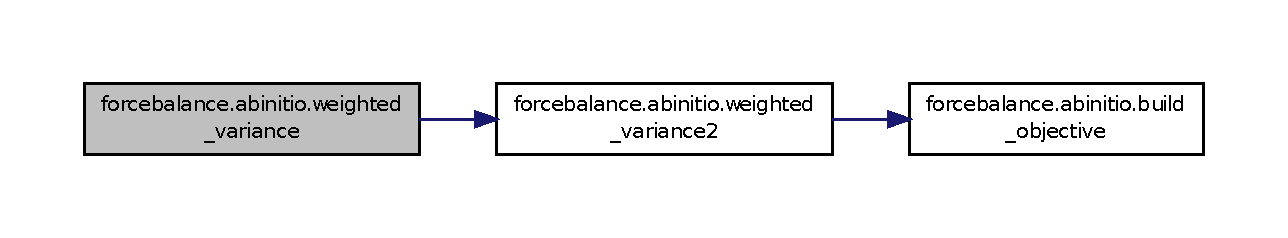
\includegraphics[width=350pt]{namespaceforcebalance_1_1abinitio_aba970cb59bab95eec79027ea05655110_cgraph}
\end{center}
\end{figure}


\hypertarget{namespaceforcebalance_1_1abinitio_ab9554761125a4ec7c3c13d6ae4ea537d}{\index{forcebalance\-::abinitio@{forcebalance\-::abinitio}!weighted\-\_\-variance2@{weighted\-\_\-variance2}}
\index{weighted\-\_\-variance2@{weighted\-\_\-variance2}!forcebalance::abinitio@{forcebalance\-::abinitio}}
\paragraph[{weighted\-\_\-variance2}]{\setlength{\rightskip}{0pt plus 5cm}def forcebalance.\-abinitio.\-weighted\-\_\-variance2 (
\begin{DoxyParamCaption}
\item[{}]{S\-Pi\-Xi, }
\item[{}]{W\-Ci\-W, }
\item[{}]{Z, }
\item[{}]{L, }
\item[{}]{R, }
\item[{}]{L2, }
\item[{}]{R2, }
\item[{}]{N\-C\-P1, }
\item[{}]{subtract\-\_\-mean = {\ttfamily True}}
\end{DoxyParamCaption}
)}}\label{namespaceforcebalance_1_1abinitio_ab9554761125a4ec7c3c13d6ae4ea537d}


A bit of a hack, since we have to subtract out two mean quantities to get Hessian elements. 



Definition at line 1135 of file abinitio.\-py.



Here is the call graph for this function\-:
\nopagebreak
\begin{figure}[H]
\begin{center}
\leavevmode
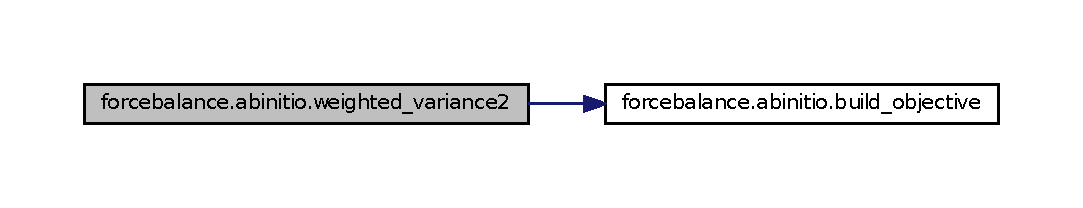
\includegraphics[width=350pt]{namespaceforcebalance_1_1abinitio_ab9554761125a4ec7c3c13d6ae4ea537d_cgraph}
\end{center}
\end{figure}



\hypertarget{namespaceforcebalance_1_1abinitio__internal}{\subsection{forcebalance.\-abinitio\-\_\-internal Namespace Reference}
\label{namespaceforcebalance_1_1abinitio__internal}\index{forcebalance.\-abinitio\-\_\-internal@{forcebalance.\-abinitio\-\_\-internal}}
}


Internal implementation of energy matching (for T\-I\-P3\-P water only)  


\subsubsection*{Classes}
\begin{DoxyCompactItemize}
\item 
class \hyperlink{classforcebalance_1_1abinitio__internal_1_1AbInitio__Internal}{Ab\-Initio\-\_\-\-Internal}
\begin{DoxyCompactList}\small\item\em Subclass of Target for force and energy matching using an internal implementation. \end{DoxyCompactList}\end{DoxyCompactItemize}


\subsubsection{Detailed Description}
Internal implementation of energy matching (for T\-I\-P3\-P water only) \begin{DoxyAuthor}{Author}
Lee-\/\-Ping Wang 
\end{DoxyAuthor}
\begin{DoxyDate}{Date}
04/2012 
\end{DoxyDate}

\hypertarget{namespaceforcebalance_1_1amberio}{\subsection{forcebalance\-:\-:amberio \-Namespace \-Reference}
\label{namespaceforcebalance_1_1amberio}\index{forcebalance\-::amberio@{forcebalance\-::amberio}}
}


\-A\-M\-B\-E\-R force field input/output.  


\subsubsection*{\-Classes}
\begin{DoxyCompactItemize}
\item 
class \hyperlink{classforcebalance_1_1amberio_1_1Mol2__Reader}{\-Mol2\-\_\-\-Reader}
\begin{DoxyCompactList}\small\item\em \-Finite state machine for parsing \hyperlink{namespaceforcebalance_1_1Mol2}{\-Mol2} force field file. \end{DoxyCompactList}\item 
class \hyperlink{classforcebalance_1_1amberio_1_1FrcMod__Reader}{\-Frc\-Mod\-\_\-\-Reader}
\begin{DoxyCompactList}\small\item\em \-Finite state machine for parsing \-Frc\-Mod force field file. \end{DoxyCompactList}\item 
class \hyperlink{classforcebalance_1_1amberio_1_1AbInitio__AMBER}{\-Ab\-Initio\-\_\-\-A\-M\-B\-E\-R}
\begin{DoxyCompactList}\small\item\em \-Subclass of \-Target for force and energy matching using \-A\-M\-B\-E\-R. \end{DoxyCompactList}\end{DoxyCompactItemize}
\subsubsection*{\-Functions}
\begin{DoxyCompactItemize}
\item 
def \hyperlink{namespaceforcebalance_1_1amberio_af59589a24e815a11db69dcaa21c51659}{is\-\_\-mol2\-\_\-atom}
\end{DoxyCompactItemize}
\subsubsection*{\-Variables}
\begin{DoxyCompactItemize}
\item 
tuple \hyperlink{namespaceforcebalance_1_1amberio_aa9ff86ae6726b8e8fc8b27ddf29e095a}{logger} = get\-Logger(\-\_\-\-\_\-name\-\_\-\-\_\-)
\item 
dictionary \hyperlink{namespaceforcebalance_1_1amberio_a7b3741ff909d0776c26574cfee9807fd}{mol2\-\_\-pdict} = \{'\-C\-O\-U\-L'\-:\{'\-Atom'\-:\mbox{[}1\mbox{]}, 8\-:''\}\}
\item 
dictionary \hyperlink{namespaceforcebalance_1_1amberio_ae5ba6128e5e02a120e8bcd688a5b1be4}{frcmod\-\_\-pdict}
\end{DoxyCompactItemize}


\subsubsection{\-Detailed \-Description}
\-A\-M\-B\-E\-R force field input/output. \-This serves as a good template for writing future force matching \-I/\-O modules for other programs because it's so simple.

\begin{DoxyAuthor}{\-Author}
\-Lee-\/\-Ping \-Wang 
\end{DoxyAuthor}
\begin{DoxyDate}{\-Date}
01/2012 
\end{DoxyDate}


\subsubsection{\-Function \-Documentation}
\hypertarget{namespaceforcebalance_1_1amberio_af59589a24e815a11db69dcaa21c51659}{\index{forcebalance\-::amberio@{forcebalance\-::amberio}!is\-\_\-mol2\-\_\-atom@{is\-\_\-mol2\-\_\-atom}}
\index{is\-\_\-mol2\-\_\-atom@{is\-\_\-mol2\-\_\-atom}!forcebalance::amberio@{forcebalance\-::amberio}}
\paragraph[{is\-\_\-mol2\-\_\-atom}]{\setlength{\rightskip}{0pt plus 5cm}def {\bf forcebalance.\-amberio.\-is\-\_\-mol2\-\_\-atom} (
\begin{DoxyParamCaption}
\item[{}]{line}
\end{DoxyParamCaption}
)}}\label{namespaceforcebalance_1_1amberio_af59589a24e815a11db69dcaa21c51659}


\-Definition at line 35 of file amberio.\-py.



\-Here is the call graph for this function\-:\nopagebreak
\begin{figure}[H]
\begin{center}
\leavevmode
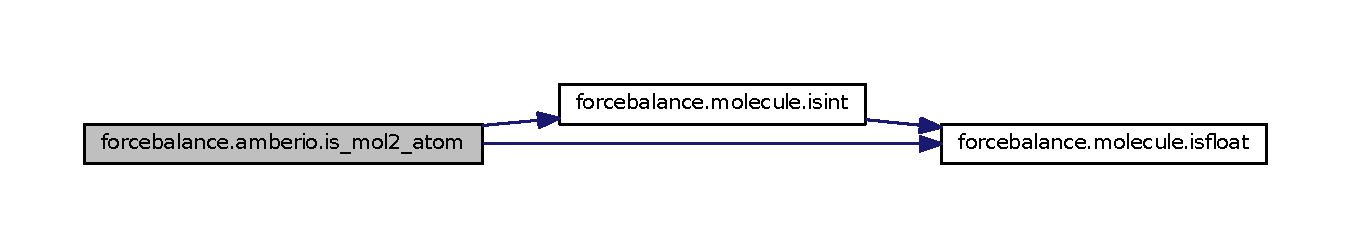
\includegraphics[width=350pt]{namespaceforcebalance_1_1amberio_af59589a24e815a11db69dcaa21c51659_cgraph}
\end{center}
\end{figure}




\subsubsection{\-Variable \-Documentation}
\hypertarget{namespaceforcebalance_1_1amberio_ae5ba6128e5e02a120e8bcd688a5b1be4}{\index{forcebalance\-::amberio@{forcebalance\-::amberio}!frcmod\-\_\-pdict@{frcmod\-\_\-pdict}}
\index{frcmod\-\_\-pdict@{frcmod\-\_\-pdict}!forcebalance::amberio@{forcebalance\-::amberio}}
\paragraph[{frcmod\-\_\-pdict}]{\setlength{\rightskip}{0pt plus 5cm}dictionary {\bf forcebalance\-::amberio\-::frcmod\-\_\-pdict}}}\label{namespaceforcebalance_1_1amberio_ae5ba6128e5e02a120e8bcd688a5b1be4}
{\bfseries \-Initial value\-:}
\begin{DoxyCode}
1 {'BONDS': {'Atom':[0], 1:'K', 2:'B'},
2                 'ANGLES':{'Atom':[0], 1:'K', 2:'B'},
3                 'PDIHS1':{'Atom':[0], 2:'K', 3:'B'},
4                 'PDIHS2':{'Atom':[0], 2:'K', 3:'B'},
5                 'PDIHS3':{'Atom':[0], 2:'K', 3:'B'},
6                 'PDIHS4':{'Atom':[0], 2:'K', 3:'B'},
7                 'PDIHS5':{'Atom':[0], 2:'K', 3:'B'},
8                 'PDIHS6':{'Atom':[0], 2:'K', 3:'B'},
9                 'IDIHS' :{'Atom':[0], 1:'K', 3:'B'},
10                 'VDW':{'Atom':[0], 1:'S', 2:'T'}
11                 }
\end{DoxyCode}


\-Definition at line 23 of file amberio.\-py.

\hypertarget{namespaceforcebalance_1_1amberio_aa9ff86ae6726b8e8fc8b27ddf29e095a}{\index{forcebalance\-::amberio@{forcebalance\-::amberio}!logger@{logger}}
\index{logger@{logger}!forcebalance::amberio@{forcebalance\-::amberio}}
\paragraph[{logger}]{\setlength{\rightskip}{0pt plus 5cm}tuple {\bf forcebalance\-::amberio\-::logger} = get\-Logger(\-\_\-\-\_\-name\-\_\-\-\_\-)}}\label{namespaceforcebalance_1_1amberio_aa9ff86ae6726b8e8fc8b27ddf29e095a}


\-Definition at line 19 of file amberio.\-py.

\hypertarget{namespaceforcebalance_1_1amberio_a7b3741ff909d0776c26574cfee9807fd}{\index{forcebalance\-::amberio@{forcebalance\-::amberio}!mol2\-\_\-pdict@{mol2\-\_\-pdict}}
\index{mol2\-\_\-pdict@{mol2\-\_\-pdict}!forcebalance::amberio@{forcebalance\-::amberio}}
\paragraph[{mol2\-\_\-pdict}]{\setlength{\rightskip}{0pt plus 5cm}dictionary {\bf forcebalance\-::amberio\-::mol2\-\_\-pdict} = \{'\-C\-O\-U\-L'\-:\{'\-Atom'\-:\mbox{[}1\mbox{]}, 8\-:''\}\}}}\label{namespaceforcebalance_1_1amberio_a7b3741ff909d0776c26574cfee9807fd}


\-Definition at line 21 of file amberio.\-py.


\hypertarget{namespaceforcebalance_1_1binding}{\subsection{forcebalance.\-binding Namespace Reference}
\label{namespaceforcebalance_1_1binding}\index{forcebalance.\-binding@{forcebalance.\-binding}}
}


Binding energy fitting module.  


\subsubsection*{Classes}
\begin{DoxyCompactItemize}
\item 
class \hyperlink{classforcebalance_1_1binding_1_1BindingEnergy}{Binding\-Energy}
\begin{DoxyCompactList}\small\item\em Improved subclass of Target for fitting force fields to binding energies. \end{DoxyCompactList}\end{DoxyCompactItemize}
\subsubsection*{Functions}
\begin{DoxyCompactItemize}
\item 
def \hyperlink{namespaceforcebalance_1_1binding_a0ae2f9f7a4ab7f4c64f8826de52331e9}{parse\-\_\-interactions}
\begin{DoxyCompactList}\small\item\em Parse through the interactions input file. \end{DoxyCompactList}\end{DoxyCompactItemize}
\subsubsection*{Variables}
\begin{DoxyCompactItemize}
\item 
tuple \hyperlink{namespaceforcebalance_1_1binding_a0bdb0d0390122623a60dae0e08bdc84a}{logger} = get\-Logger(\-\_\-\-\_\-name\-\_\-\-\_\-)
\end{DoxyCompactItemize}


\subsubsection{Detailed Description}
Binding energy fitting module. \begin{DoxyAuthor}{Author}
Lee-\/\-Ping Wang 
\end{DoxyAuthor}
\begin{DoxyDate}{Date}
05/2012 
\end{DoxyDate}


\subsubsection{Function Documentation}
\hypertarget{namespaceforcebalance_1_1binding_a0ae2f9f7a4ab7f4c64f8826de52331e9}{\index{forcebalance\-::binding@{forcebalance\-::binding}!parse\-\_\-interactions@{parse\-\_\-interactions}}
\index{parse\-\_\-interactions@{parse\-\_\-interactions}!forcebalance::binding@{forcebalance\-::binding}}
\paragraph[{parse\-\_\-interactions}]{\setlength{\rightskip}{0pt plus 5cm}def forcebalance.\-binding.\-parse\-\_\-interactions (
\begin{DoxyParamCaption}
\item[{}]{input\-\_\-file}
\end{DoxyParamCaption}
)}}\label{namespaceforcebalance_1_1binding_a0ae2f9f7a4ab7f4c64f8826de52331e9}


Parse through the interactions input file. 


\begin{DoxyParams}[1]{Parameters}
\mbox{\tt in}  & {\em input\-\_\-file} & The name of the input file. \\
\hline
\end{DoxyParams}


Definition at line 33 of file binding.\-py.



Here is the call graph for this function\-:\nopagebreak
\begin{figure}[H]
\begin{center}
\leavevmode
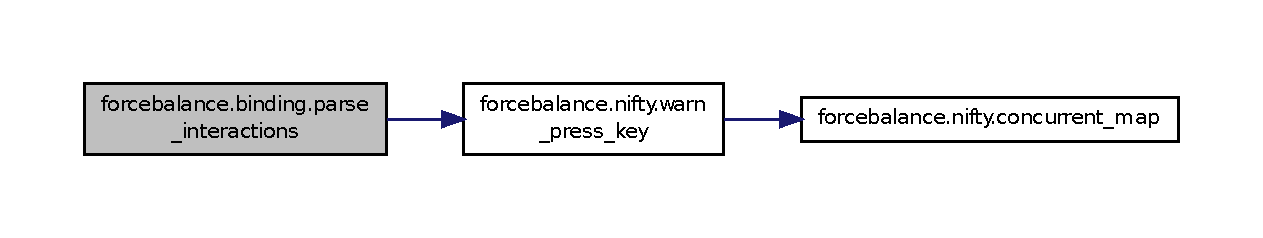
\includegraphics[width=350pt]{namespaceforcebalance_1_1binding_a0ae2f9f7a4ab7f4c64f8826de52331e9_cgraph}
\end{center}
\end{figure}




\subsubsection{Variable Documentation}
\hypertarget{namespaceforcebalance_1_1binding_a0bdb0d0390122623a60dae0e08bdc84a}{\index{forcebalance\-::binding@{forcebalance\-::binding}!logger@{logger}}
\index{logger@{logger}!forcebalance::binding@{forcebalance\-::binding}}
\paragraph[{logger}]{\setlength{\rightskip}{0pt plus 5cm}tuple forcebalance.\-binding.\-logger = get\-Logger(\-\_\-\-\_\-name\-\_\-\-\_\-)}}\label{namespaceforcebalance_1_1binding_a0bdb0d0390122623a60dae0e08bdc84a}


Definition at line 22 of file binding.\-py.


\hypertarget{namespaceforcebalance_1_1chemistry}{\subsection{forcebalance.\-chemistry Namespace Reference}
\label{namespaceforcebalance_1_1chemistry}\index{forcebalance.\-chemistry@{forcebalance.\-chemistry}}
}

\hypertarget{namespaceforcebalance_1_1contact}{\subsection{forcebalance\-:\-:contact \-Namespace \-Reference}
\label{namespaceforcebalance_1_1contact}\index{forcebalance\-::contact@{forcebalance\-::contact}}
}
\subsubsection*{\-Functions}
\begin{DoxyCompactItemize}
\item 
def \hyperlink{namespaceforcebalance_1_1contact_a3592dbbf524c6115f34d9a70b50e2e0f}{atom\-\_\-distances}
\begin{DoxyCompactList}\small\item\em \-For each frame in xyzlist, compute the (euclidean) distance between pairs of atoms whos indices are given in contacts. \end{DoxyCompactList}\item 
def \hyperlink{namespaceforcebalance_1_1contact_acffb04a66580454b8a87648faa1c5c16}{residue\-\_\-distances}
\begin{DoxyCompactList}\small\item\em \-For each frame in xyzlist, and for each pair of residues in the array contact, compute the distance between the closest pair of atoms such that one of them belongs to each residue. \end{DoxyCompactList}\end{DoxyCompactItemize}


\subsubsection{\-Function \-Documentation}
\hypertarget{namespaceforcebalance_1_1contact_a3592dbbf524c6115f34d9a70b50e2e0f}{\index{forcebalance\-::contact@{forcebalance\-::contact}!atom\-\_\-distances@{atom\-\_\-distances}}
\index{atom\-\_\-distances@{atom\-\_\-distances}!forcebalance::contact@{forcebalance\-::contact}}
\paragraph[{atom\-\_\-distances}]{\setlength{\rightskip}{0pt plus 5cm}def {\bf forcebalance.\-contact.\-atom\-\_\-distances} (
\begin{DoxyParamCaption}
\item[{}]{xyzlist, }
\item[{}]{atom\-\_\-contacts}
\end{DoxyParamCaption}
)}}\label{namespaceforcebalance_1_1contact_a3592dbbf524c6115f34d9a70b50e2e0f}


\-For each frame in xyzlist, compute the (euclidean) distance between pairs of atoms whos indices are given in contacts. 

xyzlist should be a traj\-\_\-length x num\-\_\-atoms x num\-\_\-dims array of type float32

contacts should be a num\-\_\-contacts x 2 array where each row gives the indices of 2 atoms whos distance you care to monitor.

\-Returns\-: traj\-\_\-length x num\-\_\-contacts array of euclidean distances

\-Note\-: \-For nice wrappers around this, see the prepare\-\_\-trajectory method of various metrics in metrics.\-py 

\-Definition at line 26 of file contact.\-py.



\-Here is the call graph for this function\-:\nopagebreak
\begin{figure}[H]
\begin{center}
\leavevmode
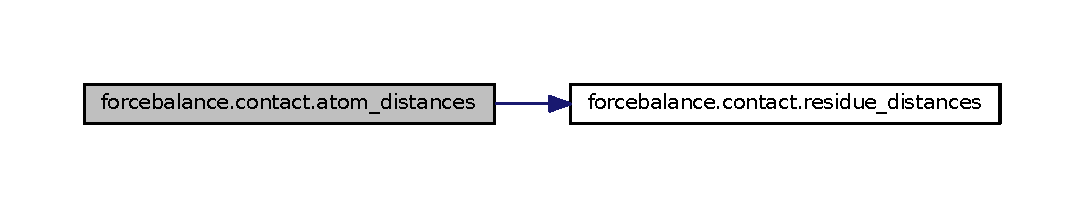
\includegraphics[width=350pt]{namespaceforcebalance_1_1contact_a3592dbbf524c6115f34d9a70b50e2e0f_cgraph}
\end{center}
\end{figure}


\hypertarget{namespaceforcebalance_1_1contact_acffb04a66580454b8a87648faa1c5c16}{\index{forcebalance\-::contact@{forcebalance\-::contact}!residue\-\_\-distances@{residue\-\_\-distances}}
\index{residue\-\_\-distances@{residue\-\_\-distances}!forcebalance::contact@{forcebalance\-::contact}}
\paragraph[{residue\-\_\-distances}]{\setlength{\rightskip}{0pt plus 5cm}def {\bf forcebalance.\-contact.\-residue\-\_\-distances} (
\begin{DoxyParamCaption}
\item[{}]{xyzlist, }
\item[{}]{residue\-\_\-membership, }
\item[{}]{residue\-\_\-contacts}
\end{DoxyParamCaption}
)}}\label{namespaceforcebalance_1_1contact_acffb04a66580454b8a87648faa1c5c16}


\-For each frame in xyzlist, and for each pair of residues in the array contact, compute the distance between the closest pair of atoms such that one of them belongs to each residue. 

xyzlist should be a traj\-\_\-length x num\-\_\-atoms x num\-\_\-dims array of type float32

residue\-\_\-membership should be a list of lists where residue\-\_\-membership\mbox{[}i\mbox{]} gives the list of atomindices that belong to residue i. residue\-\_\-membership should \-N\-O\-T be a numpy 2\-D array unless you really mean that all of the residues have the same number of atoms

residue\-\_\-contacts should be a 2\-D numpy array of shape num\-\_\-contacts x 2 where each row gives the indices of the two \-R\-E\-S\-I\-D\-U\-E\-S who you are interested in monitoring for a contact.

\-Returns\-: a 2\-D array of traj\-\_\-lenth x num\-\_\-contacts where out\mbox{[}i,j\mbox{]} contains the distance between the pair of atoms, one from residue\-\_\-membership\mbox{[}residue\-\_\-contacts\mbox{[}j,0\mbox{]}\mbox{]} and one from residue\-\_\-membership\mbox{[}residue\-\_\-contacts\mbox{[}j,1\mbox{]}\mbox{]} that are closest. 

\-Definition at line 85 of file contact.\-py.


\hypertarget{namespaceforcebalance_1_1counterpoise}{\subsection{forcebalance.\-counterpoise Namespace Reference}
\label{namespaceforcebalance_1_1counterpoise}\index{forcebalance.\-counterpoise@{forcebalance.\-counterpoise}}
}


Match an empirical potential to the counterpoise correction for basis set superposition error (B\-S\-S\-E).  


\subsubsection*{Classes}
\begin{DoxyCompactItemize}
\item 
class \hyperlink{classforcebalance_1_1counterpoise_1_1Counterpoise}{Counterpoise}
\begin{DoxyCompactList}\small\item\em Target subclass for matching the counterpoise correction. \end{DoxyCompactList}\end{DoxyCompactItemize}
\subsubsection*{Variables}
\begin{DoxyCompactItemize}
\item 
tuple \hyperlink{namespaceforcebalance_1_1counterpoise_a9a7008a650c37185e7e43c9b1c943bd6}{logger} = get\-Logger(\-\_\-\-\_\-name\-\_\-\-\_\-)
\end{DoxyCompactItemize}


\subsubsection{Detailed Description}
Match an empirical potential to the counterpoise correction for basis set superposition error (B\-S\-S\-E). Here we test two different functional forms\-: a three-\/parameter Gaussian repulsive potential and a four-\/parameter Gaussian which goes smoothly to an exponential. The latter can be written in two different ways -\/ one which gives us control over the exponential, the switching distance and the Gaussian decay constant, and another which gives us control over the Gaussian and the switching distance. They are called 'C\-P\-G\-A\-U\-S\-S', 'C\-P\-E\-X\-P\-G', and 'C\-P\-G\-E\-X\-P'. I think the third option is the best although our early tests have indicated that none of the force fields perform particularly well for the water dimer.

This subclass of Target implements the 'get' method.

\begin{DoxyAuthor}{Author}
Lee-\/\-Ping Wang 
\end{DoxyAuthor}
\begin{DoxyDate}{Date}
12/2011 
\end{DoxyDate}


\subsubsection{Variable Documentation}
\hypertarget{namespaceforcebalance_1_1counterpoise_a9a7008a650c37185e7e43c9b1c943bd6}{\index{forcebalance\-::counterpoise@{forcebalance\-::counterpoise}!logger@{logger}}
\index{logger@{logger}!forcebalance::counterpoise@{forcebalance\-::counterpoise}}
\paragraph[{logger}]{\setlength{\rightskip}{0pt plus 5cm}tuple forcebalance.\-counterpoise.\-logger = get\-Logger(\-\_\-\-\_\-name\-\_\-\-\_\-)}}\label{namespaceforcebalance_1_1counterpoise_a9a7008a650c37185e7e43c9b1c943bd6}


Definition at line 29 of file counterpoise.\-py.


\hypertarget{namespaceforcebalance_1_1custom__io}{\subsection{forcebalance\-:\-:custom\-\_\-io \-Namespace \-Reference}
\label{namespaceforcebalance_1_1custom__io}\index{forcebalance\-::custom\-\_\-io@{forcebalance\-::custom\-\_\-io}}
}


\-Custom force field parser.  


\subsubsection*{\-Classes}
\begin{DoxyCompactItemize}
\item 
class \hyperlink{classforcebalance_1_1custom__io_1_1Gen__Reader}{\-Gen\-\_\-\-Reader}
\begin{DoxyCompactList}\small\item\em \-Finite state machine for parsing custom \-G\-R\-O\-M\-A\-C\-S force field files. \end{DoxyCompactList}\end{DoxyCompactItemize}
\subsubsection*{\-Variables}
\begin{DoxyCompactItemize}
\item 
list \hyperlink{namespaceforcebalance_1_1custom__io_a509d4c2b5eeee4278adde414e55eb560}{cptypes} = \mbox{[}\-None, '\-C\-P\-G\-A\-U\-S\-S', '\-C\-P\-E\-X\-P\-G', '\-C\-P\-G\-E\-X\-P'\mbox{]}
\begin{DoxyCompactList}\small\item\em \-Types of counterpoise correction. \end{DoxyCompactList}\item 
list \hyperlink{namespaceforcebalance_1_1custom__io_a604fd5cd1f0c6057a8a72ac61b55f6fa}{ndtypes} = \mbox{[}\-None\mbox{]}
\begin{DoxyCompactList}\small\item\em \-Types of \-N\-D\-D\-O correction. \end{DoxyCompactList}\item 
dictionary \hyperlink{namespaceforcebalance_1_1custom__io_a64c7f292c64ad2b2b855a82e68c0ca7e}{fdict}
\begin{DoxyCompactList}\small\item\em \-Section -\/$>$ \-Interaction type dictionary. \end{DoxyCompactList}\item 
dictionary \hyperlink{namespaceforcebalance_1_1custom__io_aaa87b8099dee5dfec42f5869dabad0c5}{pdict}
\begin{DoxyCompactList}\small\item\em \-Interaction type -\/$>$ \-Parameter \-Dictionary. \end{DoxyCompactList}\end{DoxyCompactItemize}


\subsubsection{\-Detailed \-Description}
\-Custom force field parser. \-We take advantage of the sections in \-G\-R\-O\-M\-A\-C\-S and the 'interaction type' concept, but these interactions are not supported in \-G\-R\-O\-M\-A\-C\-S; rather, they are computed within our program.

\begin{DoxyAuthor}{\-Author}
\-Lee-\/\-Ping \-Wang 
\end{DoxyAuthor}
\begin{DoxyDate}{\-Date}
12/2011 
\end{DoxyDate}


\subsubsection{\-Variable \-Documentation}
\hypertarget{namespaceforcebalance_1_1custom__io_a509d4c2b5eeee4278adde414e55eb560}{\index{forcebalance\-::custom\-\_\-io@{forcebalance\-::custom\-\_\-io}!cptypes@{cptypes}}
\index{cptypes@{cptypes}!forcebalance::custom_io@{forcebalance\-::custom\-\_\-io}}
\paragraph[{cptypes}]{\setlength{\rightskip}{0pt plus 5cm}list {\bf forcebalance\-::custom\-\_\-io\-::cptypes} = \mbox{[}\-None, '\-C\-P\-G\-A\-U\-S\-S', '\-C\-P\-E\-X\-P\-G', '\-C\-P\-G\-E\-X\-P'\mbox{]}}}\label{namespaceforcebalance_1_1custom__io_a509d4c2b5eeee4278adde414e55eb560}


\-Types of counterpoise correction. 



\-Definition at line 16 of file custom\-\_\-io.\-py.

\hypertarget{namespaceforcebalance_1_1custom__io_a64c7f292c64ad2b2b855a82e68c0ca7e}{\index{forcebalance\-::custom\-\_\-io@{forcebalance\-::custom\-\_\-io}!fdict@{fdict}}
\index{fdict@{fdict}!forcebalance::custom_io@{forcebalance\-::custom\-\_\-io}}
\paragraph[{fdict}]{\setlength{\rightskip}{0pt plus 5cm}dictionary {\bf forcebalance\-::custom\-\_\-io\-::fdict}}}\label{namespaceforcebalance_1_1custom__io_a64c7f292c64ad2b2b855a82e68c0ca7e}
{\bfseries \-Initial value\-:}
\begin{DoxyCode}
1 {
2     'counterpoise'  : cptypes    }
\end{DoxyCode}


\-Section -\/$>$ \-Interaction type dictionary. 



\-Definition at line 21 of file custom\-\_\-io.\-py.

\hypertarget{namespaceforcebalance_1_1custom__io_a604fd5cd1f0c6057a8a72ac61b55f6fa}{\index{forcebalance\-::custom\-\_\-io@{forcebalance\-::custom\-\_\-io}!ndtypes@{ndtypes}}
\index{ndtypes@{ndtypes}!forcebalance::custom_io@{forcebalance\-::custom\-\_\-io}}
\paragraph[{ndtypes}]{\setlength{\rightskip}{0pt plus 5cm}list {\bf forcebalance\-::custom\-\_\-io\-::ndtypes} = \mbox{[}\-None\mbox{]}}}\label{namespaceforcebalance_1_1custom__io_a604fd5cd1f0c6057a8a72ac61b55f6fa}


\-Types of \-N\-D\-D\-O correction. 



\-Definition at line 18 of file custom\-\_\-io.\-py.

\hypertarget{namespaceforcebalance_1_1custom__io_aaa87b8099dee5dfec42f5869dabad0c5}{\index{forcebalance\-::custom\-\_\-io@{forcebalance\-::custom\-\_\-io}!pdict@{pdict}}
\index{pdict@{pdict}!forcebalance::custom_io@{forcebalance\-::custom\-\_\-io}}
\paragraph[{pdict}]{\setlength{\rightskip}{0pt plus 5cm}dictionary {\bf forcebalance\-::custom\-\_\-io\-::pdict}}}\label{namespaceforcebalance_1_1custom__io_aaa87b8099dee5dfec42f5869dabad0c5}
{\bfseries \-Initial value\-:}
\begin{DoxyCode}
1 {'CPGAUSS':{3:'A', 4:'B', 5:'C'},
2          'CPGEXP' :{3:'A', 4:'B', 5:'G', 6:'X'},
3          'CPEXPG' :{3:'A1', 4:'B', 5:'X0', 6:'A2'}
4          }
\end{DoxyCode}


\-Interaction type -\/$>$ \-Parameter \-Dictionary. 



\-Definition at line 25 of file custom\-\_\-io.\-py.


\hypertarget{namespaceforcebalance_1_1engine}{\subsection{forcebalance\-:\-:engine \-Namespace \-Reference}
\label{namespaceforcebalance_1_1engine}\index{forcebalance\-::engine@{forcebalance\-::engine}}
}
\subsubsection*{\-Classes}
\begin{DoxyCompactItemize}
\item 
class \hyperlink{classforcebalance_1_1engine_1_1Engine}{\-Engine}
\begin{DoxyCompactList}\small\item\em \-Base class for all engines. \end{DoxyCompactList}\end{DoxyCompactItemize}
\subsubsection*{\-Variables}
\begin{DoxyCompactItemize}
\item 
tuple \hyperlink{namespaceforcebalance_1_1engine_ae4a289a63d0f20258665d7c5208cf2a2}{logger} = get\-Logger(\-\_\-\-\_\-name\-\_\-\-\_\-)
\end{DoxyCompactItemize}


\subsubsection{\-Variable \-Documentation}
\hypertarget{namespaceforcebalance_1_1engine_ae4a289a63d0f20258665d7c5208cf2a2}{\index{forcebalance\-::engine@{forcebalance\-::engine}!logger@{logger}}
\index{logger@{logger}!forcebalance::engine@{forcebalance\-::engine}}
\paragraph[{logger}]{\setlength{\rightskip}{0pt plus 5cm}tuple {\bf forcebalance\-::engine\-::logger} = get\-Logger(\-\_\-\-\_\-name\-\_\-\-\_\-)}}\label{namespaceforcebalance_1_1engine_ae4a289a63d0f20258665d7c5208cf2a2}


\-Definition at line 17 of file engine.\-py.


\hypertarget{namespaceforcebalance_1_1finite__difference}{\subsection{forcebalance.\-finite\-\_\-difference Namespace Reference}
\label{namespaceforcebalance_1_1finite__difference}\index{forcebalance.\-finite\-\_\-difference@{forcebalance.\-finite\-\_\-difference}}
}
\subsubsection*{Functions}
\begin{DoxyCompactItemize}
\item 
def \hyperlink{namespaceforcebalance_1_1finite__difference_ac5bb1552a9b8dd22c9c80e6444de2218}{f1d2p}
\begin{DoxyCompactList}\small\item\em A two-\/point finite difference stencil. \end{DoxyCompactList}\item 
def \hyperlink{namespaceforcebalance_1_1finite__difference_a123c5d5dea0f3f50ab57796bb3bc39be}{f1d5p}
\begin{DoxyCompactList}\small\item\em A highly accurate five-\/point finite difference stencil for computing derivatives of a function. \end{DoxyCompactList}\item 
def \hyperlink{namespaceforcebalance_1_1finite__difference_a9be9f0d21300958092e380514e2e980d}{f1d7p}
\begin{DoxyCompactList}\small\item\em A highly accurate seven-\/point finite difference stencil for computing derivatives of a function. \end{DoxyCompactList}\item 
def \hyperlink{namespaceforcebalance_1_1finite__difference_acc281f85b668062745f711d9b4a610fa}{f12d7p}
\item 
def \hyperlink{namespaceforcebalance_1_1finite__difference_aa69a8819e4680091f400303c1d6ddeb7}{f12d3p}
\begin{DoxyCompactList}\small\item\em A three-\/point finite difference stencil. \end{DoxyCompactList}\item 
def \hyperlink{namespaceforcebalance_1_1finite__difference_ad84d3e385db1190e7d8ef58bc08a6c52}{in\-\_\-fd}
\begin{DoxyCompactList}\small\item\em Invoking this function from anywhere will tell us whether we're being called by a finite-\/difference function. \end{DoxyCompactList}\item 
def \hyperlink{namespaceforcebalance_1_1finite__difference_ae484c591ae8c4e5bae73a0ef2660c339}{fdwrap}
\begin{DoxyCompactList}\small\item\em A function wrapper for finite difference designed for differentiating 'get'-\/type functions. \end{DoxyCompactList}\item 
def \hyperlink{namespaceforcebalance_1_1finite__difference_a00322fb65860c390616f74d05037c797}{fdwrap\-\_\-\-G}
\begin{DoxyCompactList}\small\item\em A driver to fdwrap for gradients (see documentation for fdwrap) Inputs\-: tgt = The Target containing the objective function that we want to differentiate mvals0 = The 'central' values of the mathematical parameters -\/ i.\-e. \end{DoxyCompactList}\item 
def \hyperlink{namespaceforcebalance_1_1finite__difference_a77a0bc1ae3cbbcc8d38a0ef9ca877d6d}{fdwrap\-\_\-\-H}
\begin{DoxyCompactList}\small\item\em A driver to fdwrap for Hessians (see documentation for fdwrap) Inputs\-: tgt = The Target containing the objective function that we want to differentiate mvals0 = The 'central' values of the mathematical parameters -\/ i.\-e. \end{DoxyCompactList}\end{DoxyCompactItemize}
\subsubsection*{Variables}
\begin{DoxyCompactItemize}
\item 
tuple \hyperlink{namespaceforcebalance_1_1finite__difference_a2bdf74505c45f442e1c96d557414254e}{logger} = get\-Logger(\-\_\-\-\_\-name\-\_\-\-\_\-)
\end{DoxyCompactItemize}


\subsubsection{Function Documentation}
\hypertarget{namespaceforcebalance_1_1finite__difference_aa69a8819e4680091f400303c1d6ddeb7}{\index{forcebalance\-::finite\-\_\-difference@{forcebalance\-::finite\-\_\-difference}!f12d3p@{f12d3p}}
\index{f12d3p@{f12d3p}!forcebalance::finite_difference@{forcebalance\-::finite\-\_\-difference}}
\paragraph[{f12d3p}]{\setlength{\rightskip}{0pt plus 5cm}def forcebalance.\-finite\-\_\-difference.\-f12d3p (
\begin{DoxyParamCaption}
\item[{}]{f, }
\item[{}]{h, }
\item[{}]{f0 = {\ttfamily None}}
\end{DoxyParamCaption}
)}}\label{namespaceforcebalance_1_1finite__difference_aa69a8819e4680091f400303c1d6ddeb7}


A three-\/point finite difference stencil. 

This function does either two computations or three, depending on whether the 'center' value is supplied. This is done in order to avoid recomputing the center value many times.

The first derivative is evaluated using central difference. One advantage of using central difference (as opposed to forward difference) is that we get zero at the bottom of a parabola.

Using this formula we also get an approximate second derivative, which can then be inserted into the diagonal of the Hessian. This is very useful for optimizations like B\-F\-G\-S where the diagonal determines how far we step in the parameter space.

How to use\-: use fdwrap or something similar to generate a one-\/variable function from the (usually) much more complicated function that we wish to differentate. Then pass it to this function.

Inputs\-: f = The one-\/variable function f(x) that we're differentiating h = The finite difference step size, usually a small number

Outputs\-: fp = The finite difference derivative of the function f(x) around x=0. 

Definition at line 109 of file finite\-\_\-difference.\-py.



Here is the call graph for this function\-:\nopagebreak
\begin{figure}[H]
\begin{center}
\leavevmode
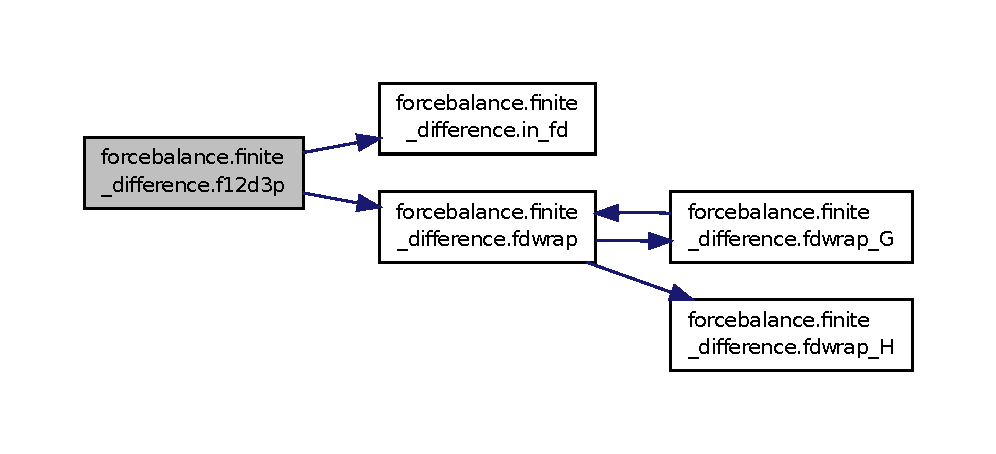
\includegraphics[width=350pt]{namespaceforcebalance_1_1finite__difference_aa69a8819e4680091f400303c1d6ddeb7_cgraph}
\end{center}
\end{figure}


\hypertarget{namespaceforcebalance_1_1finite__difference_acc281f85b668062745f711d9b4a610fa}{\index{forcebalance\-::finite\-\_\-difference@{forcebalance\-::finite\-\_\-difference}!f12d7p@{f12d7p}}
\index{f12d7p@{f12d7p}!forcebalance::finite_difference@{forcebalance\-::finite\-\_\-difference}}
\paragraph[{f12d7p}]{\setlength{\rightskip}{0pt plus 5cm}def forcebalance.\-finite\-\_\-difference.\-f12d7p (
\begin{DoxyParamCaption}
\item[{}]{f, }
\item[{}]{h}
\end{DoxyParamCaption}
)}}\label{namespaceforcebalance_1_1finite__difference_acc281f85b668062745f711d9b4a610fa}


Definition at line 75 of file finite\-\_\-difference.\-py.



Here is the call graph for this function\-:\nopagebreak
\begin{figure}[H]
\begin{center}
\leavevmode
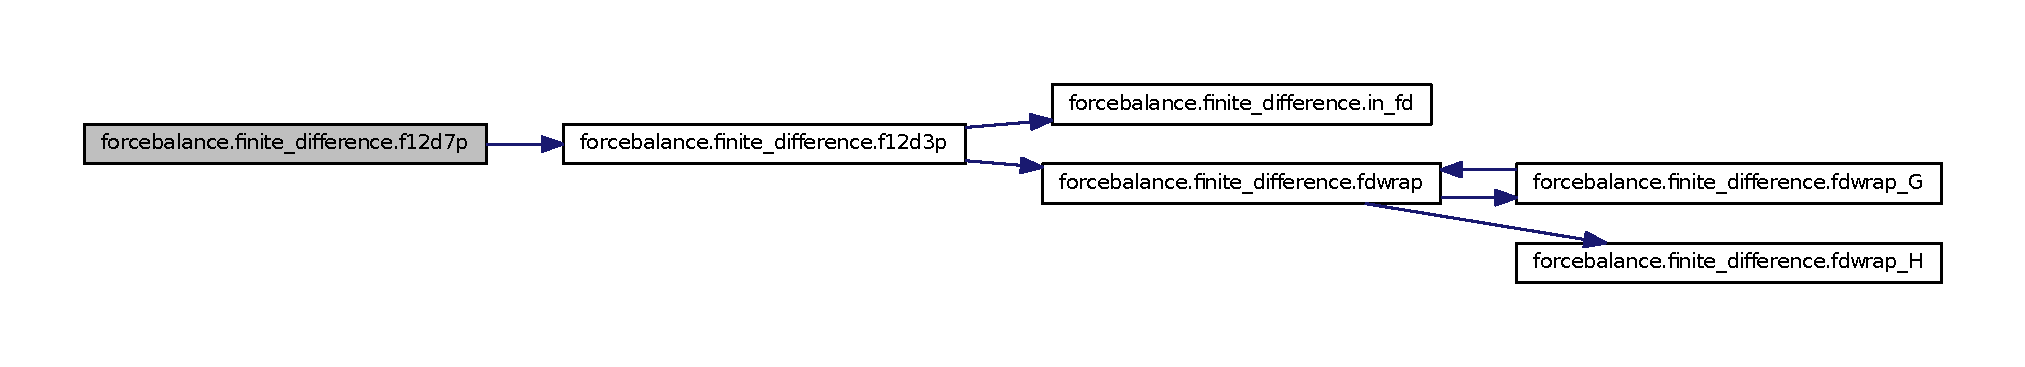
\includegraphics[width=350pt]{namespaceforcebalance_1_1finite__difference_acc281f85b668062745f711d9b4a610fa_cgraph}
\end{center}
\end{figure}


\hypertarget{namespaceforcebalance_1_1finite__difference_ac5bb1552a9b8dd22c9c80e6444de2218}{\index{forcebalance\-::finite\-\_\-difference@{forcebalance\-::finite\-\_\-difference}!f1d2p@{f1d2p}}
\index{f1d2p@{f1d2p}!forcebalance::finite_difference@{forcebalance\-::finite\-\_\-difference}}
\paragraph[{f1d2p}]{\setlength{\rightskip}{0pt plus 5cm}def forcebalance.\-finite\-\_\-difference.\-f1d2p (
\begin{DoxyParamCaption}
\item[{}]{f, }
\item[{}]{h, }
\item[{}]{f0 = {\ttfamily None}}
\end{DoxyParamCaption}
)}}\label{namespaceforcebalance_1_1finite__difference_ac5bb1552a9b8dd22c9c80e6444de2218}


A two-\/point finite difference stencil. 

This function does either two computations or one, depending on whether the 'center' value is supplied. This is done in order to avoid recomputing the center value many times when we repeat this function for each index of the gradient.

How to use\-: use fdwrap or something similar to generate a one-\/variable function from the (usually) much more complicated function that we wish to differentate. Then pass it to this function.

Inputs\-: f = The one-\/variable function f(x) that we're differentiating h = The finite difference step size, usually a small number

Outputs\-: fp = The finite difference derivative of the function f(x) around x=0. 

Definition at line 29 of file finite\-\_\-difference.\-py.



Here is the call graph for this function\-:\nopagebreak
\begin{figure}[H]
\begin{center}
\leavevmode
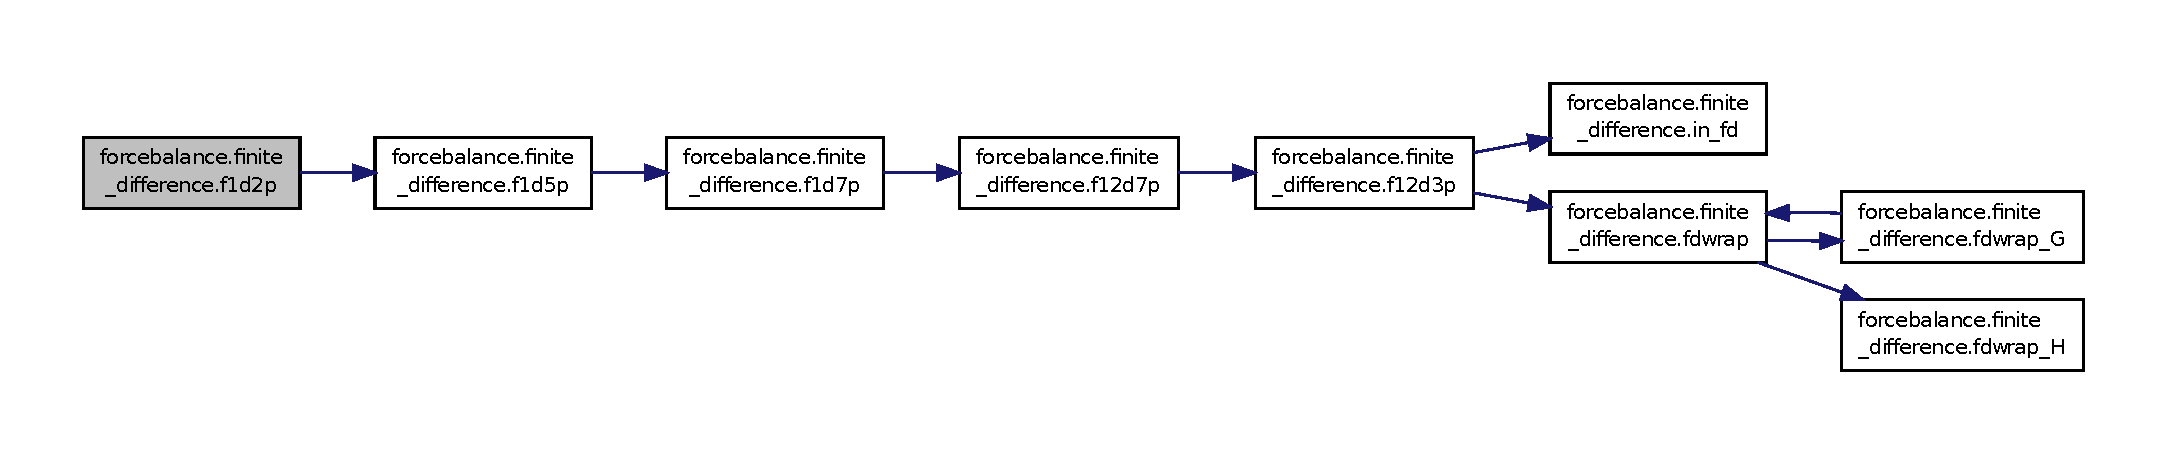
\includegraphics[width=350pt]{namespaceforcebalance_1_1finite__difference_ac5bb1552a9b8dd22c9c80e6444de2218_cgraph}
\end{center}
\end{figure}


\hypertarget{namespaceforcebalance_1_1finite__difference_a123c5d5dea0f3f50ab57796bb3bc39be}{\index{forcebalance\-::finite\-\_\-difference@{forcebalance\-::finite\-\_\-difference}!f1d5p@{f1d5p}}
\index{f1d5p@{f1d5p}!forcebalance::finite_difference@{forcebalance\-::finite\-\_\-difference}}
\paragraph[{f1d5p}]{\setlength{\rightskip}{0pt plus 5cm}def forcebalance.\-finite\-\_\-difference.\-f1d5p (
\begin{DoxyParamCaption}
\item[{}]{f, }
\item[{}]{h}
\end{DoxyParamCaption}
)}}\label{namespaceforcebalance_1_1finite__difference_a123c5d5dea0f3f50ab57796bb3bc39be}


A highly accurate five-\/point finite difference stencil for computing derivatives of a function. 

It works on both scalar and vector functions (i.\-e. functions that return arrays). Since the function does four computations, it's costly but recommended if we really need an accurate reference value.

The function is evaluated at points -\/2h, -\/h, +h and +2h and these values are combined to make the derivative according to\-: \href{http://www.holoborodko.com/pavel/numerical-methods/numerical-derivative/central-differences/}{\tt http\-://www.\-holoborodko.\-com/pavel/numerical-\/methods/numerical-\/derivative/central-\/differences/}

How to use\-: use fdwrap or something similar to generate a one-\/variable function from the (usually) much more complicated function that we wish to differentate. Then pass it to this function.

Inputs\-: f = The one-\/variable function f(x) that we're differentiating h = The finite difference step size, usually a small number

Outputs\-: fp = The finite difference derivative of the function f(x) around x=0. 

Definition at line 60 of file finite\-\_\-difference.\-py.



Here is the call graph for this function\-:\nopagebreak
\begin{figure}[H]
\begin{center}
\leavevmode
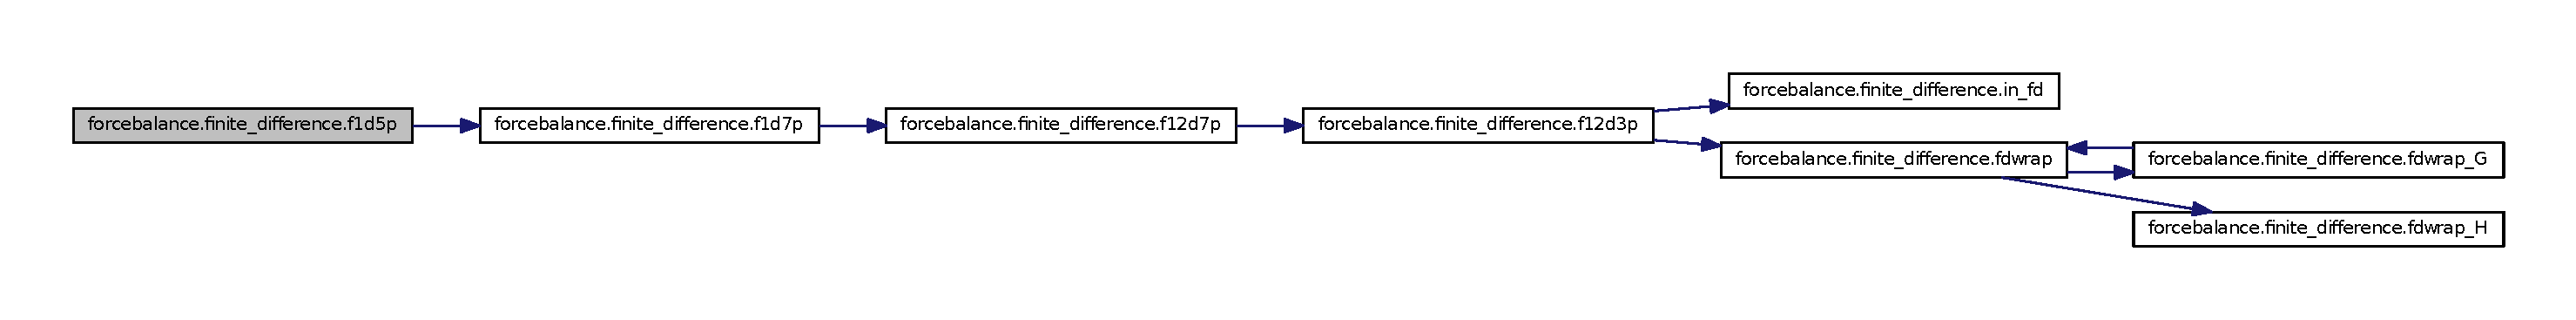
\includegraphics[width=350pt]{namespaceforcebalance_1_1finite__difference_a123c5d5dea0f3f50ab57796bb3bc39be_cgraph}
\end{center}
\end{figure}


\hypertarget{namespaceforcebalance_1_1finite__difference_a9be9f0d21300958092e380514e2e980d}{\index{forcebalance\-::finite\-\_\-difference@{forcebalance\-::finite\-\_\-difference}!f1d7p@{f1d7p}}
\index{f1d7p@{f1d7p}!forcebalance::finite_difference@{forcebalance\-::finite\-\_\-difference}}
\paragraph[{f1d7p}]{\setlength{\rightskip}{0pt plus 5cm}def forcebalance.\-finite\-\_\-difference.\-f1d7p (
\begin{DoxyParamCaption}
\item[{}]{f, }
\item[{}]{h}
\end{DoxyParamCaption}
)}}\label{namespaceforcebalance_1_1finite__difference_a9be9f0d21300958092e380514e2e980d}


A highly accurate seven-\/point finite difference stencil for computing derivatives of a function. 



Definition at line 70 of file finite\-\_\-difference.\-py.



Here is the call graph for this function\-:\nopagebreak
\begin{figure}[H]
\begin{center}
\leavevmode
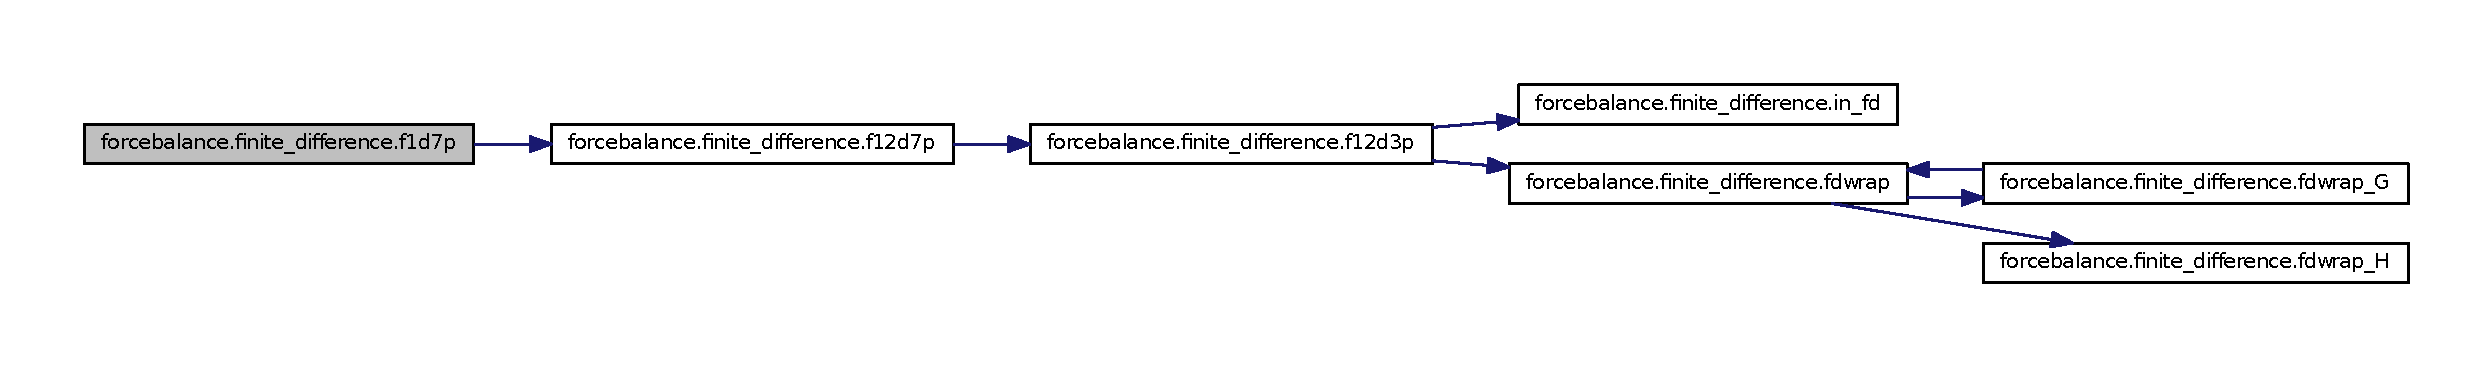
\includegraphics[width=350pt]{namespaceforcebalance_1_1finite__difference_a9be9f0d21300958092e380514e2e980d_cgraph}
\end{center}
\end{figure}


\hypertarget{namespaceforcebalance_1_1finite__difference_ae484c591ae8c4e5bae73a0ef2660c339}{\index{forcebalance\-::finite\-\_\-difference@{forcebalance\-::finite\-\_\-difference}!fdwrap@{fdwrap}}
\index{fdwrap@{fdwrap}!forcebalance::finite_difference@{forcebalance\-::finite\-\_\-difference}}
\paragraph[{fdwrap}]{\setlength{\rightskip}{0pt plus 5cm}def forcebalance.\-finite\-\_\-difference.\-fdwrap (
\begin{DoxyParamCaption}
\item[{}]{func, }
\item[{}]{mvals0, }
\item[{}]{pidx, }
\item[{}]{key = {\ttfamily None}, }
\item[{}]{kwargs}
\end{DoxyParamCaption}
)}}\label{namespaceforcebalance_1_1finite__difference_ae484c591ae8c4e5bae73a0ef2660c339}


A function wrapper for finite difference designed for differentiating 'get'-\/type functions. 

Since our finite difference stencils take single-\/variable functions and differentiate them around zero, and our objective function is quite a complicated function, we need a wrapper to serve as a middleman. The alternative would be to copy the finite difference formula to wherever we're taking the derivative, and that is prone to mistakes.

Inputs\-: func = Either get\-\_\-\-X or get\-\_\-\-G; these functions return dictionaries. \mbox{[}'X'\mbox{]} = 1.\-23, \mbox{[}'G'\mbox{]} = \mbox{[}0.\-12, 3,45, ...\mbox{]} mvals0 = The 'central' values of the mathematical parameters -\/ i.\-e. the wrapped function's origin is here. pidx = The index of the parameter that we're differentiating key = either 'G' or 'X', the value we wish to take out of the dictionary kwargs = Anything else we want to pass to the objective function (for instance, Project.\-Objective takes Order as an argument)

Outputs\-: func1 = Wrapped version of func, which takes a single float argument. 

Definition at line 147 of file finite\-\_\-difference.\-py.



Here is the call graph for this function\-:\nopagebreak
\begin{figure}[H]
\begin{center}
\leavevmode
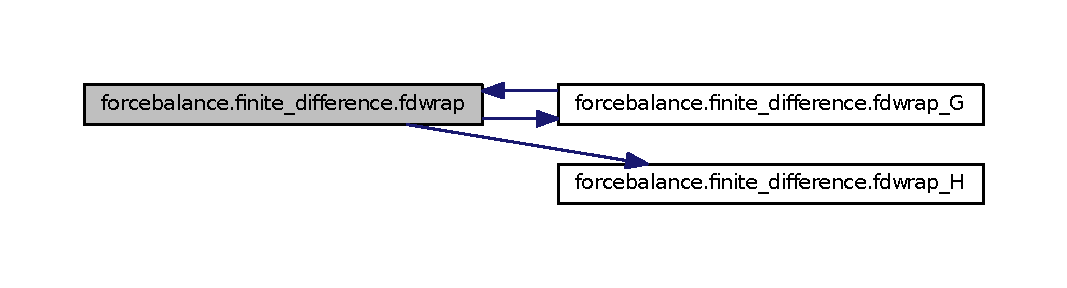
\includegraphics[width=336pt]{namespaceforcebalance_1_1finite__difference_ae484c591ae8c4e5bae73a0ef2660c339_cgraph}
\end{center}
\end{figure}


\hypertarget{namespaceforcebalance_1_1finite__difference_a00322fb65860c390616f74d05037c797}{\index{forcebalance\-::finite\-\_\-difference@{forcebalance\-::finite\-\_\-difference}!fdwrap\-\_\-\-G@{fdwrap\-\_\-\-G}}
\index{fdwrap\-\_\-\-G@{fdwrap\-\_\-\-G}!forcebalance::finite_difference@{forcebalance\-::finite\-\_\-difference}}
\paragraph[{fdwrap\-\_\-\-G}]{\setlength{\rightskip}{0pt plus 5cm}def forcebalance.\-finite\-\_\-difference.\-fdwrap\-\_\-\-G (
\begin{DoxyParamCaption}
\item[{}]{tgt, }
\item[{}]{mvals0, }
\item[{}]{pidx}
\end{DoxyParamCaption}
)}}\label{namespaceforcebalance_1_1finite__difference_a00322fb65860c390616f74d05037c797}


A driver to fdwrap for gradients (see documentation for fdwrap) Inputs\-: tgt = The Target containing the objective function that we want to differentiate mvals0 = The 'central' values of the mathematical parameters -\/ i.\-e. 

the wrapped function's origin is here. pidx = The index of the parameter that we're differentiating 

Definition at line 166 of file finite\-\_\-difference.\-py.



Here is the call graph for this function\-:\nopagebreak
\begin{figure}[H]
\begin{center}
\leavevmode
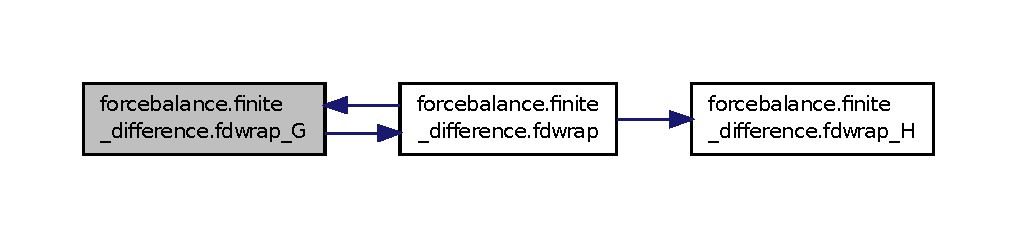
\includegraphics[width=350pt]{namespaceforcebalance_1_1finite__difference_a00322fb65860c390616f74d05037c797_cgraph}
\end{center}
\end{figure}


\hypertarget{namespaceforcebalance_1_1finite__difference_a77a0bc1ae3cbbcc8d38a0ef9ca877d6d}{\index{forcebalance\-::finite\-\_\-difference@{forcebalance\-::finite\-\_\-difference}!fdwrap\-\_\-\-H@{fdwrap\-\_\-\-H}}
\index{fdwrap\-\_\-\-H@{fdwrap\-\_\-\-H}!forcebalance::finite_difference@{forcebalance\-::finite\-\_\-difference}}
\paragraph[{fdwrap\-\_\-\-H}]{\setlength{\rightskip}{0pt plus 5cm}def forcebalance.\-finite\-\_\-difference.\-fdwrap\-\_\-\-H (
\begin{DoxyParamCaption}
\item[{}]{tgt, }
\item[{}]{mvals0, }
\item[{}]{pidx}
\end{DoxyParamCaption}
)}}\label{namespaceforcebalance_1_1finite__difference_a77a0bc1ae3cbbcc8d38a0ef9ca877d6d}


A driver to fdwrap for Hessians (see documentation for fdwrap) Inputs\-: tgt = The Target containing the objective function that we want to differentiate mvals0 = The 'central' values of the mathematical parameters -\/ i.\-e. 

the wrapped function's origin is here. pidx = The index of the parameter that we're differentiating 

Definition at line 177 of file finite\-\_\-difference.\-py.

\hypertarget{namespaceforcebalance_1_1finite__difference_ad84d3e385db1190e7d8ef58bc08a6c52}{\index{forcebalance\-::finite\-\_\-difference@{forcebalance\-::finite\-\_\-difference}!in\-\_\-fd@{in\-\_\-fd}}
\index{in\-\_\-fd@{in\-\_\-fd}!forcebalance::finite_difference@{forcebalance\-::finite\-\_\-difference}}
\paragraph[{in\-\_\-fd}]{\setlength{\rightskip}{0pt plus 5cm}def forcebalance.\-finite\-\_\-difference.\-in\-\_\-fd (
\begin{DoxyParamCaption}
{}
\end{DoxyParamCaption}
)}}\label{namespaceforcebalance_1_1finite__difference_ad84d3e385db1190e7d8ef58bc08a6c52}


Invoking this function from anywhere will tell us whether we're being called by a finite-\/difference function. 

This is mainly useful for deciding when to update the 'qualitative indicators' and when not to. 

Definition at line 121 of file finite\-\_\-difference.\-py.



\subsubsection{Variable Documentation}
\hypertarget{namespaceforcebalance_1_1finite__difference_a2bdf74505c45f442e1c96d557414254e}{\index{forcebalance\-::finite\-\_\-difference@{forcebalance\-::finite\-\_\-difference}!logger@{logger}}
\index{logger@{logger}!forcebalance::finite_difference@{forcebalance\-::finite\-\_\-difference}}
\paragraph[{logger}]{\setlength{\rightskip}{0pt plus 5cm}tuple forcebalance.\-finite\-\_\-difference.\-logger = get\-Logger(\-\_\-\-\_\-name\-\_\-\-\_\-)}}\label{namespaceforcebalance_1_1finite__difference_a2bdf74505c45f442e1c96d557414254e}


Definition at line 7 of file finite\-\_\-difference.\-py.


\hypertarget{namespaceforcebalance_1_1forcefield}{\subsection{forcebalance.\-forcefield Namespace Reference}
\label{namespaceforcebalance_1_1forcefield}\index{forcebalance.\-forcefield@{forcebalance.\-forcefield}}
}


Force field module.  


\subsubsection*{Classes}
\begin{DoxyCompactItemize}
\item 
class \hyperlink{classforcebalance_1_1forcefield_1_1BackedUpDict}{Backed\-Up\-Dict}
\item 
class \hyperlink{classforcebalance_1_1forcefield_1_1FF}{F\-F}
\begin{DoxyCompactList}\small\item\em Force field class. \end{DoxyCompactList}\end{DoxyCompactItemize}
\subsubsection*{Functions}
\begin{DoxyCompactItemize}
\item 
def \hyperlink{namespaceforcebalance_1_1forcefield_a99c9997d5158a04be089f291bd6f99bd}{determine\-\_\-fftype}
\begin{DoxyCompactList}\small\item\em Determine the type of a force field file. \end{DoxyCompactList}\item 
def \hyperlink{namespaceforcebalance_1_1forcefield_ab1a855bace20dd5e45928467e2a133f1}{rs\-\_\-override}
\begin{DoxyCompactList}\small\item\em This function takes in a dictionary (rsfactors) and a string (termtype). \end{DoxyCompactList}\end{DoxyCompactItemize}
\subsubsection*{Variables}
\begin{DoxyCompactItemize}
\item 
dictionary \hyperlink{namespaceforcebalance_1_1forcefield_abc5e12aa78c5742f028b954ede086c51}{F\-F\-\_\-\-Extensions}
\item 
dictionary \hyperlink{namespaceforcebalance_1_1forcefield_a3beac9806e0438b79b9ae60a47c7b131}{F\-F\-\_\-\-I\-O\-Modules}
\end{DoxyCompactItemize}


\subsubsection{Detailed Description}
Force field module. In Force\-Balance a 'force field' is built from a set of files containing physical parameters. These files can be anything that enter into any computation -\/ our original program was quite dependent on the G\-R\-O\-M\-A\-C\-S force field format, but this program is set up to allow very general input formats.

We introduce several important concepts\-:

1) Adjustable parameters are allocated into a vector.

To cast the force field optimization as a math problem, we treat all of the parameters on equal footing and write them as indices in a parameter vector.

2) A mapping from interaction type to parameter number.

Each element in the parameter vector corresponds to one or more interaction types. Whenever we change the parameter vector and recompute the objective function, this amounts to changing the physical parameters in the simulations, so we print out new force field files for external programs. In addition, when these programs are computing the objective function we are often in low-\/level subroutines that compute terms in the energy and force. If we need an analytic derivative of the objective function, then these subroutines need to know which index of the parameter vector needs to be modified.

This is done by way of a hash table\-: for example, when we are computing a Coulomb interaction between atom 4 and atom 5, we can build the words 'C\-O\-U\-L4' and 'C\-O\-U\-L5' and look it up in the parameter map; this gives us two numbers (say, 10 and 11) corresponding to the eleventh and twelfth element of the parameter vector. Then we can compute the derivatives of the energy w/r.\-t. these parameters (in this case, C\-O\-U\-L5/rij and C\-O\-U\-L4/rij) and increment these values in the objective function gradient.

In custom-\/implemented force fields (see counterpoisematch.\-py) the hash table can also be used to look up parameter values for computation of interactions. This is probably not the fastest way to do things, however.

3) Distinction between physical and mathematical parameters.

The optimization algorithm works in a space that is related to, but not exactly the same as the physical parameter space. The reasons for why we do this are\-:

a) Each parameter has its own physical units. On the one hand it's not right to treat different physical units all on the same footing, so nondimensionalization is desirable. To make matters worse, the force field parameters can be small as 1e-\/8 or as large as 1e+6 depending on the parameter type. This means the elements of the objective function gradient / Hessian have elements that differ from each other in size by 10+ orders of magnitude, leading to mathematical instabilities in the optimizer.

b) The parameter space can be constrained, most notably for atomic partial charges where we don't want to change the overall charge on a molecule. Thus we wish to project out certain movements in the mathematical parameters such that they don't change the physical parameters.

c) We wish to regularize our optimization so as to avoid changing our parameters in very insensitive directions (linear dependencies). However, the sensitivity of the objective function to changes in the force field depends on the physical units!

For all of these reasons, we introduce a 'transformation matrix' which maps mathematical parameters onto physical parameters. The diagonal elements in this matrix are rescaling factors; they take the mathematical parameter and magnify it by this constant factor. The off-\/diagonal elements correspond to rotations and other linear transformations, and currently I just use them to project out the 'increase the net charge' direction in the physical parameter space.

Note that with regularization, these rescaling factors are equivalent to the widths of prior distributions in a maximum likelihood framework. Because there is such a correspondence between rescaling factors and choosing a prior, they need to be chosen carefully. This is work in progress. Another possibility is to sample the width of the priors from a noninformative distribution -- the hyperprior (we can choose the Jeffreys prior or something). This is work in progress.

Right now only G\-R\-O\-M\-A\-C\-S parameters are supported, but this class is extensible, we need more modules!

\begin{DoxyAuthor}{Author}
Lee-\/\-Ping Wang 
\end{DoxyAuthor}
\begin{DoxyDate}{Date}
04/2012 
\end{DoxyDate}


\subsubsection{Function Documentation}
\hypertarget{namespaceforcebalance_1_1forcefield_a99c9997d5158a04be089f291bd6f99bd}{\index{forcebalance\-::forcefield@{forcebalance\-::forcefield}!determine\-\_\-fftype@{determine\-\_\-fftype}}
\index{determine\-\_\-fftype@{determine\-\_\-fftype}!forcebalance::forcefield@{forcebalance\-::forcefield}}
\paragraph[{determine\-\_\-fftype}]{\setlength{\rightskip}{0pt plus 5cm}def forcebalance.\-forcefield.\-determine\-\_\-fftype (
\begin{DoxyParamCaption}
\item[{}]{ffname, }
\item[{}]{verbose = {\ttfamily False}}
\end{DoxyParamCaption}
)}}\label{namespaceforcebalance_1_1forcefield_a99c9997d5158a04be089f291bd6f99bd}


Determine the type of a force field file. 

It is possible to specify the file type explicitly in the input file using the syntax 'force\-\_\-field.\-ext\-:type'. Otherwise this function will try to determine the force field type by extension. 

Definition at line 143 of file forcefield.\-py.

\hypertarget{namespaceforcebalance_1_1forcefield_ab1a855bace20dd5e45928467e2a133f1}{\index{forcebalance\-::forcefield@{forcebalance\-::forcefield}!rs\-\_\-override@{rs\-\_\-override}}
\index{rs\-\_\-override@{rs\-\_\-override}!forcebalance::forcefield@{forcebalance\-::forcefield}}
\paragraph[{rs\-\_\-override}]{\setlength{\rightskip}{0pt plus 5cm}def forcebalance.\-forcefield.\-rs\-\_\-override (
\begin{DoxyParamCaption}
\item[{}]{rsfactors, }
\item[{}]{termtype, }
\item[{}]{Temperature = {\ttfamily 298.15}}
\end{DoxyParamCaption}
)}}\label{namespaceforcebalance_1_1forcefield_ab1a855bace20dd5e45928467e2a133f1}


This function takes in a dictionary (rsfactors) and a string (termtype). 

\begin{DoxyVerb} If termtype matches any of the strings below, rsfactors[termtype] is assigned
 to one of the numbers below.

 This is LPW's attempt to simplify the rescaling factors.
\end{DoxyVerb}



\begin{DoxyParams}[1]{Parameters}
\mbox{\tt out}  & {\em rsfactors} & The computed rescaling factor. \\
\hline
\mbox{\tt in}  & {\em termtype} & The interaction type (corresponding to a physical unit) \\
\hline
\mbox{\tt in}  & {\em Temperature} & The temperature for computing the k\-T energy scale \\
\hline
\end{DoxyParams}


Definition at line 1171 of file forcefield.\-py.



\subsubsection{Variable Documentation}
\hypertarget{namespaceforcebalance_1_1forcefield_abc5e12aa78c5742f028b954ede086c51}{\index{forcebalance\-::forcefield@{forcebalance\-::forcefield}!F\-F\-\_\-\-Extensions@{F\-F\-\_\-\-Extensions}}
\index{F\-F\-\_\-\-Extensions@{F\-F\-\_\-\-Extensions}!forcebalance::forcefield@{forcebalance\-::forcefield}}
\paragraph[{F\-F\-\_\-\-Extensions}]{\setlength{\rightskip}{0pt plus 5cm}dictionary forcebalance.\-forcefield.\-F\-F\-\_\-\-Extensions}}\label{namespaceforcebalance_1_1forcefield_abc5e12aa78c5742f028b954ede086c51}
{\bfseries Initial value\-:}
\begin{DoxyCode}
1 = \{\textcolor{stringliteral}{"itp"} : \textcolor{stringliteral}{"gmx"},
2                  \textcolor{stringliteral}{"in"}  : \textcolor{stringliteral}{"qchem"},
3                  \textcolor{stringliteral}{"prm"} : \textcolor{stringliteral}{"tinker"},
4                  \textcolor{stringliteral}{"gen"} : \textcolor{stringliteral}{"custom"},
5                  \textcolor{stringliteral}{"xml"} : \textcolor{stringliteral}{"openmm"},
6                  \textcolor{stringliteral}{"frcmod"} : \textcolor{stringliteral}{"frcmod"},
7                  \textcolor{stringliteral}{"mol2"} : \textcolor{stringliteral}{"mol2"},
8                  \textcolor{stringliteral}{"gbs"}  : \textcolor{stringliteral}{"gbs"},
9                  \textcolor{stringliteral}{"grid"} : \textcolor{stringliteral}{"grid"}
10                  \}
\end{DoxyCode}


Definition at line 115 of file forcefield.\-py.

\hypertarget{namespaceforcebalance_1_1forcefield_a3beac9806e0438b79b9ae60a47c7b131}{\index{forcebalance\-::forcefield@{forcebalance\-::forcefield}!F\-F\-\_\-\-I\-O\-Modules@{F\-F\-\_\-\-I\-O\-Modules}}
\index{F\-F\-\_\-\-I\-O\-Modules@{F\-F\-\_\-\-I\-O\-Modules}!forcebalance::forcefield@{forcebalance\-::forcefield}}
\paragraph[{F\-F\-\_\-\-I\-O\-Modules}]{\setlength{\rightskip}{0pt plus 5cm}dictionary forcebalance.\-forcefield.\-F\-F\-\_\-\-I\-O\-Modules}}\label{namespaceforcebalance_1_1forcefield_a3beac9806e0438b79b9ae60a47c7b131}
{\bfseries Initial value\-:}
\begin{DoxyCode}
1 = \{\textcolor{stringliteral}{"gmx"}: \hyperlink{classforcebalance_1_1gmxio_1_1ITP__Reader}{gmxio.ITP\_Reader} ,
2                 \textcolor{stringliteral}{"qchem"}: \hyperlink{classforcebalance_1_1qchemio_1_1QCIn__Reader}{qchemio.QCIn\_Reader} ,
3                 \textcolor{stringliteral}{"tinker"}: \hyperlink{classforcebalance_1_1tinkerio_1_1Tinker__Reader}{tinkerio.Tinker\_Reader} ,
4                 \textcolor{stringliteral}{"custom"}: \hyperlink{classforcebalance_1_1custom__io_1_1Gen__Reader}{custom\_io.Gen\_Reader} , 
5                 \textcolor{stringliteral}{"openmm"} : \hyperlink{classforcebalance_1_1openmmio_1_1OpenMM__Reader}{openmmio.OpenMM\_Reader},
6                 \textcolor{stringliteral}{"frcmod"} : \hyperlink{classforcebalance_1_1amberio_1_1FrcMod__Reader}{amberio.FrcMod\_Reader},
7                 \textcolor{stringliteral}{"mol2"} : \hyperlink{classforcebalance_1_1amberio_1_1Mol2__Reader}{amberio.Mol2\_Reader},
8                 \textcolor{stringliteral}{"gbs"} : \hyperlink{classforcebalance_1_1psi4io_1_1GBS__Reader}{psi4io.GBS\_Reader},
9                 \textcolor{stringliteral}{"grid"} : \hyperlink{classforcebalance_1_1psi4io_1_1Grid__Reader}{psi4io.Grid\_Reader}
10                 \}
\end{DoxyCode}


Definition at line 127 of file forcefield.\-py.


\hypertarget{namespaceforcebalance_1_1gmxio}{\subsection{forcebalance\-:\-:gmxio \-Namespace \-Reference}
\label{namespaceforcebalance_1_1gmxio}\index{forcebalance\-::gmxio@{forcebalance\-::gmxio}}
}


\-G\-R\-O\-M\-A\-C\-S input/output.  


\subsubsection*{\-Classes}
\begin{DoxyCompactItemize}
\item 
class \hyperlink{classforcebalance_1_1gmxio_1_1ITP__Reader}{\-I\-T\-P\-\_\-\-Reader}
\begin{DoxyCompactList}\small\item\em \-Finite state machine for parsing \-G\-R\-O\-M\-A\-C\-S force field files. \end{DoxyCompactList}\item 
class \hyperlink{classforcebalance_1_1gmxio_1_1AbInitio__GMX}{\-Ab\-Initio\-\_\-\-G\-M\-X}
\begin{DoxyCompactList}\small\item\em \-Subclass of \-Ab\-Initio for force and energy matching using normal \-G\-R\-O\-M\-A\-C\-S. \end{DoxyCompactList}\item 
class \hyperlink{classforcebalance_1_1gmxio_1_1Liquid__GMX}{\-Liquid\-\_\-\-G\-M\-X}
\item 
class \hyperlink{classforcebalance_1_1gmxio_1_1Interaction__GMX}{\-Interaction\-\_\-\-G\-M\-X}
\begin{DoxyCompactList}\small\item\em \-Subclass of \-Interaction for interaction energy matching using \-G\-R\-O\-M\-A\-C\-S. \end{DoxyCompactList}\end{DoxyCompactItemize}
\subsubsection*{\-Functions}
\begin{DoxyCompactItemize}
\item 
def \hyperlink{namespaceforcebalance_1_1gmxio_acc5bef2c5c991cd70a948a1dd43ef6a6}{edit\-\_\-mdp}
\begin{DoxyCompactList}\small\item\em \-Create or edit a \-Gromacs \-M\-D\-P file. \end{DoxyCompactList}\item 
def \hyperlink{namespaceforcebalance_1_1gmxio_a29af6ace00d7e58258e0a854ca13d954}{parse\-\_\-atomtype\-\_\-line}
\begin{DoxyCompactList}\small\item\em \-Parses the 'atomtype' line. \end{DoxyCompactList}\item 
def \hyperlink{namespaceforcebalance_1_1gmxio_acac8488f29b62fb0d4cb54bb5a041026}{rm\-\_\-gmx\-\_\-baks}
\end{DoxyCompactItemize}
\subsubsection*{\-Variables}
\begin{DoxyCompactItemize}
\item 
tuple \hyperlink{namespaceforcebalance_1_1gmxio_a1ba0eaad8ffef47e3afff245dd1e3dcf}{logger} = get\-Logger(\-\_\-\-\_\-name\-\_\-\-\_\-)
\item 
list \hyperlink{namespaceforcebalance_1_1gmxio_a1273a5830d780475a2d07385c60341f6}{nftypes} = \mbox{[}\-None, '\-V\-D\-W', '\-V\-D\-W\-\_\-\-B\-H\-A\-M'\mbox{]}
\begin{DoxyCompactList}\small\item\em \-Vd\-W interaction function types. \end{DoxyCompactList}\item 
list \hyperlink{namespaceforcebalance_1_1gmxio_a1e3fab50f3ebc3477ff3fb31671e840b}{pftypes} = \mbox{[}\-None, '\-V\-P\-A\-I\-R', '\-V\-P\-A\-I\-R\-\_\-\-B\-H\-A\-M'\mbox{]}
\begin{DoxyCompactList}\small\item\em \-Pairwise interaction function types. \end{DoxyCompactList}\item 
list \hyperlink{namespaceforcebalance_1_1gmxio_ac8e059e7c8d46326654f585b23f2d0b0}{bftypes} = \mbox{[}\-None, '\-B\-O\-N\-D\-S', '\-G96\-B\-O\-N\-D\-S', '\-M\-O\-R\-S\-E'\mbox{]}
\begin{DoxyCompactList}\small\item\em \-Bonded interaction function types. \end{DoxyCompactList}\item 
list \hyperlink{namespaceforcebalance_1_1gmxio_ac655fded3f739845c1a803fc4123a593}{aftypes}
\begin{DoxyCompactList}\small\item\em \-Angle interaction function types. \end{DoxyCompactList}\item 
list \hyperlink{namespaceforcebalance_1_1gmxio_a5520b315e210120bb3e14af3665d568c}{dftypes} = \mbox{[}\-None, '\-P\-D\-I\-H\-S', '\-I\-D\-I\-H\-S', '\-R\-B\-D\-I\-H\-S', '\-P\-I\-M\-P\-D\-I\-H\-S', '\-F\-O\-U\-R\-D\-I\-H\-S', \-None, \-None, '\-T\-A\-B\-D\-I\-H\-S', '\-P\-D\-I\-H\-M\-U\-L\-S'\mbox{]}
\begin{DoxyCompactList}\small\item\em \-Dihedral interaction function types. \end{DoxyCompactList}\item 
dictionary \hyperlink{namespaceforcebalance_1_1gmxio_ac4e46dd6adabe0dfdeddcd86e772ad33}{fdict}
\begin{DoxyCompactList}\small\item\em \-Section -\/$>$ \-Interaction type dictionary. \end{DoxyCompactList}\item 
dictionary \hyperlink{namespaceforcebalance_1_1gmxio_afa3ee5e262ff005d87d20b4ec1581bad}{pdict}
\begin{DoxyCompactList}\small\item\em \-Interaction type -\/$>$ \-Parameter \-Dictionary. \end{DoxyCompactList}\end{DoxyCompactItemize}


\subsubsection{\-Detailed \-Description}
\-G\-R\-O\-M\-A\-C\-S input/output. \begin{DoxyRefDesc}{\-Todo}
\item[\hyperlink{todo__todo000009}{\-Todo}]\-Even more stuff from \hyperlink{forcefield_8py}{forcefield.\-py} needs to go into here.\end{DoxyRefDesc}


\begin{DoxyAuthor}{\-Author}
\-Lee-\/\-Ping \-Wang 
\end{DoxyAuthor}
\begin{DoxyDate}{\-Date}
12/2011
\end{DoxyDate}
\begin{DoxyRefDesc}{\-Todo}
\item[\hyperlink{todo__todo000012}{\-Todo}]\-Even more stuff from \hyperlink{forcefield_8py}{forcefield.\-py} needs to go into here.\end{DoxyRefDesc}


\begin{DoxyAuthor}{\-Author}
\-Lee-\/\-Ping \-Wang 
\end{DoxyAuthor}
\begin{DoxyDate}{\-Date}
12/2011 
\end{DoxyDate}


\subsubsection{\-Function \-Documentation}
\hypertarget{namespaceforcebalance_1_1gmxio_acc5bef2c5c991cd70a948a1dd43ef6a6}{\index{forcebalance\-::gmxio@{forcebalance\-::gmxio}!edit\-\_\-mdp@{edit\-\_\-mdp}}
\index{edit\-\_\-mdp@{edit\-\_\-mdp}!forcebalance::gmxio@{forcebalance\-::gmxio}}
\paragraph[{edit\-\_\-mdp}]{\setlength{\rightskip}{0pt plus 5cm}def {\bf forcebalance.\-gmxio.\-edit\-\_\-mdp} (
\begin{DoxyParamCaption}
\item[{}]{fin, }
\item[{}]{fout, }
\item[{}]{options, }
\item[{}]{verbose = {\ttfamily \-False}}
\end{DoxyParamCaption}
)}}\label{namespaceforcebalance_1_1gmxio_acc5bef2c5c991cd70a948a1dd43ef6a6}


\-Create or edit a \-Gromacs \-M\-D\-P file. 


\begin{DoxyParams}[1]{\-Parameters}
\mbox{\tt in}  & {\em fin} & \-Input file name. \\
\hline
\mbox{\tt in}  & {\em fout} & \-Output file name, can be the same as input file name. \\
\hline
\mbox{\tt in}  & {\em options} & \-Dictionary containing mdp options. \-Existing options are replaced, new options are added at the end. \\
\hline
\end{DoxyParams}


\-Definition at line 35 of file gmxio.\-py.



\-Here is the call graph for this function\-:
\nopagebreak
\begin{figure}[H]
\begin{center}
\leavevmode
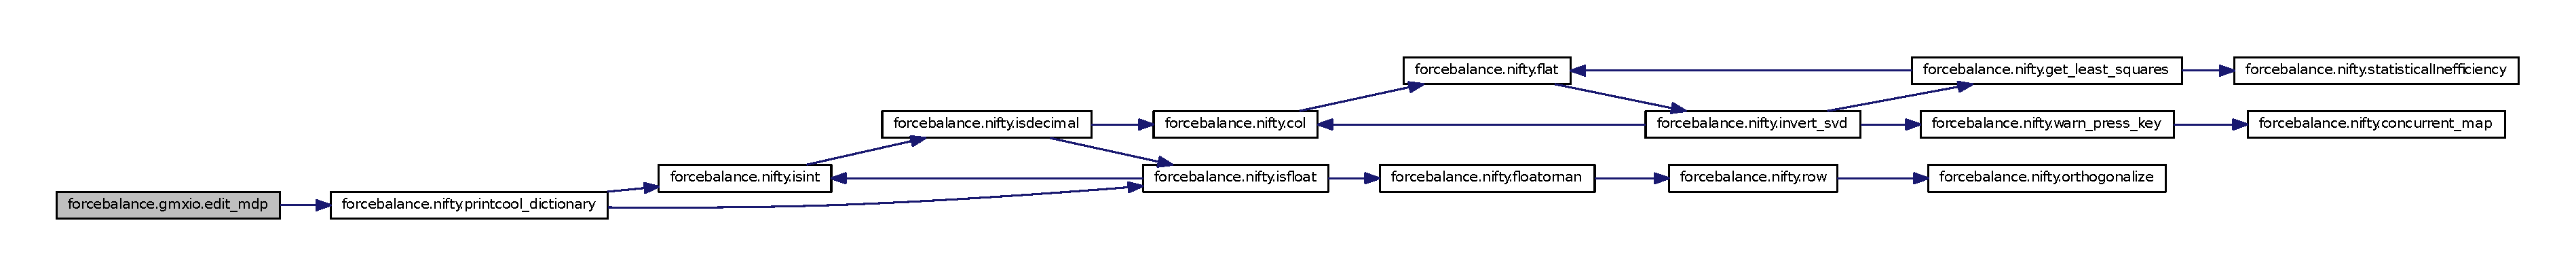
\includegraphics[width=350pt]{namespaceforcebalance_1_1gmxio_acc5bef2c5c991cd70a948a1dd43ef6a6_cgraph}
\end{center}
\end{figure}


\hypertarget{namespaceforcebalance_1_1gmxio_a29af6ace00d7e58258e0a854ca13d954}{\index{forcebalance\-::gmxio@{forcebalance\-::gmxio}!parse\-\_\-atomtype\-\_\-line@{parse\-\_\-atomtype\-\_\-line}}
\index{parse\-\_\-atomtype\-\_\-line@{parse\-\_\-atomtype\-\_\-line}!forcebalance::gmxio@{forcebalance\-::gmxio}}
\paragraph[{parse\-\_\-atomtype\-\_\-line}]{\setlength{\rightskip}{0pt plus 5cm}def {\bf forcebalance.\-gmxio.\-parse\-\_\-atomtype\-\_\-line} (
\begin{DoxyParamCaption}
\item[{}]{line}
\end{DoxyParamCaption}
)}}\label{namespaceforcebalance_1_1gmxio_a29af6ace00d7e58258e0a854ca13d954}


\-Parses the 'atomtype' line. 

\-Parses lines like this\-:\par
 {\ttfamily  opls\-\_\-135 \-C\-T 6 12.\-0107 0.\-0000 \-A 3.\-5000e-\/01 2.\-7614e-\/01\par
 \-C 12.\-0107 0.\-0000 \-A 3.\-7500e-\/01 4.\-3932e-\/01\par
 \-Na 11 22.\-9897 0.\-0000 \-A 6.\-068128070229e+03 2.\-662662556402e+01 0.\-0000e+00 ; \-P\-A\-R\-M 5 6\par
 } \-Look at all the variety!


\begin{DoxyParams}[1]{\-Parameters}
\mbox{\tt in}  & {\em line} & \-Input line. \\
\hline
\end{DoxyParams}
\begin{DoxyReturn}{\-Returns}
answer \-Dictionary containing\-:\par
 atom type\par
 bonded atom type (if any)\par
 atomic number (if any)\par
 atomic mass\par
 charge\par
 particle type\par
 force field parameters\par
 number of optional fields 
\end{DoxyReturn}


\-Definition at line 181 of file gmxio.\-py.



\-Here is the call graph for this function\-:
\nopagebreak
\begin{figure}[H]
\begin{center}
\leavevmode
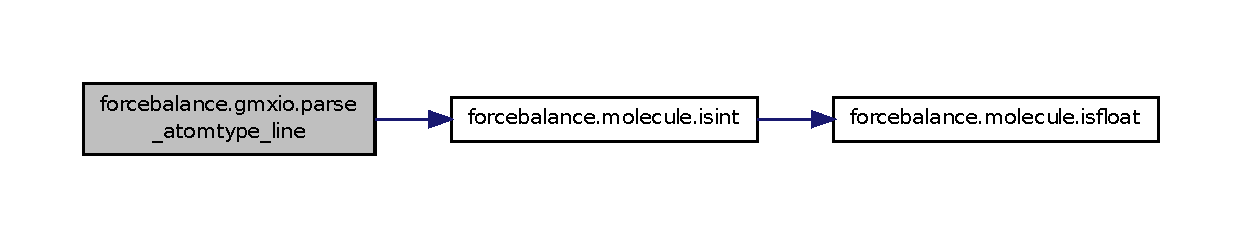
\includegraphics[width=350pt]{namespaceforcebalance_1_1gmxio_a29af6ace00d7e58258e0a854ca13d954_cgraph}
\end{center}
\end{figure}


\hypertarget{namespaceforcebalance_1_1gmxio_acac8488f29b62fb0d4cb54bb5a041026}{\index{forcebalance\-::gmxio@{forcebalance\-::gmxio}!rm\-\_\-gmx\-\_\-baks@{rm\-\_\-gmx\-\_\-baks}}
\index{rm\-\_\-gmx\-\_\-baks@{rm\-\_\-gmx\-\_\-baks}!forcebalance::gmxio@{forcebalance\-::gmxio}}
\paragraph[{rm\-\_\-gmx\-\_\-baks}]{\setlength{\rightskip}{0pt plus 5cm}def {\bf forcebalance.\-gmxio.\-rm\-\_\-gmx\-\_\-baks} (
\begin{DoxyParamCaption}
\item[{}]{dir}
\end{DoxyParamCaption}
)}}\label{namespaceforcebalance_1_1gmxio_acac8488f29b62fb0d4cb54bb5a041026}


\-Definition at line 428 of file gmxio.\-py.



\subsubsection{\-Variable \-Documentation}
\hypertarget{namespaceforcebalance_1_1gmxio_ac655fded3f739845c1a803fc4123a593}{\index{forcebalance\-::gmxio@{forcebalance\-::gmxio}!aftypes@{aftypes}}
\index{aftypes@{aftypes}!forcebalance::gmxio@{forcebalance\-::gmxio}}
\paragraph[{aftypes}]{\setlength{\rightskip}{0pt plus 5cm}list {\bf forcebalance\-::gmxio\-::aftypes}}}\label{namespaceforcebalance_1_1gmxio_ac655fded3f739845c1a803fc4123a593}
{\bfseries \-Initial value\-:}
\begin{DoxyCode}
1 [None, 'ANGLES', 'G96ANGLES', 'CROSS_BOND_BOND',
2            'CROSS_BOND_ANGLE', 'UREY_BRADLEY', 'QANGLES']
\end{DoxyCode}


\-Angle interaction function types. 



\-Definition at line 91 of file gmxio.\-py.

\hypertarget{namespaceforcebalance_1_1gmxio_ac8e059e7c8d46326654f585b23f2d0b0}{\index{forcebalance\-::gmxio@{forcebalance\-::gmxio}!bftypes@{bftypes}}
\index{bftypes@{bftypes}!forcebalance::gmxio@{forcebalance\-::gmxio}}
\paragraph[{bftypes}]{\setlength{\rightskip}{0pt plus 5cm}list {\bf forcebalance\-::gmxio\-::bftypes} = \mbox{[}\-None, '\-B\-O\-N\-D\-S', '\-G96\-B\-O\-N\-D\-S', '\-M\-O\-R\-S\-E'\mbox{]}}}\label{namespaceforcebalance_1_1gmxio_ac8e059e7c8d46326654f585b23f2d0b0}


\-Bonded interaction function types. 



\-Definition at line 89 of file gmxio.\-py.

\hypertarget{namespaceforcebalance_1_1gmxio_a5520b315e210120bb3e14af3665d568c}{\index{forcebalance\-::gmxio@{forcebalance\-::gmxio}!dftypes@{dftypes}}
\index{dftypes@{dftypes}!forcebalance::gmxio@{forcebalance\-::gmxio}}
\paragraph[{dftypes}]{\setlength{\rightskip}{0pt plus 5cm}list {\bf forcebalance\-::gmxio\-::dftypes} = \mbox{[}\-None, '\-P\-D\-I\-H\-S', '\-I\-D\-I\-H\-S', '\-R\-B\-D\-I\-H\-S', '\-P\-I\-M\-P\-D\-I\-H\-S', '\-F\-O\-U\-R\-D\-I\-H\-S', \-None, \-None, '\-T\-A\-B\-D\-I\-H\-S', '\-P\-D\-I\-H\-M\-U\-L\-S'\mbox{]}}}\label{namespaceforcebalance_1_1gmxio_a5520b315e210120bb3e14af3665d568c}


\-Dihedral interaction function types. 



\-Definition at line 94 of file gmxio.\-py.

\hypertarget{namespaceforcebalance_1_1gmxio_ac4e46dd6adabe0dfdeddcd86e772ad33}{\index{forcebalance\-::gmxio@{forcebalance\-::gmxio}!fdict@{fdict}}
\index{fdict@{fdict}!forcebalance::gmxio@{forcebalance\-::gmxio}}
\paragraph[{fdict}]{\setlength{\rightskip}{0pt plus 5cm}dictionary {\bf forcebalance\-::gmxio\-::fdict}}}\label{namespaceforcebalance_1_1gmxio_ac4e46dd6adabe0dfdeddcd86e772ad33}
{\bfseries \-Initial value\-:}
\begin{DoxyCode}
1 {
2     'atomtypes'     : nftypes,
3     'nonbond_params': pftypes,
4     'bonds'         : bftypes,
5     'bondtypes'     : bftypes,
6     'angles'        : aftypes,
7     'angletypes'    : aftypes,
8     'dihedrals'     : dftypes,
9     'dihedraltypes' : dftypes,
10     'virtual_sites2': ['NONE','VSITE2'],
11     'virtual_sites3': ['NONE','VSITE3','VSITE3FD','VSITE3FAD','VSITE3OUT'],
12     'virtual_sites4': ['NONE','VSITE4FD','VSITE4FDN']
13     }
\end{DoxyCode}


\-Section -\/$>$ \-Interaction type dictionary. 

\-Based on the section you're in and the integer given on the current line, this looks up the 'interaction type' -\/ for example, within bonded interactions there are four interaction types\-: harmonic, \-G96, \-Morse, and quartic interactions. 

\-Definition at line 102 of file gmxio.\-py.

\hypertarget{namespaceforcebalance_1_1gmxio_a1ba0eaad8ffef47e3afff245dd1e3dcf}{\index{forcebalance\-::gmxio@{forcebalance\-::gmxio}!logger@{logger}}
\index{logger@{logger}!forcebalance::gmxio@{forcebalance\-::gmxio}}
\paragraph[{logger}]{\setlength{\rightskip}{0pt plus 5cm}tuple {\bf forcebalance\-::gmxio\-::logger} = get\-Logger(\-\_\-\-\_\-name\-\_\-\-\_\-)}}\label{namespaceforcebalance_1_1gmxio_a1ba0eaad8ffef47e3afff245dd1e3dcf}


\-Definition at line 26 of file gmxio.\-py.

\hypertarget{namespaceforcebalance_1_1gmxio_a1273a5830d780475a2d07385c60341f6}{\index{forcebalance\-::gmxio@{forcebalance\-::gmxio}!nftypes@{nftypes}}
\index{nftypes@{nftypes}!forcebalance::gmxio@{forcebalance\-::gmxio}}
\paragraph[{nftypes}]{\setlength{\rightskip}{0pt plus 5cm}list {\bf forcebalance\-::gmxio\-::nftypes} = \mbox{[}\-None, '\-V\-D\-W', '\-V\-D\-W\-\_\-\-B\-H\-A\-M'\mbox{]}}}\label{namespaceforcebalance_1_1gmxio_a1273a5830d780475a2d07385c60341f6}


\-Vd\-W interaction function types. 



\-Definition at line 85 of file gmxio.\-py.

\hypertarget{namespaceforcebalance_1_1gmxio_afa3ee5e262ff005d87d20b4ec1581bad}{\index{forcebalance\-::gmxio@{forcebalance\-::gmxio}!pdict@{pdict}}
\index{pdict@{pdict}!forcebalance::gmxio@{forcebalance\-::gmxio}}
\paragraph[{pdict}]{\setlength{\rightskip}{0pt plus 5cm}dictionary {\bf forcebalance\-::gmxio\-::pdict}}}\label{namespaceforcebalance_1_1gmxio_afa3ee5e262ff005d87d20b4ec1581bad}


\-Interaction type -\/$>$ \-Parameter \-Dictionary. 

\-A list of supported \-G\-R\-O\-M\-A\-C\-S interaction types in force matching. \-The keys in this dictionary (e.\-g. '\-B\-O\-N\-D\-S','\-A\-N\-G\-L\-E\-S') are values in the interaction type dictionary. \-As the program loops through the force field file, it first looks up the interaction types in 'fdict' and then goes here to do the parameter lookup by field. \begin{DoxyRefDesc}{\-Todo}
\item[\hyperlink{todo__todo000010}{\-Todo}]\-This needs to become more flexible because the parameter isn't always in the same field. \-Still need to figure out how to do this. 

\-How about making the \-P\-D\-I\-H\-S less ugly? \end{DoxyRefDesc}


\-Definition at line 125 of file gmxio.\-py.

\hypertarget{namespaceforcebalance_1_1gmxio_a1e3fab50f3ebc3477ff3fb31671e840b}{\index{forcebalance\-::gmxio@{forcebalance\-::gmxio}!pftypes@{pftypes}}
\index{pftypes@{pftypes}!forcebalance::gmxio@{forcebalance\-::gmxio}}
\paragraph[{pftypes}]{\setlength{\rightskip}{0pt plus 5cm}list {\bf forcebalance\-::gmxio\-::pftypes} = \mbox{[}\-None, '\-V\-P\-A\-I\-R', '\-V\-P\-A\-I\-R\-\_\-\-B\-H\-A\-M'\mbox{]}}}\label{namespaceforcebalance_1_1gmxio_a1e3fab50f3ebc3477ff3fb31671e840b}


\-Pairwise interaction function types. 



\-Definition at line 87 of file gmxio.\-py.


\hypertarget{namespaceforcebalance_1_1interaction}{\subsection{forcebalance\-:\-:interaction \-Namespace \-Reference}
\label{namespaceforcebalance_1_1interaction}\index{forcebalance\-::interaction@{forcebalance\-::interaction}}
}


\hyperlink{classforcebalance_1_1interaction_1_1Interaction}{\-Interaction} energy fitting module.  


\subsubsection*{\-Classes}
\begin{DoxyCompactItemize}
\item 
class \hyperlink{classforcebalance_1_1interaction_1_1Interaction}{\-Interaction}
\begin{DoxyCompactList}\small\item\em \-Subclass of \-Target for fitting force fields to interaction energies. \end{DoxyCompactList}\end{DoxyCompactItemize}
\subsubsection*{\-Variables}
\begin{DoxyCompactItemize}
\item 
tuple \hyperlink{namespaceforcebalance_1_1interaction_a4ec2dbe0f5ae3a35a22966a7c1ed81f0}{logger} = get\-Logger(\-\_\-\-\_\-name\-\_\-\-\_\-)
\end{DoxyCompactItemize}


\subsubsection{\-Detailed \-Description}
\hyperlink{classforcebalance_1_1interaction_1_1Interaction}{\-Interaction} energy fitting module. \begin{DoxyAuthor}{\-Author}
\-Lee-\/\-Ping \-Wang 
\end{DoxyAuthor}
\begin{DoxyDate}{\-Date}
05/2012 
\end{DoxyDate}


\subsubsection{\-Variable \-Documentation}
\hypertarget{namespaceforcebalance_1_1interaction_a4ec2dbe0f5ae3a35a22966a7c1ed81f0}{\index{forcebalance\-::interaction@{forcebalance\-::interaction}!logger@{logger}}
\index{logger@{logger}!forcebalance::interaction@{forcebalance\-::interaction}}
\paragraph[{logger}]{\setlength{\rightskip}{0pt plus 5cm}tuple {\bf forcebalance\-::interaction\-::logger} = get\-Logger(\-\_\-\-\_\-name\-\_\-\-\_\-)}}\label{namespaceforcebalance_1_1interaction_a4ec2dbe0f5ae3a35a22966a7c1ed81f0}


\-Definition at line 21 of file interaction.\-py.


\hypertarget{namespaceforcebalance_1_1leastsq}{\subsection{forcebalance.\-leastsq Namespace Reference}
\label{namespaceforcebalance_1_1leastsq}\index{forcebalance.\-leastsq@{forcebalance.\-leastsq}}
}
\subsubsection*{Classes}
\begin{DoxyCompactItemize}
\item 
class \hyperlink{classforcebalance_1_1leastsq_1_1LeastSquares}{Least\-Squares}
\begin{DoxyCompactList}\small\item\em Subclass of Target for general least squares fitting. \end{DoxyCompactList}\end{DoxyCompactItemize}
\subsubsection*{Functions}
\begin{DoxyCompactItemize}
\item 
def \hyperlink{namespaceforcebalance_1_1leastsq_a8e7ef329e27aff738bc91dd79bd2dd1c}{Check\-Basis}
\item 
def \hyperlink{namespaceforcebalance_1_1leastsq_ad9d0036b0003e0245608ffb192c7c60c}{Last\-Mvals}
\end{DoxyCompactItemize}
\subsubsection*{Variables}
\begin{DoxyCompactItemize}
\item 
\hyperlink{namespaceforcebalance_1_1leastsq_a87815b7768ddc6d9caf7fa3c804fe303}{C\-H\-E\-C\-K\-\_\-\-B\-A\-S\-I\-S} = False
\item 
\hyperlink{namespaceforcebalance_1_1leastsq_a037a62063d126288c2df0f4e0cd5085a}{L\-A\-S\-T\-\_\-\-M\-V\-A\-L\-S} = None
\end{DoxyCompactItemize}


\subsubsection{Function Documentation}
\hypertarget{namespaceforcebalance_1_1leastsq_a8e7ef329e27aff738bc91dd79bd2dd1c}{\index{forcebalance\-::leastsq@{forcebalance\-::leastsq}!Check\-Basis@{Check\-Basis}}
\index{Check\-Basis@{Check\-Basis}!forcebalance::leastsq@{forcebalance\-::leastsq}}
\paragraph[{Check\-Basis}]{\setlength{\rightskip}{0pt plus 5cm}def forcebalance.\-leastsq.\-Check\-Basis (
\begin{DoxyParamCaption}
{}
\end{DoxyParamCaption}
)}}\label{namespaceforcebalance_1_1leastsq_a8e7ef329e27aff738bc91dd79bd2dd1c}


Definition at line 21 of file leastsq.\-py.

\hypertarget{namespaceforcebalance_1_1leastsq_ad9d0036b0003e0245608ffb192c7c60c}{\index{forcebalance\-::leastsq@{forcebalance\-::leastsq}!Last\-Mvals@{Last\-Mvals}}
\index{Last\-Mvals@{Last\-Mvals}!forcebalance::leastsq@{forcebalance\-::leastsq}}
\paragraph[{Last\-Mvals}]{\setlength{\rightskip}{0pt plus 5cm}def forcebalance.\-leastsq.\-Last\-Mvals (
\begin{DoxyParamCaption}
{}
\end{DoxyParamCaption}
)}}\label{namespaceforcebalance_1_1leastsq_ad9d0036b0003e0245608ffb192c7c60c}


Definition at line 26 of file leastsq.\-py.



\subsubsection{Variable Documentation}
\hypertarget{namespaceforcebalance_1_1leastsq_a87815b7768ddc6d9caf7fa3c804fe303}{\index{forcebalance\-::leastsq@{forcebalance\-::leastsq}!C\-H\-E\-C\-K\-\_\-\-B\-A\-S\-I\-S@{C\-H\-E\-C\-K\-\_\-\-B\-A\-S\-I\-S}}
\index{C\-H\-E\-C\-K\-\_\-\-B\-A\-S\-I\-S@{C\-H\-E\-C\-K\-\_\-\-B\-A\-S\-I\-S}!forcebalance::leastsq@{forcebalance\-::leastsq}}
\paragraph[{C\-H\-E\-C\-K\-\_\-\-B\-A\-S\-I\-S}]{\setlength{\rightskip}{0pt plus 5cm}forcebalance.\-leastsq.\-C\-H\-E\-C\-K\-\_\-\-B\-A\-S\-I\-S = False}}\label{namespaceforcebalance_1_1leastsq_a87815b7768ddc6d9caf7fa3c804fe303}


Definition at line 20 of file leastsq.\-py.

\hypertarget{namespaceforcebalance_1_1leastsq_a037a62063d126288c2df0f4e0cd5085a}{\index{forcebalance\-::leastsq@{forcebalance\-::leastsq}!L\-A\-S\-T\-\_\-\-M\-V\-A\-L\-S@{L\-A\-S\-T\-\_\-\-M\-V\-A\-L\-S}}
\index{L\-A\-S\-T\-\_\-\-M\-V\-A\-L\-S@{L\-A\-S\-T\-\_\-\-M\-V\-A\-L\-S}!forcebalance::leastsq@{forcebalance\-::leastsq}}
\paragraph[{L\-A\-S\-T\-\_\-\-M\-V\-A\-L\-S}]{\setlength{\rightskip}{0pt plus 5cm}forcebalance.\-leastsq.\-L\-A\-S\-T\-\_\-\-M\-V\-A\-L\-S = None}}\label{namespaceforcebalance_1_1leastsq_a037a62063d126288c2df0f4e0cd5085a}


Definition at line 25 of file leastsq.\-py.


\hypertarget{namespaceforcebalance_1_1lipid}{\subsection{forcebalance.\-lipid Namespace Reference}
\label{namespaceforcebalance_1_1lipid}\index{forcebalance.\-lipid@{forcebalance.\-lipid}}
}


Matching of lipid bulk properties.  


\subsubsection*{Classes}
\begin{DoxyCompactItemize}
\item 
class \hyperlink{classforcebalance_1_1lipid_1_1Lipid}{Lipid}
\begin{DoxyCompactList}\small\item\em Subclass of Target for lipid property matching. \end{DoxyCompactList}\end{DoxyCompactItemize}
\subsubsection*{Functions}
\begin{DoxyCompactItemize}
\item 
def \hyperlink{namespaceforcebalance_1_1lipid_ad5d58c1eb0fb86e1587a892467634a44}{weight\-\_\-info}
\end{DoxyCompactItemize}
\subsubsection*{Variables}
\begin{DoxyCompactItemize}
\item 
tuple \hyperlink{namespaceforcebalance_1_1lipid_adafbe32d6a2808045fbf9e92771dc2fc}{logger} = get\-Logger(\-\_\-\-\_\-name\-\_\-\-\_\-)
\end{DoxyCompactItemize}


\subsubsection{Detailed Description}
Matching of lipid bulk properties. Under development.

author Lee-\/\-Ping Wang \begin{DoxyDate}{Date}
04/2012 
\end{DoxyDate}


\subsubsection{Function Documentation}
\hypertarget{namespaceforcebalance_1_1lipid_ad5d58c1eb0fb86e1587a892467634a44}{\index{forcebalance\-::lipid@{forcebalance\-::lipid}!weight\-\_\-info@{weight\-\_\-info}}
\index{weight\-\_\-info@{weight\-\_\-info}!forcebalance::lipid@{forcebalance\-::lipid}}
\paragraph[{weight\-\_\-info}]{\setlength{\rightskip}{0pt plus 5cm}def forcebalance.\-lipid.\-weight\-\_\-info (
\begin{DoxyParamCaption}
\item[{}]{W, }
\item[{}]{P\-T, }
\item[{}]{N\-\_\-k, }
\item[{}]{verbose = {\ttfamily True}}
\end{DoxyParamCaption}
)}}\label{namespaceforcebalance_1_1lipid_ad5d58c1eb0fb86e1587a892467634a44}


Definition at line 32 of file lipid.\-py.



\subsubsection{Variable Documentation}
\hypertarget{namespaceforcebalance_1_1lipid_adafbe32d6a2808045fbf9e92771dc2fc}{\index{forcebalance\-::lipid@{forcebalance\-::lipid}!logger@{logger}}
\index{logger@{logger}!forcebalance::lipid@{forcebalance\-::lipid}}
\paragraph[{logger}]{\setlength{\rightskip}{0pt plus 5cm}tuple forcebalance.\-lipid.\-logger = get\-Logger(\-\_\-\-\_\-name\-\_\-\-\_\-)}}\label{namespaceforcebalance_1_1lipid_adafbe32d6a2808045fbf9e92771dc2fc}


Definition at line 30 of file lipid.\-py.


\hypertarget{namespaceforcebalance_1_1liquid}{\subsection{forcebalance.\-liquid Namespace Reference}
\label{namespaceforcebalance_1_1liquid}\index{forcebalance.\-liquid@{forcebalance.\-liquid}}
}


Matching of liquid bulk properties.  


\subsubsection*{Classes}
\begin{DoxyCompactItemize}
\item 
class \hyperlink{classforcebalance_1_1liquid_1_1Liquid}{Liquid}
\begin{DoxyCompactList}\small\item\em Subclass of Target for liquid property matching. \end{DoxyCompactList}\end{DoxyCompactItemize}
\subsubsection*{Functions}
\begin{DoxyCompactItemize}
\item 
def \hyperlink{namespaceforcebalance_1_1liquid_a6f7d54263236f8788c319aee86b460b6}{weight\-\_\-info}
\end{DoxyCompactItemize}
\subsubsection*{Variables}
\begin{DoxyCompactItemize}
\item 
tuple \hyperlink{namespaceforcebalance_1_1liquid_a8c47ecb4fda6a9bccb24ef292da2ec57}{logger} = get\-Logger(\-\_\-\-\_\-name\-\_\-\-\_\-)
\end{DoxyCompactItemize}


\subsubsection{Detailed Description}
Matching of liquid bulk properties. Under development.

\begin{DoxyAuthor}{Author}
Lee-\/\-Ping Wang 
\end{DoxyAuthor}
\begin{DoxyDate}{Date}
04/2012 
\end{DoxyDate}


\subsubsection{Function Documentation}
\hypertarget{namespaceforcebalance_1_1liquid_a6f7d54263236f8788c319aee86b460b6}{\index{forcebalance\-::liquid@{forcebalance\-::liquid}!weight\-\_\-info@{weight\-\_\-info}}
\index{weight\-\_\-info@{weight\-\_\-info}!forcebalance::liquid@{forcebalance\-::liquid}}
\paragraph[{weight\-\_\-info}]{\setlength{\rightskip}{0pt plus 5cm}def forcebalance.\-liquid.\-weight\-\_\-info (
\begin{DoxyParamCaption}
\item[{}]{W, }
\item[{}]{P\-T, }
\item[{}]{N\-\_\-k, }
\item[{}]{verbose = {\ttfamily True}}
\end{DoxyParamCaption}
)}}\label{namespaceforcebalance_1_1liquid_a6f7d54263236f8788c319aee86b460b6}


Definition at line 32 of file liquid.\-py.



\subsubsection{Variable Documentation}
\hypertarget{namespaceforcebalance_1_1liquid_a8c47ecb4fda6a9bccb24ef292da2ec57}{\index{forcebalance\-::liquid@{forcebalance\-::liquid}!logger@{logger}}
\index{logger@{logger}!forcebalance::liquid@{forcebalance\-::liquid}}
\paragraph[{logger}]{\setlength{\rightskip}{0pt plus 5cm}tuple forcebalance.\-liquid.\-logger = get\-Logger(\-\_\-\-\_\-name\-\_\-\-\_\-)}}\label{namespaceforcebalance_1_1liquid_a8c47ecb4fda6a9bccb24ef292da2ec57}


Definition at line 30 of file liquid.\-py.


\hypertarget{namespaceforcebalance_1_1Mol2}{\subsection{forcebalance.\-Mol2 Namespace Reference}
\label{namespaceforcebalance_1_1Mol2}\index{forcebalance.\-Mol2@{forcebalance.\-Mol2}}
}

\hypertarget{namespaceforcebalance_1_1mol2io}{\subsection{forcebalance.\-mol2io Namespace Reference}
\label{namespaceforcebalance_1_1mol2io}\index{forcebalance.\-mol2io@{forcebalance.\-mol2io}}
}


\hyperlink{namespaceforcebalance_1_1Mol2}{Mol2} I/\-O.  


\subsubsection*{Classes}
\begin{DoxyCompactItemize}
\item 
class \hyperlink{classforcebalance_1_1mol2io_1_1Mol2__Reader}{Mol2\-\_\-\-Reader}
\begin{DoxyCompactList}\small\item\em Finite state machine for parsing \hyperlink{namespaceforcebalance_1_1Mol2}{Mol2} force field file. \end{DoxyCompactList}\end{DoxyCompactItemize}
\subsubsection*{Variables}
\begin{DoxyCompactItemize}
\item 
dictionary \hyperlink{namespaceforcebalance_1_1mol2io_a9a28a68a67a02946036ee03f9685f3ba}{mol2\-\_\-pdict} = \{'C\-O\-U\-L'\-:\{'Atom'\-:\mbox{[}1\mbox{]}, 6\-:''\}\}
\end{DoxyCompactItemize}


\subsubsection{Detailed Description}
\hyperlink{namespaceforcebalance_1_1Mol2}{Mol2} I/\-O. This serves as a good template for writing future force matching I/\-O modules for other programs because it's so simple.

\begin{DoxyAuthor}{Author}
Lee-\/\-Ping Wang 
\end{DoxyAuthor}
\begin{DoxyDate}{Date}
05/2012 
\end{DoxyDate}


\subsubsection{Variable Documentation}
\hypertarget{namespaceforcebalance_1_1mol2io_a9a28a68a67a02946036ee03f9685f3ba}{\index{forcebalance\-::mol2io@{forcebalance\-::mol2io}!mol2\-\_\-pdict@{mol2\-\_\-pdict}}
\index{mol2\-\_\-pdict@{mol2\-\_\-pdict}!forcebalance::mol2io@{forcebalance\-::mol2io}}
\paragraph[{mol2\-\_\-pdict}]{\setlength{\rightskip}{0pt plus 5cm}dictionary forcebalance.\-mol2io.\-mol2\-\_\-pdict = \{'C\-O\-U\-L'\-:\{'Atom'\-:\mbox{[}1\mbox{]}, 6\-:''\}\}}}\label{namespaceforcebalance_1_1mol2io_a9a28a68a67a02946036ee03f9685f3ba}


Definition at line 18 of file mol2io.\-py.


\hypertarget{namespaceforcebalance_1_1molecule}{\subsection{forcebalance.\-molecule Namespace Reference}
\label{namespaceforcebalance_1_1molecule}\index{forcebalance.\-molecule@{forcebalance.\-molecule}}
}
\subsubsection*{Classes}
\begin{DoxyCompactItemize}
\item 
class \hyperlink{classforcebalance_1_1molecule_1_1MolfileTimestep}{Molfile\-Timestep}
\begin{DoxyCompactList}\small\item\em Wrapper for the timestep C structure used in molfile plugins. \end{DoxyCompactList}\item 
class \hyperlink{classforcebalance_1_1molecule_1_1Molecule}{Molecule}
\begin{DoxyCompactList}\small\item\em Lee-\/\-Ping's general file format conversion class. \end{DoxyCompactList}\end{DoxyCompactItemize}
\subsubsection*{Functions}
\begin{DoxyCompactItemize}
\item 
def \hyperlink{namespaceforcebalance_1_1molecule_af28de4693e5b8e82df900d0ac3c6c370}{get\-Element}
\item 
def \hyperlink{namespaceforcebalance_1_1molecule_ab8464fea13fad2a506792c2f1d7c93f3}{nodematch}
\item 
def \hyperlink{namespaceforcebalance_1_1molecule_a0dd31eff88d2bed0884ab21a13261d42}{isint}
\begin{DoxyCompactList}\small\item\em O\-N\-L\-Y matches integers! If you have a decimal point? None shall pass! \end{DoxyCompactList}\item 
def \hyperlink{namespaceforcebalance_1_1molecule_afe989ffd119568047fc8265b1d329a70}{isfloat}
\begin{DoxyCompactList}\small\item\em Matches A\-N\-Y number; it can be a decimal, scientific notation, integer, or what have you. \end{DoxyCompactList}\item 
def \hyperlink{namespaceforcebalance_1_1molecule_a0a6e3e79b04534bf2e83d09def189444}{Build\-Lattice\-From\-Lengths\-Angles}
\begin{DoxyCompactList}\small\item\em This function takes in three lattice lengths and three lattice angles, and tries to return a complete box specification. \end{DoxyCompactList}\item 
def \hyperlink{namespaceforcebalance_1_1molecule_a29fb1ac9324f4280f07c65baea339989}{Build\-Lattice\-From\-Vectors}
\begin{DoxyCompactList}\small\item\em This function takes in three lattice vectors and tries to return a complete box specification. \end{DoxyCompactList}\item 
def \hyperlink{namespaceforcebalance_1_1molecule_a2eba3cad44138b3b10ea883240888412}{format\-\_\-xyz\-\_\-coord}
\begin{DoxyCompactList}\small\item\em Print a line consisting of (element, x, y, z) in accordance with .xyz file format. \end{DoxyCompactList}\item 
def \hyperlink{namespaceforcebalance_1_1molecule_a41c13064e4285973aa6c49369d3d3390}{format\-\_\-gro\-\_\-coord}
\begin{DoxyCompactList}\small\item\em Print a line in accordance with .gro file format, with six decimal points of precision. \end{DoxyCompactList}\item 
def \hyperlink{namespaceforcebalance_1_1molecule_a4948e4662b8d2c8d515427d1bbb3d01e}{format\-\_\-xyzgen\-\_\-coord}
\begin{DoxyCompactList}\small\item\em Print a line consisting of (element, p, q, r, s, t, ...) where (p, q, r) are arbitrary atom-\/wise data (this might happen, for instance, with atomic charges) \end{DoxyCompactList}\item 
def \hyperlink{namespaceforcebalance_1_1molecule_ae25aa5331b3a2dd0e9d1e184380357db}{format\-\_\-gro\-\_\-box}
\begin{DoxyCompactList}\small\item\em Print a line corresponding to the box vector in accordance with .gro file format. \end{DoxyCompactList}\item 
def \hyperlink{namespaceforcebalance_1_1molecule_a12b7bb398c2fa49a223f258ec7737483}{is\-\_\-gro\-\_\-coord}
\begin{DoxyCompactList}\small\item\em Determines whether a line contains G\-R\-O\-M\-A\-C\-S data or not. \end{DoxyCompactList}\item 
def \hyperlink{namespaceforcebalance_1_1molecule_a838d85848bd817e801d0f5f6502217ef}{is\-\_\-charmm\-\_\-coord}
\begin{DoxyCompactList}\small\item\em Determines whether a line contains C\-H\-A\-R\-M\-M data or not. \end{DoxyCompactList}\item 
def \hyperlink{namespaceforcebalance_1_1molecule_aafc8c924eed4480fed8ddc9c474d3bc1}{is\-\_\-gro\-\_\-box}
\begin{DoxyCompactList}\small\item\em Determines whether a line contains a G\-R\-O\-M\-A\-C\-S box vector or not. \end{DoxyCompactList}\item 
def \hyperlink{namespaceforcebalance_1_1molecule_a4cdb2086978b281ed84cd66179c3f5b2}{add\-\_\-strip\-\_\-to\-\_\-mat}
\item 
def \hyperlink{namespaceforcebalance_1_1molecule_a58c3f09152db4d1c6e1db9df29c60c43}{pvec}
\item 
def \hyperlink{namespaceforcebalance_1_1molecule_a7fe52c2928c7b0329882541bef2e34cd}{grouper}
\begin{DoxyCompactList}\small\item\em Groups a big long iterable into groups of ten or what have you. \end{DoxyCompactList}\item 
def \hyperlink{namespaceforcebalance_1_1molecule_a5f529179461765fadbd0a742cdc2c677}{even\-\_\-list}
\begin{DoxyCompactList}\small\item\em Creates a list of number sequences divided as evenly as possible. \end{DoxyCompactList}\item 
def \hyperlink{namespaceforcebalance_1_1molecule_a5b50df23cc4d0e617fdc56538f0bea63}{both}
\item 
def \hyperlink{namespaceforcebalance_1_1molecule_a6f7c6217b1c64da309a8abd21dfdcf08}{diff}
\item 
def \hyperlink{namespaceforcebalance_1_1molecule_a75775be6563ad7f10695a9a45ff49ba9}{either}
\item 
def \hyperlink{namespaceforcebalance_1_1molecule_af02bf73765f34bbef81c4a5b000b86ce}{Euler\-Matrix}
\begin{DoxyCompactList}\small\item\em Constructs an Euler matrix from three Euler angles. \end{DoxyCompactList}\item 
def \hyperlink{namespaceforcebalance_1_1molecule_a8fcbb4a2b3470a85d25699b6f28a54fc}{Compute\-Overlap}
\begin{DoxyCompactList}\small\item\em Computes an 'overlap' between two molecules based on some fictitious density. \end{DoxyCompactList}\item 
def \hyperlink{namespaceforcebalance_1_1molecule_a9a58eb1746e51420f50da3f3a6d51485}{Align\-To\-Density}
\begin{DoxyCompactList}\small\item\em Computes a \char`\"{}overlap density\char`\"{} from two frames. \end{DoxyCompactList}\item 
def \hyperlink{namespaceforcebalance_1_1molecule_aa9ad9b92efa7bd3c1d589d62bbb8108e}{Align\-To\-Moments}
\begin{DoxyCompactList}\small\item\em Pre-\/aligns molecules to 'moment of inertia'. \end{DoxyCompactList}\item 
def \hyperlink{namespaceforcebalance_1_1molecule_a08840b73e95bf34bf9ca7ea36ad0492d}{get\-\_\-rotate\-\_\-translate}
\item 
def \hyperlink{namespaceforcebalance_1_1molecule_ab9cb167fbbd809aedcf8c7434d405547}{main}
\end{DoxyCompactItemize}
\subsubsection*{Variables}
\begin{DoxyCompactItemize}
\item 
tuple \hyperlink{namespaceforcebalance_1_1molecule_a0044fa397e0923635a8b3e9625aa70f7}{Frame\-Variable\-Names}
\item 
tuple \hyperlink{namespaceforcebalance_1_1molecule_a5daa68e835dcb9877d6c3f2fb559b54b}{Atom\-Variable\-Names} = set(\mbox{[}'elem', 'partial\-\_\-charge', 'atomname', 'atomtype', 'tinkersuf', 'resid', 'resname', 'qcsuf', 'qm\-\_\-ghost', 'chain', 'altloc', 'icode'\mbox{]})
\item 
tuple \hyperlink{namespaceforcebalance_1_1molecule_a38e1c99e9567fe42b792af43db9b7488}{Meta\-Variable\-Names} = set(\mbox{[}'fnm', 'ftype', 'qcrems', 'qctemplate', 'charge', 'mult', 'bonds'\mbox{]})
\item 
tuple \hyperlink{namespaceforcebalance_1_1molecule_ab67efeab6049ec1f416b9ad1eed6ffcc}{Quantum\-Variable\-Names} = set(\mbox{[}'qcrems', 'qctemplate', 'charge', 'mult', 'qcsuf', 'qm\-\_\-ghost'\mbox{]})
\item 
\hyperlink{namespaceforcebalance_1_1molecule_a8fcfb88fe12a9256b61980f3d4fe3b63}{All\-Variable\-Names} = \hyperlink{namespaceforcebalance_1_1molecule_ab67efeab6049ec1f416b9ad1eed6ffcc}{Quantum\-Variable\-Names}$|$\hyperlink{namespaceforcebalance_1_1molecule_a5daa68e835dcb9877d6c3f2fb559b54b}{Atom\-Variable\-Names}$|$\hyperlink{namespaceforcebalance_1_1molecule_a38e1c99e9567fe42b792af43db9b7488}{Meta\-Variable\-Names}$|$\hyperlink{namespaceforcebalance_1_1molecule_a0044fa397e0923635a8b3e9625aa70f7}{Frame\-Variable\-Names}
\item 
list \hyperlink{namespaceforcebalance_1_1molecule_a74f55a89a14ca676b5a06441d1fdab19}{Radii}
\item 
list \hyperlink{namespaceforcebalance_1_1molecule_a1c99a11e8a749468698c9af6361a8a4c}{Elements}
\item 
tuple \hyperlink{namespaceforcebalance_1_1molecule_adc5040ec456762f2ac240fb08febbfdd}{Periodic\-Table}
\item 
float \hyperlink{namespaceforcebalance_1_1molecule_a76af9edfbaaa8999680e32aafe1b1b61}{bohrang} = 0.\-529177249
\begin{DoxyCompactList}\small\item\em One bohr equals this many angstroms. \end{DoxyCompactList}\item 
tuple \hyperlink{namespaceforcebalance_1_1molecule_a09d04113accea9c88b084051c5de29d1}{splitter} = re.\-compile(r'(\textbackslash{}s+$|$\textbackslash{}S+)')
\item 
tuple \hyperlink{namespaceforcebalance_1_1molecule_aa761cf1cf260e15d0b03a6f61569c840}{Box} = namedtuple('Box',\mbox{[}'a','b','c','alpha','beta','gamma','A','B','C','V'\mbox{]})
\item 
int \hyperlink{namespaceforcebalance_1_1molecule_a1ee5389ce8a9042e053c7972dbbfb005}{radian} = 180
\item 
\hyperlink{namespaceforcebalance_1_1molecule_a2986996d4f957928047df06fbec3717d}{Alive}
\end{DoxyCompactItemize}


\subsubsection{Function Documentation}
\hypertarget{namespaceforcebalance_1_1molecule_a4cdb2086978b281ed84cd66179c3f5b2}{\index{forcebalance\-::molecule@{forcebalance\-::molecule}!add\-\_\-strip\-\_\-to\-\_\-mat@{add\-\_\-strip\-\_\-to\-\_\-mat}}
\index{add\-\_\-strip\-\_\-to\-\_\-mat@{add\-\_\-strip\-\_\-to\-\_\-mat}!forcebalance::molecule@{forcebalance\-::molecule}}
\paragraph[{add\-\_\-strip\-\_\-to\-\_\-mat}]{\setlength{\rightskip}{0pt plus 5cm}def forcebalance.\-molecule.\-add\-\_\-strip\-\_\-to\-\_\-mat (
\begin{DoxyParamCaption}
\item[{}]{mat, }
\item[{}]{strip}
\end{DoxyParamCaption}
)}}\label{namespaceforcebalance_1_1molecule_a4cdb2086978b281ed84cd66179c3f5b2}


Definition at line 438 of file molecule.\-py.



Here is the call graph for this function\-:\nopagebreak
\begin{figure}[H]
\begin{center}
\leavevmode
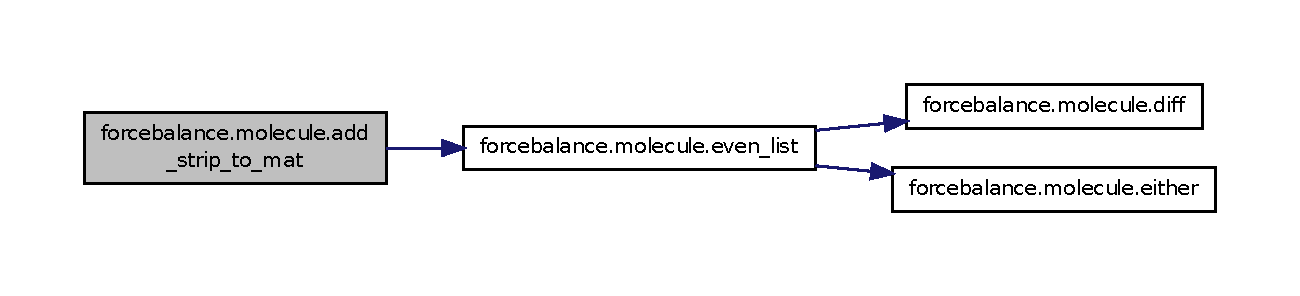
\includegraphics[width=350pt]{namespaceforcebalance_1_1molecule_a4cdb2086978b281ed84cd66179c3f5b2_cgraph}
\end{center}
\end{figure}


\hypertarget{namespaceforcebalance_1_1molecule_a9a58eb1746e51420f50da3f3a6d51485}{\index{forcebalance\-::molecule@{forcebalance\-::molecule}!Align\-To\-Density@{Align\-To\-Density}}
\index{Align\-To\-Density@{Align\-To\-Density}!forcebalance::molecule@{forcebalance\-::molecule}}
\paragraph[{Align\-To\-Density}]{\setlength{\rightskip}{0pt plus 5cm}def forcebalance.\-molecule.\-Align\-To\-Density (
\begin{DoxyParamCaption}
\item[{}]{elem, }
\item[{}]{xyz1, }
\item[{}]{xyz2, }
\item[{}]{binary = {\ttfamily False}}
\end{DoxyParamCaption}
)}}\label{namespaceforcebalance_1_1molecule_a9a58eb1746e51420f50da3f3a6d51485}


Computes a \char`\"{}overlap density\char`\"{} from two frames. 

This function can be called by Align\-To\-Moments to get rid of inversion problems 

Definition at line 541 of file molecule.\-py.



Here is the call graph for this function\-:\nopagebreak
\begin{figure}[H]
\begin{center}
\leavevmode
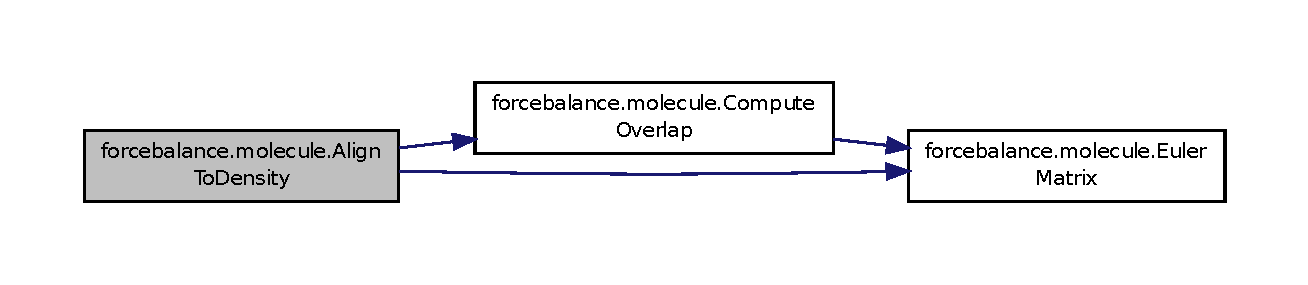
\includegraphics[width=350pt]{namespaceforcebalance_1_1molecule_a9a58eb1746e51420f50da3f3a6d51485_cgraph}
\end{center}
\end{figure}


\hypertarget{namespaceforcebalance_1_1molecule_aa9ad9b92efa7bd3c1d589d62bbb8108e}{\index{forcebalance\-::molecule@{forcebalance\-::molecule}!Align\-To\-Moments@{Align\-To\-Moments}}
\index{Align\-To\-Moments@{Align\-To\-Moments}!forcebalance::molecule@{forcebalance\-::molecule}}
\paragraph[{Align\-To\-Moments}]{\setlength{\rightskip}{0pt plus 5cm}def forcebalance.\-molecule.\-Align\-To\-Moments (
\begin{DoxyParamCaption}
\item[{}]{elem, }
\item[{}]{xyz1, }
\item[{}]{xyz2 = {\ttfamily None}}
\end{DoxyParamCaption}
)}}\label{namespaceforcebalance_1_1molecule_aa9ad9b92efa7bd3c1d589d62bbb8108e}


Pre-\/aligns molecules to 'moment of inertia'. 

If xyz2 is passed in, it will assume that xyz1 is already aligned to the moment of inertia, and it simply does 180-\/degree rotations to make sure nothing is inverted. 

Definition at line 553 of file molecule.\-py.

\hypertarget{namespaceforcebalance_1_1molecule_a5b50df23cc4d0e617fdc56538f0bea63}{\index{forcebalance\-::molecule@{forcebalance\-::molecule}!both@{both}}
\index{both@{both}!forcebalance::molecule@{forcebalance\-::molecule}}
\paragraph[{both}]{\setlength{\rightskip}{0pt plus 5cm}def forcebalance.\-molecule.\-both (
\begin{DoxyParamCaption}
\item[{}]{A, }
\item[{}]{B, }
\item[{}]{key}
\end{DoxyParamCaption}
)}}\label{namespaceforcebalance_1_1molecule_a5b50df23cc4d0e617fdc56538f0bea63}


Definition at line 476 of file molecule.\-py.

\hypertarget{namespaceforcebalance_1_1molecule_a0a6e3e79b04534bf2e83d09def189444}{\index{forcebalance\-::molecule@{forcebalance\-::molecule}!Build\-Lattice\-From\-Lengths\-Angles@{Build\-Lattice\-From\-Lengths\-Angles}}
\index{Build\-Lattice\-From\-Lengths\-Angles@{Build\-Lattice\-From\-Lengths\-Angles}!forcebalance::molecule@{forcebalance\-::molecule}}
\paragraph[{Build\-Lattice\-From\-Lengths\-Angles}]{\setlength{\rightskip}{0pt plus 5cm}def forcebalance.\-molecule.\-Build\-Lattice\-From\-Lengths\-Angles (
\begin{DoxyParamCaption}
\item[{}]{a, }
\item[{}]{b, }
\item[{}]{c, }
\item[{}]{alpha, }
\item[{}]{beta, }
\item[{}]{gamma}
\end{DoxyParamCaption}
)}}\label{namespaceforcebalance_1_1molecule_a0a6e3e79b04534bf2e83d09def189444}


This function takes in three lattice lengths and three lattice angles, and tries to return a complete box specification. 



Definition at line 258 of file molecule.\-py.



Here is the call graph for this function\-:\nopagebreak
\begin{figure}[H]
\begin{center}
\leavevmode
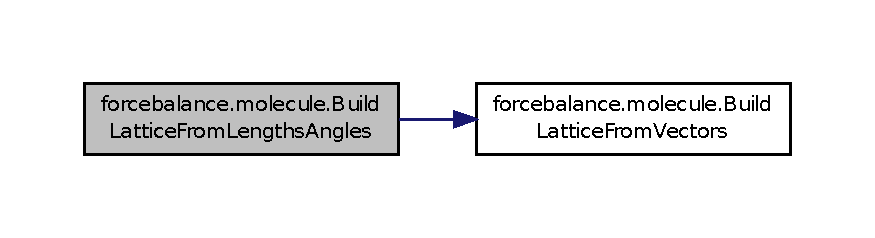
\includegraphics[width=350pt]{namespaceforcebalance_1_1molecule_a0a6e3e79b04534bf2e83d09def189444_cgraph}
\end{center}
\end{figure}


\hypertarget{namespaceforcebalance_1_1molecule_a29fb1ac9324f4280f07c65baea339989}{\index{forcebalance\-::molecule@{forcebalance\-::molecule}!Build\-Lattice\-From\-Vectors@{Build\-Lattice\-From\-Vectors}}
\index{Build\-Lattice\-From\-Vectors@{Build\-Lattice\-From\-Vectors}!forcebalance::molecule@{forcebalance\-::molecule}}
\paragraph[{Build\-Lattice\-From\-Vectors}]{\setlength{\rightskip}{0pt plus 5cm}def forcebalance.\-molecule.\-Build\-Lattice\-From\-Vectors (
\begin{DoxyParamCaption}
\item[{}]{v1, }
\item[{}]{v2, }
\item[{}]{v3}
\end{DoxyParamCaption}
)}}\label{namespaceforcebalance_1_1molecule_a29fb1ac9324f4280f07c65baea339989}


This function takes in three lattice vectors and tries to return a complete box specification. 

The hash function is something we can use to discard two things that are obviously not equal. Here we neglect the hash. Return a list of the sorted atom numbers in this graph. Return a string of atoms, which serves as a rudimentary 'fingerprint' \-: '99,100,103,151' . Return an array of the elements. For instance \mbox{[}'H' 'C' 'C' 'H'\mbox{]}. Create an Empirical Formula Get a list of the coordinates. 

Definition at line 273 of file molecule.\-py.

\hypertarget{namespaceforcebalance_1_1molecule_a8fcbb4a2b3470a85d25699b6f28a54fc}{\index{forcebalance\-::molecule@{forcebalance\-::molecule}!Compute\-Overlap@{Compute\-Overlap}}
\index{Compute\-Overlap@{Compute\-Overlap}!forcebalance::molecule@{forcebalance\-::molecule}}
\paragraph[{Compute\-Overlap}]{\setlength{\rightskip}{0pt plus 5cm}def forcebalance.\-molecule.\-Compute\-Overlap (
\begin{DoxyParamCaption}
\item[{}]{theta, }
\item[{}]{elem, }
\item[{}]{xyz1, }
\item[{}]{xyz2}
\end{DoxyParamCaption}
)}}\label{namespaceforcebalance_1_1molecule_a8fcbb4a2b3470a85d25699b6f28a54fc}


Computes an 'overlap' between two molecules based on some fictitious density. 

Good for fine-\/tuning alignment but gets stuck in local minima. 

Definition at line 524 of file molecule.\-py.



Here is the call graph for this function\-:\nopagebreak
\begin{figure}[H]
\begin{center}
\leavevmode
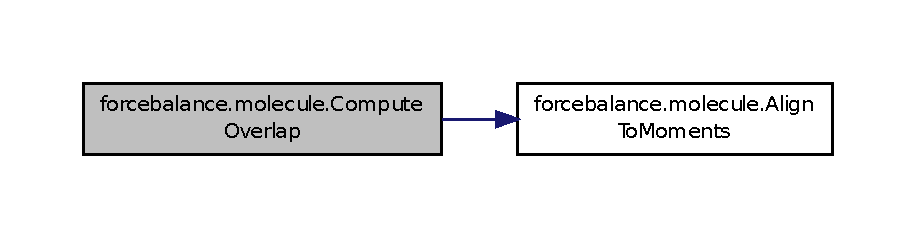
\includegraphics[width=350pt]{namespaceforcebalance_1_1molecule_a8fcbb4a2b3470a85d25699b6f28a54fc_cgraph}
\end{center}
\end{figure}


\hypertarget{namespaceforcebalance_1_1molecule_a6f7c6217b1c64da309a8abd21dfdcf08}{\index{forcebalance\-::molecule@{forcebalance\-::molecule}!diff@{diff}}
\index{diff@{diff}!forcebalance::molecule@{forcebalance\-::molecule}}
\paragraph[{diff}]{\setlength{\rightskip}{0pt plus 5cm}def forcebalance.\-molecule.\-diff (
\begin{DoxyParamCaption}
\item[{}]{A, }
\item[{}]{B, }
\item[{}]{key}
\end{DoxyParamCaption}
)}}\label{namespaceforcebalance_1_1molecule_a6f7c6217b1c64da309a8abd21dfdcf08}


Definition at line 479 of file molecule.\-py.

\hypertarget{namespaceforcebalance_1_1molecule_a75775be6563ad7f10695a9a45ff49ba9}{\index{forcebalance\-::molecule@{forcebalance\-::molecule}!either@{either}}
\index{either@{either}!forcebalance::molecule@{forcebalance\-::molecule}}
\paragraph[{either}]{\setlength{\rightskip}{0pt plus 5cm}def forcebalance.\-molecule.\-either (
\begin{DoxyParamCaption}
\item[{}]{A, }
\item[{}]{B, }
\item[{}]{key}
\end{DoxyParamCaption}
)}}\label{namespaceforcebalance_1_1molecule_a75775be6563ad7f10695a9a45ff49ba9}


Definition at line 487 of file molecule.\-py.

\hypertarget{namespaceforcebalance_1_1molecule_af02bf73765f34bbef81c4a5b000b86ce}{\index{forcebalance\-::molecule@{forcebalance\-::molecule}!Euler\-Matrix@{Euler\-Matrix}}
\index{Euler\-Matrix@{Euler\-Matrix}!forcebalance::molecule@{forcebalance\-::molecule}}
\paragraph[{Euler\-Matrix}]{\setlength{\rightskip}{0pt plus 5cm}def forcebalance.\-molecule.\-Euler\-Matrix (
\begin{DoxyParamCaption}
\item[{}]{T1, }
\item[{}]{T2, }
\item[{}]{T3}
\end{DoxyParamCaption}
)}}\label{namespaceforcebalance_1_1molecule_af02bf73765f34bbef81c4a5b000b86ce}


Constructs an Euler matrix from three Euler angles. 



Definition at line 496 of file molecule.\-py.



Here is the call graph for this function\-:\nopagebreak
\begin{figure}[H]
\begin{center}
\leavevmode
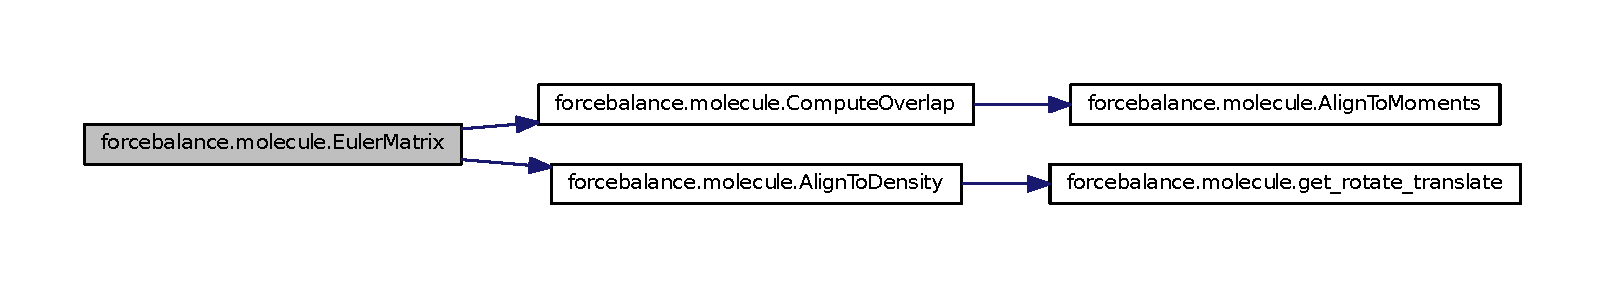
\includegraphics[width=350pt]{namespaceforcebalance_1_1molecule_af02bf73765f34bbef81c4a5b000b86ce_cgraph}
\end{center}
\end{figure}


\hypertarget{namespaceforcebalance_1_1molecule_a5f529179461765fadbd0a742cdc2c677}{\index{forcebalance\-::molecule@{forcebalance\-::molecule}!even\-\_\-list@{even\-\_\-list}}
\index{even\-\_\-list@{even\-\_\-list}!forcebalance::molecule@{forcebalance\-::molecule}}
\paragraph[{even\-\_\-list}]{\setlength{\rightskip}{0pt plus 5cm}def forcebalance.\-molecule.\-even\-\_\-list (
\begin{DoxyParamCaption}
\item[{}]{totlen, }
\item[{}]{splitsize}
\end{DoxyParamCaption}
)}}\label{namespaceforcebalance_1_1molecule_a5f529179461765fadbd0a742cdc2c677}


Creates a list of number sequences divided as evenly as possible. 



Definition at line 458 of file molecule.\-py.



Here is the call graph for this function\-:\nopagebreak
\begin{figure}[H]
\begin{center}
\leavevmode
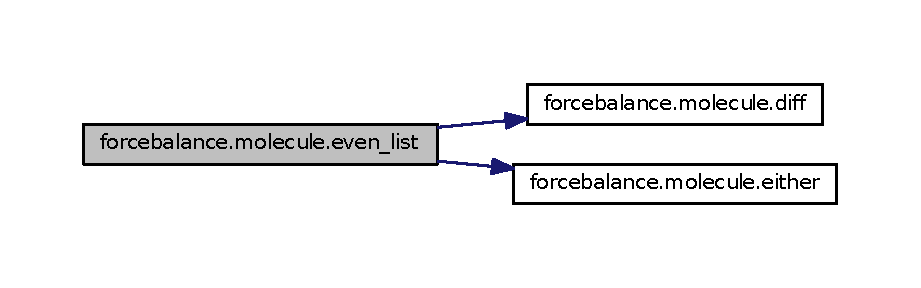
\includegraphics[width=350pt]{namespaceforcebalance_1_1molecule_a5f529179461765fadbd0a742cdc2c677_cgraph}
\end{center}
\end{figure}


\hypertarget{namespaceforcebalance_1_1molecule_ae25aa5331b3a2dd0e9d1e184380357db}{\index{forcebalance\-::molecule@{forcebalance\-::molecule}!format\-\_\-gro\-\_\-box@{format\-\_\-gro\-\_\-box}}
\index{format\-\_\-gro\-\_\-box@{format\-\_\-gro\-\_\-box}!forcebalance::molecule@{forcebalance\-::molecule}}
\paragraph[{format\-\_\-gro\-\_\-box}]{\setlength{\rightskip}{0pt plus 5cm}def forcebalance.\-molecule.\-format\-\_\-gro\-\_\-box (
\begin{DoxyParamCaption}
\item[{}]{box}
\end{DoxyParamCaption}
)}}\label{namespaceforcebalance_1_1molecule_ae25aa5331b3a2dd0e9d1e184380357db}


Print a line corresponding to the box vector in accordance with .gro file format. 


\begin{DoxyParams}[1]{Parameters}
\mbox{\tt in}  & {\em box} & Box Named\-Tuple \\
\hline
\end{DoxyParams}


Definition at line 389 of file molecule.\-py.



Here is the call graph for this function\-:\nopagebreak
\begin{figure}[H]
\begin{center}
\leavevmode
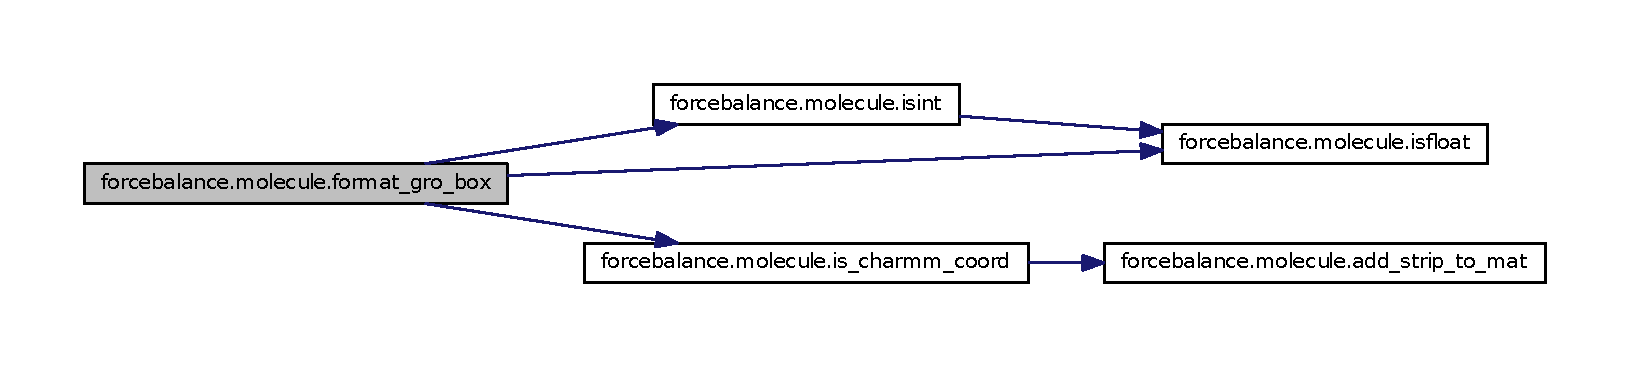
\includegraphics[width=350pt]{namespaceforcebalance_1_1molecule_ae25aa5331b3a2dd0e9d1e184380357db_cgraph}
\end{center}
\end{figure}


\hypertarget{namespaceforcebalance_1_1molecule_a41c13064e4285973aa6c49369d3d3390}{\index{forcebalance\-::molecule@{forcebalance\-::molecule}!format\-\_\-gro\-\_\-coord@{format\-\_\-gro\-\_\-coord}}
\index{format\-\_\-gro\-\_\-coord@{format\-\_\-gro\-\_\-coord}!forcebalance::molecule@{forcebalance\-::molecule}}
\paragraph[{format\-\_\-gro\-\_\-coord}]{\setlength{\rightskip}{0pt plus 5cm}def forcebalance.\-molecule.\-format\-\_\-gro\-\_\-coord (
\begin{DoxyParamCaption}
\item[{}]{resid, }
\item[{}]{resname, }
\item[{}]{aname, }
\item[{}]{seqno, }
\item[{}]{xyz}
\end{DoxyParamCaption}
)}}\label{namespaceforcebalance_1_1molecule_a41c13064e4285973aa6c49369d3d3390}


Print a line in accordance with .gro file format, with six decimal points of precision. 


\begin{DoxyParams}[1]{Parameters}
\mbox{\tt in}  & {\em resid} & The number of the residue that the atom belongs to \\
\hline
\mbox{\tt in}  & {\em resname} & The name of the residue that the atom belongs to \\
\hline
\mbox{\tt in}  & {\em aname} & The name of the atom \\
\hline
\mbox{\tt in}  & {\em seqno} & The sequential number of the atom \\
\hline
\mbox{\tt in}  & {\em xyz} & A 3-\/element array containing x, y, z coordinates of that atom \\
\hline
\end{DoxyParams}


Definition at line 368 of file molecule.\-py.



Here is the call graph for this function\-:\nopagebreak
\begin{figure}[H]
\begin{center}
\leavevmode
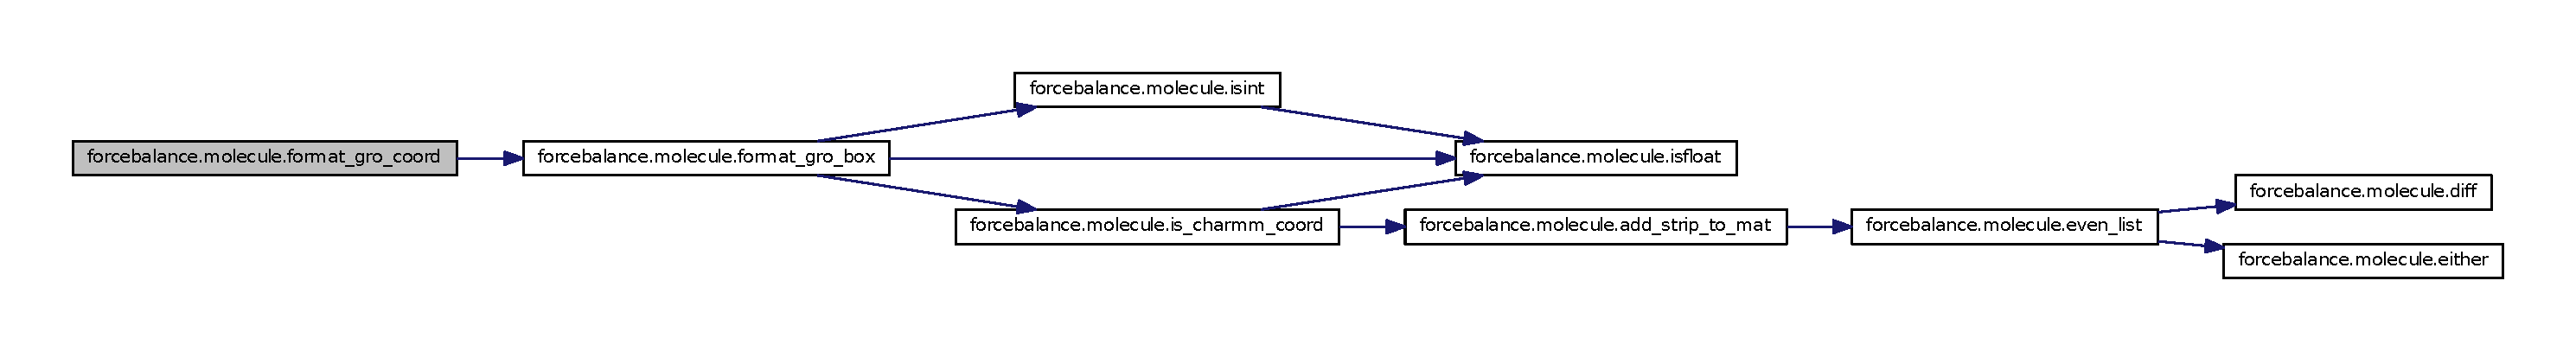
\includegraphics[width=350pt]{namespaceforcebalance_1_1molecule_a41c13064e4285973aa6c49369d3d3390_cgraph}
\end{center}
\end{figure}


\hypertarget{namespaceforcebalance_1_1molecule_a2eba3cad44138b3b10ea883240888412}{\index{forcebalance\-::molecule@{forcebalance\-::molecule}!format\-\_\-xyz\-\_\-coord@{format\-\_\-xyz\-\_\-coord}}
\index{format\-\_\-xyz\-\_\-coord@{format\-\_\-xyz\-\_\-coord}!forcebalance::molecule@{forcebalance\-::molecule}}
\paragraph[{format\-\_\-xyz\-\_\-coord}]{\setlength{\rightskip}{0pt plus 5cm}def forcebalance.\-molecule.\-format\-\_\-xyz\-\_\-coord (
\begin{DoxyParamCaption}
\item[{}]{element, }
\item[{}]{xyz, }
\item[{}]{tinker = {\ttfamily False}}
\end{DoxyParamCaption}
)}}\label{namespaceforcebalance_1_1molecule_a2eba3cad44138b3b10ea883240888412}


Print a line consisting of (element, x, y, z) in accordance with .xyz file format. 


\begin{DoxyParams}[1]{Parameters}
\mbox{\tt in}  & {\em element} & A chemical element of a single atom \\
\hline
\mbox{\tt in}  & {\em xyz} & A 3-\/element array containing x, y, z coordinates of that atom \\
\hline
\end{DoxyParams}


Definition at line 352 of file molecule.\-py.



Here is the call graph for this function\-:\nopagebreak
\begin{figure}[H]
\begin{center}
\leavevmode
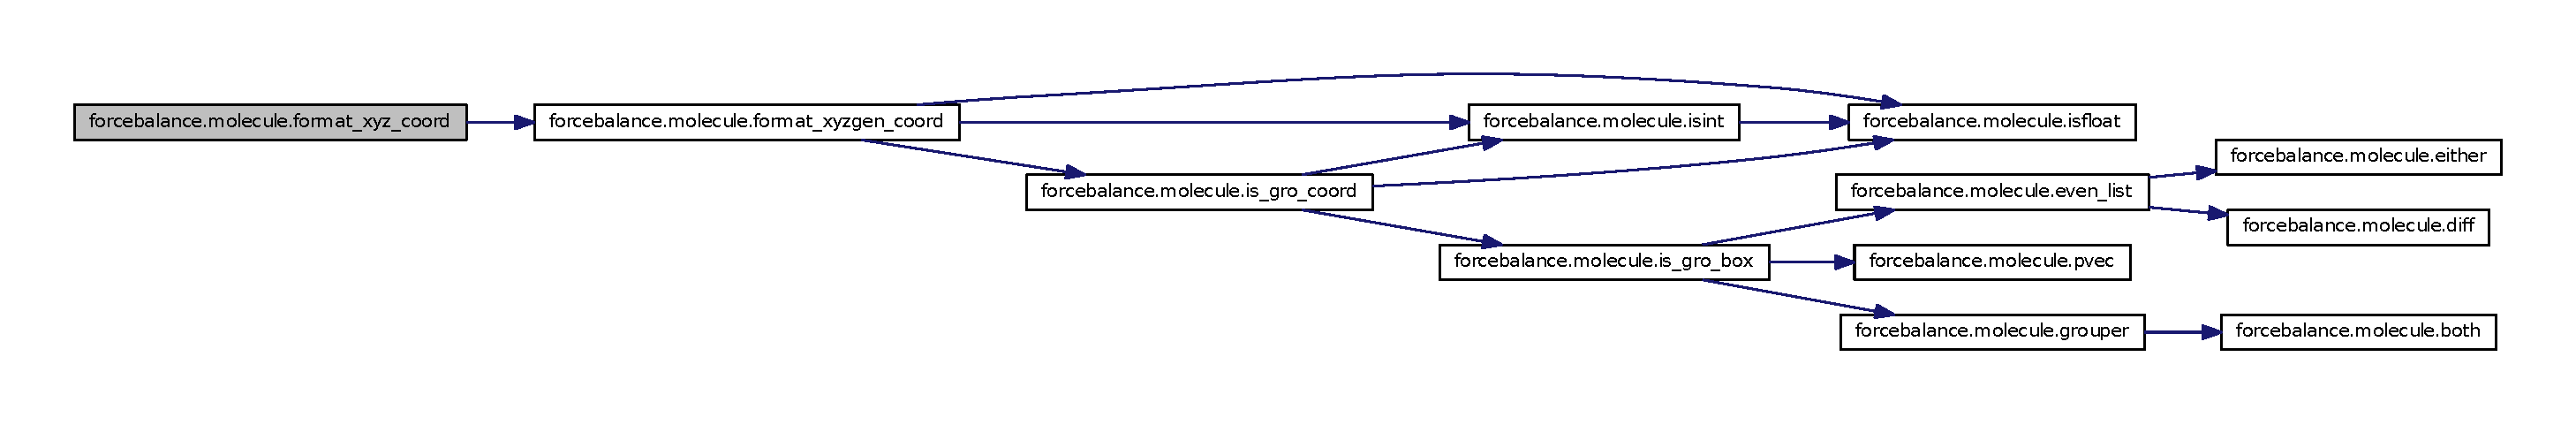
\includegraphics[width=350pt]{namespaceforcebalance_1_1molecule_a2eba3cad44138b3b10ea883240888412_cgraph}
\end{center}
\end{figure}


\hypertarget{namespaceforcebalance_1_1molecule_a4948e4662b8d2c8d515427d1bbb3d01e}{\index{forcebalance\-::molecule@{forcebalance\-::molecule}!format\-\_\-xyzgen\-\_\-coord@{format\-\_\-xyzgen\-\_\-coord}}
\index{format\-\_\-xyzgen\-\_\-coord@{format\-\_\-xyzgen\-\_\-coord}!forcebalance::molecule@{forcebalance\-::molecule}}
\paragraph[{format\-\_\-xyzgen\-\_\-coord}]{\setlength{\rightskip}{0pt plus 5cm}def forcebalance.\-molecule.\-format\-\_\-xyzgen\-\_\-coord (
\begin{DoxyParamCaption}
\item[{}]{element, }
\item[{}]{xyzgen}
\end{DoxyParamCaption}
)}}\label{namespaceforcebalance_1_1molecule_a4948e4662b8d2c8d515427d1bbb3d01e}


Print a line consisting of (element, p, q, r, s, t, ...) where (p, q, r) are arbitrary atom-\/wise data (this might happen, for instance, with atomic charges) 


\begin{DoxyParams}[1]{Parameters}
\mbox{\tt in}  & {\em element} & A chemical element of a single atom \\
\hline
\mbox{\tt in}  & {\em xyzgen} & A N-\/element array containing data for that atom \\
\hline
\end{DoxyParams}


Definition at line 380 of file molecule.\-py.



Here is the call graph for this function\-:\nopagebreak
\begin{figure}[H]
\begin{center}
\leavevmode
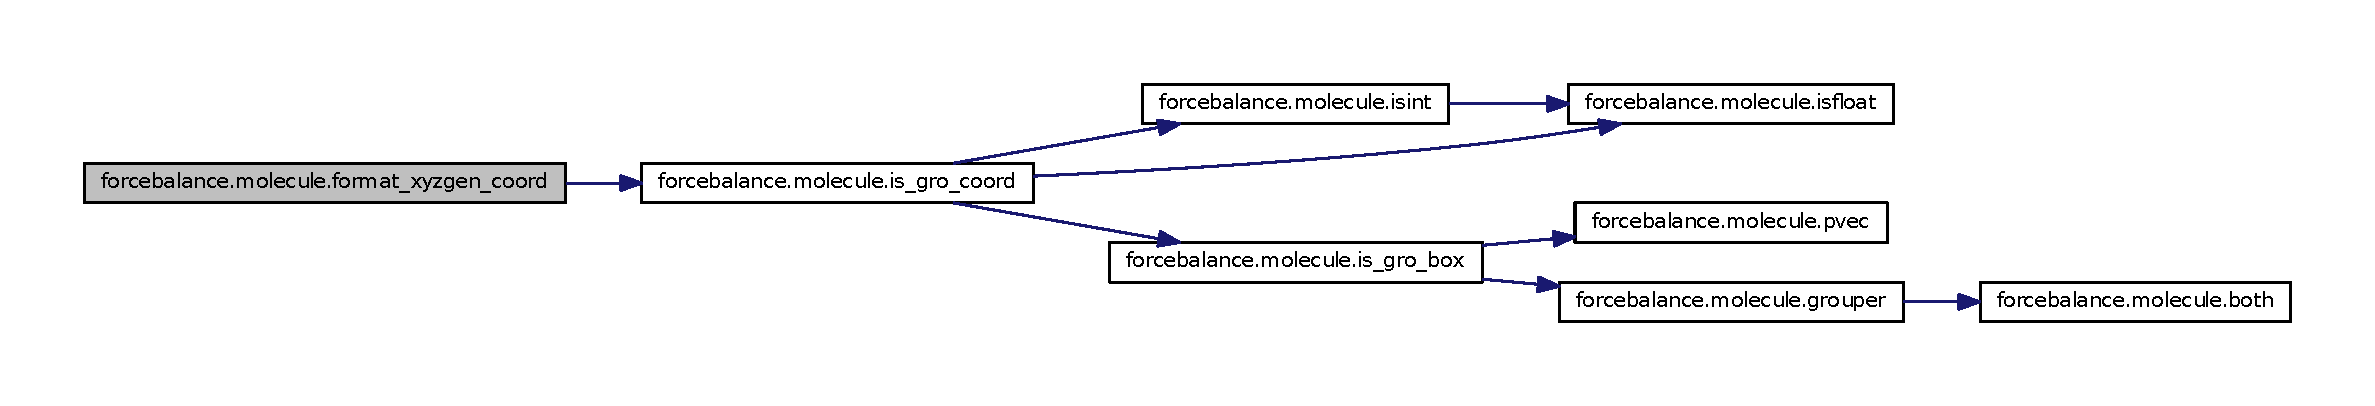
\includegraphics[width=350pt]{namespaceforcebalance_1_1molecule_a4948e4662b8d2c8d515427d1bbb3d01e_cgraph}
\end{center}
\end{figure}


\hypertarget{namespaceforcebalance_1_1molecule_a08840b73e95bf34bf9ca7ea36ad0492d}{\index{forcebalance\-::molecule@{forcebalance\-::molecule}!get\-\_\-rotate\-\_\-translate@{get\-\_\-rotate\-\_\-translate}}
\index{get\-\_\-rotate\-\_\-translate@{get\-\_\-rotate\-\_\-translate}!forcebalance::molecule@{forcebalance\-::molecule}}
\paragraph[{get\-\_\-rotate\-\_\-translate}]{\setlength{\rightskip}{0pt plus 5cm}def forcebalance.\-molecule.\-get\-\_\-rotate\-\_\-translate (
\begin{DoxyParamCaption}
\item[{}]{matrix1, }
\item[{}]{matrix2}
\end{DoxyParamCaption}
)}}\label{namespaceforcebalance_1_1molecule_a08840b73e95bf34bf9ca7ea36ad0492d}


Definition at line 576 of file molecule.\-py.

\hypertarget{namespaceforcebalance_1_1molecule_af28de4693e5b8e82df900d0ac3c6c370}{\index{forcebalance\-::molecule@{forcebalance\-::molecule}!get\-Element@{get\-Element}}
\index{get\-Element@{get\-Element}!forcebalance::molecule@{forcebalance\-::molecule}}
\paragraph[{get\-Element}]{\setlength{\rightskip}{0pt plus 5cm}def forcebalance.\-molecule.\-get\-Element (
\begin{DoxyParamCaption}
\item[{}]{mass}
\end{DoxyParamCaption}
)}}\label{namespaceforcebalance_1_1molecule_af28de4693e5b8e82df900d0ac3c6c370}


Definition at line 191 of file molecule.\-py.

\hypertarget{namespaceforcebalance_1_1molecule_a7fe52c2928c7b0329882541bef2e34cd}{\index{forcebalance\-::molecule@{forcebalance\-::molecule}!grouper@{grouper}}
\index{grouper@{grouper}!forcebalance::molecule@{forcebalance\-::molecule}}
\paragraph[{grouper}]{\setlength{\rightskip}{0pt plus 5cm}def forcebalance.\-molecule.\-grouper (
\begin{DoxyParamCaption}
\item[{}]{n, }
\item[{}]{iterable}
\end{DoxyParamCaption}
)}}\label{namespaceforcebalance_1_1molecule_a7fe52c2928c7b0329882541bef2e34cd}


Groups a big long iterable into groups of ten or what have you. 



Definition at line 452 of file molecule.\-py.



Here is the call graph for this function\-:\nopagebreak
\begin{figure}[H]
\begin{center}
\leavevmode
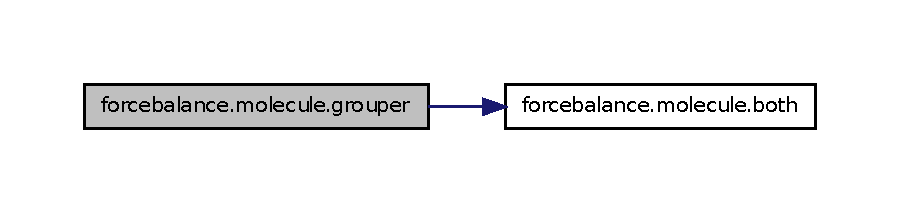
\includegraphics[width=350pt]{namespaceforcebalance_1_1molecule_a7fe52c2928c7b0329882541bef2e34cd_cgraph}
\end{center}
\end{figure}


\hypertarget{namespaceforcebalance_1_1molecule_a838d85848bd817e801d0f5f6502217ef}{\index{forcebalance\-::molecule@{forcebalance\-::molecule}!is\-\_\-charmm\-\_\-coord@{is\-\_\-charmm\-\_\-coord}}
\index{is\-\_\-charmm\-\_\-coord@{is\-\_\-charmm\-\_\-coord}!forcebalance::molecule@{forcebalance\-::molecule}}
\paragraph[{is\-\_\-charmm\-\_\-coord}]{\setlength{\rightskip}{0pt plus 5cm}def forcebalance.\-molecule.\-is\-\_\-charmm\-\_\-coord (
\begin{DoxyParamCaption}
\item[{}]{line}
\end{DoxyParamCaption}
)}}\label{namespaceforcebalance_1_1molecule_a838d85848bd817e801d0f5f6502217ef}


Determines whether a line contains C\-H\-A\-R\-M\-M data or not. 


\begin{DoxyParams}[1]{Parameters}
\mbox{\tt in}  & {\em line} & The line to be tested \\
\hline
\end{DoxyParams}


Definition at line 416 of file molecule.\-py.



Here is the call graph for this function\-:\nopagebreak
\begin{figure}[H]
\begin{center}
\leavevmode
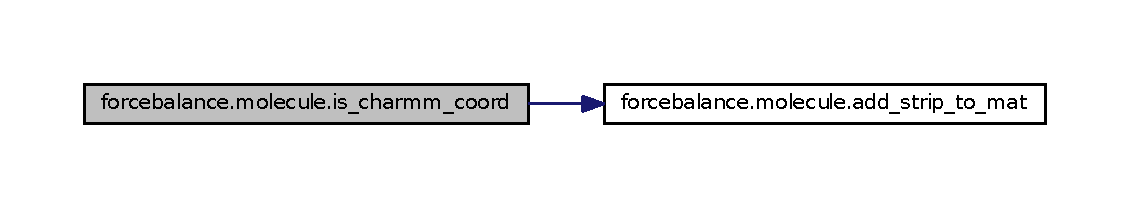
\includegraphics[width=350pt]{namespaceforcebalance_1_1molecule_a838d85848bd817e801d0f5f6502217ef_cgraph}
\end{center}
\end{figure}


\hypertarget{namespaceforcebalance_1_1molecule_aafc8c924eed4480fed8ddc9c474d3bc1}{\index{forcebalance\-::molecule@{forcebalance\-::molecule}!is\-\_\-gro\-\_\-box@{is\-\_\-gro\-\_\-box}}
\index{is\-\_\-gro\-\_\-box@{is\-\_\-gro\-\_\-box}!forcebalance::molecule@{forcebalance\-::molecule}}
\paragraph[{is\-\_\-gro\-\_\-box}]{\setlength{\rightskip}{0pt plus 5cm}def forcebalance.\-molecule.\-is\-\_\-gro\-\_\-box (
\begin{DoxyParamCaption}
\item[{}]{line}
\end{DoxyParamCaption}
)}}\label{namespaceforcebalance_1_1molecule_aafc8c924eed4480fed8ddc9c474d3bc1}


Determines whether a line contains a G\-R\-O\-M\-A\-C\-S box vector or not. 


\begin{DoxyParams}[1]{Parameters}
\mbox{\tt in}  & {\em line} & The line to be tested \\
\hline
\end{DoxyParams}


Definition at line 429 of file molecule.\-py.



Here is the call graph for this function\-:\nopagebreak
\begin{figure}[H]
\begin{center}
\leavevmode
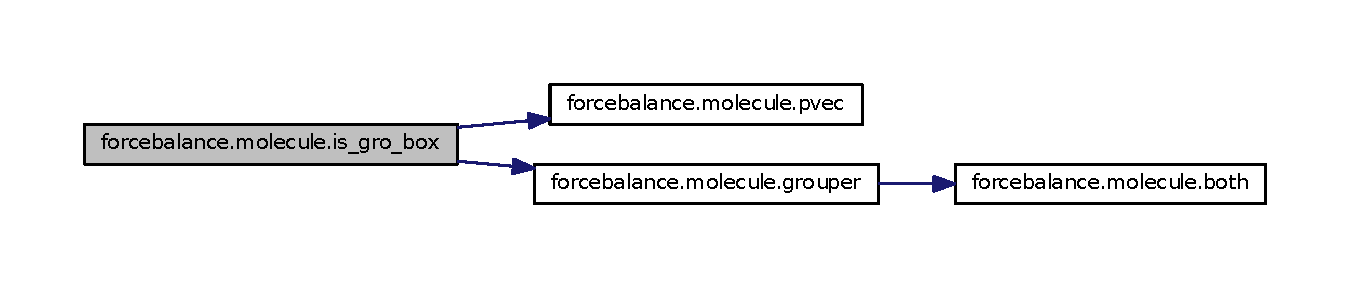
\includegraphics[width=350pt]{namespaceforcebalance_1_1molecule_aafc8c924eed4480fed8ddc9c474d3bc1_cgraph}
\end{center}
\end{figure}


\hypertarget{namespaceforcebalance_1_1molecule_a12b7bb398c2fa49a223f258ec7737483}{\index{forcebalance\-::molecule@{forcebalance\-::molecule}!is\-\_\-gro\-\_\-coord@{is\-\_\-gro\-\_\-coord}}
\index{is\-\_\-gro\-\_\-coord@{is\-\_\-gro\-\_\-coord}!forcebalance::molecule@{forcebalance\-::molecule}}
\paragraph[{is\-\_\-gro\-\_\-coord}]{\setlength{\rightskip}{0pt plus 5cm}def forcebalance.\-molecule.\-is\-\_\-gro\-\_\-coord (
\begin{DoxyParamCaption}
\item[{}]{line}
\end{DoxyParamCaption}
)}}\label{namespaceforcebalance_1_1molecule_a12b7bb398c2fa49a223f258ec7737483}


Determines whether a line contains G\-R\-O\-M\-A\-C\-S data or not. 


\begin{DoxyParams}[1]{Parameters}
\mbox{\tt in}  & {\em line} & The line to be tested \\
\hline
\end{DoxyParams}


Definition at line 401 of file molecule.\-py.



Here is the call graph for this function\-:\nopagebreak
\begin{figure}[H]
\begin{center}
\leavevmode
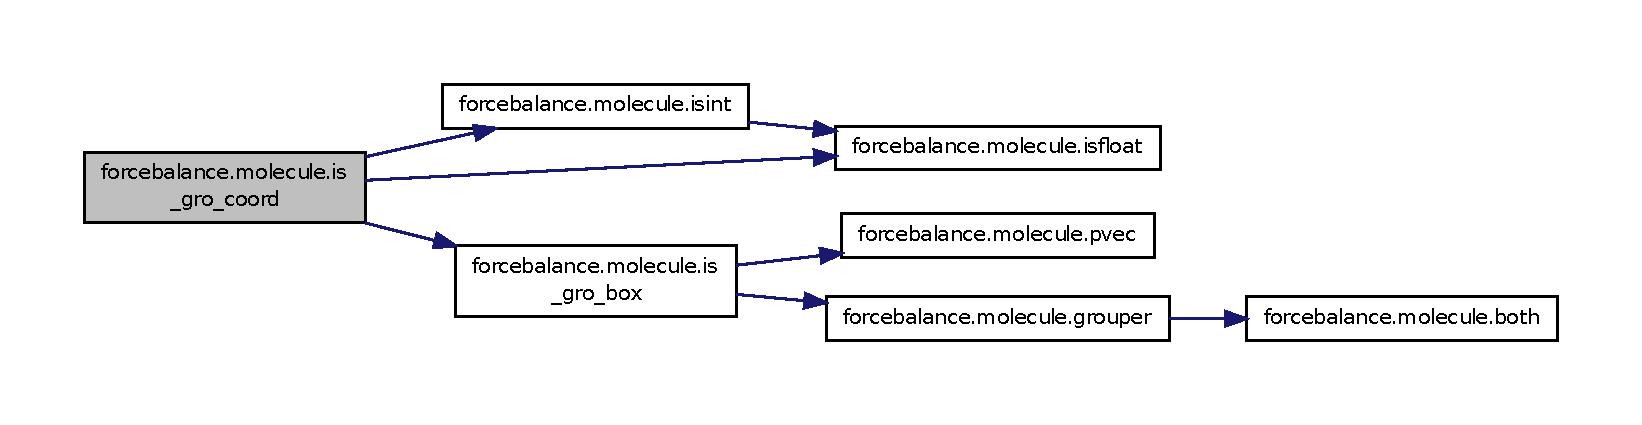
\includegraphics[width=350pt]{namespaceforcebalance_1_1molecule_a12b7bb398c2fa49a223f258ec7737483_cgraph}
\end{center}
\end{figure}


\hypertarget{namespaceforcebalance_1_1molecule_afe989ffd119568047fc8265b1d329a70}{\index{forcebalance\-::molecule@{forcebalance\-::molecule}!isfloat@{isfloat}}
\index{isfloat@{isfloat}!forcebalance::molecule@{forcebalance\-::molecule}}
\paragraph[{isfloat}]{\setlength{\rightskip}{0pt plus 5cm}def forcebalance.\-molecule.\-isfloat (
\begin{DoxyParamCaption}
\item[{}]{word}
\end{DoxyParamCaption}
)}}\label{namespaceforcebalance_1_1molecule_afe989ffd119568047fc8265b1d329a70}


Matches A\-N\-Y number; it can be a decimal, scientific notation, integer, or what have you. 



Definition at line 247 of file molecule.\-py.

\hypertarget{namespaceforcebalance_1_1molecule_a0dd31eff88d2bed0884ab21a13261d42}{\index{forcebalance\-::molecule@{forcebalance\-::molecule}!isint@{isint}}
\index{isint@{isint}!forcebalance::molecule@{forcebalance\-::molecule}}
\paragraph[{isint}]{\setlength{\rightskip}{0pt plus 5cm}def forcebalance.\-molecule.\-isint (
\begin{DoxyParamCaption}
\item[{}]{word}
\end{DoxyParamCaption}
)}}\label{namespaceforcebalance_1_1molecule_a0dd31eff88d2bed0884ab21a13261d42}


O\-N\-L\-Y matches integers! If you have a decimal point? None shall pass! 



Definition at line 242 of file molecule.\-py.



Here is the call graph for this function\-:\nopagebreak
\begin{figure}[H]
\begin{center}
\leavevmode
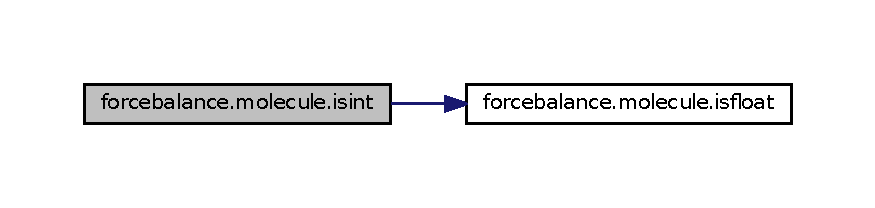
\includegraphics[width=350pt]{namespaceforcebalance_1_1molecule_a0dd31eff88d2bed0884ab21a13261d42_cgraph}
\end{center}
\end{figure}


\hypertarget{namespaceforcebalance_1_1molecule_ab9cb167fbbd809aedcf8c7434d405547}{\index{forcebalance\-::molecule@{forcebalance\-::molecule}!main@{main}}
\index{main@{main}!forcebalance::molecule@{forcebalance\-::molecule}}
\paragraph[{main}]{\setlength{\rightskip}{0pt plus 5cm}def forcebalance.\-molecule.\-main (
\begin{DoxyParamCaption}
{}
\end{DoxyParamCaption}
)}}\label{namespaceforcebalance_1_1molecule_ab9cb167fbbd809aedcf8c7434d405547}


Definition at line 2489 of file molecule.\-py.

\hypertarget{namespaceforcebalance_1_1molecule_ab8464fea13fad2a506792c2f1d7c93f3}{\index{forcebalance\-::molecule@{forcebalance\-::molecule}!nodematch@{nodematch}}
\index{nodematch@{nodematch}!forcebalance::molecule@{forcebalance\-::molecule}}
\paragraph[{nodematch}]{\setlength{\rightskip}{0pt plus 5cm}def forcebalance.\-molecule.\-nodematch (
\begin{DoxyParamCaption}
\item[{}]{node1, }
\item[{}]{node2}
\end{DoxyParamCaption}
)}}\label{namespaceforcebalance_1_1molecule_ab8464fea13fad2a506792c2f1d7c93f3}


Definition at line 236 of file molecule.\-py.



Here is the call graph for this function\-:\nopagebreak
\begin{figure}[H]
\begin{center}
\leavevmode
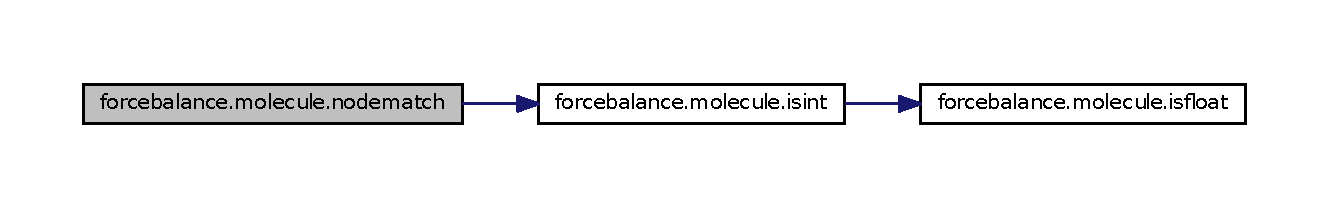
\includegraphics[width=350pt]{namespaceforcebalance_1_1molecule_ab8464fea13fad2a506792c2f1d7c93f3_cgraph}
\end{center}
\end{figure}


\hypertarget{namespaceforcebalance_1_1molecule_a58c3f09152db4d1c6e1db9df29c60c43}{\index{forcebalance\-::molecule@{forcebalance\-::molecule}!pvec@{pvec}}
\index{pvec@{pvec}!forcebalance::molecule@{forcebalance\-::molecule}}
\paragraph[{pvec}]{\setlength{\rightskip}{0pt plus 5cm}def forcebalance.\-molecule.\-pvec (
\begin{DoxyParamCaption}
\item[{}]{vec}
\end{DoxyParamCaption}
)}}\label{namespaceforcebalance_1_1molecule_a58c3f09152db4d1c6e1db9df29c60c43}


Definition at line 447 of file molecule.\-py.



\subsubsection{Variable Documentation}
\hypertarget{namespaceforcebalance_1_1molecule_a2986996d4f957928047df06fbec3717d}{\index{forcebalance\-::molecule@{forcebalance\-::molecule}!Alive@{Alive}}
\index{Alive@{Alive}!forcebalance::molecule@{forcebalance\-::molecule}}
\paragraph[{Alive}]{\setlength{\rightskip}{0pt plus 5cm}forcebalance.\-molecule.\-Alive}}\label{namespaceforcebalance_1_1molecule_a2986996d4f957928047df06fbec3717d}


Definition at line 302 of file molecule.\-py.

\hypertarget{namespaceforcebalance_1_1molecule_a8fcfb88fe12a9256b61980f3d4fe3b63}{\index{forcebalance\-::molecule@{forcebalance\-::molecule}!All\-Variable\-Names@{All\-Variable\-Names}}
\index{All\-Variable\-Names@{All\-Variable\-Names}!forcebalance::molecule@{forcebalance\-::molecule}}
\paragraph[{All\-Variable\-Names}]{\setlength{\rightskip}{0pt plus 5cm}forcebalance.\-molecule.\-All\-Variable\-Names = {\bf Quantum\-Variable\-Names}$|${\bf Atom\-Variable\-Names}$|${\bf Meta\-Variable\-Names}$|${\bf Frame\-Variable\-Names}}}\label{namespaceforcebalance_1_1molecule_a8fcfb88fe12a9256b61980f3d4fe3b63}


Definition at line 139 of file molecule.\-py.

\hypertarget{namespaceforcebalance_1_1molecule_a5daa68e835dcb9877d6c3f2fb559b54b}{\index{forcebalance\-::molecule@{forcebalance\-::molecule}!Atom\-Variable\-Names@{Atom\-Variable\-Names}}
\index{Atom\-Variable\-Names@{Atom\-Variable\-Names}!forcebalance::molecule@{forcebalance\-::molecule}}
\paragraph[{Atom\-Variable\-Names}]{\setlength{\rightskip}{0pt plus 5cm}tuple forcebalance.\-molecule.\-Atom\-Variable\-Names = set(\mbox{[}'elem', 'partial\-\_\-charge', 'atomname', 'atomtype', 'tinkersuf', 'resid', 'resname', 'qcsuf', 'qm\-\_\-ghost', 'chain', 'altloc', 'icode'\mbox{]})}}\label{namespaceforcebalance_1_1molecule_a5daa68e835dcb9877d6c3f2fb559b54b}


Definition at line 122 of file molecule.\-py.

\hypertarget{namespaceforcebalance_1_1molecule_a76af9edfbaaa8999680e32aafe1b1b61}{\index{forcebalance\-::molecule@{forcebalance\-::molecule}!bohrang@{bohrang}}
\index{bohrang@{bohrang}!forcebalance::molecule@{forcebalance\-::molecule}}
\paragraph[{bohrang}]{\setlength{\rightskip}{0pt plus 5cm}float forcebalance.\-molecule.\-bohrang = 0.\-529177249}}\label{namespaceforcebalance_1_1molecule_a76af9edfbaaa8999680e32aafe1b1b61}


One bohr equals this many angstroms. 



Definition at line 234 of file molecule.\-py.

\hypertarget{namespaceforcebalance_1_1molecule_aa761cf1cf260e15d0b03a6f61569c840}{\index{forcebalance\-::molecule@{forcebalance\-::molecule}!Box@{Box}}
\index{Box@{Box}!forcebalance::molecule@{forcebalance\-::molecule}}
\paragraph[{Box}]{\setlength{\rightskip}{0pt plus 5cm}tuple forcebalance.\-molecule.\-Box = namedtuple('Box',\mbox{[}'a','b','c','alpha','beta','gamma','A','B','C','V'\mbox{]})}}\label{namespaceforcebalance_1_1molecule_aa761cf1cf260e15d0b03a6f61569c840}


Definition at line 254 of file molecule.\-py.

\hypertarget{namespaceforcebalance_1_1molecule_a1c99a11e8a749468698c9af6361a8a4c}{\index{forcebalance\-::molecule@{forcebalance\-::molecule}!Elements@{Elements}}
\index{Elements@{Elements}!forcebalance::molecule@{forcebalance\-::molecule}}
\paragraph[{Elements}]{\setlength{\rightskip}{0pt plus 5cm}list forcebalance.\-molecule.\-Elements}}\label{namespaceforcebalance_1_1molecule_a1c99a11e8a749468698c9af6361a8a4c}
{\bfseries Initial value\-:}
\begin{DoxyCode}
1 = [\textcolor{stringliteral}{"None"},\textcolor{stringliteral}{'H'},\textcolor{stringliteral}{'He'},
2             \textcolor{stringliteral}{'Li'},\textcolor{stringliteral}{'Be'},\textcolor{stringliteral}{'B'},\textcolor{stringliteral}{'C'},\textcolor{stringliteral}{'N'},\textcolor{stringliteral}{'O'},\textcolor{stringliteral}{'F'},\textcolor{stringliteral}{'Ne'},
3             \textcolor{stringliteral}{'Na'},\textcolor{stringliteral}{'Mg'},\textcolor{stringliteral}{'Al'},\textcolor{stringliteral}{'Si'},\textcolor{stringliteral}{'P'},\textcolor{stringliteral}{'S'},\textcolor{stringliteral}{'Cl'},\textcolor{stringliteral}{'Ar'},
4             \textcolor{stringliteral}{'K'},\textcolor{stringliteral}{'Ca'},\textcolor{stringliteral}{'Sc'},\textcolor{stringliteral}{'Ti'},\textcolor{stringliteral}{'V'},\textcolor{stringliteral}{'Cr'},\textcolor{stringliteral}{'Mn'},\textcolor{stringliteral}{'Fe'},\textcolor{stringliteral}{'Co'},\textcolor{stringliteral}{'Ni'},\textcolor{stringliteral}{'Cu'},\textcolor{stringliteral}{'Zn'},\textcolor{stringliteral}{'Ga'},\textcolor{stringliteral}{'Ge'},\textcolor{stringliteral}{'As'},\textcolor{stringliteral}{'Se'},\textcolor{stringliteral}{'Br'},\textcolor{stringliteral}{'Kr'},
5             \textcolor{stringliteral}{'Rb'},\textcolor{stringliteral}{'Sr'},\textcolor{stringliteral}{'Y'},\textcolor{stringliteral}{'Zr'},\textcolor{stringliteral}{'Nb'},\textcolor{stringliteral}{'Mo'},\textcolor{stringliteral}{'Tc'},\textcolor{stringliteral}{'Ru'},\textcolor{stringliteral}{'Rh'},\textcolor{stringliteral}{'Pd'},\textcolor{stringliteral}{'Ag'},\textcolor{stringliteral}{'Cd'},\textcolor{stringliteral}{'In'},\textcolor{stringliteral}{'Sn'},\textcolor{stringliteral}{'Sb'},\textcolor{stringliteral}{'Te'},\textcolor{stringliteral}{'I'},\textcolor{stringliteral}{'Xe'},
6             \textcolor{stringliteral}{'Cs'},\textcolor{stringliteral}{'Ba'},\textcolor{stringliteral}{'La'},\textcolor{stringliteral}{'Ce'},\textcolor{stringliteral}{'Pr'},\textcolor{stringliteral}{'Nd'},\textcolor{stringliteral}{'Pm'},\textcolor{stringliteral}{'Sm'},\textcolor{stringliteral}{'Eu'},\textcolor{stringliteral}{'Gd'},\textcolor{stringliteral}{'Tb'},\textcolor{stringliteral}{'Dy'},\textcolor{stringliteral}{'Ho'},\textcolor{stringliteral}{'Er'},\textcolor{stringliteral}{'Tm'},\textcolor{stringliteral}{'Yb'},
7             \textcolor{stringliteral}{'Lu'},\textcolor{stringliteral}{'Hf'},\textcolor{stringliteral}{'Ta'},\textcolor{stringliteral}{'W'},\textcolor{stringliteral}{'Re'},\textcolor{stringliteral}{'Os'},\textcolor{stringliteral}{'Ir'},\textcolor{stringliteral}{'Pt'},\textcolor{stringliteral}{'Au'},\textcolor{stringliteral}{'Hg'},\textcolor{stringliteral}{'Tl'},\textcolor{stringliteral}{'Pb'},\textcolor{stringliteral}{'Bi'},\textcolor{stringliteral}{'Po'},\textcolor{stringliteral}{'At'},\textcolor{stringliteral}{'Rn'},
8             \textcolor{stringliteral}{'Fr'},\textcolor{stringliteral}{'Ra'},\textcolor{stringliteral}{'Ac'},\textcolor{stringliteral}{'Th'},\textcolor{stringliteral}{'Pa'},\textcolor{stringliteral}{'}\textcolor{stringliteral}{U','}Np','Pu','Am','Cm','Bk','Cf','Es','Fm','Md','No','Lr','Rf','Db','
      Sg','Bh','Hs','Mt']
\end{DoxyCode}


Definition at line 166 of file molecule.\-py.

\hypertarget{namespaceforcebalance_1_1molecule_a0044fa397e0923635a8b3e9625aa70f7}{\index{forcebalance\-::molecule@{forcebalance\-::molecule}!Frame\-Variable\-Names@{Frame\-Variable\-Names}}
\index{Frame\-Variable\-Names@{Frame\-Variable\-Names}!forcebalance::molecule@{forcebalance\-::molecule}}
\paragraph[{Frame\-Variable\-Names}]{\setlength{\rightskip}{0pt plus 5cm}tuple forcebalance.\-molecule.\-Frame\-Variable\-Names}}\label{namespaceforcebalance_1_1molecule_a0044fa397e0923635a8b3e9625aa70f7}
{\bfseries Initial value\-:}
\begin{DoxyCode}
1 = set([\textcolor{stringliteral}{'xyzs'}, \textcolor{stringliteral}{'comms'}, \textcolor{stringliteral}{'boxes'}, \textcolor{stringliteral}{'qm\_forces'}, \textcolor{stringliteral}{'qm\_energies'}, \textcolor{stringliteral}{'qm\_interaction'}, 
2                           \textcolor{stringliteral}{'qm\_espxyzs'}, \textcolor{stringliteral}{'qm\_espvals'}, \textcolor{stringliteral}{'qm\_extchgs'}, \textcolor{stringliteral}{'qm\_mulliken\_charges'}, \textcolor{stringliteral}{'
      qm\_mulliken\_spins'}])
\end{DoxyCode}


Definition at line 108 of file molecule.\-py.

\hypertarget{namespaceforcebalance_1_1molecule_a38e1c99e9567fe42b792af43db9b7488}{\index{forcebalance\-::molecule@{forcebalance\-::molecule}!Meta\-Variable\-Names@{Meta\-Variable\-Names}}
\index{Meta\-Variable\-Names@{Meta\-Variable\-Names}!forcebalance::molecule@{forcebalance\-::molecule}}
\paragraph[{Meta\-Variable\-Names}]{\setlength{\rightskip}{0pt plus 5cm}tuple forcebalance.\-molecule.\-Meta\-Variable\-Names = set(\mbox{[}'fnm', 'ftype', 'qcrems', 'qctemplate', 'charge', 'mult', 'bonds'\mbox{]})}}\label{namespaceforcebalance_1_1molecule_a38e1c99e9567fe42b792af43db9b7488}


Definition at line 135 of file molecule.\-py.

\hypertarget{namespaceforcebalance_1_1molecule_adc5040ec456762f2ac240fb08febbfdd}{\index{forcebalance\-::molecule@{forcebalance\-::molecule}!Periodic\-Table@{Periodic\-Table}}
\index{Periodic\-Table@{Periodic\-Table}!forcebalance::molecule@{forcebalance\-::molecule}}
\paragraph[{Periodic\-Table}]{\setlength{\rightskip}{0pt plus 5cm}tuple forcebalance.\-molecule.\-Periodic\-Table}}\label{namespaceforcebalance_1_1molecule_adc5040ec456762f2ac240fb08febbfdd}
{\bfseries Initial value\-:}
\begin{DoxyCode}
1 = OrderedDict([(\textcolor{stringliteral}{'H'} , 1.0079), (\textcolor{stringliteral}{'He'} , 4.0026), 
2                              (\textcolor{stringliteral}{'Li'} , 6.941), (\textcolor{stringliteral}{'Be'} , 9.0122), (\textcolor{stringliteral}{'B'} , 10.811), (\textcolor{stringliteral}{'C'} , 12.0107), (\textcolor{stringliteral}{'N'} , 14.00
      67), (\textcolor{stringliteral}{'O'} , 15.9994), (\textcolor{stringliteral}{'F'} , 18.9984), (\textcolor{stringliteral}{'Ne'} , 20.1797),
3                              (\textcolor{stringliteral}{'Na'} , 22.9897), (\textcolor{stringliteral}{'Mg'} , 24.305), (\textcolor{stringliteral}{'Al'} , 26.9815), (\textcolor{stringliteral}{'Si'} , 28.0855), (\textcolor{stringliteral}{'P'} , 
      30.9738), (\textcolor{stringliteral}{'S'} , 32.065), (\textcolor{stringliteral}{'Cl'} , 35.453), (\textcolor{stringliteral}{'Ar'} , 39.948), 
4                              (\textcolor{stringliteral}{'K'} , 39.0983), (\textcolor{stringliteral}{'Ca'} , 40.078), (\textcolor{stringliteral}{'Sc'} , 44.9559), (\textcolor{stringliteral}{'Ti'} , 47.867), (\textcolor{stringliteral}{'V'} , 50
      .9415), (\textcolor{stringliteral}{'Cr'} , 51.9961), (\textcolor{stringliteral}{'Mn'} , 54.938), (\textcolor{stringliteral}{'Fe'} , 55.845), (\textcolor{stringliteral}{'Co'} , 58.9332), 
5                              (\textcolor{stringliteral}{'Ni'} , 58.6934), (\textcolor{stringliteral}{'Cu'} , 63.546), (\textcolor{stringliteral}{'Zn'} , 65.39), (\textcolor{stringliteral}{'Ga'} , 69.723), (\textcolor{stringliteral}{'Ge'} , 72
      .64), (\textcolor{stringliteral}{'As'} , 74.9216), (\textcolor{stringliteral}{'Se'} , 78.96), (\textcolor{stringliteral}{'Br'} , 79.904), (\textcolor{stringliteral}{'Kr'} , 83.8), 
6                              (\textcolor{stringliteral}{'Rb'} , 85.4678), (\textcolor{stringliteral}{'Sr'} , 87.62), (\textcolor{stringliteral}{'Y'} , 88.9059), (\textcolor{stringliteral}{'Zr'} , 91.224), (\textcolor{stringliteral}{'Nb'} , 92
      .9064), (\textcolor{stringliteral}{'Mo'} , 95.94), (\textcolor{stringliteral}{'Tc'} , 98), (\textcolor{stringliteral}{'Ru'} , 101.07), (\textcolor{stringliteral}{'Rh'} , 102.9055), 
7                              (\textcolor{stringliteral}{'Pd'} , 106.42), (\textcolor{stringliteral}{'Ag'} , 107.8682), (\textcolor{stringliteral}{'Cd'} , 112.411), (\textcolor{stringliteral}{'In'} , 114.818), (\textcolor{stringliteral}{'Sn'} 
      , 118.71), (\textcolor{stringliteral}{'Sb'} , 121.76), (\textcolor{stringliteral}{'Te'} , 127.6), (\textcolor{stringliteral}{'I'} , 126.9045), (\textcolor{stringliteral}{'Xe'} , 131.293), 
8                              (\textcolor{stringliteral}{'Cs'} , 132.9055), (\textcolor{stringliteral}{'Ba'} , 137.327), (\textcolor{stringliteral}{'La'} , 138.9055), (\textcolor{stringliteral}{'Ce'} , 140.116), (\textcolor{stringliteral}{'Pr
      '} , 140.9077), (\textcolor{stringliteral}{'Nd'} , 144.24), (\textcolor{stringliteral}{'Pm'} , 145), (\textcolor{stringliteral}{'Sm'} , 150.36), 
9                              (\textcolor{stringliteral}{'Eu'} , 151.964), (\textcolor{stringliteral}{'Gd'} , 157.25), (\textcolor{stringliteral}{'Tb'} , 158.9253), (\textcolor{stringliteral}{'Dy'} , 162.5), (\textcolor{stringliteral}{'Ho'} , 
      164.9303), (\textcolor{stringliteral}{'Er'} , 167.259), (\textcolor{stringliteral}{'Tm'} , 168.9342), (\textcolor{stringliteral}{'Yb'} , 173.04), 
10                              (\textcolor{stringliteral}{'Lu'} , 174.967), (\textcolor{stringliteral}{'Hf'} , 178.49), (\textcolor{stringliteral}{'Ta'} , 180.9479), (\textcolor{stringliteral}{'W'} , 183.84), (\textcolor{stringliteral}{'Re'} , 
      186.207), (\textcolor{stringliteral}{'Os'} , 190.23), (\textcolor{stringliteral}{'Ir'} , 192.217), (\textcolor{stringliteral}{'Pt'} , 195.078), 
11                              (\textcolor{stringliteral}{'Au'} , 196.9665), (\textcolor{stringliteral}{'Hg'} , 200.59), (\textcolor{stringliteral}{'Tl'} , 204.3833), (\textcolor{stringliteral}{'Pb'} , 207.2), (\textcolor{stringliteral}{'Bi'} ,
       208.9804), (\textcolor{stringliteral}{'Po'} , 209), (\textcolor{stringliteral}{'At'} , 210), (\textcolor{stringliteral}{'Rn'} , 222), 
12                              (\textcolor{stringliteral}{'Fr'} , 223), (\textcolor{stringliteral}{'Ra'} , 226), (\textcolor{stringliteral}{'Ac'} , 227), (\textcolor{stringliteral}{'Th'} , 232.0381), (\textcolor{stringliteral}{'Pa'} , 231.0359)
      , (\textcolor{stringliteral}{'}\textcolor{stringliteral}{U' , 238.0289), ('}Np' , 237), ('Pu' , 244), 
13                              (\textcolor{stringliteral}{'Am'} , 243), (\textcolor{stringliteral}{'Cm'} , 247), (\textcolor{stringliteral}{'Bk'} , 247), (\textcolor{stringliteral}{'Cf'} , 251), (\textcolor{stringliteral}{'Es'} , 252), (\textcolor{stringliteral}{'Fm'} , 
      257), (\textcolor{stringliteral}{'Md'} , 258), (\textcolor{stringliteral}{'No'} , 259), 
14                              (\textcolor{stringliteral}{'Lr'} , 262), (\textcolor{stringliteral}{'Rf'} , 261), (\textcolor{stringliteral}{'Db'} , 262), (\textcolor{stringliteral}{'Sg'} , 266), (\textcolor{stringliteral}{'Bh'} , 264), (\textcolor{stringliteral}{'Hs'} , 
      277), (\textcolor{stringliteral}{'Mt'} , 268)])
\end{DoxyCode}


Definition at line 176 of file molecule.\-py.

\hypertarget{namespaceforcebalance_1_1molecule_ab67efeab6049ec1f416b9ad1eed6ffcc}{\index{forcebalance\-::molecule@{forcebalance\-::molecule}!Quantum\-Variable\-Names@{Quantum\-Variable\-Names}}
\index{Quantum\-Variable\-Names@{Quantum\-Variable\-Names}!forcebalance::molecule@{forcebalance\-::molecule}}
\paragraph[{Quantum\-Variable\-Names}]{\setlength{\rightskip}{0pt plus 5cm}tuple forcebalance.\-molecule.\-Quantum\-Variable\-Names = set(\mbox{[}'qcrems', 'qctemplate', 'charge', 'mult', 'qcsuf', 'qm\-\_\-ghost'\mbox{]})}}\label{namespaceforcebalance_1_1molecule_ab67efeab6049ec1f416b9ad1eed6ffcc}


Definition at line 137 of file molecule.\-py.

\hypertarget{namespaceforcebalance_1_1molecule_a1ee5389ce8a9042e053c7972dbbfb005}{\index{forcebalance\-::molecule@{forcebalance\-::molecule}!radian@{radian}}
\index{radian@{radian}!forcebalance::molecule@{forcebalance\-::molecule}}
\paragraph[{radian}]{\setlength{\rightskip}{0pt plus 5cm}int forcebalance.\-molecule.\-radian = 180}}\label{namespaceforcebalance_1_1molecule_a1ee5389ce8a9042e053c7972dbbfb005}


Definition at line 255 of file molecule.\-py.

\hypertarget{namespaceforcebalance_1_1molecule_a74f55a89a14ca676b5a06441d1fdab19}{\index{forcebalance\-::molecule@{forcebalance\-::molecule}!Radii@{Radii}}
\index{Radii@{Radii}!forcebalance::molecule@{forcebalance\-::molecule}}
\paragraph[{Radii}]{\setlength{\rightskip}{0pt plus 5cm}list forcebalance.\-molecule.\-Radii}}\label{namespaceforcebalance_1_1molecule_a74f55a89a14ca676b5a06441d1fdab19}
{\bfseries Initial value\-:}
\begin{DoxyCode}
1 = [0.31, 0.28, \textcolor{comment}{# H and He}
2          1.28, 0.96, 0.84, 0.76, 0.71, 0.66, 0.57, 0.58, \textcolor{comment}{# First row elements}
3          1.66, 1.41, 1.21, 1.11, 1.07, 1.05, 1.02, 1.06, \textcolor{comment}{# Second row elements}
4          2.03, 1.76, 1.70, 1.60, 1.53, 1.39, 1.61, 1.52, 1.50, 
5          1.24, 1.32, 1.22, 1.22, 1.20, 1.19, 1.20, 1.20, 1.16, \textcolor{comment}{# Third row elements, K through Kr}
6          2.20, 1.95, 1.90, 1.75, 1.64, 1.54, 1.47, 1.46, 1.42, 
7          1.39, 1.45, 1.44, 1.42, 1.39, 1.39, 1.38, 1.39, 1.40, \textcolor{comment}{# Fourth row elements, Rb through Xe}
8          2.44, 2.15, 2.07, 2.04, 2.03, 2.01, 1.99, 1.98, 
9          1.98, 1.96, 1.94, 1.92, 1.92, 1.89, 1.90, 1.87, \textcolor{comment}{# Fifth row elements, s and f blocks}
10          1.87, 1.75, 1.70, 1.62, 1.51, 1.44, 1.41, 1.36, 
11          1.36, 1.32, 1.45, 1.46, 1.48, 1.40, 1.50, 1.50, \textcolor{comment}{# Fifth row elements, d and p blocks}
12          2.60, 2.21, 2.15, 2.06, 2.00, 1.96, 1.90, 1.87, 1.80, 1.69]
\end{DoxyCode}


Definition at line 152 of file molecule.\-py.

\hypertarget{namespaceforcebalance_1_1molecule_a09d04113accea9c88b084051c5de29d1}{\index{forcebalance\-::molecule@{forcebalance\-::molecule}!splitter@{splitter}}
\index{splitter@{splitter}!forcebalance::molecule@{forcebalance\-::molecule}}
\paragraph[{splitter}]{\setlength{\rightskip}{0pt plus 5cm}tuple forcebalance.\-molecule.\-splitter = re.\-compile(r'(\textbackslash{}s+$|$\textbackslash{}S+)')}}\label{namespaceforcebalance_1_1molecule_a09d04113accea9c88b084051c5de29d1}


Definition at line 251 of file molecule.\-py.


\hypertarget{namespaceforcebalance_1_1moments}{\subsection{forcebalance.\-moments Namespace Reference}
\label{namespaceforcebalance_1_1moments}\index{forcebalance.\-moments@{forcebalance.\-moments}}
}

\hypertarget{namespaceforcebalance_1_1nifty}{\subsection{forcebalance.\-nifty Namespace Reference}
\label{namespaceforcebalance_1_1nifty}\index{forcebalance.\-nifty@{forcebalance.\-nifty}}
}


Nifty functions, intended to be imported by any module within Force\-Balance.  


\subsubsection*{Classes}
\begin{DoxyCompactItemize}
\item 
class \hyperlink{classforcebalance_1_1nifty_1_1Pickler__LP}{Pickler\-\_\-\-L\-P}
\begin{DoxyCompactList}\small\item\em A subclass of the python Pickler that implements pickling of \-\_\-\-Element\-Tree types. \end{DoxyCompactList}\item 
class \hyperlink{classforcebalance_1_1nifty_1_1Unpickler__LP}{Unpickler\-\_\-\-L\-P}
\begin{DoxyCompactList}\small\item\em A subclass of the python Unpickler that implements unpickling of \-\_\-\-Element\-Tree types. \end{DoxyCompactList}\end{DoxyCompactItemize}
\subsubsection*{Functions}
\begin{DoxyCompactItemize}
\item 
def \hyperlink{namespaceforcebalance_1_1nifty_a27e3a9dc144a5ad505509ac9ede08d7d}{pvec1d}
\begin{DoxyCompactList}\small\item\em Printout of a 1-\/\-D vector. \end{DoxyCompactList}\item 
def \hyperlink{namespaceforcebalance_1_1nifty_af61d76c8eb78c8ee52a43e239ff26cb4}{pmat2d}
\begin{DoxyCompactList}\small\item\em Printout of a 2-\/\-D matrix. \end{DoxyCompactList}\item 
def \hyperlink{namespaceforcebalance_1_1nifty_a3b437964dc22735bf8a7dcbaf99e413d}{encode}
\item 
def \hyperlink{namespaceforcebalance_1_1nifty_a3b9fd8e29c5d8f1b2114e4d9662dfd61}{segments}
\item 
def \hyperlink{namespaceforcebalance_1_1nifty_a9628ee448710667747d8aa5dc166532c}{commadash}
\item 
def \hyperlink{namespaceforcebalance_1_1nifty_afa670d68f01813ac8d429bc5cbdb4f9f}{uncommadash}
\item 
def \hyperlink{namespaceforcebalance_1_1nifty_a11babd62dc7bca389162c6318f9672ca}{printcool}
\begin{DoxyCompactList}\small\item\em Cool-\/looking printout for slick formatting of output. \end{DoxyCompactList}\item 
def \hyperlink{namespaceforcebalance_1_1nifty_a51180e960742cc7547749fdfb3513ec4}{printcool\-\_\-dictionary}
\begin{DoxyCompactList}\small\item\em See documentation for printcool; this is a nice way to print out keys/values in a dictionary. \end{DoxyCompactList}\item 
def \hyperlink{namespaceforcebalance_1_1nifty_a3f1c7a1af9d35d5d1693074bc6f5497c}{isint}
\begin{DoxyCompactList}\small\item\em O\-N\-L\-Y matches integers! If you have a decimal point? None shall pass! \end{DoxyCompactList}\item 
def \hyperlink{namespaceforcebalance_1_1nifty_a8e3ef0108b9d37b82ba0dced7c6037ae}{isfloat}
\begin{DoxyCompactList}\small\item\em Matches A\-N\-Y number; it can be a decimal, scientific notation, what have you C\-A\-U\-T\-I\-O\-N -\/ this will also match an integer. \end{DoxyCompactList}\item 
def \hyperlink{namespaceforcebalance_1_1nifty_a09263927eaec9deff283fbf1a820242f}{isdecimal}
\begin{DoxyCompactList}\small\item\em Matches things with a decimal only; see isint and isfloat. \end{DoxyCompactList}\item 
def \hyperlink{namespaceforcebalance_1_1nifty_a8d63c8ae9a67c66673a6cf81357f827d}{floatornan}
\begin{DoxyCompactList}\small\item\em Returns a big number if we encounter Na\-N. \end{DoxyCompactList}\item 
def \hyperlink{namespaceforcebalance_1_1nifty_afb3f205bce4984856e766af7e9fdaca8}{col}
\begin{DoxyCompactList}\small\item\em Given any list, array, or matrix, return a 1-\/column matrix. \end{DoxyCompactList}\item 
def \hyperlink{namespaceforcebalance_1_1nifty_a6c9727360cdff8f3011a12cc54d0e86e}{row}
\begin{DoxyCompactList}\small\item\em Given any list, array, or matrix, return a 1-\/row matrix. \end{DoxyCompactList}\item 
def \hyperlink{namespaceforcebalance_1_1nifty_a52114ceee9d55f94d9aecb3e176de294}{flat}
\begin{DoxyCompactList}\small\item\em Given any list, array, or matrix, return a single-\/index array. \end{DoxyCompactList}\item 
def \hyperlink{namespaceforcebalance_1_1nifty_a7676236002c6a65ea7d2e69a09923889}{orthogonalize}
\begin{DoxyCompactList}\small\item\em Given two vectors vec1 and vec2, project out the component of vec1 that is along the vec2-\/direction. \end{DoxyCompactList}\item 
def \hyperlink{namespaceforcebalance_1_1nifty_a4c82187e92dfeb8a159f4aa44b501c40}{invert\-\_\-svd}
\begin{DoxyCompactList}\small\item\em Invert a matrix using singular value decomposition. \end{DoxyCompactList}\item 
def \hyperlink{namespaceforcebalance_1_1nifty_aa9fb9c7c65231eca50a7afc04f489b64}{get\-\_\-least\-\_\-squares}
\item 
def \hyperlink{namespaceforcebalance_1_1nifty_ad5ca60565c864b4245a8212fe9d92e10}{statistical\-Inefficiency}
\begin{DoxyCompactList}\small\item\em Compute the (cross) statistical inefficiency of (two) timeseries. \end{DoxyCompactList}\item 
def \hyperlink{namespaceforcebalance_1_1nifty_a2ff762a2f2d2b6bb1c7dd067bd1a1e88}{lp\-\_\-dump}
\begin{DoxyCompactList}\small\item\em Use this instead of pickle.\-dump for pickling anything that contains \-\_\-\-Element\-Tree types. \end{DoxyCompactList}\item 
def \hyperlink{namespaceforcebalance_1_1nifty_a577abfd36638c5f4dfdade136abaef12}{lp\-\_\-load}
\begin{DoxyCompactList}\small\item\em Use this instead of pickle.\-load for unpickling anything that contains \-\_\-\-Element\-Tree types. \end{DoxyCompactList}\item 
def \hyperlink{namespaceforcebalance_1_1nifty_ac37d4fe58ef70ed546ebfc45d12f7a5d}{get\-Work\-Queue}
\item 
def \hyperlink{namespaceforcebalance_1_1nifty_abe1e72c32252d62a6551b47290c7584f}{get\-W\-Q\-Ids}
\item 
def \hyperlink{namespaceforcebalance_1_1nifty_ab5f3072ad95e9c75659cb1adac341051}{create\-Work\-Queue}
\item 
def \hyperlink{namespaceforcebalance_1_1nifty_a673f4a044169f5d8d822823989a836a7}{queue\-\_\-up}
\begin{DoxyCompactList}\small\item\em Submit a job to the Work Queue. \end{DoxyCompactList}\item 
def \hyperlink{namespaceforcebalance_1_1nifty_a5d5abeb4a185fde64721d044831e18ee}{queue\-\_\-up\-\_\-src\-\_\-dest}
\begin{DoxyCompactList}\small\item\em Submit a job to the Work Queue. \end{DoxyCompactList}\item 
def \hyperlink{namespaceforcebalance_1_1nifty_a374aac2ef003be02fab49b20ff0a82f0}{wq\-\_\-wait1}
\begin{DoxyCompactList}\small\item\em This function waits ten seconds to see if a task in the Work Queue has finished. \end{DoxyCompactList}\item 
def \hyperlink{namespaceforcebalance_1_1nifty_a576de8c5b6f236280e07e73e39b2ab7c}{wq\-\_\-wait}
\begin{DoxyCompactList}\small\item\em This function waits until the work queue is completely empty. \end{DoxyCompactList}\item 
def \hyperlink{namespaceforcebalance_1_1nifty_ad432b88307e1178b0690c0d350b1af36}{Go\-Into}
\item 
def \hyperlink{namespaceforcebalance_1_1nifty_ac9ab6c5543a2e3080061e0024850edf3}{allsplit}
\item 
def \hyperlink{namespaceforcebalance_1_1nifty_ab04e8690d099db2379dc860e0d040120}{Leave}
\item 
def \hyperlink{namespaceforcebalance_1_1nifty_ae87c7def5f8edf2ec30737bdb1d2636f}{Missing\-File\-Inspection}
\item 
def \hyperlink{namespaceforcebalance_1_1nifty_ab182a9da2a2f42cf45942fbee6acf9b1}{Link\-File}
\item 
def \hyperlink{namespaceforcebalance_1_1nifty_af5f0e1ba7689f1ab40383ba0480560a9}{Copy\-File}
\item 
def \hyperlink{namespaceforcebalance_1_1nifty_a0cf4e58f90acf20e3d6224be2354082c}{link\-\_\-dir\-\_\-contents}
\item 
def \hyperlink{namespaceforcebalance_1_1nifty_a25efa4d501ad852a234721af18978f7e}{remove\-\_\-if\-\_\-exists}
\begin{DoxyCompactList}\small\item\em Remove the file if it exists (doesn't return an error). \end{DoxyCompactList}\item 
def \hyperlink{namespaceforcebalance_1_1nifty_aa1ff334c4b4e30e91978b91d9a9ec065}{which}
\item 
def \hyperlink{namespaceforcebalance_1_1nifty_abb8f59044961a12588e0653c2baa8b01}{warn\-\_\-press\-\_\-key}
\item 
def \hyperlink{namespaceforcebalance_1_1nifty_a26e563ec71ed229c30f3d61d3448c8f1}{warn\-\_\-once}
\begin{DoxyCompactList}\small\item\em Prints a warning but will only do so once in a given run. \end{DoxyCompactList}\item 
def \hyperlink{namespaceforcebalance_1_1nifty_a2fc81730e7efa7d138dd86f733507bfc}{concurrent\-\_\-map}
\begin{DoxyCompactList}\small\item\em Similar to the bultin function map(). \end{DoxyCompactList}\item 
def \hyperlink{namespaceforcebalance_1_1nifty_a64b7c6ca7afa1c11681f5c2897c55cc3}{multiopen}
\begin{DoxyCompactList}\small\item\em This function be given any of several variable types (single file name, file object, or list of lines, or a list of the above) and give a list of files\-: \end{DoxyCompactList}\end{DoxyCompactItemize}
\subsubsection*{Variables}
\begin{DoxyCompactItemize}
\item 
tuple \hyperlink{namespaceforcebalance_1_1nifty_a1859e992ed983dbbcc8093fdd19710e7}{logger} = get\-Logger(\-\_\-\-\_\-name\-\_\-\-\_\-)
\item 
float \hyperlink{namespaceforcebalance_1_1nifty_ae0916a3186f4f8b238a0d58bb9f6a3da}{kb} = 0.\-0083144100163
\begin{DoxyCompactList}\small\item\em Boltzmann constant. \end{DoxyCompactList}\item 
float \hyperlink{namespaceforcebalance_1_1nifty_a7cec4d46378b888cd867de05d0168d96}{eqcgmx} = 2625.\-5002
\begin{DoxyCompactList}\small\item\em Q-\/\-Chem to G\-M\-X unit conversion for energy. \end{DoxyCompactList}\item 
float \hyperlink{namespaceforcebalance_1_1nifty_ab1ec21beaae0d8328e7e4c3b89d972ab}{fqcgmx} = -\/49621.\-9
\begin{DoxyCompactList}\small\item\em Q-\/\-Chem to G\-M\-X unit conversion for force. \end{DoxyCompactList}\item 
float \hyperlink{namespaceforcebalance_1_1nifty_a31a8d4a4240a1325bd4fa10033b7eee0}{bohrang} = 0.\-529177249
\begin{DoxyCompactList}\small\item\em One bohr equals this many angstroms. \end{DoxyCompactList}\item 
string \hyperlink{namespaceforcebalance_1_1nifty_a338d5080f95188c37271c306f64093d8}{X\-M\-L\-F\-I\-L\-E} = 'x'
\begin{DoxyCompactList}\small\item\em Pickle uses 'flags' to pickle and unpickle different variable types. \end{DoxyCompactList}\item 
list \hyperlink{namespaceforcebalance_1_1nifty_abe850bcdf26cec4a0cf913a54a7ddfaa}{specific\-\_\-lst}
\item 
tuple \hyperlink{namespaceforcebalance_1_1nifty_ab652c941890b0f378100433699c8d255}{specific\-\_\-dct} = dict(list(itertools.\-chain($\ast$\mbox{[}\mbox{[}(j,i\mbox{[}1\mbox{]}) for j in i\mbox{[}0\mbox{]}\mbox{]} for i in \hyperlink{namespaceforcebalance_1_1nifty_abe850bcdf26cec4a0cf913a54a7ddfaa}{specific\-\_\-lst}\mbox{]})))
\end{DoxyCompactItemize}


\subsubsection{Detailed Description}
Nifty functions, intended to be imported by any module within Force\-Balance. Table of Contents\-:
\begin{DoxyItemize}
\item I/\-O formatting
\item Math\-: Variable manipulation, linear algebra, least squares polynomial fitting
\item Pickle\-: Expand Python's own pickle to accommodate writing X\-M\-L etree objects
\item Commands for submitting things to the Work Queue
\item Various file and process management functions
\item Development stuff (not commonly used)
\end{DoxyItemize}

Named after the mighty Sniffy Handy Nifty (King Sniffy)

\begin{DoxyAuthor}{Author}
Lee-\/\-Ping Wang 
\end{DoxyAuthor}
\begin{DoxyDate}{Date}
12/2011 
\end{DoxyDate}


\subsubsection{Function Documentation}
\hypertarget{namespaceforcebalance_1_1nifty_ac9ab6c5543a2e3080061e0024850edf3}{\index{forcebalance\-::nifty@{forcebalance\-::nifty}!allsplit@{allsplit}}
\index{allsplit@{allsplit}!forcebalance::nifty@{forcebalance\-::nifty}}
\paragraph[{allsplit}]{\setlength{\rightskip}{0pt plus 5cm}def forcebalance.\-nifty.\-allsplit (
\begin{DoxyParamCaption}
\item[{}]{Dir}
\end{DoxyParamCaption}
)}}\label{namespaceforcebalance_1_1nifty_ac9ab6c5543a2e3080061e0024850edf3}


Definition at line 706 of file nifty.\-py.



Here is the call graph for this function\-:\nopagebreak
\begin{figure}[H]
\begin{center}
\leavevmode
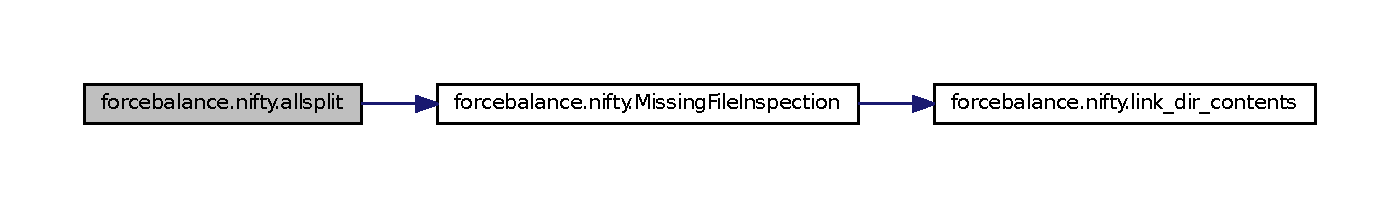
\includegraphics[width=350pt]{namespaceforcebalance_1_1nifty_ac9ab6c5543a2e3080061e0024850edf3_cgraph}
\end{center}
\end{figure}


\hypertarget{namespaceforcebalance_1_1nifty_afb3f205bce4984856e766af7e9fdaca8}{\index{forcebalance\-::nifty@{forcebalance\-::nifty}!col@{col}}
\index{col@{col}!forcebalance::nifty@{forcebalance\-::nifty}}
\paragraph[{col}]{\setlength{\rightskip}{0pt plus 5cm}def forcebalance.\-nifty.\-col (
\begin{DoxyParamCaption}
\item[{}]{vec}
\end{DoxyParamCaption}
)}}\label{namespaceforcebalance_1_1nifty_afb3f205bce4984856e766af7e9fdaca8}


Given any list, array, or matrix, return a 1-\/column matrix. 

Input\-: vec = The input vector that is to be made into a column

Output\-: A column matrix 

Definition at line 270 of file nifty.\-py.



Here is the call graph for this function\-:\nopagebreak
\begin{figure}[H]
\begin{center}
\leavevmode
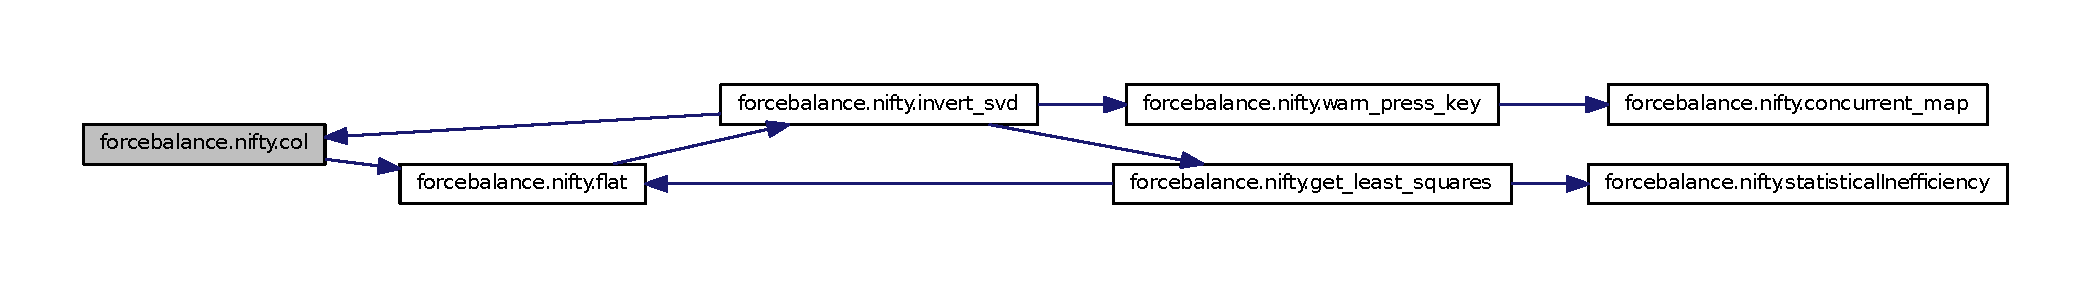
\includegraphics[width=350pt]{namespaceforcebalance_1_1nifty_afb3f205bce4984856e766af7e9fdaca8_cgraph}
\end{center}
\end{figure}


\hypertarget{namespaceforcebalance_1_1nifty_a9628ee448710667747d8aa5dc166532c}{\index{forcebalance\-::nifty@{forcebalance\-::nifty}!commadash@{commadash}}
\index{commadash@{commadash}!forcebalance::nifty@{forcebalance\-::nifty}}
\paragraph[{commadash}]{\setlength{\rightskip}{0pt plus 5cm}def forcebalance.\-nifty.\-commadash (
\begin{DoxyParamCaption}
\item[{}]{l}
\end{DoxyParamCaption}
)}}\label{namespaceforcebalance_1_1nifty_a9628ee448710667747d8aa5dc166532c}


Definition at line 81 of file nifty.\-py.



Here is the call graph for this function\-:\nopagebreak
\begin{figure}[H]
\begin{center}
\leavevmode
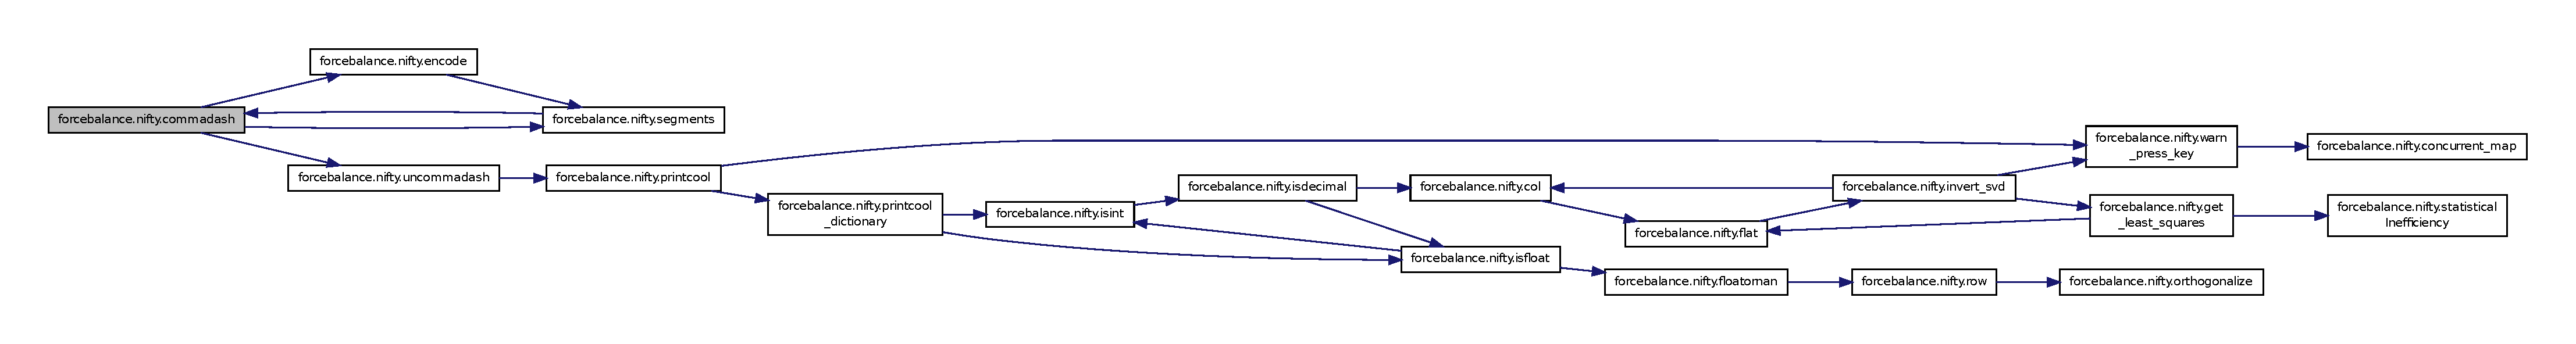
\includegraphics[width=350pt]{namespaceforcebalance_1_1nifty_a9628ee448710667747d8aa5dc166532c_cgraph}
\end{center}
\end{figure}


\hypertarget{namespaceforcebalance_1_1nifty_a2fc81730e7efa7d138dd86f733507bfc}{\index{forcebalance\-::nifty@{forcebalance\-::nifty}!concurrent\-\_\-map@{concurrent\-\_\-map}}
\index{concurrent\-\_\-map@{concurrent\-\_\-map}!forcebalance::nifty@{forcebalance\-::nifty}}
\paragraph[{concurrent\-\_\-map}]{\setlength{\rightskip}{0pt plus 5cm}def forcebalance.\-nifty.\-concurrent\-\_\-map (
\begin{DoxyParamCaption}
\item[{}]{func, }
\item[{}]{data}
\end{DoxyParamCaption}
)}}\label{namespaceforcebalance_1_1nifty_a2fc81730e7efa7d138dd86f733507bfc}


Similar to the bultin function map(). 

But spawn a thread for each argument and apply {\ttfamily func} concurrently.

Note\-: unlike map(), we cannot take an iterable argument. {\ttfamily data} should be an indexable sequence. 

Definition at line 911 of file nifty.\-py.

\hypertarget{namespaceforcebalance_1_1nifty_af5f0e1ba7689f1ab40383ba0480560a9}{\index{forcebalance\-::nifty@{forcebalance\-::nifty}!Copy\-File@{Copy\-File}}
\index{Copy\-File@{Copy\-File}!forcebalance::nifty@{forcebalance\-::nifty}}
\paragraph[{Copy\-File}]{\setlength{\rightskip}{0pt plus 5cm}def forcebalance.\-nifty.\-Copy\-File (
\begin{DoxyParamCaption}
\item[{}]{src, }
\item[{}]{dest}
\end{DoxyParamCaption}
)}}\label{namespaceforcebalance_1_1nifty_af5f0e1ba7689f1ab40383ba0480560a9}


Definition at line 754 of file nifty.\-py.



Here is the call graph for this function\-:\nopagebreak
\begin{figure}[H]
\begin{center}
\leavevmode
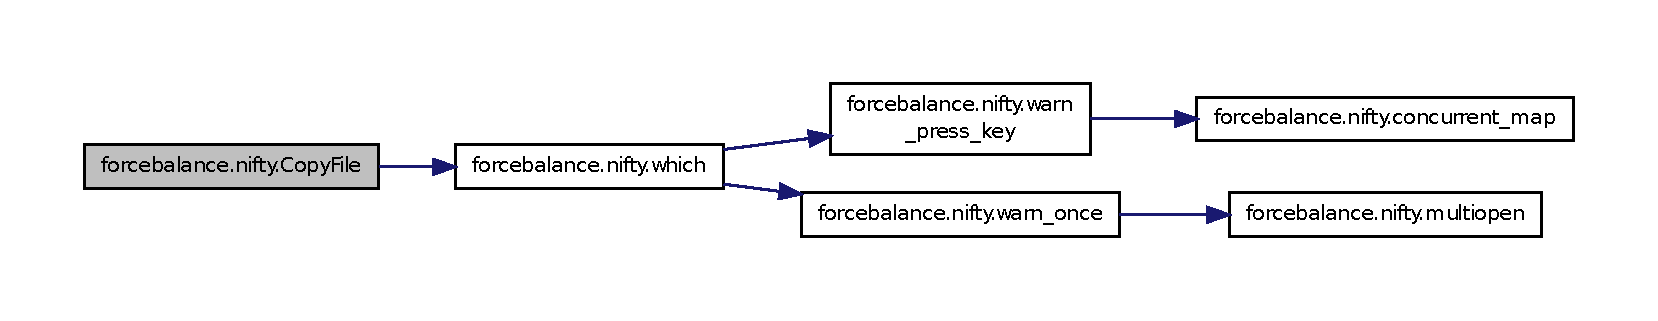
\includegraphics[width=350pt]{namespaceforcebalance_1_1nifty_af5f0e1ba7689f1ab40383ba0480560a9_cgraph}
\end{center}
\end{figure}


\hypertarget{namespaceforcebalance_1_1nifty_ab5f3072ad95e9c75659cb1adac341051}{\index{forcebalance\-::nifty@{forcebalance\-::nifty}!create\-Work\-Queue@{create\-Work\-Queue}}
\index{create\-Work\-Queue@{create\-Work\-Queue}!forcebalance::nifty@{forcebalance\-::nifty}}
\paragraph[{create\-Work\-Queue}]{\setlength{\rightskip}{0pt plus 5cm}def forcebalance.\-nifty.\-create\-Work\-Queue (
\begin{DoxyParamCaption}
\item[{}]{wq\-\_\-port, }
\item[{}]{debug = {\ttfamily True}}
\end{DoxyParamCaption}
)}}\label{namespaceforcebalance_1_1nifty_ab5f3072ad95e9c75659cb1adac341051}


Definition at line 572 of file nifty.\-py.



Here is the call graph for this function\-:\nopagebreak
\begin{figure}[H]
\begin{center}
\leavevmode
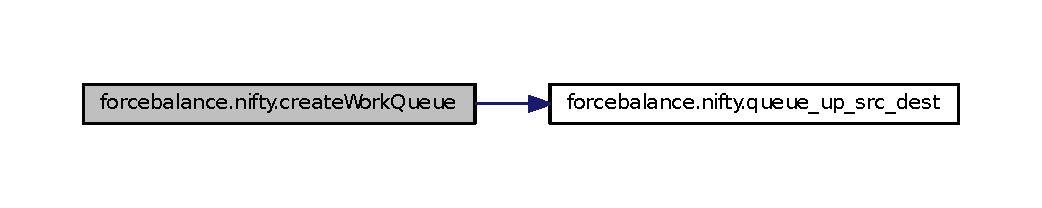
\includegraphics[width=350pt]{namespaceforcebalance_1_1nifty_ab5f3072ad95e9c75659cb1adac341051_cgraph}
\end{center}
\end{figure}


\hypertarget{namespaceforcebalance_1_1nifty_a3b437964dc22735bf8a7dcbaf99e413d}{\index{forcebalance\-::nifty@{forcebalance\-::nifty}!encode@{encode}}
\index{encode@{encode}!forcebalance::nifty@{forcebalance\-::nifty}}
\paragraph[{encode}]{\setlength{\rightskip}{0pt plus 5cm}def forcebalance.\-nifty.\-encode (
\begin{DoxyParamCaption}
\item[{}]{l}
\end{DoxyParamCaption}
)}}\label{namespaceforcebalance_1_1nifty_a3b437964dc22735bf8a7dcbaf99e413d}


Definition at line 72 of file nifty.\-py.



Here is the call graph for this function\-:\nopagebreak
\begin{figure}[H]
\begin{center}
\leavevmode
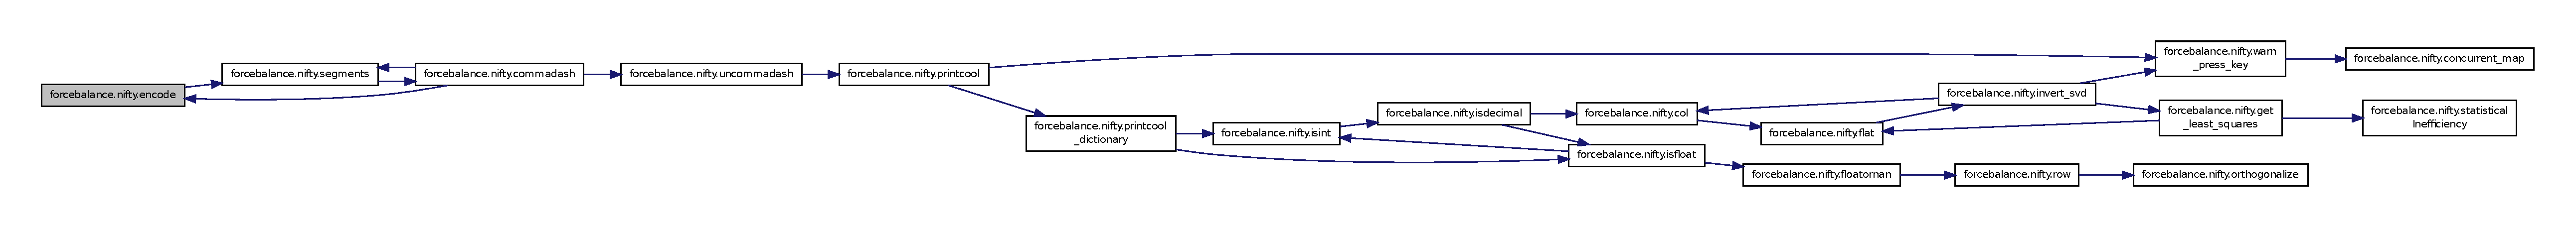
\includegraphics[width=350pt]{namespaceforcebalance_1_1nifty_a3b437964dc22735bf8a7dcbaf99e413d_cgraph}
\end{center}
\end{figure}


\hypertarget{namespaceforcebalance_1_1nifty_a52114ceee9d55f94d9aecb3e176de294}{\index{forcebalance\-::nifty@{forcebalance\-::nifty}!flat@{flat}}
\index{flat@{flat}!forcebalance::nifty@{forcebalance\-::nifty}}
\paragraph[{flat}]{\setlength{\rightskip}{0pt plus 5cm}def forcebalance.\-nifty.\-flat (
\begin{DoxyParamCaption}
\item[{}]{vec}
\end{DoxyParamCaption}
)}}\label{namespaceforcebalance_1_1nifty_a52114ceee9d55f94d9aecb3e176de294}


Given any list, array, or matrix, return a single-\/index array. 


\begin{DoxyParams}[1]{Parameters}
\mbox{\tt in}  & {\em vec} & The data to be flattened \\
\hline
\end{DoxyParams}
\begin{DoxyReturn}{Returns}
answer The flattened data 
\end{DoxyReturn}


Definition at line 289 of file nifty.\-py.



Here is the call graph for this function\-:\nopagebreak
\begin{figure}[H]
\begin{center}
\leavevmode
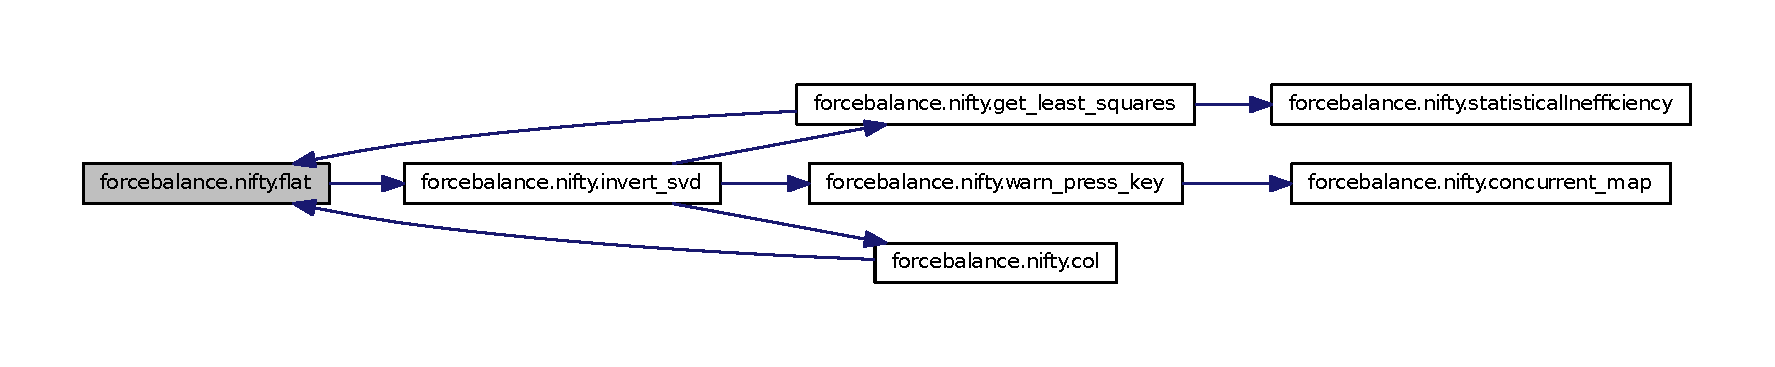
\includegraphics[width=350pt]{namespaceforcebalance_1_1nifty_a52114ceee9d55f94d9aecb3e176de294_cgraph}
\end{center}
\end{figure}


\hypertarget{namespaceforcebalance_1_1nifty_a8d63c8ae9a67c66673a6cf81357f827d}{\index{forcebalance\-::nifty@{forcebalance\-::nifty}!floatornan@{floatornan}}
\index{floatornan@{floatornan}!forcebalance::nifty@{forcebalance\-::nifty}}
\paragraph[{floatornan}]{\setlength{\rightskip}{0pt plus 5cm}def forcebalance.\-nifty.\-floatornan (
\begin{DoxyParamCaption}
\item[{}]{word}
\end{DoxyParamCaption}
)}}\label{namespaceforcebalance_1_1nifty_a8d63c8ae9a67c66673a6cf81357f827d}


Returns a big number if we encounter Na\-N. 


\begin{DoxyParams}[1]{Parameters}
\mbox{\tt in}  & {\em word} & The string to be converted \\
\hline
\end{DoxyParams}
\begin{DoxyReturn}{Returns}
answer The string converted to a float; if not a float, return 1e10 
\end{DoxyReturn}
\begin{DoxyRefDesc}{Todo}
\item[\hyperlink{todo__todo000013}{Todo}]I could use suggestions for making this better. \end{DoxyRefDesc}


Definition at line 252 of file nifty.\-py.



Here is the call graph for this function\-:\nopagebreak
\begin{figure}[H]
\begin{center}
\leavevmode
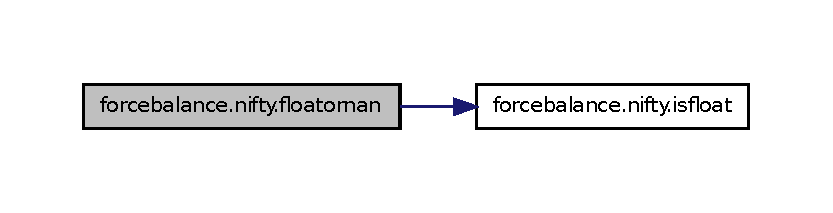
\includegraphics[width=350pt]{namespaceforcebalance_1_1nifty_a8d63c8ae9a67c66673a6cf81357f827d_cgraph}
\end{center}
\end{figure}


\hypertarget{namespaceforcebalance_1_1nifty_aa9fb9c7c65231eca50a7afc04f489b64}{\index{forcebalance\-::nifty@{forcebalance\-::nifty}!get\-\_\-least\-\_\-squares@{get\-\_\-least\-\_\-squares}}
\index{get\-\_\-least\-\_\-squares@{get\-\_\-least\-\_\-squares}!forcebalance::nifty@{forcebalance\-::nifty}}
\paragraph[{get\-\_\-least\-\_\-squares}]{\setlength{\rightskip}{0pt plus 5cm}def forcebalance.\-nifty.\-get\-\_\-least\-\_\-squares (
\begin{DoxyParamCaption}
\item[{}]{x, }
\item[{}]{y, }
\item[{}]{w = {\ttfamily None}, }
\item[{}]{thresh = {\ttfamily 1e-\/12}}
\end{DoxyParamCaption}
)}}\label{namespaceforcebalance_1_1nifty_aa9fb9c7c65231eca50a7afc04f489b64}

\begin{DoxyCode}
1  \_\_                  \_\_
2 |                      |
3 | 1 (x0) (x0)^2 (x0)^3 |
4 | 1 (x1) (x1)^2 (x1)^3 |
5 | 1 (x2) (x2)^2 (x2)^3 |
6 | 1 (x3) (x3)^2 (x3)^3 |
7 | 1 (x4) (x4)^2 (x4)^3 |
8 |\_\_                  \_\_|
\end{DoxyCode}



\begin{DoxyParams}[1]{Parameters}
\mbox{\tt in}  & {\em X} & (2-\/\-D array) An array of X-\/values (see above) \\
\hline
\mbox{\tt in}  & {\em Y} & (array) An array of Y-\/values (only used in getting the least squares coefficients) \\
\hline
\mbox{\tt in}  & {\em w} & (array) An array of weights, hopefully normalized to one. \\
\hline
\mbox{\tt out}  & {\em Beta} & The least-\/squares coefficients \\
\hline
\mbox{\tt out}  & {\em Hat} & The hat matrix that takes linear combinations of data y-\/values to give fitted y-\/values (weights) \\
\hline
\mbox{\tt out}  & {\em yfit} & The fitted y-\/values \\
\hline
\mbox{\tt out}  & {\em M\-P\-P\-I} & The Moore-\/\-Penrose pseudoinverse (multiply by Y to get least-\/squares coefficients, multiply by d\-Y/dk to get derivatives of least-\/squares coefficients) \\
\hline
\end{DoxyParams}


Definition at line 357 of file nifty.\-py.



Here is the call graph for this function\-:\nopagebreak
\begin{figure}[H]
\begin{center}
\leavevmode
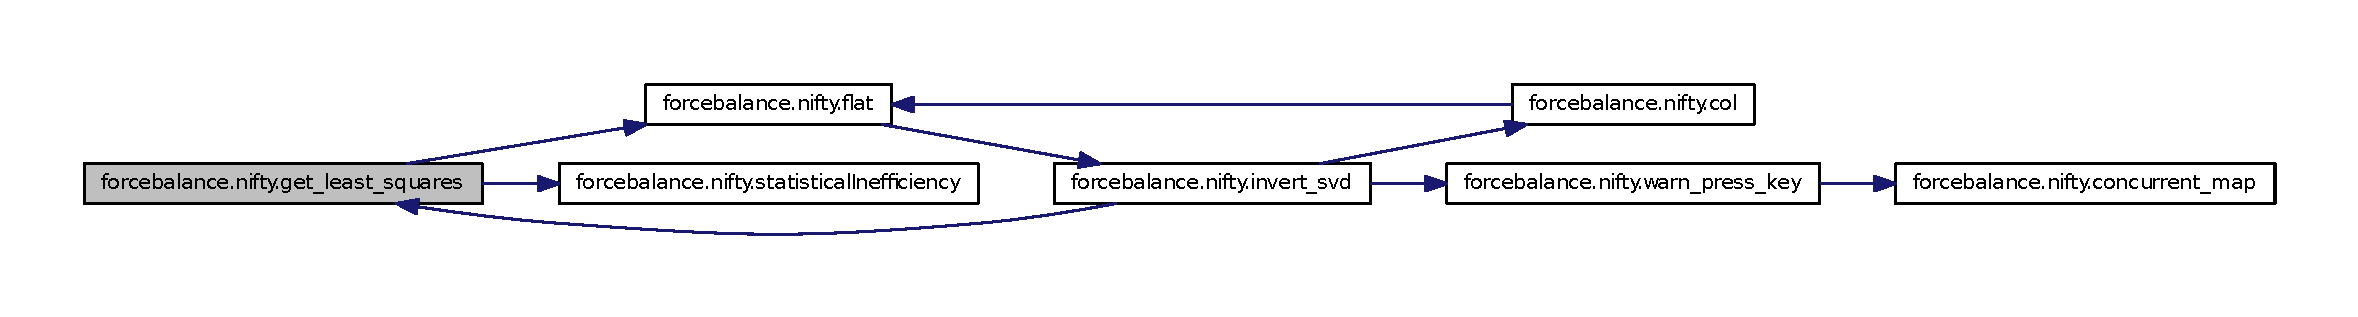
\includegraphics[width=350pt]{namespaceforcebalance_1_1nifty_aa9fb9c7c65231eca50a7afc04f489b64_cgraph}
\end{center}
\end{figure}


\hypertarget{namespaceforcebalance_1_1nifty_ac37d4fe58ef70ed546ebfc45d12f7a5d}{\index{forcebalance\-::nifty@{forcebalance\-::nifty}!get\-Work\-Queue@{get\-Work\-Queue}}
\index{get\-Work\-Queue@{get\-Work\-Queue}!forcebalance::nifty@{forcebalance\-::nifty}}
\paragraph[{get\-Work\-Queue}]{\setlength{\rightskip}{0pt plus 5cm}def forcebalance.\-nifty.\-get\-Work\-Queue (
\begin{DoxyParamCaption}
{}
\end{DoxyParamCaption}
)}}\label{namespaceforcebalance_1_1nifty_ac37d4fe58ef70ed546ebfc45d12f7a5d}


Definition at line 566 of file nifty.\-py.

\hypertarget{namespaceforcebalance_1_1nifty_abe1e72c32252d62a6551b47290c7584f}{\index{forcebalance\-::nifty@{forcebalance\-::nifty}!get\-W\-Q\-Ids@{get\-W\-Q\-Ids}}
\index{get\-W\-Q\-Ids@{get\-W\-Q\-Ids}!forcebalance::nifty@{forcebalance\-::nifty}}
\paragraph[{get\-W\-Q\-Ids}]{\setlength{\rightskip}{0pt plus 5cm}def forcebalance.\-nifty.\-get\-W\-Q\-Ids (
\begin{DoxyParamCaption}
{}
\end{DoxyParamCaption}
)}}\label{namespaceforcebalance_1_1nifty_abe1e72c32252d62a6551b47290c7584f}


Definition at line 569 of file nifty.\-py.

\hypertarget{namespaceforcebalance_1_1nifty_ad432b88307e1178b0690c0d350b1af36}{\index{forcebalance\-::nifty@{forcebalance\-::nifty}!Go\-Into@{Go\-Into}}
\index{Go\-Into@{Go\-Into}!forcebalance::nifty@{forcebalance\-::nifty}}
\paragraph[{Go\-Into}]{\setlength{\rightskip}{0pt plus 5cm}def forcebalance.\-nifty.\-Go\-Into (
\begin{DoxyParamCaption}
\item[{}]{Dir}
\end{DoxyParamCaption}
)}}\label{namespaceforcebalance_1_1nifty_ad432b88307e1178b0690c0d350b1af36}


Definition at line 698 of file nifty.\-py.

\hypertarget{namespaceforcebalance_1_1nifty_a4c82187e92dfeb8a159f4aa44b501c40}{\index{forcebalance\-::nifty@{forcebalance\-::nifty}!invert\-\_\-svd@{invert\-\_\-svd}}
\index{invert\-\_\-svd@{invert\-\_\-svd}!forcebalance::nifty@{forcebalance\-::nifty}}
\paragraph[{invert\-\_\-svd}]{\setlength{\rightskip}{0pt plus 5cm}def forcebalance.\-nifty.\-invert\-\_\-svd (
\begin{DoxyParamCaption}
\item[{}]{X, }
\item[{}]{thresh = {\ttfamily 1e-\/12}}
\end{DoxyParamCaption}
)}}\label{namespaceforcebalance_1_1nifty_a4c82187e92dfeb8a159f4aa44b501c40}


Invert a matrix using singular value decomposition. 


\begin{DoxyParams}[1]{Parameters}
\mbox{\tt in}  & {\em X} & The matrix to be inverted \\
\hline
\mbox{\tt in}  & {\em thresh} & The S\-V\-D threshold; eigenvalues below this are not inverted but set to zero \\
\hline
\end{DoxyParams}
\begin{DoxyReturn}{Returns}
Xt The inverted matrix 
\end{DoxyReturn}


Definition at line 316 of file nifty.\-py.



Here is the call graph for this function\-:\nopagebreak
\begin{figure}[H]
\begin{center}
\leavevmode
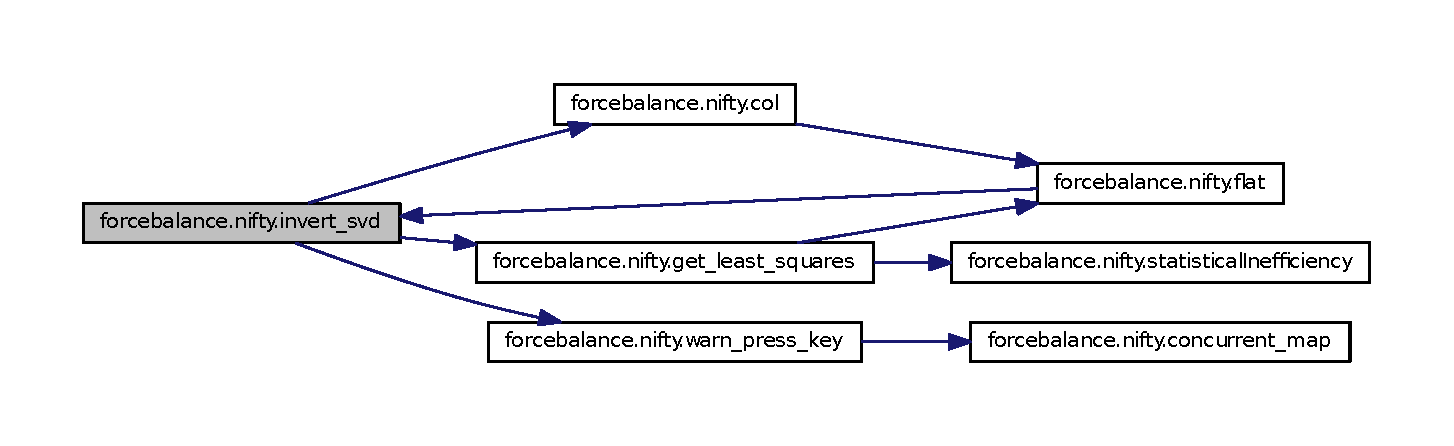
\includegraphics[width=350pt]{namespaceforcebalance_1_1nifty_a4c82187e92dfeb8a159f4aa44b501c40_cgraph}
\end{center}
\end{figure}


\hypertarget{namespaceforcebalance_1_1nifty_a09263927eaec9deff283fbf1a820242f}{\index{forcebalance\-::nifty@{forcebalance\-::nifty}!isdecimal@{isdecimal}}
\index{isdecimal@{isdecimal}!forcebalance::nifty@{forcebalance\-::nifty}}
\paragraph[{isdecimal}]{\setlength{\rightskip}{0pt plus 5cm}def forcebalance.\-nifty.\-isdecimal (
\begin{DoxyParamCaption}
\item[{}]{word}
\end{DoxyParamCaption}
)}}\label{namespaceforcebalance_1_1nifty_a09263927eaec9deff283fbf1a820242f}


Matches things with a decimal only; see isint and isfloat. 


\begin{DoxyParams}[1]{Parameters}
\mbox{\tt in}  & {\em word} & String (for instance, '123', '153.\-0', '2.', '-\/354') \\
\hline
\end{DoxyParams}
\begin{DoxyReturn}{Returns}
answer Boolean which specifies whether the string is a number with a decimal point 
\end{DoxyReturn}


Definition at line 242 of file nifty.\-py.



Here is the call graph for this function\-:\nopagebreak
\begin{figure}[H]
\begin{center}
\leavevmode
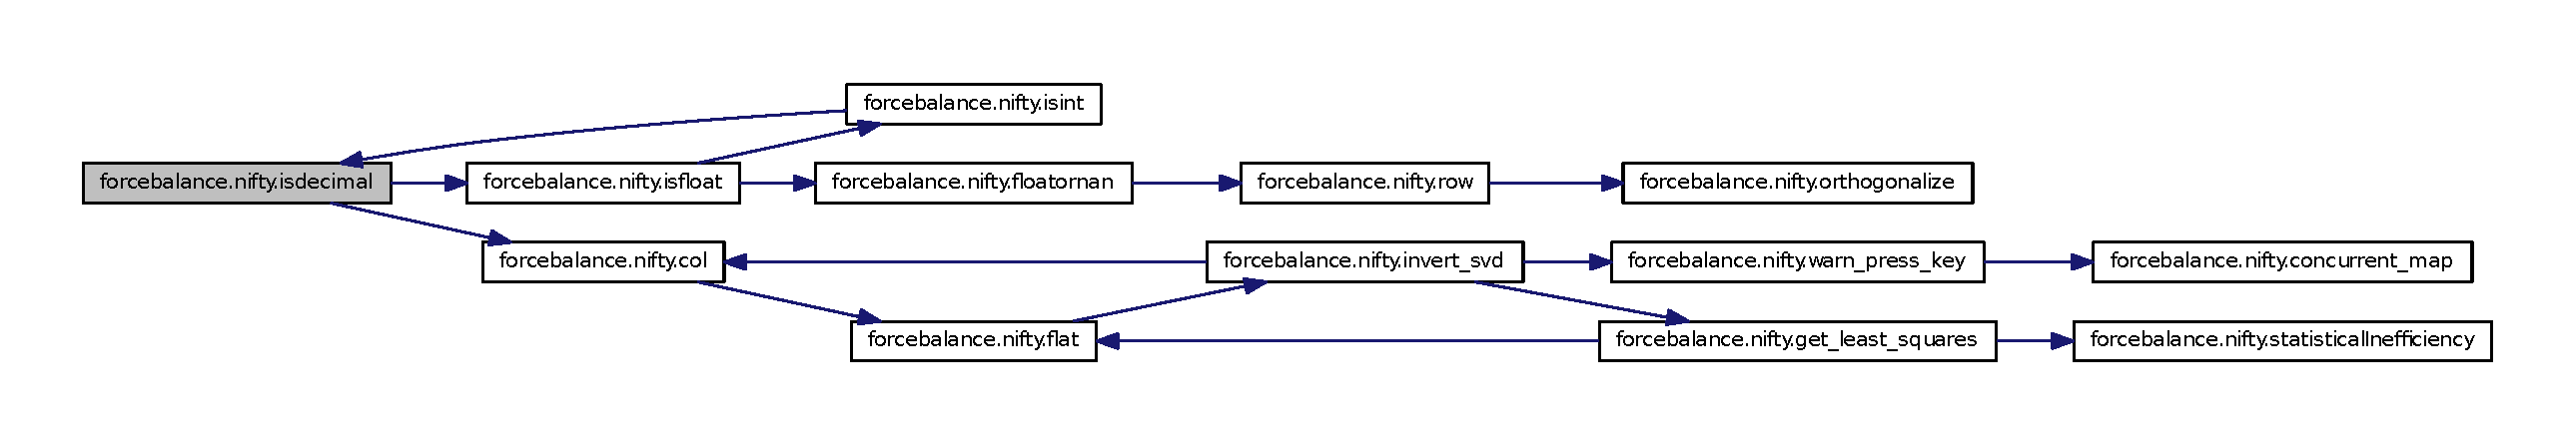
\includegraphics[width=350pt]{namespaceforcebalance_1_1nifty_a09263927eaec9deff283fbf1a820242f_cgraph}
\end{center}
\end{figure}


\hypertarget{namespaceforcebalance_1_1nifty_a8e3ef0108b9d37b82ba0dced7c6037ae}{\index{forcebalance\-::nifty@{forcebalance\-::nifty}!isfloat@{isfloat}}
\index{isfloat@{isfloat}!forcebalance::nifty@{forcebalance\-::nifty}}
\paragraph[{isfloat}]{\setlength{\rightskip}{0pt plus 5cm}def forcebalance.\-nifty.\-isfloat (
\begin{DoxyParamCaption}
\item[{}]{word}
\end{DoxyParamCaption}
)}}\label{namespaceforcebalance_1_1nifty_a8e3ef0108b9d37b82ba0dced7c6037ae}


Matches A\-N\-Y number; it can be a decimal, scientific notation, what have you C\-A\-U\-T\-I\-O\-N -\/ this will also match an integer. 


\begin{DoxyParams}[1]{Parameters}
\mbox{\tt in}  & {\em word} & String (for instance, '123', '153.\-0', '2.', '-\/354') \\
\hline
\end{DoxyParams}
\begin{DoxyReturn}{Returns}
answer Boolean which specifies whether the string is any number 
\end{DoxyReturn}


Definition at line 232 of file nifty.\-py.



Here is the call graph for this function\-:\nopagebreak
\begin{figure}[H]
\begin{center}
\leavevmode
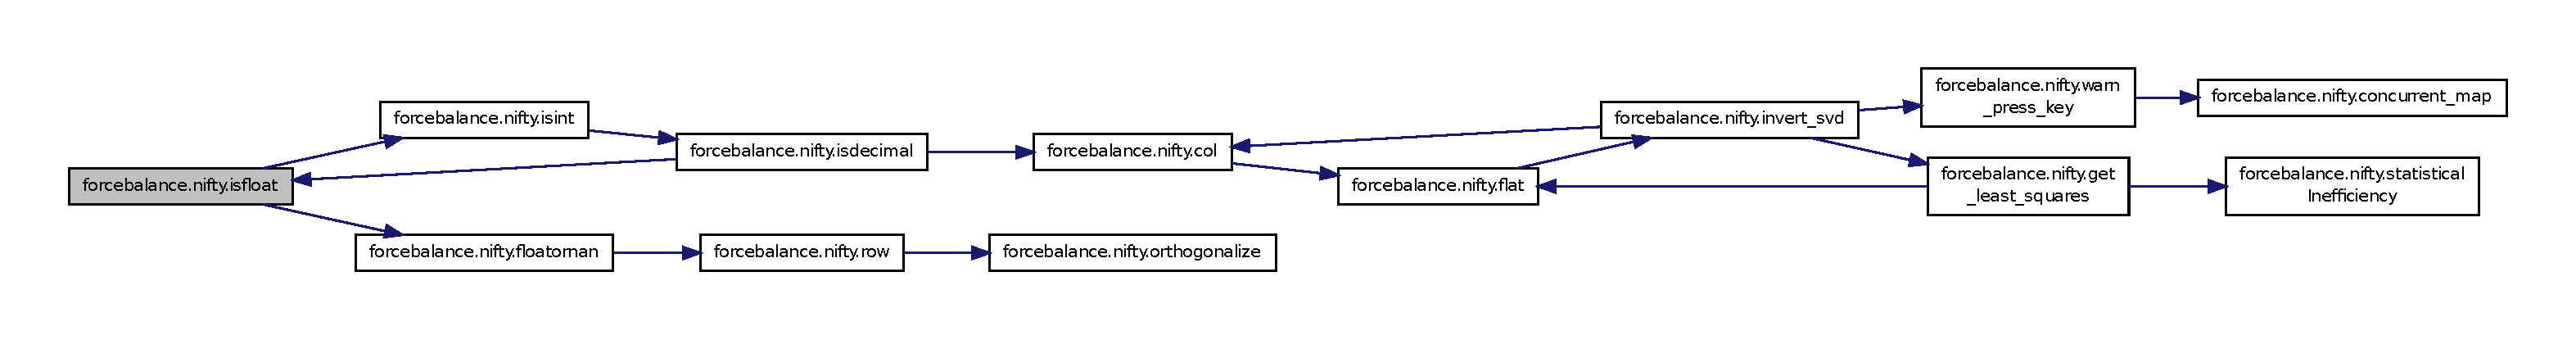
\includegraphics[width=350pt]{namespaceforcebalance_1_1nifty_a8e3ef0108b9d37b82ba0dced7c6037ae_cgraph}
\end{center}
\end{figure}


\hypertarget{namespaceforcebalance_1_1nifty_a3f1c7a1af9d35d5d1693074bc6f5497c}{\index{forcebalance\-::nifty@{forcebalance\-::nifty}!isint@{isint}}
\index{isint@{isint}!forcebalance::nifty@{forcebalance\-::nifty}}
\paragraph[{isint}]{\setlength{\rightskip}{0pt plus 5cm}def forcebalance.\-nifty.\-isint (
\begin{DoxyParamCaption}
\item[{}]{word}
\end{DoxyParamCaption}
)}}\label{namespaceforcebalance_1_1nifty_a3f1c7a1af9d35d5d1693074bc6f5497c}


O\-N\-L\-Y matches integers! If you have a decimal point? None shall pass! 


\begin{DoxyParams}[1]{Parameters}
\mbox{\tt in}  & {\em word} & String (for instance, '123', '153.\-0', '2.', '-\/354') \\
\hline
\end{DoxyParams}
\begin{DoxyReturn}{Returns}
answer Boolean which specifies whether the string is an integer (only +/-\/ sign followed by digits) 
\end{DoxyReturn}


Definition at line 221 of file nifty.\-py.



Here is the call graph for this function\-:\nopagebreak
\begin{figure}[H]
\begin{center}
\leavevmode
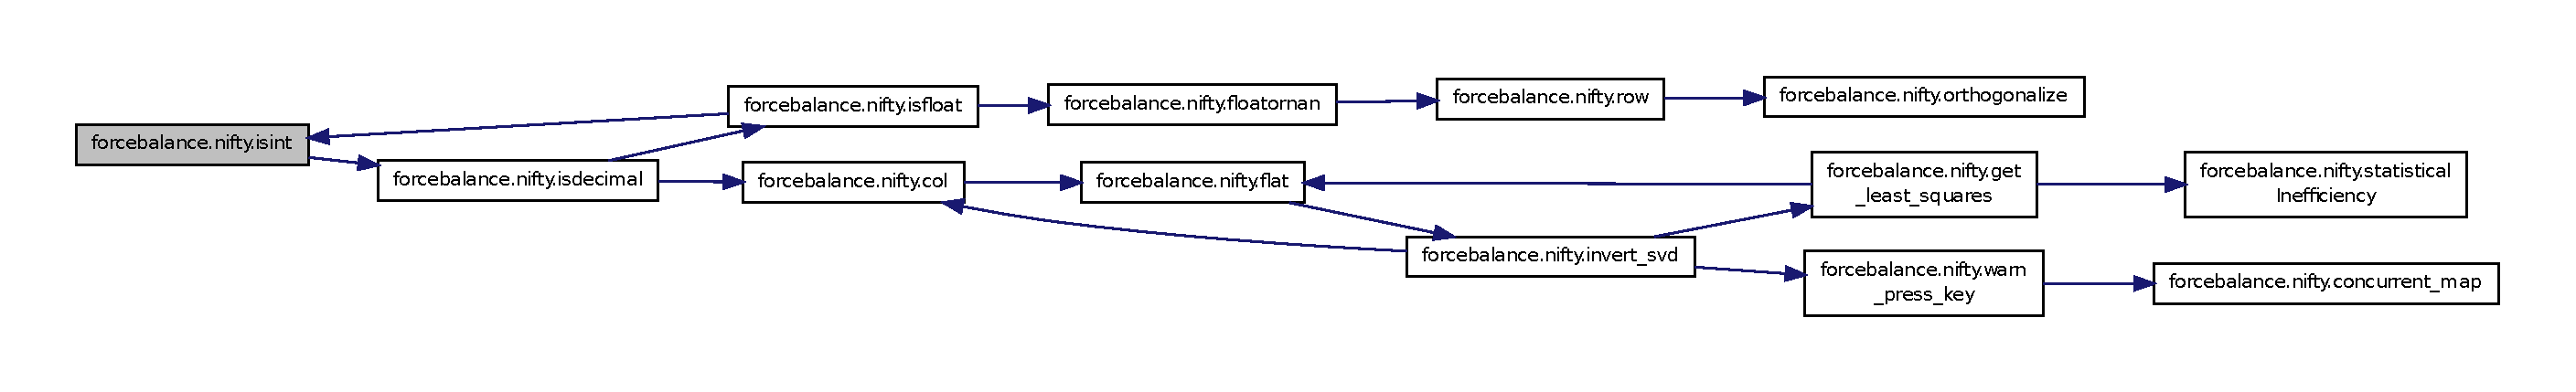
\includegraphics[width=350pt]{namespaceforcebalance_1_1nifty_a3f1c7a1af9d35d5d1693074bc6f5497c_cgraph}
\end{center}
\end{figure}


\hypertarget{namespaceforcebalance_1_1nifty_ab04e8690d099db2379dc860e0d040120}{\index{forcebalance\-::nifty@{forcebalance\-::nifty}!Leave@{Leave}}
\index{Leave@{Leave}!forcebalance::nifty@{forcebalance\-::nifty}}
\paragraph[{Leave}]{\setlength{\rightskip}{0pt plus 5cm}def forcebalance.\-nifty.\-Leave (
\begin{DoxyParamCaption}
\item[{}]{Dir}
\end{DoxyParamCaption}
)}}\label{namespaceforcebalance_1_1nifty_ab04e8690d099db2379dc860e0d040120}


Definition at line 712 of file nifty.\-py.

\hypertarget{namespaceforcebalance_1_1nifty_a0cf4e58f90acf20e3d6224be2354082c}{\index{forcebalance\-::nifty@{forcebalance\-::nifty}!link\-\_\-dir\-\_\-contents@{link\-\_\-dir\-\_\-contents}}
\index{link\-\_\-dir\-\_\-contents@{link\-\_\-dir\-\_\-contents}!forcebalance::nifty@{forcebalance\-::nifty}}
\paragraph[{link\-\_\-dir\-\_\-contents}]{\setlength{\rightskip}{0pt plus 5cm}def forcebalance.\-nifty.\-link\-\_\-dir\-\_\-contents (
\begin{DoxyParamCaption}
\item[{}]{abssrcdir, }
\item[{}]{absdestdir}
\end{DoxyParamCaption}
)}}\label{namespaceforcebalance_1_1nifty_a0cf4e58f90acf20e3d6224be2354082c}


Definition at line 764 of file nifty.\-py.

\hypertarget{namespaceforcebalance_1_1nifty_ab182a9da2a2f42cf45942fbee6acf9b1}{\index{forcebalance\-::nifty@{forcebalance\-::nifty}!Link\-File@{Link\-File}}
\index{Link\-File@{Link\-File}!forcebalance::nifty@{forcebalance\-::nifty}}
\paragraph[{Link\-File}]{\setlength{\rightskip}{0pt plus 5cm}def forcebalance.\-nifty.\-Link\-File (
\begin{DoxyParamCaption}
\item[{}]{src, }
\item[{}]{dest}
\end{DoxyParamCaption}
)}}\label{namespaceforcebalance_1_1nifty_ab182a9da2a2f42cf45942fbee6acf9b1}


Definition at line 743 of file nifty.\-py.



Here is the call graph for this function\-:\nopagebreak
\begin{figure}[H]
\begin{center}
\leavevmode
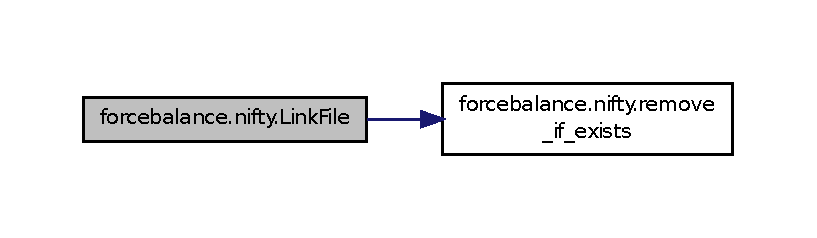
\includegraphics[width=350pt]{namespaceforcebalance_1_1nifty_ab182a9da2a2f42cf45942fbee6acf9b1_cgraph}
\end{center}
\end{figure}


\hypertarget{namespaceforcebalance_1_1nifty_a2ff762a2f2d2b6bb1c7dd067bd1a1e88}{\index{forcebalance\-::nifty@{forcebalance\-::nifty}!lp\-\_\-dump@{lp\-\_\-dump}}
\index{lp\-\_\-dump@{lp\-\_\-dump}!forcebalance::nifty@{forcebalance\-::nifty}}
\paragraph[{lp\-\_\-dump}]{\setlength{\rightskip}{0pt plus 5cm}def forcebalance.\-nifty.\-lp\-\_\-dump (
\begin{DoxyParamCaption}
\item[{}]{obj, }
\item[{}]{file, }
\item[{}]{protocol = {\ttfamily None}}
\end{DoxyParamCaption}
)}}\label{namespaceforcebalance_1_1nifty_a2ff762a2f2d2b6bb1c7dd067bd1a1e88}


Use this instead of pickle.\-dump for pickling anything that contains \-\_\-\-Element\-Tree types. 



Definition at line 549 of file nifty.\-py.



Here is the call graph for this function\-:\nopagebreak
\begin{figure}[H]
\begin{center}
\leavevmode
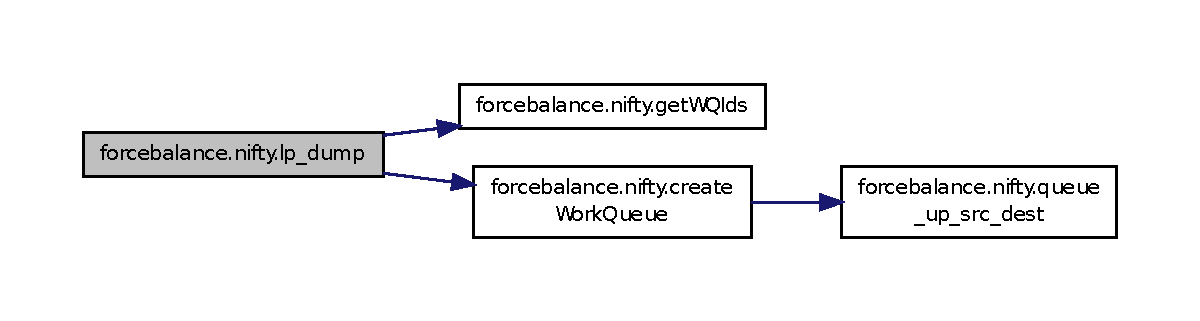
\includegraphics[width=350pt]{namespaceforcebalance_1_1nifty_a2ff762a2f2d2b6bb1c7dd067bd1a1e88_cgraph}
\end{center}
\end{figure}


\hypertarget{namespaceforcebalance_1_1nifty_a577abfd36638c5f4dfdade136abaef12}{\index{forcebalance\-::nifty@{forcebalance\-::nifty}!lp\-\_\-load@{lp\-\_\-load}}
\index{lp\-\_\-load@{lp\-\_\-load}!forcebalance::nifty@{forcebalance\-::nifty}}
\paragraph[{lp\-\_\-load}]{\setlength{\rightskip}{0pt plus 5cm}def forcebalance.\-nifty.\-lp\-\_\-load (
\begin{DoxyParamCaption}
\item[{}]{file}
\end{DoxyParamCaption}
)}}\label{namespaceforcebalance_1_1nifty_a577abfd36638c5f4dfdade136abaef12}


Use this instead of pickle.\-load for unpickling anything that contains \-\_\-\-Element\-Tree types. 



Definition at line 554 of file nifty.\-py.



Here is the call graph for this function\-:\nopagebreak
\begin{figure}[H]
\begin{center}
\leavevmode
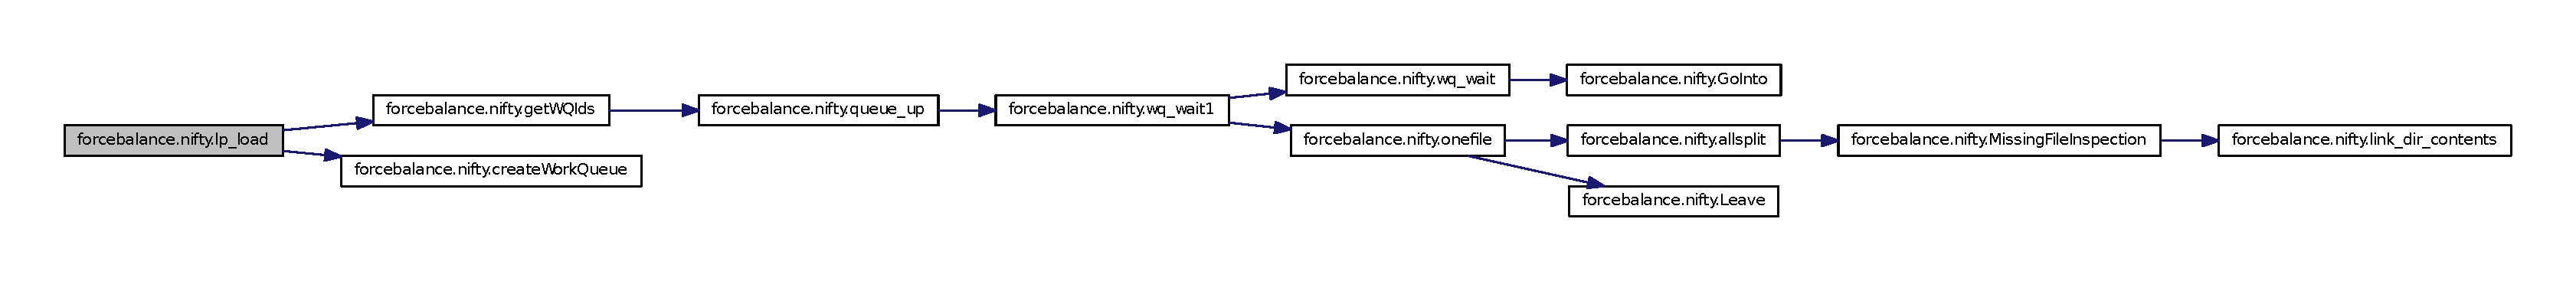
\includegraphics[width=350pt]{namespaceforcebalance_1_1nifty_a577abfd36638c5f4dfdade136abaef12_cgraph}
\end{center}
\end{figure}


\hypertarget{namespaceforcebalance_1_1nifty_ae87c7def5f8edf2ec30737bdb1d2636f}{\index{forcebalance\-::nifty@{forcebalance\-::nifty}!Missing\-File\-Inspection@{Missing\-File\-Inspection}}
\index{Missing\-File\-Inspection@{Missing\-File\-Inspection}!forcebalance::nifty@{forcebalance\-::nifty}}
\paragraph[{Missing\-File\-Inspection}]{\setlength{\rightskip}{0pt plus 5cm}def forcebalance.\-nifty.\-Missing\-File\-Inspection (
\begin{DoxyParamCaption}
\item[{}]{fnm}
\end{DoxyParamCaption}
)}}\label{namespaceforcebalance_1_1nifty_ae87c7def5f8edf2ec30737bdb1d2636f}


Definition at line 733 of file nifty.\-py.



Here is the call graph for this function\-:\nopagebreak
\begin{figure}[H]
\begin{center}
\leavevmode
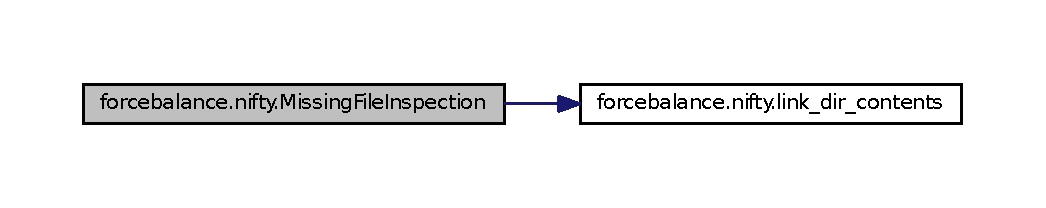
\includegraphics[width=350pt]{namespaceforcebalance_1_1nifty_ae87c7def5f8edf2ec30737bdb1d2636f_cgraph}
\end{center}
\end{figure}


\hypertarget{namespaceforcebalance_1_1nifty_a64b7c6ca7afa1c11681f5c2897c55cc3}{\index{forcebalance\-::nifty@{forcebalance\-::nifty}!multiopen@{multiopen}}
\index{multiopen@{multiopen}!forcebalance::nifty@{forcebalance\-::nifty}}
\paragraph[{multiopen}]{\setlength{\rightskip}{0pt plus 5cm}def forcebalance.\-nifty.\-multiopen (
\begin{DoxyParamCaption}
\item[{}]{arg}
\end{DoxyParamCaption}
)}}\label{namespaceforcebalance_1_1nifty_a64b7c6ca7afa1c11681f5c2897c55cc3}


This function be given any of several variable types (single file name, file object, or list of lines, or a list of the above) and give a list of files\-: 

\mbox{[}file1, file2, file3 ... \mbox{]}

each of which can then be iterated over\-:

\mbox{[}\mbox{[}file1\-\_\-line1, file1\-\_\-line2 ... \mbox{]}, \mbox{[}file2\-\_\-line1, file2\-\_\-line2 ... \mbox{]}\mbox{]} 

Definition at line 941 of file nifty.\-py.

\hypertarget{namespaceforcebalance_1_1nifty_a7676236002c6a65ea7d2e69a09923889}{\index{forcebalance\-::nifty@{forcebalance\-::nifty}!orthogonalize@{orthogonalize}}
\index{orthogonalize@{orthogonalize}!forcebalance::nifty@{forcebalance\-::nifty}}
\paragraph[{orthogonalize}]{\setlength{\rightskip}{0pt plus 5cm}def forcebalance.\-nifty.\-orthogonalize (
\begin{DoxyParamCaption}
\item[{}]{vec1, }
\item[{}]{vec2}
\end{DoxyParamCaption}
)}}\label{namespaceforcebalance_1_1nifty_a7676236002c6a65ea7d2e69a09923889}


Given two vectors vec1 and vec2, project out the component of vec1 that is along the vec2-\/direction. 


\begin{DoxyParams}[1]{Parameters}
\mbox{\tt in}  & {\em vec1} & The projectee (i.\-e. output is some modified version of vec1) \\
\hline
\mbox{\tt in}  & {\em vec2} & The projector (component subtracted out from vec1 is parallel to this) \\
\hline
\end{DoxyParams}
\begin{DoxyReturn}{Returns}
answer A copy of vec1 but with the vec2-\/component projected out. 
\end{DoxyReturn}


Definition at line 303 of file nifty.\-py.

\hypertarget{namespaceforcebalance_1_1nifty_af61d76c8eb78c8ee52a43e239ff26cb4}{\index{forcebalance\-::nifty@{forcebalance\-::nifty}!pmat2d@{pmat2d}}
\index{pmat2d@{pmat2d}!forcebalance::nifty@{forcebalance\-::nifty}}
\paragraph[{pmat2d}]{\setlength{\rightskip}{0pt plus 5cm}def forcebalance.\-nifty.\-pmat2d (
\begin{DoxyParamCaption}
\item[{}]{mat2d, }
\item[{}]{precision = {\ttfamily 1}, }
\item[{}]{loglevel = {\ttfamily forcebalance.output.INFO}}
\end{DoxyParamCaption}
)}}\label{namespaceforcebalance_1_1nifty_af61d76c8eb78c8ee52a43e239ff26cb4}


Printout of a 2-\/\-D matrix. 


\begin{DoxyParams}[1]{Parameters}
\mbox{\tt in}  & {\em mat2d} & a 2-\/\-D matrix \\
\hline
\end{DoxyParams}


Definition at line 65 of file nifty.\-py.



Here is the call graph for this function\-:\nopagebreak
\begin{figure}[H]
\begin{center}
\leavevmode
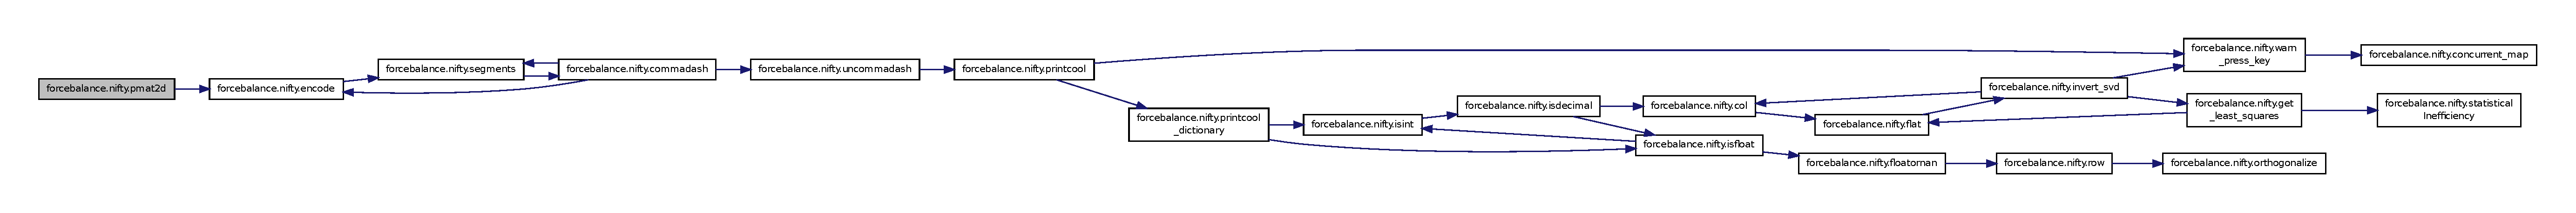
\includegraphics[width=350pt]{namespaceforcebalance_1_1nifty_af61d76c8eb78c8ee52a43e239ff26cb4_cgraph}
\end{center}
\end{figure}


\hypertarget{namespaceforcebalance_1_1nifty_a11babd62dc7bca389162c6318f9672ca}{\index{forcebalance\-::nifty@{forcebalance\-::nifty}!printcool@{printcool}}
\index{printcool@{printcool}!forcebalance::nifty@{forcebalance\-::nifty}}
\paragraph[{printcool}]{\setlength{\rightskip}{0pt plus 5cm}def forcebalance.\-nifty.\-printcool (
\begin{DoxyParamCaption}
\item[{}]{text, }
\item[{}]{sym = {\ttfamily \char`\"{}\#\char`\"{}}, }
\item[{}]{bold = {\ttfamily False}, }
\item[{}]{color = {\ttfamily 2}, }
\item[{}]{ansi = {\ttfamily None}, }
\item[{}]{bottom = {\ttfamily '-\/'}, }
\item[{}]{minwidth = {\ttfamily 50}, }
\item[{}]{center = {\ttfamily True}}
\end{DoxyParamCaption}
)}}\label{namespaceforcebalance_1_1nifty_a11babd62dc7bca389162c6318f9672ca}


Cool-\/looking printout for slick formatting of output. 


\begin{DoxyParams}[1]{Parameters}
\mbox{\tt in}  & {\em text} & The string that the printout is based upon. This function will print out the string, A\-N\-S\-I-\/colored and enclosed in the symbol for example\-:\par
 {\ttfamily  \#\#\#\#\#\#\#\#\#\#\#\#\#\#\#\#\# }\par
 {\ttfamily  \#\#\# I am cool \#\#\# }\par
 {\ttfamily  \#\#\#\#\#\#\#\#\#\#\#\#\#\#\#\#\# } \\
\hline
\mbox{\tt in}  & {\em sym} & The surrounding symbol\par
 \\
\hline
\mbox{\tt in}  & {\em bold} & Whether to use bold print\\
\hline
\mbox{\tt in}  & {\em color} & The A\-N\-S\-I color\-:\par
 1 red\par
 2 green\par
 3 yellow\par
 4 blue\par
 5 magenta\par
 6 cyan\par
 7 white\\
\hline
\mbox{\tt in}  & {\em bottom} & The symbol for the bottom bar\\
\hline
\mbox{\tt in}  & {\em minwidth} & The minimum width for the box, if the text is very short then we insert the appropriate number of padding spaces\\
\hline
\end{DoxyParams}
\begin{DoxyReturn}{Returns}
bar The bottom bar is returned for the user to print later, e.\-g. to mark off a 'section' 
\end{DoxyReturn}


Definition at line 154 of file nifty.\-py.



Here is the call graph for this function\-:\nopagebreak
\begin{figure}[H]
\begin{center}
\leavevmode
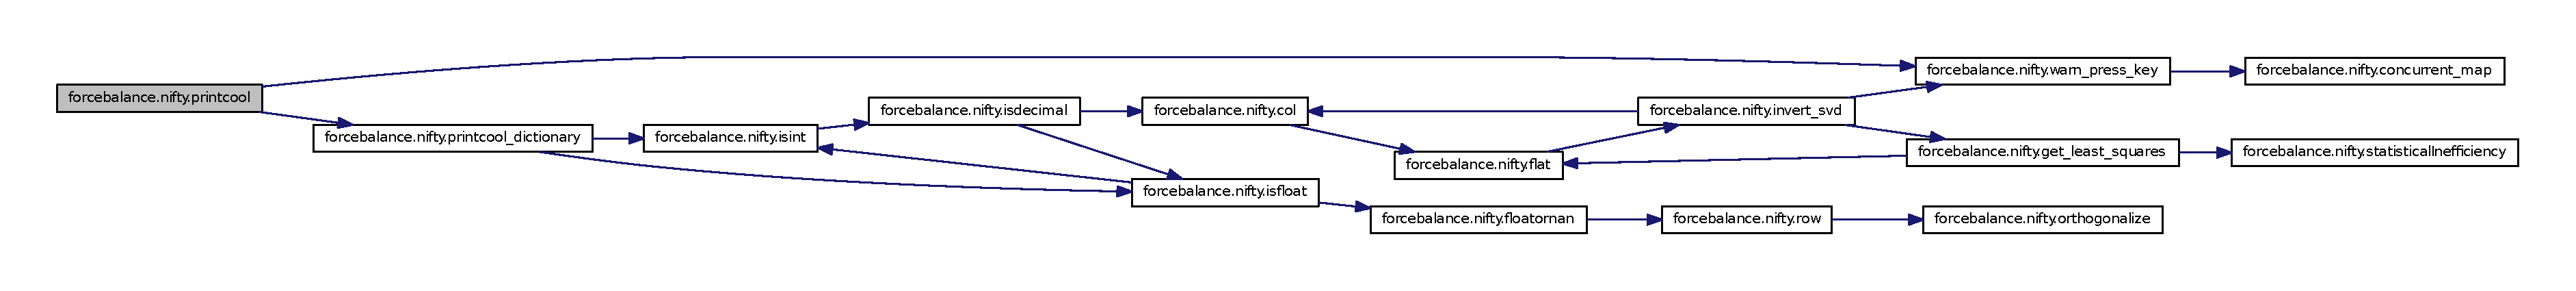
\includegraphics[width=350pt]{namespaceforcebalance_1_1nifty_a11babd62dc7bca389162c6318f9672ca_cgraph}
\end{center}
\end{figure}


\hypertarget{namespaceforcebalance_1_1nifty_a51180e960742cc7547749fdfb3513ec4}{\index{forcebalance\-::nifty@{forcebalance\-::nifty}!printcool\-\_\-dictionary@{printcool\-\_\-dictionary}}
\index{printcool\-\_\-dictionary@{printcool\-\_\-dictionary}!forcebalance::nifty@{forcebalance\-::nifty}}
\paragraph[{printcool\-\_\-dictionary}]{\setlength{\rightskip}{0pt plus 5cm}def forcebalance.\-nifty.\-printcool\-\_\-dictionary (
\begin{DoxyParamCaption}
\item[{}]{Dict, }
\item[{}]{title = {\ttfamily \char`\"{}General~options\char`\"{}}, }
\item[{}]{bold = {\ttfamily False}, }
\item[{}]{color = {\ttfamily 2}, }
\item[{}]{keywidth = {\ttfamily 25}, }
\item[{}]{topwidth = {\ttfamily 50}, }
\item[{}]{center = {\ttfamily True}, }
\item[{}]{leftpad = {\ttfamily 0}}
\end{DoxyParamCaption}
)}}\label{namespaceforcebalance_1_1nifty_a51180e960742cc7547749fdfb3513ec4}


See documentation for printcool; this is a nice way to print out keys/values in a dictionary. 

\begin{DoxyVerb} The keys in the dictionary are sorted before printing out.
\end{DoxyVerb}



\begin{DoxyParams}[1]{Parameters}
\mbox{\tt in}  & {\em dict} & The dictionary to be printed \\
\hline
\mbox{\tt in}  & {\em title} & The title of the printout \\
\hline
\end{DoxyParams}


Definition at line 197 of file nifty.\-py.



Here is the call graph for this function\-:\nopagebreak
\begin{figure}[H]
\begin{center}
\leavevmode
\includegraphics[width=350pt]{namespaceforcebalance_1_1nifty_a51180e960742cc7547749fdfb3513ec4_cgraph}
\end{center}
\end{figure}


\hypertarget{namespaceforcebalance_1_1nifty_a27e3a9dc144a5ad505509ac9ede08d7d}{\index{forcebalance\-::nifty@{forcebalance\-::nifty}!pvec1d@{pvec1d}}
\index{pvec1d@{pvec1d}!forcebalance::nifty@{forcebalance\-::nifty}}
\paragraph[{pvec1d}]{\setlength{\rightskip}{0pt plus 5cm}def forcebalance.\-nifty.\-pvec1d (
\begin{DoxyParamCaption}
\item[{}]{vec1d, }
\item[{}]{precision = {\ttfamily 1}, }
\item[{}]{loglevel = {\ttfamily forcebalance.output.INFO}}
\end{DoxyParamCaption}
)}}\label{namespaceforcebalance_1_1nifty_a27e3a9dc144a5ad505509ac9ede08d7d}


Printout of a 1-\/\-D vector. 


\begin{DoxyParams}[1]{Parameters}
\mbox{\tt in}  & {\em vec1d} & a 1-\/\-D vector \\
\hline
\end{DoxyParams}


Definition at line 54 of file nifty.\-py.



Here is the call graph for this function\-:\nopagebreak
\begin{figure}[H]
\begin{center}
\leavevmode
\includegraphics[width=350pt]{namespaceforcebalance_1_1nifty_a27e3a9dc144a5ad505509ac9ede08d7d_cgraph}
\end{center}
\end{figure}


\hypertarget{namespaceforcebalance_1_1nifty_a673f4a044169f5d8d822823989a836a7}{\index{forcebalance\-::nifty@{forcebalance\-::nifty}!queue\-\_\-up@{queue\-\_\-up}}
\index{queue\-\_\-up@{queue\-\_\-up}!forcebalance::nifty@{forcebalance\-::nifty}}
\paragraph[{queue\-\_\-up}]{\setlength{\rightskip}{0pt plus 5cm}def forcebalance.\-nifty.\-queue\-\_\-up (
\begin{DoxyParamCaption}
\item[{}]{wq, }
\item[{}]{command, }
\item[{}]{input\-\_\-files, }
\item[{}]{output\-\_\-files, }
\item[{}]{tgt = {\ttfamily None}, }
\item[{}]{verbose = {\ttfamily True}}
\end{DoxyParamCaption}
)}}\label{namespaceforcebalance_1_1nifty_a673f4a044169f5d8d822823989a836a7}


Submit a job to the Work Queue. 


\begin{DoxyParams}[1]{Parameters}
\mbox{\tt in}  & {\em wq} & (Work Queue Object) \\
\hline
\mbox{\tt in}  & {\em command} & (string) The command to run on the remote worker. \\
\hline
\mbox{\tt in}  & {\em input\-\_\-files} & (list of files) A list of locations of the input files. \\
\hline
\mbox{\tt in}  & {\em output\-\_\-files} & (list of files) A list of locations of the output files. \\
\hline
\end{DoxyParams}


Definition at line 589 of file nifty.\-py.



Here is the call graph for this function\-:\nopagebreak
\begin{figure}[H]
\begin{center}
\leavevmode
\includegraphics[width=350pt]{namespaceforcebalance_1_1nifty_a673f4a044169f5d8d822823989a836a7_cgraph}
\end{center}
\end{figure}


\hypertarget{namespaceforcebalance_1_1nifty_a5d5abeb4a185fde64721d044831e18ee}{\index{forcebalance\-::nifty@{forcebalance\-::nifty}!queue\-\_\-up\-\_\-src\-\_\-dest@{queue\-\_\-up\-\_\-src\-\_\-dest}}
\index{queue\-\_\-up\-\_\-src\-\_\-dest@{queue\-\_\-up\-\_\-src\-\_\-dest}!forcebalance::nifty@{forcebalance\-::nifty}}
\paragraph[{queue\-\_\-up\-\_\-src\-\_\-dest}]{\setlength{\rightskip}{0pt plus 5cm}def forcebalance.\-nifty.\-queue\-\_\-up\-\_\-src\-\_\-dest (
\begin{DoxyParamCaption}
\item[{}]{wq, }
\item[{}]{command, }
\item[{}]{input\-\_\-files, }
\item[{}]{output\-\_\-files, }
\item[{}]{tgt = {\ttfamily None}, }
\item[{}]{verbose = {\ttfamily True}}
\end{DoxyParamCaption}
)}}\label{namespaceforcebalance_1_1nifty_a5d5abeb4a185fde64721d044831e18ee}


Submit a job to the Work Queue. 

This function is a bit fancier in that we can explicitly specify where the input files come from, and where the output files go to.


\begin{DoxyParams}[1]{Parameters}
\mbox{\tt in}  & {\em wq} & (Work Queue Object) \\
\hline
\mbox{\tt in}  & {\em command} & (string) The command to run on the remote worker. \\
\hline
\mbox{\tt in}  & {\em input\-\_\-files} & (list of 2-\/tuples) A list of local and remote locations of the input files. \\
\hline
\mbox{\tt in}  & {\em output\-\_\-files} & (list of 2-\/tuples) A list of local and remote locations of the output files. \\
\hline
\end{DoxyParams}


Definition at line 620 of file nifty.\-py.

\hypertarget{namespaceforcebalance_1_1nifty_a25efa4d501ad852a234721af18978f7e}{\index{forcebalance\-::nifty@{forcebalance\-::nifty}!remove\-\_\-if\-\_\-exists@{remove\-\_\-if\-\_\-exists}}
\index{remove\-\_\-if\-\_\-exists@{remove\-\_\-if\-\_\-exists}!forcebalance::nifty@{forcebalance\-::nifty}}
\paragraph[{remove\-\_\-if\-\_\-exists}]{\setlength{\rightskip}{0pt plus 5cm}def forcebalance.\-nifty.\-remove\-\_\-if\-\_\-exists (
\begin{DoxyParamCaption}
\item[{}]{fnm}
\end{DoxyParamCaption}
)}}\label{namespaceforcebalance_1_1nifty_a25efa4d501ad852a234721af18978f7e}


Remove the file if it exists (doesn't return an error). 



Definition at line 775 of file nifty.\-py.

\hypertarget{namespaceforcebalance_1_1nifty_a6c9727360cdff8f3011a12cc54d0e86e}{\index{forcebalance\-::nifty@{forcebalance\-::nifty}!row@{row}}
\index{row@{row}!forcebalance::nifty@{forcebalance\-::nifty}}
\paragraph[{row}]{\setlength{\rightskip}{0pt plus 5cm}def forcebalance.\-nifty.\-row (
\begin{DoxyParamCaption}
\item[{}]{vec}
\end{DoxyParamCaption}
)}}\label{namespaceforcebalance_1_1nifty_a6c9727360cdff8f3011a12cc54d0e86e}


Given any list, array, or matrix, return a 1-\/row matrix. 


\begin{DoxyParams}[1]{Parameters}
\mbox{\tt in}  & {\em vec} & The input vector that is to be made into a row\\
\hline
\end{DoxyParams}
\begin{DoxyReturn}{Returns}
answer A row matrix 
\end{DoxyReturn}


Definition at line 280 of file nifty.\-py.



Here is the call graph for this function\-:\nopagebreak
\begin{figure}[H]
\begin{center}
\leavevmode
\includegraphics[width=350pt]{namespaceforcebalance_1_1nifty_a6c9727360cdff8f3011a12cc54d0e86e_cgraph}
\end{center}
\end{figure}


\hypertarget{namespaceforcebalance_1_1nifty_a3b9fd8e29c5d8f1b2114e4d9662dfd61}{\index{forcebalance\-::nifty@{forcebalance\-::nifty}!segments@{segments}}
\index{segments@{segments}!forcebalance::nifty@{forcebalance\-::nifty}}
\paragraph[{segments}]{\setlength{\rightskip}{0pt plus 5cm}def forcebalance.\-nifty.\-segments (
\begin{DoxyParamCaption}
\item[{}]{e}
\end{DoxyParamCaption}
)}}\label{namespaceforcebalance_1_1nifty_a3b9fd8e29c5d8f1b2114e4d9662dfd61}


Definition at line 75 of file nifty.\-py.



Here is the call graph for this function\-:\nopagebreak
\begin{figure}[H]
\begin{center}
\leavevmode
\includegraphics[width=350pt]{namespaceforcebalance_1_1nifty_a3b9fd8e29c5d8f1b2114e4d9662dfd61_cgraph}
\end{center}
\end{figure}


\hypertarget{namespaceforcebalance_1_1nifty_ad5ca60565c864b4245a8212fe9d92e10}{\index{forcebalance\-::nifty@{forcebalance\-::nifty}!statistical\-Inefficiency@{statistical\-Inefficiency}}
\index{statistical\-Inefficiency@{statistical\-Inefficiency}!forcebalance::nifty@{forcebalance\-::nifty}}
\paragraph[{statistical\-Inefficiency}]{\setlength{\rightskip}{0pt plus 5cm}def forcebalance.\-nifty.\-statistical\-Inefficiency (
\begin{DoxyParamCaption}
\item[{}]{A\-\_\-n, }
\item[{}]{B\-\_\-n = {\ttfamily None}, }
\item[{}]{fast = {\ttfamily False}, }
\item[{}]{mintime = {\ttfamily 3}, }
\item[{}]{warn = {\ttfamily True}}
\end{DoxyParamCaption}
)}}\label{namespaceforcebalance_1_1nifty_ad5ca60565c864b4245a8212fe9d92e10}


Compute the (cross) statistical inefficiency of (two) timeseries. 

\begin{DoxyVerb} Notes
   The same timeseries can be used for both A_n and B_n to get the autocorrelation statistical inefficiency.
   The fast method described in Ref [1] is used to compute g.

 References
   [1] J. D. Chodera, W. C. Swope, J. W. Pitera, C. Seok, and K. A. Dill. Use of the weighted
   histogram analysis method for the analysis of simulated and parallel tempering simulations.
   JCTC 3(1):26-41, 2007.

 Examples

 Compute statistical inefficiency of timeseries data with known correlation time.

 >>> import timeseries
 >>> A_n = timeseries.generateCorrelatedTimeseries(N=100000, tau=5.0)
 >>> g = statisticalInefficiency(A_n, fast=True)
\end{DoxyVerb}



\begin{DoxyParams}[1]{Parameters}
\mbox{\tt in}  & {\em A\-\_\-n} & (required, numpy array) -\/ A\-\_\-n\mbox{[}n\mbox{]} is nth value of timeseries A. Length is deduced from vector.\\
\hline
\mbox{\tt in}  & {\em B\-\_\-n} & (optional, numpy array) -\/ B\-\_\-n\mbox{[}n\mbox{]} is nth value of timeseries B. Length is deduced from vector. If supplied, the cross-\/correlation of timeseries A and B will be estimated instead of the autocorrelation of timeseries A.\\
\hline
\mbox{\tt in}  & {\em fast} & (optional, boolean) -\/ if True, will use faster (but less accurate) method to estimate correlation time, described in Ref. \mbox{[}1\mbox{]} (default\-: False)\\
\hline
\mbox{\tt in}  & {\em mintime} & (optional, int) -\/ minimum amount of correlation function to compute (default\-: 3) The algorithm terminates after computing the correlation time out to mintime when the correlation function furst goes negative. Note that this time may need to be increased if there is a strong initial negative peak in the correlation function.\\
\hline
\end{DoxyParams}
\begin{DoxyReturn}{Returns}
g The estimated statistical inefficiency (equal to 1 + 2 tau, where tau is the correlation time). We enforce g $>$= 1.\-0. 
\end{DoxyReturn}


Definition at line 433 of file nifty.\-py.

\hypertarget{namespaceforcebalance_1_1nifty_afa670d68f01813ac8d429bc5cbdb4f9f}{\index{forcebalance\-::nifty@{forcebalance\-::nifty}!uncommadash@{uncommadash}}
\index{uncommadash@{uncommadash}!forcebalance::nifty@{forcebalance\-::nifty}}
\paragraph[{uncommadash}]{\setlength{\rightskip}{0pt plus 5cm}def forcebalance.\-nifty.\-uncommadash (
\begin{DoxyParamCaption}
\item[{}]{s}
\end{DoxyParamCaption}
)}}\label{namespaceforcebalance_1_1nifty_afa670d68f01813ac8d429bc5cbdb4f9f}


Definition at line 91 of file nifty.\-py.



Here is the call graph for this function\-:\nopagebreak
\begin{figure}[H]
\begin{center}
\leavevmode
\includegraphics[width=350pt]{namespaceforcebalance_1_1nifty_afa670d68f01813ac8d429bc5cbdb4f9f_cgraph}
\end{center}
\end{figure}


\hypertarget{namespaceforcebalance_1_1nifty_a26e563ec71ed229c30f3d61d3448c8f1}{\index{forcebalance\-::nifty@{forcebalance\-::nifty}!warn\-\_\-once@{warn\-\_\-once}}
\index{warn\-\_\-once@{warn\-\_\-once}!forcebalance::nifty@{forcebalance\-::nifty}}
\paragraph[{warn\-\_\-once}]{\setlength{\rightskip}{0pt plus 5cm}def forcebalance.\-nifty.\-warn\-\_\-once (
\begin{DoxyParamCaption}
\item[{}]{warning, }
\item[{}]{warnhash = {\ttfamily None}}
\end{DoxyParamCaption}
)}}\label{namespaceforcebalance_1_1nifty_a26e563ec71ed229c30f3d61d3448c8f1}


Prints a warning but will only do so once in a given run. 



Definition at line 887 of file nifty.\-py.



Here is the call graph for this function\-:\nopagebreak
\begin{figure}[H]
\begin{center}
\leavevmode
\includegraphics[width=350pt]{namespaceforcebalance_1_1nifty_a26e563ec71ed229c30f3d61d3448c8f1_cgraph}
\end{center}
\end{figure}


\hypertarget{namespaceforcebalance_1_1nifty_abb8f59044961a12588e0653c2baa8b01}{\index{forcebalance\-::nifty@{forcebalance\-::nifty}!warn\-\_\-press\-\_\-key@{warn\-\_\-press\-\_\-key}}
\index{warn\-\_\-press\-\_\-key@{warn\-\_\-press\-\_\-key}!forcebalance::nifty@{forcebalance\-::nifty}}
\paragraph[{warn\-\_\-press\-\_\-key}]{\setlength{\rightskip}{0pt plus 5cm}def forcebalance.\-nifty.\-warn\-\_\-press\-\_\-key (
\begin{DoxyParamCaption}
\item[{}]{warning, }
\item[{}]{timeout = {\ttfamily 10}}
\end{DoxyParamCaption}
)}}\label{namespaceforcebalance_1_1nifty_abb8f59044961a12588e0653c2baa8b01}


Definition at line 872 of file nifty.\-py.



Here is the call graph for this function\-:\nopagebreak
\begin{figure}[H]
\begin{center}
\leavevmode
\includegraphics[width=350pt]{namespaceforcebalance_1_1nifty_abb8f59044961a12588e0653c2baa8b01_cgraph}
\end{center}
\end{figure}


\hypertarget{namespaceforcebalance_1_1nifty_aa1ff334c4b4e30e91978b91d9a9ec065}{\index{forcebalance\-::nifty@{forcebalance\-::nifty}!which@{which}}
\index{which@{which}!forcebalance::nifty@{forcebalance\-::nifty}}
\paragraph[{which}]{\setlength{\rightskip}{0pt plus 5cm}def forcebalance.\-nifty.\-which (
\begin{DoxyParamCaption}
\item[{}]{fnm}
\end{DoxyParamCaption}
)}}\label{namespaceforcebalance_1_1nifty_aa1ff334c4b4e30e91978b91d9a9ec065}


Definition at line 779 of file nifty.\-py.



Here is the call graph for this function\-:\nopagebreak
\begin{figure}[H]
\begin{center}
\leavevmode
\includegraphics[width=350pt]{namespaceforcebalance_1_1nifty_aa1ff334c4b4e30e91978b91d9a9ec065_cgraph}
\end{center}
\end{figure}


\hypertarget{namespaceforcebalance_1_1nifty_a576de8c5b6f236280e07e73e39b2ab7c}{\index{forcebalance\-::nifty@{forcebalance\-::nifty}!wq\-\_\-wait@{wq\-\_\-wait}}
\index{wq\-\_\-wait@{wq\-\_\-wait}!forcebalance::nifty@{forcebalance\-::nifty}}
\paragraph[{wq\-\_\-wait}]{\setlength{\rightskip}{0pt plus 5cm}def forcebalance.\-nifty.\-wq\-\_\-wait (
\begin{DoxyParamCaption}
\item[{}]{wq, }
\item[{}]{verbose = {\ttfamily False}}
\end{DoxyParamCaption}
)}}\label{namespaceforcebalance_1_1nifty_a576de8c5b6f236280e07e73e39b2ab7c}


This function waits until the work queue is completely empty. 



Definition at line 691 of file nifty.\-py.



Here is the call graph for this function\-:\nopagebreak
\begin{figure}[H]
\begin{center}
\leavevmode
\includegraphics[width=350pt]{namespaceforcebalance_1_1nifty_a576de8c5b6f236280e07e73e39b2ab7c_cgraph}
\end{center}
\end{figure}


\hypertarget{namespaceforcebalance_1_1nifty_a374aac2ef003be02fab49b20ff0a82f0}{\index{forcebalance\-::nifty@{forcebalance\-::nifty}!wq\-\_\-wait1@{wq\-\_\-wait1}}
\index{wq\-\_\-wait1@{wq\-\_\-wait1}!forcebalance::nifty@{forcebalance\-::nifty}}
\paragraph[{wq\-\_\-wait1}]{\setlength{\rightskip}{0pt plus 5cm}def forcebalance.\-nifty.\-wq\-\_\-wait1 (
\begin{DoxyParamCaption}
\item[{}]{wq, }
\item[{}]{wait\-\_\-time = {\ttfamily 10}, }
\item[{}]{verbose = {\ttfamily False}}
\end{DoxyParamCaption}
)}}\label{namespaceforcebalance_1_1nifty_a374aac2ef003be02fab49b20ff0a82f0}


This function waits ten seconds to see if a task in the Work Queue has finished. 



Definition at line 640 of file nifty.\-py.



Here is the call graph for this function\-:\nopagebreak
\begin{figure}[H]
\begin{center}
\leavevmode
\includegraphics[width=350pt]{namespaceforcebalance_1_1nifty_a374aac2ef003be02fab49b20ff0a82f0_cgraph}
\end{center}
\end{figure}




\subsubsection{Variable Documentation}
\hypertarget{namespaceforcebalance_1_1nifty_a31a8d4a4240a1325bd4fa10033b7eee0}{\index{forcebalance\-::nifty@{forcebalance\-::nifty}!bohrang@{bohrang}}
\index{bohrang@{bohrang}!forcebalance::nifty@{forcebalance\-::nifty}}
\paragraph[{bohrang}]{\setlength{\rightskip}{0pt plus 5cm}float forcebalance.\-nifty.\-bohrang = 0.\-529177249}}\label{namespaceforcebalance_1_1nifty_a31a8d4a4240a1325bd4fa10033b7eee0}


One bohr equals this many angstroms. 



Definition at line 44 of file nifty.\-py.

\hypertarget{namespaceforcebalance_1_1nifty_a7cec4d46378b888cd867de05d0168d96}{\index{forcebalance\-::nifty@{forcebalance\-::nifty}!eqcgmx@{eqcgmx}}
\index{eqcgmx@{eqcgmx}!forcebalance::nifty@{forcebalance\-::nifty}}
\paragraph[{eqcgmx}]{\setlength{\rightskip}{0pt plus 5cm}float forcebalance.\-nifty.\-eqcgmx = 2625.\-5002}}\label{namespaceforcebalance_1_1nifty_a7cec4d46378b888cd867de05d0168d96}


Q-\/\-Chem to G\-M\-X unit conversion for energy. 



Definition at line 40 of file nifty.\-py.

\hypertarget{namespaceforcebalance_1_1nifty_ab1ec21beaae0d8328e7e4c3b89d972ab}{\index{forcebalance\-::nifty@{forcebalance\-::nifty}!fqcgmx@{fqcgmx}}
\index{fqcgmx@{fqcgmx}!forcebalance::nifty@{forcebalance\-::nifty}}
\paragraph[{fqcgmx}]{\setlength{\rightskip}{0pt plus 5cm}float forcebalance.\-nifty.\-fqcgmx = -\/49621.\-9}}\label{namespaceforcebalance_1_1nifty_ab1ec21beaae0d8328e7e4c3b89d972ab}


Q-\/\-Chem to G\-M\-X unit conversion for force. 



Definition at line 42 of file nifty.\-py.

\hypertarget{namespaceforcebalance_1_1nifty_ae0916a3186f4f8b238a0d58bb9f6a3da}{\index{forcebalance\-::nifty@{forcebalance\-::nifty}!kb@{kb}}
\index{kb@{kb}!forcebalance::nifty@{forcebalance\-::nifty}}
\paragraph[{kb}]{\setlength{\rightskip}{0pt plus 5cm}float forcebalance.\-nifty.\-kb = 0.\-0083144100163}}\label{namespaceforcebalance_1_1nifty_ae0916a3186f4f8b238a0d58bb9f6a3da}


Boltzmann constant. 



Definition at line 38 of file nifty.\-py.

\hypertarget{namespaceforcebalance_1_1nifty_a1859e992ed983dbbcc8093fdd19710e7}{\index{forcebalance\-::nifty@{forcebalance\-::nifty}!logger@{logger}}
\index{logger@{logger}!forcebalance::nifty@{forcebalance\-::nifty}}
\paragraph[{logger}]{\setlength{\rightskip}{0pt plus 5cm}tuple forcebalance.\-nifty.\-logger = get\-Logger(\-\_\-\-\_\-name\-\_\-\-\_\-)}}\label{namespaceforcebalance_1_1nifty_a1859e992ed983dbbcc8093fdd19710e7}


Definition at line 34 of file nifty.\-py.

\hypertarget{namespaceforcebalance_1_1nifty_ab652c941890b0f378100433699c8d255}{\index{forcebalance\-::nifty@{forcebalance\-::nifty}!specific\-\_\-dct@{specific\-\_\-dct}}
\index{specific\-\_\-dct@{specific\-\_\-dct}!forcebalance::nifty@{forcebalance\-::nifty}}
\paragraph[{specific\-\_\-dct}]{\setlength{\rightskip}{0pt plus 5cm}tuple forcebalance.\-nifty.\-specific\-\_\-dct = dict(list(itertools.\-chain($\ast$\mbox{[}\mbox{[}(j,i\mbox{[}1\mbox{]}) for j in i\mbox{[}0\mbox{]}\mbox{]} for i in {\bf specific\-\_\-lst}\mbox{]})))}}\label{namespaceforcebalance_1_1nifty_ab652c941890b0f378100433699c8d255}


Definition at line 731 of file nifty.\-py.

\hypertarget{namespaceforcebalance_1_1nifty_abe850bcdf26cec4a0cf913a54a7ddfaa}{\index{forcebalance\-::nifty@{forcebalance\-::nifty}!specific\-\_\-lst@{specific\-\_\-lst}}
\index{specific\-\_\-lst@{specific\-\_\-lst}!forcebalance::nifty@{forcebalance\-::nifty}}
\paragraph[{specific\-\_\-lst}]{\setlength{\rightskip}{0pt plus 5cm}list forcebalance.\-nifty.\-specific\-\_\-lst}}\label{namespaceforcebalance_1_1nifty_abe850bcdf26cec4a0cf913a54a7ddfaa}
{\bfseries Initial value\-:}
\begin{DoxyCode}
1 = [([\textcolor{stringliteral}{'mdrun'},\textcolor{stringliteral}{'grompp'},\textcolor{stringliteral}{'trjconv'},\textcolor{stringliteral}{'g\_energy'},\textcolor{stringliteral}{'g\_traj'}], \textcolor{stringliteral}{"Make sure to install GROMACS and add it to your path
       (or set the gmxpath option)"}),
2                 ([\textcolor{stringliteral}{'force.mdin'}, \textcolor{stringliteral}{'stage.leap'}], \textcolor{stringliteral}{"This file is needed for setting up AMBER force matching
       targets"}),
3                 ([\textcolor{stringliteral}{'conf.pdb'}, \textcolor{stringliteral}{'mono.pdb'}], \textcolor{stringliteral}{"This file is needed for setting up OpenMM condensed phase
       property targets"}),
4                 ([\textcolor{stringliteral}{'liquid.xyz'}, \textcolor{stringliteral}{'liquid.key'}, \textcolor{stringliteral}{'mono.xyz'}, \textcolor{stringliteral}{'mono.key'}], \textcolor{stringliteral}{"This file is needed for setting up
       OpenMM condensed phase property targets"}),
5                 ([\textcolor{stringliteral}{'dynamic'}, \textcolor{stringliteral}{'analyze'}, \textcolor{stringliteral}{'minimize'}, \textcolor{stringliteral}{'testgrad'}, \textcolor{stringliteral}{'vibrate'}, \textcolor{stringliteral}{'optimize'}, \textcolor{stringliteral}{'polarize'}, \textcolor{stringliteral}{'
      superpose'}], \textcolor{stringliteral}{"Make sure to install TINKER and add it to your path (or set the tinkerpath option)"}),
6                 ([\textcolor{stringliteral}{'runcuda.sh'}, \textcolor{stringliteral}{'npt.py'}, \textcolor{stringliteral}{'npt\_tinker.py'}], \textcolor{stringliteral}{"This file belongs in the ForceBalance source
       directory, not sure why it is missing"}),
7                 ([\textcolor{stringliteral}{'input.xyz'}], \textcolor{stringliteral}{"This file is needed for TINKER molecular property targets"}),
8                 ([\textcolor{stringliteral}{'.*key$'}, \textcolor{stringliteral}{'.*xyz$'}], \textcolor{stringliteral}{"I am guessing this file is probably needed by TINKER"}),
9                 ([\textcolor{stringliteral}{'.*gro$'}, \textcolor{stringliteral}{'.*top$'}, \textcolor{stringliteral}{'.*itp$'}, \textcolor{stringliteral}{'.*mdp$'}, \textcolor{stringliteral}{'.*ndx$'}], \textcolor{stringliteral}{"I am guessing this file is probably
       needed by GROMACS"})
10                 ]
\end{DoxyCode}


Definition at line 719 of file nifty.\-py.

\hypertarget{namespaceforcebalance_1_1nifty_a338d5080f95188c37271c306f64093d8}{\index{forcebalance\-::nifty@{forcebalance\-::nifty}!X\-M\-L\-F\-I\-L\-E@{X\-M\-L\-F\-I\-L\-E}}
\index{X\-M\-L\-F\-I\-L\-E@{X\-M\-L\-F\-I\-L\-E}!forcebalance::nifty@{forcebalance\-::nifty}}
\paragraph[{X\-M\-L\-F\-I\-L\-E}]{\setlength{\rightskip}{0pt plus 5cm}string forcebalance.\-nifty.\-X\-M\-L\-F\-I\-L\-E = 'x'}}\label{namespaceforcebalance_1_1nifty_a338d5080f95188c37271c306f64093d8}


Pickle uses 'flags' to pickle and unpickle different variable types. 

Here we use the letter 'x' to signify that the variable type is an X\-M\-L file. 

Definition at line 495 of file nifty.\-py.


\hypertarget{namespaceforcebalance_1_1objective}{\subsection{forcebalance\-:\-:objective \-Namespace \-Reference}
\label{namespaceforcebalance_1_1objective}\index{forcebalance\-::objective@{forcebalance\-::objective}}
}


\-Force\-Balance objective function.  


\subsubsection*{\-Classes}
\begin{DoxyCompactItemize}
\item 
class \hyperlink{classforcebalance_1_1objective_1_1Objective}{\-Objective}
\begin{DoxyCompactList}\small\item\em \hyperlink{classforcebalance_1_1objective_1_1Objective}{\-Objective} function. \end{DoxyCompactList}\item 
class \hyperlink{classforcebalance_1_1objective_1_1Penalty}{\-Penalty}
\begin{DoxyCompactList}\small\item\em \hyperlink{classforcebalance_1_1objective_1_1Penalty}{\-Penalty} functions for regularizing the force field optimizer. \end{DoxyCompactList}\end{DoxyCompactItemize}
\subsubsection*{\-Variables}
\begin{DoxyCompactItemize}
\item 
tuple \hyperlink{namespaceforcebalance_1_1objective_afa1d976cc1f8b18cf0b03f1ccf49f590}{logger} = get\-Logger(\-\_\-\-\_\-name\-\_\-\-\_\-)
\item 
dictionary \hyperlink{namespaceforcebalance_1_1objective_aad3b66466fd22980d2c83c67b82ddddf}{\-Implemented\-\_\-\-Targets}
\begin{DoxyCompactList}\small\item\em \-The table of implemented \-Targets. \end{DoxyCompactList}\item 
list \hyperlink{namespaceforcebalance_1_1objective_a01660ebc02853011e66350c410e26f0a}{\-Letters} = \mbox{[}'\-X','\-G','\-H'\mbox{]}
\begin{DoxyCompactList}\small\item\em \-This is the canonical lettering that corresponds to \-: objective function, gradient, \-Hessian. \end{DoxyCompactList}\end{DoxyCompactItemize}


\subsubsection{\-Detailed \-Description}
\-Force\-Balance objective function. 

\subsubsection{\-Variable \-Documentation}
\hypertarget{namespaceforcebalance_1_1objective_aad3b66466fd22980d2c83c67b82ddddf}{\index{forcebalance\-::objective@{forcebalance\-::objective}!\-Implemented\-\_\-\-Targets@{\-Implemented\-\_\-\-Targets}}
\index{\-Implemented\-\_\-\-Targets@{\-Implemented\-\_\-\-Targets}!forcebalance::objective@{forcebalance\-::objective}}
\paragraph[{\-Implemented\-\_\-\-Targets}]{\setlength{\rightskip}{0pt plus 5cm}dictionary {\bf forcebalance\-::objective\-::\-Implemented\-\_\-\-Targets}}}\label{namespaceforcebalance_1_1objective_aad3b66466fd22980d2c83c67b82ddddf}
{\bfseries \-Initial value\-:}
\begin{DoxyCode}
1 {
2     'ABINITIO_GMX':AbInitio_GMX,
3     'ABINITIO_TINKER':AbInitio_TINKER,
4     'ABINITIO_OPENMM':AbInitio_OpenMM,
5     'ABINITIO_AMBER':AbInitio_AMBER,
6     'ABINITIO_INTERNAL':AbInitio_Internal,
7     'VIBRATION_TINKER':Vibration_TINKER,
8     'LIQUID_OPENMM':Liquid_OpenMM,
9     'LIQUID_TINKER':Liquid_TINKER, 
10     'LIQUID_GMX':Liquid_GMX, 
11     'COUNTERPOISE':Counterpoise,
12     'THCDF_PSI4':THCDF_Psi4,
13     'RDVR3_PSI4':RDVR3_Psi4,
14     'INTERACTION_TINKER':Interaction_TINKER,
15     'INTERACTION_OPENMM':Interaction_OpenMM,
16     'BINDINGENERGY_TINKER':BindingEnergy_TINKER,
17     'MOMENTS_TINKER':Moments_TINKER,
18     'MONOMER_QTPIE':Monomer_QTPIE,
19     }
\end{DoxyCode}


\-The table of implemented \-Targets. 



\-Definition at line 68 of file objective.\-py.

\hypertarget{namespaceforcebalance_1_1objective_a01660ebc02853011e66350c410e26f0a}{\index{forcebalance\-::objective@{forcebalance\-::objective}!\-Letters@{\-Letters}}
\index{\-Letters@{\-Letters}!forcebalance::objective@{forcebalance\-::objective}}
\paragraph[{\-Letters}]{\setlength{\rightskip}{0pt plus 5cm}list {\bf forcebalance\-::objective\-::\-Letters} = \mbox{[}'\-X','\-G','\-H'\mbox{]}}}\label{namespaceforcebalance_1_1objective_a01660ebc02853011e66350c410e26f0a}


\-This is the canonical lettering that corresponds to \-: objective function, gradient, \-Hessian. 



\-Definition at line 89 of file objective.\-py.

\hypertarget{namespaceforcebalance_1_1objective_afa1d976cc1f8b18cf0b03f1ccf49f590}{\index{forcebalance\-::objective@{forcebalance\-::objective}!logger@{logger}}
\index{logger@{logger}!forcebalance::objective@{forcebalance\-::objective}}
\paragraph[{logger}]{\setlength{\rightskip}{0pt plus 5cm}tuple {\bf forcebalance\-::objective\-::logger} = get\-Logger(\-\_\-\-\_\-name\-\_\-\-\_\-)}}\label{namespaceforcebalance_1_1objective_afa1d976cc1f8b18cf0b03f1ccf49f590}


\-Definition at line 17 of file objective.\-py.


\hypertarget{namespaceforcebalance_1_1openmmio}{\subsection{forcebalance.\-openmmio Namespace Reference}
\label{namespaceforcebalance_1_1openmmio}\index{forcebalance.\-openmmio@{forcebalance.\-openmmio}}
}


Open\-M\-M input/output.  


\subsubsection*{Classes}
\begin{DoxyCompactItemize}
\item 
class \hyperlink{classforcebalance_1_1openmmio_1_1OpenMM__Reader}{Open\-M\-M\-\_\-\-Reader}
\begin{DoxyCompactList}\small\item\em Class for parsing Open\-M\-M force field files. \end{DoxyCompactList}\item 
class \hyperlink{classforcebalance_1_1openmmio_1_1Liquid__OpenMM}{Liquid\-\_\-\-Open\-M\-M}
\item 
class \hyperlink{classforcebalance_1_1openmmio_1_1AbInitio__OpenMM}{Ab\-Initio\-\_\-\-Open\-M\-M}
\begin{DoxyCompactList}\small\item\em Subclass of Ab\-Initio for force and energy matching using Open\-M\-M. \end{DoxyCompactList}\item 
class \hyperlink{classforcebalance_1_1openmmio_1_1Interaction__OpenMM}{Interaction\-\_\-\-Open\-M\-M}
\begin{DoxyCompactList}\small\item\em Subclass of Target for interaction matching using Open\-M\-M. \end{DoxyCompactList}\end{DoxyCompactItemize}
\subsubsection*{Functions}
\begin{DoxyCompactItemize}
\item 
def \hyperlink{namespaceforcebalance_1_1openmmio_a8a2081dcaf027b9b9ab224e22680714d}{get\-\_\-dipole}
\begin{DoxyCompactList}\small\item\em Return the current dipole moment in Debye. \end{DoxyCompactList}\item 
def \hyperlink{namespaceforcebalance_1_1openmmio_af623fa5af97de6c6a0bc5f98ce8db432}{Reset\-Virtual\-Sites}
\begin{DoxyCompactList}\small\item\em Given a set of Open\-M\-M-\/compatible positions and a System object, compute the correct virtual site positions according to the System. \end{DoxyCompactList}\item 
def \hyperlink{namespaceforcebalance_1_1openmmio_a792a195b31612f2140b35927fe28fa1a}{Copy\-Amoeba\-Bond\-Parameters}
\item 
def \hyperlink{namespaceforcebalance_1_1openmmio_a2e95f600757655d41660c25af8fd8e80}{Copy\-Amoeba\-Out\-Of\-Plane\-Bend\-Parameters}
\item 
def \hyperlink{namespaceforcebalance_1_1openmmio_abe9a6b9b200dc8487e56dad7249af3ec}{Copy\-Amoeba\-Angle\-Parameters}
\item 
def \hyperlink{namespaceforcebalance_1_1openmmio_ad0d4739f80f2aab1a861f2e03b8efcd6}{Copy\-Amoeba\-In\-Plane\-Angle\-Parameters}
\item 
def \hyperlink{namespaceforcebalance_1_1openmmio_abe005f73c6dfe9ce1052c9434bcad9be}{Copy\-Amoeba\-Vdw\-Parameters}
\item 
def \hyperlink{namespaceforcebalance_1_1openmmio_a3706c19e71969cabe5782a4535abeffe}{Copy\-Amoeba\-Multipole\-Parameters}
\item 
def \hyperlink{namespaceforcebalance_1_1openmmio_a616f12cc53381716e5fa41f00bf623be}{Copy\-Harmonic\-Bond\-Parameters}
\item 
def \hyperlink{namespaceforcebalance_1_1openmmio_af4ed16f5e2b1cd12bce2f25fab1b05bc}{Copy\-Harmonic\-Angle\-Parameters}
\item 
def \hyperlink{namespaceforcebalance_1_1openmmio_a8f13702754f0b4e43e272139a2ce8341}{Copy\-Periodic\-Torsion\-Parameters}
\item 
def \hyperlink{namespaceforcebalance_1_1openmmio_afead47464a644d9225f9fa8eb568a8ed}{Copy\-Nonbonded\-Parameters}
\item 
def \hyperlink{namespaceforcebalance_1_1openmmio_a2bb7add6b813d94f2655372c51fe8fdc}{do\-\_\-nothing}
\item 
def \hyperlink{namespaceforcebalance_1_1openmmio_a8c6ed589ec2b35b8363a529ffdf88eb0}{Copy\-System\-Parameters}
\begin{DoxyCompactList}\small\item\em Copy parameters from one system (i.\-e. \end{DoxyCompactList}\item 
def \hyperlink{namespaceforcebalance_1_1openmmio_a9f9fc56475dbfcc94a40fef6a84ed25f}{Update\-Simulation\-Parameters}
\item 
def \hyperlink{namespaceforcebalance_1_1openmmio_aa085594c11e9cd00ce71f5a8ead72b68}{M\-T\-S\-V\-V\-V\-R\-Integrator}
\begin{DoxyCompactList}\small\item\em Create a multiple timestep velocity verlet with velocity randomization (V\-V\-V\-R) integrator. \end{DoxyCompactList}\end{DoxyCompactItemize}
\subsubsection*{Variables}
\begin{DoxyCompactItemize}
\item 
dictionary \hyperlink{namespaceforcebalance_1_1openmmio_aeca37c08912f1a88339680ed75839530}{suffix\-\_\-dict}
\item 
string \hyperlink{namespaceforcebalance_1_1openmmio_af225f2cfdcfd96ebd1d3175c8770a850}{pdict} = \char`\"{}X\-M\-L\-\_\-\-Override\char`\"{}
\begin{DoxyCompactList}\small\item\em pdict is a useless variable if the force field is X\-M\-L. \end{DoxyCompactList}\end{DoxyCompactItemize}


\subsubsection{Detailed Description}
Open\-M\-M input/output. \begin{DoxyAuthor}{Author}
Lee-\/\-Ping Wang 
\end{DoxyAuthor}
\begin{DoxyDate}{Date}
04/2012 
\end{DoxyDate}


\subsubsection{Function Documentation}
\hypertarget{namespaceforcebalance_1_1openmmio_abe9a6b9b200dc8487e56dad7249af3ec}{\index{forcebalance\-::openmmio@{forcebalance\-::openmmio}!Copy\-Amoeba\-Angle\-Parameters@{Copy\-Amoeba\-Angle\-Parameters}}
\index{Copy\-Amoeba\-Angle\-Parameters@{Copy\-Amoeba\-Angle\-Parameters}!forcebalance::openmmio@{forcebalance\-::openmmio}}
\paragraph[{Copy\-Amoeba\-Angle\-Parameters}]{\setlength{\rightskip}{0pt plus 5cm}def forcebalance.\-openmmio.\-Copy\-Amoeba\-Angle\-Parameters (
\begin{DoxyParamCaption}
\item[{}]{src, }
\item[{}]{dest}
\end{DoxyParamCaption}
)}}\label{namespaceforcebalance_1_1openmmio_abe9a6b9b200dc8487e56dad7249af3ec}


Definition at line 109 of file openmmio.\-py.



Here is the call graph for this function\-:\nopagebreak
\begin{figure}[H]
\begin{center}
\leavevmode
\includegraphics[width=350pt]{namespaceforcebalance_1_1openmmio_abe9a6b9b200dc8487e56dad7249af3ec_cgraph}
\end{center}
\end{figure}


\hypertarget{namespaceforcebalance_1_1openmmio_a792a195b31612f2140b35927fe28fa1a}{\index{forcebalance\-::openmmio@{forcebalance\-::openmmio}!Copy\-Amoeba\-Bond\-Parameters@{Copy\-Amoeba\-Bond\-Parameters}}
\index{Copy\-Amoeba\-Bond\-Parameters@{Copy\-Amoeba\-Bond\-Parameters}!forcebalance::openmmio@{forcebalance\-::openmmio}}
\paragraph[{Copy\-Amoeba\-Bond\-Parameters}]{\setlength{\rightskip}{0pt plus 5cm}def forcebalance.\-openmmio.\-Copy\-Amoeba\-Bond\-Parameters (
\begin{DoxyParamCaption}
\item[{}]{src, }
\item[{}]{dest}
\end{DoxyParamCaption}
)}}\label{namespaceforcebalance_1_1openmmio_a792a195b31612f2140b35927fe28fa1a}


Definition at line 95 of file openmmio.\-py.



Here is the call graph for this function\-:\nopagebreak
\begin{figure}[H]
\begin{center}
\leavevmode
\includegraphics[width=350pt]{namespaceforcebalance_1_1openmmio_a792a195b31612f2140b35927fe28fa1a_cgraph}
\end{center}
\end{figure}


\hypertarget{namespaceforcebalance_1_1openmmio_ad0d4739f80f2aab1a861f2e03b8efcd6}{\index{forcebalance\-::openmmio@{forcebalance\-::openmmio}!Copy\-Amoeba\-In\-Plane\-Angle\-Parameters@{Copy\-Amoeba\-In\-Plane\-Angle\-Parameters}}
\index{Copy\-Amoeba\-In\-Plane\-Angle\-Parameters@{Copy\-Amoeba\-In\-Plane\-Angle\-Parameters}!forcebalance::openmmio@{forcebalance\-::openmmio}}
\paragraph[{Copy\-Amoeba\-In\-Plane\-Angle\-Parameters}]{\setlength{\rightskip}{0pt plus 5cm}def forcebalance.\-openmmio.\-Copy\-Amoeba\-In\-Plane\-Angle\-Parameters (
\begin{DoxyParamCaption}
\item[{}]{src, }
\item[{}]{dest}
\end{DoxyParamCaption}
)}}\label{namespaceforcebalance_1_1openmmio_ad0d4739f80f2aab1a861f2e03b8efcd6}


Definition at line 118 of file openmmio.\-py.



Here is the call graph for this function\-:\nopagebreak
\begin{figure}[H]
\begin{center}
\leavevmode
\includegraphics[width=350pt]{namespaceforcebalance_1_1openmmio_ad0d4739f80f2aab1a861f2e03b8efcd6_cgraph}
\end{center}
\end{figure}


\hypertarget{namespaceforcebalance_1_1openmmio_a3706c19e71969cabe5782a4535abeffe}{\index{forcebalance\-::openmmio@{forcebalance\-::openmmio}!Copy\-Amoeba\-Multipole\-Parameters@{Copy\-Amoeba\-Multipole\-Parameters}}
\index{Copy\-Amoeba\-Multipole\-Parameters@{Copy\-Amoeba\-Multipole\-Parameters}!forcebalance::openmmio@{forcebalance\-::openmmio}}
\paragraph[{Copy\-Amoeba\-Multipole\-Parameters}]{\setlength{\rightskip}{0pt plus 5cm}def forcebalance.\-openmmio.\-Copy\-Amoeba\-Multipole\-Parameters (
\begin{DoxyParamCaption}
\item[{}]{src, }
\item[{}]{dest}
\end{DoxyParamCaption}
)}}\label{namespaceforcebalance_1_1openmmio_a3706c19e71969cabe5782a4535abeffe}


Definition at line 131 of file openmmio.\-py.



Here is the call graph for this function\-:\nopagebreak
\begin{figure}[H]
\begin{center}
\leavevmode
\includegraphics[width=350pt]{namespaceforcebalance_1_1openmmio_a3706c19e71969cabe5782a4535abeffe_cgraph}
\end{center}
\end{figure}


\hypertarget{namespaceforcebalance_1_1openmmio_a2e95f600757655d41660c25af8fd8e80}{\index{forcebalance\-::openmmio@{forcebalance\-::openmmio}!Copy\-Amoeba\-Out\-Of\-Plane\-Bend\-Parameters@{Copy\-Amoeba\-Out\-Of\-Plane\-Bend\-Parameters}}
\index{Copy\-Amoeba\-Out\-Of\-Plane\-Bend\-Parameters@{Copy\-Amoeba\-Out\-Of\-Plane\-Bend\-Parameters}!forcebalance::openmmio@{forcebalance\-::openmmio}}
\paragraph[{Copy\-Amoeba\-Out\-Of\-Plane\-Bend\-Parameters}]{\setlength{\rightskip}{0pt plus 5cm}def forcebalance.\-openmmio.\-Copy\-Amoeba\-Out\-Of\-Plane\-Bend\-Parameters (
\begin{DoxyParamCaption}
\item[{}]{src, }
\item[{}]{dest}
\end{DoxyParamCaption}
)}}\label{namespaceforcebalance_1_1openmmio_a2e95f600757655d41660c25af8fd8e80}


Definition at line 101 of file openmmio.\-py.



Here is the call graph for this function\-:\nopagebreak
\begin{figure}[H]
\begin{center}
\leavevmode
\includegraphics[width=350pt]{namespaceforcebalance_1_1openmmio_a2e95f600757655d41660c25af8fd8e80_cgraph}
\end{center}
\end{figure}


\hypertarget{namespaceforcebalance_1_1openmmio_abe005f73c6dfe9ce1052c9434bcad9be}{\index{forcebalance\-::openmmio@{forcebalance\-::openmmio}!Copy\-Amoeba\-Vdw\-Parameters@{Copy\-Amoeba\-Vdw\-Parameters}}
\index{Copy\-Amoeba\-Vdw\-Parameters@{Copy\-Amoeba\-Vdw\-Parameters}!forcebalance::openmmio@{forcebalance\-::openmmio}}
\paragraph[{Copy\-Amoeba\-Vdw\-Parameters}]{\setlength{\rightskip}{0pt plus 5cm}def forcebalance.\-openmmio.\-Copy\-Amoeba\-Vdw\-Parameters (
\begin{DoxyParamCaption}
\item[{}]{src, }
\item[{}]{dest}
\end{DoxyParamCaption}
)}}\label{namespaceforcebalance_1_1openmmio_abe005f73c6dfe9ce1052c9434bcad9be}


Definition at line 127 of file openmmio.\-py.



Here is the call graph for this function\-:\nopagebreak
\begin{figure}[H]
\begin{center}
\leavevmode
\includegraphics[width=350pt]{namespaceforcebalance_1_1openmmio_abe005f73c6dfe9ce1052c9434bcad9be_cgraph}
\end{center}
\end{figure}


\hypertarget{namespaceforcebalance_1_1openmmio_af4ed16f5e2b1cd12bce2f25fab1b05bc}{\index{forcebalance\-::openmmio@{forcebalance\-::openmmio}!Copy\-Harmonic\-Angle\-Parameters@{Copy\-Harmonic\-Angle\-Parameters}}
\index{Copy\-Harmonic\-Angle\-Parameters@{Copy\-Harmonic\-Angle\-Parameters}!forcebalance::openmmio@{forcebalance\-::openmmio}}
\paragraph[{Copy\-Harmonic\-Angle\-Parameters}]{\setlength{\rightskip}{0pt plus 5cm}def forcebalance.\-openmmio.\-Copy\-Harmonic\-Angle\-Parameters (
\begin{DoxyParamCaption}
\item[{}]{src, }
\item[{}]{dest}
\end{DoxyParamCaption}
)}}\label{namespaceforcebalance_1_1openmmio_af4ed16f5e2b1cd12bce2f25fab1b05bc}


Definition at line 139 of file openmmio.\-py.



Here is the call graph for this function\-:\nopagebreak
\begin{figure}[H]
\begin{center}
\leavevmode
\includegraphics[width=350pt]{namespaceforcebalance_1_1openmmio_af4ed16f5e2b1cd12bce2f25fab1b05bc_cgraph}
\end{center}
\end{figure}


\hypertarget{namespaceforcebalance_1_1openmmio_a616f12cc53381716e5fa41f00bf623be}{\index{forcebalance\-::openmmio@{forcebalance\-::openmmio}!Copy\-Harmonic\-Bond\-Parameters@{Copy\-Harmonic\-Bond\-Parameters}}
\index{Copy\-Harmonic\-Bond\-Parameters@{Copy\-Harmonic\-Bond\-Parameters}!forcebalance::openmmio@{forcebalance\-::openmmio}}
\paragraph[{Copy\-Harmonic\-Bond\-Parameters}]{\setlength{\rightskip}{0pt plus 5cm}def forcebalance.\-openmmio.\-Copy\-Harmonic\-Bond\-Parameters (
\begin{DoxyParamCaption}
\item[{}]{src, }
\item[{}]{dest}
\end{DoxyParamCaption}
)}}\label{namespaceforcebalance_1_1openmmio_a616f12cc53381716e5fa41f00bf623be}


Definition at line 135 of file openmmio.\-py.



Here is the call graph for this function\-:\nopagebreak
\begin{figure}[H]
\begin{center}
\leavevmode
\includegraphics[width=350pt]{namespaceforcebalance_1_1openmmio_a616f12cc53381716e5fa41f00bf623be_cgraph}
\end{center}
\end{figure}


\hypertarget{namespaceforcebalance_1_1openmmio_afead47464a644d9225f9fa8eb568a8ed}{\index{forcebalance\-::openmmio@{forcebalance\-::openmmio}!Copy\-Nonbonded\-Parameters@{Copy\-Nonbonded\-Parameters}}
\index{Copy\-Nonbonded\-Parameters@{Copy\-Nonbonded\-Parameters}!forcebalance::openmmio@{forcebalance\-::openmmio}}
\paragraph[{Copy\-Nonbonded\-Parameters}]{\setlength{\rightskip}{0pt plus 5cm}def forcebalance.\-openmmio.\-Copy\-Nonbonded\-Parameters (
\begin{DoxyParamCaption}
\item[{}]{src, }
\item[{}]{dest}
\end{DoxyParamCaption}
)}}\label{namespaceforcebalance_1_1openmmio_afead47464a644d9225f9fa8eb568a8ed}


Definition at line 147 of file openmmio.\-py.



Here is the call graph for this function\-:\nopagebreak
\begin{figure}[H]
\begin{center}
\leavevmode
\includegraphics[width=350pt]{namespaceforcebalance_1_1openmmio_afead47464a644d9225f9fa8eb568a8ed_cgraph}
\end{center}
\end{figure}


\hypertarget{namespaceforcebalance_1_1openmmio_a8f13702754f0b4e43e272139a2ce8341}{\index{forcebalance\-::openmmio@{forcebalance\-::openmmio}!Copy\-Periodic\-Torsion\-Parameters@{Copy\-Periodic\-Torsion\-Parameters}}
\index{Copy\-Periodic\-Torsion\-Parameters@{Copy\-Periodic\-Torsion\-Parameters}!forcebalance::openmmio@{forcebalance\-::openmmio}}
\paragraph[{Copy\-Periodic\-Torsion\-Parameters}]{\setlength{\rightskip}{0pt plus 5cm}def forcebalance.\-openmmio.\-Copy\-Periodic\-Torsion\-Parameters (
\begin{DoxyParamCaption}
\item[{}]{src, }
\item[{}]{dest}
\end{DoxyParamCaption}
)}}\label{namespaceforcebalance_1_1openmmio_a8f13702754f0b4e43e272139a2ce8341}


Definition at line 143 of file openmmio.\-py.



Here is the call graph for this function\-:\nopagebreak
\begin{figure}[H]
\begin{center}
\leavevmode
\includegraphics[width=350pt]{namespaceforcebalance_1_1openmmio_a8f13702754f0b4e43e272139a2ce8341_cgraph}
\end{center}
\end{figure}


\hypertarget{namespaceforcebalance_1_1openmmio_a8c6ed589ec2b35b8363a529ffdf88eb0}{\index{forcebalance\-::openmmio@{forcebalance\-::openmmio}!Copy\-System\-Parameters@{Copy\-System\-Parameters}}
\index{Copy\-System\-Parameters@{Copy\-System\-Parameters}!forcebalance::openmmio@{forcebalance\-::openmmio}}
\paragraph[{Copy\-System\-Parameters}]{\setlength{\rightskip}{0pt plus 5cm}def forcebalance.\-openmmio.\-Copy\-System\-Parameters (
\begin{DoxyParamCaption}
\item[{}]{src, }
\item[{}]{dest}
\end{DoxyParamCaption}
)}}\label{namespaceforcebalance_1_1openmmio_a8c6ed589ec2b35b8363a529ffdf88eb0}


Copy parameters from one system (i.\-e. 

that which is created by a new force field) sto another system (i.\-e. the one stored inside the Target object). D\-A\-N\-G\-E\-R\-: These need to be implemented manually!!! 

Definition at line 161 of file openmmio.\-py.



Here is the call graph for this function\-:\nopagebreak
\begin{figure}[H]
\begin{center}
\leavevmode
\includegraphics[width=350pt]{namespaceforcebalance_1_1openmmio_a8c6ed589ec2b35b8363a529ffdf88eb0_cgraph}
\end{center}
\end{figure}


\hypertarget{namespaceforcebalance_1_1openmmio_a2bb7add6b813d94f2655372c51fe8fdc}{\index{forcebalance\-::openmmio@{forcebalance\-::openmmio}!do\-\_\-nothing@{do\-\_\-nothing}}
\index{do\-\_\-nothing@{do\-\_\-nothing}!forcebalance::openmmio@{forcebalance\-::openmmio}}
\paragraph[{do\-\_\-nothing}]{\setlength{\rightskip}{0pt plus 5cm}def forcebalance.\-openmmio.\-do\-\_\-nothing (
\begin{DoxyParamCaption}
\item[{}]{src, }
\item[{}]{dest}
\end{DoxyParamCaption}
)}}\label{namespaceforcebalance_1_1openmmio_a2bb7add6b813d94f2655372c51fe8fdc}


Definition at line 154 of file openmmio.\-py.

\hypertarget{namespaceforcebalance_1_1openmmio_a8a2081dcaf027b9b9ab224e22680714d}{\index{forcebalance\-::openmmio@{forcebalance\-::openmmio}!get\-\_\-dipole@{get\-\_\-dipole}}
\index{get\-\_\-dipole@{get\-\_\-dipole}!forcebalance::openmmio@{forcebalance\-::openmmio}}
\paragraph[{get\-\_\-dipole}]{\setlength{\rightskip}{0pt plus 5cm}def forcebalance.\-openmmio.\-get\-\_\-dipole (
\begin{DoxyParamCaption}
\item[{}]{simulation, }
\item[{}]{q = {\ttfamily None}, }
\item[{}]{positions = {\ttfamily None}}
\end{DoxyParamCaption}
)}}\label{namespaceforcebalance_1_1openmmio_a8a2081dcaf027b9b9ab224e22680714d}


Return the current dipole moment in Debye. 

Note that this quantity is meaningless if the system carries a net charge. 

Definition at line 34 of file openmmio.\-py.



Here is the call graph for this function\-:\nopagebreak
\begin{figure}[H]
\begin{center}
\leavevmode
\includegraphics[width=350pt]{namespaceforcebalance_1_1openmmio_a8a2081dcaf027b9b9ab224e22680714d_cgraph}
\end{center}
\end{figure}


\hypertarget{namespaceforcebalance_1_1openmmio_aa085594c11e9cd00ce71f5a8ead72b68}{\index{forcebalance\-::openmmio@{forcebalance\-::openmmio}!M\-T\-S\-V\-V\-V\-R\-Integrator@{M\-T\-S\-V\-V\-V\-R\-Integrator}}
\index{M\-T\-S\-V\-V\-V\-R\-Integrator@{M\-T\-S\-V\-V\-V\-R\-Integrator}!forcebalance::openmmio@{forcebalance\-::openmmio}}
\paragraph[{M\-T\-S\-V\-V\-V\-R\-Integrator}]{\setlength{\rightskip}{0pt plus 5cm}def forcebalance.\-openmmio.\-M\-T\-S\-V\-V\-V\-R\-Integrator (
\begin{DoxyParamCaption}
\item[{}]{temperature, }
\item[{}]{collision\-\_\-rate, }
\item[{}]{timestep, }
\item[{}]{system, }
\item[{}]{ninnersteps = {\ttfamily 4}}
\end{DoxyParamCaption}
)}}\label{namespaceforcebalance_1_1openmmio_aa085594c11e9cd00ce71f5a8ead72b68}


Create a multiple timestep velocity verlet with velocity randomization (V\-V\-V\-R) integrator. 

A\-R\-G\-U\-M\-E\-N\-T\-S

temperature (numpy.\-unit.\-Quantity compatible with kelvin) -\/ the temperature collision\-\_\-rate (numpy.\-unit.\-Quantity compatible with 1/picoseconds) -\/ the collision rate timestep (numpy.\-unit.\-Quantity compatible with femtoseconds) -\/ the integration timestep system (simtk.\-openmm.\-System) -\/ system whose forces will be partitioned ninnersteps (int) -\/ number of inner timesteps (default\-: 4)

R\-E\-T\-U\-R\-N\-S

integrator (openmm.\-Custom\-Integrator) -\/ a V\-V\-V\-R integrator

N\-O\-T\-E\-S

This integrator is equivalent to a Langevin integrator in the velocity Verlet discretization with a timestep correction to ensure that the field-\/free diffusion constant is timestep invariant. The inner velocity Verlet discretization is transformed into a multiple timestep algorithm.

R\-E\-F\-E\-R\-E\-N\-C\-E\-S

V\-V\-V\-R Langevin integrator\-:
\begin{DoxyItemize}
\item \href{http://arxiv.org/abs/1301.3800}{\tt http\-://arxiv.\-org/abs/1301.\-3800}
\item \href{http://arxiv.org/abs/1107.2967}{\tt http\-://arxiv.\-org/abs/1107.\-2967} (to appear in P\-R\-X 2013)
\end{DoxyItemize}

T\-O\-D\-O

Move initialization of 'sigma' to setting the per-\/particle variables. 

Definition at line 219 of file openmmio.\-py.

\hypertarget{namespaceforcebalance_1_1openmmio_af623fa5af97de6c6a0bc5f98ce8db432}{\index{forcebalance\-::openmmio@{forcebalance\-::openmmio}!Reset\-Virtual\-Sites@{Reset\-Virtual\-Sites}}
\index{Reset\-Virtual\-Sites@{Reset\-Virtual\-Sites}!forcebalance::openmmio@{forcebalance\-::openmmio}}
\paragraph[{Reset\-Virtual\-Sites}]{\setlength{\rightskip}{0pt plus 5cm}def forcebalance.\-openmmio.\-Reset\-Virtual\-Sites (
\begin{DoxyParamCaption}
\item[{}]{positions, }
\item[{}]{system}
\end{DoxyParamCaption}
)}}\label{namespaceforcebalance_1_1openmmio_af623fa5af97de6c6a0bc5f98ce8db432}


Given a set of Open\-M\-M-\/compatible positions and a System object, compute the correct virtual site positions according to the System. 



Definition at line 64 of file openmmio.\-py.



Here is the call graph for this function\-:\nopagebreak
\begin{figure}[H]
\begin{center}
\leavevmode
\includegraphics[width=350pt]{namespaceforcebalance_1_1openmmio_af623fa5af97de6c6a0bc5f98ce8db432_cgraph}
\end{center}
\end{figure}


\hypertarget{namespaceforcebalance_1_1openmmio_a9f9fc56475dbfcc94a40fef6a84ed25f}{\index{forcebalance\-::openmmio@{forcebalance\-::openmmio}!Update\-Simulation\-Parameters@{Update\-Simulation\-Parameters}}
\index{Update\-Simulation\-Parameters@{Update\-Simulation\-Parameters}!forcebalance::openmmio@{forcebalance\-::openmmio}}
\paragraph[{Update\-Simulation\-Parameters}]{\setlength{\rightskip}{0pt plus 5cm}def forcebalance.\-openmmio.\-Update\-Simulation\-Parameters (
\begin{DoxyParamCaption}
\item[{}]{src\-\_\-system, }
\item[{}]{dest\-\_\-simulation}
\end{DoxyParamCaption}
)}}\label{namespaceforcebalance_1_1openmmio_a9f9fc56475dbfcc94a40fef6a84ed25f}


Definition at line 180 of file openmmio.\-py.



Here is the call graph for this function\-:\nopagebreak
\begin{figure}[H]
\begin{center}
\leavevmode
\includegraphics[width=350pt]{namespaceforcebalance_1_1openmmio_a9f9fc56475dbfcc94a40fef6a84ed25f_cgraph}
\end{center}
\end{figure}




\subsubsection{Variable Documentation}
\hypertarget{namespaceforcebalance_1_1openmmio_af225f2cfdcfd96ebd1d3175c8770a850}{\index{forcebalance\-::openmmio@{forcebalance\-::openmmio}!pdict@{pdict}}
\index{pdict@{pdict}!forcebalance::openmmio@{forcebalance\-::openmmio}}
\paragraph[{pdict}]{\setlength{\rightskip}{0pt plus 5cm}string forcebalance.\-openmmio.\-pdict = \char`\"{}X\-M\-L\-\_\-\-Override\char`\"{}}}\label{namespaceforcebalance_1_1openmmio_af225f2cfdcfd96ebd1d3175c8770a850}


pdict is a useless variable if the force field is X\-M\-L. 



Definition at line 298 of file openmmio.\-py.

\hypertarget{namespaceforcebalance_1_1openmmio_aeca37c08912f1a88339680ed75839530}{\index{forcebalance\-::openmmio@{forcebalance\-::openmmio}!suffix\-\_\-dict@{suffix\-\_\-dict}}
\index{suffix\-\_\-dict@{suffix\-\_\-dict}!forcebalance::openmmio@{forcebalance\-::openmmio}}
\paragraph[{suffix\-\_\-dict}]{\setlength{\rightskip}{0pt plus 5cm}dictionary forcebalance.\-openmmio.\-suffix\-\_\-dict}}\label{namespaceforcebalance_1_1openmmio_aeca37c08912f1a88339680ed75839530}
{\bfseries Initial value\-:}
\begin{DoxyCode}
1 = \{ \textcolor{stringliteral}{"HarmonicBondForce"} : \{\textcolor{stringliteral}{"Bond"} : [\textcolor{stringliteral}{"class1"},\textcolor{stringliteral}{"class2"}]\},
2                 \textcolor{stringliteral}{"HarmonicAngleForce"} : \{\textcolor{stringliteral}{"Angle"} : [\textcolor{stringliteral}{"class1"},\textcolor{stringliteral}{"class2"},\textcolor{stringliteral}{"class3"}],\},
3                 \textcolor{stringliteral}{"PeriodicTorsionForce"} : \{\textcolor{stringliteral}{"Proper"} : [\textcolor{stringliteral}{"class1"},\textcolor{stringliteral}{"class2"},\textcolor{stringliteral}{"class3"},\textcolor{stringliteral}{"class4"}],\},
4                 \textcolor{stringliteral}{"NonbondedForce"} : \{\textcolor{stringliteral}{"Atom"}: [\textcolor{stringliteral}{"type"}]\},
5                 \textcolor{stringliteral}{"AmoebaBondForce"} : \{\textcolor{stringliteral}{"Bond"} : [\textcolor{stringliteral}{"class1"},\textcolor{stringliteral}{"class2"}]\},
6                 \textcolor{stringliteral}{"AmoebaAngleForce"} : \{\textcolor{stringliteral}{"Angle"} : [\textcolor{stringliteral}{"class1"},\textcolor{stringliteral}{"class2"},\textcolor{stringliteral}{"class3"}]\},
7                 \textcolor{stringliteral}{"AmoebaStretchBendForce"} : \{\textcolor{stringliteral}{"StretchBend"} : [\textcolor{stringliteral}{"class1"},\textcolor{stringliteral}{"class2"},\textcolor{stringliteral}{"class3"}]\},
8                 \textcolor{stringliteral}{"AmoebaVdwForce"} : \{\textcolor{stringliteral}{"Vdw"} : [\textcolor{stringliteral}{"class"}]\},
9                 \textcolor{stringliteral}{"AmoebaMultipoleForce"} : \{\textcolor{stringliteral}{"Multipole"} : [\textcolor{stringliteral}{"type"},\textcolor{stringliteral}{"kz"},\textcolor{stringliteral}{"kx"}], \textcolor{stringliteral}{"Polarize"} : [\textcolor{stringliteral}{"type"}]\},
10                 \textcolor{stringliteral}{"AmoebaUreyBradleyForce"} : \{\textcolor{stringliteral}{"UreyBradley"} : [\textcolor{stringliteral}{"class1"},\textcolor{stringliteral}{"class2"},\textcolor{stringliteral}{"class3"}]\},
11                 \textcolor{stringliteral}{"Residues.Residue"} : \{\textcolor{stringliteral}{"VirtualSite"} : [\textcolor{stringliteral}{"index"}]\}
12                 \}
\end{DoxyCode}


Definition at line 284 of file openmmio.\-py.


\hypertarget{namespaceforcebalance_1_1optimizer}{\subsection{forcebalance.\-optimizer Namespace Reference}
\label{namespaceforcebalance_1_1optimizer}\index{forcebalance.\-optimizer@{forcebalance.\-optimizer}}
}


Optimization algorithms.  


\subsubsection*{Classes}
\begin{DoxyCompactItemize}
\item 
class \hyperlink{classforcebalance_1_1optimizer_1_1Optimizer}{Optimizer}
\begin{DoxyCompactList}\small\item\em \hyperlink{classforcebalance_1_1optimizer_1_1Optimizer}{Optimizer} class. \end{DoxyCompactList}\end{DoxyCompactItemize}
\subsubsection*{Functions}
\begin{DoxyCompactItemize}
\item 
def \hyperlink{namespaceforcebalance_1_1optimizer_ae1f6c649703a22b2f767a5f6bf53297b}{Counter}
\item 
def \hyperlink{namespaceforcebalance_1_1optimizer_ab43948ecf30c90d319e0c0b107fe484a}{Good\-Step}
\end{DoxyCompactItemize}
\subsubsection*{Variables}
\begin{DoxyCompactItemize}
\item 
int \hyperlink{namespaceforcebalance_1_1optimizer_ac3e728fa9f2dacdcca7e1b51d9f2a49e}{I\-T\-E\-R\-A\-T\-I\-O\-N\-\_\-\-N\-U\-M\-B\-E\-R} = 0
\item 
int \hyperlink{namespaceforcebalance_1_1optimizer_a7b0cf561a0ec911ee4b217cb0b05a28e}{G\-O\-O\-D\-S\-T\-E\-P} = 0
\end{DoxyCompactItemize}


\subsubsection{Detailed Description}
Optimization algorithms. My current implementation is to have a single optimizer class with several methods contained inside.

\begin{DoxyAuthor}{Author}
Lee-\/\-Ping Wang 
\end{DoxyAuthor}
\begin{DoxyDate}{Date}
12/2011 
\end{DoxyDate}


\subsubsection{Function Documentation}
\hypertarget{namespaceforcebalance_1_1optimizer_ae1f6c649703a22b2f767a5f6bf53297b}{\index{forcebalance\-::optimizer@{forcebalance\-::optimizer}!Counter@{Counter}}
\index{Counter@{Counter}!forcebalance::optimizer@{forcebalance\-::optimizer}}
\paragraph[{Counter}]{\setlength{\rightskip}{0pt plus 5cm}def forcebalance.\-optimizer.\-Counter (
\begin{DoxyParamCaption}
{}
\end{DoxyParamCaption}
)}}\label{namespaceforcebalance_1_1optimizer_ae1f6c649703a22b2f767a5f6bf53297b}


Definition at line 27 of file optimizer.\-py.



Here is the call graph for this function\-:
\nopagebreak
\begin{figure}[H]
\begin{center}
\leavevmode
\includegraphics[width=350pt]{namespaceforcebalance_1_1optimizer_ae1f6c649703a22b2f767a5f6bf53297b_cgraph}
\end{center}
\end{figure}


\hypertarget{namespaceforcebalance_1_1optimizer_ab43948ecf30c90d319e0c0b107fe484a}{\index{forcebalance\-::optimizer@{forcebalance\-::optimizer}!Good\-Step@{Good\-Step}}
\index{Good\-Step@{Good\-Step}!forcebalance::optimizer@{forcebalance\-::optimizer}}
\paragraph[{Good\-Step}]{\setlength{\rightskip}{0pt plus 5cm}def forcebalance.\-optimizer.\-Good\-Step (
\begin{DoxyParamCaption}
{}
\end{DoxyParamCaption}
)}}\label{namespaceforcebalance_1_1optimizer_ab43948ecf30c90d319e0c0b107fe484a}


Definition at line 31 of file optimizer.\-py.



\subsubsection{Variable Documentation}
\hypertarget{namespaceforcebalance_1_1optimizer_a7b0cf561a0ec911ee4b217cb0b05a28e}{\index{forcebalance\-::optimizer@{forcebalance\-::optimizer}!G\-O\-O\-D\-S\-T\-E\-P@{G\-O\-O\-D\-S\-T\-E\-P}}
\index{G\-O\-O\-D\-S\-T\-E\-P@{G\-O\-O\-D\-S\-T\-E\-P}!forcebalance::optimizer@{forcebalance\-::optimizer}}
\paragraph[{G\-O\-O\-D\-S\-T\-E\-P}]{\setlength{\rightskip}{0pt plus 5cm}int forcebalance.\-optimizer.\-G\-O\-O\-D\-S\-T\-E\-P = 0}}\label{namespaceforcebalance_1_1optimizer_a7b0cf561a0ec911ee4b217cb0b05a28e}


Definition at line 25 of file optimizer.\-py.

\hypertarget{namespaceforcebalance_1_1optimizer_ac3e728fa9f2dacdcca7e1b51d9f2a49e}{\index{forcebalance\-::optimizer@{forcebalance\-::optimizer}!I\-T\-E\-R\-A\-T\-I\-O\-N\-\_\-\-N\-U\-M\-B\-E\-R@{I\-T\-E\-R\-A\-T\-I\-O\-N\-\_\-\-N\-U\-M\-B\-E\-R}}
\index{I\-T\-E\-R\-A\-T\-I\-O\-N\-\_\-\-N\-U\-M\-B\-E\-R@{I\-T\-E\-R\-A\-T\-I\-O\-N\-\_\-\-N\-U\-M\-B\-E\-R}!forcebalance::optimizer@{forcebalance\-::optimizer}}
\paragraph[{I\-T\-E\-R\-A\-T\-I\-O\-N\-\_\-\-N\-U\-M\-B\-E\-R}]{\setlength{\rightskip}{0pt plus 5cm}int forcebalance.\-optimizer.\-I\-T\-E\-R\-A\-T\-I\-O\-N\-\_\-\-N\-U\-M\-B\-E\-R = 0}}\label{namespaceforcebalance_1_1optimizer_ac3e728fa9f2dacdcca7e1b51d9f2a49e}


Definition at line 23 of file optimizer.\-py.


\hypertarget{namespaceforcebalance_1_1output}{\subsection{forcebalance\-:\-:output \-Namespace \-Reference}
\label{namespaceforcebalance_1_1output}\index{forcebalance\-::output@{forcebalance\-::output}}
}
\subsubsection*{\-Classes}
\begin{DoxyCompactItemize}
\item 
class \hyperlink{classforcebalance_1_1output_1_1ForceBalanceLogger}{\-Force\-Balance\-Logger}
\begin{DoxyCompactList}\small\item\em \-This logger starts out with a default handler that writes to stdout add\-Handler removes this default the first time another handler is added. \end{DoxyCompactList}\item 
class \hyperlink{classforcebalance_1_1output_1_1RawStreamHandler}{\-Raw\-Stream\-Handler}
\begin{DoxyCompactList}\small\item\em \-Exactly like output.\-Stream\-Handler except it does no extra formatting before sending logging messages to the stream. \end{DoxyCompactList}\item 
class \hyperlink{classforcebalance_1_1output_1_1RawFileHandler}{\-Raw\-File\-Handler}
\begin{DoxyCompactList}\small\item\em \-Exactly like output.\-File\-Handler except it does no extra formatting before sending logging messages to the file. \end{DoxyCompactList}\item 
class \hyperlink{classforcebalance_1_1output_1_1CleanStreamHandler}{\-Clean\-Stream\-Handler}
\begin{DoxyCompactList}\small\item\em \-Similar to \hyperlink{classforcebalance_1_1output_1_1RawStreamHandler}{\-Raw\-Stream\-Handler} except it does not write terminal escape codes. \end{DoxyCompactList}\item 
class \hyperlink{classforcebalance_1_1output_1_1CleanFileHandler}{\-Clean\-File\-Handler}
\begin{DoxyCompactList}\small\item\em \-File handler that does not write terminal escape codes and carriage returns to files. \end{DoxyCompactList}\end{DoxyCompactItemize}

\hypertarget{namespaceforcebalance_1_1parser}{\subsection{forcebalance.\-parser Namespace Reference}
\label{namespaceforcebalance_1_1parser}\index{forcebalance.\-parser@{forcebalance.\-parser}}
}


Input file parser for Force\-Balance jobs.  


\subsubsection*{Functions}
\begin{DoxyCompactItemize}
\item 
def \hyperlink{namespaceforcebalance_1_1parser_aef8b51dba6bb9767a9a956319eb3cc08}{read\-\_\-mvals}
\item 
def \hyperlink{namespaceforcebalance_1_1parser_a56fb1e139dad24bac29f25a3870765ca}{read\-\_\-pvals}
\item 
def \hyperlink{namespaceforcebalance_1_1parser_a94c3f1acd06b640db3042dc45e32af8e}{read\-\_\-priors}
\item 
def \hyperlink{namespaceforcebalance_1_1parser_a10827b0b21d0463bc9e786f161a02654}{read\-\_\-internals}
\item 
def \hyperlink{namespaceforcebalance_1_1parser_a00a8cb7b534312c13b11d4bb39bb3959}{printsection}
\begin{DoxyCompactList}\small\item\em Print out a section of the input file in a parser-\/compliant and readable format. \end{DoxyCompactList}\item 
def \hyperlink{namespaceforcebalance_1_1parser_ac184c809737a27f35530020322431f7c}{parse\-\_\-inputs}
\begin{DoxyCompactList}\small\item\em Parse through the input file and read all user-\/supplied options. \end{DoxyCompactList}\end{DoxyCompactItemize}
\subsubsection*{Variables}
\begin{DoxyCompactItemize}
\item 
dictionary \hyperlink{namespaceforcebalance_1_1parser_a1ccdff008f4be5f63c068d2a592d69ab}{gen\-\_\-opts\-\_\-types}
\begin{DoxyCompactList}\small\item\em Default general options. \end{DoxyCompactList}\item 
dictionary \hyperlink{namespaceforcebalance_1_1parser_a95436b7fb9e99bd7b9f0a040b15fbe3a}{tgt\-\_\-opts\-\_\-types}
\begin{DoxyCompactList}\small\item\em Default fitting target options. \end{DoxyCompactList}\item 
dictionary \hyperlink{namespaceforcebalance_1_1parser_a980fd024b1f2877247de482247250b9e}{gen\-\_\-opts\-\_\-defaults} = \{\}
\begin{DoxyCompactList}\small\item\em Default general options -\/ basically a collapsed veresion of gen\-\_\-opts\-\_\-types. \end{DoxyCompactList}\item 
dictionary \hyperlink{namespaceforcebalance_1_1parser_abb7a7e9723de629aa97727a85bcdbad1}{subdict} = \{\}
\item 
dictionary \hyperlink{namespaceforcebalance_1_1parser_aff4922444f06b7334a0994a835607393}{tgt\-\_\-opts\-\_\-defaults} = \{\}
\begin{DoxyCompactList}\small\item\em Default target options -\/ basically a collapsed version of tgt\-\_\-opts\-\_\-types. \end{DoxyCompactList}\item 
dictionary \hyperlink{namespaceforcebalance_1_1parser_a121eaaef101563523a8fb20bd5ace409}{bkwd} = \{\char`\"{}simtype\char`\"{} \-: \char`\"{}type\char`\"{}\}
\begin{DoxyCompactList}\small\item\em Option maps for maintaining backward compatibility. \end{DoxyCompactList}\item 
list \hyperlink{namespaceforcebalance_1_1parser_a682a3870774181592a7a4784ab108ae6}{mainsections} = \mbox{[}\char`\"{}S\-I\-M\-U\-L\-A\-T\-I\-O\-N\char`\"{},\char`\"{}T\-A\-R\-G\-E\-T\char`\"{},\char`\"{}O\-P\-T\-I\-O\-N\-S\char`\"{},\char`\"{}E\-N\-D\char`\"{},\char`\"{}N\-O\-N\-E\char`\"{}\mbox{]}
\begin{DoxyCompactList}\small\item\em Listing of sections in the input file. \end{DoxyCompactList}\item 
dictionary \hyperlink{namespaceforcebalance_1_1parser_a492c80e361e80dc74aebc13e7a072dfb}{Pars\-Tab}
\begin{DoxyCompactList}\small\item\em Pars\-Tab that refers to subsection parsers. \end{DoxyCompactList}\end{DoxyCompactItemize}


\subsubsection{Detailed Description}
Input file parser for Force\-Balance jobs. Additionally, the location for all default options.

Although I will do my best to write good documentation, for many programs the input parser becomes the most up-\/to-\/date source for documentation. So this is a great place to write lots of comments for those who implement new functionality.

There are two types of sections for options -\/ G\-E\-N\-E\-R\-A\-L and T\-A\-R\-G\-E\-T. Since there can be many fitting targets within a single job (i.\-e. we may wish to fit water trimers and hexamers, which constitutes two fitting targets) the input is organized into sections, like so\-:

\$options\par
 gen\-\_\-option\-\_\-1 Big\par
 gen\-\_\-option\-\_\-2 Mao\par
 \$target\par
 tgt\-\_\-option\-\_\-1 Sniffy\par
 tgt\-\_\-option\-\_\-2 Schmao\par
 \$target\par
 tgt\-\_\-option\-\_\-1 Nifty\par
 tgt\-\_\-option\-\_\-2 Jiffy\par
 \$end

In this case, two sets of target options are generated in addition to the general option.

(Note\-: \char`\"{}\-Target\char`\"{} used to be called \char`\"{}\-Simulation\char`\"{}. Backwards compatibility is maintained.)

Each option is meant to be parsed as a certain variable type.


\begin{DoxyItemize}
\item String option values are read in directly; note that only the first two words in the line are processed
\item Some strings are capitalized when they are read in; this is mainly for function tables like Opt\-Tab and Tgt\-Tab
\item List option types will pick up all of the words on the line and use them as values, plus if the option occurs more than once it will aggregate all of the values.
\item Integer and float option types are read in a pretty straightforward way
\item Boolean option types are always set to true, unless the second word is '0', 'no', or 'false' (not case sensitive)
\item Section option types are meant to treat more elaborate inputs, such as the user pasting in output parameters from a previous job as input, or a specification of internal coordinate system. I imagine that for every section type I would have to write my own parser. Maybe a Pars\-Tab of parsing functions would work. \-:)
\end{DoxyItemize}

To add a new option, simply add it to the dictionaries below and give it a default value if desired. If you add an entirely new type, make sure to implement the interpretation of that type in the parse\-\_\-inputs function.

\begin{DoxyAuthor}{Author}
Lee-\/\-Ping Wang 
\end{DoxyAuthor}
\begin{DoxyDate}{Date}
11/2012 
\end{DoxyDate}


\subsubsection{Function Documentation}
\hypertarget{namespaceforcebalance_1_1parser_ac184c809737a27f35530020322431f7c}{\index{forcebalance\-::parser@{forcebalance\-::parser}!parse\-\_\-inputs@{parse\-\_\-inputs}}
\index{parse\-\_\-inputs@{parse\-\_\-inputs}!forcebalance::parser@{forcebalance\-::parser}}
\paragraph[{parse\-\_\-inputs}]{\setlength{\rightskip}{0pt plus 5cm}def forcebalance.\-parser.\-parse\-\_\-inputs (
\begin{DoxyParamCaption}
\item[{}]{input\-\_\-file = {\ttfamily None}}
\end{DoxyParamCaption}
)}}\label{namespaceforcebalance_1_1parser_ac184c809737a27f35530020322431f7c}


Parse through the input file and read all user-\/supplied options. 

\begin{DoxyVerb} This is usually the first thing that happens when an executable script is called.
 Our parser first loads the default options, and then updates these options as it
 encounters keywords.

 Each keyword corresponds to a variable type; each variable type (e.g. string,
 integer, float, boolean) is treated differently.  For more elaborate inputs,
 there is a 'section' variable type.

 There is only one set of general options, but multiple sets of target options.
 Each target has its own section delimited by the \em $target keyword,
 and we build a list of target options.  
\end{DoxyVerb}



\begin{DoxyParams}[1]{Parameters}
\mbox{\tt in}  & {\em input\-\_\-file} & The name of the input file. \\
\hline
\end{DoxyParams}
\begin{DoxyReturn}{Returns}
options General options. 

tgt\-\_\-opts List of fitting target options.
\end{DoxyReturn}
\begin{DoxyRefDesc}{Todo}
\item[\hyperlink{todo__todo000018}{Todo}]Implement internal coordinates. 

Implement sampling correction. 

Implement charge groups. \end{DoxyRefDesc}


Definition at line 372 of file parser.\-py.



Here is the call graph for this function\-:
\nopagebreak
\begin{figure}[H]
\begin{center}
\leavevmode
\includegraphics[width=350pt]{namespaceforcebalance_1_1parser_ac184c809737a27f35530020322431f7c_cgraph}
\end{center}
\end{figure}


\hypertarget{namespaceforcebalance_1_1parser_a00a8cb7b534312c13b11d4bb39bb3959}{\index{forcebalance\-::parser@{forcebalance\-::parser}!printsection@{printsection}}
\index{printsection@{printsection}!forcebalance::parser@{forcebalance\-::parser}}
\paragraph[{printsection}]{\setlength{\rightskip}{0pt plus 5cm}def forcebalance.\-parser.\-printsection (
\begin{DoxyParamCaption}
\item[{}]{heading, }
\item[{}]{optdict, }
\item[{}]{typedict}
\end{DoxyParamCaption}
)}}\label{namespaceforcebalance_1_1parser_a00a8cb7b534312c13b11d4bb39bb3959}


Print out a section of the input file in a parser-\/compliant and readable format. 

\begin{DoxyVerb} At the time of writing of this function, it's mainly intended to be called by MakeInputFile.py.
 The heading is printed first (it is something like $options or $target).  Then it loops
 through the variable types (strings, allcaps, etc...) and the keys in each variable type.
 The one-line description of each key is printed out as a comment, and then the key itself is
 printed out along with the value provided in optdict.  If optdict is None, then the default
 value is printed out instead.
\end{DoxyVerb}



\begin{DoxyParams}[1]{Parameters}
\mbox{\tt in}  & {\em heading} & Heading, either \$options or \$target \\
\hline
\mbox{\tt in}  & {\em optdict} & Options dictionary or None. \\
\hline
\mbox{\tt in}  & {\em typedict} & Option type dictionary, either gen\-\_\-opts\-\_\-types or tgt\-\_\-opts\-\_\-types specified in this file. \\
\hline
\end{DoxyParams}
\begin{DoxyReturn}{Returns}
Answer List of strings for the section that we are printing out. 
\end{DoxyReturn}


Definition at line 275 of file parser.\-py.



Here is the call graph for this function\-:
\nopagebreak
\begin{figure}[H]
\begin{center}
\leavevmode
\includegraphics[width=350pt]{namespaceforcebalance_1_1parser_a00a8cb7b534312c13b11d4bb39bb3959_cgraph}
\end{center}
\end{figure}


\hypertarget{namespaceforcebalance_1_1parser_a10827b0b21d0463bc9e786f161a02654}{\index{forcebalance\-::parser@{forcebalance\-::parser}!read\-\_\-internals@{read\-\_\-internals}}
\index{read\-\_\-internals@{read\-\_\-internals}!forcebalance::parser@{forcebalance\-::parser}}
\paragraph[{read\-\_\-internals}]{\setlength{\rightskip}{0pt plus 5cm}def forcebalance.\-parser.\-read\-\_\-internals (
\begin{DoxyParamCaption}
\item[{}]{fobj}
\end{DoxyParamCaption}
)}}\label{namespaceforcebalance_1_1parser_a10827b0b21d0463bc9e786f161a02654}


Definition at line 249 of file parser.\-py.

\hypertarget{namespaceforcebalance_1_1parser_aef8b51dba6bb9767a9a956319eb3cc08}{\index{forcebalance\-::parser@{forcebalance\-::parser}!read\-\_\-mvals@{read\-\_\-mvals}}
\index{read\-\_\-mvals@{read\-\_\-mvals}!forcebalance::parser@{forcebalance\-::parser}}
\paragraph[{read\-\_\-mvals}]{\setlength{\rightskip}{0pt plus 5cm}def forcebalance.\-parser.\-read\-\_\-mvals (
\begin{DoxyParamCaption}
\item[{}]{fobj}
\end{DoxyParamCaption}
)}}\label{namespaceforcebalance_1_1parser_aef8b51dba6bb9767a9a956319eb3cc08}


Definition at line 224 of file parser.\-py.



Here is the call graph for this function\-:
\nopagebreak
\begin{figure}[H]
\begin{center}
\leavevmode
\includegraphics[width=350pt]{namespaceforcebalance_1_1parser_aef8b51dba6bb9767a9a956319eb3cc08_cgraph}
\end{center}
\end{figure}


\hypertarget{namespaceforcebalance_1_1parser_a94c3f1acd06b640db3042dc45e32af8e}{\index{forcebalance\-::parser@{forcebalance\-::parser}!read\-\_\-priors@{read\-\_\-priors}}
\index{read\-\_\-priors@{read\-\_\-priors}!forcebalance::parser@{forcebalance\-::parser}}
\paragraph[{read\-\_\-priors}]{\setlength{\rightskip}{0pt plus 5cm}def forcebalance.\-parser.\-read\-\_\-priors (
\begin{DoxyParamCaption}
\item[{}]{fobj}
\end{DoxyParamCaption}
)}}\label{namespaceforcebalance_1_1parser_a94c3f1acd06b640db3042dc45e32af8e}


Definition at line 240 of file parser.\-py.



Here is the call graph for this function\-:
\nopagebreak
\begin{figure}[H]
\begin{center}
\leavevmode
\includegraphics[width=350pt]{namespaceforcebalance_1_1parser_a94c3f1acd06b640db3042dc45e32af8e_cgraph}
\end{center}
\end{figure}


\hypertarget{namespaceforcebalance_1_1parser_a56fb1e139dad24bac29f25a3870765ca}{\index{forcebalance\-::parser@{forcebalance\-::parser}!read\-\_\-pvals@{read\-\_\-pvals}}
\index{read\-\_\-pvals@{read\-\_\-pvals}!forcebalance::parser@{forcebalance\-::parser}}
\paragraph[{read\-\_\-pvals}]{\setlength{\rightskip}{0pt plus 5cm}def forcebalance.\-parser.\-read\-\_\-pvals (
\begin{DoxyParamCaption}
\item[{}]{fobj}
\end{DoxyParamCaption}
)}}\label{namespaceforcebalance_1_1parser_a56fb1e139dad24bac29f25a3870765ca}


Definition at line 232 of file parser.\-py.



Here is the call graph for this function\-:
\nopagebreak
\begin{figure}[H]
\begin{center}
\leavevmode
\includegraphics[width=350pt]{namespaceforcebalance_1_1parser_a56fb1e139dad24bac29f25a3870765ca_cgraph}
\end{center}
\end{figure}




\subsubsection{Variable Documentation}
\hypertarget{namespaceforcebalance_1_1parser_a121eaaef101563523a8fb20bd5ace409}{\index{forcebalance\-::parser@{forcebalance\-::parser}!bkwd@{bkwd}}
\index{bkwd@{bkwd}!forcebalance::parser@{forcebalance\-::parser}}
\paragraph[{bkwd}]{\setlength{\rightskip}{0pt plus 5cm}dictionary forcebalance.\-parser.\-bkwd = \{\char`\"{}simtype\char`\"{} \-: \char`\"{}type\char`\"{}\}}}\label{namespaceforcebalance_1_1parser_a121eaaef101563523a8fb20bd5ace409}


Option maps for maintaining backward compatibility. 



Definition at line 219 of file parser.\-py.

\hypertarget{namespaceforcebalance_1_1parser_a980fd024b1f2877247de482247250b9e}{\index{forcebalance\-::parser@{forcebalance\-::parser}!gen\-\_\-opts\-\_\-defaults@{gen\-\_\-opts\-\_\-defaults}}
\index{gen\-\_\-opts\-\_\-defaults@{gen\-\_\-opts\-\_\-defaults}!forcebalance::parser@{forcebalance\-::parser}}
\paragraph[{gen\-\_\-opts\-\_\-defaults}]{\setlength{\rightskip}{0pt plus 5cm}dictionary forcebalance.\-parser.\-gen\-\_\-opts\-\_\-defaults = \{\}}}\label{namespaceforcebalance_1_1parser_a980fd024b1f2877247de482247250b9e}


Default general options -\/ basically a collapsed veresion of gen\-\_\-opts\-\_\-types. 



Definition at line 203 of file parser.\-py.

\hypertarget{namespaceforcebalance_1_1parser_a1ccdff008f4be5f63c068d2a592d69ab}{\index{forcebalance\-::parser@{forcebalance\-::parser}!gen\-\_\-opts\-\_\-types@{gen\-\_\-opts\-\_\-types}}
\index{gen\-\_\-opts\-\_\-types@{gen\-\_\-opts\-\_\-types}!forcebalance::parser@{forcebalance\-::parser}}
\paragraph[{gen\-\_\-opts\-\_\-types}]{\setlength{\rightskip}{0pt plus 5cm}dictionary forcebalance.\-parser.\-gen\-\_\-opts\-\_\-types}}\label{namespaceforcebalance_1_1parser_a1ccdff008f4be5f63c068d2a592d69ab}


Default general options. 

Note that the documentation is included in part of the key; this will aid in automatic doc-\/extraction. \-:) In the 5-\/tuple we have\-: Default value, priority (larger number means printed first), short docstring, description of scope, list of filter strings for pulling out pertinent targets (Make\-Input\-File.\-py) 

Definition at line 62 of file parser.\-py.

\hypertarget{namespaceforcebalance_1_1parser_a682a3870774181592a7a4784ab108ae6}{\index{forcebalance\-::parser@{forcebalance\-::parser}!mainsections@{mainsections}}
\index{mainsections@{mainsections}!forcebalance::parser@{forcebalance\-::parser}}
\paragraph[{mainsections}]{\setlength{\rightskip}{0pt plus 5cm}list forcebalance.\-parser.\-mainsections = \mbox{[}\char`\"{}S\-I\-M\-U\-L\-A\-T\-I\-O\-N\char`\"{},\char`\"{}T\-A\-R\-G\-E\-T\char`\"{},\char`\"{}O\-P\-T\-I\-O\-N\-S\char`\"{},\char`\"{}E\-N\-D\char`\"{},\char`\"{}N\-O\-N\-E\char`\"{}\mbox{]}}}\label{namespaceforcebalance_1_1parser_a682a3870774181592a7a4784ab108ae6}


Listing of sections in the input file. 



Definition at line 222 of file parser.\-py.

\hypertarget{namespaceforcebalance_1_1parser_a492c80e361e80dc74aebc13e7a072dfb}{\index{forcebalance\-::parser@{forcebalance\-::parser}!Pars\-Tab@{Pars\-Tab}}
\index{Pars\-Tab@{Pars\-Tab}!forcebalance::parser@{forcebalance\-::parser}}
\paragraph[{Pars\-Tab}]{\setlength{\rightskip}{0pt plus 5cm}dictionary forcebalance.\-parser.\-Pars\-Tab}}\label{namespaceforcebalance_1_1parser_a492c80e361e80dc74aebc13e7a072dfb}
{\bfseries Initial value\-:}
\begin{DoxyCode}
1 = \{\textcolor{stringliteral}{"read\_mvals"} : read\_mvals,
2             \textcolor{stringliteral}{"read\_pvals"} : read\_pvals,
3             \textcolor{stringliteral}{"priors"}     : read\_priors,
4             \textcolor{stringliteral}{"internal"}   : read\_internals
5             \}
\end{DoxyCode}


Pars\-Tab that refers to subsection parsers. 



Definition at line 253 of file parser.\-py.

\hypertarget{namespaceforcebalance_1_1parser_abb7a7e9723de629aa97727a85bcdbad1}{\index{forcebalance\-::parser@{forcebalance\-::parser}!subdict@{subdict}}
\index{subdict@{subdict}!forcebalance::parser@{forcebalance\-::parser}}
\paragraph[{subdict}]{\setlength{\rightskip}{0pt plus 5cm}dictionary forcebalance.\-parser.\-subdict = \{\}}}\label{namespaceforcebalance_1_1parser_abb7a7e9723de629aa97727a85bcdbad1}


Definition at line 205 of file parser.\-py.

\hypertarget{namespaceforcebalance_1_1parser_aff4922444f06b7334a0994a835607393}{\index{forcebalance\-::parser@{forcebalance\-::parser}!tgt\-\_\-opts\-\_\-defaults@{tgt\-\_\-opts\-\_\-defaults}}
\index{tgt\-\_\-opts\-\_\-defaults@{tgt\-\_\-opts\-\_\-defaults}!forcebalance::parser@{forcebalance\-::parser}}
\paragraph[{tgt\-\_\-opts\-\_\-defaults}]{\setlength{\rightskip}{0pt plus 5cm}dictionary forcebalance.\-parser.\-tgt\-\_\-opts\-\_\-defaults = \{\}}}\label{namespaceforcebalance_1_1parser_aff4922444f06b7334a0994a835607393}


Default target options -\/ basically a collapsed version of tgt\-\_\-opts\-\_\-types. 



Definition at line 211 of file parser.\-py.

\hypertarget{namespaceforcebalance_1_1parser_a95436b7fb9e99bd7b9f0a040b15fbe3a}{\index{forcebalance\-::parser@{forcebalance\-::parser}!tgt\-\_\-opts\-\_\-types@{tgt\-\_\-opts\-\_\-types}}
\index{tgt\-\_\-opts\-\_\-types@{tgt\-\_\-opts\-\_\-types}!forcebalance::parser@{forcebalance\-::parser}}
\paragraph[{tgt\-\_\-opts\-\_\-types}]{\setlength{\rightskip}{0pt plus 5cm}dictionary forcebalance.\-parser.\-tgt\-\_\-opts\-\_\-types}}\label{namespaceforcebalance_1_1parser_a95436b7fb9e99bd7b9f0a040b15fbe3a}


Default fitting target options. 



Definition at line 123 of file parser.\-py.


\hypertarget{namespaceforcebalance_1_1psi4io}{\subsection{forcebalance.\-psi4io Namespace Reference}
\label{namespaceforcebalance_1_1psi4io}\index{forcebalance.\-psi4io@{forcebalance.\-psi4io}}
}


P\-S\-I4 force field input/output.  


\subsubsection*{Classes}
\begin{DoxyCompactItemize}
\item 
class \hyperlink{classforcebalance_1_1psi4io_1_1GBS__Reader}{G\-B\-S\-\_\-\-Reader}
\begin{DoxyCompactList}\small\item\em Interaction type -\/$>$ Parameter Dictionary. \end{DoxyCompactList}\item 
class \hyperlink{classforcebalance_1_1psi4io_1_1THCDF__Psi4}{T\-H\-C\-D\-F\-\_\-\-Psi4}
\item 
class \hyperlink{classforcebalance_1_1psi4io_1_1Grid__Reader}{Grid\-\_\-\-Reader}
\begin{DoxyCompactList}\small\item\em Finite state machine for parsing D\-V\-R grid files. \end{DoxyCompactList}\item 
class \hyperlink{classforcebalance_1_1psi4io_1_1RDVR3__Psi4}{R\-D\-V\-R3\-\_\-\-Psi4}
\begin{DoxyCompactList}\small\item\em Subclass of Target for R-\/\-D\-V\-R3 grid fitting. \end{DoxyCompactList}\end{DoxyCompactItemize}
\subsubsection*{Variables}
\begin{DoxyCompactItemize}
\item 
tuple \hyperlink{namespaceforcebalance_1_1psi4io_a171636f825fb778b0f8ada7e9f978dae}{logger} = get\-Logger(\-\_\-\-\_\-name\-\_\-\-\_\-)
\end{DoxyCompactItemize}


\subsubsection{Detailed Description}
P\-S\-I4 force field input/output. This serves as a good template for writing future force matching I/\-O modules for other programs because it's so simple.

\begin{DoxyAuthor}{Author}
Lee-\/\-Ping Wang 
\end{DoxyAuthor}
\begin{DoxyDate}{Date}
01/2012 
\end{DoxyDate}


\subsubsection{Variable Documentation}
\hypertarget{namespaceforcebalance_1_1psi4io_a171636f825fb778b0f8ada7e9f978dae}{\index{forcebalance\-::psi4io@{forcebalance\-::psi4io}!logger@{logger}}
\index{logger@{logger}!forcebalance::psi4io@{forcebalance\-::psi4io}}
\paragraph[{logger}]{\setlength{\rightskip}{0pt plus 5cm}tuple forcebalance.\-psi4io.\-logger = get\-Logger(\-\_\-\-\_\-name\-\_\-\-\_\-)}}\label{namespaceforcebalance_1_1psi4io_a171636f825fb778b0f8ada7e9f978dae}


Definition at line 24 of file psi4io.\-py.


\hypertarget{namespaceforcebalance_1_1PT}{\subsection{forcebalance.\-P\-T Namespace Reference}
\label{namespaceforcebalance_1_1PT}\index{forcebalance.\-P\-T@{forcebalance.\-P\-T}}
}
\subsubsection*{Variables}
\begin{DoxyCompactItemize}
\item 
dictionary \hyperlink{namespaceforcebalance_1_1PT_add93d0f44e03bbcfac4486fed879bcbe}{Periodic\-Table}
\item 
list \hyperlink{namespaceforcebalance_1_1PT_a0f13655c53f6d777f685d23e1a06ba57}{Elements}
\end{DoxyCompactItemize}


\subsubsection{Variable Documentation}
\hypertarget{namespaceforcebalance_1_1PT_a0f13655c53f6d777f685d23e1a06ba57}{\index{forcebalance\-::\-P\-T@{forcebalance\-::\-P\-T}!Elements@{Elements}}
\index{Elements@{Elements}!forcebalance::PT@{forcebalance\-::\-P\-T}}
\paragraph[{Elements}]{\setlength{\rightskip}{0pt plus 5cm}list forcebalance.\-P\-T.\-Elements}}\label{namespaceforcebalance_1_1PT_a0f13655c53f6d777f685d23e1a06ba57}
{\bfseries Initial value\-:}
\begin{DoxyCode}
1 = [\textcolor{stringliteral}{"None"},\textcolor{stringliteral}{'H'},\textcolor{stringliteral}{'He'},
2             \textcolor{stringliteral}{'Li'},\textcolor{stringliteral}{'Be'},\textcolor{stringliteral}{'B'},\textcolor{stringliteral}{'C'},\textcolor{stringliteral}{'N'},\textcolor{stringliteral}{'O'},\textcolor{stringliteral}{'F'},\textcolor{stringliteral}{'Ne'},
3             \textcolor{stringliteral}{'Na'},\textcolor{stringliteral}{'Mg'},\textcolor{stringliteral}{'Al'},\textcolor{stringliteral}{'Si'},\textcolor{stringliteral}{'P'},\textcolor{stringliteral}{'S'},\textcolor{stringliteral}{'Cl'},\textcolor{stringliteral}{'Ar'},
4             \textcolor{stringliteral}{'K'},\textcolor{stringliteral}{'Ca'},\textcolor{stringliteral}{'Sc'},\textcolor{stringliteral}{'Ti'},\textcolor{stringliteral}{'V'},\textcolor{stringliteral}{'Cr'},\textcolor{stringliteral}{'Mn'},\textcolor{stringliteral}{'Fe'},\textcolor{stringliteral}{'Co'},\textcolor{stringliteral}{'Ni'},\textcolor{stringliteral}{'Cu'},\textcolor{stringliteral}{'Zn'},\textcolor{stringliteral}{'Ga'},\textcolor{stringliteral}{'Ge'},\textcolor{stringliteral}{'As'},\textcolor{stringliteral}{'Se'},\textcolor{stringliteral}{'Br'},\textcolor{stringliteral}{'Kr'},
5             \textcolor{stringliteral}{'Rb'},\textcolor{stringliteral}{'Sr'},\textcolor{stringliteral}{'Y'},\textcolor{stringliteral}{'Zr'},\textcolor{stringliteral}{'Nb'},\textcolor{stringliteral}{'Mo'},\textcolor{stringliteral}{'Tc'},\textcolor{stringliteral}{'Ru'},\textcolor{stringliteral}{'Rh'},\textcolor{stringliteral}{'Pd'},\textcolor{stringliteral}{'Ag'},\textcolor{stringliteral}{'Cd'},\textcolor{stringliteral}{'In'},\textcolor{stringliteral}{'Sn'},\textcolor{stringliteral}{'Sb'},\textcolor{stringliteral}{'Te'},\textcolor{stringliteral}{'I'},\textcolor{stringliteral}{'Xe'},
6             \textcolor{stringliteral}{'Cs'},\textcolor{stringliteral}{'Ba'},\textcolor{stringliteral}{'La'},\textcolor{stringliteral}{'Ce'},\textcolor{stringliteral}{'Pr'},\textcolor{stringliteral}{'Nd'},\textcolor{stringliteral}{'Pm'},\textcolor{stringliteral}{'Sm'},\textcolor{stringliteral}{'Eu'},\textcolor{stringliteral}{'Gd'},\textcolor{stringliteral}{'Tb'},\textcolor{stringliteral}{'Dy'},\textcolor{stringliteral}{'Ho'},\textcolor{stringliteral}{'Er'},\textcolor{stringliteral}{'Tm'},\textcolor{stringliteral}{'Yb'},
7             \textcolor{stringliteral}{'Lu'},\textcolor{stringliteral}{'Hf'},\textcolor{stringliteral}{'Ta'},\textcolor{stringliteral}{'W'},\textcolor{stringliteral}{'Re'},\textcolor{stringliteral}{'Os'},\textcolor{stringliteral}{'Ir'},\textcolor{stringliteral}{'Pt'},\textcolor{stringliteral}{'Au'},\textcolor{stringliteral}{'Hg'},\textcolor{stringliteral}{'Tl'},\textcolor{stringliteral}{'Pb'},\textcolor{stringliteral}{'Bi'},\textcolor{stringliteral}{'Po'},\textcolor{stringliteral}{'At'},\textcolor{stringliteral}{'Rn'},
8             \textcolor{stringliteral}{'Fr'},\textcolor{stringliteral}{'Ra'},\textcolor{stringliteral}{'Ac'},\textcolor{stringliteral}{'Th'},\textcolor{stringliteral}{'Pa'},\textcolor{stringliteral}{'}\textcolor{stringliteral}{U','}Np','Pu','Am','Cm','Bk','Cf','Es','Fm','Md','No','Lr','Rf','Db','
      Sg','Bh','Hs','Mt']
\end{DoxyCode}


Definition at line 18 of file P\-T.\-py.

\hypertarget{namespaceforcebalance_1_1PT_add93d0f44e03bbcfac4486fed879bcbe}{\index{forcebalance\-::\-P\-T@{forcebalance\-::\-P\-T}!Periodic\-Table@{Periodic\-Table}}
\index{Periodic\-Table@{Periodic\-Table}!forcebalance::PT@{forcebalance\-::\-P\-T}}
\paragraph[{Periodic\-Table}]{\setlength{\rightskip}{0pt plus 5cm}dictionary forcebalance.\-P\-T.\-Periodic\-Table}}\label{namespaceforcebalance_1_1PT_add93d0f44e03bbcfac4486fed879bcbe}
{\bfseries Initial value\-:}
\begin{DoxyCode}
1 = \{\textcolor{stringliteral}{'H'} : 1.0079, \textcolor{stringliteral}{'He'} : 4.0026, 
2                  \textcolor{stringliteral}{'Li'} : 6.941, \textcolor{stringliteral}{'Be'} : 9.0122, \textcolor{stringliteral}{'B'} : 10.811, \textcolor{stringliteral}{'C'} : 12.0107, \textcolor{stringliteral}{'N'} : 14.0067, \textcolor{stringliteral}{'O'} : 15.9994, \textcolor{stringliteral}{'F
      '} : 18.9984, \textcolor{stringliteral}{'Ne'} : 20.1797,
3                  \textcolor{stringliteral}{'Na'} : 22.9897, \textcolor{stringliteral}{'Mg'} : 24.305, \textcolor{stringliteral}{'Al'} : 26.9815, \textcolor{stringliteral}{'Si'} : 28.0855, \textcolor{stringliteral}{'P'} : 30.9738, \textcolor{stringliteral}{'S'} : 32.065
      , \textcolor{stringliteral}{'Cl'} : 35.453, \textcolor{stringliteral}{'Ar'} : 39.948, 
4                  \textcolor{stringliteral}{'K'} : 39.0983, \textcolor{stringliteral}{'Ca'} : 40.078, \textcolor{stringliteral}{'Sc'} : 44.9559, \textcolor{stringliteral}{'Ti'} : 47.867, \textcolor{stringliteral}{'V'} : 50.9415, \textcolor{stringliteral}{'Cr'} : 51.9961
      , \textcolor{stringliteral}{'Mn'} : 54.938, \textcolor{stringliteral}{'Fe'} : 55.845, \textcolor{stringliteral}{'Co'} : 58.9332, 
5                  \textcolor{stringliteral}{'Ni'} : 58.6934, \textcolor{stringliteral}{'Cu'} : 63.546, \textcolor{stringliteral}{'Zn'} : 65.39, \textcolor{stringliteral}{'Ga'} : 69.723, \textcolor{stringliteral}{'Ge'} : 72.64, \textcolor{stringliteral}{'As'} : 74.9216, \textcolor{stringliteral}{
      'Se'} : 78.96, \textcolor{stringliteral}{'Br'} : 79.904, \textcolor{stringliteral}{'Kr'} : 83.8, 
6                  \textcolor{stringliteral}{'Rb'} : 85.4678, \textcolor{stringliteral}{'Sr'} : 87.62, \textcolor{stringliteral}{'Y'} : 88.9059, \textcolor{stringliteral}{'Zr'} : 91.224, \textcolor{stringliteral}{'Nb'} : 92.9064, \textcolor{stringliteral}{'Mo'} : 95.94, \textcolor{stringliteral}{
      'Tc'} : 98, \textcolor{stringliteral}{'Ru'} : 101.07, \textcolor{stringliteral}{'Rh'} : 102.9055, 
7                  \textcolor{stringliteral}{'Pd'} : 106.42, \textcolor{stringliteral}{'Ag'} : 107.8682, \textcolor{stringliteral}{'Cd'} : 112.411, \textcolor{stringliteral}{'In'} : 114.818, \textcolor{stringliteral}{'Sn'} : 118.71, \textcolor{stringliteral}{'Sb'} : 121.
      76, \textcolor{stringliteral}{'Te'} : 127.6, \textcolor{stringliteral}{'I'} : 126.9045, \textcolor{stringliteral}{'Xe'} : 131.293, 
8                  \textcolor{stringliteral}{'Cs'} : 132.9055, \textcolor{stringliteral}{'Ba'} : 137.327, \textcolor{stringliteral}{'La'} : 138.9055, \textcolor{stringliteral}{'Ce'} : 140.116, \textcolor{stringliteral}{'Pr'} : 140.9077, \textcolor{stringliteral}{'Nd'} : 
      144.24, \textcolor{stringliteral}{'Pm'} : 145, \textcolor{stringliteral}{'Sm'} : 150.36, 
9                  \textcolor{stringliteral}{'Eu'} : 151.964, \textcolor{stringliteral}{'Gd'} : 157.25, \textcolor{stringliteral}{'Tb'} : 158.9253, \textcolor{stringliteral}{'Dy'} : 162.5, \textcolor{stringliteral}{'Ho'} : 164.9303, \textcolor{stringliteral}{'Er'} : 167.
      259, \textcolor{stringliteral}{'Tm'} : 168.9342, \textcolor{stringliteral}{'Yb'} : 173.04, 
10                  \textcolor{stringliteral}{'Lu'} : 174.967, \textcolor{stringliteral}{'Hf'} : 178.49, \textcolor{stringliteral}{'Ta'} : 180.9479, \textcolor{stringliteral}{'W'} : 183.84, \textcolor{stringliteral}{'Re'} : 186.207, \textcolor{stringliteral}{'Os'} : 190.2
      3, \textcolor{stringliteral}{'Ir'} : 192.217, \textcolor{stringliteral}{'Pt'} : 195.078, 
11                  \textcolor{stringliteral}{'Au'} : 196.9665, \textcolor{stringliteral}{'Hg'} : 200.59, \textcolor{stringliteral}{'Tl'} : 204.3833, \textcolor{stringliteral}{'Pb'} : 207.2, \textcolor{stringliteral}{'Bi'} : 208.9804, \textcolor{stringliteral}{'Po'} : 209
      , \textcolor{stringliteral}{'At'} : 210, \textcolor{stringliteral}{'Rn'} : 222, 
12                  \textcolor{stringliteral}{'Fr'} : 223, \textcolor{stringliteral}{'Ra'} : 226, \textcolor{stringliteral}{'Ac'} : 227, \textcolor{stringliteral}{'Th'} : 232.0381, \textcolor{stringliteral}{'Pa'} : 231.0359, \textcolor{stringliteral}{'}\textcolor{stringliteral}{U' : 238.0289, '}Np'
       : 237, 'Pu' : 244, 
13                  \textcolor{stringliteral}{'Am'} : 243, \textcolor{stringliteral}{'Cm'} : 247, \textcolor{stringliteral}{'Bk'} : 247, \textcolor{stringliteral}{'Cf'} : 251, \textcolor{stringliteral}{'Es'} : 252, \textcolor{stringliteral}{'Fm'} : 257, \textcolor{stringliteral}{'Md'} : 258, \textcolor{stringliteral}{'No'} :
       259, 
14                  \textcolor{stringliteral}{'Lr'} : 262, \textcolor{stringliteral}{'Rf'} : 261, \textcolor{stringliteral}{'Db'} : 262, \textcolor{stringliteral}{'Sg'} : 266, \textcolor{stringliteral}{'Bh'} : 264, \textcolor{stringliteral}{'Hs'} : 277, \textcolor{stringliteral}{'Mt'} : 268\}
\end{DoxyCode}


Definition at line 3 of file P\-T.\-py.


\hypertarget{namespaceforcebalance_1_1qchemio}{\subsection{forcebalance.\-qchemio Namespace Reference}
\label{namespaceforcebalance_1_1qchemio}\index{forcebalance.\-qchemio@{forcebalance.\-qchemio}}
}


Q-\/\-Chem input file parser.  


\subsubsection*{Classes}
\begin{DoxyCompactItemize}
\item 
class \hyperlink{classforcebalance_1_1qchemio_1_1QCIn__Reader}{Q\-C\-In\-\_\-\-Reader}
\begin{DoxyCompactList}\small\item\em Finite state machine for parsing Q-\/\-Chem input files. \end{DoxyCompactList}\end{DoxyCompactItemize}
\subsubsection*{Functions}
\begin{DoxyCompactItemize}
\item 
def \hyperlink{namespaceforcebalance_1_1qchemio_a067c1b4f6695fc5dc20b5de66114bb7f}{Q\-Chem\-\_\-\-Dielectric\-\_\-\-Energy}
\end{DoxyCompactItemize}
\subsubsection*{Variables}
\begin{DoxyCompactItemize}
\item 
list \hyperlink{namespaceforcebalance_1_1qchemio_a5c04a6c864770abe6ba25d3e6a5a8119}{ndtypes} = \mbox{[}None\mbox{]}
\begin{DoxyCompactList}\small\item\em Types of counterpoise correction cptypes = \mbox{[}None, 'B\-A\-S\-S', 'B\-A\-S\-S\-P'\mbox{]} Types of N\-D\-D\-O correction. \end{DoxyCompactList}\item 
dictionary \hyperlink{namespaceforcebalance_1_1qchemio_ad9040be76e063b08b49a26ca12295a18}{pdict}
\begin{DoxyCompactList}\small\item\em Section -\/$>$ Interaction type dictionary. \end{DoxyCompactList}\end{DoxyCompactItemize}


\subsubsection{Detailed Description}
Q-\/\-Chem input file parser. 

\subsubsection{Function Documentation}
\hypertarget{namespaceforcebalance_1_1qchemio_a067c1b4f6695fc5dc20b5de66114bb7f}{\index{forcebalance\-::qchemio@{forcebalance\-::qchemio}!Q\-Chem\-\_\-\-Dielectric\-\_\-\-Energy@{Q\-Chem\-\_\-\-Dielectric\-\_\-\-Energy}}
\index{Q\-Chem\-\_\-\-Dielectric\-\_\-\-Energy@{Q\-Chem\-\_\-\-Dielectric\-\_\-\-Energy}!forcebalance::qchemio@{forcebalance\-::qchemio}}
\paragraph[{Q\-Chem\-\_\-\-Dielectric\-\_\-\-Energy}]{\setlength{\rightskip}{0pt plus 5cm}def forcebalance.\-qchemio.\-Q\-Chem\-\_\-\-Dielectric\-\_\-\-Energy (
\begin{DoxyParamCaption}
\item[{}]{fnm, }
\item[{}]{wq}
\end{DoxyParamCaption}
)}}\label{namespaceforcebalance_1_1qchemio_a067c1b4f6695fc5dc20b5de66114bb7f}


Definition at line 71 of file qchemio.\-py.



Here is the call graph for this function\-:
\nopagebreak
\begin{figure}[H]
\begin{center}
\leavevmode
\includegraphics[width=350pt]{namespaceforcebalance_1_1qchemio_a067c1b4f6695fc5dc20b5de66114bb7f_cgraph}
\end{center}
\end{figure}




\subsubsection{Variable Documentation}
\hypertarget{namespaceforcebalance_1_1qchemio_a5c04a6c864770abe6ba25d3e6a5a8119}{\index{forcebalance\-::qchemio@{forcebalance\-::qchemio}!ndtypes@{ndtypes}}
\index{ndtypes@{ndtypes}!forcebalance::qchemio@{forcebalance\-::qchemio}}
\paragraph[{ndtypes}]{\setlength{\rightskip}{0pt plus 5cm}list forcebalance.\-qchemio.\-ndtypes = \mbox{[}None\mbox{]}}}\label{namespaceforcebalance_1_1qchemio_a5c04a6c864770abe6ba25d3e6a5a8119}


Types of counterpoise correction cptypes = \mbox{[}None, 'B\-A\-S\-S', 'B\-A\-S\-S\-P'\mbox{]} Types of N\-D\-D\-O correction. 



Definition at line 13 of file qchemio.\-py.

\hypertarget{namespaceforcebalance_1_1qchemio_ad9040be76e063b08b49a26ca12295a18}{\index{forcebalance\-::qchemio@{forcebalance\-::qchemio}!pdict@{pdict}}
\index{pdict@{pdict}!forcebalance::qchemio@{forcebalance\-::qchemio}}
\paragraph[{pdict}]{\setlength{\rightskip}{0pt plus 5cm}dictionary forcebalance.\-qchemio.\-pdict}}\label{namespaceforcebalance_1_1qchemio_ad9040be76e063b08b49a26ca12295a18}
{\bfseries Initial value\-:}
\begin{DoxyCode}
1 = \{\textcolor{stringliteral}{'BASS'}:\{0:\textcolor{stringliteral}{'A'}, 1:\textcolor{stringliteral}{'C'}\},
2          \textcolor{stringliteral}{'BASSP'} :\{0:\textcolor{stringliteral}{'A'}, 1:\textcolor{stringliteral}{'B'}, 2:\textcolor{stringliteral}{'C'}\}
3          \}
\end{DoxyCode}


Section -\/$>$ Interaction type dictionary. 

fdict = \{ 'basis' \-: bastypes \} Interaction type -\/$>$ Parameter Dictionary. 

Definition at line 20 of file qchemio.\-py.


\hypertarget{namespaceforcebalance_1_1quantity}{\subsection{forcebalance.\-quantity Namespace Reference}
\label{namespaceforcebalance_1_1quantity}\index{forcebalance.\-quantity@{forcebalance.\-quantity}}
}
\subsubsection*{Classes}
\begin{DoxyCompactItemize}
\item 
class \hyperlink{classforcebalance_1_1quantity_1_1Quantity}{Quantity}
\begin{DoxyCompactList}\small\item\em Base class for thermodynamical quantity used for fitting. \end{DoxyCompactList}\item 
class \hyperlink{classforcebalance_1_1quantity_1_1Quantity__Density}{Quantity\-\_\-\-Density}
\item 
class \hyperlink{classforcebalance_1_1quantity_1_1Quantity__H__vap}{Quantity\-\_\-\-H\-\_\-vap}
\end{DoxyCompactItemize}
\subsubsection*{Functions}
\begin{DoxyCompactItemize}
\item 
def \hyperlink{namespaceforcebalance_1_1quantity_a22d7b6184a255d4053ed1b6936e576f3}{mean\-\_\-stderr}
\begin{DoxyCompactList}\small\item\em Return mean and standard deviation of a time series ts. \end{DoxyCompactList}\item 
def \hyperlink{namespaceforcebalance_1_1quantity_a7968a8de12ab0744963598c488f91a4d}{energy\-\_\-derivatives}
\begin{DoxyCompactList}\small\item\em Compute the first derivatives of a set of snapshot energies with respect to the force field parameters. \end{DoxyCompactList}\end{DoxyCompactItemize}
\subsubsection*{Variables}
\begin{DoxyCompactItemize}
\item 
tuple \hyperlink{namespaceforcebalance_1_1quantity_a1d4f48df65583ff66457beb51ef5c361}{logger} = get\-Logger(\-\_\-\-\_\-name\-\_\-\-\_\-)
\end{DoxyCompactItemize}


\subsubsection{Function Documentation}
\hypertarget{namespaceforcebalance_1_1quantity_a7968a8de12ab0744963598c488f91a4d}{\index{forcebalance\-::quantity@{forcebalance\-::quantity}!energy\-\_\-derivatives@{energy\-\_\-derivatives}}
\index{energy\-\_\-derivatives@{energy\-\_\-derivatives}!forcebalance::quantity@{forcebalance\-::quantity}}
\paragraph[{energy\-\_\-derivatives}]{\setlength{\rightskip}{0pt plus 5cm}def forcebalance.\-quantity.\-energy\-\_\-derivatives (
\begin{DoxyParamCaption}
\item[{}]{engine, }
\item[{}]{F\-F, }
\item[{}]{mvals, }
\item[{}]{h, }
\item[{}]{pgrad, }
\item[{}]{length, }
\item[{}]{A\-Grad = {\ttfamily True}}
\end{DoxyParamCaption}
)}}\label{namespaceforcebalance_1_1quantity_a7968a8de12ab0744963598c488f91a4d}


Compute the first derivatives of a set of snapshot energies with respect to the force field parameters. 

The function calls the finite difference subroutine on the energy\-\_\-driver subroutine also in this script.

\paragraph*{Parameters }

engine \-: Engine Use this Engine ({\ttfamily G\-M\-X},{\ttfamily T\-I\-N\-K\-E\-R},{\ttfamily O\-P\-E\-N\-M\-M} etc.) object to get the energy snapshots. F\-F \-: F\-F Force field object. mvals \-: list Mathematical parameter values. h \-: float Finite difference step size. length \-: int Number of snapshots (length of energy trajectory). A\-Grad \-: Boolean Switch that turns derivatives on or off; if off, return all zeros.

\paragraph*{Returns }

G \-: np.\-array Derivative of the energy in a F\-F.\-np x length array. 

Definition at line 50 of file quantity.\-py.



Here is the call graph for this function\-:
\nopagebreak
\begin{figure}[H]
\begin{center}
\leavevmode
\includegraphics[width=350pt]{namespaceforcebalance_1_1quantity_a7968a8de12ab0744963598c488f91a4d_cgraph}
\end{center}
\end{figure}


\hypertarget{namespaceforcebalance_1_1quantity_a22d7b6184a255d4053ed1b6936e576f3}{\index{forcebalance\-::quantity@{forcebalance\-::quantity}!mean\-\_\-stderr@{mean\-\_\-stderr}}
\index{mean\-\_\-stderr@{mean\-\_\-stderr}!forcebalance::quantity@{forcebalance\-::quantity}}
\paragraph[{mean\-\_\-stderr}]{\setlength{\rightskip}{0pt plus 5cm}def forcebalance.\-quantity.\-mean\-\_\-stderr (
\begin{DoxyParamCaption}
\item[{}]{ts}
\end{DoxyParamCaption}
)}}\label{namespaceforcebalance_1_1quantity_a22d7b6184a255d4053ed1b6936e576f3}


Return mean and standard deviation of a time series ts. 



Definition at line 17 of file quantity.\-py.



Here is the call graph for this function\-:
\nopagebreak
\begin{figure}[H]
\begin{center}
\leavevmode
\includegraphics[width=350pt]{namespaceforcebalance_1_1quantity_a22d7b6184a255d4053ed1b6936e576f3_cgraph}
\end{center}
\end{figure}




\subsubsection{Variable Documentation}
\hypertarget{namespaceforcebalance_1_1quantity_a1d4f48df65583ff66457beb51ef5c361}{\index{forcebalance\-::quantity@{forcebalance\-::quantity}!logger@{logger}}
\index{logger@{logger}!forcebalance::quantity@{forcebalance\-::quantity}}
\paragraph[{logger}]{\setlength{\rightskip}{0pt plus 5cm}tuple forcebalance.\-quantity.\-logger = get\-Logger(\-\_\-\-\_\-name\-\_\-\-\_\-)}}\label{namespaceforcebalance_1_1quantity_a1d4f48df65583ff66457beb51ef5c361}


Definition at line 12 of file quantity.\-py.


\hypertarget{namespaceforcebalance_1_1target}{\subsection{forcebalance.\-target Namespace Reference}
\label{namespaceforcebalance_1_1target}\index{forcebalance.\-target@{forcebalance.\-target}}
}
\subsubsection*{Classes}
\begin{DoxyCompactItemize}
\item 
class \hyperlink{classforcebalance_1_1target_1_1Target}{Target}
\begin{DoxyCompactList}\small\item\em Base class for all fitting targets. \end{DoxyCompactList}\item 
class \hyperlink{classforcebalance_1_1target_1_1RemoteTarget}{Remote\-Target}
\end{DoxyCompactItemize}
\subsubsection*{Variables}
\begin{DoxyCompactItemize}
\item 
tuple \hyperlink{namespaceforcebalance_1_1target_a976b578b7936f7ef8f929a98f3979bd7}{logger} = get\-Logger(\-\_\-\-\_\-name\-\_\-\-\_\-)
\end{DoxyCompactItemize}


\subsubsection{Variable Documentation}
\hypertarget{namespaceforcebalance_1_1target_a976b578b7936f7ef8f929a98f3979bd7}{\index{forcebalance\-::target@{forcebalance\-::target}!logger@{logger}}
\index{logger@{logger}!forcebalance::target@{forcebalance\-::target}}
\paragraph[{logger}]{\setlength{\rightskip}{0pt plus 5cm}tuple forcebalance.\-target.\-logger = get\-Logger(\-\_\-\-\_\-name\-\_\-\-\_\-)}}\label{namespaceforcebalance_1_1target_a976b578b7936f7ef8f929a98f3979bd7}


Definition at line 17 of file target.\-py.


\hypertarget{namespaceforcebalance_1_1thermo}{\subsection{forcebalance.\-thermo Namespace Reference}
\label{namespaceforcebalance_1_1thermo}\index{forcebalance.\-thermo@{forcebalance.\-thermo}}
}
\subsubsection*{Classes}
\begin{DoxyCompactItemize}
\item 
class \hyperlink{classforcebalance_1_1thermo_1_1Thermo}{Thermo}
\begin{DoxyCompactList}\small\item\em A target for fitting general experimental data sets. \end{DoxyCompactList}\item 
class \hyperlink{classforcebalance_1_1thermo_1_1Point}{Point}
\end{DoxyCompactItemize}
\subsubsection*{Variables}
\begin{DoxyCompactItemize}
\item 
tuple \hyperlink{namespaceforcebalance_1_1thermo_ae82b6b46a271d5e703659d175cf81632}{logger} = get\-Logger(\-\_\-\-\_\-name\-\_\-\-\_\-)
\end{DoxyCompactItemize}


\subsubsection{Variable Documentation}
\hypertarget{namespaceforcebalance_1_1thermo_ae82b6b46a271d5e703659d175cf81632}{\index{forcebalance\-::thermo@{forcebalance\-::thermo}!logger@{logger}}
\index{logger@{logger}!forcebalance::thermo@{forcebalance\-::thermo}}
\paragraph[{logger}]{\setlength{\rightskip}{0pt plus 5cm}tuple forcebalance.\-thermo.\-logger = get\-Logger(\-\_\-\-\_\-name\-\_\-\-\_\-)}}\label{namespaceforcebalance_1_1thermo_ae82b6b46a271d5e703659d175cf81632}


Definition at line 15 of file thermo.\-py.


\hypertarget{namespaceforcebalance_1_1tinkerio}{\subsection{forcebalance\-:\-:tinkerio \-Namespace \-Reference}
\label{namespaceforcebalance_1_1tinkerio}\index{forcebalance\-::tinkerio@{forcebalance\-::tinkerio}}
}


\-T\-I\-N\-K\-E\-R input/output.  


\subsubsection*{\-Classes}
\begin{DoxyCompactItemize}
\item 
class \hyperlink{classforcebalance_1_1tinkerio_1_1Tinker__Reader}{\-Tinker\-\_\-\-Reader}
\begin{DoxyCompactList}\small\item\em \-Finite state machine for parsing \-T\-I\-N\-K\-E\-R force field files. \end{DoxyCompactList}\item 
class \hyperlink{classforcebalance_1_1tinkerio_1_1Liquid__TINKER}{\-Liquid\-\_\-\-T\-I\-N\-K\-E\-R}
\item 
class \hyperlink{classforcebalance_1_1tinkerio_1_1AbInitio__TINKER}{\-Ab\-Initio\-\_\-\-T\-I\-N\-K\-E\-R}
\begin{DoxyCompactList}\small\item\em \-Subclass of \-Target for force and energy matching using \-T\-I\-N\-K\-E\-R. \end{DoxyCompactList}\item 
class \hyperlink{classforcebalance_1_1tinkerio_1_1Vibration__TINKER}{\-Vibration\-\_\-\-T\-I\-N\-K\-E\-R}
\begin{DoxyCompactList}\small\item\em \-Subclass of \-Target for vibrational frequency matching using \-T\-I\-N\-K\-E\-R. \end{DoxyCompactList}\item 
class \hyperlink{classforcebalance_1_1tinkerio_1_1Moments__TINKER}{\-Moments\-\_\-\-T\-I\-N\-K\-E\-R}
\begin{DoxyCompactList}\small\item\em \-Subclass of \-Target for multipole moment matching using \-T\-I\-N\-K\-E\-R. \end{DoxyCompactList}\item 
class \hyperlink{classforcebalance_1_1tinkerio_1_1BindingEnergy__TINKER}{\-Binding\-Energy\-\_\-\-T\-I\-N\-K\-E\-R}
\begin{DoxyCompactList}\small\item\em \-Subclass of \-Binding\-Energy for binding energy matching using \-T\-I\-N\-K\-E\-R. \end{DoxyCompactList}\item 
class \hyperlink{classforcebalance_1_1tinkerio_1_1Interaction__TINKER}{\-Interaction\-\_\-\-T\-I\-N\-K\-E\-R}
\begin{DoxyCompactList}\small\item\em \-Subclass of \-Target for interaction matching using \-T\-I\-N\-K\-E\-R. \end{DoxyCompactList}\end{DoxyCompactItemize}
\subsubsection*{\-Functions}
\begin{DoxyCompactItemize}
\item 
def \hyperlink{namespaceforcebalance_1_1tinkerio_a9cde7bd64c6f5286c1f33a39211d5a11}{write\-\_\-key\-\_\-with\-\_\-prm}
\begin{DoxyCompactList}\small\item\em \-Copies a \-T\-I\-N\-K\-E\-R .key file but changes the parameter keyword as necessary to reflect the \-Force\-Balance settings. \end{DoxyCompactList}\item 
def \hyperlink{namespaceforcebalance_1_1tinkerio_aa82c424420ad59b6a78b273d6c1fd469}{modify\-\_\-key}
\begin{DoxyCompactList}\small\item\em \-Performs in-\/place modification of a \-T\-I\-N\-K\-E\-R .key file. \end{DoxyCompactList}\end{DoxyCompactItemize}
\subsubsection*{\-Variables}
\begin{DoxyCompactItemize}
\item 
tuple \hyperlink{namespaceforcebalance_1_1tinkerio_a2213c6a64efe42ee845dad485eee582e}{logger} = get\-Logger(\-\_\-\-\_\-name\-\_\-\-\_\-)
\item 
dictionary \hyperlink{namespaceforcebalance_1_1tinkerio_a37b5a9c337cd2791f6d6c00bf295e69c}{pdict}
\end{DoxyCompactItemize}


\subsubsection{\-Detailed \-Description}
\-T\-I\-N\-K\-E\-R input/output. \-This serves as a good template for writing future force matching \-I/\-O modules for other programs because it's so simple.

\begin{DoxyAuthor}{\-Author}
\-Lee-\/\-Ping \-Wang 
\end{DoxyAuthor}
\begin{DoxyDate}{\-Date}
01/2012 
\end{DoxyDate}


\subsubsection{\-Function \-Documentation}
\hypertarget{namespaceforcebalance_1_1tinkerio_aa82c424420ad59b6a78b273d6c1fd469}{\index{forcebalance\-::tinkerio@{forcebalance\-::tinkerio}!modify\-\_\-key@{modify\-\_\-key}}
\index{modify\-\_\-key@{modify\-\_\-key}!forcebalance::tinkerio@{forcebalance\-::tinkerio}}
\paragraph[{modify\-\_\-key}]{\setlength{\rightskip}{0pt plus 5cm}def {\bf forcebalance.\-tinkerio.\-modify\-\_\-key} (
\begin{DoxyParamCaption}
\item[{}]{src, }
\item[{}]{in\-\_\-dict}
\end{DoxyParamCaption}
)}}\label{namespaceforcebalance_1_1tinkerio_aa82c424420ad59b6a78b273d6c1fd469}


\-Performs in-\/place modification of a \-T\-I\-N\-K\-E\-R .key file. 

\-The input dictionary contains key\-:value pairs such as \char`\"{}polarization direct\char`\"{}. \-If the key exists in the \-T\-I\-N\-K\-E\-R file, then that line is modified such that it contains the value in the dictionary. \-Note that this \char`\"{}key\char`\"{} is not to be confused with the .key extension in the \-T\-I\-N\-K\-E\-R file that we're modifying.

\-Sometimes keys like 'archive' do not have a value, in which case the dictionary should contain a \-None value or a blank space.

\-If the key doesn't exist in the \-T\-I\-N\-K\-E\-R file, then the key\-:value pair will be printed at the end.


\begin{DoxyParams}[1]{\-Parameters}
\mbox{\tt in}  & {\em src} & \-Name of the \-T\-I\-N\-K\-E\-R file to be modified. \\
\hline
\mbox{\tt in}  & {\em in\-\_\-dict} & \-Dictionary containing key-\/value pairs used to modify the \-T\-I\-N\-K\-E\-R file. \\
\hline
\end{DoxyParams}


\-Definition at line 200 of file tinkerio.\-py.

\hypertarget{namespaceforcebalance_1_1tinkerio_a9cde7bd64c6f5286c1f33a39211d5a11}{\index{forcebalance\-::tinkerio@{forcebalance\-::tinkerio}!write\-\_\-key\-\_\-with\-\_\-prm@{write\-\_\-key\-\_\-with\-\_\-prm}}
\index{write\-\_\-key\-\_\-with\-\_\-prm@{write\-\_\-key\-\_\-with\-\_\-prm}!forcebalance::tinkerio@{forcebalance\-::tinkerio}}
\paragraph[{write\-\_\-key\-\_\-with\-\_\-prm}]{\setlength{\rightskip}{0pt plus 5cm}def {\bf forcebalance.\-tinkerio.\-write\-\_\-key\-\_\-with\-\_\-prm} (
\begin{DoxyParamCaption}
\item[{}]{src, }
\item[{}]{dest, }
\item[{}]{prmfnm = {\ttfamily \-None}, }
\item[{}]{ffobj = {\ttfamily \-None}}
\end{DoxyParamCaption}
)}}\label{namespaceforcebalance_1_1tinkerio_a9cde7bd64c6f5286c1f33a39211d5a11}


\-Copies a \-T\-I\-N\-K\-E\-R .key file but changes the parameter keyword as necessary to reflect the \-Force\-Balance settings. 



\-Definition at line 144 of file tinkerio.\-py.



\-Here is the call graph for this function\-:\nopagebreak
\begin{figure}[H]
\begin{center}
\leavevmode
\includegraphics[width=350pt]{namespaceforcebalance_1_1tinkerio_a9cde7bd64c6f5286c1f33a39211d5a11_cgraph}
\end{center}
\end{figure}




\subsubsection{\-Variable \-Documentation}
\hypertarget{namespaceforcebalance_1_1tinkerio_a2213c6a64efe42ee845dad485eee582e}{\index{forcebalance\-::tinkerio@{forcebalance\-::tinkerio}!logger@{logger}}
\index{logger@{logger}!forcebalance::tinkerio@{forcebalance\-::tinkerio}}
\paragraph[{logger}]{\setlength{\rightskip}{0pt plus 5cm}tuple {\bf forcebalance\-::tinkerio\-::logger} = get\-Logger(\-\_\-\-\_\-name\-\_\-\-\_\-)}}\label{namespaceforcebalance_1_1tinkerio_a2213c6a64efe42ee845dad485eee582e}


\-Definition at line 30 of file tinkerio.\-py.

\hypertarget{namespaceforcebalance_1_1tinkerio_a37b5a9c337cd2791f6d6c00bf295e69c}{\index{forcebalance\-::tinkerio@{forcebalance\-::tinkerio}!pdict@{pdict}}
\index{pdict@{pdict}!forcebalance::tinkerio@{forcebalance\-::tinkerio}}
\paragraph[{pdict}]{\setlength{\rightskip}{0pt plus 5cm}dictionary {\bf forcebalance\-::tinkerio\-::pdict}}}\label{namespaceforcebalance_1_1tinkerio_a37b5a9c337cd2791f6d6c00bf295e69c}
{\bfseries \-Initial value\-:}
\begin{DoxyCode}
1 {'VDW'          : {'Atom':[1], 2:'S',3:'T',4:'D'}, # Van der Waals distance,
       well depth, distance from bonded neighbor?
2          'BOND'         : {'Atom':[1,2], 3:'K',4:'B'},     # Bond force
       constant and equilibrium distance (Angstrom)
3          'ANGLE'        : {'Atom':[1,2,3], 4:'K',5:'B'},   # Angle force
       constant and equilibrium angle
4          'UREYBRAD'     : {'Atom':[1,2,3], 4:'K',5:'B'},   # Urey-Bradley force
       constant and equilibrium distance (Angstrom)
5          'MCHARGE'       : {'Atom':[1,2,3], 4:''},          # Atomic charge
6          'DIPOLE'       : {0:'X',1:'Y',2:'Z'},             # Dipole moment in
       local frame
7          'QUADX'        : {0:'X'},                         # Quadrupole moment,
       X component
8          'QUADY'        : {0:'X',1:'Y'},                   # Quadrupole moment,
       Y component
9          'QUADZ'        : {0:'X',1:'Y',2:'Z'},             # Quadrupole moment,
       Y component
10          'POLARIZE'     : {'Atom':[1], 2:'A',3:'T'},       # Atomic dipole
       polarizability
11          'BOND-CUBIC'   : {'Atom':[], 0:''},    # Below are global parameters.
12          'BOND-QUARTIC' : {'Atom':[], 0:''},
13          'ANGLE-CUBIC'  : {'Atom':[], 0:''},
14          'ANGLE-QUARTIC': {'Atom':[], 0:''},
15          'ANGLE-PENTIC' : {'Atom':[], 0:''},
16          'ANGLE-SEXTIC' : {'Atom':[], 0:''},
17          'DIELECTRIC'   : {'Atom':[], 0:''},
18          'POLAR-SOR'    : {'Atom':[], 0:''}
19                                                 # Ignored for now: stretch/bend
       coupling, out-of-plane bending,
20                                                 # torsional parameters,
       pi-torsion, torsion-torsion
21          }
\end{DoxyCode}


\-Definition at line 32 of file tinkerio.\-py.


\hypertarget{namespaceforcebalance_1_1vibration}{\subsection{forcebalance\-:\-:vibration \-Namespace \-Reference}
\label{namespaceforcebalance_1_1vibration}\index{forcebalance\-::vibration@{forcebalance\-::vibration}}
}


\-Vibrational mode fitting module.  


\subsubsection*{\-Classes}
\begin{DoxyCompactItemize}
\item 
class \hyperlink{classforcebalance_1_1vibration_1_1Vibration}{\-Vibration}
\begin{DoxyCompactList}\small\item\em \-Subclass of \-Target for fitting force fields to vibrational spectra (from experiment or theory). \end{DoxyCompactList}\end{DoxyCompactItemize}
\subsubsection*{\-Variables}
\begin{DoxyCompactItemize}
\item 
tuple \hyperlink{namespaceforcebalance_1_1vibration_a7c6f4643dac58f781e6ce94ec29a1635}{logger} = get\-Logger(\-\_\-\-\_\-name\-\_\-\-\_\-)
\end{DoxyCompactItemize}


\subsubsection{\-Detailed \-Description}
\-Vibrational mode fitting module. \begin{DoxyAuthor}{\-Author}
\-Lee-\/\-Ping \-Wang 
\end{DoxyAuthor}
\begin{DoxyDate}{\-Date}
08/2012 
\end{DoxyDate}


\subsubsection{\-Variable \-Documentation}
\hypertarget{namespaceforcebalance_1_1vibration_a7c6f4643dac58f781e6ce94ec29a1635}{\index{forcebalance\-::vibration@{forcebalance\-::vibration}!logger@{logger}}
\index{logger@{logger}!forcebalance::vibration@{forcebalance\-::vibration}}
\paragraph[{logger}]{\setlength{\rightskip}{0pt plus 5cm}tuple {\bf forcebalance\-::vibration\-::logger} = get\-Logger(\-\_\-\-\_\-name\-\_\-\-\_\-)}}\label{namespaceforcebalance_1_1vibration_a7c6f4643dac58f781e6ce94ec29a1635}


\-Definition at line 22 of file vibration.\-py.


\section{Class Documentation}
\hypertarget{classforcebalance_1_1abinitio_1_1AbInitio}{\subsection{forcebalance.\-abinitio.\-Ab\-Initio Class Reference}
\label{classforcebalance_1_1abinitio_1_1AbInitio}\index{forcebalance.\-abinitio.\-Ab\-Initio@{forcebalance.\-abinitio.\-Ab\-Initio}}
}


Subclass of Target for fitting force fields to ab initio data.  




Inheritance diagram for forcebalance.\-abinitio.\-Ab\-Initio\-:\nopagebreak
\begin{figure}[H]
\begin{center}
\leavevmode
\includegraphics[width=350pt]{classforcebalance_1_1abinitio_1_1AbInitio__inherit__graph}
\end{center}
\end{figure}


Collaboration diagram for forcebalance.\-abinitio.\-Ab\-Initio\-:\nopagebreak
\begin{figure}[H]
\begin{center}
\leavevmode
\includegraphics[width=236pt]{classforcebalance_1_1abinitio_1_1AbInitio__coll__graph}
\end{center}
\end{figure}
\subsubsection*{Public Member Functions}
\begin{DoxyCompactItemize}
\item 
def \hyperlink{classforcebalance_1_1abinitio_1_1AbInitio_ad6d702694d6cd99e3432183e5c4860c9}{\-\_\-\-\_\-init\-\_\-\-\_\-}
\begin{DoxyCompactList}\small\item\em Initialization; define a few core concepts. \end{DoxyCompactList}\item 
def \hyperlink{classforcebalance_1_1abinitio_1_1AbInitio_a9f405c452a0a4081cd7da07938520920}{read\-\_\-topology}
\item 
def \hyperlink{classforcebalance_1_1abinitio_1_1AbInitio_a7475857193eefd4edd020d4f2a8fec17}{build\-\_\-invdist}
\item 
def \hyperlink{classforcebalance_1_1abinitio_1_1AbInitio_afbf86c26158a68cae7460b4106809fdd}{compute\-\_\-netforce\-\_\-torque}
\item 
def \hyperlink{classforcebalance_1_1abinitio_1_1AbInitio_aa73bedbf1e2cf19f2fa1e88815f1bd86}{read\-\_\-reference\-\_\-data}
\begin{DoxyCompactList}\small\item\em Read the reference ab initio data from a file such as qdata.\-txt. \end{DoxyCompactList}\item 
def \hyperlink{classforcebalance_1_1abinitio_1_1AbInitio_a2d0f465f1988fd6bc611f7de4b59fd04}{prepare\-\_\-temp\-\_\-directory}
\begin{DoxyCompactList}\small\item\em Prepare the temporary directory, by default does nothing. \end{DoxyCompactList}\item 
def \hyperlink{classforcebalance_1_1abinitio_1_1AbInitio_a3260db78e8c174f04a64661c4e5c181c}{indicate}
\item 
def \hyperlink{classforcebalance_1_1abinitio_1_1AbInitio_a3d28520925c6dfd179647d0abf7e1368}{energy\-\_\-force\-\_\-transformer\-\_\-all}
\item 
def \hyperlink{classforcebalance_1_1abinitio_1_1AbInitio_a9167da321a9fff748eef5ebe754cc7ca}{energy\-\_\-force\-\_\-transformer}
\item 
def \hyperlink{classforcebalance_1_1abinitio_1_1AbInitio_a313c848f46579817803c8a3ff100974e}{get\-\_\-energy\-\_\-force\-\_\-}
\begin{DoxyCompactList}\small\item\em L\-P\-W 06-\/30-\/2013. \end{DoxyCompactList}\item 
def \hyperlink{classforcebalance_1_1abinitio_1_1AbInitio_abfe50569805218075c5942fd3be8bbe7}{get\-\_\-resp\-\_\-}
\begin{DoxyCompactList}\small\item\em Electrostatic potential fitting. \end{DoxyCompactList}\item 
def \hyperlink{classforcebalance_1_1abinitio_1_1AbInitio_a2bb3ed7209707f688ec8b731392466b5}{get}
\item 
def \hyperlink{classforcebalance_1_1target_1_1Target_a606dd136f195c267c05a2455405e5949}{get\-\_\-\-X}
\begin{DoxyCompactList}\small\item\em Computes the objective function contribution without any parametric derivatives. \end{DoxyCompactList}\item 
def \hyperlink{classforcebalance_1_1target_1_1Target_afa8cc38c8bba8861c072e789717aa049}{get\-\_\-\-G}
\begin{DoxyCompactList}\small\item\em Computes the objective function contribution and its gradient. \end{DoxyCompactList}\item 
def \hyperlink{classforcebalance_1_1target_1_1Target_a1d2ee27fe86a09769c1816af23b09adb}{get\-\_\-\-H}
\begin{DoxyCompactList}\small\item\em Computes the objective function contribution and its gradient / Hessian. \end{DoxyCompactList}\item 
def \hyperlink{classforcebalance_1_1target_1_1Target_a5aa4958cea0a48138511567a076c5a82}{link\-\_\-from\-\_\-tempdir}
\item 
def \hyperlink{classforcebalance_1_1target_1_1Target_afe815eafab06ac92f10bbf4b88ad95c8}{refresh\-\_\-temp\-\_\-directory}
\begin{DoxyCompactList}\small\item\em Back up the temporary directory if desired, delete it and then create a new one. \end{DoxyCompactList}\item 
def \hyperlink{classforcebalance_1_1target_1_1Target_a51d58b55242bf4d4909c1837174f5f3c}{sget}
\begin{DoxyCompactList}\small\item\em Stages the directory for the target, and then calls 'get'. \end{DoxyCompactList}\item 
def \hyperlink{classforcebalance_1_1target_1_1Target_a78cd29b94cbcc201eed99c78aaef46a4}{submit\-\_\-jobs}
\item 
def \hyperlink{classforcebalance_1_1target_1_1Target_af8d2a4658c87841e40296795aec478bb}{stage}
\begin{DoxyCompactList}\small\item\em Stages the directory for the target, and then launches Work Queue processes if any. \end{DoxyCompactList}\item 
def \hyperlink{classforcebalance_1_1target_1_1Target_af6099ec09486213869dba2491bd8ea04}{wq\-\_\-complete}
\begin{DoxyCompactList}\small\item\em This method determines whether the Work Queue tasks for the current target have completed. \end{DoxyCompactList}\item 
def \hyperlink{classforcebalance_1_1target_1_1Target_ac30a4e9d7d9fe06f7caefa5f7cfab09b}{printcool\-\_\-table}
\begin{DoxyCompactList}\small\item\em Print target information in an organized table format. \end{DoxyCompactList}\item 
def \hyperlink{classforcebalance_1_1baseclass_1_1ForceBalanceBaseClass_abaaf4d99b043d41f02fabc41db59252b}{set\-\_\-option}
\end{DoxyCompactItemize}
\subsubsection*{Public Attributes}
\begin{DoxyCompactItemize}
\item 
\hyperlink{classforcebalance_1_1abinitio_1_1AbInitio_a885e7ef58b9e7c6abbc24321e5f3c61a}{whamboltz\-\_\-wts}
\begin{DoxyCompactList}\small\item\em Initialize the base class. \end{DoxyCompactList}\item 
\hyperlink{classforcebalance_1_1abinitio_1_1AbInitio_a06ec6b12d81791ca94f599f41e56335a}{qmboltz\-\_\-wts}
\begin{DoxyCompactList}\small\item\em Q\-M Boltzmann weights. \end{DoxyCompactList}\item 
\hyperlink{classforcebalance_1_1abinitio_1_1AbInitio_a64387fae9bdfb0d03ca6961e67c779be}{eqm}
\begin{DoxyCompactList}\small\item\em Reference (Q\-M) energies. \end{DoxyCompactList}\item 
\hyperlink{classforcebalance_1_1abinitio_1_1AbInitio_af928d333d14cb3b93f7db78530455873}{emd0}
\begin{DoxyCompactList}\small\item\em Energies of the sampling simulation. \end{DoxyCompactList}\item 
\hyperlink{classforcebalance_1_1abinitio_1_1AbInitio_af025be2ce97da3e8dc876d70e403f4ef}{fqm}
\begin{DoxyCompactList}\small\item\em Reference (Q\-M) forces. \end{DoxyCompactList}\item 
\hyperlink{classforcebalance_1_1abinitio_1_1AbInitio_a8be2d088afb344036aae989ca3cbcc41}{espxyz}
\begin{DoxyCompactList}\small\item\em E\-S\-P grid points. \end{DoxyCompactList}\item 
\hyperlink{classforcebalance_1_1abinitio_1_1AbInitio_aba6d885086d455fce8c3d472fd08020d}{espval}
\begin{DoxyCompactList}\small\item\em E\-S\-P values. \end{DoxyCompactList}\item 
\hyperlink{classforcebalance_1_1abinitio_1_1AbInitio_ac93db408472034937e79572bf872886c}{qfnm}
\begin{DoxyCompactList}\small\item\em The qdata.\-txt file that contains the Q\-M energies and forces. \end{DoxyCompactList}\item 
\hyperlink{classforcebalance_1_1abinitio_1_1AbInitio_af0760b8d33ce9dd044ccbe68fba7a1be}{qmatoms}
\begin{DoxyCompactList}\small\item\em The number of atoms in the Q\-M calculation (Irrelevant if not fitting forces) \end{DoxyCompactList}\item 
\hyperlink{classforcebalance_1_1abinitio_1_1AbInitio_aa569290969858e189935b3de37ead3f0}{e\-\_\-err}
\begin{DoxyCompactList}\small\item\em Qualitative Indicator\-: average energy error (in k\-J/mol) \end{DoxyCompactList}\item 
\hyperlink{classforcebalance_1_1abinitio_1_1AbInitio_a4e3e525a03ab55bc004ebf0e3a0d60ce}{e\-\_\-err\-\_\-pct}
\item 
\hyperlink{classforcebalance_1_1abinitio_1_1AbInitio_a176fb2b013ecc5ab451fd3b190414c4d}{f\-\_\-err}
\begin{DoxyCompactList}\small\item\em Qualitative Indicator\-: average force error (fractional) \end{DoxyCompactList}\item 
\hyperlink{classforcebalance_1_1abinitio_1_1AbInitio_ab6ee932ad4689f538c746310939dd0bc}{f\-\_\-err\-\_\-pct}
\item 
\hyperlink{classforcebalance_1_1abinitio_1_1AbInitio_abdc625c3149cee375b56b4e0d73034fe}{esp\-\_\-err}
\begin{DoxyCompactList}\small\item\em Qualitative Indicator\-: \char`\"{}relative R\-M\-S\char`\"{} for electrostatic potential. \end{DoxyCompactList}\item 
\hyperlink{classforcebalance_1_1abinitio_1_1AbInitio_a89de620e9aa500481c9e1ded99e14f72}{nf\-\_\-err}
\item 
\hyperlink{classforcebalance_1_1abinitio_1_1AbInitio_a184edac2cb27a999c363595ea59d8163}{nf\-\_\-err\-\_\-pct}
\item 
\hyperlink{classforcebalance_1_1abinitio_1_1AbInitio_a184f2a783b2710f6f75842afdeccf14e}{tq\-\_\-err\-\_\-pct}
\item 
\hyperlink{classforcebalance_1_1abinitio_1_1AbInitio_afd8d179560a295ffa6c6309843c59279}{use\-\_\-nft}
\begin{DoxyCompactList}\small\item\em Whether to compute net forces and torques, or not. \end{DoxyCompactList}\item 
\hyperlink{classforcebalance_1_1abinitio_1_1AbInitio_a1e8248e2efe952362b1b21462a70b540}{ns}
\begin{DoxyCompactList}\small\item\em Read in the trajectory file. \end{DoxyCompactList}\item 
\hyperlink{classforcebalance_1_1abinitio_1_1AbInitio_a7b52d5101bfa4fde7129c84c0558ad14}{traj}
\item 
\hyperlink{classforcebalance_1_1abinitio_1_1AbInitio_aef3798e4666b91ecc4c526b679eb4908}{nparticles}
\begin{DoxyCompactList}\small\item\em The number of (atoms + drude particles + virtual sites) \end{DoxyCompactList}\item 
\hyperlink{classforcebalance_1_1abinitio_1_1AbInitio_a7e62a74e820ac0c5dd67f49155b95c41}{Atom\-Lists}
\begin{DoxyCompactList}\small\item\em This is a default-\/dict containing a number of atom-\/wise lists, such as the residue number of each atom, the mass of each atom, and so on. \end{DoxyCompactList}\item 
\hyperlink{classforcebalance_1_1abinitio_1_1AbInitio_a64f1aeadac4d7b09424c20b83e5ad5af}{new\-\_\-vsites}
\begin{DoxyCompactList}\small\item\em Read in the topology. \end{DoxyCompactList}\item 
\hyperlink{classforcebalance_1_1abinitio_1_1AbInitio_a22037bf43728fa45f387390005e0b131}{save\-\_\-vmvals}
\begin{DoxyCompactList}\small\item\em Save the mvals from the last time we updated the vsites. \end{DoxyCompactList}\item 
\hyperlink{classforcebalance_1_1abinitio_1_1AbInitio_a09689e626b75720b097c36f922507950}{topology\-\_\-flag}
\item 
\hyperlink{classforcebalance_1_1abinitio_1_1AbInitio_a6558ea4f56053b0f539f987481c57a75}{force\-\_\-map}
\item 
\hyperlink{classforcebalance_1_1abinitio_1_1AbInitio_ac4a5765bf5b089176518f47004fcdb39}{nnf}
\item 
\hyperlink{classforcebalance_1_1abinitio_1_1AbInitio_af8a895f61ddea6b9ca2765ddbf309a75}{ntq}
\item 
\hyperlink{classforcebalance_1_1abinitio_1_1AbInitio_ab483592ce22356d09b52eb594f2f4b8e}{force}
\item 
\hyperlink{classforcebalance_1_1abinitio_1_1AbInitio_a4ec4863edbb6ea4a28777de905d621d3}{w\-\_\-force}
\item 
\hyperlink{classforcebalance_1_1abinitio_1_1AbInitio_ac258ad6180275ba2ffe5f68d1217e4ac}{nesp}
\item 
\hyperlink{classforcebalance_1_1abinitio_1_1AbInitio_a8b12ea0418108cc6c7693d75cc00227f}{fitatoms}
\item 
\hyperlink{classforcebalance_1_1abinitio_1_1AbInitio_a8f70f017ca8ec54c1acdbc85eff06ab9}{whamboltz}
\item 
\hyperlink{classforcebalance_1_1abinitio_1_1AbInitio_a64ae24d7e979723e65358e227b132a4a}{nftqm}
\item 
\hyperlink{classforcebalance_1_1abinitio_1_1AbInitio_ac974dfef45b416947dd21876443d808a}{fref}
\item 
\hyperlink{classforcebalance_1_1abinitio_1_1AbInitio_aa7f09e2ffc1253844c9f0736caf9b9e5}{w\-\_\-energy}
\item 
\hyperlink{classforcebalance_1_1abinitio_1_1AbInitio_af7cbfd50ca6a0b408c417e8d3bdb7cf3}{w\-\_\-netforce}
\item 
\hyperlink{classforcebalance_1_1abinitio_1_1AbInitio_a67643b98cce62c06c95f085d3a3e9722}{w\-\_\-torque}
\item 
\hyperlink{classforcebalance_1_1abinitio_1_1AbInitio_a71d13d3fabd98146c68bb5fc784f6732}{e\-\_\-ref}
\item 
\hyperlink{classforcebalance_1_1abinitio_1_1AbInitio_a6631ee11ee5646d97ea0fa5c9b22fc6a}{f\-\_\-ref}
\item 
\hyperlink{classforcebalance_1_1abinitio_1_1AbInitio_a5a77f4b99a5b01245ab0435d632122a1}{nf\-\_\-ref}
\item 
\hyperlink{classforcebalance_1_1abinitio_1_1AbInitio_aadda7244869b583a4533317615c421e1}{tq\-\_\-ref}
\item 
\hyperlink{classforcebalance_1_1abinitio_1_1AbInitio_ae60e834d5b5bf13f8fb70d403a97db28}{tq\-\_\-err}
\item 
\hyperlink{classforcebalance_1_1abinitio_1_1AbInitio_a176a442bd340d2f9b54319e76feb46ae}{w\-\_\-resp}
\item 
\hyperlink{classforcebalance_1_1abinitio_1_1AbInitio_aa01ee600ba0f429ffc81135af9d8109b}{invdists}
\item 
\hyperlink{classforcebalance_1_1abinitio_1_1AbInitio_a689e3849518b33539442a473a41ed32d}{respterm}
\item 
\hyperlink{classforcebalance_1_1abinitio_1_1AbInitio_acbbd447b9f66bc4699992f3b64bb256d}{objective}
\item 
\hyperlink{classforcebalance_1_1target_1_1Target_aa1f01b5b78db253b5b66384ed11ed193}{tempdir}
\begin{DoxyCompactList}\small\item\em Root directory of the whole project. \end{DoxyCompactList}\item 
\hyperlink{classforcebalance_1_1target_1_1Target_a6872de5b2d4273b82336ea5b0da29c9e}{rundir}
\begin{DoxyCompactList}\small\item\em The directory in which the simulation is running -\/ this can be updated. \end{DoxyCompactList}\item 
\hyperlink{classforcebalance_1_1target_1_1Target_a38a37919783141ea37fdcf8b00ce0aaf}{F\-F}
\begin{DoxyCompactList}\small\item\em Need the forcefield (here for now) \end{DoxyCompactList}\item 
\hyperlink{classforcebalance_1_1target_1_1Target_aad2e385cfbf7b4a68f1c2cb41133fe82}{xct}
\begin{DoxyCompactList}\small\item\em Counts how often the objective function was computed. \end{DoxyCompactList}\item 
\hyperlink{classforcebalance_1_1target_1_1Target_aa625ac88c6744eb14ef281d9496d0dbb}{gct}
\begin{DoxyCompactList}\small\item\em Counts how often the gradient was computed. \end{DoxyCompactList}\item 
\hyperlink{classforcebalance_1_1target_1_1Target_a5b5a42f78052b47f29ed4b940c6111a1}{hct}
\begin{DoxyCompactList}\small\item\em Counts how often the Hessian was computed. \end{DoxyCompactList}\item 
\hyperlink{classforcebalance_1_1baseclass_1_1ForceBalanceBaseClass_a5c55e661e746d1a4443f4e0bc34ebe05}{Print\-Option\-Dict}
\item 
\hyperlink{classforcebalance_1_1baseclass_1_1ForceBalanceBaseClass_a8088e1e20cbd6bc175fb9c9fe9fa0f18}{verbose\-\_\-options}
\end{DoxyCompactItemize}


\subsubsection{Detailed Description}
Subclass of Target for fitting force fields to ab initio data. 

Currently Gromacs-\/\-X2, Gromacs, Tinker, Open\-M\-M and A\-M\-B\-E\-R are supported.

We introduce the following concepts\-:
\begin{DoxyItemize}
\item The number of snapshots
\item The reference energies and forces (eqm, fqm) and the file they belong in (qdata.\-txt)
\item The sampling simulation energies (emd0)
\item The W\-H\-A\-M Boltzmann weights (these are computed externally and passed in)
\item The Q\-M Boltzmann weights (computed internally using the difference between eqm and emd0)
\end{DoxyItemize}

There are also these little details\-:
\begin{DoxyItemize}
\item Switches for whether to turn on certain Boltzmann weights (they stack)
\item Temperature for the Q\-M Boltzmann weights
\item Whether to fit a subset of atoms
\end{DoxyItemize}

This subclass contains the 'get' method for building the objective function from any simulation software (a driver to run the program and read output is still required). The 'get' method can be overridden by subclasses like Ab\-Initio\-\_\-\-G\-M\-X. 

Definition at line 47 of file abinitio.\-py.



\subsubsection{Constructor \& Destructor Documentation}
\hypertarget{classforcebalance_1_1abinitio_1_1AbInitio_ad6d702694d6cd99e3432183e5c4860c9}{\index{forcebalance\-::abinitio\-::\-Ab\-Initio@{forcebalance\-::abinitio\-::\-Ab\-Initio}!\-\_\-\-\_\-init\-\_\-\-\_\-@{\-\_\-\-\_\-init\-\_\-\-\_\-}}
\index{\-\_\-\-\_\-init\-\_\-\-\_\-@{\-\_\-\-\_\-init\-\_\-\-\_\-}!forcebalance::abinitio::AbInitio@{forcebalance\-::abinitio\-::\-Ab\-Initio}}
\paragraph[{\-\_\-\-\_\-init\-\_\-\-\_\-}]{\setlength{\rightskip}{0pt plus 5cm}def forcebalance.\-abinitio.\-Ab\-Initio.\-\_\-\-\_\-init\-\_\-\-\_\- (
\begin{DoxyParamCaption}
\item[{}]{self, }
\item[{}]{options, }
\item[{}]{tgt\-\_\-opts, }
\item[{}]{forcefield}
\end{DoxyParamCaption}
)}}\label{classforcebalance_1_1abinitio_1_1AbInitio_ad6d702694d6cd99e3432183e5c4860c9}


Initialization; define a few core concepts. 

\begin{DoxyRefDesc}{Todo}
\item[\hyperlink{todo__todo000001}{Todo}]Obtain the number of true atoms (or the particle -\/$>$ atom mapping) from the force field. \end{DoxyRefDesc}


Definition at line 57 of file abinitio.\-py.



Here is the call graph for this function\-:\nopagebreak
\begin{figure}[H]
\begin{center}
\leavevmode
\includegraphics[width=350pt]{classforcebalance_1_1abinitio_1_1AbInitio_ad6d702694d6cd99e3432183e5c4860c9_cgraph}
\end{center}
\end{figure}




\subsubsection{Member Function Documentation}
\hypertarget{classforcebalance_1_1abinitio_1_1AbInitio_a7475857193eefd4edd020d4f2a8fec17}{\index{forcebalance\-::abinitio\-::\-Ab\-Initio@{forcebalance\-::abinitio\-::\-Ab\-Initio}!build\-\_\-invdist@{build\-\_\-invdist}}
\index{build\-\_\-invdist@{build\-\_\-invdist}!forcebalance::abinitio::AbInitio@{forcebalance\-::abinitio\-::\-Ab\-Initio}}
\paragraph[{build\-\_\-invdist}]{\setlength{\rightskip}{0pt plus 5cm}def forcebalance.\-abinitio.\-Ab\-Initio.\-build\-\_\-invdist (
\begin{DoxyParamCaption}
\item[{}]{self, }
\item[{}]{mvals}
\end{DoxyParamCaption}
)}}\label{classforcebalance_1_1abinitio_1_1AbInitio_a7475857193eefd4edd020d4f2a8fec17}


Definition at line 168 of file abinitio.\-py.



Here is the call graph for this function\-:\nopagebreak
\begin{figure}[H]
\begin{center}
\leavevmode
\includegraphics[width=350pt]{classforcebalance_1_1abinitio_1_1AbInitio_a7475857193eefd4edd020d4f2a8fec17_cgraph}
\end{center}
\end{figure}


\hypertarget{classforcebalance_1_1abinitio_1_1AbInitio_afbf86c26158a68cae7460b4106809fdd}{\index{forcebalance\-::abinitio\-::\-Ab\-Initio@{forcebalance\-::abinitio\-::\-Ab\-Initio}!compute\-\_\-netforce\-\_\-torque@{compute\-\_\-netforce\-\_\-torque}}
\index{compute\-\_\-netforce\-\_\-torque@{compute\-\_\-netforce\-\_\-torque}!forcebalance::abinitio::AbInitio@{forcebalance\-::abinitio\-::\-Ab\-Initio}}
\paragraph[{compute\-\_\-netforce\-\_\-torque}]{\setlength{\rightskip}{0pt plus 5cm}def forcebalance.\-abinitio.\-Ab\-Initio.\-compute\-\_\-netforce\-\_\-torque (
\begin{DoxyParamCaption}
\item[{}]{self, }
\item[{}]{xyz, }
\item[{}]{force, }
\item[{}]{Q\-M = {\ttfamily False}}
\end{DoxyParamCaption}
)}}\label{classforcebalance_1_1abinitio_1_1AbInitio_afbf86c26158a68cae7460b4106809fdd}


Definition at line 204 of file abinitio.\-py.

\hypertarget{classforcebalance_1_1abinitio_1_1AbInitio_a9167da321a9fff748eef5ebe754cc7ca}{\index{forcebalance\-::abinitio\-::\-Ab\-Initio@{forcebalance\-::abinitio\-::\-Ab\-Initio}!energy\-\_\-force\-\_\-transformer@{energy\-\_\-force\-\_\-transformer}}
\index{energy\-\_\-force\-\_\-transformer@{energy\-\_\-force\-\_\-transformer}!forcebalance::abinitio::AbInitio@{forcebalance\-::abinitio\-::\-Ab\-Initio}}
\paragraph[{energy\-\_\-force\-\_\-transformer}]{\setlength{\rightskip}{0pt plus 5cm}def forcebalance.\-abinitio.\-Ab\-Initio.\-energy\-\_\-force\-\_\-transformer (
\begin{DoxyParamCaption}
\item[{}]{self, }
\item[{}]{i}
\end{DoxyParamCaption}
)}}\label{classforcebalance_1_1abinitio_1_1AbInitio_a9167da321a9fff748eef5ebe754cc7ca}


Definition at line 458 of file abinitio.\-py.



Here is the call graph for this function\-:\nopagebreak
\begin{figure}[H]
\begin{center}
\leavevmode
\includegraphics[width=350pt]{classforcebalance_1_1abinitio_1_1AbInitio_a9167da321a9fff748eef5ebe754cc7ca_cgraph}
\end{center}
\end{figure}


\hypertarget{classforcebalance_1_1abinitio_1_1AbInitio_a3d28520925c6dfd179647d0abf7e1368}{\index{forcebalance\-::abinitio\-::\-Ab\-Initio@{forcebalance\-::abinitio\-::\-Ab\-Initio}!energy\-\_\-force\-\_\-transformer\-\_\-all@{energy\-\_\-force\-\_\-transformer\-\_\-all}}
\index{energy\-\_\-force\-\_\-transformer\-\_\-all@{energy\-\_\-force\-\_\-transformer\-\_\-all}!forcebalance::abinitio::AbInitio@{forcebalance\-::abinitio\-::\-Ab\-Initio}}
\paragraph[{energy\-\_\-force\-\_\-transformer\-\_\-all}]{\setlength{\rightskip}{0pt plus 5cm}def forcebalance.\-abinitio.\-Ab\-Initio.\-energy\-\_\-force\-\_\-transformer\-\_\-all (
\begin{DoxyParamCaption}
\item[{}]{self}
\end{DoxyParamCaption}
)}}\label{classforcebalance_1_1abinitio_1_1AbInitio_a3d28520925c6dfd179647d0abf7e1368}


Definition at line 442 of file abinitio.\-py.



Here is the call graph for this function\-:\nopagebreak
\begin{figure}[H]
\begin{center}
\leavevmode
\includegraphics[width=350pt]{classforcebalance_1_1abinitio_1_1AbInitio_a3d28520925c6dfd179647d0abf7e1368_cgraph}
\end{center}
\end{figure}


\hypertarget{classforcebalance_1_1abinitio_1_1AbInitio_a2bb3ed7209707f688ec8b731392466b5}{\index{forcebalance\-::abinitio\-::\-Ab\-Initio@{forcebalance\-::abinitio\-::\-Ab\-Initio}!get@{get}}
\index{get@{get}!forcebalance::abinitio::AbInitio@{forcebalance\-::abinitio\-::\-Ab\-Initio}}
\paragraph[{get}]{\setlength{\rightskip}{0pt plus 5cm}def forcebalance.\-abinitio.\-Ab\-Initio.\-get (
\begin{DoxyParamCaption}
\item[{}]{self, }
\item[{}]{mvals, }
\item[{}]{A\-Grad = {\ttfamily False}, }
\item[{}]{A\-Hess = {\ttfamily False}}
\end{DoxyParamCaption}
)}}\label{classforcebalance_1_1abinitio_1_1AbInitio_a2bb3ed7209707f688ec8b731392466b5}


Definition at line 1098 of file abinitio.\-py.



Here is the call graph for this function\-:\nopagebreak
\begin{figure}[H]
\begin{center}
\leavevmode
\includegraphics[width=350pt]{classforcebalance_1_1abinitio_1_1AbInitio_a2bb3ed7209707f688ec8b731392466b5_cgraph}
\end{center}
\end{figure}


\hypertarget{classforcebalance_1_1abinitio_1_1AbInitio_a313c848f46579817803c8a3ff100974e}{\index{forcebalance\-::abinitio\-::\-Ab\-Initio@{forcebalance\-::abinitio\-::\-Ab\-Initio}!get\-\_\-energy\-\_\-force\-\_\-@{get\-\_\-energy\-\_\-force\-\_\-}}
\index{get\-\_\-energy\-\_\-force\-\_\-@{get\-\_\-energy\-\_\-force\-\_\-}!forcebalance::abinitio::AbInitio@{forcebalance\-::abinitio\-::\-Ab\-Initio}}
\paragraph[{get\-\_\-energy\-\_\-force\-\_\-}]{\setlength{\rightskip}{0pt plus 5cm}def forcebalance.\-abinitio.\-Ab\-Initio.\-get\-\_\-energy\-\_\-force\-\_\- (
\begin{DoxyParamCaption}
\item[{}]{self, }
\item[{}]{mvals, }
\item[{}]{A\-Grad = {\ttfamily False}, }
\item[{}]{A\-Hess = {\ttfamily False}}
\end{DoxyParamCaption}
)}}\label{classforcebalance_1_1abinitio_1_1AbInitio_a313c848f46579817803c8a3ff100974e}


L\-P\-W 06-\/30-\/2013. 

\begin{DoxyVerb}     This subroutine builds the objective function (and optionally
     its derivatives) from a general simulation software.  This is
     in contrast to using GROMACS-X2, which computes the objective
     function and prints it out; then 'get' only needs to call
     GROMACS and read it in.

     This subroutine interfaces with simulation software 'drivers'.
     The driver is only expected to give the energy and forces.

     Now this subroutine may sound trivial since the objective
     function is simply a least-squares quantity (M-Q)^2 - but
     there are a number of nontrivial considerations.  I will list
     them here.

     0) Polytensor formulation: Because there may exist covariance
     between different components of the force (or covariance
     between the energy and the force), we build the objective
     function by taking outer products of vectors that have the
     form [E F_1x F_1y F_1z F_2x F_2y ... ], and then we trace it
     with the inverse of the covariance matrix to get the objective
     function.

     This version implements both the polytensor formulation and the standard formulation.

     1) Boltzmann weights and normalization: Each snapshot has its
     own Boltzmann weight, which may or may not be normalized.
     This subroutine does the normalization automatically.

     2) Subtracting out the mean energy gap: The zero-point energy
     difference between reference data and simulation is
     meaningless.  This subroutine subtracts it out.

     3) Hybrid ensembles: This program builds a combined objective
     function from both MM and QM ensembles, which is rigorously
     better than using a single ensemble.

     Note that this subroutine does not do EVERYTHING that
     GROMACS-X2 can do, which includes:

     1) Internal coordinate systems
     2) 'Sampling correction' (deprecated, since it doesn't seem to work)
     3) Analytic derivatives

     In the previous code (ForTune) this subroutine used analytic
     first derivatives of the energy and force to build the
     derivatives of the objective function.  Here I will take a
     simplified approach, because building the derivatives are
     cumbersome.  For now we will return the objective function
     ONLY.  A two-point central difference should give us the first
     and diagonal second derivative anyhow.
\end{DoxyVerb}


\begin{DoxyRefDesc}{Todo}
\item[\hyperlink{todo__todo000005}{Todo}]Parallelization over snapshots is not implemented yet\end{DoxyRefDesc}



\begin{DoxyParams}[1]{Parameters}
\mbox{\tt in}  & {\em mvals} & Mathematical parameter values \\
\hline
\mbox{\tt in}  & {\em A\-Grad} & Switch to turn on analytic gradient \\
\hline
\mbox{\tt in}  & {\em A\-Hess} & Switch to turn on analytic Hessian \\
\hline
\end{DoxyParams}
\begin{DoxyReturn}{Returns}
Answer Contribution to the objective function 
\end{DoxyReturn}


Definition at line 532 of file abinitio.\-py.

\hypertarget{classforcebalance_1_1target_1_1Target_afa8cc38c8bba8861c072e789717aa049}{\index{forcebalance\-::abinitio\-::\-Ab\-Initio@{forcebalance\-::abinitio\-::\-Ab\-Initio}!get\-\_\-\-G@{get\-\_\-\-G}}
\index{get\-\_\-\-G@{get\-\_\-\-G}!forcebalance::abinitio::AbInitio@{forcebalance\-::abinitio\-::\-Ab\-Initio}}
\paragraph[{get\-\_\-\-G}]{\setlength{\rightskip}{0pt plus 5cm}def forcebalance.\-target.\-Target.\-get\-\_\-\-G (
\begin{DoxyParamCaption}
\item[{}]{self, }
\item[{}]{mvals = {\ttfamily None}}
\end{DoxyParamCaption}
)\hspace{0.3cm}{\ttfamily [inherited]}}}\label{classforcebalance_1_1target_1_1Target_afa8cc38c8bba8861c072e789717aa049}


Computes the objective function contribution and its gradient. 

First the low-\/level 'get' method is called with the analytic gradient switch turned on. Then we loop through the fd1\-\_\-pids and compute the corresponding elements of the gradient by finite difference, if the 'fdgrad' switch is turned on. Alternately we can compute the gradient elements and diagonal Hessian elements at the same time using central difference if 'fdhessdiag' is turned on. 

Definition at line 171 of file target.\-py.



Here is the call graph for this function\-:
\nopagebreak
\begin{figure}[H]
\begin{center}
\leavevmode
\includegraphics[width=350pt]{classforcebalance_1_1target_1_1Target_afa8cc38c8bba8861c072e789717aa049_cgraph}
\end{center}
\end{figure}


\hypertarget{classforcebalance_1_1target_1_1Target_a1d2ee27fe86a09769c1816af23b09adb}{\index{forcebalance\-::abinitio\-::\-Ab\-Initio@{forcebalance\-::abinitio\-::\-Ab\-Initio}!get\-\_\-\-H@{get\-\_\-\-H}}
\index{get\-\_\-\-H@{get\-\_\-\-H}!forcebalance::abinitio::AbInitio@{forcebalance\-::abinitio\-::\-Ab\-Initio}}
\paragraph[{get\-\_\-\-H}]{\setlength{\rightskip}{0pt plus 5cm}def forcebalance.\-target.\-Target.\-get\-\_\-\-H (
\begin{DoxyParamCaption}
\item[{}]{self, }
\item[{}]{mvals = {\ttfamily None}}
\end{DoxyParamCaption}
)\hspace{0.3cm}{\ttfamily [inherited]}}}\label{classforcebalance_1_1target_1_1Target_a1d2ee27fe86a09769c1816af23b09adb}


Computes the objective function contribution and its gradient / Hessian. 

First the low-\/level 'get' method is called with the analytic gradient and Hessian both turned on. Then we loop through the fd1\-\_\-pids and compute the corresponding elements of the gradient by finite difference, if the 'fdgrad' switch is turned on.

This is followed by looping through the fd2\-\_\-pids and computing the corresponding Hessian elements by finite difference. Forward finite difference is used throughout for the sake of speed. 

Definition at line 194 of file target.\-py.



Here is the call graph for this function\-:
\nopagebreak
\begin{figure}[H]
\begin{center}
\leavevmode
\includegraphics[width=350pt]{classforcebalance_1_1target_1_1Target_a1d2ee27fe86a09769c1816af23b09adb_cgraph}
\end{center}
\end{figure}


\hypertarget{classforcebalance_1_1abinitio_1_1AbInitio_abfe50569805218075c5942fd3be8bbe7}{\index{forcebalance\-::abinitio\-::\-Ab\-Initio@{forcebalance\-::abinitio\-::\-Ab\-Initio}!get\-\_\-resp\-\_\-@{get\-\_\-resp\-\_\-}}
\index{get\-\_\-resp\-\_\-@{get\-\_\-resp\-\_\-}!forcebalance::abinitio::AbInitio@{forcebalance\-::abinitio\-::\-Ab\-Initio}}
\paragraph[{get\-\_\-resp\-\_\-}]{\setlength{\rightskip}{0pt plus 5cm}def forcebalance.\-abinitio.\-Ab\-Initio.\-get\-\_\-resp\-\_\- (
\begin{DoxyParamCaption}
\item[{}]{self, }
\item[{}]{mvals, }
\item[{}]{A\-Grad = {\ttfamily False}, }
\item[{}]{A\-Hess = {\ttfamily False}}
\end{DoxyParamCaption}
)}}\label{classforcebalance_1_1abinitio_1_1AbInitio_abfe50569805218075c5942fd3be8bbe7}


Electrostatic potential fitting. 

Implements the R\-E\-S\-P objective function. (In Python so obviously not optimized.) This function takes the mathematical parameter values and returns the charges on the A\-T\-O\-M\-S (fancy mapping going on) 

Definition at line 999 of file abinitio.\-py.

\hypertarget{classforcebalance_1_1target_1_1Target_a606dd136f195c267c05a2455405e5949}{\index{forcebalance\-::abinitio\-::\-Ab\-Initio@{forcebalance\-::abinitio\-::\-Ab\-Initio}!get\-\_\-\-X@{get\-\_\-\-X}}
\index{get\-\_\-\-X@{get\-\_\-\-X}!forcebalance::abinitio::AbInitio@{forcebalance\-::abinitio\-::\-Ab\-Initio}}
\paragraph[{get\-\_\-\-X}]{\setlength{\rightskip}{0pt plus 5cm}def forcebalance.\-target.\-Target.\-get\-\_\-\-X (
\begin{DoxyParamCaption}
\item[{}]{self, }
\item[{}]{mvals = {\ttfamily None}}
\end{DoxyParamCaption}
)\hspace{0.3cm}{\ttfamily [inherited]}}}\label{classforcebalance_1_1target_1_1Target_a606dd136f195c267c05a2455405e5949}


Computes the objective function contribution without any parametric derivatives. 



Definition at line 154 of file target.\-py.



Here is the call graph for this function\-:
\nopagebreak
\begin{figure}[H]
\begin{center}
\leavevmode
\includegraphics[width=350pt]{classforcebalance_1_1target_1_1Target_a606dd136f195c267c05a2455405e5949_cgraph}
\end{center}
\end{figure}


\hypertarget{classforcebalance_1_1abinitio_1_1AbInitio_a3260db78e8c174f04a64661c4e5c181c}{\index{forcebalance\-::abinitio\-::\-Ab\-Initio@{forcebalance\-::abinitio\-::\-Ab\-Initio}!indicate@{indicate}}
\index{indicate@{indicate}!forcebalance::abinitio::AbInitio@{forcebalance\-::abinitio\-::\-Ab\-Initio}}
\paragraph[{indicate}]{\setlength{\rightskip}{0pt plus 5cm}def forcebalance.\-abinitio.\-Ab\-Initio.\-indicate (
\begin{DoxyParamCaption}
\item[{}]{self}
\end{DoxyParamCaption}
)}}\label{classforcebalance_1_1abinitio_1_1AbInitio_a3260db78e8c174f04a64661c4e5c181c}


Definition at line 422 of file abinitio.\-py.



Here is the call graph for this function\-:\nopagebreak
\begin{figure}[H]
\begin{center}
\leavevmode
\includegraphics[width=350pt]{classforcebalance_1_1abinitio_1_1AbInitio_a3260db78e8c174f04a64661c4e5c181c_cgraph}
\end{center}
\end{figure}


\hypertarget{classforcebalance_1_1target_1_1Target_a5aa4958cea0a48138511567a076c5a82}{\index{forcebalance\-::abinitio\-::\-Ab\-Initio@{forcebalance\-::abinitio\-::\-Ab\-Initio}!link\-\_\-from\-\_\-tempdir@{link\-\_\-from\-\_\-tempdir}}
\index{link\-\_\-from\-\_\-tempdir@{link\-\_\-from\-\_\-tempdir}!forcebalance::abinitio::AbInitio@{forcebalance\-::abinitio\-::\-Ab\-Initio}}
\paragraph[{link\-\_\-from\-\_\-tempdir}]{\setlength{\rightskip}{0pt plus 5cm}def forcebalance.\-target.\-Target.\-link\-\_\-from\-\_\-tempdir (
\begin{DoxyParamCaption}
\item[{}]{self, }
\item[{}]{absdestdir}
\end{DoxyParamCaption}
)\hspace{0.3cm}{\ttfamily [inherited]}}}\label{classforcebalance_1_1target_1_1Target_a5aa4958cea0a48138511567a076c5a82}


Definition at line 212 of file target.\-py.

\hypertarget{classforcebalance_1_1abinitio_1_1AbInitio_a2d0f465f1988fd6bc611f7de4b59fd04}{\index{forcebalance\-::abinitio\-::\-Ab\-Initio@{forcebalance\-::abinitio\-::\-Ab\-Initio}!prepare\-\_\-temp\-\_\-directory@{prepare\-\_\-temp\-\_\-directory}}
\index{prepare\-\_\-temp\-\_\-directory@{prepare\-\_\-temp\-\_\-directory}!forcebalance::abinitio::AbInitio@{forcebalance\-::abinitio\-::\-Ab\-Initio}}
\paragraph[{prepare\-\_\-temp\-\_\-directory}]{\setlength{\rightskip}{0pt plus 5cm}def forcebalance.\-abinitio.\-Ab\-Initio.\-prepare\-\_\-temp\-\_\-directory (
\begin{DoxyParamCaption}
\item[{}]{self, }
\item[{}]{options, }
\item[{}]{tgt\-\_\-opts}
\end{DoxyParamCaption}
)}}\label{classforcebalance_1_1abinitio_1_1AbInitio_a2d0f465f1988fd6bc611f7de4b59fd04}


Prepare the temporary directory, by default does nothing. 



Definition at line 419 of file abinitio.\-py.

\hypertarget{classforcebalance_1_1target_1_1Target_ac30a4e9d7d9fe06f7caefa5f7cfab09b}{\index{forcebalance\-::abinitio\-::\-Ab\-Initio@{forcebalance\-::abinitio\-::\-Ab\-Initio}!printcool\-\_\-table@{printcool\-\_\-table}}
\index{printcool\-\_\-table@{printcool\-\_\-table}!forcebalance::abinitio::AbInitio@{forcebalance\-::abinitio\-::\-Ab\-Initio}}
\paragraph[{printcool\-\_\-table}]{\setlength{\rightskip}{0pt plus 5cm}def forcebalance.\-target.\-Target.\-printcool\-\_\-table (
\begin{DoxyParamCaption}
\item[{}]{self, }
\item[{}]{data = {\ttfamily OrderedDict(\mbox{[}\mbox{]})}, }
\item[{}]{headings = {\ttfamily \mbox{[}\mbox{]}}, }
\item[{}]{banner = {\ttfamily None}, }
\item[{}]{footnote = {\ttfamily None}, }
\item[{}]{color = {\ttfamily 0}}
\end{DoxyParamCaption}
)\hspace{0.3cm}{\ttfamily [inherited]}}}\label{classforcebalance_1_1target_1_1Target_ac30a4e9d7d9fe06f7caefa5f7cfab09b}


Print target information in an organized table format. 

Implemented 6/30 because multiple targets are already printing out tabulated information in very similar ways. This method is a simple wrapper around printcool\-\_\-dictionary.

The input should be something like\-:


\begin{DoxyParams}{Parameters}
{\em data} & Column contents in the form of an Ordered\-Dict, with string keys and list vals. The key is printed in the leftmost column and the vals are printed in the other columns. If non-\/strings are passed, they will be converted to strings (not recommended).\\
\hline
{\em headings} & Column headings in the form of a list. It must be equal to the number to the list length for each of the \char`\"{}vals\char`\"{} in Ordered\-Dict, plus one. Use \char`\"{}\textbackslash{}n\char`\"{} characters to specify long column names that may take up more than one line.\\
\hline
{\em banner} & Optional heading line, which will be printed at the top in the title. \\
\hline
{\em footnote} & Optional footnote line, which will be printed at the bottom. \\
\hline
\end{DoxyParams}


Definition at line 366 of file target.\-py.



Here is the call graph for this function\-:\nopagebreak
\begin{figure}[H]
\begin{center}
\leavevmode
\includegraphics[width=350pt]{classforcebalance_1_1target_1_1Target_ac30a4e9d7d9fe06f7caefa5f7cfab09b_cgraph}
\end{center}
\end{figure}


\hypertarget{classforcebalance_1_1abinitio_1_1AbInitio_aa73bedbf1e2cf19f2fa1e88815f1bd86}{\index{forcebalance\-::abinitio\-::\-Ab\-Initio@{forcebalance\-::abinitio\-::\-Ab\-Initio}!read\-\_\-reference\-\_\-data@{read\-\_\-reference\-\_\-data}}
\index{read\-\_\-reference\-\_\-data@{read\-\_\-reference\-\_\-data}!forcebalance::abinitio::AbInitio@{forcebalance\-::abinitio\-::\-Ab\-Initio}}
\paragraph[{read\-\_\-reference\-\_\-data}]{\setlength{\rightskip}{0pt plus 5cm}def forcebalance.\-abinitio.\-Ab\-Initio.\-read\-\_\-reference\-\_\-data (
\begin{DoxyParamCaption}
\item[{}]{self}
\end{DoxyParamCaption}
)}}\label{classforcebalance_1_1abinitio_1_1AbInitio_aa73bedbf1e2cf19f2fa1e88815f1bd86}


Read the reference ab initio data from a file such as qdata.\-txt. 

\begin{DoxyRefDesc}{Todo}
\item[\hyperlink{todo__todo000002}{Todo}]Add an option for picking any slice out of qdata.\-txt, helpful for cross-\/validation\end{DoxyRefDesc}


\begin{DoxyRefDesc}{Todo}
\item[\hyperlink{todo__todo000003}{Todo}]Closer integration of reference data with program -\/ leave behind the qdata.\-txt format? (For now, I like the readability of qdata.\-txt)\end{DoxyRefDesc}
\begin{DoxyVerb}     After reading in the information from qdata.txt, it is converted
     into the GROMACS energy units (kind of an arbitrary choice);
     forces (kind of a misnomer in qdata.txt) are multipled by -1
     to convert gradients to forces.

     We also subtract out the mean energies of all energy arrays
     because energy/force matching does not account for zero-point
     energy differences between MM and QM (i.e. energy of electrons
     in core orbitals).

     The configurations in force/energy matching typically come
     from a the thermodynamic ensemble of the MM force field at
     some temperature (by running MD, for example), and for many
     reasons it is helpful to introduce non-Boltzmann weights in
     front of these configurations.  There are two options: WHAM
     Boltzmann weights (for combining the weights of several
     simulations together) and QM Boltzmann weights (for converting
     MM weights into QM weights).  Note that the two sets of weights
     'stack'; i.e. they can be used at the same time.

     A 'hybrid' ensemble is possible where we use 50% MM and 50% QM
     weights.  Please read more in LPW and Troy Van Voorhis, JCP
     Vol. 133, Pg. 231101 (2010), doi:10.1063/1.3519043.
\end{DoxyVerb}


\begin{DoxyRefDesc}{Todo}
\item[\hyperlink{todo__todo000004}{Todo}]The W\-H\-A\-M Boltzmann weights are generated by external scripts (wanalyze.\-py and make-\/wham-\/data.\-sh) and passed in; perhaps these scripts can be added to the Force\-Balance distribution or integrated more tightly.\end{DoxyRefDesc}
\begin{DoxyVerb}     Finally, note that using non-Boltzmann weights degrades the
     statistical information content of the snapshots.  This
     problem will generally become worse if the ensemble to which
     we're reweighting is dramatically different from the one we're
     sampling from.  We end up with a set of Boltzmann weights like
     [1e-9, 1e-9, 1.0, 1e-9, 1e-9 ... ] and this is essentially just
     one snapshot.  I believe Troy is working on something to cure
     this problem.

     Here, we have a measure for the information content of our snapshots,
     which comes easily from the definition of information entropy:

     S = -1*Sum_i(P_i*log(P_i))
     InfoContent = exp(-S)

     With uniform weights, InfoContent is equal to the number of snapshots;
     with horrible weights, InfoContent is closer to one.\end{DoxyVerb}
 

Definition at line 317 of file abinitio.\-py.

\hypertarget{classforcebalance_1_1abinitio_1_1AbInitio_a9f405c452a0a4081cd7da07938520920}{\index{forcebalance\-::abinitio\-::\-Ab\-Initio@{forcebalance\-::abinitio\-::\-Ab\-Initio}!read\-\_\-topology@{read\-\_\-topology}}
\index{read\-\_\-topology@{read\-\_\-topology}!forcebalance::abinitio::AbInitio@{forcebalance\-::abinitio\-::\-Ab\-Initio}}
\paragraph[{read\-\_\-topology}]{\setlength{\rightskip}{0pt plus 5cm}def forcebalance.\-abinitio.\-Ab\-Initio.\-read\-\_\-topology (
\begin{DoxyParamCaption}
\item[{}]{self}
\end{DoxyParamCaption}
)}}\label{classforcebalance_1_1abinitio_1_1AbInitio_a9f405c452a0a4081cd7da07938520920}


Definition at line 164 of file abinitio.\-py.



Here is the call graph for this function\-:\nopagebreak
\begin{figure}[H]
\begin{center}
\leavevmode
\includegraphics[width=350pt]{classforcebalance_1_1abinitio_1_1AbInitio_a9f405c452a0a4081cd7da07938520920_cgraph}
\end{center}
\end{figure}


\hypertarget{classforcebalance_1_1target_1_1Target_afe815eafab06ac92f10bbf4b88ad95c8}{\index{forcebalance\-::abinitio\-::\-Ab\-Initio@{forcebalance\-::abinitio\-::\-Ab\-Initio}!refresh\-\_\-temp\-\_\-directory@{refresh\-\_\-temp\-\_\-directory}}
\index{refresh\-\_\-temp\-\_\-directory@{refresh\-\_\-temp\-\_\-directory}!forcebalance::abinitio::AbInitio@{forcebalance\-::abinitio\-::\-Ab\-Initio}}
\paragraph[{refresh\-\_\-temp\-\_\-directory}]{\setlength{\rightskip}{0pt plus 5cm}def forcebalance.\-target.\-Target.\-refresh\-\_\-temp\-\_\-directory (
\begin{DoxyParamCaption}
\item[{}]{self}
\end{DoxyParamCaption}
)\hspace{0.3cm}{\ttfamily [inherited]}}}\label{classforcebalance_1_1target_1_1Target_afe815eafab06ac92f10bbf4b88ad95c8}


Back up the temporary directory if desired, delete it and then create a new one. 



Definition at line 218 of file target.\-py.



Here is the call graph for this function\-:
\nopagebreak
\begin{figure}[H]
\begin{center}
\leavevmode
\includegraphics[width=350pt]{classforcebalance_1_1target_1_1Target_afe815eafab06ac92f10bbf4b88ad95c8_cgraph}
\end{center}
\end{figure}


\hypertarget{classforcebalance_1_1baseclass_1_1ForceBalanceBaseClass_abaaf4d99b043d41f02fabc41db59252b}{\index{forcebalance\-::abinitio\-::\-Ab\-Initio@{forcebalance\-::abinitio\-::\-Ab\-Initio}!set\-\_\-option@{set\-\_\-option}}
\index{set\-\_\-option@{set\-\_\-option}!forcebalance::abinitio::AbInitio@{forcebalance\-::abinitio\-::\-Ab\-Initio}}
\paragraph[{set\-\_\-option}]{\setlength{\rightskip}{0pt plus 5cm}def forcebalance.\-baseclass.\-Force\-Balance\-Base\-Class.\-set\-\_\-option (
\begin{DoxyParamCaption}
\item[{}]{self, }
\item[{}]{in\-\_\-dict, }
\item[{}]{src\-\_\-key, }
\item[{}]{dest\-\_\-key = {\ttfamily None}, }
\item[{}]{val = {\ttfamily None}, }
\item[{}]{default = {\ttfamily None}, }
\item[{}]{forceprint = {\ttfamily False}}
\end{DoxyParamCaption}
)\hspace{0.3cm}{\ttfamily [inherited]}}}\label{classforcebalance_1_1baseclass_1_1ForceBalanceBaseClass_abaaf4d99b043d41f02fabc41db59252b}


Definition at line 12 of file baseclass.\-py.

\hypertarget{classforcebalance_1_1target_1_1Target_a51d58b55242bf4d4909c1837174f5f3c}{\index{forcebalance\-::abinitio\-::\-Ab\-Initio@{forcebalance\-::abinitio\-::\-Ab\-Initio}!sget@{sget}}
\index{sget@{sget}!forcebalance::abinitio::AbInitio@{forcebalance\-::abinitio\-::\-Ab\-Initio}}
\paragraph[{sget}]{\setlength{\rightskip}{0pt plus 5cm}def forcebalance.\-target.\-Target.\-sget (
\begin{DoxyParamCaption}
\item[{}]{self, }
\item[{}]{mvals, }
\item[{}]{A\-Grad = {\ttfamily False}, }
\item[{}]{A\-Hess = {\ttfamily False}, }
\item[{}]{customdir = {\ttfamily None}}
\end{DoxyParamCaption}
)\hspace{0.3cm}{\ttfamily [inherited]}}}\label{classforcebalance_1_1target_1_1Target_a51d58b55242bf4d4909c1837174f5f3c}


Stages the directory for the target, and then calls 'get'. 

The 'get' method should not worry about the directory that it's running in. 

Definition at line 265 of file target.\-py.



Here is the call graph for this function\-:
\nopagebreak
\begin{figure}[H]
\begin{center}
\leavevmode
\includegraphics[width=350pt]{classforcebalance_1_1target_1_1Target_a51d58b55242bf4d4909c1837174f5f3c_cgraph}
\end{center}
\end{figure}


\hypertarget{classforcebalance_1_1target_1_1Target_af8d2a4658c87841e40296795aec478bb}{\index{forcebalance\-::abinitio\-::\-Ab\-Initio@{forcebalance\-::abinitio\-::\-Ab\-Initio}!stage@{stage}}
\index{stage@{stage}!forcebalance::abinitio::AbInitio@{forcebalance\-::abinitio\-::\-Ab\-Initio}}
\paragraph[{stage}]{\setlength{\rightskip}{0pt plus 5cm}def forcebalance.\-target.\-Target.\-stage (
\begin{DoxyParamCaption}
\item[{}]{self, }
\item[{}]{mvals, }
\item[{}]{A\-Grad = {\ttfamily False}, }
\item[{}]{A\-Hess = {\ttfamily False}, }
\item[{}]{customdir = {\ttfamily None}}
\end{DoxyParamCaption}
)\hspace{0.3cm}{\ttfamily [inherited]}}}\label{classforcebalance_1_1target_1_1Target_af8d2a4658c87841e40296795aec478bb}


Stages the directory for the target, and then launches Work Queue processes if any. 

The 'get' method should not worry about the directory that it's running in. 

Definition at line 300 of file target.\-py.



Here is the call graph for this function\-:
\nopagebreak
\begin{figure}[H]
\begin{center}
\leavevmode
\includegraphics[width=350pt]{classforcebalance_1_1target_1_1Target_af8d2a4658c87841e40296795aec478bb_cgraph}
\end{center}
\end{figure}


\hypertarget{classforcebalance_1_1target_1_1Target_a78cd29b94cbcc201eed99c78aaef46a4}{\index{forcebalance\-::abinitio\-::\-Ab\-Initio@{forcebalance\-::abinitio\-::\-Ab\-Initio}!submit\-\_\-jobs@{submit\-\_\-jobs}}
\index{submit\-\_\-jobs@{submit\-\_\-jobs}!forcebalance::abinitio::AbInitio@{forcebalance\-::abinitio\-::\-Ab\-Initio}}
\paragraph[{submit\-\_\-jobs}]{\setlength{\rightskip}{0pt plus 5cm}def forcebalance.\-target.\-Target.\-submit\-\_\-jobs (
\begin{DoxyParamCaption}
\item[{}]{self, }
\item[{}]{mvals, }
\item[{}]{A\-Grad = {\ttfamily False}, }
\item[{}]{A\-Hess = {\ttfamily False}}
\end{DoxyParamCaption}
)\hspace{0.3cm}{\ttfamily [inherited]}}}\label{classforcebalance_1_1target_1_1Target_a78cd29b94cbcc201eed99c78aaef46a4}


Definition at line 290 of file target.\-py.

\hypertarget{classforcebalance_1_1target_1_1Target_af6099ec09486213869dba2491bd8ea04}{\index{forcebalance\-::abinitio\-::\-Ab\-Initio@{forcebalance\-::abinitio\-::\-Ab\-Initio}!wq\-\_\-complete@{wq\-\_\-complete}}
\index{wq\-\_\-complete@{wq\-\_\-complete}!forcebalance::abinitio::AbInitio@{forcebalance\-::abinitio\-::\-Ab\-Initio}}
\paragraph[{wq\-\_\-complete}]{\setlength{\rightskip}{0pt plus 5cm}def forcebalance.\-target.\-Target.\-wq\-\_\-complete (
\begin{DoxyParamCaption}
\item[{}]{self}
\end{DoxyParamCaption}
)\hspace{0.3cm}{\ttfamily [inherited]}}}\label{classforcebalance_1_1target_1_1Target_af6099ec09486213869dba2491bd8ea04}


This method determines whether the Work Queue tasks for the current target have completed. 



Definition at line 330 of file target.\-py.



Here is the call graph for this function\-:\nopagebreak
\begin{figure}[H]
\begin{center}
\leavevmode
\includegraphics[width=350pt]{classforcebalance_1_1target_1_1Target_af6099ec09486213869dba2491bd8ea04_cgraph}
\end{center}
\end{figure}




\subsubsection{Member Data Documentation}
\hypertarget{classforcebalance_1_1abinitio_1_1AbInitio_a7e62a74e820ac0c5dd67f49155b95c41}{\index{forcebalance\-::abinitio\-::\-Ab\-Initio@{forcebalance\-::abinitio\-::\-Ab\-Initio}!Atom\-Lists@{Atom\-Lists}}
\index{Atom\-Lists@{Atom\-Lists}!forcebalance::abinitio::AbInitio@{forcebalance\-::abinitio\-::\-Ab\-Initio}}
\paragraph[{Atom\-Lists}]{\setlength{\rightskip}{0pt plus 5cm}forcebalance.\-abinitio.\-Ab\-Initio.\-Atom\-Lists}}\label{classforcebalance_1_1abinitio_1_1AbInitio_a7e62a74e820ac0c5dd67f49155b95c41}


This is a default-\/dict containing a number of atom-\/wise lists, such as the residue number of each atom, the mass of each atom, and so on. 



Definition at line 150 of file abinitio.\-py.

\hypertarget{classforcebalance_1_1abinitio_1_1AbInitio_aa569290969858e189935b3de37ead3f0}{\index{forcebalance\-::abinitio\-::\-Ab\-Initio@{forcebalance\-::abinitio\-::\-Ab\-Initio}!e\-\_\-err@{e\-\_\-err}}
\index{e\-\_\-err@{e\-\_\-err}!forcebalance::abinitio::AbInitio@{forcebalance\-::abinitio\-::\-Ab\-Initio}}
\paragraph[{e\-\_\-err}]{\setlength{\rightskip}{0pt plus 5cm}forcebalance.\-abinitio.\-Ab\-Initio.\-e\-\_\-err}}\label{classforcebalance_1_1abinitio_1_1AbInitio_aa569290969858e189935b3de37ead3f0}


Qualitative Indicator\-: average energy error (in k\-J/mol) 



Definition at line 128 of file abinitio.\-py.

\hypertarget{classforcebalance_1_1abinitio_1_1AbInitio_a4e3e525a03ab55bc004ebf0e3a0d60ce}{\index{forcebalance\-::abinitio\-::\-Ab\-Initio@{forcebalance\-::abinitio\-::\-Ab\-Initio}!e\-\_\-err\-\_\-pct@{e\-\_\-err\-\_\-pct}}
\index{e\-\_\-err\-\_\-pct@{e\-\_\-err\-\_\-pct}!forcebalance::abinitio::AbInitio@{forcebalance\-::abinitio\-::\-Ab\-Initio}}
\paragraph[{e\-\_\-err\-\_\-pct}]{\setlength{\rightskip}{0pt plus 5cm}forcebalance.\-abinitio.\-Ab\-Initio.\-e\-\_\-err\-\_\-pct}}\label{classforcebalance_1_1abinitio_1_1AbInitio_a4e3e525a03ab55bc004ebf0e3a0d60ce}


Definition at line 129 of file abinitio.\-py.

\hypertarget{classforcebalance_1_1abinitio_1_1AbInitio_a71d13d3fabd98146c68bb5fc784f6732}{\index{forcebalance\-::abinitio\-::\-Ab\-Initio@{forcebalance\-::abinitio\-::\-Ab\-Initio}!e\-\_\-ref@{e\-\_\-ref}}
\index{e\-\_\-ref@{e\-\_\-ref}!forcebalance::abinitio::AbInitio@{forcebalance\-::abinitio\-::\-Ab\-Initio}}
\paragraph[{e\-\_\-ref}]{\setlength{\rightskip}{0pt plus 5cm}forcebalance.\-abinitio.\-Ab\-Initio.\-e\-\_\-ref}}\label{classforcebalance_1_1abinitio_1_1AbInitio_a71d13d3fabd98146c68bb5fc784f6732}


Definition at line 976 of file abinitio.\-py.

\hypertarget{classforcebalance_1_1abinitio_1_1AbInitio_af928d333d14cb3b93f7db78530455873}{\index{forcebalance\-::abinitio\-::\-Ab\-Initio@{forcebalance\-::abinitio\-::\-Ab\-Initio}!emd0@{emd0}}
\index{emd0@{emd0}!forcebalance::abinitio::AbInitio@{forcebalance\-::abinitio\-::\-Ab\-Initio}}
\paragraph[{emd0}]{\setlength{\rightskip}{0pt plus 5cm}forcebalance.\-abinitio.\-Ab\-Initio.\-emd0}}\label{classforcebalance_1_1abinitio_1_1AbInitio_af928d333d14cb3b93f7db78530455873}


Energies of the sampling simulation. 



Definition at line 116 of file abinitio.\-py.

\hypertarget{classforcebalance_1_1abinitio_1_1AbInitio_a64387fae9bdfb0d03ca6961e67c779be}{\index{forcebalance\-::abinitio\-::\-Ab\-Initio@{forcebalance\-::abinitio\-::\-Ab\-Initio}!eqm@{eqm}}
\index{eqm@{eqm}!forcebalance::abinitio::AbInitio@{forcebalance\-::abinitio\-::\-Ab\-Initio}}
\paragraph[{eqm}]{\setlength{\rightskip}{0pt plus 5cm}forcebalance.\-abinitio.\-Ab\-Initio.\-eqm}}\label{classforcebalance_1_1abinitio_1_1AbInitio_a64387fae9bdfb0d03ca6961e67c779be}


Reference (Q\-M) energies. 



Definition at line 114 of file abinitio.\-py.

\hypertarget{classforcebalance_1_1abinitio_1_1AbInitio_abdc625c3149cee375b56b4e0d73034fe}{\index{forcebalance\-::abinitio\-::\-Ab\-Initio@{forcebalance\-::abinitio\-::\-Ab\-Initio}!esp\-\_\-err@{esp\-\_\-err}}
\index{esp\-\_\-err@{esp\-\_\-err}!forcebalance::abinitio::AbInitio@{forcebalance\-::abinitio\-::\-Ab\-Initio}}
\paragraph[{esp\-\_\-err}]{\setlength{\rightskip}{0pt plus 5cm}forcebalance.\-abinitio.\-Ab\-Initio.\-esp\-\_\-err}}\label{classforcebalance_1_1abinitio_1_1AbInitio_abdc625c3149cee375b56b4e0d73034fe}


Qualitative Indicator\-: \char`\"{}relative R\-M\-S\char`\"{} for electrostatic potential. 



Definition at line 134 of file abinitio.\-py.

\hypertarget{classforcebalance_1_1abinitio_1_1AbInitio_aba6d885086d455fce8c3d472fd08020d}{\index{forcebalance\-::abinitio\-::\-Ab\-Initio@{forcebalance\-::abinitio\-::\-Ab\-Initio}!espval@{espval}}
\index{espval@{espval}!forcebalance::abinitio::AbInitio@{forcebalance\-::abinitio\-::\-Ab\-Initio}}
\paragraph[{espval}]{\setlength{\rightskip}{0pt plus 5cm}forcebalance.\-abinitio.\-Ab\-Initio.\-espval}}\label{classforcebalance_1_1abinitio_1_1AbInitio_aba6d885086d455fce8c3d472fd08020d}


E\-S\-P values. 



Definition at line 122 of file abinitio.\-py.

\hypertarget{classforcebalance_1_1abinitio_1_1AbInitio_a8be2d088afb344036aae989ca3cbcc41}{\index{forcebalance\-::abinitio\-::\-Ab\-Initio@{forcebalance\-::abinitio\-::\-Ab\-Initio}!espxyz@{espxyz}}
\index{espxyz@{espxyz}!forcebalance::abinitio::AbInitio@{forcebalance\-::abinitio\-::\-Ab\-Initio}}
\paragraph[{espxyz}]{\setlength{\rightskip}{0pt plus 5cm}forcebalance.\-abinitio.\-Ab\-Initio.\-espxyz}}\label{classforcebalance_1_1abinitio_1_1AbInitio_a8be2d088afb344036aae989ca3cbcc41}


E\-S\-P grid points. 



Definition at line 120 of file abinitio.\-py.

\hypertarget{classforcebalance_1_1abinitio_1_1AbInitio_a176fb2b013ecc5ab451fd3b190414c4d}{\index{forcebalance\-::abinitio\-::\-Ab\-Initio@{forcebalance\-::abinitio\-::\-Ab\-Initio}!f\-\_\-err@{f\-\_\-err}}
\index{f\-\_\-err@{f\-\_\-err}!forcebalance::abinitio::AbInitio@{forcebalance\-::abinitio\-::\-Ab\-Initio}}
\paragraph[{f\-\_\-err}]{\setlength{\rightskip}{0pt plus 5cm}forcebalance.\-abinitio.\-Ab\-Initio.\-f\-\_\-err}}\label{classforcebalance_1_1abinitio_1_1AbInitio_a176fb2b013ecc5ab451fd3b190414c4d}


Qualitative Indicator\-: average force error (fractional) 



Definition at line 131 of file abinitio.\-py.

\hypertarget{classforcebalance_1_1abinitio_1_1AbInitio_ab6ee932ad4689f538c746310939dd0bc}{\index{forcebalance\-::abinitio\-::\-Ab\-Initio@{forcebalance\-::abinitio\-::\-Ab\-Initio}!f\-\_\-err\-\_\-pct@{f\-\_\-err\-\_\-pct}}
\index{f\-\_\-err\-\_\-pct@{f\-\_\-err\-\_\-pct}!forcebalance::abinitio::AbInitio@{forcebalance\-::abinitio\-::\-Ab\-Initio}}
\paragraph[{f\-\_\-err\-\_\-pct}]{\setlength{\rightskip}{0pt plus 5cm}forcebalance.\-abinitio.\-Ab\-Initio.\-f\-\_\-err\-\_\-pct}}\label{classforcebalance_1_1abinitio_1_1AbInitio_ab6ee932ad4689f538c746310939dd0bc}


Definition at line 132 of file abinitio.\-py.

\hypertarget{classforcebalance_1_1abinitio_1_1AbInitio_a6631ee11ee5646d97ea0fa5c9b22fc6a}{\index{forcebalance\-::abinitio\-::\-Ab\-Initio@{forcebalance\-::abinitio\-::\-Ab\-Initio}!f\-\_\-ref@{f\-\_\-ref}}
\index{f\-\_\-ref@{f\-\_\-ref}!forcebalance::abinitio::AbInitio@{forcebalance\-::abinitio\-::\-Ab\-Initio}}
\paragraph[{f\-\_\-ref}]{\setlength{\rightskip}{0pt plus 5cm}forcebalance.\-abinitio.\-Ab\-Initio.\-f\-\_\-ref}}\label{classforcebalance_1_1abinitio_1_1AbInitio_a6631ee11ee5646d97ea0fa5c9b22fc6a}


Definition at line 980 of file abinitio.\-py.

\hypertarget{classforcebalance_1_1target_1_1Target_a38a37919783141ea37fdcf8b00ce0aaf}{\index{forcebalance\-::abinitio\-::\-Ab\-Initio@{forcebalance\-::abinitio\-::\-Ab\-Initio}!F\-F@{F\-F}}
\index{F\-F@{F\-F}!forcebalance::abinitio::AbInitio@{forcebalance\-::abinitio\-::\-Ab\-Initio}}
\paragraph[{F\-F}]{\setlength{\rightskip}{0pt plus 5cm}forcebalance.\-target.\-Target.\-F\-F\hspace{0.3cm}{\ttfamily [inherited]}}}\label{classforcebalance_1_1target_1_1Target_a38a37919783141ea37fdcf8b00ce0aaf}


Need the forcefield (here for now) 



Definition at line 138 of file target.\-py.

\hypertarget{classforcebalance_1_1abinitio_1_1AbInitio_a8b12ea0418108cc6c7693d75cc00227f}{\index{forcebalance\-::abinitio\-::\-Ab\-Initio@{forcebalance\-::abinitio\-::\-Ab\-Initio}!fitatoms@{fitatoms}}
\index{fitatoms@{fitatoms}!forcebalance::abinitio::AbInitio@{forcebalance\-::abinitio\-::\-Ab\-Initio}}
\paragraph[{fitatoms}]{\setlength{\rightskip}{0pt plus 5cm}forcebalance.\-abinitio.\-Ab\-Initio.\-fitatoms}}\label{classforcebalance_1_1abinitio_1_1AbInitio_a8b12ea0418108cc6c7693d75cc00227f}


Definition at line 354 of file abinitio.\-py.

\hypertarget{classforcebalance_1_1abinitio_1_1AbInitio_ab483592ce22356d09b52eb594f2f4b8e}{\index{forcebalance\-::abinitio\-::\-Ab\-Initio@{forcebalance\-::abinitio\-::\-Ab\-Initio}!force@{force}}
\index{force@{force}!forcebalance::abinitio::AbInitio@{forcebalance\-::abinitio\-::\-Ab\-Initio}}
\paragraph[{force}]{\setlength{\rightskip}{0pt plus 5cm}forcebalance.\-abinitio.\-Ab\-Initio.\-force}}\label{classforcebalance_1_1abinitio_1_1AbInitio_ab483592ce22356d09b52eb594f2f4b8e}


Definition at line 349 of file abinitio.\-py.

\hypertarget{classforcebalance_1_1abinitio_1_1AbInitio_a6558ea4f56053b0f539f987481c57a75}{\index{forcebalance\-::abinitio\-::\-Ab\-Initio@{forcebalance\-::abinitio\-::\-Ab\-Initio}!force\-\_\-map@{force\-\_\-map}}
\index{force\-\_\-map@{force\-\_\-map}!forcebalance::abinitio::AbInitio@{forcebalance\-::abinitio\-::\-Ab\-Initio}}
\paragraph[{force\-\_\-map}]{\setlength{\rightskip}{0pt plus 5cm}forcebalance.\-abinitio.\-Ab\-Initio.\-force\-\_\-map}}\label{classforcebalance_1_1abinitio_1_1AbInitio_a6558ea4f56053b0f539f987481c57a75}


Definition at line 212 of file abinitio.\-py.

\hypertarget{classforcebalance_1_1abinitio_1_1AbInitio_af025be2ce97da3e8dc876d70e403f4ef}{\index{forcebalance\-::abinitio\-::\-Ab\-Initio@{forcebalance\-::abinitio\-::\-Ab\-Initio}!fqm@{fqm}}
\index{fqm@{fqm}!forcebalance::abinitio::AbInitio@{forcebalance\-::abinitio\-::\-Ab\-Initio}}
\paragraph[{fqm}]{\setlength{\rightskip}{0pt plus 5cm}forcebalance.\-abinitio.\-Ab\-Initio.\-fqm}}\label{classforcebalance_1_1abinitio_1_1AbInitio_af025be2ce97da3e8dc876d70e403f4ef}


Reference (Q\-M) forces. 



Definition at line 118 of file abinitio.\-py.

\hypertarget{classforcebalance_1_1abinitio_1_1AbInitio_ac974dfef45b416947dd21876443d808a}{\index{forcebalance\-::abinitio\-::\-Ab\-Initio@{forcebalance\-::abinitio\-::\-Ab\-Initio}!fref@{fref}}
\index{fref@{fref}!forcebalance::abinitio::AbInitio@{forcebalance\-::abinitio\-::\-Ab\-Initio}}
\paragraph[{fref}]{\setlength{\rightskip}{0pt plus 5cm}forcebalance.\-abinitio.\-Ab\-Initio.\-fref}}\label{classforcebalance_1_1abinitio_1_1AbInitio_ac974dfef45b416947dd21876443d808a}


Definition at line 413 of file abinitio.\-py.

\hypertarget{classforcebalance_1_1target_1_1Target_aa625ac88c6744eb14ef281d9496d0dbb}{\index{forcebalance\-::abinitio\-::\-Ab\-Initio@{forcebalance\-::abinitio\-::\-Ab\-Initio}!gct@{gct}}
\index{gct@{gct}!forcebalance::abinitio::AbInitio@{forcebalance\-::abinitio\-::\-Ab\-Initio}}
\paragraph[{gct}]{\setlength{\rightskip}{0pt plus 5cm}forcebalance.\-target.\-Target.\-gct\hspace{0.3cm}{\ttfamily [inherited]}}}\label{classforcebalance_1_1target_1_1Target_aa625ac88c6744eb14ef281d9496d0dbb}


Counts how often the gradient was computed. 



Definition at line 142 of file target.\-py.

\hypertarget{classforcebalance_1_1target_1_1Target_a5b5a42f78052b47f29ed4b940c6111a1}{\index{forcebalance\-::abinitio\-::\-Ab\-Initio@{forcebalance\-::abinitio\-::\-Ab\-Initio}!hct@{hct}}
\index{hct@{hct}!forcebalance::abinitio::AbInitio@{forcebalance\-::abinitio\-::\-Ab\-Initio}}
\paragraph[{hct}]{\setlength{\rightskip}{0pt plus 5cm}forcebalance.\-target.\-Target.\-hct\hspace{0.3cm}{\ttfamily [inherited]}}}\label{classforcebalance_1_1target_1_1Target_a5b5a42f78052b47f29ed4b940c6111a1}


Counts how often the Hessian was computed. 



Definition at line 144 of file target.\-py.

\hypertarget{classforcebalance_1_1abinitio_1_1AbInitio_aa01ee600ba0f429ffc81135af9d8109b}{\index{forcebalance\-::abinitio\-::\-Ab\-Initio@{forcebalance\-::abinitio\-::\-Ab\-Initio}!invdists@{invdists}}
\index{invdists@{invdists}!forcebalance::abinitio::AbInitio@{forcebalance\-::abinitio\-::\-Ab\-Initio}}
\paragraph[{invdists}]{\setlength{\rightskip}{0pt plus 5cm}forcebalance.\-abinitio.\-Ab\-Initio.\-invdists}}\label{classforcebalance_1_1abinitio_1_1AbInitio_aa01ee600ba0f429ffc81135af9d8109b}


Definition at line 1007 of file abinitio.\-py.

\hypertarget{classforcebalance_1_1abinitio_1_1AbInitio_ac258ad6180275ba2ffe5f68d1217e4ac}{\index{forcebalance\-::abinitio\-::\-Ab\-Initio@{forcebalance\-::abinitio\-::\-Ab\-Initio}!nesp@{nesp}}
\index{nesp@{nesp}!forcebalance::abinitio::AbInitio@{forcebalance\-::abinitio\-::\-Ab\-Initio}}
\paragraph[{nesp}]{\setlength{\rightskip}{0pt plus 5cm}forcebalance.\-abinitio.\-Ab\-Initio.\-nesp}}\label{classforcebalance_1_1abinitio_1_1AbInitio_ac258ad6180275ba2ffe5f68d1217e4ac}


Definition at line 351 of file abinitio.\-py.

\hypertarget{classforcebalance_1_1abinitio_1_1AbInitio_a64f1aeadac4d7b09424c20b83e5ad5af}{\index{forcebalance\-::abinitio\-::\-Ab\-Initio@{forcebalance\-::abinitio\-::\-Ab\-Initio}!new\-\_\-vsites@{new\-\_\-vsites}}
\index{new\-\_\-vsites@{new\-\_\-vsites}!forcebalance::abinitio::AbInitio@{forcebalance\-::abinitio\-::\-Ab\-Initio}}
\paragraph[{new\-\_\-vsites}]{\setlength{\rightskip}{0pt plus 5cm}forcebalance.\-abinitio.\-Ab\-Initio.\-new\-\_\-vsites}}\label{classforcebalance_1_1abinitio_1_1AbInitio_a64f1aeadac4d7b09424c20b83e5ad5af}


Read in the topology. 

Read in the reference data Prepare the temporary directory The below two options are related to whether we want to rebuild virtual site positions. Rebuild the distance matrix if virtual site positions have changed 

Definition at line 159 of file abinitio.\-py.

\hypertarget{classforcebalance_1_1abinitio_1_1AbInitio_a89de620e9aa500481c9e1ded99e14f72}{\index{forcebalance\-::abinitio\-::\-Ab\-Initio@{forcebalance\-::abinitio\-::\-Ab\-Initio}!nf\-\_\-err@{nf\-\_\-err}}
\index{nf\-\_\-err@{nf\-\_\-err}!forcebalance::abinitio::AbInitio@{forcebalance\-::abinitio\-::\-Ab\-Initio}}
\paragraph[{nf\-\_\-err}]{\setlength{\rightskip}{0pt plus 5cm}forcebalance.\-abinitio.\-Ab\-Initio.\-nf\-\_\-err}}\label{classforcebalance_1_1abinitio_1_1AbInitio_a89de620e9aa500481c9e1ded99e14f72}


Definition at line 135 of file abinitio.\-py.

\hypertarget{classforcebalance_1_1abinitio_1_1AbInitio_a184edac2cb27a999c363595ea59d8163}{\index{forcebalance\-::abinitio\-::\-Ab\-Initio@{forcebalance\-::abinitio\-::\-Ab\-Initio}!nf\-\_\-err\-\_\-pct@{nf\-\_\-err\-\_\-pct}}
\index{nf\-\_\-err\-\_\-pct@{nf\-\_\-err\-\_\-pct}!forcebalance::abinitio::AbInitio@{forcebalance\-::abinitio\-::\-Ab\-Initio}}
\paragraph[{nf\-\_\-err\-\_\-pct}]{\setlength{\rightskip}{0pt plus 5cm}forcebalance.\-abinitio.\-Ab\-Initio.\-nf\-\_\-err\-\_\-pct}}\label{classforcebalance_1_1abinitio_1_1AbInitio_a184edac2cb27a999c363595ea59d8163}


Definition at line 136 of file abinitio.\-py.

\hypertarget{classforcebalance_1_1abinitio_1_1AbInitio_a5a77f4b99a5b01245ab0435d632122a1}{\index{forcebalance\-::abinitio\-::\-Ab\-Initio@{forcebalance\-::abinitio\-::\-Ab\-Initio}!nf\-\_\-ref@{nf\-\_\-ref}}
\index{nf\-\_\-ref@{nf\-\_\-ref}!forcebalance::abinitio::AbInitio@{forcebalance\-::abinitio\-::\-Ab\-Initio}}
\paragraph[{nf\-\_\-ref}]{\setlength{\rightskip}{0pt plus 5cm}forcebalance.\-abinitio.\-Ab\-Initio.\-nf\-\_\-ref}}\label{classforcebalance_1_1abinitio_1_1AbInitio_a5a77f4b99a5b01245ab0435d632122a1}


Definition at line 984 of file abinitio.\-py.

\hypertarget{classforcebalance_1_1abinitio_1_1AbInitio_a64ae24d7e979723e65358e227b132a4a}{\index{forcebalance\-::abinitio\-::\-Ab\-Initio@{forcebalance\-::abinitio\-::\-Ab\-Initio}!nftqm@{nftqm}}
\index{nftqm@{nftqm}!forcebalance::abinitio::AbInitio@{forcebalance\-::abinitio\-::\-Ab\-Initio}}
\paragraph[{nftqm}]{\setlength{\rightskip}{0pt plus 5cm}forcebalance.\-abinitio.\-Ab\-Initio.\-nftqm}}\label{classforcebalance_1_1abinitio_1_1AbInitio_a64ae24d7e979723e65358e227b132a4a}


Definition at line 409 of file abinitio.\-py.

\hypertarget{classforcebalance_1_1abinitio_1_1AbInitio_ac4a5765bf5b089176518f47004fcdb39}{\index{forcebalance\-::abinitio\-::\-Ab\-Initio@{forcebalance\-::abinitio\-::\-Ab\-Initio}!nnf@{nnf}}
\index{nnf@{nnf}!forcebalance::abinitio::AbInitio@{forcebalance\-::abinitio\-::\-Ab\-Initio}}
\paragraph[{nnf}]{\setlength{\rightskip}{0pt plus 5cm}forcebalance.\-abinitio.\-Ab\-Initio.\-nnf}}\label{classforcebalance_1_1abinitio_1_1AbInitio_ac4a5765bf5b089176518f47004fcdb39}


Definition at line 255 of file abinitio.\-py.

\hypertarget{classforcebalance_1_1abinitio_1_1AbInitio_aef3798e4666b91ecc4c526b679eb4908}{\index{forcebalance\-::abinitio\-::\-Ab\-Initio@{forcebalance\-::abinitio\-::\-Ab\-Initio}!nparticles@{nparticles}}
\index{nparticles@{nparticles}!forcebalance::abinitio::AbInitio@{forcebalance\-::abinitio\-::\-Ab\-Initio}}
\paragraph[{nparticles}]{\setlength{\rightskip}{0pt plus 5cm}forcebalance.\-abinitio.\-Ab\-Initio.\-nparticles}}\label{classforcebalance_1_1abinitio_1_1AbInitio_aef3798e4666b91ecc4c526b679eb4908}


The number of (atoms + drude particles + virtual sites) 



Definition at line 147 of file abinitio.\-py.

\hypertarget{classforcebalance_1_1abinitio_1_1AbInitio_a1e8248e2efe952362b1b21462a70b540}{\index{forcebalance\-::abinitio\-::\-Ab\-Initio@{forcebalance\-::abinitio\-::\-Ab\-Initio}!ns@{ns}}
\index{ns@{ns}!forcebalance::abinitio::AbInitio@{forcebalance\-::abinitio\-::\-Ab\-Initio}}
\paragraph[{ns}]{\setlength{\rightskip}{0pt plus 5cm}forcebalance.\-abinitio.\-Ab\-Initio.\-ns}}\label{classforcebalance_1_1abinitio_1_1AbInitio_a1e8248e2efe952362b1b21462a70b540}


Read in the trajectory file. 



Definition at line 141 of file abinitio.\-py.

\hypertarget{classforcebalance_1_1abinitio_1_1AbInitio_af8a895f61ddea6b9ca2765ddbf309a75}{\index{forcebalance\-::abinitio\-::\-Ab\-Initio@{forcebalance\-::abinitio\-::\-Ab\-Initio}!ntq@{ntq}}
\index{ntq@{ntq}!forcebalance::abinitio::AbInitio@{forcebalance\-::abinitio\-::\-Ab\-Initio}}
\paragraph[{ntq}]{\setlength{\rightskip}{0pt plus 5cm}forcebalance.\-abinitio.\-Ab\-Initio.\-ntq}}\label{classforcebalance_1_1abinitio_1_1AbInitio_af8a895f61ddea6b9ca2765ddbf309a75}


Definition at line 256 of file abinitio.\-py.

\hypertarget{classforcebalance_1_1abinitio_1_1AbInitio_acbbd447b9f66bc4699992f3b64bb256d}{\index{forcebalance\-::abinitio\-::\-Ab\-Initio@{forcebalance\-::abinitio\-::\-Ab\-Initio}!objective@{objective}}
\index{objective@{objective}!forcebalance::abinitio::AbInitio@{forcebalance\-::abinitio\-::\-Ab\-Initio}}
\paragraph[{objective}]{\setlength{\rightskip}{0pt plus 5cm}forcebalance.\-abinitio.\-Ab\-Initio.\-objective}}\label{classforcebalance_1_1abinitio_1_1AbInitio_acbbd447b9f66bc4699992f3b64bb256d}


Definition at line 1118 of file abinitio.\-py.

\hypertarget{classforcebalance_1_1baseclass_1_1ForceBalanceBaseClass_a5c55e661e746d1a4443f4e0bc34ebe05}{\index{forcebalance\-::abinitio\-::\-Ab\-Initio@{forcebalance\-::abinitio\-::\-Ab\-Initio}!Print\-Option\-Dict@{Print\-Option\-Dict}}
\index{Print\-Option\-Dict@{Print\-Option\-Dict}!forcebalance::abinitio::AbInitio@{forcebalance\-::abinitio\-::\-Ab\-Initio}}
\paragraph[{Print\-Option\-Dict}]{\setlength{\rightskip}{0pt plus 5cm}forcebalance.\-baseclass.\-Force\-Balance\-Base\-Class.\-Print\-Option\-Dict\hspace{0.3cm}{\ttfamily [inherited]}}}\label{classforcebalance_1_1baseclass_1_1ForceBalanceBaseClass_a5c55e661e746d1a4443f4e0bc34ebe05}


Definition at line 9 of file baseclass.\-py.

\hypertarget{classforcebalance_1_1abinitio_1_1AbInitio_ac93db408472034937e79572bf872886c}{\index{forcebalance\-::abinitio\-::\-Ab\-Initio@{forcebalance\-::abinitio\-::\-Ab\-Initio}!qfnm@{qfnm}}
\index{qfnm@{qfnm}!forcebalance::abinitio::AbInitio@{forcebalance\-::abinitio\-::\-Ab\-Initio}}
\paragraph[{qfnm}]{\setlength{\rightskip}{0pt plus 5cm}forcebalance.\-abinitio.\-Ab\-Initio.\-qfnm}}\label{classforcebalance_1_1abinitio_1_1AbInitio_ac93db408472034937e79572bf872886c}


The qdata.\-txt file that contains the Q\-M energies and forces. 



Definition at line 124 of file abinitio.\-py.

\hypertarget{classforcebalance_1_1abinitio_1_1AbInitio_af0760b8d33ce9dd044ccbe68fba7a1be}{\index{forcebalance\-::abinitio\-::\-Ab\-Initio@{forcebalance\-::abinitio\-::\-Ab\-Initio}!qmatoms@{qmatoms}}
\index{qmatoms@{qmatoms}!forcebalance::abinitio::AbInitio@{forcebalance\-::abinitio\-::\-Ab\-Initio}}
\paragraph[{qmatoms}]{\setlength{\rightskip}{0pt plus 5cm}forcebalance.\-abinitio.\-Ab\-Initio.\-qmatoms}}\label{classforcebalance_1_1abinitio_1_1AbInitio_af0760b8d33ce9dd044ccbe68fba7a1be}


The number of atoms in the Q\-M calculation (Irrelevant if not fitting forces) 



Definition at line 126 of file abinitio.\-py.

\hypertarget{classforcebalance_1_1abinitio_1_1AbInitio_a06ec6b12d81791ca94f599f41e56335a}{\index{forcebalance\-::abinitio\-::\-Ab\-Initio@{forcebalance\-::abinitio\-::\-Ab\-Initio}!qmboltz\-\_\-wts@{qmboltz\-\_\-wts}}
\index{qmboltz\-\_\-wts@{qmboltz\-\_\-wts}!forcebalance::abinitio::AbInitio@{forcebalance\-::abinitio\-::\-Ab\-Initio}}
\paragraph[{qmboltz\-\_\-wts}]{\setlength{\rightskip}{0pt plus 5cm}forcebalance.\-abinitio.\-Ab\-Initio.\-qmboltz\-\_\-wts}}\label{classforcebalance_1_1abinitio_1_1AbInitio_a06ec6b12d81791ca94f599f41e56335a}


Q\-M Boltzmann weights. 



Definition at line 112 of file abinitio.\-py.

\hypertarget{classforcebalance_1_1abinitio_1_1AbInitio_a689e3849518b33539442a473a41ed32d}{\index{forcebalance\-::abinitio\-::\-Ab\-Initio@{forcebalance\-::abinitio\-::\-Ab\-Initio}!respterm@{respterm}}
\index{respterm@{respterm}!forcebalance::abinitio::AbInitio@{forcebalance\-::abinitio\-::\-Ab\-Initio}}
\paragraph[{respterm}]{\setlength{\rightskip}{0pt plus 5cm}forcebalance.\-abinitio.\-Ab\-Initio.\-respterm}}\label{classforcebalance_1_1abinitio_1_1AbInitio_a689e3849518b33539442a473a41ed32d}


Definition at line 1086 of file abinitio.\-py.

\hypertarget{classforcebalance_1_1target_1_1Target_a6872de5b2d4273b82336ea5b0da29c9e}{\index{forcebalance\-::abinitio\-::\-Ab\-Initio@{forcebalance\-::abinitio\-::\-Ab\-Initio}!rundir@{rundir}}
\index{rundir@{rundir}!forcebalance::abinitio::AbInitio@{forcebalance\-::abinitio\-::\-Ab\-Initio}}
\paragraph[{rundir}]{\setlength{\rightskip}{0pt plus 5cm}forcebalance.\-target.\-Target.\-rundir\hspace{0.3cm}{\ttfamily [inherited]}}}\label{classforcebalance_1_1target_1_1Target_a6872de5b2d4273b82336ea5b0da29c9e}


The directory in which the simulation is running -\/ this can be updated. 

Directory of the current iteration; if not None, then the simulation runs under temp/target\-\_\-name/iteration\-\_\-number The 'customdir' is customizable and can go below anything.

Definition at line 136 of file target.\-py.

\hypertarget{classforcebalance_1_1abinitio_1_1AbInitio_a22037bf43728fa45f387390005e0b131}{\index{forcebalance\-::abinitio\-::\-Ab\-Initio@{forcebalance\-::abinitio\-::\-Ab\-Initio}!save\-\_\-vmvals@{save\-\_\-vmvals}}
\index{save\-\_\-vmvals@{save\-\_\-vmvals}!forcebalance::abinitio::AbInitio@{forcebalance\-::abinitio\-::\-Ab\-Initio}}
\paragraph[{save\-\_\-vmvals}]{\setlength{\rightskip}{0pt plus 5cm}forcebalance.\-abinitio.\-Ab\-Initio.\-save\-\_\-vmvals}}\label{classforcebalance_1_1abinitio_1_1AbInitio_a22037bf43728fa45f387390005e0b131}


Save the mvals from the last time we updated the vsites. 



Definition at line 161 of file abinitio.\-py.

\hypertarget{classforcebalance_1_1target_1_1Target_aa1f01b5b78db253b5b66384ed11ed193}{\index{forcebalance\-::abinitio\-::\-Ab\-Initio@{forcebalance\-::abinitio\-::\-Ab\-Initio}!tempdir@{tempdir}}
\index{tempdir@{tempdir}!forcebalance::abinitio::AbInitio@{forcebalance\-::abinitio\-::\-Ab\-Initio}}
\paragraph[{tempdir}]{\setlength{\rightskip}{0pt plus 5cm}forcebalance.\-target.\-Target.\-tempdir\hspace{0.3cm}{\ttfamily [inherited]}}}\label{classforcebalance_1_1target_1_1Target_aa1f01b5b78db253b5b66384ed11ed193}


Root directory of the whole project. 

Name of the target Type of target Relative weight of the target Switch for finite difference gradients Switch for finite difference Hessians Switch for F\-D gradients + Hessian diagonals How many seconds to sleep (if any) Parameter types that trigger F\-D gradient elements Parameter types that trigger F\-D Hessian elements Finite difference step size Whether to make backup files Relative directory of target Temporary (working) directory; it is temp/(target\-\_\-name) Used for storing temporary variables that don't change through the course of the optimization 

Definition at line 134 of file target.\-py.

\hypertarget{classforcebalance_1_1abinitio_1_1AbInitio_a09689e626b75720b097c36f922507950}{\index{forcebalance\-::abinitio\-::\-Ab\-Initio@{forcebalance\-::abinitio\-::\-Ab\-Initio}!topology\-\_\-flag@{topology\-\_\-flag}}
\index{topology\-\_\-flag@{topology\-\_\-flag}!forcebalance::abinitio::AbInitio@{forcebalance\-::abinitio\-::\-Ab\-Initio}}
\paragraph[{topology\-\_\-flag}]{\setlength{\rightskip}{0pt plus 5cm}forcebalance.\-abinitio.\-Ab\-Initio.\-topology\-\_\-flag}}\label{classforcebalance_1_1abinitio_1_1AbInitio_a09689e626b75720b097c36f922507950}


Definition at line 166 of file abinitio.\-py.

\hypertarget{classforcebalance_1_1abinitio_1_1AbInitio_ae60e834d5b5bf13f8fb70d403a97db28}{\index{forcebalance\-::abinitio\-::\-Ab\-Initio@{forcebalance\-::abinitio\-::\-Ab\-Initio}!tq\-\_\-err@{tq\-\_\-err}}
\index{tq\-\_\-err@{tq\-\_\-err}!forcebalance::abinitio::AbInitio@{forcebalance\-::abinitio\-::\-Ab\-Initio}}
\paragraph[{tq\-\_\-err}]{\setlength{\rightskip}{0pt plus 5cm}forcebalance.\-abinitio.\-Ab\-Initio.\-tq\-\_\-err}}\label{classforcebalance_1_1abinitio_1_1AbInitio_ae60e834d5b5bf13f8fb70d403a97db28}


Definition at line 988 of file abinitio.\-py.

\hypertarget{classforcebalance_1_1abinitio_1_1AbInitio_a184f2a783b2710f6f75842afdeccf14e}{\index{forcebalance\-::abinitio\-::\-Ab\-Initio@{forcebalance\-::abinitio\-::\-Ab\-Initio}!tq\-\_\-err\-\_\-pct@{tq\-\_\-err\-\_\-pct}}
\index{tq\-\_\-err\-\_\-pct@{tq\-\_\-err\-\_\-pct}!forcebalance::abinitio::AbInitio@{forcebalance\-::abinitio\-::\-Ab\-Initio}}
\paragraph[{tq\-\_\-err\-\_\-pct}]{\setlength{\rightskip}{0pt plus 5cm}forcebalance.\-abinitio.\-Ab\-Initio.\-tq\-\_\-err\-\_\-pct}}\label{classforcebalance_1_1abinitio_1_1AbInitio_a184f2a783b2710f6f75842afdeccf14e}


Definition at line 137 of file abinitio.\-py.

\hypertarget{classforcebalance_1_1abinitio_1_1AbInitio_aadda7244869b583a4533317615c421e1}{\index{forcebalance\-::abinitio\-::\-Ab\-Initio@{forcebalance\-::abinitio\-::\-Ab\-Initio}!tq\-\_\-ref@{tq\-\_\-ref}}
\index{tq\-\_\-ref@{tq\-\_\-ref}!forcebalance::abinitio::AbInitio@{forcebalance\-::abinitio\-::\-Ab\-Initio}}
\paragraph[{tq\-\_\-ref}]{\setlength{\rightskip}{0pt plus 5cm}forcebalance.\-abinitio.\-Ab\-Initio.\-tq\-\_\-ref}}\label{classforcebalance_1_1abinitio_1_1AbInitio_aadda7244869b583a4533317615c421e1}


Definition at line 987 of file abinitio.\-py.

\hypertarget{classforcebalance_1_1abinitio_1_1AbInitio_a7b52d5101bfa4fde7129c84c0558ad14}{\index{forcebalance\-::abinitio\-::\-Ab\-Initio@{forcebalance\-::abinitio\-::\-Ab\-Initio}!traj@{traj}}
\index{traj@{traj}!forcebalance::abinitio::AbInitio@{forcebalance\-::abinitio\-::\-Ab\-Initio}}
\paragraph[{traj}]{\setlength{\rightskip}{0pt plus 5cm}forcebalance.\-abinitio.\-Ab\-Initio.\-traj}}\label{classforcebalance_1_1abinitio_1_1AbInitio_a7b52d5101bfa4fde7129c84c0558ad14}


Definition at line 142 of file abinitio.\-py.

\hypertarget{classforcebalance_1_1abinitio_1_1AbInitio_afd8d179560a295ffa6c6309843c59279}{\index{forcebalance\-::abinitio\-::\-Ab\-Initio@{forcebalance\-::abinitio\-::\-Ab\-Initio}!use\-\_\-nft@{use\-\_\-nft}}
\index{use\-\_\-nft@{use\-\_\-nft}!forcebalance::abinitio::AbInitio@{forcebalance\-::abinitio\-::\-Ab\-Initio}}
\paragraph[{use\-\_\-nft}]{\setlength{\rightskip}{0pt plus 5cm}forcebalance.\-abinitio.\-Ab\-Initio.\-use\-\_\-nft}}\label{classforcebalance_1_1abinitio_1_1AbInitio_afd8d179560a295ffa6c6309843c59279}


Whether to compute net forces and torques, or not. 



Definition at line 139 of file abinitio.\-py.

\hypertarget{classforcebalance_1_1baseclass_1_1ForceBalanceBaseClass_a8088e1e20cbd6bc175fb9c9fe9fa0f18}{\index{forcebalance\-::abinitio\-::\-Ab\-Initio@{forcebalance\-::abinitio\-::\-Ab\-Initio}!verbose\-\_\-options@{verbose\-\_\-options}}
\index{verbose\-\_\-options@{verbose\-\_\-options}!forcebalance::abinitio::AbInitio@{forcebalance\-::abinitio\-::\-Ab\-Initio}}
\paragraph[{verbose\-\_\-options}]{\setlength{\rightskip}{0pt plus 5cm}forcebalance.\-baseclass.\-Force\-Balance\-Base\-Class.\-verbose\-\_\-options\hspace{0.3cm}{\ttfamily [inherited]}}}\label{classforcebalance_1_1baseclass_1_1ForceBalanceBaseClass_a8088e1e20cbd6bc175fb9c9fe9fa0f18}


Definition at line 10 of file baseclass.\-py.

\hypertarget{classforcebalance_1_1abinitio_1_1AbInitio_aa7f09e2ffc1253844c9f0736caf9b9e5}{\index{forcebalance\-::abinitio\-::\-Ab\-Initio@{forcebalance\-::abinitio\-::\-Ab\-Initio}!w\-\_\-energy@{w\-\_\-energy}}
\index{w\-\_\-energy@{w\-\_\-energy}!forcebalance::abinitio::AbInitio@{forcebalance\-::abinitio\-::\-Ab\-Initio}}
\paragraph[{w\-\_\-energy}]{\setlength{\rightskip}{0pt plus 5cm}forcebalance.\-abinitio.\-Ab\-Initio.\-w\-\_\-energy}}\label{classforcebalance_1_1abinitio_1_1AbInitio_aa7f09e2ffc1253844c9f0736caf9b9e5}


Definition at line 571 of file abinitio.\-py.

\hypertarget{classforcebalance_1_1abinitio_1_1AbInitio_a4ec4863edbb6ea4a28777de905d621d3}{\index{forcebalance\-::abinitio\-::\-Ab\-Initio@{forcebalance\-::abinitio\-::\-Ab\-Initio}!w\-\_\-force@{w\-\_\-force}}
\index{w\-\_\-force@{w\-\_\-force}!forcebalance::abinitio::AbInitio@{forcebalance\-::abinitio\-::\-Ab\-Initio}}
\paragraph[{w\-\_\-force}]{\setlength{\rightskip}{0pt plus 5cm}forcebalance.\-abinitio.\-Ab\-Initio.\-w\-\_\-force}}\label{classforcebalance_1_1abinitio_1_1AbInitio_a4ec4863edbb6ea4a28777de905d621d3}


Definition at line 350 of file abinitio.\-py.

\hypertarget{classforcebalance_1_1abinitio_1_1AbInitio_af7cbfd50ca6a0b408c417e8d3bdb7cf3}{\index{forcebalance\-::abinitio\-::\-Ab\-Initio@{forcebalance\-::abinitio\-::\-Ab\-Initio}!w\-\_\-netforce@{w\-\_\-netforce}}
\index{w\-\_\-netforce@{w\-\_\-netforce}!forcebalance::abinitio::AbInitio@{forcebalance\-::abinitio\-::\-Ab\-Initio}}
\paragraph[{w\-\_\-netforce}]{\setlength{\rightskip}{0pt plus 5cm}forcebalance.\-abinitio.\-Ab\-Initio.\-w\-\_\-netforce}}\label{classforcebalance_1_1abinitio_1_1AbInitio_af7cbfd50ca6a0b408c417e8d3bdb7cf3}


Definition at line 571 of file abinitio.\-py.

\hypertarget{classforcebalance_1_1abinitio_1_1AbInitio_a176a442bd340d2f9b54319e76feb46ae}{\index{forcebalance\-::abinitio\-::\-Ab\-Initio@{forcebalance\-::abinitio\-::\-Ab\-Initio}!w\-\_\-resp@{w\-\_\-resp}}
\index{w\-\_\-resp@{w\-\_\-resp}!forcebalance::abinitio::AbInitio@{forcebalance\-::abinitio\-::\-Ab\-Initio}}
\paragraph[{w\-\_\-resp}]{\setlength{\rightskip}{0pt plus 5cm}forcebalance.\-abinitio.\-Ab\-Initio.\-w\-\_\-resp}}\label{classforcebalance_1_1abinitio_1_1AbInitio_a176a442bd340d2f9b54319e76feb46ae}


Definition at line 1000 of file abinitio.\-py.

\hypertarget{classforcebalance_1_1abinitio_1_1AbInitio_a67643b98cce62c06c95f085d3a3e9722}{\index{forcebalance\-::abinitio\-::\-Ab\-Initio@{forcebalance\-::abinitio\-::\-Ab\-Initio}!w\-\_\-torque@{w\-\_\-torque}}
\index{w\-\_\-torque@{w\-\_\-torque}!forcebalance::abinitio::AbInitio@{forcebalance\-::abinitio\-::\-Ab\-Initio}}
\paragraph[{w\-\_\-torque}]{\setlength{\rightskip}{0pt plus 5cm}forcebalance.\-abinitio.\-Ab\-Initio.\-w\-\_\-torque}}\label{classforcebalance_1_1abinitio_1_1AbInitio_a67643b98cce62c06c95f085d3a3e9722}


Definition at line 571 of file abinitio.\-py.

\hypertarget{classforcebalance_1_1abinitio_1_1AbInitio_a8f70f017ca8ec54c1acdbc85eff06ab9}{\index{forcebalance\-::abinitio\-::\-Ab\-Initio@{forcebalance\-::abinitio\-::\-Ab\-Initio}!whamboltz@{whamboltz}}
\index{whamboltz@{whamboltz}!forcebalance::abinitio::AbInitio@{forcebalance\-::abinitio\-::\-Ab\-Initio}}
\paragraph[{whamboltz}]{\setlength{\rightskip}{0pt plus 5cm}forcebalance.\-abinitio.\-Ab\-Initio.\-whamboltz}}\label{classforcebalance_1_1abinitio_1_1AbInitio_a8f70f017ca8ec54c1acdbc85eff06ab9}


Definition at line 370 of file abinitio.\-py.

\hypertarget{classforcebalance_1_1abinitio_1_1AbInitio_a885e7ef58b9e7c6abbc24321e5f3c61a}{\index{forcebalance\-::abinitio\-::\-Ab\-Initio@{forcebalance\-::abinitio\-::\-Ab\-Initio}!whamboltz\-\_\-wts@{whamboltz\-\_\-wts}}
\index{whamboltz\-\_\-wts@{whamboltz\-\_\-wts}!forcebalance::abinitio::AbInitio@{forcebalance\-::abinitio\-::\-Ab\-Initio}}
\paragraph[{whamboltz\-\_\-wts}]{\setlength{\rightskip}{0pt plus 5cm}forcebalance.\-abinitio.\-Ab\-Initio.\-whamboltz\-\_\-wts}}\label{classforcebalance_1_1abinitio_1_1AbInitio_a885e7ef58b9e7c6abbc24321e5f3c61a}


Initialize the base class. 

Number of snapshots Whether to use W\-H\-A\-M Boltzmann weights Whether to use the Sampling Correction Whether to match Absolute Energies (make sure you know what you're doing) Whether to use the Covariance Matrix Whether to use Q\-M Boltzmann weights The temperature for Q\-M Boltzmann weights Number of atoms that we are fitting Whether to fit Energies. Whether to fit Forces. Whether to fit Electrostatic Potential. Weights for the three components. Option for how much data to write to disk. Whether to do energy and force calculations for the whole trajectory, or to do one calculation per snapshot. Open\-M\-M-\/only option -\/ whether to run the energies and forces internally. Whether we have virtual sites (set at the global option level) W\-H\-A\-M Boltzmann weights 

Definition at line 110 of file abinitio.\-py.

\hypertarget{classforcebalance_1_1target_1_1Target_aad2e385cfbf7b4a68f1c2cb41133fe82}{\index{forcebalance\-::abinitio\-::\-Ab\-Initio@{forcebalance\-::abinitio\-::\-Ab\-Initio}!xct@{xct}}
\index{xct@{xct}!forcebalance::abinitio::AbInitio@{forcebalance\-::abinitio\-::\-Ab\-Initio}}
\paragraph[{xct}]{\setlength{\rightskip}{0pt plus 5cm}forcebalance.\-target.\-Target.\-xct\hspace{0.3cm}{\ttfamily [inherited]}}}\label{classforcebalance_1_1target_1_1Target_aad2e385cfbf7b4a68f1c2cb41133fe82}


Counts how often the objective function was computed. 



Definition at line 140 of file target.\-py.



The documentation for this class was generated from the following file\-:\begin{DoxyCompactItemize}
\item 
\hyperlink{abinitio_8py}{abinitio.\-py}\end{DoxyCompactItemize}

\hypertarget{classforcebalance_1_1amberio_1_1AbInitio__AMBER}{\subsection{forcebalance.\-amberio.\-Ab\-Initio\-\_\-\-A\-M\-B\-E\-R Class Reference}
\label{classforcebalance_1_1amberio_1_1AbInitio__AMBER}\index{forcebalance.\-amberio.\-Ab\-Initio\-\_\-\-A\-M\-B\-E\-R@{forcebalance.\-amberio.\-Ab\-Initio\-\_\-\-A\-M\-B\-E\-R}}
}


Subclass of Target for force and energy matching using A\-M\-B\-E\-R.  




Inheritance diagram for forcebalance.\-amberio.\-Ab\-Initio\-\_\-\-A\-M\-B\-E\-R\-:\nopagebreak
\begin{figure}[H]
\begin{center}
\leavevmode
\includegraphics[width=238pt]{classforcebalance_1_1amberio_1_1AbInitio__AMBER__inherit__graph}
\end{center}
\end{figure}


Collaboration diagram for forcebalance.\-amberio.\-Ab\-Initio\-\_\-\-A\-M\-B\-E\-R\-:\nopagebreak
\begin{figure}[H]
\begin{center}
\leavevmode
\includegraphics[width=238pt]{classforcebalance_1_1amberio_1_1AbInitio__AMBER__coll__graph}
\end{center}
\end{figure}
\subsubsection*{Public Member Functions}
\begin{DoxyCompactItemize}
\item 
def \hyperlink{classforcebalance_1_1amberio_1_1AbInitio__AMBER_ab4a2fcc38e45455b90ada9daedcb180c}{\-\_\-\-\_\-init\-\_\-\-\_\-}
\item 
def \hyperlink{classforcebalance_1_1amberio_1_1AbInitio__AMBER_a1d224b2406545021d839c6189a0a4cdb}{prepare\-\_\-temp\-\_\-directory}
\item 
def \hyperlink{classforcebalance_1_1amberio_1_1AbInitio__AMBER_ad0fcc43d857471ee074361076c040ea5}{energy\-\_\-force\-\_\-driver\-\_\-all\-\_\-external\-\_\-}
\item 
def \hyperlink{classforcebalance_1_1amberio_1_1AbInitio__AMBER_a64ccf943e550392c654ec7bb6c6ff81b}{energy\-\_\-force\-\_\-driver\-\_\-all}
\item 
def \hyperlink{classforcebalance_1_1abinitio_1_1AbInitio_a9f405c452a0a4081cd7da07938520920}{read\-\_\-topology}
\item 
def \hyperlink{classforcebalance_1_1abinitio_1_1AbInitio_a7475857193eefd4edd020d4f2a8fec17}{build\-\_\-invdist}
\item 
def \hyperlink{classforcebalance_1_1abinitio_1_1AbInitio_afbf86c26158a68cae7460b4106809fdd}{compute\-\_\-netforce\-\_\-torque}
\item 
def \hyperlink{classforcebalance_1_1abinitio_1_1AbInitio_aa73bedbf1e2cf19f2fa1e88815f1bd86}{read\-\_\-reference\-\_\-data}
\begin{DoxyCompactList}\small\item\em Read the reference ab initio data from a file such as qdata.\-txt. \end{DoxyCompactList}\item 
def \hyperlink{classforcebalance_1_1abinitio_1_1AbInitio_a3260db78e8c174f04a64661c4e5c181c}{indicate}
\item 
def \hyperlink{classforcebalance_1_1abinitio_1_1AbInitio_a3d28520925c6dfd179647d0abf7e1368}{energy\-\_\-force\-\_\-transformer\-\_\-all}
\item 
def \hyperlink{classforcebalance_1_1abinitio_1_1AbInitio_a9167da321a9fff748eef5ebe754cc7ca}{energy\-\_\-force\-\_\-transformer}
\item 
def \hyperlink{classforcebalance_1_1abinitio_1_1AbInitio_a313c848f46579817803c8a3ff100974e}{get\-\_\-energy\-\_\-force\-\_\-}
\begin{DoxyCompactList}\small\item\em L\-P\-W 06-\/30-\/2013. \end{DoxyCompactList}\item 
def \hyperlink{classforcebalance_1_1abinitio_1_1AbInitio_abfe50569805218075c5942fd3be8bbe7}{get\-\_\-resp\-\_\-}
\begin{DoxyCompactList}\small\item\em Electrostatic potential fitting. \end{DoxyCompactList}\item 
def \hyperlink{classforcebalance_1_1abinitio_1_1AbInitio_a2bb3ed7209707f688ec8b731392466b5}{get}
\item 
def \hyperlink{classforcebalance_1_1target_1_1Target_a606dd136f195c267c05a2455405e5949}{get\-\_\-\-X}
\begin{DoxyCompactList}\small\item\em Computes the objective function contribution without any parametric derivatives. \end{DoxyCompactList}\item 
def \hyperlink{classforcebalance_1_1target_1_1Target_afa8cc38c8bba8861c072e789717aa049}{get\-\_\-\-G}
\begin{DoxyCompactList}\small\item\em Computes the objective function contribution and its gradient. \end{DoxyCompactList}\item 
def \hyperlink{classforcebalance_1_1target_1_1Target_a1d2ee27fe86a09769c1816af23b09adb}{get\-\_\-\-H}
\begin{DoxyCompactList}\small\item\em Computes the objective function contribution and its gradient / Hessian. \end{DoxyCompactList}\item 
def \hyperlink{classforcebalance_1_1target_1_1Target_a5aa4958cea0a48138511567a076c5a82}{link\-\_\-from\-\_\-tempdir}
\item 
def \hyperlink{classforcebalance_1_1target_1_1Target_afe815eafab06ac92f10bbf4b88ad95c8}{refresh\-\_\-temp\-\_\-directory}
\begin{DoxyCompactList}\small\item\em Back up the temporary directory if desired, delete it and then create a new one. \end{DoxyCompactList}\item 
def \hyperlink{classforcebalance_1_1target_1_1Target_a51d58b55242bf4d4909c1837174f5f3c}{sget}
\begin{DoxyCompactList}\small\item\em Stages the directory for the target, and then calls 'get'. \end{DoxyCompactList}\item 
def \hyperlink{classforcebalance_1_1target_1_1Target_a78cd29b94cbcc201eed99c78aaef46a4}{submit\-\_\-jobs}
\item 
def \hyperlink{classforcebalance_1_1target_1_1Target_af8d2a4658c87841e40296795aec478bb}{stage}
\begin{DoxyCompactList}\small\item\em Stages the directory for the target, and then launches Work Queue processes if any. \end{DoxyCompactList}\item 
def \hyperlink{classforcebalance_1_1target_1_1Target_af6099ec09486213869dba2491bd8ea04}{wq\-\_\-complete}
\begin{DoxyCompactList}\small\item\em This method determines whether the Work Queue tasks for the current target have completed. \end{DoxyCompactList}\item 
def \hyperlink{classforcebalance_1_1target_1_1Target_ac30a4e9d7d9fe06f7caefa5f7cfab09b}{printcool\-\_\-table}
\begin{DoxyCompactList}\small\item\em Print target information in an organized table format. \end{DoxyCompactList}\item 
def \hyperlink{classforcebalance_1_1BaseClass_a73e9a37a7632e79eb99f49bd15aced45}{set\-\_\-option}
\end{DoxyCompactItemize}
\subsubsection*{Public Attributes}
\begin{DoxyCompactItemize}
\item 
\hyperlink{classforcebalance_1_1amberio_1_1AbInitio__AMBER_a5521a1a249650355e3e1f20eb3a0c25b}{trajfnm}
\begin{DoxyCompactList}\small\item\em Name of the trajectory, we need this B\-E\-F\-O\-R\-E initializing the Super\-Class. \end{DoxyCompactList}\item 
\hyperlink{classforcebalance_1_1amberio_1_1AbInitio__AMBER_a39462b1942be0f7fb6202862ad1afa9c}{all\-\_\-at\-\_\-once}
\begin{DoxyCompactList}\small\item\em all\-\_\-at\-\_\-once is not implemented. \end{DoxyCompactList}\item 
\hyperlink{classforcebalance_1_1abinitio_1_1AbInitio_a885e7ef58b9e7c6abbc24321e5f3c61a}{whamboltz\-\_\-wts}
\begin{DoxyCompactList}\small\item\em Initialize the base class. \end{DoxyCompactList}\item 
\hyperlink{classforcebalance_1_1abinitio_1_1AbInitio_a06ec6b12d81791ca94f599f41e56335a}{qmboltz\-\_\-wts}
\begin{DoxyCompactList}\small\item\em Q\-M Boltzmann weights. \end{DoxyCompactList}\item 
\hyperlink{classforcebalance_1_1abinitio_1_1AbInitio_a64387fae9bdfb0d03ca6961e67c779be}{eqm}
\begin{DoxyCompactList}\small\item\em Reference (Q\-M) energies. \end{DoxyCompactList}\item 
\hyperlink{classforcebalance_1_1abinitio_1_1AbInitio_af928d333d14cb3b93f7db78530455873}{emd0}
\begin{DoxyCompactList}\small\item\em Energies of the sampling simulation. \end{DoxyCompactList}\item 
\hyperlink{classforcebalance_1_1abinitio_1_1AbInitio_af025be2ce97da3e8dc876d70e403f4ef}{fqm}
\begin{DoxyCompactList}\small\item\em Reference (Q\-M) forces. \end{DoxyCompactList}\item 
\hyperlink{classforcebalance_1_1abinitio_1_1AbInitio_a8be2d088afb344036aae989ca3cbcc41}{espxyz}
\begin{DoxyCompactList}\small\item\em E\-S\-P grid points. \end{DoxyCompactList}\item 
\hyperlink{classforcebalance_1_1abinitio_1_1AbInitio_aba6d885086d455fce8c3d472fd08020d}{espval}
\begin{DoxyCompactList}\small\item\em E\-S\-P values. \end{DoxyCompactList}\item 
\hyperlink{classforcebalance_1_1abinitio_1_1AbInitio_ac93db408472034937e79572bf872886c}{qfnm}
\begin{DoxyCompactList}\small\item\em The qdata.\-txt file that contains the Q\-M energies and forces. \end{DoxyCompactList}\item 
\hyperlink{classforcebalance_1_1abinitio_1_1AbInitio_af0760b8d33ce9dd044ccbe68fba7a1be}{qmatoms}
\begin{DoxyCompactList}\small\item\em The number of atoms in the Q\-M calculation (Irrelevant if not fitting forces) \end{DoxyCompactList}\item 
\hyperlink{classforcebalance_1_1abinitio_1_1AbInitio_aa569290969858e189935b3de37ead3f0}{e\-\_\-err}
\begin{DoxyCompactList}\small\item\em Qualitative Indicator\-: average energy error (in k\-J/mol) \end{DoxyCompactList}\item 
\hyperlink{classforcebalance_1_1abinitio_1_1AbInitio_a4e3e525a03ab55bc004ebf0e3a0d60ce}{e\-\_\-err\-\_\-pct}
\item 
\hyperlink{classforcebalance_1_1abinitio_1_1AbInitio_a176fb2b013ecc5ab451fd3b190414c4d}{f\-\_\-err}
\begin{DoxyCompactList}\small\item\em Qualitative Indicator\-: average force error (fractional) \end{DoxyCompactList}\item 
\hyperlink{classforcebalance_1_1abinitio_1_1AbInitio_ab6ee932ad4689f538c746310939dd0bc}{f\-\_\-err\-\_\-pct}
\item 
\hyperlink{classforcebalance_1_1abinitio_1_1AbInitio_abdc625c3149cee375b56b4e0d73034fe}{esp\-\_\-err}
\begin{DoxyCompactList}\small\item\em Qualitative Indicator\-: \char`\"{}relative R\-M\-S\char`\"{} for electrostatic potential. \end{DoxyCompactList}\item 
\hyperlink{classforcebalance_1_1abinitio_1_1AbInitio_a89de620e9aa500481c9e1ded99e14f72}{nf\-\_\-err}
\item 
\hyperlink{classforcebalance_1_1abinitio_1_1AbInitio_a184edac2cb27a999c363595ea59d8163}{nf\-\_\-err\-\_\-pct}
\item 
\hyperlink{classforcebalance_1_1abinitio_1_1AbInitio_a184f2a783b2710f6f75842afdeccf14e}{tq\-\_\-err\-\_\-pct}
\item 
\hyperlink{classforcebalance_1_1abinitio_1_1AbInitio_afd8d179560a295ffa6c6309843c59279}{use\-\_\-nft}
\begin{DoxyCompactList}\small\item\em Whether to compute net forces and torques, or not. \end{DoxyCompactList}\item 
\hyperlink{classforcebalance_1_1abinitio_1_1AbInitio_a1e8248e2efe952362b1b21462a70b540}{ns}
\begin{DoxyCompactList}\small\item\em Read in the trajectory file. \end{DoxyCompactList}\item 
\hyperlink{classforcebalance_1_1abinitio_1_1AbInitio_a7b52d5101bfa4fde7129c84c0558ad14}{traj}
\item 
\hyperlink{classforcebalance_1_1abinitio_1_1AbInitio_aef3798e4666b91ecc4c526b679eb4908}{nparticles}
\begin{DoxyCompactList}\small\item\em The number of (atoms + drude particles + virtual sites) \end{DoxyCompactList}\item 
\hyperlink{classforcebalance_1_1abinitio_1_1AbInitio_a7e62a74e820ac0c5dd67f49155b95c41}{Atom\-Lists}
\begin{DoxyCompactList}\small\item\em This is a default-\/dict containing a number of atom-\/wise lists, such as the residue number of each atom, the mass of each atom, and so on. \end{DoxyCompactList}\item 
\hyperlink{classforcebalance_1_1abinitio_1_1AbInitio_a64f1aeadac4d7b09424c20b83e5ad5af}{new\-\_\-vsites}
\begin{DoxyCompactList}\small\item\em Read in the topology. \end{DoxyCompactList}\item 
\hyperlink{classforcebalance_1_1abinitio_1_1AbInitio_a22037bf43728fa45f387390005e0b131}{save\-\_\-vmvals}
\begin{DoxyCompactList}\small\item\em Save the mvals from the last time we updated the vsites. \end{DoxyCompactList}\item 
\hyperlink{classforcebalance_1_1abinitio_1_1AbInitio_a09689e626b75720b097c36f922507950}{topology\-\_\-flag}
\item 
\hyperlink{classforcebalance_1_1abinitio_1_1AbInitio_a6558ea4f56053b0f539f987481c57a75}{force\-\_\-map}
\item 
\hyperlink{classforcebalance_1_1abinitio_1_1AbInitio_ac4a5765bf5b089176518f47004fcdb39}{nnf}
\item 
\hyperlink{classforcebalance_1_1abinitio_1_1AbInitio_af8a895f61ddea6b9ca2765ddbf309a75}{ntq}
\item 
\hyperlink{classforcebalance_1_1abinitio_1_1AbInitio_ab483592ce22356d09b52eb594f2f4b8e}{force}
\item 
\hyperlink{classforcebalance_1_1abinitio_1_1AbInitio_a4ec4863edbb6ea4a28777de905d621d3}{w\-\_\-force}
\item 
\hyperlink{classforcebalance_1_1abinitio_1_1AbInitio_ac258ad6180275ba2ffe5f68d1217e4ac}{nesp}
\item 
\hyperlink{classforcebalance_1_1abinitio_1_1AbInitio_a8b12ea0418108cc6c7693d75cc00227f}{fitatoms}
\item 
\hyperlink{classforcebalance_1_1abinitio_1_1AbInitio_a8f70f017ca8ec54c1acdbc85eff06ab9}{whamboltz}
\item 
\hyperlink{classforcebalance_1_1abinitio_1_1AbInitio_a64ae24d7e979723e65358e227b132a4a}{nftqm}
\item 
\hyperlink{classforcebalance_1_1abinitio_1_1AbInitio_ac974dfef45b416947dd21876443d808a}{fref}
\item 
\hyperlink{classforcebalance_1_1abinitio_1_1AbInitio_aa7f09e2ffc1253844c9f0736caf9b9e5}{w\-\_\-energy}
\item 
\hyperlink{classforcebalance_1_1abinitio_1_1AbInitio_af7cbfd50ca6a0b408c417e8d3bdb7cf3}{w\-\_\-netforce}
\item 
\hyperlink{classforcebalance_1_1abinitio_1_1AbInitio_a67643b98cce62c06c95f085d3a3e9722}{w\-\_\-torque}
\item 
\hyperlink{classforcebalance_1_1abinitio_1_1AbInitio_a71d13d3fabd98146c68bb5fc784f6732}{e\-\_\-ref}
\item 
\hyperlink{classforcebalance_1_1abinitio_1_1AbInitio_a6631ee11ee5646d97ea0fa5c9b22fc6a}{f\-\_\-ref}
\item 
\hyperlink{classforcebalance_1_1abinitio_1_1AbInitio_a5a77f4b99a5b01245ab0435d632122a1}{nf\-\_\-ref}
\item 
\hyperlink{classforcebalance_1_1abinitio_1_1AbInitio_aadda7244869b583a4533317615c421e1}{tq\-\_\-ref}
\item 
\hyperlink{classforcebalance_1_1abinitio_1_1AbInitio_ae60e834d5b5bf13f8fb70d403a97db28}{tq\-\_\-err}
\item 
\hyperlink{classforcebalance_1_1abinitio_1_1AbInitio_a176a442bd340d2f9b54319e76feb46ae}{w\-\_\-resp}
\item 
\hyperlink{classforcebalance_1_1abinitio_1_1AbInitio_aa01ee600ba0f429ffc81135af9d8109b}{invdists}
\item 
\hyperlink{classforcebalance_1_1abinitio_1_1AbInitio_a689e3849518b33539442a473a41ed32d}{respterm}
\item 
\hyperlink{classforcebalance_1_1abinitio_1_1AbInitio_acbbd447b9f66bc4699992f3b64bb256d}{objective}
\item 
\hyperlink{classforcebalance_1_1target_1_1Target_aa1f01b5b78db253b5b66384ed11ed193}{tempdir}
\begin{DoxyCompactList}\small\item\em Root directory of the whole project. \end{DoxyCompactList}\item 
\hyperlink{classforcebalance_1_1target_1_1Target_a6872de5b2d4273b82336ea5b0da29c9e}{rundir}
\begin{DoxyCompactList}\small\item\em The directory in which the simulation is running -\/ this can be updated. \end{DoxyCompactList}\item 
\hyperlink{classforcebalance_1_1target_1_1Target_a38a37919783141ea37fdcf8b00ce0aaf}{F\-F}
\begin{DoxyCompactList}\small\item\em Need the forcefield (here for now) \end{DoxyCompactList}\item 
\hyperlink{classforcebalance_1_1target_1_1Target_aad2e385cfbf7b4a68f1c2cb41133fe82}{xct}
\begin{DoxyCompactList}\small\item\em Counts how often the objective function was computed. \end{DoxyCompactList}\item 
\hyperlink{classforcebalance_1_1target_1_1Target_aa625ac88c6744eb14ef281d9496d0dbb}{gct}
\begin{DoxyCompactList}\small\item\em Counts how often the gradient was computed. \end{DoxyCompactList}\item 
\hyperlink{classforcebalance_1_1target_1_1Target_a5b5a42f78052b47f29ed4b940c6111a1}{hct}
\begin{DoxyCompactList}\small\item\em Counts how often the Hessian was computed. \end{DoxyCompactList}\item 
\hyperlink{classforcebalance_1_1BaseClass_afc6659278497d7245bc492ecf405ccae}{Print\-Option\-Dict}
\item 
\hyperlink{classforcebalance_1_1BaseClass_afd68efa29ccd2f320f4cf82198214aac}{verbose\-\_\-options}
\end{DoxyCompactItemize}


\subsubsection{Detailed Description}
Subclass of Target for force and energy matching using A\-M\-B\-E\-R. 

Implements the prepare and energy\-\_\-force\-\_\-driver methods. The get method is in the base class. 

Definition at line 171 of file amberio.\-py.



\subsubsection{Constructor \& Destructor Documentation}
\hypertarget{classforcebalance_1_1amberio_1_1AbInitio__AMBER_ab4a2fcc38e45455b90ada9daedcb180c}{\index{forcebalance\-::amberio\-::\-Ab\-Initio\-\_\-\-A\-M\-B\-E\-R@{forcebalance\-::amberio\-::\-Ab\-Initio\-\_\-\-A\-M\-B\-E\-R}!\-\_\-\-\_\-init\-\_\-\-\_\-@{\-\_\-\-\_\-init\-\_\-\-\_\-}}
\index{\-\_\-\-\_\-init\-\_\-\-\_\-@{\-\_\-\-\_\-init\-\_\-\-\_\-}!forcebalance::amberio::AbInitio_AMBER@{forcebalance\-::amberio\-::\-Ab\-Initio\-\_\-\-A\-M\-B\-E\-R}}
\paragraph[{\-\_\-\-\_\-init\-\_\-\-\_\-}]{\setlength{\rightskip}{0pt plus 5cm}def forcebalance.\-amberio.\-Ab\-Initio\-\_\-\-A\-M\-B\-E\-R.\-\_\-\-\_\-init\-\_\-\-\_\- (
\begin{DoxyParamCaption}
\item[{}]{self, }
\item[{}]{options, }
\item[{}]{tgt\-\_\-opts, }
\item[{}]{forcefield}
\end{DoxyParamCaption}
)}}\label{classforcebalance_1_1amberio_1_1AbInitio__AMBER_ab4a2fcc38e45455b90ada9daedcb180c}


Definition at line 174 of file amberio.\-py.



\subsubsection{Member Function Documentation}
\hypertarget{classforcebalance_1_1abinitio_1_1AbInitio_a7475857193eefd4edd020d4f2a8fec17}{\index{forcebalance\-::amberio\-::\-Ab\-Initio\-\_\-\-A\-M\-B\-E\-R@{forcebalance\-::amberio\-::\-Ab\-Initio\-\_\-\-A\-M\-B\-E\-R}!build\-\_\-invdist@{build\-\_\-invdist}}
\index{build\-\_\-invdist@{build\-\_\-invdist}!forcebalance::amberio::AbInitio_AMBER@{forcebalance\-::amberio\-::\-Ab\-Initio\-\_\-\-A\-M\-B\-E\-R}}
\paragraph[{build\-\_\-invdist}]{\setlength{\rightskip}{0pt plus 5cm}def forcebalance.\-abinitio.\-Ab\-Initio.\-build\-\_\-invdist (
\begin{DoxyParamCaption}
\item[{}]{self, }
\item[{}]{mvals}
\end{DoxyParamCaption}
)\hspace{0.3cm}{\ttfamily [inherited]}}}\label{classforcebalance_1_1abinitio_1_1AbInitio_a7475857193eefd4edd020d4f2a8fec17}


Definition at line 168 of file abinitio.\-py.



Here is the call graph for this function\-:\nopagebreak
\begin{figure}[H]
\begin{center}
\leavevmode
\includegraphics[width=350pt]{classforcebalance_1_1abinitio_1_1AbInitio_a7475857193eefd4edd020d4f2a8fec17_cgraph}
\end{center}
\end{figure}


\hypertarget{classforcebalance_1_1abinitio_1_1AbInitio_afbf86c26158a68cae7460b4106809fdd}{\index{forcebalance\-::amberio\-::\-Ab\-Initio\-\_\-\-A\-M\-B\-E\-R@{forcebalance\-::amberio\-::\-Ab\-Initio\-\_\-\-A\-M\-B\-E\-R}!compute\-\_\-netforce\-\_\-torque@{compute\-\_\-netforce\-\_\-torque}}
\index{compute\-\_\-netforce\-\_\-torque@{compute\-\_\-netforce\-\_\-torque}!forcebalance::amberio::AbInitio_AMBER@{forcebalance\-::amberio\-::\-Ab\-Initio\-\_\-\-A\-M\-B\-E\-R}}
\paragraph[{compute\-\_\-netforce\-\_\-torque}]{\setlength{\rightskip}{0pt plus 5cm}def forcebalance.\-abinitio.\-Ab\-Initio.\-compute\-\_\-netforce\-\_\-torque (
\begin{DoxyParamCaption}
\item[{}]{self, }
\item[{}]{xyz, }
\item[{}]{force, }
\item[{}]{Q\-M = {\ttfamily False}}
\end{DoxyParamCaption}
)\hspace{0.3cm}{\ttfamily [inherited]}}}\label{classforcebalance_1_1abinitio_1_1AbInitio_afbf86c26158a68cae7460b4106809fdd}


Definition at line 204 of file abinitio.\-py.

\hypertarget{classforcebalance_1_1amberio_1_1AbInitio__AMBER_a64ccf943e550392c654ec7bb6c6ff81b}{\index{forcebalance\-::amberio\-::\-Ab\-Initio\-\_\-\-A\-M\-B\-E\-R@{forcebalance\-::amberio\-::\-Ab\-Initio\-\_\-\-A\-M\-B\-E\-R}!energy\-\_\-force\-\_\-driver\-\_\-all@{energy\-\_\-force\-\_\-driver\-\_\-all}}
\index{energy\-\_\-force\-\_\-driver\-\_\-all@{energy\-\_\-force\-\_\-driver\-\_\-all}!forcebalance::amberio::AbInitio_AMBER@{forcebalance\-::amberio\-::\-Ab\-Initio\-\_\-\-A\-M\-B\-E\-R}}
\paragraph[{energy\-\_\-force\-\_\-driver\-\_\-all}]{\setlength{\rightskip}{0pt plus 5cm}def forcebalance.\-amberio.\-Ab\-Initio\-\_\-\-A\-M\-B\-E\-R.\-energy\-\_\-force\-\_\-driver\-\_\-all (
\begin{DoxyParamCaption}
\item[{}]{self}
\end{DoxyParamCaption}
)}}\label{classforcebalance_1_1amberio_1_1AbInitio__AMBER_a64ccf943e550392c654ec7bb6c6ff81b}


Definition at line 228 of file amberio.\-py.

\hypertarget{classforcebalance_1_1amberio_1_1AbInitio__AMBER_ad0fcc43d857471ee074361076c040ea5}{\index{forcebalance\-::amberio\-::\-Ab\-Initio\-\_\-\-A\-M\-B\-E\-R@{forcebalance\-::amberio\-::\-Ab\-Initio\-\_\-\-A\-M\-B\-E\-R}!energy\-\_\-force\-\_\-driver\-\_\-all\-\_\-external\-\_\-@{energy\-\_\-force\-\_\-driver\-\_\-all\-\_\-external\-\_\-}}
\index{energy\-\_\-force\-\_\-driver\-\_\-all\-\_\-external\-\_\-@{energy\-\_\-force\-\_\-driver\-\_\-all\-\_\-external\-\_\-}!forcebalance::amberio::AbInitio_AMBER@{forcebalance\-::amberio\-::\-Ab\-Initio\-\_\-\-A\-M\-B\-E\-R}}
\paragraph[{energy\-\_\-force\-\_\-driver\-\_\-all\-\_\-external\-\_\-}]{\setlength{\rightskip}{0pt plus 5cm}def forcebalance.\-amberio.\-Ab\-Initio\-\_\-\-A\-M\-B\-E\-R.\-energy\-\_\-force\-\_\-driver\-\_\-all\-\_\-external\-\_\- (
\begin{DoxyParamCaption}
\item[{}]{self}
\end{DoxyParamCaption}
)}}\label{classforcebalance_1_1amberio_1_1AbInitio__AMBER_ad0fcc43d857471ee074361076c040ea5}


Definition at line 190 of file amberio.\-py.



Here is the call graph for this function\-:\nopagebreak
\begin{figure}[H]
\begin{center}
\leavevmode
\includegraphics[width=350pt]{classforcebalance_1_1amberio_1_1AbInitio__AMBER_ad0fcc43d857471ee074361076c040ea5_cgraph}
\end{center}
\end{figure}


\hypertarget{classforcebalance_1_1abinitio_1_1AbInitio_a9167da321a9fff748eef5ebe754cc7ca}{\index{forcebalance\-::amberio\-::\-Ab\-Initio\-\_\-\-A\-M\-B\-E\-R@{forcebalance\-::amberio\-::\-Ab\-Initio\-\_\-\-A\-M\-B\-E\-R}!energy\-\_\-force\-\_\-transformer@{energy\-\_\-force\-\_\-transformer}}
\index{energy\-\_\-force\-\_\-transformer@{energy\-\_\-force\-\_\-transformer}!forcebalance::amberio::AbInitio_AMBER@{forcebalance\-::amberio\-::\-Ab\-Initio\-\_\-\-A\-M\-B\-E\-R}}
\paragraph[{energy\-\_\-force\-\_\-transformer}]{\setlength{\rightskip}{0pt plus 5cm}def forcebalance.\-abinitio.\-Ab\-Initio.\-energy\-\_\-force\-\_\-transformer (
\begin{DoxyParamCaption}
\item[{}]{self, }
\item[{}]{i}
\end{DoxyParamCaption}
)\hspace{0.3cm}{\ttfamily [inherited]}}}\label{classforcebalance_1_1abinitio_1_1AbInitio_a9167da321a9fff748eef5ebe754cc7ca}


Definition at line 459 of file abinitio.\-py.



Here is the call graph for this function\-:\nopagebreak
\begin{figure}[H]
\begin{center}
\leavevmode
\includegraphics[width=350pt]{classforcebalance_1_1abinitio_1_1AbInitio_a9167da321a9fff748eef5ebe754cc7ca_cgraph}
\end{center}
\end{figure}


\hypertarget{classforcebalance_1_1abinitio_1_1AbInitio_a3d28520925c6dfd179647d0abf7e1368}{\index{forcebalance\-::amberio\-::\-Ab\-Initio\-\_\-\-A\-M\-B\-E\-R@{forcebalance\-::amberio\-::\-Ab\-Initio\-\_\-\-A\-M\-B\-E\-R}!energy\-\_\-force\-\_\-transformer\-\_\-all@{energy\-\_\-force\-\_\-transformer\-\_\-all}}
\index{energy\-\_\-force\-\_\-transformer\-\_\-all@{energy\-\_\-force\-\_\-transformer\-\_\-all}!forcebalance::amberio::AbInitio_AMBER@{forcebalance\-::amberio\-::\-Ab\-Initio\-\_\-\-A\-M\-B\-E\-R}}
\paragraph[{energy\-\_\-force\-\_\-transformer\-\_\-all}]{\setlength{\rightskip}{0pt plus 5cm}def forcebalance.\-abinitio.\-Ab\-Initio.\-energy\-\_\-force\-\_\-transformer\-\_\-all (
\begin{DoxyParamCaption}
\item[{}]{self}
\end{DoxyParamCaption}
)\hspace{0.3cm}{\ttfamily [inherited]}}}\label{classforcebalance_1_1abinitio_1_1AbInitio_a3d28520925c6dfd179647d0abf7e1368}


Definition at line 442 of file abinitio.\-py.



Here is the call graph for this function\-:\nopagebreak
\begin{figure}[H]
\begin{center}
\leavevmode
\includegraphics[width=350pt]{classforcebalance_1_1abinitio_1_1AbInitio_a3d28520925c6dfd179647d0abf7e1368_cgraph}
\end{center}
\end{figure}


\hypertarget{classforcebalance_1_1abinitio_1_1AbInitio_a2bb3ed7209707f688ec8b731392466b5}{\index{forcebalance\-::amberio\-::\-Ab\-Initio\-\_\-\-A\-M\-B\-E\-R@{forcebalance\-::amberio\-::\-Ab\-Initio\-\_\-\-A\-M\-B\-E\-R}!get@{get}}
\index{get@{get}!forcebalance::amberio::AbInitio_AMBER@{forcebalance\-::amberio\-::\-Ab\-Initio\-\_\-\-A\-M\-B\-E\-R}}
\paragraph[{get}]{\setlength{\rightskip}{0pt plus 5cm}def forcebalance.\-abinitio.\-Ab\-Initio.\-get (
\begin{DoxyParamCaption}
\item[{}]{self, }
\item[{}]{mvals, }
\item[{}]{A\-Grad = {\ttfamily False}, }
\item[{}]{A\-Hess = {\ttfamily False}}
\end{DoxyParamCaption}
)\hspace{0.3cm}{\ttfamily [inherited]}}}\label{classforcebalance_1_1abinitio_1_1AbInitio_a2bb3ed7209707f688ec8b731392466b5}


Definition at line 1100 of file abinitio.\-py.



Here is the call graph for this function\-:\nopagebreak
\begin{figure}[H]
\begin{center}
\leavevmode
\includegraphics[width=350pt]{classforcebalance_1_1abinitio_1_1AbInitio_a2bb3ed7209707f688ec8b731392466b5_cgraph}
\end{center}
\end{figure}


\hypertarget{classforcebalance_1_1abinitio_1_1AbInitio_a313c848f46579817803c8a3ff100974e}{\index{forcebalance\-::amberio\-::\-Ab\-Initio\-\_\-\-A\-M\-B\-E\-R@{forcebalance\-::amberio\-::\-Ab\-Initio\-\_\-\-A\-M\-B\-E\-R}!get\-\_\-energy\-\_\-force\-\_\-@{get\-\_\-energy\-\_\-force\-\_\-}}
\index{get\-\_\-energy\-\_\-force\-\_\-@{get\-\_\-energy\-\_\-force\-\_\-}!forcebalance::amberio::AbInitio_AMBER@{forcebalance\-::amberio\-::\-Ab\-Initio\-\_\-\-A\-M\-B\-E\-R}}
\paragraph[{get\-\_\-energy\-\_\-force\-\_\-}]{\setlength{\rightskip}{0pt plus 5cm}def forcebalance.\-abinitio.\-Ab\-Initio.\-get\-\_\-energy\-\_\-force\-\_\- (
\begin{DoxyParamCaption}
\item[{}]{self, }
\item[{}]{mvals, }
\item[{}]{A\-Grad = {\ttfamily False}, }
\item[{}]{A\-Hess = {\ttfamily False}}
\end{DoxyParamCaption}
)\hspace{0.3cm}{\ttfamily [inherited]}}}\label{classforcebalance_1_1abinitio_1_1AbInitio_a313c848f46579817803c8a3ff100974e}


L\-P\-W 06-\/30-\/2013. 

\begin{DoxyVerb}     This subroutine builds the objective function (and optionally
     its derivatives) from a general simulation software.  This is
     in contrast to using GROMACS-X2, which computes the objective
     function and prints it out; then 'get' only needs to call
     GROMACS and read it in.

     This subroutine interfaces with simulation software 'drivers'.
     The driver is only expected to give the energy and forces.

     Now this subroutine may sound trivial since the objective
     function is simply a least-squares quantity (M-Q)^2 - but
     there are a number of nontrivial considerations.  I will list
     them here.

     0) Polytensor formulation: Because there may exist covariance
     between different components of the force (or covariance
     between the energy and the force), we build the objective
     function by taking outer products of vectors that have the
     form [E F_1x F_1y F_1z F_2x F_2y ... ], and then we trace it
     with the inverse of the covariance matrix to get the objective
     function.

     This version implements both the polytensor formulation and the standard formulation.

     1) Boltzmann weights and normalization: Each snapshot has its
     own Boltzmann weight, which may or may not be normalized.
     This subroutine does the normalization automatically.

     2) Subtracting out the mean energy gap: The zero-point energy
     difference between reference data and simulation is
     meaningless.  This subroutine subtracts it out.

     3) Hybrid ensembles: This program builds a combined objective
     function from both MM and QM ensembles, which is rigorously
     better than using a single ensemble.

     Note that this subroutine does not do EVERYTHING that
     GROMACS-X2 can do, which includes:

     1) Internal coordinate systems
     2) 'Sampling correction' (deprecated, since it doesn't seem to work)
     3) Analytic derivatives

     In the previous code (ForTune) this subroutine used analytic
     first derivatives of the energy and force to build the
     derivatives of the objective function.  Here I will take a
     simplified approach, because building the derivatives are
     cumbersome.  For now we will return the objective function
     ONLY.  A two-point central difference should give us the first
     and diagonal second derivative anyhow.
\end{DoxyVerb}


\begin{DoxyRefDesc}{Todo}
\item[\hyperlink{todo__todo000005}{Todo}]Parallelization over snapshots is not implemented yet\end{DoxyRefDesc}
\begin{DoxyVerb}     @param[in] mvals Mathematical parameter values
     @param[in] AGrad Switch to turn on analytic gradient
     @param[in] AHess Switch to turn on analytic Hessian
     @return Answer Contribution to the objective function\end{DoxyVerb}
 

Definition at line 534 of file abinitio.\-py.

\hypertarget{classforcebalance_1_1target_1_1Target_afa8cc38c8bba8861c072e789717aa049}{\index{forcebalance\-::amberio\-::\-Ab\-Initio\-\_\-\-A\-M\-B\-E\-R@{forcebalance\-::amberio\-::\-Ab\-Initio\-\_\-\-A\-M\-B\-E\-R}!get\-\_\-\-G@{get\-\_\-\-G}}
\index{get\-\_\-\-G@{get\-\_\-\-G}!forcebalance::amberio::AbInitio_AMBER@{forcebalance\-::amberio\-::\-Ab\-Initio\-\_\-\-A\-M\-B\-E\-R}}
\paragraph[{get\-\_\-\-G}]{\setlength{\rightskip}{0pt plus 5cm}def forcebalance.\-target.\-Target.\-get\-\_\-\-G (
\begin{DoxyParamCaption}
\item[{}]{self, }
\item[{}]{mvals = {\ttfamily None}}
\end{DoxyParamCaption}
)\hspace{0.3cm}{\ttfamily [inherited]}}}\label{classforcebalance_1_1target_1_1Target_afa8cc38c8bba8861c072e789717aa049}


Computes the objective function contribution and its gradient. 

First the low-\/level 'get' method is called with the analytic gradient switch turned on. Then we loop through the fd1\-\_\-pids and compute the corresponding elements of the gradient by finite difference, if the 'fdgrad' switch is turned on. Alternately we can compute the gradient elements and diagonal Hessian elements at the same time using central difference if 'fdhessdiag' is turned on. 

Definition at line 172 of file target.\-py.



Here is the call graph for this function\-:\nopagebreak
\begin{figure}[H]
\begin{center}
\leavevmode
\includegraphics[width=350pt]{classforcebalance_1_1target_1_1Target_afa8cc38c8bba8861c072e789717aa049_cgraph}
\end{center}
\end{figure}


\hypertarget{classforcebalance_1_1target_1_1Target_a1d2ee27fe86a09769c1816af23b09adb}{\index{forcebalance\-::amberio\-::\-Ab\-Initio\-\_\-\-A\-M\-B\-E\-R@{forcebalance\-::amberio\-::\-Ab\-Initio\-\_\-\-A\-M\-B\-E\-R}!get\-\_\-\-H@{get\-\_\-\-H}}
\index{get\-\_\-\-H@{get\-\_\-\-H}!forcebalance::amberio::AbInitio_AMBER@{forcebalance\-::amberio\-::\-Ab\-Initio\-\_\-\-A\-M\-B\-E\-R}}
\paragraph[{get\-\_\-\-H}]{\setlength{\rightskip}{0pt plus 5cm}def forcebalance.\-target.\-Target.\-get\-\_\-\-H (
\begin{DoxyParamCaption}
\item[{}]{self, }
\item[{}]{mvals = {\ttfamily None}}
\end{DoxyParamCaption}
)\hspace{0.3cm}{\ttfamily [inherited]}}}\label{classforcebalance_1_1target_1_1Target_a1d2ee27fe86a09769c1816af23b09adb}


Computes the objective function contribution and its gradient / Hessian. 

First the low-\/level 'get' method is called with the analytic gradient and Hessian both turned on. Then we loop through the fd1\-\_\-pids and compute the corresponding elements of the gradient by finite difference, if the 'fdgrad' switch is turned on.

This is followed by looping through the fd2\-\_\-pids and computing the corresponding Hessian elements by finite difference. Forward finite difference is used throughout for the sake of speed. 

Definition at line 195 of file target.\-py.



Here is the call graph for this function\-:\nopagebreak
\begin{figure}[H]
\begin{center}
\leavevmode
\includegraphics[width=350pt]{classforcebalance_1_1target_1_1Target_a1d2ee27fe86a09769c1816af23b09adb_cgraph}
\end{center}
\end{figure}


\hypertarget{classforcebalance_1_1abinitio_1_1AbInitio_abfe50569805218075c5942fd3be8bbe7}{\index{forcebalance\-::amberio\-::\-Ab\-Initio\-\_\-\-A\-M\-B\-E\-R@{forcebalance\-::amberio\-::\-Ab\-Initio\-\_\-\-A\-M\-B\-E\-R}!get\-\_\-resp\-\_\-@{get\-\_\-resp\-\_\-}}
\index{get\-\_\-resp\-\_\-@{get\-\_\-resp\-\_\-}!forcebalance::amberio::AbInitio_AMBER@{forcebalance\-::amberio\-::\-Ab\-Initio\-\_\-\-A\-M\-B\-E\-R}}
\paragraph[{get\-\_\-resp\-\_\-}]{\setlength{\rightskip}{0pt plus 5cm}def forcebalance.\-abinitio.\-Ab\-Initio.\-get\-\_\-resp\-\_\- (
\begin{DoxyParamCaption}
\item[{}]{self, }
\item[{}]{mvals, }
\item[{}]{A\-Grad = {\ttfamily False}, }
\item[{}]{A\-Hess = {\ttfamily False}}
\end{DoxyParamCaption}
)\hspace{0.3cm}{\ttfamily [inherited]}}}\label{classforcebalance_1_1abinitio_1_1AbInitio_abfe50569805218075c5942fd3be8bbe7}


Electrostatic potential fitting. 

Implements the R\-E\-S\-P objective function. (In Python so obviously not optimized.) This function takes the mathematical parameter values and returns the charges on the A\-T\-O\-M\-S (fancy mapping going on) 

Definition at line 1001 of file abinitio.\-py.

\hypertarget{classforcebalance_1_1target_1_1Target_a606dd136f195c267c05a2455405e5949}{\index{forcebalance\-::amberio\-::\-Ab\-Initio\-\_\-\-A\-M\-B\-E\-R@{forcebalance\-::amberio\-::\-Ab\-Initio\-\_\-\-A\-M\-B\-E\-R}!get\-\_\-\-X@{get\-\_\-\-X}}
\index{get\-\_\-\-X@{get\-\_\-\-X}!forcebalance::amberio::AbInitio_AMBER@{forcebalance\-::amberio\-::\-Ab\-Initio\-\_\-\-A\-M\-B\-E\-R}}
\paragraph[{get\-\_\-\-X}]{\setlength{\rightskip}{0pt plus 5cm}def forcebalance.\-target.\-Target.\-get\-\_\-\-X (
\begin{DoxyParamCaption}
\item[{}]{self, }
\item[{}]{mvals = {\ttfamily None}}
\end{DoxyParamCaption}
)\hspace{0.3cm}{\ttfamily [inherited]}}}\label{classforcebalance_1_1target_1_1Target_a606dd136f195c267c05a2455405e5949}


Computes the objective function contribution without any parametric derivatives. 



Definition at line 155 of file target.\-py.



Here is the call graph for this function\-:\nopagebreak
\begin{figure}[H]
\begin{center}
\leavevmode
\includegraphics[width=350pt]{classforcebalance_1_1target_1_1Target_a606dd136f195c267c05a2455405e5949_cgraph}
\end{center}
\end{figure}


\hypertarget{classforcebalance_1_1abinitio_1_1AbInitio_a3260db78e8c174f04a64661c4e5c181c}{\index{forcebalance\-::amberio\-::\-Ab\-Initio\-\_\-\-A\-M\-B\-E\-R@{forcebalance\-::amberio\-::\-Ab\-Initio\-\_\-\-A\-M\-B\-E\-R}!indicate@{indicate}}
\index{indicate@{indicate}!forcebalance::amberio::AbInitio_AMBER@{forcebalance\-::amberio\-::\-Ab\-Initio\-\_\-\-A\-M\-B\-E\-R}}
\paragraph[{indicate}]{\setlength{\rightskip}{0pt plus 5cm}def forcebalance.\-abinitio.\-Ab\-Initio.\-indicate (
\begin{DoxyParamCaption}
\item[{}]{self}
\end{DoxyParamCaption}
)\hspace{0.3cm}{\ttfamily [inherited]}}}\label{classforcebalance_1_1abinitio_1_1AbInitio_a3260db78e8c174f04a64661c4e5c181c}


Definition at line 422 of file abinitio.\-py.



Here is the call graph for this function\-:\nopagebreak
\begin{figure}[H]
\begin{center}
\leavevmode
\includegraphics[width=350pt]{classforcebalance_1_1abinitio_1_1AbInitio_a3260db78e8c174f04a64661c4e5c181c_cgraph}
\end{center}
\end{figure}


\hypertarget{classforcebalance_1_1target_1_1Target_a5aa4958cea0a48138511567a076c5a82}{\index{forcebalance\-::amberio\-::\-Ab\-Initio\-\_\-\-A\-M\-B\-E\-R@{forcebalance\-::amberio\-::\-Ab\-Initio\-\_\-\-A\-M\-B\-E\-R}!link\-\_\-from\-\_\-tempdir@{link\-\_\-from\-\_\-tempdir}}
\index{link\-\_\-from\-\_\-tempdir@{link\-\_\-from\-\_\-tempdir}!forcebalance::amberio::AbInitio_AMBER@{forcebalance\-::amberio\-::\-Ab\-Initio\-\_\-\-A\-M\-B\-E\-R}}
\paragraph[{link\-\_\-from\-\_\-tempdir}]{\setlength{\rightskip}{0pt plus 5cm}def forcebalance.\-target.\-Target.\-link\-\_\-from\-\_\-tempdir (
\begin{DoxyParamCaption}
\item[{}]{self, }
\item[{}]{absdestdir}
\end{DoxyParamCaption}
)\hspace{0.3cm}{\ttfamily [inherited]}}}\label{classforcebalance_1_1target_1_1Target_a5aa4958cea0a48138511567a076c5a82}


Definition at line 213 of file target.\-py.

\hypertarget{classforcebalance_1_1amberio_1_1AbInitio__AMBER_a1d224b2406545021d839c6189a0a4cdb}{\index{forcebalance\-::amberio\-::\-Ab\-Initio\-\_\-\-A\-M\-B\-E\-R@{forcebalance\-::amberio\-::\-Ab\-Initio\-\_\-\-A\-M\-B\-E\-R}!prepare\-\_\-temp\-\_\-directory@{prepare\-\_\-temp\-\_\-directory}}
\index{prepare\-\_\-temp\-\_\-directory@{prepare\-\_\-temp\-\_\-directory}!forcebalance::amberio::AbInitio_AMBER@{forcebalance\-::amberio\-::\-Ab\-Initio\-\_\-\-A\-M\-B\-E\-R}}
\paragraph[{prepare\-\_\-temp\-\_\-directory}]{\setlength{\rightskip}{0pt plus 5cm}def forcebalance.\-amberio.\-Ab\-Initio\-\_\-\-A\-M\-B\-E\-R.\-prepare\-\_\-temp\-\_\-directory (
\begin{DoxyParamCaption}
\item[{}]{self, }
\item[{}]{options, }
\item[{}]{tgt\-\_\-opts}
\end{DoxyParamCaption}
)}}\label{classforcebalance_1_1amberio_1_1AbInitio__AMBER_a1d224b2406545021d839c6189a0a4cdb}


Definition at line 181 of file amberio.\-py.



Here is the call graph for this function\-:\nopagebreak
\begin{figure}[H]
\begin{center}
\leavevmode
\includegraphics[width=350pt]{classforcebalance_1_1amberio_1_1AbInitio__AMBER_a1d224b2406545021d839c6189a0a4cdb_cgraph}
\end{center}
\end{figure}


\hypertarget{classforcebalance_1_1target_1_1Target_ac30a4e9d7d9fe06f7caefa5f7cfab09b}{\index{forcebalance\-::amberio\-::\-Ab\-Initio\-\_\-\-A\-M\-B\-E\-R@{forcebalance\-::amberio\-::\-Ab\-Initio\-\_\-\-A\-M\-B\-E\-R}!printcool\-\_\-table@{printcool\-\_\-table}}
\index{printcool\-\_\-table@{printcool\-\_\-table}!forcebalance::amberio::AbInitio_AMBER@{forcebalance\-::amberio\-::\-Ab\-Initio\-\_\-\-A\-M\-B\-E\-R}}
\paragraph[{printcool\-\_\-table}]{\setlength{\rightskip}{0pt plus 5cm}def forcebalance.\-target.\-Target.\-printcool\-\_\-table (
\begin{DoxyParamCaption}
\item[{}]{self, }
\item[{}]{data = {\ttfamily OrderedDict(\mbox{[}\mbox{]})}, }
\item[{}]{headings = {\ttfamily \mbox{[}\mbox{]}}, }
\item[{}]{banner = {\ttfamily None}, }
\item[{}]{footnote = {\ttfamily None}, }
\item[{}]{color = {\ttfamily 0}}
\end{DoxyParamCaption}
)\hspace{0.3cm}{\ttfamily [inherited]}}}\label{classforcebalance_1_1target_1_1Target_ac30a4e9d7d9fe06f7caefa5f7cfab09b}


Print target information in an organized table format. 

Implemented 6/30 because multiple targets are already printing out tabulated information in very similar ways. This method is a simple wrapper around printcool\-\_\-dictionary.

The input should be something like\-:


\begin{DoxyParams}{Parameters}
{\em data} & Column contents in the form of an Ordered\-Dict, with string keys and list vals. The key is printed in the leftmost column and the vals are printed in the other columns. If non-\/strings are passed, they will be converted to strings (not recommended).\\
\hline
{\em headings} & Column headings in the form of a list. It must be equal to the number to the list length for each of the \char`\"{}vals\char`\"{} in Ordered\-Dict, plus one. Use \char`\"{}\textbackslash{}n\char`\"{} characters to specify long column names that may take up more than one line.\\
\hline
{\em banner} & Optional heading line, which will be printed at the top in the title. \\
\hline
{\em footnote} & Optional footnote line, which will be printed at the bottom. \\
\hline
\end{DoxyParams}


Definition at line 367 of file target.\-py.



Here is the call graph for this function\-:\nopagebreak
\begin{figure}[H]
\begin{center}
\leavevmode
\includegraphics[width=350pt]{classforcebalance_1_1target_1_1Target_ac30a4e9d7d9fe06f7caefa5f7cfab09b_cgraph}
\end{center}
\end{figure}


\hypertarget{classforcebalance_1_1abinitio_1_1AbInitio_aa73bedbf1e2cf19f2fa1e88815f1bd86}{\index{forcebalance\-::amberio\-::\-Ab\-Initio\-\_\-\-A\-M\-B\-E\-R@{forcebalance\-::amberio\-::\-Ab\-Initio\-\_\-\-A\-M\-B\-E\-R}!read\-\_\-reference\-\_\-data@{read\-\_\-reference\-\_\-data}}
\index{read\-\_\-reference\-\_\-data@{read\-\_\-reference\-\_\-data}!forcebalance::amberio::AbInitio_AMBER@{forcebalance\-::amberio\-::\-Ab\-Initio\-\_\-\-A\-M\-B\-E\-R}}
\paragraph[{read\-\_\-reference\-\_\-data}]{\setlength{\rightskip}{0pt plus 5cm}def forcebalance.\-abinitio.\-Ab\-Initio.\-read\-\_\-reference\-\_\-data (
\begin{DoxyParamCaption}
\item[{}]{self}
\end{DoxyParamCaption}
)\hspace{0.3cm}{\ttfamily [inherited]}}}\label{classforcebalance_1_1abinitio_1_1AbInitio_aa73bedbf1e2cf19f2fa1e88815f1bd86}


Read the reference ab initio data from a file such as qdata.\-txt. 

\begin{DoxyRefDesc}{Todo}
\item[\hyperlink{todo__todo000002}{Todo}]Add an option for picking any slice out of qdata.\-txt, helpful for cross-\/validation\end{DoxyRefDesc}


\begin{DoxyRefDesc}{Todo}
\item[\hyperlink{todo__todo000003}{Todo}]Closer integration of reference data with program -\/ leave behind the qdata.\-txt format? (For now, I like the readability of qdata.\-txt)\end{DoxyRefDesc}
\begin{DoxyVerb}     After reading in the information from qdata.txt, it is converted
     into the GROMACS energy units (kind of an arbitrary choice);
     forces (kind of a misnomer in qdata.txt) are multipled by -1
     to convert gradients to forces.

     We also subtract out the mean energies of all energy arrays
     because energy/force matching does not account for zero-point
     energy differences between MM and QM (i.e. energy of electrons
     in core orbitals).

     The configurations in force/energy matching typically come
     from a the thermodynamic ensemble of the MM force field at
     some temperature (by running MD, for example), and for many
     reasons it is helpful to introduce non-Boltzmann weights in
     front of these configurations.  There are two options: WHAM
     Boltzmann weights (for combining the weights of several
     simulations together) and QM Boltzmann weights (for converting
     MM weights into QM weights).  Note that the two sets of weights
     'stack'; i.e. they can be used at the same time.

     A 'hybrid' ensemble is possible where we use 50% MM and 50% QM
     weights.  Please read more in LPW and Troy Van Voorhis, JCP
     Vol. 133, Pg. 231101 (2010), doi:10.1063/1.3519043.
\end{DoxyVerb}


\begin{DoxyRefDesc}{Todo}
\item[\hyperlink{todo__todo000004}{Todo}]The W\-H\-A\-M Boltzmann weights are generated by external scripts (wanalyze.\-py and make-\/wham-\/data.\-sh) and passed in; perhaps these scripts can be added to the Force\-Balance distribution or integrated more tightly.\end{DoxyRefDesc}
\begin{DoxyVerb}     Finally, note that using non-Boltzmann weights degrades the
     statistical information content of the snapshots.  This
     problem will generally become worse if the ensemble to which
     we're reweighting is dramatically different from the one we're
     sampling from.  We end up with a set of Boltzmann weights like
     [1e-9, 1e-9, 1.0, 1e-9, 1e-9 ... ] and this is essentially just
     one snapshot.  I believe Troy is working on something to cure
     this problem.

     Here, we have a measure for the information content of our snapshots,
     which comes easily from the definition of information entropy:

     S = -1*Sum_i(P_i*log(P_i))
     InfoContent = exp(-S)

     With uniform weights, InfoContent is equal to the number of snapshots;
     with horrible weights, InfoContent is closer to one.\end{DoxyVerb}
 

Definition at line 317 of file abinitio.\-py.

\hypertarget{classforcebalance_1_1abinitio_1_1AbInitio_a9f405c452a0a4081cd7da07938520920}{\index{forcebalance\-::amberio\-::\-Ab\-Initio\-\_\-\-A\-M\-B\-E\-R@{forcebalance\-::amberio\-::\-Ab\-Initio\-\_\-\-A\-M\-B\-E\-R}!read\-\_\-topology@{read\-\_\-topology}}
\index{read\-\_\-topology@{read\-\_\-topology}!forcebalance::amberio::AbInitio_AMBER@{forcebalance\-::amberio\-::\-Ab\-Initio\-\_\-\-A\-M\-B\-E\-R}}
\paragraph[{read\-\_\-topology}]{\setlength{\rightskip}{0pt plus 5cm}def forcebalance.\-abinitio.\-Ab\-Initio.\-read\-\_\-topology (
\begin{DoxyParamCaption}
\item[{}]{self}
\end{DoxyParamCaption}
)\hspace{0.3cm}{\ttfamily [inherited]}}}\label{classforcebalance_1_1abinitio_1_1AbInitio_a9f405c452a0a4081cd7da07938520920}


Definition at line 164 of file abinitio.\-py.



Here is the call graph for this function\-:\nopagebreak
\begin{figure}[H]
\begin{center}
\leavevmode
\includegraphics[width=350pt]{classforcebalance_1_1abinitio_1_1AbInitio_a9f405c452a0a4081cd7da07938520920_cgraph}
\end{center}
\end{figure}


\hypertarget{classforcebalance_1_1target_1_1Target_afe815eafab06ac92f10bbf4b88ad95c8}{\index{forcebalance\-::amberio\-::\-Ab\-Initio\-\_\-\-A\-M\-B\-E\-R@{forcebalance\-::amberio\-::\-Ab\-Initio\-\_\-\-A\-M\-B\-E\-R}!refresh\-\_\-temp\-\_\-directory@{refresh\-\_\-temp\-\_\-directory}}
\index{refresh\-\_\-temp\-\_\-directory@{refresh\-\_\-temp\-\_\-directory}!forcebalance::amberio::AbInitio_AMBER@{forcebalance\-::amberio\-::\-Ab\-Initio\-\_\-\-A\-M\-B\-E\-R}}
\paragraph[{refresh\-\_\-temp\-\_\-directory}]{\setlength{\rightskip}{0pt plus 5cm}def forcebalance.\-target.\-Target.\-refresh\-\_\-temp\-\_\-directory (
\begin{DoxyParamCaption}
\item[{}]{self}
\end{DoxyParamCaption}
)\hspace{0.3cm}{\ttfamily [inherited]}}}\label{classforcebalance_1_1target_1_1Target_afe815eafab06ac92f10bbf4b88ad95c8}


Back up the temporary directory if desired, delete it and then create a new one. 



Definition at line 219 of file target.\-py.



Here is the call graph for this function\-:\nopagebreak
\begin{figure}[H]
\begin{center}
\leavevmode
\includegraphics[width=350pt]{classforcebalance_1_1target_1_1Target_afe815eafab06ac92f10bbf4b88ad95c8_cgraph}
\end{center}
\end{figure}


\hypertarget{classforcebalance_1_1BaseClass_a73e9a37a7632e79eb99f49bd15aced45}{\index{forcebalance\-::amberio\-::\-Ab\-Initio\-\_\-\-A\-M\-B\-E\-R@{forcebalance\-::amberio\-::\-Ab\-Initio\-\_\-\-A\-M\-B\-E\-R}!set\-\_\-option@{set\-\_\-option}}
\index{set\-\_\-option@{set\-\_\-option}!forcebalance::amberio::AbInitio_AMBER@{forcebalance\-::amberio\-::\-Ab\-Initio\-\_\-\-A\-M\-B\-E\-R}}
\paragraph[{set\-\_\-option}]{\setlength{\rightskip}{0pt plus 5cm}def forcebalance.\-Base\-Class.\-set\-\_\-option (
\begin{DoxyParamCaption}
\item[{}]{self, }
\item[{}]{in\-\_\-dict, }
\item[{}]{src\-\_\-key, }
\item[{}]{dest\-\_\-key = {\ttfamily None}, }
\item[{}]{val = {\ttfamily None}, }
\item[{}]{default = {\ttfamily None}, }
\item[{}]{forceprint = {\ttfamily False}}
\end{DoxyParamCaption}
)\hspace{0.3cm}{\ttfamily [inherited]}}}\label{classforcebalance_1_1BaseClass_a73e9a37a7632e79eb99f49bd15aced45}


Definition at line 32 of file \-\_\-\-\_\-init\-\_\-\-\_\-.\-py.

\hypertarget{classforcebalance_1_1target_1_1Target_a51d58b55242bf4d4909c1837174f5f3c}{\index{forcebalance\-::amberio\-::\-Ab\-Initio\-\_\-\-A\-M\-B\-E\-R@{forcebalance\-::amberio\-::\-Ab\-Initio\-\_\-\-A\-M\-B\-E\-R}!sget@{sget}}
\index{sget@{sget}!forcebalance::amberio::AbInitio_AMBER@{forcebalance\-::amberio\-::\-Ab\-Initio\-\_\-\-A\-M\-B\-E\-R}}
\paragraph[{sget}]{\setlength{\rightskip}{0pt plus 5cm}def forcebalance.\-target.\-Target.\-sget (
\begin{DoxyParamCaption}
\item[{}]{self, }
\item[{}]{mvals, }
\item[{}]{A\-Grad = {\ttfamily False}, }
\item[{}]{A\-Hess = {\ttfamily False}, }
\item[{}]{customdir = {\ttfamily None}}
\end{DoxyParamCaption}
)\hspace{0.3cm}{\ttfamily [inherited]}}}\label{classforcebalance_1_1target_1_1Target_a51d58b55242bf4d4909c1837174f5f3c}


Stages the directory for the target, and then calls 'get'. 

The 'get' method should not worry about the directory that it's running in. 

Definition at line 266 of file target.\-py.



Here is the call graph for this function\-:\nopagebreak
\begin{figure}[H]
\begin{center}
\leavevmode
\includegraphics[width=350pt]{classforcebalance_1_1target_1_1Target_a51d58b55242bf4d4909c1837174f5f3c_cgraph}
\end{center}
\end{figure}


\hypertarget{classforcebalance_1_1target_1_1Target_af8d2a4658c87841e40296795aec478bb}{\index{forcebalance\-::amberio\-::\-Ab\-Initio\-\_\-\-A\-M\-B\-E\-R@{forcebalance\-::amberio\-::\-Ab\-Initio\-\_\-\-A\-M\-B\-E\-R}!stage@{stage}}
\index{stage@{stage}!forcebalance::amberio::AbInitio_AMBER@{forcebalance\-::amberio\-::\-Ab\-Initio\-\_\-\-A\-M\-B\-E\-R}}
\paragraph[{stage}]{\setlength{\rightskip}{0pt plus 5cm}def forcebalance.\-target.\-Target.\-stage (
\begin{DoxyParamCaption}
\item[{}]{self, }
\item[{}]{mvals, }
\item[{}]{A\-Grad = {\ttfamily False}, }
\item[{}]{A\-Hess = {\ttfamily False}, }
\item[{}]{customdir = {\ttfamily None}}
\end{DoxyParamCaption}
)\hspace{0.3cm}{\ttfamily [inherited]}}}\label{classforcebalance_1_1target_1_1Target_af8d2a4658c87841e40296795aec478bb}


Stages the directory for the target, and then launches Work Queue processes if any. 

The 'get' method should not worry about the directory that it's running in. 

Definition at line 301 of file target.\-py.



Here is the call graph for this function\-:\nopagebreak
\begin{figure}[H]
\begin{center}
\leavevmode
\includegraphics[width=350pt]{classforcebalance_1_1target_1_1Target_af8d2a4658c87841e40296795aec478bb_cgraph}
\end{center}
\end{figure}


\hypertarget{classforcebalance_1_1target_1_1Target_a78cd29b94cbcc201eed99c78aaef46a4}{\index{forcebalance\-::amberio\-::\-Ab\-Initio\-\_\-\-A\-M\-B\-E\-R@{forcebalance\-::amberio\-::\-Ab\-Initio\-\_\-\-A\-M\-B\-E\-R}!submit\-\_\-jobs@{submit\-\_\-jobs}}
\index{submit\-\_\-jobs@{submit\-\_\-jobs}!forcebalance::amberio::AbInitio_AMBER@{forcebalance\-::amberio\-::\-Ab\-Initio\-\_\-\-A\-M\-B\-E\-R}}
\paragraph[{submit\-\_\-jobs}]{\setlength{\rightskip}{0pt plus 5cm}def forcebalance.\-target.\-Target.\-submit\-\_\-jobs (
\begin{DoxyParamCaption}
\item[{}]{self, }
\item[{}]{mvals, }
\item[{}]{A\-Grad = {\ttfamily False}, }
\item[{}]{A\-Hess = {\ttfamily False}}
\end{DoxyParamCaption}
)\hspace{0.3cm}{\ttfamily [inherited]}}}\label{classforcebalance_1_1target_1_1Target_a78cd29b94cbcc201eed99c78aaef46a4}


Definition at line 291 of file target.\-py.

\hypertarget{classforcebalance_1_1target_1_1Target_af6099ec09486213869dba2491bd8ea04}{\index{forcebalance\-::amberio\-::\-Ab\-Initio\-\_\-\-A\-M\-B\-E\-R@{forcebalance\-::amberio\-::\-Ab\-Initio\-\_\-\-A\-M\-B\-E\-R}!wq\-\_\-complete@{wq\-\_\-complete}}
\index{wq\-\_\-complete@{wq\-\_\-complete}!forcebalance::amberio::AbInitio_AMBER@{forcebalance\-::amberio\-::\-Ab\-Initio\-\_\-\-A\-M\-B\-E\-R}}
\paragraph[{wq\-\_\-complete}]{\setlength{\rightskip}{0pt plus 5cm}def forcebalance.\-target.\-Target.\-wq\-\_\-complete (
\begin{DoxyParamCaption}
\item[{}]{self}
\end{DoxyParamCaption}
)\hspace{0.3cm}{\ttfamily [inherited]}}}\label{classforcebalance_1_1target_1_1Target_af6099ec09486213869dba2491bd8ea04}


This method determines whether the Work Queue tasks for the current target have completed. 



Definition at line 331 of file target.\-py.



Here is the call graph for this function\-:\nopagebreak
\begin{figure}[H]
\begin{center}
\leavevmode
\includegraphics[width=350pt]{classforcebalance_1_1target_1_1Target_af6099ec09486213869dba2491bd8ea04_cgraph}
\end{center}
\end{figure}




\subsubsection{Member Data Documentation}
\hypertarget{classforcebalance_1_1amberio_1_1AbInitio__AMBER_a39462b1942be0f7fb6202862ad1afa9c}{\index{forcebalance\-::amberio\-::\-Ab\-Initio\-\_\-\-A\-M\-B\-E\-R@{forcebalance\-::amberio\-::\-Ab\-Initio\-\_\-\-A\-M\-B\-E\-R}!all\-\_\-at\-\_\-once@{all\-\_\-at\-\_\-once}}
\index{all\-\_\-at\-\_\-once@{all\-\_\-at\-\_\-once}!forcebalance::amberio::AbInitio_AMBER@{forcebalance\-::amberio\-::\-Ab\-Initio\-\_\-\-A\-M\-B\-E\-R}}
\paragraph[{all\-\_\-at\-\_\-once}]{\setlength{\rightskip}{0pt plus 5cm}forcebalance.\-amberio.\-Ab\-Initio\-\_\-\-A\-M\-B\-E\-R.\-all\-\_\-at\-\_\-once}}\label{classforcebalance_1_1amberio_1_1AbInitio__AMBER_a39462b1942be0f7fb6202862ad1afa9c}


all\-\_\-at\-\_\-once is not implemented. 



Definition at line 179 of file amberio.\-py.

\hypertarget{classforcebalance_1_1abinitio_1_1AbInitio_a7e62a74e820ac0c5dd67f49155b95c41}{\index{forcebalance\-::amberio\-::\-Ab\-Initio\-\_\-\-A\-M\-B\-E\-R@{forcebalance\-::amberio\-::\-Ab\-Initio\-\_\-\-A\-M\-B\-E\-R}!Atom\-Lists@{Atom\-Lists}}
\index{Atom\-Lists@{Atom\-Lists}!forcebalance::amberio::AbInitio_AMBER@{forcebalance\-::amberio\-::\-Ab\-Initio\-\_\-\-A\-M\-B\-E\-R}}
\paragraph[{Atom\-Lists}]{\setlength{\rightskip}{0pt plus 5cm}forcebalance.\-abinitio.\-Ab\-Initio.\-Atom\-Lists\hspace{0.3cm}{\ttfamily [inherited]}}}\label{classforcebalance_1_1abinitio_1_1AbInitio_a7e62a74e820ac0c5dd67f49155b95c41}


This is a default-\/dict containing a number of atom-\/wise lists, such as the residue number of each atom, the mass of each atom, and so on. 



Definition at line 150 of file abinitio.\-py.

\hypertarget{classforcebalance_1_1abinitio_1_1AbInitio_aa569290969858e189935b3de37ead3f0}{\index{forcebalance\-::amberio\-::\-Ab\-Initio\-\_\-\-A\-M\-B\-E\-R@{forcebalance\-::amberio\-::\-Ab\-Initio\-\_\-\-A\-M\-B\-E\-R}!e\-\_\-err@{e\-\_\-err}}
\index{e\-\_\-err@{e\-\_\-err}!forcebalance::amberio::AbInitio_AMBER@{forcebalance\-::amberio\-::\-Ab\-Initio\-\_\-\-A\-M\-B\-E\-R}}
\paragraph[{e\-\_\-err}]{\setlength{\rightskip}{0pt plus 5cm}forcebalance.\-abinitio.\-Ab\-Initio.\-e\-\_\-err\hspace{0.3cm}{\ttfamily [inherited]}}}\label{classforcebalance_1_1abinitio_1_1AbInitio_aa569290969858e189935b3de37ead3f0}


Qualitative Indicator\-: average energy error (in k\-J/mol) 



Definition at line 128 of file abinitio.\-py.

\hypertarget{classforcebalance_1_1abinitio_1_1AbInitio_a4e3e525a03ab55bc004ebf0e3a0d60ce}{\index{forcebalance\-::amberio\-::\-Ab\-Initio\-\_\-\-A\-M\-B\-E\-R@{forcebalance\-::amberio\-::\-Ab\-Initio\-\_\-\-A\-M\-B\-E\-R}!e\-\_\-err\-\_\-pct@{e\-\_\-err\-\_\-pct}}
\index{e\-\_\-err\-\_\-pct@{e\-\_\-err\-\_\-pct}!forcebalance::amberio::AbInitio_AMBER@{forcebalance\-::amberio\-::\-Ab\-Initio\-\_\-\-A\-M\-B\-E\-R}}
\paragraph[{e\-\_\-err\-\_\-pct}]{\setlength{\rightskip}{0pt plus 5cm}forcebalance.\-abinitio.\-Ab\-Initio.\-e\-\_\-err\-\_\-pct\hspace{0.3cm}{\ttfamily [inherited]}}}\label{classforcebalance_1_1abinitio_1_1AbInitio_a4e3e525a03ab55bc004ebf0e3a0d60ce}


Definition at line 129 of file abinitio.\-py.

\hypertarget{classforcebalance_1_1abinitio_1_1AbInitio_a71d13d3fabd98146c68bb5fc784f6732}{\index{forcebalance\-::amberio\-::\-Ab\-Initio\-\_\-\-A\-M\-B\-E\-R@{forcebalance\-::amberio\-::\-Ab\-Initio\-\_\-\-A\-M\-B\-E\-R}!e\-\_\-ref@{e\-\_\-ref}}
\index{e\-\_\-ref@{e\-\_\-ref}!forcebalance::amberio::AbInitio_AMBER@{forcebalance\-::amberio\-::\-Ab\-Initio\-\_\-\-A\-M\-B\-E\-R}}
\paragraph[{e\-\_\-ref}]{\setlength{\rightskip}{0pt plus 5cm}forcebalance.\-abinitio.\-Ab\-Initio.\-e\-\_\-ref\hspace{0.3cm}{\ttfamily [inherited]}}}\label{classforcebalance_1_1abinitio_1_1AbInitio_a71d13d3fabd98146c68bb5fc784f6732}


Definition at line 978 of file abinitio.\-py.

\hypertarget{classforcebalance_1_1abinitio_1_1AbInitio_af928d333d14cb3b93f7db78530455873}{\index{forcebalance\-::amberio\-::\-Ab\-Initio\-\_\-\-A\-M\-B\-E\-R@{forcebalance\-::amberio\-::\-Ab\-Initio\-\_\-\-A\-M\-B\-E\-R}!emd0@{emd0}}
\index{emd0@{emd0}!forcebalance::amberio::AbInitio_AMBER@{forcebalance\-::amberio\-::\-Ab\-Initio\-\_\-\-A\-M\-B\-E\-R}}
\paragraph[{emd0}]{\setlength{\rightskip}{0pt plus 5cm}forcebalance.\-abinitio.\-Ab\-Initio.\-emd0\hspace{0.3cm}{\ttfamily [inherited]}}}\label{classforcebalance_1_1abinitio_1_1AbInitio_af928d333d14cb3b93f7db78530455873}


Energies of the sampling simulation. 



Definition at line 116 of file abinitio.\-py.

\hypertarget{classforcebalance_1_1abinitio_1_1AbInitio_a64387fae9bdfb0d03ca6961e67c779be}{\index{forcebalance\-::amberio\-::\-Ab\-Initio\-\_\-\-A\-M\-B\-E\-R@{forcebalance\-::amberio\-::\-Ab\-Initio\-\_\-\-A\-M\-B\-E\-R}!eqm@{eqm}}
\index{eqm@{eqm}!forcebalance::amberio::AbInitio_AMBER@{forcebalance\-::amberio\-::\-Ab\-Initio\-\_\-\-A\-M\-B\-E\-R}}
\paragraph[{eqm}]{\setlength{\rightskip}{0pt plus 5cm}forcebalance.\-abinitio.\-Ab\-Initio.\-eqm\hspace{0.3cm}{\ttfamily [inherited]}}}\label{classforcebalance_1_1abinitio_1_1AbInitio_a64387fae9bdfb0d03ca6961e67c779be}


Reference (Q\-M) energies. 



Definition at line 114 of file abinitio.\-py.

\hypertarget{classforcebalance_1_1abinitio_1_1AbInitio_abdc625c3149cee375b56b4e0d73034fe}{\index{forcebalance\-::amberio\-::\-Ab\-Initio\-\_\-\-A\-M\-B\-E\-R@{forcebalance\-::amberio\-::\-Ab\-Initio\-\_\-\-A\-M\-B\-E\-R}!esp\-\_\-err@{esp\-\_\-err}}
\index{esp\-\_\-err@{esp\-\_\-err}!forcebalance::amberio::AbInitio_AMBER@{forcebalance\-::amberio\-::\-Ab\-Initio\-\_\-\-A\-M\-B\-E\-R}}
\paragraph[{esp\-\_\-err}]{\setlength{\rightskip}{0pt plus 5cm}forcebalance.\-abinitio.\-Ab\-Initio.\-esp\-\_\-err\hspace{0.3cm}{\ttfamily [inherited]}}}\label{classforcebalance_1_1abinitio_1_1AbInitio_abdc625c3149cee375b56b4e0d73034fe}


Qualitative Indicator\-: \char`\"{}relative R\-M\-S\char`\"{} for electrostatic potential. 



Definition at line 134 of file abinitio.\-py.

\hypertarget{classforcebalance_1_1abinitio_1_1AbInitio_aba6d885086d455fce8c3d472fd08020d}{\index{forcebalance\-::amberio\-::\-Ab\-Initio\-\_\-\-A\-M\-B\-E\-R@{forcebalance\-::amberio\-::\-Ab\-Initio\-\_\-\-A\-M\-B\-E\-R}!espval@{espval}}
\index{espval@{espval}!forcebalance::amberio::AbInitio_AMBER@{forcebalance\-::amberio\-::\-Ab\-Initio\-\_\-\-A\-M\-B\-E\-R}}
\paragraph[{espval}]{\setlength{\rightskip}{0pt plus 5cm}forcebalance.\-abinitio.\-Ab\-Initio.\-espval\hspace{0.3cm}{\ttfamily [inherited]}}}\label{classforcebalance_1_1abinitio_1_1AbInitio_aba6d885086d455fce8c3d472fd08020d}


E\-S\-P values. 



Definition at line 122 of file abinitio.\-py.

\hypertarget{classforcebalance_1_1abinitio_1_1AbInitio_a8be2d088afb344036aae989ca3cbcc41}{\index{forcebalance\-::amberio\-::\-Ab\-Initio\-\_\-\-A\-M\-B\-E\-R@{forcebalance\-::amberio\-::\-Ab\-Initio\-\_\-\-A\-M\-B\-E\-R}!espxyz@{espxyz}}
\index{espxyz@{espxyz}!forcebalance::amberio::AbInitio_AMBER@{forcebalance\-::amberio\-::\-Ab\-Initio\-\_\-\-A\-M\-B\-E\-R}}
\paragraph[{espxyz}]{\setlength{\rightskip}{0pt plus 5cm}forcebalance.\-abinitio.\-Ab\-Initio.\-espxyz\hspace{0.3cm}{\ttfamily [inherited]}}}\label{classforcebalance_1_1abinitio_1_1AbInitio_a8be2d088afb344036aae989ca3cbcc41}


E\-S\-P grid points. 



Definition at line 120 of file abinitio.\-py.

\hypertarget{classforcebalance_1_1abinitio_1_1AbInitio_a176fb2b013ecc5ab451fd3b190414c4d}{\index{forcebalance\-::amberio\-::\-Ab\-Initio\-\_\-\-A\-M\-B\-E\-R@{forcebalance\-::amberio\-::\-Ab\-Initio\-\_\-\-A\-M\-B\-E\-R}!f\-\_\-err@{f\-\_\-err}}
\index{f\-\_\-err@{f\-\_\-err}!forcebalance::amberio::AbInitio_AMBER@{forcebalance\-::amberio\-::\-Ab\-Initio\-\_\-\-A\-M\-B\-E\-R}}
\paragraph[{f\-\_\-err}]{\setlength{\rightskip}{0pt plus 5cm}forcebalance.\-abinitio.\-Ab\-Initio.\-f\-\_\-err\hspace{0.3cm}{\ttfamily [inherited]}}}\label{classforcebalance_1_1abinitio_1_1AbInitio_a176fb2b013ecc5ab451fd3b190414c4d}


Qualitative Indicator\-: average force error (fractional) 



Definition at line 131 of file abinitio.\-py.

\hypertarget{classforcebalance_1_1abinitio_1_1AbInitio_ab6ee932ad4689f538c746310939dd0bc}{\index{forcebalance\-::amberio\-::\-Ab\-Initio\-\_\-\-A\-M\-B\-E\-R@{forcebalance\-::amberio\-::\-Ab\-Initio\-\_\-\-A\-M\-B\-E\-R}!f\-\_\-err\-\_\-pct@{f\-\_\-err\-\_\-pct}}
\index{f\-\_\-err\-\_\-pct@{f\-\_\-err\-\_\-pct}!forcebalance::amberio::AbInitio_AMBER@{forcebalance\-::amberio\-::\-Ab\-Initio\-\_\-\-A\-M\-B\-E\-R}}
\paragraph[{f\-\_\-err\-\_\-pct}]{\setlength{\rightskip}{0pt plus 5cm}forcebalance.\-abinitio.\-Ab\-Initio.\-f\-\_\-err\-\_\-pct\hspace{0.3cm}{\ttfamily [inherited]}}}\label{classforcebalance_1_1abinitio_1_1AbInitio_ab6ee932ad4689f538c746310939dd0bc}


Definition at line 132 of file abinitio.\-py.

\hypertarget{classforcebalance_1_1abinitio_1_1AbInitio_a6631ee11ee5646d97ea0fa5c9b22fc6a}{\index{forcebalance\-::amberio\-::\-Ab\-Initio\-\_\-\-A\-M\-B\-E\-R@{forcebalance\-::amberio\-::\-Ab\-Initio\-\_\-\-A\-M\-B\-E\-R}!f\-\_\-ref@{f\-\_\-ref}}
\index{f\-\_\-ref@{f\-\_\-ref}!forcebalance::amberio::AbInitio_AMBER@{forcebalance\-::amberio\-::\-Ab\-Initio\-\_\-\-A\-M\-B\-E\-R}}
\paragraph[{f\-\_\-ref}]{\setlength{\rightskip}{0pt plus 5cm}forcebalance.\-abinitio.\-Ab\-Initio.\-f\-\_\-ref\hspace{0.3cm}{\ttfamily [inherited]}}}\label{classforcebalance_1_1abinitio_1_1AbInitio_a6631ee11ee5646d97ea0fa5c9b22fc6a}


Definition at line 982 of file abinitio.\-py.

\hypertarget{classforcebalance_1_1target_1_1Target_a38a37919783141ea37fdcf8b00ce0aaf}{\index{forcebalance\-::amberio\-::\-Ab\-Initio\-\_\-\-A\-M\-B\-E\-R@{forcebalance\-::amberio\-::\-Ab\-Initio\-\_\-\-A\-M\-B\-E\-R}!F\-F@{F\-F}}
\index{F\-F@{F\-F}!forcebalance::amberio::AbInitio_AMBER@{forcebalance\-::amberio\-::\-Ab\-Initio\-\_\-\-A\-M\-B\-E\-R}}
\paragraph[{F\-F}]{\setlength{\rightskip}{0pt plus 5cm}forcebalance.\-target.\-Target.\-F\-F\hspace{0.3cm}{\ttfamily [inherited]}}}\label{classforcebalance_1_1target_1_1Target_a38a37919783141ea37fdcf8b00ce0aaf}


Need the forcefield (here for now) 



Definition at line 139 of file target.\-py.

\hypertarget{classforcebalance_1_1abinitio_1_1AbInitio_a8b12ea0418108cc6c7693d75cc00227f}{\index{forcebalance\-::amberio\-::\-Ab\-Initio\-\_\-\-A\-M\-B\-E\-R@{forcebalance\-::amberio\-::\-Ab\-Initio\-\_\-\-A\-M\-B\-E\-R}!fitatoms@{fitatoms}}
\index{fitatoms@{fitatoms}!forcebalance::amberio::AbInitio_AMBER@{forcebalance\-::amberio\-::\-Ab\-Initio\-\_\-\-A\-M\-B\-E\-R}}
\paragraph[{fitatoms}]{\setlength{\rightskip}{0pt plus 5cm}forcebalance.\-abinitio.\-Ab\-Initio.\-fitatoms\hspace{0.3cm}{\ttfamily [inherited]}}}\label{classforcebalance_1_1abinitio_1_1AbInitio_a8b12ea0418108cc6c7693d75cc00227f}


Definition at line 354 of file abinitio.\-py.

\hypertarget{classforcebalance_1_1abinitio_1_1AbInitio_ab483592ce22356d09b52eb594f2f4b8e}{\index{forcebalance\-::amberio\-::\-Ab\-Initio\-\_\-\-A\-M\-B\-E\-R@{forcebalance\-::amberio\-::\-Ab\-Initio\-\_\-\-A\-M\-B\-E\-R}!force@{force}}
\index{force@{force}!forcebalance::amberio::AbInitio_AMBER@{forcebalance\-::amberio\-::\-Ab\-Initio\-\_\-\-A\-M\-B\-E\-R}}
\paragraph[{force}]{\setlength{\rightskip}{0pt plus 5cm}forcebalance.\-abinitio.\-Ab\-Initio.\-force\hspace{0.3cm}{\ttfamily [inherited]}}}\label{classforcebalance_1_1abinitio_1_1AbInitio_ab483592ce22356d09b52eb594f2f4b8e}


Definition at line 349 of file abinitio.\-py.

\hypertarget{classforcebalance_1_1abinitio_1_1AbInitio_a6558ea4f56053b0f539f987481c57a75}{\index{forcebalance\-::amberio\-::\-Ab\-Initio\-\_\-\-A\-M\-B\-E\-R@{forcebalance\-::amberio\-::\-Ab\-Initio\-\_\-\-A\-M\-B\-E\-R}!force\-\_\-map@{force\-\_\-map}}
\index{force\-\_\-map@{force\-\_\-map}!forcebalance::amberio::AbInitio_AMBER@{forcebalance\-::amberio\-::\-Ab\-Initio\-\_\-\-A\-M\-B\-E\-R}}
\paragraph[{force\-\_\-map}]{\setlength{\rightskip}{0pt plus 5cm}forcebalance.\-abinitio.\-Ab\-Initio.\-force\-\_\-map\hspace{0.3cm}{\ttfamily [inherited]}}}\label{classforcebalance_1_1abinitio_1_1AbInitio_a6558ea4f56053b0f539f987481c57a75}


Definition at line 212 of file abinitio.\-py.

\hypertarget{classforcebalance_1_1abinitio_1_1AbInitio_af025be2ce97da3e8dc876d70e403f4ef}{\index{forcebalance\-::amberio\-::\-Ab\-Initio\-\_\-\-A\-M\-B\-E\-R@{forcebalance\-::amberio\-::\-Ab\-Initio\-\_\-\-A\-M\-B\-E\-R}!fqm@{fqm}}
\index{fqm@{fqm}!forcebalance::amberio::AbInitio_AMBER@{forcebalance\-::amberio\-::\-Ab\-Initio\-\_\-\-A\-M\-B\-E\-R}}
\paragraph[{fqm}]{\setlength{\rightskip}{0pt plus 5cm}forcebalance.\-abinitio.\-Ab\-Initio.\-fqm\hspace{0.3cm}{\ttfamily [inherited]}}}\label{classforcebalance_1_1abinitio_1_1AbInitio_af025be2ce97da3e8dc876d70e403f4ef}


Reference (Q\-M) forces. 



Definition at line 118 of file abinitio.\-py.

\hypertarget{classforcebalance_1_1abinitio_1_1AbInitio_ac974dfef45b416947dd21876443d808a}{\index{forcebalance\-::amberio\-::\-Ab\-Initio\-\_\-\-A\-M\-B\-E\-R@{forcebalance\-::amberio\-::\-Ab\-Initio\-\_\-\-A\-M\-B\-E\-R}!fref@{fref}}
\index{fref@{fref}!forcebalance::amberio::AbInitio_AMBER@{forcebalance\-::amberio\-::\-Ab\-Initio\-\_\-\-A\-M\-B\-E\-R}}
\paragraph[{fref}]{\setlength{\rightskip}{0pt plus 5cm}forcebalance.\-abinitio.\-Ab\-Initio.\-fref\hspace{0.3cm}{\ttfamily [inherited]}}}\label{classforcebalance_1_1abinitio_1_1AbInitio_ac974dfef45b416947dd21876443d808a}


Definition at line 413 of file abinitio.\-py.

\hypertarget{classforcebalance_1_1target_1_1Target_aa625ac88c6744eb14ef281d9496d0dbb}{\index{forcebalance\-::amberio\-::\-Ab\-Initio\-\_\-\-A\-M\-B\-E\-R@{forcebalance\-::amberio\-::\-Ab\-Initio\-\_\-\-A\-M\-B\-E\-R}!gct@{gct}}
\index{gct@{gct}!forcebalance::amberio::AbInitio_AMBER@{forcebalance\-::amberio\-::\-Ab\-Initio\-\_\-\-A\-M\-B\-E\-R}}
\paragraph[{gct}]{\setlength{\rightskip}{0pt plus 5cm}forcebalance.\-target.\-Target.\-gct\hspace{0.3cm}{\ttfamily [inherited]}}}\label{classforcebalance_1_1target_1_1Target_aa625ac88c6744eb14ef281d9496d0dbb}


Counts how often the gradient was computed. 



Definition at line 143 of file target.\-py.

\hypertarget{classforcebalance_1_1target_1_1Target_a5b5a42f78052b47f29ed4b940c6111a1}{\index{forcebalance\-::amberio\-::\-Ab\-Initio\-\_\-\-A\-M\-B\-E\-R@{forcebalance\-::amberio\-::\-Ab\-Initio\-\_\-\-A\-M\-B\-E\-R}!hct@{hct}}
\index{hct@{hct}!forcebalance::amberio::AbInitio_AMBER@{forcebalance\-::amberio\-::\-Ab\-Initio\-\_\-\-A\-M\-B\-E\-R}}
\paragraph[{hct}]{\setlength{\rightskip}{0pt plus 5cm}forcebalance.\-target.\-Target.\-hct\hspace{0.3cm}{\ttfamily [inherited]}}}\label{classforcebalance_1_1target_1_1Target_a5b5a42f78052b47f29ed4b940c6111a1}


Counts how often the Hessian was computed. 



Definition at line 145 of file target.\-py.

\hypertarget{classforcebalance_1_1abinitio_1_1AbInitio_aa01ee600ba0f429ffc81135af9d8109b}{\index{forcebalance\-::amberio\-::\-Ab\-Initio\-\_\-\-A\-M\-B\-E\-R@{forcebalance\-::amberio\-::\-Ab\-Initio\-\_\-\-A\-M\-B\-E\-R}!invdists@{invdists}}
\index{invdists@{invdists}!forcebalance::amberio::AbInitio_AMBER@{forcebalance\-::amberio\-::\-Ab\-Initio\-\_\-\-A\-M\-B\-E\-R}}
\paragraph[{invdists}]{\setlength{\rightskip}{0pt plus 5cm}forcebalance.\-abinitio.\-Ab\-Initio.\-invdists\hspace{0.3cm}{\ttfamily [inherited]}}}\label{classforcebalance_1_1abinitio_1_1AbInitio_aa01ee600ba0f429ffc81135af9d8109b}


Definition at line 1009 of file abinitio.\-py.

\hypertarget{classforcebalance_1_1abinitio_1_1AbInitio_ac258ad6180275ba2ffe5f68d1217e4ac}{\index{forcebalance\-::amberio\-::\-Ab\-Initio\-\_\-\-A\-M\-B\-E\-R@{forcebalance\-::amberio\-::\-Ab\-Initio\-\_\-\-A\-M\-B\-E\-R}!nesp@{nesp}}
\index{nesp@{nesp}!forcebalance::amberio::AbInitio_AMBER@{forcebalance\-::amberio\-::\-Ab\-Initio\-\_\-\-A\-M\-B\-E\-R}}
\paragraph[{nesp}]{\setlength{\rightskip}{0pt plus 5cm}forcebalance.\-abinitio.\-Ab\-Initio.\-nesp\hspace{0.3cm}{\ttfamily [inherited]}}}\label{classforcebalance_1_1abinitio_1_1AbInitio_ac258ad6180275ba2ffe5f68d1217e4ac}


Definition at line 351 of file abinitio.\-py.

\hypertarget{classforcebalance_1_1abinitio_1_1AbInitio_a64f1aeadac4d7b09424c20b83e5ad5af}{\index{forcebalance\-::amberio\-::\-Ab\-Initio\-\_\-\-A\-M\-B\-E\-R@{forcebalance\-::amberio\-::\-Ab\-Initio\-\_\-\-A\-M\-B\-E\-R}!new\-\_\-vsites@{new\-\_\-vsites}}
\index{new\-\_\-vsites@{new\-\_\-vsites}!forcebalance::amberio::AbInitio_AMBER@{forcebalance\-::amberio\-::\-Ab\-Initio\-\_\-\-A\-M\-B\-E\-R}}
\paragraph[{new\-\_\-vsites}]{\setlength{\rightskip}{0pt plus 5cm}forcebalance.\-abinitio.\-Ab\-Initio.\-new\-\_\-vsites\hspace{0.3cm}{\ttfamily [inherited]}}}\label{classforcebalance_1_1abinitio_1_1AbInitio_a64f1aeadac4d7b09424c20b83e5ad5af}


Read in the topology. 

Read in the reference data Prepare the temporary directory The below two options are related to whether we want to rebuild virtual site positions. Rebuild the distance matrix if virtual site positions have changed 

Definition at line 159 of file abinitio.\-py.

\hypertarget{classforcebalance_1_1abinitio_1_1AbInitio_a89de620e9aa500481c9e1ded99e14f72}{\index{forcebalance\-::amberio\-::\-Ab\-Initio\-\_\-\-A\-M\-B\-E\-R@{forcebalance\-::amberio\-::\-Ab\-Initio\-\_\-\-A\-M\-B\-E\-R}!nf\-\_\-err@{nf\-\_\-err}}
\index{nf\-\_\-err@{nf\-\_\-err}!forcebalance::amberio::AbInitio_AMBER@{forcebalance\-::amberio\-::\-Ab\-Initio\-\_\-\-A\-M\-B\-E\-R}}
\paragraph[{nf\-\_\-err}]{\setlength{\rightskip}{0pt plus 5cm}forcebalance.\-abinitio.\-Ab\-Initio.\-nf\-\_\-err\hspace{0.3cm}{\ttfamily [inherited]}}}\label{classforcebalance_1_1abinitio_1_1AbInitio_a89de620e9aa500481c9e1ded99e14f72}


Definition at line 135 of file abinitio.\-py.

\hypertarget{classforcebalance_1_1abinitio_1_1AbInitio_a184edac2cb27a999c363595ea59d8163}{\index{forcebalance\-::amberio\-::\-Ab\-Initio\-\_\-\-A\-M\-B\-E\-R@{forcebalance\-::amberio\-::\-Ab\-Initio\-\_\-\-A\-M\-B\-E\-R}!nf\-\_\-err\-\_\-pct@{nf\-\_\-err\-\_\-pct}}
\index{nf\-\_\-err\-\_\-pct@{nf\-\_\-err\-\_\-pct}!forcebalance::amberio::AbInitio_AMBER@{forcebalance\-::amberio\-::\-Ab\-Initio\-\_\-\-A\-M\-B\-E\-R}}
\paragraph[{nf\-\_\-err\-\_\-pct}]{\setlength{\rightskip}{0pt plus 5cm}forcebalance.\-abinitio.\-Ab\-Initio.\-nf\-\_\-err\-\_\-pct\hspace{0.3cm}{\ttfamily [inherited]}}}\label{classforcebalance_1_1abinitio_1_1AbInitio_a184edac2cb27a999c363595ea59d8163}


Definition at line 136 of file abinitio.\-py.

\hypertarget{classforcebalance_1_1abinitio_1_1AbInitio_a5a77f4b99a5b01245ab0435d632122a1}{\index{forcebalance\-::amberio\-::\-Ab\-Initio\-\_\-\-A\-M\-B\-E\-R@{forcebalance\-::amberio\-::\-Ab\-Initio\-\_\-\-A\-M\-B\-E\-R}!nf\-\_\-ref@{nf\-\_\-ref}}
\index{nf\-\_\-ref@{nf\-\_\-ref}!forcebalance::amberio::AbInitio_AMBER@{forcebalance\-::amberio\-::\-Ab\-Initio\-\_\-\-A\-M\-B\-E\-R}}
\paragraph[{nf\-\_\-ref}]{\setlength{\rightskip}{0pt plus 5cm}forcebalance.\-abinitio.\-Ab\-Initio.\-nf\-\_\-ref\hspace{0.3cm}{\ttfamily [inherited]}}}\label{classforcebalance_1_1abinitio_1_1AbInitio_a5a77f4b99a5b01245ab0435d632122a1}


Definition at line 986 of file abinitio.\-py.

\hypertarget{classforcebalance_1_1abinitio_1_1AbInitio_a64ae24d7e979723e65358e227b132a4a}{\index{forcebalance\-::amberio\-::\-Ab\-Initio\-\_\-\-A\-M\-B\-E\-R@{forcebalance\-::amberio\-::\-Ab\-Initio\-\_\-\-A\-M\-B\-E\-R}!nftqm@{nftqm}}
\index{nftqm@{nftqm}!forcebalance::amberio::AbInitio_AMBER@{forcebalance\-::amberio\-::\-Ab\-Initio\-\_\-\-A\-M\-B\-E\-R}}
\paragraph[{nftqm}]{\setlength{\rightskip}{0pt plus 5cm}forcebalance.\-abinitio.\-Ab\-Initio.\-nftqm\hspace{0.3cm}{\ttfamily [inherited]}}}\label{classforcebalance_1_1abinitio_1_1AbInitio_a64ae24d7e979723e65358e227b132a4a}


Definition at line 409 of file abinitio.\-py.

\hypertarget{classforcebalance_1_1abinitio_1_1AbInitio_ac4a5765bf5b089176518f47004fcdb39}{\index{forcebalance\-::amberio\-::\-Ab\-Initio\-\_\-\-A\-M\-B\-E\-R@{forcebalance\-::amberio\-::\-Ab\-Initio\-\_\-\-A\-M\-B\-E\-R}!nnf@{nnf}}
\index{nnf@{nnf}!forcebalance::amberio::AbInitio_AMBER@{forcebalance\-::amberio\-::\-Ab\-Initio\-\_\-\-A\-M\-B\-E\-R}}
\paragraph[{nnf}]{\setlength{\rightskip}{0pt plus 5cm}forcebalance.\-abinitio.\-Ab\-Initio.\-nnf\hspace{0.3cm}{\ttfamily [inherited]}}}\label{classforcebalance_1_1abinitio_1_1AbInitio_ac4a5765bf5b089176518f47004fcdb39}


Definition at line 255 of file abinitio.\-py.

\hypertarget{classforcebalance_1_1abinitio_1_1AbInitio_aef3798e4666b91ecc4c526b679eb4908}{\index{forcebalance\-::amberio\-::\-Ab\-Initio\-\_\-\-A\-M\-B\-E\-R@{forcebalance\-::amberio\-::\-Ab\-Initio\-\_\-\-A\-M\-B\-E\-R}!nparticles@{nparticles}}
\index{nparticles@{nparticles}!forcebalance::amberio::AbInitio_AMBER@{forcebalance\-::amberio\-::\-Ab\-Initio\-\_\-\-A\-M\-B\-E\-R}}
\paragraph[{nparticles}]{\setlength{\rightskip}{0pt plus 5cm}forcebalance.\-abinitio.\-Ab\-Initio.\-nparticles\hspace{0.3cm}{\ttfamily [inherited]}}}\label{classforcebalance_1_1abinitio_1_1AbInitio_aef3798e4666b91ecc4c526b679eb4908}


The number of (atoms + drude particles + virtual sites) 



Definition at line 147 of file abinitio.\-py.

\hypertarget{classforcebalance_1_1abinitio_1_1AbInitio_a1e8248e2efe952362b1b21462a70b540}{\index{forcebalance\-::amberio\-::\-Ab\-Initio\-\_\-\-A\-M\-B\-E\-R@{forcebalance\-::amberio\-::\-Ab\-Initio\-\_\-\-A\-M\-B\-E\-R}!ns@{ns}}
\index{ns@{ns}!forcebalance::amberio::AbInitio_AMBER@{forcebalance\-::amberio\-::\-Ab\-Initio\-\_\-\-A\-M\-B\-E\-R}}
\paragraph[{ns}]{\setlength{\rightskip}{0pt plus 5cm}forcebalance.\-abinitio.\-Ab\-Initio.\-ns\hspace{0.3cm}{\ttfamily [inherited]}}}\label{classforcebalance_1_1abinitio_1_1AbInitio_a1e8248e2efe952362b1b21462a70b540}


Read in the trajectory file. 



Definition at line 141 of file abinitio.\-py.

\hypertarget{classforcebalance_1_1abinitio_1_1AbInitio_af8a895f61ddea6b9ca2765ddbf309a75}{\index{forcebalance\-::amberio\-::\-Ab\-Initio\-\_\-\-A\-M\-B\-E\-R@{forcebalance\-::amberio\-::\-Ab\-Initio\-\_\-\-A\-M\-B\-E\-R}!ntq@{ntq}}
\index{ntq@{ntq}!forcebalance::amberio::AbInitio_AMBER@{forcebalance\-::amberio\-::\-Ab\-Initio\-\_\-\-A\-M\-B\-E\-R}}
\paragraph[{ntq}]{\setlength{\rightskip}{0pt plus 5cm}forcebalance.\-abinitio.\-Ab\-Initio.\-ntq\hspace{0.3cm}{\ttfamily [inherited]}}}\label{classforcebalance_1_1abinitio_1_1AbInitio_af8a895f61ddea6b9ca2765ddbf309a75}


Definition at line 256 of file abinitio.\-py.

\hypertarget{classforcebalance_1_1abinitio_1_1AbInitio_acbbd447b9f66bc4699992f3b64bb256d}{\index{forcebalance\-::amberio\-::\-Ab\-Initio\-\_\-\-A\-M\-B\-E\-R@{forcebalance\-::amberio\-::\-Ab\-Initio\-\_\-\-A\-M\-B\-E\-R}!objective@{objective}}
\index{objective@{objective}!forcebalance::amberio::AbInitio_AMBER@{forcebalance\-::amberio\-::\-Ab\-Initio\-\_\-\-A\-M\-B\-E\-R}}
\paragraph[{objective}]{\setlength{\rightskip}{0pt plus 5cm}forcebalance.\-abinitio.\-Ab\-Initio.\-objective\hspace{0.3cm}{\ttfamily [inherited]}}}\label{classforcebalance_1_1abinitio_1_1AbInitio_acbbd447b9f66bc4699992f3b64bb256d}


Definition at line 1120 of file abinitio.\-py.

\hypertarget{classforcebalance_1_1BaseClass_afc6659278497d7245bc492ecf405ccae}{\index{forcebalance\-::amberio\-::\-Ab\-Initio\-\_\-\-A\-M\-B\-E\-R@{forcebalance\-::amberio\-::\-Ab\-Initio\-\_\-\-A\-M\-B\-E\-R}!Print\-Option\-Dict@{Print\-Option\-Dict}}
\index{Print\-Option\-Dict@{Print\-Option\-Dict}!forcebalance::amberio::AbInitio_AMBER@{forcebalance\-::amberio\-::\-Ab\-Initio\-\_\-\-A\-M\-B\-E\-R}}
\paragraph[{Print\-Option\-Dict}]{\setlength{\rightskip}{0pt plus 5cm}forcebalance.\-Base\-Class.\-Print\-Option\-Dict\hspace{0.3cm}{\ttfamily [inherited]}}}\label{classforcebalance_1_1BaseClass_afc6659278497d7245bc492ecf405ccae}


Definition at line 29 of file \-\_\-\-\_\-init\-\_\-\-\_\-.\-py.

\hypertarget{classforcebalance_1_1abinitio_1_1AbInitio_ac93db408472034937e79572bf872886c}{\index{forcebalance\-::amberio\-::\-Ab\-Initio\-\_\-\-A\-M\-B\-E\-R@{forcebalance\-::amberio\-::\-Ab\-Initio\-\_\-\-A\-M\-B\-E\-R}!qfnm@{qfnm}}
\index{qfnm@{qfnm}!forcebalance::amberio::AbInitio_AMBER@{forcebalance\-::amberio\-::\-Ab\-Initio\-\_\-\-A\-M\-B\-E\-R}}
\paragraph[{qfnm}]{\setlength{\rightskip}{0pt plus 5cm}forcebalance.\-abinitio.\-Ab\-Initio.\-qfnm\hspace{0.3cm}{\ttfamily [inherited]}}}\label{classforcebalance_1_1abinitio_1_1AbInitio_ac93db408472034937e79572bf872886c}


The qdata.\-txt file that contains the Q\-M energies and forces. 



Definition at line 124 of file abinitio.\-py.

\hypertarget{classforcebalance_1_1abinitio_1_1AbInitio_af0760b8d33ce9dd044ccbe68fba7a1be}{\index{forcebalance\-::amberio\-::\-Ab\-Initio\-\_\-\-A\-M\-B\-E\-R@{forcebalance\-::amberio\-::\-Ab\-Initio\-\_\-\-A\-M\-B\-E\-R}!qmatoms@{qmatoms}}
\index{qmatoms@{qmatoms}!forcebalance::amberio::AbInitio_AMBER@{forcebalance\-::amberio\-::\-Ab\-Initio\-\_\-\-A\-M\-B\-E\-R}}
\paragraph[{qmatoms}]{\setlength{\rightskip}{0pt plus 5cm}forcebalance.\-abinitio.\-Ab\-Initio.\-qmatoms\hspace{0.3cm}{\ttfamily [inherited]}}}\label{classforcebalance_1_1abinitio_1_1AbInitio_af0760b8d33ce9dd044ccbe68fba7a1be}


The number of atoms in the Q\-M calculation (Irrelevant if not fitting forces) 



Definition at line 126 of file abinitio.\-py.

\hypertarget{classforcebalance_1_1abinitio_1_1AbInitio_a06ec6b12d81791ca94f599f41e56335a}{\index{forcebalance\-::amberio\-::\-Ab\-Initio\-\_\-\-A\-M\-B\-E\-R@{forcebalance\-::amberio\-::\-Ab\-Initio\-\_\-\-A\-M\-B\-E\-R}!qmboltz\-\_\-wts@{qmboltz\-\_\-wts}}
\index{qmboltz\-\_\-wts@{qmboltz\-\_\-wts}!forcebalance::amberio::AbInitio_AMBER@{forcebalance\-::amberio\-::\-Ab\-Initio\-\_\-\-A\-M\-B\-E\-R}}
\paragraph[{qmboltz\-\_\-wts}]{\setlength{\rightskip}{0pt plus 5cm}forcebalance.\-abinitio.\-Ab\-Initio.\-qmboltz\-\_\-wts\hspace{0.3cm}{\ttfamily [inherited]}}}\label{classforcebalance_1_1abinitio_1_1AbInitio_a06ec6b12d81791ca94f599f41e56335a}


Q\-M Boltzmann weights. 



Definition at line 112 of file abinitio.\-py.

\hypertarget{classforcebalance_1_1abinitio_1_1AbInitio_a689e3849518b33539442a473a41ed32d}{\index{forcebalance\-::amberio\-::\-Ab\-Initio\-\_\-\-A\-M\-B\-E\-R@{forcebalance\-::amberio\-::\-Ab\-Initio\-\_\-\-A\-M\-B\-E\-R}!respterm@{respterm}}
\index{respterm@{respterm}!forcebalance::amberio::AbInitio_AMBER@{forcebalance\-::amberio\-::\-Ab\-Initio\-\_\-\-A\-M\-B\-E\-R}}
\paragraph[{respterm}]{\setlength{\rightskip}{0pt plus 5cm}forcebalance.\-abinitio.\-Ab\-Initio.\-respterm\hspace{0.3cm}{\ttfamily [inherited]}}}\label{classforcebalance_1_1abinitio_1_1AbInitio_a689e3849518b33539442a473a41ed32d}


Definition at line 1088 of file abinitio.\-py.

\hypertarget{classforcebalance_1_1target_1_1Target_a6872de5b2d4273b82336ea5b0da29c9e}{\index{forcebalance\-::amberio\-::\-Ab\-Initio\-\_\-\-A\-M\-B\-E\-R@{forcebalance\-::amberio\-::\-Ab\-Initio\-\_\-\-A\-M\-B\-E\-R}!rundir@{rundir}}
\index{rundir@{rundir}!forcebalance::amberio::AbInitio_AMBER@{forcebalance\-::amberio\-::\-Ab\-Initio\-\_\-\-A\-M\-B\-E\-R}}
\paragraph[{rundir}]{\setlength{\rightskip}{0pt plus 5cm}forcebalance.\-target.\-Target.\-rundir\hspace{0.3cm}{\ttfamily [inherited]}}}\label{classforcebalance_1_1target_1_1Target_a6872de5b2d4273b82336ea5b0da29c9e}


The directory in which the simulation is running -\/ this can be updated. 

Directory of the current iteration; if not None, then the simulation runs under temp/target\-\_\-name/iteration\-\_\-number The 'customdir' is customizable and can go below anything.

Definition at line 137 of file target.\-py.

\hypertarget{classforcebalance_1_1abinitio_1_1AbInitio_a22037bf43728fa45f387390005e0b131}{\index{forcebalance\-::amberio\-::\-Ab\-Initio\-\_\-\-A\-M\-B\-E\-R@{forcebalance\-::amberio\-::\-Ab\-Initio\-\_\-\-A\-M\-B\-E\-R}!save\-\_\-vmvals@{save\-\_\-vmvals}}
\index{save\-\_\-vmvals@{save\-\_\-vmvals}!forcebalance::amberio::AbInitio_AMBER@{forcebalance\-::amberio\-::\-Ab\-Initio\-\_\-\-A\-M\-B\-E\-R}}
\paragraph[{save\-\_\-vmvals}]{\setlength{\rightskip}{0pt plus 5cm}forcebalance.\-abinitio.\-Ab\-Initio.\-save\-\_\-vmvals\hspace{0.3cm}{\ttfamily [inherited]}}}\label{classforcebalance_1_1abinitio_1_1AbInitio_a22037bf43728fa45f387390005e0b131}


Save the mvals from the last time we updated the vsites. 



Definition at line 161 of file abinitio.\-py.

\hypertarget{classforcebalance_1_1target_1_1Target_aa1f01b5b78db253b5b66384ed11ed193}{\index{forcebalance\-::amberio\-::\-Ab\-Initio\-\_\-\-A\-M\-B\-E\-R@{forcebalance\-::amberio\-::\-Ab\-Initio\-\_\-\-A\-M\-B\-E\-R}!tempdir@{tempdir}}
\index{tempdir@{tempdir}!forcebalance::amberio::AbInitio_AMBER@{forcebalance\-::amberio\-::\-Ab\-Initio\-\_\-\-A\-M\-B\-E\-R}}
\paragraph[{tempdir}]{\setlength{\rightskip}{0pt plus 5cm}forcebalance.\-target.\-Target.\-tempdir\hspace{0.3cm}{\ttfamily [inherited]}}}\label{classforcebalance_1_1target_1_1Target_aa1f01b5b78db253b5b66384ed11ed193}


Root directory of the whole project. 

Name of the target Type of target Relative weight of the target Switch for finite difference gradients Switch for finite difference Hessians Switch for F\-D gradients + Hessian diagonals How many seconds to sleep (if any) Parameter types that trigger F\-D gradient elements Parameter types that trigger F\-D Hessian elements Finite difference step size Whether to make backup files Relative directory of target Temporary (working) directory; it is temp/(target\-\_\-name) Used for storing temporary variables that don't change through the course of the optimization 

Definition at line 135 of file target.\-py.

\hypertarget{classforcebalance_1_1abinitio_1_1AbInitio_a09689e626b75720b097c36f922507950}{\index{forcebalance\-::amberio\-::\-Ab\-Initio\-\_\-\-A\-M\-B\-E\-R@{forcebalance\-::amberio\-::\-Ab\-Initio\-\_\-\-A\-M\-B\-E\-R}!topology\-\_\-flag@{topology\-\_\-flag}}
\index{topology\-\_\-flag@{topology\-\_\-flag}!forcebalance::amberio::AbInitio_AMBER@{forcebalance\-::amberio\-::\-Ab\-Initio\-\_\-\-A\-M\-B\-E\-R}}
\paragraph[{topology\-\_\-flag}]{\setlength{\rightskip}{0pt plus 5cm}forcebalance.\-abinitio.\-Ab\-Initio.\-topology\-\_\-flag\hspace{0.3cm}{\ttfamily [inherited]}}}\label{classforcebalance_1_1abinitio_1_1AbInitio_a09689e626b75720b097c36f922507950}


Definition at line 166 of file abinitio.\-py.

\hypertarget{classforcebalance_1_1abinitio_1_1AbInitio_ae60e834d5b5bf13f8fb70d403a97db28}{\index{forcebalance\-::amberio\-::\-Ab\-Initio\-\_\-\-A\-M\-B\-E\-R@{forcebalance\-::amberio\-::\-Ab\-Initio\-\_\-\-A\-M\-B\-E\-R}!tq\-\_\-err@{tq\-\_\-err}}
\index{tq\-\_\-err@{tq\-\_\-err}!forcebalance::amberio::AbInitio_AMBER@{forcebalance\-::amberio\-::\-Ab\-Initio\-\_\-\-A\-M\-B\-E\-R}}
\paragraph[{tq\-\_\-err}]{\setlength{\rightskip}{0pt plus 5cm}forcebalance.\-abinitio.\-Ab\-Initio.\-tq\-\_\-err\hspace{0.3cm}{\ttfamily [inherited]}}}\label{classforcebalance_1_1abinitio_1_1AbInitio_ae60e834d5b5bf13f8fb70d403a97db28}


Definition at line 990 of file abinitio.\-py.

\hypertarget{classforcebalance_1_1abinitio_1_1AbInitio_a184f2a783b2710f6f75842afdeccf14e}{\index{forcebalance\-::amberio\-::\-Ab\-Initio\-\_\-\-A\-M\-B\-E\-R@{forcebalance\-::amberio\-::\-Ab\-Initio\-\_\-\-A\-M\-B\-E\-R}!tq\-\_\-err\-\_\-pct@{tq\-\_\-err\-\_\-pct}}
\index{tq\-\_\-err\-\_\-pct@{tq\-\_\-err\-\_\-pct}!forcebalance::amberio::AbInitio_AMBER@{forcebalance\-::amberio\-::\-Ab\-Initio\-\_\-\-A\-M\-B\-E\-R}}
\paragraph[{tq\-\_\-err\-\_\-pct}]{\setlength{\rightskip}{0pt plus 5cm}forcebalance.\-abinitio.\-Ab\-Initio.\-tq\-\_\-err\-\_\-pct\hspace{0.3cm}{\ttfamily [inherited]}}}\label{classforcebalance_1_1abinitio_1_1AbInitio_a184f2a783b2710f6f75842afdeccf14e}


Definition at line 137 of file abinitio.\-py.

\hypertarget{classforcebalance_1_1abinitio_1_1AbInitio_aadda7244869b583a4533317615c421e1}{\index{forcebalance\-::amberio\-::\-Ab\-Initio\-\_\-\-A\-M\-B\-E\-R@{forcebalance\-::amberio\-::\-Ab\-Initio\-\_\-\-A\-M\-B\-E\-R}!tq\-\_\-ref@{tq\-\_\-ref}}
\index{tq\-\_\-ref@{tq\-\_\-ref}!forcebalance::amberio::AbInitio_AMBER@{forcebalance\-::amberio\-::\-Ab\-Initio\-\_\-\-A\-M\-B\-E\-R}}
\paragraph[{tq\-\_\-ref}]{\setlength{\rightskip}{0pt plus 5cm}forcebalance.\-abinitio.\-Ab\-Initio.\-tq\-\_\-ref\hspace{0.3cm}{\ttfamily [inherited]}}}\label{classforcebalance_1_1abinitio_1_1AbInitio_aadda7244869b583a4533317615c421e1}


Definition at line 989 of file abinitio.\-py.

\hypertarget{classforcebalance_1_1abinitio_1_1AbInitio_a7b52d5101bfa4fde7129c84c0558ad14}{\index{forcebalance\-::amberio\-::\-Ab\-Initio\-\_\-\-A\-M\-B\-E\-R@{forcebalance\-::amberio\-::\-Ab\-Initio\-\_\-\-A\-M\-B\-E\-R}!traj@{traj}}
\index{traj@{traj}!forcebalance::amberio::AbInitio_AMBER@{forcebalance\-::amberio\-::\-Ab\-Initio\-\_\-\-A\-M\-B\-E\-R}}
\paragraph[{traj}]{\setlength{\rightskip}{0pt plus 5cm}forcebalance.\-abinitio.\-Ab\-Initio.\-traj\hspace{0.3cm}{\ttfamily [inherited]}}}\label{classforcebalance_1_1abinitio_1_1AbInitio_a7b52d5101bfa4fde7129c84c0558ad14}


Definition at line 142 of file abinitio.\-py.

\hypertarget{classforcebalance_1_1amberio_1_1AbInitio__AMBER_a5521a1a249650355e3e1f20eb3a0c25b}{\index{forcebalance\-::amberio\-::\-Ab\-Initio\-\_\-\-A\-M\-B\-E\-R@{forcebalance\-::amberio\-::\-Ab\-Initio\-\_\-\-A\-M\-B\-E\-R}!trajfnm@{trajfnm}}
\index{trajfnm@{trajfnm}!forcebalance::amberio::AbInitio_AMBER@{forcebalance\-::amberio\-::\-Ab\-Initio\-\_\-\-A\-M\-B\-E\-R}}
\paragraph[{trajfnm}]{\setlength{\rightskip}{0pt plus 5cm}forcebalance.\-amberio.\-Ab\-Initio\-\_\-\-A\-M\-B\-E\-R.\-trajfnm}}\label{classforcebalance_1_1amberio_1_1AbInitio__AMBER_a5521a1a249650355e3e1f20eb3a0c25b}


Name of the trajectory, we need this B\-E\-F\-O\-R\-E initializing the Super\-Class. 



Definition at line 176 of file amberio.\-py.

\hypertarget{classforcebalance_1_1abinitio_1_1AbInitio_afd8d179560a295ffa6c6309843c59279}{\index{forcebalance\-::amberio\-::\-Ab\-Initio\-\_\-\-A\-M\-B\-E\-R@{forcebalance\-::amberio\-::\-Ab\-Initio\-\_\-\-A\-M\-B\-E\-R}!use\-\_\-nft@{use\-\_\-nft}}
\index{use\-\_\-nft@{use\-\_\-nft}!forcebalance::amberio::AbInitio_AMBER@{forcebalance\-::amberio\-::\-Ab\-Initio\-\_\-\-A\-M\-B\-E\-R}}
\paragraph[{use\-\_\-nft}]{\setlength{\rightskip}{0pt plus 5cm}forcebalance.\-abinitio.\-Ab\-Initio.\-use\-\_\-nft\hspace{0.3cm}{\ttfamily [inherited]}}}\label{classforcebalance_1_1abinitio_1_1AbInitio_afd8d179560a295ffa6c6309843c59279}


Whether to compute net forces and torques, or not. 



Definition at line 139 of file abinitio.\-py.

\hypertarget{classforcebalance_1_1BaseClass_afd68efa29ccd2f320f4cf82198214aac}{\index{forcebalance\-::amberio\-::\-Ab\-Initio\-\_\-\-A\-M\-B\-E\-R@{forcebalance\-::amberio\-::\-Ab\-Initio\-\_\-\-A\-M\-B\-E\-R}!verbose\-\_\-options@{verbose\-\_\-options}}
\index{verbose\-\_\-options@{verbose\-\_\-options}!forcebalance::amberio::AbInitio_AMBER@{forcebalance\-::amberio\-::\-Ab\-Initio\-\_\-\-A\-M\-B\-E\-R}}
\paragraph[{verbose\-\_\-options}]{\setlength{\rightskip}{0pt plus 5cm}forcebalance.\-Base\-Class.\-verbose\-\_\-options\hspace{0.3cm}{\ttfamily [inherited]}}}\label{classforcebalance_1_1BaseClass_afd68efa29ccd2f320f4cf82198214aac}


Definition at line 30 of file \-\_\-\-\_\-init\-\_\-\-\_\-.\-py.

\hypertarget{classforcebalance_1_1abinitio_1_1AbInitio_aa7f09e2ffc1253844c9f0736caf9b9e5}{\index{forcebalance\-::amberio\-::\-Ab\-Initio\-\_\-\-A\-M\-B\-E\-R@{forcebalance\-::amberio\-::\-Ab\-Initio\-\_\-\-A\-M\-B\-E\-R}!w\-\_\-energy@{w\-\_\-energy}}
\index{w\-\_\-energy@{w\-\_\-energy}!forcebalance::amberio::AbInitio_AMBER@{forcebalance\-::amberio\-::\-Ab\-Initio\-\_\-\-A\-M\-B\-E\-R}}
\paragraph[{w\-\_\-energy}]{\setlength{\rightskip}{0pt plus 5cm}forcebalance.\-abinitio.\-Ab\-Initio.\-w\-\_\-energy\hspace{0.3cm}{\ttfamily [inherited]}}}\label{classforcebalance_1_1abinitio_1_1AbInitio_aa7f09e2ffc1253844c9f0736caf9b9e5}


Definition at line 573 of file abinitio.\-py.

\hypertarget{classforcebalance_1_1abinitio_1_1AbInitio_a4ec4863edbb6ea4a28777de905d621d3}{\index{forcebalance\-::amberio\-::\-Ab\-Initio\-\_\-\-A\-M\-B\-E\-R@{forcebalance\-::amberio\-::\-Ab\-Initio\-\_\-\-A\-M\-B\-E\-R}!w\-\_\-force@{w\-\_\-force}}
\index{w\-\_\-force@{w\-\_\-force}!forcebalance::amberio::AbInitio_AMBER@{forcebalance\-::amberio\-::\-Ab\-Initio\-\_\-\-A\-M\-B\-E\-R}}
\paragraph[{w\-\_\-force}]{\setlength{\rightskip}{0pt plus 5cm}forcebalance.\-abinitio.\-Ab\-Initio.\-w\-\_\-force\hspace{0.3cm}{\ttfamily [inherited]}}}\label{classforcebalance_1_1abinitio_1_1AbInitio_a4ec4863edbb6ea4a28777de905d621d3}


Definition at line 350 of file abinitio.\-py.

\hypertarget{classforcebalance_1_1abinitio_1_1AbInitio_af7cbfd50ca6a0b408c417e8d3bdb7cf3}{\index{forcebalance\-::amberio\-::\-Ab\-Initio\-\_\-\-A\-M\-B\-E\-R@{forcebalance\-::amberio\-::\-Ab\-Initio\-\_\-\-A\-M\-B\-E\-R}!w\-\_\-netforce@{w\-\_\-netforce}}
\index{w\-\_\-netforce@{w\-\_\-netforce}!forcebalance::amberio::AbInitio_AMBER@{forcebalance\-::amberio\-::\-Ab\-Initio\-\_\-\-A\-M\-B\-E\-R}}
\paragraph[{w\-\_\-netforce}]{\setlength{\rightskip}{0pt plus 5cm}forcebalance.\-abinitio.\-Ab\-Initio.\-w\-\_\-netforce\hspace{0.3cm}{\ttfamily [inherited]}}}\label{classforcebalance_1_1abinitio_1_1AbInitio_af7cbfd50ca6a0b408c417e8d3bdb7cf3}


Definition at line 573 of file abinitio.\-py.

\hypertarget{classforcebalance_1_1abinitio_1_1AbInitio_a176a442bd340d2f9b54319e76feb46ae}{\index{forcebalance\-::amberio\-::\-Ab\-Initio\-\_\-\-A\-M\-B\-E\-R@{forcebalance\-::amberio\-::\-Ab\-Initio\-\_\-\-A\-M\-B\-E\-R}!w\-\_\-resp@{w\-\_\-resp}}
\index{w\-\_\-resp@{w\-\_\-resp}!forcebalance::amberio::AbInitio_AMBER@{forcebalance\-::amberio\-::\-Ab\-Initio\-\_\-\-A\-M\-B\-E\-R}}
\paragraph[{w\-\_\-resp}]{\setlength{\rightskip}{0pt plus 5cm}forcebalance.\-abinitio.\-Ab\-Initio.\-w\-\_\-resp\hspace{0.3cm}{\ttfamily [inherited]}}}\label{classforcebalance_1_1abinitio_1_1AbInitio_a176a442bd340d2f9b54319e76feb46ae}


Definition at line 1002 of file abinitio.\-py.

\hypertarget{classforcebalance_1_1abinitio_1_1AbInitio_a67643b98cce62c06c95f085d3a3e9722}{\index{forcebalance\-::amberio\-::\-Ab\-Initio\-\_\-\-A\-M\-B\-E\-R@{forcebalance\-::amberio\-::\-Ab\-Initio\-\_\-\-A\-M\-B\-E\-R}!w\-\_\-torque@{w\-\_\-torque}}
\index{w\-\_\-torque@{w\-\_\-torque}!forcebalance::amberio::AbInitio_AMBER@{forcebalance\-::amberio\-::\-Ab\-Initio\-\_\-\-A\-M\-B\-E\-R}}
\paragraph[{w\-\_\-torque}]{\setlength{\rightskip}{0pt plus 5cm}forcebalance.\-abinitio.\-Ab\-Initio.\-w\-\_\-torque\hspace{0.3cm}{\ttfamily [inherited]}}}\label{classforcebalance_1_1abinitio_1_1AbInitio_a67643b98cce62c06c95f085d3a3e9722}


Definition at line 573 of file abinitio.\-py.

\hypertarget{classforcebalance_1_1abinitio_1_1AbInitio_a8f70f017ca8ec54c1acdbc85eff06ab9}{\index{forcebalance\-::amberio\-::\-Ab\-Initio\-\_\-\-A\-M\-B\-E\-R@{forcebalance\-::amberio\-::\-Ab\-Initio\-\_\-\-A\-M\-B\-E\-R}!whamboltz@{whamboltz}}
\index{whamboltz@{whamboltz}!forcebalance::amberio::AbInitio_AMBER@{forcebalance\-::amberio\-::\-Ab\-Initio\-\_\-\-A\-M\-B\-E\-R}}
\paragraph[{whamboltz}]{\setlength{\rightskip}{0pt plus 5cm}forcebalance.\-abinitio.\-Ab\-Initio.\-whamboltz\hspace{0.3cm}{\ttfamily [inherited]}}}\label{classforcebalance_1_1abinitio_1_1AbInitio_a8f70f017ca8ec54c1acdbc85eff06ab9}


Definition at line 370 of file abinitio.\-py.

\hypertarget{classforcebalance_1_1abinitio_1_1AbInitio_a885e7ef58b9e7c6abbc24321e5f3c61a}{\index{forcebalance\-::amberio\-::\-Ab\-Initio\-\_\-\-A\-M\-B\-E\-R@{forcebalance\-::amberio\-::\-Ab\-Initio\-\_\-\-A\-M\-B\-E\-R}!whamboltz\-\_\-wts@{whamboltz\-\_\-wts}}
\index{whamboltz\-\_\-wts@{whamboltz\-\_\-wts}!forcebalance::amberio::AbInitio_AMBER@{forcebalance\-::amberio\-::\-Ab\-Initio\-\_\-\-A\-M\-B\-E\-R}}
\paragraph[{whamboltz\-\_\-wts}]{\setlength{\rightskip}{0pt plus 5cm}forcebalance.\-abinitio.\-Ab\-Initio.\-whamboltz\-\_\-wts\hspace{0.3cm}{\ttfamily [inherited]}}}\label{classforcebalance_1_1abinitio_1_1AbInitio_a885e7ef58b9e7c6abbc24321e5f3c61a}


Initialize the base class. 

Number of snapshots Whether to use W\-H\-A\-M Boltzmann weights Whether to use the Sampling Correction Whether to match Absolute Energies (make sure you know what you're doing) Whether to use the Covariance Matrix Whether to use Q\-M Boltzmann weights The temperature for Q\-M Boltzmann weights Number of atoms that we are fitting Whether to fit Energies. Whether to fit Forces. Whether to fit Electrostatic Potential. Weights for the three components. Option for how much data to write to disk. Whether to do energy and force calculations for the whole trajectory, or to do one calculation per snapshot. Open\-M\-M-\/only option -\/ whether to run the energies and forces internally. Whether we have virtual sites (set at the global option level) W\-H\-A\-M Boltzmann weights 

Definition at line 110 of file abinitio.\-py.

\hypertarget{classforcebalance_1_1target_1_1Target_aad2e385cfbf7b4a68f1c2cb41133fe82}{\index{forcebalance\-::amberio\-::\-Ab\-Initio\-\_\-\-A\-M\-B\-E\-R@{forcebalance\-::amberio\-::\-Ab\-Initio\-\_\-\-A\-M\-B\-E\-R}!xct@{xct}}
\index{xct@{xct}!forcebalance::amberio::AbInitio_AMBER@{forcebalance\-::amberio\-::\-Ab\-Initio\-\_\-\-A\-M\-B\-E\-R}}
\paragraph[{xct}]{\setlength{\rightskip}{0pt plus 5cm}forcebalance.\-target.\-Target.\-xct\hspace{0.3cm}{\ttfamily [inherited]}}}\label{classforcebalance_1_1target_1_1Target_aad2e385cfbf7b4a68f1c2cb41133fe82}


Counts how often the objective function was computed. 



Definition at line 141 of file target.\-py.



The documentation for this class was generated from the following file\-:\begin{DoxyCompactItemize}
\item 
\hyperlink{amberio_8py}{amberio.\-py}\end{DoxyCompactItemize}

\hypertarget{classforcebalance_1_1gmxio_1_1AbInitio__GMX}{\subsection{forcebalance.\-gmxio.\-Ab\-Initio\-\_\-\-G\-M\-X Class Reference}
\label{classforcebalance_1_1gmxio_1_1AbInitio__GMX}\index{forcebalance.\-gmxio.\-Ab\-Initio\-\_\-\-G\-M\-X@{forcebalance.\-gmxio.\-Ab\-Initio\-\_\-\-G\-M\-X}}
}


Subclass of Ab\-Initio for force and energy matching using normal G\-R\-O\-M\-A\-C\-S.  




Inheritance diagram for forcebalance.\-gmxio.\-Ab\-Initio\-\_\-\-G\-M\-X\-:\nopagebreak
\begin{figure}[H]
\begin{center}
\leavevmode
\includegraphics[width=254pt]{classforcebalance_1_1gmxio_1_1AbInitio__GMX__inherit__graph}
\end{center}
\end{figure}


Collaboration diagram for forcebalance.\-gmxio.\-Ab\-Initio\-\_\-\-G\-M\-X\-:\nopagebreak
\begin{figure}[H]
\begin{center}
\leavevmode
\includegraphics[width=254pt]{classforcebalance_1_1gmxio_1_1AbInitio__GMX__coll__graph}
\end{center}
\end{figure}
\subsubsection*{Public Member Functions}
\begin{DoxyCompactItemize}
\item 
def \hyperlink{classforcebalance_1_1gmxio_1_1AbInitio__GMX_a1d03ae8104bcecacf96884058f2698af}{\-\_\-\-\_\-init\-\_\-\-\_\-}
\item 
def \hyperlink{classforcebalance_1_1gmxio_1_1AbInitio__GMX_aba138ca4195a1737f2f00bd8c5f3ca07}{read\-\_\-topology}
\begin{DoxyCompactList}\small\item\em This function parses the G\-R\-O\-M\-A\-C\-S topology file (.top) which contains a listing of the molecules in the simulation. \end{DoxyCompactList}\item 
def \hyperlink{classforcebalance_1_1gmxio_1_1AbInitio__GMX_ab2eac76585bdb8401812f0c8e465a44e}{prepare\-\_\-temp\-\_\-directory}
\item 
def \hyperlink{classforcebalance_1_1gmxio_1_1AbInitio__GMX_a4bc31d1c02d47749d26b14779f025ebd}{energy\-\_\-force\-\_\-driver}
\begin{DoxyCompactList}\small\item\em Computes the energy and force using G\-R\-O\-M\-A\-C\-S for a single snapshot. \end{DoxyCompactList}\item 
def \hyperlink{classforcebalance_1_1gmxio_1_1AbInitio__GMX_a6e43c323b2286c546ff8afd3377f8808}{energy\-\_\-force\-\_\-driver\-\_\-all}
\begin{DoxyCompactList}\small\item\em Computes the energy and force using G\-R\-O\-M\-A\-C\-S for a trajectory. \end{DoxyCompactList}\item 
def \hyperlink{classforcebalance_1_1gmxio_1_1AbInitio__GMX_ae17e3c379d82935d725dd31f01df23e5}{generate\-\_\-vsite\-\_\-positions}
\begin{DoxyCompactList}\small\item\em Call mdrun in order to update the virtual site positions. \end{DoxyCompactList}\item 
def \hyperlink{classforcebalance_1_1abinitio_1_1AbInitio_a7475857193eefd4edd020d4f2a8fec17}{build\-\_\-invdist}
\item 
def \hyperlink{classforcebalance_1_1abinitio_1_1AbInitio_afbf86c26158a68cae7460b4106809fdd}{compute\-\_\-netforce\-\_\-torque}
\item 
def \hyperlink{classforcebalance_1_1abinitio_1_1AbInitio_aa73bedbf1e2cf19f2fa1e88815f1bd86}{read\-\_\-reference\-\_\-data}
\begin{DoxyCompactList}\small\item\em Read the reference ab initio data from a file such as qdata.\-txt. \end{DoxyCompactList}\item 
def \hyperlink{classforcebalance_1_1abinitio_1_1AbInitio_a3260db78e8c174f04a64661c4e5c181c}{indicate}
\item 
def \hyperlink{classforcebalance_1_1abinitio_1_1AbInitio_a3d28520925c6dfd179647d0abf7e1368}{energy\-\_\-force\-\_\-transformer\-\_\-all}
\item 
def \hyperlink{classforcebalance_1_1abinitio_1_1AbInitio_a9167da321a9fff748eef5ebe754cc7ca}{energy\-\_\-force\-\_\-transformer}
\item 
def \hyperlink{classforcebalance_1_1abinitio_1_1AbInitio_a313c848f46579817803c8a3ff100974e}{get\-\_\-energy\-\_\-force\-\_\-}
\begin{DoxyCompactList}\small\item\em L\-P\-W 06-\/30-\/2013. \end{DoxyCompactList}\item 
def \hyperlink{classforcebalance_1_1abinitio_1_1AbInitio_abfe50569805218075c5942fd3be8bbe7}{get\-\_\-resp\-\_\-}
\begin{DoxyCompactList}\small\item\em Electrostatic potential fitting. \end{DoxyCompactList}\item 
def \hyperlink{classforcebalance_1_1abinitio_1_1AbInitio_a2bb3ed7209707f688ec8b731392466b5}{get}
\item 
def \hyperlink{classforcebalance_1_1target_1_1Target_a606dd136f195c267c05a2455405e5949}{get\-\_\-\-X}
\begin{DoxyCompactList}\small\item\em Computes the objective function contribution without any parametric derivatives. \end{DoxyCompactList}\item 
def \hyperlink{classforcebalance_1_1target_1_1Target_afa8cc38c8bba8861c072e789717aa049}{get\-\_\-\-G}
\begin{DoxyCompactList}\small\item\em Computes the objective function contribution and its gradient. \end{DoxyCompactList}\item 
def \hyperlink{classforcebalance_1_1target_1_1Target_a1d2ee27fe86a09769c1816af23b09adb}{get\-\_\-\-H}
\begin{DoxyCompactList}\small\item\em Computes the objective function contribution and its gradient / Hessian. \end{DoxyCompactList}\item 
def \hyperlink{classforcebalance_1_1target_1_1Target_a5aa4958cea0a48138511567a076c5a82}{link\-\_\-from\-\_\-tempdir}
\item 
def \hyperlink{classforcebalance_1_1target_1_1Target_afe815eafab06ac92f10bbf4b88ad95c8}{refresh\-\_\-temp\-\_\-directory}
\begin{DoxyCompactList}\small\item\em Back up the temporary directory if desired, delete it and then create a new one. \end{DoxyCompactList}\item 
def \hyperlink{classforcebalance_1_1target_1_1Target_a51d58b55242bf4d4909c1837174f5f3c}{sget}
\begin{DoxyCompactList}\small\item\em Stages the directory for the target, and then calls 'get'. \end{DoxyCompactList}\item 
def \hyperlink{classforcebalance_1_1target_1_1Target_a78cd29b94cbcc201eed99c78aaef46a4}{submit\-\_\-jobs}
\item 
def \hyperlink{classforcebalance_1_1target_1_1Target_af8d2a4658c87841e40296795aec478bb}{stage}
\begin{DoxyCompactList}\small\item\em Stages the directory for the target, and then launches Work Queue processes if any. \end{DoxyCompactList}\item 
def \hyperlink{classforcebalance_1_1target_1_1Target_af6099ec09486213869dba2491bd8ea04}{wq\-\_\-complete}
\begin{DoxyCompactList}\small\item\em This method determines whether the Work Queue tasks for the current target have completed. \end{DoxyCompactList}\item 
def \hyperlink{classforcebalance_1_1target_1_1Target_ac30a4e9d7d9fe06f7caefa5f7cfab09b}{printcool\-\_\-table}
\begin{DoxyCompactList}\small\item\em Print target information in an organized table format. \end{DoxyCompactList}\item 
def \hyperlink{classforcebalance_1_1BaseClass_a73e9a37a7632e79eb99f49bd15aced45}{set\-\_\-option}
\end{DoxyCompactItemize}
\subsubsection*{Public Attributes}
\begin{DoxyCompactItemize}
\item 
\hyperlink{classforcebalance_1_1gmxio_1_1AbInitio__GMX_a783aa140f687d16afebd640a3fa492dd}{trajfnm}
\begin{DoxyCompactList}\small\item\em Name of the trajectory. \end{DoxyCompactList}\item 
\hyperlink{classforcebalance_1_1gmxio_1_1AbInitio__GMX_a885b702e86cd8978df92fbdac8dd36e9}{topfnm}
\item 
\hyperlink{classforcebalance_1_1gmxio_1_1AbInitio__GMX_a1ba04a104c0a2e1bafdf3281c95bac72}{Atom\-Mask}
\item 
\hyperlink{classforcebalance_1_1gmxio_1_1AbInitio__GMX_a4ad28e81af854bc33e671224c5f26fca}{topology\-\_\-flag}
\item 
\hyperlink{classforcebalance_1_1abinitio_1_1AbInitio_a885e7ef58b9e7c6abbc24321e5f3c61a}{whamboltz\-\_\-wts}
\begin{DoxyCompactList}\small\item\em Initialize the base class. \end{DoxyCompactList}\item 
\hyperlink{classforcebalance_1_1abinitio_1_1AbInitio_a06ec6b12d81791ca94f599f41e56335a}{qmboltz\-\_\-wts}
\begin{DoxyCompactList}\small\item\em Q\-M Boltzmann weights. \end{DoxyCompactList}\item 
\hyperlink{classforcebalance_1_1abinitio_1_1AbInitio_a64387fae9bdfb0d03ca6961e67c779be}{eqm}
\begin{DoxyCompactList}\small\item\em Reference (Q\-M) energies. \end{DoxyCompactList}\item 
\hyperlink{classforcebalance_1_1abinitio_1_1AbInitio_af928d333d14cb3b93f7db78530455873}{emd0}
\begin{DoxyCompactList}\small\item\em Energies of the sampling simulation. \end{DoxyCompactList}\item 
\hyperlink{classforcebalance_1_1abinitio_1_1AbInitio_af025be2ce97da3e8dc876d70e403f4ef}{fqm}
\begin{DoxyCompactList}\small\item\em Reference (Q\-M) forces. \end{DoxyCompactList}\item 
\hyperlink{classforcebalance_1_1abinitio_1_1AbInitio_a8be2d088afb344036aae989ca3cbcc41}{espxyz}
\begin{DoxyCompactList}\small\item\em E\-S\-P grid points. \end{DoxyCompactList}\item 
\hyperlink{classforcebalance_1_1abinitio_1_1AbInitio_aba6d885086d455fce8c3d472fd08020d}{espval}
\begin{DoxyCompactList}\small\item\em E\-S\-P values. \end{DoxyCompactList}\item 
\hyperlink{classforcebalance_1_1abinitio_1_1AbInitio_ac93db408472034937e79572bf872886c}{qfnm}
\begin{DoxyCompactList}\small\item\em The qdata.\-txt file that contains the Q\-M energies and forces. \end{DoxyCompactList}\item 
\hyperlink{classforcebalance_1_1abinitio_1_1AbInitio_af0760b8d33ce9dd044ccbe68fba7a1be}{qmatoms}
\begin{DoxyCompactList}\small\item\em The number of atoms in the Q\-M calculation (Irrelevant if not fitting forces) \end{DoxyCompactList}\item 
\hyperlink{classforcebalance_1_1abinitio_1_1AbInitio_aa569290969858e189935b3de37ead3f0}{e\-\_\-err}
\begin{DoxyCompactList}\small\item\em Qualitative Indicator\-: average energy error (in k\-J/mol) \end{DoxyCompactList}\item 
\hyperlink{classforcebalance_1_1abinitio_1_1AbInitio_a4e3e525a03ab55bc004ebf0e3a0d60ce}{e\-\_\-err\-\_\-pct}
\item 
\hyperlink{classforcebalance_1_1abinitio_1_1AbInitio_a176fb2b013ecc5ab451fd3b190414c4d}{f\-\_\-err}
\begin{DoxyCompactList}\small\item\em Qualitative Indicator\-: average force error (fractional) \end{DoxyCompactList}\item 
\hyperlink{classforcebalance_1_1abinitio_1_1AbInitio_ab6ee932ad4689f538c746310939dd0bc}{f\-\_\-err\-\_\-pct}
\item 
\hyperlink{classforcebalance_1_1abinitio_1_1AbInitio_abdc625c3149cee375b56b4e0d73034fe}{esp\-\_\-err}
\begin{DoxyCompactList}\small\item\em Qualitative Indicator\-: \char`\"{}relative R\-M\-S\char`\"{} for electrostatic potential. \end{DoxyCompactList}\item 
\hyperlink{classforcebalance_1_1abinitio_1_1AbInitio_a89de620e9aa500481c9e1ded99e14f72}{nf\-\_\-err}
\item 
\hyperlink{classforcebalance_1_1abinitio_1_1AbInitio_a184edac2cb27a999c363595ea59d8163}{nf\-\_\-err\-\_\-pct}
\item 
\hyperlink{classforcebalance_1_1abinitio_1_1AbInitio_a184f2a783b2710f6f75842afdeccf14e}{tq\-\_\-err\-\_\-pct}
\item 
\hyperlink{classforcebalance_1_1abinitio_1_1AbInitio_afd8d179560a295ffa6c6309843c59279}{use\-\_\-nft}
\begin{DoxyCompactList}\small\item\em Whether to compute net forces and torques, or not. \end{DoxyCompactList}\item 
\hyperlink{classforcebalance_1_1abinitio_1_1AbInitio_a1e8248e2efe952362b1b21462a70b540}{ns}
\begin{DoxyCompactList}\small\item\em Read in the trajectory file. \end{DoxyCompactList}\item 
\hyperlink{classforcebalance_1_1abinitio_1_1AbInitio_a7b52d5101bfa4fde7129c84c0558ad14}{traj}
\item 
\hyperlink{classforcebalance_1_1abinitio_1_1AbInitio_aef3798e4666b91ecc4c526b679eb4908}{nparticles}
\begin{DoxyCompactList}\small\item\em The number of (atoms + drude particles + virtual sites) \end{DoxyCompactList}\item 
\hyperlink{classforcebalance_1_1abinitio_1_1AbInitio_a7e62a74e820ac0c5dd67f49155b95c41}{Atom\-Lists}
\begin{DoxyCompactList}\small\item\em This is a default-\/dict containing a number of atom-\/wise lists, such as the residue number of each atom, the mass of each atom, and so on. \end{DoxyCompactList}\item 
\hyperlink{classforcebalance_1_1abinitio_1_1AbInitio_a64f1aeadac4d7b09424c20b83e5ad5af}{new\-\_\-vsites}
\begin{DoxyCompactList}\small\item\em Read in the topology. \end{DoxyCompactList}\item 
\hyperlink{classforcebalance_1_1abinitio_1_1AbInitio_a22037bf43728fa45f387390005e0b131}{save\-\_\-vmvals}
\begin{DoxyCompactList}\small\item\em Save the mvals from the last time we updated the vsites. \end{DoxyCompactList}\item 
\hyperlink{classforcebalance_1_1abinitio_1_1AbInitio_a6558ea4f56053b0f539f987481c57a75}{force\-\_\-map}
\item 
\hyperlink{classforcebalance_1_1abinitio_1_1AbInitio_ac4a5765bf5b089176518f47004fcdb39}{nnf}
\item 
\hyperlink{classforcebalance_1_1abinitio_1_1AbInitio_af8a895f61ddea6b9ca2765ddbf309a75}{ntq}
\item 
\hyperlink{classforcebalance_1_1abinitio_1_1AbInitio_ab483592ce22356d09b52eb594f2f4b8e}{force}
\item 
\hyperlink{classforcebalance_1_1abinitio_1_1AbInitio_a4ec4863edbb6ea4a28777de905d621d3}{w\-\_\-force}
\item 
\hyperlink{classforcebalance_1_1abinitio_1_1AbInitio_ac258ad6180275ba2ffe5f68d1217e4ac}{nesp}
\item 
\hyperlink{classforcebalance_1_1abinitio_1_1AbInitio_a8b12ea0418108cc6c7693d75cc00227f}{fitatoms}
\item 
\hyperlink{classforcebalance_1_1abinitio_1_1AbInitio_a8f70f017ca8ec54c1acdbc85eff06ab9}{whamboltz}
\item 
\hyperlink{classforcebalance_1_1abinitio_1_1AbInitio_a64ae24d7e979723e65358e227b132a4a}{nftqm}
\item 
\hyperlink{classforcebalance_1_1abinitio_1_1AbInitio_ac974dfef45b416947dd21876443d808a}{fref}
\item 
\hyperlink{classforcebalance_1_1abinitio_1_1AbInitio_aa7f09e2ffc1253844c9f0736caf9b9e5}{w\-\_\-energy}
\item 
\hyperlink{classforcebalance_1_1abinitio_1_1AbInitio_af7cbfd50ca6a0b408c417e8d3bdb7cf3}{w\-\_\-netforce}
\item 
\hyperlink{classforcebalance_1_1abinitio_1_1AbInitio_a67643b98cce62c06c95f085d3a3e9722}{w\-\_\-torque}
\item 
\hyperlink{classforcebalance_1_1abinitio_1_1AbInitio_a71d13d3fabd98146c68bb5fc784f6732}{e\-\_\-ref}
\item 
\hyperlink{classforcebalance_1_1abinitio_1_1AbInitio_a6631ee11ee5646d97ea0fa5c9b22fc6a}{f\-\_\-ref}
\item 
\hyperlink{classforcebalance_1_1abinitio_1_1AbInitio_a5a77f4b99a5b01245ab0435d632122a1}{nf\-\_\-ref}
\item 
\hyperlink{classforcebalance_1_1abinitio_1_1AbInitio_aadda7244869b583a4533317615c421e1}{tq\-\_\-ref}
\item 
\hyperlink{classforcebalance_1_1abinitio_1_1AbInitio_ae60e834d5b5bf13f8fb70d403a97db28}{tq\-\_\-err}
\item 
\hyperlink{classforcebalance_1_1abinitio_1_1AbInitio_a176a442bd340d2f9b54319e76feb46ae}{w\-\_\-resp}
\item 
\hyperlink{classforcebalance_1_1abinitio_1_1AbInitio_aa01ee600ba0f429ffc81135af9d8109b}{invdists}
\item 
\hyperlink{classforcebalance_1_1abinitio_1_1AbInitio_a689e3849518b33539442a473a41ed32d}{respterm}
\item 
\hyperlink{classforcebalance_1_1abinitio_1_1AbInitio_acbbd447b9f66bc4699992f3b64bb256d}{objective}
\item 
\hyperlink{classforcebalance_1_1target_1_1Target_aa1f01b5b78db253b5b66384ed11ed193}{tempdir}
\begin{DoxyCompactList}\small\item\em Root directory of the whole project. \end{DoxyCompactList}\item 
\hyperlink{classforcebalance_1_1target_1_1Target_a6872de5b2d4273b82336ea5b0da29c9e}{rundir}
\begin{DoxyCompactList}\small\item\em The directory in which the simulation is running -\/ this can be updated. \end{DoxyCompactList}\item 
\hyperlink{classforcebalance_1_1target_1_1Target_a38a37919783141ea37fdcf8b00ce0aaf}{F\-F}
\begin{DoxyCompactList}\small\item\em Need the forcefield (here for now) \end{DoxyCompactList}\item 
\hyperlink{classforcebalance_1_1target_1_1Target_aad2e385cfbf7b4a68f1c2cb41133fe82}{xct}
\begin{DoxyCompactList}\small\item\em Counts how often the objective function was computed. \end{DoxyCompactList}\item 
\hyperlink{classforcebalance_1_1target_1_1Target_aa625ac88c6744eb14ef281d9496d0dbb}{gct}
\begin{DoxyCompactList}\small\item\em Counts how often the gradient was computed. \end{DoxyCompactList}\item 
\hyperlink{classforcebalance_1_1target_1_1Target_a5b5a42f78052b47f29ed4b940c6111a1}{hct}
\begin{DoxyCompactList}\small\item\em Counts how often the Hessian was computed. \end{DoxyCompactList}\item 
\hyperlink{classforcebalance_1_1BaseClass_afc6659278497d7245bc492ecf405ccae}{Print\-Option\-Dict}
\item 
\hyperlink{classforcebalance_1_1BaseClass_afd68efa29ccd2f320f4cf82198214aac}{verbose\-\_\-options}
\end{DoxyCompactItemize}


\subsubsection{Detailed Description}
Subclass of Ab\-Initio for force and energy matching using normal G\-R\-O\-M\-A\-C\-S. 

Implements the prepare\-\_\-temp\-\_\-directory and energy\-\_\-force\-\_\-driver methods. 

Definition at line 438 of file gmxio.\-py.



\subsubsection{Constructor \& Destructor Documentation}
\hypertarget{classforcebalance_1_1gmxio_1_1AbInitio__GMX_a1d03ae8104bcecacf96884058f2698af}{\index{forcebalance\-::gmxio\-::\-Ab\-Initio\-\_\-\-G\-M\-X@{forcebalance\-::gmxio\-::\-Ab\-Initio\-\_\-\-G\-M\-X}!\-\_\-\-\_\-init\-\_\-\-\_\-@{\-\_\-\-\_\-init\-\_\-\-\_\-}}
\index{\-\_\-\-\_\-init\-\_\-\-\_\-@{\-\_\-\-\_\-init\-\_\-\-\_\-}!forcebalance::gmxio::AbInitio_GMX@{forcebalance\-::gmxio\-::\-Ab\-Initio\-\_\-\-G\-M\-X}}
\paragraph[{\-\_\-\-\_\-init\-\_\-\-\_\-}]{\setlength{\rightskip}{0pt plus 5cm}def forcebalance.\-gmxio.\-Ab\-Initio\-\_\-\-G\-M\-X.\-\_\-\-\_\-init\-\_\-\-\_\- (
\begin{DoxyParamCaption}
\item[{}]{self, }
\item[{}]{options, }
\item[{}]{tgt\-\_\-opts, }
\item[{}]{forcefield}
\end{DoxyParamCaption}
)}}\label{classforcebalance_1_1gmxio_1_1AbInitio__GMX_a1d03ae8104bcecacf96884058f2698af}


Definition at line 440 of file gmxio.\-py.



Here is the call graph for this function\-:\nopagebreak
\begin{figure}[H]
\begin{center}
\leavevmode
\includegraphics[width=350pt]{classforcebalance_1_1gmxio_1_1AbInitio__GMX_a1d03ae8104bcecacf96884058f2698af_cgraph}
\end{center}
\end{figure}




\subsubsection{Member Function Documentation}
\hypertarget{classforcebalance_1_1abinitio_1_1AbInitio_a7475857193eefd4edd020d4f2a8fec17}{\index{forcebalance\-::gmxio\-::\-Ab\-Initio\-\_\-\-G\-M\-X@{forcebalance\-::gmxio\-::\-Ab\-Initio\-\_\-\-G\-M\-X}!build\-\_\-invdist@{build\-\_\-invdist}}
\index{build\-\_\-invdist@{build\-\_\-invdist}!forcebalance::gmxio::AbInitio_GMX@{forcebalance\-::gmxio\-::\-Ab\-Initio\-\_\-\-G\-M\-X}}
\paragraph[{build\-\_\-invdist}]{\setlength{\rightskip}{0pt plus 5cm}def forcebalance.\-abinitio.\-Ab\-Initio.\-build\-\_\-invdist (
\begin{DoxyParamCaption}
\item[{}]{self, }
\item[{}]{mvals}
\end{DoxyParamCaption}
)\hspace{0.3cm}{\ttfamily [inherited]}}}\label{classforcebalance_1_1abinitio_1_1AbInitio_a7475857193eefd4edd020d4f2a8fec17}


Definition at line 168 of file abinitio.\-py.



Here is the call graph for this function\-:\nopagebreak
\begin{figure}[H]
\begin{center}
\leavevmode
\includegraphics[width=350pt]{classforcebalance_1_1abinitio_1_1AbInitio_a7475857193eefd4edd020d4f2a8fec17_cgraph}
\end{center}
\end{figure}


\hypertarget{classforcebalance_1_1abinitio_1_1AbInitio_afbf86c26158a68cae7460b4106809fdd}{\index{forcebalance\-::gmxio\-::\-Ab\-Initio\-\_\-\-G\-M\-X@{forcebalance\-::gmxio\-::\-Ab\-Initio\-\_\-\-G\-M\-X}!compute\-\_\-netforce\-\_\-torque@{compute\-\_\-netforce\-\_\-torque}}
\index{compute\-\_\-netforce\-\_\-torque@{compute\-\_\-netforce\-\_\-torque}!forcebalance::gmxio::AbInitio_GMX@{forcebalance\-::gmxio\-::\-Ab\-Initio\-\_\-\-G\-M\-X}}
\paragraph[{compute\-\_\-netforce\-\_\-torque}]{\setlength{\rightskip}{0pt plus 5cm}def forcebalance.\-abinitio.\-Ab\-Initio.\-compute\-\_\-netforce\-\_\-torque (
\begin{DoxyParamCaption}
\item[{}]{self, }
\item[{}]{xyz, }
\item[{}]{force, }
\item[{}]{Q\-M = {\ttfamily False}}
\end{DoxyParamCaption}
)\hspace{0.3cm}{\ttfamily [inherited]}}}\label{classforcebalance_1_1abinitio_1_1AbInitio_afbf86c26158a68cae7460b4106809fdd}


Definition at line 204 of file abinitio.\-py.

\hypertarget{classforcebalance_1_1gmxio_1_1AbInitio__GMX_a4bc31d1c02d47749d26b14779f025ebd}{\index{forcebalance\-::gmxio\-::\-Ab\-Initio\-\_\-\-G\-M\-X@{forcebalance\-::gmxio\-::\-Ab\-Initio\-\_\-\-G\-M\-X}!energy\-\_\-force\-\_\-driver@{energy\-\_\-force\-\_\-driver}}
\index{energy\-\_\-force\-\_\-driver@{energy\-\_\-force\-\_\-driver}!forcebalance::gmxio::AbInitio_GMX@{forcebalance\-::gmxio\-::\-Ab\-Initio\-\_\-\-G\-M\-X}}
\paragraph[{energy\-\_\-force\-\_\-driver}]{\setlength{\rightskip}{0pt plus 5cm}def forcebalance.\-gmxio.\-Ab\-Initio\-\_\-\-G\-M\-X.\-energy\-\_\-force\-\_\-driver (
\begin{DoxyParamCaption}
\item[{}]{self, }
\item[{}]{shot}
\end{DoxyParamCaption}
)}}\label{classforcebalance_1_1gmxio_1_1AbInitio__GMX_a4bc31d1c02d47749d26b14779f025ebd}


Computes the energy and force using G\-R\-O\-M\-A\-C\-S for a single snapshot. 

This does not require G\-R\-O\-M\-A\-C\-S-\/\-X2. 

Definition at line 518 of file gmxio.\-py.



Here is the call graph for this function\-:\nopagebreak
\begin{figure}[H]
\begin{center}
\leavevmode
\includegraphics[width=350pt]{classforcebalance_1_1gmxio_1_1AbInitio__GMX_a4bc31d1c02d47749d26b14779f025ebd_cgraph}
\end{center}
\end{figure}


\hypertarget{classforcebalance_1_1gmxio_1_1AbInitio__GMX_a6e43c323b2286c546ff8afd3377f8808}{\index{forcebalance\-::gmxio\-::\-Ab\-Initio\-\_\-\-G\-M\-X@{forcebalance\-::gmxio\-::\-Ab\-Initio\-\_\-\-G\-M\-X}!energy\-\_\-force\-\_\-driver\-\_\-all@{energy\-\_\-force\-\_\-driver\-\_\-all}}
\index{energy\-\_\-force\-\_\-driver\-\_\-all@{energy\-\_\-force\-\_\-driver\-\_\-all}!forcebalance::gmxio::AbInitio_GMX@{forcebalance\-::gmxio\-::\-Ab\-Initio\-\_\-\-G\-M\-X}}
\paragraph[{energy\-\_\-force\-\_\-driver\-\_\-all}]{\setlength{\rightskip}{0pt plus 5cm}def forcebalance.\-gmxio.\-Ab\-Initio\-\_\-\-G\-M\-X.\-energy\-\_\-force\-\_\-driver\-\_\-all (
\begin{DoxyParamCaption}
\item[{}]{self}
\end{DoxyParamCaption}
)}}\label{classforcebalance_1_1gmxio_1_1AbInitio__GMX_a6e43c323b2286c546ff8afd3377f8808}


Computes the energy and force using G\-R\-O\-M\-A\-C\-S for a trajectory. 

This does not require G\-R\-O\-M\-A\-C\-S-\/\-X2. 

Definition at line 539 of file gmxio.\-py.



Here is the call graph for this function\-:\nopagebreak
\begin{figure}[H]
\begin{center}
\leavevmode
\includegraphics[width=350pt]{classforcebalance_1_1gmxio_1_1AbInitio__GMX_a6e43c323b2286c546ff8afd3377f8808_cgraph}
\end{center}
\end{figure}


\hypertarget{classforcebalance_1_1abinitio_1_1AbInitio_a9167da321a9fff748eef5ebe754cc7ca}{\index{forcebalance\-::gmxio\-::\-Ab\-Initio\-\_\-\-G\-M\-X@{forcebalance\-::gmxio\-::\-Ab\-Initio\-\_\-\-G\-M\-X}!energy\-\_\-force\-\_\-transformer@{energy\-\_\-force\-\_\-transformer}}
\index{energy\-\_\-force\-\_\-transformer@{energy\-\_\-force\-\_\-transformer}!forcebalance::gmxio::AbInitio_GMX@{forcebalance\-::gmxio\-::\-Ab\-Initio\-\_\-\-G\-M\-X}}
\paragraph[{energy\-\_\-force\-\_\-transformer}]{\setlength{\rightskip}{0pt plus 5cm}def forcebalance.\-abinitio.\-Ab\-Initio.\-energy\-\_\-force\-\_\-transformer (
\begin{DoxyParamCaption}
\item[{}]{self, }
\item[{}]{i}
\end{DoxyParamCaption}
)\hspace{0.3cm}{\ttfamily [inherited]}}}\label{classforcebalance_1_1abinitio_1_1AbInitio_a9167da321a9fff748eef5ebe754cc7ca}


Definition at line 458 of file abinitio.\-py.



Here is the call graph for this function\-:\nopagebreak
\begin{figure}[H]
\begin{center}
\leavevmode
\includegraphics[width=350pt]{classforcebalance_1_1abinitio_1_1AbInitio_a9167da321a9fff748eef5ebe754cc7ca_cgraph}
\end{center}
\end{figure}


\hypertarget{classforcebalance_1_1abinitio_1_1AbInitio_a3d28520925c6dfd179647d0abf7e1368}{\index{forcebalance\-::gmxio\-::\-Ab\-Initio\-\_\-\-G\-M\-X@{forcebalance\-::gmxio\-::\-Ab\-Initio\-\_\-\-G\-M\-X}!energy\-\_\-force\-\_\-transformer\-\_\-all@{energy\-\_\-force\-\_\-transformer\-\_\-all}}
\index{energy\-\_\-force\-\_\-transformer\-\_\-all@{energy\-\_\-force\-\_\-transformer\-\_\-all}!forcebalance::gmxio::AbInitio_GMX@{forcebalance\-::gmxio\-::\-Ab\-Initio\-\_\-\-G\-M\-X}}
\paragraph[{energy\-\_\-force\-\_\-transformer\-\_\-all}]{\setlength{\rightskip}{0pt plus 5cm}def forcebalance.\-abinitio.\-Ab\-Initio.\-energy\-\_\-force\-\_\-transformer\-\_\-all (
\begin{DoxyParamCaption}
\item[{}]{self}
\end{DoxyParamCaption}
)\hspace{0.3cm}{\ttfamily [inherited]}}}\label{classforcebalance_1_1abinitio_1_1AbInitio_a3d28520925c6dfd179647d0abf7e1368}


Definition at line 442 of file abinitio.\-py.



Here is the call graph for this function\-:\nopagebreak
\begin{figure}[H]
\begin{center}
\leavevmode
\includegraphics[width=350pt]{classforcebalance_1_1abinitio_1_1AbInitio_a3d28520925c6dfd179647d0abf7e1368_cgraph}
\end{center}
\end{figure}


\hypertarget{classforcebalance_1_1gmxio_1_1AbInitio__GMX_ae17e3c379d82935d725dd31f01df23e5}{\index{forcebalance\-::gmxio\-::\-Ab\-Initio\-\_\-\-G\-M\-X@{forcebalance\-::gmxio\-::\-Ab\-Initio\-\_\-\-G\-M\-X}!generate\-\_\-vsite\-\_\-positions@{generate\-\_\-vsite\-\_\-positions}}
\index{generate\-\_\-vsite\-\_\-positions@{generate\-\_\-vsite\-\_\-positions}!forcebalance::gmxio::AbInitio_GMX@{forcebalance\-::gmxio\-::\-Ab\-Initio\-\_\-\-G\-M\-X}}
\paragraph[{generate\-\_\-vsite\-\_\-positions}]{\setlength{\rightskip}{0pt plus 5cm}def forcebalance.\-gmxio.\-Ab\-Initio\-\_\-\-G\-M\-X.\-generate\-\_\-vsite\-\_\-positions (
\begin{DoxyParamCaption}
\item[{}]{self}
\end{DoxyParamCaption}
)}}\label{classforcebalance_1_1gmxio_1_1AbInitio__GMX_ae17e3c379d82935d725dd31f01df23e5}


Call mdrun in order to update the virtual site positions. 



Definition at line 562 of file gmxio.\-py.



Here is the call graph for this function\-:\nopagebreak
\begin{figure}[H]
\begin{center}
\leavevmode
\includegraphics[width=350pt]{classforcebalance_1_1gmxio_1_1AbInitio__GMX_ae17e3c379d82935d725dd31f01df23e5_cgraph}
\end{center}
\end{figure}


\hypertarget{classforcebalance_1_1abinitio_1_1AbInitio_a2bb3ed7209707f688ec8b731392466b5}{\index{forcebalance\-::gmxio\-::\-Ab\-Initio\-\_\-\-G\-M\-X@{forcebalance\-::gmxio\-::\-Ab\-Initio\-\_\-\-G\-M\-X}!get@{get}}
\index{get@{get}!forcebalance::gmxio::AbInitio_GMX@{forcebalance\-::gmxio\-::\-Ab\-Initio\-\_\-\-G\-M\-X}}
\paragraph[{get}]{\setlength{\rightskip}{0pt plus 5cm}def forcebalance.\-abinitio.\-Ab\-Initio.\-get (
\begin{DoxyParamCaption}
\item[{}]{self, }
\item[{}]{mvals, }
\item[{}]{A\-Grad = {\ttfamily False}, }
\item[{}]{A\-Hess = {\ttfamily False}}
\end{DoxyParamCaption}
)\hspace{0.3cm}{\ttfamily [inherited]}}}\label{classforcebalance_1_1abinitio_1_1AbInitio_a2bb3ed7209707f688ec8b731392466b5}


Definition at line 1098 of file abinitio.\-py.



Here is the call graph for this function\-:\nopagebreak
\begin{figure}[H]
\begin{center}
\leavevmode
\includegraphics[width=350pt]{classforcebalance_1_1abinitio_1_1AbInitio_a2bb3ed7209707f688ec8b731392466b5_cgraph}
\end{center}
\end{figure}


\hypertarget{classforcebalance_1_1abinitio_1_1AbInitio_a313c848f46579817803c8a3ff100974e}{\index{forcebalance\-::gmxio\-::\-Ab\-Initio\-\_\-\-G\-M\-X@{forcebalance\-::gmxio\-::\-Ab\-Initio\-\_\-\-G\-M\-X}!get\-\_\-energy\-\_\-force\-\_\-@{get\-\_\-energy\-\_\-force\-\_\-}}
\index{get\-\_\-energy\-\_\-force\-\_\-@{get\-\_\-energy\-\_\-force\-\_\-}!forcebalance::gmxio::AbInitio_GMX@{forcebalance\-::gmxio\-::\-Ab\-Initio\-\_\-\-G\-M\-X}}
\paragraph[{get\-\_\-energy\-\_\-force\-\_\-}]{\setlength{\rightskip}{0pt plus 5cm}def forcebalance.\-abinitio.\-Ab\-Initio.\-get\-\_\-energy\-\_\-force\-\_\- (
\begin{DoxyParamCaption}
\item[{}]{self, }
\item[{}]{mvals, }
\item[{}]{A\-Grad = {\ttfamily False}, }
\item[{}]{A\-Hess = {\ttfamily False}}
\end{DoxyParamCaption}
)\hspace{0.3cm}{\ttfamily [inherited]}}}\label{classforcebalance_1_1abinitio_1_1AbInitio_a313c848f46579817803c8a3ff100974e}


L\-P\-W 06-\/30-\/2013. 

\begin{DoxyVerb}     This subroutine builds the objective function (and optionally
     its derivatives) from a general simulation software.  This is
     in contrast to using GROMACS-X2, which computes the objective
     function and prints it out; then 'get' only needs to call
     GROMACS and read it in.

     This subroutine interfaces with simulation software 'drivers'.
     The driver is only expected to give the energy and forces.

     Now this subroutine may sound trivial since the objective
     function is simply a least-squares quantity (M-Q)^2 - but
     there are a number of nontrivial considerations.  I will list
     them here.

     0) Polytensor formulation: Because there may exist covariance
     between different components of the force (or covariance
     between the energy and the force), we build the objective
     function by taking outer products of vectors that have the
     form [E F_1x F_1y F_1z F_2x F_2y ... ], and then we trace it
     with the inverse of the covariance matrix to get the objective
     function.

     This version implements both the polytensor formulation and the standard formulation.

     1) Boltzmann weights and normalization: Each snapshot has its
     own Boltzmann weight, which may or may not be normalized.
     This subroutine does the normalization automatically.

     2) Subtracting out the mean energy gap: The zero-point energy
     difference between reference data and simulation is
     meaningless.  This subroutine subtracts it out.

     3) Hybrid ensembles: This program builds a combined objective
     function from both MM and QM ensembles, which is rigorously
     better than using a single ensemble.

     Note that this subroutine does not do EVERYTHING that
     GROMACS-X2 can do, which includes:

     1) Internal coordinate systems
     2) 'Sampling correction' (deprecated, since it doesn't seem to work)
     3) Analytic derivatives

     In the previous code (ForTune) this subroutine used analytic
     first derivatives of the energy and force to build the
     derivatives of the objective function.  Here I will take a
     simplified approach, because building the derivatives are
     cumbersome.  For now we will return the objective function
     ONLY.  A two-point central difference should give us the first
     and diagonal second derivative anyhow.
\end{DoxyVerb}


\begin{DoxyRefDesc}{Todo}
\item[\hyperlink{todo__todo000005}{Todo}]Parallelization over snapshots is not implemented yet\end{DoxyRefDesc}



\begin{DoxyParams}[1]{Parameters}
\mbox{\tt in}  & {\em mvals} & Mathematical parameter values \\
\hline
\mbox{\tt in}  & {\em A\-Grad} & Switch to turn on analytic gradient \\
\hline
\mbox{\tt in}  & {\em A\-Hess} & Switch to turn on analytic Hessian \\
\hline
\end{DoxyParams}
\begin{DoxyReturn}{Returns}
Answer Contribution to the objective function 
\end{DoxyReturn}


Definition at line 532 of file abinitio.\-py.

\hypertarget{classforcebalance_1_1target_1_1Target_afa8cc38c8bba8861c072e789717aa049}{\index{forcebalance\-::gmxio\-::\-Ab\-Initio\-\_\-\-G\-M\-X@{forcebalance\-::gmxio\-::\-Ab\-Initio\-\_\-\-G\-M\-X}!get\-\_\-\-G@{get\-\_\-\-G}}
\index{get\-\_\-\-G@{get\-\_\-\-G}!forcebalance::gmxio::AbInitio_GMX@{forcebalance\-::gmxio\-::\-Ab\-Initio\-\_\-\-G\-M\-X}}
\paragraph[{get\-\_\-\-G}]{\setlength{\rightskip}{0pt plus 5cm}def forcebalance.\-target.\-Target.\-get\-\_\-\-G (
\begin{DoxyParamCaption}
\item[{}]{self, }
\item[{}]{mvals = {\ttfamily None}}
\end{DoxyParamCaption}
)\hspace{0.3cm}{\ttfamily [inherited]}}}\label{classforcebalance_1_1target_1_1Target_afa8cc38c8bba8861c072e789717aa049}


Computes the objective function contribution and its gradient. 

First the low-\/level 'get' method is called with the analytic gradient switch turned on. Then we loop through the fd1\-\_\-pids and compute the corresponding elements of the gradient by finite difference, if the 'fdgrad' switch is turned on. Alternately we can compute the gradient elements and diagonal Hessian elements at the same time using central difference if 'fdhessdiag' is turned on. 

Definition at line 172 of file target.\-py.



Here is the call graph for this function\-:\nopagebreak
\begin{figure}[H]
\begin{center}
\leavevmode
\includegraphics[width=350pt]{classforcebalance_1_1target_1_1Target_afa8cc38c8bba8861c072e789717aa049_cgraph}
\end{center}
\end{figure}


\hypertarget{classforcebalance_1_1target_1_1Target_a1d2ee27fe86a09769c1816af23b09adb}{\index{forcebalance\-::gmxio\-::\-Ab\-Initio\-\_\-\-G\-M\-X@{forcebalance\-::gmxio\-::\-Ab\-Initio\-\_\-\-G\-M\-X}!get\-\_\-\-H@{get\-\_\-\-H}}
\index{get\-\_\-\-H@{get\-\_\-\-H}!forcebalance::gmxio::AbInitio_GMX@{forcebalance\-::gmxio\-::\-Ab\-Initio\-\_\-\-G\-M\-X}}
\paragraph[{get\-\_\-\-H}]{\setlength{\rightskip}{0pt plus 5cm}def forcebalance.\-target.\-Target.\-get\-\_\-\-H (
\begin{DoxyParamCaption}
\item[{}]{self, }
\item[{}]{mvals = {\ttfamily None}}
\end{DoxyParamCaption}
)\hspace{0.3cm}{\ttfamily [inherited]}}}\label{classforcebalance_1_1target_1_1Target_a1d2ee27fe86a09769c1816af23b09adb}


Computes the objective function contribution and its gradient / Hessian. 

First the low-\/level 'get' method is called with the analytic gradient and Hessian both turned on. Then we loop through the fd1\-\_\-pids and compute the corresponding elements of the gradient by finite difference, if the 'fdgrad' switch is turned on.

This is followed by looping through the fd2\-\_\-pids and computing the corresponding Hessian elements by finite difference. Forward finite difference is used throughout for the sake of speed. 

Definition at line 195 of file target.\-py.



Here is the call graph for this function\-:\nopagebreak
\begin{figure}[H]
\begin{center}
\leavevmode
\includegraphics[width=350pt]{classforcebalance_1_1target_1_1Target_a1d2ee27fe86a09769c1816af23b09adb_cgraph}
\end{center}
\end{figure}


\hypertarget{classforcebalance_1_1abinitio_1_1AbInitio_abfe50569805218075c5942fd3be8bbe7}{\index{forcebalance\-::gmxio\-::\-Ab\-Initio\-\_\-\-G\-M\-X@{forcebalance\-::gmxio\-::\-Ab\-Initio\-\_\-\-G\-M\-X}!get\-\_\-resp\-\_\-@{get\-\_\-resp\-\_\-}}
\index{get\-\_\-resp\-\_\-@{get\-\_\-resp\-\_\-}!forcebalance::gmxio::AbInitio_GMX@{forcebalance\-::gmxio\-::\-Ab\-Initio\-\_\-\-G\-M\-X}}
\paragraph[{get\-\_\-resp\-\_\-}]{\setlength{\rightskip}{0pt plus 5cm}def forcebalance.\-abinitio.\-Ab\-Initio.\-get\-\_\-resp\-\_\- (
\begin{DoxyParamCaption}
\item[{}]{self, }
\item[{}]{mvals, }
\item[{}]{A\-Grad = {\ttfamily False}, }
\item[{}]{A\-Hess = {\ttfamily False}}
\end{DoxyParamCaption}
)\hspace{0.3cm}{\ttfamily [inherited]}}}\label{classforcebalance_1_1abinitio_1_1AbInitio_abfe50569805218075c5942fd3be8bbe7}


Electrostatic potential fitting. 

Implements the R\-E\-S\-P objective function. (In Python so obviously not optimized.) This function takes the mathematical parameter values and returns the charges on the A\-T\-O\-M\-S (fancy mapping going on) 

Definition at line 999 of file abinitio.\-py.

\hypertarget{classforcebalance_1_1target_1_1Target_a606dd136f195c267c05a2455405e5949}{\index{forcebalance\-::gmxio\-::\-Ab\-Initio\-\_\-\-G\-M\-X@{forcebalance\-::gmxio\-::\-Ab\-Initio\-\_\-\-G\-M\-X}!get\-\_\-\-X@{get\-\_\-\-X}}
\index{get\-\_\-\-X@{get\-\_\-\-X}!forcebalance::gmxio::AbInitio_GMX@{forcebalance\-::gmxio\-::\-Ab\-Initio\-\_\-\-G\-M\-X}}
\paragraph[{get\-\_\-\-X}]{\setlength{\rightskip}{0pt plus 5cm}def forcebalance.\-target.\-Target.\-get\-\_\-\-X (
\begin{DoxyParamCaption}
\item[{}]{self, }
\item[{}]{mvals = {\ttfamily None}}
\end{DoxyParamCaption}
)\hspace{0.3cm}{\ttfamily [inherited]}}}\label{classforcebalance_1_1target_1_1Target_a606dd136f195c267c05a2455405e5949}


Computes the objective function contribution without any parametric derivatives. 



Definition at line 155 of file target.\-py.



Here is the call graph for this function\-:\nopagebreak
\begin{figure}[H]
\begin{center}
\leavevmode
\includegraphics[width=350pt]{classforcebalance_1_1target_1_1Target_a606dd136f195c267c05a2455405e5949_cgraph}
\end{center}
\end{figure}


\hypertarget{classforcebalance_1_1abinitio_1_1AbInitio_a3260db78e8c174f04a64661c4e5c181c}{\index{forcebalance\-::gmxio\-::\-Ab\-Initio\-\_\-\-G\-M\-X@{forcebalance\-::gmxio\-::\-Ab\-Initio\-\_\-\-G\-M\-X}!indicate@{indicate}}
\index{indicate@{indicate}!forcebalance::gmxio::AbInitio_GMX@{forcebalance\-::gmxio\-::\-Ab\-Initio\-\_\-\-G\-M\-X}}
\paragraph[{indicate}]{\setlength{\rightskip}{0pt plus 5cm}def forcebalance.\-abinitio.\-Ab\-Initio.\-indicate (
\begin{DoxyParamCaption}
\item[{}]{self}
\end{DoxyParamCaption}
)\hspace{0.3cm}{\ttfamily [inherited]}}}\label{classforcebalance_1_1abinitio_1_1AbInitio_a3260db78e8c174f04a64661c4e5c181c}


Definition at line 422 of file abinitio.\-py.



Here is the call graph for this function\-:\nopagebreak
\begin{figure}[H]
\begin{center}
\leavevmode
\includegraphics[width=350pt]{classforcebalance_1_1abinitio_1_1AbInitio_a3260db78e8c174f04a64661c4e5c181c_cgraph}
\end{center}
\end{figure}


\hypertarget{classforcebalance_1_1target_1_1Target_a5aa4958cea0a48138511567a076c5a82}{\index{forcebalance\-::gmxio\-::\-Ab\-Initio\-\_\-\-G\-M\-X@{forcebalance\-::gmxio\-::\-Ab\-Initio\-\_\-\-G\-M\-X}!link\-\_\-from\-\_\-tempdir@{link\-\_\-from\-\_\-tempdir}}
\index{link\-\_\-from\-\_\-tempdir@{link\-\_\-from\-\_\-tempdir}!forcebalance::gmxio::AbInitio_GMX@{forcebalance\-::gmxio\-::\-Ab\-Initio\-\_\-\-G\-M\-X}}
\paragraph[{link\-\_\-from\-\_\-tempdir}]{\setlength{\rightskip}{0pt plus 5cm}def forcebalance.\-target.\-Target.\-link\-\_\-from\-\_\-tempdir (
\begin{DoxyParamCaption}
\item[{}]{self, }
\item[{}]{absdestdir}
\end{DoxyParamCaption}
)\hspace{0.3cm}{\ttfamily [inherited]}}}\label{classforcebalance_1_1target_1_1Target_a5aa4958cea0a48138511567a076c5a82}


Definition at line 213 of file target.\-py.

\hypertarget{classforcebalance_1_1gmxio_1_1AbInitio__GMX_ab2eac76585bdb8401812f0c8e465a44e}{\index{forcebalance\-::gmxio\-::\-Ab\-Initio\-\_\-\-G\-M\-X@{forcebalance\-::gmxio\-::\-Ab\-Initio\-\_\-\-G\-M\-X}!prepare\-\_\-temp\-\_\-directory@{prepare\-\_\-temp\-\_\-directory}}
\index{prepare\-\_\-temp\-\_\-directory@{prepare\-\_\-temp\-\_\-directory}!forcebalance::gmxio::AbInitio_GMX@{forcebalance\-::gmxio\-::\-Ab\-Initio\-\_\-\-G\-M\-X}}
\paragraph[{prepare\-\_\-temp\-\_\-directory}]{\setlength{\rightskip}{0pt plus 5cm}def forcebalance.\-gmxio.\-Ab\-Initio\-\_\-\-G\-M\-X.\-prepare\-\_\-temp\-\_\-directory (
\begin{DoxyParamCaption}
\item[{}]{self, }
\item[{}]{options, }
\item[{}]{tgt\-\_\-opts}
\end{DoxyParamCaption}
)}}\label{classforcebalance_1_1gmxio_1_1AbInitio__GMX_ab2eac76585bdb8401812f0c8e465a44e}


Definition at line 493 of file gmxio.\-py.



Here is the call graph for this function\-:\nopagebreak
\begin{figure}[H]
\begin{center}
\leavevmode
\includegraphics[width=350pt]{classforcebalance_1_1gmxio_1_1AbInitio__GMX_ab2eac76585bdb8401812f0c8e465a44e_cgraph}
\end{center}
\end{figure}


\hypertarget{classforcebalance_1_1target_1_1Target_ac30a4e9d7d9fe06f7caefa5f7cfab09b}{\index{forcebalance\-::gmxio\-::\-Ab\-Initio\-\_\-\-G\-M\-X@{forcebalance\-::gmxio\-::\-Ab\-Initio\-\_\-\-G\-M\-X}!printcool\-\_\-table@{printcool\-\_\-table}}
\index{printcool\-\_\-table@{printcool\-\_\-table}!forcebalance::gmxio::AbInitio_GMX@{forcebalance\-::gmxio\-::\-Ab\-Initio\-\_\-\-G\-M\-X}}
\paragraph[{printcool\-\_\-table}]{\setlength{\rightskip}{0pt plus 5cm}def forcebalance.\-target.\-Target.\-printcool\-\_\-table (
\begin{DoxyParamCaption}
\item[{}]{self, }
\item[{}]{data = {\ttfamily OrderedDict(\mbox{[}\mbox{]})}, }
\item[{}]{headings = {\ttfamily \mbox{[}\mbox{]}}, }
\item[{}]{banner = {\ttfamily None}, }
\item[{}]{footnote = {\ttfamily None}, }
\item[{}]{color = {\ttfamily 0}}
\end{DoxyParamCaption}
)\hspace{0.3cm}{\ttfamily [inherited]}}}\label{classforcebalance_1_1target_1_1Target_ac30a4e9d7d9fe06f7caefa5f7cfab09b}


Print target information in an organized table format. 

Implemented 6/30 because multiple targets are already printing out tabulated information in very similar ways. This method is a simple wrapper around printcool\-\_\-dictionary.

The input should be something like\-:


\begin{DoxyParams}{Parameters}
{\em data} & Column contents in the form of an Ordered\-Dict, with string keys and list vals. The key is printed in the leftmost column and the vals are printed in the other columns. If non-\/strings are passed, they will be converted to strings (not recommended).\\
\hline
{\em headings} & Column headings in the form of a list. It must be equal to the number to the list length for each of the \char`\"{}vals\char`\"{} in Ordered\-Dict, plus one. Use \char`\"{}\textbackslash{}n\char`\"{} characters to specify long column names that may take up more than one line.\\
\hline
{\em banner} & Optional heading line, which will be printed at the top in the title. \\
\hline
{\em footnote} & Optional footnote line, which will be printed at the bottom. \\
\hline
\end{DoxyParams}


Definition at line 367 of file target.\-py.



Here is the call graph for this function\-:\nopagebreak
\begin{figure}[H]
\begin{center}
\leavevmode
\includegraphics[width=350pt]{classforcebalance_1_1target_1_1Target_ac30a4e9d7d9fe06f7caefa5f7cfab09b_cgraph}
\end{center}
\end{figure}


\hypertarget{classforcebalance_1_1abinitio_1_1AbInitio_aa73bedbf1e2cf19f2fa1e88815f1bd86}{\index{forcebalance\-::gmxio\-::\-Ab\-Initio\-\_\-\-G\-M\-X@{forcebalance\-::gmxio\-::\-Ab\-Initio\-\_\-\-G\-M\-X}!read\-\_\-reference\-\_\-data@{read\-\_\-reference\-\_\-data}}
\index{read\-\_\-reference\-\_\-data@{read\-\_\-reference\-\_\-data}!forcebalance::gmxio::AbInitio_GMX@{forcebalance\-::gmxio\-::\-Ab\-Initio\-\_\-\-G\-M\-X}}
\paragraph[{read\-\_\-reference\-\_\-data}]{\setlength{\rightskip}{0pt plus 5cm}def forcebalance.\-abinitio.\-Ab\-Initio.\-read\-\_\-reference\-\_\-data (
\begin{DoxyParamCaption}
\item[{}]{self}
\end{DoxyParamCaption}
)\hspace{0.3cm}{\ttfamily [inherited]}}}\label{classforcebalance_1_1abinitio_1_1AbInitio_aa73bedbf1e2cf19f2fa1e88815f1bd86}


Read the reference ab initio data from a file such as qdata.\-txt. 

\begin{DoxyRefDesc}{Todo}
\item[\hyperlink{todo__todo000002}{Todo}]Add an option for picking any slice out of qdata.\-txt, helpful for cross-\/validation\end{DoxyRefDesc}


\begin{DoxyRefDesc}{Todo}
\item[\hyperlink{todo__todo000003}{Todo}]Closer integration of reference data with program -\/ leave behind the qdata.\-txt format? (For now, I like the readability of qdata.\-txt)\end{DoxyRefDesc}
\begin{DoxyVerb}     After reading in the information from qdata.txt, it is converted
     into the GROMACS energy units (kind of an arbitrary choice);
     forces (kind of a misnomer in qdata.txt) are multipled by -1
     to convert gradients to forces.

     We also subtract out the mean energies of all energy arrays
     because energy/force matching does not account for zero-point
     energy differences between MM and QM (i.e. energy of electrons
     in core orbitals).

     The configurations in force/energy matching typically come
     from a the thermodynamic ensemble of the MM force field at
     some temperature (by running MD, for example), and for many
     reasons it is helpful to introduce non-Boltzmann weights in
     front of these configurations.  There are two options: WHAM
     Boltzmann weights (for combining the weights of several
     simulations together) and QM Boltzmann weights (for converting
     MM weights into QM weights).  Note that the two sets of weights
     'stack'; i.e. they can be used at the same time.

     A 'hybrid' ensemble is possible where we use 50% MM and 50% QM
     weights.  Please read more in LPW and Troy Van Voorhis, JCP
     Vol. 133, Pg. 231101 (2010), doi:10.1063/1.3519043.
\end{DoxyVerb}


\begin{DoxyRefDesc}{Todo}
\item[\hyperlink{todo__todo000004}{Todo}]The W\-H\-A\-M Boltzmann weights are generated by external scripts (wanalyze.\-py and make-\/wham-\/data.\-sh) and passed in; perhaps these scripts can be added to the Force\-Balance distribution or integrated more tightly.\end{DoxyRefDesc}
\begin{DoxyVerb}     Finally, note that using non-Boltzmann weights degrades the
     statistical information content of the snapshots.  This
     problem will generally become worse if the ensemble to which
     we're reweighting is dramatically different from the one we're
     sampling from.  We end up with a set of Boltzmann weights like
     [1e-9, 1e-9, 1.0, 1e-9, 1e-9 ... ] and this is essentially just
     one snapshot.  I believe Troy is working on something to cure
     this problem.

     Here, we have a measure for the information content of our snapshots,
     which comes easily from the definition of information entropy:

     S = -1*Sum_i(P_i*log(P_i))
     InfoContent = exp(-S)

     With uniform weights, InfoContent is equal to the number of snapshots;
     with horrible weights, InfoContent is closer to one.\end{DoxyVerb}
 

Definition at line 317 of file abinitio.\-py.

\hypertarget{classforcebalance_1_1gmxio_1_1AbInitio__GMX_aba138ca4195a1737f2f00bd8c5f3ca07}{\index{forcebalance\-::gmxio\-::\-Ab\-Initio\-\_\-\-G\-M\-X@{forcebalance\-::gmxio\-::\-Ab\-Initio\-\_\-\-G\-M\-X}!read\-\_\-topology@{read\-\_\-topology}}
\index{read\-\_\-topology@{read\-\_\-topology}!forcebalance::gmxio::AbInitio_GMX@{forcebalance\-::gmxio\-::\-Ab\-Initio\-\_\-\-G\-M\-X}}
\paragraph[{read\-\_\-topology}]{\setlength{\rightskip}{0pt plus 5cm}def forcebalance.\-gmxio.\-Ab\-Initio\-\_\-\-G\-M\-X.\-read\-\_\-topology (
\begin{DoxyParamCaption}
\item[{}]{self}
\end{DoxyParamCaption}
)}}\label{classforcebalance_1_1gmxio_1_1AbInitio__GMX_aba138ca4195a1737f2f00bd8c5f3ca07}


This function parses the G\-R\-O\-M\-A\-C\-S topology file (.top) which contains a listing of the molecules in the simulation. 

For each molecule, it loads up a \char`\"{}\-F\-F\-Molecule\char`\"{} dictionary which contains information about each atom in the molecule -\/ which residue (i.\-e. molecular fragment) the atom belongs in, the charge group, the particle type etc.

This allows us to do things like condense the gradients into net forces and torques, determine which particles are real atoms and which are virtual sites, and so on. 

Definition at line 455 of file gmxio.\-py.



Here is the call graph for this function\-:\nopagebreak
\begin{figure}[H]
\begin{center}
\leavevmode
\includegraphics[width=350pt]{classforcebalance_1_1gmxio_1_1AbInitio__GMX_aba138ca4195a1737f2f00bd8c5f3ca07_cgraph}
\end{center}
\end{figure}


\hypertarget{classforcebalance_1_1target_1_1Target_afe815eafab06ac92f10bbf4b88ad95c8}{\index{forcebalance\-::gmxio\-::\-Ab\-Initio\-\_\-\-G\-M\-X@{forcebalance\-::gmxio\-::\-Ab\-Initio\-\_\-\-G\-M\-X}!refresh\-\_\-temp\-\_\-directory@{refresh\-\_\-temp\-\_\-directory}}
\index{refresh\-\_\-temp\-\_\-directory@{refresh\-\_\-temp\-\_\-directory}!forcebalance::gmxio::AbInitio_GMX@{forcebalance\-::gmxio\-::\-Ab\-Initio\-\_\-\-G\-M\-X}}
\paragraph[{refresh\-\_\-temp\-\_\-directory}]{\setlength{\rightskip}{0pt plus 5cm}def forcebalance.\-target.\-Target.\-refresh\-\_\-temp\-\_\-directory (
\begin{DoxyParamCaption}
\item[{}]{self}
\end{DoxyParamCaption}
)\hspace{0.3cm}{\ttfamily [inherited]}}}\label{classforcebalance_1_1target_1_1Target_afe815eafab06ac92f10bbf4b88ad95c8}


Back up the temporary directory if desired, delete it and then create a new one. 



Definition at line 219 of file target.\-py.



Here is the call graph for this function\-:\nopagebreak
\begin{figure}[H]
\begin{center}
\leavevmode
\includegraphics[width=350pt]{classforcebalance_1_1target_1_1Target_afe815eafab06ac92f10bbf4b88ad95c8_cgraph}
\end{center}
\end{figure}


\hypertarget{classforcebalance_1_1BaseClass_a73e9a37a7632e79eb99f49bd15aced45}{\index{forcebalance\-::gmxio\-::\-Ab\-Initio\-\_\-\-G\-M\-X@{forcebalance\-::gmxio\-::\-Ab\-Initio\-\_\-\-G\-M\-X}!set\-\_\-option@{set\-\_\-option}}
\index{set\-\_\-option@{set\-\_\-option}!forcebalance::gmxio::AbInitio_GMX@{forcebalance\-::gmxio\-::\-Ab\-Initio\-\_\-\-G\-M\-X}}
\paragraph[{set\-\_\-option}]{\setlength{\rightskip}{0pt plus 5cm}def forcebalance.\-Base\-Class.\-set\-\_\-option (
\begin{DoxyParamCaption}
\item[{}]{self, }
\item[{}]{in\-\_\-dict, }
\item[{}]{src\-\_\-key, }
\item[{}]{dest\-\_\-key = {\ttfamily None}, }
\item[{}]{val = {\ttfamily None}, }
\item[{}]{default = {\ttfamily None}, }
\item[{}]{forceprint = {\ttfamily False}}
\end{DoxyParamCaption}
)\hspace{0.3cm}{\ttfamily [inherited]}}}\label{classforcebalance_1_1BaseClass_a73e9a37a7632e79eb99f49bd15aced45}


Definition at line 35 of file \-\_\-\-\_\-init\-\_\-\-\_\-.\-py.

\hypertarget{classforcebalance_1_1target_1_1Target_a51d58b55242bf4d4909c1837174f5f3c}{\index{forcebalance\-::gmxio\-::\-Ab\-Initio\-\_\-\-G\-M\-X@{forcebalance\-::gmxio\-::\-Ab\-Initio\-\_\-\-G\-M\-X}!sget@{sget}}
\index{sget@{sget}!forcebalance::gmxio::AbInitio_GMX@{forcebalance\-::gmxio\-::\-Ab\-Initio\-\_\-\-G\-M\-X}}
\paragraph[{sget}]{\setlength{\rightskip}{0pt plus 5cm}def forcebalance.\-target.\-Target.\-sget (
\begin{DoxyParamCaption}
\item[{}]{self, }
\item[{}]{mvals, }
\item[{}]{A\-Grad = {\ttfamily False}, }
\item[{}]{A\-Hess = {\ttfamily False}, }
\item[{}]{customdir = {\ttfamily None}}
\end{DoxyParamCaption}
)\hspace{0.3cm}{\ttfamily [inherited]}}}\label{classforcebalance_1_1target_1_1Target_a51d58b55242bf4d4909c1837174f5f3c}


Stages the directory for the target, and then calls 'get'. 

The 'get' method should not worry about the directory that it's running in. 

Definition at line 266 of file target.\-py.



Here is the call graph for this function\-:\nopagebreak
\begin{figure}[H]
\begin{center}
\leavevmode
\includegraphics[width=350pt]{classforcebalance_1_1target_1_1Target_a51d58b55242bf4d4909c1837174f5f3c_cgraph}
\end{center}
\end{figure}


\hypertarget{classforcebalance_1_1target_1_1Target_af8d2a4658c87841e40296795aec478bb}{\index{forcebalance\-::gmxio\-::\-Ab\-Initio\-\_\-\-G\-M\-X@{forcebalance\-::gmxio\-::\-Ab\-Initio\-\_\-\-G\-M\-X}!stage@{stage}}
\index{stage@{stage}!forcebalance::gmxio::AbInitio_GMX@{forcebalance\-::gmxio\-::\-Ab\-Initio\-\_\-\-G\-M\-X}}
\paragraph[{stage}]{\setlength{\rightskip}{0pt plus 5cm}def forcebalance.\-target.\-Target.\-stage (
\begin{DoxyParamCaption}
\item[{}]{self, }
\item[{}]{mvals, }
\item[{}]{A\-Grad = {\ttfamily False}, }
\item[{}]{A\-Hess = {\ttfamily False}, }
\item[{}]{customdir = {\ttfamily None}}
\end{DoxyParamCaption}
)\hspace{0.3cm}{\ttfamily [inherited]}}}\label{classforcebalance_1_1target_1_1Target_af8d2a4658c87841e40296795aec478bb}


Stages the directory for the target, and then launches Work Queue processes if any. 

The 'get' method should not worry about the directory that it's running in. 

Definition at line 301 of file target.\-py.



Here is the call graph for this function\-:\nopagebreak
\begin{figure}[H]
\begin{center}
\leavevmode
\includegraphics[width=350pt]{classforcebalance_1_1target_1_1Target_af8d2a4658c87841e40296795aec478bb_cgraph}
\end{center}
\end{figure}


\hypertarget{classforcebalance_1_1target_1_1Target_a78cd29b94cbcc201eed99c78aaef46a4}{\index{forcebalance\-::gmxio\-::\-Ab\-Initio\-\_\-\-G\-M\-X@{forcebalance\-::gmxio\-::\-Ab\-Initio\-\_\-\-G\-M\-X}!submit\-\_\-jobs@{submit\-\_\-jobs}}
\index{submit\-\_\-jobs@{submit\-\_\-jobs}!forcebalance::gmxio::AbInitio_GMX@{forcebalance\-::gmxio\-::\-Ab\-Initio\-\_\-\-G\-M\-X}}
\paragraph[{submit\-\_\-jobs}]{\setlength{\rightskip}{0pt plus 5cm}def forcebalance.\-target.\-Target.\-submit\-\_\-jobs (
\begin{DoxyParamCaption}
\item[{}]{self, }
\item[{}]{mvals, }
\item[{}]{A\-Grad = {\ttfamily False}, }
\item[{}]{A\-Hess = {\ttfamily False}}
\end{DoxyParamCaption}
)\hspace{0.3cm}{\ttfamily [inherited]}}}\label{classforcebalance_1_1target_1_1Target_a78cd29b94cbcc201eed99c78aaef46a4}


Definition at line 291 of file target.\-py.

\hypertarget{classforcebalance_1_1target_1_1Target_af6099ec09486213869dba2491bd8ea04}{\index{forcebalance\-::gmxio\-::\-Ab\-Initio\-\_\-\-G\-M\-X@{forcebalance\-::gmxio\-::\-Ab\-Initio\-\_\-\-G\-M\-X}!wq\-\_\-complete@{wq\-\_\-complete}}
\index{wq\-\_\-complete@{wq\-\_\-complete}!forcebalance::gmxio::AbInitio_GMX@{forcebalance\-::gmxio\-::\-Ab\-Initio\-\_\-\-G\-M\-X}}
\paragraph[{wq\-\_\-complete}]{\setlength{\rightskip}{0pt plus 5cm}def forcebalance.\-target.\-Target.\-wq\-\_\-complete (
\begin{DoxyParamCaption}
\item[{}]{self}
\end{DoxyParamCaption}
)\hspace{0.3cm}{\ttfamily [inherited]}}}\label{classforcebalance_1_1target_1_1Target_af6099ec09486213869dba2491bd8ea04}


This method determines whether the Work Queue tasks for the current target have completed. 



Definition at line 331 of file target.\-py.



Here is the call graph for this function\-:\nopagebreak
\begin{figure}[H]
\begin{center}
\leavevmode
\includegraphics[width=350pt]{classforcebalance_1_1target_1_1Target_af6099ec09486213869dba2491bd8ea04_cgraph}
\end{center}
\end{figure}




\subsubsection{Member Data Documentation}
\hypertarget{classforcebalance_1_1abinitio_1_1AbInitio_a7e62a74e820ac0c5dd67f49155b95c41}{\index{forcebalance\-::gmxio\-::\-Ab\-Initio\-\_\-\-G\-M\-X@{forcebalance\-::gmxio\-::\-Ab\-Initio\-\_\-\-G\-M\-X}!Atom\-Lists@{Atom\-Lists}}
\index{Atom\-Lists@{Atom\-Lists}!forcebalance::gmxio::AbInitio_GMX@{forcebalance\-::gmxio\-::\-Ab\-Initio\-\_\-\-G\-M\-X}}
\paragraph[{Atom\-Lists}]{\setlength{\rightskip}{0pt plus 5cm}forcebalance.\-abinitio.\-Ab\-Initio.\-Atom\-Lists\hspace{0.3cm}{\ttfamily [inherited]}}}\label{classforcebalance_1_1abinitio_1_1AbInitio_a7e62a74e820ac0c5dd67f49155b95c41}


This is a default-\/dict containing a number of atom-\/wise lists, such as the residue number of each atom, the mass of each atom, and so on. 



Definition at line 150 of file abinitio.\-py.

\hypertarget{classforcebalance_1_1gmxio_1_1AbInitio__GMX_a1ba04a104c0a2e1bafdf3281c95bac72}{\index{forcebalance\-::gmxio\-::\-Ab\-Initio\-\_\-\-G\-M\-X@{forcebalance\-::gmxio\-::\-Ab\-Initio\-\_\-\-G\-M\-X}!Atom\-Mask@{Atom\-Mask}}
\index{Atom\-Mask@{Atom\-Mask}!forcebalance::gmxio::AbInitio_GMX@{forcebalance\-::gmxio\-::\-Ab\-Initio\-\_\-\-G\-M\-X}}
\paragraph[{Atom\-Mask}]{\setlength{\rightskip}{0pt plus 5cm}forcebalance.\-gmxio.\-Ab\-Initio\-\_\-\-G\-M\-X.\-Atom\-Mask}}\label{classforcebalance_1_1gmxio_1_1AbInitio__GMX_a1ba04a104c0a2e1bafdf3281c95bac72}


Definition at line 489 of file gmxio.\-py.

\hypertarget{classforcebalance_1_1abinitio_1_1AbInitio_aa569290969858e189935b3de37ead3f0}{\index{forcebalance\-::gmxio\-::\-Ab\-Initio\-\_\-\-G\-M\-X@{forcebalance\-::gmxio\-::\-Ab\-Initio\-\_\-\-G\-M\-X}!e\-\_\-err@{e\-\_\-err}}
\index{e\-\_\-err@{e\-\_\-err}!forcebalance::gmxio::AbInitio_GMX@{forcebalance\-::gmxio\-::\-Ab\-Initio\-\_\-\-G\-M\-X}}
\paragraph[{e\-\_\-err}]{\setlength{\rightskip}{0pt plus 5cm}forcebalance.\-abinitio.\-Ab\-Initio.\-e\-\_\-err\hspace{0.3cm}{\ttfamily [inherited]}}}\label{classforcebalance_1_1abinitio_1_1AbInitio_aa569290969858e189935b3de37ead3f0}


Qualitative Indicator\-: average energy error (in k\-J/mol) 



Definition at line 128 of file abinitio.\-py.

\hypertarget{classforcebalance_1_1abinitio_1_1AbInitio_a4e3e525a03ab55bc004ebf0e3a0d60ce}{\index{forcebalance\-::gmxio\-::\-Ab\-Initio\-\_\-\-G\-M\-X@{forcebalance\-::gmxio\-::\-Ab\-Initio\-\_\-\-G\-M\-X}!e\-\_\-err\-\_\-pct@{e\-\_\-err\-\_\-pct}}
\index{e\-\_\-err\-\_\-pct@{e\-\_\-err\-\_\-pct}!forcebalance::gmxio::AbInitio_GMX@{forcebalance\-::gmxio\-::\-Ab\-Initio\-\_\-\-G\-M\-X}}
\paragraph[{e\-\_\-err\-\_\-pct}]{\setlength{\rightskip}{0pt plus 5cm}forcebalance.\-abinitio.\-Ab\-Initio.\-e\-\_\-err\-\_\-pct\hspace{0.3cm}{\ttfamily [inherited]}}}\label{classforcebalance_1_1abinitio_1_1AbInitio_a4e3e525a03ab55bc004ebf0e3a0d60ce}


Definition at line 129 of file abinitio.\-py.

\hypertarget{classforcebalance_1_1abinitio_1_1AbInitio_a71d13d3fabd98146c68bb5fc784f6732}{\index{forcebalance\-::gmxio\-::\-Ab\-Initio\-\_\-\-G\-M\-X@{forcebalance\-::gmxio\-::\-Ab\-Initio\-\_\-\-G\-M\-X}!e\-\_\-ref@{e\-\_\-ref}}
\index{e\-\_\-ref@{e\-\_\-ref}!forcebalance::gmxio::AbInitio_GMX@{forcebalance\-::gmxio\-::\-Ab\-Initio\-\_\-\-G\-M\-X}}
\paragraph[{e\-\_\-ref}]{\setlength{\rightskip}{0pt plus 5cm}forcebalance.\-abinitio.\-Ab\-Initio.\-e\-\_\-ref\hspace{0.3cm}{\ttfamily [inherited]}}}\label{classforcebalance_1_1abinitio_1_1AbInitio_a71d13d3fabd98146c68bb5fc784f6732}


Definition at line 976 of file abinitio.\-py.

\hypertarget{classforcebalance_1_1abinitio_1_1AbInitio_af928d333d14cb3b93f7db78530455873}{\index{forcebalance\-::gmxio\-::\-Ab\-Initio\-\_\-\-G\-M\-X@{forcebalance\-::gmxio\-::\-Ab\-Initio\-\_\-\-G\-M\-X}!emd0@{emd0}}
\index{emd0@{emd0}!forcebalance::gmxio::AbInitio_GMX@{forcebalance\-::gmxio\-::\-Ab\-Initio\-\_\-\-G\-M\-X}}
\paragraph[{emd0}]{\setlength{\rightskip}{0pt plus 5cm}forcebalance.\-abinitio.\-Ab\-Initio.\-emd0\hspace{0.3cm}{\ttfamily [inherited]}}}\label{classforcebalance_1_1abinitio_1_1AbInitio_af928d333d14cb3b93f7db78530455873}


Energies of the sampling simulation. 



Definition at line 116 of file abinitio.\-py.

\hypertarget{classforcebalance_1_1abinitio_1_1AbInitio_a64387fae9bdfb0d03ca6961e67c779be}{\index{forcebalance\-::gmxio\-::\-Ab\-Initio\-\_\-\-G\-M\-X@{forcebalance\-::gmxio\-::\-Ab\-Initio\-\_\-\-G\-M\-X}!eqm@{eqm}}
\index{eqm@{eqm}!forcebalance::gmxio::AbInitio_GMX@{forcebalance\-::gmxio\-::\-Ab\-Initio\-\_\-\-G\-M\-X}}
\paragraph[{eqm}]{\setlength{\rightskip}{0pt plus 5cm}forcebalance.\-abinitio.\-Ab\-Initio.\-eqm\hspace{0.3cm}{\ttfamily [inherited]}}}\label{classforcebalance_1_1abinitio_1_1AbInitio_a64387fae9bdfb0d03ca6961e67c779be}


Reference (Q\-M) energies. 



Definition at line 114 of file abinitio.\-py.

\hypertarget{classforcebalance_1_1abinitio_1_1AbInitio_abdc625c3149cee375b56b4e0d73034fe}{\index{forcebalance\-::gmxio\-::\-Ab\-Initio\-\_\-\-G\-M\-X@{forcebalance\-::gmxio\-::\-Ab\-Initio\-\_\-\-G\-M\-X}!esp\-\_\-err@{esp\-\_\-err}}
\index{esp\-\_\-err@{esp\-\_\-err}!forcebalance::gmxio::AbInitio_GMX@{forcebalance\-::gmxio\-::\-Ab\-Initio\-\_\-\-G\-M\-X}}
\paragraph[{esp\-\_\-err}]{\setlength{\rightskip}{0pt plus 5cm}forcebalance.\-abinitio.\-Ab\-Initio.\-esp\-\_\-err\hspace{0.3cm}{\ttfamily [inherited]}}}\label{classforcebalance_1_1abinitio_1_1AbInitio_abdc625c3149cee375b56b4e0d73034fe}


Qualitative Indicator\-: \char`\"{}relative R\-M\-S\char`\"{} for electrostatic potential. 



Definition at line 134 of file abinitio.\-py.

\hypertarget{classforcebalance_1_1abinitio_1_1AbInitio_aba6d885086d455fce8c3d472fd08020d}{\index{forcebalance\-::gmxio\-::\-Ab\-Initio\-\_\-\-G\-M\-X@{forcebalance\-::gmxio\-::\-Ab\-Initio\-\_\-\-G\-M\-X}!espval@{espval}}
\index{espval@{espval}!forcebalance::gmxio::AbInitio_GMX@{forcebalance\-::gmxio\-::\-Ab\-Initio\-\_\-\-G\-M\-X}}
\paragraph[{espval}]{\setlength{\rightskip}{0pt plus 5cm}forcebalance.\-abinitio.\-Ab\-Initio.\-espval\hspace{0.3cm}{\ttfamily [inherited]}}}\label{classforcebalance_1_1abinitio_1_1AbInitio_aba6d885086d455fce8c3d472fd08020d}


E\-S\-P values. 



Definition at line 122 of file abinitio.\-py.

\hypertarget{classforcebalance_1_1abinitio_1_1AbInitio_a8be2d088afb344036aae989ca3cbcc41}{\index{forcebalance\-::gmxio\-::\-Ab\-Initio\-\_\-\-G\-M\-X@{forcebalance\-::gmxio\-::\-Ab\-Initio\-\_\-\-G\-M\-X}!espxyz@{espxyz}}
\index{espxyz@{espxyz}!forcebalance::gmxio::AbInitio_GMX@{forcebalance\-::gmxio\-::\-Ab\-Initio\-\_\-\-G\-M\-X}}
\paragraph[{espxyz}]{\setlength{\rightskip}{0pt plus 5cm}forcebalance.\-abinitio.\-Ab\-Initio.\-espxyz\hspace{0.3cm}{\ttfamily [inherited]}}}\label{classforcebalance_1_1abinitio_1_1AbInitio_a8be2d088afb344036aae989ca3cbcc41}


E\-S\-P grid points. 



Definition at line 120 of file abinitio.\-py.

\hypertarget{classforcebalance_1_1abinitio_1_1AbInitio_a176fb2b013ecc5ab451fd3b190414c4d}{\index{forcebalance\-::gmxio\-::\-Ab\-Initio\-\_\-\-G\-M\-X@{forcebalance\-::gmxio\-::\-Ab\-Initio\-\_\-\-G\-M\-X}!f\-\_\-err@{f\-\_\-err}}
\index{f\-\_\-err@{f\-\_\-err}!forcebalance::gmxio::AbInitio_GMX@{forcebalance\-::gmxio\-::\-Ab\-Initio\-\_\-\-G\-M\-X}}
\paragraph[{f\-\_\-err}]{\setlength{\rightskip}{0pt plus 5cm}forcebalance.\-abinitio.\-Ab\-Initio.\-f\-\_\-err\hspace{0.3cm}{\ttfamily [inherited]}}}\label{classforcebalance_1_1abinitio_1_1AbInitio_a176fb2b013ecc5ab451fd3b190414c4d}


Qualitative Indicator\-: average force error (fractional) 



Definition at line 131 of file abinitio.\-py.

\hypertarget{classforcebalance_1_1abinitio_1_1AbInitio_ab6ee932ad4689f538c746310939dd0bc}{\index{forcebalance\-::gmxio\-::\-Ab\-Initio\-\_\-\-G\-M\-X@{forcebalance\-::gmxio\-::\-Ab\-Initio\-\_\-\-G\-M\-X}!f\-\_\-err\-\_\-pct@{f\-\_\-err\-\_\-pct}}
\index{f\-\_\-err\-\_\-pct@{f\-\_\-err\-\_\-pct}!forcebalance::gmxio::AbInitio_GMX@{forcebalance\-::gmxio\-::\-Ab\-Initio\-\_\-\-G\-M\-X}}
\paragraph[{f\-\_\-err\-\_\-pct}]{\setlength{\rightskip}{0pt plus 5cm}forcebalance.\-abinitio.\-Ab\-Initio.\-f\-\_\-err\-\_\-pct\hspace{0.3cm}{\ttfamily [inherited]}}}\label{classforcebalance_1_1abinitio_1_1AbInitio_ab6ee932ad4689f538c746310939dd0bc}


Definition at line 132 of file abinitio.\-py.

\hypertarget{classforcebalance_1_1abinitio_1_1AbInitio_a6631ee11ee5646d97ea0fa5c9b22fc6a}{\index{forcebalance\-::gmxio\-::\-Ab\-Initio\-\_\-\-G\-M\-X@{forcebalance\-::gmxio\-::\-Ab\-Initio\-\_\-\-G\-M\-X}!f\-\_\-ref@{f\-\_\-ref}}
\index{f\-\_\-ref@{f\-\_\-ref}!forcebalance::gmxio::AbInitio_GMX@{forcebalance\-::gmxio\-::\-Ab\-Initio\-\_\-\-G\-M\-X}}
\paragraph[{f\-\_\-ref}]{\setlength{\rightskip}{0pt plus 5cm}forcebalance.\-abinitio.\-Ab\-Initio.\-f\-\_\-ref\hspace{0.3cm}{\ttfamily [inherited]}}}\label{classforcebalance_1_1abinitio_1_1AbInitio_a6631ee11ee5646d97ea0fa5c9b22fc6a}


Definition at line 980 of file abinitio.\-py.

\hypertarget{classforcebalance_1_1target_1_1Target_a38a37919783141ea37fdcf8b00ce0aaf}{\index{forcebalance\-::gmxio\-::\-Ab\-Initio\-\_\-\-G\-M\-X@{forcebalance\-::gmxio\-::\-Ab\-Initio\-\_\-\-G\-M\-X}!F\-F@{F\-F}}
\index{F\-F@{F\-F}!forcebalance::gmxio::AbInitio_GMX@{forcebalance\-::gmxio\-::\-Ab\-Initio\-\_\-\-G\-M\-X}}
\paragraph[{F\-F}]{\setlength{\rightskip}{0pt plus 5cm}forcebalance.\-target.\-Target.\-F\-F\hspace{0.3cm}{\ttfamily [inherited]}}}\label{classforcebalance_1_1target_1_1Target_a38a37919783141ea37fdcf8b00ce0aaf}


Need the forcefield (here for now) 



Definition at line 139 of file target.\-py.

\hypertarget{classforcebalance_1_1abinitio_1_1AbInitio_a8b12ea0418108cc6c7693d75cc00227f}{\index{forcebalance\-::gmxio\-::\-Ab\-Initio\-\_\-\-G\-M\-X@{forcebalance\-::gmxio\-::\-Ab\-Initio\-\_\-\-G\-M\-X}!fitatoms@{fitatoms}}
\index{fitatoms@{fitatoms}!forcebalance::gmxio::AbInitio_GMX@{forcebalance\-::gmxio\-::\-Ab\-Initio\-\_\-\-G\-M\-X}}
\paragraph[{fitatoms}]{\setlength{\rightskip}{0pt plus 5cm}forcebalance.\-abinitio.\-Ab\-Initio.\-fitatoms\hspace{0.3cm}{\ttfamily [inherited]}}}\label{classforcebalance_1_1abinitio_1_1AbInitio_a8b12ea0418108cc6c7693d75cc00227f}


Definition at line 354 of file abinitio.\-py.

\hypertarget{classforcebalance_1_1abinitio_1_1AbInitio_ab483592ce22356d09b52eb594f2f4b8e}{\index{forcebalance\-::gmxio\-::\-Ab\-Initio\-\_\-\-G\-M\-X@{forcebalance\-::gmxio\-::\-Ab\-Initio\-\_\-\-G\-M\-X}!force@{force}}
\index{force@{force}!forcebalance::gmxio::AbInitio_GMX@{forcebalance\-::gmxio\-::\-Ab\-Initio\-\_\-\-G\-M\-X}}
\paragraph[{force}]{\setlength{\rightskip}{0pt plus 5cm}forcebalance.\-abinitio.\-Ab\-Initio.\-force\hspace{0.3cm}{\ttfamily [inherited]}}}\label{classforcebalance_1_1abinitio_1_1AbInitio_ab483592ce22356d09b52eb594f2f4b8e}


Definition at line 349 of file abinitio.\-py.

\hypertarget{classforcebalance_1_1abinitio_1_1AbInitio_a6558ea4f56053b0f539f987481c57a75}{\index{forcebalance\-::gmxio\-::\-Ab\-Initio\-\_\-\-G\-M\-X@{forcebalance\-::gmxio\-::\-Ab\-Initio\-\_\-\-G\-M\-X}!force\-\_\-map@{force\-\_\-map}}
\index{force\-\_\-map@{force\-\_\-map}!forcebalance::gmxio::AbInitio_GMX@{forcebalance\-::gmxio\-::\-Ab\-Initio\-\_\-\-G\-M\-X}}
\paragraph[{force\-\_\-map}]{\setlength{\rightskip}{0pt plus 5cm}forcebalance.\-abinitio.\-Ab\-Initio.\-force\-\_\-map\hspace{0.3cm}{\ttfamily [inherited]}}}\label{classforcebalance_1_1abinitio_1_1AbInitio_a6558ea4f56053b0f539f987481c57a75}


Definition at line 212 of file abinitio.\-py.

\hypertarget{classforcebalance_1_1abinitio_1_1AbInitio_af025be2ce97da3e8dc876d70e403f4ef}{\index{forcebalance\-::gmxio\-::\-Ab\-Initio\-\_\-\-G\-M\-X@{forcebalance\-::gmxio\-::\-Ab\-Initio\-\_\-\-G\-M\-X}!fqm@{fqm}}
\index{fqm@{fqm}!forcebalance::gmxio::AbInitio_GMX@{forcebalance\-::gmxio\-::\-Ab\-Initio\-\_\-\-G\-M\-X}}
\paragraph[{fqm}]{\setlength{\rightskip}{0pt plus 5cm}forcebalance.\-abinitio.\-Ab\-Initio.\-fqm\hspace{0.3cm}{\ttfamily [inherited]}}}\label{classforcebalance_1_1abinitio_1_1AbInitio_af025be2ce97da3e8dc876d70e403f4ef}


Reference (Q\-M) forces. 



Definition at line 118 of file abinitio.\-py.

\hypertarget{classforcebalance_1_1abinitio_1_1AbInitio_ac974dfef45b416947dd21876443d808a}{\index{forcebalance\-::gmxio\-::\-Ab\-Initio\-\_\-\-G\-M\-X@{forcebalance\-::gmxio\-::\-Ab\-Initio\-\_\-\-G\-M\-X}!fref@{fref}}
\index{fref@{fref}!forcebalance::gmxio::AbInitio_GMX@{forcebalance\-::gmxio\-::\-Ab\-Initio\-\_\-\-G\-M\-X}}
\paragraph[{fref}]{\setlength{\rightskip}{0pt plus 5cm}forcebalance.\-abinitio.\-Ab\-Initio.\-fref\hspace{0.3cm}{\ttfamily [inherited]}}}\label{classforcebalance_1_1abinitio_1_1AbInitio_ac974dfef45b416947dd21876443d808a}


Definition at line 413 of file abinitio.\-py.

\hypertarget{classforcebalance_1_1target_1_1Target_aa625ac88c6744eb14ef281d9496d0dbb}{\index{forcebalance\-::gmxio\-::\-Ab\-Initio\-\_\-\-G\-M\-X@{forcebalance\-::gmxio\-::\-Ab\-Initio\-\_\-\-G\-M\-X}!gct@{gct}}
\index{gct@{gct}!forcebalance::gmxio::AbInitio_GMX@{forcebalance\-::gmxio\-::\-Ab\-Initio\-\_\-\-G\-M\-X}}
\paragraph[{gct}]{\setlength{\rightskip}{0pt plus 5cm}forcebalance.\-target.\-Target.\-gct\hspace{0.3cm}{\ttfamily [inherited]}}}\label{classforcebalance_1_1target_1_1Target_aa625ac88c6744eb14ef281d9496d0dbb}


Counts how often the gradient was computed. 



Definition at line 143 of file target.\-py.

\hypertarget{classforcebalance_1_1target_1_1Target_a5b5a42f78052b47f29ed4b940c6111a1}{\index{forcebalance\-::gmxio\-::\-Ab\-Initio\-\_\-\-G\-M\-X@{forcebalance\-::gmxio\-::\-Ab\-Initio\-\_\-\-G\-M\-X}!hct@{hct}}
\index{hct@{hct}!forcebalance::gmxio::AbInitio_GMX@{forcebalance\-::gmxio\-::\-Ab\-Initio\-\_\-\-G\-M\-X}}
\paragraph[{hct}]{\setlength{\rightskip}{0pt plus 5cm}forcebalance.\-target.\-Target.\-hct\hspace{0.3cm}{\ttfamily [inherited]}}}\label{classforcebalance_1_1target_1_1Target_a5b5a42f78052b47f29ed4b940c6111a1}


Counts how often the Hessian was computed. 



Definition at line 145 of file target.\-py.

\hypertarget{classforcebalance_1_1abinitio_1_1AbInitio_aa01ee600ba0f429ffc81135af9d8109b}{\index{forcebalance\-::gmxio\-::\-Ab\-Initio\-\_\-\-G\-M\-X@{forcebalance\-::gmxio\-::\-Ab\-Initio\-\_\-\-G\-M\-X}!invdists@{invdists}}
\index{invdists@{invdists}!forcebalance::gmxio::AbInitio_GMX@{forcebalance\-::gmxio\-::\-Ab\-Initio\-\_\-\-G\-M\-X}}
\paragraph[{invdists}]{\setlength{\rightskip}{0pt plus 5cm}forcebalance.\-abinitio.\-Ab\-Initio.\-invdists\hspace{0.3cm}{\ttfamily [inherited]}}}\label{classforcebalance_1_1abinitio_1_1AbInitio_aa01ee600ba0f429ffc81135af9d8109b}


Definition at line 1007 of file abinitio.\-py.

\hypertarget{classforcebalance_1_1abinitio_1_1AbInitio_ac258ad6180275ba2ffe5f68d1217e4ac}{\index{forcebalance\-::gmxio\-::\-Ab\-Initio\-\_\-\-G\-M\-X@{forcebalance\-::gmxio\-::\-Ab\-Initio\-\_\-\-G\-M\-X}!nesp@{nesp}}
\index{nesp@{nesp}!forcebalance::gmxio::AbInitio_GMX@{forcebalance\-::gmxio\-::\-Ab\-Initio\-\_\-\-G\-M\-X}}
\paragraph[{nesp}]{\setlength{\rightskip}{0pt plus 5cm}forcebalance.\-abinitio.\-Ab\-Initio.\-nesp\hspace{0.3cm}{\ttfamily [inherited]}}}\label{classforcebalance_1_1abinitio_1_1AbInitio_ac258ad6180275ba2ffe5f68d1217e4ac}


Definition at line 351 of file abinitio.\-py.

\hypertarget{classforcebalance_1_1abinitio_1_1AbInitio_a64f1aeadac4d7b09424c20b83e5ad5af}{\index{forcebalance\-::gmxio\-::\-Ab\-Initio\-\_\-\-G\-M\-X@{forcebalance\-::gmxio\-::\-Ab\-Initio\-\_\-\-G\-M\-X}!new\-\_\-vsites@{new\-\_\-vsites}}
\index{new\-\_\-vsites@{new\-\_\-vsites}!forcebalance::gmxio::AbInitio_GMX@{forcebalance\-::gmxio\-::\-Ab\-Initio\-\_\-\-G\-M\-X}}
\paragraph[{new\-\_\-vsites}]{\setlength{\rightskip}{0pt plus 5cm}forcebalance.\-abinitio.\-Ab\-Initio.\-new\-\_\-vsites\hspace{0.3cm}{\ttfamily [inherited]}}}\label{classforcebalance_1_1abinitio_1_1AbInitio_a64f1aeadac4d7b09424c20b83e5ad5af}


Read in the topology. 

Read in the reference data Prepare the temporary directory The below two options are related to whether we want to rebuild virtual site positions. Rebuild the distance matrix if virtual site positions have changed 

Definition at line 159 of file abinitio.\-py.

\hypertarget{classforcebalance_1_1abinitio_1_1AbInitio_a89de620e9aa500481c9e1ded99e14f72}{\index{forcebalance\-::gmxio\-::\-Ab\-Initio\-\_\-\-G\-M\-X@{forcebalance\-::gmxio\-::\-Ab\-Initio\-\_\-\-G\-M\-X}!nf\-\_\-err@{nf\-\_\-err}}
\index{nf\-\_\-err@{nf\-\_\-err}!forcebalance::gmxio::AbInitio_GMX@{forcebalance\-::gmxio\-::\-Ab\-Initio\-\_\-\-G\-M\-X}}
\paragraph[{nf\-\_\-err}]{\setlength{\rightskip}{0pt plus 5cm}forcebalance.\-abinitio.\-Ab\-Initio.\-nf\-\_\-err\hspace{0.3cm}{\ttfamily [inherited]}}}\label{classforcebalance_1_1abinitio_1_1AbInitio_a89de620e9aa500481c9e1ded99e14f72}


Definition at line 135 of file abinitio.\-py.

\hypertarget{classforcebalance_1_1abinitio_1_1AbInitio_a184edac2cb27a999c363595ea59d8163}{\index{forcebalance\-::gmxio\-::\-Ab\-Initio\-\_\-\-G\-M\-X@{forcebalance\-::gmxio\-::\-Ab\-Initio\-\_\-\-G\-M\-X}!nf\-\_\-err\-\_\-pct@{nf\-\_\-err\-\_\-pct}}
\index{nf\-\_\-err\-\_\-pct@{nf\-\_\-err\-\_\-pct}!forcebalance::gmxio::AbInitio_GMX@{forcebalance\-::gmxio\-::\-Ab\-Initio\-\_\-\-G\-M\-X}}
\paragraph[{nf\-\_\-err\-\_\-pct}]{\setlength{\rightskip}{0pt plus 5cm}forcebalance.\-abinitio.\-Ab\-Initio.\-nf\-\_\-err\-\_\-pct\hspace{0.3cm}{\ttfamily [inherited]}}}\label{classforcebalance_1_1abinitio_1_1AbInitio_a184edac2cb27a999c363595ea59d8163}


Definition at line 136 of file abinitio.\-py.

\hypertarget{classforcebalance_1_1abinitio_1_1AbInitio_a5a77f4b99a5b01245ab0435d632122a1}{\index{forcebalance\-::gmxio\-::\-Ab\-Initio\-\_\-\-G\-M\-X@{forcebalance\-::gmxio\-::\-Ab\-Initio\-\_\-\-G\-M\-X}!nf\-\_\-ref@{nf\-\_\-ref}}
\index{nf\-\_\-ref@{nf\-\_\-ref}!forcebalance::gmxio::AbInitio_GMX@{forcebalance\-::gmxio\-::\-Ab\-Initio\-\_\-\-G\-M\-X}}
\paragraph[{nf\-\_\-ref}]{\setlength{\rightskip}{0pt plus 5cm}forcebalance.\-abinitio.\-Ab\-Initio.\-nf\-\_\-ref\hspace{0.3cm}{\ttfamily [inherited]}}}\label{classforcebalance_1_1abinitio_1_1AbInitio_a5a77f4b99a5b01245ab0435d632122a1}


Definition at line 984 of file abinitio.\-py.

\hypertarget{classforcebalance_1_1abinitio_1_1AbInitio_a64ae24d7e979723e65358e227b132a4a}{\index{forcebalance\-::gmxio\-::\-Ab\-Initio\-\_\-\-G\-M\-X@{forcebalance\-::gmxio\-::\-Ab\-Initio\-\_\-\-G\-M\-X}!nftqm@{nftqm}}
\index{nftqm@{nftqm}!forcebalance::gmxio::AbInitio_GMX@{forcebalance\-::gmxio\-::\-Ab\-Initio\-\_\-\-G\-M\-X}}
\paragraph[{nftqm}]{\setlength{\rightskip}{0pt plus 5cm}forcebalance.\-abinitio.\-Ab\-Initio.\-nftqm\hspace{0.3cm}{\ttfamily [inherited]}}}\label{classforcebalance_1_1abinitio_1_1AbInitio_a64ae24d7e979723e65358e227b132a4a}


Definition at line 409 of file abinitio.\-py.

\hypertarget{classforcebalance_1_1abinitio_1_1AbInitio_ac4a5765bf5b089176518f47004fcdb39}{\index{forcebalance\-::gmxio\-::\-Ab\-Initio\-\_\-\-G\-M\-X@{forcebalance\-::gmxio\-::\-Ab\-Initio\-\_\-\-G\-M\-X}!nnf@{nnf}}
\index{nnf@{nnf}!forcebalance::gmxio::AbInitio_GMX@{forcebalance\-::gmxio\-::\-Ab\-Initio\-\_\-\-G\-M\-X}}
\paragraph[{nnf}]{\setlength{\rightskip}{0pt plus 5cm}forcebalance.\-abinitio.\-Ab\-Initio.\-nnf\hspace{0.3cm}{\ttfamily [inherited]}}}\label{classforcebalance_1_1abinitio_1_1AbInitio_ac4a5765bf5b089176518f47004fcdb39}


Definition at line 255 of file abinitio.\-py.

\hypertarget{classforcebalance_1_1abinitio_1_1AbInitio_aef3798e4666b91ecc4c526b679eb4908}{\index{forcebalance\-::gmxio\-::\-Ab\-Initio\-\_\-\-G\-M\-X@{forcebalance\-::gmxio\-::\-Ab\-Initio\-\_\-\-G\-M\-X}!nparticles@{nparticles}}
\index{nparticles@{nparticles}!forcebalance::gmxio::AbInitio_GMX@{forcebalance\-::gmxio\-::\-Ab\-Initio\-\_\-\-G\-M\-X}}
\paragraph[{nparticles}]{\setlength{\rightskip}{0pt plus 5cm}forcebalance.\-abinitio.\-Ab\-Initio.\-nparticles\hspace{0.3cm}{\ttfamily [inherited]}}}\label{classforcebalance_1_1abinitio_1_1AbInitio_aef3798e4666b91ecc4c526b679eb4908}


The number of (atoms + drude particles + virtual sites) 



Definition at line 147 of file abinitio.\-py.

\hypertarget{classforcebalance_1_1abinitio_1_1AbInitio_a1e8248e2efe952362b1b21462a70b540}{\index{forcebalance\-::gmxio\-::\-Ab\-Initio\-\_\-\-G\-M\-X@{forcebalance\-::gmxio\-::\-Ab\-Initio\-\_\-\-G\-M\-X}!ns@{ns}}
\index{ns@{ns}!forcebalance::gmxio::AbInitio_GMX@{forcebalance\-::gmxio\-::\-Ab\-Initio\-\_\-\-G\-M\-X}}
\paragraph[{ns}]{\setlength{\rightskip}{0pt plus 5cm}forcebalance.\-abinitio.\-Ab\-Initio.\-ns\hspace{0.3cm}{\ttfamily [inherited]}}}\label{classforcebalance_1_1abinitio_1_1AbInitio_a1e8248e2efe952362b1b21462a70b540}


Read in the trajectory file. 



Definition at line 141 of file abinitio.\-py.

\hypertarget{classforcebalance_1_1abinitio_1_1AbInitio_af8a895f61ddea6b9ca2765ddbf309a75}{\index{forcebalance\-::gmxio\-::\-Ab\-Initio\-\_\-\-G\-M\-X@{forcebalance\-::gmxio\-::\-Ab\-Initio\-\_\-\-G\-M\-X}!ntq@{ntq}}
\index{ntq@{ntq}!forcebalance::gmxio::AbInitio_GMX@{forcebalance\-::gmxio\-::\-Ab\-Initio\-\_\-\-G\-M\-X}}
\paragraph[{ntq}]{\setlength{\rightskip}{0pt plus 5cm}forcebalance.\-abinitio.\-Ab\-Initio.\-ntq\hspace{0.3cm}{\ttfamily [inherited]}}}\label{classforcebalance_1_1abinitio_1_1AbInitio_af8a895f61ddea6b9ca2765ddbf309a75}


Definition at line 256 of file abinitio.\-py.

\hypertarget{classforcebalance_1_1abinitio_1_1AbInitio_acbbd447b9f66bc4699992f3b64bb256d}{\index{forcebalance\-::gmxio\-::\-Ab\-Initio\-\_\-\-G\-M\-X@{forcebalance\-::gmxio\-::\-Ab\-Initio\-\_\-\-G\-M\-X}!objective@{objective}}
\index{objective@{objective}!forcebalance::gmxio::AbInitio_GMX@{forcebalance\-::gmxio\-::\-Ab\-Initio\-\_\-\-G\-M\-X}}
\paragraph[{objective}]{\setlength{\rightskip}{0pt plus 5cm}forcebalance.\-abinitio.\-Ab\-Initio.\-objective\hspace{0.3cm}{\ttfamily [inherited]}}}\label{classforcebalance_1_1abinitio_1_1AbInitio_acbbd447b9f66bc4699992f3b64bb256d}


Definition at line 1118 of file abinitio.\-py.

\hypertarget{classforcebalance_1_1BaseClass_afc6659278497d7245bc492ecf405ccae}{\index{forcebalance\-::gmxio\-::\-Ab\-Initio\-\_\-\-G\-M\-X@{forcebalance\-::gmxio\-::\-Ab\-Initio\-\_\-\-G\-M\-X}!Print\-Option\-Dict@{Print\-Option\-Dict}}
\index{Print\-Option\-Dict@{Print\-Option\-Dict}!forcebalance::gmxio::AbInitio_GMX@{forcebalance\-::gmxio\-::\-Ab\-Initio\-\_\-\-G\-M\-X}}
\paragraph[{Print\-Option\-Dict}]{\setlength{\rightskip}{0pt plus 5cm}forcebalance.\-Base\-Class.\-Print\-Option\-Dict\hspace{0.3cm}{\ttfamily [inherited]}}}\label{classforcebalance_1_1BaseClass_afc6659278497d7245bc492ecf405ccae}


Definition at line 32 of file \-\_\-\-\_\-init\-\_\-\-\_\-.\-py.

\hypertarget{classforcebalance_1_1abinitio_1_1AbInitio_ac93db408472034937e79572bf872886c}{\index{forcebalance\-::gmxio\-::\-Ab\-Initio\-\_\-\-G\-M\-X@{forcebalance\-::gmxio\-::\-Ab\-Initio\-\_\-\-G\-M\-X}!qfnm@{qfnm}}
\index{qfnm@{qfnm}!forcebalance::gmxio::AbInitio_GMX@{forcebalance\-::gmxio\-::\-Ab\-Initio\-\_\-\-G\-M\-X}}
\paragraph[{qfnm}]{\setlength{\rightskip}{0pt plus 5cm}forcebalance.\-abinitio.\-Ab\-Initio.\-qfnm\hspace{0.3cm}{\ttfamily [inherited]}}}\label{classforcebalance_1_1abinitio_1_1AbInitio_ac93db408472034937e79572bf872886c}


The qdata.\-txt file that contains the Q\-M energies and forces. 



Definition at line 124 of file abinitio.\-py.

\hypertarget{classforcebalance_1_1abinitio_1_1AbInitio_af0760b8d33ce9dd044ccbe68fba7a1be}{\index{forcebalance\-::gmxio\-::\-Ab\-Initio\-\_\-\-G\-M\-X@{forcebalance\-::gmxio\-::\-Ab\-Initio\-\_\-\-G\-M\-X}!qmatoms@{qmatoms}}
\index{qmatoms@{qmatoms}!forcebalance::gmxio::AbInitio_GMX@{forcebalance\-::gmxio\-::\-Ab\-Initio\-\_\-\-G\-M\-X}}
\paragraph[{qmatoms}]{\setlength{\rightskip}{0pt plus 5cm}forcebalance.\-abinitio.\-Ab\-Initio.\-qmatoms\hspace{0.3cm}{\ttfamily [inherited]}}}\label{classforcebalance_1_1abinitio_1_1AbInitio_af0760b8d33ce9dd044ccbe68fba7a1be}


The number of atoms in the Q\-M calculation (Irrelevant if not fitting forces) 



Definition at line 126 of file abinitio.\-py.

\hypertarget{classforcebalance_1_1abinitio_1_1AbInitio_a06ec6b12d81791ca94f599f41e56335a}{\index{forcebalance\-::gmxio\-::\-Ab\-Initio\-\_\-\-G\-M\-X@{forcebalance\-::gmxio\-::\-Ab\-Initio\-\_\-\-G\-M\-X}!qmboltz\-\_\-wts@{qmboltz\-\_\-wts}}
\index{qmboltz\-\_\-wts@{qmboltz\-\_\-wts}!forcebalance::gmxio::AbInitio_GMX@{forcebalance\-::gmxio\-::\-Ab\-Initio\-\_\-\-G\-M\-X}}
\paragraph[{qmboltz\-\_\-wts}]{\setlength{\rightskip}{0pt plus 5cm}forcebalance.\-abinitio.\-Ab\-Initio.\-qmboltz\-\_\-wts\hspace{0.3cm}{\ttfamily [inherited]}}}\label{classforcebalance_1_1abinitio_1_1AbInitio_a06ec6b12d81791ca94f599f41e56335a}


Q\-M Boltzmann weights. 



Definition at line 112 of file abinitio.\-py.

\hypertarget{classforcebalance_1_1abinitio_1_1AbInitio_a689e3849518b33539442a473a41ed32d}{\index{forcebalance\-::gmxio\-::\-Ab\-Initio\-\_\-\-G\-M\-X@{forcebalance\-::gmxio\-::\-Ab\-Initio\-\_\-\-G\-M\-X}!respterm@{respterm}}
\index{respterm@{respterm}!forcebalance::gmxio::AbInitio_GMX@{forcebalance\-::gmxio\-::\-Ab\-Initio\-\_\-\-G\-M\-X}}
\paragraph[{respterm}]{\setlength{\rightskip}{0pt plus 5cm}forcebalance.\-abinitio.\-Ab\-Initio.\-respterm\hspace{0.3cm}{\ttfamily [inherited]}}}\label{classforcebalance_1_1abinitio_1_1AbInitio_a689e3849518b33539442a473a41ed32d}


Definition at line 1086 of file abinitio.\-py.

\hypertarget{classforcebalance_1_1target_1_1Target_a6872de5b2d4273b82336ea5b0da29c9e}{\index{forcebalance\-::gmxio\-::\-Ab\-Initio\-\_\-\-G\-M\-X@{forcebalance\-::gmxio\-::\-Ab\-Initio\-\_\-\-G\-M\-X}!rundir@{rundir}}
\index{rundir@{rundir}!forcebalance::gmxio::AbInitio_GMX@{forcebalance\-::gmxio\-::\-Ab\-Initio\-\_\-\-G\-M\-X}}
\paragraph[{rundir}]{\setlength{\rightskip}{0pt plus 5cm}forcebalance.\-target.\-Target.\-rundir\hspace{0.3cm}{\ttfamily [inherited]}}}\label{classforcebalance_1_1target_1_1Target_a6872de5b2d4273b82336ea5b0da29c9e}


The directory in which the simulation is running -\/ this can be updated. 

Directory of the current iteration; if not None, then the simulation runs under temp/target\-\_\-name/iteration\-\_\-number The 'customdir' is customizable and can go below anything.

Definition at line 137 of file target.\-py.

\hypertarget{classforcebalance_1_1abinitio_1_1AbInitio_a22037bf43728fa45f387390005e0b131}{\index{forcebalance\-::gmxio\-::\-Ab\-Initio\-\_\-\-G\-M\-X@{forcebalance\-::gmxio\-::\-Ab\-Initio\-\_\-\-G\-M\-X}!save\-\_\-vmvals@{save\-\_\-vmvals}}
\index{save\-\_\-vmvals@{save\-\_\-vmvals}!forcebalance::gmxio::AbInitio_GMX@{forcebalance\-::gmxio\-::\-Ab\-Initio\-\_\-\-G\-M\-X}}
\paragraph[{save\-\_\-vmvals}]{\setlength{\rightskip}{0pt plus 5cm}forcebalance.\-abinitio.\-Ab\-Initio.\-save\-\_\-vmvals\hspace{0.3cm}{\ttfamily [inherited]}}}\label{classforcebalance_1_1abinitio_1_1AbInitio_a22037bf43728fa45f387390005e0b131}


Save the mvals from the last time we updated the vsites. 



Definition at line 161 of file abinitio.\-py.

\hypertarget{classforcebalance_1_1target_1_1Target_aa1f01b5b78db253b5b66384ed11ed193}{\index{forcebalance\-::gmxio\-::\-Ab\-Initio\-\_\-\-G\-M\-X@{forcebalance\-::gmxio\-::\-Ab\-Initio\-\_\-\-G\-M\-X}!tempdir@{tempdir}}
\index{tempdir@{tempdir}!forcebalance::gmxio::AbInitio_GMX@{forcebalance\-::gmxio\-::\-Ab\-Initio\-\_\-\-G\-M\-X}}
\paragraph[{tempdir}]{\setlength{\rightskip}{0pt plus 5cm}forcebalance.\-target.\-Target.\-tempdir\hspace{0.3cm}{\ttfamily [inherited]}}}\label{classforcebalance_1_1target_1_1Target_aa1f01b5b78db253b5b66384ed11ed193}


Root directory of the whole project. 

Name of the target Type of target Relative weight of the target Switch for finite difference gradients Switch for finite difference Hessians Switch for F\-D gradients + Hessian diagonals How many seconds to sleep (if any) Parameter types that trigger F\-D gradient elements Parameter types that trigger F\-D Hessian elements Finite difference step size Whether to make backup files Relative directory of target Temporary (working) directory; it is temp/(target\-\_\-name) Used for storing temporary variables that don't change through the course of the optimization 

Definition at line 135 of file target.\-py.

\hypertarget{classforcebalance_1_1gmxio_1_1AbInitio__GMX_a885b702e86cd8978df92fbdac8dd36e9}{\index{forcebalance\-::gmxio\-::\-Ab\-Initio\-\_\-\-G\-M\-X@{forcebalance\-::gmxio\-::\-Ab\-Initio\-\_\-\-G\-M\-X}!topfnm@{topfnm}}
\index{topfnm@{topfnm}!forcebalance::gmxio::AbInitio_GMX@{forcebalance\-::gmxio\-::\-Ab\-Initio\-\_\-\-G\-M\-X}}
\paragraph[{topfnm}]{\setlength{\rightskip}{0pt plus 5cm}forcebalance.\-gmxio.\-Ab\-Initio\-\_\-\-G\-M\-X.\-topfnm}}\label{classforcebalance_1_1gmxio_1_1AbInitio__GMX_a885b702e86cd8978df92fbdac8dd36e9}


Definition at line 443 of file gmxio.\-py.

\hypertarget{classforcebalance_1_1gmxio_1_1AbInitio__GMX_a4ad28e81af854bc33e671224c5f26fca}{\index{forcebalance\-::gmxio\-::\-Ab\-Initio\-\_\-\-G\-M\-X@{forcebalance\-::gmxio\-::\-Ab\-Initio\-\_\-\-G\-M\-X}!topology\-\_\-flag@{topology\-\_\-flag}}
\index{topology\-\_\-flag@{topology\-\_\-flag}!forcebalance::gmxio::AbInitio_GMX@{forcebalance\-::gmxio\-::\-Ab\-Initio\-\_\-\-G\-M\-X}}
\paragraph[{topology\-\_\-flag}]{\setlength{\rightskip}{0pt plus 5cm}forcebalance.\-gmxio.\-Ab\-Initio\-\_\-\-G\-M\-X.\-topology\-\_\-flag}}\label{classforcebalance_1_1gmxio_1_1AbInitio__GMX_a4ad28e81af854bc33e671224c5f26fca}


Definition at line 490 of file gmxio.\-py.

\hypertarget{classforcebalance_1_1abinitio_1_1AbInitio_ae60e834d5b5bf13f8fb70d403a97db28}{\index{forcebalance\-::gmxio\-::\-Ab\-Initio\-\_\-\-G\-M\-X@{forcebalance\-::gmxio\-::\-Ab\-Initio\-\_\-\-G\-M\-X}!tq\-\_\-err@{tq\-\_\-err}}
\index{tq\-\_\-err@{tq\-\_\-err}!forcebalance::gmxio::AbInitio_GMX@{forcebalance\-::gmxio\-::\-Ab\-Initio\-\_\-\-G\-M\-X}}
\paragraph[{tq\-\_\-err}]{\setlength{\rightskip}{0pt plus 5cm}forcebalance.\-abinitio.\-Ab\-Initio.\-tq\-\_\-err\hspace{0.3cm}{\ttfamily [inherited]}}}\label{classforcebalance_1_1abinitio_1_1AbInitio_ae60e834d5b5bf13f8fb70d403a97db28}


Definition at line 988 of file abinitio.\-py.

\hypertarget{classforcebalance_1_1abinitio_1_1AbInitio_a184f2a783b2710f6f75842afdeccf14e}{\index{forcebalance\-::gmxio\-::\-Ab\-Initio\-\_\-\-G\-M\-X@{forcebalance\-::gmxio\-::\-Ab\-Initio\-\_\-\-G\-M\-X}!tq\-\_\-err\-\_\-pct@{tq\-\_\-err\-\_\-pct}}
\index{tq\-\_\-err\-\_\-pct@{tq\-\_\-err\-\_\-pct}!forcebalance::gmxio::AbInitio_GMX@{forcebalance\-::gmxio\-::\-Ab\-Initio\-\_\-\-G\-M\-X}}
\paragraph[{tq\-\_\-err\-\_\-pct}]{\setlength{\rightskip}{0pt plus 5cm}forcebalance.\-abinitio.\-Ab\-Initio.\-tq\-\_\-err\-\_\-pct\hspace{0.3cm}{\ttfamily [inherited]}}}\label{classforcebalance_1_1abinitio_1_1AbInitio_a184f2a783b2710f6f75842afdeccf14e}


Definition at line 137 of file abinitio.\-py.

\hypertarget{classforcebalance_1_1abinitio_1_1AbInitio_aadda7244869b583a4533317615c421e1}{\index{forcebalance\-::gmxio\-::\-Ab\-Initio\-\_\-\-G\-M\-X@{forcebalance\-::gmxio\-::\-Ab\-Initio\-\_\-\-G\-M\-X}!tq\-\_\-ref@{tq\-\_\-ref}}
\index{tq\-\_\-ref@{tq\-\_\-ref}!forcebalance::gmxio::AbInitio_GMX@{forcebalance\-::gmxio\-::\-Ab\-Initio\-\_\-\-G\-M\-X}}
\paragraph[{tq\-\_\-ref}]{\setlength{\rightskip}{0pt plus 5cm}forcebalance.\-abinitio.\-Ab\-Initio.\-tq\-\_\-ref\hspace{0.3cm}{\ttfamily [inherited]}}}\label{classforcebalance_1_1abinitio_1_1AbInitio_aadda7244869b583a4533317615c421e1}


Definition at line 987 of file abinitio.\-py.

\hypertarget{classforcebalance_1_1abinitio_1_1AbInitio_a7b52d5101bfa4fde7129c84c0558ad14}{\index{forcebalance\-::gmxio\-::\-Ab\-Initio\-\_\-\-G\-M\-X@{forcebalance\-::gmxio\-::\-Ab\-Initio\-\_\-\-G\-M\-X}!traj@{traj}}
\index{traj@{traj}!forcebalance::gmxio::AbInitio_GMX@{forcebalance\-::gmxio\-::\-Ab\-Initio\-\_\-\-G\-M\-X}}
\paragraph[{traj}]{\setlength{\rightskip}{0pt plus 5cm}forcebalance.\-abinitio.\-Ab\-Initio.\-traj\hspace{0.3cm}{\ttfamily [inherited]}}}\label{classforcebalance_1_1abinitio_1_1AbInitio_a7b52d5101bfa4fde7129c84c0558ad14}


Definition at line 142 of file abinitio.\-py.

\hypertarget{classforcebalance_1_1gmxio_1_1AbInitio__GMX_a783aa140f687d16afebd640a3fa492dd}{\index{forcebalance\-::gmxio\-::\-Ab\-Initio\-\_\-\-G\-M\-X@{forcebalance\-::gmxio\-::\-Ab\-Initio\-\_\-\-G\-M\-X}!trajfnm@{trajfnm}}
\index{trajfnm@{trajfnm}!forcebalance::gmxio::AbInitio_GMX@{forcebalance\-::gmxio\-::\-Ab\-Initio\-\_\-\-G\-M\-X}}
\paragraph[{trajfnm}]{\setlength{\rightskip}{0pt plus 5cm}forcebalance.\-gmxio.\-Ab\-Initio\-\_\-\-G\-M\-X.\-trajfnm}}\label{classforcebalance_1_1gmxio_1_1AbInitio__GMX_a783aa140f687d16afebd640a3fa492dd}


Name of the trajectory. 



Definition at line 442 of file gmxio.\-py.

\hypertarget{classforcebalance_1_1abinitio_1_1AbInitio_afd8d179560a295ffa6c6309843c59279}{\index{forcebalance\-::gmxio\-::\-Ab\-Initio\-\_\-\-G\-M\-X@{forcebalance\-::gmxio\-::\-Ab\-Initio\-\_\-\-G\-M\-X}!use\-\_\-nft@{use\-\_\-nft}}
\index{use\-\_\-nft@{use\-\_\-nft}!forcebalance::gmxio::AbInitio_GMX@{forcebalance\-::gmxio\-::\-Ab\-Initio\-\_\-\-G\-M\-X}}
\paragraph[{use\-\_\-nft}]{\setlength{\rightskip}{0pt plus 5cm}forcebalance.\-abinitio.\-Ab\-Initio.\-use\-\_\-nft\hspace{0.3cm}{\ttfamily [inherited]}}}\label{classforcebalance_1_1abinitio_1_1AbInitio_afd8d179560a295ffa6c6309843c59279}


Whether to compute net forces and torques, or not. 



Definition at line 139 of file abinitio.\-py.

\hypertarget{classforcebalance_1_1BaseClass_afd68efa29ccd2f320f4cf82198214aac}{\index{forcebalance\-::gmxio\-::\-Ab\-Initio\-\_\-\-G\-M\-X@{forcebalance\-::gmxio\-::\-Ab\-Initio\-\_\-\-G\-M\-X}!verbose\-\_\-options@{verbose\-\_\-options}}
\index{verbose\-\_\-options@{verbose\-\_\-options}!forcebalance::gmxio::AbInitio_GMX@{forcebalance\-::gmxio\-::\-Ab\-Initio\-\_\-\-G\-M\-X}}
\paragraph[{verbose\-\_\-options}]{\setlength{\rightskip}{0pt plus 5cm}forcebalance.\-Base\-Class.\-verbose\-\_\-options\hspace{0.3cm}{\ttfamily [inherited]}}}\label{classforcebalance_1_1BaseClass_afd68efa29ccd2f320f4cf82198214aac}


Definition at line 33 of file \-\_\-\-\_\-init\-\_\-\-\_\-.\-py.

\hypertarget{classforcebalance_1_1abinitio_1_1AbInitio_aa7f09e2ffc1253844c9f0736caf9b9e5}{\index{forcebalance\-::gmxio\-::\-Ab\-Initio\-\_\-\-G\-M\-X@{forcebalance\-::gmxio\-::\-Ab\-Initio\-\_\-\-G\-M\-X}!w\-\_\-energy@{w\-\_\-energy}}
\index{w\-\_\-energy@{w\-\_\-energy}!forcebalance::gmxio::AbInitio_GMX@{forcebalance\-::gmxio\-::\-Ab\-Initio\-\_\-\-G\-M\-X}}
\paragraph[{w\-\_\-energy}]{\setlength{\rightskip}{0pt plus 5cm}forcebalance.\-abinitio.\-Ab\-Initio.\-w\-\_\-energy\hspace{0.3cm}{\ttfamily [inherited]}}}\label{classforcebalance_1_1abinitio_1_1AbInitio_aa7f09e2ffc1253844c9f0736caf9b9e5}


Definition at line 571 of file abinitio.\-py.

\hypertarget{classforcebalance_1_1abinitio_1_1AbInitio_a4ec4863edbb6ea4a28777de905d621d3}{\index{forcebalance\-::gmxio\-::\-Ab\-Initio\-\_\-\-G\-M\-X@{forcebalance\-::gmxio\-::\-Ab\-Initio\-\_\-\-G\-M\-X}!w\-\_\-force@{w\-\_\-force}}
\index{w\-\_\-force@{w\-\_\-force}!forcebalance::gmxio::AbInitio_GMX@{forcebalance\-::gmxio\-::\-Ab\-Initio\-\_\-\-G\-M\-X}}
\paragraph[{w\-\_\-force}]{\setlength{\rightskip}{0pt plus 5cm}forcebalance.\-abinitio.\-Ab\-Initio.\-w\-\_\-force\hspace{0.3cm}{\ttfamily [inherited]}}}\label{classforcebalance_1_1abinitio_1_1AbInitio_a4ec4863edbb6ea4a28777de905d621d3}


Definition at line 350 of file abinitio.\-py.

\hypertarget{classforcebalance_1_1abinitio_1_1AbInitio_af7cbfd50ca6a0b408c417e8d3bdb7cf3}{\index{forcebalance\-::gmxio\-::\-Ab\-Initio\-\_\-\-G\-M\-X@{forcebalance\-::gmxio\-::\-Ab\-Initio\-\_\-\-G\-M\-X}!w\-\_\-netforce@{w\-\_\-netforce}}
\index{w\-\_\-netforce@{w\-\_\-netforce}!forcebalance::gmxio::AbInitio_GMX@{forcebalance\-::gmxio\-::\-Ab\-Initio\-\_\-\-G\-M\-X}}
\paragraph[{w\-\_\-netforce}]{\setlength{\rightskip}{0pt plus 5cm}forcebalance.\-abinitio.\-Ab\-Initio.\-w\-\_\-netforce\hspace{0.3cm}{\ttfamily [inherited]}}}\label{classforcebalance_1_1abinitio_1_1AbInitio_af7cbfd50ca6a0b408c417e8d3bdb7cf3}


Definition at line 571 of file abinitio.\-py.

\hypertarget{classforcebalance_1_1abinitio_1_1AbInitio_a176a442bd340d2f9b54319e76feb46ae}{\index{forcebalance\-::gmxio\-::\-Ab\-Initio\-\_\-\-G\-M\-X@{forcebalance\-::gmxio\-::\-Ab\-Initio\-\_\-\-G\-M\-X}!w\-\_\-resp@{w\-\_\-resp}}
\index{w\-\_\-resp@{w\-\_\-resp}!forcebalance::gmxio::AbInitio_GMX@{forcebalance\-::gmxio\-::\-Ab\-Initio\-\_\-\-G\-M\-X}}
\paragraph[{w\-\_\-resp}]{\setlength{\rightskip}{0pt plus 5cm}forcebalance.\-abinitio.\-Ab\-Initio.\-w\-\_\-resp\hspace{0.3cm}{\ttfamily [inherited]}}}\label{classforcebalance_1_1abinitio_1_1AbInitio_a176a442bd340d2f9b54319e76feb46ae}


Definition at line 1000 of file abinitio.\-py.

\hypertarget{classforcebalance_1_1abinitio_1_1AbInitio_a67643b98cce62c06c95f085d3a3e9722}{\index{forcebalance\-::gmxio\-::\-Ab\-Initio\-\_\-\-G\-M\-X@{forcebalance\-::gmxio\-::\-Ab\-Initio\-\_\-\-G\-M\-X}!w\-\_\-torque@{w\-\_\-torque}}
\index{w\-\_\-torque@{w\-\_\-torque}!forcebalance::gmxio::AbInitio_GMX@{forcebalance\-::gmxio\-::\-Ab\-Initio\-\_\-\-G\-M\-X}}
\paragraph[{w\-\_\-torque}]{\setlength{\rightskip}{0pt plus 5cm}forcebalance.\-abinitio.\-Ab\-Initio.\-w\-\_\-torque\hspace{0.3cm}{\ttfamily [inherited]}}}\label{classforcebalance_1_1abinitio_1_1AbInitio_a67643b98cce62c06c95f085d3a3e9722}


Definition at line 571 of file abinitio.\-py.

\hypertarget{classforcebalance_1_1abinitio_1_1AbInitio_a8f70f017ca8ec54c1acdbc85eff06ab9}{\index{forcebalance\-::gmxio\-::\-Ab\-Initio\-\_\-\-G\-M\-X@{forcebalance\-::gmxio\-::\-Ab\-Initio\-\_\-\-G\-M\-X}!whamboltz@{whamboltz}}
\index{whamboltz@{whamboltz}!forcebalance::gmxio::AbInitio_GMX@{forcebalance\-::gmxio\-::\-Ab\-Initio\-\_\-\-G\-M\-X}}
\paragraph[{whamboltz}]{\setlength{\rightskip}{0pt plus 5cm}forcebalance.\-abinitio.\-Ab\-Initio.\-whamboltz\hspace{0.3cm}{\ttfamily [inherited]}}}\label{classforcebalance_1_1abinitio_1_1AbInitio_a8f70f017ca8ec54c1acdbc85eff06ab9}


Definition at line 370 of file abinitio.\-py.

\hypertarget{classforcebalance_1_1abinitio_1_1AbInitio_a885e7ef58b9e7c6abbc24321e5f3c61a}{\index{forcebalance\-::gmxio\-::\-Ab\-Initio\-\_\-\-G\-M\-X@{forcebalance\-::gmxio\-::\-Ab\-Initio\-\_\-\-G\-M\-X}!whamboltz\-\_\-wts@{whamboltz\-\_\-wts}}
\index{whamboltz\-\_\-wts@{whamboltz\-\_\-wts}!forcebalance::gmxio::AbInitio_GMX@{forcebalance\-::gmxio\-::\-Ab\-Initio\-\_\-\-G\-M\-X}}
\paragraph[{whamboltz\-\_\-wts}]{\setlength{\rightskip}{0pt plus 5cm}forcebalance.\-abinitio.\-Ab\-Initio.\-whamboltz\-\_\-wts\hspace{0.3cm}{\ttfamily [inherited]}}}\label{classforcebalance_1_1abinitio_1_1AbInitio_a885e7ef58b9e7c6abbc24321e5f3c61a}


Initialize the base class. 

Number of snapshots Whether to use W\-H\-A\-M Boltzmann weights Whether to use the Sampling Correction Whether to match Absolute Energies (make sure you know what you're doing) Whether to use the Covariance Matrix Whether to use Q\-M Boltzmann weights The temperature for Q\-M Boltzmann weights Number of atoms that we are fitting Whether to fit Energies. Whether to fit Forces. Whether to fit Electrostatic Potential. Weights for the three components. Option for how much data to write to disk. Whether to do energy and force calculations for the whole trajectory, or to do one calculation per snapshot. Open\-M\-M-\/only option -\/ whether to run the energies and forces internally. Whether we have virtual sites (set at the global option level) W\-H\-A\-M Boltzmann weights 

Definition at line 110 of file abinitio.\-py.

\hypertarget{classforcebalance_1_1target_1_1Target_aad2e385cfbf7b4a68f1c2cb41133fe82}{\index{forcebalance\-::gmxio\-::\-Ab\-Initio\-\_\-\-G\-M\-X@{forcebalance\-::gmxio\-::\-Ab\-Initio\-\_\-\-G\-M\-X}!xct@{xct}}
\index{xct@{xct}!forcebalance::gmxio::AbInitio_GMX@{forcebalance\-::gmxio\-::\-Ab\-Initio\-\_\-\-G\-M\-X}}
\paragraph[{xct}]{\setlength{\rightskip}{0pt plus 5cm}forcebalance.\-target.\-Target.\-xct\hspace{0.3cm}{\ttfamily [inherited]}}}\label{classforcebalance_1_1target_1_1Target_aad2e385cfbf7b4a68f1c2cb41133fe82}


Counts how often the objective function was computed. 



Definition at line 141 of file target.\-py.



The documentation for this class was generated from the following file\-:\begin{DoxyCompactItemize}
\item 
\hyperlink{gmxio_8py}{gmxio.\-py}\end{DoxyCompactItemize}

\hypertarget{classforcebalance_1_1abinitio__internal_1_1AbInitio__Internal}{\subsection{forcebalance.\-abinitio\-\_\-internal.\-Ab\-Initio\-\_\-\-Internal Class Reference}
\label{classforcebalance_1_1abinitio__internal_1_1AbInitio__Internal}\index{forcebalance.\-abinitio\-\_\-internal.\-Ab\-Initio\-\_\-\-Internal@{forcebalance.\-abinitio\-\_\-internal.\-Ab\-Initio\-\_\-\-Internal}}
}


Subclass of Target for force and energy matching using an internal implementation.  




Inheritance diagram for forcebalance.\-abinitio\-\_\-internal.\-Ab\-Initio\-\_\-\-Internal\-:\nopagebreak
\begin{figure}[H]
\begin{center}
\leavevmode
\includegraphics[width=222pt]{classforcebalance_1_1abinitio__internal_1_1AbInitio__Internal__inherit__graph}
\end{center}
\end{figure}


Collaboration diagram for forcebalance.\-abinitio\-\_\-internal.\-Ab\-Initio\-\_\-\-Internal\-:\nopagebreak
\begin{figure}[H]
\begin{center}
\leavevmode
\includegraphics[width=222pt]{classforcebalance_1_1abinitio__internal_1_1AbInitio__Internal__coll__graph}
\end{center}
\end{figure}
\subsubsection*{Public Member Functions}
\begin{DoxyCompactItemize}
\item 
def \hyperlink{classforcebalance_1_1abinitio__internal_1_1AbInitio__Internal_a464ef514107b9aa56d4d3d4bf0a03821}{\-\_\-\-\_\-init\-\_\-\-\_\-}
\item 
def \hyperlink{classforcebalance_1_1abinitio__internal_1_1AbInitio__Internal_a289dc4371654f7e3278363597c906c7f}{energy\-\_\-force\-\_\-driver\-\_\-all}
\begin{DoxyCompactList}\small\item\em Here we actually compute the interactions and return the energies and forces. \end{DoxyCompactList}\item 
def \hyperlink{classforcebalance_1_1abinitio_1_1AbInitio_a9f405c452a0a4081cd7da07938520920}{read\-\_\-topology}
\item 
def \hyperlink{classforcebalance_1_1abinitio_1_1AbInitio_a7475857193eefd4edd020d4f2a8fec17}{build\-\_\-invdist}
\item 
def \hyperlink{classforcebalance_1_1abinitio_1_1AbInitio_afbf86c26158a68cae7460b4106809fdd}{compute\-\_\-netforce\-\_\-torque}
\item 
def \hyperlink{classforcebalance_1_1abinitio_1_1AbInitio_aa73bedbf1e2cf19f2fa1e88815f1bd86}{read\-\_\-reference\-\_\-data}
\begin{DoxyCompactList}\small\item\em Read the reference ab initio data from a file such as qdata.\-txt. \end{DoxyCompactList}\item 
def \hyperlink{classforcebalance_1_1abinitio_1_1AbInitio_a2d0f465f1988fd6bc611f7de4b59fd04}{prepare\-\_\-temp\-\_\-directory}
\begin{DoxyCompactList}\small\item\em Prepare the temporary directory, by default does nothing. \end{DoxyCompactList}\item 
def \hyperlink{classforcebalance_1_1abinitio_1_1AbInitio_a3260db78e8c174f04a64661c4e5c181c}{indicate}
\item 
def \hyperlink{classforcebalance_1_1abinitio_1_1AbInitio_a3d28520925c6dfd179647d0abf7e1368}{energy\-\_\-force\-\_\-transformer\-\_\-all}
\item 
def \hyperlink{classforcebalance_1_1abinitio_1_1AbInitio_a9167da321a9fff748eef5ebe754cc7ca}{energy\-\_\-force\-\_\-transformer}
\item 
def \hyperlink{classforcebalance_1_1abinitio_1_1AbInitio_a313c848f46579817803c8a3ff100974e}{get\-\_\-energy\-\_\-force\-\_\-}
\begin{DoxyCompactList}\small\item\em L\-P\-W 06-\/30-\/2013. \end{DoxyCompactList}\item 
def \hyperlink{classforcebalance_1_1abinitio_1_1AbInitio_abfe50569805218075c5942fd3be8bbe7}{get\-\_\-resp\-\_\-}
\begin{DoxyCompactList}\small\item\em Electrostatic potential fitting. \end{DoxyCompactList}\item 
def \hyperlink{classforcebalance_1_1abinitio_1_1AbInitio_a2bb3ed7209707f688ec8b731392466b5}{get}
\item 
def \hyperlink{classforcebalance_1_1target_1_1Target_a606dd136f195c267c05a2455405e5949}{get\-\_\-\-X}
\begin{DoxyCompactList}\small\item\em Computes the objective function contribution without any parametric derivatives. \end{DoxyCompactList}\item 
def \hyperlink{classforcebalance_1_1target_1_1Target_afa8cc38c8bba8861c072e789717aa049}{get\-\_\-\-G}
\begin{DoxyCompactList}\small\item\em Computes the objective function contribution and its gradient. \end{DoxyCompactList}\item 
def \hyperlink{classforcebalance_1_1target_1_1Target_a1d2ee27fe86a09769c1816af23b09adb}{get\-\_\-\-H}
\begin{DoxyCompactList}\small\item\em Computes the objective function contribution and its gradient / Hessian. \end{DoxyCompactList}\item 
def \hyperlink{classforcebalance_1_1target_1_1Target_a5aa4958cea0a48138511567a076c5a82}{link\-\_\-from\-\_\-tempdir}
\item 
def \hyperlink{classforcebalance_1_1target_1_1Target_afe815eafab06ac92f10bbf4b88ad95c8}{refresh\-\_\-temp\-\_\-directory}
\begin{DoxyCompactList}\small\item\em Back up the temporary directory if desired, delete it and then create a new one. \end{DoxyCompactList}\item 
def \hyperlink{classforcebalance_1_1target_1_1Target_a51d58b55242bf4d4909c1837174f5f3c}{sget}
\begin{DoxyCompactList}\small\item\em Stages the directory for the target, and then calls 'get'. \end{DoxyCompactList}\item 
def \hyperlink{classforcebalance_1_1target_1_1Target_a78cd29b94cbcc201eed99c78aaef46a4}{submit\-\_\-jobs}
\item 
def \hyperlink{classforcebalance_1_1target_1_1Target_af8d2a4658c87841e40296795aec478bb}{stage}
\begin{DoxyCompactList}\small\item\em Stages the directory for the target, and then launches Work Queue processes if any. \end{DoxyCompactList}\item 
def \hyperlink{classforcebalance_1_1target_1_1Target_af6099ec09486213869dba2491bd8ea04}{wq\-\_\-complete}
\begin{DoxyCompactList}\small\item\em This method determines whether the Work Queue tasks for the current target have completed. \end{DoxyCompactList}\item 
def \hyperlink{classforcebalance_1_1target_1_1Target_ac30a4e9d7d9fe06f7caefa5f7cfab09b}{printcool\-\_\-table}
\begin{DoxyCompactList}\small\item\em Print target information in an organized table format. \end{DoxyCompactList}\item 
def \hyperlink{classforcebalance_1_1BaseClass_a73e9a37a7632e79eb99f49bd15aced45}{set\-\_\-option}
\end{DoxyCompactItemize}
\subsubsection*{Public Attributes}
\begin{DoxyCompactItemize}
\item 
\hyperlink{classforcebalance_1_1abinitio__internal_1_1AbInitio__Internal_a90351dc72b7faf3b8315a4734fea0812}{trajfnm}
\begin{DoxyCompactList}\small\item\em Name of the trajectory, we need this B\-E\-F\-O\-R\-E initializing the Super\-Class. \end{DoxyCompactList}\item 
\hyperlink{classforcebalance_1_1abinitio_1_1AbInitio_a885e7ef58b9e7c6abbc24321e5f3c61a}{whamboltz\-\_\-wts}
\begin{DoxyCompactList}\small\item\em Initialize the base class. \end{DoxyCompactList}\item 
\hyperlink{classforcebalance_1_1abinitio_1_1AbInitio_a06ec6b12d81791ca94f599f41e56335a}{qmboltz\-\_\-wts}
\begin{DoxyCompactList}\small\item\em Q\-M Boltzmann weights. \end{DoxyCompactList}\item 
\hyperlink{classforcebalance_1_1abinitio_1_1AbInitio_a64387fae9bdfb0d03ca6961e67c779be}{eqm}
\begin{DoxyCompactList}\small\item\em Reference (Q\-M) energies. \end{DoxyCompactList}\item 
\hyperlink{classforcebalance_1_1abinitio_1_1AbInitio_af928d333d14cb3b93f7db78530455873}{emd0}
\begin{DoxyCompactList}\small\item\em Energies of the sampling simulation. \end{DoxyCompactList}\item 
\hyperlink{classforcebalance_1_1abinitio_1_1AbInitio_af025be2ce97da3e8dc876d70e403f4ef}{fqm}
\begin{DoxyCompactList}\small\item\em Reference (Q\-M) forces. \end{DoxyCompactList}\item 
\hyperlink{classforcebalance_1_1abinitio_1_1AbInitio_a8be2d088afb344036aae989ca3cbcc41}{espxyz}
\begin{DoxyCompactList}\small\item\em E\-S\-P grid points. \end{DoxyCompactList}\item 
\hyperlink{classforcebalance_1_1abinitio_1_1AbInitio_aba6d885086d455fce8c3d472fd08020d}{espval}
\begin{DoxyCompactList}\small\item\em E\-S\-P values. \end{DoxyCompactList}\item 
\hyperlink{classforcebalance_1_1abinitio_1_1AbInitio_ac93db408472034937e79572bf872886c}{qfnm}
\begin{DoxyCompactList}\small\item\em The qdata.\-txt file that contains the Q\-M energies and forces. \end{DoxyCompactList}\item 
\hyperlink{classforcebalance_1_1abinitio_1_1AbInitio_af0760b8d33ce9dd044ccbe68fba7a1be}{qmatoms}
\begin{DoxyCompactList}\small\item\em The number of atoms in the Q\-M calculation (Irrelevant if not fitting forces) \end{DoxyCompactList}\item 
\hyperlink{classforcebalance_1_1abinitio_1_1AbInitio_aa569290969858e189935b3de37ead3f0}{e\-\_\-err}
\begin{DoxyCompactList}\small\item\em Qualitative Indicator\-: average energy error (in k\-J/mol) \end{DoxyCompactList}\item 
\hyperlink{classforcebalance_1_1abinitio_1_1AbInitio_a4e3e525a03ab55bc004ebf0e3a0d60ce}{e\-\_\-err\-\_\-pct}
\item 
\hyperlink{classforcebalance_1_1abinitio_1_1AbInitio_a176fb2b013ecc5ab451fd3b190414c4d}{f\-\_\-err}
\begin{DoxyCompactList}\small\item\em Qualitative Indicator\-: average force error (fractional) \end{DoxyCompactList}\item 
\hyperlink{classforcebalance_1_1abinitio_1_1AbInitio_ab6ee932ad4689f538c746310939dd0bc}{f\-\_\-err\-\_\-pct}
\item 
\hyperlink{classforcebalance_1_1abinitio_1_1AbInitio_abdc625c3149cee375b56b4e0d73034fe}{esp\-\_\-err}
\begin{DoxyCompactList}\small\item\em Qualitative Indicator\-: \char`\"{}relative R\-M\-S\char`\"{} for electrostatic potential. \end{DoxyCompactList}\item 
\hyperlink{classforcebalance_1_1abinitio_1_1AbInitio_a89de620e9aa500481c9e1ded99e14f72}{nf\-\_\-err}
\item 
\hyperlink{classforcebalance_1_1abinitio_1_1AbInitio_a184edac2cb27a999c363595ea59d8163}{nf\-\_\-err\-\_\-pct}
\item 
\hyperlink{classforcebalance_1_1abinitio_1_1AbInitio_a184f2a783b2710f6f75842afdeccf14e}{tq\-\_\-err\-\_\-pct}
\item 
\hyperlink{classforcebalance_1_1abinitio_1_1AbInitio_afd8d179560a295ffa6c6309843c59279}{use\-\_\-nft}
\begin{DoxyCompactList}\small\item\em Whether to compute net forces and torques, or not. \end{DoxyCompactList}\item 
\hyperlink{classforcebalance_1_1abinitio_1_1AbInitio_a1e8248e2efe952362b1b21462a70b540}{ns}
\begin{DoxyCompactList}\small\item\em Read in the trajectory file. \end{DoxyCompactList}\item 
\hyperlink{classforcebalance_1_1abinitio_1_1AbInitio_a7b52d5101bfa4fde7129c84c0558ad14}{traj}
\item 
\hyperlink{classforcebalance_1_1abinitio_1_1AbInitio_aef3798e4666b91ecc4c526b679eb4908}{nparticles}
\begin{DoxyCompactList}\small\item\em The number of (atoms + drude particles + virtual sites) \end{DoxyCompactList}\item 
\hyperlink{classforcebalance_1_1abinitio_1_1AbInitio_a7e62a74e820ac0c5dd67f49155b95c41}{Atom\-Lists}
\begin{DoxyCompactList}\small\item\em This is a default-\/dict containing a number of atom-\/wise lists, such as the residue number of each atom, the mass of each atom, and so on. \end{DoxyCompactList}\item 
\hyperlink{classforcebalance_1_1abinitio_1_1AbInitio_a64f1aeadac4d7b09424c20b83e5ad5af}{new\-\_\-vsites}
\begin{DoxyCompactList}\small\item\em Read in the topology. \end{DoxyCompactList}\item 
\hyperlink{classforcebalance_1_1abinitio_1_1AbInitio_a22037bf43728fa45f387390005e0b131}{save\-\_\-vmvals}
\begin{DoxyCompactList}\small\item\em Save the mvals from the last time we updated the vsites. \end{DoxyCompactList}\item 
\hyperlink{classforcebalance_1_1abinitio_1_1AbInitio_a09689e626b75720b097c36f922507950}{topology\-\_\-flag}
\item 
\hyperlink{classforcebalance_1_1abinitio_1_1AbInitio_a6558ea4f56053b0f539f987481c57a75}{force\-\_\-map}
\item 
\hyperlink{classforcebalance_1_1abinitio_1_1AbInitio_ac4a5765bf5b089176518f47004fcdb39}{nnf}
\item 
\hyperlink{classforcebalance_1_1abinitio_1_1AbInitio_af8a895f61ddea6b9ca2765ddbf309a75}{ntq}
\item 
\hyperlink{classforcebalance_1_1abinitio_1_1AbInitio_ab483592ce22356d09b52eb594f2f4b8e}{force}
\item 
\hyperlink{classforcebalance_1_1abinitio_1_1AbInitio_a4ec4863edbb6ea4a28777de905d621d3}{w\-\_\-force}
\item 
\hyperlink{classforcebalance_1_1abinitio_1_1AbInitio_ac258ad6180275ba2ffe5f68d1217e4ac}{nesp}
\item 
\hyperlink{classforcebalance_1_1abinitio_1_1AbInitio_a8b12ea0418108cc6c7693d75cc00227f}{fitatoms}
\item 
\hyperlink{classforcebalance_1_1abinitio_1_1AbInitio_a8f70f017ca8ec54c1acdbc85eff06ab9}{whamboltz}
\item 
\hyperlink{classforcebalance_1_1abinitio_1_1AbInitio_a64ae24d7e979723e65358e227b132a4a}{nftqm}
\item 
\hyperlink{classforcebalance_1_1abinitio_1_1AbInitio_ac974dfef45b416947dd21876443d808a}{fref}
\item 
\hyperlink{classforcebalance_1_1abinitio_1_1AbInitio_aa7f09e2ffc1253844c9f0736caf9b9e5}{w\-\_\-energy}
\item 
\hyperlink{classforcebalance_1_1abinitio_1_1AbInitio_af7cbfd50ca6a0b408c417e8d3bdb7cf3}{w\-\_\-netforce}
\item 
\hyperlink{classforcebalance_1_1abinitio_1_1AbInitio_a67643b98cce62c06c95f085d3a3e9722}{w\-\_\-torque}
\item 
\hyperlink{classforcebalance_1_1abinitio_1_1AbInitio_a71d13d3fabd98146c68bb5fc784f6732}{e\-\_\-ref}
\item 
\hyperlink{classforcebalance_1_1abinitio_1_1AbInitio_a6631ee11ee5646d97ea0fa5c9b22fc6a}{f\-\_\-ref}
\item 
\hyperlink{classforcebalance_1_1abinitio_1_1AbInitio_a5a77f4b99a5b01245ab0435d632122a1}{nf\-\_\-ref}
\item 
\hyperlink{classforcebalance_1_1abinitio_1_1AbInitio_aadda7244869b583a4533317615c421e1}{tq\-\_\-ref}
\item 
\hyperlink{classforcebalance_1_1abinitio_1_1AbInitio_ae60e834d5b5bf13f8fb70d403a97db28}{tq\-\_\-err}
\item 
\hyperlink{classforcebalance_1_1abinitio_1_1AbInitio_a176a442bd340d2f9b54319e76feb46ae}{w\-\_\-resp}
\item 
\hyperlink{classforcebalance_1_1abinitio_1_1AbInitio_aa01ee600ba0f429ffc81135af9d8109b}{invdists}
\item 
\hyperlink{classforcebalance_1_1abinitio_1_1AbInitio_a689e3849518b33539442a473a41ed32d}{respterm}
\item 
\hyperlink{classforcebalance_1_1abinitio_1_1AbInitio_acbbd447b9f66bc4699992f3b64bb256d}{objective}
\item 
\hyperlink{classforcebalance_1_1target_1_1Target_aa1f01b5b78db253b5b66384ed11ed193}{tempdir}
\begin{DoxyCompactList}\small\item\em Root directory of the whole project. \end{DoxyCompactList}\item 
\hyperlink{classforcebalance_1_1target_1_1Target_a6872de5b2d4273b82336ea5b0da29c9e}{rundir}
\begin{DoxyCompactList}\small\item\em The directory in which the simulation is running -\/ this can be updated. \end{DoxyCompactList}\item 
\hyperlink{classforcebalance_1_1target_1_1Target_a38a37919783141ea37fdcf8b00ce0aaf}{F\-F}
\begin{DoxyCompactList}\small\item\em Need the forcefield (here for now) \end{DoxyCompactList}\item 
\hyperlink{classforcebalance_1_1target_1_1Target_aad2e385cfbf7b4a68f1c2cb41133fe82}{xct}
\begin{DoxyCompactList}\small\item\em Counts how often the objective function was computed. \end{DoxyCompactList}\item 
\hyperlink{classforcebalance_1_1target_1_1Target_aa625ac88c6744eb14ef281d9496d0dbb}{gct}
\begin{DoxyCompactList}\small\item\em Counts how often the gradient was computed. \end{DoxyCompactList}\item 
\hyperlink{classforcebalance_1_1target_1_1Target_a5b5a42f78052b47f29ed4b940c6111a1}{hct}
\begin{DoxyCompactList}\small\item\em Counts how often the Hessian was computed. \end{DoxyCompactList}\item 
\hyperlink{classforcebalance_1_1BaseClass_afc6659278497d7245bc492ecf405ccae}{Print\-Option\-Dict}
\item 
\hyperlink{classforcebalance_1_1BaseClass_afd68efa29ccd2f320f4cf82198214aac}{verbose\-\_\-options}
\end{DoxyCompactItemize}


\subsubsection{Detailed Description}
Subclass of Target for force and energy matching using an internal implementation. 

Implements the prepare and energy\-\_\-force\-\_\-driver methods. The get method is in the superclass.

The purpose of this class is to provide an extremely simple test case that does not require the user to install any external software. It only runs with one of the included sample test calculations (internal\-\_\-tip3p), and the objective function is energy matching.

\begin{DoxyWarning}{Warning}
This class is only intended to work with a very specific test case (internal\-\_\-tip3p). This is because the topology and ordering of the atoms is hard-\/coded (12 water molecules with 3 atoms each).

This class does energy matching only (no forces) 
\end{DoxyWarning}


Definition at line 37 of file abinitio\-\_\-internal.\-py.



\subsubsection{Constructor \& Destructor Documentation}
\hypertarget{classforcebalance_1_1abinitio__internal_1_1AbInitio__Internal_a464ef514107b9aa56d4d3d4bf0a03821}{\index{forcebalance\-::abinitio\-\_\-internal\-::\-Ab\-Initio\-\_\-\-Internal@{forcebalance\-::abinitio\-\_\-internal\-::\-Ab\-Initio\-\_\-\-Internal}!\-\_\-\-\_\-init\-\_\-\-\_\-@{\-\_\-\-\_\-init\-\_\-\-\_\-}}
\index{\-\_\-\-\_\-init\-\_\-\-\_\-@{\-\_\-\-\_\-init\-\_\-\-\_\-}!forcebalance::abinitio_internal::AbInitio_Internal@{forcebalance\-::abinitio\-\_\-internal\-::\-Ab\-Initio\-\_\-\-Internal}}
\paragraph[{\-\_\-\-\_\-init\-\_\-\-\_\-}]{\setlength{\rightskip}{0pt plus 5cm}def forcebalance.\-abinitio\-\_\-internal.\-Ab\-Initio\-\_\-\-Internal.\-\_\-\-\_\-init\-\_\-\-\_\- (
\begin{DoxyParamCaption}
\item[{}]{self, }
\item[{}]{options, }
\item[{}]{tgt\-\_\-opts, }
\item[{}]{forcefield}
\end{DoxyParamCaption}
)}}\label{classforcebalance_1_1abinitio__internal_1_1AbInitio__Internal_a464ef514107b9aa56d4d3d4bf0a03821}


Definition at line 40 of file abinitio\-\_\-internal.\-py.



\subsubsection{Member Function Documentation}
\hypertarget{classforcebalance_1_1abinitio_1_1AbInitio_a7475857193eefd4edd020d4f2a8fec17}{\index{forcebalance\-::abinitio\-\_\-internal\-::\-Ab\-Initio\-\_\-\-Internal@{forcebalance\-::abinitio\-\_\-internal\-::\-Ab\-Initio\-\_\-\-Internal}!build\-\_\-invdist@{build\-\_\-invdist}}
\index{build\-\_\-invdist@{build\-\_\-invdist}!forcebalance::abinitio_internal::AbInitio_Internal@{forcebalance\-::abinitio\-\_\-internal\-::\-Ab\-Initio\-\_\-\-Internal}}
\paragraph[{build\-\_\-invdist}]{\setlength{\rightskip}{0pt plus 5cm}def forcebalance.\-abinitio.\-Ab\-Initio.\-build\-\_\-invdist (
\begin{DoxyParamCaption}
\item[{}]{self, }
\item[{}]{mvals}
\end{DoxyParamCaption}
)\hspace{0.3cm}{\ttfamily [inherited]}}}\label{classforcebalance_1_1abinitio_1_1AbInitio_a7475857193eefd4edd020d4f2a8fec17}


Definition at line 168 of file abinitio.\-py.



Here is the call graph for this function\-:\nopagebreak
\begin{figure}[H]
\begin{center}
\leavevmode
\includegraphics[width=350pt]{classforcebalance_1_1abinitio_1_1AbInitio_a7475857193eefd4edd020d4f2a8fec17_cgraph}
\end{center}
\end{figure}


\hypertarget{classforcebalance_1_1abinitio_1_1AbInitio_afbf86c26158a68cae7460b4106809fdd}{\index{forcebalance\-::abinitio\-\_\-internal\-::\-Ab\-Initio\-\_\-\-Internal@{forcebalance\-::abinitio\-\_\-internal\-::\-Ab\-Initio\-\_\-\-Internal}!compute\-\_\-netforce\-\_\-torque@{compute\-\_\-netforce\-\_\-torque}}
\index{compute\-\_\-netforce\-\_\-torque@{compute\-\_\-netforce\-\_\-torque}!forcebalance::abinitio_internal::AbInitio_Internal@{forcebalance\-::abinitio\-\_\-internal\-::\-Ab\-Initio\-\_\-\-Internal}}
\paragraph[{compute\-\_\-netforce\-\_\-torque}]{\setlength{\rightskip}{0pt plus 5cm}def forcebalance.\-abinitio.\-Ab\-Initio.\-compute\-\_\-netforce\-\_\-torque (
\begin{DoxyParamCaption}
\item[{}]{self, }
\item[{}]{xyz, }
\item[{}]{force, }
\item[{}]{Q\-M = {\ttfamily False}}
\end{DoxyParamCaption}
)\hspace{0.3cm}{\ttfamily [inherited]}}}\label{classforcebalance_1_1abinitio_1_1AbInitio_afbf86c26158a68cae7460b4106809fdd}


Definition at line 204 of file abinitio.\-py.

\hypertarget{classforcebalance_1_1abinitio__internal_1_1AbInitio__Internal_a289dc4371654f7e3278363597c906c7f}{\index{forcebalance\-::abinitio\-\_\-internal\-::\-Ab\-Initio\-\_\-\-Internal@{forcebalance\-::abinitio\-\_\-internal\-::\-Ab\-Initio\-\_\-\-Internal}!energy\-\_\-force\-\_\-driver\-\_\-all@{energy\-\_\-force\-\_\-driver\-\_\-all}}
\index{energy\-\_\-force\-\_\-driver\-\_\-all@{energy\-\_\-force\-\_\-driver\-\_\-all}!forcebalance::abinitio_internal::AbInitio_Internal@{forcebalance\-::abinitio\-\_\-internal\-::\-Ab\-Initio\-\_\-\-Internal}}
\paragraph[{energy\-\_\-force\-\_\-driver\-\_\-all}]{\setlength{\rightskip}{0pt plus 5cm}def forcebalance.\-abinitio\-\_\-internal.\-Ab\-Initio\-\_\-\-Internal.\-energy\-\_\-force\-\_\-driver\-\_\-all (
\begin{DoxyParamCaption}
\item[{}]{self}
\end{DoxyParamCaption}
)}}\label{classforcebalance_1_1abinitio__internal_1_1AbInitio__Internal_a289dc4371654f7e3278363597c906c7f}


Here we actually compute the interactions and return the energies and forces. 

I verified this to give the same answer as G\-R\-O\-M\-A\-C\-S. 

Definition at line 50 of file abinitio\-\_\-internal.\-py.

\hypertarget{classforcebalance_1_1abinitio_1_1AbInitio_a9167da321a9fff748eef5ebe754cc7ca}{\index{forcebalance\-::abinitio\-\_\-internal\-::\-Ab\-Initio\-\_\-\-Internal@{forcebalance\-::abinitio\-\_\-internal\-::\-Ab\-Initio\-\_\-\-Internal}!energy\-\_\-force\-\_\-transformer@{energy\-\_\-force\-\_\-transformer}}
\index{energy\-\_\-force\-\_\-transformer@{energy\-\_\-force\-\_\-transformer}!forcebalance::abinitio_internal::AbInitio_Internal@{forcebalance\-::abinitio\-\_\-internal\-::\-Ab\-Initio\-\_\-\-Internal}}
\paragraph[{energy\-\_\-force\-\_\-transformer}]{\setlength{\rightskip}{0pt plus 5cm}def forcebalance.\-abinitio.\-Ab\-Initio.\-energy\-\_\-force\-\_\-transformer (
\begin{DoxyParamCaption}
\item[{}]{self, }
\item[{}]{i}
\end{DoxyParamCaption}
)\hspace{0.3cm}{\ttfamily [inherited]}}}\label{classforcebalance_1_1abinitio_1_1AbInitio_a9167da321a9fff748eef5ebe754cc7ca}


Definition at line 459 of file abinitio.\-py.



Here is the call graph for this function\-:\nopagebreak
\begin{figure}[H]
\begin{center}
\leavevmode
\includegraphics[width=350pt]{classforcebalance_1_1abinitio_1_1AbInitio_a9167da321a9fff748eef5ebe754cc7ca_cgraph}
\end{center}
\end{figure}


\hypertarget{classforcebalance_1_1abinitio_1_1AbInitio_a3d28520925c6dfd179647d0abf7e1368}{\index{forcebalance\-::abinitio\-\_\-internal\-::\-Ab\-Initio\-\_\-\-Internal@{forcebalance\-::abinitio\-\_\-internal\-::\-Ab\-Initio\-\_\-\-Internal}!energy\-\_\-force\-\_\-transformer\-\_\-all@{energy\-\_\-force\-\_\-transformer\-\_\-all}}
\index{energy\-\_\-force\-\_\-transformer\-\_\-all@{energy\-\_\-force\-\_\-transformer\-\_\-all}!forcebalance::abinitio_internal::AbInitio_Internal@{forcebalance\-::abinitio\-\_\-internal\-::\-Ab\-Initio\-\_\-\-Internal}}
\paragraph[{energy\-\_\-force\-\_\-transformer\-\_\-all}]{\setlength{\rightskip}{0pt plus 5cm}def forcebalance.\-abinitio.\-Ab\-Initio.\-energy\-\_\-force\-\_\-transformer\-\_\-all (
\begin{DoxyParamCaption}
\item[{}]{self}
\end{DoxyParamCaption}
)\hspace{0.3cm}{\ttfamily [inherited]}}}\label{classforcebalance_1_1abinitio_1_1AbInitio_a3d28520925c6dfd179647d0abf7e1368}


Definition at line 442 of file abinitio.\-py.



Here is the call graph for this function\-:\nopagebreak
\begin{figure}[H]
\begin{center}
\leavevmode
\includegraphics[width=350pt]{classforcebalance_1_1abinitio_1_1AbInitio_a3d28520925c6dfd179647d0abf7e1368_cgraph}
\end{center}
\end{figure}


\hypertarget{classforcebalance_1_1abinitio_1_1AbInitio_a2bb3ed7209707f688ec8b731392466b5}{\index{forcebalance\-::abinitio\-\_\-internal\-::\-Ab\-Initio\-\_\-\-Internal@{forcebalance\-::abinitio\-\_\-internal\-::\-Ab\-Initio\-\_\-\-Internal}!get@{get}}
\index{get@{get}!forcebalance::abinitio_internal::AbInitio_Internal@{forcebalance\-::abinitio\-\_\-internal\-::\-Ab\-Initio\-\_\-\-Internal}}
\paragraph[{get}]{\setlength{\rightskip}{0pt plus 5cm}def forcebalance.\-abinitio.\-Ab\-Initio.\-get (
\begin{DoxyParamCaption}
\item[{}]{self, }
\item[{}]{mvals, }
\item[{}]{A\-Grad = {\ttfamily False}, }
\item[{}]{A\-Hess = {\ttfamily False}}
\end{DoxyParamCaption}
)\hspace{0.3cm}{\ttfamily [inherited]}}}\label{classforcebalance_1_1abinitio_1_1AbInitio_a2bb3ed7209707f688ec8b731392466b5}


Definition at line 1100 of file abinitio.\-py.



Here is the call graph for this function\-:\nopagebreak
\begin{figure}[H]
\begin{center}
\leavevmode
\includegraphics[width=350pt]{classforcebalance_1_1abinitio_1_1AbInitio_a2bb3ed7209707f688ec8b731392466b5_cgraph}
\end{center}
\end{figure}


\hypertarget{classforcebalance_1_1abinitio_1_1AbInitio_a313c848f46579817803c8a3ff100974e}{\index{forcebalance\-::abinitio\-\_\-internal\-::\-Ab\-Initio\-\_\-\-Internal@{forcebalance\-::abinitio\-\_\-internal\-::\-Ab\-Initio\-\_\-\-Internal}!get\-\_\-energy\-\_\-force\-\_\-@{get\-\_\-energy\-\_\-force\-\_\-}}
\index{get\-\_\-energy\-\_\-force\-\_\-@{get\-\_\-energy\-\_\-force\-\_\-}!forcebalance::abinitio_internal::AbInitio_Internal@{forcebalance\-::abinitio\-\_\-internal\-::\-Ab\-Initio\-\_\-\-Internal}}
\paragraph[{get\-\_\-energy\-\_\-force\-\_\-}]{\setlength{\rightskip}{0pt plus 5cm}def forcebalance.\-abinitio.\-Ab\-Initio.\-get\-\_\-energy\-\_\-force\-\_\- (
\begin{DoxyParamCaption}
\item[{}]{self, }
\item[{}]{mvals, }
\item[{}]{A\-Grad = {\ttfamily False}, }
\item[{}]{A\-Hess = {\ttfamily False}}
\end{DoxyParamCaption}
)\hspace{0.3cm}{\ttfamily [inherited]}}}\label{classforcebalance_1_1abinitio_1_1AbInitio_a313c848f46579817803c8a3ff100974e}


L\-P\-W 06-\/30-\/2013. 

\begin{DoxyVerb}     This subroutine builds the objective function (and optionally
     its derivatives) from a general simulation software.  This is
     in contrast to using GROMACS-X2, which computes the objective
     function and prints it out; then 'get' only needs to call
     GROMACS and read it in.

     This subroutine interfaces with simulation software 'drivers'.
     The driver is only expected to give the energy and forces.

     Now this subroutine may sound trivial since the objective
     function is simply a least-squares quantity (M-Q)^2 - but
     there are a number of nontrivial considerations.  I will list
     them here.

     0) Polytensor formulation: Because there may exist covariance
     between different components of the force (or covariance
     between the energy and the force), we build the objective
     function by taking outer products of vectors that have the
     form [E F_1x F_1y F_1z F_2x F_2y ... ], and then we trace it
     with the inverse of the covariance matrix to get the objective
     function.

     This version implements both the polytensor formulation and the standard formulation.

     1) Boltzmann weights and normalization: Each snapshot has its
     own Boltzmann weight, which may or may not be normalized.
     This subroutine does the normalization automatically.

     2) Subtracting out the mean energy gap: The zero-point energy
     difference between reference data and simulation is
     meaningless.  This subroutine subtracts it out.

     3) Hybrid ensembles: This program builds a combined objective
     function from both MM and QM ensembles, which is rigorously
     better than using a single ensemble.

     Note that this subroutine does not do EVERYTHING that
     GROMACS-X2 can do, which includes:

     1) Internal coordinate systems
     2) 'Sampling correction' (deprecated, since it doesn't seem to work)
     3) Analytic derivatives

     In the previous code (ForTune) this subroutine used analytic
     first derivatives of the energy and force to build the
     derivatives of the objective function.  Here I will take a
     simplified approach, because building the derivatives are
     cumbersome.  For now we will return the objective function
     ONLY.  A two-point central difference should give us the first
     and diagonal second derivative anyhow.
\end{DoxyVerb}


\begin{DoxyRefDesc}{Todo}
\item[\hyperlink{todo__todo000005}{Todo}]Parallelization over snapshots is not implemented yet\end{DoxyRefDesc}
\begin{DoxyVerb}     @param[in] mvals Mathematical parameter values
     @param[in] AGrad Switch to turn on analytic gradient
     @param[in] AHess Switch to turn on analytic Hessian
     @return Answer Contribution to the objective function\end{DoxyVerb}
 

Definition at line 534 of file abinitio.\-py.

\hypertarget{classforcebalance_1_1target_1_1Target_afa8cc38c8bba8861c072e789717aa049}{\index{forcebalance\-::abinitio\-\_\-internal\-::\-Ab\-Initio\-\_\-\-Internal@{forcebalance\-::abinitio\-\_\-internal\-::\-Ab\-Initio\-\_\-\-Internal}!get\-\_\-\-G@{get\-\_\-\-G}}
\index{get\-\_\-\-G@{get\-\_\-\-G}!forcebalance::abinitio_internal::AbInitio_Internal@{forcebalance\-::abinitio\-\_\-internal\-::\-Ab\-Initio\-\_\-\-Internal}}
\paragraph[{get\-\_\-\-G}]{\setlength{\rightskip}{0pt plus 5cm}def forcebalance.\-target.\-Target.\-get\-\_\-\-G (
\begin{DoxyParamCaption}
\item[{}]{self, }
\item[{}]{mvals = {\ttfamily None}}
\end{DoxyParamCaption}
)\hspace{0.3cm}{\ttfamily [inherited]}}}\label{classforcebalance_1_1target_1_1Target_afa8cc38c8bba8861c072e789717aa049}


Computes the objective function contribution and its gradient. 

First the low-\/level 'get' method is called with the analytic gradient switch turned on. Then we loop through the fd1\-\_\-pids and compute the corresponding elements of the gradient by finite difference, if the 'fdgrad' switch is turned on. Alternately we can compute the gradient elements and diagonal Hessian elements at the same time using central difference if 'fdhessdiag' is turned on. 

Definition at line 172 of file target.\-py.



Here is the call graph for this function\-:\nopagebreak
\begin{figure}[H]
\begin{center}
\leavevmode
\includegraphics[width=350pt]{classforcebalance_1_1target_1_1Target_afa8cc38c8bba8861c072e789717aa049_cgraph}
\end{center}
\end{figure}


\hypertarget{classforcebalance_1_1target_1_1Target_a1d2ee27fe86a09769c1816af23b09adb}{\index{forcebalance\-::abinitio\-\_\-internal\-::\-Ab\-Initio\-\_\-\-Internal@{forcebalance\-::abinitio\-\_\-internal\-::\-Ab\-Initio\-\_\-\-Internal}!get\-\_\-\-H@{get\-\_\-\-H}}
\index{get\-\_\-\-H@{get\-\_\-\-H}!forcebalance::abinitio_internal::AbInitio_Internal@{forcebalance\-::abinitio\-\_\-internal\-::\-Ab\-Initio\-\_\-\-Internal}}
\paragraph[{get\-\_\-\-H}]{\setlength{\rightskip}{0pt plus 5cm}def forcebalance.\-target.\-Target.\-get\-\_\-\-H (
\begin{DoxyParamCaption}
\item[{}]{self, }
\item[{}]{mvals = {\ttfamily None}}
\end{DoxyParamCaption}
)\hspace{0.3cm}{\ttfamily [inherited]}}}\label{classforcebalance_1_1target_1_1Target_a1d2ee27fe86a09769c1816af23b09adb}


Computes the objective function contribution and its gradient / Hessian. 

First the low-\/level 'get' method is called with the analytic gradient and Hessian both turned on. Then we loop through the fd1\-\_\-pids and compute the corresponding elements of the gradient by finite difference, if the 'fdgrad' switch is turned on.

This is followed by looping through the fd2\-\_\-pids and computing the corresponding Hessian elements by finite difference. Forward finite difference is used throughout for the sake of speed. 

Definition at line 195 of file target.\-py.



Here is the call graph for this function\-:\nopagebreak
\begin{figure}[H]
\begin{center}
\leavevmode
\includegraphics[width=350pt]{classforcebalance_1_1target_1_1Target_a1d2ee27fe86a09769c1816af23b09adb_cgraph}
\end{center}
\end{figure}


\hypertarget{classforcebalance_1_1abinitio_1_1AbInitio_abfe50569805218075c5942fd3be8bbe7}{\index{forcebalance\-::abinitio\-\_\-internal\-::\-Ab\-Initio\-\_\-\-Internal@{forcebalance\-::abinitio\-\_\-internal\-::\-Ab\-Initio\-\_\-\-Internal}!get\-\_\-resp\-\_\-@{get\-\_\-resp\-\_\-}}
\index{get\-\_\-resp\-\_\-@{get\-\_\-resp\-\_\-}!forcebalance::abinitio_internal::AbInitio_Internal@{forcebalance\-::abinitio\-\_\-internal\-::\-Ab\-Initio\-\_\-\-Internal}}
\paragraph[{get\-\_\-resp\-\_\-}]{\setlength{\rightskip}{0pt plus 5cm}def forcebalance.\-abinitio.\-Ab\-Initio.\-get\-\_\-resp\-\_\- (
\begin{DoxyParamCaption}
\item[{}]{self, }
\item[{}]{mvals, }
\item[{}]{A\-Grad = {\ttfamily False}, }
\item[{}]{A\-Hess = {\ttfamily False}}
\end{DoxyParamCaption}
)\hspace{0.3cm}{\ttfamily [inherited]}}}\label{classforcebalance_1_1abinitio_1_1AbInitio_abfe50569805218075c5942fd3be8bbe7}


Electrostatic potential fitting. 

Implements the R\-E\-S\-P objective function. (In Python so obviously not optimized.) This function takes the mathematical parameter values and returns the charges on the A\-T\-O\-M\-S (fancy mapping going on) 

Definition at line 1001 of file abinitio.\-py.

\hypertarget{classforcebalance_1_1target_1_1Target_a606dd136f195c267c05a2455405e5949}{\index{forcebalance\-::abinitio\-\_\-internal\-::\-Ab\-Initio\-\_\-\-Internal@{forcebalance\-::abinitio\-\_\-internal\-::\-Ab\-Initio\-\_\-\-Internal}!get\-\_\-\-X@{get\-\_\-\-X}}
\index{get\-\_\-\-X@{get\-\_\-\-X}!forcebalance::abinitio_internal::AbInitio_Internal@{forcebalance\-::abinitio\-\_\-internal\-::\-Ab\-Initio\-\_\-\-Internal}}
\paragraph[{get\-\_\-\-X}]{\setlength{\rightskip}{0pt plus 5cm}def forcebalance.\-target.\-Target.\-get\-\_\-\-X (
\begin{DoxyParamCaption}
\item[{}]{self, }
\item[{}]{mvals = {\ttfamily None}}
\end{DoxyParamCaption}
)\hspace{0.3cm}{\ttfamily [inherited]}}}\label{classforcebalance_1_1target_1_1Target_a606dd136f195c267c05a2455405e5949}


Computes the objective function contribution without any parametric derivatives. 



Definition at line 155 of file target.\-py.



Here is the call graph for this function\-:\nopagebreak
\begin{figure}[H]
\begin{center}
\leavevmode
\includegraphics[width=350pt]{classforcebalance_1_1target_1_1Target_a606dd136f195c267c05a2455405e5949_cgraph}
\end{center}
\end{figure}


\hypertarget{classforcebalance_1_1abinitio_1_1AbInitio_a3260db78e8c174f04a64661c4e5c181c}{\index{forcebalance\-::abinitio\-\_\-internal\-::\-Ab\-Initio\-\_\-\-Internal@{forcebalance\-::abinitio\-\_\-internal\-::\-Ab\-Initio\-\_\-\-Internal}!indicate@{indicate}}
\index{indicate@{indicate}!forcebalance::abinitio_internal::AbInitio_Internal@{forcebalance\-::abinitio\-\_\-internal\-::\-Ab\-Initio\-\_\-\-Internal}}
\paragraph[{indicate}]{\setlength{\rightskip}{0pt plus 5cm}def forcebalance.\-abinitio.\-Ab\-Initio.\-indicate (
\begin{DoxyParamCaption}
\item[{}]{self}
\end{DoxyParamCaption}
)\hspace{0.3cm}{\ttfamily [inherited]}}}\label{classforcebalance_1_1abinitio_1_1AbInitio_a3260db78e8c174f04a64661c4e5c181c}


Definition at line 422 of file abinitio.\-py.



Here is the call graph for this function\-:\nopagebreak
\begin{figure}[H]
\begin{center}
\leavevmode
\includegraphics[width=350pt]{classforcebalance_1_1abinitio_1_1AbInitio_a3260db78e8c174f04a64661c4e5c181c_cgraph}
\end{center}
\end{figure}


\hypertarget{classforcebalance_1_1target_1_1Target_a5aa4958cea0a48138511567a076c5a82}{\index{forcebalance\-::abinitio\-\_\-internal\-::\-Ab\-Initio\-\_\-\-Internal@{forcebalance\-::abinitio\-\_\-internal\-::\-Ab\-Initio\-\_\-\-Internal}!link\-\_\-from\-\_\-tempdir@{link\-\_\-from\-\_\-tempdir}}
\index{link\-\_\-from\-\_\-tempdir@{link\-\_\-from\-\_\-tempdir}!forcebalance::abinitio_internal::AbInitio_Internal@{forcebalance\-::abinitio\-\_\-internal\-::\-Ab\-Initio\-\_\-\-Internal}}
\paragraph[{link\-\_\-from\-\_\-tempdir}]{\setlength{\rightskip}{0pt plus 5cm}def forcebalance.\-target.\-Target.\-link\-\_\-from\-\_\-tempdir (
\begin{DoxyParamCaption}
\item[{}]{self, }
\item[{}]{absdestdir}
\end{DoxyParamCaption}
)\hspace{0.3cm}{\ttfamily [inherited]}}}\label{classforcebalance_1_1target_1_1Target_a5aa4958cea0a48138511567a076c5a82}


Definition at line 213 of file target.\-py.

\hypertarget{classforcebalance_1_1abinitio_1_1AbInitio_a2d0f465f1988fd6bc611f7de4b59fd04}{\index{forcebalance\-::abinitio\-\_\-internal\-::\-Ab\-Initio\-\_\-\-Internal@{forcebalance\-::abinitio\-\_\-internal\-::\-Ab\-Initio\-\_\-\-Internal}!prepare\-\_\-temp\-\_\-directory@{prepare\-\_\-temp\-\_\-directory}}
\index{prepare\-\_\-temp\-\_\-directory@{prepare\-\_\-temp\-\_\-directory}!forcebalance::abinitio_internal::AbInitio_Internal@{forcebalance\-::abinitio\-\_\-internal\-::\-Ab\-Initio\-\_\-\-Internal}}
\paragraph[{prepare\-\_\-temp\-\_\-directory}]{\setlength{\rightskip}{0pt plus 5cm}def forcebalance.\-abinitio.\-Ab\-Initio.\-prepare\-\_\-temp\-\_\-directory (
\begin{DoxyParamCaption}
\item[{}]{self, }
\item[{}]{options, }
\item[{}]{tgt\-\_\-opts}
\end{DoxyParamCaption}
)\hspace{0.3cm}{\ttfamily [inherited]}}}\label{classforcebalance_1_1abinitio_1_1AbInitio_a2d0f465f1988fd6bc611f7de4b59fd04}


Prepare the temporary directory, by default does nothing. 



Definition at line 419 of file abinitio.\-py.

\hypertarget{classforcebalance_1_1target_1_1Target_ac30a4e9d7d9fe06f7caefa5f7cfab09b}{\index{forcebalance\-::abinitio\-\_\-internal\-::\-Ab\-Initio\-\_\-\-Internal@{forcebalance\-::abinitio\-\_\-internal\-::\-Ab\-Initio\-\_\-\-Internal}!printcool\-\_\-table@{printcool\-\_\-table}}
\index{printcool\-\_\-table@{printcool\-\_\-table}!forcebalance::abinitio_internal::AbInitio_Internal@{forcebalance\-::abinitio\-\_\-internal\-::\-Ab\-Initio\-\_\-\-Internal}}
\paragraph[{printcool\-\_\-table}]{\setlength{\rightskip}{0pt plus 5cm}def forcebalance.\-target.\-Target.\-printcool\-\_\-table (
\begin{DoxyParamCaption}
\item[{}]{self, }
\item[{}]{data = {\ttfamily OrderedDict(\mbox{[}\mbox{]})}, }
\item[{}]{headings = {\ttfamily \mbox{[}\mbox{]}}, }
\item[{}]{banner = {\ttfamily None}, }
\item[{}]{footnote = {\ttfamily None}, }
\item[{}]{color = {\ttfamily 0}}
\end{DoxyParamCaption}
)\hspace{0.3cm}{\ttfamily [inherited]}}}\label{classforcebalance_1_1target_1_1Target_ac30a4e9d7d9fe06f7caefa5f7cfab09b}


Print target information in an organized table format. 

Implemented 6/30 because multiple targets are already printing out tabulated information in very similar ways. This method is a simple wrapper around printcool\-\_\-dictionary.

The input should be something like\-:


\begin{DoxyParams}{Parameters}
{\em data} & Column contents in the form of an Ordered\-Dict, with string keys and list vals. The key is printed in the leftmost column and the vals are printed in the other columns. If non-\/strings are passed, they will be converted to strings (not recommended).\\
\hline
{\em headings} & Column headings in the form of a list. It must be equal to the number to the list length for each of the \char`\"{}vals\char`\"{} in Ordered\-Dict, plus one. Use \char`\"{}\textbackslash{}n\char`\"{} characters to specify long column names that may take up more than one line.\\
\hline
{\em banner} & Optional heading line, which will be printed at the top in the title. \\
\hline
{\em footnote} & Optional footnote line, which will be printed at the bottom. \\
\hline
\end{DoxyParams}


Definition at line 367 of file target.\-py.



Here is the call graph for this function\-:\nopagebreak
\begin{figure}[H]
\begin{center}
\leavevmode
\includegraphics[width=350pt]{classforcebalance_1_1target_1_1Target_ac30a4e9d7d9fe06f7caefa5f7cfab09b_cgraph}
\end{center}
\end{figure}


\hypertarget{classforcebalance_1_1abinitio_1_1AbInitio_aa73bedbf1e2cf19f2fa1e88815f1bd86}{\index{forcebalance\-::abinitio\-\_\-internal\-::\-Ab\-Initio\-\_\-\-Internal@{forcebalance\-::abinitio\-\_\-internal\-::\-Ab\-Initio\-\_\-\-Internal}!read\-\_\-reference\-\_\-data@{read\-\_\-reference\-\_\-data}}
\index{read\-\_\-reference\-\_\-data@{read\-\_\-reference\-\_\-data}!forcebalance::abinitio_internal::AbInitio_Internal@{forcebalance\-::abinitio\-\_\-internal\-::\-Ab\-Initio\-\_\-\-Internal}}
\paragraph[{read\-\_\-reference\-\_\-data}]{\setlength{\rightskip}{0pt plus 5cm}def forcebalance.\-abinitio.\-Ab\-Initio.\-read\-\_\-reference\-\_\-data (
\begin{DoxyParamCaption}
\item[{}]{self}
\end{DoxyParamCaption}
)\hspace{0.3cm}{\ttfamily [inherited]}}}\label{classforcebalance_1_1abinitio_1_1AbInitio_aa73bedbf1e2cf19f2fa1e88815f1bd86}


Read the reference ab initio data from a file such as qdata.\-txt. 

\begin{DoxyRefDesc}{Todo}
\item[\hyperlink{todo__todo000002}{Todo}]Add an option for picking any slice out of qdata.\-txt, helpful for cross-\/validation\end{DoxyRefDesc}


\begin{DoxyRefDesc}{Todo}
\item[\hyperlink{todo__todo000003}{Todo}]Closer integration of reference data with program -\/ leave behind the qdata.\-txt format? (For now, I like the readability of qdata.\-txt)\end{DoxyRefDesc}
\begin{DoxyVerb}     After reading in the information from qdata.txt, it is converted
     into the GROMACS energy units (kind of an arbitrary choice);
     forces (kind of a misnomer in qdata.txt) are multipled by -1
     to convert gradients to forces.

     We also subtract out the mean energies of all energy arrays
     because energy/force matching does not account for zero-point
     energy differences between MM and QM (i.e. energy of electrons
     in core orbitals).

     The configurations in force/energy matching typically come
     from a the thermodynamic ensemble of the MM force field at
     some temperature (by running MD, for example), and for many
     reasons it is helpful to introduce non-Boltzmann weights in
     front of these configurations.  There are two options: WHAM
     Boltzmann weights (for combining the weights of several
     simulations together) and QM Boltzmann weights (for converting
     MM weights into QM weights).  Note that the two sets of weights
     'stack'; i.e. they can be used at the same time.

     A 'hybrid' ensemble is possible where we use 50% MM and 50% QM
     weights.  Please read more in LPW and Troy Van Voorhis, JCP
     Vol. 133, Pg. 231101 (2010), doi:10.1063/1.3519043.
\end{DoxyVerb}


\begin{DoxyRefDesc}{Todo}
\item[\hyperlink{todo__todo000004}{Todo}]The W\-H\-A\-M Boltzmann weights are generated by external scripts (wanalyze.\-py and make-\/wham-\/data.\-sh) and passed in; perhaps these scripts can be added to the Force\-Balance distribution or integrated more tightly.\end{DoxyRefDesc}
\begin{DoxyVerb}     Finally, note that using non-Boltzmann weights degrades the
     statistical information content of the snapshots.  This
     problem will generally become worse if the ensemble to which
     we're reweighting is dramatically different from the one we're
     sampling from.  We end up with a set of Boltzmann weights like
     [1e-9, 1e-9, 1.0, 1e-9, 1e-9 ... ] and this is essentially just
     one snapshot.  I believe Troy is working on something to cure
     this problem.

     Here, we have a measure for the information content of our snapshots,
     which comes easily from the definition of information entropy:

     S = -1*Sum_i(P_i*log(P_i))
     InfoContent = exp(-S)

     With uniform weights, InfoContent is equal to the number of snapshots;
     with horrible weights, InfoContent is closer to one.\end{DoxyVerb}
 

Definition at line 317 of file abinitio.\-py.

\hypertarget{classforcebalance_1_1abinitio_1_1AbInitio_a9f405c452a0a4081cd7da07938520920}{\index{forcebalance\-::abinitio\-\_\-internal\-::\-Ab\-Initio\-\_\-\-Internal@{forcebalance\-::abinitio\-\_\-internal\-::\-Ab\-Initio\-\_\-\-Internal}!read\-\_\-topology@{read\-\_\-topology}}
\index{read\-\_\-topology@{read\-\_\-topology}!forcebalance::abinitio_internal::AbInitio_Internal@{forcebalance\-::abinitio\-\_\-internal\-::\-Ab\-Initio\-\_\-\-Internal}}
\paragraph[{read\-\_\-topology}]{\setlength{\rightskip}{0pt plus 5cm}def forcebalance.\-abinitio.\-Ab\-Initio.\-read\-\_\-topology (
\begin{DoxyParamCaption}
\item[{}]{self}
\end{DoxyParamCaption}
)\hspace{0.3cm}{\ttfamily [inherited]}}}\label{classforcebalance_1_1abinitio_1_1AbInitio_a9f405c452a0a4081cd7da07938520920}


Definition at line 164 of file abinitio.\-py.



Here is the call graph for this function\-:\nopagebreak
\begin{figure}[H]
\begin{center}
\leavevmode
\includegraphics[width=350pt]{classforcebalance_1_1abinitio_1_1AbInitio_a9f405c452a0a4081cd7da07938520920_cgraph}
\end{center}
\end{figure}


\hypertarget{classforcebalance_1_1target_1_1Target_afe815eafab06ac92f10bbf4b88ad95c8}{\index{forcebalance\-::abinitio\-\_\-internal\-::\-Ab\-Initio\-\_\-\-Internal@{forcebalance\-::abinitio\-\_\-internal\-::\-Ab\-Initio\-\_\-\-Internal}!refresh\-\_\-temp\-\_\-directory@{refresh\-\_\-temp\-\_\-directory}}
\index{refresh\-\_\-temp\-\_\-directory@{refresh\-\_\-temp\-\_\-directory}!forcebalance::abinitio_internal::AbInitio_Internal@{forcebalance\-::abinitio\-\_\-internal\-::\-Ab\-Initio\-\_\-\-Internal}}
\paragraph[{refresh\-\_\-temp\-\_\-directory}]{\setlength{\rightskip}{0pt plus 5cm}def forcebalance.\-target.\-Target.\-refresh\-\_\-temp\-\_\-directory (
\begin{DoxyParamCaption}
\item[{}]{self}
\end{DoxyParamCaption}
)\hspace{0.3cm}{\ttfamily [inherited]}}}\label{classforcebalance_1_1target_1_1Target_afe815eafab06ac92f10bbf4b88ad95c8}


Back up the temporary directory if desired, delete it and then create a new one. 



Definition at line 219 of file target.\-py.



Here is the call graph for this function\-:\nopagebreak
\begin{figure}[H]
\begin{center}
\leavevmode
\includegraphics[width=350pt]{classforcebalance_1_1target_1_1Target_afe815eafab06ac92f10bbf4b88ad95c8_cgraph}
\end{center}
\end{figure}


\hypertarget{classforcebalance_1_1BaseClass_a73e9a37a7632e79eb99f49bd15aced45}{\index{forcebalance\-::abinitio\-\_\-internal\-::\-Ab\-Initio\-\_\-\-Internal@{forcebalance\-::abinitio\-\_\-internal\-::\-Ab\-Initio\-\_\-\-Internal}!set\-\_\-option@{set\-\_\-option}}
\index{set\-\_\-option@{set\-\_\-option}!forcebalance::abinitio_internal::AbInitio_Internal@{forcebalance\-::abinitio\-\_\-internal\-::\-Ab\-Initio\-\_\-\-Internal}}
\paragraph[{set\-\_\-option}]{\setlength{\rightskip}{0pt plus 5cm}def forcebalance.\-Base\-Class.\-set\-\_\-option (
\begin{DoxyParamCaption}
\item[{}]{self, }
\item[{}]{in\-\_\-dict, }
\item[{}]{src\-\_\-key, }
\item[{}]{dest\-\_\-key = {\ttfamily None}, }
\item[{}]{val = {\ttfamily None}, }
\item[{}]{default = {\ttfamily None}, }
\item[{}]{forceprint = {\ttfamily False}}
\end{DoxyParamCaption}
)\hspace{0.3cm}{\ttfamily [inherited]}}}\label{classforcebalance_1_1BaseClass_a73e9a37a7632e79eb99f49bd15aced45}


Definition at line 32 of file \-\_\-\-\_\-init\-\_\-\-\_\-.\-py.

\hypertarget{classforcebalance_1_1target_1_1Target_a51d58b55242bf4d4909c1837174f5f3c}{\index{forcebalance\-::abinitio\-\_\-internal\-::\-Ab\-Initio\-\_\-\-Internal@{forcebalance\-::abinitio\-\_\-internal\-::\-Ab\-Initio\-\_\-\-Internal}!sget@{sget}}
\index{sget@{sget}!forcebalance::abinitio_internal::AbInitio_Internal@{forcebalance\-::abinitio\-\_\-internal\-::\-Ab\-Initio\-\_\-\-Internal}}
\paragraph[{sget}]{\setlength{\rightskip}{0pt plus 5cm}def forcebalance.\-target.\-Target.\-sget (
\begin{DoxyParamCaption}
\item[{}]{self, }
\item[{}]{mvals, }
\item[{}]{A\-Grad = {\ttfamily False}, }
\item[{}]{A\-Hess = {\ttfamily False}, }
\item[{}]{customdir = {\ttfamily None}}
\end{DoxyParamCaption}
)\hspace{0.3cm}{\ttfamily [inherited]}}}\label{classforcebalance_1_1target_1_1Target_a51d58b55242bf4d4909c1837174f5f3c}


Stages the directory for the target, and then calls 'get'. 

The 'get' method should not worry about the directory that it's running in. 

Definition at line 266 of file target.\-py.



Here is the call graph for this function\-:\nopagebreak
\begin{figure}[H]
\begin{center}
\leavevmode
\includegraphics[width=350pt]{classforcebalance_1_1target_1_1Target_a51d58b55242bf4d4909c1837174f5f3c_cgraph}
\end{center}
\end{figure}


\hypertarget{classforcebalance_1_1target_1_1Target_af8d2a4658c87841e40296795aec478bb}{\index{forcebalance\-::abinitio\-\_\-internal\-::\-Ab\-Initio\-\_\-\-Internal@{forcebalance\-::abinitio\-\_\-internal\-::\-Ab\-Initio\-\_\-\-Internal}!stage@{stage}}
\index{stage@{stage}!forcebalance::abinitio_internal::AbInitio_Internal@{forcebalance\-::abinitio\-\_\-internal\-::\-Ab\-Initio\-\_\-\-Internal}}
\paragraph[{stage}]{\setlength{\rightskip}{0pt plus 5cm}def forcebalance.\-target.\-Target.\-stage (
\begin{DoxyParamCaption}
\item[{}]{self, }
\item[{}]{mvals, }
\item[{}]{A\-Grad = {\ttfamily False}, }
\item[{}]{A\-Hess = {\ttfamily False}, }
\item[{}]{customdir = {\ttfamily None}}
\end{DoxyParamCaption}
)\hspace{0.3cm}{\ttfamily [inherited]}}}\label{classforcebalance_1_1target_1_1Target_af8d2a4658c87841e40296795aec478bb}


Stages the directory for the target, and then launches Work Queue processes if any. 

The 'get' method should not worry about the directory that it's running in. 

Definition at line 301 of file target.\-py.



Here is the call graph for this function\-:\nopagebreak
\begin{figure}[H]
\begin{center}
\leavevmode
\includegraphics[width=350pt]{classforcebalance_1_1target_1_1Target_af8d2a4658c87841e40296795aec478bb_cgraph}
\end{center}
\end{figure}


\hypertarget{classforcebalance_1_1target_1_1Target_a78cd29b94cbcc201eed99c78aaef46a4}{\index{forcebalance\-::abinitio\-\_\-internal\-::\-Ab\-Initio\-\_\-\-Internal@{forcebalance\-::abinitio\-\_\-internal\-::\-Ab\-Initio\-\_\-\-Internal}!submit\-\_\-jobs@{submit\-\_\-jobs}}
\index{submit\-\_\-jobs@{submit\-\_\-jobs}!forcebalance::abinitio_internal::AbInitio_Internal@{forcebalance\-::abinitio\-\_\-internal\-::\-Ab\-Initio\-\_\-\-Internal}}
\paragraph[{submit\-\_\-jobs}]{\setlength{\rightskip}{0pt plus 5cm}def forcebalance.\-target.\-Target.\-submit\-\_\-jobs (
\begin{DoxyParamCaption}
\item[{}]{self, }
\item[{}]{mvals, }
\item[{}]{A\-Grad = {\ttfamily False}, }
\item[{}]{A\-Hess = {\ttfamily False}}
\end{DoxyParamCaption}
)\hspace{0.3cm}{\ttfamily [inherited]}}}\label{classforcebalance_1_1target_1_1Target_a78cd29b94cbcc201eed99c78aaef46a4}


Definition at line 291 of file target.\-py.

\hypertarget{classforcebalance_1_1target_1_1Target_af6099ec09486213869dba2491bd8ea04}{\index{forcebalance\-::abinitio\-\_\-internal\-::\-Ab\-Initio\-\_\-\-Internal@{forcebalance\-::abinitio\-\_\-internal\-::\-Ab\-Initio\-\_\-\-Internal}!wq\-\_\-complete@{wq\-\_\-complete}}
\index{wq\-\_\-complete@{wq\-\_\-complete}!forcebalance::abinitio_internal::AbInitio_Internal@{forcebalance\-::abinitio\-\_\-internal\-::\-Ab\-Initio\-\_\-\-Internal}}
\paragraph[{wq\-\_\-complete}]{\setlength{\rightskip}{0pt plus 5cm}def forcebalance.\-target.\-Target.\-wq\-\_\-complete (
\begin{DoxyParamCaption}
\item[{}]{self}
\end{DoxyParamCaption}
)\hspace{0.3cm}{\ttfamily [inherited]}}}\label{classforcebalance_1_1target_1_1Target_af6099ec09486213869dba2491bd8ea04}


This method determines whether the Work Queue tasks for the current target have completed. 



Definition at line 331 of file target.\-py.



Here is the call graph for this function\-:\nopagebreak
\begin{figure}[H]
\begin{center}
\leavevmode
\includegraphics[width=350pt]{classforcebalance_1_1target_1_1Target_af6099ec09486213869dba2491bd8ea04_cgraph}
\end{center}
\end{figure}




\subsubsection{Member Data Documentation}
\hypertarget{classforcebalance_1_1abinitio_1_1AbInitio_a7e62a74e820ac0c5dd67f49155b95c41}{\index{forcebalance\-::abinitio\-\_\-internal\-::\-Ab\-Initio\-\_\-\-Internal@{forcebalance\-::abinitio\-\_\-internal\-::\-Ab\-Initio\-\_\-\-Internal}!Atom\-Lists@{Atom\-Lists}}
\index{Atom\-Lists@{Atom\-Lists}!forcebalance::abinitio_internal::AbInitio_Internal@{forcebalance\-::abinitio\-\_\-internal\-::\-Ab\-Initio\-\_\-\-Internal}}
\paragraph[{Atom\-Lists}]{\setlength{\rightskip}{0pt plus 5cm}forcebalance.\-abinitio.\-Ab\-Initio.\-Atom\-Lists\hspace{0.3cm}{\ttfamily [inherited]}}}\label{classforcebalance_1_1abinitio_1_1AbInitio_a7e62a74e820ac0c5dd67f49155b95c41}


This is a default-\/dict containing a number of atom-\/wise lists, such as the residue number of each atom, the mass of each atom, and so on. 



Definition at line 150 of file abinitio.\-py.

\hypertarget{classforcebalance_1_1abinitio_1_1AbInitio_aa569290969858e189935b3de37ead3f0}{\index{forcebalance\-::abinitio\-\_\-internal\-::\-Ab\-Initio\-\_\-\-Internal@{forcebalance\-::abinitio\-\_\-internal\-::\-Ab\-Initio\-\_\-\-Internal}!e\-\_\-err@{e\-\_\-err}}
\index{e\-\_\-err@{e\-\_\-err}!forcebalance::abinitio_internal::AbInitio_Internal@{forcebalance\-::abinitio\-\_\-internal\-::\-Ab\-Initio\-\_\-\-Internal}}
\paragraph[{e\-\_\-err}]{\setlength{\rightskip}{0pt plus 5cm}forcebalance.\-abinitio.\-Ab\-Initio.\-e\-\_\-err\hspace{0.3cm}{\ttfamily [inherited]}}}\label{classforcebalance_1_1abinitio_1_1AbInitio_aa569290969858e189935b3de37ead3f0}


Qualitative Indicator\-: average energy error (in k\-J/mol) 



Definition at line 128 of file abinitio.\-py.

\hypertarget{classforcebalance_1_1abinitio_1_1AbInitio_a4e3e525a03ab55bc004ebf0e3a0d60ce}{\index{forcebalance\-::abinitio\-\_\-internal\-::\-Ab\-Initio\-\_\-\-Internal@{forcebalance\-::abinitio\-\_\-internal\-::\-Ab\-Initio\-\_\-\-Internal}!e\-\_\-err\-\_\-pct@{e\-\_\-err\-\_\-pct}}
\index{e\-\_\-err\-\_\-pct@{e\-\_\-err\-\_\-pct}!forcebalance::abinitio_internal::AbInitio_Internal@{forcebalance\-::abinitio\-\_\-internal\-::\-Ab\-Initio\-\_\-\-Internal}}
\paragraph[{e\-\_\-err\-\_\-pct}]{\setlength{\rightskip}{0pt plus 5cm}forcebalance.\-abinitio.\-Ab\-Initio.\-e\-\_\-err\-\_\-pct\hspace{0.3cm}{\ttfamily [inherited]}}}\label{classforcebalance_1_1abinitio_1_1AbInitio_a4e3e525a03ab55bc004ebf0e3a0d60ce}


Definition at line 129 of file abinitio.\-py.

\hypertarget{classforcebalance_1_1abinitio_1_1AbInitio_a71d13d3fabd98146c68bb5fc784f6732}{\index{forcebalance\-::abinitio\-\_\-internal\-::\-Ab\-Initio\-\_\-\-Internal@{forcebalance\-::abinitio\-\_\-internal\-::\-Ab\-Initio\-\_\-\-Internal}!e\-\_\-ref@{e\-\_\-ref}}
\index{e\-\_\-ref@{e\-\_\-ref}!forcebalance::abinitio_internal::AbInitio_Internal@{forcebalance\-::abinitio\-\_\-internal\-::\-Ab\-Initio\-\_\-\-Internal}}
\paragraph[{e\-\_\-ref}]{\setlength{\rightskip}{0pt plus 5cm}forcebalance.\-abinitio.\-Ab\-Initio.\-e\-\_\-ref\hspace{0.3cm}{\ttfamily [inherited]}}}\label{classforcebalance_1_1abinitio_1_1AbInitio_a71d13d3fabd98146c68bb5fc784f6732}


Definition at line 978 of file abinitio.\-py.

\hypertarget{classforcebalance_1_1abinitio_1_1AbInitio_af928d333d14cb3b93f7db78530455873}{\index{forcebalance\-::abinitio\-\_\-internal\-::\-Ab\-Initio\-\_\-\-Internal@{forcebalance\-::abinitio\-\_\-internal\-::\-Ab\-Initio\-\_\-\-Internal}!emd0@{emd0}}
\index{emd0@{emd0}!forcebalance::abinitio_internal::AbInitio_Internal@{forcebalance\-::abinitio\-\_\-internal\-::\-Ab\-Initio\-\_\-\-Internal}}
\paragraph[{emd0}]{\setlength{\rightskip}{0pt plus 5cm}forcebalance.\-abinitio.\-Ab\-Initio.\-emd0\hspace{0.3cm}{\ttfamily [inherited]}}}\label{classforcebalance_1_1abinitio_1_1AbInitio_af928d333d14cb3b93f7db78530455873}


Energies of the sampling simulation. 



Definition at line 116 of file abinitio.\-py.

\hypertarget{classforcebalance_1_1abinitio_1_1AbInitio_a64387fae9bdfb0d03ca6961e67c779be}{\index{forcebalance\-::abinitio\-\_\-internal\-::\-Ab\-Initio\-\_\-\-Internal@{forcebalance\-::abinitio\-\_\-internal\-::\-Ab\-Initio\-\_\-\-Internal}!eqm@{eqm}}
\index{eqm@{eqm}!forcebalance::abinitio_internal::AbInitio_Internal@{forcebalance\-::abinitio\-\_\-internal\-::\-Ab\-Initio\-\_\-\-Internal}}
\paragraph[{eqm}]{\setlength{\rightskip}{0pt plus 5cm}forcebalance.\-abinitio.\-Ab\-Initio.\-eqm\hspace{0.3cm}{\ttfamily [inherited]}}}\label{classforcebalance_1_1abinitio_1_1AbInitio_a64387fae9bdfb0d03ca6961e67c779be}


Reference (Q\-M) energies. 



Definition at line 114 of file abinitio.\-py.

\hypertarget{classforcebalance_1_1abinitio_1_1AbInitio_abdc625c3149cee375b56b4e0d73034fe}{\index{forcebalance\-::abinitio\-\_\-internal\-::\-Ab\-Initio\-\_\-\-Internal@{forcebalance\-::abinitio\-\_\-internal\-::\-Ab\-Initio\-\_\-\-Internal}!esp\-\_\-err@{esp\-\_\-err}}
\index{esp\-\_\-err@{esp\-\_\-err}!forcebalance::abinitio_internal::AbInitio_Internal@{forcebalance\-::abinitio\-\_\-internal\-::\-Ab\-Initio\-\_\-\-Internal}}
\paragraph[{esp\-\_\-err}]{\setlength{\rightskip}{0pt plus 5cm}forcebalance.\-abinitio.\-Ab\-Initio.\-esp\-\_\-err\hspace{0.3cm}{\ttfamily [inherited]}}}\label{classforcebalance_1_1abinitio_1_1AbInitio_abdc625c3149cee375b56b4e0d73034fe}


Qualitative Indicator\-: \char`\"{}relative R\-M\-S\char`\"{} for electrostatic potential. 



Definition at line 134 of file abinitio.\-py.

\hypertarget{classforcebalance_1_1abinitio_1_1AbInitio_aba6d885086d455fce8c3d472fd08020d}{\index{forcebalance\-::abinitio\-\_\-internal\-::\-Ab\-Initio\-\_\-\-Internal@{forcebalance\-::abinitio\-\_\-internal\-::\-Ab\-Initio\-\_\-\-Internal}!espval@{espval}}
\index{espval@{espval}!forcebalance::abinitio_internal::AbInitio_Internal@{forcebalance\-::abinitio\-\_\-internal\-::\-Ab\-Initio\-\_\-\-Internal}}
\paragraph[{espval}]{\setlength{\rightskip}{0pt plus 5cm}forcebalance.\-abinitio.\-Ab\-Initio.\-espval\hspace{0.3cm}{\ttfamily [inherited]}}}\label{classforcebalance_1_1abinitio_1_1AbInitio_aba6d885086d455fce8c3d472fd08020d}


E\-S\-P values. 



Definition at line 122 of file abinitio.\-py.

\hypertarget{classforcebalance_1_1abinitio_1_1AbInitio_a8be2d088afb344036aae989ca3cbcc41}{\index{forcebalance\-::abinitio\-\_\-internal\-::\-Ab\-Initio\-\_\-\-Internal@{forcebalance\-::abinitio\-\_\-internal\-::\-Ab\-Initio\-\_\-\-Internal}!espxyz@{espxyz}}
\index{espxyz@{espxyz}!forcebalance::abinitio_internal::AbInitio_Internal@{forcebalance\-::abinitio\-\_\-internal\-::\-Ab\-Initio\-\_\-\-Internal}}
\paragraph[{espxyz}]{\setlength{\rightskip}{0pt plus 5cm}forcebalance.\-abinitio.\-Ab\-Initio.\-espxyz\hspace{0.3cm}{\ttfamily [inherited]}}}\label{classforcebalance_1_1abinitio_1_1AbInitio_a8be2d088afb344036aae989ca3cbcc41}


E\-S\-P grid points. 



Definition at line 120 of file abinitio.\-py.

\hypertarget{classforcebalance_1_1abinitio_1_1AbInitio_a176fb2b013ecc5ab451fd3b190414c4d}{\index{forcebalance\-::abinitio\-\_\-internal\-::\-Ab\-Initio\-\_\-\-Internal@{forcebalance\-::abinitio\-\_\-internal\-::\-Ab\-Initio\-\_\-\-Internal}!f\-\_\-err@{f\-\_\-err}}
\index{f\-\_\-err@{f\-\_\-err}!forcebalance::abinitio_internal::AbInitio_Internal@{forcebalance\-::abinitio\-\_\-internal\-::\-Ab\-Initio\-\_\-\-Internal}}
\paragraph[{f\-\_\-err}]{\setlength{\rightskip}{0pt plus 5cm}forcebalance.\-abinitio.\-Ab\-Initio.\-f\-\_\-err\hspace{0.3cm}{\ttfamily [inherited]}}}\label{classforcebalance_1_1abinitio_1_1AbInitio_a176fb2b013ecc5ab451fd3b190414c4d}


Qualitative Indicator\-: average force error (fractional) 



Definition at line 131 of file abinitio.\-py.

\hypertarget{classforcebalance_1_1abinitio_1_1AbInitio_ab6ee932ad4689f538c746310939dd0bc}{\index{forcebalance\-::abinitio\-\_\-internal\-::\-Ab\-Initio\-\_\-\-Internal@{forcebalance\-::abinitio\-\_\-internal\-::\-Ab\-Initio\-\_\-\-Internal}!f\-\_\-err\-\_\-pct@{f\-\_\-err\-\_\-pct}}
\index{f\-\_\-err\-\_\-pct@{f\-\_\-err\-\_\-pct}!forcebalance::abinitio_internal::AbInitio_Internal@{forcebalance\-::abinitio\-\_\-internal\-::\-Ab\-Initio\-\_\-\-Internal}}
\paragraph[{f\-\_\-err\-\_\-pct}]{\setlength{\rightskip}{0pt plus 5cm}forcebalance.\-abinitio.\-Ab\-Initio.\-f\-\_\-err\-\_\-pct\hspace{0.3cm}{\ttfamily [inherited]}}}\label{classforcebalance_1_1abinitio_1_1AbInitio_ab6ee932ad4689f538c746310939dd0bc}


Definition at line 132 of file abinitio.\-py.

\hypertarget{classforcebalance_1_1abinitio_1_1AbInitio_a6631ee11ee5646d97ea0fa5c9b22fc6a}{\index{forcebalance\-::abinitio\-\_\-internal\-::\-Ab\-Initio\-\_\-\-Internal@{forcebalance\-::abinitio\-\_\-internal\-::\-Ab\-Initio\-\_\-\-Internal}!f\-\_\-ref@{f\-\_\-ref}}
\index{f\-\_\-ref@{f\-\_\-ref}!forcebalance::abinitio_internal::AbInitio_Internal@{forcebalance\-::abinitio\-\_\-internal\-::\-Ab\-Initio\-\_\-\-Internal}}
\paragraph[{f\-\_\-ref}]{\setlength{\rightskip}{0pt plus 5cm}forcebalance.\-abinitio.\-Ab\-Initio.\-f\-\_\-ref\hspace{0.3cm}{\ttfamily [inherited]}}}\label{classforcebalance_1_1abinitio_1_1AbInitio_a6631ee11ee5646d97ea0fa5c9b22fc6a}


Definition at line 982 of file abinitio.\-py.

\hypertarget{classforcebalance_1_1target_1_1Target_a38a37919783141ea37fdcf8b00ce0aaf}{\index{forcebalance\-::abinitio\-\_\-internal\-::\-Ab\-Initio\-\_\-\-Internal@{forcebalance\-::abinitio\-\_\-internal\-::\-Ab\-Initio\-\_\-\-Internal}!F\-F@{F\-F}}
\index{F\-F@{F\-F}!forcebalance::abinitio_internal::AbInitio_Internal@{forcebalance\-::abinitio\-\_\-internal\-::\-Ab\-Initio\-\_\-\-Internal}}
\paragraph[{F\-F}]{\setlength{\rightskip}{0pt plus 5cm}forcebalance.\-target.\-Target.\-F\-F\hspace{0.3cm}{\ttfamily [inherited]}}}\label{classforcebalance_1_1target_1_1Target_a38a37919783141ea37fdcf8b00ce0aaf}


Need the forcefield (here for now) 



Definition at line 139 of file target.\-py.

\hypertarget{classforcebalance_1_1abinitio_1_1AbInitio_a8b12ea0418108cc6c7693d75cc00227f}{\index{forcebalance\-::abinitio\-\_\-internal\-::\-Ab\-Initio\-\_\-\-Internal@{forcebalance\-::abinitio\-\_\-internal\-::\-Ab\-Initio\-\_\-\-Internal}!fitatoms@{fitatoms}}
\index{fitatoms@{fitatoms}!forcebalance::abinitio_internal::AbInitio_Internal@{forcebalance\-::abinitio\-\_\-internal\-::\-Ab\-Initio\-\_\-\-Internal}}
\paragraph[{fitatoms}]{\setlength{\rightskip}{0pt plus 5cm}forcebalance.\-abinitio.\-Ab\-Initio.\-fitatoms\hspace{0.3cm}{\ttfamily [inherited]}}}\label{classforcebalance_1_1abinitio_1_1AbInitio_a8b12ea0418108cc6c7693d75cc00227f}


Definition at line 354 of file abinitio.\-py.

\hypertarget{classforcebalance_1_1abinitio_1_1AbInitio_ab483592ce22356d09b52eb594f2f4b8e}{\index{forcebalance\-::abinitio\-\_\-internal\-::\-Ab\-Initio\-\_\-\-Internal@{forcebalance\-::abinitio\-\_\-internal\-::\-Ab\-Initio\-\_\-\-Internal}!force@{force}}
\index{force@{force}!forcebalance::abinitio_internal::AbInitio_Internal@{forcebalance\-::abinitio\-\_\-internal\-::\-Ab\-Initio\-\_\-\-Internal}}
\paragraph[{force}]{\setlength{\rightskip}{0pt plus 5cm}forcebalance.\-abinitio.\-Ab\-Initio.\-force\hspace{0.3cm}{\ttfamily [inherited]}}}\label{classforcebalance_1_1abinitio_1_1AbInitio_ab483592ce22356d09b52eb594f2f4b8e}


Definition at line 349 of file abinitio.\-py.

\hypertarget{classforcebalance_1_1abinitio_1_1AbInitio_a6558ea4f56053b0f539f987481c57a75}{\index{forcebalance\-::abinitio\-\_\-internal\-::\-Ab\-Initio\-\_\-\-Internal@{forcebalance\-::abinitio\-\_\-internal\-::\-Ab\-Initio\-\_\-\-Internal}!force\-\_\-map@{force\-\_\-map}}
\index{force\-\_\-map@{force\-\_\-map}!forcebalance::abinitio_internal::AbInitio_Internal@{forcebalance\-::abinitio\-\_\-internal\-::\-Ab\-Initio\-\_\-\-Internal}}
\paragraph[{force\-\_\-map}]{\setlength{\rightskip}{0pt plus 5cm}forcebalance.\-abinitio.\-Ab\-Initio.\-force\-\_\-map\hspace{0.3cm}{\ttfamily [inherited]}}}\label{classforcebalance_1_1abinitio_1_1AbInitio_a6558ea4f56053b0f539f987481c57a75}


Definition at line 212 of file abinitio.\-py.

\hypertarget{classforcebalance_1_1abinitio_1_1AbInitio_af025be2ce97da3e8dc876d70e403f4ef}{\index{forcebalance\-::abinitio\-\_\-internal\-::\-Ab\-Initio\-\_\-\-Internal@{forcebalance\-::abinitio\-\_\-internal\-::\-Ab\-Initio\-\_\-\-Internal}!fqm@{fqm}}
\index{fqm@{fqm}!forcebalance::abinitio_internal::AbInitio_Internal@{forcebalance\-::abinitio\-\_\-internal\-::\-Ab\-Initio\-\_\-\-Internal}}
\paragraph[{fqm}]{\setlength{\rightskip}{0pt plus 5cm}forcebalance.\-abinitio.\-Ab\-Initio.\-fqm\hspace{0.3cm}{\ttfamily [inherited]}}}\label{classforcebalance_1_1abinitio_1_1AbInitio_af025be2ce97da3e8dc876d70e403f4ef}


Reference (Q\-M) forces. 



Definition at line 118 of file abinitio.\-py.

\hypertarget{classforcebalance_1_1abinitio_1_1AbInitio_ac974dfef45b416947dd21876443d808a}{\index{forcebalance\-::abinitio\-\_\-internal\-::\-Ab\-Initio\-\_\-\-Internal@{forcebalance\-::abinitio\-\_\-internal\-::\-Ab\-Initio\-\_\-\-Internal}!fref@{fref}}
\index{fref@{fref}!forcebalance::abinitio_internal::AbInitio_Internal@{forcebalance\-::abinitio\-\_\-internal\-::\-Ab\-Initio\-\_\-\-Internal}}
\paragraph[{fref}]{\setlength{\rightskip}{0pt plus 5cm}forcebalance.\-abinitio.\-Ab\-Initio.\-fref\hspace{0.3cm}{\ttfamily [inherited]}}}\label{classforcebalance_1_1abinitio_1_1AbInitio_ac974dfef45b416947dd21876443d808a}


Definition at line 413 of file abinitio.\-py.

\hypertarget{classforcebalance_1_1target_1_1Target_aa625ac88c6744eb14ef281d9496d0dbb}{\index{forcebalance\-::abinitio\-\_\-internal\-::\-Ab\-Initio\-\_\-\-Internal@{forcebalance\-::abinitio\-\_\-internal\-::\-Ab\-Initio\-\_\-\-Internal}!gct@{gct}}
\index{gct@{gct}!forcebalance::abinitio_internal::AbInitio_Internal@{forcebalance\-::abinitio\-\_\-internal\-::\-Ab\-Initio\-\_\-\-Internal}}
\paragraph[{gct}]{\setlength{\rightskip}{0pt plus 5cm}forcebalance.\-target.\-Target.\-gct\hspace{0.3cm}{\ttfamily [inherited]}}}\label{classforcebalance_1_1target_1_1Target_aa625ac88c6744eb14ef281d9496d0dbb}


Counts how often the gradient was computed. 



Definition at line 143 of file target.\-py.

\hypertarget{classforcebalance_1_1target_1_1Target_a5b5a42f78052b47f29ed4b940c6111a1}{\index{forcebalance\-::abinitio\-\_\-internal\-::\-Ab\-Initio\-\_\-\-Internal@{forcebalance\-::abinitio\-\_\-internal\-::\-Ab\-Initio\-\_\-\-Internal}!hct@{hct}}
\index{hct@{hct}!forcebalance::abinitio_internal::AbInitio_Internal@{forcebalance\-::abinitio\-\_\-internal\-::\-Ab\-Initio\-\_\-\-Internal}}
\paragraph[{hct}]{\setlength{\rightskip}{0pt plus 5cm}forcebalance.\-target.\-Target.\-hct\hspace{0.3cm}{\ttfamily [inherited]}}}\label{classforcebalance_1_1target_1_1Target_a5b5a42f78052b47f29ed4b940c6111a1}


Counts how often the Hessian was computed. 



Definition at line 145 of file target.\-py.

\hypertarget{classforcebalance_1_1abinitio_1_1AbInitio_aa01ee600ba0f429ffc81135af9d8109b}{\index{forcebalance\-::abinitio\-\_\-internal\-::\-Ab\-Initio\-\_\-\-Internal@{forcebalance\-::abinitio\-\_\-internal\-::\-Ab\-Initio\-\_\-\-Internal}!invdists@{invdists}}
\index{invdists@{invdists}!forcebalance::abinitio_internal::AbInitio_Internal@{forcebalance\-::abinitio\-\_\-internal\-::\-Ab\-Initio\-\_\-\-Internal}}
\paragraph[{invdists}]{\setlength{\rightskip}{0pt plus 5cm}forcebalance.\-abinitio.\-Ab\-Initio.\-invdists\hspace{0.3cm}{\ttfamily [inherited]}}}\label{classforcebalance_1_1abinitio_1_1AbInitio_aa01ee600ba0f429ffc81135af9d8109b}


Definition at line 1009 of file abinitio.\-py.

\hypertarget{classforcebalance_1_1abinitio_1_1AbInitio_ac258ad6180275ba2ffe5f68d1217e4ac}{\index{forcebalance\-::abinitio\-\_\-internal\-::\-Ab\-Initio\-\_\-\-Internal@{forcebalance\-::abinitio\-\_\-internal\-::\-Ab\-Initio\-\_\-\-Internal}!nesp@{nesp}}
\index{nesp@{nesp}!forcebalance::abinitio_internal::AbInitio_Internal@{forcebalance\-::abinitio\-\_\-internal\-::\-Ab\-Initio\-\_\-\-Internal}}
\paragraph[{nesp}]{\setlength{\rightskip}{0pt plus 5cm}forcebalance.\-abinitio.\-Ab\-Initio.\-nesp\hspace{0.3cm}{\ttfamily [inherited]}}}\label{classforcebalance_1_1abinitio_1_1AbInitio_ac258ad6180275ba2ffe5f68d1217e4ac}


Definition at line 351 of file abinitio.\-py.

\hypertarget{classforcebalance_1_1abinitio_1_1AbInitio_a64f1aeadac4d7b09424c20b83e5ad5af}{\index{forcebalance\-::abinitio\-\_\-internal\-::\-Ab\-Initio\-\_\-\-Internal@{forcebalance\-::abinitio\-\_\-internal\-::\-Ab\-Initio\-\_\-\-Internal}!new\-\_\-vsites@{new\-\_\-vsites}}
\index{new\-\_\-vsites@{new\-\_\-vsites}!forcebalance::abinitio_internal::AbInitio_Internal@{forcebalance\-::abinitio\-\_\-internal\-::\-Ab\-Initio\-\_\-\-Internal}}
\paragraph[{new\-\_\-vsites}]{\setlength{\rightskip}{0pt plus 5cm}forcebalance.\-abinitio.\-Ab\-Initio.\-new\-\_\-vsites\hspace{0.3cm}{\ttfamily [inherited]}}}\label{classforcebalance_1_1abinitio_1_1AbInitio_a64f1aeadac4d7b09424c20b83e5ad5af}


Read in the topology. 

Read in the reference data Prepare the temporary directory The below two options are related to whether we want to rebuild virtual site positions. Rebuild the distance matrix if virtual site positions have changed 

Definition at line 159 of file abinitio.\-py.

\hypertarget{classforcebalance_1_1abinitio_1_1AbInitio_a89de620e9aa500481c9e1ded99e14f72}{\index{forcebalance\-::abinitio\-\_\-internal\-::\-Ab\-Initio\-\_\-\-Internal@{forcebalance\-::abinitio\-\_\-internal\-::\-Ab\-Initio\-\_\-\-Internal}!nf\-\_\-err@{nf\-\_\-err}}
\index{nf\-\_\-err@{nf\-\_\-err}!forcebalance::abinitio_internal::AbInitio_Internal@{forcebalance\-::abinitio\-\_\-internal\-::\-Ab\-Initio\-\_\-\-Internal}}
\paragraph[{nf\-\_\-err}]{\setlength{\rightskip}{0pt plus 5cm}forcebalance.\-abinitio.\-Ab\-Initio.\-nf\-\_\-err\hspace{0.3cm}{\ttfamily [inherited]}}}\label{classforcebalance_1_1abinitio_1_1AbInitio_a89de620e9aa500481c9e1ded99e14f72}


Definition at line 135 of file abinitio.\-py.

\hypertarget{classforcebalance_1_1abinitio_1_1AbInitio_a184edac2cb27a999c363595ea59d8163}{\index{forcebalance\-::abinitio\-\_\-internal\-::\-Ab\-Initio\-\_\-\-Internal@{forcebalance\-::abinitio\-\_\-internal\-::\-Ab\-Initio\-\_\-\-Internal}!nf\-\_\-err\-\_\-pct@{nf\-\_\-err\-\_\-pct}}
\index{nf\-\_\-err\-\_\-pct@{nf\-\_\-err\-\_\-pct}!forcebalance::abinitio_internal::AbInitio_Internal@{forcebalance\-::abinitio\-\_\-internal\-::\-Ab\-Initio\-\_\-\-Internal}}
\paragraph[{nf\-\_\-err\-\_\-pct}]{\setlength{\rightskip}{0pt plus 5cm}forcebalance.\-abinitio.\-Ab\-Initio.\-nf\-\_\-err\-\_\-pct\hspace{0.3cm}{\ttfamily [inherited]}}}\label{classforcebalance_1_1abinitio_1_1AbInitio_a184edac2cb27a999c363595ea59d8163}


Definition at line 136 of file abinitio.\-py.

\hypertarget{classforcebalance_1_1abinitio_1_1AbInitio_a5a77f4b99a5b01245ab0435d632122a1}{\index{forcebalance\-::abinitio\-\_\-internal\-::\-Ab\-Initio\-\_\-\-Internal@{forcebalance\-::abinitio\-\_\-internal\-::\-Ab\-Initio\-\_\-\-Internal}!nf\-\_\-ref@{nf\-\_\-ref}}
\index{nf\-\_\-ref@{nf\-\_\-ref}!forcebalance::abinitio_internal::AbInitio_Internal@{forcebalance\-::abinitio\-\_\-internal\-::\-Ab\-Initio\-\_\-\-Internal}}
\paragraph[{nf\-\_\-ref}]{\setlength{\rightskip}{0pt plus 5cm}forcebalance.\-abinitio.\-Ab\-Initio.\-nf\-\_\-ref\hspace{0.3cm}{\ttfamily [inherited]}}}\label{classforcebalance_1_1abinitio_1_1AbInitio_a5a77f4b99a5b01245ab0435d632122a1}


Definition at line 986 of file abinitio.\-py.

\hypertarget{classforcebalance_1_1abinitio_1_1AbInitio_a64ae24d7e979723e65358e227b132a4a}{\index{forcebalance\-::abinitio\-\_\-internal\-::\-Ab\-Initio\-\_\-\-Internal@{forcebalance\-::abinitio\-\_\-internal\-::\-Ab\-Initio\-\_\-\-Internal}!nftqm@{nftqm}}
\index{nftqm@{nftqm}!forcebalance::abinitio_internal::AbInitio_Internal@{forcebalance\-::abinitio\-\_\-internal\-::\-Ab\-Initio\-\_\-\-Internal}}
\paragraph[{nftqm}]{\setlength{\rightskip}{0pt plus 5cm}forcebalance.\-abinitio.\-Ab\-Initio.\-nftqm\hspace{0.3cm}{\ttfamily [inherited]}}}\label{classforcebalance_1_1abinitio_1_1AbInitio_a64ae24d7e979723e65358e227b132a4a}


Definition at line 409 of file abinitio.\-py.

\hypertarget{classforcebalance_1_1abinitio_1_1AbInitio_ac4a5765bf5b089176518f47004fcdb39}{\index{forcebalance\-::abinitio\-\_\-internal\-::\-Ab\-Initio\-\_\-\-Internal@{forcebalance\-::abinitio\-\_\-internal\-::\-Ab\-Initio\-\_\-\-Internal}!nnf@{nnf}}
\index{nnf@{nnf}!forcebalance::abinitio_internal::AbInitio_Internal@{forcebalance\-::abinitio\-\_\-internal\-::\-Ab\-Initio\-\_\-\-Internal}}
\paragraph[{nnf}]{\setlength{\rightskip}{0pt plus 5cm}forcebalance.\-abinitio.\-Ab\-Initio.\-nnf\hspace{0.3cm}{\ttfamily [inherited]}}}\label{classforcebalance_1_1abinitio_1_1AbInitio_ac4a5765bf5b089176518f47004fcdb39}


Definition at line 255 of file abinitio.\-py.

\hypertarget{classforcebalance_1_1abinitio_1_1AbInitio_aef3798e4666b91ecc4c526b679eb4908}{\index{forcebalance\-::abinitio\-\_\-internal\-::\-Ab\-Initio\-\_\-\-Internal@{forcebalance\-::abinitio\-\_\-internal\-::\-Ab\-Initio\-\_\-\-Internal}!nparticles@{nparticles}}
\index{nparticles@{nparticles}!forcebalance::abinitio_internal::AbInitio_Internal@{forcebalance\-::abinitio\-\_\-internal\-::\-Ab\-Initio\-\_\-\-Internal}}
\paragraph[{nparticles}]{\setlength{\rightskip}{0pt plus 5cm}forcebalance.\-abinitio.\-Ab\-Initio.\-nparticles\hspace{0.3cm}{\ttfamily [inherited]}}}\label{classforcebalance_1_1abinitio_1_1AbInitio_aef3798e4666b91ecc4c526b679eb4908}


The number of (atoms + drude particles + virtual sites) 



Definition at line 147 of file abinitio.\-py.

\hypertarget{classforcebalance_1_1abinitio_1_1AbInitio_a1e8248e2efe952362b1b21462a70b540}{\index{forcebalance\-::abinitio\-\_\-internal\-::\-Ab\-Initio\-\_\-\-Internal@{forcebalance\-::abinitio\-\_\-internal\-::\-Ab\-Initio\-\_\-\-Internal}!ns@{ns}}
\index{ns@{ns}!forcebalance::abinitio_internal::AbInitio_Internal@{forcebalance\-::abinitio\-\_\-internal\-::\-Ab\-Initio\-\_\-\-Internal}}
\paragraph[{ns}]{\setlength{\rightskip}{0pt plus 5cm}forcebalance.\-abinitio.\-Ab\-Initio.\-ns\hspace{0.3cm}{\ttfamily [inherited]}}}\label{classforcebalance_1_1abinitio_1_1AbInitio_a1e8248e2efe952362b1b21462a70b540}


Read in the trajectory file. 



Definition at line 141 of file abinitio.\-py.

\hypertarget{classforcebalance_1_1abinitio_1_1AbInitio_af8a895f61ddea6b9ca2765ddbf309a75}{\index{forcebalance\-::abinitio\-\_\-internal\-::\-Ab\-Initio\-\_\-\-Internal@{forcebalance\-::abinitio\-\_\-internal\-::\-Ab\-Initio\-\_\-\-Internal}!ntq@{ntq}}
\index{ntq@{ntq}!forcebalance::abinitio_internal::AbInitio_Internal@{forcebalance\-::abinitio\-\_\-internal\-::\-Ab\-Initio\-\_\-\-Internal}}
\paragraph[{ntq}]{\setlength{\rightskip}{0pt plus 5cm}forcebalance.\-abinitio.\-Ab\-Initio.\-ntq\hspace{0.3cm}{\ttfamily [inherited]}}}\label{classforcebalance_1_1abinitio_1_1AbInitio_af8a895f61ddea6b9ca2765ddbf309a75}


Definition at line 256 of file abinitio.\-py.

\hypertarget{classforcebalance_1_1abinitio_1_1AbInitio_acbbd447b9f66bc4699992f3b64bb256d}{\index{forcebalance\-::abinitio\-\_\-internal\-::\-Ab\-Initio\-\_\-\-Internal@{forcebalance\-::abinitio\-\_\-internal\-::\-Ab\-Initio\-\_\-\-Internal}!objective@{objective}}
\index{objective@{objective}!forcebalance::abinitio_internal::AbInitio_Internal@{forcebalance\-::abinitio\-\_\-internal\-::\-Ab\-Initio\-\_\-\-Internal}}
\paragraph[{objective}]{\setlength{\rightskip}{0pt plus 5cm}forcebalance.\-abinitio.\-Ab\-Initio.\-objective\hspace{0.3cm}{\ttfamily [inherited]}}}\label{classforcebalance_1_1abinitio_1_1AbInitio_acbbd447b9f66bc4699992f3b64bb256d}


Definition at line 1120 of file abinitio.\-py.

\hypertarget{classforcebalance_1_1BaseClass_afc6659278497d7245bc492ecf405ccae}{\index{forcebalance\-::abinitio\-\_\-internal\-::\-Ab\-Initio\-\_\-\-Internal@{forcebalance\-::abinitio\-\_\-internal\-::\-Ab\-Initio\-\_\-\-Internal}!Print\-Option\-Dict@{Print\-Option\-Dict}}
\index{Print\-Option\-Dict@{Print\-Option\-Dict}!forcebalance::abinitio_internal::AbInitio_Internal@{forcebalance\-::abinitio\-\_\-internal\-::\-Ab\-Initio\-\_\-\-Internal}}
\paragraph[{Print\-Option\-Dict}]{\setlength{\rightskip}{0pt plus 5cm}forcebalance.\-Base\-Class.\-Print\-Option\-Dict\hspace{0.3cm}{\ttfamily [inherited]}}}\label{classforcebalance_1_1BaseClass_afc6659278497d7245bc492ecf405ccae}


Definition at line 29 of file \-\_\-\-\_\-init\-\_\-\-\_\-.\-py.

\hypertarget{classforcebalance_1_1abinitio_1_1AbInitio_ac93db408472034937e79572bf872886c}{\index{forcebalance\-::abinitio\-\_\-internal\-::\-Ab\-Initio\-\_\-\-Internal@{forcebalance\-::abinitio\-\_\-internal\-::\-Ab\-Initio\-\_\-\-Internal}!qfnm@{qfnm}}
\index{qfnm@{qfnm}!forcebalance::abinitio_internal::AbInitio_Internal@{forcebalance\-::abinitio\-\_\-internal\-::\-Ab\-Initio\-\_\-\-Internal}}
\paragraph[{qfnm}]{\setlength{\rightskip}{0pt plus 5cm}forcebalance.\-abinitio.\-Ab\-Initio.\-qfnm\hspace{0.3cm}{\ttfamily [inherited]}}}\label{classforcebalance_1_1abinitio_1_1AbInitio_ac93db408472034937e79572bf872886c}


The qdata.\-txt file that contains the Q\-M energies and forces. 



Definition at line 124 of file abinitio.\-py.

\hypertarget{classforcebalance_1_1abinitio_1_1AbInitio_af0760b8d33ce9dd044ccbe68fba7a1be}{\index{forcebalance\-::abinitio\-\_\-internal\-::\-Ab\-Initio\-\_\-\-Internal@{forcebalance\-::abinitio\-\_\-internal\-::\-Ab\-Initio\-\_\-\-Internal}!qmatoms@{qmatoms}}
\index{qmatoms@{qmatoms}!forcebalance::abinitio_internal::AbInitio_Internal@{forcebalance\-::abinitio\-\_\-internal\-::\-Ab\-Initio\-\_\-\-Internal}}
\paragraph[{qmatoms}]{\setlength{\rightskip}{0pt plus 5cm}forcebalance.\-abinitio.\-Ab\-Initio.\-qmatoms\hspace{0.3cm}{\ttfamily [inherited]}}}\label{classforcebalance_1_1abinitio_1_1AbInitio_af0760b8d33ce9dd044ccbe68fba7a1be}


The number of atoms in the Q\-M calculation (Irrelevant if not fitting forces) 



Definition at line 126 of file abinitio.\-py.

\hypertarget{classforcebalance_1_1abinitio_1_1AbInitio_a06ec6b12d81791ca94f599f41e56335a}{\index{forcebalance\-::abinitio\-\_\-internal\-::\-Ab\-Initio\-\_\-\-Internal@{forcebalance\-::abinitio\-\_\-internal\-::\-Ab\-Initio\-\_\-\-Internal}!qmboltz\-\_\-wts@{qmboltz\-\_\-wts}}
\index{qmboltz\-\_\-wts@{qmboltz\-\_\-wts}!forcebalance::abinitio_internal::AbInitio_Internal@{forcebalance\-::abinitio\-\_\-internal\-::\-Ab\-Initio\-\_\-\-Internal}}
\paragraph[{qmboltz\-\_\-wts}]{\setlength{\rightskip}{0pt plus 5cm}forcebalance.\-abinitio.\-Ab\-Initio.\-qmboltz\-\_\-wts\hspace{0.3cm}{\ttfamily [inherited]}}}\label{classforcebalance_1_1abinitio_1_1AbInitio_a06ec6b12d81791ca94f599f41e56335a}


Q\-M Boltzmann weights. 



Definition at line 112 of file abinitio.\-py.

\hypertarget{classforcebalance_1_1abinitio_1_1AbInitio_a689e3849518b33539442a473a41ed32d}{\index{forcebalance\-::abinitio\-\_\-internal\-::\-Ab\-Initio\-\_\-\-Internal@{forcebalance\-::abinitio\-\_\-internal\-::\-Ab\-Initio\-\_\-\-Internal}!respterm@{respterm}}
\index{respterm@{respterm}!forcebalance::abinitio_internal::AbInitio_Internal@{forcebalance\-::abinitio\-\_\-internal\-::\-Ab\-Initio\-\_\-\-Internal}}
\paragraph[{respterm}]{\setlength{\rightskip}{0pt plus 5cm}forcebalance.\-abinitio.\-Ab\-Initio.\-respterm\hspace{0.3cm}{\ttfamily [inherited]}}}\label{classforcebalance_1_1abinitio_1_1AbInitio_a689e3849518b33539442a473a41ed32d}


Definition at line 1088 of file abinitio.\-py.

\hypertarget{classforcebalance_1_1target_1_1Target_a6872de5b2d4273b82336ea5b0da29c9e}{\index{forcebalance\-::abinitio\-\_\-internal\-::\-Ab\-Initio\-\_\-\-Internal@{forcebalance\-::abinitio\-\_\-internal\-::\-Ab\-Initio\-\_\-\-Internal}!rundir@{rundir}}
\index{rundir@{rundir}!forcebalance::abinitio_internal::AbInitio_Internal@{forcebalance\-::abinitio\-\_\-internal\-::\-Ab\-Initio\-\_\-\-Internal}}
\paragraph[{rundir}]{\setlength{\rightskip}{0pt plus 5cm}forcebalance.\-target.\-Target.\-rundir\hspace{0.3cm}{\ttfamily [inherited]}}}\label{classforcebalance_1_1target_1_1Target_a6872de5b2d4273b82336ea5b0da29c9e}


The directory in which the simulation is running -\/ this can be updated. 

Directory of the current iteration; if not None, then the simulation runs under temp/target\-\_\-name/iteration\-\_\-number The 'customdir' is customizable and can go below anything.

Definition at line 137 of file target.\-py.

\hypertarget{classforcebalance_1_1abinitio_1_1AbInitio_a22037bf43728fa45f387390005e0b131}{\index{forcebalance\-::abinitio\-\_\-internal\-::\-Ab\-Initio\-\_\-\-Internal@{forcebalance\-::abinitio\-\_\-internal\-::\-Ab\-Initio\-\_\-\-Internal}!save\-\_\-vmvals@{save\-\_\-vmvals}}
\index{save\-\_\-vmvals@{save\-\_\-vmvals}!forcebalance::abinitio_internal::AbInitio_Internal@{forcebalance\-::abinitio\-\_\-internal\-::\-Ab\-Initio\-\_\-\-Internal}}
\paragraph[{save\-\_\-vmvals}]{\setlength{\rightskip}{0pt plus 5cm}forcebalance.\-abinitio.\-Ab\-Initio.\-save\-\_\-vmvals\hspace{0.3cm}{\ttfamily [inherited]}}}\label{classforcebalance_1_1abinitio_1_1AbInitio_a22037bf43728fa45f387390005e0b131}


Save the mvals from the last time we updated the vsites. 



Definition at line 161 of file abinitio.\-py.

\hypertarget{classforcebalance_1_1target_1_1Target_aa1f01b5b78db253b5b66384ed11ed193}{\index{forcebalance\-::abinitio\-\_\-internal\-::\-Ab\-Initio\-\_\-\-Internal@{forcebalance\-::abinitio\-\_\-internal\-::\-Ab\-Initio\-\_\-\-Internal}!tempdir@{tempdir}}
\index{tempdir@{tempdir}!forcebalance::abinitio_internal::AbInitio_Internal@{forcebalance\-::abinitio\-\_\-internal\-::\-Ab\-Initio\-\_\-\-Internal}}
\paragraph[{tempdir}]{\setlength{\rightskip}{0pt plus 5cm}forcebalance.\-target.\-Target.\-tempdir\hspace{0.3cm}{\ttfamily [inherited]}}}\label{classforcebalance_1_1target_1_1Target_aa1f01b5b78db253b5b66384ed11ed193}


Root directory of the whole project. 

Name of the target Type of target Relative weight of the target Switch for finite difference gradients Switch for finite difference Hessians Switch for F\-D gradients + Hessian diagonals How many seconds to sleep (if any) Parameter types that trigger F\-D gradient elements Parameter types that trigger F\-D Hessian elements Finite difference step size Whether to make backup files Relative directory of target Temporary (working) directory; it is temp/(target\-\_\-name) Used for storing temporary variables that don't change through the course of the optimization 

Definition at line 135 of file target.\-py.

\hypertarget{classforcebalance_1_1abinitio_1_1AbInitio_a09689e626b75720b097c36f922507950}{\index{forcebalance\-::abinitio\-\_\-internal\-::\-Ab\-Initio\-\_\-\-Internal@{forcebalance\-::abinitio\-\_\-internal\-::\-Ab\-Initio\-\_\-\-Internal}!topology\-\_\-flag@{topology\-\_\-flag}}
\index{topology\-\_\-flag@{topology\-\_\-flag}!forcebalance::abinitio_internal::AbInitio_Internal@{forcebalance\-::abinitio\-\_\-internal\-::\-Ab\-Initio\-\_\-\-Internal}}
\paragraph[{topology\-\_\-flag}]{\setlength{\rightskip}{0pt plus 5cm}forcebalance.\-abinitio.\-Ab\-Initio.\-topology\-\_\-flag\hspace{0.3cm}{\ttfamily [inherited]}}}\label{classforcebalance_1_1abinitio_1_1AbInitio_a09689e626b75720b097c36f922507950}


Definition at line 166 of file abinitio.\-py.

\hypertarget{classforcebalance_1_1abinitio_1_1AbInitio_ae60e834d5b5bf13f8fb70d403a97db28}{\index{forcebalance\-::abinitio\-\_\-internal\-::\-Ab\-Initio\-\_\-\-Internal@{forcebalance\-::abinitio\-\_\-internal\-::\-Ab\-Initio\-\_\-\-Internal}!tq\-\_\-err@{tq\-\_\-err}}
\index{tq\-\_\-err@{tq\-\_\-err}!forcebalance::abinitio_internal::AbInitio_Internal@{forcebalance\-::abinitio\-\_\-internal\-::\-Ab\-Initio\-\_\-\-Internal}}
\paragraph[{tq\-\_\-err}]{\setlength{\rightskip}{0pt plus 5cm}forcebalance.\-abinitio.\-Ab\-Initio.\-tq\-\_\-err\hspace{0.3cm}{\ttfamily [inherited]}}}\label{classforcebalance_1_1abinitio_1_1AbInitio_ae60e834d5b5bf13f8fb70d403a97db28}


Definition at line 990 of file abinitio.\-py.

\hypertarget{classforcebalance_1_1abinitio_1_1AbInitio_a184f2a783b2710f6f75842afdeccf14e}{\index{forcebalance\-::abinitio\-\_\-internal\-::\-Ab\-Initio\-\_\-\-Internal@{forcebalance\-::abinitio\-\_\-internal\-::\-Ab\-Initio\-\_\-\-Internal}!tq\-\_\-err\-\_\-pct@{tq\-\_\-err\-\_\-pct}}
\index{tq\-\_\-err\-\_\-pct@{tq\-\_\-err\-\_\-pct}!forcebalance::abinitio_internal::AbInitio_Internal@{forcebalance\-::abinitio\-\_\-internal\-::\-Ab\-Initio\-\_\-\-Internal}}
\paragraph[{tq\-\_\-err\-\_\-pct}]{\setlength{\rightskip}{0pt plus 5cm}forcebalance.\-abinitio.\-Ab\-Initio.\-tq\-\_\-err\-\_\-pct\hspace{0.3cm}{\ttfamily [inherited]}}}\label{classforcebalance_1_1abinitio_1_1AbInitio_a184f2a783b2710f6f75842afdeccf14e}


Definition at line 137 of file abinitio.\-py.

\hypertarget{classforcebalance_1_1abinitio_1_1AbInitio_aadda7244869b583a4533317615c421e1}{\index{forcebalance\-::abinitio\-\_\-internal\-::\-Ab\-Initio\-\_\-\-Internal@{forcebalance\-::abinitio\-\_\-internal\-::\-Ab\-Initio\-\_\-\-Internal}!tq\-\_\-ref@{tq\-\_\-ref}}
\index{tq\-\_\-ref@{tq\-\_\-ref}!forcebalance::abinitio_internal::AbInitio_Internal@{forcebalance\-::abinitio\-\_\-internal\-::\-Ab\-Initio\-\_\-\-Internal}}
\paragraph[{tq\-\_\-ref}]{\setlength{\rightskip}{0pt plus 5cm}forcebalance.\-abinitio.\-Ab\-Initio.\-tq\-\_\-ref\hspace{0.3cm}{\ttfamily [inherited]}}}\label{classforcebalance_1_1abinitio_1_1AbInitio_aadda7244869b583a4533317615c421e1}


Definition at line 989 of file abinitio.\-py.

\hypertarget{classforcebalance_1_1abinitio_1_1AbInitio_a7b52d5101bfa4fde7129c84c0558ad14}{\index{forcebalance\-::abinitio\-\_\-internal\-::\-Ab\-Initio\-\_\-\-Internal@{forcebalance\-::abinitio\-\_\-internal\-::\-Ab\-Initio\-\_\-\-Internal}!traj@{traj}}
\index{traj@{traj}!forcebalance::abinitio_internal::AbInitio_Internal@{forcebalance\-::abinitio\-\_\-internal\-::\-Ab\-Initio\-\_\-\-Internal}}
\paragraph[{traj}]{\setlength{\rightskip}{0pt plus 5cm}forcebalance.\-abinitio.\-Ab\-Initio.\-traj\hspace{0.3cm}{\ttfamily [inherited]}}}\label{classforcebalance_1_1abinitio_1_1AbInitio_a7b52d5101bfa4fde7129c84c0558ad14}


Definition at line 142 of file abinitio.\-py.

\hypertarget{classforcebalance_1_1abinitio__internal_1_1AbInitio__Internal_a90351dc72b7faf3b8315a4734fea0812}{\index{forcebalance\-::abinitio\-\_\-internal\-::\-Ab\-Initio\-\_\-\-Internal@{forcebalance\-::abinitio\-\_\-internal\-::\-Ab\-Initio\-\_\-\-Internal}!trajfnm@{trajfnm}}
\index{trajfnm@{trajfnm}!forcebalance::abinitio_internal::AbInitio_Internal@{forcebalance\-::abinitio\-\_\-internal\-::\-Ab\-Initio\-\_\-\-Internal}}
\paragraph[{trajfnm}]{\setlength{\rightskip}{0pt plus 5cm}forcebalance.\-abinitio\-\_\-internal.\-Ab\-Initio\-\_\-\-Internal.\-trajfnm}}\label{classforcebalance_1_1abinitio__internal_1_1AbInitio__Internal_a90351dc72b7faf3b8315a4734fea0812}


Name of the trajectory, we need this B\-E\-F\-O\-R\-E initializing the Super\-Class. 



Definition at line 42 of file abinitio\-\_\-internal.\-py.

\hypertarget{classforcebalance_1_1abinitio_1_1AbInitio_afd8d179560a295ffa6c6309843c59279}{\index{forcebalance\-::abinitio\-\_\-internal\-::\-Ab\-Initio\-\_\-\-Internal@{forcebalance\-::abinitio\-\_\-internal\-::\-Ab\-Initio\-\_\-\-Internal}!use\-\_\-nft@{use\-\_\-nft}}
\index{use\-\_\-nft@{use\-\_\-nft}!forcebalance::abinitio_internal::AbInitio_Internal@{forcebalance\-::abinitio\-\_\-internal\-::\-Ab\-Initio\-\_\-\-Internal}}
\paragraph[{use\-\_\-nft}]{\setlength{\rightskip}{0pt plus 5cm}forcebalance.\-abinitio.\-Ab\-Initio.\-use\-\_\-nft\hspace{0.3cm}{\ttfamily [inherited]}}}\label{classforcebalance_1_1abinitio_1_1AbInitio_afd8d179560a295ffa6c6309843c59279}


Whether to compute net forces and torques, or not. 



Definition at line 139 of file abinitio.\-py.

\hypertarget{classforcebalance_1_1BaseClass_afd68efa29ccd2f320f4cf82198214aac}{\index{forcebalance\-::abinitio\-\_\-internal\-::\-Ab\-Initio\-\_\-\-Internal@{forcebalance\-::abinitio\-\_\-internal\-::\-Ab\-Initio\-\_\-\-Internal}!verbose\-\_\-options@{verbose\-\_\-options}}
\index{verbose\-\_\-options@{verbose\-\_\-options}!forcebalance::abinitio_internal::AbInitio_Internal@{forcebalance\-::abinitio\-\_\-internal\-::\-Ab\-Initio\-\_\-\-Internal}}
\paragraph[{verbose\-\_\-options}]{\setlength{\rightskip}{0pt plus 5cm}forcebalance.\-Base\-Class.\-verbose\-\_\-options\hspace{0.3cm}{\ttfamily [inherited]}}}\label{classforcebalance_1_1BaseClass_afd68efa29ccd2f320f4cf82198214aac}


Definition at line 30 of file \-\_\-\-\_\-init\-\_\-\-\_\-.\-py.

\hypertarget{classforcebalance_1_1abinitio_1_1AbInitio_aa7f09e2ffc1253844c9f0736caf9b9e5}{\index{forcebalance\-::abinitio\-\_\-internal\-::\-Ab\-Initio\-\_\-\-Internal@{forcebalance\-::abinitio\-\_\-internal\-::\-Ab\-Initio\-\_\-\-Internal}!w\-\_\-energy@{w\-\_\-energy}}
\index{w\-\_\-energy@{w\-\_\-energy}!forcebalance::abinitio_internal::AbInitio_Internal@{forcebalance\-::abinitio\-\_\-internal\-::\-Ab\-Initio\-\_\-\-Internal}}
\paragraph[{w\-\_\-energy}]{\setlength{\rightskip}{0pt plus 5cm}forcebalance.\-abinitio.\-Ab\-Initio.\-w\-\_\-energy\hspace{0.3cm}{\ttfamily [inherited]}}}\label{classforcebalance_1_1abinitio_1_1AbInitio_aa7f09e2ffc1253844c9f0736caf9b9e5}


Definition at line 573 of file abinitio.\-py.

\hypertarget{classforcebalance_1_1abinitio_1_1AbInitio_a4ec4863edbb6ea4a28777de905d621d3}{\index{forcebalance\-::abinitio\-\_\-internal\-::\-Ab\-Initio\-\_\-\-Internal@{forcebalance\-::abinitio\-\_\-internal\-::\-Ab\-Initio\-\_\-\-Internal}!w\-\_\-force@{w\-\_\-force}}
\index{w\-\_\-force@{w\-\_\-force}!forcebalance::abinitio_internal::AbInitio_Internal@{forcebalance\-::abinitio\-\_\-internal\-::\-Ab\-Initio\-\_\-\-Internal}}
\paragraph[{w\-\_\-force}]{\setlength{\rightskip}{0pt plus 5cm}forcebalance.\-abinitio.\-Ab\-Initio.\-w\-\_\-force\hspace{0.3cm}{\ttfamily [inherited]}}}\label{classforcebalance_1_1abinitio_1_1AbInitio_a4ec4863edbb6ea4a28777de905d621d3}


Definition at line 350 of file abinitio.\-py.

\hypertarget{classforcebalance_1_1abinitio_1_1AbInitio_af7cbfd50ca6a0b408c417e8d3bdb7cf3}{\index{forcebalance\-::abinitio\-\_\-internal\-::\-Ab\-Initio\-\_\-\-Internal@{forcebalance\-::abinitio\-\_\-internal\-::\-Ab\-Initio\-\_\-\-Internal}!w\-\_\-netforce@{w\-\_\-netforce}}
\index{w\-\_\-netforce@{w\-\_\-netforce}!forcebalance::abinitio_internal::AbInitio_Internal@{forcebalance\-::abinitio\-\_\-internal\-::\-Ab\-Initio\-\_\-\-Internal}}
\paragraph[{w\-\_\-netforce}]{\setlength{\rightskip}{0pt plus 5cm}forcebalance.\-abinitio.\-Ab\-Initio.\-w\-\_\-netforce\hspace{0.3cm}{\ttfamily [inherited]}}}\label{classforcebalance_1_1abinitio_1_1AbInitio_af7cbfd50ca6a0b408c417e8d3bdb7cf3}


Definition at line 573 of file abinitio.\-py.

\hypertarget{classforcebalance_1_1abinitio_1_1AbInitio_a176a442bd340d2f9b54319e76feb46ae}{\index{forcebalance\-::abinitio\-\_\-internal\-::\-Ab\-Initio\-\_\-\-Internal@{forcebalance\-::abinitio\-\_\-internal\-::\-Ab\-Initio\-\_\-\-Internal}!w\-\_\-resp@{w\-\_\-resp}}
\index{w\-\_\-resp@{w\-\_\-resp}!forcebalance::abinitio_internal::AbInitio_Internal@{forcebalance\-::abinitio\-\_\-internal\-::\-Ab\-Initio\-\_\-\-Internal}}
\paragraph[{w\-\_\-resp}]{\setlength{\rightskip}{0pt plus 5cm}forcebalance.\-abinitio.\-Ab\-Initio.\-w\-\_\-resp\hspace{0.3cm}{\ttfamily [inherited]}}}\label{classforcebalance_1_1abinitio_1_1AbInitio_a176a442bd340d2f9b54319e76feb46ae}


Definition at line 1002 of file abinitio.\-py.

\hypertarget{classforcebalance_1_1abinitio_1_1AbInitio_a67643b98cce62c06c95f085d3a3e9722}{\index{forcebalance\-::abinitio\-\_\-internal\-::\-Ab\-Initio\-\_\-\-Internal@{forcebalance\-::abinitio\-\_\-internal\-::\-Ab\-Initio\-\_\-\-Internal}!w\-\_\-torque@{w\-\_\-torque}}
\index{w\-\_\-torque@{w\-\_\-torque}!forcebalance::abinitio_internal::AbInitio_Internal@{forcebalance\-::abinitio\-\_\-internal\-::\-Ab\-Initio\-\_\-\-Internal}}
\paragraph[{w\-\_\-torque}]{\setlength{\rightskip}{0pt plus 5cm}forcebalance.\-abinitio.\-Ab\-Initio.\-w\-\_\-torque\hspace{0.3cm}{\ttfamily [inherited]}}}\label{classforcebalance_1_1abinitio_1_1AbInitio_a67643b98cce62c06c95f085d3a3e9722}


Definition at line 573 of file abinitio.\-py.

\hypertarget{classforcebalance_1_1abinitio_1_1AbInitio_a8f70f017ca8ec54c1acdbc85eff06ab9}{\index{forcebalance\-::abinitio\-\_\-internal\-::\-Ab\-Initio\-\_\-\-Internal@{forcebalance\-::abinitio\-\_\-internal\-::\-Ab\-Initio\-\_\-\-Internal}!whamboltz@{whamboltz}}
\index{whamboltz@{whamboltz}!forcebalance::abinitio_internal::AbInitio_Internal@{forcebalance\-::abinitio\-\_\-internal\-::\-Ab\-Initio\-\_\-\-Internal}}
\paragraph[{whamboltz}]{\setlength{\rightskip}{0pt plus 5cm}forcebalance.\-abinitio.\-Ab\-Initio.\-whamboltz\hspace{0.3cm}{\ttfamily [inherited]}}}\label{classforcebalance_1_1abinitio_1_1AbInitio_a8f70f017ca8ec54c1acdbc85eff06ab9}


Definition at line 370 of file abinitio.\-py.

\hypertarget{classforcebalance_1_1abinitio_1_1AbInitio_a885e7ef58b9e7c6abbc24321e5f3c61a}{\index{forcebalance\-::abinitio\-\_\-internal\-::\-Ab\-Initio\-\_\-\-Internal@{forcebalance\-::abinitio\-\_\-internal\-::\-Ab\-Initio\-\_\-\-Internal}!whamboltz\-\_\-wts@{whamboltz\-\_\-wts}}
\index{whamboltz\-\_\-wts@{whamboltz\-\_\-wts}!forcebalance::abinitio_internal::AbInitio_Internal@{forcebalance\-::abinitio\-\_\-internal\-::\-Ab\-Initio\-\_\-\-Internal}}
\paragraph[{whamboltz\-\_\-wts}]{\setlength{\rightskip}{0pt plus 5cm}forcebalance.\-abinitio.\-Ab\-Initio.\-whamboltz\-\_\-wts\hspace{0.3cm}{\ttfamily [inherited]}}}\label{classforcebalance_1_1abinitio_1_1AbInitio_a885e7ef58b9e7c6abbc24321e5f3c61a}


Initialize the base class. 

Number of snapshots Whether to use W\-H\-A\-M Boltzmann weights Whether to use the Sampling Correction Whether to match Absolute Energies (make sure you know what you're doing) Whether to use the Covariance Matrix Whether to use Q\-M Boltzmann weights The temperature for Q\-M Boltzmann weights Number of atoms that we are fitting Whether to fit Energies. Whether to fit Forces. Whether to fit Electrostatic Potential. Weights for the three components. Option for how much data to write to disk. Whether to do energy and force calculations for the whole trajectory, or to do one calculation per snapshot. Open\-M\-M-\/only option -\/ whether to run the energies and forces internally. Whether we have virtual sites (set at the global option level) W\-H\-A\-M Boltzmann weights 

Definition at line 110 of file abinitio.\-py.

\hypertarget{classforcebalance_1_1target_1_1Target_aad2e385cfbf7b4a68f1c2cb41133fe82}{\index{forcebalance\-::abinitio\-\_\-internal\-::\-Ab\-Initio\-\_\-\-Internal@{forcebalance\-::abinitio\-\_\-internal\-::\-Ab\-Initio\-\_\-\-Internal}!xct@{xct}}
\index{xct@{xct}!forcebalance::abinitio_internal::AbInitio_Internal@{forcebalance\-::abinitio\-\_\-internal\-::\-Ab\-Initio\-\_\-\-Internal}}
\paragraph[{xct}]{\setlength{\rightskip}{0pt plus 5cm}forcebalance.\-target.\-Target.\-xct\hspace{0.3cm}{\ttfamily [inherited]}}}\label{classforcebalance_1_1target_1_1Target_aad2e385cfbf7b4a68f1c2cb41133fe82}


Counts how often the objective function was computed. 



Definition at line 141 of file target.\-py.



The documentation for this class was generated from the following file\-:\begin{DoxyCompactItemize}
\item 
\hyperlink{abinitio__internal_8py}{abinitio\-\_\-internal.\-py}\end{DoxyCompactItemize}

\hypertarget{classforcebalance_1_1openmmio_1_1AbInitio__OpenMM}{\subsection{forcebalance.\-openmmio.\-Ab\-Initio\-\_\-\-Open\-M\-M Class Reference}
\label{classforcebalance_1_1openmmio_1_1AbInitio__OpenMM}\index{forcebalance.\-openmmio.\-Ab\-Initio\-\_\-\-Open\-M\-M@{forcebalance.\-openmmio.\-Ab\-Initio\-\_\-\-Open\-M\-M}}
}


Subclass of Ab\-Initio for force and energy matching using Open\-M\-M.  




Inheritance diagram for forcebalance.\-openmmio.\-Ab\-Initio\-\_\-\-Open\-M\-M\-:
\nopagebreak
\begin{figure}[H]
\begin{center}
\leavevmode
\includegraphics[width=228pt]{classforcebalance_1_1openmmio_1_1AbInitio__OpenMM__inherit__graph}
\end{center}
\end{figure}


Collaboration diagram for forcebalance.\-openmmio.\-Ab\-Initio\-\_\-\-Open\-M\-M\-:
\nopagebreak
\begin{figure}[H]
\begin{center}
\leavevmode
\includegraphics[width=228pt]{classforcebalance_1_1openmmio_1_1AbInitio__OpenMM__coll__graph}
\end{center}
\end{figure}
\subsubsection*{Public Member Functions}
\begin{DoxyCompactItemize}
\item 
def \hyperlink{classforcebalance_1_1openmmio_1_1AbInitio__OpenMM_af5fcee0c4321c7d3024868742a266f7a}{\-\_\-\-\_\-init\-\_\-\-\_\-}
\item 
def \hyperlink{classforcebalance_1_1openmmio_1_1AbInitio__OpenMM_a19b75b06ae4e8cb5a3f5460da101010e}{read\-\_\-topology}
\item 
def \hyperlink{classforcebalance_1_1openmmio_1_1AbInitio__OpenMM_ab8f29ae26dad083efe1c695f52874a88}{prepare\-\_\-temp\-\_\-directory}
\item 
def \hyperlink{classforcebalance_1_1openmmio_1_1AbInitio__OpenMM_a665d40a34e6c4f8eb8af0faeff9aa3cb}{energy\-\_\-force\-\_\-driver\-\_\-all\-\_\-external\-\_\-}
\item 
def \hyperlink{classforcebalance_1_1openmmio_1_1AbInitio__OpenMM_a3aa19af835cfad23b245025adb036bb3}{energy\-\_\-force\-\_\-driver\-\_\-all\-\_\-internal\-\_\-}
\begin{DoxyCompactList}\small\item\em Loop through the snapshots and compute the energies and forces using Open\-M\-M. \end{DoxyCompactList}\item 
def \hyperlink{classforcebalance_1_1openmmio_1_1AbInitio__OpenMM_a0673b350bb0638307875d1a4d153bf34}{energy\-\_\-force\-\_\-driver\-\_\-all}
\item 
def \hyperlink{classforcebalance_1_1abinitio_1_1AbInitio_a7475857193eefd4edd020d4f2a8fec17}{build\-\_\-invdist}
\item 
def \hyperlink{classforcebalance_1_1abinitio_1_1AbInitio_afbf86c26158a68cae7460b4106809fdd}{compute\-\_\-netforce\-\_\-torque}
\item 
def \hyperlink{classforcebalance_1_1abinitio_1_1AbInitio_aa73bedbf1e2cf19f2fa1e88815f1bd86}{read\-\_\-reference\-\_\-data}
\begin{DoxyCompactList}\small\item\em Read the reference ab initio data from a file such as qdata.\-txt. \end{DoxyCompactList}\item 
def \hyperlink{classforcebalance_1_1abinitio_1_1AbInitio_a3260db78e8c174f04a64661c4e5c181c}{indicate}
\item 
def \hyperlink{classforcebalance_1_1abinitio_1_1AbInitio_a3d28520925c6dfd179647d0abf7e1368}{energy\-\_\-force\-\_\-transformer\-\_\-all}
\item 
def \hyperlink{classforcebalance_1_1abinitio_1_1AbInitio_a9167da321a9fff748eef5ebe754cc7ca}{energy\-\_\-force\-\_\-transformer}
\item 
def \hyperlink{classforcebalance_1_1abinitio_1_1AbInitio_a313c848f46579817803c8a3ff100974e}{get\-\_\-energy\-\_\-force\-\_\-}
\begin{DoxyCompactList}\small\item\em L\-P\-W 06-\/30-\/2013. \end{DoxyCompactList}\item 
def \hyperlink{classforcebalance_1_1abinitio_1_1AbInitio_abfe50569805218075c5942fd3be8bbe7}{get\-\_\-resp\-\_\-}
\begin{DoxyCompactList}\small\item\em Electrostatic potential fitting. \end{DoxyCompactList}\item 
def \hyperlink{classforcebalance_1_1abinitio_1_1AbInitio_a2bb3ed7209707f688ec8b731392466b5}{get}
\item 
def \hyperlink{classforcebalance_1_1target_1_1Target_a606dd136f195c267c05a2455405e5949}{get\-\_\-\-X}
\begin{DoxyCompactList}\small\item\em Computes the objective function contribution without any parametric derivatives. \end{DoxyCompactList}\item 
def \hyperlink{classforcebalance_1_1target_1_1Target_afa8cc38c8bba8861c072e789717aa049}{get\-\_\-\-G}
\begin{DoxyCompactList}\small\item\em Computes the objective function contribution and its gradient. \end{DoxyCompactList}\item 
def \hyperlink{classforcebalance_1_1target_1_1Target_a1d2ee27fe86a09769c1816af23b09adb}{get\-\_\-\-H}
\begin{DoxyCompactList}\small\item\em Computes the objective function contribution and its gradient / Hessian. \end{DoxyCompactList}\item 
def \hyperlink{classforcebalance_1_1target_1_1Target_a5aa4958cea0a48138511567a076c5a82}{link\-\_\-from\-\_\-tempdir}
\item 
def \hyperlink{classforcebalance_1_1target_1_1Target_afe815eafab06ac92f10bbf4b88ad95c8}{refresh\-\_\-temp\-\_\-directory}
\begin{DoxyCompactList}\small\item\em Back up the temporary directory if desired, delete it and then create a new one. \end{DoxyCompactList}\item 
def \hyperlink{classforcebalance_1_1target_1_1Target_a51d58b55242bf4d4909c1837174f5f3c}{sget}
\begin{DoxyCompactList}\small\item\em Stages the directory for the target, and then calls 'get'. \end{DoxyCompactList}\item 
def \hyperlink{classforcebalance_1_1target_1_1Target_a78cd29b94cbcc201eed99c78aaef46a4}{submit\-\_\-jobs}
\item 
def \hyperlink{classforcebalance_1_1target_1_1Target_af8d2a4658c87841e40296795aec478bb}{stage}
\begin{DoxyCompactList}\small\item\em Stages the directory for the target, and then launches Work Queue processes if any. \end{DoxyCompactList}\item 
def \hyperlink{classforcebalance_1_1target_1_1Target_af6099ec09486213869dba2491bd8ea04}{wq\-\_\-complete}
\begin{DoxyCompactList}\small\item\em This method determines whether the Work Queue tasks for the current target have completed. \end{DoxyCompactList}\item 
def \hyperlink{classforcebalance_1_1target_1_1Target_ac30a4e9d7d9fe06f7caefa5f7cfab09b}{printcool\-\_\-table}
\begin{DoxyCompactList}\small\item\em Print target information in an organized table format. \end{DoxyCompactList}\item 
def \hyperlink{classforcebalance_1_1BaseClass_a73e9a37a7632e79eb99f49bd15aced45}{set\-\_\-option}
\end{DoxyCompactItemize}
\subsubsection*{Public Attributes}
\begin{DoxyCompactItemize}
\item 
\hyperlink{classforcebalance_1_1openmmio_1_1AbInitio__OpenMM_abcf5ab6d976ea05c774b8c18b5262b68}{trajfnm}
\begin{DoxyCompactList}\small\item\em Name of the trajectory, we need this B\-E\-F\-O\-R\-E initializing the Super\-Class. \end{DoxyCompactList}\item 
\hyperlink{classforcebalance_1_1openmmio_1_1AbInitio__OpenMM_ae6977017b553e5d6dd47258f67fcdf1c}{platform}
\begin{DoxyCompactList}\small\item\em Initialize the Super\-Class! \end{DoxyCompactList}\item 
\hyperlink{classforcebalance_1_1openmmio_1_1AbInitio__OpenMM_ad999b78640bdd1bb9ea09f5ce82c95d7}{simulation}
\begin{DoxyCompactList}\small\item\em Create the simulation object within this class itself. \end{DoxyCompactList}\item 
\hyperlink{classforcebalance_1_1openmmio_1_1AbInitio__OpenMM_a355176032e08dff544b81a12d8e82a9e}{xyz\-\_\-omms}
\item 
\hyperlink{classforcebalance_1_1openmmio_1_1AbInitio__OpenMM_ab4e95ab839ecd731ac7805c8a3ed08aa}{topology\-\_\-flag}
\item 
\hyperlink{classforcebalance_1_1abinitio_1_1AbInitio_a885e7ef58b9e7c6abbc24321e5f3c61a}{whamboltz\-\_\-wts}
\begin{DoxyCompactList}\small\item\em Initialize the base class. \end{DoxyCompactList}\item 
\hyperlink{classforcebalance_1_1abinitio_1_1AbInitio_a06ec6b12d81791ca94f599f41e56335a}{qmboltz\-\_\-wts}
\begin{DoxyCompactList}\small\item\em Q\-M Boltzmann weights. \end{DoxyCompactList}\item 
\hyperlink{classforcebalance_1_1abinitio_1_1AbInitio_a64387fae9bdfb0d03ca6961e67c779be}{eqm}
\begin{DoxyCompactList}\small\item\em Reference (Q\-M) energies. \end{DoxyCompactList}\item 
\hyperlink{classforcebalance_1_1abinitio_1_1AbInitio_af928d333d14cb3b93f7db78530455873}{emd0}
\begin{DoxyCompactList}\small\item\em Energies of the sampling simulation. \end{DoxyCompactList}\item 
\hyperlink{classforcebalance_1_1abinitio_1_1AbInitio_af025be2ce97da3e8dc876d70e403f4ef}{fqm}
\begin{DoxyCompactList}\small\item\em Reference (Q\-M) forces. \end{DoxyCompactList}\item 
\hyperlink{classforcebalance_1_1abinitio_1_1AbInitio_a8be2d088afb344036aae989ca3cbcc41}{espxyz}
\begin{DoxyCompactList}\small\item\em E\-S\-P grid points. \end{DoxyCompactList}\item 
\hyperlink{classforcebalance_1_1abinitio_1_1AbInitio_aba6d885086d455fce8c3d472fd08020d}{espval}
\begin{DoxyCompactList}\small\item\em E\-S\-P values. \end{DoxyCompactList}\item 
\hyperlink{classforcebalance_1_1abinitio_1_1AbInitio_ac93db408472034937e79572bf872886c}{qfnm}
\begin{DoxyCompactList}\small\item\em The qdata.\-txt file that contains the Q\-M energies and forces. \end{DoxyCompactList}\item 
\hyperlink{classforcebalance_1_1abinitio_1_1AbInitio_af0760b8d33ce9dd044ccbe68fba7a1be}{qmatoms}
\begin{DoxyCompactList}\small\item\em The number of atoms in the Q\-M calculation (Irrelevant if not fitting forces) \end{DoxyCompactList}\item 
\hyperlink{classforcebalance_1_1abinitio_1_1AbInitio_aa569290969858e189935b3de37ead3f0}{e\-\_\-err}
\begin{DoxyCompactList}\small\item\em Qualitative Indicator\-: average energy error (in k\-J/mol) \end{DoxyCompactList}\item 
\hyperlink{classforcebalance_1_1abinitio_1_1AbInitio_a4e3e525a03ab55bc004ebf0e3a0d60ce}{e\-\_\-err\-\_\-pct}
\item 
\hyperlink{classforcebalance_1_1abinitio_1_1AbInitio_a176fb2b013ecc5ab451fd3b190414c4d}{f\-\_\-err}
\begin{DoxyCompactList}\small\item\em Qualitative Indicator\-: average force error (fractional) \end{DoxyCompactList}\item 
\hyperlink{classforcebalance_1_1abinitio_1_1AbInitio_ab6ee932ad4689f538c746310939dd0bc}{f\-\_\-err\-\_\-pct}
\item 
\hyperlink{classforcebalance_1_1abinitio_1_1AbInitio_abdc625c3149cee375b56b4e0d73034fe}{esp\-\_\-err}
\begin{DoxyCompactList}\small\item\em Qualitative Indicator\-: \char`\"{}relative R\-M\-S\char`\"{} for electrostatic potential. \end{DoxyCompactList}\item 
\hyperlink{classforcebalance_1_1abinitio_1_1AbInitio_a89de620e9aa500481c9e1ded99e14f72}{nf\-\_\-err}
\item 
\hyperlink{classforcebalance_1_1abinitio_1_1AbInitio_a184edac2cb27a999c363595ea59d8163}{nf\-\_\-err\-\_\-pct}
\item 
\hyperlink{classforcebalance_1_1abinitio_1_1AbInitio_a184f2a783b2710f6f75842afdeccf14e}{tq\-\_\-err\-\_\-pct}
\item 
\hyperlink{classforcebalance_1_1abinitio_1_1AbInitio_afd8d179560a295ffa6c6309843c59279}{use\-\_\-nft}
\begin{DoxyCompactList}\small\item\em Whether to compute net forces and torques, or not. \end{DoxyCompactList}\item 
\hyperlink{classforcebalance_1_1abinitio_1_1AbInitio_a1e8248e2efe952362b1b21462a70b540}{ns}
\begin{DoxyCompactList}\small\item\em Read in the trajectory file. \end{DoxyCompactList}\item 
\hyperlink{classforcebalance_1_1abinitio_1_1AbInitio_a7b52d5101bfa4fde7129c84c0558ad14}{traj}
\item 
\hyperlink{classforcebalance_1_1abinitio_1_1AbInitio_aef3798e4666b91ecc4c526b679eb4908}{nparticles}
\begin{DoxyCompactList}\small\item\em The number of (atoms + drude particles + virtual sites) \end{DoxyCompactList}\item 
\hyperlink{classforcebalance_1_1abinitio_1_1AbInitio_a7e62a74e820ac0c5dd67f49155b95c41}{Atom\-Lists}
\begin{DoxyCompactList}\small\item\em This is a default-\/dict containing a number of atom-\/wise lists, such as the residue number of each atom, the mass of each atom, and so on. \end{DoxyCompactList}\item 
\hyperlink{classforcebalance_1_1abinitio_1_1AbInitio_a64f1aeadac4d7b09424c20b83e5ad5af}{new\-\_\-vsites}
\begin{DoxyCompactList}\small\item\em Read in the topology. \end{DoxyCompactList}\item 
\hyperlink{classforcebalance_1_1abinitio_1_1AbInitio_a22037bf43728fa45f387390005e0b131}{save\-\_\-vmvals}
\begin{DoxyCompactList}\small\item\em Save the mvals from the last time we updated the vsites. \end{DoxyCompactList}\item 
\hyperlink{classforcebalance_1_1abinitio_1_1AbInitio_a6558ea4f56053b0f539f987481c57a75}{force\-\_\-map}
\item 
\hyperlink{classforcebalance_1_1abinitio_1_1AbInitio_ac4a5765bf5b089176518f47004fcdb39}{nnf}
\item 
\hyperlink{classforcebalance_1_1abinitio_1_1AbInitio_af8a895f61ddea6b9ca2765ddbf309a75}{ntq}
\item 
\hyperlink{classforcebalance_1_1abinitio_1_1AbInitio_ab483592ce22356d09b52eb594f2f4b8e}{force}
\item 
\hyperlink{classforcebalance_1_1abinitio_1_1AbInitio_a4ec4863edbb6ea4a28777de905d621d3}{w\-\_\-force}
\item 
\hyperlink{classforcebalance_1_1abinitio_1_1AbInitio_ac258ad6180275ba2ffe5f68d1217e4ac}{nesp}
\item 
\hyperlink{classforcebalance_1_1abinitio_1_1AbInitio_a8b12ea0418108cc6c7693d75cc00227f}{fitatoms}
\item 
\hyperlink{classforcebalance_1_1abinitio_1_1AbInitio_a8f70f017ca8ec54c1acdbc85eff06ab9}{whamboltz}
\item 
\hyperlink{classforcebalance_1_1abinitio_1_1AbInitio_a64ae24d7e979723e65358e227b132a4a}{nftqm}
\item 
\hyperlink{classforcebalance_1_1abinitio_1_1AbInitio_ac974dfef45b416947dd21876443d808a}{fref}
\item 
\hyperlink{classforcebalance_1_1abinitio_1_1AbInitio_aa7f09e2ffc1253844c9f0736caf9b9e5}{w\-\_\-energy}
\item 
\hyperlink{classforcebalance_1_1abinitio_1_1AbInitio_af7cbfd50ca6a0b408c417e8d3bdb7cf3}{w\-\_\-netforce}
\item 
\hyperlink{classforcebalance_1_1abinitio_1_1AbInitio_a67643b98cce62c06c95f085d3a3e9722}{w\-\_\-torque}
\item 
\hyperlink{classforcebalance_1_1abinitio_1_1AbInitio_a71d13d3fabd98146c68bb5fc784f6732}{e\-\_\-ref}
\item 
\hyperlink{classforcebalance_1_1abinitio_1_1AbInitio_a6631ee11ee5646d97ea0fa5c9b22fc6a}{f\-\_\-ref}
\item 
\hyperlink{classforcebalance_1_1abinitio_1_1AbInitio_a5a77f4b99a5b01245ab0435d632122a1}{nf\-\_\-ref}
\item 
\hyperlink{classforcebalance_1_1abinitio_1_1AbInitio_aadda7244869b583a4533317615c421e1}{tq\-\_\-ref}
\item 
\hyperlink{classforcebalance_1_1abinitio_1_1AbInitio_ae60e834d5b5bf13f8fb70d403a97db28}{tq\-\_\-err}
\item 
\hyperlink{classforcebalance_1_1abinitio_1_1AbInitio_a176a442bd340d2f9b54319e76feb46ae}{w\-\_\-resp}
\item 
\hyperlink{classforcebalance_1_1abinitio_1_1AbInitio_aa01ee600ba0f429ffc81135af9d8109b}{invdists}
\item 
\hyperlink{classforcebalance_1_1abinitio_1_1AbInitio_a689e3849518b33539442a473a41ed32d}{respterm}
\item 
\hyperlink{classforcebalance_1_1abinitio_1_1AbInitio_acbbd447b9f66bc4699992f3b64bb256d}{objective}
\item 
\hyperlink{classforcebalance_1_1target_1_1Target_aa1f01b5b78db253b5b66384ed11ed193}{tempdir}
\begin{DoxyCompactList}\small\item\em Root directory of the whole project. \end{DoxyCompactList}\item 
\hyperlink{classforcebalance_1_1target_1_1Target_a6872de5b2d4273b82336ea5b0da29c9e}{rundir}
\begin{DoxyCompactList}\small\item\em The directory in which the simulation is running -\/ this can be updated. \end{DoxyCompactList}\item 
\hyperlink{classforcebalance_1_1target_1_1Target_a38a37919783141ea37fdcf8b00ce0aaf}{F\-F}
\begin{DoxyCompactList}\small\item\em Need the forcefield (here for now) \end{DoxyCompactList}\item 
\hyperlink{classforcebalance_1_1target_1_1Target_aad2e385cfbf7b4a68f1c2cb41133fe82}{xct}
\begin{DoxyCompactList}\small\item\em Counts how often the objective function was computed. \end{DoxyCompactList}\item 
\hyperlink{classforcebalance_1_1target_1_1Target_aa625ac88c6744eb14ef281d9496d0dbb}{gct}
\begin{DoxyCompactList}\small\item\em Counts how often the gradient was computed. \end{DoxyCompactList}\item 
\hyperlink{classforcebalance_1_1target_1_1Target_a5b5a42f78052b47f29ed4b940c6111a1}{hct}
\begin{DoxyCompactList}\small\item\em Counts how often the Hessian was computed. \end{DoxyCompactList}\item 
\hyperlink{classforcebalance_1_1BaseClass_afc6659278497d7245bc492ecf405ccae}{Print\-Option\-Dict}
\item 
\hyperlink{classforcebalance_1_1BaseClass_afd68efa29ccd2f320f4cf82198214aac}{verbose\-\_\-options}
\end{DoxyCompactItemize}


\subsubsection{Detailed Description}
Subclass of Ab\-Initio for force and energy matching using Open\-M\-M. 

Implements the prepare and energy\-\_\-force\-\_\-driver methods. The get method is in the superclass. 

Definition at line 400 of file openmmio.\-py.



\subsubsection{Constructor \& Destructor Documentation}
\hypertarget{classforcebalance_1_1openmmio_1_1AbInitio__OpenMM_af5fcee0c4321c7d3024868742a266f7a}{\index{forcebalance\-::openmmio\-::\-Ab\-Initio\-\_\-\-Open\-M\-M@{forcebalance\-::openmmio\-::\-Ab\-Initio\-\_\-\-Open\-M\-M}!\-\_\-\-\_\-init\-\_\-\-\_\-@{\-\_\-\-\_\-init\-\_\-\-\_\-}}
\index{\-\_\-\-\_\-init\-\_\-\-\_\-@{\-\_\-\-\_\-init\-\_\-\-\_\-}!forcebalance::openmmio::AbInitio_OpenMM@{forcebalance\-::openmmio\-::\-Ab\-Initio\-\_\-\-Open\-M\-M}}
\paragraph[{\-\_\-\-\_\-init\-\_\-\-\_\-}]{\setlength{\rightskip}{0pt plus 5cm}def forcebalance.\-openmmio.\-Ab\-Initio\-\_\-\-Open\-M\-M.\-\_\-\-\_\-init\-\_\-\-\_\- (
\begin{DoxyParamCaption}
\item[{}]{self, }
\item[{}]{options, }
\item[{}]{tgt\-\_\-opts, }
\item[{}]{forcefield}
\end{DoxyParamCaption}
)}}\label{classforcebalance_1_1openmmio_1_1AbInitio__OpenMM_af5fcee0c4321c7d3024868742a266f7a}


Definition at line 403 of file openmmio.\-py.



\subsubsection{Member Function Documentation}
\hypertarget{classforcebalance_1_1abinitio_1_1AbInitio_a7475857193eefd4edd020d4f2a8fec17}{\index{forcebalance\-::openmmio\-::\-Ab\-Initio\-\_\-\-Open\-M\-M@{forcebalance\-::openmmio\-::\-Ab\-Initio\-\_\-\-Open\-M\-M}!build\-\_\-invdist@{build\-\_\-invdist}}
\index{build\-\_\-invdist@{build\-\_\-invdist}!forcebalance::openmmio::AbInitio_OpenMM@{forcebalance\-::openmmio\-::\-Ab\-Initio\-\_\-\-Open\-M\-M}}
\paragraph[{build\-\_\-invdist}]{\setlength{\rightskip}{0pt plus 5cm}def forcebalance.\-abinitio.\-Ab\-Initio.\-build\-\_\-invdist (
\begin{DoxyParamCaption}
\item[{}]{self, }
\item[{}]{mvals}
\end{DoxyParamCaption}
)\hspace{0.3cm}{\ttfamily [inherited]}}}\label{classforcebalance_1_1abinitio_1_1AbInitio_a7475857193eefd4edd020d4f2a8fec17}


Definition at line 168 of file abinitio.\-py.



Here is the call graph for this function\-:\nopagebreak
\begin{figure}[H]
\begin{center}
\leavevmode
\includegraphics[width=350pt]{classforcebalance_1_1abinitio_1_1AbInitio_a7475857193eefd4edd020d4f2a8fec17_cgraph}
\end{center}
\end{figure}


\hypertarget{classforcebalance_1_1abinitio_1_1AbInitio_afbf86c26158a68cae7460b4106809fdd}{\index{forcebalance\-::openmmio\-::\-Ab\-Initio\-\_\-\-Open\-M\-M@{forcebalance\-::openmmio\-::\-Ab\-Initio\-\_\-\-Open\-M\-M}!compute\-\_\-netforce\-\_\-torque@{compute\-\_\-netforce\-\_\-torque}}
\index{compute\-\_\-netforce\-\_\-torque@{compute\-\_\-netforce\-\_\-torque}!forcebalance::openmmio::AbInitio_OpenMM@{forcebalance\-::openmmio\-::\-Ab\-Initio\-\_\-\-Open\-M\-M}}
\paragraph[{compute\-\_\-netforce\-\_\-torque}]{\setlength{\rightskip}{0pt plus 5cm}def forcebalance.\-abinitio.\-Ab\-Initio.\-compute\-\_\-netforce\-\_\-torque (
\begin{DoxyParamCaption}
\item[{}]{self, }
\item[{}]{xyz, }
\item[{}]{force, }
\item[{}]{Q\-M = {\ttfamily False}}
\end{DoxyParamCaption}
)\hspace{0.3cm}{\ttfamily [inherited]}}}\label{classforcebalance_1_1abinitio_1_1AbInitio_afbf86c26158a68cae7460b4106809fdd}


Definition at line 204 of file abinitio.\-py.

\hypertarget{classforcebalance_1_1openmmio_1_1AbInitio__OpenMM_a0673b350bb0638307875d1a4d153bf34}{\index{forcebalance\-::openmmio\-::\-Ab\-Initio\-\_\-\-Open\-M\-M@{forcebalance\-::openmmio\-::\-Ab\-Initio\-\_\-\-Open\-M\-M}!energy\-\_\-force\-\_\-driver\-\_\-all@{energy\-\_\-force\-\_\-driver\-\_\-all}}
\index{energy\-\_\-force\-\_\-driver\-\_\-all@{energy\-\_\-force\-\_\-driver\-\_\-all}!forcebalance::openmmio::AbInitio_OpenMM@{forcebalance\-::openmmio\-::\-Ab\-Initio\-\_\-\-Open\-M\-M}}
\paragraph[{energy\-\_\-force\-\_\-driver\-\_\-all}]{\setlength{\rightskip}{0pt plus 5cm}def forcebalance.\-openmmio.\-Ab\-Initio\-\_\-\-Open\-M\-M.\-energy\-\_\-force\-\_\-driver\-\_\-all (
\begin{DoxyParamCaption}
\item[{}]{self}
\end{DoxyParamCaption}
)}}\label{classforcebalance_1_1openmmio_1_1AbInitio__OpenMM_a0673b350bb0638307875d1a4d153bf34}


Definition at line 527 of file openmmio.\-py.



Here is the call graph for this function\-:\nopagebreak
\begin{figure}[H]
\begin{center}
\leavevmode
\includegraphics[width=350pt]{classforcebalance_1_1openmmio_1_1AbInitio__OpenMM_a0673b350bb0638307875d1a4d153bf34_cgraph}
\end{center}
\end{figure}


\hypertarget{classforcebalance_1_1openmmio_1_1AbInitio__OpenMM_a665d40a34e6c4f8eb8af0faeff9aa3cb}{\index{forcebalance\-::openmmio\-::\-Ab\-Initio\-\_\-\-Open\-M\-M@{forcebalance\-::openmmio\-::\-Ab\-Initio\-\_\-\-Open\-M\-M}!energy\-\_\-force\-\_\-driver\-\_\-all\-\_\-external\-\_\-@{energy\-\_\-force\-\_\-driver\-\_\-all\-\_\-external\-\_\-}}
\index{energy\-\_\-force\-\_\-driver\-\_\-all\-\_\-external\-\_\-@{energy\-\_\-force\-\_\-driver\-\_\-all\-\_\-external\-\_\-}!forcebalance::openmmio::AbInitio_OpenMM@{forcebalance\-::openmmio\-::\-Ab\-Initio\-\_\-\-Open\-M\-M}}
\paragraph[{energy\-\_\-force\-\_\-driver\-\_\-all\-\_\-external\-\_\-}]{\setlength{\rightskip}{0pt plus 5cm}def forcebalance.\-openmmio.\-Ab\-Initio\-\_\-\-Open\-M\-M.\-energy\-\_\-force\-\_\-driver\-\_\-all\-\_\-external\-\_\- (
\begin{DoxyParamCaption}
\item[{}]{self}
\end{DoxyParamCaption}
)}}\label{classforcebalance_1_1openmmio_1_1AbInitio__OpenMM_a665d40a34e6c4f8eb8af0faeff9aa3cb}


Definition at line 471 of file openmmio.\-py.

\hypertarget{classforcebalance_1_1openmmio_1_1AbInitio__OpenMM_a3aa19af835cfad23b245025adb036bb3}{\index{forcebalance\-::openmmio\-::\-Ab\-Initio\-\_\-\-Open\-M\-M@{forcebalance\-::openmmio\-::\-Ab\-Initio\-\_\-\-Open\-M\-M}!energy\-\_\-force\-\_\-driver\-\_\-all\-\_\-internal\-\_\-@{energy\-\_\-force\-\_\-driver\-\_\-all\-\_\-internal\-\_\-}}
\index{energy\-\_\-force\-\_\-driver\-\_\-all\-\_\-internal\-\_\-@{energy\-\_\-force\-\_\-driver\-\_\-all\-\_\-internal\-\_\-}!forcebalance::openmmio::AbInitio_OpenMM@{forcebalance\-::openmmio\-::\-Ab\-Initio\-\_\-\-Open\-M\-M}}
\paragraph[{energy\-\_\-force\-\_\-driver\-\_\-all\-\_\-internal\-\_\-}]{\setlength{\rightskip}{0pt plus 5cm}def forcebalance.\-openmmio.\-Ab\-Initio\-\_\-\-Open\-M\-M.\-energy\-\_\-force\-\_\-driver\-\_\-all\-\_\-internal\-\_\- (
\begin{DoxyParamCaption}
\item[{}]{self}
\end{DoxyParamCaption}
)}}\label{classforcebalance_1_1openmmio_1_1AbInitio__OpenMM_a3aa19af835cfad23b245025adb036bb3}


Loop through the snapshots and compute the energies and forces using Open\-M\-M. 



Definition at line 480 of file openmmio.\-py.



Here is the call graph for this function\-:\nopagebreak
\begin{figure}[H]
\begin{center}
\leavevmode
\includegraphics[width=350pt]{classforcebalance_1_1openmmio_1_1AbInitio__OpenMM_a3aa19af835cfad23b245025adb036bb3_cgraph}
\end{center}
\end{figure}


\hypertarget{classforcebalance_1_1abinitio_1_1AbInitio_a9167da321a9fff748eef5ebe754cc7ca}{\index{forcebalance\-::openmmio\-::\-Ab\-Initio\-\_\-\-Open\-M\-M@{forcebalance\-::openmmio\-::\-Ab\-Initio\-\_\-\-Open\-M\-M}!energy\-\_\-force\-\_\-transformer@{energy\-\_\-force\-\_\-transformer}}
\index{energy\-\_\-force\-\_\-transformer@{energy\-\_\-force\-\_\-transformer}!forcebalance::openmmio::AbInitio_OpenMM@{forcebalance\-::openmmio\-::\-Ab\-Initio\-\_\-\-Open\-M\-M}}
\paragraph[{energy\-\_\-force\-\_\-transformer}]{\setlength{\rightskip}{0pt plus 5cm}def forcebalance.\-abinitio.\-Ab\-Initio.\-energy\-\_\-force\-\_\-transformer (
\begin{DoxyParamCaption}
\item[{}]{self, }
\item[{}]{i}
\end{DoxyParamCaption}
)\hspace{0.3cm}{\ttfamily [inherited]}}}\label{classforcebalance_1_1abinitio_1_1AbInitio_a9167da321a9fff748eef5ebe754cc7ca}


Definition at line 458 of file abinitio.\-py.



Here is the call graph for this function\-:\nopagebreak
\begin{figure}[H]
\begin{center}
\leavevmode
\includegraphics[width=350pt]{classforcebalance_1_1abinitio_1_1AbInitio_a9167da321a9fff748eef5ebe754cc7ca_cgraph}
\end{center}
\end{figure}


\hypertarget{classforcebalance_1_1abinitio_1_1AbInitio_a3d28520925c6dfd179647d0abf7e1368}{\index{forcebalance\-::openmmio\-::\-Ab\-Initio\-\_\-\-Open\-M\-M@{forcebalance\-::openmmio\-::\-Ab\-Initio\-\_\-\-Open\-M\-M}!energy\-\_\-force\-\_\-transformer\-\_\-all@{energy\-\_\-force\-\_\-transformer\-\_\-all}}
\index{energy\-\_\-force\-\_\-transformer\-\_\-all@{energy\-\_\-force\-\_\-transformer\-\_\-all}!forcebalance::openmmio::AbInitio_OpenMM@{forcebalance\-::openmmio\-::\-Ab\-Initio\-\_\-\-Open\-M\-M}}
\paragraph[{energy\-\_\-force\-\_\-transformer\-\_\-all}]{\setlength{\rightskip}{0pt plus 5cm}def forcebalance.\-abinitio.\-Ab\-Initio.\-energy\-\_\-force\-\_\-transformer\-\_\-all (
\begin{DoxyParamCaption}
\item[{}]{self}
\end{DoxyParamCaption}
)\hspace{0.3cm}{\ttfamily [inherited]}}}\label{classforcebalance_1_1abinitio_1_1AbInitio_a3d28520925c6dfd179647d0abf7e1368}


Definition at line 442 of file abinitio.\-py.



Here is the call graph for this function\-:\nopagebreak
\begin{figure}[H]
\begin{center}
\leavevmode
\includegraphics[width=350pt]{classforcebalance_1_1abinitio_1_1AbInitio_a3d28520925c6dfd179647d0abf7e1368_cgraph}
\end{center}
\end{figure}


\hypertarget{classforcebalance_1_1abinitio_1_1AbInitio_a2bb3ed7209707f688ec8b731392466b5}{\index{forcebalance\-::openmmio\-::\-Ab\-Initio\-\_\-\-Open\-M\-M@{forcebalance\-::openmmio\-::\-Ab\-Initio\-\_\-\-Open\-M\-M}!get@{get}}
\index{get@{get}!forcebalance::openmmio::AbInitio_OpenMM@{forcebalance\-::openmmio\-::\-Ab\-Initio\-\_\-\-Open\-M\-M}}
\paragraph[{get}]{\setlength{\rightskip}{0pt plus 5cm}def forcebalance.\-abinitio.\-Ab\-Initio.\-get (
\begin{DoxyParamCaption}
\item[{}]{self, }
\item[{}]{mvals, }
\item[{}]{A\-Grad = {\ttfamily False}, }
\item[{}]{A\-Hess = {\ttfamily False}}
\end{DoxyParamCaption}
)\hspace{0.3cm}{\ttfamily [inherited]}}}\label{classforcebalance_1_1abinitio_1_1AbInitio_a2bb3ed7209707f688ec8b731392466b5}


Definition at line 1098 of file abinitio.\-py.



Here is the call graph for this function\-:\nopagebreak
\begin{figure}[H]
\begin{center}
\leavevmode
\includegraphics[width=350pt]{classforcebalance_1_1abinitio_1_1AbInitio_a2bb3ed7209707f688ec8b731392466b5_cgraph}
\end{center}
\end{figure}


\hypertarget{classforcebalance_1_1abinitio_1_1AbInitio_a313c848f46579817803c8a3ff100974e}{\index{forcebalance\-::openmmio\-::\-Ab\-Initio\-\_\-\-Open\-M\-M@{forcebalance\-::openmmio\-::\-Ab\-Initio\-\_\-\-Open\-M\-M}!get\-\_\-energy\-\_\-force\-\_\-@{get\-\_\-energy\-\_\-force\-\_\-}}
\index{get\-\_\-energy\-\_\-force\-\_\-@{get\-\_\-energy\-\_\-force\-\_\-}!forcebalance::openmmio::AbInitio_OpenMM@{forcebalance\-::openmmio\-::\-Ab\-Initio\-\_\-\-Open\-M\-M}}
\paragraph[{get\-\_\-energy\-\_\-force\-\_\-}]{\setlength{\rightskip}{0pt plus 5cm}def forcebalance.\-abinitio.\-Ab\-Initio.\-get\-\_\-energy\-\_\-force\-\_\- (
\begin{DoxyParamCaption}
\item[{}]{self, }
\item[{}]{mvals, }
\item[{}]{A\-Grad = {\ttfamily False}, }
\item[{}]{A\-Hess = {\ttfamily False}}
\end{DoxyParamCaption}
)\hspace{0.3cm}{\ttfamily [inherited]}}}\label{classforcebalance_1_1abinitio_1_1AbInitio_a313c848f46579817803c8a3ff100974e}


L\-P\-W 06-\/30-\/2013. 

\begin{DoxyVerb}     This subroutine builds the objective function (and optionally
     its derivatives) from a general simulation software.  This is
     in contrast to using GROMACS-X2, which computes the objective
     function and prints it out; then 'get' only needs to call
     GROMACS and read it in.

     This subroutine interfaces with simulation software 'drivers'.
     The driver is only expected to give the energy and forces.

     Now this subroutine may sound trivial since the objective
     function is simply a least-squares quantity (M-Q)^2 - but
     there are a number of nontrivial considerations.  I will list
     them here.

     0) Polytensor formulation: Because there may exist covariance
     between different components of the force (or covariance
     between the energy and the force), we build the objective
     function by taking outer products of vectors that have the
     form [E F_1x F_1y F_1z F_2x F_2y ... ], and then we trace it
     with the inverse of the covariance matrix to get the objective
     function.

     This version implements both the polytensor formulation and the standard formulation.

     1) Boltzmann weights and normalization: Each snapshot has its
     own Boltzmann weight, which may or may not be normalized.
     This subroutine does the normalization automatically.

     2) Subtracting out the mean energy gap: The zero-point energy
     difference between reference data and simulation is
     meaningless.  This subroutine subtracts it out.

     3) Hybrid ensembles: This program builds a combined objective
     function from both MM and QM ensembles, which is rigorously
     better than using a single ensemble.

     Note that this subroutine does not do EVERYTHING that
     GROMACS-X2 can do, which includes:

     1) Internal coordinate systems
     2) 'Sampling correction' (deprecated, since it doesn't seem to work)
     3) Analytic derivatives

     In the previous code (ForTune) this subroutine used analytic
     first derivatives of the energy and force to build the
     derivatives of the objective function.  Here I will take a
     simplified approach, because building the derivatives are
     cumbersome.  For now we will return the objective function
     ONLY.  A two-point central difference should give us the first
     and diagonal second derivative anyhow.
\end{DoxyVerb}


\begin{DoxyRefDesc}{Todo}
\item[\hyperlink{todo__todo000005}{Todo}]Parallelization over snapshots is not implemented yet\end{DoxyRefDesc}



\begin{DoxyParams}[1]{Parameters}
\mbox{\tt in}  & {\em mvals} & Mathematical parameter values \\
\hline
\mbox{\tt in}  & {\em A\-Grad} & Switch to turn on analytic gradient \\
\hline
\mbox{\tt in}  & {\em A\-Hess} & Switch to turn on analytic Hessian \\
\hline
\end{DoxyParams}
\begin{DoxyReturn}{Returns}
Answer Contribution to the objective function 
\end{DoxyReturn}


Definition at line 532 of file abinitio.\-py.

\hypertarget{classforcebalance_1_1target_1_1Target_afa8cc38c8bba8861c072e789717aa049}{\index{forcebalance\-::openmmio\-::\-Ab\-Initio\-\_\-\-Open\-M\-M@{forcebalance\-::openmmio\-::\-Ab\-Initio\-\_\-\-Open\-M\-M}!get\-\_\-\-G@{get\-\_\-\-G}}
\index{get\-\_\-\-G@{get\-\_\-\-G}!forcebalance::openmmio::AbInitio_OpenMM@{forcebalance\-::openmmio\-::\-Ab\-Initio\-\_\-\-Open\-M\-M}}
\paragraph[{get\-\_\-\-G}]{\setlength{\rightskip}{0pt plus 5cm}def forcebalance.\-target.\-Target.\-get\-\_\-\-G (
\begin{DoxyParamCaption}
\item[{}]{self, }
\item[{}]{mvals = {\ttfamily None}}
\end{DoxyParamCaption}
)\hspace{0.3cm}{\ttfamily [inherited]}}}\label{classforcebalance_1_1target_1_1Target_afa8cc38c8bba8861c072e789717aa049}


Computes the objective function contribution and its gradient. 

First the low-\/level 'get' method is called with the analytic gradient switch turned on. Then we loop through the fd1\-\_\-pids and compute the corresponding elements of the gradient by finite difference, if the 'fdgrad' switch is turned on. Alternately we can compute the gradient elements and diagonal Hessian elements at the same time using central difference if 'fdhessdiag' is turned on. 

Definition at line 172 of file target.\-py.



Here is the call graph for this function\-:\nopagebreak
\begin{figure}[H]
\begin{center}
\leavevmode
\includegraphics[width=350pt]{classforcebalance_1_1target_1_1Target_afa8cc38c8bba8861c072e789717aa049_cgraph}
\end{center}
\end{figure}


\hypertarget{classforcebalance_1_1target_1_1Target_a1d2ee27fe86a09769c1816af23b09adb}{\index{forcebalance\-::openmmio\-::\-Ab\-Initio\-\_\-\-Open\-M\-M@{forcebalance\-::openmmio\-::\-Ab\-Initio\-\_\-\-Open\-M\-M}!get\-\_\-\-H@{get\-\_\-\-H}}
\index{get\-\_\-\-H@{get\-\_\-\-H}!forcebalance::openmmio::AbInitio_OpenMM@{forcebalance\-::openmmio\-::\-Ab\-Initio\-\_\-\-Open\-M\-M}}
\paragraph[{get\-\_\-\-H}]{\setlength{\rightskip}{0pt plus 5cm}def forcebalance.\-target.\-Target.\-get\-\_\-\-H (
\begin{DoxyParamCaption}
\item[{}]{self, }
\item[{}]{mvals = {\ttfamily None}}
\end{DoxyParamCaption}
)\hspace{0.3cm}{\ttfamily [inherited]}}}\label{classforcebalance_1_1target_1_1Target_a1d2ee27fe86a09769c1816af23b09adb}


Computes the objective function contribution and its gradient / Hessian. 

First the low-\/level 'get' method is called with the analytic gradient and Hessian both turned on. Then we loop through the fd1\-\_\-pids and compute the corresponding elements of the gradient by finite difference, if the 'fdgrad' switch is turned on.

This is followed by looping through the fd2\-\_\-pids and computing the corresponding Hessian elements by finite difference. Forward finite difference is used throughout for the sake of speed. 

Definition at line 195 of file target.\-py.



Here is the call graph for this function\-:\nopagebreak
\begin{figure}[H]
\begin{center}
\leavevmode
\includegraphics[width=350pt]{classforcebalance_1_1target_1_1Target_a1d2ee27fe86a09769c1816af23b09adb_cgraph}
\end{center}
\end{figure}


\hypertarget{classforcebalance_1_1abinitio_1_1AbInitio_abfe50569805218075c5942fd3be8bbe7}{\index{forcebalance\-::openmmio\-::\-Ab\-Initio\-\_\-\-Open\-M\-M@{forcebalance\-::openmmio\-::\-Ab\-Initio\-\_\-\-Open\-M\-M}!get\-\_\-resp\-\_\-@{get\-\_\-resp\-\_\-}}
\index{get\-\_\-resp\-\_\-@{get\-\_\-resp\-\_\-}!forcebalance::openmmio::AbInitio_OpenMM@{forcebalance\-::openmmio\-::\-Ab\-Initio\-\_\-\-Open\-M\-M}}
\paragraph[{get\-\_\-resp\-\_\-}]{\setlength{\rightskip}{0pt plus 5cm}def forcebalance.\-abinitio.\-Ab\-Initio.\-get\-\_\-resp\-\_\- (
\begin{DoxyParamCaption}
\item[{}]{self, }
\item[{}]{mvals, }
\item[{}]{A\-Grad = {\ttfamily False}, }
\item[{}]{A\-Hess = {\ttfamily False}}
\end{DoxyParamCaption}
)\hspace{0.3cm}{\ttfamily [inherited]}}}\label{classforcebalance_1_1abinitio_1_1AbInitio_abfe50569805218075c5942fd3be8bbe7}


Electrostatic potential fitting. 

Implements the R\-E\-S\-P objective function. (In Python so obviously not optimized.) This function takes the mathematical parameter values and returns the charges on the A\-T\-O\-M\-S (fancy mapping going on) 

Definition at line 999 of file abinitio.\-py.

\hypertarget{classforcebalance_1_1target_1_1Target_a606dd136f195c267c05a2455405e5949}{\index{forcebalance\-::openmmio\-::\-Ab\-Initio\-\_\-\-Open\-M\-M@{forcebalance\-::openmmio\-::\-Ab\-Initio\-\_\-\-Open\-M\-M}!get\-\_\-\-X@{get\-\_\-\-X}}
\index{get\-\_\-\-X@{get\-\_\-\-X}!forcebalance::openmmio::AbInitio_OpenMM@{forcebalance\-::openmmio\-::\-Ab\-Initio\-\_\-\-Open\-M\-M}}
\paragraph[{get\-\_\-\-X}]{\setlength{\rightskip}{0pt plus 5cm}def forcebalance.\-target.\-Target.\-get\-\_\-\-X (
\begin{DoxyParamCaption}
\item[{}]{self, }
\item[{}]{mvals = {\ttfamily None}}
\end{DoxyParamCaption}
)\hspace{0.3cm}{\ttfamily [inherited]}}}\label{classforcebalance_1_1target_1_1Target_a606dd136f195c267c05a2455405e5949}


Computes the objective function contribution without any parametric derivatives. 



Definition at line 155 of file target.\-py.



Here is the call graph for this function\-:\nopagebreak
\begin{figure}[H]
\begin{center}
\leavevmode
\includegraphics[width=350pt]{classforcebalance_1_1target_1_1Target_a606dd136f195c267c05a2455405e5949_cgraph}
\end{center}
\end{figure}


\hypertarget{classforcebalance_1_1abinitio_1_1AbInitio_a3260db78e8c174f04a64661c4e5c181c}{\index{forcebalance\-::openmmio\-::\-Ab\-Initio\-\_\-\-Open\-M\-M@{forcebalance\-::openmmio\-::\-Ab\-Initio\-\_\-\-Open\-M\-M}!indicate@{indicate}}
\index{indicate@{indicate}!forcebalance::openmmio::AbInitio_OpenMM@{forcebalance\-::openmmio\-::\-Ab\-Initio\-\_\-\-Open\-M\-M}}
\paragraph[{indicate}]{\setlength{\rightskip}{0pt plus 5cm}def forcebalance.\-abinitio.\-Ab\-Initio.\-indicate (
\begin{DoxyParamCaption}
\item[{}]{self}
\end{DoxyParamCaption}
)\hspace{0.3cm}{\ttfamily [inherited]}}}\label{classforcebalance_1_1abinitio_1_1AbInitio_a3260db78e8c174f04a64661c4e5c181c}


Definition at line 422 of file abinitio.\-py.



Here is the call graph for this function\-:\nopagebreak
\begin{figure}[H]
\begin{center}
\leavevmode
\includegraphics[width=350pt]{classforcebalance_1_1abinitio_1_1AbInitio_a3260db78e8c174f04a64661c4e5c181c_cgraph}
\end{center}
\end{figure}


\hypertarget{classforcebalance_1_1target_1_1Target_a5aa4958cea0a48138511567a076c5a82}{\index{forcebalance\-::openmmio\-::\-Ab\-Initio\-\_\-\-Open\-M\-M@{forcebalance\-::openmmio\-::\-Ab\-Initio\-\_\-\-Open\-M\-M}!link\-\_\-from\-\_\-tempdir@{link\-\_\-from\-\_\-tempdir}}
\index{link\-\_\-from\-\_\-tempdir@{link\-\_\-from\-\_\-tempdir}!forcebalance::openmmio::AbInitio_OpenMM@{forcebalance\-::openmmio\-::\-Ab\-Initio\-\_\-\-Open\-M\-M}}
\paragraph[{link\-\_\-from\-\_\-tempdir}]{\setlength{\rightskip}{0pt plus 5cm}def forcebalance.\-target.\-Target.\-link\-\_\-from\-\_\-tempdir (
\begin{DoxyParamCaption}
\item[{}]{self, }
\item[{}]{absdestdir}
\end{DoxyParamCaption}
)\hspace{0.3cm}{\ttfamily [inherited]}}}\label{classforcebalance_1_1target_1_1Target_a5aa4958cea0a48138511567a076c5a82}


Definition at line 213 of file target.\-py.

\hypertarget{classforcebalance_1_1openmmio_1_1AbInitio__OpenMM_ab8f29ae26dad083efe1c695f52874a88}{\index{forcebalance\-::openmmio\-::\-Ab\-Initio\-\_\-\-Open\-M\-M@{forcebalance\-::openmmio\-::\-Ab\-Initio\-\_\-\-Open\-M\-M}!prepare\-\_\-temp\-\_\-directory@{prepare\-\_\-temp\-\_\-directory}}
\index{prepare\-\_\-temp\-\_\-directory@{prepare\-\_\-temp\-\_\-directory}!forcebalance::openmmio::AbInitio_OpenMM@{forcebalance\-::openmmio\-::\-Ab\-Initio\-\_\-\-Open\-M\-M}}
\paragraph[{prepare\-\_\-temp\-\_\-directory}]{\setlength{\rightskip}{0pt plus 5cm}def forcebalance.\-openmmio.\-Ab\-Initio\-\_\-\-Open\-M\-M.\-prepare\-\_\-temp\-\_\-directory (
\begin{DoxyParamCaption}
\item[{}]{self, }
\item[{}]{options, }
\item[{}]{tgt\-\_\-opts}
\end{DoxyParamCaption}
)}}\label{classforcebalance_1_1openmmio_1_1AbInitio__OpenMM_ab8f29ae26dad083efe1c695f52874a88}


Definition at line 466 of file openmmio.\-py.



Here is the call graph for this function\-:\nopagebreak
\begin{figure}[H]
\begin{center}
\leavevmode
\includegraphics[width=350pt]{classforcebalance_1_1openmmio_1_1AbInitio__OpenMM_ab8f29ae26dad083efe1c695f52874a88_cgraph}
\end{center}
\end{figure}


\hypertarget{classforcebalance_1_1target_1_1Target_ac30a4e9d7d9fe06f7caefa5f7cfab09b}{\index{forcebalance\-::openmmio\-::\-Ab\-Initio\-\_\-\-Open\-M\-M@{forcebalance\-::openmmio\-::\-Ab\-Initio\-\_\-\-Open\-M\-M}!printcool\-\_\-table@{printcool\-\_\-table}}
\index{printcool\-\_\-table@{printcool\-\_\-table}!forcebalance::openmmio::AbInitio_OpenMM@{forcebalance\-::openmmio\-::\-Ab\-Initio\-\_\-\-Open\-M\-M}}
\paragraph[{printcool\-\_\-table}]{\setlength{\rightskip}{0pt plus 5cm}def forcebalance.\-target.\-Target.\-printcool\-\_\-table (
\begin{DoxyParamCaption}
\item[{}]{self, }
\item[{}]{data = {\ttfamily OrderedDict(\mbox{[}\mbox{]})}, }
\item[{}]{headings = {\ttfamily \mbox{[}\mbox{]}}, }
\item[{}]{banner = {\ttfamily None}, }
\item[{}]{footnote = {\ttfamily None}, }
\item[{}]{color = {\ttfamily 0}}
\end{DoxyParamCaption}
)\hspace{0.3cm}{\ttfamily [inherited]}}}\label{classforcebalance_1_1target_1_1Target_ac30a4e9d7d9fe06f7caefa5f7cfab09b}


Print target information in an organized table format. 

Implemented 6/30 because multiple targets are already printing out tabulated information in very similar ways. This method is a simple wrapper around printcool\-\_\-dictionary.

The input should be something like\-:


\begin{DoxyParams}{Parameters}
{\em data} & Column contents in the form of an Ordered\-Dict, with string keys and list vals. The key is printed in the leftmost column and the vals are printed in the other columns. If non-\/strings are passed, they will be converted to strings (not recommended).\\
\hline
{\em headings} & Column headings in the form of a list. It must be equal to the number to the list length for each of the \char`\"{}vals\char`\"{} in Ordered\-Dict, plus one. Use \char`\"{}\textbackslash{}n\char`\"{} characters to specify long column names that may take up more than one line.\\
\hline
{\em banner} & Optional heading line, which will be printed at the top in the title. \\
\hline
{\em footnote} & Optional footnote line, which will be printed at the bottom. \\
\hline
\end{DoxyParams}


Definition at line 367 of file target.\-py.



Here is the call graph for this function\-:\nopagebreak
\begin{figure}[H]
\begin{center}
\leavevmode
\includegraphics[width=350pt]{classforcebalance_1_1target_1_1Target_ac30a4e9d7d9fe06f7caefa5f7cfab09b_cgraph}
\end{center}
\end{figure}


\hypertarget{classforcebalance_1_1abinitio_1_1AbInitio_aa73bedbf1e2cf19f2fa1e88815f1bd86}{\index{forcebalance\-::openmmio\-::\-Ab\-Initio\-\_\-\-Open\-M\-M@{forcebalance\-::openmmio\-::\-Ab\-Initio\-\_\-\-Open\-M\-M}!read\-\_\-reference\-\_\-data@{read\-\_\-reference\-\_\-data}}
\index{read\-\_\-reference\-\_\-data@{read\-\_\-reference\-\_\-data}!forcebalance::openmmio::AbInitio_OpenMM@{forcebalance\-::openmmio\-::\-Ab\-Initio\-\_\-\-Open\-M\-M}}
\paragraph[{read\-\_\-reference\-\_\-data}]{\setlength{\rightskip}{0pt plus 5cm}def forcebalance.\-abinitio.\-Ab\-Initio.\-read\-\_\-reference\-\_\-data (
\begin{DoxyParamCaption}
\item[{}]{self}
\end{DoxyParamCaption}
)\hspace{0.3cm}{\ttfamily [inherited]}}}\label{classforcebalance_1_1abinitio_1_1AbInitio_aa73bedbf1e2cf19f2fa1e88815f1bd86}


Read the reference ab initio data from a file such as qdata.\-txt. 

\begin{DoxyRefDesc}{Todo}
\item[\hyperlink{todo__todo000002}{Todo}]Add an option for picking any slice out of qdata.\-txt, helpful for cross-\/validation\end{DoxyRefDesc}


\begin{DoxyRefDesc}{Todo}
\item[\hyperlink{todo__todo000003}{Todo}]Closer integration of reference data with program -\/ leave behind the qdata.\-txt format? (For now, I like the readability of qdata.\-txt)\end{DoxyRefDesc}
\begin{DoxyVerb}     After reading in the information from qdata.txt, it is converted
     into the GROMACS energy units (kind of an arbitrary choice);
     forces (kind of a misnomer in qdata.txt) are multipled by -1
     to convert gradients to forces.

     We also subtract out the mean energies of all energy arrays
     because energy/force matching does not account for zero-point
     energy differences between MM and QM (i.e. energy of electrons
     in core orbitals).

     The configurations in force/energy matching typically come
     from a the thermodynamic ensemble of the MM force field at
     some temperature (by running MD, for example), and for many
     reasons it is helpful to introduce non-Boltzmann weights in
     front of these configurations.  There are two options: WHAM
     Boltzmann weights (for combining the weights of several
     simulations together) and QM Boltzmann weights (for converting
     MM weights into QM weights).  Note that the two sets of weights
     'stack'; i.e. they can be used at the same time.

     A 'hybrid' ensemble is possible where we use 50% MM and 50% QM
     weights.  Please read more in LPW and Troy Van Voorhis, JCP
     Vol. 133, Pg. 231101 (2010), doi:10.1063/1.3519043.
\end{DoxyVerb}


\begin{DoxyRefDesc}{Todo}
\item[\hyperlink{todo__todo000004}{Todo}]The W\-H\-A\-M Boltzmann weights are generated by external scripts (wanalyze.\-py and make-\/wham-\/data.\-sh) and passed in; perhaps these scripts can be added to the Force\-Balance distribution or integrated more tightly.\end{DoxyRefDesc}
\begin{DoxyVerb}     Finally, note that using non-Boltzmann weights degrades the
     statistical information content of the snapshots.  This
     problem will generally become worse if the ensemble to which
     we're reweighting is dramatically different from the one we're
     sampling from.  We end up with a set of Boltzmann weights like
     [1e-9, 1e-9, 1.0, 1e-9, 1e-9 ... ] and this is essentially just
     one snapshot.  I believe Troy is working on something to cure
     this problem.

     Here, we have a measure for the information content of our snapshots,
     which comes easily from the definition of information entropy:

     S = -1*Sum_i(P_i*log(P_i))
     InfoContent = exp(-S)

     With uniform weights, InfoContent is equal to the number of snapshots;
     with horrible weights, InfoContent is closer to one.\end{DoxyVerb}
 

Definition at line 317 of file abinitio.\-py.

\hypertarget{classforcebalance_1_1openmmio_1_1AbInitio__OpenMM_a19b75b06ae4e8cb5a3f5460da101010e}{\index{forcebalance\-::openmmio\-::\-Ab\-Initio\-\_\-\-Open\-M\-M@{forcebalance\-::openmmio\-::\-Ab\-Initio\-\_\-\-Open\-M\-M}!read\-\_\-topology@{read\-\_\-topology}}
\index{read\-\_\-topology@{read\-\_\-topology}!forcebalance::openmmio::AbInitio_OpenMM@{forcebalance\-::openmmio\-::\-Ab\-Initio\-\_\-\-Open\-M\-M}}
\paragraph[{read\-\_\-topology}]{\setlength{\rightskip}{0pt plus 5cm}def forcebalance.\-openmmio.\-Ab\-Initio\-\_\-\-Open\-M\-M.\-read\-\_\-topology (
\begin{DoxyParamCaption}
\item[{}]{self}
\end{DoxyParamCaption}
)}}\label{classforcebalance_1_1openmmio_1_1AbInitio__OpenMM_a19b75b06ae4e8cb5a3f5460da101010e}


Definition at line 456 of file openmmio.\-py.



Here is the call graph for this function\-:\nopagebreak
\begin{figure}[H]
\begin{center}
\leavevmode
\includegraphics[width=350pt]{classforcebalance_1_1openmmio_1_1AbInitio__OpenMM_a19b75b06ae4e8cb5a3f5460da101010e_cgraph}
\end{center}
\end{figure}


\hypertarget{classforcebalance_1_1target_1_1Target_afe815eafab06ac92f10bbf4b88ad95c8}{\index{forcebalance\-::openmmio\-::\-Ab\-Initio\-\_\-\-Open\-M\-M@{forcebalance\-::openmmio\-::\-Ab\-Initio\-\_\-\-Open\-M\-M}!refresh\-\_\-temp\-\_\-directory@{refresh\-\_\-temp\-\_\-directory}}
\index{refresh\-\_\-temp\-\_\-directory@{refresh\-\_\-temp\-\_\-directory}!forcebalance::openmmio::AbInitio_OpenMM@{forcebalance\-::openmmio\-::\-Ab\-Initio\-\_\-\-Open\-M\-M}}
\paragraph[{refresh\-\_\-temp\-\_\-directory}]{\setlength{\rightskip}{0pt plus 5cm}def forcebalance.\-target.\-Target.\-refresh\-\_\-temp\-\_\-directory (
\begin{DoxyParamCaption}
\item[{}]{self}
\end{DoxyParamCaption}
)\hspace{0.3cm}{\ttfamily [inherited]}}}\label{classforcebalance_1_1target_1_1Target_afe815eafab06ac92f10bbf4b88ad95c8}


Back up the temporary directory if desired, delete it and then create a new one. 



Definition at line 219 of file target.\-py.



Here is the call graph for this function\-:\nopagebreak
\begin{figure}[H]
\begin{center}
\leavevmode
\includegraphics[width=350pt]{classforcebalance_1_1target_1_1Target_afe815eafab06ac92f10bbf4b88ad95c8_cgraph}
\end{center}
\end{figure}


\hypertarget{classforcebalance_1_1BaseClass_a73e9a37a7632e79eb99f49bd15aced45}{\index{forcebalance\-::openmmio\-::\-Ab\-Initio\-\_\-\-Open\-M\-M@{forcebalance\-::openmmio\-::\-Ab\-Initio\-\_\-\-Open\-M\-M}!set\-\_\-option@{set\-\_\-option}}
\index{set\-\_\-option@{set\-\_\-option}!forcebalance::openmmio::AbInitio_OpenMM@{forcebalance\-::openmmio\-::\-Ab\-Initio\-\_\-\-Open\-M\-M}}
\paragraph[{set\-\_\-option}]{\setlength{\rightskip}{0pt plus 5cm}def forcebalance.\-Base\-Class.\-set\-\_\-option (
\begin{DoxyParamCaption}
\item[{}]{self, }
\item[{}]{in\-\_\-dict, }
\item[{}]{src\-\_\-key, }
\item[{}]{dest\-\_\-key = {\ttfamily None}, }
\item[{}]{val = {\ttfamily None}, }
\item[{}]{default = {\ttfamily None}, }
\item[{}]{forceprint = {\ttfamily False}}
\end{DoxyParamCaption}
)\hspace{0.3cm}{\ttfamily [inherited]}}}\label{classforcebalance_1_1BaseClass_a73e9a37a7632e79eb99f49bd15aced45}


Definition at line 35 of file \-\_\-\-\_\-init\-\_\-\-\_\-.\-py.

\hypertarget{classforcebalance_1_1target_1_1Target_a51d58b55242bf4d4909c1837174f5f3c}{\index{forcebalance\-::openmmio\-::\-Ab\-Initio\-\_\-\-Open\-M\-M@{forcebalance\-::openmmio\-::\-Ab\-Initio\-\_\-\-Open\-M\-M}!sget@{sget}}
\index{sget@{sget}!forcebalance::openmmio::AbInitio_OpenMM@{forcebalance\-::openmmio\-::\-Ab\-Initio\-\_\-\-Open\-M\-M}}
\paragraph[{sget}]{\setlength{\rightskip}{0pt plus 5cm}def forcebalance.\-target.\-Target.\-sget (
\begin{DoxyParamCaption}
\item[{}]{self, }
\item[{}]{mvals, }
\item[{}]{A\-Grad = {\ttfamily False}, }
\item[{}]{A\-Hess = {\ttfamily False}, }
\item[{}]{customdir = {\ttfamily None}}
\end{DoxyParamCaption}
)\hspace{0.3cm}{\ttfamily [inherited]}}}\label{classforcebalance_1_1target_1_1Target_a51d58b55242bf4d4909c1837174f5f3c}


Stages the directory for the target, and then calls 'get'. 

The 'get' method should not worry about the directory that it's running in. 

Definition at line 266 of file target.\-py.



Here is the call graph for this function\-:\nopagebreak
\begin{figure}[H]
\begin{center}
\leavevmode
\includegraphics[width=350pt]{classforcebalance_1_1target_1_1Target_a51d58b55242bf4d4909c1837174f5f3c_cgraph}
\end{center}
\end{figure}


\hypertarget{classforcebalance_1_1target_1_1Target_af8d2a4658c87841e40296795aec478bb}{\index{forcebalance\-::openmmio\-::\-Ab\-Initio\-\_\-\-Open\-M\-M@{forcebalance\-::openmmio\-::\-Ab\-Initio\-\_\-\-Open\-M\-M}!stage@{stage}}
\index{stage@{stage}!forcebalance::openmmio::AbInitio_OpenMM@{forcebalance\-::openmmio\-::\-Ab\-Initio\-\_\-\-Open\-M\-M}}
\paragraph[{stage}]{\setlength{\rightskip}{0pt plus 5cm}def forcebalance.\-target.\-Target.\-stage (
\begin{DoxyParamCaption}
\item[{}]{self, }
\item[{}]{mvals, }
\item[{}]{A\-Grad = {\ttfamily False}, }
\item[{}]{A\-Hess = {\ttfamily False}, }
\item[{}]{customdir = {\ttfamily None}}
\end{DoxyParamCaption}
)\hspace{0.3cm}{\ttfamily [inherited]}}}\label{classforcebalance_1_1target_1_1Target_af8d2a4658c87841e40296795aec478bb}


Stages the directory for the target, and then launches Work Queue processes if any. 

The 'get' method should not worry about the directory that it's running in. 

Definition at line 301 of file target.\-py.



Here is the call graph for this function\-:\nopagebreak
\begin{figure}[H]
\begin{center}
\leavevmode
\includegraphics[width=350pt]{classforcebalance_1_1target_1_1Target_af8d2a4658c87841e40296795aec478bb_cgraph}
\end{center}
\end{figure}


\hypertarget{classforcebalance_1_1target_1_1Target_a78cd29b94cbcc201eed99c78aaef46a4}{\index{forcebalance\-::openmmio\-::\-Ab\-Initio\-\_\-\-Open\-M\-M@{forcebalance\-::openmmio\-::\-Ab\-Initio\-\_\-\-Open\-M\-M}!submit\-\_\-jobs@{submit\-\_\-jobs}}
\index{submit\-\_\-jobs@{submit\-\_\-jobs}!forcebalance::openmmio::AbInitio_OpenMM@{forcebalance\-::openmmio\-::\-Ab\-Initio\-\_\-\-Open\-M\-M}}
\paragraph[{submit\-\_\-jobs}]{\setlength{\rightskip}{0pt plus 5cm}def forcebalance.\-target.\-Target.\-submit\-\_\-jobs (
\begin{DoxyParamCaption}
\item[{}]{self, }
\item[{}]{mvals, }
\item[{}]{A\-Grad = {\ttfamily False}, }
\item[{}]{A\-Hess = {\ttfamily False}}
\end{DoxyParamCaption}
)\hspace{0.3cm}{\ttfamily [inherited]}}}\label{classforcebalance_1_1target_1_1Target_a78cd29b94cbcc201eed99c78aaef46a4}


Definition at line 291 of file target.\-py.

\hypertarget{classforcebalance_1_1target_1_1Target_af6099ec09486213869dba2491bd8ea04}{\index{forcebalance\-::openmmio\-::\-Ab\-Initio\-\_\-\-Open\-M\-M@{forcebalance\-::openmmio\-::\-Ab\-Initio\-\_\-\-Open\-M\-M}!wq\-\_\-complete@{wq\-\_\-complete}}
\index{wq\-\_\-complete@{wq\-\_\-complete}!forcebalance::openmmio::AbInitio_OpenMM@{forcebalance\-::openmmio\-::\-Ab\-Initio\-\_\-\-Open\-M\-M}}
\paragraph[{wq\-\_\-complete}]{\setlength{\rightskip}{0pt plus 5cm}def forcebalance.\-target.\-Target.\-wq\-\_\-complete (
\begin{DoxyParamCaption}
\item[{}]{self}
\end{DoxyParamCaption}
)\hspace{0.3cm}{\ttfamily [inherited]}}}\label{classforcebalance_1_1target_1_1Target_af6099ec09486213869dba2491bd8ea04}


This method determines whether the Work Queue tasks for the current target have completed. 



Definition at line 331 of file target.\-py.



Here is the call graph for this function\-:\nopagebreak
\begin{figure}[H]
\begin{center}
\leavevmode
\includegraphics[width=350pt]{classforcebalance_1_1target_1_1Target_af6099ec09486213869dba2491bd8ea04_cgraph}
\end{center}
\end{figure}




\subsubsection{Member Data Documentation}
\hypertarget{classforcebalance_1_1abinitio_1_1AbInitio_a7e62a74e820ac0c5dd67f49155b95c41}{\index{forcebalance\-::openmmio\-::\-Ab\-Initio\-\_\-\-Open\-M\-M@{forcebalance\-::openmmio\-::\-Ab\-Initio\-\_\-\-Open\-M\-M}!Atom\-Lists@{Atom\-Lists}}
\index{Atom\-Lists@{Atom\-Lists}!forcebalance::openmmio::AbInitio_OpenMM@{forcebalance\-::openmmio\-::\-Ab\-Initio\-\_\-\-Open\-M\-M}}
\paragraph[{Atom\-Lists}]{\setlength{\rightskip}{0pt plus 5cm}forcebalance.\-abinitio.\-Ab\-Initio.\-Atom\-Lists\hspace{0.3cm}{\ttfamily [inherited]}}}\label{classforcebalance_1_1abinitio_1_1AbInitio_a7e62a74e820ac0c5dd67f49155b95c41}


This is a default-\/dict containing a number of atom-\/wise lists, such as the residue number of each atom, the mass of each atom, and so on. 



Definition at line 150 of file abinitio.\-py.

\hypertarget{classforcebalance_1_1abinitio_1_1AbInitio_aa569290969858e189935b3de37ead3f0}{\index{forcebalance\-::openmmio\-::\-Ab\-Initio\-\_\-\-Open\-M\-M@{forcebalance\-::openmmio\-::\-Ab\-Initio\-\_\-\-Open\-M\-M}!e\-\_\-err@{e\-\_\-err}}
\index{e\-\_\-err@{e\-\_\-err}!forcebalance::openmmio::AbInitio_OpenMM@{forcebalance\-::openmmio\-::\-Ab\-Initio\-\_\-\-Open\-M\-M}}
\paragraph[{e\-\_\-err}]{\setlength{\rightskip}{0pt plus 5cm}forcebalance.\-abinitio.\-Ab\-Initio.\-e\-\_\-err\hspace{0.3cm}{\ttfamily [inherited]}}}\label{classforcebalance_1_1abinitio_1_1AbInitio_aa569290969858e189935b3de37ead3f0}


Qualitative Indicator\-: average energy error (in k\-J/mol) 



Definition at line 128 of file abinitio.\-py.

\hypertarget{classforcebalance_1_1abinitio_1_1AbInitio_a4e3e525a03ab55bc004ebf0e3a0d60ce}{\index{forcebalance\-::openmmio\-::\-Ab\-Initio\-\_\-\-Open\-M\-M@{forcebalance\-::openmmio\-::\-Ab\-Initio\-\_\-\-Open\-M\-M}!e\-\_\-err\-\_\-pct@{e\-\_\-err\-\_\-pct}}
\index{e\-\_\-err\-\_\-pct@{e\-\_\-err\-\_\-pct}!forcebalance::openmmio::AbInitio_OpenMM@{forcebalance\-::openmmio\-::\-Ab\-Initio\-\_\-\-Open\-M\-M}}
\paragraph[{e\-\_\-err\-\_\-pct}]{\setlength{\rightskip}{0pt plus 5cm}forcebalance.\-abinitio.\-Ab\-Initio.\-e\-\_\-err\-\_\-pct\hspace{0.3cm}{\ttfamily [inherited]}}}\label{classforcebalance_1_1abinitio_1_1AbInitio_a4e3e525a03ab55bc004ebf0e3a0d60ce}


Definition at line 129 of file abinitio.\-py.

\hypertarget{classforcebalance_1_1abinitio_1_1AbInitio_a71d13d3fabd98146c68bb5fc784f6732}{\index{forcebalance\-::openmmio\-::\-Ab\-Initio\-\_\-\-Open\-M\-M@{forcebalance\-::openmmio\-::\-Ab\-Initio\-\_\-\-Open\-M\-M}!e\-\_\-ref@{e\-\_\-ref}}
\index{e\-\_\-ref@{e\-\_\-ref}!forcebalance::openmmio::AbInitio_OpenMM@{forcebalance\-::openmmio\-::\-Ab\-Initio\-\_\-\-Open\-M\-M}}
\paragraph[{e\-\_\-ref}]{\setlength{\rightskip}{0pt plus 5cm}forcebalance.\-abinitio.\-Ab\-Initio.\-e\-\_\-ref\hspace{0.3cm}{\ttfamily [inherited]}}}\label{classforcebalance_1_1abinitio_1_1AbInitio_a71d13d3fabd98146c68bb5fc784f6732}


Definition at line 976 of file abinitio.\-py.

\hypertarget{classforcebalance_1_1abinitio_1_1AbInitio_af928d333d14cb3b93f7db78530455873}{\index{forcebalance\-::openmmio\-::\-Ab\-Initio\-\_\-\-Open\-M\-M@{forcebalance\-::openmmio\-::\-Ab\-Initio\-\_\-\-Open\-M\-M}!emd0@{emd0}}
\index{emd0@{emd0}!forcebalance::openmmio::AbInitio_OpenMM@{forcebalance\-::openmmio\-::\-Ab\-Initio\-\_\-\-Open\-M\-M}}
\paragraph[{emd0}]{\setlength{\rightskip}{0pt plus 5cm}forcebalance.\-abinitio.\-Ab\-Initio.\-emd0\hspace{0.3cm}{\ttfamily [inherited]}}}\label{classforcebalance_1_1abinitio_1_1AbInitio_af928d333d14cb3b93f7db78530455873}


Energies of the sampling simulation. 



Definition at line 116 of file abinitio.\-py.

\hypertarget{classforcebalance_1_1abinitio_1_1AbInitio_a64387fae9bdfb0d03ca6961e67c779be}{\index{forcebalance\-::openmmio\-::\-Ab\-Initio\-\_\-\-Open\-M\-M@{forcebalance\-::openmmio\-::\-Ab\-Initio\-\_\-\-Open\-M\-M}!eqm@{eqm}}
\index{eqm@{eqm}!forcebalance::openmmio::AbInitio_OpenMM@{forcebalance\-::openmmio\-::\-Ab\-Initio\-\_\-\-Open\-M\-M}}
\paragraph[{eqm}]{\setlength{\rightskip}{0pt plus 5cm}forcebalance.\-abinitio.\-Ab\-Initio.\-eqm\hspace{0.3cm}{\ttfamily [inherited]}}}\label{classforcebalance_1_1abinitio_1_1AbInitio_a64387fae9bdfb0d03ca6961e67c779be}


Reference (Q\-M) energies. 



Definition at line 114 of file abinitio.\-py.

\hypertarget{classforcebalance_1_1abinitio_1_1AbInitio_abdc625c3149cee375b56b4e0d73034fe}{\index{forcebalance\-::openmmio\-::\-Ab\-Initio\-\_\-\-Open\-M\-M@{forcebalance\-::openmmio\-::\-Ab\-Initio\-\_\-\-Open\-M\-M}!esp\-\_\-err@{esp\-\_\-err}}
\index{esp\-\_\-err@{esp\-\_\-err}!forcebalance::openmmio::AbInitio_OpenMM@{forcebalance\-::openmmio\-::\-Ab\-Initio\-\_\-\-Open\-M\-M}}
\paragraph[{esp\-\_\-err}]{\setlength{\rightskip}{0pt plus 5cm}forcebalance.\-abinitio.\-Ab\-Initio.\-esp\-\_\-err\hspace{0.3cm}{\ttfamily [inherited]}}}\label{classforcebalance_1_1abinitio_1_1AbInitio_abdc625c3149cee375b56b4e0d73034fe}


Qualitative Indicator\-: \char`\"{}relative R\-M\-S\char`\"{} for electrostatic potential. 



Definition at line 134 of file abinitio.\-py.

\hypertarget{classforcebalance_1_1abinitio_1_1AbInitio_aba6d885086d455fce8c3d472fd08020d}{\index{forcebalance\-::openmmio\-::\-Ab\-Initio\-\_\-\-Open\-M\-M@{forcebalance\-::openmmio\-::\-Ab\-Initio\-\_\-\-Open\-M\-M}!espval@{espval}}
\index{espval@{espval}!forcebalance::openmmio::AbInitio_OpenMM@{forcebalance\-::openmmio\-::\-Ab\-Initio\-\_\-\-Open\-M\-M}}
\paragraph[{espval}]{\setlength{\rightskip}{0pt plus 5cm}forcebalance.\-abinitio.\-Ab\-Initio.\-espval\hspace{0.3cm}{\ttfamily [inherited]}}}\label{classforcebalance_1_1abinitio_1_1AbInitio_aba6d885086d455fce8c3d472fd08020d}


E\-S\-P values. 



Definition at line 122 of file abinitio.\-py.

\hypertarget{classforcebalance_1_1abinitio_1_1AbInitio_a8be2d088afb344036aae989ca3cbcc41}{\index{forcebalance\-::openmmio\-::\-Ab\-Initio\-\_\-\-Open\-M\-M@{forcebalance\-::openmmio\-::\-Ab\-Initio\-\_\-\-Open\-M\-M}!espxyz@{espxyz}}
\index{espxyz@{espxyz}!forcebalance::openmmio::AbInitio_OpenMM@{forcebalance\-::openmmio\-::\-Ab\-Initio\-\_\-\-Open\-M\-M}}
\paragraph[{espxyz}]{\setlength{\rightskip}{0pt plus 5cm}forcebalance.\-abinitio.\-Ab\-Initio.\-espxyz\hspace{0.3cm}{\ttfamily [inherited]}}}\label{classforcebalance_1_1abinitio_1_1AbInitio_a8be2d088afb344036aae989ca3cbcc41}


E\-S\-P grid points. 



Definition at line 120 of file abinitio.\-py.

\hypertarget{classforcebalance_1_1abinitio_1_1AbInitio_a176fb2b013ecc5ab451fd3b190414c4d}{\index{forcebalance\-::openmmio\-::\-Ab\-Initio\-\_\-\-Open\-M\-M@{forcebalance\-::openmmio\-::\-Ab\-Initio\-\_\-\-Open\-M\-M}!f\-\_\-err@{f\-\_\-err}}
\index{f\-\_\-err@{f\-\_\-err}!forcebalance::openmmio::AbInitio_OpenMM@{forcebalance\-::openmmio\-::\-Ab\-Initio\-\_\-\-Open\-M\-M}}
\paragraph[{f\-\_\-err}]{\setlength{\rightskip}{0pt plus 5cm}forcebalance.\-abinitio.\-Ab\-Initio.\-f\-\_\-err\hspace{0.3cm}{\ttfamily [inherited]}}}\label{classforcebalance_1_1abinitio_1_1AbInitio_a176fb2b013ecc5ab451fd3b190414c4d}


Qualitative Indicator\-: average force error (fractional) 



Definition at line 131 of file abinitio.\-py.

\hypertarget{classforcebalance_1_1abinitio_1_1AbInitio_ab6ee932ad4689f538c746310939dd0bc}{\index{forcebalance\-::openmmio\-::\-Ab\-Initio\-\_\-\-Open\-M\-M@{forcebalance\-::openmmio\-::\-Ab\-Initio\-\_\-\-Open\-M\-M}!f\-\_\-err\-\_\-pct@{f\-\_\-err\-\_\-pct}}
\index{f\-\_\-err\-\_\-pct@{f\-\_\-err\-\_\-pct}!forcebalance::openmmio::AbInitio_OpenMM@{forcebalance\-::openmmio\-::\-Ab\-Initio\-\_\-\-Open\-M\-M}}
\paragraph[{f\-\_\-err\-\_\-pct}]{\setlength{\rightskip}{0pt plus 5cm}forcebalance.\-abinitio.\-Ab\-Initio.\-f\-\_\-err\-\_\-pct\hspace{0.3cm}{\ttfamily [inherited]}}}\label{classforcebalance_1_1abinitio_1_1AbInitio_ab6ee932ad4689f538c746310939dd0bc}


Definition at line 132 of file abinitio.\-py.

\hypertarget{classforcebalance_1_1abinitio_1_1AbInitio_a6631ee11ee5646d97ea0fa5c9b22fc6a}{\index{forcebalance\-::openmmio\-::\-Ab\-Initio\-\_\-\-Open\-M\-M@{forcebalance\-::openmmio\-::\-Ab\-Initio\-\_\-\-Open\-M\-M}!f\-\_\-ref@{f\-\_\-ref}}
\index{f\-\_\-ref@{f\-\_\-ref}!forcebalance::openmmio::AbInitio_OpenMM@{forcebalance\-::openmmio\-::\-Ab\-Initio\-\_\-\-Open\-M\-M}}
\paragraph[{f\-\_\-ref}]{\setlength{\rightskip}{0pt plus 5cm}forcebalance.\-abinitio.\-Ab\-Initio.\-f\-\_\-ref\hspace{0.3cm}{\ttfamily [inherited]}}}\label{classforcebalance_1_1abinitio_1_1AbInitio_a6631ee11ee5646d97ea0fa5c9b22fc6a}


Definition at line 980 of file abinitio.\-py.

\hypertarget{classforcebalance_1_1target_1_1Target_a38a37919783141ea37fdcf8b00ce0aaf}{\index{forcebalance\-::openmmio\-::\-Ab\-Initio\-\_\-\-Open\-M\-M@{forcebalance\-::openmmio\-::\-Ab\-Initio\-\_\-\-Open\-M\-M}!F\-F@{F\-F}}
\index{F\-F@{F\-F}!forcebalance::openmmio::AbInitio_OpenMM@{forcebalance\-::openmmio\-::\-Ab\-Initio\-\_\-\-Open\-M\-M}}
\paragraph[{F\-F}]{\setlength{\rightskip}{0pt plus 5cm}forcebalance.\-target.\-Target.\-F\-F\hspace{0.3cm}{\ttfamily [inherited]}}}\label{classforcebalance_1_1target_1_1Target_a38a37919783141ea37fdcf8b00ce0aaf}


Need the forcefield (here for now) 



Definition at line 139 of file target.\-py.

\hypertarget{classforcebalance_1_1abinitio_1_1AbInitio_a8b12ea0418108cc6c7693d75cc00227f}{\index{forcebalance\-::openmmio\-::\-Ab\-Initio\-\_\-\-Open\-M\-M@{forcebalance\-::openmmio\-::\-Ab\-Initio\-\_\-\-Open\-M\-M}!fitatoms@{fitatoms}}
\index{fitatoms@{fitatoms}!forcebalance::openmmio::AbInitio_OpenMM@{forcebalance\-::openmmio\-::\-Ab\-Initio\-\_\-\-Open\-M\-M}}
\paragraph[{fitatoms}]{\setlength{\rightskip}{0pt plus 5cm}forcebalance.\-abinitio.\-Ab\-Initio.\-fitatoms\hspace{0.3cm}{\ttfamily [inherited]}}}\label{classforcebalance_1_1abinitio_1_1AbInitio_a8b12ea0418108cc6c7693d75cc00227f}


Definition at line 354 of file abinitio.\-py.

\hypertarget{classforcebalance_1_1abinitio_1_1AbInitio_ab483592ce22356d09b52eb594f2f4b8e}{\index{forcebalance\-::openmmio\-::\-Ab\-Initio\-\_\-\-Open\-M\-M@{forcebalance\-::openmmio\-::\-Ab\-Initio\-\_\-\-Open\-M\-M}!force@{force}}
\index{force@{force}!forcebalance::openmmio::AbInitio_OpenMM@{forcebalance\-::openmmio\-::\-Ab\-Initio\-\_\-\-Open\-M\-M}}
\paragraph[{force}]{\setlength{\rightskip}{0pt plus 5cm}forcebalance.\-abinitio.\-Ab\-Initio.\-force\hspace{0.3cm}{\ttfamily [inherited]}}}\label{classforcebalance_1_1abinitio_1_1AbInitio_ab483592ce22356d09b52eb594f2f4b8e}


Definition at line 349 of file abinitio.\-py.

\hypertarget{classforcebalance_1_1abinitio_1_1AbInitio_a6558ea4f56053b0f539f987481c57a75}{\index{forcebalance\-::openmmio\-::\-Ab\-Initio\-\_\-\-Open\-M\-M@{forcebalance\-::openmmio\-::\-Ab\-Initio\-\_\-\-Open\-M\-M}!force\-\_\-map@{force\-\_\-map}}
\index{force\-\_\-map@{force\-\_\-map}!forcebalance::openmmio::AbInitio_OpenMM@{forcebalance\-::openmmio\-::\-Ab\-Initio\-\_\-\-Open\-M\-M}}
\paragraph[{force\-\_\-map}]{\setlength{\rightskip}{0pt plus 5cm}forcebalance.\-abinitio.\-Ab\-Initio.\-force\-\_\-map\hspace{0.3cm}{\ttfamily [inherited]}}}\label{classforcebalance_1_1abinitio_1_1AbInitio_a6558ea4f56053b0f539f987481c57a75}


Definition at line 212 of file abinitio.\-py.

\hypertarget{classforcebalance_1_1abinitio_1_1AbInitio_af025be2ce97da3e8dc876d70e403f4ef}{\index{forcebalance\-::openmmio\-::\-Ab\-Initio\-\_\-\-Open\-M\-M@{forcebalance\-::openmmio\-::\-Ab\-Initio\-\_\-\-Open\-M\-M}!fqm@{fqm}}
\index{fqm@{fqm}!forcebalance::openmmio::AbInitio_OpenMM@{forcebalance\-::openmmio\-::\-Ab\-Initio\-\_\-\-Open\-M\-M}}
\paragraph[{fqm}]{\setlength{\rightskip}{0pt plus 5cm}forcebalance.\-abinitio.\-Ab\-Initio.\-fqm\hspace{0.3cm}{\ttfamily [inherited]}}}\label{classforcebalance_1_1abinitio_1_1AbInitio_af025be2ce97da3e8dc876d70e403f4ef}


Reference (Q\-M) forces. 



Definition at line 118 of file abinitio.\-py.

\hypertarget{classforcebalance_1_1abinitio_1_1AbInitio_ac974dfef45b416947dd21876443d808a}{\index{forcebalance\-::openmmio\-::\-Ab\-Initio\-\_\-\-Open\-M\-M@{forcebalance\-::openmmio\-::\-Ab\-Initio\-\_\-\-Open\-M\-M}!fref@{fref}}
\index{fref@{fref}!forcebalance::openmmio::AbInitio_OpenMM@{forcebalance\-::openmmio\-::\-Ab\-Initio\-\_\-\-Open\-M\-M}}
\paragraph[{fref}]{\setlength{\rightskip}{0pt plus 5cm}forcebalance.\-abinitio.\-Ab\-Initio.\-fref\hspace{0.3cm}{\ttfamily [inherited]}}}\label{classforcebalance_1_1abinitio_1_1AbInitio_ac974dfef45b416947dd21876443d808a}


Definition at line 413 of file abinitio.\-py.

\hypertarget{classforcebalance_1_1target_1_1Target_aa625ac88c6744eb14ef281d9496d0dbb}{\index{forcebalance\-::openmmio\-::\-Ab\-Initio\-\_\-\-Open\-M\-M@{forcebalance\-::openmmio\-::\-Ab\-Initio\-\_\-\-Open\-M\-M}!gct@{gct}}
\index{gct@{gct}!forcebalance::openmmio::AbInitio_OpenMM@{forcebalance\-::openmmio\-::\-Ab\-Initio\-\_\-\-Open\-M\-M}}
\paragraph[{gct}]{\setlength{\rightskip}{0pt plus 5cm}forcebalance.\-target.\-Target.\-gct\hspace{0.3cm}{\ttfamily [inherited]}}}\label{classforcebalance_1_1target_1_1Target_aa625ac88c6744eb14ef281d9496d0dbb}


Counts how often the gradient was computed. 



Definition at line 143 of file target.\-py.

\hypertarget{classforcebalance_1_1target_1_1Target_a5b5a42f78052b47f29ed4b940c6111a1}{\index{forcebalance\-::openmmio\-::\-Ab\-Initio\-\_\-\-Open\-M\-M@{forcebalance\-::openmmio\-::\-Ab\-Initio\-\_\-\-Open\-M\-M}!hct@{hct}}
\index{hct@{hct}!forcebalance::openmmio::AbInitio_OpenMM@{forcebalance\-::openmmio\-::\-Ab\-Initio\-\_\-\-Open\-M\-M}}
\paragraph[{hct}]{\setlength{\rightskip}{0pt plus 5cm}forcebalance.\-target.\-Target.\-hct\hspace{0.3cm}{\ttfamily [inherited]}}}\label{classforcebalance_1_1target_1_1Target_a5b5a42f78052b47f29ed4b940c6111a1}


Counts how often the Hessian was computed. 



Definition at line 145 of file target.\-py.

\hypertarget{classforcebalance_1_1abinitio_1_1AbInitio_aa01ee600ba0f429ffc81135af9d8109b}{\index{forcebalance\-::openmmio\-::\-Ab\-Initio\-\_\-\-Open\-M\-M@{forcebalance\-::openmmio\-::\-Ab\-Initio\-\_\-\-Open\-M\-M}!invdists@{invdists}}
\index{invdists@{invdists}!forcebalance::openmmio::AbInitio_OpenMM@{forcebalance\-::openmmio\-::\-Ab\-Initio\-\_\-\-Open\-M\-M}}
\paragraph[{invdists}]{\setlength{\rightskip}{0pt plus 5cm}forcebalance.\-abinitio.\-Ab\-Initio.\-invdists\hspace{0.3cm}{\ttfamily [inherited]}}}\label{classforcebalance_1_1abinitio_1_1AbInitio_aa01ee600ba0f429ffc81135af9d8109b}


Definition at line 1007 of file abinitio.\-py.

\hypertarget{classforcebalance_1_1abinitio_1_1AbInitio_ac258ad6180275ba2ffe5f68d1217e4ac}{\index{forcebalance\-::openmmio\-::\-Ab\-Initio\-\_\-\-Open\-M\-M@{forcebalance\-::openmmio\-::\-Ab\-Initio\-\_\-\-Open\-M\-M}!nesp@{nesp}}
\index{nesp@{nesp}!forcebalance::openmmio::AbInitio_OpenMM@{forcebalance\-::openmmio\-::\-Ab\-Initio\-\_\-\-Open\-M\-M}}
\paragraph[{nesp}]{\setlength{\rightskip}{0pt plus 5cm}forcebalance.\-abinitio.\-Ab\-Initio.\-nesp\hspace{0.3cm}{\ttfamily [inherited]}}}\label{classforcebalance_1_1abinitio_1_1AbInitio_ac258ad6180275ba2ffe5f68d1217e4ac}


Definition at line 351 of file abinitio.\-py.

\hypertarget{classforcebalance_1_1abinitio_1_1AbInitio_a64f1aeadac4d7b09424c20b83e5ad5af}{\index{forcebalance\-::openmmio\-::\-Ab\-Initio\-\_\-\-Open\-M\-M@{forcebalance\-::openmmio\-::\-Ab\-Initio\-\_\-\-Open\-M\-M}!new\-\_\-vsites@{new\-\_\-vsites}}
\index{new\-\_\-vsites@{new\-\_\-vsites}!forcebalance::openmmio::AbInitio_OpenMM@{forcebalance\-::openmmio\-::\-Ab\-Initio\-\_\-\-Open\-M\-M}}
\paragraph[{new\-\_\-vsites}]{\setlength{\rightskip}{0pt plus 5cm}forcebalance.\-abinitio.\-Ab\-Initio.\-new\-\_\-vsites\hspace{0.3cm}{\ttfamily [inherited]}}}\label{classforcebalance_1_1abinitio_1_1AbInitio_a64f1aeadac4d7b09424c20b83e5ad5af}


Read in the topology. 

Read in the reference data Prepare the temporary directory The below two options are related to whether we want to rebuild virtual site positions. Rebuild the distance matrix if virtual site positions have changed 

Definition at line 159 of file abinitio.\-py.

\hypertarget{classforcebalance_1_1abinitio_1_1AbInitio_a89de620e9aa500481c9e1ded99e14f72}{\index{forcebalance\-::openmmio\-::\-Ab\-Initio\-\_\-\-Open\-M\-M@{forcebalance\-::openmmio\-::\-Ab\-Initio\-\_\-\-Open\-M\-M}!nf\-\_\-err@{nf\-\_\-err}}
\index{nf\-\_\-err@{nf\-\_\-err}!forcebalance::openmmio::AbInitio_OpenMM@{forcebalance\-::openmmio\-::\-Ab\-Initio\-\_\-\-Open\-M\-M}}
\paragraph[{nf\-\_\-err}]{\setlength{\rightskip}{0pt plus 5cm}forcebalance.\-abinitio.\-Ab\-Initio.\-nf\-\_\-err\hspace{0.3cm}{\ttfamily [inherited]}}}\label{classforcebalance_1_1abinitio_1_1AbInitio_a89de620e9aa500481c9e1ded99e14f72}


Definition at line 135 of file abinitio.\-py.

\hypertarget{classforcebalance_1_1abinitio_1_1AbInitio_a184edac2cb27a999c363595ea59d8163}{\index{forcebalance\-::openmmio\-::\-Ab\-Initio\-\_\-\-Open\-M\-M@{forcebalance\-::openmmio\-::\-Ab\-Initio\-\_\-\-Open\-M\-M}!nf\-\_\-err\-\_\-pct@{nf\-\_\-err\-\_\-pct}}
\index{nf\-\_\-err\-\_\-pct@{nf\-\_\-err\-\_\-pct}!forcebalance::openmmio::AbInitio_OpenMM@{forcebalance\-::openmmio\-::\-Ab\-Initio\-\_\-\-Open\-M\-M}}
\paragraph[{nf\-\_\-err\-\_\-pct}]{\setlength{\rightskip}{0pt plus 5cm}forcebalance.\-abinitio.\-Ab\-Initio.\-nf\-\_\-err\-\_\-pct\hspace{0.3cm}{\ttfamily [inherited]}}}\label{classforcebalance_1_1abinitio_1_1AbInitio_a184edac2cb27a999c363595ea59d8163}


Definition at line 136 of file abinitio.\-py.

\hypertarget{classforcebalance_1_1abinitio_1_1AbInitio_a5a77f4b99a5b01245ab0435d632122a1}{\index{forcebalance\-::openmmio\-::\-Ab\-Initio\-\_\-\-Open\-M\-M@{forcebalance\-::openmmio\-::\-Ab\-Initio\-\_\-\-Open\-M\-M}!nf\-\_\-ref@{nf\-\_\-ref}}
\index{nf\-\_\-ref@{nf\-\_\-ref}!forcebalance::openmmio::AbInitio_OpenMM@{forcebalance\-::openmmio\-::\-Ab\-Initio\-\_\-\-Open\-M\-M}}
\paragraph[{nf\-\_\-ref}]{\setlength{\rightskip}{0pt plus 5cm}forcebalance.\-abinitio.\-Ab\-Initio.\-nf\-\_\-ref\hspace{0.3cm}{\ttfamily [inherited]}}}\label{classforcebalance_1_1abinitio_1_1AbInitio_a5a77f4b99a5b01245ab0435d632122a1}


Definition at line 984 of file abinitio.\-py.

\hypertarget{classforcebalance_1_1abinitio_1_1AbInitio_a64ae24d7e979723e65358e227b132a4a}{\index{forcebalance\-::openmmio\-::\-Ab\-Initio\-\_\-\-Open\-M\-M@{forcebalance\-::openmmio\-::\-Ab\-Initio\-\_\-\-Open\-M\-M}!nftqm@{nftqm}}
\index{nftqm@{nftqm}!forcebalance::openmmio::AbInitio_OpenMM@{forcebalance\-::openmmio\-::\-Ab\-Initio\-\_\-\-Open\-M\-M}}
\paragraph[{nftqm}]{\setlength{\rightskip}{0pt plus 5cm}forcebalance.\-abinitio.\-Ab\-Initio.\-nftqm\hspace{0.3cm}{\ttfamily [inherited]}}}\label{classforcebalance_1_1abinitio_1_1AbInitio_a64ae24d7e979723e65358e227b132a4a}


Definition at line 409 of file abinitio.\-py.

\hypertarget{classforcebalance_1_1abinitio_1_1AbInitio_ac4a5765bf5b089176518f47004fcdb39}{\index{forcebalance\-::openmmio\-::\-Ab\-Initio\-\_\-\-Open\-M\-M@{forcebalance\-::openmmio\-::\-Ab\-Initio\-\_\-\-Open\-M\-M}!nnf@{nnf}}
\index{nnf@{nnf}!forcebalance::openmmio::AbInitio_OpenMM@{forcebalance\-::openmmio\-::\-Ab\-Initio\-\_\-\-Open\-M\-M}}
\paragraph[{nnf}]{\setlength{\rightskip}{0pt plus 5cm}forcebalance.\-abinitio.\-Ab\-Initio.\-nnf\hspace{0.3cm}{\ttfamily [inherited]}}}\label{classforcebalance_1_1abinitio_1_1AbInitio_ac4a5765bf5b089176518f47004fcdb39}


Definition at line 255 of file abinitio.\-py.

\hypertarget{classforcebalance_1_1abinitio_1_1AbInitio_aef3798e4666b91ecc4c526b679eb4908}{\index{forcebalance\-::openmmio\-::\-Ab\-Initio\-\_\-\-Open\-M\-M@{forcebalance\-::openmmio\-::\-Ab\-Initio\-\_\-\-Open\-M\-M}!nparticles@{nparticles}}
\index{nparticles@{nparticles}!forcebalance::openmmio::AbInitio_OpenMM@{forcebalance\-::openmmio\-::\-Ab\-Initio\-\_\-\-Open\-M\-M}}
\paragraph[{nparticles}]{\setlength{\rightskip}{0pt plus 5cm}forcebalance.\-abinitio.\-Ab\-Initio.\-nparticles\hspace{0.3cm}{\ttfamily [inherited]}}}\label{classforcebalance_1_1abinitio_1_1AbInitio_aef3798e4666b91ecc4c526b679eb4908}


The number of (atoms + drude particles + virtual sites) 



Definition at line 147 of file abinitio.\-py.

\hypertarget{classforcebalance_1_1abinitio_1_1AbInitio_a1e8248e2efe952362b1b21462a70b540}{\index{forcebalance\-::openmmio\-::\-Ab\-Initio\-\_\-\-Open\-M\-M@{forcebalance\-::openmmio\-::\-Ab\-Initio\-\_\-\-Open\-M\-M}!ns@{ns}}
\index{ns@{ns}!forcebalance::openmmio::AbInitio_OpenMM@{forcebalance\-::openmmio\-::\-Ab\-Initio\-\_\-\-Open\-M\-M}}
\paragraph[{ns}]{\setlength{\rightskip}{0pt plus 5cm}forcebalance.\-abinitio.\-Ab\-Initio.\-ns\hspace{0.3cm}{\ttfamily [inherited]}}}\label{classforcebalance_1_1abinitio_1_1AbInitio_a1e8248e2efe952362b1b21462a70b540}


Read in the trajectory file. 



Definition at line 141 of file abinitio.\-py.

\hypertarget{classforcebalance_1_1abinitio_1_1AbInitio_af8a895f61ddea6b9ca2765ddbf309a75}{\index{forcebalance\-::openmmio\-::\-Ab\-Initio\-\_\-\-Open\-M\-M@{forcebalance\-::openmmio\-::\-Ab\-Initio\-\_\-\-Open\-M\-M}!ntq@{ntq}}
\index{ntq@{ntq}!forcebalance::openmmio::AbInitio_OpenMM@{forcebalance\-::openmmio\-::\-Ab\-Initio\-\_\-\-Open\-M\-M}}
\paragraph[{ntq}]{\setlength{\rightskip}{0pt plus 5cm}forcebalance.\-abinitio.\-Ab\-Initio.\-ntq\hspace{0.3cm}{\ttfamily [inherited]}}}\label{classforcebalance_1_1abinitio_1_1AbInitio_af8a895f61ddea6b9ca2765ddbf309a75}


Definition at line 256 of file abinitio.\-py.

\hypertarget{classforcebalance_1_1abinitio_1_1AbInitio_acbbd447b9f66bc4699992f3b64bb256d}{\index{forcebalance\-::openmmio\-::\-Ab\-Initio\-\_\-\-Open\-M\-M@{forcebalance\-::openmmio\-::\-Ab\-Initio\-\_\-\-Open\-M\-M}!objective@{objective}}
\index{objective@{objective}!forcebalance::openmmio::AbInitio_OpenMM@{forcebalance\-::openmmio\-::\-Ab\-Initio\-\_\-\-Open\-M\-M}}
\paragraph[{objective}]{\setlength{\rightskip}{0pt plus 5cm}forcebalance.\-abinitio.\-Ab\-Initio.\-objective\hspace{0.3cm}{\ttfamily [inherited]}}}\label{classforcebalance_1_1abinitio_1_1AbInitio_acbbd447b9f66bc4699992f3b64bb256d}


Definition at line 1118 of file abinitio.\-py.

\hypertarget{classforcebalance_1_1openmmio_1_1AbInitio__OpenMM_ae6977017b553e5d6dd47258f67fcdf1c}{\index{forcebalance\-::openmmio\-::\-Ab\-Initio\-\_\-\-Open\-M\-M@{forcebalance\-::openmmio\-::\-Ab\-Initio\-\_\-\-Open\-M\-M}!platform@{platform}}
\index{platform@{platform}!forcebalance::openmmio::AbInitio_OpenMM@{forcebalance\-::openmmio\-::\-Ab\-Initio\-\_\-\-Open\-M\-M}}
\paragraph[{platform}]{\setlength{\rightskip}{0pt plus 5cm}forcebalance.\-openmmio.\-Ab\-Initio\-\_\-\-Open\-M\-M.\-platform}}\label{classforcebalance_1_1openmmio_1_1AbInitio__OpenMM_ae6977017b553e5d6dd47258f67fcdf1c}


Initialize the Super\-Class! 

Set the device to the environment variable or zero otherwise.

Set the simulation platform 

Definition at line 412 of file openmmio.\-py.

\hypertarget{classforcebalance_1_1BaseClass_afc6659278497d7245bc492ecf405ccae}{\index{forcebalance\-::openmmio\-::\-Ab\-Initio\-\_\-\-Open\-M\-M@{forcebalance\-::openmmio\-::\-Ab\-Initio\-\_\-\-Open\-M\-M}!Print\-Option\-Dict@{Print\-Option\-Dict}}
\index{Print\-Option\-Dict@{Print\-Option\-Dict}!forcebalance::openmmio::AbInitio_OpenMM@{forcebalance\-::openmmio\-::\-Ab\-Initio\-\_\-\-Open\-M\-M}}
\paragraph[{Print\-Option\-Dict}]{\setlength{\rightskip}{0pt plus 5cm}forcebalance.\-Base\-Class.\-Print\-Option\-Dict\hspace{0.3cm}{\ttfamily [inherited]}}}\label{classforcebalance_1_1BaseClass_afc6659278497d7245bc492ecf405ccae}


Definition at line 32 of file \-\_\-\-\_\-init\-\_\-\-\_\-.\-py.

\hypertarget{classforcebalance_1_1abinitio_1_1AbInitio_ac93db408472034937e79572bf872886c}{\index{forcebalance\-::openmmio\-::\-Ab\-Initio\-\_\-\-Open\-M\-M@{forcebalance\-::openmmio\-::\-Ab\-Initio\-\_\-\-Open\-M\-M}!qfnm@{qfnm}}
\index{qfnm@{qfnm}!forcebalance::openmmio::AbInitio_OpenMM@{forcebalance\-::openmmio\-::\-Ab\-Initio\-\_\-\-Open\-M\-M}}
\paragraph[{qfnm}]{\setlength{\rightskip}{0pt plus 5cm}forcebalance.\-abinitio.\-Ab\-Initio.\-qfnm\hspace{0.3cm}{\ttfamily [inherited]}}}\label{classforcebalance_1_1abinitio_1_1AbInitio_ac93db408472034937e79572bf872886c}


The qdata.\-txt file that contains the Q\-M energies and forces. 



Definition at line 124 of file abinitio.\-py.

\hypertarget{classforcebalance_1_1abinitio_1_1AbInitio_af0760b8d33ce9dd044ccbe68fba7a1be}{\index{forcebalance\-::openmmio\-::\-Ab\-Initio\-\_\-\-Open\-M\-M@{forcebalance\-::openmmio\-::\-Ab\-Initio\-\_\-\-Open\-M\-M}!qmatoms@{qmatoms}}
\index{qmatoms@{qmatoms}!forcebalance::openmmio::AbInitio_OpenMM@{forcebalance\-::openmmio\-::\-Ab\-Initio\-\_\-\-Open\-M\-M}}
\paragraph[{qmatoms}]{\setlength{\rightskip}{0pt plus 5cm}forcebalance.\-abinitio.\-Ab\-Initio.\-qmatoms\hspace{0.3cm}{\ttfamily [inherited]}}}\label{classforcebalance_1_1abinitio_1_1AbInitio_af0760b8d33ce9dd044ccbe68fba7a1be}


The number of atoms in the Q\-M calculation (Irrelevant if not fitting forces) 



Definition at line 126 of file abinitio.\-py.

\hypertarget{classforcebalance_1_1abinitio_1_1AbInitio_a06ec6b12d81791ca94f599f41e56335a}{\index{forcebalance\-::openmmio\-::\-Ab\-Initio\-\_\-\-Open\-M\-M@{forcebalance\-::openmmio\-::\-Ab\-Initio\-\_\-\-Open\-M\-M}!qmboltz\-\_\-wts@{qmboltz\-\_\-wts}}
\index{qmboltz\-\_\-wts@{qmboltz\-\_\-wts}!forcebalance::openmmio::AbInitio_OpenMM@{forcebalance\-::openmmio\-::\-Ab\-Initio\-\_\-\-Open\-M\-M}}
\paragraph[{qmboltz\-\_\-wts}]{\setlength{\rightskip}{0pt plus 5cm}forcebalance.\-abinitio.\-Ab\-Initio.\-qmboltz\-\_\-wts\hspace{0.3cm}{\ttfamily [inherited]}}}\label{classforcebalance_1_1abinitio_1_1AbInitio_a06ec6b12d81791ca94f599f41e56335a}


Q\-M Boltzmann weights. 



Definition at line 112 of file abinitio.\-py.

\hypertarget{classforcebalance_1_1abinitio_1_1AbInitio_a689e3849518b33539442a473a41ed32d}{\index{forcebalance\-::openmmio\-::\-Ab\-Initio\-\_\-\-Open\-M\-M@{forcebalance\-::openmmio\-::\-Ab\-Initio\-\_\-\-Open\-M\-M}!respterm@{respterm}}
\index{respterm@{respterm}!forcebalance::openmmio::AbInitio_OpenMM@{forcebalance\-::openmmio\-::\-Ab\-Initio\-\_\-\-Open\-M\-M}}
\paragraph[{respterm}]{\setlength{\rightskip}{0pt plus 5cm}forcebalance.\-abinitio.\-Ab\-Initio.\-respterm\hspace{0.3cm}{\ttfamily [inherited]}}}\label{classforcebalance_1_1abinitio_1_1AbInitio_a689e3849518b33539442a473a41ed32d}


Definition at line 1086 of file abinitio.\-py.

\hypertarget{classforcebalance_1_1target_1_1Target_a6872de5b2d4273b82336ea5b0da29c9e}{\index{forcebalance\-::openmmio\-::\-Ab\-Initio\-\_\-\-Open\-M\-M@{forcebalance\-::openmmio\-::\-Ab\-Initio\-\_\-\-Open\-M\-M}!rundir@{rundir}}
\index{rundir@{rundir}!forcebalance::openmmio::AbInitio_OpenMM@{forcebalance\-::openmmio\-::\-Ab\-Initio\-\_\-\-Open\-M\-M}}
\paragraph[{rundir}]{\setlength{\rightskip}{0pt plus 5cm}forcebalance.\-target.\-Target.\-rundir\hspace{0.3cm}{\ttfamily [inherited]}}}\label{classforcebalance_1_1target_1_1Target_a6872de5b2d4273b82336ea5b0da29c9e}


The directory in which the simulation is running -\/ this can be updated. 

Directory of the current iteration; if not None, then the simulation runs under temp/target\-\_\-name/iteration\-\_\-number The 'customdir' is customizable and can go below anything.

Definition at line 137 of file target.\-py.

\hypertarget{classforcebalance_1_1abinitio_1_1AbInitio_a22037bf43728fa45f387390005e0b131}{\index{forcebalance\-::openmmio\-::\-Ab\-Initio\-\_\-\-Open\-M\-M@{forcebalance\-::openmmio\-::\-Ab\-Initio\-\_\-\-Open\-M\-M}!save\-\_\-vmvals@{save\-\_\-vmvals}}
\index{save\-\_\-vmvals@{save\-\_\-vmvals}!forcebalance::openmmio::AbInitio_OpenMM@{forcebalance\-::openmmio\-::\-Ab\-Initio\-\_\-\-Open\-M\-M}}
\paragraph[{save\-\_\-vmvals}]{\setlength{\rightskip}{0pt plus 5cm}forcebalance.\-abinitio.\-Ab\-Initio.\-save\-\_\-vmvals\hspace{0.3cm}{\ttfamily [inherited]}}}\label{classforcebalance_1_1abinitio_1_1AbInitio_a22037bf43728fa45f387390005e0b131}


Save the mvals from the last time we updated the vsites. 



Definition at line 161 of file abinitio.\-py.

\hypertarget{classforcebalance_1_1openmmio_1_1AbInitio__OpenMM_ad999b78640bdd1bb9ea09f5ce82c95d7}{\index{forcebalance\-::openmmio\-::\-Ab\-Initio\-\_\-\-Open\-M\-M@{forcebalance\-::openmmio\-::\-Ab\-Initio\-\_\-\-Open\-M\-M}!simulation@{simulation}}
\index{simulation@{simulation}!forcebalance::openmmio::AbInitio_OpenMM@{forcebalance\-::openmmio\-::\-Ab\-Initio\-\_\-\-Open\-M\-M}}
\paragraph[{simulation}]{\setlength{\rightskip}{0pt plus 5cm}forcebalance.\-openmmio.\-Ab\-Initio\-\_\-\-Open\-M\-M.\-simulation}}\label{classforcebalance_1_1openmmio_1_1AbInitio__OpenMM_ad999b78640bdd1bb9ea09f5ce82c95d7}


Create the simulation object within this class itself. 



Definition at line 444 of file openmmio.\-py.

\hypertarget{classforcebalance_1_1target_1_1Target_aa1f01b5b78db253b5b66384ed11ed193}{\index{forcebalance\-::openmmio\-::\-Ab\-Initio\-\_\-\-Open\-M\-M@{forcebalance\-::openmmio\-::\-Ab\-Initio\-\_\-\-Open\-M\-M}!tempdir@{tempdir}}
\index{tempdir@{tempdir}!forcebalance::openmmio::AbInitio_OpenMM@{forcebalance\-::openmmio\-::\-Ab\-Initio\-\_\-\-Open\-M\-M}}
\paragraph[{tempdir}]{\setlength{\rightskip}{0pt plus 5cm}forcebalance.\-target.\-Target.\-tempdir\hspace{0.3cm}{\ttfamily [inherited]}}}\label{classforcebalance_1_1target_1_1Target_aa1f01b5b78db253b5b66384ed11ed193}


Root directory of the whole project. 

Name of the target Type of target Relative weight of the target Switch for finite difference gradients Switch for finite difference Hessians Switch for F\-D gradients + Hessian diagonals How many seconds to sleep (if any) Parameter types that trigger F\-D gradient elements Parameter types that trigger F\-D Hessian elements Finite difference step size Whether to make backup files Relative directory of target Temporary (working) directory; it is temp/(target\-\_\-name) Used for storing temporary variables that don't change through the course of the optimization 

Definition at line 135 of file target.\-py.

\hypertarget{classforcebalance_1_1openmmio_1_1AbInitio__OpenMM_ab4e95ab839ecd731ac7805c8a3ed08aa}{\index{forcebalance\-::openmmio\-::\-Ab\-Initio\-\_\-\-Open\-M\-M@{forcebalance\-::openmmio\-::\-Ab\-Initio\-\_\-\-Open\-M\-M}!topology\-\_\-flag@{topology\-\_\-flag}}
\index{topology\-\_\-flag@{topology\-\_\-flag}!forcebalance::openmmio::AbInitio_OpenMM@{forcebalance\-::openmmio\-::\-Ab\-Initio\-\_\-\-Open\-M\-M}}
\paragraph[{topology\-\_\-flag}]{\setlength{\rightskip}{0pt plus 5cm}forcebalance.\-openmmio.\-Ab\-Initio\-\_\-\-Open\-M\-M.\-topology\-\_\-flag}}\label{classforcebalance_1_1openmmio_1_1AbInitio__OpenMM_ab4e95ab839ecd731ac7805c8a3ed08aa}


Definition at line 463 of file openmmio.\-py.

\hypertarget{classforcebalance_1_1abinitio_1_1AbInitio_ae60e834d5b5bf13f8fb70d403a97db28}{\index{forcebalance\-::openmmio\-::\-Ab\-Initio\-\_\-\-Open\-M\-M@{forcebalance\-::openmmio\-::\-Ab\-Initio\-\_\-\-Open\-M\-M}!tq\-\_\-err@{tq\-\_\-err}}
\index{tq\-\_\-err@{tq\-\_\-err}!forcebalance::openmmio::AbInitio_OpenMM@{forcebalance\-::openmmio\-::\-Ab\-Initio\-\_\-\-Open\-M\-M}}
\paragraph[{tq\-\_\-err}]{\setlength{\rightskip}{0pt plus 5cm}forcebalance.\-abinitio.\-Ab\-Initio.\-tq\-\_\-err\hspace{0.3cm}{\ttfamily [inherited]}}}\label{classforcebalance_1_1abinitio_1_1AbInitio_ae60e834d5b5bf13f8fb70d403a97db28}


Definition at line 988 of file abinitio.\-py.

\hypertarget{classforcebalance_1_1abinitio_1_1AbInitio_a184f2a783b2710f6f75842afdeccf14e}{\index{forcebalance\-::openmmio\-::\-Ab\-Initio\-\_\-\-Open\-M\-M@{forcebalance\-::openmmio\-::\-Ab\-Initio\-\_\-\-Open\-M\-M}!tq\-\_\-err\-\_\-pct@{tq\-\_\-err\-\_\-pct}}
\index{tq\-\_\-err\-\_\-pct@{tq\-\_\-err\-\_\-pct}!forcebalance::openmmio::AbInitio_OpenMM@{forcebalance\-::openmmio\-::\-Ab\-Initio\-\_\-\-Open\-M\-M}}
\paragraph[{tq\-\_\-err\-\_\-pct}]{\setlength{\rightskip}{0pt plus 5cm}forcebalance.\-abinitio.\-Ab\-Initio.\-tq\-\_\-err\-\_\-pct\hspace{0.3cm}{\ttfamily [inherited]}}}\label{classforcebalance_1_1abinitio_1_1AbInitio_a184f2a783b2710f6f75842afdeccf14e}


Definition at line 137 of file abinitio.\-py.

\hypertarget{classforcebalance_1_1abinitio_1_1AbInitio_aadda7244869b583a4533317615c421e1}{\index{forcebalance\-::openmmio\-::\-Ab\-Initio\-\_\-\-Open\-M\-M@{forcebalance\-::openmmio\-::\-Ab\-Initio\-\_\-\-Open\-M\-M}!tq\-\_\-ref@{tq\-\_\-ref}}
\index{tq\-\_\-ref@{tq\-\_\-ref}!forcebalance::openmmio::AbInitio_OpenMM@{forcebalance\-::openmmio\-::\-Ab\-Initio\-\_\-\-Open\-M\-M}}
\paragraph[{tq\-\_\-ref}]{\setlength{\rightskip}{0pt plus 5cm}forcebalance.\-abinitio.\-Ab\-Initio.\-tq\-\_\-ref\hspace{0.3cm}{\ttfamily [inherited]}}}\label{classforcebalance_1_1abinitio_1_1AbInitio_aadda7244869b583a4533317615c421e1}


Definition at line 987 of file abinitio.\-py.

\hypertarget{classforcebalance_1_1abinitio_1_1AbInitio_a7b52d5101bfa4fde7129c84c0558ad14}{\index{forcebalance\-::openmmio\-::\-Ab\-Initio\-\_\-\-Open\-M\-M@{forcebalance\-::openmmio\-::\-Ab\-Initio\-\_\-\-Open\-M\-M}!traj@{traj}}
\index{traj@{traj}!forcebalance::openmmio::AbInitio_OpenMM@{forcebalance\-::openmmio\-::\-Ab\-Initio\-\_\-\-Open\-M\-M}}
\paragraph[{traj}]{\setlength{\rightskip}{0pt plus 5cm}forcebalance.\-abinitio.\-Ab\-Initio.\-traj\hspace{0.3cm}{\ttfamily [inherited]}}}\label{classforcebalance_1_1abinitio_1_1AbInitio_a7b52d5101bfa4fde7129c84c0558ad14}


Definition at line 142 of file abinitio.\-py.

\hypertarget{classforcebalance_1_1openmmio_1_1AbInitio__OpenMM_abcf5ab6d976ea05c774b8c18b5262b68}{\index{forcebalance\-::openmmio\-::\-Ab\-Initio\-\_\-\-Open\-M\-M@{forcebalance\-::openmmio\-::\-Ab\-Initio\-\_\-\-Open\-M\-M}!trajfnm@{trajfnm}}
\index{trajfnm@{trajfnm}!forcebalance::openmmio::AbInitio_OpenMM@{forcebalance\-::openmmio\-::\-Ab\-Initio\-\_\-\-Open\-M\-M}}
\paragraph[{trajfnm}]{\setlength{\rightskip}{0pt plus 5cm}forcebalance.\-openmmio.\-Ab\-Initio\-\_\-\-Open\-M\-M.\-trajfnm}}\label{classforcebalance_1_1openmmio_1_1AbInitio__OpenMM_abcf5ab6d976ea05c774b8c18b5262b68}


Name of the trajectory, we need this B\-E\-F\-O\-R\-E initializing the Super\-Class. 



Definition at line 405 of file openmmio.\-py.

\hypertarget{classforcebalance_1_1abinitio_1_1AbInitio_afd8d179560a295ffa6c6309843c59279}{\index{forcebalance\-::openmmio\-::\-Ab\-Initio\-\_\-\-Open\-M\-M@{forcebalance\-::openmmio\-::\-Ab\-Initio\-\_\-\-Open\-M\-M}!use\-\_\-nft@{use\-\_\-nft}}
\index{use\-\_\-nft@{use\-\_\-nft}!forcebalance::openmmio::AbInitio_OpenMM@{forcebalance\-::openmmio\-::\-Ab\-Initio\-\_\-\-Open\-M\-M}}
\paragraph[{use\-\_\-nft}]{\setlength{\rightskip}{0pt plus 5cm}forcebalance.\-abinitio.\-Ab\-Initio.\-use\-\_\-nft\hspace{0.3cm}{\ttfamily [inherited]}}}\label{classforcebalance_1_1abinitio_1_1AbInitio_afd8d179560a295ffa6c6309843c59279}


Whether to compute net forces and torques, or not. 



Definition at line 139 of file abinitio.\-py.

\hypertarget{classforcebalance_1_1BaseClass_afd68efa29ccd2f320f4cf82198214aac}{\index{forcebalance\-::openmmio\-::\-Ab\-Initio\-\_\-\-Open\-M\-M@{forcebalance\-::openmmio\-::\-Ab\-Initio\-\_\-\-Open\-M\-M}!verbose\-\_\-options@{verbose\-\_\-options}}
\index{verbose\-\_\-options@{verbose\-\_\-options}!forcebalance::openmmio::AbInitio_OpenMM@{forcebalance\-::openmmio\-::\-Ab\-Initio\-\_\-\-Open\-M\-M}}
\paragraph[{verbose\-\_\-options}]{\setlength{\rightskip}{0pt plus 5cm}forcebalance.\-Base\-Class.\-verbose\-\_\-options\hspace{0.3cm}{\ttfamily [inherited]}}}\label{classforcebalance_1_1BaseClass_afd68efa29ccd2f320f4cf82198214aac}


Definition at line 33 of file \-\_\-\-\_\-init\-\_\-\-\_\-.\-py.

\hypertarget{classforcebalance_1_1abinitio_1_1AbInitio_aa7f09e2ffc1253844c9f0736caf9b9e5}{\index{forcebalance\-::openmmio\-::\-Ab\-Initio\-\_\-\-Open\-M\-M@{forcebalance\-::openmmio\-::\-Ab\-Initio\-\_\-\-Open\-M\-M}!w\-\_\-energy@{w\-\_\-energy}}
\index{w\-\_\-energy@{w\-\_\-energy}!forcebalance::openmmio::AbInitio_OpenMM@{forcebalance\-::openmmio\-::\-Ab\-Initio\-\_\-\-Open\-M\-M}}
\paragraph[{w\-\_\-energy}]{\setlength{\rightskip}{0pt plus 5cm}forcebalance.\-abinitio.\-Ab\-Initio.\-w\-\_\-energy\hspace{0.3cm}{\ttfamily [inherited]}}}\label{classforcebalance_1_1abinitio_1_1AbInitio_aa7f09e2ffc1253844c9f0736caf9b9e5}


Definition at line 571 of file abinitio.\-py.

\hypertarget{classforcebalance_1_1abinitio_1_1AbInitio_a4ec4863edbb6ea4a28777de905d621d3}{\index{forcebalance\-::openmmio\-::\-Ab\-Initio\-\_\-\-Open\-M\-M@{forcebalance\-::openmmio\-::\-Ab\-Initio\-\_\-\-Open\-M\-M}!w\-\_\-force@{w\-\_\-force}}
\index{w\-\_\-force@{w\-\_\-force}!forcebalance::openmmio::AbInitio_OpenMM@{forcebalance\-::openmmio\-::\-Ab\-Initio\-\_\-\-Open\-M\-M}}
\paragraph[{w\-\_\-force}]{\setlength{\rightskip}{0pt plus 5cm}forcebalance.\-abinitio.\-Ab\-Initio.\-w\-\_\-force\hspace{0.3cm}{\ttfamily [inherited]}}}\label{classforcebalance_1_1abinitio_1_1AbInitio_a4ec4863edbb6ea4a28777de905d621d3}


Definition at line 350 of file abinitio.\-py.

\hypertarget{classforcebalance_1_1abinitio_1_1AbInitio_af7cbfd50ca6a0b408c417e8d3bdb7cf3}{\index{forcebalance\-::openmmio\-::\-Ab\-Initio\-\_\-\-Open\-M\-M@{forcebalance\-::openmmio\-::\-Ab\-Initio\-\_\-\-Open\-M\-M}!w\-\_\-netforce@{w\-\_\-netforce}}
\index{w\-\_\-netforce@{w\-\_\-netforce}!forcebalance::openmmio::AbInitio_OpenMM@{forcebalance\-::openmmio\-::\-Ab\-Initio\-\_\-\-Open\-M\-M}}
\paragraph[{w\-\_\-netforce}]{\setlength{\rightskip}{0pt plus 5cm}forcebalance.\-abinitio.\-Ab\-Initio.\-w\-\_\-netforce\hspace{0.3cm}{\ttfamily [inherited]}}}\label{classforcebalance_1_1abinitio_1_1AbInitio_af7cbfd50ca6a0b408c417e8d3bdb7cf3}


Definition at line 571 of file abinitio.\-py.

\hypertarget{classforcebalance_1_1abinitio_1_1AbInitio_a176a442bd340d2f9b54319e76feb46ae}{\index{forcebalance\-::openmmio\-::\-Ab\-Initio\-\_\-\-Open\-M\-M@{forcebalance\-::openmmio\-::\-Ab\-Initio\-\_\-\-Open\-M\-M}!w\-\_\-resp@{w\-\_\-resp}}
\index{w\-\_\-resp@{w\-\_\-resp}!forcebalance::openmmio::AbInitio_OpenMM@{forcebalance\-::openmmio\-::\-Ab\-Initio\-\_\-\-Open\-M\-M}}
\paragraph[{w\-\_\-resp}]{\setlength{\rightskip}{0pt plus 5cm}forcebalance.\-abinitio.\-Ab\-Initio.\-w\-\_\-resp\hspace{0.3cm}{\ttfamily [inherited]}}}\label{classforcebalance_1_1abinitio_1_1AbInitio_a176a442bd340d2f9b54319e76feb46ae}


Definition at line 1000 of file abinitio.\-py.

\hypertarget{classforcebalance_1_1abinitio_1_1AbInitio_a67643b98cce62c06c95f085d3a3e9722}{\index{forcebalance\-::openmmio\-::\-Ab\-Initio\-\_\-\-Open\-M\-M@{forcebalance\-::openmmio\-::\-Ab\-Initio\-\_\-\-Open\-M\-M}!w\-\_\-torque@{w\-\_\-torque}}
\index{w\-\_\-torque@{w\-\_\-torque}!forcebalance::openmmio::AbInitio_OpenMM@{forcebalance\-::openmmio\-::\-Ab\-Initio\-\_\-\-Open\-M\-M}}
\paragraph[{w\-\_\-torque}]{\setlength{\rightskip}{0pt plus 5cm}forcebalance.\-abinitio.\-Ab\-Initio.\-w\-\_\-torque\hspace{0.3cm}{\ttfamily [inherited]}}}\label{classforcebalance_1_1abinitio_1_1AbInitio_a67643b98cce62c06c95f085d3a3e9722}


Definition at line 571 of file abinitio.\-py.

\hypertarget{classforcebalance_1_1abinitio_1_1AbInitio_a8f70f017ca8ec54c1acdbc85eff06ab9}{\index{forcebalance\-::openmmio\-::\-Ab\-Initio\-\_\-\-Open\-M\-M@{forcebalance\-::openmmio\-::\-Ab\-Initio\-\_\-\-Open\-M\-M}!whamboltz@{whamboltz}}
\index{whamboltz@{whamboltz}!forcebalance::openmmio::AbInitio_OpenMM@{forcebalance\-::openmmio\-::\-Ab\-Initio\-\_\-\-Open\-M\-M}}
\paragraph[{whamboltz}]{\setlength{\rightskip}{0pt plus 5cm}forcebalance.\-abinitio.\-Ab\-Initio.\-whamboltz\hspace{0.3cm}{\ttfamily [inherited]}}}\label{classforcebalance_1_1abinitio_1_1AbInitio_a8f70f017ca8ec54c1acdbc85eff06ab9}


Definition at line 370 of file abinitio.\-py.

\hypertarget{classforcebalance_1_1abinitio_1_1AbInitio_a885e7ef58b9e7c6abbc24321e5f3c61a}{\index{forcebalance\-::openmmio\-::\-Ab\-Initio\-\_\-\-Open\-M\-M@{forcebalance\-::openmmio\-::\-Ab\-Initio\-\_\-\-Open\-M\-M}!whamboltz\-\_\-wts@{whamboltz\-\_\-wts}}
\index{whamboltz\-\_\-wts@{whamboltz\-\_\-wts}!forcebalance::openmmio::AbInitio_OpenMM@{forcebalance\-::openmmio\-::\-Ab\-Initio\-\_\-\-Open\-M\-M}}
\paragraph[{whamboltz\-\_\-wts}]{\setlength{\rightskip}{0pt plus 5cm}forcebalance.\-abinitio.\-Ab\-Initio.\-whamboltz\-\_\-wts\hspace{0.3cm}{\ttfamily [inherited]}}}\label{classforcebalance_1_1abinitio_1_1AbInitio_a885e7ef58b9e7c6abbc24321e5f3c61a}


Initialize the base class. 

Number of snapshots Whether to use W\-H\-A\-M Boltzmann weights Whether to use the Sampling Correction Whether to match Absolute Energies (make sure you know what you're doing) Whether to use the Covariance Matrix Whether to use Q\-M Boltzmann weights The temperature for Q\-M Boltzmann weights Number of atoms that we are fitting Whether to fit Energies. Whether to fit Forces. Whether to fit Electrostatic Potential. Weights for the three components. Option for how much data to write to disk. Whether to do energy and force calculations for the whole trajectory, or to do one calculation per snapshot. Open\-M\-M-\/only option -\/ whether to run the energies and forces internally. Whether we have virtual sites (set at the global option level) W\-H\-A\-M Boltzmann weights 

Definition at line 110 of file abinitio.\-py.

\hypertarget{classforcebalance_1_1target_1_1Target_aad2e385cfbf7b4a68f1c2cb41133fe82}{\index{forcebalance\-::openmmio\-::\-Ab\-Initio\-\_\-\-Open\-M\-M@{forcebalance\-::openmmio\-::\-Ab\-Initio\-\_\-\-Open\-M\-M}!xct@{xct}}
\index{xct@{xct}!forcebalance::openmmio::AbInitio_OpenMM@{forcebalance\-::openmmio\-::\-Ab\-Initio\-\_\-\-Open\-M\-M}}
\paragraph[{xct}]{\setlength{\rightskip}{0pt plus 5cm}forcebalance.\-target.\-Target.\-xct\hspace{0.3cm}{\ttfamily [inherited]}}}\label{classforcebalance_1_1target_1_1Target_aad2e385cfbf7b4a68f1c2cb41133fe82}


Counts how often the objective function was computed. 



Definition at line 141 of file target.\-py.

\hypertarget{classforcebalance_1_1openmmio_1_1AbInitio__OpenMM_a355176032e08dff544b81a12d8e82a9e}{\index{forcebalance\-::openmmio\-::\-Ab\-Initio\-\_\-\-Open\-M\-M@{forcebalance\-::openmmio\-::\-Ab\-Initio\-\_\-\-Open\-M\-M}!xyz\-\_\-omms@{xyz\-\_\-omms}}
\index{xyz\-\_\-omms@{xyz\-\_\-omms}!forcebalance::openmmio::AbInitio_OpenMM@{forcebalance\-::openmmio\-::\-Ab\-Initio\-\_\-\-Open\-M\-M}}
\paragraph[{xyz\-\_\-omms}]{\setlength{\rightskip}{0pt plus 5cm}forcebalance.\-openmmio.\-Ab\-Initio\-\_\-\-Open\-M\-M.\-xyz\-\_\-omms}}\label{classforcebalance_1_1openmmio_1_1AbInitio__OpenMM_a355176032e08dff544b81a12d8e82a9e}


Definition at line 446 of file openmmio.\-py.



The documentation for this class was generated from the following file\-:\begin{DoxyCompactItemize}
\item 
\hyperlink{openmmio_8py}{openmmio.\-py}\end{DoxyCompactItemize}

\hypertarget{classforcebalance_1_1tinkerio_1_1AbInitio__TINKER}{\subsection{forcebalance.\-tinkerio.\-Ab\-Initio\-\_\-\-T\-I\-N\-K\-E\-R \-Class \-Reference}
\label{classforcebalance_1_1tinkerio_1_1AbInitio__TINKER}\index{forcebalance.\-tinkerio.\-Ab\-Initio\-\_\-\-T\-I\-N\-K\-E\-R@{forcebalance.\-tinkerio.\-Ab\-Initio\-\_\-\-T\-I\-N\-K\-E\-R}}
}


\-Subclass of \-Target for force and energy matching using \-T\-I\-N\-K\-E\-R.  




\-Inheritance diagram for forcebalance.\-tinkerio.\-Ab\-Initio\-\_\-\-T\-I\-N\-K\-E\-R\-:\nopagebreak
\begin{figure}[H]
\begin{center}
\leavevmode
\includegraphics[width=272pt]{classforcebalance_1_1tinkerio_1_1AbInitio__TINKER__inherit__graph}
\end{center}
\end{figure}


\-Collaboration diagram for forcebalance.\-tinkerio.\-Ab\-Initio\-\_\-\-T\-I\-N\-K\-E\-R\-:\nopagebreak
\begin{figure}[H]
\begin{center}
\leavevmode
\includegraphics[width=272pt]{classforcebalance_1_1tinkerio_1_1AbInitio__TINKER__coll__graph}
\end{center}
\end{figure}
\subsubsection*{\-Public \-Member \-Functions}
\begin{DoxyCompactItemize}
\item 
def \hyperlink{classforcebalance_1_1tinkerio_1_1AbInitio__TINKER_adeddb898c79da3df601bc742bc2c2be7}{\-\_\-\-\_\-init\-\_\-\-\_\-}
\begin{DoxyCompactList}\small\item\em \-Initialization; define a few core concepts. \end{DoxyCompactList}\item 
def \hyperlink{classforcebalance_1_1tinkerio_1_1AbInitio__TINKER_a4f0decc929da6183f1d0d6229fc9733d}{prepare\-\_\-temp\-\_\-directory}
\begin{DoxyCompactList}\small\item\em \-Prepare the temporary directory, by default does nothing. \end{DoxyCompactList}\item 
def \hyperlink{classforcebalance_1_1tinkerio_1_1AbInitio__TINKER_ab3835da0b951f77bfef0f14acd133c26}{energy\-\_\-force\-\_\-driver}
\item 
def \hyperlink{classforcebalance_1_1tinkerio_1_1AbInitio__TINKER_aafbf91f1422d7b8f65a4aa588d1c6e18}{energy\-\_\-driver\-\_\-all}
\item 
def \hyperlink{classforcebalance_1_1tinkerio_1_1AbInitio__TINKER_a27835affec49391fc41b832839a2b0e8}{energy\-\_\-force\-\_\-driver\-\_\-all}
\item 
def \hyperlink{classforcebalance_1_1abinitio_1_1AbInitio_a9f405c452a0a4081cd7da07938520920}{read\-\_\-topology}
\item 
def \hyperlink{classforcebalance_1_1abinitio_1_1AbInitio_a7475857193eefd4edd020d4f2a8fec17}{build\-\_\-invdist}
\item 
def \hyperlink{classforcebalance_1_1abinitio_1_1AbInitio_afbf86c26158a68cae7460b4106809fdd}{compute\-\_\-netforce\-\_\-torque}
\item 
def \hyperlink{classforcebalance_1_1abinitio_1_1AbInitio_aa73bedbf1e2cf19f2fa1e88815f1bd86}{read\-\_\-reference\-\_\-data}
\begin{DoxyCompactList}\small\item\em \-Read the reference ab initio data from a file such as qdata.\-txt. \end{DoxyCompactList}\item 
def \hyperlink{classforcebalance_1_1abinitio_1_1AbInitio_a3260db78e8c174f04a64661c4e5c181c}{indicate}
\item 
def \hyperlink{classforcebalance_1_1abinitio_1_1AbInitio_a3d28520925c6dfd179647d0abf7e1368}{energy\-\_\-force\-\_\-transformer\-\_\-all}
\item 
def \hyperlink{classforcebalance_1_1abinitio_1_1AbInitio_a9167da321a9fff748eef5ebe754cc7ca}{energy\-\_\-force\-\_\-transformer}
\item 
def \hyperlink{classforcebalance_1_1abinitio_1_1AbInitio_a313c848f46579817803c8a3ff100974e}{get\-\_\-energy\-\_\-force\-\_\-}
\begin{DoxyCompactList}\small\item\em \-L\-P\-W 06-\/30-\/2013. \end{DoxyCompactList}\item 
def \hyperlink{classforcebalance_1_1abinitio_1_1AbInitio_abfe50569805218075c5942fd3be8bbe7}{get\-\_\-resp\-\_\-}
\begin{DoxyCompactList}\small\item\em \-Electrostatic potential fitting. \end{DoxyCompactList}\item 
def \hyperlink{classforcebalance_1_1abinitio_1_1AbInitio_a2bb3ed7209707f688ec8b731392466b5}{get}
\begin{DoxyCompactList}\small\item\em \-Every target must be able to return a contribution to the objective function -\/ however, this must be implemented in the specific subclass. \end{DoxyCompactList}\item 
def \hyperlink{classforcebalance_1_1target_1_1Target_a606dd136f195c267c05a2455405e5949}{get\-\_\-\-X}
\begin{DoxyCompactList}\small\item\em \-Computes the objective function contribution without any parametric derivatives. \end{DoxyCompactList}\item 
def \hyperlink{classforcebalance_1_1target_1_1Target_afa8cc38c8bba8861c072e789717aa049}{get\-\_\-\-G}
\begin{DoxyCompactList}\small\item\em \-Computes the objective function contribution and its gradient. \end{DoxyCompactList}\item 
def \hyperlink{classforcebalance_1_1target_1_1Target_a1d2ee27fe86a09769c1816af23b09adb}{get\-\_\-\-H}
\begin{DoxyCompactList}\small\item\em \-Computes the objective function contribution and its gradient / \-Hessian. \end{DoxyCompactList}\item 
def \hyperlink{classforcebalance_1_1target_1_1Target_a5aa4958cea0a48138511567a076c5a82}{link\-\_\-from\-\_\-tempdir}
\item 
def \hyperlink{classforcebalance_1_1target_1_1Target_afe815eafab06ac92f10bbf4b88ad95c8}{refresh\-\_\-temp\-\_\-directory}
\begin{DoxyCompactList}\small\item\em \-Back up the temporary directory if desired, delete it and then create a new one. \end{DoxyCompactList}\item 
def \hyperlink{classforcebalance_1_1target_1_1Target_a51d58b55242bf4d4909c1837174f5f3c}{sget}
\begin{DoxyCompactList}\small\item\em \-Stages the directory for the target, and then calls 'get'. \end{DoxyCompactList}\item 
def \hyperlink{classforcebalance_1_1target_1_1Target_a78cd29b94cbcc201eed99c78aaef46a4}{submit\-\_\-jobs}
\item 
def \hyperlink{classforcebalance_1_1target_1_1Target_af8d2a4658c87841e40296795aec478bb}{stage}
\begin{DoxyCompactList}\small\item\em \-Stages the directory for the target, and then launches \-Work \-Queue processes if any. \end{DoxyCompactList}\item 
def \hyperlink{classforcebalance_1_1target_1_1Target_af6099ec09486213869dba2491bd8ea04}{wq\-\_\-complete}
\begin{DoxyCompactList}\small\item\em \-This method determines whether the \-Work \-Queue tasks for the current target have completed. \end{DoxyCompactList}\item 
def \hyperlink{classforcebalance_1_1target_1_1Target_ac30a4e9d7d9fe06f7caefa5f7cfab09b}{printcool\-\_\-table}
\begin{DoxyCompactList}\small\item\em \-Print target information in an organized table format. \end{DoxyCompactList}\item 
def \hyperlink{classforcebalance_1_1BaseClass_a73e9a37a7632e79eb99f49bd15aced45}{set\-\_\-option}
\end{DoxyCompactItemize}
\subsubsection*{\-Public \-Attributes}
\begin{DoxyCompactItemize}
\item 
\hyperlink{classforcebalance_1_1tinkerio_1_1AbInitio__TINKER_aa5ae6a147592d25801c62b0af6d5306d}{trajfnm}
\begin{DoxyCompactList}\small\item\em \-Name of the trajectory. \end{DoxyCompactList}\item 
\hyperlink{classforcebalance_1_1tinkerio_1_1AbInitio__TINKER_a8d64d7e4fe3b706b16a9101b82844d58}{all\-\_\-at\-\_\-once}
\begin{DoxyCompactList}\small\item\em all\-\_\-at\-\_\-once is not implemented. \end{DoxyCompactList}\item 
\hyperlink{classforcebalance_1_1abinitio_1_1AbInitio_ae5c60f421336c2ecb716be16b8d51fdf}{whamboltz\-\_\-wts}
\begin{DoxyCompactList}\small\item\em \-Initialize the base class. \end{DoxyCompactList}\item 
\hyperlink{classforcebalance_1_1abinitio_1_1AbInitio_a5d7019720cce40eb336b82b5d0c74f87}{qmboltz\-\_\-wts}
\begin{DoxyCompactList}\small\item\em \-Q\-M \-Boltzmann weights. \end{DoxyCompactList}\item 
\hyperlink{classforcebalance_1_1abinitio_1_1AbInitio_a621b8b2fb62435de36c6895ba6ea09aa}{eqm}
\begin{DoxyCompactList}\small\item\em \-Reference (\-Q\-M) energies. \end{DoxyCompactList}\item 
\hyperlink{classforcebalance_1_1abinitio_1_1AbInitio_a975f07dd65ff96266fbd9fe2d9683ab3}{emd0}
\begin{DoxyCompactList}\small\item\em \-Energies of the sampling simulation. \end{DoxyCompactList}\item 
\hyperlink{classforcebalance_1_1abinitio_1_1AbInitio_a6b773c8a8a0134fdb4773eff6b23a4b9}{fqm}
\begin{DoxyCompactList}\small\item\em \-Reference (\-Q\-M) forces. \end{DoxyCompactList}\item 
\hyperlink{classforcebalance_1_1abinitio_1_1AbInitio_ae86f6ee41ce05057b44fb1bc8bb1282b}{espxyz}
\begin{DoxyCompactList}\small\item\em \-E\-S\-P grid points. \end{DoxyCompactList}\item 
\hyperlink{classforcebalance_1_1abinitio_1_1AbInitio_a011b973a1779275fe19fd1c72037b435}{espval}
\begin{DoxyCompactList}\small\item\em \-E\-S\-P values. \end{DoxyCompactList}\item 
\hyperlink{classforcebalance_1_1abinitio_1_1AbInitio_af8f5ab3fd98876e7ea923ed90c48e66d}{qfnm}
\begin{DoxyCompactList}\small\item\em \-The qdata.\-txt file that contains the \-Q\-M energies and forces. \end{DoxyCompactList}\item 
\hyperlink{classforcebalance_1_1abinitio_1_1AbInitio_a45edac867fa720c26a6f959c3dd5a139}{qmatoms}
\begin{DoxyCompactList}\small\item\em \-The number of atoms in the \-Q\-M calculation (\-Irrelevant if not fitting forces) \end{DoxyCompactList}\item 
\hyperlink{classforcebalance_1_1abinitio_1_1AbInitio_a003717f2442aac7d1067e74b89a14cc7}{e\-\_\-err}
\begin{DoxyCompactList}\small\item\em \-Qualitative \-Indicator\-: average energy error (in k\-J/mol) \end{DoxyCompactList}\item 
\hyperlink{classforcebalance_1_1abinitio_1_1AbInitio_ac04e91428155e8d5c4a1a14328e9cc99}{e\-\_\-err\-\_\-pct}
\item 
\hyperlink{classforcebalance_1_1abinitio_1_1AbInitio_a2df838b5d83710d5d35e3ccccbf7c656}{f\-\_\-err}
\begin{DoxyCompactList}\small\item\em \-Qualitative \-Indicator\-: average force error (fractional) \end{DoxyCompactList}\item 
\hyperlink{classforcebalance_1_1abinitio_1_1AbInitio_a0c48a57c247e6afe97fd178e8b5bce0d}{f\-\_\-err\-\_\-pct}
\item 
\hyperlink{classforcebalance_1_1abinitio_1_1AbInitio_a3a1a04d4af74efa8ff6a1fb8bb6bcc10}{esp\-\_\-err}
\begin{DoxyCompactList}\small\item\em \-Qualitative \-Indicator\-: \char`\"{}relative R\-M\-S\char`\"{} for electrostatic potential. \end{DoxyCompactList}\item 
\hyperlink{classforcebalance_1_1abinitio_1_1AbInitio_a6f22f2576168b879342fb60913ffc134}{nf\-\_\-err}
\item 
\hyperlink{classforcebalance_1_1abinitio_1_1AbInitio_a73def1269c075f82fe20dae6117d75bb}{nf\-\_\-err\-\_\-pct}
\item 
\hyperlink{classforcebalance_1_1abinitio_1_1AbInitio_a9954395e5bb893da066002238d7dbacd}{tq\-\_\-err\-\_\-pct}
\item 
\hyperlink{classforcebalance_1_1abinitio_1_1AbInitio_ad19dc7dc7d2593c143700182dc614435}{use\-\_\-nft}
\begin{DoxyCompactList}\small\item\em \-Whether to compute net forces and torques, or not. \end{DoxyCompactList}\item 
\hyperlink{classforcebalance_1_1abinitio_1_1AbInitio_a86f4e2b085f139886d54855f432a2672}{ns}
\begin{DoxyCompactList}\small\item\em \-Read in the trajectory file. \end{DoxyCompactList}\item 
\hyperlink{classforcebalance_1_1abinitio_1_1AbInitio_a112c4e1af07517633c5c149c07c4aa8c}{traj}
\item 
\hyperlink{classforcebalance_1_1abinitio_1_1AbInitio_ad3dfbd9d397bb7b2bbc3fe0374291e34}{nparticles}
\begin{DoxyCompactList}\small\item\em \-The number of (atoms + drude particles + virtual sites) \end{DoxyCompactList}\item 
\hyperlink{classforcebalance_1_1abinitio_1_1AbInitio_a3eceb701813ccb83d11a0dc71df835b7}{\-Atom\-Lists}
\begin{DoxyCompactList}\small\item\em \-This is a default-\/dict containing a number of atom-\/wise lists, such as the residue number of each atom, the mass of each atom, and so on. \end{DoxyCompactList}\item 
\hyperlink{classforcebalance_1_1abinitio_1_1AbInitio_abab8d9c8cbf4eddc5a3c10b6240423e6}{new\-\_\-vsites}
\begin{DoxyCompactList}\small\item\em \-Read in the topology. \end{DoxyCompactList}\item 
\hyperlink{classforcebalance_1_1abinitio_1_1AbInitio_a430661954fff8c1979eb9ac28523bb5e}{save\-\_\-vmvals}
\begin{DoxyCompactList}\small\item\em \-Save the mvals from the last time we updated the vsites. \end{DoxyCompactList}\item 
\hyperlink{classforcebalance_1_1abinitio_1_1AbInitio_a32164696f808febd50eafae10d10a7e7}{topology\-\_\-flag}
\item 
\hyperlink{classforcebalance_1_1abinitio_1_1AbInitio_ab5b58642be0ba7651c16031f955189dc}{force\-\_\-map}
\item 
\hyperlink{classforcebalance_1_1abinitio_1_1AbInitio_aa4eadda3b8377b783dec2d327cb66fa6}{nnf}
\item 
\hyperlink{classforcebalance_1_1abinitio_1_1AbInitio_a88902db5981ca2088a7cf47f5f9aa83a}{ntq}
\item 
\hyperlink{classforcebalance_1_1abinitio_1_1AbInitio_a54baa14272a2312e0fe1b77a0554c0aa}{force}
\item 
\hyperlink{classforcebalance_1_1abinitio_1_1AbInitio_a2f68f2c95e481c03e05b03d55851107f}{w\-\_\-force}
\item 
\hyperlink{classforcebalance_1_1abinitio_1_1AbInitio_a15710ca46f6141a6e5b00a382aa56632}{nesp}
\item 
\hyperlink{classforcebalance_1_1abinitio_1_1AbInitio_a2fba4108ea80f3e1f44cf4c96cd6d530}{fitatoms}
\item 
\hyperlink{classforcebalance_1_1abinitio_1_1AbInitio_a8f3cbe570dfaf74f84f71817cd3fb008}{whamboltz}
\item 
\hyperlink{classforcebalance_1_1abinitio_1_1AbInitio_add8cbee2d95e5702d7a0d1538f26539a}{nftqm}
\item 
\hyperlink{classforcebalance_1_1abinitio_1_1AbInitio_a89697453350c3013d227c3037608d51f}{fref}
\item 
\hyperlink{classforcebalance_1_1abinitio_1_1AbInitio_ab8c3b9a3e74ced53cc5f4e6f3c6c06ef}{w\-\_\-energy}
\item 
\hyperlink{classforcebalance_1_1abinitio_1_1AbInitio_aa9fa8ad127d442e9b545088eb741b9eb}{w\-\_\-netforce}
\item 
\hyperlink{classforcebalance_1_1abinitio_1_1AbInitio_ab4468582c2c010bec490e65a34cdc40a}{w\-\_\-torque}
\item 
\hyperlink{classforcebalance_1_1abinitio_1_1AbInitio_a0fa6ba3ce272657e4f284267b35574ad}{e\-\_\-ref}
\item 
\hyperlink{classforcebalance_1_1abinitio_1_1AbInitio_a945a7463f68474234fa8fdfe93888ff1}{f\-\_\-ref}
\item 
\hyperlink{classforcebalance_1_1abinitio_1_1AbInitio_ad83ddb614190a3c3e647060ce3e063ad}{nf\-\_\-ref}
\item 
\hyperlink{classforcebalance_1_1abinitio_1_1AbInitio_a35ffa4510b557dd4fbce2cd8276fa09b}{tq\-\_\-ref}
\item 
\hyperlink{classforcebalance_1_1abinitio_1_1AbInitio_a36857e469f48d8bddbd3b288a92cac10}{tq\-\_\-err}
\item 
\hyperlink{classforcebalance_1_1abinitio_1_1AbInitio_ab949767e48e84f747f0e84c304d80004}{w\-\_\-resp}
\item 
\hyperlink{classforcebalance_1_1abinitio_1_1AbInitio_ac90a96916a049717e14bc1f757577f24}{invdists}
\item 
\hyperlink{classforcebalance_1_1abinitio_1_1AbInitio_ac4f8e85daeccb2e46b724eddc76d38e1}{respterm}
\item 
\hyperlink{classforcebalance_1_1abinitio_1_1AbInitio_ae27974d01fbc7d485ce3e049a54943bc}{objective}
\item 
\hyperlink{classforcebalance_1_1target_1_1Target_aede2856573b890cd47054ad36937d6f6}{tempdir}
\begin{DoxyCompactList}\small\item\em \-Root directory of the whole project. \end{DoxyCompactList}\item 
\hyperlink{classforcebalance_1_1target_1_1Target_a1da470037ef61c22dc44beb85cfa01a9}{rundir}
\begin{DoxyCompactList}\small\item\em \-The directory in which the simulation is running -\/ this can be updated. \end{DoxyCompactList}\item 
\hyperlink{classforcebalance_1_1target_1_1Target_a796dc30a19a60c63fb43b088d40a963f}{\-F\-F}
\begin{DoxyCompactList}\small\item\em \-Need the forcefield (here for now) \end{DoxyCompactList}\item 
\hyperlink{classforcebalance_1_1target_1_1Target_ad4cd0ab38d8fc97d3e7a6e22ce130a16}{xct}
\begin{DoxyCompactList}\small\item\em \-Counts how often the objective function was computed. \end{DoxyCompactList}\item 
\hyperlink{classforcebalance_1_1target_1_1Target_aff6e42b84dd8eb5a4dc3b47aa58bc64c}{gct}
\begin{DoxyCompactList}\small\item\em \-Counts how often the gradient was computed. \end{DoxyCompactList}\item 
\hyperlink{classforcebalance_1_1target_1_1Target_ae929918b7e695a99d7ec946d06d793e1}{hct}
\begin{DoxyCompactList}\small\item\em \-Counts how often the \-Hessian was computed. \end{DoxyCompactList}\item 
\hyperlink{classforcebalance_1_1BaseClass_afc6659278497d7245bc492ecf405ccae}{\-Print\-Option\-Dict}
\item 
\hyperlink{classforcebalance_1_1BaseClass_afd68efa29ccd2f320f4cf82198214aac}{verbose\-\_\-options}
\end{DoxyCompactItemize}


\subsubsection{\-Detailed \-Description}
\-Subclass of \-Target for force and energy matching using \-T\-I\-N\-K\-E\-R. 

\-Implements the prepare and energy\-\_\-force\-\_\-driver methods. 

\-Definition at line 297 of file tinkerio.\-py.



\subsubsection{\-Constructor \& \-Destructor \-Documentation}
\hypertarget{classforcebalance_1_1tinkerio_1_1AbInitio__TINKER_adeddb898c79da3df601bc742bc2c2be7}{\index{forcebalance\-::tinkerio\-::\-Ab\-Initio\-\_\-\-T\-I\-N\-K\-E\-R@{forcebalance\-::tinkerio\-::\-Ab\-Initio\-\_\-\-T\-I\-N\-K\-E\-R}!\-\_\-\-\_\-init\-\_\-\-\_\-@{\-\_\-\-\_\-init\-\_\-\-\_\-}}
\index{\-\_\-\-\_\-init\-\_\-\-\_\-@{\-\_\-\-\_\-init\-\_\-\-\_\-}!forcebalance::tinkerio::AbInitio_TINKER@{forcebalance\-::tinkerio\-::\-Ab\-Initio\-\_\-\-T\-I\-N\-K\-E\-R}}
\paragraph[{\-\_\-\-\_\-init\-\_\-\-\_\-}]{\setlength{\rightskip}{0pt plus 5cm}def {\bf forcebalance.\-tinkerio.\-Ab\-Initio\-\_\-\-T\-I\-N\-K\-E\-R.\-\_\-\-\_\-init\-\_\-\-\_\-} (
\begin{DoxyParamCaption}
\item[{}]{self, }
\item[{}]{options, }
\item[{}]{tgt\-\_\-opts, }
\item[{}]{forcefield}
\end{DoxyParamCaption}
)}}\label{classforcebalance_1_1tinkerio_1_1AbInitio__TINKER_adeddb898c79da3df601bc742bc2c2be7}


\-Initialization; define a few core concepts. 

\begin{DoxyRefDesc}{\-Todo}
\item[\hyperlink{todo__todo000001}{\-Todo}]\-Obtain the number of true atoms (or the particle -\/$>$ atom mapping) from the force field. \end{DoxyRefDesc}


\-Reimplemented from \hyperlink{classforcebalance_1_1abinitio_1_1AbInitio_ad6d702694d6cd99e3432183e5c4860c9}{forcebalance.\-abinitio.\-Ab\-Initio}.



\-Definition at line 300 of file tinkerio.\-py.



\subsubsection{\-Member \-Function \-Documentation}
\hypertarget{classforcebalance_1_1abinitio_1_1AbInitio_a7475857193eefd4edd020d4f2a8fec17}{\index{forcebalance\-::tinkerio\-::\-Ab\-Initio\-\_\-\-T\-I\-N\-K\-E\-R@{forcebalance\-::tinkerio\-::\-Ab\-Initio\-\_\-\-T\-I\-N\-K\-E\-R}!build\-\_\-invdist@{build\-\_\-invdist}}
\index{build\-\_\-invdist@{build\-\_\-invdist}!forcebalance::tinkerio::AbInitio_TINKER@{forcebalance\-::tinkerio\-::\-Ab\-Initio\-\_\-\-T\-I\-N\-K\-E\-R}}
\paragraph[{build\-\_\-invdist}]{\setlength{\rightskip}{0pt plus 5cm}def {\bf forcebalance.\-abinitio.\-Ab\-Initio.\-build\-\_\-invdist} (
\begin{DoxyParamCaption}
\item[{}]{self, }
\item[{}]{mvals}
\end{DoxyParamCaption}
)\hspace{0.3cm}{\ttfamily  \mbox{[}inherited\mbox{]}}}}\label{classforcebalance_1_1abinitio_1_1AbInitio_a7475857193eefd4edd020d4f2a8fec17}


\-Definition at line 168 of file abinitio.\-py.



\-Here is the call graph for this function\-:\nopagebreak
\begin{figure}[H]
\begin{center}
\leavevmode
\includegraphics[width=350pt]{classforcebalance_1_1abinitio_1_1AbInitio_a7475857193eefd4edd020d4f2a8fec17_cgraph}
\end{center}
\end{figure}


\hypertarget{classforcebalance_1_1abinitio_1_1AbInitio_afbf86c26158a68cae7460b4106809fdd}{\index{forcebalance\-::tinkerio\-::\-Ab\-Initio\-\_\-\-T\-I\-N\-K\-E\-R@{forcebalance\-::tinkerio\-::\-Ab\-Initio\-\_\-\-T\-I\-N\-K\-E\-R}!compute\-\_\-netforce\-\_\-torque@{compute\-\_\-netforce\-\_\-torque}}
\index{compute\-\_\-netforce\-\_\-torque@{compute\-\_\-netforce\-\_\-torque}!forcebalance::tinkerio::AbInitio_TINKER@{forcebalance\-::tinkerio\-::\-Ab\-Initio\-\_\-\-T\-I\-N\-K\-E\-R}}
\paragraph[{compute\-\_\-netforce\-\_\-torque}]{\setlength{\rightskip}{0pt plus 5cm}def {\bf forcebalance.\-abinitio.\-Ab\-Initio.\-compute\-\_\-netforce\-\_\-torque} (
\begin{DoxyParamCaption}
\item[{}]{self, }
\item[{}]{xyz, }
\item[{}]{force, }
\item[{}]{\-Q\-M = {\ttfamily \-False}}
\end{DoxyParamCaption}
)\hspace{0.3cm}{\ttfamily  \mbox{[}inherited\mbox{]}}}}\label{classforcebalance_1_1abinitio_1_1AbInitio_afbf86c26158a68cae7460b4106809fdd}


\-Definition at line 204 of file abinitio.\-py.

\hypertarget{classforcebalance_1_1tinkerio_1_1AbInitio__TINKER_aafbf91f1422d7b8f65a4aa588d1c6e18}{\index{forcebalance\-::tinkerio\-::\-Ab\-Initio\-\_\-\-T\-I\-N\-K\-E\-R@{forcebalance\-::tinkerio\-::\-Ab\-Initio\-\_\-\-T\-I\-N\-K\-E\-R}!energy\-\_\-driver\-\_\-all@{energy\-\_\-driver\-\_\-all}}
\index{energy\-\_\-driver\-\_\-all@{energy\-\_\-driver\-\_\-all}!forcebalance::tinkerio::AbInitio_TINKER@{forcebalance\-::tinkerio\-::\-Ab\-Initio\-\_\-\-T\-I\-N\-K\-E\-R}}
\paragraph[{energy\-\_\-driver\-\_\-all}]{\setlength{\rightskip}{0pt plus 5cm}def {\bf forcebalance.\-tinkerio.\-Ab\-Initio\-\_\-\-T\-I\-N\-K\-E\-R.\-energy\-\_\-driver\-\_\-all} (
\begin{DoxyParamCaption}
\item[{}]{self}
\end{DoxyParamCaption}
)}}\label{classforcebalance_1_1tinkerio_1_1AbInitio__TINKER_aafbf91f1422d7b8f65a4aa588d1c6e18}


\-Definition at line 333 of file tinkerio.\-py.



\-Here is the call graph for this function\-:\nopagebreak
\begin{figure}[H]
\begin{center}
\leavevmode
\includegraphics[width=350pt]{classforcebalance_1_1tinkerio_1_1AbInitio__TINKER_aafbf91f1422d7b8f65a4aa588d1c6e18_cgraph}
\end{center}
\end{figure}


\hypertarget{classforcebalance_1_1tinkerio_1_1AbInitio__TINKER_ab3835da0b951f77bfef0f14acd133c26}{\index{forcebalance\-::tinkerio\-::\-Ab\-Initio\-\_\-\-T\-I\-N\-K\-E\-R@{forcebalance\-::tinkerio\-::\-Ab\-Initio\-\_\-\-T\-I\-N\-K\-E\-R}!energy\-\_\-force\-\_\-driver@{energy\-\_\-force\-\_\-driver}}
\index{energy\-\_\-force\-\_\-driver@{energy\-\_\-force\-\_\-driver}!forcebalance::tinkerio::AbInitio_TINKER@{forcebalance\-::tinkerio\-::\-Ab\-Initio\-\_\-\-T\-I\-N\-K\-E\-R}}
\paragraph[{energy\-\_\-force\-\_\-driver}]{\setlength{\rightskip}{0pt plus 5cm}def {\bf forcebalance.\-tinkerio.\-Ab\-Initio\-\_\-\-T\-I\-N\-K\-E\-R.\-energy\-\_\-force\-\_\-driver} (
\begin{DoxyParamCaption}
\item[{}]{self, }
\item[{}]{shot}
\end{DoxyParamCaption}
)}}\label{classforcebalance_1_1tinkerio_1_1AbInitio__TINKER_ab3835da0b951f77bfef0f14acd133c26}


\-Definition at line 317 of file tinkerio.\-py.



\-Here is the call graph for this function\-:\nopagebreak
\begin{figure}[H]
\begin{center}
\leavevmode
\includegraphics[width=350pt]{classforcebalance_1_1tinkerio_1_1AbInitio__TINKER_ab3835da0b951f77bfef0f14acd133c26_cgraph}
\end{center}
\end{figure}


\hypertarget{classforcebalance_1_1tinkerio_1_1AbInitio__TINKER_a27835affec49391fc41b832839a2b0e8}{\index{forcebalance\-::tinkerio\-::\-Ab\-Initio\-\_\-\-T\-I\-N\-K\-E\-R@{forcebalance\-::tinkerio\-::\-Ab\-Initio\-\_\-\-T\-I\-N\-K\-E\-R}!energy\-\_\-force\-\_\-driver\-\_\-all@{energy\-\_\-force\-\_\-driver\-\_\-all}}
\index{energy\-\_\-force\-\_\-driver\-\_\-all@{energy\-\_\-force\-\_\-driver\-\_\-all}!forcebalance::tinkerio::AbInitio_TINKER@{forcebalance\-::tinkerio\-::\-Ab\-Initio\-\_\-\-T\-I\-N\-K\-E\-R}}
\paragraph[{energy\-\_\-force\-\_\-driver\-\_\-all}]{\setlength{\rightskip}{0pt plus 5cm}def {\bf forcebalance.\-tinkerio.\-Ab\-Initio\-\_\-\-T\-I\-N\-K\-E\-R.\-energy\-\_\-force\-\_\-driver\-\_\-all} (
\begin{DoxyParamCaption}
\item[{}]{self}
\end{DoxyParamCaption}
)}}\label{classforcebalance_1_1tinkerio_1_1AbInitio__TINKER_a27835affec49391fc41b832839a2b0e8}


\-Definition at line 346 of file tinkerio.\-py.



\-Here is the call graph for this function\-:\nopagebreak
\begin{figure}[H]
\begin{center}
\leavevmode
\includegraphics[width=350pt]{classforcebalance_1_1tinkerio_1_1AbInitio__TINKER_a27835affec49391fc41b832839a2b0e8_cgraph}
\end{center}
\end{figure}


\hypertarget{classforcebalance_1_1abinitio_1_1AbInitio_a9167da321a9fff748eef5ebe754cc7ca}{\index{forcebalance\-::tinkerio\-::\-Ab\-Initio\-\_\-\-T\-I\-N\-K\-E\-R@{forcebalance\-::tinkerio\-::\-Ab\-Initio\-\_\-\-T\-I\-N\-K\-E\-R}!energy\-\_\-force\-\_\-transformer@{energy\-\_\-force\-\_\-transformer}}
\index{energy\-\_\-force\-\_\-transformer@{energy\-\_\-force\-\_\-transformer}!forcebalance::tinkerio::AbInitio_TINKER@{forcebalance\-::tinkerio\-::\-Ab\-Initio\-\_\-\-T\-I\-N\-K\-E\-R}}
\paragraph[{energy\-\_\-force\-\_\-transformer}]{\setlength{\rightskip}{0pt plus 5cm}def {\bf forcebalance.\-abinitio.\-Ab\-Initio.\-energy\-\_\-force\-\_\-transformer} (
\begin{DoxyParamCaption}
\item[{}]{self, }
\item[{}]{i}
\end{DoxyParamCaption}
)\hspace{0.3cm}{\ttfamily  \mbox{[}inherited\mbox{]}}}}\label{classforcebalance_1_1abinitio_1_1AbInitio_a9167da321a9fff748eef5ebe754cc7ca}


\-Definition at line 458 of file abinitio.\-py.



\-Here is the call graph for this function\-:\nopagebreak
\begin{figure}[H]
\begin{center}
\leavevmode
\includegraphics[width=350pt]{classforcebalance_1_1abinitio_1_1AbInitio_a9167da321a9fff748eef5ebe754cc7ca_cgraph}
\end{center}
\end{figure}


\hypertarget{classforcebalance_1_1abinitio_1_1AbInitio_a3d28520925c6dfd179647d0abf7e1368}{\index{forcebalance\-::tinkerio\-::\-Ab\-Initio\-\_\-\-T\-I\-N\-K\-E\-R@{forcebalance\-::tinkerio\-::\-Ab\-Initio\-\_\-\-T\-I\-N\-K\-E\-R}!energy\-\_\-force\-\_\-transformer\-\_\-all@{energy\-\_\-force\-\_\-transformer\-\_\-all}}
\index{energy\-\_\-force\-\_\-transformer\-\_\-all@{energy\-\_\-force\-\_\-transformer\-\_\-all}!forcebalance::tinkerio::AbInitio_TINKER@{forcebalance\-::tinkerio\-::\-Ab\-Initio\-\_\-\-T\-I\-N\-K\-E\-R}}
\paragraph[{energy\-\_\-force\-\_\-transformer\-\_\-all}]{\setlength{\rightskip}{0pt plus 5cm}def {\bf forcebalance.\-abinitio.\-Ab\-Initio.\-energy\-\_\-force\-\_\-transformer\-\_\-all} (
\begin{DoxyParamCaption}
\item[{}]{self}
\end{DoxyParamCaption}
)\hspace{0.3cm}{\ttfamily  \mbox{[}inherited\mbox{]}}}}\label{classforcebalance_1_1abinitio_1_1AbInitio_a3d28520925c6dfd179647d0abf7e1368}


\-Definition at line 442 of file abinitio.\-py.



\-Here is the call graph for this function\-:\nopagebreak
\begin{figure}[H]
\begin{center}
\leavevmode
\includegraphics[width=350pt]{classforcebalance_1_1abinitio_1_1AbInitio_a3d28520925c6dfd179647d0abf7e1368_cgraph}
\end{center}
\end{figure}


\hypertarget{classforcebalance_1_1abinitio_1_1AbInitio_a2bb3ed7209707f688ec8b731392466b5}{\index{forcebalance\-::tinkerio\-::\-Ab\-Initio\-\_\-\-T\-I\-N\-K\-E\-R@{forcebalance\-::tinkerio\-::\-Ab\-Initio\-\_\-\-T\-I\-N\-K\-E\-R}!get@{get}}
\index{get@{get}!forcebalance::tinkerio::AbInitio_TINKER@{forcebalance\-::tinkerio\-::\-Ab\-Initio\-\_\-\-T\-I\-N\-K\-E\-R}}
\paragraph[{get}]{\setlength{\rightskip}{0pt plus 5cm}def {\bf forcebalance.\-abinitio.\-Ab\-Initio.\-get} (
\begin{DoxyParamCaption}
\item[{}]{self, }
\item[{}]{mvals, }
\item[{}]{\-A\-Grad = {\ttfamily \-False}, }
\item[{}]{\-A\-Hess = {\ttfamily \-False}}
\end{DoxyParamCaption}
)\hspace{0.3cm}{\ttfamily  \mbox{[}inherited\mbox{]}}}}\label{classforcebalance_1_1abinitio_1_1AbInitio_a2bb3ed7209707f688ec8b731392466b5}


\-Every target must be able to return a contribution to the objective function -\/ however, this must be implemented in the specific subclass. 

\-See abinitio for an example. 

\-Reimplemented from \hyperlink{classforcebalance_1_1target_1_1Target_a1389888302c49d529716cb45b13a6f5a}{forcebalance.\-target.\-Target}.



\-Definition at line 1098 of file abinitio.\-py.

\hypertarget{classforcebalance_1_1abinitio_1_1AbInitio_a313c848f46579817803c8a3ff100974e}{\index{forcebalance\-::tinkerio\-::\-Ab\-Initio\-\_\-\-T\-I\-N\-K\-E\-R@{forcebalance\-::tinkerio\-::\-Ab\-Initio\-\_\-\-T\-I\-N\-K\-E\-R}!get\-\_\-energy\-\_\-force\-\_\-@{get\-\_\-energy\-\_\-force\-\_\-}}
\index{get\-\_\-energy\-\_\-force\-\_\-@{get\-\_\-energy\-\_\-force\-\_\-}!forcebalance::tinkerio::AbInitio_TINKER@{forcebalance\-::tinkerio\-::\-Ab\-Initio\-\_\-\-T\-I\-N\-K\-E\-R}}
\paragraph[{get\-\_\-energy\-\_\-force\-\_\-}]{\setlength{\rightskip}{0pt plus 5cm}def {\bf forcebalance.\-abinitio.\-Ab\-Initio.\-get\-\_\-energy\-\_\-force\-\_\-} (
\begin{DoxyParamCaption}
\item[{}]{self, }
\item[{}]{mvals, }
\item[{}]{\-A\-Grad = {\ttfamily \-False}, }
\item[{}]{\-A\-Hess = {\ttfamily \-False}}
\end{DoxyParamCaption}
)\hspace{0.3cm}{\ttfamily  \mbox{[}inherited\mbox{]}}}}\label{classforcebalance_1_1abinitio_1_1AbInitio_a313c848f46579817803c8a3ff100974e}


\-L\-P\-W 06-\/30-\/2013. 

\-This subroutine builds the objective function (and optionally its derivatives) from a general simulation software. \-This is in contrast to using \-G\-R\-O\-M\-A\-C\-S-\/\-X2, which computes the objective function and prints it out; then 'get' only needs to call \-G\-R\-O\-M\-A\-C\-S and read it in.

\-This subroutine interfaces with simulation software 'drivers'. \-The driver is only expected to give the energy and forces.

\-Now this subroutine may sound trivial since the objective function is simply a least-\/squares quantity (\-M-\/\-Q)$^\wedge$2 -\/ but there are a number of nontrivial considerations. \-I will list them here.

0) \-Polytensor formulation\-: \-Because there may exist covariance between different components of the force (or covariance between the energy and the force), we build the objective function by taking outer products of vectors that have the form \mbox{[}\-E \-F\-\_\-1x \-F\-\_\-1y \-F\-\_\-1z \-F\-\_\-2x \-F\-\_\-2y ... \mbox{]}, and then we trace it with the inverse of the covariance matrix to get the objective function.

\-This version implements both the polytensor formulation and the standard formulation.

1) \-Boltzmann weights and normalization\-: \-Each snapshot has its own \-Boltzmann weight, which may or may not be normalized. \-This subroutine does the normalization automatically.

2) \-Subtracting out the mean energy gap\-: \-The zero-\/point energy difference between reference data and simulation is meaningless. \-This subroutine subtracts it out.

3) \-Hybrid ensembles\-: \-This program builds a combined objective function from both \-M\-M and \-Q\-M ensembles, which is rigorously better than using a single ensemble.

\-Note that this subroutine does not do \-E\-V\-E\-R\-Y\-T\-H\-I\-N\-G that \-G\-R\-O\-M\-A\-C\-S-\/\-X2 can do, which includes\-:

1) \-Internal coordinate systems 2) '\-Sampling correction' (deprecated, since it doesn't seem to work) 3) \-Analytic derivatives

\-In the previous code (\-For\-Tune) this subroutine used analytic first derivatives of the energy and force to build the derivatives of the objective function. \-Here \-I will take a simplified approach, because building the derivatives are cumbersome. \-For now we will return the objective function \-O\-N\-L\-Y. \-A two-\/point central difference should give us the first and diagonal second derivative anyhow.

\begin{DoxyRefDesc}{\-Todo}
\item[\hyperlink{todo__todo000005}{\-Todo}]\-Parallelization over snapshots is not implemented yet\end{DoxyRefDesc}



\begin{DoxyParams}[1]{\-Parameters}
\mbox{\tt in}  & {\em mvals} & \-Mathematical parameter values \\
\hline
\mbox{\tt in}  & {\em \-A\-Grad} & \-Switch to turn on analytic gradient \\
\hline
\mbox{\tt in}  & {\em \-A\-Hess} & \-Switch to turn on analytic \-Hessian \\
\hline
\end{DoxyParams}
\begin{DoxyReturn}{\-Returns}
\-Answer \-Contribution to the objective function 
\end{DoxyReturn}


\-Definition at line 532 of file abinitio.\-py.

\hypertarget{classforcebalance_1_1target_1_1Target_afa8cc38c8bba8861c072e789717aa049}{\index{forcebalance\-::tinkerio\-::\-Ab\-Initio\-\_\-\-T\-I\-N\-K\-E\-R@{forcebalance\-::tinkerio\-::\-Ab\-Initio\-\_\-\-T\-I\-N\-K\-E\-R}!get\-\_\-\-G@{get\-\_\-\-G}}
\index{get\-\_\-\-G@{get\-\_\-\-G}!forcebalance::tinkerio::AbInitio_TINKER@{forcebalance\-::tinkerio\-::\-Ab\-Initio\-\_\-\-T\-I\-N\-K\-E\-R}}
\paragraph[{get\-\_\-\-G}]{\setlength{\rightskip}{0pt plus 5cm}def {\bf forcebalance.\-target.\-Target.\-get\-\_\-\-G} (
\begin{DoxyParamCaption}
\item[{}]{self, }
\item[{}]{mvals = {\ttfamily \-None}}
\end{DoxyParamCaption}
)\hspace{0.3cm}{\ttfamily  \mbox{[}inherited\mbox{]}}}}\label{classforcebalance_1_1target_1_1Target_afa8cc38c8bba8861c072e789717aa049}


\-Computes the objective function contribution and its gradient. 

\-First the low-\/level 'get' method is called with the analytic gradient switch turned on. \-Then we loop through the fd1\-\_\-pids and compute the corresponding elements of the gradient by finite difference, if the 'fdgrad' switch is turned on. \-Alternately we can compute the gradient elements and diagonal \-Hessian elements at the same time using central difference if 'fdhessdiag' is turned on. 

\-Definition at line 171 of file target.\-py.



\-Here is the call graph for this function\-:\nopagebreak
\begin{figure}[H]
\begin{center}
\leavevmode
\includegraphics[width=350pt]{classforcebalance_1_1target_1_1Target_afa8cc38c8bba8861c072e789717aa049_cgraph}
\end{center}
\end{figure}


\hypertarget{classforcebalance_1_1target_1_1Target_a1d2ee27fe86a09769c1816af23b09adb}{\index{forcebalance\-::tinkerio\-::\-Ab\-Initio\-\_\-\-T\-I\-N\-K\-E\-R@{forcebalance\-::tinkerio\-::\-Ab\-Initio\-\_\-\-T\-I\-N\-K\-E\-R}!get\-\_\-\-H@{get\-\_\-\-H}}
\index{get\-\_\-\-H@{get\-\_\-\-H}!forcebalance::tinkerio::AbInitio_TINKER@{forcebalance\-::tinkerio\-::\-Ab\-Initio\-\_\-\-T\-I\-N\-K\-E\-R}}
\paragraph[{get\-\_\-\-H}]{\setlength{\rightskip}{0pt plus 5cm}def {\bf forcebalance.\-target.\-Target.\-get\-\_\-\-H} (
\begin{DoxyParamCaption}
\item[{}]{self, }
\item[{}]{mvals = {\ttfamily \-None}}
\end{DoxyParamCaption}
)\hspace{0.3cm}{\ttfamily  \mbox{[}inherited\mbox{]}}}}\label{classforcebalance_1_1target_1_1Target_a1d2ee27fe86a09769c1816af23b09adb}


\-Computes the objective function contribution and its gradient / \-Hessian. 

\-First the low-\/level 'get' method is called with the analytic gradient and \-Hessian both turned on. \-Then we loop through the fd1\-\_\-pids and compute the corresponding elements of the gradient by finite difference, if the 'fdgrad' switch is turned on.

\-This is followed by looping through the fd2\-\_\-pids and computing the corresponding \-Hessian elements by finite difference. \-Forward finite difference is used throughout for the sake of speed. 

\-Definition at line 194 of file target.\-py.



\-Here is the call graph for this function\-:\nopagebreak
\begin{figure}[H]
\begin{center}
\leavevmode
\includegraphics[width=350pt]{classforcebalance_1_1target_1_1Target_a1d2ee27fe86a09769c1816af23b09adb_cgraph}
\end{center}
\end{figure}


\hypertarget{classforcebalance_1_1abinitio_1_1AbInitio_abfe50569805218075c5942fd3be8bbe7}{\index{forcebalance\-::tinkerio\-::\-Ab\-Initio\-\_\-\-T\-I\-N\-K\-E\-R@{forcebalance\-::tinkerio\-::\-Ab\-Initio\-\_\-\-T\-I\-N\-K\-E\-R}!get\-\_\-resp\-\_\-@{get\-\_\-resp\-\_\-}}
\index{get\-\_\-resp\-\_\-@{get\-\_\-resp\-\_\-}!forcebalance::tinkerio::AbInitio_TINKER@{forcebalance\-::tinkerio\-::\-Ab\-Initio\-\_\-\-T\-I\-N\-K\-E\-R}}
\paragraph[{get\-\_\-resp\-\_\-}]{\setlength{\rightskip}{0pt plus 5cm}def {\bf forcebalance.\-abinitio.\-Ab\-Initio.\-get\-\_\-resp\-\_\-} (
\begin{DoxyParamCaption}
\item[{}]{self, }
\item[{}]{mvals, }
\item[{}]{\-A\-Grad = {\ttfamily \-False}, }
\item[{}]{\-A\-Hess = {\ttfamily \-False}}
\end{DoxyParamCaption}
)\hspace{0.3cm}{\ttfamily  \mbox{[}inherited\mbox{]}}}}\label{classforcebalance_1_1abinitio_1_1AbInitio_abfe50569805218075c5942fd3be8bbe7}


\-Electrostatic potential fitting. 

\-Implements the \-R\-E\-S\-P objective function. (\-In \-Python so obviously not optimized.) \-This function takes the mathematical parameter values and returns the charges on the \-A\-T\-O\-M\-S (fancy mapping going on) 

\-Definition at line 999 of file abinitio.\-py.

\hypertarget{classforcebalance_1_1target_1_1Target_a606dd136f195c267c05a2455405e5949}{\index{forcebalance\-::tinkerio\-::\-Ab\-Initio\-\_\-\-T\-I\-N\-K\-E\-R@{forcebalance\-::tinkerio\-::\-Ab\-Initio\-\_\-\-T\-I\-N\-K\-E\-R}!get\-\_\-\-X@{get\-\_\-\-X}}
\index{get\-\_\-\-X@{get\-\_\-\-X}!forcebalance::tinkerio::AbInitio_TINKER@{forcebalance\-::tinkerio\-::\-Ab\-Initio\-\_\-\-T\-I\-N\-K\-E\-R}}
\paragraph[{get\-\_\-\-X}]{\setlength{\rightskip}{0pt plus 5cm}def {\bf forcebalance.\-target.\-Target.\-get\-\_\-\-X} (
\begin{DoxyParamCaption}
\item[{}]{self, }
\item[{}]{mvals = {\ttfamily \-None}}
\end{DoxyParamCaption}
)\hspace{0.3cm}{\ttfamily  \mbox{[}inherited\mbox{]}}}}\label{classforcebalance_1_1target_1_1Target_a606dd136f195c267c05a2455405e5949}


\-Computes the objective function contribution without any parametric derivatives. 



\-Definition at line 154 of file target.\-py.



\-Here is the call graph for this function\-:\nopagebreak
\begin{figure}[H]
\begin{center}
\leavevmode
\includegraphics[width=350pt]{classforcebalance_1_1target_1_1Target_a606dd136f195c267c05a2455405e5949_cgraph}
\end{center}
\end{figure}


\hypertarget{classforcebalance_1_1abinitio_1_1AbInitio_a3260db78e8c174f04a64661c4e5c181c}{\index{forcebalance\-::tinkerio\-::\-Ab\-Initio\-\_\-\-T\-I\-N\-K\-E\-R@{forcebalance\-::tinkerio\-::\-Ab\-Initio\-\_\-\-T\-I\-N\-K\-E\-R}!indicate@{indicate}}
\index{indicate@{indicate}!forcebalance::tinkerio::AbInitio_TINKER@{forcebalance\-::tinkerio\-::\-Ab\-Initio\-\_\-\-T\-I\-N\-K\-E\-R}}
\paragraph[{indicate}]{\setlength{\rightskip}{0pt plus 5cm}def {\bf forcebalance.\-abinitio.\-Ab\-Initio.\-indicate} (
\begin{DoxyParamCaption}
\item[{}]{self}
\end{DoxyParamCaption}
)\hspace{0.3cm}{\ttfamily  \mbox{[}inherited\mbox{]}}}}\label{classforcebalance_1_1abinitio_1_1AbInitio_a3260db78e8c174f04a64661c4e5c181c}


\-Definition at line 422 of file abinitio.\-py.



\-Here is the call graph for this function\-:\nopagebreak
\begin{figure}[H]
\begin{center}
\leavevmode
\includegraphics[width=350pt]{classforcebalance_1_1abinitio_1_1AbInitio_a3260db78e8c174f04a64661c4e5c181c_cgraph}
\end{center}
\end{figure}


\hypertarget{classforcebalance_1_1target_1_1Target_a5aa4958cea0a48138511567a076c5a82}{\index{forcebalance\-::tinkerio\-::\-Ab\-Initio\-\_\-\-T\-I\-N\-K\-E\-R@{forcebalance\-::tinkerio\-::\-Ab\-Initio\-\_\-\-T\-I\-N\-K\-E\-R}!link\-\_\-from\-\_\-tempdir@{link\-\_\-from\-\_\-tempdir}}
\index{link\-\_\-from\-\_\-tempdir@{link\-\_\-from\-\_\-tempdir}!forcebalance::tinkerio::AbInitio_TINKER@{forcebalance\-::tinkerio\-::\-Ab\-Initio\-\_\-\-T\-I\-N\-K\-E\-R}}
\paragraph[{link\-\_\-from\-\_\-tempdir}]{\setlength{\rightskip}{0pt plus 5cm}def {\bf forcebalance.\-target.\-Target.\-link\-\_\-from\-\_\-tempdir} (
\begin{DoxyParamCaption}
\item[{}]{self, }
\item[{}]{absdestdir}
\end{DoxyParamCaption}
)\hspace{0.3cm}{\ttfamily  \mbox{[}inherited\mbox{]}}}}\label{classforcebalance_1_1target_1_1Target_a5aa4958cea0a48138511567a076c5a82}


\-Definition at line 212 of file target.\-py.

\hypertarget{classforcebalance_1_1tinkerio_1_1AbInitio__TINKER_a4f0decc929da6183f1d0d6229fc9733d}{\index{forcebalance\-::tinkerio\-::\-Ab\-Initio\-\_\-\-T\-I\-N\-K\-E\-R@{forcebalance\-::tinkerio\-::\-Ab\-Initio\-\_\-\-T\-I\-N\-K\-E\-R}!prepare\-\_\-temp\-\_\-directory@{prepare\-\_\-temp\-\_\-directory}}
\index{prepare\-\_\-temp\-\_\-directory@{prepare\-\_\-temp\-\_\-directory}!forcebalance::tinkerio::AbInitio_TINKER@{forcebalance\-::tinkerio\-::\-Ab\-Initio\-\_\-\-T\-I\-N\-K\-E\-R}}
\paragraph[{prepare\-\_\-temp\-\_\-directory}]{\setlength{\rightskip}{0pt plus 5cm}def {\bf forcebalance.\-tinkerio.\-Ab\-Initio\-\_\-\-T\-I\-N\-K\-E\-R.\-prepare\-\_\-temp\-\_\-directory} (
\begin{DoxyParamCaption}
\item[{}]{self, }
\item[{}]{options, }
\item[{}]{tgt\-\_\-opts}
\end{DoxyParamCaption}
)}}\label{classforcebalance_1_1tinkerio_1_1AbInitio__TINKER_a4f0decc929da6183f1d0d6229fc9733d}


\-Prepare the temporary directory, by default does nothing. 



\-Reimplemented from \hyperlink{classforcebalance_1_1abinitio_1_1AbInitio_a2d0f465f1988fd6bc611f7de4b59fd04}{forcebalance.\-abinitio.\-Ab\-Initio}.



\-Definition at line 309 of file tinkerio.\-py.



\-Here is the call graph for this function\-:\nopagebreak
\begin{figure}[H]
\begin{center}
\leavevmode
\includegraphics[width=350pt]{classforcebalance_1_1tinkerio_1_1AbInitio__TINKER_a4f0decc929da6183f1d0d6229fc9733d_cgraph}
\end{center}
\end{figure}


\hypertarget{classforcebalance_1_1target_1_1Target_ac30a4e9d7d9fe06f7caefa5f7cfab09b}{\index{forcebalance\-::tinkerio\-::\-Ab\-Initio\-\_\-\-T\-I\-N\-K\-E\-R@{forcebalance\-::tinkerio\-::\-Ab\-Initio\-\_\-\-T\-I\-N\-K\-E\-R}!printcool\-\_\-table@{printcool\-\_\-table}}
\index{printcool\-\_\-table@{printcool\-\_\-table}!forcebalance::tinkerio::AbInitio_TINKER@{forcebalance\-::tinkerio\-::\-Ab\-Initio\-\_\-\-T\-I\-N\-K\-E\-R}}
\paragraph[{printcool\-\_\-table}]{\setlength{\rightskip}{0pt plus 5cm}def {\bf forcebalance.\-target.\-Target.\-printcool\-\_\-table} (
\begin{DoxyParamCaption}
\item[{}]{self, }
\item[{}]{data = {\ttfamily \-Ordered\-Dict(\mbox{[}\mbox{]})}, }
\item[{}]{headings = {\ttfamily \mbox{[}\mbox{]}}, }
\item[{}]{banner = {\ttfamily \-None}, }
\item[{}]{footnote = {\ttfamily \-None}, }
\item[{}]{color = {\ttfamily 0}}
\end{DoxyParamCaption}
)\hspace{0.3cm}{\ttfamily  \mbox{[}inherited\mbox{]}}}}\label{classforcebalance_1_1target_1_1Target_ac30a4e9d7d9fe06f7caefa5f7cfab09b}


\-Print target information in an organized table format. 

\-Implemented 6/30 because multiple targets are already printing out tabulated information in very similar ways. \-This method is a simple wrapper around printcool\-\_\-dictionary.

\-The input should be something like\-:


\begin{DoxyParams}{\-Parameters}
{\em data} & \-Column contents in the form of an \-Ordered\-Dict, with string keys and list vals. \-The key is printed in the leftmost column and the vals are printed in the other columns. \-If non-\/strings are passed, they will be converted to strings (not recommended).\\
\hline
{\em headings} & \-Column headings in the form of a list. \-It must be equal to the number to the list length for each of the \char`\"{}vals\char`\"{} in \-Ordered\-Dict, plus one. \-Use \char`\"{}$\backslash$n\char`\"{} characters to specify long column names that may take up more than one line.\\
\hline
{\em banner} & \-Optional heading line, which will be printed at the top in the title. \\
\hline
{\em footnote} & \-Optional footnote line, which will be printed at the bottom. \\
\hline
\end{DoxyParams}


\-Definition at line 366 of file target.\-py.



\-Here is the call graph for this function\-:\nopagebreak
\begin{figure}[H]
\begin{center}
\leavevmode
\includegraphics[width=350pt]{classforcebalance_1_1target_1_1Target_ac30a4e9d7d9fe06f7caefa5f7cfab09b_cgraph}
\end{center}
\end{figure}


\hypertarget{classforcebalance_1_1abinitio_1_1AbInitio_aa73bedbf1e2cf19f2fa1e88815f1bd86}{\index{forcebalance\-::tinkerio\-::\-Ab\-Initio\-\_\-\-T\-I\-N\-K\-E\-R@{forcebalance\-::tinkerio\-::\-Ab\-Initio\-\_\-\-T\-I\-N\-K\-E\-R}!read\-\_\-reference\-\_\-data@{read\-\_\-reference\-\_\-data}}
\index{read\-\_\-reference\-\_\-data@{read\-\_\-reference\-\_\-data}!forcebalance::tinkerio::AbInitio_TINKER@{forcebalance\-::tinkerio\-::\-Ab\-Initio\-\_\-\-T\-I\-N\-K\-E\-R}}
\paragraph[{read\-\_\-reference\-\_\-data}]{\setlength{\rightskip}{0pt plus 5cm}def {\bf forcebalance.\-abinitio.\-Ab\-Initio.\-read\-\_\-reference\-\_\-data} (
\begin{DoxyParamCaption}
\item[{}]{self}
\end{DoxyParamCaption}
)\hspace{0.3cm}{\ttfamily  \mbox{[}inherited\mbox{]}}}}\label{classforcebalance_1_1abinitio_1_1AbInitio_aa73bedbf1e2cf19f2fa1e88815f1bd86}


\-Read the reference ab initio data from a file such as qdata.\-txt. 

\begin{DoxyRefDesc}{\-Todo}
\item[\hyperlink{todo__todo000002}{\-Todo}]\-Add an option for picking any slice out of qdata.\-txt, helpful for cross-\/validation\end{DoxyRefDesc}


\begin{DoxyRefDesc}{\-Todo}
\item[\hyperlink{todo__todo000003}{\-Todo}]\-Closer integration of reference data with program -\/ leave behind the qdata.\-txt format? (\-For now, \-I like the readability of qdata.\-txt)\end{DoxyRefDesc}


\-After reading in the information from qdata.\-txt, it is converted into the \-G\-R\-O\-M\-A\-C\-S energy units (kind of an arbitrary choice); forces (kind of a misnomer in qdata.\-txt) are multipled by -\/1 to convert gradients to forces.

\-We also subtract out the mean energies of all energy arrays because energy/force matching does not account for zero-\/point energy differences between \-M\-M and \-Q\-M (i.\-e. energy of electrons in core orbitals).

\-The configurations in force/energy matching typically come from a the thermodynamic ensemble of the \-M\-M force field at some temperature (by running \-M\-D, for example), and for many reasons it is helpful to introduce non-\/\-Boltzmann weights in front of these configurations. \-There are two options\-: \-W\-H\-A\-M \-Boltzmann weights (for combining the weights of several simulations together) and \-Q\-M \-Boltzmann weights (for converting \-M\-M weights into \-Q\-M weights). \-Note that the two sets of weights 'stack'; i.\-e. they can be used at the same time.

\-A 'hybrid' ensemble is possible where we use 50\% \-M\-M and 50\% \-Q\-M weights. \-Please read more in \-L\-P\-W and \-Troy \-Van \-Voorhis, \-J\-C\-P \-Vol. 133, \-Pg. 231101 (2010), doi\-:10.\-1063/1.3519043.

\begin{DoxyRefDesc}{\-Todo}
\item[\hyperlink{todo__todo000004}{\-Todo}]\-The \-W\-H\-A\-M \-Boltzmann weights are generated by external scripts (wanalyze.\-py and make-\/wham-\/data.\-sh) and passed in; perhaps these scripts can be added to the \-Force\-Balance distribution or integrated more tightly.\end{DoxyRefDesc}


\-Finally, note that using non-\/\-Boltzmann weights degrades the statistical information content of the snapshots. \-This problem will generally become worse if the ensemble to which we're reweighting is dramatically different from the one we're sampling from. \-We end up with a set of \-Boltzmann weights like \mbox{[}1e-\/9, 1e-\/9, 1.\-0, 1e-\/9, 1e-\/9 ... \mbox{]} and this is essentially just one snapshot. \-I believe \-Troy is working on something to cure this problem.

\-Here, we have a measure for the information content of our snapshots, which comes easily from the definition of information entropy\-:

\-S = -\/1$\ast$\-Sum\-\_\-i(\-P\-\_\-i$\ast$log(\-P\-\_\-i)) \-Info\-Content = exp(-\/\-S)

\-With uniform weights, \-Info\-Content is equal to the number of snapshots; with horrible weights, \-Info\-Content is closer to one. 

\-Definition at line 317 of file abinitio.\-py.

\hypertarget{classforcebalance_1_1abinitio_1_1AbInitio_a9f405c452a0a4081cd7da07938520920}{\index{forcebalance\-::tinkerio\-::\-Ab\-Initio\-\_\-\-T\-I\-N\-K\-E\-R@{forcebalance\-::tinkerio\-::\-Ab\-Initio\-\_\-\-T\-I\-N\-K\-E\-R}!read\-\_\-topology@{read\-\_\-topology}}
\index{read\-\_\-topology@{read\-\_\-topology}!forcebalance::tinkerio::AbInitio_TINKER@{forcebalance\-::tinkerio\-::\-Ab\-Initio\-\_\-\-T\-I\-N\-K\-E\-R}}
\paragraph[{read\-\_\-topology}]{\setlength{\rightskip}{0pt plus 5cm}def {\bf forcebalance.\-abinitio.\-Ab\-Initio.\-read\-\_\-topology} (
\begin{DoxyParamCaption}
\item[{}]{self}
\end{DoxyParamCaption}
)\hspace{0.3cm}{\ttfamily  \mbox{[}inherited\mbox{]}}}}\label{classforcebalance_1_1abinitio_1_1AbInitio_a9f405c452a0a4081cd7da07938520920}


\-Reimplemented in \hyperlink{classforcebalance_1_1openmmio_1_1AbInitio__OpenMM_a19b75b06ae4e8cb5a3f5460da101010e}{forcebalance.\-openmmio.\-Ab\-Initio\-\_\-\-Open\-M\-M}, and \hyperlink{classforcebalance_1_1gmxio_1_1AbInitio__GMX_aba138ca4195a1737f2f00bd8c5f3ca07}{forcebalance.\-gmxio.\-Ab\-Initio\-\_\-\-G\-M\-X}.



\-Definition at line 164 of file abinitio.\-py.

\hypertarget{classforcebalance_1_1target_1_1Target_afe815eafab06ac92f10bbf4b88ad95c8}{\index{forcebalance\-::tinkerio\-::\-Ab\-Initio\-\_\-\-T\-I\-N\-K\-E\-R@{forcebalance\-::tinkerio\-::\-Ab\-Initio\-\_\-\-T\-I\-N\-K\-E\-R}!refresh\-\_\-temp\-\_\-directory@{refresh\-\_\-temp\-\_\-directory}}
\index{refresh\-\_\-temp\-\_\-directory@{refresh\-\_\-temp\-\_\-directory}!forcebalance::tinkerio::AbInitio_TINKER@{forcebalance\-::tinkerio\-::\-Ab\-Initio\-\_\-\-T\-I\-N\-K\-E\-R}}
\paragraph[{refresh\-\_\-temp\-\_\-directory}]{\setlength{\rightskip}{0pt plus 5cm}def {\bf forcebalance.\-target.\-Target.\-refresh\-\_\-temp\-\_\-directory} (
\begin{DoxyParamCaption}
\item[{}]{self}
\end{DoxyParamCaption}
)\hspace{0.3cm}{\ttfamily  \mbox{[}inherited\mbox{]}}}}\label{classforcebalance_1_1target_1_1Target_afe815eafab06ac92f10bbf4b88ad95c8}


\-Back up the temporary directory if desired, delete it and then create a new one. 



\-Definition at line 218 of file target.\-py.



\-Here is the call graph for this function\-:\nopagebreak
\begin{figure}[H]
\begin{center}
\leavevmode
\includegraphics[width=350pt]{classforcebalance_1_1target_1_1Target_afe815eafab06ac92f10bbf4b88ad95c8_cgraph}
\end{center}
\end{figure}


\hypertarget{classforcebalance_1_1BaseClass_a73e9a37a7632e79eb99f49bd15aced45}{\index{forcebalance\-::tinkerio\-::\-Ab\-Initio\-\_\-\-T\-I\-N\-K\-E\-R@{forcebalance\-::tinkerio\-::\-Ab\-Initio\-\_\-\-T\-I\-N\-K\-E\-R}!set\-\_\-option@{set\-\_\-option}}
\index{set\-\_\-option@{set\-\_\-option}!forcebalance::tinkerio::AbInitio_TINKER@{forcebalance\-::tinkerio\-::\-Ab\-Initio\-\_\-\-T\-I\-N\-K\-E\-R}}
\paragraph[{set\-\_\-option}]{\setlength{\rightskip}{0pt plus 5cm}def {\bf forcebalance.\-Base\-Class.\-set\-\_\-option} (
\begin{DoxyParamCaption}
\item[{}]{self, }
\item[{}]{in\-\_\-dict, }
\item[{}]{src\-\_\-key, }
\item[{}]{dest\-\_\-key = {\ttfamily \-None}, }
\item[{}]{val = {\ttfamily \-None}, }
\item[{}]{default = {\ttfamily \-None}, }
\item[{}]{forceprint = {\ttfamily \-False}}
\end{DoxyParamCaption}
)\hspace{0.3cm}{\ttfamily  \mbox{[}inherited\mbox{]}}}}\label{classforcebalance_1_1BaseClass_a73e9a37a7632e79eb99f49bd15aced45}


\-Definition at line 34 of file \-\_\-\-\_\-init\-\_\-\-\_\-.\-py.

\hypertarget{classforcebalance_1_1target_1_1Target_a51d58b55242bf4d4909c1837174f5f3c}{\index{forcebalance\-::tinkerio\-::\-Ab\-Initio\-\_\-\-T\-I\-N\-K\-E\-R@{forcebalance\-::tinkerio\-::\-Ab\-Initio\-\_\-\-T\-I\-N\-K\-E\-R}!sget@{sget}}
\index{sget@{sget}!forcebalance::tinkerio::AbInitio_TINKER@{forcebalance\-::tinkerio\-::\-Ab\-Initio\-\_\-\-T\-I\-N\-K\-E\-R}}
\paragraph[{sget}]{\setlength{\rightskip}{0pt plus 5cm}def {\bf forcebalance.\-target.\-Target.\-sget} (
\begin{DoxyParamCaption}
\item[{}]{self, }
\item[{}]{mvals, }
\item[{}]{\-A\-Grad = {\ttfamily \-False}, }
\item[{}]{\-A\-Hess = {\ttfamily \-False}, }
\item[{}]{customdir = {\ttfamily \-None}}
\end{DoxyParamCaption}
)\hspace{0.3cm}{\ttfamily  \mbox{[}inherited\mbox{]}}}}\label{classforcebalance_1_1target_1_1Target_a51d58b55242bf4d4909c1837174f5f3c}


\-Stages the directory for the target, and then calls 'get'. 

\-The 'get' method should not worry about the directory that it's running in. 

\-Definition at line 265 of file target.\-py.



\-Here is the call graph for this function\-:\nopagebreak
\begin{figure}[H]
\begin{center}
\leavevmode
\includegraphics[width=350pt]{classforcebalance_1_1target_1_1Target_a51d58b55242bf4d4909c1837174f5f3c_cgraph}
\end{center}
\end{figure}


\hypertarget{classforcebalance_1_1target_1_1Target_af8d2a4658c87841e40296795aec478bb}{\index{forcebalance\-::tinkerio\-::\-Ab\-Initio\-\_\-\-T\-I\-N\-K\-E\-R@{forcebalance\-::tinkerio\-::\-Ab\-Initio\-\_\-\-T\-I\-N\-K\-E\-R}!stage@{stage}}
\index{stage@{stage}!forcebalance::tinkerio::AbInitio_TINKER@{forcebalance\-::tinkerio\-::\-Ab\-Initio\-\_\-\-T\-I\-N\-K\-E\-R}}
\paragraph[{stage}]{\setlength{\rightskip}{0pt plus 5cm}def {\bf forcebalance.\-target.\-Target.\-stage} (
\begin{DoxyParamCaption}
\item[{}]{self, }
\item[{}]{mvals, }
\item[{}]{\-A\-Grad = {\ttfamily \-False}, }
\item[{}]{\-A\-Hess = {\ttfamily \-False}, }
\item[{}]{customdir = {\ttfamily \-None}}
\end{DoxyParamCaption}
)\hspace{0.3cm}{\ttfamily  \mbox{[}inherited\mbox{]}}}}\label{classforcebalance_1_1target_1_1Target_af8d2a4658c87841e40296795aec478bb}


\-Stages the directory for the target, and then launches \-Work \-Queue processes if any. 

\-The 'get' method should not worry about the directory that it's running in. 

\-Definition at line 300 of file target.\-py.



\-Here is the call graph for this function\-:\nopagebreak
\begin{figure}[H]
\begin{center}
\leavevmode
\includegraphics[width=350pt]{classforcebalance_1_1target_1_1Target_af8d2a4658c87841e40296795aec478bb_cgraph}
\end{center}
\end{figure}


\hypertarget{classforcebalance_1_1target_1_1Target_a78cd29b94cbcc201eed99c78aaef46a4}{\index{forcebalance\-::tinkerio\-::\-Ab\-Initio\-\_\-\-T\-I\-N\-K\-E\-R@{forcebalance\-::tinkerio\-::\-Ab\-Initio\-\_\-\-T\-I\-N\-K\-E\-R}!submit\-\_\-jobs@{submit\-\_\-jobs}}
\index{submit\-\_\-jobs@{submit\-\_\-jobs}!forcebalance::tinkerio::AbInitio_TINKER@{forcebalance\-::tinkerio\-::\-Ab\-Initio\-\_\-\-T\-I\-N\-K\-E\-R}}
\paragraph[{submit\-\_\-jobs}]{\setlength{\rightskip}{0pt plus 5cm}def {\bf forcebalance.\-target.\-Target.\-submit\-\_\-jobs} (
\begin{DoxyParamCaption}
\item[{}]{self, }
\item[{}]{mvals, }
\item[{}]{\-A\-Grad = {\ttfamily \-False}, }
\item[{}]{\-A\-Hess = {\ttfamily \-False}}
\end{DoxyParamCaption}
)\hspace{0.3cm}{\ttfamily  \mbox{[}inherited\mbox{]}}}}\label{classforcebalance_1_1target_1_1Target_a78cd29b94cbcc201eed99c78aaef46a4}


\-Reimplemented in \hyperlink{classforcebalance_1_1psi4io_1_1RDVR3__Psi4_a728adb334e4ad6e26200c265fc2f351a}{forcebalance.\-psi4io.\-R\-D\-V\-R3\-\_\-\-Psi4}, and \hyperlink{classforcebalance_1_1liquid_1_1Liquid_a716e28bb5572b3273036ac753b7e1e1d}{forcebalance.\-liquid.\-Liquid}.



\-Definition at line 290 of file target.\-py.

\hypertarget{classforcebalance_1_1target_1_1Target_af6099ec09486213869dba2491bd8ea04}{\index{forcebalance\-::tinkerio\-::\-Ab\-Initio\-\_\-\-T\-I\-N\-K\-E\-R@{forcebalance\-::tinkerio\-::\-Ab\-Initio\-\_\-\-T\-I\-N\-K\-E\-R}!wq\-\_\-complete@{wq\-\_\-complete}}
\index{wq\-\_\-complete@{wq\-\_\-complete}!forcebalance::tinkerio::AbInitio_TINKER@{forcebalance\-::tinkerio\-::\-Ab\-Initio\-\_\-\-T\-I\-N\-K\-E\-R}}
\paragraph[{wq\-\_\-complete}]{\setlength{\rightskip}{0pt plus 5cm}def {\bf forcebalance.\-target.\-Target.\-wq\-\_\-complete} (
\begin{DoxyParamCaption}
\item[{}]{self}
\end{DoxyParamCaption}
)\hspace{0.3cm}{\ttfamily  \mbox{[}inherited\mbox{]}}}}\label{classforcebalance_1_1target_1_1Target_af6099ec09486213869dba2491bd8ea04}


\-This method determines whether the \-Work \-Queue tasks for the current target have completed. 



\-Definition at line 330 of file target.\-py.



\-Here is the call graph for this function\-:\nopagebreak
\begin{figure}[H]
\begin{center}
\leavevmode
\includegraphics[width=350pt]{classforcebalance_1_1target_1_1Target_af6099ec09486213869dba2491bd8ea04_cgraph}
\end{center}
\end{figure}




\subsubsection{\-Member \-Data \-Documentation}
\hypertarget{classforcebalance_1_1tinkerio_1_1AbInitio__TINKER_a8d64d7e4fe3b706b16a9101b82844d58}{\index{forcebalance\-::tinkerio\-::\-Ab\-Initio\-\_\-\-T\-I\-N\-K\-E\-R@{forcebalance\-::tinkerio\-::\-Ab\-Initio\-\_\-\-T\-I\-N\-K\-E\-R}!all\-\_\-at\-\_\-once@{all\-\_\-at\-\_\-once}}
\index{all\-\_\-at\-\_\-once@{all\-\_\-at\-\_\-once}!forcebalance::tinkerio::AbInitio_TINKER@{forcebalance\-::tinkerio\-::\-Ab\-Initio\-\_\-\-T\-I\-N\-K\-E\-R}}
\paragraph[{all\-\_\-at\-\_\-once}]{\setlength{\rightskip}{0pt plus 5cm}{\bf forcebalance\-::tinkerio.\-Ab\-Initio\-\_\-\-T\-I\-N\-K\-E\-R\-::all\-\_\-at\-\_\-once}}}\label{classforcebalance_1_1tinkerio_1_1AbInitio__TINKER_a8d64d7e4fe3b706b16a9101b82844d58}


all\-\_\-at\-\_\-once is not implemented. 



\-Definition at line 302 of file tinkerio.\-py.

\hypertarget{classforcebalance_1_1abinitio_1_1AbInitio_a3eceb701813ccb83d11a0dc71df835b7}{\index{forcebalance\-::tinkerio\-::\-Ab\-Initio\-\_\-\-T\-I\-N\-K\-E\-R@{forcebalance\-::tinkerio\-::\-Ab\-Initio\-\_\-\-T\-I\-N\-K\-E\-R}!\-Atom\-Lists@{\-Atom\-Lists}}
\index{\-Atom\-Lists@{\-Atom\-Lists}!forcebalance::tinkerio::AbInitio_TINKER@{forcebalance\-::tinkerio\-::\-Ab\-Initio\-\_\-\-T\-I\-N\-K\-E\-R}}
\paragraph[{\-Atom\-Lists}]{\setlength{\rightskip}{0pt plus 5cm}{\bf forcebalance\-::abinitio.\-Ab\-Initio\-::\-Atom\-Lists}\hspace{0.3cm}{\ttfamily  \mbox{[}inherited\mbox{]}}}}\label{classforcebalance_1_1abinitio_1_1AbInitio_a3eceb701813ccb83d11a0dc71df835b7}


\-This is a default-\/dict containing a number of atom-\/wise lists, such as the residue number of each atom, the mass of each atom, and so on. 



\-Definition at line 92 of file abinitio.\-py.

\hypertarget{classforcebalance_1_1abinitio_1_1AbInitio_a003717f2442aac7d1067e74b89a14cc7}{\index{forcebalance\-::tinkerio\-::\-Ab\-Initio\-\_\-\-T\-I\-N\-K\-E\-R@{forcebalance\-::tinkerio\-::\-Ab\-Initio\-\_\-\-T\-I\-N\-K\-E\-R}!e\-\_\-err@{e\-\_\-err}}
\index{e\-\_\-err@{e\-\_\-err}!forcebalance::tinkerio::AbInitio_TINKER@{forcebalance\-::tinkerio\-::\-Ab\-Initio\-\_\-\-T\-I\-N\-K\-E\-R}}
\paragraph[{e\-\_\-err}]{\setlength{\rightskip}{0pt plus 5cm}{\bf forcebalance\-::abinitio.\-Ab\-Initio\-::e\-\_\-err}\hspace{0.3cm}{\ttfamily  \mbox{[}inherited\mbox{]}}}}\label{classforcebalance_1_1abinitio_1_1AbInitio_a003717f2442aac7d1067e74b89a14cc7}


\-Qualitative \-Indicator\-: average energy error (in k\-J/mol) 



\-Definition at line 85 of file abinitio.\-py.

\hypertarget{classforcebalance_1_1abinitio_1_1AbInitio_ac04e91428155e8d5c4a1a14328e9cc99}{\index{forcebalance\-::tinkerio\-::\-Ab\-Initio\-\_\-\-T\-I\-N\-K\-E\-R@{forcebalance\-::tinkerio\-::\-Ab\-Initio\-\_\-\-T\-I\-N\-K\-E\-R}!e\-\_\-err\-\_\-pct@{e\-\_\-err\-\_\-pct}}
\index{e\-\_\-err\-\_\-pct@{e\-\_\-err\-\_\-pct}!forcebalance::tinkerio::AbInitio_TINKER@{forcebalance\-::tinkerio\-::\-Ab\-Initio\-\_\-\-T\-I\-N\-K\-E\-R}}
\paragraph[{e\-\_\-err\-\_\-pct}]{\setlength{\rightskip}{0pt plus 5cm}{\bf forcebalance\-::abinitio.\-Ab\-Initio\-::e\-\_\-err\-\_\-pct}\hspace{0.3cm}{\ttfamily  \mbox{[}inherited\mbox{]}}}}\label{classforcebalance_1_1abinitio_1_1AbInitio_ac04e91428155e8d5c4a1a14328e9cc99}


\-Definition at line 85 of file abinitio.\-py.

\hypertarget{classforcebalance_1_1abinitio_1_1AbInitio_a0fa6ba3ce272657e4f284267b35574ad}{\index{forcebalance\-::tinkerio\-::\-Ab\-Initio\-\_\-\-T\-I\-N\-K\-E\-R@{forcebalance\-::tinkerio\-::\-Ab\-Initio\-\_\-\-T\-I\-N\-K\-E\-R}!e\-\_\-ref@{e\-\_\-ref}}
\index{e\-\_\-ref@{e\-\_\-ref}!forcebalance::tinkerio::AbInitio_TINKER@{forcebalance\-::tinkerio\-::\-Ab\-Initio\-\_\-\-T\-I\-N\-K\-E\-R}}
\paragraph[{e\-\_\-ref}]{\setlength{\rightskip}{0pt plus 5cm}{\bf forcebalance\-::abinitio.\-Ab\-Initio\-::e\-\_\-ref}\hspace{0.3cm}{\ttfamily  \mbox{[}inherited\mbox{]}}}}\label{classforcebalance_1_1abinitio_1_1AbInitio_a0fa6ba3ce272657e4f284267b35574ad}


\-Definition at line 532 of file abinitio.\-py.

\hypertarget{classforcebalance_1_1abinitio_1_1AbInitio_a975f07dd65ff96266fbd9fe2d9683ab3}{\index{forcebalance\-::tinkerio\-::\-Ab\-Initio\-\_\-\-T\-I\-N\-K\-E\-R@{forcebalance\-::tinkerio\-::\-Ab\-Initio\-\_\-\-T\-I\-N\-K\-E\-R}!emd0@{emd0}}
\index{emd0@{emd0}!forcebalance::tinkerio::AbInitio_TINKER@{forcebalance\-::tinkerio\-::\-Ab\-Initio\-\_\-\-T\-I\-N\-K\-E\-R}}
\paragraph[{emd0}]{\setlength{\rightskip}{0pt plus 5cm}{\bf forcebalance\-::abinitio.\-Ab\-Initio\-::emd0}\hspace{0.3cm}{\ttfamily  \mbox{[}inherited\mbox{]}}}}\label{classforcebalance_1_1abinitio_1_1AbInitio_a975f07dd65ff96266fbd9fe2d9683ab3}


\-Energies of the sampling simulation. 



\-Definition at line 79 of file abinitio.\-py.

\hypertarget{classforcebalance_1_1abinitio_1_1AbInitio_a621b8b2fb62435de36c6895ba6ea09aa}{\index{forcebalance\-::tinkerio\-::\-Ab\-Initio\-\_\-\-T\-I\-N\-K\-E\-R@{forcebalance\-::tinkerio\-::\-Ab\-Initio\-\_\-\-T\-I\-N\-K\-E\-R}!eqm@{eqm}}
\index{eqm@{eqm}!forcebalance::tinkerio::AbInitio_TINKER@{forcebalance\-::tinkerio\-::\-Ab\-Initio\-\_\-\-T\-I\-N\-K\-E\-R}}
\paragraph[{eqm}]{\setlength{\rightskip}{0pt plus 5cm}{\bf forcebalance\-::abinitio.\-Ab\-Initio\-::eqm}\hspace{0.3cm}{\ttfamily  \mbox{[}inherited\mbox{]}}}}\label{classforcebalance_1_1abinitio_1_1AbInitio_a621b8b2fb62435de36c6895ba6ea09aa}


\-Reference (\-Q\-M) energies. 



\-Definition at line 78 of file abinitio.\-py.

\hypertarget{classforcebalance_1_1abinitio_1_1AbInitio_a3a1a04d4af74efa8ff6a1fb8bb6bcc10}{\index{forcebalance\-::tinkerio\-::\-Ab\-Initio\-\_\-\-T\-I\-N\-K\-E\-R@{forcebalance\-::tinkerio\-::\-Ab\-Initio\-\_\-\-T\-I\-N\-K\-E\-R}!esp\-\_\-err@{esp\-\_\-err}}
\index{esp\-\_\-err@{esp\-\_\-err}!forcebalance::tinkerio::AbInitio_TINKER@{forcebalance\-::tinkerio\-::\-Ab\-Initio\-\_\-\-T\-I\-N\-K\-E\-R}}
\paragraph[{esp\-\_\-err}]{\setlength{\rightskip}{0pt plus 5cm}{\bf forcebalance\-::abinitio.\-Ab\-Initio\-::esp\-\_\-err}\hspace{0.3cm}{\ttfamily  \mbox{[}inherited\mbox{]}}}}\label{classforcebalance_1_1abinitio_1_1AbInitio_a3a1a04d4af74efa8ff6a1fb8bb6bcc10}


\-Qualitative \-Indicator\-: \char`\"{}relative R\-M\-S\char`\"{} for electrostatic potential. 



\-Definition at line 87 of file abinitio.\-py.

\hypertarget{classforcebalance_1_1abinitio_1_1AbInitio_a011b973a1779275fe19fd1c72037b435}{\index{forcebalance\-::tinkerio\-::\-Ab\-Initio\-\_\-\-T\-I\-N\-K\-E\-R@{forcebalance\-::tinkerio\-::\-Ab\-Initio\-\_\-\-T\-I\-N\-K\-E\-R}!espval@{espval}}
\index{espval@{espval}!forcebalance::tinkerio::AbInitio_TINKER@{forcebalance\-::tinkerio\-::\-Ab\-Initio\-\_\-\-T\-I\-N\-K\-E\-R}}
\paragraph[{espval}]{\setlength{\rightskip}{0pt plus 5cm}{\bf forcebalance\-::abinitio.\-Ab\-Initio\-::espval}\hspace{0.3cm}{\ttfamily  \mbox{[}inherited\mbox{]}}}}\label{classforcebalance_1_1abinitio_1_1AbInitio_a011b973a1779275fe19fd1c72037b435}


\-E\-S\-P values. 



\-Definition at line 82 of file abinitio.\-py.

\hypertarget{classforcebalance_1_1abinitio_1_1AbInitio_ae86f6ee41ce05057b44fb1bc8bb1282b}{\index{forcebalance\-::tinkerio\-::\-Ab\-Initio\-\_\-\-T\-I\-N\-K\-E\-R@{forcebalance\-::tinkerio\-::\-Ab\-Initio\-\_\-\-T\-I\-N\-K\-E\-R}!espxyz@{espxyz}}
\index{espxyz@{espxyz}!forcebalance::tinkerio::AbInitio_TINKER@{forcebalance\-::tinkerio\-::\-Ab\-Initio\-\_\-\-T\-I\-N\-K\-E\-R}}
\paragraph[{espxyz}]{\setlength{\rightskip}{0pt plus 5cm}{\bf forcebalance\-::abinitio.\-Ab\-Initio\-::espxyz}\hspace{0.3cm}{\ttfamily  \mbox{[}inherited\mbox{]}}}}\label{classforcebalance_1_1abinitio_1_1AbInitio_ae86f6ee41ce05057b44fb1bc8bb1282b}


\-E\-S\-P grid points. 



\-Definition at line 81 of file abinitio.\-py.

\hypertarget{classforcebalance_1_1abinitio_1_1AbInitio_a2df838b5d83710d5d35e3ccccbf7c656}{\index{forcebalance\-::tinkerio\-::\-Ab\-Initio\-\_\-\-T\-I\-N\-K\-E\-R@{forcebalance\-::tinkerio\-::\-Ab\-Initio\-\_\-\-T\-I\-N\-K\-E\-R}!f\-\_\-err@{f\-\_\-err}}
\index{f\-\_\-err@{f\-\_\-err}!forcebalance::tinkerio::AbInitio_TINKER@{forcebalance\-::tinkerio\-::\-Ab\-Initio\-\_\-\-T\-I\-N\-K\-E\-R}}
\paragraph[{f\-\_\-err}]{\setlength{\rightskip}{0pt plus 5cm}{\bf forcebalance\-::abinitio.\-Ab\-Initio\-::f\-\_\-err}\hspace{0.3cm}{\ttfamily  \mbox{[}inherited\mbox{]}}}}\label{classforcebalance_1_1abinitio_1_1AbInitio_a2df838b5d83710d5d35e3ccccbf7c656}


\-Qualitative \-Indicator\-: average force error (fractional) 



\-Definition at line 86 of file abinitio.\-py.

\hypertarget{classforcebalance_1_1abinitio_1_1AbInitio_a0c48a57c247e6afe97fd178e8b5bce0d}{\index{forcebalance\-::tinkerio\-::\-Ab\-Initio\-\_\-\-T\-I\-N\-K\-E\-R@{forcebalance\-::tinkerio\-::\-Ab\-Initio\-\_\-\-T\-I\-N\-K\-E\-R}!f\-\_\-err\-\_\-pct@{f\-\_\-err\-\_\-pct}}
\index{f\-\_\-err\-\_\-pct@{f\-\_\-err\-\_\-pct}!forcebalance::tinkerio::AbInitio_TINKER@{forcebalance\-::tinkerio\-::\-Ab\-Initio\-\_\-\-T\-I\-N\-K\-E\-R}}
\paragraph[{f\-\_\-err\-\_\-pct}]{\setlength{\rightskip}{0pt plus 5cm}{\bf forcebalance\-::abinitio.\-Ab\-Initio\-::f\-\_\-err\-\_\-pct}\hspace{0.3cm}{\ttfamily  \mbox{[}inherited\mbox{]}}}}\label{classforcebalance_1_1abinitio_1_1AbInitio_a0c48a57c247e6afe97fd178e8b5bce0d}


\-Definition at line 86 of file abinitio.\-py.

\hypertarget{classforcebalance_1_1abinitio_1_1AbInitio_a945a7463f68474234fa8fdfe93888ff1}{\index{forcebalance\-::tinkerio\-::\-Ab\-Initio\-\_\-\-T\-I\-N\-K\-E\-R@{forcebalance\-::tinkerio\-::\-Ab\-Initio\-\_\-\-T\-I\-N\-K\-E\-R}!f\-\_\-ref@{f\-\_\-ref}}
\index{f\-\_\-ref@{f\-\_\-ref}!forcebalance::tinkerio::AbInitio_TINKER@{forcebalance\-::tinkerio\-::\-Ab\-Initio\-\_\-\-T\-I\-N\-K\-E\-R}}
\paragraph[{f\-\_\-ref}]{\setlength{\rightskip}{0pt plus 5cm}{\bf forcebalance\-::abinitio.\-Ab\-Initio\-::f\-\_\-ref}\hspace{0.3cm}{\ttfamily  \mbox{[}inherited\mbox{]}}}}\label{classforcebalance_1_1abinitio_1_1AbInitio_a945a7463f68474234fa8fdfe93888ff1}


\-Definition at line 532 of file abinitio.\-py.

\hypertarget{classforcebalance_1_1target_1_1Target_a796dc30a19a60c63fb43b088d40a963f}{\index{forcebalance\-::tinkerio\-::\-Ab\-Initio\-\_\-\-T\-I\-N\-K\-E\-R@{forcebalance\-::tinkerio\-::\-Ab\-Initio\-\_\-\-T\-I\-N\-K\-E\-R}!\-F\-F@{\-F\-F}}
\index{\-F\-F@{\-F\-F}!forcebalance::tinkerio::AbInitio_TINKER@{forcebalance\-::tinkerio\-::\-Ab\-Initio\-\_\-\-T\-I\-N\-K\-E\-R}}
\paragraph[{\-F\-F}]{\setlength{\rightskip}{0pt plus 5cm}{\bf forcebalance\-::target.\-Target\-::\-F\-F}\hspace{0.3cm}{\ttfamily  \mbox{[}inherited\mbox{]}}}}\label{classforcebalance_1_1target_1_1Target_a796dc30a19a60c63fb43b088d40a963f}


\-Need the forcefield (here for now) 



\-Definition at line 108 of file target.\-py.

\hypertarget{classforcebalance_1_1abinitio_1_1AbInitio_a2fba4108ea80f3e1f44cf4c96cd6d530}{\index{forcebalance\-::tinkerio\-::\-Ab\-Initio\-\_\-\-T\-I\-N\-K\-E\-R@{forcebalance\-::tinkerio\-::\-Ab\-Initio\-\_\-\-T\-I\-N\-K\-E\-R}!fitatoms@{fitatoms}}
\index{fitatoms@{fitatoms}!forcebalance::tinkerio::AbInitio_TINKER@{forcebalance\-::tinkerio\-::\-Ab\-Initio\-\_\-\-T\-I\-N\-K\-E\-R}}
\paragraph[{fitatoms}]{\setlength{\rightskip}{0pt plus 5cm}{\bf forcebalance\-::abinitio.\-Ab\-Initio\-::fitatoms}\hspace{0.3cm}{\ttfamily  \mbox{[}inherited\mbox{]}}}}\label{classforcebalance_1_1abinitio_1_1AbInitio_a2fba4108ea80f3e1f44cf4c96cd6d530}


\-Definition at line 317 of file abinitio.\-py.

\hypertarget{classforcebalance_1_1abinitio_1_1AbInitio_a54baa14272a2312e0fe1b77a0554c0aa}{\index{forcebalance\-::tinkerio\-::\-Ab\-Initio\-\_\-\-T\-I\-N\-K\-E\-R@{forcebalance\-::tinkerio\-::\-Ab\-Initio\-\_\-\-T\-I\-N\-K\-E\-R}!force@{force}}
\index{force@{force}!forcebalance::tinkerio::AbInitio_TINKER@{forcebalance\-::tinkerio\-::\-Ab\-Initio\-\_\-\-T\-I\-N\-K\-E\-R}}
\paragraph[{force}]{\setlength{\rightskip}{0pt plus 5cm}{\bf forcebalance\-::abinitio.\-Ab\-Initio\-::force}\hspace{0.3cm}{\ttfamily  \mbox{[}inherited\mbox{]}}}}\label{classforcebalance_1_1abinitio_1_1AbInitio_a54baa14272a2312e0fe1b77a0554c0aa}


\-Definition at line 317 of file abinitio.\-py.

\hypertarget{classforcebalance_1_1abinitio_1_1AbInitio_ab5b58642be0ba7651c16031f955189dc}{\index{forcebalance\-::tinkerio\-::\-Ab\-Initio\-\_\-\-T\-I\-N\-K\-E\-R@{forcebalance\-::tinkerio\-::\-Ab\-Initio\-\_\-\-T\-I\-N\-K\-E\-R}!force\-\_\-map@{force\-\_\-map}}
\index{force\-\_\-map@{force\-\_\-map}!forcebalance::tinkerio::AbInitio_TINKER@{forcebalance\-::tinkerio\-::\-Ab\-Initio\-\_\-\-T\-I\-N\-K\-E\-R}}
\paragraph[{force\-\_\-map}]{\setlength{\rightskip}{0pt plus 5cm}{\bf forcebalance\-::abinitio.\-Ab\-Initio\-::force\-\_\-map}\hspace{0.3cm}{\ttfamily  \mbox{[}inherited\mbox{]}}}}\label{classforcebalance_1_1abinitio_1_1AbInitio_ab5b58642be0ba7651c16031f955189dc}


\-Definition at line 204 of file abinitio.\-py.

\hypertarget{classforcebalance_1_1abinitio_1_1AbInitio_a6b773c8a8a0134fdb4773eff6b23a4b9}{\index{forcebalance\-::tinkerio\-::\-Ab\-Initio\-\_\-\-T\-I\-N\-K\-E\-R@{forcebalance\-::tinkerio\-::\-Ab\-Initio\-\_\-\-T\-I\-N\-K\-E\-R}!fqm@{fqm}}
\index{fqm@{fqm}!forcebalance::tinkerio::AbInitio_TINKER@{forcebalance\-::tinkerio\-::\-Ab\-Initio\-\_\-\-T\-I\-N\-K\-E\-R}}
\paragraph[{fqm}]{\setlength{\rightskip}{0pt plus 5cm}{\bf forcebalance\-::abinitio.\-Ab\-Initio\-::fqm}\hspace{0.3cm}{\ttfamily  \mbox{[}inherited\mbox{]}}}}\label{classforcebalance_1_1abinitio_1_1AbInitio_a6b773c8a8a0134fdb4773eff6b23a4b9}


\-Reference (\-Q\-M) forces. 



\-Definition at line 80 of file abinitio.\-py.

\hypertarget{classforcebalance_1_1abinitio_1_1AbInitio_a89697453350c3013d227c3037608d51f}{\index{forcebalance\-::tinkerio\-::\-Ab\-Initio\-\_\-\-T\-I\-N\-K\-E\-R@{forcebalance\-::tinkerio\-::\-Ab\-Initio\-\_\-\-T\-I\-N\-K\-E\-R}!fref@{fref}}
\index{fref@{fref}!forcebalance::tinkerio::AbInitio_TINKER@{forcebalance\-::tinkerio\-::\-Ab\-Initio\-\_\-\-T\-I\-N\-K\-E\-R}}
\paragraph[{fref}]{\setlength{\rightskip}{0pt plus 5cm}{\bf forcebalance\-::abinitio.\-Ab\-Initio\-::fref}\hspace{0.3cm}{\ttfamily  \mbox{[}inherited\mbox{]}}}}\label{classforcebalance_1_1abinitio_1_1AbInitio_a89697453350c3013d227c3037608d51f}


\-Definition at line 317 of file abinitio.\-py.

\hypertarget{classforcebalance_1_1target_1_1Target_aff6e42b84dd8eb5a4dc3b47aa58bc64c}{\index{forcebalance\-::tinkerio\-::\-Ab\-Initio\-\_\-\-T\-I\-N\-K\-E\-R@{forcebalance\-::tinkerio\-::\-Ab\-Initio\-\_\-\-T\-I\-N\-K\-E\-R}!gct@{gct}}
\index{gct@{gct}!forcebalance::tinkerio::AbInitio_TINKER@{forcebalance\-::tinkerio\-::\-Ab\-Initio\-\_\-\-T\-I\-N\-K\-E\-R}}
\paragraph[{gct}]{\setlength{\rightskip}{0pt plus 5cm}{\bf forcebalance\-::target.\-Target\-::gct}\hspace{0.3cm}{\ttfamily  \mbox{[}inherited\mbox{]}}}}\label{classforcebalance_1_1target_1_1Target_aff6e42b84dd8eb5a4dc3b47aa58bc64c}


\-Counts how often the gradient was computed. 



\-Definition at line 110 of file target.\-py.

\hypertarget{classforcebalance_1_1target_1_1Target_ae929918b7e695a99d7ec946d06d793e1}{\index{forcebalance\-::tinkerio\-::\-Ab\-Initio\-\_\-\-T\-I\-N\-K\-E\-R@{forcebalance\-::tinkerio\-::\-Ab\-Initio\-\_\-\-T\-I\-N\-K\-E\-R}!hct@{hct}}
\index{hct@{hct}!forcebalance::tinkerio::AbInitio_TINKER@{forcebalance\-::tinkerio\-::\-Ab\-Initio\-\_\-\-T\-I\-N\-K\-E\-R}}
\paragraph[{hct}]{\setlength{\rightskip}{0pt plus 5cm}{\bf forcebalance\-::target.\-Target\-::hct}\hspace{0.3cm}{\ttfamily  \mbox{[}inherited\mbox{]}}}}\label{classforcebalance_1_1target_1_1Target_ae929918b7e695a99d7ec946d06d793e1}


\-Counts how often the \-Hessian was computed. 



\-Definition at line 111 of file target.\-py.

\hypertarget{classforcebalance_1_1abinitio_1_1AbInitio_ac90a96916a049717e14bc1f757577f24}{\index{forcebalance\-::tinkerio\-::\-Ab\-Initio\-\_\-\-T\-I\-N\-K\-E\-R@{forcebalance\-::tinkerio\-::\-Ab\-Initio\-\_\-\-T\-I\-N\-K\-E\-R}!invdists@{invdists}}
\index{invdists@{invdists}!forcebalance::tinkerio::AbInitio_TINKER@{forcebalance\-::tinkerio\-::\-Ab\-Initio\-\_\-\-T\-I\-N\-K\-E\-R}}
\paragraph[{invdists}]{\setlength{\rightskip}{0pt plus 5cm}{\bf forcebalance\-::abinitio.\-Ab\-Initio\-::invdists}\hspace{0.3cm}{\ttfamily  \mbox{[}inherited\mbox{]}}}}\label{classforcebalance_1_1abinitio_1_1AbInitio_ac90a96916a049717e14bc1f757577f24}


\-Definition at line 999 of file abinitio.\-py.

\hypertarget{classforcebalance_1_1abinitio_1_1AbInitio_a15710ca46f6141a6e5b00a382aa56632}{\index{forcebalance\-::tinkerio\-::\-Ab\-Initio\-\_\-\-T\-I\-N\-K\-E\-R@{forcebalance\-::tinkerio\-::\-Ab\-Initio\-\_\-\-T\-I\-N\-K\-E\-R}!nesp@{nesp}}
\index{nesp@{nesp}!forcebalance::tinkerio::AbInitio_TINKER@{forcebalance\-::tinkerio\-::\-Ab\-Initio\-\_\-\-T\-I\-N\-K\-E\-R}}
\paragraph[{nesp}]{\setlength{\rightskip}{0pt plus 5cm}{\bf forcebalance\-::abinitio.\-Ab\-Initio\-::nesp}\hspace{0.3cm}{\ttfamily  \mbox{[}inherited\mbox{]}}}}\label{classforcebalance_1_1abinitio_1_1AbInitio_a15710ca46f6141a6e5b00a382aa56632}


\-Definition at line 317 of file abinitio.\-py.

\hypertarget{classforcebalance_1_1abinitio_1_1AbInitio_abab8d9c8cbf4eddc5a3c10b6240423e6}{\index{forcebalance\-::tinkerio\-::\-Ab\-Initio\-\_\-\-T\-I\-N\-K\-E\-R@{forcebalance\-::tinkerio\-::\-Ab\-Initio\-\_\-\-T\-I\-N\-K\-E\-R}!new\-\_\-vsites@{new\-\_\-vsites}}
\index{new\-\_\-vsites@{new\-\_\-vsites}!forcebalance::tinkerio::AbInitio_TINKER@{forcebalance\-::tinkerio\-::\-Ab\-Initio\-\_\-\-T\-I\-N\-K\-E\-R}}
\paragraph[{new\-\_\-vsites}]{\setlength{\rightskip}{0pt plus 5cm}{\bf forcebalance\-::abinitio.\-Ab\-Initio\-::new\-\_\-vsites}\hspace{0.3cm}{\ttfamily  \mbox{[}inherited\mbox{]}}}}\label{classforcebalance_1_1abinitio_1_1AbInitio_abab8d9c8cbf4eddc5a3c10b6240423e6}


\-Read in the topology. 

\-Read in the reference data \-Prepare the temporary directory \-The below two options are related to whether we want to rebuild virtual site positions. \-Rebuild the distance matrix if virtual site positions have changed 

\-Definition at line 97 of file abinitio.\-py.

\hypertarget{classforcebalance_1_1abinitio_1_1AbInitio_a6f22f2576168b879342fb60913ffc134}{\index{forcebalance\-::tinkerio\-::\-Ab\-Initio\-\_\-\-T\-I\-N\-K\-E\-R@{forcebalance\-::tinkerio\-::\-Ab\-Initio\-\_\-\-T\-I\-N\-K\-E\-R}!nf\-\_\-err@{nf\-\_\-err}}
\index{nf\-\_\-err@{nf\-\_\-err}!forcebalance::tinkerio::AbInitio_TINKER@{forcebalance\-::tinkerio\-::\-Ab\-Initio\-\_\-\-T\-I\-N\-K\-E\-R}}
\paragraph[{nf\-\_\-err}]{\setlength{\rightskip}{0pt plus 5cm}{\bf forcebalance\-::abinitio.\-Ab\-Initio\-::nf\-\_\-err}\hspace{0.3cm}{\ttfamily  \mbox{[}inherited\mbox{]}}}}\label{classforcebalance_1_1abinitio_1_1AbInitio_a6f22f2576168b879342fb60913ffc134}


\-Definition at line 87 of file abinitio.\-py.

\hypertarget{classforcebalance_1_1abinitio_1_1AbInitio_a73def1269c075f82fe20dae6117d75bb}{\index{forcebalance\-::tinkerio\-::\-Ab\-Initio\-\_\-\-T\-I\-N\-K\-E\-R@{forcebalance\-::tinkerio\-::\-Ab\-Initio\-\_\-\-T\-I\-N\-K\-E\-R}!nf\-\_\-err\-\_\-pct@{nf\-\_\-err\-\_\-pct}}
\index{nf\-\_\-err\-\_\-pct@{nf\-\_\-err\-\_\-pct}!forcebalance::tinkerio::AbInitio_TINKER@{forcebalance\-::tinkerio\-::\-Ab\-Initio\-\_\-\-T\-I\-N\-K\-E\-R}}
\paragraph[{nf\-\_\-err\-\_\-pct}]{\setlength{\rightskip}{0pt plus 5cm}{\bf forcebalance\-::abinitio.\-Ab\-Initio\-::nf\-\_\-err\-\_\-pct}\hspace{0.3cm}{\ttfamily  \mbox{[}inherited\mbox{]}}}}\label{classforcebalance_1_1abinitio_1_1AbInitio_a73def1269c075f82fe20dae6117d75bb}


\-Definition at line 87 of file abinitio.\-py.

\hypertarget{classforcebalance_1_1abinitio_1_1AbInitio_ad83ddb614190a3c3e647060ce3e063ad}{\index{forcebalance\-::tinkerio\-::\-Ab\-Initio\-\_\-\-T\-I\-N\-K\-E\-R@{forcebalance\-::tinkerio\-::\-Ab\-Initio\-\_\-\-T\-I\-N\-K\-E\-R}!nf\-\_\-ref@{nf\-\_\-ref}}
\index{nf\-\_\-ref@{nf\-\_\-ref}!forcebalance::tinkerio::AbInitio_TINKER@{forcebalance\-::tinkerio\-::\-Ab\-Initio\-\_\-\-T\-I\-N\-K\-E\-R}}
\paragraph[{nf\-\_\-ref}]{\setlength{\rightskip}{0pt plus 5cm}{\bf forcebalance\-::abinitio.\-Ab\-Initio\-::nf\-\_\-ref}\hspace{0.3cm}{\ttfamily  \mbox{[}inherited\mbox{]}}}}\label{classforcebalance_1_1abinitio_1_1AbInitio_ad83ddb614190a3c3e647060ce3e063ad}


\-Definition at line 532 of file abinitio.\-py.

\hypertarget{classforcebalance_1_1abinitio_1_1AbInitio_add8cbee2d95e5702d7a0d1538f26539a}{\index{forcebalance\-::tinkerio\-::\-Ab\-Initio\-\_\-\-T\-I\-N\-K\-E\-R@{forcebalance\-::tinkerio\-::\-Ab\-Initio\-\_\-\-T\-I\-N\-K\-E\-R}!nftqm@{nftqm}}
\index{nftqm@{nftqm}!forcebalance::tinkerio::AbInitio_TINKER@{forcebalance\-::tinkerio\-::\-Ab\-Initio\-\_\-\-T\-I\-N\-K\-E\-R}}
\paragraph[{nftqm}]{\setlength{\rightskip}{0pt plus 5cm}{\bf forcebalance\-::abinitio.\-Ab\-Initio\-::nftqm}\hspace{0.3cm}{\ttfamily  \mbox{[}inherited\mbox{]}}}}\label{classforcebalance_1_1abinitio_1_1AbInitio_add8cbee2d95e5702d7a0d1538f26539a}


\-Definition at line 317 of file abinitio.\-py.

\hypertarget{classforcebalance_1_1abinitio_1_1AbInitio_aa4eadda3b8377b783dec2d327cb66fa6}{\index{forcebalance\-::tinkerio\-::\-Ab\-Initio\-\_\-\-T\-I\-N\-K\-E\-R@{forcebalance\-::tinkerio\-::\-Ab\-Initio\-\_\-\-T\-I\-N\-K\-E\-R}!nnf@{nnf}}
\index{nnf@{nnf}!forcebalance::tinkerio::AbInitio_TINKER@{forcebalance\-::tinkerio\-::\-Ab\-Initio\-\_\-\-T\-I\-N\-K\-E\-R}}
\paragraph[{nnf}]{\setlength{\rightskip}{0pt plus 5cm}{\bf forcebalance\-::abinitio.\-Ab\-Initio\-::nnf}\hspace{0.3cm}{\ttfamily  \mbox{[}inherited\mbox{]}}}}\label{classforcebalance_1_1abinitio_1_1AbInitio_aa4eadda3b8377b783dec2d327cb66fa6}


\-Definition at line 204 of file abinitio.\-py.

\hypertarget{classforcebalance_1_1abinitio_1_1AbInitio_ad3dfbd9d397bb7b2bbc3fe0374291e34}{\index{forcebalance\-::tinkerio\-::\-Ab\-Initio\-\_\-\-T\-I\-N\-K\-E\-R@{forcebalance\-::tinkerio\-::\-Ab\-Initio\-\_\-\-T\-I\-N\-K\-E\-R}!nparticles@{nparticles}}
\index{nparticles@{nparticles}!forcebalance::tinkerio::AbInitio_TINKER@{forcebalance\-::tinkerio\-::\-Ab\-Initio\-\_\-\-T\-I\-N\-K\-E\-R}}
\paragraph[{nparticles}]{\setlength{\rightskip}{0pt plus 5cm}{\bf forcebalance\-::abinitio.\-Ab\-Initio\-::nparticles}\hspace{0.3cm}{\ttfamily  \mbox{[}inherited\mbox{]}}}}\label{classforcebalance_1_1abinitio_1_1AbInitio_ad3dfbd9d397bb7b2bbc3fe0374291e34}


\-The number of (atoms + drude particles + virtual sites) 



\-Definition at line 90 of file abinitio.\-py.

\hypertarget{classforcebalance_1_1abinitio_1_1AbInitio_a86f4e2b085f139886d54855f432a2672}{\index{forcebalance\-::tinkerio\-::\-Ab\-Initio\-\_\-\-T\-I\-N\-K\-E\-R@{forcebalance\-::tinkerio\-::\-Ab\-Initio\-\_\-\-T\-I\-N\-K\-E\-R}!ns@{ns}}
\index{ns@{ns}!forcebalance::tinkerio::AbInitio_TINKER@{forcebalance\-::tinkerio\-::\-Ab\-Initio\-\_\-\-T\-I\-N\-K\-E\-R}}
\paragraph[{ns}]{\setlength{\rightskip}{0pt plus 5cm}{\bf forcebalance\-::abinitio.\-Ab\-Initio\-::ns}\hspace{0.3cm}{\ttfamily  \mbox{[}inherited\mbox{]}}}}\label{classforcebalance_1_1abinitio_1_1AbInitio_a86f4e2b085f139886d54855f432a2672}


\-Read in the trajectory file. 



\-Definition at line 89 of file abinitio.\-py.

\hypertarget{classforcebalance_1_1abinitio_1_1AbInitio_a88902db5981ca2088a7cf47f5f9aa83a}{\index{forcebalance\-::tinkerio\-::\-Ab\-Initio\-\_\-\-T\-I\-N\-K\-E\-R@{forcebalance\-::tinkerio\-::\-Ab\-Initio\-\_\-\-T\-I\-N\-K\-E\-R}!ntq@{ntq}}
\index{ntq@{ntq}!forcebalance::tinkerio::AbInitio_TINKER@{forcebalance\-::tinkerio\-::\-Ab\-Initio\-\_\-\-T\-I\-N\-K\-E\-R}}
\paragraph[{ntq}]{\setlength{\rightskip}{0pt plus 5cm}{\bf forcebalance\-::abinitio.\-Ab\-Initio\-::ntq}\hspace{0.3cm}{\ttfamily  \mbox{[}inherited\mbox{]}}}}\label{classforcebalance_1_1abinitio_1_1AbInitio_a88902db5981ca2088a7cf47f5f9aa83a}


\-Definition at line 204 of file abinitio.\-py.

\hypertarget{classforcebalance_1_1abinitio_1_1AbInitio_ae27974d01fbc7d485ce3e049a54943bc}{\index{forcebalance\-::tinkerio\-::\-Ab\-Initio\-\_\-\-T\-I\-N\-K\-E\-R@{forcebalance\-::tinkerio\-::\-Ab\-Initio\-\_\-\-T\-I\-N\-K\-E\-R}!objective@{objective}}
\index{objective@{objective}!forcebalance::tinkerio::AbInitio_TINKER@{forcebalance\-::tinkerio\-::\-Ab\-Initio\-\_\-\-T\-I\-N\-K\-E\-R}}
\paragraph[{objective}]{\setlength{\rightskip}{0pt plus 5cm}{\bf forcebalance\-::abinitio.\-Ab\-Initio\-::objective}\hspace{0.3cm}{\ttfamily  \mbox{[}inherited\mbox{]}}}}\label{classforcebalance_1_1abinitio_1_1AbInitio_ae27974d01fbc7d485ce3e049a54943bc}


\-Definition at line 1098 of file abinitio.\-py.

\hypertarget{classforcebalance_1_1BaseClass_afc6659278497d7245bc492ecf405ccae}{\index{forcebalance\-::tinkerio\-::\-Ab\-Initio\-\_\-\-T\-I\-N\-K\-E\-R@{forcebalance\-::tinkerio\-::\-Ab\-Initio\-\_\-\-T\-I\-N\-K\-E\-R}!\-Print\-Option\-Dict@{\-Print\-Option\-Dict}}
\index{\-Print\-Option\-Dict@{\-Print\-Option\-Dict}!forcebalance::tinkerio::AbInitio_TINKER@{forcebalance\-::tinkerio\-::\-Ab\-Initio\-\_\-\-T\-I\-N\-K\-E\-R}}
\paragraph[{\-Print\-Option\-Dict}]{\setlength{\rightskip}{0pt plus 5cm}{\bf forcebalance.\-Base\-Class\-::\-Print\-Option\-Dict}\hspace{0.3cm}{\ttfamily  \mbox{[}inherited\mbox{]}}}}\label{classforcebalance_1_1BaseClass_afc6659278497d7245bc492ecf405ccae}


\-Definition at line 30 of file \-\_\-\-\_\-init\-\_\-\-\_\-.\-py.

\hypertarget{classforcebalance_1_1abinitio_1_1AbInitio_af8f5ab3fd98876e7ea923ed90c48e66d}{\index{forcebalance\-::tinkerio\-::\-Ab\-Initio\-\_\-\-T\-I\-N\-K\-E\-R@{forcebalance\-::tinkerio\-::\-Ab\-Initio\-\_\-\-T\-I\-N\-K\-E\-R}!qfnm@{qfnm}}
\index{qfnm@{qfnm}!forcebalance::tinkerio::AbInitio_TINKER@{forcebalance\-::tinkerio\-::\-Ab\-Initio\-\_\-\-T\-I\-N\-K\-E\-R}}
\paragraph[{qfnm}]{\setlength{\rightskip}{0pt plus 5cm}{\bf forcebalance\-::abinitio.\-Ab\-Initio\-::qfnm}\hspace{0.3cm}{\ttfamily  \mbox{[}inherited\mbox{]}}}}\label{classforcebalance_1_1abinitio_1_1AbInitio_af8f5ab3fd98876e7ea923ed90c48e66d}


\-The qdata.\-txt file that contains the \-Q\-M energies and forces. 



\-Definition at line 83 of file abinitio.\-py.

\hypertarget{classforcebalance_1_1abinitio_1_1AbInitio_a45edac867fa720c26a6f959c3dd5a139}{\index{forcebalance\-::tinkerio\-::\-Ab\-Initio\-\_\-\-T\-I\-N\-K\-E\-R@{forcebalance\-::tinkerio\-::\-Ab\-Initio\-\_\-\-T\-I\-N\-K\-E\-R}!qmatoms@{qmatoms}}
\index{qmatoms@{qmatoms}!forcebalance::tinkerio::AbInitio_TINKER@{forcebalance\-::tinkerio\-::\-Ab\-Initio\-\_\-\-T\-I\-N\-K\-E\-R}}
\paragraph[{qmatoms}]{\setlength{\rightskip}{0pt plus 5cm}{\bf forcebalance\-::abinitio.\-Ab\-Initio\-::qmatoms}\hspace{0.3cm}{\ttfamily  \mbox{[}inherited\mbox{]}}}}\label{classforcebalance_1_1abinitio_1_1AbInitio_a45edac867fa720c26a6f959c3dd5a139}


\-The number of atoms in the \-Q\-M calculation (\-Irrelevant if not fitting forces) 



\-Definition at line 84 of file abinitio.\-py.

\hypertarget{classforcebalance_1_1abinitio_1_1AbInitio_a5d7019720cce40eb336b82b5d0c74f87}{\index{forcebalance\-::tinkerio\-::\-Ab\-Initio\-\_\-\-T\-I\-N\-K\-E\-R@{forcebalance\-::tinkerio\-::\-Ab\-Initio\-\_\-\-T\-I\-N\-K\-E\-R}!qmboltz\-\_\-wts@{qmboltz\-\_\-wts}}
\index{qmboltz\-\_\-wts@{qmboltz\-\_\-wts}!forcebalance::tinkerio::AbInitio_TINKER@{forcebalance\-::tinkerio\-::\-Ab\-Initio\-\_\-\-T\-I\-N\-K\-E\-R}}
\paragraph[{qmboltz\-\_\-wts}]{\setlength{\rightskip}{0pt plus 5cm}{\bf forcebalance\-::abinitio.\-Ab\-Initio\-::qmboltz\-\_\-wts}\hspace{0.3cm}{\ttfamily  \mbox{[}inherited\mbox{]}}}}\label{classforcebalance_1_1abinitio_1_1AbInitio_a5d7019720cce40eb336b82b5d0c74f87}


\-Q\-M \-Boltzmann weights. 



\-Definition at line 77 of file abinitio.\-py.

\hypertarget{classforcebalance_1_1abinitio_1_1AbInitio_ac4f8e85daeccb2e46b724eddc76d38e1}{\index{forcebalance\-::tinkerio\-::\-Ab\-Initio\-\_\-\-T\-I\-N\-K\-E\-R@{forcebalance\-::tinkerio\-::\-Ab\-Initio\-\_\-\-T\-I\-N\-K\-E\-R}!respterm@{respterm}}
\index{respterm@{respterm}!forcebalance::tinkerio::AbInitio_TINKER@{forcebalance\-::tinkerio\-::\-Ab\-Initio\-\_\-\-T\-I\-N\-K\-E\-R}}
\paragraph[{respterm}]{\setlength{\rightskip}{0pt plus 5cm}{\bf forcebalance\-::abinitio.\-Ab\-Initio\-::respterm}\hspace{0.3cm}{\ttfamily  \mbox{[}inherited\mbox{]}}}}\label{classforcebalance_1_1abinitio_1_1AbInitio_ac4f8e85daeccb2e46b724eddc76d38e1}


\-Definition at line 999 of file abinitio.\-py.

\hypertarget{classforcebalance_1_1target_1_1Target_a1da470037ef61c22dc44beb85cfa01a9}{\index{forcebalance\-::tinkerio\-::\-Ab\-Initio\-\_\-\-T\-I\-N\-K\-E\-R@{forcebalance\-::tinkerio\-::\-Ab\-Initio\-\_\-\-T\-I\-N\-K\-E\-R}!rundir@{rundir}}
\index{rundir@{rundir}!forcebalance::tinkerio::AbInitio_TINKER@{forcebalance\-::tinkerio\-::\-Ab\-Initio\-\_\-\-T\-I\-N\-K\-E\-R}}
\paragraph[{rundir}]{\setlength{\rightskip}{0pt plus 5cm}{\bf forcebalance\-::target.\-Target\-::rundir}\hspace{0.3cm}{\ttfamily  \mbox{[}inherited\mbox{]}}}}\label{classforcebalance_1_1target_1_1Target_a1da470037ef61c22dc44beb85cfa01a9}


\-The directory in which the simulation is running -\/ this can be updated. 

\-Directory of the current iteration; if not \-None, then the simulation runs under temp/target\-\_\-name/iteration\-\_\-number \-The 'customdir' is customizable and can go below anything.

\-Definition at line 107 of file target.\-py.

\hypertarget{classforcebalance_1_1abinitio_1_1AbInitio_a430661954fff8c1979eb9ac28523bb5e}{\index{forcebalance\-::tinkerio\-::\-Ab\-Initio\-\_\-\-T\-I\-N\-K\-E\-R@{forcebalance\-::tinkerio\-::\-Ab\-Initio\-\_\-\-T\-I\-N\-K\-E\-R}!save\-\_\-vmvals@{save\-\_\-vmvals}}
\index{save\-\_\-vmvals@{save\-\_\-vmvals}!forcebalance::tinkerio::AbInitio_TINKER@{forcebalance\-::tinkerio\-::\-Ab\-Initio\-\_\-\-T\-I\-N\-K\-E\-R}}
\paragraph[{save\-\_\-vmvals}]{\setlength{\rightskip}{0pt plus 5cm}{\bf forcebalance\-::abinitio.\-Ab\-Initio\-::save\-\_\-vmvals}\hspace{0.3cm}{\ttfamily  \mbox{[}inherited\mbox{]}}}}\label{classforcebalance_1_1abinitio_1_1AbInitio_a430661954fff8c1979eb9ac28523bb5e}


\-Save the mvals from the last time we updated the vsites. 



\-Definition at line 98 of file abinitio.\-py.

\hypertarget{classforcebalance_1_1target_1_1Target_aede2856573b890cd47054ad36937d6f6}{\index{forcebalance\-::tinkerio\-::\-Ab\-Initio\-\_\-\-T\-I\-N\-K\-E\-R@{forcebalance\-::tinkerio\-::\-Ab\-Initio\-\_\-\-T\-I\-N\-K\-E\-R}!tempdir@{tempdir}}
\index{tempdir@{tempdir}!forcebalance::tinkerio::AbInitio_TINKER@{forcebalance\-::tinkerio\-::\-Ab\-Initio\-\_\-\-T\-I\-N\-K\-E\-R}}
\paragraph[{tempdir}]{\setlength{\rightskip}{0pt plus 5cm}{\bf forcebalance\-::target.\-Target\-::tempdir}\hspace{0.3cm}{\ttfamily  \mbox{[}inherited\mbox{]}}}}\label{classforcebalance_1_1target_1_1Target_aede2856573b890cd47054ad36937d6f6}


\-Root directory of the whole project. 

\-Name of the target \-Type of target \-Relative weight of the target \-Switch for finite difference gradients \-Switch for finite difference \-Hessians \-Switch for \-F\-D gradients + \-Hessian diagonals \-How many seconds to sleep (if any) \-Parameter types that trigger \-F\-D gradient elements \-Parameter types that trigger \-F\-D \-Hessian elements \-Finite difference step size \-Whether to make backup files \-Relative directory of target \-Temporary (working) directory; it is temp/(target\-\_\-name) \-Used for storing temporary variables that don't change through the course of the optimization 

\-Definition at line 106 of file target.\-py.

\hypertarget{classforcebalance_1_1abinitio_1_1AbInitio_a32164696f808febd50eafae10d10a7e7}{\index{forcebalance\-::tinkerio\-::\-Ab\-Initio\-\_\-\-T\-I\-N\-K\-E\-R@{forcebalance\-::tinkerio\-::\-Ab\-Initio\-\_\-\-T\-I\-N\-K\-E\-R}!topology\-\_\-flag@{topology\-\_\-flag}}
\index{topology\-\_\-flag@{topology\-\_\-flag}!forcebalance::tinkerio::AbInitio_TINKER@{forcebalance\-::tinkerio\-::\-Ab\-Initio\-\_\-\-T\-I\-N\-K\-E\-R}}
\paragraph[{topology\-\_\-flag}]{\setlength{\rightskip}{0pt plus 5cm}{\bf forcebalance\-::abinitio.\-Ab\-Initio\-::topology\-\_\-flag}\hspace{0.3cm}{\ttfamily  \mbox{[}inherited\mbox{]}}}}\label{classforcebalance_1_1abinitio_1_1AbInitio_a32164696f808febd50eafae10d10a7e7}


\-Reimplemented in \hyperlink{classforcebalance_1_1openmmio_1_1AbInitio__OpenMM_a1d9b198527a222dd62c1df0818cb3283}{forcebalance.\-openmmio.\-Ab\-Initio\-\_\-\-Open\-M\-M}, and \hyperlink{classforcebalance_1_1gmxio_1_1AbInitio__GMX_aed68d5926a58dd23476835caaa5722b3}{forcebalance.\-gmxio.\-Ab\-Initio\-\_\-\-G\-M\-X}.



\-Definition at line 164 of file abinitio.\-py.

\hypertarget{classforcebalance_1_1abinitio_1_1AbInitio_a36857e469f48d8bddbd3b288a92cac10}{\index{forcebalance\-::tinkerio\-::\-Ab\-Initio\-\_\-\-T\-I\-N\-K\-E\-R@{forcebalance\-::tinkerio\-::\-Ab\-Initio\-\_\-\-T\-I\-N\-K\-E\-R}!tq\-\_\-err@{tq\-\_\-err}}
\index{tq\-\_\-err@{tq\-\_\-err}!forcebalance::tinkerio::AbInitio_TINKER@{forcebalance\-::tinkerio\-::\-Ab\-Initio\-\_\-\-T\-I\-N\-K\-E\-R}}
\paragraph[{tq\-\_\-err}]{\setlength{\rightskip}{0pt plus 5cm}{\bf forcebalance\-::abinitio.\-Ab\-Initio\-::tq\-\_\-err}\hspace{0.3cm}{\ttfamily  \mbox{[}inherited\mbox{]}}}}\label{classforcebalance_1_1abinitio_1_1AbInitio_a36857e469f48d8bddbd3b288a92cac10}


\-Definition at line 532 of file abinitio.\-py.

\hypertarget{classforcebalance_1_1abinitio_1_1AbInitio_a9954395e5bb893da066002238d7dbacd}{\index{forcebalance\-::tinkerio\-::\-Ab\-Initio\-\_\-\-T\-I\-N\-K\-E\-R@{forcebalance\-::tinkerio\-::\-Ab\-Initio\-\_\-\-T\-I\-N\-K\-E\-R}!tq\-\_\-err\-\_\-pct@{tq\-\_\-err\-\_\-pct}}
\index{tq\-\_\-err\-\_\-pct@{tq\-\_\-err\-\_\-pct}!forcebalance::tinkerio::AbInitio_TINKER@{forcebalance\-::tinkerio\-::\-Ab\-Initio\-\_\-\-T\-I\-N\-K\-E\-R}}
\paragraph[{tq\-\_\-err\-\_\-pct}]{\setlength{\rightskip}{0pt plus 5cm}{\bf forcebalance\-::abinitio.\-Ab\-Initio\-::tq\-\_\-err\-\_\-pct}\hspace{0.3cm}{\ttfamily  \mbox{[}inherited\mbox{]}}}}\label{classforcebalance_1_1abinitio_1_1AbInitio_a9954395e5bb893da066002238d7dbacd}


\-Definition at line 87 of file abinitio.\-py.

\hypertarget{classforcebalance_1_1abinitio_1_1AbInitio_a35ffa4510b557dd4fbce2cd8276fa09b}{\index{forcebalance\-::tinkerio\-::\-Ab\-Initio\-\_\-\-T\-I\-N\-K\-E\-R@{forcebalance\-::tinkerio\-::\-Ab\-Initio\-\_\-\-T\-I\-N\-K\-E\-R}!tq\-\_\-ref@{tq\-\_\-ref}}
\index{tq\-\_\-ref@{tq\-\_\-ref}!forcebalance::tinkerio::AbInitio_TINKER@{forcebalance\-::tinkerio\-::\-Ab\-Initio\-\_\-\-T\-I\-N\-K\-E\-R}}
\paragraph[{tq\-\_\-ref}]{\setlength{\rightskip}{0pt plus 5cm}{\bf forcebalance\-::abinitio.\-Ab\-Initio\-::tq\-\_\-ref}\hspace{0.3cm}{\ttfamily  \mbox{[}inherited\mbox{]}}}}\label{classforcebalance_1_1abinitio_1_1AbInitio_a35ffa4510b557dd4fbce2cd8276fa09b}


\-Definition at line 532 of file abinitio.\-py.

\hypertarget{classforcebalance_1_1abinitio_1_1AbInitio_a112c4e1af07517633c5c149c07c4aa8c}{\index{forcebalance\-::tinkerio\-::\-Ab\-Initio\-\_\-\-T\-I\-N\-K\-E\-R@{forcebalance\-::tinkerio\-::\-Ab\-Initio\-\_\-\-T\-I\-N\-K\-E\-R}!traj@{traj}}
\index{traj@{traj}!forcebalance::tinkerio::AbInitio_TINKER@{forcebalance\-::tinkerio\-::\-Ab\-Initio\-\_\-\-T\-I\-N\-K\-E\-R}}
\paragraph[{traj}]{\setlength{\rightskip}{0pt plus 5cm}{\bf forcebalance\-::abinitio.\-Ab\-Initio\-::traj}\hspace{0.3cm}{\ttfamily  \mbox{[}inherited\mbox{]}}}}\label{classforcebalance_1_1abinitio_1_1AbInitio_a112c4e1af07517633c5c149c07c4aa8c}


\-Definition at line 89 of file abinitio.\-py.

\hypertarget{classforcebalance_1_1tinkerio_1_1AbInitio__TINKER_aa5ae6a147592d25801c62b0af6d5306d}{\index{forcebalance\-::tinkerio\-::\-Ab\-Initio\-\_\-\-T\-I\-N\-K\-E\-R@{forcebalance\-::tinkerio\-::\-Ab\-Initio\-\_\-\-T\-I\-N\-K\-E\-R}!trajfnm@{trajfnm}}
\index{trajfnm@{trajfnm}!forcebalance::tinkerio::AbInitio_TINKER@{forcebalance\-::tinkerio\-::\-Ab\-Initio\-\_\-\-T\-I\-N\-K\-E\-R}}
\paragraph[{trajfnm}]{\setlength{\rightskip}{0pt plus 5cm}{\bf forcebalance\-::tinkerio.\-Ab\-Initio\-\_\-\-T\-I\-N\-K\-E\-R\-::trajfnm}}}\label{classforcebalance_1_1tinkerio_1_1AbInitio__TINKER_aa5ae6a147592d25801c62b0af6d5306d}


\-Name of the trajectory. 



\-Definition at line 301 of file tinkerio.\-py.

\hypertarget{classforcebalance_1_1abinitio_1_1AbInitio_ad19dc7dc7d2593c143700182dc614435}{\index{forcebalance\-::tinkerio\-::\-Ab\-Initio\-\_\-\-T\-I\-N\-K\-E\-R@{forcebalance\-::tinkerio\-::\-Ab\-Initio\-\_\-\-T\-I\-N\-K\-E\-R}!use\-\_\-nft@{use\-\_\-nft}}
\index{use\-\_\-nft@{use\-\_\-nft}!forcebalance::tinkerio::AbInitio_TINKER@{forcebalance\-::tinkerio\-::\-Ab\-Initio\-\_\-\-T\-I\-N\-K\-E\-R}}
\paragraph[{use\-\_\-nft}]{\setlength{\rightskip}{0pt plus 5cm}{\bf forcebalance\-::abinitio.\-Ab\-Initio\-::use\-\_\-nft}\hspace{0.3cm}{\ttfamily  \mbox{[}inherited\mbox{]}}}}\label{classforcebalance_1_1abinitio_1_1AbInitio_ad19dc7dc7d2593c143700182dc614435}


\-Whether to compute net forces and torques, or not. 



\-Definition at line 88 of file abinitio.\-py.

\hypertarget{classforcebalance_1_1BaseClass_afd68efa29ccd2f320f4cf82198214aac}{\index{forcebalance\-::tinkerio\-::\-Ab\-Initio\-\_\-\-T\-I\-N\-K\-E\-R@{forcebalance\-::tinkerio\-::\-Ab\-Initio\-\_\-\-T\-I\-N\-K\-E\-R}!verbose\-\_\-options@{verbose\-\_\-options}}
\index{verbose\-\_\-options@{verbose\-\_\-options}!forcebalance::tinkerio::AbInitio_TINKER@{forcebalance\-::tinkerio\-::\-Ab\-Initio\-\_\-\-T\-I\-N\-K\-E\-R}}
\paragraph[{verbose\-\_\-options}]{\setlength{\rightskip}{0pt plus 5cm}{\bf forcebalance.\-Base\-Class\-::verbose\-\_\-options}\hspace{0.3cm}{\ttfamily  \mbox{[}inherited\mbox{]}}}}\label{classforcebalance_1_1BaseClass_afd68efa29ccd2f320f4cf82198214aac}


\-Definition at line 30 of file \-\_\-\-\_\-init\-\_\-\-\_\-.\-py.

\hypertarget{classforcebalance_1_1abinitio_1_1AbInitio_ab8c3b9a3e74ced53cc5f4e6f3c6c06ef}{\index{forcebalance\-::tinkerio\-::\-Ab\-Initio\-\_\-\-T\-I\-N\-K\-E\-R@{forcebalance\-::tinkerio\-::\-Ab\-Initio\-\_\-\-T\-I\-N\-K\-E\-R}!w\-\_\-energy@{w\-\_\-energy}}
\index{w\-\_\-energy@{w\-\_\-energy}!forcebalance::tinkerio::AbInitio_TINKER@{forcebalance\-::tinkerio\-::\-Ab\-Initio\-\_\-\-T\-I\-N\-K\-E\-R}}
\paragraph[{w\-\_\-energy}]{\setlength{\rightskip}{0pt plus 5cm}{\bf forcebalance\-::abinitio.\-Ab\-Initio\-::w\-\_\-energy}\hspace{0.3cm}{\ttfamily  \mbox{[}inherited\mbox{]}}}}\label{classforcebalance_1_1abinitio_1_1AbInitio_ab8c3b9a3e74ced53cc5f4e6f3c6c06ef}


\-Definition at line 532 of file abinitio.\-py.

\hypertarget{classforcebalance_1_1abinitio_1_1AbInitio_a2f68f2c95e481c03e05b03d55851107f}{\index{forcebalance\-::tinkerio\-::\-Ab\-Initio\-\_\-\-T\-I\-N\-K\-E\-R@{forcebalance\-::tinkerio\-::\-Ab\-Initio\-\_\-\-T\-I\-N\-K\-E\-R}!w\-\_\-force@{w\-\_\-force}}
\index{w\-\_\-force@{w\-\_\-force}!forcebalance::tinkerio::AbInitio_TINKER@{forcebalance\-::tinkerio\-::\-Ab\-Initio\-\_\-\-T\-I\-N\-K\-E\-R}}
\paragraph[{w\-\_\-force}]{\setlength{\rightskip}{0pt plus 5cm}{\bf forcebalance\-::abinitio.\-Ab\-Initio\-::w\-\_\-force}\hspace{0.3cm}{\ttfamily  \mbox{[}inherited\mbox{]}}}}\label{classforcebalance_1_1abinitio_1_1AbInitio_a2f68f2c95e481c03e05b03d55851107f}


\-Definition at line 317 of file abinitio.\-py.

\hypertarget{classforcebalance_1_1abinitio_1_1AbInitio_aa9fa8ad127d442e9b545088eb741b9eb}{\index{forcebalance\-::tinkerio\-::\-Ab\-Initio\-\_\-\-T\-I\-N\-K\-E\-R@{forcebalance\-::tinkerio\-::\-Ab\-Initio\-\_\-\-T\-I\-N\-K\-E\-R}!w\-\_\-netforce@{w\-\_\-netforce}}
\index{w\-\_\-netforce@{w\-\_\-netforce}!forcebalance::tinkerio::AbInitio_TINKER@{forcebalance\-::tinkerio\-::\-Ab\-Initio\-\_\-\-T\-I\-N\-K\-E\-R}}
\paragraph[{w\-\_\-netforce}]{\setlength{\rightskip}{0pt plus 5cm}{\bf forcebalance\-::abinitio.\-Ab\-Initio\-::w\-\_\-netforce}\hspace{0.3cm}{\ttfamily  \mbox{[}inherited\mbox{]}}}}\label{classforcebalance_1_1abinitio_1_1AbInitio_aa9fa8ad127d442e9b545088eb741b9eb}


\-Definition at line 532 of file abinitio.\-py.

\hypertarget{classforcebalance_1_1abinitio_1_1AbInitio_ab949767e48e84f747f0e84c304d80004}{\index{forcebalance\-::tinkerio\-::\-Ab\-Initio\-\_\-\-T\-I\-N\-K\-E\-R@{forcebalance\-::tinkerio\-::\-Ab\-Initio\-\_\-\-T\-I\-N\-K\-E\-R}!w\-\_\-resp@{w\-\_\-resp}}
\index{w\-\_\-resp@{w\-\_\-resp}!forcebalance::tinkerio::AbInitio_TINKER@{forcebalance\-::tinkerio\-::\-Ab\-Initio\-\_\-\-T\-I\-N\-K\-E\-R}}
\paragraph[{w\-\_\-resp}]{\setlength{\rightskip}{0pt plus 5cm}{\bf forcebalance\-::abinitio.\-Ab\-Initio\-::w\-\_\-resp}\hspace{0.3cm}{\ttfamily  \mbox{[}inherited\mbox{]}}}}\label{classforcebalance_1_1abinitio_1_1AbInitio_ab949767e48e84f747f0e84c304d80004}


\-Definition at line 999 of file abinitio.\-py.

\hypertarget{classforcebalance_1_1abinitio_1_1AbInitio_ab4468582c2c010bec490e65a34cdc40a}{\index{forcebalance\-::tinkerio\-::\-Ab\-Initio\-\_\-\-T\-I\-N\-K\-E\-R@{forcebalance\-::tinkerio\-::\-Ab\-Initio\-\_\-\-T\-I\-N\-K\-E\-R}!w\-\_\-torque@{w\-\_\-torque}}
\index{w\-\_\-torque@{w\-\_\-torque}!forcebalance::tinkerio::AbInitio_TINKER@{forcebalance\-::tinkerio\-::\-Ab\-Initio\-\_\-\-T\-I\-N\-K\-E\-R}}
\paragraph[{w\-\_\-torque}]{\setlength{\rightskip}{0pt plus 5cm}{\bf forcebalance\-::abinitio.\-Ab\-Initio\-::w\-\_\-torque}\hspace{0.3cm}{\ttfamily  \mbox{[}inherited\mbox{]}}}}\label{classforcebalance_1_1abinitio_1_1AbInitio_ab4468582c2c010bec490e65a34cdc40a}


\-Definition at line 532 of file abinitio.\-py.

\hypertarget{classforcebalance_1_1abinitio_1_1AbInitio_a8f3cbe570dfaf74f84f71817cd3fb008}{\index{forcebalance\-::tinkerio\-::\-Ab\-Initio\-\_\-\-T\-I\-N\-K\-E\-R@{forcebalance\-::tinkerio\-::\-Ab\-Initio\-\_\-\-T\-I\-N\-K\-E\-R}!whamboltz@{whamboltz}}
\index{whamboltz@{whamboltz}!forcebalance::tinkerio::AbInitio_TINKER@{forcebalance\-::tinkerio\-::\-Ab\-Initio\-\_\-\-T\-I\-N\-K\-E\-R}}
\paragraph[{whamboltz}]{\setlength{\rightskip}{0pt plus 5cm}{\bf forcebalance\-::abinitio.\-Ab\-Initio\-::whamboltz}\hspace{0.3cm}{\ttfamily  \mbox{[}inherited\mbox{]}}}}\label{classforcebalance_1_1abinitio_1_1AbInitio_a8f3cbe570dfaf74f84f71817cd3fb008}


\-Definition at line 317 of file abinitio.\-py.

\hypertarget{classforcebalance_1_1abinitio_1_1AbInitio_ae5c60f421336c2ecb716be16b8d51fdf}{\index{forcebalance\-::tinkerio\-::\-Ab\-Initio\-\_\-\-T\-I\-N\-K\-E\-R@{forcebalance\-::tinkerio\-::\-Ab\-Initio\-\_\-\-T\-I\-N\-K\-E\-R}!whamboltz\-\_\-wts@{whamboltz\-\_\-wts}}
\index{whamboltz\-\_\-wts@{whamboltz\-\_\-wts}!forcebalance::tinkerio::AbInitio_TINKER@{forcebalance\-::tinkerio\-::\-Ab\-Initio\-\_\-\-T\-I\-N\-K\-E\-R}}
\paragraph[{whamboltz\-\_\-wts}]{\setlength{\rightskip}{0pt plus 5cm}{\bf forcebalance\-::abinitio.\-Ab\-Initio\-::whamboltz\-\_\-wts}\hspace{0.3cm}{\ttfamily  \mbox{[}inherited\mbox{]}}}}\label{classforcebalance_1_1abinitio_1_1AbInitio_ae5c60f421336c2ecb716be16b8d51fdf}


\-Initialize the base class. 

\-Number of snapshots \-Whether to use \-W\-H\-A\-M \-Boltzmann weights \-Whether to use the \-Sampling \-Correction \-Whether to match \-Absolute \-Energies (make sure you know what you're doing) \-Whether to use the \-Covariance \-Matrix \-Whether to use \-Q\-M \-Boltzmann weights \-The temperature for \-Q\-M \-Boltzmann weights \-Number of atoms that we are fitting \-Whether to fit \-Energies. \-Whether to fit \-Forces. \-Whether to fit \-Electrostatic \-Potential. \-Weights for the three components. \-Option for how much data to write to disk. \-Whether to do energy and force calculations for the whole trajectory, or to do one calculation per snapshot. \-Open\-M\-M-\/only option -\/ whether to run the energies and forces internally. \-Whether we have virtual sites (set at the global option level) \-W\-H\-A\-M \-Boltzmann weights 

\-Definition at line 76 of file abinitio.\-py.

\hypertarget{classforcebalance_1_1target_1_1Target_ad4cd0ab38d8fc97d3e7a6e22ce130a16}{\index{forcebalance\-::tinkerio\-::\-Ab\-Initio\-\_\-\-T\-I\-N\-K\-E\-R@{forcebalance\-::tinkerio\-::\-Ab\-Initio\-\_\-\-T\-I\-N\-K\-E\-R}!xct@{xct}}
\index{xct@{xct}!forcebalance::tinkerio::AbInitio_TINKER@{forcebalance\-::tinkerio\-::\-Ab\-Initio\-\_\-\-T\-I\-N\-K\-E\-R}}
\paragraph[{xct}]{\setlength{\rightskip}{0pt plus 5cm}{\bf forcebalance\-::target.\-Target\-::xct}\hspace{0.3cm}{\ttfamily  \mbox{[}inherited\mbox{]}}}}\label{classforcebalance_1_1target_1_1Target_ad4cd0ab38d8fc97d3e7a6e22ce130a16}


\-Counts how often the objective function was computed. 



\-Definition at line 109 of file target.\-py.



\-The documentation for this class was generated from the following file\-:\begin{DoxyCompactItemize}
\item 
\hyperlink{tinkerio_8py}{tinkerio.\-py}\end{DoxyCompactItemize}

\hypertarget{classforcebalance_1_1forcefield_1_1BackedUpDict}{\subsection{forcebalance.\-forcefield.\-Backed\-Up\-Dict Class Reference}
\label{classforcebalance_1_1forcefield_1_1BackedUpDict}\index{forcebalance.\-forcefield.\-Backed\-Up\-Dict@{forcebalance.\-forcefield.\-Backed\-Up\-Dict}}
}


Inheritance diagram for forcebalance.\-forcefield.\-Backed\-Up\-Dict\-:
\nopagebreak
\begin{figure}[H]
\begin{center}
\leavevmode
\includegraphics[width=206pt]{classforcebalance_1_1forcefield_1_1BackedUpDict__inherit__graph}
\end{center}
\end{figure}


Collaboration diagram for forcebalance.\-forcefield.\-Backed\-Up\-Dict\-:
\nopagebreak
\begin{figure}[H]
\begin{center}
\leavevmode
\includegraphics[width=206pt]{classforcebalance_1_1forcefield_1_1BackedUpDict__coll__graph}
\end{center}
\end{figure}
\subsubsection*{Public Member Functions}
\begin{DoxyCompactItemize}
\item 
def \hyperlink{classforcebalance_1_1forcefield_1_1BackedUpDict_a82e592b405ab38fa3c9d4e0fd27d3545}{\-\_\-\-\_\-init\-\_\-\-\_\-}
\item 
def \hyperlink{classforcebalance_1_1forcefield_1_1BackedUpDict_a1b1c8443d8927bfad95b880dc3dc9594}{\-\_\-\-\_\-missing\-\_\-\-\_\-}
\end{DoxyCompactItemize}
\subsubsection*{Public Attributes}
\begin{DoxyCompactItemize}
\item 
\hyperlink{classforcebalance_1_1forcefield_1_1BackedUpDict_ac103eae08e96d0493fe74303ded5499b}{backup\-\_\-dict}
\end{DoxyCompactItemize}


\subsubsection{Detailed Description}


Definition at line 173 of file forcefield.\-py.



\subsubsection{Constructor \& Destructor Documentation}
\hypertarget{classforcebalance_1_1forcefield_1_1BackedUpDict_a82e592b405ab38fa3c9d4e0fd27d3545}{\index{forcebalance\-::forcefield\-::\-Backed\-Up\-Dict@{forcebalance\-::forcefield\-::\-Backed\-Up\-Dict}!\-\_\-\-\_\-init\-\_\-\-\_\-@{\-\_\-\-\_\-init\-\_\-\-\_\-}}
\index{\-\_\-\-\_\-init\-\_\-\-\_\-@{\-\_\-\-\_\-init\-\_\-\-\_\-}!forcebalance::forcefield::BackedUpDict@{forcebalance\-::forcefield\-::\-Backed\-Up\-Dict}}
\paragraph[{\-\_\-\-\_\-init\-\_\-\-\_\-}]{\setlength{\rightskip}{0pt plus 5cm}def forcebalance.\-forcefield.\-Backed\-Up\-Dict.\-\_\-\-\_\-init\-\_\-\-\_\- (
\begin{DoxyParamCaption}
\item[{}]{self, }
\item[{}]{backup\-\_\-dict}
\end{DoxyParamCaption}
)}}\label{classforcebalance_1_1forcefield_1_1BackedUpDict_a82e592b405ab38fa3c9d4e0fd27d3545}


Definition at line 174 of file forcefield.\-py.



Here is the call graph for this function\-:
\nopagebreak
\begin{figure}[H]
\begin{center}
\leavevmode
\includegraphics[width=350pt]{classforcebalance_1_1forcefield_1_1BackedUpDict_a82e592b405ab38fa3c9d4e0fd27d3545_cgraph}
\end{center}
\end{figure}




\subsubsection{Member Function Documentation}
\hypertarget{classforcebalance_1_1forcefield_1_1BackedUpDict_a1b1c8443d8927bfad95b880dc3dc9594}{\index{forcebalance\-::forcefield\-::\-Backed\-Up\-Dict@{forcebalance\-::forcefield\-::\-Backed\-Up\-Dict}!\-\_\-\-\_\-missing\-\_\-\-\_\-@{\-\_\-\-\_\-missing\-\_\-\-\_\-}}
\index{\-\_\-\-\_\-missing\-\_\-\-\_\-@{\-\_\-\-\_\-missing\-\_\-\-\_\-}!forcebalance::forcefield::BackedUpDict@{forcebalance\-::forcefield\-::\-Backed\-Up\-Dict}}
\paragraph[{\-\_\-\-\_\-missing\-\_\-\-\_\-}]{\setlength{\rightskip}{0pt plus 5cm}def forcebalance.\-forcefield.\-Backed\-Up\-Dict.\-\_\-\-\_\-missing\-\_\-\-\_\- (
\begin{DoxyParamCaption}
\item[{}]{self, }
\item[{}]{key}
\end{DoxyParamCaption}
)}}\label{classforcebalance_1_1forcefield_1_1BackedUpDict_a1b1c8443d8927bfad95b880dc3dc9594}


Definition at line 177 of file forcefield.\-py.



Here is the call graph for this function\-:
\nopagebreak
\begin{figure}[H]
\begin{center}
\leavevmode
\includegraphics[width=350pt]{classforcebalance_1_1forcefield_1_1BackedUpDict_a1b1c8443d8927bfad95b880dc3dc9594_cgraph}
\end{center}
\end{figure}




\subsubsection{Member Data Documentation}
\hypertarget{classforcebalance_1_1forcefield_1_1BackedUpDict_ac103eae08e96d0493fe74303ded5499b}{\index{forcebalance\-::forcefield\-::\-Backed\-Up\-Dict@{forcebalance\-::forcefield\-::\-Backed\-Up\-Dict}!backup\-\_\-dict@{backup\-\_\-dict}}
\index{backup\-\_\-dict@{backup\-\_\-dict}!forcebalance::forcefield::BackedUpDict@{forcebalance\-::forcefield\-::\-Backed\-Up\-Dict}}
\paragraph[{backup\-\_\-dict}]{\setlength{\rightskip}{0pt plus 5cm}forcebalance.\-forcefield.\-Backed\-Up\-Dict.\-backup\-\_\-dict}}\label{classforcebalance_1_1forcefield_1_1BackedUpDict_ac103eae08e96d0493fe74303ded5499b}


Definition at line 176 of file forcefield.\-py.



The documentation for this class was generated from the following file\-:\begin{DoxyCompactItemize}
\item 
\hyperlink{forcefield_8py}{forcefield.\-py}\end{DoxyCompactItemize}

\hypertarget{classforcebalance_1_1BaseClass}{\subsection{forcebalance.\-Base\-Class Class Reference}
\label{classforcebalance_1_1BaseClass}\index{forcebalance.\-Base\-Class@{forcebalance.\-Base\-Class}}
}


Provides some nifty functions that are common to all Force\-Balance classes.  




Inheritance diagram for forcebalance.\-Base\-Class\-:
\nopagebreak
\begin{figure}[H]
\begin{center}
\leavevmode
\includegraphics[width=350pt]{classforcebalance_1_1BaseClass__inherit__graph}
\end{center}
\end{figure}


Collaboration diagram for forcebalance.\-Base\-Class\-:
\nopagebreak
\begin{figure}[H]
\begin{center}
\leavevmode
\includegraphics[width=210pt]{classforcebalance_1_1BaseClass__coll__graph}
\end{center}
\end{figure}
\subsubsection*{Public Member Functions}
\begin{DoxyCompactItemize}
\item 
def \hyperlink{classforcebalance_1_1BaseClass_ab395e00d6714b12c4b2d2ffeaa523772}{\-\_\-\-\_\-init\-\_\-\-\_\-}
\item 
def \hyperlink{classforcebalance_1_1BaseClass_a73e9a37a7632e79eb99f49bd15aced45}{set\-\_\-option}
\end{DoxyCompactItemize}
\subsubsection*{Public Attributes}
\begin{DoxyCompactItemize}
\item 
\hyperlink{classforcebalance_1_1BaseClass_afc6659278497d7245bc492ecf405ccae}{Print\-Option\-Dict}
\item 
\hyperlink{classforcebalance_1_1BaseClass_afd68efa29ccd2f320f4cf82198214aac}{verbose\-\_\-options}
\end{DoxyCompactItemize}


\subsubsection{Detailed Description}
Provides some nifty functions that are common to all Force\-Balance classes. 



Definition at line 29 of file \-\_\-\-\_\-init\-\_\-\-\_\-.\-py.



\subsubsection{Constructor \& Destructor Documentation}
\hypertarget{classforcebalance_1_1BaseClass_ab395e00d6714b12c4b2d2ffeaa523772}{\index{forcebalance\-::\-Base\-Class@{forcebalance\-::\-Base\-Class}!\-\_\-\-\_\-init\-\_\-\-\_\-@{\-\_\-\-\_\-init\-\_\-\-\_\-}}
\index{\-\_\-\-\_\-init\-\_\-\-\_\-@{\-\_\-\-\_\-init\-\_\-\-\_\-}!forcebalance::BaseClass@{forcebalance\-::\-Base\-Class}}
\paragraph[{\-\_\-\-\_\-init\-\_\-\-\_\-}]{\setlength{\rightskip}{0pt plus 5cm}def forcebalance.\-Base\-Class.\-\_\-\-\_\-init\-\_\-\-\_\- (
\begin{DoxyParamCaption}
\item[{}]{self, }
\item[{}]{options}
\end{DoxyParamCaption}
)}}\label{classforcebalance_1_1BaseClass_ab395e00d6714b12c4b2d2ffeaa523772}


Definition at line 31 of file \-\_\-\-\_\-init\-\_\-\-\_\-.\-py.



\subsubsection{Member Function Documentation}
\hypertarget{classforcebalance_1_1BaseClass_a73e9a37a7632e79eb99f49bd15aced45}{\index{forcebalance\-::\-Base\-Class@{forcebalance\-::\-Base\-Class}!set\-\_\-option@{set\-\_\-option}}
\index{set\-\_\-option@{set\-\_\-option}!forcebalance::BaseClass@{forcebalance\-::\-Base\-Class}}
\paragraph[{set\-\_\-option}]{\setlength{\rightskip}{0pt plus 5cm}def forcebalance.\-Base\-Class.\-set\-\_\-option (
\begin{DoxyParamCaption}
\item[{}]{self, }
\item[{}]{in\-\_\-dict, }
\item[{}]{src\-\_\-key, }
\item[{}]{dest\-\_\-key = {\ttfamily None}, }
\item[{}]{val = {\ttfamily None}, }
\item[{}]{default = {\ttfamily None}, }
\item[{}]{forceprint = {\ttfamily False}}
\end{DoxyParamCaption}
)}}\label{classforcebalance_1_1BaseClass_a73e9a37a7632e79eb99f49bd15aced45}


Definition at line 35 of file \-\_\-\-\_\-init\-\_\-\-\_\-.\-py.



\subsubsection{Member Data Documentation}
\hypertarget{classforcebalance_1_1BaseClass_afc6659278497d7245bc492ecf405ccae}{\index{forcebalance\-::\-Base\-Class@{forcebalance\-::\-Base\-Class}!Print\-Option\-Dict@{Print\-Option\-Dict}}
\index{Print\-Option\-Dict@{Print\-Option\-Dict}!forcebalance::BaseClass@{forcebalance\-::\-Base\-Class}}
\paragraph[{Print\-Option\-Dict}]{\setlength{\rightskip}{0pt plus 5cm}forcebalance.\-Base\-Class.\-Print\-Option\-Dict}}\label{classforcebalance_1_1BaseClass_afc6659278497d7245bc492ecf405ccae}


Definition at line 32 of file \-\_\-\-\_\-init\-\_\-\-\_\-.\-py.

\hypertarget{classforcebalance_1_1BaseClass_afd68efa29ccd2f320f4cf82198214aac}{\index{forcebalance\-::\-Base\-Class@{forcebalance\-::\-Base\-Class}!verbose\-\_\-options@{verbose\-\_\-options}}
\index{verbose\-\_\-options@{verbose\-\_\-options}!forcebalance::BaseClass@{forcebalance\-::\-Base\-Class}}
\paragraph[{verbose\-\_\-options}]{\setlength{\rightskip}{0pt plus 5cm}forcebalance.\-Base\-Class.\-verbose\-\_\-options}}\label{classforcebalance_1_1BaseClass_afd68efa29ccd2f320f4cf82198214aac}


Definition at line 33 of file \-\_\-\-\_\-init\-\_\-\-\_\-.\-py.



The documentation for this class was generated from the following file\-:\begin{DoxyCompactItemize}
\item 
\hyperlink{____init_____8py}{\-\_\-\-\_\-init\-\_\-\-\_\-.\-py}\end{DoxyCompactItemize}

\hypertarget{classforcebalance_1_1BaseReader}{\subsection{forcebalance.\-Base\-Reader Class Reference}
\label{classforcebalance_1_1BaseReader}\index{forcebalance.\-Base\-Reader@{forcebalance.\-Base\-Reader}}
}


The 'reader' class.  




Inheritance diagram for forcebalance.\-Base\-Reader\-:
\nopagebreak
\begin{figure}[H]
\begin{center}
\leavevmode
\includegraphics[width=350pt]{classforcebalance_1_1BaseReader__inherit__graph}
\end{center}
\end{figure}


Collaboration diagram for forcebalance.\-Base\-Reader\-:\nopagebreak
\begin{figure}[H]
\begin{center}
\leavevmode
\includegraphics[width=218pt]{classforcebalance_1_1BaseReader__coll__graph}
\end{center}
\end{figure}
\subsubsection*{Public Member Functions}
\begin{DoxyCompactItemize}
\item 
def \hyperlink{classforcebalance_1_1BaseReader_ae914de6033b9920eadb5632074e69d47}{\-\_\-\-\_\-init\-\_\-\-\_\-}
\item 
def \hyperlink{classforcebalance_1_1BaseReader_acded199bbc003eb93d071a972ef38901}{Split}
\item 
def \hyperlink{classforcebalance_1_1BaseReader_af2af8a559625614474a1c6fe245b5e13}{Whites}
\item 
def \hyperlink{classforcebalance_1_1BaseReader_a3c46942ef8cc25ece21d52be5b7ba05f}{feed}
\item 
def \hyperlink{classforcebalance_1_1BaseReader_aab2c64ccf0f803d4eff3bbf40a6cb0b7}{build\-\_\-pid}
\begin{DoxyCompactList}\small\item\em Returns the parameter type (e.\-g. \end{DoxyCompactList}\end{DoxyCompactItemize}
\subsubsection*{Public Attributes}
\begin{DoxyCompactItemize}
\item 
\hyperlink{classforcebalance_1_1BaseReader_a80c8e3bea212600742968aa8669e557b}{ln}
\item 
\hyperlink{classforcebalance_1_1BaseReader_a22ff3f4c684c728e019d801fface36f6}{itype}
\item 
\hyperlink{classforcebalance_1_1BaseReader_a48ef0584a1b6b4b6f8eb741ad8465db8}{suffix}
\item 
\hyperlink{classforcebalance_1_1BaseReader_aaf18c900d6055ed4b5124f6bb26164c1}{pdict}
\item 
\hyperlink{classforcebalance_1_1BaseReader_a2c46ad6b66cf09a30e917ce4a1997e2a}{adict}
\begin{DoxyCompactList}\small\item\em The mapping of (this residue, atom number) to (atom name) for building atom-\/specific interactions in \mbox{[} bonds \mbox{]}, \mbox{[} angles \mbox{]} etc. \end{DoxyCompactList}\item 
\hyperlink{classforcebalance_1_1BaseReader_ab444c213e15929253dd73395ac5f19fc}{molatom}
\begin{DoxyCompactList}\small\item\em The mapping of (molecule name) to a dictionary of of atom types for the atoms in that residue. \end{DoxyCompactList}\item 
\hyperlink{classforcebalance_1_1BaseReader_a4369b5fb663a83b11602daa71db6862e}{Molecules}
\item 
\hyperlink{classforcebalance_1_1BaseReader_a69ca7d949a4a3df4d9f61e617fe0e270}{Atom\-Types}
\end{DoxyCompactItemize}


\subsubsection{Detailed Description}
The 'reader' class. 

It serves two main functions\-:

1) When parsing a text force field file, the 'feed' method is called once for every line. Calling the 'feed' method stores the internal variables that are needed for making the unique parameter identifier.

2) The 'reader' also stores the 'pdict' dictionary, which is needed for building the matrix of rescaling factors. This is not needed for the X\-M\-L force fields, so in X\-M\-L force fields pdict is replaced with a string called \char`\"{}\-X\-M\-L\-\_\-\-Override\char`\"{}. 

Definition at line 64 of file \-\_\-\-\_\-init\-\_\-\-\_\-.\-py.



\subsubsection{Constructor \& Destructor Documentation}
\hypertarget{classforcebalance_1_1BaseReader_ae914de6033b9920eadb5632074e69d47}{\index{forcebalance\-::\-Base\-Reader@{forcebalance\-::\-Base\-Reader}!\-\_\-\-\_\-init\-\_\-\-\_\-@{\-\_\-\-\_\-init\-\_\-\-\_\-}}
\index{\-\_\-\-\_\-init\-\_\-\-\_\-@{\-\_\-\-\_\-init\-\_\-\-\_\-}!forcebalance::BaseReader@{forcebalance\-::\-Base\-Reader}}
\paragraph[{\-\_\-\-\_\-init\-\_\-\-\_\-}]{\setlength{\rightskip}{0pt plus 5cm}def forcebalance.\-Base\-Reader.\-\_\-\-\_\-init\-\_\-\-\_\- (
\begin{DoxyParamCaption}
\item[{}]{self, }
\item[{}]{fnm}
\end{DoxyParamCaption}
)}}\label{classforcebalance_1_1BaseReader_ae914de6033b9920eadb5632074e69d47}


Definition at line 66 of file \-\_\-\-\_\-init\-\_\-\-\_\-.\-py.



\subsubsection{Member Function Documentation}
\hypertarget{classforcebalance_1_1BaseReader_aab2c64ccf0f803d4eff3bbf40a6cb0b7}{\index{forcebalance\-::\-Base\-Reader@{forcebalance\-::\-Base\-Reader}!build\-\_\-pid@{build\-\_\-pid}}
\index{build\-\_\-pid@{build\-\_\-pid}!forcebalance::BaseReader@{forcebalance\-::\-Base\-Reader}}
\paragraph[{build\-\_\-pid}]{\setlength{\rightskip}{0pt plus 5cm}def forcebalance.\-Base\-Reader.\-build\-\_\-pid (
\begin{DoxyParamCaption}
\item[{}]{self, }
\item[{}]{pfld}
\end{DoxyParamCaption}
)}}\label{classforcebalance_1_1BaseReader_aab2c64ccf0f803d4eff3bbf40a6cb0b7}


Returns the parameter type (e.\-g. 

K in B\-O\-N\-D\-S\-K) based on the current interaction type.

Both the 'pdict' dictionary (see \hyperlink{namespaceforcebalance_1_1gmxio_ae845e0b923ecde16c79f2742b94534a6}{gmxio.\-pdict}) and the interaction type 'state' (here, B\-O\-N\-D\-S) are needed to get the parameter type.

If, however, 'pdict' does not contain the ptype value, a suitable substitute is simply the field number.

Note that if the interaction type state is not set, then it defaults to the file name, so a generic parameter I\-D is 'filename.\-line\-\_\-num.\-field\-\_\-num' 

Definition at line 107 of file \-\_\-\-\_\-init\-\_\-\-\_\-.\-py.

\hypertarget{classforcebalance_1_1BaseReader_a3c46942ef8cc25ece21d52be5b7ba05f}{\index{forcebalance\-::\-Base\-Reader@{forcebalance\-::\-Base\-Reader}!feed@{feed}}
\index{feed@{feed}!forcebalance::BaseReader@{forcebalance\-::\-Base\-Reader}}
\paragraph[{feed}]{\setlength{\rightskip}{0pt plus 5cm}def forcebalance.\-Base\-Reader.\-feed (
\begin{DoxyParamCaption}
\item[{}]{self, }
\item[{}]{line}
\end{DoxyParamCaption}
)}}\label{classforcebalance_1_1BaseReader_a3c46942ef8cc25ece21d52be5b7ba05f}


Definition at line 88 of file \-\_\-\-\_\-init\-\_\-\-\_\-.\-py.



Here is the call graph for this function\-:
\nopagebreak
\begin{figure}[H]
\begin{center}
\leavevmode
\includegraphics[width=350pt]{classforcebalance_1_1BaseReader_a3c46942ef8cc25ece21d52be5b7ba05f_cgraph}
\end{center}
\end{figure}


\hypertarget{classforcebalance_1_1BaseReader_acded199bbc003eb93d071a972ef38901}{\index{forcebalance\-::\-Base\-Reader@{forcebalance\-::\-Base\-Reader}!Split@{Split}}
\index{Split@{Split}!forcebalance::BaseReader@{forcebalance\-::\-Base\-Reader}}
\paragraph[{Split}]{\setlength{\rightskip}{0pt plus 5cm}def forcebalance.\-Base\-Reader.\-Split (
\begin{DoxyParamCaption}
\item[{}]{self, }
\item[{}]{line}
\end{DoxyParamCaption}
)}}\label{classforcebalance_1_1BaseReader_acded199bbc003eb93d071a972ef38901}


Definition at line 82 of file \-\_\-\-\_\-init\-\_\-\-\_\-.\-py.



Here is the call graph for this function\-:
\nopagebreak
\begin{figure}[H]
\begin{center}
\leavevmode
\includegraphics[width=350pt]{classforcebalance_1_1BaseReader_acded199bbc003eb93d071a972ef38901_cgraph}
\end{center}
\end{figure}


\hypertarget{classforcebalance_1_1BaseReader_af2af8a559625614474a1c6fe245b5e13}{\index{forcebalance\-::\-Base\-Reader@{forcebalance\-::\-Base\-Reader}!Whites@{Whites}}
\index{Whites@{Whites}!forcebalance::BaseReader@{forcebalance\-::\-Base\-Reader}}
\paragraph[{Whites}]{\setlength{\rightskip}{0pt plus 5cm}def forcebalance.\-Base\-Reader.\-Whites (
\begin{DoxyParamCaption}
\item[{}]{self, }
\item[{}]{line}
\end{DoxyParamCaption}
)}}\label{classforcebalance_1_1BaseReader_af2af8a559625614474a1c6fe245b5e13}


Definition at line 85 of file \-\_\-\-\_\-init\-\_\-\-\_\-.\-py.



Here is the call graph for this function\-:
\nopagebreak
\begin{figure}[H]
\begin{center}
\leavevmode
\includegraphics[width=350pt]{classforcebalance_1_1BaseReader_af2af8a559625614474a1c6fe245b5e13_cgraph}
\end{center}
\end{figure}




\subsubsection{Member Data Documentation}
\hypertarget{classforcebalance_1_1BaseReader_a2c46ad6b66cf09a30e917ce4a1997e2a}{\index{forcebalance\-::\-Base\-Reader@{forcebalance\-::\-Base\-Reader}!adict@{adict}}
\index{adict@{adict}!forcebalance::BaseReader@{forcebalance\-::\-Base\-Reader}}
\paragraph[{adict}]{\setlength{\rightskip}{0pt plus 5cm}forcebalance.\-Base\-Reader.\-adict}}\label{classforcebalance_1_1BaseReader_a2c46ad6b66cf09a30e917ce4a1997e2a}


The mapping of (this residue, atom number) to (atom name) for building atom-\/specific interactions in \mbox{[} bonds \mbox{]}, \mbox{[} angles \mbox{]} etc. 



Definition at line 72 of file \-\_\-\-\_\-init\-\_\-\-\_\-.\-py.

\hypertarget{classforcebalance_1_1BaseReader_a69ca7d949a4a3df4d9f61e617fe0e270}{\index{forcebalance\-::\-Base\-Reader@{forcebalance\-::\-Base\-Reader}!Atom\-Types@{Atom\-Types}}
\index{Atom\-Types@{Atom\-Types}!forcebalance::BaseReader@{forcebalance\-::\-Base\-Reader}}
\paragraph[{Atom\-Types}]{\setlength{\rightskip}{0pt plus 5cm}forcebalance.\-Base\-Reader.\-Atom\-Types}}\label{classforcebalance_1_1BaseReader_a69ca7d949a4a3df4d9f61e617fe0e270}


Definition at line 80 of file \-\_\-\-\_\-init\-\_\-\-\_\-.\-py.

\hypertarget{classforcebalance_1_1BaseReader_a22ff3f4c684c728e019d801fface36f6}{\index{forcebalance\-::\-Base\-Reader@{forcebalance\-::\-Base\-Reader}!itype@{itype}}
\index{itype@{itype}!forcebalance::BaseReader@{forcebalance\-::\-Base\-Reader}}
\paragraph[{itype}]{\setlength{\rightskip}{0pt plus 5cm}forcebalance.\-Base\-Reader.\-itype}}\label{classforcebalance_1_1BaseReader_a22ff3f4c684c728e019d801fface36f6}


Definition at line 68 of file \-\_\-\-\_\-init\-\_\-\-\_\-.\-py.

\hypertarget{classforcebalance_1_1BaseReader_a80c8e3bea212600742968aa8669e557b}{\index{forcebalance\-::\-Base\-Reader@{forcebalance\-::\-Base\-Reader}!ln@{ln}}
\index{ln@{ln}!forcebalance::BaseReader@{forcebalance\-::\-Base\-Reader}}
\paragraph[{ln}]{\setlength{\rightskip}{0pt plus 5cm}forcebalance.\-Base\-Reader.\-ln}}\label{classforcebalance_1_1BaseReader_a80c8e3bea212600742968aa8669e557b}


Definition at line 67 of file \-\_\-\-\_\-init\-\_\-\-\_\-.\-py.

\hypertarget{classforcebalance_1_1BaseReader_ab444c213e15929253dd73395ac5f19fc}{\index{forcebalance\-::\-Base\-Reader@{forcebalance\-::\-Base\-Reader}!molatom@{molatom}}
\index{molatom@{molatom}!forcebalance::BaseReader@{forcebalance\-::\-Base\-Reader}}
\paragraph[{molatom}]{\setlength{\rightskip}{0pt plus 5cm}forcebalance.\-Base\-Reader.\-molatom}}\label{classforcebalance_1_1BaseReader_ab444c213e15929253dd73395ac5f19fc}


The mapping of (molecule name) to a dictionary of of atom types for the atoms in that residue. 

self.\-moleculedict = Ordered\-Dict() The listing of 'R\-E\-S\-:A\-T\-O\-M\-N\-A\-M\-E\-S' for atom names in the line This is obviously a placeholder. 

Definition at line 77 of file \-\_\-\-\_\-init\-\_\-\-\_\-.\-py.

\hypertarget{classforcebalance_1_1BaseReader_a4369b5fb663a83b11602daa71db6862e}{\index{forcebalance\-::\-Base\-Reader@{forcebalance\-::\-Base\-Reader}!Molecules@{Molecules}}
\index{Molecules@{Molecules}!forcebalance::BaseReader@{forcebalance\-::\-Base\-Reader}}
\paragraph[{Molecules}]{\setlength{\rightskip}{0pt plus 5cm}forcebalance.\-Base\-Reader.\-Molecules}}\label{classforcebalance_1_1BaseReader_a4369b5fb663a83b11602daa71db6862e}


Definition at line 79 of file \-\_\-\-\_\-init\-\_\-\-\_\-.\-py.

\hypertarget{classforcebalance_1_1BaseReader_aaf18c900d6055ed4b5124f6bb26164c1}{\index{forcebalance\-::\-Base\-Reader@{forcebalance\-::\-Base\-Reader}!pdict@{pdict}}
\index{pdict@{pdict}!forcebalance::BaseReader@{forcebalance\-::\-Base\-Reader}}
\paragraph[{pdict}]{\setlength{\rightskip}{0pt plus 5cm}forcebalance.\-Base\-Reader.\-pdict}}\label{classforcebalance_1_1BaseReader_aaf18c900d6055ed4b5124f6bb26164c1}


Definition at line 70 of file \-\_\-\-\_\-init\-\_\-\-\_\-.\-py.

\hypertarget{classforcebalance_1_1BaseReader_a48ef0584a1b6b4b6f8eb741ad8465db8}{\index{forcebalance\-::\-Base\-Reader@{forcebalance\-::\-Base\-Reader}!suffix@{suffix}}
\index{suffix@{suffix}!forcebalance::BaseReader@{forcebalance\-::\-Base\-Reader}}
\paragraph[{suffix}]{\setlength{\rightskip}{0pt plus 5cm}forcebalance.\-Base\-Reader.\-suffix}}\label{classforcebalance_1_1BaseReader_a48ef0584a1b6b4b6f8eb741ad8465db8}


Definition at line 69 of file \-\_\-\-\_\-init\-\_\-\-\_\-.\-py.



The documentation for this class was generated from the following file\-:\begin{DoxyCompactItemize}
\item 
\hyperlink{____init_____8py}{\-\_\-\-\_\-init\-\_\-\-\_\-.\-py}\end{DoxyCompactItemize}

\hypertarget{classforcebalance_1_1binding_1_1BindingEnergy}{\subsection{forcebalance.\-binding.\-Binding\-Energy \-Class \-Reference}
\label{classforcebalance_1_1binding_1_1BindingEnergy}\index{forcebalance.\-binding.\-Binding\-Energy@{forcebalance.\-binding.\-Binding\-Energy}}
}


\-Improved subclass of \-Target for fitting force fields to binding energies.  




\-Inheritance diagram for forcebalance.\-binding.\-Binding\-Energy\-:\nopagebreak
\begin{figure}[H]
\begin{center}
\leavevmode
\includegraphics[width=306pt]{classforcebalance_1_1binding_1_1BindingEnergy__inherit__graph}
\end{center}
\end{figure}


\-Collaboration diagram for forcebalance.\-binding.\-Binding\-Energy\-:\nopagebreak
\begin{figure}[H]
\begin{center}
\leavevmode
\includegraphics[width=266pt]{classforcebalance_1_1binding_1_1BindingEnergy__coll__graph}
\end{center}
\end{figure}
\subsubsection*{\-Public \-Member \-Functions}
\begin{DoxyCompactItemize}
\item 
def \hyperlink{classforcebalance_1_1binding_1_1BindingEnergy_a0896e853f40719dc6e1c4574adbbb152}{\-\_\-\-\_\-init\-\_\-\-\_\-}
\begin{DoxyCompactList}\small\item\em \-All options here are intended to be usable by every conceivable type of target (in other words, only add content here if it's widely applicable.) \end{DoxyCompactList}\item 
def \hyperlink{classforcebalance_1_1binding_1_1BindingEnergy_a12deb881863b64276bf847a949a36845}{indicate}
\item 
def \hyperlink{classforcebalance_1_1binding_1_1BindingEnergy_a263fadef13141ef341a01d1f538f85af}{get}
\begin{DoxyCompactList}\small\item\em \-Every target must be able to return a contribution to the objective function -\/ however, this must be implemented in the specific subclass. \end{DoxyCompactList}\item 
def \hyperlink{classforcebalance_1_1target_1_1Target_a606dd136f195c267c05a2455405e5949}{get\-\_\-\-X}
\begin{DoxyCompactList}\small\item\em \-Computes the objective function contribution without any parametric derivatives. \end{DoxyCompactList}\item 
def \hyperlink{classforcebalance_1_1target_1_1Target_afa8cc38c8bba8861c072e789717aa049}{get\-\_\-\-G}
\begin{DoxyCompactList}\small\item\em \-Computes the objective function contribution and its gradient. \end{DoxyCompactList}\item 
def \hyperlink{classforcebalance_1_1target_1_1Target_a1d2ee27fe86a09769c1816af23b09adb}{get\-\_\-\-H}
\begin{DoxyCompactList}\small\item\em \-Computes the objective function contribution and its gradient / \-Hessian. \end{DoxyCompactList}\item 
def \hyperlink{classforcebalance_1_1target_1_1Target_a5aa4958cea0a48138511567a076c5a82}{link\-\_\-from\-\_\-tempdir}
\item 
def \hyperlink{classforcebalance_1_1target_1_1Target_afe815eafab06ac92f10bbf4b88ad95c8}{refresh\-\_\-temp\-\_\-directory}
\begin{DoxyCompactList}\small\item\em \-Back up the temporary directory if desired, delete it and then create a new one. \end{DoxyCompactList}\item 
def \hyperlink{classforcebalance_1_1target_1_1Target_a51d58b55242bf4d4909c1837174f5f3c}{sget}
\begin{DoxyCompactList}\small\item\em \-Stages the directory for the target, and then calls 'get'. \end{DoxyCompactList}\item 
def \hyperlink{classforcebalance_1_1target_1_1Target_a78cd29b94cbcc201eed99c78aaef46a4}{submit\-\_\-jobs}
\item 
def \hyperlink{classforcebalance_1_1target_1_1Target_af8d2a4658c87841e40296795aec478bb}{stage}
\begin{DoxyCompactList}\small\item\em \-Stages the directory for the target, and then launches \-Work \-Queue processes if any. \end{DoxyCompactList}\item 
def \hyperlink{classforcebalance_1_1target_1_1Target_af6099ec09486213869dba2491bd8ea04}{wq\-\_\-complete}
\begin{DoxyCompactList}\small\item\em \-This method determines whether the \-Work \-Queue tasks for the current target have completed. \end{DoxyCompactList}\item 
def \hyperlink{classforcebalance_1_1target_1_1Target_ac30a4e9d7d9fe06f7caefa5f7cfab09b}{printcool\-\_\-table}
\begin{DoxyCompactList}\small\item\em \-Print target information in an organized table format. \end{DoxyCompactList}\item 
def \hyperlink{classforcebalance_1_1BaseClass_a73e9a37a7632e79eb99f49bd15aced45}{set\-\_\-option}
\end{DoxyCompactItemize}
\subsubsection*{\-Public \-Attributes}
\begin{DoxyCompactItemize}
\item 
\hyperlink{classforcebalance_1_1binding_1_1BindingEnergy_a930899b4602a6a10a803cf46464ed532}{inter\-\_\-opts}
\item 
\hyperlink{classforcebalance_1_1binding_1_1BindingEnergy_afa4bc73efa73b10aa56f60548de96751}{\-Print\-Dict}
\item 
\hyperlink{classforcebalance_1_1binding_1_1BindingEnergy_aed49db6bc9305a0ca359f2a5035438b3}{\-R\-M\-S\-D\-Dict}
\item 
\hyperlink{classforcebalance_1_1binding_1_1BindingEnergy_a4af9005899de2d060261e535a2e6b465}{rmsd\-\_\-part}
\item 
\hyperlink{classforcebalance_1_1binding_1_1BindingEnergy_a0bac2f1084de788b25d23820fea6465b}{energy\-\_\-part}
\item 
\hyperlink{classforcebalance_1_1binding_1_1BindingEnergy_a7d1774098b8fbf465484334477db59ab}{objective}
\item 
\hyperlink{classforcebalance_1_1target_1_1Target_aede2856573b890cd47054ad36937d6f6}{tempdir}
\begin{DoxyCompactList}\small\item\em \-Root directory of the whole project. \end{DoxyCompactList}\item 
\hyperlink{classforcebalance_1_1target_1_1Target_a1da470037ef61c22dc44beb85cfa01a9}{rundir}
\begin{DoxyCompactList}\small\item\em \-The directory in which the simulation is running -\/ this can be updated. \end{DoxyCompactList}\item 
\hyperlink{classforcebalance_1_1target_1_1Target_a796dc30a19a60c63fb43b088d40a963f}{\-F\-F}
\begin{DoxyCompactList}\small\item\em \-Need the forcefield (here for now) \end{DoxyCompactList}\item 
\hyperlink{classforcebalance_1_1target_1_1Target_ad4cd0ab38d8fc97d3e7a6e22ce130a16}{xct}
\begin{DoxyCompactList}\small\item\em \-Counts how often the objective function was computed. \end{DoxyCompactList}\item 
\hyperlink{classforcebalance_1_1target_1_1Target_aff6e42b84dd8eb5a4dc3b47aa58bc64c}{gct}
\begin{DoxyCompactList}\small\item\em \-Counts how often the gradient was computed. \end{DoxyCompactList}\item 
\hyperlink{classforcebalance_1_1target_1_1Target_ae929918b7e695a99d7ec946d06d793e1}{hct}
\begin{DoxyCompactList}\small\item\em \-Counts how often the \-Hessian was computed. \end{DoxyCompactList}\item 
\hyperlink{classforcebalance_1_1BaseClass_afc6659278497d7245bc492ecf405ccae}{\-Print\-Option\-Dict}
\item 
\hyperlink{classforcebalance_1_1BaseClass_afd68efa29ccd2f320f4cf82198214aac}{verbose\-\_\-options}
\end{DoxyCompactItemize}


\subsubsection{\-Detailed \-Description}
\-Improved subclass of \-Target for fitting force fields to binding energies. 



\-Definition at line 125 of file binding.\-py.



\subsubsection{\-Constructor \& \-Destructor \-Documentation}
\hypertarget{classforcebalance_1_1binding_1_1BindingEnergy_a0896e853f40719dc6e1c4574adbbb152}{\index{forcebalance\-::binding\-::\-Binding\-Energy@{forcebalance\-::binding\-::\-Binding\-Energy}!\-\_\-\-\_\-init\-\_\-\-\_\-@{\-\_\-\-\_\-init\-\_\-\-\_\-}}
\index{\-\_\-\-\_\-init\-\_\-\-\_\-@{\-\_\-\-\_\-init\-\_\-\-\_\-}!forcebalance::binding::BindingEnergy@{forcebalance\-::binding\-::\-Binding\-Energy}}
\paragraph[{\-\_\-\-\_\-init\-\_\-\-\_\-}]{\setlength{\rightskip}{0pt plus 5cm}def {\bf forcebalance.\-binding.\-Binding\-Energy.\-\_\-\-\_\-init\-\_\-\-\_\-} (
\begin{DoxyParamCaption}
\item[{}]{self, }
\item[{}]{options, }
\item[{}]{tgt\-\_\-opts, }
\item[{}]{forcefield}
\end{DoxyParamCaption}
)}}\label{classforcebalance_1_1binding_1_1BindingEnergy_a0896e853f40719dc6e1c4574adbbb152}


\-All options here are intended to be usable by every conceivable type of target (in other words, only add content here if it's widely applicable.) 

\-If we want to add attributes that are more specific (i.\-e. a set of reference forces for force matching), they are added in the subclass \-Ab\-Initio that inherits from \-Target. 

\-Reimplemented from \hyperlink{classforcebalance_1_1target_1_1Target_ab8f31f6e94e0fbd84f0ee54d326bb69a}{forcebalance.\-target.\-Target}.



\-Reimplemented in \hyperlink{classforcebalance_1_1tinkerio_1_1BindingEnergy__TINKER_aa7a420d09d5b0370fa8c8bdd713e1adf}{forcebalance.\-tinkerio.\-Binding\-Energy\-\_\-\-T\-I\-N\-K\-E\-R}.



\-Definition at line 128 of file binding.\-py.



\subsubsection{\-Member \-Function \-Documentation}
\hypertarget{classforcebalance_1_1binding_1_1BindingEnergy_a263fadef13141ef341a01d1f538f85af}{\index{forcebalance\-::binding\-::\-Binding\-Energy@{forcebalance\-::binding\-::\-Binding\-Energy}!get@{get}}
\index{get@{get}!forcebalance::binding::BindingEnergy@{forcebalance\-::binding\-::\-Binding\-Energy}}
\paragraph[{get}]{\setlength{\rightskip}{0pt plus 5cm}def {\bf forcebalance.\-binding.\-Binding\-Energy.\-get} (
\begin{DoxyParamCaption}
\item[{}]{self, }
\item[{}]{mvals, }
\item[{}]{\-A\-Grad = {\ttfamily \-False}, }
\item[{}]{\-A\-Hess = {\ttfamily \-False}}
\end{DoxyParamCaption}
)}}\label{classforcebalance_1_1binding_1_1BindingEnergy_a263fadef13141ef341a01d1f538f85af}


\-Every target must be able to return a contribution to the objective function -\/ however, this must be implemented in the specific subclass. 

\-See abinitio for an example. 

\-Reimplemented from \hyperlink{classforcebalance_1_1target_1_1Target_a1389888302c49d529716cb45b13a6f5a}{forcebalance.\-target.\-Target}.



\-Definition at line 164 of file binding.\-py.

\hypertarget{classforcebalance_1_1target_1_1Target_afa8cc38c8bba8861c072e789717aa049}{\index{forcebalance\-::binding\-::\-Binding\-Energy@{forcebalance\-::binding\-::\-Binding\-Energy}!get\-\_\-\-G@{get\-\_\-\-G}}
\index{get\-\_\-\-G@{get\-\_\-\-G}!forcebalance::binding::BindingEnergy@{forcebalance\-::binding\-::\-Binding\-Energy}}
\paragraph[{get\-\_\-\-G}]{\setlength{\rightskip}{0pt plus 5cm}def {\bf forcebalance.\-target.\-Target.\-get\-\_\-\-G} (
\begin{DoxyParamCaption}
\item[{}]{self, }
\item[{}]{mvals = {\ttfamily \-None}}
\end{DoxyParamCaption}
)\hspace{0.3cm}{\ttfamily  \mbox{[}inherited\mbox{]}}}}\label{classforcebalance_1_1target_1_1Target_afa8cc38c8bba8861c072e789717aa049}


\-Computes the objective function contribution and its gradient. 

\-First the low-\/level 'get' method is called with the analytic gradient switch turned on. \-Then we loop through the fd1\-\_\-pids and compute the corresponding elements of the gradient by finite difference, if the 'fdgrad' switch is turned on. \-Alternately we can compute the gradient elements and diagonal \-Hessian elements at the same time using central difference if 'fdhessdiag' is turned on. 

\-Definition at line 171 of file target.\-py.



\-Here is the call graph for this function\-:\nopagebreak
\begin{figure}[H]
\begin{center}
\leavevmode
\includegraphics[width=350pt]{classforcebalance_1_1target_1_1Target_afa8cc38c8bba8861c072e789717aa049_cgraph}
\end{center}
\end{figure}


\hypertarget{classforcebalance_1_1target_1_1Target_a1d2ee27fe86a09769c1816af23b09adb}{\index{forcebalance\-::binding\-::\-Binding\-Energy@{forcebalance\-::binding\-::\-Binding\-Energy}!get\-\_\-\-H@{get\-\_\-\-H}}
\index{get\-\_\-\-H@{get\-\_\-\-H}!forcebalance::binding::BindingEnergy@{forcebalance\-::binding\-::\-Binding\-Energy}}
\paragraph[{get\-\_\-\-H}]{\setlength{\rightskip}{0pt plus 5cm}def {\bf forcebalance.\-target.\-Target.\-get\-\_\-\-H} (
\begin{DoxyParamCaption}
\item[{}]{self, }
\item[{}]{mvals = {\ttfamily \-None}}
\end{DoxyParamCaption}
)\hspace{0.3cm}{\ttfamily  \mbox{[}inherited\mbox{]}}}}\label{classforcebalance_1_1target_1_1Target_a1d2ee27fe86a09769c1816af23b09adb}


\-Computes the objective function contribution and its gradient / \-Hessian. 

\-First the low-\/level 'get' method is called with the analytic gradient and \-Hessian both turned on. \-Then we loop through the fd1\-\_\-pids and compute the corresponding elements of the gradient by finite difference, if the 'fdgrad' switch is turned on.

\-This is followed by looping through the fd2\-\_\-pids and computing the corresponding \-Hessian elements by finite difference. \-Forward finite difference is used throughout for the sake of speed. 

\-Definition at line 194 of file target.\-py.



\-Here is the call graph for this function\-:\nopagebreak
\begin{figure}[H]
\begin{center}
\leavevmode
\includegraphics[width=350pt]{classforcebalance_1_1target_1_1Target_a1d2ee27fe86a09769c1816af23b09adb_cgraph}
\end{center}
\end{figure}


\hypertarget{classforcebalance_1_1target_1_1Target_a606dd136f195c267c05a2455405e5949}{\index{forcebalance\-::binding\-::\-Binding\-Energy@{forcebalance\-::binding\-::\-Binding\-Energy}!get\-\_\-\-X@{get\-\_\-\-X}}
\index{get\-\_\-\-X@{get\-\_\-\-X}!forcebalance::binding::BindingEnergy@{forcebalance\-::binding\-::\-Binding\-Energy}}
\paragraph[{get\-\_\-\-X}]{\setlength{\rightskip}{0pt plus 5cm}def {\bf forcebalance.\-target.\-Target.\-get\-\_\-\-X} (
\begin{DoxyParamCaption}
\item[{}]{self, }
\item[{}]{mvals = {\ttfamily \-None}}
\end{DoxyParamCaption}
)\hspace{0.3cm}{\ttfamily  \mbox{[}inherited\mbox{]}}}}\label{classforcebalance_1_1target_1_1Target_a606dd136f195c267c05a2455405e5949}


\-Computes the objective function contribution without any parametric derivatives. 



\-Definition at line 154 of file target.\-py.



\-Here is the call graph for this function\-:\nopagebreak
\begin{figure}[H]
\begin{center}
\leavevmode
\includegraphics[width=350pt]{classforcebalance_1_1target_1_1Target_a606dd136f195c267c05a2455405e5949_cgraph}
\end{center}
\end{figure}


\hypertarget{classforcebalance_1_1binding_1_1BindingEnergy_a12deb881863b64276bf847a949a36845}{\index{forcebalance\-::binding\-::\-Binding\-Energy@{forcebalance\-::binding\-::\-Binding\-Energy}!indicate@{indicate}}
\index{indicate@{indicate}!forcebalance::binding::BindingEnergy@{forcebalance\-::binding\-::\-Binding\-Energy}}
\paragraph[{indicate}]{\setlength{\rightskip}{0pt plus 5cm}def {\bf forcebalance.\-binding.\-Binding\-Energy.\-indicate} (
\begin{DoxyParamCaption}
\item[{}]{self}
\end{DoxyParamCaption}
)}}\label{classforcebalance_1_1binding_1_1BindingEnergy_a12deb881863b64276bf847a949a36845}


\-Definition at line 158 of file binding.\-py.



\-Here is the call graph for this function\-:\nopagebreak
\begin{figure}[H]
\begin{center}
\leavevmode
\includegraphics[width=350pt]{classforcebalance_1_1binding_1_1BindingEnergy_a12deb881863b64276bf847a949a36845_cgraph}
\end{center}
\end{figure}


\hypertarget{classforcebalance_1_1target_1_1Target_a5aa4958cea0a48138511567a076c5a82}{\index{forcebalance\-::binding\-::\-Binding\-Energy@{forcebalance\-::binding\-::\-Binding\-Energy}!link\-\_\-from\-\_\-tempdir@{link\-\_\-from\-\_\-tempdir}}
\index{link\-\_\-from\-\_\-tempdir@{link\-\_\-from\-\_\-tempdir}!forcebalance::binding::BindingEnergy@{forcebalance\-::binding\-::\-Binding\-Energy}}
\paragraph[{link\-\_\-from\-\_\-tempdir}]{\setlength{\rightskip}{0pt plus 5cm}def {\bf forcebalance.\-target.\-Target.\-link\-\_\-from\-\_\-tempdir} (
\begin{DoxyParamCaption}
\item[{}]{self, }
\item[{}]{absdestdir}
\end{DoxyParamCaption}
)\hspace{0.3cm}{\ttfamily  \mbox{[}inherited\mbox{]}}}}\label{classforcebalance_1_1target_1_1Target_a5aa4958cea0a48138511567a076c5a82}


\-Definition at line 212 of file target.\-py.

\hypertarget{classforcebalance_1_1target_1_1Target_ac30a4e9d7d9fe06f7caefa5f7cfab09b}{\index{forcebalance\-::binding\-::\-Binding\-Energy@{forcebalance\-::binding\-::\-Binding\-Energy}!printcool\-\_\-table@{printcool\-\_\-table}}
\index{printcool\-\_\-table@{printcool\-\_\-table}!forcebalance::binding::BindingEnergy@{forcebalance\-::binding\-::\-Binding\-Energy}}
\paragraph[{printcool\-\_\-table}]{\setlength{\rightskip}{0pt plus 5cm}def {\bf forcebalance.\-target.\-Target.\-printcool\-\_\-table} (
\begin{DoxyParamCaption}
\item[{}]{self, }
\item[{}]{data = {\ttfamily \-Ordered\-Dict(\mbox{[}\mbox{]})}, }
\item[{}]{headings = {\ttfamily \mbox{[}\mbox{]}}, }
\item[{}]{banner = {\ttfamily \-None}, }
\item[{}]{footnote = {\ttfamily \-None}, }
\item[{}]{color = {\ttfamily 0}}
\end{DoxyParamCaption}
)\hspace{0.3cm}{\ttfamily  \mbox{[}inherited\mbox{]}}}}\label{classforcebalance_1_1target_1_1Target_ac30a4e9d7d9fe06f7caefa5f7cfab09b}


\-Print target information in an organized table format. 

\-Implemented 6/30 because multiple targets are already printing out tabulated information in very similar ways. \-This method is a simple wrapper around printcool\-\_\-dictionary.

\-The input should be something like\-:


\begin{DoxyParams}{\-Parameters}
{\em data} & \-Column contents in the form of an \-Ordered\-Dict, with string keys and list vals. \-The key is printed in the leftmost column and the vals are printed in the other columns. \-If non-\/strings are passed, they will be converted to strings (not recommended).\\
\hline
{\em headings} & \-Column headings in the form of a list. \-It must be equal to the number to the list length for each of the \char`\"{}vals\char`\"{} in \-Ordered\-Dict, plus one. \-Use \char`\"{}$\backslash$n\char`\"{} characters to specify long column names that may take up more than one line.\\
\hline
{\em banner} & \-Optional heading line, which will be printed at the top in the title. \\
\hline
{\em footnote} & \-Optional footnote line, which will be printed at the bottom. \\
\hline
\end{DoxyParams}


\-Definition at line 366 of file target.\-py.



\-Here is the call graph for this function\-:\nopagebreak
\begin{figure}[H]
\begin{center}
\leavevmode
\includegraphics[width=350pt]{classforcebalance_1_1target_1_1Target_ac30a4e9d7d9fe06f7caefa5f7cfab09b_cgraph}
\end{center}
\end{figure}


\hypertarget{classforcebalance_1_1target_1_1Target_afe815eafab06ac92f10bbf4b88ad95c8}{\index{forcebalance\-::binding\-::\-Binding\-Energy@{forcebalance\-::binding\-::\-Binding\-Energy}!refresh\-\_\-temp\-\_\-directory@{refresh\-\_\-temp\-\_\-directory}}
\index{refresh\-\_\-temp\-\_\-directory@{refresh\-\_\-temp\-\_\-directory}!forcebalance::binding::BindingEnergy@{forcebalance\-::binding\-::\-Binding\-Energy}}
\paragraph[{refresh\-\_\-temp\-\_\-directory}]{\setlength{\rightskip}{0pt plus 5cm}def {\bf forcebalance.\-target.\-Target.\-refresh\-\_\-temp\-\_\-directory} (
\begin{DoxyParamCaption}
\item[{}]{self}
\end{DoxyParamCaption}
)\hspace{0.3cm}{\ttfamily  \mbox{[}inherited\mbox{]}}}}\label{classforcebalance_1_1target_1_1Target_afe815eafab06ac92f10bbf4b88ad95c8}


\-Back up the temporary directory if desired, delete it and then create a new one. 



\-Definition at line 218 of file target.\-py.



\-Here is the call graph for this function\-:\nopagebreak
\begin{figure}[H]
\begin{center}
\leavevmode
\includegraphics[width=350pt]{classforcebalance_1_1target_1_1Target_afe815eafab06ac92f10bbf4b88ad95c8_cgraph}
\end{center}
\end{figure}


\hypertarget{classforcebalance_1_1BaseClass_a73e9a37a7632e79eb99f49bd15aced45}{\index{forcebalance\-::binding\-::\-Binding\-Energy@{forcebalance\-::binding\-::\-Binding\-Energy}!set\-\_\-option@{set\-\_\-option}}
\index{set\-\_\-option@{set\-\_\-option}!forcebalance::binding::BindingEnergy@{forcebalance\-::binding\-::\-Binding\-Energy}}
\paragraph[{set\-\_\-option}]{\setlength{\rightskip}{0pt plus 5cm}def {\bf forcebalance.\-Base\-Class.\-set\-\_\-option} (
\begin{DoxyParamCaption}
\item[{}]{self, }
\item[{}]{in\-\_\-dict, }
\item[{}]{src\-\_\-key, }
\item[{}]{dest\-\_\-key = {\ttfamily \-None}, }
\item[{}]{val = {\ttfamily \-None}, }
\item[{}]{default = {\ttfamily \-None}, }
\item[{}]{forceprint = {\ttfamily \-False}}
\end{DoxyParamCaption}
)\hspace{0.3cm}{\ttfamily  \mbox{[}inherited\mbox{]}}}}\label{classforcebalance_1_1BaseClass_a73e9a37a7632e79eb99f49bd15aced45}


\-Definition at line 34 of file \-\_\-\-\_\-init\-\_\-\-\_\-.\-py.

\hypertarget{classforcebalance_1_1target_1_1Target_a51d58b55242bf4d4909c1837174f5f3c}{\index{forcebalance\-::binding\-::\-Binding\-Energy@{forcebalance\-::binding\-::\-Binding\-Energy}!sget@{sget}}
\index{sget@{sget}!forcebalance::binding::BindingEnergy@{forcebalance\-::binding\-::\-Binding\-Energy}}
\paragraph[{sget}]{\setlength{\rightskip}{0pt plus 5cm}def {\bf forcebalance.\-target.\-Target.\-sget} (
\begin{DoxyParamCaption}
\item[{}]{self, }
\item[{}]{mvals, }
\item[{}]{\-A\-Grad = {\ttfamily \-False}, }
\item[{}]{\-A\-Hess = {\ttfamily \-False}, }
\item[{}]{customdir = {\ttfamily \-None}}
\end{DoxyParamCaption}
)\hspace{0.3cm}{\ttfamily  \mbox{[}inherited\mbox{]}}}}\label{classforcebalance_1_1target_1_1Target_a51d58b55242bf4d4909c1837174f5f3c}


\-Stages the directory for the target, and then calls 'get'. 

\-The 'get' method should not worry about the directory that it's running in. 

\-Definition at line 265 of file target.\-py.



\-Here is the call graph for this function\-:\nopagebreak
\begin{figure}[H]
\begin{center}
\leavevmode
\includegraphics[width=350pt]{classforcebalance_1_1target_1_1Target_a51d58b55242bf4d4909c1837174f5f3c_cgraph}
\end{center}
\end{figure}


\hypertarget{classforcebalance_1_1target_1_1Target_af8d2a4658c87841e40296795aec478bb}{\index{forcebalance\-::binding\-::\-Binding\-Energy@{forcebalance\-::binding\-::\-Binding\-Energy}!stage@{stage}}
\index{stage@{stage}!forcebalance::binding::BindingEnergy@{forcebalance\-::binding\-::\-Binding\-Energy}}
\paragraph[{stage}]{\setlength{\rightskip}{0pt plus 5cm}def {\bf forcebalance.\-target.\-Target.\-stage} (
\begin{DoxyParamCaption}
\item[{}]{self, }
\item[{}]{mvals, }
\item[{}]{\-A\-Grad = {\ttfamily \-False}, }
\item[{}]{\-A\-Hess = {\ttfamily \-False}, }
\item[{}]{customdir = {\ttfamily \-None}}
\end{DoxyParamCaption}
)\hspace{0.3cm}{\ttfamily  \mbox{[}inherited\mbox{]}}}}\label{classforcebalance_1_1target_1_1Target_af8d2a4658c87841e40296795aec478bb}


\-Stages the directory for the target, and then launches \-Work \-Queue processes if any. 

\-The 'get' method should not worry about the directory that it's running in. 

\-Definition at line 300 of file target.\-py.



\-Here is the call graph for this function\-:\nopagebreak
\begin{figure}[H]
\begin{center}
\leavevmode
\includegraphics[width=350pt]{classforcebalance_1_1target_1_1Target_af8d2a4658c87841e40296795aec478bb_cgraph}
\end{center}
\end{figure}


\hypertarget{classforcebalance_1_1target_1_1Target_a78cd29b94cbcc201eed99c78aaef46a4}{\index{forcebalance\-::binding\-::\-Binding\-Energy@{forcebalance\-::binding\-::\-Binding\-Energy}!submit\-\_\-jobs@{submit\-\_\-jobs}}
\index{submit\-\_\-jobs@{submit\-\_\-jobs}!forcebalance::binding::BindingEnergy@{forcebalance\-::binding\-::\-Binding\-Energy}}
\paragraph[{submit\-\_\-jobs}]{\setlength{\rightskip}{0pt plus 5cm}def {\bf forcebalance.\-target.\-Target.\-submit\-\_\-jobs} (
\begin{DoxyParamCaption}
\item[{}]{self, }
\item[{}]{mvals, }
\item[{}]{\-A\-Grad = {\ttfamily \-False}, }
\item[{}]{\-A\-Hess = {\ttfamily \-False}}
\end{DoxyParamCaption}
)\hspace{0.3cm}{\ttfamily  \mbox{[}inherited\mbox{]}}}}\label{classforcebalance_1_1target_1_1Target_a78cd29b94cbcc201eed99c78aaef46a4}


\-Reimplemented in \hyperlink{classforcebalance_1_1psi4io_1_1RDVR3__Psi4_a728adb334e4ad6e26200c265fc2f351a}{forcebalance.\-psi4io.\-R\-D\-V\-R3\-\_\-\-Psi4}, and \hyperlink{classforcebalance_1_1liquid_1_1Liquid_a716e28bb5572b3273036ac753b7e1e1d}{forcebalance.\-liquid.\-Liquid}.



\-Definition at line 290 of file target.\-py.

\hypertarget{classforcebalance_1_1target_1_1Target_af6099ec09486213869dba2491bd8ea04}{\index{forcebalance\-::binding\-::\-Binding\-Energy@{forcebalance\-::binding\-::\-Binding\-Energy}!wq\-\_\-complete@{wq\-\_\-complete}}
\index{wq\-\_\-complete@{wq\-\_\-complete}!forcebalance::binding::BindingEnergy@{forcebalance\-::binding\-::\-Binding\-Energy}}
\paragraph[{wq\-\_\-complete}]{\setlength{\rightskip}{0pt plus 5cm}def {\bf forcebalance.\-target.\-Target.\-wq\-\_\-complete} (
\begin{DoxyParamCaption}
\item[{}]{self}
\end{DoxyParamCaption}
)\hspace{0.3cm}{\ttfamily  \mbox{[}inherited\mbox{]}}}}\label{classforcebalance_1_1target_1_1Target_af6099ec09486213869dba2491bd8ea04}


\-This method determines whether the \-Work \-Queue tasks for the current target have completed. 



\-Definition at line 330 of file target.\-py.



\-Here is the call graph for this function\-:\nopagebreak
\begin{figure}[H]
\begin{center}
\leavevmode
\includegraphics[width=350pt]{classforcebalance_1_1target_1_1Target_af6099ec09486213869dba2491bd8ea04_cgraph}
\end{center}
\end{figure}




\subsubsection{\-Member \-Data \-Documentation}
\hypertarget{classforcebalance_1_1binding_1_1BindingEnergy_a0bac2f1084de788b25d23820fea6465b}{\index{forcebalance\-::binding\-::\-Binding\-Energy@{forcebalance\-::binding\-::\-Binding\-Energy}!energy\-\_\-part@{energy\-\_\-part}}
\index{energy\-\_\-part@{energy\-\_\-part}!forcebalance::binding::BindingEnergy@{forcebalance\-::binding\-::\-Binding\-Energy}}
\paragraph[{energy\-\_\-part}]{\setlength{\rightskip}{0pt plus 5cm}{\bf forcebalance\-::binding.\-Binding\-Energy\-::energy\-\_\-part}}}\label{classforcebalance_1_1binding_1_1BindingEnergy_a0bac2f1084de788b25d23820fea6465b}


\-Definition at line 164 of file binding.\-py.

\hypertarget{classforcebalance_1_1target_1_1Target_a796dc30a19a60c63fb43b088d40a963f}{\index{forcebalance\-::binding\-::\-Binding\-Energy@{forcebalance\-::binding\-::\-Binding\-Energy}!\-F\-F@{\-F\-F}}
\index{\-F\-F@{\-F\-F}!forcebalance::binding::BindingEnergy@{forcebalance\-::binding\-::\-Binding\-Energy}}
\paragraph[{\-F\-F}]{\setlength{\rightskip}{0pt plus 5cm}{\bf forcebalance\-::target.\-Target\-::\-F\-F}\hspace{0.3cm}{\ttfamily  \mbox{[}inherited\mbox{]}}}}\label{classforcebalance_1_1target_1_1Target_a796dc30a19a60c63fb43b088d40a963f}


\-Need the forcefield (here for now) 



\-Definition at line 108 of file target.\-py.

\hypertarget{classforcebalance_1_1target_1_1Target_aff6e42b84dd8eb5a4dc3b47aa58bc64c}{\index{forcebalance\-::binding\-::\-Binding\-Energy@{forcebalance\-::binding\-::\-Binding\-Energy}!gct@{gct}}
\index{gct@{gct}!forcebalance::binding::BindingEnergy@{forcebalance\-::binding\-::\-Binding\-Energy}}
\paragraph[{gct}]{\setlength{\rightskip}{0pt plus 5cm}{\bf forcebalance\-::target.\-Target\-::gct}\hspace{0.3cm}{\ttfamily  \mbox{[}inherited\mbox{]}}}}\label{classforcebalance_1_1target_1_1Target_aff6e42b84dd8eb5a4dc3b47aa58bc64c}


\-Counts how often the gradient was computed. 



\-Definition at line 110 of file target.\-py.

\hypertarget{classforcebalance_1_1target_1_1Target_ae929918b7e695a99d7ec946d06d793e1}{\index{forcebalance\-::binding\-::\-Binding\-Energy@{forcebalance\-::binding\-::\-Binding\-Energy}!hct@{hct}}
\index{hct@{hct}!forcebalance::binding::BindingEnergy@{forcebalance\-::binding\-::\-Binding\-Energy}}
\paragraph[{hct}]{\setlength{\rightskip}{0pt plus 5cm}{\bf forcebalance\-::target.\-Target\-::hct}\hspace{0.3cm}{\ttfamily  \mbox{[}inherited\mbox{]}}}}\label{classforcebalance_1_1target_1_1Target_ae929918b7e695a99d7ec946d06d793e1}


\-Counts how often the \-Hessian was computed. 



\-Definition at line 111 of file target.\-py.

\hypertarget{classforcebalance_1_1binding_1_1BindingEnergy_a930899b4602a6a10a803cf46464ed532}{\index{forcebalance\-::binding\-::\-Binding\-Energy@{forcebalance\-::binding\-::\-Binding\-Energy}!inter\-\_\-opts@{inter\-\_\-opts}}
\index{inter\-\_\-opts@{inter\-\_\-opts}!forcebalance::binding::BindingEnergy@{forcebalance\-::binding\-::\-Binding\-Energy}}
\paragraph[{inter\-\_\-opts}]{\setlength{\rightskip}{0pt plus 5cm}{\bf forcebalance\-::binding.\-Binding\-Energy\-::inter\-\_\-opts}}}\label{classforcebalance_1_1binding_1_1BindingEnergy_a930899b4602a6a10a803cf46464ed532}


\-Definition at line 128 of file binding.\-py.

\hypertarget{classforcebalance_1_1binding_1_1BindingEnergy_a7d1774098b8fbf465484334477db59ab}{\index{forcebalance\-::binding\-::\-Binding\-Energy@{forcebalance\-::binding\-::\-Binding\-Energy}!objective@{objective}}
\index{objective@{objective}!forcebalance::binding::BindingEnergy@{forcebalance\-::binding\-::\-Binding\-Energy}}
\paragraph[{objective}]{\setlength{\rightskip}{0pt plus 5cm}{\bf forcebalance\-::binding.\-Binding\-Energy\-::objective}}}\label{classforcebalance_1_1binding_1_1BindingEnergy_a7d1774098b8fbf465484334477db59ab}


\-Definition at line 164 of file binding.\-py.

\hypertarget{classforcebalance_1_1binding_1_1BindingEnergy_afa4bc73efa73b10aa56f60548de96751}{\index{forcebalance\-::binding\-::\-Binding\-Energy@{forcebalance\-::binding\-::\-Binding\-Energy}!\-Print\-Dict@{\-Print\-Dict}}
\index{\-Print\-Dict@{\-Print\-Dict}!forcebalance::binding::BindingEnergy@{forcebalance\-::binding\-::\-Binding\-Energy}}
\paragraph[{\-Print\-Dict}]{\setlength{\rightskip}{0pt plus 5cm}{\bf forcebalance\-::binding.\-Binding\-Energy\-::\-Print\-Dict}}}\label{classforcebalance_1_1binding_1_1BindingEnergy_afa4bc73efa73b10aa56f60548de96751}


\-Definition at line 164 of file binding.\-py.

\hypertarget{classforcebalance_1_1BaseClass_afc6659278497d7245bc492ecf405ccae}{\index{forcebalance\-::binding\-::\-Binding\-Energy@{forcebalance\-::binding\-::\-Binding\-Energy}!\-Print\-Option\-Dict@{\-Print\-Option\-Dict}}
\index{\-Print\-Option\-Dict@{\-Print\-Option\-Dict}!forcebalance::binding::BindingEnergy@{forcebalance\-::binding\-::\-Binding\-Energy}}
\paragraph[{\-Print\-Option\-Dict}]{\setlength{\rightskip}{0pt plus 5cm}{\bf forcebalance.\-Base\-Class\-::\-Print\-Option\-Dict}\hspace{0.3cm}{\ttfamily  \mbox{[}inherited\mbox{]}}}}\label{classforcebalance_1_1BaseClass_afc6659278497d7245bc492ecf405ccae}


\-Definition at line 30 of file \-\_\-\-\_\-init\-\_\-\-\_\-.\-py.

\hypertarget{classforcebalance_1_1binding_1_1BindingEnergy_a4af9005899de2d060261e535a2e6b465}{\index{forcebalance\-::binding\-::\-Binding\-Energy@{forcebalance\-::binding\-::\-Binding\-Energy}!rmsd\-\_\-part@{rmsd\-\_\-part}}
\index{rmsd\-\_\-part@{rmsd\-\_\-part}!forcebalance::binding::BindingEnergy@{forcebalance\-::binding\-::\-Binding\-Energy}}
\paragraph[{rmsd\-\_\-part}]{\setlength{\rightskip}{0pt plus 5cm}{\bf forcebalance\-::binding.\-Binding\-Energy\-::rmsd\-\_\-part}}}\label{classforcebalance_1_1binding_1_1BindingEnergy_a4af9005899de2d060261e535a2e6b465}


\-Definition at line 164 of file binding.\-py.

\hypertarget{classforcebalance_1_1binding_1_1BindingEnergy_aed49db6bc9305a0ca359f2a5035438b3}{\index{forcebalance\-::binding\-::\-Binding\-Energy@{forcebalance\-::binding\-::\-Binding\-Energy}!\-R\-M\-S\-D\-Dict@{\-R\-M\-S\-D\-Dict}}
\index{\-R\-M\-S\-D\-Dict@{\-R\-M\-S\-D\-Dict}!forcebalance::binding::BindingEnergy@{forcebalance\-::binding\-::\-Binding\-Energy}}
\paragraph[{\-R\-M\-S\-D\-Dict}]{\setlength{\rightskip}{0pt plus 5cm}{\bf forcebalance\-::binding.\-Binding\-Energy\-::\-R\-M\-S\-D\-Dict}}}\label{classforcebalance_1_1binding_1_1BindingEnergy_aed49db6bc9305a0ca359f2a5035438b3}


\-Definition at line 164 of file binding.\-py.

\hypertarget{classforcebalance_1_1target_1_1Target_a1da470037ef61c22dc44beb85cfa01a9}{\index{forcebalance\-::binding\-::\-Binding\-Energy@{forcebalance\-::binding\-::\-Binding\-Energy}!rundir@{rundir}}
\index{rundir@{rundir}!forcebalance::binding::BindingEnergy@{forcebalance\-::binding\-::\-Binding\-Energy}}
\paragraph[{rundir}]{\setlength{\rightskip}{0pt plus 5cm}{\bf forcebalance\-::target.\-Target\-::rundir}\hspace{0.3cm}{\ttfamily  \mbox{[}inherited\mbox{]}}}}\label{classforcebalance_1_1target_1_1Target_a1da470037ef61c22dc44beb85cfa01a9}


\-The directory in which the simulation is running -\/ this can be updated. 

\-Directory of the current iteration; if not \-None, then the simulation runs under temp/target\-\_\-name/iteration\-\_\-number \-The 'customdir' is customizable and can go below anything.

\-Definition at line 107 of file target.\-py.

\hypertarget{classforcebalance_1_1target_1_1Target_aede2856573b890cd47054ad36937d6f6}{\index{forcebalance\-::binding\-::\-Binding\-Energy@{forcebalance\-::binding\-::\-Binding\-Energy}!tempdir@{tempdir}}
\index{tempdir@{tempdir}!forcebalance::binding::BindingEnergy@{forcebalance\-::binding\-::\-Binding\-Energy}}
\paragraph[{tempdir}]{\setlength{\rightskip}{0pt plus 5cm}{\bf forcebalance\-::target.\-Target\-::tempdir}\hspace{0.3cm}{\ttfamily  \mbox{[}inherited\mbox{]}}}}\label{classforcebalance_1_1target_1_1Target_aede2856573b890cd47054ad36937d6f6}


\-Root directory of the whole project. 

\-Name of the target \-Type of target \-Relative weight of the target \-Switch for finite difference gradients \-Switch for finite difference \-Hessians \-Switch for \-F\-D gradients + \-Hessian diagonals \-How many seconds to sleep (if any) \-Parameter types that trigger \-F\-D gradient elements \-Parameter types that trigger \-F\-D \-Hessian elements \-Finite difference step size \-Whether to make backup files \-Relative directory of target \-Temporary (working) directory; it is temp/(target\-\_\-name) \-Used for storing temporary variables that don't change through the course of the optimization 

\-Definition at line 106 of file target.\-py.

\hypertarget{classforcebalance_1_1BaseClass_afd68efa29ccd2f320f4cf82198214aac}{\index{forcebalance\-::binding\-::\-Binding\-Energy@{forcebalance\-::binding\-::\-Binding\-Energy}!verbose\-\_\-options@{verbose\-\_\-options}}
\index{verbose\-\_\-options@{verbose\-\_\-options}!forcebalance::binding::BindingEnergy@{forcebalance\-::binding\-::\-Binding\-Energy}}
\paragraph[{verbose\-\_\-options}]{\setlength{\rightskip}{0pt plus 5cm}{\bf forcebalance.\-Base\-Class\-::verbose\-\_\-options}\hspace{0.3cm}{\ttfamily  \mbox{[}inherited\mbox{]}}}}\label{classforcebalance_1_1BaseClass_afd68efa29ccd2f320f4cf82198214aac}


\-Definition at line 30 of file \-\_\-\-\_\-init\-\_\-\-\_\-.\-py.

\hypertarget{classforcebalance_1_1target_1_1Target_ad4cd0ab38d8fc97d3e7a6e22ce130a16}{\index{forcebalance\-::binding\-::\-Binding\-Energy@{forcebalance\-::binding\-::\-Binding\-Energy}!xct@{xct}}
\index{xct@{xct}!forcebalance::binding::BindingEnergy@{forcebalance\-::binding\-::\-Binding\-Energy}}
\paragraph[{xct}]{\setlength{\rightskip}{0pt plus 5cm}{\bf forcebalance\-::target.\-Target\-::xct}\hspace{0.3cm}{\ttfamily  \mbox{[}inherited\mbox{]}}}}\label{classforcebalance_1_1target_1_1Target_ad4cd0ab38d8fc97d3e7a6e22ce130a16}


\-Counts how often the objective function was computed. 



\-Definition at line 109 of file target.\-py.



\-The documentation for this class was generated from the following file\-:\begin{DoxyCompactItemize}
\item 
\hyperlink{binding_8py}{binding.\-py}\end{DoxyCompactItemize}

\hypertarget{classforcebalance_1_1gmxio_1_1BindingEnergy__GMX}{\subsection{forcebalance.\-gmxio.\-Binding\-Energy\-\_\-\-G\-M\-X Class Reference}
\label{classforcebalance_1_1gmxio_1_1BindingEnergy__GMX}\index{forcebalance.\-gmxio.\-Binding\-Energy\-\_\-\-G\-M\-X@{forcebalance.\-gmxio.\-Binding\-Energy\-\_\-\-G\-M\-X}}
}


Binding energy matching using Gromacs.  




Inheritance diagram for forcebalance.\-gmxio.\-Binding\-Energy\-\_\-\-G\-M\-X\-:
\nopagebreak
\begin{figure}[H]
\begin{center}
\leavevmode
\includegraphics[width=234pt]{classforcebalance_1_1gmxio_1_1BindingEnergy__GMX__inherit__graph}
\end{center}
\end{figure}


Collaboration diagram for forcebalance.\-gmxio.\-Binding\-Energy\-\_\-\-G\-M\-X\-:
\nopagebreak
\begin{figure}[H]
\begin{center}
\leavevmode
\includegraphics[width=234pt]{classforcebalance_1_1gmxio_1_1BindingEnergy__GMX__coll__graph}
\end{center}
\end{figure}
\subsubsection*{Public Member Functions}
\begin{DoxyCompactItemize}
\item 
def \hyperlink{classforcebalance_1_1gmxio_1_1BindingEnergy__GMX_ab50c98dad10491ddd5f9738b99ebbd55}{\-\_\-\-\_\-init\-\_\-\-\_\-}
\item 
def \hyperlink{classforcebalance_1_1binding_1_1BindingEnergy_a45cb5111ef73af37398639f28b64b71a}{system\-\_\-driver}
\item 
def \hyperlink{classforcebalance_1_1binding_1_1BindingEnergy_a12deb881863b64276bf847a949a36845}{indicate}
\item 
def \hyperlink{classforcebalance_1_1binding_1_1BindingEnergy_a263fadef13141ef341a01d1f538f85af}{get}
\item 
def \hyperlink{classforcebalance_1_1target_1_1Target_a606dd136f195c267c05a2455405e5949}{get\-\_\-\-X}
\begin{DoxyCompactList}\small\item\em Computes the objective function contribution without any parametric derivatives. \end{DoxyCompactList}\item 
def \hyperlink{classforcebalance_1_1target_1_1Target_a09bb0e8350a17974c908a9728b2709bf}{read\-\_\-0grads}
\begin{DoxyCompactList}\small\item\em Read a file from the target directory containing names of parameters that don't contribute to the gradient. \end{DoxyCompactList}\item 
def \hyperlink{classforcebalance_1_1target_1_1Target_acc7601caa4b719bf7e31961c2eb30dd7}{write\-\_\-0grads}
\begin{DoxyCompactList}\small\item\em Write a file to the target directory containing names of parameters that don't contribute to the gradient. \end{DoxyCompactList}\item 
def \hyperlink{classforcebalance_1_1target_1_1Target_afa8cc38c8bba8861c072e789717aa049}{get\-\_\-\-G}
\begin{DoxyCompactList}\small\item\em Computes the objective function contribution and its gradient. \end{DoxyCompactList}\item 
def \hyperlink{classforcebalance_1_1target_1_1Target_a1d2ee27fe86a09769c1816af23b09adb}{get\-\_\-\-H}
\begin{DoxyCompactList}\small\item\em Computes the objective function contribution and its gradient / Hessian. \end{DoxyCompactList}\item 
def \hyperlink{classforcebalance_1_1target_1_1Target_a5aa4958cea0a48138511567a076c5a82}{link\-\_\-from\-\_\-tempdir}
\item 
def \hyperlink{classforcebalance_1_1target_1_1Target_afe815eafab06ac92f10bbf4b88ad95c8}{refresh\-\_\-temp\-\_\-directory}
\begin{DoxyCompactList}\small\item\em Back up the temporary directory if desired, delete it and then create a new one. \end{DoxyCompactList}\item 
def \hyperlink{classforcebalance_1_1target_1_1Target_ac790529c5f85f0547fe3601ad1cf2419}{check\-\_\-files}
\begin{DoxyCompactList}\small\item\em Check this directory for the presence of readable files when the 'read' option is set. \end{DoxyCompactList}\item 
def \hyperlink{classforcebalance_1_1target_1_1Target_afb87b4d33b88bb381c74b76752c5892a}{read}
\begin{DoxyCompactList}\small\item\em Read data from disk for the initial optimization step if the user has provided the directory to the \char`\"{}read\char`\"{} option. \end{DoxyCompactList}\item 
def \hyperlink{classforcebalance_1_1target_1_1Target_abb0a6089d8deaead8f78186cc8e4cbe4}{absrd}
\begin{DoxyCompactList}\small\item\em Supply the correct directory specified by user's \char`\"{}read\char`\"{} option. \end{DoxyCompactList}\item 
def \hyperlink{classforcebalance_1_1target_1_1Target_a961ce7e772836b1465cb44e3f03145df}{maxrd}
\begin{DoxyCompactList}\small\item\em Supply the latest existing temp-\/directory containing valid data. \end{DoxyCompactList}\item 
def \hyperlink{classforcebalance_1_1target_1_1Target_a99c84ef8ea504d7699c927e261f648e4}{meta\-\_\-indicate}
\begin{DoxyCompactList}\small\item\em Wrap around the indicate function, so it can print to screen and also to a file. \end{DoxyCompactList}\item 
def \hyperlink{classforcebalance_1_1target_1_1Target_a17c8ac0c7dd0a0430accddfd12602103}{meta\-\_\-get}
\begin{DoxyCompactList}\small\item\em Wrapper around the get function. \end{DoxyCompactList}\item 
def \hyperlink{classforcebalance_1_1target_1_1Target_a78cd29b94cbcc201eed99c78aaef46a4}{submit\-\_\-jobs}
\item 
def \hyperlink{classforcebalance_1_1target_1_1Target_af8d2a4658c87841e40296795aec478bb}{stage}
\begin{DoxyCompactList}\small\item\em Stages the directory for the target, and then launches Work Queue processes if any. \end{DoxyCompactList}\item 
def \hyperlink{classforcebalance_1_1target_1_1Target_af6099ec09486213869dba2491bd8ea04}{wq\-\_\-complete}
\begin{DoxyCompactList}\small\item\em This method determines whether the Work Queue tasks for the current target have completed. \end{DoxyCompactList}\item 
def \hyperlink{classforcebalance_1_1target_1_1Target_ac30a4e9d7d9fe06f7caefa5f7cfab09b}{printcool\-\_\-table}
\begin{DoxyCompactList}\small\item\em Print target information in an organized table format. \end{DoxyCompactList}\item 
def \hyperlink{classforcebalance_1_1BaseClass_a0c851d413c3b2f30561b72a46771bcff}{\-\_\-\-\_\-setattr\-\_\-\-\_\-}
\item 
def \hyperlink{classforcebalance_1_1BaseClass_a73e9a37a7632e79eb99f49bd15aced45}{set\-\_\-option}
\end{DoxyCompactItemize}
\subsubsection*{Public Attributes}
\begin{DoxyCompactItemize}
\item 
\hyperlink{classforcebalance_1_1gmxio_1_1BindingEnergy__GMX_ad27d593506a59ad3f86b5270293c503e}{engine\-\_\-}
\item 
\hyperlink{classforcebalance_1_1binding_1_1BindingEnergy_a9d1f28fc62222da17c0fd12593042f10}{inter\-\_\-opts}
\item 
\hyperlink{classforcebalance_1_1binding_1_1BindingEnergy_ae0859e036bcd3237abbc769f143bdb33}{engines}
\begin{DoxyCompactList}\small\item\em Build keyword dictionaries to pass to engine. \end{DoxyCompactList}\item 
\hyperlink{classforcebalance_1_1binding_1_1BindingEnergy_ae88e256776152d847fd3c5d8609a5c6d}{Print\-Dict}
\item 
\hyperlink{classforcebalance_1_1binding_1_1BindingEnergy_a5f2f2a25d42e1b27f17fa7b289f0dd26}{R\-M\-S\-D\-Dict}
\item 
\hyperlink{classforcebalance_1_1binding_1_1BindingEnergy_a9503044f7d14bfd9f8dc98dbe7950685}{rmsd\-\_\-part}
\item 
\hyperlink{classforcebalance_1_1binding_1_1BindingEnergy_a4efa69b8f81d993b58851650d9b5ef89}{energy\-\_\-part}
\item 
\hyperlink{classforcebalance_1_1binding_1_1BindingEnergy_a58ccde0bd9924fe6799acac8e1d2eadf}{objective}
\item 
\hyperlink{classforcebalance_1_1target_1_1Target_a4edb69fbde792e9f2f27e54b7c978c8e}{rd}
\begin{DoxyCompactList}\small\item\em Root directory of the whole project. \end{DoxyCompactList}\item 
\hyperlink{classforcebalance_1_1target_1_1Target_a684235b4332b608c4e2da22982c2fdfa}{pgrad}
\begin{DoxyCompactList}\small\item\em Iteration where we turn on zero-\/gradient skipping. \end{DoxyCompactList}\item 
\hyperlink{classforcebalance_1_1target_1_1Target_ae5b544d3e11365865813ef3d626ef81d}{tempbase}
\begin{DoxyCompactList}\small\item\em Relative directory of target. \end{DoxyCompactList}\item 
\hyperlink{classforcebalance_1_1target_1_1Target_aa1f01b5b78db253b5b66384ed11ed193}{tempdir}
\item 
\hyperlink{classforcebalance_1_1target_1_1Target_a6872de5b2d4273b82336ea5b0da29c9e}{rundir}
\begin{DoxyCompactList}\small\item\em self.\-tempdir = os.\-path.\-join('temp',self.\-name) The directory in which the simulation is running -\/ this can be updated. \end{DoxyCompactList}\item 
\hyperlink{classforcebalance_1_1target_1_1Target_a38a37919783141ea37fdcf8b00ce0aaf}{F\-F}
\begin{DoxyCompactList}\small\item\em Need the forcefield (here for now) \end{DoxyCompactList}\item 
\hyperlink{classforcebalance_1_1target_1_1Target_aad2e385cfbf7b4a68f1c2cb41133fe82}{xct}
\begin{DoxyCompactList}\small\item\em Counts how often the objective function was computed. \end{DoxyCompactList}\item 
\hyperlink{classforcebalance_1_1target_1_1Target_aa625ac88c6744eb14ef281d9496d0dbb}{gct}
\begin{DoxyCompactList}\small\item\em Counts how often the gradient was computed. \end{DoxyCompactList}\item 
\hyperlink{classforcebalance_1_1target_1_1Target_a5b5a42f78052b47f29ed4b940c6111a1}{hct}
\begin{DoxyCompactList}\small\item\em Counts how often the Hessian was computed. \end{DoxyCompactList}\item 
\hyperlink{classforcebalance_1_1target_1_1Target_aa8af57d5be669c4bb1c0cfd4b7a9220e}{read\-\_\-indicate}
\begin{DoxyCompactList}\small\item\em Whether to read indicate.\-log from file when restarting an aborted run. \end{DoxyCompactList}\item 
\hyperlink{classforcebalance_1_1target_1_1Target_a3a2f5d4bbb8d6ecb580eadb261977a57}{write\-\_\-indicate}
\begin{DoxyCompactList}\small\item\em Whether to write indicate.\-log at every iteration (true for all but remote.) \end{DoxyCompactList}\item 
\hyperlink{classforcebalance_1_1target_1_1Target_a22bdc4bbce2020ae44b44ad3e444fda6}{read\-\_\-objective}
\begin{DoxyCompactList}\small\item\em Whether to read objective.\-p from file when restarting an aborted run. \end{DoxyCompactList}\item 
\hyperlink{classforcebalance_1_1target_1_1Target_a7a95624dfe03f0cee0e5f1ae09db306a}{write\-\_\-objective}
\begin{DoxyCompactList}\small\item\em Whether to write objective.\-p at every iteration (true for all but remote.) \end{DoxyCompactList}\item 
\hyperlink{classforcebalance_1_1BaseClass_afd68efa29ccd2f320f4cf82198214aac}{verbose\-\_\-options}
\item 
\hyperlink{classforcebalance_1_1BaseClass_afc6659278497d7245bc492ecf405ccae}{Print\-Option\-Dict}
\end{DoxyCompactItemize}


\subsubsection{Detailed Description}
Binding energy matching using Gromacs. 



Definition at line 1461 of file gmxio.\-py.



\subsubsection{Constructor \& Destructor Documentation}
\hypertarget{classforcebalance_1_1gmxio_1_1BindingEnergy__GMX_ab50c98dad10491ddd5f9738b99ebbd55}{\index{forcebalance\-::gmxio\-::\-Binding\-Energy\-\_\-\-G\-M\-X@{forcebalance\-::gmxio\-::\-Binding\-Energy\-\_\-\-G\-M\-X}!\-\_\-\-\_\-init\-\_\-\-\_\-@{\-\_\-\-\_\-init\-\_\-\-\_\-}}
\index{\-\_\-\-\_\-init\-\_\-\-\_\-@{\-\_\-\-\_\-init\-\_\-\-\_\-}!forcebalance::gmxio::BindingEnergy_GMX@{forcebalance\-::gmxio\-::\-Binding\-Energy\-\_\-\-G\-M\-X}}
\paragraph[{\-\_\-\-\_\-init\-\_\-\-\_\-}]{\setlength{\rightskip}{0pt plus 5cm}def forcebalance.\-gmxio.\-Binding\-Energy\-\_\-\-G\-M\-X.\-\_\-\-\_\-init\-\_\-\-\_\- (
\begin{DoxyParamCaption}
\item[{}]{self, }
\item[{}]{options, }
\item[{}]{tgt\-\_\-opts, }
\item[{}]{forcefield}
\end{DoxyParamCaption}
)}}\label{classforcebalance_1_1gmxio_1_1BindingEnergy__GMX_ab50c98dad10491ddd5f9738b99ebbd55}


Definition at line 1462 of file gmxio.\-py.



\subsubsection{Member Function Documentation}
\hypertarget{classforcebalance_1_1BaseClass_a0c851d413c3b2f30561b72a46771bcff}{\index{forcebalance\-::gmxio\-::\-Binding\-Energy\-\_\-\-G\-M\-X@{forcebalance\-::gmxio\-::\-Binding\-Energy\-\_\-\-G\-M\-X}!\-\_\-\-\_\-setattr\-\_\-\-\_\-@{\-\_\-\-\_\-setattr\-\_\-\-\_\-}}
\index{\-\_\-\-\_\-setattr\-\_\-\-\_\-@{\-\_\-\-\_\-setattr\-\_\-\-\_\-}!forcebalance::gmxio::BindingEnergy_GMX@{forcebalance\-::gmxio\-::\-Binding\-Energy\-\_\-\-G\-M\-X}}
\paragraph[{\-\_\-\-\_\-setattr\-\_\-\-\_\-}]{\setlength{\rightskip}{0pt plus 5cm}def forcebalance.\-Base\-Class.\-\_\-\-\_\-setattr\-\_\-\-\_\- (
\begin{DoxyParamCaption}
\item[{}]{self, }
\item[{}]{key, }
\item[{}]{value}
\end{DoxyParamCaption}
)\hspace{0.3cm}{\ttfamily [inherited]}}}\label{classforcebalance_1_1BaseClass_a0c851d413c3b2f30561b72a46771bcff}


Definition at line 28 of file \-\_\-\-\_\-init\-\_\-\-\_\-.\-py.

\hypertarget{classforcebalance_1_1target_1_1Target_abb0a6089d8deaead8f78186cc8e4cbe4}{\index{forcebalance\-::gmxio\-::\-Binding\-Energy\-\_\-\-G\-M\-X@{forcebalance\-::gmxio\-::\-Binding\-Energy\-\_\-\-G\-M\-X}!absrd@{absrd}}
\index{absrd@{absrd}!forcebalance::gmxio::BindingEnergy_GMX@{forcebalance\-::gmxio\-::\-Binding\-Energy\-\_\-\-G\-M\-X}}
\paragraph[{absrd}]{\setlength{\rightskip}{0pt plus 5cm}def forcebalance.\-target.\-Target.\-absrd (
\begin{DoxyParamCaption}
\item[{}]{self, }
\item[{}]{inum = {\ttfamily None}}
\end{DoxyParamCaption}
)\hspace{0.3cm}{\ttfamily [inherited]}}}\label{classforcebalance_1_1target_1_1Target_abb0a6089d8deaead8f78186cc8e4cbe4}


Supply the correct directory specified by user's \char`\"{}read\char`\"{} option. 



Definition at line 393 of file target.\-py.



Here is the call graph for this function\-:
\nopagebreak
\begin{figure}[H]
\begin{center}
\leavevmode
\includegraphics[width=350pt]{classforcebalance_1_1target_1_1Target_abb0a6089d8deaead8f78186cc8e4cbe4_cgraph}
\end{center}
\end{figure}


\hypertarget{classforcebalance_1_1target_1_1Target_ac790529c5f85f0547fe3601ad1cf2419}{\index{forcebalance\-::gmxio\-::\-Binding\-Energy\-\_\-\-G\-M\-X@{forcebalance\-::gmxio\-::\-Binding\-Energy\-\_\-\-G\-M\-X}!check\-\_\-files@{check\-\_\-files}}
\index{check\-\_\-files@{check\-\_\-files}!forcebalance::gmxio::BindingEnergy_GMX@{forcebalance\-::gmxio\-::\-Binding\-Energy\-\_\-\-G\-M\-X}}
\paragraph[{check\-\_\-files}]{\setlength{\rightskip}{0pt plus 5cm}def forcebalance.\-target.\-Target.\-check\-\_\-files (
\begin{DoxyParamCaption}
\item[{}]{self, }
\item[{}]{there}
\end{DoxyParamCaption}
)\hspace{0.3cm}{\ttfamily [inherited]}}}\label{classforcebalance_1_1target_1_1Target_ac790529c5f85f0547fe3601ad1cf2419}


Check this directory for the presence of readable files when the 'read' option is set. 



Definition at line 364 of file target.\-py.

\hypertarget{classforcebalance_1_1binding_1_1BindingEnergy_a263fadef13141ef341a01d1f538f85af}{\index{forcebalance\-::gmxio\-::\-Binding\-Energy\-\_\-\-G\-M\-X@{forcebalance\-::gmxio\-::\-Binding\-Energy\-\_\-\-G\-M\-X}!get@{get}}
\index{get@{get}!forcebalance::gmxio::BindingEnergy_GMX@{forcebalance\-::gmxio\-::\-Binding\-Energy\-\_\-\-G\-M\-X}}
\paragraph[{get}]{\setlength{\rightskip}{0pt plus 5cm}def forcebalance.\-binding.\-Binding\-Energy.\-get (
\begin{DoxyParamCaption}
\item[{}]{self, }
\item[{}]{mvals, }
\item[{}]{A\-Grad = {\ttfamily False}, }
\item[{}]{A\-Hess = {\ttfamily False}}
\end{DoxyParamCaption}
)\hspace{0.3cm}{\ttfamily [inherited]}}}\label{classforcebalance_1_1binding_1_1BindingEnergy_a263fadef13141ef341a01d1f538f85af}


Definition at line 184 of file binding.\-py.

\hypertarget{classforcebalance_1_1target_1_1Target_afa8cc38c8bba8861c072e789717aa049}{\index{forcebalance\-::gmxio\-::\-Binding\-Energy\-\_\-\-G\-M\-X@{forcebalance\-::gmxio\-::\-Binding\-Energy\-\_\-\-G\-M\-X}!get\-\_\-\-G@{get\-\_\-\-G}}
\index{get\-\_\-\-G@{get\-\_\-\-G}!forcebalance::gmxio::BindingEnergy_GMX@{forcebalance\-::gmxio\-::\-Binding\-Energy\-\_\-\-G\-M\-X}}
\paragraph[{get\-\_\-\-G}]{\setlength{\rightskip}{0pt plus 5cm}def forcebalance.\-target.\-Target.\-get\-\_\-\-G (
\begin{DoxyParamCaption}
\item[{}]{self, }
\item[{}]{mvals = {\ttfamily None}}
\end{DoxyParamCaption}
)\hspace{0.3cm}{\ttfamily [inherited]}}}\label{classforcebalance_1_1target_1_1Target_afa8cc38c8bba8861c072e789717aa049}


Computes the objective function contribution and its gradient. 

First the low-\/level 'get' method is called with the analytic gradient switch turned on. Then we loop through the fd1\-\_\-pids and compute the corresponding elements of the gradient by finite difference, if the 'fdgrad' switch is turned on. Alternately we can compute the gradient elements and diagonal Hessian elements at the same time using central difference if 'fdhessdiag' is turned on.

In this function we also record which parameters cause a nonzero change in the objective function contribution. Parameters which do not change the objective function will not be differentiated in subsequent calculations. This is recorded in a text file in the targets directory. 

Definition at line 272 of file target.\-py.



Here is the call graph for this function\-:
\nopagebreak
\begin{figure}[H]
\begin{center}
\leavevmode
\includegraphics[width=350pt]{classforcebalance_1_1target_1_1Target_afa8cc38c8bba8861c072e789717aa049_cgraph}
\end{center}
\end{figure}


\hypertarget{classforcebalance_1_1target_1_1Target_a1d2ee27fe86a09769c1816af23b09adb}{\index{forcebalance\-::gmxio\-::\-Binding\-Energy\-\_\-\-G\-M\-X@{forcebalance\-::gmxio\-::\-Binding\-Energy\-\_\-\-G\-M\-X}!get\-\_\-\-H@{get\-\_\-\-H}}
\index{get\-\_\-\-H@{get\-\_\-\-H}!forcebalance::gmxio::BindingEnergy_GMX@{forcebalance\-::gmxio\-::\-Binding\-Energy\-\_\-\-G\-M\-X}}
\paragraph[{get\-\_\-\-H}]{\setlength{\rightskip}{0pt plus 5cm}def forcebalance.\-target.\-Target.\-get\-\_\-\-H (
\begin{DoxyParamCaption}
\item[{}]{self, }
\item[{}]{mvals = {\ttfamily None}}
\end{DoxyParamCaption}
)\hspace{0.3cm}{\ttfamily [inherited]}}}\label{classforcebalance_1_1target_1_1Target_a1d2ee27fe86a09769c1816af23b09adb}


Computes the objective function contribution and its gradient / Hessian. 

First the low-\/level 'get' method is called with the analytic gradient and Hessian both turned on. Then we loop through the fd1\-\_\-pids and compute the corresponding elements of the gradient by finite difference, if the 'fdgrad' switch is turned on.

This is followed by looping through the fd2\-\_\-pids and computing the corresponding Hessian elements by finite difference. Forward finite difference is used throughout for the sake of speed. 

Definition at line 296 of file target.\-py.



Here is the call graph for this function\-:
\nopagebreak
\begin{figure}[H]
\begin{center}
\leavevmode
\includegraphics[width=350pt]{classforcebalance_1_1target_1_1Target_a1d2ee27fe86a09769c1816af23b09adb_cgraph}
\end{center}
\end{figure}


\hypertarget{classforcebalance_1_1target_1_1Target_a606dd136f195c267c05a2455405e5949}{\index{forcebalance\-::gmxio\-::\-Binding\-Energy\-\_\-\-G\-M\-X@{forcebalance\-::gmxio\-::\-Binding\-Energy\-\_\-\-G\-M\-X}!get\-\_\-\-X@{get\-\_\-\-X}}
\index{get\-\_\-\-X@{get\-\_\-\-X}!forcebalance::gmxio::BindingEnergy_GMX@{forcebalance\-::gmxio\-::\-Binding\-Energy\-\_\-\-G\-M\-X}}
\paragraph[{get\-\_\-\-X}]{\setlength{\rightskip}{0pt plus 5cm}def forcebalance.\-target.\-Target.\-get\-\_\-\-X (
\begin{DoxyParamCaption}
\item[{}]{self, }
\item[{}]{mvals = {\ttfamily None}}
\end{DoxyParamCaption}
)\hspace{0.3cm}{\ttfamily [inherited]}}}\label{classforcebalance_1_1target_1_1Target_a606dd136f195c267c05a2455405e5949}


Computes the objective function contribution without any parametric derivatives. 



Definition at line 184 of file target.\-py.



Here is the call graph for this function\-:
\nopagebreak
\begin{figure}[H]
\begin{center}
\leavevmode
\includegraphics[width=350pt]{classforcebalance_1_1target_1_1Target_a606dd136f195c267c05a2455405e5949_cgraph}
\end{center}
\end{figure}


\hypertarget{classforcebalance_1_1binding_1_1BindingEnergy_a12deb881863b64276bf847a949a36845}{\index{forcebalance\-::gmxio\-::\-Binding\-Energy\-\_\-\-G\-M\-X@{forcebalance\-::gmxio\-::\-Binding\-Energy\-\_\-\-G\-M\-X}!indicate@{indicate}}
\index{indicate@{indicate}!forcebalance::gmxio::BindingEnergy_GMX@{forcebalance\-::gmxio\-::\-Binding\-Energy\-\_\-\-G\-M\-X}}
\paragraph[{indicate}]{\setlength{\rightskip}{0pt plus 5cm}def forcebalance.\-binding.\-Binding\-Energy.\-indicate (
\begin{DoxyParamCaption}
\item[{}]{self}
\end{DoxyParamCaption}
)\hspace{0.3cm}{\ttfamily [inherited]}}}\label{classforcebalance_1_1binding_1_1BindingEnergy_a12deb881863b64276bf847a949a36845}


Definition at line 178 of file binding.\-py.



Here is the call graph for this function\-:
\nopagebreak
\begin{figure}[H]
\begin{center}
\leavevmode
\includegraphics[width=350pt]{classforcebalance_1_1binding_1_1BindingEnergy_a12deb881863b64276bf847a949a36845_cgraph}
\end{center}
\end{figure}


\hypertarget{classforcebalance_1_1target_1_1Target_a5aa4958cea0a48138511567a076c5a82}{\index{forcebalance\-::gmxio\-::\-Binding\-Energy\-\_\-\-G\-M\-X@{forcebalance\-::gmxio\-::\-Binding\-Energy\-\_\-\-G\-M\-X}!link\-\_\-from\-\_\-tempdir@{link\-\_\-from\-\_\-tempdir}}
\index{link\-\_\-from\-\_\-tempdir@{link\-\_\-from\-\_\-tempdir}!forcebalance::gmxio::BindingEnergy_GMX@{forcebalance\-::gmxio\-::\-Binding\-Energy\-\_\-\-G\-M\-X}}
\paragraph[{link\-\_\-from\-\_\-tempdir}]{\setlength{\rightskip}{0pt plus 5cm}def forcebalance.\-target.\-Target.\-link\-\_\-from\-\_\-tempdir (
\begin{DoxyParamCaption}
\item[{}]{self, }
\item[{}]{absdestdir}
\end{DoxyParamCaption}
)\hspace{0.3cm}{\ttfamily [inherited]}}}\label{classforcebalance_1_1target_1_1Target_a5aa4958cea0a48138511567a076c5a82}


Definition at line 315 of file target.\-py.



Here is the call graph for this function\-:
\nopagebreak
\begin{figure}[H]
\begin{center}
\leavevmode
\includegraphics[width=350pt]{classforcebalance_1_1target_1_1Target_a5aa4958cea0a48138511567a076c5a82_cgraph}
\end{center}
\end{figure}


\hypertarget{classforcebalance_1_1target_1_1Target_a961ce7e772836b1465cb44e3f03145df}{\index{forcebalance\-::gmxio\-::\-Binding\-Energy\-\_\-\-G\-M\-X@{forcebalance\-::gmxio\-::\-Binding\-Energy\-\_\-\-G\-M\-X}!maxrd@{maxrd}}
\index{maxrd@{maxrd}!forcebalance::gmxio::BindingEnergy_GMX@{forcebalance\-::gmxio\-::\-Binding\-Energy\-\_\-\-G\-M\-X}}
\paragraph[{maxrd}]{\setlength{\rightskip}{0pt plus 5cm}def forcebalance.\-target.\-Target.\-maxrd (
\begin{DoxyParamCaption}
\item[{}]{self}
\end{DoxyParamCaption}
)\hspace{0.3cm}{\ttfamily [inherited]}}}\label{classforcebalance_1_1target_1_1Target_a961ce7e772836b1465cb44e3f03145df}


Supply the latest existing temp-\/directory containing valid data. 



Definition at line 447 of file target.\-py.



Here is the call graph for this function\-:
\nopagebreak
\begin{figure}[H]
\begin{center}
\leavevmode
\includegraphics[width=350pt]{classforcebalance_1_1target_1_1Target_a961ce7e772836b1465cb44e3f03145df_cgraph}
\end{center}
\end{figure}


\hypertarget{classforcebalance_1_1target_1_1Target_a17c8ac0c7dd0a0430accddfd12602103}{\index{forcebalance\-::gmxio\-::\-Binding\-Energy\-\_\-\-G\-M\-X@{forcebalance\-::gmxio\-::\-Binding\-Energy\-\_\-\-G\-M\-X}!meta\-\_\-get@{meta\-\_\-get}}
\index{meta\-\_\-get@{meta\-\_\-get}!forcebalance::gmxio::BindingEnergy_GMX@{forcebalance\-::gmxio\-::\-Binding\-Energy\-\_\-\-G\-M\-X}}
\paragraph[{meta\-\_\-get}]{\setlength{\rightskip}{0pt plus 5cm}def forcebalance.\-target.\-Target.\-meta\-\_\-get (
\begin{DoxyParamCaption}
\item[{}]{self, }
\item[{}]{mvals, }
\item[{}]{A\-Grad = {\ttfamily False}, }
\item[{}]{A\-Hess = {\ttfamily False}, }
\item[{}]{customdir = {\ttfamily None}}
\end{DoxyParamCaption}
)\hspace{0.3cm}{\ttfamily [inherited]}}}\label{classforcebalance_1_1target_1_1Target_a17c8ac0c7dd0a0430accddfd12602103}


Wrapper around the get function. 

Create the directory for the target, and then calls 'get'. If we are reading existing data, go into the appropriate read directory and call \hyperlink{classforcebalance_1_1target_1_1Target_afb87b4d33b88bb381c74b76752c5892a}{read()} instead. The 'get' method should not worry about the directory that it's running in. 

Definition at line 511 of file target.\-py.



Here is the call graph for this function\-:
\nopagebreak
\begin{figure}[H]
\begin{center}
\leavevmode
\includegraphics[width=350pt]{classforcebalance_1_1target_1_1Target_a17c8ac0c7dd0a0430accddfd12602103_cgraph}
\end{center}
\end{figure}


\hypertarget{classforcebalance_1_1target_1_1Target_a99c84ef8ea504d7699c927e261f648e4}{\index{forcebalance\-::gmxio\-::\-Binding\-Energy\-\_\-\-G\-M\-X@{forcebalance\-::gmxio\-::\-Binding\-Energy\-\_\-\-G\-M\-X}!meta\-\_\-indicate@{meta\-\_\-indicate}}
\index{meta\-\_\-indicate@{meta\-\_\-indicate}!forcebalance::gmxio::BindingEnergy_GMX@{forcebalance\-::gmxio\-::\-Binding\-Energy\-\_\-\-G\-M\-X}}
\paragraph[{meta\-\_\-indicate}]{\setlength{\rightskip}{0pt plus 5cm}def forcebalance.\-target.\-Target.\-meta\-\_\-indicate (
\begin{DoxyParamCaption}
\item[{}]{self}
\end{DoxyParamCaption}
)\hspace{0.3cm}{\ttfamily [inherited]}}}\label{classforcebalance_1_1target_1_1Target_a99c84ef8ea504d7699c927e261f648e4}


Wrap around the indicate function, so it can print to screen and also to a file. 

If reading from checkpoint file, don't call the indicate() function, instead just print the file contents to the screen. 

Definition at line 469 of file target.\-py.



Here is the call graph for this function\-:
\nopagebreak
\begin{figure}[H]
\begin{center}
\leavevmode
\includegraphics[width=350pt]{classforcebalance_1_1target_1_1Target_a99c84ef8ea504d7699c927e261f648e4_cgraph}
\end{center}
\end{figure}


\hypertarget{classforcebalance_1_1target_1_1Target_ac30a4e9d7d9fe06f7caefa5f7cfab09b}{\index{forcebalance\-::gmxio\-::\-Binding\-Energy\-\_\-\-G\-M\-X@{forcebalance\-::gmxio\-::\-Binding\-Energy\-\_\-\-G\-M\-X}!printcool\-\_\-table@{printcool\-\_\-table}}
\index{printcool\-\_\-table@{printcool\-\_\-table}!forcebalance::gmxio::BindingEnergy_GMX@{forcebalance\-::gmxio\-::\-Binding\-Energy\-\_\-\-G\-M\-X}}
\paragraph[{printcool\-\_\-table}]{\setlength{\rightskip}{0pt plus 5cm}def forcebalance.\-target.\-Target.\-printcool\-\_\-table (
\begin{DoxyParamCaption}
\item[{}]{self, }
\item[{}]{data = {\ttfamily OrderedDict(\mbox{[}\mbox{]})}, }
\item[{}]{headings = {\ttfamily \mbox{[}\mbox{]}}, }
\item[{}]{banner = {\ttfamily None}, }
\item[{}]{footnote = {\ttfamily None}, }
\item[{}]{color = {\ttfamily 0}}
\end{DoxyParamCaption}
)\hspace{0.3cm}{\ttfamily [inherited]}}}\label{classforcebalance_1_1target_1_1Target_ac30a4e9d7d9fe06f7caefa5f7cfab09b}


Print target information in an organized table format. 

Implemented 6/30 because multiple targets are already printing out tabulated information in very similar ways. This method is a simple wrapper around printcool\-\_\-dictionary.

The input should be something like\-:


\begin{DoxyParams}{Parameters}
{\em data} & Column contents in the form of an Ordered\-Dict, with string keys and list vals. The key is printed in the leftmost column and the vals are printed in the other columns. If non-\/strings are passed, they will be converted to strings (not recommended).\\
\hline
{\em headings} & Column headings in the form of a list. It must be equal to the number to the list length for each of the \char`\"{}vals\char`\"{} in Ordered\-Dict, plus one. Use \char`\"{}\textbackslash{}n\char`\"{} characters to specify long column names that may take up more than one line.\\
\hline
{\em banner} & Optional heading line, which will be printed at the top in the title. \\
\hline
{\em footnote} & Optional footnote line, which will be printed at the bottom. \\
\hline
\end{DoxyParams}


Definition at line 638 of file target.\-py.



Here is the call graph for this function\-:
\nopagebreak
\begin{figure}[H]
\begin{center}
\leavevmode
\includegraphics[width=350pt]{classforcebalance_1_1target_1_1Target_ac30a4e9d7d9fe06f7caefa5f7cfab09b_cgraph}
\end{center}
\end{figure}


\hypertarget{classforcebalance_1_1target_1_1Target_afb87b4d33b88bb381c74b76752c5892a}{\index{forcebalance\-::gmxio\-::\-Binding\-Energy\-\_\-\-G\-M\-X@{forcebalance\-::gmxio\-::\-Binding\-Energy\-\_\-\-G\-M\-X}!read@{read}}
\index{read@{read}!forcebalance::gmxio::BindingEnergy_GMX@{forcebalance\-::gmxio\-::\-Binding\-Energy\-\_\-\-G\-M\-X}}
\paragraph[{read}]{\setlength{\rightskip}{0pt plus 5cm}def forcebalance.\-target.\-Target.\-read (
\begin{DoxyParamCaption}
\item[{}]{self, }
\item[{}]{mvals, }
\item[{}]{A\-Grad = {\ttfamily False}, }
\item[{}]{A\-Hess = {\ttfamily False}}
\end{DoxyParamCaption}
)\hspace{0.3cm}{\ttfamily [inherited]}}}\label{classforcebalance_1_1target_1_1Target_afb87b4d33b88bb381c74b76752c5892a}


Read data from disk for the initial optimization step if the user has provided the directory to the \char`\"{}read\char`\"{} option. 



Definition at line 379 of file target.\-py.



Here is the call graph for this function\-:
\nopagebreak
\begin{figure}[H]
\begin{center}
\leavevmode
\includegraphics[width=350pt]{classforcebalance_1_1target_1_1Target_afb87b4d33b88bb381c74b76752c5892a_cgraph}
\end{center}
\end{figure}


\hypertarget{classforcebalance_1_1target_1_1Target_a09bb0e8350a17974c908a9728b2709bf}{\index{forcebalance\-::gmxio\-::\-Binding\-Energy\-\_\-\-G\-M\-X@{forcebalance\-::gmxio\-::\-Binding\-Energy\-\_\-\-G\-M\-X}!read\-\_\-0grads@{read\-\_\-0grads}}
\index{read\-\_\-0grads@{read\-\_\-0grads}!forcebalance::gmxio::BindingEnergy_GMX@{forcebalance\-::gmxio\-::\-Binding\-Energy\-\_\-\-G\-M\-X}}
\paragraph[{read\-\_\-0grads}]{\setlength{\rightskip}{0pt plus 5cm}def forcebalance.\-target.\-Target.\-read\-\_\-0grads (
\begin{DoxyParamCaption}
\item[{}]{self}
\end{DoxyParamCaption}
)\hspace{0.3cm}{\ttfamily [inherited]}}}\label{classforcebalance_1_1target_1_1Target_a09bb0e8350a17974c908a9728b2709bf}


Read a file from the target directory containing names of parameters that don't contribute to the gradient. 

{\itshape Note} that we are checking the derivatives of the objective function, and not the derivatives of the quantities that go into building the objective function. However, it is the quantities that we actually differentiate. Since there is a simple chain rule relationship, the parameters that do/don't contribute to the objective function/quantities are the same.

However, property gradients do contribute to objective function Hessian elements, so we cannot use the same mechanism for excluding the calculation of property Hessians. This is mostly fine since we rarely if ever calculate an explicit property Hessian. 

Definition at line 207 of file target.\-py.

\hypertarget{classforcebalance_1_1target_1_1Target_afe815eafab06ac92f10bbf4b88ad95c8}{\index{forcebalance\-::gmxio\-::\-Binding\-Energy\-\_\-\-G\-M\-X@{forcebalance\-::gmxio\-::\-Binding\-Energy\-\_\-\-G\-M\-X}!refresh\-\_\-temp\-\_\-directory@{refresh\-\_\-temp\-\_\-directory}}
\index{refresh\-\_\-temp\-\_\-directory@{refresh\-\_\-temp\-\_\-directory}!forcebalance::gmxio::BindingEnergy_GMX@{forcebalance\-::gmxio\-::\-Binding\-Energy\-\_\-\-G\-M\-X}}
\paragraph[{refresh\-\_\-temp\-\_\-directory}]{\setlength{\rightskip}{0pt plus 5cm}def forcebalance.\-target.\-Target.\-refresh\-\_\-temp\-\_\-directory (
\begin{DoxyParamCaption}
\item[{}]{self}
\end{DoxyParamCaption}
)\hspace{0.3cm}{\ttfamily [inherited]}}}\label{classforcebalance_1_1target_1_1Target_afe815eafab06ac92f10bbf4b88ad95c8}


Back up the temporary directory if desired, delete it and then create a new one. 



Definition at line 321 of file target.\-py.

\hypertarget{classforcebalance_1_1BaseClass_a73e9a37a7632e79eb99f49bd15aced45}{\index{forcebalance\-::gmxio\-::\-Binding\-Energy\-\_\-\-G\-M\-X@{forcebalance\-::gmxio\-::\-Binding\-Energy\-\_\-\-G\-M\-X}!set\-\_\-option@{set\-\_\-option}}
\index{set\-\_\-option@{set\-\_\-option}!forcebalance::gmxio::BindingEnergy_GMX@{forcebalance\-::gmxio\-::\-Binding\-Energy\-\_\-\-G\-M\-X}}
\paragraph[{set\-\_\-option}]{\setlength{\rightskip}{0pt plus 5cm}def forcebalance.\-Base\-Class.\-set\-\_\-option (
\begin{DoxyParamCaption}
\item[{}]{self, }
\item[{}]{in\-\_\-dict, }
\item[{}]{src\-\_\-key, }
\item[{}]{dest\-\_\-key = {\ttfamily None}, }
\item[{}]{val = {\ttfamily None}, }
\item[{}]{default = {\ttfamily None}, }
\item[{}]{forceprint = {\ttfamily False}}
\end{DoxyParamCaption}
)\hspace{0.3cm}{\ttfamily [inherited]}}}\label{classforcebalance_1_1BaseClass_a73e9a37a7632e79eb99f49bd15aced45}


Definition at line 42 of file \-\_\-\-\_\-init\-\_\-\-\_\-.\-py.

\hypertarget{classforcebalance_1_1target_1_1Target_af8d2a4658c87841e40296795aec478bb}{\index{forcebalance\-::gmxio\-::\-Binding\-Energy\-\_\-\-G\-M\-X@{forcebalance\-::gmxio\-::\-Binding\-Energy\-\_\-\-G\-M\-X}!stage@{stage}}
\index{stage@{stage}!forcebalance::gmxio::BindingEnergy_GMX@{forcebalance\-::gmxio\-::\-Binding\-Energy\-\_\-\-G\-M\-X}}
\paragraph[{stage}]{\setlength{\rightskip}{0pt plus 5cm}def forcebalance.\-target.\-Target.\-stage (
\begin{DoxyParamCaption}
\item[{}]{self, }
\item[{}]{mvals, }
\item[{}]{A\-Grad = {\ttfamily False}, }
\item[{}]{A\-Hess = {\ttfamily False}, }
\item[{}]{customdir = {\ttfamily None}}
\end{DoxyParamCaption}
)\hspace{0.3cm}{\ttfamily [inherited]}}}\label{classforcebalance_1_1target_1_1Target_af8d2a4658c87841e40296795aec478bb}


Stages the directory for the target, and then launches Work Queue processes if any. 

The 'get' method should not worry about the directory that it's running in. 

Definition at line 565 of file target.\-py.



Here is the call graph for this function\-:
\nopagebreak
\begin{figure}[H]
\begin{center}
\leavevmode
\includegraphics[width=350pt]{classforcebalance_1_1target_1_1Target_af8d2a4658c87841e40296795aec478bb_cgraph}
\end{center}
\end{figure}


\hypertarget{classforcebalance_1_1target_1_1Target_a78cd29b94cbcc201eed99c78aaef46a4}{\index{forcebalance\-::gmxio\-::\-Binding\-Energy\-\_\-\-G\-M\-X@{forcebalance\-::gmxio\-::\-Binding\-Energy\-\_\-\-G\-M\-X}!submit\-\_\-jobs@{submit\-\_\-jobs}}
\index{submit\-\_\-jobs@{submit\-\_\-jobs}!forcebalance::gmxio::BindingEnergy_GMX@{forcebalance\-::gmxio\-::\-Binding\-Energy\-\_\-\-G\-M\-X}}
\paragraph[{submit\-\_\-jobs}]{\setlength{\rightskip}{0pt plus 5cm}def forcebalance.\-target.\-Target.\-submit\-\_\-jobs (
\begin{DoxyParamCaption}
\item[{}]{self, }
\item[{}]{mvals, }
\item[{}]{A\-Grad = {\ttfamily False}, }
\item[{}]{A\-Hess = {\ttfamily False}}
\end{DoxyParamCaption}
)\hspace{0.3cm}{\ttfamily [inherited]}}}\label{classforcebalance_1_1target_1_1Target_a78cd29b94cbcc201eed99c78aaef46a4}


Definition at line 555 of file target.\-py.

\hypertarget{classforcebalance_1_1binding_1_1BindingEnergy_a45cb5111ef73af37398639f28b64b71a}{\index{forcebalance\-::gmxio\-::\-Binding\-Energy\-\_\-\-G\-M\-X@{forcebalance\-::gmxio\-::\-Binding\-Energy\-\_\-\-G\-M\-X}!system\-\_\-driver@{system\-\_\-driver}}
\index{system\-\_\-driver@{system\-\_\-driver}!forcebalance::gmxio::BindingEnergy_GMX@{forcebalance\-::gmxio\-::\-Binding\-Energy\-\_\-\-G\-M\-X}}
\paragraph[{system\-\_\-driver}]{\setlength{\rightskip}{0pt plus 5cm}def forcebalance.\-binding.\-Binding\-Energy.\-system\-\_\-driver (
\begin{DoxyParamCaption}
\item[{}]{self, }
\item[{}]{sysname}
\end{DoxyParamCaption}
)\hspace{0.3cm}{\ttfamily [inherited]}}}\label{classforcebalance_1_1binding_1_1BindingEnergy_a45cb5111ef73af37398639f28b64b71a}


Definition at line 174 of file binding.\-py.

\hypertarget{classforcebalance_1_1target_1_1Target_af6099ec09486213869dba2491bd8ea04}{\index{forcebalance\-::gmxio\-::\-Binding\-Energy\-\_\-\-G\-M\-X@{forcebalance\-::gmxio\-::\-Binding\-Energy\-\_\-\-G\-M\-X}!wq\-\_\-complete@{wq\-\_\-complete}}
\index{wq\-\_\-complete@{wq\-\_\-complete}!forcebalance::gmxio::BindingEnergy_GMX@{forcebalance\-::gmxio\-::\-Binding\-Energy\-\_\-\-G\-M\-X}}
\paragraph[{wq\-\_\-complete}]{\setlength{\rightskip}{0pt plus 5cm}def forcebalance.\-target.\-Target.\-wq\-\_\-complete (
\begin{DoxyParamCaption}
\item[{}]{self}
\end{DoxyParamCaption}
)\hspace{0.3cm}{\ttfamily [inherited]}}}\label{classforcebalance_1_1target_1_1Target_af6099ec09486213869dba2491bd8ea04}


This method determines whether the Work Queue tasks for the current target have completed. 



Definition at line 602 of file target.\-py.



Here is the call graph for this function\-:
\nopagebreak
\begin{figure}[H]
\begin{center}
\leavevmode
\includegraphics[width=350pt]{classforcebalance_1_1target_1_1Target_af6099ec09486213869dba2491bd8ea04_cgraph}
\end{center}
\end{figure}


\hypertarget{classforcebalance_1_1target_1_1Target_acc7601caa4b719bf7e31961c2eb30dd7}{\index{forcebalance\-::gmxio\-::\-Binding\-Energy\-\_\-\-G\-M\-X@{forcebalance\-::gmxio\-::\-Binding\-Energy\-\_\-\-G\-M\-X}!write\-\_\-0grads@{write\-\_\-0grads}}
\index{write\-\_\-0grads@{write\-\_\-0grads}!forcebalance::gmxio::BindingEnergy_GMX@{forcebalance\-::gmxio\-::\-Binding\-Energy\-\_\-\-G\-M\-X}}
\paragraph[{write\-\_\-0grads}]{\setlength{\rightskip}{0pt plus 5cm}def forcebalance.\-target.\-Target.\-write\-\_\-0grads (
\begin{DoxyParamCaption}
\item[{}]{self, }
\item[{}]{Ans}
\end{DoxyParamCaption}
)\hspace{0.3cm}{\ttfamily [inherited]}}}\label{classforcebalance_1_1target_1_1Target_acc7601caa4b719bf7e31961c2eb30dd7}


Write a file to the target directory containing names of parameters that don't contribute to the gradient. 



Definition at line 225 of file target.\-py.



\subsubsection{Member Data Documentation}
\hypertarget{classforcebalance_1_1binding_1_1BindingEnergy_a4efa69b8f81d993b58851650d9b5ef89}{\index{forcebalance\-::gmxio\-::\-Binding\-Energy\-\_\-\-G\-M\-X@{forcebalance\-::gmxio\-::\-Binding\-Energy\-\_\-\-G\-M\-X}!energy\-\_\-part@{energy\-\_\-part}}
\index{energy\-\_\-part@{energy\-\_\-part}!forcebalance::gmxio::BindingEnergy_GMX@{forcebalance\-::gmxio\-::\-Binding\-Energy\-\_\-\-G\-M\-X}}
\paragraph[{energy\-\_\-part}]{\setlength{\rightskip}{0pt plus 5cm}forcebalance.\-binding.\-Binding\-Energy.\-energy\-\_\-part\hspace{0.3cm}{\ttfamily [inherited]}}}\label{classforcebalance_1_1binding_1_1BindingEnergy_a4efa69b8f81d993b58851650d9b5ef89}


Definition at line 228 of file binding.\-py.

\hypertarget{classforcebalance_1_1gmxio_1_1BindingEnergy__GMX_ad27d593506a59ad3f86b5270293c503e}{\index{forcebalance\-::gmxio\-::\-Binding\-Energy\-\_\-\-G\-M\-X@{forcebalance\-::gmxio\-::\-Binding\-Energy\-\_\-\-G\-M\-X}!engine\-\_\-@{engine\-\_\-}}
\index{engine\-\_\-@{engine\-\_\-}!forcebalance::gmxio::BindingEnergy_GMX@{forcebalance\-::gmxio\-::\-Binding\-Energy\-\_\-\-G\-M\-X}}
\paragraph[{engine\-\_\-}]{\setlength{\rightskip}{0pt plus 5cm}forcebalance.\-gmxio.\-Binding\-Energy\-\_\-\-G\-M\-X.\-engine\-\_\-}}\label{classforcebalance_1_1gmxio_1_1BindingEnergy__GMX_ad27d593506a59ad3f86b5270293c503e}


Definition at line 1463 of file gmxio.\-py.

\hypertarget{classforcebalance_1_1binding_1_1BindingEnergy_ae0859e036bcd3237abbc769f143bdb33}{\index{forcebalance\-::gmxio\-::\-Binding\-Energy\-\_\-\-G\-M\-X@{forcebalance\-::gmxio\-::\-Binding\-Energy\-\_\-\-G\-M\-X}!engines@{engines}}
\index{engines@{engines}!forcebalance::gmxio::BindingEnergy_GMX@{forcebalance\-::gmxio\-::\-Binding\-Energy\-\_\-\-G\-M\-X}}
\paragraph[{engines}]{\setlength{\rightskip}{0pt plus 5cm}forcebalance.\-binding.\-Binding\-Energy.\-engines\hspace{0.3cm}{\ttfamily [inherited]}}}\label{classforcebalance_1_1binding_1_1BindingEnergy_ae0859e036bcd3237abbc769f143bdb33}


Build keyword dictionaries to pass to engine. 

Create engine objects. 

Definition at line 165 of file binding.\-py.

\hypertarget{classforcebalance_1_1target_1_1Target_a38a37919783141ea37fdcf8b00ce0aaf}{\index{forcebalance\-::gmxio\-::\-Binding\-Energy\-\_\-\-G\-M\-X@{forcebalance\-::gmxio\-::\-Binding\-Energy\-\_\-\-G\-M\-X}!F\-F@{F\-F}}
\index{F\-F@{F\-F}!forcebalance::gmxio::BindingEnergy_GMX@{forcebalance\-::gmxio\-::\-Binding\-Energy\-\_\-\-G\-M\-X}}
\paragraph[{F\-F}]{\setlength{\rightskip}{0pt plus 5cm}forcebalance.\-target.\-Target.\-F\-F\hspace{0.3cm}{\ttfamily [inherited]}}}\label{classforcebalance_1_1target_1_1Target_a38a37919783141ea37fdcf8b00ce0aaf}


Need the forcefield (here for now) 



Definition at line 160 of file target.\-py.

\hypertarget{classforcebalance_1_1target_1_1Target_aa625ac88c6744eb14ef281d9496d0dbb}{\index{forcebalance\-::gmxio\-::\-Binding\-Energy\-\_\-\-G\-M\-X@{forcebalance\-::gmxio\-::\-Binding\-Energy\-\_\-\-G\-M\-X}!gct@{gct}}
\index{gct@{gct}!forcebalance::gmxio::BindingEnergy_GMX@{forcebalance\-::gmxio\-::\-Binding\-Energy\-\_\-\-G\-M\-X}}
\paragraph[{gct}]{\setlength{\rightskip}{0pt plus 5cm}forcebalance.\-target.\-Target.\-gct\hspace{0.3cm}{\ttfamily [inherited]}}}\label{classforcebalance_1_1target_1_1Target_aa625ac88c6744eb14ef281d9496d0dbb}


Counts how often the gradient was computed. 



Definition at line 164 of file target.\-py.

\hypertarget{classforcebalance_1_1target_1_1Target_a5b5a42f78052b47f29ed4b940c6111a1}{\index{forcebalance\-::gmxio\-::\-Binding\-Energy\-\_\-\-G\-M\-X@{forcebalance\-::gmxio\-::\-Binding\-Energy\-\_\-\-G\-M\-X}!hct@{hct}}
\index{hct@{hct}!forcebalance::gmxio::BindingEnergy_GMX@{forcebalance\-::gmxio\-::\-Binding\-Energy\-\_\-\-G\-M\-X}}
\paragraph[{hct}]{\setlength{\rightskip}{0pt plus 5cm}forcebalance.\-target.\-Target.\-hct\hspace{0.3cm}{\ttfamily [inherited]}}}\label{classforcebalance_1_1target_1_1Target_a5b5a42f78052b47f29ed4b940c6111a1}


Counts how often the Hessian was computed. 



Definition at line 166 of file target.\-py.

\hypertarget{classforcebalance_1_1binding_1_1BindingEnergy_a9d1f28fc62222da17c0fd12593042f10}{\index{forcebalance\-::gmxio\-::\-Binding\-Energy\-\_\-\-G\-M\-X@{forcebalance\-::gmxio\-::\-Binding\-Energy\-\_\-\-G\-M\-X}!inter\-\_\-opts@{inter\-\_\-opts}}
\index{inter\-\_\-opts@{inter\-\_\-opts}!forcebalance::gmxio::BindingEnergy_GMX@{forcebalance\-::gmxio\-::\-Binding\-Energy\-\_\-\-G\-M\-X}}
\paragraph[{inter\-\_\-opts}]{\setlength{\rightskip}{0pt plus 5cm}forcebalance.\-binding.\-Binding\-Energy.\-inter\-\_\-opts\hspace{0.3cm}{\ttfamily [inherited]}}}\label{classforcebalance_1_1binding_1_1BindingEnergy_a9d1f28fc62222da17c0fd12593042f10}


Definition at line 128 of file binding.\-py.

\hypertarget{classforcebalance_1_1binding_1_1BindingEnergy_a58ccde0bd9924fe6799acac8e1d2eadf}{\index{forcebalance\-::gmxio\-::\-Binding\-Energy\-\_\-\-G\-M\-X@{forcebalance\-::gmxio\-::\-Binding\-Energy\-\_\-\-G\-M\-X}!objective@{objective}}
\index{objective@{objective}!forcebalance::gmxio::BindingEnergy_GMX@{forcebalance\-::gmxio\-::\-Binding\-Energy\-\_\-\-G\-M\-X}}
\paragraph[{objective}]{\setlength{\rightskip}{0pt plus 5cm}forcebalance.\-binding.\-Binding\-Energy.\-objective\hspace{0.3cm}{\ttfamily [inherited]}}}\label{classforcebalance_1_1binding_1_1BindingEnergy_a58ccde0bd9924fe6799acac8e1d2eadf}


Definition at line 252 of file binding.\-py.

\hypertarget{classforcebalance_1_1target_1_1Target_a684235b4332b608c4e2da22982c2fdfa}{\index{forcebalance\-::gmxio\-::\-Binding\-Energy\-\_\-\-G\-M\-X@{forcebalance\-::gmxio\-::\-Binding\-Energy\-\_\-\-G\-M\-X}!pgrad@{pgrad}}
\index{pgrad@{pgrad}!forcebalance::gmxio::BindingEnergy_GMX@{forcebalance\-::gmxio\-::\-Binding\-Energy\-\_\-\-G\-M\-X}}
\paragraph[{pgrad}]{\setlength{\rightskip}{0pt plus 5cm}forcebalance.\-target.\-Target.\-pgrad\hspace{0.3cm}{\ttfamily [inherited]}}}\label{classforcebalance_1_1target_1_1Target_a684235b4332b608c4e2da22982c2fdfa}


Iteration where we turn on zero-\/gradient skipping. 

Dictionary of whether to call the derivatives. 

Definition at line 127 of file target.\-py.

\hypertarget{classforcebalance_1_1binding_1_1BindingEnergy_ae88e256776152d847fd3c5d8609a5c6d}{\index{forcebalance\-::gmxio\-::\-Binding\-Energy\-\_\-\-G\-M\-X@{forcebalance\-::gmxio\-::\-Binding\-Energy\-\_\-\-G\-M\-X}!Print\-Dict@{Print\-Dict}}
\index{Print\-Dict@{Print\-Dict}!forcebalance::gmxio::BindingEnergy_GMX@{forcebalance\-::gmxio\-::\-Binding\-Energy\-\_\-\-G\-M\-X}}
\paragraph[{Print\-Dict}]{\setlength{\rightskip}{0pt plus 5cm}forcebalance.\-binding.\-Binding\-Energy.\-Print\-Dict\hspace{0.3cm}{\ttfamily [inherited]}}}\label{classforcebalance_1_1binding_1_1BindingEnergy_ae88e256776152d847fd3c5d8609a5c6d}


Definition at line 186 of file binding.\-py.

\hypertarget{classforcebalance_1_1BaseClass_afc6659278497d7245bc492ecf405ccae}{\index{forcebalance\-::gmxio\-::\-Binding\-Energy\-\_\-\-G\-M\-X@{forcebalance\-::gmxio\-::\-Binding\-Energy\-\_\-\-G\-M\-X}!Print\-Option\-Dict@{Print\-Option\-Dict}}
\index{Print\-Option\-Dict@{Print\-Option\-Dict}!forcebalance::gmxio::BindingEnergy_GMX@{forcebalance\-::gmxio\-::\-Binding\-Energy\-\_\-\-G\-M\-X}}
\paragraph[{Print\-Option\-Dict}]{\setlength{\rightskip}{0pt plus 5cm}forcebalance.\-Base\-Class.\-Print\-Option\-Dict\hspace{0.3cm}{\ttfamily [inherited]}}}\label{classforcebalance_1_1BaseClass_afc6659278497d7245bc492ecf405ccae}


Definition at line 44 of file \-\_\-\-\_\-init\-\_\-\-\_\-.\-py.

\hypertarget{classforcebalance_1_1target_1_1Target_a4edb69fbde792e9f2f27e54b7c978c8e}{\index{forcebalance\-::gmxio\-::\-Binding\-Energy\-\_\-\-G\-M\-X@{forcebalance\-::gmxio\-::\-Binding\-Energy\-\_\-\-G\-M\-X}!rd@{rd}}
\index{rd@{rd}!forcebalance::gmxio::BindingEnergy_GMX@{forcebalance\-::gmxio\-::\-Binding\-Energy\-\_\-\-G\-M\-X}}
\paragraph[{rd}]{\setlength{\rightskip}{0pt plus 5cm}forcebalance.\-target.\-Target.\-rd\hspace{0.3cm}{\ttfamily [inherited]}}}\label{classforcebalance_1_1target_1_1Target_a4edb69fbde792e9f2f27e54b7c978c8e}


Root directory of the whole project. 

Submit jobs to the Work Queue.

Name of the target Type of target Relative weight of the target Switch for finite difference gradients Switch for finite difference Hessians Switch for F\-D gradients + Hessian diagonals How many seconds to sleep (if any) Parameter types that trigger F\-D gradient elements Parameter types that trigger F\-D Hessian elements Finite difference step size Whether to make backup files Directory to read data from.

Definition at line 123 of file target.\-py.

\hypertarget{classforcebalance_1_1target_1_1Target_aa8af57d5be669c4bb1c0cfd4b7a9220e}{\index{forcebalance\-::gmxio\-::\-Binding\-Energy\-\_\-\-G\-M\-X@{forcebalance\-::gmxio\-::\-Binding\-Energy\-\_\-\-G\-M\-X}!read\-\_\-indicate@{read\-\_\-indicate}}
\index{read\-\_\-indicate@{read\-\_\-indicate}!forcebalance::gmxio::BindingEnergy_GMX@{forcebalance\-::gmxio\-::\-Binding\-Energy\-\_\-\-G\-M\-X}}
\paragraph[{read\-\_\-indicate}]{\setlength{\rightskip}{0pt plus 5cm}forcebalance.\-target.\-Target.\-read\-\_\-indicate\hspace{0.3cm}{\ttfamily [inherited]}}}\label{classforcebalance_1_1target_1_1Target_aa8af57d5be669c4bb1c0cfd4b7a9220e}


Whether to read indicate.\-log from file when restarting an aborted run. 



Definition at line 168 of file target.\-py.

\hypertarget{classforcebalance_1_1target_1_1Target_a22bdc4bbce2020ae44b44ad3e444fda6}{\index{forcebalance\-::gmxio\-::\-Binding\-Energy\-\_\-\-G\-M\-X@{forcebalance\-::gmxio\-::\-Binding\-Energy\-\_\-\-G\-M\-X}!read\-\_\-objective@{read\-\_\-objective}}
\index{read\-\_\-objective@{read\-\_\-objective}!forcebalance::gmxio::BindingEnergy_GMX@{forcebalance\-::gmxio\-::\-Binding\-Energy\-\_\-\-G\-M\-X}}
\paragraph[{read\-\_\-objective}]{\setlength{\rightskip}{0pt plus 5cm}forcebalance.\-target.\-Target.\-read\-\_\-objective\hspace{0.3cm}{\ttfamily [inherited]}}}\label{classforcebalance_1_1target_1_1Target_a22bdc4bbce2020ae44b44ad3e444fda6}


Whether to read objective.\-p from file when restarting an aborted run. 



Definition at line 172 of file target.\-py.

\hypertarget{classforcebalance_1_1binding_1_1BindingEnergy_a9503044f7d14bfd9f8dc98dbe7950685}{\index{forcebalance\-::gmxio\-::\-Binding\-Energy\-\_\-\-G\-M\-X@{forcebalance\-::gmxio\-::\-Binding\-Energy\-\_\-\-G\-M\-X}!rmsd\-\_\-part@{rmsd\-\_\-part}}
\index{rmsd\-\_\-part@{rmsd\-\_\-part}!forcebalance::gmxio::BindingEnergy_GMX@{forcebalance\-::gmxio\-::\-Binding\-Energy\-\_\-\-G\-M\-X}}
\paragraph[{rmsd\-\_\-part}]{\setlength{\rightskip}{0pt plus 5cm}forcebalance.\-binding.\-Binding\-Energy.\-rmsd\-\_\-part\hspace{0.3cm}{\ttfamily [inherited]}}}\label{classforcebalance_1_1binding_1_1BindingEnergy_a9503044f7d14bfd9f8dc98dbe7950685}


Definition at line 226 of file binding.\-py.

\hypertarget{classforcebalance_1_1binding_1_1BindingEnergy_a5f2f2a25d42e1b27f17fa7b289f0dd26}{\index{forcebalance\-::gmxio\-::\-Binding\-Energy\-\_\-\-G\-M\-X@{forcebalance\-::gmxio\-::\-Binding\-Energy\-\_\-\-G\-M\-X}!R\-M\-S\-D\-Dict@{R\-M\-S\-D\-Dict}}
\index{R\-M\-S\-D\-Dict@{R\-M\-S\-D\-Dict}!forcebalance::gmxio::BindingEnergy_GMX@{forcebalance\-::gmxio\-::\-Binding\-Energy\-\_\-\-G\-M\-X}}
\paragraph[{R\-M\-S\-D\-Dict}]{\setlength{\rightskip}{0pt plus 5cm}forcebalance.\-binding.\-Binding\-Energy.\-R\-M\-S\-D\-Dict\hspace{0.3cm}{\ttfamily [inherited]}}}\label{classforcebalance_1_1binding_1_1BindingEnergy_a5f2f2a25d42e1b27f17fa7b289f0dd26}


Definition at line 187 of file binding.\-py.

\hypertarget{classforcebalance_1_1target_1_1Target_a6872de5b2d4273b82336ea5b0da29c9e}{\index{forcebalance\-::gmxio\-::\-Binding\-Energy\-\_\-\-G\-M\-X@{forcebalance\-::gmxio\-::\-Binding\-Energy\-\_\-\-G\-M\-X}!rundir@{rundir}}
\index{rundir@{rundir}!forcebalance::gmxio::BindingEnergy_GMX@{forcebalance\-::gmxio\-::\-Binding\-Energy\-\_\-\-G\-M\-X}}
\paragraph[{rundir}]{\setlength{\rightskip}{0pt plus 5cm}forcebalance.\-target.\-Target.\-rundir\hspace{0.3cm}{\ttfamily [inherited]}}}\label{classforcebalance_1_1target_1_1Target_a6872de5b2d4273b82336ea5b0da29c9e}


self.\-tempdir = os.\-path.\-join('temp',self.\-name) The directory in which the simulation is running -\/ this can be updated. 

Directory of the current iteration; if not None, then the simulation runs under temp/target\-\_\-name/iteration\-\_\-number The 'customdir' is customizable and can go below anything.

Not expecting more than ten thousand iterations Go into the directory where \hyperlink{classforcebalance_1_1target_1_1Target_a1389888302c49d529716cb45b13a6f5a}{get()} will be executed. Write mathematical parameters to file; will be used to checkpoint calculation. Read in file that specifies which derivatives may be skipped. 

Definition at line 158 of file target.\-py.

\hypertarget{classforcebalance_1_1target_1_1Target_ae5b544d3e11365865813ef3d626ef81d}{\index{forcebalance\-::gmxio\-::\-Binding\-Energy\-\_\-\-G\-M\-X@{forcebalance\-::gmxio\-::\-Binding\-Energy\-\_\-\-G\-M\-X}!tempbase@{tempbase}}
\index{tempbase@{tempbase}!forcebalance::gmxio::BindingEnergy_GMX@{forcebalance\-::gmxio\-::\-Binding\-Energy\-\_\-\-G\-M\-X}}
\paragraph[{tempbase}]{\setlength{\rightskip}{0pt plus 5cm}forcebalance.\-target.\-Target.\-tempbase\hspace{0.3cm}{\ttfamily [inherited]}}}\label{classforcebalance_1_1target_1_1Target_ae5b544d3e11365865813ef3d626ef81d}


Relative directory of target. 

Temporary (working) directory; it is temp/(target\-\_\-name) Used for storing temporary variables that don't change through the course of the optimization 

Definition at line 152 of file target.\-py.

\hypertarget{classforcebalance_1_1target_1_1Target_aa1f01b5b78db253b5b66384ed11ed193}{\index{forcebalance\-::gmxio\-::\-Binding\-Energy\-\_\-\-G\-M\-X@{forcebalance\-::gmxio\-::\-Binding\-Energy\-\_\-\-G\-M\-X}!tempdir@{tempdir}}
\index{tempdir@{tempdir}!forcebalance::gmxio::BindingEnergy_GMX@{forcebalance\-::gmxio\-::\-Binding\-Energy\-\_\-\-G\-M\-X}}
\paragraph[{tempdir}]{\setlength{\rightskip}{0pt plus 5cm}forcebalance.\-target.\-Target.\-tempdir\hspace{0.3cm}{\ttfamily [inherited]}}}\label{classforcebalance_1_1target_1_1Target_aa1f01b5b78db253b5b66384ed11ed193}


Definition at line 155 of file target.\-py.

\hypertarget{classforcebalance_1_1BaseClass_afd68efa29ccd2f320f4cf82198214aac}{\index{forcebalance\-::gmxio\-::\-Binding\-Energy\-\_\-\-G\-M\-X@{forcebalance\-::gmxio\-::\-Binding\-Energy\-\_\-\-G\-M\-X}!verbose\-\_\-options@{verbose\-\_\-options}}
\index{verbose\-\_\-options@{verbose\-\_\-options}!forcebalance::gmxio::BindingEnergy_GMX@{forcebalance\-::gmxio\-::\-Binding\-Energy\-\_\-\-G\-M\-X}}
\paragraph[{verbose\-\_\-options}]{\setlength{\rightskip}{0pt plus 5cm}forcebalance.\-Base\-Class.\-verbose\-\_\-options\hspace{0.3cm}{\ttfamily [inherited]}}}\label{classforcebalance_1_1BaseClass_afd68efa29ccd2f320f4cf82198214aac}


Definition at line 40 of file \-\_\-\-\_\-init\-\_\-\-\_\-.\-py.

\hypertarget{classforcebalance_1_1target_1_1Target_a3a2f5d4bbb8d6ecb580eadb261977a57}{\index{forcebalance\-::gmxio\-::\-Binding\-Energy\-\_\-\-G\-M\-X@{forcebalance\-::gmxio\-::\-Binding\-Energy\-\_\-\-G\-M\-X}!write\-\_\-indicate@{write\-\_\-indicate}}
\index{write\-\_\-indicate@{write\-\_\-indicate}!forcebalance::gmxio::BindingEnergy_GMX@{forcebalance\-::gmxio\-::\-Binding\-Energy\-\_\-\-G\-M\-X}}
\paragraph[{write\-\_\-indicate}]{\setlength{\rightskip}{0pt plus 5cm}forcebalance.\-target.\-Target.\-write\-\_\-indicate\hspace{0.3cm}{\ttfamily [inherited]}}}\label{classforcebalance_1_1target_1_1Target_a3a2f5d4bbb8d6ecb580eadb261977a57}


Whether to write indicate.\-log at every iteration (true for all but remote.) 



Definition at line 170 of file target.\-py.

\hypertarget{classforcebalance_1_1target_1_1Target_a7a95624dfe03f0cee0e5f1ae09db306a}{\index{forcebalance\-::gmxio\-::\-Binding\-Energy\-\_\-\-G\-M\-X@{forcebalance\-::gmxio\-::\-Binding\-Energy\-\_\-\-G\-M\-X}!write\-\_\-objective@{write\-\_\-objective}}
\index{write\-\_\-objective@{write\-\_\-objective}!forcebalance::gmxio::BindingEnergy_GMX@{forcebalance\-::gmxio\-::\-Binding\-Energy\-\_\-\-G\-M\-X}}
\paragraph[{write\-\_\-objective}]{\setlength{\rightskip}{0pt plus 5cm}forcebalance.\-target.\-Target.\-write\-\_\-objective\hspace{0.3cm}{\ttfamily [inherited]}}}\label{classforcebalance_1_1target_1_1Target_a7a95624dfe03f0cee0e5f1ae09db306a}


Whether to write objective.\-p at every iteration (true for all but remote.) 



Definition at line 174 of file target.\-py.

\hypertarget{classforcebalance_1_1target_1_1Target_aad2e385cfbf7b4a68f1c2cb41133fe82}{\index{forcebalance\-::gmxio\-::\-Binding\-Energy\-\_\-\-G\-M\-X@{forcebalance\-::gmxio\-::\-Binding\-Energy\-\_\-\-G\-M\-X}!xct@{xct}}
\index{xct@{xct}!forcebalance::gmxio::BindingEnergy_GMX@{forcebalance\-::gmxio\-::\-Binding\-Energy\-\_\-\-G\-M\-X}}
\paragraph[{xct}]{\setlength{\rightskip}{0pt plus 5cm}forcebalance.\-target.\-Target.\-xct\hspace{0.3cm}{\ttfamily [inherited]}}}\label{classforcebalance_1_1target_1_1Target_aad2e385cfbf7b4a68f1c2cb41133fe82}


Counts how often the objective function was computed. 



Definition at line 162 of file target.\-py.



The documentation for this class was generated from the following file\-:\begin{DoxyCompactItemize}
\item 
\hyperlink{gmxio_8py}{gmxio.\-py}\end{DoxyCompactItemize}

\hypertarget{classforcebalance_1_1openmmio_1_1BindingEnergy__OpenMM}{\subsection{forcebalance.\-openmmio.\-Binding\-Energy\-\_\-\-Open\-M\-M Class Reference}
\label{classforcebalance_1_1openmmio_1_1BindingEnergy__OpenMM}\index{forcebalance.\-openmmio.\-Binding\-Energy\-\_\-\-Open\-M\-M@{forcebalance.\-openmmio.\-Binding\-Energy\-\_\-\-Open\-M\-M}}
}


Binding energy matching using \hyperlink{classforcebalance_1_1openmmio_1_1OpenMM}{Open\-M\-M}.  




Inheritance diagram for forcebalance.\-openmmio.\-Binding\-Energy\-\_\-\-Open\-M\-M\-:
\nopagebreak
\begin{figure}[H]
\begin{center}
\leavevmode
\includegraphics[width=250pt]{classforcebalance_1_1openmmio_1_1BindingEnergy__OpenMM__inherit__graph}
\end{center}
\end{figure}


Collaboration diagram for forcebalance.\-openmmio.\-Binding\-Energy\-\_\-\-Open\-M\-M\-:
\nopagebreak
\begin{figure}[H]
\begin{center}
\leavevmode
\includegraphics[width=250pt]{classforcebalance_1_1openmmio_1_1BindingEnergy__OpenMM__coll__graph}
\end{center}
\end{figure}
\subsubsection*{Public Member Functions}
\begin{DoxyCompactItemize}
\item 
def \hyperlink{classforcebalance_1_1openmmio_1_1BindingEnergy__OpenMM_a8d1ceb4b3c6ec9a1a90166ca46d2c4ff}{\-\_\-\-\_\-init\-\_\-\-\_\-}
\item 
def \hyperlink{classforcebalance_1_1binding_1_1BindingEnergy_a45cb5111ef73af37398639f28b64b71a}{system\-\_\-driver}
\item 
def \hyperlink{classforcebalance_1_1binding_1_1BindingEnergy_a12deb881863b64276bf847a949a36845}{indicate}
\item 
def \hyperlink{classforcebalance_1_1binding_1_1BindingEnergy_a263fadef13141ef341a01d1f538f85af}{get}
\item 
def \hyperlink{classforcebalance_1_1target_1_1Target_a606dd136f195c267c05a2455405e5949}{get\-\_\-\-X}
\begin{DoxyCompactList}\small\item\em Computes the objective function contribution without any parametric derivatives. \end{DoxyCompactList}\item 
def \hyperlink{classforcebalance_1_1target_1_1Target_a09bb0e8350a17974c908a9728b2709bf}{read\-\_\-0grads}
\begin{DoxyCompactList}\small\item\em Read a file from the target directory containing names of parameters that don't contribute to the gradient. \end{DoxyCompactList}\item 
def \hyperlink{classforcebalance_1_1target_1_1Target_acc7601caa4b719bf7e31961c2eb30dd7}{write\-\_\-0grads}
\begin{DoxyCompactList}\small\item\em Write a file to the target directory containing names of parameters that don't contribute to the gradient. \end{DoxyCompactList}\item 
def \hyperlink{classforcebalance_1_1target_1_1Target_afa8cc38c8bba8861c072e789717aa049}{get\-\_\-\-G}
\begin{DoxyCompactList}\small\item\em Computes the objective function contribution and its gradient. \end{DoxyCompactList}\item 
def \hyperlink{classforcebalance_1_1target_1_1Target_a1d2ee27fe86a09769c1816af23b09adb}{get\-\_\-\-H}
\begin{DoxyCompactList}\small\item\em Computes the objective function contribution and its gradient / Hessian. \end{DoxyCompactList}\item 
def \hyperlink{classforcebalance_1_1target_1_1Target_a5aa4958cea0a48138511567a076c5a82}{link\-\_\-from\-\_\-tempdir}
\item 
def \hyperlink{classforcebalance_1_1target_1_1Target_afe815eafab06ac92f10bbf4b88ad95c8}{refresh\-\_\-temp\-\_\-directory}
\begin{DoxyCompactList}\small\item\em Back up the temporary directory if desired, delete it and then create a new one. \end{DoxyCompactList}\item 
def \hyperlink{classforcebalance_1_1target_1_1Target_ac790529c5f85f0547fe3601ad1cf2419}{check\-\_\-files}
\begin{DoxyCompactList}\small\item\em Check this directory for the presence of readable files when the 'read' option is set. \end{DoxyCompactList}\item 
def \hyperlink{classforcebalance_1_1target_1_1Target_afb87b4d33b88bb381c74b76752c5892a}{read}
\begin{DoxyCompactList}\small\item\em Read data from disk for the initial optimization step if the user has provided the directory to the \char`\"{}read\char`\"{} option. \end{DoxyCompactList}\item 
def \hyperlink{classforcebalance_1_1target_1_1Target_abb0a6089d8deaead8f78186cc8e4cbe4}{absrd}
\begin{DoxyCompactList}\small\item\em Supply the correct directory specified by user's \char`\"{}read\char`\"{} option. \end{DoxyCompactList}\item 
def \hyperlink{classforcebalance_1_1target_1_1Target_a961ce7e772836b1465cb44e3f03145df}{maxrd}
\begin{DoxyCompactList}\small\item\em Supply the latest existing temp-\/directory containing valid data. \end{DoxyCompactList}\item 
def \hyperlink{classforcebalance_1_1target_1_1Target_a99c84ef8ea504d7699c927e261f648e4}{meta\-\_\-indicate}
\begin{DoxyCompactList}\small\item\em Wrap around the indicate function, so it can print to screen and also to a file. \end{DoxyCompactList}\item 
def \hyperlink{classforcebalance_1_1target_1_1Target_a17c8ac0c7dd0a0430accddfd12602103}{meta\-\_\-get}
\begin{DoxyCompactList}\small\item\em Wrapper around the get function. \end{DoxyCompactList}\item 
def \hyperlink{classforcebalance_1_1target_1_1Target_a78cd29b94cbcc201eed99c78aaef46a4}{submit\-\_\-jobs}
\item 
def \hyperlink{classforcebalance_1_1target_1_1Target_af8d2a4658c87841e40296795aec478bb}{stage}
\begin{DoxyCompactList}\small\item\em Stages the directory for the target, and then launches Work Queue processes if any. \end{DoxyCompactList}\item 
def \hyperlink{classforcebalance_1_1target_1_1Target_af6099ec09486213869dba2491bd8ea04}{wq\-\_\-complete}
\begin{DoxyCompactList}\small\item\em This method determines whether the Work Queue tasks for the current target have completed. \end{DoxyCompactList}\item 
def \hyperlink{classforcebalance_1_1target_1_1Target_ac30a4e9d7d9fe06f7caefa5f7cfab09b}{printcool\-\_\-table}
\begin{DoxyCompactList}\small\item\em Print target information in an organized table format. \end{DoxyCompactList}\item 
def \hyperlink{classforcebalance_1_1BaseClass_a0c851d413c3b2f30561b72a46771bcff}{\-\_\-\-\_\-setattr\-\_\-\-\_\-}
\item 
def \hyperlink{classforcebalance_1_1BaseClass_a73e9a37a7632e79eb99f49bd15aced45}{set\-\_\-option}
\end{DoxyCompactItemize}
\subsubsection*{Public Attributes}
\begin{DoxyCompactItemize}
\item 
\hyperlink{classforcebalance_1_1openmmio_1_1BindingEnergy__OpenMM_ad1d581776a992243809d5b1b13a28d5b}{engine\-\_\-}
\item 
\hyperlink{classforcebalance_1_1binding_1_1BindingEnergy_a9d1f28fc62222da17c0fd12593042f10}{inter\-\_\-opts}
\item 
\hyperlink{classforcebalance_1_1binding_1_1BindingEnergy_ae0859e036bcd3237abbc769f143bdb33}{engines}
\begin{DoxyCompactList}\small\item\em Build keyword dictionaries to pass to engine. \end{DoxyCompactList}\item 
\hyperlink{classforcebalance_1_1binding_1_1BindingEnergy_ae88e256776152d847fd3c5d8609a5c6d}{Print\-Dict}
\item 
\hyperlink{classforcebalance_1_1binding_1_1BindingEnergy_a5f2f2a25d42e1b27f17fa7b289f0dd26}{R\-M\-S\-D\-Dict}
\item 
\hyperlink{classforcebalance_1_1binding_1_1BindingEnergy_a9503044f7d14bfd9f8dc98dbe7950685}{rmsd\-\_\-part}
\item 
\hyperlink{classforcebalance_1_1binding_1_1BindingEnergy_a4efa69b8f81d993b58851650d9b5ef89}{energy\-\_\-part}
\item 
\hyperlink{classforcebalance_1_1binding_1_1BindingEnergy_a58ccde0bd9924fe6799acac8e1d2eadf}{objective}
\item 
\hyperlink{classforcebalance_1_1target_1_1Target_a4edb69fbde792e9f2f27e54b7c978c8e}{rd}
\begin{DoxyCompactList}\small\item\em Root directory of the whole project. \end{DoxyCompactList}\item 
\hyperlink{classforcebalance_1_1target_1_1Target_a684235b4332b608c4e2da22982c2fdfa}{pgrad}
\begin{DoxyCompactList}\small\item\em Iteration where we turn on zero-\/gradient skipping. \end{DoxyCompactList}\item 
\hyperlink{classforcebalance_1_1target_1_1Target_ae5b544d3e11365865813ef3d626ef81d}{tempbase}
\begin{DoxyCompactList}\small\item\em Relative directory of target. \end{DoxyCompactList}\item 
\hyperlink{classforcebalance_1_1target_1_1Target_aa1f01b5b78db253b5b66384ed11ed193}{tempdir}
\item 
\hyperlink{classforcebalance_1_1target_1_1Target_a6872de5b2d4273b82336ea5b0da29c9e}{rundir}
\begin{DoxyCompactList}\small\item\em self.\-tempdir = os.\-path.\-join('temp',self.\-name) The directory in which the simulation is running -\/ this can be updated. \end{DoxyCompactList}\item 
\hyperlink{classforcebalance_1_1target_1_1Target_a38a37919783141ea37fdcf8b00ce0aaf}{F\-F}
\begin{DoxyCompactList}\small\item\em Need the forcefield (here for now) \end{DoxyCompactList}\item 
\hyperlink{classforcebalance_1_1target_1_1Target_aad2e385cfbf7b4a68f1c2cb41133fe82}{xct}
\begin{DoxyCompactList}\small\item\em Counts how often the objective function was computed. \end{DoxyCompactList}\item 
\hyperlink{classforcebalance_1_1target_1_1Target_aa625ac88c6744eb14ef281d9496d0dbb}{gct}
\begin{DoxyCompactList}\small\item\em Counts how often the gradient was computed. \end{DoxyCompactList}\item 
\hyperlink{classforcebalance_1_1target_1_1Target_a5b5a42f78052b47f29ed4b940c6111a1}{hct}
\begin{DoxyCompactList}\small\item\em Counts how often the Hessian was computed. \end{DoxyCompactList}\item 
\hyperlink{classforcebalance_1_1target_1_1Target_aa8af57d5be669c4bb1c0cfd4b7a9220e}{read\-\_\-indicate}
\begin{DoxyCompactList}\small\item\em Whether to read indicate.\-log from file when restarting an aborted run. \end{DoxyCompactList}\item 
\hyperlink{classforcebalance_1_1target_1_1Target_a3a2f5d4bbb8d6ecb580eadb261977a57}{write\-\_\-indicate}
\begin{DoxyCompactList}\small\item\em Whether to write indicate.\-log at every iteration (true for all but remote.) \end{DoxyCompactList}\item 
\hyperlink{classforcebalance_1_1target_1_1Target_a22bdc4bbce2020ae44b44ad3e444fda6}{read\-\_\-objective}
\begin{DoxyCompactList}\small\item\em Whether to read objective.\-p from file when restarting an aborted run. \end{DoxyCompactList}\item 
\hyperlink{classforcebalance_1_1target_1_1Target_a7a95624dfe03f0cee0e5f1ae09db306a}{write\-\_\-objective}
\begin{DoxyCompactList}\small\item\em Whether to write objective.\-p at every iteration (true for all but remote.) \end{DoxyCompactList}\item 
\hyperlink{classforcebalance_1_1BaseClass_afd68efa29ccd2f320f4cf82198214aac}{verbose\-\_\-options}
\item 
\hyperlink{classforcebalance_1_1BaseClass_afc6659278497d7245bc492ecf405ccae}{Print\-Option\-Dict}
\end{DoxyCompactItemize}


\subsubsection{Detailed Description}
Binding energy matching using \hyperlink{classforcebalance_1_1openmmio_1_1OpenMM}{Open\-M\-M}. 



Definition at line 1179 of file openmmio.\-py.



\subsubsection{Constructor \& Destructor Documentation}
\hypertarget{classforcebalance_1_1openmmio_1_1BindingEnergy__OpenMM_a8d1ceb4b3c6ec9a1a90166ca46d2c4ff}{\index{forcebalance\-::openmmio\-::\-Binding\-Energy\-\_\-\-Open\-M\-M@{forcebalance\-::openmmio\-::\-Binding\-Energy\-\_\-\-Open\-M\-M}!\-\_\-\-\_\-init\-\_\-\-\_\-@{\-\_\-\-\_\-init\-\_\-\-\_\-}}
\index{\-\_\-\-\_\-init\-\_\-\-\_\-@{\-\_\-\-\_\-init\-\_\-\-\_\-}!forcebalance::openmmio::BindingEnergy_OpenMM@{forcebalance\-::openmmio\-::\-Binding\-Energy\-\_\-\-Open\-M\-M}}
\paragraph[{\-\_\-\-\_\-init\-\_\-\-\_\-}]{\setlength{\rightskip}{0pt plus 5cm}def forcebalance.\-openmmio.\-Binding\-Energy\-\_\-\-Open\-M\-M.\-\_\-\-\_\-init\-\_\-\-\_\- (
\begin{DoxyParamCaption}
\item[{}]{self, }
\item[{}]{options, }
\item[{}]{tgt\-\_\-opts, }
\item[{}]{forcefield}
\end{DoxyParamCaption}
)}}\label{classforcebalance_1_1openmmio_1_1BindingEnergy__OpenMM_a8d1ceb4b3c6ec9a1a90166ca46d2c4ff}


Definition at line 1181 of file openmmio.\-py.



\subsubsection{Member Function Documentation}
\hypertarget{classforcebalance_1_1BaseClass_a0c851d413c3b2f30561b72a46771bcff}{\index{forcebalance\-::openmmio\-::\-Binding\-Energy\-\_\-\-Open\-M\-M@{forcebalance\-::openmmio\-::\-Binding\-Energy\-\_\-\-Open\-M\-M}!\-\_\-\-\_\-setattr\-\_\-\-\_\-@{\-\_\-\-\_\-setattr\-\_\-\-\_\-}}
\index{\-\_\-\-\_\-setattr\-\_\-\-\_\-@{\-\_\-\-\_\-setattr\-\_\-\-\_\-}!forcebalance::openmmio::BindingEnergy_OpenMM@{forcebalance\-::openmmio\-::\-Binding\-Energy\-\_\-\-Open\-M\-M}}
\paragraph[{\-\_\-\-\_\-setattr\-\_\-\-\_\-}]{\setlength{\rightskip}{0pt plus 5cm}def forcebalance.\-Base\-Class.\-\_\-\-\_\-setattr\-\_\-\-\_\- (
\begin{DoxyParamCaption}
\item[{}]{self, }
\item[{}]{key, }
\item[{}]{value}
\end{DoxyParamCaption}
)\hspace{0.3cm}{\ttfamily [inherited]}}}\label{classforcebalance_1_1BaseClass_a0c851d413c3b2f30561b72a46771bcff}


Definition at line 28 of file \-\_\-\-\_\-init\-\_\-\-\_\-.\-py.

\hypertarget{classforcebalance_1_1target_1_1Target_abb0a6089d8deaead8f78186cc8e4cbe4}{\index{forcebalance\-::openmmio\-::\-Binding\-Energy\-\_\-\-Open\-M\-M@{forcebalance\-::openmmio\-::\-Binding\-Energy\-\_\-\-Open\-M\-M}!absrd@{absrd}}
\index{absrd@{absrd}!forcebalance::openmmio::BindingEnergy_OpenMM@{forcebalance\-::openmmio\-::\-Binding\-Energy\-\_\-\-Open\-M\-M}}
\paragraph[{absrd}]{\setlength{\rightskip}{0pt plus 5cm}def forcebalance.\-target.\-Target.\-absrd (
\begin{DoxyParamCaption}
\item[{}]{self, }
\item[{}]{inum = {\ttfamily None}}
\end{DoxyParamCaption}
)\hspace{0.3cm}{\ttfamily [inherited]}}}\label{classforcebalance_1_1target_1_1Target_abb0a6089d8deaead8f78186cc8e4cbe4}


Supply the correct directory specified by user's \char`\"{}read\char`\"{} option. 



Definition at line 393 of file target.\-py.



Here is the call graph for this function\-:
\nopagebreak
\begin{figure}[H]
\begin{center}
\leavevmode
\includegraphics[width=350pt]{classforcebalance_1_1target_1_1Target_abb0a6089d8deaead8f78186cc8e4cbe4_cgraph}
\end{center}
\end{figure}


\hypertarget{classforcebalance_1_1target_1_1Target_ac790529c5f85f0547fe3601ad1cf2419}{\index{forcebalance\-::openmmio\-::\-Binding\-Energy\-\_\-\-Open\-M\-M@{forcebalance\-::openmmio\-::\-Binding\-Energy\-\_\-\-Open\-M\-M}!check\-\_\-files@{check\-\_\-files}}
\index{check\-\_\-files@{check\-\_\-files}!forcebalance::openmmio::BindingEnergy_OpenMM@{forcebalance\-::openmmio\-::\-Binding\-Energy\-\_\-\-Open\-M\-M}}
\paragraph[{check\-\_\-files}]{\setlength{\rightskip}{0pt plus 5cm}def forcebalance.\-target.\-Target.\-check\-\_\-files (
\begin{DoxyParamCaption}
\item[{}]{self, }
\item[{}]{there}
\end{DoxyParamCaption}
)\hspace{0.3cm}{\ttfamily [inherited]}}}\label{classforcebalance_1_1target_1_1Target_ac790529c5f85f0547fe3601ad1cf2419}


Check this directory for the presence of readable files when the 'read' option is set. 



Definition at line 364 of file target.\-py.

\hypertarget{classforcebalance_1_1binding_1_1BindingEnergy_a263fadef13141ef341a01d1f538f85af}{\index{forcebalance\-::openmmio\-::\-Binding\-Energy\-\_\-\-Open\-M\-M@{forcebalance\-::openmmio\-::\-Binding\-Energy\-\_\-\-Open\-M\-M}!get@{get}}
\index{get@{get}!forcebalance::openmmio::BindingEnergy_OpenMM@{forcebalance\-::openmmio\-::\-Binding\-Energy\-\_\-\-Open\-M\-M}}
\paragraph[{get}]{\setlength{\rightskip}{0pt plus 5cm}def forcebalance.\-binding.\-Binding\-Energy.\-get (
\begin{DoxyParamCaption}
\item[{}]{self, }
\item[{}]{mvals, }
\item[{}]{A\-Grad = {\ttfamily False}, }
\item[{}]{A\-Hess = {\ttfamily False}}
\end{DoxyParamCaption}
)\hspace{0.3cm}{\ttfamily [inherited]}}}\label{classforcebalance_1_1binding_1_1BindingEnergy_a263fadef13141ef341a01d1f538f85af}


Definition at line 184 of file binding.\-py.

\hypertarget{classforcebalance_1_1target_1_1Target_afa8cc38c8bba8861c072e789717aa049}{\index{forcebalance\-::openmmio\-::\-Binding\-Energy\-\_\-\-Open\-M\-M@{forcebalance\-::openmmio\-::\-Binding\-Energy\-\_\-\-Open\-M\-M}!get\-\_\-\-G@{get\-\_\-\-G}}
\index{get\-\_\-\-G@{get\-\_\-\-G}!forcebalance::openmmio::BindingEnergy_OpenMM@{forcebalance\-::openmmio\-::\-Binding\-Energy\-\_\-\-Open\-M\-M}}
\paragraph[{get\-\_\-\-G}]{\setlength{\rightskip}{0pt plus 5cm}def forcebalance.\-target.\-Target.\-get\-\_\-\-G (
\begin{DoxyParamCaption}
\item[{}]{self, }
\item[{}]{mvals = {\ttfamily None}}
\end{DoxyParamCaption}
)\hspace{0.3cm}{\ttfamily [inherited]}}}\label{classforcebalance_1_1target_1_1Target_afa8cc38c8bba8861c072e789717aa049}


Computes the objective function contribution and its gradient. 

First the low-\/level 'get' method is called with the analytic gradient switch turned on. Then we loop through the fd1\-\_\-pids and compute the corresponding elements of the gradient by finite difference, if the 'fdgrad' switch is turned on. Alternately we can compute the gradient elements and diagonal Hessian elements at the same time using central difference if 'fdhessdiag' is turned on.

In this function we also record which parameters cause a nonzero change in the objective function contribution. Parameters which do not change the objective function will not be differentiated in subsequent calculations. This is recorded in a text file in the targets directory. 

Definition at line 272 of file target.\-py.



Here is the call graph for this function\-:
\nopagebreak
\begin{figure}[H]
\begin{center}
\leavevmode
\includegraphics[width=350pt]{classforcebalance_1_1target_1_1Target_afa8cc38c8bba8861c072e789717aa049_cgraph}
\end{center}
\end{figure}


\hypertarget{classforcebalance_1_1target_1_1Target_a1d2ee27fe86a09769c1816af23b09adb}{\index{forcebalance\-::openmmio\-::\-Binding\-Energy\-\_\-\-Open\-M\-M@{forcebalance\-::openmmio\-::\-Binding\-Energy\-\_\-\-Open\-M\-M}!get\-\_\-\-H@{get\-\_\-\-H}}
\index{get\-\_\-\-H@{get\-\_\-\-H}!forcebalance::openmmio::BindingEnergy_OpenMM@{forcebalance\-::openmmio\-::\-Binding\-Energy\-\_\-\-Open\-M\-M}}
\paragraph[{get\-\_\-\-H}]{\setlength{\rightskip}{0pt plus 5cm}def forcebalance.\-target.\-Target.\-get\-\_\-\-H (
\begin{DoxyParamCaption}
\item[{}]{self, }
\item[{}]{mvals = {\ttfamily None}}
\end{DoxyParamCaption}
)\hspace{0.3cm}{\ttfamily [inherited]}}}\label{classforcebalance_1_1target_1_1Target_a1d2ee27fe86a09769c1816af23b09adb}


Computes the objective function contribution and its gradient / Hessian. 

First the low-\/level 'get' method is called with the analytic gradient and Hessian both turned on. Then we loop through the fd1\-\_\-pids and compute the corresponding elements of the gradient by finite difference, if the 'fdgrad' switch is turned on.

This is followed by looping through the fd2\-\_\-pids and computing the corresponding Hessian elements by finite difference. Forward finite difference is used throughout for the sake of speed. 

Definition at line 296 of file target.\-py.



Here is the call graph for this function\-:
\nopagebreak
\begin{figure}[H]
\begin{center}
\leavevmode
\includegraphics[width=350pt]{classforcebalance_1_1target_1_1Target_a1d2ee27fe86a09769c1816af23b09adb_cgraph}
\end{center}
\end{figure}


\hypertarget{classforcebalance_1_1target_1_1Target_a606dd136f195c267c05a2455405e5949}{\index{forcebalance\-::openmmio\-::\-Binding\-Energy\-\_\-\-Open\-M\-M@{forcebalance\-::openmmio\-::\-Binding\-Energy\-\_\-\-Open\-M\-M}!get\-\_\-\-X@{get\-\_\-\-X}}
\index{get\-\_\-\-X@{get\-\_\-\-X}!forcebalance::openmmio::BindingEnergy_OpenMM@{forcebalance\-::openmmio\-::\-Binding\-Energy\-\_\-\-Open\-M\-M}}
\paragraph[{get\-\_\-\-X}]{\setlength{\rightskip}{0pt plus 5cm}def forcebalance.\-target.\-Target.\-get\-\_\-\-X (
\begin{DoxyParamCaption}
\item[{}]{self, }
\item[{}]{mvals = {\ttfamily None}}
\end{DoxyParamCaption}
)\hspace{0.3cm}{\ttfamily [inherited]}}}\label{classforcebalance_1_1target_1_1Target_a606dd136f195c267c05a2455405e5949}


Computes the objective function contribution without any parametric derivatives. 



Definition at line 184 of file target.\-py.



Here is the call graph for this function\-:
\nopagebreak
\begin{figure}[H]
\begin{center}
\leavevmode
\includegraphics[width=350pt]{classforcebalance_1_1target_1_1Target_a606dd136f195c267c05a2455405e5949_cgraph}
\end{center}
\end{figure}


\hypertarget{classforcebalance_1_1binding_1_1BindingEnergy_a12deb881863b64276bf847a949a36845}{\index{forcebalance\-::openmmio\-::\-Binding\-Energy\-\_\-\-Open\-M\-M@{forcebalance\-::openmmio\-::\-Binding\-Energy\-\_\-\-Open\-M\-M}!indicate@{indicate}}
\index{indicate@{indicate}!forcebalance::openmmio::BindingEnergy_OpenMM@{forcebalance\-::openmmio\-::\-Binding\-Energy\-\_\-\-Open\-M\-M}}
\paragraph[{indicate}]{\setlength{\rightskip}{0pt plus 5cm}def forcebalance.\-binding.\-Binding\-Energy.\-indicate (
\begin{DoxyParamCaption}
\item[{}]{self}
\end{DoxyParamCaption}
)\hspace{0.3cm}{\ttfamily [inherited]}}}\label{classforcebalance_1_1binding_1_1BindingEnergy_a12deb881863b64276bf847a949a36845}


Definition at line 178 of file binding.\-py.



Here is the call graph for this function\-:
\nopagebreak
\begin{figure}[H]
\begin{center}
\leavevmode
\includegraphics[width=350pt]{classforcebalance_1_1binding_1_1BindingEnergy_a12deb881863b64276bf847a949a36845_cgraph}
\end{center}
\end{figure}


\hypertarget{classforcebalance_1_1target_1_1Target_a5aa4958cea0a48138511567a076c5a82}{\index{forcebalance\-::openmmio\-::\-Binding\-Energy\-\_\-\-Open\-M\-M@{forcebalance\-::openmmio\-::\-Binding\-Energy\-\_\-\-Open\-M\-M}!link\-\_\-from\-\_\-tempdir@{link\-\_\-from\-\_\-tempdir}}
\index{link\-\_\-from\-\_\-tempdir@{link\-\_\-from\-\_\-tempdir}!forcebalance::openmmio::BindingEnergy_OpenMM@{forcebalance\-::openmmio\-::\-Binding\-Energy\-\_\-\-Open\-M\-M}}
\paragraph[{link\-\_\-from\-\_\-tempdir}]{\setlength{\rightskip}{0pt plus 5cm}def forcebalance.\-target.\-Target.\-link\-\_\-from\-\_\-tempdir (
\begin{DoxyParamCaption}
\item[{}]{self, }
\item[{}]{absdestdir}
\end{DoxyParamCaption}
)\hspace{0.3cm}{\ttfamily [inherited]}}}\label{classforcebalance_1_1target_1_1Target_a5aa4958cea0a48138511567a076c5a82}


Definition at line 315 of file target.\-py.



Here is the call graph for this function\-:
\nopagebreak
\begin{figure}[H]
\begin{center}
\leavevmode
\includegraphics[width=350pt]{classforcebalance_1_1target_1_1Target_a5aa4958cea0a48138511567a076c5a82_cgraph}
\end{center}
\end{figure}


\hypertarget{classforcebalance_1_1target_1_1Target_a961ce7e772836b1465cb44e3f03145df}{\index{forcebalance\-::openmmio\-::\-Binding\-Energy\-\_\-\-Open\-M\-M@{forcebalance\-::openmmio\-::\-Binding\-Energy\-\_\-\-Open\-M\-M}!maxrd@{maxrd}}
\index{maxrd@{maxrd}!forcebalance::openmmio::BindingEnergy_OpenMM@{forcebalance\-::openmmio\-::\-Binding\-Energy\-\_\-\-Open\-M\-M}}
\paragraph[{maxrd}]{\setlength{\rightskip}{0pt plus 5cm}def forcebalance.\-target.\-Target.\-maxrd (
\begin{DoxyParamCaption}
\item[{}]{self}
\end{DoxyParamCaption}
)\hspace{0.3cm}{\ttfamily [inherited]}}}\label{classforcebalance_1_1target_1_1Target_a961ce7e772836b1465cb44e3f03145df}


Supply the latest existing temp-\/directory containing valid data. 



Definition at line 447 of file target.\-py.



Here is the call graph for this function\-:
\nopagebreak
\begin{figure}[H]
\begin{center}
\leavevmode
\includegraphics[width=350pt]{classforcebalance_1_1target_1_1Target_a961ce7e772836b1465cb44e3f03145df_cgraph}
\end{center}
\end{figure}


\hypertarget{classforcebalance_1_1target_1_1Target_a17c8ac0c7dd0a0430accddfd12602103}{\index{forcebalance\-::openmmio\-::\-Binding\-Energy\-\_\-\-Open\-M\-M@{forcebalance\-::openmmio\-::\-Binding\-Energy\-\_\-\-Open\-M\-M}!meta\-\_\-get@{meta\-\_\-get}}
\index{meta\-\_\-get@{meta\-\_\-get}!forcebalance::openmmio::BindingEnergy_OpenMM@{forcebalance\-::openmmio\-::\-Binding\-Energy\-\_\-\-Open\-M\-M}}
\paragraph[{meta\-\_\-get}]{\setlength{\rightskip}{0pt plus 5cm}def forcebalance.\-target.\-Target.\-meta\-\_\-get (
\begin{DoxyParamCaption}
\item[{}]{self, }
\item[{}]{mvals, }
\item[{}]{A\-Grad = {\ttfamily False}, }
\item[{}]{A\-Hess = {\ttfamily False}, }
\item[{}]{customdir = {\ttfamily None}}
\end{DoxyParamCaption}
)\hspace{0.3cm}{\ttfamily [inherited]}}}\label{classforcebalance_1_1target_1_1Target_a17c8ac0c7dd0a0430accddfd12602103}


Wrapper around the get function. 

Create the directory for the target, and then calls 'get'. If we are reading existing data, go into the appropriate read directory and call \hyperlink{classforcebalance_1_1target_1_1Target_afb87b4d33b88bb381c74b76752c5892a}{read()} instead. The 'get' method should not worry about the directory that it's running in. 

Definition at line 511 of file target.\-py.



Here is the call graph for this function\-:
\nopagebreak
\begin{figure}[H]
\begin{center}
\leavevmode
\includegraphics[width=350pt]{classforcebalance_1_1target_1_1Target_a17c8ac0c7dd0a0430accddfd12602103_cgraph}
\end{center}
\end{figure}


\hypertarget{classforcebalance_1_1target_1_1Target_a99c84ef8ea504d7699c927e261f648e4}{\index{forcebalance\-::openmmio\-::\-Binding\-Energy\-\_\-\-Open\-M\-M@{forcebalance\-::openmmio\-::\-Binding\-Energy\-\_\-\-Open\-M\-M}!meta\-\_\-indicate@{meta\-\_\-indicate}}
\index{meta\-\_\-indicate@{meta\-\_\-indicate}!forcebalance::openmmio::BindingEnergy_OpenMM@{forcebalance\-::openmmio\-::\-Binding\-Energy\-\_\-\-Open\-M\-M}}
\paragraph[{meta\-\_\-indicate}]{\setlength{\rightskip}{0pt plus 5cm}def forcebalance.\-target.\-Target.\-meta\-\_\-indicate (
\begin{DoxyParamCaption}
\item[{}]{self}
\end{DoxyParamCaption}
)\hspace{0.3cm}{\ttfamily [inherited]}}}\label{classforcebalance_1_1target_1_1Target_a99c84ef8ea504d7699c927e261f648e4}


Wrap around the indicate function, so it can print to screen and also to a file. 

If reading from checkpoint file, don't call the indicate() function, instead just print the file contents to the screen. 

Definition at line 469 of file target.\-py.



Here is the call graph for this function\-:
\nopagebreak
\begin{figure}[H]
\begin{center}
\leavevmode
\includegraphics[width=350pt]{classforcebalance_1_1target_1_1Target_a99c84ef8ea504d7699c927e261f648e4_cgraph}
\end{center}
\end{figure}


\hypertarget{classforcebalance_1_1target_1_1Target_ac30a4e9d7d9fe06f7caefa5f7cfab09b}{\index{forcebalance\-::openmmio\-::\-Binding\-Energy\-\_\-\-Open\-M\-M@{forcebalance\-::openmmio\-::\-Binding\-Energy\-\_\-\-Open\-M\-M}!printcool\-\_\-table@{printcool\-\_\-table}}
\index{printcool\-\_\-table@{printcool\-\_\-table}!forcebalance::openmmio::BindingEnergy_OpenMM@{forcebalance\-::openmmio\-::\-Binding\-Energy\-\_\-\-Open\-M\-M}}
\paragraph[{printcool\-\_\-table}]{\setlength{\rightskip}{0pt plus 5cm}def forcebalance.\-target.\-Target.\-printcool\-\_\-table (
\begin{DoxyParamCaption}
\item[{}]{self, }
\item[{}]{data = {\ttfamily OrderedDict(\mbox{[}\mbox{]})}, }
\item[{}]{headings = {\ttfamily \mbox{[}\mbox{]}}, }
\item[{}]{banner = {\ttfamily None}, }
\item[{}]{footnote = {\ttfamily None}, }
\item[{}]{color = {\ttfamily 0}}
\end{DoxyParamCaption}
)\hspace{0.3cm}{\ttfamily [inherited]}}}\label{classforcebalance_1_1target_1_1Target_ac30a4e9d7d9fe06f7caefa5f7cfab09b}


Print target information in an organized table format. 

Implemented 6/30 because multiple targets are already printing out tabulated information in very similar ways. This method is a simple wrapper around printcool\-\_\-dictionary.

The input should be something like\-:


\begin{DoxyParams}{Parameters}
{\em data} & Column contents in the form of an Ordered\-Dict, with string keys and list vals. The key is printed in the leftmost column and the vals are printed in the other columns. If non-\/strings are passed, they will be converted to strings (not recommended).\\
\hline
{\em headings} & Column headings in the form of a list. It must be equal to the number to the list length for each of the \char`\"{}vals\char`\"{} in Ordered\-Dict, plus one. Use \char`\"{}\textbackslash{}n\char`\"{} characters to specify long column names that may take up more than one line.\\
\hline
{\em banner} & Optional heading line, which will be printed at the top in the title. \\
\hline
{\em footnote} & Optional footnote line, which will be printed at the bottom. \\
\hline
\end{DoxyParams}


Definition at line 638 of file target.\-py.



Here is the call graph for this function\-:
\nopagebreak
\begin{figure}[H]
\begin{center}
\leavevmode
\includegraphics[width=350pt]{classforcebalance_1_1target_1_1Target_ac30a4e9d7d9fe06f7caefa5f7cfab09b_cgraph}
\end{center}
\end{figure}


\hypertarget{classforcebalance_1_1target_1_1Target_afb87b4d33b88bb381c74b76752c5892a}{\index{forcebalance\-::openmmio\-::\-Binding\-Energy\-\_\-\-Open\-M\-M@{forcebalance\-::openmmio\-::\-Binding\-Energy\-\_\-\-Open\-M\-M}!read@{read}}
\index{read@{read}!forcebalance::openmmio::BindingEnergy_OpenMM@{forcebalance\-::openmmio\-::\-Binding\-Energy\-\_\-\-Open\-M\-M}}
\paragraph[{read}]{\setlength{\rightskip}{0pt plus 5cm}def forcebalance.\-target.\-Target.\-read (
\begin{DoxyParamCaption}
\item[{}]{self, }
\item[{}]{mvals, }
\item[{}]{A\-Grad = {\ttfamily False}, }
\item[{}]{A\-Hess = {\ttfamily False}}
\end{DoxyParamCaption}
)\hspace{0.3cm}{\ttfamily [inherited]}}}\label{classforcebalance_1_1target_1_1Target_afb87b4d33b88bb381c74b76752c5892a}


Read data from disk for the initial optimization step if the user has provided the directory to the \char`\"{}read\char`\"{} option. 



Definition at line 379 of file target.\-py.



Here is the call graph for this function\-:
\nopagebreak
\begin{figure}[H]
\begin{center}
\leavevmode
\includegraphics[width=350pt]{classforcebalance_1_1target_1_1Target_afb87b4d33b88bb381c74b76752c5892a_cgraph}
\end{center}
\end{figure}


\hypertarget{classforcebalance_1_1target_1_1Target_a09bb0e8350a17974c908a9728b2709bf}{\index{forcebalance\-::openmmio\-::\-Binding\-Energy\-\_\-\-Open\-M\-M@{forcebalance\-::openmmio\-::\-Binding\-Energy\-\_\-\-Open\-M\-M}!read\-\_\-0grads@{read\-\_\-0grads}}
\index{read\-\_\-0grads@{read\-\_\-0grads}!forcebalance::openmmio::BindingEnergy_OpenMM@{forcebalance\-::openmmio\-::\-Binding\-Energy\-\_\-\-Open\-M\-M}}
\paragraph[{read\-\_\-0grads}]{\setlength{\rightskip}{0pt plus 5cm}def forcebalance.\-target.\-Target.\-read\-\_\-0grads (
\begin{DoxyParamCaption}
\item[{}]{self}
\end{DoxyParamCaption}
)\hspace{0.3cm}{\ttfamily [inherited]}}}\label{classforcebalance_1_1target_1_1Target_a09bb0e8350a17974c908a9728b2709bf}


Read a file from the target directory containing names of parameters that don't contribute to the gradient. 

{\itshape Note} that we are checking the derivatives of the objective function, and not the derivatives of the quantities that go into building the objective function. However, it is the quantities that we actually differentiate. Since there is a simple chain rule relationship, the parameters that do/don't contribute to the objective function/quantities are the same.

However, property gradients do contribute to objective function Hessian elements, so we cannot use the same mechanism for excluding the calculation of property Hessians. This is mostly fine since we rarely if ever calculate an explicit property Hessian. 

Definition at line 207 of file target.\-py.

\hypertarget{classforcebalance_1_1target_1_1Target_afe815eafab06ac92f10bbf4b88ad95c8}{\index{forcebalance\-::openmmio\-::\-Binding\-Energy\-\_\-\-Open\-M\-M@{forcebalance\-::openmmio\-::\-Binding\-Energy\-\_\-\-Open\-M\-M}!refresh\-\_\-temp\-\_\-directory@{refresh\-\_\-temp\-\_\-directory}}
\index{refresh\-\_\-temp\-\_\-directory@{refresh\-\_\-temp\-\_\-directory}!forcebalance::openmmio::BindingEnergy_OpenMM@{forcebalance\-::openmmio\-::\-Binding\-Energy\-\_\-\-Open\-M\-M}}
\paragraph[{refresh\-\_\-temp\-\_\-directory}]{\setlength{\rightskip}{0pt plus 5cm}def forcebalance.\-target.\-Target.\-refresh\-\_\-temp\-\_\-directory (
\begin{DoxyParamCaption}
\item[{}]{self}
\end{DoxyParamCaption}
)\hspace{0.3cm}{\ttfamily [inherited]}}}\label{classforcebalance_1_1target_1_1Target_afe815eafab06ac92f10bbf4b88ad95c8}


Back up the temporary directory if desired, delete it and then create a new one. 



Definition at line 321 of file target.\-py.

\hypertarget{classforcebalance_1_1BaseClass_a73e9a37a7632e79eb99f49bd15aced45}{\index{forcebalance\-::openmmio\-::\-Binding\-Energy\-\_\-\-Open\-M\-M@{forcebalance\-::openmmio\-::\-Binding\-Energy\-\_\-\-Open\-M\-M}!set\-\_\-option@{set\-\_\-option}}
\index{set\-\_\-option@{set\-\_\-option}!forcebalance::openmmio::BindingEnergy_OpenMM@{forcebalance\-::openmmio\-::\-Binding\-Energy\-\_\-\-Open\-M\-M}}
\paragraph[{set\-\_\-option}]{\setlength{\rightskip}{0pt plus 5cm}def forcebalance.\-Base\-Class.\-set\-\_\-option (
\begin{DoxyParamCaption}
\item[{}]{self, }
\item[{}]{in\-\_\-dict, }
\item[{}]{src\-\_\-key, }
\item[{}]{dest\-\_\-key = {\ttfamily None}, }
\item[{}]{val = {\ttfamily None}, }
\item[{}]{default = {\ttfamily None}, }
\item[{}]{forceprint = {\ttfamily False}}
\end{DoxyParamCaption}
)\hspace{0.3cm}{\ttfamily [inherited]}}}\label{classforcebalance_1_1BaseClass_a73e9a37a7632e79eb99f49bd15aced45}


Definition at line 42 of file \-\_\-\-\_\-init\-\_\-\-\_\-.\-py.

\hypertarget{classforcebalance_1_1target_1_1Target_af8d2a4658c87841e40296795aec478bb}{\index{forcebalance\-::openmmio\-::\-Binding\-Energy\-\_\-\-Open\-M\-M@{forcebalance\-::openmmio\-::\-Binding\-Energy\-\_\-\-Open\-M\-M}!stage@{stage}}
\index{stage@{stage}!forcebalance::openmmio::BindingEnergy_OpenMM@{forcebalance\-::openmmio\-::\-Binding\-Energy\-\_\-\-Open\-M\-M}}
\paragraph[{stage}]{\setlength{\rightskip}{0pt plus 5cm}def forcebalance.\-target.\-Target.\-stage (
\begin{DoxyParamCaption}
\item[{}]{self, }
\item[{}]{mvals, }
\item[{}]{A\-Grad = {\ttfamily False}, }
\item[{}]{A\-Hess = {\ttfamily False}, }
\item[{}]{customdir = {\ttfamily None}}
\end{DoxyParamCaption}
)\hspace{0.3cm}{\ttfamily [inherited]}}}\label{classforcebalance_1_1target_1_1Target_af8d2a4658c87841e40296795aec478bb}


Stages the directory for the target, and then launches Work Queue processes if any. 

The 'get' method should not worry about the directory that it's running in. 

Definition at line 565 of file target.\-py.



Here is the call graph for this function\-:
\nopagebreak
\begin{figure}[H]
\begin{center}
\leavevmode
\includegraphics[width=350pt]{classforcebalance_1_1target_1_1Target_af8d2a4658c87841e40296795aec478bb_cgraph}
\end{center}
\end{figure}


\hypertarget{classforcebalance_1_1target_1_1Target_a78cd29b94cbcc201eed99c78aaef46a4}{\index{forcebalance\-::openmmio\-::\-Binding\-Energy\-\_\-\-Open\-M\-M@{forcebalance\-::openmmio\-::\-Binding\-Energy\-\_\-\-Open\-M\-M}!submit\-\_\-jobs@{submit\-\_\-jobs}}
\index{submit\-\_\-jobs@{submit\-\_\-jobs}!forcebalance::openmmio::BindingEnergy_OpenMM@{forcebalance\-::openmmio\-::\-Binding\-Energy\-\_\-\-Open\-M\-M}}
\paragraph[{submit\-\_\-jobs}]{\setlength{\rightskip}{0pt plus 5cm}def forcebalance.\-target.\-Target.\-submit\-\_\-jobs (
\begin{DoxyParamCaption}
\item[{}]{self, }
\item[{}]{mvals, }
\item[{}]{A\-Grad = {\ttfamily False}, }
\item[{}]{A\-Hess = {\ttfamily False}}
\end{DoxyParamCaption}
)\hspace{0.3cm}{\ttfamily [inherited]}}}\label{classforcebalance_1_1target_1_1Target_a78cd29b94cbcc201eed99c78aaef46a4}


Definition at line 555 of file target.\-py.

\hypertarget{classforcebalance_1_1binding_1_1BindingEnergy_a45cb5111ef73af37398639f28b64b71a}{\index{forcebalance\-::openmmio\-::\-Binding\-Energy\-\_\-\-Open\-M\-M@{forcebalance\-::openmmio\-::\-Binding\-Energy\-\_\-\-Open\-M\-M}!system\-\_\-driver@{system\-\_\-driver}}
\index{system\-\_\-driver@{system\-\_\-driver}!forcebalance::openmmio::BindingEnergy_OpenMM@{forcebalance\-::openmmio\-::\-Binding\-Energy\-\_\-\-Open\-M\-M}}
\paragraph[{system\-\_\-driver}]{\setlength{\rightskip}{0pt plus 5cm}def forcebalance.\-binding.\-Binding\-Energy.\-system\-\_\-driver (
\begin{DoxyParamCaption}
\item[{}]{self, }
\item[{}]{sysname}
\end{DoxyParamCaption}
)\hspace{0.3cm}{\ttfamily [inherited]}}}\label{classforcebalance_1_1binding_1_1BindingEnergy_a45cb5111ef73af37398639f28b64b71a}


Definition at line 174 of file binding.\-py.

\hypertarget{classforcebalance_1_1target_1_1Target_af6099ec09486213869dba2491bd8ea04}{\index{forcebalance\-::openmmio\-::\-Binding\-Energy\-\_\-\-Open\-M\-M@{forcebalance\-::openmmio\-::\-Binding\-Energy\-\_\-\-Open\-M\-M}!wq\-\_\-complete@{wq\-\_\-complete}}
\index{wq\-\_\-complete@{wq\-\_\-complete}!forcebalance::openmmio::BindingEnergy_OpenMM@{forcebalance\-::openmmio\-::\-Binding\-Energy\-\_\-\-Open\-M\-M}}
\paragraph[{wq\-\_\-complete}]{\setlength{\rightskip}{0pt plus 5cm}def forcebalance.\-target.\-Target.\-wq\-\_\-complete (
\begin{DoxyParamCaption}
\item[{}]{self}
\end{DoxyParamCaption}
)\hspace{0.3cm}{\ttfamily [inherited]}}}\label{classforcebalance_1_1target_1_1Target_af6099ec09486213869dba2491bd8ea04}


This method determines whether the Work Queue tasks for the current target have completed. 



Definition at line 602 of file target.\-py.



Here is the call graph for this function\-:
\nopagebreak
\begin{figure}[H]
\begin{center}
\leavevmode
\includegraphics[width=350pt]{classforcebalance_1_1target_1_1Target_af6099ec09486213869dba2491bd8ea04_cgraph}
\end{center}
\end{figure}


\hypertarget{classforcebalance_1_1target_1_1Target_acc7601caa4b719bf7e31961c2eb30dd7}{\index{forcebalance\-::openmmio\-::\-Binding\-Energy\-\_\-\-Open\-M\-M@{forcebalance\-::openmmio\-::\-Binding\-Energy\-\_\-\-Open\-M\-M}!write\-\_\-0grads@{write\-\_\-0grads}}
\index{write\-\_\-0grads@{write\-\_\-0grads}!forcebalance::openmmio::BindingEnergy_OpenMM@{forcebalance\-::openmmio\-::\-Binding\-Energy\-\_\-\-Open\-M\-M}}
\paragraph[{write\-\_\-0grads}]{\setlength{\rightskip}{0pt plus 5cm}def forcebalance.\-target.\-Target.\-write\-\_\-0grads (
\begin{DoxyParamCaption}
\item[{}]{self, }
\item[{}]{Ans}
\end{DoxyParamCaption}
)\hspace{0.3cm}{\ttfamily [inherited]}}}\label{classforcebalance_1_1target_1_1Target_acc7601caa4b719bf7e31961c2eb30dd7}


Write a file to the target directory containing names of parameters that don't contribute to the gradient. 



Definition at line 225 of file target.\-py.



\subsubsection{Member Data Documentation}
\hypertarget{classforcebalance_1_1binding_1_1BindingEnergy_a4efa69b8f81d993b58851650d9b5ef89}{\index{forcebalance\-::openmmio\-::\-Binding\-Energy\-\_\-\-Open\-M\-M@{forcebalance\-::openmmio\-::\-Binding\-Energy\-\_\-\-Open\-M\-M}!energy\-\_\-part@{energy\-\_\-part}}
\index{energy\-\_\-part@{energy\-\_\-part}!forcebalance::openmmio::BindingEnergy_OpenMM@{forcebalance\-::openmmio\-::\-Binding\-Energy\-\_\-\-Open\-M\-M}}
\paragraph[{energy\-\_\-part}]{\setlength{\rightskip}{0pt plus 5cm}forcebalance.\-binding.\-Binding\-Energy.\-energy\-\_\-part\hspace{0.3cm}{\ttfamily [inherited]}}}\label{classforcebalance_1_1binding_1_1BindingEnergy_a4efa69b8f81d993b58851650d9b5ef89}


Definition at line 228 of file binding.\-py.

\hypertarget{classforcebalance_1_1openmmio_1_1BindingEnergy__OpenMM_ad1d581776a992243809d5b1b13a28d5b}{\index{forcebalance\-::openmmio\-::\-Binding\-Energy\-\_\-\-Open\-M\-M@{forcebalance\-::openmmio\-::\-Binding\-Energy\-\_\-\-Open\-M\-M}!engine\-\_\-@{engine\-\_\-}}
\index{engine\-\_\-@{engine\-\_\-}!forcebalance::openmmio::BindingEnergy_OpenMM@{forcebalance\-::openmmio\-::\-Binding\-Energy\-\_\-\-Open\-M\-M}}
\paragraph[{engine\-\_\-}]{\setlength{\rightskip}{0pt plus 5cm}forcebalance.\-openmmio.\-Binding\-Energy\-\_\-\-Open\-M\-M.\-engine\-\_\-}}\label{classforcebalance_1_1openmmio_1_1BindingEnergy__OpenMM_ad1d581776a992243809d5b1b13a28d5b}


Definition at line 1182 of file openmmio.\-py.

\hypertarget{classforcebalance_1_1binding_1_1BindingEnergy_ae0859e036bcd3237abbc769f143bdb33}{\index{forcebalance\-::openmmio\-::\-Binding\-Energy\-\_\-\-Open\-M\-M@{forcebalance\-::openmmio\-::\-Binding\-Energy\-\_\-\-Open\-M\-M}!engines@{engines}}
\index{engines@{engines}!forcebalance::openmmio::BindingEnergy_OpenMM@{forcebalance\-::openmmio\-::\-Binding\-Energy\-\_\-\-Open\-M\-M}}
\paragraph[{engines}]{\setlength{\rightskip}{0pt plus 5cm}forcebalance.\-binding.\-Binding\-Energy.\-engines\hspace{0.3cm}{\ttfamily [inherited]}}}\label{classforcebalance_1_1binding_1_1BindingEnergy_ae0859e036bcd3237abbc769f143bdb33}


Build keyword dictionaries to pass to engine. 

Create engine objects. 

Definition at line 165 of file binding.\-py.

\hypertarget{classforcebalance_1_1target_1_1Target_a38a37919783141ea37fdcf8b00ce0aaf}{\index{forcebalance\-::openmmio\-::\-Binding\-Energy\-\_\-\-Open\-M\-M@{forcebalance\-::openmmio\-::\-Binding\-Energy\-\_\-\-Open\-M\-M}!F\-F@{F\-F}}
\index{F\-F@{F\-F}!forcebalance::openmmio::BindingEnergy_OpenMM@{forcebalance\-::openmmio\-::\-Binding\-Energy\-\_\-\-Open\-M\-M}}
\paragraph[{F\-F}]{\setlength{\rightskip}{0pt plus 5cm}forcebalance.\-target.\-Target.\-F\-F\hspace{0.3cm}{\ttfamily [inherited]}}}\label{classforcebalance_1_1target_1_1Target_a38a37919783141ea37fdcf8b00ce0aaf}


Need the forcefield (here for now) 



Definition at line 160 of file target.\-py.

\hypertarget{classforcebalance_1_1target_1_1Target_aa625ac88c6744eb14ef281d9496d0dbb}{\index{forcebalance\-::openmmio\-::\-Binding\-Energy\-\_\-\-Open\-M\-M@{forcebalance\-::openmmio\-::\-Binding\-Energy\-\_\-\-Open\-M\-M}!gct@{gct}}
\index{gct@{gct}!forcebalance::openmmio::BindingEnergy_OpenMM@{forcebalance\-::openmmio\-::\-Binding\-Energy\-\_\-\-Open\-M\-M}}
\paragraph[{gct}]{\setlength{\rightskip}{0pt plus 5cm}forcebalance.\-target.\-Target.\-gct\hspace{0.3cm}{\ttfamily [inherited]}}}\label{classforcebalance_1_1target_1_1Target_aa625ac88c6744eb14ef281d9496d0dbb}


Counts how often the gradient was computed. 



Definition at line 164 of file target.\-py.

\hypertarget{classforcebalance_1_1target_1_1Target_a5b5a42f78052b47f29ed4b940c6111a1}{\index{forcebalance\-::openmmio\-::\-Binding\-Energy\-\_\-\-Open\-M\-M@{forcebalance\-::openmmio\-::\-Binding\-Energy\-\_\-\-Open\-M\-M}!hct@{hct}}
\index{hct@{hct}!forcebalance::openmmio::BindingEnergy_OpenMM@{forcebalance\-::openmmio\-::\-Binding\-Energy\-\_\-\-Open\-M\-M}}
\paragraph[{hct}]{\setlength{\rightskip}{0pt plus 5cm}forcebalance.\-target.\-Target.\-hct\hspace{0.3cm}{\ttfamily [inherited]}}}\label{classforcebalance_1_1target_1_1Target_a5b5a42f78052b47f29ed4b940c6111a1}


Counts how often the Hessian was computed. 



Definition at line 166 of file target.\-py.

\hypertarget{classforcebalance_1_1binding_1_1BindingEnergy_a9d1f28fc62222da17c0fd12593042f10}{\index{forcebalance\-::openmmio\-::\-Binding\-Energy\-\_\-\-Open\-M\-M@{forcebalance\-::openmmio\-::\-Binding\-Energy\-\_\-\-Open\-M\-M}!inter\-\_\-opts@{inter\-\_\-opts}}
\index{inter\-\_\-opts@{inter\-\_\-opts}!forcebalance::openmmio::BindingEnergy_OpenMM@{forcebalance\-::openmmio\-::\-Binding\-Energy\-\_\-\-Open\-M\-M}}
\paragraph[{inter\-\_\-opts}]{\setlength{\rightskip}{0pt plus 5cm}forcebalance.\-binding.\-Binding\-Energy.\-inter\-\_\-opts\hspace{0.3cm}{\ttfamily [inherited]}}}\label{classforcebalance_1_1binding_1_1BindingEnergy_a9d1f28fc62222da17c0fd12593042f10}


Definition at line 128 of file binding.\-py.

\hypertarget{classforcebalance_1_1binding_1_1BindingEnergy_a58ccde0bd9924fe6799acac8e1d2eadf}{\index{forcebalance\-::openmmio\-::\-Binding\-Energy\-\_\-\-Open\-M\-M@{forcebalance\-::openmmio\-::\-Binding\-Energy\-\_\-\-Open\-M\-M}!objective@{objective}}
\index{objective@{objective}!forcebalance::openmmio::BindingEnergy_OpenMM@{forcebalance\-::openmmio\-::\-Binding\-Energy\-\_\-\-Open\-M\-M}}
\paragraph[{objective}]{\setlength{\rightskip}{0pt plus 5cm}forcebalance.\-binding.\-Binding\-Energy.\-objective\hspace{0.3cm}{\ttfamily [inherited]}}}\label{classforcebalance_1_1binding_1_1BindingEnergy_a58ccde0bd9924fe6799acac8e1d2eadf}


Definition at line 252 of file binding.\-py.

\hypertarget{classforcebalance_1_1target_1_1Target_a684235b4332b608c4e2da22982c2fdfa}{\index{forcebalance\-::openmmio\-::\-Binding\-Energy\-\_\-\-Open\-M\-M@{forcebalance\-::openmmio\-::\-Binding\-Energy\-\_\-\-Open\-M\-M}!pgrad@{pgrad}}
\index{pgrad@{pgrad}!forcebalance::openmmio::BindingEnergy_OpenMM@{forcebalance\-::openmmio\-::\-Binding\-Energy\-\_\-\-Open\-M\-M}}
\paragraph[{pgrad}]{\setlength{\rightskip}{0pt plus 5cm}forcebalance.\-target.\-Target.\-pgrad\hspace{0.3cm}{\ttfamily [inherited]}}}\label{classforcebalance_1_1target_1_1Target_a684235b4332b608c4e2da22982c2fdfa}


Iteration where we turn on zero-\/gradient skipping. 

Dictionary of whether to call the derivatives. 

Definition at line 127 of file target.\-py.

\hypertarget{classforcebalance_1_1binding_1_1BindingEnergy_ae88e256776152d847fd3c5d8609a5c6d}{\index{forcebalance\-::openmmio\-::\-Binding\-Energy\-\_\-\-Open\-M\-M@{forcebalance\-::openmmio\-::\-Binding\-Energy\-\_\-\-Open\-M\-M}!Print\-Dict@{Print\-Dict}}
\index{Print\-Dict@{Print\-Dict}!forcebalance::openmmio::BindingEnergy_OpenMM@{forcebalance\-::openmmio\-::\-Binding\-Energy\-\_\-\-Open\-M\-M}}
\paragraph[{Print\-Dict}]{\setlength{\rightskip}{0pt plus 5cm}forcebalance.\-binding.\-Binding\-Energy.\-Print\-Dict\hspace{0.3cm}{\ttfamily [inherited]}}}\label{classforcebalance_1_1binding_1_1BindingEnergy_ae88e256776152d847fd3c5d8609a5c6d}


Definition at line 186 of file binding.\-py.

\hypertarget{classforcebalance_1_1BaseClass_afc6659278497d7245bc492ecf405ccae}{\index{forcebalance\-::openmmio\-::\-Binding\-Energy\-\_\-\-Open\-M\-M@{forcebalance\-::openmmio\-::\-Binding\-Energy\-\_\-\-Open\-M\-M}!Print\-Option\-Dict@{Print\-Option\-Dict}}
\index{Print\-Option\-Dict@{Print\-Option\-Dict}!forcebalance::openmmio::BindingEnergy_OpenMM@{forcebalance\-::openmmio\-::\-Binding\-Energy\-\_\-\-Open\-M\-M}}
\paragraph[{Print\-Option\-Dict}]{\setlength{\rightskip}{0pt plus 5cm}forcebalance.\-Base\-Class.\-Print\-Option\-Dict\hspace{0.3cm}{\ttfamily [inherited]}}}\label{classforcebalance_1_1BaseClass_afc6659278497d7245bc492ecf405ccae}


Definition at line 44 of file \-\_\-\-\_\-init\-\_\-\-\_\-.\-py.

\hypertarget{classforcebalance_1_1target_1_1Target_a4edb69fbde792e9f2f27e54b7c978c8e}{\index{forcebalance\-::openmmio\-::\-Binding\-Energy\-\_\-\-Open\-M\-M@{forcebalance\-::openmmio\-::\-Binding\-Energy\-\_\-\-Open\-M\-M}!rd@{rd}}
\index{rd@{rd}!forcebalance::openmmio::BindingEnergy_OpenMM@{forcebalance\-::openmmio\-::\-Binding\-Energy\-\_\-\-Open\-M\-M}}
\paragraph[{rd}]{\setlength{\rightskip}{0pt plus 5cm}forcebalance.\-target.\-Target.\-rd\hspace{0.3cm}{\ttfamily [inherited]}}}\label{classforcebalance_1_1target_1_1Target_a4edb69fbde792e9f2f27e54b7c978c8e}


Root directory of the whole project. 

Submit jobs to the Work Queue.

Name of the target Type of target Relative weight of the target Switch for finite difference gradients Switch for finite difference Hessians Switch for F\-D gradients + Hessian diagonals How many seconds to sleep (if any) Parameter types that trigger F\-D gradient elements Parameter types that trigger F\-D Hessian elements Finite difference step size Whether to make backup files Directory to read data from.

Definition at line 123 of file target.\-py.

\hypertarget{classforcebalance_1_1target_1_1Target_aa8af57d5be669c4bb1c0cfd4b7a9220e}{\index{forcebalance\-::openmmio\-::\-Binding\-Energy\-\_\-\-Open\-M\-M@{forcebalance\-::openmmio\-::\-Binding\-Energy\-\_\-\-Open\-M\-M}!read\-\_\-indicate@{read\-\_\-indicate}}
\index{read\-\_\-indicate@{read\-\_\-indicate}!forcebalance::openmmio::BindingEnergy_OpenMM@{forcebalance\-::openmmio\-::\-Binding\-Energy\-\_\-\-Open\-M\-M}}
\paragraph[{read\-\_\-indicate}]{\setlength{\rightskip}{0pt plus 5cm}forcebalance.\-target.\-Target.\-read\-\_\-indicate\hspace{0.3cm}{\ttfamily [inherited]}}}\label{classforcebalance_1_1target_1_1Target_aa8af57d5be669c4bb1c0cfd4b7a9220e}


Whether to read indicate.\-log from file when restarting an aborted run. 



Definition at line 168 of file target.\-py.

\hypertarget{classforcebalance_1_1target_1_1Target_a22bdc4bbce2020ae44b44ad3e444fda6}{\index{forcebalance\-::openmmio\-::\-Binding\-Energy\-\_\-\-Open\-M\-M@{forcebalance\-::openmmio\-::\-Binding\-Energy\-\_\-\-Open\-M\-M}!read\-\_\-objective@{read\-\_\-objective}}
\index{read\-\_\-objective@{read\-\_\-objective}!forcebalance::openmmio::BindingEnergy_OpenMM@{forcebalance\-::openmmio\-::\-Binding\-Energy\-\_\-\-Open\-M\-M}}
\paragraph[{read\-\_\-objective}]{\setlength{\rightskip}{0pt plus 5cm}forcebalance.\-target.\-Target.\-read\-\_\-objective\hspace{0.3cm}{\ttfamily [inherited]}}}\label{classforcebalance_1_1target_1_1Target_a22bdc4bbce2020ae44b44ad3e444fda6}


Whether to read objective.\-p from file when restarting an aborted run. 



Definition at line 172 of file target.\-py.

\hypertarget{classforcebalance_1_1binding_1_1BindingEnergy_a9503044f7d14bfd9f8dc98dbe7950685}{\index{forcebalance\-::openmmio\-::\-Binding\-Energy\-\_\-\-Open\-M\-M@{forcebalance\-::openmmio\-::\-Binding\-Energy\-\_\-\-Open\-M\-M}!rmsd\-\_\-part@{rmsd\-\_\-part}}
\index{rmsd\-\_\-part@{rmsd\-\_\-part}!forcebalance::openmmio::BindingEnergy_OpenMM@{forcebalance\-::openmmio\-::\-Binding\-Energy\-\_\-\-Open\-M\-M}}
\paragraph[{rmsd\-\_\-part}]{\setlength{\rightskip}{0pt plus 5cm}forcebalance.\-binding.\-Binding\-Energy.\-rmsd\-\_\-part\hspace{0.3cm}{\ttfamily [inherited]}}}\label{classforcebalance_1_1binding_1_1BindingEnergy_a9503044f7d14bfd9f8dc98dbe7950685}


Definition at line 226 of file binding.\-py.

\hypertarget{classforcebalance_1_1binding_1_1BindingEnergy_a5f2f2a25d42e1b27f17fa7b289f0dd26}{\index{forcebalance\-::openmmio\-::\-Binding\-Energy\-\_\-\-Open\-M\-M@{forcebalance\-::openmmio\-::\-Binding\-Energy\-\_\-\-Open\-M\-M}!R\-M\-S\-D\-Dict@{R\-M\-S\-D\-Dict}}
\index{R\-M\-S\-D\-Dict@{R\-M\-S\-D\-Dict}!forcebalance::openmmio::BindingEnergy_OpenMM@{forcebalance\-::openmmio\-::\-Binding\-Energy\-\_\-\-Open\-M\-M}}
\paragraph[{R\-M\-S\-D\-Dict}]{\setlength{\rightskip}{0pt plus 5cm}forcebalance.\-binding.\-Binding\-Energy.\-R\-M\-S\-D\-Dict\hspace{0.3cm}{\ttfamily [inherited]}}}\label{classforcebalance_1_1binding_1_1BindingEnergy_a5f2f2a25d42e1b27f17fa7b289f0dd26}


Definition at line 187 of file binding.\-py.

\hypertarget{classforcebalance_1_1target_1_1Target_a6872de5b2d4273b82336ea5b0da29c9e}{\index{forcebalance\-::openmmio\-::\-Binding\-Energy\-\_\-\-Open\-M\-M@{forcebalance\-::openmmio\-::\-Binding\-Energy\-\_\-\-Open\-M\-M}!rundir@{rundir}}
\index{rundir@{rundir}!forcebalance::openmmio::BindingEnergy_OpenMM@{forcebalance\-::openmmio\-::\-Binding\-Energy\-\_\-\-Open\-M\-M}}
\paragraph[{rundir}]{\setlength{\rightskip}{0pt plus 5cm}forcebalance.\-target.\-Target.\-rundir\hspace{0.3cm}{\ttfamily [inherited]}}}\label{classforcebalance_1_1target_1_1Target_a6872de5b2d4273b82336ea5b0da29c9e}


self.\-tempdir = os.\-path.\-join('temp',self.\-name) The directory in which the simulation is running -\/ this can be updated. 

Directory of the current iteration; if not None, then the simulation runs under temp/target\-\_\-name/iteration\-\_\-number The 'customdir' is customizable and can go below anything.

Not expecting more than ten thousand iterations Go into the directory where \hyperlink{classforcebalance_1_1target_1_1Target_a1389888302c49d529716cb45b13a6f5a}{get()} will be executed. Write mathematical parameters to file; will be used to checkpoint calculation. Read in file that specifies which derivatives may be skipped. 

Definition at line 158 of file target.\-py.

\hypertarget{classforcebalance_1_1target_1_1Target_ae5b544d3e11365865813ef3d626ef81d}{\index{forcebalance\-::openmmio\-::\-Binding\-Energy\-\_\-\-Open\-M\-M@{forcebalance\-::openmmio\-::\-Binding\-Energy\-\_\-\-Open\-M\-M}!tempbase@{tempbase}}
\index{tempbase@{tempbase}!forcebalance::openmmio::BindingEnergy_OpenMM@{forcebalance\-::openmmio\-::\-Binding\-Energy\-\_\-\-Open\-M\-M}}
\paragraph[{tempbase}]{\setlength{\rightskip}{0pt plus 5cm}forcebalance.\-target.\-Target.\-tempbase\hspace{0.3cm}{\ttfamily [inherited]}}}\label{classforcebalance_1_1target_1_1Target_ae5b544d3e11365865813ef3d626ef81d}


Relative directory of target. 

Temporary (working) directory; it is temp/(target\-\_\-name) Used for storing temporary variables that don't change through the course of the optimization 

Definition at line 152 of file target.\-py.

\hypertarget{classforcebalance_1_1target_1_1Target_aa1f01b5b78db253b5b66384ed11ed193}{\index{forcebalance\-::openmmio\-::\-Binding\-Energy\-\_\-\-Open\-M\-M@{forcebalance\-::openmmio\-::\-Binding\-Energy\-\_\-\-Open\-M\-M}!tempdir@{tempdir}}
\index{tempdir@{tempdir}!forcebalance::openmmio::BindingEnergy_OpenMM@{forcebalance\-::openmmio\-::\-Binding\-Energy\-\_\-\-Open\-M\-M}}
\paragraph[{tempdir}]{\setlength{\rightskip}{0pt plus 5cm}forcebalance.\-target.\-Target.\-tempdir\hspace{0.3cm}{\ttfamily [inherited]}}}\label{classforcebalance_1_1target_1_1Target_aa1f01b5b78db253b5b66384ed11ed193}


Definition at line 155 of file target.\-py.

\hypertarget{classforcebalance_1_1BaseClass_afd68efa29ccd2f320f4cf82198214aac}{\index{forcebalance\-::openmmio\-::\-Binding\-Energy\-\_\-\-Open\-M\-M@{forcebalance\-::openmmio\-::\-Binding\-Energy\-\_\-\-Open\-M\-M}!verbose\-\_\-options@{verbose\-\_\-options}}
\index{verbose\-\_\-options@{verbose\-\_\-options}!forcebalance::openmmio::BindingEnergy_OpenMM@{forcebalance\-::openmmio\-::\-Binding\-Energy\-\_\-\-Open\-M\-M}}
\paragraph[{verbose\-\_\-options}]{\setlength{\rightskip}{0pt plus 5cm}forcebalance.\-Base\-Class.\-verbose\-\_\-options\hspace{0.3cm}{\ttfamily [inherited]}}}\label{classforcebalance_1_1BaseClass_afd68efa29ccd2f320f4cf82198214aac}


Definition at line 40 of file \-\_\-\-\_\-init\-\_\-\-\_\-.\-py.

\hypertarget{classforcebalance_1_1target_1_1Target_a3a2f5d4bbb8d6ecb580eadb261977a57}{\index{forcebalance\-::openmmio\-::\-Binding\-Energy\-\_\-\-Open\-M\-M@{forcebalance\-::openmmio\-::\-Binding\-Energy\-\_\-\-Open\-M\-M}!write\-\_\-indicate@{write\-\_\-indicate}}
\index{write\-\_\-indicate@{write\-\_\-indicate}!forcebalance::openmmio::BindingEnergy_OpenMM@{forcebalance\-::openmmio\-::\-Binding\-Energy\-\_\-\-Open\-M\-M}}
\paragraph[{write\-\_\-indicate}]{\setlength{\rightskip}{0pt plus 5cm}forcebalance.\-target.\-Target.\-write\-\_\-indicate\hspace{0.3cm}{\ttfamily [inherited]}}}\label{classforcebalance_1_1target_1_1Target_a3a2f5d4bbb8d6ecb580eadb261977a57}


Whether to write indicate.\-log at every iteration (true for all but remote.) 



Definition at line 170 of file target.\-py.

\hypertarget{classforcebalance_1_1target_1_1Target_a7a95624dfe03f0cee0e5f1ae09db306a}{\index{forcebalance\-::openmmio\-::\-Binding\-Energy\-\_\-\-Open\-M\-M@{forcebalance\-::openmmio\-::\-Binding\-Energy\-\_\-\-Open\-M\-M}!write\-\_\-objective@{write\-\_\-objective}}
\index{write\-\_\-objective@{write\-\_\-objective}!forcebalance::openmmio::BindingEnergy_OpenMM@{forcebalance\-::openmmio\-::\-Binding\-Energy\-\_\-\-Open\-M\-M}}
\paragraph[{write\-\_\-objective}]{\setlength{\rightskip}{0pt plus 5cm}forcebalance.\-target.\-Target.\-write\-\_\-objective\hspace{0.3cm}{\ttfamily [inherited]}}}\label{classforcebalance_1_1target_1_1Target_a7a95624dfe03f0cee0e5f1ae09db306a}


Whether to write objective.\-p at every iteration (true for all but remote.) 



Definition at line 174 of file target.\-py.

\hypertarget{classforcebalance_1_1target_1_1Target_aad2e385cfbf7b4a68f1c2cb41133fe82}{\index{forcebalance\-::openmmio\-::\-Binding\-Energy\-\_\-\-Open\-M\-M@{forcebalance\-::openmmio\-::\-Binding\-Energy\-\_\-\-Open\-M\-M}!xct@{xct}}
\index{xct@{xct}!forcebalance::openmmio::BindingEnergy_OpenMM@{forcebalance\-::openmmio\-::\-Binding\-Energy\-\_\-\-Open\-M\-M}}
\paragraph[{xct}]{\setlength{\rightskip}{0pt plus 5cm}forcebalance.\-target.\-Target.\-xct\hspace{0.3cm}{\ttfamily [inherited]}}}\label{classforcebalance_1_1target_1_1Target_aad2e385cfbf7b4a68f1c2cb41133fe82}


Counts how often the objective function was computed. 



Definition at line 162 of file target.\-py.



The documentation for this class was generated from the following file\-:\begin{DoxyCompactItemize}
\item 
\hyperlink{openmmio_8py}{openmmio.\-py}\end{DoxyCompactItemize}

\hypertarget{classforcebalance_1_1tinkerio_1_1BindingEnergy__TINKER}{\subsection{forcebalance.\-tinkerio.\-Binding\-Energy\-\_\-\-T\-I\-N\-K\-E\-R Class Reference}
\label{classforcebalance_1_1tinkerio_1_1BindingEnergy__TINKER}\index{forcebalance.\-tinkerio.\-Binding\-Energy\-\_\-\-T\-I\-N\-K\-E\-R@{forcebalance.\-tinkerio.\-Binding\-Energy\-\_\-\-T\-I\-N\-K\-E\-R}}
}


Subclass of Binding\-Energy for binding energy matching using T\-I\-N\-K\-E\-R.  




Inheritance diagram for forcebalance.\-tinkerio.\-Binding\-Energy\-\_\-\-T\-I\-N\-K\-E\-R\-:\nopagebreak
\begin{figure}[H]
\begin{center}
\leavevmode
\includegraphics[width=234pt]{classforcebalance_1_1tinkerio_1_1BindingEnergy__TINKER__inherit__graph}
\end{center}
\end{figure}


Collaboration diagram for forcebalance.\-tinkerio.\-Binding\-Energy\-\_\-\-T\-I\-N\-K\-E\-R\-:\nopagebreak
\begin{figure}[H]
\begin{center}
\leavevmode
\includegraphics[width=234pt]{classforcebalance_1_1tinkerio_1_1BindingEnergy__TINKER__coll__graph}
\end{center}
\end{figure}
\subsubsection*{Public Member Functions}
\begin{DoxyCompactItemize}
\item 
def \hyperlink{classforcebalance_1_1tinkerio_1_1BindingEnergy__TINKER_aa7a420d09d5b0370fa8c8bdd713e1adf}{\-\_\-\-\_\-init\-\_\-\-\_\-}
\item 
def \hyperlink{classforcebalance_1_1tinkerio_1_1BindingEnergy__TINKER_a88b6b57fdddb3c8f79e8d0ae48b71e88}{prepare\-\_\-temp\-\_\-directory}
\item 
def \hyperlink{classforcebalance_1_1tinkerio_1_1BindingEnergy__TINKER_a615e696facc0170924921bc8cdd4525e}{system\-\_\-driver}
\item 
def \hyperlink{classforcebalance_1_1binding_1_1BindingEnergy_a12deb881863b64276bf847a949a36845}{indicate}
\item 
def \hyperlink{classforcebalance_1_1binding_1_1BindingEnergy_a263fadef13141ef341a01d1f538f85af}{get}
\item 
def \hyperlink{classforcebalance_1_1target_1_1Target_a606dd136f195c267c05a2455405e5949}{get\-\_\-\-X}
\begin{DoxyCompactList}\small\item\em Computes the objective function contribution without any parametric derivatives. \end{DoxyCompactList}\item 
def \hyperlink{classforcebalance_1_1target_1_1Target_afa8cc38c8bba8861c072e789717aa049}{get\-\_\-\-G}
\begin{DoxyCompactList}\small\item\em Computes the objective function contribution and its gradient. \end{DoxyCompactList}\item 
def \hyperlink{classforcebalance_1_1target_1_1Target_a1d2ee27fe86a09769c1816af23b09adb}{get\-\_\-\-H}
\begin{DoxyCompactList}\small\item\em Computes the objective function contribution and its gradient / Hessian. \end{DoxyCompactList}\item 
def \hyperlink{classforcebalance_1_1target_1_1Target_a5aa4958cea0a48138511567a076c5a82}{link\-\_\-from\-\_\-tempdir}
\item 
def \hyperlink{classforcebalance_1_1target_1_1Target_afe815eafab06ac92f10bbf4b88ad95c8}{refresh\-\_\-temp\-\_\-directory}
\begin{DoxyCompactList}\small\item\em Back up the temporary directory if desired, delete it and then create a new one. \end{DoxyCompactList}\item 
def \hyperlink{classforcebalance_1_1target_1_1Target_a51d58b55242bf4d4909c1837174f5f3c}{sget}
\begin{DoxyCompactList}\small\item\em Stages the directory for the target, and then calls 'get'. \end{DoxyCompactList}\item 
def \hyperlink{classforcebalance_1_1target_1_1Target_a78cd29b94cbcc201eed99c78aaef46a4}{submit\-\_\-jobs}
\item 
def \hyperlink{classforcebalance_1_1target_1_1Target_af8d2a4658c87841e40296795aec478bb}{stage}
\begin{DoxyCompactList}\small\item\em Stages the directory for the target, and then launches Work Queue processes if any. \end{DoxyCompactList}\item 
def \hyperlink{classforcebalance_1_1target_1_1Target_af6099ec09486213869dba2491bd8ea04}{wq\-\_\-complete}
\begin{DoxyCompactList}\small\item\em This method determines whether the Work Queue tasks for the current target have completed. \end{DoxyCompactList}\item 
def \hyperlink{classforcebalance_1_1target_1_1Target_ac30a4e9d7d9fe06f7caefa5f7cfab09b}{printcool\-\_\-table}
\begin{DoxyCompactList}\small\item\em Print target information in an organized table format. \end{DoxyCompactList}\item 
def \hyperlink{classforcebalance_1_1BaseClass_a73e9a37a7632e79eb99f49bd15aced45}{set\-\_\-option}
\end{DoxyCompactItemize}
\subsubsection*{Public Attributes}
\begin{DoxyCompactItemize}
\item 
\hyperlink{classforcebalance_1_1tinkerio_1_1BindingEnergy__TINKER_a559266d15507b16eebd56f38c6b588f6}{optprog}
\item 
\hyperlink{classforcebalance_1_1binding_1_1BindingEnergy_a9d1f28fc62222da17c0fd12593042f10}{inter\-\_\-opts}
\item 
\hyperlink{classforcebalance_1_1binding_1_1BindingEnergy_ae88e256776152d847fd3c5d8609a5c6d}{Print\-Dict}
\item 
\hyperlink{classforcebalance_1_1binding_1_1BindingEnergy_a5f2f2a25d42e1b27f17fa7b289f0dd26}{R\-M\-S\-D\-Dict}
\item 
\hyperlink{classforcebalance_1_1binding_1_1BindingEnergy_a9503044f7d14bfd9f8dc98dbe7950685}{rmsd\-\_\-part}
\item 
\hyperlink{classforcebalance_1_1binding_1_1BindingEnergy_a4efa69b8f81d993b58851650d9b5ef89}{energy\-\_\-part}
\item 
\hyperlink{classforcebalance_1_1binding_1_1BindingEnergy_a58ccde0bd9924fe6799acac8e1d2eadf}{objective}
\item 
\hyperlink{classforcebalance_1_1target_1_1Target_aa1f01b5b78db253b5b66384ed11ed193}{tempdir}
\begin{DoxyCompactList}\small\item\em Root directory of the whole project. \end{DoxyCompactList}\item 
\hyperlink{classforcebalance_1_1target_1_1Target_a6872de5b2d4273b82336ea5b0da29c9e}{rundir}
\begin{DoxyCompactList}\small\item\em The directory in which the simulation is running -\/ this can be updated. \end{DoxyCompactList}\item 
\hyperlink{classforcebalance_1_1target_1_1Target_a38a37919783141ea37fdcf8b00ce0aaf}{F\-F}
\begin{DoxyCompactList}\small\item\em Need the forcefield (here for now) \end{DoxyCompactList}\item 
\hyperlink{classforcebalance_1_1target_1_1Target_aad2e385cfbf7b4a68f1c2cb41133fe82}{xct}
\begin{DoxyCompactList}\small\item\em Counts how often the objective function was computed. \end{DoxyCompactList}\item 
\hyperlink{classforcebalance_1_1target_1_1Target_aa625ac88c6744eb14ef281d9496d0dbb}{gct}
\begin{DoxyCompactList}\small\item\em Counts how often the gradient was computed. \end{DoxyCompactList}\item 
\hyperlink{classforcebalance_1_1target_1_1Target_a5b5a42f78052b47f29ed4b940c6111a1}{hct}
\begin{DoxyCompactList}\small\item\em Counts how often the Hessian was computed. \end{DoxyCompactList}\item 
\hyperlink{classforcebalance_1_1BaseClass_afc6659278497d7245bc492ecf405ccae}{Print\-Option\-Dict}
\item 
\hyperlink{classforcebalance_1_1BaseClass_afd68efa29ccd2f320f4cf82198214aac}{verbose\-\_\-options}
\end{DoxyCompactItemize}


\subsubsection{Detailed Description}
Subclass of Binding\-Energy for binding energy matching using T\-I\-N\-K\-E\-R. 



Definition at line 484 of file tinkerio.\-py.



\subsubsection{Constructor \& Destructor Documentation}
\hypertarget{classforcebalance_1_1tinkerio_1_1BindingEnergy__TINKER_aa7a420d09d5b0370fa8c8bdd713e1adf}{\index{forcebalance\-::tinkerio\-::\-Binding\-Energy\-\_\-\-T\-I\-N\-K\-E\-R@{forcebalance\-::tinkerio\-::\-Binding\-Energy\-\_\-\-T\-I\-N\-K\-E\-R}!\-\_\-\-\_\-init\-\_\-\-\_\-@{\-\_\-\-\_\-init\-\_\-\-\_\-}}
\index{\-\_\-\-\_\-init\-\_\-\-\_\-@{\-\_\-\-\_\-init\-\_\-\-\_\-}!forcebalance::tinkerio::BindingEnergy_TINKER@{forcebalance\-::tinkerio\-::\-Binding\-Energy\-\_\-\-T\-I\-N\-K\-E\-R}}
\paragraph[{\-\_\-\-\_\-init\-\_\-\-\_\-}]{\setlength{\rightskip}{0pt plus 5cm}def forcebalance.\-tinkerio.\-Binding\-Energy\-\_\-\-T\-I\-N\-K\-E\-R.\-\_\-\-\_\-init\-\_\-\-\_\- (
\begin{DoxyParamCaption}
\item[{}]{self, }
\item[{}]{options, }
\item[{}]{tgt\-\_\-opts, }
\item[{}]{forcefield}
\end{DoxyParamCaption}
)}}\label{classforcebalance_1_1tinkerio_1_1BindingEnergy__TINKER_aa7a420d09d5b0370fa8c8bdd713e1adf}


Definition at line 487 of file tinkerio.\-py.



Here is the call graph for this function\-:\nopagebreak
\begin{figure}[H]
\begin{center}
\leavevmode
\includegraphics[width=350pt]{classforcebalance_1_1tinkerio_1_1BindingEnergy__TINKER_aa7a420d09d5b0370fa8c8bdd713e1adf_cgraph}
\end{center}
\end{figure}




\subsubsection{Member Function Documentation}
\hypertarget{classforcebalance_1_1binding_1_1BindingEnergy_a263fadef13141ef341a01d1f538f85af}{\index{forcebalance\-::tinkerio\-::\-Binding\-Energy\-\_\-\-T\-I\-N\-K\-E\-R@{forcebalance\-::tinkerio\-::\-Binding\-Energy\-\_\-\-T\-I\-N\-K\-E\-R}!get@{get}}
\index{get@{get}!forcebalance::tinkerio::BindingEnergy_TINKER@{forcebalance\-::tinkerio\-::\-Binding\-Energy\-\_\-\-T\-I\-N\-K\-E\-R}}
\paragraph[{get}]{\setlength{\rightskip}{0pt plus 5cm}def forcebalance.\-binding.\-Binding\-Energy.\-get (
\begin{DoxyParamCaption}
\item[{}]{self, }
\item[{}]{mvals, }
\item[{}]{A\-Grad = {\ttfamily False}, }
\item[{}]{A\-Hess = {\ttfamily False}}
\end{DoxyParamCaption}
)\hspace{0.3cm}{\ttfamily [inherited]}}}\label{classforcebalance_1_1binding_1_1BindingEnergy_a263fadef13141ef341a01d1f538f85af}


Definition at line 162 of file binding.\-py.

\hypertarget{classforcebalance_1_1target_1_1Target_afa8cc38c8bba8861c072e789717aa049}{\index{forcebalance\-::tinkerio\-::\-Binding\-Energy\-\_\-\-T\-I\-N\-K\-E\-R@{forcebalance\-::tinkerio\-::\-Binding\-Energy\-\_\-\-T\-I\-N\-K\-E\-R}!get\-\_\-\-G@{get\-\_\-\-G}}
\index{get\-\_\-\-G@{get\-\_\-\-G}!forcebalance::tinkerio::BindingEnergy_TINKER@{forcebalance\-::tinkerio\-::\-Binding\-Energy\-\_\-\-T\-I\-N\-K\-E\-R}}
\paragraph[{get\-\_\-\-G}]{\setlength{\rightskip}{0pt plus 5cm}def forcebalance.\-target.\-Target.\-get\-\_\-\-G (
\begin{DoxyParamCaption}
\item[{}]{self, }
\item[{}]{mvals = {\ttfamily None}}
\end{DoxyParamCaption}
)\hspace{0.3cm}{\ttfamily [inherited]}}}\label{classforcebalance_1_1target_1_1Target_afa8cc38c8bba8861c072e789717aa049}


Computes the objective function contribution and its gradient. 

First the low-\/level 'get' method is called with the analytic gradient switch turned on. Then we loop through the fd1\-\_\-pids and compute the corresponding elements of the gradient by finite difference, if the 'fdgrad' switch is turned on. Alternately we can compute the gradient elements and diagonal Hessian elements at the same time using central difference if 'fdhessdiag' is turned on. 

Definition at line 172 of file target.\-py.



Here is the call graph for this function\-:\nopagebreak
\begin{figure}[H]
\begin{center}
\leavevmode
\includegraphics[width=350pt]{classforcebalance_1_1target_1_1Target_afa8cc38c8bba8861c072e789717aa049_cgraph}
\end{center}
\end{figure}


\hypertarget{classforcebalance_1_1target_1_1Target_a1d2ee27fe86a09769c1816af23b09adb}{\index{forcebalance\-::tinkerio\-::\-Binding\-Energy\-\_\-\-T\-I\-N\-K\-E\-R@{forcebalance\-::tinkerio\-::\-Binding\-Energy\-\_\-\-T\-I\-N\-K\-E\-R}!get\-\_\-\-H@{get\-\_\-\-H}}
\index{get\-\_\-\-H@{get\-\_\-\-H}!forcebalance::tinkerio::BindingEnergy_TINKER@{forcebalance\-::tinkerio\-::\-Binding\-Energy\-\_\-\-T\-I\-N\-K\-E\-R}}
\paragraph[{get\-\_\-\-H}]{\setlength{\rightskip}{0pt plus 5cm}def forcebalance.\-target.\-Target.\-get\-\_\-\-H (
\begin{DoxyParamCaption}
\item[{}]{self, }
\item[{}]{mvals = {\ttfamily None}}
\end{DoxyParamCaption}
)\hspace{0.3cm}{\ttfamily [inherited]}}}\label{classforcebalance_1_1target_1_1Target_a1d2ee27fe86a09769c1816af23b09adb}


Computes the objective function contribution and its gradient / Hessian. 

First the low-\/level 'get' method is called with the analytic gradient and Hessian both turned on. Then we loop through the fd1\-\_\-pids and compute the corresponding elements of the gradient by finite difference, if the 'fdgrad' switch is turned on.

This is followed by looping through the fd2\-\_\-pids and computing the corresponding Hessian elements by finite difference. Forward finite difference is used throughout for the sake of speed. 

Definition at line 195 of file target.\-py.



Here is the call graph for this function\-:\nopagebreak
\begin{figure}[H]
\begin{center}
\leavevmode
\includegraphics[width=350pt]{classforcebalance_1_1target_1_1Target_a1d2ee27fe86a09769c1816af23b09adb_cgraph}
\end{center}
\end{figure}


\hypertarget{classforcebalance_1_1target_1_1Target_a606dd136f195c267c05a2455405e5949}{\index{forcebalance\-::tinkerio\-::\-Binding\-Energy\-\_\-\-T\-I\-N\-K\-E\-R@{forcebalance\-::tinkerio\-::\-Binding\-Energy\-\_\-\-T\-I\-N\-K\-E\-R}!get\-\_\-\-X@{get\-\_\-\-X}}
\index{get\-\_\-\-X@{get\-\_\-\-X}!forcebalance::tinkerio::BindingEnergy_TINKER@{forcebalance\-::tinkerio\-::\-Binding\-Energy\-\_\-\-T\-I\-N\-K\-E\-R}}
\paragraph[{get\-\_\-\-X}]{\setlength{\rightskip}{0pt plus 5cm}def forcebalance.\-target.\-Target.\-get\-\_\-\-X (
\begin{DoxyParamCaption}
\item[{}]{self, }
\item[{}]{mvals = {\ttfamily None}}
\end{DoxyParamCaption}
)\hspace{0.3cm}{\ttfamily [inherited]}}}\label{classforcebalance_1_1target_1_1Target_a606dd136f195c267c05a2455405e5949}


Computes the objective function contribution without any parametric derivatives. 



Definition at line 155 of file target.\-py.



Here is the call graph for this function\-:\nopagebreak
\begin{figure}[H]
\begin{center}
\leavevmode
\includegraphics[width=350pt]{classforcebalance_1_1target_1_1Target_a606dd136f195c267c05a2455405e5949_cgraph}
\end{center}
\end{figure}


\hypertarget{classforcebalance_1_1binding_1_1BindingEnergy_a12deb881863b64276bf847a949a36845}{\index{forcebalance\-::tinkerio\-::\-Binding\-Energy\-\_\-\-T\-I\-N\-K\-E\-R@{forcebalance\-::tinkerio\-::\-Binding\-Energy\-\_\-\-T\-I\-N\-K\-E\-R}!indicate@{indicate}}
\index{indicate@{indicate}!forcebalance::tinkerio::BindingEnergy_TINKER@{forcebalance\-::tinkerio\-::\-Binding\-Energy\-\_\-\-T\-I\-N\-K\-E\-R}}
\paragraph[{indicate}]{\setlength{\rightskip}{0pt plus 5cm}def forcebalance.\-binding.\-Binding\-Energy.\-indicate (
\begin{DoxyParamCaption}
\item[{}]{self}
\end{DoxyParamCaption}
)\hspace{0.3cm}{\ttfamily [inherited]}}}\label{classforcebalance_1_1binding_1_1BindingEnergy_a12deb881863b64276bf847a949a36845}


Definition at line 156 of file binding.\-py.



Here is the call graph for this function\-:\nopagebreak
\begin{figure}[H]
\begin{center}
\leavevmode
\includegraphics[width=350pt]{classforcebalance_1_1binding_1_1BindingEnergy_a12deb881863b64276bf847a949a36845_cgraph}
\end{center}
\end{figure}


\hypertarget{classforcebalance_1_1target_1_1Target_a5aa4958cea0a48138511567a076c5a82}{\index{forcebalance\-::tinkerio\-::\-Binding\-Energy\-\_\-\-T\-I\-N\-K\-E\-R@{forcebalance\-::tinkerio\-::\-Binding\-Energy\-\_\-\-T\-I\-N\-K\-E\-R}!link\-\_\-from\-\_\-tempdir@{link\-\_\-from\-\_\-tempdir}}
\index{link\-\_\-from\-\_\-tempdir@{link\-\_\-from\-\_\-tempdir}!forcebalance::tinkerio::BindingEnergy_TINKER@{forcebalance\-::tinkerio\-::\-Binding\-Energy\-\_\-\-T\-I\-N\-K\-E\-R}}
\paragraph[{link\-\_\-from\-\_\-tempdir}]{\setlength{\rightskip}{0pt plus 5cm}def forcebalance.\-target.\-Target.\-link\-\_\-from\-\_\-tempdir (
\begin{DoxyParamCaption}
\item[{}]{self, }
\item[{}]{absdestdir}
\end{DoxyParamCaption}
)\hspace{0.3cm}{\ttfamily [inherited]}}}\label{classforcebalance_1_1target_1_1Target_a5aa4958cea0a48138511567a076c5a82}


Definition at line 213 of file target.\-py.

\hypertarget{classforcebalance_1_1tinkerio_1_1BindingEnergy__TINKER_a88b6b57fdddb3c8f79e8d0ae48b71e88}{\index{forcebalance\-::tinkerio\-::\-Binding\-Energy\-\_\-\-T\-I\-N\-K\-E\-R@{forcebalance\-::tinkerio\-::\-Binding\-Energy\-\_\-\-T\-I\-N\-K\-E\-R}!prepare\-\_\-temp\-\_\-directory@{prepare\-\_\-temp\-\_\-directory}}
\index{prepare\-\_\-temp\-\_\-directory@{prepare\-\_\-temp\-\_\-directory}!forcebalance::tinkerio::BindingEnergy_TINKER@{forcebalance\-::tinkerio\-::\-Binding\-Energy\-\_\-\-T\-I\-N\-K\-E\-R}}
\paragraph[{prepare\-\_\-temp\-\_\-directory}]{\setlength{\rightskip}{0pt plus 5cm}def forcebalance.\-tinkerio.\-Binding\-Energy\-\_\-\-T\-I\-N\-K\-E\-R.\-prepare\-\_\-temp\-\_\-directory (
\begin{DoxyParamCaption}
\item[{}]{self, }
\item[{}]{options, }
\item[{}]{tgt\-\_\-opts}
\end{DoxyParamCaption}
)}}\label{classforcebalance_1_1tinkerio_1_1BindingEnergy__TINKER_a88b6b57fdddb3c8f79e8d0ae48b71e88}


Definition at line 491 of file tinkerio.\-py.

\hypertarget{classforcebalance_1_1target_1_1Target_ac30a4e9d7d9fe06f7caefa5f7cfab09b}{\index{forcebalance\-::tinkerio\-::\-Binding\-Energy\-\_\-\-T\-I\-N\-K\-E\-R@{forcebalance\-::tinkerio\-::\-Binding\-Energy\-\_\-\-T\-I\-N\-K\-E\-R}!printcool\-\_\-table@{printcool\-\_\-table}}
\index{printcool\-\_\-table@{printcool\-\_\-table}!forcebalance::tinkerio::BindingEnergy_TINKER@{forcebalance\-::tinkerio\-::\-Binding\-Energy\-\_\-\-T\-I\-N\-K\-E\-R}}
\paragraph[{printcool\-\_\-table}]{\setlength{\rightskip}{0pt plus 5cm}def forcebalance.\-target.\-Target.\-printcool\-\_\-table (
\begin{DoxyParamCaption}
\item[{}]{self, }
\item[{}]{data = {\ttfamily OrderedDict(\mbox{[}\mbox{]})}, }
\item[{}]{headings = {\ttfamily \mbox{[}\mbox{]}}, }
\item[{}]{banner = {\ttfamily None}, }
\item[{}]{footnote = {\ttfamily None}, }
\item[{}]{color = {\ttfamily 0}}
\end{DoxyParamCaption}
)\hspace{0.3cm}{\ttfamily [inherited]}}}\label{classforcebalance_1_1target_1_1Target_ac30a4e9d7d9fe06f7caefa5f7cfab09b}


Print target information in an organized table format. 

Implemented 6/30 because multiple targets are already printing out tabulated information in very similar ways. This method is a simple wrapper around printcool\-\_\-dictionary.

The input should be something like\-:


\begin{DoxyParams}{Parameters}
{\em data} & Column contents in the form of an Ordered\-Dict, with string keys and list vals. The key is printed in the leftmost column and the vals are printed in the other columns. If non-\/strings are passed, they will be converted to strings (not recommended).\\
\hline
{\em headings} & Column headings in the form of a list. It must be equal to the number to the list length for each of the \char`\"{}vals\char`\"{} in Ordered\-Dict, plus one. Use \char`\"{}\textbackslash{}n\char`\"{} characters to specify long column names that may take up more than one line.\\
\hline
{\em banner} & Optional heading line, which will be printed at the top in the title. \\
\hline
{\em footnote} & Optional footnote line, which will be printed at the bottom. \\
\hline
\end{DoxyParams}


Definition at line 367 of file target.\-py.



Here is the call graph for this function\-:\nopagebreak
\begin{figure}[H]
\begin{center}
\leavevmode
\includegraphics[width=350pt]{classforcebalance_1_1target_1_1Target_ac30a4e9d7d9fe06f7caefa5f7cfab09b_cgraph}
\end{center}
\end{figure}


\hypertarget{classforcebalance_1_1target_1_1Target_afe815eafab06ac92f10bbf4b88ad95c8}{\index{forcebalance\-::tinkerio\-::\-Binding\-Energy\-\_\-\-T\-I\-N\-K\-E\-R@{forcebalance\-::tinkerio\-::\-Binding\-Energy\-\_\-\-T\-I\-N\-K\-E\-R}!refresh\-\_\-temp\-\_\-directory@{refresh\-\_\-temp\-\_\-directory}}
\index{refresh\-\_\-temp\-\_\-directory@{refresh\-\_\-temp\-\_\-directory}!forcebalance::tinkerio::BindingEnergy_TINKER@{forcebalance\-::tinkerio\-::\-Binding\-Energy\-\_\-\-T\-I\-N\-K\-E\-R}}
\paragraph[{refresh\-\_\-temp\-\_\-directory}]{\setlength{\rightskip}{0pt plus 5cm}def forcebalance.\-target.\-Target.\-refresh\-\_\-temp\-\_\-directory (
\begin{DoxyParamCaption}
\item[{}]{self}
\end{DoxyParamCaption}
)\hspace{0.3cm}{\ttfamily [inherited]}}}\label{classforcebalance_1_1target_1_1Target_afe815eafab06ac92f10bbf4b88ad95c8}


Back up the temporary directory if desired, delete it and then create a new one. 



Definition at line 219 of file target.\-py.



Here is the call graph for this function\-:\nopagebreak
\begin{figure}[H]
\begin{center}
\leavevmode
\includegraphics[width=350pt]{classforcebalance_1_1target_1_1Target_afe815eafab06ac92f10bbf4b88ad95c8_cgraph}
\end{center}
\end{figure}


\hypertarget{classforcebalance_1_1BaseClass_a73e9a37a7632e79eb99f49bd15aced45}{\index{forcebalance\-::tinkerio\-::\-Binding\-Energy\-\_\-\-T\-I\-N\-K\-E\-R@{forcebalance\-::tinkerio\-::\-Binding\-Energy\-\_\-\-T\-I\-N\-K\-E\-R}!set\-\_\-option@{set\-\_\-option}}
\index{set\-\_\-option@{set\-\_\-option}!forcebalance::tinkerio::BindingEnergy_TINKER@{forcebalance\-::tinkerio\-::\-Binding\-Energy\-\_\-\-T\-I\-N\-K\-E\-R}}
\paragraph[{set\-\_\-option}]{\setlength{\rightskip}{0pt plus 5cm}def forcebalance.\-Base\-Class.\-set\-\_\-option (
\begin{DoxyParamCaption}
\item[{}]{self, }
\item[{}]{in\-\_\-dict, }
\item[{}]{src\-\_\-key, }
\item[{}]{dest\-\_\-key = {\ttfamily None}, }
\item[{}]{val = {\ttfamily None}, }
\item[{}]{default = {\ttfamily None}, }
\item[{}]{forceprint = {\ttfamily False}}
\end{DoxyParamCaption}
)\hspace{0.3cm}{\ttfamily [inherited]}}}\label{classforcebalance_1_1BaseClass_a73e9a37a7632e79eb99f49bd15aced45}


Definition at line 32 of file \-\_\-\-\_\-init\-\_\-\-\_\-.\-py.

\hypertarget{classforcebalance_1_1target_1_1Target_a51d58b55242bf4d4909c1837174f5f3c}{\index{forcebalance\-::tinkerio\-::\-Binding\-Energy\-\_\-\-T\-I\-N\-K\-E\-R@{forcebalance\-::tinkerio\-::\-Binding\-Energy\-\_\-\-T\-I\-N\-K\-E\-R}!sget@{sget}}
\index{sget@{sget}!forcebalance::tinkerio::BindingEnergy_TINKER@{forcebalance\-::tinkerio\-::\-Binding\-Energy\-\_\-\-T\-I\-N\-K\-E\-R}}
\paragraph[{sget}]{\setlength{\rightskip}{0pt plus 5cm}def forcebalance.\-target.\-Target.\-sget (
\begin{DoxyParamCaption}
\item[{}]{self, }
\item[{}]{mvals, }
\item[{}]{A\-Grad = {\ttfamily False}, }
\item[{}]{A\-Hess = {\ttfamily False}, }
\item[{}]{customdir = {\ttfamily None}}
\end{DoxyParamCaption}
)\hspace{0.3cm}{\ttfamily [inherited]}}}\label{classforcebalance_1_1target_1_1Target_a51d58b55242bf4d4909c1837174f5f3c}


Stages the directory for the target, and then calls 'get'. 

The 'get' method should not worry about the directory that it's running in. 

Definition at line 266 of file target.\-py.



Here is the call graph for this function\-:\nopagebreak
\begin{figure}[H]
\begin{center}
\leavevmode
\includegraphics[width=350pt]{classforcebalance_1_1target_1_1Target_a51d58b55242bf4d4909c1837174f5f3c_cgraph}
\end{center}
\end{figure}


\hypertarget{classforcebalance_1_1target_1_1Target_af8d2a4658c87841e40296795aec478bb}{\index{forcebalance\-::tinkerio\-::\-Binding\-Energy\-\_\-\-T\-I\-N\-K\-E\-R@{forcebalance\-::tinkerio\-::\-Binding\-Energy\-\_\-\-T\-I\-N\-K\-E\-R}!stage@{stage}}
\index{stage@{stage}!forcebalance::tinkerio::BindingEnergy_TINKER@{forcebalance\-::tinkerio\-::\-Binding\-Energy\-\_\-\-T\-I\-N\-K\-E\-R}}
\paragraph[{stage}]{\setlength{\rightskip}{0pt plus 5cm}def forcebalance.\-target.\-Target.\-stage (
\begin{DoxyParamCaption}
\item[{}]{self, }
\item[{}]{mvals, }
\item[{}]{A\-Grad = {\ttfamily False}, }
\item[{}]{A\-Hess = {\ttfamily False}, }
\item[{}]{customdir = {\ttfamily None}}
\end{DoxyParamCaption}
)\hspace{0.3cm}{\ttfamily [inherited]}}}\label{classforcebalance_1_1target_1_1Target_af8d2a4658c87841e40296795aec478bb}


Stages the directory for the target, and then launches Work Queue processes if any. 

The 'get' method should not worry about the directory that it's running in. 

Definition at line 301 of file target.\-py.



Here is the call graph for this function\-:\nopagebreak
\begin{figure}[H]
\begin{center}
\leavevmode
\includegraphics[width=350pt]{classforcebalance_1_1target_1_1Target_af8d2a4658c87841e40296795aec478bb_cgraph}
\end{center}
\end{figure}


\hypertarget{classforcebalance_1_1target_1_1Target_a78cd29b94cbcc201eed99c78aaef46a4}{\index{forcebalance\-::tinkerio\-::\-Binding\-Energy\-\_\-\-T\-I\-N\-K\-E\-R@{forcebalance\-::tinkerio\-::\-Binding\-Energy\-\_\-\-T\-I\-N\-K\-E\-R}!submit\-\_\-jobs@{submit\-\_\-jobs}}
\index{submit\-\_\-jobs@{submit\-\_\-jobs}!forcebalance::tinkerio::BindingEnergy_TINKER@{forcebalance\-::tinkerio\-::\-Binding\-Energy\-\_\-\-T\-I\-N\-K\-E\-R}}
\paragraph[{submit\-\_\-jobs}]{\setlength{\rightskip}{0pt plus 5cm}def forcebalance.\-target.\-Target.\-submit\-\_\-jobs (
\begin{DoxyParamCaption}
\item[{}]{self, }
\item[{}]{mvals, }
\item[{}]{A\-Grad = {\ttfamily False}, }
\item[{}]{A\-Hess = {\ttfamily False}}
\end{DoxyParamCaption}
)\hspace{0.3cm}{\ttfamily [inherited]}}}\label{classforcebalance_1_1target_1_1Target_a78cd29b94cbcc201eed99c78aaef46a4}


Definition at line 291 of file target.\-py.

\hypertarget{classforcebalance_1_1tinkerio_1_1BindingEnergy__TINKER_a615e696facc0170924921bc8cdd4525e}{\index{forcebalance\-::tinkerio\-::\-Binding\-Energy\-\_\-\-T\-I\-N\-K\-E\-R@{forcebalance\-::tinkerio\-::\-Binding\-Energy\-\_\-\-T\-I\-N\-K\-E\-R}!system\-\_\-driver@{system\-\_\-driver}}
\index{system\-\_\-driver@{system\-\_\-driver}!forcebalance::tinkerio::BindingEnergy_TINKER@{forcebalance\-::tinkerio\-::\-Binding\-Energy\-\_\-\-T\-I\-N\-K\-E\-R}}
\paragraph[{system\-\_\-driver}]{\setlength{\rightskip}{0pt plus 5cm}def forcebalance.\-tinkerio.\-Binding\-Energy\-\_\-\-T\-I\-N\-K\-E\-R.\-system\-\_\-driver (
\begin{DoxyParamCaption}
\item[{}]{self, }
\item[{}]{sysname}
\end{DoxyParamCaption}
)}}\label{classforcebalance_1_1tinkerio_1_1BindingEnergy__TINKER_a615e696facc0170924921bc8cdd4525e}


Definition at line 545 of file tinkerio.\-py.



Here is the call graph for this function\-:\nopagebreak
\begin{figure}[H]
\begin{center}
\leavevmode
\includegraphics[width=350pt]{classforcebalance_1_1tinkerio_1_1BindingEnergy__TINKER_a615e696facc0170924921bc8cdd4525e_cgraph}
\end{center}
\end{figure}


\hypertarget{classforcebalance_1_1target_1_1Target_af6099ec09486213869dba2491bd8ea04}{\index{forcebalance\-::tinkerio\-::\-Binding\-Energy\-\_\-\-T\-I\-N\-K\-E\-R@{forcebalance\-::tinkerio\-::\-Binding\-Energy\-\_\-\-T\-I\-N\-K\-E\-R}!wq\-\_\-complete@{wq\-\_\-complete}}
\index{wq\-\_\-complete@{wq\-\_\-complete}!forcebalance::tinkerio::BindingEnergy_TINKER@{forcebalance\-::tinkerio\-::\-Binding\-Energy\-\_\-\-T\-I\-N\-K\-E\-R}}
\paragraph[{wq\-\_\-complete}]{\setlength{\rightskip}{0pt plus 5cm}def forcebalance.\-target.\-Target.\-wq\-\_\-complete (
\begin{DoxyParamCaption}
\item[{}]{self}
\end{DoxyParamCaption}
)\hspace{0.3cm}{\ttfamily [inherited]}}}\label{classforcebalance_1_1target_1_1Target_af6099ec09486213869dba2491bd8ea04}


This method determines whether the Work Queue tasks for the current target have completed. 



Definition at line 331 of file target.\-py.



Here is the call graph for this function\-:\nopagebreak
\begin{figure}[H]
\begin{center}
\leavevmode
\includegraphics[width=350pt]{classforcebalance_1_1target_1_1Target_af6099ec09486213869dba2491bd8ea04_cgraph}
\end{center}
\end{figure}




\subsubsection{Member Data Documentation}
\hypertarget{classforcebalance_1_1binding_1_1BindingEnergy_a4efa69b8f81d993b58851650d9b5ef89}{\index{forcebalance\-::tinkerio\-::\-Binding\-Energy\-\_\-\-T\-I\-N\-K\-E\-R@{forcebalance\-::tinkerio\-::\-Binding\-Energy\-\_\-\-T\-I\-N\-K\-E\-R}!energy\-\_\-part@{energy\-\_\-part}}
\index{energy\-\_\-part@{energy\-\_\-part}!forcebalance::tinkerio::BindingEnergy_TINKER@{forcebalance\-::tinkerio\-::\-Binding\-Energy\-\_\-\-T\-I\-N\-K\-E\-R}}
\paragraph[{energy\-\_\-part}]{\setlength{\rightskip}{0pt plus 5cm}forcebalance.\-binding.\-Binding\-Energy.\-energy\-\_\-part\hspace{0.3cm}{\ttfamily [inherited]}}}\label{classforcebalance_1_1binding_1_1BindingEnergy_a4efa69b8f81d993b58851650d9b5ef89}


Definition at line 202 of file binding.\-py.

\hypertarget{classforcebalance_1_1target_1_1Target_a38a37919783141ea37fdcf8b00ce0aaf}{\index{forcebalance\-::tinkerio\-::\-Binding\-Energy\-\_\-\-T\-I\-N\-K\-E\-R@{forcebalance\-::tinkerio\-::\-Binding\-Energy\-\_\-\-T\-I\-N\-K\-E\-R}!F\-F@{F\-F}}
\index{F\-F@{F\-F}!forcebalance::tinkerio::BindingEnergy_TINKER@{forcebalance\-::tinkerio\-::\-Binding\-Energy\-\_\-\-T\-I\-N\-K\-E\-R}}
\paragraph[{F\-F}]{\setlength{\rightskip}{0pt plus 5cm}forcebalance.\-target.\-Target.\-F\-F\hspace{0.3cm}{\ttfamily [inherited]}}}\label{classforcebalance_1_1target_1_1Target_a38a37919783141ea37fdcf8b00ce0aaf}


Need the forcefield (here for now) 



Definition at line 139 of file target.\-py.

\hypertarget{classforcebalance_1_1target_1_1Target_aa625ac88c6744eb14ef281d9496d0dbb}{\index{forcebalance\-::tinkerio\-::\-Binding\-Energy\-\_\-\-T\-I\-N\-K\-E\-R@{forcebalance\-::tinkerio\-::\-Binding\-Energy\-\_\-\-T\-I\-N\-K\-E\-R}!gct@{gct}}
\index{gct@{gct}!forcebalance::tinkerio::BindingEnergy_TINKER@{forcebalance\-::tinkerio\-::\-Binding\-Energy\-\_\-\-T\-I\-N\-K\-E\-R}}
\paragraph[{gct}]{\setlength{\rightskip}{0pt plus 5cm}forcebalance.\-target.\-Target.\-gct\hspace{0.3cm}{\ttfamily [inherited]}}}\label{classforcebalance_1_1target_1_1Target_aa625ac88c6744eb14ef281d9496d0dbb}


Counts how often the gradient was computed. 



Definition at line 143 of file target.\-py.

\hypertarget{classforcebalance_1_1target_1_1Target_a5b5a42f78052b47f29ed4b940c6111a1}{\index{forcebalance\-::tinkerio\-::\-Binding\-Energy\-\_\-\-T\-I\-N\-K\-E\-R@{forcebalance\-::tinkerio\-::\-Binding\-Energy\-\_\-\-T\-I\-N\-K\-E\-R}!hct@{hct}}
\index{hct@{hct}!forcebalance::tinkerio::BindingEnergy_TINKER@{forcebalance\-::tinkerio\-::\-Binding\-Energy\-\_\-\-T\-I\-N\-K\-E\-R}}
\paragraph[{hct}]{\setlength{\rightskip}{0pt plus 5cm}forcebalance.\-target.\-Target.\-hct\hspace{0.3cm}{\ttfamily [inherited]}}}\label{classforcebalance_1_1target_1_1Target_a5b5a42f78052b47f29ed4b940c6111a1}


Counts how often the Hessian was computed. 



Definition at line 145 of file target.\-py.

\hypertarget{classforcebalance_1_1binding_1_1BindingEnergy_a9d1f28fc62222da17c0fd12593042f10}{\index{forcebalance\-::tinkerio\-::\-Binding\-Energy\-\_\-\-T\-I\-N\-K\-E\-R@{forcebalance\-::tinkerio\-::\-Binding\-Energy\-\_\-\-T\-I\-N\-K\-E\-R}!inter\-\_\-opts@{inter\-\_\-opts}}
\index{inter\-\_\-opts@{inter\-\_\-opts}!forcebalance::tinkerio::BindingEnergy_TINKER@{forcebalance\-::tinkerio\-::\-Binding\-Energy\-\_\-\-T\-I\-N\-K\-E\-R}}
\paragraph[{inter\-\_\-opts}]{\setlength{\rightskip}{0pt plus 5cm}forcebalance.\-binding.\-Binding\-Energy.\-inter\-\_\-opts\hspace{0.3cm}{\ttfamily [inherited]}}}\label{classforcebalance_1_1binding_1_1BindingEnergy_a9d1f28fc62222da17c0fd12593042f10}


Definition at line 129 of file binding.\-py.

\hypertarget{classforcebalance_1_1binding_1_1BindingEnergy_a58ccde0bd9924fe6799acac8e1d2eadf}{\index{forcebalance\-::tinkerio\-::\-Binding\-Energy\-\_\-\-T\-I\-N\-K\-E\-R@{forcebalance\-::tinkerio\-::\-Binding\-Energy\-\_\-\-T\-I\-N\-K\-E\-R}!objective@{objective}}
\index{objective@{objective}!forcebalance::tinkerio::BindingEnergy_TINKER@{forcebalance\-::tinkerio\-::\-Binding\-Energy\-\_\-\-T\-I\-N\-K\-E\-R}}
\paragraph[{objective}]{\setlength{\rightskip}{0pt plus 5cm}forcebalance.\-binding.\-Binding\-Energy.\-objective\hspace{0.3cm}{\ttfamily [inherited]}}}\label{classforcebalance_1_1binding_1_1BindingEnergy_a58ccde0bd9924fe6799acac8e1d2eadf}


Definition at line 226 of file binding.\-py.

\hypertarget{classforcebalance_1_1tinkerio_1_1BindingEnergy__TINKER_a559266d15507b16eebd56f38c6b588f6}{\index{forcebalance\-::tinkerio\-::\-Binding\-Energy\-\_\-\-T\-I\-N\-K\-E\-R@{forcebalance\-::tinkerio\-::\-Binding\-Energy\-\_\-\-T\-I\-N\-K\-E\-R}!optprog@{optprog}}
\index{optprog@{optprog}!forcebalance::tinkerio::BindingEnergy_TINKER@{forcebalance\-::tinkerio\-::\-Binding\-Energy\-\_\-\-T\-I\-N\-K\-E\-R}}
\paragraph[{optprog}]{\setlength{\rightskip}{0pt plus 5cm}forcebalance.\-tinkerio.\-Binding\-Energy\-\_\-\-T\-I\-N\-K\-E\-R.\-optprog}}\label{classforcebalance_1_1tinkerio_1_1BindingEnergy__TINKER_a559266d15507b16eebd56f38c6b588f6}


Definition at line 494 of file tinkerio.\-py.

\hypertarget{classforcebalance_1_1binding_1_1BindingEnergy_ae88e256776152d847fd3c5d8609a5c6d}{\index{forcebalance\-::tinkerio\-::\-Binding\-Energy\-\_\-\-T\-I\-N\-K\-E\-R@{forcebalance\-::tinkerio\-::\-Binding\-Energy\-\_\-\-T\-I\-N\-K\-E\-R}!Print\-Dict@{Print\-Dict}}
\index{Print\-Dict@{Print\-Dict}!forcebalance::tinkerio::BindingEnergy_TINKER@{forcebalance\-::tinkerio\-::\-Binding\-Energy\-\_\-\-T\-I\-N\-K\-E\-R}}
\paragraph[{Print\-Dict}]{\setlength{\rightskip}{0pt plus 5cm}forcebalance.\-binding.\-Binding\-Energy.\-Print\-Dict\hspace{0.3cm}{\ttfamily [inherited]}}}\label{classforcebalance_1_1binding_1_1BindingEnergy_ae88e256776152d847fd3c5d8609a5c6d}


Definition at line 164 of file binding.\-py.

\hypertarget{classforcebalance_1_1BaseClass_afc6659278497d7245bc492ecf405ccae}{\index{forcebalance\-::tinkerio\-::\-Binding\-Energy\-\_\-\-T\-I\-N\-K\-E\-R@{forcebalance\-::tinkerio\-::\-Binding\-Energy\-\_\-\-T\-I\-N\-K\-E\-R}!Print\-Option\-Dict@{Print\-Option\-Dict}}
\index{Print\-Option\-Dict@{Print\-Option\-Dict}!forcebalance::tinkerio::BindingEnergy_TINKER@{forcebalance\-::tinkerio\-::\-Binding\-Energy\-\_\-\-T\-I\-N\-K\-E\-R}}
\paragraph[{Print\-Option\-Dict}]{\setlength{\rightskip}{0pt plus 5cm}forcebalance.\-Base\-Class.\-Print\-Option\-Dict\hspace{0.3cm}{\ttfamily [inherited]}}}\label{classforcebalance_1_1BaseClass_afc6659278497d7245bc492ecf405ccae}


Definition at line 29 of file \-\_\-\-\_\-init\-\_\-\-\_\-.\-py.

\hypertarget{classforcebalance_1_1binding_1_1BindingEnergy_a9503044f7d14bfd9f8dc98dbe7950685}{\index{forcebalance\-::tinkerio\-::\-Binding\-Energy\-\_\-\-T\-I\-N\-K\-E\-R@{forcebalance\-::tinkerio\-::\-Binding\-Energy\-\_\-\-T\-I\-N\-K\-E\-R}!rmsd\-\_\-part@{rmsd\-\_\-part}}
\index{rmsd\-\_\-part@{rmsd\-\_\-part}!forcebalance::tinkerio::BindingEnergy_TINKER@{forcebalance\-::tinkerio\-::\-Binding\-Energy\-\_\-\-T\-I\-N\-K\-E\-R}}
\paragraph[{rmsd\-\_\-part}]{\setlength{\rightskip}{0pt plus 5cm}forcebalance.\-binding.\-Binding\-Energy.\-rmsd\-\_\-part\hspace{0.3cm}{\ttfamily [inherited]}}}\label{classforcebalance_1_1binding_1_1BindingEnergy_a9503044f7d14bfd9f8dc98dbe7950685}


Definition at line 200 of file binding.\-py.

\hypertarget{classforcebalance_1_1binding_1_1BindingEnergy_a5f2f2a25d42e1b27f17fa7b289f0dd26}{\index{forcebalance\-::tinkerio\-::\-Binding\-Energy\-\_\-\-T\-I\-N\-K\-E\-R@{forcebalance\-::tinkerio\-::\-Binding\-Energy\-\_\-\-T\-I\-N\-K\-E\-R}!R\-M\-S\-D\-Dict@{R\-M\-S\-D\-Dict}}
\index{R\-M\-S\-D\-Dict@{R\-M\-S\-D\-Dict}!forcebalance::tinkerio::BindingEnergy_TINKER@{forcebalance\-::tinkerio\-::\-Binding\-Energy\-\_\-\-T\-I\-N\-K\-E\-R}}
\paragraph[{R\-M\-S\-D\-Dict}]{\setlength{\rightskip}{0pt plus 5cm}forcebalance.\-binding.\-Binding\-Energy.\-R\-M\-S\-D\-Dict\hspace{0.3cm}{\ttfamily [inherited]}}}\label{classforcebalance_1_1binding_1_1BindingEnergy_a5f2f2a25d42e1b27f17fa7b289f0dd26}


Definition at line 165 of file binding.\-py.

\hypertarget{classforcebalance_1_1target_1_1Target_a6872de5b2d4273b82336ea5b0da29c9e}{\index{forcebalance\-::tinkerio\-::\-Binding\-Energy\-\_\-\-T\-I\-N\-K\-E\-R@{forcebalance\-::tinkerio\-::\-Binding\-Energy\-\_\-\-T\-I\-N\-K\-E\-R}!rundir@{rundir}}
\index{rundir@{rundir}!forcebalance::tinkerio::BindingEnergy_TINKER@{forcebalance\-::tinkerio\-::\-Binding\-Energy\-\_\-\-T\-I\-N\-K\-E\-R}}
\paragraph[{rundir}]{\setlength{\rightskip}{0pt plus 5cm}forcebalance.\-target.\-Target.\-rundir\hspace{0.3cm}{\ttfamily [inherited]}}}\label{classforcebalance_1_1target_1_1Target_a6872de5b2d4273b82336ea5b0da29c9e}


The directory in which the simulation is running -\/ this can be updated. 

Directory of the current iteration; if not None, then the simulation runs under temp/target\-\_\-name/iteration\-\_\-number The 'customdir' is customizable and can go below anything.

Definition at line 137 of file target.\-py.

\hypertarget{classforcebalance_1_1target_1_1Target_aa1f01b5b78db253b5b66384ed11ed193}{\index{forcebalance\-::tinkerio\-::\-Binding\-Energy\-\_\-\-T\-I\-N\-K\-E\-R@{forcebalance\-::tinkerio\-::\-Binding\-Energy\-\_\-\-T\-I\-N\-K\-E\-R}!tempdir@{tempdir}}
\index{tempdir@{tempdir}!forcebalance::tinkerio::BindingEnergy_TINKER@{forcebalance\-::tinkerio\-::\-Binding\-Energy\-\_\-\-T\-I\-N\-K\-E\-R}}
\paragraph[{tempdir}]{\setlength{\rightskip}{0pt plus 5cm}forcebalance.\-target.\-Target.\-tempdir\hspace{0.3cm}{\ttfamily [inherited]}}}\label{classforcebalance_1_1target_1_1Target_aa1f01b5b78db253b5b66384ed11ed193}


Root directory of the whole project. 

Name of the target Type of target Relative weight of the target Switch for finite difference gradients Switch for finite difference Hessians Switch for F\-D gradients + Hessian diagonals How many seconds to sleep (if any) Parameter types that trigger F\-D gradient elements Parameter types that trigger F\-D Hessian elements Finite difference step size Whether to make backup files Relative directory of target Temporary (working) directory; it is temp/(target\-\_\-name) Used for storing temporary variables that don't change through the course of the optimization 

Definition at line 135 of file target.\-py.

\hypertarget{classforcebalance_1_1BaseClass_afd68efa29ccd2f320f4cf82198214aac}{\index{forcebalance\-::tinkerio\-::\-Binding\-Energy\-\_\-\-T\-I\-N\-K\-E\-R@{forcebalance\-::tinkerio\-::\-Binding\-Energy\-\_\-\-T\-I\-N\-K\-E\-R}!verbose\-\_\-options@{verbose\-\_\-options}}
\index{verbose\-\_\-options@{verbose\-\_\-options}!forcebalance::tinkerio::BindingEnergy_TINKER@{forcebalance\-::tinkerio\-::\-Binding\-Energy\-\_\-\-T\-I\-N\-K\-E\-R}}
\paragraph[{verbose\-\_\-options}]{\setlength{\rightskip}{0pt plus 5cm}forcebalance.\-Base\-Class.\-verbose\-\_\-options\hspace{0.3cm}{\ttfamily [inherited]}}}\label{classforcebalance_1_1BaseClass_afd68efa29ccd2f320f4cf82198214aac}


Definition at line 30 of file \-\_\-\-\_\-init\-\_\-\-\_\-.\-py.

\hypertarget{classforcebalance_1_1target_1_1Target_aad2e385cfbf7b4a68f1c2cb41133fe82}{\index{forcebalance\-::tinkerio\-::\-Binding\-Energy\-\_\-\-T\-I\-N\-K\-E\-R@{forcebalance\-::tinkerio\-::\-Binding\-Energy\-\_\-\-T\-I\-N\-K\-E\-R}!xct@{xct}}
\index{xct@{xct}!forcebalance::tinkerio::BindingEnergy_TINKER@{forcebalance\-::tinkerio\-::\-Binding\-Energy\-\_\-\-T\-I\-N\-K\-E\-R}}
\paragraph[{xct}]{\setlength{\rightskip}{0pt plus 5cm}forcebalance.\-target.\-Target.\-xct\hspace{0.3cm}{\ttfamily [inherited]}}}\label{classforcebalance_1_1target_1_1Target_aad2e385cfbf7b4a68f1c2cb41133fe82}


Counts how often the objective function was computed. 



Definition at line 141 of file target.\-py.



The documentation for this class was generated from the following file\-:\begin{DoxyCompactItemize}
\item 
\hyperlink{tinkerio_8py}{tinkerio.\-py}\end{DoxyCompactItemize}

\hypertarget{classforcebalance_1_1output_1_1CleanFileHandler}{\subsection{forcebalance.\-output.\-Clean\-File\-Handler Class Reference}
\label{classforcebalance_1_1output_1_1CleanFileHandler}\index{forcebalance.\-output.\-Clean\-File\-Handler@{forcebalance.\-output.\-Clean\-File\-Handler}}
}


File handler that does not write terminal escape codes to files.  




Inheritance diagram for forcebalance.\-output.\-Clean\-File\-Handler\-:\nopagebreak
\begin{figure}[H]
\begin{center}
\leavevmode
\includegraphics[width=222pt]{classforcebalance_1_1output_1_1CleanFileHandler__inherit__graph}
\end{center}
\end{figure}


Collaboration diagram for forcebalance.\-output.\-Clean\-File\-Handler\-:\nopagebreak
\begin{figure}[H]
\begin{center}
\leavevmode
\includegraphics[width=222pt]{classforcebalance_1_1output_1_1CleanFileHandler__coll__graph}
\end{center}
\end{figure}
\subsubsection*{Public Member Functions}
\begin{DoxyCompactItemize}
\item 
def \hyperlink{classforcebalance_1_1output_1_1CleanFileHandler_a1bb68743fcd45e71a280599a3658c00c}{emit}
\end{DoxyCompactItemize}


\subsubsection{Detailed Description}
File handler that does not write terminal escape codes to files. 

Use this when writing to a file that will probably not be viewed in a terminal 

Definition at line 36 of file output.\-py.



\subsubsection{Member Function Documentation}
\hypertarget{classforcebalance_1_1output_1_1CleanFileHandler_a1bb68743fcd45e71a280599a3658c00c}{\index{forcebalance\-::output\-::\-Clean\-File\-Handler@{forcebalance\-::output\-::\-Clean\-File\-Handler}!emit@{emit}}
\index{emit@{emit}!forcebalance::output::CleanFileHandler@{forcebalance\-::output\-::\-Clean\-File\-Handler}}
\paragraph[{emit}]{\setlength{\rightskip}{0pt plus 5cm}def forcebalance.\-output.\-Clean\-File\-Handler.\-emit (
\begin{DoxyParamCaption}
\item[{}]{self, }
\item[{}]{record}
\end{DoxyParamCaption}
)}}\label{classforcebalance_1_1output_1_1CleanFileHandler_a1bb68743fcd45e71a280599a3658c00c}


Definition at line 37 of file output.\-py.



The documentation for this class was generated from the following file\-:\begin{DoxyCompactItemize}
\item 
\hyperlink{output_8py}{output.\-py}\end{DoxyCompactItemize}

\hypertarget{classforcebalance_1_1output_1_1CleanStreamHandler}{\subsection{forcebalance.\-output.\-Clean\-Stream\-Handler Class Reference}
\label{classforcebalance_1_1output_1_1CleanStreamHandler}\index{forcebalance.\-output.\-Clean\-Stream\-Handler@{forcebalance.\-output.\-Clean\-Stream\-Handler}}
}


Similar to \hyperlink{classforcebalance_1_1output_1_1RawStreamHandler}{Raw\-Stream\-Handler} except it does not write terminal escape codes.  




Inheritance diagram for forcebalance.\-output.\-Clean\-Stream\-Handler\-:
\nopagebreak
\begin{figure}[H]
\begin{center}
\leavevmode
\includegraphics[width=222pt]{classforcebalance_1_1output_1_1CleanStreamHandler__inherit__graph}
\end{center}
\end{figure}


Collaboration diagram for forcebalance.\-output.\-Clean\-Stream\-Handler\-:
\nopagebreak
\begin{figure}[H]
\begin{center}
\leavevmode
\includegraphics[width=222pt]{classforcebalance_1_1output_1_1CleanStreamHandler__coll__graph}
\end{center}
\end{figure}
\subsubsection*{Public Member Functions}
\begin{DoxyCompactItemize}
\item 
def \hyperlink{classforcebalance_1_1output_1_1CleanStreamHandler_af3e4e5c143659317693cfd5e6c4098d5}{\-\_\-\-\_\-init\-\_\-\-\_\-}
\item 
def \hyperlink{classforcebalance_1_1output_1_1CleanStreamHandler_a54af06d396c934827a60c07319b61c9b}{emit}
\end{DoxyCompactItemize}


\subsubsection{Detailed Description}
Similar to \hyperlink{classforcebalance_1_1output_1_1RawStreamHandler}{Raw\-Stream\-Handler} except it does not write terminal escape codes. 

Use this for 'plain' terminal output without any fancy colors or formatting 

Definition at line 56 of file output.\-py.



\subsubsection{Constructor \& Destructor Documentation}
\hypertarget{classforcebalance_1_1output_1_1CleanStreamHandler_af3e4e5c143659317693cfd5e6c4098d5}{\index{forcebalance\-::output\-::\-Clean\-Stream\-Handler@{forcebalance\-::output\-::\-Clean\-Stream\-Handler}!\-\_\-\-\_\-init\-\_\-\-\_\-@{\-\_\-\-\_\-init\-\_\-\-\_\-}}
\index{\-\_\-\-\_\-init\-\_\-\-\_\-@{\-\_\-\-\_\-init\-\_\-\-\_\-}!forcebalance::output::CleanStreamHandler@{forcebalance\-::output\-::\-Clean\-Stream\-Handler}}
\paragraph[{\-\_\-\-\_\-init\-\_\-\-\_\-}]{\setlength{\rightskip}{0pt plus 5cm}def forcebalance.\-output.\-Clean\-Stream\-Handler.\-\_\-\-\_\-init\-\_\-\-\_\- (
\begin{DoxyParamCaption}
\item[{}]{self, }
\item[{}]{stream = {\ttfamily sys.stdout}}
\end{DoxyParamCaption}
)}}\label{classforcebalance_1_1output_1_1CleanStreamHandler_af3e4e5c143659317693cfd5e6c4098d5}


Definition at line 57 of file output.\-py.



\subsubsection{Member Function Documentation}
\hypertarget{classforcebalance_1_1output_1_1CleanStreamHandler_a54af06d396c934827a60c07319b61c9b}{\index{forcebalance\-::output\-::\-Clean\-Stream\-Handler@{forcebalance\-::output\-::\-Clean\-Stream\-Handler}!emit@{emit}}
\index{emit@{emit}!forcebalance::output::CleanStreamHandler@{forcebalance\-::output\-::\-Clean\-Stream\-Handler}}
\paragraph[{emit}]{\setlength{\rightskip}{0pt plus 5cm}def forcebalance.\-output.\-Clean\-Stream\-Handler.\-emit (
\begin{DoxyParamCaption}
\item[{}]{self, }
\item[{}]{record}
\end{DoxyParamCaption}
)}}\label{classforcebalance_1_1output_1_1CleanStreamHandler_a54af06d396c934827a60c07319b61c9b}


Definition at line 60 of file output.\-py.



The documentation for this class was generated from the following file\-:\begin{DoxyCompactItemize}
\item 
\hyperlink{output_8py}{output.\-py}\end{DoxyCompactItemize}

\hypertarget{classforcebalance_1_1counterpoise_1_1Counterpoise}{\subsection{forcebalance.\-counterpoise.\-Counterpoise Class Reference}
\label{classforcebalance_1_1counterpoise_1_1Counterpoise}\index{forcebalance.\-counterpoise.\-Counterpoise@{forcebalance.\-counterpoise.\-Counterpoise}}
}


Target subclass for matching the counterpoise correction.  




Inheritance diagram for forcebalance.\-counterpoise.\-Counterpoise\-:
\nopagebreak
\begin{figure}[H]
\begin{center}
\leavevmode
\includegraphics[width=226pt]{classforcebalance_1_1counterpoise_1_1Counterpoise__inherit__graph}
\end{center}
\end{figure}


Collaboration diagram for forcebalance.\-counterpoise.\-Counterpoise\-:
\nopagebreak
\begin{figure}[H]
\begin{center}
\leavevmode
\includegraphics[width=226pt]{classforcebalance_1_1counterpoise_1_1Counterpoise__coll__graph}
\end{center}
\end{figure}
\subsubsection*{Public Member Functions}
\begin{DoxyCompactItemize}
\item 
def \hyperlink{classforcebalance_1_1counterpoise_1_1Counterpoise_a59ca75843c1cc5fec89f40c8a220039d}{\-\_\-\-\_\-init\-\_\-\-\_\-}
\begin{DoxyCompactList}\small\item\em To instantiate \hyperlink{classforcebalance_1_1counterpoise_1_1Counterpoise}{Counterpoise}, we read the coordinates and counterpoise data. \end{DoxyCompactList}\item 
def \hyperlink{classforcebalance_1_1counterpoise_1_1Counterpoise_a8795bd01b0f62b3f612e4e5c762f96f8}{loadxyz}
\begin{DoxyCompactList}\small\item\em Parse an X\-Y\-Z file which contains several xyz coordinates, and return their elements. \end{DoxyCompactList}\item 
def \hyperlink{classforcebalance_1_1counterpoise_1_1Counterpoise_afdbc053ae726ac5e4066087bcc1039b1}{load\-\_\-cp}
\begin{DoxyCompactList}\small\item\em Load in the counterpoise data, which is easy; the file consists of floating point numbers separated by newlines. \end{DoxyCompactList}\item 
def \hyperlink{classforcebalance_1_1counterpoise_1_1Counterpoise_a5fd50a4bb7d5e939b7e99ac648b35d59}{get}
\begin{DoxyCompactList}\small\item\em Gets the objective function for fitting the counterpoise correction. \end{DoxyCompactList}\item 
def \hyperlink{classforcebalance_1_1target_1_1Target_a606dd136f195c267c05a2455405e5949}{get\-\_\-\-X}
\begin{DoxyCompactList}\small\item\em Computes the objective function contribution without any parametric derivatives. \end{DoxyCompactList}\item 
def \hyperlink{classforcebalance_1_1target_1_1Target_afa8cc38c8bba8861c072e789717aa049}{get\-\_\-\-G}
\begin{DoxyCompactList}\small\item\em Computes the objective function contribution and its gradient. \end{DoxyCompactList}\item 
def \hyperlink{classforcebalance_1_1target_1_1Target_a1d2ee27fe86a09769c1816af23b09adb}{get\-\_\-\-H}
\begin{DoxyCompactList}\small\item\em Computes the objective function contribution and its gradient / Hessian. \end{DoxyCompactList}\item 
def \hyperlink{classforcebalance_1_1target_1_1Target_a5aa4958cea0a48138511567a076c5a82}{link\-\_\-from\-\_\-tempdir}
\item 
def \hyperlink{classforcebalance_1_1target_1_1Target_afe815eafab06ac92f10bbf4b88ad95c8}{refresh\-\_\-temp\-\_\-directory}
\begin{DoxyCompactList}\small\item\em Back up the temporary directory if desired, delete it and then create a new one. \end{DoxyCompactList}\item 
def \hyperlink{classforcebalance_1_1target_1_1Target_a51d58b55242bf4d4909c1837174f5f3c}{sget}
\begin{DoxyCompactList}\small\item\em Stages the directory for the target, and then calls 'get'. \end{DoxyCompactList}\item 
def \hyperlink{classforcebalance_1_1target_1_1Target_a78cd29b94cbcc201eed99c78aaef46a4}{submit\-\_\-jobs}
\item 
def \hyperlink{classforcebalance_1_1target_1_1Target_af8d2a4658c87841e40296795aec478bb}{stage}
\begin{DoxyCompactList}\small\item\em Stages the directory for the target, and then launches Work Queue processes if any. \end{DoxyCompactList}\item 
def \hyperlink{classforcebalance_1_1target_1_1Target_af6099ec09486213869dba2491bd8ea04}{wq\-\_\-complete}
\begin{DoxyCompactList}\small\item\em This method determines whether the Work Queue tasks for the current target have completed. \end{DoxyCompactList}\item 
def \hyperlink{classforcebalance_1_1target_1_1Target_ac30a4e9d7d9fe06f7caefa5f7cfab09b}{printcool\-\_\-table}
\begin{DoxyCompactList}\small\item\em Print target information in an organized table format. \end{DoxyCompactList}\item 
def \hyperlink{classforcebalance_1_1BaseClass_a73e9a37a7632e79eb99f49bd15aced45}{set\-\_\-option}
\end{DoxyCompactItemize}
\subsubsection*{Public Attributes}
\begin{DoxyCompactItemize}
\item 
\hyperlink{classforcebalance_1_1counterpoise_1_1Counterpoise_a2793b896bff71a3c6b9c6f6568ba1be2}{xyzs}
\begin{DoxyCompactList}\small\item\em Number of snapshots. \end{DoxyCompactList}\item 
\hyperlink{classforcebalance_1_1counterpoise_1_1Counterpoise_a55fa01e66b9171055b8d8a754a39997a}{cpqm}
\begin{DoxyCompactList}\small\item\em \hyperlink{classforcebalance_1_1counterpoise_1_1Counterpoise}{Counterpoise} correction data. \end{DoxyCompactList}\item 
\hyperlink{classforcebalance_1_1counterpoise_1_1Counterpoise_a4b7699f3f3b2bd34aaa3fe8374c2ff69}{na}
\begin{DoxyCompactList}\small\item\em Number of atoms. \end{DoxyCompactList}\item 
\hyperlink{classforcebalance_1_1counterpoise_1_1Counterpoise_a2a8334eaf74299344a1cf53be98f150b}{ns}
\item 
\hyperlink{classforcebalance_1_1target_1_1Target_aa1f01b5b78db253b5b66384ed11ed193}{tempdir}
\begin{DoxyCompactList}\small\item\em Root directory of the whole project. \end{DoxyCompactList}\item 
\hyperlink{classforcebalance_1_1target_1_1Target_a6872de5b2d4273b82336ea5b0da29c9e}{rundir}
\begin{DoxyCompactList}\small\item\em The directory in which the simulation is running -\/ this can be updated. \end{DoxyCompactList}\item 
\hyperlink{classforcebalance_1_1target_1_1Target_a38a37919783141ea37fdcf8b00ce0aaf}{F\-F}
\begin{DoxyCompactList}\small\item\em Need the forcefield (here for now) \end{DoxyCompactList}\item 
\hyperlink{classforcebalance_1_1target_1_1Target_aad2e385cfbf7b4a68f1c2cb41133fe82}{xct}
\begin{DoxyCompactList}\small\item\em Counts how often the objective function was computed. \end{DoxyCompactList}\item 
\hyperlink{classforcebalance_1_1target_1_1Target_aa625ac88c6744eb14ef281d9496d0dbb}{gct}
\begin{DoxyCompactList}\small\item\em Counts how often the gradient was computed. \end{DoxyCompactList}\item 
\hyperlink{classforcebalance_1_1target_1_1Target_a5b5a42f78052b47f29ed4b940c6111a1}{hct}
\begin{DoxyCompactList}\small\item\em Counts how often the Hessian was computed. \end{DoxyCompactList}\item 
\hyperlink{classforcebalance_1_1BaseClass_afc6659278497d7245bc492ecf405ccae}{Print\-Option\-Dict}
\item 
\hyperlink{classforcebalance_1_1BaseClass_afd68efa29ccd2f320f4cf82198214aac}{verbose\-\_\-options}
\end{DoxyCompactItemize}


\subsubsection{Detailed Description}
Target subclass for matching the counterpoise correction. 



Definition at line 33 of file counterpoise.\-py.



\subsubsection{Constructor \& Destructor Documentation}
\hypertarget{classforcebalance_1_1counterpoise_1_1Counterpoise_a59ca75843c1cc5fec89f40c8a220039d}{\index{forcebalance\-::counterpoise\-::\-Counterpoise@{forcebalance\-::counterpoise\-::\-Counterpoise}!\-\_\-\-\_\-init\-\_\-\-\_\-@{\-\_\-\-\_\-init\-\_\-\-\_\-}}
\index{\-\_\-\-\_\-init\-\_\-\-\_\-@{\-\_\-\-\_\-init\-\_\-\-\_\-}!forcebalance::counterpoise::Counterpoise@{forcebalance\-::counterpoise\-::\-Counterpoise}}
\paragraph[{\-\_\-\-\_\-init\-\_\-\-\_\-}]{\setlength{\rightskip}{0pt plus 5cm}def forcebalance.\-counterpoise.\-Counterpoise.\-\_\-\-\_\-init\-\_\-\-\_\- (
\begin{DoxyParamCaption}
\item[{}]{self, }
\item[{}]{options, }
\item[{}]{tgt\-\_\-opts, }
\item[{}]{forcefield}
\end{DoxyParamCaption}
)}}\label{classforcebalance_1_1counterpoise_1_1Counterpoise_a59ca75843c1cc5fec89f40c8a220039d}


To instantiate \hyperlink{classforcebalance_1_1counterpoise_1_1Counterpoise}{Counterpoise}, we read the coordinates and counterpoise data. 



Definition at line 37 of file counterpoise.\-py.



Here is the call graph for this function\-:
\nopagebreak
\begin{figure}[H]
\begin{center}
\leavevmode
\includegraphics[width=350pt]{classforcebalance_1_1counterpoise_1_1Counterpoise_a59ca75843c1cc5fec89f40c8a220039d_cgraph}
\end{center}
\end{figure}




\subsubsection{Member Function Documentation}
\hypertarget{classforcebalance_1_1counterpoise_1_1Counterpoise_a5fd50a4bb7d5e939b7e99ac648b35d59}{\index{forcebalance\-::counterpoise\-::\-Counterpoise@{forcebalance\-::counterpoise\-::\-Counterpoise}!get@{get}}
\index{get@{get}!forcebalance::counterpoise::Counterpoise@{forcebalance\-::counterpoise\-::\-Counterpoise}}
\paragraph[{get}]{\setlength{\rightskip}{0pt plus 5cm}def forcebalance.\-counterpoise.\-Counterpoise.\-get (
\begin{DoxyParamCaption}
\item[{}]{self, }
\item[{}]{mvals, }
\item[{}]{A\-Grad = {\ttfamily False}, }
\item[{}]{A\-Hess = {\ttfamily False}}
\end{DoxyParamCaption}
)}}\label{classforcebalance_1_1counterpoise_1_1Counterpoise_a5fd50a4bb7d5e939b7e99ac648b35d59}


Gets the objective function for fitting the counterpoise correction. 

As opposed to Ab\-Initio\-\_\-\-G\-M\-X\-X2, which calls an external program, this script actually computes the empirical interaction given the force field parameters.

It loops through the snapshots and atom pairs, and computes pairwise contributions to an energy term according to hard-\/coded functional forms.

One potential issue is that we go through all atom pairs instead of looking only at atom pairs between different fragments. This means that even for two infinitely separated fragments it will predict a finite C\-P correction. While it might be okay to apply such a potential in practice, there will be some issues for the fitting. Thus, we assume the last snapshot to be C\-P-\/free and subtract that value of the potential back out.

Note that forces and parametric derivatives are not implemented.


\begin{DoxyParams}[1]{Parameters}
\mbox{\tt in}  & {\em mvals} & Mathematical parameter values \\
\hline
\mbox{\tt in}  & {\em A\-Grad} & Switch to turn on analytic gradient (not implemented) \\
\hline
\mbox{\tt in}  & {\em A\-Hess} & Switch to turn on analytic Hessian (not implemented) \\
\hline
\end{DoxyParams}
\begin{DoxyReturn}{Returns}
Answer Contribution to the objective function 
\end{DoxyReturn}


Definition at line 124 of file counterpoise.\-py.

\hypertarget{classforcebalance_1_1target_1_1Target_afa8cc38c8bba8861c072e789717aa049}{\index{forcebalance\-::counterpoise\-::\-Counterpoise@{forcebalance\-::counterpoise\-::\-Counterpoise}!get\-\_\-\-G@{get\-\_\-\-G}}
\index{get\-\_\-\-G@{get\-\_\-\-G}!forcebalance::counterpoise::Counterpoise@{forcebalance\-::counterpoise\-::\-Counterpoise}}
\paragraph[{get\-\_\-\-G}]{\setlength{\rightskip}{0pt plus 5cm}def forcebalance.\-target.\-Target.\-get\-\_\-\-G (
\begin{DoxyParamCaption}
\item[{}]{self, }
\item[{}]{mvals = {\ttfamily None}}
\end{DoxyParamCaption}
)\hspace{0.3cm}{\ttfamily [inherited]}}}\label{classforcebalance_1_1target_1_1Target_afa8cc38c8bba8861c072e789717aa049}


Computes the objective function contribution and its gradient. 

First the low-\/level 'get' method is called with the analytic gradient switch turned on. Then we loop through the fd1\-\_\-pids and compute the corresponding elements of the gradient by finite difference, if the 'fdgrad' switch is turned on. Alternately we can compute the gradient elements and diagonal Hessian elements at the same time using central difference if 'fdhessdiag' is turned on. 

Definition at line 172 of file target.\-py.



Here is the call graph for this function\-:\nopagebreak
\begin{figure}[H]
\begin{center}
\leavevmode
\includegraphics[width=350pt]{classforcebalance_1_1target_1_1Target_afa8cc38c8bba8861c072e789717aa049_cgraph}
\end{center}
\end{figure}


\hypertarget{classforcebalance_1_1target_1_1Target_a1d2ee27fe86a09769c1816af23b09adb}{\index{forcebalance\-::counterpoise\-::\-Counterpoise@{forcebalance\-::counterpoise\-::\-Counterpoise}!get\-\_\-\-H@{get\-\_\-\-H}}
\index{get\-\_\-\-H@{get\-\_\-\-H}!forcebalance::counterpoise::Counterpoise@{forcebalance\-::counterpoise\-::\-Counterpoise}}
\paragraph[{get\-\_\-\-H}]{\setlength{\rightskip}{0pt plus 5cm}def forcebalance.\-target.\-Target.\-get\-\_\-\-H (
\begin{DoxyParamCaption}
\item[{}]{self, }
\item[{}]{mvals = {\ttfamily None}}
\end{DoxyParamCaption}
)\hspace{0.3cm}{\ttfamily [inherited]}}}\label{classforcebalance_1_1target_1_1Target_a1d2ee27fe86a09769c1816af23b09adb}


Computes the objective function contribution and its gradient / Hessian. 

First the low-\/level 'get' method is called with the analytic gradient and Hessian both turned on. Then we loop through the fd1\-\_\-pids and compute the corresponding elements of the gradient by finite difference, if the 'fdgrad' switch is turned on.

This is followed by looping through the fd2\-\_\-pids and computing the corresponding Hessian elements by finite difference. Forward finite difference is used throughout for the sake of speed. 

Definition at line 195 of file target.\-py.



Here is the call graph for this function\-:\nopagebreak
\begin{figure}[H]
\begin{center}
\leavevmode
\includegraphics[width=350pt]{classforcebalance_1_1target_1_1Target_a1d2ee27fe86a09769c1816af23b09adb_cgraph}
\end{center}
\end{figure}


\hypertarget{classforcebalance_1_1target_1_1Target_a606dd136f195c267c05a2455405e5949}{\index{forcebalance\-::counterpoise\-::\-Counterpoise@{forcebalance\-::counterpoise\-::\-Counterpoise}!get\-\_\-\-X@{get\-\_\-\-X}}
\index{get\-\_\-\-X@{get\-\_\-\-X}!forcebalance::counterpoise::Counterpoise@{forcebalance\-::counterpoise\-::\-Counterpoise}}
\paragraph[{get\-\_\-\-X}]{\setlength{\rightskip}{0pt plus 5cm}def forcebalance.\-target.\-Target.\-get\-\_\-\-X (
\begin{DoxyParamCaption}
\item[{}]{self, }
\item[{}]{mvals = {\ttfamily None}}
\end{DoxyParamCaption}
)\hspace{0.3cm}{\ttfamily [inherited]}}}\label{classforcebalance_1_1target_1_1Target_a606dd136f195c267c05a2455405e5949}


Computes the objective function contribution without any parametric derivatives. 



Definition at line 155 of file target.\-py.



Here is the call graph for this function\-:\nopagebreak
\begin{figure}[H]
\begin{center}
\leavevmode
\includegraphics[width=350pt]{classforcebalance_1_1target_1_1Target_a606dd136f195c267c05a2455405e5949_cgraph}
\end{center}
\end{figure}


\hypertarget{classforcebalance_1_1target_1_1Target_a5aa4958cea0a48138511567a076c5a82}{\index{forcebalance\-::counterpoise\-::\-Counterpoise@{forcebalance\-::counterpoise\-::\-Counterpoise}!link\-\_\-from\-\_\-tempdir@{link\-\_\-from\-\_\-tempdir}}
\index{link\-\_\-from\-\_\-tempdir@{link\-\_\-from\-\_\-tempdir}!forcebalance::counterpoise::Counterpoise@{forcebalance\-::counterpoise\-::\-Counterpoise}}
\paragraph[{link\-\_\-from\-\_\-tempdir}]{\setlength{\rightskip}{0pt plus 5cm}def forcebalance.\-target.\-Target.\-link\-\_\-from\-\_\-tempdir (
\begin{DoxyParamCaption}
\item[{}]{self, }
\item[{}]{absdestdir}
\end{DoxyParamCaption}
)\hspace{0.3cm}{\ttfamily [inherited]}}}\label{classforcebalance_1_1target_1_1Target_a5aa4958cea0a48138511567a076c5a82}


Definition at line 213 of file target.\-py.

\hypertarget{classforcebalance_1_1counterpoise_1_1Counterpoise_afdbc053ae726ac5e4066087bcc1039b1}{\index{forcebalance\-::counterpoise\-::\-Counterpoise@{forcebalance\-::counterpoise\-::\-Counterpoise}!load\-\_\-cp@{load\-\_\-cp}}
\index{load\-\_\-cp@{load\-\_\-cp}!forcebalance::counterpoise::Counterpoise@{forcebalance\-::counterpoise\-::\-Counterpoise}}
\paragraph[{load\-\_\-cp}]{\setlength{\rightskip}{0pt plus 5cm}def forcebalance.\-counterpoise.\-Counterpoise.\-load\-\_\-cp (
\begin{DoxyParamCaption}
\item[{}]{self, }
\item[{}]{fnm}
\end{DoxyParamCaption}
)}}\label{classforcebalance_1_1counterpoise_1_1Counterpoise_afdbc053ae726ac5e4066087bcc1039b1}


Load in the counterpoise data, which is easy; the file consists of floating point numbers separated by newlines. 



Definition at line 95 of file counterpoise.\-py.

\hypertarget{classforcebalance_1_1counterpoise_1_1Counterpoise_a8795bd01b0f62b3f612e4e5c762f96f8}{\index{forcebalance\-::counterpoise\-::\-Counterpoise@{forcebalance\-::counterpoise\-::\-Counterpoise}!loadxyz@{loadxyz}}
\index{loadxyz@{loadxyz}!forcebalance::counterpoise::Counterpoise@{forcebalance\-::counterpoise\-::\-Counterpoise}}
\paragraph[{loadxyz}]{\setlength{\rightskip}{0pt plus 5cm}def forcebalance.\-counterpoise.\-Counterpoise.\-loadxyz (
\begin{DoxyParamCaption}
\item[{}]{self, }
\item[{}]{fnm}
\end{DoxyParamCaption}
)}}\label{classforcebalance_1_1counterpoise_1_1Counterpoise_a8795bd01b0f62b3f612e4e5c762f96f8}


Parse an X\-Y\-Z file which contains several xyz coordinates, and return their elements. 

\begin{DoxyVerb}     @param[in] fnm The input XYZ file name
     @return elem A list of chemical elements in the XYZ file
     @return xyzs A list of XYZ coordinates (number of snapshots times number of atoms)
\end{DoxyVerb}
 \begin{DoxyRefDesc}{Todo}
\item[\hyperlink{todo__todo000006}{Todo}]I should probably put this into a more general library for reading coordinates. \end{DoxyRefDesc}


Definition at line 63 of file counterpoise.\-py.

\hypertarget{classforcebalance_1_1target_1_1Target_ac30a4e9d7d9fe06f7caefa5f7cfab09b}{\index{forcebalance\-::counterpoise\-::\-Counterpoise@{forcebalance\-::counterpoise\-::\-Counterpoise}!printcool\-\_\-table@{printcool\-\_\-table}}
\index{printcool\-\_\-table@{printcool\-\_\-table}!forcebalance::counterpoise::Counterpoise@{forcebalance\-::counterpoise\-::\-Counterpoise}}
\paragraph[{printcool\-\_\-table}]{\setlength{\rightskip}{0pt plus 5cm}def forcebalance.\-target.\-Target.\-printcool\-\_\-table (
\begin{DoxyParamCaption}
\item[{}]{self, }
\item[{}]{data = {\ttfamily OrderedDict(\mbox{[}\mbox{]})}, }
\item[{}]{headings = {\ttfamily \mbox{[}\mbox{]}}, }
\item[{}]{banner = {\ttfamily None}, }
\item[{}]{footnote = {\ttfamily None}, }
\item[{}]{color = {\ttfamily 0}}
\end{DoxyParamCaption}
)\hspace{0.3cm}{\ttfamily [inherited]}}}\label{classforcebalance_1_1target_1_1Target_ac30a4e9d7d9fe06f7caefa5f7cfab09b}


Print target information in an organized table format. 

Implemented 6/30 because multiple targets are already printing out tabulated information in very similar ways. This method is a simple wrapper around printcool\-\_\-dictionary.

The input should be something like\-:


\begin{DoxyParams}{Parameters}
{\em data} & Column contents in the form of an Ordered\-Dict, with string keys and list vals. The key is printed in the leftmost column and the vals are printed in the other columns. If non-\/strings are passed, they will be converted to strings (not recommended).\\
\hline
{\em headings} & Column headings in the form of a list. It must be equal to the number to the list length for each of the \char`\"{}vals\char`\"{} in Ordered\-Dict, plus one. Use \char`\"{}\textbackslash{}n\char`\"{} characters to specify long column names that may take up more than one line.\\
\hline
{\em banner} & Optional heading line, which will be printed at the top in the title. \\
\hline
{\em footnote} & Optional footnote line, which will be printed at the bottom. \\
\hline
\end{DoxyParams}


Definition at line 367 of file target.\-py.



Here is the call graph for this function\-:\nopagebreak
\begin{figure}[H]
\begin{center}
\leavevmode
\includegraphics[width=350pt]{classforcebalance_1_1target_1_1Target_ac30a4e9d7d9fe06f7caefa5f7cfab09b_cgraph}
\end{center}
\end{figure}


\hypertarget{classforcebalance_1_1target_1_1Target_afe815eafab06ac92f10bbf4b88ad95c8}{\index{forcebalance\-::counterpoise\-::\-Counterpoise@{forcebalance\-::counterpoise\-::\-Counterpoise}!refresh\-\_\-temp\-\_\-directory@{refresh\-\_\-temp\-\_\-directory}}
\index{refresh\-\_\-temp\-\_\-directory@{refresh\-\_\-temp\-\_\-directory}!forcebalance::counterpoise::Counterpoise@{forcebalance\-::counterpoise\-::\-Counterpoise}}
\paragraph[{refresh\-\_\-temp\-\_\-directory}]{\setlength{\rightskip}{0pt plus 5cm}def forcebalance.\-target.\-Target.\-refresh\-\_\-temp\-\_\-directory (
\begin{DoxyParamCaption}
\item[{}]{self}
\end{DoxyParamCaption}
)\hspace{0.3cm}{\ttfamily [inherited]}}}\label{classforcebalance_1_1target_1_1Target_afe815eafab06ac92f10bbf4b88ad95c8}


Back up the temporary directory if desired, delete it and then create a new one. 



Definition at line 219 of file target.\-py.



Here is the call graph for this function\-:\nopagebreak
\begin{figure}[H]
\begin{center}
\leavevmode
\includegraphics[width=350pt]{classforcebalance_1_1target_1_1Target_afe815eafab06ac92f10bbf4b88ad95c8_cgraph}
\end{center}
\end{figure}


\hypertarget{classforcebalance_1_1BaseClass_a73e9a37a7632e79eb99f49bd15aced45}{\index{forcebalance\-::counterpoise\-::\-Counterpoise@{forcebalance\-::counterpoise\-::\-Counterpoise}!set\-\_\-option@{set\-\_\-option}}
\index{set\-\_\-option@{set\-\_\-option}!forcebalance::counterpoise::Counterpoise@{forcebalance\-::counterpoise\-::\-Counterpoise}}
\paragraph[{set\-\_\-option}]{\setlength{\rightskip}{0pt plus 5cm}def forcebalance.\-Base\-Class.\-set\-\_\-option (
\begin{DoxyParamCaption}
\item[{}]{self, }
\item[{}]{in\-\_\-dict, }
\item[{}]{src\-\_\-key, }
\item[{}]{dest\-\_\-key = {\ttfamily None}, }
\item[{}]{val = {\ttfamily None}, }
\item[{}]{default = {\ttfamily None}, }
\item[{}]{forceprint = {\ttfamily False}}
\end{DoxyParamCaption}
)\hspace{0.3cm}{\ttfamily [inherited]}}}\label{classforcebalance_1_1BaseClass_a73e9a37a7632e79eb99f49bd15aced45}


Definition at line 32 of file \-\_\-\-\_\-init\-\_\-\-\_\-.\-py.

\hypertarget{classforcebalance_1_1target_1_1Target_a51d58b55242bf4d4909c1837174f5f3c}{\index{forcebalance\-::counterpoise\-::\-Counterpoise@{forcebalance\-::counterpoise\-::\-Counterpoise}!sget@{sget}}
\index{sget@{sget}!forcebalance::counterpoise::Counterpoise@{forcebalance\-::counterpoise\-::\-Counterpoise}}
\paragraph[{sget}]{\setlength{\rightskip}{0pt plus 5cm}def forcebalance.\-target.\-Target.\-sget (
\begin{DoxyParamCaption}
\item[{}]{self, }
\item[{}]{mvals, }
\item[{}]{A\-Grad = {\ttfamily False}, }
\item[{}]{A\-Hess = {\ttfamily False}, }
\item[{}]{customdir = {\ttfamily None}}
\end{DoxyParamCaption}
)\hspace{0.3cm}{\ttfamily [inherited]}}}\label{classforcebalance_1_1target_1_1Target_a51d58b55242bf4d4909c1837174f5f3c}


Stages the directory for the target, and then calls 'get'. 

The 'get' method should not worry about the directory that it's running in. 

Definition at line 266 of file target.\-py.



Here is the call graph for this function\-:\nopagebreak
\begin{figure}[H]
\begin{center}
\leavevmode
\includegraphics[width=350pt]{classforcebalance_1_1target_1_1Target_a51d58b55242bf4d4909c1837174f5f3c_cgraph}
\end{center}
\end{figure}


\hypertarget{classforcebalance_1_1target_1_1Target_af8d2a4658c87841e40296795aec478bb}{\index{forcebalance\-::counterpoise\-::\-Counterpoise@{forcebalance\-::counterpoise\-::\-Counterpoise}!stage@{stage}}
\index{stage@{stage}!forcebalance::counterpoise::Counterpoise@{forcebalance\-::counterpoise\-::\-Counterpoise}}
\paragraph[{stage}]{\setlength{\rightskip}{0pt plus 5cm}def forcebalance.\-target.\-Target.\-stage (
\begin{DoxyParamCaption}
\item[{}]{self, }
\item[{}]{mvals, }
\item[{}]{A\-Grad = {\ttfamily False}, }
\item[{}]{A\-Hess = {\ttfamily False}, }
\item[{}]{customdir = {\ttfamily None}}
\end{DoxyParamCaption}
)\hspace{0.3cm}{\ttfamily [inherited]}}}\label{classforcebalance_1_1target_1_1Target_af8d2a4658c87841e40296795aec478bb}


Stages the directory for the target, and then launches Work Queue processes if any. 

The 'get' method should not worry about the directory that it's running in. 

Definition at line 301 of file target.\-py.



Here is the call graph for this function\-:\nopagebreak
\begin{figure}[H]
\begin{center}
\leavevmode
\includegraphics[width=350pt]{classforcebalance_1_1target_1_1Target_af8d2a4658c87841e40296795aec478bb_cgraph}
\end{center}
\end{figure}


\hypertarget{classforcebalance_1_1target_1_1Target_a78cd29b94cbcc201eed99c78aaef46a4}{\index{forcebalance\-::counterpoise\-::\-Counterpoise@{forcebalance\-::counterpoise\-::\-Counterpoise}!submit\-\_\-jobs@{submit\-\_\-jobs}}
\index{submit\-\_\-jobs@{submit\-\_\-jobs}!forcebalance::counterpoise::Counterpoise@{forcebalance\-::counterpoise\-::\-Counterpoise}}
\paragraph[{submit\-\_\-jobs}]{\setlength{\rightskip}{0pt plus 5cm}def forcebalance.\-target.\-Target.\-submit\-\_\-jobs (
\begin{DoxyParamCaption}
\item[{}]{self, }
\item[{}]{mvals, }
\item[{}]{A\-Grad = {\ttfamily False}, }
\item[{}]{A\-Hess = {\ttfamily False}}
\end{DoxyParamCaption}
)\hspace{0.3cm}{\ttfamily [inherited]}}}\label{classforcebalance_1_1target_1_1Target_a78cd29b94cbcc201eed99c78aaef46a4}


Definition at line 291 of file target.\-py.

\hypertarget{classforcebalance_1_1target_1_1Target_af6099ec09486213869dba2491bd8ea04}{\index{forcebalance\-::counterpoise\-::\-Counterpoise@{forcebalance\-::counterpoise\-::\-Counterpoise}!wq\-\_\-complete@{wq\-\_\-complete}}
\index{wq\-\_\-complete@{wq\-\_\-complete}!forcebalance::counterpoise::Counterpoise@{forcebalance\-::counterpoise\-::\-Counterpoise}}
\paragraph[{wq\-\_\-complete}]{\setlength{\rightskip}{0pt plus 5cm}def forcebalance.\-target.\-Target.\-wq\-\_\-complete (
\begin{DoxyParamCaption}
\item[{}]{self}
\end{DoxyParamCaption}
)\hspace{0.3cm}{\ttfamily [inherited]}}}\label{classforcebalance_1_1target_1_1Target_af6099ec09486213869dba2491bd8ea04}


This method determines whether the Work Queue tasks for the current target have completed. 



Definition at line 331 of file target.\-py.



Here is the call graph for this function\-:\nopagebreak
\begin{figure}[H]
\begin{center}
\leavevmode
\includegraphics[width=350pt]{classforcebalance_1_1target_1_1Target_af6099ec09486213869dba2491bd8ea04_cgraph}
\end{center}
\end{figure}




\subsubsection{Member Data Documentation}
\hypertarget{classforcebalance_1_1counterpoise_1_1Counterpoise_a55fa01e66b9171055b8d8a754a39997a}{\index{forcebalance\-::counterpoise\-::\-Counterpoise@{forcebalance\-::counterpoise\-::\-Counterpoise}!cpqm@{cpqm}}
\index{cpqm@{cpqm}!forcebalance::counterpoise::Counterpoise@{forcebalance\-::counterpoise\-::\-Counterpoise}}
\paragraph[{cpqm}]{\setlength{\rightskip}{0pt plus 5cm}forcebalance.\-counterpoise.\-Counterpoise.\-cpqm}}\label{classforcebalance_1_1counterpoise_1_1Counterpoise_a55fa01e66b9171055b8d8a754a39997a}


\hyperlink{classforcebalance_1_1counterpoise_1_1Counterpoise}{Counterpoise} correction data. 



Definition at line 53 of file counterpoise.\-py.

\hypertarget{classforcebalance_1_1target_1_1Target_a38a37919783141ea37fdcf8b00ce0aaf}{\index{forcebalance\-::counterpoise\-::\-Counterpoise@{forcebalance\-::counterpoise\-::\-Counterpoise}!F\-F@{F\-F}}
\index{F\-F@{F\-F}!forcebalance::counterpoise::Counterpoise@{forcebalance\-::counterpoise\-::\-Counterpoise}}
\paragraph[{F\-F}]{\setlength{\rightskip}{0pt plus 5cm}forcebalance.\-target.\-Target.\-F\-F\hspace{0.3cm}{\ttfamily [inherited]}}}\label{classforcebalance_1_1target_1_1Target_a38a37919783141ea37fdcf8b00ce0aaf}


Need the forcefield (here for now) 



Definition at line 139 of file target.\-py.

\hypertarget{classforcebalance_1_1target_1_1Target_aa625ac88c6744eb14ef281d9496d0dbb}{\index{forcebalance\-::counterpoise\-::\-Counterpoise@{forcebalance\-::counterpoise\-::\-Counterpoise}!gct@{gct}}
\index{gct@{gct}!forcebalance::counterpoise::Counterpoise@{forcebalance\-::counterpoise\-::\-Counterpoise}}
\paragraph[{gct}]{\setlength{\rightskip}{0pt plus 5cm}forcebalance.\-target.\-Target.\-gct\hspace{0.3cm}{\ttfamily [inherited]}}}\label{classforcebalance_1_1target_1_1Target_aa625ac88c6744eb14ef281d9496d0dbb}


Counts how often the gradient was computed. 



Definition at line 143 of file target.\-py.

\hypertarget{classforcebalance_1_1target_1_1Target_a5b5a42f78052b47f29ed4b940c6111a1}{\index{forcebalance\-::counterpoise\-::\-Counterpoise@{forcebalance\-::counterpoise\-::\-Counterpoise}!hct@{hct}}
\index{hct@{hct}!forcebalance::counterpoise::Counterpoise@{forcebalance\-::counterpoise\-::\-Counterpoise}}
\paragraph[{hct}]{\setlength{\rightskip}{0pt plus 5cm}forcebalance.\-target.\-Target.\-hct\hspace{0.3cm}{\ttfamily [inherited]}}}\label{classforcebalance_1_1target_1_1Target_a5b5a42f78052b47f29ed4b940c6111a1}


Counts how often the Hessian was computed. 



Definition at line 145 of file target.\-py.

\hypertarget{classforcebalance_1_1counterpoise_1_1Counterpoise_a4b7699f3f3b2bd34aaa3fe8374c2ff69}{\index{forcebalance\-::counterpoise\-::\-Counterpoise@{forcebalance\-::counterpoise\-::\-Counterpoise}!na@{na}}
\index{na@{na}!forcebalance::counterpoise::Counterpoise@{forcebalance\-::counterpoise\-::\-Counterpoise}}
\paragraph[{na}]{\setlength{\rightskip}{0pt plus 5cm}forcebalance.\-counterpoise.\-Counterpoise.\-na}}\label{classforcebalance_1_1counterpoise_1_1Counterpoise_a4b7699f3f3b2bd34aaa3fe8374c2ff69}


Number of atoms. 



Definition at line 76 of file counterpoise.\-py.

\hypertarget{classforcebalance_1_1counterpoise_1_1Counterpoise_a2a8334eaf74299344a1cf53be98f150b}{\index{forcebalance\-::counterpoise\-::\-Counterpoise@{forcebalance\-::counterpoise\-::\-Counterpoise}!ns@{ns}}
\index{ns@{ns}!forcebalance::counterpoise::Counterpoise@{forcebalance\-::counterpoise\-::\-Counterpoise}}
\paragraph[{ns}]{\setlength{\rightskip}{0pt plus 5cm}forcebalance.\-counterpoise.\-Counterpoise.\-ns}}\label{classforcebalance_1_1counterpoise_1_1Counterpoise_a2a8334eaf74299344a1cf53be98f150b}


Definition at line 89 of file counterpoise.\-py.

\hypertarget{classforcebalance_1_1BaseClass_afc6659278497d7245bc492ecf405ccae}{\index{forcebalance\-::counterpoise\-::\-Counterpoise@{forcebalance\-::counterpoise\-::\-Counterpoise}!Print\-Option\-Dict@{Print\-Option\-Dict}}
\index{Print\-Option\-Dict@{Print\-Option\-Dict}!forcebalance::counterpoise::Counterpoise@{forcebalance\-::counterpoise\-::\-Counterpoise}}
\paragraph[{Print\-Option\-Dict}]{\setlength{\rightskip}{0pt plus 5cm}forcebalance.\-Base\-Class.\-Print\-Option\-Dict\hspace{0.3cm}{\ttfamily [inherited]}}}\label{classforcebalance_1_1BaseClass_afc6659278497d7245bc492ecf405ccae}


Definition at line 29 of file \-\_\-\-\_\-init\-\_\-\-\_\-.\-py.

\hypertarget{classforcebalance_1_1target_1_1Target_a6872de5b2d4273b82336ea5b0da29c9e}{\index{forcebalance\-::counterpoise\-::\-Counterpoise@{forcebalance\-::counterpoise\-::\-Counterpoise}!rundir@{rundir}}
\index{rundir@{rundir}!forcebalance::counterpoise::Counterpoise@{forcebalance\-::counterpoise\-::\-Counterpoise}}
\paragraph[{rundir}]{\setlength{\rightskip}{0pt plus 5cm}forcebalance.\-target.\-Target.\-rundir\hspace{0.3cm}{\ttfamily [inherited]}}}\label{classforcebalance_1_1target_1_1Target_a6872de5b2d4273b82336ea5b0da29c9e}


The directory in which the simulation is running -\/ this can be updated. 

Directory of the current iteration; if not None, then the simulation runs under temp/target\-\_\-name/iteration\-\_\-number The 'customdir' is customizable and can go below anything.

Definition at line 137 of file target.\-py.

\hypertarget{classforcebalance_1_1target_1_1Target_aa1f01b5b78db253b5b66384ed11ed193}{\index{forcebalance\-::counterpoise\-::\-Counterpoise@{forcebalance\-::counterpoise\-::\-Counterpoise}!tempdir@{tempdir}}
\index{tempdir@{tempdir}!forcebalance::counterpoise::Counterpoise@{forcebalance\-::counterpoise\-::\-Counterpoise}}
\paragraph[{tempdir}]{\setlength{\rightskip}{0pt plus 5cm}forcebalance.\-target.\-Target.\-tempdir\hspace{0.3cm}{\ttfamily [inherited]}}}\label{classforcebalance_1_1target_1_1Target_aa1f01b5b78db253b5b66384ed11ed193}


Root directory of the whole project. 

Name of the target Type of target Relative weight of the target Switch for finite difference gradients Switch for finite difference Hessians Switch for F\-D gradients + Hessian diagonals How many seconds to sleep (if any) Parameter types that trigger F\-D gradient elements Parameter types that trigger F\-D Hessian elements Finite difference step size Whether to make backup files Relative directory of target Temporary (working) directory; it is temp/(target\-\_\-name) Used for storing temporary variables that don't change through the course of the optimization 

Definition at line 135 of file target.\-py.

\hypertarget{classforcebalance_1_1BaseClass_afd68efa29ccd2f320f4cf82198214aac}{\index{forcebalance\-::counterpoise\-::\-Counterpoise@{forcebalance\-::counterpoise\-::\-Counterpoise}!verbose\-\_\-options@{verbose\-\_\-options}}
\index{verbose\-\_\-options@{verbose\-\_\-options}!forcebalance::counterpoise::Counterpoise@{forcebalance\-::counterpoise\-::\-Counterpoise}}
\paragraph[{verbose\-\_\-options}]{\setlength{\rightskip}{0pt plus 5cm}forcebalance.\-Base\-Class.\-verbose\-\_\-options\hspace{0.3cm}{\ttfamily [inherited]}}}\label{classforcebalance_1_1BaseClass_afd68efa29ccd2f320f4cf82198214aac}


Definition at line 30 of file \-\_\-\-\_\-init\-\_\-\-\_\-.\-py.

\hypertarget{classforcebalance_1_1target_1_1Target_aad2e385cfbf7b4a68f1c2cb41133fe82}{\index{forcebalance\-::counterpoise\-::\-Counterpoise@{forcebalance\-::counterpoise\-::\-Counterpoise}!xct@{xct}}
\index{xct@{xct}!forcebalance::counterpoise::Counterpoise@{forcebalance\-::counterpoise\-::\-Counterpoise}}
\paragraph[{xct}]{\setlength{\rightskip}{0pt plus 5cm}forcebalance.\-target.\-Target.\-xct\hspace{0.3cm}{\ttfamily [inherited]}}}\label{classforcebalance_1_1target_1_1Target_aad2e385cfbf7b4a68f1c2cb41133fe82}


Counts how often the objective function was computed. 



Definition at line 141 of file target.\-py.

\hypertarget{classforcebalance_1_1counterpoise_1_1Counterpoise_a2793b896bff71a3c6b9c6f6568ba1be2}{\index{forcebalance\-::counterpoise\-::\-Counterpoise@{forcebalance\-::counterpoise\-::\-Counterpoise}!xyzs@{xyzs}}
\index{xyzs@{xyzs}!forcebalance::counterpoise::Counterpoise@{forcebalance\-::counterpoise\-::\-Counterpoise}}
\paragraph[{xyzs}]{\setlength{\rightskip}{0pt plus 5cm}forcebalance.\-counterpoise.\-Counterpoise.\-xyzs}}\label{classforcebalance_1_1counterpoise_1_1Counterpoise_a2793b896bff71a3c6b9c6f6568ba1be2}


Number of snapshots. 

X\-Y\-Z elements and coordinates 

Definition at line 51 of file counterpoise.\-py.



The documentation for this class was generated from the following file\-:\begin{DoxyCompactItemize}
\item 
\hyperlink{counterpoise_8py}{counterpoise.\-py}\end{DoxyCompactItemize}

\hypertarget{classforcebalance_1_1engine_1_1Engine}{\subsection{forcebalance.\-engine.\-Engine Class Reference}
\label{classforcebalance_1_1engine_1_1Engine}\index{forcebalance.\-engine.\-Engine@{forcebalance.\-engine.\-Engine}}
}


Base class for all engines.  




Inheritance diagram for forcebalance.\-engine.\-Engine\-:
\nopagebreak
\begin{figure}[H]
\begin{center}
\leavevmode
\includegraphics[width=228pt]{classforcebalance_1_1engine_1_1Engine__inherit__graph}
\end{center}
\end{figure}


Collaboration diagram for forcebalance.\-engine.\-Engine\-:
\nopagebreak
\begin{figure}[H]
\begin{center}
\leavevmode
\includegraphics[width=228pt]{classforcebalance_1_1engine_1_1Engine__coll__graph}
\end{center}
\end{figure}
\subsubsection*{Public Member Functions}
\begin{DoxyCompactItemize}
\item 
def \hyperlink{classforcebalance_1_1engine_1_1Engine_a907af5bf51d9ba4b010d6c2fa8cd85ff}{\-\_\-\-\_\-init\-\_\-\-\_\-}
\item 
def \hyperlink{classforcebalance_1_1engine_1_1Engine_a2eab57877002b41dc3742f0c67f2f24e}{prepare}
\item 
def \hyperlink{classforcebalance_1_1engine_1_1Engine_aceb1ac74d5f048dfbe620ceac7df8d32}{evaluate\-\_\-snapshots}
\begin{DoxyCompactList}\small\item\em Evaluate properties over a collection of snapshots. \end{DoxyCompactList}\item 
def \hyperlink{classforcebalance_1_1engine_1_1Engine_a0e88d58a45ebff5a5d741290e3589ee6}{evaluate\-\_\-optimized}
\begin{DoxyCompactList}\small\item\em Evaluate properties on the optimized geometry. \end{DoxyCompactList}\item 
def \hyperlink{classforcebalance_1_1BaseClass_a73e9a37a7632e79eb99f49bd15aced45}{set\-\_\-option}
\end{DoxyCompactItemize}
\subsubsection*{Public Attributes}
\begin{DoxyCompactItemize}
\item 
\hyperlink{classforcebalance_1_1engine_1_1Engine_add3a4bf15527832034d88fb692a37115}{name}
\item 
\hyperlink{classforcebalance_1_1engine_1_1Engine_a1fdd29fbd127cba331326a3557558e2a}{target}
\item 
\hyperlink{classforcebalance_1_1engine_1_1Engine_a82e9382a3316d3e26ef29efb58db4a00}{root}
\item 
\hyperlink{classforcebalance_1_1BaseClass_afc6659278497d7245bc492ecf405ccae}{Print\-Option\-Dict}
\item 
\hyperlink{classforcebalance_1_1BaseClass_afd68efa29ccd2f320f4cf82198214aac}{verbose\-\_\-options}
\end{DoxyCompactItemize}


\subsubsection{Detailed Description}
Base class for all engines. 


\begin{DoxyEnumerate}
\item Introduction
\end{DoxyEnumerate}

In Force\-Balance an \hyperlink{classforcebalance_1_1engine_1_1Engine}{Engine} represents a molecular dynamics code and the calculations that may be carried out with that code.

The \hyperlink{classforcebalance_1_1engine_1_1Engine}{Engine} implements methods that execute operations such as\-:
\begin{DoxyItemize}
\item Input\-: trajectory object
\item Return\-: energy over trajectory
\item Return\-: energy and force over trajectory
\item Return\-: electrostatic potential over trajectory
\item How about\-:
\item evaluate\-\_\-snapshots(Molecule, Energy=True, Force=True, E\-S\-P=True) where all information passed in belongs in the Molecule object. \-:)
\item Return a dictionary
\item Input\-: molecular geometry,
\item Return\-: optimized geometry
\item Return\-: vibrational modes at optimized geometry
\item Return\-: multipole moments at optimized geometry
\item evaluate\-\_\-optimized(Molecule, Energy=True, Frequencies=True, Moments=True)
\item \hyperlink{classforcebalance_1_1engine_1_1Engine}{Engine} objects may be initialized using a molecule object and a force field object.
\end{DoxyItemize}
\begin{DoxyEnumerate}
\item Purpose
\end{DoxyEnumerate}

Previously system calls to M\-D software have been made by the Target. Duplication of code was occurring, because different Targets were carrying out the same type of calculation.


\begin{DoxyEnumerate}
\item Also
\end{DoxyEnumerate}

Target objects should contain \hyperlink{classforcebalance_1_1engine_1_1Engine}{Engine} objects, because Open\-M\-M \hyperlink{classforcebalance_1_1engine_1_1Engine}{Engine} objects need to be initialized at the start of a calculation. 

Definition at line 60 of file engine.\-py.



\subsubsection{Constructor \& Destructor Documentation}
\hypertarget{classforcebalance_1_1engine_1_1Engine_a907af5bf51d9ba4b010d6c2fa8cd85ff}{\index{forcebalance\-::engine\-::\-Engine@{forcebalance\-::engine\-::\-Engine}!\-\_\-\-\_\-init\-\_\-\-\_\-@{\-\_\-\-\_\-init\-\_\-\-\_\-}}
\index{\-\_\-\-\_\-init\-\_\-\-\_\-@{\-\_\-\-\_\-init\-\_\-\-\_\-}!forcebalance::engine::Engine@{forcebalance\-::engine\-::\-Engine}}
\paragraph[{\-\_\-\-\_\-init\-\_\-\-\_\-}]{\setlength{\rightskip}{0pt plus 5cm}def forcebalance.\-engine.\-Engine.\-\_\-\-\_\-init\-\_\-\-\_\- (
\begin{DoxyParamCaption}
\item[{}]{self, }
\item[{}]{name = {\ttfamily \char`\"{}engine\char`\"{}}, }
\item[{}]{kwargs}
\end{DoxyParamCaption}
)}}\label{classforcebalance_1_1engine_1_1Engine_a907af5bf51d9ba4b010d6c2fa8cd85ff}


Definition at line 63 of file engine.\-py.



\subsubsection{Member Function Documentation}
\hypertarget{classforcebalance_1_1engine_1_1Engine_a0e88d58a45ebff5a5d741290e3589ee6}{\index{forcebalance\-::engine\-::\-Engine@{forcebalance\-::engine\-::\-Engine}!evaluate\-\_\-optimized@{evaluate\-\_\-optimized}}
\index{evaluate\-\_\-optimized@{evaluate\-\_\-optimized}!forcebalance::engine::Engine@{forcebalance\-::engine\-::\-Engine}}
\paragraph[{evaluate\-\_\-optimized}]{\setlength{\rightskip}{0pt plus 5cm}def forcebalance.\-engine.\-Engine.\-evaluate\-\_\-optimized (
\begin{DoxyParamCaption}
\item[{}]{self, }
\item[{}]{M}
\end{DoxyParamCaption}
)}}\label{classforcebalance_1_1engine_1_1Engine_a0e88d58a45ebff5a5d741290e3589ee6}


Evaluate properties on the optimized geometry. 



Definition at line 86 of file engine.\-py.

\hypertarget{classforcebalance_1_1engine_1_1Engine_aceb1ac74d5f048dfbe620ceac7df8d32}{\index{forcebalance\-::engine\-::\-Engine@{forcebalance\-::engine\-::\-Engine}!evaluate\-\_\-snapshots@{evaluate\-\_\-snapshots}}
\index{evaluate\-\_\-snapshots@{evaluate\-\_\-snapshots}!forcebalance::engine::Engine@{forcebalance\-::engine\-::\-Engine}}
\paragraph[{evaluate\-\_\-snapshots}]{\setlength{\rightskip}{0pt plus 5cm}def forcebalance.\-engine.\-Engine.\-evaluate\-\_\-snapshots (
\begin{DoxyParamCaption}
\item[{}]{self, }
\item[{}]{M}
\end{DoxyParamCaption}
)}}\label{classforcebalance_1_1engine_1_1Engine_aceb1ac74d5f048dfbe620ceac7df8d32}


Evaluate properties over a collection of snapshots. 



Definition at line 80 of file engine.\-py.



Here is the call graph for this function\-:
\nopagebreak
\begin{figure}[H]
\begin{center}
\leavevmode
\includegraphics[width=350pt]{classforcebalance_1_1engine_1_1Engine_aceb1ac74d5f048dfbe620ceac7df8d32_cgraph}
\end{center}
\end{figure}


\hypertarget{classforcebalance_1_1engine_1_1Engine_a2eab57877002b41dc3742f0c67f2f24e}{\index{forcebalance\-::engine\-::\-Engine@{forcebalance\-::engine\-::\-Engine}!prepare@{prepare}}
\index{prepare@{prepare}!forcebalance::engine::Engine@{forcebalance\-::engine\-::\-Engine}}
\paragraph[{prepare}]{\setlength{\rightskip}{0pt plus 5cm}def forcebalance.\-engine.\-Engine.\-prepare (
\begin{DoxyParamCaption}
{}
\end{DoxyParamCaption}
)}}\label{classforcebalance_1_1engine_1_1Engine_a2eab57877002b41dc3742f0c67f2f24e}


Definition at line 74 of file engine.\-py.



Here is the call graph for this function\-:
\nopagebreak
\begin{figure}[H]
\begin{center}
\leavevmode
\includegraphics[width=350pt]{classforcebalance_1_1engine_1_1Engine_a2eab57877002b41dc3742f0c67f2f24e_cgraph}
\end{center}
\end{figure}


\hypertarget{classforcebalance_1_1BaseClass_a73e9a37a7632e79eb99f49bd15aced45}{\index{forcebalance\-::engine\-::\-Engine@{forcebalance\-::engine\-::\-Engine}!set\-\_\-option@{set\-\_\-option}}
\index{set\-\_\-option@{set\-\_\-option}!forcebalance::engine::Engine@{forcebalance\-::engine\-::\-Engine}}
\paragraph[{set\-\_\-option}]{\setlength{\rightskip}{0pt plus 5cm}def forcebalance.\-Base\-Class.\-set\-\_\-option (
\begin{DoxyParamCaption}
\item[{}]{self, }
\item[{}]{in\-\_\-dict, }
\item[{}]{src\-\_\-key, }
\item[{}]{dest\-\_\-key = {\ttfamily None}, }
\item[{}]{val = {\ttfamily None}, }
\item[{}]{default = {\ttfamily None}, }
\item[{}]{forceprint = {\ttfamily False}}
\end{DoxyParamCaption}
)\hspace{0.3cm}{\ttfamily [inherited]}}}\label{classforcebalance_1_1BaseClass_a73e9a37a7632e79eb99f49bd15aced45}


Definition at line 32 of file \-\_\-\-\_\-init\-\_\-\-\_\-.\-py.



\subsubsection{Member Data Documentation}
\hypertarget{classforcebalance_1_1engine_1_1Engine_add3a4bf15527832034d88fb692a37115}{\index{forcebalance\-::engine\-::\-Engine@{forcebalance\-::engine\-::\-Engine}!name@{name}}
\index{name@{name}!forcebalance::engine::Engine@{forcebalance\-::engine\-::\-Engine}}
\paragraph[{name}]{\setlength{\rightskip}{0pt plus 5cm}forcebalance.\-engine.\-Engine.\-name}}\label{classforcebalance_1_1engine_1_1Engine_add3a4bf15527832034d88fb692a37115}


Definition at line 65 of file engine.\-py.

\hypertarget{classforcebalance_1_1BaseClass_afc6659278497d7245bc492ecf405ccae}{\index{forcebalance\-::engine\-::\-Engine@{forcebalance\-::engine\-::\-Engine}!Print\-Option\-Dict@{Print\-Option\-Dict}}
\index{Print\-Option\-Dict@{Print\-Option\-Dict}!forcebalance::engine::Engine@{forcebalance\-::engine\-::\-Engine}}
\paragraph[{Print\-Option\-Dict}]{\setlength{\rightskip}{0pt plus 5cm}forcebalance.\-Base\-Class.\-Print\-Option\-Dict\hspace{0.3cm}{\ttfamily [inherited]}}}\label{classforcebalance_1_1BaseClass_afc6659278497d7245bc492ecf405ccae}


Definition at line 29 of file \-\_\-\-\_\-init\-\_\-\-\_\-.\-py.

\hypertarget{classforcebalance_1_1engine_1_1Engine_a82e9382a3316d3e26ef29efb58db4a00}{\index{forcebalance\-::engine\-::\-Engine@{forcebalance\-::engine\-::\-Engine}!root@{root}}
\index{root@{root}!forcebalance::engine::Engine@{forcebalance\-::engine\-::\-Engine}}
\paragraph[{root}]{\setlength{\rightskip}{0pt plus 5cm}forcebalance.\-engine.\-Engine.\-root}}\label{classforcebalance_1_1engine_1_1Engine_a82e9382a3316d3e26ef29efb58db4a00}


Definition at line 68 of file engine.\-py.

\hypertarget{classforcebalance_1_1engine_1_1Engine_a1fdd29fbd127cba331326a3557558e2a}{\index{forcebalance\-::engine\-::\-Engine@{forcebalance\-::engine\-::\-Engine}!target@{target}}
\index{target@{target}!forcebalance::engine::Engine@{forcebalance\-::engine\-::\-Engine}}
\paragraph[{target}]{\setlength{\rightskip}{0pt plus 5cm}forcebalance.\-engine.\-Engine.\-target}}\label{classforcebalance_1_1engine_1_1Engine_a1fdd29fbd127cba331326a3557558e2a}


Definition at line 67 of file engine.\-py.

\hypertarget{classforcebalance_1_1BaseClass_afd68efa29ccd2f320f4cf82198214aac}{\index{forcebalance\-::engine\-::\-Engine@{forcebalance\-::engine\-::\-Engine}!verbose\-\_\-options@{verbose\-\_\-options}}
\index{verbose\-\_\-options@{verbose\-\_\-options}!forcebalance::engine::Engine@{forcebalance\-::engine\-::\-Engine}}
\paragraph[{verbose\-\_\-options}]{\setlength{\rightskip}{0pt plus 5cm}forcebalance.\-Base\-Class.\-verbose\-\_\-options\hspace{0.3cm}{\ttfamily [inherited]}}}\label{classforcebalance_1_1BaseClass_afd68efa29ccd2f320f4cf82198214aac}


Definition at line 30 of file \-\_\-\-\_\-init\-\_\-\-\_\-.\-py.



The documentation for this class was generated from the following file\-:\begin{DoxyCompactItemize}
\item 
\hyperlink{engine_8py}{engine.\-py}\end{DoxyCompactItemize}

\hypertarget{classforcebalance_1_1forcefield_1_1FF}{\subsection{forcebalance.\-forcefield.\-F\-F Class Reference}
\label{classforcebalance_1_1forcefield_1_1FF}\index{forcebalance.\-forcefield.\-F\-F@{forcebalance.\-forcefield.\-F\-F}}
}


Force field class.  




Inheritance diagram for forcebalance.\-forcefield.\-F\-F\-:
\nopagebreak
\begin{figure}[H]
\begin{center}
\leavevmode
\includegraphics[width=218pt]{classforcebalance_1_1forcefield_1_1FF__inherit__graph}
\end{center}
\end{figure}


Collaboration diagram for forcebalance.\-forcefield.\-F\-F\-:
\nopagebreak
\begin{figure}[H]
\begin{center}
\leavevmode
\includegraphics[width=218pt]{classforcebalance_1_1forcefield_1_1FF__coll__graph}
\end{center}
\end{figure}
\subsubsection*{Public Member Functions}
\begin{DoxyCompactItemize}
\item 
def \hyperlink{classforcebalance_1_1forcefield_1_1FF_aef2e183571128eea70132c7be2a8dc5d}{\-\_\-\-\_\-init\-\_\-\-\_\-}
\begin{DoxyCompactList}\small\item\em Instantiation of force field class. \end{DoxyCompactList}\item 
def \hyperlink{classforcebalance_1_1forcefield_1_1FF_a142d41c86b9b0ef57f93ec6fb349357b}{addff}
\begin{DoxyCompactList}\small\item\em Parse a force field file and add it to the class. \end{DoxyCompactList}\item 
def \hyperlink{classforcebalance_1_1forcefield_1_1FF_ab4b5d5b79c89ab618ae968348bdfda3a}{addff\-\_\-txt}
\begin{DoxyCompactList}\small\item\em Parse a text force field and create several important instance variables. \end{DoxyCompactList}\item 
def \hyperlink{classforcebalance_1_1forcefield_1_1FF_aaed8b2b725141c301f58016c80acec27}{addff\-\_\-xml}
\begin{DoxyCompactList}\small\item\em Parse an X\-M\-L force field file and create important instance variables. \end{DoxyCompactList}\item 
def \hyperlink{classforcebalance_1_1forcefield_1_1FF_aecd595ddb369aedd7009e6756276ffc5}{make}
\begin{DoxyCompactList}\small\item\em Create a new force field using provided parameter values. \end{DoxyCompactList}\item 
def \hyperlink{classforcebalance_1_1forcefield_1_1FF_a0540c3df2c0dece9f2711cc04fd958d4}{make\-\_\-redirect}
\item 
def \hyperlink{classforcebalance_1_1forcefield_1_1FF_a2515e2361eb460edeab69f3d7742d3d9}{find\-\_\-spacings}
\item 
def \hyperlink{classforcebalance_1_1forcefield_1_1FF_a260031479e0429e497f56987de541930}{create\-\_\-pvals}
\begin{DoxyCompactList}\small\item\em Converts mathematical to physical parameters. \end{DoxyCompactList}\item 
def \hyperlink{classforcebalance_1_1forcefield_1_1FF_ae5fba4d3e22f210632ead3653e6e12dd}{create\-\_\-mvals}
\begin{DoxyCompactList}\small\item\em Converts physical to mathematical parameters. \end{DoxyCompactList}\item 
def \hyperlink{classforcebalance_1_1forcefield_1_1FF_a88715f96ff8e14c3c83b4f976ad147b4}{rsmake}
\begin{DoxyCompactList}\small\item\em Create the rescaling factors for the coordinate transformation in parameter space. \end{DoxyCompactList}\item 
def \hyperlink{classforcebalance_1_1forcefield_1_1FF_acf0ce8fc4e9fbf5257f93d14d4a4f10f}{mktransmat}
\begin{DoxyCompactList}\small\item\em Create the transformation matrix to rescale and rotate the mathematical parameters. \end{DoxyCompactList}\item 
def \hyperlink{classforcebalance_1_1forcefield_1_1FF_ac0046446695a65cb2489fdb560ef5929}{list\-\_\-map}
\begin{DoxyCompactList}\small\item\em Create the plist, which is like a reversed version of the parameter map. \end{DoxyCompactList}\item 
def \hyperlink{classforcebalance_1_1forcefield_1_1FF_a61082e99cb3a02e35c80bbea919eaafa}{print\-\_\-map}
\begin{DoxyCompactList}\small\item\em Prints out the (physical or mathematical) parameter indices, I\-Ds and values in a visually appealing way. \end{DoxyCompactList}\item 
def \hyperlink{classforcebalance_1_1forcefield_1_1FF_a6d7a82431dc3e8625cd644f1b41defd6}{sprint\-\_\-map}
\begin{DoxyCompactList}\small\item\em Prints out the (physical or mathematical) parameter indices, I\-Ds and values to a string. \end{DoxyCompactList}\item 
def \hyperlink{classforcebalance_1_1forcefield_1_1FF_a3af07734a2378364ed533e2853ee6b82}{assign\-\_\-p0}
\begin{DoxyCompactList}\small\item\em Assign physical parameter values to the 'pvals0' array. \end{DoxyCompactList}\item 
def \hyperlink{classforcebalance_1_1forcefield_1_1FF_a2c9cda9adb5a6446fbccfa7b35f8dff5}{assign\-\_\-field}
\begin{DoxyCompactList}\small\item\em Record the locations of a parameter in a txt file; \mbox{[}\mbox{[}file name, line number, field number, and multiplier\mbox{]}\mbox{]}. \end{DoxyCompactList}\item 
def \hyperlink{classforcebalance_1_1forcefield_1_1FF_a8e7047c4b41a755c24996c9e1619df0b}{\-\_\-\-\_\-eq\-\_\-\-\_\-}
\item 
def \hyperlink{classforcebalance_1_1BaseClass_a0c851d413c3b2f30561b72a46771bcff}{\-\_\-\-\_\-setattr\-\_\-\-\_\-}
\item 
def \hyperlink{classforcebalance_1_1BaseClass_a73e9a37a7632e79eb99f49bd15aced45}{set\-\_\-option}
\end{DoxyCompactItemize}
\subsubsection*{Public Attributes}
\begin{DoxyCompactItemize}
\item 
\hyperlink{classforcebalance_1_1forcefield_1_1FF_aa33e01455044a76e265e6eafbf9c90d6}{ffdata}
\begin{DoxyCompactList}\small\item\em As these options proliferate, the force field class becomes less standalone. \end{DoxyCompactList}\item 
\hyperlink{classforcebalance_1_1forcefield_1_1FF_af942210095e12b4995a64ca461cd5d76}{ffdata\-\_\-isxml}
\item 
\hyperlink{classforcebalance_1_1forcefield_1_1FF_adac6add3391d052c319902ccc8e0a617}{map}
\begin{DoxyCompactList}\small\item\em The mapping of interaction type -\/$>$ parameter number. \end{DoxyCompactList}\item 
\hyperlink{classforcebalance_1_1forcefield_1_1FF_a72d2a63abbeae0b783a1e3e4077b3ab1}{plist}
\begin{DoxyCompactList}\small\item\em The listing of parameter number -\/$>$ interaction types. \end{DoxyCompactList}\item 
\hyperlink{classforcebalance_1_1forcefield_1_1FF_a3b22e1846666d6f704e0620413a95d14}{patoms}
\begin{DoxyCompactList}\small\item\em A listing of parameter number -\/$>$ atoms involved. \end{DoxyCompactList}\item 
\hyperlink{classforcebalance_1_1forcefield_1_1FF_a8f5c9c11cd2f164a2ff6e310c1bc79f1}{pfields}
\begin{DoxyCompactList}\small\item\em A list where pfields\mbox{[}pnum\mbox{]} = \mbox{[}'file',line,field,mult,cmd\mbox{]}, basically a new way to modify force field files; when we modify the force field file, we go to the specific line/field in a given file and change the number. \end{DoxyCompactList}\item 
\hyperlink{classforcebalance_1_1forcefield_1_1FF_acf33c8285b56b92510b5572448c3358e}{rs}
\begin{DoxyCompactList}\small\item\em List of rescaling factors. \end{DoxyCompactList}\item 
\hyperlink{classforcebalance_1_1forcefield_1_1FF_aaf4763b05f3c1f7762d5c4d656ad106a}{tm}
\begin{DoxyCompactList}\small\item\em The transformation matrix for mathematical -\/$>$ physical parameters. \end{DoxyCompactList}\item 
\hyperlink{classforcebalance_1_1forcefield_1_1FF_a3a288d2514106e171af1d0e31311f97a}{tm\-I}
\begin{DoxyCompactList}\small\item\em The transpose of the transformation matrix. \end{DoxyCompactList}\item 
\hyperlink{classforcebalance_1_1forcefield_1_1FF_ad573c583207080fa66592bcbf788cbad}{excision}
\begin{DoxyCompactList}\small\item\em Indices to exclude from optimization / Hessian inversion. \end{DoxyCompactList}\item 
\hyperlink{classforcebalance_1_1forcefield_1_1FF_a19eb80acc94a49f9ff806f13a95fef66}{np}
\begin{DoxyCompactList}\small\item\em The total number of parameters. \end{DoxyCompactList}\item 
\hyperlink{classforcebalance_1_1forcefield_1_1FF_acfa4068ac91d195f89e65d6d725bb082}{pvals0}
\begin{DoxyCompactList}\small\item\em Initial value of physical parameters. \end{DoxyCompactList}\item 
\hyperlink{classforcebalance_1_1forcefield_1_1FF_a9db381836dba8b531ff7d45dce877f4f}{Readers}
\begin{DoxyCompactList}\small\item\em A dictionary of force field reader classes. \end{DoxyCompactList}\item 
\hyperlink{classforcebalance_1_1forcefield_1_1FF_ae18c15606b40f8c417cbfd6129554793}{atomnames}
\begin{DoxyCompactList}\small\item\em A list of atom names (this is new, for E\-S\-P fitting) \end{DoxyCompactList}\item 
\hyperlink{classforcebalance_1_1forcefield_1_1FF_a38e238188fdd105477cd3ad38ca3753b}{F\-F\-Atom\-Types}
\begin{DoxyCompactList}\small\item\em W\-O\-R\-K I\-N P\-R\-O\-G\-R\-E\-S\-S \#\# This is a dictionary of \{'Atom\-Type'\-:\{'Mass' \-: float, 'Charge' \-: float, 'Particle\-Type' \-: string ('A', 'S', or 'D'), 'Atomic\-Number' \-: int\}\}. \end{DoxyCompactList}\item 
\hyperlink{classforcebalance_1_1forcefield_1_1FF_aa5ba15f51599b631b9be90cda847f1d9}{F\-F\-Molecules}
\item 
\hyperlink{classforcebalance_1_1forcefield_1_1FF_ada9b82220eb6e6335a36617dd5746695}{redirect}
\begin{DoxyCompactList}\small\item\em Creates plist from map. \end{DoxyCompactList}\item 
\hyperlink{classforcebalance_1_1forcefield_1_1FF_aa4f1adc1fc16e922c98145553ac5b67f}{linedestroy\-\_\-save}
\begin{DoxyCompactList}\small\item\em Destruction dictionary (experimental). \end{DoxyCompactList}\item 
\hyperlink{classforcebalance_1_1forcefield_1_1FF_aa8442ee77e526c7a55401a84191274fd}{prmdestroy\-\_\-save}
\item 
\hyperlink{classforcebalance_1_1forcefield_1_1FF_ab2ca57079cb49527775d044a2b2db6db}{linedestroy\-\_\-this}
\item 
\hyperlink{classforcebalance_1_1forcefield_1_1FF_aed70f4b01bc5d2c27ee5d174c5f1d83f}{prmdestroy\-\_\-this}
\item 
\hyperlink{classforcebalance_1_1forcefield_1_1FF_a62aa95ac960282ccae808ba05e3ecda1}{tinkerprm}
\item 
\hyperlink{classforcebalance_1_1forcefield_1_1FF_aed4d7b3f12f4264b8a5afd70cffe80dc}{openmmxml}
\item 
\hyperlink{classforcebalance_1_1forcefield_1_1FF_a20352a24f2babfbf1ca4dd3d51f1483b}{qmap}
\item 
\hyperlink{classforcebalance_1_1forcefield_1_1FF_aef61d1ce1a5e9f46b9c1c779dc7c8ebe}{qid}
\item 
\hyperlink{classforcebalance_1_1forcefield_1_1FF_abe794c7ed53eb15547b29e04917153a9}{qid2}
\item 
\hyperlink{classforcebalance_1_1BaseClass_afd68efa29ccd2f320f4cf82198214aac}{verbose\-\_\-options}
\item 
\hyperlink{classforcebalance_1_1BaseClass_afc6659278497d7245bc492ecf405ccae}{Print\-Option\-Dict}
\end{DoxyCompactItemize}


\subsubsection{Detailed Description}
Force field class. 

This class contains all methods for force field manipulation. To create an instance of this class, an input file is required containing the list of force field file names. Everything else inside this class pertaining to force field generation is self-\/contained.

For details on force field parsing, see the detailed documentation for addff. 

Definition at line 197 of file forcefield.\-py.



\subsubsection{Constructor \& Destructor Documentation}
\hypertarget{classforcebalance_1_1forcefield_1_1FF_aef2e183571128eea70132c7be2a8dc5d}{\index{forcebalance\-::forcefield\-::\-F\-F@{forcebalance\-::forcefield\-::\-F\-F}!\-\_\-\-\_\-init\-\_\-\-\_\-@{\-\_\-\-\_\-init\-\_\-\-\_\-}}
\index{\-\_\-\-\_\-init\-\_\-\-\_\-@{\-\_\-\-\_\-init\-\_\-\-\_\-}!forcebalance::forcefield::FF@{forcebalance\-::forcefield\-::\-F\-F}}
\paragraph[{\-\_\-\-\_\-init\-\_\-\-\_\-}]{\setlength{\rightskip}{0pt plus 5cm}def forcebalance.\-forcefield.\-F\-F.\-\_\-\-\_\-init\-\_\-\-\_\- (
\begin{DoxyParamCaption}
\item[{}]{self, }
\item[{}]{options, }
\item[{}]{verbose = {\ttfamily True}}
\end{DoxyParamCaption}
)}}\label{classforcebalance_1_1forcefield_1_1FF_aef2e183571128eea70132c7be2a8dc5d}


Instantiation of force field class. 

Many variables here are initialized to zero, but they are filled out by methods like addff, rsmake, and mktransmat. 

Definition at line 205 of file forcefield.\-py.



Here is the call graph for this function\-:
\nopagebreak
\begin{figure}[H]
\begin{center}
\leavevmode
\includegraphics[width=350pt]{classforcebalance_1_1forcefield_1_1FF_aef2e183571128eea70132c7be2a8dc5d_cgraph}
\end{center}
\end{figure}




\subsubsection{Member Function Documentation}
\hypertarget{classforcebalance_1_1forcefield_1_1FF_a8e7047c4b41a755c24996c9e1619df0b}{\index{forcebalance\-::forcefield\-::\-F\-F@{forcebalance\-::forcefield\-::\-F\-F}!\-\_\-\-\_\-eq\-\_\-\-\_\-@{\-\_\-\-\_\-eq\-\_\-\-\_\-}}
\index{\-\_\-\-\_\-eq\-\_\-\-\_\-@{\-\_\-\-\_\-eq\-\_\-\-\_\-}!forcebalance::forcefield::FF@{forcebalance\-::forcefield\-::\-F\-F}}
\paragraph[{\-\_\-\-\_\-eq\-\_\-\-\_\-}]{\setlength{\rightskip}{0pt plus 5cm}def forcebalance.\-forcefield.\-F\-F.\-\_\-\-\_\-eq\-\_\-\-\_\- (
\begin{DoxyParamCaption}
\item[{}]{self, }
\item[{}]{other}
\end{DoxyParamCaption}
)}}\label{classforcebalance_1_1forcefield_1_1FF_a8e7047c4b41a755c24996c9e1619df0b}


Definition at line 1185 of file forcefield.\-py.

\hypertarget{classforcebalance_1_1BaseClass_a0c851d413c3b2f30561b72a46771bcff}{\index{forcebalance\-::forcefield\-::\-F\-F@{forcebalance\-::forcefield\-::\-F\-F}!\-\_\-\-\_\-setattr\-\_\-\-\_\-@{\-\_\-\-\_\-setattr\-\_\-\-\_\-}}
\index{\-\_\-\-\_\-setattr\-\_\-\-\_\-@{\-\_\-\-\_\-setattr\-\_\-\-\_\-}!forcebalance::forcefield::FF@{forcebalance\-::forcefield\-::\-F\-F}}
\paragraph[{\-\_\-\-\_\-setattr\-\_\-\-\_\-}]{\setlength{\rightskip}{0pt plus 5cm}def forcebalance.\-Base\-Class.\-\_\-\-\_\-setattr\-\_\-\-\_\- (
\begin{DoxyParamCaption}
\item[{}]{self, }
\item[{}]{key, }
\item[{}]{value}
\end{DoxyParamCaption}
)\hspace{0.3cm}{\ttfamily [inherited]}}}\label{classforcebalance_1_1BaseClass_a0c851d413c3b2f30561b72a46771bcff}


Definition at line 28 of file \-\_\-\-\_\-init\-\_\-\-\_\-.\-py.

\hypertarget{classforcebalance_1_1forcefield_1_1FF_a142d41c86b9b0ef57f93ec6fb349357b}{\index{forcebalance\-::forcefield\-::\-F\-F@{forcebalance\-::forcefield\-::\-F\-F}!addff@{addff}}
\index{addff@{addff}!forcebalance::forcefield::FF@{forcebalance\-::forcefield\-::\-F\-F}}
\paragraph[{addff}]{\setlength{\rightskip}{0pt plus 5cm}def forcebalance.\-forcefield.\-F\-F.\-addff (
\begin{DoxyParamCaption}
\item[{}]{self, }
\item[{}]{ffname}
\end{DoxyParamCaption}
)}}\label{classforcebalance_1_1forcefield_1_1FF_a142d41c86b9b0ef57f93ec6fb349357b}


Parse a force field file and add it to the class. 

First, figure out the type of force field file. This is done either by explicitly specifying the type using for example, {\ttfamily  ffname force\-\_\-field.\-xml\-:openmm } or we figure it out by looking at the file extension.

Next, parse the file. Currently we support two classes of files -\/ text and X\-M\-L. The two types are treated very differently; for X\-M\-L we use the parsers in libxml (via the python lxml module), and for text files we have our own in-\/house parsing class. Within text files, there is also a specialized G\-R\-O\-M\-A\-C\-S and T\-I\-N\-K\-E\-R parser as well as a generic text parser.

The job of the parser is to determine the following things\-: 1) Read the user-\/specified selection of parameters being fitted 2) Build a mapping (dictionary) of {\ttfamily  parameter identifier -\/$>$ index in parameter vector } 3) Build a list of physical parameter values 4) Figure out where to replace the parameter values in the force field file when the values are changed 5) Figure out which parameters need to be repeated or sign-\/flipped

Generally speaking, each parameter value in the force field file has a {\ttfamily  unique parameter identifier {\ttfamily . The identifier consists of three parts -\/ the interaction type, the parameter subtype (within that interaction type), and the atoms involved.}}

{\ttfamily {\ttfamily  --- If X\-M\-L\-: ---}}

{\ttfamily {\ttfamily  The force field file is read in using the lxml Python module. Specify which parameter you want to fit using by adding a 'parameterize' element to the end of the force field X\-M\-L file, like so.}}

{\ttfamily {\ttfamily 
\begin{DoxyCode}
1 <AmoebaVdwForce type=\textcolor{stringliteral}{"BUFFERED-14-7"}>
2    <Vdw \textcolor{keyword}{class}=\textcolor{stringliteral}{"74"} sigma=\textcolor{stringliteral}{"0.2655"} epsilon=\textcolor{stringliteral}{"0.056484"} reduction=\textcolor{stringliteral}{"0.910"} parameterize=\textcolor{stringliteral}{"sigma, epsilon,
       reduction"} /> 
\end{DoxyCode}
}}

{\ttfamily {\ttfamily  In this example, the parameter identifier would look like {\ttfamily  Vdw/74/epsilon }.}}

{\ttfamily {\ttfamily  --- If G\-R\-O\-M\-A\-C\-S (.itp) or T\-I\-N\-K\-E\-R (.prm) \-: ---}}

{\ttfamily {\ttfamily  Follow the rules in the I\-T\-P\-\_\-\-Reader or Tinker\-\_\-\-Reader derived class. Read the documentation in the class documentation or the 'feed' method to learn more. In all cases the parameter is tagged using {\ttfamily  \# P\-R\-M 3 } (where \# denotes a comment, the word P\-R\-M stays the same, and 3 is the field number starting from zero.)}}

{\ttfamily {\ttfamily  --- If normal text \-: ---}}

{\ttfamily {\ttfamily  The parameter identifier is simply built using the file name, line number, and field. Thus, the identifier is unique but completely noninformative (which is not ideal for our purposes, but it works.)}}

{\ttfamily {\ttfamily  --- Endif ---}}

{\ttfamily {\ttfamily  \begin{DoxyWarning}{Warning}
My program currently assumes that we are only using one M\-M program per job. If we use C\-H\-A\-R\-M\-M and G\-R\-O\-M\-A\-C\-S to perform simulations as part of the same T\-A\-R\-G\-E\-T, we will get messed up. Maybe this needs to be fixed in the future, with program prefixes to parameters like C\-\_\- , G\-\_\- .. or simply unit conversions, you get the idea.

I don't think the multiplier actually works for analytic derivatives unless the interaction calculator knows the multiplier as well. I'm sure I can make this work in the future if necessary.
\end{DoxyWarning}

\begin{DoxyParams}[1]{Parameters}
\mbox{\tt in}  & {\em ffname} & Name of the force field file \\
\hline
\end{DoxyParams}
}}

Definition at line 398 of file forcefield.\-py.



Here is the call graph for this function\-:
\nopagebreak
\begin{figure}[H]
\begin{center}
\leavevmode
\includegraphics[width=350pt]{classforcebalance_1_1forcefield_1_1FF_a142d41c86b9b0ef57f93ec6fb349357b_cgraph}
\end{center}
\end{figure}


\hypertarget{classforcebalance_1_1forcefield_1_1FF_ab4b5d5b79c89ab618ae968348bdfda3a}{\index{forcebalance\-::forcefield\-::\-F\-F@{forcebalance\-::forcefield\-::\-F\-F}!addff\-\_\-txt@{addff\-\_\-txt}}
\index{addff\-\_\-txt@{addff\-\_\-txt}!forcebalance::forcefield::FF@{forcebalance\-::forcefield\-::\-F\-F}}
\paragraph[{addff\-\_\-txt}]{\setlength{\rightskip}{0pt plus 5cm}def forcebalance.\-forcefield.\-F\-F.\-addff\-\_\-txt (
\begin{DoxyParamCaption}
\item[{}]{self, }
\item[{}]{ffname, }
\item[{}]{fftype}
\end{DoxyParamCaption}
)}}\label{classforcebalance_1_1forcefield_1_1FF_ab4b5d5b79c89ab618ae968348bdfda3a}


Parse a text force field and create several important instance variables. 

Each line is processed using the 'feed' method as implemented in the reader class. This essentially allows us to create the correct parameter identifier (pid), because the pid comes from more than the current line, it also depends on the section that we're in.

When 'P\-R\-M' or 'R\-P\-T' is encountered, we do several things\-:
\begin{DoxyItemize}
\item Build the parameter identifier and insert it into the map
\item Point to the file name, line number, and field where the parameter may be modified
\end{DoxyItemize}

Additionally, when 'P\-R\-M' is encountered\-:
\begin{DoxyItemize}
\item Store the physical parameter value (this is permanent; it's the original value)
\item Increment the total number of parameters
\end{DoxyItemize}

When 'R\-P\-T' is encountered we don't expand the parameter vector because this parameter is a copy of an existing one. If the parameter identifier is preceded by M\-I\-N\-U\-S\-\_\-, we chop off the prefix but remember that the sign needs to be flipped. 

Definition at line 468 of file forcefield.\-py.



Here is the call graph for this function\-:
\nopagebreak
\begin{figure}[H]
\begin{center}
\leavevmode
\includegraphics[width=350pt]{classforcebalance_1_1forcefield_1_1FF_ab4b5d5b79c89ab618ae968348bdfda3a_cgraph}
\end{center}
\end{figure}


\hypertarget{classforcebalance_1_1forcefield_1_1FF_aaed8b2b725141c301f58016c80acec27}{\index{forcebalance\-::forcefield\-::\-F\-F@{forcebalance\-::forcefield\-::\-F\-F}!addff\-\_\-xml@{addff\-\_\-xml}}
\index{addff\-\_\-xml@{addff\-\_\-xml}!forcebalance::forcefield::FF@{forcebalance\-::forcefield\-::\-F\-F}}
\paragraph[{addff\-\_\-xml}]{\setlength{\rightskip}{0pt plus 5cm}def forcebalance.\-forcefield.\-F\-F.\-addff\-\_\-xml (
\begin{DoxyParamCaption}
\item[{}]{self, }
\item[{}]{ffname}
\end{DoxyParamCaption}
)}}\label{classforcebalance_1_1forcefield_1_1FF_aaed8b2b725141c301f58016c80acec27}


Parse an X\-M\-L force field file and create important instance variables. 

This was modeled after addff\-\_\-txt, but X\-M\-L and text files are fundamentally different, necessitating two different methods.

We begin with an \-\_\-\-Element\-Tree object. We search through the tree for the 'parameterize' and 'parameter\-\_\-repeat' keywords. Each time the keyword is encountered, we do the same four actions that I describe in addff\-\_\-txt.

It's hard to specify precisely the location in an X\-M\-L file to change a force field parameter. I can create a list of tree elements (essentially pointers to elements within a tree), but this method breaks down when I copy the tree because I have no way to refer to the copied tree elements. Fortunately, lxml gives me a way to represent a tree using a flat list, and my X\-M\-L file 'locations' are represented using the positions in the list.

\begin{DoxyWarning}{Warning}
The sign-\/flip hasn't been implemented yet. This shouldn't matter unless your calculation contains repeated parameters with opposite sign. 
\end{DoxyWarning}


Definition at line 588 of file forcefield.\-py.



Here is the call graph for this function\-:
\nopagebreak
\begin{figure}[H]
\begin{center}
\leavevmode
\includegraphics[width=350pt]{classforcebalance_1_1forcefield_1_1FF_aaed8b2b725141c301f58016c80acec27_cgraph}
\end{center}
\end{figure}


\hypertarget{classforcebalance_1_1forcefield_1_1FF_a2c9cda9adb5a6446fbccfa7b35f8dff5}{\index{forcebalance\-::forcefield\-::\-F\-F@{forcebalance\-::forcefield\-::\-F\-F}!assign\-\_\-field@{assign\-\_\-field}}
\index{assign\-\_\-field@{assign\-\_\-field}!forcebalance::forcefield::FF@{forcebalance\-::forcefield\-::\-F\-F}}
\paragraph[{assign\-\_\-field}]{\setlength{\rightskip}{0pt plus 5cm}def forcebalance.\-forcefield.\-F\-F.\-assign\-\_\-field (
\begin{DoxyParamCaption}
\item[{}]{self, }
\item[{}]{idx, }
\item[{}]{fnm, }
\item[{}]{ln, }
\item[{}]{pfld, }
\item[{}]{mult, }
\item[{}]{cmd = {\ttfamily None}}
\end{DoxyParamCaption}
)}}\label{classforcebalance_1_1forcefield_1_1FF_a2c9cda9adb5a6446fbccfa7b35f8dff5}


Record the locations of a parameter in a txt file; \mbox{[}\mbox{[}file name, line number, field number, and multiplier\mbox{]}\mbox{]}. 

Note that parameters can have multiple locations because of the repetition functionality.


\begin{DoxyParams}[1]{Parameters}
\mbox{\tt in}  & {\em idx} & The index of the parameter. \\
\hline
\mbox{\tt in}  & {\em fnm} & The file name of the parameter field. \\
\hline
\mbox{\tt in}  & {\em ln} & The line number within the file (or the node index in the flattened xml) \\
\hline
\mbox{\tt in}  & {\em pfld} & The field within the line (or the name of the attribute in the xml) \\
\hline
\mbox{\tt in}  & {\em mult} & The multiplier (this is usually 1.\-0) \\
\hline
\end{DoxyParams}


Definition at line 1179 of file forcefield.\-py.

\hypertarget{classforcebalance_1_1forcefield_1_1FF_a3af07734a2378364ed533e2853ee6b82}{\index{forcebalance\-::forcefield\-::\-F\-F@{forcebalance\-::forcefield\-::\-F\-F}!assign\-\_\-p0@{assign\-\_\-p0}}
\index{assign\-\_\-p0@{assign\-\_\-p0}!forcebalance::forcefield::FF@{forcebalance\-::forcefield\-::\-F\-F}}
\paragraph[{assign\-\_\-p0}]{\setlength{\rightskip}{0pt plus 5cm}def forcebalance.\-forcefield.\-F\-F.\-assign\-\_\-p0 (
\begin{DoxyParamCaption}
\item[{}]{self, }
\item[{}]{idx, }
\item[{}]{val}
\end{DoxyParamCaption}
)}}\label{classforcebalance_1_1forcefield_1_1FF_a3af07734a2378364ed533e2853ee6b82}


Assign physical parameter values to the 'pvals0' array. 


\begin{DoxyParams}[1]{Parameters}
\mbox{\tt in}  & {\em idx} & The index to which we assign the parameter value. \\
\hline
\mbox{\tt in}  & {\em val} & The parameter value to be inserted. \\
\hline
\end{DoxyParams}


Definition at line 1161 of file forcefield.\-py.

\hypertarget{classforcebalance_1_1forcefield_1_1FF_ae5fba4d3e22f210632ead3653e6e12dd}{\index{forcebalance\-::forcefield\-::\-F\-F@{forcebalance\-::forcefield\-::\-F\-F}!create\-\_\-mvals@{create\-\_\-mvals}}
\index{create\-\_\-mvals@{create\-\_\-mvals}!forcebalance::forcefield::FF@{forcebalance\-::forcefield\-::\-F\-F}}
\paragraph[{create\-\_\-mvals}]{\setlength{\rightskip}{0pt plus 5cm}def forcebalance.\-forcefield.\-F\-F.\-create\-\_\-mvals (
\begin{DoxyParamCaption}
\item[{}]{self, }
\item[{}]{pvals}
\end{DoxyParamCaption}
)}}\label{classforcebalance_1_1forcefield_1_1FF_ae5fba4d3e22f210632ead3653e6e12dd}


Converts physical to mathematical parameters. 

We create the inverse transformation matrix using S\-V\-D.


\begin{DoxyParams}[1]{Parameters}
\mbox{\tt in}  & {\em pvals} & The physical parameters \\
\hline
\end{DoxyParams}
\begin{DoxyReturn}{Returns}
mvals The mathematical parameters 
\end{DoxyReturn}


Definition at line 870 of file forcefield.\-py.



Here is the call graph for this function\-:
\nopagebreak
\begin{figure}[H]
\begin{center}
\leavevmode
\includegraphics[width=350pt]{classforcebalance_1_1forcefield_1_1FF_ae5fba4d3e22f210632ead3653e6e12dd_cgraph}
\end{center}
\end{figure}


\hypertarget{classforcebalance_1_1forcefield_1_1FF_a260031479e0429e497f56987de541930}{\index{forcebalance\-::forcefield\-::\-F\-F@{forcebalance\-::forcefield\-::\-F\-F}!create\-\_\-pvals@{create\-\_\-pvals}}
\index{create\-\_\-pvals@{create\-\_\-pvals}!forcebalance::forcefield::FF@{forcebalance\-::forcefield\-::\-F\-F}}
\paragraph[{create\-\_\-pvals}]{\setlength{\rightskip}{0pt plus 5cm}def forcebalance.\-forcefield.\-F\-F.\-create\-\_\-pvals (
\begin{DoxyParamCaption}
\item[{}]{self, }
\item[{}]{mvals}
\end{DoxyParamCaption}
)}}\label{classforcebalance_1_1forcefield_1_1FF_a260031479e0429e497f56987de541930}


Converts mathematical to physical parameters. 

First, mathematical parameters are rescaled and rotated by multiplying by the transformation matrix, followed by adding the original physical parameters.


\begin{DoxyParams}[1]{Parameters}
\mbox{\tt in}  & {\em mvals} & The mathematical parameters \\
\hline
\end{DoxyParams}
\begin{DoxyReturn}{Returns}
pvals The physical parameters 
\end{DoxyReturn}


Definition at line 837 of file forcefield.\-py.



Here is the call graph for this function\-:
\nopagebreak
\begin{figure}[H]
\begin{center}
\leavevmode
\includegraphics[width=350pt]{classforcebalance_1_1forcefield_1_1FF_a260031479e0429e497f56987de541930_cgraph}
\end{center}
\end{figure}


\hypertarget{classforcebalance_1_1forcefield_1_1FF_a2515e2361eb460edeab69f3d7742d3d9}{\index{forcebalance\-::forcefield\-::\-F\-F@{forcebalance\-::forcefield\-::\-F\-F}!find\-\_\-spacings@{find\-\_\-spacings}}
\index{find\-\_\-spacings@{find\-\_\-spacings}!forcebalance::forcefield::FF@{forcebalance\-::forcefield\-::\-F\-F}}
\paragraph[{find\-\_\-spacings}]{\setlength{\rightskip}{0pt plus 5cm}def forcebalance.\-forcefield.\-F\-F.\-find\-\_\-spacings (
\begin{DoxyParamCaption}
\item[{}]{self}
\end{DoxyParamCaption}
)}}\label{classforcebalance_1_1forcefield_1_1FF_a2515e2361eb460edeab69f3d7742d3d9}


Definition at line 792 of file forcefield.\-py.



Here is the call graph for this function\-:
\nopagebreak
\begin{figure}[H]
\begin{center}
\leavevmode
\includegraphics[width=350pt]{classforcebalance_1_1forcefield_1_1FF_a2515e2361eb460edeab69f3d7742d3d9_cgraph}
\end{center}
\end{figure}


\hypertarget{classforcebalance_1_1forcefield_1_1FF_ac0046446695a65cb2489fdb560ef5929}{\index{forcebalance\-::forcefield\-::\-F\-F@{forcebalance\-::forcefield\-::\-F\-F}!list\-\_\-map@{list\-\_\-map}}
\index{list\-\_\-map@{list\-\_\-map}!forcebalance::forcefield::FF@{forcebalance\-::forcefield\-::\-F\-F}}
\paragraph[{list\-\_\-map}]{\setlength{\rightskip}{0pt plus 5cm}def forcebalance.\-forcefield.\-F\-F.\-list\-\_\-map (
\begin{DoxyParamCaption}
\item[{}]{self}
\end{DoxyParamCaption}
)}}\label{classforcebalance_1_1forcefield_1_1FF_ac0046446695a65cb2489fdb560ef5929}


Create the plist, which is like a reversed version of the parameter map. 

More convenient for printing. 

Definition at line 1129 of file forcefield.\-py.



Here is the call graph for this function\-:
\nopagebreak
\begin{figure}[H]
\begin{center}
\leavevmode
\includegraphics[width=350pt]{classforcebalance_1_1forcefield_1_1FF_ac0046446695a65cb2489fdb560ef5929_cgraph}
\end{center}
\end{figure}


\hypertarget{classforcebalance_1_1forcefield_1_1FF_aecd595ddb369aedd7009e6756276ffc5}{\index{forcebalance\-::forcefield\-::\-F\-F@{forcebalance\-::forcefield\-::\-F\-F}!make@{make}}
\index{make@{make}!forcebalance::forcefield::FF@{forcebalance\-::forcefield\-::\-F\-F}}
\paragraph[{make}]{\setlength{\rightskip}{0pt plus 5cm}def forcebalance.\-forcefield.\-F\-F.\-make (
\begin{DoxyParamCaption}
\item[{}]{self, }
\item[{}]{vals = {\ttfamily None}, }
\item[{}]{use\-\_\-pvals = {\ttfamily False}, }
\item[{}]{printdir = {\ttfamily None}, }
\item[{}]{precision = {\ttfamily 12}}
\end{DoxyParamCaption}
)}}\label{classforcebalance_1_1forcefield_1_1FF_aecd595ddb369aedd7009e6756276ffc5}


Create a new force field using provided parameter values. 

This big kahuna does a number of things\-: 1) Creates the physical parameters from the mathematical parameters 2) Creates force fields with physical parameters substituted in 3) Prints the force fields to the specified file.

It does N\-O\-T store the mathematical parameters in the class state (since we can only hold one set of parameters).


\begin{DoxyParams}[1]{Parameters}
\mbox{\tt in}  & {\em printdir} & The directory that the force fields are printed to; as usual this is relative to the project root directory. \\
\hline
\mbox{\tt in}  & {\em vals} & Input parameters. I previously had an option where it uses stored values in the class state, but I don't think that's a good idea anymore. \\
\hline
\mbox{\tt in}  & {\em use\-\_\-pvals} & Switch for whether to bypass the coordinate transformation and use physical parameters directly. \\
\hline
\end{DoxyParams}


Definition at line 635 of file forcefield.\-py.



Here is the call graph for this function\-:
\nopagebreak
\begin{figure}[H]
\begin{center}
\leavevmode
\includegraphics[width=350pt]{classforcebalance_1_1forcefield_1_1FF_aecd595ddb369aedd7009e6756276ffc5_cgraph}
\end{center}
\end{figure}


\hypertarget{classforcebalance_1_1forcefield_1_1FF_a0540c3df2c0dece9f2711cc04fd958d4}{\index{forcebalance\-::forcefield\-::\-F\-F@{forcebalance\-::forcefield\-::\-F\-F}!make\-\_\-redirect@{make\-\_\-redirect}}
\index{make\-\_\-redirect@{make\-\_\-redirect}!forcebalance::forcefield::FF@{forcebalance\-::forcefield\-::\-F\-F}}
\paragraph[{make\-\_\-redirect}]{\setlength{\rightskip}{0pt plus 5cm}def forcebalance.\-forcefield.\-F\-F.\-make\-\_\-redirect (
\begin{DoxyParamCaption}
\item[{}]{self, }
\item[{}]{mvals}
\end{DoxyParamCaption}
)}}\label{classforcebalance_1_1forcefield_1_1FF_a0540c3df2c0dece9f2711cc04fd958d4}


Definition at line 751 of file forcefield.\-py.



Here is the call graph for this function\-:
\nopagebreak
\begin{figure}[H]
\begin{center}
\leavevmode
\includegraphics[width=350pt]{classforcebalance_1_1forcefield_1_1FF_a0540c3df2c0dece9f2711cc04fd958d4_cgraph}
\end{center}
\end{figure}


\hypertarget{classforcebalance_1_1forcefield_1_1FF_acf0ce8fc4e9fbf5257f93d14d4a4f10f}{\index{forcebalance\-::forcefield\-::\-F\-F@{forcebalance\-::forcefield\-::\-F\-F}!mktransmat@{mktransmat}}
\index{mktransmat@{mktransmat}!forcebalance::forcefield::FF@{forcebalance\-::forcefield\-::\-F\-F}}
\paragraph[{mktransmat}]{\setlength{\rightskip}{0pt plus 5cm}def forcebalance.\-forcefield.\-F\-F.\-mktransmat (
\begin{DoxyParamCaption}
\item[{}]{self}
\end{DoxyParamCaption}
)}}\label{classforcebalance_1_1forcefield_1_1FF_acf0ce8fc4e9fbf5257f93d14d4a4f10f}


Create the transformation matrix to rescale and rotate the mathematical parameters. 

For point charge parameters, project out perturbations that change the total charge.

First build these\-:

'qmap' \-: Just a list of parameter indices that point to charges.

'qid' \-: For each parameter in the qmap, a list of the affected atoms \-:) A potential target for the molecule-\/specific thang.

Then make this\-:

'qtrans2' \-: A transformation matrix that rotates the charge parameters. The first row is all zeros (because it corresponds to increasing the charge on all atoms) The other rows correspond to changing one of the parameters and decreasing all of the others equally such that the overall charge is preserved.

'qmat2' \-: An identity matrix with 'qtrans2' pasted into the right place

'transmat'\-: 'qmat2' with rows and columns scaled using self.\-rs

'excision'\-: Parameter indices that need to be 'cut out' because they are irrelevant and mess with the matrix diagonalization

\begin{DoxyRefDesc}{Todo}
\item[\hyperlink{todo__todo000008}{Todo}]Only project out changes in total charge of a molecule, and perhaps generalize to fragments of molecules or other types of parameters. 

The A\-M\-O\-E\-B\-A selection of charge depends not only on the atom type, but what that atom is bonded to. \end{DoxyRefDesc}


Definition at line 963 of file forcefield.\-py.

\hypertarget{classforcebalance_1_1forcefield_1_1FF_a61082e99cb3a02e35c80bbea919eaafa}{\index{forcebalance\-::forcefield\-::\-F\-F@{forcebalance\-::forcefield\-::\-F\-F}!print\-\_\-map@{print\-\_\-map}}
\index{print\-\_\-map@{print\-\_\-map}!forcebalance::forcefield::FF@{forcebalance\-::forcefield\-::\-F\-F}}
\paragraph[{print\-\_\-map}]{\setlength{\rightskip}{0pt plus 5cm}def forcebalance.\-forcefield.\-F\-F.\-print\-\_\-map (
\begin{DoxyParamCaption}
\item[{}]{self, }
\item[{}]{vals = {\ttfamily None}, }
\item[{}]{precision = {\ttfamily 4}}
\end{DoxyParamCaption}
)}}\label{classforcebalance_1_1forcefield_1_1FF_a61082e99cb3a02e35c80bbea919eaafa}


Prints out the (physical or mathematical) parameter indices, I\-Ds and values in a visually appealing way. 



Definition at line 1141 of file forcefield.\-py.



Here is the call graph for this function\-:
\nopagebreak
\begin{figure}[H]
\begin{center}
\leavevmode
\includegraphics[width=350pt]{classforcebalance_1_1forcefield_1_1FF_a61082e99cb3a02e35c80bbea919eaafa_cgraph}
\end{center}
\end{figure}


\hypertarget{classforcebalance_1_1forcefield_1_1FF_a88715f96ff8e14c3c83b4f976ad147b4}{\index{forcebalance\-::forcefield\-::\-F\-F@{forcebalance\-::forcefield\-::\-F\-F}!rsmake@{rsmake}}
\index{rsmake@{rsmake}!forcebalance::forcefield::FF@{forcebalance\-::forcefield\-::\-F\-F}}
\paragraph[{rsmake}]{\setlength{\rightskip}{0pt plus 5cm}def forcebalance.\-forcefield.\-F\-F.\-rsmake (
\begin{DoxyParamCaption}
\item[{}]{self, }
\item[{}]{printfacs = {\ttfamily True}}
\end{DoxyParamCaption}
)}}\label{classforcebalance_1_1forcefield_1_1FF_a88715f96ff8e14c3c83b4f976ad147b4}


Create the rescaling factors for the coordinate transformation in parameter space. 

The proper choice of rescaling factors (read\-: prior widths in maximum likelihood analysis) is still a black art. This is a topic of current research.

\begin{DoxyRefDesc}{Todo}
\item[\hyperlink{todo__todo000007}{Todo}]Pass in rsfactors through the input file\end{DoxyRefDesc}
\begin{DoxyVerb}     @param[in] printfacs List for printing out the resecaling factors\end{DoxyVerb}
 

Definition at line 887 of file forcefield.\-py.



Here is the call graph for this function\-:
\nopagebreak
\begin{figure}[H]
\begin{center}
\leavevmode
\includegraphics[width=350pt]{classforcebalance_1_1forcefield_1_1FF_a88715f96ff8e14c3c83b4f976ad147b4_cgraph}
\end{center}
\end{figure}


\hypertarget{classforcebalance_1_1BaseClass_a73e9a37a7632e79eb99f49bd15aced45}{\index{forcebalance\-::forcefield\-::\-F\-F@{forcebalance\-::forcefield\-::\-F\-F}!set\-\_\-option@{set\-\_\-option}}
\index{set\-\_\-option@{set\-\_\-option}!forcebalance::forcefield::FF@{forcebalance\-::forcefield\-::\-F\-F}}
\paragraph[{set\-\_\-option}]{\setlength{\rightskip}{0pt plus 5cm}def forcebalance.\-Base\-Class.\-set\-\_\-option (
\begin{DoxyParamCaption}
\item[{}]{self, }
\item[{}]{in\-\_\-dict, }
\item[{}]{src\-\_\-key, }
\item[{}]{dest\-\_\-key = {\ttfamily None}, }
\item[{}]{val = {\ttfamily None}, }
\item[{}]{default = {\ttfamily None}, }
\item[{}]{forceprint = {\ttfamily False}}
\end{DoxyParamCaption}
)\hspace{0.3cm}{\ttfamily [inherited]}}}\label{classforcebalance_1_1BaseClass_a73e9a37a7632e79eb99f49bd15aced45}


Definition at line 42 of file \-\_\-\-\_\-init\-\_\-\-\_\-.\-py.

\hypertarget{classforcebalance_1_1forcefield_1_1FF_a6d7a82431dc3e8625cd644f1b41defd6}{\index{forcebalance\-::forcefield\-::\-F\-F@{forcebalance\-::forcefield\-::\-F\-F}!sprint\-\_\-map@{sprint\-\_\-map}}
\index{sprint\-\_\-map@{sprint\-\_\-map}!forcebalance::forcefield::FF@{forcebalance\-::forcefield\-::\-F\-F}}
\paragraph[{sprint\-\_\-map}]{\setlength{\rightskip}{0pt plus 5cm}def forcebalance.\-forcefield.\-F\-F.\-sprint\-\_\-map (
\begin{DoxyParamCaption}
\item[{}]{self, }
\item[{}]{vals = {\ttfamily None}, }
\item[{}]{precision = {\ttfamily 4}}
\end{DoxyParamCaption}
)}}\label{classforcebalance_1_1forcefield_1_1FF_a6d7a82431dc3e8625cd644f1b41defd6}


Prints out the (physical or mathematical) parameter indices, I\-Ds and values to a string. 



Definition at line 1149 of file forcefield.\-py.



Here is the call graph for this function\-:
\nopagebreak
\begin{figure}[H]
\begin{center}
\leavevmode
\includegraphics[width=350pt]{classforcebalance_1_1forcefield_1_1FF_a6d7a82431dc3e8625cd644f1b41defd6_cgraph}
\end{center}
\end{figure}




\subsubsection{Member Data Documentation}
\hypertarget{classforcebalance_1_1forcefield_1_1FF_ae18c15606b40f8c417cbfd6129554793}{\index{forcebalance\-::forcefield\-::\-F\-F@{forcebalance\-::forcefield\-::\-F\-F}!atomnames@{atomnames}}
\index{atomnames@{atomnames}!forcebalance::forcefield::FF@{forcebalance\-::forcefield\-::\-F\-F}}
\paragraph[{atomnames}]{\setlength{\rightskip}{0pt plus 5cm}forcebalance.\-forcefield.\-F\-F.\-atomnames}}\label{classforcebalance_1_1forcefield_1_1FF_ae18c15606b40f8c417cbfd6129554793}


A list of atom names (this is new, for E\-S\-P fitting) 



Definition at line 268 of file forcefield.\-py.

\hypertarget{classforcebalance_1_1forcefield_1_1FF_ad573c583207080fa66592bcbf788cbad}{\index{forcebalance\-::forcefield\-::\-F\-F@{forcebalance\-::forcefield\-::\-F\-F}!excision@{excision}}
\index{excision@{excision}!forcebalance::forcefield::FF@{forcebalance\-::forcefield\-::\-F\-F}}
\paragraph[{excision}]{\setlength{\rightskip}{0pt plus 5cm}forcebalance.\-forcefield.\-F\-F.\-excision}}\label{classforcebalance_1_1forcefield_1_1FF_ad573c583207080fa66592bcbf788cbad}


Indices to exclude from optimization / Hessian inversion. 

Some customized constraints here.

Quadrupoles must be traceless 

Definition at line 260 of file forcefield.\-py.

\hypertarget{classforcebalance_1_1forcefield_1_1FF_a38e238188fdd105477cd3ad38ca3753b}{\index{forcebalance\-::forcefield\-::\-F\-F@{forcebalance\-::forcefield\-::\-F\-F}!F\-F\-Atom\-Types@{F\-F\-Atom\-Types}}
\index{F\-F\-Atom\-Types@{F\-F\-Atom\-Types}!forcebalance::forcefield::FF@{forcebalance\-::forcefield\-::\-F\-F}}
\paragraph[{F\-F\-Atom\-Types}]{\setlength{\rightskip}{0pt plus 5cm}forcebalance.\-forcefield.\-F\-F.\-F\-F\-Atom\-Types}}\label{classforcebalance_1_1forcefield_1_1FF_a38e238188fdd105477cd3ad38ca3753b}


W\-O\-R\-K I\-N P\-R\-O\-G\-R\-E\-S\-S \#\# This is a dictionary of \{'Atom\-Type'\-:\{'Mass' \-: float, 'Charge' \-: float, 'Particle\-Type' \-: string ('A', 'S', or 'D'), 'Atomic\-Number' \-: int\}\}. 



Definition at line 278 of file forcefield.\-py.

\hypertarget{classforcebalance_1_1forcefield_1_1FF_aa33e01455044a76e265e6eafbf9c90d6}{\index{forcebalance\-::forcefield\-::\-F\-F@{forcebalance\-::forcefield\-::\-F\-F}!ffdata@{ffdata}}
\index{ffdata@{ffdata}!forcebalance::forcefield::FF@{forcebalance\-::forcefield\-::\-F\-F}}
\paragraph[{ffdata}]{\setlength{\rightskip}{0pt plus 5cm}forcebalance.\-forcefield.\-F\-F.\-ffdata}}\label{classforcebalance_1_1forcefield_1_1FF_aa33e01455044a76e265e6eafbf9c90d6}


As these options proliferate, the force field class becomes less standalone. 

I need to think of a good solution here... The root directory of the project File names of force fields Directory containing force fields, relative to project directory Priors given by the user \-:) Whether to constrain the charges. Whether to constrain the charges. Switch for A\-M\-O\-E\-B\-A direct or mutual. A\-M\-O\-E\-B\-A mutual dipole convergence tolerance. Switch for rigid water molecules Bypass the transformation and use physical parameters directly The content of all force field files are stored in memory 

Definition at line 240 of file forcefield.\-py.

\hypertarget{classforcebalance_1_1forcefield_1_1FF_af942210095e12b4995a64ca461cd5d76}{\index{forcebalance\-::forcefield\-::\-F\-F@{forcebalance\-::forcefield\-::\-F\-F}!ffdata\-\_\-isxml@{ffdata\-\_\-isxml}}
\index{ffdata\-\_\-isxml@{ffdata\-\_\-isxml}!forcebalance::forcefield::FF@{forcebalance\-::forcefield\-::\-F\-F}}
\paragraph[{ffdata\-\_\-isxml}]{\setlength{\rightskip}{0pt plus 5cm}forcebalance.\-forcefield.\-F\-F.\-ffdata\-\_\-isxml}}\label{classforcebalance_1_1forcefield_1_1FF_af942210095e12b4995a64ca461cd5d76}


Definition at line 241 of file forcefield.\-py.

\hypertarget{classforcebalance_1_1forcefield_1_1FF_aa5ba15f51599b631b9be90cda847f1d9}{\index{forcebalance\-::forcefield\-::\-F\-F@{forcebalance\-::forcefield\-::\-F\-F}!F\-F\-Molecules@{F\-F\-Molecules}}
\index{F\-F\-Molecules@{F\-F\-Molecules}!forcebalance::forcefield::FF@{forcebalance\-::forcefield\-::\-F\-F}}
\paragraph[{F\-F\-Molecules}]{\setlength{\rightskip}{0pt plus 5cm}forcebalance.\-forcefield.\-F\-F.\-F\-F\-Molecules}}\label{classforcebalance_1_1forcefield_1_1FF_aa5ba15f51599b631b9be90cda847f1d9}


Definition at line 291 of file forcefield.\-py.

\hypertarget{classforcebalance_1_1forcefield_1_1FF_aa4f1adc1fc16e922c98145553ac5b67f}{\index{forcebalance\-::forcefield\-::\-F\-F@{forcebalance\-::forcefield\-::\-F\-F}!linedestroy\-\_\-save@{linedestroy\-\_\-save}}
\index{linedestroy\-\_\-save@{linedestroy\-\_\-save}!forcebalance::forcefield::FF@{forcebalance\-::forcefield\-::\-F\-F}}
\paragraph[{linedestroy\-\_\-save}]{\setlength{\rightskip}{0pt plus 5cm}forcebalance.\-forcefield.\-F\-F.\-linedestroy\-\_\-save}}\label{classforcebalance_1_1forcefield_1_1FF_aa4f1adc1fc16e922c98145553ac5b67f}


Destruction dictionary (experimental). 



Definition at line 319 of file forcefield.\-py.

\hypertarget{classforcebalance_1_1forcefield_1_1FF_ab2ca57079cb49527775d044a2b2db6db}{\index{forcebalance\-::forcefield\-::\-F\-F@{forcebalance\-::forcefield\-::\-F\-F}!linedestroy\-\_\-this@{linedestroy\-\_\-this}}
\index{linedestroy\-\_\-this@{linedestroy\-\_\-this}!forcebalance::forcefield::FF@{forcebalance\-::forcefield\-::\-F\-F}}
\paragraph[{linedestroy\-\_\-this}]{\setlength{\rightskip}{0pt plus 5cm}forcebalance.\-forcefield.\-F\-F.\-linedestroy\-\_\-this}}\label{classforcebalance_1_1forcefield_1_1FF_ab2ca57079cb49527775d044a2b2db6db}


Definition at line 321 of file forcefield.\-py.

\hypertarget{classforcebalance_1_1forcefield_1_1FF_adac6add3391d052c319902ccc8e0a617}{\index{forcebalance\-::forcefield\-::\-F\-F@{forcebalance\-::forcefield\-::\-F\-F}!map@{map}}
\index{map@{map}!forcebalance::forcefield::FF@{forcebalance\-::forcefield\-::\-F\-F}}
\paragraph[{map}]{\setlength{\rightskip}{0pt plus 5cm}forcebalance.\-forcefield.\-F\-F.\-map}}\label{classforcebalance_1_1forcefield_1_1FF_adac6add3391d052c319902ccc8e0a617}


The mapping of interaction type -\/$>$ parameter number. 



Definition at line 243 of file forcefield.\-py.

\hypertarget{classforcebalance_1_1forcefield_1_1FF_a19eb80acc94a49f9ff806f13a95fef66}{\index{forcebalance\-::forcefield\-::\-F\-F@{forcebalance\-::forcefield\-::\-F\-F}!np@{np}}
\index{np@{np}!forcebalance::forcefield::FF@{forcebalance\-::forcefield\-::\-F\-F}}
\paragraph[{np}]{\setlength{\rightskip}{0pt plus 5cm}forcebalance.\-forcefield.\-F\-F.\-np}}\label{classforcebalance_1_1forcefield_1_1FF_a19eb80acc94a49f9ff806f13a95fef66}


The total number of parameters. 



Definition at line 262 of file forcefield.\-py.

\hypertarget{classforcebalance_1_1forcefield_1_1FF_aed4d7b3f12f4264b8a5afd70cffe80dc}{\index{forcebalance\-::forcefield\-::\-F\-F@{forcebalance\-::forcefield\-::\-F\-F}!openmmxml@{openmmxml}}
\index{openmmxml@{openmmxml}!forcebalance::forcefield::FF@{forcebalance\-::forcefield\-::\-F\-F}}
\paragraph[{openmmxml}]{\setlength{\rightskip}{0pt plus 5cm}forcebalance.\-forcefield.\-F\-F.\-openmmxml}}\label{classforcebalance_1_1forcefield_1_1FF_aed4d7b3f12f4264b8a5afd70cffe80dc}


Definition at line 414 of file forcefield.\-py.

\hypertarget{classforcebalance_1_1forcefield_1_1FF_a3b22e1846666d6f704e0620413a95d14}{\index{forcebalance\-::forcefield\-::\-F\-F@{forcebalance\-::forcefield\-::\-F\-F}!patoms@{patoms}}
\index{patoms@{patoms}!forcebalance::forcefield::FF@{forcebalance\-::forcefield\-::\-F\-F}}
\paragraph[{patoms}]{\setlength{\rightskip}{0pt plus 5cm}forcebalance.\-forcefield.\-F\-F.\-patoms}}\label{classforcebalance_1_1forcefield_1_1FF_a3b22e1846666d6f704e0620413a95d14}


A listing of parameter number -\/$>$ atoms involved. 



Definition at line 247 of file forcefield.\-py.

\hypertarget{classforcebalance_1_1forcefield_1_1FF_a8f5c9c11cd2f164a2ff6e310c1bc79f1}{\index{forcebalance\-::forcefield\-::\-F\-F@{forcebalance\-::forcefield\-::\-F\-F}!pfields@{pfields}}
\index{pfields@{pfields}!forcebalance::forcefield::FF@{forcebalance\-::forcefield\-::\-F\-F}}
\paragraph[{pfields}]{\setlength{\rightskip}{0pt plus 5cm}forcebalance.\-forcefield.\-F\-F.\-pfields}}\label{classforcebalance_1_1forcefield_1_1FF_a8f5c9c11cd2f164a2ff6e310c1bc79f1}


A list where pfields\mbox{[}pnum\mbox{]} = \mbox{[}'file',line,field,mult,cmd\mbox{]}, basically a new way to modify force field files; when we modify the force field file, we go to the specific line/field in a given file and change the number. 



Definition at line 252 of file forcefield.\-py.

\hypertarget{classforcebalance_1_1forcefield_1_1FF_a72d2a63abbeae0b783a1e3e4077b3ab1}{\index{forcebalance\-::forcefield\-::\-F\-F@{forcebalance\-::forcefield\-::\-F\-F}!plist@{plist}}
\index{plist@{plist}!forcebalance::forcefield::FF@{forcebalance\-::forcefield\-::\-F\-F}}
\paragraph[{plist}]{\setlength{\rightskip}{0pt plus 5cm}forcebalance.\-forcefield.\-F\-F.\-plist}}\label{classforcebalance_1_1forcefield_1_1FF_a72d2a63abbeae0b783a1e3e4077b3ab1}


The listing of parameter number -\/$>$ interaction types. 



Definition at line 245 of file forcefield.\-py.

\hypertarget{classforcebalance_1_1BaseClass_afc6659278497d7245bc492ecf405ccae}{\index{forcebalance\-::forcefield\-::\-F\-F@{forcebalance\-::forcefield\-::\-F\-F}!Print\-Option\-Dict@{Print\-Option\-Dict}}
\index{Print\-Option\-Dict@{Print\-Option\-Dict}!forcebalance::forcefield::FF@{forcebalance\-::forcefield\-::\-F\-F}}
\paragraph[{Print\-Option\-Dict}]{\setlength{\rightskip}{0pt plus 5cm}forcebalance.\-Base\-Class.\-Print\-Option\-Dict\hspace{0.3cm}{\ttfamily [inherited]}}}\label{classforcebalance_1_1BaseClass_afc6659278497d7245bc492ecf405ccae}


Definition at line 44 of file \-\_\-\-\_\-init\-\_\-\-\_\-.\-py.

\hypertarget{classforcebalance_1_1forcefield_1_1FF_aa8442ee77e526c7a55401a84191274fd}{\index{forcebalance\-::forcefield\-::\-F\-F@{forcebalance\-::forcefield\-::\-F\-F}!prmdestroy\-\_\-save@{prmdestroy\-\_\-save}}
\index{prmdestroy\-\_\-save@{prmdestroy\-\_\-save}!forcebalance::forcefield::FF@{forcebalance\-::forcefield\-::\-F\-F}}
\paragraph[{prmdestroy\-\_\-save}]{\setlength{\rightskip}{0pt plus 5cm}forcebalance.\-forcefield.\-F\-F.\-prmdestroy\-\_\-save}}\label{classforcebalance_1_1forcefield_1_1FF_aa8442ee77e526c7a55401a84191274fd}


Definition at line 320 of file forcefield.\-py.

\hypertarget{classforcebalance_1_1forcefield_1_1FF_aed70f4b01bc5d2c27ee5d174c5f1d83f}{\index{forcebalance\-::forcefield\-::\-F\-F@{forcebalance\-::forcefield\-::\-F\-F}!prmdestroy\-\_\-this@{prmdestroy\-\_\-this}}
\index{prmdestroy\-\_\-this@{prmdestroy\-\_\-this}!forcebalance::forcefield::FF@{forcebalance\-::forcefield\-::\-F\-F}}
\paragraph[{prmdestroy\-\_\-this}]{\setlength{\rightskip}{0pt plus 5cm}forcebalance.\-forcefield.\-F\-F.\-prmdestroy\-\_\-this}}\label{classforcebalance_1_1forcefield_1_1FF_aed70f4b01bc5d2c27ee5d174c5f1d83f}


Definition at line 322 of file forcefield.\-py.

\hypertarget{classforcebalance_1_1forcefield_1_1FF_acfa4068ac91d195f89e65d6d725bb082}{\index{forcebalance\-::forcefield\-::\-F\-F@{forcebalance\-::forcefield\-::\-F\-F}!pvals0@{pvals0}}
\index{pvals0@{pvals0}!forcebalance::forcefield::FF@{forcebalance\-::forcefield\-::\-F\-F}}
\paragraph[{pvals0}]{\setlength{\rightskip}{0pt plus 5cm}forcebalance.\-forcefield.\-F\-F.\-pvals0}}\label{classforcebalance_1_1forcefield_1_1FF_acfa4068ac91d195f89e65d6d725bb082}


Initial value of physical parameters. 



Definition at line 264 of file forcefield.\-py.

\hypertarget{classforcebalance_1_1forcefield_1_1FF_aef61d1ce1a5e9f46b9c1c779dc7c8ebe}{\index{forcebalance\-::forcefield\-::\-F\-F@{forcebalance\-::forcefield\-::\-F\-F}!qid@{qid}}
\index{qid@{qid}!forcebalance::forcefield::FF@{forcebalance\-::forcefield\-::\-F\-F}}
\paragraph[{qid}]{\setlength{\rightskip}{0pt plus 5cm}forcebalance.\-forcefield.\-F\-F.\-qid}}\label{classforcebalance_1_1forcefield_1_1FF_aef61d1ce1a5e9f46b9c1c779dc7c8ebe}


Definition at line 965 of file forcefield.\-py.

\hypertarget{classforcebalance_1_1forcefield_1_1FF_abe794c7ed53eb15547b29e04917153a9}{\index{forcebalance\-::forcefield\-::\-F\-F@{forcebalance\-::forcefield\-::\-F\-F}!qid2@{qid2}}
\index{qid2@{qid2}!forcebalance::forcefield::FF@{forcebalance\-::forcefield\-::\-F\-F}}
\paragraph[{qid2}]{\setlength{\rightskip}{0pt plus 5cm}forcebalance.\-forcefield.\-F\-F.\-qid2}}\label{classforcebalance_1_1forcefield_1_1FF_abe794c7ed53eb15547b29e04917153a9}


Definition at line 966 of file forcefield.\-py.

\hypertarget{classforcebalance_1_1forcefield_1_1FF_a20352a24f2babfbf1ca4dd3d51f1483b}{\index{forcebalance\-::forcefield\-::\-F\-F@{forcebalance\-::forcefield\-::\-F\-F}!qmap@{qmap}}
\index{qmap@{qmap}!forcebalance::forcefield::FF@{forcebalance\-::forcefield\-::\-F\-F}}
\paragraph[{qmap}]{\setlength{\rightskip}{0pt plus 5cm}forcebalance.\-forcefield.\-F\-F.\-qmap}}\label{classforcebalance_1_1forcefield_1_1FF_a20352a24f2babfbf1ca4dd3d51f1483b}


Definition at line 964 of file forcefield.\-py.

\hypertarget{classforcebalance_1_1forcefield_1_1FF_a9db381836dba8b531ff7d45dce877f4f}{\index{forcebalance\-::forcefield\-::\-F\-F@{forcebalance\-::forcefield\-::\-F\-F}!Readers@{Readers}}
\index{Readers@{Readers}!forcebalance::forcefield::FF@{forcebalance\-::forcefield\-::\-F\-F}}
\paragraph[{Readers}]{\setlength{\rightskip}{0pt plus 5cm}forcebalance.\-forcefield.\-F\-F.\-Readers}}\label{classforcebalance_1_1forcefield_1_1FF_a9db381836dba8b531ff7d45dce877f4f}


A dictionary of force field reader classes. 



Definition at line 266 of file forcefield.\-py.

\hypertarget{classforcebalance_1_1forcefield_1_1FF_ada9b82220eb6e6335a36617dd5746695}{\index{forcebalance\-::forcefield\-::\-F\-F@{forcebalance\-::forcefield\-::\-F\-F}!redirect@{redirect}}
\index{redirect@{redirect}!forcebalance::forcefield::FF@{forcebalance\-::forcefield\-::\-F\-F}}
\paragraph[{redirect}]{\setlength{\rightskip}{0pt plus 5cm}forcebalance.\-forcefield.\-F\-F.\-redirect}}\label{classforcebalance_1_1forcefield_1_1FF_ada9b82220eb6e6335a36617dd5746695}


Creates plist from map. 

Prints the plist to screen. Make the rescaling factors. Make the transformation matrix. Redirection dictionary (experimental). 

Definition at line 317 of file forcefield.\-py.

\hypertarget{classforcebalance_1_1forcefield_1_1FF_acf33c8285b56b92510b5572448c3358e}{\index{forcebalance\-::forcefield\-::\-F\-F@{forcebalance\-::forcefield\-::\-F\-F}!rs@{rs}}
\index{rs@{rs}!forcebalance::forcefield::FF@{forcebalance\-::forcefield\-::\-F\-F}}
\paragraph[{rs}]{\setlength{\rightskip}{0pt plus 5cm}forcebalance.\-forcefield.\-F\-F.\-rs}}\label{classforcebalance_1_1forcefield_1_1FF_acf33c8285b56b92510b5572448c3358e}


List of rescaling factors. 

Takes the dictionary 'B\-O\-N\-D\-S'\-:\{3\-:'B', 4\-:'K'\}, 'V\-D\-W'\-:\{4\-:'S', 5\-:'T'\}, and turns it into a list of term types \mbox{[}'B\-O\-N\-D\-S\-B','B\-O\-N\-D\-S\-K','V\-D\-W\-S','V\-D\-W\-T'\mbox{]}.

The array of rescaling factors 

Definition at line 254 of file forcefield.\-py.

\hypertarget{classforcebalance_1_1forcefield_1_1FF_a62aa95ac960282ccae808ba05e3ecda1}{\index{forcebalance\-::forcefield\-::\-F\-F@{forcebalance\-::forcefield\-::\-F\-F}!tinkerprm@{tinkerprm}}
\index{tinkerprm@{tinkerprm}!forcebalance::forcefield::FF@{forcebalance\-::forcefield\-::\-F\-F}}
\paragraph[{tinkerprm}]{\setlength{\rightskip}{0pt plus 5cm}forcebalance.\-forcefield.\-F\-F.\-tinkerprm}}\label{classforcebalance_1_1forcefield_1_1FF_a62aa95ac960282ccae808ba05e3ecda1}


Definition at line 407 of file forcefield.\-py.

\hypertarget{classforcebalance_1_1forcefield_1_1FF_aaf4763b05f3c1f7762d5c4d656ad106a}{\index{forcebalance\-::forcefield\-::\-F\-F@{forcebalance\-::forcefield\-::\-F\-F}!tm@{tm}}
\index{tm@{tm}!forcebalance::forcefield::FF@{forcebalance\-::forcefield\-::\-F\-F}}
\paragraph[{tm}]{\setlength{\rightskip}{0pt plus 5cm}forcebalance.\-forcefield.\-F\-F.\-tm}}\label{classforcebalance_1_1forcefield_1_1FF_aaf4763b05f3c1f7762d5c4d656ad106a}


The transformation matrix for mathematical -\/$>$ physical parameters. 



Definition at line 256 of file forcefield.\-py.

\hypertarget{classforcebalance_1_1forcefield_1_1FF_a3a288d2514106e171af1d0e31311f97a}{\index{forcebalance\-::forcefield\-::\-F\-F@{forcebalance\-::forcefield\-::\-F\-F}!tm\-I@{tm\-I}}
\index{tm\-I@{tm\-I}!forcebalance::forcefield::FF@{forcebalance\-::forcefield\-::\-F\-F}}
\paragraph[{tm\-I}]{\setlength{\rightskip}{0pt plus 5cm}forcebalance.\-forcefield.\-F\-F.\-tm\-I}}\label{classforcebalance_1_1forcefield_1_1FF_a3a288d2514106e171af1d0e31311f97a}


The transpose of the transformation matrix. 



Definition at line 258 of file forcefield.\-py.

\hypertarget{classforcebalance_1_1BaseClass_afd68efa29ccd2f320f4cf82198214aac}{\index{forcebalance\-::forcefield\-::\-F\-F@{forcebalance\-::forcefield\-::\-F\-F}!verbose\-\_\-options@{verbose\-\_\-options}}
\index{verbose\-\_\-options@{verbose\-\_\-options}!forcebalance::forcefield::FF@{forcebalance\-::forcefield\-::\-F\-F}}
\paragraph[{verbose\-\_\-options}]{\setlength{\rightskip}{0pt plus 5cm}forcebalance.\-Base\-Class.\-verbose\-\_\-options\hspace{0.3cm}{\ttfamily [inherited]}}}\label{classforcebalance_1_1BaseClass_afd68efa29ccd2f320f4cf82198214aac}


Definition at line 40 of file \-\_\-\-\_\-init\-\_\-\-\_\-.\-py.



The documentation for this class was generated from the following file\-:\begin{DoxyCompactItemize}
\item 
\hyperlink{forcefield_8py}{forcefield.\-py}\end{DoxyCompactItemize}

\hypertarget{classforcebalance_1_1output_1_1ForceBalanceLogger}{\subsection{forcebalance.\-output.\-Force\-Balance\-Logger Class Reference}
\label{classforcebalance_1_1output_1_1ForceBalanceLogger}\index{forcebalance.\-output.\-Force\-Balance\-Logger@{forcebalance.\-output.\-Force\-Balance\-Logger}}
}


This logger starts out with a default handler that writes to stdout add\-Handler removes this default the first time another handler is added.  




Inheritance diagram for forcebalance.\-output.\-Force\-Balance\-Logger\-:
\nopagebreak
\begin{figure}[H]
\begin{center}
\leavevmode
\includegraphics[width=220pt]{classforcebalance_1_1output_1_1ForceBalanceLogger__inherit__graph}
\end{center}
\end{figure}


Collaboration diagram for forcebalance.\-output.\-Force\-Balance\-Logger\-:
\nopagebreak
\begin{figure}[H]
\begin{center}
\leavevmode
\includegraphics[width=220pt]{classforcebalance_1_1output_1_1ForceBalanceLogger__coll__graph}
\end{center}
\end{figure}
\subsubsection*{Public Member Functions}
\begin{DoxyCompactItemize}
\item 
def \hyperlink{classforcebalance_1_1output_1_1ForceBalanceLogger_aebc2ee02e48bab63b37dfbe1f8db5683}{\-\_\-\-\_\-init\-\_\-\-\_\-}
\item 
def \hyperlink{classforcebalance_1_1output_1_1ForceBalanceLogger_a7c6325e6fc8f6c99ef8ea9a3a3acff77}{add\-Handler}
\item 
def \hyperlink{classforcebalance_1_1output_1_1ForceBalanceLogger_ad8aa2fcfa32166607ee3d0cb0dcebd2d}{remove\-Handler}
\end{DoxyCompactItemize}
\subsubsection*{Public Attributes}
\begin{DoxyCompactItemize}
\item 
\hyperlink{classforcebalance_1_1output_1_1ForceBalanceLogger_a98390245191cb70e88ef22816959aa2c}{default\-Handler}
\end{DoxyCompactItemize}


\subsubsection{Detailed Description}
This logger starts out with a default handler that writes to stdout add\-Handler removes this default the first time another handler is added. 

This is used for forcebalance package level logging, where a logger should always be present unless otherwise specified. To silence, add a Null\-Handler We also by default set the log level to I\-N\-F\-O (logging.\-Logger starts at W\-A\-R\-N\-I\-N\-G) 

Definition at line 10 of file output.\-py.



\subsubsection{Constructor \& Destructor Documentation}
\hypertarget{classforcebalance_1_1output_1_1ForceBalanceLogger_aebc2ee02e48bab63b37dfbe1f8db5683}{\index{forcebalance\-::output\-::\-Force\-Balance\-Logger@{forcebalance\-::output\-::\-Force\-Balance\-Logger}!\-\_\-\-\_\-init\-\_\-\-\_\-@{\-\_\-\-\_\-init\-\_\-\-\_\-}}
\index{\-\_\-\-\_\-init\-\_\-\-\_\-@{\-\_\-\-\_\-init\-\_\-\-\_\-}!forcebalance::output::ForceBalanceLogger@{forcebalance\-::output\-::\-Force\-Balance\-Logger}}
\paragraph[{\-\_\-\-\_\-init\-\_\-\-\_\-}]{\setlength{\rightskip}{0pt plus 5cm}def forcebalance.\-output.\-Force\-Balance\-Logger.\-\_\-\-\_\-init\-\_\-\-\_\- (
\begin{DoxyParamCaption}
\item[{}]{self, }
\item[{}]{name}
\end{DoxyParamCaption}
)}}\label{classforcebalance_1_1output_1_1ForceBalanceLogger_aebc2ee02e48bab63b37dfbe1f8db5683}


Definition at line 11 of file output.\-py.



\subsubsection{Member Function Documentation}
\hypertarget{classforcebalance_1_1output_1_1ForceBalanceLogger_a7c6325e6fc8f6c99ef8ea9a3a3acff77}{\index{forcebalance\-::output\-::\-Force\-Balance\-Logger@{forcebalance\-::output\-::\-Force\-Balance\-Logger}!add\-Handler@{add\-Handler}}
\index{add\-Handler@{add\-Handler}!forcebalance::output::ForceBalanceLogger@{forcebalance\-::output\-::\-Force\-Balance\-Logger}}
\paragraph[{add\-Handler}]{\setlength{\rightskip}{0pt plus 5cm}def forcebalance.\-output.\-Force\-Balance\-Logger.\-add\-Handler (
\begin{DoxyParamCaption}
\item[{}]{self, }
\item[{}]{hdlr}
\end{DoxyParamCaption}
)}}\label{classforcebalance_1_1output_1_1ForceBalanceLogger_a7c6325e6fc8f6c99ef8ea9a3a3acff77}


Definition at line 17 of file output.\-py.



Here is the call graph for this function\-:
\nopagebreak
\begin{figure}[H]
\begin{center}
\leavevmode
\includegraphics[width=350pt]{classforcebalance_1_1output_1_1ForceBalanceLogger_a7c6325e6fc8f6c99ef8ea9a3a3acff77_cgraph}
\end{center}
\end{figure}


\hypertarget{classforcebalance_1_1output_1_1ForceBalanceLogger_ad8aa2fcfa32166607ee3d0cb0dcebd2d}{\index{forcebalance\-::output\-::\-Force\-Balance\-Logger@{forcebalance\-::output\-::\-Force\-Balance\-Logger}!remove\-Handler@{remove\-Handler}}
\index{remove\-Handler@{remove\-Handler}!forcebalance::output::ForceBalanceLogger@{forcebalance\-::output\-::\-Force\-Balance\-Logger}}
\paragraph[{remove\-Handler}]{\setlength{\rightskip}{0pt plus 5cm}def forcebalance.\-output.\-Force\-Balance\-Logger.\-remove\-Handler (
\begin{DoxyParamCaption}
\item[{}]{self, }
\item[{}]{hdlr}
\end{DoxyParamCaption}
)}}\label{classforcebalance_1_1output_1_1ForceBalanceLogger_ad8aa2fcfa32166607ee3d0cb0dcebd2d}


Definition at line 23 of file output.\-py.



Here is the call graph for this function\-:
\nopagebreak
\begin{figure}[H]
\begin{center}
\leavevmode
\includegraphics[width=350pt]{classforcebalance_1_1output_1_1ForceBalanceLogger_ad8aa2fcfa32166607ee3d0cb0dcebd2d_cgraph}
\end{center}
\end{figure}




\subsubsection{Member Data Documentation}
\hypertarget{classforcebalance_1_1output_1_1ForceBalanceLogger_a98390245191cb70e88ef22816959aa2c}{\index{forcebalance\-::output\-::\-Force\-Balance\-Logger@{forcebalance\-::output\-::\-Force\-Balance\-Logger}!default\-Handler@{default\-Handler}}
\index{default\-Handler@{default\-Handler}!forcebalance::output::ForceBalanceLogger@{forcebalance\-::output\-::\-Force\-Balance\-Logger}}
\paragraph[{default\-Handler}]{\setlength{\rightskip}{0pt plus 5cm}forcebalance.\-output.\-Force\-Balance\-Logger.\-default\-Handler}}\label{classforcebalance_1_1output_1_1ForceBalanceLogger_a98390245191cb70e88ef22816959aa2c}


Definition at line 13 of file output.\-py.



The documentation for this class was generated from the following file\-:\begin{DoxyCompactItemize}
\item 
\hyperlink{output_8py}{output.\-py}\end{DoxyCompactItemize}

\hypertarget{classforcebalance_1_1amberio_1_1FrcMod__Reader}{\subsection{forcebalance.\-amberio.\-Frc\-Mod\-\_\-\-Reader Class Reference}
\label{classforcebalance_1_1amberio_1_1FrcMod__Reader}\index{forcebalance.\-amberio.\-Frc\-Mod\-\_\-\-Reader@{forcebalance.\-amberio.\-Frc\-Mod\-\_\-\-Reader}}
}


Finite state machine for parsing Frc\-Mod force field file.  




Inheritance diagram for forcebalance.\-amberio.\-Frc\-Mod\-\_\-\-Reader\-:
\nopagebreak
\begin{figure}[H]
\begin{center}
\leavevmode
\includegraphics[width=216pt]{classforcebalance_1_1amberio_1_1FrcMod__Reader__inherit__graph}
\end{center}
\end{figure}


Collaboration diagram for forcebalance.\-amberio.\-Frc\-Mod\-\_\-\-Reader\-:
\nopagebreak
\begin{figure}[H]
\begin{center}
\leavevmode
\includegraphics[width=216pt]{classforcebalance_1_1amberio_1_1FrcMod__Reader__coll__graph}
\end{center}
\end{figure}
\subsubsection*{Public Member Functions}
\begin{DoxyCompactItemize}
\item 
def \hyperlink{classforcebalance_1_1amberio_1_1FrcMod__Reader_a05ca6eb029ff4265c8a756421e57f0b5}{\-\_\-\-\_\-init\-\_\-\-\_\-}
\item 
def \hyperlink{classforcebalance_1_1amberio_1_1FrcMod__Reader_ac1234e56581721ab2da13eefaa8560f0}{Split}
\item 
def \hyperlink{classforcebalance_1_1amberio_1_1FrcMod__Reader_a684b946f7faca6589c8ed49e77e31f73}{Whites}
\item 
def \hyperlink{classforcebalance_1_1amberio_1_1FrcMod__Reader_a689bb40a107f763472b15175be6f0f12}{feed}
\item 
def \hyperlink{classforcebalance_1_1basereader_1_1BaseReader_a208a252b78a079e81a4a0b5320f3d564}{build\-\_\-pid}
\begin{DoxyCompactList}\small\item\em Returns the parameter type (e.\-g. \end{DoxyCompactList}\end{DoxyCompactItemize}
\subsubsection*{Public Attributes}
\begin{DoxyCompactItemize}
\item 
\hyperlink{classforcebalance_1_1amberio_1_1FrcMod__Reader_a2d62765145dd710032844ac8d7ec8a34}{pdict}
\begin{DoxyCompactList}\small\item\em The parameter dictionary (defined in this file) \end{DoxyCompactList}\item 
\hyperlink{classforcebalance_1_1amberio_1_1FrcMod__Reader_a2e670a076d15771ee362f76e04a80419}{atom}
\begin{DoxyCompactList}\small\item\em The atom numbers in the interaction (stored in the parser) \end{DoxyCompactList}\item 
\hyperlink{classforcebalance_1_1amberio_1_1FrcMod__Reader_aa5326c1d9f32593724d4582e415b7771}{dihe}
\begin{DoxyCompactList}\small\item\em Whether we're inside the dihedral section. \end{DoxyCompactList}\item 
\hyperlink{classforcebalance_1_1amberio_1_1FrcMod__Reader_afee8f33a13244afd3f595acad27e04f4}{adict}
\begin{DoxyCompactList}\small\item\em The frcmod file never has any atoms in it. \end{DoxyCompactList}\item 
\hyperlink{classforcebalance_1_1amberio_1_1FrcMod__Reader_ab506962262c296d5f7c6abb66568d310}{itype}
\item 
\hyperlink{classforcebalance_1_1amberio_1_1FrcMod__Reader_a4757a1ec953e5be7f8593071e0698731}{suffix}
\item 
\hyperlink{classforcebalance_1_1basereader_1_1BaseReader_ab04436f3968d9bd6ec09238ee6537ec6}{ln}
\item 
\hyperlink{classforcebalance_1_1basereader_1_1BaseReader_a56e6e6024825ada94ab24f5f3ce59851}{molatom}
\begin{DoxyCompactList}\small\item\em The mapping of (molecule name) to a dictionary of of atom types for the atoms in that residue. \end{DoxyCompactList}\item 
\hyperlink{classforcebalance_1_1basereader_1_1BaseReader_ad2842550aa690f1cd82e41ec8d6fe541}{Molecules}
\item 
\hyperlink{classforcebalance_1_1basereader_1_1BaseReader_ad5765e192499937376950410364014af}{Atom\-Types}
\end{DoxyCompactItemize}


\subsubsection{Detailed Description}
Finite state machine for parsing Frc\-Mod force field file. 



Definition at line 96 of file amberio.\-py.



\subsubsection{Constructor \& Destructor Documentation}
\hypertarget{classforcebalance_1_1amberio_1_1FrcMod__Reader_a05ca6eb029ff4265c8a756421e57f0b5}{\index{forcebalance\-::amberio\-::\-Frc\-Mod\-\_\-\-Reader@{forcebalance\-::amberio\-::\-Frc\-Mod\-\_\-\-Reader}!\-\_\-\-\_\-init\-\_\-\-\_\-@{\-\_\-\-\_\-init\-\_\-\-\_\-}}
\index{\-\_\-\-\_\-init\-\_\-\-\_\-@{\-\_\-\-\_\-init\-\_\-\-\_\-}!forcebalance::amberio::FrcMod_Reader@{forcebalance\-::amberio\-::\-Frc\-Mod\-\_\-\-Reader}}
\paragraph[{\-\_\-\-\_\-init\-\_\-\-\_\-}]{\setlength{\rightskip}{0pt plus 5cm}def forcebalance.\-amberio.\-Frc\-Mod\-\_\-\-Reader.\-\_\-\-\_\-init\-\_\-\-\_\- (
\begin{DoxyParamCaption}
\item[{}]{self, }
\item[{}]{fnm}
\end{DoxyParamCaption}
)}}\label{classforcebalance_1_1amberio_1_1FrcMod__Reader_a05ca6eb029ff4265c8a756421e57f0b5}


Definition at line 98 of file amberio.\-py.



\subsubsection{Member Function Documentation}
\hypertarget{classforcebalance_1_1basereader_1_1BaseReader_a208a252b78a079e81a4a0b5320f3d564}{\index{forcebalance\-::amberio\-::\-Frc\-Mod\-\_\-\-Reader@{forcebalance\-::amberio\-::\-Frc\-Mod\-\_\-\-Reader}!build\-\_\-pid@{build\-\_\-pid}}
\index{build\-\_\-pid@{build\-\_\-pid}!forcebalance::amberio::FrcMod_Reader@{forcebalance\-::amberio\-::\-Frc\-Mod\-\_\-\-Reader}}
\paragraph[{build\-\_\-pid}]{\setlength{\rightskip}{0pt plus 5cm}def forcebalance.\-basereader.\-Base\-Reader.\-build\-\_\-pid (
\begin{DoxyParamCaption}
\item[{}]{self, }
\item[{}]{pfld}
\end{DoxyParamCaption}
)\hspace{0.3cm}{\ttfamily [inherited]}}}\label{classforcebalance_1_1basereader_1_1BaseReader_a208a252b78a079e81a4a0b5320f3d564}


Returns the parameter type (e.\-g. 

K in B\-O\-N\-D\-S\-K) based on the current interaction type.

Both the 'pdict' dictionary (see \hyperlink{namespaceforcebalance_1_1gmxio_ae845e0b923ecde16c79f2742b94534a6}{gmxio.\-pdict}) and the interaction type 'state' (here, B\-O\-N\-D\-S) are needed to get the parameter type.

If, however, 'pdict' does not contain the ptype value, a suitable substitute is simply the field number.

Note that if the interaction type state is not set, then it defaults to the file name, so a generic parameter I\-D is 'filename.\-line\-\_\-num.\-field\-\_\-num' 

Definition at line 68 of file basereader.\-py.

\hypertarget{classforcebalance_1_1amberio_1_1FrcMod__Reader_a689bb40a107f763472b15175be6f0f12}{\index{forcebalance\-::amberio\-::\-Frc\-Mod\-\_\-\-Reader@{forcebalance\-::amberio\-::\-Frc\-Mod\-\_\-\-Reader}!feed@{feed}}
\index{feed@{feed}!forcebalance::amberio::FrcMod_Reader@{forcebalance\-::amberio\-::\-Frc\-Mod\-\_\-\-Reader}}
\paragraph[{feed}]{\setlength{\rightskip}{0pt plus 5cm}def forcebalance.\-amberio.\-Frc\-Mod\-\_\-\-Reader.\-feed (
\begin{DoxyParamCaption}
\item[{}]{self, }
\item[{}]{line}
\end{DoxyParamCaption}
)}}\label{classforcebalance_1_1amberio_1_1FrcMod__Reader_a689bb40a107f763472b15175be6f0f12}


Definition at line 116 of file amberio.\-py.

\hypertarget{classforcebalance_1_1amberio_1_1FrcMod__Reader_ac1234e56581721ab2da13eefaa8560f0}{\index{forcebalance\-::amberio\-::\-Frc\-Mod\-\_\-\-Reader@{forcebalance\-::amberio\-::\-Frc\-Mod\-\_\-\-Reader}!Split@{Split}}
\index{Split@{Split}!forcebalance::amberio::FrcMod_Reader@{forcebalance\-::amberio\-::\-Frc\-Mod\-\_\-\-Reader}}
\paragraph[{Split}]{\setlength{\rightskip}{0pt plus 5cm}def forcebalance.\-amberio.\-Frc\-Mod\-\_\-\-Reader.\-Split (
\begin{DoxyParamCaption}
\item[{}]{self, }
\item[{}]{line}
\end{DoxyParamCaption}
)}}\label{classforcebalance_1_1amberio_1_1FrcMod__Reader_ac1234e56581721ab2da13eefaa8560f0}


Definition at line 110 of file amberio.\-py.



Here is the call graph for this function\-:
\nopagebreak
\begin{figure}[H]
\begin{center}
\leavevmode
\includegraphics[width=350pt]{classforcebalance_1_1amberio_1_1FrcMod__Reader_ac1234e56581721ab2da13eefaa8560f0_cgraph}
\end{center}
\end{figure}


\hypertarget{classforcebalance_1_1amberio_1_1FrcMod__Reader_a684b946f7faca6589c8ed49e77e31f73}{\index{forcebalance\-::amberio\-::\-Frc\-Mod\-\_\-\-Reader@{forcebalance\-::amberio\-::\-Frc\-Mod\-\_\-\-Reader}!Whites@{Whites}}
\index{Whites@{Whites}!forcebalance::amberio::FrcMod_Reader@{forcebalance\-::amberio\-::\-Frc\-Mod\-\_\-\-Reader}}
\paragraph[{Whites}]{\setlength{\rightskip}{0pt plus 5cm}def forcebalance.\-amberio.\-Frc\-Mod\-\_\-\-Reader.\-Whites (
\begin{DoxyParamCaption}
\item[{}]{self, }
\item[{}]{line}
\end{DoxyParamCaption}
)}}\label{classforcebalance_1_1amberio_1_1FrcMod__Reader_a684b946f7faca6589c8ed49e77e31f73}


Definition at line 113 of file amberio.\-py.



Here is the call graph for this function\-:
\nopagebreak
\begin{figure}[H]
\begin{center}
\leavevmode
\includegraphics[width=350pt]{classforcebalance_1_1amberio_1_1FrcMod__Reader_a684b946f7faca6589c8ed49e77e31f73_cgraph}
\end{center}
\end{figure}




\subsubsection{Member Data Documentation}
\hypertarget{classforcebalance_1_1amberio_1_1FrcMod__Reader_afee8f33a13244afd3f595acad27e04f4}{\index{forcebalance\-::amberio\-::\-Frc\-Mod\-\_\-\-Reader@{forcebalance\-::amberio\-::\-Frc\-Mod\-\_\-\-Reader}!adict@{adict}}
\index{adict@{adict}!forcebalance::amberio::FrcMod_Reader@{forcebalance\-::amberio\-::\-Frc\-Mod\-\_\-\-Reader}}
\paragraph[{adict}]{\setlength{\rightskip}{0pt plus 5cm}forcebalance.\-amberio.\-Frc\-Mod\-\_\-\-Reader.\-adict}}\label{classforcebalance_1_1amberio_1_1FrcMod__Reader_afee8f33a13244afd3f595acad27e04f4}


The frcmod file never has any atoms in it. 



Definition at line 108 of file amberio.\-py.

\hypertarget{classforcebalance_1_1amberio_1_1FrcMod__Reader_a2e670a076d15771ee362f76e04a80419}{\index{forcebalance\-::amberio\-::\-Frc\-Mod\-\_\-\-Reader@{forcebalance\-::amberio\-::\-Frc\-Mod\-\_\-\-Reader}!atom@{atom}}
\index{atom@{atom}!forcebalance::amberio::FrcMod_Reader@{forcebalance\-::amberio\-::\-Frc\-Mod\-\_\-\-Reader}}
\paragraph[{atom}]{\setlength{\rightskip}{0pt plus 5cm}forcebalance.\-amberio.\-Frc\-Mod\-\_\-\-Reader.\-atom}}\label{classforcebalance_1_1amberio_1_1FrcMod__Reader_a2e670a076d15771ee362f76e04a80419}


The atom numbers in the interaction (stored in the parser) 



Definition at line 104 of file amberio.\-py.

\hypertarget{classforcebalance_1_1basereader_1_1BaseReader_ad5765e192499937376950410364014af}{\index{forcebalance\-::amberio\-::\-Frc\-Mod\-\_\-\-Reader@{forcebalance\-::amberio\-::\-Frc\-Mod\-\_\-\-Reader}!Atom\-Types@{Atom\-Types}}
\index{Atom\-Types@{Atom\-Types}!forcebalance::amberio::FrcMod_Reader@{forcebalance\-::amberio\-::\-Frc\-Mod\-\_\-\-Reader}}
\paragraph[{Atom\-Types}]{\setlength{\rightskip}{0pt plus 5cm}forcebalance.\-basereader.\-Base\-Reader.\-Atom\-Types\hspace{0.3cm}{\ttfamily [inherited]}}}\label{classforcebalance_1_1basereader_1_1BaseReader_ad5765e192499937376950410364014af}


Definition at line 41 of file basereader.\-py.

\hypertarget{classforcebalance_1_1amberio_1_1FrcMod__Reader_aa5326c1d9f32593724d4582e415b7771}{\index{forcebalance\-::amberio\-::\-Frc\-Mod\-\_\-\-Reader@{forcebalance\-::amberio\-::\-Frc\-Mod\-\_\-\-Reader}!dihe@{dihe}}
\index{dihe@{dihe}!forcebalance::amberio::FrcMod_Reader@{forcebalance\-::amberio\-::\-Frc\-Mod\-\_\-\-Reader}}
\paragraph[{dihe}]{\setlength{\rightskip}{0pt plus 5cm}forcebalance.\-amberio.\-Frc\-Mod\-\_\-\-Reader.\-dihe}}\label{classforcebalance_1_1amberio_1_1FrcMod__Reader_aa5326c1d9f32593724d4582e415b7771}


Whether we're inside the dihedral section. 



Definition at line 106 of file amberio.\-py.

\hypertarget{classforcebalance_1_1amberio_1_1FrcMod__Reader_ab506962262c296d5f7c6abb66568d310}{\index{forcebalance\-::amberio\-::\-Frc\-Mod\-\_\-\-Reader@{forcebalance\-::amberio\-::\-Frc\-Mod\-\_\-\-Reader}!itype@{itype}}
\index{itype@{itype}!forcebalance::amberio::FrcMod_Reader@{forcebalance\-::amberio\-::\-Frc\-Mod\-\_\-\-Reader}}
\paragraph[{itype}]{\setlength{\rightskip}{0pt plus 5cm}forcebalance.\-amberio.\-Frc\-Mod\-\_\-\-Reader.\-itype}}\label{classforcebalance_1_1amberio_1_1FrcMod__Reader_ab506962262c296d5f7c6abb66568d310}


Definition at line 127 of file amberio.\-py.

\hypertarget{classforcebalance_1_1basereader_1_1BaseReader_ab04436f3968d9bd6ec09238ee6537ec6}{\index{forcebalance\-::amberio\-::\-Frc\-Mod\-\_\-\-Reader@{forcebalance\-::amberio\-::\-Frc\-Mod\-\_\-\-Reader}!ln@{ln}}
\index{ln@{ln}!forcebalance::amberio::FrcMod_Reader@{forcebalance\-::amberio\-::\-Frc\-Mod\-\_\-\-Reader}}
\paragraph[{ln}]{\setlength{\rightskip}{0pt plus 5cm}forcebalance.\-basereader.\-Base\-Reader.\-ln\hspace{0.3cm}{\ttfamily [inherited]}}}\label{classforcebalance_1_1basereader_1_1BaseReader_ab04436f3968d9bd6ec09238ee6537ec6}


Definition at line 28 of file basereader.\-py.

\hypertarget{classforcebalance_1_1basereader_1_1BaseReader_a56e6e6024825ada94ab24f5f3ce59851}{\index{forcebalance\-::amberio\-::\-Frc\-Mod\-\_\-\-Reader@{forcebalance\-::amberio\-::\-Frc\-Mod\-\_\-\-Reader}!molatom@{molatom}}
\index{molatom@{molatom}!forcebalance::amberio::FrcMod_Reader@{forcebalance\-::amberio\-::\-Frc\-Mod\-\_\-\-Reader}}
\paragraph[{molatom}]{\setlength{\rightskip}{0pt plus 5cm}forcebalance.\-basereader.\-Base\-Reader.\-molatom\hspace{0.3cm}{\ttfamily [inherited]}}}\label{classforcebalance_1_1basereader_1_1BaseReader_a56e6e6024825ada94ab24f5f3ce59851}


The mapping of (molecule name) to a dictionary of of atom types for the atoms in that residue. 

self.\-moleculedict = Ordered\-Dict() The listing of 'R\-E\-S\-:A\-T\-O\-M\-N\-A\-M\-E\-S' for atom names in the line This is obviously a placeholder. 

Definition at line 38 of file basereader.\-py.

\hypertarget{classforcebalance_1_1basereader_1_1BaseReader_ad2842550aa690f1cd82e41ec8d6fe541}{\index{forcebalance\-::amberio\-::\-Frc\-Mod\-\_\-\-Reader@{forcebalance\-::amberio\-::\-Frc\-Mod\-\_\-\-Reader}!Molecules@{Molecules}}
\index{Molecules@{Molecules}!forcebalance::amberio::FrcMod_Reader@{forcebalance\-::amberio\-::\-Frc\-Mod\-\_\-\-Reader}}
\paragraph[{Molecules}]{\setlength{\rightskip}{0pt plus 5cm}forcebalance.\-basereader.\-Base\-Reader.\-Molecules\hspace{0.3cm}{\ttfamily [inherited]}}}\label{classforcebalance_1_1basereader_1_1BaseReader_ad2842550aa690f1cd82e41ec8d6fe541}


Definition at line 40 of file basereader.\-py.

\hypertarget{classforcebalance_1_1amberio_1_1FrcMod__Reader_a2d62765145dd710032844ac8d7ec8a34}{\index{forcebalance\-::amberio\-::\-Frc\-Mod\-\_\-\-Reader@{forcebalance\-::amberio\-::\-Frc\-Mod\-\_\-\-Reader}!pdict@{pdict}}
\index{pdict@{pdict}!forcebalance::amberio::FrcMod_Reader@{forcebalance\-::amberio\-::\-Frc\-Mod\-\_\-\-Reader}}
\paragraph[{pdict}]{\setlength{\rightskip}{0pt plus 5cm}forcebalance.\-amberio.\-Frc\-Mod\-\_\-\-Reader.\-pdict}}\label{classforcebalance_1_1amberio_1_1FrcMod__Reader_a2d62765145dd710032844ac8d7ec8a34}


The parameter dictionary (defined in this file) 



Definition at line 102 of file amberio.\-py.

\hypertarget{classforcebalance_1_1amberio_1_1FrcMod__Reader_a4757a1ec953e5be7f8593071e0698731}{\index{forcebalance\-::amberio\-::\-Frc\-Mod\-\_\-\-Reader@{forcebalance\-::amberio\-::\-Frc\-Mod\-\_\-\-Reader}!suffix@{suffix}}
\index{suffix@{suffix}!forcebalance::amberio::FrcMod_Reader@{forcebalance\-::amberio\-::\-Frc\-Mod\-\_\-\-Reader}}
\paragraph[{suffix}]{\setlength{\rightskip}{0pt plus 5cm}forcebalance.\-amberio.\-Frc\-Mod\-\_\-\-Reader.\-suffix}}\label{classforcebalance_1_1amberio_1_1FrcMod__Reader_a4757a1ec953e5be7f8593071e0698731}


Definition at line 162 of file amberio.\-py.



The documentation for this class was generated from the following file\-:\begin{DoxyCompactItemize}
\item 
\hyperlink{amberio_8py}{amberio.\-py}\end{DoxyCompactItemize}

\hypertarget{classforcebalance_1_1psi4io_1_1GBS__Reader}{\subsection{forcebalance.\-psi4io.\-G\-B\-S\-\_\-\-Reader \-Class \-Reference}
\label{classforcebalance_1_1psi4io_1_1GBS__Reader}\index{forcebalance.\-psi4io.\-G\-B\-S\-\_\-\-Reader@{forcebalance.\-psi4io.\-G\-B\-S\-\_\-\-Reader}}
}


\-Interaction type -\/$>$ \-Parameter \-Dictionary.  




\-Inheritance diagram for forcebalance.\-psi4io.\-G\-B\-S\-\_\-\-Reader\-:
\nopagebreak
\begin{figure}[H]
\begin{center}
\leavevmode
\includegraphics[width=250pt]{classforcebalance_1_1psi4io_1_1GBS__Reader__inherit__graph}
\end{center}
\end{figure}


\-Collaboration diagram for forcebalance.\-psi4io.\-G\-B\-S\-\_\-\-Reader\-:
\nopagebreak
\begin{figure}[H]
\begin{center}
\leavevmode
\includegraphics[width=250pt]{classforcebalance_1_1psi4io_1_1GBS__Reader__coll__graph}
\end{center}
\end{figure}
\subsubsection*{\-Public \-Member \-Functions}
\begin{DoxyCompactItemize}
\item 
def \hyperlink{classforcebalance_1_1psi4io_1_1GBS__Reader_a9cc5f721f9933963c2074031e3847a6e}{\-\_\-\-\_\-init\-\_\-\-\_\-}
\item 
def \hyperlink{classforcebalance_1_1psi4io_1_1GBS__Reader_ab461d28706b6392858ea4d6edf503088}{build\-\_\-pid}
\begin{DoxyCompactList}\small\item\em \-Returns the parameter type (e.\-g. \end{DoxyCompactList}\item 
def \hyperlink{classforcebalance_1_1psi4io_1_1GBS__Reader_a1cf1d95963bbed1b130331cfb290e4fd}{feed}
\begin{DoxyCompactList}\small\item\em \-Feed in a line. \end{DoxyCompactList}\item 
def \hyperlink{classforcebalance_1_1BaseReader_acded199bbc003eb93d071a972ef38901}{\-Split}
\item 
def \hyperlink{classforcebalance_1_1BaseReader_af2af8a559625614474a1c6fe245b5e13}{\-Whites}
\item 
def \hyperlink{classforcebalance_1_1BaseReader_a3c46942ef8cc25ece21d52be5b7ba05f}{feed}
\end{DoxyCompactItemize}
\subsubsection*{\-Public \-Attributes}
\begin{DoxyCompactItemize}
\item 
\hyperlink{classforcebalance_1_1psi4io_1_1GBS__Reader_a7ae4043e34dc0ee7edc7558bb8081e1b}{element}
\item 
\hyperlink{classforcebalance_1_1psi4io_1_1GBS__Reader_a63e3817ced77c19c882858dca1511c41}{amom}
\item 
\hyperlink{classforcebalance_1_1psi4io_1_1GBS__Reader_a2f81789118aa6244a540205ce3eea92a}{last\-\_\-amom}
\item 
\hyperlink{classforcebalance_1_1psi4io_1_1GBS__Reader_aa2a7c63e9226afd1f7d6e641d401cf26}{basis\-\_\-number}
\item 
\hyperlink{classforcebalance_1_1psi4io_1_1GBS__Reader_a0abd86255911daa2c9c1b5fbbd073d02}{contraction\-\_\-number}
\item 
\hyperlink{classforcebalance_1_1psi4io_1_1GBS__Reader_aa7cbae977f7e9a4e14ba1d45f62bb5fa}{adict}
\begin{DoxyCompactList}\small\item\em \-The mapping of (this residue, atom number) to (atom name) for building atom-\/specific interactions in \mbox{[} bonds \mbox{]}, \mbox{[} angles \mbox{]} etc. \end{DoxyCompactList}\item 
\hyperlink{classforcebalance_1_1psi4io_1_1GBS__Reader_afae9acafd8d175b199da525af9f4b689}{isdata}
\item 
\hyperlink{classforcebalance_1_1psi4io_1_1GBS__Reader_a49f92a123ac138ba4b17a29c4c95bdd5}{destroy}
\item 
\hyperlink{classforcebalance_1_1BaseReader_a80c8e3bea212600742968aa8669e557b}{ln}
\item 
\hyperlink{classforcebalance_1_1BaseReader_a22ff3f4c684c728e019d801fface36f6}{itype}
\item 
\hyperlink{classforcebalance_1_1BaseReader_a48ef0584a1b6b4b6f8eb741ad8465db8}{suffix}
\item 
\hyperlink{classforcebalance_1_1BaseReader_aaf18c900d6055ed4b5124f6bb26164c1}{pdict}
\item 
\hyperlink{classforcebalance_1_1BaseReader_ab444c213e15929253dd73395ac5f19fc}{molatom}
\begin{DoxyCompactList}\small\item\em \-The mapping of (molecule name) to a dictionary of of atom types for the atoms in that residue. \end{DoxyCompactList}\item 
\hyperlink{classforcebalance_1_1BaseReader_a4369b5fb663a83b11602daa71db6862e}{\-Molecules}
\item 
\hyperlink{classforcebalance_1_1BaseReader_a69ca7d949a4a3df4d9f61e617fe0e270}{\-Atom\-Types}
\end{DoxyCompactItemize}


\subsubsection{\-Detailed \-Description}
\-Interaction type -\/$>$ \-Parameter \-Dictionary. 

pdict = \{'\-Exponent'\-:\{0\-:'\-A', 1\-:'\-C'\}, '\-B\-A\-S\-S\-P' \-:\{0\-:'\-A', 1\-:'\-B', 2\-:'\-C'\} \} \-Finite state machine for parsing basis set files. 

\-Definition at line 35 of file psi4io.\-py.



\subsubsection{\-Constructor \& \-Destructor \-Documentation}
\hypertarget{classforcebalance_1_1psi4io_1_1GBS__Reader_a9cc5f721f9933963c2074031e3847a6e}{\index{forcebalance\-::psi4io\-::\-G\-B\-S\-\_\-\-Reader@{forcebalance\-::psi4io\-::\-G\-B\-S\-\_\-\-Reader}!\-\_\-\-\_\-init\-\_\-\-\_\-@{\-\_\-\-\_\-init\-\_\-\-\_\-}}
\index{\-\_\-\-\_\-init\-\_\-\-\_\-@{\-\_\-\-\_\-init\-\_\-\-\_\-}!forcebalance::psi4io::GBS_Reader@{forcebalance\-::psi4io\-::\-G\-B\-S\-\_\-\-Reader}}
\paragraph[{\-\_\-\-\_\-init\-\_\-\-\_\-}]{\setlength{\rightskip}{0pt plus 5cm}def {\bf forcebalance.\-psi4io.\-G\-B\-S\-\_\-\-Reader.\-\_\-\-\_\-init\-\_\-\-\_\-} (
\begin{DoxyParamCaption}
\item[{}]{self, }
\item[{}]{fnm = {\ttfamily \-None}}
\end{DoxyParamCaption}
)}}\label{classforcebalance_1_1psi4io_1_1GBS__Reader_a9cc5f721f9933963c2074031e3847a6e}


\-Reimplemented from \hyperlink{classforcebalance_1_1BaseReader_ae914de6033b9920eadb5632074e69d47}{forcebalance.\-Base\-Reader}.



\-Definition at line 37 of file psi4io.\-py.



\subsubsection{\-Member \-Function \-Documentation}
\hypertarget{classforcebalance_1_1psi4io_1_1GBS__Reader_ab461d28706b6392858ea4d6edf503088}{\index{forcebalance\-::psi4io\-::\-G\-B\-S\-\_\-\-Reader@{forcebalance\-::psi4io\-::\-G\-B\-S\-\_\-\-Reader}!build\-\_\-pid@{build\-\_\-pid}}
\index{build\-\_\-pid@{build\-\_\-pid}!forcebalance::psi4io::GBS_Reader@{forcebalance\-::psi4io\-::\-G\-B\-S\-\_\-\-Reader}}
\paragraph[{build\-\_\-pid}]{\setlength{\rightskip}{0pt plus 5cm}def {\bf forcebalance.\-psi4io.\-G\-B\-S\-\_\-\-Reader.\-build\-\_\-pid} (
\begin{DoxyParamCaption}
\item[{}]{self, }
\item[{}]{pfld}
\end{DoxyParamCaption}
)}}\label{classforcebalance_1_1psi4io_1_1GBS__Reader_ab461d28706b6392858ea4d6edf503088}


\-Returns the parameter type (e.\-g. 

\-K in \-B\-O\-N\-D\-S\-K) based on the current interaction type.

\-Both the 'pdict' dictionary (see \hyperlink{namespaceforcebalance_1_1gmxio_afa3ee5e262ff005d87d20b4ec1581bad}{gmxio.\-pdict}) and the interaction type 'state' (here, \-B\-O\-N\-D\-S) are needed to get the parameter type.

\-If, however, 'pdict' does not contain the ptype value, a suitable substitute is simply the field number.

\-Note that if the interaction type state is not set, then it defaults to the file name, so a generic parameter \-I\-D is 'filename.\-line\-\_\-num.\-field\-\_\-num' 

\-Reimplemented from \hyperlink{classforcebalance_1_1BaseReader_aab2c64ccf0f803d4eff3bbf40a6cb0b7}{forcebalance.\-Base\-Reader}.



\-Definition at line 48 of file psi4io.\-py.



\-Here is the call graph for this function\-:
\nopagebreak
\begin{figure}[H]
\begin{center}
\leavevmode
\includegraphics[width=350pt]{classforcebalance_1_1psi4io_1_1GBS__Reader_ab461d28706b6392858ea4d6edf503088_cgraph}
\end{center}
\end{figure}


\hypertarget{classforcebalance_1_1psi4io_1_1GBS__Reader_a1cf1d95963bbed1b130331cfb290e4fd}{\index{forcebalance\-::psi4io\-::\-G\-B\-S\-\_\-\-Reader@{forcebalance\-::psi4io\-::\-G\-B\-S\-\_\-\-Reader}!feed@{feed}}
\index{feed@{feed}!forcebalance::psi4io::GBS_Reader@{forcebalance\-::psi4io\-::\-G\-B\-S\-\_\-\-Reader}}
\paragraph[{feed}]{\setlength{\rightskip}{0pt plus 5cm}def {\bf forcebalance.\-psi4io.\-G\-B\-S\-\_\-\-Reader.\-feed} (
\begin{DoxyParamCaption}
\item[{}]{self, }
\item[{}]{line, }
\item[{}]{linindep = {\ttfamily \-False}}
\end{DoxyParamCaption}
)}}\label{classforcebalance_1_1psi4io_1_1GBS__Reader_a1cf1d95963bbed1b130331cfb290e4fd}


\-Feed in a line. 


\begin{DoxyParams}[1]{\-Parameters}
\mbox{\tt in}  & {\em line} & \-The line of data \\
\hline
\end{DoxyParams}


\-Definition at line 61 of file psi4io.\-py.



\-Here is the call graph for this function\-:
\nopagebreak
\begin{figure}[H]
\begin{center}
\leavevmode
\includegraphics[width=350pt]{classforcebalance_1_1psi4io_1_1GBS__Reader_a1cf1d95963bbed1b130331cfb290e4fd_cgraph}
\end{center}
\end{figure}


\hypertarget{classforcebalance_1_1BaseReader_a3c46942ef8cc25ece21d52be5b7ba05f}{\index{forcebalance\-::psi4io\-::\-G\-B\-S\-\_\-\-Reader@{forcebalance\-::psi4io\-::\-G\-B\-S\-\_\-\-Reader}!feed@{feed}}
\index{feed@{feed}!forcebalance::psi4io::GBS_Reader@{forcebalance\-::psi4io\-::\-G\-B\-S\-\_\-\-Reader}}
\paragraph[{feed}]{\setlength{\rightskip}{0pt plus 5cm}def {\bf forcebalance.\-Base\-Reader.\-feed} (
\begin{DoxyParamCaption}
\item[{}]{self, }
\item[{}]{line}
\end{DoxyParamCaption}
)\hspace{0.3cm}{\ttfamily  \mbox{[}inherited\mbox{]}}}}\label{classforcebalance_1_1BaseReader_a3c46942ef8cc25ece21d52be5b7ba05f}


\-Reimplemented in \hyperlink{classforcebalance_1_1gmxio_1_1ITP__Reader_a700d33a1e51684d87b476c5dc80ee29f}{forcebalance.\-gmxio.\-I\-T\-P\-\_\-\-Reader}, \hyperlink{classforcebalance_1_1amberio_1_1FrcMod__Reader_a689bb40a107f763472b15175be6f0f12}{forcebalance.\-amberio.\-Frc\-Mod\-\_\-\-Reader}, \hyperlink{classforcebalance_1_1tinkerio_1_1Tinker__Reader_a78df181e8a2ffea7054b1915e47384b7}{forcebalance.\-tinkerio.\-Tinker\-\_\-\-Reader}, \hyperlink{classforcebalance_1_1amberio_1_1Mol2__Reader_a36fcba919d39e037f31c0d13f1208031}{forcebalance.\-amberio.\-Mol2\-\_\-\-Reader}, \hyperlink{classforcebalance_1_1custom__io_1_1Gen__Reader_af464658f2fcdc29e559391b35674a47a}{forcebalance.\-custom\-\_\-io.\-Gen\-\_\-\-Reader}, \hyperlink{classforcebalance_1_1qchemio_1_1QCIn__Reader_acdb1f9c0a523b1ae3a1aae0097744095}{forcebalance.\-qchemio.\-Q\-C\-In\-\_\-\-Reader}, and \hyperlink{classforcebalance_1_1mol2io_1_1Mol2__Reader_a9433a00c23fa24b0c7ae134b9b194980}{forcebalance.\-mol2io.\-Mol2\-\_\-\-Reader}.



\-Definition at line 87 of file \-\_\-\-\_\-init\-\_\-\-\_\-.\-py.



\-Here is the call graph for this function\-:\nopagebreak
\begin{figure}[H]
\begin{center}
\leavevmode
\includegraphics[width=350pt]{classforcebalance_1_1BaseReader_a3c46942ef8cc25ece21d52be5b7ba05f_cgraph}
\end{center}
\end{figure}


\hypertarget{classforcebalance_1_1BaseReader_acded199bbc003eb93d071a972ef38901}{\index{forcebalance\-::psi4io\-::\-G\-B\-S\-\_\-\-Reader@{forcebalance\-::psi4io\-::\-G\-B\-S\-\_\-\-Reader}!\-Split@{\-Split}}
\index{\-Split@{\-Split}!forcebalance::psi4io::GBS_Reader@{forcebalance\-::psi4io\-::\-G\-B\-S\-\_\-\-Reader}}
\paragraph[{\-Split}]{\setlength{\rightskip}{0pt plus 5cm}def {\bf forcebalance.\-Base\-Reader.\-Split} (
\begin{DoxyParamCaption}
\item[{}]{self, }
\item[{}]{line}
\end{DoxyParamCaption}
)\hspace{0.3cm}{\ttfamily  \mbox{[}inherited\mbox{]}}}}\label{classforcebalance_1_1BaseReader_acded199bbc003eb93d071a972ef38901}


\-Reimplemented in \hyperlink{classforcebalance_1_1amberio_1_1FrcMod__Reader_ac1234e56581721ab2da13eefaa8560f0}{forcebalance.\-amberio.\-Frc\-Mod\-\_\-\-Reader}.



\-Definition at line 81 of file \-\_\-\-\_\-init\-\_\-\-\_\-.\-py.



\-Here is the call graph for this function\-:\nopagebreak
\begin{figure}[H]
\begin{center}
\leavevmode
\includegraphics[width=350pt]{classforcebalance_1_1BaseReader_acded199bbc003eb93d071a972ef38901_cgraph}
\end{center}
\end{figure}


\hypertarget{classforcebalance_1_1BaseReader_af2af8a559625614474a1c6fe245b5e13}{\index{forcebalance\-::psi4io\-::\-G\-B\-S\-\_\-\-Reader@{forcebalance\-::psi4io\-::\-G\-B\-S\-\_\-\-Reader}!\-Whites@{\-Whites}}
\index{\-Whites@{\-Whites}!forcebalance::psi4io::GBS_Reader@{forcebalance\-::psi4io\-::\-G\-B\-S\-\_\-\-Reader}}
\paragraph[{\-Whites}]{\setlength{\rightskip}{0pt plus 5cm}def {\bf forcebalance.\-Base\-Reader.\-Whites} (
\begin{DoxyParamCaption}
\item[{}]{self, }
\item[{}]{line}
\end{DoxyParamCaption}
)\hspace{0.3cm}{\ttfamily  \mbox{[}inherited\mbox{]}}}}\label{classforcebalance_1_1BaseReader_af2af8a559625614474a1c6fe245b5e13}


\-Reimplemented in \hyperlink{classforcebalance_1_1amberio_1_1FrcMod__Reader_a684b946f7faca6589c8ed49e77e31f73}{forcebalance.\-amberio.\-Frc\-Mod\-\_\-\-Reader}.



\-Definition at line 84 of file \-\_\-\-\_\-init\-\_\-\-\_\-.\-py.



\-Here is the call graph for this function\-:\nopagebreak
\begin{figure}[H]
\begin{center}
\leavevmode
\includegraphics[width=350pt]{classforcebalance_1_1BaseReader_af2af8a559625614474a1c6fe245b5e13_cgraph}
\end{center}
\end{figure}




\subsubsection{\-Member \-Data \-Documentation}
\hypertarget{classforcebalance_1_1psi4io_1_1GBS__Reader_aa7cbae977f7e9a4e14ba1d45f62bb5fa}{\index{forcebalance\-::psi4io\-::\-G\-B\-S\-\_\-\-Reader@{forcebalance\-::psi4io\-::\-G\-B\-S\-\_\-\-Reader}!adict@{adict}}
\index{adict@{adict}!forcebalance::psi4io::GBS_Reader@{forcebalance\-::psi4io\-::\-G\-B\-S\-\_\-\-Reader}}
\paragraph[{adict}]{\setlength{\rightskip}{0pt plus 5cm}{\bf forcebalance\-::psi4io.\-G\-B\-S\-\_\-\-Reader\-::adict}}}\label{classforcebalance_1_1psi4io_1_1GBS__Reader_aa7cbae977f7e9a4e14ba1d45f62bb5fa}


\-The mapping of (this residue, atom number) to (atom name) for building atom-\/specific interactions in \mbox{[} bonds \mbox{]}, \mbox{[} angles \mbox{]} etc. 



\-Reimplemented from \hyperlink{classforcebalance_1_1BaseReader_a2c46ad6b66cf09a30e917ce4a1997e2a}{forcebalance.\-Base\-Reader}.



\-Definition at line 37 of file psi4io.\-py.

\hypertarget{classforcebalance_1_1psi4io_1_1GBS__Reader_a63e3817ced77c19c882858dca1511c41}{\index{forcebalance\-::psi4io\-::\-G\-B\-S\-\_\-\-Reader@{forcebalance\-::psi4io\-::\-G\-B\-S\-\_\-\-Reader}!amom@{amom}}
\index{amom@{amom}!forcebalance::psi4io::GBS_Reader@{forcebalance\-::psi4io\-::\-G\-B\-S\-\_\-\-Reader}}
\paragraph[{amom}]{\setlength{\rightskip}{0pt plus 5cm}{\bf forcebalance\-::psi4io.\-G\-B\-S\-\_\-\-Reader\-::amom}}}\label{classforcebalance_1_1psi4io_1_1GBS__Reader_a63e3817ced77c19c882858dca1511c41}


\-Definition at line 37 of file psi4io.\-py.

\hypertarget{classforcebalance_1_1BaseReader_a69ca7d949a4a3df4d9f61e617fe0e270}{\index{forcebalance\-::psi4io\-::\-G\-B\-S\-\_\-\-Reader@{forcebalance\-::psi4io\-::\-G\-B\-S\-\_\-\-Reader}!\-Atom\-Types@{\-Atom\-Types}}
\index{\-Atom\-Types@{\-Atom\-Types}!forcebalance::psi4io::GBS_Reader@{forcebalance\-::psi4io\-::\-G\-B\-S\-\_\-\-Reader}}
\paragraph[{\-Atom\-Types}]{\setlength{\rightskip}{0pt plus 5cm}{\bf forcebalance.\-Base\-Reader\-::\-Atom\-Types}\hspace{0.3cm}{\ttfamily  \mbox{[}inherited\mbox{]}}}}\label{classforcebalance_1_1BaseReader_a69ca7d949a4a3df4d9f61e617fe0e270}


\-Definition at line 70 of file \-\_\-\-\_\-init\-\_\-\-\_\-.\-py.

\hypertarget{classforcebalance_1_1psi4io_1_1GBS__Reader_aa2a7c63e9226afd1f7d6e641d401cf26}{\index{forcebalance\-::psi4io\-::\-G\-B\-S\-\_\-\-Reader@{forcebalance\-::psi4io\-::\-G\-B\-S\-\_\-\-Reader}!basis\-\_\-number@{basis\-\_\-number}}
\index{basis\-\_\-number@{basis\-\_\-number}!forcebalance::psi4io::GBS_Reader@{forcebalance\-::psi4io\-::\-G\-B\-S\-\_\-\-Reader}}
\paragraph[{basis\-\_\-number}]{\setlength{\rightskip}{0pt plus 5cm}{\bf forcebalance\-::psi4io.\-G\-B\-S\-\_\-\-Reader\-::basis\-\_\-number}}}\label{classforcebalance_1_1psi4io_1_1GBS__Reader_aa2a7c63e9226afd1f7d6e641d401cf26}


\-Definition at line 37 of file psi4io.\-py.

\hypertarget{classforcebalance_1_1psi4io_1_1GBS__Reader_a0abd86255911daa2c9c1b5fbbd073d02}{\index{forcebalance\-::psi4io\-::\-G\-B\-S\-\_\-\-Reader@{forcebalance\-::psi4io\-::\-G\-B\-S\-\_\-\-Reader}!contraction\-\_\-number@{contraction\-\_\-number}}
\index{contraction\-\_\-number@{contraction\-\_\-number}!forcebalance::psi4io::GBS_Reader@{forcebalance\-::psi4io\-::\-G\-B\-S\-\_\-\-Reader}}
\paragraph[{contraction\-\_\-number}]{\setlength{\rightskip}{0pt plus 5cm}{\bf forcebalance\-::psi4io.\-G\-B\-S\-\_\-\-Reader\-::contraction\-\_\-number}}}\label{classforcebalance_1_1psi4io_1_1GBS__Reader_a0abd86255911daa2c9c1b5fbbd073d02}


\-Definition at line 37 of file psi4io.\-py.

\hypertarget{classforcebalance_1_1psi4io_1_1GBS__Reader_a49f92a123ac138ba4b17a29c4c95bdd5}{\index{forcebalance\-::psi4io\-::\-G\-B\-S\-\_\-\-Reader@{forcebalance\-::psi4io\-::\-G\-B\-S\-\_\-\-Reader}!destroy@{destroy}}
\index{destroy@{destroy}!forcebalance::psi4io::GBS_Reader@{forcebalance\-::psi4io\-::\-G\-B\-S\-\_\-\-Reader}}
\paragraph[{destroy}]{\setlength{\rightskip}{0pt plus 5cm}{\bf forcebalance\-::psi4io.\-G\-B\-S\-\_\-\-Reader\-::destroy}}}\label{classforcebalance_1_1psi4io_1_1GBS__Reader_a49f92a123ac138ba4b17a29c4c95bdd5}


\-Definition at line 37 of file psi4io.\-py.

\hypertarget{classforcebalance_1_1psi4io_1_1GBS__Reader_a7ae4043e34dc0ee7edc7558bb8081e1b}{\index{forcebalance\-::psi4io\-::\-G\-B\-S\-\_\-\-Reader@{forcebalance\-::psi4io\-::\-G\-B\-S\-\_\-\-Reader}!element@{element}}
\index{element@{element}!forcebalance::psi4io::GBS_Reader@{forcebalance\-::psi4io\-::\-G\-B\-S\-\_\-\-Reader}}
\paragraph[{element}]{\setlength{\rightskip}{0pt plus 5cm}{\bf forcebalance\-::psi4io.\-G\-B\-S\-\_\-\-Reader\-::element}}}\label{classforcebalance_1_1psi4io_1_1GBS__Reader_a7ae4043e34dc0ee7edc7558bb8081e1b}


\-Definition at line 37 of file psi4io.\-py.

\hypertarget{classforcebalance_1_1psi4io_1_1GBS__Reader_afae9acafd8d175b199da525af9f4b689}{\index{forcebalance\-::psi4io\-::\-G\-B\-S\-\_\-\-Reader@{forcebalance\-::psi4io\-::\-G\-B\-S\-\_\-\-Reader}!isdata@{isdata}}
\index{isdata@{isdata}!forcebalance::psi4io::GBS_Reader@{forcebalance\-::psi4io\-::\-G\-B\-S\-\_\-\-Reader}}
\paragraph[{isdata}]{\setlength{\rightskip}{0pt plus 5cm}{\bf forcebalance\-::psi4io.\-G\-B\-S\-\_\-\-Reader\-::isdata}}}\label{classforcebalance_1_1psi4io_1_1GBS__Reader_afae9acafd8d175b199da525af9f4b689}


\-Definition at line 37 of file psi4io.\-py.

\hypertarget{classforcebalance_1_1BaseReader_a22ff3f4c684c728e019d801fface36f6}{\index{forcebalance\-::psi4io\-::\-G\-B\-S\-\_\-\-Reader@{forcebalance\-::psi4io\-::\-G\-B\-S\-\_\-\-Reader}!itype@{itype}}
\index{itype@{itype}!forcebalance::psi4io::GBS_Reader@{forcebalance\-::psi4io\-::\-G\-B\-S\-\_\-\-Reader}}
\paragraph[{itype}]{\setlength{\rightskip}{0pt plus 5cm}{\bf forcebalance.\-Base\-Reader\-::itype}\hspace{0.3cm}{\ttfamily  \mbox{[}inherited\mbox{]}}}}\label{classforcebalance_1_1BaseReader_a22ff3f4c684c728e019d801fface36f6}


\-Reimplemented in \hyperlink{classforcebalance_1_1gmxio_1_1ITP__Reader_a4b9a75f9c96a86fc99969ae97ae08dc2}{forcebalance.\-gmxio.\-I\-T\-P\-\_\-\-Reader}, \hyperlink{classforcebalance_1_1amberio_1_1FrcMod__Reader_a0f04006bf7ded379c6af8c3d8e01e3e9}{forcebalance.\-amberio.\-Frc\-Mod\-\_\-\-Reader}, \hyperlink{classforcebalance_1_1tinkerio_1_1Tinker__Reader_a5702f8aa0b91d259ff4fc20ceab7b223}{forcebalance.\-tinkerio.\-Tinker\-\_\-\-Reader}, \hyperlink{classforcebalance_1_1amberio_1_1Mol2__Reader_a1c0438775f378ea2b80b2571f388403e}{forcebalance.\-amberio.\-Mol2\-\_\-\-Reader}, \hyperlink{classforcebalance_1_1custom__io_1_1Gen__Reader_a28d48b6b8b215197677aca800d0e2ca8}{forcebalance.\-custom\-\_\-io.\-Gen\-\_\-\-Reader}, \hyperlink{classforcebalance_1_1qchemio_1_1QCIn__Reader_acddf2752dee95f7e4441a4d959a51e3a}{forcebalance.\-qchemio.\-Q\-C\-In\-\_\-\-Reader}, and \hyperlink{classforcebalance_1_1mol2io_1_1Mol2__Reader_a95aaa97b62b9854b5d8cf0861b09e330}{forcebalance.\-mol2io.\-Mol2\-\_\-\-Reader}.



\-Definition at line 65 of file \-\_\-\-\_\-init\-\_\-\-\_\-.\-py.

\hypertarget{classforcebalance_1_1psi4io_1_1GBS__Reader_a2f81789118aa6244a540205ce3eea92a}{\index{forcebalance\-::psi4io\-::\-G\-B\-S\-\_\-\-Reader@{forcebalance\-::psi4io\-::\-G\-B\-S\-\_\-\-Reader}!last\-\_\-amom@{last\-\_\-amom}}
\index{last\-\_\-amom@{last\-\_\-amom}!forcebalance::psi4io::GBS_Reader@{forcebalance\-::psi4io\-::\-G\-B\-S\-\_\-\-Reader}}
\paragraph[{last\-\_\-amom}]{\setlength{\rightskip}{0pt plus 5cm}{\bf forcebalance\-::psi4io.\-G\-B\-S\-\_\-\-Reader\-::last\-\_\-amom}}}\label{classforcebalance_1_1psi4io_1_1GBS__Reader_a2f81789118aa6244a540205ce3eea92a}


\-Definition at line 37 of file psi4io.\-py.

\hypertarget{classforcebalance_1_1BaseReader_a80c8e3bea212600742968aa8669e557b}{\index{forcebalance\-::psi4io\-::\-G\-B\-S\-\_\-\-Reader@{forcebalance\-::psi4io\-::\-G\-B\-S\-\_\-\-Reader}!ln@{ln}}
\index{ln@{ln}!forcebalance::psi4io::GBS_Reader@{forcebalance\-::psi4io\-::\-G\-B\-S\-\_\-\-Reader}}
\paragraph[{ln}]{\setlength{\rightskip}{0pt plus 5cm}{\bf forcebalance.\-Base\-Reader\-::ln}\hspace{0.3cm}{\ttfamily  \mbox{[}inherited\mbox{]}}}}\label{classforcebalance_1_1BaseReader_a80c8e3bea212600742968aa8669e557b}


\-Definition at line 65 of file \-\_\-\-\_\-init\-\_\-\-\_\-.\-py.

\hypertarget{classforcebalance_1_1BaseReader_ab444c213e15929253dd73395ac5f19fc}{\index{forcebalance\-::psi4io\-::\-G\-B\-S\-\_\-\-Reader@{forcebalance\-::psi4io\-::\-G\-B\-S\-\_\-\-Reader}!molatom@{molatom}}
\index{molatom@{molatom}!forcebalance::psi4io::GBS_Reader@{forcebalance\-::psi4io\-::\-G\-B\-S\-\_\-\-Reader}}
\paragraph[{molatom}]{\setlength{\rightskip}{0pt plus 5cm}{\bf forcebalance.\-Base\-Reader\-::molatom}\hspace{0.3cm}{\ttfamily  \mbox{[}inherited\mbox{]}}}}\label{classforcebalance_1_1BaseReader_ab444c213e15929253dd73395ac5f19fc}


\-The mapping of (molecule name) to a dictionary of of atom types for the atoms in that residue. 

self.\-moleculedict = \-Ordered\-Dict() \-The listing of '\-R\-E\-S\-:\-A\-T\-O\-M\-N\-A\-M\-E\-S' for atom names in the line \-This is obviously a placeholder. 

\-Reimplemented in \hyperlink{classforcebalance_1_1gmxio_1_1ITP__Reader_a5ed800499e9442adaea0cee243960f94}{forcebalance.\-gmxio.\-I\-T\-P\-\_\-\-Reader}, and \hyperlink{classforcebalance_1_1amberio_1_1Mol2__Reader_acdeaabdae39b208fb9430ee4cd6de113}{forcebalance.\-amberio.\-Mol2\-\_\-\-Reader}.



\-Definition at line 70 of file \-\_\-\-\_\-init\-\_\-\-\_\-.\-py.

\hypertarget{classforcebalance_1_1BaseReader_a4369b5fb663a83b11602daa71db6862e}{\index{forcebalance\-::psi4io\-::\-G\-B\-S\-\_\-\-Reader@{forcebalance\-::psi4io\-::\-G\-B\-S\-\_\-\-Reader}!\-Molecules@{\-Molecules}}
\index{\-Molecules@{\-Molecules}!forcebalance::psi4io::GBS_Reader@{forcebalance\-::psi4io\-::\-G\-B\-S\-\_\-\-Reader}}
\paragraph[{\-Molecules}]{\setlength{\rightskip}{0pt plus 5cm}{\bf forcebalance.\-Base\-Reader\-::\-Molecules}\hspace{0.3cm}{\ttfamily  \mbox{[}inherited\mbox{]}}}}\label{classforcebalance_1_1BaseReader_a4369b5fb663a83b11602daa71db6862e}


\-Definition at line 70 of file \-\_\-\-\_\-init\-\_\-\-\_\-.\-py.

\hypertarget{classforcebalance_1_1BaseReader_aaf18c900d6055ed4b5124f6bb26164c1}{\index{forcebalance\-::psi4io\-::\-G\-B\-S\-\_\-\-Reader@{forcebalance\-::psi4io\-::\-G\-B\-S\-\_\-\-Reader}!pdict@{pdict}}
\index{pdict@{pdict}!forcebalance::psi4io::GBS_Reader@{forcebalance\-::psi4io\-::\-G\-B\-S\-\_\-\-Reader}}
\paragraph[{pdict}]{\setlength{\rightskip}{0pt plus 5cm}{\bf forcebalance.\-Base\-Reader\-::pdict}\hspace{0.3cm}{\ttfamily  \mbox{[}inherited\mbox{]}}}}\label{classforcebalance_1_1BaseReader_aaf18c900d6055ed4b5124f6bb26164c1}


\-Reimplemented in \hyperlink{classforcebalance_1_1openmmio_1_1OpenMM__Reader_ae54c45bd673c1505c2760d4c8f741bd7}{forcebalance.\-openmmio.\-Open\-M\-M\-\_\-\-Reader}, \hyperlink{classforcebalance_1_1gmxio_1_1ITP__Reader_a50049e3e2fde23d7eb6f0c8423477ff3}{forcebalance.\-gmxio.\-I\-T\-P\-\_\-\-Reader}, \hyperlink{classforcebalance_1_1amberio_1_1FrcMod__Reader_a3cfbe5052b0dd6fa5ea840f9af7028db}{forcebalance.\-amberio.\-Frc\-Mod\-\_\-\-Reader}, \hyperlink{classforcebalance_1_1tinkerio_1_1Tinker__Reader_aa4b51a0bac226e11fa0a2a0e80d77394}{forcebalance.\-tinkerio.\-Tinker\-\_\-\-Reader}, \hyperlink{classforcebalance_1_1amberio_1_1Mol2__Reader_a638d61a7ff3ae5bd27d70a71f9b063ae}{forcebalance.\-amberio.\-Mol2\-\_\-\-Reader}, \hyperlink{classforcebalance_1_1custom__io_1_1Gen__Reader_ab805a14dad929387fee0576cda85a46e}{forcebalance.\-custom\-\_\-io.\-Gen\-\_\-\-Reader}, \hyperlink{classforcebalance_1_1qchemio_1_1QCIn__Reader_a86bbee69015c9a1ca1498416688f548a}{forcebalance.\-qchemio.\-Q\-C\-In\-\_\-\-Reader}, and \hyperlink{classforcebalance_1_1mol2io_1_1Mol2__Reader_a1948bbad4e6af3fc584838436f42daaf}{forcebalance.\-mol2io.\-Mol2\-\_\-\-Reader}.



\-Definition at line 65 of file \-\_\-\-\_\-init\-\_\-\-\_\-.\-py.

\hypertarget{classforcebalance_1_1BaseReader_a48ef0584a1b6b4b6f8eb741ad8465db8}{\index{forcebalance\-::psi4io\-::\-G\-B\-S\-\_\-\-Reader@{forcebalance\-::psi4io\-::\-G\-B\-S\-\_\-\-Reader}!suffix@{suffix}}
\index{suffix@{suffix}!forcebalance::psi4io::GBS_Reader@{forcebalance\-::psi4io\-::\-G\-B\-S\-\_\-\-Reader}}
\paragraph[{suffix}]{\setlength{\rightskip}{0pt plus 5cm}{\bf forcebalance.\-Base\-Reader\-::suffix}\hspace{0.3cm}{\ttfamily  \mbox{[}inherited\mbox{]}}}}\label{classforcebalance_1_1BaseReader_a48ef0584a1b6b4b6f8eb741ad8465db8}


\-Reimplemented in \hyperlink{classforcebalance_1_1gmxio_1_1ITP__Reader_ab35c32e7ecf74028641613f90906bd37}{forcebalance.\-gmxio.\-I\-T\-P\-\_\-\-Reader}, \hyperlink{classforcebalance_1_1amberio_1_1FrcMod__Reader_ad25c7e07aadb587268f3beb7a379766c}{forcebalance.\-amberio.\-Frc\-Mod\-\_\-\-Reader}, \hyperlink{classforcebalance_1_1tinkerio_1_1Tinker__Reader_a7078ca5338dff178edf5afb05a1f32c8}{forcebalance.\-tinkerio.\-Tinker\-\_\-\-Reader}, \hyperlink{classforcebalance_1_1amberio_1_1Mol2__Reader_a76b4f0ec6731d7072da6be5768ebf979}{forcebalance.\-amberio.\-Mol2\-\_\-\-Reader}, \hyperlink{classforcebalance_1_1custom__io_1_1Gen__Reader_a408f5717e02bcc0d87b8e60bd8b0714e}{forcebalance.\-custom\-\_\-io.\-Gen\-\_\-\-Reader}, \hyperlink{classforcebalance_1_1qchemio_1_1QCIn__Reader_a1ff6018724f2760bb6dd32dd3c854328}{forcebalance.\-qchemio.\-Q\-C\-In\-\_\-\-Reader}, and \hyperlink{classforcebalance_1_1mol2io_1_1Mol2__Reader_a39adb792b05aab536e3376ecf2ec5778}{forcebalance.\-mol2io.\-Mol2\-\_\-\-Reader}.



\-Definition at line 65 of file \-\_\-\-\_\-init\-\_\-\-\_\-.\-py.



\-The documentation for this class was generated from the following file\-:\begin{DoxyCompactItemize}
\item 
\hyperlink{psi4io_8py}{psi4io.\-py}\end{DoxyCompactItemize}

\hypertarget{classforcebalance_1_1custom__io_1_1Gen__Reader}{\subsection{forcebalance.\-custom\-\_\-io.\-Gen\-\_\-\-Reader Class Reference}
\label{classforcebalance_1_1custom__io_1_1Gen__Reader}\index{forcebalance.\-custom\-\_\-io.\-Gen\-\_\-\-Reader@{forcebalance.\-custom\-\_\-io.\-Gen\-\_\-\-Reader}}
}


Finite state machine for parsing custom G\-R\-O\-M\-A\-C\-S force field files.  




Inheritance diagram for forcebalance.\-custom\-\_\-io.\-Gen\-\_\-\-Reader\-:
\nopagebreak
\begin{figure}[H]
\begin{center}
\leavevmode
\includegraphics[width=216pt]{classforcebalance_1_1custom__io_1_1Gen__Reader__inherit__graph}
\end{center}
\end{figure}


Collaboration diagram for forcebalance.\-custom\-\_\-io.\-Gen\-\_\-\-Reader\-:
\nopagebreak
\begin{figure}[H]
\begin{center}
\leavevmode
\includegraphics[width=216pt]{classforcebalance_1_1custom__io_1_1Gen__Reader__coll__graph}
\end{center}
\end{figure}
\subsubsection*{Public Member Functions}
\begin{DoxyCompactItemize}
\item 
def \hyperlink{classforcebalance_1_1custom__io_1_1Gen__Reader_a57390ce13aed767321c6a4529c949551}{\-\_\-\-\_\-init\-\_\-\-\_\-}
\item 
def \hyperlink{classforcebalance_1_1custom__io_1_1Gen__Reader_af464658f2fcdc29e559391b35674a47a}{feed}
\begin{DoxyCompactList}\small\item\em Feed in a line. \end{DoxyCompactList}\item 
def \hyperlink{classforcebalance_1_1basereader_1_1BaseReader_ae0ea53a7d942ceb93bdc34499f694639}{Split}
\item 
def \hyperlink{classforcebalance_1_1basereader_1_1BaseReader_a2819ab1e523b6ff8e7467e56e3582386}{Whites}
\item 
def \hyperlink{classforcebalance_1_1basereader_1_1BaseReader_a208a252b78a079e81a4a0b5320f3d564}{build\-\_\-pid}
\begin{DoxyCompactList}\small\item\em Returns the parameter type (e.\-g. \end{DoxyCompactList}\end{DoxyCompactItemize}
\subsubsection*{Public Attributes}
\begin{DoxyCompactItemize}
\item 
\hyperlink{classforcebalance_1_1custom__io_1_1Gen__Reader_ab6d68d48b38f27548edb3a4c3061f490}{sec}
\begin{DoxyCompactList}\small\item\em The current section that we're in. \end{DoxyCompactList}\item 
\hyperlink{classforcebalance_1_1custom__io_1_1Gen__Reader_a9beae2927c39b25cd569c4d2a3902c7d}{pdict}
\begin{DoxyCompactList}\small\item\em The parameter dictionary (defined in this file) \end{DoxyCompactList}\item 
\hyperlink{classforcebalance_1_1custom__io_1_1Gen__Reader_a4712ebcb615c785b66f48c78e5ee5739}{itype}
\item 
\hyperlink{classforcebalance_1_1custom__io_1_1Gen__Reader_a2312641f63fba30851dc3ab5279f76cf}{suffix}
\item 
\hyperlink{classforcebalance_1_1basereader_1_1BaseReader_ab04436f3968d9bd6ec09238ee6537ec6}{ln}
\item 
\hyperlink{classforcebalance_1_1basereader_1_1BaseReader_a84a513e0e43145b2fdaf38e73c32f83a}{adict}
\begin{DoxyCompactList}\small\item\em The mapping of (this residue, atom number) to (atom name) for building atom-\/specific interactions in \mbox{[} bonds \mbox{]}, \mbox{[} angles \mbox{]} etc. \end{DoxyCompactList}\item 
\hyperlink{classforcebalance_1_1basereader_1_1BaseReader_a56e6e6024825ada94ab24f5f3ce59851}{molatom}
\begin{DoxyCompactList}\small\item\em The mapping of (molecule name) to a dictionary of of atom types for the atoms in that residue. \end{DoxyCompactList}\item 
\hyperlink{classforcebalance_1_1basereader_1_1BaseReader_ad2842550aa690f1cd82e41ec8d6fe541}{Molecules}
\item 
\hyperlink{classforcebalance_1_1basereader_1_1BaseReader_ad5765e192499937376950410364014af}{Atom\-Types}
\end{DoxyCompactItemize}


\subsubsection{Detailed Description}
Finite state machine for parsing custom G\-R\-O\-M\-A\-C\-S force field files. 

This class is instantiated when we begin to read in a file. The feed(line) method updates the state of the machine, giving it information like the residue we're currently on, the nonbonded interaction type, and the section that we're in. Using this information we can look up the interaction type and parameter type for building the parameter I\-D. 

Definition at line 41 of file custom\-\_\-io.\-py.



\subsubsection{Constructor \& Destructor Documentation}
\hypertarget{classforcebalance_1_1custom__io_1_1Gen__Reader_a57390ce13aed767321c6a4529c949551}{\index{forcebalance\-::custom\-\_\-io\-::\-Gen\-\_\-\-Reader@{forcebalance\-::custom\-\_\-io\-::\-Gen\-\_\-\-Reader}!\-\_\-\-\_\-init\-\_\-\-\_\-@{\-\_\-\-\_\-init\-\_\-\-\_\-}}
\index{\-\_\-\-\_\-init\-\_\-\-\_\-@{\-\_\-\-\_\-init\-\_\-\-\_\-}!forcebalance::custom_io::Gen_Reader@{forcebalance\-::custom\-\_\-io\-::\-Gen\-\_\-\-Reader}}
\paragraph[{\-\_\-\-\_\-init\-\_\-\-\_\-}]{\setlength{\rightskip}{0pt plus 5cm}def forcebalance.\-custom\-\_\-io.\-Gen\-\_\-\-Reader.\-\_\-\-\_\-init\-\_\-\-\_\- (
\begin{DoxyParamCaption}
\item[{}]{self, }
\item[{}]{fnm}
\end{DoxyParamCaption}
)}}\label{classforcebalance_1_1custom__io_1_1Gen__Reader_a57390ce13aed767321c6a4529c949551}


Definition at line 43 of file custom\-\_\-io.\-py.



\subsubsection{Member Function Documentation}
\hypertarget{classforcebalance_1_1basereader_1_1BaseReader_a208a252b78a079e81a4a0b5320f3d564}{\index{forcebalance\-::custom\-\_\-io\-::\-Gen\-\_\-\-Reader@{forcebalance\-::custom\-\_\-io\-::\-Gen\-\_\-\-Reader}!build\-\_\-pid@{build\-\_\-pid}}
\index{build\-\_\-pid@{build\-\_\-pid}!forcebalance::custom_io::Gen_Reader@{forcebalance\-::custom\-\_\-io\-::\-Gen\-\_\-\-Reader}}
\paragraph[{build\-\_\-pid}]{\setlength{\rightskip}{0pt plus 5cm}def forcebalance.\-basereader.\-Base\-Reader.\-build\-\_\-pid (
\begin{DoxyParamCaption}
\item[{}]{self, }
\item[{}]{pfld}
\end{DoxyParamCaption}
)\hspace{0.3cm}{\ttfamily [inherited]}}}\label{classforcebalance_1_1basereader_1_1BaseReader_a208a252b78a079e81a4a0b5320f3d564}


Returns the parameter type (e.\-g. 

K in B\-O\-N\-D\-S\-K) based on the current interaction type.

Both the 'pdict' dictionary (see \hyperlink{namespaceforcebalance_1_1gmxio_ae845e0b923ecde16c79f2742b94534a6}{gmxio.\-pdict}) and the interaction type 'state' (here, B\-O\-N\-D\-S) are needed to get the parameter type.

If, however, 'pdict' does not contain the ptype value, a suitable substitute is simply the field number.

Note that if the interaction type state is not set, then it defaults to the file name, so a generic parameter I\-D is 'filename.\-line\-\_\-num.\-field\-\_\-num' 

Definition at line 68 of file basereader.\-py.

\hypertarget{classforcebalance_1_1custom__io_1_1Gen__Reader_af464658f2fcdc29e559391b35674a47a}{\index{forcebalance\-::custom\-\_\-io\-::\-Gen\-\_\-\-Reader@{forcebalance\-::custom\-\_\-io\-::\-Gen\-\_\-\-Reader}!feed@{feed}}
\index{feed@{feed}!forcebalance::custom_io::Gen_Reader@{forcebalance\-::custom\-\_\-io\-::\-Gen\-\_\-\-Reader}}
\paragraph[{feed}]{\setlength{\rightskip}{0pt plus 5cm}def forcebalance.\-custom\-\_\-io.\-Gen\-\_\-\-Reader.\-feed (
\begin{DoxyParamCaption}
\item[{}]{self, }
\item[{}]{line}
\end{DoxyParamCaption}
)}}\label{classforcebalance_1_1custom__io_1_1Gen__Reader_af464658f2fcdc29e559391b35674a47a}


Feed in a line. 


\begin{DoxyParams}[1]{Parameters}
\mbox{\tt in}  & {\em line} & The line of data \\
\hline
\end{DoxyParams}


Definition at line 57 of file custom\-\_\-io.\-py.

\hypertarget{classforcebalance_1_1basereader_1_1BaseReader_ae0ea53a7d942ceb93bdc34499f694639}{\index{forcebalance\-::custom\-\_\-io\-::\-Gen\-\_\-\-Reader@{forcebalance\-::custom\-\_\-io\-::\-Gen\-\_\-\-Reader}!Split@{Split}}
\index{Split@{Split}!forcebalance::custom_io::Gen_Reader@{forcebalance\-::custom\-\_\-io\-::\-Gen\-\_\-\-Reader}}
\paragraph[{Split}]{\setlength{\rightskip}{0pt plus 5cm}def forcebalance.\-basereader.\-Base\-Reader.\-Split (
\begin{DoxyParamCaption}
\item[{}]{self, }
\item[{}]{line}
\end{DoxyParamCaption}
)\hspace{0.3cm}{\ttfamily [inherited]}}}\label{classforcebalance_1_1basereader_1_1BaseReader_ae0ea53a7d942ceb93bdc34499f694639}


Definition at line 43 of file basereader.\-py.



Here is the call graph for this function\-:
\nopagebreak
\begin{figure}[H]
\begin{center}
\leavevmode
\includegraphics[width=350pt]{classforcebalance_1_1basereader_1_1BaseReader_ae0ea53a7d942ceb93bdc34499f694639_cgraph}
\end{center}
\end{figure}


\hypertarget{classforcebalance_1_1basereader_1_1BaseReader_a2819ab1e523b6ff8e7467e56e3582386}{\index{forcebalance\-::custom\-\_\-io\-::\-Gen\-\_\-\-Reader@{forcebalance\-::custom\-\_\-io\-::\-Gen\-\_\-\-Reader}!Whites@{Whites}}
\index{Whites@{Whites}!forcebalance::custom_io::Gen_Reader@{forcebalance\-::custom\-\_\-io\-::\-Gen\-\_\-\-Reader}}
\paragraph[{Whites}]{\setlength{\rightskip}{0pt plus 5cm}def forcebalance.\-basereader.\-Base\-Reader.\-Whites (
\begin{DoxyParamCaption}
\item[{}]{self, }
\item[{}]{line}
\end{DoxyParamCaption}
)\hspace{0.3cm}{\ttfamily [inherited]}}}\label{classforcebalance_1_1basereader_1_1BaseReader_a2819ab1e523b6ff8e7467e56e3582386}


Definition at line 46 of file basereader.\-py.



Here is the call graph for this function\-:
\nopagebreak
\begin{figure}[H]
\begin{center}
\leavevmode
\includegraphics[width=350pt]{classforcebalance_1_1basereader_1_1BaseReader_a2819ab1e523b6ff8e7467e56e3582386_cgraph}
\end{center}
\end{figure}




\subsubsection{Member Data Documentation}
\hypertarget{classforcebalance_1_1basereader_1_1BaseReader_a84a513e0e43145b2fdaf38e73c32f83a}{\index{forcebalance\-::custom\-\_\-io\-::\-Gen\-\_\-\-Reader@{forcebalance\-::custom\-\_\-io\-::\-Gen\-\_\-\-Reader}!adict@{adict}}
\index{adict@{adict}!forcebalance::custom_io::Gen_Reader@{forcebalance\-::custom\-\_\-io\-::\-Gen\-\_\-\-Reader}}
\paragraph[{adict}]{\setlength{\rightskip}{0pt plus 5cm}forcebalance.\-basereader.\-Base\-Reader.\-adict\hspace{0.3cm}{\ttfamily [inherited]}}}\label{classforcebalance_1_1basereader_1_1BaseReader_a84a513e0e43145b2fdaf38e73c32f83a}


The mapping of (this residue, atom number) to (atom name) for building atom-\/specific interactions in \mbox{[} bonds \mbox{]}, \mbox{[} angles \mbox{]} etc. 



Definition at line 33 of file basereader.\-py.

\hypertarget{classforcebalance_1_1basereader_1_1BaseReader_ad5765e192499937376950410364014af}{\index{forcebalance\-::custom\-\_\-io\-::\-Gen\-\_\-\-Reader@{forcebalance\-::custom\-\_\-io\-::\-Gen\-\_\-\-Reader}!Atom\-Types@{Atom\-Types}}
\index{Atom\-Types@{Atom\-Types}!forcebalance::custom_io::Gen_Reader@{forcebalance\-::custom\-\_\-io\-::\-Gen\-\_\-\-Reader}}
\paragraph[{Atom\-Types}]{\setlength{\rightskip}{0pt plus 5cm}forcebalance.\-basereader.\-Base\-Reader.\-Atom\-Types\hspace{0.3cm}{\ttfamily [inherited]}}}\label{classforcebalance_1_1basereader_1_1BaseReader_ad5765e192499937376950410364014af}


Definition at line 41 of file basereader.\-py.

\hypertarget{classforcebalance_1_1custom__io_1_1Gen__Reader_a4712ebcb615c785b66f48c78e5ee5739}{\index{forcebalance\-::custom\-\_\-io\-::\-Gen\-\_\-\-Reader@{forcebalance\-::custom\-\_\-io\-::\-Gen\-\_\-\-Reader}!itype@{itype}}
\index{itype@{itype}!forcebalance::custom_io::Gen_Reader@{forcebalance\-::custom\-\_\-io\-::\-Gen\-\_\-\-Reader}}
\paragraph[{itype}]{\setlength{\rightskip}{0pt plus 5cm}forcebalance.\-custom\-\_\-io.\-Gen\-\_\-\-Reader.\-itype}}\label{classforcebalance_1_1custom__io_1_1Gen__Reader_a4712ebcb615c785b66f48c78e5ee5739}


Definition at line 60 of file custom\-\_\-io.\-py.

\hypertarget{classforcebalance_1_1basereader_1_1BaseReader_ab04436f3968d9bd6ec09238ee6537ec6}{\index{forcebalance\-::custom\-\_\-io\-::\-Gen\-\_\-\-Reader@{forcebalance\-::custom\-\_\-io\-::\-Gen\-\_\-\-Reader}!ln@{ln}}
\index{ln@{ln}!forcebalance::custom_io::Gen_Reader@{forcebalance\-::custom\-\_\-io\-::\-Gen\-\_\-\-Reader}}
\paragraph[{ln}]{\setlength{\rightskip}{0pt plus 5cm}forcebalance.\-basereader.\-Base\-Reader.\-ln\hspace{0.3cm}{\ttfamily [inherited]}}}\label{classforcebalance_1_1basereader_1_1BaseReader_ab04436f3968d9bd6ec09238ee6537ec6}


Definition at line 28 of file basereader.\-py.

\hypertarget{classforcebalance_1_1basereader_1_1BaseReader_a56e6e6024825ada94ab24f5f3ce59851}{\index{forcebalance\-::custom\-\_\-io\-::\-Gen\-\_\-\-Reader@{forcebalance\-::custom\-\_\-io\-::\-Gen\-\_\-\-Reader}!molatom@{molatom}}
\index{molatom@{molatom}!forcebalance::custom_io::Gen_Reader@{forcebalance\-::custom\-\_\-io\-::\-Gen\-\_\-\-Reader}}
\paragraph[{molatom}]{\setlength{\rightskip}{0pt plus 5cm}forcebalance.\-basereader.\-Base\-Reader.\-molatom\hspace{0.3cm}{\ttfamily [inherited]}}}\label{classforcebalance_1_1basereader_1_1BaseReader_a56e6e6024825ada94ab24f5f3ce59851}


The mapping of (molecule name) to a dictionary of of atom types for the atoms in that residue. 

self.\-moleculedict = Ordered\-Dict() The listing of 'R\-E\-S\-:A\-T\-O\-M\-N\-A\-M\-E\-S' for atom names in the line This is obviously a placeholder. 

Definition at line 38 of file basereader.\-py.

\hypertarget{classforcebalance_1_1basereader_1_1BaseReader_ad2842550aa690f1cd82e41ec8d6fe541}{\index{forcebalance\-::custom\-\_\-io\-::\-Gen\-\_\-\-Reader@{forcebalance\-::custom\-\_\-io\-::\-Gen\-\_\-\-Reader}!Molecules@{Molecules}}
\index{Molecules@{Molecules}!forcebalance::custom_io::Gen_Reader@{forcebalance\-::custom\-\_\-io\-::\-Gen\-\_\-\-Reader}}
\paragraph[{Molecules}]{\setlength{\rightskip}{0pt plus 5cm}forcebalance.\-basereader.\-Base\-Reader.\-Molecules\hspace{0.3cm}{\ttfamily [inherited]}}}\label{classforcebalance_1_1basereader_1_1BaseReader_ad2842550aa690f1cd82e41ec8d6fe541}


Definition at line 40 of file basereader.\-py.

\hypertarget{classforcebalance_1_1custom__io_1_1Gen__Reader_a9beae2927c39b25cd569c4d2a3902c7d}{\index{forcebalance\-::custom\-\_\-io\-::\-Gen\-\_\-\-Reader@{forcebalance\-::custom\-\_\-io\-::\-Gen\-\_\-\-Reader}!pdict@{pdict}}
\index{pdict@{pdict}!forcebalance::custom_io::Gen_Reader@{forcebalance\-::custom\-\_\-io\-::\-Gen\-\_\-\-Reader}}
\paragraph[{pdict}]{\setlength{\rightskip}{0pt plus 5cm}forcebalance.\-custom\-\_\-io.\-Gen\-\_\-\-Reader.\-pdict}}\label{classforcebalance_1_1custom__io_1_1Gen__Reader_a9beae2927c39b25cd569c4d2a3902c7d}


The parameter dictionary (defined in this file) 



Definition at line 49 of file custom\-\_\-io.\-py.

\hypertarget{classforcebalance_1_1custom__io_1_1Gen__Reader_ab6d68d48b38f27548edb3a4c3061f490}{\index{forcebalance\-::custom\-\_\-io\-::\-Gen\-\_\-\-Reader@{forcebalance\-::custom\-\_\-io\-::\-Gen\-\_\-\-Reader}!sec@{sec}}
\index{sec@{sec}!forcebalance::custom_io::Gen_Reader@{forcebalance\-::custom\-\_\-io\-::\-Gen\-\_\-\-Reader}}
\paragraph[{sec}]{\setlength{\rightskip}{0pt plus 5cm}forcebalance.\-custom\-\_\-io.\-Gen\-\_\-\-Reader.\-sec}}\label{classforcebalance_1_1custom__io_1_1Gen__Reader_ab6d68d48b38f27548edb3a4c3061f490}


The current section that we're in. 



Definition at line 47 of file custom\-\_\-io.\-py.

\hypertarget{classforcebalance_1_1custom__io_1_1Gen__Reader_a2312641f63fba30851dc3ab5279f76cf}{\index{forcebalance\-::custom\-\_\-io\-::\-Gen\-\_\-\-Reader@{forcebalance\-::custom\-\_\-io\-::\-Gen\-\_\-\-Reader}!suffix@{suffix}}
\index{suffix@{suffix}!forcebalance::custom_io::Gen_Reader@{forcebalance\-::custom\-\_\-io\-::\-Gen\-\_\-\-Reader}}
\paragraph[{suffix}]{\setlength{\rightskip}{0pt plus 5cm}forcebalance.\-custom\-\_\-io.\-Gen\-\_\-\-Reader.\-suffix}}\label{classforcebalance_1_1custom__io_1_1Gen__Reader_a2312641f63fba30851dc3ab5279f76cf}


Definition at line 79 of file custom\-\_\-io.\-py.



The documentation for this class was generated from the following file\-:\begin{DoxyCompactItemize}
\item 
\hyperlink{custom__io_8py}{custom\-\_\-io.\-py}\end{DoxyCompactItemize}

\hypertarget{classforcebalance_1_1gmxio_1_1GMX}{\subsection{forcebalance.\-gmxio.\-G\-M\-X Class Reference}
\label{classforcebalance_1_1gmxio_1_1GMX}\index{forcebalance.\-gmxio.\-G\-M\-X@{forcebalance.\-gmxio.\-G\-M\-X}}
}


Derived from Engine object for carrying out general purpose G\-R\-O\-M\-A\-C\-S calculations.  




Inheritance diagram for forcebalance.\-gmxio.\-G\-M\-X\-:
\nopagebreak
\begin{figure}[H]
\begin{center}
\leavevmode
\includegraphics[width=228pt]{classforcebalance_1_1gmxio_1_1GMX__inherit__graph}
\end{center}
\end{figure}


Collaboration diagram for forcebalance.\-gmxio.\-G\-M\-X\-:
\nopagebreak
\begin{figure}[H]
\begin{center}
\leavevmode
\includegraphics[width=228pt]{classforcebalance_1_1gmxio_1_1GMX__coll__graph}
\end{center}
\end{figure}
\subsubsection*{Public Member Functions}
\begin{DoxyCompactItemize}
\item 
def \hyperlink{classforcebalance_1_1gmxio_1_1GMX_a4d5f9e8fb40a37a4c22551d2f30418f4}{\-\_\-\-\_\-init\-\_\-\-\_\-}
\item 
def \hyperlink{classforcebalance_1_1gmxio_1_1GMX_a4e472c27d2c244c9ad6edb5b35f46a75}{callgmx}
\begin{DoxyCompactList}\small\item\em Call G\-R\-O\-M\-A\-C\-S; prepend the gmxpath to the call to the G\-R\-O\-M\-A\-C\-S program. \end{DoxyCompactList}\item 
def \hyperlink{classforcebalance_1_1gmxio_1_1GMX_af2dcb1a6a406a62e38985673bd903463}{prepare}
\begin{DoxyCompactList}\small\item\em Prepare the calculation. \end{DoxyCompactList}\item 
def \hyperlink{classforcebalance_1_1gmxio_1_1GMX_a2256beedb26e249848acc34db64f4a74}{energy\-\_\-force\-\_\-driver}
\begin{DoxyCompactList}\small\item\em Computes the energy and force using G\-R\-O\-M\-A\-C\-S for a single snapshot. \end{DoxyCompactList}\item 
def \hyperlink{classforcebalance_1_1gmxio_1_1GMX_af253e5d8ea66628a0bc755339b488dcb}{energy\-\_\-force\-\_\-driver\-\_\-all}
\begin{DoxyCompactList}\small\item\em Computes the energy and force using G\-R\-O\-M\-A\-C\-S over a trajectory. \end{DoxyCompactList}\item 
def \hyperlink{classforcebalance_1_1gmxio_1_1GMX_aea0f6d954e7042b70221a55e600f89a5}{generate\-\_\-vsite\-\_\-positions}
\item 
def \hyperlink{classforcebalance_1_1engine_1_1Engine_a2eab57877002b41dc3742f0c67f2f24e}{prepare}
\item 
def \hyperlink{classforcebalance_1_1engine_1_1Engine_aceb1ac74d5f048dfbe620ceac7df8d32}{evaluate\-\_\-snapshots}
\begin{DoxyCompactList}\small\item\em Evaluate properties over a collection of snapshots. \end{DoxyCompactList}\item 
def \hyperlink{classforcebalance_1_1engine_1_1Engine_a0e88d58a45ebff5a5d741290e3589ee6}{evaluate\-\_\-optimized}
\begin{DoxyCompactList}\small\item\em Evaluate properties on the optimized geometry. \end{DoxyCompactList}\item 
def \hyperlink{classforcebalance_1_1BaseClass_a73e9a37a7632e79eb99f49bd15aced45}{set\-\_\-option}
\end{DoxyCompactItemize}
\subsubsection*{Public Attributes}
\begin{DoxyCompactItemize}
\item 
\hyperlink{classforcebalance_1_1gmxio_1_1GMX_ad3255c98ff1cdd0f3ae115857d899ce5}{gmxsuffix}
\begin{DoxyCompactList}\small\item\em Disable some optimizations. \end{DoxyCompactList}\item 
\hyperlink{classforcebalance_1_1gmxio_1_1GMX_ab2081cd93ac2c3a80e205884e0f12710}{gmxpath}
\begin{DoxyCompactList}\small\item\em The directory containing G\-R\-O\-M\-A\-C\-S executables (e.\-g. \end{DoxyCompactList}\item 
\hyperlink{classforcebalance_1_1gmxio_1_1GMX_aa659f4e669182ddb70d6146150bfb63b}{srcdir}
\begin{DoxyCompactList}\small\item\em Attempt to determine file names of .gro, .top, and .mdp files. \end{DoxyCompactList}\item 
\hyperlink{classforcebalance_1_1gmxio_1_1GMX_acdd7f2bbbdbb41c9abcfafb1c22751fe}{top}
\item 
\hyperlink{classforcebalance_1_1gmxio_1_1GMX_a6476e88d7e7aefec1fe2d07e30be2eb2}{mdp}
\item 
\hyperlink{classforcebalance_1_1gmxio_1_1GMX_a7accb28dad3f9986cc8b622125feed5d}{mol}
\item 
\hyperlink{classforcebalance_1_1gmxio_1_1GMX_a9503a409fe32d337e8b6f89806185ba3}{Atom\-Mask}
\begin{DoxyCompactList}\small\item\em First move into the temp directory if specified by the input arguments. \end{DoxyCompactList}\item 
\hyperlink{classforcebalance_1_1gmxio_1_1GMX_a1959c66297d10f4333e5dd85f3eba012}{Atom\-Lists}
\item 
\hyperlink{classforcebalance_1_1engine_1_1Engine_add3a4bf15527832034d88fb692a37115}{name}
\item 
\hyperlink{classforcebalance_1_1engine_1_1Engine_a1fdd29fbd127cba331326a3557558e2a}{target}
\item 
\hyperlink{classforcebalance_1_1engine_1_1Engine_a82e9382a3316d3e26ef29efb58db4a00}{root}
\item 
\hyperlink{classforcebalance_1_1BaseClass_afc6659278497d7245bc492ecf405ccae}{Print\-Option\-Dict}
\item 
\hyperlink{classforcebalance_1_1BaseClass_afd68efa29ccd2f320f4cf82198214aac}{verbose\-\_\-options}
\end{DoxyCompactItemize}


\subsubsection{Detailed Description}
Derived from Engine object for carrying out general purpose G\-R\-O\-M\-A\-C\-S calculations. 



Definition at line 461 of file gmxio.\-py.



\subsubsection{Constructor \& Destructor Documentation}
\hypertarget{classforcebalance_1_1gmxio_1_1GMX_a4d5f9e8fb40a37a4c22551d2f30418f4}{\index{forcebalance\-::gmxio\-::\-G\-M\-X@{forcebalance\-::gmxio\-::\-G\-M\-X}!\-\_\-\-\_\-init\-\_\-\-\_\-@{\-\_\-\-\_\-init\-\_\-\-\_\-}}
\index{\-\_\-\-\_\-init\-\_\-\-\_\-@{\-\_\-\-\_\-init\-\_\-\-\_\-}!forcebalance::gmxio::GMX@{forcebalance\-::gmxio\-::\-G\-M\-X}}
\paragraph[{\-\_\-\-\_\-init\-\_\-\-\_\-}]{\setlength{\rightskip}{0pt plus 5cm}def forcebalance.\-gmxio.\-G\-M\-X.\-\_\-\-\_\-init\-\_\-\-\_\- (
\begin{DoxyParamCaption}
\item[{}]{self, }
\item[{}]{name = {\ttfamily \char`\"{}gmx\char`\"{}}, }
\item[{}]{kwargs}
\end{DoxyParamCaption}
)}}\label{classforcebalance_1_1gmxio_1_1GMX_a4d5f9e8fb40a37a4c22551d2f30418f4}


Definition at line 462 of file gmxio.\-py.



Here is the call graph for this function\-:\nopagebreak
\begin{figure}[H]
\begin{center}
\leavevmode
\includegraphics[width=350pt]{classforcebalance_1_1gmxio_1_1GMX_a4d5f9e8fb40a37a4c22551d2f30418f4_cgraph}
\end{center}
\end{figure}




\subsubsection{Member Function Documentation}
\hypertarget{classforcebalance_1_1gmxio_1_1GMX_a4e472c27d2c244c9ad6edb5b35f46a75}{\index{forcebalance\-::gmxio\-::\-G\-M\-X@{forcebalance\-::gmxio\-::\-G\-M\-X}!callgmx@{callgmx}}
\index{callgmx@{callgmx}!forcebalance::gmxio::GMX@{forcebalance\-::gmxio\-::\-G\-M\-X}}
\paragraph[{callgmx}]{\setlength{\rightskip}{0pt plus 5cm}def forcebalance.\-gmxio.\-G\-M\-X.\-callgmx (
\begin{DoxyParamCaption}
\item[{}]{self, }
\item[{}]{command, }
\item[{}]{stdin = {\ttfamily None}, }
\item[{}]{print\-\_\-to\-\_\-screen = {\ttfamily False}, }
\item[{}]{print\-\_\-command = {\ttfamily False}, }
\item[{}]{kwargs}
\end{DoxyParamCaption}
)}}\label{classforcebalance_1_1gmxio_1_1GMX_a4e472c27d2c244c9ad6edb5b35f46a75}


Call G\-R\-O\-M\-A\-C\-S; prepend the gmxpath to the call to the G\-R\-O\-M\-A\-C\-S program. 



Definition at line 511 of file gmxio.\-py.



Here is the call graph for this function\-:
\nopagebreak
\begin{figure}[H]
\begin{center}
\leavevmode
\includegraphics[width=350pt]{classforcebalance_1_1gmxio_1_1GMX_a4e472c27d2c244c9ad6edb5b35f46a75_cgraph}
\end{center}
\end{figure}


\hypertarget{classforcebalance_1_1gmxio_1_1GMX_a2256beedb26e249848acc34db64f4a74}{\index{forcebalance\-::gmxio\-::\-G\-M\-X@{forcebalance\-::gmxio\-::\-G\-M\-X}!energy\-\_\-force\-\_\-driver@{energy\-\_\-force\-\_\-driver}}
\index{energy\-\_\-force\-\_\-driver@{energy\-\_\-force\-\_\-driver}!forcebalance::gmxio::GMX@{forcebalance\-::gmxio\-::\-G\-M\-X}}
\paragraph[{energy\-\_\-force\-\_\-driver}]{\setlength{\rightskip}{0pt plus 5cm}def forcebalance.\-gmxio.\-G\-M\-X.\-energy\-\_\-force\-\_\-driver (
\begin{DoxyParamCaption}
\item[{}]{self, }
\item[{}]{shot}
\end{DoxyParamCaption}
)}}\label{classforcebalance_1_1gmxio_1_1GMX_a2256beedb26e249848acc34db64f4a74}


Computes the energy and force using G\-R\-O\-M\-A\-C\-S for a single snapshot. 



Definition at line 583 of file gmxio.\-py.



Here is the call graph for this function\-:
\nopagebreak
\begin{figure}[H]
\begin{center}
\leavevmode
\includegraphics[width=350pt]{classforcebalance_1_1gmxio_1_1GMX_a2256beedb26e249848acc34db64f4a74_cgraph}
\end{center}
\end{figure}


\hypertarget{classforcebalance_1_1gmxio_1_1GMX_af253e5d8ea66628a0bc755339b488dcb}{\index{forcebalance\-::gmxio\-::\-G\-M\-X@{forcebalance\-::gmxio\-::\-G\-M\-X}!energy\-\_\-force\-\_\-driver\-\_\-all@{energy\-\_\-force\-\_\-driver\-\_\-all}}
\index{energy\-\_\-force\-\_\-driver\-\_\-all@{energy\-\_\-force\-\_\-driver\-\_\-all}!forcebalance::gmxio::GMX@{forcebalance\-::gmxio\-::\-G\-M\-X}}
\paragraph[{energy\-\_\-force\-\_\-driver\-\_\-all}]{\setlength{\rightskip}{0pt plus 5cm}def forcebalance.\-gmxio.\-G\-M\-X.\-energy\-\_\-force\-\_\-driver\-\_\-all (
\begin{DoxyParamCaption}
\item[{}]{self}
\end{DoxyParamCaption}
)}}\label{classforcebalance_1_1gmxio_1_1GMX_af253e5d8ea66628a0bc755339b488dcb}


Computes the energy and force using G\-R\-O\-M\-A\-C\-S over a trajectory. 



Definition at line 605 of file gmxio.\-py.



Here is the call graph for this function\-:
\nopagebreak
\begin{figure}[H]
\begin{center}
\leavevmode
\includegraphics[width=350pt]{classforcebalance_1_1gmxio_1_1GMX_af253e5d8ea66628a0bc755339b488dcb_cgraph}
\end{center}
\end{figure}


\hypertarget{classforcebalance_1_1engine_1_1Engine_a0e88d58a45ebff5a5d741290e3589ee6}{\index{forcebalance\-::gmxio\-::\-G\-M\-X@{forcebalance\-::gmxio\-::\-G\-M\-X}!evaluate\-\_\-optimized@{evaluate\-\_\-optimized}}
\index{evaluate\-\_\-optimized@{evaluate\-\_\-optimized}!forcebalance::gmxio::GMX@{forcebalance\-::gmxio\-::\-G\-M\-X}}
\paragraph[{evaluate\-\_\-optimized}]{\setlength{\rightskip}{0pt plus 5cm}def forcebalance.\-engine.\-Engine.\-evaluate\-\_\-optimized (
\begin{DoxyParamCaption}
\item[{}]{self, }
\item[{}]{M}
\end{DoxyParamCaption}
)\hspace{0.3cm}{\ttfamily [inherited]}}}\label{classforcebalance_1_1engine_1_1Engine_a0e88d58a45ebff5a5d741290e3589ee6}


Evaluate properties on the optimized geometry. 



Definition at line 86 of file engine.\-py.

\hypertarget{classforcebalance_1_1engine_1_1Engine_aceb1ac74d5f048dfbe620ceac7df8d32}{\index{forcebalance\-::gmxio\-::\-G\-M\-X@{forcebalance\-::gmxio\-::\-G\-M\-X}!evaluate\-\_\-snapshots@{evaluate\-\_\-snapshots}}
\index{evaluate\-\_\-snapshots@{evaluate\-\_\-snapshots}!forcebalance::gmxio::GMX@{forcebalance\-::gmxio\-::\-G\-M\-X}}
\paragraph[{evaluate\-\_\-snapshots}]{\setlength{\rightskip}{0pt plus 5cm}def forcebalance.\-engine.\-Engine.\-evaluate\-\_\-snapshots (
\begin{DoxyParamCaption}
\item[{}]{self, }
\item[{}]{M}
\end{DoxyParamCaption}
)\hspace{0.3cm}{\ttfamily [inherited]}}}\label{classforcebalance_1_1engine_1_1Engine_aceb1ac74d5f048dfbe620ceac7df8d32}


Evaluate properties over a collection of snapshots. 



Definition at line 80 of file engine.\-py.



Here is the call graph for this function\-:\nopagebreak
\begin{figure}[H]
\begin{center}
\leavevmode
\includegraphics[width=350pt]{classforcebalance_1_1engine_1_1Engine_aceb1ac74d5f048dfbe620ceac7df8d32_cgraph}
\end{center}
\end{figure}


\hypertarget{classforcebalance_1_1gmxio_1_1GMX_aea0f6d954e7042b70221a55e600f89a5}{\index{forcebalance\-::gmxio\-::\-G\-M\-X@{forcebalance\-::gmxio\-::\-G\-M\-X}!generate\-\_\-vsite\-\_\-positions@{generate\-\_\-vsite\-\_\-positions}}
\index{generate\-\_\-vsite\-\_\-positions@{generate\-\_\-vsite\-\_\-positions}!forcebalance::gmxio::GMX@{forcebalance\-::gmxio\-::\-G\-M\-X}}
\paragraph[{generate\-\_\-vsite\-\_\-positions}]{\setlength{\rightskip}{0pt plus 5cm}def forcebalance.\-gmxio.\-G\-M\-X.\-generate\-\_\-vsite\-\_\-positions (
\begin{DoxyParamCaption}
\item[{}]{self}
\end{DoxyParamCaption}
)}}\label{classforcebalance_1_1gmxio_1_1GMX_aea0f6d954e7042b70221a55e600f89a5}


Definition at line 627 of file gmxio.\-py.



Here is the call graph for this function\-:
\nopagebreak
\begin{figure}[H]
\begin{center}
\leavevmode
\includegraphics[width=350pt]{classforcebalance_1_1gmxio_1_1GMX_aea0f6d954e7042b70221a55e600f89a5_cgraph}
\end{center}
\end{figure}


\hypertarget{classforcebalance_1_1engine_1_1Engine_a2eab57877002b41dc3742f0c67f2f24e}{\index{forcebalance\-::gmxio\-::\-G\-M\-X@{forcebalance\-::gmxio\-::\-G\-M\-X}!prepare@{prepare}}
\index{prepare@{prepare}!forcebalance::gmxio::GMX@{forcebalance\-::gmxio\-::\-G\-M\-X}}
\paragraph[{prepare}]{\setlength{\rightskip}{0pt plus 5cm}def forcebalance.\-engine.\-Engine.\-prepare (
\begin{DoxyParamCaption}
{}
\end{DoxyParamCaption}
)\hspace{0.3cm}{\ttfamily [inherited]}}}\label{classforcebalance_1_1engine_1_1Engine_a2eab57877002b41dc3742f0c67f2f24e}


Definition at line 74 of file engine.\-py.



Here is the call graph for this function\-:\nopagebreak
\begin{figure}[H]
\begin{center}
\leavevmode
\includegraphics[width=350pt]{classforcebalance_1_1engine_1_1Engine_a2eab57877002b41dc3742f0c67f2f24e_cgraph}
\end{center}
\end{figure}


\hypertarget{classforcebalance_1_1gmxio_1_1GMX_af2dcb1a6a406a62e38985673bd903463}{\index{forcebalance\-::gmxio\-::\-G\-M\-X@{forcebalance\-::gmxio\-::\-G\-M\-X}!prepare@{prepare}}
\index{prepare@{prepare}!forcebalance::gmxio::GMX@{forcebalance\-::gmxio\-::\-G\-M\-X}}
\paragraph[{prepare}]{\setlength{\rightskip}{0pt plus 5cm}def forcebalance.\-gmxio.\-G\-M\-X.\-prepare (
\begin{DoxyParamCaption}
\item[{}]{self}
\end{DoxyParamCaption}
)}}\label{classforcebalance_1_1gmxio_1_1GMX_af2dcb1a6a406a62e38985673bd903463}


Prepare the calculation. 

Write conformation to the temporary directory. Read the topology. 

Definition at line 523 of file gmxio.\-py.



Here is the call graph for this function\-:
\nopagebreak
\begin{figure}[H]
\begin{center}
\leavevmode
\includegraphics[width=350pt]{classforcebalance_1_1gmxio_1_1GMX_af2dcb1a6a406a62e38985673bd903463_cgraph}
\end{center}
\end{figure}


\hypertarget{classforcebalance_1_1BaseClass_a73e9a37a7632e79eb99f49bd15aced45}{\index{forcebalance\-::gmxio\-::\-G\-M\-X@{forcebalance\-::gmxio\-::\-G\-M\-X}!set\-\_\-option@{set\-\_\-option}}
\index{set\-\_\-option@{set\-\_\-option}!forcebalance::gmxio::GMX@{forcebalance\-::gmxio\-::\-G\-M\-X}}
\paragraph[{set\-\_\-option}]{\setlength{\rightskip}{0pt plus 5cm}def forcebalance.\-Base\-Class.\-set\-\_\-option (
\begin{DoxyParamCaption}
\item[{}]{self, }
\item[{}]{in\-\_\-dict, }
\item[{}]{src\-\_\-key, }
\item[{}]{dest\-\_\-key = {\ttfamily None}, }
\item[{}]{val = {\ttfamily None}, }
\item[{}]{default = {\ttfamily None}, }
\item[{}]{forceprint = {\ttfamily False}}
\end{DoxyParamCaption}
)\hspace{0.3cm}{\ttfamily [inherited]}}}\label{classforcebalance_1_1BaseClass_a73e9a37a7632e79eb99f49bd15aced45}


Definition at line 32 of file \-\_\-\-\_\-init\-\_\-\-\_\-.\-py.



\subsubsection{Member Data Documentation}
\hypertarget{classforcebalance_1_1gmxio_1_1GMX_a1959c66297d10f4333e5dd85f3eba012}{\index{forcebalance\-::gmxio\-::\-G\-M\-X@{forcebalance\-::gmxio\-::\-G\-M\-X}!Atom\-Lists@{Atom\-Lists}}
\index{Atom\-Lists@{Atom\-Lists}!forcebalance::gmxio::GMX@{forcebalance\-::gmxio\-::\-G\-M\-X}}
\paragraph[{Atom\-Lists}]{\setlength{\rightskip}{0pt plus 5cm}forcebalance.\-gmxio.\-G\-M\-X.\-Atom\-Lists}}\label{classforcebalance_1_1gmxio_1_1GMX_a1959c66297d10f4333e5dd85f3eba012}


Definition at line 554 of file gmxio.\-py.

\hypertarget{classforcebalance_1_1gmxio_1_1GMX_a9503a409fe32d337e8b6f89806185ba3}{\index{forcebalance\-::gmxio\-::\-G\-M\-X@{forcebalance\-::gmxio\-::\-G\-M\-X}!Atom\-Mask@{Atom\-Mask}}
\index{Atom\-Mask@{Atom\-Mask}!forcebalance::gmxio::GMX@{forcebalance\-::gmxio\-::\-G\-M\-X}}
\paragraph[{Atom\-Mask}]{\setlength{\rightskip}{0pt plus 5cm}forcebalance.\-gmxio.\-G\-M\-X.\-Atom\-Mask}}\label{classforcebalance_1_1gmxio_1_1GMX_a9503a409fe32d337e8b6f89806185ba3}


First move into the temp directory if specified by the input arguments. 

Link files into the temp directory because it's good for reproducibility. Write the appropriate coordinate files. Call grompp followed by gmxdump to read the trajectory 

Definition at line 553 of file gmxio.\-py.

\hypertarget{classforcebalance_1_1gmxio_1_1GMX_ab2081cd93ac2c3a80e205884e0f12710}{\index{forcebalance\-::gmxio\-::\-G\-M\-X@{forcebalance\-::gmxio\-::\-G\-M\-X}!gmxpath@{gmxpath}}
\index{gmxpath@{gmxpath}!forcebalance::gmxio::GMX@{forcebalance\-::gmxio\-::\-G\-M\-X}}
\paragraph[{gmxpath}]{\setlength{\rightskip}{0pt plus 5cm}forcebalance.\-gmxio.\-G\-M\-X.\-gmxpath}}\label{classforcebalance_1_1gmxio_1_1GMX_ab2081cd93ac2c3a80e205884e0f12710}


The directory containing G\-R\-O\-M\-A\-C\-S executables (e.\-g. 

mdrun) 

Definition at line 480 of file gmxio.\-py.

\hypertarget{classforcebalance_1_1gmxio_1_1GMX_ad3255c98ff1cdd0f3ae115857d899ce5}{\index{forcebalance\-::gmxio\-::\-G\-M\-X@{forcebalance\-::gmxio\-::\-G\-M\-X}!gmxsuffix@{gmxsuffix}}
\index{gmxsuffix@{gmxsuffix}!forcebalance::gmxio::GMX@{forcebalance\-::gmxio\-::\-G\-M\-X}}
\paragraph[{gmxsuffix}]{\setlength{\rightskip}{0pt plus 5cm}forcebalance.\-gmxio.\-G\-M\-X.\-gmxsuffix}}\label{classforcebalance_1_1gmxio_1_1GMX_ad3255c98ff1cdd0f3ae115857d899ce5}


Disable some optimizations. 

The suffix to G\-R\-O\-M\-A\-C\-S executables, e.\-g. '\-\_\-d' for double precision. 

Definition at line 473 of file gmxio.\-py.

\hypertarget{classforcebalance_1_1gmxio_1_1GMX_a6476e88d7e7aefec1fe2d07e30be2eb2}{\index{forcebalance\-::gmxio\-::\-G\-M\-X@{forcebalance\-::gmxio\-::\-G\-M\-X}!mdp@{mdp}}
\index{mdp@{mdp}!forcebalance::gmxio::GMX@{forcebalance\-::gmxio\-::\-G\-M\-X}}
\paragraph[{mdp}]{\setlength{\rightskip}{0pt plus 5cm}forcebalance.\-gmxio.\-G\-M\-X.\-mdp}}\label{classforcebalance_1_1gmxio_1_1GMX_a6476e88d7e7aefec1fe2d07e30be2eb2}


Definition at line 498 of file gmxio.\-py.

\hypertarget{classforcebalance_1_1gmxio_1_1GMX_a7accb28dad3f9986cc8b622125feed5d}{\index{forcebalance\-::gmxio\-::\-G\-M\-X@{forcebalance\-::gmxio\-::\-G\-M\-X}!mol@{mol}}
\index{mol@{mol}!forcebalance::gmxio::GMX@{forcebalance\-::gmxio\-::\-G\-M\-X}}
\paragraph[{mol}]{\setlength{\rightskip}{0pt plus 5cm}forcebalance.\-gmxio.\-G\-M\-X.\-mol}}\label{classforcebalance_1_1gmxio_1_1GMX_a7accb28dad3f9986cc8b622125feed5d}


Definition at line 500 of file gmxio.\-py.

\hypertarget{classforcebalance_1_1engine_1_1Engine_add3a4bf15527832034d88fb692a37115}{\index{forcebalance\-::gmxio\-::\-G\-M\-X@{forcebalance\-::gmxio\-::\-G\-M\-X}!name@{name}}
\index{name@{name}!forcebalance::gmxio::GMX@{forcebalance\-::gmxio\-::\-G\-M\-X}}
\paragraph[{name}]{\setlength{\rightskip}{0pt plus 5cm}forcebalance.\-engine.\-Engine.\-name\hspace{0.3cm}{\ttfamily [inherited]}}}\label{classforcebalance_1_1engine_1_1Engine_add3a4bf15527832034d88fb692a37115}


Definition at line 65 of file engine.\-py.

\hypertarget{classforcebalance_1_1BaseClass_afc6659278497d7245bc492ecf405ccae}{\index{forcebalance\-::gmxio\-::\-G\-M\-X@{forcebalance\-::gmxio\-::\-G\-M\-X}!Print\-Option\-Dict@{Print\-Option\-Dict}}
\index{Print\-Option\-Dict@{Print\-Option\-Dict}!forcebalance::gmxio::GMX@{forcebalance\-::gmxio\-::\-G\-M\-X}}
\paragraph[{Print\-Option\-Dict}]{\setlength{\rightskip}{0pt plus 5cm}forcebalance.\-Base\-Class.\-Print\-Option\-Dict\hspace{0.3cm}{\ttfamily [inherited]}}}\label{classforcebalance_1_1BaseClass_afc6659278497d7245bc492ecf405ccae}


Definition at line 29 of file \-\_\-\-\_\-init\-\_\-\-\_\-.\-py.

\hypertarget{classforcebalance_1_1engine_1_1Engine_a82e9382a3316d3e26ef29efb58db4a00}{\index{forcebalance\-::gmxio\-::\-G\-M\-X@{forcebalance\-::gmxio\-::\-G\-M\-X}!root@{root}}
\index{root@{root}!forcebalance::gmxio::GMX@{forcebalance\-::gmxio\-::\-G\-M\-X}}
\paragraph[{root}]{\setlength{\rightskip}{0pt plus 5cm}forcebalance.\-engine.\-Engine.\-root\hspace{0.3cm}{\ttfamily [inherited]}}}\label{classforcebalance_1_1engine_1_1Engine_a82e9382a3316d3e26ef29efb58db4a00}


Definition at line 68 of file engine.\-py.

\hypertarget{classforcebalance_1_1gmxio_1_1GMX_aa659f4e669182ddb70d6146150bfb63b}{\index{forcebalance\-::gmxio\-::\-G\-M\-X@{forcebalance\-::gmxio\-::\-G\-M\-X}!srcdir@{srcdir}}
\index{srcdir@{srcdir}!forcebalance::gmxio::GMX@{forcebalance\-::gmxio\-::\-G\-M\-X}}
\paragraph[{srcdir}]{\setlength{\rightskip}{0pt plus 5cm}forcebalance.\-gmxio.\-G\-M\-X.\-srcdir}}\label{classforcebalance_1_1gmxio_1_1GMX_aa659f4e669182ddb70d6146150bfb63b}


Attempt to determine file names of .gro, .top, and .mdp files. 



Definition at line 492 of file gmxio.\-py.

\hypertarget{classforcebalance_1_1engine_1_1Engine_a1fdd29fbd127cba331326a3557558e2a}{\index{forcebalance\-::gmxio\-::\-G\-M\-X@{forcebalance\-::gmxio\-::\-G\-M\-X}!target@{target}}
\index{target@{target}!forcebalance::gmxio::GMX@{forcebalance\-::gmxio\-::\-G\-M\-X}}
\paragraph[{target}]{\setlength{\rightskip}{0pt plus 5cm}forcebalance.\-engine.\-Engine.\-target\hspace{0.3cm}{\ttfamily [inherited]}}}\label{classforcebalance_1_1engine_1_1Engine_a1fdd29fbd127cba331326a3557558e2a}


Definition at line 67 of file engine.\-py.

\hypertarget{classforcebalance_1_1gmxio_1_1GMX_acdd7f2bbbdbb41c9abcfafb1c22751fe}{\index{forcebalance\-::gmxio\-::\-G\-M\-X@{forcebalance\-::gmxio\-::\-G\-M\-X}!top@{top}}
\index{top@{top}!forcebalance::gmxio::GMX@{forcebalance\-::gmxio\-::\-G\-M\-X}}
\paragraph[{top}]{\setlength{\rightskip}{0pt plus 5cm}forcebalance.\-gmxio.\-G\-M\-X.\-top}}\label{classforcebalance_1_1gmxio_1_1GMX_acdd7f2bbbdbb41c9abcfafb1c22751fe}


Definition at line 497 of file gmxio.\-py.

\hypertarget{classforcebalance_1_1BaseClass_afd68efa29ccd2f320f4cf82198214aac}{\index{forcebalance\-::gmxio\-::\-G\-M\-X@{forcebalance\-::gmxio\-::\-G\-M\-X}!verbose\-\_\-options@{verbose\-\_\-options}}
\index{verbose\-\_\-options@{verbose\-\_\-options}!forcebalance::gmxio::GMX@{forcebalance\-::gmxio\-::\-G\-M\-X}}
\paragraph[{verbose\-\_\-options}]{\setlength{\rightskip}{0pt plus 5cm}forcebalance.\-Base\-Class.\-verbose\-\_\-options\hspace{0.3cm}{\ttfamily [inherited]}}}\label{classforcebalance_1_1BaseClass_afd68efa29ccd2f320f4cf82198214aac}


Definition at line 30 of file \-\_\-\-\_\-init\-\_\-\-\_\-.\-py.



The documentation for this class was generated from the following file\-:\begin{DoxyCompactItemize}
\item 
\hyperlink{gmxio_8py}{gmxio.\-py}\end{DoxyCompactItemize}

\hypertarget{classforcebalance_1_1psi4io_1_1Grid__Reader}{\subsection{forcebalance.\-psi4io.\-Grid\-\_\-\-Reader Class Reference}
\label{classforcebalance_1_1psi4io_1_1Grid__Reader}\index{forcebalance.\-psi4io.\-Grid\-\_\-\-Reader@{forcebalance.\-psi4io.\-Grid\-\_\-\-Reader}}
}


Finite state machine for parsing D\-V\-R grid files.  




Inheritance diagram for forcebalance.\-psi4io.\-Grid\-\_\-\-Reader\-:\nopagebreak
\begin{figure}[H]
\begin{center}
\leavevmode
\includegraphics[width=216pt]{classforcebalance_1_1psi4io_1_1Grid__Reader__inherit__graph}
\end{center}
\end{figure}


Collaboration diagram for forcebalance.\-psi4io.\-Grid\-\_\-\-Reader\-:\nopagebreak
\begin{figure}[H]
\begin{center}
\leavevmode
\includegraphics[width=216pt]{classforcebalance_1_1psi4io_1_1Grid__Reader__coll__graph}
\end{center}
\end{figure}
\subsubsection*{Public Member Functions}
\begin{DoxyCompactItemize}
\item 
def \hyperlink{classforcebalance_1_1psi4io_1_1Grid__Reader_a8bf9998a339ce7491134537affc42466}{\-\_\-\-\_\-init\-\_\-\-\_\-}
\item 
def \hyperlink{classforcebalance_1_1psi4io_1_1Grid__Reader_a81d49a25035103313bcb99a106701e11}{build\-\_\-pid}
\item 
def \hyperlink{classforcebalance_1_1psi4io_1_1Grid__Reader_a900d43fb5dd26718b05846fe666b908d}{feed}
\begin{DoxyCompactList}\small\item\em Feed in a line. \end{DoxyCompactList}\item 
def \hyperlink{classforcebalance_1_1basereader_1_1BaseReader_ae0ea53a7d942ceb93bdc34499f694639}{Split}
\item 
def \hyperlink{classforcebalance_1_1basereader_1_1BaseReader_a2819ab1e523b6ff8e7467e56e3582386}{Whites}
\item 
def \hyperlink{classforcebalance_1_1basereader_1_1BaseReader_ad345848c6683d9ba66eed0d2b0197fb6}{feed}
\end{DoxyCompactItemize}
\subsubsection*{Public Attributes}
\begin{DoxyCompactItemize}
\item 
\hyperlink{classforcebalance_1_1psi4io_1_1Grid__Reader_aef1fb2c7e576834299a1f926f83061b5}{element}
\item 
\hyperlink{classforcebalance_1_1psi4io_1_1Grid__Reader_a556a1786a7db1a738a680a784696bf2e}{point}
\item 
\hyperlink{classforcebalance_1_1psi4io_1_1Grid__Reader_a82c8a907130461776b26605ee022f951}{radii}
\item 
\hyperlink{classforcebalance_1_1psi4io_1_1Grid__Reader_a1134ad300de317ee30aa333d24978cc0}{isdata}
\item 
\hyperlink{classforcebalance_1_1basereader_1_1BaseReader_ab04436f3968d9bd6ec09238ee6537ec6}{ln}
\item 
\hyperlink{classforcebalance_1_1basereader_1_1BaseReader_a0c5b4d7b1c87dbcc9a8a0fdc82eee023}{itype}
\item 
\hyperlink{classforcebalance_1_1basereader_1_1BaseReader_ab2aba0f349b78cb3c1e11c35f56d6bdf}{suffix}
\item 
\hyperlink{classforcebalance_1_1basereader_1_1BaseReader_a1ca75e7775c49f57796fb3ba816486e7}{pdict}
\item 
\hyperlink{classforcebalance_1_1basereader_1_1BaseReader_a84a513e0e43145b2fdaf38e73c32f83a}{adict}
\begin{DoxyCompactList}\small\item\em The mapping of (this residue, atom number) to (atom name) for building atom-\/specific interactions in \mbox{[} bonds \mbox{]}, \mbox{[} angles \mbox{]} etc. \end{DoxyCompactList}\item 
\hyperlink{classforcebalance_1_1basereader_1_1BaseReader_a56e6e6024825ada94ab24f5f3ce59851}{molatom}
\begin{DoxyCompactList}\small\item\em The mapping of (molecule name) to a dictionary of of atom types for the atoms in that residue. \end{DoxyCompactList}\item 
\hyperlink{classforcebalance_1_1basereader_1_1BaseReader_ad2842550aa690f1cd82e41ec8d6fe541}{Molecules}
\item 
\hyperlink{classforcebalance_1_1basereader_1_1BaseReader_ad5765e192499937376950410364014af}{Atom\-Types}
\end{DoxyCompactItemize}


\subsubsection{Detailed Description}
Finite state machine for parsing D\-V\-R grid files. 

Definition at line 246 of file psi4io.\-py.



\subsubsection{Constructor \& Destructor Documentation}
\hypertarget{classforcebalance_1_1psi4io_1_1Grid__Reader_a8bf9998a339ce7491134537affc42466}{\index{forcebalance\-::psi4io\-::\-Grid\-\_\-\-Reader@{forcebalance\-::psi4io\-::\-Grid\-\_\-\-Reader}!\-\_\-\-\_\-init\-\_\-\-\_\-@{\-\_\-\-\_\-init\-\_\-\-\_\-}}
\index{\-\_\-\-\_\-init\-\_\-\-\_\-@{\-\_\-\-\_\-init\-\_\-\-\_\-}!forcebalance::psi4io::Grid_Reader@{forcebalance\-::psi4io\-::\-Grid\-\_\-\-Reader}}
\paragraph[{\-\_\-\-\_\-init\-\_\-\-\_\-}]{\setlength{\rightskip}{0pt plus 5cm}def forcebalance.\-psi4io.\-Grid\-\_\-\-Reader.\-\_\-\-\_\-init\-\_\-\-\_\- (
\begin{DoxyParamCaption}
\item[{}]{self, }
\item[{}]{fnm = {\ttfamily None}}
\end{DoxyParamCaption}
)}}\label{classforcebalance_1_1psi4io_1_1Grid__Reader_a8bf9998a339ce7491134537affc42466}


Definition at line 248 of file psi4io.\-py.



\subsubsection{Member Function Documentation}
\hypertarget{classforcebalance_1_1psi4io_1_1Grid__Reader_a81d49a25035103313bcb99a106701e11}{\index{forcebalance\-::psi4io\-::\-Grid\-\_\-\-Reader@{forcebalance\-::psi4io\-::\-Grid\-\_\-\-Reader}!build\-\_\-pid@{build\-\_\-pid}}
\index{build\-\_\-pid@{build\-\_\-pid}!forcebalance::psi4io::Grid_Reader@{forcebalance\-::psi4io\-::\-Grid\-\_\-\-Reader}}
\paragraph[{build\-\_\-pid}]{\setlength{\rightskip}{0pt plus 5cm}def forcebalance.\-psi4io.\-Grid\-\_\-\-Reader.\-build\-\_\-pid (
\begin{DoxyParamCaption}
\item[{}]{self, }
\item[{}]{pfld}
\end{DoxyParamCaption}
)}}\label{classforcebalance_1_1psi4io_1_1Grid__Reader_a81d49a25035103313bcb99a106701e11}


Definition at line 254 of file psi4io.\-py.



Here is the call graph for this function\-:\nopagebreak
\begin{figure}[H]
\begin{center}
\leavevmode
\includegraphics[width=350pt]{classforcebalance_1_1psi4io_1_1Grid__Reader_a81d49a25035103313bcb99a106701e11_cgraph}
\end{center}
\end{figure}


\hypertarget{classforcebalance_1_1basereader_1_1BaseReader_ad345848c6683d9ba66eed0d2b0197fb6}{\index{forcebalance\-::psi4io\-::\-Grid\-\_\-\-Reader@{forcebalance\-::psi4io\-::\-Grid\-\_\-\-Reader}!feed@{feed}}
\index{feed@{feed}!forcebalance::psi4io::Grid_Reader@{forcebalance\-::psi4io\-::\-Grid\-\_\-\-Reader}}
\paragraph[{feed}]{\setlength{\rightskip}{0pt plus 5cm}def forcebalance.\-basereader.\-Base\-Reader.\-feed (
\begin{DoxyParamCaption}
\item[{}]{self, }
\item[{}]{line}
\end{DoxyParamCaption}
)\hspace{0.3cm}{\ttfamily [inherited]}}}\label{classforcebalance_1_1basereader_1_1BaseReader_ad345848c6683d9ba66eed0d2b0197fb6}


Definition at line 49 of file basereader.\-py.



Here is the call graph for this function\-:\nopagebreak
\begin{figure}[H]
\begin{center}
\leavevmode
\includegraphics[width=350pt]{classforcebalance_1_1basereader_1_1BaseReader_ad345848c6683d9ba66eed0d2b0197fb6_cgraph}
\end{center}
\end{figure}


\hypertarget{classforcebalance_1_1psi4io_1_1Grid__Reader_a900d43fb5dd26718b05846fe666b908d}{\index{forcebalance\-::psi4io\-::\-Grid\-\_\-\-Reader@{forcebalance\-::psi4io\-::\-Grid\-\_\-\-Reader}!feed@{feed}}
\index{feed@{feed}!forcebalance::psi4io::Grid_Reader@{forcebalance\-::psi4io\-::\-Grid\-\_\-\-Reader}}
\paragraph[{feed}]{\setlength{\rightskip}{0pt plus 5cm}def forcebalance.\-psi4io.\-Grid\-\_\-\-Reader.\-feed (
\begin{DoxyParamCaption}
\item[{}]{self, }
\item[{}]{line, }
\item[{}]{linindep = {\ttfamily False}}
\end{DoxyParamCaption}
)}}\label{classforcebalance_1_1psi4io_1_1Grid__Reader_a900d43fb5dd26718b05846fe666b908d}


Feed in a line. 


\begin{DoxyParams}[1]{Parameters}
\mbox{\tt in}  & {\em line} & The line of data \\
\hline
\end{DoxyParams}


Definition at line 269 of file psi4io.\-py.



Here is the call graph for this function\-:\nopagebreak
\begin{figure}[H]
\begin{center}
\leavevmode
\includegraphics[width=350pt]{classforcebalance_1_1psi4io_1_1Grid__Reader_a900d43fb5dd26718b05846fe666b908d_cgraph}
\end{center}
\end{figure}


\hypertarget{classforcebalance_1_1basereader_1_1BaseReader_ae0ea53a7d942ceb93bdc34499f694639}{\index{forcebalance\-::psi4io\-::\-Grid\-\_\-\-Reader@{forcebalance\-::psi4io\-::\-Grid\-\_\-\-Reader}!Split@{Split}}
\index{Split@{Split}!forcebalance::psi4io::Grid_Reader@{forcebalance\-::psi4io\-::\-Grid\-\_\-\-Reader}}
\paragraph[{Split}]{\setlength{\rightskip}{0pt plus 5cm}def forcebalance.\-basereader.\-Base\-Reader.\-Split (
\begin{DoxyParamCaption}
\item[{}]{self, }
\item[{}]{line}
\end{DoxyParamCaption}
)\hspace{0.3cm}{\ttfamily [inherited]}}}\label{classforcebalance_1_1basereader_1_1BaseReader_ae0ea53a7d942ceb93bdc34499f694639}


Definition at line 43 of file basereader.\-py.



Here is the call graph for this function\-:\nopagebreak
\begin{figure}[H]
\begin{center}
\leavevmode
\includegraphics[width=350pt]{classforcebalance_1_1basereader_1_1BaseReader_ae0ea53a7d942ceb93bdc34499f694639_cgraph}
\end{center}
\end{figure}


\hypertarget{classforcebalance_1_1basereader_1_1BaseReader_a2819ab1e523b6ff8e7467e56e3582386}{\index{forcebalance\-::psi4io\-::\-Grid\-\_\-\-Reader@{forcebalance\-::psi4io\-::\-Grid\-\_\-\-Reader}!Whites@{Whites}}
\index{Whites@{Whites}!forcebalance::psi4io::Grid_Reader@{forcebalance\-::psi4io\-::\-Grid\-\_\-\-Reader}}
\paragraph[{Whites}]{\setlength{\rightskip}{0pt plus 5cm}def forcebalance.\-basereader.\-Base\-Reader.\-Whites (
\begin{DoxyParamCaption}
\item[{}]{self, }
\item[{}]{line}
\end{DoxyParamCaption}
)\hspace{0.3cm}{\ttfamily [inherited]}}}\label{classforcebalance_1_1basereader_1_1BaseReader_a2819ab1e523b6ff8e7467e56e3582386}


Definition at line 46 of file basereader.\-py.



Here is the call graph for this function\-:\nopagebreak
\begin{figure}[H]
\begin{center}
\leavevmode
\includegraphics[width=350pt]{classforcebalance_1_1basereader_1_1BaseReader_a2819ab1e523b6ff8e7467e56e3582386_cgraph}
\end{center}
\end{figure}




\subsubsection{Member Data Documentation}
\hypertarget{classforcebalance_1_1basereader_1_1BaseReader_a84a513e0e43145b2fdaf38e73c32f83a}{\index{forcebalance\-::psi4io\-::\-Grid\-\_\-\-Reader@{forcebalance\-::psi4io\-::\-Grid\-\_\-\-Reader}!adict@{adict}}
\index{adict@{adict}!forcebalance::psi4io::Grid_Reader@{forcebalance\-::psi4io\-::\-Grid\-\_\-\-Reader}}
\paragraph[{adict}]{\setlength{\rightskip}{0pt plus 5cm}forcebalance.\-basereader.\-Base\-Reader.\-adict\hspace{0.3cm}{\ttfamily [inherited]}}}\label{classforcebalance_1_1basereader_1_1BaseReader_a84a513e0e43145b2fdaf38e73c32f83a}


The mapping of (this residue, atom number) to (atom name) for building atom-\/specific interactions in \mbox{[} bonds \mbox{]}, \mbox{[} angles \mbox{]} etc. 



Definition at line 33 of file basereader.\-py.

\hypertarget{classforcebalance_1_1basereader_1_1BaseReader_ad5765e192499937376950410364014af}{\index{forcebalance\-::psi4io\-::\-Grid\-\_\-\-Reader@{forcebalance\-::psi4io\-::\-Grid\-\_\-\-Reader}!Atom\-Types@{Atom\-Types}}
\index{Atom\-Types@{Atom\-Types}!forcebalance::psi4io::Grid_Reader@{forcebalance\-::psi4io\-::\-Grid\-\_\-\-Reader}}
\paragraph[{Atom\-Types}]{\setlength{\rightskip}{0pt plus 5cm}forcebalance.\-basereader.\-Base\-Reader.\-Atom\-Types\hspace{0.3cm}{\ttfamily [inherited]}}}\label{classforcebalance_1_1basereader_1_1BaseReader_ad5765e192499937376950410364014af}


Definition at line 41 of file basereader.\-py.

\hypertarget{classforcebalance_1_1psi4io_1_1Grid__Reader_aef1fb2c7e576834299a1f926f83061b5}{\index{forcebalance\-::psi4io\-::\-Grid\-\_\-\-Reader@{forcebalance\-::psi4io\-::\-Grid\-\_\-\-Reader}!element@{element}}
\index{element@{element}!forcebalance::psi4io::Grid_Reader@{forcebalance\-::psi4io\-::\-Grid\-\_\-\-Reader}}
\paragraph[{element}]{\setlength{\rightskip}{0pt plus 5cm}forcebalance.\-psi4io.\-Grid\-\_\-\-Reader.\-element}}\label{classforcebalance_1_1psi4io_1_1Grid__Reader_aef1fb2c7e576834299a1f926f83061b5}


Definition at line 250 of file psi4io.\-py.

\hypertarget{classforcebalance_1_1psi4io_1_1Grid__Reader_a1134ad300de317ee30aa333d24978cc0}{\index{forcebalance\-::psi4io\-::\-Grid\-\_\-\-Reader@{forcebalance\-::psi4io\-::\-Grid\-\_\-\-Reader}!isdata@{isdata}}
\index{isdata@{isdata}!forcebalance::psi4io::Grid_Reader@{forcebalance\-::psi4io\-::\-Grid\-\_\-\-Reader}}
\paragraph[{isdata}]{\setlength{\rightskip}{0pt plus 5cm}forcebalance.\-psi4io.\-Grid\-\_\-\-Reader.\-isdata}}\label{classforcebalance_1_1psi4io_1_1Grid__Reader_a1134ad300de317ee30aa333d24978cc0}


Definition at line 280 of file psi4io.\-py.

\hypertarget{classforcebalance_1_1basereader_1_1BaseReader_a0c5b4d7b1c87dbcc9a8a0fdc82eee023}{\index{forcebalance\-::psi4io\-::\-Grid\-\_\-\-Reader@{forcebalance\-::psi4io\-::\-Grid\-\_\-\-Reader}!itype@{itype}}
\index{itype@{itype}!forcebalance::psi4io::Grid_Reader@{forcebalance\-::psi4io\-::\-Grid\-\_\-\-Reader}}
\paragraph[{itype}]{\setlength{\rightskip}{0pt plus 5cm}forcebalance.\-basereader.\-Base\-Reader.\-itype\hspace{0.3cm}{\ttfamily [inherited]}}}\label{classforcebalance_1_1basereader_1_1BaseReader_a0c5b4d7b1c87dbcc9a8a0fdc82eee023}


Definition at line 29 of file basereader.\-py.

\hypertarget{classforcebalance_1_1basereader_1_1BaseReader_ab04436f3968d9bd6ec09238ee6537ec6}{\index{forcebalance\-::psi4io\-::\-Grid\-\_\-\-Reader@{forcebalance\-::psi4io\-::\-Grid\-\_\-\-Reader}!ln@{ln}}
\index{ln@{ln}!forcebalance::psi4io::Grid_Reader@{forcebalance\-::psi4io\-::\-Grid\-\_\-\-Reader}}
\paragraph[{ln}]{\setlength{\rightskip}{0pt plus 5cm}forcebalance.\-basereader.\-Base\-Reader.\-ln\hspace{0.3cm}{\ttfamily [inherited]}}}\label{classforcebalance_1_1basereader_1_1BaseReader_ab04436f3968d9bd6ec09238ee6537ec6}


Definition at line 28 of file basereader.\-py.

\hypertarget{classforcebalance_1_1basereader_1_1BaseReader_a56e6e6024825ada94ab24f5f3ce59851}{\index{forcebalance\-::psi4io\-::\-Grid\-\_\-\-Reader@{forcebalance\-::psi4io\-::\-Grid\-\_\-\-Reader}!molatom@{molatom}}
\index{molatom@{molatom}!forcebalance::psi4io::Grid_Reader@{forcebalance\-::psi4io\-::\-Grid\-\_\-\-Reader}}
\paragraph[{molatom}]{\setlength{\rightskip}{0pt plus 5cm}forcebalance.\-basereader.\-Base\-Reader.\-molatom\hspace{0.3cm}{\ttfamily [inherited]}}}\label{classforcebalance_1_1basereader_1_1BaseReader_a56e6e6024825ada94ab24f5f3ce59851}


The mapping of (molecule name) to a dictionary of of atom types for the atoms in that residue. 

self.\-moleculedict = Ordered\-Dict() The listing of 'R\-E\-S\-:A\-T\-O\-M\-N\-A\-M\-E\-S' for atom names in the line This is obviously a placeholder. 

Definition at line 38 of file basereader.\-py.

\hypertarget{classforcebalance_1_1basereader_1_1BaseReader_ad2842550aa690f1cd82e41ec8d6fe541}{\index{forcebalance\-::psi4io\-::\-Grid\-\_\-\-Reader@{forcebalance\-::psi4io\-::\-Grid\-\_\-\-Reader}!Molecules@{Molecules}}
\index{Molecules@{Molecules}!forcebalance::psi4io::Grid_Reader@{forcebalance\-::psi4io\-::\-Grid\-\_\-\-Reader}}
\paragraph[{Molecules}]{\setlength{\rightskip}{0pt plus 5cm}forcebalance.\-basereader.\-Base\-Reader.\-Molecules\hspace{0.3cm}{\ttfamily [inherited]}}}\label{classforcebalance_1_1basereader_1_1BaseReader_ad2842550aa690f1cd82e41ec8d6fe541}


Definition at line 40 of file basereader.\-py.

\hypertarget{classforcebalance_1_1basereader_1_1BaseReader_a1ca75e7775c49f57796fb3ba816486e7}{\index{forcebalance\-::psi4io\-::\-Grid\-\_\-\-Reader@{forcebalance\-::psi4io\-::\-Grid\-\_\-\-Reader}!pdict@{pdict}}
\index{pdict@{pdict}!forcebalance::psi4io::Grid_Reader@{forcebalance\-::psi4io\-::\-Grid\-\_\-\-Reader}}
\paragraph[{pdict}]{\setlength{\rightskip}{0pt plus 5cm}forcebalance.\-basereader.\-Base\-Reader.\-pdict\hspace{0.3cm}{\ttfamily [inherited]}}}\label{classforcebalance_1_1basereader_1_1BaseReader_a1ca75e7775c49f57796fb3ba816486e7}


Definition at line 31 of file basereader.\-py.

\hypertarget{classforcebalance_1_1psi4io_1_1Grid__Reader_a556a1786a7db1a738a680a784696bf2e}{\index{forcebalance\-::psi4io\-::\-Grid\-\_\-\-Reader@{forcebalance\-::psi4io\-::\-Grid\-\_\-\-Reader}!point@{point}}
\index{point@{point}!forcebalance::psi4io::Grid_Reader@{forcebalance\-::psi4io\-::\-Grid\-\_\-\-Reader}}
\paragraph[{point}]{\setlength{\rightskip}{0pt plus 5cm}forcebalance.\-psi4io.\-Grid\-\_\-\-Reader.\-point}}\label{classforcebalance_1_1psi4io_1_1Grid__Reader_a556a1786a7db1a738a680a784696bf2e}


Definition at line 251 of file psi4io.\-py.

\hypertarget{classforcebalance_1_1psi4io_1_1Grid__Reader_a82c8a907130461776b26605ee022f951}{\index{forcebalance\-::psi4io\-::\-Grid\-\_\-\-Reader@{forcebalance\-::psi4io\-::\-Grid\-\_\-\-Reader}!radii@{radii}}
\index{radii@{radii}!forcebalance::psi4io::Grid_Reader@{forcebalance\-::psi4io\-::\-Grid\-\_\-\-Reader}}
\paragraph[{radii}]{\setlength{\rightskip}{0pt plus 5cm}forcebalance.\-psi4io.\-Grid\-\_\-\-Reader.\-radii}}\label{classforcebalance_1_1psi4io_1_1Grid__Reader_a82c8a907130461776b26605ee022f951}


Definition at line 252 of file psi4io.\-py.

\hypertarget{classforcebalance_1_1basereader_1_1BaseReader_ab2aba0f349b78cb3c1e11c35f56d6bdf}{\index{forcebalance\-::psi4io\-::\-Grid\-\_\-\-Reader@{forcebalance\-::psi4io\-::\-Grid\-\_\-\-Reader}!suffix@{suffix}}
\index{suffix@{suffix}!forcebalance::psi4io::Grid_Reader@{forcebalance\-::psi4io\-::\-Grid\-\_\-\-Reader}}
\paragraph[{suffix}]{\setlength{\rightskip}{0pt plus 5cm}forcebalance.\-basereader.\-Base\-Reader.\-suffix\hspace{0.3cm}{\ttfamily [inherited]}}}\label{classforcebalance_1_1basereader_1_1BaseReader_ab2aba0f349b78cb3c1e11c35f56d6bdf}


Definition at line 30 of file basereader.\-py.



The documentation for this class was generated from the following file\-:\begin{DoxyCompactItemize}
\item 
\hyperlink{psi4io_8py}{psi4io.\-py}\end{DoxyCompactItemize}

\hypertarget{classforcebalance_1_1interaction_1_1Interaction}{\subsection{forcebalance.\-interaction.\-Interaction Class Reference}
\label{classforcebalance_1_1interaction_1_1Interaction}\index{forcebalance.\-interaction.\-Interaction@{forcebalance.\-interaction.\-Interaction}}
}


Subclass of Target for fitting force fields to interaction energies.  




Inheritance diagram for forcebalance.\-interaction.\-Interaction\-:
\nopagebreak
\begin{figure}[H]
\begin{center}
\leavevmode
\includegraphics[width=350pt]{classforcebalance_1_1interaction_1_1Interaction__inherit__graph}
\end{center}
\end{figure}


Collaboration diagram for forcebalance.\-interaction.\-Interaction\-:
\nopagebreak
\begin{figure}[H]
\begin{center}
\leavevmode
\includegraphics[width=222pt]{classforcebalance_1_1interaction_1_1Interaction__coll__graph}
\end{center}
\end{figure}
\subsubsection*{Public Member Functions}
\begin{DoxyCompactItemize}
\item 
def \hyperlink{classforcebalance_1_1interaction_1_1Interaction_a114db2e8c51f0fb73501fcb538bf76ec}{\-\_\-\-\_\-init\-\_\-\-\_\-}
\item 
def \hyperlink{classforcebalance_1_1interaction_1_1Interaction_aa67c082c3b6fa2d87ba3f4cf1a74e4f8}{read\-\_\-reference\-\_\-data}
\begin{DoxyCompactList}\small\item\em Read the reference ab initio data from a file such as qdata.\-txt. \end{DoxyCompactList}\item 
def \hyperlink{classforcebalance_1_1interaction_1_1Interaction_a7b5dea70b67d3b2c0449a7cea8b12bf4}{prepare\-\_\-temp\-\_\-directory}
\begin{DoxyCompactList}\small\item\em Prepare the temporary directory, by default does nothing. \end{DoxyCompactList}\item 
def \hyperlink{classforcebalance_1_1interaction_1_1Interaction_a91f94b978b73dd886035dcdb96b53cc1}{indicate}
\item 
def \hyperlink{classforcebalance_1_1interaction_1_1Interaction_a9fc3a40eb2852241ea440af719f6cf29}{get}
\begin{DoxyCompactList}\small\item\em Evaluate objective function. \end{DoxyCompactList}\item 
def \hyperlink{classforcebalance_1_1target_1_1Target_a606dd136f195c267c05a2455405e5949}{get\-\_\-\-X}
\begin{DoxyCompactList}\small\item\em Computes the objective function contribution without any parametric derivatives. \end{DoxyCompactList}\item 
def \hyperlink{classforcebalance_1_1target_1_1Target_afa8cc38c8bba8861c072e789717aa049}{get\-\_\-\-G}
\begin{DoxyCompactList}\small\item\em Computes the objective function contribution and its gradient. \end{DoxyCompactList}\item 
def \hyperlink{classforcebalance_1_1target_1_1Target_a1d2ee27fe86a09769c1816af23b09adb}{get\-\_\-\-H}
\begin{DoxyCompactList}\small\item\em Computes the objective function contribution and its gradient / Hessian. \end{DoxyCompactList}\item 
def \hyperlink{classforcebalance_1_1target_1_1Target_a5aa4958cea0a48138511567a076c5a82}{link\-\_\-from\-\_\-tempdir}
\item 
def \hyperlink{classforcebalance_1_1target_1_1Target_afe815eafab06ac92f10bbf4b88ad95c8}{refresh\-\_\-temp\-\_\-directory}
\begin{DoxyCompactList}\small\item\em Back up the temporary directory if desired, delete it and then create a new one. \end{DoxyCompactList}\item 
def \hyperlink{classforcebalance_1_1target_1_1Target_a51d58b55242bf4d4909c1837174f5f3c}{sget}
\begin{DoxyCompactList}\small\item\em Stages the directory for the target, and then calls 'get'. \end{DoxyCompactList}\item 
def \hyperlink{classforcebalance_1_1target_1_1Target_a78cd29b94cbcc201eed99c78aaef46a4}{submit\-\_\-jobs}
\item 
def \hyperlink{classforcebalance_1_1target_1_1Target_af8d2a4658c87841e40296795aec478bb}{stage}
\begin{DoxyCompactList}\small\item\em Stages the directory for the target, and then launches Work Queue processes if any. \end{DoxyCompactList}\item 
def \hyperlink{classforcebalance_1_1target_1_1Target_af6099ec09486213869dba2491bd8ea04}{wq\-\_\-complete}
\begin{DoxyCompactList}\small\item\em This method determines whether the Work Queue tasks for the current target have completed. \end{DoxyCompactList}\item 
def \hyperlink{classforcebalance_1_1target_1_1Target_ac30a4e9d7d9fe06f7caefa5f7cfab09b}{printcool\-\_\-table}
\begin{DoxyCompactList}\small\item\em Print target information in an organized table format. \end{DoxyCompactList}\item 
def \hyperlink{classforcebalance_1_1BaseClass_a73e9a37a7632e79eb99f49bd15aced45}{set\-\_\-option}
\end{DoxyCompactItemize}
\subsubsection*{Public Attributes}
\begin{DoxyCompactItemize}
\item 
\hyperlink{classforcebalance_1_1interaction_1_1Interaction_a22c4a698eb3bf91187894fdce874e8d5}{select1}
\begin{DoxyCompactList}\small\item\em Number of snapshots. \end{DoxyCompactList}\item 
\hyperlink{classforcebalance_1_1interaction_1_1Interaction_acbdfffa2596af6c90adf0bfe071d2205}{select2}
\begin{DoxyCompactList}\small\item\em Set fragment 2. \end{DoxyCompactList}\item 
\hyperlink{classforcebalance_1_1interaction_1_1Interaction_a4e609a6bd7e9a0852622ecc4ca5537d1}{eqm}
\begin{DoxyCompactList}\small\item\em Set upper cutoff energy. \end{DoxyCompactList}\item 
\hyperlink{classforcebalance_1_1interaction_1_1Interaction_a35a5c40d99a474bbf6032888f1f75e46}{label}
\begin{DoxyCompactList}\small\item\em Snapshot label, useful for graphing. \end{DoxyCompactList}\item 
\hyperlink{classforcebalance_1_1interaction_1_1Interaction_a6b49404cbea9c353fc4b97506ff143c6}{qfnm}
\begin{DoxyCompactList}\small\item\em The qdata.\-txt file that contains the Q\-M energies and forces. \end{DoxyCompactList}\item 
\hyperlink{classforcebalance_1_1interaction_1_1Interaction_a1577e34cd7031365ade75a2a56ec9b0d}{e\-\_\-err}
\begin{DoxyCompactList}\small\item\em Qualitative Indicator\-: average energy error (in k\-J/mol) \end{DoxyCompactList}\item 
\hyperlink{classforcebalance_1_1interaction_1_1Interaction_ae66b1b95cac5307950ae787b5409200b}{e\-\_\-err\-\_\-pct}
\item 
\hyperlink{classforcebalance_1_1interaction_1_1Interaction_af8eea2643c465ee51732bff35b4b9bc8}{ns}
\begin{DoxyCompactList}\small\item\em Read in the trajectory file. \end{DoxyCompactList}\item 
\hyperlink{classforcebalance_1_1interaction_1_1Interaction_af838808df9bf58ead305d079ccf21f8a}{traj}
\item 
\hyperlink{classforcebalance_1_1interaction_1_1Interaction_a57f25d35d31643d5467fd32579f64030}{divisor}
\begin{DoxyCompactList}\small\item\em Read in the reference data. \end{DoxyCompactList}\item 
\hyperlink{classforcebalance_1_1interaction_1_1Interaction_ad4e78437713a0b9b809e4ba52cbbf9d2}{prefactor}
\item 
\hyperlink{classforcebalance_1_1interaction_1_1Interaction_a68a6e43e48ec75f375fb987e177126a9}{weight}
\item 
\hyperlink{classforcebalance_1_1interaction_1_1Interaction_a2b97abefbf9d9f2b061b9da3b9d0bb30}{emm}
\item 
\hyperlink{classforcebalance_1_1interaction_1_1Interaction_ad25168cac2752545c55fc7e9206d9d29}{objective}
\item 
\hyperlink{classforcebalance_1_1target_1_1Target_aa1f01b5b78db253b5b66384ed11ed193}{tempdir}
\begin{DoxyCompactList}\small\item\em Root directory of the whole project. \end{DoxyCompactList}\item 
\hyperlink{classforcebalance_1_1target_1_1Target_a6872de5b2d4273b82336ea5b0da29c9e}{rundir}
\begin{DoxyCompactList}\small\item\em The directory in which the simulation is running -\/ this can be updated. \end{DoxyCompactList}\item 
\hyperlink{classforcebalance_1_1target_1_1Target_a38a37919783141ea37fdcf8b00ce0aaf}{F\-F}
\begin{DoxyCompactList}\small\item\em Need the forcefield (here for now) \end{DoxyCompactList}\item 
\hyperlink{classforcebalance_1_1target_1_1Target_aad2e385cfbf7b4a68f1c2cb41133fe82}{xct}
\begin{DoxyCompactList}\small\item\em Counts how often the objective function was computed. \end{DoxyCompactList}\item 
\hyperlink{classforcebalance_1_1target_1_1Target_aa625ac88c6744eb14ef281d9496d0dbb}{gct}
\begin{DoxyCompactList}\small\item\em Counts how often the gradient was computed. \end{DoxyCompactList}\item 
\hyperlink{classforcebalance_1_1target_1_1Target_a5b5a42f78052b47f29ed4b940c6111a1}{hct}
\begin{DoxyCompactList}\small\item\em Counts how often the Hessian was computed. \end{DoxyCompactList}\item 
\hyperlink{classforcebalance_1_1BaseClass_afc6659278497d7245bc492ecf405ccae}{Print\-Option\-Dict}
\item 
\hyperlink{classforcebalance_1_1BaseClass_afd68efa29ccd2f320f4cf82198214aac}{verbose\-\_\-options}
\end{DoxyCompactItemize}


\subsubsection{Detailed Description}
Subclass of Target for fitting force fields to interaction energies. 

Currently T\-I\-N\-K\-E\-R is supported.

We introduce the following concepts\-:
\begin{DoxyItemize}
\item The number of snapshots
\item The reference interaction energies and the file they belong in (qdata.\-txt)
\end{DoxyItemize}

This subclass contains the 'get' method for building the objective function from any simulation software (a driver to run the program and read output is still required). 

Definition at line 35 of file interaction.\-py.



\subsubsection{Constructor \& Destructor Documentation}
\hypertarget{classforcebalance_1_1interaction_1_1Interaction_a114db2e8c51f0fb73501fcb538bf76ec}{\index{forcebalance\-::interaction\-::\-Interaction@{forcebalance\-::interaction\-::\-Interaction}!\-\_\-\-\_\-init\-\_\-\-\_\-@{\-\_\-\-\_\-init\-\_\-\-\_\-}}
\index{\-\_\-\-\_\-init\-\_\-\-\_\-@{\-\_\-\-\_\-init\-\_\-\-\_\-}!forcebalance::interaction::Interaction@{forcebalance\-::interaction\-::\-Interaction}}
\paragraph[{\-\_\-\-\_\-init\-\_\-\-\_\-}]{\setlength{\rightskip}{0pt plus 5cm}def forcebalance.\-interaction.\-Interaction.\-\_\-\-\_\-init\-\_\-\-\_\- (
\begin{DoxyParamCaption}
\item[{}]{self, }
\item[{}]{options, }
\item[{}]{tgt\-\_\-opts, }
\item[{}]{forcefield}
\end{DoxyParamCaption}
)}}\label{classforcebalance_1_1interaction_1_1Interaction_a114db2e8c51f0fb73501fcb538bf76ec}


Definition at line 38 of file interaction.\-py.



Here is the call graph for this function\-:
\nopagebreak
\begin{figure}[H]
\begin{center}
\leavevmode
\includegraphics[width=350pt]{classforcebalance_1_1interaction_1_1Interaction_a114db2e8c51f0fb73501fcb538bf76ec_cgraph}
\end{center}
\end{figure}




\subsubsection{Member Function Documentation}
\hypertarget{classforcebalance_1_1interaction_1_1Interaction_a9fc3a40eb2852241ea440af719f6cf29}{\index{forcebalance\-::interaction\-::\-Interaction@{forcebalance\-::interaction\-::\-Interaction}!get@{get}}
\index{get@{get}!forcebalance::interaction::Interaction@{forcebalance\-::interaction\-::\-Interaction}}
\paragraph[{get}]{\setlength{\rightskip}{0pt plus 5cm}def forcebalance.\-interaction.\-Interaction.\-get (
\begin{DoxyParamCaption}
\item[{}]{self, }
\item[{}]{mvals, }
\item[{}]{A\-Grad = {\ttfamily False}, }
\item[{}]{A\-Hess = {\ttfamily False}}
\end{DoxyParamCaption}
)}}\label{classforcebalance_1_1interaction_1_1Interaction_a9fc3a40eb2852241ea440af719f6cf29}


Evaluate objective function. 



Definition at line 163 of file interaction.\-py.

\hypertarget{classforcebalance_1_1target_1_1Target_afa8cc38c8bba8861c072e789717aa049}{\index{forcebalance\-::interaction\-::\-Interaction@{forcebalance\-::interaction\-::\-Interaction}!get\-\_\-\-G@{get\-\_\-\-G}}
\index{get\-\_\-\-G@{get\-\_\-\-G}!forcebalance::interaction::Interaction@{forcebalance\-::interaction\-::\-Interaction}}
\paragraph[{get\-\_\-\-G}]{\setlength{\rightskip}{0pt plus 5cm}def forcebalance.\-target.\-Target.\-get\-\_\-\-G (
\begin{DoxyParamCaption}
\item[{}]{self, }
\item[{}]{mvals = {\ttfamily None}}
\end{DoxyParamCaption}
)\hspace{0.3cm}{\ttfamily [inherited]}}}\label{classforcebalance_1_1target_1_1Target_afa8cc38c8bba8861c072e789717aa049}


Computes the objective function contribution and its gradient. 

First the low-\/level 'get' method is called with the analytic gradient switch turned on. Then we loop through the fd1\-\_\-pids and compute the corresponding elements of the gradient by finite difference, if the 'fdgrad' switch is turned on. Alternately we can compute the gradient elements and diagonal Hessian elements at the same time using central difference if 'fdhessdiag' is turned on. 

Definition at line 172 of file target.\-py.



Here is the call graph for this function\-:\nopagebreak
\begin{figure}[H]
\begin{center}
\leavevmode
\includegraphics[width=350pt]{classforcebalance_1_1target_1_1Target_afa8cc38c8bba8861c072e789717aa049_cgraph}
\end{center}
\end{figure}


\hypertarget{classforcebalance_1_1target_1_1Target_a1d2ee27fe86a09769c1816af23b09adb}{\index{forcebalance\-::interaction\-::\-Interaction@{forcebalance\-::interaction\-::\-Interaction}!get\-\_\-\-H@{get\-\_\-\-H}}
\index{get\-\_\-\-H@{get\-\_\-\-H}!forcebalance::interaction::Interaction@{forcebalance\-::interaction\-::\-Interaction}}
\paragraph[{get\-\_\-\-H}]{\setlength{\rightskip}{0pt plus 5cm}def forcebalance.\-target.\-Target.\-get\-\_\-\-H (
\begin{DoxyParamCaption}
\item[{}]{self, }
\item[{}]{mvals = {\ttfamily None}}
\end{DoxyParamCaption}
)\hspace{0.3cm}{\ttfamily [inherited]}}}\label{classforcebalance_1_1target_1_1Target_a1d2ee27fe86a09769c1816af23b09adb}


Computes the objective function contribution and its gradient / Hessian. 

First the low-\/level 'get' method is called with the analytic gradient and Hessian both turned on. Then we loop through the fd1\-\_\-pids and compute the corresponding elements of the gradient by finite difference, if the 'fdgrad' switch is turned on.

This is followed by looping through the fd2\-\_\-pids and computing the corresponding Hessian elements by finite difference. Forward finite difference is used throughout for the sake of speed. 

Definition at line 195 of file target.\-py.



Here is the call graph for this function\-:\nopagebreak
\begin{figure}[H]
\begin{center}
\leavevmode
\includegraphics[width=350pt]{classforcebalance_1_1target_1_1Target_a1d2ee27fe86a09769c1816af23b09adb_cgraph}
\end{center}
\end{figure}


\hypertarget{classforcebalance_1_1target_1_1Target_a606dd136f195c267c05a2455405e5949}{\index{forcebalance\-::interaction\-::\-Interaction@{forcebalance\-::interaction\-::\-Interaction}!get\-\_\-\-X@{get\-\_\-\-X}}
\index{get\-\_\-\-X@{get\-\_\-\-X}!forcebalance::interaction::Interaction@{forcebalance\-::interaction\-::\-Interaction}}
\paragraph[{get\-\_\-\-X}]{\setlength{\rightskip}{0pt plus 5cm}def forcebalance.\-target.\-Target.\-get\-\_\-\-X (
\begin{DoxyParamCaption}
\item[{}]{self, }
\item[{}]{mvals = {\ttfamily None}}
\end{DoxyParamCaption}
)\hspace{0.3cm}{\ttfamily [inherited]}}}\label{classforcebalance_1_1target_1_1Target_a606dd136f195c267c05a2455405e5949}


Computes the objective function contribution without any parametric derivatives. 



Definition at line 155 of file target.\-py.



Here is the call graph for this function\-:\nopagebreak
\begin{figure}[H]
\begin{center}
\leavevmode
\includegraphics[width=350pt]{classforcebalance_1_1target_1_1Target_a606dd136f195c267c05a2455405e5949_cgraph}
\end{center}
\end{figure}


\hypertarget{classforcebalance_1_1interaction_1_1Interaction_a91f94b978b73dd886035dcdb96b53cc1}{\index{forcebalance\-::interaction\-::\-Interaction@{forcebalance\-::interaction\-::\-Interaction}!indicate@{indicate}}
\index{indicate@{indicate}!forcebalance::interaction::Interaction@{forcebalance\-::interaction\-::\-Interaction}}
\paragraph[{indicate}]{\setlength{\rightskip}{0pt plus 5cm}def forcebalance.\-interaction.\-Interaction.\-indicate (
\begin{DoxyParamCaption}
\item[{}]{self}
\end{DoxyParamCaption}
)}}\label{classforcebalance_1_1interaction_1_1Interaction_a91f94b978b73dd886035dcdb96b53cc1}


Definition at line 147 of file interaction.\-py.



Here is the call graph for this function\-:\nopagebreak
\begin{figure}[H]
\begin{center}
\leavevmode
\includegraphics[width=350pt]{classforcebalance_1_1interaction_1_1Interaction_a91f94b978b73dd886035dcdb96b53cc1_cgraph}
\end{center}
\end{figure}


\hypertarget{classforcebalance_1_1target_1_1Target_a5aa4958cea0a48138511567a076c5a82}{\index{forcebalance\-::interaction\-::\-Interaction@{forcebalance\-::interaction\-::\-Interaction}!link\-\_\-from\-\_\-tempdir@{link\-\_\-from\-\_\-tempdir}}
\index{link\-\_\-from\-\_\-tempdir@{link\-\_\-from\-\_\-tempdir}!forcebalance::interaction::Interaction@{forcebalance\-::interaction\-::\-Interaction}}
\paragraph[{link\-\_\-from\-\_\-tempdir}]{\setlength{\rightskip}{0pt plus 5cm}def forcebalance.\-target.\-Target.\-link\-\_\-from\-\_\-tempdir (
\begin{DoxyParamCaption}
\item[{}]{self, }
\item[{}]{absdestdir}
\end{DoxyParamCaption}
)\hspace{0.3cm}{\ttfamily [inherited]}}}\label{classforcebalance_1_1target_1_1Target_a5aa4958cea0a48138511567a076c5a82}


Definition at line 213 of file target.\-py.

\hypertarget{classforcebalance_1_1interaction_1_1Interaction_a7b5dea70b67d3b2c0449a7cea8b12bf4}{\index{forcebalance\-::interaction\-::\-Interaction@{forcebalance\-::interaction\-::\-Interaction}!prepare\-\_\-temp\-\_\-directory@{prepare\-\_\-temp\-\_\-directory}}
\index{prepare\-\_\-temp\-\_\-directory@{prepare\-\_\-temp\-\_\-directory}!forcebalance::interaction::Interaction@{forcebalance\-::interaction\-::\-Interaction}}
\paragraph[{prepare\-\_\-temp\-\_\-directory}]{\setlength{\rightskip}{0pt plus 5cm}def forcebalance.\-interaction.\-Interaction.\-prepare\-\_\-temp\-\_\-directory (
\begin{DoxyParamCaption}
\item[{}]{self, }
\item[{}]{options, }
\item[{}]{tgt\-\_\-opts}
\end{DoxyParamCaption}
)}}\label{classforcebalance_1_1interaction_1_1Interaction_a7b5dea70b67d3b2c0449a7cea8b12bf4}


Prepare the temporary directory, by default does nothing. 



Definition at line 144 of file interaction.\-py.

\hypertarget{classforcebalance_1_1target_1_1Target_ac30a4e9d7d9fe06f7caefa5f7cfab09b}{\index{forcebalance\-::interaction\-::\-Interaction@{forcebalance\-::interaction\-::\-Interaction}!printcool\-\_\-table@{printcool\-\_\-table}}
\index{printcool\-\_\-table@{printcool\-\_\-table}!forcebalance::interaction::Interaction@{forcebalance\-::interaction\-::\-Interaction}}
\paragraph[{printcool\-\_\-table}]{\setlength{\rightskip}{0pt plus 5cm}def forcebalance.\-target.\-Target.\-printcool\-\_\-table (
\begin{DoxyParamCaption}
\item[{}]{self, }
\item[{}]{data = {\ttfamily OrderedDict(\mbox{[}\mbox{]})}, }
\item[{}]{headings = {\ttfamily \mbox{[}\mbox{]}}, }
\item[{}]{banner = {\ttfamily None}, }
\item[{}]{footnote = {\ttfamily None}, }
\item[{}]{color = {\ttfamily 0}}
\end{DoxyParamCaption}
)\hspace{0.3cm}{\ttfamily [inherited]}}}\label{classforcebalance_1_1target_1_1Target_ac30a4e9d7d9fe06f7caefa5f7cfab09b}


Print target information in an organized table format. 

Implemented 6/30 because multiple targets are already printing out tabulated information in very similar ways. This method is a simple wrapper around printcool\-\_\-dictionary.

The input should be something like\-:


\begin{DoxyParams}{Parameters}
{\em data} & Column contents in the form of an Ordered\-Dict, with string keys and list vals. The key is printed in the leftmost column and the vals are printed in the other columns. If non-\/strings are passed, they will be converted to strings (not recommended).\\
\hline
{\em headings} & Column headings in the form of a list. It must be equal to the number to the list length for each of the \char`\"{}vals\char`\"{} in Ordered\-Dict, plus one. Use \char`\"{}\textbackslash{}n\char`\"{} characters to specify long column names that may take up more than one line.\\
\hline
{\em banner} & Optional heading line, which will be printed at the top in the title. \\
\hline
{\em footnote} & Optional footnote line, which will be printed at the bottom. \\
\hline
\end{DoxyParams}


Definition at line 367 of file target.\-py.



Here is the call graph for this function\-:\nopagebreak
\begin{figure}[H]
\begin{center}
\leavevmode
\includegraphics[width=350pt]{classforcebalance_1_1target_1_1Target_ac30a4e9d7d9fe06f7caefa5f7cfab09b_cgraph}
\end{center}
\end{figure}


\hypertarget{classforcebalance_1_1interaction_1_1Interaction_aa67c082c3b6fa2d87ba3f4cf1a74e4f8}{\index{forcebalance\-::interaction\-::\-Interaction@{forcebalance\-::interaction\-::\-Interaction}!read\-\_\-reference\-\_\-data@{read\-\_\-reference\-\_\-data}}
\index{read\-\_\-reference\-\_\-data@{read\-\_\-reference\-\_\-data}!forcebalance::interaction::Interaction@{forcebalance\-::interaction\-::\-Interaction}}
\paragraph[{read\-\_\-reference\-\_\-data}]{\setlength{\rightskip}{0pt plus 5cm}def forcebalance.\-interaction.\-Interaction.\-read\-\_\-reference\-\_\-data (
\begin{DoxyParamCaption}
\item[{}]{self}
\end{DoxyParamCaption}
)}}\label{classforcebalance_1_1interaction_1_1Interaction_aa67c082c3b6fa2d87ba3f4cf1a74e4f8}


Read the reference ab initio data from a file such as qdata.\-txt. 

After reading in the information from qdata.\-txt, it is converted into the G\-R\-O\-M\-A\-C\-S/\-Open\-M\-M units (k\-J/mol for energy, k\-J/mol/nm force). 

Definition at line 125 of file interaction.\-py.



Here is the call graph for this function\-:\nopagebreak
\begin{figure}[H]
\begin{center}
\leavevmode
\includegraphics[width=350pt]{classforcebalance_1_1interaction_1_1Interaction_aa67c082c3b6fa2d87ba3f4cf1a74e4f8_cgraph}
\end{center}
\end{figure}


\hypertarget{classforcebalance_1_1target_1_1Target_afe815eafab06ac92f10bbf4b88ad95c8}{\index{forcebalance\-::interaction\-::\-Interaction@{forcebalance\-::interaction\-::\-Interaction}!refresh\-\_\-temp\-\_\-directory@{refresh\-\_\-temp\-\_\-directory}}
\index{refresh\-\_\-temp\-\_\-directory@{refresh\-\_\-temp\-\_\-directory}!forcebalance::interaction::Interaction@{forcebalance\-::interaction\-::\-Interaction}}
\paragraph[{refresh\-\_\-temp\-\_\-directory}]{\setlength{\rightskip}{0pt plus 5cm}def forcebalance.\-target.\-Target.\-refresh\-\_\-temp\-\_\-directory (
\begin{DoxyParamCaption}
\item[{}]{self}
\end{DoxyParamCaption}
)\hspace{0.3cm}{\ttfamily [inherited]}}}\label{classforcebalance_1_1target_1_1Target_afe815eafab06ac92f10bbf4b88ad95c8}


Back up the temporary directory if desired, delete it and then create a new one. 



Definition at line 219 of file target.\-py.



Here is the call graph for this function\-:\nopagebreak
\begin{figure}[H]
\begin{center}
\leavevmode
\includegraphics[width=350pt]{classforcebalance_1_1target_1_1Target_afe815eafab06ac92f10bbf4b88ad95c8_cgraph}
\end{center}
\end{figure}


\hypertarget{classforcebalance_1_1BaseClass_a73e9a37a7632e79eb99f49bd15aced45}{\index{forcebalance\-::interaction\-::\-Interaction@{forcebalance\-::interaction\-::\-Interaction}!set\-\_\-option@{set\-\_\-option}}
\index{set\-\_\-option@{set\-\_\-option}!forcebalance::interaction::Interaction@{forcebalance\-::interaction\-::\-Interaction}}
\paragraph[{set\-\_\-option}]{\setlength{\rightskip}{0pt plus 5cm}def forcebalance.\-Base\-Class.\-set\-\_\-option (
\begin{DoxyParamCaption}
\item[{}]{self, }
\item[{}]{in\-\_\-dict, }
\item[{}]{src\-\_\-key, }
\item[{}]{dest\-\_\-key = {\ttfamily None}, }
\item[{}]{val = {\ttfamily None}, }
\item[{}]{default = {\ttfamily None}, }
\item[{}]{forceprint = {\ttfamily False}}
\end{DoxyParamCaption}
)\hspace{0.3cm}{\ttfamily [inherited]}}}\label{classforcebalance_1_1BaseClass_a73e9a37a7632e79eb99f49bd15aced45}


Definition at line 32 of file \-\_\-\-\_\-init\-\_\-\-\_\-.\-py.

\hypertarget{classforcebalance_1_1target_1_1Target_a51d58b55242bf4d4909c1837174f5f3c}{\index{forcebalance\-::interaction\-::\-Interaction@{forcebalance\-::interaction\-::\-Interaction}!sget@{sget}}
\index{sget@{sget}!forcebalance::interaction::Interaction@{forcebalance\-::interaction\-::\-Interaction}}
\paragraph[{sget}]{\setlength{\rightskip}{0pt plus 5cm}def forcebalance.\-target.\-Target.\-sget (
\begin{DoxyParamCaption}
\item[{}]{self, }
\item[{}]{mvals, }
\item[{}]{A\-Grad = {\ttfamily False}, }
\item[{}]{A\-Hess = {\ttfamily False}, }
\item[{}]{customdir = {\ttfamily None}}
\end{DoxyParamCaption}
)\hspace{0.3cm}{\ttfamily [inherited]}}}\label{classforcebalance_1_1target_1_1Target_a51d58b55242bf4d4909c1837174f5f3c}


Stages the directory for the target, and then calls 'get'. 

The 'get' method should not worry about the directory that it's running in. 

Definition at line 266 of file target.\-py.



Here is the call graph for this function\-:\nopagebreak
\begin{figure}[H]
\begin{center}
\leavevmode
\includegraphics[width=350pt]{classforcebalance_1_1target_1_1Target_a51d58b55242bf4d4909c1837174f5f3c_cgraph}
\end{center}
\end{figure}


\hypertarget{classforcebalance_1_1target_1_1Target_af8d2a4658c87841e40296795aec478bb}{\index{forcebalance\-::interaction\-::\-Interaction@{forcebalance\-::interaction\-::\-Interaction}!stage@{stage}}
\index{stage@{stage}!forcebalance::interaction::Interaction@{forcebalance\-::interaction\-::\-Interaction}}
\paragraph[{stage}]{\setlength{\rightskip}{0pt plus 5cm}def forcebalance.\-target.\-Target.\-stage (
\begin{DoxyParamCaption}
\item[{}]{self, }
\item[{}]{mvals, }
\item[{}]{A\-Grad = {\ttfamily False}, }
\item[{}]{A\-Hess = {\ttfamily False}, }
\item[{}]{customdir = {\ttfamily None}}
\end{DoxyParamCaption}
)\hspace{0.3cm}{\ttfamily [inherited]}}}\label{classforcebalance_1_1target_1_1Target_af8d2a4658c87841e40296795aec478bb}


Stages the directory for the target, and then launches Work Queue processes if any. 

The 'get' method should not worry about the directory that it's running in. 

Definition at line 301 of file target.\-py.



Here is the call graph for this function\-:\nopagebreak
\begin{figure}[H]
\begin{center}
\leavevmode
\includegraphics[width=350pt]{classforcebalance_1_1target_1_1Target_af8d2a4658c87841e40296795aec478bb_cgraph}
\end{center}
\end{figure}


\hypertarget{classforcebalance_1_1target_1_1Target_a78cd29b94cbcc201eed99c78aaef46a4}{\index{forcebalance\-::interaction\-::\-Interaction@{forcebalance\-::interaction\-::\-Interaction}!submit\-\_\-jobs@{submit\-\_\-jobs}}
\index{submit\-\_\-jobs@{submit\-\_\-jobs}!forcebalance::interaction::Interaction@{forcebalance\-::interaction\-::\-Interaction}}
\paragraph[{submit\-\_\-jobs}]{\setlength{\rightskip}{0pt plus 5cm}def forcebalance.\-target.\-Target.\-submit\-\_\-jobs (
\begin{DoxyParamCaption}
\item[{}]{self, }
\item[{}]{mvals, }
\item[{}]{A\-Grad = {\ttfamily False}, }
\item[{}]{A\-Hess = {\ttfamily False}}
\end{DoxyParamCaption}
)\hspace{0.3cm}{\ttfamily [inherited]}}}\label{classforcebalance_1_1target_1_1Target_a78cd29b94cbcc201eed99c78aaef46a4}


Definition at line 291 of file target.\-py.

\hypertarget{classforcebalance_1_1target_1_1Target_af6099ec09486213869dba2491bd8ea04}{\index{forcebalance\-::interaction\-::\-Interaction@{forcebalance\-::interaction\-::\-Interaction}!wq\-\_\-complete@{wq\-\_\-complete}}
\index{wq\-\_\-complete@{wq\-\_\-complete}!forcebalance::interaction::Interaction@{forcebalance\-::interaction\-::\-Interaction}}
\paragraph[{wq\-\_\-complete}]{\setlength{\rightskip}{0pt plus 5cm}def forcebalance.\-target.\-Target.\-wq\-\_\-complete (
\begin{DoxyParamCaption}
\item[{}]{self}
\end{DoxyParamCaption}
)\hspace{0.3cm}{\ttfamily [inherited]}}}\label{classforcebalance_1_1target_1_1Target_af6099ec09486213869dba2491bd8ea04}


This method determines whether the Work Queue tasks for the current target have completed. 



Definition at line 331 of file target.\-py.



Here is the call graph for this function\-:\nopagebreak
\begin{figure}[H]
\begin{center}
\leavevmode
\includegraphics[width=350pt]{classforcebalance_1_1target_1_1Target_af6099ec09486213869dba2491bd8ea04_cgraph}
\end{center}
\end{figure}




\subsubsection{Member Data Documentation}
\hypertarget{classforcebalance_1_1interaction_1_1Interaction_a57f25d35d31643d5467fd32579f64030}{\index{forcebalance\-::interaction\-::\-Interaction@{forcebalance\-::interaction\-::\-Interaction}!divisor@{divisor}}
\index{divisor@{divisor}!forcebalance::interaction::Interaction@{forcebalance\-::interaction\-::\-Interaction}}
\paragraph[{divisor}]{\setlength{\rightskip}{0pt plus 5cm}forcebalance.\-interaction.\-Interaction.\-divisor}}\label{classforcebalance_1_1interaction_1_1Interaction_a57f25d35d31643d5467fd32579f64030}


Read in the reference data. 

Prepare the temporary directory 

Definition at line 96 of file interaction.\-py.

\hypertarget{classforcebalance_1_1interaction_1_1Interaction_a1577e34cd7031365ade75a2a56ec9b0d}{\index{forcebalance\-::interaction\-::\-Interaction@{forcebalance\-::interaction\-::\-Interaction}!e\-\_\-err@{e\-\_\-err}}
\index{e\-\_\-err@{e\-\_\-err}!forcebalance::interaction::Interaction@{forcebalance\-::interaction\-::\-Interaction}}
\paragraph[{e\-\_\-err}]{\setlength{\rightskip}{0pt plus 5cm}forcebalance.\-interaction.\-Interaction.\-e\-\_\-err}}\label{classforcebalance_1_1interaction_1_1Interaction_a1577e34cd7031365ade75a2a56ec9b0d}


Qualitative Indicator\-: average energy error (in k\-J/mol) 



Definition at line 78 of file interaction.\-py.

\hypertarget{classforcebalance_1_1interaction_1_1Interaction_ae66b1b95cac5307950ae787b5409200b}{\index{forcebalance\-::interaction\-::\-Interaction@{forcebalance\-::interaction\-::\-Interaction}!e\-\_\-err\-\_\-pct@{e\-\_\-err\-\_\-pct}}
\index{e\-\_\-err\-\_\-pct@{e\-\_\-err\-\_\-pct}!forcebalance::interaction::Interaction@{forcebalance\-::interaction\-::\-Interaction}}
\paragraph[{e\-\_\-err\-\_\-pct}]{\setlength{\rightskip}{0pt plus 5cm}forcebalance.\-interaction.\-Interaction.\-e\-\_\-err\-\_\-pct}}\label{classforcebalance_1_1interaction_1_1Interaction_ae66b1b95cac5307950ae787b5409200b}


Definition at line 79 of file interaction.\-py.

\hypertarget{classforcebalance_1_1interaction_1_1Interaction_a2b97abefbf9d9f2b061b9da3b9d0bb30}{\index{forcebalance\-::interaction\-::\-Interaction@{forcebalance\-::interaction\-::\-Interaction}!emm@{emm}}
\index{emm@{emm}!forcebalance::interaction::Interaction@{forcebalance\-::interaction\-::\-Interaction}}
\paragraph[{emm}]{\setlength{\rightskip}{0pt plus 5cm}forcebalance.\-interaction.\-Interaction.\-emm}}\label{classforcebalance_1_1interaction_1_1Interaction_a2b97abefbf9d9f2b061b9da3b9d0bb30}


Definition at line 200 of file interaction.\-py.

\hypertarget{classforcebalance_1_1interaction_1_1Interaction_a4e609a6bd7e9a0852622ecc4ca5537d1}{\index{forcebalance\-::interaction\-::\-Interaction@{forcebalance\-::interaction\-::\-Interaction}!eqm@{eqm}}
\index{eqm@{eqm}!forcebalance::interaction::Interaction@{forcebalance\-::interaction\-::\-Interaction}}
\paragraph[{eqm}]{\setlength{\rightskip}{0pt plus 5cm}forcebalance.\-interaction.\-Interaction.\-eqm}}\label{classforcebalance_1_1interaction_1_1Interaction_a4e609a6bd7e9a0852622ecc4ca5537d1}


Set upper cutoff energy. 

Reference (Q\-M) interaction energies 

Definition at line 72 of file interaction.\-py.

\hypertarget{classforcebalance_1_1target_1_1Target_a38a37919783141ea37fdcf8b00ce0aaf}{\index{forcebalance\-::interaction\-::\-Interaction@{forcebalance\-::interaction\-::\-Interaction}!F\-F@{F\-F}}
\index{F\-F@{F\-F}!forcebalance::interaction::Interaction@{forcebalance\-::interaction\-::\-Interaction}}
\paragraph[{F\-F}]{\setlength{\rightskip}{0pt plus 5cm}forcebalance.\-target.\-Target.\-F\-F\hspace{0.3cm}{\ttfamily [inherited]}}}\label{classforcebalance_1_1target_1_1Target_a38a37919783141ea37fdcf8b00ce0aaf}


Need the forcefield (here for now) 



Definition at line 139 of file target.\-py.

\hypertarget{classforcebalance_1_1target_1_1Target_aa625ac88c6744eb14ef281d9496d0dbb}{\index{forcebalance\-::interaction\-::\-Interaction@{forcebalance\-::interaction\-::\-Interaction}!gct@{gct}}
\index{gct@{gct}!forcebalance::interaction::Interaction@{forcebalance\-::interaction\-::\-Interaction}}
\paragraph[{gct}]{\setlength{\rightskip}{0pt plus 5cm}forcebalance.\-target.\-Target.\-gct\hspace{0.3cm}{\ttfamily [inherited]}}}\label{classforcebalance_1_1target_1_1Target_aa625ac88c6744eb14ef281d9496d0dbb}


Counts how often the gradient was computed. 



Definition at line 143 of file target.\-py.

\hypertarget{classforcebalance_1_1target_1_1Target_a5b5a42f78052b47f29ed4b940c6111a1}{\index{forcebalance\-::interaction\-::\-Interaction@{forcebalance\-::interaction\-::\-Interaction}!hct@{hct}}
\index{hct@{hct}!forcebalance::interaction::Interaction@{forcebalance\-::interaction\-::\-Interaction}}
\paragraph[{hct}]{\setlength{\rightskip}{0pt plus 5cm}forcebalance.\-target.\-Target.\-hct\hspace{0.3cm}{\ttfamily [inherited]}}}\label{classforcebalance_1_1target_1_1Target_a5b5a42f78052b47f29ed4b940c6111a1}


Counts how often the Hessian was computed. 



Definition at line 145 of file target.\-py.

\hypertarget{classforcebalance_1_1interaction_1_1Interaction_a35a5c40d99a474bbf6032888f1f75e46}{\index{forcebalance\-::interaction\-::\-Interaction@{forcebalance\-::interaction\-::\-Interaction}!label@{label}}
\index{label@{label}!forcebalance::interaction::Interaction@{forcebalance\-::interaction\-::\-Interaction}}
\paragraph[{label}]{\setlength{\rightskip}{0pt plus 5cm}forcebalance.\-interaction.\-Interaction.\-label}}\label{classforcebalance_1_1interaction_1_1Interaction_a35a5c40d99a474bbf6032888f1f75e46}


Snapshot label, useful for graphing. 



Definition at line 74 of file interaction.\-py.

\hypertarget{classforcebalance_1_1interaction_1_1Interaction_af8eea2643c465ee51732bff35b4b9bc8}{\index{forcebalance\-::interaction\-::\-Interaction@{forcebalance\-::interaction\-::\-Interaction}!ns@{ns}}
\index{ns@{ns}!forcebalance::interaction::Interaction@{forcebalance\-::interaction\-::\-Interaction}}
\paragraph[{ns}]{\setlength{\rightskip}{0pt plus 5cm}forcebalance.\-interaction.\-Interaction.\-ns}}\label{classforcebalance_1_1interaction_1_1Interaction_af8eea2643c465ee51732bff35b4b9bc8}


Read in the trajectory file. 



Definition at line 81 of file interaction.\-py.

\hypertarget{classforcebalance_1_1interaction_1_1Interaction_ad25168cac2752545c55fc7e9206d9d29}{\index{forcebalance\-::interaction\-::\-Interaction@{forcebalance\-::interaction\-::\-Interaction}!objective@{objective}}
\index{objective@{objective}!forcebalance::interaction::Interaction@{forcebalance\-::interaction\-::\-Interaction}}
\paragraph[{objective}]{\setlength{\rightskip}{0pt plus 5cm}forcebalance.\-interaction.\-Interaction.\-objective}}\label{classforcebalance_1_1interaction_1_1Interaction_ad25168cac2752545c55fc7e9206d9d29}


Definition at line 201 of file interaction.\-py.

\hypertarget{classforcebalance_1_1interaction_1_1Interaction_ad4e78437713a0b9b809e4ba52cbbf9d2}{\index{forcebalance\-::interaction\-::\-Interaction@{forcebalance\-::interaction\-::\-Interaction}!prefactor@{prefactor}}
\index{prefactor@{prefactor}!forcebalance::interaction::Interaction@{forcebalance\-::interaction\-::\-Interaction}}
\paragraph[{prefactor}]{\setlength{\rightskip}{0pt plus 5cm}forcebalance.\-interaction.\-Interaction.\-prefactor}}\label{classforcebalance_1_1interaction_1_1Interaction_ad4e78437713a0b9b809e4ba52cbbf9d2}


Definition at line 114 of file interaction.\-py.

\hypertarget{classforcebalance_1_1BaseClass_afc6659278497d7245bc492ecf405ccae}{\index{forcebalance\-::interaction\-::\-Interaction@{forcebalance\-::interaction\-::\-Interaction}!Print\-Option\-Dict@{Print\-Option\-Dict}}
\index{Print\-Option\-Dict@{Print\-Option\-Dict}!forcebalance::interaction::Interaction@{forcebalance\-::interaction\-::\-Interaction}}
\paragraph[{Print\-Option\-Dict}]{\setlength{\rightskip}{0pt plus 5cm}forcebalance.\-Base\-Class.\-Print\-Option\-Dict\hspace{0.3cm}{\ttfamily [inherited]}}}\label{classforcebalance_1_1BaseClass_afc6659278497d7245bc492ecf405ccae}


Definition at line 29 of file \-\_\-\-\_\-init\-\_\-\-\_\-.\-py.

\hypertarget{classforcebalance_1_1interaction_1_1Interaction_a6b49404cbea9c353fc4b97506ff143c6}{\index{forcebalance\-::interaction\-::\-Interaction@{forcebalance\-::interaction\-::\-Interaction}!qfnm@{qfnm}}
\index{qfnm@{qfnm}!forcebalance::interaction::Interaction@{forcebalance\-::interaction\-::\-Interaction}}
\paragraph[{qfnm}]{\setlength{\rightskip}{0pt plus 5cm}forcebalance.\-interaction.\-Interaction.\-qfnm}}\label{classforcebalance_1_1interaction_1_1Interaction_a6b49404cbea9c353fc4b97506ff143c6}


The qdata.\-txt file that contains the Q\-M energies and forces. 



Definition at line 76 of file interaction.\-py.

\hypertarget{classforcebalance_1_1target_1_1Target_a6872de5b2d4273b82336ea5b0da29c9e}{\index{forcebalance\-::interaction\-::\-Interaction@{forcebalance\-::interaction\-::\-Interaction}!rundir@{rundir}}
\index{rundir@{rundir}!forcebalance::interaction::Interaction@{forcebalance\-::interaction\-::\-Interaction}}
\paragraph[{rundir}]{\setlength{\rightskip}{0pt plus 5cm}forcebalance.\-target.\-Target.\-rundir\hspace{0.3cm}{\ttfamily [inherited]}}}\label{classforcebalance_1_1target_1_1Target_a6872de5b2d4273b82336ea5b0da29c9e}


The directory in which the simulation is running -\/ this can be updated. 

Directory of the current iteration; if not None, then the simulation runs under temp/target\-\_\-name/iteration\-\_\-number The 'customdir' is customizable and can go below anything.

Definition at line 137 of file target.\-py.

\hypertarget{classforcebalance_1_1interaction_1_1Interaction_a22c4a698eb3bf91187894fdce874e8d5}{\index{forcebalance\-::interaction\-::\-Interaction@{forcebalance\-::interaction\-::\-Interaction}!select1@{select1}}
\index{select1@{select1}!forcebalance::interaction::Interaction@{forcebalance\-::interaction\-::\-Interaction}}
\paragraph[{select1}]{\setlength{\rightskip}{0pt plus 5cm}forcebalance.\-interaction.\-Interaction.\-select1}}\label{classforcebalance_1_1interaction_1_1Interaction_a22c4a698eb3bf91187894fdce874e8d5}


Number of snapshots. 

Do we call Q-\/\-Chem for dielectric energies? (Currently needs to be fixed) Do we put the reference energy into the denominator? Do we put the reference energy into the denominator? What is the energy denominator? Set fragment 1 

Definition at line 60 of file interaction.\-py.

\hypertarget{classforcebalance_1_1interaction_1_1Interaction_acbdfffa2596af6c90adf0bfe071d2205}{\index{forcebalance\-::interaction\-::\-Interaction@{forcebalance\-::interaction\-::\-Interaction}!select2@{select2}}
\index{select2@{select2}!forcebalance::interaction::Interaction@{forcebalance\-::interaction\-::\-Interaction}}
\paragraph[{select2}]{\setlength{\rightskip}{0pt plus 5cm}forcebalance.\-interaction.\-Interaction.\-select2}}\label{classforcebalance_1_1interaction_1_1Interaction_acbdfffa2596af6c90adf0bfe071d2205}


Set fragment 2. 



Definition at line 65 of file interaction.\-py.

\hypertarget{classforcebalance_1_1target_1_1Target_aa1f01b5b78db253b5b66384ed11ed193}{\index{forcebalance\-::interaction\-::\-Interaction@{forcebalance\-::interaction\-::\-Interaction}!tempdir@{tempdir}}
\index{tempdir@{tempdir}!forcebalance::interaction::Interaction@{forcebalance\-::interaction\-::\-Interaction}}
\paragraph[{tempdir}]{\setlength{\rightskip}{0pt plus 5cm}forcebalance.\-target.\-Target.\-tempdir\hspace{0.3cm}{\ttfamily [inherited]}}}\label{classforcebalance_1_1target_1_1Target_aa1f01b5b78db253b5b66384ed11ed193}


Root directory of the whole project. 

Name of the target Type of target Relative weight of the target Switch for finite difference gradients Switch for finite difference Hessians Switch for F\-D gradients + Hessian diagonals How many seconds to sleep (if any) Parameter types that trigger F\-D gradient elements Parameter types that trigger F\-D Hessian elements Finite difference step size Whether to make backup files Relative directory of target Temporary (working) directory; it is temp/(target\-\_\-name) Used for storing temporary variables that don't change through the course of the optimization 

Definition at line 135 of file target.\-py.

\hypertarget{classforcebalance_1_1interaction_1_1Interaction_af838808df9bf58ead305d079ccf21f8a}{\index{forcebalance\-::interaction\-::\-Interaction@{forcebalance\-::interaction\-::\-Interaction}!traj@{traj}}
\index{traj@{traj}!forcebalance::interaction::Interaction@{forcebalance\-::interaction\-::\-Interaction}}
\paragraph[{traj}]{\setlength{\rightskip}{0pt plus 5cm}forcebalance.\-interaction.\-Interaction.\-traj}}\label{classforcebalance_1_1interaction_1_1Interaction_af838808df9bf58ead305d079ccf21f8a}


Definition at line 82 of file interaction.\-py.

\hypertarget{classforcebalance_1_1BaseClass_afd68efa29ccd2f320f4cf82198214aac}{\index{forcebalance\-::interaction\-::\-Interaction@{forcebalance\-::interaction\-::\-Interaction}!verbose\-\_\-options@{verbose\-\_\-options}}
\index{verbose\-\_\-options@{verbose\-\_\-options}!forcebalance::interaction::Interaction@{forcebalance\-::interaction\-::\-Interaction}}
\paragraph[{verbose\-\_\-options}]{\setlength{\rightskip}{0pt plus 5cm}forcebalance.\-Base\-Class.\-verbose\-\_\-options\hspace{0.3cm}{\ttfamily [inherited]}}}\label{classforcebalance_1_1BaseClass_afd68efa29ccd2f320f4cf82198214aac}


Definition at line 30 of file \-\_\-\-\_\-init\-\_\-\-\_\-.\-py.

\hypertarget{classforcebalance_1_1interaction_1_1Interaction_a68a6e43e48ec75f375fb987e177126a9}{\index{forcebalance\-::interaction\-::\-Interaction@{forcebalance\-::interaction\-::\-Interaction}!weight@{weight}}
\index{weight@{weight}!forcebalance::interaction::Interaction@{forcebalance\-::interaction\-::\-Interaction}}
\paragraph[{weight}]{\setlength{\rightskip}{0pt plus 5cm}forcebalance.\-interaction.\-Interaction.\-weight}}\label{classforcebalance_1_1interaction_1_1Interaction_a68a6e43e48ec75f375fb987e177126a9}


Definition at line 167 of file interaction.\-py.

\hypertarget{classforcebalance_1_1target_1_1Target_aad2e385cfbf7b4a68f1c2cb41133fe82}{\index{forcebalance\-::interaction\-::\-Interaction@{forcebalance\-::interaction\-::\-Interaction}!xct@{xct}}
\index{xct@{xct}!forcebalance::interaction::Interaction@{forcebalance\-::interaction\-::\-Interaction}}
\paragraph[{xct}]{\setlength{\rightskip}{0pt plus 5cm}forcebalance.\-target.\-Target.\-xct\hspace{0.3cm}{\ttfamily [inherited]}}}\label{classforcebalance_1_1target_1_1Target_aad2e385cfbf7b4a68f1c2cb41133fe82}


Counts how often the objective function was computed. 



Definition at line 141 of file target.\-py.



The documentation for this class was generated from the following file\-:\begin{DoxyCompactItemize}
\item 
\hyperlink{interaction_8py}{interaction.\-py}\end{DoxyCompactItemize}

\hypertarget{classforcebalance_1_1gmxio_1_1Interaction__GMX}{\subsection{forcebalance.\-gmxio.\-Interaction\-\_\-\-G\-M\-X Class Reference}
\label{classforcebalance_1_1gmxio_1_1Interaction__GMX}\index{forcebalance.\-gmxio.\-Interaction\-\_\-\-G\-M\-X@{forcebalance.\-gmxio.\-Interaction\-\_\-\-G\-M\-X}}
}


Subclass of Interaction for interaction energy matching using G\-R\-O\-M\-A\-C\-S.  




Inheritance diagram for forcebalance.\-gmxio.\-Interaction\-\_\-\-G\-M\-X\-:
\nopagebreak
\begin{figure}[H]
\begin{center}
\leavevmode
\includegraphics[width=270pt]{classforcebalance_1_1gmxio_1_1Interaction__GMX__inherit__graph}
\end{center}
\end{figure}


Collaboration diagram for forcebalance.\-gmxio.\-Interaction\-\_\-\-G\-M\-X\-:
\nopagebreak
\begin{figure}[H]
\begin{center}
\leavevmode
\includegraphics[width=270pt]{classforcebalance_1_1gmxio_1_1Interaction__GMX__coll__graph}
\end{center}
\end{figure}
\subsubsection*{Public Member Functions}
\begin{DoxyCompactItemize}
\item 
def \hyperlink{classforcebalance_1_1gmxio_1_1Interaction__GMX_a325cf41b32aa979201a35329f7c9d546}{\-\_\-\-\_\-init\-\_\-\-\_\-}
\item 
def \hyperlink{classforcebalance_1_1gmxio_1_1Interaction__GMX_a2dee88df57edbb437dbf69678038dd17}{prepare\-\_\-temp\-\_\-directory}
\item 
def \hyperlink{classforcebalance_1_1gmxio_1_1Interaction__GMX_a8ce5c501d7ca8ae08ee2f5c21a67e0fc}{interaction\-\_\-driver}
\begin{DoxyCompactList}\small\item\em Computes the energy and force using G\-R\-O\-M\-A\-C\-S for a single snapshot. \end{DoxyCompactList}\item 
def \hyperlink{classforcebalance_1_1gmxio_1_1Interaction__GMX_a5bac92638e1962f1ccbe189f4e20898b}{interaction\-\_\-driver\-\_\-all}
\begin{DoxyCompactList}\small\item\em Computes the energy and force using G\-R\-O\-M\-A\-C\-S for a trajectory. \end{DoxyCompactList}\item 
def \hyperlink{classforcebalance_1_1interaction_1_1Interaction_aa67c082c3b6fa2d87ba3f4cf1a74e4f8}{read\-\_\-reference\-\_\-data}
\begin{DoxyCompactList}\small\item\em Read the reference ab initio data from a file such as qdata.\-txt. \end{DoxyCompactList}\item 
def \hyperlink{classforcebalance_1_1interaction_1_1Interaction_a91f94b978b73dd886035dcdb96b53cc1}{indicate}
\item 
def \hyperlink{classforcebalance_1_1interaction_1_1Interaction_a9fc3a40eb2852241ea440af719f6cf29}{get}
\begin{DoxyCompactList}\small\item\em Evaluate objective function. \end{DoxyCompactList}\item 
def \hyperlink{classforcebalance_1_1target_1_1Target_a606dd136f195c267c05a2455405e5949}{get\-\_\-\-X}
\begin{DoxyCompactList}\small\item\em Computes the objective function contribution without any parametric derivatives. \end{DoxyCompactList}\item 
def \hyperlink{classforcebalance_1_1target_1_1Target_afa8cc38c8bba8861c072e789717aa049}{get\-\_\-\-G}
\begin{DoxyCompactList}\small\item\em Computes the objective function contribution and its gradient. \end{DoxyCompactList}\item 
def \hyperlink{classforcebalance_1_1target_1_1Target_a1d2ee27fe86a09769c1816af23b09adb}{get\-\_\-\-H}
\begin{DoxyCompactList}\small\item\em Computes the objective function contribution and its gradient / Hessian. \end{DoxyCompactList}\item 
def \hyperlink{classforcebalance_1_1target_1_1Target_a5aa4958cea0a48138511567a076c5a82}{link\-\_\-from\-\_\-tempdir}
\item 
def \hyperlink{classforcebalance_1_1target_1_1Target_afe815eafab06ac92f10bbf4b88ad95c8}{refresh\-\_\-temp\-\_\-directory}
\begin{DoxyCompactList}\small\item\em Back up the temporary directory if desired, delete it and then create a new one. \end{DoxyCompactList}\item 
def \hyperlink{classforcebalance_1_1target_1_1Target_a51d58b55242bf4d4909c1837174f5f3c}{sget}
\begin{DoxyCompactList}\small\item\em Stages the directory for the target, and then calls 'get'. \end{DoxyCompactList}\item 
def \hyperlink{classforcebalance_1_1target_1_1Target_a78cd29b94cbcc201eed99c78aaef46a4}{submit\-\_\-jobs}
\item 
def \hyperlink{classforcebalance_1_1target_1_1Target_af8d2a4658c87841e40296795aec478bb}{stage}
\begin{DoxyCompactList}\small\item\em Stages the directory for the target, and then launches Work Queue processes if any. \end{DoxyCompactList}\item 
def \hyperlink{classforcebalance_1_1target_1_1Target_af6099ec09486213869dba2491bd8ea04}{wq\-\_\-complete}
\begin{DoxyCompactList}\small\item\em This method determines whether the Work Queue tasks for the current target have completed. \end{DoxyCompactList}\item 
def \hyperlink{classforcebalance_1_1target_1_1Target_ac30a4e9d7d9fe06f7caefa5f7cfab09b}{printcool\-\_\-table}
\begin{DoxyCompactList}\small\item\em Print target information in an organized table format. \end{DoxyCompactList}\item 
def \hyperlink{classforcebalance_1_1BaseClass_a73e9a37a7632e79eb99f49bd15aced45}{set\-\_\-option}
\end{DoxyCompactItemize}
\subsubsection*{Public Attributes}
\begin{DoxyCompactItemize}
\item 
\hyperlink{classforcebalance_1_1gmxio_1_1Interaction__GMX_a6509ba9c6cb4618812e493c2715a64f3}{trajfnm}
\begin{DoxyCompactList}\small\item\em Name of the trajectory. \end{DoxyCompactList}\item 
\hyperlink{classforcebalance_1_1gmxio_1_1Interaction__GMX_a8d43d5b83c331a64f7c97253ce64a9c8}{topfnm}
\item 
\hyperlink{classforcebalance_1_1gmxio_1_1Interaction__GMX_af61ae542d6d62f7fa88256e1fe838815}{Dielectric}
\item 
\hyperlink{classforcebalance_1_1gmxio_1_1Interaction__GMX_a8a253cb432123a346b8a51f96fae20be}{Diel\-\_\-\-B}
\item 
\hyperlink{classforcebalance_1_1interaction_1_1Interaction_a22c4a698eb3bf91187894fdce874e8d5}{select1}
\begin{DoxyCompactList}\small\item\em Number of snapshots. \end{DoxyCompactList}\item 
\hyperlink{classforcebalance_1_1interaction_1_1Interaction_acbdfffa2596af6c90adf0bfe071d2205}{select2}
\begin{DoxyCompactList}\small\item\em Set fragment 2. \end{DoxyCompactList}\item 
\hyperlink{classforcebalance_1_1interaction_1_1Interaction_a4e609a6bd7e9a0852622ecc4ca5537d1}{eqm}
\begin{DoxyCompactList}\small\item\em Set upper cutoff energy. \end{DoxyCompactList}\item 
\hyperlink{classforcebalance_1_1interaction_1_1Interaction_a35a5c40d99a474bbf6032888f1f75e46}{label}
\begin{DoxyCompactList}\small\item\em Snapshot label, useful for graphing. \end{DoxyCompactList}\item 
\hyperlink{classforcebalance_1_1interaction_1_1Interaction_a6b49404cbea9c353fc4b97506ff143c6}{qfnm}
\begin{DoxyCompactList}\small\item\em The qdata.\-txt file that contains the Q\-M energies and forces. \end{DoxyCompactList}\item 
\hyperlink{classforcebalance_1_1interaction_1_1Interaction_a1577e34cd7031365ade75a2a56ec9b0d}{e\-\_\-err}
\begin{DoxyCompactList}\small\item\em Qualitative Indicator\-: average energy error (in k\-J/mol) \end{DoxyCompactList}\item 
\hyperlink{classforcebalance_1_1interaction_1_1Interaction_ae66b1b95cac5307950ae787b5409200b}{e\-\_\-err\-\_\-pct}
\item 
\hyperlink{classforcebalance_1_1interaction_1_1Interaction_af8eea2643c465ee51732bff35b4b9bc8}{ns}
\begin{DoxyCompactList}\small\item\em Read in the trajectory file. \end{DoxyCompactList}\item 
\hyperlink{classforcebalance_1_1interaction_1_1Interaction_af838808df9bf58ead305d079ccf21f8a}{traj}
\item 
\hyperlink{classforcebalance_1_1interaction_1_1Interaction_a57f25d35d31643d5467fd32579f64030}{divisor}
\begin{DoxyCompactList}\small\item\em Read in the reference data. \end{DoxyCompactList}\item 
\hyperlink{classforcebalance_1_1interaction_1_1Interaction_ad4e78437713a0b9b809e4ba52cbbf9d2}{prefactor}
\item 
\hyperlink{classforcebalance_1_1interaction_1_1Interaction_a68a6e43e48ec75f375fb987e177126a9}{weight}
\item 
\hyperlink{classforcebalance_1_1interaction_1_1Interaction_a2b97abefbf9d9f2b061b9da3b9d0bb30}{emm}
\item 
\hyperlink{classforcebalance_1_1interaction_1_1Interaction_ad25168cac2752545c55fc7e9206d9d29}{objective}
\item 
\hyperlink{classforcebalance_1_1target_1_1Target_aa1f01b5b78db253b5b66384ed11ed193}{tempdir}
\begin{DoxyCompactList}\small\item\em Root directory of the whole project. \end{DoxyCompactList}\item 
\hyperlink{classforcebalance_1_1target_1_1Target_a6872de5b2d4273b82336ea5b0da29c9e}{rundir}
\begin{DoxyCompactList}\small\item\em The directory in which the simulation is running -\/ this can be updated. \end{DoxyCompactList}\item 
\hyperlink{classforcebalance_1_1target_1_1Target_a38a37919783141ea37fdcf8b00ce0aaf}{F\-F}
\begin{DoxyCompactList}\small\item\em Need the forcefield (here for now) \end{DoxyCompactList}\item 
\hyperlink{classforcebalance_1_1target_1_1Target_aad2e385cfbf7b4a68f1c2cb41133fe82}{xct}
\begin{DoxyCompactList}\small\item\em Counts how often the objective function was computed. \end{DoxyCompactList}\item 
\hyperlink{classforcebalance_1_1target_1_1Target_aa625ac88c6744eb14ef281d9496d0dbb}{gct}
\begin{DoxyCompactList}\small\item\em Counts how often the gradient was computed. \end{DoxyCompactList}\item 
\hyperlink{classforcebalance_1_1target_1_1Target_a5b5a42f78052b47f29ed4b940c6111a1}{hct}
\begin{DoxyCompactList}\small\item\em Counts how often the Hessian was computed. \end{DoxyCompactList}\item 
\hyperlink{classforcebalance_1_1BaseClass_afc6659278497d7245bc492ecf405ccae}{Print\-Option\-Dict}
\item 
\hyperlink{classforcebalance_1_1BaseClass_afd68efa29ccd2f320f4cf82198214aac}{verbose\-\_\-options}
\end{DoxyCompactItemize}


\subsubsection{Detailed Description}
Subclass of Interaction for interaction energy matching using G\-R\-O\-M\-A\-C\-S. 



Definition at line 624 of file gmxio.\-py.



\subsubsection{Constructor \& Destructor Documentation}
\hypertarget{classforcebalance_1_1gmxio_1_1Interaction__GMX_a325cf41b32aa979201a35329f7c9d546}{\index{forcebalance\-::gmxio\-::\-Interaction\-\_\-\-G\-M\-X@{forcebalance\-::gmxio\-::\-Interaction\-\_\-\-G\-M\-X}!\-\_\-\-\_\-init\-\_\-\-\_\-@{\-\_\-\-\_\-init\-\_\-\-\_\-}}
\index{\-\_\-\-\_\-init\-\_\-\-\_\-@{\-\_\-\-\_\-init\-\_\-\-\_\-}!forcebalance::gmxio::Interaction_GMX@{forcebalance\-::gmxio\-::\-Interaction\-\_\-\-G\-M\-X}}
\paragraph[{\-\_\-\-\_\-init\-\_\-\-\_\-}]{\setlength{\rightskip}{0pt plus 5cm}def forcebalance.\-gmxio.\-Interaction\-\_\-\-G\-M\-X.\-\_\-\-\_\-init\-\_\-\-\_\- (
\begin{DoxyParamCaption}
\item[{}]{self, }
\item[{}]{options, }
\item[{}]{tgt\-\_\-opts, }
\item[{}]{forcefield}
\end{DoxyParamCaption}
)}}\label{classforcebalance_1_1gmxio_1_1Interaction__GMX_a325cf41b32aa979201a35329f7c9d546}


Definition at line 626 of file gmxio.\-py.



Here is the call graph for this function\-:\nopagebreak
\begin{figure}[H]
\begin{center}
\leavevmode
\includegraphics[width=350pt]{classforcebalance_1_1gmxio_1_1Interaction__GMX_a325cf41b32aa979201a35329f7c9d546_cgraph}
\end{center}
\end{figure}




\subsubsection{Member Function Documentation}
\hypertarget{classforcebalance_1_1interaction_1_1Interaction_a9fc3a40eb2852241ea440af719f6cf29}{\index{forcebalance\-::gmxio\-::\-Interaction\-\_\-\-G\-M\-X@{forcebalance\-::gmxio\-::\-Interaction\-\_\-\-G\-M\-X}!get@{get}}
\index{get@{get}!forcebalance::gmxio::Interaction_GMX@{forcebalance\-::gmxio\-::\-Interaction\-\_\-\-G\-M\-X}}
\paragraph[{get}]{\setlength{\rightskip}{0pt plus 5cm}def forcebalance.\-interaction.\-Interaction.\-get (
\begin{DoxyParamCaption}
\item[{}]{self, }
\item[{}]{mvals, }
\item[{}]{A\-Grad = {\ttfamily False}, }
\item[{}]{A\-Hess = {\ttfamily False}}
\end{DoxyParamCaption}
)\hspace{0.3cm}{\ttfamily [inherited]}}}\label{classforcebalance_1_1interaction_1_1Interaction_a9fc3a40eb2852241ea440af719f6cf29}


Evaluate objective function. 



Definition at line 163 of file interaction.\-py.

\hypertarget{classforcebalance_1_1target_1_1Target_afa8cc38c8bba8861c072e789717aa049}{\index{forcebalance\-::gmxio\-::\-Interaction\-\_\-\-G\-M\-X@{forcebalance\-::gmxio\-::\-Interaction\-\_\-\-G\-M\-X}!get\-\_\-\-G@{get\-\_\-\-G}}
\index{get\-\_\-\-G@{get\-\_\-\-G}!forcebalance::gmxio::Interaction_GMX@{forcebalance\-::gmxio\-::\-Interaction\-\_\-\-G\-M\-X}}
\paragraph[{get\-\_\-\-G}]{\setlength{\rightskip}{0pt plus 5cm}def forcebalance.\-target.\-Target.\-get\-\_\-\-G (
\begin{DoxyParamCaption}
\item[{}]{self, }
\item[{}]{mvals = {\ttfamily None}}
\end{DoxyParamCaption}
)\hspace{0.3cm}{\ttfamily [inherited]}}}\label{classforcebalance_1_1target_1_1Target_afa8cc38c8bba8861c072e789717aa049}


Computes the objective function contribution and its gradient. 

First the low-\/level 'get' method is called with the analytic gradient switch turned on. Then we loop through the fd1\-\_\-pids and compute the corresponding elements of the gradient by finite difference, if the 'fdgrad' switch is turned on. Alternately we can compute the gradient elements and diagonal Hessian elements at the same time using central difference if 'fdhessdiag' is turned on. 

Definition at line 172 of file target.\-py.



Here is the call graph for this function\-:\nopagebreak
\begin{figure}[H]
\begin{center}
\leavevmode
\includegraphics[width=350pt]{classforcebalance_1_1target_1_1Target_afa8cc38c8bba8861c072e789717aa049_cgraph}
\end{center}
\end{figure}


\hypertarget{classforcebalance_1_1target_1_1Target_a1d2ee27fe86a09769c1816af23b09adb}{\index{forcebalance\-::gmxio\-::\-Interaction\-\_\-\-G\-M\-X@{forcebalance\-::gmxio\-::\-Interaction\-\_\-\-G\-M\-X}!get\-\_\-\-H@{get\-\_\-\-H}}
\index{get\-\_\-\-H@{get\-\_\-\-H}!forcebalance::gmxio::Interaction_GMX@{forcebalance\-::gmxio\-::\-Interaction\-\_\-\-G\-M\-X}}
\paragraph[{get\-\_\-\-H}]{\setlength{\rightskip}{0pt plus 5cm}def forcebalance.\-target.\-Target.\-get\-\_\-\-H (
\begin{DoxyParamCaption}
\item[{}]{self, }
\item[{}]{mvals = {\ttfamily None}}
\end{DoxyParamCaption}
)\hspace{0.3cm}{\ttfamily [inherited]}}}\label{classforcebalance_1_1target_1_1Target_a1d2ee27fe86a09769c1816af23b09adb}


Computes the objective function contribution and its gradient / Hessian. 

First the low-\/level 'get' method is called with the analytic gradient and Hessian both turned on. Then we loop through the fd1\-\_\-pids and compute the corresponding elements of the gradient by finite difference, if the 'fdgrad' switch is turned on.

This is followed by looping through the fd2\-\_\-pids and computing the corresponding Hessian elements by finite difference. Forward finite difference is used throughout for the sake of speed. 

Definition at line 195 of file target.\-py.



Here is the call graph for this function\-:\nopagebreak
\begin{figure}[H]
\begin{center}
\leavevmode
\includegraphics[width=350pt]{classforcebalance_1_1target_1_1Target_a1d2ee27fe86a09769c1816af23b09adb_cgraph}
\end{center}
\end{figure}


\hypertarget{classforcebalance_1_1target_1_1Target_a606dd136f195c267c05a2455405e5949}{\index{forcebalance\-::gmxio\-::\-Interaction\-\_\-\-G\-M\-X@{forcebalance\-::gmxio\-::\-Interaction\-\_\-\-G\-M\-X}!get\-\_\-\-X@{get\-\_\-\-X}}
\index{get\-\_\-\-X@{get\-\_\-\-X}!forcebalance::gmxio::Interaction_GMX@{forcebalance\-::gmxio\-::\-Interaction\-\_\-\-G\-M\-X}}
\paragraph[{get\-\_\-\-X}]{\setlength{\rightskip}{0pt plus 5cm}def forcebalance.\-target.\-Target.\-get\-\_\-\-X (
\begin{DoxyParamCaption}
\item[{}]{self, }
\item[{}]{mvals = {\ttfamily None}}
\end{DoxyParamCaption}
)\hspace{0.3cm}{\ttfamily [inherited]}}}\label{classforcebalance_1_1target_1_1Target_a606dd136f195c267c05a2455405e5949}


Computes the objective function contribution without any parametric derivatives. 



Definition at line 155 of file target.\-py.



Here is the call graph for this function\-:\nopagebreak
\begin{figure}[H]
\begin{center}
\leavevmode
\includegraphics[width=350pt]{classforcebalance_1_1target_1_1Target_a606dd136f195c267c05a2455405e5949_cgraph}
\end{center}
\end{figure}


\hypertarget{classforcebalance_1_1interaction_1_1Interaction_a91f94b978b73dd886035dcdb96b53cc1}{\index{forcebalance\-::gmxio\-::\-Interaction\-\_\-\-G\-M\-X@{forcebalance\-::gmxio\-::\-Interaction\-\_\-\-G\-M\-X}!indicate@{indicate}}
\index{indicate@{indicate}!forcebalance::gmxio::Interaction_GMX@{forcebalance\-::gmxio\-::\-Interaction\-\_\-\-G\-M\-X}}
\paragraph[{indicate}]{\setlength{\rightskip}{0pt plus 5cm}def forcebalance.\-interaction.\-Interaction.\-indicate (
\begin{DoxyParamCaption}
\item[{}]{self}
\end{DoxyParamCaption}
)\hspace{0.3cm}{\ttfamily [inherited]}}}\label{classforcebalance_1_1interaction_1_1Interaction_a91f94b978b73dd886035dcdb96b53cc1}


Definition at line 147 of file interaction.\-py.



Here is the call graph for this function\-:\nopagebreak
\begin{figure}[H]
\begin{center}
\leavevmode
\includegraphics[width=350pt]{classforcebalance_1_1interaction_1_1Interaction_a91f94b978b73dd886035dcdb96b53cc1_cgraph}
\end{center}
\end{figure}


\hypertarget{classforcebalance_1_1gmxio_1_1Interaction__GMX_a8ce5c501d7ca8ae08ee2f5c21a67e0fc}{\index{forcebalance\-::gmxio\-::\-Interaction\-\_\-\-G\-M\-X@{forcebalance\-::gmxio\-::\-Interaction\-\_\-\-G\-M\-X}!interaction\-\_\-driver@{interaction\-\_\-driver}}
\index{interaction\-\_\-driver@{interaction\-\_\-driver}!forcebalance::gmxio::Interaction_GMX@{forcebalance\-::gmxio\-::\-Interaction\-\_\-\-G\-M\-X}}
\paragraph[{interaction\-\_\-driver}]{\setlength{\rightskip}{0pt plus 5cm}def forcebalance.\-gmxio.\-Interaction\-\_\-\-G\-M\-X.\-interaction\-\_\-driver (
\begin{DoxyParamCaption}
\item[{}]{self, }
\item[{}]{shot}
\end{DoxyParamCaption}
)}}\label{classforcebalance_1_1gmxio_1_1Interaction__GMX_a8ce5c501d7ca8ae08ee2f5c21a67e0fc}


Computes the energy and force using G\-R\-O\-M\-A\-C\-S for a single snapshot. 

This does not require G\-R\-O\-M\-A\-C\-S-\/\-X2. 

Definition at line 657 of file gmxio.\-py.

\hypertarget{classforcebalance_1_1gmxio_1_1Interaction__GMX_a5bac92638e1962f1ccbe189f4e20898b}{\index{forcebalance\-::gmxio\-::\-Interaction\-\_\-\-G\-M\-X@{forcebalance\-::gmxio\-::\-Interaction\-\_\-\-G\-M\-X}!interaction\-\_\-driver\-\_\-all@{interaction\-\_\-driver\-\_\-all}}
\index{interaction\-\_\-driver\-\_\-all@{interaction\-\_\-driver\-\_\-all}!forcebalance::gmxio::Interaction_GMX@{forcebalance\-::gmxio\-::\-Interaction\-\_\-\-G\-M\-X}}
\paragraph[{interaction\-\_\-driver\-\_\-all}]{\setlength{\rightskip}{0pt plus 5cm}def forcebalance.\-gmxio.\-Interaction\-\_\-\-G\-M\-X.\-interaction\-\_\-driver\-\_\-all (
\begin{DoxyParamCaption}
\item[{}]{self, }
\item[{}]{dielectric = {\ttfamily False}}
\end{DoxyParamCaption}
)}}\label{classforcebalance_1_1gmxio_1_1Interaction__GMX_a5bac92638e1962f1ccbe189f4e20898b}


Computes the energy and force using G\-R\-O\-M\-A\-C\-S for a trajectory. 

This does not require G\-R\-O\-M\-A\-C\-S-\/\-X2. 

Definition at line 662 of file gmxio.\-py.



Here is the call graph for this function\-:\nopagebreak
\begin{figure}[H]
\begin{center}
\leavevmode
\includegraphics[width=350pt]{classforcebalance_1_1gmxio_1_1Interaction__GMX_a5bac92638e1962f1ccbe189f4e20898b_cgraph}
\end{center}
\end{figure}


\hypertarget{classforcebalance_1_1target_1_1Target_a5aa4958cea0a48138511567a076c5a82}{\index{forcebalance\-::gmxio\-::\-Interaction\-\_\-\-G\-M\-X@{forcebalance\-::gmxio\-::\-Interaction\-\_\-\-G\-M\-X}!link\-\_\-from\-\_\-tempdir@{link\-\_\-from\-\_\-tempdir}}
\index{link\-\_\-from\-\_\-tempdir@{link\-\_\-from\-\_\-tempdir}!forcebalance::gmxio::Interaction_GMX@{forcebalance\-::gmxio\-::\-Interaction\-\_\-\-G\-M\-X}}
\paragraph[{link\-\_\-from\-\_\-tempdir}]{\setlength{\rightskip}{0pt plus 5cm}def forcebalance.\-target.\-Target.\-link\-\_\-from\-\_\-tempdir (
\begin{DoxyParamCaption}
\item[{}]{self, }
\item[{}]{absdestdir}
\end{DoxyParamCaption}
)\hspace{0.3cm}{\ttfamily [inherited]}}}\label{classforcebalance_1_1target_1_1Target_a5aa4958cea0a48138511567a076c5a82}


Definition at line 213 of file target.\-py.

\hypertarget{classforcebalance_1_1gmxio_1_1Interaction__GMX_a2dee88df57edbb437dbf69678038dd17}{\index{forcebalance\-::gmxio\-::\-Interaction\-\_\-\-G\-M\-X@{forcebalance\-::gmxio\-::\-Interaction\-\_\-\-G\-M\-X}!prepare\-\_\-temp\-\_\-directory@{prepare\-\_\-temp\-\_\-directory}}
\index{prepare\-\_\-temp\-\_\-directory@{prepare\-\_\-temp\-\_\-directory}!forcebalance::gmxio::Interaction_GMX@{forcebalance\-::gmxio\-::\-Interaction\-\_\-\-G\-M\-X}}
\paragraph[{prepare\-\_\-temp\-\_\-directory}]{\setlength{\rightskip}{0pt plus 5cm}def forcebalance.\-gmxio.\-Interaction\-\_\-\-G\-M\-X.\-prepare\-\_\-temp\-\_\-directory (
\begin{DoxyParamCaption}
\item[{}]{self, }
\item[{}]{options, }
\item[{}]{tgt\-\_\-opts}
\end{DoxyParamCaption}
)}}\label{classforcebalance_1_1gmxio_1_1Interaction__GMX_a2dee88df57edbb437dbf69678038dd17}


Definition at line 634 of file gmxio.\-py.



Here is the call graph for this function\-:\nopagebreak
\begin{figure}[H]
\begin{center}
\leavevmode
\includegraphics[width=350pt]{classforcebalance_1_1gmxio_1_1Interaction__GMX_a2dee88df57edbb437dbf69678038dd17_cgraph}
\end{center}
\end{figure}


\hypertarget{classforcebalance_1_1target_1_1Target_ac30a4e9d7d9fe06f7caefa5f7cfab09b}{\index{forcebalance\-::gmxio\-::\-Interaction\-\_\-\-G\-M\-X@{forcebalance\-::gmxio\-::\-Interaction\-\_\-\-G\-M\-X}!printcool\-\_\-table@{printcool\-\_\-table}}
\index{printcool\-\_\-table@{printcool\-\_\-table}!forcebalance::gmxio::Interaction_GMX@{forcebalance\-::gmxio\-::\-Interaction\-\_\-\-G\-M\-X}}
\paragraph[{printcool\-\_\-table}]{\setlength{\rightskip}{0pt plus 5cm}def forcebalance.\-target.\-Target.\-printcool\-\_\-table (
\begin{DoxyParamCaption}
\item[{}]{self, }
\item[{}]{data = {\ttfamily OrderedDict(\mbox{[}\mbox{]})}, }
\item[{}]{headings = {\ttfamily \mbox{[}\mbox{]}}, }
\item[{}]{banner = {\ttfamily None}, }
\item[{}]{footnote = {\ttfamily None}, }
\item[{}]{color = {\ttfamily 0}}
\end{DoxyParamCaption}
)\hspace{0.3cm}{\ttfamily [inherited]}}}\label{classforcebalance_1_1target_1_1Target_ac30a4e9d7d9fe06f7caefa5f7cfab09b}


Print target information in an organized table format. 

Implemented 6/30 because multiple targets are already printing out tabulated information in very similar ways. This method is a simple wrapper around printcool\-\_\-dictionary.

The input should be something like\-:


\begin{DoxyParams}{Parameters}
{\em data} & Column contents in the form of an Ordered\-Dict, with string keys and list vals. The key is printed in the leftmost column and the vals are printed in the other columns. If non-\/strings are passed, they will be converted to strings (not recommended).\\
\hline
{\em headings} & Column headings in the form of a list. It must be equal to the number to the list length for each of the \char`\"{}vals\char`\"{} in Ordered\-Dict, plus one. Use \char`\"{}\textbackslash{}n\char`\"{} characters to specify long column names that may take up more than one line.\\
\hline
{\em banner} & Optional heading line, which will be printed at the top in the title. \\
\hline
{\em footnote} & Optional footnote line, which will be printed at the bottom. \\
\hline
\end{DoxyParams}


Definition at line 367 of file target.\-py.



Here is the call graph for this function\-:\nopagebreak
\begin{figure}[H]
\begin{center}
\leavevmode
\includegraphics[width=350pt]{classforcebalance_1_1target_1_1Target_ac30a4e9d7d9fe06f7caefa5f7cfab09b_cgraph}
\end{center}
\end{figure}


\hypertarget{classforcebalance_1_1interaction_1_1Interaction_aa67c082c3b6fa2d87ba3f4cf1a74e4f8}{\index{forcebalance\-::gmxio\-::\-Interaction\-\_\-\-G\-M\-X@{forcebalance\-::gmxio\-::\-Interaction\-\_\-\-G\-M\-X}!read\-\_\-reference\-\_\-data@{read\-\_\-reference\-\_\-data}}
\index{read\-\_\-reference\-\_\-data@{read\-\_\-reference\-\_\-data}!forcebalance::gmxio::Interaction_GMX@{forcebalance\-::gmxio\-::\-Interaction\-\_\-\-G\-M\-X}}
\paragraph[{read\-\_\-reference\-\_\-data}]{\setlength{\rightskip}{0pt plus 5cm}def forcebalance.\-interaction.\-Interaction.\-read\-\_\-reference\-\_\-data (
\begin{DoxyParamCaption}
\item[{}]{self}
\end{DoxyParamCaption}
)\hspace{0.3cm}{\ttfamily [inherited]}}}\label{classforcebalance_1_1interaction_1_1Interaction_aa67c082c3b6fa2d87ba3f4cf1a74e4f8}


Read the reference ab initio data from a file such as qdata.\-txt. 

After reading in the information from qdata.\-txt, it is converted into the G\-R\-O\-M\-A\-C\-S/\-Open\-M\-M units (k\-J/mol for energy, k\-J/mol/nm force). 

Definition at line 125 of file interaction.\-py.



Here is the call graph for this function\-:\nopagebreak
\begin{figure}[H]
\begin{center}
\leavevmode
\includegraphics[width=350pt]{classforcebalance_1_1interaction_1_1Interaction_aa67c082c3b6fa2d87ba3f4cf1a74e4f8_cgraph}
\end{center}
\end{figure}


\hypertarget{classforcebalance_1_1target_1_1Target_afe815eafab06ac92f10bbf4b88ad95c8}{\index{forcebalance\-::gmxio\-::\-Interaction\-\_\-\-G\-M\-X@{forcebalance\-::gmxio\-::\-Interaction\-\_\-\-G\-M\-X}!refresh\-\_\-temp\-\_\-directory@{refresh\-\_\-temp\-\_\-directory}}
\index{refresh\-\_\-temp\-\_\-directory@{refresh\-\_\-temp\-\_\-directory}!forcebalance::gmxio::Interaction_GMX@{forcebalance\-::gmxio\-::\-Interaction\-\_\-\-G\-M\-X}}
\paragraph[{refresh\-\_\-temp\-\_\-directory}]{\setlength{\rightskip}{0pt plus 5cm}def forcebalance.\-target.\-Target.\-refresh\-\_\-temp\-\_\-directory (
\begin{DoxyParamCaption}
\item[{}]{self}
\end{DoxyParamCaption}
)\hspace{0.3cm}{\ttfamily [inherited]}}}\label{classforcebalance_1_1target_1_1Target_afe815eafab06ac92f10bbf4b88ad95c8}


Back up the temporary directory if desired, delete it and then create a new one. 



Definition at line 219 of file target.\-py.



Here is the call graph for this function\-:\nopagebreak
\begin{figure}[H]
\begin{center}
\leavevmode
\includegraphics[width=350pt]{classforcebalance_1_1target_1_1Target_afe815eafab06ac92f10bbf4b88ad95c8_cgraph}
\end{center}
\end{figure}


\hypertarget{classforcebalance_1_1BaseClass_a73e9a37a7632e79eb99f49bd15aced45}{\index{forcebalance\-::gmxio\-::\-Interaction\-\_\-\-G\-M\-X@{forcebalance\-::gmxio\-::\-Interaction\-\_\-\-G\-M\-X}!set\-\_\-option@{set\-\_\-option}}
\index{set\-\_\-option@{set\-\_\-option}!forcebalance::gmxio::Interaction_GMX@{forcebalance\-::gmxio\-::\-Interaction\-\_\-\-G\-M\-X}}
\paragraph[{set\-\_\-option}]{\setlength{\rightskip}{0pt plus 5cm}def forcebalance.\-Base\-Class.\-set\-\_\-option (
\begin{DoxyParamCaption}
\item[{}]{self, }
\item[{}]{in\-\_\-dict, }
\item[{}]{src\-\_\-key, }
\item[{}]{dest\-\_\-key = {\ttfamily None}, }
\item[{}]{val = {\ttfamily None}, }
\item[{}]{default = {\ttfamily None}, }
\item[{}]{forceprint = {\ttfamily False}}
\end{DoxyParamCaption}
)\hspace{0.3cm}{\ttfamily [inherited]}}}\label{classforcebalance_1_1BaseClass_a73e9a37a7632e79eb99f49bd15aced45}


Definition at line 35 of file \-\_\-\-\_\-init\-\_\-\-\_\-.\-py.

\hypertarget{classforcebalance_1_1target_1_1Target_a51d58b55242bf4d4909c1837174f5f3c}{\index{forcebalance\-::gmxio\-::\-Interaction\-\_\-\-G\-M\-X@{forcebalance\-::gmxio\-::\-Interaction\-\_\-\-G\-M\-X}!sget@{sget}}
\index{sget@{sget}!forcebalance::gmxio::Interaction_GMX@{forcebalance\-::gmxio\-::\-Interaction\-\_\-\-G\-M\-X}}
\paragraph[{sget}]{\setlength{\rightskip}{0pt plus 5cm}def forcebalance.\-target.\-Target.\-sget (
\begin{DoxyParamCaption}
\item[{}]{self, }
\item[{}]{mvals, }
\item[{}]{A\-Grad = {\ttfamily False}, }
\item[{}]{A\-Hess = {\ttfamily False}, }
\item[{}]{customdir = {\ttfamily None}}
\end{DoxyParamCaption}
)\hspace{0.3cm}{\ttfamily [inherited]}}}\label{classforcebalance_1_1target_1_1Target_a51d58b55242bf4d4909c1837174f5f3c}


Stages the directory for the target, and then calls 'get'. 

The 'get' method should not worry about the directory that it's running in. 

Definition at line 266 of file target.\-py.



Here is the call graph for this function\-:\nopagebreak
\begin{figure}[H]
\begin{center}
\leavevmode
\includegraphics[width=350pt]{classforcebalance_1_1target_1_1Target_a51d58b55242bf4d4909c1837174f5f3c_cgraph}
\end{center}
\end{figure}


\hypertarget{classforcebalance_1_1target_1_1Target_af8d2a4658c87841e40296795aec478bb}{\index{forcebalance\-::gmxio\-::\-Interaction\-\_\-\-G\-M\-X@{forcebalance\-::gmxio\-::\-Interaction\-\_\-\-G\-M\-X}!stage@{stage}}
\index{stage@{stage}!forcebalance::gmxio::Interaction_GMX@{forcebalance\-::gmxio\-::\-Interaction\-\_\-\-G\-M\-X}}
\paragraph[{stage}]{\setlength{\rightskip}{0pt plus 5cm}def forcebalance.\-target.\-Target.\-stage (
\begin{DoxyParamCaption}
\item[{}]{self, }
\item[{}]{mvals, }
\item[{}]{A\-Grad = {\ttfamily False}, }
\item[{}]{A\-Hess = {\ttfamily False}, }
\item[{}]{customdir = {\ttfamily None}}
\end{DoxyParamCaption}
)\hspace{0.3cm}{\ttfamily [inherited]}}}\label{classforcebalance_1_1target_1_1Target_af8d2a4658c87841e40296795aec478bb}


Stages the directory for the target, and then launches Work Queue processes if any. 

The 'get' method should not worry about the directory that it's running in. 

Definition at line 301 of file target.\-py.



Here is the call graph for this function\-:\nopagebreak
\begin{figure}[H]
\begin{center}
\leavevmode
\includegraphics[width=350pt]{classforcebalance_1_1target_1_1Target_af8d2a4658c87841e40296795aec478bb_cgraph}
\end{center}
\end{figure}


\hypertarget{classforcebalance_1_1target_1_1Target_a78cd29b94cbcc201eed99c78aaef46a4}{\index{forcebalance\-::gmxio\-::\-Interaction\-\_\-\-G\-M\-X@{forcebalance\-::gmxio\-::\-Interaction\-\_\-\-G\-M\-X}!submit\-\_\-jobs@{submit\-\_\-jobs}}
\index{submit\-\_\-jobs@{submit\-\_\-jobs}!forcebalance::gmxio::Interaction_GMX@{forcebalance\-::gmxio\-::\-Interaction\-\_\-\-G\-M\-X}}
\paragraph[{submit\-\_\-jobs}]{\setlength{\rightskip}{0pt plus 5cm}def forcebalance.\-target.\-Target.\-submit\-\_\-jobs (
\begin{DoxyParamCaption}
\item[{}]{self, }
\item[{}]{mvals, }
\item[{}]{A\-Grad = {\ttfamily False}, }
\item[{}]{A\-Hess = {\ttfamily False}}
\end{DoxyParamCaption}
)\hspace{0.3cm}{\ttfamily [inherited]}}}\label{classforcebalance_1_1target_1_1Target_a78cd29b94cbcc201eed99c78aaef46a4}


Definition at line 291 of file target.\-py.

\hypertarget{classforcebalance_1_1target_1_1Target_af6099ec09486213869dba2491bd8ea04}{\index{forcebalance\-::gmxio\-::\-Interaction\-\_\-\-G\-M\-X@{forcebalance\-::gmxio\-::\-Interaction\-\_\-\-G\-M\-X}!wq\-\_\-complete@{wq\-\_\-complete}}
\index{wq\-\_\-complete@{wq\-\_\-complete}!forcebalance::gmxio::Interaction_GMX@{forcebalance\-::gmxio\-::\-Interaction\-\_\-\-G\-M\-X}}
\paragraph[{wq\-\_\-complete}]{\setlength{\rightskip}{0pt plus 5cm}def forcebalance.\-target.\-Target.\-wq\-\_\-complete (
\begin{DoxyParamCaption}
\item[{}]{self}
\end{DoxyParamCaption}
)\hspace{0.3cm}{\ttfamily [inherited]}}}\label{classforcebalance_1_1target_1_1Target_af6099ec09486213869dba2491bd8ea04}


This method determines whether the Work Queue tasks for the current target have completed. 



Definition at line 331 of file target.\-py.



Here is the call graph for this function\-:\nopagebreak
\begin{figure}[H]
\begin{center}
\leavevmode
\includegraphics[width=350pt]{classforcebalance_1_1target_1_1Target_af6099ec09486213869dba2491bd8ea04_cgraph}
\end{center}
\end{figure}




\subsubsection{Member Data Documentation}
\hypertarget{classforcebalance_1_1gmxio_1_1Interaction__GMX_a8a253cb432123a346b8a51f96fae20be}{\index{forcebalance\-::gmxio\-::\-Interaction\-\_\-\-G\-M\-X@{forcebalance\-::gmxio\-::\-Interaction\-\_\-\-G\-M\-X}!Diel\-\_\-\-B@{Diel\-\_\-\-B}}
\index{Diel\-\_\-\-B@{Diel\-\_\-\-B}!forcebalance::gmxio::Interaction_GMX@{forcebalance\-::gmxio\-::\-Interaction\-\_\-\-G\-M\-X}}
\paragraph[{Diel\-\_\-\-B}]{\setlength{\rightskip}{0pt plus 5cm}forcebalance.\-gmxio.\-Interaction\-\_\-\-G\-M\-X.\-Diel\-\_\-\-B}}\label{classforcebalance_1_1gmxio_1_1Interaction__GMX_a8a253cb432123a346b8a51f96fae20be}


Definition at line 702 of file gmxio.\-py.

\hypertarget{classforcebalance_1_1gmxio_1_1Interaction__GMX_af61ae542d6d62f7fa88256e1fe838815}{\index{forcebalance\-::gmxio\-::\-Interaction\-\_\-\-G\-M\-X@{forcebalance\-::gmxio\-::\-Interaction\-\_\-\-G\-M\-X}!Dielectric@{Dielectric}}
\index{Dielectric@{Dielectric}!forcebalance::gmxio::Interaction_GMX@{forcebalance\-::gmxio\-::\-Interaction\-\_\-\-G\-M\-X}}
\paragraph[{Dielectric}]{\setlength{\rightskip}{0pt plus 5cm}forcebalance.\-gmxio.\-Interaction\-\_\-\-G\-M\-X.\-Dielectric}}\label{classforcebalance_1_1gmxio_1_1Interaction__GMX_af61ae542d6d62f7fa88256e1fe838815}


Definition at line 631 of file gmxio.\-py.

\hypertarget{classforcebalance_1_1interaction_1_1Interaction_a57f25d35d31643d5467fd32579f64030}{\index{forcebalance\-::gmxio\-::\-Interaction\-\_\-\-G\-M\-X@{forcebalance\-::gmxio\-::\-Interaction\-\_\-\-G\-M\-X}!divisor@{divisor}}
\index{divisor@{divisor}!forcebalance::gmxio::Interaction_GMX@{forcebalance\-::gmxio\-::\-Interaction\-\_\-\-G\-M\-X}}
\paragraph[{divisor}]{\setlength{\rightskip}{0pt plus 5cm}forcebalance.\-interaction.\-Interaction.\-divisor\hspace{0.3cm}{\ttfamily [inherited]}}}\label{classforcebalance_1_1interaction_1_1Interaction_a57f25d35d31643d5467fd32579f64030}


Read in the reference data. 

Prepare the temporary directory 

Definition at line 96 of file interaction.\-py.

\hypertarget{classforcebalance_1_1interaction_1_1Interaction_a1577e34cd7031365ade75a2a56ec9b0d}{\index{forcebalance\-::gmxio\-::\-Interaction\-\_\-\-G\-M\-X@{forcebalance\-::gmxio\-::\-Interaction\-\_\-\-G\-M\-X}!e\-\_\-err@{e\-\_\-err}}
\index{e\-\_\-err@{e\-\_\-err}!forcebalance::gmxio::Interaction_GMX@{forcebalance\-::gmxio\-::\-Interaction\-\_\-\-G\-M\-X}}
\paragraph[{e\-\_\-err}]{\setlength{\rightskip}{0pt plus 5cm}forcebalance.\-interaction.\-Interaction.\-e\-\_\-err\hspace{0.3cm}{\ttfamily [inherited]}}}\label{classforcebalance_1_1interaction_1_1Interaction_a1577e34cd7031365ade75a2a56ec9b0d}


Qualitative Indicator\-: average energy error (in k\-J/mol) 



Definition at line 78 of file interaction.\-py.

\hypertarget{classforcebalance_1_1interaction_1_1Interaction_ae66b1b95cac5307950ae787b5409200b}{\index{forcebalance\-::gmxio\-::\-Interaction\-\_\-\-G\-M\-X@{forcebalance\-::gmxio\-::\-Interaction\-\_\-\-G\-M\-X}!e\-\_\-err\-\_\-pct@{e\-\_\-err\-\_\-pct}}
\index{e\-\_\-err\-\_\-pct@{e\-\_\-err\-\_\-pct}!forcebalance::gmxio::Interaction_GMX@{forcebalance\-::gmxio\-::\-Interaction\-\_\-\-G\-M\-X}}
\paragraph[{e\-\_\-err\-\_\-pct}]{\setlength{\rightskip}{0pt plus 5cm}forcebalance.\-interaction.\-Interaction.\-e\-\_\-err\-\_\-pct\hspace{0.3cm}{\ttfamily [inherited]}}}\label{classforcebalance_1_1interaction_1_1Interaction_ae66b1b95cac5307950ae787b5409200b}


Definition at line 79 of file interaction.\-py.

\hypertarget{classforcebalance_1_1interaction_1_1Interaction_a2b97abefbf9d9f2b061b9da3b9d0bb30}{\index{forcebalance\-::gmxio\-::\-Interaction\-\_\-\-G\-M\-X@{forcebalance\-::gmxio\-::\-Interaction\-\_\-\-G\-M\-X}!emm@{emm}}
\index{emm@{emm}!forcebalance::gmxio::Interaction_GMX@{forcebalance\-::gmxio\-::\-Interaction\-\_\-\-G\-M\-X}}
\paragraph[{emm}]{\setlength{\rightskip}{0pt plus 5cm}forcebalance.\-interaction.\-Interaction.\-emm\hspace{0.3cm}{\ttfamily [inherited]}}}\label{classforcebalance_1_1interaction_1_1Interaction_a2b97abefbf9d9f2b061b9da3b9d0bb30}


Definition at line 200 of file interaction.\-py.

\hypertarget{classforcebalance_1_1interaction_1_1Interaction_a4e609a6bd7e9a0852622ecc4ca5537d1}{\index{forcebalance\-::gmxio\-::\-Interaction\-\_\-\-G\-M\-X@{forcebalance\-::gmxio\-::\-Interaction\-\_\-\-G\-M\-X}!eqm@{eqm}}
\index{eqm@{eqm}!forcebalance::gmxio::Interaction_GMX@{forcebalance\-::gmxio\-::\-Interaction\-\_\-\-G\-M\-X}}
\paragraph[{eqm}]{\setlength{\rightskip}{0pt plus 5cm}forcebalance.\-interaction.\-Interaction.\-eqm\hspace{0.3cm}{\ttfamily [inherited]}}}\label{classforcebalance_1_1interaction_1_1Interaction_a4e609a6bd7e9a0852622ecc4ca5537d1}


Set upper cutoff energy. 

Reference (Q\-M) interaction energies 

Definition at line 72 of file interaction.\-py.

\hypertarget{classforcebalance_1_1target_1_1Target_a38a37919783141ea37fdcf8b00ce0aaf}{\index{forcebalance\-::gmxio\-::\-Interaction\-\_\-\-G\-M\-X@{forcebalance\-::gmxio\-::\-Interaction\-\_\-\-G\-M\-X}!F\-F@{F\-F}}
\index{F\-F@{F\-F}!forcebalance::gmxio::Interaction_GMX@{forcebalance\-::gmxio\-::\-Interaction\-\_\-\-G\-M\-X}}
\paragraph[{F\-F}]{\setlength{\rightskip}{0pt plus 5cm}forcebalance.\-target.\-Target.\-F\-F\hspace{0.3cm}{\ttfamily [inherited]}}}\label{classforcebalance_1_1target_1_1Target_a38a37919783141ea37fdcf8b00ce0aaf}


Need the forcefield (here for now) 



Definition at line 139 of file target.\-py.

\hypertarget{classforcebalance_1_1target_1_1Target_aa625ac88c6744eb14ef281d9496d0dbb}{\index{forcebalance\-::gmxio\-::\-Interaction\-\_\-\-G\-M\-X@{forcebalance\-::gmxio\-::\-Interaction\-\_\-\-G\-M\-X}!gct@{gct}}
\index{gct@{gct}!forcebalance::gmxio::Interaction_GMX@{forcebalance\-::gmxio\-::\-Interaction\-\_\-\-G\-M\-X}}
\paragraph[{gct}]{\setlength{\rightskip}{0pt plus 5cm}forcebalance.\-target.\-Target.\-gct\hspace{0.3cm}{\ttfamily [inherited]}}}\label{classforcebalance_1_1target_1_1Target_aa625ac88c6744eb14ef281d9496d0dbb}


Counts how often the gradient was computed. 



Definition at line 143 of file target.\-py.

\hypertarget{classforcebalance_1_1target_1_1Target_a5b5a42f78052b47f29ed4b940c6111a1}{\index{forcebalance\-::gmxio\-::\-Interaction\-\_\-\-G\-M\-X@{forcebalance\-::gmxio\-::\-Interaction\-\_\-\-G\-M\-X}!hct@{hct}}
\index{hct@{hct}!forcebalance::gmxio::Interaction_GMX@{forcebalance\-::gmxio\-::\-Interaction\-\_\-\-G\-M\-X}}
\paragraph[{hct}]{\setlength{\rightskip}{0pt plus 5cm}forcebalance.\-target.\-Target.\-hct\hspace{0.3cm}{\ttfamily [inherited]}}}\label{classforcebalance_1_1target_1_1Target_a5b5a42f78052b47f29ed4b940c6111a1}


Counts how often the Hessian was computed. 



Definition at line 145 of file target.\-py.

\hypertarget{classforcebalance_1_1interaction_1_1Interaction_a35a5c40d99a474bbf6032888f1f75e46}{\index{forcebalance\-::gmxio\-::\-Interaction\-\_\-\-G\-M\-X@{forcebalance\-::gmxio\-::\-Interaction\-\_\-\-G\-M\-X}!label@{label}}
\index{label@{label}!forcebalance::gmxio::Interaction_GMX@{forcebalance\-::gmxio\-::\-Interaction\-\_\-\-G\-M\-X}}
\paragraph[{label}]{\setlength{\rightskip}{0pt plus 5cm}forcebalance.\-interaction.\-Interaction.\-label\hspace{0.3cm}{\ttfamily [inherited]}}}\label{classforcebalance_1_1interaction_1_1Interaction_a35a5c40d99a474bbf6032888f1f75e46}


Snapshot label, useful for graphing. 



Definition at line 74 of file interaction.\-py.

\hypertarget{classforcebalance_1_1interaction_1_1Interaction_af8eea2643c465ee51732bff35b4b9bc8}{\index{forcebalance\-::gmxio\-::\-Interaction\-\_\-\-G\-M\-X@{forcebalance\-::gmxio\-::\-Interaction\-\_\-\-G\-M\-X}!ns@{ns}}
\index{ns@{ns}!forcebalance::gmxio::Interaction_GMX@{forcebalance\-::gmxio\-::\-Interaction\-\_\-\-G\-M\-X}}
\paragraph[{ns}]{\setlength{\rightskip}{0pt plus 5cm}forcebalance.\-interaction.\-Interaction.\-ns\hspace{0.3cm}{\ttfamily [inherited]}}}\label{classforcebalance_1_1interaction_1_1Interaction_af8eea2643c465ee51732bff35b4b9bc8}


Read in the trajectory file. 



Definition at line 81 of file interaction.\-py.

\hypertarget{classforcebalance_1_1interaction_1_1Interaction_ad25168cac2752545c55fc7e9206d9d29}{\index{forcebalance\-::gmxio\-::\-Interaction\-\_\-\-G\-M\-X@{forcebalance\-::gmxio\-::\-Interaction\-\_\-\-G\-M\-X}!objective@{objective}}
\index{objective@{objective}!forcebalance::gmxio::Interaction_GMX@{forcebalance\-::gmxio\-::\-Interaction\-\_\-\-G\-M\-X}}
\paragraph[{objective}]{\setlength{\rightskip}{0pt plus 5cm}forcebalance.\-interaction.\-Interaction.\-objective\hspace{0.3cm}{\ttfamily [inherited]}}}\label{classforcebalance_1_1interaction_1_1Interaction_ad25168cac2752545c55fc7e9206d9d29}


Definition at line 201 of file interaction.\-py.

\hypertarget{classforcebalance_1_1interaction_1_1Interaction_ad4e78437713a0b9b809e4ba52cbbf9d2}{\index{forcebalance\-::gmxio\-::\-Interaction\-\_\-\-G\-M\-X@{forcebalance\-::gmxio\-::\-Interaction\-\_\-\-G\-M\-X}!prefactor@{prefactor}}
\index{prefactor@{prefactor}!forcebalance::gmxio::Interaction_GMX@{forcebalance\-::gmxio\-::\-Interaction\-\_\-\-G\-M\-X}}
\paragraph[{prefactor}]{\setlength{\rightskip}{0pt plus 5cm}forcebalance.\-interaction.\-Interaction.\-prefactor\hspace{0.3cm}{\ttfamily [inherited]}}}\label{classforcebalance_1_1interaction_1_1Interaction_ad4e78437713a0b9b809e4ba52cbbf9d2}


Definition at line 114 of file interaction.\-py.

\hypertarget{classforcebalance_1_1BaseClass_afc6659278497d7245bc492ecf405ccae}{\index{forcebalance\-::gmxio\-::\-Interaction\-\_\-\-G\-M\-X@{forcebalance\-::gmxio\-::\-Interaction\-\_\-\-G\-M\-X}!Print\-Option\-Dict@{Print\-Option\-Dict}}
\index{Print\-Option\-Dict@{Print\-Option\-Dict}!forcebalance::gmxio::Interaction_GMX@{forcebalance\-::gmxio\-::\-Interaction\-\_\-\-G\-M\-X}}
\paragraph[{Print\-Option\-Dict}]{\setlength{\rightskip}{0pt plus 5cm}forcebalance.\-Base\-Class.\-Print\-Option\-Dict\hspace{0.3cm}{\ttfamily [inherited]}}}\label{classforcebalance_1_1BaseClass_afc6659278497d7245bc492ecf405ccae}


Definition at line 32 of file \-\_\-\-\_\-init\-\_\-\-\_\-.\-py.

\hypertarget{classforcebalance_1_1interaction_1_1Interaction_a6b49404cbea9c353fc4b97506ff143c6}{\index{forcebalance\-::gmxio\-::\-Interaction\-\_\-\-G\-M\-X@{forcebalance\-::gmxio\-::\-Interaction\-\_\-\-G\-M\-X}!qfnm@{qfnm}}
\index{qfnm@{qfnm}!forcebalance::gmxio::Interaction_GMX@{forcebalance\-::gmxio\-::\-Interaction\-\_\-\-G\-M\-X}}
\paragraph[{qfnm}]{\setlength{\rightskip}{0pt plus 5cm}forcebalance.\-interaction.\-Interaction.\-qfnm\hspace{0.3cm}{\ttfamily [inherited]}}}\label{classforcebalance_1_1interaction_1_1Interaction_a6b49404cbea9c353fc4b97506ff143c6}


The qdata.\-txt file that contains the Q\-M energies and forces. 



Definition at line 76 of file interaction.\-py.

\hypertarget{classforcebalance_1_1target_1_1Target_a6872de5b2d4273b82336ea5b0da29c9e}{\index{forcebalance\-::gmxio\-::\-Interaction\-\_\-\-G\-M\-X@{forcebalance\-::gmxio\-::\-Interaction\-\_\-\-G\-M\-X}!rundir@{rundir}}
\index{rundir@{rundir}!forcebalance::gmxio::Interaction_GMX@{forcebalance\-::gmxio\-::\-Interaction\-\_\-\-G\-M\-X}}
\paragraph[{rundir}]{\setlength{\rightskip}{0pt plus 5cm}forcebalance.\-target.\-Target.\-rundir\hspace{0.3cm}{\ttfamily [inherited]}}}\label{classforcebalance_1_1target_1_1Target_a6872de5b2d4273b82336ea5b0da29c9e}


The directory in which the simulation is running -\/ this can be updated. 

Directory of the current iteration; if not None, then the simulation runs under temp/target\-\_\-name/iteration\-\_\-number The 'customdir' is customizable and can go below anything.

Definition at line 137 of file target.\-py.

\hypertarget{classforcebalance_1_1interaction_1_1Interaction_a22c4a698eb3bf91187894fdce874e8d5}{\index{forcebalance\-::gmxio\-::\-Interaction\-\_\-\-G\-M\-X@{forcebalance\-::gmxio\-::\-Interaction\-\_\-\-G\-M\-X}!select1@{select1}}
\index{select1@{select1}!forcebalance::gmxio::Interaction_GMX@{forcebalance\-::gmxio\-::\-Interaction\-\_\-\-G\-M\-X}}
\paragraph[{select1}]{\setlength{\rightskip}{0pt plus 5cm}forcebalance.\-interaction.\-Interaction.\-select1\hspace{0.3cm}{\ttfamily [inherited]}}}\label{classforcebalance_1_1interaction_1_1Interaction_a22c4a698eb3bf91187894fdce874e8d5}


Number of snapshots. 

Do we call Q-\/\-Chem for dielectric energies? (Currently needs to be fixed) Do we put the reference energy into the denominator? Do we put the reference energy into the denominator? What is the energy denominator? Set fragment 1 

Definition at line 60 of file interaction.\-py.

\hypertarget{classforcebalance_1_1interaction_1_1Interaction_acbdfffa2596af6c90adf0bfe071d2205}{\index{forcebalance\-::gmxio\-::\-Interaction\-\_\-\-G\-M\-X@{forcebalance\-::gmxio\-::\-Interaction\-\_\-\-G\-M\-X}!select2@{select2}}
\index{select2@{select2}!forcebalance::gmxio::Interaction_GMX@{forcebalance\-::gmxio\-::\-Interaction\-\_\-\-G\-M\-X}}
\paragraph[{select2}]{\setlength{\rightskip}{0pt plus 5cm}forcebalance.\-interaction.\-Interaction.\-select2\hspace{0.3cm}{\ttfamily [inherited]}}}\label{classforcebalance_1_1interaction_1_1Interaction_acbdfffa2596af6c90adf0bfe071d2205}


Set fragment 2. 



Definition at line 65 of file interaction.\-py.

\hypertarget{classforcebalance_1_1target_1_1Target_aa1f01b5b78db253b5b66384ed11ed193}{\index{forcebalance\-::gmxio\-::\-Interaction\-\_\-\-G\-M\-X@{forcebalance\-::gmxio\-::\-Interaction\-\_\-\-G\-M\-X}!tempdir@{tempdir}}
\index{tempdir@{tempdir}!forcebalance::gmxio::Interaction_GMX@{forcebalance\-::gmxio\-::\-Interaction\-\_\-\-G\-M\-X}}
\paragraph[{tempdir}]{\setlength{\rightskip}{0pt plus 5cm}forcebalance.\-target.\-Target.\-tempdir\hspace{0.3cm}{\ttfamily [inherited]}}}\label{classforcebalance_1_1target_1_1Target_aa1f01b5b78db253b5b66384ed11ed193}


Root directory of the whole project. 

Name of the target Type of target Relative weight of the target Switch for finite difference gradients Switch for finite difference Hessians Switch for F\-D gradients + Hessian diagonals How many seconds to sleep (if any) Parameter types that trigger F\-D gradient elements Parameter types that trigger F\-D Hessian elements Finite difference step size Whether to make backup files Relative directory of target Temporary (working) directory; it is temp/(target\-\_\-name) Used for storing temporary variables that don't change through the course of the optimization 

Definition at line 135 of file target.\-py.

\hypertarget{classforcebalance_1_1gmxio_1_1Interaction__GMX_a8d43d5b83c331a64f7c97253ce64a9c8}{\index{forcebalance\-::gmxio\-::\-Interaction\-\_\-\-G\-M\-X@{forcebalance\-::gmxio\-::\-Interaction\-\_\-\-G\-M\-X}!topfnm@{topfnm}}
\index{topfnm@{topfnm}!forcebalance::gmxio::Interaction_GMX@{forcebalance\-::gmxio\-::\-Interaction\-\_\-\-G\-M\-X}}
\paragraph[{topfnm}]{\setlength{\rightskip}{0pt plus 5cm}forcebalance.\-gmxio.\-Interaction\-\_\-\-G\-M\-X.\-topfnm}}\label{classforcebalance_1_1gmxio_1_1Interaction__GMX_a8d43d5b83c331a64f7c97253ce64a9c8}


Definition at line 629 of file gmxio.\-py.

\hypertarget{classforcebalance_1_1interaction_1_1Interaction_af838808df9bf58ead305d079ccf21f8a}{\index{forcebalance\-::gmxio\-::\-Interaction\-\_\-\-G\-M\-X@{forcebalance\-::gmxio\-::\-Interaction\-\_\-\-G\-M\-X}!traj@{traj}}
\index{traj@{traj}!forcebalance::gmxio::Interaction_GMX@{forcebalance\-::gmxio\-::\-Interaction\-\_\-\-G\-M\-X}}
\paragraph[{traj}]{\setlength{\rightskip}{0pt plus 5cm}forcebalance.\-interaction.\-Interaction.\-traj\hspace{0.3cm}{\ttfamily [inherited]}}}\label{classforcebalance_1_1interaction_1_1Interaction_af838808df9bf58ead305d079ccf21f8a}


Definition at line 82 of file interaction.\-py.

\hypertarget{classforcebalance_1_1gmxio_1_1Interaction__GMX_a6509ba9c6cb4618812e493c2715a64f3}{\index{forcebalance\-::gmxio\-::\-Interaction\-\_\-\-G\-M\-X@{forcebalance\-::gmxio\-::\-Interaction\-\_\-\-G\-M\-X}!trajfnm@{trajfnm}}
\index{trajfnm@{trajfnm}!forcebalance::gmxio::Interaction_GMX@{forcebalance\-::gmxio\-::\-Interaction\-\_\-\-G\-M\-X}}
\paragraph[{trajfnm}]{\setlength{\rightskip}{0pt plus 5cm}forcebalance.\-gmxio.\-Interaction\-\_\-\-G\-M\-X.\-trajfnm}}\label{classforcebalance_1_1gmxio_1_1Interaction__GMX_a6509ba9c6cb4618812e493c2715a64f3}


Name of the trajectory. 



Definition at line 628 of file gmxio.\-py.

\hypertarget{classforcebalance_1_1BaseClass_afd68efa29ccd2f320f4cf82198214aac}{\index{forcebalance\-::gmxio\-::\-Interaction\-\_\-\-G\-M\-X@{forcebalance\-::gmxio\-::\-Interaction\-\_\-\-G\-M\-X}!verbose\-\_\-options@{verbose\-\_\-options}}
\index{verbose\-\_\-options@{verbose\-\_\-options}!forcebalance::gmxio::Interaction_GMX@{forcebalance\-::gmxio\-::\-Interaction\-\_\-\-G\-M\-X}}
\paragraph[{verbose\-\_\-options}]{\setlength{\rightskip}{0pt plus 5cm}forcebalance.\-Base\-Class.\-verbose\-\_\-options\hspace{0.3cm}{\ttfamily [inherited]}}}\label{classforcebalance_1_1BaseClass_afd68efa29ccd2f320f4cf82198214aac}


Definition at line 33 of file \-\_\-\-\_\-init\-\_\-\-\_\-.\-py.

\hypertarget{classforcebalance_1_1interaction_1_1Interaction_a68a6e43e48ec75f375fb987e177126a9}{\index{forcebalance\-::gmxio\-::\-Interaction\-\_\-\-G\-M\-X@{forcebalance\-::gmxio\-::\-Interaction\-\_\-\-G\-M\-X}!weight@{weight}}
\index{weight@{weight}!forcebalance::gmxio::Interaction_GMX@{forcebalance\-::gmxio\-::\-Interaction\-\_\-\-G\-M\-X}}
\paragraph[{weight}]{\setlength{\rightskip}{0pt plus 5cm}forcebalance.\-interaction.\-Interaction.\-weight\hspace{0.3cm}{\ttfamily [inherited]}}}\label{classforcebalance_1_1interaction_1_1Interaction_a68a6e43e48ec75f375fb987e177126a9}


Definition at line 167 of file interaction.\-py.

\hypertarget{classforcebalance_1_1target_1_1Target_aad2e385cfbf7b4a68f1c2cb41133fe82}{\index{forcebalance\-::gmxio\-::\-Interaction\-\_\-\-G\-M\-X@{forcebalance\-::gmxio\-::\-Interaction\-\_\-\-G\-M\-X}!xct@{xct}}
\index{xct@{xct}!forcebalance::gmxio::Interaction_GMX@{forcebalance\-::gmxio\-::\-Interaction\-\_\-\-G\-M\-X}}
\paragraph[{xct}]{\setlength{\rightskip}{0pt plus 5cm}forcebalance.\-target.\-Target.\-xct\hspace{0.3cm}{\ttfamily [inherited]}}}\label{classforcebalance_1_1target_1_1Target_aad2e385cfbf7b4a68f1c2cb41133fe82}


Counts how often the objective function was computed. 



Definition at line 141 of file target.\-py.



The documentation for this class was generated from the following file\-:\begin{DoxyCompactItemize}
\item 
\hyperlink{gmxio_8py}{gmxio.\-py}\end{DoxyCompactItemize}

\hypertarget{classforcebalance_1_1openmmio_1_1Interaction__OpenMM}{\subsection{forcebalance.\-openmmio.\-Interaction\-\_\-\-Open\-M\-M \-Class \-Reference}
\label{classforcebalance_1_1openmmio_1_1Interaction__OpenMM}\index{forcebalance.\-openmmio.\-Interaction\-\_\-\-Open\-M\-M@{forcebalance.\-openmmio.\-Interaction\-\_\-\-Open\-M\-M}}
}


\-Subclass of \-Target for interaction matching using \-Open\-M\-M.  




\-Inheritance diagram for forcebalance.\-openmmio.\-Interaction\-\_\-\-Open\-M\-M\-:\nopagebreak
\begin{figure}[H]
\begin{center}
\leavevmode
\includegraphics[width=314pt]{classforcebalance_1_1openmmio_1_1Interaction__OpenMM__inherit__graph}
\end{center}
\end{figure}


\-Collaboration diagram for forcebalance.\-openmmio.\-Interaction\-\_\-\-Open\-M\-M\-:\nopagebreak
\begin{figure}[H]
\begin{center}
\leavevmode
\includegraphics[width=314pt]{classforcebalance_1_1openmmio_1_1Interaction__OpenMM__coll__graph}
\end{center}
\end{figure}
\subsubsection*{\-Public \-Member \-Functions}
\begin{DoxyCompactItemize}
\item 
def \hyperlink{classforcebalance_1_1openmmio_1_1Interaction__OpenMM_a6ee56006edfbdcbb64eff468f819e2b1}{\-\_\-\-\_\-init\-\_\-\-\_\-}
\begin{DoxyCompactList}\small\item\em \-All options here are intended to be usable by every conceivable type of target (in other words, only add content here if it's widely applicable.) \end{DoxyCompactList}\item 
def \hyperlink{classforcebalance_1_1openmmio_1_1Interaction__OpenMM_ae06c899ef79d1f65b27194d5826bf87b}{prepare\-\_\-temp\-\_\-directory}
\begin{DoxyCompactList}\small\item\em \-Prepare the temporary directory, by default does nothing. \end{DoxyCompactList}\item 
def \hyperlink{classforcebalance_1_1openmmio_1_1Interaction__OpenMM_a535ff72686dc66b91f5dda007e252189}{energy\-\_\-driver\-\_\-all}
\item 
def \hyperlink{classforcebalance_1_1openmmio_1_1Interaction__OpenMM_a9813c1a24af88156703d05ebe57bf707}{interaction\-\_\-driver\-\_\-all}
\item 
def \hyperlink{classforcebalance_1_1interaction_1_1Interaction_aa67c082c3b6fa2d87ba3f4cf1a74e4f8}{read\-\_\-reference\-\_\-data}
\begin{DoxyCompactList}\small\item\em \-Read the reference ab initio data from a file such as qdata.\-txt. \end{DoxyCompactList}\item 
def \hyperlink{classforcebalance_1_1interaction_1_1Interaction_a91f94b978b73dd886035dcdb96b53cc1}{indicate}
\item 
def \hyperlink{classforcebalance_1_1interaction_1_1Interaction_a9fc3a40eb2852241ea440af719f6cf29}{get}
\begin{DoxyCompactList}\small\item\em \-Evaluate objective function. \end{DoxyCompactList}\item 
def \hyperlink{classforcebalance_1_1target_1_1Target_a606dd136f195c267c05a2455405e5949}{get\-\_\-\-X}
\begin{DoxyCompactList}\small\item\em \-Computes the objective function contribution without any parametric derivatives. \end{DoxyCompactList}\item 
def \hyperlink{classforcebalance_1_1target_1_1Target_afa8cc38c8bba8861c072e789717aa049}{get\-\_\-\-G}
\begin{DoxyCompactList}\small\item\em \-Computes the objective function contribution and its gradient. \end{DoxyCompactList}\item 
def \hyperlink{classforcebalance_1_1target_1_1Target_a1d2ee27fe86a09769c1816af23b09adb}{get\-\_\-\-H}
\begin{DoxyCompactList}\small\item\em \-Computes the objective function contribution and its gradient / \-Hessian. \end{DoxyCompactList}\item 
def \hyperlink{classforcebalance_1_1target_1_1Target_a5aa4958cea0a48138511567a076c5a82}{link\-\_\-from\-\_\-tempdir}
\item 
def \hyperlink{classforcebalance_1_1target_1_1Target_afe815eafab06ac92f10bbf4b88ad95c8}{refresh\-\_\-temp\-\_\-directory}
\begin{DoxyCompactList}\small\item\em \-Back up the temporary directory if desired, delete it and then create a new one. \end{DoxyCompactList}\item 
def \hyperlink{classforcebalance_1_1target_1_1Target_a51d58b55242bf4d4909c1837174f5f3c}{sget}
\begin{DoxyCompactList}\small\item\em \-Stages the directory for the target, and then calls 'get'. \end{DoxyCompactList}\item 
def \hyperlink{classforcebalance_1_1target_1_1Target_a78cd29b94cbcc201eed99c78aaef46a4}{submit\-\_\-jobs}
\item 
def \hyperlink{classforcebalance_1_1target_1_1Target_af8d2a4658c87841e40296795aec478bb}{stage}
\begin{DoxyCompactList}\small\item\em \-Stages the directory for the target, and then launches \-Work \-Queue processes if any. \end{DoxyCompactList}\item 
def \hyperlink{classforcebalance_1_1target_1_1Target_af6099ec09486213869dba2491bd8ea04}{wq\-\_\-complete}
\begin{DoxyCompactList}\small\item\em \-This method determines whether the \-Work \-Queue tasks for the current target have completed. \end{DoxyCompactList}\item 
def \hyperlink{classforcebalance_1_1target_1_1Target_ac30a4e9d7d9fe06f7caefa5f7cfab09b}{printcool\-\_\-table}
\begin{DoxyCompactList}\small\item\em \-Print target information in an organized table format. \end{DoxyCompactList}\item 
def \hyperlink{classforcebalance_1_1BaseClass_a73e9a37a7632e79eb99f49bd15aced45}{set\-\_\-option}
\end{DoxyCompactItemize}
\subsubsection*{\-Public \-Attributes}
\begin{DoxyCompactItemize}
\item 
\hyperlink{classforcebalance_1_1openmmio_1_1Interaction__OpenMM_af0cc3a3d990838be885b5ec1a646d409}{trajfnm}
\begin{DoxyCompactList}\small\item\em \-Name of the trajectory file containing snapshots. \end{DoxyCompactList}\item 
\hyperlink{classforcebalance_1_1openmmio_1_1Interaction__OpenMM_a5a84a548d36321316f00c89accd94931}{simulations}
\begin{DoxyCompactList}\small\item\em \-Dictionary of simulation objects (dimer, fraga, fragb) \end{DoxyCompactList}\item 
\hyperlink{classforcebalance_1_1openmmio_1_1Interaction__OpenMM_aa7f6880ae862724238d4ba2265af2330}{platform}
\begin{DoxyCompactList}\small\item\em \-Set up three \-Open\-M\-M \-System objects. \end{DoxyCompactList}\item 
\hyperlink{classforcebalance_1_1interaction_1_1Interaction_ab39f595a8116711d03992a37776ec7e7}{select1}
\begin{DoxyCompactList}\small\item\em \-Number of snapshots. \end{DoxyCompactList}\item 
\hyperlink{classforcebalance_1_1interaction_1_1Interaction_a98d153938051d0290f3164f28305f160}{select2}
\begin{DoxyCompactList}\small\item\em \-Set fragment 2. \end{DoxyCompactList}\item 
\hyperlink{classforcebalance_1_1interaction_1_1Interaction_a6cac0fab72851f21a91fa5622918efc1}{eqm}
\begin{DoxyCompactList}\small\item\em \-Set upper cutoff energy. \end{DoxyCompactList}\item 
\hyperlink{classforcebalance_1_1interaction_1_1Interaction_ae2e0cc55eb17697784457ec9280c74f0}{label}
\begin{DoxyCompactList}\small\item\em \-Snapshot label, useful for graphing. \end{DoxyCompactList}\item 
\hyperlink{classforcebalance_1_1interaction_1_1Interaction_a713032004b5421d49ca87eadf7e2ad2e}{qfnm}
\begin{DoxyCompactList}\small\item\em \-The qdata.\-txt file that contains the \-Q\-M energies and forces. \end{DoxyCompactList}\item 
\hyperlink{classforcebalance_1_1interaction_1_1Interaction_a761d881eba96250a912eb1a4d18ae511}{e\-\_\-err}
\begin{DoxyCompactList}\small\item\em \-Qualitative \-Indicator\-: average energy error (in k\-J/mol) \end{DoxyCompactList}\item 
\hyperlink{classforcebalance_1_1interaction_1_1Interaction_a7422ae23c535b5f0b265997276cda48f}{e\-\_\-err\-\_\-pct}
\item 
\hyperlink{classforcebalance_1_1interaction_1_1Interaction_ac1f6c5f3016ee6c1e7f847a61326e984}{ns}
\begin{DoxyCompactList}\small\item\em \-Read in the trajectory file. \end{DoxyCompactList}\item 
\hyperlink{classforcebalance_1_1interaction_1_1Interaction_a3deec07ef2fea43d2282c0a2831e3a53}{traj}
\item 
\hyperlink{classforcebalance_1_1interaction_1_1Interaction_a5acc08fd127025be41f07108089c6ad0}{divisor}
\begin{DoxyCompactList}\small\item\em \-Read in the reference data. \end{DoxyCompactList}\item 
\hyperlink{classforcebalance_1_1interaction_1_1Interaction_a3f8576282adfd82b056b20a3d930c022}{prefactor}
\item 
\hyperlink{classforcebalance_1_1interaction_1_1Interaction_a44f014dd322e410a37dd453f99d879ba}{weight}
\item 
\hyperlink{classforcebalance_1_1interaction_1_1Interaction_ae8e2bf3b78d9f44929f7f50dcf90b1db}{emm}
\item 
\hyperlink{classforcebalance_1_1interaction_1_1Interaction_a60e39bdee6c2aea725be0cc1c232a47e}{objective}
\item 
\hyperlink{classforcebalance_1_1target_1_1Target_aede2856573b890cd47054ad36937d6f6}{tempdir}
\begin{DoxyCompactList}\small\item\em \-Root directory of the whole project. \end{DoxyCompactList}\item 
\hyperlink{classforcebalance_1_1target_1_1Target_a1da470037ef61c22dc44beb85cfa01a9}{rundir}
\begin{DoxyCompactList}\small\item\em \-The directory in which the simulation is running -\/ this can be updated. \end{DoxyCompactList}\item 
\hyperlink{classforcebalance_1_1target_1_1Target_a796dc30a19a60c63fb43b088d40a963f}{\-F\-F}
\begin{DoxyCompactList}\small\item\em \-Need the forcefield (here for now) \end{DoxyCompactList}\item 
\hyperlink{classforcebalance_1_1target_1_1Target_ad4cd0ab38d8fc97d3e7a6e22ce130a16}{xct}
\begin{DoxyCompactList}\small\item\em \-Counts how often the objective function was computed. \end{DoxyCompactList}\item 
\hyperlink{classforcebalance_1_1target_1_1Target_aff6e42b84dd8eb5a4dc3b47aa58bc64c}{gct}
\begin{DoxyCompactList}\small\item\em \-Counts how often the gradient was computed. \end{DoxyCompactList}\item 
\hyperlink{classforcebalance_1_1target_1_1Target_ae929918b7e695a99d7ec946d06d793e1}{hct}
\begin{DoxyCompactList}\small\item\em \-Counts how often the \-Hessian was computed. \end{DoxyCompactList}\item 
\hyperlink{classforcebalance_1_1BaseClass_afc6659278497d7245bc492ecf405ccae}{\-Print\-Option\-Dict}
\item 
\hyperlink{classforcebalance_1_1BaseClass_afd68efa29ccd2f320f4cf82198214aac}{verbose\-\_\-options}
\end{DoxyCompactItemize}


\subsubsection{\-Detailed \-Description}
\-Subclass of \-Target for interaction matching using \-Open\-M\-M. 



\-Definition at line 560 of file openmmio.\-py.



\subsubsection{\-Constructor \& \-Destructor \-Documentation}
\hypertarget{classforcebalance_1_1openmmio_1_1Interaction__OpenMM_a6ee56006edfbdcbb64eff468f819e2b1}{\index{forcebalance\-::openmmio\-::\-Interaction\-\_\-\-Open\-M\-M@{forcebalance\-::openmmio\-::\-Interaction\-\_\-\-Open\-M\-M}!\-\_\-\-\_\-init\-\_\-\-\_\-@{\-\_\-\-\_\-init\-\_\-\-\_\-}}
\index{\-\_\-\-\_\-init\-\_\-\-\_\-@{\-\_\-\-\_\-init\-\_\-\-\_\-}!forcebalance::openmmio::Interaction_OpenMM@{forcebalance\-::openmmio\-::\-Interaction\-\_\-\-Open\-M\-M}}
\paragraph[{\-\_\-\-\_\-init\-\_\-\-\_\-}]{\setlength{\rightskip}{0pt plus 5cm}def {\bf forcebalance.\-openmmio.\-Interaction\-\_\-\-Open\-M\-M.\-\_\-\-\_\-init\-\_\-\-\_\-} (
\begin{DoxyParamCaption}
\item[{}]{self, }
\item[{}]{options, }
\item[{}]{tgt\-\_\-opts, }
\item[{}]{forcefield}
\end{DoxyParamCaption}
)}}\label{classforcebalance_1_1openmmio_1_1Interaction__OpenMM_a6ee56006edfbdcbb64eff468f819e2b1}


\-All options here are intended to be usable by every conceivable type of target (in other words, only add content here if it's widely applicable.) 

\-If we want to add attributes that are more specific (i.\-e. a set of reference forces for force matching), they are added in the subclass \-Ab\-Initio that inherits from \-Target. 

\-Reimplemented from \hyperlink{classforcebalance_1_1interaction_1_1Interaction_a114db2e8c51f0fb73501fcb538bf76ec}{forcebalance.\-interaction.\-Interaction}.



\-Definition at line 563 of file openmmio.\-py.



\subsubsection{\-Member \-Function \-Documentation}
\hypertarget{classforcebalance_1_1openmmio_1_1Interaction__OpenMM_a535ff72686dc66b91f5dda007e252189}{\index{forcebalance\-::openmmio\-::\-Interaction\-\_\-\-Open\-M\-M@{forcebalance\-::openmmio\-::\-Interaction\-\_\-\-Open\-M\-M}!energy\-\_\-driver\-\_\-all@{energy\-\_\-driver\-\_\-all}}
\index{energy\-\_\-driver\-\_\-all@{energy\-\_\-driver\-\_\-all}!forcebalance::openmmio::Interaction_OpenMM@{forcebalance\-::openmmio\-::\-Interaction\-\_\-\-Open\-M\-M}}
\paragraph[{energy\-\_\-driver\-\_\-all}]{\setlength{\rightskip}{0pt plus 5cm}def {\bf forcebalance.\-openmmio.\-Interaction\-\_\-\-Open\-M\-M.\-energy\-\_\-driver\-\_\-all} (
\begin{DoxyParamCaption}
\item[{}]{self, }
\item[{}]{mode}
\end{DoxyParamCaption}
)}}\label{classforcebalance_1_1openmmio_1_1Interaction__OpenMM_a535ff72686dc66b91f5dda007e252189}


\-Definition at line 625 of file openmmio.\-py.



\-Here is the call graph for this function\-:
\nopagebreak
\begin{figure}[H]
\begin{center}
\leavevmode
\includegraphics[width=350pt]{classforcebalance_1_1openmmio_1_1Interaction__OpenMM_a535ff72686dc66b91f5dda007e252189_cgraph}
\end{center}
\end{figure}


\hypertarget{classforcebalance_1_1interaction_1_1Interaction_a9fc3a40eb2852241ea440af719f6cf29}{\index{forcebalance\-::openmmio\-::\-Interaction\-\_\-\-Open\-M\-M@{forcebalance\-::openmmio\-::\-Interaction\-\_\-\-Open\-M\-M}!get@{get}}
\index{get@{get}!forcebalance::openmmio::Interaction_OpenMM@{forcebalance\-::openmmio\-::\-Interaction\-\_\-\-Open\-M\-M}}
\paragraph[{get}]{\setlength{\rightskip}{0pt plus 5cm}def {\bf forcebalance.\-interaction.\-Interaction.\-get} (
\begin{DoxyParamCaption}
\item[{}]{self, }
\item[{}]{mvals, }
\item[{}]{\-A\-Grad = {\ttfamily \-False}, }
\item[{}]{\-A\-Hess = {\ttfamily \-False}}
\end{DoxyParamCaption}
)\hspace{0.3cm}{\ttfamily  \mbox{[}inherited\mbox{]}}}}\label{classforcebalance_1_1interaction_1_1Interaction_a9fc3a40eb2852241ea440af719f6cf29}


\-Evaluate objective function. 



\-Reimplemented from \hyperlink{classforcebalance_1_1target_1_1Target_a1389888302c49d529716cb45b13a6f5a}{forcebalance.\-target.\-Target}.



\-Definition at line 163 of file interaction.\-py.

\hypertarget{classforcebalance_1_1target_1_1Target_afa8cc38c8bba8861c072e789717aa049}{\index{forcebalance\-::openmmio\-::\-Interaction\-\_\-\-Open\-M\-M@{forcebalance\-::openmmio\-::\-Interaction\-\_\-\-Open\-M\-M}!get\-\_\-\-G@{get\-\_\-\-G}}
\index{get\-\_\-\-G@{get\-\_\-\-G}!forcebalance::openmmio::Interaction_OpenMM@{forcebalance\-::openmmio\-::\-Interaction\-\_\-\-Open\-M\-M}}
\paragraph[{get\-\_\-\-G}]{\setlength{\rightskip}{0pt plus 5cm}def {\bf forcebalance.\-target.\-Target.\-get\-\_\-\-G} (
\begin{DoxyParamCaption}
\item[{}]{self, }
\item[{}]{mvals = {\ttfamily \-None}}
\end{DoxyParamCaption}
)\hspace{0.3cm}{\ttfamily  \mbox{[}inherited\mbox{]}}}}\label{classforcebalance_1_1target_1_1Target_afa8cc38c8bba8861c072e789717aa049}


\-Computes the objective function contribution and its gradient. 

\-First the low-\/level 'get' method is called with the analytic gradient switch turned on. \-Then we loop through the fd1\-\_\-pids and compute the corresponding elements of the gradient by finite difference, if the 'fdgrad' switch is turned on. \-Alternately we can compute the gradient elements and diagonal \-Hessian elements at the same time using central difference if 'fdhessdiag' is turned on. 

\-Definition at line 172 of file target.\-py.



\-Here is the call graph for this function\-:\nopagebreak
\begin{figure}[H]
\begin{center}
\leavevmode
\includegraphics[width=350pt]{classforcebalance_1_1target_1_1Target_afa8cc38c8bba8861c072e789717aa049_cgraph}
\end{center}
\end{figure}


\hypertarget{classforcebalance_1_1target_1_1Target_a1d2ee27fe86a09769c1816af23b09adb}{\index{forcebalance\-::openmmio\-::\-Interaction\-\_\-\-Open\-M\-M@{forcebalance\-::openmmio\-::\-Interaction\-\_\-\-Open\-M\-M}!get\-\_\-\-H@{get\-\_\-\-H}}
\index{get\-\_\-\-H@{get\-\_\-\-H}!forcebalance::openmmio::Interaction_OpenMM@{forcebalance\-::openmmio\-::\-Interaction\-\_\-\-Open\-M\-M}}
\paragraph[{get\-\_\-\-H}]{\setlength{\rightskip}{0pt plus 5cm}def {\bf forcebalance.\-target.\-Target.\-get\-\_\-\-H} (
\begin{DoxyParamCaption}
\item[{}]{self, }
\item[{}]{mvals = {\ttfamily \-None}}
\end{DoxyParamCaption}
)\hspace{0.3cm}{\ttfamily  \mbox{[}inherited\mbox{]}}}}\label{classforcebalance_1_1target_1_1Target_a1d2ee27fe86a09769c1816af23b09adb}


\-Computes the objective function contribution and its gradient / \-Hessian. 

\-First the low-\/level 'get' method is called with the analytic gradient and \-Hessian both turned on. \-Then we loop through the fd1\-\_\-pids and compute the corresponding elements of the gradient by finite difference, if the 'fdgrad' switch is turned on.

\-This is followed by looping through the fd2\-\_\-pids and computing the corresponding \-Hessian elements by finite difference. \-Forward finite difference is used throughout for the sake of speed. 

\-Definition at line 195 of file target.\-py.



\-Here is the call graph for this function\-:\nopagebreak
\begin{figure}[H]
\begin{center}
\leavevmode
\includegraphics[width=350pt]{classforcebalance_1_1target_1_1Target_a1d2ee27fe86a09769c1816af23b09adb_cgraph}
\end{center}
\end{figure}


\hypertarget{classforcebalance_1_1target_1_1Target_a606dd136f195c267c05a2455405e5949}{\index{forcebalance\-::openmmio\-::\-Interaction\-\_\-\-Open\-M\-M@{forcebalance\-::openmmio\-::\-Interaction\-\_\-\-Open\-M\-M}!get\-\_\-\-X@{get\-\_\-\-X}}
\index{get\-\_\-\-X@{get\-\_\-\-X}!forcebalance::openmmio::Interaction_OpenMM@{forcebalance\-::openmmio\-::\-Interaction\-\_\-\-Open\-M\-M}}
\paragraph[{get\-\_\-\-X}]{\setlength{\rightskip}{0pt plus 5cm}def {\bf forcebalance.\-target.\-Target.\-get\-\_\-\-X} (
\begin{DoxyParamCaption}
\item[{}]{self, }
\item[{}]{mvals = {\ttfamily \-None}}
\end{DoxyParamCaption}
)\hspace{0.3cm}{\ttfamily  \mbox{[}inherited\mbox{]}}}}\label{classforcebalance_1_1target_1_1Target_a606dd136f195c267c05a2455405e5949}


\-Computes the objective function contribution without any parametric derivatives. 



\-Definition at line 155 of file target.\-py.



\-Here is the call graph for this function\-:\nopagebreak
\begin{figure}[H]
\begin{center}
\leavevmode
\includegraphics[width=350pt]{classforcebalance_1_1target_1_1Target_a606dd136f195c267c05a2455405e5949_cgraph}
\end{center}
\end{figure}


\hypertarget{classforcebalance_1_1interaction_1_1Interaction_a91f94b978b73dd886035dcdb96b53cc1}{\index{forcebalance\-::openmmio\-::\-Interaction\-\_\-\-Open\-M\-M@{forcebalance\-::openmmio\-::\-Interaction\-\_\-\-Open\-M\-M}!indicate@{indicate}}
\index{indicate@{indicate}!forcebalance::openmmio::Interaction_OpenMM@{forcebalance\-::openmmio\-::\-Interaction\-\_\-\-Open\-M\-M}}
\paragraph[{indicate}]{\setlength{\rightskip}{0pt plus 5cm}def {\bf forcebalance.\-interaction.\-Interaction.\-indicate} (
\begin{DoxyParamCaption}
\item[{}]{self}
\end{DoxyParamCaption}
)\hspace{0.3cm}{\ttfamily  \mbox{[}inherited\mbox{]}}}}\label{classforcebalance_1_1interaction_1_1Interaction_a91f94b978b73dd886035dcdb96b53cc1}


\-Definition at line 147 of file interaction.\-py.



\-Here is the call graph for this function\-:\nopagebreak
\begin{figure}[H]
\begin{center}
\leavevmode
\includegraphics[width=350pt]{classforcebalance_1_1interaction_1_1Interaction_a91f94b978b73dd886035dcdb96b53cc1_cgraph}
\end{center}
\end{figure}


\hypertarget{classforcebalance_1_1openmmio_1_1Interaction__OpenMM_a9813c1a24af88156703d05ebe57bf707}{\index{forcebalance\-::openmmio\-::\-Interaction\-\_\-\-Open\-M\-M@{forcebalance\-::openmmio\-::\-Interaction\-\_\-\-Open\-M\-M}!interaction\-\_\-driver\-\_\-all@{interaction\-\_\-driver\-\_\-all}}
\index{interaction\-\_\-driver\-\_\-all@{interaction\-\_\-driver\-\_\-all}!forcebalance::openmmio::Interaction_OpenMM@{forcebalance\-::openmmio\-::\-Interaction\-\_\-\-Open\-M\-M}}
\paragraph[{interaction\-\_\-driver\-\_\-all}]{\setlength{\rightskip}{0pt plus 5cm}def {\bf forcebalance.\-openmmio.\-Interaction\-\_\-\-Open\-M\-M.\-interaction\-\_\-driver\-\_\-all} (
\begin{DoxyParamCaption}
\item[{}]{self, }
\item[{}]{dielectric = {\ttfamily \-False}}
\end{DoxyParamCaption}
)}}\label{classforcebalance_1_1openmmio_1_1Interaction__OpenMM_a9813c1a24af88156703d05ebe57bf707}


\-Definition at line 679 of file openmmio.\-py.

\hypertarget{classforcebalance_1_1target_1_1Target_a5aa4958cea0a48138511567a076c5a82}{\index{forcebalance\-::openmmio\-::\-Interaction\-\_\-\-Open\-M\-M@{forcebalance\-::openmmio\-::\-Interaction\-\_\-\-Open\-M\-M}!link\-\_\-from\-\_\-tempdir@{link\-\_\-from\-\_\-tempdir}}
\index{link\-\_\-from\-\_\-tempdir@{link\-\_\-from\-\_\-tempdir}!forcebalance::openmmio::Interaction_OpenMM@{forcebalance\-::openmmio\-::\-Interaction\-\_\-\-Open\-M\-M}}
\paragraph[{link\-\_\-from\-\_\-tempdir}]{\setlength{\rightskip}{0pt plus 5cm}def {\bf forcebalance.\-target.\-Target.\-link\-\_\-from\-\_\-tempdir} (
\begin{DoxyParamCaption}
\item[{}]{self, }
\item[{}]{absdestdir}
\end{DoxyParamCaption}
)\hspace{0.3cm}{\ttfamily  \mbox{[}inherited\mbox{]}}}}\label{classforcebalance_1_1target_1_1Target_a5aa4958cea0a48138511567a076c5a82}


\-Definition at line 213 of file target.\-py.

\hypertarget{classforcebalance_1_1openmmio_1_1Interaction__OpenMM_ae06c899ef79d1f65b27194d5826bf87b}{\index{forcebalance\-::openmmio\-::\-Interaction\-\_\-\-Open\-M\-M@{forcebalance\-::openmmio\-::\-Interaction\-\_\-\-Open\-M\-M}!prepare\-\_\-temp\-\_\-directory@{prepare\-\_\-temp\-\_\-directory}}
\index{prepare\-\_\-temp\-\_\-directory@{prepare\-\_\-temp\-\_\-directory}!forcebalance::openmmio::Interaction_OpenMM@{forcebalance\-::openmmio\-::\-Interaction\-\_\-\-Open\-M\-M}}
\paragraph[{prepare\-\_\-temp\-\_\-directory}]{\setlength{\rightskip}{0pt plus 5cm}def {\bf forcebalance.\-openmmio.\-Interaction\-\_\-\-Open\-M\-M.\-prepare\-\_\-temp\-\_\-directory} (
\begin{DoxyParamCaption}
\item[{}]{self, }
\item[{}]{options, }
\item[{}]{tgt\-\_\-opts}
\end{DoxyParamCaption}
)}}\label{classforcebalance_1_1openmmio_1_1Interaction__OpenMM_ae06c899ef79d1f65b27194d5826bf87b}


\-Prepare the temporary directory, by default does nothing. 



\-Reimplemented from \hyperlink{classforcebalance_1_1interaction_1_1Interaction_a7b5dea70b67d3b2c0449a7cea8b12bf4}{forcebalance.\-interaction.\-Interaction}.



\-Definition at line 571 of file openmmio.\-py.

\hypertarget{classforcebalance_1_1target_1_1Target_ac30a4e9d7d9fe06f7caefa5f7cfab09b}{\index{forcebalance\-::openmmio\-::\-Interaction\-\_\-\-Open\-M\-M@{forcebalance\-::openmmio\-::\-Interaction\-\_\-\-Open\-M\-M}!printcool\-\_\-table@{printcool\-\_\-table}}
\index{printcool\-\_\-table@{printcool\-\_\-table}!forcebalance::openmmio::Interaction_OpenMM@{forcebalance\-::openmmio\-::\-Interaction\-\_\-\-Open\-M\-M}}
\paragraph[{printcool\-\_\-table}]{\setlength{\rightskip}{0pt plus 5cm}def {\bf forcebalance.\-target.\-Target.\-printcool\-\_\-table} (
\begin{DoxyParamCaption}
\item[{}]{self, }
\item[{}]{data = {\ttfamily \-Ordered\-Dict(\mbox{[}\mbox{]})}, }
\item[{}]{headings = {\ttfamily \mbox{[}\mbox{]}}, }
\item[{}]{banner = {\ttfamily \-None}, }
\item[{}]{footnote = {\ttfamily \-None}, }
\item[{}]{color = {\ttfamily 0}}
\end{DoxyParamCaption}
)\hspace{0.3cm}{\ttfamily  \mbox{[}inherited\mbox{]}}}}\label{classforcebalance_1_1target_1_1Target_ac30a4e9d7d9fe06f7caefa5f7cfab09b}


\-Print target information in an organized table format. 

\-Implemented 6/30 because multiple targets are already printing out tabulated information in very similar ways. \-This method is a simple wrapper around printcool\-\_\-dictionary.

\-The input should be something like\-:


\begin{DoxyParams}{\-Parameters}
{\em data} & \-Column contents in the form of an \-Ordered\-Dict, with string keys and list vals. \-The key is printed in the leftmost column and the vals are printed in the other columns. \-If non-\/strings are passed, they will be converted to strings (not recommended).\\
\hline
{\em headings} & \-Column headings in the form of a list. \-It must be equal to the number to the list length for each of the \char`\"{}vals\char`\"{} in \-Ordered\-Dict, plus one. \-Use \char`\"{}$\backslash$n\char`\"{} characters to specify long column names that may take up more than one line.\\
\hline
{\em banner} & \-Optional heading line, which will be printed at the top in the title. \\
\hline
{\em footnote} & \-Optional footnote line, which will be printed at the bottom. \\
\hline
\end{DoxyParams}


\-Definition at line 367 of file target.\-py.



\-Here is the call graph for this function\-:\nopagebreak
\begin{figure}[H]
\begin{center}
\leavevmode
\includegraphics[width=350pt]{classforcebalance_1_1target_1_1Target_ac30a4e9d7d9fe06f7caefa5f7cfab09b_cgraph}
\end{center}
\end{figure}


\hypertarget{classforcebalance_1_1interaction_1_1Interaction_aa67c082c3b6fa2d87ba3f4cf1a74e4f8}{\index{forcebalance\-::openmmio\-::\-Interaction\-\_\-\-Open\-M\-M@{forcebalance\-::openmmio\-::\-Interaction\-\_\-\-Open\-M\-M}!read\-\_\-reference\-\_\-data@{read\-\_\-reference\-\_\-data}}
\index{read\-\_\-reference\-\_\-data@{read\-\_\-reference\-\_\-data}!forcebalance::openmmio::Interaction_OpenMM@{forcebalance\-::openmmio\-::\-Interaction\-\_\-\-Open\-M\-M}}
\paragraph[{read\-\_\-reference\-\_\-data}]{\setlength{\rightskip}{0pt plus 5cm}def {\bf forcebalance.\-interaction.\-Interaction.\-read\-\_\-reference\-\_\-data} (
\begin{DoxyParamCaption}
\item[{}]{self}
\end{DoxyParamCaption}
)\hspace{0.3cm}{\ttfamily  \mbox{[}inherited\mbox{]}}}}\label{classforcebalance_1_1interaction_1_1Interaction_aa67c082c3b6fa2d87ba3f4cf1a74e4f8}


\-Read the reference ab initio data from a file such as qdata.\-txt. 

\-After reading in the information from qdata.\-txt, it is converted into the \-G\-R\-O\-M\-A\-C\-S/\-Open\-M\-M units (k\-J/mol for energy, k\-J/mol/nm force). 

\-Definition at line 125 of file interaction.\-py.



\-Here is the call graph for this function\-:\nopagebreak
\begin{figure}[H]
\begin{center}
\leavevmode
\includegraphics[width=350pt]{classforcebalance_1_1interaction_1_1Interaction_aa67c082c3b6fa2d87ba3f4cf1a74e4f8_cgraph}
\end{center}
\end{figure}


\hypertarget{classforcebalance_1_1target_1_1Target_afe815eafab06ac92f10bbf4b88ad95c8}{\index{forcebalance\-::openmmio\-::\-Interaction\-\_\-\-Open\-M\-M@{forcebalance\-::openmmio\-::\-Interaction\-\_\-\-Open\-M\-M}!refresh\-\_\-temp\-\_\-directory@{refresh\-\_\-temp\-\_\-directory}}
\index{refresh\-\_\-temp\-\_\-directory@{refresh\-\_\-temp\-\_\-directory}!forcebalance::openmmio::Interaction_OpenMM@{forcebalance\-::openmmio\-::\-Interaction\-\_\-\-Open\-M\-M}}
\paragraph[{refresh\-\_\-temp\-\_\-directory}]{\setlength{\rightskip}{0pt plus 5cm}def {\bf forcebalance.\-target.\-Target.\-refresh\-\_\-temp\-\_\-directory} (
\begin{DoxyParamCaption}
\item[{}]{self}
\end{DoxyParamCaption}
)\hspace{0.3cm}{\ttfamily  \mbox{[}inherited\mbox{]}}}}\label{classforcebalance_1_1target_1_1Target_afe815eafab06ac92f10bbf4b88ad95c8}


\-Back up the temporary directory if desired, delete it and then create a new one. 



\-Definition at line 219 of file target.\-py.



\-Here is the call graph for this function\-:\nopagebreak
\begin{figure}[H]
\begin{center}
\leavevmode
\includegraphics[width=350pt]{classforcebalance_1_1target_1_1Target_afe815eafab06ac92f10bbf4b88ad95c8_cgraph}
\end{center}
\end{figure}


\hypertarget{classforcebalance_1_1BaseClass_a73e9a37a7632e79eb99f49bd15aced45}{\index{forcebalance\-::openmmio\-::\-Interaction\-\_\-\-Open\-M\-M@{forcebalance\-::openmmio\-::\-Interaction\-\_\-\-Open\-M\-M}!set\-\_\-option@{set\-\_\-option}}
\index{set\-\_\-option@{set\-\_\-option}!forcebalance::openmmio::Interaction_OpenMM@{forcebalance\-::openmmio\-::\-Interaction\-\_\-\-Open\-M\-M}}
\paragraph[{set\-\_\-option}]{\setlength{\rightskip}{0pt plus 5cm}def {\bf forcebalance.\-Base\-Class.\-set\-\_\-option} (
\begin{DoxyParamCaption}
\item[{}]{self, }
\item[{}]{in\-\_\-dict, }
\item[{}]{src\-\_\-key, }
\item[{}]{dest\-\_\-key = {\ttfamily \-None}, }
\item[{}]{val = {\ttfamily \-None}, }
\item[{}]{default = {\ttfamily \-None}, }
\item[{}]{forceprint = {\ttfamily \-False}}
\end{DoxyParamCaption}
)\hspace{0.3cm}{\ttfamily  \mbox{[}inherited\mbox{]}}}}\label{classforcebalance_1_1BaseClass_a73e9a37a7632e79eb99f49bd15aced45}


\-Definition at line 32 of file \-\_\-\-\_\-init\-\_\-\-\_\-.\-py.

\hypertarget{classforcebalance_1_1target_1_1Target_a51d58b55242bf4d4909c1837174f5f3c}{\index{forcebalance\-::openmmio\-::\-Interaction\-\_\-\-Open\-M\-M@{forcebalance\-::openmmio\-::\-Interaction\-\_\-\-Open\-M\-M}!sget@{sget}}
\index{sget@{sget}!forcebalance::openmmio::Interaction_OpenMM@{forcebalance\-::openmmio\-::\-Interaction\-\_\-\-Open\-M\-M}}
\paragraph[{sget}]{\setlength{\rightskip}{0pt plus 5cm}def {\bf forcebalance.\-target.\-Target.\-sget} (
\begin{DoxyParamCaption}
\item[{}]{self, }
\item[{}]{mvals, }
\item[{}]{\-A\-Grad = {\ttfamily \-False}, }
\item[{}]{\-A\-Hess = {\ttfamily \-False}, }
\item[{}]{customdir = {\ttfamily \-None}}
\end{DoxyParamCaption}
)\hspace{0.3cm}{\ttfamily  \mbox{[}inherited\mbox{]}}}}\label{classforcebalance_1_1target_1_1Target_a51d58b55242bf4d4909c1837174f5f3c}


\-Stages the directory for the target, and then calls 'get'. 

\-The 'get' method should not worry about the directory that it's running in. 

\-Definition at line 266 of file target.\-py.



\-Here is the call graph for this function\-:\nopagebreak
\begin{figure}[H]
\begin{center}
\leavevmode
\includegraphics[width=350pt]{classforcebalance_1_1target_1_1Target_a51d58b55242bf4d4909c1837174f5f3c_cgraph}
\end{center}
\end{figure}


\hypertarget{classforcebalance_1_1target_1_1Target_af8d2a4658c87841e40296795aec478bb}{\index{forcebalance\-::openmmio\-::\-Interaction\-\_\-\-Open\-M\-M@{forcebalance\-::openmmio\-::\-Interaction\-\_\-\-Open\-M\-M}!stage@{stage}}
\index{stage@{stage}!forcebalance::openmmio::Interaction_OpenMM@{forcebalance\-::openmmio\-::\-Interaction\-\_\-\-Open\-M\-M}}
\paragraph[{stage}]{\setlength{\rightskip}{0pt plus 5cm}def {\bf forcebalance.\-target.\-Target.\-stage} (
\begin{DoxyParamCaption}
\item[{}]{self, }
\item[{}]{mvals, }
\item[{}]{\-A\-Grad = {\ttfamily \-False}, }
\item[{}]{\-A\-Hess = {\ttfamily \-False}, }
\item[{}]{customdir = {\ttfamily \-None}}
\end{DoxyParamCaption}
)\hspace{0.3cm}{\ttfamily  \mbox{[}inherited\mbox{]}}}}\label{classforcebalance_1_1target_1_1Target_af8d2a4658c87841e40296795aec478bb}


\-Stages the directory for the target, and then launches \-Work \-Queue processes if any. 

\-The 'get' method should not worry about the directory that it's running in. 

\-Definition at line 301 of file target.\-py.



\-Here is the call graph for this function\-:\nopagebreak
\begin{figure}[H]
\begin{center}
\leavevmode
\includegraphics[width=350pt]{classforcebalance_1_1target_1_1Target_af8d2a4658c87841e40296795aec478bb_cgraph}
\end{center}
\end{figure}


\hypertarget{classforcebalance_1_1target_1_1Target_a78cd29b94cbcc201eed99c78aaef46a4}{\index{forcebalance\-::openmmio\-::\-Interaction\-\_\-\-Open\-M\-M@{forcebalance\-::openmmio\-::\-Interaction\-\_\-\-Open\-M\-M}!submit\-\_\-jobs@{submit\-\_\-jobs}}
\index{submit\-\_\-jobs@{submit\-\_\-jobs}!forcebalance::openmmio::Interaction_OpenMM@{forcebalance\-::openmmio\-::\-Interaction\-\_\-\-Open\-M\-M}}
\paragraph[{submit\-\_\-jobs}]{\setlength{\rightskip}{0pt plus 5cm}def {\bf forcebalance.\-target.\-Target.\-submit\-\_\-jobs} (
\begin{DoxyParamCaption}
\item[{}]{self, }
\item[{}]{mvals, }
\item[{}]{\-A\-Grad = {\ttfamily \-False}, }
\item[{}]{\-A\-Hess = {\ttfamily \-False}}
\end{DoxyParamCaption}
)\hspace{0.3cm}{\ttfamily  \mbox{[}inherited\mbox{]}}}}\label{classforcebalance_1_1target_1_1Target_a78cd29b94cbcc201eed99c78aaef46a4}


\-Reimplemented in \hyperlink{classforcebalance_1_1target_1_1RemoteTarget_a59354bb1a7f474e82c65cb0ef2b55098}{forcebalance.\-target.\-Remote\-Target}, \hyperlink{classforcebalance_1_1psi4io_1_1RDVR3__Psi4_a728adb334e4ad6e26200c265fc2f351a}{forcebalance.\-psi4io.\-R\-D\-V\-R3\-\_\-\-Psi4}, and \hyperlink{classforcebalance_1_1liquid_1_1Liquid_a716e28bb5572b3273036ac753b7e1e1d}{forcebalance.\-liquid.\-Liquid}.



\-Definition at line 291 of file target.\-py.

\hypertarget{classforcebalance_1_1target_1_1Target_af6099ec09486213869dba2491bd8ea04}{\index{forcebalance\-::openmmio\-::\-Interaction\-\_\-\-Open\-M\-M@{forcebalance\-::openmmio\-::\-Interaction\-\_\-\-Open\-M\-M}!wq\-\_\-complete@{wq\-\_\-complete}}
\index{wq\-\_\-complete@{wq\-\_\-complete}!forcebalance::openmmio::Interaction_OpenMM@{forcebalance\-::openmmio\-::\-Interaction\-\_\-\-Open\-M\-M}}
\paragraph[{wq\-\_\-complete}]{\setlength{\rightskip}{0pt plus 5cm}def {\bf forcebalance.\-target.\-Target.\-wq\-\_\-complete} (
\begin{DoxyParamCaption}
\item[{}]{self}
\end{DoxyParamCaption}
)\hspace{0.3cm}{\ttfamily  \mbox{[}inherited\mbox{]}}}}\label{classforcebalance_1_1target_1_1Target_af6099ec09486213869dba2491bd8ea04}


\-This method determines whether the \-Work \-Queue tasks for the current target have completed. 



\-Definition at line 331 of file target.\-py.



\-Here is the call graph for this function\-:\nopagebreak
\begin{figure}[H]
\begin{center}
\leavevmode
\includegraphics[width=350pt]{classforcebalance_1_1target_1_1Target_af6099ec09486213869dba2491bd8ea04_cgraph}
\end{center}
\end{figure}




\subsubsection{\-Member \-Data \-Documentation}
\hypertarget{classforcebalance_1_1interaction_1_1Interaction_a5acc08fd127025be41f07108089c6ad0}{\index{forcebalance\-::openmmio\-::\-Interaction\-\_\-\-Open\-M\-M@{forcebalance\-::openmmio\-::\-Interaction\-\_\-\-Open\-M\-M}!divisor@{divisor}}
\index{divisor@{divisor}!forcebalance::openmmio::Interaction_OpenMM@{forcebalance\-::openmmio\-::\-Interaction\-\_\-\-Open\-M\-M}}
\paragraph[{divisor}]{\setlength{\rightskip}{0pt plus 5cm}{\bf forcebalance\-::interaction.\-Interaction\-::divisor}\hspace{0.3cm}{\ttfamily  \mbox{[}inherited\mbox{]}}}}\label{classforcebalance_1_1interaction_1_1Interaction_a5acc08fd127025be41f07108089c6ad0}


\-Read in the reference data. 

\-Prepare the temporary directory 

\-Definition at line 53 of file interaction.\-py.

\hypertarget{classforcebalance_1_1interaction_1_1Interaction_a761d881eba96250a912eb1a4d18ae511}{\index{forcebalance\-::openmmio\-::\-Interaction\-\_\-\-Open\-M\-M@{forcebalance\-::openmmio\-::\-Interaction\-\_\-\-Open\-M\-M}!e\-\_\-err@{e\-\_\-err}}
\index{e\-\_\-err@{e\-\_\-err}!forcebalance::openmmio::Interaction_OpenMM@{forcebalance\-::openmmio\-::\-Interaction\-\_\-\-Open\-M\-M}}
\paragraph[{e\-\_\-err}]{\setlength{\rightskip}{0pt plus 5cm}{\bf forcebalance\-::interaction.\-Interaction\-::e\-\_\-err}\hspace{0.3cm}{\ttfamily  \mbox{[}inherited\mbox{]}}}}\label{classforcebalance_1_1interaction_1_1Interaction_a761d881eba96250a912eb1a4d18ae511}


\-Qualitative \-Indicator\-: average energy error (in k\-J/mol) 



\-Definition at line 50 of file interaction.\-py.

\hypertarget{classforcebalance_1_1interaction_1_1Interaction_a7422ae23c535b5f0b265997276cda48f}{\index{forcebalance\-::openmmio\-::\-Interaction\-\_\-\-Open\-M\-M@{forcebalance\-::openmmio\-::\-Interaction\-\_\-\-Open\-M\-M}!e\-\_\-err\-\_\-pct@{e\-\_\-err\-\_\-pct}}
\index{e\-\_\-err\-\_\-pct@{e\-\_\-err\-\_\-pct}!forcebalance::openmmio::Interaction_OpenMM@{forcebalance\-::openmmio\-::\-Interaction\-\_\-\-Open\-M\-M}}
\paragraph[{e\-\_\-err\-\_\-pct}]{\setlength{\rightskip}{0pt plus 5cm}{\bf forcebalance\-::interaction.\-Interaction\-::e\-\_\-err\-\_\-pct}\hspace{0.3cm}{\ttfamily  \mbox{[}inherited\mbox{]}}}}\label{classforcebalance_1_1interaction_1_1Interaction_a7422ae23c535b5f0b265997276cda48f}


\-Definition at line 50 of file interaction.\-py.

\hypertarget{classforcebalance_1_1interaction_1_1Interaction_ae8e2bf3b78d9f44929f7f50dcf90b1db}{\index{forcebalance\-::openmmio\-::\-Interaction\-\_\-\-Open\-M\-M@{forcebalance\-::openmmio\-::\-Interaction\-\_\-\-Open\-M\-M}!emm@{emm}}
\index{emm@{emm}!forcebalance::openmmio::Interaction_OpenMM@{forcebalance\-::openmmio\-::\-Interaction\-\_\-\-Open\-M\-M}}
\paragraph[{emm}]{\setlength{\rightskip}{0pt plus 5cm}{\bf forcebalance\-::interaction.\-Interaction\-::emm}\hspace{0.3cm}{\ttfamily  \mbox{[}inherited\mbox{]}}}}\label{classforcebalance_1_1interaction_1_1Interaction_ae8e2bf3b78d9f44929f7f50dcf90b1db}


\-Definition at line 163 of file interaction.\-py.

\hypertarget{classforcebalance_1_1interaction_1_1Interaction_a6cac0fab72851f21a91fa5622918efc1}{\index{forcebalance\-::openmmio\-::\-Interaction\-\_\-\-Open\-M\-M@{forcebalance\-::openmmio\-::\-Interaction\-\_\-\-Open\-M\-M}!eqm@{eqm}}
\index{eqm@{eqm}!forcebalance::openmmio::Interaction_OpenMM@{forcebalance\-::openmmio\-::\-Interaction\-\_\-\-Open\-M\-M}}
\paragraph[{eqm}]{\setlength{\rightskip}{0pt plus 5cm}{\bf forcebalance\-::interaction.\-Interaction\-::eqm}\hspace{0.3cm}{\ttfamily  \mbox{[}inherited\mbox{]}}}}\label{classforcebalance_1_1interaction_1_1Interaction_a6cac0fab72851f21a91fa5622918efc1}


\-Set upper cutoff energy. 

\-Reference (\-Q\-M) interaction energies 

\-Definition at line 47 of file interaction.\-py.

\hypertarget{classforcebalance_1_1target_1_1Target_a796dc30a19a60c63fb43b088d40a963f}{\index{forcebalance\-::openmmio\-::\-Interaction\-\_\-\-Open\-M\-M@{forcebalance\-::openmmio\-::\-Interaction\-\_\-\-Open\-M\-M}!\-F\-F@{\-F\-F}}
\index{\-F\-F@{\-F\-F}!forcebalance::openmmio::Interaction_OpenMM@{forcebalance\-::openmmio\-::\-Interaction\-\_\-\-Open\-M\-M}}
\paragraph[{\-F\-F}]{\setlength{\rightskip}{0pt plus 5cm}{\bf forcebalance\-::target.\-Target\-::\-F\-F}\hspace{0.3cm}{\ttfamily  \mbox{[}inherited\mbox{]}}}}\label{classforcebalance_1_1target_1_1Target_a796dc30a19a60c63fb43b088d40a963f}


\-Need the forcefield (here for now) 



\-Definition at line 109 of file target.\-py.

\hypertarget{classforcebalance_1_1target_1_1Target_aff6e42b84dd8eb5a4dc3b47aa58bc64c}{\index{forcebalance\-::openmmio\-::\-Interaction\-\_\-\-Open\-M\-M@{forcebalance\-::openmmio\-::\-Interaction\-\_\-\-Open\-M\-M}!gct@{gct}}
\index{gct@{gct}!forcebalance::openmmio::Interaction_OpenMM@{forcebalance\-::openmmio\-::\-Interaction\-\_\-\-Open\-M\-M}}
\paragraph[{gct}]{\setlength{\rightskip}{0pt plus 5cm}{\bf forcebalance\-::target.\-Target\-::gct}\hspace{0.3cm}{\ttfamily  \mbox{[}inherited\mbox{]}}}}\label{classforcebalance_1_1target_1_1Target_aff6e42b84dd8eb5a4dc3b47aa58bc64c}


\-Counts how often the gradient was computed. 



\-Definition at line 111 of file target.\-py.

\hypertarget{classforcebalance_1_1target_1_1Target_ae929918b7e695a99d7ec946d06d793e1}{\index{forcebalance\-::openmmio\-::\-Interaction\-\_\-\-Open\-M\-M@{forcebalance\-::openmmio\-::\-Interaction\-\_\-\-Open\-M\-M}!hct@{hct}}
\index{hct@{hct}!forcebalance::openmmio::Interaction_OpenMM@{forcebalance\-::openmmio\-::\-Interaction\-\_\-\-Open\-M\-M}}
\paragraph[{hct}]{\setlength{\rightskip}{0pt plus 5cm}{\bf forcebalance\-::target.\-Target\-::hct}\hspace{0.3cm}{\ttfamily  \mbox{[}inherited\mbox{]}}}}\label{classforcebalance_1_1target_1_1Target_ae929918b7e695a99d7ec946d06d793e1}


\-Counts how often the \-Hessian was computed. 



\-Definition at line 112 of file target.\-py.

\hypertarget{classforcebalance_1_1interaction_1_1Interaction_ae2e0cc55eb17697784457ec9280c74f0}{\index{forcebalance\-::openmmio\-::\-Interaction\-\_\-\-Open\-M\-M@{forcebalance\-::openmmio\-::\-Interaction\-\_\-\-Open\-M\-M}!label@{label}}
\index{label@{label}!forcebalance::openmmio::Interaction_OpenMM@{forcebalance\-::openmmio\-::\-Interaction\-\_\-\-Open\-M\-M}}
\paragraph[{label}]{\setlength{\rightskip}{0pt plus 5cm}{\bf forcebalance\-::interaction.\-Interaction\-::label}\hspace{0.3cm}{\ttfamily  \mbox{[}inherited\mbox{]}}}}\label{classforcebalance_1_1interaction_1_1Interaction_ae2e0cc55eb17697784457ec9280c74f0}


\-Snapshot label, useful for graphing. 



\-Definition at line 48 of file interaction.\-py.

\hypertarget{classforcebalance_1_1interaction_1_1Interaction_ac1f6c5f3016ee6c1e7f847a61326e984}{\index{forcebalance\-::openmmio\-::\-Interaction\-\_\-\-Open\-M\-M@{forcebalance\-::openmmio\-::\-Interaction\-\_\-\-Open\-M\-M}!ns@{ns}}
\index{ns@{ns}!forcebalance::openmmio::Interaction_OpenMM@{forcebalance\-::openmmio\-::\-Interaction\-\_\-\-Open\-M\-M}}
\paragraph[{ns}]{\setlength{\rightskip}{0pt plus 5cm}{\bf forcebalance\-::interaction.\-Interaction\-::ns}\hspace{0.3cm}{\ttfamily  \mbox{[}inherited\mbox{]}}}}\label{classforcebalance_1_1interaction_1_1Interaction_ac1f6c5f3016ee6c1e7f847a61326e984}


\-Read in the trajectory file. 



\-Definition at line 51 of file interaction.\-py.

\hypertarget{classforcebalance_1_1interaction_1_1Interaction_a60e39bdee6c2aea725be0cc1c232a47e}{\index{forcebalance\-::openmmio\-::\-Interaction\-\_\-\-Open\-M\-M@{forcebalance\-::openmmio\-::\-Interaction\-\_\-\-Open\-M\-M}!objective@{objective}}
\index{objective@{objective}!forcebalance::openmmio::Interaction_OpenMM@{forcebalance\-::openmmio\-::\-Interaction\-\_\-\-Open\-M\-M}}
\paragraph[{objective}]{\setlength{\rightskip}{0pt plus 5cm}{\bf forcebalance\-::interaction.\-Interaction\-::objective}\hspace{0.3cm}{\ttfamily  \mbox{[}inherited\mbox{]}}}}\label{classforcebalance_1_1interaction_1_1Interaction_a60e39bdee6c2aea725be0cc1c232a47e}


\-Definition at line 163 of file interaction.\-py.

\hypertarget{classforcebalance_1_1openmmio_1_1Interaction__OpenMM_aa7f6880ae862724238d4ba2265af2330}{\index{forcebalance\-::openmmio\-::\-Interaction\-\_\-\-Open\-M\-M@{forcebalance\-::openmmio\-::\-Interaction\-\_\-\-Open\-M\-M}!platform@{platform}}
\index{platform@{platform}!forcebalance::openmmio::Interaction_OpenMM@{forcebalance\-::openmmio\-::\-Interaction\-\_\-\-Open\-M\-M}}
\paragraph[{platform}]{\setlength{\rightskip}{0pt plus 5cm}{\bf forcebalance\-::openmmio.\-Interaction\-\_\-\-Open\-M\-M\-::platform}}}\label{classforcebalance_1_1openmmio_1_1Interaction__OpenMM_aa7f6880ae862724238d4ba2265af2330}


\-Set up three \-Open\-M\-M \-System objects. 

\-Set the device to the environment variable or zero otherwise.

\-T\-O\-D\-O\-: \-The following code should not be repeated everywhere. \-Set the simulation platform 

\-Definition at line 574 of file openmmio.\-py.

\hypertarget{classforcebalance_1_1interaction_1_1Interaction_a3f8576282adfd82b056b20a3d930c022}{\index{forcebalance\-::openmmio\-::\-Interaction\-\_\-\-Open\-M\-M@{forcebalance\-::openmmio\-::\-Interaction\-\_\-\-Open\-M\-M}!prefactor@{prefactor}}
\index{prefactor@{prefactor}!forcebalance::openmmio::Interaction_OpenMM@{forcebalance\-::openmmio\-::\-Interaction\-\_\-\-Open\-M\-M}}
\paragraph[{prefactor}]{\setlength{\rightskip}{0pt plus 5cm}{\bf forcebalance\-::interaction.\-Interaction\-::prefactor}\hspace{0.3cm}{\ttfamily  \mbox{[}inherited\mbox{]}}}}\label{classforcebalance_1_1interaction_1_1Interaction_a3f8576282adfd82b056b20a3d930c022}


\-Definition at line 53 of file interaction.\-py.

\hypertarget{classforcebalance_1_1BaseClass_afc6659278497d7245bc492ecf405ccae}{\index{forcebalance\-::openmmio\-::\-Interaction\-\_\-\-Open\-M\-M@{forcebalance\-::openmmio\-::\-Interaction\-\_\-\-Open\-M\-M}!\-Print\-Option\-Dict@{\-Print\-Option\-Dict}}
\index{\-Print\-Option\-Dict@{\-Print\-Option\-Dict}!forcebalance::openmmio::Interaction_OpenMM@{forcebalance\-::openmmio\-::\-Interaction\-\_\-\-Open\-M\-M}}
\paragraph[{\-Print\-Option\-Dict}]{\setlength{\rightskip}{0pt plus 5cm}{\bf forcebalance.\-Base\-Class\-::\-Print\-Option\-Dict}\hspace{0.3cm}{\ttfamily  \mbox{[}inherited\mbox{]}}}}\label{classforcebalance_1_1BaseClass_afc6659278497d7245bc492ecf405ccae}


\-Definition at line 28 of file \-\_\-\-\_\-init\-\_\-\-\_\-.\-py.

\hypertarget{classforcebalance_1_1interaction_1_1Interaction_a713032004b5421d49ca87eadf7e2ad2e}{\index{forcebalance\-::openmmio\-::\-Interaction\-\_\-\-Open\-M\-M@{forcebalance\-::openmmio\-::\-Interaction\-\_\-\-Open\-M\-M}!qfnm@{qfnm}}
\index{qfnm@{qfnm}!forcebalance::openmmio::Interaction_OpenMM@{forcebalance\-::openmmio\-::\-Interaction\-\_\-\-Open\-M\-M}}
\paragraph[{qfnm}]{\setlength{\rightskip}{0pt plus 5cm}{\bf forcebalance\-::interaction.\-Interaction\-::qfnm}\hspace{0.3cm}{\ttfamily  \mbox{[}inherited\mbox{]}}}}\label{classforcebalance_1_1interaction_1_1Interaction_a713032004b5421d49ca87eadf7e2ad2e}


\-The qdata.\-txt file that contains the \-Q\-M energies and forces. 



\-Definition at line 49 of file interaction.\-py.

\hypertarget{classforcebalance_1_1target_1_1Target_a1da470037ef61c22dc44beb85cfa01a9}{\index{forcebalance\-::openmmio\-::\-Interaction\-\_\-\-Open\-M\-M@{forcebalance\-::openmmio\-::\-Interaction\-\_\-\-Open\-M\-M}!rundir@{rundir}}
\index{rundir@{rundir}!forcebalance::openmmio::Interaction_OpenMM@{forcebalance\-::openmmio\-::\-Interaction\-\_\-\-Open\-M\-M}}
\paragraph[{rundir}]{\setlength{\rightskip}{0pt plus 5cm}{\bf forcebalance\-::target.\-Target\-::rundir}\hspace{0.3cm}{\ttfamily  \mbox{[}inherited\mbox{]}}}}\label{classforcebalance_1_1target_1_1Target_a1da470037ef61c22dc44beb85cfa01a9}


\-The directory in which the simulation is running -\/ this can be updated. 

\-Directory of the current iteration; if not \-None, then the simulation runs under temp/target\-\_\-name/iteration\-\_\-number \-The 'customdir' is customizable and can go below anything.

\-Definition at line 108 of file target.\-py.

\hypertarget{classforcebalance_1_1interaction_1_1Interaction_ab39f595a8116711d03992a37776ec7e7}{\index{forcebalance\-::openmmio\-::\-Interaction\-\_\-\-Open\-M\-M@{forcebalance\-::openmmio\-::\-Interaction\-\_\-\-Open\-M\-M}!select1@{select1}}
\index{select1@{select1}!forcebalance::openmmio::Interaction_OpenMM@{forcebalance\-::openmmio\-::\-Interaction\-\_\-\-Open\-M\-M}}
\paragraph[{select1}]{\setlength{\rightskip}{0pt plus 5cm}{\bf forcebalance\-::interaction.\-Interaction\-::select1}\hspace{0.3cm}{\ttfamily  \mbox{[}inherited\mbox{]}}}}\label{classforcebalance_1_1interaction_1_1Interaction_ab39f595a8116711d03992a37776ec7e7}


\-Number of snapshots. 

\-Do we call \-Q-\/\-Chem for dielectric energies? (\-Currently needs to be fixed) \-Do we put the reference energy into the denominator? \-Do we put the reference energy into the denominator? \-What is the energy denominator? \-Set fragment 1 

\-Definition at line 44 of file interaction.\-py.

\hypertarget{classforcebalance_1_1interaction_1_1Interaction_a98d153938051d0290f3164f28305f160}{\index{forcebalance\-::openmmio\-::\-Interaction\-\_\-\-Open\-M\-M@{forcebalance\-::openmmio\-::\-Interaction\-\_\-\-Open\-M\-M}!select2@{select2}}
\index{select2@{select2}!forcebalance::openmmio::Interaction_OpenMM@{forcebalance\-::openmmio\-::\-Interaction\-\_\-\-Open\-M\-M}}
\paragraph[{select2}]{\setlength{\rightskip}{0pt plus 5cm}{\bf forcebalance\-::interaction.\-Interaction\-::select2}\hspace{0.3cm}{\ttfamily  \mbox{[}inherited\mbox{]}}}}\label{classforcebalance_1_1interaction_1_1Interaction_a98d153938051d0290f3164f28305f160}


\-Set fragment 2. 



\-Definition at line 45 of file interaction.\-py.

\hypertarget{classforcebalance_1_1openmmio_1_1Interaction__OpenMM_a5a84a548d36321316f00c89accd94931}{\index{forcebalance\-::openmmio\-::\-Interaction\-\_\-\-Open\-M\-M@{forcebalance\-::openmmio\-::\-Interaction\-\_\-\-Open\-M\-M}!simulations@{simulations}}
\index{simulations@{simulations}!forcebalance::openmmio::Interaction_OpenMM@{forcebalance\-::openmmio\-::\-Interaction\-\_\-\-Open\-M\-M}}
\paragraph[{simulations}]{\setlength{\rightskip}{0pt plus 5cm}{\bf forcebalance\-::openmmio.\-Interaction\-\_\-\-Open\-M\-M\-::simulations}}}\label{classforcebalance_1_1openmmio_1_1Interaction__OpenMM_a5a84a548d36321316f00c89accd94931}


\-Dictionary of simulation objects (dimer, fraga, fragb) 



\-Definition at line 565 of file openmmio.\-py.

\hypertarget{classforcebalance_1_1target_1_1Target_aede2856573b890cd47054ad36937d6f6}{\index{forcebalance\-::openmmio\-::\-Interaction\-\_\-\-Open\-M\-M@{forcebalance\-::openmmio\-::\-Interaction\-\_\-\-Open\-M\-M}!tempdir@{tempdir}}
\index{tempdir@{tempdir}!forcebalance::openmmio::Interaction_OpenMM@{forcebalance\-::openmmio\-::\-Interaction\-\_\-\-Open\-M\-M}}
\paragraph[{tempdir}]{\setlength{\rightskip}{0pt plus 5cm}{\bf forcebalance\-::target.\-Target\-::tempdir}\hspace{0.3cm}{\ttfamily  \mbox{[}inherited\mbox{]}}}}\label{classforcebalance_1_1target_1_1Target_aede2856573b890cd47054ad36937d6f6}


\-Root directory of the whole project. 

\-Name of the target \-Type of target \-Relative weight of the target \-Switch for finite difference gradients \-Switch for finite difference \-Hessians \-Switch for \-F\-D gradients + \-Hessian diagonals \-How many seconds to sleep (if any) \-Parameter types that trigger \-F\-D gradient elements \-Parameter types that trigger \-F\-D \-Hessian elements \-Finite difference step size \-Whether to make backup files \-Relative directory of target \-Temporary (working) directory; it is temp/(target\-\_\-name) \-Used for storing temporary variables that don't change through the course of the optimization 

\-Definition at line 107 of file target.\-py.

\hypertarget{classforcebalance_1_1interaction_1_1Interaction_a3deec07ef2fea43d2282c0a2831e3a53}{\index{forcebalance\-::openmmio\-::\-Interaction\-\_\-\-Open\-M\-M@{forcebalance\-::openmmio\-::\-Interaction\-\_\-\-Open\-M\-M}!traj@{traj}}
\index{traj@{traj}!forcebalance::openmmio::Interaction_OpenMM@{forcebalance\-::openmmio\-::\-Interaction\-\_\-\-Open\-M\-M}}
\paragraph[{traj}]{\setlength{\rightskip}{0pt plus 5cm}{\bf forcebalance\-::interaction.\-Interaction\-::traj}\hspace{0.3cm}{\ttfamily  \mbox{[}inherited\mbox{]}}}}\label{classforcebalance_1_1interaction_1_1Interaction_a3deec07ef2fea43d2282c0a2831e3a53}


\-Definition at line 51 of file interaction.\-py.

\hypertarget{classforcebalance_1_1openmmio_1_1Interaction__OpenMM_af0cc3a3d990838be885b5ec1a646d409}{\index{forcebalance\-::openmmio\-::\-Interaction\-\_\-\-Open\-M\-M@{forcebalance\-::openmmio\-::\-Interaction\-\_\-\-Open\-M\-M}!trajfnm@{trajfnm}}
\index{trajfnm@{trajfnm}!forcebalance::openmmio::Interaction_OpenMM@{forcebalance\-::openmmio\-::\-Interaction\-\_\-\-Open\-M\-M}}
\paragraph[{trajfnm}]{\setlength{\rightskip}{0pt plus 5cm}{\bf forcebalance\-::openmmio.\-Interaction\-\_\-\-Open\-M\-M\-::trajfnm}}}\label{classforcebalance_1_1openmmio_1_1Interaction__OpenMM_af0cc3a3d990838be885b5ec1a646d409}


\-Name of the trajectory file containing snapshots. 



\-Definition at line 564 of file openmmio.\-py.

\hypertarget{classforcebalance_1_1BaseClass_afd68efa29ccd2f320f4cf82198214aac}{\index{forcebalance\-::openmmio\-::\-Interaction\-\_\-\-Open\-M\-M@{forcebalance\-::openmmio\-::\-Interaction\-\_\-\-Open\-M\-M}!verbose\-\_\-options@{verbose\-\_\-options}}
\index{verbose\-\_\-options@{verbose\-\_\-options}!forcebalance::openmmio::Interaction_OpenMM@{forcebalance\-::openmmio\-::\-Interaction\-\_\-\-Open\-M\-M}}
\paragraph[{verbose\-\_\-options}]{\setlength{\rightskip}{0pt plus 5cm}{\bf forcebalance.\-Base\-Class\-::verbose\-\_\-options}\hspace{0.3cm}{\ttfamily  \mbox{[}inherited\mbox{]}}}}\label{classforcebalance_1_1BaseClass_afd68efa29ccd2f320f4cf82198214aac}


\-Definition at line 28 of file \-\_\-\-\_\-init\-\_\-\-\_\-.\-py.

\hypertarget{classforcebalance_1_1interaction_1_1Interaction_a44f014dd322e410a37dd453f99d879ba}{\index{forcebalance\-::openmmio\-::\-Interaction\-\_\-\-Open\-M\-M@{forcebalance\-::openmmio\-::\-Interaction\-\_\-\-Open\-M\-M}!weight@{weight}}
\index{weight@{weight}!forcebalance::openmmio::Interaction_OpenMM@{forcebalance\-::openmmio\-::\-Interaction\-\_\-\-Open\-M\-M}}
\paragraph[{weight}]{\setlength{\rightskip}{0pt plus 5cm}{\bf forcebalance\-::interaction.\-Interaction\-::weight}\hspace{0.3cm}{\ttfamily  \mbox{[}inherited\mbox{]}}}}\label{classforcebalance_1_1interaction_1_1Interaction_a44f014dd322e410a37dd453f99d879ba}


\-Definition at line 163 of file interaction.\-py.

\hypertarget{classforcebalance_1_1target_1_1Target_ad4cd0ab38d8fc97d3e7a6e22ce130a16}{\index{forcebalance\-::openmmio\-::\-Interaction\-\_\-\-Open\-M\-M@{forcebalance\-::openmmio\-::\-Interaction\-\_\-\-Open\-M\-M}!xct@{xct}}
\index{xct@{xct}!forcebalance::openmmio::Interaction_OpenMM@{forcebalance\-::openmmio\-::\-Interaction\-\_\-\-Open\-M\-M}}
\paragraph[{xct}]{\setlength{\rightskip}{0pt plus 5cm}{\bf forcebalance\-::target.\-Target\-::xct}\hspace{0.3cm}{\ttfamily  \mbox{[}inherited\mbox{]}}}}\label{classforcebalance_1_1target_1_1Target_ad4cd0ab38d8fc97d3e7a6e22ce130a16}


\-Counts how often the objective function was computed. 



\-Definition at line 110 of file target.\-py.



\-The documentation for this class was generated from the following file\-:\begin{DoxyCompactItemize}
\item 
\hyperlink{openmmio_8py}{openmmio.\-py}\end{DoxyCompactItemize}

\hypertarget{classforcebalance_1_1tinkerio_1_1Interaction__TINKER}{\subsection{forcebalance.\-tinkerio.\-Interaction\-\_\-\-T\-I\-N\-K\-E\-R Class Reference}
\label{classforcebalance_1_1tinkerio_1_1Interaction__TINKER}\index{forcebalance.\-tinkerio.\-Interaction\-\_\-\-T\-I\-N\-K\-E\-R@{forcebalance.\-tinkerio.\-Interaction\-\_\-\-T\-I\-N\-K\-E\-R}}
}


Subclass of Target for interaction matching using T\-I\-N\-K\-E\-R.  




Inheritance diagram for forcebalance.\-tinkerio.\-Interaction\-\_\-\-T\-I\-N\-K\-E\-R\-:\nopagebreak
\begin{figure}[H]
\begin{center}
\leavevmode
\includegraphics[width=250pt]{classforcebalance_1_1tinkerio_1_1Interaction__TINKER__inherit__graph}
\end{center}
\end{figure}


Collaboration diagram for forcebalance.\-tinkerio.\-Interaction\-\_\-\-T\-I\-N\-K\-E\-R\-:\nopagebreak
\begin{figure}[H]
\begin{center}
\leavevmode
\includegraphics[width=250pt]{classforcebalance_1_1tinkerio_1_1Interaction__TINKER__coll__graph}
\end{center}
\end{figure}
\subsubsection*{Public Member Functions}
\begin{DoxyCompactItemize}
\item 
def \hyperlink{classforcebalance_1_1tinkerio_1_1Interaction__TINKER_a34afd2802edb7d35200abb09ccf6f8c7}{\-\_\-\-\_\-init\-\_\-\-\_\-}
\item 
def \hyperlink{classforcebalance_1_1tinkerio_1_1Interaction__TINKER_a362b96263fb15f951fd7653b88a91efa}{prepare\-\_\-temp\-\_\-directory}
\item 
def \hyperlink{classforcebalance_1_1tinkerio_1_1Interaction__TINKER_a5c55a2a8ed4c2923ed9866e1a7b6d202}{energy\-\_\-driver\-\_\-all}
\item 
def \hyperlink{classforcebalance_1_1tinkerio_1_1Interaction__TINKER_aa04011719babeea254134426db8c7633}{interaction\-\_\-driver\-\_\-all}
\item 
def \hyperlink{classforcebalance_1_1interaction_1_1Interaction_aa67c082c3b6fa2d87ba3f4cf1a74e4f8}{read\-\_\-reference\-\_\-data}
\begin{DoxyCompactList}\small\item\em Read the reference ab initio data from a file such as qdata.\-txt. \end{DoxyCompactList}\item 
def \hyperlink{classforcebalance_1_1interaction_1_1Interaction_a91f94b978b73dd886035dcdb96b53cc1}{indicate}
\item 
def \hyperlink{classforcebalance_1_1interaction_1_1Interaction_a9fc3a40eb2852241ea440af719f6cf29}{get}
\begin{DoxyCompactList}\small\item\em Evaluate objective function. \end{DoxyCompactList}\item 
def \hyperlink{classforcebalance_1_1target_1_1Target_a606dd136f195c267c05a2455405e5949}{get\-\_\-\-X}
\begin{DoxyCompactList}\small\item\em Computes the objective function contribution without any parametric derivatives. \end{DoxyCompactList}\item 
def \hyperlink{classforcebalance_1_1target_1_1Target_afa8cc38c8bba8861c072e789717aa049}{get\-\_\-\-G}
\begin{DoxyCompactList}\small\item\em Computes the objective function contribution and its gradient. \end{DoxyCompactList}\item 
def \hyperlink{classforcebalance_1_1target_1_1Target_a1d2ee27fe86a09769c1816af23b09adb}{get\-\_\-\-H}
\begin{DoxyCompactList}\small\item\em Computes the objective function contribution and its gradient / Hessian. \end{DoxyCompactList}\item 
def \hyperlink{classforcebalance_1_1target_1_1Target_a5aa4958cea0a48138511567a076c5a82}{link\-\_\-from\-\_\-tempdir}
\item 
def \hyperlink{classforcebalance_1_1target_1_1Target_afe815eafab06ac92f10bbf4b88ad95c8}{refresh\-\_\-temp\-\_\-directory}
\begin{DoxyCompactList}\small\item\em Back up the temporary directory if desired, delete it and then create a new one. \end{DoxyCompactList}\item 
def \hyperlink{classforcebalance_1_1target_1_1Target_a51d58b55242bf4d4909c1837174f5f3c}{sget}
\begin{DoxyCompactList}\small\item\em Stages the directory for the target, and then calls 'get'. \end{DoxyCompactList}\item 
def \hyperlink{classforcebalance_1_1target_1_1Target_a78cd29b94cbcc201eed99c78aaef46a4}{submit\-\_\-jobs}
\item 
def \hyperlink{classforcebalance_1_1target_1_1Target_af8d2a4658c87841e40296795aec478bb}{stage}
\begin{DoxyCompactList}\small\item\em Stages the directory for the target, and then launches Work Queue processes if any. \end{DoxyCompactList}\item 
def \hyperlink{classforcebalance_1_1target_1_1Target_af6099ec09486213869dba2491bd8ea04}{wq\-\_\-complete}
\begin{DoxyCompactList}\small\item\em This method determines whether the Work Queue tasks for the current target have completed. \end{DoxyCompactList}\item 
def \hyperlink{classforcebalance_1_1target_1_1Target_ac30a4e9d7d9fe06f7caefa5f7cfab09b}{printcool\-\_\-table}
\begin{DoxyCompactList}\small\item\em Print target information in an organized table format. \end{DoxyCompactList}\item 
def \hyperlink{classforcebalance_1_1baseclass_1_1ForceBalanceBaseClass_abaaf4d99b043d41f02fabc41db59252b}{set\-\_\-option}
\end{DoxyCompactItemize}
\subsubsection*{Public Attributes}
\begin{DoxyCompactItemize}
\item 
\hyperlink{classforcebalance_1_1tinkerio_1_1Interaction__TINKER_a7919fc64c2ec9e6ccb71036c4662b831}{trajfnm}
\begin{DoxyCompactList}\small\item\em Name of the trajectory. \end{DoxyCompactList}\item 
\hyperlink{classforcebalance_1_1interaction_1_1Interaction_a22c4a698eb3bf91187894fdce874e8d5}{select1}
\begin{DoxyCompactList}\small\item\em Number of snapshots. \end{DoxyCompactList}\item 
\hyperlink{classforcebalance_1_1interaction_1_1Interaction_acbdfffa2596af6c90adf0bfe071d2205}{select2}
\begin{DoxyCompactList}\small\item\em Set fragment 2. \end{DoxyCompactList}\item 
\hyperlink{classforcebalance_1_1interaction_1_1Interaction_a4e609a6bd7e9a0852622ecc4ca5537d1}{eqm}
\begin{DoxyCompactList}\small\item\em Set upper cutoff energy. \end{DoxyCompactList}\item 
\hyperlink{classforcebalance_1_1interaction_1_1Interaction_a35a5c40d99a474bbf6032888f1f75e46}{label}
\begin{DoxyCompactList}\small\item\em Snapshot label, useful for graphing. \end{DoxyCompactList}\item 
\hyperlink{classforcebalance_1_1interaction_1_1Interaction_a6b49404cbea9c353fc4b97506ff143c6}{qfnm}
\begin{DoxyCompactList}\small\item\em The qdata.\-txt file that contains the Q\-M energies and forces. \end{DoxyCompactList}\item 
\hyperlink{classforcebalance_1_1interaction_1_1Interaction_a1577e34cd7031365ade75a2a56ec9b0d}{e\-\_\-err}
\begin{DoxyCompactList}\small\item\em Qualitative Indicator\-: average energy error (in k\-J/mol) \end{DoxyCompactList}\item 
\hyperlink{classforcebalance_1_1interaction_1_1Interaction_ae66b1b95cac5307950ae787b5409200b}{e\-\_\-err\-\_\-pct}
\item 
\hyperlink{classforcebalance_1_1interaction_1_1Interaction_af8eea2643c465ee51732bff35b4b9bc8}{ns}
\begin{DoxyCompactList}\small\item\em Read in the trajectory file. \end{DoxyCompactList}\item 
\hyperlink{classforcebalance_1_1interaction_1_1Interaction_af838808df9bf58ead305d079ccf21f8a}{traj}
\item 
\hyperlink{classforcebalance_1_1interaction_1_1Interaction_a57f25d35d31643d5467fd32579f64030}{divisor}
\begin{DoxyCompactList}\small\item\em Read in the reference data. \end{DoxyCompactList}\item 
\hyperlink{classforcebalance_1_1interaction_1_1Interaction_ad4e78437713a0b9b809e4ba52cbbf9d2}{prefactor}
\item 
\hyperlink{classforcebalance_1_1interaction_1_1Interaction_a68a6e43e48ec75f375fb987e177126a9}{weight}
\item 
\hyperlink{classforcebalance_1_1interaction_1_1Interaction_a2b97abefbf9d9f2b061b9da3b9d0bb30}{emm}
\item 
\hyperlink{classforcebalance_1_1interaction_1_1Interaction_ad25168cac2752545c55fc7e9206d9d29}{objective}
\item 
\hyperlink{classforcebalance_1_1target_1_1Target_aa1f01b5b78db253b5b66384ed11ed193}{tempdir}
\begin{DoxyCompactList}\small\item\em Root directory of the whole project. \end{DoxyCompactList}\item 
\hyperlink{classforcebalance_1_1target_1_1Target_a6872de5b2d4273b82336ea5b0da29c9e}{rundir}
\begin{DoxyCompactList}\small\item\em The directory in which the simulation is running -\/ this can be updated. \end{DoxyCompactList}\item 
\hyperlink{classforcebalance_1_1target_1_1Target_a38a37919783141ea37fdcf8b00ce0aaf}{F\-F}
\begin{DoxyCompactList}\small\item\em Need the forcefield (here for now) \end{DoxyCompactList}\item 
\hyperlink{classforcebalance_1_1target_1_1Target_aad2e385cfbf7b4a68f1c2cb41133fe82}{xct}
\begin{DoxyCompactList}\small\item\em Counts how often the objective function was computed. \end{DoxyCompactList}\item 
\hyperlink{classforcebalance_1_1target_1_1Target_aa625ac88c6744eb14ef281d9496d0dbb}{gct}
\begin{DoxyCompactList}\small\item\em Counts how often the gradient was computed. \end{DoxyCompactList}\item 
\hyperlink{classforcebalance_1_1target_1_1Target_a5b5a42f78052b47f29ed4b940c6111a1}{hct}
\begin{DoxyCompactList}\small\item\em Counts how often the Hessian was computed. \end{DoxyCompactList}\item 
\hyperlink{classforcebalance_1_1baseclass_1_1ForceBalanceBaseClass_a5c55e661e746d1a4443f4e0bc34ebe05}{Print\-Option\-Dict}
\item 
\hyperlink{classforcebalance_1_1baseclass_1_1ForceBalanceBaseClass_a8088e1e20cbd6bc175fb9c9fe9fa0f18}{verbose\-\_\-options}
\end{DoxyCompactItemize}


\subsubsection{Detailed Description}
Subclass of Target for interaction matching using T\-I\-N\-K\-E\-R. 



Definition at line 582 of file tinkerio.\-py.



\subsubsection{Constructor \& Destructor Documentation}
\hypertarget{classforcebalance_1_1tinkerio_1_1Interaction__TINKER_a34afd2802edb7d35200abb09ccf6f8c7}{\index{forcebalance\-::tinkerio\-::\-Interaction\-\_\-\-T\-I\-N\-K\-E\-R@{forcebalance\-::tinkerio\-::\-Interaction\-\_\-\-T\-I\-N\-K\-E\-R}!\-\_\-\-\_\-init\-\_\-\-\_\-@{\-\_\-\-\_\-init\-\_\-\-\_\-}}
\index{\-\_\-\-\_\-init\-\_\-\-\_\-@{\-\_\-\-\_\-init\-\_\-\-\_\-}!forcebalance::tinkerio::Interaction_TINKER@{forcebalance\-::tinkerio\-::\-Interaction\-\_\-\-T\-I\-N\-K\-E\-R}}
\paragraph[{\-\_\-\-\_\-init\-\_\-\-\_\-}]{\setlength{\rightskip}{0pt plus 5cm}def forcebalance.\-tinkerio.\-Interaction\-\_\-\-T\-I\-N\-K\-E\-R.\-\_\-\-\_\-init\-\_\-\-\_\- (
\begin{DoxyParamCaption}
\item[{}]{self, }
\item[{}]{options, }
\item[{}]{tgt\-\_\-opts, }
\item[{}]{forcefield}
\end{DoxyParamCaption}
)}}\label{classforcebalance_1_1tinkerio_1_1Interaction__TINKER_a34afd2802edb7d35200abb09ccf6f8c7}


Definition at line 585 of file tinkerio.\-py.



Here is the call graph for this function\-:\nopagebreak
\begin{figure}[H]
\begin{center}
\leavevmode
\includegraphics[width=350pt]{classforcebalance_1_1tinkerio_1_1Interaction__TINKER_a34afd2802edb7d35200abb09ccf6f8c7_cgraph}
\end{center}
\end{figure}




\subsubsection{Member Function Documentation}
\hypertarget{classforcebalance_1_1tinkerio_1_1Interaction__TINKER_a5c55a2a8ed4c2923ed9866e1a7b6d202}{\index{forcebalance\-::tinkerio\-::\-Interaction\-\_\-\-T\-I\-N\-K\-E\-R@{forcebalance\-::tinkerio\-::\-Interaction\-\_\-\-T\-I\-N\-K\-E\-R}!energy\-\_\-driver\-\_\-all@{energy\-\_\-driver\-\_\-all}}
\index{energy\-\_\-driver\-\_\-all@{energy\-\_\-driver\-\_\-all}!forcebalance::tinkerio::Interaction_TINKER@{forcebalance\-::tinkerio\-::\-Interaction\-\_\-\-T\-I\-N\-K\-E\-R}}
\paragraph[{energy\-\_\-driver\-\_\-all}]{\setlength{\rightskip}{0pt plus 5cm}def forcebalance.\-tinkerio.\-Interaction\-\_\-\-T\-I\-N\-K\-E\-R.\-energy\-\_\-driver\-\_\-all (
\begin{DoxyParamCaption}
\item[{}]{self, }
\item[{}]{select = {\ttfamily None}}
\end{DoxyParamCaption}
)}}\label{classforcebalance_1_1tinkerio_1_1Interaction__TINKER_a5c55a2a8ed4c2923ed9866e1a7b6d202}


Definition at line 598 of file tinkerio.\-py.



Here is the call graph for this function\-:\nopagebreak
\begin{figure}[H]
\begin{center}
\leavevmode
\includegraphics[width=350pt]{classforcebalance_1_1tinkerio_1_1Interaction__TINKER_a5c55a2a8ed4c2923ed9866e1a7b6d202_cgraph}
\end{center}
\end{figure}


\hypertarget{classforcebalance_1_1interaction_1_1Interaction_a9fc3a40eb2852241ea440af719f6cf29}{\index{forcebalance\-::tinkerio\-::\-Interaction\-\_\-\-T\-I\-N\-K\-E\-R@{forcebalance\-::tinkerio\-::\-Interaction\-\_\-\-T\-I\-N\-K\-E\-R}!get@{get}}
\index{get@{get}!forcebalance::tinkerio::Interaction_TINKER@{forcebalance\-::tinkerio\-::\-Interaction\-\_\-\-T\-I\-N\-K\-E\-R}}
\paragraph[{get}]{\setlength{\rightskip}{0pt plus 5cm}def forcebalance.\-interaction.\-Interaction.\-get (
\begin{DoxyParamCaption}
\item[{}]{self, }
\item[{}]{mvals, }
\item[{}]{A\-Grad = {\ttfamily False}, }
\item[{}]{A\-Hess = {\ttfamily False}}
\end{DoxyParamCaption}
)\hspace{0.3cm}{\ttfamily [inherited]}}}\label{classforcebalance_1_1interaction_1_1Interaction_a9fc3a40eb2852241ea440af719f6cf29}


Evaluate objective function. 



Definition at line 160 of file interaction.\-py.

\hypertarget{classforcebalance_1_1target_1_1Target_afa8cc38c8bba8861c072e789717aa049}{\index{forcebalance\-::tinkerio\-::\-Interaction\-\_\-\-T\-I\-N\-K\-E\-R@{forcebalance\-::tinkerio\-::\-Interaction\-\_\-\-T\-I\-N\-K\-E\-R}!get\-\_\-\-G@{get\-\_\-\-G}}
\index{get\-\_\-\-G@{get\-\_\-\-G}!forcebalance::tinkerio::Interaction_TINKER@{forcebalance\-::tinkerio\-::\-Interaction\-\_\-\-T\-I\-N\-K\-E\-R}}
\paragraph[{get\-\_\-\-G}]{\setlength{\rightskip}{0pt plus 5cm}def forcebalance.\-target.\-Target.\-get\-\_\-\-G (
\begin{DoxyParamCaption}
\item[{}]{self, }
\item[{}]{mvals = {\ttfamily None}}
\end{DoxyParamCaption}
)\hspace{0.3cm}{\ttfamily [inherited]}}}\label{classforcebalance_1_1target_1_1Target_afa8cc38c8bba8861c072e789717aa049}


Computes the objective function contribution and its gradient. 

First the low-\/level 'get' method is called with the analytic gradient switch turned on. Then we loop through the fd1\-\_\-pids and compute the corresponding elements of the gradient by finite difference, if the 'fdgrad' switch is turned on. Alternately we can compute the gradient elements and diagonal Hessian elements at the same time using central difference if 'fdhessdiag' is turned on. 

Definition at line 169 of file target.\-py.



Here is the call graph for this function\-:\nopagebreak
\begin{figure}[H]
\begin{center}
\leavevmode
\includegraphics[width=350pt]{classforcebalance_1_1target_1_1Target_afa8cc38c8bba8861c072e789717aa049_cgraph}
\end{center}
\end{figure}


\hypertarget{classforcebalance_1_1target_1_1Target_a1d2ee27fe86a09769c1816af23b09adb}{\index{forcebalance\-::tinkerio\-::\-Interaction\-\_\-\-T\-I\-N\-K\-E\-R@{forcebalance\-::tinkerio\-::\-Interaction\-\_\-\-T\-I\-N\-K\-E\-R}!get\-\_\-\-H@{get\-\_\-\-H}}
\index{get\-\_\-\-H@{get\-\_\-\-H}!forcebalance::tinkerio::Interaction_TINKER@{forcebalance\-::tinkerio\-::\-Interaction\-\_\-\-T\-I\-N\-K\-E\-R}}
\paragraph[{get\-\_\-\-H}]{\setlength{\rightskip}{0pt plus 5cm}def forcebalance.\-target.\-Target.\-get\-\_\-\-H (
\begin{DoxyParamCaption}
\item[{}]{self, }
\item[{}]{mvals = {\ttfamily None}}
\end{DoxyParamCaption}
)\hspace{0.3cm}{\ttfamily [inherited]}}}\label{classforcebalance_1_1target_1_1Target_a1d2ee27fe86a09769c1816af23b09adb}


Computes the objective function contribution and its gradient / Hessian. 

First the low-\/level 'get' method is called with the analytic gradient and Hessian both turned on. Then we loop through the fd1\-\_\-pids and compute the corresponding elements of the gradient by finite difference, if the 'fdgrad' switch is turned on.

This is followed by looping through the fd2\-\_\-pids and computing the corresponding Hessian elements by finite difference. Forward finite difference is used throughout for the sake of speed. 

Definition at line 192 of file target.\-py.



Here is the call graph for this function\-:\nopagebreak
\begin{figure}[H]
\begin{center}
\leavevmode
\includegraphics[width=350pt]{classforcebalance_1_1target_1_1Target_a1d2ee27fe86a09769c1816af23b09adb_cgraph}
\end{center}
\end{figure}


\hypertarget{classforcebalance_1_1target_1_1Target_a606dd136f195c267c05a2455405e5949}{\index{forcebalance\-::tinkerio\-::\-Interaction\-\_\-\-T\-I\-N\-K\-E\-R@{forcebalance\-::tinkerio\-::\-Interaction\-\_\-\-T\-I\-N\-K\-E\-R}!get\-\_\-\-X@{get\-\_\-\-X}}
\index{get\-\_\-\-X@{get\-\_\-\-X}!forcebalance::tinkerio::Interaction_TINKER@{forcebalance\-::tinkerio\-::\-Interaction\-\_\-\-T\-I\-N\-K\-E\-R}}
\paragraph[{get\-\_\-\-X}]{\setlength{\rightskip}{0pt plus 5cm}def forcebalance.\-target.\-Target.\-get\-\_\-\-X (
\begin{DoxyParamCaption}
\item[{}]{self, }
\item[{}]{mvals = {\ttfamily None}}
\end{DoxyParamCaption}
)\hspace{0.3cm}{\ttfamily [inherited]}}}\label{classforcebalance_1_1target_1_1Target_a606dd136f195c267c05a2455405e5949}


Computes the objective function contribution without any parametric derivatives. 



Definition at line 152 of file target.\-py.



Here is the call graph for this function\-:\nopagebreak
\begin{figure}[H]
\begin{center}
\leavevmode
\includegraphics[width=350pt]{classforcebalance_1_1target_1_1Target_a606dd136f195c267c05a2455405e5949_cgraph}
\end{center}
\end{figure}


\hypertarget{classforcebalance_1_1interaction_1_1Interaction_a91f94b978b73dd886035dcdb96b53cc1}{\index{forcebalance\-::tinkerio\-::\-Interaction\-\_\-\-T\-I\-N\-K\-E\-R@{forcebalance\-::tinkerio\-::\-Interaction\-\_\-\-T\-I\-N\-K\-E\-R}!indicate@{indicate}}
\index{indicate@{indicate}!forcebalance::tinkerio::Interaction_TINKER@{forcebalance\-::tinkerio\-::\-Interaction\-\_\-\-T\-I\-N\-K\-E\-R}}
\paragraph[{indicate}]{\setlength{\rightskip}{0pt plus 5cm}def forcebalance.\-interaction.\-Interaction.\-indicate (
\begin{DoxyParamCaption}
\item[{}]{self}
\end{DoxyParamCaption}
)\hspace{0.3cm}{\ttfamily [inherited]}}}\label{classforcebalance_1_1interaction_1_1Interaction_a91f94b978b73dd886035dcdb96b53cc1}


Definition at line 144 of file interaction.\-py.



Here is the call graph for this function\-:\nopagebreak
\begin{figure}[H]
\begin{center}
\leavevmode
\includegraphics[width=350pt]{classforcebalance_1_1interaction_1_1Interaction_a91f94b978b73dd886035dcdb96b53cc1_cgraph}
\end{center}
\end{figure}


\hypertarget{classforcebalance_1_1tinkerio_1_1Interaction__TINKER_aa04011719babeea254134426db8c7633}{\index{forcebalance\-::tinkerio\-::\-Interaction\-\_\-\-T\-I\-N\-K\-E\-R@{forcebalance\-::tinkerio\-::\-Interaction\-\_\-\-T\-I\-N\-K\-E\-R}!interaction\-\_\-driver\-\_\-all@{interaction\-\_\-driver\-\_\-all}}
\index{interaction\-\_\-driver\-\_\-all@{interaction\-\_\-driver\-\_\-all}!forcebalance::tinkerio::Interaction_TINKER@{forcebalance\-::tinkerio\-::\-Interaction\-\_\-\-T\-I\-N\-K\-E\-R}}
\paragraph[{interaction\-\_\-driver\-\_\-all}]{\setlength{\rightskip}{0pt plus 5cm}def forcebalance.\-tinkerio.\-Interaction\-\_\-\-T\-I\-N\-K\-E\-R.\-interaction\-\_\-driver\-\_\-all (
\begin{DoxyParamCaption}
\item[{}]{self, }
\item[{}]{dielectric = {\ttfamily False}}
\end{DoxyParamCaption}
)}}\label{classforcebalance_1_1tinkerio_1_1Interaction__TINKER_aa04011719babeea254134426db8c7633}


Definition at line 615 of file tinkerio.\-py.

\hypertarget{classforcebalance_1_1target_1_1Target_a5aa4958cea0a48138511567a076c5a82}{\index{forcebalance\-::tinkerio\-::\-Interaction\-\_\-\-T\-I\-N\-K\-E\-R@{forcebalance\-::tinkerio\-::\-Interaction\-\_\-\-T\-I\-N\-K\-E\-R}!link\-\_\-from\-\_\-tempdir@{link\-\_\-from\-\_\-tempdir}}
\index{link\-\_\-from\-\_\-tempdir@{link\-\_\-from\-\_\-tempdir}!forcebalance::tinkerio::Interaction_TINKER@{forcebalance\-::tinkerio\-::\-Interaction\-\_\-\-T\-I\-N\-K\-E\-R}}
\paragraph[{link\-\_\-from\-\_\-tempdir}]{\setlength{\rightskip}{0pt plus 5cm}def forcebalance.\-target.\-Target.\-link\-\_\-from\-\_\-tempdir (
\begin{DoxyParamCaption}
\item[{}]{self, }
\item[{}]{absdestdir}
\end{DoxyParamCaption}
)\hspace{0.3cm}{\ttfamily [inherited]}}}\label{classforcebalance_1_1target_1_1Target_a5aa4958cea0a48138511567a076c5a82}


Definition at line 210 of file target.\-py.

\hypertarget{classforcebalance_1_1tinkerio_1_1Interaction__TINKER_a362b96263fb15f951fd7653b88a91efa}{\index{forcebalance\-::tinkerio\-::\-Interaction\-\_\-\-T\-I\-N\-K\-E\-R@{forcebalance\-::tinkerio\-::\-Interaction\-\_\-\-T\-I\-N\-K\-E\-R}!prepare\-\_\-temp\-\_\-directory@{prepare\-\_\-temp\-\_\-directory}}
\index{prepare\-\_\-temp\-\_\-directory@{prepare\-\_\-temp\-\_\-directory}!forcebalance::tinkerio::Interaction_TINKER@{forcebalance\-::tinkerio\-::\-Interaction\-\_\-\-T\-I\-N\-K\-E\-R}}
\paragraph[{prepare\-\_\-temp\-\_\-directory}]{\setlength{\rightskip}{0pt plus 5cm}def forcebalance.\-tinkerio.\-Interaction\-\_\-\-T\-I\-N\-K\-E\-R.\-prepare\-\_\-temp\-\_\-directory (
\begin{DoxyParamCaption}
\item[{}]{self, }
\item[{}]{options, }
\item[{}]{tgt\-\_\-opts}
\end{DoxyParamCaption}
)}}\label{classforcebalance_1_1tinkerio_1_1Interaction__TINKER_a362b96263fb15f951fd7653b88a91efa}


Definition at line 590 of file tinkerio.\-py.

\hypertarget{classforcebalance_1_1target_1_1Target_ac30a4e9d7d9fe06f7caefa5f7cfab09b}{\index{forcebalance\-::tinkerio\-::\-Interaction\-\_\-\-T\-I\-N\-K\-E\-R@{forcebalance\-::tinkerio\-::\-Interaction\-\_\-\-T\-I\-N\-K\-E\-R}!printcool\-\_\-table@{printcool\-\_\-table}}
\index{printcool\-\_\-table@{printcool\-\_\-table}!forcebalance::tinkerio::Interaction_TINKER@{forcebalance\-::tinkerio\-::\-Interaction\-\_\-\-T\-I\-N\-K\-E\-R}}
\paragraph[{printcool\-\_\-table}]{\setlength{\rightskip}{0pt plus 5cm}def forcebalance.\-target.\-Target.\-printcool\-\_\-table (
\begin{DoxyParamCaption}
\item[{}]{self, }
\item[{}]{data = {\ttfamily OrderedDict(\mbox{[}\mbox{]})}, }
\item[{}]{headings = {\ttfamily \mbox{[}\mbox{]}}, }
\item[{}]{banner = {\ttfamily None}, }
\item[{}]{footnote = {\ttfamily None}, }
\item[{}]{color = {\ttfamily 0}}
\end{DoxyParamCaption}
)\hspace{0.3cm}{\ttfamily [inherited]}}}\label{classforcebalance_1_1target_1_1Target_ac30a4e9d7d9fe06f7caefa5f7cfab09b}


Print target information in an organized table format. 

Implemented 6/30 because multiple targets are already printing out tabulated information in very similar ways. This method is a simple wrapper around printcool\-\_\-dictionary.

The input should be something like\-:


\begin{DoxyParams}{Parameters}
{\em data} & Column contents in the form of an Ordered\-Dict, with string keys and list vals. The key is printed in the leftmost column and the vals are printed in the other columns. If non-\/strings are passed, they will be converted to strings (not recommended).\\
\hline
{\em headings} & Column headings in the form of a list. It must be equal to the number to the list length for each of the \char`\"{}vals\char`\"{} in Ordered\-Dict, plus one. Use \char`\"{}\textbackslash{}n\char`\"{} characters to specify long column names that may take up more than one line.\\
\hline
{\em banner} & Optional heading line, which will be printed at the top in the title. \\
\hline
{\em footnote} & Optional footnote line, which will be printed at the bottom. \\
\hline
\end{DoxyParams}


Definition at line 364 of file target.\-py.



Here is the call graph for this function\-:\nopagebreak
\begin{figure}[H]
\begin{center}
\leavevmode
\includegraphics[width=350pt]{classforcebalance_1_1target_1_1Target_ac30a4e9d7d9fe06f7caefa5f7cfab09b_cgraph}
\end{center}
\end{figure}


\hypertarget{classforcebalance_1_1interaction_1_1Interaction_aa67c082c3b6fa2d87ba3f4cf1a74e4f8}{\index{forcebalance\-::tinkerio\-::\-Interaction\-\_\-\-T\-I\-N\-K\-E\-R@{forcebalance\-::tinkerio\-::\-Interaction\-\_\-\-T\-I\-N\-K\-E\-R}!read\-\_\-reference\-\_\-data@{read\-\_\-reference\-\_\-data}}
\index{read\-\_\-reference\-\_\-data@{read\-\_\-reference\-\_\-data}!forcebalance::tinkerio::Interaction_TINKER@{forcebalance\-::tinkerio\-::\-Interaction\-\_\-\-T\-I\-N\-K\-E\-R}}
\paragraph[{read\-\_\-reference\-\_\-data}]{\setlength{\rightskip}{0pt plus 5cm}def forcebalance.\-interaction.\-Interaction.\-read\-\_\-reference\-\_\-data (
\begin{DoxyParamCaption}
\item[{}]{self}
\end{DoxyParamCaption}
)\hspace{0.3cm}{\ttfamily [inherited]}}}\label{classforcebalance_1_1interaction_1_1Interaction_aa67c082c3b6fa2d87ba3f4cf1a74e4f8}


Read the reference ab initio data from a file such as qdata.\-txt. 

After reading in the information from qdata.\-txt, it is converted into the G\-R\-O\-M\-A\-C\-S/\-Open\-M\-M units (k\-J/mol for energy, k\-J/mol/nm force). 

Definition at line 122 of file interaction.\-py.



Here is the call graph for this function\-:\nopagebreak
\begin{figure}[H]
\begin{center}
\leavevmode
\includegraphics[width=350pt]{classforcebalance_1_1interaction_1_1Interaction_aa67c082c3b6fa2d87ba3f4cf1a74e4f8_cgraph}
\end{center}
\end{figure}


\hypertarget{classforcebalance_1_1target_1_1Target_afe815eafab06ac92f10bbf4b88ad95c8}{\index{forcebalance\-::tinkerio\-::\-Interaction\-\_\-\-T\-I\-N\-K\-E\-R@{forcebalance\-::tinkerio\-::\-Interaction\-\_\-\-T\-I\-N\-K\-E\-R}!refresh\-\_\-temp\-\_\-directory@{refresh\-\_\-temp\-\_\-directory}}
\index{refresh\-\_\-temp\-\_\-directory@{refresh\-\_\-temp\-\_\-directory}!forcebalance::tinkerio::Interaction_TINKER@{forcebalance\-::tinkerio\-::\-Interaction\-\_\-\-T\-I\-N\-K\-E\-R}}
\paragraph[{refresh\-\_\-temp\-\_\-directory}]{\setlength{\rightskip}{0pt plus 5cm}def forcebalance.\-target.\-Target.\-refresh\-\_\-temp\-\_\-directory (
\begin{DoxyParamCaption}
\item[{}]{self}
\end{DoxyParamCaption}
)\hspace{0.3cm}{\ttfamily [inherited]}}}\label{classforcebalance_1_1target_1_1Target_afe815eafab06ac92f10bbf4b88ad95c8}


Back up the temporary directory if desired, delete it and then create a new one. 



Definition at line 216 of file target.\-py.



Here is the call graph for this function\-:\nopagebreak
\begin{figure}[H]
\begin{center}
\leavevmode
\includegraphics[width=350pt]{classforcebalance_1_1target_1_1Target_afe815eafab06ac92f10bbf4b88ad95c8_cgraph}
\end{center}
\end{figure}


\hypertarget{classforcebalance_1_1baseclass_1_1ForceBalanceBaseClass_abaaf4d99b043d41f02fabc41db59252b}{\index{forcebalance\-::tinkerio\-::\-Interaction\-\_\-\-T\-I\-N\-K\-E\-R@{forcebalance\-::tinkerio\-::\-Interaction\-\_\-\-T\-I\-N\-K\-E\-R}!set\-\_\-option@{set\-\_\-option}}
\index{set\-\_\-option@{set\-\_\-option}!forcebalance::tinkerio::Interaction_TINKER@{forcebalance\-::tinkerio\-::\-Interaction\-\_\-\-T\-I\-N\-K\-E\-R}}
\paragraph[{set\-\_\-option}]{\setlength{\rightskip}{0pt plus 5cm}def forcebalance.\-baseclass.\-Force\-Balance\-Base\-Class.\-set\-\_\-option (
\begin{DoxyParamCaption}
\item[{}]{self, }
\item[{}]{in\-\_\-dict, }
\item[{}]{src\-\_\-key, }
\item[{}]{dest\-\_\-key = {\ttfamily None}, }
\item[{}]{val = {\ttfamily None}, }
\item[{}]{default = {\ttfamily None}, }
\item[{}]{forceprint = {\ttfamily False}}
\end{DoxyParamCaption}
)\hspace{0.3cm}{\ttfamily [inherited]}}}\label{classforcebalance_1_1baseclass_1_1ForceBalanceBaseClass_abaaf4d99b043d41f02fabc41db59252b}


Definition at line 12 of file baseclass.\-py.

\hypertarget{classforcebalance_1_1target_1_1Target_a51d58b55242bf4d4909c1837174f5f3c}{\index{forcebalance\-::tinkerio\-::\-Interaction\-\_\-\-T\-I\-N\-K\-E\-R@{forcebalance\-::tinkerio\-::\-Interaction\-\_\-\-T\-I\-N\-K\-E\-R}!sget@{sget}}
\index{sget@{sget}!forcebalance::tinkerio::Interaction_TINKER@{forcebalance\-::tinkerio\-::\-Interaction\-\_\-\-T\-I\-N\-K\-E\-R}}
\paragraph[{sget}]{\setlength{\rightskip}{0pt plus 5cm}def forcebalance.\-target.\-Target.\-sget (
\begin{DoxyParamCaption}
\item[{}]{self, }
\item[{}]{mvals, }
\item[{}]{A\-Grad = {\ttfamily False}, }
\item[{}]{A\-Hess = {\ttfamily False}, }
\item[{}]{customdir = {\ttfamily None}}
\end{DoxyParamCaption}
)\hspace{0.3cm}{\ttfamily [inherited]}}}\label{classforcebalance_1_1target_1_1Target_a51d58b55242bf4d4909c1837174f5f3c}


Stages the directory for the target, and then calls 'get'. 

The 'get' method should not worry about the directory that it's running in. 

Definition at line 263 of file target.\-py.



Here is the call graph for this function\-:\nopagebreak
\begin{figure}[H]
\begin{center}
\leavevmode
\includegraphics[width=350pt]{classforcebalance_1_1target_1_1Target_a51d58b55242bf4d4909c1837174f5f3c_cgraph}
\end{center}
\end{figure}


\hypertarget{classforcebalance_1_1target_1_1Target_af8d2a4658c87841e40296795aec478bb}{\index{forcebalance\-::tinkerio\-::\-Interaction\-\_\-\-T\-I\-N\-K\-E\-R@{forcebalance\-::tinkerio\-::\-Interaction\-\_\-\-T\-I\-N\-K\-E\-R}!stage@{stage}}
\index{stage@{stage}!forcebalance::tinkerio::Interaction_TINKER@{forcebalance\-::tinkerio\-::\-Interaction\-\_\-\-T\-I\-N\-K\-E\-R}}
\paragraph[{stage}]{\setlength{\rightskip}{0pt plus 5cm}def forcebalance.\-target.\-Target.\-stage (
\begin{DoxyParamCaption}
\item[{}]{self, }
\item[{}]{mvals, }
\item[{}]{A\-Grad = {\ttfamily False}, }
\item[{}]{A\-Hess = {\ttfamily False}, }
\item[{}]{customdir = {\ttfamily None}}
\end{DoxyParamCaption}
)\hspace{0.3cm}{\ttfamily [inherited]}}}\label{classforcebalance_1_1target_1_1Target_af8d2a4658c87841e40296795aec478bb}


Stages the directory for the target, and then launches Work Queue processes if any. 

The 'get' method should not worry about the directory that it's running in. 

Definition at line 298 of file target.\-py.



Here is the call graph for this function\-:\nopagebreak
\begin{figure}[H]
\begin{center}
\leavevmode
\includegraphics[width=350pt]{classforcebalance_1_1target_1_1Target_af8d2a4658c87841e40296795aec478bb_cgraph}
\end{center}
\end{figure}


\hypertarget{classforcebalance_1_1target_1_1Target_a78cd29b94cbcc201eed99c78aaef46a4}{\index{forcebalance\-::tinkerio\-::\-Interaction\-\_\-\-T\-I\-N\-K\-E\-R@{forcebalance\-::tinkerio\-::\-Interaction\-\_\-\-T\-I\-N\-K\-E\-R}!submit\-\_\-jobs@{submit\-\_\-jobs}}
\index{submit\-\_\-jobs@{submit\-\_\-jobs}!forcebalance::tinkerio::Interaction_TINKER@{forcebalance\-::tinkerio\-::\-Interaction\-\_\-\-T\-I\-N\-K\-E\-R}}
\paragraph[{submit\-\_\-jobs}]{\setlength{\rightskip}{0pt plus 5cm}def forcebalance.\-target.\-Target.\-submit\-\_\-jobs (
\begin{DoxyParamCaption}
\item[{}]{self, }
\item[{}]{mvals, }
\item[{}]{A\-Grad = {\ttfamily False}, }
\item[{}]{A\-Hess = {\ttfamily False}}
\end{DoxyParamCaption}
)\hspace{0.3cm}{\ttfamily [inherited]}}}\label{classforcebalance_1_1target_1_1Target_a78cd29b94cbcc201eed99c78aaef46a4}


Definition at line 288 of file target.\-py.

\hypertarget{classforcebalance_1_1target_1_1Target_af6099ec09486213869dba2491bd8ea04}{\index{forcebalance\-::tinkerio\-::\-Interaction\-\_\-\-T\-I\-N\-K\-E\-R@{forcebalance\-::tinkerio\-::\-Interaction\-\_\-\-T\-I\-N\-K\-E\-R}!wq\-\_\-complete@{wq\-\_\-complete}}
\index{wq\-\_\-complete@{wq\-\_\-complete}!forcebalance::tinkerio::Interaction_TINKER@{forcebalance\-::tinkerio\-::\-Interaction\-\_\-\-T\-I\-N\-K\-E\-R}}
\paragraph[{wq\-\_\-complete}]{\setlength{\rightskip}{0pt plus 5cm}def forcebalance.\-target.\-Target.\-wq\-\_\-complete (
\begin{DoxyParamCaption}
\item[{}]{self}
\end{DoxyParamCaption}
)\hspace{0.3cm}{\ttfamily [inherited]}}}\label{classforcebalance_1_1target_1_1Target_af6099ec09486213869dba2491bd8ea04}


This method determines whether the Work Queue tasks for the current target have completed. 



Definition at line 328 of file target.\-py.



Here is the call graph for this function\-:\nopagebreak
\begin{figure}[H]
\begin{center}
\leavevmode
\includegraphics[width=350pt]{classforcebalance_1_1target_1_1Target_af6099ec09486213869dba2491bd8ea04_cgraph}
\end{center}
\end{figure}




\subsubsection{Member Data Documentation}
\hypertarget{classforcebalance_1_1interaction_1_1Interaction_a57f25d35d31643d5467fd32579f64030}{\index{forcebalance\-::tinkerio\-::\-Interaction\-\_\-\-T\-I\-N\-K\-E\-R@{forcebalance\-::tinkerio\-::\-Interaction\-\_\-\-T\-I\-N\-K\-E\-R}!divisor@{divisor}}
\index{divisor@{divisor}!forcebalance::tinkerio::Interaction_TINKER@{forcebalance\-::tinkerio\-::\-Interaction\-\_\-\-T\-I\-N\-K\-E\-R}}
\paragraph[{divisor}]{\setlength{\rightskip}{0pt plus 5cm}forcebalance.\-interaction.\-Interaction.\-divisor\hspace{0.3cm}{\ttfamily [inherited]}}}\label{classforcebalance_1_1interaction_1_1Interaction_a57f25d35d31643d5467fd32579f64030}


Read in the reference data. 

Prepare the temporary directory 

Definition at line 93 of file interaction.\-py.

\hypertarget{classforcebalance_1_1interaction_1_1Interaction_a1577e34cd7031365ade75a2a56ec9b0d}{\index{forcebalance\-::tinkerio\-::\-Interaction\-\_\-\-T\-I\-N\-K\-E\-R@{forcebalance\-::tinkerio\-::\-Interaction\-\_\-\-T\-I\-N\-K\-E\-R}!e\-\_\-err@{e\-\_\-err}}
\index{e\-\_\-err@{e\-\_\-err}!forcebalance::tinkerio::Interaction_TINKER@{forcebalance\-::tinkerio\-::\-Interaction\-\_\-\-T\-I\-N\-K\-E\-R}}
\paragraph[{e\-\_\-err}]{\setlength{\rightskip}{0pt plus 5cm}forcebalance.\-interaction.\-Interaction.\-e\-\_\-err\hspace{0.3cm}{\ttfamily [inherited]}}}\label{classforcebalance_1_1interaction_1_1Interaction_a1577e34cd7031365ade75a2a56ec9b0d}


Qualitative Indicator\-: average energy error (in k\-J/mol) 



Definition at line 75 of file interaction.\-py.

\hypertarget{classforcebalance_1_1interaction_1_1Interaction_ae66b1b95cac5307950ae787b5409200b}{\index{forcebalance\-::tinkerio\-::\-Interaction\-\_\-\-T\-I\-N\-K\-E\-R@{forcebalance\-::tinkerio\-::\-Interaction\-\_\-\-T\-I\-N\-K\-E\-R}!e\-\_\-err\-\_\-pct@{e\-\_\-err\-\_\-pct}}
\index{e\-\_\-err\-\_\-pct@{e\-\_\-err\-\_\-pct}!forcebalance::tinkerio::Interaction_TINKER@{forcebalance\-::tinkerio\-::\-Interaction\-\_\-\-T\-I\-N\-K\-E\-R}}
\paragraph[{e\-\_\-err\-\_\-pct}]{\setlength{\rightskip}{0pt plus 5cm}forcebalance.\-interaction.\-Interaction.\-e\-\_\-err\-\_\-pct\hspace{0.3cm}{\ttfamily [inherited]}}}\label{classforcebalance_1_1interaction_1_1Interaction_ae66b1b95cac5307950ae787b5409200b}


Definition at line 76 of file interaction.\-py.

\hypertarget{classforcebalance_1_1interaction_1_1Interaction_a2b97abefbf9d9f2b061b9da3b9d0bb30}{\index{forcebalance\-::tinkerio\-::\-Interaction\-\_\-\-T\-I\-N\-K\-E\-R@{forcebalance\-::tinkerio\-::\-Interaction\-\_\-\-T\-I\-N\-K\-E\-R}!emm@{emm}}
\index{emm@{emm}!forcebalance::tinkerio::Interaction_TINKER@{forcebalance\-::tinkerio\-::\-Interaction\-\_\-\-T\-I\-N\-K\-E\-R}}
\paragraph[{emm}]{\setlength{\rightskip}{0pt plus 5cm}forcebalance.\-interaction.\-Interaction.\-emm\hspace{0.3cm}{\ttfamily [inherited]}}}\label{classforcebalance_1_1interaction_1_1Interaction_a2b97abefbf9d9f2b061b9da3b9d0bb30}


Definition at line 197 of file interaction.\-py.

\hypertarget{classforcebalance_1_1interaction_1_1Interaction_a4e609a6bd7e9a0852622ecc4ca5537d1}{\index{forcebalance\-::tinkerio\-::\-Interaction\-\_\-\-T\-I\-N\-K\-E\-R@{forcebalance\-::tinkerio\-::\-Interaction\-\_\-\-T\-I\-N\-K\-E\-R}!eqm@{eqm}}
\index{eqm@{eqm}!forcebalance::tinkerio::Interaction_TINKER@{forcebalance\-::tinkerio\-::\-Interaction\-\_\-\-T\-I\-N\-K\-E\-R}}
\paragraph[{eqm}]{\setlength{\rightskip}{0pt plus 5cm}forcebalance.\-interaction.\-Interaction.\-eqm\hspace{0.3cm}{\ttfamily [inherited]}}}\label{classforcebalance_1_1interaction_1_1Interaction_a4e609a6bd7e9a0852622ecc4ca5537d1}


Set upper cutoff energy. 

Reference (Q\-M) interaction energies 

Definition at line 69 of file interaction.\-py.

\hypertarget{classforcebalance_1_1target_1_1Target_a38a37919783141ea37fdcf8b00ce0aaf}{\index{forcebalance\-::tinkerio\-::\-Interaction\-\_\-\-T\-I\-N\-K\-E\-R@{forcebalance\-::tinkerio\-::\-Interaction\-\_\-\-T\-I\-N\-K\-E\-R}!F\-F@{F\-F}}
\index{F\-F@{F\-F}!forcebalance::tinkerio::Interaction_TINKER@{forcebalance\-::tinkerio\-::\-Interaction\-\_\-\-T\-I\-N\-K\-E\-R}}
\paragraph[{F\-F}]{\setlength{\rightskip}{0pt plus 5cm}forcebalance.\-target.\-Target.\-F\-F\hspace{0.3cm}{\ttfamily [inherited]}}}\label{classforcebalance_1_1target_1_1Target_a38a37919783141ea37fdcf8b00ce0aaf}


Need the forcefield (here for now) 



Definition at line 136 of file target.\-py.

\hypertarget{classforcebalance_1_1target_1_1Target_aa625ac88c6744eb14ef281d9496d0dbb}{\index{forcebalance\-::tinkerio\-::\-Interaction\-\_\-\-T\-I\-N\-K\-E\-R@{forcebalance\-::tinkerio\-::\-Interaction\-\_\-\-T\-I\-N\-K\-E\-R}!gct@{gct}}
\index{gct@{gct}!forcebalance::tinkerio::Interaction_TINKER@{forcebalance\-::tinkerio\-::\-Interaction\-\_\-\-T\-I\-N\-K\-E\-R}}
\paragraph[{gct}]{\setlength{\rightskip}{0pt plus 5cm}forcebalance.\-target.\-Target.\-gct\hspace{0.3cm}{\ttfamily [inherited]}}}\label{classforcebalance_1_1target_1_1Target_aa625ac88c6744eb14ef281d9496d0dbb}


Counts how often the gradient was computed. 



Definition at line 140 of file target.\-py.

\hypertarget{classforcebalance_1_1target_1_1Target_a5b5a42f78052b47f29ed4b940c6111a1}{\index{forcebalance\-::tinkerio\-::\-Interaction\-\_\-\-T\-I\-N\-K\-E\-R@{forcebalance\-::tinkerio\-::\-Interaction\-\_\-\-T\-I\-N\-K\-E\-R}!hct@{hct}}
\index{hct@{hct}!forcebalance::tinkerio::Interaction_TINKER@{forcebalance\-::tinkerio\-::\-Interaction\-\_\-\-T\-I\-N\-K\-E\-R}}
\paragraph[{hct}]{\setlength{\rightskip}{0pt plus 5cm}forcebalance.\-target.\-Target.\-hct\hspace{0.3cm}{\ttfamily [inherited]}}}\label{classforcebalance_1_1target_1_1Target_a5b5a42f78052b47f29ed4b940c6111a1}


Counts how often the Hessian was computed. 



Definition at line 142 of file target.\-py.

\hypertarget{classforcebalance_1_1interaction_1_1Interaction_a35a5c40d99a474bbf6032888f1f75e46}{\index{forcebalance\-::tinkerio\-::\-Interaction\-\_\-\-T\-I\-N\-K\-E\-R@{forcebalance\-::tinkerio\-::\-Interaction\-\_\-\-T\-I\-N\-K\-E\-R}!label@{label}}
\index{label@{label}!forcebalance::tinkerio::Interaction_TINKER@{forcebalance\-::tinkerio\-::\-Interaction\-\_\-\-T\-I\-N\-K\-E\-R}}
\paragraph[{label}]{\setlength{\rightskip}{0pt plus 5cm}forcebalance.\-interaction.\-Interaction.\-label\hspace{0.3cm}{\ttfamily [inherited]}}}\label{classforcebalance_1_1interaction_1_1Interaction_a35a5c40d99a474bbf6032888f1f75e46}


Snapshot label, useful for graphing. 



Definition at line 71 of file interaction.\-py.

\hypertarget{classforcebalance_1_1interaction_1_1Interaction_af8eea2643c465ee51732bff35b4b9bc8}{\index{forcebalance\-::tinkerio\-::\-Interaction\-\_\-\-T\-I\-N\-K\-E\-R@{forcebalance\-::tinkerio\-::\-Interaction\-\_\-\-T\-I\-N\-K\-E\-R}!ns@{ns}}
\index{ns@{ns}!forcebalance::tinkerio::Interaction_TINKER@{forcebalance\-::tinkerio\-::\-Interaction\-\_\-\-T\-I\-N\-K\-E\-R}}
\paragraph[{ns}]{\setlength{\rightskip}{0pt plus 5cm}forcebalance.\-interaction.\-Interaction.\-ns\hspace{0.3cm}{\ttfamily [inherited]}}}\label{classforcebalance_1_1interaction_1_1Interaction_af8eea2643c465ee51732bff35b4b9bc8}


Read in the trajectory file. 



Definition at line 78 of file interaction.\-py.

\hypertarget{classforcebalance_1_1interaction_1_1Interaction_ad25168cac2752545c55fc7e9206d9d29}{\index{forcebalance\-::tinkerio\-::\-Interaction\-\_\-\-T\-I\-N\-K\-E\-R@{forcebalance\-::tinkerio\-::\-Interaction\-\_\-\-T\-I\-N\-K\-E\-R}!objective@{objective}}
\index{objective@{objective}!forcebalance::tinkerio::Interaction_TINKER@{forcebalance\-::tinkerio\-::\-Interaction\-\_\-\-T\-I\-N\-K\-E\-R}}
\paragraph[{objective}]{\setlength{\rightskip}{0pt plus 5cm}forcebalance.\-interaction.\-Interaction.\-objective\hspace{0.3cm}{\ttfamily [inherited]}}}\label{classforcebalance_1_1interaction_1_1Interaction_ad25168cac2752545c55fc7e9206d9d29}


Definition at line 198 of file interaction.\-py.

\hypertarget{classforcebalance_1_1interaction_1_1Interaction_ad4e78437713a0b9b809e4ba52cbbf9d2}{\index{forcebalance\-::tinkerio\-::\-Interaction\-\_\-\-T\-I\-N\-K\-E\-R@{forcebalance\-::tinkerio\-::\-Interaction\-\_\-\-T\-I\-N\-K\-E\-R}!prefactor@{prefactor}}
\index{prefactor@{prefactor}!forcebalance::tinkerio::Interaction_TINKER@{forcebalance\-::tinkerio\-::\-Interaction\-\_\-\-T\-I\-N\-K\-E\-R}}
\paragraph[{prefactor}]{\setlength{\rightskip}{0pt plus 5cm}forcebalance.\-interaction.\-Interaction.\-prefactor\hspace{0.3cm}{\ttfamily [inherited]}}}\label{classforcebalance_1_1interaction_1_1Interaction_ad4e78437713a0b9b809e4ba52cbbf9d2}


Definition at line 111 of file interaction.\-py.

\hypertarget{classforcebalance_1_1baseclass_1_1ForceBalanceBaseClass_a5c55e661e746d1a4443f4e0bc34ebe05}{\index{forcebalance\-::tinkerio\-::\-Interaction\-\_\-\-T\-I\-N\-K\-E\-R@{forcebalance\-::tinkerio\-::\-Interaction\-\_\-\-T\-I\-N\-K\-E\-R}!Print\-Option\-Dict@{Print\-Option\-Dict}}
\index{Print\-Option\-Dict@{Print\-Option\-Dict}!forcebalance::tinkerio::Interaction_TINKER@{forcebalance\-::tinkerio\-::\-Interaction\-\_\-\-T\-I\-N\-K\-E\-R}}
\paragraph[{Print\-Option\-Dict}]{\setlength{\rightskip}{0pt plus 5cm}forcebalance.\-baseclass.\-Force\-Balance\-Base\-Class.\-Print\-Option\-Dict\hspace{0.3cm}{\ttfamily [inherited]}}}\label{classforcebalance_1_1baseclass_1_1ForceBalanceBaseClass_a5c55e661e746d1a4443f4e0bc34ebe05}


Definition at line 9 of file baseclass.\-py.

\hypertarget{classforcebalance_1_1interaction_1_1Interaction_a6b49404cbea9c353fc4b97506ff143c6}{\index{forcebalance\-::tinkerio\-::\-Interaction\-\_\-\-T\-I\-N\-K\-E\-R@{forcebalance\-::tinkerio\-::\-Interaction\-\_\-\-T\-I\-N\-K\-E\-R}!qfnm@{qfnm}}
\index{qfnm@{qfnm}!forcebalance::tinkerio::Interaction_TINKER@{forcebalance\-::tinkerio\-::\-Interaction\-\_\-\-T\-I\-N\-K\-E\-R}}
\paragraph[{qfnm}]{\setlength{\rightskip}{0pt plus 5cm}forcebalance.\-interaction.\-Interaction.\-qfnm\hspace{0.3cm}{\ttfamily [inherited]}}}\label{classforcebalance_1_1interaction_1_1Interaction_a6b49404cbea9c353fc4b97506ff143c6}


The qdata.\-txt file that contains the Q\-M energies and forces. 



Definition at line 73 of file interaction.\-py.

\hypertarget{classforcebalance_1_1target_1_1Target_a6872de5b2d4273b82336ea5b0da29c9e}{\index{forcebalance\-::tinkerio\-::\-Interaction\-\_\-\-T\-I\-N\-K\-E\-R@{forcebalance\-::tinkerio\-::\-Interaction\-\_\-\-T\-I\-N\-K\-E\-R}!rundir@{rundir}}
\index{rundir@{rundir}!forcebalance::tinkerio::Interaction_TINKER@{forcebalance\-::tinkerio\-::\-Interaction\-\_\-\-T\-I\-N\-K\-E\-R}}
\paragraph[{rundir}]{\setlength{\rightskip}{0pt plus 5cm}forcebalance.\-target.\-Target.\-rundir\hspace{0.3cm}{\ttfamily [inherited]}}}\label{classforcebalance_1_1target_1_1Target_a6872de5b2d4273b82336ea5b0da29c9e}


The directory in which the simulation is running -\/ this can be updated. 

Directory of the current iteration; if not None, then the simulation runs under temp/target\-\_\-name/iteration\-\_\-number The 'customdir' is customizable and can go below anything.

Definition at line 134 of file target.\-py.

\hypertarget{classforcebalance_1_1interaction_1_1Interaction_a22c4a698eb3bf91187894fdce874e8d5}{\index{forcebalance\-::tinkerio\-::\-Interaction\-\_\-\-T\-I\-N\-K\-E\-R@{forcebalance\-::tinkerio\-::\-Interaction\-\_\-\-T\-I\-N\-K\-E\-R}!select1@{select1}}
\index{select1@{select1}!forcebalance::tinkerio::Interaction_TINKER@{forcebalance\-::tinkerio\-::\-Interaction\-\_\-\-T\-I\-N\-K\-E\-R}}
\paragraph[{select1}]{\setlength{\rightskip}{0pt plus 5cm}forcebalance.\-interaction.\-Interaction.\-select1\hspace{0.3cm}{\ttfamily [inherited]}}}\label{classforcebalance_1_1interaction_1_1Interaction_a22c4a698eb3bf91187894fdce874e8d5}


Number of snapshots. 

Do we call Q-\/\-Chem for dielectric energies? (Currently needs to be fixed) Do we put the reference energy into the denominator? Do we put the reference energy into the denominator? What is the energy denominator? Set fragment 1 

Definition at line 57 of file interaction.\-py.

\hypertarget{classforcebalance_1_1interaction_1_1Interaction_acbdfffa2596af6c90adf0bfe071d2205}{\index{forcebalance\-::tinkerio\-::\-Interaction\-\_\-\-T\-I\-N\-K\-E\-R@{forcebalance\-::tinkerio\-::\-Interaction\-\_\-\-T\-I\-N\-K\-E\-R}!select2@{select2}}
\index{select2@{select2}!forcebalance::tinkerio::Interaction_TINKER@{forcebalance\-::tinkerio\-::\-Interaction\-\_\-\-T\-I\-N\-K\-E\-R}}
\paragraph[{select2}]{\setlength{\rightskip}{0pt plus 5cm}forcebalance.\-interaction.\-Interaction.\-select2\hspace{0.3cm}{\ttfamily [inherited]}}}\label{classforcebalance_1_1interaction_1_1Interaction_acbdfffa2596af6c90adf0bfe071d2205}


Set fragment 2. 



Definition at line 62 of file interaction.\-py.

\hypertarget{classforcebalance_1_1target_1_1Target_aa1f01b5b78db253b5b66384ed11ed193}{\index{forcebalance\-::tinkerio\-::\-Interaction\-\_\-\-T\-I\-N\-K\-E\-R@{forcebalance\-::tinkerio\-::\-Interaction\-\_\-\-T\-I\-N\-K\-E\-R}!tempdir@{tempdir}}
\index{tempdir@{tempdir}!forcebalance::tinkerio::Interaction_TINKER@{forcebalance\-::tinkerio\-::\-Interaction\-\_\-\-T\-I\-N\-K\-E\-R}}
\paragraph[{tempdir}]{\setlength{\rightskip}{0pt plus 5cm}forcebalance.\-target.\-Target.\-tempdir\hspace{0.3cm}{\ttfamily [inherited]}}}\label{classforcebalance_1_1target_1_1Target_aa1f01b5b78db253b5b66384ed11ed193}


Root directory of the whole project. 

Name of the target Type of target Relative weight of the target Switch for finite difference gradients Switch for finite difference Hessians Switch for F\-D gradients + Hessian diagonals How many seconds to sleep (if any) Parameter types that trigger F\-D gradient elements Parameter types that trigger F\-D Hessian elements Finite difference step size Whether to make backup files Relative directory of target Temporary (working) directory; it is temp/(target\-\_\-name) Used for storing temporary variables that don't change through the course of the optimization 

Definition at line 132 of file target.\-py.

\hypertarget{classforcebalance_1_1interaction_1_1Interaction_af838808df9bf58ead305d079ccf21f8a}{\index{forcebalance\-::tinkerio\-::\-Interaction\-\_\-\-T\-I\-N\-K\-E\-R@{forcebalance\-::tinkerio\-::\-Interaction\-\_\-\-T\-I\-N\-K\-E\-R}!traj@{traj}}
\index{traj@{traj}!forcebalance::tinkerio::Interaction_TINKER@{forcebalance\-::tinkerio\-::\-Interaction\-\_\-\-T\-I\-N\-K\-E\-R}}
\paragraph[{traj}]{\setlength{\rightskip}{0pt plus 5cm}forcebalance.\-interaction.\-Interaction.\-traj\hspace{0.3cm}{\ttfamily [inherited]}}}\label{classforcebalance_1_1interaction_1_1Interaction_af838808df9bf58ead305d079ccf21f8a}


Definition at line 79 of file interaction.\-py.

\hypertarget{classforcebalance_1_1tinkerio_1_1Interaction__TINKER_a7919fc64c2ec9e6ccb71036c4662b831}{\index{forcebalance\-::tinkerio\-::\-Interaction\-\_\-\-T\-I\-N\-K\-E\-R@{forcebalance\-::tinkerio\-::\-Interaction\-\_\-\-T\-I\-N\-K\-E\-R}!trajfnm@{trajfnm}}
\index{trajfnm@{trajfnm}!forcebalance::tinkerio::Interaction_TINKER@{forcebalance\-::tinkerio\-::\-Interaction\-\_\-\-T\-I\-N\-K\-E\-R}}
\paragraph[{trajfnm}]{\setlength{\rightskip}{0pt plus 5cm}forcebalance.\-tinkerio.\-Interaction\-\_\-\-T\-I\-N\-K\-E\-R.\-trajfnm}}\label{classforcebalance_1_1tinkerio_1_1Interaction__TINKER_a7919fc64c2ec9e6ccb71036c4662b831}


Name of the trajectory. 



Definition at line 587 of file tinkerio.\-py.

\hypertarget{classforcebalance_1_1baseclass_1_1ForceBalanceBaseClass_a8088e1e20cbd6bc175fb9c9fe9fa0f18}{\index{forcebalance\-::tinkerio\-::\-Interaction\-\_\-\-T\-I\-N\-K\-E\-R@{forcebalance\-::tinkerio\-::\-Interaction\-\_\-\-T\-I\-N\-K\-E\-R}!verbose\-\_\-options@{verbose\-\_\-options}}
\index{verbose\-\_\-options@{verbose\-\_\-options}!forcebalance::tinkerio::Interaction_TINKER@{forcebalance\-::tinkerio\-::\-Interaction\-\_\-\-T\-I\-N\-K\-E\-R}}
\paragraph[{verbose\-\_\-options}]{\setlength{\rightskip}{0pt plus 5cm}forcebalance.\-baseclass.\-Force\-Balance\-Base\-Class.\-verbose\-\_\-options\hspace{0.3cm}{\ttfamily [inherited]}}}\label{classforcebalance_1_1baseclass_1_1ForceBalanceBaseClass_a8088e1e20cbd6bc175fb9c9fe9fa0f18}


Definition at line 10 of file baseclass.\-py.

\hypertarget{classforcebalance_1_1interaction_1_1Interaction_a68a6e43e48ec75f375fb987e177126a9}{\index{forcebalance\-::tinkerio\-::\-Interaction\-\_\-\-T\-I\-N\-K\-E\-R@{forcebalance\-::tinkerio\-::\-Interaction\-\_\-\-T\-I\-N\-K\-E\-R}!weight@{weight}}
\index{weight@{weight}!forcebalance::tinkerio::Interaction_TINKER@{forcebalance\-::tinkerio\-::\-Interaction\-\_\-\-T\-I\-N\-K\-E\-R}}
\paragraph[{weight}]{\setlength{\rightskip}{0pt plus 5cm}forcebalance.\-interaction.\-Interaction.\-weight\hspace{0.3cm}{\ttfamily [inherited]}}}\label{classforcebalance_1_1interaction_1_1Interaction_a68a6e43e48ec75f375fb987e177126a9}


Definition at line 164 of file interaction.\-py.

\hypertarget{classforcebalance_1_1target_1_1Target_aad2e385cfbf7b4a68f1c2cb41133fe82}{\index{forcebalance\-::tinkerio\-::\-Interaction\-\_\-\-T\-I\-N\-K\-E\-R@{forcebalance\-::tinkerio\-::\-Interaction\-\_\-\-T\-I\-N\-K\-E\-R}!xct@{xct}}
\index{xct@{xct}!forcebalance::tinkerio::Interaction_TINKER@{forcebalance\-::tinkerio\-::\-Interaction\-\_\-\-T\-I\-N\-K\-E\-R}}
\paragraph[{xct}]{\setlength{\rightskip}{0pt plus 5cm}forcebalance.\-target.\-Target.\-xct\hspace{0.3cm}{\ttfamily [inherited]}}}\label{classforcebalance_1_1target_1_1Target_aad2e385cfbf7b4a68f1c2cb41133fe82}


Counts how often the objective function was computed. 



Definition at line 138 of file target.\-py.



The documentation for this class was generated from the following file\-:\begin{DoxyCompactItemize}
\item 
\hyperlink{tinkerio_8py}{tinkerio.\-py}\end{DoxyCompactItemize}

\hypertarget{classforcebalance_1_1gmxio_1_1ITP__Reader}{\subsection{forcebalance.\-gmxio.\-I\-T\-P\-\_\-\-Reader \-Class \-Reference}
\label{classforcebalance_1_1gmxio_1_1ITP__Reader}\index{forcebalance.\-gmxio.\-I\-T\-P\-\_\-\-Reader@{forcebalance.\-gmxio.\-I\-T\-P\-\_\-\-Reader}}
}


\-Finite state machine for parsing \-G\-R\-O\-M\-A\-C\-S force field files.  




\-Inheritance diagram for forcebalance.\-gmxio.\-I\-T\-P\-\_\-\-Reader\-:\nopagebreak
\begin{figure}[H]
\begin{center}
\leavevmode
\includegraphics[width=244pt]{classforcebalance_1_1gmxio_1_1ITP__Reader__inherit__graph}
\end{center}
\end{figure}


\-Collaboration diagram for forcebalance.\-gmxio.\-I\-T\-P\-\_\-\-Reader\-:\nopagebreak
\begin{figure}[H]
\begin{center}
\leavevmode
\includegraphics[width=244pt]{classforcebalance_1_1gmxio_1_1ITP__Reader__coll__graph}
\end{center}
\end{figure}
\subsubsection*{\-Public \-Member \-Functions}
\begin{DoxyCompactItemize}
\item 
def \hyperlink{classforcebalance_1_1gmxio_1_1ITP__Reader_a6ed010e4c85c0d7d672d455316e3f7f7}{\-\_\-\-\_\-init\-\_\-\-\_\-}
\item 
def \hyperlink{classforcebalance_1_1gmxio_1_1ITP__Reader_a700d33a1e51684d87b476c5dc80ee29f}{feed}
\begin{DoxyCompactList}\small\item\em \-Given a line, determine the interaction type and the atoms involved (the suffix). \end{DoxyCompactList}\item 
def \hyperlink{classforcebalance_1_1BaseReader_acded199bbc003eb93d071a972ef38901}{\-Split}
\item 
def \hyperlink{classforcebalance_1_1BaseReader_af2af8a559625614474a1c6fe245b5e13}{\-Whites}
\item 
def \hyperlink{classforcebalance_1_1BaseReader_aab2c64ccf0f803d4eff3bbf40a6cb0b7}{build\-\_\-pid}
\begin{DoxyCompactList}\small\item\em \-Returns the parameter type (e.\-g. \end{DoxyCompactList}\end{DoxyCompactItemize}
\subsubsection*{\-Public \-Attributes}
\begin{DoxyCompactItemize}
\item 
\hyperlink{classforcebalance_1_1gmxio_1_1ITP__Reader_aac592b8daf1ba9756800348ce709dc4c}{sec}
\begin{DoxyCompactList}\small\item\em \-The current section that we're in. \end{DoxyCompactList}\item 
\hyperlink{classforcebalance_1_1gmxio_1_1ITP__Reader_aae94cb455aefdb15a29f5a05890aae77}{nbtype}
\begin{DoxyCompactList}\small\item\em \-Nonbonded type. \end{DoxyCompactList}\item 
\hyperlink{classforcebalance_1_1gmxio_1_1ITP__Reader_a4bfd13e4b79e0d89f0263d1f2e566850}{mol}
\begin{DoxyCompactList}\small\item\em \-The current molecule (set by the moleculetype keyword) \end{DoxyCompactList}\item 
\hyperlink{classforcebalance_1_1gmxio_1_1ITP__Reader_a50049e3e2fde23d7eb6f0c8423477ff3}{pdict}
\begin{DoxyCompactList}\small\item\em \-The parameter dictionary (defined in this file) \end{DoxyCompactList}\item 
\hyperlink{classforcebalance_1_1gmxio_1_1ITP__Reader_aa3bfe6da399c23d1d9d077e8166f1abf}{atomnames}
\begin{DoxyCompactList}\small\item\em \-Listing of all atom names in the file, (probably unnecessary) \end{DoxyCompactList}\item 
\hyperlink{classforcebalance_1_1gmxio_1_1ITP__Reader_a6fb1d3d32afd7906a2eb7d09e6dd7eed}{atomtypes}
\begin{DoxyCompactList}\small\item\em \-Listing of all atom types in the file, (probably unnecessary) \end{DoxyCompactList}\item 
\hyperlink{classforcebalance_1_1gmxio_1_1ITP__Reader_ade9ef131d46e92d5bde35832c2605c44}{atomtype\-\_\-to\-\_\-mass}
\begin{DoxyCompactList}\small\item\em \-A dictionary of atomic masses. \end{DoxyCompactList}\item 
\hyperlink{classforcebalance_1_1gmxio_1_1ITP__Reader_a4b9a75f9c96a86fc99969ae97ae08dc2}{itype}
\item 
\hyperlink{classforcebalance_1_1gmxio_1_1ITP__Reader_ab35c32e7ecf74028641613f90906bd37}{suffix}
\item 
\hyperlink{classforcebalance_1_1gmxio_1_1ITP__Reader_a5ed800499e9442adaea0cee243960f94}{molatom}
\begin{DoxyCompactList}\small\item\em \-The mapping of (molecule name) to a dictionary of of atom types for the atoms in that residue. \end{DoxyCompactList}\item 
\hyperlink{classforcebalance_1_1BaseReader_a80c8e3bea212600742968aa8669e557b}{ln}
\item 
\hyperlink{classforcebalance_1_1BaseReader_a2c46ad6b66cf09a30e917ce4a1997e2a}{adict}
\begin{DoxyCompactList}\small\item\em \-The mapping of (this residue, atom number) to (atom name) for building atom-\/specific interactions in \mbox{[} bonds \mbox{]}, \mbox{[} angles \mbox{]} etc. \end{DoxyCompactList}\item 
\hyperlink{classforcebalance_1_1BaseReader_a4369b5fb663a83b11602daa71db6862e}{\-Molecules}
\item 
\hyperlink{classforcebalance_1_1BaseReader_a69ca7d949a4a3df4d9f61e617fe0e270}{\-Atom\-Types}
\end{DoxyCompactItemize}


\subsubsection{\-Detailed \-Description}
\-Finite state machine for parsing \-G\-R\-O\-M\-A\-C\-S force field files. 

\-We open the force field file and read all of its lines. \-As we loop through the force field file, we look for two types of tags\-: (1) section markers, in \hyperlink{classforcebalance_1_1gmxio_1_1GMX}{\-G\-M\-X} indicated by \mbox{[} section\-\_\-name \mbox{]}, which allows us to determine the section, and (2) parameter tags, indicated by the '\-P\-A\-R\-M' or '\-R\-P\-T' keywords.

\-As we go through the file, we figure out the atoms involved in the interaction described on each line.

\-When a '\-P\-A\-R\-M' keyword is indicated, it is followed by a number which is the field in the line to be modified, starting with zero. \-Based on the field number and the section name, we can figure out the parameter type. \-With the parameter type and the atoms in hand, we construct a 'parameter identifier' or pid which uniquely identifies that parameter. \-We also store the physical parameter value in an array called 'pvals0' and the precise location of that parameter (by filename, line number, and field number) in a list called 'pfields'.

\-An example\-: \-Suppose in 'my\-\_\-ff.\-itp' \-I encounter the following on lines 146 and 147\-:


\begin{DoxyCode}
     [ angletypes ]
     CA   CB   O   1   109.47  350.00  ; PARM 4 5
\end{DoxyCode}


\-From reading {\ttfamily \mbox{[} angletypes \mbox{]}} \-I know \-I'm in the 'angletypes' section.

\-On the next line, \-I notice two parameters on fields 4 and 5.

\-From the atom types, section type and field number \-I know the parameter \-I\-Ds are {\ttfamily '\-A\-N\-G\-L\-E\-S\-B\-C\-A\-C\-B\-O'} and {\ttfamily '\-A\-N\-G\-L\-E\-S\-K\-C\-A\-C\-B\-O'}.

\-After building {\ttfamily map=\{'\-A\-N\-G\-L\-E\-S\-B\-C\-A\-C\-B\-O'\-:1,'\-A\-N\-G\-L\-E\-S\-K\-C\-A\-C\-B\-O'\-:2\}}, \-I store the values in an array\-: {\ttfamily pvals0=array(\mbox{[}109.\-47,350.\-00\mbox{]})}, and \-I put the parameter locations in pfields\-: {\ttfamily pfields=\mbox{[}\mbox{[}'my\-\_\-ff.\-itp',147,4,1.\-0\mbox{]},\mbox{[}'my\-\_\-ff.\-itp',146,5,1.\-0\mbox{]}\mbox{]}}. \-The 1.\-0 is a 'multiplier' and \-I will explain it below.

\-Note that in the creation of parameter \-I\-Ds, we run into the issue that the atoms involved in the interaction may be labeled in reverse order (e.\-g. {\ttfamily \-O\-C\-A\-C\-B}). \-Thus, we store both the normal and the reversed parameter \-I\-D in the map.

\-Parameter repetition and multiplier\-:

\-If {\ttfamily '\-R\-P\-T'} is encountered in the line, it is always in the syntax\-: {\ttfamily '\-R\-P\-T 4 \-A\-N\-G\-L\-E\-S\-B\-C\-A\-C\-A\-H 5 \-M\-I\-N\-U\-S\-\_\-\-A\-N\-G\-L\-E\-S\-K\-C\-A\-C\-A\-H /\-R\-P\-T'}. \-In this case, field 4 is replaced by the stored parameter value corresponding to {\ttfamily \-A\-N\-G\-L\-E\-S\-B\-C\-A\-C\-A\-H} and field 5 is replaced by -\/1 times the stored value of {\ttfamily \-A\-N\-G\-L\-E\-S\-K\-C\-A\-C\-A\-H}. \-Now \-I just picked this as an example, \-I don't think people actually want a negative angle force constant .. \-:) the {\ttfamily \-M\-I\-N\-U\-S} keyword does come in handy for assigning atomic charges and virtual site positions. \-In order to achieve this, a multiplier of -\/1.\-0 is stored into pfields instead of 1.\-0.

\begin{DoxyRefDesc}{\-Todo}
\item[\hyperlink{todo__todo000011}{\-Todo}]\-Note that \-I can also create the opposite virtual site position by changing the atom labeling, woo!\end{DoxyRefDesc}


\-Definition at line 277 of file gmxio.\-py.



\subsubsection{\-Constructor \& \-Destructor \-Documentation}
\hypertarget{classforcebalance_1_1gmxio_1_1ITP__Reader_a6ed010e4c85c0d7d672d455316e3f7f7}{\index{forcebalance\-::gmxio\-::\-I\-T\-P\-\_\-\-Reader@{forcebalance\-::gmxio\-::\-I\-T\-P\-\_\-\-Reader}!\-\_\-\-\_\-init\-\_\-\-\_\-@{\-\_\-\-\_\-init\-\_\-\-\_\-}}
\index{\-\_\-\-\_\-init\-\_\-\-\_\-@{\-\_\-\-\_\-init\-\_\-\-\_\-}!forcebalance::gmxio::ITP_Reader@{forcebalance\-::gmxio\-::\-I\-T\-P\-\_\-\-Reader}}
\paragraph[{\-\_\-\-\_\-init\-\_\-\-\_\-}]{\setlength{\rightskip}{0pt plus 5cm}def {\bf forcebalance.\-gmxio.\-I\-T\-P\-\_\-\-Reader.\-\_\-\-\_\-init\-\_\-\-\_\-} (
\begin{DoxyParamCaption}
\item[{}]{self, }
\item[{}]{fnm}
\end{DoxyParamCaption}
)}}\label{classforcebalance_1_1gmxio_1_1ITP__Reader_a6ed010e4c85c0d7d672d455316e3f7f7}


\-Reimplemented from \hyperlink{classforcebalance_1_1BaseReader_ae914de6033b9920eadb5632074e69d47}{forcebalance.\-Base\-Reader}.



\-Definition at line 280 of file gmxio.\-py.



\subsubsection{\-Member \-Function \-Documentation}
\hypertarget{classforcebalance_1_1BaseReader_aab2c64ccf0f803d4eff3bbf40a6cb0b7}{\index{forcebalance\-::gmxio\-::\-I\-T\-P\-\_\-\-Reader@{forcebalance\-::gmxio\-::\-I\-T\-P\-\_\-\-Reader}!build\-\_\-pid@{build\-\_\-pid}}
\index{build\-\_\-pid@{build\-\_\-pid}!forcebalance::gmxio::ITP_Reader@{forcebalance\-::gmxio\-::\-I\-T\-P\-\_\-\-Reader}}
\paragraph[{build\-\_\-pid}]{\setlength{\rightskip}{0pt plus 5cm}def {\bf forcebalance.\-Base\-Reader.\-build\-\_\-pid} (
\begin{DoxyParamCaption}
\item[{}]{self, }
\item[{}]{pfld}
\end{DoxyParamCaption}
)\hspace{0.3cm}{\ttfamily  \mbox{[}inherited\mbox{]}}}}\label{classforcebalance_1_1BaseReader_aab2c64ccf0f803d4eff3bbf40a6cb0b7}


\-Returns the parameter type (e.\-g. 

\-K in \-B\-O\-N\-D\-S\-K) based on the current interaction type.

\-Both the 'pdict' dictionary (see \hyperlink{namespaceforcebalance_1_1gmxio_afa3ee5e262ff005d87d20b4ec1581bad}{gmxio.\-pdict}) and the interaction type 'state' (here, \-B\-O\-N\-D\-S) are needed to get the parameter type.

\-If, however, 'pdict' does not contain the ptype value, a suitable substitute is simply the field number.

\-Note that if the interaction type state is not set, then it defaults to the file name, so a generic parameter \-I\-D is 'filename.\-line\-\_\-num.\-field\-\_\-num' 

\-Reimplemented in \hyperlink{classforcebalance_1_1psi4io_1_1Grid__Reader_a81d49a25035103313bcb99a106701e11}{forcebalance.\-psi4io.\-Grid\-\_\-\-Reader}, and \hyperlink{classforcebalance_1_1psi4io_1_1GBS__Reader_ab461d28706b6392858ea4d6edf503088}{forcebalance.\-psi4io.\-G\-B\-S\-\_\-\-Reader}.



\-Definition at line 107 of file \-\_\-\-\_\-init\-\_\-\-\_\-.\-py.

\hypertarget{classforcebalance_1_1gmxio_1_1ITP__Reader_a700d33a1e51684d87b476c5dc80ee29f}{\index{forcebalance\-::gmxio\-::\-I\-T\-P\-\_\-\-Reader@{forcebalance\-::gmxio\-::\-I\-T\-P\-\_\-\-Reader}!feed@{feed}}
\index{feed@{feed}!forcebalance::gmxio::ITP_Reader@{forcebalance\-::gmxio\-::\-I\-T\-P\-\_\-\-Reader}}
\paragraph[{feed}]{\setlength{\rightskip}{0pt plus 5cm}def {\bf forcebalance.\-gmxio.\-I\-T\-P\-\_\-\-Reader.\-feed} (
\begin{DoxyParamCaption}
\item[{}]{self, }
\item[{}]{line}
\end{DoxyParamCaption}
)}}\label{classforcebalance_1_1gmxio_1_1ITP__Reader_a700d33a1e51684d87b476c5dc80ee29f}


\-Given a line, determine the interaction type and the atoms involved (the suffix). 

\-For example, we want \par
 {\ttfamily  \-H \-O \-H 5 1.\-231258497536e+02 4.\-269161426840e+02 -\/1.\-033397697685e-\/02 1.\-304674117410e+04 ; \-P\-A\-R\-M 4 5 6 7 } \par
 to give us itype = '\-U\-R\-E\-Y\-\_\-\-B\-R\-A\-D\-L\-E\-Y' and suffix = '\-H\-O\-H'

\-If we are in a \-Type\-Section, it returns a list of atom types; \par
 \-If we are in a \-Topol\-Section, it returns a list of atom names.

\-The section is essentially a case statement that picks out the appropriate interaction type and makes a list of the atoms involved

\-Note that we can call gmxdump for this as well, but \-I prefer to read the force field file directly.

\-To\-Do\-: \mbox{[} atoms \mbox{]} section might need to be more flexible to accommodate optional fields 

\-Reimplemented from \hyperlink{classforcebalance_1_1BaseReader_a3c46942ef8cc25ece21d52be5b7ba05f}{forcebalance.\-Base\-Reader}.



\-Definition at line 318 of file gmxio.\-py.

\hypertarget{classforcebalance_1_1BaseReader_acded199bbc003eb93d071a972ef38901}{\index{forcebalance\-::gmxio\-::\-I\-T\-P\-\_\-\-Reader@{forcebalance\-::gmxio\-::\-I\-T\-P\-\_\-\-Reader}!\-Split@{\-Split}}
\index{\-Split@{\-Split}!forcebalance::gmxio::ITP_Reader@{forcebalance\-::gmxio\-::\-I\-T\-P\-\_\-\-Reader}}
\paragraph[{\-Split}]{\setlength{\rightskip}{0pt plus 5cm}def {\bf forcebalance.\-Base\-Reader.\-Split} (
\begin{DoxyParamCaption}
\item[{}]{self, }
\item[{}]{line}
\end{DoxyParamCaption}
)\hspace{0.3cm}{\ttfamily  \mbox{[}inherited\mbox{]}}}}\label{classforcebalance_1_1BaseReader_acded199bbc003eb93d071a972ef38901}


\-Reimplemented in \hyperlink{classforcebalance_1_1amberio_1_1FrcMod__Reader_ac1234e56581721ab2da13eefaa8560f0}{forcebalance.\-amberio.\-Frc\-Mod\-\_\-\-Reader}.



\-Definition at line 82 of file \-\_\-\-\_\-init\-\_\-\-\_\-.\-py.



\-Here is the call graph for this function\-:\nopagebreak
\begin{figure}[H]
\begin{center}
\leavevmode
\includegraphics[width=350pt]{classforcebalance_1_1BaseReader_acded199bbc003eb93d071a972ef38901_cgraph}
\end{center}
\end{figure}


\hypertarget{classforcebalance_1_1BaseReader_af2af8a559625614474a1c6fe245b5e13}{\index{forcebalance\-::gmxio\-::\-I\-T\-P\-\_\-\-Reader@{forcebalance\-::gmxio\-::\-I\-T\-P\-\_\-\-Reader}!\-Whites@{\-Whites}}
\index{\-Whites@{\-Whites}!forcebalance::gmxio::ITP_Reader@{forcebalance\-::gmxio\-::\-I\-T\-P\-\_\-\-Reader}}
\paragraph[{\-Whites}]{\setlength{\rightskip}{0pt plus 5cm}def {\bf forcebalance.\-Base\-Reader.\-Whites} (
\begin{DoxyParamCaption}
\item[{}]{self, }
\item[{}]{line}
\end{DoxyParamCaption}
)\hspace{0.3cm}{\ttfamily  \mbox{[}inherited\mbox{]}}}}\label{classforcebalance_1_1BaseReader_af2af8a559625614474a1c6fe245b5e13}


\-Reimplemented in \hyperlink{classforcebalance_1_1amberio_1_1FrcMod__Reader_a684b946f7faca6589c8ed49e77e31f73}{forcebalance.\-amberio.\-Frc\-Mod\-\_\-\-Reader}.



\-Definition at line 85 of file \-\_\-\-\_\-init\-\_\-\-\_\-.\-py.



\-Here is the call graph for this function\-:\nopagebreak
\begin{figure}[H]
\begin{center}
\leavevmode
\includegraphics[width=350pt]{classforcebalance_1_1BaseReader_af2af8a559625614474a1c6fe245b5e13_cgraph}
\end{center}
\end{figure}




\subsubsection{\-Member \-Data \-Documentation}
\hypertarget{classforcebalance_1_1BaseReader_a2c46ad6b66cf09a30e917ce4a1997e2a}{\index{forcebalance\-::gmxio\-::\-I\-T\-P\-\_\-\-Reader@{forcebalance\-::gmxio\-::\-I\-T\-P\-\_\-\-Reader}!adict@{adict}}
\index{adict@{adict}!forcebalance::gmxio::ITP_Reader@{forcebalance\-::gmxio\-::\-I\-T\-P\-\_\-\-Reader}}
\paragraph[{adict}]{\setlength{\rightskip}{0pt plus 5cm}{\bf forcebalance.\-Base\-Reader\-::adict}\hspace{0.3cm}{\ttfamily  \mbox{[}inherited\mbox{]}}}}\label{classforcebalance_1_1BaseReader_a2c46ad6b66cf09a30e917ce4a1997e2a}


\-The mapping of (this residue, atom number) to (atom name) for building atom-\/specific interactions in \mbox{[} bonds \mbox{]}, \mbox{[} angles \mbox{]} etc. 



\-Reimplemented in \hyperlink{classforcebalance_1_1amberio_1_1FrcMod__Reader_ae3b36131778cad32336f88fdb6d724ee}{forcebalance.\-amberio.\-Frc\-Mod\-\_\-\-Reader}, and \hyperlink{classforcebalance_1_1psi4io_1_1GBS__Reader_aa7cbae977f7e9a4e14ba1d45f62bb5fa}{forcebalance.\-psi4io.\-G\-B\-S\-\_\-\-Reader}.



\-Definition at line 67 of file \-\_\-\-\_\-init\-\_\-\-\_\-.\-py.

\hypertarget{classforcebalance_1_1gmxio_1_1ITP__Reader_aa3bfe6da399c23d1d9d077e8166f1abf}{\index{forcebalance\-::gmxio\-::\-I\-T\-P\-\_\-\-Reader@{forcebalance\-::gmxio\-::\-I\-T\-P\-\_\-\-Reader}!atomnames@{atomnames}}
\index{atomnames@{atomnames}!forcebalance::gmxio::ITP_Reader@{forcebalance\-::gmxio\-::\-I\-T\-P\-\_\-\-Reader}}
\paragraph[{atomnames}]{\setlength{\rightskip}{0pt plus 5cm}{\bf forcebalance\-::gmxio.\-I\-T\-P\-\_\-\-Reader\-::atomnames}}}\label{classforcebalance_1_1gmxio_1_1ITP__Reader_aa3bfe6da399c23d1d9d077e8166f1abf}


\-Listing of all atom names in the file, (probably unnecessary) 



\-Definition at line 285 of file gmxio.\-py.

\hypertarget{classforcebalance_1_1gmxio_1_1ITP__Reader_ade9ef131d46e92d5bde35832c2605c44}{\index{forcebalance\-::gmxio\-::\-I\-T\-P\-\_\-\-Reader@{forcebalance\-::gmxio\-::\-I\-T\-P\-\_\-\-Reader}!atomtype\-\_\-to\-\_\-mass@{atomtype\-\_\-to\-\_\-mass}}
\index{atomtype\-\_\-to\-\_\-mass@{atomtype\-\_\-to\-\_\-mass}!forcebalance::gmxio::ITP_Reader@{forcebalance\-::gmxio\-::\-I\-T\-P\-\_\-\-Reader}}
\paragraph[{atomtype\-\_\-to\-\_\-mass}]{\setlength{\rightskip}{0pt plus 5cm}{\bf forcebalance\-::gmxio.\-I\-T\-P\-\_\-\-Reader\-::atomtype\-\_\-to\-\_\-mass}}}\label{classforcebalance_1_1gmxio_1_1ITP__Reader_ade9ef131d46e92d5bde35832c2605c44}


\-A dictionary of atomic masses. 



\-Definition at line 287 of file gmxio.\-py.

\hypertarget{classforcebalance_1_1BaseReader_a69ca7d949a4a3df4d9f61e617fe0e270}{\index{forcebalance\-::gmxio\-::\-I\-T\-P\-\_\-\-Reader@{forcebalance\-::gmxio\-::\-I\-T\-P\-\_\-\-Reader}!\-Atom\-Types@{\-Atom\-Types}}
\index{\-Atom\-Types@{\-Atom\-Types}!forcebalance::gmxio::ITP_Reader@{forcebalance\-::gmxio\-::\-I\-T\-P\-\_\-\-Reader}}
\paragraph[{\-Atom\-Types}]{\setlength{\rightskip}{0pt plus 5cm}{\bf forcebalance.\-Base\-Reader\-::\-Atom\-Types}\hspace{0.3cm}{\ttfamily  \mbox{[}inherited\mbox{]}}}}\label{classforcebalance_1_1BaseReader_a69ca7d949a4a3df4d9f61e617fe0e270}


\-Definition at line 71 of file \-\_\-\-\_\-init\-\_\-\-\_\-.\-py.

\hypertarget{classforcebalance_1_1gmxio_1_1ITP__Reader_a6fb1d3d32afd7906a2eb7d09e6dd7eed}{\index{forcebalance\-::gmxio\-::\-I\-T\-P\-\_\-\-Reader@{forcebalance\-::gmxio\-::\-I\-T\-P\-\_\-\-Reader}!atomtypes@{atomtypes}}
\index{atomtypes@{atomtypes}!forcebalance::gmxio::ITP_Reader@{forcebalance\-::gmxio\-::\-I\-T\-P\-\_\-\-Reader}}
\paragraph[{atomtypes}]{\setlength{\rightskip}{0pt plus 5cm}{\bf forcebalance\-::gmxio.\-I\-T\-P\-\_\-\-Reader\-::atomtypes}}}\label{classforcebalance_1_1gmxio_1_1ITP__Reader_a6fb1d3d32afd7906a2eb7d09e6dd7eed}


\-Listing of all atom types in the file, (probably unnecessary) 



\-Definition at line 286 of file gmxio.\-py.

\hypertarget{classforcebalance_1_1gmxio_1_1ITP__Reader_a4b9a75f9c96a86fc99969ae97ae08dc2}{\index{forcebalance\-::gmxio\-::\-I\-T\-P\-\_\-\-Reader@{forcebalance\-::gmxio\-::\-I\-T\-P\-\_\-\-Reader}!itype@{itype}}
\index{itype@{itype}!forcebalance::gmxio::ITP_Reader@{forcebalance\-::gmxio\-::\-I\-T\-P\-\_\-\-Reader}}
\paragraph[{itype}]{\setlength{\rightskip}{0pt plus 5cm}{\bf forcebalance\-::gmxio.\-I\-T\-P\-\_\-\-Reader\-::itype}}}\label{classforcebalance_1_1gmxio_1_1ITP__Reader_a4b9a75f9c96a86fc99969ae97ae08dc2}


\-Reimplemented from \hyperlink{classforcebalance_1_1BaseReader_a22ff3f4c684c728e019d801fface36f6}{forcebalance.\-Base\-Reader}.



\-Definition at line 318 of file gmxio.\-py.

\hypertarget{classforcebalance_1_1BaseReader_a80c8e3bea212600742968aa8669e557b}{\index{forcebalance\-::gmxio\-::\-I\-T\-P\-\_\-\-Reader@{forcebalance\-::gmxio\-::\-I\-T\-P\-\_\-\-Reader}!ln@{ln}}
\index{ln@{ln}!forcebalance::gmxio::ITP_Reader@{forcebalance\-::gmxio\-::\-I\-T\-P\-\_\-\-Reader}}
\paragraph[{ln}]{\setlength{\rightskip}{0pt plus 5cm}{\bf forcebalance.\-Base\-Reader\-::ln}\hspace{0.3cm}{\ttfamily  \mbox{[}inherited\mbox{]}}}}\label{classforcebalance_1_1BaseReader_a80c8e3bea212600742968aa8669e557b}


\-Definition at line 66 of file \-\_\-\-\_\-init\-\_\-\-\_\-.\-py.

\hypertarget{classforcebalance_1_1gmxio_1_1ITP__Reader_a4bfd13e4b79e0d89f0263d1f2e566850}{\index{forcebalance\-::gmxio\-::\-I\-T\-P\-\_\-\-Reader@{forcebalance\-::gmxio\-::\-I\-T\-P\-\_\-\-Reader}!mol@{mol}}
\index{mol@{mol}!forcebalance::gmxio::ITP_Reader@{forcebalance\-::gmxio\-::\-I\-T\-P\-\_\-\-Reader}}
\paragraph[{mol}]{\setlength{\rightskip}{0pt plus 5cm}{\bf forcebalance\-::gmxio.\-I\-T\-P\-\_\-\-Reader\-::mol}}}\label{classforcebalance_1_1gmxio_1_1ITP__Reader_a4bfd13e4b79e0d89f0263d1f2e566850}


\-The current molecule (set by the moleculetype keyword) 



\-Definition at line 283 of file gmxio.\-py.

\hypertarget{classforcebalance_1_1gmxio_1_1ITP__Reader_a5ed800499e9442adaea0cee243960f94}{\index{forcebalance\-::gmxio\-::\-I\-T\-P\-\_\-\-Reader@{forcebalance\-::gmxio\-::\-I\-T\-P\-\_\-\-Reader}!molatom@{molatom}}
\index{molatom@{molatom}!forcebalance::gmxio::ITP_Reader@{forcebalance\-::gmxio\-::\-I\-T\-P\-\_\-\-Reader}}
\paragraph[{molatom}]{\setlength{\rightskip}{0pt plus 5cm}{\bf forcebalance\-::gmxio.\-I\-T\-P\-\_\-\-Reader\-::molatom}}}\label{classforcebalance_1_1gmxio_1_1ITP__Reader_a5ed800499e9442adaea0cee243960f94}


\-The mapping of (molecule name) to a dictionary of of atom types for the atoms in that residue. 

self.\-moleculedict = \-Ordered\-Dict() \-The listing of '\-R\-E\-S\-:\-A\-T\-O\-M\-N\-A\-M\-E\-S' for atom names in the line \-This is obviously a placeholder. 

\-Reimplemented from \hyperlink{classforcebalance_1_1BaseReader_ab444c213e15929253dd73395ac5f19fc}{forcebalance.\-Base\-Reader}.



\-Definition at line 318 of file gmxio.\-py.

\hypertarget{classforcebalance_1_1BaseReader_a4369b5fb663a83b11602daa71db6862e}{\index{forcebalance\-::gmxio\-::\-I\-T\-P\-\_\-\-Reader@{forcebalance\-::gmxio\-::\-I\-T\-P\-\_\-\-Reader}!\-Molecules@{\-Molecules}}
\index{\-Molecules@{\-Molecules}!forcebalance::gmxio::ITP_Reader@{forcebalance\-::gmxio\-::\-I\-T\-P\-\_\-\-Reader}}
\paragraph[{\-Molecules}]{\setlength{\rightskip}{0pt plus 5cm}{\bf forcebalance.\-Base\-Reader\-::\-Molecules}\hspace{0.3cm}{\ttfamily  \mbox{[}inherited\mbox{]}}}}\label{classforcebalance_1_1BaseReader_a4369b5fb663a83b11602daa71db6862e}


\-Definition at line 71 of file \-\_\-\-\_\-init\-\_\-\-\_\-.\-py.

\hypertarget{classforcebalance_1_1gmxio_1_1ITP__Reader_aae94cb455aefdb15a29f5a05890aae77}{\index{forcebalance\-::gmxio\-::\-I\-T\-P\-\_\-\-Reader@{forcebalance\-::gmxio\-::\-I\-T\-P\-\_\-\-Reader}!nbtype@{nbtype}}
\index{nbtype@{nbtype}!forcebalance::gmxio::ITP_Reader@{forcebalance\-::gmxio\-::\-I\-T\-P\-\_\-\-Reader}}
\paragraph[{nbtype}]{\setlength{\rightskip}{0pt plus 5cm}{\bf forcebalance\-::gmxio.\-I\-T\-P\-\_\-\-Reader\-::nbtype}}}\label{classforcebalance_1_1gmxio_1_1ITP__Reader_aae94cb455aefdb15a29f5a05890aae77}


\-Nonbonded type. 



\-Definition at line 282 of file gmxio.\-py.

\hypertarget{classforcebalance_1_1gmxio_1_1ITP__Reader_a50049e3e2fde23d7eb6f0c8423477ff3}{\index{forcebalance\-::gmxio\-::\-I\-T\-P\-\_\-\-Reader@{forcebalance\-::gmxio\-::\-I\-T\-P\-\_\-\-Reader}!pdict@{pdict}}
\index{pdict@{pdict}!forcebalance::gmxio::ITP_Reader@{forcebalance\-::gmxio\-::\-I\-T\-P\-\_\-\-Reader}}
\paragraph[{pdict}]{\setlength{\rightskip}{0pt plus 5cm}{\bf forcebalance\-::gmxio.\-I\-T\-P\-\_\-\-Reader\-::pdict}}}\label{classforcebalance_1_1gmxio_1_1ITP__Reader_a50049e3e2fde23d7eb6f0c8423477ff3}


\-The parameter dictionary (defined in this file) 



\-Reimplemented from \hyperlink{classforcebalance_1_1BaseReader_aaf18c900d6055ed4b5124f6bb26164c1}{forcebalance.\-Base\-Reader}.



\-Definition at line 284 of file gmxio.\-py.

\hypertarget{classforcebalance_1_1gmxio_1_1ITP__Reader_aac592b8daf1ba9756800348ce709dc4c}{\index{forcebalance\-::gmxio\-::\-I\-T\-P\-\_\-\-Reader@{forcebalance\-::gmxio\-::\-I\-T\-P\-\_\-\-Reader}!sec@{sec}}
\index{sec@{sec}!forcebalance::gmxio::ITP_Reader@{forcebalance\-::gmxio\-::\-I\-T\-P\-\_\-\-Reader}}
\paragraph[{sec}]{\setlength{\rightskip}{0pt plus 5cm}{\bf forcebalance\-::gmxio.\-I\-T\-P\-\_\-\-Reader\-::sec}}}\label{classforcebalance_1_1gmxio_1_1ITP__Reader_aac592b8daf1ba9756800348ce709dc4c}


\-The current section that we're in. 



\-Definition at line 281 of file gmxio.\-py.

\hypertarget{classforcebalance_1_1gmxio_1_1ITP__Reader_ab35c32e7ecf74028641613f90906bd37}{\index{forcebalance\-::gmxio\-::\-I\-T\-P\-\_\-\-Reader@{forcebalance\-::gmxio\-::\-I\-T\-P\-\_\-\-Reader}!suffix@{suffix}}
\index{suffix@{suffix}!forcebalance::gmxio::ITP_Reader@{forcebalance\-::gmxio\-::\-I\-T\-P\-\_\-\-Reader}}
\paragraph[{suffix}]{\setlength{\rightskip}{0pt plus 5cm}{\bf forcebalance\-::gmxio.\-I\-T\-P\-\_\-\-Reader\-::suffix}}}\label{classforcebalance_1_1gmxio_1_1ITP__Reader_ab35c32e7ecf74028641613f90906bd37}


\-Reimplemented from \hyperlink{classforcebalance_1_1BaseReader_a48ef0584a1b6b4b6f8eb741ad8465db8}{forcebalance.\-Base\-Reader}.



\-Definition at line 318 of file gmxio.\-py.



\-The documentation for this class was generated from the following file\-:\begin{DoxyCompactItemize}
\item 
\hyperlink{gmxio_8py}{gmxio.\-py}\end{DoxyCompactItemize}

\hypertarget{classforcebalance_1_1leastsq_1_1LeastSquares}{\subsection{forcebalance.\-leastsq.\-Least\-Squares Class Reference}
\label{classforcebalance_1_1leastsq_1_1LeastSquares}\index{forcebalance.\-leastsq.\-Least\-Squares@{forcebalance.\-leastsq.\-Least\-Squares}}
}


Subclass of Target for general least squares fitting.  




Inheritance diagram for forcebalance.\-leastsq.\-Least\-Squares\-:\nopagebreak
\begin{figure}[H]
\begin{center}
\leavevmode
\includegraphics[width=248pt]{classforcebalance_1_1leastsq_1_1LeastSquares__inherit__graph}
\end{center}
\end{figure}


Collaboration diagram for forcebalance.\-leastsq.\-Least\-Squares\-:\nopagebreak
\begin{figure}[H]
\begin{center}
\leavevmode
\includegraphics[width=224pt]{classforcebalance_1_1leastsq_1_1LeastSquares__coll__graph}
\end{center}
\end{figure}
\subsubsection*{Public Member Functions}
\begin{DoxyCompactItemize}
\item 
def \hyperlink{classforcebalance_1_1leastsq_1_1LeastSquares_a761c0f4121b06e2a74b5fa548a88e400}{\-\_\-\-\_\-init\-\_\-\-\_\-}
\item 
def \hyperlink{classforcebalance_1_1leastsq_1_1LeastSquares_ac8e203986ec7507b627a4545d24239d5}{indicate}
\item 
def \hyperlink{classforcebalance_1_1leastsq_1_1LeastSquares_a2010f34730d88209b738d557cca09a1c}{get}
\begin{DoxyCompactList}\small\item\em L\-P\-W 05-\/30-\/2012. \end{DoxyCompactList}\item 
def \hyperlink{classforcebalance_1_1target_1_1Target_a606dd136f195c267c05a2455405e5949}{get\-\_\-\-X}
\begin{DoxyCompactList}\small\item\em Computes the objective function contribution without any parametric derivatives. \end{DoxyCompactList}\item 
def \hyperlink{classforcebalance_1_1target_1_1Target_afa8cc38c8bba8861c072e789717aa049}{get\-\_\-\-G}
\begin{DoxyCompactList}\small\item\em Computes the objective function contribution and its gradient. \end{DoxyCompactList}\item 
def \hyperlink{classforcebalance_1_1target_1_1Target_a1d2ee27fe86a09769c1816af23b09adb}{get\-\_\-\-H}
\begin{DoxyCompactList}\small\item\em Computes the objective function contribution and its gradient / Hessian. \end{DoxyCompactList}\item 
def \hyperlink{classforcebalance_1_1target_1_1Target_a5aa4958cea0a48138511567a076c5a82}{link\-\_\-from\-\_\-tempdir}
\item 
def \hyperlink{classforcebalance_1_1target_1_1Target_afe815eafab06ac92f10bbf4b88ad95c8}{refresh\-\_\-temp\-\_\-directory}
\begin{DoxyCompactList}\small\item\em Back up the temporary directory if desired, delete it and then create a new one. \end{DoxyCompactList}\item 
def \hyperlink{classforcebalance_1_1target_1_1Target_a51d58b55242bf4d4909c1837174f5f3c}{sget}
\begin{DoxyCompactList}\small\item\em Stages the directory for the target, and then calls 'get'. \end{DoxyCompactList}\item 
def \hyperlink{classforcebalance_1_1target_1_1Target_a78cd29b94cbcc201eed99c78aaef46a4}{submit\-\_\-jobs}
\item 
def \hyperlink{classforcebalance_1_1target_1_1Target_af8d2a4658c87841e40296795aec478bb}{stage}
\begin{DoxyCompactList}\small\item\em Stages the directory for the target, and then launches Work Queue processes if any. \end{DoxyCompactList}\item 
def \hyperlink{classforcebalance_1_1target_1_1Target_af6099ec09486213869dba2491bd8ea04}{wq\-\_\-complete}
\begin{DoxyCompactList}\small\item\em This method determines whether the Work Queue tasks for the current target have completed. \end{DoxyCompactList}\item 
def \hyperlink{classforcebalance_1_1target_1_1Target_ac30a4e9d7d9fe06f7caefa5f7cfab09b}{printcool\-\_\-table}
\begin{DoxyCompactList}\small\item\em Print target information in an organized table format. \end{DoxyCompactList}\item 
def \hyperlink{classforcebalance_1_1BaseClass_a73e9a37a7632e79eb99f49bd15aced45}{set\-\_\-option}
\end{DoxyCompactItemize}
\subsubsection*{Public Attributes}
\begin{DoxyCompactItemize}
\item 
\hyperlink{classforcebalance_1_1leastsq_1_1LeastSquares_a58b3039968f72ab1a98e18deed0f8a0a}{call\-\_\-derivatives}
\begin{DoxyCompactList}\small\item\em Number of snapshots. \end{DoxyCompactList}\item 
\hyperlink{classforcebalance_1_1leastsq_1_1LeastSquares_a7f08641f45285414b080f21ed278f31e}{M\-A\-Q}
\begin{DoxyCompactList}\small\item\em Dictionary for derivative terms. \end{DoxyCompactList}\item 
\hyperlink{classforcebalance_1_1leastsq_1_1LeastSquares_aa2565a2a75466e9f759ba3a67b85d0d2}{D}
\item 
\hyperlink{classforcebalance_1_1leastsq_1_1LeastSquares_a169fd8ca94e8f36539ec4ccfa0af4902}{objective}
\item 
\hyperlink{classforcebalance_1_1target_1_1Target_aa1f01b5b78db253b5b66384ed11ed193}{tempdir}
\begin{DoxyCompactList}\small\item\em Root directory of the whole project. \end{DoxyCompactList}\item 
\hyperlink{classforcebalance_1_1target_1_1Target_a6872de5b2d4273b82336ea5b0da29c9e}{rundir}
\begin{DoxyCompactList}\small\item\em The directory in which the simulation is running -\/ this can be updated. \end{DoxyCompactList}\item 
\hyperlink{classforcebalance_1_1target_1_1Target_a38a37919783141ea37fdcf8b00ce0aaf}{F\-F}
\begin{DoxyCompactList}\small\item\em Need the forcefield (here for now) \end{DoxyCompactList}\item 
\hyperlink{classforcebalance_1_1target_1_1Target_aad2e385cfbf7b4a68f1c2cb41133fe82}{xct}
\begin{DoxyCompactList}\small\item\em Counts how often the objective function was computed. \end{DoxyCompactList}\item 
\hyperlink{classforcebalance_1_1target_1_1Target_aa625ac88c6744eb14ef281d9496d0dbb}{gct}
\begin{DoxyCompactList}\small\item\em Counts how often the gradient was computed. \end{DoxyCompactList}\item 
\hyperlink{classforcebalance_1_1target_1_1Target_a5b5a42f78052b47f29ed4b940c6111a1}{hct}
\begin{DoxyCompactList}\small\item\em Counts how often the Hessian was computed. \end{DoxyCompactList}\item 
\hyperlink{classforcebalance_1_1BaseClass_afc6659278497d7245bc492ecf405ccae}{Print\-Option\-Dict}
\item 
\hyperlink{classforcebalance_1_1BaseClass_afd68efa29ccd2f320f4cf82198214aac}{verbose\-\_\-options}
\end{DoxyCompactItemize}


\subsubsection{Detailed Description}
Subclass of Target for general least squares fitting. 



Definition at line 35 of file leastsq.\-py.



\subsubsection{Constructor \& Destructor Documentation}
\hypertarget{classforcebalance_1_1leastsq_1_1LeastSquares_a761c0f4121b06e2a74b5fa548a88e400}{\index{forcebalance\-::leastsq\-::\-Least\-Squares@{forcebalance\-::leastsq\-::\-Least\-Squares}!\-\_\-\-\_\-init\-\_\-\-\_\-@{\-\_\-\-\_\-init\-\_\-\-\_\-}}
\index{\-\_\-\-\_\-init\-\_\-\-\_\-@{\-\_\-\-\_\-init\-\_\-\-\_\-}!forcebalance::leastsq::LeastSquares@{forcebalance\-::leastsq\-::\-Least\-Squares}}
\paragraph[{\-\_\-\-\_\-init\-\_\-\-\_\-}]{\setlength{\rightskip}{0pt plus 5cm}def forcebalance.\-leastsq.\-Least\-Squares.\-\_\-\-\_\-init\-\_\-\-\_\- (
\begin{DoxyParamCaption}
\item[{}]{self, }
\item[{}]{options, }
\item[{}]{tgt\-\_\-opts, }
\item[{}]{forcefield}
\end{DoxyParamCaption}
)}}\label{classforcebalance_1_1leastsq_1_1LeastSquares_a761c0f4121b06e2a74b5fa548a88e400}


Definition at line 38 of file leastsq.\-py.



Here is the call graph for this function\-:\nopagebreak
\begin{figure}[H]
\begin{center}
\leavevmode
\includegraphics[width=350pt]{classforcebalance_1_1leastsq_1_1LeastSquares_a761c0f4121b06e2a74b5fa548a88e400_cgraph}
\end{center}
\end{figure}




\subsubsection{Member Function Documentation}
\hypertarget{classforcebalance_1_1leastsq_1_1LeastSquares_a2010f34730d88209b738d557cca09a1c}{\index{forcebalance\-::leastsq\-::\-Least\-Squares@{forcebalance\-::leastsq\-::\-Least\-Squares}!get@{get}}
\index{get@{get}!forcebalance::leastsq::LeastSquares@{forcebalance\-::leastsq\-::\-Least\-Squares}}
\paragraph[{get}]{\setlength{\rightskip}{0pt plus 5cm}def forcebalance.\-leastsq.\-Least\-Squares.\-get (
\begin{DoxyParamCaption}
\item[{}]{self, }
\item[{}]{mvals, }
\item[{}]{A\-Grad = {\ttfamily False}, }
\item[{}]{A\-Hess = {\ttfamily False}}
\end{DoxyParamCaption}
)}}\label{classforcebalance_1_1leastsq_1_1LeastSquares_a2010f34730d88209b738d557cca09a1c}


L\-P\-W 05-\/30-\/2012. 

This subroutine builds the objective function (and optionally its derivatives) from a general software.

This subroutine interfaces with simulation software 'drivers'. The driver is expected to give exact values, fitting values, and weights.


\begin{DoxyParams}[1]{Parameters}
\mbox{\tt in}  & {\em mvals} & Mathematical parameter values \\
\hline
\mbox{\tt in}  & {\em A\-Grad} & Switch to turn on analytic gradient \\
\hline
\mbox{\tt in}  & {\em A\-Hess} & Switch to turn on analytic Hessian \\
\hline
\end{DoxyParams}
\begin{DoxyReturn}{Returns}
Answer Contribution to the objective function 
\end{DoxyReturn}


Definition at line 74 of file leastsq.\-py.



Here is the call graph for this function\-:\nopagebreak
\begin{figure}[H]
\begin{center}
\leavevmode
\includegraphics[width=350pt]{classforcebalance_1_1leastsq_1_1LeastSquares_a2010f34730d88209b738d557cca09a1c_cgraph}
\end{center}
\end{figure}


\hypertarget{classforcebalance_1_1target_1_1Target_afa8cc38c8bba8861c072e789717aa049}{\index{forcebalance\-::leastsq\-::\-Least\-Squares@{forcebalance\-::leastsq\-::\-Least\-Squares}!get\-\_\-\-G@{get\-\_\-\-G}}
\index{get\-\_\-\-G@{get\-\_\-\-G}!forcebalance::leastsq::LeastSquares@{forcebalance\-::leastsq\-::\-Least\-Squares}}
\paragraph[{get\-\_\-\-G}]{\setlength{\rightskip}{0pt plus 5cm}def forcebalance.\-target.\-Target.\-get\-\_\-\-G (
\begin{DoxyParamCaption}
\item[{}]{self, }
\item[{}]{mvals = {\ttfamily None}}
\end{DoxyParamCaption}
)\hspace{0.3cm}{\ttfamily [inherited]}}}\label{classforcebalance_1_1target_1_1Target_afa8cc38c8bba8861c072e789717aa049}


Computes the objective function contribution and its gradient. 

First the low-\/level 'get' method is called with the analytic gradient switch turned on. Then we loop through the fd1\-\_\-pids and compute the corresponding elements of the gradient by finite difference, if the 'fdgrad' switch is turned on. Alternately we can compute the gradient elements and diagonal Hessian elements at the same time using central difference if 'fdhessdiag' is turned on. 

Definition at line 172 of file target.\-py.



Here is the call graph for this function\-:\nopagebreak
\begin{figure}[H]
\begin{center}
\leavevmode
\includegraphics[width=350pt]{classforcebalance_1_1target_1_1Target_afa8cc38c8bba8861c072e789717aa049_cgraph}
\end{center}
\end{figure}


\hypertarget{classforcebalance_1_1target_1_1Target_a1d2ee27fe86a09769c1816af23b09adb}{\index{forcebalance\-::leastsq\-::\-Least\-Squares@{forcebalance\-::leastsq\-::\-Least\-Squares}!get\-\_\-\-H@{get\-\_\-\-H}}
\index{get\-\_\-\-H@{get\-\_\-\-H}!forcebalance::leastsq::LeastSquares@{forcebalance\-::leastsq\-::\-Least\-Squares}}
\paragraph[{get\-\_\-\-H}]{\setlength{\rightskip}{0pt plus 5cm}def forcebalance.\-target.\-Target.\-get\-\_\-\-H (
\begin{DoxyParamCaption}
\item[{}]{self, }
\item[{}]{mvals = {\ttfamily None}}
\end{DoxyParamCaption}
)\hspace{0.3cm}{\ttfamily [inherited]}}}\label{classforcebalance_1_1target_1_1Target_a1d2ee27fe86a09769c1816af23b09adb}


Computes the objective function contribution and its gradient / Hessian. 

First the low-\/level 'get' method is called with the analytic gradient and Hessian both turned on. Then we loop through the fd1\-\_\-pids and compute the corresponding elements of the gradient by finite difference, if the 'fdgrad' switch is turned on.

This is followed by looping through the fd2\-\_\-pids and computing the corresponding Hessian elements by finite difference. Forward finite difference is used throughout for the sake of speed. 

Definition at line 195 of file target.\-py.



Here is the call graph for this function\-:\nopagebreak
\begin{figure}[H]
\begin{center}
\leavevmode
\includegraphics[width=350pt]{classforcebalance_1_1target_1_1Target_a1d2ee27fe86a09769c1816af23b09adb_cgraph}
\end{center}
\end{figure}


\hypertarget{classforcebalance_1_1target_1_1Target_a606dd136f195c267c05a2455405e5949}{\index{forcebalance\-::leastsq\-::\-Least\-Squares@{forcebalance\-::leastsq\-::\-Least\-Squares}!get\-\_\-\-X@{get\-\_\-\-X}}
\index{get\-\_\-\-X@{get\-\_\-\-X}!forcebalance::leastsq::LeastSquares@{forcebalance\-::leastsq\-::\-Least\-Squares}}
\paragraph[{get\-\_\-\-X}]{\setlength{\rightskip}{0pt plus 5cm}def forcebalance.\-target.\-Target.\-get\-\_\-\-X (
\begin{DoxyParamCaption}
\item[{}]{self, }
\item[{}]{mvals = {\ttfamily None}}
\end{DoxyParamCaption}
)\hspace{0.3cm}{\ttfamily [inherited]}}}\label{classforcebalance_1_1target_1_1Target_a606dd136f195c267c05a2455405e5949}


Computes the objective function contribution without any parametric derivatives. 



Definition at line 155 of file target.\-py.



Here is the call graph for this function\-:\nopagebreak
\begin{figure}[H]
\begin{center}
\leavevmode
\includegraphics[width=350pt]{classforcebalance_1_1target_1_1Target_a606dd136f195c267c05a2455405e5949_cgraph}
\end{center}
\end{figure}


\hypertarget{classforcebalance_1_1leastsq_1_1LeastSquares_ac8e203986ec7507b627a4545d24239d5}{\index{forcebalance\-::leastsq\-::\-Least\-Squares@{forcebalance\-::leastsq\-::\-Least\-Squares}!indicate@{indicate}}
\index{indicate@{indicate}!forcebalance::leastsq::LeastSquares@{forcebalance\-::leastsq\-::\-Least\-Squares}}
\paragraph[{indicate}]{\setlength{\rightskip}{0pt plus 5cm}def forcebalance.\-leastsq.\-Least\-Squares.\-indicate (
\begin{DoxyParamCaption}
\item[{}]{self}
\end{DoxyParamCaption}
)}}\label{classforcebalance_1_1leastsq_1_1LeastSquares_ac8e203986ec7507b627a4545d24239d5}


Definition at line 53 of file leastsq.\-py.



Here is the call graph for this function\-:\nopagebreak
\begin{figure}[H]
\begin{center}
\leavevmode
\includegraphics[width=350pt]{classforcebalance_1_1leastsq_1_1LeastSquares_ac8e203986ec7507b627a4545d24239d5_cgraph}
\end{center}
\end{figure}


\hypertarget{classforcebalance_1_1target_1_1Target_a5aa4958cea0a48138511567a076c5a82}{\index{forcebalance\-::leastsq\-::\-Least\-Squares@{forcebalance\-::leastsq\-::\-Least\-Squares}!link\-\_\-from\-\_\-tempdir@{link\-\_\-from\-\_\-tempdir}}
\index{link\-\_\-from\-\_\-tempdir@{link\-\_\-from\-\_\-tempdir}!forcebalance::leastsq::LeastSquares@{forcebalance\-::leastsq\-::\-Least\-Squares}}
\paragraph[{link\-\_\-from\-\_\-tempdir}]{\setlength{\rightskip}{0pt plus 5cm}def forcebalance.\-target.\-Target.\-link\-\_\-from\-\_\-tempdir (
\begin{DoxyParamCaption}
\item[{}]{self, }
\item[{}]{absdestdir}
\end{DoxyParamCaption}
)\hspace{0.3cm}{\ttfamily [inherited]}}}\label{classforcebalance_1_1target_1_1Target_a5aa4958cea0a48138511567a076c5a82}


Definition at line 213 of file target.\-py.

\hypertarget{classforcebalance_1_1target_1_1Target_ac30a4e9d7d9fe06f7caefa5f7cfab09b}{\index{forcebalance\-::leastsq\-::\-Least\-Squares@{forcebalance\-::leastsq\-::\-Least\-Squares}!printcool\-\_\-table@{printcool\-\_\-table}}
\index{printcool\-\_\-table@{printcool\-\_\-table}!forcebalance::leastsq::LeastSquares@{forcebalance\-::leastsq\-::\-Least\-Squares}}
\paragraph[{printcool\-\_\-table}]{\setlength{\rightskip}{0pt plus 5cm}def forcebalance.\-target.\-Target.\-printcool\-\_\-table (
\begin{DoxyParamCaption}
\item[{}]{self, }
\item[{}]{data = {\ttfamily OrderedDict(\mbox{[}\mbox{]})}, }
\item[{}]{headings = {\ttfamily \mbox{[}\mbox{]}}, }
\item[{}]{banner = {\ttfamily None}, }
\item[{}]{footnote = {\ttfamily None}, }
\item[{}]{color = {\ttfamily 0}}
\end{DoxyParamCaption}
)\hspace{0.3cm}{\ttfamily [inherited]}}}\label{classforcebalance_1_1target_1_1Target_ac30a4e9d7d9fe06f7caefa5f7cfab09b}


Print target information in an organized table format. 

Implemented 6/30 because multiple targets are already printing out tabulated information in very similar ways. This method is a simple wrapper around printcool\-\_\-dictionary.

The input should be something like\-:


\begin{DoxyParams}{Parameters}
{\em data} & Column contents in the form of an Ordered\-Dict, with string keys and list vals. The key is printed in the leftmost column and the vals are printed in the other columns. If non-\/strings are passed, they will be converted to strings (not recommended).\\
\hline
{\em headings} & Column headings in the form of a list. It must be equal to the number to the list length for each of the \char`\"{}vals\char`\"{} in Ordered\-Dict, plus one. Use \char`\"{}\textbackslash{}n\char`\"{} characters to specify long column names that may take up more than one line.\\
\hline
{\em banner} & Optional heading line, which will be printed at the top in the title. \\
\hline
{\em footnote} & Optional footnote line, which will be printed at the bottom. \\
\hline
\end{DoxyParams}


Definition at line 367 of file target.\-py.



Here is the call graph for this function\-:\nopagebreak
\begin{figure}[H]
\begin{center}
\leavevmode
\includegraphics[width=350pt]{classforcebalance_1_1target_1_1Target_ac30a4e9d7d9fe06f7caefa5f7cfab09b_cgraph}
\end{center}
\end{figure}


\hypertarget{classforcebalance_1_1target_1_1Target_afe815eafab06ac92f10bbf4b88ad95c8}{\index{forcebalance\-::leastsq\-::\-Least\-Squares@{forcebalance\-::leastsq\-::\-Least\-Squares}!refresh\-\_\-temp\-\_\-directory@{refresh\-\_\-temp\-\_\-directory}}
\index{refresh\-\_\-temp\-\_\-directory@{refresh\-\_\-temp\-\_\-directory}!forcebalance::leastsq::LeastSquares@{forcebalance\-::leastsq\-::\-Least\-Squares}}
\paragraph[{refresh\-\_\-temp\-\_\-directory}]{\setlength{\rightskip}{0pt plus 5cm}def forcebalance.\-target.\-Target.\-refresh\-\_\-temp\-\_\-directory (
\begin{DoxyParamCaption}
\item[{}]{self}
\end{DoxyParamCaption}
)\hspace{0.3cm}{\ttfamily [inherited]}}}\label{classforcebalance_1_1target_1_1Target_afe815eafab06ac92f10bbf4b88ad95c8}


Back up the temporary directory if desired, delete it and then create a new one. 



Definition at line 219 of file target.\-py.



Here is the call graph for this function\-:\nopagebreak
\begin{figure}[H]
\begin{center}
\leavevmode
\includegraphics[width=350pt]{classforcebalance_1_1target_1_1Target_afe815eafab06ac92f10bbf4b88ad95c8_cgraph}
\end{center}
\end{figure}


\hypertarget{classforcebalance_1_1BaseClass_a73e9a37a7632e79eb99f49bd15aced45}{\index{forcebalance\-::leastsq\-::\-Least\-Squares@{forcebalance\-::leastsq\-::\-Least\-Squares}!set\-\_\-option@{set\-\_\-option}}
\index{set\-\_\-option@{set\-\_\-option}!forcebalance::leastsq::LeastSquares@{forcebalance\-::leastsq\-::\-Least\-Squares}}
\paragraph[{set\-\_\-option}]{\setlength{\rightskip}{0pt plus 5cm}def forcebalance.\-Base\-Class.\-set\-\_\-option (
\begin{DoxyParamCaption}
\item[{}]{self, }
\item[{}]{in\-\_\-dict, }
\item[{}]{src\-\_\-key, }
\item[{}]{dest\-\_\-key = {\ttfamily None}, }
\item[{}]{val = {\ttfamily None}, }
\item[{}]{default = {\ttfamily None}, }
\item[{}]{forceprint = {\ttfamily False}}
\end{DoxyParamCaption}
)\hspace{0.3cm}{\ttfamily [inherited]}}}\label{classforcebalance_1_1BaseClass_a73e9a37a7632e79eb99f49bd15aced45}


Definition at line 32 of file \-\_\-\-\_\-init\-\_\-\-\_\-.\-py.

\hypertarget{classforcebalance_1_1target_1_1Target_a51d58b55242bf4d4909c1837174f5f3c}{\index{forcebalance\-::leastsq\-::\-Least\-Squares@{forcebalance\-::leastsq\-::\-Least\-Squares}!sget@{sget}}
\index{sget@{sget}!forcebalance::leastsq::LeastSquares@{forcebalance\-::leastsq\-::\-Least\-Squares}}
\paragraph[{sget}]{\setlength{\rightskip}{0pt plus 5cm}def forcebalance.\-target.\-Target.\-sget (
\begin{DoxyParamCaption}
\item[{}]{self, }
\item[{}]{mvals, }
\item[{}]{A\-Grad = {\ttfamily False}, }
\item[{}]{A\-Hess = {\ttfamily False}, }
\item[{}]{customdir = {\ttfamily None}}
\end{DoxyParamCaption}
)\hspace{0.3cm}{\ttfamily [inherited]}}}\label{classforcebalance_1_1target_1_1Target_a51d58b55242bf4d4909c1837174f5f3c}


Stages the directory for the target, and then calls 'get'. 

The 'get' method should not worry about the directory that it's running in. 

Definition at line 266 of file target.\-py.



Here is the call graph for this function\-:\nopagebreak
\begin{figure}[H]
\begin{center}
\leavevmode
\includegraphics[width=350pt]{classforcebalance_1_1target_1_1Target_a51d58b55242bf4d4909c1837174f5f3c_cgraph}
\end{center}
\end{figure}


\hypertarget{classforcebalance_1_1target_1_1Target_af8d2a4658c87841e40296795aec478bb}{\index{forcebalance\-::leastsq\-::\-Least\-Squares@{forcebalance\-::leastsq\-::\-Least\-Squares}!stage@{stage}}
\index{stage@{stage}!forcebalance::leastsq::LeastSquares@{forcebalance\-::leastsq\-::\-Least\-Squares}}
\paragraph[{stage}]{\setlength{\rightskip}{0pt plus 5cm}def forcebalance.\-target.\-Target.\-stage (
\begin{DoxyParamCaption}
\item[{}]{self, }
\item[{}]{mvals, }
\item[{}]{A\-Grad = {\ttfamily False}, }
\item[{}]{A\-Hess = {\ttfamily False}, }
\item[{}]{customdir = {\ttfamily None}}
\end{DoxyParamCaption}
)\hspace{0.3cm}{\ttfamily [inherited]}}}\label{classforcebalance_1_1target_1_1Target_af8d2a4658c87841e40296795aec478bb}


Stages the directory for the target, and then launches Work Queue processes if any. 

The 'get' method should not worry about the directory that it's running in. 

Definition at line 301 of file target.\-py.



Here is the call graph for this function\-:\nopagebreak
\begin{figure}[H]
\begin{center}
\leavevmode
\includegraphics[width=350pt]{classforcebalance_1_1target_1_1Target_af8d2a4658c87841e40296795aec478bb_cgraph}
\end{center}
\end{figure}


\hypertarget{classforcebalance_1_1target_1_1Target_a78cd29b94cbcc201eed99c78aaef46a4}{\index{forcebalance\-::leastsq\-::\-Least\-Squares@{forcebalance\-::leastsq\-::\-Least\-Squares}!submit\-\_\-jobs@{submit\-\_\-jobs}}
\index{submit\-\_\-jobs@{submit\-\_\-jobs}!forcebalance::leastsq::LeastSquares@{forcebalance\-::leastsq\-::\-Least\-Squares}}
\paragraph[{submit\-\_\-jobs}]{\setlength{\rightskip}{0pt plus 5cm}def forcebalance.\-target.\-Target.\-submit\-\_\-jobs (
\begin{DoxyParamCaption}
\item[{}]{self, }
\item[{}]{mvals, }
\item[{}]{A\-Grad = {\ttfamily False}, }
\item[{}]{A\-Hess = {\ttfamily False}}
\end{DoxyParamCaption}
)\hspace{0.3cm}{\ttfamily [inherited]}}}\label{classforcebalance_1_1target_1_1Target_a78cd29b94cbcc201eed99c78aaef46a4}


Definition at line 291 of file target.\-py.

\hypertarget{classforcebalance_1_1target_1_1Target_af6099ec09486213869dba2491bd8ea04}{\index{forcebalance\-::leastsq\-::\-Least\-Squares@{forcebalance\-::leastsq\-::\-Least\-Squares}!wq\-\_\-complete@{wq\-\_\-complete}}
\index{wq\-\_\-complete@{wq\-\_\-complete}!forcebalance::leastsq::LeastSquares@{forcebalance\-::leastsq\-::\-Least\-Squares}}
\paragraph[{wq\-\_\-complete}]{\setlength{\rightskip}{0pt plus 5cm}def forcebalance.\-target.\-Target.\-wq\-\_\-complete (
\begin{DoxyParamCaption}
\item[{}]{self}
\end{DoxyParamCaption}
)\hspace{0.3cm}{\ttfamily [inherited]}}}\label{classforcebalance_1_1target_1_1Target_af6099ec09486213869dba2491bd8ea04}


This method determines whether the Work Queue tasks for the current target have completed. 



Definition at line 331 of file target.\-py.



Here is the call graph for this function\-:\nopagebreak
\begin{figure}[H]
\begin{center}
\leavevmode
\includegraphics[width=350pt]{classforcebalance_1_1target_1_1Target_af6099ec09486213869dba2491bd8ea04_cgraph}
\end{center}
\end{figure}




\subsubsection{Member Data Documentation}
\hypertarget{classforcebalance_1_1leastsq_1_1LeastSquares_a58b3039968f72ab1a98e18deed0f8a0a}{\index{forcebalance\-::leastsq\-::\-Least\-Squares@{forcebalance\-::leastsq\-::\-Least\-Squares}!call\-\_\-derivatives@{call\-\_\-derivatives}}
\index{call\-\_\-derivatives@{call\-\_\-derivatives}!forcebalance::leastsq::LeastSquares@{forcebalance\-::leastsq\-::\-Least\-Squares}}
\paragraph[{call\-\_\-derivatives}]{\setlength{\rightskip}{0pt plus 5cm}forcebalance.\-leastsq.\-Least\-Squares.\-call\-\_\-derivatives}}\label{classforcebalance_1_1leastsq_1_1LeastSquares_a58b3039968f72ab1a98e18deed0f8a0a}


Number of snapshots. 

Which parameters are differentiated? 

Definition at line 51 of file leastsq.\-py.

\hypertarget{classforcebalance_1_1leastsq_1_1LeastSquares_aa2565a2a75466e9f759ba3a67b85d0d2}{\index{forcebalance\-::leastsq\-::\-Least\-Squares@{forcebalance\-::leastsq\-::\-Least\-Squares}!D@{D}}
\index{D@{D}!forcebalance::leastsq::LeastSquares@{forcebalance\-::leastsq\-::\-Least\-Squares}}
\paragraph[{D}]{\setlength{\rightskip}{0pt plus 5cm}forcebalance.\-leastsq.\-Least\-Squares.\-D}}\label{classforcebalance_1_1leastsq_1_1LeastSquares_aa2565a2a75466e9f759ba3a67b85d0d2}


Definition at line 137 of file leastsq.\-py.

\hypertarget{classforcebalance_1_1target_1_1Target_a38a37919783141ea37fdcf8b00ce0aaf}{\index{forcebalance\-::leastsq\-::\-Least\-Squares@{forcebalance\-::leastsq\-::\-Least\-Squares}!F\-F@{F\-F}}
\index{F\-F@{F\-F}!forcebalance::leastsq::LeastSquares@{forcebalance\-::leastsq\-::\-Least\-Squares}}
\paragraph[{F\-F}]{\setlength{\rightskip}{0pt plus 5cm}forcebalance.\-target.\-Target.\-F\-F\hspace{0.3cm}{\ttfamily [inherited]}}}\label{classforcebalance_1_1target_1_1Target_a38a37919783141ea37fdcf8b00ce0aaf}


Need the forcefield (here for now) 



Definition at line 139 of file target.\-py.

\hypertarget{classforcebalance_1_1target_1_1Target_aa625ac88c6744eb14ef281d9496d0dbb}{\index{forcebalance\-::leastsq\-::\-Least\-Squares@{forcebalance\-::leastsq\-::\-Least\-Squares}!gct@{gct}}
\index{gct@{gct}!forcebalance::leastsq::LeastSquares@{forcebalance\-::leastsq\-::\-Least\-Squares}}
\paragraph[{gct}]{\setlength{\rightskip}{0pt plus 5cm}forcebalance.\-target.\-Target.\-gct\hspace{0.3cm}{\ttfamily [inherited]}}}\label{classforcebalance_1_1target_1_1Target_aa625ac88c6744eb14ef281d9496d0dbb}


Counts how often the gradient was computed. 



Definition at line 143 of file target.\-py.

\hypertarget{classforcebalance_1_1target_1_1Target_a5b5a42f78052b47f29ed4b940c6111a1}{\index{forcebalance\-::leastsq\-::\-Least\-Squares@{forcebalance\-::leastsq\-::\-Least\-Squares}!hct@{hct}}
\index{hct@{hct}!forcebalance::leastsq::LeastSquares@{forcebalance\-::leastsq\-::\-Least\-Squares}}
\paragraph[{hct}]{\setlength{\rightskip}{0pt plus 5cm}forcebalance.\-target.\-Target.\-hct\hspace{0.3cm}{\ttfamily [inherited]}}}\label{classforcebalance_1_1target_1_1Target_a5b5a42f78052b47f29ed4b940c6111a1}


Counts how often the Hessian was computed. 



Definition at line 145 of file target.\-py.

\hypertarget{classforcebalance_1_1leastsq_1_1LeastSquares_a7f08641f45285414b080f21ed278f31e}{\index{forcebalance\-::leastsq\-::\-Least\-Squares@{forcebalance\-::leastsq\-::\-Least\-Squares}!M\-A\-Q@{M\-A\-Q}}
\index{M\-A\-Q@{M\-A\-Q}!forcebalance::leastsq::LeastSquares@{forcebalance\-::leastsq\-::\-Least\-Squares}}
\paragraph[{M\-A\-Q}]{\setlength{\rightskip}{0pt plus 5cm}forcebalance.\-leastsq.\-Least\-Squares.\-M\-A\-Q}}\label{classforcebalance_1_1leastsq_1_1LeastSquares_a7f08641f45285414b080f21ed278f31e}


Dictionary for derivative terms. 



Definition at line 100 of file leastsq.\-py.

\hypertarget{classforcebalance_1_1leastsq_1_1LeastSquares_a169fd8ca94e8f36539ec4ccfa0af4902}{\index{forcebalance\-::leastsq\-::\-Least\-Squares@{forcebalance\-::leastsq\-::\-Least\-Squares}!objective@{objective}}
\index{objective@{objective}!forcebalance::leastsq::LeastSquares@{forcebalance\-::leastsq\-::\-Least\-Squares}}
\paragraph[{objective}]{\setlength{\rightskip}{0pt plus 5cm}forcebalance.\-leastsq.\-Least\-Squares.\-objective}}\label{classforcebalance_1_1leastsq_1_1LeastSquares_a169fd8ca94e8f36539ec4ccfa0af4902}


Definition at line 138 of file leastsq.\-py.

\hypertarget{classforcebalance_1_1BaseClass_afc6659278497d7245bc492ecf405ccae}{\index{forcebalance\-::leastsq\-::\-Least\-Squares@{forcebalance\-::leastsq\-::\-Least\-Squares}!Print\-Option\-Dict@{Print\-Option\-Dict}}
\index{Print\-Option\-Dict@{Print\-Option\-Dict}!forcebalance::leastsq::LeastSquares@{forcebalance\-::leastsq\-::\-Least\-Squares}}
\paragraph[{Print\-Option\-Dict}]{\setlength{\rightskip}{0pt plus 5cm}forcebalance.\-Base\-Class.\-Print\-Option\-Dict\hspace{0.3cm}{\ttfamily [inherited]}}}\label{classforcebalance_1_1BaseClass_afc6659278497d7245bc492ecf405ccae}


Definition at line 29 of file \-\_\-\-\_\-init\-\_\-\-\_\-.\-py.

\hypertarget{classforcebalance_1_1target_1_1Target_a6872de5b2d4273b82336ea5b0da29c9e}{\index{forcebalance\-::leastsq\-::\-Least\-Squares@{forcebalance\-::leastsq\-::\-Least\-Squares}!rundir@{rundir}}
\index{rundir@{rundir}!forcebalance::leastsq::LeastSquares@{forcebalance\-::leastsq\-::\-Least\-Squares}}
\paragraph[{rundir}]{\setlength{\rightskip}{0pt plus 5cm}forcebalance.\-target.\-Target.\-rundir\hspace{0.3cm}{\ttfamily [inherited]}}}\label{classforcebalance_1_1target_1_1Target_a6872de5b2d4273b82336ea5b0da29c9e}


The directory in which the simulation is running -\/ this can be updated. 

Directory of the current iteration; if not None, then the simulation runs under temp/target\-\_\-name/iteration\-\_\-number The 'customdir' is customizable and can go below anything.

Definition at line 137 of file target.\-py.

\hypertarget{classforcebalance_1_1target_1_1Target_aa1f01b5b78db253b5b66384ed11ed193}{\index{forcebalance\-::leastsq\-::\-Least\-Squares@{forcebalance\-::leastsq\-::\-Least\-Squares}!tempdir@{tempdir}}
\index{tempdir@{tempdir}!forcebalance::leastsq::LeastSquares@{forcebalance\-::leastsq\-::\-Least\-Squares}}
\paragraph[{tempdir}]{\setlength{\rightskip}{0pt plus 5cm}forcebalance.\-target.\-Target.\-tempdir\hspace{0.3cm}{\ttfamily [inherited]}}}\label{classforcebalance_1_1target_1_1Target_aa1f01b5b78db253b5b66384ed11ed193}


Root directory of the whole project. 

Name of the target Type of target Relative weight of the target Switch for finite difference gradients Switch for finite difference Hessians Switch for F\-D gradients + Hessian diagonals How many seconds to sleep (if any) Parameter types that trigger F\-D gradient elements Parameter types that trigger F\-D Hessian elements Finite difference step size Whether to make backup files Relative directory of target Temporary (working) directory; it is temp/(target\-\_\-name) Used for storing temporary variables that don't change through the course of the optimization 

Definition at line 135 of file target.\-py.

\hypertarget{classforcebalance_1_1BaseClass_afd68efa29ccd2f320f4cf82198214aac}{\index{forcebalance\-::leastsq\-::\-Least\-Squares@{forcebalance\-::leastsq\-::\-Least\-Squares}!verbose\-\_\-options@{verbose\-\_\-options}}
\index{verbose\-\_\-options@{verbose\-\_\-options}!forcebalance::leastsq::LeastSquares@{forcebalance\-::leastsq\-::\-Least\-Squares}}
\paragraph[{verbose\-\_\-options}]{\setlength{\rightskip}{0pt plus 5cm}forcebalance.\-Base\-Class.\-verbose\-\_\-options\hspace{0.3cm}{\ttfamily [inherited]}}}\label{classforcebalance_1_1BaseClass_afd68efa29ccd2f320f4cf82198214aac}


Definition at line 30 of file \-\_\-\-\_\-init\-\_\-\-\_\-.\-py.

\hypertarget{classforcebalance_1_1target_1_1Target_aad2e385cfbf7b4a68f1c2cb41133fe82}{\index{forcebalance\-::leastsq\-::\-Least\-Squares@{forcebalance\-::leastsq\-::\-Least\-Squares}!xct@{xct}}
\index{xct@{xct}!forcebalance::leastsq::LeastSquares@{forcebalance\-::leastsq\-::\-Least\-Squares}}
\paragraph[{xct}]{\setlength{\rightskip}{0pt plus 5cm}forcebalance.\-target.\-Target.\-xct\hspace{0.3cm}{\ttfamily [inherited]}}}\label{classforcebalance_1_1target_1_1Target_aad2e385cfbf7b4a68f1c2cb41133fe82}


Counts how often the objective function was computed. 



Definition at line 141 of file target.\-py.



The documentation for this class was generated from the following file\-:\begin{DoxyCompactItemize}
\item 
\hyperlink{leastsq_8py}{leastsq.\-py}\end{DoxyCompactItemize}

\hypertarget{classforcebalance_1_1nifty_1_1LineChunker}{\subsection{forcebalance.\-nifty.\-Line\-Chunker Class Reference}
\label{classforcebalance_1_1nifty_1_1LineChunker}\index{forcebalance.\-nifty.\-Line\-Chunker@{forcebalance.\-nifty.\-Line\-Chunker}}
}


Inheritance diagram for forcebalance.\-nifty.\-Line\-Chunker\-:\nopagebreak
\begin{figure}[H]
\begin{center}
\leavevmode
\includegraphics[width=242pt]{classforcebalance_1_1nifty_1_1LineChunker__inherit__graph}
\end{center}
\end{figure}


Collaboration diagram for forcebalance.\-nifty.\-Line\-Chunker\-:\nopagebreak
\begin{figure}[H]
\begin{center}
\leavevmode
\includegraphics[width=242pt]{classforcebalance_1_1nifty_1_1LineChunker__coll__graph}
\end{center}
\end{figure}
\subsubsection*{Public Member Functions}
\begin{DoxyCompactItemize}
\item 
def \hyperlink{classforcebalance_1_1nifty_1_1LineChunker_ae3ab9c66002ff8c9cb1c431037a5b1bd}{\-\_\-\-\_\-init\-\_\-\-\_\-}
\item 
def \hyperlink{classforcebalance_1_1nifty_1_1LineChunker_a55559f3b01f982fabd8521d3255a659c}{push}
\item 
def \hyperlink{classforcebalance_1_1nifty_1_1LineChunker_a3ff808a8e8d1f37c1509b2c8a40793a0}{close}
\item 
def \hyperlink{classforcebalance_1_1nifty_1_1LineChunker_a8136910aad30f357f0ededf79803e582}{nomnom}
\item 
def \hyperlink{classforcebalance_1_1nifty_1_1LineChunker_a968159ea8646ab0a1b5f5a9428855ce5}{\-\_\-\-\_\-enter\-\_\-\-\_\-}
\item 
def \hyperlink{classforcebalance_1_1nifty_1_1LineChunker_a02b0e239f9fba956c36c4eb5d2771132}{\-\_\-\-\_\-exit\-\_\-\-\_\-}
\end{DoxyCompactItemize}
\subsubsection*{Public Attributes}
\begin{DoxyCompactItemize}
\item 
\hyperlink{classforcebalance_1_1nifty_1_1LineChunker_aadc78efc999ffbb1decfeb593d8a3b69}{callback}
\item 
\hyperlink{classforcebalance_1_1nifty_1_1LineChunker_aad441300bffd286519b62c0f871f3867}{buf}
\end{DoxyCompactItemize}


\subsubsection{Detailed Description}


Definition at line 850 of file nifty.\-py.



\subsubsection{Constructor \& Destructor Documentation}
\hypertarget{classforcebalance_1_1nifty_1_1LineChunker_ae3ab9c66002ff8c9cb1c431037a5b1bd}{\index{forcebalance\-::nifty\-::\-Line\-Chunker@{forcebalance\-::nifty\-::\-Line\-Chunker}!\-\_\-\-\_\-init\-\_\-\-\_\-@{\-\_\-\-\_\-init\-\_\-\-\_\-}}
\index{\-\_\-\-\_\-init\-\_\-\-\_\-@{\-\_\-\-\_\-init\-\_\-\-\_\-}!forcebalance::nifty::LineChunker@{forcebalance\-::nifty\-::\-Line\-Chunker}}
\paragraph[{\-\_\-\-\_\-init\-\_\-\-\_\-}]{\setlength{\rightskip}{0pt plus 5cm}def forcebalance.\-nifty.\-Line\-Chunker.\-\_\-\-\_\-init\-\_\-\-\_\- (
\begin{DoxyParamCaption}
\item[{}]{self, }
\item[{}]{callback}
\end{DoxyParamCaption}
)}}\label{classforcebalance_1_1nifty_1_1LineChunker_ae3ab9c66002ff8c9cb1c431037a5b1bd}


Definition at line 851 of file nifty.\-py.



\subsubsection{Member Function Documentation}
\hypertarget{classforcebalance_1_1nifty_1_1LineChunker_a968159ea8646ab0a1b5f5a9428855ce5}{\index{forcebalance\-::nifty\-::\-Line\-Chunker@{forcebalance\-::nifty\-::\-Line\-Chunker}!\-\_\-\-\_\-enter\-\_\-\-\_\-@{\-\_\-\-\_\-enter\-\_\-\-\_\-}}
\index{\-\_\-\-\_\-enter\-\_\-\-\_\-@{\-\_\-\-\_\-enter\-\_\-\-\_\-}!forcebalance::nifty::LineChunker@{forcebalance\-::nifty\-::\-Line\-Chunker}}
\paragraph[{\-\_\-\-\_\-enter\-\_\-\-\_\-}]{\setlength{\rightskip}{0pt plus 5cm}def forcebalance.\-nifty.\-Line\-Chunker.\-\_\-\-\_\-enter\-\_\-\-\_\- (
\begin{DoxyParamCaption}
\item[{}]{self}
\end{DoxyParamCaption}
)}}\label{classforcebalance_1_1nifty_1_1LineChunker_a968159ea8646ab0a1b5f5a9428855ce5}


Definition at line 870 of file nifty.\-py.

\hypertarget{classforcebalance_1_1nifty_1_1LineChunker_a02b0e239f9fba956c36c4eb5d2771132}{\index{forcebalance\-::nifty\-::\-Line\-Chunker@{forcebalance\-::nifty\-::\-Line\-Chunker}!\-\_\-\-\_\-exit\-\_\-\-\_\-@{\-\_\-\-\_\-exit\-\_\-\-\_\-}}
\index{\-\_\-\-\_\-exit\-\_\-\-\_\-@{\-\_\-\-\_\-exit\-\_\-\-\_\-}!forcebalance::nifty::LineChunker@{forcebalance\-::nifty\-::\-Line\-Chunker}}
\paragraph[{\-\_\-\-\_\-exit\-\_\-\-\_\-}]{\setlength{\rightskip}{0pt plus 5cm}def forcebalance.\-nifty.\-Line\-Chunker.\-\_\-\-\_\-exit\-\_\-\-\_\- (
\begin{DoxyParamCaption}
\item[{}]{self, }
\item[{}]{args, }
\item[{}]{kwargs}
\end{DoxyParamCaption}
)}}\label{classforcebalance_1_1nifty_1_1LineChunker_a02b0e239f9fba956c36c4eb5d2771132}


Definition at line 873 of file nifty.\-py.



Here is the call graph for this function\-:
\nopagebreak
\begin{figure}[H]
\begin{center}
\leavevmode
\includegraphics[width=350pt]{classforcebalance_1_1nifty_1_1LineChunker_a02b0e239f9fba956c36c4eb5d2771132_cgraph}
\end{center}
\end{figure}


\hypertarget{classforcebalance_1_1nifty_1_1LineChunker_a3ff808a8e8d1f37c1509b2c8a40793a0}{\index{forcebalance\-::nifty\-::\-Line\-Chunker@{forcebalance\-::nifty\-::\-Line\-Chunker}!close@{close}}
\index{close@{close}!forcebalance::nifty::LineChunker@{forcebalance\-::nifty\-::\-Line\-Chunker}}
\paragraph[{close}]{\setlength{\rightskip}{0pt plus 5cm}def forcebalance.\-nifty.\-Line\-Chunker.\-close (
\begin{DoxyParamCaption}
\item[{}]{self}
\end{DoxyParamCaption}
)}}\label{classforcebalance_1_1nifty_1_1LineChunker_a3ff808a8e8d1f37c1509b2c8a40793a0}


Definition at line 859 of file nifty.\-py.

\hypertarget{classforcebalance_1_1nifty_1_1LineChunker_a8136910aad30f357f0ededf79803e582}{\index{forcebalance\-::nifty\-::\-Line\-Chunker@{forcebalance\-::nifty\-::\-Line\-Chunker}!nomnom@{nomnom}}
\index{nomnom@{nomnom}!forcebalance::nifty::LineChunker@{forcebalance\-::nifty\-::\-Line\-Chunker}}
\paragraph[{nomnom}]{\setlength{\rightskip}{0pt plus 5cm}def forcebalance.\-nifty.\-Line\-Chunker.\-nomnom (
\begin{DoxyParamCaption}
\item[{}]{self}
\end{DoxyParamCaption}
)}}\label{classforcebalance_1_1nifty_1_1LineChunker_a8136910aad30f357f0ededf79803e582}


Definition at line 863 of file nifty.\-py.

\hypertarget{classforcebalance_1_1nifty_1_1LineChunker_a55559f3b01f982fabd8521d3255a659c}{\index{forcebalance\-::nifty\-::\-Line\-Chunker@{forcebalance\-::nifty\-::\-Line\-Chunker}!push@{push}}
\index{push@{push}!forcebalance::nifty::LineChunker@{forcebalance\-::nifty\-::\-Line\-Chunker}}
\paragraph[{push}]{\setlength{\rightskip}{0pt plus 5cm}def forcebalance.\-nifty.\-Line\-Chunker.\-push (
\begin{DoxyParamCaption}
\item[{}]{self, }
\item[{}]{data}
\end{DoxyParamCaption}
)}}\label{classforcebalance_1_1nifty_1_1LineChunker_a55559f3b01f982fabd8521d3255a659c}


Definition at line 855 of file nifty.\-py.



\subsubsection{Member Data Documentation}
\hypertarget{classforcebalance_1_1nifty_1_1LineChunker_aad441300bffd286519b62c0f871f3867}{\index{forcebalance\-::nifty\-::\-Line\-Chunker@{forcebalance\-::nifty\-::\-Line\-Chunker}!buf@{buf}}
\index{buf@{buf}!forcebalance::nifty::LineChunker@{forcebalance\-::nifty\-::\-Line\-Chunker}}
\paragraph[{buf}]{\setlength{\rightskip}{0pt plus 5cm}forcebalance.\-nifty.\-Line\-Chunker.\-buf}}\label{classforcebalance_1_1nifty_1_1LineChunker_aad441300bffd286519b62c0f871f3867}


Definition at line 853 of file nifty.\-py.

\hypertarget{classforcebalance_1_1nifty_1_1LineChunker_aadc78efc999ffbb1decfeb593d8a3b69}{\index{forcebalance\-::nifty\-::\-Line\-Chunker@{forcebalance\-::nifty\-::\-Line\-Chunker}!callback@{callback}}
\index{callback@{callback}!forcebalance::nifty::LineChunker@{forcebalance\-::nifty\-::\-Line\-Chunker}}
\paragraph[{callback}]{\setlength{\rightskip}{0pt plus 5cm}forcebalance.\-nifty.\-Line\-Chunker.\-callback}}\label{classforcebalance_1_1nifty_1_1LineChunker_aadc78efc999ffbb1decfeb593d8a3b69}


Definition at line 852 of file nifty.\-py.



The documentation for this class was generated from the following file\-:\begin{DoxyCompactItemize}
\item 
\hyperlink{nifty_8py}{nifty.\-py}\end{DoxyCompactItemize}

\hypertarget{classforcebalance_1_1lipid_1_1Lipid}{\subsection{forcebalance.\-lipid.\-Lipid Class Reference}
\label{classforcebalance_1_1lipid_1_1Lipid}\index{forcebalance.\-lipid.\-Lipid@{forcebalance.\-lipid.\-Lipid}}
}


Subclass of Target for lipid property matching.  




Inheritance diagram for forcebalance.\-lipid.\-Lipid\-:
\nopagebreak
\begin{figure}[H]
\begin{center}
\leavevmode
\includegraphics[width=242pt]{classforcebalance_1_1lipid_1_1Lipid__inherit__graph}
\end{center}
\end{figure}


Collaboration diagram for forcebalance.\-lipid.\-Lipid\-:
\nopagebreak
\begin{figure}[H]
\begin{center}
\leavevmode
\includegraphics[width=222pt]{classforcebalance_1_1lipid_1_1Lipid__coll__graph}
\end{center}
\end{figure}
\subsubsection*{Public Member Functions}
\begin{DoxyCompactItemize}
\item 
def \hyperlink{classforcebalance_1_1lipid_1_1Lipid_a5db416f8b7a1a15ad0fd0ba28a113a65}{\-\_\-\-\_\-init\-\_\-\-\_\-}
\item 
def \hyperlink{classforcebalance_1_1lipid_1_1Lipid_ada28e39f54dc19403da5bb5aa97321d8}{prepare\-\_\-temp\-\_\-directory}
\begin{DoxyCompactList}\small\item\em Prepare the temporary directory by copying in important files. \end{DoxyCompactList}\item 
def \hyperlink{classforcebalance_1_1lipid_1_1Lipid_acd7058d950b65b20a25a97ebc6ad5973}{read\-\_\-data}
\item 
def \hyperlink{classforcebalance_1_1lipid_1_1Lipid_a37720af9570784f8ecd47ee9a76ba93b}{check\-\_\-files}
\item 
def \hyperlink{classforcebalance_1_1lipid_1_1Lipid_ade4fa56d07269b34736f6a06e0cc8237}{npt\-\_\-simulation}
\begin{DoxyCompactList}\small\item\em Submit a N\-P\-T simulation to the Work Queue. \end{DoxyCompactList}\item 
def \hyperlink{classforcebalance_1_1lipid_1_1Lipid_a95a7bd274403cfbc71cfed24d3939112}{polarization\-\_\-correction}
\item 
def \hyperlink{classforcebalance_1_1lipid_1_1Lipid_adf7931b8fae0e40b02ff7b79ff7433f0}{indicate}
\item 
def \hyperlink{classforcebalance_1_1lipid_1_1Lipid_ae7c62e18f1281543ee8a627261406626}{objective\-\_\-term}
\item 
def \hyperlink{classforcebalance_1_1lipid_1_1Lipid_a245fcbc89c3f2f83200843a8d2578423}{submit\-\_\-jobs}
\item 
def \hyperlink{classforcebalance_1_1lipid_1_1Lipid_acfd2b5c694d9617343ba39320ecd1226}{get}
\begin{DoxyCompactList}\small\item\em Fitting of lipid bulk properties. \end{DoxyCompactList}\item 
def \hyperlink{classforcebalance_1_1target_1_1Target_a606dd136f195c267c05a2455405e5949}{get\-\_\-\-X}
\begin{DoxyCompactList}\small\item\em Computes the objective function contribution without any parametric derivatives. \end{DoxyCompactList}\item 
def \hyperlink{classforcebalance_1_1target_1_1Target_a09bb0e8350a17974c908a9728b2709bf}{read\-\_\-0grads}
\begin{DoxyCompactList}\small\item\em Read a file from the target directory containing names of parameters that don't contribute to the gradient. \end{DoxyCompactList}\item 
def \hyperlink{classforcebalance_1_1target_1_1Target_acc7601caa4b719bf7e31961c2eb30dd7}{write\-\_\-0grads}
\begin{DoxyCompactList}\small\item\em Write a file to the target directory containing names of parameters that don't contribute to the gradient. \end{DoxyCompactList}\item 
def \hyperlink{classforcebalance_1_1target_1_1Target_afa8cc38c8bba8861c072e789717aa049}{get\-\_\-\-G}
\begin{DoxyCompactList}\small\item\em Computes the objective function contribution and its gradient. \end{DoxyCompactList}\item 
def \hyperlink{classforcebalance_1_1target_1_1Target_a1d2ee27fe86a09769c1816af23b09adb}{get\-\_\-\-H}
\begin{DoxyCompactList}\small\item\em Computes the objective function contribution and its gradient / Hessian. \end{DoxyCompactList}\item 
def \hyperlink{classforcebalance_1_1target_1_1Target_a5aa4958cea0a48138511567a076c5a82}{link\-\_\-from\-\_\-tempdir}
\item 
def \hyperlink{classforcebalance_1_1target_1_1Target_afe815eafab06ac92f10bbf4b88ad95c8}{refresh\-\_\-temp\-\_\-directory}
\begin{DoxyCompactList}\small\item\em Back up the temporary directory if desired, delete it and then create a new one. \end{DoxyCompactList}\item 
def \hyperlink{classforcebalance_1_1target_1_1Target_afb87b4d33b88bb381c74b76752c5892a}{read}
\begin{DoxyCompactList}\small\item\em Read data from disk for the initial optimization step if the user has provided the directory to the \char`\"{}read\char`\"{} option. \end{DoxyCompactList}\item 
def \hyperlink{classforcebalance_1_1target_1_1Target_abb0a6089d8deaead8f78186cc8e4cbe4}{absrd}
\begin{DoxyCompactList}\small\item\em Supply the correct directory specified by user's \char`\"{}read\char`\"{} option. \end{DoxyCompactList}\item 
def \hyperlink{classforcebalance_1_1target_1_1Target_a961ce7e772836b1465cb44e3f03145df}{maxrd}
\begin{DoxyCompactList}\small\item\em Supply the latest existing temp-\/directory containing valid data. \end{DoxyCompactList}\item 
def \hyperlink{classforcebalance_1_1target_1_1Target_a99c84ef8ea504d7699c927e261f648e4}{meta\-\_\-indicate}
\begin{DoxyCompactList}\small\item\em Wrap around the indicate function, so it can print to screen and also to a file. \end{DoxyCompactList}\item 
def \hyperlink{classforcebalance_1_1target_1_1Target_a17c8ac0c7dd0a0430accddfd12602103}{meta\-\_\-get}
\begin{DoxyCompactList}\small\item\em Wrapper around the get function. \end{DoxyCompactList}\item 
def \hyperlink{classforcebalance_1_1target_1_1Target_af8d2a4658c87841e40296795aec478bb}{stage}
\begin{DoxyCompactList}\small\item\em Stages the directory for the target, and then launches Work Queue processes if any. \end{DoxyCompactList}\item 
def \hyperlink{classforcebalance_1_1target_1_1Target_af6099ec09486213869dba2491bd8ea04}{wq\-\_\-complete}
\begin{DoxyCompactList}\small\item\em This method determines whether the Work Queue tasks for the current target have completed. \end{DoxyCompactList}\item 
def \hyperlink{classforcebalance_1_1target_1_1Target_ac30a4e9d7d9fe06f7caefa5f7cfab09b}{printcool\-\_\-table}
\begin{DoxyCompactList}\small\item\em Print target information in an organized table format. \end{DoxyCompactList}\item 
def \hyperlink{classforcebalance_1_1BaseClass_a0c851d413c3b2f30561b72a46771bcff}{\-\_\-\-\_\-setattr\-\_\-\-\_\-}
\item 
def \hyperlink{classforcebalance_1_1BaseClass_a73e9a37a7632e79eb99f49bd15aced45}{set\-\_\-option}
\end{DoxyCompactItemize}
\subsubsection*{Public Attributes}
\begin{DoxyCompactItemize}
\item 
\hyperlink{classforcebalance_1_1lipid_1_1Lipid_a20b017fb691f904bd18bd7d9ff1c91fc}{do\-\_\-self\-\_\-pol}
\item 
\hyperlink{classforcebalance_1_1lipid_1_1Lipid_a1e5ac68a7b79b3481acb17ed86db8aa1}{lipid\-\_\-mol}
\item 
\hyperlink{classforcebalance_1_1lipid_1_1Lipid_aeb05bd9b9da9b19c57e40a9675409731}{last\-\_\-traj}
\item 
\hyperlink{classforcebalance_1_1lipid_1_1Lipid_aedfd8a447f46dc6c2072ad50f4537cf7}{extra\-\_\-output}
\item 
\hyperlink{classforcebalance_1_1lipid_1_1Lipid_ad64df596db06f1dbdf49e0acca65534f}{gas\-\_\-engine}
\begin{DoxyCompactList}\small\item\em Read the reference data. \end{DoxyCompactList}\item 
\hyperlink{classforcebalance_1_1lipid_1_1Lipid_af5dfb680e8dc79f92c8e882f72f15559}{read\-\_\-indicate}
\item 
\hyperlink{classforcebalance_1_1lipid_1_1Lipid_abd1d6916a71c0529ad86dffd5d1f033c}{write\-\_\-indicate}
\item 
\hyperlink{classforcebalance_1_1lipid_1_1Lipid_a0edba63f8f5fbc3f8c51df153a886db9}{read\-\_\-objective}
\item 
\hyperlink{classforcebalance_1_1lipid_1_1Lipid_a07e86c96c0045df320ffde881315fec3}{Saved\-M\-Val}
\begin{DoxyCompactList}\small\item\em Saved force field mvals for all iterations. \end{DoxyCompactList}\item 
\hyperlink{classforcebalance_1_1lipid_1_1Lipid_a49bef67b40e46c5df608c00d2519b111}{Saved\-Traj}
\begin{DoxyCompactList}\small\item\em Saved trajectories for all iterations and all temperatures. \end{DoxyCompactList}\item 
\hyperlink{classforcebalance_1_1lipid_1_1Lipid_aa41ccbc13f7ca3f0700b825a9e51a24a}{M\-Bar\-Energy}
\begin{DoxyCompactList}\small\item\em Evaluated energies for all trajectories (i.\-e. \end{DoxyCompactList}\item 
\hyperlink{classforcebalance_1_1lipid_1_1Lipid_a68d0649454816e6f1eb121166ccc9e00}{Ref\-Data}
\item 
\hyperlink{classforcebalance_1_1lipid_1_1Lipid_a06402bf1c90229f6a585c7b97490a358}{Phase\-Points}
\item 
\hyperlink{classforcebalance_1_1lipid_1_1Lipid_a11762b444ea898e606b4fa1443f2340b}{Labels}
\item 
\hyperlink{classforcebalance_1_1lipid_1_1Lipid_a067ed652bb763a59b9fe86359d672cab}{engname}
\item 
\hyperlink{classforcebalance_1_1lipid_1_1Lipid_aeda7b6f1accd80386a1a50fdb90ff318}{w\-\_\-rho}
\begin{DoxyCompactList}\small\item\em Density. \end{DoxyCompactList}\item 
\hyperlink{classforcebalance_1_1lipid_1_1Lipid_ad945268a85a7e15086ceb5b3046a6f21}{w\-\_\-alpha}
\item 
\hyperlink{classforcebalance_1_1lipid_1_1Lipid_a3d7a1134b742778f6d5e4023b4d4a414}{w\-\_\-kappa}
\item 
\hyperlink{classforcebalance_1_1lipid_1_1Lipid_a5165cf9a6a12094842ff5f5962d725c2}{w\-\_\-cp}
\item 
\hyperlink{classforcebalance_1_1lipid_1_1Lipid_adf9666004923aa1672770b94d7cc8038}{w\-\_\-eps0}
\item 
\hyperlink{classforcebalance_1_1lipid_1_1Lipid_a204f491eb38e8a8570c74d7eaf3d940a}{w\-\_\-al}
\item 
\hyperlink{classforcebalance_1_1lipid_1_1Lipid_a6f9b743f37d3e891a9815b6bc1e1e475}{w\-\_\-scd}
\item 
\hyperlink{classforcebalance_1_1lipid_1_1Lipid_a56ebab6f8e310afff1b15786ac819eec}{Xp}
\item 
\hyperlink{classforcebalance_1_1lipid_1_1Lipid_aede087654d9ef2447e82692e1b2c65db}{Wp}
\item 
\hyperlink{classforcebalance_1_1lipid_1_1Lipid_aca96d65234d1e76d1fd601579025fe55}{Pp}
\item 
\hyperlink{classforcebalance_1_1lipid_1_1Lipid_a1fd3411f9d69e50655ac9d2b8de9fc2b}{Gp}
\item 
\hyperlink{classforcebalance_1_1lipid_1_1Lipid_a0ffb4377a0cfdf7572166bb6e8d5b130}{Objective}
\item 
\hyperlink{classforcebalance_1_1target_1_1Target_a4edb69fbde792e9f2f27e54b7c978c8e}{rd}
\begin{DoxyCompactList}\small\item\em Root directory of the whole project. \end{DoxyCompactList}\item 
\hyperlink{classforcebalance_1_1target_1_1Target_a684235b4332b608c4e2da22982c2fdfa}{pgrad}
\begin{DoxyCompactList}\small\item\em Iteration where we turn on zero-\/gradient skipping. \end{DoxyCompactList}\item 
\hyperlink{classforcebalance_1_1target_1_1Target_ae5b544d3e11365865813ef3d626ef81d}{tempbase}
\begin{DoxyCompactList}\small\item\em Relative directory of target. \end{DoxyCompactList}\item 
\hyperlink{classforcebalance_1_1target_1_1Target_aa1f01b5b78db253b5b66384ed11ed193}{tempdir}
\item 
\hyperlink{classforcebalance_1_1target_1_1Target_a6872de5b2d4273b82336ea5b0da29c9e}{rundir}
\begin{DoxyCompactList}\small\item\em self.\-tempdir = os.\-path.\-join('temp',self.\-name) The directory in which the simulation is running -\/ this can be updated. \end{DoxyCompactList}\item 
\hyperlink{classforcebalance_1_1target_1_1Target_a38a37919783141ea37fdcf8b00ce0aaf}{F\-F}
\begin{DoxyCompactList}\small\item\em Need the forcefield (here for now) \end{DoxyCompactList}\item 
\hyperlink{classforcebalance_1_1target_1_1Target_aad2e385cfbf7b4a68f1c2cb41133fe82}{xct}
\begin{DoxyCompactList}\small\item\em Counts how often the objective function was computed. \end{DoxyCompactList}\item 
\hyperlink{classforcebalance_1_1target_1_1Target_aa625ac88c6744eb14ef281d9496d0dbb}{gct}
\begin{DoxyCompactList}\small\item\em Counts how often the gradient was computed. \end{DoxyCompactList}\item 
\hyperlink{classforcebalance_1_1target_1_1Target_a5b5a42f78052b47f29ed4b940c6111a1}{hct}
\begin{DoxyCompactList}\small\item\em Counts how often the Hessian was computed. \end{DoxyCompactList}\item 
\hyperlink{classforcebalance_1_1target_1_1Target_a7a95624dfe03f0cee0e5f1ae09db306a}{write\-\_\-objective}
\begin{DoxyCompactList}\small\item\em Whether to write objective.\-p at every iteration (true for all but remote.) \end{DoxyCompactList}\item 
\hyperlink{classforcebalance_1_1BaseClass_afd68efa29ccd2f320f4cf82198214aac}{verbose\-\_\-options}
\item 
\hyperlink{classforcebalance_1_1BaseClass_afc6659278497d7245bc492ecf405ccae}{Print\-Option\-Dict}
\end{DoxyCompactItemize}


\subsubsection{Detailed Description}
Subclass of Target for lipid property matching. 



Definition at line 51 of file lipid.\-py.



\subsubsection{Constructor \& Destructor Documentation}
\hypertarget{classforcebalance_1_1lipid_1_1Lipid_a5db416f8b7a1a15ad0fd0ba28a113a65}{\index{forcebalance\-::lipid\-::\-Lipid@{forcebalance\-::lipid\-::\-Lipid}!\-\_\-\-\_\-init\-\_\-\-\_\-@{\-\_\-\-\_\-init\-\_\-\-\_\-}}
\index{\-\_\-\-\_\-init\-\_\-\-\_\-@{\-\_\-\-\_\-init\-\_\-\-\_\-}!forcebalance::lipid::Lipid@{forcebalance\-::lipid\-::\-Lipid}}
\paragraph[{\-\_\-\-\_\-init\-\_\-\-\_\-}]{\setlength{\rightskip}{0pt plus 5cm}def forcebalance.\-lipid.\-Lipid.\-\_\-\-\_\-init\-\_\-\-\_\- (
\begin{DoxyParamCaption}
\item[{}]{self, }
\item[{}]{options, }
\item[{}]{tgt\-\_\-opts, }
\item[{}]{forcefield}
\end{DoxyParamCaption}
)}}\label{classforcebalance_1_1lipid_1_1Lipid_a5db416f8b7a1a15ad0fd0ba28a113a65}


Definition at line 54 of file lipid.\-py.



Here is the call graph for this function\-:
\nopagebreak
\begin{figure}[H]
\begin{center}
\leavevmode
\includegraphics[width=350pt]{classforcebalance_1_1lipid_1_1Lipid_a5db416f8b7a1a15ad0fd0ba28a113a65_cgraph}
\end{center}
\end{figure}




\subsubsection{Member Function Documentation}
\hypertarget{classforcebalance_1_1BaseClass_a0c851d413c3b2f30561b72a46771bcff}{\index{forcebalance\-::lipid\-::\-Lipid@{forcebalance\-::lipid\-::\-Lipid}!\-\_\-\-\_\-setattr\-\_\-\-\_\-@{\-\_\-\-\_\-setattr\-\_\-\-\_\-}}
\index{\-\_\-\-\_\-setattr\-\_\-\-\_\-@{\-\_\-\-\_\-setattr\-\_\-\-\_\-}!forcebalance::lipid::Lipid@{forcebalance\-::lipid\-::\-Lipid}}
\paragraph[{\-\_\-\-\_\-setattr\-\_\-\-\_\-}]{\setlength{\rightskip}{0pt plus 5cm}def forcebalance.\-Base\-Class.\-\_\-\-\_\-setattr\-\_\-\-\_\- (
\begin{DoxyParamCaption}
\item[{}]{self, }
\item[{}]{key, }
\item[{}]{value}
\end{DoxyParamCaption}
)\hspace{0.3cm}{\ttfamily [inherited]}}}\label{classforcebalance_1_1BaseClass_a0c851d413c3b2f30561b72a46771bcff}


Definition at line 28 of file \-\_\-\-\_\-init\-\_\-\-\_\-.\-py.

\hypertarget{classforcebalance_1_1target_1_1Target_abb0a6089d8deaead8f78186cc8e4cbe4}{\index{forcebalance\-::lipid\-::\-Lipid@{forcebalance\-::lipid\-::\-Lipid}!absrd@{absrd}}
\index{absrd@{absrd}!forcebalance::lipid::Lipid@{forcebalance\-::lipid\-::\-Lipid}}
\paragraph[{absrd}]{\setlength{\rightskip}{0pt plus 5cm}def forcebalance.\-target.\-Target.\-absrd (
\begin{DoxyParamCaption}
\item[{}]{self, }
\item[{}]{inum = {\ttfamily None}}
\end{DoxyParamCaption}
)\hspace{0.3cm}{\ttfamily [inherited]}}}\label{classforcebalance_1_1target_1_1Target_abb0a6089d8deaead8f78186cc8e4cbe4}


Supply the correct directory specified by user's \char`\"{}read\char`\"{} option. 



Definition at line 393 of file target.\-py.



Here is the call graph for this function\-:
\nopagebreak
\begin{figure}[H]
\begin{center}
\leavevmode
\includegraphics[width=350pt]{classforcebalance_1_1target_1_1Target_abb0a6089d8deaead8f78186cc8e4cbe4_cgraph}
\end{center}
\end{figure}


\hypertarget{classforcebalance_1_1lipid_1_1Lipid_a37720af9570784f8ecd47ee9a76ba93b}{\index{forcebalance\-::lipid\-::\-Lipid@{forcebalance\-::lipid\-::\-Lipid}!check\-\_\-files@{check\-\_\-files}}
\index{check\-\_\-files@{check\-\_\-files}!forcebalance::lipid::Lipid@{forcebalance\-::lipid\-::\-Lipid}}
\paragraph[{check\-\_\-files}]{\setlength{\rightskip}{0pt plus 5cm}def forcebalance.\-lipid.\-Lipid.\-check\-\_\-files (
\begin{DoxyParamCaption}
\item[{}]{self, }
\item[{}]{there}
\end{DoxyParamCaption}
)}}\label{classforcebalance_1_1lipid_1_1Lipid_a37720af9570784f8ecd47ee9a76ba93b}


Definition at line 252 of file lipid.\-py.

\hypertarget{classforcebalance_1_1lipid_1_1Lipid_acfd2b5c694d9617343ba39320ecd1226}{\index{forcebalance\-::lipid\-::\-Lipid@{forcebalance\-::lipid\-::\-Lipid}!get@{get}}
\index{get@{get}!forcebalance::lipid::Lipid@{forcebalance\-::lipid\-::\-Lipid}}
\paragraph[{get}]{\setlength{\rightskip}{0pt plus 5cm}def forcebalance.\-lipid.\-Lipid.\-get (
\begin{DoxyParamCaption}
\item[{}]{self, }
\item[{}]{mvals, }
\item[{}]{A\-Grad = {\ttfamily True}, }
\item[{}]{A\-Hess = {\ttfamily True}}
\end{DoxyParamCaption}
)}}\label{classforcebalance_1_1lipid_1_1Lipid_acfd2b5c694d9617343ba39320ecd1226}


Fitting of lipid bulk properties. 

This is the current major direction of development for Force\-Balance. Basically, fitting the Q\-M energies / forces alone does not always give us the best simulation behavior. In many cases it makes more sense to try and reproduce some experimentally known data as well.

In order to reproduce experimentally known data, we need to run a simulation and compare the simulation result to experiment. The main challenge here is that the simulations are computationally intensive (i.\-e. they require energy and force evaluations), and furthermore the results are noisy. We need to run the simulations automatically and remotely (i.\-e. on clusters) and a good way to calculate the derivatives of the simulation results with respect to the parameter values.

This function contains some experimentally known values of the density and enthalpy of vaporization (Hvap) of lipid water. It launches the density and Hvap calculations on the cluster, and gathers the results / derivatives. The actual calculation of results / derivatives is done in a separate file.

After the results come back, they are gathered together to form an objective function.


\begin{DoxyParams}[1]{Parameters}
\mbox{\tt in}  & {\em mvals} & Mathematical parameter values \\
\hline
\mbox{\tt in}  & {\em A\-Grad} & Switch to turn on analytic gradient \\
\hline
\mbox{\tt in}  & {\em A\-Hess} & Switch to turn on analytic Hessian \\
\hline
\end{DoxyParams}
\begin{DoxyReturn}{Returns}
Answer Contribution to the objective function Fill in the weight matrix with M\-B\-A\-R weights where M\-B\-A\-R was run, and equal weights otherwise. 
\end{DoxyReturn}


Definition at line 479 of file lipid.\-py.



Here is the call graph for this function\-:
\nopagebreak
\begin{figure}[H]
\begin{center}
\leavevmode
\includegraphics[width=350pt]{classforcebalance_1_1lipid_1_1Lipid_acfd2b5c694d9617343ba39320ecd1226_cgraph}
\end{center}
\end{figure}


\hypertarget{classforcebalance_1_1target_1_1Target_afa8cc38c8bba8861c072e789717aa049}{\index{forcebalance\-::lipid\-::\-Lipid@{forcebalance\-::lipid\-::\-Lipid}!get\-\_\-\-G@{get\-\_\-\-G}}
\index{get\-\_\-\-G@{get\-\_\-\-G}!forcebalance::lipid::Lipid@{forcebalance\-::lipid\-::\-Lipid}}
\paragraph[{get\-\_\-\-G}]{\setlength{\rightskip}{0pt plus 5cm}def forcebalance.\-target.\-Target.\-get\-\_\-\-G (
\begin{DoxyParamCaption}
\item[{}]{self, }
\item[{}]{mvals = {\ttfamily None}}
\end{DoxyParamCaption}
)\hspace{0.3cm}{\ttfamily [inherited]}}}\label{classforcebalance_1_1target_1_1Target_afa8cc38c8bba8861c072e789717aa049}


Computes the objective function contribution and its gradient. 

First the low-\/level 'get' method is called with the analytic gradient switch turned on. Then we loop through the fd1\-\_\-pids and compute the corresponding elements of the gradient by finite difference, if the 'fdgrad' switch is turned on. Alternately we can compute the gradient elements and diagonal Hessian elements at the same time using central difference if 'fdhessdiag' is turned on.

In this function we also record which parameters cause a nonzero change in the objective function contribution. Parameters which do not change the objective function will not be differentiated in subsequent calculations. This is recorded in a text file in the targets directory. 

Definition at line 272 of file target.\-py.



Here is the call graph for this function\-:
\nopagebreak
\begin{figure}[H]
\begin{center}
\leavevmode
\includegraphics[width=350pt]{classforcebalance_1_1target_1_1Target_afa8cc38c8bba8861c072e789717aa049_cgraph}
\end{center}
\end{figure}


\hypertarget{classforcebalance_1_1target_1_1Target_a1d2ee27fe86a09769c1816af23b09adb}{\index{forcebalance\-::lipid\-::\-Lipid@{forcebalance\-::lipid\-::\-Lipid}!get\-\_\-\-H@{get\-\_\-\-H}}
\index{get\-\_\-\-H@{get\-\_\-\-H}!forcebalance::lipid::Lipid@{forcebalance\-::lipid\-::\-Lipid}}
\paragraph[{get\-\_\-\-H}]{\setlength{\rightskip}{0pt plus 5cm}def forcebalance.\-target.\-Target.\-get\-\_\-\-H (
\begin{DoxyParamCaption}
\item[{}]{self, }
\item[{}]{mvals = {\ttfamily None}}
\end{DoxyParamCaption}
)\hspace{0.3cm}{\ttfamily [inherited]}}}\label{classforcebalance_1_1target_1_1Target_a1d2ee27fe86a09769c1816af23b09adb}


Computes the objective function contribution and its gradient / Hessian. 

First the low-\/level 'get' method is called with the analytic gradient and Hessian both turned on. Then we loop through the fd1\-\_\-pids and compute the corresponding elements of the gradient by finite difference, if the 'fdgrad' switch is turned on.

This is followed by looping through the fd2\-\_\-pids and computing the corresponding Hessian elements by finite difference. Forward finite difference is used throughout for the sake of speed. 

Definition at line 296 of file target.\-py.



Here is the call graph for this function\-:
\nopagebreak
\begin{figure}[H]
\begin{center}
\leavevmode
\includegraphics[width=350pt]{classforcebalance_1_1target_1_1Target_a1d2ee27fe86a09769c1816af23b09adb_cgraph}
\end{center}
\end{figure}


\hypertarget{classforcebalance_1_1target_1_1Target_a606dd136f195c267c05a2455405e5949}{\index{forcebalance\-::lipid\-::\-Lipid@{forcebalance\-::lipid\-::\-Lipid}!get\-\_\-\-X@{get\-\_\-\-X}}
\index{get\-\_\-\-X@{get\-\_\-\-X}!forcebalance::lipid::Lipid@{forcebalance\-::lipid\-::\-Lipid}}
\paragraph[{get\-\_\-\-X}]{\setlength{\rightskip}{0pt plus 5cm}def forcebalance.\-target.\-Target.\-get\-\_\-\-X (
\begin{DoxyParamCaption}
\item[{}]{self, }
\item[{}]{mvals = {\ttfamily None}}
\end{DoxyParamCaption}
)\hspace{0.3cm}{\ttfamily [inherited]}}}\label{classforcebalance_1_1target_1_1Target_a606dd136f195c267c05a2455405e5949}


Computes the objective function contribution without any parametric derivatives. 



Definition at line 184 of file target.\-py.



Here is the call graph for this function\-:
\nopagebreak
\begin{figure}[H]
\begin{center}
\leavevmode
\includegraphics[width=350pt]{classforcebalance_1_1target_1_1Target_a606dd136f195c267c05a2455405e5949_cgraph}
\end{center}
\end{figure}


\hypertarget{classforcebalance_1_1lipid_1_1Lipid_adf7931b8fae0e40b02ff7b79ff7433f0}{\index{forcebalance\-::lipid\-::\-Lipid@{forcebalance\-::lipid\-::\-Lipid}!indicate@{indicate}}
\index{indicate@{indicate}!forcebalance::lipid::Lipid@{forcebalance\-::lipid\-::\-Lipid}}
\paragraph[{indicate}]{\setlength{\rightskip}{0pt plus 5cm}def forcebalance.\-lipid.\-Lipid.\-indicate (
\begin{DoxyParamCaption}
\item[{}]{self}
\end{DoxyParamCaption}
)}}\label{classforcebalance_1_1lipid_1_1Lipid_adf7931b8fae0e40b02ff7b79ff7433f0}


Definition at line 303 of file lipid.\-py.



Here is the call graph for this function\-:
\nopagebreak
\begin{figure}[H]
\begin{center}
\leavevmode
\includegraphics[width=350pt]{classforcebalance_1_1lipid_1_1Lipid_adf7931b8fae0e40b02ff7b79ff7433f0_cgraph}
\end{center}
\end{figure}


\hypertarget{classforcebalance_1_1target_1_1Target_a5aa4958cea0a48138511567a076c5a82}{\index{forcebalance\-::lipid\-::\-Lipid@{forcebalance\-::lipid\-::\-Lipid}!link\-\_\-from\-\_\-tempdir@{link\-\_\-from\-\_\-tempdir}}
\index{link\-\_\-from\-\_\-tempdir@{link\-\_\-from\-\_\-tempdir}!forcebalance::lipid::Lipid@{forcebalance\-::lipid\-::\-Lipid}}
\paragraph[{link\-\_\-from\-\_\-tempdir}]{\setlength{\rightskip}{0pt plus 5cm}def forcebalance.\-target.\-Target.\-link\-\_\-from\-\_\-tempdir (
\begin{DoxyParamCaption}
\item[{}]{self, }
\item[{}]{absdestdir}
\end{DoxyParamCaption}
)\hspace{0.3cm}{\ttfamily [inherited]}}}\label{classforcebalance_1_1target_1_1Target_a5aa4958cea0a48138511567a076c5a82}


Definition at line 315 of file target.\-py.



Here is the call graph for this function\-:
\nopagebreak
\begin{figure}[H]
\begin{center}
\leavevmode
\includegraphics[width=350pt]{classforcebalance_1_1target_1_1Target_a5aa4958cea0a48138511567a076c5a82_cgraph}
\end{center}
\end{figure}


\hypertarget{classforcebalance_1_1target_1_1Target_a961ce7e772836b1465cb44e3f03145df}{\index{forcebalance\-::lipid\-::\-Lipid@{forcebalance\-::lipid\-::\-Lipid}!maxrd@{maxrd}}
\index{maxrd@{maxrd}!forcebalance::lipid::Lipid@{forcebalance\-::lipid\-::\-Lipid}}
\paragraph[{maxrd}]{\setlength{\rightskip}{0pt plus 5cm}def forcebalance.\-target.\-Target.\-maxrd (
\begin{DoxyParamCaption}
\item[{}]{self}
\end{DoxyParamCaption}
)\hspace{0.3cm}{\ttfamily [inherited]}}}\label{classforcebalance_1_1target_1_1Target_a961ce7e772836b1465cb44e3f03145df}


Supply the latest existing temp-\/directory containing valid data. 



Definition at line 447 of file target.\-py.



Here is the call graph for this function\-:
\nopagebreak
\begin{figure}[H]
\begin{center}
\leavevmode
\includegraphics[width=350pt]{classforcebalance_1_1target_1_1Target_a961ce7e772836b1465cb44e3f03145df_cgraph}
\end{center}
\end{figure}


\hypertarget{classforcebalance_1_1target_1_1Target_a17c8ac0c7dd0a0430accddfd12602103}{\index{forcebalance\-::lipid\-::\-Lipid@{forcebalance\-::lipid\-::\-Lipid}!meta\-\_\-get@{meta\-\_\-get}}
\index{meta\-\_\-get@{meta\-\_\-get}!forcebalance::lipid::Lipid@{forcebalance\-::lipid\-::\-Lipid}}
\paragraph[{meta\-\_\-get}]{\setlength{\rightskip}{0pt plus 5cm}def forcebalance.\-target.\-Target.\-meta\-\_\-get (
\begin{DoxyParamCaption}
\item[{}]{self, }
\item[{}]{mvals, }
\item[{}]{A\-Grad = {\ttfamily False}, }
\item[{}]{A\-Hess = {\ttfamily False}, }
\item[{}]{customdir = {\ttfamily None}}
\end{DoxyParamCaption}
)\hspace{0.3cm}{\ttfamily [inherited]}}}\label{classforcebalance_1_1target_1_1Target_a17c8ac0c7dd0a0430accddfd12602103}


Wrapper around the get function. 

Create the directory for the target, and then calls 'get'. If we are reading existing data, go into the appropriate read directory and call \hyperlink{classforcebalance_1_1target_1_1Target_afb87b4d33b88bb381c74b76752c5892a}{read()} instead. The 'get' method should not worry about the directory that it's running in. 

Definition at line 511 of file target.\-py.



Here is the call graph for this function\-:
\nopagebreak
\begin{figure}[H]
\begin{center}
\leavevmode
\includegraphics[width=350pt]{classforcebalance_1_1target_1_1Target_a17c8ac0c7dd0a0430accddfd12602103_cgraph}
\end{center}
\end{figure}


\hypertarget{classforcebalance_1_1target_1_1Target_a99c84ef8ea504d7699c927e261f648e4}{\index{forcebalance\-::lipid\-::\-Lipid@{forcebalance\-::lipid\-::\-Lipid}!meta\-\_\-indicate@{meta\-\_\-indicate}}
\index{meta\-\_\-indicate@{meta\-\_\-indicate}!forcebalance::lipid::Lipid@{forcebalance\-::lipid\-::\-Lipid}}
\paragraph[{meta\-\_\-indicate}]{\setlength{\rightskip}{0pt plus 5cm}def forcebalance.\-target.\-Target.\-meta\-\_\-indicate (
\begin{DoxyParamCaption}
\item[{}]{self}
\end{DoxyParamCaption}
)\hspace{0.3cm}{\ttfamily [inherited]}}}\label{classforcebalance_1_1target_1_1Target_a99c84ef8ea504d7699c927e261f648e4}


Wrap around the indicate function, so it can print to screen and also to a file. 

If reading from checkpoint file, don't call the indicate() function, instead just print the file contents to the screen. 

Definition at line 469 of file target.\-py.



Here is the call graph for this function\-:
\nopagebreak
\begin{figure}[H]
\begin{center}
\leavevmode
\includegraphics[width=350pt]{classforcebalance_1_1target_1_1Target_a99c84ef8ea504d7699c927e261f648e4_cgraph}
\end{center}
\end{figure}


\hypertarget{classforcebalance_1_1lipid_1_1Lipid_ade4fa56d07269b34736f6a06e0cc8237}{\index{forcebalance\-::lipid\-::\-Lipid@{forcebalance\-::lipid\-::\-Lipid}!npt\-\_\-simulation@{npt\-\_\-simulation}}
\index{npt\-\_\-simulation@{npt\-\_\-simulation}!forcebalance::lipid::Lipid@{forcebalance\-::lipid\-::\-Lipid}}
\paragraph[{npt\-\_\-simulation}]{\setlength{\rightskip}{0pt plus 5cm}def forcebalance.\-lipid.\-Lipid.\-npt\-\_\-simulation (
\begin{DoxyParamCaption}
\item[{}]{self, }
\item[{}]{temperature, }
\item[{}]{pressure, }
\item[{}]{simnum}
\end{DoxyParamCaption}
)}}\label{classforcebalance_1_1lipid_1_1Lipid_ade4fa56d07269b34736f6a06e0cc8237}


Submit a N\-P\-T simulation to the Work Queue. 



Definition at line 269 of file lipid.\-py.



Here is the call graph for this function\-:
\nopagebreak
\begin{figure}[H]
\begin{center}
\leavevmode
\includegraphics[width=350pt]{classforcebalance_1_1lipid_1_1Lipid_ade4fa56d07269b34736f6a06e0cc8237_cgraph}
\end{center}
\end{figure}


\hypertarget{classforcebalance_1_1lipid_1_1Lipid_ae7c62e18f1281543ee8a627261406626}{\index{forcebalance\-::lipid\-::\-Lipid@{forcebalance\-::lipid\-::\-Lipid}!objective\-\_\-term@{objective\-\_\-term}}
\index{objective\-\_\-term@{objective\-\_\-term}!forcebalance::lipid::Lipid@{forcebalance\-::lipid\-::\-Lipid}}
\paragraph[{objective\-\_\-term}]{\setlength{\rightskip}{0pt plus 5cm}def forcebalance.\-lipid.\-Lipid.\-objective\-\_\-term (
\begin{DoxyParamCaption}
\item[{}]{self, }
\item[{}]{points, }
\item[{}]{expname, }
\item[{}]{calc, }
\item[{}]{err, }
\item[{}]{grad, }
\item[{}]{name = {\ttfamily \char`\"{}Quantity\char`\"{}}, }
\item[{}]{Sub\-Average = {\ttfamily False}}
\end{DoxyParamCaption}
)}}\label{classforcebalance_1_1lipid_1_1Lipid_ae7c62e18f1281543ee8a627261406626}


Definition at line 330 of file lipid.\-py.



Here is the call graph for this function\-:
\nopagebreak
\begin{figure}[H]
\begin{center}
\leavevmode
\includegraphics[width=350pt]{classforcebalance_1_1lipid_1_1Lipid_ae7c62e18f1281543ee8a627261406626_cgraph}
\end{center}
\end{figure}


\hypertarget{classforcebalance_1_1lipid_1_1Lipid_a95a7bd274403cfbc71cfed24d3939112}{\index{forcebalance\-::lipid\-::\-Lipid@{forcebalance\-::lipid\-::\-Lipid}!polarization\-\_\-correction@{polarization\-\_\-correction}}
\index{polarization\-\_\-correction@{polarization\-\_\-correction}!forcebalance::lipid::Lipid@{forcebalance\-::lipid\-::\-Lipid}}
\paragraph[{polarization\-\_\-correction}]{\setlength{\rightskip}{0pt plus 5cm}def forcebalance.\-lipid.\-Lipid.\-polarization\-\_\-correction (
\begin{DoxyParamCaption}
\item[{}]{self, }
\item[{}]{mvals}
\end{DoxyParamCaption}
)}}\label{classforcebalance_1_1lipid_1_1Lipid_a95a7bd274403cfbc71cfed24d3939112}


Definition at line 287 of file lipid.\-py.



Here is the call graph for this function\-:
\nopagebreak
\begin{figure}[H]
\begin{center}
\leavevmode
\includegraphics[width=350pt]{classforcebalance_1_1lipid_1_1Lipid_a95a7bd274403cfbc71cfed24d3939112_cgraph}
\end{center}
\end{figure}


\hypertarget{classforcebalance_1_1lipid_1_1Lipid_ada28e39f54dc19403da5bb5aa97321d8}{\index{forcebalance\-::lipid\-::\-Lipid@{forcebalance\-::lipid\-::\-Lipid}!prepare\-\_\-temp\-\_\-directory@{prepare\-\_\-temp\-\_\-directory}}
\index{prepare\-\_\-temp\-\_\-directory@{prepare\-\_\-temp\-\_\-directory}!forcebalance::lipid::Lipid@{forcebalance\-::lipid\-::\-Lipid}}
\paragraph[{prepare\-\_\-temp\-\_\-directory}]{\setlength{\rightskip}{0pt plus 5cm}def forcebalance.\-lipid.\-Lipid.\-prepare\-\_\-temp\-\_\-directory (
\begin{DoxyParamCaption}
\item[{}]{self}
\end{DoxyParamCaption}
)}}\label{classforcebalance_1_1lipid_1_1Lipid_ada28e39f54dc19403da5bb5aa97321d8}


Prepare the temporary directory by copying in important files. 



Definition at line 148 of file lipid.\-py.



Here is the call graph for this function\-:
\nopagebreak
\begin{figure}[H]
\begin{center}
\leavevmode
\includegraphics[width=350pt]{classforcebalance_1_1lipid_1_1Lipid_ada28e39f54dc19403da5bb5aa97321d8_cgraph}
\end{center}
\end{figure}


\hypertarget{classforcebalance_1_1target_1_1Target_ac30a4e9d7d9fe06f7caefa5f7cfab09b}{\index{forcebalance\-::lipid\-::\-Lipid@{forcebalance\-::lipid\-::\-Lipid}!printcool\-\_\-table@{printcool\-\_\-table}}
\index{printcool\-\_\-table@{printcool\-\_\-table}!forcebalance::lipid::Lipid@{forcebalance\-::lipid\-::\-Lipid}}
\paragraph[{printcool\-\_\-table}]{\setlength{\rightskip}{0pt plus 5cm}def forcebalance.\-target.\-Target.\-printcool\-\_\-table (
\begin{DoxyParamCaption}
\item[{}]{self, }
\item[{}]{data = {\ttfamily OrderedDict(\mbox{[}\mbox{]})}, }
\item[{}]{headings = {\ttfamily \mbox{[}\mbox{]}}, }
\item[{}]{banner = {\ttfamily None}, }
\item[{}]{footnote = {\ttfamily None}, }
\item[{}]{color = {\ttfamily 0}}
\end{DoxyParamCaption}
)\hspace{0.3cm}{\ttfamily [inherited]}}}\label{classforcebalance_1_1target_1_1Target_ac30a4e9d7d9fe06f7caefa5f7cfab09b}


Print target information in an organized table format. 

Implemented 6/30 because multiple targets are already printing out tabulated information in very similar ways. This method is a simple wrapper around printcool\-\_\-dictionary.

The input should be something like\-:


\begin{DoxyParams}{Parameters}
{\em data} & Column contents in the form of an Ordered\-Dict, with string keys and list vals. The key is printed in the leftmost column and the vals are printed in the other columns. If non-\/strings are passed, they will be converted to strings (not recommended).\\
\hline
{\em headings} & Column headings in the form of a list. It must be equal to the number to the list length for each of the \char`\"{}vals\char`\"{} in Ordered\-Dict, plus one. Use \char`\"{}\textbackslash{}n\char`\"{} characters to specify long column names that may take up more than one line.\\
\hline
{\em banner} & Optional heading line, which will be printed at the top in the title. \\
\hline
{\em footnote} & Optional footnote line, which will be printed at the bottom. \\
\hline
\end{DoxyParams}


Definition at line 638 of file target.\-py.



Here is the call graph for this function\-:
\nopagebreak
\begin{figure}[H]
\begin{center}
\leavevmode
\includegraphics[width=350pt]{classforcebalance_1_1target_1_1Target_ac30a4e9d7d9fe06f7caefa5f7cfab09b_cgraph}
\end{center}
\end{figure}


\hypertarget{classforcebalance_1_1target_1_1Target_afb87b4d33b88bb381c74b76752c5892a}{\index{forcebalance\-::lipid\-::\-Lipid@{forcebalance\-::lipid\-::\-Lipid}!read@{read}}
\index{read@{read}!forcebalance::lipid::Lipid@{forcebalance\-::lipid\-::\-Lipid}}
\paragraph[{read}]{\setlength{\rightskip}{0pt plus 5cm}def forcebalance.\-target.\-Target.\-read (
\begin{DoxyParamCaption}
\item[{}]{self, }
\item[{}]{mvals, }
\item[{}]{A\-Grad = {\ttfamily False}, }
\item[{}]{A\-Hess = {\ttfamily False}}
\end{DoxyParamCaption}
)\hspace{0.3cm}{\ttfamily [inherited]}}}\label{classforcebalance_1_1target_1_1Target_afb87b4d33b88bb381c74b76752c5892a}


Read data from disk for the initial optimization step if the user has provided the directory to the \char`\"{}read\char`\"{} option. 



Definition at line 379 of file target.\-py.



Here is the call graph for this function\-:
\nopagebreak
\begin{figure}[H]
\begin{center}
\leavevmode
\includegraphics[width=350pt]{classforcebalance_1_1target_1_1Target_afb87b4d33b88bb381c74b76752c5892a_cgraph}
\end{center}
\end{figure}


\hypertarget{classforcebalance_1_1target_1_1Target_a09bb0e8350a17974c908a9728b2709bf}{\index{forcebalance\-::lipid\-::\-Lipid@{forcebalance\-::lipid\-::\-Lipid}!read\-\_\-0grads@{read\-\_\-0grads}}
\index{read\-\_\-0grads@{read\-\_\-0grads}!forcebalance::lipid::Lipid@{forcebalance\-::lipid\-::\-Lipid}}
\paragraph[{read\-\_\-0grads}]{\setlength{\rightskip}{0pt plus 5cm}def forcebalance.\-target.\-Target.\-read\-\_\-0grads (
\begin{DoxyParamCaption}
\item[{}]{self}
\end{DoxyParamCaption}
)\hspace{0.3cm}{\ttfamily [inherited]}}}\label{classforcebalance_1_1target_1_1Target_a09bb0e8350a17974c908a9728b2709bf}


Read a file from the target directory containing names of parameters that don't contribute to the gradient. 

{\itshape Note} that we are checking the derivatives of the objective function, and not the derivatives of the quantities that go into building the objective function. However, it is the quantities that we actually differentiate. Since there is a simple chain rule relationship, the parameters that do/don't contribute to the objective function/quantities are the same.

However, property gradients do contribute to objective function Hessian elements, so we cannot use the same mechanism for excluding the calculation of property Hessians. This is mostly fine since we rarely if ever calculate an explicit property Hessian. 

Definition at line 207 of file target.\-py.

\hypertarget{classforcebalance_1_1lipid_1_1Lipid_acd7058d950b65b20a25a97ebc6ad5973}{\index{forcebalance\-::lipid\-::\-Lipid@{forcebalance\-::lipid\-::\-Lipid}!read\-\_\-data@{read\-\_\-data}}
\index{read\-\_\-data@{read\-\_\-data}!forcebalance::lipid::Lipid@{forcebalance\-::lipid\-::\-Lipid}}
\paragraph[{read\-\_\-data}]{\setlength{\rightskip}{0pt plus 5cm}def forcebalance.\-lipid.\-Lipid.\-read\-\_\-data (
\begin{DoxyParamCaption}
\item[{}]{self}
\end{DoxyParamCaption}
)}}\label{classforcebalance_1_1lipid_1_1Lipid_acd7058d950b65b20a25a97ebc6ad5973}


Definition at line 155 of file lipid.\-py.

\hypertarget{classforcebalance_1_1target_1_1Target_afe815eafab06ac92f10bbf4b88ad95c8}{\index{forcebalance\-::lipid\-::\-Lipid@{forcebalance\-::lipid\-::\-Lipid}!refresh\-\_\-temp\-\_\-directory@{refresh\-\_\-temp\-\_\-directory}}
\index{refresh\-\_\-temp\-\_\-directory@{refresh\-\_\-temp\-\_\-directory}!forcebalance::lipid::Lipid@{forcebalance\-::lipid\-::\-Lipid}}
\paragraph[{refresh\-\_\-temp\-\_\-directory}]{\setlength{\rightskip}{0pt plus 5cm}def forcebalance.\-target.\-Target.\-refresh\-\_\-temp\-\_\-directory (
\begin{DoxyParamCaption}
\item[{}]{self}
\end{DoxyParamCaption}
)\hspace{0.3cm}{\ttfamily [inherited]}}}\label{classforcebalance_1_1target_1_1Target_afe815eafab06ac92f10bbf4b88ad95c8}


Back up the temporary directory if desired, delete it and then create a new one. 



Definition at line 321 of file target.\-py.

\hypertarget{classforcebalance_1_1BaseClass_a73e9a37a7632e79eb99f49bd15aced45}{\index{forcebalance\-::lipid\-::\-Lipid@{forcebalance\-::lipid\-::\-Lipid}!set\-\_\-option@{set\-\_\-option}}
\index{set\-\_\-option@{set\-\_\-option}!forcebalance::lipid::Lipid@{forcebalance\-::lipid\-::\-Lipid}}
\paragraph[{set\-\_\-option}]{\setlength{\rightskip}{0pt plus 5cm}def forcebalance.\-Base\-Class.\-set\-\_\-option (
\begin{DoxyParamCaption}
\item[{}]{self, }
\item[{}]{in\-\_\-dict, }
\item[{}]{src\-\_\-key, }
\item[{}]{dest\-\_\-key = {\ttfamily None}, }
\item[{}]{val = {\ttfamily None}, }
\item[{}]{default = {\ttfamily None}, }
\item[{}]{forceprint = {\ttfamily False}}
\end{DoxyParamCaption}
)\hspace{0.3cm}{\ttfamily [inherited]}}}\label{classforcebalance_1_1BaseClass_a73e9a37a7632e79eb99f49bd15aced45}


Definition at line 42 of file \-\_\-\-\_\-init\-\_\-\-\_\-.\-py.

\hypertarget{classforcebalance_1_1target_1_1Target_af8d2a4658c87841e40296795aec478bb}{\index{forcebalance\-::lipid\-::\-Lipid@{forcebalance\-::lipid\-::\-Lipid}!stage@{stage}}
\index{stage@{stage}!forcebalance::lipid::Lipid@{forcebalance\-::lipid\-::\-Lipid}}
\paragraph[{stage}]{\setlength{\rightskip}{0pt plus 5cm}def forcebalance.\-target.\-Target.\-stage (
\begin{DoxyParamCaption}
\item[{}]{self, }
\item[{}]{mvals, }
\item[{}]{A\-Grad = {\ttfamily False}, }
\item[{}]{A\-Hess = {\ttfamily False}, }
\item[{}]{customdir = {\ttfamily None}}
\end{DoxyParamCaption}
)\hspace{0.3cm}{\ttfamily [inherited]}}}\label{classforcebalance_1_1target_1_1Target_af8d2a4658c87841e40296795aec478bb}


Stages the directory for the target, and then launches Work Queue processes if any. 

The 'get' method should not worry about the directory that it's running in. 

Definition at line 565 of file target.\-py.



Here is the call graph for this function\-:
\nopagebreak
\begin{figure}[H]
\begin{center}
\leavevmode
\includegraphics[width=350pt]{classforcebalance_1_1target_1_1Target_af8d2a4658c87841e40296795aec478bb_cgraph}
\end{center}
\end{figure}


\hypertarget{classforcebalance_1_1lipid_1_1Lipid_a245fcbc89c3f2f83200843a8d2578423}{\index{forcebalance\-::lipid\-::\-Lipid@{forcebalance\-::lipid\-::\-Lipid}!submit\-\_\-jobs@{submit\-\_\-jobs}}
\index{submit\-\_\-jobs@{submit\-\_\-jobs}!forcebalance::lipid::Lipid@{forcebalance\-::lipid\-::\-Lipid}}
\paragraph[{submit\-\_\-jobs}]{\setlength{\rightskip}{0pt plus 5cm}def forcebalance.\-lipid.\-Lipid.\-submit\-\_\-jobs (
\begin{DoxyParamCaption}
\item[{}]{self, }
\item[{}]{mvals, }
\item[{}]{A\-Grad = {\ttfamily True}, }
\item[{}]{A\-Hess = {\ttfamily True}}
\end{DoxyParamCaption}
)}}\label{classforcebalance_1_1lipid_1_1Lipid_a245fcbc89c3f2f83200843a8d2578423}


Definition at line 414 of file lipid.\-py.



Here is the call graph for this function\-:
\nopagebreak
\begin{figure}[H]
\begin{center}
\leavevmode
\includegraphics[width=350pt]{classforcebalance_1_1lipid_1_1Lipid_a245fcbc89c3f2f83200843a8d2578423_cgraph}
\end{center}
\end{figure}


\hypertarget{classforcebalance_1_1target_1_1Target_af6099ec09486213869dba2491bd8ea04}{\index{forcebalance\-::lipid\-::\-Lipid@{forcebalance\-::lipid\-::\-Lipid}!wq\-\_\-complete@{wq\-\_\-complete}}
\index{wq\-\_\-complete@{wq\-\_\-complete}!forcebalance::lipid::Lipid@{forcebalance\-::lipid\-::\-Lipid}}
\paragraph[{wq\-\_\-complete}]{\setlength{\rightskip}{0pt plus 5cm}def forcebalance.\-target.\-Target.\-wq\-\_\-complete (
\begin{DoxyParamCaption}
\item[{}]{self}
\end{DoxyParamCaption}
)\hspace{0.3cm}{\ttfamily [inherited]}}}\label{classforcebalance_1_1target_1_1Target_af6099ec09486213869dba2491bd8ea04}


This method determines whether the Work Queue tasks for the current target have completed. 



Definition at line 602 of file target.\-py.



Here is the call graph for this function\-:
\nopagebreak
\begin{figure}[H]
\begin{center}
\leavevmode
\includegraphics[width=350pt]{classforcebalance_1_1target_1_1Target_af6099ec09486213869dba2491bd8ea04_cgraph}
\end{center}
\end{figure}


\hypertarget{classforcebalance_1_1target_1_1Target_acc7601caa4b719bf7e31961c2eb30dd7}{\index{forcebalance\-::lipid\-::\-Lipid@{forcebalance\-::lipid\-::\-Lipid}!write\-\_\-0grads@{write\-\_\-0grads}}
\index{write\-\_\-0grads@{write\-\_\-0grads}!forcebalance::lipid::Lipid@{forcebalance\-::lipid\-::\-Lipid}}
\paragraph[{write\-\_\-0grads}]{\setlength{\rightskip}{0pt plus 5cm}def forcebalance.\-target.\-Target.\-write\-\_\-0grads (
\begin{DoxyParamCaption}
\item[{}]{self, }
\item[{}]{Ans}
\end{DoxyParamCaption}
)\hspace{0.3cm}{\ttfamily [inherited]}}}\label{classforcebalance_1_1target_1_1Target_acc7601caa4b719bf7e31961c2eb30dd7}


Write a file to the target directory containing names of parameters that don't contribute to the gradient. 



Definition at line 225 of file target.\-py.



\subsubsection{Member Data Documentation}
\hypertarget{classforcebalance_1_1lipid_1_1Lipid_a20b017fb691f904bd18bd7d9ff1c91fc}{\index{forcebalance\-::lipid\-::\-Lipid@{forcebalance\-::lipid\-::\-Lipid}!do\-\_\-self\-\_\-pol@{do\-\_\-self\-\_\-pol}}
\index{do\-\_\-self\-\_\-pol@{do\-\_\-self\-\_\-pol}!forcebalance::lipid::Lipid@{forcebalance\-::lipid\-::\-Lipid}}
\paragraph[{do\-\_\-self\-\_\-pol}]{\setlength{\rightskip}{0pt plus 5cm}forcebalance.\-lipid.\-Lipid.\-do\-\_\-self\-\_\-pol}}\label{classforcebalance_1_1lipid_1_1Lipid_a20b017fb691f904bd18bd7d9ff1c91fc}


Definition at line 96 of file lipid.\-py.

\hypertarget{classforcebalance_1_1lipid_1_1Lipid_a067ed652bb763a59b9fe86359d672cab}{\index{forcebalance\-::lipid\-::\-Lipid@{forcebalance\-::lipid\-::\-Lipid}!engname@{engname}}
\index{engname@{engname}!forcebalance::lipid::Lipid@{forcebalance\-::lipid\-::\-Lipid}}
\paragraph[{engname}]{\setlength{\rightskip}{0pt plus 5cm}forcebalance.\-lipid.\-Lipid.\-engname}}\label{classforcebalance_1_1lipid_1_1Lipid_a067ed652bb763a59b9fe86359d672cab}


Definition at line 276 of file lipid.\-py.

\hypertarget{classforcebalance_1_1lipid_1_1Lipid_aedfd8a447f46dc6c2072ad50f4537cf7}{\index{forcebalance\-::lipid\-::\-Lipid@{forcebalance\-::lipid\-::\-Lipid}!extra\-\_\-output@{extra\-\_\-output}}
\index{extra\-\_\-output@{extra\-\_\-output}!forcebalance::lipid::Lipid@{forcebalance\-::lipid\-::\-Lipid}}
\paragraph[{extra\-\_\-output}]{\setlength{\rightskip}{0pt plus 5cm}forcebalance.\-lipid.\-Lipid.\-extra\-\_\-output}}\label{classforcebalance_1_1lipid_1_1Lipid_aedfd8a447f46dc6c2072ad50f4537cf7}


Definition at line 112 of file lipid.\-py.

\hypertarget{classforcebalance_1_1target_1_1Target_a38a37919783141ea37fdcf8b00ce0aaf}{\index{forcebalance\-::lipid\-::\-Lipid@{forcebalance\-::lipid\-::\-Lipid}!F\-F@{F\-F}}
\index{F\-F@{F\-F}!forcebalance::lipid::Lipid@{forcebalance\-::lipid\-::\-Lipid}}
\paragraph[{F\-F}]{\setlength{\rightskip}{0pt plus 5cm}forcebalance.\-target.\-Target.\-F\-F\hspace{0.3cm}{\ttfamily [inherited]}}}\label{classforcebalance_1_1target_1_1Target_a38a37919783141ea37fdcf8b00ce0aaf}


Need the forcefield (here for now) 



Definition at line 160 of file target.\-py.

\hypertarget{classforcebalance_1_1lipid_1_1Lipid_ad64df596db06f1dbdf49e0acca65534f}{\index{forcebalance\-::lipid\-::\-Lipid@{forcebalance\-::lipid\-::\-Lipid}!gas\-\_\-engine@{gas\-\_\-engine}}
\index{gas\-\_\-engine@{gas\-\_\-engine}!forcebalance::lipid::Lipid@{forcebalance\-::lipid\-::\-Lipid}}
\paragraph[{gas\-\_\-engine}]{\setlength{\rightskip}{0pt plus 5cm}forcebalance.\-lipid.\-Lipid.\-gas\-\_\-engine}}\label{classforcebalance_1_1lipid_1_1Lipid_ad64df596db06f1dbdf49e0acca65534f}


Read the reference data. 



Definition at line 127 of file lipid.\-py.

\hypertarget{classforcebalance_1_1target_1_1Target_aa625ac88c6744eb14ef281d9496d0dbb}{\index{forcebalance\-::lipid\-::\-Lipid@{forcebalance\-::lipid\-::\-Lipid}!gct@{gct}}
\index{gct@{gct}!forcebalance::lipid::Lipid@{forcebalance\-::lipid\-::\-Lipid}}
\paragraph[{gct}]{\setlength{\rightskip}{0pt plus 5cm}forcebalance.\-target.\-Target.\-gct\hspace{0.3cm}{\ttfamily [inherited]}}}\label{classforcebalance_1_1target_1_1Target_aa625ac88c6744eb14ef281d9496d0dbb}


Counts how often the gradient was computed. 



Definition at line 164 of file target.\-py.

\hypertarget{classforcebalance_1_1lipid_1_1Lipid_a1fd3411f9d69e50655ac9d2b8de9fc2b}{\index{forcebalance\-::lipid\-::\-Lipid@{forcebalance\-::lipid\-::\-Lipid}!Gp@{Gp}}
\index{Gp@{Gp}!forcebalance::lipid::Lipid@{forcebalance\-::lipid\-::\-Lipid}}
\paragraph[{Gp}]{\setlength{\rightskip}{0pt plus 5cm}forcebalance.\-lipid.\-Lipid.\-Gp}}\label{classforcebalance_1_1lipid_1_1Lipid_a1fd3411f9d69e50655ac9d2b8de9fc2b}


Definition at line 724 of file lipid.\-py.

\hypertarget{classforcebalance_1_1target_1_1Target_a5b5a42f78052b47f29ed4b940c6111a1}{\index{forcebalance\-::lipid\-::\-Lipid@{forcebalance\-::lipid\-::\-Lipid}!hct@{hct}}
\index{hct@{hct}!forcebalance::lipid::Lipid@{forcebalance\-::lipid\-::\-Lipid}}
\paragraph[{hct}]{\setlength{\rightskip}{0pt plus 5cm}forcebalance.\-target.\-Target.\-hct\hspace{0.3cm}{\ttfamily [inherited]}}}\label{classforcebalance_1_1target_1_1Target_a5b5a42f78052b47f29ed4b940c6111a1}


Counts how often the Hessian was computed. 



Definition at line 166 of file target.\-py.

\hypertarget{classforcebalance_1_1lipid_1_1Lipid_a11762b444ea898e606b4fa1443f2340b}{\index{forcebalance\-::lipid\-::\-Lipid@{forcebalance\-::lipid\-::\-Lipid}!Labels@{Labels}}
\index{Labels@{Labels}!forcebalance::lipid::Lipid@{forcebalance\-::lipid\-::\-Lipid}}
\paragraph[{Labels}]{\setlength{\rightskip}{0pt plus 5cm}forcebalance.\-lipid.\-Lipid.\-Labels}}\label{classforcebalance_1_1lipid_1_1Lipid_a11762b444ea898e606b4fa1443f2340b}


Definition at line 242 of file lipid.\-py.

\hypertarget{classforcebalance_1_1lipid_1_1Lipid_aeb05bd9b9da9b19c57e40a9675409731}{\index{forcebalance\-::lipid\-::\-Lipid@{forcebalance\-::lipid\-::\-Lipid}!last\-\_\-traj@{last\-\_\-traj}}
\index{last\-\_\-traj@{last\-\_\-traj}!forcebalance::lipid::Lipid@{forcebalance\-::lipid\-::\-Lipid}}
\paragraph[{last\-\_\-traj}]{\setlength{\rightskip}{0pt plus 5cm}forcebalance.\-lipid.\-Lipid.\-last\-\_\-traj}}\label{classforcebalance_1_1lipid_1_1Lipid_aeb05bd9b9da9b19c57e40a9675409731}


Definition at line 110 of file lipid.\-py.

\hypertarget{classforcebalance_1_1lipid_1_1Lipid_a1e5ac68a7b79b3481acb17ed86db8aa1}{\index{forcebalance\-::lipid\-::\-Lipid@{forcebalance\-::lipid\-::\-Lipid}!lipid\-\_\-mol@{lipid\-\_\-mol}}
\index{lipid\-\_\-mol@{lipid\-\_\-mol}!forcebalance::lipid::Lipid@{forcebalance\-::lipid\-::\-Lipid}}
\paragraph[{lipid\-\_\-mol}]{\setlength{\rightskip}{0pt plus 5cm}forcebalance.\-lipid.\-Lipid.\-lipid\-\_\-mol}}\label{classforcebalance_1_1lipid_1_1Lipid_a1e5ac68a7b79b3481acb17ed86db8aa1}


Definition at line 108 of file lipid.\-py.

\hypertarget{classforcebalance_1_1lipid_1_1Lipid_aa41ccbc13f7ca3f0700b825a9e51a24a}{\index{forcebalance\-::lipid\-::\-Lipid@{forcebalance\-::lipid\-::\-Lipid}!M\-Bar\-Energy@{M\-Bar\-Energy}}
\index{M\-Bar\-Energy@{M\-Bar\-Energy}!forcebalance::lipid::Lipid@{forcebalance\-::lipid\-::\-Lipid}}
\paragraph[{M\-Bar\-Energy}]{\setlength{\rightskip}{0pt plus 5cm}forcebalance.\-lipid.\-Lipid.\-M\-Bar\-Energy}}\label{classforcebalance_1_1lipid_1_1Lipid_aa41ccbc13f7ca3f0700b825a9e51a24a}


Evaluated energies for all trajectories (i.\-e. 

all iterations and all temperatures), using all mvals 

Definition at line 144 of file lipid.\-py.

\hypertarget{classforcebalance_1_1lipid_1_1Lipid_a0ffb4377a0cfdf7572166bb6e8d5b130}{\index{forcebalance\-::lipid\-::\-Lipid@{forcebalance\-::lipid\-::\-Lipid}!Objective@{Objective}}
\index{Objective@{Objective}!forcebalance::lipid::Lipid@{forcebalance\-::lipid\-::\-Lipid}}
\paragraph[{Objective}]{\setlength{\rightskip}{0pt plus 5cm}forcebalance.\-lipid.\-Lipid.\-Objective}}\label{classforcebalance_1_1lipid_1_1Lipid_a0ffb4377a0cfdf7572166bb6e8d5b130}


Definition at line 726 of file lipid.\-py.

\hypertarget{classforcebalance_1_1target_1_1Target_a684235b4332b608c4e2da22982c2fdfa}{\index{forcebalance\-::lipid\-::\-Lipid@{forcebalance\-::lipid\-::\-Lipid}!pgrad@{pgrad}}
\index{pgrad@{pgrad}!forcebalance::lipid::Lipid@{forcebalance\-::lipid\-::\-Lipid}}
\paragraph[{pgrad}]{\setlength{\rightskip}{0pt plus 5cm}forcebalance.\-target.\-Target.\-pgrad\hspace{0.3cm}{\ttfamily [inherited]}}}\label{classforcebalance_1_1target_1_1Target_a684235b4332b608c4e2da22982c2fdfa}


Iteration where we turn on zero-\/gradient skipping. 

Dictionary of whether to call the derivatives. 

Definition at line 127 of file target.\-py.

\hypertarget{classforcebalance_1_1lipid_1_1Lipid_a06402bf1c90229f6a585c7b97490a358}{\index{forcebalance\-::lipid\-::\-Lipid@{forcebalance\-::lipid\-::\-Lipid}!Phase\-Points@{Phase\-Points}}
\index{Phase\-Points@{Phase\-Points}!forcebalance::lipid::Lipid@{forcebalance\-::lipid\-::\-Lipid}}
\paragraph[{Phase\-Points}]{\setlength{\rightskip}{0pt plus 5cm}forcebalance.\-lipid.\-Lipid.\-Phase\-Points}}\label{classforcebalance_1_1lipid_1_1Lipid_a06402bf1c90229f6a585c7b97490a358}


Definition at line 238 of file lipid.\-py.

\hypertarget{classforcebalance_1_1lipid_1_1Lipid_aca96d65234d1e76d1fd601579025fe55}{\index{forcebalance\-::lipid\-::\-Lipid@{forcebalance\-::lipid\-::\-Lipid}!Pp@{Pp}}
\index{Pp@{Pp}!forcebalance::lipid::Lipid@{forcebalance\-::lipid\-::\-Lipid}}
\paragraph[{Pp}]{\setlength{\rightskip}{0pt plus 5cm}forcebalance.\-lipid.\-Lipid.\-Pp}}\label{classforcebalance_1_1lipid_1_1Lipid_aca96d65234d1e76d1fd601579025fe55}


Definition at line 721 of file lipid.\-py.

\hypertarget{classforcebalance_1_1BaseClass_afc6659278497d7245bc492ecf405ccae}{\index{forcebalance\-::lipid\-::\-Lipid@{forcebalance\-::lipid\-::\-Lipid}!Print\-Option\-Dict@{Print\-Option\-Dict}}
\index{Print\-Option\-Dict@{Print\-Option\-Dict}!forcebalance::lipid::Lipid@{forcebalance\-::lipid\-::\-Lipid}}
\paragraph[{Print\-Option\-Dict}]{\setlength{\rightskip}{0pt plus 5cm}forcebalance.\-Base\-Class.\-Print\-Option\-Dict\hspace{0.3cm}{\ttfamily [inherited]}}}\label{classforcebalance_1_1BaseClass_afc6659278497d7245bc492ecf405ccae}


Definition at line 44 of file \-\_\-\-\_\-init\-\_\-\-\_\-.\-py.

\hypertarget{classforcebalance_1_1target_1_1Target_a4edb69fbde792e9f2f27e54b7c978c8e}{\index{forcebalance\-::lipid\-::\-Lipid@{forcebalance\-::lipid\-::\-Lipid}!rd@{rd}}
\index{rd@{rd}!forcebalance::lipid::Lipid@{forcebalance\-::lipid\-::\-Lipid}}
\paragraph[{rd}]{\setlength{\rightskip}{0pt plus 5cm}forcebalance.\-target.\-Target.\-rd\hspace{0.3cm}{\ttfamily [inherited]}}}\label{classforcebalance_1_1target_1_1Target_a4edb69fbde792e9f2f27e54b7c978c8e}


Root directory of the whole project. 

Submit jobs to the Work Queue.

Name of the target Type of target Relative weight of the target Switch for finite difference gradients Switch for finite difference Hessians Switch for F\-D gradients + Hessian diagonals How many seconds to sleep (if any) Parameter types that trigger F\-D gradient elements Parameter types that trigger F\-D Hessian elements Finite difference step size Whether to make backup files Directory to read data from.

Definition at line 123 of file target.\-py.

\hypertarget{classforcebalance_1_1lipid_1_1Lipid_af5dfb680e8dc79f92c8e882f72f15559}{\index{forcebalance\-::lipid\-::\-Lipid@{forcebalance\-::lipid\-::\-Lipid}!read\-\_\-indicate@{read\-\_\-indicate}}
\index{read\-\_\-indicate@{read\-\_\-indicate}!forcebalance::lipid::Lipid@{forcebalance\-::lipid\-::\-Lipid}}
\paragraph[{read\-\_\-indicate}]{\setlength{\rightskip}{0pt plus 5cm}forcebalance.\-lipid.\-Lipid.\-read\-\_\-indicate}}\label{classforcebalance_1_1lipid_1_1Lipid_af5dfb680e8dc79f92c8e882f72f15559}


Definition at line 129 of file lipid.\-py.

\hypertarget{classforcebalance_1_1lipid_1_1Lipid_a0edba63f8f5fbc3f8c51df153a886db9}{\index{forcebalance\-::lipid\-::\-Lipid@{forcebalance\-::lipid\-::\-Lipid}!read\-\_\-objective@{read\-\_\-objective}}
\index{read\-\_\-objective@{read\-\_\-objective}!forcebalance::lipid::Lipid@{forcebalance\-::lipid\-::\-Lipid}}
\paragraph[{read\-\_\-objective}]{\setlength{\rightskip}{0pt plus 5cm}forcebalance.\-lipid.\-Lipid.\-read\-\_\-objective}}\label{classforcebalance_1_1lipid_1_1Lipid_a0edba63f8f5fbc3f8c51df153a886db9}


Definition at line 132 of file lipid.\-py.

\hypertarget{classforcebalance_1_1lipid_1_1Lipid_a68d0649454816e6f1eb121166ccc9e00}{\index{forcebalance\-::lipid\-::\-Lipid@{forcebalance\-::lipid\-::\-Lipid}!Ref\-Data@{Ref\-Data}}
\index{Ref\-Data@{Ref\-Data}!forcebalance::lipid::Lipid@{forcebalance\-::lipid\-::\-Lipid}}
\paragraph[{Ref\-Data}]{\setlength{\rightskip}{0pt plus 5cm}forcebalance.\-lipid.\-Lipid.\-Ref\-Data}}\label{classforcebalance_1_1lipid_1_1Lipid_a68d0649454816e6f1eb121166ccc9e00}


Definition at line 166 of file lipid.\-py.

\hypertarget{classforcebalance_1_1target_1_1Target_a6872de5b2d4273b82336ea5b0da29c9e}{\index{forcebalance\-::lipid\-::\-Lipid@{forcebalance\-::lipid\-::\-Lipid}!rundir@{rundir}}
\index{rundir@{rundir}!forcebalance::lipid::Lipid@{forcebalance\-::lipid\-::\-Lipid}}
\paragraph[{rundir}]{\setlength{\rightskip}{0pt plus 5cm}forcebalance.\-target.\-Target.\-rundir\hspace{0.3cm}{\ttfamily [inherited]}}}\label{classforcebalance_1_1target_1_1Target_a6872de5b2d4273b82336ea5b0da29c9e}


self.\-tempdir = os.\-path.\-join('temp',self.\-name) The directory in which the simulation is running -\/ this can be updated. 

Directory of the current iteration; if not None, then the simulation runs under temp/target\-\_\-name/iteration\-\_\-number The 'customdir' is customizable and can go below anything.

Not expecting more than ten thousand iterations Go into the directory where \hyperlink{classforcebalance_1_1target_1_1Target_a1389888302c49d529716cb45b13a6f5a}{get()} will be executed. Write mathematical parameters to file; will be used to checkpoint calculation. Read in file that specifies which derivatives may be skipped. 

Definition at line 158 of file target.\-py.

\hypertarget{classforcebalance_1_1lipid_1_1Lipid_a07e86c96c0045df320ffde881315fec3}{\index{forcebalance\-::lipid\-::\-Lipid@{forcebalance\-::lipid\-::\-Lipid}!Saved\-M\-Val@{Saved\-M\-Val}}
\index{Saved\-M\-Val@{Saved\-M\-Val}!forcebalance::lipid::Lipid@{forcebalance\-::lipid\-::\-Lipid}}
\paragraph[{Saved\-M\-Val}]{\setlength{\rightskip}{0pt plus 5cm}forcebalance.\-lipid.\-Lipid.\-Saved\-M\-Val}}\label{classforcebalance_1_1lipid_1_1Lipid_a07e86c96c0045df320ffde881315fec3}


Saved force field mvals for all iterations. 



Definition at line 140 of file lipid.\-py.

\hypertarget{classforcebalance_1_1lipid_1_1Lipid_a49bef67b40e46c5df608c00d2519b111}{\index{forcebalance\-::lipid\-::\-Lipid@{forcebalance\-::lipid\-::\-Lipid}!Saved\-Traj@{Saved\-Traj}}
\index{Saved\-Traj@{Saved\-Traj}!forcebalance::lipid::Lipid@{forcebalance\-::lipid\-::\-Lipid}}
\paragraph[{Saved\-Traj}]{\setlength{\rightskip}{0pt plus 5cm}forcebalance.\-lipid.\-Lipid.\-Saved\-Traj}}\label{classforcebalance_1_1lipid_1_1Lipid_a49bef67b40e46c5df608c00d2519b111}


Saved trajectories for all iterations and all temperatures. 



Definition at line 142 of file lipid.\-py.

\hypertarget{classforcebalance_1_1target_1_1Target_ae5b544d3e11365865813ef3d626ef81d}{\index{forcebalance\-::lipid\-::\-Lipid@{forcebalance\-::lipid\-::\-Lipid}!tempbase@{tempbase}}
\index{tempbase@{tempbase}!forcebalance::lipid::Lipid@{forcebalance\-::lipid\-::\-Lipid}}
\paragraph[{tempbase}]{\setlength{\rightskip}{0pt plus 5cm}forcebalance.\-target.\-Target.\-tempbase\hspace{0.3cm}{\ttfamily [inherited]}}}\label{classforcebalance_1_1target_1_1Target_ae5b544d3e11365865813ef3d626ef81d}


Relative directory of target. 

Temporary (working) directory; it is temp/(target\-\_\-name) Used for storing temporary variables that don't change through the course of the optimization 

Definition at line 152 of file target.\-py.

\hypertarget{classforcebalance_1_1target_1_1Target_aa1f01b5b78db253b5b66384ed11ed193}{\index{forcebalance\-::lipid\-::\-Lipid@{forcebalance\-::lipid\-::\-Lipid}!tempdir@{tempdir}}
\index{tempdir@{tempdir}!forcebalance::lipid::Lipid@{forcebalance\-::lipid\-::\-Lipid}}
\paragraph[{tempdir}]{\setlength{\rightskip}{0pt plus 5cm}forcebalance.\-target.\-Target.\-tempdir\hspace{0.3cm}{\ttfamily [inherited]}}}\label{classforcebalance_1_1target_1_1Target_aa1f01b5b78db253b5b66384ed11ed193}


Definition at line 155 of file target.\-py.

\hypertarget{classforcebalance_1_1BaseClass_afd68efa29ccd2f320f4cf82198214aac}{\index{forcebalance\-::lipid\-::\-Lipid@{forcebalance\-::lipid\-::\-Lipid}!verbose\-\_\-options@{verbose\-\_\-options}}
\index{verbose\-\_\-options@{verbose\-\_\-options}!forcebalance::lipid::Lipid@{forcebalance\-::lipid\-::\-Lipid}}
\paragraph[{verbose\-\_\-options}]{\setlength{\rightskip}{0pt plus 5cm}forcebalance.\-Base\-Class.\-verbose\-\_\-options\hspace{0.3cm}{\ttfamily [inherited]}}}\label{classforcebalance_1_1BaseClass_afd68efa29ccd2f320f4cf82198214aac}


Definition at line 40 of file \-\_\-\-\_\-init\-\_\-\-\_\-.\-py.

\hypertarget{classforcebalance_1_1lipid_1_1Lipid_a204f491eb38e8a8570c74d7eaf3d940a}{\index{forcebalance\-::lipid\-::\-Lipid@{forcebalance\-::lipid\-::\-Lipid}!w\-\_\-al@{w\-\_\-al}}
\index{w\-\_\-al@{w\-\_\-al}!forcebalance::lipid::Lipid@{forcebalance\-::lipid\-::\-Lipid}}
\paragraph[{w\-\_\-al}]{\setlength{\rightskip}{0pt plus 5cm}forcebalance.\-lipid.\-Lipid.\-w\-\_\-al}}\label{classforcebalance_1_1lipid_1_1Lipid_a204f491eb38e8a8570c74d7eaf3d940a}


Definition at line 698 of file lipid.\-py.

\hypertarget{classforcebalance_1_1lipid_1_1Lipid_ad945268a85a7e15086ceb5b3046a6f21}{\index{forcebalance\-::lipid\-::\-Lipid@{forcebalance\-::lipid\-::\-Lipid}!w\-\_\-alpha@{w\-\_\-alpha}}
\index{w\-\_\-alpha@{w\-\_\-alpha}!forcebalance::lipid::Lipid@{forcebalance\-::lipid\-::\-Lipid}}
\paragraph[{w\-\_\-alpha}]{\setlength{\rightskip}{0pt plus 5cm}forcebalance.\-lipid.\-Lipid.\-w\-\_\-alpha}}\label{classforcebalance_1_1lipid_1_1Lipid_ad945268a85a7e15086ceb5b3046a6f21}


Definition at line 694 of file lipid.\-py.

\hypertarget{classforcebalance_1_1lipid_1_1Lipid_a5165cf9a6a12094842ff5f5962d725c2}{\index{forcebalance\-::lipid\-::\-Lipid@{forcebalance\-::lipid\-::\-Lipid}!w\-\_\-cp@{w\-\_\-cp}}
\index{w\-\_\-cp@{w\-\_\-cp}!forcebalance::lipid::Lipid@{forcebalance\-::lipid\-::\-Lipid}}
\paragraph[{w\-\_\-cp}]{\setlength{\rightskip}{0pt plus 5cm}forcebalance.\-lipid.\-Lipid.\-w\-\_\-cp}}\label{classforcebalance_1_1lipid_1_1Lipid_a5165cf9a6a12094842ff5f5962d725c2}


Definition at line 696 of file lipid.\-py.

\hypertarget{classforcebalance_1_1lipid_1_1Lipid_adf9666004923aa1672770b94d7cc8038}{\index{forcebalance\-::lipid\-::\-Lipid@{forcebalance\-::lipid\-::\-Lipid}!w\-\_\-eps0@{w\-\_\-eps0}}
\index{w\-\_\-eps0@{w\-\_\-eps0}!forcebalance::lipid::Lipid@{forcebalance\-::lipid\-::\-Lipid}}
\paragraph[{w\-\_\-eps0}]{\setlength{\rightskip}{0pt plus 5cm}forcebalance.\-lipid.\-Lipid.\-w\-\_\-eps0}}\label{classforcebalance_1_1lipid_1_1Lipid_adf9666004923aa1672770b94d7cc8038}


Definition at line 697 of file lipid.\-py.

\hypertarget{classforcebalance_1_1lipid_1_1Lipid_a3d7a1134b742778f6d5e4023b4d4a414}{\index{forcebalance\-::lipid\-::\-Lipid@{forcebalance\-::lipid\-::\-Lipid}!w\-\_\-kappa@{w\-\_\-kappa}}
\index{w\-\_\-kappa@{w\-\_\-kappa}!forcebalance::lipid::Lipid@{forcebalance\-::lipid\-::\-Lipid}}
\paragraph[{w\-\_\-kappa}]{\setlength{\rightskip}{0pt plus 5cm}forcebalance.\-lipid.\-Lipid.\-w\-\_\-kappa}}\label{classforcebalance_1_1lipid_1_1Lipid_a3d7a1134b742778f6d5e4023b4d4a414}


Definition at line 695 of file lipid.\-py.

\hypertarget{classforcebalance_1_1lipid_1_1Lipid_aeda7b6f1accd80386a1a50fdb90ff318}{\index{forcebalance\-::lipid\-::\-Lipid@{forcebalance\-::lipid\-::\-Lipid}!w\-\_\-rho@{w\-\_\-rho}}
\index{w\-\_\-rho@{w\-\_\-rho}!forcebalance::lipid::Lipid@{forcebalance\-::lipid\-::\-Lipid}}
\paragraph[{w\-\_\-rho}]{\setlength{\rightskip}{0pt plus 5cm}forcebalance.\-lipid.\-Lipid.\-w\-\_\-rho}}\label{classforcebalance_1_1lipid_1_1Lipid_aeda7b6f1accd80386a1a50fdb90ff318}


Density. 

Ignore enthalpy. Thermal expansion coefficient. Isothermal compressibility. Isobaric heat capacity. Static dielectric constant. Average area per lipid Deuterium order parameter Estimation of errors. 

Definition at line 693 of file lipid.\-py.

\hypertarget{classforcebalance_1_1lipid_1_1Lipid_a6f9b743f37d3e891a9815b6bc1e1e475}{\index{forcebalance\-::lipid\-::\-Lipid@{forcebalance\-::lipid\-::\-Lipid}!w\-\_\-scd@{w\-\_\-scd}}
\index{w\-\_\-scd@{w\-\_\-scd}!forcebalance::lipid::Lipid@{forcebalance\-::lipid\-::\-Lipid}}
\paragraph[{w\-\_\-scd}]{\setlength{\rightskip}{0pt plus 5cm}forcebalance.\-lipid.\-Lipid.\-w\-\_\-scd}}\label{classforcebalance_1_1lipid_1_1Lipid_a6f9b743f37d3e891a9815b6bc1e1e475}


Definition at line 699 of file lipid.\-py.

\hypertarget{classforcebalance_1_1lipid_1_1Lipid_aede087654d9ef2447e82692e1b2c65db}{\index{forcebalance\-::lipid\-::\-Lipid@{forcebalance\-::lipid\-::\-Lipid}!Wp@{Wp}}
\index{Wp@{Wp}!forcebalance::lipid::Lipid@{forcebalance\-::lipid\-::\-Lipid}}
\paragraph[{Wp}]{\setlength{\rightskip}{0pt plus 5cm}forcebalance.\-lipid.\-Lipid.\-Wp}}\label{classforcebalance_1_1lipid_1_1Lipid_aede087654d9ef2447e82692e1b2c65db}


Definition at line 719 of file lipid.\-py.

\hypertarget{classforcebalance_1_1lipid_1_1Lipid_abd1d6916a71c0529ad86dffd5d1f033c}{\index{forcebalance\-::lipid\-::\-Lipid@{forcebalance\-::lipid\-::\-Lipid}!write\-\_\-indicate@{write\-\_\-indicate}}
\index{write\-\_\-indicate@{write\-\_\-indicate}!forcebalance::lipid::Lipid@{forcebalance\-::lipid\-::\-Lipid}}
\paragraph[{write\-\_\-indicate}]{\setlength{\rightskip}{0pt plus 5cm}forcebalance.\-lipid.\-Lipid.\-write\-\_\-indicate}}\label{classforcebalance_1_1lipid_1_1Lipid_abd1d6916a71c0529ad86dffd5d1f033c}


Definition at line 130 of file lipid.\-py.

\hypertarget{classforcebalance_1_1target_1_1Target_a7a95624dfe03f0cee0e5f1ae09db306a}{\index{forcebalance\-::lipid\-::\-Lipid@{forcebalance\-::lipid\-::\-Lipid}!write\-\_\-objective@{write\-\_\-objective}}
\index{write\-\_\-objective@{write\-\_\-objective}!forcebalance::lipid::Lipid@{forcebalance\-::lipid\-::\-Lipid}}
\paragraph[{write\-\_\-objective}]{\setlength{\rightskip}{0pt plus 5cm}forcebalance.\-target.\-Target.\-write\-\_\-objective\hspace{0.3cm}{\ttfamily [inherited]}}}\label{classforcebalance_1_1target_1_1Target_a7a95624dfe03f0cee0e5f1ae09db306a}


Whether to write objective.\-p at every iteration (true for all but remote.) 



Definition at line 174 of file target.\-py.

\hypertarget{classforcebalance_1_1target_1_1Target_aad2e385cfbf7b4a68f1c2cb41133fe82}{\index{forcebalance\-::lipid\-::\-Lipid@{forcebalance\-::lipid\-::\-Lipid}!xct@{xct}}
\index{xct@{xct}!forcebalance::lipid::Lipid@{forcebalance\-::lipid\-::\-Lipid}}
\paragraph[{xct}]{\setlength{\rightskip}{0pt plus 5cm}forcebalance.\-target.\-Target.\-xct\hspace{0.3cm}{\ttfamily [inherited]}}}\label{classforcebalance_1_1target_1_1Target_aad2e385cfbf7b4a68f1c2cb41133fe82}


Counts how often the objective function was computed. 



Definition at line 162 of file target.\-py.

\hypertarget{classforcebalance_1_1lipid_1_1Lipid_a56ebab6f8e310afff1b15786ac819eec}{\index{forcebalance\-::lipid\-::\-Lipid@{forcebalance\-::lipid\-::\-Lipid}!Xp@{Xp}}
\index{Xp@{Xp}!forcebalance::lipid::Lipid@{forcebalance\-::lipid\-::\-Lipid}}
\paragraph[{Xp}]{\setlength{\rightskip}{0pt plus 5cm}forcebalance.\-lipid.\-Lipid.\-Xp}}\label{classforcebalance_1_1lipid_1_1Lipid_a56ebab6f8e310afff1b15786ac819eec}


Definition at line 717 of file lipid.\-py.



The documentation for this class was generated from the following file\-:\begin{DoxyCompactItemize}
\item 
\hyperlink{lipid_8py}{lipid.\-py}\end{DoxyCompactItemize}

\hypertarget{classforcebalance_1_1gmxio_1_1Lipid__GMX}{\subsection{forcebalance.\-gmxio.\-Lipid\-\_\-\-G\-M\-X Class Reference}
\label{classforcebalance_1_1gmxio_1_1Lipid__GMX}\index{forcebalance.\-gmxio.\-Lipid\-\_\-\-G\-M\-X@{forcebalance.\-gmxio.\-Lipid\-\_\-\-G\-M\-X}}
}


Inheritance diagram for forcebalance.\-gmxio.\-Lipid\-\_\-\-G\-M\-X\-:
\nopagebreak
\begin{figure}[H]
\begin{center}
\leavevmode
\includegraphics[width=242pt]{classforcebalance_1_1gmxio_1_1Lipid__GMX__inherit__graph}
\end{center}
\end{figure}


Collaboration diagram for forcebalance.\-gmxio.\-Lipid\-\_\-\-G\-M\-X\-:
\nopagebreak
\begin{figure}[H]
\begin{center}
\leavevmode
\includegraphics[width=242pt]{classforcebalance_1_1gmxio_1_1Lipid__GMX__coll__graph}
\end{center}
\end{figure}
\subsubsection*{Public Member Functions}
\begin{DoxyCompactItemize}
\item 
def \hyperlink{classforcebalance_1_1gmxio_1_1Lipid__GMX_afbebb0f60af23428e2554d63a55c9f84}{\-\_\-\-\_\-init\-\_\-\-\_\-}
\item 
def \hyperlink{classforcebalance_1_1gmxio_1_1Lipid__GMX_a96b5ec8ce3421a14841f76ac21b55958}{npt\-\_\-simulation}
\begin{DoxyCompactList}\small\item\em Submit a N\-P\-T simulation to the Work Queue. \end{DoxyCompactList}\item 
def \hyperlink{classforcebalance_1_1lipid_1_1Lipid_ada28e39f54dc19403da5bb5aa97321d8}{prepare\-\_\-temp\-\_\-directory}
\begin{DoxyCompactList}\small\item\em Prepare the temporary directory by copying in important files. \end{DoxyCompactList}\item 
def \hyperlink{classforcebalance_1_1lipid_1_1Lipid_acd7058d950b65b20a25a97ebc6ad5973}{read\-\_\-data}
\item 
def \hyperlink{classforcebalance_1_1lipid_1_1Lipid_a37720af9570784f8ecd47ee9a76ba93b}{check\-\_\-files}
\item 
def \hyperlink{classforcebalance_1_1lipid_1_1Lipid_a95a7bd274403cfbc71cfed24d3939112}{polarization\-\_\-correction}
\item 
def \hyperlink{classforcebalance_1_1lipid_1_1Lipid_adf7931b8fae0e40b02ff7b79ff7433f0}{indicate}
\item 
def \hyperlink{classforcebalance_1_1lipid_1_1Lipid_ae7c62e18f1281543ee8a627261406626}{objective\-\_\-term}
\item 
def \hyperlink{classforcebalance_1_1lipid_1_1Lipid_a245fcbc89c3f2f83200843a8d2578423}{submit\-\_\-jobs}
\item 
def \hyperlink{classforcebalance_1_1lipid_1_1Lipid_acfd2b5c694d9617343ba39320ecd1226}{get}
\begin{DoxyCompactList}\small\item\em Fitting of lipid bulk properties. \end{DoxyCompactList}\item 
def \hyperlink{classforcebalance_1_1target_1_1Target_a606dd136f195c267c05a2455405e5949}{get\-\_\-\-X}
\begin{DoxyCompactList}\small\item\em Computes the objective function contribution without any parametric derivatives. \end{DoxyCompactList}\item 
def \hyperlink{classforcebalance_1_1target_1_1Target_a09bb0e8350a17974c908a9728b2709bf}{read\-\_\-0grads}
\begin{DoxyCompactList}\small\item\em Read a file from the target directory containing names of parameters that don't contribute to the gradient. \end{DoxyCompactList}\item 
def \hyperlink{classforcebalance_1_1target_1_1Target_acc7601caa4b719bf7e31961c2eb30dd7}{write\-\_\-0grads}
\begin{DoxyCompactList}\small\item\em Write a file to the target directory containing names of parameters that don't contribute to the gradient. \end{DoxyCompactList}\item 
def \hyperlink{classforcebalance_1_1target_1_1Target_afa8cc38c8bba8861c072e789717aa049}{get\-\_\-\-G}
\begin{DoxyCompactList}\small\item\em Computes the objective function contribution and its gradient. \end{DoxyCompactList}\item 
def \hyperlink{classforcebalance_1_1target_1_1Target_a1d2ee27fe86a09769c1816af23b09adb}{get\-\_\-\-H}
\begin{DoxyCompactList}\small\item\em Computes the objective function contribution and its gradient / Hessian. \end{DoxyCompactList}\item 
def \hyperlink{classforcebalance_1_1target_1_1Target_a5aa4958cea0a48138511567a076c5a82}{link\-\_\-from\-\_\-tempdir}
\item 
def \hyperlink{classforcebalance_1_1target_1_1Target_afe815eafab06ac92f10bbf4b88ad95c8}{refresh\-\_\-temp\-\_\-directory}
\begin{DoxyCompactList}\small\item\em Back up the temporary directory if desired, delete it and then create a new one. \end{DoxyCompactList}\item 
def \hyperlink{classforcebalance_1_1target_1_1Target_afb87b4d33b88bb381c74b76752c5892a}{read}
\begin{DoxyCompactList}\small\item\em Read data from disk for the initial optimization step if the user has provided the directory to the \char`\"{}read\char`\"{} option. \end{DoxyCompactList}\item 
def \hyperlink{classforcebalance_1_1target_1_1Target_abb0a6089d8deaead8f78186cc8e4cbe4}{absrd}
\begin{DoxyCompactList}\small\item\em Supply the correct directory specified by user's \char`\"{}read\char`\"{} option. \end{DoxyCompactList}\item 
def \hyperlink{classforcebalance_1_1target_1_1Target_a961ce7e772836b1465cb44e3f03145df}{maxrd}
\begin{DoxyCompactList}\small\item\em Supply the latest existing temp-\/directory containing valid data. \end{DoxyCompactList}\item 
def \hyperlink{classforcebalance_1_1target_1_1Target_a99c84ef8ea504d7699c927e261f648e4}{meta\-\_\-indicate}
\begin{DoxyCompactList}\small\item\em Wrap around the indicate function, so it can print to screen and also to a file. \end{DoxyCompactList}\item 
def \hyperlink{classforcebalance_1_1target_1_1Target_a17c8ac0c7dd0a0430accddfd12602103}{meta\-\_\-get}
\begin{DoxyCompactList}\small\item\em Wrapper around the get function. \end{DoxyCompactList}\item 
def \hyperlink{classforcebalance_1_1target_1_1Target_af8d2a4658c87841e40296795aec478bb}{stage}
\begin{DoxyCompactList}\small\item\em Stages the directory for the target, and then launches Work Queue processes if any. \end{DoxyCompactList}\item 
def \hyperlink{classforcebalance_1_1target_1_1Target_af6099ec09486213869dba2491bd8ea04}{wq\-\_\-complete}
\begin{DoxyCompactList}\small\item\em This method determines whether the Work Queue tasks for the current target have completed. \end{DoxyCompactList}\item 
def \hyperlink{classforcebalance_1_1target_1_1Target_ac30a4e9d7d9fe06f7caefa5f7cfab09b}{printcool\-\_\-table}
\begin{DoxyCompactList}\small\item\em Print target information in an organized table format. \end{DoxyCompactList}\item 
def \hyperlink{classforcebalance_1_1BaseClass_a0c851d413c3b2f30561b72a46771bcff}{\-\_\-\-\_\-setattr\-\_\-\-\_\-}
\item 
def \hyperlink{classforcebalance_1_1BaseClass_a73e9a37a7632e79eb99f49bd15aced45}{set\-\_\-option}
\end{DoxyCompactItemize}
\subsubsection*{Public Attributes}
\begin{DoxyCompactItemize}
\item 
\hyperlink{classforcebalance_1_1gmxio_1_1Lipid__GMX_ab061082fc4fab92a416a08ef6bab40b5}{engine\-\_\-}
\item 
\hyperlink{classforcebalance_1_1gmxio_1_1Lipid__GMX_a936dee9675f5323cb49f7c918c667898}{engname}
\item 
\hyperlink{classforcebalance_1_1gmxio_1_1Lipid__GMX_a7c9c1bf1e38d47bcdaa388e271cf3e9d}{nptpfx}
\item 
\hyperlink{classforcebalance_1_1gmxio_1_1Lipid__GMX_ab1c70f161f67c7236281304d0d5343e4}{nptfiles}
\item 
\hyperlink{classforcebalance_1_1gmxio_1_1Lipid__GMX_a1fa6e5f0984375c3b0e69d39b917a328}{scripts}
\item 
\hyperlink{classforcebalance_1_1gmxio_1_1Lipid__GMX_a6a0cb2f82691a333a63f9280c29da7d8}{extra\-\_\-output}
\item 
\hyperlink{classforcebalance_1_1gmxio_1_1Lipid__GMX_a3ce3bcbff2201f763b17d283b452fe78}{Lf\-Dict}
\item 
\hyperlink{classforcebalance_1_1gmxio_1_1Lipid__GMX_aef1869891e1687004a5bcc39cb015122}{Lf\-Dict\-\_\-\-New}
\item 
\hyperlink{classforcebalance_1_1gmxio_1_1Lipid__GMX_a2276affa5e7dc492a98b3632ee7efa9f}{last\-\_\-traj}
\item 
\hyperlink{classforcebalance_1_1lipid_1_1Lipid_a20b017fb691f904bd18bd7d9ff1c91fc}{do\-\_\-self\-\_\-pol}
\item 
\hyperlink{classforcebalance_1_1lipid_1_1Lipid_a1e5ac68a7b79b3481acb17ed86db8aa1}{lipid\-\_\-mol}
\item 
\hyperlink{classforcebalance_1_1lipid_1_1Lipid_ad64df596db06f1dbdf49e0acca65534f}{gas\-\_\-engine}
\begin{DoxyCompactList}\small\item\em Read the reference data. \end{DoxyCompactList}\item 
\hyperlink{classforcebalance_1_1lipid_1_1Lipid_af5dfb680e8dc79f92c8e882f72f15559}{read\-\_\-indicate}
\item 
\hyperlink{classforcebalance_1_1lipid_1_1Lipid_abd1d6916a71c0529ad86dffd5d1f033c}{write\-\_\-indicate}
\item 
\hyperlink{classforcebalance_1_1lipid_1_1Lipid_a0edba63f8f5fbc3f8c51df153a886db9}{read\-\_\-objective}
\item 
\hyperlink{classforcebalance_1_1lipid_1_1Lipid_a07e86c96c0045df320ffde881315fec3}{Saved\-M\-Val}
\begin{DoxyCompactList}\small\item\em Saved force field mvals for all iterations. \end{DoxyCompactList}\item 
\hyperlink{classforcebalance_1_1lipid_1_1Lipid_a49bef67b40e46c5df608c00d2519b111}{Saved\-Traj}
\begin{DoxyCompactList}\small\item\em Saved trajectories for all iterations and all temperatures. \end{DoxyCompactList}\item 
\hyperlink{classforcebalance_1_1lipid_1_1Lipid_aa41ccbc13f7ca3f0700b825a9e51a24a}{M\-Bar\-Energy}
\begin{DoxyCompactList}\small\item\em Evaluated energies for all trajectories (i.\-e. \end{DoxyCompactList}\item 
\hyperlink{classforcebalance_1_1lipid_1_1Lipid_a68d0649454816e6f1eb121166ccc9e00}{Ref\-Data}
\item 
\hyperlink{classforcebalance_1_1lipid_1_1Lipid_a06402bf1c90229f6a585c7b97490a358}{Phase\-Points}
\item 
\hyperlink{classforcebalance_1_1lipid_1_1Lipid_a11762b444ea898e606b4fa1443f2340b}{Labels}
\item 
\hyperlink{classforcebalance_1_1lipid_1_1Lipid_aeda7b6f1accd80386a1a50fdb90ff318}{w\-\_\-rho}
\begin{DoxyCompactList}\small\item\em Density. \end{DoxyCompactList}\item 
\hyperlink{classforcebalance_1_1lipid_1_1Lipid_ad945268a85a7e15086ceb5b3046a6f21}{w\-\_\-alpha}
\item 
\hyperlink{classforcebalance_1_1lipid_1_1Lipid_a3d7a1134b742778f6d5e4023b4d4a414}{w\-\_\-kappa}
\item 
\hyperlink{classforcebalance_1_1lipid_1_1Lipid_a5165cf9a6a12094842ff5f5962d725c2}{w\-\_\-cp}
\item 
\hyperlink{classforcebalance_1_1lipid_1_1Lipid_adf9666004923aa1672770b94d7cc8038}{w\-\_\-eps0}
\item 
\hyperlink{classforcebalance_1_1lipid_1_1Lipid_a204f491eb38e8a8570c74d7eaf3d940a}{w\-\_\-al}
\item 
\hyperlink{classforcebalance_1_1lipid_1_1Lipid_a6f9b743f37d3e891a9815b6bc1e1e475}{w\-\_\-scd}
\item 
\hyperlink{classforcebalance_1_1lipid_1_1Lipid_a56ebab6f8e310afff1b15786ac819eec}{Xp}
\item 
\hyperlink{classforcebalance_1_1lipid_1_1Lipid_aede087654d9ef2447e82692e1b2c65db}{Wp}
\item 
\hyperlink{classforcebalance_1_1lipid_1_1Lipid_aca96d65234d1e76d1fd601579025fe55}{Pp}
\item 
\hyperlink{classforcebalance_1_1lipid_1_1Lipid_a1fd3411f9d69e50655ac9d2b8de9fc2b}{Gp}
\item 
\hyperlink{classforcebalance_1_1lipid_1_1Lipid_a0ffb4377a0cfdf7572166bb6e8d5b130}{Objective}
\item 
\hyperlink{classforcebalance_1_1target_1_1Target_a4edb69fbde792e9f2f27e54b7c978c8e}{rd}
\begin{DoxyCompactList}\small\item\em Root directory of the whole project. \end{DoxyCompactList}\item 
\hyperlink{classforcebalance_1_1target_1_1Target_a684235b4332b608c4e2da22982c2fdfa}{pgrad}
\begin{DoxyCompactList}\small\item\em Iteration where we turn on zero-\/gradient skipping. \end{DoxyCompactList}\item 
\hyperlink{classforcebalance_1_1target_1_1Target_ae5b544d3e11365865813ef3d626ef81d}{tempbase}
\begin{DoxyCompactList}\small\item\em Relative directory of target. \end{DoxyCompactList}\item 
\hyperlink{classforcebalance_1_1target_1_1Target_aa1f01b5b78db253b5b66384ed11ed193}{tempdir}
\item 
\hyperlink{classforcebalance_1_1target_1_1Target_a6872de5b2d4273b82336ea5b0da29c9e}{rundir}
\begin{DoxyCompactList}\small\item\em self.\-tempdir = os.\-path.\-join('temp',self.\-name) The directory in which the simulation is running -\/ this can be updated. \end{DoxyCompactList}\item 
\hyperlink{classforcebalance_1_1target_1_1Target_a38a37919783141ea37fdcf8b00ce0aaf}{F\-F}
\begin{DoxyCompactList}\small\item\em Need the forcefield (here for now) \end{DoxyCompactList}\item 
\hyperlink{classforcebalance_1_1target_1_1Target_aad2e385cfbf7b4a68f1c2cb41133fe82}{xct}
\begin{DoxyCompactList}\small\item\em Counts how often the objective function was computed. \end{DoxyCompactList}\item 
\hyperlink{classforcebalance_1_1target_1_1Target_aa625ac88c6744eb14ef281d9496d0dbb}{gct}
\begin{DoxyCompactList}\small\item\em Counts how often the gradient was computed. \end{DoxyCompactList}\item 
\hyperlink{classforcebalance_1_1target_1_1Target_a5b5a42f78052b47f29ed4b940c6111a1}{hct}
\begin{DoxyCompactList}\small\item\em Counts how often the Hessian was computed. \end{DoxyCompactList}\item 
\hyperlink{classforcebalance_1_1target_1_1Target_a7a95624dfe03f0cee0e5f1ae09db306a}{write\-\_\-objective}
\begin{DoxyCompactList}\small\item\em Whether to write objective.\-p at every iteration (true for all but remote.) \end{DoxyCompactList}\item 
\hyperlink{classforcebalance_1_1BaseClass_afd68efa29ccd2f320f4cf82198214aac}{verbose\-\_\-options}
\item 
\hyperlink{classforcebalance_1_1BaseClass_afc6659278497d7245bc492ecf405ccae}{Print\-Option\-Dict}
\end{DoxyCompactItemize}


\subsubsection{Detailed Description}


Definition at line 1396 of file gmxio.\-py.



\subsubsection{Constructor \& Destructor Documentation}
\hypertarget{classforcebalance_1_1gmxio_1_1Lipid__GMX_afbebb0f60af23428e2554d63a55c9f84}{\index{forcebalance\-::gmxio\-::\-Lipid\-\_\-\-G\-M\-X@{forcebalance\-::gmxio\-::\-Lipid\-\_\-\-G\-M\-X}!\-\_\-\-\_\-init\-\_\-\-\_\-@{\-\_\-\-\_\-init\-\_\-\-\_\-}}
\index{\-\_\-\-\_\-init\-\_\-\-\_\-@{\-\_\-\-\_\-init\-\_\-\-\_\-}!forcebalance::gmxio::Lipid_GMX@{forcebalance\-::gmxio\-::\-Lipid\-\_\-\-G\-M\-X}}
\paragraph[{\-\_\-\-\_\-init\-\_\-\-\_\-}]{\setlength{\rightskip}{0pt plus 5cm}def forcebalance.\-gmxio.\-Lipid\-\_\-\-G\-M\-X.\-\_\-\-\_\-init\-\_\-\-\_\- (
\begin{DoxyParamCaption}
\item[{}]{self, }
\item[{}]{options, }
\item[{}]{tgt\-\_\-opts, }
\item[{}]{forcefield}
\end{DoxyParamCaption}
)}}\label{classforcebalance_1_1gmxio_1_1Lipid__GMX_afbebb0f60af23428e2554d63a55c9f84}


Definition at line 1397 of file gmxio.\-py.



Here is the call graph for this function\-:
\nopagebreak
\begin{figure}[H]
\begin{center}
\leavevmode
\includegraphics[width=350pt]{classforcebalance_1_1gmxio_1_1Lipid__GMX_afbebb0f60af23428e2554d63a55c9f84_cgraph}
\end{center}
\end{figure}




\subsubsection{Member Function Documentation}
\hypertarget{classforcebalance_1_1BaseClass_a0c851d413c3b2f30561b72a46771bcff}{\index{forcebalance\-::gmxio\-::\-Lipid\-\_\-\-G\-M\-X@{forcebalance\-::gmxio\-::\-Lipid\-\_\-\-G\-M\-X}!\-\_\-\-\_\-setattr\-\_\-\-\_\-@{\-\_\-\-\_\-setattr\-\_\-\-\_\-}}
\index{\-\_\-\-\_\-setattr\-\_\-\-\_\-@{\-\_\-\-\_\-setattr\-\_\-\-\_\-}!forcebalance::gmxio::Lipid_GMX@{forcebalance\-::gmxio\-::\-Lipid\-\_\-\-G\-M\-X}}
\paragraph[{\-\_\-\-\_\-setattr\-\_\-\-\_\-}]{\setlength{\rightskip}{0pt plus 5cm}def forcebalance.\-Base\-Class.\-\_\-\-\_\-setattr\-\_\-\-\_\- (
\begin{DoxyParamCaption}
\item[{}]{self, }
\item[{}]{key, }
\item[{}]{value}
\end{DoxyParamCaption}
)\hspace{0.3cm}{\ttfamily [inherited]}}}\label{classforcebalance_1_1BaseClass_a0c851d413c3b2f30561b72a46771bcff}


Definition at line 28 of file \-\_\-\-\_\-init\-\_\-\-\_\-.\-py.

\hypertarget{classforcebalance_1_1target_1_1Target_abb0a6089d8deaead8f78186cc8e4cbe4}{\index{forcebalance\-::gmxio\-::\-Lipid\-\_\-\-G\-M\-X@{forcebalance\-::gmxio\-::\-Lipid\-\_\-\-G\-M\-X}!absrd@{absrd}}
\index{absrd@{absrd}!forcebalance::gmxio::Lipid_GMX@{forcebalance\-::gmxio\-::\-Lipid\-\_\-\-G\-M\-X}}
\paragraph[{absrd}]{\setlength{\rightskip}{0pt plus 5cm}def forcebalance.\-target.\-Target.\-absrd (
\begin{DoxyParamCaption}
\item[{}]{self, }
\item[{}]{inum = {\ttfamily None}}
\end{DoxyParamCaption}
)\hspace{0.3cm}{\ttfamily [inherited]}}}\label{classforcebalance_1_1target_1_1Target_abb0a6089d8deaead8f78186cc8e4cbe4}


Supply the correct directory specified by user's \char`\"{}read\char`\"{} option. 



Definition at line 393 of file target.\-py.



Here is the call graph for this function\-:
\nopagebreak
\begin{figure}[H]
\begin{center}
\leavevmode
\includegraphics[width=350pt]{classforcebalance_1_1target_1_1Target_abb0a6089d8deaead8f78186cc8e4cbe4_cgraph}
\end{center}
\end{figure}


\hypertarget{classforcebalance_1_1lipid_1_1Lipid_a37720af9570784f8ecd47ee9a76ba93b}{\index{forcebalance\-::gmxio\-::\-Lipid\-\_\-\-G\-M\-X@{forcebalance\-::gmxio\-::\-Lipid\-\_\-\-G\-M\-X}!check\-\_\-files@{check\-\_\-files}}
\index{check\-\_\-files@{check\-\_\-files}!forcebalance::gmxio::Lipid_GMX@{forcebalance\-::gmxio\-::\-Lipid\-\_\-\-G\-M\-X}}
\paragraph[{check\-\_\-files}]{\setlength{\rightskip}{0pt plus 5cm}def forcebalance.\-lipid.\-Lipid.\-check\-\_\-files (
\begin{DoxyParamCaption}
\item[{}]{self, }
\item[{}]{there}
\end{DoxyParamCaption}
)\hspace{0.3cm}{\ttfamily [inherited]}}}\label{classforcebalance_1_1lipid_1_1Lipid_a37720af9570784f8ecd47ee9a76ba93b}


Definition at line 252 of file lipid.\-py.

\hypertarget{classforcebalance_1_1lipid_1_1Lipid_acfd2b5c694d9617343ba39320ecd1226}{\index{forcebalance\-::gmxio\-::\-Lipid\-\_\-\-G\-M\-X@{forcebalance\-::gmxio\-::\-Lipid\-\_\-\-G\-M\-X}!get@{get}}
\index{get@{get}!forcebalance::gmxio::Lipid_GMX@{forcebalance\-::gmxio\-::\-Lipid\-\_\-\-G\-M\-X}}
\paragraph[{get}]{\setlength{\rightskip}{0pt plus 5cm}def forcebalance.\-lipid.\-Lipid.\-get (
\begin{DoxyParamCaption}
\item[{}]{self, }
\item[{}]{mvals, }
\item[{}]{A\-Grad = {\ttfamily True}, }
\item[{}]{A\-Hess = {\ttfamily True}}
\end{DoxyParamCaption}
)\hspace{0.3cm}{\ttfamily [inherited]}}}\label{classforcebalance_1_1lipid_1_1Lipid_acfd2b5c694d9617343ba39320ecd1226}


Fitting of lipid bulk properties. 

This is the current major direction of development for Force\-Balance. Basically, fitting the Q\-M energies / forces alone does not always give us the best simulation behavior. In many cases it makes more sense to try and reproduce some experimentally known data as well.

In order to reproduce experimentally known data, we need to run a simulation and compare the simulation result to experiment. The main challenge here is that the simulations are computationally intensive (i.\-e. they require energy and force evaluations), and furthermore the results are noisy. We need to run the simulations automatically and remotely (i.\-e. on clusters) and a good way to calculate the derivatives of the simulation results with respect to the parameter values.

This function contains some experimentally known values of the density and enthalpy of vaporization (Hvap) of lipid water. It launches the density and Hvap calculations on the cluster, and gathers the results / derivatives. The actual calculation of results / derivatives is done in a separate file.

After the results come back, they are gathered together to form an objective function.


\begin{DoxyParams}[1]{Parameters}
\mbox{\tt in}  & {\em mvals} & Mathematical parameter values \\
\hline
\mbox{\tt in}  & {\em A\-Grad} & Switch to turn on analytic gradient \\
\hline
\mbox{\tt in}  & {\em A\-Hess} & Switch to turn on analytic Hessian \\
\hline
\end{DoxyParams}
\begin{DoxyReturn}{Returns}
Answer Contribution to the objective function Fill in the weight matrix with M\-B\-A\-R weights where M\-B\-A\-R was run, and equal weights otherwise. 
\end{DoxyReturn}


Definition at line 479 of file lipid.\-py.



Here is the call graph for this function\-:
\nopagebreak
\begin{figure}[H]
\begin{center}
\leavevmode
\includegraphics[width=350pt]{classforcebalance_1_1lipid_1_1Lipid_acfd2b5c694d9617343ba39320ecd1226_cgraph}
\end{center}
\end{figure}


\hypertarget{classforcebalance_1_1target_1_1Target_afa8cc38c8bba8861c072e789717aa049}{\index{forcebalance\-::gmxio\-::\-Lipid\-\_\-\-G\-M\-X@{forcebalance\-::gmxio\-::\-Lipid\-\_\-\-G\-M\-X}!get\-\_\-\-G@{get\-\_\-\-G}}
\index{get\-\_\-\-G@{get\-\_\-\-G}!forcebalance::gmxio::Lipid_GMX@{forcebalance\-::gmxio\-::\-Lipid\-\_\-\-G\-M\-X}}
\paragraph[{get\-\_\-\-G}]{\setlength{\rightskip}{0pt plus 5cm}def forcebalance.\-target.\-Target.\-get\-\_\-\-G (
\begin{DoxyParamCaption}
\item[{}]{self, }
\item[{}]{mvals = {\ttfamily None}}
\end{DoxyParamCaption}
)\hspace{0.3cm}{\ttfamily [inherited]}}}\label{classforcebalance_1_1target_1_1Target_afa8cc38c8bba8861c072e789717aa049}


Computes the objective function contribution and its gradient. 

First the low-\/level 'get' method is called with the analytic gradient switch turned on. Then we loop through the fd1\-\_\-pids and compute the corresponding elements of the gradient by finite difference, if the 'fdgrad' switch is turned on. Alternately we can compute the gradient elements and diagonal Hessian elements at the same time using central difference if 'fdhessdiag' is turned on.

In this function we also record which parameters cause a nonzero change in the objective function contribution. Parameters which do not change the objective function will not be differentiated in subsequent calculations. This is recorded in a text file in the targets directory. 

Definition at line 272 of file target.\-py.



Here is the call graph for this function\-:
\nopagebreak
\begin{figure}[H]
\begin{center}
\leavevmode
\includegraphics[width=350pt]{classforcebalance_1_1target_1_1Target_afa8cc38c8bba8861c072e789717aa049_cgraph}
\end{center}
\end{figure}


\hypertarget{classforcebalance_1_1target_1_1Target_a1d2ee27fe86a09769c1816af23b09adb}{\index{forcebalance\-::gmxio\-::\-Lipid\-\_\-\-G\-M\-X@{forcebalance\-::gmxio\-::\-Lipid\-\_\-\-G\-M\-X}!get\-\_\-\-H@{get\-\_\-\-H}}
\index{get\-\_\-\-H@{get\-\_\-\-H}!forcebalance::gmxio::Lipid_GMX@{forcebalance\-::gmxio\-::\-Lipid\-\_\-\-G\-M\-X}}
\paragraph[{get\-\_\-\-H}]{\setlength{\rightskip}{0pt plus 5cm}def forcebalance.\-target.\-Target.\-get\-\_\-\-H (
\begin{DoxyParamCaption}
\item[{}]{self, }
\item[{}]{mvals = {\ttfamily None}}
\end{DoxyParamCaption}
)\hspace{0.3cm}{\ttfamily [inherited]}}}\label{classforcebalance_1_1target_1_1Target_a1d2ee27fe86a09769c1816af23b09adb}


Computes the objective function contribution and its gradient / Hessian. 

First the low-\/level 'get' method is called with the analytic gradient and Hessian both turned on. Then we loop through the fd1\-\_\-pids and compute the corresponding elements of the gradient by finite difference, if the 'fdgrad' switch is turned on.

This is followed by looping through the fd2\-\_\-pids and computing the corresponding Hessian elements by finite difference. Forward finite difference is used throughout for the sake of speed. 

Definition at line 296 of file target.\-py.



Here is the call graph for this function\-:
\nopagebreak
\begin{figure}[H]
\begin{center}
\leavevmode
\includegraphics[width=350pt]{classforcebalance_1_1target_1_1Target_a1d2ee27fe86a09769c1816af23b09adb_cgraph}
\end{center}
\end{figure}


\hypertarget{classforcebalance_1_1target_1_1Target_a606dd136f195c267c05a2455405e5949}{\index{forcebalance\-::gmxio\-::\-Lipid\-\_\-\-G\-M\-X@{forcebalance\-::gmxio\-::\-Lipid\-\_\-\-G\-M\-X}!get\-\_\-\-X@{get\-\_\-\-X}}
\index{get\-\_\-\-X@{get\-\_\-\-X}!forcebalance::gmxio::Lipid_GMX@{forcebalance\-::gmxio\-::\-Lipid\-\_\-\-G\-M\-X}}
\paragraph[{get\-\_\-\-X}]{\setlength{\rightskip}{0pt plus 5cm}def forcebalance.\-target.\-Target.\-get\-\_\-\-X (
\begin{DoxyParamCaption}
\item[{}]{self, }
\item[{}]{mvals = {\ttfamily None}}
\end{DoxyParamCaption}
)\hspace{0.3cm}{\ttfamily [inherited]}}}\label{classforcebalance_1_1target_1_1Target_a606dd136f195c267c05a2455405e5949}


Computes the objective function contribution without any parametric derivatives. 



Definition at line 184 of file target.\-py.



Here is the call graph for this function\-:
\nopagebreak
\begin{figure}[H]
\begin{center}
\leavevmode
\includegraphics[width=350pt]{classforcebalance_1_1target_1_1Target_a606dd136f195c267c05a2455405e5949_cgraph}
\end{center}
\end{figure}


\hypertarget{classforcebalance_1_1lipid_1_1Lipid_adf7931b8fae0e40b02ff7b79ff7433f0}{\index{forcebalance\-::gmxio\-::\-Lipid\-\_\-\-G\-M\-X@{forcebalance\-::gmxio\-::\-Lipid\-\_\-\-G\-M\-X}!indicate@{indicate}}
\index{indicate@{indicate}!forcebalance::gmxio::Lipid_GMX@{forcebalance\-::gmxio\-::\-Lipid\-\_\-\-G\-M\-X}}
\paragraph[{indicate}]{\setlength{\rightskip}{0pt plus 5cm}def forcebalance.\-lipid.\-Lipid.\-indicate (
\begin{DoxyParamCaption}
\item[{}]{self}
\end{DoxyParamCaption}
)\hspace{0.3cm}{\ttfamily [inherited]}}}\label{classforcebalance_1_1lipid_1_1Lipid_adf7931b8fae0e40b02ff7b79ff7433f0}


Definition at line 303 of file lipid.\-py.



Here is the call graph for this function\-:
\nopagebreak
\begin{figure}[H]
\begin{center}
\leavevmode
\includegraphics[width=350pt]{classforcebalance_1_1lipid_1_1Lipid_adf7931b8fae0e40b02ff7b79ff7433f0_cgraph}
\end{center}
\end{figure}


\hypertarget{classforcebalance_1_1target_1_1Target_a5aa4958cea0a48138511567a076c5a82}{\index{forcebalance\-::gmxio\-::\-Lipid\-\_\-\-G\-M\-X@{forcebalance\-::gmxio\-::\-Lipid\-\_\-\-G\-M\-X}!link\-\_\-from\-\_\-tempdir@{link\-\_\-from\-\_\-tempdir}}
\index{link\-\_\-from\-\_\-tempdir@{link\-\_\-from\-\_\-tempdir}!forcebalance::gmxio::Lipid_GMX@{forcebalance\-::gmxio\-::\-Lipid\-\_\-\-G\-M\-X}}
\paragraph[{link\-\_\-from\-\_\-tempdir}]{\setlength{\rightskip}{0pt plus 5cm}def forcebalance.\-target.\-Target.\-link\-\_\-from\-\_\-tempdir (
\begin{DoxyParamCaption}
\item[{}]{self, }
\item[{}]{absdestdir}
\end{DoxyParamCaption}
)\hspace{0.3cm}{\ttfamily [inherited]}}}\label{classforcebalance_1_1target_1_1Target_a5aa4958cea0a48138511567a076c5a82}


Definition at line 315 of file target.\-py.



Here is the call graph for this function\-:
\nopagebreak
\begin{figure}[H]
\begin{center}
\leavevmode
\includegraphics[width=350pt]{classforcebalance_1_1target_1_1Target_a5aa4958cea0a48138511567a076c5a82_cgraph}
\end{center}
\end{figure}


\hypertarget{classforcebalance_1_1target_1_1Target_a961ce7e772836b1465cb44e3f03145df}{\index{forcebalance\-::gmxio\-::\-Lipid\-\_\-\-G\-M\-X@{forcebalance\-::gmxio\-::\-Lipid\-\_\-\-G\-M\-X}!maxrd@{maxrd}}
\index{maxrd@{maxrd}!forcebalance::gmxio::Lipid_GMX@{forcebalance\-::gmxio\-::\-Lipid\-\_\-\-G\-M\-X}}
\paragraph[{maxrd}]{\setlength{\rightskip}{0pt plus 5cm}def forcebalance.\-target.\-Target.\-maxrd (
\begin{DoxyParamCaption}
\item[{}]{self}
\end{DoxyParamCaption}
)\hspace{0.3cm}{\ttfamily [inherited]}}}\label{classforcebalance_1_1target_1_1Target_a961ce7e772836b1465cb44e3f03145df}


Supply the latest existing temp-\/directory containing valid data. 



Definition at line 447 of file target.\-py.



Here is the call graph for this function\-:
\nopagebreak
\begin{figure}[H]
\begin{center}
\leavevmode
\includegraphics[width=350pt]{classforcebalance_1_1target_1_1Target_a961ce7e772836b1465cb44e3f03145df_cgraph}
\end{center}
\end{figure}


\hypertarget{classforcebalance_1_1target_1_1Target_a17c8ac0c7dd0a0430accddfd12602103}{\index{forcebalance\-::gmxio\-::\-Lipid\-\_\-\-G\-M\-X@{forcebalance\-::gmxio\-::\-Lipid\-\_\-\-G\-M\-X}!meta\-\_\-get@{meta\-\_\-get}}
\index{meta\-\_\-get@{meta\-\_\-get}!forcebalance::gmxio::Lipid_GMX@{forcebalance\-::gmxio\-::\-Lipid\-\_\-\-G\-M\-X}}
\paragraph[{meta\-\_\-get}]{\setlength{\rightskip}{0pt plus 5cm}def forcebalance.\-target.\-Target.\-meta\-\_\-get (
\begin{DoxyParamCaption}
\item[{}]{self, }
\item[{}]{mvals, }
\item[{}]{A\-Grad = {\ttfamily False}, }
\item[{}]{A\-Hess = {\ttfamily False}, }
\item[{}]{customdir = {\ttfamily None}}
\end{DoxyParamCaption}
)\hspace{0.3cm}{\ttfamily [inherited]}}}\label{classforcebalance_1_1target_1_1Target_a17c8ac0c7dd0a0430accddfd12602103}


Wrapper around the get function. 

Create the directory for the target, and then calls 'get'. If we are reading existing data, go into the appropriate read directory and call \hyperlink{classforcebalance_1_1target_1_1Target_afb87b4d33b88bb381c74b76752c5892a}{read()} instead. The 'get' method should not worry about the directory that it's running in. 

Definition at line 511 of file target.\-py.



Here is the call graph for this function\-:
\nopagebreak
\begin{figure}[H]
\begin{center}
\leavevmode
\includegraphics[width=350pt]{classforcebalance_1_1target_1_1Target_a17c8ac0c7dd0a0430accddfd12602103_cgraph}
\end{center}
\end{figure}


\hypertarget{classforcebalance_1_1target_1_1Target_a99c84ef8ea504d7699c927e261f648e4}{\index{forcebalance\-::gmxio\-::\-Lipid\-\_\-\-G\-M\-X@{forcebalance\-::gmxio\-::\-Lipid\-\_\-\-G\-M\-X}!meta\-\_\-indicate@{meta\-\_\-indicate}}
\index{meta\-\_\-indicate@{meta\-\_\-indicate}!forcebalance::gmxio::Lipid_GMX@{forcebalance\-::gmxio\-::\-Lipid\-\_\-\-G\-M\-X}}
\paragraph[{meta\-\_\-indicate}]{\setlength{\rightskip}{0pt plus 5cm}def forcebalance.\-target.\-Target.\-meta\-\_\-indicate (
\begin{DoxyParamCaption}
\item[{}]{self}
\end{DoxyParamCaption}
)\hspace{0.3cm}{\ttfamily [inherited]}}}\label{classforcebalance_1_1target_1_1Target_a99c84ef8ea504d7699c927e261f648e4}


Wrap around the indicate function, so it can print to screen and also to a file. 

If reading from checkpoint file, don't call the indicate() function, instead just print the file contents to the screen. 

Definition at line 469 of file target.\-py.



Here is the call graph for this function\-:
\nopagebreak
\begin{figure}[H]
\begin{center}
\leavevmode
\includegraphics[width=350pt]{classforcebalance_1_1target_1_1Target_a99c84ef8ea504d7699c927e261f648e4_cgraph}
\end{center}
\end{figure}


\hypertarget{classforcebalance_1_1gmxio_1_1Lipid__GMX_a96b5ec8ce3421a14841f76ac21b55958}{\index{forcebalance\-::gmxio\-::\-Lipid\-\_\-\-G\-M\-X@{forcebalance\-::gmxio\-::\-Lipid\-\_\-\-G\-M\-X}!npt\-\_\-simulation@{npt\-\_\-simulation}}
\index{npt\-\_\-simulation@{npt\-\_\-simulation}!forcebalance::gmxio::Lipid_GMX@{forcebalance\-::gmxio\-::\-Lipid\-\_\-\-G\-M\-X}}
\paragraph[{npt\-\_\-simulation}]{\setlength{\rightskip}{0pt plus 5cm}def forcebalance.\-gmxio.\-Lipid\-\_\-\-G\-M\-X.\-npt\-\_\-simulation (
\begin{DoxyParamCaption}
\item[{}]{self, }
\item[{}]{temperature, }
\item[{}]{pressure, }
\item[{}]{simnum}
\end{DoxyParamCaption}
)}}\label{classforcebalance_1_1gmxio_1_1Lipid__GMX_a96b5ec8ce3421a14841f76ac21b55958}


Submit a N\-P\-T simulation to the Work Queue. 



Definition at line 1434 of file gmxio.\-py.



Here is the call graph for this function\-:
\nopagebreak
\begin{figure}[H]
\begin{center}
\leavevmode
\includegraphics[width=350pt]{classforcebalance_1_1gmxio_1_1Lipid__GMX_a96b5ec8ce3421a14841f76ac21b55958_cgraph}
\end{center}
\end{figure}


\hypertarget{classforcebalance_1_1lipid_1_1Lipid_ae7c62e18f1281543ee8a627261406626}{\index{forcebalance\-::gmxio\-::\-Lipid\-\_\-\-G\-M\-X@{forcebalance\-::gmxio\-::\-Lipid\-\_\-\-G\-M\-X}!objective\-\_\-term@{objective\-\_\-term}}
\index{objective\-\_\-term@{objective\-\_\-term}!forcebalance::gmxio::Lipid_GMX@{forcebalance\-::gmxio\-::\-Lipid\-\_\-\-G\-M\-X}}
\paragraph[{objective\-\_\-term}]{\setlength{\rightskip}{0pt plus 5cm}def forcebalance.\-lipid.\-Lipid.\-objective\-\_\-term (
\begin{DoxyParamCaption}
\item[{}]{self, }
\item[{}]{points, }
\item[{}]{expname, }
\item[{}]{calc, }
\item[{}]{err, }
\item[{}]{grad, }
\item[{}]{name = {\ttfamily \char`\"{}Quantity\char`\"{}}, }
\item[{}]{Sub\-Average = {\ttfamily False}}
\end{DoxyParamCaption}
)\hspace{0.3cm}{\ttfamily [inherited]}}}\label{classforcebalance_1_1lipid_1_1Lipid_ae7c62e18f1281543ee8a627261406626}


Definition at line 330 of file lipid.\-py.



Here is the call graph for this function\-:
\nopagebreak
\begin{figure}[H]
\begin{center}
\leavevmode
\includegraphics[width=350pt]{classforcebalance_1_1lipid_1_1Lipid_ae7c62e18f1281543ee8a627261406626_cgraph}
\end{center}
\end{figure}


\hypertarget{classforcebalance_1_1lipid_1_1Lipid_a95a7bd274403cfbc71cfed24d3939112}{\index{forcebalance\-::gmxio\-::\-Lipid\-\_\-\-G\-M\-X@{forcebalance\-::gmxio\-::\-Lipid\-\_\-\-G\-M\-X}!polarization\-\_\-correction@{polarization\-\_\-correction}}
\index{polarization\-\_\-correction@{polarization\-\_\-correction}!forcebalance::gmxio::Lipid_GMX@{forcebalance\-::gmxio\-::\-Lipid\-\_\-\-G\-M\-X}}
\paragraph[{polarization\-\_\-correction}]{\setlength{\rightskip}{0pt plus 5cm}def forcebalance.\-lipid.\-Lipid.\-polarization\-\_\-correction (
\begin{DoxyParamCaption}
\item[{}]{self, }
\item[{}]{mvals}
\end{DoxyParamCaption}
)\hspace{0.3cm}{\ttfamily [inherited]}}}\label{classforcebalance_1_1lipid_1_1Lipid_a95a7bd274403cfbc71cfed24d3939112}


Definition at line 287 of file lipid.\-py.



Here is the call graph for this function\-:
\nopagebreak
\begin{figure}[H]
\begin{center}
\leavevmode
\includegraphics[width=350pt]{classforcebalance_1_1lipid_1_1Lipid_a95a7bd274403cfbc71cfed24d3939112_cgraph}
\end{center}
\end{figure}


\hypertarget{classforcebalance_1_1lipid_1_1Lipid_ada28e39f54dc19403da5bb5aa97321d8}{\index{forcebalance\-::gmxio\-::\-Lipid\-\_\-\-G\-M\-X@{forcebalance\-::gmxio\-::\-Lipid\-\_\-\-G\-M\-X}!prepare\-\_\-temp\-\_\-directory@{prepare\-\_\-temp\-\_\-directory}}
\index{prepare\-\_\-temp\-\_\-directory@{prepare\-\_\-temp\-\_\-directory}!forcebalance::gmxio::Lipid_GMX@{forcebalance\-::gmxio\-::\-Lipid\-\_\-\-G\-M\-X}}
\paragraph[{prepare\-\_\-temp\-\_\-directory}]{\setlength{\rightskip}{0pt plus 5cm}def forcebalance.\-lipid.\-Lipid.\-prepare\-\_\-temp\-\_\-directory (
\begin{DoxyParamCaption}
\item[{}]{self}
\end{DoxyParamCaption}
)\hspace{0.3cm}{\ttfamily [inherited]}}}\label{classforcebalance_1_1lipid_1_1Lipid_ada28e39f54dc19403da5bb5aa97321d8}


Prepare the temporary directory by copying in important files. 



Definition at line 148 of file lipid.\-py.



Here is the call graph for this function\-:
\nopagebreak
\begin{figure}[H]
\begin{center}
\leavevmode
\includegraphics[width=350pt]{classforcebalance_1_1lipid_1_1Lipid_ada28e39f54dc19403da5bb5aa97321d8_cgraph}
\end{center}
\end{figure}


\hypertarget{classforcebalance_1_1target_1_1Target_ac30a4e9d7d9fe06f7caefa5f7cfab09b}{\index{forcebalance\-::gmxio\-::\-Lipid\-\_\-\-G\-M\-X@{forcebalance\-::gmxio\-::\-Lipid\-\_\-\-G\-M\-X}!printcool\-\_\-table@{printcool\-\_\-table}}
\index{printcool\-\_\-table@{printcool\-\_\-table}!forcebalance::gmxio::Lipid_GMX@{forcebalance\-::gmxio\-::\-Lipid\-\_\-\-G\-M\-X}}
\paragraph[{printcool\-\_\-table}]{\setlength{\rightskip}{0pt plus 5cm}def forcebalance.\-target.\-Target.\-printcool\-\_\-table (
\begin{DoxyParamCaption}
\item[{}]{self, }
\item[{}]{data = {\ttfamily OrderedDict(\mbox{[}\mbox{]})}, }
\item[{}]{headings = {\ttfamily \mbox{[}\mbox{]}}, }
\item[{}]{banner = {\ttfamily None}, }
\item[{}]{footnote = {\ttfamily None}, }
\item[{}]{color = {\ttfamily 0}}
\end{DoxyParamCaption}
)\hspace{0.3cm}{\ttfamily [inherited]}}}\label{classforcebalance_1_1target_1_1Target_ac30a4e9d7d9fe06f7caefa5f7cfab09b}


Print target information in an organized table format. 

Implemented 6/30 because multiple targets are already printing out tabulated information in very similar ways. This method is a simple wrapper around printcool\-\_\-dictionary.

The input should be something like\-:


\begin{DoxyParams}{Parameters}
{\em data} & Column contents in the form of an Ordered\-Dict, with string keys and list vals. The key is printed in the leftmost column and the vals are printed in the other columns. If non-\/strings are passed, they will be converted to strings (not recommended).\\
\hline
{\em headings} & Column headings in the form of a list. It must be equal to the number to the list length for each of the \char`\"{}vals\char`\"{} in Ordered\-Dict, plus one. Use \char`\"{}\textbackslash{}n\char`\"{} characters to specify long column names that may take up more than one line.\\
\hline
{\em banner} & Optional heading line, which will be printed at the top in the title. \\
\hline
{\em footnote} & Optional footnote line, which will be printed at the bottom. \\
\hline
\end{DoxyParams}


Definition at line 638 of file target.\-py.



Here is the call graph for this function\-:
\nopagebreak
\begin{figure}[H]
\begin{center}
\leavevmode
\includegraphics[width=350pt]{classforcebalance_1_1target_1_1Target_ac30a4e9d7d9fe06f7caefa5f7cfab09b_cgraph}
\end{center}
\end{figure}


\hypertarget{classforcebalance_1_1target_1_1Target_afb87b4d33b88bb381c74b76752c5892a}{\index{forcebalance\-::gmxio\-::\-Lipid\-\_\-\-G\-M\-X@{forcebalance\-::gmxio\-::\-Lipid\-\_\-\-G\-M\-X}!read@{read}}
\index{read@{read}!forcebalance::gmxio::Lipid_GMX@{forcebalance\-::gmxio\-::\-Lipid\-\_\-\-G\-M\-X}}
\paragraph[{read}]{\setlength{\rightskip}{0pt plus 5cm}def forcebalance.\-target.\-Target.\-read (
\begin{DoxyParamCaption}
\item[{}]{self, }
\item[{}]{mvals, }
\item[{}]{A\-Grad = {\ttfamily False}, }
\item[{}]{A\-Hess = {\ttfamily False}}
\end{DoxyParamCaption}
)\hspace{0.3cm}{\ttfamily [inherited]}}}\label{classforcebalance_1_1target_1_1Target_afb87b4d33b88bb381c74b76752c5892a}


Read data from disk for the initial optimization step if the user has provided the directory to the \char`\"{}read\char`\"{} option. 



Definition at line 379 of file target.\-py.



Here is the call graph for this function\-:
\nopagebreak
\begin{figure}[H]
\begin{center}
\leavevmode
\includegraphics[width=350pt]{classforcebalance_1_1target_1_1Target_afb87b4d33b88bb381c74b76752c5892a_cgraph}
\end{center}
\end{figure}


\hypertarget{classforcebalance_1_1target_1_1Target_a09bb0e8350a17974c908a9728b2709bf}{\index{forcebalance\-::gmxio\-::\-Lipid\-\_\-\-G\-M\-X@{forcebalance\-::gmxio\-::\-Lipid\-\_\-\-G\-M\-X}!read\-\_\-0grads@{read\-\_\-0grads}}
\index{read\-\_\-0grads@{read\-\_\-0grads}!forcebalance::gmxio::Lipid_GMX@{forcebalance\-::gmxio\-::\-Lipid\-\_\-\-G\-M\-X}}
\paragraph[{read\-\_\-0grads}]{\setlength{\rightskip}{0pt plus 5cm}def forcebalance.\-target.\-Target.\-read\-\_\-0grads (
\begin{DoxyParamCaption}
\item[{}]{self}
\end{DoxyParamCaption}
)\hspace{0.3cm}{\ttfamily [inherited]}}}\label{classforcebalance_1_1target_1_1Target_a09bb0e8350a17974c908a9728b2709bf}


Read a file from the target directory containing names of parameters that don't contribute to the gradient. 

{\itshape Note} that we are checking the derivatives of the objective function, and not the derivatives of the quantities that go into building the objective function. However, it is the quantities that we actually differentiate. Since there is a simple chain rule relationship, the parameters that do/don't contribute to the objective function/quantities are the same.

However, property gradients do contribute to objective function Hessian elements, so we cannot use the same mechanism for excluding the calculation of property Hessians. This is mostly fine since we rarely if ever calculate an explicit property Hessian. 

Definition at line 207 of file target.\-py.

\hypertarget{classforcebalance_1_1lipid_1_1Lipid_acd7058d950b65b20a25a97ebc6ad5973}{\index{forcebalance\-::gmxio\-::\-Lipid\-\_\-\-G\-M\-X@{forcebalance\-::gmxio\-::\-Lipid\-\_\-\-G\-M\-X}!read\-\_\-data@{read\-\_\-data}}
\index{read\-\_\-data@{read\-\_\-data}!forcebalance::gmxio::Lipid_GMX@{forcebalance\-::gmxio\-::\-Lipid\-\_\-\-G\-M\-X}}
\paragraph[{read\-\_\-data}]{\setlength{\rightskip}{0pt plus 5cm}def forcebalance.\-lipid.\-Lipid.\-read\-\_\-data (
\begin{DoxyParamCaption}
\item[{}]{self}
\end{DoxyParamCaption}
)\hspace{0.3cm}{\ttfamily [inherited]}}}\label{classforcebalance_1_1lipid_1_1Lipid_acd7058d950b65b20a25a97ebc6ad5973}


Definition at line 155 of file lipid.\-py.

\hypertarget{classforcebalance_1_1target_1_1Target_afe815eafab06ac92f10bbf4b88ad95c8}{\index{forcebalance\-::gmxio\-::\-Lipid\-\_\-\-G\-M\-X@{forcebalance\-::gmxio\-::\-Lipid\-\_\-\-G\-M\-X}!refresh\-\_\-temp\-\_\-directory@{refresh\-\_\-temp\-\_\-directory}}
\index{refresh\-\_\-temp\-\_\-directory@{refresh\-\_\-temp\-\_\-directory}!forcebalance::gmxio::Lipid_GMX@{forcebalance\-::gmxio\-::\-Lipid\-\_\-\-G\-M\-X}}
\paragraph[{refresh\-\_\-temp\-\_\-directory}]{\setlength{\rightskip}{0pt plus 5cm}def forcebalance.\-target.\-Target.\-refresh\-\_\-temp\-\_\-directory (
\begin{DoxyParamCaption}
\item[{}]{self}
\end{DoxyParamCaption}
)\hspace{0.3cm}{\ttfamily [inherited]}}}\label{classforcebalance_1_1target_1_1Target_afe815eafab06ac92f10bbf4b88ad95c8}


Back up the temporary directory if desired, delete it and then create a new one. 



Definition at line 321 of file target.\-py.

\hypertarget{classforcebalance_1_1BaseClass_a73e9a37a7632e79eb99f49bd15aced45}{\index{forcebalance\-::gmxio\-::\-Lipid\-\_\-\-G\-M\-X@{forcebalance\-::gmxio\-::\-Lipid\-\_\-\-G\-M\-X}!set\-\_\-option@{set\-\_\-option}}
\index{set\-\_\-option@{set\-\_\-option}!forcebalance::gmxio::Lipid_GMX@{forcebalance\-::gmxio\-::\-Lipid\-\_\-\-G\-M\-X}}
\paragraph[{set\-\_\-option}]{\setlength{\rightskip}{0pt plus 5cm}def forcebalance.\-Base\-Class.\-set\-\_\-option (
\begin{DoxyParamCaption}
\item[{}]{self, }
\item[{}]{in\-\_\-dict, }
\item[{}]{src\-\_\-key, }
\item[{}]{dest\-\_\-key = {\ttfamily None}, }
\item[{}]{val = {\ttfamily None}, }
\item[{}]{default = {\ttfamily None}, }
\item[{}]{forceprint = {\ttfamily False}}
\end{DoxyParamCaption}
)\hspace{0.3cm}{\ttfamily [inherited]}}}\label{classforcebalance_1_1BaseClass_a73e9a37a7632e79eb99f49bd15aced45}


Definition at line 42 of file \-\_\-\-\_\-init\-\_\-\-\_\-.\-py.

\hypertarget{classforcebalance_1_1target_1_1Target_af8d2a4658c87841e40296795aec478bb}{\index{forcebalance\-::gmxio\-::\-Lipid\-\_\-\-G\-M\-X@{forcebalance\-::gmxio\-::\-Lipid\-\_\-\-G\-M\-X}!stage@{stage}}
\index{stage@{stage}!forcebalance::gmxio::Lipid_GMX@{forcebalance\-::gmxio\-::\-Lipid\-\_\-\-G\-M\-X}}
\paragraph[{stage}]{\setlength{\rightskip}{0pt plus 5cm}def forcebalance.\-target.\-Target.\-stage (
\begin{DoxyParamCaption}
\item[{}]{self, }
\item[{}]{mvals, }
\item[{}]{A\-Grad = {\ttfamily False}, }
\item[{}]{A\-Hess = {\ttfamily False}, }
\item[{}]{customdir = {\ttfamily None}}
\end{DoxyParamCaption}
)\hspace{0.3cm}{\ttfamily [inherited]}}}\label{classforcebalance_1_1target_1_1Target_af8d2a4658c87841e40296795aec478bb}


Stages the directory for the target, and then launches Work Queue processes if any. 

The 'get' method should not worry about the directory that it's running in. 

Definition at line 565 of file target.\-py.



Here is the call graph for this function\-:
\nopagebreak
\begin{figure}[H]
\begin{center}
\leavevmode
\includegraphics[width=350pt]{classforcebalance_1_1target_1_1Target_af8d2a4658c87841e40296795aec478bb_cgraph}
\end{center}
\end{figure}


\hypertarget{classforcebalance_1_1lipid_1_1Lipid_a245fcbc89c3f2f83200843a8d2578423}{\index{forcebalance\-::gmxio\-::\-Lipid\-\_\-\-G\-M\-X@{forcebalance\-::gmxio\-::\-Lipid\-\_\-\-G\-M\-X}!submit\-\_\-jobs@{submit\-\_\-jobs}}
\index{submit\-\_\-jobs@{submit\-\_\-jobs}!forcebalance::gmxio::Lipid_GMX@{forcebalance\-::gmxio\-::\-Lipid\-\_\-\-G\-M\-X}}
\paragraph[{submit\-\_\-jobs}]{\setlength{\rightskip}{0pt plus 5cm}def forcebalance.\-lipid.\-Lipid.\-submit\-\_\-jobs (
\begin{DoxyParamCaption}
\item[{}]{self, }
\item[{}]{mvals, }
\item[{}]{A\-Grad = {\ttfamily True}, }
\item[{}]{A\-Hess = {\ttfamily True}}
\end{DoxyParamCaption}
)\hspace{0.3cm}{\ttfamily [inherited]}}}\label{classforcebalance_1_1lipid_1_1Lipid_a245fcbc89c3f2f83200843a8d2578423}


Definition at line 414 of file lipid.\-py.



Here is the call graph for this function\-:
\nopagebreak
\begin{figure}[H]
\begin{center}
\leavevmode
\includegraphics[width=350pt]{classforcebalance_1_1lipid_1_1Lipid_a245fcbc89c3f2f83200843a8d2578423_cgraph}
\end{center}
\end{figure}


\hypertarget{classforcebalance_1_1target_1_1Target_af6099ec09486213869dba2491bd8ea04}{\index{forcebalance\-::gmxio\-::\-Lipid\-\_\-\-G\-M\-X@{forcebalance\-::gmxio\-::\-Lipid\-\_\-\-G\-M\-X}!wq\-\_\-complete@{wq\-\_\-complete}}
\index{wq\-\_\-complete@{wq\-\_\-complete}!forcebalance::gmxio::Lipid_GMX@{forcebalance\-::gmxio\-::\-Lipid\-\_\-\-G\-M\-X}}
\paragraph[{wq\-\_\-complete}]{\setlength{\rightskip}{0pt plus 5cm}def forcebalance.\-target.\-Target.\-wq\-\_\-complete (
\begin{DoxyParamCaption}
\item[{}]{self}
\end{DoxyParamCaption}
)\hspace{0.3cm}{\ttfamily [inherited]}}}\label{classforcebalance_1_1target_1_1Target_af6099ec09486213869dba2491bd8ea04}


This method determines whether the Work Queue tasks for the current target have completed. 



Definition at line 602 of file target.\-py.



Here is the call graph for this function\-:
\nopagebreak
\begin{figure}[H]
\begin{center}
\leavevmode
\includegraphics[width=350pt]{classforcebalance_1_1target_1_1Target_af6099ec09486213869dba2491bd8ea04_cgraph}
\end{center}
\end{figure}


\hypertarget{classforcebalance_1_1target_1_1Target_acc7601caa4b719bf7e31961c2eb30dd7}{\index{forcebalance\-::gmxio\-::\-Lipid\-\_\-\-G\-M\-X@{forcebalance\-::gmxio\-::\-Lipid\-\_\-\-G\-M\-X}!write\-\_\-0grads@{write\-\_\-0grads}}
\index{write\-\_\-0grads@{write\-\_\-0grads}!forcebalance::gmxio::Lipid_GMX@{forcebalance\-::gmxio\-::\-Lipid\-\_\-\-G\-M\-X}}
\paragraph[{write\-\_\-0grads}]{\setlength{\rightskip}{0pt plus 5cm}def forcebalance.\-target.\-Target.\-write\-\_\-0grads (
\begin{DoxyParamCaption}
\item[{}]{self, }
\item[{}]{Ans}
\end{DoxyParamCaption}
)\hspace{0.3cm}{\ttfamily [inherited]}}}\label{classforcebalance_1_1target_1_1Target_acc7601caa4b719bf7e31961c2eb30dd7}


Write a file to the target directory containing names of parameters that don't contribute to the gradient. 



Definition at line 225 of file target.\-py.



\subsubsection{Member Data Documentation}
\hypertarget{classforcebalance_1_1lipid_1_1Lipid_a20b017fb691f904bd18bd7d9ff1c91fc}{\index{forcebalance\-::gmxio\-::\-Lipid\-\_\-\-G\-M\-X@{forcebalance\-::gmxio\-::\-Lipid\-\_\-\-G\-M\-X}!do\-\_\-self\-\_\-pol@{do\-\_\-self\-\_\-pol}}
\index{do\-\_\-self\-\_\-pol@{do\-\_\-self\-\_\-pol}!forcebalance::gmxio::Lipid_GMX@{forcebalance\-::gmxio\-::\-Lipid\-\_\-\-G\-M\-X}}
\paragraph[{do\-\_\-self\-\_\-pol}]{\setlength{\rightskip}{0pt plus 5cm}forcebalance.\-lipid.\-Lipid.\-do\-\_\-self\-\_\-pol\hspace{0.3cm}{\ttfamily [inherited]}}}\label{classforcebalance_1_1lipid_1_1Lipid_a20b017fb691f904bd18bd7d9ff1c91fc}


Definition at line 96 of file lipid.\-py.

\hypertarget{classforcebalance_1_1gmxio_1_1Lipid__GMX_ab061082fc4fab92a416a08ef6bab40b5}{\index{forcebalance\-::gmxio\-::\-Lipid\-\_\-\-G\-M\-X@{forcebalance\-::gmxio\-::\-Lipid\-\_\-\-G\-M\-X}!engine\-\_\-@{engine\-\_\-}}
\index{engine\-\_\-@{engine\-\_\-}!forcebalance::gmxio::Lipid_GMX@{forcebalance\-::gmxio\-::\-Lipid\-\_\-\-G\-M\-X}}
\paragraph[{engine\-\_\-}]{\setlength{\rightskip}{0pt plus 5cm}forcebalance.\-gmxio.\-Lipid\-\_\-\-G\-M\-X.\-engine\-\_\-}}\label{classforcebalance_1_1gmxio_1_1Lipid__GMX_ab061082fc4fab92a416a08ef6bab40b5}


Definition at line 1407 of file gmxio.\-py.

\hypertarget{classforcebalance_1_1gmxio_1_1Lipid__GMX_a936dee9675f5323cb49f7c918c667898}{\index{forcebalance\-::gmxio\-::\-Lipid\-\_\-\-G\-M\-X@{forcebalance\-::gmxio\-::\-Lipid\-\_\-\-G\-M\-X}!engname@{engname}}
\index{engname@{engname}!forcebalance::gmxio::Lipid_GMX@{forcebalance\-::gmxio\-::\-Lipid\-\_\-\-G\-M\-X}}
\paragraph[{engname}]{\setlength{\rightskip}{0pt plus 5cm}forcebalance.\-gmxio.\-Lipid\-\_\-\-G\-M\-X.\-engname}}\label{classforcebalance_1_1gmxio_1_1Lipid__GMX_a936dee9675f5323cb49f7c918c667898}


Definition at line 1409 of file gmxio.\-py.

\hypertarget{classforcebalance_1_1gmxio_1_1Lipid__GMX_a6a0cb2f82691a333a63f9280c29da7d8}{\index{forcebalance\-::gmxio\-::\-Lipid\-\_\-\-G\-M\-X@{forcebalance\-::gmxio\-::\-Lipid\-\_\-\-G\-M\-X}!extra\-\_\-output@{extra\-\_\-output}}
\index{extra\-\_\-output@{extra\-\_\-output}!forcebalance::gmxio::Lipid_GMX@{forcebalance\-::gmxio\-::\-Lipid\-\_\-\-G\-M\-X}}
\paragraph[{extra\-\_\-output}]{\setlength{\rightskip}{0pt plus 5cm}forcebalance.\-gmxio.\-Lipid\-\_\-\-G\-M\-X.\-extra\-\_\-output}}\label{classforcebalance_1_1gmxio_1_1Lipid__GMX_a6a0cb2f82691a333a63f9280c29da7d8}


Definition at line 1424 of file gmxio.\-py.

\hypertarget{classforcebalance_1_1target_1_1Target_a38a37919783141ea37fdcf8b00ce0aaf}{\index{forcebalance\-::gmxio\-::\-Lipid\-\_\-\-G\-M\-X@{forcebalance\-::gmxio\-::\-Lipid\-\_\-\-G\-M\-X}!F\-F@{F\-F}}
\index{F\-F@{F\-F}!forcebalance::gmxio::Lipid_GMX@{forcebalance\-::gmxio\-::\-Lipid\-\_\-\-G\-M\-X}}
\paragraph[{F\-F}]{\setlength{\rightskip}{0pt plus 5cm}forcebalance.\-target.\-Target.\-F\-F\hspace{0.3cm}{\ttfamily [inherited]}}}\label{classforcebalance_1_1target_1_1Target_a38a37919783141ea37fdcf8b00ce0aaf}


Need the forcefield (here for now) 



Definition at line 160 of file target.\-py.

\hypertarget{classforcebalance_1_1lipid_1_1Lipid_ad64df596db06f1dbdf49e0acca65534f}{\index{forcebalance\-::gmxio\-::\-Lipid\-\_\-\-G\-M\-X@{forcebalance\-::gmxio\-::\-Lipid\-\_\-\-G\-M\-X}!gas\-\_\-engine@{gas\-\_\-engine}}
\index{gas\-\_\-engine@{gas\-\_\-engine}!forcebalance::gmxio::Lipid_GMX@{forcebalance\-::gmxio\-::\-Lipid\-\_\-\-G\-M\-X}}
\paragraph[{gas\-\_\-engine}]{\setlength{\rightskip}{0pt plus 5cm}forcebalance.\-lipid.\-Lipid.\-gas\-\_\-engine\hspace{0.3cm}{\ttfamily [inherited]}}}\label{classforcebalance_1_1lipid_1_1Lipid_ad64df596db06f1dbdf49e0acca65534f}


Read the reference data. 



Definition at line 127 of file lipid.\-py.

\hypertarget{classforcebalance_1_1target_1_1Target_aa625ac88c6744eb14ef281d9496d0dbb}{\index{forcebalance\-::gmxio\-::\-Lipid\-\_\-\-G\-M\-X@{forcebalance\-::gmxio\-::\-Lipid\-\_\-\-G\-M\-X}!gct@{gct}}
\index{gct@{gct}!forcebalance::gmxio::Lipid_GMX@{forcebalance\-::gmxio\-::\-Lipid\-\_\-\-G\-M\-X}}
\paragraph[{gct}]{\setlength{\rightskip}{0pt plus 5cm}forcebalance.\-target.\-Target.\-gct\hspace{0.3cm}{\ttfamily [inherited]}}}\label{classforcebalance_1_1target_1_1Target_aa625ac88c6744eb14ef281d9496d0dbb}


Counts how often the gradient was computed. 



Definition at line 164 of file target.\-py.

\hypertarget{classforcebalance_1_1lipid_1_1Lipid_a1fd3411f9d69e50655ac9d2b8de9fc2b}{\index{forcebalance\-::gmxio\-::\-Lipid\-\_\-\-G\-M\-X@{forcebalance\-::gmxio\-::\-Lipid\-\_\-\-G\-M\-X}!Gp@{Gp}}
\index{Gp@{Gp}!forcebalance::gmxio::Lipid_GMX@{forcebalance\-::gmxio\-::\-Lipid\-\_\-\-G\-M\-X}}
\paragraph[{Gp}]{\setlength{\rightskip}{0pt plus 5cm}forcebalance.\-lipid.\-Lipid.\-Gp\hspace{0.3cm}{\ttfamily [inherited]}}}\label{classforcebalance_1_1lipid_1_1Lipid_a1fd3411f9d69e50655ac9d2b8de9fc2b}


Definition at line 724 of file lipid.\-py.

\hypertarget{classforcebalance_1_1target_1_1Target_a5b5a42f78052b47f29ed4b940c6111a1}{\index{forcebalance\-::gmxio\-::\-Lipid\-\_\-\-G\-M\-X@{forcebalance\-::gmxio\-::\-Lipid\-\_\-\-G\-M\-X}!hct@{hct}}
\index{hct@{hct}!forcebalance::gmxio::Lipid_GMX@{forcebalance\-::gmxio\-::\-Lipid\-\_\-\-G\-M\-X}}
\paragraph[{hct}]{\setlength{\rightskip}{0pt plus 5cm}forcebalance.\-target.\-Target.\-hct\hspace{0.3cm}{\ttfamily [inherited]}}}\label{classforcebalance_1_1target_1_1Target_a5b5a42f78052b47f29ed4b940c6111a1}


Counts how often the Hessian was computed. 



Definition at line 166 of file target.\-py.

\hypertarget{classforcebalance_1_1lipid_1_1Lipid_a11762b444ea898e606b4fa1443f2340b}{\index{forcebalance\-::gmxio\-::\-Lipid\-\_\-\-G\-M\-X@{forcebalance\-::gmxio\-::\-Lipid\-\_\-\-G\-M\-X}!Labels@{Labels}}
\index{Labels@{Labels}!forcebalance::gmxio::Lipid_GMX@{forcebalance\-::gmxio\-::\-Lipid\-\_\-\-G\-M\-X}}
\paragraph[{Labels}]{\setlength{\rightskip}{0pt plus 5cm}forcebalance.\-lipid.\-Lipid.\-Labels\hspace{0.3cm}{\ttfamily [inherited]}}}\label{classforcebalance_1_1lipid_1_1Lipid_a11762b444ea898e606b4fa1443f2340b}


Definition at line 242 of file lipid.\-py.

\hypertarget{classforcebalance_1_1gmxio_1_1Lipid__GMX_a2276affa5e7dc492a98b3632ee7efa9f}{\index{forcebalance\-::gmxio\-::\-Lipid\-\_\-\-G\-M\-X@{forcebalance\-::gmxio\-::\-Lipid\-\_\-\-G\-M\-X}!last\-\_\-traj@{last\-\_\-traj}}
\index{last\-\_\-traj@{last\-\_\-traj}!forcebalance::gmxio::Lipid_GMX@{forcebalance\-::gmxio\-::\-Lipid\-\_\-\-G\-M\-X}}
\paragraph[{last\-\_\-traj}]{\setlength{\rightskip}{0pt plus 5cm}forcebalance.\-gmxio.\-Lipid\-\_\-\-G\-M\-X.\-last\-\_\-traj}}\label{classforcebalance_1_1gmxio_1_1Lipid__GMX_a2276affa5e7dc492a98b3632ee7efa9f}


Definition at line 1445 of file gmxio.\-py.

\hypertarget{classforcebalance_1_1gmxio_1_1Lipid__GMX_a3ce3bcbff2201f763b17d283b452fe78}{\index{forcebalance\-::gmxio\-::\-Lipid\-\_\-\-G\-M\-X@{forcebalance\-::gmxio\-::\-Lipid\-\_\-\-G\-M\-X}!Lf\-Dict@{Lf\-Dict}}
\index{Lf\-Dict@{Lf\-Dict}!forcebalance::gmxio::Lipid_GMX@{forcebalance\-::gmxio\-::\-Lipid\-\_\-\-G\-M\-X}}
\paragraph[{Lf\-Dict}]{\setlength{\rightskip}{0pt plus 5cm}forcebalance.\-gmxio.\-Lipid\-\_\-\-G\-M\-X.\-Lf\-Dict}}\label{classforcebalance_1_1gmxio_1_1Lipid__GMX_a3ce3bcbff2201f763b17d283b452fe78}


Definition at line 1429 of file gmxio.\-py.

\hypertarget{classforcebalance_1_1gmxio_1_1Lipid__GMX_aef1869891e1687004a5bcc39cb015122}{\index{forcebalance\-::gmxio\-::\-Lipid\-\_\-\-G\-M\-X@{forcebalance\-::gmxio\-::\-Lipid\-\_\-\-G\-M\-X}!Lf\-Dict\-\_\-\-New@{Lf\-Dict\-\_\-\-New}}
\index{Lf\-Dict\-\_\-\-New@{Lf\-Dict\-\_\-\-New}!forcebalance::gmxio::Lipid_GMX@{forcebalance\-::gmxio\-::\-Lipid\-\_\-\-G\-M\-X}}
\paragraph[{Lf\-Dict\-\_\-\-New}]{\setlength{\rightskip}{0pt plus 5cm}forcebalance.\-gmxio.\-Lipid\-\_\-\-G\-M\-X.\-Lf\-Dict\-\_\-\-New}}\label{classforcebalance_1_1gmxio_1_1Lipid__GMX_aef1869891e1687004a5bcc39cb015122}


Definition at line 1430 of file gmxio.\-py.

\hypertarget{classforcebalance_1_1lipid_1_1Lipid_a1e5ac68a7b79b3481acb17ed86db8aa1}{\index{forcebalance\-::gmxio\-::\-Lipid\-\_\-\-G\-M\-X@{forcebalance\-::gmxio\-::\-Lipid\-\_\-\-G\-M\-X}!lipid\-\_\-mol@{lipid\-\_\-mol}}
\index{lipid\-\_\-mol@{lipid\-\_\-mol}!forcebalance::gmxio::Lipid_GMX@{forcebalance\-::gmxio\-::\-Lipid\-\_\-\-G\-M\-X}}
\paragraph[{lipid\-\_\-mol}]{\setlength{\rightskip}{0pt plus 5cm}forcebalance.\-lipid.\-Lipid.\-lipid\-\_\-mol\hspace{0.3cm}{\ttfamily [inherited]}}}\label{classforcebalance_1_1lipid_1_1Lipid_a1e5ac68a7b79b3481acb17ed86db8aa1}


Definition at line 108 of file lipid.\-py.

\hypertarget{classforcebalance_1_1lipid_1_1Lipid_aa41ccbc13f7ca3f0700b825a9e51a24a}{\index{forcebalance\-::gmxio\-::\-Lipid\-\_\-\-G\-M\-X@{forcebalance\-::gmxio\-::\-Lipid\-\_\-\-G\-M\-X}!M\-Bar\-Energy@{M\-Bar\-Energy}}
\index{M\-Bar\-Energy@{M\-Bar\-Energy}!forcebalance::gmxio::Lipid_GMX@{forcebalance\-::gmxio\-::\-Lipid\-\_\-\-G\-M\-X}}
\paragraph[{M\-Bar\-Energy}]{\setlength{\rightskip}{0pt plus 5cm}forcebalance.\-lipid.\-Lipid.\-M\-Bar\-Energy\hspace{0.3cm}{\ttfamily [inherited]}}}\label{classforcebalance_1_1lipid_1_1Lipid_aa41ccbc13f7ca3f0700b825a9e51a24a}


Evaluated energies for all trajectories (i.\-e. 

all iterations and all temperatures), using all mvals 

Definition at line 144 of file lipid.\-py.

\hypertarget{classforcebalance_1_1gmxio_1_1Lipid__GMX_ab1c70f161f67c7236281304d0d5343e4}{\index{forcebalance\-::gmxio\-::\-Lipid\-\_\-\-G\-M\-X@{forcebalance\-::gmxio\-::\-Lipid\-\_\-\-G\-M\-X}!nptfiles@{nptfiles}}
\index{nptfiles@{nptfiles}!forcebalance::gmxio::Lipid_GMX@{forcebalance\-::gmxio\-::\-Lipid\-\_\-\-G\-M\-X}}
\paragraph[{nptfiles}]{\setlength{\rightskip}{0pt plus 5cm}forcebalance.\-gmxio.\-Lipid\-\_\-\-G\-M\-X.\-nptfiles}}\label{classforcebalance_1_1gmxio_1_1Lipid__GMX_ab1c70f161f67c7236281304d0d5343e4}


Definition at line 1413 of file gmxio.\-py.

\hypertarget{classforcebalance_1_1gmxio_1_1Lipid__GMX_a7c9c1bf1e38d47bcdaa388e271cf3e9d}{\index{forcebalance\-::gmxio\-::\-Lipid\-\_\-\-G\-M\-X@{forcebalance\-::gmxio\-::\-Lipid\-\_\-\-G\-M\-X}!nptpfx@{nptpfx}}
\index{nptpfx@{nptpfx}!forcebalance::gmxio::Lipid_GMX@{forcebalance\-::gmxio\-::\-Lipid\-\_\-\-G\-M\-X}}
\paragraph[{nptpfx}]{\setlength{\rightskip}{0pt plus 5cm}forcebalance.\-gmxio.\-Lipid\-\_\-\-G\-M\-X.\-nptpfx}}\label{classforcebalance_1_1gmxio_1_1Lipid__GMX_a7c9c1bf1e38d47bcdaa388e271cf3e9d}


Definition at line 1411 of file gmxio.\-py.

\hypertarget{classforcebalance_1_1lipid_1_1Lipid_a0ffb4377a0cfdf7572166bb6e8d5b130}{\index{forcebalance\-::gmxio\-::\-Lipid\-\_\-\-G\-M\-X@{forcebalance\-::gmxio\-::\-Lipid\-\_\-\-G\-M\-X}!Objective@{Objective}}
\index{Objective@{Objective}!forcebalance::gmxio::Lipid_GMX@{forcebalance\-::gmxio\-::\-Lipid\-\_\-\-G\-M\-X}}
\paragraph[{Objective}]{\setlength{\rightskip}{0pt plus 5cm}forcebalance.\-lipid.\-Lipid.\-Objective\hspace{0.3cm}{\ttfamily [inherited]}}}\label{classforcebalance_1_1lipid_1_1Lipid_a0ffb4377a0cfdf7572166bb6e8d5b130}


Definition at line 726 of file lipid.\-py.

\hypertarget{classforcebalance_1_1target_1_1Target_a684235b4332b608c4e2da22982c2fdfa}{\index{forcebalance\-::gmxio\-::\-Lipid\-\_\-\-G\-M\-X@{forcebalance\-::gmxio\-::\-Lipid\-\_\-\-G\-M\-X}!pgrad@{pgrad}}
\index{pgrad@{pgrad}!forcebalance::gmxio::Lipid_GMX@{forcebalance\-::gmxio\-::\-Lipid\-\_\-\-G\-M\-X}}
\paragraph[{pgrad}]{\setlength{\rightskip}{0pt plus 5cm}forcebalance.\-target.\-Target.\-pgrad\hspace{0.3cm}{\ttfamily [inherited]}}}\label{classforcebalance_1_1target_1_1Target_a684235b4332b608c4e2da22982c2fdfa}


Iteration where we turn on zero-\/gradient skipping. 

Dictionary of whether to call the derivatives. 

Definition at line 127 of file target.\-py.

\hypertarget{classforcebalance_1_1lipid_1_1Lipid_a06402bf1c90229f6a585c7b97490a358}{\index{forcebalance\-::gmxio\-::\-Lipid\-\_\-\-G\-M\-X@{forcebalance\-::gmxio\-::\-Lipid\-\_\-\-G\-M\-X}!Phase\-Points@{Phase\-Points}}
\index{Phase\-Points@{Phase\-Points}!forcebalance::gmxio::Lipid_GMX@{forcebalance\-::gmxio\-::\-Lipid\-\_\-\-G\-M\-X}}
\paragraph[{Phase\-Points}]{\setlength{\rightskip}{0pt plus 5cm}forcebalance.\-lipid.\-Lipid.\-Phase\-Points\hspace{0.3cm}{\ttfamily [inherited]}}}\label{classforcebalance_1_1lipid_1_1Lipid_a06402bf1c90229f6a585c7b97490a358}


Definition at line 238 of file lipid.\-py.

\hypertarget{classforcebalance_1_1lipid_1_1Lipid_aca96d65234d1e76d1fd601579025fe55}{\index{forcebalance\-::gmxio\-::\-Lipid\-\_\-\-G\-M\-X@{forcebalance\-::gmxio\-::\-Lipid\-\_\-\-G\-M\-X}!Pp@{Pp}}
\index{Pp@{Pp}!forcebalance::gmxio::Lipid_GMX@{forcebalance\-::gmxio\-::\-Lipid\-\_\-\-G\-M\-X}}
\paragraph[{Pp}]{\setlength{\rightskip}{0pt plus 5cm}forcebalance.\-lipid.\-Lipid.\-Pp\hspace{0.3cm}{\ttfamily [inherited]}}}\label{classforcebalance_1_1lipid_1_1Lipid_aca96d65234d1e76d1fd601579025fe55}


Definition at line 721 of file lipid.\-py.

\hypertarget{classforcebalance_1_1BaseClass_afc6659278497d7245bc492ecf405ccae}{\index{forcebalance\-::gmxio\-::\-Lipid\-\_\-\-G\-M\-X@{forcebalance\-::gmxio\-::\-Lipid\-\_\-\-G\-M\-X}!Print\-Option\-Dict@{Print\-Option\-Dict}}
\index{Print\-Option\-Dict@{Print\-Option\-Dict}!forcebalance::gmxio::Lipid_GMX@{forcebalance\-::gmxio\-::\-Lipid\-\_\-\-G\-M\-X}}
\paragraph[{Print\-Option\-Dict}]{\setlength{\rightskip}{0pt plus 5cm}forcebalance.\-Base\-Class.\-Print\-Option\-Dict\hspace{0.3cm}{\ttfamily [inherited]}}}\label{classforcebalance_1_1BaseClass_afc6659278497d7245bc492ecf405ccae}


Definition at line 44 of file \-\_\-\-\_\-init\-\_\-\-\_\-.\-py.

\hypertarget{classforcebalance_1_1target_1_1Target_a4edb69fbde792e9f2f27e54b7c978c8e}{\index{forcebalance\-::gmxio\-::\-Lipid\-\_\-\-G\-M\-X@{forcebalance\-::gmxio\-::\-Lipid\-\_\-\-G\-M\-X}!rd@{rd}}
\index{rd@{rd}!forcebalance::gmxio::Lipid_GMX@{forcebalance\-::gmxio\-::\-Lipid\-\_\-\-G\-M\-X}}
\paragraph[{rd}]{\setlength{\rightskip}{0pt plus 5cm}forcebalance.\-target.\-Target.\-rd\hspace{0.3cm}{\ttfamily [inherited]}}}\label{classforcebalance_1_1target_1_1Target_a4edb69fbde792e9f2f27e54b7c978c8e}


Root directory of the whole project. 

Submit jobs to the Work Queue.

Name of the target Type of target Relative weight of the target Switch for finite difference gradients Switch for finite difference Hessians Switch for F\-D gradients + Hessian diagonals How many seconds to sleep (if any) Parameter types that trigger F\-D gradient elements Parameter types that trigger F\-D Hessian elements Finite difference step size Whether to make backup files Directory to read data from.

Definition at line 123 of file target.\-py.

\hypertarget{classforcebalance_1_1lipid_1_1Lipid_af5dfb680e8dc79f92c8e882f72f15559}{\index{forcebalance\-::gmxio\-::\-Lipid\-\_\-\-G\-M\-X@{forcebalance\-::gmxio\-::\-Lipid\-\_\-\-G\-M\-X}!read\-\_\-indicate@{read\-\_\-indicate}}
\index{read\-\_\-indicate@{read\-\_\-indicate}!forcebalance::gmxio::Lipid_GMX@{forcebalance\-::gmxio\-::\-Lipid\-\_\-\-G\-M\-X}}
\paragraph[{read\-\_\-indicate}]{\setlength{\rightskip}{0pt plus 5cm}forcebalance.\-lipid.\-Lipid.\-read\-\_\-indicate\hspace{0.3cm}{\ttfamily [inherited]}}}\label{classforcebalance_1_1lipid_1_1Lipid_af5dfb680e8dc79f92c8e882f72f15559}


Definition at line 129 of file lipid.\-py.

\hypertarget{classforcebalance_1_1lipid_1_1Lipid_a0edba63f8f5fbc3f8c51df153a886db9}{\index{forcebalance\-::gmxio\-::\-Lipid\-\_\-\-G\-M\-X@{forcebalance\-::gmxio\-::\-Lipid\-\_\-\-G\-M\-X}!read\-\_\-objective@{read\-\_\-objective}}
\index{read\-\_\-objective@{read\-\_\-objective}!forcebalance::gmxio::Lipid_GMX@{forcebalance\-::gmxio\-::\-Lipid\-\_\-\-G\-M\-X}}
\paragraph[{read\-\_\-objective}]{\setlength{\rightskip}{0pt plus 5cm}forcebalance.\-lipid.\-Lipid.\-read\-\_\-objective\hspace{0.3cm}{\ttfamily [inherited]}}}\label{classforcebalance_1_1lipid_1_1Lipid_a0edba63f8f5fbc3f8c51df153a886db9}


Definition at line 132 of file lipid.\-py.

\hypertarget{classforcebalance_1_1lipid_1_1Lipid_a68d0649454816e6f1eb121166ccc9e00}{\index{forcebalance\-::gmxio\-::\-Lipid\-\_\-\-G\-M\-X@{forcebalance\-::gmxio\-::\-Lipid\-\_\-\-G\-M\-X}!Ref\-Data@{Ref\-Data}}
\index{Ref\-Data@{Ref\-Data}!forcebalance::gmxio::Lipid_GMX@{forcebalance\-::gmxio\-::\-Lipid\-\_\-\-G\-M\-X}}
\paragraph[{Ref\-Data}]{\setlength{\rightskip}{0pt plus 5cm}forcebalance.\-lipid.\-Lipid.\-Ref\-Data\hspace{0.3cm}{\ttfamily [inherited]}}}\label{classforcebalance_1_1lipid_1_1Lipid_a68d0649454816e6f1eb121166ccc9e00}


Definition at line 166 of file lipid.\-py.

\hypertarget{classforcebalance_1_1target_1_1Target_a6872de5b2d4273b82336ea5b0da29c9e}{\index{forcebalance\-::gmxio\-::\-Lipid\-\_\-\-G\-M\-X@{forcebalance\-::gmxio\-::\-Lipid\-\_\-\-G\-M\-X}!rundir@{rundir}}
\index{rundir@{rundir}!forcebalance::gmxio::Lipid_GMX@{forcebalance\-::gmxio\-::\-Lipid\-\_\-\-G\-M\-X}}
\paragraph[{rundir}]{\setlength{\rightskip}{0pt plus 5cm}forcebalance.\-target.\-Target.\-rundir\hspace{0.3cm}{\ttfamily [inherited]}}}\label{classforcebalance_1_1target_1_1Target_a6872de5b2d4273b82336ea5b0da29c9e}


self.\-tempdir = os.\-path.\-join('temp',self.\-name) The directory in which the simulation is running -\/ this can be updated. 

Directory of the current iteration; if not None, then the simulation runs under temp/target\-\_\-name/iteration\-\_\-number The 'customdir' is customizable and can go below anything.

Not expecting more than ten thousand iterations Go into the directory where \hyperlink{classforcebalance_1_1target_1_1Target_a1389888302c49d529716cb45b13a6f5a}{get()} will be executed. Write mathematical parameters to file; will be used to checkpoint calculation. Read in file that specifies which derivatives may be skipped. 

Definition at line 158 of file target.\-py.

\hypertarget{classforcebalance_1_1lipid_1_1Lipid_a07e86c96c0045df320ffde881315fec3}{\index{forcebalance\-::gmxio\-::\-Lipid\-\_\-\-G\-M\-X@{forcebalance\-::gmxio\-::\-Lipid\-\_\-\-G\-M\-X}!Saved\-M\-Val@{Saved\-M\-Val}}
\index{Saved\-M\-Val@{Saved\-M\-Val}!forcebalance::gmxio::Lipid_GMX@{forcebalance\-::gmxio\-::\-Lipid\-\_\-\-G\-M\-X}}
\paragraph[{Saved\-M\-Val}]{\setlength{\rightskip}{0pt plus 5cm}forcebalance.\-lipid.\-Lipid.\-Saved\-M\-Val\hspace{0.3cm}{\ttfamily [inherited]}}}\label{classforcebalance_1_1lipid_1_1Lipid_a07e86c96c0045df320ffde881315fec3}


Saved force field mvals for all iterations. 



Definition at line 140 of file lipid.\-py.

\hypertarget{classforcebalance_1_1lipid_1_1Lipid_a49bef67b40e46c5df608c00d2519b111}{\index{forcebalance\-::gmxio\-::\-Lipid\-\_\-\-G\-M\-X@{forcebalance\-::gmxio\-::\-Lipid\-\_\-\-G\-M\-X}!Saved\-Traj@{Saved\-Traj}}
\index{Saved\-Traj@{Saved\-Traj}!forcebalance::gmxio::Lipid_GMX@{forcebalance\-::gmxio\-::\-Lipid\-\_\-\-G\-M\-X}}
\paragraph[{Saved\-Traj}]{\setlength{\rightskip}{0pt plus 5cm}forcebalance.\-lipid.\-Lipid.\-Saved\-Traj\hspace{0.3cm}{\ttfamily [inherited]}}}\label{classforcebalance_1_1lipid_1_1Lipid_a49bef67b40e46c5df608c00d2519b111}


Saved trajectories for all iterations and all temperatures. 



Definition at line 142 of file lipid.\-py.

\hypertarget{classforcebalance_1_1gmxio_1_1Lipid__GMX_a1fa6e5f0984375c3b0e69d39b917a328}{\index{forcebalance\-::gmxio\-::\-Lipid\-\_\-\-G\-M\-X@{forcebalance\-::gmxio\-::\-Lipid\-\_\-\-G\-M\-X}!scripts@{scripts}}
\index{scripts@{scripts}!forcebalance::gmxio::Lipid_GMX@{forcebalance\-::gmxio\-::\-Lipid\-\_\-\-G\-M\-X}}
\paragraph[{scripts}]{\setlength{\rightskip}{0pt plus 5cm}forcebalance.\-gmxio.\-Lipid\-\_\-\-G\-M\-X.\-scripts}}\label{classforcebalance_1_1gmxio_1_1Lipid__GMX_a1fa6e5f0984375c3b0e69d39b917a328}


Definition at line 1416 of file gmxio.\-py.

\hypertarget{classforcebalance_1_1target_1_1Target_ae5b544d3e11365865813ef3d626ef81d}{\index{forcebalance\-::gmxio\-::\-Lipid\-\_\-\-G\-M\-X@{forcebalance\-::gmxio\-::\-Lipid\-\_\-\-G\-M\-X}!tempbase@{tempbase}}
\index{tempbase@{tempbase}!forcebalance::gmxio::Lipid_GMX@{forcebalance\-::gmxio\-::\-Lipid\-\_\-\-G\-M\-X}}
\paragraph[{tempbase}]{\setlength{\rightskip}{0pt plus 5cm}forcebalance.\-target.\-Target.\-tempbase\hspace{0.3cm}{\ttfamily [inherited]}}}\label{classforcebalance_1_1target_1_1Target_ae5b544d3e11365865813ef3d626ef81d}


Relative directory of target. 

Temporary (working) directory; it is temp/(target\-\_\-name) Used for storing temporary variables that don't change through the course of the optimization 

Definition at line 152 of file target.\-py.

\hypertarget{classforcebalance_1_1target_1_1Target_aa1f01b5b78db253b5b66384ed11ed193}{\index{forcebalance\-::gmxio\-::\-Lipid\-\_\-\-G\-M\-X@{forcebalance\-::gmxio\-::\-Lipid\-\_\-\-G\-M\-X}!tempdir@{tempdir}}
\index{tempdir@{tempdir}!forcebalance::gmxio::Lipid_GMX@{forcebalance\-::gmxio\-::\-Lipid\-\_\-\-G\-M\-X}}
\paragraph[{tempdir}]{\setlength{\rightskip}{0pt plus 5cm}forcebalance.\-target.\-Target.\-tempdir\hspace{0.3cm}{\ttfamily [inherited]}}}\label{classforcebalance_1_1target_1_1Target_aa1f01b5b78db253b5b66384ed11ed193}


Definition at line 155 of file target.\-py.

\hypertarget{classforcebalance_1_1BaseClass_afd68efa29ccd2f320f4cf82198214aac}{\index{forcebalance\-::gmxio\-::\-Lipid\-\_\-\-G\-M\-X@{forcebalance\-::gmxio\-::\-Lipid\-\_\-\-G\-M\-X}!verbose\-\_\-options@{verbose\-\_\-options}}
\index{verbose\-\_\-options@{verbose\-\_\-options}!forcebalance::gmxio::Lipid_GMX@{forcebalance\-::gmxio\-::\-Lipid\-\_\-\-G\-M\-X}}
\paragraph[{verbose\-\_\-options}]{\setlength{\rightskip}{0pt plus 5cm}forcebalance.\-Base\-Class.\-verbose\-\_\-options\hspace{0.3cm}{\ttfamily [inherited]}}}\label{classforcebalance_1_1BaseClass_afd68efa29ccd2f320f4cf82198214aac}


Definition at line 40 of file \-\_\-\-\_\-init\-\_\-\-\_\-.\-py.

\hypertarget{classforcebalance_1_1lipid_1_1Lipid_a204f491eb38e8a8570c74d7eaf3d940a}{\index{forcebalance\-::gmxio\-::\-Lipid\-\_\-\-G\-M\-X@{forcebalance\-::gmxio\-::\-Lipid\-\_\-\-G\-M\-X}!w\-\_\-al@{w\-\_\-al}}
\index{w\-\_\-al@{w\-\_\-al}!forcebalance::gmxio::Lipid_GMX@{forcebalance\-::gmxio\-::\-Lipid\-\_\-\-G\-M\-X}}
\paragraph[{w\-\_\-al}]{\setlength{\rightskip}{0pt plus 5cm}forcebalance.\-lipid.\-Lipid.\-w\-\_\-al\hspace{0.3cm}{\ttfamily [inherited]}}}\label{classforcebalance_1_1lipid_1_1Lipid_a204f491eb38e8a8570c74d7eaf3d940a}


Definition at line 698 of file lipid.\-py.

\hypertarget{classforcebalance_1_1lipid_1_1Lipid_ad945268a85a7e15086ceb5b3046a6f21}{\index{forcebalance\-::gmxio\-::\-Lipid\-\_\-\-G\-M\-X@{forcebalance\-::gmxio\-::\-Lipid\-\_\-\-G\-M\-X}!w\-\_\-alpha@{w\-\_\-alpha}}
\index{w\-\_\-alpha@{w\-\_\-alpha}!forcebalance::gmxio::Lipid_GMX@{forcebalance\-::gmxio\-::\-Lipid\-\_\-\-G\-M\-X}}
\paragraph[{w\-\_\-alpha}]{\setlength{\rightskip}{0pt plus 5cm}forcebalance.\-lipid.\-Lipid.\-w\-\_\-alpha\hspace{0.3cm}{\ttfamily [inherited]}}}\label{classforcebalance_1_1lipid_1_1Lipid_ad945268a85a7e15086ceb5b3046a6f21}


Definition at line 694 of file lipid.\-py.

\hypertarget{classforcebalance_1_1lipid_1_1Lipid_a5165cf9a6a12094842ff5f5962d725c2}{\index{forcebalance\-::gmxio\-::\-Lipid\-\_\-\-G\-M\-X@{forcebalance\-::gmxio\-::\-Lipid\-\_\-\-G\-M\-X}!w\-\_\-cp@{w\-\_\-cp}}
\index{w\-\_\-cp@{w\-\_\-cp}!forcebalance::gmxio::Lipid_GMX@{forcebalance\-::gmxio\-::\-Lipid\-\_\-\-G\-M\-X}}
\paragraph[{w\-\_\-cp}]{\setlength{\rightskip}{0pt plus 5cm}forcebalance.\-lipid.\-Lipid.\-w\-\_\-cp\hspace{0.3cm}{\ttfamily [inherited]}}}\label{classforcebalance_1_1lipid_1_1Lipid_a5165cf9a6a12094842ff5f5962d725c2}


Definition at line 696 of file lipid.\-py.

\hypertarget{classforcebalance_1_1lipid_1_1Lipid_adf9666004923aa1672770b94d7cc8038}{\index{forcebalance\-::gmxio\-::\-Lipid\-\_\-\-G\-M\-X@{forcebalance\-::gmxio\-::\-Lipid\-\_\-\-G\-M\-X}!w\-\_\-eps0@{w\-\_\-eps0}}
\index{w\-\_\-eps0@{w\-\_\-eps0}!forcebalance::gmxio::Lipid_GMX@{forcebalance\-::gmxio\-::\-Lipid\-\_\-\-G\-M\-X}}
\paragraph[{w\-\_\-eps0}]{\setlength{\rightskip}{0pt plus 5cm}forcebalance.\-lipid.\-Lipid.\-w\-\_\-eps0\hspace{0.3cm}{\ttfamily [inherited]}}}\label{classforcebalance_1_1lipid_1_1Lipid_adf9666004923aa1672770b94d7cc8038}


Definition at line 697 of file lipid.\-py.

\hypertarget{classforcebalance_1_1lipid_1_1Lipid_a3d7a1134b742778f6d5e4023b4d4a414}{\index{forcebalance\-::gmxio\-::\-Lipid\-\_\-\-G\-M\-X@{forcebalance\-::gmxio\-::\-Lipid\-\_\-\-G\-M\-X}!w\-\_\-kappa@{w\-\_\-kappa}}
\index{w\-\_\-kappa@{w\-\_\-kappa}!forcebalance::gmxio::Lipid_GMX@{forcebalance\-::gmxio\-::\-Lipid\-\_\-\-G\-M\-X}}
\paragraph[{w\-\_\-kappa}]{\setlength{\rightskip}{0pt plus 5cm}forcebalance.\-lipid.\-Lipid.\-w\-\_\-kappa\hspace{0.3cm}{\ttfamily [inherited]}}}\label{classforcebalance_1_1lipid_1_1Lipid_a3d7a1134b742778f6d5e4023b4d4a414}


Definition at line 695 of file lipid.\-py.

\hypertarget{classforcebalance_1_1lipid_1_1Lipid_aeda7b6f1accd80386a1a50fdb90ff318}{\index{forcebalance\-::gmxio\-::\-Lipid\-\_\-\-G\-M\-X@{forcebalance\-::gmxio\-::\-Lipid\-\_\-\-G\-M\-X}!w\-\_\-rho@{w\-\_\-rho}}
\index{w\-\_\-rho@{w\-\_\-rho}!forcebalance::gmxio::Lipid_GMX@{forcebalance\-::gmxio\-::\-Lipid\-\_\-\-G\-M\-X}}
\paragraph[{w\-\_\-rho}]{\setlength{\rightskip}{0pt plus 5cm}forcebalance.\-lipid.\-Lipid.\-w\-\_\-rho\hspace{0.3cm}{\ttfamily [inherited]}}}\label{classforcebalance_1_1lipid_1_1Lipid_aeda7b6f1accd80386a1a50fdb90ff318}


Density. 

Ignore enthalpy. Thermal expansion coefficient. Isothermal compressibility. Isobaric heat capacity. Static dielectric constant. Average area per lipid Deuterium order parameter Estimation of errors. 

Definition at line 693 of file lipid.\-py.

\hypertarget{classforcebalance_1_1lipid_1_1Lipid_a6f9b743f37d3e891a9815b6bc1e1e475}{\index{forcebalance\-::gmxio\-::\-Lipid\-\_\-\-G\-M\-X@{forcebalance\-::gmxio\-::\-Lipid\-\_\-\-G\-M\-X}!w\-\_\-scd@{w\-\_\-scd}}
\index{w\-\_\-scd@{w\-\_\-scd}!forcebalance::gmxio::Lipid_GMX@{forcebalance\-::gmxio\-::\-Lipid\-\_\-\-G\-M\-X}}
\paragraph[{w\-\_\-scd}]{\setlength{\rightskip}{0pt plus 5cm}forcebalance.\-lipid.\-Lipid.\-w\-\_\-scd\hspace{0.3cm}{\ttfamily [inherited]}}}\label{classforcebalance_1_1lipid_1_1Lipid_a6f9b743f37d3e891a9815b6bc1e1e475}


Definition at line 699 of file lipid.\-py.

\hypertarget{classforcebalance_1_1lipid_1_1Lipid_aede087654d9ef2447e82692e1b2c65db}{\index{forcebalance\-::gmxio\-::\-Lipid\-\_\-\-G\-M\-X@{forcebalance\-::gmxio\-::\-Lipid\-\_\-\-G\-M\-X}!Wp@{Wp}}
\index{Wp@{Wp}!forcebalance::gmxio::Lipid_GMX@{forcebalance\-::gmxio\-::\-Lipid\-\_\-\-G\-M\-X}}
\paragraph[{Wp}]{\setlength{\rightskip}{0pt plus 5cm}forcebalance.\-lipid.\-Lipid.\-Wp\hspace{0.3cm}{\ttfamily [inherited]}}}\label{classforcebalance_1_1lipid_1_1Lipid_aede087654d9ef2447e82692e1b2c65db}


Definition at line 719 of file lipid.\-py.

\hypertarget{classforcebalance_1_1lipid_1_1Lipid_abd1d6916a71c0529ad86dffd5d1f033c}{\index{forcebalance\-::gmxio\-::\-Lipid\-\_\-\-G\-M\-X@{forcebalance\-::gmxio\-::\-Lipid\-\_\-\-G\-M\-X}!write\-\_\-indicate@{write\-\_\-indicate}}
\index{write\-\_\-indicate@{write\-\_\-indicate}!forcebalance::gmxio::Lipid_GMX@{forcebalance\-::gmxio\-::\-Lipid\-\_\-\-G\-M\-X}}
\paragraph[{write\-\_\-indicate}]{\setlength{\rightskip}{0pt plus 5cm}forcebalance.\-lipid.\-Lipid.\-write\-\_\-indicate\hspace{0.3cm}{\ttfamily [inherited]}}}\label{classforcebalance_1_1lipid_1_1Lipid_abd1d6916a71c0529ad86dffd5d1f033c}


Definition at line 130 of file lipid.\-py.

\hypertarget{classforcebalance_1_1target_1_1Target_a7a95624dfe03f0cee0e5f1ae09db306a}{\index{forcebalance\-::gmxio\-::\-Lipid\-\_\-\-G\-M\-X@{forcebalance\-::gmxio\-::\-Lipid\-\_\-\-G\-M\-X}!write\-\_\-objective@{write\-\_\-objective}}
\index{write\-\_\-objective@{write\-\_\-objective}!forcebalance::gmxio::Lipid_GMX@{forcebalance\-::gmxio\-::\-Lipid\-\_\-\-G\-M\-X}}
\paragraph[{write\-\_\-objective}]{\setlength{\rightskip}{0pt plus 5cm}forcebalance.\-target.\-Target.\-write\-\_\-objective\hspace{0.3cm}{\ttfamily [inherited]}}}\label{classforcebalance_1_1target_1_1Target_a7a95624dfe03f0cee0e5f1ae09db306a}


Whether to write objective.\-p at every iteration (true for all but remote.) 



Definition at line 174 of file target.\-py.

\hypertarget{classforcebalance_1_1target_1_1Target_aad2e385cfbf7b4a68f1c2cb41133fe82}{\index{forcebalance\-::gmxio\-::\-Lipid\-\_\-\-G\-M\-X@{forcebalance\-::gmxio\-::\-Lipid\-\_\-\-G\-M\-X}!xct@{xct}}
\index{xct@{xct}!forcebalance::gmxio::Lipid_GMX@{forcebalance\-::gmxio\-::\-Lipid\-\_\-\-G\-M\-X}}
\paragraph[{xct}]{\setlength{\rightskip}{0pt plus 5cm}forcebalance.\-target.\-Target.\-xct\hspace{0.3cm}{\ttfamily [inherited]}}}\label{classforcebalance_1_1target_1_1Target_aad2e385cfbf7b4a68f1c2cb41133fe82}


Counts how often the objective function was computed. 



Definition at line 162 of file target.\-py.

\hypertarget{classforcebalance_1_1lipid_1_1Lipid_a56ebab6f8e310afff1b15786ac819eec}{\index{forcebalance\-::gmxio\-::\-Lipid\-\_\-\-G\-M\-X@{forcebalance\-::gmxio\-::\-Lipid\-\_\-\-G\-M\-X}!Xp@{Xp}}
\index{Xp@{Xp}!forcebalance::gmxio::Lipid_GMX@{forcebalance\-::gmxio\-::\-Lipid\-\_\-\-G\-M\-X}}
\paragraph[{Xp}]{\setlength{\rightskip}{0pt plus 5cm}forcebalance.\-lipid.\-Lipid.\-Xp\hspace{0.3cm}{\ttfamily [inherited]}}}\label{classforcebalance_1_1lipid_1_1Lipid_a56ebab6f8e310afff1b15786ac819eec}


Definition at line 717 of file lipid.\-py.



The documentation for this class was generated from the following file\-:\begin{DoxyCompactItemize}
\item 
\hyperlink{gmxio_8py}{gmxio.\-py}\end{DoxyCompactItemize}

\hypertarget{classforcebalance_1_1liquid_1_1Liquid}{\subsection{forcebalance.\-liquid.\-Liquid Class Reference}
\label{classforcebalance_1_1liquid_1_1Liquid}\index{forcebalance.\-liquid.\-Liquid@{forcebalance.\-liquid.\-Liquid}}
}


Subclass of Target for liquid property matching.  




Inheritance diagram for forcebalance.\-liquid.\-Liquid\-:\nopagebreak
\begin{figure}[H]
\begin{center}
\leavevmode
\includegraphics[width=350pt]{classforcebalance_1_1liquid_1_1Liquid__inherit__graph}
\end{center}
\end{figure}


Collaboration diagram for forcebalance.\-liquid.\-Liquid\-:\nopagebreak
\begin{figure}[H]
\begin{center}
\leavevmode
\includegraphics[width=236pt]{classforcebalance_1_1liquid_1_1Liquid__coll__graph}
\end{center}
\end{figure}
\subsubsection*{Public Member Functions}
\begin{DoxyCompactItemize}
\item 
def \hyperlink{classforcebalance_1_1liquid_1_1Liquid_a73a35541914580d0d918d34d94065f39}{\-\_\-\-\_\-init\-\_\-\-\_\-}
\begin{DoxyCompactList}\small\item\em Instantiation of the subclass. \end{DoxyCompactList}\item 
def \hyperlink{classforcebalance_1_1liquid_1_1Liquid_a08b698af913d56f780d0587821c922cd}{read\-\_\-data}
\item 
def \hyperlink{classforcebalance_1_1liquid_1_1Liquid_a07a59f9f335693329b789a9c7608fc9f}{npt\-\_\-simulation}
\begin{DoxyCompactList}\small\item\em Submit a N\-P\-T simulation to the Work Queue. \end{DoxyCompactList}\item 
def \hyperlink{classforcebalance_1_1liquid_1_1Liquid_ae94ce30dfd0e92fdd6d746e6743be844}{indicate}
\item 
def \hyperlink{classforcebalance_1_1liquid_1_1Liquid_a00c23db61bcb86cc19f79dacdb2bc1f3}{objective\-\_\-term}
\item 
def \hyperlink{classforcebalance_1_1liquid_1_1Liquid_a716e28bb5572b3273036ac753b7e1e1d}{submit\-\_\-jobs}
\item 
def \hyperlink{classforcebalance_1_1liquid_1_1Liquid_a802c4139e5c002fabdeab5de88093880}{get}
\begin{DoxyCompactList}\small\item\em Fitting of liquid bulk properties. \end{DoxyCompactList}\item 
def \hyperlink{classforcebalance_1_1liquid_1_1Liquid_a51ea9d9fb4418ec2497fe8e2d8033d41}{polarization\-\_\-correction}
\begin{DoxyCompactList}\small\item\em Return the self-\/polarization correction as described in Berendsen et al., J\-P\-C 1987. \end{DoxyCompactList}\item 
def \hyperlink{classforcebalance_1_1target_1_1Target_a606dd136f195c267c05a2455405e5949}{get\-\_\-\-X}
\begin{DoxyCompactList}\small\item\em Computes the objective function contribution without any parametric derivatives. \end{DoxyCompactList}\item 
def \hyperlink{classforcebalance_1_1target_1_1Target_afa8cc38c8bba8861c072e789717aa049}{get\-\_\-\-G}
\begin{DoxyCompactList}\small\item\em Computes the objective function contribution and its gradient. \end{DoxyCompactList}\item 
def \hyperlink{classforcebalance_1_1target_1_1Target_a1d2ee27fe86a09769c1816af23b09adb}{get\-\_\-\-H}
\begin{DoxyCompactList}\small\item\em Computes the objective function contribution and its gradient / Hessian. \end{DoxyCompactList}\item 
def \hyperlink{classforcebalance_1_1target_1_1Target_a5aa4958cea0a48138511567a076c5a82}{link\-\_\-from\-\_\-tempdir}
\item 
def \hyperlink{classforcebalance_1_1target_1_1Target_afe815eafab06ac92f10bbf4b88ad95c8}{refresh\-\_\-temp\-\_\-directory}
\begin{DoxyCompactList}\small\item\em Back up the temporary directory if desired, delete it and then create a new one. \end{DoxyCompactList}\item 
def \hyperlink{classforcebalance_1_1target_1_1Target_a51d58b55242bf4d4909c1837174f5f3c}{sget}
\begin{DoxyCompactList}\small\item\em Stages the directory for the target, and then calls 'get'. \end{DoxyCompactList}\item 
def \hyperlink{classforcebalance_1_1target_1_1Target_af8d2a4658c87841e40296795aec478bb}{stage}
\begin{DoxyCompactList}\small\item\em Stages the directory for the target, and then launches Work Queue processes if any. \end{DoxyCompactList}\item 
def \hyperlink{classforcebalance_1_1target_1_1Target_af6099ec09486213869dba2491bd8ea04}{wq\-\_\-complete}
\begin{DoxyCompactList}\small\item\em This method determines whether the Work Queue tasks for the current target have completed. \end{DoxyCompactList}\item 
def \hyperlink{classforcebalance_1_1target_1_1Target_ac30a4e9d7d9fe06f7caefa5f7cfab09b}{printcool\-\_\-table}
\begin{DoxyCompactList}\small\item\em Print target information in an organized table format. \end{DoxyCompactList}\item 
def \hyperlink{classforcebalance_1_1baseclass_1_1ForceBalanceBaseClass_abaaf4d99b043d41f02fabc41db59252b}{set\-\_\-option}
\end{DoxyCompactItemize}
\subsubsection*{Public Attributes}
\begin{DoxyCompactItemize}
\item 
\hyperlink{classforcebalance_1_1liquid_1_1Liquid_a2cf65dd56f058636e68a0b3bf2af210e}{do\-\_\-self\-\_\-pol}
\item 
\hyperlink{classforcebalance_1_1liquid_1_1Liquid_a5b9df1bf79a641156429e292f47b6afd}{Saved\-M\-Val}
\begin{DoxyCompactList}\small\item\em Read the reference data. \end{DoxyCompactList}\item 
\hyperlink{classforcebalance_1_1liquid_1_1Liquid_a0da0c00cdc193c9c470d7e528043fb99}{Saved\-Traj}
\begin{DoxyCompactList}\small\item\em Saved trajectories for all iterations and all temperatures \-:) \end{DoxyCompactList}\item 
\hyperlink{classforcebalance_1_1liquid_1_1Liquid_a6c00a87ae43f535118b77d41af51a5d7}{M\-Bar\-Energy}
\begin{DoxyCompactList}\small\item\em Evaluated energies for all trajectories (i.\-e. \end{DoxyCompactList}\item 
\hyperlink{classforcebalance_1_1liquid_1_1Liquid_a0560795c55fc1b5d7668951c77ad97ab}{nptpfx}
\item 
\hyperlink{classforcebalance_1_1liquid_1_1Liquid_a2030a7e21fcce59155a0258daed4f2f7}{nptfiles}
\item 
\hyperlink{classforcebalance_1_1liquid_1_1Liquid_a4125a209929444b7cbfbd60b466dc763}{nptsfx}
\item 
\hyperlink{classforcebalance_1_1liquid_1_1Liquid_a472f32bbaf18b8ead19b9156f305b8fc}{Ref\-Data}
\item 
\hyperlink{classforcebalance_1_1liquid_1_1Liquid_a2c10490d9073a069bd19361f386422ef}{Phase\-Points}
\item 
\hyperlink{classforcebalance_1_1liquid_1_1Liquid_a50f976d2d3d6a1c261756035a26390e2}{Labels}
\item 
\hyperlink{classforcebalance_1_1liquid_1_1Liquid_aef8ad1dda086bde6f48130d273af9784}{w\-\_\-rho}
\begin{DoxyCompactList}\small\item\em Density. \end{DoxyCompactList}\item 
\hyperlink{classforcebalance_1_1liquid_1_1Liquid_abe985fe3aaa03d9f3a1b0a90f26b774d}{w\-\_\-hvap}
\item 
\hyperlink{classforcebalance_1_1liquid_1_1Liquid_a0d36d27d8c406b53bbb1096fbb76adbb}{w\-\_\-alpha}
\item 
\hyperlink{classforcebalance_1_1liquid_1_1Liquid_a6b262d9343247a902063bf62d5f19108}{w\-\_\-kappa}
\item 
\hyperlink{classforcebalance_1_1liquid_1_1Liquid_a3809c649d95ac6c9f662d599e6b1b93d}{w\-\_\-cp}
\item 
\hyperlink{classforcebalance_1_1liquid_1_1Liquid_a75ad3ea94ec845e91499f858e7be5f27}{w\-\_\-eps0}
\item 
\hyperlink{classforcebalance_1_1target_1_1Target_aa1f01b5b78db253b5b66384ed11ed193}{tempdir}
\begin{DoxyCompactList}\small\item\em Root directory of the whole project. \end{DoxyCompactList}\item 
\hyperlink{classforcebalance_1_1target_1_1Target_a6872de5b2d4273b82336ea5b0da29c9e}{rundir}
\begin{DoxyCompactList}\small\item\em The directory in which the simulation is running -\/ this can be updated. \end{DoxyCompactList}\item 
\hyperlink{classforcebalance_1_1target_1_1Target_a38a37919783141ea37fdcf8b00ce0aaf}{F\-F}
\begin{DoxyCompactList}\small\item\em Need the forcefield (here for now) \end{DoxyCompactList}\item 
\hyperlink{classforcebalance_1_1target_1_1Target_aad2e385cfbf7b4a68f1c2cb41133fe82}{xct}
\begin{DoxyCompactList}\small\item\em Counts how often the objective function was computed. \end{DoxyCompactList}\item 
\hyperlink{classforcebalance_1_1target_1_1Target_aa625ac88c6744eb14ef281d9496d0dbb}{gct}
\begin{DoxyCompactList}\small\item\em Counts how often the gradient was computed. \end{DoxyCompactList}\item 
\hyperlink{classforcebalance_1_1target_1_1Target_a5b5a42f78052b47f29ed4b940c6111a1}{hct}
\begin{DoxyCompactList}\small\item\em Counts how often the Hessian was computed. \end{DoxyCompactList}\item 
\hyperlink{classforcebalance_1_1baseclass_1_1ForceBalanceBaseClass_a5c55e661e746d1a4443f4e0bc34ebe05}{Print\-Option\-Dict}
\item 
\hyperlink{classforcebalance_1_1baseclass_1_1ForceBalanceBaseClass_a8088e1e20cbd6bc175fb9c9fe9fa0f18}{verbose\-\_\-options}
\end{DoxyCompactItemize}


\subsubsection{Detailed Description}
Subclass of Target for liquid property matching. 



Definition at line 48 of file liquid.\-py.



\subsubsection{Constructor \& Destructor Documentation}
\hypertarget{classforcebalance_1_1liquid_1_1Liquid_a73a35541914580d0d918d34d94065f39}{\index{forcebalance\-::liquid\-::\-Liquid@{forcebalance\-::liquid\-::\-Liquid}!\-\_\-\-\_\-init\-\_\-\-\_\-@{\-\_\-\-\_\-init\-\_\-\-\_\-}}
\index{\-\_\-\-\_\-init\-\_\-\-\_\-@{\-\_\-\-\_\-init\-\_\-\-\_\-}!forcebalance::liquid::Liquid@{forcebalance\-::liquid\-::\-Liquid}}
\paragraph[{\-\_\-\-\_\-init\-\_\-\-\_\-}]{\setlength{\rightskip}{0pt plus 5cm}def forcebalance.\-liquid.\-Liquid.\-\_\-\-\_\-init\-\_\-\-\_\- (
\begin{DoxyParamCaption}
\item[{}]{self, }
\item[{}]{options, }
\item[{}]{tgt\-\_\-opts, }
\item[{}]{forcefield}
\end{DoxyParamCaption}
)}}\label{classforcebalance_1_1liquid_1_1Liquid_a73a35541914580d0d918d34d94065f39}


Instantiation of the subclass. 

\begin{DoxyVerb}     We begin by instantiating the superclass here and also
     defining a number of core concepts for energy / force
     matching.
\end{DoxyVerb}


\begin{DoxyRefDesc}{Todo}
\item[\hyperlink{todo__todo000013}{Todo}]Obtain the number of true atoms (or the particle -\/$>$ atom mapping) from the force field. \end{DoxyRefDesc}


Definition at line 61 of file liquid.\-py.



Here is the call graph for this function\-:\nopagebreak
\begin{figure}[H]
\begin{center}
\leavevmode
\includegraphics[width=350pt]{classforcebalance_1_1liquid_1_1Liquid_a73a35541914580d0d918d34d94065f39_cgraph}
\end{center}
\end{figure}




\subsubsection{Member Function Documentation}
\hypertarget{classforcebalance_1_1liquid_1_1Liquid_a802c4139e5c002fabdeab5de88093880}{\index{forcebalance\-::liquid\-::\-Liquid@{forcebalance\-::liquid\-::\-Liquid}!get@{get}}
\index{get@{get}!forcebalance::liquid::Liquid@{forcebalance\-::liquid\-::\-Liquid}}
\paragraph[{get}]{\setlength{\rightskip}{0pt plus 5cm}def forcebalance.\-liquid.\-Liquid.\-get (
\begin{DoxyParamCaption}
\item[{}]{self, }
\item[{}]{mvals, }
\item[{}]{A\-Grad = {\ttfamily True}, }
\item[{}]{A\-Hess = {\ttfamily True}}
\end{DoxyParamCaption}
)}}\label{classforcebalance_1_1liquid_1_1Liquid_a802c4139e5c002fabdeab5de88093880}


Fitting of liquid bulk properties. 

This is the current major direction of development for Force\-Balance. Basically, fitting the Q\-M energies / forces alone does not always give us the best simulation behavior. In many cases it makes more sense to try and reproduce some experimentally known data as well.

In order to reproduce experimentally known data, we need to run a simulation and compare the simulation result to experiment. The main challenge here is that the simulations are computationally intensive (i.\-e. they require energy and force evaluations), and furthermore the results are noisy. We need to run the simulations automatically and remotely (i.\-e. on clusters) and a good way to calculate the derivatives of the simulation results with respect to the parameter values.

This function contains some experimentally known values of the density and enthalpy of vaporization (Hvap) of liquid water. It launches the density and Hvap calculations on the cluster, and gathers the results / derivatives. The actual calculation of results / derivatives is done in a separate file.

After the results come back, they are gathered together to form an objective function.


\begin{DoxyParams}[1]{Parameters}
\mbox{\tt in}  & {\em mvals} & Mathematical parameter values \\
\hline
\mbox{\tt in}  & {\em A\-Grad} & Switch to turn on analytic gradient \\
\hline
\mbox{\tt in}  & {\em A\-Hess} & Switch to turn on analytic Hessian \\
\hline
\end{DoxyParams}
\begin{DoxyReturn}{Returns}
Answer Contribution to the objective function 
\end{DoxyReturn}


Definition at line 392 of file liquid.\-py.



Here is the call graph for this function\-:\nopagebreak
\begin{figure}[H]
\begin{center}
\leavevmode
\includegraphics[width=350pt]{classforcebalance_1_1liquid_1_1Liquid_a802c4139e5c002fabdeab5de88093880_cgraph}
\end{center}
\end{figure}


\hypertarget{classforcebalance_1_1target_1_1Target_afa8cc38c8bba8861c072e789717aa049}{\index{forcebalance\-::liquid\-::\-Liquid@{forcebalance\-::liquid\-::\-Liquid}!get\-\_\-\-G@{get\-\_\-\-G}}
\index{get\-\_\-\-G@{get\-\_\-\-G}!forcebalance::liquid::Liquid@{forcebalance\-::liquid\-::\-Liquid}}
\paragraph[{get\-\_\-\-G}]{\setlength{\rightskip}{0pt plus 5cm}def forcebalance.\-target.\-Target.\-get\-\_\-\-G (
\begin{DoxyParamCaption}
\item[{}]{self, }
\item[{}]{mvals = {\ttfamily None}}
\end{DoxyParamCaption}
)\hspace{0.3cm}{\ttfamily [inherited]}}}\label{classforcebalance_1_1target_1_1Target_afa8cc38c8bba8861c072e789717aa049}


Computes the objective function contribution and its gradient. 

First the low-\/level 'get' method is called with the analytic gradient switch turned on. Then we loop through the fd1\-\_\-pids and compute the corresponding elements of the gradient by finite difference, if the 'fdgrad' switch is turned on. Alternately we can compute the gradient elements and diagonal Hessian elements at the same time using central difference if 'fdhessdiag' is turned on. 

Definition at line 169 of file target.\-py.



Here is the call graph for this function\-:\nopagebreak
\begin{figure}[H]
\begin{center}
\leavevmode
\includegraphics[width=350pt]{classforcebalance_1_1target_1_1Target_afa8cc38c8bba8861c072e789717aa049_cgraph}
\end{center}
\end{figure}


\hypertarget{classforcebalance_1_1target_1_1Target_a1d2ee27fe86a09769c1816af23b09adb}{\index{forcebalance\-::liquid\-::\-Liquid@{forcebalance\-::liquid\-::\-Liquid}!get\-\_\-\-H@{get\-\_\-\-H}}
\index{get\-\_\-\-H@{get\-\_\-\-H}!forcebalance::liquid::Liquid@{forcebalance\-::liquid\-::\-Liquid}}
\paragraph[{get\-\_\-\-H}]{\setlength{\rightskip}{0pt plus 5cm}def forcebalance.\-target.\-Target.\-get\-\_\-\-H (
\begin{DoxyParamCaption}
\item[{}]{self, }
\item[{}]{mvals = {\ttfamily None}}
\end{DoxyParamCaption}
)\hspace{0.3cm}{\ttfamily [inherited]}}}\label{classforcebalance_1_1target_1_1Target_a1d2ee27fe86a09769c1816af23b09adb}


Computes the objective function contribution and its gradient / Hessian. 

First the low-\/level 'get' method is called with the analytic gradient and Hessian both turned on. Then we loop through the fd1\-\_\-pids and compute the corresponding elements of the gradient by finite difference, if the 'fdgrad' switch is turned on.

This is followed by looping through the fd2\-\_\-pids and computing the corresponding Hessian elements by finite difference. Forward finite difference is used throughout for the sake of speed. 

Definition at line 192 of file target.\-py.



Here is the call graph for this function\-:\nopagebreak
\begin{figure}[H]
\begin{center}
\leavevmode
\includegraphics[width=350pt]{classforcebalance_1_1target_1_1Target_a1d2ee27fe86a09769c1816af23b09adb_cgraph}
\end{center}
\end{figure}


\hypertarget{classforcebalance_1_1target_1_1Target_a606dd136f195c267c05a2455405e5949}{\index{forcebalance\-::liquid\-::\-Liquid@{forcebalance\-::liquid\-::\-Liquid}!get\-\_\-\-X@{get\-\_\-\-X}}
\index{get\-\_\-\-X@{get\-\_\-\-X}!forcebalance::liquid::Liquid@{forcebalance\-::liquid\-::\-Liquid}}
\paragraph[{get\-\_\-\-X}]{\setlength{\rightskip}{0pt plus 5cm}def forcebalance.\-target.\-Target.\-get\-\_\-\-X (
\begin{DoxyParamCaption}
\item[{}]{self, }
\item[{}]{mvals = {\ttfamily None}}
\end{DoxyParamCaption}
)\hspace{0.3cm}{\ttfamily [inherited]}}}\label{classforcebalance_1_1target_1_1Target_a606dd136f195c267c05a2455405e5949}


Computes the objective function contribution without any parametric derivatives. 



Definition at line 152 of file target.\-py.



Here is the call graph for this function\-:\nopagebreak
\begin{figure}[H]
\begin{center}
\leavevmode
\includegraphics[width=350pt]{classforcebalance_1_1target_1_1Target_a606dd136f195c267c05a2455405e5949_cgraph}
\end{center}
\end{figure}


\hypertarget{classforcebalance_1_1liquid_1_1Liquid_ae94ce30dfd0e92fdd6d746e6743be844}{\index{forcebalance\-::liquid\-::\-Liquid@{forcebalance\-::liquid\-::\-Liquid}!indicate@{indicate}}
\index{indicate@{indicate}!forcebalance::liquid::Liquid@{forcebalance\-::liquid\-::\-Liquid}}
\paragraph[{indicate}]{\setlength{\rightskip}{0pt plus 5cm}def forcebalance.\-liquid.\-Liquid.\-indicate (
\begin{DoxyParamCaption}
\item[{}]{self}
\end{DoxyParamCaption}
)}}\label{classforcebalance_1_1liquid_1_1Liquid_ae94ce30dfd0e92fdd6d746e6743be844}


Definition at line 252 of file liquid.\-py.

\hypertarget{classforcebalance_1_1target_1_1Target_a5aa4958cea0a48138511567a076c5a82}{\index{forcebalance\-::liquid\-::\-Liquid@{forcebalance\-::liquid\-::\-Liquid}!link\-\_\-from\-\_\-tempdir@{link\-\_\-from\-\_\-tempdir}}
\index{link\-\_\-from\-\_\-tempdir@{link\-\_\-from\-\_\-tempdir}!forcebalance::liquid::Liquid@{forcebalance\-::liquid\-::\-Liquid}}
\paragraph[{link\-\_\-from\-\_\-tempdir}]{\setlength{\rightskip}{0pt plus 5cm}def forcebalance.\-target.\-Target.\-link\-\_\-from\-\_\-tempdir (
\begin{DoxyParamCaption}
\item[{}]{self, }
\item[{}]{absdestdir}
\end{DoxyParamCaption}
)\hspace{0.3cm}{\ttfamily [inherited]}}}\label{classforcebalance_1_1target_1_1Target_a5aa4958cea0a48138511567a076c5a82}


Definition at line 210 of file target.\-py.

\hypertarget{classforcebalance_1_1liquid_1_1Liquid_a07a59f9f335693329b789a9c7608fc9f}{\index{forcebalance\-::liquid\-::\-Liquid@{forcebalance\-::liquid\-::\-Liquid}!npt\-\_\-simulation@{npt\-\_\-simulation}}
\index{npt\-\_\-simulation@{npt\-\_\-simulation}!forcebalance::liquid::Liquid@{forcebalance\-::liquid\-::\-Liquid}}
\paragraph[{npt\-\_\-simulation}]{\setlength{\rightskip}{0pt plus 5cm}def forcebalance.\-liquid.\-Liquid.\-npt\-\_\-simulation (
\begin{DoxyParamCaption}
\item[{}]{self, }
\item[{}]{temperature, }
\item[{}]{pressure, }
\item[{}]{simnum}
\end{DoxyParamCaption}
)}}\label{classforcebalance_1_1liquid_1_1Liquid_a07a59f9f335693329b789a9c7608fc9f}


Submit a N\-P\-T simulation to the Work Queue. 



Definition at line 232 of file liquid.\-py.



Here is the call graph for this function\-:\nopagebreak
\begin{figure}[H]
\begin{center}
\leavevmode
\includegraphics[width=350pt]{classforcebalance_1_1liquid_1_1Liquid_a07a59f9f335693329b789a9c7608fc9f_cgraph}
\end{center}
\end{figure}


\hypertarget{classforcebalance_1_1liquid_1_1Liquid_a00c23db61bcb86cc19f79dacdb2bc1f3}{\index{forcebalance\-::liquid\-::\-Liquid@{forcebalance\-::liquid\-::\-Liquid}!objective\-\_\-term@{objective\-\_\-term}}
\index{objective\-\_\-term@{objective\-\_\-term}!forcebalance::liquid::Liquid@{forcebalance\-::liquid\-::\-Liquid}}
\paragraph[{objective\-\_\-term}]{\setlength{\rightskip}{0pt plus 5cm}def forcebalance.\-liquid.\-Liquid.\-objective\-\_\-term (
\begin{DoxyParamCaption}
\item[{}]{self, }
\item[{}]{points, }
\item[{}]{expname, }
\item[{}]{calc, }
\item[{}]{err, }
\item[{}]{grad, }
\item[{}]{name = {\ttfamily \char`\"{}Quantity\char`\"{}}, }
\item[{}]{Sub\-Average = {\ttfamily False}}
\end{DoxyParamCaption}
)}}\label{classforcebalance_1_1liquid_1_1Liquid_a00c23db61bcb86cc19f79dacdb2bc1f3}


Definition at line 256 of file liquid.\-py.



Here is the call graph for this function\-:\nopagebreak
\begin{figure}[H]
\begin{center}
\leavevmode
\includegraphics[width=350pt]{classforcebalance_1_1liquid_1_1Liquid_a00c23db61bcb86cc19f79dacdb2bc1f3_cgraph}
\end{center}
\end{figure}


\hypertarget{classforcebalance_1_1liquid_1_1Liquid_a51ea9d9fb4418ec2497fe8e2d8033d41}{\index{forcebalance\-::liquid\-::\-Liquid@{forcebalance\-::liquid\-::\-Liquid}!polarization\-\_\-correction@{polarization\-\_\-correction}}
\index{polarization\-\_\-correction@{polarization\-\_\-correction}!forcebalance::liquid::Liquid@{forcebalance\-::liquid\-::\-Liquid}}
\paragraph[{polarization\-\_\-correction}]{\setlength{\rightskip}{0pt plus 5cm}def forcebalance.\-liquid.\-Liquid.\-polarization\-\_\-correction (
\begin{DoxyParamCaption}
\item[{}]{self, }
\item[{}]{mvals}
\end{DoxyParamCaption}
)}}\label{classforcebalance_1_1liquid_1_1Liquid_a51ea9d9fb4418ec2497fe8e2d8033d41}


Return the self-\/polarization correction as described in Berendsen et al., J\-P\-C 1987. 



Definition at line 724 of file liquid.\-py.

\hypertarget{classforcebalance_1_1target_1_1Target_ac30a4e9d7d9fe06f7caefa5f7cfab09b}{\index{forcebalance\-::liquid\-::\-Liquid@{forcebalance\-::liquid\-::\-Liquid}!printcool\-\_\-table@{printcool\-\_\-table}}
\index{printcool\-\_\-table@{printcool\-\_\-table}!forcebalance::liquid::Liquid@{forcebalance\-::liquid\-::\-Liquid}}
\paragraph[{printcool\-\_\-table}]{\setlength{\rightskip}{0pt plus 5cm}def forcebalance.\-target.\-Target.\-printcool\-\_\-table (
\begin{DoxyParamCaption}
\item[{}]{self, }
\item[{}]{data = {\ttfamily OrderedDict(\mbox{[}\mbox{]})}, }
\item[{}]{headings = {\ttfamily \mbox{[}\mbox{]}}, }
\item[{}]{banner = {\ttfamily None}, }
\item[{}]{footnote = {\ttfamily None}, }
\item[{}]{color = {\ttfamily 0}}
\end{DoxyParamCaption}
)\hspace{0.3cm}{\ttfamily [inherited]}}}\label{classforcebalance_1_1target_1_1Target_ac30a4e9d7d9fe06f7caefa5f7cfab09b}


Print target information in an organized table format. 

Implemented 6/30 because multiple targets are already printing out tabulated information in very similar ways. This method is a simple wrapper around printcool\-\_\-dictionary.

The input should be something like\-:


\begin{DoxyParams}{Parameters}
{\em data} & Column contents in the form of an Ordered\-Dict, with string keys and list vals. The key is printed in the leftmost column and the vals are printed in the other columns. If non-\/strings are passed, they will be converted to strings (not recommended).\\
\hline
{\em headings} & Column headings in the form of a list. It must be equal to the number to the list length for each of the \char`\"{}vals\char`\"{} in Ordered\-Dict, plus one. Use \char`\"{}\textbackslash{}n\char`\"{} characters to specify long column names that may take up more than one line.\\
\hline
{\em banner} & Optional heading line, which will be printed at the top in the title. \\
\hline
{\em footnote} & Optional footnote line, which will be printed at the bottom. \\
\hline
\end{DoxyParams}


Definition at line 364 of file target.\-py.



Here is the call graph for this function\-:\nopagebreak
\begin{figure}[H]
\begin{center}
\leavevmode
\includegraphics[width=350pt]{classforcebalance_1_1target_1_1Target_ac30a4e9d7d9fe06f7caefa5f7cfab09b_cgraph}
\end{center}
\end{figure}


\hypertarget{classforcebalance_1_1liquid_1_1Liquid_a08b698af913d56f780d0587821c922cd}{\index{forcebalance\-::liquid\-::\-Liquid@{forcebalance\-::liquid\-::\-Liquid}!read\-\_\-data@{read\-\_\-data}}
\index{read\-\_\-data@{read\-\_\-data}!forcebalance::liquid::Liquid@{forcebalance\-::liquid\-::\-Liquid}}
\paragraph[{read\-\_\-data}]{\setlength{\rightskip}{0pt plus 5cm}def forcebalance.\-liquid.\-Liquid.\-read\-\_\-data (
\begin{DoxyParamCaption}
\item[{}]{self}
\end{DoxyParamCaption}
)}}\label{classforcebalance_1_1liquid_1_1Liquid_a08b698af913d56f780d0587821c922cd}


Definition at line 140 of file liquid.\-py.

\hypertarget{classforcebalance_1_1target_1_1Target_afe815eafab06ac92f10bbf4b88ad95c8}{\index{forcebalance\-::liquid\-::\-Liquid@{forcebalance\-::liquid\-::\-Liquid}!refresh\-\_\-temp\-\_\-directory@{refresh\-\_\-temp\-\_\-directory}}
\index{refresh\-\_\-temp\-\_\-directory@{refresh\-\_\-temp\-\_\-directory}!forcebalance::liquid::Liquid@{forcebalance\-::liquid\-::\-Liquid}}
\paragraph[{refresh\-\_\-temp\-\_\-directory}]{\setlength{\rightskip}{0pt plus 5cm}def forcebalance.\-target.\-Target.\-refresh\-\_\-temp\-\_\-directory (
\begin{DoxyParamCaption}
\item[{}]{self}
\end{DoxyParamCaption}
)\hspace{0.3cm}{\ttfamily [inherited]}}}\label{classforcebalance_1_1target_1_1Target_afe815eafab06ac92f10bbf4b88ad95c8}


Back up the temporary directory if desired, delete it and then create a new one. 



Definition at line 216 of file target.\-py.



Here is the call graph for this function\-:\nopagebreak
\begin{figure}[H]
\begin{center}
\leavevmode
\includegraphics[width=350pt]{classforcebalance_1_1target_1_1Target_afe815eafab06ac92f10bbf4b88ad95c8_cgraph}
\end{center}
\end{figure}


\hypertarget{classforcebalance_1_1baseclass_1_1ForceBalanceBaseClass_abaaf4d99b043d41f02fabc41db59252b}{\index{forcebalance\-::liquid\-::\-Liquid@{forcebalance\-::liquid\-::\-Liquid}!set\-\_\-option@{set\-\_\-option}}
\index{set\-\_\-option@{set\-\_\-option}!forcebalance::liquid::Liquid@{forcebalance\-::liquid\-::\-Liquid}}
\paragraph[{set\-\_\-option}]{\setlength{\rightskip}{0pt plus 5cm}def forcebalance.\-baseclass.\-Force\-Balance\-Base\-Class.\-set\-\_\-option (
\begin{DoxyParamCaption}
\item[{}]{self, }
\item[{}]{in\-\_\-dict, }
\item[{}]{src\-\_\-key, }
\item[{}]{dest\-\_\-key = {\ttfamily None}, }
\item[{}]{val = {\ttfamily None}, }
\item[{}]{default = {\ttfamily None}, }
\item[{}]{forceprint = {\ttfamily False}}
\end{DoxyParamCaption}
)\hspace{0.3cm}{\ttfamily [inherited]}}}\label{classforcebalance_1_1baseclass_1_1ForceBalanceBaseClass_abaaf4d99b043d41f02fabc41db59252b}


Definition at line 12 of file baseclass.\-py.

\hypertarget{classforcebalance_1_1target_1_1Target_a51d58b55242bf4d4909c1837174f5f3c}{\index{forcebalance\-::liquid\-::\-Liquid@{forcebalance\-::liquid\-::\-Liquid}!sget@{sget}}
\index{sget@{sget}!forcebalance::liquid::Liquid@{forcebalance\-::liquid\-::\-Liquid}}
\paragraph[{sget}]{\setlength{\rightskip}{0pt plus 5cm}def forcebalance.\-target.\-Target.\-sget (
\begin{DoxyParamCaption}
\item[{}]{self, }
\item[{}]{mvals, }
\item[{}]{A\-Grad = {\ttfamily False}, }
\item[{}]{A\-Hess = {\ttfamily False}, }
\item[{}]{customdir = {\ttfamily None}}
\end{DoxyParamCaption}
)\hspace{0.3cm}{\ttfamily [inherited]}}}\label{classforcebalance_1_1target_1_1Target_a51d58b55242bf4d4909c1837174f5f3c}


Stages the directory for the target, and then calls 'get'. 

The 'get' method should not worry about the directory that it's running in. 

Definition at line 263 of file target.\-py.



Here is the call graph for this function\-:\nopagebreak
\begin{figure}[H]
\begin{center}
\leavevmode
\includegraphics[width=350pt]{classforcebalance_1_1target_1_1Target_a51d58b55242bf4d4909c1837174f5f3c_cgraph}
\end{center}
\end{figure}


\hypertarget{classforcebalance_1_1target_1_1Target_af8d2a4658c87841e40296795aec478bb}{\index{forcebalance\-::liquid\-::\-Liquid@{forcebalance\-::liquid\-::\-Liquid}!stage@{stage}}
\index{stage@{stage}!forcebalance::liquid::Liquid@{forcebalance\-::liquid\-::\-Liquid}}
\paragraph[{stage}]{\setlength{\rightskip}{0pt plus 5cm}def forcebalance.\-target.\-Target.\-stage (
\begin{DoxyParamCaption}
\item[{}]{self, }
\item[{}]{mvals, }
\item[{}]{A\-Grad = {\ttfamily False}, }
\item[{}]{A\-Hess = {\ttfamily False}, }
\item[{}]{customdir = {\ttfamily None}}
\end{DoxyParamCaption}
)\hspace{0.3cm}{\ttfamily [inherited]}}}\label{classforcebalance_1_1target_1_1Target_af8d2a4658c87841e40296795aec478bb}


Stages the directory for the target, and then launches Work Queue processes if any. 

The 'get' method should not worry about the directory that it's running in. 

Definition at line 298 of file target.\-py.



Here is the call graph for this function\-:\nopagebreak
\begin{figure}[H]
\begin{center}
\leavevmode
\includegraphics[width=350pt]{classforcebalance_1_1target_1_1Target_af8d2a4658c87841e40296795aec478bb_cgraph}
\end{center}
\end{figure}


\hypertarget{classforcebalance_1_1liquid_1_1Liquid_a716e28bb5572b3273036ac753b7e1e1d}{\index{forcebalance\-::liquid\-::\-Liquid@{forcebalance\-::liquid\-::\-Liquid}!submit\-\_\-jobs@{submit\-\_\-jobs}}
\index{submit\-\_\-jobs@{submit\-\_\-jobs}!forcebalance::liquid::Liquid@{forcebalance\-::liquid\-::\-Liquid}}
\paragraph[{submit\-\_\-jobs}]{\setlength{\rightskip}{0pt plus 5cm}def forcebalance.\-liquid.\-Liquid.\-submit\-\_\-jobs (
\begin{DoxyParamCaption}
\item[{}]{self, }
\item[{}]{mvals, }
\item[{}]{A\-Grad = {\ttfamily True}, }
\item[{}]{A\-Hess = {\ttfamily True}}
\end{DoxyParamCaption}
)}}\label{classforcebalance_1_1liquid_1_1Liquid_a716e28bb5572b3273036ac753b7e1e1d}


Definition at line 334 of file liquid.\-py.



Here is the call graph for this function\-:\nopagebreak
\begin{figure}[H]
\begin{center}
\leavevmode
\includegraphics[width=350pt]{classforcebalance_1_1liquid_1_1Liquid_a716e28bb5572b3273036ac753b7e1e1d_cgraph}
\end{center}
\end{figure}


\hypertarget{classforcebalance_1_1target_1_1Target_af6099ec09486213869dba2491bd8ea04}{\index{forcebalance\-::liquid\-::\-Liquid@{forcebalance\-::liquid\-::\-Liquid}!wq\-\_\-complete@{wq\-\_\-complete}}
\index{wq\-\_\-complete@{wq\-\_\-complete}!forcebalance::liquid::Liquid@{forcebalance\-::liquid\-::\-Liquid}}
\paragraph[{wq\-\_\-complete}]{\setlength{\rightskip}{0pt plus 5cm}def forcebalance.\-target.\-Target.\-wq\-\_\-complete (
\begin{DoxyParamCaption}
\item[{}]{self}
\end{DoxyParamCaption}
)\hspace{0.3cm}{\ttfamily [inherited]}}}\label{classforcebalance_1_1target_1_1Target_af6099ec09486213869dba2491bd8ea04}


This method determines whether the Work Queue tasks for the current target have completed. 



Definition at line 328 of file target.\-py.



Here is the call graph for this function\-:\nopagebreak
\begin{figure}[H]
\begin{center}
\leavevmode
\includegraphics[width=350pt]{classforcebalance_1_1target_1_1Target_af6099ec09486213869dba2491bd8ea04_cgraph}
\end{center}
\end{figure}




\subsubsection{Member Data Documentation}
\hypertarget{classforcebalance_1_1liquid_1_1Liquid_a2cf65dd56f058636e68a0b3bf2af210e}{\index{forcebalance\-::liquid\-::\-Liquid@{forcebalance\-::liquid\-::\-Liquid}!do\-\_\-self\-\_\-pol@{do\-\_\-self\-\_\-pol}}
\index{do\-\_\-self\-\_\-pol@{do\-\_\-self\-\_\-pol}!forcebalance::liquid::Liquid@{forcebalance\-::liquid\-::\-Liquid}}
\paragraph[{do\-\_\-self\-\_\-pol}]{\setlength{\rightskip}{0pt plus 5cm}forcebalance.\-liquid.\-Liquid.\-do\-\_\-self\-\_\-pol}}\label{classforcebalance_1_1liquid_1_1Liquid_a2cf65dd56f058636e68a0b3bf2af210e}


Definition at line 104 of file liquid.\-py.

\hypertarget{classforcebalance_1_1target_1_1Target_a38a37919783141ea37fdcf8b00ce0aaf}{\index{forcebalance\-::liquid\-::\-Liquid@{forcebalance\-::liquid\-::\-Liquid}!F\-F@{F\-F}}
\index{F\-F@{F\-F}!forcebalance::liquid::Liquid@{forcebalance\-::liquid\-::\-Liquid}}
\paragraph[{F\-F}]{\setlength{\rightskip}{0pt plus 5cm}forcebalance.\-target.\-Target.\-F\-F\hspace{0.3cm}{\ttfamily [inherited]}}}\label{classforcebalance_1_1target_1_1Target_a38a37919783141ea37fdcf8b00ce0aaf}


Need the forcefield (here for now) 



Definition at line 136 of file target.\-py.

\hypertarget{classforcebalance_1_1target_1_1Target_aa625ac88c6744eb14ef281d9496d0dbb}{\index{forcebalance\-::liquid\-::\-Liquid@{forcebalance\-::liquid\-::\-Liquid}!gct@{gct}}
\index{gct@{gct}!forcebalance::liquid::Liquid@{forcebalance\-::liquid\-::\-Liquid}}
\paragraph[{gct}]{\setlength{\rightskip}{0pt plus 5cm}forcebalance.\-target.\-Target.\-gct\hspace{0.3cm}{\ttfamily [inherited]}}}\label{classforcebalance_1_1target_1_1Target_aa625ac88c6744eb14ef281d9496d0dbb}


Counts how often the gradient was computed. 



Definition at line 140 of file target.\-py.

\hypertarget{classforcebalance_1_1target_1_1Target_a5b5a42f78052b47f29ed4b940c6111a1}{\index{forcebalance\-::liquid\-::\-Liquid@{forcebalance\-::liquid\-::\-Liquid}!hct@{hct}}
\index{hct@{hct}!forcebalance::liquid::Liquid@{forcebalance\-::liquid\-::\-Liquid}}
\paragraph[{hct}]{\setlength{\rightskip}{0pt plus 5cm}forcebalance.\-target.\-Target.\-hct\hspace{0.3cm}{\ttfamily [inherited]}}}\label{classforcebalance_1_1target_1_1Target_a5b5a42f78052b47f29ed4b940c6111a1}


Counts how often the Hessian was computed. 



Definition at line 142 of file target.\-py.

\hypertarget{classforcebalance_1_1liquid_1_1Liquid_a50f976d2d3d6a1c261756035a26390e2}{\index{forcebalance\-::liquid\-::\-Liquid@{forcebalance\-::liquid\-::\-Liquid}!Labels@{Labels}}
\index{Labels@{Labels}!forcebalance::liquid::Liquid@{forcebalance\-::liquid\-::\-Liquid}}
\paragraph[{Labels}]{\setlength{\rightskip}{0pt plus 5cm}forcebalance.\-liquid.\-Liquid.\-Labels}}\label{classforcebalance_1_1liquid_1_1Liquid_a50f976d2d3d6a1c261756035a26390e2}


Definition at line 220 of file liquid.\-py.

\hypertarget{classforcebalance_1_1liquid_1_1Liquid_a6c00a87ae43f535118b77d41af51a5d7}{\index{forcebalance\-::liquid\-::\-Liquid@{forcebalance\-::liquid\-::\-Liquid}!M\-Bar\-Energy@{M\-Bar\-Energy}}
\index{M\-Bar\-Energy@{M\-Bar\-Energy}!forcebalance::liquid::Liquid@{forcebalance\-::liquid\-::\-Liquid}}
\paragraph[{M\-Bar\-Energy}]{\setlength{\rightskip}{0pt plus 5cm}forcebalance.\-liquid.\-Liquid.\-M\-Bar\-Energy}}\label{classforcebalance_1_1liquid_1_1Liquid_a6c00a87ae43f535118b77d41af51a5d7}


Evaluated energies for all trajectories (i.\-e. 

all iterations and all temperatures), using all mvals 

Definition at line 127 of file liquid.\-py.

\hypertarget{classforcebalance_1_1liquid_1_1Liquid_a2030a7e21fcce59155a0258daed4f2f7}{\index{forcebalance\-::liquid\-::\-Liquid@{forcebalance\-::liquid\-::\-Liquid}!nptfiles@{nptfiles}}
\index{nptfiles@{nptfiles}!forcebalance::liquid::Liquid@{forcebalance\-::liquid\-::\-Liquid}}
\paragraph[{nptfiles}]{\setlength{\rightskip}{0pt plus 5cm}forcebalance.\-liquid.\-Liquid.\-nptfiles}}\label{classforcebalance_1_1liquid_1_1Liquid_a2030a7e21fcce59155a0258daed4f2f7}


Definition at line 131 of file liquid.\-py.

\hypertarget{classforcebalance_1_1liquid_1_1Liquid_a0560795c55fc1b5d7668951c77ad97ab}{\index{forcebalance\-::liquid\-::\-Liquid@{forcebalance\-::liquid\-::\-Liquid}!nptpfx@{nptpfx}}
\index{nptpfx@{nptpfx}!forcebalance::liquid::Liquid@{forcebalance\-::liquid\-::\-Liquid}}
\paragraph[{nptpfx}]{\setlength{\rightskip}{0pt plus 5cm}forcebalance.\-liquid.\-Liquid.\-nptpfx}}\label{classforcebalance_1_1liquid_1_1Liquid_a0560795c55fc1b5d7668951c77ad97ab}


Definition at line 129 of file liquid.\-py.

\hypertarget{classforcebalance_1_1liquid_1_1Liquid_a4125a209929444b7cbfbd60b466dc763}{\index{forcebalance\-::liquid\-::\-Liquid@{forcebalance\-::liquid\-::\-Liquid}!nptsfx@{nptsfx}}
\index{nptsfx@{nptsfx}!forcebalance::liquid::Liquid@{forcebalance\-::liquid\-::\-Liquid}}
\paragraph[{nptsfx}]{\setlength{\rightskip}{0pt plus 5cm}forcebalance.\-liquid.\-Liquid.\-nptsfx}}\label{classforcebalance_1_1liquid_1_1Liquid_a4125a209929444b7cbfbd60b466dc763}


Definition at line 133 of file liquid.\-py.

\hypertarget{classforcebalance_1_1liquid_1_1Liquid_a2c10490d9073a069bd19361f386422ef}{\index{forcebalance\-::liquid\-::\-Liquid@{forcebalance\-::liquid\-::\-Liquid}!Phase\-Points@{Phase\-Points}}
\index{Phase\-Points@{Phase\-Points}!forcebalance::liquid::Liquid@{forcebalance\-::liquid\-::\-Liquid}}
\paragraph[{Phase\-Points}]{\setlength{\rightskip}{0pt plus 5cm}forcebalance.\-liquid.\-Liquid.\-Phase\-Points}}\label{classforcebalance_1_1liquid_1_1Liquid_a2c10490d9073a069bd19361f386422ef}


Definition at line 216 of file liquid.\-py.

\hypertarget{classforcebalance_1_1baseclass_1_1ForceBalanceBaseClass_a5c55e661e746d1a4443f4e0bc34ebe05}{\index{forcebalance\-::liquid\-::\-Liquid@{forcebalance\-::liquid\-::\-Liquid}!Print\-Option\-Dict@{Print\-Option\-Dict}}
\index{Print\-Option\-Dict@{Print\-Option\-Dict}!forcebalance::liquid::Liquid@{forcebalance\-::liquid\-::\-Liquid}}
\paragraph[{Print\-Option\-Dict}]{\setlength{\rightskip}{0pt plus 5cm}forcebalance.\-baseclass.\-Force\-Balance\-Base\-Class.\-Print\-Option\-Dict\hspace{0.3cm}{\ttfamily [inherited]}}}\label{classforcebalance_1_1baseclass_1_1ForceBalanceBaseClass_a5c55e661e746d1a4443f4e0bc34ebe05}


Definition at line 9 of file baseclass.\-py.

\hypertarget{classforcebalance_1_1liquid_1_1Liquid_a472f32bbaf18b8ead19b9156f305b8fc}{\index{forcebalance\-::liquid\-::\-Liquid@{forcebalance\-::liquid\-::\-Liquid}!Ref\-Data@{Ref\-Data}}
\index{Ref\-Data@{Ref\-Data}!forcebalance::liquid::Liquid@{forcebalance\-::liquid\-::\-Liquid}}
\paragraph[{Ref\-Data}]{\setlength{\rightskip}{0pt plus 5cm}forcebalance.\-liquid.\-Liquid.\-Ref\-Data}}\label{classforcebalance_1_1liquid_1_1Liquid_a472f32bbaf18b8ead19b9156f305b8fc}


Definition at line 150 of file liquid.\-py.

\hypertarget{classforcebalance_1_1target_1_1Target_a6872de5b2d4273b82336ea5b0da29c9e}{\index{forcebalance\-::liquid\-::\-Liquid@{forcebalance\-::liquid\-::\-Liquid}!rundir@{rundir}}
\index{rundir@{rundir}!forcebalance::liquid::Liquid@{forcebalance\-::liquid\-::\-Liquid}}
\paragraph[{rundir}]{\setlength{\rightskip}{0pt plus 5cm}forcebalance.\-target.\-Target.\-rundir\hspace{0.3cm}{\ttfamily [inherited]}}}\label{classforcebalance_1_1target_1_1Target_a6872de5b2d4273b82336ea5b0da29c9e}


The directory in which the simulation is running -\/ this can be updated. 

Directory of the current iteration; if not None, then the simulation runs under temp/target\-\_\-name/iteration\-\_\-number The 'customdir' is customizable and can go below anything.

Definition at line 134 of file target.\-py.

\hypertarget{classforcebalance_1_1liquid_1_1Liquid_a5b9df1bf79a641156429e292f47b6afd}{\index{forcebalance\-::liquid\-::\-Liquid@{forcebalance\-::liquid\-::\-Liquid}!Saved\-M\-Val@{Saved\-M\-Val}}
\index{Saved\-M\-Val@{Saved\-M\-Val}!forcebalance::liquid::Liquid@{forcebalance\-::liquid\-::\-Liquid}}
\paragraph[{Saved\-M\-Val}]{\setlength{\rightskip}{0pt plus 5cm}forcebalance.\-liquid.\-Liquid.\-Saved\-M\-Val}}\label{classforcebalance_1_1liquid_1_1Liquid_a5b9df1bf79a641156429e292f47b6afd}


Read the reference data. 

Prepare the temporary directory Saved force field mvals for all iterations 

Definition at line 123 of file liquid.\-py.

\hypertarget{classforcebalance_1_1liquid_1_1Liquid_a0da0c00cdc193c9c470d7e528043fb99}{\index{forcebalance\-::liquid\-::\-Liquid@{forcebalance\-::liquid\-::\-Liquid}!Saved\-Traj@{Saved\-Traj}}
\index{Saved\-Traj@{Saved\-Traj}!forcebalance::liquid::Liquid@{forcebalance\-::liquid\-::\-Liquid}}
\paragraph[{Saved\-Traj}]{\setlength{\rightskip}{0pt plus 5cm}forcebalance.\-liquid.\-Liquid.\-Saved\-Traj}}\label{classforcebalance_1_1liquid_1_1Liquid_a0da0c00cdc193c9c470d7e528043fb99}


Saved trajectories for all iterations and all temperatures \-:) 



Definition at line 125 of file liquid.\-py.

\hypertarget{classforcebalance_1_1target_1_1Target_aa1f01b5b78db253b5b66384ed11ed193}{\index{forcebalance\-::liquid\-::\-Liquid@{forcebalance\-::liquid\-::\-Liquid}!tempdir@{tempdir}}
\index{tempdir@{tempdir}!forcebalance::liquid::Liquid@{forcebalance\-::liquid\-::\-Liquid}}
\paragraph[{tempdir}]{\setlength{\rightskip}{0pt plus 5cm}forcebalance.\-target.\-Target.\-tempdir\hspace{0.3cm}{\ttfamily [inherited]}}}\label{classforcebalance_1_1target_1_1Target_aa1f01b5b78db253b5b66384ed11ed193}


Root directory of the whole project. 

Name of the target Type of target Relative weight of the target Switch for finite difference gradients Switch for finite difference Hessians Switch for F\-D gradients + Hessian diagonals How many seconds to sleep (if any) Parameter types that trigger F\-D gradient elements Parameter types that trigger F\-D Hessian elements Finite difference step size Whether to make backup files Relative directory of target Temporary (working) directory; it is temp/(target\-\_\-name) Used for storing temporary variables that don't change through the course of the optimization 

Definition at line 132 of file target.\-py.

\hypertarget{classforcebalance_1_1baseclass_1_1ForceBalanceBaseClass_a8088e1e20cbd6bc175fb9c9fe9fa0f18}{\index{forcebalance\-::liquid\-::\-Liquid@{forcebalance\-::liquid\-::\-Liquid}!verbose\-\_\-options@{verbose\-\_\-options}}
\index{verbose\-\_\-options@{verbose\-\_\-options}!forcebalance::liquid::Liquid@{forcebalance\-::liquid\-::\-Liquid}}
\paragraph[{verbose\-\_\-options}]{\setlength{\rightskip}{0pt plus 5cm}forcebalance.\-baseclass.\-Force\-Balance\-Base\-Class.\-verbose\-\_\-options\hspace{0.3cm}{\ttfamily [inherited]}}}\label{classforcebalance_1_1baseclass_1_1ForceBalanceBaseClass_a8088e1e20cbd6bc175fb9c9fe9fa0f18}


Definition at line 10 of file baseclass.\-py.

\hypertarget{classforcebalance_1_1liquid_1_1Liquid_a0d36d27d8c406b53bbb1096fbb76adbb}{\index{forcebalance\-::liquid\-::\-Liquid@{forcebalance\-::liquid\-::\-Liquid}!w\-\_\-alpha@{w\-\_\-alpha}}
\index{w\-\_\-alpha@{w\-\_\-alpha}!forcebalance::liquid::Liquid@{forcebalance\-::liquid\-::\-Liquid}}
\paragraph[{w\-\_\-alpha}]{\setlength{\rightskip}{0pt plus 5cm}forcebalance.\-liquid.\-Liquid.\-w\-\_\-alpha}}\label{classforcebalance_1_1liquid_1_1Liquid_a0d36d27d8c406b53bbb1096fbb76adbb}


Definition at line 641 of file liquid.\-py.

\hypertarget{classforcebalance_1_1liquid_1_1Liquid_a3809c649d95ac6c9f662d599e6b1b93d}{\index{forcebalance\-::liquid\-::\-Liquid@{forcebalance\-::liquid\-::\-Liquid}!w\-\_\-cp@{w\-\_\-cp}}
\index{w\-\_\-cp@{w\-\_\-cp}!forcebalance::liquid::Liquid@{forcebalance\-::liquid\-::\-Liquid}}
\paragraph[{w\-\_\-cp}]{\setlength{\rightskip}{0pt plus 5cm}forcebalance.\-liquid.\-Liquid.\-w\-\_\-cp}}\label{classforcebalance_1_1liquid_1_1Liquid_a3809c649d95ac6c9f662d599e6b1b93d}


Definition at line 643 of file liquid.\-py.

\hypertarget{classforcebalance_1_1liquid_1_1Liquid_a75ad3ea94ec845e91499f858e7be5f27}{\index{forcebalance\-::liquid\-::\-Liquid@{forcebalance\-::liquid\-::\-Liquid}!w\-\_\-eps0@{w\-\_\-eps0}}
\index{w\-\_\-eps0@{w\-\_\-eps0}!forcebalance::liquid::Liquid@{forcebalance\-::liquid\-::\-Liquid}}
\paragraph[{w\-\_\-eps0}]{\setlength{\rightskip}{0pt plus 5cm}forcebalance.\-liquid.\-Liquid.\-w\-\_\-eps0}}\label{classforcebalance_1_1liquid_1_1Liquid_a75ad3ea94ec845e91499f858e7be5f27}


Definition at line 644 of file liquid.\-py.

\hypertarget{classforcebalance_1_1liquid_1_1Liquid_abe985fe3aaa03d9f3a1b0a90f26b774d}{\index{forcebalance\-::liquid\-::\-Liquid@{forcebalance\-::liquid\-::\-Liquid}!w\-\_\-hvap@{w\-\_\-hvap}}
\index{w\-\_\-hvap@{w\-\_\-hvap}!forcebalance::liquid::Liquid@{forcebalance\-::liquid\-::\-Liquid}}
\paragraph[{w\-\_\-hvap}]{\setlength{\rightskip}{0pt plus 5cm}forcebalance.\-liquid.\-Liquid.\-w\-\_\-hvap}}\label{classforcebalance_1_1liquid_1_1Liquid_abe985fe3aaa03d9f3a1b0a90f26b774d}


Definition at line 640 of file liquid.\-py.

\hypertarget{classforcebalance_1_1liquid_1_1Liquid_a6b262d9343247a902063bf62d5f19108}{\index{forcebalance\-::liquid\-::\-Liquid@{forcebalance\-::liquid\-::\-Liquid}!w\-\_\-kappa@{w\-\_\-kappa}}
\index{w\-\_\-kappa@{w\-\_\-kappa}!forcebalance::liquid::Liquid@{forcebalance\-::liquid\-::\-Liquid}}
\paragraph[{w\-\_\-kappa}]{\setlength{\rightskip}{0pt plus 5cm}forcebalance.\-liquid.\-Liquid.\-w\-\_\-kappa}}\label{classforcebalance_1_1liquid_1_1Liquid_a6b262d9343247a902063bf62d5f19108}


Definition at line 642 of file liquid.\-py.

\hypertarget{classforcebalance_1_1liquid_1_1Liquid_aef8ad1dda086bde6f48130d273af9784}{\index{forcebalance\-::liquid\-::\-Liquid@{forcebalance\-::liquid\-::\-Liquid}!w\-\_\-rho@{w\-\_\-rho}}
\index{w\-\_\-rho@{w\-\_\-rho}!forcebalance::liquid::Liquid@{forcebalance\-::liquid\-::\-Liquid}}
\paragraph[{w\-\_\-rho}]{\setlength{\rightskip}{0pt plus 5cm}forcebalance.\-liquid.\-Liquid.\-w\-\_\-rho}}\label{classforcebalance_1_1liquid_1_1Liquid_aef8ad1dda086bde6f48130d273af9784}


Density. 

Enthalpy of vaporization. Thermal expansion coefficient. Isothermal compressibility. Isobaric heat capacity. Static dielectric constant. Estimation of errors. 

Definition at line 639 of file liquid.\-py.

\hypertarget{classforcebalance_1_1target_1_1Target_aad2e385cfbf7b4a68f1c2cb41133fe82}{\index{forcebalance\-::liquid\-::\-Liquid@{forcebalance\-::liquid\-::\-Liquid}!xct@{xct}}
\index{xct@{xct}!forcebalance::liquid::Liquid@{forcebalance\-::liquid\-::\-Liquid}}
\paragraph[{xct}]{\setlength{\rightskip}{0pt plus 5cm}forcebalance.\-target.\-Target.\-xct\hspace{0.3cm}{\ttfamily [inherited]}}}\label{classforcebalance_1_1target_1_1Target_aad2e385cfbf7b4a68f1c2cb41133fe82}


Counts how often the objective function was computed. 



Definition at line 138 of file target.\-py.



The documentation for this class was generated from the following file\-:\begin{DoxyCompactItemize}
\item 
\hyperlink{liquid_8py}{liquid.\-py}\end{DoxyCompactItemize}

\hypertarget{classforcebalance_1_1gmxio_1_1Liquid__GMX}{\subsection{forcebalance.\-gmxio.\-Liquid\-\_\-\-G\-M\-X Class Reference}
\label{classforcebalance_1_1gmxio_1_1Liquid__GMX}\index{forcebalance.\-gmxio.\-Liquid\-\_\-\-G\-M\-X@{forcebalance.\-gmxio.\-Liquid\-\_\-\-G\-M\-X}}
}


Inheritance diagram for forcebalance.\-gmxio.\-Liquid\-\_\-\-G\-M\-X\-:
\nopagebreak
\begin{figure}[H]
\begin{center}
\leavevmode
\includegraphics[width=248pt]{classforcebalance_1_1gmxio_1_1Liquid__GMX__inherit__graph}
\end{center}
\end{figure}


Collaboration diagram for forcebalance.\-gmxio.\-Liquid\-\_\-\-G\-M\-X\-:
\nopagebreak
\begin{figure}[H]
\begin{center}
\leavevmode
\includegraphics[width=248pt]{classforcebalance_1_1gmxio_1_1Liquid__GMX__coll__graph}
\end{center}
\end{figure}
\subsubsection*{Public Member Functions}
\begin{DoxyCompactItemize}
\item 
def \hyperlink{classforcebalance_1_1gmxio_1_1Liquid__GMX_a858330327e84a1186b9a932fe2437489}{\-\_\-\-\_\-init\-\_\-\-\_\-}
\item 
def \hyperlink{classforcebalance_1_1gmxio_1_1Liquid__GMX_a499a65278055bae95d3789ed74f6dc60}{prepare\-\_\-temp\-\_\-directory}
\begin{DoxyCompactList}\small\item\em Prepare the temporary directory by copying in important files. \end{DoxyCompactList}\item 
def \hyperlink{classforcebalance_1_1gmxio_1_1Liquid__GMX_a70a950655df19e6ed0365ba873fd0cc5}{polarization\-\_\-correction}
\item 
def \hyperlink{classforcebalance_1_1liquid_1_1Liquid_a08b698af913d56f780d0587821c922cd}{read\-\_\-data}
\item 
def \hyperlink{classforcebalance_1_1liquid_1_1Liquid_a07a59f9f335693329b789a9c7608fc9f}{npt\-\_\-simulation}
\begin{DoxyCompactList}\small\item\em Submit a N\-P\-T simulation to the Work Queue. \end{DoxyCompactList}\item 
def \hyperlink{classforcebalance_1_1liquid_1_1Liquid_ae94ce30dfd0e92fdd6d746e6743be844}{indicate}
\item 
def \hyperlink{classforcebalance_1_1liquid_1_1Liquid_a00c23db61bcb86cc19f79dacdb2bc1f3}{objective\-\_\-term}
\item 
def \hyperlink{classforcebalance_1_1liquid_1_1Liquid_a716e28bb5572b3273036ac753b7e1e1d}{submit\-\_\-jobs}
\item 
def \hyperlink{classforcebalance_1_1liquid_1_1Liquid_a802c4139e5c002fabdeab5de88093880}{get}
\begin{DoxyCompactList}\small\item\em Fitting of liquid bulk properties. \end{DoxyCompactList}\item 
def \hyperlink{classforcebalance_1_1target_1_1Target_a606dd136f195c267c05a2455405e5949}{get\-\_\-\-X}
\begin{DoxyCompactList}\small\item\em Computes the objective function contribution without any parametric derivatives. \end{DoxyCompactList}\item 
def \hyperlink{classforcebalance_1_1target_1_1Target_afa8cc38c8bba8861c072e789717aa049}{get\-\_\-\-G}
\begin{DoxyCompactList}\small\item\em Computes the objective function contribution and its gradient. \end{DoxyCompactList}\item 
def \hyperlink{classforcebalance_1_1target_1_1Target_a1d2ee27fe86a09769c1816af23b09adb}{get\-\_\-\-H}
\begin{DoxyCompactList}\small\item\em Computes the objective function contribution and its gradient / Hessian. \end{DoxyCompactList}\item 
def \hyperlink{classforcebalance_1_1target_1_1Target_a5aa4958cea0a48138511567a076c5a82}{link\-\_\-from\-\_\-tempdir}
\item 
def \hyperlink{classforcebalance_1_1target_1_1Target_afe815eafab06ac92f10bbf4b88ad95c8}{refresh\-\_\-temp\-\_\-directory}
\begin{DoxyCompactList}\small\item\em Back up the temporary directory if desired, delete it and then create a new one. \end{DoxyCompactList}\item 
def \hyperlink{classforcebalance_1_1target_1_1Target_a51d58b55242bf4d4909c1837174f5f3c}{sget}
\begin{DoxyCompactList}\small\item\em Stages the directory for the target, and then calls 'get'. \end{DoxyCompactList}\item 
def \hyperlink{classforcebalance_1_1target_1_1Target_af8d2a4658c87841e40296795aec478bb}{stage}
\begin{DoxyCompactList}\small\item\em Stages the directory for the target, and then launches Work Queue processes if any. \end{DoxyCompactList}\item 
def \hyperlink{classforcebalance_1_1target_1_1Target_af6099ec09486213869dba2491bd8ea04}{wq\-\_\-complete}
\begin{DoxyCompactList}\small\item\em This method determines whether the Work Queue tasks for the current target have completed. \end{DoxyCompactList}\item 
def \hyperlink{classforcebalance_1_1target_1_1Target_ac30a4e9d7d9fe06f7caefa5f7cfab09b}{printcool\-\_\-table}
\begin{DoxyCompactList}\small\item\em Print target information in an organized table format. \end{DoxyCompactList}\item 
def \hyperlink{classforcebalance_1_1BaseClass_a73e9a37a7632e79eb99f49bd15aced45}{set\-\_\-option}
\end{DoxyCompactItemize}
\subsubsection*{Public Attributes}
\begin{DoxyCompactItemize}
\item 
\hyperlink{classforcebalance_1_1gmxio_1_1Liquid__GMX_a93aa835985645cb5bc38478923cb5696}{liquid\-\_\-fnm}
\item 
\hyperlink{classforcebalance_1_1gmxio_1_1Liquid__GMX_af86cd138d94f0d1ed8d70baf01976830}{liquid\-\_\-conf}
\item 
\hyperlink{classforcebalance_1_1gmxio_1_1Liquid__GMX_a3c56ce2033676d667a183772dbd9c050}{liquid\-\_\-traj}
\item 
\hyperlink{classforcebalance_1_1gmxio_1_1Liquid__GMX_a9a71d05c2c32e27dd94b1f917e20c685}{gas\-\_\-fnm}
\item 
\hyperlink{classforcebalance_1_1gmxio_1_1Liquid__GMX_a76010d532fa22a87abdd697ac4d03e8e}{nptpfx}
\item 
\hyperlink{classforcebalance_1_1gmxio_1_1Liquid__GMX_a2d5bd477173807422906188c4656f200}{engine}
\item 
\hyperlink{classforcebalance_1_1gmxio_1_1Liquid__GMX_aca5d0542a379c6cc5dcf3dc83b44dc7b}{extra\-\_\-output}
\item 
\hyperlink{classforcebalance_1_1liquid_1_1Liquid_a2cf65dd56f058636e68a0b3bf2af210e}{do\-\_\-self\-\_\-pol}
\item 
\hyperlink{classforcebalance_1_1liquid_1_1Liquid_a5b9df1bf79a641156429e292f47b6afd}{Saved\-M\-Val}
\begin{DoxyCompactList}\small\item\em Saved force field mvals for all iterations. \end{DoxyCompactList}\item 
\hyperlink{classforcebalance_1_1liquid_1_1Liquid_a0da0c00cdc193c9c470d7e528043fb99}{Saved\-Traj}
\begin{DoxyCompactList}\small\item\em Saved trajectories for all iterations and all temperatures \-:) \end{DoxyCompactList}\item 
\hyperlink{classforcebalance_1_1liquid_1_1Liquid_a6c00a87ae43f535118b77d41af51a5d7}{M\-Bar\-Energy}
\begin{DoxyCompactList}\small\item\em Evaluated energies for all trajectories (i.\-e. \end{DoxyCompactList}\item 
\hyperlink{classforcebalance_1_1liquid_1_1Liquid_a2030a7e21fcce59155a0258daed4f2f7}{nptfiles}
\item 
\hyperlink{classforcebalance_1_1liquid_1_1Liquid_a4125a209929444b7cbfbd60b466dc763}{nptsfx}
\item 
\hyperlink{classforcebalance_1_1liquid_1_1Liquid_a95bb7b38b7638acba286718e55f783bb}{last\-\_\-traj}
\item 
\hyperlink{classforcebalance_1_1liquid_1_1Liquid_a472f32bbaf18b8ead19b9156f305b8fc}{Ref\-Data}
\item 
\hyperlink{classforcebalance_1_1liquid_1_1Liquid_a2c10490d9073a069bd19361f386422ef}{Phase\-Points}
\item 
\hyperlink{classforcebalance_1_1liquid_1_1Liquid_a50f976d2d3d6a1c261756035a26390e2}{Labels}
\item 
\hyperlink{classforcebalance_1_1liquid_1_1Liquid_aef8ad1dda086bde6f48130d273af9784}{w\-\_\-rho}
\begin{DoxyCompactList}\small\item\em Density. \end{DoxyCompactList}\item 
\hyperlink{classforcebalance_1_1liquid_1_1Liquid_abe985fe3aaa03d9f3a1b0a90f26b774d}{w\-\_\-hvap}
\item 
\hyperlink{classforcebalance_1_1liquid_1_1Liquid_a0d36d27d8c406b53bbb1096fbb76adbb}{w\-\_\-alpha}
\item 
\hyperlink{classforcebalance_1_1liquid_1_1Liquid_a6b262d9343247a902063bf62d5f19108}{w\-\_\-kappa}
\item 
\hyperlink{classforcebalance_1_1liquid_1_1Liquid_a3809c649d95ac6c9f662d599e6b1b93d}{w\-\_\-cp}
\item 
\hyperlink{classforcebalance_1_1liquid_1_1Liquid_a75ad3ea94ec845e91499f858e7be5f27}{w\-\_\-eps0}
\item 
\hyperlink{classforcebalance_1_1target_1_1Target_aa1f01b5b78db253b5b66384ed11ed193}{tempdir}
\begin{DoxyCompactList}\small\item\em Root directory of the whole project. \end{DoxyCompactList}\item 
\hyperlink{classforcebalance_1_1target_1_1Target_a6872de5b2d4273b82336ea5b0da29c9e}{rundir}
\begin{DoxyCompactList}\small\item\em The directory in which the simulation is running -\/ this can be updated. \end{DoxyCompactList}\item 
\hyperlink{classforcebalance_1_1target_1_1Target_a38a37919783141ea37fdcf8b00ce0aaf}{F\-F}
\begin{DoxyCompactList}\small\item\em Need the forcefield (here for now) \end{DoxyCompactList}\item 
\hyperlink{classforcebalance_1_1target_1_1Target_aad2e385cfbf7b4a68f1c2cb41133fe82}{xct}
\begin{DoxyCompactList}\small\item\em Counts how often the objective function was computed. \end{DoxyCompactList}\item 
\hyperlink{classforcebalance_1_1target_1_1Target_aa625ac88c6744eb14ef281d9496d0dbb}{gct}
\begin{DoxyCompactList}\small\item\em Counts how often the gradient was computed. \end{DoxyCompactList}\item 
\hyperlink{classforcebalance_1_1target_1_1Target_a5b5a42f78052b47f29ed4b940c6111a1}{hct}
\begin{DoxyCompactList}\small\item\em Counts how often the Hessian was computed. \end{DoxyCompactList}\item 
\hyperlink{classforcebalance_1_1BaseClass_afc6659278497d7245bc492ecf405ccae}{Print\-Option\-Dict}
\item 
\hyperlink{classforcebalance_1_1BaseClass_afd68efa29ccd2f320f4cf82198214aac}{verbose\-\_\-options}
\end{DoxyCompactItemize}


\subsubsection{Detailed Description}


Definition at line 573 of file gmxio.\-py.



\subsubsection{Constructor \& Destructor Documentation}
\hypertarget{classforcebalance_1_1gmxio_1_1Liquid__GMX_a858330327e84a1186b9a932fe2437489}{\index{forcebalance\-::gmxio\-::\-Liquid\-\_\-\-G\-M\-X@{forcebalance\-::gmxio\-::\-Liquid\-\_\-\-G\-M\-X}!\-\_\-\-\_\-init\-\_\-\-\_\-@{\-\_\-\-\_\-init\-\_\-\-\_\-}}
\index{\-\_\-\-\_\-init\-\_\-\-\_\-@{\-\_\-\-\_\-init\-\_\-\-\_\-}!forcebalance::gmxio::Liquid_GMX@{forcebalance\-::gmxio\-::\-Liquid\-\_\-\-G\-M\-X}}
\paragraph[{\-\_\-\-\_\-init\-\_\-\-\_\-}]{\setlength{\rightskip}{0pt plus 5cm}def forcebalance.\-gmxio.\-Liquid\-\_\-\-G\-M\-X.\-\_\-\-\_\-init\-\_\-\-\_\- (
\begin{DoxyParamCaption}
\item[{}]{self, }
\item[{}]{options, }
\item[{}]{tgt\-\_\-opts, }
\item[{}]{forcefield}
\end{DoxyParamCaption}
)}}\label{classforcebalance_1_1gmxio_1_1Liquid__GMX_a858330327e84a1186b9a932fe2437489}


Definition at line 574 of file gmxio.\-py.



Here is the call graph for this function\-:\nopagebreak
\begin{figure}[H]
\begin{center}
\leavevmode
\includegraphics[width=350pt]{classforcebalance_1_1gmxio_1_1Liquid__GMX_a858330327e84a1186b9a932fe2437489_cgraph}
\end{center}
\end{figure}




\subsubsection{Member Function Documentation}
\hypertarget{classforcebalance_1_1liquid_1_1Liquid_a802c4139e5c002fabdeab5de88093880}{\index{forcebalance\-::gmxio\-::\-Liquid\-\_\-\-G\-M\-X@{forcebalance\-::gmxio\-::\-Liquid\-\_\-\-G\-M\-X}!get@{get}}
\index{get@{get}!forcebalance::gmxio::Liquid_GMX@{forcebalance\-::gmxio\-::\-Liquid\-\_\-\-G\-M\-X}}
\paragraph[{get}]{\setlength{\rightskip}{0pt plus 5cm}def forcebalance.\-liquid.\-Liquid.\-get (
\begin{DoxyParamCaption}
\item[{}]{self, }
\item[{}]{mvals, }
\item[{}]{A\-Grad = {\ttfamily True}, }
\item[{}]{A\-Hess = {\ttfamily True}}
\end{DoxyParamCaption}
)\hspace{0.3cm}{\ttfamily [inherited]}}}\label{classforcebalance_1_1liquid_1_1Liquid_a802c4139e5c002fabdeab5de88093880}


Fitting of liquid bulk properties. 

This is the current major direction of development for Force\-Balance. Basically, fitting the Q\-M energies / forces alone does not always give us the best simulation behavior. In many cases it makes more sense to try and reproduce some experimentally known data as well.

In order to reproduce experimentally known data, we need to run a simulation and compare the simulation result to experiment. The main challenge here is that the simulations are computationally intensive (i.\-e. they require energy and force evaluations), and furthermore the results are noisy. We need to run the simulations automatically and remotely (i.\-e. on clusters) and a good way to calculate the derivatives of the simulation results with respect to the parameter values.

This function contains some experimentally known values of the density and enthalpy of vaporization (Hvap) of liquid water. It launches the density and Hvap calculations on the cluster, and gathers the results / derivatives. The actual calculation of results / derivatives is done in a separate file.

After the results come back, they are gathered together to form an objective function.


\begin{DoxyParams}[1]{Parameters}
\mbox{\tt in}  & {\em mvals} & Mathematical parameter values \\
\hline
\mbox{\tt in}  & {\em A\-Grad} & Switch to turn on analytic gradient \\
\hline
\mbox{\tt in}  & {\em A\-Hess} & Switch to turn on analytic Hessian \\
\hline
\end{DoxyParams}
\begin{DoxyReturn}{Returns}
Answer Contribution to the objective function 
\end{DoxyReturn}


Definition at line 401 of file liquid.\-py.



Here is the call graph for this function\-:\nopagebreak
\begin{figure}[H]
\begin{center}
\leavevmode
\includegraphics[width=350pt]{classforcebalance_1_1liquid_1_1Liquid_a802c4139e5c002fabdeab5de88093880_cgraph}
\end{center}
\end{figure}


\hypertarget{classforcebalance_1_1target_1_1Target_afa8cc38c8bba8861c072e789717aa049}{\index{forcebalance\-::gmxio\-::\-Liquid\-\_\-\-G\-M\-X@{forcebalance\-::gmxio\-::\-Liquid\-\_\-\-G\-M\-X}!get\-\_\-\-G@{get\-\_\-\-G}}
\index{get\-\_\-\-G@{get\-\_\-\-G}!forcebalance::gmxio::Liquid_GMX@{forcebalance\-::gmxio\-::\-Liquid\-\_\-\-G\-M\-X}}
\paragraph[{get\-\_\-\-G}]{\setlength{\rightskip}{0pt plus 5cm}def forcebalance.\-target.\-Target.\-get\-\_\-\-G (
\begin{DoxyParamCaption}
\item[{}]{self, }
\item[{}]{mvals = {\ttfamily None}}
\end{DoxyParamCaption}
)\hspace{0.3cm}{\ttfamily [inherited]}}}\label{classforcebalance_1_1target_1_1Target_afa8cc38c8bba8861c072e789717aa049}


Computes the objective function contribution and its gradient. 

First the low-\/level 'get' method is called with the analytic gradient switch turned on. Then we loop through the fd1\-\_\-pids and compute the corresponding elements of the gradient by finite difference, if the 'fdgrad' switch is turned on. Alternately we can compute the gradient elements and diagonal Hessian elements at the same time using central difference if 'fdhessdiag' is turned on. 

Definition at line 172 of file target.\-py.



Here is the call graph for this function\-:\nopagebreak
\begin{figure}[H]
\begin{center}
\leavevmode
\includegraphics[width=350pt]{classforcebalance_1_1target_1_1Target_afa8cc38c8bba8861c072e789717aa049_cgraph}
\end{center}
\end{figure}


\hypertarget{classforcebalance_1_1target_1_1Target_a1d2ee27fe86a09769c1816af23b09adb}{\index{forcebalance\-::gmxio\-::\-Liquid\-\_\-\-G\-M\-X@{forcebalance\-::gmxio\-::\-Liquid\-\_\-\-G\-M\-X}!get\-\_\-\-H@{get\-\_\-\-H}}
\index{get\-\_\-\-H@{get\-\_\-\-H}!forcebalance::gmxio::Liquid_GMX@{forcebalance\-::gmxio\-::\-Liquid\-\_\-\-G\-M\-X}}
\paragraph[{get\-\_\-\-H}]{\setlength{\rightskip}{0pt plus 5cm}def forcebalance.\-target.\-Target.\-get\-\_\-\-H (
\begin{DoxyParamCaption}
\item[{}]{self, }
\item[{}]{mvals = {\ttfamily None}}
\end{DoxyParamCaption}
)\hspace{0.3cm}{\ttfamily [inherited]}}}\label{classforcebalance_1_1target_1_1Target_a1d2ee27fe86a09769c1816af23b09adb}


Computes the objective function contribution and its gradient / Hessian. 

First the low-\/level 'get' method is called with the analytic gradient and Hessian both turned on. Then we loop through the fd1\-\_\-pids and compute the corresponding elements of the gradient by finite difference, if the 'fdgrad' switch is turned on.

This is followed by looping through the fd2\-\_\-pids and computing the corresponding Hessian elements by finite difference. Forward finite difference is used throughout for the sake of speed. 

Definition at line 195 of file target.\-py.



Here is the call graph for this function\-:\nopagebreak
\begin{figure}[H]
\begin{center}
\leavevmode
\includegraphics[width=350pt]{classforcebalance_1_1target_1_1Target_a1d2ee27fe86a09769c1816af23b09adb_cgraph}
\end{center}
\end{figure}


\hypertarget{classforcebalance_1_1target_1_1Target_a606dd136f195c267c05a2455405e5949}{\index{forcebalance\-::gmxio\-::\-Liquid\-\_\-\-G\-M\-X@{forcebalance\-::gmxio\-::\-Liquid\-\_\-\-G\-M\-X}!get\-\_\-\-X@{get\-\_\-\-X}}
\index{get\-\_\-\-X@{get\-\_\-\-X}!forcebalance::gmxio::Liquid_GMX@{forcebalance\-::gmxio\-::\-Liquid\-\_\-\-G\-M\-X}}
\paragraph[{get\-\_\-\-X}]{\setlength{\rightskip}{0pt plus 5cm}def forcebalance.\-target.\-Target.\-get\-\_\-\-X (
\begin{DoxyParamCaption}
\item[{}]{self, }
\item[{}]{mvals = {\ttfamily None}}
\end{DoxyParamCaption}
)\hspace{0.3cm}{\ttfamily [inherited]}}}\label{classforcebalance_1_1target_1_1Target_a606dd136f195c267c05a2455405e5949}


Computes the objective function contribution without any parametric derivatives. 



Definition at line 155 of file target.\-py.



Here is the call graph for this function\-:\nopagebreak
\begin{figure}[H]
\begin{center}
\leavevmode
\includegraphics[width=350pt]{classforcebalance_1_1target_1_1Target_a606dd136f195c267c05a2455405e5949_cgraph}
\end{center}
\end{figure}


\hypertarget{classforcebalance_1_1liquid_1_1Liquid_ae94ce30dfd0e92fdd6d746e6743be844}{\index{forcebalance\-::gmxio\-::\-Liquid\-\_\-\-G\-M\-X@{forcebalance\-::gmxio\-::\-Liquid\-\_\-\-G\-M\-X}!indicate@{indicate}}
\index{indicate@{indicate}!forcebalance::gmxio::Liquid_GMX@{forcebalance\-::gmxio\-::\-Liquid\-\_\-\-G\-M\-X}}
\paragraph[{indicate}]{\setlength{\rightskip}{0pt plus 5cm}def forcebalance.\-liquid.\-Liquid.\-indicate (
\begin{DoxyParamCaption}
\item[{}]{self}
\end{DoxyParamCaption}
)\hspace{0.3cm}{\ttfamily [inherited]}}}\label{classforcebalance_1_1liquid_1_1Liquid_ae94ce30dfd0e92fdd6d746e6743be844}


Definition at line 254 of file liquid.\-py.

\hypertarget{classforcebalance_1_1target_1_1Target_a5aa4958cea0a48138511567a076c5a82}{\index{forcebalance\-::gmxio\-::\-Liquid\-\_\-\-G\-M\-X@{forcebalance\-::gmxio\-::\-Liquid\-\_\-\-G\-M\-X}!link\-\_\-from\-\_\-tempdir@{link\-\_\-from\-\_\-tempdir}}
\index{link\-\_\-from\-\_\-tempdir@{link\-\_\-from\-\_\-tempdir}!forcebalance::gmxio::Liquid_GMX@{forcebalance\-::gmxio\-::\-Liquid\-\_\-\-G\-M\-X}}
\paragraph[{link\-\_\-from\-\_\-tempdir}]{\setlength{\rightskip}{0pt plus 5cm}def forcebalance.\-target.\-Target.\-link\-\_\-from\-\_\-tempdir (
\begin{DoxyParamCaption}
\item[{}]{self, }
\item[{}]{absdestdir}
\end{DoxyParamCaption}
)\hspace{0.3cm}{\ttfamily [inherited]}}}\label{classforcebalance_1_1target_1_1Target_a5aa4958cea0a48138511567a076c5a82}


Definition at line 213 of file target.\-py.

\hypertarget{classforcebalance_1_1liquid_1_1Liquid_a07a59f9f335693329b789a9c7608fc9f}{\index{forcebalance\-::gmxio\-::\-Liquid\-\_\-\-G\-M\-X@{forcebalance\-::gmxio\-::\-Liquid\-\_\-\-G\-M\-X}!npt\-\_\-simulation@{npt\-\_\-simulation}}
\index{npt\-\_\-simulation@{npt\-\_\-simulation}!forcebalance::gmxio::Liquid_GMX@{forcebalance\-::gmxio\-::\-Liquid\-\_\-\-G\-M\-X}}
\paragraph[{npt\-\_\-simulation}]{\setlength{\rightskip}{0pt plus 5cm}def forcebalance.\-liquid.\-Liquid.\-npt\-\_\-simulation (
\begin{DoxyParamCaption}
\item[{}]{self, }
\item[{}]{temperature, }
\item[{}]{pressure, }
\item[{}]{simnum}
\end{DoxyParamCaption}
)\hspace{0.3cm}{\ttfamily [inherited]}}}\label{classforcebalance_1_1liquid_1_1Liquid_a07a59f9f335693329b789a9c7608fc9f}


Submit a N\-P\-T simulation to the Work Queue. 



Definition at line 233 of file liquid.\-py.



Here is the call graph for this function\-:\nopagebreak
\begin{figure}[H]
\begin{center}
\leavevmode
\includegraphics[width=350pt]{classforcebalance_1_1liquid_1_1Liquid_a07a59f9f335693329b789a9c7608fc9f_cgraph}
\end{center}
\end{figure}


\hypertarget{classforcebalance_1_1liquid_1_1Liquid_a00c23db61bcb86cc19f79dacdb2bc1f3}{\index{forcebalance\-::gmxio\-::\-Liquid\-\_\-\-G\-M\-X@{forcebalance\-::gmxio\-::\-Liquid\-\_\-\-G\-M\-X}!objective\-\_\-term@{objective\-\_\-term}}
\index{objective\-\_\-term@{objective\-\_\-term}!forcebalance::gmxio::Liquid_GMX@{forcebalance\-::gmxio\-::\-Liquid\-\_\-\-G\-M\-X}}
\paragraph[{objective\-\_\-term}]{\setlength{\rightskip}{0pt plus 5cm}def forcebalance.\-liquid.\-Liquid.\-objective\-\_\-term (
\begin{DoxyParamCaption}
\item[{}]{self, }
\item[{}]{points, }
\item[{}]{expname, }
\item[{}]{calc, }
\item[{}]{err, }
\item[{}]{grad, }
\item[{}]{name = {\ttfamily \char`\"{}Quantity\char`\"{}}, }
\item[{}]{Sub\-Average = {\ttfamily False}}
\end{DoxyParamCaption}
)\hspace{0.3cm}{\ttfamily [inherited]}}}\label{classforcebalance_1_1liquid_1_1Liquid_a00c23db61bcb86cc19f79dacdb2bc1f3}


Definition at line 258 of file liquid.\-py.



Here is the call graph for this function\-:\nopagebreak
\begin{figure}[H]
\begin{center}
\leavevmode
\includegraphics[width=350pt]{classforcebalance_1_1liquid_1_1Liquid_a00c23db61bcb86cc19f79dacdb2bc1f3_cgraph}
\end{center}
\end{figure}


\hypertarget{classforcebalance_1_1gmxio_1_1Liquid__GMX_a70a950655df19e6ed0365ba873fd0cc5}{\index{forcebalance\-::gmxio\-::\-Liquid\-\_\-\-G\-M\-X@{forcebalance\-::gmxio\-::\-Liquid\-\_\-\-G\-M\-X}!polarization\-\_\-correction@{polarization\-\_\-correction}}
\index{polarization\-\_\-correction@{polarization\-\_\-correction}!forcebalance::gmxio::Liquid_GMX@{forcebalance\-::gmxio\-::\-Liquid\-\_\-\-G\-M\-X}}
\paragraph[{polarization\-\_\-correction}]{\setlength{\rightskip}{0pt plus 5cm}def forcebalance.\-gmxio.\-Liquid\-\_\-\-G\-M\-X.\-polarization\-\_\-correction (
\begin{DoxyParamCaption}
\item[{}]{self, }
\item[{}]{mvals}
\end{DoxyParamCaption}
)}}\label{classforcebalance_1_1gmxio_1_1Liquid__GMX_a70a950655df19e6ed0365ba873fd0cc5}


Definition at line 618 of file gmxio.\-py.



Here is the call graph for this function\-:\nopagebreak
\begin{figure}[H]
\begin{center}
\leavevmode
\includegraphics[width=350pt]{classforcebalance_1_1gmxio_1_1Liquid__GMX_a70a950655df19e6ed0365ba873fd0cc5_cgraph}
\end{center}
\end{figure}


\hypertarget{classforcebalance_1_1gmxio_1_1Liquid__GMX_a499a65278055bae95d3789ed74f6dc60}{\index{forcebalance\-::gmxio\-::\-Liquid\-\_\-\-G\-M\-X@{forcebalance\-::gmxio\-::\-Liquid\-\_\-\-G\-M\-X}!prepare\-\_\-temp\-\_\-directory@{prepare\-\_\-temp\-\_\-directory}}
\index{prepare\-\_\-temp\-\_\-directory@{prepare\-\_\-temp\-\_\-directory}!forcebalance::gmxio::Liquid_GMX@{forcebalance\-::gmxio\-::\-Liquid\-\_\-\-G\-M\-X}}
\paragraph[{prepare\-\_\-temp\-\_\-directory}]{\setlength{\rightskip}{0pt plus 5cm}def forcebalance.\-gmxio.\-Liquid\-\_\-\-G\-M\-X.\-prepare\-\_\-temp\-\_\-directory (
\begin{DoxyParamCaption}
\item[{}]{self, }
\item[{}]{options, }
\item[{}]{tgt\-\_\-opts}
\end{DoxyParamCaption}
)}}\label{classforcebalance_1_1gmxio_1_1Liquid__GMX_a499a65278055bae95d3789ed74f6dc60}


Prepare the temporary directory by copying in important files. 



Definition at line 601 of file gmxio.\-py.



Here is the call graph for this function\-:\nopagebreak
\begin{figure}[H]
\begin{center}
\leavevmode
\includegraphics[width=350pt]{classforcebalance_1_1gmxio_1_1Liquid__GMX_a499a65278055bae95d3789ed74f6dc60_cgraph}
\end{center}
\end{figure}


\hypertarget{classforcebalance_1_1target_1_1Target_ac30a4e9d7d9fe06f7caefa5f7cfab09b}{\index{forcebalance\-::gmxio\-::\-Liquid\-\_\-\-G\-M\-X@{forcebalance\-::gmxio\-::\-Liquid\-\_\-\-G\-M\-X}!printcool\-\_\-table@{printcool\-\_\-table}}
\index{printcool\-\_\-table@{printcool\-\_\-table}!forcebalance::gmxio::Liquid_GMX@{forcebalance\-::gmxio\-::\-Liquid\-\_\-\-G\-M\-X}}
\paragraph[{printcool\-\_\-table}]{\setlength{\rightskip}{0pt plus 5cm}def forcebalance.\-target.\-Target.\-printcool\-\_\-table (
\begin{DoxyParamCaption}
\item[{}]{self, }
\item[{}]{data = {\ttfamily OrderedDict(\mbox{[}\mbox{]})}, }
\item[{}]{headings = {\ttfamily \mbox{[}\mbox{]}}, }
\item[{}]{banner = {\ttfamily None}, }
\item[{}]{footnote = {\ttfamily None}, }
\item[{}]{color = {\ttfamily 0}}
\end{DoxyParamCaption}
)\hspace{0.3cm}{\ttfamily [inherited]}}}\label{classforcebalance_1_1target_1_1Target_ac30a4e9d7d9fe06f7caefa5f7cfab09b}


Print target information in an organized table format. 

Implemented 6/30 because multiple targets are already printing out tabulated information in very similar ways. This method is a simple wrapper around printcool\-\_\-dictionary.

The input should be something like\-:


\begin{DoxyParams}{Parameters}
{\em data} & Column contents in the form of an Ordered\-Dict, with string keys and list vals. The key is printed in the leftmost column and the vals are printed in the other columns. If non-\/strings are passed, they will be converted to strings (not recommended).\\
\hline
{\em headings} & Column headings in the form of a list. It must be equal to the number to the list length for each of the \char`\"{}vals\char`\"{} in Ordered\-Dict, plus one. Use \char`\"{}\textbackslash{}n\char`\"{} characters to specify long column names that may take up more than one line.\\
\hline
{\em banner} & Optional heading line, which will be printed at the top in the title. \\
\hline
{\em footnote} & Optional footnote line, which will be printed at the bottom. \\
\hline
\end{DoxyParams}


Definition at line 367 of file target.\-py.



Here is the call graph for this function\-:\nopagebreak
\begin{figure}[H]
\begin{center}
\leavevmode
\includegraphics[width=350pt]{classforcebalance_1_1target_1_1Target_ac30a4e9d7d9fe06f7caefa5f7cfab09b_cgraph}
\end{center}
\end{figure}


\hypertarget{classforcebalance_1_1liquid_1_1Liquid_a08b698af913d56f780d0587821c922cd}{\index{forcebalance\-::gmxio\-::\-Liquid\-\_\-\-G\-M\-X@{forcebalance\-::gmxio\-::\-Liquid\-\_\-\-G\-M\-X}!read\-\_\-data@{read\-\_\-data}}
\index{read\-\_\-data@{read\-\_\-data}!forcebalance::gmxio::Liquid_GMX@{forcebalance\-::gmxio\-::\-Liquid\-\_\-\-G\-M\-X}}
\paragraph[{read\-\_\-data}]{\setlength{\rightskip}{0pt plus 5cm}def forcebalance.\-liquid.\-Liquid.\-read\-\_\-data (
\begin{DoxyParamCaption}
\item[{}]{self}
\end{DoxyParamCaption}
)\hspace{0.3cm}{\ttfamily [inherited]}}}\label{classforcebalance_1_1liquid_1_1Liquid_a08b698af913d56f780d0587821c922cd}


Definition at line 141 of file liquid.\-py.

\hypertarget{classforcebalance_1_1target_1_1Target_afe815eafab06ac92f10bbf4b88ad95c8}{\index{forcebalance\-::gmxio\-::\-Liquid\-\_\-\-G\-M\-X@{forcebalance\-::gmxio\-::\-Liquid\-\_\-\-G\-M\-X}!refresh\-\_\-temp\-\_\-directory@{refresh\-\_\-temp\-\_\-directory}}
\index{refresh\-\_\-temp\-\_\-directory@{refresh\-\_\-temp\-\_\-directory}!forcebalance::gmxio::Liquid_GMX@{forcebalance\-::gmxio\-::\-Liquid\-\_\-\-G\-M\-X}}
\paragraph[{refresh\-\_\-temp\-\_\-directory}]{\setlength{\rightskip}{0pt plus 5cm}def forcebalance.\-target.\-Target.\-refresh\-\_\-temp\-\_\-directory (
\begin{DoxyParamCaption}
\item[{}]{self}
\end{DoxyParamCaption}
)\hspace{0.3cm}{\ttfamily [inherited]}}}\label{classforcebalance_1_1target_1_1Target_afe815eafab06ac92f10bbf4b88ad95c8}


Back up the temporary directory if desired, delete it and then create a new one. 



Definition at line 219 of file target.\-py.



Here is the call graph for this function\-:\nopagebreak
\begin{figure}[H]
\begin{center}
\leavevmode
\includegraphics[width=350pt]{classforcebalance_1_1target_1_1Target_afe815eafab06ac92f10bbf4b88ad95c8_cgraph}
\end{center}
\end{figure}


\hypertarget{classforcebalance_1_1BaseClass_a73e9a37a7632e79eb99f49bd15aced45}{\index{forcebalance\-::gmxio\-::\-Liquid\-\_\-\-G\-M\-X@{forcebalance\-::gmxio\-::\-Liquid\-\_\-\-G\-M\-X}!set\-\_\-option@{set\-\_\-option}}
\index{set\-\_\-option@{set\-\_\-option}!forcebalance::gmxio::Liquid_GMX@{forcebalance\-::gmxio\-::\-Liquid\-\_\-\-G\-M\-X}}
\paragraph[{set\-\_\-option}]{\setlength{\rightskip}{0pt plus 5cm}def forcebalance.\-Base\-Class.\-set\-\_\-option (
\begin{DoxyParamCaption}
\item[{}]{self, }
\item[{}]{in\-\_\-dict, }
\item[{}]{src\-\_\-key, }
\item[{}]{dest\-\_\-key = {\ttfamily None}, }
\item[{}]{val = {\ttfamily None}, }
\item[{}]{default = {\ttfamily None}, }
\item[{}]{forceprint = {\ttfamily False}}
\end{DoxyParamCaption}
)\hspace{0.3cm}{\ttfamily [inherited]}}}\label{classforcebalance_1_1BaseClass_a73e9a37a7632e79eb99f49bd15aced45}


Definition at line 35 of file \-\_\-\-\_\-init\-\_\-\-\_\-.\-py.

\hypertarget{classforcebalance_1_1target_1_1Target_a51d58b55242bf4d4909c1837174f5f3c}{\index{forcebalance\-::gmxio\-::\-Liquid\-\_\-\-G\-M\-X@{forcebalance\-::gmxio\-::\-Liquid\-\_\-\-G\-M\-X}!sget@{sget}}
\index{sget@{sget}!forcebalance::gmxio::Liquid_GMX@{forcebalance\-::gmxio\-::\-Liquid\-\_\-\-G\-M\-X}}
\paragraph[{sget}]{\setlength{\rightskip}{0pt plus 5cm}def forcebalance.\-target.\-Target.\-sget (
\begin{DoxyParamCaption}
\item[{}]{self, }
\item[{}]{mvals, }
\item[{}]{A\-Grad = {\ttfamily False}, }
\item[{}]{A\-Hess = {\ttfamily False}, }
\item[{}]{customdir = {\ttfamily None}}
\end{DoxyParamCaption}
)\hspace{0.3cm}{\ttfamily [inherited]}}}\label{classforcebalance_1_1target_1_1Target_a51d58b55242bf4d4909c1837174f5f3c}


Stages the directory for the target, and then calls 'get'. 

The 'get' method should not worry about the directory that it's running in. 

Definition at line 266 of file target.\-py.



Here is the call graph for this function\-:\nopagebreak
\begin{figure}[H]
\begin{center}
\leavevmode
\includegraphics[width=350pt]{classforcebalance_1_1target_1_1Target_a51d58b55242bf4d4909c1837174f5f3c_cgraph}
\end{center}
\end{figure}


\hypertarget{classforcebalance_1_1target_1_1Target_af8d2a4658c87841e40296795aec478bb}{\index{forcebalance\-::gmxio\-::\-Liquid\-\_\-\-G\-M\-X@{forcebalance\-::gmxio\-::\-Liquid\-\_\-\-G\-M\-X}!stage@{stage}}
\index{stage@{stage}!forcebalance::gmxio::Liquid_GMX@{forcebalance\-::gmxio\-::\-Liquid\-\_\-\-G\-M\-X}}
\paragraph[{stage}]{\setlength{\rightskip}{0pt plus 5cm}def forcebalance.\-target.\-Target.\-stage (
\begin{DoxyParamCaption}
\item[{}]{self, }
\item[{}]{mvals, }
\item[{}]{A\-Grad = {\ttfamily False}, }
\item[{}]{A\-Hess = {\ttfamily False}, }
\item[{}]{customdir = {\ttfamily None}}
\end{DoxyParamCaption}
)\hspace{0.3cm}{\ttfamily [inherited]}}}\label{classforcebalance_1_1target_1_1Target_af8d2a4658c87841e40296795aec478bb}


Stages the directory for the target, and then launches Work Queue processes if any. 

The 'get' method should not worry about the directory that it's running in. 

Definition at line 301 of file target.\-py.



Here is the call graph for this function\-:\nopagebreak
\begin{figure}[H]
\begin{center}
\leavevmode
\includegraphics[width=350pt]{classforcebalance_1_1target_1_1Target_af8d2a4658c87841e40296795aec478bb_cgraph}
\end{center}
\end{figure}


\hypertarget{classforcebalance_1_1liquid_1_1Liquid_a716e28bb5572b3273036ac753b7e1e1d}{\index{forcebalance\-::gmxio\-::\-Liquid\-\_\-\-G\-M\-X@{forcebalance\-::gmxio\-::\-Liquid\-\_\-\-G\-M\-X}!submit\-\_\-jobs@{submit\-\_\-jobs}}
\index{submit\-\_\-jobs@{submit\-\_\-jobs}!forcebalance::gmxio::Liquid_GMX@{forcebalance\-::gmxio\-::\-Liquid\-\_\-\-G\-M\-X}}
\paragraph[{submit\-\_\-jobs}]{\setlength{\rightskip}{0pt plus 5cm}def forcebalance.\-liquid.\-Liquid.\-submit\-\_\-jobs (
\begin{DoxyParamCaption}
\item[{}]{self, }
\item[{}]{mvals, }
\item[{}]{A\-Grad = {\ttfamily True}, }
\item[{}]{A\-Hess = {\ttfamily True}}
\end{DoxyParamCaption}
)\hspace{0.3cm}{\ttfamily [inherited]}}}\label{classforcebalance_1_1liquid_1_1Liquid_a716e28bb5572b3273036ac753b7e1e1d}


Definition at line 336 of file liquid.\-py.



Here is the call graph for this function\-:\nopagebreak
\begin{figure}[H]
\begin{center}
\leavevmode
\includegraphics[width=350pt]{classforcebalance_1_1liquid_1_1Liquid_a716e28bb5572b3273036ac753b7e1e1d_cgraph}
\end{center}
\end{figure}


\hypertarget{classforcebalance_1_1target_1_1Target_af6099ec09486213869dba2491bd8ea04}{\index{forcebalance\-::gmxio\-::\-Liquid\-\_\-\-G\-M\-X@{forcebalance\-::gmxio\-::\-Liquid\-\_\-\-G\-M\-X}!wq\-\_\-complete@{wq\-\_\-complete}}
\index{wq\-\_\-complete@{wq\-\_\-complete}!forcebalance::gmxio::Liquid_GMX@{forcebalance\-::gmxio\-::\-Liquid\-\_\-\-G\-M\-X}}
\paragraph[{wq\-\_\-complete}]{\setlength{\rightskip}{0pt plus 5cm}def forcebalance.\-target.\-Target.\-wq\-\_\-complete (
\begin{DoxyParamCaption}
\item[{}]{self}
\end{DoxyParamCaption}
)\hspace{0.3cm}{\ttfamily [inherited]}}}\label{classforcebalance_1_1target_1_1Target_af6099ec09486213869dba2491bd8ea04}


This method determines whether the Work Queue tasks for the current target have completed. 



Definition at line 331 of file target.\-py.



Here is the call graph for this function\-:\nopagebreak
\begin{figure}[H]
\begin{center}
\leavevmode
\includegraphics[width=350pt]{classforcebalance_1_1target_1_1Target_af6099ec09486213869dba2491bd8ea04_cgraph}
\end{center}
\end{figure}




\subsubsection{Member Data Documentation}
\hypertarget{classforcebalance_1_1liquid_1_1Liquid_a2cf65dd56f058636e68a0b3bf2af210e}{\index{forcebalance\-::gmxio\-::\-Liquid\-\_\-\-G\-M\-X@{forcebalance\-::gmxio\-::\-Liquid\-\_\-\-G\-M\-X}!do\-\_\-self\-\_\-pol@{do\-\_\-self\-\_\-pol}}
\index{do\-\_\-self\-\_\-pol@{do\-\_\-self\-\_\-pol}!forcebalance::gmxio::Liquid_GMX@{forcebalance\-::gmxio\-::\-Liquid\-\_\-\-G\-M\-X}}
\paragraph[{do\-\_\-self\-\_\-pol}]{\setlength{\rightskip}{0pt plus 5cm}forcebalance.\-liquid.\-Liquid.\-do\-\_\-self\-\_\-pol\hspace{0.3cm}{\ttfamily [inherited]}}}\label{classforcebalance_1_1liquid_1_1Liquid_a2cf65dd56f058636e68a0b3bf2af210e}


Definition at line 99 of file liquid.\-py.

\hypertarget{classforcebalance_1_1gmxio_1_1Liquid__GMX_a2d5bd477173807422906188c4656f200}{\index{forcebalance\-::gmxio\-::\-Liquid\-\_\-\-G\-M\-X@{forcebalance\-::gmxio\-::\-Liquid\-\_\-\-G\-M\-X}!engine@{engine}}
\index{engine@{engine}!forcebalance::gmxio::Liquid_GMX@{forcebalance\-::gmxio\-::\-Liquid\-\_\-\-G\-M\-X}}
\paragraph[{engine}]{\setlength{\rightskip}{0pt plus 5cm}forcebalance.\-gmxio.\-Liquid\-\_\-\-G\-M\-X.\-engine}}\label{classforcebalance_1_1gmxio_1_1Liquid__GMX_a2d5bd477173807422906188c4656f200}


Definition at line 594 of file gmxio.\-py.

\hypertarget{classforcebalance_1_1gmxio_1_1Liquid__GMX_aca5d0542a379c6cc5dcf3dc83b44dc7b}{\index{forcebalance\-::gmxio\-::\-Liquid\-\_\-\-G\-M\-X@{forcebalance\-::gmxio\-::\-Liquid\-\_\-\-G\-M\-X}!extra\-\_\-output@{extra\-\_\-output}}
\index{extra\-\_\-output@{extra\-\_\-output}!forcebalance::gmxio::Liquid_GMX@{forcebalance\-::gmxio\-::\-Liquid\-\_\-\-G\-M\-X}}
\paragraph[{extra\-\_\-output}]{\setlength{\rightskip}{0pt plus 5cm}forcebalance.\-gmxio.\-Liquid\-\_\-\-G\-M\-X.\-extra\-\_\-output}}\label{classforcebalance_1_1gmxio_1_1Liquid__GMX_aca5d0542a379c6cc5dcf3dc83b44dc7b}


Definition at line 597 of file gmxio.\-py.

\hypertarget{classforcebalance_1_1target_1_1Target_a38a37919783141ea37fdcf8b00ce0aaf}{\index{forcebalance\-::gmxio\-::\-Liquid\-\_\-\-G\-M\-X@{forcebalance\-::gmxio\-::\-Liquid\-\_\-\-G\-M\-X}!F\-F@{F\-F}}
\index{F\-F@{F\-F}!forcebalance::gmxio::Liquid_GMX@{forcebalance\-::gmxio\-::\-Liquid\-\_\-\-G\-M\-X}}
\paragraph[{F\-F}]{\setlength{\rightskip}{0pt plus 5cm}forcebalance.\-target.\-Target.\-F\-F\hspace{0.3cm}{\ttfamily [inherited]}}}\label{classforcebalance_1_1target_1_1Target_a38a37919783141ea37fdcf8b00ce0aaf}


Need the forcefield (here for now) 



Definition at line 139 of file target.\-py.

\hypertarget{classforcebalance_1_1gmxio_1_1Liquid__GMX_a9a71d05c2c32e27dd94b1f917e20c685}{\index{forcebalance\-::gmxio\-::\-Liquid\-\_\-\-G\-M\-X@{forcebalance\-::gmxio\-::\-Liquid\-\_\-\-G\-M\-X}!gas\-\_\-fnm@{gas\-\_\-fnm}}
\index{gas\-\_\-fnm@{gas\-\_\-fnm}!forcebalance::gmxio::Liquid_GMX@{forcebalance\-::gmxio\-::\-Liquid\-\_\-\-G\-M\-X}}
\paragraph[{gas\-\_\-fnm}]{\setlength{\rightskip}{0pt plus 5cm}forcebalance.\-gmxio.\-Liquid\-\_\-\-G\-M\-X.\-gas\-\_\-fnm}}\label{classforcebalance_1_1gmxio_1_1Liquid__GMX_a9a71d05c2c32e27dd94b1f917e20c685}


Definition at line 581 of file gmxio.\-py.

\hypertarget{classforcebalance_1_1target_1_1Target_aa625ac88c6744eb14ef281d9496d0dbb}{\index{forcebalance\-::gmxio\-::\-Liquid\-\_\-\-G\-M\-X@{forcebalance\-::gmxio\-::\-Liquid\-\_\-\-G\-M\-X}!gct@{gct}}
\index{gct@{gct}!forcebalance::gmxio::Liquid_GMX@{forcebalance\-::gmxio\-::\-Liquid\-\_\-\-G\-M\-X}}
\paragraph[{gct}]{\setlength{\rightskip}{0pt plus 5cm}forcebalance.\-target.\-Target.\-gct\hspace{0.3cm}{\ttfamily [inherited]}}}\label{classforcebalance_1_1target_1_1Target_aa625ac88c6744eb14ef281d9496d0dbb}


Counts how often the gradient was computed. 



Definition at line 143 of file target.\-py.

\hypertarget{classforcebalance_1_1target_1_1Target_a5b5a42f78052b47f29ed4b940c6111a1}{\index{forcebalance\-::gmxio\-::\-Liquid\-\_\-\-G\-M\-X@{forcebalance\-::gmxio\-::\-Liquid\-\_\-\-G\-M\-X}!hct@{hct}}
\index{hct@{hct}!forcebalance::gmxio::Liquid_GMX@{forcebalance\-::gmxio\-::\-Liquid\-\_\-\-G\-M\-X}}
\paragraph[{hct}]{\setlength{\rightskip}{0pt plus 5cm}forcebalance.\-target.\-Target.\-hct\hspace{0.3cm}{\ttfamily [inherited]}}}\label{classforcebalance_1_1target_1_1Target_a5b5a42f78052b47f29ed4b940c6111a1}


Counts how often the Hessian was computed. 



Definition at line 145 of file target.\-py.

\hypertarget{classforcebalance_1_1liquid_1_1Liquid_a50f976d2d3d6a1c261756035a26390e2}{\index{forcebalance\-::gmxio\-::\-Liquid\-\_\-\-G\-M\-X@{forcebalance\-::gmxio\-::\-Liquid\-\_\-\-G\-M\-X}!Labels@{Labels}}
\index{Labels@{Labels}!forcebalance::gmxio::Liquid_GMX@{forcebalance\-::gmxio\-::\-Liquid\-\_\-\-G\-M\-X}}
\paragraph[{Labels}]{\setlength{\rightskip}{0pt plus 5cm}forcebalance.\-liquid.\-Liquid.\-Labels\hspace{0.3cm}{\ttfamily [inherited]}}}\label{classforcebalance_1_1liquid_1_1Liquid_a50f976d2d3d6a1c261756035a26390e2}


Definition at line 221 of file liquid.\-py.

\hypertarget{classforcebalance_1_1liquid_1_1Liquid_a95bb7b38b7638acba286718e55f783bb}{\index{forcebalance\-::gmxio\-::\-Liquid\-\_\-\-G\-M\-X@{forcebalance\-::gmxio\-::\-Liquid\-\_\-\-G\-M\-X}!last\-\_\-traj@{last\-\_\-traj}}
\index{last\-\_\-traj@{last\-\_\-traj}!forcebalance::gmxio::Liquid_GMX@{forcebalance\-::gmxio\-::\-Liquid\-\_\-\-G\-M\-X}}
\paragraph[{last\-\_\-traj}]{\setlength{\rightskip}{0pt plus 5cm}forcebalance.\-liquid.\-Liquid.\-last\-\_\-traj\hspace{0.3cm}{\ttfamily [inherited]}}}\label{classforcebalance_1_1liquid_1_1Liquid_a95bb7b38b7638acba286718e55f783bb}


Definition at line 139 of file liquid.\-py.

\hypertarget{classforcebalance_1_1gmxio_1_1Liquid__GMX_af86cd138d94f0d1ed8d70baf01976830}{\index{forcebalance\-::gmxio\-::\-Liquid\-\_\-\-G\-M\-X@{forcebalance\-::gmxio\-::\-Liquid\-\_\-\-G\-M\-X}!liquid\-\_\-conf@{liquid\-\_\-conf}}
\index{liquid\-\_\-conf@{liquid\-\_\-conf}!forcebalance::gmxio::Liquid_GMX@{forcebalance\-::gmxio\-::\-Liquid\-\_\-\-G\-M\-X}}
\paragraph[{liquid\-\_\-conf}]{\setlength{\rightskip}{0pt plus 5cm}forcebalance.\-gmxio.\-Liquid\-\_\-\-G\-M\-X.\-liquid\-\_\-conf}}\label{classforcebalance_1_1gmxio_1_1Liquid__GMX_af86cd138d94f0d1ed8d70baf01976830}


Definition at line 579 of file gmxio.\-py.

\hypertarget{classforcebalance_1_1gmxio_1_1Liquid__GMX_a93aa835985645cb5bc38478923cb5696}{\index{forcebalance\-::gmxio\-::\-Liquid\-\_\-\-G\-M\-X@{forcebalance\-::gmxio\-::\-Liquid\-\_\-\-G\-M\-X}!liquid\-\_\-fnm@{liquid\-\_\-fnm}}
\index{liquid\-\_\-fnm@{liquid\-\_\-fnm}!forcebalance::gmxio::Liquid_GMX@{forcebalance\-::gmxio\-::\-Liquid\-\_\-\-G\-M\-X}}
\paragraph[{liquid\-\_\-fnm}]{\setlength{\rightskip}{0pt plus 5cm}forcebalance.\-gmxio.\-Liquid\-\_\-\-G\-M\-X.\-liquid\-\_\-fnm}}\label{classforcebalance_1_1gmxio_1_1Liquid__GMX_a93aa835985645cb5bc38478923cb5696}


Definition at line 578 of file gmxio.\-py.

\hypertarget{classforcebalance_1_1gmxio_1_1Liquid__GMX_a3c56ce2033676d667a183772dbd9c050}{\index{forcebalance\-::gmxio\-::\-Liquid\-\_\-\-G\-M\-X@{forcebalance\-::gmxio\-::\-Liquid\-\_\-\-G\-M\-X}!liquid\-\_\-traj@{liquid\-\_\-traj}}
\index{liquid\-\_\-traj@{liquid\-\_\-traj}!forcebalance::gmxio::Liquid_GMX@{forcebalance\-::gmxio\-::\-Liquid\-\_\-\-G\-M\-X}}
\paragraph[{liquid\-\_\-traj}]{\setlength{\rightskip}{0pt plus 5cm}forcebalance.\-gmxio.\-Liquid\-\_\-\-G\-M\-X.\-liquid\-\_\-traj}}\label{classforcebalance_1_1gmxio_1_1Liquid__GMX_a3c56ce2033676d667a183772dbd9c050}


Definition at line 580 of file gmxio.\-py.

\hypertarget{classforcebalance_1_1liquid_1_1Liquid_a6c00a87ae43f535118b77d41af51a5d7}{\index{forcebalance\-::gmxio\-::\-Liquid\-\_\-\-G\-M\-X@{forcebalance\-::gmxio\-::\-Liquid\-\_\-\-G\-M\-X}!M\-Bar\-Energy@{M\-Bar\-Energy}}
\index{M\-Bar\-Energy@{M\-Bar\-Energy}!forcebalance::gmxio::Liquid_GMX@{forcebalance\-::gmxio\-::\-Liquid\-\_\-\-G\-M\-X}}
\paragraph[{M\-Bar\-Energy}]{\setlength{\rightskip}{0pt plus 5cm}forcebalance.\-liquid.\-Liquid.\-M\-Bar\-Energy\hspace{0.3cm}{\ttfamily [inherited]}}}\label{classforcebalance_1_1liquid_1_1Liquid_a6c00a87ae43f535118b77d41af51a5d7}


Evaluated energies for all trajectories (i.\-e. 

all iterations and all temperatures), using all mvals 

Definition at line 126 of file liquid.\-py.

\hypertarget{classforcebalance_1_1liquid_1_1Liquid_a2030a7e21fcce59155a0258daed4f2f7}{\index{forcebalance\-::gmxio\-::\-Liquid\-\_\-\-G\-M\-X@{forcebalance\-::gmxio\-::\-Liquid\-\_\-\-G\-M\-X}!nptfiles@{nptfiles}}
\index{nptfiles@{nptfiles}!forcebalance::gmxio::Liquid_GMX@{forcebalance\-::gmxio\-::\-Liquid\-\_\-\-G\-M\-X}}
\paragraph[{nptfiles}]{\setlength{\rightskip}{0pt plus 5cm}forcebalance.\-liquid.\-Liquid.\-nptfiles\hspace{0.3cm}{\ttfamily [inherited]}}}\label{classforcebalance_1_1liquid_1_1Liquid_a2030a7e21fcce59155a0258daed4f2f7}


Definition at line 130 of file liquid.\-py.

\hypertarget{classforcebalance_1_1gmxio_1_1Liquid__GMX_a76010d532fa22a87abdd697ac4d03e8e}{\index{forcebalance\-::gmxio\-::\-Liquid\-\_\-\-G\-M\-X@{forcebalance\-::gmxio\-::\-Liquid\-\_\-\-G\-M\-X}!nptpfx@{nptpfx}}
\index{nptpfx@{nptpfx}!forcebalance::gmxio::Liquid_GMX@{forcebalance\-::gmxio\-::\-Liquid\-\_\-\-G\-M\-X}}
\paragraph[{nptpfx}]{\setlength{\rightskip}{0pt plus 5cm}forcebalance.\-gmxio.\-Liquid\-\_\-\-G\-M\-X.\-nptpfx}}\label{classforcebalance_1_1gmxio_1_1Liquid__GMX_a76010d532fa22a87abdd697ac4d03e8e}


Definition at line 588 of file gmxio.\-py.

\hypertarget{classforcebalance_1_1liquid_1_1Liquid_a4125a209929444b7cbfbd60b466dc763}{\index{forcebalance\-::gmxio\-::\-Liquid\-\_\-\-G\-M\-X@{forcebalance\-::gmxio\-::\-Liquid\-\_\-\-G\-M\-X}!nptsfx@{nptsfx}}
\index{nptsfx@{nptsfx}!forcebalance::gmxio::Liquid_GMX@{forcebalance\-::gmxio\-::\-Liquid\-\_\-\-G\-M\-X}}
\paragraph[{nptsfx}]{\setlength{\rightskip}{0pt plus 5cm}forcebalance.\-liquid.\-Liquid.\-nptsfx\hspace{0.3cm}{\ttfamily [inherited]}}}\label{classforcebalance_1_1liquid_1_1Liquid_a4125a209929444b7cbfbd60b466dc763}


Definition at line 132 of file liquid.\-py.

\hypertarget{classforcebalance_1_1liquid_1_1Liquid_a2c10490d9073a069bd19361f386422ef}{\index{forcebalance\-::gmxio\-::\-Liquid\-\_\-\-G\-M\-X@{forcebalance\-::gmxio\-::\-Liquid\-\_\-\-G\-M\-X}!Phase\-Points@{Phase\-Points}}
\index{Phase\-Points@{Phase\-Points}!forcebalance::gmxio::Liquid_GMX@{forcebalance\-::gmxio\-::\-Liquid\-\_\-\-G\-M\-X}}
\paragraph[{Phase\-Points}]{\setlength{\rightskip}{0pt plus 5cm}forcebalance.\-liquid.\-Liquid.\-Phase\-Points\hspace{0.3cm}{\ttfamily [inherited]}}}\label{classforcebalance_1_1liquid_1_1Liquid_a2c10490d9073a069bd19361f386422ef}


Definition at line 217 of file liquid.\-py.

\hypertarget{classforcebalance_1_1BaseClass_afc6659278497d7245bc492ecf405ccae}{\index{forcebalance\-::gmxio\-::\-Liquid\-\_\-\-G\-M\-X@{forcebalance\-::gmxio\-::\-Liquid\-\_\-\-G\-M\-X}!Print\-Option\-Dict@{Print\-Option\-Dict}}
\index{Print\-Option\-Dict@{Print\-Option\-Dict}!forcebalance::gmxio::Liquid_GMX@{forcebalance\-::gmxio\-::\-Liquid\-\_\-\-G\-M\-X}}
\paragraph[{Print\-Option\-Dict}]{\setlength{\rightskip}{0pt plus 5cm}forcebalance.\-Base\-Class.\-Print\-Option\-Dict\hspace{0.3cm}{\ttfamily [inherited]}}}\label{classforcebalance_1_1BaseClass_afc6659278497d7245bc492ecf405ccae}


Definition at line 32 of file \-\_\-\-\_\-init\-\_\-\-\_\-.\-py.

\hypertarget{classforcebalance_1_1liquid_1_1Liquid_a472f32bbaf18b8ead19b9156f305b8fc}{\index{forcebalance\-::gmxio\-::\-Liquid\-\_\-\-G\-M\-X@{forcebalance\-::gmxio\-::\-Liquid\-\_\-\-G\-M\-X}!Ref\-Data@{Ref\-Data}}
\index{Ref\-Data@{Ref\-Data}!forcebalance::gmxio::Liquid_GMX@{forcebalance\-::gmxio\-::\-Liquid\-\_\-\-G\-M\-X}}
\paragraph[{Ref\-Data}]{\setlength{\rightskip}{0pt plus 5cm}forcebalance.\-liquid.\-Liquid.\-Ref\-Data\hspace{0.3cm}{\ttfamily [inherited]}}}\label{classforcebalance_1_1liquid_1_1Liquid_a472f32bbaf18b8ead19b9156f305b8fc}


Definition at line 151 of file liquid.\-py.

\hypertarget{classforcebalance_1_1target_1_1Target_a6872de5b2d4273b82336ea5b0da29c9e}{\index{forcebalance\-::gmxio\-::\-Liquid\-\_\-\-G\-M\-X@{forcebalance\-::gmxio\-::\-Liquid\-\_\-\-G\-M\-X}!rundir@{rundir}}
\index{rundir@{rundir}!forcebalance::gmxio::Liquid_GMX@{forcebalance\-::gmxio\-::\-Liquid\-\_\-\-G\-M\-X}}
\paragraph[{rundir}]{\setlength{\rightskip}{0pt plus 5cm}forcebalance.\-target.\-Target.\-rundir\hspace{0.3cm}{\ttfamily [inherited]}}}\label{classforcebalance_1_1target_1_1Target_a6872de5b2d4273b82336ea5b0da29c9e}


The directory in which the simulation is running -\/ this can be updated. 

Directory of the current iteration; if not None, then the simulation runs under temp/target\-\_\-name/iteration\-\_\-number The 'customdir' is customizable and can go below anything.

Definition at line 137 of file target.\-py.

\hypertarget{classforcebalance_1_1liquid_1_1Liquid_a5b9df1bf79a641156429e292f47b6afd}{\index{forcebalance\-::gmxio\-::\-Liquid\-\_\-\-G\-M\-X@{forcebalance\-::gmxio\-::\-Liquid\-\_\-\-G\-M\-X}!Saved\-M\-Val@{Saved\-M\-Val}}
\index{Saved\-M\-Val@{Saved\-M\-Val}!forcebalance::gmxio::Liquid_GMX@{forcebalance\-::gmxio\-::\-Liquid\-\_\-\-G\-M\-X}}
\paragraph[{Saved\-M\-Val}]{\setlength{\rightskip}{0pt plus 5cm}forcebalance.\-liquid.\-Liquid.\-Saved\-M\-Val\hspace{0.3cm}{\ttfamily [inherited]}}}\label{classforcebalance_1_1liquid_1_1Liquid_a5b9df1bf79a641156429e292f47b6afd}


Saved force field mvals for all iterations. 



Definition at line 122 of file liquid.\-py.

\hypertarget{classforcebalance_1_1liquid_1_1Liquid_a0da0c00cdc193c9c470d7e528043fb99}{\index{forcebalance\-::gmxio\-::\-Liquid\-\_\-\-G\-M\-X@{forcebalance\-::gmxio\-::\-Liquid\-\_\-\-G\-M\-X}!Saved\-Traj@{Saved\-Traj}}
\index{Saved\-Traj@{Saved\-Traj}!forcebalance::gmxio::Liquid_GMX@{forcebalance\-::gmxio\-::\-Liquid\-\_\-\-G\-M\-X}}
\paragraph[{Saved\-Traj}]{\setlength{\rightskip}{0pt plus 5cm}forcebalance.\-liquid.\-Liquid.\-Saved\-Traj\hspace{0.3cm}{\ttfamily [inherited]}}}\label{classforcebalance_1_1liquid_1_1Liquid_a0da0c00cdc193c9c470d7e528043fb99}


Saved trajectories for all iterations and all temperatures \-:) 



Definition at line 124 of file liquid.\-py.

\hypertarget{classforcebalance_1_1target_1_1Target_aa1f01b5b78db253b5b66384ed11ed193}{\index{forcebalance\-::gmxio\-::\-Liquid\-\_\-\-G\-M\-X@{forcebalance\-::gmxio\-::\-Liquid\-\_\-\-G\-M\-X}!tempdir@{tempdir}}
\index{tempdir@{tempdir}!forcebalance::gmxio::Liquid_GMX@{forcebalance\-::gmxio\-::\-Liquid\-\_\-\-G\-M\-X}}
\paragraph[{tempdir}]{\setlength{\rightskip}{0pt plus 5cm}forcebalance.\-target.\-Target.\-tempdir\hspace{0.3cm}{\ttfamily [inherited]}}}\label{classforcebalance_1_1target_1_1Target_aa1f01b5b78db253b5b66384ed11ed193}


Root directory of the whole project. 

Name of the target Type of target Relative weight of the target Switch for finite difference gradients Switch for finite difference Hessians Switch for F\-D gradients + Hessian diagonals How many seconds to sleep (if any) Parameter types that trigger F\-D gradient elements Parameter types that trigger F\-D Hessian elements Finite difference step size Whether to make backup files Relative directory of target Temporary (working) directory; it is temp/(target\-\_\-name) Used for storing temporary variables that don't change through the course of the optimization 

Definition at line 135 of file target.\-py.

\hypertarget{classforcebalance_1_1BaseClass_afd68efa29ccd2f320f4cf82198214aac}{\index{forcebalance\-::gmxio\-::\-Liquid\-\_\-\-G\-M\-X@{forcebalance\-::gmxio\-::\-Liquid\-\_\-\-G\-M\-X}!verbose\-\_\-options@{verbose\-\_\-options}}
\index{verbose\-\_\-options@{verbose\-\_\-options}!forcebalance::gmxio::Liquid_GMX@{forcebalance\-::gmxio\-::\-Liquid\-\_\-\-G\-M\-X}}
\paragraph[{verbose\-\_\-options}]{\setlength{\rightskip}{0pt plus 5cm}forcebalance.\-Base\-Class.\-verbose\-\_\-options\hspace{0.3cm}{\ttfamily [inherited]}}}\label{classforcebalance_1_1BaseClass_afd68efa29ccd2f320f4cf82198214aac}


Definition at line 33 of file \-\_\-\-\_\-init\-\_\-\-\_\-.\-py.

\hypertarget{classforcebalance_1_1liquid_1_1Liquid_a0d36d27d8c406b53bbb1096fbb76adbb}{\index{forcebalance\-::gmxio\-::\-Liquid\-\_\-\-G\-M\-X@{forcebalance\-::gmxio\-::\-Liquid\-\_\-\-G\-M\-X}!w\-\_\-alpha@{w\-\_\-alpha}}
\index{w\-\_\-alpha@{w\-\_\-alpha}!forcebalance::gmxio::Liquid_GMX@{forcebalance\-::gmxio\-::\-Liquid\-\_\-\-G\-M\-X}}
\paragraph[{w\-\_\-alpha}]{\setlength{\rightskip}{0pt plus 5cm}forcebalance.\-liquid.\-Liquid.\-w\-\_\-alpha\hspace{0.3cm}{\ttfamily [inherited]}}}\label{classforcebalance_1_1liquid_1_1Liquid_a0d36d27d8c406b53bbb1096fbb76adbb}


Definition at line 650 of file liquid.\-py.

\hypertarget{classforcebalance_1_1liquid_1_1Liquid_a3809c649d95ac6c9f662d599e6b1b93d}{\index{forcebalance\-::gmxio\-::\-Liquid\-\_\-\-G\-M\-X@{forcebalance\-::gmxio\-::\-Liquid\-\_\-\-G\-M\-X}!w\-\_\-cp@{w\-\_\-cp}}
\index{w\-\_\-cp@{w\-\_\-cp}!forcebalance::gmxio::Liquid_GMX@{forcebalance\-::gmxio\-::\-Liquid\-\_\-\-G\-M\-X}}
\paragraph[{w\-\_\-cp}]{\setlength{\rightskip}{0pt plus 5cm}forcebalance.\-liquid.\-Liquid.\-w\-\_\-cp\hspace{0.3cm}{\ttfamily [inherited]}}}\label{classforcebalance_1_1liquid_1_1Liquid_a3809c649d95ac6c9f662d599e6b1b93d}


Definition at line 652 of file liquid.\-py.

\hypertarget{classforcebalance_1_1liquid_1_1Liquid_a75ad3ea94ec845e91499f858e7be5f27}{\index{forcebalance\-::gmxio\-::\-Liquid\-\_\-\-G\-M\-X@{forcebalance\-::gmxio\-::\-Liquid\-\_\-\-G\-M\-X}!w\-\_\-eps0@{w\-\_\-eps0}}
\index{w\-\_\-eps0@{w\-\_\-eps0}!forcebalance::gmxio::Liquid_GMX@{forcebalance\-::gmxio\-::\-Liquid\-\_\-\-G\-M\-X}}
\paragraph[{w\-\_\-eps0}]{\setlength{\rightskip}{0pt plus 5cm}forcebalance.\-liquid.\-Liquid.\-w\-\_\-eps0\hspace{0.3cm}{\ttfamily [inherited]}}}\label{classforcebalance_1_1liquid_1_1Liquid_a75ad3ea94ec845e91499f858e7be5f27}


Definition at line 653 of file liquid.\-py.

\hypertarget{classforcebalance_1_1liquid_1_1Liquid_abe985fe3aaa03d9f3a1b0a90f26b774d}{\index{forcebalance\-::gmxio\-::\-Liquid\-\_\-\-G\-M\-X@{forcebalance\-::gmxio\-::\-Liquid\-\_\-\-G\-M\-X}!w\-\_\-hvap@{w\-\_\-hvap}}
\index{w\-\_\-hvap@{w\-\_\-hvap}!forcebalance::gmxio::Liquid_GMX@{forcebalance\-::gmxio\-::\-Liquid\-\_\-\-G\-M\-X}}
\paragraph[{w\-\_\-hvap}]{\setlength{\rightskip}{0pt plus 5cm}forcebalance.\-liquid.\-Liquid.\-w\-\_\-hvap\hspace{0.3cm}{\ttfamily [inherited]}}}\label{classforcebalance_1_1liquid_1_1Liquid_abe985fe3aaa03d9f3a1b0a90f26b774d}


Definition at line 649 of file liquid.\-py.

\hypertarget{classforcebalance_1_1liquid_1_1Liquid_a6b262d9343247a902063bf62d5f19108}{\index{forcebalance\-::gmxio\-::\-Liquid\-\_\-\-G\-M\-X@{forcebalance\-::gmxio\-::\-Liquid\-\_\-\-G\-M\-X}!w\-\_\-kappa@{w\-\_\-kappa}}
\index{w\-\_\-kappa@{w\-\_\-kappa}!forcebalance::gmxio::Liquid_GMX@{forcebalance\-::gmxio\-::\-Liquid\-\_\-\-G\-M\-X}}
\paragraph[{w\-\_\-kappa}]{\setlength{\rightskip}{0pt plus 5cm}forcebalance.\-liquid.\-Liquid.\-w\-\_\-kappa\hspace{0.3cm}{\ttfamily [inherited]}}}\label{classforcebalance_1_1liquid_1_1Liquid_a6b262d9343247a902063bf62d5f19108}


Definition at line 651 of file liquid.\-py.

\hypertarget{classforcebalance_1_1liquid_1_1Liquid_aef8ad1dda086bde6f48130d273af9784}{\index{forcebalance\-::gmxio\-::\-Liquid\-\_\-\-G\-M\-X@{forcebalance\-::gmxio\-::\-Liquid\-\_\-\-G\-M\-X}!w\-\_\-rho@{w\-\_\-rho}}
\index{w\-\_\-rho@{w\-\_\-rho}!forcebalance::gmxio::Liquid_GMX@{forcebalance\-::gmxio\-::\-Liquid\-\_\-\-G\-M\-X}}
\paragraph[{w\-\_\-rho}]{\setlength{\rightskip}{0pt plus 5cm}forcebalance.\-liquid.\-Liquid.\-w\-\_\-rho\hspace{0.3cm}{\ttfamily [inherited]}}}\label{classforcebalance_1_1liquid_1_1Liquid_aef8ad1dda086bde6f48130d273af9784}


Density. 

Enthalpy of vaporization. Thermal expansion coefficient. Isothermal compressibility. Isobaric heat capacity. Static dielectric constant. Estimation of errors. 

Definition at line 648 of file liquid.\-py.

\hypertarget{classforcebalance_1_1target_1_1Target_aad2e385cfbf7b4a68f1c2cb41133fe82}{\index{forcebalance\-::gmxio\-::\-Liquid\-\_\-\-G\-M\-X@{forcebalance\-::gmxio\-::\-Liquid\-\_\-\-G\-M\-X}!xct@{xct}}
\index{xct@{xct}!forcebalance::gmxio::Liquid_GMX@{forcebalance\-::gmxio\-::\-Liquid\-\_\-\-G\-M\-X}}
\paragraph[{xct}]{\setlength{\rightskip}{0pt plus 5cm}forcebalance.\-target.\-Target.\-xct\hspace{0.3cm}{\ttfamily [inherited]}}}\label{classforcebalance_1_1target_1_1Target_aad2e385cfbf7b4a68f1c2cb41133fe82}


Counts how often the objective function was computed. 



Definition at line 141 of file target.\-py.



The documentation for this class was generated from the following file\-:\begin{DoxyCompactItemize}
\item 
\hyperlink{gmxio_8py}{gmxio.\-py}\end{DoxyCompactItemize}

\hypertarget{classforcebalance_1_1openmmio_1_1Liquid__OpenMM}{\subsection{forcebalance.\-openmmio.\-Liquid\-\_\-\-Open\-M\-M Class Reference}
\label{classforcebalance_1_1openmmio_1_1Liquid__OpenMM}\index{forcebalance.\-openmmio.\-Liquid\-\_\-\-Open\-M\-M@{forcebalance.\-openmmio.\-Liquid\-\_\-\-Open\-M\-M}}
}


Inheritance diagram for forcebalance.\-openmmio.\-Liquid\-\_\-\-Open\-M\-M\-:\nopagebreak
\begin{figure}[H]
\begin{center}
\leavevmode
\includegraphics[width=242pt]{classforcebalance_1_1openmmio_1_1Liquid__OpenMM__inherit__graph}
\end{center}
\end{figure}


Collaboration diagram for forcebalance.\-openmmio.\-Liquid\-\_\-\-Open\-M\-M\-:\nopagebreak
\begin{figure}[H]
\begin{center}
\leavevmode
\includegraphics[width=242pt]{classforcebalance_1_1openmmio_1_1Liquid__OpenMM__coll__graph}
\end{center}
\end{figure}
\subsubsection*{Public Member Functions}
\begin{DoxyCompactItemize}
\item 
def \hyperlink{classforcebalance_1_1openmmio_1_1Liquid__OpenMM_a92379bd73128234b309fae789946035d}{\-\_\-\-\_\-init\-\_\-\-\_\-}
\item 
def \hyperlink{classforcebalance_1_1openmmio_1_1Liquid__OpenMM_a7174206ab04fbd77695ef6fc5aa0da1e}{prepare\-\_\-temp\-\_\-directory}
\begin{DoxyCompactList}\small\item\em Prepare the temporary directory by copying in important files. \end{DoxyCompactList}\item 
def \hyperlink{classforcebalance_1_1openmmio_1_1Liquid__OpenMM_ae4f88de8f954c789b003e33909585077}{polarization\-\_\-correction}
\item 
def \hyperlink{classforcebalance_1_1liquid_1_1Liquid_a08b698af913d56f780d0587821c922cd}{read\-\_\-data}
\item 
def \hyperlink{classforcebalance_1_1liquid_1_1Liquid_a07a59f9f335693329b789a9c7608fc9f}{npt\-\_\-simulation}
\begin{DoxyCompactList}\small\item\em Submit a N\-P\-T simulation to the Work Queue. \end{DoxyCompactList}\item 
def \hyperlink{classforcebalance_1_1liquid_1_1Liquid_ae94ce30dfd0e92fdd6d746e6743be844}{indicate}
\item 
def \hyperlink{classforcebalance_1_1liquid_1_1Liquid_a00c23db61bcb86cc19f79dacdb2bc1f3}{objective\-\_\-term}
\item 
def \hyperlink{classforcebalance_1_1liquid_1_1Liquid_a716e28bb5572b3273036ac753b7e1e1d}{submit\-\_\-jobs}
\item 
def \hyperlink{classforcebalance_1_1liquid_1_1Liquid_a802c4139e5c002fabdeab5de88093880}{get}
\begin{DoxyCompactList}\small\item\em Fitting of liquid bulk properties. \end{DoxyCompactList}\item 
def \hyperlink{classforcebalance_1_1target_1_1Target_a606dd136f195c267c05a2455405e5949}{get\-\_\-\-X}
\begin{DoxyCompactList}\small\item\em Computes the objective function contribution without any parametric derivatives. \end{DoxyCompactList}\item 
def \hyperlink{classforcebalance_1_1target_1_1Target_afa8cc38c8bba8861c072e789717aa049}{get\-\_\-\-G}
\begin{DoxyCompactList}\small\item\em Computes the objective function contribution and its gradient. \end{DoxyCompactList}\item 
def \hyperlink{classforcebalance_1_1target_1_1Target_a1d2ee27fe86a09769c1816af23b09adb}{get\-\_\-\-H}
\begin{DoxyCompactList}\small\item\em Computes the objective function contribution and its gradient / Hessian. \end{DoxyCompactList}\item 
def \hyperlink{classforcebalance_1_1target_1_1Target_a5aa4958cea0a48138511567a076c5a82}{link\-\_\-from\-\_\-tempdir}
\item 
def \hyperlink{classforcebalance_1_1target_1_1Target_afe815eafab06ac92f10bbf4b88ad95c8}{refresh\-\_\-temp\-\_\-directory}
\begin{DoxyCompactList}\small\item\em Back up the temporary directory if desired, delete it and then create a new one. \end{DoxyCompactList}\item 
def \hyperlink{classforcebalance_1_1target_1_1Target_a51d58b55242bf4d4909c1837174f5f3c}{sget}
\begin{DoxyCompactList}\small\item\em Stages the directory for the target, and then calls 'get'. \end{DoxyCompactList}\item 
def \hyperlink{classforcebalance_1_1target_1_1Target_af8d2a4658c87841e40296795aec478bb}{stage}
\begin{DoxyCompactList}\small\item\em Stages the directory for the target, and then launches Work Queue processes if any. \end{DoxyCompactList}\item 
def \hyperlink{classforcebalance_1_1target_1_1Target_af6099ec09486213869dba2491bd8ea04}{wq\-\_\-complete}
\begin{DoxyCompactList}\small\item\em This method determines whether the Work Queue tasks for the current target have completed. \end{DoxyCompactList}\item 
def \hyperlink{classforcebalance_1_1target_1_1Target_ac30a4e9d7d9fe06f7caefa5f7cfab09b}{printcool\-\_\-table}
\begin{DoxyCompactList}\small\item\em Print target information in an organized table format. \end{DoxyCompactList}\item 
def \hyperlink{classforcebalance_1_1BaseClass_a73e9a37a7632e79eb99f49bd15aced45}{set\-\_\-option}
\end{DoxyCompactItemize}
\subsubsection*{Public Attributes}
\begin{DoxyCompactItemize}
\item 
\hyperlink{classforcebalance_1_1openmmio_1_1Liquid__OpenMM_aaaa8d66c5bb45d847e1fbcd3953fe0d3}{mpdb}
\item 
\hyperlink{classforcebalance_1_1openmmio_1_1Liquid__OpenMM_ab9cc3ba5e2cb545e714733efe99c00e1}{platform}
\item 
\hyperlink{classforcebalance_1_1openmmio_1_1Liquid__OpenMM_acf60da4350bb882795a8143b1b85ca57}{msim}
\item 
\hyperlink{classforcebalance_1_1openmmio_1_1Liquid__OpenMM_a688bca0f29a2d62deb7fad0a488a7a14}{liquid\-\_\-fnm}
\item 
\hyperlink{classforcebalance_1_1openmmio_1_1Liquid__OpenMM_ad7ba892bf3ec0f986f17ec12e478e977}{liquid\-\_\-conf}
\item 
\hyperlink{classforcebalance_1_1openmmio_1_1Liquid__OpenMM_a113b333fdca5faedc03600d204c3a49b}{liquid\-\_\-traj}
\item 
\hyperlink{classforcebalance_1_1openmmio_1_1Liquid__OpenMM_a7b835f5dbacf1c31ead8c0c47e6895ce}{gas\-\_\-fnm}
\item 
\hyperlink{classforcebalance_1_1openmmio_1_1Liquid__OpenMM_ac46cb2eaf7e4fcbe92d24d213b017d57}{engine}
\item 
\hyperlink{classforcebalance_1_1liquid_1_1Liquid_a2cf65dd56f058636e68a0b3bf2af210e}{do\-\_\-self\-\_\-pol}
\item 
\hyperlink{classforcebalance_1_1liquid_1_1Liquid_a646aeaaff46cf6a8e97f5cd5016a222f}{extra\-\_\-output}
\begin{DoxyCompactList}\small\item\em Read the reference data. \end{DoxyCompactList}\item 
\hyperlink{classforcebalance_1_1liquid_1_1Liquid_a5b9df1bf79a641156429e292f47b6afd}{Saved\-M\-Val}
\begin{DoxyCompactList}\small\item\em Saved force field mvals for all iterations. \end{DoxyCompactList}\item 
\hyperlink{classforcebalance_1_1liquid_1_1Liquid_a0da0c00cdc193c9c470d7e528043fb99}{Saved\-Traj}
\begin{DoxyCompactList}\small\item\em Saved trajectories for all iterations and all temperatures \-:) \end{DoxyCompactList}\item 
\hyperlink{classforcebalance_1_1liquid_1_1Liquid_a6c00a87ae43f535118b77d41af51a5d7}{M\-Bar\-Energy}
\begin{DoxyCompactList}\small\item\em Evaluated energies for all trajectories (i.\-e. \end{DoxyCompactList}\item 
\hyperlink{classforcebalance_1_1liquid_1_1Liquid_a0560795c55fc1b5d7668951c77ad97ab}{nptpfx}
\item 
\hyperlink{classforcebalance_1_1liquid_1_1Liquid_a2030a7e21fcce59155a0258daed4f2f7}{nptfiles}
\item 
\hyperlink{classforcebalance_1_1liquid_1_1Liquid_a4125a209929444b7cbfbd60b466dc763}{nptsfx}
\item 
\hyperlink{classforcebalance_1_1liquid_1_1Liquid_a95bb7b38b7638acba286718e55f783bb}{last\-\_\-traj}
\item 
\hyperlink{classforcebalance_1_1liquid_1_1Liquid_a472f32bbaf18b8ead19b9156f305b8fc}{Ref\-Data}
\item 
\hyperlink{classforcebalance_1_1liquid_1_1Liquid_a2c10490d9073a069bd19361f386422ef}{Phase\-Points}
\item 
\hyperlink{classforcebalance_1_1liquid_1_1Liquid_a50f976d2d3d6a1c261756035a26390e2}{Labels}
\item 
\hyperlink{classforcebalance_1_1liquid_1_1Liquid_aef8ad1dda086bde6f48130d273af9784}{w\-\_\-rho}
\begin{DoxyCompactList}\small\item\em Density. \end{DoxyCompactList}\item 
\hyperlink{classforcebalance_1_1liquid_1_1Liquid_abe985fe3aaa03d9f3a1b0a90f26b774d}{w\-\_\-hvap}
\item 
\hyperlink{classforcebalance_1_1liquid_1_1Liquid_a0d36d27d8c406b53bbb1096fbb76adbb}{w\-\_\-alpha}
\item 
\hyperlink{classforcebalance_1_1liquid_1_1Liquid_a6b262d9343247a902063bf62d5f19108}{w\-\_\-kappa}
\item 
\hyperlink{classforcebalance_1_1liquid_1_1Liquid_a3809c649d95ac6c9f662d599e6b1b93d}{w\-\_\-cp}
\item 
\hyperlink{classforcebalance_1_1liquid_1_1Liquid_a75ad3ea94ec845e91499f858e7be5f27}{w\-\_\-eps0}
\item 
\hyperlink{classforcebalance_1_1target_1_1Target_aa1f01b5b78db253b5b66384ed11ed193}{tempdir}
\begin{DoxyCompactList}\small\item\em Root directory of the whole project. \end{DoxyCompactList}\item 
\hyperlink{classforcebalance_1_1target_1_1Target_a6872de5b2d4273b82336ea5b0da29c9e}{rundir}
\begin{DoxyCompactList}\small\item\em The directory in which the simulation is running -\/ this can be updated. \end{DoxyCompactList}\item 
\hyperlink{classforcebalance_1_1target_1_1Target_a38a37919783141ea37fdcf8b00ce0aaf}{F\-F}
\begin{DoxyCompactList}\small\item\em Need the forcefield (here for now) \end{DoxyCompactList}\item 
\hyperlink{classforcebalance_1_1target_1_1Target_aad2e385cfbf7b4a68f1c2cb41133fe82}{xct}
\begin{DoxyCompactList}\small\item\em Counts how often the objective function was computed. \end{DoxyCompactList}\item 
\hyperlink{classforcebalance_1_1target_1_1Target_aa625ac88c6744eb14ef281d9496d0dbb}{gct}
\begin{DoxyCompactList}\small\item\em Counts how often the gradient was computed. \end{DoxyCompactList}\item 
\hyperlink{classforcebalance_1_1target_1_1Target_a5b5a42f78052b47f29ed4b940c6111a1}{hct}
\begin{DoxyCompactList}\small\item\em Counts how often the Hessian was computed. \end{DoxyCompactList}\item 
\hyperlink{classforcebalance_1_1BaseClass_afc6659278497d7245bc492ecf405ccae}{Print\-Option\-Dict}
\item 
\hyperlink{classforcebalance_1_1BaseClass_afd68efa29ccd2f320f4cf82198214aac}{verbose\-\_\-options}
\end{DoxyCompactItemize}


\subsubsection{Detailed Description}


Definition at line 329 of file openmmio.\-py.



\subsubsection{Constructor \& Destructor Documentation}
\hypertarget{classforcebalance_1_1openmmio_1_1Liquid__OpenMM_a92379bd73128234b309fae789946035d}{\index{forcebalance\-::openmmio\-::\-Liquid\-\_\-\-Open\-M\-M@{forcebalance\-::openmmio\-::\-Liquid\-\_\-\-Open\-M\-M}!\-\_\-\-\_\-init\-\_\-\-\_\-@{\-\_\-\-\_\-init\-\_\-\-\_\-}}
\index{\-\_\-\-\_\-init\-\_\-\-\_\-@{\-\_\-\-\_\-init\-\_\-\-\_\-}!forcebalance::openmmio::Liquid_OpenMM@{forcebalance\-::openmmio\-::\-Liquid\-\_\-\-Open\-M\-M}}
\paragraph[{\-\_\-\-\_\-init\-\_\-\-\_\-}]{\setlength{\rightskip}{0pt plus 5cm}def forcebalance.\-openmmio.\-Liquid\-\_\-\-Open\-M\-M.\-\_\-\-\_\-init\-\_\-\-\_\- (
\begin{DoxyParamCaption}
\item[{}]{self, }
\item[{}]{options, }
\item[{}]{tgt\-\_\-opts, }
\item[{}]{forcefield}
\end{DoxyParamCaption}
)}}\label{classforcebalance_1_1openmmio_1_1Liquid__OpenMM_a92379bd73128234b309fae789946035d}


Definition at line 330 of file openmmio.\-py.



\subsubsection{Member Function Documentation}
\hypertarget{classforcebalance_1_1liquid_1_1Liquid_a802c4139e5c002fabdeab5de88093880}{\index{forcebalance\-::openmmio\-::\-Liquid\-\_\-\-Open\-M\-M@{forcebalance\-::openmmio\-::\-Liquid\-\_\-\-Open\-M\-M}!get@{get}}
\index{get@{get}!forcebalance::openmmio::Liquid_OpenMM@{forcebalance\-::openmmio\-::\-Liquid\-\_\-\-Open\-M\-M}}
\paragraph[{get}]{\setlength{\rightskip}{0pt plus 5cm}def forcebalance.\-liquid.\-Liquid.\-get (
\begin{DoxyParamCaption}
\item[{}]{self, }
\item[{}]{mvals, }
\item[{}]{A\-Grad = {\ttfamily True}, }
\item[{}]{A\-Hess = {\ttfamily True}}
\end{DoxyParamCaption}
)\hspace{0.3cm}{\ttfamily [inherited]}}}\label{classforcebalance_1_1liquid_1_1Liquid_a802c4139e5c002fabdeab5de88093880}


Fitting of liquid bulk properties. 

This is the current major direction of development for Force\-Balance. Basically, fitting the Q\-M energies / forces alone does not always give us the best simulation behavior. In many cases it makes more sense to try and reproduce some experimentally known data as well.

In order to reproduce experimentally known data, we need to run a simulation and compare the simulation result to experiment. The main challenge here is that the simulations are computationally intensive (i.\-e. they require energy and force evaluations), and furthermore the results are noisy. We need to run the simulations automatically and remotely (i.\-e. on clusters) and a good way to calculate the derivatives of the simulation results with respect to the parameter values.

This function contains some experimentally known values of the density and enthalpy of vaporization (Hvap) of liquid water. It launches the density and Hvap calculations on the cluster, and gathers the results / derivatives. The actual calculation of results / derivatives is done in a separate file.

After the results come back, they are gathered together to form an objective function.


\begin{DoxyParams}[1]{Parameters}
\mbox{\tt in}  & {\em mvals} & Mathematical parameter values \\
\hline
\mbox{\tt in}  & {\em A\-Grad} & Switch to turn on analytic gradient \\
\hline
\mbox{\tt in}  & {\em A\-Hess} & Switch to turn on analytic Hessian \\
\hline
\end{DoxyParams}
\begin{DoxyReturn}{Returns}
Answer Contribution to the objective function 
\end{DoxyReturn}


Definition at line 401 of file liquid.\-py.



Here is the call graph for this function\-:\nopagebreak
\begin{figure}[H]
\begin{center}
\leavevmode
\includegraphics[width=350pt]{classforcebalance_1_1liquid_1_1Liquid_a802c4139e5c002fabdeab5de88093880_cgraph}
\end{center}
\end{figure}


\hypertarget{classforcebalance_1_1target_1_1Target_afa8cc38c8bba8861c072e789717aa049}{\index{forcebalance\-::openmmio\-::\-Liquid\-\_\-\-Open\-M\-M@{forcebalance\-::openmmio\-::\-Liquid\-\_\-\-Open\-M\-M}!get\-\_\-\-G@{get\-\_\-\-G}}
\index{get\-\_\-\-G@{get\-\_\-\-G}!forcebalance::openmmio::Liquid_OpenMM@{forcebalance\-::openmmio\-::\-Liquid\-\_\-\-Open\-M\-M}}
\paragraph[{get\-\_\-\-G}]{\setlength{\rightskip}{0pt plus 5cm}def forcebalance.\-target.\-Target.\-get\-\_\-\-G (
\begin{DoxyParamCaption}
\item[{}]{self, }
\item[{}]{mvals = {\ttfamily None}}
\end{DoxyParamCaption}
)\hspace{0.3cm}{\ttfamily [inherited]}}}\label{classforcebalance_1_1target_1_1Target_afa8cc38c8bba8861c072e789717aa049}


Computes the objective function contribution and its gradient. 

First the low-\/level 'get' method is called with the analytic gradient switch turned on. Then we loop through the fd1\-\_\-pids and compute the corresponding elements of the gradient by finite difference, if the 'fdgrad' switch is turned on. Alternately we can compute the gradient elements and diagonal Hessian elements at the same time using central difference if 'fdhessdiag' is turned on. 

Definition at line 172 of file target.\-py.



Here is the call graph for this function\-:\nopagebreak
\begin{figure}[H]
\begin{center}
\leavevmode
\includegraphics[width=350pt]{classforcebalance_1_1target_1_1Target_afa8cc38c8bba8861c072e789717aa049_cgraph}
\end{center}
\end{figure}


\hypertarget{classforcebalance_1_1target_1_1Target_a1d2ee27fe86a09769c1816af23b09adb}{\index{forcebalance\-::openmmio\-::\-Liquid\-\_\-\-Open\-M\-M@{forcebalance\-::openmmio\-::\-Liquid\-\_\-\-Open\-M\-M}!get\-\_\-\-H@{get\-\_\-\-H}}
\index{get\-\_\-\-H@{get\-\_\-\-H}!forcebalance::openmmio::Liquid_OpenMM@{forcebalance\-::openmmio\-::\-Liquid\-\_\-\-Open\-M\-M}}
\paragraph[{get\-\_\-\-H}]{\setlength{\rightskip}{0pt plus 5cm}def forcebalance.\-target.\-Target.\-get\-\_\-\-H (
\begin{DoxyParamCaption}
\item[{}]{self, }
\item[{}]{mvals = {\ttfamily None}}
\end{DoxyParamCaption}
)\hspace{0.3cm}{\ttfamily [inherited]}}}\label{classforcebalance_1_1target_1_1Target_a1d2ee27fe86a09769c1816af23b09adb}


Computes the objective function contribution and its gradient / Hessian. 

First the low-\/level 'get' method is called with the analytic gradient and Hessian both turned on. Then we loop through the fd1\-\_\-pids and compute the corresponding elements of the gradient by finite difference, if the 'fdgrad' switch is turned on.

This is followed by looping through the fd2\-\_\-pids and computing the corresponding Hessian elements by finite difference. Forward finite difference is used throughout for the sake of speed. 

Definition at line 195 of file target.\-py.



Here is the call graph for this function\-:\nopagebreak
\begin{figure}[H]
\begin{center}
\leavevmode
\includegraphics[width=350pt]{classforcebalance_1_1target_1_1Target_a1d2ee27fe86a09769c1816af23b09adb_cgraph}
\end{center}
\end{figure}


\hypertarget{classforcebalance_1_1target_1_1Target_a606dd136f195c267c05a2455405e5949}{\index{forcebalance\-::openmmio\-::\-Liquid\-\_\-\-Open\-M\-M@{forcebalance\-::openmmio\-::\-Liquid\-\_\-\-Open\-M\-M}!get\-\_\-\-X@{get\-\_\-\-X}}
\index{get\-\_\-\-X@{get\-\_\-\-X}!forcebalance::openmmio::Liquid_OpenMM@{forcebalance\-::openmmio\-::\-Liquid\-\_\-\-Open\-M\-M}}
\paragraph[{get\-\_\-\-X}]{\setlength{\rightskip}{0pt plus 5cm}def forcebalance.\-target.\-Target.\-get\-\_\-\-X (
\begin{DoxyParamCaption}
\item[{}]{self, }
\item[{}]{mvals = {\ttfamily None}}
\end{DoxyParamCaption}
)\hspace{0.3cm}{\ttfamily [inherited]}}}\label{classforcebalance_1_1target_1_1Target_a606dd136f195c267c05a2455405e5949}


Computes the objective function contribution without any parametric derivatives. 



Definition at line 155 of file target.\-py.



Here is the call graph for this function\-:\nopagebreak
\begin{figure}[H]
\begin{center}
\leavevmode
\includegraphics[width=350pt]{classforcebalance_1_1target_1_1Target_a606dd136f195c267c05a2455405e5949_cgraph}
\end{center}
\end{figure}


\hypertarget{classforcebalance_1_1liquid_1_1Liquid_ae94ce30dfd0e92fdd6d746e6743be844}{\index{forcebalance\-::openmmio\-::\-Liquid\-\_\-\-Open\-M\-M@{forcebalance\-::openmmio\-::\-Liquid\-\_\-\-Open\-M\-M}!indicate@{indicate}}
\index{indicate@{indicate}!forcebalance::openmmio::Liquid_OpenMM@{forcebalance\-::openmmio\-::\-Liquid\-\_\-\-Open\-M\-M}}
\paragraph[{indicate}]{\setlength{\rightskip}{0pt plus 5cm}def forcebalance.\-liquid.\-Liquid.\-indicate (
\begin{DoxyParamCaption}
\item[{}]{self}
\end{DoxyParamCaption}
)\hspace{0.3cm}{\ttfamily [inherited]}}}\label{classforcebalance_1_1liquid_1_1Liquid_ae94ce30dfd0e92fdd6d746e6743be844}


Definition at line 254 of file liquid.\-py.

\hypertarget{classforcebalance_1_1target_1_1Target_a5aa4958cea0a48138511567a076c5a82}{\index{forcebalance\-::openmmio\-::\-Liquid\-\_\-\-Open\-M\-M@{forcebalance\-::openmmio\-::\-Liquid\-\_\-\-Open\-M\-M}!link\-\_\-from\-\_\-tempdir@{link\-\_\-from\-\_\-tempdir}}
\index{link\-\_\-from\-\_\-tempdir@{link\-\_\-from\-\_\-tempdir}!forcebalance::openmmio::Liquid_OpenMM@{forcebalance\-::openmmio\-::\-Liquid\-\_\-\-Open\-M\-M}}
\paragraph[{link\-\_\-from\-\_\-tempdir}]{\setlength{\rightskip}{0pt plus 5cm}def forcebalance.\-target.\-Target.\-link\-\_\-from\-\_\-tempdir (
\begin{DoxyParamCaption}
\item[{}]{self, }
\item[{}]{absdestdir}
\end{DoxyParamCaption}
)\hspace{0.3cm}{\ttfamily [inherited]}}}\label{classforcebalance_1_1target_1_1Target_a5aa4958cea0a48138511567a076c5a82}


Definition at line 213 of file target.\-py.

\hypertarget{classforcebalance_1_1liquid_1_1Liquid_a07a59f9f335693329b789a9c7608fc9f}{\index{forcebalance\-::openmmio\-::\-Liquid\-\_\-\-Open\-M\-M@{forcebalance\-::openmmio\-::\-Liquid\-\_\-\-Open\-M\-M}!npt\-\_\-simulation@{npt\-\_\-simulation}}
\index{npt\-\_\-simulation@{npt\-\_\-simulation}!forcebalance::openmmio::Liquid_OpenMM@{forcebalance\-::openmmio\-::\-Liquid\-\_\-\-Open\-M\-M}}
\paragraph[{npt\-\_\-simulation}]{\setlength{\rightskip}{0pt plus 5cm}def forcebalance.\-liquid.\-Liquid.\-npt\-\_\-simulation (
\begin{DoxyParamCaption}
\item[{}]{self, }
\item[{}]{temperature, }
\item[{}]{pressure, }
\item[{}]{simnum}
\end{DoxyParamCaption}
)\hspace{0.3cm}{\ttfamily [inherited]}}}\label{classforcebalance_1_1liquid_1_1Liquid_a07a59f9f335693329b789a9c7608fc9f}


Submit a N\-P\-T simulation to the Work Queue. 



Definition at line 233 of file liquid.\-py.



Here is the call graph for this function\-:\nopagebreak
\begin{figure}[H]
\begin{center}
\leavevmode
\includegraphics[width=350pt]{classforcebalance_1_1liquid_1_1Liquid_a07a59f9f335693329b789a9c7608fc9f_cgraph}
\end{center}
\end{figure}


\hypertarget{classforcebalance_1_1liquid_1_1Liquid_a00c23db61bcb86cc19f79dacdb2bc1f3}{\index{forcebalance\-::openmmio\-::\-Liquid\-\_\-\-Open\-M\-M@{forcebalance\-::openmmio\-::\-Liquid\-\_\-\-Open\-M\-M}!objective\-\_\-term@{objective\-\_\-term}}
\index{objective\-\_\-term@{objective\-\_\-term}!forcebalance::openmmio::Liquid_OpenMM@{forcebalance\-::openmmio\-::\-Liquid\-\_\-\-Open\-M\-M}}
\paragraph[{objective\-\_\-term}]{\setlength{\rightskip}{0pt plus 5cm}def forcebalance.\-liquid.\-Liquid.\-objective\-\_\-term (
\begin{DoxyParamCaption}
\item[{}]{self, }
\item[{}]{points, }
\item[{}]{expname, }
\item[{}]{calc, }
\item[{}]{err, }
\item[{}]{grad, }
\item[{}]{name = {\ttfamily \char`\"{}Quantity\char`\"{}}, }
\item[{}]{Sub\-Average = {\ttfamily False}}
\end{DoxyParamCaption}
)\hspace{0.3cm}{\ttfamily [inherited]}}}\label{classforcebalance_1_1liquid_1_1Liquid_a00c23db61bcb86cc19f79dacdb2bc1f3}


Definition at line 258 of file liquid.\-py.



Here is the call graph for this function\-:\nopagebreak
\begin{figure}[H]
\begin{center}
\leavevmode
\includegraphics[width=350pt]{classforcebalance_1_1liquid_1_1Liquid_a00c23db61bcb86cc19f79dacdb2bc1f3_cgraph}
\end{center}
\end{figure}


\hypertarget{classforcebalance_1_1openmmio_1_1Liquid__OpenMM_ae4f88de8f954c789b003e33909585077}{\index{forcebalance\-::openmmio\-::\-Liquid\-\_\-\-Open\-M\-M@{forcebalance\-::openmmio\-::\-Liquid\-\_\-\-Open\-M\-M}!polarization\-\_\-correction@{polarization\-\_\-correction}}
\index{polarization\-\_\-correction@{polarization\-\_\-correction}!forcebalance::openmmio::Liquid_OpenMM@{forcebalance\-::openmmio\-::\-Liquid\-\_\-\-Open\-M\-M}}
\paragraph[{polarization\-\_\-correction}]{\setlength{\rightskip}{0pt plus 5cm}def forcebalance.\-openmmio.\-Liquid\-\_\-\-Open\-M\-M.\-polarization\-\_\-correction (
\begin{DoxyParamCaption}
\item[{}]{self, }
\item[{}]{mvals}
\end{DoxyParamCaption}
)}}\label{classforcebalance_1_1openmmio_1_1Liquid__OpenMM_ae4f88de8f954c789b003e33909585077}


Definition at line 377 of file openmmio.\-py.



Here is the call graph for this function\-:\nopagebreak
\begin{figure}[H]
\begin{center}
\leavevmode
\includegraphics[width=350pt]{classforcebalance_1_1openmmio_1_1Liquid__OpenMM_ae4f88de8f954c789b003e33909585077_cgraph}
\end{center}
\end{figure}


\hypertarget{classforcebalance_1_1openmmio_1_1Liquid__OpenMM_a7174206ab04fbd77695ef6fc5aa0da1e}{\index{forcebalance\-::openmmio\-::\-Liquid\-\_\-\-Open\-M\-M@{forcebalance\-::openmmio\-::\-Liquid\-\_\-\-Open\-M\-M}!prepare\-\_\-temp\-\_\-directory@{prepare\-\_\-temp\-\_\-directory}}
\index{prepare\-\_\-temp\-\_\-directory@{prepare\-\_\-temp\-\_\-directory}!forcebalance::openmmio::Liquid_OpenMM@{forcebalance\-::openmmio\-::\-Liquid\-\_\-\-Open\-M\-M}}
\paragraph[{prepare\-\_\-temp\-\_\-directory}]{\setlength{\rightskip}{0pt plus 5cm}def forcebalance.\-openmmio.\-Liquid\-\_\-\-Open\-M\-M.\-prepare\-\_\-temp\-\_\-directory (
\begin{DoxyParamCaption}
\item[{}]{self, }
\item[{}]{options, }
\item[{}]{tgt\-\_\-opts}
\end{DoxyParamCaption}
)}}\label{classforcebalance_1_1openmmio_1_1Liquid__OpenMM_a7174206ab04fbd77695ef6fc5aa0da1e}


Prepare the temporary directory by copying in important files. 



Definition at line 370 of file openmmio.\-py.



Here is the call graph for this function\-:\nopagebreak
\begin{figure}[H]
\begin{center}
\leavevmode
\includegraphics[width=350pt]{classforcebalance_1_1openmmio_1_1Liquid__OpenMM_a7174206ab04fbd77695ef6fc5aa0da1e_cgraph}
\end{center}
\end{figure}


\hypertarget{classforcebalance_1_1target_1_1Target_ac30a4e9d7d9fe06f7caefa5f7cfab09b}{\index{forcebalance\-::openmmio\-::\-Liquid\-\_\-\-Open\-M\-M@{forcebalance\-::openmmio\-::\-Liquid\-\_\-\-Open\-M\-M}!printcool\-\_\-table@{printcool\-\_\-table}}
\index{printcool\-\_\-table@{printcool\-\_\-table}!forcebalance::openmmio::Liquid_OpenMM@{forcebalance\-::openmmio\-::\-Liquid\-\_\-\-Open\-M\-M}}
\paragraph[{printcool\-\_\-table}]{\setlength{\rightskip}{0pt plus 5cm}def forcebalance.\-target.\-Target.\-printcool\-\_\-table (
\begin{DoxyParamCaption}
\item[{}]{self, }
\item[{}]{data = {\ttfamily OrderedDict(\mbox{[}\mbox{]})}, }
\item[{}]{headings = {\ttfamily \mbox{[}\mbox{]}}, }
\item[{}]{banner = {\ttfamily None}, }
\item[{}]{footnote = {\ttfamily None}, }
\item[{}]{color = {\ttfamily 0}}
\end{DoxyParamCaption}
)\hspace{0.3cm}{\ttfamily [inherited]}}}\label{classforcebalance_1_1target_1_1Target_ac30a4e9d7d9fe06f7caefa5f7cfab09b}


Print target information in an organized table format. 

Implemented 6/30 because multiple targets are already printing out tabulated information in very similar ways. This method is a simple wrapper around printcool\-\_\-dictionary.

The input should be something like\-:


\begin{DoxyParams}{Parameters}
{\em data} & Column contents in the form of an Ordered\-Dict, with string keys and list vals. The key is printed in the leftmost column and the vals are printed in the other columns. If non-\/strings are passed, they will be converted to strings (not recommended).\\
\hline
{\em headings} & Column headings in the form of a list. It must be equal to the number to the list length for each of the \char`\"{}vals\char`\"{} in Ordered\-Dict, plus one. Use \char`\"{}\textbackslash{}n\char`\"{} characters to specify long column names that may take up more than one line.\\
\hline
{\em banner} & Optional heading line, which will be printed at the top in the title. \\
\hline
{\em footnote} & Optional footnote line, which will be printed at the bottom. \\
\hline
\end{DoxyParams}


Definition at line 367 of file target.\-py.



Here is the call graph for this function\-:\nopagebreak
\begin{figure}[H]
\begin{center}
\leavevmode
\includegraphics[width=350pt]{classforcebalance_1_1target_1_1Target_ac30a4e9d7d9fe06f7caefa5f7cfab09b_cgraph}
\end{center}
\end{figure}


\hypertarget{classforcebalance_1_1liquid_1_1Liquid_a08b698af913d56f780d0587821c922cd}{\index{forcebalance\-::openmmio\-::\-Liquid\-\_\-\-Open\-M\-M@{forcebalance\-::openmmio\-::\-Liquid\-\_\-\-Open\-M\-M}!read\-\_\-data@{read\-\_\-data}}
\index{read\-\_\-data@{read\-\_\-data}!forcebalance::openmmio::Liquid_OpenMM@{forcebalance\-::openmmio\-::\-Liquid\-\_\-\-Open\-M\-M}}
\paragraph[{read\-\_\-data}]{\setlength{\rightskip}{0pt plus 5cm}def forcebalance.\-liquid.\-Liquid.\-read\-\_\-data (
\begin{DoxyParamCaption}
\item[{}]{self}
\end{DoxyParamCaption}
)\hspace{0.3cm}{\ttfamily [inherited]}}}\label{classforcebalance_1_1liquid_1_1Liquid_a08b698af913d56f780d0587821c922cd}


Definition at line 141 of file liquid.\-py.

\hypertarget{classforcebalance_1_1target_1_1Target_afe815eafab06ac92f10bbf4b88ad95c8}{\index{forcebalance\-::openmmio\-::\-Liquid\-\_\-\-Open\-M\-M@{forcebalance\-::openmmio\-::\-Liquid\-\_\-\-Open\-M\-M}!refresh\-\_\-temp\-\_\-directory@{refresh\-\_\-temp\-\_\-directory}}
\index{refresh\-\_\-temp\-\_\-directory@{refresh\-\_\-temp\-\_\-directory}!forcebalance::openmmio::Liquid_OpenMM@{forcebalance\-::openmmio\-::\-Liquid\-\_\-\-Open\-M\-M}}
\paragraph[{refresh\-\_\-temp\-\_\-directory}]{\setlength{\rightskip}{0pt plus 5cm}def forcebalance.\-target.\-Target.\-refresh\-\_\-temp\-\_\-directory (
\begin{DoxyParamCaption}
\item[{}]{self}
\end{DoxyParamCaption}
)\hspace{0.3cm}{\ttfamily [inherited]}}}\label{classforcebalance_1_1target_1_1Target_afe815eafab06ac92f10bbf4b88ad95c8}


Back up the temporary directory if desired, delete it and then create a new one. 



Definition at line 219 of file target.\-py.



Here is the call graph for this function\-:\nopagebreak
\begin{figure}[H]
\begin{center}
\leavevmode
\includegraphics[width=350pt]{classforcebalance_1_1target_1_1Target_afe815eafab06ac92f10bbf4b88ad95c8_cgraph}
\end{center}
\end{figure}


\hypertarget{classforcebalance_1_1BaseClass_a73e9a37a7632e79eb99f49bd15aced45}{\index{forcebalance\-::openmmio\-::\-Liquid\-\_\-\-Open\-M\-M@{forcebalance\-::openmmio\-::\-Liquid\-\_\-\-Open\-M\-M}!set\-\_\-option@{set\-\_\-option}}
\index{set\-\_\-option@{set\-\_\-option}!forcebalance::openmmio::Liquid_OpenMM@{forcebalance\-::openmmio\-::\-Liquid\-\_\-\-Open\-M\-M}}
\paragraph[{set\-\_\-option}]{\setlength{\rightskip}{0pt plus 5cm}def forcebalance.\-Base\-Class.\-set\-\_\-option (
\begin{DoxyParamCaption}
\item[{}]{self, }
\item[{}]{in\-\_\-dict, }
\item[{}]{src\-\_\-key, }
\item[{}]{dest\-\_\-key = {\ttfamily None}, }
\item[{}]{val = {\ttfamily None}, }
\item[{}]{default = {\ttfamily None}, }
\item[{}]{forceprint = {\ttfamily False}}
\end{DoxyParamCaption}
)\hspace{0.3cm}{\ttfamily [inherited]}}}\label{classforcebalance_1_1BaseClass_a73e9a37a7632e79eb99f49bd15aced45}


Definition at line 35 of file \-\_\-\-\_\-init\-\_\-\-\_\-.\-py.

\hypertarget{classforcebalance_1_1target_1_1Target_a51d58b55242bf4d4909c1837174f5f3c}{\index{forcebalance\-::openmmio\-::\-Liquid\-\_\-\-Open\-M\-M@{forcebalance\-::openmmio\-::\-Liquid\-\_\-\-Open\-M\-M}!sget@{sget}}
\index{sget@{sget}!forcebalance::openmmio::Liquid_OpenMM@{forcebalance\-::openmmio\-::\-Liquid\-\_\-\-Open\-M\-M}}
\paragraph[{sget}]{\setlength{\rightskip}{0pt plus 5cm}def forcebalance.\-target.\-Target.\-sget (
\begin{DoxyParamCaption}
\item[{}]{self, }
\item[{}]{mvals, }
\item[{}]{A\-Grad = {\ttfamily False}, }
\item[{}]{A\-Hess = {\ttfamily False}, }
\item[{}]{customdir = {\ttfamily None}}
\end{DoxyParamCaption}
)\hspace{0.3cm}{\ttfamily [inherited]}}}\label{classforcebalance_1_1target_1_1Target_a51d58b55242bf4d4909c1837174f5f3c}


Stages the directory for the target, and then calls 'get'. 

The 'get' method should not worry about the directory that it's running in. 

Definition at line 266 of file target.\-py.



Here is the call graph for this function\-:\nopagebreak
\begin{figure}[H]
\begin{center}
\leavevmode
\includegraphics[width=350pt]{classforcebalance_1_1target_1_1Target_a51d58b55242bf4d4909c1837174f5f3c_cgraph}
\end{center}
\end{figure}


\hypertarget{classforcebalance_1_1target_1_1Target_af8d2a4658c87841e40296795aec478bb}{\index{forcebalance\-::openmmio\-::\-Liquid\-\_\-\-Open\-M\-M@{forcebalance\-::openmmio\-::\-Liquid\-\_\-\-Open\-M\-M}!stage@{stage}}
\index{stage@{stage}!forcebalance::openmmio::Liquid_OpenMM@{forcebalance\-::openmmio\-::\-Liquid\-\_\-\-Open\-M\-M}}
\paragraph[{stage}]{\setlength{\rightskip}{0pt plus 5cm}def forcebalance.\-target.\-Target.\-stage (
\begin{DoxyParamCaption}
\item[{}]{self, }
\item[{}]{mvals, }
\item[{}]{A\-Grad = {\ttfamily False}, }
\item[{}]{A\-Hess = {\ttfamily False}, }
\item[{}]{customdir = {\ttfamily None}}
\end{DoxyParamCaption}
)\hspace{0.3cm}{\ttfamily [inherited]}}}\label{classforcebalance_1_1target_1_1Target_af8d2a4658c87841e40296795aec478bb}


Stages the directory for the target, and then launches Work Queue processes if any. 

The 'get' method should not worry about the directory that it's running in. 

Definition at line 301 of file target.\-py.



Here is the call graph for this function\-:\nopagebreak
\begin{figure}[H]
\begin{center}
\leavevmode
\includegraphics[width=350pt]{classforcebalance_1_1target_1_1Target_af8d2a4658c87841e40296795aec478bb_cgraph}
\end{center}
\end{figure}


\hypertarget{classforcebalance_1_1liquid_1_1Liquid_a716e28bb5572b3273036ac753b7e1e1d}{\index{forcebalance\-::openmmio\-::\-Liquid\-\_\-\-Open\-M\-M@{forcebalance\-::openmmio\-::\-Liquid\-\_\-\-Open\-M\-M}!submit\-\_\-jobs@{submit\-\_\-jobs}}
\index{submit\-\_\-jobs@{submit\-\_\-jobs}!forcebalance::openmmio::Liquid_OpenMM@{forcebalance\-::openmmio\-::\-Liquid\-\_\-\-Open\-M\-M}}
\paragraph[{submit\-\_\-jobs}]{\setlength{\rightskip}{0pt plus 5cm}def forcebalance.\-liquid.\-Liquid.\-submit\-\_\-jobs (
\begin{DoxyParamCaption}
\item[{}]{self, }
\item[{}]{mvals, }
\item[{}]{A\-Grad = {\ttfamily True}, }
\item[{}]{A\-Hess = {\ttfamily True}}
\end{DoxyParamCaption}
)\hspace{0.3cm}{\ttfamily [inherited]}}}\label{classforcebalance_1_1liquid_1_1Liquid_a716e28bb5572b3273036ac753b7e1e1d}


Definition at line 336 of file liquid.\-py.



Here is the call graph for this function\-:\nopagebreak
\begin{figure}[H]
\begin{center}
\leavevmode
\includegraphics[width=350pt]{classforcebalance_1_1liquid_1_1Liquid_a716e28bb5572b3273036ac753b7e1e1d_cgraph}
\end{center}
\end{figure}


\hypertarget{classforcebalance_1_1target_1_1Target_af6099ec09486213869dba2491bd8ea04}{\index{forcebalance\-::openmmio\-::\-Liquid\-\_\-\-Open\-M\-M@{forcebalance\-::openmmio\-::\-Liquid\-\_\-\-Open\-M\-M}!wq\-\_\-complete@{wq\-\_\-complete}}
\index{wq\-\_\-complete@{wq\-\_\-complete}!forcebalance::openmmio::Liquid_OpenMM@{forcebalance\-::openmmio\-::\-Liquid\-\_\-\-Open\-M\-M}}
\paragraph[{wq\-\_\-complete}]{\setlength{\rightskip}{0pt plus 5cm}def forcebalance.\-target.\-Target.\-wq\-\_\-complete (
\begin{DoxyParamCaption}
\item[{}]{self}
\end{DoxyParamCaption}
)\hspace{0.3cm}{\ttfamily [inherited]}}}\label{classforcebalance_1_1target_1_1Target_af6099ec09486213869dba2491bd8ea04}


This method determines whether the Work Queue tasks for the current target have completed. 



Definition at line 331 of file target.\-py.



Here is the call graph for this function\-:\nopagebreak
\begin{figure}[H]
\begin{center}
\leavevmode
\includegraphics[width=350pt]{classforcebalance_1_1target_1_1Target_af6099ec09486213869dba2491bd8ea04_cgraph}
\end{center}
\end{figure}




\subsubsection{Member Data Documentation}
\hypertarget{classforcebalance_1_1liquid_1_1Liquid_a2cf65dd56f058636e68a0b3bf2af210e}{\index{forcebalance\-::openmmio\-::\-Liquid\-\_\-\-Open\-M\-M@{forcebalance\-::openmmio\-::\-Liquid\-\_\-\-Open\-M\-M}!do\-\_\-self\-\_\-pol@{do\-\_\-self\-\_\-pol}}
\index{do\-\_\-self\-\_\-pol@{do\-\_\-self\-\_\-pol}!forcebalance::openmmio::Liquid_OpenMM@{forcebalance\-::openmmio\-::\-Liquid\-\_\-\-Open\-M\-M}}
\paragraph[{do\-\_\-self\-\_\-pol}]{\setlength{\rightskip}{0pt plus 5cm}forcebalance.\-liquid.\-Liquid.\-do\-\_\-self\-\_\-pol\hspace{0.3cm}{\ttfamily [inherited]}}}\label{classforcebalance_1_1liquid_1_1Liquid_a2cf65dd56f058636e68a0b3bf2af210e}


Definition at line 99 of file liquid.\-py.

\hypertarget{classforcebalance_1_1openmmio_1_1Liquid__OpenMM_ac46cb2eaf7e4fcbe92d24d213b017d57}{\index{forcebalance\-::openmmio\-::\-Liquid\-\_\-\-Open\-M\-M@{forcebalance\-::openmmio\-::\-Liquid\-\_\-\-Open\-M\-M}!engine@{engine}}
\index{engine@{engine}!forcebalance::openmmio::Liquid_OpenMM@{forcebalance\-::openmmio\-::\-Liquid\-\_\-\-Open\-M\-M}}
\paragraph[{engine}]{\setlength{\rightskip}{0pt plus 5cm}forcebalance.\-openmmio.\-Liquid\-\_\-\-Open\-M\-M.\-engine}}\label{classforcebalance_1_1openmmio_1_1Liquid__OpenMM_ac46cb2eaf7e4fcbe92d24d213b017d57}


Definition at line 366 of file openmmio.\-py.

\hypertarget{classforcebalance_1_1liquid_1_1Liquid_a646aeaaff46cf6a8e97f5cd5016a222f}{\index{forcebalance\-::openmmio\-::\-Liquid\-\_\-\-Open\-M\-M@{forcebalance\-::openmmio\-::\-Liquid\-\_\-\-Open\-M\-M}!extra\-\_\-output@{extra\-\_\-output}}
\index{extra\-\_\-output@{extra\-\_\-output}!forcebalance::openmmio::Liquid_OpenMM@{forcebalance\-::openmmio\-::\-Liquid\-\_\-\-Open\-M\-M}}
\paragraph[{extra\-\_\-output}]{\setlength{\rightskip}{0pt plus 5cm}forcebalance.\-liquid.\-Liquid.\-extra\-\_\-output\hspace{0.3cm}{\ttfamily [inherited]}}}\label{classforcebalance_1_1liquid_1_1Liquid_a646aeaaff46cf6a8e97f5cd5016a222f}


Read the reference data. 

Prepare the temporary directory Extra platform-\/dependent data to send back 

Definition at line 114 of file liquid.\-py.

\hypertarget{classforcebalance_1_1target_1_1Target_a38a37919783141ea37fdcf8b00ce0aaf}{\index{forcebalance\-::openmmio\-::\-Liquid\-\_\-\-Open\-M\-M@{forcebalance\-::openmmio\-::\-Liquid\-\_\-\-Open\-M\-M}!F\-F@{F\-F}}
\index{F\-F@{F\-F}!forcebalance::openmmio::Liquid_OpenMM@{forcebalance\-::openmmio\-::\-Liquid\-\_\-\-Open\-M\-M}}
\paragraph[{F\-F}]{\setlength{\rightskip}{0pt plus 5cm}forcebalance.\-target.\-Target.\-F\-F\hspace{0.3cm}{\ttfamily [inherited]}}}\label{classforcebalance_1_1target_1_1Target_a38a37919783141ea37fdcf8b00ce0aaf}


Need the forcefield (here for now) 



Definition at line 139 of file target.\-py.

\hypertarget{classforcebalance_1_1openmmio_1_1Liquid__OpenMM_a7b835f5dbacf1c31ead8c0c47e6895ce}{\index{forcebalance\-::openmmio\-::\-Liquid\-\_\-\-Open\-M\-M@{forcebalance\-::openmmio\-::\-Liquid\-\_\-\-Open\-M\-M}!gas\-\_\-fnm@{gas\-\_\-fnm}}
\index{gas\-\_\-fnm@{gas\-\_\-fnm}!forcebalance::openmmio::Liquid_OpenMM@{forcebalance\-::openmmio\-::\-Liquid\-\_\-\-Open\-M\-M}}
\paragraph[{gas\-\_\-fnm}]{\setlength{\rightskip}{0pt plus 5cm}forcebalance.\-openmmio.\-Liquid\-\_\-\-Open\-M\-M.\-gas\-\_\-fnm}}\label{classforcebalance_1_1openmmio_1_1Liquid__OpenMM_a7b835f5dbacf1c31ead8c0c47e6895ce}


Definition at line 353 of file openmmio.\-py.

\hypertarget{classforcebalance_1_1target_1_1Target_aa625ac88c6744eb14ef281d9496d0dbb}{\index{forcebalance\-::openmmio\-::\-Liquid\-\_\-\-Open\-M\-M@{forcebalance\-::openmmio\-::\-Liquid\-\_\-\-Open\-M\-M}!gct@{gct}}
\index{gct@{gct}!forcebalance::openmmio::Liquid_OpenMM@{forcebalance\-::openmmio\-::\-Liquid\-\_\-\-Open\-M\-M}}
\paragraph[{gct}]{\setlength{\rightskip}{0pt plus 5cm}forcebalance.\-target.\-Target.\-gct\hspace{0.3cm}{\ttfamily [inherited]}}}\label{classforcebalance_1_1target_1_1Target_aa625ac88c6744eb14ef281d9496d0dbb}


Counts how often the gradient was computed. 



Definition at line 143 of file target.\-py.

\hypertarget{classforcebalance_1_1target_1_1Target_a5b5a42f78052b47f29ed4b940c6111a1}{\index{forcebalance\-::openmmio\-::\-Liquid\-\_\-\-Open\-M\-M@{forcebalance\-::openmmio\-::\-Liquid\-\_\-\-Open\-M\-M}!hct@{hct}}
\index{hct@{hct}!forcebalance::openmmio::Liquid_OpenMM@{forcebalance\-::openmmio\-::\-Liquid\-\_\-\-Open\-M\-M}}
\paragraph[{hct}]{\setlength{\rightskip}{0pt plus 5cm}forcebalance.\-target.\-Target.\-hct\hspace{0.3cm}{\ttfamily [inherited]}}}\label{classforcebalance_1_1target_1_1Target_a5b5a42f78052b47f29ed4b940c6111a1}


Counts how often the Hessian was computed. 



Definition at line 145 of file target.\-py.

\hypertarget{classforcebalance_1_1liquid_1_1Liquid_a50f976d2d3d6a1c261756035a26390e2}{\index{forcebalance\-::openmmio\-::\-Liquid\-\_\-\-Open\-M\-M@{forcebalance\-::openmmio\-::\-Liquid\-\_\-\-Open\-M\-M}!Labels@{Labels}}
\index{Labels@{Labels}!forcebalance::openmmio::Liquid_OpenMM@{forcebalance\-::openmmio\-::\-Liquid\-\_\-\-Open\-M\-M}}
\paragraph[{Labels}]{\setlength{\rightskip}{0pt plus 5cm}forcebalance.\-liquid.\-Liquid.\-Labels\hspace{0.3cm}{\ttfamily [inherited]}}}\label{classforcebalance_1_1liquid_1_1Liquid_a50f976d2d3d6a1c261756035a26390e2}


Definition at line 221 of file liquid.\-py.

\hypertarget{classforcebalance_1_1liquid_1_1Liquid_a95bb7b38b7638acba286718e55f783bb}{\index{forcebalance\-::openmmio\-::\-Liquid\-\_\-\-Open\-M\-M@{forcebalance\-::openmmio\-::\-Liquid\-\_\-\-Open\-M\-M}!last\-\_\-traj@{last\-\_\-traj}}
\index{last\-\_\-traj@{last\-\_\-traj}!forcebalance::openmmio::Liquid_OpenMM@{forcebalance\-::openmmio\-::\-Liquid\-\_\-\-Open\-M\-M}}
\paragraph[{last\-\_\-traj}]{\setlength{\rightskip}{0pt plus 5cm}forcebalance.\-liquid.\-Liquid.\-last\-\_\-traj\hspace{0.3cm}{\ttfamily [inherited]}}}\label{classforcebalance_1_1liquid_1_1Liquid_a95bb7b38b7638acba286718e55f783bb}


Definition at line 139 of file liquid.\-py.

\hypertarget{classforcebalance_1_1openmmio_1_1Liquid__OpenMM_ad7ba892bf3ec0f986f17ec12e478e977}{\index{forcebalance\-::openmmio\-::\-Liquid\-\_\-\-Open\-M\-M@{forcebalance\-::openmmio\-::\-Liquid\-\_\-\-Open\-M\-M}!liquid\-\_\-conf@{liquid\-\_\-conf}}
\index{liquid\-\_\-conf@{liquid\-\_\-conf}!forcebalance::openmmio::Liquid_OpenMM@{forcebalance\-::openmmio\-::\-Liquid\-\_\-\-Open\-M\-M}}
\paragraph[{liquid\-\_\-conf}]{\setlength{\rightskip}{0pt plus 5cm}forcebalance.\-openmmio.\-Liquid\-\_\-\-Open\-M\-M.\-liquid\-\_\-conf}}\label{classforcebalance_1_1openmmio_1_1Liquid__OpenMM_ad7ba892bf3ec0f986f17ec12e478e977}


Definition at line 351 of file openmmio.\-py.

\hypertarget{classforcebalance_1_1openmmio_1_1Liquid__OpenMM_a688bca0f29a2d62deb7fad0a488a7a14}{\index{forcebalance\-::openmmio\-::\-Liquid\-\_\-\-Open\-M\-M@{forcebalance\-::openmmio\-::\-Liquid\-\_\-\-Open\-M\-M}!liquid\-\_\-fnm@{liquid\-\_\-fnm}}
\index{liquid\-\_\-fnm@{liquid\-\_\-fnm}!forcebalance::openmmio::Liquid_OpenMM@{forcebalance\-::openmmio\-::\-Liquid\-\_\-\-Open\-M\-M}}
\paragraph[{liquid\-\_\-fnm}]{\setlength{\rightskip}{0pt plus 5cm}forcebalance.\-openmmio.\-Liquid\-\_\-\-Open\-M\-M.\-liquid\-\_\-fnm}}\label{classforcebalance_1_1openmmio_1_1Liquid__OpenMM_a688bca0f29a2d62deb7fad0a488a7a14}


Definition at line 350 of file openmmio.\-py.

\hypertarget{classforcebalance_1_1openmmio_1_1Liquid__OpenMM_a113b333fdca5faedc03600d204c3a49b}{\index{forcebalance\-::openmmio\-::\-Liquid\-\_\-\-Open\-M\-M@{forcebalance\-::openmmio\-::\-Liquid\-\_\-\-Open\-M\-M}!liquid\-\_\-traj@{liquid\-\_\-traj}}
\index{liquid\-\_\-traj@{liquid\-\_\-traj}!forcebalance::openmmio::Liquid_OpenMM@{forcebalance\-::openmmio\-::\-Liquid\-\_\-\-Open\-M\-M}}
\paragraph[{liquid\-\_\-traj}]{\setlength{\rightskip}{0pt plus 5cm}forcebalance.\-openmmio.\-Liquid\-\_\-\-Open\-M\-M.\-liquid\-\_\-traj}}\label{classforcebalance_1_1openmmio_1_1Liquid__OpenMM_a113b333fdca5faedc03600d204c3a49b}


Definition at line 352 of file openmmio.\-py.

\hypertarget{classforcebalance_1_1liquid_1_1Liquid_a6c00a87ae43f535118b77d41af51a5d7}{\index{forcebalance\-::openmmio\-::\-Liquid\-\_\-\-Open\-M\-M@{forcebalance\-::openmmio\-::\-Liquid\-\_\-\-Open\-M\-M}!M\-Bar\-Energy@{M\-Bar\-Energy}}
\index{M\-Bar\-Energy@{M\-Bar\-Energy}!forcebalance::openmmio::Liquid_OpenMM@{forcebalance\-::openmmio\-::\-Liquid\-\_\-\-Open\-M\-M}}
\paragraph[{M\-Bar\-Energy}]{\setlength{\rightskip}{0pt plus 5cm}forcebalance.\-liquid.\-Liquid.\-M\-Bar\-Energy\hspace{0.3cm}{\ttfamily [inherited]}}}\label{classforcebalance_1_1liquid_1_1Liquid_a6c00a87ae43f535118b77d41af51a5d7}


Evaluated energies for all trajectories (i.\-e. 

all iterations and all temperatures), using all mvals 

Definition at line 126 of file liquid.\-py.

\hypertarget{classforcebalance_1_1openmmio_1_1Liquid__OpenMM_aaaa8d66c5bb45d847e1fbcd3953fe0d3}{\index{forcebalance\-::openmmio\-::\-Liquid\-\_\-\-Open\-M\-M@{forcebalance\-::openmmio\-::\-Liquid\-\_\-\-Open\-M\-M}!mpdb@{mpdb}}
\index{mpdb@{mpdb}!forcebalance::openmmio::Liquid_OpenMM@{forcebalance\-::openmmio\-::\-Liquid\-\_\-\-Open\-M\-M}}
\paragraph[{mpdb}]{\setlength{\rightskip}{0pt plus 5cm}forcebalance.\-openmmio.\-Liquid\-\_\-\-Open\-M\-M.\-mpdb}}\label{classforcebalance_1_1openmmio_1_1Liquid__OpenMM_aaaa8d66c5bb45d847e1fbcd3953fe0d3}


Definition at line 338 of file openmmio.\-py.

\hypertarget{classforcebalance_1_1openmmio_1_1Liquid__OpenMM_acf60da4350bb882795a8143b1b85ca57}{\index{forcebalance\-::openmmio\-::\-Liquid\-\_\-\-Open\-M\-M@{forcebalance\-::openmmio\-::\-Liquid\-\_\-\-Open\-M\-M}!msim@{msim}}
\index{msim@{msim}!forcebalance::openmmio::Liquid_OpenMM@{forcebalance\-::openmmio\-::\-Liquid\-\_\-\-Open\-M\-M}}
\paragraph[{msim}]{\setlength{\rightskip}{0pt plus 5cm}forcebalance.\-openmmio.\-Liquid\-\_\-\-Open\-M\-M.\-msim}}\label{classforcebalance_1_1openmmio_1_1Liquid__OpenMM_acf60da4350bb882795a8143b1b85ca57}


Definition at line 348 of file openmmio.\-py.

\hypertarget{classforcebalance_1_1liquid_1_1Liquid_a2030a7e21fcce59155a0258daed4f2f7}{\index{forcebalance\-::openmmio\-::\-Liquid\-\_\-\-Open\-M\-M@{forcebalance\-::openmmio\-::\-Liquid\-\_\-\-Open\-M\-M}!nptfiles@{nptfiles}}
\index{nptfiles@{nptfiles}!forcebalance::openmmio::Liquid_OpenMM@{forcebalance\-::openmmio\-::\-Liquid\-\_\-\-Open\-M\-M}}
\paragraph[{nptfiles}]{\setlength{\rightskip}{0pt plus 5cm}forcebalance.\-liquid.\-Liquid.\-nptfiles\hspace{0.3cm}{\ttfamily [inherited]}}}\label{classforcebalance_1_1liquid_1_1Liquid_a2030a7e21fcce59155a0258daed4f2f7}


Definition at line 130 of file liquid.\-py.

\hypertarget{classforcebalance_1_1liquid_1_1Liquid_a0560795c55fc1b5d7668951c77ad97ab}{\index{forcebalance\-::openmmio\-::\-Liquid\-\_\-\-Open\-M\-M@{forcebalance\-::openmmio\-::\-Liquid\-\_\-\-Open\-M\-M}!nptpfx@{nptpfx}}
\index{nptpfx@{nptpfx}!forcebalance::openmmio::Liquid_OpenMM@{forcebalance\-::openmmio\-::\-Liquid\-\_\-\-Open\-M\-M}}
\paragraph[{nptpfx}]{\setlength{\rightskip}{0pt plus 5cm}forcebalance.\-liquid.\-Liquid.\-nptpfx\hspace{0.3cm}{\ttfamily [inherited]}}}\label{classforcebalance_1_1liquid_1_1Liquid_a0560795c55fc1b5d7668951c77ad97ab}


Definition at line 128 of file liquid.\-py.

\hypertarget{classforcebalance_1_1liquid_1_1Liquid_a4125a209929444b7cbfbd60b466dc763}{\index{forcebalance\-::openmmio\-::\-Liquid\-\_\-\-Open\-M\-M@{forcebalance\-::openmmio\-::\-Liquid\-\_\-\-Open\-M\-M}!nptsfx@{nptsfx}}
\index{nptsfx@{nptsfx}!forcebalance::openmmio::Liquid_OpenMM@{forcebalance\-::openmmio\-::\-Liquid\-\_\-\-Open\-M\-M}}
\paragraph[{nptsfx}]{\setlength{\rightskip}{0pt plus 5cm}forcebalance.\-liquid.\-Liquid.\-nptsfx\hspace{0.3cm}{\ttfamily [inherited]}}}\label{classforcebalance_1_1liquid_1_1Liquid_a4125a209929444b7cbfbd60b466dc763}


Definition at line 132 of file liquid.\-py.

\hypertarget{classforcebalance_1_1liquid_1_1Liquid_a2c10490d9073a069bd19361f386422ef}{\index{forcebalance\-::openmmio\-::\-Liquid\-\_\-\-Open\-M\-M@{forcebalance\-::openmmio\-::\-Liquid\-\_\-\-Open\-M\-M}!Phase\-Points@{Phase\-Points}}
\index{Phase\-Points@{Phase\-Points}!forcebalance::openmmio::Liquid_OpenMM@{forcebalance\-::openmmio\-::\-Liquid\-\_\-\-Open\-M\-M}}
\paragraph[{Phase\-Points}]{\setlength{\rightskip}{0pt plus 5cm}forcebalance.\-liquid.\-Liquid.\-Phase\-Points\hspace{0.3cm}{\ttfamily [inherited]}}}\label{classforcebalance_1_1liquid_1_1Liquid_a2c10490d9073a069bd19361f386422ef}


Definition at line 217 of file liquid.\-py.

\hypertarget{classforcebalance_1_1openmmio_1_1Liquid__OpenMM_ab9cc3ba5e2cb545e714733efe99c00e1}{\index{forcebalance\-::openmmio\-::\-Liquid\-\_\-\-Open\-M\-M@{forcebalance\-::openmmio\-::\-Liquid\-\_\-\-Open\-M\-M}!platform@{platform}}
\index{platform@{platform}!forcebalance::openmmio::Liquid_OpenMM@{forcebalance\-::openmmio\-::\-Liquid\-\_\-\-Open\-M\-M}}
\paragraph[{platform}]{\setlength{\rightskip}{0pt plus 5cm}forcebalance.\-openmmio.\-Liquid\-\_\-\-Open\-M\-M.\-platform}}\label{classforcebalance_1_1openmmio_1_1Liquid__OpenMM_ab9cc3ba5e2cb545e714733efe99c00e1}


Definition at line 346 of file openmmio.\-py.

\hypertarget{classforcebalance_1_1BaseClass_afc6659278497d7245bc492ecf405ccae}{\index{forcebalance\-::openmmio\-::\-Liquid\-\_\-\-Open\-M\-M@{forcebalance\-::openmmio\-::\-Liquid\-\_\-\-Open\-M\-M}!Print\-Option\-Dict@{Print\-Option\-Dict}}
\index{Print\-Option\-Dict@{Print\-Option\-Dict}!forcebalance::openmmio::Liquid_OpenMM@{forcebalance\-::openmmio\-::\-Liquid\-\_\-\-Open\-M\-M}}
\paragraph[{Print\-Option\-Dict}]{\setlength{\rightskip}{0pt plus 5cm}forcebalance.\-Base\-Class.\-Print\-Option\-Dict\hspace{0.3cm}{\ttfamily [inherited]}}}\label{classforcebalance_1_1BaseClass_afc6659278497d7245bc492ecf405ccae}


Definition at line 32 of file \-\_\-\-\_\-init\-\_\-\-\_\-.\-py.

\hypertarget{classforcebalance_1_1liquid_1_1Liquid_a472f32bbaf18b8ead19b9156f305b8fc}{\index{forcebalance\-::openmmio\-::\-Liquid\-\_\-\-Open\-M\-M@{forcebalance\-::openmmio\-::\-Liquid\-\_\-\-Open\-M\-M}!Ref\-Data@{Ref\-Data}}
\index{Ref\-Data@{Ref\-Data}!forcebalance::openmmio::Liquid_OpenMM@{forcebalance\-::openmmio\-::\-Liquid\-\_\-\-Open\-M\-M}}
\paragraph[{Ref\-Data}]{\setlength{\rightskip}{0pt plus 5cm}forcebalance.\-liquid.\-Liquid.\-Ref\-Data\hspace{0.3cm}{\ttfamily [inherited]}}}\label{classforcebalance_1_1liquid_1_1Liquid_a472f32bbaf18b8ead19b9156f305b8fc}


Definition at line 151 of file liquid.\-py.

\hypertarget{classforcebalance_1_1target_1_1Target_a6872de5b2d4273b82336ea5b0da29c9e}{\index{forcebalance\-::openmmio\-::\-Liquid\-\_\-\-Open\-M\-M@{forcebalance\-::openmmio\-::\-Liquid\-\_\-\-Open\-M\-M}!rundir@{rundir}}
\index{rundir@{rundir}!forcebalance::openmmio::Liquid_OpenMM@{forcebalance\-::openmmio\-::\-Liquid\-\_\-\-Open\-M\-M}}
\paragraph[{rundir}]{\setlength{\rightskip}{0pt plus 5cm}forcebalance.\-target.\-Target.\-rundir\hspace{0.3cm}{\ttfamily [inherited]}}}\label{classforcebalance_1_1target_1_1Target_a6872de5b2d4273b82336ea5b0da29c9e}


The directory in which the simulation is running -\/ this can be updated. 

Directory of the current iteration; if not None, then the simulation runs under temp/target\-\_\-name/iteration\-\_\-number The 'customdir' is customizable and can go below anything.

Definition at line 137 of file target.\-py.

\hypertarget{classforcebalance_1_1liquid_1_1Liquid_a5b9df1bf79a641156429e292f47b6afd}{\index{forcebalance\-::openmmio\-::\-Liquid\-\_\-\-Open\-M\-M@{forcebalance\-::openmmio\-::\-Liquid\-\_\-\-Open\-M\-M}!Saved\-M\-Val@{Saved\-M\-Val}}
\index{Saved\-M\-Val@{Saved\-M\-Val}!forcebalance::openmmio::Liquid_OpenMM@{forcebalance\-::openmmio\-::\-Liquid\-\_\-\-Open\-M\-M}}
\paragraph[{Saved\-M\-Val}]{\setlength{\rightskip}{0pt plus 5cm}forcebalance.\-liquid.\-Liquid.\-Saved\-M\-Val\hspace{0.3cm}{\ttfamily [inherited]}}}\label{classforcebalance_1_1liquid_1_1Liquid_a5b9df1bf79a641156429e292f47b6afd}


Saved force field mvals for all iterations. 



Definition at line 122 of file liquid.\-py.

\hypertarget{classforcebalance_1_1liquid_1_1Liquid_a0da0c00cdc193c9c470d7e528043fb99}{\index{forcebalance\-::openmmio\-::\-Liquid\-\_\-\-Open\-M\-M@{forcebalance\-::openmmio\-::\-Liquid\-\_\-\-Open\-M\-M}!Saved\-Traj@{Saved\-Traj}}
\index{Saved\-Traj@{Saved\-Traj}!forcebalance::openmmio::Liquid_OpenMM@{forcebalance\-::openmmio\-::\-Liquid\-\_\-\-Open\-M\-M}}
\paragraph[{Saved\-Traj}]{\setlength{\rightskip}{0pt plus 5cm}forcebalance.\-liquid.\-Liquid.\-Saved\-Traj\hspace{0.3cm}{\ttfamily [inherited]}}}\label{classforcebalance_1_1liquid_1_1Liquid_a0da0c00cdc193c9c470d7e528043fb99}


Saved trajectories for all iterations and all temperatures \-:) 



Definition at line 124 of file liquid.\-py.

\hypertarget{classforcebalance_1_1target_1_1Target_aa1f01b5b78db253b5b66384ed11ed193}{\index{forcebalance\-::openmmio\-::\-Liquid\-\_\-\-Open\-M\-M@{forcebalance\-::openmmio\-::\-Liquid\-\_\-\-Open\-M\-M}!tempdir@{tempdir}}
\index{tempdir@{tempdir}!forcebalance::openmmio::Liquid_OpenMM@{forcebalance\-::openmmio\-::\-Liquid\-\_\-\-Open\-M\-M}}
\paragraph[{tempdir}]{\setlength{\rightskip}{0pt plus 5cm}forcebalance.\-target.\-Target.\-tempdir\hspace{0.3cm}{\ttfamily [inherited]}}}\label{classforcebalance_1_1target_1_1Target_aa1f01b5b78db253b5b66384ed11ed193}


Root directory of the whole project. 

Name of the target Type of target Relative weight of the target Switch for finite difference gradients Switch for finite difference Hessians Switch for F\-D gradients + Hessian diagonals How many seconds to sleep (if any) Parameter types that trigger F\-D gradient elements Parameter types that trigger F\-D Hessian elements Finite difference step size Whether to make backup files Relative directory of target Temporary (working) directory; it is temp/(target\-\_\-name) Used for storing temporary variables that don't change through the course of the optimization 

Definition at line 135 of file target.\-py.

\hypertarget{classforcebalance_1_1BaseClass_afd68efa29ccd2f320f4cf82198214aac}{\index{forcebalance\-::openmmio\-::\-Liquid\-\_\-\-Open\-M\-M@{forcebalance\-::openmmio\-::\-Liquid\-\_\-\-Open\-M\-M}!verbose\-\_\-options@{verbose\-\_\-options}}
\index{verbose\-\_\-options@{verbose\-\_\-options}!forcebalance::openmmio::Liquid_OpenMM@{forcebalance\-::openmmio\-::\-Liquid\-\_\-\-Open\-M\-M}}
\paragraph[{verbose\-\_\-options}]{\setlength{\rightskip}{0pt plus 5cm}forcebalance.\-Base\-Class.\-verbose\-\_\-options\hspace{0.3cm}{\ttfamily [inherited]}}}\label{classforcebalance_1_1BaseClass_afd68efa29ccd2f320f4cf82198214aac}


Definition at line 33 of file \-\_\-\-\_\-init\-\_\-\-\_\-.\-py.

\hypertarget{classforcebalance_1_1liquid_1_1Liquid_a0d36d27d8c406b53bbb1096fbb76adbb}{\index{forcebalance\-::openmmio\-::\-Liquid\-\_\-\-Open\-M\-M@{forcebalance\-::openmmio\-::\-Liquid\-\_\-\-Open\-M\-M}!w\-\_\-alpha@{w\-\_\-alpha}}
\index{w\-\_\-alpha@{w\-\_\-alpha}!forcebalance::openmmio::Liquid_OpenMM@{forcebalance\-::openmmio\-::\-Liquid\-\_\-\-Open\-M\-M}}
\paragraph[{w\-\_\-alpha}]{\setlength{\rightskip}{0pt plus 5cm}forcebalance.\-liquid.\-Liquid.\-w\-\_\-alpha\hspace{0.3cm}{\ttfamily [inherited]}}}\label{classforcebalance_1_1liquid_1_1Liquid_a0d36d27d8c406b53bbb1096fbb76adbb}


Definition at line 650 of file liquid.\-py.

\hypertarget{classforcebalance_1_1liquid_1_1Liquid_a3809c649d95ac6c9f662d599e6b1b93d}{\index{forcebalance\-::openmmio\-::\-Liquid\-\_\-\-Open\-M\-M@{forcebalance\-::openmmio\-::\-Liquid\-\_\-\-Open\-M\-M}!w\-\_\-cp@{w\-\_\-cp}}
\index{w\-\_\-cp@{w\-\_\-cp}!forcebalance::openmmio::Liquid_OpenMM@{forcebalance\-::openmmio\-::\-Liquid\-\_\-\-Open\-M\-M}}
\paragraph[{w\-\_\-cp}]{\setlength{\rightskip}{0pt plus 5cm}forcebalance.\-liquid.\-Liquid.\-w\-\_\-cp\hspace{0.3cm}{\ttfamily [inherited]}}}\label{classforcebalance_1_1liquid_1_1Liquid_a3809c649d95ac6c9f662d599e6b1b93d}


Definition at line 652 of file liquid.\-py.

\hypertarget{classforcebalance_1_1liquid_1_1Liquid_a75ad3ea94ec845e91499f858e7be5f27}{\index{forcebalance\-::openmmio\-::\-Liquid\-\_\-\-Open\-M\-M@{forcebalance\-::openmmio\-::\-Liquid\-\_\-\-Open\-M\-M}!w\-\_\-eps0@{w\-\_\-eps0}}
\index{w\-\_\-eps0@{w\-\_\-eps0}!forcebalance::openmmio::Liquid_OpenMM@{forcebalance\-::openmmio\-::\-Liquid\-\_\-\-Open\-M\-M}}
\paragraph[{w\-\_\-eps0}]{\setlength{\rightskip}{0pt plus 5cm}forcebalance.\-liquid.\-Liquid.\-w\-\_\-eps0\hspace{0.3cm}{\ttfamily [inherited]}}}\label{classforcebalance_1_1liquid_1_1Liquid_a75ad3ea94ec845e91499f858e7be5f27}


Definition at line 653 of file liquid.\-py.

\hypertarget{classforcebalance_1_1liquid_1_1Liquid_abe985fe3aaa03d9f3a1b0a90f26b774d}{\index{forcebalance\-::openmmio\-::\-Liquid\-\_\-\-Open\-M\-M@{forcebalance\-::openmmio\-::\-Liquid\-\_\-\-Open\-M\-M}!w\-\_\-hvap@{w\-\_\-hvap}}
\index{w\-\_\-hvap@{w\-\_\-hvap}!forcebalance::openmmio::Liquid_OpenMM@{forcebalance\-::openmmio\-::\-Liquid\-\_\-\-Open\-M\-M}}
\paragraph[{w\-\_\-hvap}]{\setlength{\rightskip}{0pt plus 5cm}forcebalance.\-liquid.\-Liquid.\-w\-\_\-hvap\hspace{0.3cm}{\ttfamily [inherited]}}}\label{classforcebalance_1_1liquid_1_1Liquid_abe985fe3aaa03d9f3a1b0a90f26b774d}


Definition at line 649 of file liquid.\-py.

\hypertarget{classforcebalance_1_1liquid_1_1Liquid_a6b262d9343247a902063bf62d5f19108}{\index{forcebalance\-::openmmio\-::\-Liquid\-\_\-\-Open\-M\-M@{forcebalance\-::openmmio\-::\-Liquid\-\_\-\-Open\-M\-M}!w\-\_\-kappa@{w\-\_\-kappa}}
\index{w\-\_\-kappa@{w\-\_\-kappa}!forcebalance::openmmio::Liquid_OpenMM@{forcebalance\-::openmmio\-::\-Liquid\-\_\-\-Open\-M\-M}}
\paragraph[{w\-\_\-kappa}]{\setlength{\rightskip}{0pt plus 5cm}forcebalance.\-liquid.\-Liquid.\-w\-\_\-kappa\hspace{0.3cm}{\ttfamily [inherited]}}}\label{classforcebalance_1_1liquid_1_1Liquid_a6b262d9343247a902063bf62d5f19108}


Definition at line 651 of file liquid.\-py.

\hypertarget{classforcebalance_1_1liquid_1_1Liquid_aef8ad1dda086bde6f48130d273af9784}{\index{forcebalance\-::openmmio\-::\-Liquid\-\_\-\-Open\-M\-M@{forcebalance\-::openmmio\-::\-Liquid\-\_\-\-Open\-M\-M}!w\-\_\-rho@{w\-\_\-rho}}
\index{w\-\_\-rho@{w\-\_\-rho}!forcebalance::openmmio::Liquid_OpenMM@{forcebalance\-::openmmio\-::\-Liquid\-\_\-\-Open\-M\-M}}
\paragraph[{w\-\_\-rho}]{\setlength{\rightskip}{0pt plus 5cm}forcebalance.\-liquid.\-Liquid.\-w\-\_\-rho\hspace{0.3cm}{\ttfamily [inherited]}}}\label{classforcebalance_1_1liquid_1_1Liquid_aef8ad1dda086bde6f48130d273af9784}


Density. 

Enthalpy of vaporization. Thermal expansion coefficient. Isothermal compressibility. Isobaric heat capacity. Static dielectric constant. Estimation of errors. 

Definition at line 648 of file liquid.\-py.

\hypertarget{classforcebalance_1_1target_1_1Target_aad2e385cfbf7b4a68f1c2cb41133fe82}{\index{forcebalance\-::openmmio\-::\-Liquid\-\_\-\-Open\-M\-M@{forcebalance\-::openmmio\-::\-Liquid\-\_\-\-Open\-M\-M}!xct@{xct}}
\index{xct@{xct}!forcebalance::openmmio::Liquid_OpenMM@{forcebalance\-::openmmio\-::\-Liquid\-\_\-\-Open\-M\-M}}
\paragraph[{xct}]{\setlength{\rightskip}{0pt plus 5cm}forcebalance.\-target.\-Target.\-xct\hspace{0.3cm}{\ttfamily [inherited]}}}\label{classforcebalance_1_1target_1_1Target_aad2e385cfbf7b4a68f1c2cb41133fe82}


Counts how often the objective function was computed. 



Definition at line 141 of file target.\-py.



The documentation for this class was generated from the following file\-:\begin{DoxyCompactItemize}
\item 
\hyperlink{openmmio_8py}{openmmio.\-py}\end{DoxyCompactItemize}

\hypertarget{classforcebalance_1_1tinkerio_1_1Liquid__TINKER}{\subsection{forcebalance.\-tinkerio.\-Liquid\-\_\-\-T\-I\-N\-K\-E\-R Class Reference}
\label{classforcebalance_1_1tinkerio_1_1Liquid__TINKER}\index{forcebalance.\-tinkerio.\-Liquid\-\_\-\-T\-I\-N\-K\-E\-R@{forcebalance.\-tinkerio.\-Liquid\-\_\-\-T\-I\-N\-K\-E\-R}}
}


Inheritance diagram for forcebalance.\-tinkerio.\-Liquid\-\_\-\-T\-I\-N\-K\-E\-R\-:
\nopagebreak
\begin{figure}[H]
\begin{center}
\leavevmode
\includegraphics[width=236pt]{classforcebalance_1_1tinkerio_1_1Liquid__TINKER__inherit__graph}
\end{center}
\end{figure}


Collaboration diagram for forcebalance.\-tinkerio.\-Liquid\-\_\-\-T\-I\-N\-K\-E\-R\-:
\nopagebreak
\begin{figure}[H]
\begin{center}
\leavevmode
\includegraphics[width=236pt]{classforcebalance_1_1tinkerio_1_1Liquid__TINKER__coll__graph}
\end{center}
\end{figure}
\subsubsection*{Public Member Functions}
\begin{DoxyCompactItemize}
\item 
def \hyperlink{classforcebalance_1_1tinkerio_1_1Liquid__TINKER_a307529b9902b34a790a8b016e153c7d6}{\-\_\-\-\_\-init\-\_\-\-\_\-}
\item 
def \hyperlink{classforcebalance_1_1tinkerio_1_1Liquid__TINKER_ad07e4415104e2695d6b6557e2755c7dd}{prepare\-\_\-temp\-\_\-directory}
\begin{DoxyCompactList}\small\item\em Prepare the temporary directory by copying in important files. \end{DoxyCompactList}\item 
def \hyperlink{classforcebalance_1_1tinkerio_1_1Liquid__TINKER_a53a10ac99cdfbf026526ed625d4de809}{npt\-\_\-simulation}
\begin{DoxyCompactList}\small\item\em Submit a N\-P\-T simulation to the Work Queue. \end{DoxyCompactList}\item 
def \hyperlink{classforcebalance_1_1liquid_1_1Liquid_a08b698af913d56f780d0587821c922cd}{read\-\_\-data}
\item 
def \hyperlink{classforcebalance_1_1liquid_1_1Liquid_ae94ce30dfd0e92fdd6d746e6743be844}{indicate}
\item 
def \hyperlink{classforcebalance_1_1liquid_1_1Liquid_a00c23db61bcb86cc19f79dacdb2bc1f3}{objective\-\_\-term}
\item 
def \hyperlink{classforcebalance_1_1liquid_1_1Liquid_a716e28bb5572b3273036ac753b7e1e1d}{submit\-\_\-jobs}
\item 
def \hyperlink{classforcebalance_1_1liquid_1_1Liquid_a802c4139e5c002fabdeab5de88093880}{get}
\begin{DoxyCompactList}\small\item\em Fitting of liquid bulk properties. \end{DoxyCompactList}\item 
def \hyperlink{classforcebalance_1_1liquid_1_1Liquid_a51ea9d9fb4418ec2497fe8e2d8033d41}{polarization\-\_\-correction}
\begin{DoxyCompactList}\small\item\em Return the self-\/polarization correction as described in Berendsen et al., J\-P\-C 1987. \end{DoxyCompactList}\item 
def \hyperlink{classforcebalance_1_1target_1_1Target_a606dd136f195c267c05a2455405e5949}{get\-\_\-\-X}
\begin{DoxyCompactList}\small\item\em Computes the objective function contribution without any parametric derivatives. \end{DoxyCompactList}\item 
def \hyperlink{classforcebalance_1_1target_1_1Target_afa8cc38c8bba8861c072e789717aa049}{get\-\_\-\-G}
\begin{DoxyCompactList}\small\item\em Computes the objective function contribution and its gradient. \end{DoxyCompactList}\item 
def \hyperlink{classforcebalance_1_1target_1_1Target_a1d2ee27fe86a09769c1816af23b09adb}{get\-\_\-\-H}
\begin{DoxyCompactList}\small\item\em Computes the objective function contribution and its gradient / Hessian. \end{DoxyCompactList}\item 
def \hyperlink{classforcebalance_1_1target_1_1Target_a5aa4958cea0a48138511567a076c5a82}{link\-\_\-from\-\_\-tempdir}
\item 
def \hyperlink{classforcebalance_1_1target_1_1Target_afe815eafab06ac92f10bbf4b88ad95c8}{refresh\-\_\-temp\-\_\-directory}
\begin{DoxyCompactList}\small\item\em Back up the temporary directory if desired, delete it and then create a new one. \end{DoxyCompactList}\item 
def \hyperlink{classforcebalance_1_1target_1_1Target_a51d58b55242bf4d4909c1837174f5f3c}{sget}
\begin{DoxyCompactList}\small\item\em Stages the directory for the target, and then calls 'get'. \end{DoxyCompactList}\item 
def \hyperlink{classforcebalance_1_1target_1_1Target_af8d2a4658c87841e40296795aec478bb}{stage}
\begin{DoxyCompactList}\small\item\em Stages the directory for the target, and then launches Work Queue processes if any. \end{DoxyCompactList}\item 
def \hyperlink{classforcebalance_1_1target_1_1Target_af6099ec09486213869dba2491bd8ea04}{wq\-\_\-complete}
\begin{DoxyCompactList}\small\item\em This method determines whether the Work Queue tasks for the current target have completed. \end{DoxyCompactList}\item 
def \hyperlink{classforcebalance_1_1target_1_1Target_ac30a4e9d7d9fe06f7caefa5f7cfab09b}{printcool\-\_\-table}
\begin{DoxyCompactList}\small\item\em Print target information in an organized table format. \end{DoxyCompactList}\item 
def \hyperlink{classforcebalance_1_1baseclass_1_1ForceBalanceBaseClass_abaaf4d99b043d41f02fabc41db59252b}{set\-\_\-option}
\end{DoxyCompactItemize}
\subsubsection*{Public Attributes}
\begin{DoxyCompactItemize}
\item 
\hyperlink{classforcebalance_1_1tinkerio_1_1Liquid__TINKER_a4a720f5a6f9808afc07b7baf08dcbceb}{Dyn\-Dict}
\item 
\hyperlink{classforcebalance_1_1tinkerio_1_1Liquid__TINKER_af2dfb536a3fbe64e5e657c5edc1d656a}{Dyn\-Dict\-\_\-\-New}
\item 
\hyperlink{classforcebalance_1_1liquid_1_1Liquid_a2cf65dd56f058636e68a0b3bf2af210e}{do\-\_\-self\-\_\-pol}
\item 
\hyperlink{classforcebalance_1_1liquid_1_1Liquid_a5b9df1bf79a641156429e292f47b6afd}{Saved\-M\-Val}
\begin{DoxyCompactList}\small\item\em Read the reference data. \end{DoxyCompactList}\item 
\hyperlink{classforcebalance_1_1liquid_1_1Liquid_a0da0c00cdc193c9c470d7e528043fb99}{Saved\-Traj}
\begin{DoxyCompactList}\small\item\em Saved trajectories for all iterations and all temperatures \-:) \end{DoxyCompactList}\item 
\hyperlink{classforcebalance_1_1liquid_1_1Liquid_a6c00a87ae43f535118b77d41af51a5d7}{M\-Bar\-Energy}
\begin{DoxyCompactList}\small\item\em Evaluated energies for all trajectories (i.\-e. \end{DoxyCompactList}\item 
\hyperlink{classforcebalance_1_1liquid_1_1Liquid_a0560795c55fc1b5d7668951c77ad97ab}{nptpfx}
\item 
\hyperlink{classforcebalance_1_1liquid_1_1Liquid_a2030a7e21fcce59155a0258daed4f2f7}{nptfiles}
\item 
\hyperlink{classforcebalance_1_1liquid_1_1Liquid_a4125a209929444b7cbfbd60b466dc763}{nptsfx}
\item 
\hyperlink{classforcebalance_1_1liquid_1_1Liquid_a472f32bbaf18b8ead19b9156f305b8fc}{Ref\-Data}
\item 
\hyperlink{classforcebalance_1_1liquid_1_1Liquid_a2c10490d9073a069bd19361f386422ef}{Phase\-Points}
\item 
\hyperlink{classforcebalance_1_1liquid_1_1Liquid_a50f976d2d3d6a1c261756035a26390e2}{Labels}
\item 
\hyperlink{classforcebalance_1_1liquid_1_1Liquid_aef8ad1dda086bde6f48130d273af9784}{w\-\_\-rho}
\begin{DoxyCompactList}\small\item\em Density. \end{DoxyCompactList}\item 
\hyperlink{classforcebalance_1_1liquid_1_1Liquid_abe985fe3aaa03d9f3a1b0a90f26b774d}{w\-\_\-hvap}
\item 
\hyperlink{classforcebalance_1_1liquid_1_1Liquid_a0d36d27d8c406b53bbb1096fbb76adbb}{w\-\_\-alpha}
\item 
\hyperlink{classforcebalance_1_1liquid_1_1Liquid_a6b262d9343247a902063bf62d5f19108}{w\-\_\-kappa}
\item 
\hyperlink{classforcebalance_1_1liquid_1_1Liquid_a3809c649d95ac6c9f662d599e6b1b93d}{w\-\_\-cp}
\item 
\hyperlink{classforcebalance_1_1liquid_1_1Liquid_a75ad3ea94ec845e91499f858e7be5f27}{w\-\_\-eps0}
\item 
\hyperlink{classforcebalance_1_1target_1_1Target_aa1f01b5b78db253b5b66384ed11ed193}{tempdir}
\begin{DoxyCompactList}\small\item\em Root directory of the whole project. \end{DoxyCompactList}\item 
\hyperlink{classforcebalance_1_1target_1_1Target_a6872de5b2d4273b82336ea5b0da29c9e}{rundir}
\begin{DoxyCompactList}\small\item\em The directory in which the simulation is running -\/ this can be updated. \end{DoxyCompactList}\item 
\hyperlink{classforcebalance_1_1target_1_1Target_a38a37919783141ea37fdcf8b00ce0aaf}{F\-F}
\begin{DoxyCompactList}\small\item\em Need the forcefield (here for now) \end{DoxyCompactList}\item 
\hyperlink{classforcebalance_1_1target_1_1Target_aad2e385cfbf7b4a68f1c2cb41133fe82}{xct}
\begin{DoxyCompactList}\small\item\em Counts how often the objective function was computed. \end{DoxyCompactList}\item 
\hyperlink{classforcebalance_1_1target_1_1Target_aa625ac88c6744eb14ef281d9496d0dbb}{gct}
\begin{DoxyCompactList}\small\item\em Counts how often the gradient was computed. \end{DoxyCompactList}\item 
\hyperlink{classforcebalance_1_1target_1_1Target_a5b5a42f78052b47f29ed4b940c6111a1}{hct}
\begin{DoxyCompactList}\small\item\em Counts how often the Hessian was computed. \end{DoxyCompactList}\item 
\hyperlink{classforcebalance_1_1baseclass_1_1ForceBalanceBaseClass_a5c55e661e746d1a4443f4e0bc34ebe05}{Print\-Option\-Dict}
\item 
\hyperlink{classforcebalance_1_1baseclass_1_1ForceBalanceBaseClass_a8088e1e20cbd6bc175fb9c9fe9fa0f18}{verbose\-\_\-options}
\end{DoxyCompactItemize}


\subsubsection{Detailed Description}


Definition at line 232 of file tinkerio.\-py.



\subsubsection{Constructor \& Destructor Documentation}
\hypertarget{classforcebalance_1_1tinkerio_1_1Liquid__TINKER_a307529b9902b34a790a8b016e153c7d6}{\index{forcebalance\-::tinkerio\-::\-Liquid\-\_\-\-T\-I\-N\-K\-E\-R@{forcebalance\-::tinkerio\-::\-Liquid\-\_\-\-T\-I\-N\-K\-E\-R}!\-\_\-\-\_\-init\-\_\-\-\_\-@{\-\_\-\-\_\-init\-\_\-\-\_\-}}
\index{\-\_\-\-\_\-init\-\_\-\-\_\-@{\-\_\-\-\_\-init\-\_\-\-\_\-}!forcebalance::tinkerio::Liquid_TINKER@{forcebalance\-::tinkerio\-::\-Liquid\-\_\-\-T\-I\-N\-K\-E\-R}}
\paragraph[{\-\_\-\-\_\-init\-\_\-\-\_\-}]{\setlength{\rightskip}{0pt plus 5cm}def forcebalance.\-tinkerio.\-Liquid\-\_\-\-T\-I\-N\-K\-E\-R.\-\_\-\-\_\-init\-\_\-\-\_\- (
\begin{DoxyParamCaption}
\item[{}]{self, }
\item[{}]{options, }
\item[{}]{tgt\-\_\-opts, }
\item[{}]{forcefield}
\end{DoxyParamCaption}
)}}\label{classforcebalance_1_1tinkerio_1_1Liquid__TINKER_a307529b9902b34a790a8b016e153c7d6}


Definition at line 233 of file tinkerio.\-py.



Here is the call graph for this function\-:
\nopagebreak
\begin{figure}[H]
\begin{center}
\leavevmode
\includegraphics[width=350pt]{classforcebalance_1_1tinkerio_1_1Liquid__TINKER_a307529b9902b34a790a8b016e153c7d6_cgraph}
\end{center}
\end{figure}




\subsubsection{Member Function Documentation}
\hypertarget{classforcebalance_1_1liquid_1_1Liquid_a802c4139e5c002fabdeab5de88093880}{\index{forcebalance\-::tinkerio\-::\-Liquid\-\_\-\-T\-I\-N\-K\-E\-R@{forcebalance\-::tinkerio\-::\-Liquid\-\_\-\-T\-I\-N\-K\-E\-R}!get@{get}}
\index{get@{get}!forcebalance::tinkerio::Liquid_TINKER@{forcebalance\-::tinkerio\-::\-Liquid\-\_\-\-T\-I\-N\-K\-E\-R}}
\paragraph[{get}]{\setlength{\rightskip}{0pt plus 5cm}def forcebalance.\-liquid.\-Liquid.\-get (
\begin{DoxyParamCaption}
\item[{}]{self, }
\item[{}]{mvals, }
\item[{}]{A\-Grad = {\ttfamily True}, }
\item[{}]{A\-Hess = {\ttfamily True}}
\end{DoxyParamCaption}
)\hspace{0.3cm}{\ttfamily [inherited]}}}\label{classforcebalance_1_1liquid_1_1Liquid_a802c4139e5c002fabdeab5de88093880}


Fitting of liquid bulk properties. 

This is the current major direction of development for Force\-Balance. Basically, fitting the Q\-M energies / forces alone does not always give us the best simulation behavior. In many cases it makes more sense to try and reproduce some experimentally known data as well.

In order to reproduce experimentally known data, we need to run a simulation and compare the simulation result to experiment. The main challenge here is that the simulations are computationally intensive (i.\-e. they require energy and force evaluations), and furthermore the results are noisy. We need to run the simulations automatically and remotely (i.\-e. on clusters) and a good way to calculate the derivatives of the simulation results with respect to the parameter values.

This function contains some experimentally known values of the density and enthalpy of vaporization (Hvap) of liquid water. It launches the density and Hvap calculations on the cluster, and gathers the results / derivatives. The actual calculation of results / derivatives is done in a separate file.

After the results come back, they are gathered together to form an objective function.


\begin{DoxyParams}[1]{Parameters}
\mbox{\tt in}  & {\em mvals} & Mathematical parameter values \\
\hline
\mbox{\tt in}  & {\em A\-Grad} & Switch to turn on analytic gradient \\
\hline
\mbox{\tt in}  & {\em A\-Hess} & Switch to turn on analytic Hessian \\
\hline
\end{DoxyParams}
\begin{DoxyReturn}{Returns}
Answer Contribution to the objective function 
\end{DoxyReturn}


Definition at line 392 of file liquid.\-py.



Here is the call graph for this function\-:
\nopagebreak
\begin{figure}[H]
\begin{center}
\leavevmode
\includegraphics[width=350pt]{classforcebalance_1_1liquid_1_1Liquid_a802c4139e5c002fabdeab5de88093880_cgraph}
\end{center}
\end{figure}


\hypertarget{classforcebalance_1_1target_1_1Target_afa8cc38c8bba8861c072e789717aa049}{\index{forcebalance\-::tinkerio\-::\-Liquid\-\_\-\-T\-I\-N\-K\-E\-R@{forcebalance\-::tinkerio\-::\-Liquid\-\_\-\-T\-I\-N\-K\-E\-R}!get\-\_\-\-G@{get\-\_\-\-G}}
\index{get\-\_\-\-G@{get\-\_\-\-G}!forcebalance::tinkerio::Liquid_TINKER@{forcebalance\-::tinkerio\-::\-Liquid\-\_\-\-T\-I\-N\-K\-E\-R}}
\paragraph[{get\-\_\-\-G}]{\setlength{\rightskip}{0pt plus 5cm}def forcebalance.\-target.\-Target.\-get\-\_\-\-G (
\begin{DoxyParamCaption}
\item[{}]{self, }
\item[{}]{mvals = {\ttfamily None}}
\end{DoxyParamCaption}
)\hspace{0.3cm}{\ttfamily [inherited]}}}\label{classforcebalance_1_1target_1_1Target_afa8cc38c8bba8861c072e789717aa049}


Computes the objective function contribution and its gradient. 

First the low-\/level 'get' method is called with the analytic gradient switch turned on. Then we loop through the fd1\-\_\-pids and compute the corresponding elements of the gradient by finite difference, if the 'fdgrad' switch is turned on. Alternately we can compute the gradient elements and diagonal Hessian elements at the same time using central difference if 'fdhessdiag' is turned on. 

Definition at line 169 of file target.\-py.



Here is the call graph for this function\-:
\nopagebreak
\begin{figure}[H]
\begin{center}
\leavevmode
\includegraphics[width=350pt]{classforcebalance_1_1target_1_1Target_afa8cc38c8bba8861c072e789717aa049_cgraph}
\end{center}
\end{figure}


\hypertarget{classforcebalance_1_1target_1_1Target_a1d2ee27fe86a09769c1816af23b09adb}{\index{forcebalance\-::tinkerio\-::\-Liquid\-\_\-\-T\-I\-N\-K\-E\-R@{forcebalance\-::tinkerio\-::\-Liquid\-\_\-\-T\-I\-N\-K\-E\-R}!get\-\_\-\-H@{get\-\_\-\-H}}
\index{get\-\_\-\-H@{get\-\_\-\-H}!forcebalance::tinkerio::Liquid_TINKER@{forcebalance\-::tinkerio\-::\-Liquid\-\_\-\-T\-I\-N\-K\-E\-R}}
\paragraph[{get\-\_\-\-H}]{\setlength{\rightskip}{0pt plus 5cm}def forcebalance.\-target.\-Target.\-get\-\_\-\-H (
\begin{DoxyParamCaption}
\item[{}]{self, }
\item[{}]{mvals = {\ttfamily None}}
\end{DoxyParamCaption}
)\hspace{0.3cm}{\ttfamily [inherited]}}}\label{classforcebalance_1_1target_1_1Target_a1d2ee27fe86a09769c1816af23b09adb}


Computes the objective function contribution and its gradient / Hessian. 

First the low-\/level 'get' method is called with the analytic gradient and Hessian both turned on. Then we loop through the fd1\-\_\-pids and compute the corresponding elements of the gradient by finite difference, if the 'fdgrad' switch is turned on.

This is followed by looping through the fd2\-\_\-pids and computing the corresponding Hessian elements by finite difference. Forward finite difference is used throughout for the sake of speed. 

Definition at line 192 of file target.\-py.



Here is the call graph for this function\-:
\nopagebreak
\begin{figure}[H]
\begin{center}
\leavevmode
\includegraphics[width=350pt]{classforcebalance_1_1target_1_1Target_a1d2ee27fe86a09769c1816af23b09adb_cgraph}
\end{center}
\end{figure}


\hypertarget{classforcebalance_1_1target_1_1Target_a606dd136f195c267c05a2455405e5949}{\index{forcebalance\-::tinkerio\-::\-Liquid\-\_\-\-T\-I\-N\-K\-E\-R@{forcebalance\-::tinkerio\-::\-Liquid\-\_\-\-T\-I\-N\-K\-E\-R}!get\-\_\-\-X@{get\-\_\-\-X}}
\index{get\-\_\-\-X@{get\-\_\-\-X}!forcebalance::tinkerio::Liquid_TINKER@{forcebalance\-::tinkerio\-::\-Liquid\-\_\-\-T\-I\-N\-K\-E\-R}}
\paragraph[{get\-\_\-\-X}]{\setlength{\rightskip}{0pt plus 5cm}def forcebalance.\-target.\-Target.\-get\-\_\-\-X (
\begin{DoxyParamCaption}
\item[{}]{self, }
\item[{}]{mvals = {\ttfamily None}}
\end{DoxyParamCaption}
)\hspace{0.3cm}{\ttfamily [inherited]}}}\label{classforcebalance_1_1target_1_1Target_a606dd136f195c267c05a2455405e5949}


Computes the objective function contribution without any parametric derivatives. 



Definition at line 152 of file target.\-py.



Here is the call graph for this function\-:
\nopagebreak
\begin{figure}[H]
\begin{center}
\leavevmode
\includegraphics[width=350pt]{classforcebalance_1_1target_1_1Target_a606dd136f195c267c05a2455405e5949_cgraph}
\end{center}
\end{figure}


\hypertarget{classforcebalance_1_1liquid_1_1Liquid_ae94ce30dfd0e92fdd6d746e6743be844}{\index{forcebalance\-::tinkerio\-::\-Liquid\-\_\-\-T\-I\-N\-K\-E\-R@{forcebalance\-::tinkerio\-::\-Liquid\-\_\-\-T\-I\-N\-K\-E\-R}!indicate@{indicate}}
\index{indicate@{indicate}!forcebalance::tinkerio::Liquid_TINKER@{forcebalance\-::tinkerio\-::\-Liquid\-\_\-\-T\-I\-N\-K\-E\-R}}
\paragraph[{indicate}]{\setlength{\rightskip}{0pt plus 5cm}def forcebalance.\-liquid.\-Liquid.\-indicate (
\begin{DoxyParamCaption}
\item[{}]{self}
\end{DoxyParamCaption}
)\hspace{0.3cm}{\ttfamily [inherited]}}}\label{classforcebalance_1_1liquid_1_1Liquid_ae94ce30dfd0e92fdd6d746e6743be844}


Definition at line 252 of file liquid.\-py.

\hypertarget{classforcebalance_1_1target_1_1Target_a5aa4958cea0a48138511567a076c5a82}{\index{forcebalance\-::tinkerio\-::\-Liquid\-\_\-\-T\-I\-N\-K\-E\-R@{forcebalance\-::tinkerio\-::\-Liquid\-\_\-\-T\-I\-N\-K\-E\-R}!link\-\_\-from\-\_\-tempdir@{link\-\_\-from\-\_\-tempdir}}
\index{link\-\_\-from\-\_\-tempdir@{link\-\_\-from\-\_\-tempdir}!forcebalance::tinkerio::Liquid_TINKER@{forcebalance\-::tinkerio\-::\-Liquid\-\_\-\-T\-I\-N\-K\-E\-R}}
\paragraph[{link\-\_\-from\-\_\-tempdir}]{\setlength{\rightskip}{0pt plus 5cm}def forcebalance.\-target.\-Target.\-link\-\_\-from\-\_\-tempdir (
\begin{DoxyParamCaption}
\item[{}]{self, }
\item[{}]{absdestdir}
\end{DoxyParamCaption}
)\hspace{0.3cm}{\ttfamily [inherited]}}}\label{classforcebalance_1_1target_1_1Target_a5aa4958cea0a48138511567a076c5a82}


Definition at line 210 of file target.\-py.

\hypertarget{classforcebalance_1_1tinkerio_1_1Liquid__TINKER_a53a10ac99cdfbf026526ed625d4de809}{\index{forcebalance\-::tinkerio\-::\-Liquid\-\_\-\-T\-I\-N\-K\-E\-R@{forcebalance\-::tinkerio\-::\-Liquid\-\_\-\-T\-I\-N\-K\-E\-R}!npt\-\_\-simulation@{npt\-\_\-simulation}}
\index{npt\-\_\-simulation@{npt\-\_\-simulation}!forcebalance::tinkerio::Liquid_TINKER@{forcebalance\-::tinkerio\-::\-Liquid\-\_\-\-T\-I\-N\-K\-E\-R}}
\paragraph[{npt\-\_\-simulation}]{\setlength{\rightskip}{0pt plus 5cm}def forcebalance.\-tinkerio.\-Liquid\-\_\-\-T\-I\-N\-K\-E\-R.\-npt\-\_\-simulation (
\begin{DoxyParamCaption}
\item[{}]{self, }
\item[{}]{temperature, }
\item[{}]{pressure, }
\item[{}]{simnum}
\end{DoxyParamCaption}
)}}\label{classforcebalance_1_1tinkerio_1_1Liquid__TINKER_a53a10ac99cdfbf026526ed625d4de809}


Submit a N\-P\-T simulation to the Work Queue. 



Definition at line 260 of file tinkerio.\-py.



Here is the call graph for this function\-:
\nopagebreak
\begin{figure}[H]
\begin{center}
\leavevmode
\includegraphics[width=350pt]{classforcebalance_1_1tinkerio_1_1Liquid__TINKER_a53a10ac99cdfbf026526ed625d4de809_cgraph}
\end{center}
\end{figure}


\hypertarget{classforcebalance_1_1liquid_1_1Liquid_a00c23db61bcb86cc19f79dacdb2bc1f3}{\index{forcebalance\-::tinkerio\-::\-Liquid\-\_\-\-T\-I\-N\-K\-E\-R@{forcebalance\-::tinkerio\-::\-Liquid\-\_\-\-T\-I\-N\-K\-E\-R}!objective\-\_\-term@{objective\-\_\-term}}
\index{objective\-\_\-term@{objective\-\_\-term}!forcebalance::tinkerio::Liquid_TINKER@{forcebalance\-::tinkerio\-::\-Liquid\-\_\-\-T\-I\-N\-K\-E\-R}}
\paragraph[{objective\-\_\-term}]{\setlength{\rightskip}{0pt plus 5cm}def forcebalance.\-liquid.\-Liquid.\-objective\-\_\-term (
\begin{DoxyParamCaption}
\item[{}]{self, }
\item[{}]{points, }
\item[{}]{expname, }
\item[{}]{calc, }
\item[{}]{err, }
\item[{}]{grad, }
\item[{}]{name = {\ttfamily \char`\"{}Quantity\char`\"{}}, }
\item[{}]{Sub\-Average = {\ttfamily False}}
\end{DoxyParamCaption}
)\hspace{0.3cm}{\ttfamily [inherited]}}}\label{classforcebalance_1_1liquid_1_1Liquid_a00c23db61bcb86cc19f79dacdb2bc1f3}


Definition at line 256 of file liquid.\-py.



Here is the call graph for this function\-:
\nopagebreak
\begin{figure}[H]
\begin{center}
\leavevmode
\includegraphics[width=350pt]{classforcebalance_1_1liquid_1_1Liquid_a00c23db61bcb86cc19f79dacdb2bc1f3_cgraph}
\end{center}
\end{figure}


\hypertarget{classforcebalance_1_1liquid_1_1Liquid_a51ea9d9fb4418ec2497fe8e2d8033d41}{\index{forcebalance\-::tinkerio\-::\-Liquid\-\_\-\-T\-I\-N\-K\-E\-R@{forcebalance\-::tinkerio\-::\-Liquid\-\_\-\-T\-I\-N\-K\-E\-R}!polarization\-\_\-correction@{polarization\-\_\-correction}}
\index{polarization\-\_\-correction@{polarization\-\_\-correction}!forcebalance::tinkerio::Liquid_TINKER@{forcebalance\-::tinkerio\-::\-Liquid\-\_\-\-T\-I\-N\-K\-E\-R}}
\paragraph[{polarization\-\_\-correction}]{\setlength{\rightskip}{0pt plus 5cm}def forcebalance.\-liquid.\-Liquid.\-polarization\-\_\-correction (
\begin{DoxyParamCaption}
\item[{}]{self, }
\item[{}]{mvals}
\end{DoxyParamCaption}
)\hspace{0.3cm}{\ttfamily [inherited]}}}\label{classforcebalance_1_1liquid_1_1Liquid_a51ea9d9fb4418ec2497fe8e2d8033d41}


Return the self-\/polarization correction as described in Berendsen et al., J\-P\-C 1987. 



Definition at line 724 of file liquid.\-py.

\hypertarget{classforcebalance_1_1tinkerio_1_1Liquid__TINKER_ad07e4415104e2695d6b6557e2755c7dd}{\index{forcebalance\-::tinkerio\-::\-Liquid\-\_\-\-T\-I\-N\-K\-E\-R@{forcebalance\-::tinkerio\-::\-Liquid\-\_\-\-T\-I\-N\-K\-E\-R}!prepare\-\_\-temp\-\_\-directory@{prepare\-\_\-temp\-\_\-directory}}
\index{prepare\-\_\-temp\-\_\-directory@{prepare\-\_\-temp\-\_\-directory}!forcebalance::tinkerio::Liquid_TINKER@{forcebalance\-::tinkerio\-::\-Liquid\-\_\-\-T\-I\-N\-K\-E\-R}}
\paragraph[{prepare\-\_\-temp\-\_\-directory}]{\setlength{\rightskip}{0pt plus 5cm}def forcebalance.\-tinkerio.\-Liquid\-\_\-\-T\-I\-N\-K\-E\-R.\-prepare\-\_\-temp\-\_\-directory (
\begin{DoxyParamCaption}
\item[{}]{self, }
\item[{}]{options, }
\item[{}]{tgt\-\_\-opts}
\end{DoxyParamCaption}
)}}\label{classforcebalance_1_1tinkerio_1_1Liquid__TINKER_ad07e4415104e2695d6b6557e2755c7dd}


Prepare the temporary directory by copying in important files. 



Definition at line 242 of file tinkerio.\-py.



Here is the call graph for this function\-:
\nopagebreak
\begin{figure}[H]
\begin{center}
\leavevmode
\includegraphics[width=350pt]{classforcebalance_1_1tinkerio_1_1Liquid__TINKER_ad07e4415104e2695d6b6557e2755c7dd_cgraph}
\end{center}
\end{figure}


\hypertarget{classforcebalance_1_1target_1_1Target_ac30a4e9d7d9fe06f7caefa5f7cfab09b}{\index{forcebalance\-::tinkerio\-::\-Liquid\-\_\-\-T\-I\-N\-K\-E\-R@{forcebalance\-::tinkerio\-::\-Liquid\-\_\-\-T\-I\-N\-K\-E\-R}!printcool\-\_\-table@{printcool\-\_\-table}}
\index{printcool\-\_\-table@{printcool\-\_\-table}!forcebalance::tinkerio::Liquid_TINKER@{forcebalance\-::tinkerio\-::\-Liquid\-\_\-\-T\-I\-N\-K\-E\-R}}
\paragraph[{printcool\-\_\-table}]{\setlength{\rightskip}{0pt plus 5cm}def forcebalance.\-target.\-Target.\-printcool\-\_\-table (
\begin{DoxyParamCaption}
\item[{}]{self, }
\item[{}]{data = {\ttfamily OrderedDict(\mbox{[}\mbox{]})}, }
\item[{}]{headings = {\ttfamily \mbox{[}\mbox{]}}, }
\item[{}]{banner = {\ttfamily None}, }
\item[{}]{footnote = {\ttfamily None}, }
\item[{}]{color = {\ttfamily 0}}
\end{DoxyParamCaption}
)\hspace{0.3cm}{\ttfamily [inherited]}}}\label{classforcebalance_1_1target_1_1Target_ac30a4e9d7d9fe06f7caefa5f7cfab09b}


Print target information in an organized table format. 

Implemented 6/30 because multiple targets are already printing out tabulated information in very similar ways. This method is a simple wrapper around printcool\-\_\-dictionary.

The input should be something like\-:


\begin{DoxyParams}{Parameters}
{\em data} & Column contents in the form of an Ordered\-Dict, with string keys and list vals. The key is printed in the leftmost column and the vals are printed in the other columns. If non-\/strings are passed, they will be converted to strings (not recommended).\\
\hline
{\em headings} & Column headings in the form of a list. It must be equal to the number to the list length for each of the \char`\"{}vals\char`\"{} in Ordered\-Dict, plus one. Use \char`\"{}\textbackslash{}n\char`\"{} characters to specify long column names that may take up more than one line.\\
\hline
{\em banner} & Optional heading line, which will be printed at the top in the title. \\
\hline
{\em footnote} & Optional footnote line, which will be printed at the bottom. \\
\hline
\end{DoxyParams}


Definition at line 364 of file target.\-py.



Here is the call graph for this function\-:
\nopagebreak
\begin{figure}[H]
\begin{center}
\leavevmode
\includegraphics[width=350pt]{classforcebalance_1_1target_1_1Target_ac30a4e9d7d9fe06f7caefa5f7cfab09b_cgraph}
\end{center}
\end{figure}


\hypertarget{classforcebalance_1_1liquid_1_1Liquid_a08b698af913d56f780d0587821c922cd}{\index{forcebalance\-::tinkerio\-::\-Liquid\-\_\-\-T\-I\-N\-K\-E\-R@{forcebalance\-::tinkerio\-::\-Liquid\-\_\-\-T\-I\-N\-K\-E\-R}!read\-\_\-data@{read\-\_\-data}}
\index{read\-\_\-data@{read\-\_\-data}!forcebalance::tinkerio::Liquid_TINKER@{forcebalance\-::tinkerio\-::\-Liquid\-\_\-\-T\-I\-N\-K\-E\-R}}
\paragraph[{read\-\_\-data}]{\setlength{\rightskip}{0pt plus 5cm}def forcebalance.\-liquid.\-Liquid.\-read\-\_\-data (
\begin{DoxyParamCaption}
\item[{}]{self}
\end{DoxyParamCaption}
)\hspace{0.3cm}{\ttfamily [inherited]}}}\label{classforcebalance_1_1liquid_1_1Liquid_a08b698af913d56f780d0587821c922cd}


Definition at line 140 of file liquid.\-py.

\hypertarget{classforcebalance_1_1target_1_1Target_afe815eafab06ac92f10bbf4b88ad95c8}{\index{forcebalance\-::tinkerio\-::\-Liquid\-\_\-\-T\-I\-N\-K\-E\-R@{forcebalance\-::tinkerio\-::\-Liquid\-\_\-\-T\-I\-N\-K\-E\-R}!refresh\-\_\-temp\-\_\-directory@{refresh\-\_\-temp\-\_\-directory}}
\index{refresh\-\_\-temp\-\_\-directory@{refresh\-\_\-temp\-\_\-directory}!forcebalance::tinkerio::Liquid_TINKER@{forcebalance\-::tinkerio\-::\-Liquid\-\_\-\-T\-I\-N\-K\-E\-R}}
\paragraph[{refresh\-\_\-temp\-\_\-directory}]{\setlength{\rightskip}{0pt plus 5cm}def forcebalance.\-target.\-Target.\-refresh\-\_\-temp\-\_\-directory (
\begin{DoxyParamCaption}
\item[{}]{self}
\end{DoxyParamCaption}
)\hspace{0.3cm}{\ttfamily [inherited]}}}\label{classforcebalance_1_1target_1_1Target_afe815eafab06ac92f10bbf4b88ad95c8}


Back up the temporary directory if desired, delete it and then create a new one. 



Definition at line 216 of file target.\-py.



Here is the call graph for this function\-:
\nopagebreak
\begin{figure}[H]
\begin{center}
\leavevmode
\includegraphics[width=350pt]{classforcebalance_1_1target_1_1Target_afe815eafab06ac92f10bbf4b88ad95c8_cgraph}
\end{center}
\end{figure}


\hypertarget{classforcebalance_1_1baseclass_1_1ForceBalanceBaseClass_abaaf4d99b043d41f02fabc41db59252b}{\index{forcebalance\-::tinkerio\-::\-Liquid\-\_\-\-T\-I\-N\-K\-E\-R@{forcebalance\-::tinkerio\-::\-Liquid\-\_\-\-T\-I\-N\-K\-E\-R}!set\-\_\-option@{set\-\_\-option}}
\index{set\-\_\-option@{set\-\_\-option}!forcebalance::tinkerio::Liquid_TINKER@{forcebalance\-::tinkerio\-::\-Liquid\-\_\-\-T\-I\-N\-K\-E\-R}}
\paragraph[{set\-\_\-option}]{\setlength{\rightskip}{0pt plus 5cm}def forcebalance.\-baseclass.\-Force\-Balance\-Base\-Class.\-set\-\_\-option (
\begin{DoxyParamCaption}
\item[{}]{self, }
\item[{}]{in\-\_\-dict, }
\item[{}]{src\-\_\-key, }
\item[{}]{dest\-\_\-key = {\ttfamily None}, }
\item[{}]{val = {\ttfamily None}, }
\item[{}]{default = {\ttfamily None}, }
\item[{}]{forceprint = {\ttfamily False}}
\end{DoxyParamCaption}
)\hspace{0.3cm}{\ttfamily [inherited]}}}\label{classforcebalance_1_1baseclass_1_1ForceBalanceBaseClass_abaaf4d99b043d41f02fabc41db59252b}


Definition at line 12 of file baseclass.\-py.

\hypertarget{classforcebalance_1_1target_1_1Target_a51d58b55242bf4d4909c1837174f5f3c}{\index{forcebalance\-::tinkerio\-::\-Liquid\-\_\-\-T\-I\-N\-K\-E\-R@{forcebalance\-::tinkerio\-::\-Liquid\-\_\-\-T\-I\-N\-K\-E\-R}!sget@{sget}}
\index{sget@{sget}!forcebalance::tinkerio::Liquid_TINKER@{forcebalance\-::tinkerio\-::\-Liquid\-\_\-\-T\-I\-N\-K\-E\-R}}
\paragraph[{sget}]{\setlength{\rightskip}{0pt plus 5cm}def forcebalance.\-target.\-Target.\-sget (
\begin{DoxyParamCaption}
\item[{}]{self, }
\item[{}]{mvals, }
\item[{}]{A\-Grad = {\ttfamily False}, }
\item[{}]{A\-Hess = {\ttfamily False}, }
\item[{}]{customdir = {\ttfamily None}}
\end{DoxyParamCaption}
)\hspace{0.3cm}{\ttfamily [inherited]}}}\label{classforcebalance_1_1target_1_1Target_a51d58b55242bf4d4909c1837174f5f3c}


Stages the directory for the target, and then calls 'get'. 

The 'get' method should not worry about the directory that it's running in. 

Definition at line 263 of file target.\-py.



Here is the call graph for this function\-:
\nopagebreak
\begin{figure}[H]
\begin{center}
\leavevmode
\includegraphics[width=350pt]{classforcebalance_1_1target_1_1Target_a51d58b55242bf4d4909c1837174f5f3c_cgraph}
\end{center}
\end{figure}


\hypertarget{classforcebalance_1_1target_1_1Target_af8d2a4658c87841e40296795aec478bb}{\index{forcebalance\-::tinkerio\-::\-Liquid\-\_\-\-T\-I\-N\-K\-E\-R@{forcebalance\-::tinkerio\-::\-Liquid\-\_\-\-T\-I\-N\-K\-E\-R}!stage@{stage}}
\index{stage@{stage}!forcebalance::tinkerio::Liquid_TINKER@{forcebalance\-::tinkerio\-::\-Liquid\-\_\-\-T\-I\-N\-K\-E\-R}}
\paragraph[{stage}]{\setlength{\rightskip}{0pt plus 5cm}def forcebalance.\-target.\-Target.\-stage (
\begin{DoxyParamCaption}
\item[{}]{self, }
\item[{}]{mvals, }
\item[{}]{A\-Grad = {\ttfamily False}, }
\item[{}]{A\-Hess = {\ttfamily False}, }
\item[{}]{customdir = {\ttfamily None}}
\end{DoxyParamCaption}
)\hspace{0.3cm}{\ttfamily [inherited]}}}\label{classforcebalance_1_1target_1_1Target_af8d2a4658c87841e40296795aec478bb}


Stages the directory for the target, and then launches Work Queue processes if any. 

The 'get' method should not worry about the directory that it's running in. 

Definition at line 298 of file target.\-py.



Here is the call graph for this function\-:
\nopagebreak
\begin{figure}[H]
\begin{center}
\leavevmode
\includegraphics[width=350pt]{classforcebalance_1_1target_1_1Target_af8d2a4658c87841e40296795aec478bb_cgraph}
\end{center}
\end{figure}


\hypertarget{classforcebalance_1_1liquid_1_1Liquid_a716e28bb5572b3273036ac753b7e1e1d}{\index{forcebalance\-::tinkerio\-::\-Liquid\-\_\-\-T\-I\-N\-K\-E\-R@{forcebalance\-::tinkerio\-::\-Liquid\-\_\-\-T\-I\-N\-K\-E\-R}!submit\-\_\-jobs@{submit\-\_\-jobs}}
\index{submit\-\_\-jobs@{submit\-\_\-jobs}!forcebalance::tinkerio::Liquid_TINKER@{forcebalance\-::tinkerio\-::\-Liquid\-\_\-\-T\-I\-N\-K\-E\-R}}
\paragraph[{submit\-\_\-jobs}]{\setlength{\rightskip}{0pt plus 5cm}def forcebalance.\-liquid.\-Liquid.\-submit\-\_\-jobs (
\begin{DoxyParamCaption}
\item[{}]{self, }
\item[{}]{mvals, }
\item[{}]{A\-Grad = {\ttfamily True}, }
\item[{}]{A\-Hess = {\ttfamily True}}
\end{DoxyParamCaption}
)\hspace{0.3cm}{\ttfamily [inherited]}}}\label{classforcebalance_1_1liquid_1_1Liquid_a716e28bb5572b3273036ac753b7e1e1d}


Definition at line 334 of file liquid.\-py.



Here is the call graph for this function\-:
\nopagebreak
\begin{figure}[H]
\begin{center}
\leavevmode
\includegraphics[width=350pt]{classforcebalance_1_1liquid_1_1Liquid_a716e28bb5572b3273036ac753b7e1e1d_cgraph}
\end{center}
\end{figure}


\hypertarget{classforcebalance_1_1target_1_1Target_af6099ec09486213869dba2491bd8ea04}{\index{forcebalance\-::tinkerio\-::\-Liquid\-\_\-\-T\-I\-N\-K\-E\-R@{forcebalance\-::tinkerio\-::\-Liquid\-\_\-\-T\-I\-N\-K\-E\-R}!wq\-\_\-complete@{wq\-\_\-complete}}
\index{wq\-\_\-complete@{wq\-\_\-complete}!forcebalance::tinkerio::Liquid_TINKER@{forcebalance\-::tinkerio\-::\-Liquid\-\_\-\-T\-I\-N\-K\-E\-R}}
\paragraph[{wq\-\_\-complete}]{\setlength{\rightskip}{0pt plus 5cm}def forcebalance.\-target.\-Target.\-wq\-\_\-complete (
\begin{DoxyParamCaption}
\item[{}]{self}
\end{DoxyParamCaption}
)\hspace{0.3cm}{\ttfamily [inherited]}}}\label{classforcebalance_1_1target_1_1Target_af6099ec09486213869dba2491bd8ea04}


This method determines whether the Work Queue tasks for the current target have completed. 



Definition at line 328 of file target.\-py.



Here is the call graph for this function\-:
\nopagebreak
\begin{figure}[H]
\begin{center}
\leavevmode
\includegraphics[width=350pt]{classforcebalance_1_1target_1_1Target_af6099ec09486213869dba2491bd8ea04_cgraph}
\end{center}
\end{figure}




\subsubsection{Member Data Documentation}
\hypertarget{classforcebalance_1_1liquid_1_1Liquid_a2cf65dd56f058636e68a0b3bf2af210e}{\index{forcebalance\-::tinkerio\-::\-Liquid\-\_\-\-T\-I\-N\-K\-E\-R@{forcebalance\-::tinkerio\-::\-Liquid\-\_\-\-T\-I\-N\-K\-E\-R}!do\-\_\-self\-\_\-pol@{do\-\_\-self\-\_\-pol}}
\index{do\-\_\-self\-\_\-pol@{do\-\_\-self\-\_\-pol}!forcebalance::tinkerio::Liquid_TINKER@{forcebalance\-::tinkerio\-::\-Liquid\-\_\-\-T\-I\-N\-K\-E\-R}}
\paragraph[{do\-\_\-self\-\_\-pol}]{\setlength{\rightskip}{0pt plus 5cm}forcebalance.\-liquid.\-Liquid.\-do\-\_\-self\-\_\-pol\hspace{0.3cm}{\ttfamily [inherited]}}}\label{classforcebalance_1_1liquid_1_1Liquid_a2cf65dd56f058636e68a0b3bf2af210e}


Definition at line 104 of file liquid.\-py.

\hypertarget{classforcebalance_1_1tinkerio_1_1Liquid__TINKER_a4a720f5a6f9808afc07b7baf08dcbceb}{\index{forcebalance\-::tinkerio\-::\-Liquid\-\_\-\-T\-I\-N\-K\-E\-R@{forcebalance\-::tinkerio\-::\-Liquid\-\_\-\-T\-I\-N\-K\-E\-R}!Dyn\-Dict@{Dyn\-Dict}}
\index{Dyn\-Dict@{Dyn\-Dict}!forcebalance::tinkerio::Liquid_TINKER@{forcebalance\-::tinkerio\-::\-Liquid\-\_\-\-T\-I\-N\-K\-E\-R}}
\paragraph[{Dyn\-Dict}]{\setlength{\rightskip}{0pt plus 5cm}forcebalance.\-tinkerio.\-Liquid\-\_\-\-T\-I\-N\-K\-E\-R.\-Dyn\-Dict}}\label{classforcebalance_1_1tinkerio_1_1Liquid__TINKER_a4a720f5a6f9808afc07b7baf08dcbceb}


Definition at line 235 of file tinkerio.\-py.

\hypertarget{classforcebalance_1_1tinkerio_1_1Liquid__TINKER_af2dfb536a3fbe64e5e657c5edc1d656a}{\index{forcebalance\-::tinkerio\-::\-Liquid\-\_\-\-T\-I\-N\-K\-E\-R@{forcebalance\-::tinkerio\-::\-Liquid\-\_\-\-T\-I\-N\-K\-E\-R}!Dyn\-Dict\-\_\-\-New@{Dyn\-Dict\-\_\-\-New}}
\index{Dyn\-Dict\-\_\-\-New@{Dyn\-Dict\-\_\-\-New}!forcebalance::tinkerio::Liquid_TINKER@{forcebalance\-::tinkerio\-::\-Liquid\-\_\-\-T\-I\-N\-K\-E\-R}}
\paragraph[{Dyn\-Dict\-\_\-\-New}]{\setlength{\rightskip}{0pt plus 5cm}forcebalance.\-tinkerio.\-Liquid\-\_\-\-T\-I\-N\-K\-E\-R.\-Dyn\-Dict\-\_\-\-New}}\label{classforcebalance_1_1tinkerio_1_1Liquid__TINKER_af2dfb536a3fbe64e5e657c5edc1d656a}


Definition at line 236 of file tinkerio.\-py.

\hypertarget{classforcebalance_1_1target_1_1Target_a38a37919783141ea37fdcf8b00ce0aaf}{\index{forcebalance\-::tinkerio\-::\-Liquid\-\_\-\-T\-I\-N\-K\-E\-R@{forcebalance\-::tinkerio\-::\-Liquid\-\_\-\-T\-I\-N\-K\-E\-R}!F\-F@{F\-F}}
\index{F\-F@{F\-F}!forcebalance::tinkerio::Liquid_TINKER@{forcebalance\-::tinkerio\-::\-Liquid\-\_\-\-T\-I\-N\-K\-E\-R}}
\paragraph[{F\-F}]{\setlength{\rightskip}{0pt plus 5cm}forcebalance.\-target.\-Target.\-F\-F\hspace{0.3cm}{\ttfamily [inherited]}}}\label{classforcebalance_1_1target_1_1Target_a38a37919783141ea37fdcf8b00ce0aaf}


Need the forcefield (here for now) 



Definition at line 136 of file target.\-py.

\hypertarget{classforcebalance_1_1target_1_1Target_aa625ac88c6744eb14ef281d9496d0dbb}{\index{forcebalance\-::tinkerio\-::\-Liquid\-\_\-\-T\-I\-N\-K\-E\-R@{forcebalance\-::tinkerio\-::\-Liquid\-\_\-\-T\-I\-N\-K\-E\-R}!gct@{gct}}
\index{gct@{gct}!forcebalance::tinkerio::Liquid_TINKER@{forcebalance\-::tinkerio\-::\-Liquid\-\_\-\-T\-I\-N\-K\-E\-R}}
\paragraph[{gct}]{\setlength{\rightskip}{0pt plus 5cm}forcebalance.\-target.\-Target.\-gct\hspace{0.3cm}{\ttfamily [inherited]}}}\label{classforcebalance_1_1target_1_1Target_aa625ac88c6744eb14ef281d9496d0dbb}


Counts how often the gradient was computed. 



Definition at line 140 of file target.\-py.

\hypertarget{classforcebalance_1_1target_1_1Target_a5b5a42f78052b47f29ed4b940c6111a1}{\index{forcebalance\-::tinkerio\-::\-Liquid\-\_\-\-T\-I\-N\-K\-E\-R@{forcebalance\-::tinkerio\-::\-Liquid\-\_\-\-T\-I\-N\-K\-E\-R}!hct@{hct}}
\index{hct@{hct}!forcebalance::tinkerio::Liquid_TINKER@{forcebalance\-::tinkerio\-::\-Liquid\-\_\-\-T\-I\-N\-K\-E\-R}}
\paragraph[{hct}]{\setlength{\rightskip}{0pt plus 5cm}forcebalance.\-target.\-Target.\-hct\hspace{0.3cm}{\ttfamily [inherited]}}}\label{classforcebalance_1_1target_1_1Target_a5b5a42f78052b47f29ed4b940c6111a1}


Counts how often the Hessian was computed. 



Definition at line 142 of file target.\-py.

\hypertarget{classforcebalance_1_1liquid_1_1Liquid_a50f976d2d3d6a1c261756035a26390e2}{\index{forcebalance\-::tinkerio\-::\-Liquid\-\_\-\-T\-I\-N\-K\-E\-R@{forcebalance\-::tinkerio\-::\-Liquid\-\_\-\-T\-I\-N\-K\-E\-R}!Labels@{Labels}}
\index{Labels@{Labels}!forcebalance::tinkerio::Liquid_TINKER@{forcebalance\-::tinkerio\-::\-Liquid\-\_\-\-T\-I\-N\-K\-E\-R}}
\paragraph[{Labels}]{\setlength{\rightskip}{0pt plus 5cm}forcebalance.\-liquid.\-Liquid.\-Labels\hspace{0.3cm}{\ttfamily [inherited]}}}\label{classforcebalance_1_1liquid_1_1Liquid_a50f976d2d3d6a1c261756035a26390e2}


Definition at line 220 of file liquid.\-py.

\hypertarget{classforcebalance_1_1liquid_1_1Liquid_a6c00a87ae43f535118b77d41af51a5d7}{\index{forcebalance\-::tinkerio\-::\-Liquid\-\_\-\-T\-I\-N\-K\-E\-R@{forcebalance\-::tinkerio\-::\-Liquid\-\_\-\-T\-I\-N\-K\-E\-R}!M\-Bar\-Energy@{M\-Bar\-Energy}}
\index{M\-Bar\-Energy@{M\-Bar\-Energy}!forcebalance::tinkerio::Liquid_TINKER@{forcebalance\-::tinkerio\-::\-Liquid\-\_\-\-T\-I\-N\-K\-E\-R}}
\paragraph[{M\-Bar\-Energy}]{\setlength{\rightskip}{0pt plus 5cm}forcebalance.\-liquid.\-Liquid.\-M\-Bar\-Energy\hspace{0.3cm}{\ttfamily [inherited]}}}\label{classforcebalance_1_1liquid_1_1Liquid_a6c00a87ae43f535118b77d41af51a5d7}


Evaluated energies for all trajectories (i.\-e. 

all iterations and all temperatures), using all mvals 

Definition at line 127 of file liquid.\-py.

\hypertarget{classforcebalance_1_1liquid_1_1Liquid_a2030a7e21fcce59155a0258daed4f2f7}{\index{forcebalance\-::tinkerio\-::\-Liquid\-\_\-\-T\-I\-N\-K\-E\-R@{forcebalance\-::tinkerio\-::\-Liquid\-\_\-\-T\-I\-N\-K\-E\-R}!nptfiles@{nptfiles}}
\index{nptfiles@{nptfiles}!forcebalance::tinkerio::Liquid_TINKER@{forcebalance\-::tinkerio\-::\-Liquid\-\_\-\-T\-I\-N\-K\-E\-R}}
\paragraph[{nptfiles}]{\setlength{\rightskip}{0pt plus 5cm}forcebalance.\-liquid.\-Liquid.\-nptfiles\hspace{0.3cm}{\ttfamily [inherited]}}}\label{classforcebalance_1_1liquid_1_1Liquid_a2030a7e21fcce59155a0258daed4f2f7}


Definition at line 131 of file liquid.\-py.

\hypertarget{classforcebalance_1_1liquid_1_1Liquid_a0560795c55fc1b5d7668951c77ad97ab}{\index{forcebalance\-::tinkerio\-::\-Liquid\-\_\-\-T\-I\-N\-K\-E\-R@{forcebalance\-::tinkerio\-::\-Liquid\-\_\-\-T\-I\-N\-K\-E\-R}!nptpfx@{nptpfx}}
\index{nptpfx@{nptpfx}!forcebalance::tinkerio::Liquid_TINKER@{forcebalance\-::tinkerio\-::\-Liquid\-\_\-\-T\-I\-N\-K\-E\-R}}
\paragraph[{nptpfx}]{\setlength{\rightskip}{0pt plus 5cm}forcebalance.\-liquid.\-Liquid.\-nptpfx\hspace{0.3cm}{\ttfamily [inherited]}}}\label{classforcebalance_1_1liquid_1_1Liquid_a0560795c55fc1b5d7668951c77ad97ab}


Definition at line 129 of file liquid.\-py.

\hypertarget{classforcebalance_1_1liquid_1_1Liquid_a4125a209929444b7cbfbd60b466dc763}{\index{forcebalance\-::tinkerio\-::\-Liquid\-\_\-\-T\-I\-N\-K\-E\-R@{forcebalance\-::tinkerio\-::\-Liquid\-\_\-\-T\-I\-N\-K\-E\-R}!nptsfx@{nptsfx}}
\index{nptsfx@{nptsfx}!forcebalance::tinkerio::Liquid_TINKER@{forcebalance\-::tinkerio\-::\-Liquid\-\_\-\-T\-I\-N\-K\-E\-R}}
\paragraph[{nptsfx}]{\setlength{\rightskip}{0pt plus 5cm}forcebalance.\-liquid.\-Liquid.\-nptsfx\hspace{0.3cm}{\ttfamily [inherited]}}}\label{classforcebalance_1_1liquid_1_1Liquid_a4125a209929444b7cbfbd60b466dc763}


Definition at line 133 of file liquid.\-py.

\hypertarget{classforcebalance_1_1liquid_1_1Liquid_a2c10490d9073a069bd19361f386422ef}{\index{forcebalance\-::tinkerio\-::\-Liquid\-\_\-\-T\-I\-N\-K\-E\-R@{forcebalance\-::tinkerio\-::\-Liquid\-\_\-\-T\-I\-N\-K\-E\-R}!Phase\-Points@{Phase\-Points}}
\index{Phase\-Points@{Phase\-Points}!forcebalance::tinkerio::Liquid_TINKER@{forcebalance\-::tinkerio\-::\-Liquid\-\_\-\-T\-I\-N\-K\-E\-R}}
\paragraph[{Phase\-Points}]{\setlength{\rightskip}{0pt plus 5cm}forcebalance.\-liquid.\-Liquid.\-Phase\-Points\hspace{0.3cm}{\ttfamily [inherited]}}}\label{classforcebalance_1_1liquid_1_1Liquid_a2c10490d9073a069bd19361f386422ef}


Definition at line 216 of file liquid.\-py.

\hypertarget{classforcebalance_1_1baseclass_1_1ForceBalanceBaseClass_a5c55e661e746d1a4443f4e0bc34ebe05}{\index{forcebalance\-::tinkerio\-::\-Liquid\-\_\-\-T\-I\-N\-K\-E\-R@{forcebalance\-::tinkerio\-::\-Liquid\-\_\-\-T\-I\-N\-K\-E\-R}!Print\-Option\-Dict@{Print\-Option\-Dict}}
\index{Print\-Option\-Dict@{Print\-Option\-Dict}!forcebalance::tinkerio::Liquid_TINKER@{forcebalance\-::tinkerio\-::\-Liquid\-\_\-\-T\-I\-N\-K\-E\-R}}
\paragraph[{Print\-Option\-Dict}]{\setlength{\rightskip}{0pt plus 5cm}forcebalance.\-baseclass.\-Force\-Balance\-Base\-Class.\-Print\-Option\-Dict\hspace{0.3cm}{\ttfamily [inherited]}}}\label{classforcebalance_1_1baseclass_1_1ForceBalanceBaseClass_a5c55e661e746d1a4443f4e0bc34ebe05}


Definition at line 9 of file baseclass.\-py.

\hypertarget{classforcebalance_1_1liquid_1_1Liquid_a472f32bbaf18b8ead19b9156f305b8fc}{\index{forcebalance\-::tinkerio\-::\-Liquid\-\_\-\-T\-I\-N\-K\-E\-R@{forcebalance\-::tinkerio\-::\-Liquid\-\_\-\-T\-I\-N\-K\-E\-R}!Ref\-Data@{Ref\-Data}}
\index{Ref\-Data@{Ref\-Data}!forcebalance::tinkerio::Liquid_TINKER@{forcebalance\-::tinkerio\-::\-Liquid\-\_\-\-T\-I\-N\-K\-E\-R}}
\paragraph[{Ref\-Data}]{\setlength{\rightskip}{0pt plus 5cm}forcebalance.\-liquid.\-Liquid.\-Ref\-Data\hspace{0.3cm}{\ttfamily [inherited]}}}\label{classforcebalance_1_1liquid_1_1Liquid_a472f32bbaf18b8ead19b9156f305b8fc}


Definition at line 150 of file liquid.\-py.

\hypertarget{classforcebalance_1_1target_1_1Target_a6872de5b2d4273b82336ea5b0da29c9e}{\index{forcebalance\-::tinkerio\-::\-Liquid\-\_\-\-T\-I\-N\-K\-E\-R@{forcebalance\-::tinkerio\-::\-Liquid\-\_\-\-T\-I\-N\-K\-E\-R}!rundir@{rundir}}
\index{rundir@{rundir}!forcebalance::tinkerio::Liquid_TINKER@{forcebalance\-::tinkerio\-::\-Liquid\-\_\-\-T\-I\-N\-K\-E\-R}}
\paragraph[{rundir}]{\setlength{\rightskip}{0pt plus 5cm}forcebalance.\-target.\-Target.\-rundir\hspace{0.3cm}{\ttfamily [inherited]}}}\label{classforcebalance_1_1target_1_1Target_a6872de5b2d4273b82336ea5b0da29c9e}


The directory in which the simulation is running -\/ this can be updated. 

Directory of the current iteration; if not None, then the simulation runs under temp/target\-\_\-name/iteration\-\_\-number The 'customdir' is customizable and can go below anything.

Definition at line 134 of file target.\-py.

\hypertarget{classforcebalance_1_1liquid_1_1Liquid_a5b9df1bf79a641156429e292f47b6afd}{\index{forcebalance\-::tinkerio\-::\-Liquid\-\_\-\-T\-I\-N\-K\-E\-R@{forcebalance\-::tinkerio\-::\-Liquid\-\_\-\-T\-I\-N\-K\-E\-R}!Saved\-M\-Val@{Saved\-M\-Val}}
\index{Saved\-M\-Val@{Saved\-M\-Val}!forcebalance::tinkerio::Liquid_TINKER@{forcebalance\-::tinkerio\-::\-Liquid\-\_\-\-T\-I\-N\-K\-E\-R}}
\paragraph[{Saved\-M\-Val}]{\setlength{\rightskip}{0pt plus 5cm}forcebalance.\-liquid.\-Liquid.\-Saved\-M\-Val\hspace{0.3cm}{\ttfamily [inherited]}}}\label{classforcebalance_1_1liquid_1_1Liquid_a5b9df1bf79a641156429e292f47b6afd}


Read the reference data. 

Prepare the temporary directory Saved force field mvals for all iterations 

Definition at line 123 of file liquid.\-py.

\hypertarget{classforcebalance_1_1liquid_1_1Liquid_a0da0c00cdc193c9c470d7e528043fb99}{\index{forcebalance\-::tinkerio\-::\-Liquid\-\_\-\-T\-I\-N\-K\-E\-R@{forcebalance\-::tinkerio\-::\-Liquid\-\_\-\-T\-I\-N\-K\-E\-R}!Saved\-Traj@{Saved\-Traj}}
\index{Saved\-Traj@{Saved\-Traj}!forcebalance::tinkerio::Liquid_TINKER@{forcebalance\-::tinkerio\-::\-Liquid\-\_\-\-T\-I\-N\-K\-E\-R}}
\paragraph[{Saved\-Traj}]{\setlength{\rightskip}{0pt plus 5cm}forcebalance.\-liquid.\-Liquid.\-Saved\-Traj\hspace{0.3cm}{\ttfamily [inherited]}}}\label{classforcebalance_1_1liquid_1_1Liquid_a0da0c00cdc193c9c470d7e528043fb99}


Saved trajectories for all iterations and all temperatures \-:) 



Definition at line 125 of file liquid.\-py.

\hypertarget{classforcebalance_1_1target_1_1Target_aa1f01b5b78db253b5b66384ed11ed193}{\index{forcebalance\-::tinkerio\-::\-Liquid\-\_\-\-T\-I\-N\-K\-E\-R@{forcebalance\-::tinkerio\-::\-Liquid\-\_\-\-T\-I\-N\-K\-E\-R}!tempdir@{tempdir}}
\index{tempdir@{tempdir}!forcebalance::tinkerio::Liquid_TINKER@{forcebalance\-::tinkerio\-::\-Liquid\-\_\-\-T\-I\-N\-K\-E\-R}}
\paragraph[{tempdir}]{\setlength{\rightskip}{0pt plus 5cm}forcebalance.\-target.\-Target.\-tempdir\hspace{0.3cm}{\ttfamily [inherited]}}}\label{classforcebalance_1_1target_1_1Target_aa1f01b5b78db253b5b66384ed11ed193}


Root directory of the whole project. 

Name of the target Type of target Relative weight of the target Switch for finite difference gradients Switch for finite difference Hessians Switch for F\-D gradients + Hessian diagonals How many seconds to sleep (if any) Parameter types that trigger F\-D gradient elements Parameter types that trigger F\-D Hessian elements Finite difference step size Whether to make backup files Relative directory of target Temporary (working) directory; it is temp/(target\-\_\-name) Used for storing temporary variables that don't change through the course of the optimization 

Definition at line 132 of file target.\-py.

\hypertarget{classforcebalance_1_1baseclass_1_1ForceBalanceBaseClass_a8088e1e20cbd6bc175fb9c9fe9fa0f18}{\index{forcebalance\-::tinkerio\-::\-Liquid\-\_\-\-T\-I\-N\-K\-E\-R@{forcebalance\-::tinkerio\-::\-Liquid\-\_\-\-T\-I\-N\-K\-E\-R}!verbose\-\_\-options@{verbose\-\_\-options}}
\index{verbose\-\_\-options@{verbose\-\_\-options}!forcebalance::tinkerio::Liquid_TINKER@{forcebalance\-::tinkerio\-::\-Liquid\-\_\-\-T\-I\-N\-K\-E\-R}}
\paragraph[{verbose\-\_\-options}]{\setlength{\rightskip}{0pt plus 5cm}forcebalance.\-baseclass.\-Force\-Balance\-Base\-Class.\-verbose\-\_\-options\hspace{0.3cm}{\ttfamily [inherited]}}}\label{classforcebalance_1_1baseclass_1_1ForceBalanceBaseClass_a8088e1e20cbd6bc175fb9c9fe9fa0f18}


Definition at line 10 of file baseclass.\-py.

\hypertarget{classforcebalance_1_1liquid_1_1Liquid_a0d36d27d8c406b53bbb1096fbb76adbb}{\index{forcebalance\-::tinkerio\-::\-Liquid\-\_\-\-T\-I\-N\-K\-E\-R@{forcebalance\-::tinkerio\-::\-Liquid\-\_\-\-T\-I\-N\-K\-E\-R}!w\-\_\-alpha@{w\-\_\-alpha}}
\index{w\-\_\-alpha@{w\-\_\-alpha}!forcebalance::tinkerio::Liquid_TINKER@{forcebalance\-::tinkerio\-::\-Liquid\-\_\-\-T\-I\-N\-K\-E\-R}}
\paragraph[{w\-\_\-alpha}]{\setlength{\rightskip}{0pt plus 5cm}forcebalance.\-liquid.\-Liquid.\-w\-\_\-alpha\hspace{0.3cm}{\ttfamily [inherited]}}}\label{classforcebalance_1_1liquid_1_1Liquid_a0d36d27d8c406b53bbb1096fbb76adbb}


Definition at line 641 of file liquid.\-py.

\hypertarget{classforcebalance_1_1liquid_1_1Liquid_a3809c649d95ac6c9f662d599e6b1b93d}{\index{forcebalance\-::tinkerio\-::\-Liquid\-\_\-\-T\-I\-N\-K\-E\-R@{forcebalance\-::tinkerio\-::\-Liquid\-\_\-\-T\-I\-N\-K\-E\-R}!w\-\_\-cp@{w\-\_\-cp}}
\index{w\-\_\-cp@{w\-\_\-cp}!forcebalance::tinkerio::Liquid_TINKER@{forcebalance\-::tinkerio\-::\-Liquid\-\_\-\-T\-I\-N\-K\-E\-R}}
\paragraph[{w\-\_\-cp}]{\setlength{\rightskip}{0pt plus 5cm}forcebalance.\-liquid.\-Liquid.\-w\-\_\-cp\hspace{0.3cm}{\ttfamily [inherited]}}}\label{classforcebalance_1_1liquid_1_1Liquid_a3809c649d95ac6c9f662d599e6b1b93d}


Definition at line 643 of file liquid.\-py.

\hypertarget{classforcebalance_1_1liquid_1_1Liquid_a75ad3ea94ec845e91499f858e7be5f27}{\index{forcebalance\-::tinkerio\-::\-Liquid\-\_\-\-T\-I\-N\-K\-E\-R@{forcebalance\-::tinkerio\-::\-Liquid\-\_\-\-T\-I\-N\-K\-E\-R}!w\-\_\-eps0@{w\-\_\-eps0}}
\index{w\-\_\-eps0@{w\-\_\-eps0}!forcebalance::tinkerio::Liquid_TINKER@{forcebalance\-::tinkerio\-::\-Liquid\-\_\-\-T\-I\-N\-K\-E\-R}}
\paragraph[{w\-\_\-eps0}]{\setlength{\rightskip}{0pt plus 5cm}forcebalance.\-liquid.\-Liquid.\-w\-\_\-eps0\hspace{0.3cm}{\ttfamily [inherited]}}}\label{classforcebalance_1_1liquid_1_1Liquid_a75ad3ea94ec845e91499f858e7be5f27}


Definition at line 644 of file liquid.\-py.

\hypertarget{classforcebalance_1_1liquid_1_1Liquid_abe985fe3aaa03d9f3a1b0a90f26b774d}{\index{forcebalance\-::tinkerio\-::\-Liquid\-\_\-\-T\-I\-N\-K\-E\-R@{forcebalance\-::tinkerio\-::\-Liquid\-\_\-\-T\-I\-N\-K\-E\-R}!w\-\_\-hvap@{w\-\_\-hvap}}
\index{w\-\_\-hvap@{w\-\_\-hvap}!forcebalance::tinkerio::Liquid_TINKER@{forcebalance\-::tinkerio\-::\-Liquid\-\_\-\-T\-I\-N\-K\-E\-R}}
\paragraph[{w\-\_\-hvap}]{\setlength{\rightskip}{0pt plus 5cm}forcebalance.\-liquid.\-Liquid.\-w\-\_\-hvap\hspace{0.3cm}{\ttfamily [inherited]}}}\label{classforcebalance_1_1liquid_1_1Liquid_abe985fe3aaa03d9f3a1b0a90f26b774d}


Definition at line 640 of file liquid.\-py.

\hypertarget{classforcebalance_1_1liquid_1_1Liquid_a6b262d9343247a902063bf62d5f19108}{\index{forcebalance\-::tinkerio\-::\-Liquid\-\_\-\-T\-I\-N\-K\-E\-R@{forcebalance\-::tinkerio\-::\-Liquid\-\_\-\-T\-I\-N\-K\-E\-R}!w\-\_\-kappa@{w\-\_\-kappa}}
\index{w\-\_\-kappa@{w\-\_\-kappa}!forcebalance::tinkerio::Liquid_TINKER@{forcebalance\-::tinkerio\-::\-Liquid\-\_\-\-T\-I\-N\-K\-E\-R}}
\paragraph[{w\-\_\-kappa}]{\setlength{\rightskip}{0pt plus 5cm}forcebalance.\-liquid.\-Liquid.\-w\-\_\-kappa\hspace{0.3cm}{\ttfamily [inherited]}}}\label{classforcebalance_1_1liquid_1_1Liquid_a6b262d9343247a902063bf62d5f19108}


Definition at line 642 of file liquid.\-py.

\hypertarget{classforcebalance_1_1liquid_1_1Liquid_aef8ad1dda086bde6f48130d273af9784}{\index{forcebalance\-::tinkerio\-::\-Liquid\-\_\-\-T\-I\-N\-K\-E\-R@{forcebalance\-::tinkerio\-::\-Liquid\-\_\-\-T\-I\-N\-K\-E\-R}!w\-\_\-rho@{w\-\_\-rho}}
\index{w\-\_\-rho@{w\-\_\-rho}!forcebalance::tinkerio::Liquid_TINKER@{forcebalance\-::tinkerio\-::\-Liquid\-\_\-\-T\-I\-N\-K\-E\-R}}
\paragraph[{w\-\_\-rho}]{\setlength{\rightskip}{0pt plus 5cm}forcebalance.\-liquid.\-Liquid.\-w\-\_\-rho\hspace{0.3cm}{\ttfamily [inherited]}}}\label{classforcebalance_1_1liquid_1_1Liquid_aef8ad1dda086bde6f48130d273af9784}


Density. 

Enthalpy of vaporization. Thermal expansion coefficient. Isothermal compressibility. Isobaric heat capacity. Static dielectric constant. Estimation of errors. 

Definition at line 639 of file liquid.\-py.

\hypertarget{classforcebalance_1_1target_1_1Target_aad2e385cfbf7b4a68f1c2cb41133fe82}{\index{forcebalance\-::tinkerio\-::\-Liquid\-\_\-\-T\-I\-N\-K\-E\-R@{forcebalance\-::tinkerio\-::\-Liquid\-\_\-\-T\-I\-N\-K\-E\-R}!xct@{xct}}
\index{xct@{xct}!forcebalance::tinkerio::Liquid_TINKER@{forcebalance\-::tinkerio\-::\-Liquid\-\_\-\-T\-I\-N\-K\-E\-R}}
\paragraph[{xct}]{\setlength{\rightskip}{0pt plus 5cm}forcebalance.\-target.\-Target.\-xct\hspace{0.3cm}{\ttfamily [inherited]}}}\label{classforcebalance_1_1target_1_1Target_aad2e385cfbf7b4a68f1c2cb41133fe82}


Counts how often the objective function was computed. 



Definition at line 138 of file target.\-py.



The documentation for this class was generated from the following file\-:\begin{DoxyCompactItemize}
\item 
\hyperlink{tinkerio_8py}{tinkerio.\-py}\end{DoxyCompactItemize}

\hypertarget{classforcebalance_1_1output_1_1ModLogger}{\subsection{forcebalance.\-output.\-Mod\-Logger Class Reference}
\label{classforcebalance_1_1output_1_1ModLogger}\index{forcebalance.\-output.\-Mod\-Logger@{forcebalance.\-output.\-Mod\-Logger}}
}


Inheritance diagram for forcebalance.\-output.\-Mod\-Logger\-:
\nopagebreak
\begin{figure}[H]
\begin{center}
\leavevmode
\includegraphics[width=248pt]{classforcebalance_1_1output_1_1ModLogger__inherit__graph}
\end{center}
\end{figure}


Collaboration diagram for forcebalance.\-output.\-Mod\-Logger\-:
\nopagebreak
\begin{figure}[H]
\begin{center}
\leavevmode
\includegraphics[width=248pt]{classforcebalance_1_1output_1_1ModLogger__coll__graph}
\end{center}
\end{figure}
\subsubsection*{Public Member Functions}
\begin{DoxyCompactItemize}
\item 
def \hyperlink{classforcebalance_1_1output_1_1ModLogger_acbbf34753c5a40922b0a3434f6046982}{error}
\end{DoxyCompactItemize}


\subsubsection{Detailed Description}


Definition at line 82 of file output.\-py.



\subsubsection{Member Function Documentation}
\hypertarget{classforcebalance_1_1output_1_1ModLogger_acbbf34753c5a40922b0a3434f6046982}{\index{forcebalance\-::output\-::\-Mod\-Logger@{forcebalance\-::output\-::\-Mod\-Logger}!error@{error}}
\index{error@{error}!forcebalance::output::ModLogger@{forcebalance\-::output\-::\-Mod\-Logger}}
\paragraph[{error}]{\setlength{\rightskip}{0pt plus 5cm}def forcebalance.\-output.\-Mod\-Logger.\-error (
\begin{DoxyParamCaption}
\item[{}]{self, }
\item[{}]{msg, }
\item[{}]{args, }
\item[{}]{kwargs}
\end{DoxyParamCaption}
)}}\label{classforcebalance_1_1output_1_1ModLogger_acbbf34753c5a40922b0a3434f6046982}


Definition at line 83 of file output.\-py.



The documentation for this class was generated from the following file\-:\begin{DoxyCompactItemize}
\item 
\hyperlink{output_8py}{output.\-py}\end{DoxyCompactItemize}

\hypertarget{classforcebalance_1_1Mol2_1_1mol2}{\subsection{forcebalance.\-Mol2.\-mol2 Class Reference}
\label{classforcebalance_1_1Mol2_1_1mol2}\index{forcebalance.\-Mol2.\-mol2@{forcebalance.\-Mol2.\-mol2}}
}


This is to manage one \hyperlink{classforcebalance_1_1Mol2_1_1mol2}{mol2} series of lines on the form\-:  


\subsubsection*{Public Member Functions}
\begin{DoxyCompactItemize}
\item 
def \hyperlink{classforcebalance_1_1Mol2_1_1mol2_ad2182f9984dda90dfbd036d70921d5d8}{\-\_\-\-\_\-init\-\_\-\-\_\-}
\item 
def \hyperlink{classforcebalance_1_1Mol2_1_1mol2_a74ecda4663b1adecb1eeb968c9240126}{\-\_\-\-\_\-repr\-\_\-\-\_\-}
\item 
def \hyperlink{classforcebalance_1_1Mol2_1_1mol2_a62f0118b061a2b68d655f8c11b060de8}{out}
\item 
def \hyperlink{classforcebalance_1_1Mol2_1_1mol2_a4055fdaf7ab9a93d60577a8ce4d91ce1}{set\-\_\-mol\-\_\-name}
\begin{DoxyCompactList}\small\item\em bond identifier (integer, starting from 1) \end{DoxyCompactList}\item 
def \hyperlink{classforcebalance_1_1Mol2_1_1mol2_a9aa06696da4a8e209bf5fca3acdf790b}{set\-\_\-num\-\_\-atoms}
\begin{DoxyCompactList}\small\item\em number of atoms (integer) \end{DoxyCompactList}\item 
def \hyperlink{classforcebalance_1_1Mol2_1_1mol2_a067b764ea4c695738f51bc5f995f6f73}{set\-\_\-num\-\_\-bonds}
\begin{DoxyCompactList}\small\item\em number of bonds (integer) \end{DoxyCompactList}\item 
def \hyperlink{classforcebalance_1_1Mol2_1_1mol2_a57bf99785e120a6aedd8be49585f4c5d}{set\-\_\-num\-\_\-subst}
\begin{DoxyCompactList}\small\item\em number of substructures (integer) \end{DoxyCompactList}\item 
def \hyperlink{classforcebalance_1_1Mol2_1_1mol2_ab5de4b8eef6e851d9be12ecb92cf8f86}{set\-\_\-num\-\_\-feat}
\begin{DoxyCompactList}\small\item\em number of features (integer) \end{DoxyCompactList}\item 
def \hyperlink{classforcebalance_1_1Mol2_1_1mol2_a981c9a485d4db6abbcb61b8188090078}{set\-\_\-num\-\_\-sets}
\begin{DoxyCompactList}\small\item\em number of sets (integer) \end{DoxyCompactList}\item 
def \hyperlink{classforcebalance_1_1Mol2_1_1mol2_a6ee55f5fae46cee9c0e7d6683c9b5c50}{set\-\_\-mol\-\_\-type}
\begin{DoxyCompactList}\small\item\em bond identifier (integer, starting from 1) \end{DoxyCompactList}\item 
def \hyperlink{classforcebalance_1_1Mol2_1_1mol2_aaab9bc1afebb05a355c53db2a35740be}{set\-\_\-charge\-\_\-type}
\begin{DoxyCompactList}\small\item\em bond identifier (integer, starting from 1) \end{DoxyCompactList}\item 
def \hyperlink{classforcebalance_1_1Mol2_1_1mol2_a8d49f0024dfe625e1b43a244ec76f3b3}{parse}
\begin{DoxyCompactList}\small\item\em Parse a series of text lines, and setup compound information. \end{DoxyCompactList}\item 
def \hyperlink{classforcebalance_1_1Mol2_1_1mol2_af5a261aefed1c65fd5f56b5b30e69995}{get\-\_\-atom}
\begin{DoxyCompactList}\small\item\em return the atom instance given its atom identifier \end{DoxyCompactList}\item 
def \hyperlink{classforcebalance_1_1Mol2_1_1mol2_a2d2b34613f2b72ad3a7fcdc94a3de994}{get\-\_\-bonded\-\_\-atoms}
\begin{DoxyCompactList}\small\item\em return a dictionnary of atom instances bonded to the atom, and their types \end{DoxyCompactList}\item 
def \hyperlink{classforcebalance_1_1Mol2_1_1mol2_aa5a8b41dee69923e1854b0385ba588a4}{set\-\_\-donnor\-\_\-acceptor\-\_\-atoms}
\begin{DoxyCompactList}\small\item\em modify atom types to specify donnor, acceptor, or both \end{DoxyCompactList}\end{DoxyCompactItemize}
\subsubsection*{Public Attributes}
\begin{DoxyCompactItemize}
\item 
\hyperlink{classforcebalance_1_1Mol2_1_1mol2_a5aedb128d92f2ce5a046b02a491fd57c}{mol\-\_\-name}
\item 
\hyperlink{classforcebalance_1_1Mol2_1_1mol2_adac16a5c3befa0526d590500efaf6fff}{num\-\_\-atoms}
\item 
\hyperlink{classforcebalance_1_1Mol2_1_1mol2_a78c4db3464070c1a9b2ab1c3a39ecd7c}{num\-\_\-bonds}
\item 
\hyperlink{classforcebalance_1_1Mol2_1_1mol2_ad4d5d6e9ac482b18da6dcfd13fa207fc}{num\-\_\-subst}
\item 
\hyperlink{classforcebalance_1_1Mol2_1_1mol2_a8bf43710df56fd7a99228373d6d948d4}{num\-\_\-feat}
\item 
\hyperlink{classforcebalance_1_1Mol2_1_1mol2_ac609df48177165a60d5277709c3e5476}{num\-\_\-sets}
\item 
\hyperlink{classforcebalance_1_1Mol2_1_1mol2_a6427ebba692b2b3e10badcc0a5ddc1f8}{mol\-\_\-type}
\item 
\hyperlink{classforcebalance_1_1Mol2_1_1mol2_a4713978f4f15b86ff073330daa60f3d4}{charge\-\_\-type}
\item 
\hyperlink{classforcebalance_1_1Mol2_1_1mol2_a17c69c3e6a4074d9349daa3af7f603e2}{comments}
\item 
\hyperlink{classforcebalance_1_1Mol2_1_1mol2_a0c0f2e9e963175713692b51bdc7f08e9}{atoms}
\item 
\hyperlink{classforcebalance_1_1Mol2_1_1mol2_af5d55171d13ee99d083adeffb359b19f}{bonds}
\end{DoxyCompactItemize}


\subsubsection{Detailed Description}
This is to manage one \hyperlink{classforcebalance_1_1Mol2_1_1mol2}{mol2} series of lines on the form\-: 

\begin{DoxyVerb} @<TRIPOS>MOLECULE
 CDK2.xray.inh1.1E9H
  34 37 0 0 0
 SMALL
 GASTEIGER
 Energy = 0
 
 @<TRIPOS>ATOM
       1 C1          5.4790   42.2880   49.5910 C.ar    1  <1>         0.0424
       2 C2          4.4740   42.6430   50.5070 C.ar    1  <1>         0.0447
 @<TRIPOS>BOND
      1     1     2   ar
      2     1     6   ar\end{DoxyVerb}
 

Definition at line 288 of file Mol2.\-py.



\subsubsection{Constructor \& Destructor Documentation}
\hypertarget{classforcebalance_1_1Mol2_1_1mol2_ad2182f9984dda90dfbd036d70921d5d8}{\index{forcebalance\-::\-Mol2\-::mol2@{forcebalance\-::\-Mol2\-::mol2}!\-\_\-\-\_\-init\-\_\-\-\_\-@{\-\_\-\-\_\-init\-\_\-\-\_\-}}
\index{\-\_\-\-\_\-init\-\_\-\-\_\-@{\-\_\-\-\_\-init\-\_\-\-\_\-}!forcebalance::Mol2::mol2@{forcebalance\-::\-Mol2\-::mol2}}
\paragraph[{\-\_\-\-\_\-init\-\_\-\-\_\-}]{\setlength{\rightskip}{0pt plus 5cm}def forcebalance.\-Mol2.\-mol2.\-\_\-\-\_\-init\-\_\-\-\_\- (
\begin{DoxyParamCaption}
\item[{}]{self, }
\item[{}]{data}
\end{DoxyParamCaption}
)}}\label{classforcebalance_1_1Mol2_1_1mol2_ad2182f9984dda90dfbd036d70921d5d8}


Definition at line 289 of file Mol2.\-py.



\subsubsection{Member Function Documentation}
\hypertarget{classforcebalance_1_1Mol2_1_1mol2_a74ecda4663b1adecb1eeb968c9240126}{\index{forcebalance\-::\-Mol2\-::mol2@{forcebalance\-::\-Mol2\-::mol2}!\-\_\-\-\_\-repr\-\_\-\-\_\-@{\-\_\-\-\_\-repr\-\_\-\-\_\-}}
\index{\-\_\-\-\_\-repr\-\_\-\-\_\-@{\-\_\-\-\_\-repr\-\_\-\-\_\-}!forcebalance::Mol2::mol2@{forcebalance\-::\-Mol2\-::mol2}}
\paragraph[{\-\_\-\-\_\-repr\-\_\-\-\_\-}]{\setlength{\rightskip}{0pt plus 5cm}def forcebalance.\-Mol2.\-mol2.\-\_\-\-\_\-repr\-\_\-\-\_\- (
\begin{DoxyParamCaption}
\item[{}]{self}
\end{DoxyParamCaption}
)}}\label{classforcebalance_1_1Mol2_1_1mol2_a74ecda4663b1adecb1eeb968c9240126}


Definition at line 305 of file Mol2.\-py.



Here is the call graph for this function\-:
\nopagebreak
\begin{figure}[H]
\begin{center}
\leavevmode
\includegraphics[width=350pt]{classforcebalance_1_1Mol2_1_1mol2_a74ecda4663b1adecb1eeb968c9240126_cgraph}
\end{center}
\end{figure}


\hypertarget{classforcebalance_1_1Mol2_1_1mol2_af5a261aefed1c65fd5f56b5b30e69995}{\index{forcebalance\-::\-Mol2\-::mol2@{forcebalance\-::\-Mol2\-::mol2}!get\-\_\-atom@{get\-\_\-atom}}
\index{get\-\_\-atom@{get\-\_\-atom}!forcebalance::Mol2::mol2@{forcebalance\-::\-Mol2\-::mol2}}
\paragraph[{get\-\_\-atom}]{\setlength{\rightskip}{0pt plus 5cm}def forcebalance.\-Mol2.\-mol2.\-get\-\_\-atom (
\begin{DoxyParamCaption}
\item[{}]{self, }
\item[{}]{id}
\end{DoxyParamCaption}
)}}\label{classforcebalance_1_1Mol2_1_1mol2_af5a261aefed1c65fd5f56b5b30e69995}


return the atom instance given its atom identifier 



Definition at line 461 of file Mol2.\-py.



Here is the call graph for this function\-:
\nopagebreak
\begin{figure}[H]
\begin{center}
\leavevmode
\includegraphics[width=350pt]{classforcebalance_1_1Mol2_1_1mol2_af5a261aefed1c65fd5f56b5b30e69995_cgraph}
\end{center}
\end{figure}


\hypertarget{classforcebalance_1_1Mol2_1_1mol2_a2d2b34613f2b72ad3a7fcdc94a3de994}{\index{forcebalance\-::\-Mol2\-::mol2@{forcebalance\-::\-Mol2\-::mol2}!get\-\_\-bonded\-\_\-atoms@{get\-\_\-bonded\-\_\-atoms}}
\index{get\-\_\-bonded\-\_\-atoms@{get\-\_\-bonded\-\_\-atoms}!forcebalance::Mol2::mol2@{forcebalance\-::\-Mol2\-::mol2}}
\paragraph[{get\-\_\-bonded\-\_\-atoms}]{\setlength{\rightskip}{0pt plus 5cm}def forcebalance.\-Mol2.\-mol2.\-get\-\_\-bonded\-\_\-atoms (
\begin{DoxyParamCaption}
\item[{}]{self, }
\item[{}]{id}
\end{DoxyParamCaption}
)}}\label{classforcebalance_1_1Mol2_1_1mol2_a2d2b34613f2b72ad3a7fcdc94a3de994}


return a dictionnary of atom instances bonded to the atom, and their types 



Definition at line 475 of file Mol2.\-py.

\hypertarget{classforcebalance_1_1Mol2_1_1mol2_a62f0118b061a2b68d655f8c11b060de8}{\index{forcebalance\-::\-Mol2\-::mol2@{forcebalance\-::\-Mol2\-::mol2}!out@{out}}
\index{out@{out}!forcebalance::Mol2::mol2@{forcebalance\-::\-Mol2\-::mol2}}
\paragraph[{out}]{\setlength{\rightskip}{0pt plus 5cm}def forcebalance.\-Mol2.\-mol2.\-out (
\begin{DoxyParamCaption}
\item[{}]{self, }
\item[{}]{f = {\ttfamily sys.stdout}}
\end{DoxyParamCaption}
)}}\label{classforcebalance_1_1Mol2_1_1mol2_a62f0118b061a2b68d655f8c11b060de8}


Definition at line 325 of file Mol2.\-py.



Here is the call graph for this function\-:
\nopagebreak
\begin{figure}[H]
\begin{center}
\leavevmode
\includegraphics[width=350pt]{classforcebalance_1_1Mol2_1_1mol2_a62f0118b061a2b68d655f8c11b060de8_cgraph}
\end{center}
\end{figure}


\hypertarget{classforcebalance_1_1Mol2_1_1mol2_a8d49f0024dfe625e1b43a244ec76f3b3}{\index{forcebalance\-::\-Mol2\-::mol2@{forcebalance\-::\-Mol2\-::mol2}!parse@{parse}}
\index{parse@{parse}!forcebalance::Mol2::mol2@{forcebalance\-::\-Mol2\-::mol2}}
\paragraph[{parse}]{\setlength{\rightskip}{0pt plus 5cm}def forcebalance.\-Mol2.\-mol2.\-parse (
\begin{DoxyParamCaption}
\item[{}]{self, }
\item[{}]{data}
\end{DoxyParamCaption}
)}}\label{classforcebalance_1_1Mol2_1_1mol2_a8d49f0024dfe625e1b43a244ec76f3b3}


Parse a series of text lines, and setup compound information. 



Definition at line 405 of file Mol2.\-py.



Here is the call graph for this function\-:
\nopagebreak
\begin{figure}[H]
\begin{center}
\leavevmode
\includegraphics[width=350pt]{classforcebalance_1_1Mol2_1_1mol2_a8d49f0024dfe625e1b43a244ec76f3b3_cgraph}
\end{center}
\end{figure}


\hypertarget{classforcebalance_1_1Mol2_1_1mol2_aaab9bc1afebb05a355c53db2a35740be}{\index{forcebalance\-::\-Mol2\-::mol2@{forcebalance\-::\-Mol2\-::mol2}!set\-\_\-charge\-\_\-type@{set\-\_\-charge\-\_\-type}}
\index{set\-\_\-charge\-\_\-type@{set\-\_\-charge\-\_\-type}!forcebalance::Mol2::mol2@{forcebalance\-::\-Mol2\-::mol2}}
\paragraph[{set\-\_\-charge\-\_\-type}]{\setlength{\rightskip}{0pt plus 5cm}def forcebalance.\-Mol2.\-mol2.\-set\-\_\-charge\-\_\-type (
\begin{DoxyParamCaption}
\item[{}]{self, }
\item[{}]{charge\-\_\-type = {\ttfamily None}}
\end{DoxyParamCaption}
)}}\label{classforcebalance_1_1Mol2_1_1mol2_aaab9bc1afebb05a355c53db2a35740be}


bond identifier (integer, starting from 1) 



Definition at line 395 of file Mol2.\-py.



Here is the call graph for this function\-:
\nopagebreak
\begin{figure}[H]
\begin{center}
\leavevmode
\includegraphics[width=230pt]{classforcebalance_1_1Mol2_1_1mol2_aaab9bc1afebb05a355c53db2a35740be_cgraph}
\end{center}
\end{figure}


\hypertarget{classforcebalance_1_1Mol2_1_1mol2_aa5a8b41dee69923e1854b0385ba588a4}{\index{forcebalance\-::\-Mol2\-::mol2@{forcebalance\-::\-Mol2\-::mol2}!set\-\_\-donnor\-\_\-acceptor\-\_\-atoms@{set\-\_\-donnor\-\_\-acceptor\-\_\-atoms}}
\index{set\-\_\-donnor\-\_\-acceptor\-\_\-atoms@{set\-\_\-donnor\-\_\-acceptor\-\_\-atoms}!forcebalance::Mol2::mol2@{forcebalance\-::\-Mol2\-::mol2}}
\paragraph[{set\-\_\-donnor\-\_\-acceptor\-\_\-atoms}]{\setlength{\rightskip}{0pt plus 5cm}def forcebalance.\-Mol2.\-mol2.\-set\-\_\-donnor\-\_\-acceptor\-\_\-atoms (
\begin{DoxyParamCaption}
\item[{}]{self, }
\item[{}]{verbose = {\ttfamily 0}}
\end{DoxyParamCaption}
)}}\label{classforcebalance_1_1Mol2_1_1mol2_aa5a8b41dee69923e1854b0385ba588a4}


modify atom types to specify donnor, acceptor, or both 



Definition at line 490 of file Mol2.\-py.



Here is the call graph for this function\-:
\nopagebreak
\begin{figure}[H]
\begin{center}
\leavevmode
\includegraphics[width=350pt]{classforcebalance_1_1Mol2_1_1mol2_aa5a8b41dee69923e1854b0385ba588a4_cgraph}
\end{center}
\end{figure}


\hypertarget{classforcebalance_1_1Mol2_1_1mol2_a4055fdaf7ab9a93d60577a8ce4d91ce1}{\index{forcebalance\-::\-Mol2\-::mol2@{forcebalance\-::\-Mol2\-::mol2}!set\-\_\-mol\-\_\-name@{set\-\_\-mol\-\_\-name}}
\index{set\-\_\-mol\-\_\-name@{set\-\_\-mol\-\_\-name}!forcebalance::Mol2::mol2@{forcebalance\-::\-Mol2\-::mol2}}
\paragraph[{set\-\_\-mol\-\_\-name}]{\setlength{\rightskip}{0pt plus 5cm}def forcebalance.\-Mol2.\-mol2.\-set\-\_\-mol\-\_\-name (
\begin{DoxyParamCaption}
\item[{}]{self, }
\item[{}]{mol\-\_\-name = {\ttfamily None}}
\end{DoxyParamCaption}
)}}\label{classforcebalance_1_1Mol2_1_1mol2_a4055fdaf7ab9a93d60577a8ce4d91ce1}


bond identifier (integer, starting from 1) 



Definition at line 332 of file Mol2.\-py.



Here is the call graph for this function\-:
\nopagebreak
\begin{figure}[H]
\begin{center}
\leavevmode
\includegraphics[width=350pt]{classforcebalance_1_1Mol2_1_1mol2_a4055fdaf7ab9a93d60577a8ce4d91ce1_cgraph}
\end{center}
\end{figure}


\hypertarget{classforcebalance_1_1Mol2_1_1mol2_a6ee55f5fae46cee9c0e7d6683c9b5c50}{\index{forcebalance\-::\-Mol2\-::mol2@{forcebalance\-::\-Mol2\-::mol2}!set\-\_\-mol\-\_\-type@{set\-\_\-mol\-\_\-type}}
\index{set\-\_\-mol\-\_\-type@{set\-\_\-mol\-\_\-type}!forcebalance::Mol2::mol2@{forcebalance\-::\-Mol2\-::mol2}}
\paragraph[{set\-\_\-mol\-\_\-type}]{\setlength{\rightskip}{0pt plus 5cm}def forcebalance.\-Mol2.\-mol2.\-set\-\_\-mol\-\_\-type (
\begin{DoxyParamCaption}
\item[{}]{self, }
\item[{}]{mol\-\_\-type = {\ttfamily None}}
\end{DoxyParamCaption}
)}}\label{classforcebalance_1_1Mol2_1_1mol2_a6ee55f5fae46cee9c0e7d6683c9b5c50}


bond identifier (integer, starting from 1) 



Definition at line 386 of file Mol2.\-py.



Here is the call graph for this function\-:
\nopagebreak
\begin{figure}[H]
\begin{center}
\leavevmode
\includegraphics[width=350pt]{classforcebalance_1_1Mol2_1_1mol2_a6ee55f5fae46cee9c0e7d6683c9b5c50_cgraph}
\end{center}
\end{figure}


\hypertarget{classforcebalance_1_1Mol2_1_1mol2_a9aa06696da4a8e209bf5fca3acdf790b}{\index{forcebalance\-::\-Mol2\-::mol2@{forcebalance\-::\-Mol2\-::mol2}!set\-\_\-num\-\_\-atoms@{set\-\_\-num\-\_\-atoms}}
\index{set\-\_\-num\-\_\-atoms@{set\-\_\-num\-\_\-atoms}!forcebalance::Mol2::mol2@{forcebalance\-::\-Mol2\-::mol2}}
\paragraph[{set\-\_\-num\-\_\-atoms}]{\setlength{\rightskip}{0pt plus 5cm}def forcebalance.\-Mol2.\-mol2.\-set\-\_\-num\-\_\-atoms (
\begin{DoxyParamCaption}
\item[{}]{self, }
\item[{}]{num\-\_\-atoms = {\ttfamily None}}
\end{DoxyParamCaption}
)}}\label{classforcebalance_1_1Mol2_1_1mol2_a9aa06696da4a8e209bf5fca3acdf790b}


number of atoms (integer) 



Definition at line 341 of file Mol2.\-py.



Here is the call graph for this function\-:
\nopagebreak
\begin{figure}[H]
\begin{center}
\leavevmode
\includegraphics[width=350pt]{classforcebalance_1_1Mol2_1_1mol2_a9aa06696da4a8e209bf5fca3acdf790b_cgraph}
\end{center}
\end{figure}


\hypertarget{classforcebalance_1_1Mol2_1_1mol2_a067b764ea4c695738f51bc5f995f6f73}{\index{forcebalance\-::\-Mol2\-::mol2@{forcebalance\-::\-Mol2\-::mol2}!set\-\_\-num\-\_\-bonds@{set\-\_\-num\-\_\-bonds}}
\index{set\-\_\-num\-\_\-bonds@{set\-\_\-num\-\_\-bonds}!forcebalance::Mol2::mol2@{forcebalance\-::\-Mol2\-::mol2}}
\paragraph[{set\-\_\-num\-\_\-bonds}]{\setlength{\rightskip}{0pt plus 5cm}def forcebalance.\-Mol2.\-mol2.\-set\-\_\-num\-\_\-bonds (
\begin{DoxyParamCaption}
\item[{}]{self, }
\item[{}]{num\-\_\-bonds = {\ttfamily None}}
\end{DoxyParamCaption}
)}}\label{classforcebalance_1_1Mol2_1_1mol2_a067b764ea4c695738f51bc5f995f6f73}


number of bonds (integer) 



Definition at line 350 of file Mol2.\-py.



Here is the call graph for this function\-:
\nopagebreak
\begin{figure}[H]
\begin{center}
\leavevmode
\includegraphics[width=350pt]{classforcebalance_1_1Mol2_1_1mol2_a067b764ea4c695738f51bc5f995f6f73_cgraph}
\end{center}
\end{figure}


\hypertarget{classforcebalance_1_1Mol2_1_1mol2_ab5de4b8eef6e851d9be12ecb92cf8f86}{\index{forcebalance\-::\-Mol2\-::mol2@{forcebalance\-::\-Mol2\-::mol2}!set\-\_\-num\-\_\-feat@{set\-\_\-num\-\_\-feat}}
\index{set\-\_\-num\-\_\-feat@{set\-\_\-num\-\_\-feat}!forcebalance::Mol2::mol2@{forcebalance\-::\-Mol2\-::mol2}}
\paragraph[{set\-\_\-num\-\_\-feat}]{\setlength{\rightskip}{0pt plus 5cm}def forcebalance.\-Mol2.\-mol2.\-set\-\_\-num\-\_\-feat (
\begin{DoxyParamCaption}
\item[{}]{self, }
\item[{}]{num\-\_\-feat = {\ttfamily None}}
\end{DoxyParamCaption}
)}}\label{classforcebalance_1_1Mol2_1_1mol2_ab5de4b8eef6e851d9be12ecb92cf8f86}


number of features (integer) 



Definition at line 368 of file Mol2.\-py.



Here is the call graph for this function\-:
\nopagebreak
\begin{figure}[H]
\begin{center}
\leavevmode
\includegraphics[width=350pt]{classforcebalance_1_1Mol2_1_1mol2_ab5de4b8eef6e851d9be12ecb92cf8f86_cgraph}
\end{center}
\end{figure}


\hypertarget{classforcebalance_1_1Mol2_1_1mol2_a981c9a485d4db6abbcb61b8188090078}{\index{forcebalance\-::\-Mol2\-::mol2@{forcebalance\-::\-Mol2\-::mol2}!set\-\_\-num\-\_\-sets@{set\-\_\-num\-\_\-sets}}
\index{set\-\_\-num\-\_\-sets@{set\-\_\-num\-\_\-sets}!forcebalance::Mol2::mol2@{forcebalance\-::\-Mol2\-::mol2}}
\paragraph[{set\-\_\-num\-\_\-sets}]{\setlength{\rightskip}{0pt plus 5cm}def forcebalance.\-Mol2.\-mol2.\-set\-\_\-num\-\_\-sets (
\begin{DoxyParamCaption}
\item[{}]{self, }
\item[{}]{num\-\_\-sets = {\ttfamily None}}
\end{DoxyParamCaption}
)}}\label{classforcebalance_1_1Mol2_1_1mol2_a981c9a485d4db6abbcb61b8188090078}


number of sets (integer) 



Definition at line 377 of file Mol2.\-py.



Here is the call graph for this function\-:
\nopagebreak
\begin{figure}[H]
\begin{center}
\leavevmode
\includegraphics[width=350pt]{classforcebalance_1_1Mol2_1_1mol2_a981c9a485d4db6abbcb61b8188090078_cgraph}
\end{center}
\end{figure}


\hypertarget{classforcebalance_1_1Mol2_1_1mol2_a57bf99785e120a6aedd8be49585f4c5d}{\index{forcebalance\-::\-Mol2\-::mol2@{forcebalance\-::\-Mol2\-::mol2}!set\-\_\-num\-\_\-subst@{set\-\_\-num\-\_\-subst}}
\index{set\-\_\-num\-\_\-subst@{set\-\_\-num\-\_\-subst}!forcebalance::Mol2::mol2@{forcebalance\-::\-Mol2\-::mol2}}
\paragraph[{set\-\_\-num\-\_\-subst}]{\setlength{\rightskip}{0pt plus 5cm}def forcebalance.\-Mol2.\-mol2.\-set\-\_\-num\-\_\-subst (
\begin{DoxyParamCaption}
\item[{}]{self, }
\item[{}]{num\-\_\-subst = {\ttfamily None}}
\end{DoxyParamCaption}
)}}\label{classforcebalance_1_1Mol2_1_1mol2_a57bf99785e120a6aedd8be49585f4c5d}


number of substructures (integer) 



Definition at line 359 of file Mol2.\-py.



Here is the call graph for this function\-:
\nopagebreak
\begin{figure}[H]
\begin{center}
\leavevmode
\includegraphics[width=350pt]{classforcebalance_1_1Mol2_1_1mol2_a57bf99785e120a6aedd8be49585f4c5d_cgraph}
\end{center}
\end{figure}




\subsubsection{Member Data Documentation}
\hypertarget{classforcebalance_1_1Mol2_1_1mol2_a0c0f2e9e963175713692b51bdc7f08e9}{\index{forcebalance\-::\-Mol2\-::mol2@{forcebalance\-::\-Mol2\-::mol2}!atoms@{atoms}}
\index{atoms@{atoms}!forcebalance::Mol2::mol2@{forcebalance\-::\-Mol2\-::mol2}}
\paragraph[{atoms}]{\setlength{\rightskip}{0pt plus 5cm}forcebalance.\-Mol2.\-mol2.\-atoms}}\label{classforcebalance_1_1Mol2_1_1mol2_a0c0f2e9e963175713692b51bdc7f08e9}


Definition at line 300 of file Mol2.\-py.

\hypertarget{classforcebalance_1_1Mol2_1_1mol2_af5d55171d13ee99d083adeffb359b19f}{\index{forcebalance\-::\-Mol2\-::mol2@{forcebalance\-::\-Mol2\-::mol2}!bonds@{bonds}}
\index{bonds@{bonds}!forcebalance::Mol2::mol2@{forcebalance\-::\-Mol2\-::mol2}}
\paragraph[{bonds}]{\setlength{\rightskip}{0pt plus 5cm}forcebalance.\-Mol2.\-mol2.\-bonds}}\label{classforcebalance_1_1Mol2_1_1mol2_af5d55171d13ee99d083adeffb359b19f}


Definition at line 301 of file Mol2.\-py.

\hypertarget{classforcebalance_1_1Mol2_1_1mol2_a4713978f4f15b86ff073330daa60f3d4}{\index{forcebalance\-::\-Mol2\-::mol2@{forcebalance\-::\-Mol2\-::mol2}!charge\-\_\-type@{charge\-\_\-type}}
\index{charge\-\_\-type@{charge\-\_\-type}!forcebalance::Mol2::mol2@{forcebalance\-::\-Mol2\-::mol2}}
\paragraph[{charge\-\_\-type}]{\setlength{\rightskip}{0pt plus 5cm}forcebalance.\-Mol2.\-mol2.\-charge\-\_\-type}}\label{classforcebalance_1_1Mol2_1_1mol2_a4713978f4f15b86ff073330daa60f3d4}


Definition at line 297 of file Mol2.\-py.

\hypertarget{classforcebalance_1_1Mol2_1_1mol2_a17c69c3e6a4074d9349daa3af7f603e2}{\index{forcebalance\-::\-Mol2\-::mol2@{forcebalance\-::\-Mol2\-::mol2}!comments@{comments}}
\index{comments@{comments}!forcebalance::Mol2::mol2@{forcebalance\-::\-Mol2\-::mol2}}
\paragraph[{comments}]{\setlength{\rightskip}{0pt plus 5cm}forcebalance.\-Mol2.\-mol2.\-comments}}\label{classforcebalance_1_1Mol2_1_1mol2_a17c69c3e6a4074d9349daa3af7f603e2}


Definition at line 298 of file Mol2.\-py.

\hypertarget{classforcebalance_1_1Mol2_1_1mol2_a5aedb128d92f2ce5a046b02a491fd57c}{\index{forcebalance\-::\-Mol2\-::mol2@{forcebalance\-::\-Mol2\-::mol2}!mol\-\_\-name@{mol\-\_\-name}}
\index{mol\-\_\-name@{mol\-\_\-name}!forcebalance::Mol2::mol2@{forcebalance\-::\-Mol2\-::mol2}}
\paragraph[{mol\-\_\-name}]{\setlength{\rightskip}{0pt plus 5cm}forcebalance.\-Mol2.\-mol2.\-mol\-\_\-name}}\label{classforcebalance_1_1Mol2_1_1mol2_a5aedb128d92f2ce5a046b02a491fd57c}


Definition at line 290 of file Mol2.\-py.

\hypertarget{classforcebalance_1_1Mol2_1_1mol2_a6427ebba692b2b3e10badcc0a5ddc1f8}{\index{forcebalance\-::\-Mol2\-::mol2@{forcebalance\-::\-Mol2\-::mol2}!mol\-\_\-type@{mol\-\_\-type}}
\index{mol\-\_\-type@{mol\-\_\-type}!forcebalance::Mol2::mol2@{forcebalance\-::\-Mol2\-::mol2}}
\paragraph[{mol\-\_\-type}]{\setlength{\rightskip}{0pt plus 5cm}forcebalance.\-Mol2.\-mol2.\-mol\-\_\-type}}\label{classforcebalance_1_1Mol2_1_1mol2_a6427ebba692b2b3e10badcc0a5ddc1f8}


Definition at line 296 of file Mol2.\-py.

\hypertarget{classforcebalance_1_1Mol2_1_1mol2_adac16a5c3befa0526d590500efaf6fff}{\index{forcebalance\-::\-Mol2\-::mol2@{forcebalance\-::\-Mol2\-::mol2}!num\-\_\-atoms@{num\-\_\-atoms}}
\index{num\-\_\-atoms@{num\-\_\-atoms}!forcebalance::Mol2::mol2@{forcebalance\-::\-Mol2\-::mol2}}
\paragraph[{num\-\_\-atoms}]{\setlength{\rightskip}{0pt plus 5cm}forcebalance.\-Mol2.\-mol2.\-num\-\_\-atoms}}\label{classforcebalance_1_1Mol2_1_1mol2_adac16a5c3befa0526d590500efaf6fff}


Definition at line 291 of file Mol2.\-py.

\hypertarget{classforcebalance_1_1Mol2_1_1mol2_a78c4db3464070c1a9b2ab1c3a39ecd7c}{\index{forcebalance\-::\-Mol2\-::mol2@{forcebalance\-::\-Mol2\-::mol2}!num\-\_\-bonds@{num\-\_\-bonds}}
\index{num\-\_\-bonds@{num\-\_\-bonds}!forcebalance::Mol2::mol2@{forcebalance\-::\-Mol2\-::mol2}}
\paragraph[{num\-\_\-bonds}]{\setlength{\rightskip}{0pt plus 5cm}forcebalance.\-Mol2.\-mol2.\-num\-\_\-bonds}}\label{classforcebalance_1_1Mol2_1_1mol2_a78c4db3464070c1a9b2ab1c3a39ecd7c}


Definition at line 292 of file Mol2.\-py.

\hypertarget{classforcebalance_1_1Mol2_1_1mol2_a8bf43710df56fd7a99228373d6d948d4}{\index{forcebalance\-::\-Mol2\-::mol2@{forcebalance\-::\-Mol2\-::mol2}!num\-\_\-feat@{num\-\_\-feat}}
\index{num\-\_\-feat@{num\-\_\-feat}!forcebalance::Mol2::mol2@{forcebalance\-::\-Mol2\-::mol2}}
\paragraph[{num\-\_\-feat}]{\setlength{\rightskip}{0pt plus 5cm}forcebalance.\-Mol2.\-mol2.\-num\-\_\-feat}}\label{classforcebalance_1_1Mol2_1_1mol2_a8bf43710df56fd7a99228373d6d948d4}


Definition at line 294 of file Mol2.\-py.

\hypertarget{classforcebalance_1_1Mol2_1_1mol2_ac609df48177165a60d5277709c3e5476}{\index{forcebalance\-::\-Mol2\-::mol2@{forcebalance\-::\-Mol2\-::mol2}!num\-\_\-sets@{num\-\_\-sets}}
\index{num\-\_\-sets@{num\-\_\-sets}!forcebalance::Mol2::mol2@{forcebalance\-::\-Mol2\-::mol2}}
\paragraph[{num\-\_\-sets}]{\setlength{\rightskip}{0pt plus 5cm}forcebalance.\-Mol2.\-mol2.\-num\-\_\-sets}}\label{classforcebalance_1_1Mol2_1_1mol2_ac609df48177165a60d5277709c3e5476}


Definition at line 295 of file Mol2.\-py.

\hypertarget{classforcebalance_1_1Mol2_1_1mol2_ad4d5d6e9ac482b18da6dcfd13fa207fc}{\index{forcebalance\-::\-Mol2\-::mol2@{forcebalance\-::\-Mol2\-::mol2}!num\-\_\-subst@{num\-\_\-subst}}
\index{num\-\_\-subst@{num\-\_\-subst}!forcebalance::Mol2::mol2@{forcebalance\-::\-Mol2\-::mol2}}
\paragraph[{num\-\_\-subst}]{\setlength{\rightskip}{0pt plus 5cm}forcebalance.\-Mol2.\-mol2.\-num\-\_\-subst}}\label{classforcebalance_1_1Mol2_1_1mol2_ad4d5d6e9ac482b18da6dcfd13fa207fc}


Definition at line 293 of file Mol2.\-py.



The documentation for this class was generated from the following file\-:\begin{DoxyCompactItemize}
\item 
\hyperlink{Mol2_8py}{Mol2.\-py}\end{DoxyCompactItemize}

\hypertarget{classforcebalance_1_1Mol2_1_1mol2__atom}{\subsection{forcebalance.\-Mol2.\-mol2\-\_\-atom Class Reference}
\label{classforcebalance_1_1Mol2_1_1mol2__atom}\index{forcebalance.\-Mol2.\-mol2\-\_\-atom@{forcebalance.\-Mol2.\-mol2\-\_\-atom}}
}


This is to manage \hyperlink{classforcebalance_1_1Mol2_1_1mol2}{mol2} atomic lines on the form\-: 1 C1 5.\-4790 42.\-2880 49.\-5910 C.\-ar 1 $<$1$>$ 0.\-0424.  


\subsubsection*{Public Member Functions}
\begin{DoxyCompactItemize}
\item 
def \hyperlink{classforcebalance_1_1Mol2_1_1mol2__atom_a1d745e4db9ba351cb8e4e53bf544132c}{\-\_\-\-\_\-init\-\_\-\-\_\-}
\begin{DoxyCompactList}\small\item\em if data is passed, it will be installed \end{DoxyCompactList}\item 
def \hyperlink{classforcebalance_1_1Mol2_1_1mol2__atom_a29aaa00b8fa91f4d18cef387622d339d}{parse}
\begin{DoxyCompactList}\small\item\em split the text line into a series of properties \end{DoxyCompactList}\item 
def \hyperlink{classforcebalance_1_1Mol2_1_1mol2__atom_a2e0ecf1c6da8fde8ab146d4341ac1341}{\-\_\-\-\_\-repr\-\_\-\-\_\-}
\begin{DoxyCompactList}\small\item\em assemble the properties as a text line, and return it \end{DoxyCompactList}\item 
def \hyperlink{classforcebalance_1_1Mol2_1_1mol2__atom_a1af054109bd2d27c29e89b5da0f70920}{set\-\_\-atom\-\_\-id}
\begin{DoxyCompactList}\small\item\em atom identifier (integer, starting from 1) \end{DoxyCompactList}\item 
def \hyperlink{classforcebalance_1_1Mol2_1_1mol2__atom_a4d57220ec5b591ad018112d600d4cc8b}{set\-\_\-atom\-\_\-name}
\begin{DoxyCompactList}\small\item\em The name of the atom (string) \end{DoxyCompactList}\item 
def \hyperlink{classforcebalance_1_1Mol2_1_1mol2__atom_a3a6c9728119ace119108183920689a9d}{set\-\_\-crds}
\begin{DoxyCompactList}\small\item\em the coordinates of the atom \end{DoxyCompactList}\item 
def \hyperlink{classforcebalance_1_1Mol2_1_1mol2__atom_a233ebfedcde7e5d75b0ec54f194d2b4f}{set\-\_\-atom\-\_\-type}
\begin{DoxyCompactList}\small\item\em The \hyperlink{classforcebalance_1_1Mol2_1_1mol2}{mol2} type of the atom. \end{DoxyCompactList}\item 
def \hyperlink{classforcebalance_1_1Mol2_1_1mol2__atom_ae879ba27197a573b6e3e1e97f0b76aff}{set\-\_\-subst\-\_\-id}
\begin{DoxyCompactList}\small\item\em substructure identifier \end{DoxyCompactList}\item 
def \hyperlink{classforcebalance_1_1Mol2_1_1mol2__atom_af149e1d049adee0318eef510a8d32f9c}{set\-\_\-subst\-\_\-name}
\begin{DoxyCompactList}\small\item\em substructure name \end{DoxyCompactList}\item 
def \hyperlink{classforcebalance_1_1Mol2_1_1mol2__atom_abfe80eac2952ad867d87e8b6e64f3c09}{set\-\_\-charge}
\begin{DoxyCompactList}\small\item\em atomic charge \end{DoxyCompactList}\item 
def \hyperlink{classforcebalance_1_1Mol2_1_1mol2__atom_a2b8855f5349976b26917fee353618354}{set\-\_\-status\-\_\-bit}
\begin{DoxyCompactList}\small\item\em Never to use (in theory) \end{DoxyCompactList}\end{DoxyCompactItemize}
\subsubsection*{Public Attributes}
\begin{DoxyCompactItemize}
\item 
\hyperlink{classforcebalance_1_1Mol2_1_1mol2__atom_ae072f2fb60ea8f0fb050b6bf50043335}{atom\-\_\-id}
\item 
\hyperlink{classforcebalance_1_1Mol2_1_1mol2__atom_a33e23aaa6ca33a5e9d6a71e2bc723db3}{atom\-\_\-name}
\item 
\hyperlink{classforcebalance_1_1Mol2_1_1mol2__atom_a6680fe011206f55945c3941e0108f34f}{x}
\item 
\hyperlink{classforcebalance_1_1Mol2_1_1mol2__atom_ae74389ec40d89eed9f4685de924cd6e0}{y}
\item 
\hyperlink{classforcebalance_1_1Mol2_1_1mol2__atom_a24f92b1eb86891ecdfdeb539d29f01eb}{z}
\item 
\hyperlink{classforcebalance_1_1Mol2_1_1mol2__atom_a4078ea47e356c953642f29ffb16cdeb0}{atom\-\_\-type}
\item 
\hyperlink{classforcebalance_1_1Mol2_1_1mol2__atom_a22285aca02cdeb7d57ab73afe219813a}{subst\-\_\-id}
\item 
\hyperlink{classforcebalance_1_1Mol2_1_1mol2__atom_a749f2ae50cb4ae98d0b7e97df078860c}{subst\-\_\-name}
\item 
\hyperlink{classforcebalance_1_1Mol2_1_1mol2__atom_a485a7e9b861ff46051e799d2235f1c3b}{charge}
\item 
\hyperlink{classforcebalance_1_1Mol2_1_1mol2__atom_a85929f97435a50a600cf6d440ba47e59}{status\-\_\-bit}
\end{DoxyCompactItemize}


\subsubsection{Detailed Description}
This is to manage \hyperlink{classforcebalance_1_1Mol2_1_1mol2}{mol2} atomic lines on the form\-: 1 C1 5.\-4790 42.\-2880 49.\-5910 C.\-ar 1 $<$1$>$ 0.\-0424. 

Definition at line 32 of file Mol2.\-py.



\subsubsection{Constructor \& Destructor Documentation}
\hypertarget{classforcebalance_1_1Mol2_1_1mol2__atom_a1d745e4db9ba351cb8e4e53bf544132c}{\index{forcebalance\-::\-Mol2\-::mol2\-\_\-atom@{forcebalance\-::\-Mol2\-::mol2\-\_\-atom}!\-\_\-\-\_\-init\-\_\-\-\_\-@{\-\_\-\-\_\-init\-\_\-\-\_\-}}
\index{\-\_\-\-\_\-init\-\_\-\-\_\-@{\-\_\-\-\_\-init\-\_\-\-\_\-}!forcebalance::Mol2::mol2_atom@{forcebalance\-::\-Mol2\-::mol2\-\_\-atom}}
\paragraph[{\-\_\-\-\_\-init\-\_\-\-\_\-}]{\setlength{\rightskip}{0pt plus 5cm}def forcebalance.\-Mol2.\-mol2\-\_\-atom.\-\_\-\-\_\-init\-\_\-\-\_\- (
\begin{DoxyParamCaption}
\item[{}]{self, }
\item[{}]{data = {\ttfamily None}}
\end{DoxyParamCaption}
)}}\label{classforcebalance_1_1Mol2_1_1mol2__atom_a1d745e4db9ba351cb8e4e53bf544132c}


if data is passed, it will be installed 



Definition at line 37 of file Mol2.\-py.



\subsubsection{Member Function Documentation}
\hypertarget{classforcebalance_1_1Mol2_1_1mol2__atom_a2e0ecf1c6da8fde8ab146d4341ac1341}{\index{forcebalance\-::\-Mol2\-::mol2\-\_\-atom@{forcebalance\-::\-Mol2\-::mol2\-\_\-atom}!\-\_\-\-\_\-repr\-\_\-\-\_\-@{\-\_\-\-\_\-repr\-\_\-\-\_\-}}
\index{\-\_\-\-\_\-repr\-\_\-\-\_\-@{\-\_\-\-\_\-repr\-\_\-\-\_\-}!forcebalance::Mol2::mol2_atom@{forcebalance\-::\-Mol2\-::mol2\-\_\-atom}}
\paragraph[{\-\_\-\-\_\-repr\-\_\-\-\_\-}]{\setlength{\rightskip}{0pt plus 5cm}def forcebalance.\-Mol2.\-mol2\-\_\-atom.\-\_\-\-\_\-repr\-\_\-\-\_\- (
\begin{DoxyParamCaption}
\item[{}]{self}
\end{DoxyParamCaption}
)}}\label{classforcebalance_1_1Mol2_1_1mol2__atom_a2e0ecf1c6da8fde8ab146d4341ac1341}


assemble the properties as a text line, and return it 



Definition at line 78 of file Mol2.\-py.

\hypertarget{classforcebalance_1_1Mol2_1_1mol2__atom_a29aaa00b8fa91f4d18cef387622d339d}{\index{forcebalance\-::\-Mol2\-::mol2\-\_\-atom@{forcebalance\-::\-Mol2\-::mol2\-\_\-atom}!parse@{parse}}
\index{parse@{parse}!forcebalance::Mol2::mol2_atom@{forcebalance\-::\-Mol2\-::mol2\-\_\-atom}}
\paragraph[{parse}]{\setlength{\rightskip}{0pt plus 5cm}def forcebalance.\-Mol2.\-mol2\-\_\-atom.\-parse (
\begin{DoxyParamCaption}
\item[{}]{self, }
\item[{}]{data}
\end{DoxyParamCaption}
)}}\label{classforcebalance_1_1Mol2_1_1mol2__atom_a29aaa00b8fa91f4d18cef387622d339d}


split the text line into a series of properties 



Definition at line 56 of file Mol2.\-py.



Here is the call graph for this function\-:
\nopagebreak
\begin{figure}[H]
\begin{center}
\leavevmode
\includegraphics[width=350pt]{classforcebalance_1_1Mol2_1_1mol2__atom_a29aaa00b8fa91f4d18cef387622d339d_cgraph}
\end{center}
\end{figure}


\hypertarget{classforcebalance_1_1Mol2_1_1mol2__atom_a1af054109bd2d27c29e89b5da0f70920}{\index{forcebalance\-::\-Mol2\-::mol2\-\_\-atom@{forcebalance\-::\-Mol2\-::mol2\-\_\-atom}!set\-\_\-atom\-\_\-id@{set\-\_\-atom\-\_\-id}}
\index{set\-\_\-atom\-\_\-id@{set\-\_\-atom\-\_\-id}!forcebalance::Mol2::mol2_atom@{forcebalance\-::\-Mol2\-::mol2\-\_\-atom}}
\paragraph[{set\-\_\-atom\-\_\-id}]{\setlength{\rightskip}{0pt plus 5cm}def forcebalance.\-Mol2.\-mol2\-\_\-atom.\-set\-\_\-atom\-\_\-id (
\begin{DoxyParamCaption}
\item[{}]{self, }
\item[{}]{atom\-\_\-id = {\ttfamily None}}
\end{DoxyParamCaption}
)}}\label{classforcebalance_1_1Mol2_1_1mol2__atom_a1af054109bd2d27c29e89b5da0f70920}


atom identifier (integer, starting from 1) 



Definition at line 90 of file Mol2.\-py.

\hypertarget{classforcebalance_1_1Mol2_1_1mol2__atom_a4d57220ec5b591ad018112d600d4cc8b}{\index{forcebalance\-::\-Mol2\-::mol2\-\_\-atom@{forcebalance\-::\-Mol2\-::mol2\-\_\-atom}!set\-\_\-atom\-\_\-name@{set\-\_\-atom\-\_\-name}}
\index{set\-\_\-atom\-\_\-name@{set\-\_\-atom\-\_\-name}!forcebalance::Mol2::mol2_atom@{forcebalance\-::\-Mol2\-::mol2\-\_\-atom}}
\paragraph[{set\-\_\-atom\-\_\-name}]{\setlength{\rightskip}{0pt plus 5cm}def forcebalance.\-Mol2.\-mol2\-\_\-atom.\-set\-\_\-atom\-\_\-name (
\begin{DoxyParamCaption}
\item[{}]{self, }
\item[{}]{atom\-\_\-name = {\ttfamily None}}
\end{DoxyParamCaption}
)}}\label{classforcebalance_1_1Mol2_1_1mol2__atom_a4d57220ec5b591ad018112d600d4cc8b}


The name of the atom (string) 



Definition at line 99 of file Mol2.\-py.

\hypertarget{classforcebalance_1_1Mol2_1_1mol2__atom_a233ebfedcde7e5d75b0ec54f194d2b4f}{\index{forcebalance\-::\-Mol2\-::mol2\-\_\-atom@{forcebalance\-::\-Mol2\-::mol2\-\_\-atom}!set\-\_\-atom\-\_\-type@{set\-\_\-atom\-\_\-type}}
\index{set\-\_\-atom\-\_\-type@{set\-\_\-atom\-\_\-type}!forcebalance::Mol2::mol2_atom@{forcebalance\-::\-Mol2\-::mol2\-\_\-atom}}
\paragraph[{set\-\_\-atom\-\_\-type}]{\setlength{\rightskip}{0pt plus 5cm}def forcebalance.\-Mol2.\-mol2\-\_\-atom.\-set\-\_\-atom\-\_\-type (
\begin{DoxyParamCaption}
\item[{}]{self, }
\item[{}]{atom\-\_\-type = {\ttfamily None}}
\end{DoxyParamCaption}
)}}\label{classforcebalance_1_1Mol2_1_1mol2__atom_a233ebfedcde7e5d75b0ec54f194d2b4f}


The \hyperlink{classforcebalance_1_1Mol2_1_1mol2}{mol2} type of the atom. 



Definition at line 119 of file Mol2.\-py.

\hypertarget{classforcebalance_1_1Mol2_1_1mol2__atom_abfe80eac2952ad867d87e8b6e64f3c09}{\index{forcebalance\-::\-Mol2\-::mol2\-\_\-atom@{forcebalance\-::\-Mol2\-::mol2\-\_\-atom}!set\-\_\-charge@{set\-\_\-charge}}
\index{set\-\_\-charge@{set\-\_\-charge}!forcebalance::Mol2::mol2_atom@{forcebalance\-::\-Mol2\-::mol2\-\_\-atom}}
\paragraph[{set\-\_\-charge}]{\setlength{\rightskip}{0pt plus 5cm}def forcebalance.\-Mol2.\-mol2\-\_\-atom.\-set\-\_\-charge (
\begin{DoxyParamCaption}
\item[{}]{self, }
\item[{}]{charge = {\ttfamily None}}
\end{DoxyParamCaption}
)}}\label{classforcebalance_1_1Mol2_1_1mol2__atom_abfe80eac2952ad867d87e8b6e64f3c09}


atomic charge 



Definition at line 146 of file Mol2.\-py.

\hypertarget{classforcebalance_1_1Mol2_1_1mol2__atom_a3a6c9728119ace119108183920689a9d}{\index{forcebalance\-::\-Mol2\-::mol2\-\_\-atom@{forcebalance\-::\-Mol2\-::mol2\-\_\-atom}!set\-\_\-crds@{set\-\_\-crds}}
\index{set\-\_\-crds@{set\-\_\-crds}!forcebalance::Mol2::mol2_atom@{forcebalance\-::\-Mol2\-::mol2\-\_\-atom}}
\paragraph[{set\-\_\-crds}]{\setlength{\rightskip}{0pt plus 5cm}def forcebalance.\-Mol2.\-mol2\-\_\-atom.\-set\-\_\-crds (
\begin{DoxyParamCaption}
\item[{}]{self, }
\item[{}]{x = {\ttfamily None}, }
\item[{}]{y = {\ttfamily None}, }
\item[{}]{z = {\ttfamily None}}
\end{DoxyParamCaption}
)}}\label{classforcebalance_1_1Mol2_1_1mol2__atom_a3a6c9728119ace119108183920689a9d}


the coordinates of the atom 



Definition at line 108 of file Mol2.\-py.

\hypertarget{classforcebalance_1_1Mol2_1_1mol2__atom_a2b8855f5349976b26917fee353618354}{\index{forcebalance\-::\-Mol2\-::mol2\-\_\-atom@{forcebalance\-::\-Mol2\-::mol2\-\_\-atom}!set\-\_\-status\-\_\-bit@{set\-\_\-status\-\_\-bit}}
\index{set\-\_\-status\-\_\-bit@{set\-\_\-status\-\_\-bit}!forcebalance::Mol2::mol2_atom@{forcebalance\-::\-Mol2\-::mol2\-\_\-atom}}
\paragraph[{set\-\_\-status\-\_\-bit}]{\setlength{\rightskip}{0pt plus 5cm}def forcebalance.\-Mol2.\-mol2\-\_\-atom.\-set\-\_\-status\-\_\-bit (
\begin{DoxyParamCaption}
\item[{}]{self, }
\item[{}]{status\-\_\-bit = {\ttfamily None}}
\end{DoxyParamCaption}
)}}\label{classforcebalance_1_1Mol2_1_1mol2__atom_a2b8855f5349976b26917fee353618354}


Never to use (in theory) 



Definition at line 155 of file Mol2.\-py.

\hypertarget{classforcebalance_1_1Mol2_1_1mol2__atom_ae879ba27197a573b6e3e1e97f0b76aff}{\index{forcebalance\-::\-Mol2\-::mol2\-\_\-atom@{forcebalance\-::\-Mol2\-::mol2\-\_\-atom}!set\-\_\-subst\-\_\-id@{set\-\_\-subst\-\_\-id}}
\index{set\-\_\-subst\-\_\-id@{set\-\_\-subst\-\_\-id}!forcebalance::Mol2::mol2_atom@{forcebalance\-::\-Mol2\-::mol2\-\_\-atom}}
\paragraph[{set\-\_\-subst\-\_\-id}]{\setlength{\rightskip}{0pt plus 5cm}def forcebalance.\-Mol2.\-mol2\-\_\-atom.\-set\-\_\-subst\-\_\-id (
\begin{DoxyParamCaption}
\item[{}]{self, }
\item[{}]{subst\-\_\-id = {\ttfamily None}}
\end{DoxyParamCaption}
)}}\label{classforcebalance_1_1Mol2_1_1mol2__atom_ae879ba27197a573b6e3e1e97f0b76aff}


substructure identifier 



Definition at line 128 of file Mol2.\-py.

\hypertarget{classforcebalance_1_1Mol2_1_1mol2__atom_af149e1d049adee0318eef510a8d32f9c}{\index{forcebalance\-::\-Mol2\-::mol2\-\_\-atom@{forcebalance\-::\-Mol2\-::mol2\-\_\-atom}!set\-\_\-subst\-\_\-name@{set\-\_\-subst\-\_\-name}}
\index{set\-\_\-subst\-\_\-name@{set\-\_\-subst\-\_\-name}!forcebalance::Mol2::mol2_atom@{forcebalance\-::\-Mol2\-::mol2\-\_\-atom}}
\paragraph[{set\-\_\-subst\-\_\-name}]{\setlength{\rightskip}{0pt plus 5cm}def forcebalance.\-Mol2.\-mol2\-\_\-atom.\-set\-\_\-subst\-\_\-name (
\begin{DoxyParamCaption}
\item[{}]{self, }
\item[{}]{subst\-\_\-name = {\ttfamily None}}
\end{DoxyParamCaption}
)}}\label{classforcebalance_1_1Mol2_1_1mol2__atom_af149e1d049adee0318eef510a8d32f9c}


substructure name 



Definition at line 137 of file Mol2.\-py.



\subsubsection{Member Data Documentation}
\hypertarget{classforcebalance_1_1Mol2_1_1mol2__atom_ae072f2fb60ea8f0fb050b6bf50043335}{\index{forcebalance\-::\-Mol2\-::mol2\-\_\-atom@{forcebalance\-::\-Mol2\-::mol2\-\_\-atom}!atom\-\_\-id@{atom\-\_\-id}}
\index{atom\-\_\-id@{atom\-\_\-id}!forcebalance::Mol2::mol2_atom@{forcebalance\-::\-Mol2\-::mol2\-\_\-atom}}
\paragraph[{atom\-\_\-id}]{\setlength{\rightskip}{0pt plus 5cm}forcebalance.\-Mol2.\-mol2\-\_\-atom.\-atom\-\_\-id}}\label{classforcebalance_1_1Mol2_1_1mol2__atom_ae072f2fb60ea8f0fb050b6bf50043335}


Definition at line 38 of file Mol2.\-py.

\hypertarget{classforcebalance_1_1Mol2_1_1mol2__atom_a33e23aaa6ca33a5e9d6a71e2bc723db3}{\index{forcebalance\-::\-Mol2\-::mol2\-\_\-atom@{forcebalance\-::\-Mol2\-::mol2\-\_\-atom}!atom\-\_\-name@{atom\-\_\-name}}
\index{atom\-\_\-name@{atom\-\_\-name}!forcebalance::Mol2::mol2_atom@{forcebalance\-::\-Mol2\-::mol2\-\_\-atom}}
\paragraph[{atom\-\_\-name}]{\setlength{\rightskip}{0pt plus 5cm}forcebalance.\-Mol2.\-mol2\-\_\-atom.\-atom\-\_\-name}}\label{classforcebalance_1_1Mol2_1_1mol2__atom_a33e23aaa6ca33a5e9d6a71e2bc723db3}


Definition at line 39 of file Mol2.\-py.

\hypertarget{classforcebalance_1_1Mol2_1_1mol2__atom_a4078ea47e356c953642f29ffb16cdeb0}{\index{forcebalance\-::\-Mol2\-::mol2\-\_\-atom@{forcebalance\-::\-Mol2\-::mol2\-\_\-atom}!atom\-\_\-type@{atom\-\_\-type}}
\index{atom\-\_\-type@{atom\-\_\-type}!forcebalance::Mol2::mol2_atom@{forcebalance\-::\-Mol2\-::mol2\-\_\-atom}}
\paragraph[{atom\-\_\-type}]{\setlength{\rightskip}{0pt plus 5cm}forcebalance.\-Mol2.\-mol2\-\_\-atom.\-atom\-\_\-type}}\label{classforcebalance_1_1Mol2_1_1mol2__atom_a4078ea47e356c953642f29ffb16cdeb0}


Definition at line 43 of file Mol2.\-py.

\hypertarget{classforcebalance_1_1Mol2_1_1mol2__atom_a485a7e9b861ff46051e799d2235f1c3b}{\index{forcebalance\-::\-Mol2\-::mol2\-\_\-atom@{forcebalance\-::\-Mol2\-::mol2\-\_\-atom}!charge@{charge}}
\index{charge@{charge}!forcebalance::Mol2::mol2_atom@{forcebalance\-::\-Mol2\-::mol2\-\_\-atom}}
\paragraph[{charge}]{\setlength{\rightskip}{0pt plus 5cm}forcebalance.\-Mol2.\-mol2\-\_\-atom.\-charge}}\label{classforcebalance_1_1Mol2_1_1mol2__atom_a485a7e9b861ff46051e799d2235f1c3b}


Definition at line 46 of file Mol2.\-py.

\hypertarget{classforcebalance_1_1Mol2_1_1mol2__atom_a85929f97435a50a600cf6d440ba47e59}{\index{forcebalance\-::\-Mol2\-::mol2\-\_\-atom@{forcebalance\-::\-Mol2\-::mol2\-\_\-atom}!status\-\_\-bit@{status\-\_\-bit}}
\index{status\-\_\-bit@{status\-\_\-bit}!forcebalance::Mol2::mol2_atom@{forcebalance\-::\-Mol2\-::mol2\-\_\-atom}}
\paragraph[{status\-\_\-bit}]{\setlength{\rightskip}{0pt plus 5cm}forcebalance.\-Mol2.\-mol2\-\_\-atom.\-status\-\_\-bit}}\label{classforcebalance_1_1Mol2_1_1mol2__atom_a85929f97435a50a600cf6d440ba47e59}


Definition at line 47 of file Mol2.\-py.

\hypertarget{classforcebalance_1_1Mol2_1_1mol2__atom_a22285aca02cdeb7d57ab73afe219813a}{\index{forcebalance\-::\-Mol2\-::mol2\-\_\-atom@{forcebalance\-::\-Mol2\-::mol2\-\_\-atom}!subst\-\_\-id@{subst\-\_\-id}}
\index{subst\-\_\-id@{subst\-\_\-id}!forcebalance::Mol2::mol2_atom@{forcebalance\-::\-Mol2\-::mol2\-\_\-atom}}
\paragraph[{subst\-\_\-id}]{\setlength{\rightskip}{0pt plus 5cm}forcebalance.\-Mol2.\-mol2\-\_\-atom.\-subst\-\_\-id}}\label{classforcebalance_1_1Mol2_1_1mol2__atom_a22285aca02cdeb7d57ab73afe219813a}


Definition at line 44 of file Mol2.\-py.

\hypertarget{classforcebalance_1_1Mol2_1_1mol2__atom_a749f2ae50cb4ae98d0b7e97df078860c}{\index{forcebalance\-::\-Mol2\-::mol2\-\_\-atom@{forcebalance\-::\-Mol2\-::mol2\-\_\-atom}!subst\-\_\-name@{subst\-\_\-name}}
\index{subst\-\_\-name@{subst\-\_\-name}!forcebalance::Mol2::mol2_atom@{forcebalance\-::\-Mol2\-::mol2\-\_\-atom}}
\paragraph[{subst\-\_\-name}]{\setlength{\rightskip}{0pt plus 5cm}forcebalance.\-Mol2.\-mol2\-\_\-atom.\-subst\-\_\-name}}\label{classforcebalance_1_1Mol2_1_1mol2__atom_a749f2ae50cb4ae98d0b7e97df078860c}


Definition at line 45 of file Mol2.\-py.

\hypertarget{classforcebalance_1_1Mol2_1_1mol2__atom_a6680fe011206f55945c3941e0108f34f}{\index{forcebalance\-::\-Mol2\-::mol2\-\_\-atom@{forcebalance\-::\-Mol2\-::mol2\-\_\-atom}!x@{x}}
\index{x@{x}!forcebalance::Mol2::mol2_atom@{forcebalance\-::\-Mol2\-::mol2\-\_\-atom}}
\paragraph[{x}]{\setlength{\rightskip}{0pt plus 5cm}forcebalance.\-Mol2.\-mol2\-\_\-atom.\-x}}\label{classforcebalance_1_1Mol2_1_1mol2__atom_a6680fe011206f55945c3941e0108f34f}


Definition at line 40 of file Mol2.\-py.

\hypertarget{classforcebalance_1_1Mol2_1_1mol2__atom_ae74389ec40d89eed9f4685de924cd6e0}{\index{forcebalance\-::\-Mol2\-::mol2\-\_\-atom@{forcebalance\-::\-Mol2\-::mol2\-\_\-atom}!y@{y}}
\index{y@{y}!forcebalance::Mol2::mol2_atom@{forcebalance\-::\-Mol2\-::mol2\-\_\-atom}}
\paragraph[{y}]{\setlength{\rightskip}{0pt plus 5cm}forcebalance.\-Mol2.\-mol2\-\_\-atom.\-y}}\label{classforcebalance_1_1Mol2_1_1mol2__atom_ae74389ec40d89eed9f4685de924cd6e0}


Definition at line 41 of file Mol2.\-py.

\hypertarget{classforcebalance_1_1Mol2_1_1mol2__atom_a24f92b1eb86891ecdfdeb539d29f01eb}{\index{forcebalance\-::\-Mol2\-::mol2\-\_\-atom@{forcebalance\-::\-Mol2\-::mol2\-\_\-atom}!z@{z}}
\index{z@{z}!forcebalance::Mol2::mol2_atom@{forcebalance\-::\-Mol2\-::mol2\-\_\-atom}}
\paragraph[{z}]{\setlength{\rightskip}{0pt plus 5cm}forcebalance.\-Mol2.\-mol2\-\_\-atom.\-z}}\label{classforcebalance_1_1Mol2_1_1mol2__atom_a24f92b1eb86891ecdfdeb539d29f01eb}


Definition at line 42 of file Mol2.\-py.



The documentation for this class was generated from the following file\-:\begin{DoxyCompactItemize}
\item 
\hyperlink{Mol2_8py}{Mol2.\-py}\end{DoxyCompactItemize}

\hypertarget{classforcebalance_1_1Mol2_1_1mol2__bond}{\subsection{forcebalance.\-Mol2.\-mol2\-\_\-bond Class Reference}
\label{classforcebalance_1_1Mol2_1_1mol2__bond}\index{forcebalance.\-Mol2.\-mol2\-\_\-bond@{forcebalance.\-Mol2.\-mol2\-\_\-bond}}
}


This is to manage \hyperlink{classforcebalance_1_1Mol2_1_1mol2}{mol2} bond lines on the form\-: 1 1 2 ar.  


\subsubsection*{Public Member Functions}
\begin{DoxyCompactItemize}
\item 
def \hyperlink{classforcebalance_1_1Mol2_1_1mol2__bond_a093622f1fda304a18ee25b232ba2f998}{\-\_\-\-\_\-init\-\_\-\-\_\-}
\begin{DoxyCompactList}\small\item\em if data is passed, it will be installed \end{DoxyCompactList}\item 
def \hyperlink{classforcebalance_1_1Mol2_1_1mol2__bond_adb17d4278c0063cf557807b77f2cb3e1}{\-\_\-\-\_\-repr\-\_\-\-\_\-}
\item 
def \hyperlink{classforcebalance_1_1Mol2_1_1mol2__bond_a66ca9cb935bd3a9a1f41335d85d39b2f}{parse}
\begin{DoxyCompactList}\small\item\em split the text line into a series of properties \end{DoxyCompactList}\item 
def \hyperlink{classforcebalance_1_1Mol2_1_1mol2__bond_a7e8bcec38c5dd62a0c672ad855388ce0}{set\-\_\-bond\-\_\-id}
\begin{DoxyCompactList}\small\item\em bond identifier (integer, starting from 1) \end{DoxyCompactList}\item 
def \hyperlink{classforcebalance_1_1Mol2_1_1mol2__bond_a6116c2ff70b27afcd3acd507861496ae}{set\-\_\-origin\-\_\-atom\-\_\-id}
\begin{DoxyCompactList}\small\item\em the origin atom identifier (integer) \end{DoxyCompactList}\item 
def \hyperlink{classforcebalance_1_1Mol2_1_1mol2__bond_afbc8421033001dbf5d29cccee1f503e3}{set\-\_\-target\-\_\-atom\-\_\-id}
\begin{DoxyCompactList}\small\item\em the target atom identifier (integer) \end{DoxyCompactList}\item 
def \hyperlink{classforcebalance_1_1Mol2_1_1mol2__bond_a1ced365259f0c6b7b4fa0f0d9fc5dc4d}{set\-\_\-bond\-\_\-type}
\begin{DoxyCompactList}\small\item\em bond type (string) one of\-: 1 = single 2 = double 3 = triple am = amide ar = aromatic du = dummy un = unknown nc = not connected \end{DoxyCompactList}\item 
def \hyperlink{classforcebalance_1_1Mol2_1_1mol2__bond_a1c2a0d5ae943de6bd80b4e32e956b09a}{set\-\_\-status\-\_\-bit}
\begin{DoxyCompactList}\small\item\em Never to use (in theory) \end{DoxyCompactList}\end{DoxyCompactItemize}
\subsubsection*{Public Attributes}
\begin{DoxyCompactItemize}
\item 
\hyperlink{classforcebalance_1_1Mol2_1_1mol2__bond_a4beddc1bfbe7a937e6c50574320c3c6e}{bond\-\_\-id}
\item 
\hyperlink{classforcebalance_1_1Mol2_1_1mol2__bond_ae24bf013368c83923716d78ae6e393b1}{origin\-\_\-atom\-\_\-id}
\item 
\hyperlink{classforcebalance_1_1Mol2_1_1mol2__bond_a6889a23790bd2b0ab5acc4c1143c565e}{target\-\_\-atom\-\_\-id}
\item 
\hyperlink{classforcebalance_1_1Mol2_1_1mol2__bond_af9fe955c88cbf454863d50c871d3bd67}{bond\-\_\-type}
\item 
\hyperlink{classforcebalance_1_1Mol2_1_1mol2__bond_a0362163c09f7a0fbf65f36fe547535e9}{status\-\_\-bit}
\end{DoxyCompactItemize}


\subsubsection{Detailed Description}
This is to manage \hyperlink{classforcebalance_1_1Mol2_1_1mol2}{mol2} bond lines on the form\-: 1 1 2 ar. 

Definition at line 172 of file Mol2.\-py.



\subsubsection{Constructor \& Destructor Documentation}
\hypertarget{classforcebalance_1_1Mol2_1_1mol2__bond_a093622f1fda304a18ee25b232ba2f998}{\index{forcebalance\-::\-Mol2\-::mol2\-\_\-bond@{forcebalance\-::\-Mol2\-::mol2\-\_\-bond}!\-\_\-\-\_\-init\-\_\-\-\_\-@{\-\_\-\-\_\-init\-\_\-\-\_\-}}
\index{\-\_\-\-\_\-init\-\_\-\-\_\-@{\-\_\-\-\_\-init\-\_\-\-\_\-}!forcebalance::Mol2::mol2_bond@{forcebalance\-::\-Mol2\-::mol2\-\_\-bond}}
\paragraph[{\-\_\-\-\_\-init\-\_\-\-\_\-}]{\setlength{\rightskip}{0pt plus 5cm}def forcebalance.\-Mol2.\-mol2\-\_\-bond.\-\_\-\-\_\-init\-\_\-\-\_\- (
\begin{DoxyParamCaption}
\item[{}]{self, }
\item[{}]{data = {\ttfamily None}}
\end{DoxyParamCaption}
)}}\label{classforcebalance_1_1Mol2_1_1mol2__bond_a093622f1fda304a18ee25b232ba2f998}


if data is passed, it will be installed 



Definition at line 177 of file Mol2.\-py.



\subsubsection{Member Function Documentation}
\hypertarget{classforcebalance_1_1Mol2_1_1mol2__bond_adb17d4278c0063cf557807b77f2cb3e1}{\index{forcebalance\-::\-Mol2\-::mol2\-\_\-bond@{forcebalance\-::\-Mol2\-::mol2\-\_\-bond}!\-\_\-\-\_\-repr\-\_\-\-\_\-@{\-\_\-\-\_\-repr\-\_\-\-\_\-}}
\index{\-\_\-\-\_\-repr\-\_\-\-\_\-@{\-\_\-\-\_\-repr\-\_\-\-\_\-}!forcebalance::Mol2::mol2_bond@{forcebalance\-::\-Mol2\-::mol2\-\_\-bond}}
\paragraph[{\-\_\-\-\_\-repr\-\_\-\-\_\-}]{\setlength{\rightskip}{0pt plus 5cm}def forcebalance.\-Mol2.\-mol2\-\_\-bond.\-\_\-\-\_\-repr\-\_\-\-\_\- (
\begin{DoxyParamCaption}
\item[{}]{self}
\end{DoxyParamCaption}
)}}\label{classforcebalance_1_1Mol2_1_1mol2__bond_adb17d4278c0063cf557807b77f2cb3e1}


Definition at line 186 of file Mol2.\-py.

\hypertarget{classforcebalance_1_1Mol2_1_1mol2__bond_a66ca9cb935bd3a9a1f41335d85d39b2f}{\index{forcebalance\-::\-Mol2\-::mol2\-\_\-bond@{forcebalance\-::\-Mol2\-::mol2\-\_\-bond}!parse@{parse}}
\index{parse@{parse}!forcebalance::Mol2::mol2_bond@{forcebalance\-::\-Mol2\-::mol2\-\_\-bond}}
\paragraph[{parse}]{\setlength{\rightskip}{0pt plus 5cm}def forcebalance.\-Mol2.\-mol2\-\_\-bond.\-parse (
\begin{DoxyParamCaption}
\item[{}]{self, }
\item[{}]{data}
\end{DoxyParamCaption}
)}}\label{classforcebalance_1_1Mol2_1_1mol2__bond_a66ca9cb935bd3a9a1f41335d85d39b2f}


split the text line into a series of properties 



Definition at line 197 of file Mol2.\-py.



Here is the call graph for this function\-:
\nopagebreak
\begin{figure}[H]
\begin{center}
\leavevmode
\includegraphics[width=350pt]{classforcebalance_1_1Mol2_1_1mol2__bond_a66ca9cb935bd3a9a1f41335d85d39b2f_cgraph}
\end{center}
\end{figure}


\hypertarget{classforcebalance_1_1Mol2_1_1mol2__bond_a7e8bcec38c5dd62a0c672ad855388ce0}{\index{forcebalance\-::\-Mol2\-::mol2\-\_\-bond@{forcebalance\-::\-Mol2\-::mol2\-\_\-bond}!set\-\_\-bond\-\_\-id@{set\-\_\-bond\-\_\-id}}
\index{set\-\_\-bond\-\_\-id@{set\-\_\-bond\-\_\-id}!forcebalance::Mol2::mol2_bond@{forcebalance\-::\-Mol2\-::mol2\-\_\-bond}}
\paragraph[{set\-\_\-bond\-\_\-id}]{\setlength{\rightskip}{0pt plus 5cm}def forcebalance.\-Mol2.\-mol2\-\_\-bond.\-set\-\_\-bond\-\_\-id (
\begin{DoxyParamCaption}
\item[{}]{self, }
\item[{}]{bond\-\_\-id = {\ttfamily None}}
\end{DoxyParamCaption}
)}}\label{classforcebalance_1_1Mol2_1_1mol2__bond_a7e8bcec38c5dd62a0c672ad855388ce0}


bond identifier (integer, starting from 1) 



Definition at line 214 of file Mol2.\-py.

\hypertarget{classforcebalance_1_1Mol2_1_1mol2__bond_a1ced365259f0c6b7b4fa0f0d9fc5dc4d}{\index{forcebalance\-::\-Mol2\-::mol2\-\_\-bond@{forcebalance\-::\-Mol2\-::mol2\-\_\-bond}!set\-\_\-bond\-\_\-type@{set\-\_\-bond\-\_\-type}}
\index{set\-\_\-bond\-\_\-type@{set\-\_\-bond\-\_\-type}!forcebalance::Mol2::mol2_bond@{forcebalance\-::\-Mol2\-::mol2\-\_\-bond}}
\paragraph[{set\-\_\-bond\-\_\-type}]{\setlength{\rightskip}{0pt plus 5cm}def forcebalance.\-Mol2.\-mol2\-\_\-bond.\-set\-\_\-bond\-\_\-type (
\begin{DoxyParamCaption}
\item[{}]{self, }
\item[{}]{bond\-\_\-type = {\ttfamily None}}
\end{DoxyParamCaption}
)}}\label{classforcebalance_1_1Mol2_1_1mol2__bond_a1ced365259f0c6b7b4fa0f0d9fc5dc4d}


bond type (string) one of\-: 1 = single 2 = double 3 = triple am = amide ar = aromatic du = dummy un = unknown nc = not connected 



Definition at line 250 of file Mol2.\-py.

\hypertarget{classforcebalance_1_1Mol2_1_1mol2__bond_a6116c2ff70b27afcd3acd507861496ae}{\index{forcebalance\-::\-Mol2\-::mol2\-\_\-bond@{forcebalance\-::\-Mol2\-::mol2\-\_\-bond}!set\-\_\-origin\-\_\-atom\-\_\-id@{set\-\_\-origin\-\_\-atom\-\_\-id}}
\index{set\-\_\-origin\-\_\-atom\-\_\-id@{set\-\_\-origin\-\_\-atom\-\_\-id}!forcebalance::Mol2::mol2_bond@{forcebalance\-::\-Mol2\-::mol2\-\_\-bond}}
\paragraph[{set\-\_\-origin\-\_\-atom\-\_\-id}]{\setlength{\rightskip}{0pt plus 5cm}def forcebalance.\-Mol2.\-mol2\-\_\-bond.\-set\-\_\-origin\-\_\-atom\-\_\-id (
\begin{DoxyParamCaption}
\item[{}]{self, }
\item[{}]{origin\-\_\-atom\-\_\-id = {\ttfamily None}}
\end{DoxyParamCaption}
)}}\label{classforcebalance_1_1Mol2_1_1mol2__bond_a6116c2ff70b27afcd3acd507861496ae}


the origin atom identifier (integer) 



Definition at line 223 of file Mol2.\-py.

\hypertarget{classforcebalance_1_1Mol2_1_1mol2__bond_a1c2a0d5ae943de6bd80b4e32e956b09a}{\index{forcebalance\-::\-Mol2\-::mol2\-\_\-bond@{forcebalance\-::\-Mol2\-::mol2\-\_\-bond}!set\-\_\-status\-\_\-bit@{set\-\_\-status\-\_\-bit}}
\index{set\-\_\-status\-\_\-bit@{set\-\_\-status\-\_\-bit}!forcebalance::Mol2::mol2_bond@{forcebalance\-::\-Mol2\-::mol2\-\_\-bond}}
\paragraph[{set\-\_\-status\-\_\-bit}]{\setlength{\rightskip}{0pt plus 5cm}def forcebalance.\-Mol2.\-mol2\-\_\-bond.\-set\-\_\-status\-\_\-bit (
\begin{DoxyParamCaption}
\item[{}]{self, }
\item[{}]{status\-\_\-bit = {\ttfamily None}}
\end{DoxyParamCaption}
)}}\label{classforcebalance_1_1Mol2_1_1mol2__bond_a1c2a0d5ae943de6bd80b4e32e956b09a}


Never to use (in theory) 



Definition at line 259 of file Mol2.\-py.

\hypertarget{classforcebalance_1_1Mol2_1_1mol2__bond_afbc8421033001dbf5d29cccee1f503e3}{\index{forcebalance\-::\-Mol2\-::mol2\-\_\-bond@{forcebalance\-::\-Mol2\-::mol2\-\_\-bond}!set\-\_\-target\-\_\-atom\-\_\-id@{set\-\_\-target\-\_\-atom\-\_\-id}}
\index{set\-\_\-target\-\_\-atom\-\_\-id@{set\-\_\-target\-\_\-atom\-\_\-id}!forcebalance::Mol2::mol2_bond@{forcebalance\-::\-Mol2\-::mol2\-\_\-bond}}
\paragraph[{set\-\_\-target\-\_\-atom\-\_\-id}]{\setlength{\rightskip}{0pt plus 5cm}def forcebalance.\-Mol2.\-mol2\-\_\-bond.\-set\-\_\-target\-\_\-atom\-\_\-id (
\begin{DoxyParamCaption}
\item[{}]{self, }
\item[{}]{target\-\_\-atom\-\_\-id = {\ttfamily None}}
\end{DoxyParamCaption}
)}}\label{classforcebalance_1_1Mol2_1_1mol2__bond_afbc8421033001dbf5d29cccee1f503e3}


the target atom identifier (integer) 



Definition at line 232 of file Mol2.\-py.



\subsubsection{Member Data Documentation}
\hypertarget{classforcebalance_1_1Mol2_1_1mol2__bond_a4beddc1bfbe7a937e6c50574320c3c6e}{\index{forcebalance\-::\-Mol2\-::mol2\-\_\-bond@{forcebalance\-::\-Mol2\-::mol2\-\_\-bond}!bond\-\_\-id@{bond\-\_\-id}}
\index{bond\-\_\-id@{bond\-\_\-id}!forcebalance::Mol2::mol2_bond@{forcebalance\-::\-Mol2\-::mol2\-\_\-bond}}
\paragraph[{bond\-\_\-id}]{\setlength{\rightskip}{0pt plus 5cm}forcebalance.\-Mol2.\-mol2\-\_\-bond.\-bond\-\_\-id}}\label{classforcebalance_1_1Mol2_1_1mol2__bond_a4beddc1bfbe7a937e6c50574320c3c6e}


Definition at line 178 of file Mol2.\-py.

\hypertarget{classforcebalance_1_1Mol2_1_1mol2__bond_af9fe955c88cbf454863d50c871d3bd67}{\index{forcebalance\-::\-Mol2\-::mol2\-\_\-bond@{forcebalance\-::\-Mol2\-::mol2\-\_\-bond}!bond\-\_\-type@{bond\-\_\-type}}
\index{bond\-\_\-type@{bond\-\_\-type}!forcebalance::Mol2::mol2_bond@{forcebalance\-::\-Mol2\-::mol2\-\_\-bond}}
\paragraph[{bond\-\_\-type}]{\setlength{\rightskip}{0pt plus 5cm}forcebalance.\-Mol2.\-mol2\-\_\-bond.\-bond\-\_\-type}}\label{classforcebalance_1_1Mol2_1_1mol2__bond_af9fe955c88cbf454863d50c871d3bd67}


Definition at line 181 of file Mol2.\-py.

\hypertarget{classforcebalance_1_1Mol2_1_1mol2__bond_ae24bf013368c83923716d78ae6e393b1}{\index{forcebalance\-::\-Mol2\-::mol2\-\_\-bond@{forcebalance\-::\-Mol2\-::mol2\-\_\-bond}!origin\-\_\-atom\-\_\-id@{origin\-\_\-atom\-\_\-id}}
\index{origin\-\_\-atom\-\_\-id@{origin\-\_\-atom\-\_\-id}!forcebalance::Mol2::mol2_bond@{forcebalance\-::\-Mol2\-::mol2\-\_\-bond}}
\paragraph[{origin\-\_\-atom\-\_\-id}]{\setlength{\rightskip}{0pt plus 5cm}forcebalance.\-Mol2.\-mol2\-\_\-bond.\-origin\-\_\-atom\-\_\-id}}\label{classforcebalance_1_1Mol2_1_1mol2__bond_ae24bf013368c83923716d78ae6e393b1}


Definition at line 179 of file Mol2.\-py.

\hypertarget{classforcebalance_1_1Mol2_1_1mol2__bond_a0362163c09f7a0fbf65f36fe547535e9}{\index{forcebalance\-::\-Mol2\-::mol2\-\_\-bond@{forcebalance\-::\-Mol2\-::mol2\-\_\-bond}!status\-\_\-bit@{status\-\_\-bit}}
\index{status\-\_\-bit@{status\-\_\-bit}!forcebalance::Mol2::mol2_bond@{forcebalance\-::\-Mol2\-::mol2\-\_\-bond}}
\paragraph[{status\-\_\-bit}]{\setlength{\rightskip}{0pt plus 5cm}forcebalance.\-Mol2.\-mol2\-\_\-bond.\-status\-\_\-bit}}\label{classforcebalance_1_1Mol2_1_1mol2__bond_a0362163c09f7a0fbf65f36fe547535e9}


Definition at line 206 of file Mol2.\-py.

\hypertarget{classforcebalance_1_1Mol2_1_1mol2__bond_a6889a23790bd2b0ab5acc4c1143c565e}{\index{forcebalance\-::\-Mol2\-::mol2\-\_\-bond@{forcebalance\-::\-Mol2\-::mol2\-\_\-bond}!target\-\_\-atom\-\_\-id@{target\-\_\-atom\-\_\-id}}
\index{target\-\_\-atom\-\_\-id@{target\-\_\-atom\-\_\-id}!forcebalance::Mol2::mol2_bond@{forcebalance\-::\-Mol2\-::mol2\-\_\-bond}}
\paragraph[{target\-\_\-atom\-\_\-id}]{\setlength{\rightskip}{0pt plus 5cm}forcebalance.\-Mol2.\-mol2\-\_\-bond.\-target\-\_\-atom\-\_\-id}}\label{classforcebalance_1_1Mol2_1_1mol2__bond_a6889a23790bd2b0ab5acc4c1143c565e}


Definition at line 180 of file Mol2.\-py.



The documentation for this class was generated from the following file\-:\begin{DoxyCompactItemize}
\item 
\hyperlink{Mol2_8py}{Mol2.\-py}\end{DoxyCompactItemize}

\hypertarget{classforcebalance_1_1mol2io_1_1Mol2__Reader}{\subsection{forcebalance.\-mol2io.\-Mol2\-\_\-\-Reader \-Class \-Reference}
\label{classforcebalance_1_1mol2io_1_1Mol2__Reader}\index{forcebalance.\-mol2io.\-Mol2\-\_\-\-Reader@{forcebalance.\-mol2io.\-Mol2\-\_\-\-Reader}}
}


\-Finite state machine for parsing \hyperlink{namespaceforcebalance_1_1Mol2}{\-Mol2} force field file.  




\-Inheritance diagram for forcebalance.\-mol2io.\-Mol2\-\_\-\-Reader\-:\nopagebreak
\begin{figure}[H]
\begin{center}
\leavevmode
\includegraphics[width=256pt]{classforcebalance_1_1mol2io_1_1Mol2__Reader__inherit__graph}
\end{center}
\end{figure}


\-Collaboration diagram for forcebalance.\-mol2io.\-Mol2\-\_\-\-Reader\-:\nopagebreak
\begin{figure}[H]
\begin{center}
\leavevmode
\includegraphics[width=256pt]{classforcebalance_1_1mol2io_1_1Mol2__Reader__coll__graph}
\end{center}
\end{figure}
\subsubsection*{\-Public \-Member \-Functions}
\begin{DoxyCompactItemize}
\item 
def \hyperlink{classforcebalance_1_1mol2io_1_1Mol2__Reader_ab3080c5acb0d45bdce7a37ae34e20d14}{\-\_\-\-\_\-init\-\_\-\-\_\-}
\item 
def \hyperlink{classforcebalance_1_1mol2io_1_1Mol2__Reader_a9433a00c23fa24b0c7ae134b9b194980}{feed}
\item 
def \hyperlink{classforcebalance_1_1BaseReader_acded199bbc003eb93d071a972ef38901}{\-Split}
\item 
def \hyperlink{classforcebalance_1_1BaseReader_af2af8a559625614474a1c6fe245b5e13}{\-Whites}
\item 
def \hyperlink{classforcebalance_1_1BaseReader_aab2c64ccf0f803d4eff3bbf40a6cb0b7}{build\-\_\-pid}
\begin{DoxyCompactList}\small\item\em \-Returns the parameter type (e.\-g. \end{DoxyCompactList}\end{DoxyCompactItemize}
\subsubsection*{\-Public \-Attributes}
\begin{DoxyCompactItemize}
\item 
\hyperlink{classforcebalance_1_1mol2io_1_1Mol2__Reader_a1948bbad4e6af3fc584838436f42daaf}{pdict}
\begin{DoxyCompactList}\small\item\em \-The parameter dictionary (defined in this file) \end{DoxyCompactList}\item 
\hyperlink{classforcebalance_1_1mol2io_1_1Mol2__Reader_a9e4c477cef5943566d43dfa67b918691}{atom}
\begin{DoxyCompactList}\small\item\em \-The atom numbers in the interaction (stored in the parser) \end{DoxyCompactList}\item 
\hyperlink{classforcebalance_1_1mol2io_1_1Mol2__Reader_a95aaa97b62b9854b5d8cf0861b09e330}{itype}
\item 
\hyperlink{classforcebalance_1_1mol2io_1_1Mol2__Reader_a39adb792b05aab536e3376ecf2ec5778}{suffix}
\item 
\hyperlink{classforcebalance_1_1BaseReader_a80c8e3bea212600742968aa8669e557b}{ln}
\item 
\hyperlink{classforcebalance_1_1BaseReader_a2c46ad6b66cf09a30e917ce4a1997e2a}{adict}
\begin{DoxyCompactList}\small\item\em \-The mapping of (this residue, atom number) to (atom name) for building atom-\/specific interactions in \mbox{[} bonds \mbox{]}, \mbox{[} angles \mbox{]} etc. \end{DoxyCompactList}\item 
\hyperlink{classforcebalance_1_1BaseReader_ab444c213e15929253dd73395ac5f19fc}{molatom}
\begin{DoxyCompactList}\small\item\em \-The mapping of (molecule name) to a dictionary of of atom types for the atoms in that residue. \end{DoxyCompactList}\item 
\hyperlink{classforcebalance_1_1BaseReader_a4369b5fb663a83b11602daa71db6862e}{\-Molecules}
\item 
\hyperlink{classforcebalance_1_1BaseReader_a69ca7d949a4a3df4d9f61e617fe0e270}{\-Atom\-Types}
\end{DoxyCompactItemize}


\subsubsection{\-Detailed \-Description}
\-Finite state machine for parsing \hyperlink{namespaceforcebalance_1_1Mol2}{\-Mol2} force field file. 

(just for parameterizing the charges) 

\-Definition at line 22 of file mol2io.\-py.



\subsubsection{\-Constructor \& \-Destructor \-Documentation}
\hypertarget{classforcebalance_1_1mol2io_1_1Mol2__Reader_ab3080c5acb0d45bdce7a37ae34e20d14}{\index{forcebalance\-::mol2io\-::\-Mol2\-\_\-\-Reader@{forcebalance\-::mol2io\-::\-Mol2\-\_\-\-Reader}!\-\_\-\-\_\-init\-\_\-\-\_\-@{\-\_\-\-\_\-init\-\_\-\-\_\-}}
\index{\-\_\-\-\_\-init\-\_\-\-\_\-@{\-\_\-\-\_\-init\-\_\-\-\_\-}!forcebalance::mol2io::Mol2_Reader@{forcebalance\-::mol2io\-::\-Mol2\-\_\-\-Reader}}
\paragraph[{\-\_\-\-\_\-init\-\_\-\-\_\-}]{\setlength{\rightskip}{0pt plus 5cm}def {\bf forcebalance.\-mol2io.\-Mol2\-\_\-\-Reader.\-\_\-\-\_\-init\-\_\-\-\_\-} (
\begin{DoxyParamCaption}
\item[{}]{self, }
\item[{}]{fnm}
\end{DoxyParamCaption}
)}}\label{classforcebalance_1_1mol2io_1_1Mol2__Reader_ab3080c5acb0d45bdce7a37ae34e20d14}


\-Reimplemented from \hyperlink{classforcebalance_1_1BaseReader_ae914de6033b9920eadb5632074e69d47}{forcebalance.\-Base\-Reader}.



\-Definition at line 24 of file mol2io.\-py.



\subsubsection{\-Member \-Function \-Documentation}
\hypertarget{classforcebalance_1_1BaseReader_aab2c64ccf0f803d4eff3bbf40a6cb0b7}{\index{forcebalance\-::mol2io\-::\-Mol2\-\_\-\-Reader@{forcebalance\-::mol2io\-::\-Mol2\-\_\-\-Reader}!build\-\_\-pid@{build\-\_\-pid}}
\index{build\-\_\-pid@{build\-\_\-pid}!forcebalance::mol2io::Mol2_Reader@{forcebalance\-::mol2io\-::\-Mol2\-\_\-\-Reader}}
\paragraph[{build\-\_\-pid}]{\setlength{\rightskip}{0pt plus 5cm}def {\bf forcebalance.\-Base\-Reader.\-build\-\_\-pid} (
\begin{DoxyParamCaption}
\item[{}]{self, }
\item[{}]{pfld}
\end{DoxyParamCaption}
)\hspace{0.3cm}{\ttfamily  \mbox{[}inherited\mbox{]}}}}\label{classforcebalance_1_1BaseReader_aab2c64ccf0f803d4eff3bbf40a6cb0b7}


\-Returns the parameter type (e.\-g. 

\-K in \-B\-O\-N\-D\-S\-K) based on the current interaction type.

\-Both the 'pdict' dictionary (see \hyperlink{namespaceforcebalance_1_1gmxio_afa3ee5e262ff005d87d20b4ec1581bad}{gmxio.\-pdict}) and the interaction type 'state' (here, \-B\-O\-N\-D\-S) are needed to get the parameter type.

\-If, however, 'pdict' does not contain the ptype value, a suitable substitute is simply the field number.

\-Note that if the interaction type state is not set, then it defaults to the file name, so a generic parameter \-I\-D is 'filename.\-line\-\_\-num.\-field\-\_\-num' 

\-Reimplemented in \hyperlink{classforcebalance_1_1psi4io_1_1Grid__Reader_a81d49a25035103313bcb99a106701e11}{forcebalance.\-psi4io.\-Grid\-\_\-\-Reader}, and \hyperlink{classforcebalance_1_1psi4io_1_1GBS__Reader_ab461d28706b6392858ea4d6edf503088}{forcebalance.\-psi4io.\-G\-B\-S\-\_\-\-Reader}.



\-Definition at line 107 of file \-\_\-\-\_\-init\-\_\-\-\_\-.\-py.

\hypertarget{classforcebalance_1_1mol2io_1_1Mol2__Reader_a9433a00c23fa24b0c7ae134b9b194980}{\index{forcebalance\-::mol2io\-::\-Mol2\-\_\-\-Reader@{forcebalance\-::mol2io\-::\-Mol2\-\_\-\-Reader}!feed@{feed}}
\index{feed@{feed}!forcebalance::mol2io::Mol2_Reader@{forcebalance\-::mol2io\-::\-Mol2\-\_\-\-Reader}}
\paragraph[{feed}]{\setlength{\rightskip}{0pt plus 5cm}def {\bf forcebalance.\-mol2io.\-Mol2\-\_\-\-Reader.\-feed} (
\begin{DoxyParamCaption}
\item[{}]{self, }
\item[{}]{line}
\end{DoxyParamCaption}
)}}\label{classforcebalance_1_1mol2io_1_1Mol2__Reader_a9433a00c23fa24b0c7ae134b9b194980}


\-Reimplemented from \hyperlink{classforcebalance_1_1BaseReader_a3c46942ef8cc25ece21d52be5b7ba05f}{forcebalance.\-Base\-Reader}.



\-Definition at line 32 of file mol2io.\-py.

\hypertarget{classforcebalance_1_1BaseReader_acded199bbc003eb93d071a972ef38901}{\index{forcebalance\-::mol2io\-::\-Mol2\-\_\-\-Reader@{forcebalance\-::mol2io\-::\-Mol2\-\_\-\-Reader}!\-Split@{\-Split}}
\index{\-Split@{\-Split}!forcebalance::mol2io::Mol2_Reader@{forcebalance\-::mol2io\-::\-Mol2\-\_\-\-Reader}}
\paragraph[{\-Split}]{\setlength{\rightskip}{0pt plus 5cm}def {\bf forcebalance.\-Base\-Reader.\-Split} (
\begin{DoxyParamCaption}
\item[{}]{self, }
\item[{}]{line}
\end{DoxyParamCaption}
)\hspace{0.3cm}{\ttfamily  \mbox{[}inherited\mbox{]}}}}\label{classforcebalance_1_1BaseReader_acded199bbc003eb93d071a972ef38901}


\-Reimplemented in \hyperlink{classforcebalance_1_1amberio_1_1FrcMod__Reader_ac1234e56581721ab2da13eefaa8560f0}{forcebalance.\-amberio.\-Frc\-Mod\-\_\-\-Reader}.



\-Definition at line 82 of file \-\_\-\-\_\-init\-\_\-\-\_\-.\-py.



\-Here is the call graph for this function\-:\nopagebreak
\begin{figure}[H]
\begin{center}
\leavevmode
\includegraphics[width=350pt]{classforcebalance_1_1BaseReader_acded199bbc003eb93d071a972ef38901_cgraph}
\end{center}
\end{figure}


\hypertarget{classforcebalance_1_1BaseReader_af2af8a559625614474a1c6fe245b5e13}{\index{forcebalance\-::mol2io\-::\-Mol2\-\_\-\-Reader@{forcebalance\-::mol2io\-::\-Mol2\-\_\-\-Reader}!\-Whites@{\-Whites}}
\index{\-Whites@{\-Whites}!forcebalance::mol2io::Mol2_Reader@{forcebalance\-::mol2io\-::\-Mol2\-\_\-\-Reader}}
\paragraph[{\-Whites}]{\setlength{\rightskip}{0pt plus 5cm}def {\bf forcebalance.\-Base\-Reader.\-Whites} (
\begin{DoxyParamCaption}
\item[{}]{self, }
\item[{}]{line}
\end{DoxyParamCaption}
)\hspace{0.3cm}{\ttfamily  \mbox{[}inherited\mbox{]}}}}\label{classforcebalance_1_1BaseReader_af2af8a559625614474a1c6fe245b5e13}


\-Reimplemented in \hyperlink{classforcebalance_1_1amberio_1_1FrcMod__Reader_a684b946f7faca6589c8ed49e77e31f73}{forcebalance.\-amberio.\-Frc\-Mod\-\_\-\-Reader}.



\-Definition at line 85 of file \-\_\-\-\_\-init\-\_\-\-\_\-.\-py.



\-Here is the call graph for this function\-:\nopagebreak
\begin{figure}[H]
\begin{center}
\leavevmode
\includegraphics[width=350pt]{classforcebalance_1_1BaseReader_af2af8a559625614474a1c6fe245b5e13_cgraph}
\end{center}
\end{figure}




\subsubsection{\-Member \-Data \-Documentation}
\hypertarget{classforcebalance_1_1BaseReader_a2c46ad6b66cf09a30e917ce4a1997e2a}{\index{forcebalance\-::mol2io\-::\-Mol2\-\_\-\-Reader@{forcebalance\-::mol2io\-::\-Mol2\-\_\-\-Reader}!adict@{adict}}
\index{adict@{adict}!forcebalance::mol2io::Mol2_Reader@{forcebalance\-::mol2io\-::\-Mol2\-\_\-\-Reader}}
\paragraph[{adict}]{\setlength{\rightskip}{0pt plus 5cm}{\bf forcebalance.\-Base\-Reader\-::adict}\hspace{0.3cm}{\ttfamily  \mbox{[}inherited\mbox{]}}}}\label{classforcebalance_1_1BaseReader_a2c46ad6b66cf09a30e917ce4a1997e2a}


\-The mapping of (this residue, atom number) to (atom name) for building atom-\/specific interactions in \mbox{[} bonds \mbox{]}, \mbox{[} angles \mbox{]} etc. 



\-Reimplemented in \hyperlink{classforcebalance_1_1amberio_1_1FrcMod__Reader_ae3b36131778cad32336f88fdb6d724ee}{forcebalance.\-amberio.\-Frc\-Mod\-\_\-\-Reader}, and \hyperlink{classforcebalance_1_1psi4io_1_1GBS__Reader_aa7cbae977f7e9a4e14ba1d45f62bb5fa}{forcebalance.\-psi4io.\-G\-B\-S\-\_\-\-Reader}.



\-Definition at line 67 of file \-\_\-\-\_\-init\-\_\-\-\_\-.\-py.

\hypertarget{classforcebalance_1_1mol2io_1_1Mol2__Reader_a9e4c477cef5943566d43dfa67b918691}{\index{forcebalance\-::mol2io\-::\-Mol2\-\_\-\-Reader@{forcebalance\-::mol2io\-::\-Mol2\-\_\-\-Reader}!atom@{atom}}
\index{atom@{atom}!forcebalance::mol2io::Mol2_Reader@{forcebalance\-::mol2io\-::\-Mol2\-\_\-\-Reader}}
\paragraph[{atom}]{\setlength{\rightskip}{0pt plus 5cm}{\bf forcebalance\-::mol2io.\-Mol2\-\_\-\-Reader\-::atom}}}\label{classforcebalance_1_1mol2io_1_1Mol2__Reader_a9e4c477cef5943566d43dfa67b918691}


\-The atom numbers in the interaction (stored in the parser) 



\-Definition at line 26 of file mol2io.\-py.

\hypertarget{classforcebalance_1_1BaseReader_a69ca7d949a4a3df4d9f61e617fe0e270}{\index{forcebalance\-::mol2io\-::\-Mol2\-\_\-\-Reader@{forcebalance\-::mol2io\-::\-Mol2\-\_\-\-Reader}!\-Atom\-Types@{\-Atom\-Types}}
\index{\-Atom\-Types@{\-Atom\-Types}!forcebalance::mol2io::Mol2_Reader@{forcebalance\-::mol2io\-::\-Mol2\-\_\-\-Reader}}
\paragraph[{\-Atom\-Types}]{\setlength{\rightskip}{0pt plus 5cm}{\bf forcebalance.\-Base\-Reader\-::\-Atom\-Types}\hspace{0.3cm}{\ttfamily  \mbox{[}inherited\mbox{]}}}}\label{classforcebalance_1_1BaseReader_a69ca7d949a4a3df4d9f61e617fe0e270}


\-Definition at line 71 of file \-\_\-\-\_\-init\-\_\-\-\_\-.\-py.

\hypertarget{classforcebalance_1_1mol2io_1_1Mol2__Reader_a95aaa97b62b9854b5d8cf0861b09e330}{\index{forcebalance\-::mol2io\-::\-Mol2\-\_\-\-Reader@{forcebalance\-::mol2io\-::\-Mol2\-\_\-\-Reader}!itype@{itype}}
\index{itype@{itype}!forcebalance::mol2io::Mol2_Reader@{forcebalance\-::mol2io\-::\-Mol2\-\_\-\-Reader}}
\paragraph[{itype}]{\setlength{\rightskip}{0pt plus 5cm}{\bf forcebalance\-::mol2io.\-Mol2\-\_\-\-Reader\-::itype}}}\label{classforcebalance_1_1mol2io_1_1Mol2__Reader_a95aaa97b62b9854b5d8cf0861b09e330}


\-Reimplemented from \hyperlink{classforcebalance_1_1BaseReader_a22ff3f4c684c728e019d801fface36f6}{forcebalance.\-Base\-Reader}.



\-Definition at line 32 of file mol2io.\-py.

\hypertarget{classforcebalance_1_1BaseReader_a80c8e3bea212600742968aa8669e557b}{\index{forcebalance\-::mol2io\-::\-Mol2\-\_\-\-Reader@{forcebalance\-::mol2io\-::\-Mol2\-\_\-\-Reader}!ln@{ln}}
\index{ln@{ln}!forcebalance::mol2io::Mol2_Reader@{forcebalance\-::mol2io\-::\-Mol2\-\_\-\-Reader}}
\paragraph[{ln}]{\setlength{\rightskip}{0pt plus 5cm}{\bf forcebalance.\-Base\-Reader\-::ln}\hspace{0.3cm}{\ttfamily  \mbox{[}inherited\mbox{]}}}}\label{classforcebalance_1_1BaseReader_a80c8e3bea212600742968aa8669e557b}


\-Definition at line 66 of file \-\_\-\-\_\-init\-\_\-\-\_\-.\-py.

\hypertarget{classforcebalance_1_1BaseReader_ab444c213e15929253dd73395ac5f19fc}{\index{forcebalance\-::mol2io\-::\-Mol2\-\_\-\-Reader@{forcebalance\-::mol2io\-::\-Mol2\-\_\-\-Reader}!molatom@{molatom}}
\index{molatom@{molatom}!forcebalance::mol2io::Mol2_Reader@{forcebalance\-::mol2io\-::\-Mol2\-\_\-\-Reader}}
\paragraph[{molatom}]{\setlength{\rightskip}{0pt plus 5cm}{\bf forcebalance.\-Base\-Reader\-::molatom}\hspace{0.3cm}{\ttfamily  \mbox{[}inherited\mbox{]}}}}\label{classforcebalance_1_1BaseReader_ab444c213e15929253dd73395ac5f19fc}


\-The mapping of (molecule name) to a dictionary of of atom types for the atoms in that residue. 

self.\-moleculedict = \-Ordered\-Dict() \-The listing of '\-R\-E\-S\-:\-A\-T\-O\-M\-N\-A\-M\-E\-S' for atom names in the line \-This is obviously a placeholder. 

\-Reimplemented in \hyperlink{classforcebalance_1_1gmxio_1_1ITP__Reader_a5ed800499e9442adaea0cee243960f94}{forcebalance.\-gmxio.\-I\-T\-P\-\_\-\-Reader}, and \hyperlink{classforcebalance_1_1amberio_1_1Mol2__Reader_acdeaabdae39b208fb9430ee4cd6de113}{forcebalance.\-amberio.\-Mol2\-\_\-\-Reader}.



\-Definition at line 71 of file \-\_\-\-\_\-init\-\_\-\-\_\-.\-py.

\hypertarget{classforcebalance_1_1BaseReader_a4369b5fb663a83b11602daa71db6862e}{\index{forcebalance\-::mol2io\-::\-Mol2\-\_\-\-Reader@{forcebalance\-::mol2io\-::\-Mol2\-\_\-\-Reader}!\-Molecules@{\-Molecules}}
\index{\-Molecules@{\-Molecules}!forcebalance::mol2io::Mol2_Reader@{forcebalance\-::mol2io\-::\-Mol2\-\_\-\-Reader}}
\paragraph[{\-Molecules}]{\setlength{\rightskip}{0pt plus 5cm}{\bf forcebalance.\-Base\-Reader\-::\-Molecules}\hspace{0.3cm}{\ttfamily  \mbox{[}inherited\mbox{]}}}}\label{classforcebalance_1_1BaseReader_a4369b5fb663a83b11602daa71db6862e}


\-Definition at line 71 of file \-\_\-\-\_\-init\-\_\-\-\_\-.\-py.

\hypertarget{classforcebalance_1_1mol2io_1_1Mol2__Reader_a1948bbad4e6af3fc584838436f42daaf}{\index{forcebalance\-::mol2io\-::\-Mol2\-\_\-\-Reader@{forcebalance\-::mol2io\-::\-Mol2\-\_\-\-Reader}!pdict@{pdict}}
\index{pdict@{pdict}!forcebalance::mol2io::Mol2_Reader@{forcebalance\-::mol2io\-::\-Mol2\-\_\-\-Reader}}
\paragraph[{pdict}]{\setlength{\rightskip}{0pt plus 5cm}{\bf forcebalance\-::mol2io.\-Mol2\-\_\-\-Reader\-::pdict}}}\label{classforcebalance_1_1mol2io_1_1Mol2__Reader_a1948bbad4e6af3fc584838436f42daaf}


\-The parameter dictionary (defined in this file) 



\-Reimplemented from \hyperlink{classforcebalance_1_1BaseReader_aaf18c900d6055ed4b5124f6bb26164c1}{forcebalance.\-Base\-Reader}.



\-Definition at line 25 of file mol2io.\-py.

\hypertarget{classforcebalance_1_1mol2io_1_1Mol2__Reader_a39adb792b05aab536e3376ecf2ec5778}{\index{forcebalance\-::mol2io\-::\-Mol2\-\_\-\-Reader@{forcebalance\-::mol2io\-::\-Mol2\-\_\-\-Reader}!suffix@{suffix}}
\index{suffix@{suffix}!forcebalance::mol2io::Mol2_Reader@{forcebalance\-::mol2io\-::\-Mol2\-\_\-\-Reader}}
\paragraph[{suffix}]{\setlength{\rightskip}{0pt plus 5cm}{\bf forcebalance\-::mol2io.\-Mol2\-\_\-\-Reader\-::suffix}}}\label{classforcebalance_1_1mol2io_1_1Mol2__Reader_a39adb792b05aab536e3376ecf2ec5778}


\-Reimplemented from \hyperlink{classforcebalance_1_1BaseReader_a48ef0584a1b6b4b6f8eb741ad8465db8}{forcebalance.\-Base\-Reader}.



\-Definition at line 32 of file mol2io.\-py.



\-The documentation for this class was generated from the following file\-:\begin{DoxyCompactItemize}
\item 
\hyperlink{mol2io_8py}{mol2io.\-py}\end{DoxyCompactItemize}

\hypertarget{classforcebalance_1_1amberio_1_1Mol2__Reader}{\subsection{forcebalance.\-amberio.\-Mol2\-\_\-\-Reader \-Class \-Reference}
\label{classforcebalance_1_1amberio_1_1Mol2__Reader}\index{forcebalance.\-amberio.\-Mol2\-\_\-\-Reader@{forcebalance.\-amberio.\-Mol2\-\_\-\-Reader}}
}


\-Finite state machine for parsing \hyperlink{namespaceforcebalance_1_1Mol2}{\-Mol2} force field file.  




\-Inheritance diagram for forcebalance.\-amberio.\-Mol2\-\_\-\-Reader\-:
\nopagebreak
\begin{figure}[H]
\begin{center}
\leavevmode
\includegraphics[width=264pt]{classforcebalance_1_1amberio_1_1Mol2__Reader__inherit__graph}
\end{center}
\end{figure}


\-Collaboration diagram for forcebalance.\-amberio.\-Mol2\-\_\-\-Reader\-:
\nopagebreak
\begin{figure}[H]
\begin{center}
\leavevmode
\includegraphics[width=264pt]{classforcebalance_1_1amberio_1_1Mol2__Reader__coll__graph}
\end{center}
\end{figure}
\subsubsection*{\-Public \-Member \-Functions}
\begin{DoxyCompactItemize}
\item 
def \hyperlink{classforcebalance_1_1amberio_1_1Mol2__Reader_a81120c6446664b4dbc15507170b95d49}{\-\_\-\-\_\-init\-\_\-\-\_\-}
\item 
def \hyperlink{classforcebalance_1_1amberio_1_1Mol2__Reader_a36fcba919d39e037f31c0d13f1208031}{feed}
\item 
def \hyperlink{classforcebalance_1_1BaseReader_acded199bbc003eb93d071a972ef38901}{\-Split}
\item 
def \hyperlink{classforcebalance_1_1BaseReader_af2af8a559625614474a1c6fe245b5e13}{\-Whites}
\item 
def \hyperlink{classforcebalance_1_1BaseReader_aab2c64ccf0f803d4eff3bbf40a6cb0b7}{build\-\_\-pid}
\begin{DoxyCompactList}\small\item\em \-Returns the parameter type (e.\-g. \end{DoxyCompactList}\end{DoxyCompactItemize}
\subsubsection*{\-Public \-Attributes}
\begin{DoxyCompactItemize}
\item 
\hyperlink{classforcebalance_1_1amberio_1_1Mol2__Reader_a638d61a7ff3ae5bd27d70a71f9b063ae}{pdict}
\begin{DoxyCompactList}\small\item\em \-The parameter dictionary (defined in this file) \end{DoxyCompactList}\item 
\hyperlink{classforcebalance_1_1amberio_1_1Mol2__Reader_ac6144080884f44ad7992e3045cb7a6fd}{atom}
\begin{DoxyCompactList}\small\item\em \-The atom numbers in the interaction (stored in the parser) \end{DoxyCompactList}\item 
\hyperlink{classforcebalance_1_1amberio_1_1Mol2__Reader_a0aface927f3f82bbedda69ad67d1e544}{atomnames}
\begin{DoxyCompactList}\small\item\em \-The mol2 file provides a list of atom names. \end{DoxyCompactList}\item 
\hyperlink{classforcebalance_1_1amberio_1_1Mol2__Reader_a254817197733eba261202aab64a1be3d}{section}
\begin{DoxyCompactList}\small\item\em \-The section that we're in. \end{DoxyCompactList}\item 
\hyperlink{classforcebalance_1_1amberio_1_1Mol2__Reader_a5a90933c3fd3796635b49fb5cfb80162}{mol}
\item 
\hyperlink{classforcebalance_1_1amberio_1_1Mol2__Reader_a1c0438775f378ea2b80b2571f388403e}{itype}
\item 
\hyperlink{classforcebalance_1_1amberio_1_1Mol2__Reader_a76b4f0ec6731d7072da6be5768ebf979}{suffix}
\item 
\hyperlink{classforcebalance_1_1amberio_1_1Mol2__Reader_acdeaabdae39b208fb9430ee4cd6de113}{molatom}
\begin{DoxyCompactList}\small\item\em \-The mapping of (molecule name) to a dictionary of of atom types for the atoms in that residue. \end{DoxyCompactList}\item 
\hyperlink{classforcebalance_1_1BaseReader_a80c8e3bea212600742968aa8669e557b}{ln}
\item 
\hyperlink{classforcebalance_1_1BaseReader_a2c46ad6b66cf09a30e917ce4a1997e2a}{adict}
\begin{DoxyCompactList}\small\item\em \-The mapping of (this residue, atom number) to (atom name) for building atom-\/specific interactions in \mbox{[} bonds \mbox{]}, \mbox{[} angles \mbox{]} etc. \end{DoxyCompactList}\item 
\hyperlink{classforcebalance_1_1BaseReader_a4369b5fb663a83b11602daa71db6862e}{\-Molecules}
\item 
\hyperlink{classforcebalance_1_1BaseReader_a69ca7d949a4a3df4d9f61e617fe0e270}{\-Atom\-Types}
\end{DoxyCompactItemize}


\subsubsection{\-Detailed \-Description}
\-Finite state machine for parsing \hyperlink{namespaceforcebalance_1_1Mol2}{\-Mol2} force field file. 

(just for parameterizing the charges) 

\-Definition at line 43 of file amberio.\-py.



\subsubsection{\-Constructor \& \-Destructor \-Documentation}
\hypertarget{classforcebalance_1_1amberio_1_1Mol2__Reader_a81120c6446664b4dbc15507170b95d49}{\index{forcebalance\-::amberio\-::\-Mol2\-\_\-\-Reader@{forcebalance\-::amberio\-::\-Mol2\-\_\-\-Reader}!\-\_\-\-\_\-init\-\_\-\-\_\-@{\-\_\-\-\_\-init\-\_\-\-\_\-}}
\index{\-\_\-\-\_\-init\-\_\-\-\_\-@{\-\_\-\-\_\-init\-\_\-\-\_\-}!forcebalance::amberio::Mol2_Reader@{forcebalance\-::amberio\-::\-Mol2\-\_\-\-Reader}}
\paragraph[{\-\_\-\-\_\-init\-\_\-\-\_\-}]{\setlength{\rightskip}{0pt plus 5cm}def {\bf forcebalance.\-amberio.\-Mol2\-\_\-\-Reader.\-\_\-\-\_\-init\-\_\-\-\_\-} (
\begin{DoxyParamCaption}
\item[{}]{self, }
\item[{}]{fnm}
\end{DoxyParamCaption}
)}}\label{classforcebalance_1_1amberio_1_1Mol2__Reader_a81120c6446664b4dbc15507170b95d49}


\-Reimplemented from \hyperlink{classforcebalance_1_1BaseReader_ae914de6033b9920eadb5632074e69d47}{forcebalance.\-Base\-Reader}.



\-Definition at line 45 of file amberio.\-py.



\subsubsection{\-Member \-Function \-Documentation}
\hypertarget{classforcebalance_1_1BaseReader_aab2c64ccf0f803d4eff3bbf40a6cb0b7}{\index{forcebalance\-::amberio\-::\-Mol2\-\_\-\-Reader@{forcebalance\-::amberio\-::\-Mol2\-\_\-\-Reader}!build\-\_\-pid@{build\-\_\-pid}}
\index{build\-\_\-pid@{build\-\_\-pid}!forcebalance::amberio::Mol2_Reader@{forcebalance\-::amberio\-::\-Mol2\-\_\-\-Reader}}
\paragraph[{build\-\_\-pid}]{\setlength{\rightskip}{0pt plus 5cm}def {\bf forcebalance.\-Base\-Reader.\-build\-\_\-pid} (
\begin{DoxyParamCaption}
\item[{}]{self, }
\item[{}]{pfld}
\end{DoxyParamCaption}
)\hspace{0.3cm}{\ttfamily  \mbox{[}inherited\mbox{]}}}}\label{classforcebalance_1_1BaseReader_aab2c64ccf0f803d4eff3bbf40a6cb0b7}


\-Returns the parameter type (e.\-g. 

\-K in \-B\-O\-N\-D\-S\-K) based on the current interaction type.

\-Both the 'pdict' dictionary (see \hyperlink{namespaceforcebalance_1_1gmxio_afa3ee5e262ff005d87d20b4ec1581bad}{gmxio.\-pdict}) and the interaction type 'state' (here, \-B\-O\-N\-D\-S) are needed to get the parameter type.

\-If, however, 'pdict' does not contain the ptype value, a suitable substitute is simply the field number.

\-Note that if the interaction type state is not set, then it defaults to the file name, so a generic parameter \-I\-D is 'filename.\-line\-\_\-num.\-field\-\_\-num' 

\-Reimplemented in \hyperlink{classforcebalance_1_1psi4io_1_1Grid__Reader_a81d49a25035103313bcb99a106701e11}{forcebalance.\-psi4io.\-Grid\-\_\-\-Reader}, and \hyperlink{classforcebalance_1_1psi4io_1_1GBS__Reader_ab461d28706b6392858ea4d6edf503088}{forcebalance.\-psi4io.\-G\-B\-S\-\_\-\-Reader}.



\-Definition at line 106 of file \-\_\-\-\_\-init\-\_\-\-\_\-.\-py.

\hypertarget{classforcebalance_1_1amberio_1_1Mol2__Reader_a36fcba919d39e037f31c0d13f1208031}{\index{forcebalance\-::amberio\-::\-Mol2\-\_\-\-Reader@{forcebalance\-::amberio\-::\-Mol2\-\_\-\-Reader}!feed@{feed}}
\index{feed@{feed}!forcebalance::amberio::Mol2_Reader@{forcebalance\-::amberio\-::\-Mol2\-\_\-\-Reader}}
\paragraph[{feed}]{\setlength{\rightskip}{0pt plus 5cm}def {\bf forcebalance.\-amberio.\-Mol2\-\_\-\-Reader.\-feed} (
\begin{DoxyParamCaption}
\item[{}]{self, }
\item[{}]{line}
\end{DoxyParamCaption}
)}}\label{classforcebalance_1_1amberio_1_1Mol2__Reader_a36fcba919d39e037f31c0d13f1208031}


\-Reimplemented from \hyperlink{classforcebalance_1_1BaseReader_a3c46942ef8cc25ece21d52be5b7ba05f}{forcebalance.\-Base\-Reader}.



\-Definition at line 59 of file amberio.\-py.

\hypertarget{classforcebalance_1_1BaseReader_acded199bbc003eb93d071a972ef38901}{\index{forcebalance\-::amberio\-::\-Mol2\-\_\-\-Reader@{forcebalance\-::amberio\-::\-Mol2\-\_\-\-Reader}!\-Split@{\-Split}}
\index{\-Split@{\-Split}!forcebalance::amberio::Mol2_Reader@{forcebalance\-::amberio\-::\-Mol2\-\_\-\-Reader}}
\paragraph[{\-Split}]{\setlength{\rightskip}{0pt plus 5cm}def {\bf forcebalance.\-Base\-Reader.\-Split} (
\begin{DoxyParamCaption}
\item[{}]{self, }
\item[{}]{line}
\end{DoxyParamCaption}
)\hspace{0.3cm}{\ttfamily  \mbox{[}inherited\mbox{]}}}}\label{classforcebalance_1_1BaseReader_acded199bbc003eb93d071a972ef38901}


\-Reimplemented in \hyperlink{classforcebalance_1_1amberio_1_1FrcMod__Reader_ac1234e56581721ab2da13eefaa8560f0}{forcebalance.\-amberio.\-Frc\-Mod\-\_\-\-Reader}.



\-Definition at line 81 of file \-\_\-\-\_\-init\-\_\-\-\_\-.\-py.



\-Here is the call graph for this function\-:\nopagebreak
\begin{figure}[H]
\begin{center}
\leavevmode
\includegraphics[width=350pt]{classforcebalance_1_1BaseReader_acded199bbc003eb93d071a972ef38901_cgraph}
\end{center}
\end{figure}


\hypertarget{classforcebalance_1_1BaseReader_af2af8a559625614474a1c6fe245b5e13}{\index{forcebalance\-::amberio\-::\-Mol2\-\_\-\-Reader@{forcebalance\-::amberio\-::\-Mol2\-\_\-\-Reader}!\-Whites@{\-Whites}}
\index{\-Whites@{\-Whites}!forcebalance::amberio::Mol2_Reader@{forcebalance\-::amberio\-::\-Mol2\-\_\-\-Reader}}
\paragraph[{\-Whites}]{\setlength{\rightskip}{0pt plus 5cm}def {\bf forcebalance.\-Base\-Reader.\-Whites} (
\begin{DoxyParamCaption}
\item[{}]{self, }
\item[{}]{line}
\end{DoxyParamCaption}
)\hspace{0.3cm}{\ttfamily  \mbox{[}inherited\mbox{]}}}}\label{classforcebalance_1_1BaseReader_af2af8a559625614474a1c6fe245b5e13}


\-Reimplemented in \hyperlink{classforcebalance_1_1amberio_1_1FrcMod__Reader_a684b946f7faca6589c8ed49e77e31f73}{forcebalance.\-amberio.\-Frc\-Mod\-\_\-\-Reader}.



\-Definition at line 84 of file \-\_\-\-\_\-init\-\_\-\-\_\-.\-py.



\-Here is the call graph for this function\-:\nopagebreak
\begin{figure}[H]
\begin{center}
\leavevmode
\includegraphics[width=350pt]{classforcebalance_1_1BaseReader_af2af8a559625614474a1c6fe245b5e13_cgraph}
\end{center}
\end{figure}




\subsubsection{\-Member \-Data \-Documentation}
\hypertarget{classforcebalance_1_1BaseReader_a2c46ad6b66cf09a30e917ce4a1997e2a}{\index{forcebalance\-::amberio\-::\-Mol2\-\_\-\-Reader@{forcebalance\-::amberio\-::\-Mol2\-\_\-\-Reader}!adict@{adict}}
\index{adict@{adict}!forcebalance::amberio::Mol2_Reader@{forcebalance\-::amberio\-::\-Mol2\-\_\-\-Reader}}
\paragraph[{adict}]{\setlength{\rightskip}{0pt plus 5cm}{\bf forcebalance.\-Base\-Reader\-::adict}\hspace{0.3cm}{\ttfamily  \mbox{[}inherited\mbox{]}}}}\label{classforcebalance_1_1BaseReader_a2c46ad6b66cf09a30e917ce4a1997e2a}


\-The mapping of (this residue, atom number) to (atom name) for building atom-\/specific interactions in \mbox{[} bonds \mbox{]}, \mbox{[} angles \mbox{]} etc. 



\-Reimplemented in \hyperlink{classforcebalance_1_1amberio_1_1FrcMod__Reader_ae3b36131778cad32336f88fdb6d724ee}{forcebalance.\-amberio.\-Frc\-Mod\-\_\-\-Reader}, and \hyperlink{classforcebalance_1_1psi4io_1_1GBS__Reader_aa7cbae977f7e9a4e14ba1d45f62bb5fa}{forcebalance.\-psi4io.\-G\-B\-S\-\_\-\-Reader}.



\-Definition at line 66 of file \-\_\-\-\_\-init\-\_\-\-\_\-.\-py.

\hypertarget{classforcebalance_1_1amberio_1_1Mol2__Reader_ac6144080884f44ad7992e3045cb7a6fd}{\index{forcebalance\-::amberio\-::\-Mol2\-\_\-\-Reader@{forcebalance\-::amberio\-::\-Mol2\-\_\-\-Reader}!atom@{atom}}
\index{atom@{atom}!forcebalance::amberio::Mol2_Reader@{forcebalance\-::amberio\-::\-Mol2\-\_\-\-Reader}}
\paragraph[{atom}]{\setlength{\rightskip}{0pt plus 5cm}{\bf forcebalance\-::amberio.\-Mol2\-\_\-\-Reader\-::atom}}}\label{classforcebalance_1_1amberio_1_1Mol2__Reader_ac6144080884f44ad7992e3045cb7a6fd}


\-The atom numbers in the interaction (stored in the parser) 



\-Definition at line 47 of file amberio.\-py.

\hypertarget{classforcebalance_1_1amberio_1_1Mol2__Reader_a0aface927f3f82bbedda69ad67d1e544}{\index{forcebalance\-::amberio\-::\-Mol2\-\_\-\-Reader@{forcebalance\-::amberio\-::\-Mol2\-\_\-\-Reader}!atomnames@{atomnames}}
\index{atomnames@{atomnames}!forcebalance::amberio::Mol2_Reader@{forcebalance\-::amberio\-::\-Mol2\-\_\-\-Reader}}
\paragraph[{atomnames}]{\setlength{\rightskip}{0pt plus 5cm}{\bf forcebalance\-::amberio.\-Mol2\-\_\-\-Reader\-::atomnames}}}\label{classforcebalance_1_1amberio_1_1Mol2__Reader_a0aface927f3f82bbedda69ad67d1e544}


\-The mol2 file provides a list of atom names. 



\-Definition at line 48 of file amberio.\-py.

\hypertarget{classforcebalance_1_1BaseReader_a69ca7d949a4a3df4d9f61e617fe0e270}{\index{forcebalance\-::amberio\-::\-Mol2\-\_\-\-Reader@{forcebalance\-::amberio\-::\-Mol2\-\_\-\-Reader}!\-Atom\-Types@{\-Atom\-Types}}
\index{\-Atom\-Types@{\-Atom\-Types}!forcebalance::amberio::Mol2_Reader@{forcebalance\-::amberio\-::\-Mol2\-\_\-\-Reader}}
\paragraph[{\-Atom\-Types}]{\setlength{\rightskip}{0pt plus 5cm}{\bf forcebalance.\-Base\-Reader\-::\-Atom\-Types}\hspace{0.3cm}{\ttfamily  \mbox{[}inherited\mbox{]}}}}\label{classforcebalance_1_1BaseReader_a69ca7d949a4a3df4d9f61e617fe0e270}


\-Definition at line 70 of file \-\_\-\-\_\-init\-\_\-\-\_\-.\-py.

\hypertarget{classforcebalance_1_1amberio_1_1Mol2__Reader_a1c0438775f378ea2b80b2571f388403e}{\index{forcebalance\-::amberio\-::\-Mol2\-\_\-\-Reader@{forcebalance\-::amberio\-::\-Mol2\-\_\-\-Reader}!itype@{itype}}
\index{itype@{itype}!forcebalance::amberio::Mol2_Reader@{forcebalance\-::amberio\-::\-Mol2\-\_\-\-Reader}}
\paragraph[{itype}]{\setlength{\rightskip}{0pt plus 5cm}{\bf forcebalance\-::amberio.\-Mol2\-\_\-\-Reader\-::itype}}}\label{classforcebalance_1_1amberio_1_1Mol2__Reader_a1c0438775f378ea2b80b2571f388403e}


\-Reimplemented from \hyperlink{classforcebalance_1_1BaseReader_a22ff3f4c684c728e019d801fface36f6}{forcebalance.\-Base\-Reader}.



\-Definition at line 59 of file amberio.\-py.

\hypertarget{classforcebalance_1_1BaseReader_a80c8e3bea212600742968aa8669e557b}{\index{forcebalance\-::amberio\-::\-Mol2\-\_\-\-Reader@{forcebalance\-::amberio\-::\-Mol2\-\_\-\-Reader}!ln@{ln}}
\index{ln@{ln}!forcebalance::amberio::Mol2_Reader@{forcebalance\-::amberio\-::\-Mol2\-\_\-\-Reader}}
\paragraph[{ln}]{\setlength{\rightskip}{0pt plus 5cm}{\bf forcebalance.\-Base\-Reader\-::ln}\hspace{0.3cm}{\ttfamily  \mbox{[}inherited\mbox{]}}}}\label{classforcebalance_1_1BaseReader_a80c8e3bea212600742968aa8669e557b}


\-Definition at line 65 of file \-\_\-\-\_\-init\-\_\-\-\_\-.\-py.

\hypertarget{classforcebalance_1_1amberio_1_1Mol2__Reader_a5a90933c3fd3796635b49fb5cfb80162}{\index{forcebalance\-::amberio\-::\-Mol2\-\_\-\-Reader@{forcebalance\-::amberio\-::\-Mol2\-\_\-\-Reader}!mol@{mol}}
\index{mol@{mol}!forcebalance::amberio::Mol2_Reader@{forcebalance\-::amberio\-::\-Mol2\-\_\-\-Reader}}
\paragraph[{mol}]{\setlength{\rightskip}{0pt plus 5cm}{\bf forcebalance\-::amberio.\-Mol2\-\_\-\-Reader\-::mol}}}\label{classforcebalance_1_1amberio_1_1Mol2__Reader_a5a90933c3fd3796635b49fb5cfb80162}


\-Definition at line 49 of file amberio.\-py.

\hypertarget{classforcebalance_1_1amberio_1_1Mol2__Reader_acdeaabdae39b208fb9430ee4cd6de113}{\index{forcebalance\-::amberio\-::\-Mol2\-\_\-\-Reader@{forcebalance\-::amberio\-::\-Mol2\-\_\-\-Reader}!molatom@{molatom}}
\index{molatom@{molatom}!forcebalance::amberio::Mol2_Reader@{forcebalance\-::amberio\-::\-Mol2\-\_\-\-Reader}}
\paragraph[{molatom}]{\setlength{\rightskip}{0pt plus 5cm}{\bf forcebalance\-::amberio.\-Mol2\-\_\-\-Reader\-::molatom}}}\label{classforcebalance_1_1amberio_1_1Mol2__Reader_acdeaabdae39b208fb9430ee4cd6de113}


\-The mapping of (molecule name) to a dictionary of of atom types for the atoms in that residue. 

self.\-moleculedict = \-Ordered\-Dict() \-The listing of '\-R\-E\-S\-:\-A\-T\-O\-M\-N\-A\-M\-E\-S' for atom names in the line \-This is obviously a placeholder. 

\-Reimplemented from \hyperlink{classforcebalance_1_1BaseReader_ab444c213e15929253dd73395ac5f19fc}{forcebalance.\-Base\-Reader}.



\-Definition at line 59 of file amberio.\-py.

\hypertarget{classforcebalance_1_1BaseReader_a4369b5fb663a83b11602daa71db6862e}{\index{forcebalance\-::amberio\-::\-Mol2\-\_\-\-Reader@{forcebalance\-::amberio\-::\-Mol2\-\_\-\-Reader}!\-Molecules@{\-Molecules}}
\index{\-Molecules@{\-Molecules}!forcebalance::amberio::Mol2_Reader@{forcebalance\-::amberio\-::\-Mol2\-\_\-\-Reader}}
\paragraph[{\-Molecules}]{\setlength{\rightskip}{0pt plus 5cm}{\bf forcebalance.\-Base\-Reader\-::\-Molecules}\hspace{0.3cm}{\ttfamily  \mbox{[}inherited\mbox{]}}}}\label{classforcebalance_1_1BaseReader_a4369b5fb663a83b11602daa71db6862e}


\-Definition at line 70 of file \-\_\-\-\_\-init\-\_\-\-\_\-.\-py.

\hypertarget{classforcebalance_1_1amberio_1_1Mol2__Reader_a638d61a7ff3ae5bd27d70a71f9b063ae}{\index{forcebalance\-::amberio\-::\-Mol2\-\_\-\-Reader@{forcebalance\-::amberio\-::\-Mol2\-\_\-\-Reader}!pdict@{pdict}}
\index{pdict@{pdict}!forcebalance::amberio::Mol2_Reader@{forcebalance\-::amberio\-::\-Mol2\-\_\-\-Reader}}
\paragraph[{pdict}]{\setlength{\rightskip}{0pt plus 5cm}{\bf forcebalance\-::amberio.\-Mol2\-\_\-\-Reader\-::pdict}}}\label{classforcebalance_1_1amberio_1_1Mol2__Reader_a638d61a7ff3ae5bd27d70a71f9b063ae}


\-The parameter dictionary (defined in this file) 



\-Reimplemented from \hyperlink{classforcebalance_1_1BaseReader_aaf18c900d6055ed4b5124f6bb26164c1}{forcebalance.\-Base\-Reader}.



\-Definition at line 46 of file amberio.\-py.

\hypertarget{classforcebalance_1_1amberio_1_1Mol2__Reader_a254817197733eba261202aab64a1be3d}{\index{forcebalance\-::amberio\-::\-Mol2\-\_\-\-Reader@{forcebalance\-::amberio\-::\-Mol2\-\_\-\-Reader}!section@{section}}
\index{section@{section}!forcebalance::amberio::Mol2_Reader@{forcebalance\-::amberio\-::\-Mol2\-\_\-\-Reader}}
\paragraph[{section}]{\setlength{\rightskip}{0pt plus 5cm}{\bf forcebalance\-::amberio.\-Mol2\-\_\-\-Reader\-::section}}}\label{classforcebalance_1_1amberio_1_1Mol2__Reader_a254817197733eba261202aab64a1be3d}


\-The section that we're in. 



\-Definition at line 49 of file amberio.\-py.

\hypertarget{classforcebalance_1_1amberio_1_1Mol2__Reader_a76b4f0ec6731d7072da6be5768ebf979}{\index{forcebalance\-::amberio\-::\-Mol2\-\_\-\-Reader@{forcebalance\-::amberio\-::\-Mol2\-\_\-\-Reader}!suffix@{suffix}}
\index{suffix@{suffix}!forcebalance::amberio::Mol2_Reader@{forcebalance\-::amberio\-::\-Mol2\-\_\-\-Reader}}
\paragraph[{suffix}]{\setlength{\rightskip}{0pt plus 5cm}{\bf forcebalance\-::amberio.\-Mol2\-\_\-\-Reader\-::suffix}}}\label{classforcebalance_1_1amberio_1_1Mol2__Reader_a76b4f0ec6731d7072da6be5768ebf979}


\-Reimplemented from \hyperlink{classforcebalance_1_1BaseReader_a48ef0584a1b6b4b6f8eb741ad8465db8}{forcebalance.\-Base\-Reader}.



\-Definition at line 59 of file amberio.\-py.



\-The documentation for this class was generated from the following file\-:\begin{DoxyCompactItemize}
\item 
\hyperlink{amberio_8py}{amberio.\-py}\end{DoxyCompactItemize}

\hypertarget{classforcebalance_1_1Mol2_1_1mol2__set}{\subsection{forcebalance.\-Mol2.\-mol2\-\_\-set Class Reference}
\label{classforcebalance_1_1Mol2_1_1mol2__set}\index{forcebalance.\-Mol2.\-mol2\-\_\-set@{forcebalance.\-Mol2.\-mol2\-\_\-set}}
}
\subsubsection*{Public Member Functions}
\begin{DoxyCompactItemize}
\item 
def \hyperlink{classforcebalance_1_1Mol2_1_1mol2__set_a206a3129cfa4ef6fb5982bbe536ffef9}{\-\_\-\-\_\-init\-\_\-\-\_\-}
\begin{DoxyCompactList}\small\item\em A collection is organized as a dictionnary of compounds self.\-num\-\_\-compounds \-: the number of compounds self.\-compounds \-: the dictionnary of compounds data \-: the data to setup the set subset\-: it is possible to specify a subset of the compounds to load, based on their mol\-\_\-name identifiers. \end{DoxyCompactList}\item 
def \hyperlink{classforcebalance_1_1Mol2_1_1mol2__set_ada065630fbb80124e21e04a1622c9c74}{parse}
\begin{DoxyCompactList}\small\item\em parse a list of lines, detect compounds, load them only load the subset if specified. \end{DoxyCompactList}\end{DoxyCompactItemize}
\subsubsection*{Public Attributes}
\begin{DoxyCompactItemize}
\item 
\hyperlink{classforcebalance_1_1Mol2_1_1mol2__set_a28293992817a955b56a9f67163058055}{num\-\_\-compounds}
\item 
\hyperlink{classforcebalance_1_1Mol2_1_1mol2__set_a3350ea7130a203f09c7435e56ad9de1e}{comments}
\item 
\hyperlink{classforcebalance_1_1Mol2_1_1mol2__set_a4fbc5085335a18400b9cdf32090e5643}{compounds}
\end{DoxyCompactItemize}


\subsubsection{Detailed Description}


Definition at line 568 of file Mol2.\-py.



\subsubsection{Constructor \& Destructor Documentation}
\hypertarget{classforcebalance_1_1Mol2_1_1mol2__set_a206a3129cfa4ef6fb5982bbe536ffef9}{\index{forcebalance\-::\-Mol2\-::mol2\-\_\-set@{forcebalance\-::\-Mol2\-::mol2\-\_\-set}!\-\_\-\-\_\-init\-\_\-\-\_\-@{\-\_\-\-\_\-init\-\_\-\-\_\-}}
\index{\-\_\-\-\_\-init\-\_\-\-\_\-@{\-\_\-\-\_\-init\-\_\-\-\_\-}!forcebalance::Mol2::mol2_set@{forcebalance\-::\-Mol2\-::mol2\-\_\-set}}
\paragraph[{\-\_\-\-\_\-init\-\_\-\-\_\-}]{\setlength{\rightskip}{0pt plus 5cm}def forcebalance.\-Mol2.\-mol2\-\_\-set.\-\_\-\-\_\-init\-\_\-\-\_\- (
\begin{DoxyParamCaption}
\item[{}]{self, }
\item[{}]{data = {\ttfamily None}, }
\item[{}]{subset = {\ttfamily None}}
\end{DoxyParamCaption}
)}}\label{classforcebalance_1_1Mol2_1_1mol2__set_a206a3129cfa4ef6fb5982bbe536ffef9}


A collection is organized as a dictionnary of compounds self.\-num\-\_\-compounds \-: the number of compounds self.\-compounds \-: the dictionnary of compounds data \-: the data to setup the set subset\-: it is possible to specify a subset of the compounds to load, based on their mol\-\_\-name identifiers. 



Definition at line 577 of file Mol2.\-py.



\subsubsection{Member Function Documentation}
\hypertarget{classforcebalance_1_1Mol2_1_1mol2__set_ada065630fbb80124e21e04a1622c9c74}{\index{forcebalance\-::\-Mol2\-::mol2\-\_\-set@{forcebalance\-::\-Mol2\-::mol2\-\_\-set}!parse@{parse}}
\index{parse@{parse}!forcebalance::Mol2::mol2_set@{forcebalance\-::\-Mol2\-::mol2\-\_\-set}}
\paragraph[{parse}]{\setlength{\rightskip}{0pt plus 5cm}def forcebalance.\-Mol2.\-mol2\-\_\-set.\-parse (
\begin{DoxyParamCaption}
\item[{}]{self, }
\item[{}]{data, }
\item[{}]{subset = {\ttfamily None}}
\end{DoxyParamCaption}
)}}\label{classforcebalance_1_1Mol2_1_1mol2__set_ada065630fbb80124e21e04a1622c9c74}


parse a list of lines, detect compounds, load them only load the subset if specified. 



Definition at line 621 of file Mol2.\-py.



\subsubsection{Member Data Documentation}
\hypertarget{classforcebalance_1_1Mol2_1_1mol2__set_a3350ea7130a203f09c7435e56ad9de1e}{\index{forcebalance\-::\-Mol2\-::mol2\-\_\-set@{forcebalance\-::\-Mol2\-::mol2\-\_\-set}!comments@{comments}}
\index{comments@{comments}!forcebalance::Mol2::mol2_set@{forcebalance\-::\-Mol2\-::mol2\-\_\-set}}
\paragraph[{comments}]{\setlength{\rightskip}{0pt plus 5cm}forcebalance.\-Mol2.\-mol2\-\_\-set.\-comments}}\label{classforcebalance_1_1Mol2_1_1mol2__set_a3350ea7130a203f09c7435e56ad9de1e}


Definition at line 579 of file Mol2.\-py.

\hypertarget{classforcebalance_1_1Mol2_1_1mol2__set_a4fbc5085335a18400b9cdf32090e5643}{\index{forcebalance\-::\-Mol2\-::mol2\-\_\-set@{forcebalance\-::\-Mol2\-::mol2\-\_\-set}!compounds@{compounds}}
\index{compounds@{compounds}!forcebalance::Mol2::mol2_set@{forcebalance\-::\-Mol2\-::mol2\-\_\-set}}
\paragraph[{compounds}]{\setlength{\rightskip}{0pt plus 5cm}forcebalance.\-Mol2.\-mol2\-\_\-set.\-compounds}}\label{classforcebalance_1_1Mol2_1_1mol2__set_a4fbc5085335a18400b9cdf32090e5643}


Definition at line 580 of file Mol2.\-py.

\hypertarget{classforcebalance_1_1Mol2_1_1mol2__set_a28293992817a955b56a9f67163058055}{\index{forcebalance\-::\-Mol2\-::mol2\-\_\-set@{forcebalance\-::\-Mol2\-::mol2\-\_\-set}!num\-\_\-compounds@{num\-\_\-compounds}}
\index{num\-\_\-compounds@{num\-\_\-compounds}!forcebalance::Mol2::mol2_set@{forcebalance\-::\-Mol2\-::mol2\-\_\-set}}
\paragraph[{num\-\_\-compounds}]{\setlength{\rightskip}{0pt plus 5cm}forcebalance.\-Mol2.\-mol2\-\_\-set.\-num\-\_\-compounds}}\label{classforcebalance_1_1Mol2_1_1mol2__set_a28293992817a955b56a9f67163058055}


Definition at line 578 of file Mol2.\-py.



The documentation for this class was generated from the following file\-:\begin{DoxyCompactItemize}
\item 
\hyperlink{Mol2_8py}{Mol2.\-py}\end{DoxyCompactItemize}

\hypertarget{classforcebalance_1_1molecule_1_1Molecule}{\subsection{forcebalance.\-molecule.\-Molecule Class Reference}
\label{classforcebalance_1_1molecule_1_1Molecule}\index{forcebalance.\-molecule.\-Molecule@{forcebalance.\-molecule.\-Molecule}}
}


Lee-\/\-Ping's general file format conversion class.  




Inheritance diagram for forcebalance.\-molecule.\-Molecule\-:
\nopagebreak
\begin{figure}[H]
\begin{center}
\leavevmode
\includegraphics[width=250pt]{classforcebalance_1_1molecule_1_1Molecule__inherit__graph}
\end{center}
\end{figure}


Collaboration diagram for forcebalance.\-molecule.\-Molecule\-:
\nopagebreak
\begin{figure}[H]
\begin{center}
\leavevmode
\includegraphics[width=250pt]{classforcebalance_1_1molecule_1_1Molecule__coll__graph}
\end{center}
\end{figure}
\subsubsection*{Public Member Functions}
\begin{DoxyCompactItemize}
\item 
def \hyperlink{classforcebalance_1_1molecule_1_1Molecule_a619d265b8c438f9ad87ac536e66ea9a0}{\-\_\-\-\_\-len\-\_\-\-\_\-}
\begin{DoxyCompactList}\small\item\em Return the number of frames in the trajectory. \end{DoxyCompactList}\item 
def \hyperlink{classforcebalance_1_1molecule_1_1Molecule_a0c40cab05311928494dae9278e806240}{\-\_\-\-\_\-getattr\-\_\-\-\_\-}
\begin{DoxyCompactList}\small\item\em Whenever we try to get a class attribute, it first tries to get the attribute from the Data dictionary. \end{DoxyCompactList}\item 
def \hyperlink{classforcebalance_1_1molecule_1_1Molecule_a3e716bb5d0b0450d5774cfc42a44c789}{\-\_\-\-\_\-setattr\-\_\-\-\_\-}
\begin{DoxyCompactList}\small\item\em Whenever we try to get a class attribute, it first tries to get the attribute from the Data dictionary. \end{DoxyCompactList}\item 
def \hyperlink{classforcebalance_1_1molecule_1_1Molecule_a0da69575f235955e5562e46d311a5536}{\-\_\-\-\_\-getitem\-\_\-\-\_\-}
\begin{DoxyCompactList}\small\item\em The \hyperlink{classforcebalance_1_1molecule_1_1Molecule}{Molecule} class has list-\/like behavior, so we can get slices of it. \end{DoxyCompactList}\item 
def \hyperlink{classforcebalance_1_1molecule_1_1Molecule_ab4a7a79d738889528f3823b46244ea7d}{\-\_\-\-\_\-delitem\-\_\-\-\_\-}
\begin{DoxyCompactList}\small\item\em Similarly, in order to delete a frame, we simply perform item deletion on framewise variables. \end{DoxyCompactList}\item 
def \hyperlink{classforcebalance_1_1molecule_1_1Molecule_a40360a68b3f2f14406d3524e62f0c0a1}{\-\_\-\-\_\-iter\-\_\-\-\_\-}
\begin{DoxyCompactList}\small\item\em List-\/like behavior for looping over trajectories. \end{DoxyCompactList}\item 
def \hyperlink{classforcebalance_1_1molecule_1_1Molecule_a3e82ae8215555b543f1e5800b718c409}{\-\_\-\-\_\-add\-\_\-\-\_\-}
\begin{DoxyCompactList}\small\item\em Add method for \hyperlink{classforcebalance_1_1molecule_1_1Molecule}{Molecule} objects. \end{DoxyCompactList}\item 
def \hyperlink{classforcebalance_1_1molecule_1_1Molecule_ae1bcdf1cc78a6cc165de80bacc7b69c5}{\-\_\-\-\_\-iadd\-\_\-\-\_\-}
\begin{DoxyCompactList}\small\item\em Add method for \hyperlink{classforcebalance_1_1molecule_1_1Molecule}{Molecule} objects. \end{DoxyCompactList}\item 
def \hyperlink{classforcebalance_1_1molecule_1_1Molecule_ac1cdd5bcc81b6a9f56d89fd8a4225211}{repair}
\begin{DoxyCompactList}\small\item\em Attempt to repair trivial issues that would otherwise break the object. \end{DoxyCompactList}\item 
def \hyperlink{classforcebalance_1_1molecule_1_1Molecule_a77417ff99b19f6d0b7c6f527e83fa7f1}{append}
\item 
def \hyperlink{classforcebalance_1_1molecule_1_1Molecule_a3f8233f4e9911d7af0f17ca66c16ff92}{\-\_\-\-\_\-init\-\_\-\-\_\-}
\begin{DoxyCompactList}\small\item\em To create the \hyperlink{classforcebalance_1_1molecule_1_1Molecule}{Molecule} object, we simply define the table of file reading/writing functions and read in a file if it is provided. \end{DoxyCompactList}\item 
def \hyperlink{classforcebalance_1_1molecule_1_1Molecule_a80851250d8e749bea882d5aa4bcfcdd1}{require}
\item 
def \hyperlink{classforcebalance_1_1molecule_1_1Molecule_a4ecfdf28aacff9c081dd50cd4ac84f89}{write}
\item 
def \hyperlink{classforcebalance_1_1molecule_1_1Molecule_a6aa22586a5590f63ea20e269e3f195a5}{center\-\_\-of\-\_\-mass}
\item 
def \hyperlink{classforcebalance_1_1molecule_1_1Molecule_a02ff6f6642ed47c3b1fa3bb00191c32a}{radius\-\_\-of\-\_\-gyration}
\item 
def \hyperlink{classforcebalance_1_1molecule_1_1Molecule_af12c7d375efeffb8a35b8406afc209dc}{rigid\-\_\-water}
\begin{DoxyCompactList}\small\item\em If one atom is oxygen and the next two are hydrogen, make the water molecule rigid. \end{DoxyCompactList}\item 
def \hyperlink{classforcebalance_1_1molecule_1_1Molecule_a68e276a95910d534fa2e937abbc60e1c}{load\-\_\-frames}
\item 
def \hyperlink{classforcebalance_1_1molecule_1_1Molecule_a441d8367806c9a802bd0693fea16c62a}{edit\-\_\-qcrems}
\begin{DoxyCompactList}\small\item\em Edit Q-\/\-Chem rem variables with a dictionary. \end{DoxyCompactList}\item 
def \hyperlink{classforcebalance_1_1molecule_1_1Molecule_a33020ff5e5cec23a3d9d1fe7adfa8583}{add\-\_\-quantum}
\item 
def \hyperlink{classforcebalance_1_1molecule_1_1Molecule_a13d86eb62139bdc2a835756cacb3be66}{add\-\_\-virtual\-\_\-site}
\begin{DoxyCompactList}\small\item\em Add a virtual site to the system. \end{DoxyCompactList}\item 
def \hyperlink{classforcebalance_1_1molecule_1_1Molecule_ad825186bec1659fdad2521a1b377323b}{replace\-\_\-peratom}
\begin{DoxyCompactList}\small\item\em Replace all of the data for a certain attribute in the system from orig to want. \end{DoxyCompactList}\item 
def \hyperlink{classforcebalance_1_1molecule_1_1Molecule_ae565eb57c2ee21f2be19b9761754aba5}{replace\-\_\-peratom\-\_\-conditional}
\begin{DoxyCompactList}\small\item\em Replace all of the data for a attribute key2 from orig to want, contingent on key1 being equal to cond. \end{DoxyCompactList}\item 
def \hyperlink{classforcebalance_1_1molecule_1_1Molecule_a432affdec68562b5b19fd249124480c3}{atom\-\_\-select}
\begin{DoxyCompactList}\small\item\em Return a copy of the object with certain atoms selected. \end{DoxyCompactList}\item 
def \hyperlink{classforcebalance_1_1molecule_1_1Molecule_a63dd7bc0347cc3dec5e8fa0ebfd567ec}{atom\-\_\-stack}
\begin{DoxyCompactList}\small\item\em Return a copy of the object with another molecule object appended. \end{DoxyCompactList}\item 
def \hyperlink{classforcebalance_1_1molecule_1_1Molecule_a685c8092020a46cd7cf5b52ab45ca6e4}{align\-\_\-by\-\_\-moments}
\begin{DoxyCompactList}\small\item\em Align molecules using the moment of inertia. \end{DoxyCompactList}\item 
def \hyperlink{classforcebalance_1_1molecule_1_1Molecule_a87e66db685214a9cdd4feff49d4ea5dc}{align}
\begin{DoxyCompactList}\small\item\em Align molecules. \end{DoxyCompactList}\item 
def \hyperlink{classforcebalance_1_1molecule_1_1Molecule_a071f18dacd881f761462f772bb0cf632}{build\-\_\-topology}
\begin{DoxyCompactList}\small\item\em A bare-\/bones implementation of the bond graph capability in the nanoreactor code. \end{DoxyCompactList}\item 
def \hyperlink{classforcebalance_1_1molecule_1_1Molecule_aa69056db05f047be1b4ae1e8f132d978}{find\-\_\-angles}
\begin{DoxyCompactList}\small\item\em Return a list of 3-\/tuples corresponding to all of the angles in the system. \end{DoxyCompactList}\item 
def \hyperlink{classforcebalance_1_1molecule_1_1Molecule_a1d93b050bdb0d434b436d0c5803ccdec}{find\-\_\-dihedrals}
\begin{DoxyCompactList}\small\item\em Return a list of 4-\/tuples corresponding to all of the dihedral angles in the system. \end{DoxyCompactList}\item 
def \hyperlink{classforcebalance_1_1molecule_1_1Molecule_aa6b0a08a6579f697667c83e04927298c}{measure\-\_\-dihedrals}
\begin{DoxyCompactList}\small\item\em Return a series of dihedral angles, given four atom indices numbered from zero. \end{DoxyCompactList}\item 
def \hyperlink{classforcebalance_1_1molecule_1_1Molecule_af412b655371674434ec63b4bfea6d8c0}{all\-\_\-pairwise\-\_\-rmsd}
\begin{DoxyCompactList}\small\item\em Find pairwise R\-M\-S\-D (super slow, not like the one in M\-S\-M\-Builder.) \end{DoxyCompactList}\item 
def \hyperlink{classforcebalance_1_1molecule_1_1Molecule_ac0fd89e640485f7216183f9a7601c51f}{pathwise\-\_\-rmsd}
\begin{DoxyCompactList}\small\item\em Find R\-M\-S\-D between frames along path. \end{DoxyCompactList}\item 
def \hyperlink{classforcebalance_1_1molecule_1_1Molecule_a58191a79257fbad7f2c636239bfa7596}{ref\-\_\-rmsd}
\begin{DoxyCompactList}\small\item\em Find R\-M\-S\-D to a reference frame. \end{DoxyCompactList}\item 
def \hyperlink{classforcebalance_1_1molecule_1_1Molecule_aff7a0e2413297088a5bc3e91e5951f3f}{align\-\_\-center}
\item 
def \hyperlink{classforcebalance_1_1molecule_1_1Molecule_a57edc8d72f7e4c1a1452de7b438f3c55}{openmm\-\_\-positions}
\begin{DoxyCompactList}\small\item\em Returns the Cartesian coordinates in the \hyperlink{classforcebalance_1_1molecule_1_1Molecule}{Molecule} object in a list of Open\-M\-M-\/compatible positions, so it is possible to type simulation.\-context.\-set\-Positions(Mol.\-openmm\-\_\-positions()\mbox{[}0\mbox{]}) or something like that. \end{DoxyCompactList}\item 
def \hyperlink{classforcebalance_1_1molecule_1_1Molecule_aa20a420f4b450bfa9e632fae037ecb01}{openmm\-\_\-boxes}
\begin{DoxyCompactList}\small\item\em Returns the periodic box vectors in the \hyperlink{classforcebalance_1_1molecule_1_1Molecule}{Molecule} object in a list of Open\-M\-M-\/compatible boxes, so it is possible to type simulation.\-context.\-set\-Periodic\-Box\-Vectors(Mol.\-openmm\-\_\-boxes()\mbox{[}0\mbox{]}) or something like that. \end{DoxyCompactList}\item 
def \hyperlink{classforcebalance_1_1molecule_1_1Molecule_a71da1c1e530afd8b9b5f08d9bd27259f}{split}
\begin{DoxyCompactList}\small\item\em Split the molecule object into a number of separate files (chunks), either by specifying the number of frames per chunk or the number of chunks. \end{DoxyCompactList}\item 
def \hyperlink{classforcebalance_1_1molecule_1_1Molecule_a15a7a0e0377e6dfd52e60c77fbc583c1}{read\-\_\-xyz}
\begin{DoxyCompactList}\small\item\em .xyz files can be T\-I\-N\-K\-E\-R formatted which is why we have the try/except here. \end{DoxyCompactList}\item 
def \hyperlink{classforcebalance_1_1molecule_1_1Molecule_aff79ac248e1f0cfe92b5b9e0b559f56e}{read\-\_\-xyz0}
\begin{DoxyCompactList}\small\item\em Parse a .xyz file which contains several xyz coordinates, and return their elements. \end{DoxyCompactList}\item 
def \hyperlink{classforcebalance_1_1molecule_1_1Molecule_ab1b56d66b7673b2631e2cee013a80b93}{read\-\_\-mdcrd}
\begin{DoxyCompactList}\small\item\em Parse an A\-M\-B\-E\-R .mdcrd file. \end{DoxyCompactList}\item 
def \hyperlink{classforcebalance_1_1molecule_1_1Molecule_a1d34af6a7d22dd34850d58efe8595b20}{read\-\_\-qdata}
\item 
def \hyperlink{classforcebalance_1_1molecule_1_1Molecule_a14b1fbc70a083d21fd016b5dd854fd56}{read\-\_\-mol2}
\item 
def \hyperlink{classforcebalance_1_1molecule_1_1Molecule_ad8fa6cc7424aae00ee3f5bb87d28e037}{read\-\_\-dcd}
\item 
def \hyperlink{classforcebalance_1_1molecule_1_1Molecule_a861feda06e1f60ab25c45eaaaf228cfc}{read\-\_\-com}
\begin{DoxyCompactList}\small\item\em Parse a Gaussian .com file and return a S\-I\-N\-G\-L\-E-\/\-E\-L\-E\-M\-E\-N\-T list of xyz coordinates (no multiple file support) \end{DoxyCompactList}\item 
def \hyperlink{classforcebalance_1_1molecule_1_1Molecule_aeb5983ae61079198f077f55e448e2c32}{read\-\_\-arc}
\begin{DoxyCompactList}\small\item\em Read a T\-I\-N\-K\-E\-R .arc file. \end{DoxyCompactList}\item 
def \hyperlink{classforcebalance_1_1molecule_1_1Molecule_a963a4382dc59ebd8dd9ee2064843e355}{read\-\_\-gro}
\begin{DoxyCompactList}\small\item\em Read a G\-R\-O\-M\-A\-C\-S .gro file. \end{DoxyCompactList}\item 
def \hyperlink{classforcebalance_1_1molecule_1_1Molecule_a8b8d3444945cab760288f28996787855}{read\-\_\-charmm}
\begin{DoxyCompactList}\small\item\em Read a C\-H\-A\-R\-M\-M .cor (or .crd) file. \end{DoxyCompactList}\item 
def \hyperlink{classforcebalance_1_1molecule_1_1Molecule_a003b182b54de4473c4691ae1474b1ada}{read\-\_\-qcin}
\begin{DoxyCompactList}\small\item\em Read a Q-\/\-Chem input file. \end{DoxyCompactList}\item 
def \hyperlink{classforcebalance_1_1molecule_1_1Molecule_afadc87c0cc32dc73558cd901a4c64dd4}{read\-\_\-pdb}
\begin{DoxyCompactList}\small\item\em Loads a P\-D\-B and returns a dictionary containing its data. \end{DoxyCompactList}\item 
def \hyperlink{classforcebalance_1_1molecule_1_1Molecule_a27fb6201b435a3b205ae62f605256f3d}{read\-\_\-qcesp}
\item 
def \hyperlink{classforcebalance_1_1molecule_1_1Molecule_a8c9e71843e7123c57c43c24af2d84f25}{read\-\_\-qcout}
\begin{DoxyCompactList}\small\item\em Q-\/\-Chem output file reader, adapted for our parser. \end{DoxyCompactList}\item 
def \hyperlink{classforcebalance_1_1molecule_1_1Molecule_af46b2ba6ef777cf8301bc16e157c724d}{write\-\_\-qcin}
\item 
def \hyperlink{classforcebalance_1_1molecule_1_1Molecule_adc6620e8287edabe161442de12295f75}{write\-\_\-xyz}
\item 
def \hyperlink{classforcebalance_1_1molecule_1_1Molecule_aba14226f272f91c91ecf7060ff136a2b}{write\-\_\-molproq}
\item 
def \hyperlink{classforcebalance_1_1molecule_1_1Molecule_aab5ea35ab9d68559fd6ea7b747c2bddb}{write\-\_\-mdcrd}
\item 
def \hyperlink{classforcebalance_1_1molecule_1_1Molecule_a95782abfb36e7080a1b98bfad2ced4f3}{write\-\_\-arc}
\item 
def \hyperlink{classforcebalance_1_1molecule_1_1Molecule_a503eae2cee228e4cc5fc736504714925}{write\-\_\-gro}
\item 
def \hyperlink{classforcebalance_1_1molecule_1_1Molecule_a0dee435704418bf51199d6bab6d92249}{write\-\_\-dcd}
\item 
def \hyperlink{classforcebalance_1_1molecule_1_1Molecule_a47082443566cd50add3f2ec20af9cc10}{write\-\_\-pdb}
\begin{DoxyCompactList}\small\item\em Save to a P\-D\-B. \end{DoxyCompactList}\item 
def \hyperlink{classforcebalance_1_1molecule_1_1Molecule_a1ef6aefd3218f8ab3f9dc2b37e602fbf}{write\-\_\-qdata}
\begin{DoxyCompactList}\small\item\em Text quantum data format. \end{DoxyCompactList}\item 
def \hyperlink{classforcebalance_1_1molecule_1_1Molecule_a90fe456919fda305703e36af389e60e1}{require\-\_\-resid}
\item 
def \hyperlink{classforcebalance_1_1molecule_1_1Molecule_ad47d05a3ea76e013a628bd7b25ae3050}{require\-\_\-resname}
\item 
def \hyperlink{classforcebalance_1_1molecule_1_1Molecule_a03af3cfb99ea8f1c8c7e93d04bdcf967}{require\-\_\-boxes}
\end{DoxyCompactItemize}
\subsubsection*{Public Attributes}
\begin{DoxyCompactItemize}
\item 
\hyperlink{classforcebalance_1_1molecule_1_1Molecule_a35600d98f150597c9d9ac5129e01bd8d}{Read\-\_\-\-Tab}
\begin{DoxyCompactList}\small\item\em The table of file readers. \end{DoxyCompactList}\item 
\hyperlink{classforcebalance_1_1molecule_1_1Molecule_a85310a28c678cb386f9d2b584b24320d}{Write\-\_\-\-Tab}
\begin{DoxyCompactList}\small\item\em The table of file writers. \end{DoxyCompactList}\item 
\hyperlink{classforcebalance_1_1molecule_1_1Molecule_a491b10f21e93f841a770088402a13924}{Funnel}
\begin{DoxyCompactList}\small\item\em A funnel dictionary that takes redundant file types and maps them down to a few. \end{DoxyCompactList}\item 
\hyperlink{classforcebalance_1_1molecule_1_1Molecule_af9d8dc89fee54b2b89558633f2c9b70a}{positive\-\_\-resid}
\begin{DoxyCompactList}\small\item\em Creates entries like 'gromacs' \-: 'gromacs' and 'xyz' \-: 'xyz' in the Funnel. \end{DoxyCompactList}\item 
\hyperlink{classforcebalance_1_1molecule_1_1Molecule_aeb5135f20e02b98900b6fa3fbab9822d}{built\-\_\-bonds}
\item 
\hyperlink{classforcebalance_1_1molecule_1_1Molecule_a69c18c3fad45cd38102d9582445f5c6d}{Data}
\item 
\hyperlink{classforcebalance_1_1molecule_1_1Molecule_adf9f25ebcf955be562ef186b822e237a}{comms}
\begin{DoxyCompactList}\small\item\em Read in stuff if we passed in a file name, otherwise return an empty instance. \end{DoxyCompactList}\item 
\hyperlink{classforcebalance_1_1molecule_1_1Molecule_a57facdb1b7e71fabfad0df72a7ff94f5}{topology}
\begin{DoxyCompactList}\small\item\em Make sure the comment line isn't too long for i in range(len(self.\-comms))\-: self.\-comms\mbox{[}i\mbox{]} = self.\-comms\mbox{[}i\mbox{]}\mbox{[}\-:100\mbox{]} if len(self.\-comms\mbox{[}i\mbox{]}) $>$ 100 else self.\-comms\mbox{[}i\mbox{]} Attempt to build the topology for small systems. \end{DoxyCompactList}\item 
\hyperlink{classforcebalance_1_1molecule_1_1Molecule_a2537929702245aab6ab293c145730d7c}{molecules}
\item 
\hyperlink{classforcebalance_1_1molecule_1_1Molecule_a2124792d405b58526af41475e4af3c80}{fout}
\begin{DoxyCompactList}\small\item\em Fill in comments. \end{DoxyCompactList}\item 
\hyperlink{classforcebalance_1_1molecule_1_1Molecule_a7ce0cbbc2f774aaffe3b6ca78b658736}{resid}
\item 
\hyperlink{classforcebalance_1_1molecule_1_1Molecule_ac1def400d819601483ddf475f1389a8d}{resname}
\item 
\hyperlink{classforcebalance_1_1molecule_1_1Molecule_a9b3fb36e61a914b9f0e2c1613357736a}{boxes}
\end{DoxyCompactItemize}


\subsubsection{Detailed Description}
Lee-\/\-Ping's general file format conversion class. 

The purpose of this class is to read and write chemical file formats in a way that is convenient for research. There are highly general file format converters out there (e.\-g. catdcd, openbabel) but I find that writing my own class can be very helpful for specific purposes. Here are some things this class can do\-:


\begin{DoxyItemize}
\item Convert a .gro file to a .xyz file, or a .pdb file to a .dcd file. Data is stored internally, so any readable file can be converted into any writable file as long as there is sufficient information to write that file.
\item Accumulate information from different files. For example, we may read A.\-gro to get a list of coordinates, add quantum settings from a B.\-in file, and write A.\-in (this gives us a file that we can use to run Q\-M calculations)
\item Concatenate two trajectories together as long as they're compatible. This is done by creating two \hyperlink{classforcebalance_1_1molecule_1_1Molecule}{Molecule} objects and then simply adding them. Addition means two things\-: (1) Information fields missing from each class, but present in the other, are added to the sum, and (2) Appendable or per-\/frame fields (i.\-e. coordinates) are concatenated together.
\item Slice trajectories using reasonable Python language. That is to say, My\-Molecule\mbox{[}1\-:10\mbox{]} returns a new \hyperlink{classforcebalance_1_1molecule_1_1Molecule}{Molecule} object that contains frames 1 through 9 (inclusive and numbered starting from zero.)
\end{DoxyItemize}

Next step\-: Read in Q-\/\-Chem output data using this too!

Special variables\-: These variables cannot be set manually because there is a special method associated with getting them.

na = The number of atoms. You'll get this if you use My\-Mol.\-na or My\-Mol\mbox{[}'na'\mbox{]}. na = The number of snapshots. You'll get this if you use My\-Mol.\-ns or My\-Mol\mbox{[}'ns'\mbox{]}.

Unit system\-: Angstroms. 

Definition at line 691 of file molecule.\-py.



\subsubsection{Constructor \& Destructor Documentation}
\hypertarget{classforcebalance_1_1molecule_1_1Molecule_a3f8233f4e9911d7af0f17ca66c16ff92}{\index{forcebalance\-::molecule\-::\-Molecule@{forcebalance\-::molecule\-::\-Molecule}!\-\_\-\-\_\-init\-\_\-\-\_\-@{\-\_\-\-\_\-init\-\_\-\-\_\-}}
\index{\-\_\-\-\_\-init\-\_\-\-\_\-@{\-\_\-\-\_\-init\-\_\-\-\_\-}!forcebalance::molecule::Molecule@{forcebalance\-::molecule\-::\-Molecule}}
\paragraph[{\-\_\-\-\_\-init\-\_\-\-\_\-}]{\setlength{\rightskip}{0pt plus 5cm}def forcebalance.\-molecule.\-Molecule.\-\_\-\-\_\-init\-\_\-\-\_\- (
\begin{DoxyParamCaption}
\item[{}]{self, }
\item[{}]{fnm = {\ttfamily None}, }
\item[{}]{ftype = {\ttfamily None}, }
\item[{}]{positive\-\_\-resid = {\ttfamily True}, }
\item[{}]{build\-\_\-topology = {\ttfamily True}, }
\item[{}]{kwargs}
\end{DoxyParamCaption}
)}}\label{classforcebalance_1_1molecule_1_1Molecule_a3f8233f4e9911d7af0f17ca66c16ff92}


To create the \hyperlink{classforcebalance_1_1molecule_1_1Molecule}{Molecule} object, we simply define the table of file reading/writing functions and read in a file if it is provided. 



Definition at line 896 of file molecule.\-py.



\subsubsection{Member Function Documentation}
\hypertarget{classforcebalance_1_1molecule_1_1Molecule_a3e82ae8215555b543f1e5800b718c409}{\index{forcebalance\-::molecule\-::\-Molecule@{forcebalance\-::molecule\-::\-Molecule}!\-\_\-\-\_\-add\-\_\-\-\_\-@{\-\_\-\-\_\-add\-\_\-\-\_\-}}
\index{\-\_\-\-\_\-add\-\_\-\-\_\-@{\-\_\-\-\_\-add\-\_\-\-\_\-}!forcebalance::molecule::Molecule@{forcebalance\-::molecule\-::\-Molecule}}
\paragraph[{\-\_\-\-\_\-add\-\_\-\-\_\-}]{\setlength{\rightskip}{0pt plus 5cm}def forcebalance.\-molecule.\-Molecule.\-\_\-\-\_\-add\-\_\-\-\_\- (
\begin{DoxyParamCaption}
\item[{}]{self, }
\item[{}]{other}
\end{DoxyParamCaption}
)}}\label{classforcebalance_1_1molecule_1_1Molecule_a3e82ae8215555b543f1e5800b718c409}


Add method for \hyperlink{classforcebalance_1_1molecule_1_1Molecule}{Molecule} objects. 



Definition at line 800 of file molecule.\-py.



Here is the call graph for this function\-:
\nopagebreak
\begin{figure}[H]
\begin{center}
\leavevmode
\includegraphics[width=350pt]{classforcebalance_1_1molecule_1_1Molecule_a3e82ae8215555b543f1e5800b718c409_cgraph}
\end{center}
\end{figure}


\hypertarget{classforcebalance_1_1molecule_1_1Molecule_ab4a7a79d738889528f3823b46244ea7d}{\index{forcebalance\-::molecule\-::\-Molecule@{forcebalance\-::molecule\-::\-Molecule}!\-\_\-\-\_\-delitem\-\_\-\-\_\-@{\-\_\-\-\_\-delitem\-\_\-\-\_\-}}
\index{\-\_\-\-\_\-delitem\-\_\-\-\_\-@{\-\_\-\-\_\-delitem\-\_\-\-\_\-}!forcebalance::molecule::Molecule@{forcebalance\-::molecule\-::\-Molecule}}
\paragraph[{\-\_\-\-\_\-delitem\-\_\-\-\_\-}]{\setlength{\rightskip}{0pt plus 5cm}def forcebalance.\-molecule.\-Molecule.\-\_\-\-\_\-delitem\-\_\-\-\_\- (
\begin{DoxyParamCaption}
\item[{}]{self, }
\item[{}]{key}
\end{DoxyParamCaption}
)}}\label{classforcebalance_1_1molecule_1_1Molecule_ab4a7a79d738889528f3823b46244ea7d}


Similarly, in order to delete a frame, we simply perform item deletion on framewise variables. 



Definition at line 780 of file molecule.\-py.

\hypertarget{classforcebalance_1_1molecule_1_1Molecule_a0c40cab05311928494dae9278e806240}{\index{forcebalance\-::molecule\-::\-Molecule@{forcebalance\-::molecule\-::\-Molecule}!\-\_\-\-\_\-getattr\-\_\-\-\_\-@{\-\_\-\-\_\-getattr\-\_\-\-\_\-}}
\index{\-\_\-\-\_\-getattr\-\_\-\-\_\-@{\-\_\-\-\_\-getattr\-\_\-\-\_\-}!forcebalance::molecule::Molecule@{forcebalance\-::molecule\-::\-Molecule}}
\paragraph[{\-\_\-\-\_\-getattr\-\_\-\-\_\-}]{\setlength{\rightskip}{0pt plus 5cm}def forcebalance.\-molecule.\-Molecule.\-\_\-\-\_\-getattr\-\_\-\-\_\- (
\begin{DoxyParamCaption}
\item[{}]{self, }
\item[{}]{key}
\end{DoxyParamCaption}
)}}\label{classforcebalance_1_1molecule_1_1Molecule_a0c40cab05311928494dae9278e806240}


Whenever we try to get a class attribute, it first tries to get the attribute from the Data dictionary. 



Definition at line 711 of file molecule.\-py.



Here is the call graph for this function\-:
\nopagebreak
\begin{figure}[H]
\begin{center}
\leavevmode
\includegraphics[width=350pt]{classforcebalance_1_1molecule_1_1Molecule_a0c40cab05311928494dae9278e806240_cgraph}
\end{center}
\end{figure}


\hypertarget{classforcebalance_1_1molecule_1_1Molecule_a0da69575f235955e5562e46d311a5536}{\index{forcebalance\-::molecule\-::\-Molecule@{forcebalance\-::molecule\-::\-Molecule}!\-\_\-\-\_\-getitem\-\_\-\-\_\-@{\-\_\-\-\_\-getitem\-\_\-\-\_\-}}
\index{\-\_\-\-\_\-getitem\-\_\-\-\_\-@{\-\_\-\-\_\-getitem\-\_\-\-\_\-}!forcebalance::molecule::Molecule@{forcebalance\-::molecule\-::\-Molecule}}
\paragraph[{\-\_\-\-\_\-getitem\-\_\-\-\_\-}]{\setlength{\rightskip}{0pt plus 5cm}def forcebalance.\-molecule.\-Molecule.\-\_\-\-\_\-getitem\-\_\-\-\_\- (
\begin{DoxyParamCaption}
\item[{}]{self, }
\item[{}]{key}
\end{DoxyParamCaption}
)}}\label{classforcebalance_1_1molecule_1_1Molecule_a0da69575f235955e5562e46d311a5536}


The \hyperlink{classforcebalance_1_1molecule_1_1Molecule}{Molecule} class has list-\/like behavior, so we can get slices of it. 

If we say My\-Molecule\mbox{[}0\-:10\mbox{]}, then we'll return a copy of My\-Molecule with frames 0 through 9. 

Definition at line 759 of file molecule.\-py.

\hypertarget{classforcebalance_1_1molecule_1_1Molecule_ae1bcdf1cc78a6cc165de80bacc7b69c5}{\index{forcebalance\-::molecule\-::\-Molecule@{forcebalance\-::molecule\-::\-Molecule}!\-\_\-\-\_\-iadd\-\_\-\-\_\-@{\-\_\-\-\_\-iadd\-\_\-\-\_\-}}
\index{\-\_\-\-\_\-iadd\-\_\-\-\_\-@{\-\_\-\-\_\-iadd\-\_\-\-\_\-}!forcebalance::molecule::Molecule@{forcebalance\-::molecule\-::\-Molecule}}
\paragraph[{\-\_\-\-\_\-iadd\-\_\-\-\_\-}]{\setlength{\rightskip}{0pt plus 5cm}def forcebalance.\-molecule.\-Molecule.\-\_\-\-\_\-iadd\-\_\-\-\_\- (
\begin{DoxyParamCaption}
\item[{}]{self, }
\item[{}]{other}
\end{DoxyParamCaption}
)}}\label{classforcebalance_1_1molecule_1_1Molecule_ae1bcdf1cc78a6cc165de80bacc7b69c5}


Add method for \hyperlink{classforcebalance_1_1molecule_1_1Molecule}{Molecule} objects. 



Definition at line 839 of file molecule.\-py.



Here is the call graph for this function\-:
\nopagebreak
\begin{figure}[H]
\begin{center}
\leavevmode
\includegraphics[width=350pt]{classforcebalance_1_1molecule_1_1Molecule_ae1bcdf1cc78a6cc165de80bacc7b69c5_cgraph}
\end{center}
\end{figure}


\hypertarget{classforcebalance_1_1molecule_1_1Molecule_a40360a68b3f2f14406d3524e62f0c0a1}{\index{forcebalance\-::molecule\-::\-Molecule@{forcebalance\-::molecule\-::\-Molecule}!\-\_\-\-\_\-iter\-\_\-\-\_\-@{\-\_\-\-\_\-iter\-\_\-\-\_\-}}
\index{\-\_\-\-\_\-iter\-\_\-\-\_\-@{\-\_\-\-\_\-iter\-\_\-\-\_\-}!forcebalance::molecule::Molecule@{forcebalance\-::molecule\-::\-Molecule}}
\paragraph[{\-\_\-\-\_\-iter\-\_\-\-\_\-}]{\setlength{\rightskip}{0pt plus 5cm}def forcebalance.\-molecule.\-Molecule.\-\_\-\-\_\-iter\-\_\-\-\_\- (
\begin{DoxyParamCaption}
\item[{}]{self}
\end{DoxyParamCaption}
)}}\label{classforcebalance_1_1molecule_1_1Molecule_a40360a68b3f2f14406d3524e62f0c0a1}


List-\/like behavior for looping over trajectories. 

Note that these values are returned by reference. Note that this is intended to be more efficient than {\bfseries getitem}, so when we loop over a trajectory, it's best to go \char`\"{}for m in M\char`\"{} instead of \char`\"{}for i in range(len(\-M))\-: m = M\mbox{[}i\mbox{]}\char`\"{} 

Definition at line 789 of file molecule.\-py.

\hypertarget{classforcebalance_1_1molecule_1_1Molecule_a619d265b8c438f9ad87ac536e66ea9a0}{\index{forcebalance\-::molecule\-::\-Molecule@{forcebalance\-::molecule\-::\-Molecule}!\-\_\-\-\_\-len\-\_\-\-\_\-@{\-\_\-\-\_\-len\-\_\-\-\_\-}}
\index{\-\_\-\-\_\-len\-\_\-\-\_\-@{\-\_\-\-\_\-len\-\_\-\-\_\-}!forcebalance::molecule::Molecule@{forcebalance\-::molecule\-::\-Molecule}}
\paragraph[{\-\_\-\-\_\-len\-\_\-\-\_\-}]{\setlength{\rightskip}{0pt plus 5cm}def forcebalance.\-molecule.\-Molecule.\-\_\-\-\_\-len\-\_\-\-\_\- (
\begin{DoxyParamCaption}
\item[{}]{self}
\end{DoxyParamCaption}
)}}\label{classforcebalance_1_1molecule_1_1Molecule_a619d265b8c438f9ad87ac536e66ea9a0}


Return the number of frames in the trajectory. 



Definition at line 695 of file molecule.\-py.



Here is the call graph for this function\-:
\nopagebreak
\begin{figure}[H]
\begin{center}
\leavevmode
\includegraphics[width=350pt]{classforcebalance_1_1molecule_1_1Molecule_a619d265b8c438f9ad87ac536e66ea9a0_cgraph}
\end{center}
\end{figure}


\hypertarget{classforcebalance_1_1molecule_1_1Molecule_a3e716bb5d0b0450d5774cfc42a44c789}{\index{forcebalance\-::molecule\-::\-Molecule@{forcebalance\-::molecule\-::\-Molecule}!\-\_\-\-\_\-setattr\-\_\-\-\_\-@{\-\_\-\-\_\-setattr\-\_\-\-\_\-}}
\index{\-\_\-\-\_\-setattr\-\_\-\-\_\-@{\-\_\-\-\_\-setattr\-\_\-\-\_\-}!forcebalance::molecule::Molecule@{forcebalance\-::molecule\-::\-Molecule}}
\paragraph[{\-\_\-\-\_\-setattr\-\_\-\-\_\-}]{\setlength{\rightskip}{0pt plus 5cm}def forcebalance.\-molecule.\-Molecule.\-\_\-\-\_\-setattr\-\_\-\-\_\- (
\begin{DoxyParamCaption}
\item[{}]{self, }
\item[{}]{key, }
\item[{}]{value}
\end{DoxyParamCaption}
)}}\label{classforcebalance_1_1molecule_1_1Molecule_a3e716bb5d0b0450d5774cfc42a44c789}


Whenever we try to get a class attribute, it first tries to get the attribute from the Data dictionary. 



Definition at line 747 of file molecule.\-py.

\hypertarget{classforcebalance_1_1molecule_1_1Molecule_a33020ff5e5cec23a3d9d1fe7adfa8583}{\index{forcebalance\-::molecule\-::\-Molecule@{forcebalance\-::molecule\-::\-Molecule}!add\-\_\-quantum@{add\-\_\-quantum}}
\index{add\-\_\-quantum@{add\-\_\-quantum}!forcebalance::molecule::Molecule@{forcebalance\-::molecule\-::\-Molecule}}
\paragraph[{add\-\_\-quantum}]{\setlength{\rightskip}{0pt plus 5cm}def forcebalance.\-molecule.\-Molecule.\-add\-\_\-quantum (
\begin{DoxyParamCaption}
\item[{}]{self, }
\item[{}]{other}
\end{DoxyParamCaption}
)}}\label{classforcebalance_1_1molecule_1_1Molecule_a33020ff5e5cec23a3d9d1fe7adfa8583}


Definition at line 1125 of file molecule.\-py.

\hypertarget{classforcebalance_1_1molecule_1_1Molecule_a13d86eb62139bdc2a835756cacb3be66}{\index{forcebalance\-::molecule\-::\-Molecule@{forcebalance\-::molecule\-::\-Molecule}!add\-\_\-virtual\-\_\-site@{add\-\_\-virtual\-\_\-site}}
\index{add\-\_\-virtual\-\_\-site@{add\-\_\-virtual\-\_\-site}!forcebalance::molecule::Molecule@{forcebalance\-::molecule\-::\-Molecule}}
\paragraph[{add\-\_\-virtual\-\_\-site}]{\setlength{\rightskip}{0pt plus 5cm}def forcebalance.\-molecule.\-Molecule.\-add\-\_\-virtual\-\_\-site (
\begin{DoxyParamCaption}
\item[{}]{self, }
\item[{}]{idx, }
\item[{}]{kwargs}
\end{DoxyParamCaption}
)}}\label{classforcebalance_1_1molecule_1_1Molecule_a13d86eb62139bdc2a835756cacb3be66}


Add a virtual site to the system. 

This does N\-O\-T set the position of the virtual site; it sits at the origin. 

Definition at line 1137 of file molecule.\-py.

\hypertarget{classforcebalance_1_1molecule_1_1Molecule_a87e66db685214a9cdd4feff49d4ea5dc}{\index{forcebalance\-::molecule\-::\-Molecule@{forcebalance\-::molecule\-::\-Molecule}!align@{align}}
\index{align@{align}!forcebalance::molecule::Molecule@{forcebalance\-::molecule\-::\-Molecule}}
\paragraph[{align}]{\setlength{\rightskip}{0pt plus 5cm}def forcebalance.\-molecule.\-Molecule.\-align (
\begin{DoxyParamCaption}
\item[{}]{self, }
\item[{}]{smooth = {\ttfamily False}, }
\item[{}]{center = {\ttfamily True}, }
\item[{}]{center\-\_\-mass = {\ttfamily False}, }
\item[{}]{select = {\ttfamily None}}
\end{DoxyParamCaption}
)}}\label{classforcebalance_1_1molecule_1_1Molecule_a87e66db685214a9cdd4feff49d4ea5dc}


Align molecules. 

Has the option to create smooth trajectories (align each frame to the previous one) or to align each frame to the first one.

Also has the option to remove the center of mass.

Provide a list of atom indices to align along selected atoms. 

Definition at line 1280 of file molecule.\-py.



Here is the call graph for this function\-:
\nopagebreak
\begin{figure}[H]
\begin{center}
\leavevmode
\includegraphics[width=350pt]{classforcebalance_1_1molecule_1_1Molecule_a87e66db685214a9cdd4feff49d4ea5dc_cgraph}
\end{center}
\end{figure}


\hypertarget{classforcebalance_1_1molecule_1_1Molecule_a685c8092020a46cd7cf5b52ab45ca6e4}{\index{forcebalance\-::molecule\-::\-Molecule@{forcebalance\-::molecule\-::\-Molecule}!align\-\_\-by\-\_\-moments@{align\-\_\-by\-\_\-moments}}
\index{align\-\_\-by\-\_\-moments@{align\-\_\-by\-\_\-moments}!forcebalance::molecule::Molecule@{forcebalance\-::molecule\-::\-Molecule}}
\paragraph[{align\-\_\-by\-\_\-moments}]{\setlength{\rightskip}{0pt plus 5cm}def forcebalance.\-molecule.\-Molecule.\-align\-\_\-by\-\_\-moments (
\begin{DoxyParamCaption}
\item[{}]{self}
\end{DoxyParamCaption}
)}}\label{classforcebalance_1_1molecule_1_1Molecule_a685c8092020a46cd7cf5b52ab45ca6e4}


Align molecules using the moment of inertia. 

Departs from M\-S\-M\-Builder convention of using arithmetic mean for mass. 

Definition at line 1258 of file molecule.\-py.



Here is the call graph for this function\-:
\nopagebreak
\begin{figure}[H]
\begin{center}
\leavevmode
\includegraphics[width=350pt]{classforcebalance_1_1molecule_1_1Molecule_a685c8092020a46cd7cf5b52ab45ca6e4_cgraph}
\end{center}
\end{figure}


\hypertarget{classforcebalance_1_1molecule_1_1Molecule_aff7a0e2413297088a5bc3e91e5951f3f}{\index{forcebalance\-::molecule\-::\-Molecule@{forcebalance\-::molecule\-::\-Molecule}!align\-\_\-center@{align\-\_\-center}}
\index{align\-\_\-center@{align\-\_\-center}!forcebalance::molecule::Molecule@{forcebalance\-::molecule\-::\-Molecule}}
\paragraph[{align\-\_\-center}]{\setlength{\rightskip}{0pt plus 5cm}def forcebalance.\-molecule.\-Molecule.\-align\-\_\-center (
\begin{DoxyParamCaption}
\item[{}]{self}
\end{DoxyParamCaption}
)}}\label{classforcebalance_1_1molecule_1_1Molecule_aff7a0e2413297088a5bc3e91e5951f3f}


Definition at line 1583 of file molecule.\-py.



Here is the call graph for this function\-:
\nopagebreak
\begin{figure}[H]
\begin{center}
\leavevmode
\includegraphics[width=350pt]{classforcebalance_1_1molecule_1_1Molecule_aff7a0e2413297088a5bc3e91e5951f3f_cgraph}
\end{center}
\end{figure}


\hypertarget{classforcebalance_1_1molecule_1_1Molecule_af412b655371674434ec63b4bfea6d8c0}{\index{forcebalance\-::molecule\-::\-Molecule@{forcebalance\-::molecule\-::\-Molecule}!all\-\_\-pairwise\-\_\-rmsd@{all\-\_\-pairwise\-\_\-rmsd}}
\index{all\-\_\-pairwise\-\_\-rmsd@{all\-\_\-pairwise\-\_\-rmsd}!forcebalance::molecule::Molecule@{forcebalance\-::molecule\-::\-Molecule}}
\paragraph[{all\-\_\-pairwise\-\_\-rmsd}]{\setlength{\rightskip}{0pt plus 5cm}def forcebalance.\-molecule.\-Molecule.\-all\-\_\-pairwise\-\_\-rmsd (
\begin{DoxyParamCaption}
\item[{}]{self}
\end{DoxyParamCaption}
)}}\label{classforcebalance_1_1molecule_1_1Molecule_af412b655371674434ec63b4bfea6d8c0}


Find pairwise R\-M\-S\-D (super slow, not like the one in M\-S\-M\-Builder.) 



Definition at line 1534 of file molecule.\-py.



Here is the call graph for this function\-:
\nopagebreak
\begin{figure}[H]
\begin{center}
\leavevmode
\includegraphics[width=350pt]{classforcebalance_1_1molecule_1_1Molecule_af412b655371674434ec63b4bfea6d8c0_cgraph}
\end{center}
\end{figure}


\hypertarget{classforcebalance_1_1molecule_1_1Molecule_a77417ff99b19f6d0b7c6f527e83fa7f1}{\index{forcebalance\-::molecule\-::\-Molecule@{forcebalance\-::molecule\-::\-Molecule}!append@{append}}
\index{append@{append}!forcebalance::molecule::Molecule@{forcebalance\-::molecule\-::\-Molecule}}
\paragraph[{append}]{\setlength{\rightskip}{0pt plus 5cm}def forcebalance.\-molecule.\-Molecule.\-append (
\begin{DoxyParamCaption}
\item[{}]{self, }
\item[{}]{other}
\end{DoxyParamCaption}
)}}\label{classforcebalance_1_1molecule_1_1Molecule_a77417ff99b19f6d0b7c6f527e83fa7f1}


Definition at line 889 of file molecule.\-py.

\hypertarget{classforcebalance_1_1molecule_1_1Molecule_a432affdec68562b5b19fd249124480c3}{\index{forcebalance\-::molecule\-::\-Molecule@{forcebalance\-::molecule\-::\-Molecule}!atom\-\_\-select@{atom\-\_\-select}}
\index{atom\-\_\-select@{atom\-\_\-select}!forcebalance::molecule::Molecule@{forcebalance\-::molecule\-::\-Molecule}}
\paragraph[{atom\-\_\-select}]{\setlength{\rightskip}{0pt plus 5cm}def forcebalance.\-molecule.\-Molecule.\-atom\-\_\-select (
\begin{DoxyParamCaption}
\item[{}]{self, }
\item[{}]{atomslice}
\end{DoxyParamCaption}
)}}\label{classforcebalance_1_1molecule_1_1Molecule_a432affdec68562b5b19fd249124480c3}


Return a copy of the object with certain atoms selected. 

Takes an integer, list or array as argument. 

Definition at line 1175 of file molecule.\-py.

\hypertarget{classforcebalance_1_1molecule_1_1Molecule_a63dd7bc0347cc3dec5e8fa0ebfd567ec}{\index{forcebalance\-::molecule\-::\-Molecule@{forcebalance\-::molecule\-::\-Molecule}!atom\-\_\-stack@{atom\-\_\-stack}}
\index{atom\-\_\-stack@{atom\-\_\-stack}!forcebalance::molecule::Molecule@{forcebalance\-::molecule\-::\-Molecule}}
\paragraph[{atom\-\_\-stack}]{\setlength{\rightskip}{0pt plus 5cm}def forcebalance.\-molecule.\-Molecule.\-atom\-\_\-stack (
\begin{DoxyParamCaption}
\item[{}]{self, }
\item[{}]{other}
\end{DoxyParamCaption}
)}}\label{classforcebalance_1_1molecule_1_1Molecule_a63dd7bc0347cc3dec5e8fa0ebfd567ec}


Return a copy of the object with another molecule object appended. 

W\-A\-R\-N\-I\-N\-G\-: This function may invalidate stuff like Q\-M energies. 

Definition at line 1214 of file molecule.\-py.

\hypertarget{classforcebalance_1_1molecule_1_1Molecule_a071f18dacd881f761462f772bb0cf632}{\index{forcebalance\-::molecule\-::\-Molecule@{forcebalance\-::molecule\-::\-Molecule}!build\-\_\-topology@{build\-\_\-topology}}
\index{build\-\_\-topology@{build\-\_\-topology}!forcebalance::molecule::Molecule@{forcebalance\-::molecule\-::\-Molecule}}
\paragraph[{build\-\_\-topology}]{\setlength{\rightskip}{0pt plus 5cm}def forcebalance.\-molecule.\-Molecule.\-build\-\_\-topology (
\begin{DoxyParamCaption}
\item[{}]{self, }
\item[{}]{sn = {\ttfamily None}, }
\item[{}]{Fac = {\ttfamily 1.2}}
\end{DoxyParamCaption}
)}}\label{classforcebalance_1_1molecule_1_1Molecule_a071f18dacd881f761462f772bb0cf632}


A bare-\/bones implementation of the bond graph capability in the nanoreactor code. 

Returns a Network\-X graph that depicts the molecular topology, which might be useful for stuff. Provide, optionally, the frame number used to compute the topology. 

Definition at line 1310 of file molecule.\-py.



Here is the call graph for this function\-:
\nopagebreak
\begin{figure}[H]
\begin{center}
\leavevmode
\includegraphics[width=350pt]{classforcebalance_1_1molecule_1_1Molecule_a071f18dacd881f761462f772bb0cf632_cgraph}
\end{center}
\end{figure}


\hypertarget{classforcebalance_1_1molecule_1_1Molecule_a6aa22586a5590f63ea20e269e3f195a5}{\index{forcebalance\-::molecule\-::\-Molecule@{forcebalance\-::molecule\-::\-Molecule}!center\-\_\-of\-\_\-mass@{center\-\_\-of\-\_\-mass}}
\index{center\-\_\-of\-\_\-mass@{center\-\_\-of\-\_\-mass}!forcebalance::molecule::Molecule@{forcebalance\-::molecule\-::\-Molecule}}
\paragraph[{center\-\_\-of\-\_\-mass}]{\setlength{\rightskip}{0pt plus 5cm}def forcebalance.\-molecule.\-Molecule.\-center\-\_\-of\-\_\-mass (
\begin{DoxyParamCaption}
\item[{}]{self}
\end{DoxyParamCaption}
)}}\label{classforcebalance_1_1molecule_1_1Molecule_a6aa22586a5590f63ea20e269e3f195a5}


Definition at line 1042 of file molecule.\-py.

\hypertarget{classforcebalance_1_1molecule_1_1Molecule_a441d8367806c9a802bd0693fea16c62a}{\index{forcebalance\-::molecule\-::\-Molecule@{forcebalance\-::molecule\-::\-Molecule}!edit\-\_\-qcrems@{edit\-\_\-qcrems}}
\index{edit\-\_\-qcrems@{edit\-\_\-qcrems}!forcebalance::molecule::Molecule@{forcebalance\-::molecule\-::\-Molecule}}
\paragraph[{edit\-\_\-qcrems}]{\setlength{\rightskip}{0pt plus 5cm}def forcebalance.\-molecule.\-Molecule.\-edit\-\_\-qcrems (
\begin{DoxyParamCaption}
\item[{}]{self, }
\item[{}]{in\-\_\-dict, }
\item[{}]{subcalc = {\ttfamily None}}
\end{DoxyParamCaption}
)}}\label{classforcebalance_1_1molecule_1_1Molecule_a441d8367806c9a802bd0693fea16c62a}


Edit Q-\/\-Chem rem variables with a dictionary. 

Pass a value of None to delete a rem variable. 

Definition at line 1110 of file molecule.\-py.

\hypertarget{classforcebalance_1_1molecule_1_1Molecule_aa69056db05f047be1b4ae1e8f132d978}{\index{forcebalance\-::molecule\-::\-Molecule@{forcebalance\-::molecule\-::\-Molecule}!find\-\_\-angles@{find\-\_\-angles}}
\index{find\-\_\-angles@{find\-\_\-angles}!forcebalance::molecule::Molecule@{forcebalance\-::molecule\-::\-Molecule}}
\paragraph[{find\-\_\-angles}]{\setlength{\rightskip}{0pt plus 5cm}def forcebalance.\-molecule.\-Molecule.\-find\-\_\-angles (
\begin{DoxyParamCaption}
\item[{}]{self}
\end{DoxyParamCaption}
)}}\label{classforcebalance_1_1molecule_1_1Molecule_aa69056db05f047be1b4ae1e8f132d978}


Return a list of 3-\/tuples corresponding to all of the angles in the system. 

Verified for lysine and tryptophan dipeptide when comparing to T\-I\-N\-K\-E\-R's analyze program. 

Definition at line 1458 of file molecule.\-py.

\hypertarget{classforcebalance_1_1molecule_1_1Molecule_a1d93b050bdb0d434b436d0c5803ccdec}{\index{forcebalance\-::molecule\-::\-Molecule@{forcebalance\-::molecule\-::\-Molecule}!find\-\_\-dihedrals@{find\-\_\-dihedrals}}
\index{find\-\_\-dihedrals@{find\-\_\-dihedrals}!forcebalance::molecule::Molecule@{forcebalance\-::molecule\-::\-Molecule}}
\paragraph[{find\-\_\-dihedrals}]{\setlength{\rightskip}{0pt plus 5cm}def forcebalance.\-molecule.\-Molecule.\-find\-\_\-dihedrals (
\begin{DoxyParamCaption}
\item[{}]{self}
\end{DoxyParamCaption}
)}}\label{classforcebalance_1_1molecule_1_1Molecule_a1d93b050bdb0d434b436d0c5803ccdec}


Return a list of 4-\/tuples corresponding to all of the dihedral angles in the system. 

Verified for alanine and tryptophan dipeptide when comparing to T\-I\-N\-K\-E\-R's analyze program. 

Definition at line 1484 of file molecule.\-py.

\hypertarget{classforcebalance_1_1molecule_1_1Molecule_a68e276a95910d534fa2e937abbc60e1c}{\index{forcebalance\-::molecule\-::\-Molecule@{forcebalance\-::molecule\-::\-Molecule}!load\-\_\-frames@{load\-\_\-frames}}
\index{load\-\_\-frames@{load\-\_\-frames}!forcebalance::molecule::Molecule@{forcebalance\-::molecule\-::\-Molecule}}
\paragraph[{load\-\_\-frames}]{\setlength{\rightskip}{0pt plus 5cm}def forcebalance.\-molecule.\-Molecule.\-load\-\_\-frames (
\begin{DoxyParamCaption}
\item[{}]{self, }
\item[{}]{fnm}
\end{DoxyParamCaption}
)}}\label{classforcebalance_1_1molecule_1_1Molecule_a68e276a95910d534fa2e937abbc60e1c}


Definition at line 1101 of file molecule.\-py.

\hypertarget{classforcebalance_1_1molecule_1_1Molecule_aa6b0a08a6579f697667c83e04927298c}{\index{forcebalance\-::molecule\-::\-Molecule@{forcebalance\-::molecule\-::\-Molecule}!measure\-\_\-dihedrals@{measure\-\_\-dihedrals}}
\index{measure\-\_\-dihedrals@{measure\-\_\-dihedrals}!forcebalance::molecule::Molecule@{forcebalance\-::molecule\-::\-Molecule}}
\paragraph[{measure\-\_\-dihedrals}]{\setlength{\rightskip}{0pt plus 5cm}def forcebalance.\-molecule.\-Molecule.\-measure\-\_\-dihedrals (
\begin{DoxyParamCaption}
\item[{}]{self, }
\item[{}]{i, }
\item[{}]{j, }
\item[{}]{k, }
\item[{}]{l}
\end{DoxyParamCaption}
)}}\label{classforcebalance_1_1molecule_1_1Molecule_aa6b0a08a6579f697667c83e04927298c}


Return a series of dihedral angles, given four atom indices numbered from zero. 



Definition at line 1507 of file molecule.\-py.

\hypertarget{classforcebalance_1_1molecule_1_1Molecule_aa20a420f4b450bfa9e632fae037ecb01}{\index{forcebalance\-::molecule\-::\-Molecule@{forcebalance\-::molecule\-::\-Molecule}!openmm\-\_\-boxes@{openmm\-\_\-boxes}}
\index{openmm\-\_\-boxes@{openmm\-\_\-boxes}!forcebalance::molecule::Molecule@{forcebalance\-::molecule\-::\-Molecule}}
\paragraph[{openmm\-\_\-boxes}]{\setlength{\rightskip}{0pt plus 5cm}def forcebalance.\-molecule.\-Molecule.\-openmm\-\_\-boxes (
\begin{DoxyParamCaption}
\item[{}]{self}
\end{DoxyParamCaption}
)}}\label{classforcebalance_1_1molecule_1_1Molecule_aa20a420f4b450bfa9e632fae037ecb01}


Returns the periodic box vectors in the \hyperlink{classforcebalance_1_1molecule_1_1Molecule}{Molecule} object in a list of Open\-M\-M-\/compatible boxes, so it is possible to type simulation.\-context.\-set\-Periodic\-Box\-Vectors(Mol.\-openmm\-\_\-boxes()\mbox{[}0\mbox{]}) or something like that. 



Definition at line 1609 of file molecule.\-py.



Here is the call graph for this function\-:
\nopagebreak
\begin{figure}[H]
\begin{center}
\leavevmode
\includegraphics[width=350pt]{classforcebalance_1_1molecule_1_1Molecule_aa20a420f4b450bfa9e632fae037ecb01_cgraph}
\end{center}
\end{figure}


\hypertarget{classforcebalance_1_1molecule_1_1Molecule_a57edc8d72f7e4c1a1452de7b438f3c55}{\index{forcebalance\-::molecule\-::\-Molecule@{forcebalance\-::molecule\-::\-Molecule}!openmm\-\_\-positions@{openmm\-\_\-positions}}
\index{openmm\-\_\-positions@{openmm\-\_\-positions}!forcebalance::molecule::Molecule@{forcebalance\-::molecule\-::\-Molecule}}
\paragraph[{openmm\-\_\-positions}]{\setlength{\rightskip}{0pt plus 5cm}def forcebalance.\-molecule.\-Molecule.\-openmm\-\_\-positions (
\begin{DoxyParamCaption}
\item[{}]{self}
\end{DoxyParamCaption}
)}}\label{classforcebalance_1_1molecule_1_1Molecule_a57edc8d72f7e4c1a1452de7b438f3c55}


Returns the Cartesian coordinates in the \hyperlink{classforcebalance_1_1molecule_1_1Molecule}{Molecule} object in a list of Open\-M\-M-\/compatible positions, so it is possible to type simulation.\-context.\-set\-Positions(Mol.\-openmm\-\_\-positions()\mbox{[}0\mbox{]}) or something like that. 



Definition at line 1592 of file molecule.\-py.



Here is the call graph for this function\-:
\nopagebreak
\begin{figure}[H]
\begin{center}
\leavevmode
\includegraphics[width=350pt]{classforcebalance_1_1molecule_1_1Molecule_a57edc8d72f7e4c1a1452de7b438f3c55_cgraph}
\end{center}
\end{figure}


\hypertarget{classforcebalance_1_1molecule_1_1Molecule_ac0fd89e640485f7216183f9a7601c51f}{\index{forcebalance\-::molecule\-::\-Molecule@{forcebalance\-::molecule\-::\-Molecule}!pathwise\-\_\-rmsd@{pathwise\-\_\-rmsd}}
\index{pathwise\-\_\-rmsd@{pathwise\-\_\-rmsd}!forcebalance::molecule::Molecule@{forcebalance\-::molecule\-::\-Molecule}}
\paragraph[{pathwise\-\_\-rmsd}]{\setlength{\rightskip}{0pt plus 5cm}def forcebalance.\-molecule.\-Molecule.\-pathwise\-\_\-rmsd (
\begin{DoxyParamCaption}
\item[{}]{self}
\end{DoxyParamCaption}
)}}\label{classforcebalance_1_1molecule_1_1Molecule_ac0fd89e640485f7216183f9a7601c51f}


Find R\-M\-S\-D between frames along path. 



Definition at line 1552 of file molecule.\-py.



Here is the call graph for this function\-:
\nopagebreak
\begin{figure}[H]
\begin{center}
\leavevmode
\includegraphics[width=350pt]{classforcebalance_1_1molecule_1_1Molecule_ac0fd89e640485f7216183f9a7601c51f_cgraph}
\end{center}
\end{figure}


\hypertarget{classforcebalance_1_1molecule_1_1Molecule_a02ff6f6642ed47c3b1fa3bb00191c32a}{\index{forcebalance\-::molecule\-::\-Molecule@{forcebalance\-::molecule\-::\-Molecule}!radius\-\_\-of\-\_\-gyration@{radius\-\_\-of\-\_\-gyration}}
\index{radius\-\_\-of\-\_\-gyration@{radius\-\_\-of\-\_\-gyration}!forcebalance::molecule::Molecule@{forcebalance\-::molecule\-::\-Molecule}}
\paragraph[{radius\-\_\-of\-\_\-gyration}]{\setlength{\rightskip}{0pt plus 5cm}def forcebalance.\-molecule.\-Molecule.\-radius\-\_\-of\-\_\-gyration (
\begin{DoxyParamCaption}
\item[{}]{self}
\end{DoxyParamCaption}
)}}\label{classforcebalance_1_1molecule_1_1Molecule_a02ff6f6642ed47c3b1fa3bb00191c32a}


Definition at line 1046 of file molecule.\-py.



Here is the call graph for this function\-:
\nopagebreak
\begin{figure}[H]
\begin{center}
\leavevmode
\includegraphics[width=350pt]{classforcebalance_1_1molecule_1_1Molecule_a02ff6f6642ed47c3b1fa3bb00191c32a_cgraph}
\end{center}
\end{figure}


\hypertarget{classforcebalance_1_1molecule_1_1Molecule_aeb5983ae61079198f077f55e448e2c32}{\index{forcebalance\-::molecule\-::\-Molecule@{forcebalance\-::molecule\-::\-Molecule}!read\-\_\-arc@{read\-\_\-arc}}
\index{read\-\_\-arc@{read\-\_\-arc}!forcebalance::molecule::Molecule@{forcebalance\-::molecule\-::\-Molecule}}
\paragraph[{read\-\_\-arc}]{\setlength{\rightskip}{0pt plus 5cm}def forcebalance.\-molecule.\-Molecule.\-read\-\_\-arc (
\begin{DoxyParamCaption}
\item[{}]{self, }
\item[{}]{fnm, }
\item[{}]{kwargs}
\end{DoxyParamCaption}
)}}\label{classforcebalance_1_1molecule_1_1Molecule_aeb5983ae61079198f077f55e448e2c32}


Read a T\-I\-N\-K\-E\-R .arc file. 


\begin{DoxyParams}[1]{Parameters}
\mbox{\tt in}  & {\em fnm} & The input file name \\
\hline
\end{DoxyParams}
\begin{DoxyReturn}{Returns}
xyzs A list for the X\-Y\-Z coordinates. 

boxes A list of periodic boxes (newer .arc files have these) 

resid The residue I\-D numbers. These are not easy to get! 

elem A list of chemical elements in the X\-Y\-Z file 

comms A single-\/element list for the comment. 

tinkersuf The suffix that comes after lines in the X\-Y\-Z coordinates; this is usually topology info 
\end{DoxyReturn}


Definition at line 1898 of file molecule.\-py.



Here is the call graph for this function\-:
\nopagebreak
\begin{figure}[H]
\begin{center}
\leavevmode
\includegraphics[width=350pt]{classforcebalance_1_1molecule_1_1Molecule_aeb5983ae61079198f077f55e448e2c32_cgraph}
\end{center}
\end{figure}


\hypertarget{classforcebalance_1_1molecule_1_1Molecule_a8b8d3444945cab760288f28996787855}{\index{forcebalance\-::molecule\-::\-Molecule@{forcebalance\-::molecule\-::\-Molecule}!read\-\_\-charmm@{read\-\_\-charmm}}
\index{read\-\_\-charmm@{read\-\_\-charmm}!forcebalance::molecule::Molecule@{forcebalance\-::molecule\-::\-Molecule}}
\paragraph[{read\-\_\-charmm}]{\setlength{\rightskip}{0pt plus 5cm}def forcebalance.\-molecule.\-Molecule.\-read\-\_\-charmm (
\begin{DoxyParamCaption}
\item[{}]{self, }
\item[{}]{fnm, }
\item[{}]{kwargs}
\end{DoxyParamCaption}
)}}\label{classforcebalance_1_1molecule_1_1Molecule_a8b8d3444945cab760288f28996787855}


Read a C\-H\-A\-R\-M\-M .cor (or .crd) file. 



Definition at line 2051 of file molecule.\-py.



Here is the call graph for this function\-:
\nopagebreak
\begin{figure}[H]
\begin{center}
\leavevmode
\includegraphics[width=350pt]{classforcebalance_1_1molecule_1_1Molecule_a8b8d3444945cab760288f28996787855_cgraph}
\end{center}
\end{figure}


\hypertarget{classforcebalance_1_1molecule_1_1Molecule_a861feda06e1f60ab25c45eaaaf228cfc}{\index{forcebalance\-::molecule\-::\-Molecule@{forcebalance\-::molecule\-::\-Molecule}!read\-\_\-com@{read\-\_\-com}}
\index{read\-\_\-com@{read\-\_\-com}!forcebalance::molecule::Molecule@{forcebalance\-::molecule\-::\-Molecule}}
\paragraph[{read\-\_\-com}]{\setlength{\rightskip}{0pt plus 5cm}def forcebalance.\-molecule.\-Molecule.\-read\-\_\-com (
\begin{DoxyParamCaption}
\item[{}]{self, }
\item[{}]{fnm, }
\item[{}]{kwargs}
\end{DoxyParamCaption}
)}}\label{classforcebalance_1_1molecule_1_1Molecule_a861feda06e1f60ab25c45eaaaf228cfc}


Parse a Gaussian .com file and return a S\-I\-N\-G\-L\-E-\/\-E\-L\-E\-M\-E\-N\-T list of xyz coordinates (no multiple file support) 


\begin{DoxyParams}[1]{Parameters}
\mbox{\tt in}  & {\em fnm} & The input file name \\
\hline
\end{DoxyParams}
\begin{DoxyReturn}{Returns}
elem A list of chemical elements in the X\-Y\-Z file 

comms A single-\/element list for the comment. 

xyzs A single-\/element list for the X\-Y\-Z coordinates. 

charge The total charge of the system. 

mult The spin multiplicity of the system. 
\end{DoxyReturn}


Definition at line 1853 of file molecule.\-py.



Here is the call graph for this function\-:
\nopagebreak
\begin{figure}[H]
\begin{center}
\leavevmode
\includegraphics[width=350pt]{classforcebalance_1_1molecule_1_1Molecule_a861feda06e1f60ab25c45eaaaf228cfc_cgraph}
\end{center}
\end{figure}


\hypertarget{classforcebalance_1_1molecule_1_1Molecule_ad8fa6cc7424aae00ee3f5bb87d28e037}{\index{forcebalance\-::molecule\-::\-Molecule@{forcebalance\-::molecule\-::\-Molecule}!read\-\_\-dcd@{read\-\_\-dcd}}
\index{read\-\_\-dcd@{read\-\_\-dcd}!forcebalance::molecule::Molecule@{forcebalance\-::molecule\-::\-Molecule}}
\paragraph[{read\-\_\-dcd}]{\setlength{\rightskip}{0pt plus 5cm}def forcebalance.\-molecule.\-Molecule.\-read\-\_\-dcd (
\begin{DoxyParamCaption}
\item[{}]{self, }
\item[{}]{fnm, }
\item[{}]{kwargs}
\end{DoxyParamCaption}
)}}\label{classforcebalance_1_1molecule_1_1Molecule_ad8fa6cc7424aae00ee3f5bb87d28e037}


Definition at line 1814 of file molecule.\-py.



Here is the call graph for this function\-:
\nopagebreak
\begin{figure}[H]
\begin{center}
\leavevmode
\includegraphics[width=350pt]{classforcebalance_1_1molecule_1_1Molecule_ad8fa6cc7424aae00ee3f5bb87d28e037_cgraph}
\end{center}
\end{figure}


\hypertarget{classforcebalance_1_1molecule_1_1Molecule_a963a4382dc59ebd8dd9ee2064843e355}{\index{forcebalance\-::molecule\-::\-Molecule@{forcebalance\-::molecule\-::\-Molecule}!read\-\_\-gro@{read\-\_\-gro}}
\index{read\-\_\-gro@{read\-\_\-gro}!forcebalance::molecule::Molecule@{forcebalance\-::molecule\-::\-Molecule}}
\paragraph[{read\-\_\-gro}]{\setlength{\rightskip}{0pt plus 5cm}def forcebalance.\-molecule.\-Molecule.\-read\-\_\-gro (
\begin{DoxyParamCaption}
\item[{}]{self, }
\item[{}]{fnm, }
\item[{}]{kwargs}
\end{DoxyParamCaption}
)}}\label{classforcebalance_1_1molecule_1_1Molecule_a963a4382dc59ebd8dd9ee2064843e355}


Read a G\-R\-O\-M\-A\-C\-S .gro file. 



Definition at line 1971 of file molecule.\-py.



Here is the call graph for this function\-:
\nopagebreak
\begin{figure}[H]
\begin{center}
\leavevmode
\includegraphics[width=350pt]{classforcebalance_1_1molecule_1_1Molecule_a963a4382dc59ebd8dd9ee2064843e355_cgraph}
\end{center}
\end{figure}


\hypertarget{classforcebalance_1_1molecule_1_1Molecule_ab1b56d66b7673b2631e2cee013a80b93}{\index{forcebalance\-::molecule\-::\-Molecule@{forcebalance\-::molecule\-::\-Molecule}!read\-\_\-mdcrd@{read\-\_\-mdcrd}}
\index{read\-\_\-mdcrd@{read\-\_\-mdcrd}!forcebalance::molecule::Molecule@{forcebalance\-::molecule\-::\-Molecule}}
\paragraph[{read\-\_\-mdcrd}]{\setlength{\rightskip}{0pt plus 5cm}def forcebalance.\-molecule.\-Molecule.\-read\-\_\-mdcrd (
\begin{DoxyParamCaption}
\item[{}]{self, }
\item[{}]{fnm, }
\item[{}]{kwargs}
\end{DoxyParamCaption}
)}}\label{classforcebalance_1_1molecule_1_1Molecule_ab1b56d66b7673b2631e2cee013a80b93}


Parse an A\-M\-B\-E\-R .mdcrd file. 

This requires at least the number of atoms. This will F\-A\-I\-L for monatomic trajectories (but who the heck makes those?)


\begin{DoxyParams}[1]{Parameters}
\mbox{\tt in}  & {\em fnm} & The input file name \\
\hline
\end{DoxyParams}
\begin{DoxyReturn}{Returns}
xyzs A list of X\-Y\-Z coordinates (number of snapshots times number of atoms) 

boxes Boxes (if present.) 
\end{DoxyReturn}


Definition at line 1704 of file molecule.\-py.



Here is the call graph for this function\-:
\nopagebreak
\begin{figure}[H]
\begin{center}
\leavevmode
\includegraphics[width=350pt]{classforcebalance_1_1molecule_1_1Molecule_ab1b56d66b7673b2631e2cee013a80b93_cgraph}
\end{center}
\end{figure}


\hypertarget{classforcebalance_1_1molecule_1_1Molecule_a14b1fbc70a083d21fd016b5dd854fd56}{\index{forcebalance\-::molecule\-::\-Molecule@{forcebalance\-::molecule\-::\-Molecule}!read\-\_\-mol2@{read\-\_\-mol2}}
\index{read\-\_\-mol2@{read\-\_\-mol2}!forcebalance::molecule::Molecule@{forcebalance\-::molecule\-::\-Molecule}}
\paragraph[{read\-\_\-mol2}]{\setlength{\rightskip}{0pt plus 5cm}def forcebalance.\-molecule.\-Molecule.\-read\-\_\-mol2 (
\begin{DoxyParamCaption}
\item[{}]{self, }
\item[{}]{fnm, }
\item[{}]{kwargs}
\end{DoxyParamCaption}
)}}\label{classforcebalance_1_1molecule_1_1Molecule_a14b1fbc70a083d21fd016b5dd854fd56}


Definition at line 1765 of file molecule.\-py.

\hypertarget{classforcebalance_1_1molecule_1_1Molecule_afadc87c0cc32dc73558cd901a4c64dd4}{\index{forcebalance\-::molecule\-::\-Molecule@{forcebalance\-::molecule\-::\-Molecule}!read\-\_\-pdb@{read\-\_\-pdb}}
\index{read\-\_\-pdb@{read\-\_\-pdb}!forcebalance::molecule::Molecule@{forcebalance\-::molecule\-::\-Molecule}}
\paragraph[{read\-\_\-pdb}]{\setlength{\rightskip}{0pt plus 5cm}def forcebalance.\-molecule.\-Molecule.\-read\-\_\-pdb (
\begin{DoxyParamCaption}
\item[{}]{self, }
\item[{}]{fnm, }
\item[{}]{kwargs}
\end{DoxyParamCaption}
)}}\label{classforcebalance_1_1molecule_1_1Molecule_afadc87c0cc32dc73558cd901a4c64dd4}


Loads a P\-D\-B and returns a dictionary containing its data. 



Definition at line 2237 of file molecule.\-py.



Here is the call graph for this function\-:
\nopagebreak
\begin{figure}[H]
\begin{center}
\leavevmode
\includegraphics[width=350pt]{classforcebalance_1_1molecule_1_1Molecule_afadc87c0cc32dc73558cd901a4c64dd4_cgraph}
\end{center}
\end{figure}


\hypertarget{classforcebalance_1_1molecule_1_1Molecule_a27fb6201b435a3b205ae62f605256f3d}{\index{forcebalance\-::molecule\-::\-Molecule@{forcebalance\-::molecule\-::\-Molecule}!read\-\_\-qcesp@{read\-\_\-qcesp}}
\index{read\-\_\-qcesp@{read\-\_\-qcesp}!forcebalance::molecule::Molecule@{forcebalance\-::molecule\-::\-Molecule}}
\paragraph[{read\-\_\-qcesp}]{\setlength{\rightskip}{0pt plus 5cm}def forcebalance.\-molecule.\-Molecule.\-read\-\_\-qcesp (
\begin{DoxyParamCaption}
\item[{}]{self, }
\item[{}]{fnm, }
\item[{}]{kwargs}
\end{DoxyParamCaption}
)}}\label{classforcebalance_1_1molecule_1_1Molecule_a27fb6201b435a3b205ae62f605256f3d}


Definition at line 2312 of file molecule.\-py.



Here is the call graph for this function\-:
\nopagebreak
\begin{figure}[H]
\begin{center}
\leavevmode
\includegraphics[width=350pt]{classforcebalance_1_1molecule_1_1Molecule_a27fb6201b435a3b205ae62f605256f3d_cgraph}
\end{center}
\end{figure}


\hypertarget{classforcebalance_1_1molecule_1_1Molecule_a003b182b54de4473c4691ae1474b1ada}{\index{forcebalance\-::molecule\-::\-Molecule@{forcebalance\-::molecule\-::\-Molecule}!read\-\_\-qcin@{read\-\_\-qcin}}
\index{read\-\_\-qcin@{read\-\_\-qcin}!forcebalance::molecule::Molecule@{forcebalance\-::molecule\-::\-Molecule}}
\paragraph[{read\-\_\-qcin}]{\setlength{\rightskip}{0pt plus 5cm}def forcebalance.\-molecule.\-Molecule.\-read\-\_\-qcin (
\begin{DoxyParamCaption}
\item[{}]{self, }
\item[{}]{fnm, }
\item[{}]{kwargs}
\end{DoxyParamCaption}
)}}\label{classforcebalance_1_1molecule_1_1Molecule_a003b182b54de4473c4691ae1474b1ada}


Read a Q-\/\-Chem input file. 

These files can be very complicated, and I can't write a completely general parser for them. It is important to keep our goal in mind\-:

1) The main goal is to convert a trajectory to Q-\/\-Chem input files with identical calculation settings.

2) When we print the Q-\/\-Chem file, we should preserve the line ordering of the 'rem' section, but also be able to add 'rem' options at the end.

3) We should accommodate the use case that the Q-\/\-Chem file may have follow-\/up calculations delimited by '@@'.

4) We can read in all of the xyz's as a trajectory, but only the Q-\/\-Chem settings belonging to the first xyz will be saved. 

Definition at line 2120 of file molecule.\-py.



Here is the call graph for this function\-:
\nopagebreak
\begin{figure}[H]
\begin{center}
\leavevmode
\includegraphics[width=350pt]{classforcebalance_1_1molecule_1_1Molecule_a003b182b54de4473c4691ae1474b1ada_cgraph}
\end{center}
\end{figure}


\hypertarget{classforcebalance_1_1molecule_1_1Molecule_a8c9e71843e7123c57c43c24af2d84f25}{\index{forcebalance\-::molecule\-::\-Molecule@{forcebalance\-::molecule\-::\-Molecule}!read\-\_\-qcout@{read\-\_\-qcout}}
\index{read\-\_\-qcout@{read\-\_\-qcout}!forcebalance::molecule::Molecule@{forcebalance\-::molecule\-::\-Molecule}}
\paragraph[{read\-\_\-qcout}]{\setlength{\rightskip}{0pt plus 5cm}def forcebalance.\-molecule.\-Molecule.\-read\-\_\-qcout (
\begin{DoxyParamCaption}
\item[{}]{self, }
\item[{}]{fnm, }
\item[{}]{errok = {\ttfamily \mbox{[}\mbox{]}}, }
\item[{}]{kwargs}
\end{DoxyParamCaption}
)}}\label{classforcebalance_1_1molecule_1_1Molecule_a8c9e71843e7123c57c43c24af2d84f25}


Q-\/\-Chem output file reader, adapted for our parser. 

Q-\/\-Chem output files are very flexible and there's no way I can account for all of them. Here's what I am able to account for\-:

A list of\-:
\begin{DoxyItemize}
\item Coordinates
\item Energies
\item Forces
\end{DoxyItemize}

Calling with errok will proceed with reading file even if the specified error messages are encountered.

Note that each step in a geometry optimization counts as a frame.

As with all Q-\/\-Chem output files, note that successive calculations can have different numbers of atoms. 

Definition at line 2344 of file molecule.\-py.



Here is the call graph for this function\-:
\nopagebreak
\begin{figure}[H]
\begin{center}
\leavevmode
\includegraphics[width=350pt]{classforcebalance_1_1molecule_1_1Molecule_a8c9e71843e7123c57c43c24af2d84f25_cgraph}
\end{center}
\end{figure}


\hypertarget{classforcebalance_1_1molecule_1_1Molecule_a1d34af6a7d22dd34850d58efe8595b20}{\index{forcebalance\-::molecule\-::\-Molecule@{forcebalance\-::molecule\-::\-Molecule}!read\-\_\-qdata@{read\-\_\-qdata}}
\index{read\-\_\-qdata@{read\-\_\-qdata}!forcebalance::molecule::Molecule@{forcebalance\-::molecule\-::\-Molecule}}
\paragraph[{read\-\_\-qdata}]{\setlength{\rightskip}{0pt plus 5cm}def forcebalance.\-molecule.\-Molecule.\-read\-\_\-qdata (
\begin{DoxyParamCaption}
\item[{}]{self, }
\item[{}]{fnm, }
\item[{}]{kwargs}
\end{DoxyParamCaption}
)}}\label{classforcebalance_1_1molecule_1_1Molecule_a1d34af6a7d22dd34850d58efe8595b20}


Definition at line 1729 of file molecule.\-py.

\hypertarget{classforcebalance_1_1molecule_1_1Molecule_a15a7a0e0377e6dfd52e60c77fbc583c1}{\index{forcebalance\-::molecule\-::\-Molecule@{forcebalance\-::molecule\-::\-Molecule}!read\-\_\-xyz@{read\-\_\-xyz}}
\index{read\-\_\-xyz@{read\-\_\-xyz}!forcebalance::molecule::Molecule@{forcebalance\-::molecule\-::\-Molecule}}
\paragraph[{read\-\_\-xyz}]{\setlength{\rightskip}{0pt plus 5cm}def forcebalance.\-molecule.\-Molecule.\-read\-\_\-xyz (
\begin{DoxyParamCaption}
\item[{}]{self, }
\item[{}]{fnm, }
\item[{}]{kwargs}
\end{DoxyParamCaption}
)}}\label{classforcebalance_1_1molecule_1_1Molecule_a15a7a0e0377e6dfd52e60c77fbc583c1}


.xyz files can be T\-I\-N\-K\-E\-R formatted which is why we have the try/except here. 



Definition at line 1642 of file molecule.\-py.



Here is the call graph for this function\-:
\nopagebreak
\begin{figure}[H]
\begin{center}
\leavevmode
\includegraphics[width=350pt]{classforcebalance_1_1molecule_1_1Molecule_a15a7a0e0377e6dfd52e60c77fbc583c1_cgraph}
\end{center}
\end{figure}


\hypertarget{classforcebalance_1_1molecule_1_1Molecule_aff79ac248e1f0cfe92b5b9e0b559f56e}{\index{forcebalance\-::molecule\-::\-Molecule@{forcebalance\-::molecule\-::\-Molecule}!read\-\_\-xyz0@{read\-\_\-xyz0}}
\index{read\-\_\-xyz0@{read\-\_\-xyz0}!forcebalance::molecule::Molecule@{forcebalance\-::molecule\-::\-Molecule}}
\paragraph[{read\-\_\-xyz0}]{\setlength{\rightskip}{0pt plus 5cm}def forcebalance.\-molecule.\-Molecule.\-read\-\_\-xyz0 (
\begin{DoxyParamCaption}
\item[{}]{self, }
\item[{}]{fnm, }
\item[{}]{kwargs}
\end{DoxyParamCaption}
)}}\label{classforcebalance_1_1molecule_1_1Molecule_aff79ac248e1f0cfe92b5b9e0b559f56e}


Parse a .xyz file which contains several xyz coordinates, and return their elements. 


\begin{DoxyParams}[1]{Parameters}
\mbox{\tt in}  & {\em fnm} & The input file name \\
\hline
\end{DoxyParams}
\begin{DoxyReturn}{Returns}
elem A list of chemical elements in the X\-Y\-Z file 

comms A list of comments. 

xyzs A list of X\-Y\-Z coordinates (number of snapshots times number of atoms) 
\end{DoxyReturn}


Definition at line 1657 of file molecule.\-py.

\hypertarget{classforcebalance_1_1molecule_1_1Molecule_a58191a79257fbad7f2c636239bfa7596}{\index{forcebalance\-::molecule\-::\-Molecule@{forcebalance\-::molecule\-::\-Molecule}!ref\-\_\-rmsd@{ref\-\_\-rmsd}}
\index{ref\-\_\-rmsd@{ref\-\_\-rmsd}!forcebalance::molecule::Molecule@{forcebalance\-::molecule\-::\-Molecule}}
\paragraph[{ref\-\_\-rmsd}]{\setlength{\rightskip}{0pt plus 5cm}def forcebalance.\-molecule.\-Molecule.\-ref\-\_\-rmsd (
\begin{DoxyParamCaption}
\item[{}]{self, }
\item[{}]{i}
\end{DoxyParamCaption}
)}}\label{classforcebalance_1_1molecule_1_1Molecule_a58191a79257fbad7f2c636239bfa7596}


Find R\-M\-S\-D to a reference frame. 



Definition at line 1569 of file molecule.\-py.



Here is the call graph for this function\-:
\nopagebreak
\begin{figure}[H]
\begin{center}
\leavevmode
\includegraphics[width=350pt]{classforcebalance_1_1molecule_1_1Molecule_a58191a79257fbad7f2c636239bfa7596_cgraph}
\end{center}
\end{figure}


\hypertarget{classforcebalance_1_1molecule_1_1Molecule_ac1cdd5bcc81b6a9f56d89fd8a4225211}{\index{forcebalance\-::molecule\-::\-Molecule@{forcebalance\-::molecule\-::\-Molecule}!repair@{repair}}
\index{repair@{repair}!forcebalance::molecule::Molecule@{forcebalance\-::molecule\-::\-Molecule}}
\paragraph[{repair}]{\setlength{\rightskip}{0pt plus 5cm}def forcebalance.\-molecule.\-Molecule.\-repair (
\begin{DoxyParamCaption}
\item[{}]{self, }
\item[{}]{key, }
\item[{}]{klast}
\end{DoxyParamCaption}
)}}\label{classforcebalance_1_1molecule_1_1Molecule_ac1cdd5bcc81b6a9f56d89fd8a4225211}


Attempt to repair trivial issues that would otherwise break the object. 



Definition at line 874 of file molecule.\-py.



Here is the call graph for this function\-:
\nopagebreak
\begin{figure}[H]
\begin{center}
\leavevmode
\includegraphics[width=350pt]{classforcebalance_1_1molecule_1_1Molecule_ac1cdd5bcc81b6a9f56d89fd8a4225211_cgraph}
\end{center}
\end{figure}


\hypertarget{classforcebalance_1_1molecule_1_1Molecule_ad825186bec1659fdad2521a1b377323b}{\index{forcebalance\-::molecule\-::\-Molecule@{forcebalance\-::molecule\-::\-Molecule}!replace\-\_\-peratom@{replace\-\_\-peratom}}
\index{replace\-\_\-peratom@{replace\-\_\-peratom}!forcebalance::molecule::Molecule@{forcebalance\-::molecule\-::\-Molecule}}
\paragraph[{replace\-\_\-peratom}]{\setlength{\rightskip}{0pt plus 5cm}def forcebalance.\-molecule.\-Molecule.\-replace\-\_\-peratom (
\begin{DoxyParamCaption}
\item[{}]{self, }
\item[{}]{key, }
\item[{}]{orig, }
\item[{}]{want}
\end{DoxyParamCaption}
)}}\label{classforcebalance_1_1molecule_1_1Molecule_ad825186bec1659fdad2521a1b377323b}


Replace all of the data for a certain attribute in the system from orig to want. 



Definition at line 1154 of file molecule.\-py.

\hypertarget{classforcebalance_1_1molecule_1_1Molecule_ae565eb57c2ee21f2be19b9761754aba5}{\index{forcebalance\-::molecule\-::\-Molecule@{forcebalance\-::molecule\-::\-Molecule}!replace\-\_\-peratom\-\_\-conditional@{replace\-\_\-peratom\-\_\-conditional}}
\index{replace\-\_\-peratom\-\_\-conditional@{replace\-\_\-peratom\-\_\-conditional}!forcebalance::molecule::Molecule@{forcebalance\-::molecule\-::\-Molecule}}
\paragraph[{replace\-\_\-peratom\-\_\-conditional}]{\setlength{\rightskip}{0pt plus 5cm}def forcebalance.\-molecule.\-Molecule.\-replace\-\_\-peratom\-\_\-conditional (
\begin{DoxyParamCaption}
\item[{}]{self, }
\item[{}]{key1, }
\item[{}]{cond, }
\item[{}]{key2, }
\item[{}]{orig, }
\item[{}]{want}
\end{DoxyParamCaption}
)}}\label{classforcebalance_1_1molecule_1_1Molecule_ae565eb57c2ee21f2be19b9761754aba5}


Replace all of the data for a attribute key2 from orig to want, contingent on key1 being equal to cond. 

For instance\-: replace H1 with H2 if resname is S\-O\-L. 

Definition at line 1165 of file molecule.\-py.

\hypertarget{classforcebalance_1_1molecule_1_1Molecule_a80851250d8e749bea882d5aa4bcfcdd1}{\index{forcebalance\-::molecule\-::\-Molecule@{forcebalance\-::molecule\-::\-Molecule}!require@{require}}
\index{require@{require}!forcebalance::molecule::Molecule@{forcebalance\-::molecule\-::\-Molecule}}
\paragraph[{require}]{\setlength{\rightskip}{0pt plus 5cm}def forcebalance.\-molecule.\-Molecule.\-require (
\begin{DoxyParamCaption}
\item[{}]{self, }
\item[{}]{args}
\end{DoxyParamCaption}
)}}\label{classforcebalance_1_1molecule_1_1Molecule_a80851250d8e749bea882d5aa4bcfcdd1}


Definition at line 987 of file molecule.\-py.

\hypertarget{classforcebalance_1_1molecule_1_1Molecule_a03af3cfb99ea8f1c8c7e93d04bdcf967}{\index{forcebalance\-::molecule\-::\-Molecule@{forcebalance\-::molecule\-::\-Molecule}!require\-\_\-boxes@{require\-\_\-boxes}}
\index{require\-\_\-boxes@{require\-\_\-boxes}!forcebalance::molecule::Molecule@{forcebalance\-::molecule\-::\-Molecule}}
\paragraph[{require\-\_\-boxes}]{\setlength{\rightskip}{0pt plus 5cm}def forcebalance.\-molecule.\-Molecule.\-require\-\_\-boxes (
\begin{DoxyParamCaption}
\item[{}]{self}
\end{DoxyParamCaption}
)}}\label{classforcebalance_1_1molecule_1_1Molecule_a03af3cfb99ea8f1c8c7e93d04bdcf967}


Definition at line 2956 of file molecule.\-py.



Here is the call graph for this function\-:
\nopagebreak
\begin{figure}[H]
\begin{center}
\leavevmode
\includegraphics[width=350pt]{classforcebalance_1_1molecule_1_1Molecule_a03af3cfb99ea8f1c8c7e93d04bdcf967_cgraph}
\end{center}
\end{figure}


\hypertarget{classforcebalance_1_1molecule_1_1Molecule_a90fe456919fda305703e36af389e60e1}{\index{forcebalance\-::molecule\-::\-Molecule@{forcebalance\-::molecule\-::\-Molecule}!require\-\_\-resid@{require\-\_\-resid}}
\index{require\-\_\-resid@{require\-\_\-resid}!forcebalance::molecule::Molecule@{forcebalance\-::molecule\-::\-Molecule}}
\paragraph[{require\-\_\-resid}]{\setlength{\rightskip}{0pt plus 5cm}def forcebalance.\-molecule.\-Molecule.\-require\-\_\-resid (
\begin{DoxyParamCaption}
\item[{}]{self}
\end{DoxyParamCaption}
)}}\label{classforcebalance_1_1molecule_1_1Molecule_a90fe456919fda305703e36af389e60e1}


Definition at line 2943 of file molecule.\-py.

\hypertarget{classforcebalance_1_1molecule_1_1Molecule_ad47d05a3ea76e013a628bd7b25ae3050}{\index{forcebalance\-::molecule\-::\-Molecule@{forcebalance\-::molecule\-::\-Molecule}!require\-\_\-resname@{require\-\_\-resname}}
\index{require\-\_\-resname@{require\-\_\-resname}!forcebalance::molecule::Molecule@{forcebalance\-::molecule\-::\-Molecule}}
\paragraph[{require\-\_\-resname}]{\setlength{\rightskip}{0pt plus 5cm}def forcebalance.\-molecule.\-Molecule.\-require\-\_\-resname (
\begin{DoxyParamCaption}
\item[{}]{self}
\end{DoxyParamCaption}
)}}\label{classforcebalance_1_1molecule_1_1Molecule_ad47d05a3ea76e013a628bd7b25ae3050}


Definition at line 2951 of file molecule.\-py.

\hypertarget{classforcebalance_1_1molecule_1_1Molecule_af12c7d375efeffb8a35b8406afc209dc}{\index{forcebalance\-::molecule\-::\-Molecule@{forcebalance\-::molecule\-::\-Molecule}!rigid\-\_\-water@{rigid\-\_\-water}}
\index{rigid\-\_\-water@{rigid\-\_\-water}!forcebalance::molecule::Molecule@{forcebalance\-::molecule\-::\-Molecule}}
\paragraph[{rigid\-\_\-water}]{\setlength{\rightskip}{0pt plus 5cm}def forcebalance.\-molecule.\-Molecule.\-rigid\-\_\-water (
\begin{DoxyParamCaption}
\item[{}]{self}
\end{DoxyParamCaption}
)}}\label{classforcebalance_1_1molecule_1_1Molecule_af12c7d375efeffb8a35b8406afc209dc}


If one atom is oxygen and the next two are hydrogen, make the water molecule rigid. 



Definition at line 1058 of file molecule.\-py.



Here is the call graph for this function\-:
\nopagebreak
\begin{figure}[H]
\begin{center}
\leavevmode
\includegraphics[width=350pt]{classforcebalance_1_1molecule_1_1Molecule_af12c7d375efeffb8a35b8406afc209dc_cgraph}
\end{center}
\end{figure}


\hypertarget{classforcebalance_1_1molecule_1_1Molecule_a71da1c1e530afd8b9b5f08d9bd27259f}{\index{forcebalance\-::molecule\-::\-Molecule@{forcebalance\-::molecule\-::\-Molecule}!split@{split}}
\index{split@{split}!forcebalance::molecule::Molecule@{forcebalance\-::molecule\-::\-Molecule}}
\paragraph[{split}]{\setlength{\rightskip}{0pt plus 5cm}def forcebalance.\-molecule.\-Molecule.\-split (
\begin{DoxyParamCaption}
\item[{}]{self, }
\item[{}]{fnm = {\ttfamily None}, }
\item[{}]{ftype = {\ttfamily None}, }
\item[{}]{method = {\ttfamily \char`\"{}chunks\char`\"{}}, }
\item[{}]{num = {\ttfamily None}}
\end{DoxyParamCaption}
)}}\label{classforcebalance_1_1molecule_1_1Molecule_a71da1c1e530afd8b9b5f08d9bd27259f}


Split the molecule object into a number of separate files (chunks), either by specifying the number of frames per chunk or the number of chunks. 

Only relevant for \char`\"{}trajectories\char`\"{}. The type of file may be specified; if they aren't specified then the original file type is used.

The output file names are \mbox{[}name\mbox{]}.\mbox{[}numbers\mbox{]}.\mbox{[}extension\mbox{]} where \mbox{[}name\mbox{]} can be specified by passing 'fnm' or taken from the object's 'fnm' attribute by default. \mbox{[}numbers\mbox{]} are integers ranging from the lowest to the highest chunk number, prepended by zeros.

If the number of chunks / frames is not specified, then one file is written for each frame.

\begin{DoxyReturn}{Returns}
fnms A list of the file names that were written. 
\end{DoxyReturn}


Definition at line 1632 of file molecule.\-py.

\hypertarget{classforcebalance_1_1molecule_1_1Molecule_a4ecfdf28aacff9c081dd50cd4ac84f89}{\index{forcebalance\-::molecule\-::\-Molecule@{forcebalance\-::molecule\-::\-Molecule}!write@{write}}
\index{write@{write}!forcebalance::molecule::Molecule@{forcebalance\-::molecule\-::\-Molecule}}
\paragraph[{write}]{\setlength{\rightskip}{0pt plus 5cm}def forcebalance.\-molecule.\-Molecule.\-write (
\begin{DoxyParamCaption}
\item[{}]{self, }
\item[{}]{fnm = {\ttfamily None}, }
\item[{}]{ftype = {\ttfamily None}, }
\item[{}]{append = {\ttfamily False}, }
\item[{}]{select = {\ttfamily None}, }
\item[{}]{kwargs}
\end{DoxyParamCaption}
)}}\label{classforcebalance_1_1molecule_1_1Molecule_a4ecfdf28aacff9c081dd50cd4ac84f89}


Definition at line 1002 of file molecule.\-py.

\hypertarget{classforcebalance_1_1molecule_1_1Molecule_a95782abfb36e7080a1b98bfad2ced4f3}{\index{forcebalance\-::molecule\-::\-Molecule@{forcebalance\-::molecule\-::\-Molecule}!write\-\_\-arc@{write\-\_\-arc}}
\index{write\-\_\-arc@{write\-\_\-arc}!forcebalance::molecule::Molecule@{forcebalance\-::molecule\-::\-Molecule}}
\paragraph[{write\-\_\-arc}]{\setlength{\rightskip}{0pt plus 5cm}def forcebalance.\-molecule.\-Molecule.\-write\-\_\-arc (
\begin{DoxyParamCaption}
\item[{}]{self, }
\item[{}]{select, }
\item[{}]{kwargs}
\end{DoxyParamCaption}
)}}\label{classforcebalance_1_1molecule_1_1Molecule_a95782abfb36e7080a1b98bfad2ced4f3}


Definition at line 2710 of file molecule.\-py.



Here is the call graph for this function\-:
\nopagebreak
\begin{figure}[H]
\begin{center}
\leavevmode
\includegraphics[width=350pt]{classforcebalance_1_1molecule_1_1Molecule_a95782abfb36e7080a1b98bfad2ced4f3_cgraph}
\end{center}
\end{figure}


\hypertarget{classforcebalance_1_1molecule_1_1Molecule_a0dee435704418bf51199d6bab6d92249}{\index{forcebalance\-::molecule\-::\-Molecule@{forcebalance\-::molecule\-::\-Molecule}!write\-\_\-dcd@{write\-\_\-dcd}}
\index{write\-\_\-dcd@{write\-\_\-dcd}!forcebalance::molecule::Molecule@{forcebalance\-::molecule\-::\-Molecule}}
\paragraph[{write\-\_\-dcd}]{\setlength{\rightskip}{0pt plus 5cm}def forcebalance.\-molecule.\-Molecule.\-write\-\_\-dcd (
\begin{DoxyParamCaption}
\item[{}]{self, }
\item[{}]{select, }
\item[{}]{kwargs}
\end{DoxyParamCaption}
)}}\label{classforcebalance_1_1molecule_1_1Molecule_a0dee435704418bf51199d6bab6d92249}


Definition at line 2760 of file molecule.\-py.

\hypertarget{classforcebalance_1_1molecule_1_1Molecule_a503eae2cee228e4cc5fc736504714925}{\index{forcebalance\-::molecule\-::\-Molecule@{forcebalance\-::molecule\-::\-Molecule}!write\-\_\-gro@{write\-\_\-gro}}
\index{write\-\_\-gro@{write\-\_\-gro}!forcebalance::molecule::Molecule@{forcebalance\-::molecule\-::\-Molecule}}
\paragraph[{write\-\_\-gro}]{\setlength{\rightskip}{0pt plus 5cm}def forcebalance.\-molecule.\-Molecule.\-write\-\_\-gro (
\begin{DoxyParamCaption}
\item[{}]{self, }
\item[{}]{select, }
\item[{}]{kwargs}
\end{DoxyParamCaption}
)}}\label{classforcebalance_1_1molecule_1_1Molecule_a503eae2cee228e4cc5fc736504714925}


Definition at line 2725 of file molecule.\-py.



Here is the call graph for this function\-:
\nopagebreak
\begin{figure}[H]
\begin{center}
\leavevmode
\includegraphics[width=350pt]{classforcebalance_1_1molecule_1_1Molecule_a503eae2cee228e4cc5fc736504714925_cgraph}
\end{center}
\end{figure}


\hypertarget{classforcebalance_1_1molecule_1_1Molecule_aab5ea35ab9d68559fd6ea7b747c2bddb}{\index{forcebalance\-::molecule\-::\-Molecule@{forcebalance\-::molecule\-::\-Molecule}!write\-\_\-mdcrd@{write\-\_\-mdcrd}}
\index{write\-\_\-mdcrd@{write\-\_\-mdcrd}!forcebalance::molecule::Molecule@{forcebalance\-::molecule\-::\-Molecule}}
\paragraph[{write\-\_\-mdcrd}]{\setlength{\rightskip}{0pt plus 5cm}def forcebalance.\-molecule.\-Molecule.\-write\-\_\-mdcrd (
\begin{DoxyParamCaption}
\item[{}]{self, }
\item[{}]{select, }
\item[{}]{kwargs}
\end{DoxyParamCaption}
)}}\label{classforcebalance_1_1molecule_1_1Molecule_aab5ea35ab9d68559fd6ea7b747c2bddb}


Definition at line 2699 of file molecule.\-py.



Here is the call graph for this function\-:
\nopagebreak
\begin{figure}[H]
\begin{center}
\leavevmode
\includegraphics[width=350pt]{classforcebalance_1_1molecule_1_1Molecule_aab5ea35ab9d68559fd6ea7b747c2bddb_cgraph}
\end{center}
\end{figure}


\hypertarget{classforcebalance_1_1molecule_1_1Molecule_aba14226f272f91c91ecf7060ff136a2b}{\index{forcebalance\-::molecule\-::\-Molecule@{forcebalance\-::molecule\-::\-Molecule}!write\-\_\-molproq@{write\-\_\-molproq}}
\index{write\-\_\-molproq@{write\-\_\-molproq}!forcebalance::molecule::Molecule@{forcebalance\-::molecule\-::\-Molecule}}
\paragraph[{write\-\_\-molproq}]{\setlength{\rightskip}{0pt plus 5cm}def forcebalance.\-molecule.\-Molecule.\-write\-\_\-molproq (
\begin{DoxyParamCaption}
\item[{}]{self, }
\item[{}]{select, }
\item[{}]{kwargs}
\end{DoxyParamCaption}
)}}\label{classforcebalance_1_1molecule_1_1Molecule_aba14226f272f91c91ecf7060ff136a2b}


Definition at line 2687 of file molecule.\-py.



Here is the call graph for this function\-:
\nopagebreak
\begin{figure}[H]
\begin{center}
\leavevmode
\includegraphics[width=350pt]{classforcebalance_1_1molecule_1_1Molecule_aba14226f272f91c91ecf7060ff136a2b_cgraph}
\end{center}
\end{figure}


\hypertarget{classforcebalance_1_1molecule_1_1Molecule_a47082443566cd50add3f2ec20af9cc10}{\index{forcebalance\-::molecule\-::\-Molecule@{forcebalance\-::molecule\-::\-Molecule}!write\-\_\-pdb@{write\-\_\-pdb}}
\index{write\-\_\-pdb@{write\-\_\-pdb}!forcebalance::molecule::Molecule@{forcebalance\-::molecule\-::\-Molecule}}
\paragraph[{write\-\_\-pdb}]{\setlength{\rightskip}{0pt plus 5cm}def forcebalance.\-molecule.\-Molecule.\-write\-\_\-pdb (
\begin{DoxyParamCaption}
\item[{}]{self, }
\item[{}]{select, }
\item[{}]{kwargs}
\end{DoxyParamCaption}
)}}\label{classforcebalance_1_1molecule_1_1Molecule_a47082443566cd50add3f2ec20af9cc10}


Save to a P\-D\-B. 

Copied wholesale from M\-S\-M\-Builder. \paragraph*{C\-O\-L\-U\-M\-N\-S T\-Y\-P\-E F\-I\-E\-L\-D D\-E\-F\-I\-N\-I\-T\-I\-O\-N }

7-\/11 int serial Atom serial number. 13-\/16 string name Atom name. 17 string alt\-Loc Alternate location indicator. 18-\/20 (17-\/21 K\-A\-B) string res\-Name Residue name. 22 string chain\-I\-D Chain identifier. 23-\/26 int res\-Seq Residue sequence number. 27 string i\-Code Code for insertion of residues. 31-\/38 float x Orthogonal coordinates for X in Angstroms. 39-\/46 float y Orthogonal coordinates for Y in Angstroms. 47-\/54 float z Orthogonal coordinates for Z in Angstroms. 55-\/60 float occupancy Occupancy. 61-\/66 float temp\-Factor Temperature factor. 73-\/76 string seg\-I\-D Segment identifier, left-\/justified. 77-\/78 string element Element symbol, right-\/justified. 79-\/80 string charge Charge on the atom.

C\-R\-Y\-S\-T1 line, added by Lee-\/\-Ping \paragraph*{C\-O\-L\-U\-M\-N\-S T\-Y\-P\-E F\-I\-E\-L\-D D\-E\-F\-I\-N\-I\-T\-I\-O\-N }

7-\/15 float a a (Angstroms). 16-\/24 float b b (Angstroms). 25-\/33 float c c (Angstroms). 34-\/40 float alpha alpha (degrees). 41-\/47 float beta beta (degrees). 48-\/54 float gamma gamma (degrees). 56-\/66 string s\-Group Space group. 67-\/70 int z Z value. 

Definition at line 2816 of file molecule.\-py.



Here is the call graph for this function\-:
\nopagebreak
\begin{figure}[H]
\begin{center}
\leavevmode
\includegraphics[width=350pt]{classforcebalance_1_1molecule_1_1Molecule_a47082443566cd50add3f2ec20af9cc10_cgraph}
\end{center}
\end{figure}


\hypertarget{classforcebalance_1_1molecule_1_1Molecule_af46b2ba6ef777cf8301bc16e157c724d}{\index{forcebalance\-::molecule\-::\-Molecule@{forcebalance\-::molecule\-::\-Molecule}!write\-\_\-qcin@{write\-\_\-qcin}}
\index{write\-\_\-qcin@{write\-\_\-qcin}!forcebalance::molecule::Molecule@{forcebalance\-::molecule\-::\-Molecule}}
\paragraph[{write\-\_\-qcin}]{\setlength{\rightskip}{0pt plus 5cm}def forcebalance.\-molecule.\-Molecule.\-write\-\_\-qcin (
\begin{DoxyParamCaption}
\item[{}]{self, }
\item[{}]{select, }
\item[{}]{kwargs}
\end{DoxyParamCaption}
)}}\label{classforcebalance_1_1molecule_1_1Molecule_af46b2ba6ef777cf8301bc16e157c724d}


Definition at line 2611 of file molecule.\-py.



Here is the call graph for this function\-:
\nopagebreak
\begin{figure}[H]
\begin{center}
\leavevmode
\includegraphics[width=350pt]{classforcebalance_1_1molecule_1_1Molecule_af46b2ba6ef777cf8301bc16e157c724d_cgraph}
\end{center}
\end{figure}


\hypertarget{classforcebalance_1_1molecule_1_1Molecule_a1ef6aefd3218f8ab3f9dc2b37e602fbf}{\index{forcebalance\-::molecule\-::\-Molecule@{forcebalance\-::molecule\-::\-Molecule}!write\-\_\-qdata@{write\-\_\-qdata}}
\index{write\-\_\-qdata@{write\-\_\-qdata}!forcebalance::molecule::Molecule@{forcebalance\-::molecule\-::\-Molecule}}
\paragraph[{write\-\_\-qdata}]{\setlength{\rightskip}{0pt plus 5cm}def forcebalance.\-molecule.\-Molecule.\-write\-\_\-qdata (
\begin{DoxyParamCaption}
\item[{}]{self, }
\item[{}]{select, }
\item[{}]{kwargs}
\end{DoxyParamCaption}
)}}\label{classforcebalance_1_1molecule_1_1Molecule_a1ef6aefd3218f8ab3f9dc2b37e602fbf}


Text quantum data format. 



Definition at line 2922 of file molecule.\-py.



Here is the call graph for this function\-:
\nopagebreak
\begin{figure}[H]
\begin{center}
\leavevmode
\includegraphics[width=350pt]{classforcebalance_1_1molecule_1_1Molecule_a1ef6aefd3218f8ab3f9dc2b37e602fbf_cgraph}
\end{center}
\end{figure}


\hypertarget{classforcebalance_1_1molecule_1_1Molecule_adc6620e8287edabe161442de12295f75}{\index{forcebalance\-::molecule\-::\-Molecule@{forcebalance\-::molecule\-::\-Molecule}!write\-\_\-xyz@{write\-\_\-xyz}}
\index{write\-\_\-xyz@{write\-\_\-xyz}!forcebalance::molecule::Molecule@{forcebalance\-::molecule\-::\-Molecule}}
\paragraph[{write\-\_\-xyz}]{\setlength{\rightskip}{0pt plus 5cm}def forcebalance.\-molecule.\-Molecule.\-write\-\_\-xyz (
\begin{DoxyParamCaption}
\item[{}]{self, }
\item[{}]{select, }
\item[{}]{kwargs}
\end{DoxyParamCaption}
)}}\label{classforcebalance_1_1molecule_1_1Molecule_adc6620e8287edabe161442de12295f75}


Definition at line 2676 of file molecule.\-py.



Here is the call graph for this function\-:
\nopagebreak
\begin{figure}[H]
\begin{center}
\leavevmode
\includegraphics[width=350pt]{classforcebalance_1_1molecule_1_1Molecule_adc6620e8287edabe161442de12295f75_cgraph}
\end{center}
\end{figure}




\subsubsection{Member Data Documentation}
\hypertarget{classforcebalance_1_1molecule_1_1Molecule_a9b3fb36e61a914b9f0e2c1613357736a}{\index{forcebalance\-::molecule\-::\-Molecule@{forcebalance\-::molecule\-::\-Molecule}!boxes@{boxes}}
\index{boxes@{boxes}!forcebalance::molecule::Molecule@{forcebalance\-::molecule\-::\-Molecule}}
\paragraph[{boxes}]{\setlength{\rightskip}{0pt plus 5cm}forcebalance.\-molecule.\-Molecule.\-boxes}}\label{classforcebalance_1_1molecule_1_1Molecule_a9b3fb36e61a914b9f0e2c1613357736a}


Definition at line 3004 of file molecule.\-py.

\hypertarget{classforcebalance_1_1molecule_1_1Molecule_aeb5135f20e02b98900b6fa3fbab9822d}{\index{forcebalance\-::molecule\-::\-Molecule@{forcebalance\-::molecule\-::\-Molecule}!built\-\_\-bonds@{built\-\_\-bonds}}
\index{built\-\_\-bonds@{built\-\_\-bonds}!forcebalance::molecule::Molecule@{forcebalance\-::molecule\-::\-Molecule}}
\paragraph[{built\-\_\-bonds}]{\setlength{\rightskip}{0pt plus 5cm}forcebalance.\-molecule.\-Molecule.\-built\-\_\-bonds}}\label{classforcebalance_1_1molecule_1_1Molecule_aeb5135f20e02b98900b6fa3fbab9822d}


Definition at line 944 of file molecule.\-py.

\hypertarget{classforcebalance_1_1molecule_1_1Molecule_adf9f25ebcf955be562ef186b822e237a}{\index{forcebalance\-::molecule\-::\-Molecule@{forcebalance\-::molecule\-::\-Molecule}!comms@{comms}}
\index{comms@{comms}!forcebalance::molecule::Molecule@{forcebalance\-::molecule\-::\-Molecule}}
\paragraph[{comms}]{\setlength{\rightskip}{0pt plus 5cm}forcebalance.\-molecule.\-Molecule.\-comms}}\label{classforcebalance_1_1molecule_1_1Molecule_adf9f25ebcf955be562ef186b822e237a}


Read in stuff if we passed in a file name, otherwise return an empty instance. 

Try to determine from the file name using the extension. Actually read the file. Set member variables. Create a list of comment lines if we don't already have them from reading the file. 

Definition at line 965 of file molecule.\-py.

\hypertarget{classforcebalance_1_1molecule_1_1Molecule_a69c18c3fad45cd38102d9582445f5c6d}{\index{forcebalance\-::molecule\-::\-Molecule@{forcebalance\-::molecule\-::\-Molecule}!Data@{Data}}
\index{Data@{Data}!forcebalance::molecule::Molecule@{forcebalance\-::molecule\-::\-Molecule}}
\paragraph[{Data}]{\setlength{\rightskip}{0pt plus 5cm}forcebalance.\-molecule.\-Molecule.\-Data}}\label{classforcebalance_1_1molecule_1_1Molecule_a69c18c3fad45cd38102d9582445f5c6d}


Definition at line 948 of file molecule.\-py.

\hypertarget{classforcebalance_1_1molecule_1_1Molecule_a2124792d405b58526af41475e4af3c80}{\index{forcebalance\-::molecule\-::\-Molecule@{forcebalance\-::molecule\-::\-Molecule}!fout@{fout}}
\index{fout@{fout}!forcebalance::molecule::Molecule@{forcebalance\-::molecule\-::\-Molecule}}
\paragraph[{fout}]{\setlength{\rightskip}{0pt plus 5cm}forcebalance.\-molecule.\-Molecule.\-fout}}\label{classforcebalance_1_1molecule_1_1Molecule_a2124792d405b58526af41475e4af3c80}


Fill in comments. 

I needed to add in this line because the D\-C\-D writer requires the file name, but the other methods don't. 

Definition at line 1013 of file molecule.\-py.

\hypertarget{classforcebalance_1_1molecule_1_1Molecule_a491b10f21e93f841a770088402a13924}{\index{forcebalance\-::molecule\-::\-Molecule@{forcebalance\-::molecule\-::\-Molecule}!Funnel@{Funnel}}
\index{Funnel@{Funnel}!forcebalance::molecule::Molecule@{forcebalance\-::molecule\-::\-Molecule}}
\paragraph[{Funnel}]{\setlength{\rightskip}{0pt plus 5cm}forcebalance.\-molecule.\-Molecule.\-Funnel}}\label{classforcebalance_1_1molecule_1_1Molecule_a491b10f21e93f841a770088402a13924}


A funnel dictionary that takes redundant file types and maps them down to a few. 



Definition at line 928 of file molecule.\-py.

\hypertarget{classforcebalance_1_1molecule_1_1Molecule_a2537929702245aab6ab293c145730d7c}{\index{forcebalance\-::molecule\-::\-Molecule@{forcebalance\-::molecule\-::\-Molecule}!molecules@{molecules}}
\index{molecules@{molecules}!forcebalance::molecule::Molecule@{forcebalance\-::molecule\-::\-Molecule}}
\paragraph[{molecules}]{\setlength{\rightskip}{0pt plus 5cm}forcebalance.\-molecule.\-Molecule.\-molecules}}\label{classforcebalance_1_1molecule_1_1Molecule_a2537929702245aab6ab293c145730d7c}


Definition at line 976 of file molecule.\-py.

\hypertarget{classforcebalance_1_1molecule_1_1Molecule_af9d8dc89fee54b2b89558633f2c9b70a}{\index{forcebalance\-::molecule\-::\-Molecule@{forcebalance\-::molecule\-::\-Molecule}!positive\-\_\-resid@{positive\-\_\-resid}}
\index{positive\-\_\-resid@{positive\-\_\-resid}!forcebalance::molecule::Molecule@{forcebalance\-::molecule\-::\-Molecule}}
\paragraph[{positive\-\_\-resid}]{\setlength{\rightskip}{0pt plus 5cm}forcebalance.\-molecule.\-Molecule.\-positive\-\_\-resid}}\label{classforcebalance_1_1molecule_1_1Molecule_af9d8dc89fee54b2b89558633f2c9b70a}


Creates entries like 'gromacs' \-: 'gromacs' and 'xyz' \-: 'xyz' in the Funnel. 



Definition at line 943 of file molecule.\-py.

\hypertarget{classforcebalance_1_1molecule_1_1Molecule_a35600d98f150597c9d9ac5129e01bd8d}{\index{forcebalance\-::molecule\-::\-Molecule@{forcebalance\-::molecule\-::\-Molecule}!Read\-\_\-\-Tab@{Read\-\_\-\-Tab}}
\index{Read\-\_\-\-Tab@{Read\-\_\-\-Tab}!forcebalance::molecule::Molecule@{forcebalance\-::molecule\-::\-Molecule}}
\paragraph[{Read\-\_\-\-Tab}]{\setlength{\rightskip}{0pt plus 5cm}forcebalance.\-molecule.\-Molecule.\-Read\-\_\-\-Tab}}\label{classforcebalance_1_1molecule_1_1Molecule_a35600d98f150597c9d9ac5129e01bd8d}


The table of file readers. 



Definition at line 903 of file molecule.\-py.

\hypertarget{classforcebalance_1_1molecule_1_1Molecule_a7ce0cbbc2f774aaffe3b6ca78b658736}{\index{forcebalance\-::molecule\-::\-Molecule@{forcebalance\-::molecule\-::\-Molecule}!resid@{resid}}
\index{resid@{resid}!forcebalance::molecule::Molecule@{forcebalance\-::molecule\-::\-Molecule}}
\paragraph[{resid}]{\setlength{\rightskip}{0pt plus 5cm}forcebalance.\-molecule.\-Molecule.\-resid}}\label{classforcebalance_1_1molecule_1_1Molecule_a7ce0cbbc2f774aaffe3b6ca78b658736}


Definition at line 2947 of file molecule.\-py.

\hypertarget{classforcebalance_1_1molecule_1_1Molecule_ac1def400d819601483ddf475f1389a8d}{\index{forcebalance\-::molecule\-::\-Molecule@{forcebalance\-::molecule\-::\-Molecule}!resname@{resname}}
\index{resname@{resname}!forcebalance::molecule::Molecule@{forcebalance\-::molecule\-::\-Molecule}}
\paragraph[{resname}]{\setlength{\rightskip}{0pt plus 5cm}forcebalance.\-molecule.\-Molecule.\-resname}}\label{classforcebalance_1_1molecule_1_1Molecule_ac1def400d819601483ddf475f1389a8d}


Definition at line 2954 of file molecule.\-py.

\hypertarget{classforcebalance_1_1molecule_1_1Molecule_a57facdb1b7e71fabfad0df72a7ff94f5}{\index{forcebalance\-::molecule\-::\-Molecule@{forcebalance\-::molecule\-::\-Molecule}!topology@{topology}}
\index{topology@{topology}!forcebalance::molecule::Molecule@{forcebalance\-::molecule\-::\-Molecule}}
\paragraph[{topology}]{\setlength{\rightskip}{0pt plus 5cm}forcebalance.\-molecule.\-Molecule.\-topology}}\label{classforcebalance_1_1molecule_1_1Molecule_a57facdb1b7e71fabfad0df72a7ff94f5}


Make sure the comment line isn't too long for i in range(len(self.\-comms))\-: self.\-comms\mbox{[}i\mbox{]} = self.\-comms\mbox{[}i\mbox{]}\mbox{[}\-:100\mbox{]} if len(self.\-comms\mbox{[}i\mbox{]}) $>$ 100 else self.\-comms\mbox{[}i\mbox{]} Attempt to build the topology for small systems. 

\-:) 

Definition at line 975 of file molecule.\-py.

\hypertarget{classforcebalance_1_1molecule_1_1Molecule_a85310a28c678cb386f9d2b584b24320d}{\index{forcebalance\-::molecule\-::\-Molecule@{forcebalance\-::molecule\-::\-Molecule}!Write\-\_\-\-Tab@{Write\-\_\-\-Tab}}
\index{Write\-\_\-\-Tab@{Write\-\_\-\-Tab}!forcebalance::molecule::Molecule@{forcebalance\-::molecule\-::\-Molecule}}
\paragraph[{Write\-\_\-\-Tab}]{\setlength{\rightskip}{0pt plus 5cm}forcebalance.\-molecule.\-Molecule.\-Write\-\_\-\-Tab}}\label{classforcebalance_1_1molecule_1_1Molecule_a85310a28c678cb386f9d2b584b24320d}


The table of file writers. 



Definition at line 917 of file molecule.\-py.



The documentation for this class was generated from the following file\-:\begin{DoxyCompactItemize}
\item 
\hyperlink{molecule_8py}{molecule.\-py}\end{DoxyCompactItemize}

\hypertarget{classforcebalance_1_1molecule_1_1MolfileTimestep}{\subsection{forcebalance.\-molecule.\-Molfile\-Timestep Class Reference}
\label{classforcebalance_1_1molecule_1_1MolfileTimestep}\index{forcebalance.\-molecule.\-Molfile\-Timestep@{forcebalance.\-molecule.\-Molfile\-Timestep}}
}


Wrapper for the timestep C structure used in molfile plugins.  




Inheritance diagram for forcebalance.\-molecule.\-Molfile\-Timestep\-:\nopagebreak
\begin{figure}[H]
\begin{center}
\leavevmode
\includegraphics[width=236pt]{classforcebalance_1_1molecule_1_1MolfileTimestep__inherit__graph}
\end{center}
\end{figure}


Collaboration diagram for forcebalance.\-molecule.\-Molfile\-Timestep\-:\nopagebreak
\begin{figure}[H]
\begin{center}
\leavevmode
\includegraphics[width=236pt]{classforcebalance_1_1molecule_1_1MolfileTimestep__coll__graph}
\end{center}
\end{figure}


\subsubsection{Detailed Description}
Wrapper for the timestep C structure used in molfile plugins. 



Definition at line 471 of file molecule.\-py.



The documentation for this class was generated from the following file\-:\begin{DoxyCompactItemize}
\item 
\hyperlink{molecule_8py}{molecule.\-py}\end{DoxyCompactItemize}

\hypertarget{classforcebalance_1_1moments_1_1Moments}{\subsection{forcebalance.\-moments.\-Moments Class Reference}
\label{classforcebalance_1_1moments_1_1Moments}\index{forcebalance.\-moments.\-Moments@{forcebalance.\-moments.\-Moments}}
}


Subclass of Target for fitting force fields to multipole moments (from experiment or theory).  




Inheritance diagram for forcebalance.\-moments.\-Moments\-:\nopagebreak
\begin{figure}[H]
\begin{center}
\leavevmode
\includegraphics[width=254pt]{classforcebalance_1_1moments_1_1Moments__inherit__graph}
\end{center}
\end{figure}


Collaboration diagram for forcebalance.\-moments.\-Moments\-:\nopagebreak
\begin{figure}[H]
\begin{center}
\leavevmode
\includegraphics[width=254pt]{classforcebalance_1_1moments_1_1Moments__coll__graph}
\end{center}
\end{figure}
\subsubsection*{Public Member Functions}
\begin{DoxyCompactItemize}
\item 
def \hyperlink{classforcebalance_1_1moments_1_1Moments_a3f960d346e9573adc3d2c46c4568c779}{\-\_\-\-\_\-init\-\_\-\-\_\-}
\begin{DoxyCompactList}\small\item\em Initialization. \end{DoxyCompactList}\item 
def \hyperlink{classforcebalance_1_1moments_1_1Moments_a2048e58340147becb826702f61442227}{read\-\_\-reference\-\_\-data}
\begin{DoxyCompactList}\small\item\em Read the reference data from a file. \end{DoxyCompactList}\item 
def \hyperlink{classforcebalance_1_1moments_1_1Moments_a0cf19932924e283f8b54fc1524446e4a}{prepare\-\_\-temp\-\_\-directory}
\begin{DoxyCompactList}\small\item\em Prepare the temporary directory. \end{DoxyCompactList}\item 
def \hyperlink{classforcebalance_1_1moments_1_1Moments_a2f51fa0fb20454ef3eb51b99e2ad103c}{indicate}
\begin{DoxyCompactList}\small\item\em Print qualitative indicator. \end{DoxyCompactList}\item 
def \hyperlink{classforcebalance_1_1moments_1_1Moments_a57f58da1365a48fbca1267e9f7228ab8}{unpack\-\_\-moments}
\item 
def \hyperlink{classforcebalance_1_1moments_1_1Moments_a488308fb94a59f876efecb115b2e60b3}{get}
\begin{DoxyCompactList}\small\item\em Evaluate objective function. \end{DoxyCompactList}\item 
def \hyperlink{classforcebalance_1_1target_1_1Target_a606dd136f195c267c05a2455405e5949}{get\-\_\-\-X}
\begin{DoxyCompactList}\small\item\em Computes the objective function contribution without any parametric derivatives. \end{DoxyCompactList}\item 
def \hyperlink{classforcebalance_1_1target_1_1Target_afa8cc38c8bba8861c072e789717aa049}{get\-\_\-\-G}
\begin{DoxyCompactList}\small\item\em Computes the objective function contribution and its gradient. \end{DoxyCompactList}\item 
def \hyperlink{classforcebalance_1_1target_1_1Target_a1d2ee27fe86a09769c1816af23b09adb}{get\-\_\-\-H}
\begin{DoxyCompactList}\small\item\em Computes the objective function contribution and its gradient / Hessian. \end{DoxyCompactList}\item 
def \hyperlink{classforcebalance_1_1target_1_1Target_a5aa4958cea0a48138511567a076c5a82}{link\-\_\-from\-\_\-tempdir}
\item 
def \hyperlink{classforcebalance_1_1target_1_1Target_afe815eafab06ac92f10bbf4b88ad95c8}{refresh\-\_\-temp\-\_\-directory}
\begin{DoxyCompactList}\small\item\em Back up the temporary directory if desired, delete it and then create a new one. \end{DoxyCompactList}\item 
def \hyperlink{classforcebalance_1_1target_1_1Target_a51d58b55242bf4d4909c1837174f5f3c}{sget}
\begin{DoxyCompactList}\small\item\em Stages the directory for the target, and then calls 'get'. \end{DoxyCompactList}\item 
def \hyperlink{classforcebalance_1_1target_1_1Target_a78cd29b94cbcc201eed99c78aaef46a4}{submit\-\_\-jobs}
\item 
def \hyperlink{classforcebalance_1_1target_1_1Target_af8d2a4658c87841e40296795aec478bb}{stage}
\begin{DoxyCompactList}\small\item\em Stages the directory for the target, and then launches Work Queue processes if any. \end{DoxyCompactList}\item 
def \hyperlink{classforcebalance_1_1target_1_1Target_af6099ec09486213869dba2491bd8ea04}{wq\-\_\-complete}
\begin{DoxyCompactList}\small\item\em This method determines whether the Work Queue tasks for the current target have completed. \end{DoxyCompactList}\item 
def \hyperlink{classforcebalance_1_1target_1_1Target_ac30a4e9d7d9fe06f7caefa5f7cfab09b}{printcool\-\_\-table}
\begin{DoxyCompactList}\small\item\em Print target information in an organized table format. \end{DoxyCompactList}\item 
def \hyperlink{classforcebalance_1_1baseclass_1_1ForceBalanceBaseClass_abaaf4d99b043d41f02fabc41db59252b}{set\-\_\-option}
\end{DoxyCompactItemize}
\subsubsection*{Public Attributes}
\begin{DoxyCompactItemize}
\item 
\hyperlink{classforcebalance_1_1moments_1_1Moments_af8711c91b434e0c8a54a6e4c96e58f3b}{denoms}
\item 
\hyperlink{classforcebalance_1_1moments_1_1Moments_ab9cf14ace681ac05db60b368b7726311}{mfnm}
\begin{DoxyCompactList}\small\item\em The mdata.\-txt file that contains the moments. \end{DoxyCompactList}\item 
\hyperlink{classforcebalance_1_1moments_1_1Moments_a482e5ec495c5466d32de15a97758a63c}{ref\-\_\-moments}
\item 
\hyperlink{classforcebalance_1_1moments_1_1Moments_ab04edfe986c2fc46d11af156d76a7b2f}{na}
\begin{DoxyCompactList}\small\item\em Number of atoms. \end{DoxyCompactList}\item 
\hyperlink{classforcebalance_1_1moments_1_1Moments_ada9ac5bee6884a031f7db7ad00331649}{ref\-\_\-eigvals}
\item 
\hyperlink{classforcebalance_1_1moments_1_1Moments_ad0da4538b3e3fe86eba5c326ccebd7a6}{ref\-\_\-eigvecs}
\item 
\hyperlink{classforcebalance_1_1moments_1_1Moments_a0b71c05c5ddbea8f0990879abd604aec}{calc\-\_\-moments}
\item 
\hyperlink{classforcebalance_1_1moments_1_1Moments_aa90c357e8ee9f18bb9db99688bbeb227}{objective}
\item 
\hyperlink{classforcebalance_1_1target_1_1Target_aa1f01b5b78db253b5b66384ed11ed193}{tempdir}
\begin{DoxyCompactList}\small\item\em Root directory of the whole project. \end{DoxyCompactList}\item 
\hyperlink{classforcebalance_1_1target_1_1Target_a6872de5b2d4273b82336ea5b0da29c9e}{rundir}
\begin{DoxyCompactList}\small\item\em The directory in which the simulation is running -\/ this can be updated. \end{DoxyCompactList}\item 
\hyperlink{classforcebalance_1_1target_1_1Target_a38a37919783141ea37fdcf8b00ce0aaf}{F\-F}
\begin{DoxyCompactList}\small\item\em Need the forcefield (here for now) \end{DoxyCompactList}\item 
\hyperlink{classforcebalance_1_1target_1_1Target_aad2e385cfbf7b4a68f1c2cb41133fe82}{xct}
\begin{DoxyCompactList}\small\item\em Counts how often the objective function was computed. \end{DoxyCompactList}\item 
\hyperlink{classforcebalance_1_1target_1_1Target_aa625ac88c6744eb14ef281d9496d0dbb}{gct}
\begin{DoxyCompactList}\small\item\em Counts how often the gradient was computed. \end{DoxyCompactList}\item 
\hyperlink{classforcebalance_1_1target_1_1Target_a5b5a42f78052b47f29ed4b940c6111a1}{hct}
\begin{DoxyCompactList}\small\item\em Counts how often the Hessian was computed. \end{DoxyCompactList}\item 
\hyperlink{classforcebalance_1_1baseclass_1_1ForceBalanceBaseClass_a5c55e661e746d1a4443f4e0bc34ebe05}{Print\-Option\-Dict}
\item 
\hyperlink{classforcebalance_1_1baseclass_1_1ForceBalanceBaseClass_a8088e1e20cbd6bc175fb9c9fe9fa0f18}{verbose\-\_\-options}
\end{DoxyCompactItemize}


\subsubsection{Detailed Description}
Subclass of Target for fitting force fields to multipole moments (from experiment or theory). 

Currently Tinker is supported. 

Definition at line 27 of file moments.\-py.



\subsubsection{Constructor \& Destructor Documentation}
\hypertarget{classforcebalance_1_1moments_1_1Moments_a3f960d346e9573adc3d2c46c4568c779}{\index{forcebalance\-::moments\-::\-Moments@{forcebalance\-::moments\-::\-Moments}!\-\_\-\-\_\-init\-\_\-\-\_\-@{\-\_\-\-\_\-init\-\_\-\-\_\-}}
\index{\-\_\-\-\_\-init\-\_\-\-\_\-@{\-\_\-\-\_\-init\-\_\-\-\_\-}!forcebalance::moments::Moments@{forcebalance\-::moments\-::\-Moments}}
\paragraph[{\-\_\-\-\_\-init\-\_\-\-\_\-}]{\setlength{\rightskip}{0pt plus 5cm}def forcebalance.\-moments.\-Moments.\-\_\-\-\_\-init\-\_\-\-\_\- (
\begin{DoxyParamCaption}
\item[{}]{self, }
\item[{}]{options, }
\item[{}]{tgt\-\_\-opts, }
\item[{}]{forcefield}
\end{DoxyParamCaption}
)}}\label{classforcebalance_1_1moments_1_1Moments_a3f960d346e9573adc3d2c46c4568c779}


Initialization. 



Definition at line 32 of file moments.\-py.



Here is the call graph for this function\-:\nopagebreak
\begin{figure}[H]
\begin{center}
\leavevmode
\includegraphics[width=350pt]{classforcebalance_1_1moments_1_1Moments_a3f960d346e9573adc3d2c46c4568c779_cgraph}
\end{center}
\end{figure}




\subsubsection{Member Function Documentation}
\hypertarget{classforcebalance_1_1moments_1_1Moments_a488308fb94a59f876efecb115b2e60b3}{\index{forcebalance\-::moments\-::\-Moments@{forcebalance\-::moments\-::\-Moments}!get@{get}}
\index{get@{get}!forcebalance::moments::Moments@{forcebalance\-::moments\-::\-Moments}}
\paragraph[{get}]{\setlength{\rightskip}{0pt plus 5cm}def forcebalance.\-moments.\-Moments.\-get (
\begin{DoxyParamCaption}
\item[{}]{self, }
\item[{}]{mvals, }
\item[{}]{A\-Grad = {\ttfamily False}, }
\item[{}]{A\-Hess = {\ttfamily False}}
\end{DoxyParamCaption}
)}}\label{classforcebalance_1_1moments_1_1Moments_a488308fb94a59f876efecb115b2e60b3}


Evaluate objective function. 



Definition at line 170 of file moments.\-py.



Here is the call graph for this function\-:\nopagebreak
\begin{figure}[H]
\begin{center}
\leavevmode
\includegraphics[width=350pt]{classforcebalance_1_1moments_1_1Moments_a488308fb94a59f876efecb115b2e60b3_cgraph}
\end{center}
\end{figure}


\hypertarget{classforcebalance_1_1target_1_1Target_afa8cc38c8bba8861c072e789717aa049}{\index{forcebalance\-::moments\-::\-Moments@{forcebalance\-::moments\-::\-Moments}!get\-\_\-\-G@{get\-\_\-\-G}}
\index{get\-\_\-\-G@{get\-\_\-\-G}!forcebalance::moments::Moments@{forcebalance\-::moments\-::\-Moments}}
\paragraph[{get\-\_\-\-G}]{\setlength{\rightskip}{0pt plus 5cm}def forcebalance.\-target.\-Target.\-get\-\_\-\-G (
\begin{DoxyParamCaption}
\item[{}]{self, }
\item[{}]{mvals = {\ttfamily None}}
\end{DoxyParamCaption}
)\hspace{0.3cm}{\ttfamily [inherited]}}}\label{classforcebalance_1_1target_1_1Target_afa8cc38c8bba8861c072e789717aa049}


Computes the objective function contribution and its gradient. 

First the low-\/level 'get' method is called with the analytic gradient switch turned on. Then we loop through the fd1\-\_\-pids and compute the corresponding elements of the gradient by finite difference, if the 'fdgrad' switch is turned on. Alternately we can compute the gradient elements and diagonal Hessian elements at the same time using central difference if 'fdhessdiag' is turned on. 

Definition at line 169 of file target.\-py.



Here is the call graph for this function\-:\nopagebreak
\begin{figure}[H]
\begin{center}
\leavevmode
\includegraphics[width=350pt]{classforcebalance_1_1target_1_1Target_afa8cc38c8bba8861c072e789717aa049_cgraph}
\end{center}
\end{figure}


\hypertarget{classforcebalance_1_1target_1_1Target_a1d2ee27fe86a09769c1816af23b09adb}{\index{forcebalance\-::moments\-::\-Moments@{forcebalance\-::moments\-::\-Moments}!get\-\_\-\-H@{get\-\_\-\-H}}
\index{get\-\_\-\-H@{get\-\_\-\-H}!forcebalance::moments::Moments@{forcebalance\-::moments\-::\-Moments}}
\paragraph[{get\-\_\-\-H}]{\setlength{\rightskip}{0pt plus 5cm}def forcebalance.\-target.\-Target.\-get\-\_\-\-H (
\begin{DoxyParamCaption}
\item[{}]{self, }
\item[{}]{mvals = {\ttfamily None}}
\end{DoxyParamCaption}
)\hspace{0.3cm}{\ttfamily [inherited]}}}\label{classforcebalance_1_1target_1_1Target_a1d2ee27fe86a09769c1816af23b09adb}


Computes the objective function contribution and its gradient / Hessian. 

First the low-\/level 'get' method is called with the analytic gradient and Hessian both turned on. Then we loop through the fd1\-\_\-pids and compute the corresponding elements of the gradient by finite difference, if the 'fdgrad' switch is turned on.

This is followed by looping through the fd2\-\_\-pids and computing the corresponding Hessian elements by finite difference. Forward finite difference is used throughout for the sake of speed. 

Definition at line 192 of file target.\-py.



Here is the call graph for this function\-:\nopagebreak
\begin{figure}[H]
\begin{center}
\leavevmode
\includegraphics[width=350pt]{classforcebalance_1_1target_1_1Target_a1d2ee27fe86a09769c1816af23b09adb_cgraph}
\end{center}
\end{figure}


\hypertarget{classforcebalance_1_1target_1_1Target_a606dd136f195c267c05a2455405e5949}{\index{forcebalance\-::moments\-::\-Moments@{forcebalance\-::moments\-::\-Moments}!get\-\_\-\-X@{get\-\_\-\-X}}
\index{get\-\_\-\-X@{get\-\_\-\-X}!forcebalance::moments::Moments@{forcebalance\-::moments\-::\-Moments}}
\paragraph[{get\-\_\-\-X}]{\setlength{\rightskip}{0pt plus 5cm}def forcebalance.\-target.\-Target.\-get\-\_\-\-X (
\begin{DoxyParamCaption}
\item[{}]{self, }
\item[{}]{mvals = {\ttfamily None}}
\end{DoxyParamCaption}
)\hspace{0.3cm}{\ttfamily [inherited]}}}\label{classforcebalance_1_1target_1_1Target_a606dd136f195c267c05a2455405e5949}


Computes the objective function contribution without any parametric derivatives. 



Definition at line 152 of file target.\-py.



Here is the call graph for this function\-:\nopagebreak
\begin{figure}[H]
\begin{center}
\leavevmode
\includegraphics[width=350pt]{classforcebalance_1_1target_1_1Target_a606dd136f195c267c05a2455405e5949_cgraph}
\end{center}
\end{figure}


\hypertarget{classforcebalance_1_1moments_1_1Moments_a2f51fa0fb20454ef3eb51b99e2ad103c}{\index{forcebalance\-::moments\-::\-Moments@{forcebalance\-::moments\-::\-Moments}!indicate@{indicate}}
\index{indicate@{indicate}!forcebalance::moments::Moments@{forcebalance\-::moments\-::\-Moments}}
\paragraph[{indicate}]{\setlength{\rightskip}{0pt plus 5cm}def forcebalance.\-moments.\-Moments.\-indicate (
\begin{DoxyParamCaption}
\item[{}]{self}
\end{DoxyParamCaption}
)}}\label{classforcebalance_1_1moments_1_1Moments_a2f51fa0fb20454ef3eb51b99e2ad103c}


Print qualitative indicator. 



Definition at line 138 of file moments.\-py.



Here is the call graph for this function\-:\nopagebreak
\begin{figure}[H]
\begin{center}
\leavevmode
\includegraphics[width=350pt]{classforcebalance_1_1moments_1_1Moments_a2f51fa0fb20454ef3eb51b99e2ad103c_cgraph}
\end{center}
\end{figure}


\hypertarget{classforcebalance_1_1target_1_1Target_a5aa4958cea0a48138511567a076c5a82}{\index{forcebalance\-::moments\-::\-Moments@{forcebalance\-::moments\-::\-Moments}!link\-\_\-from\-\_\-tempdir@{link\-\_\-from\-\_\-tempdir}}
\index{link\-\_\-from\-\_\-tempdir@{link\-\_\-from\-\_\-tempdir}!forcebalance::moments::Moments@{forcebalance\-::moments\-::\-Moments}}
\paragraph[{link\-\_\-from\-\_\-tempdir}]{\setlength{\rightskip}{0pt plus 5cm}def forcebalance.\-target.\-Target.\-link\-\_\-from\-\_\-tempdir (
\begin{DoxyParamCaption}
\item[{}]{self, }
\item[{}]{absdestdir}
\end{DoxyParamCaption}
)\hspace{0.3cm}{\ttfamily [inherited]}}}\label{classforcebalance_1_1target_1_1Target_a5aa4958cea0a48138511567a076c5a82}


Definition at line 210 of file target.\-py.

\hypertarget{classforcebalance_1_1moments_1_1Moments_a0cf19932924e283f8b54fc1524446e4a}{\index{forcebalance\-::moments\-::\-Moments@{forcebalance\-::moments\-::\-Moments}!prepare\-\_\-temp\-\_\-directory@{prepare\-\_\-temp\-\_\-directory}}
\index{prepare\-\_\-temp\-\_\-directory@{prepare\-\_\-temp\-\_\-directory}!forcebalance::moments::Moments@{forcebalance\-::moments\-::\-Moments}}
\paragraph[{prepare\-\_\-temp\-\_\-directory}]{\setlength{\rightskip}{0pt plus 5cm}def forcebalance.\-moments.\-Moments.\-prepare\-\_\-temp\-\_\-directory (
\begin{DoxyParamCaption}
\item[{}]{self, }
\item[{}]{options, }
\item[{}]{tgt\-\_\-opts}
\end{DoxyParamCaption}
)}}\label{classforcebalance_1_1moments_1_1Moments_a0cf19932924e283f8b54fc1524446e4a}


Prepare the temporary directory. 



Definition at line 133 of file moments.\-py.

\hypertarget{classforcebalance_1_1target_1_1Target_ac30a4e9d7d9fe06f7caefa5f7cfab09b}{\index{forcebalance\-::moments\-::\-Moments@{forcebalance\-::moments\-::\-Moments}!printcool\-\_\-table@{printcool\-\_\-table}}
\index{printcool\-\_\-table@{printcool\-\_\-table}!forcebalance::moments::Moments@{forcebalance\-::moments\-::\-Moments}}
\paragraph[{printcool\-\_\-table}]{\setlength{\rightskip}{0pt plus 5cm}def forcebalance.\-target.\-Target.\-printcool\-\_\-table (
\begin{DoxyParamCaption}
\item[{}]{self, }
\item[{}]{data = {\ttfamily OrderedDict(\mbox{[}\mbox{]})}, }
\item[{}]{headings = {\ttfamily \mbox{[}\mbox{]}}, }
\item[{}]{banner = {\ttfamily None}, }
\item[{}]{footnote = {\ttfamily None}, }
\item[{}]{color = {\ttfamily 0}}
\end{DoxyParamCaption}
)\hspace{0.3cm}{\ttfamily [inherited]}}}\label{classforcebalance_1_1target_1_1Target_ac30a4e9d7d9fe06f7caefa5f7cfab09b}


Print target information in an organized table format. 

Implemented 6/30 because multiple targets are already printing out tabulated information in very similar ways. This method is a simple wrapper around printcool\-\_\-dictionary.

The input should be something like\-:


\begin{DoxyParams}{Parameters}
{\em data} & Column contents in the form of an Ordered\-Dict, with string keys and list vals. The key is printed in the leftmost column and the vals are printed in the other columns. If non-\/strings are passed, they will be converted to strings (not recommended).\\
\hline
{\em headings} & Column headings in the form of a list. It must be equal to the number to the list length for each of the \char`\"{}vals\char`\"{} in Ordered\-Dict, plus one. Use \char`\"{}\textbackslash{}n\char`\"{} characters to specify long column names that may take up more than one line.\\
\hline
{\em banner} & Optional heading line, which will be printed at the top in the title. \\
\hline
{\em footnote} & Optional footnote line, which will be printed at the bottom. \\
\hline
\end{DoxyParams}


Definition at line 364 of file target.\-py.



Here is the call graph for this function\-:\nopagebreak
\begin{figure}[H]
\begin{center}
\leavevmode
\includegraphics[width=350pt]{classforcebalance_1_1target_1_1Target_ac30a4e9d7d9fe06f7caefa5f7cfab09b_cgraph}
\end{center}
\end{figure}


\hypertarget{classforcebalance_1_1moments_1_1Moments_a2048e58340147becb826702f61442227}{\index{forcebalance\-::moments\-::\-Moments@{forcebalance\-::moments\-::\-Moments}!read\-\_\-reference\-\_\-data@{read\-\_\-reference\-\_\-data}}
\index{read\-\_\-reference\-\_\-data@{read\-\_\-reference\-\_\-data}!forcebalance::moments::Moments@{forcebalance\-::moments\-::\-Moments}}
\paragraph[{read\-\_\-reference\-\_\-data}]{\setlength{\rightskip}{0pt plus 5cm}def forcebalance.\-moments.\-Moments.\-read\-\_\-reference\-\_\-data (
\begin{DoxyParamCaption}
\item[{}]{self}
\end{DoxyParamCaption}
)}}\label{classforcebalance_1_1moments_1_1Moments_a2048e58340147becb826702f61442227}


Read the reference data from a file. 



Definition at line 64 of file moments.\-py.

\hypertarget{classforcebalance_1_1target_1_1Target_afe815eafab06ac92f10bbf4b88ad95c8}{\index{forcebalance\-::moments\-::\-Moments@{forcebalance\-::moments\-::\-Moments}!refresh\-\_\-temp\-\_\-directory@{refresh\-\_\-temp\-\_\-directory}}
\index{refresh\-\_\-temp\-\_\-directory@{refresh\-\_\-temp\-\_\-directory}!forcebalance::moments::Moments@{forcebalance\-::moments\-::\-Moments}}
\paragraph[{refresh\-\_\-temp\-\_\-directory}]{\setlength{\rightskip}{0pt plus 5cm}def forcebalance.\-target.\-Target.\-refresh\-\_\-temp\-\_\-directory (
\begin{DoxyParamCaption}
\item[{}]{self}
\end{DoxyParamCaption}
)\hspace{0.3cm}{\ttfamily [inherited]}}}\label{classforcebalance_1_1target_1_1Target_afe815eafab06ac92f10bbf4b88ad95c8}


Back up the temporary directory if desired, delete it and then create a new one. 



Definition at line 216 of file target.\-py.



Here is the call graph for this function\-:\nopagebreak
\begin{figure}[H]
\begin{center}
\leavevmode
\includegraphics[width=350pt]{classforcebalance_1_1target_1_1Target_afe815eafab06ac92f10bbf4b88ad95c8_cgraph}
\end{center}
\end{figure}


\hypertarget{classforcebalance_1_1baseclass_1_1ForceBalanceBaseClass_abaaf4d99b043d41f02fabc41db59252b}{\index{forcebalance\-::moments\-::\-Moments@{forcebalance\-::moments\-::\-Moments}!set\-\_\-option@{set\-\_\-option}}
\index{set\-\_\-option@{set\-\_\-option}!forcebalance::moments::Moments@{forcebalance\-::moments\-::\-Moments}}
\paragraph[{set\-\_\-option}]{\setlength{\rightskip}{0pt plus 5cm}def forcebalance.\-baseclass.\-Force\-Balance\-Base\-Class.\-set\-\_\-option (
\begin{DoxyParamCaption}
\item[{}]{self, }
\item[{}]{in\-\_\-dict, }
\item[{}]{src\-\_\-key, }
\item[{}]{dest\-\_\-key = {\ttfamily None}, }
\item[{}]{val = {\ttfamily None}, }
\item[{}]{default = {\ttfamily None}, }
\item[{}]{forceprint = {\ttfamily False}}
\end{DoxyParamCaption}
)\hspace{0.3cm}{\ttfamily [inherited]}}}\label{classforcebalance_1_1baseclass_1_1ForceBalanceBaseClass_abaaf4d99b043d41f02fabc41db59252b}


Definition at line 12 of file baseclass.\-py.

\hypertarget{classforcebalance_1_1target_1_1Target_a51d58b55242bf4d4909c1837174f5f3c}{\index{forcebalance\-::moments\-::\-Moments@{forcebalance\-::moments\-::\-Moments}!sget@{sget}}
\index{sget@{sget}!forcebalance::moments::Moments@{forcebalance\-::moments\-::\-Moments}}
\paragraph[{sget}]{\setlength{\rightskip}{0pt plus 5cm}def forcebalance.\-target.\-Target.\-sget (
\begin{DoxyParamCaption}
\item[{}]{self, }
\item[{}]{mvals, }
\item[{}]{A\-Grad = {\ttfamily False}, }
\item[{}]{A\-Hess = {\ttfamily False}, }
\item[{}]{customdir = {\ttfamily None}}
\end{DoxyParamCaption}
)\hspace{0.3cm}{\ttfamily [inherited]}}}\label{classforcebalance_1_1target_1_1Target_a51d58b55242bf4d4909c1837174f5f3c}


Stages the directory for the target, and then calls 'get'. 

The 'get' method should not worry about the directory that it's running in. 

Definition at line 263 of file target.\-py.



Here is the call graph for this function\-:\nopagebreak
\begin{figure}[H]
\begin{center}
\leavevmode
\includegraphics[width=350pt]{classforcebalance_1_1target_1_1Target_a51d58b55242bf4d4909c1837174f5f3c_cgraph}
\end{center}
\end{figure}


\hypertarget{classforcebalance_1_1target_1_1Target_af8d2a4658c87841e40296795aec478bb}{\index{forcebalance\-::moments\-::\-Moments@{forcebalance\-::moments\-::\-Moments}!stage@{stage}}
\index{stage@{stage}!forcebalance::moments::Moments@{forcebalance\-::moments\-::\-Moments}}
\paragraph[{stage}]{\setlength{\rightskip}{0pt plus 5cm}def forcebalance.\-target.\-Target.\-stage (
\begin{DoxyParamCaption}
\item[{}]{self, }
\item[{}]{mvals, }
\item[{}]{A\-Grad = {\ttfamily False}, }
\item[{}]{A\-Hess = {\ttfamily False}, }
\item[{}]{customdir = {\ttfamily None}}
\end{DoxyParamCaption}
)\hspace{0.3cm}{\ttfamily [inherited]}}}\label{classforcebalance_1_1target_1_1Target_af8d2a4658c87841e40296795aec478bb}


Stages the directory for the target, and then launches Work Queue processes if any. 

The 'get' method should not worry about the directory that it's running in. 

Definition at line 298 of file target.\-py.



Here is the call graph for this function\-:\nopagebreak
\begin{figure}[H]
\begin{center}
\leavevmode
\includegraphics[width=350pt]{classforcebalance_1_1target_1_1Target_af8d2a4658c87841e40296795aec478bb_cgraph}
\end{center}
\end{figure}


\hypertarget{classforcebalance_1_1target_1_1Target_a78cd29b94cbcc201eed99c78aaef46a4}{\index{forcebalance\-::moments\-::\-Moments@{forcebalance\-::moments\-::\-Moments}!submit\-\_\-jobs@{submit\-\_\-jobs}}
\index{submit\-\_\-jobs@{submit\-\_\-jobs}!forcebalance::moments::Moments@{forcebalance\-::moments\-::\-Moments}}
\paragraph[{submit\-\_\-jobs}]{\setlength{\rightskip}{0pt plus 5cm}def forcebalance.\-target.\-Target.\-submit\-\_\-jobs (
\begin{DoxyParamCaption}
\item[{}]{self, }
\item[{}]{mvals, }
\item[{}]{A\-Grad = {\ttfamily False}, }
\item[{}]{A\-Hess = {\ttfamily False}}
\end{DoxyParamCaption}
)\hspace{0.3cm}{\ttfamily [inherited]}}}\label{classforcebalance_1_1target_1_1Target_a78cd29b94cbcc201eed99c78aaef46a4}


Definition at line 288 of file target.\-py.

\hypertarget{classforcebalance_1_1moments_1_1Moments_a57f58da1365a48fbca1267e9f7228ab8}{\index{forcebalance\-::moments\-::\-Moments@{forcebalance\-::moments\-::\-Moments}!unpack\-\_\-moments@{unpack\-\_\-moments}}
\index{unpack\-\_\-moments@{unpack\-\_\-moments}!forcebalance::moments::Moments@{forcebalance\-::moments\-::\-Moments}}
\paragraph[{unpack\-\_\-moments}]{\setlength{\rightskip}{0pt plus 5cm}def forcebalance.\-moments.\-Moments.\-unpack\-\_\-moments (
\begin{DoxyParamCaption}
\item[{}]{self, }
\item[{}]{moment\-\_\-dict}
\end{DoxyParamCaption}
)}}\label{classforcebalance_1_1moments_1_1Moments_a57f58da1365a48fbca1267e9f7228ab8}


Definition at line 164 of file moments.\-py.



Here is the call graph for this function\-:\nopagebreak
\begin{figure}[H]
\begin{center}
\leavevmode
\includegraphics[width=350pt]{classforcebalance_1_1moments_1_1Moments_a57f58da1365a48fbca1267e9f7228ab8_cgraph}
\end{center}
\end{figure}


\hypertarget{classforcebalance_1_1target_1_1Target_af6099ec09486213869dba2491bd8ea04}{\index{forcebalance\-::moments\-::\-Moments@{forcebalance\-::moments\-::\-Moments}!wq\-\_\-complete@{wq\-\_\-complete}}
\index{wq\-\_\-complete@{wq\-\_\-complete}!forcebalance::moments::Moments@{forcebalance\-::moments\-::\-Moments}}
\paragraph[{wq\-\_\-complete}]{\setlength{\rightskip}{0pt plus 5cm}def forcebalance.\-target.\-Target.\-wq\-\_\-complete (
\begin{DoxyParamCaption}
\item[{}]{self}
\end{DoxyParamCaption}
)\hspace{0.3cm}{\ttfamily [inherited]}}}\label{classforcebalance_1_1target_1_1Target_af6099ec09486213869dba2491bd8ea04}


This method determines whether the Work Queue tasks for the current target have completed. 



Definition at line 328 of file target.\-py.



Here is the call graph for this function\-:\nopagebreak
\begin{figure}[H]
\begin{center}
\leavevmode
\includegraphics[width=350pt]{classforcebalance_1_1target_1_1Target_af6099ec09486213869dba2491bd8ea04_cgraph}
\end{center}
\end{figure}




\subsubsection{Member Data Documentation}
\hypertarget{classforcebalance_1_1moments_1_1Moments_a0b71c05c5ddbea8f0990879abd604aec}{\index{forcebalance\-::moments\-::\-Moments@{forcebalance\-::moments\-::\-Moments}!calc\-\_\-moments@{calc\-\_\-moments}}
\index{calc\-\_\-moments@{calc\-\_\-moments}!forcebalance::moments::Moments@{forcebalance\-::moments\-::\-Moments}}
\paragraph[{calc\-\_\-moments}]{\setlength{\rightskip}{0pt plus 5cm}forcebalance.\-moments.\-Moments.\-calc\-\_\-moments}}\label{classforcebalance_1_1moments_1_1Moments_a0b71c05c5ddbea8f0990879abd604aec}


Definition at line 198 of file moments.\-py.

\hypertarget{classforcebalance_1_1moments_1_1Moments_af8711c91b434e0c8a54a6e4c96e58f3b}{\index{forcebalance\-::moments\-::\-Moments@{forcebalance\-::moments\-::\-Moments}!denoms@{denoms}}
\index{denoms@{denoms}!forcebalance::moments::Moments@{forcebalance\-::moments\-::\-Moments}}
\paragraph[{denoms}]{\setlength{\rightskip}{0pt plus 5cm}forcebalance.\-moments.\-Moments.\-denoms}}\label{classforcebalance_1_1moments_1_1Moments_af8711c91b434e0c8a54a6e4c96e58f3b}


Definition at line 45 of file moments.\-py.

\hypertarget{classforcebalance_1_1target_1_1Target_a38a37919783141ea37fdcf8b00ce0aaf}{\index{forcebalance\-::moments\-::\-Moments@{forcebalance\-::moments\-::\-Moments}!F\-F@{F\-F}}
\index{F\-F@{F\-F}!forcebalance::moments::Moments@{forcebalance\-::moments\-::\-Moments}}
\paragraph[{F\-F}]{\setlength{\rightskip}{0pt plus 5cm}forcebalance.\-target.\-Target.\-F\-F\hspace{0.3cm}{\ttfamily [inherited]}}}\label{classforcebalance_1_1target_1_1Target_a38a37919783141ea37fdcf8b00ce0aaf}


Need the forcefield (here for now) 



Definition at line 136 of file target.\-py.

\hypertarget{classforcebalance_1_1target_1_1Target_aa625ac88c6744eb14ef281d9496d0dbb}{\index{forcebalance\-::moments\-::\-Moments@{forcebalance\-::moments\-::\-Moments}!gct@{gct}}
\index{gct@{gct}!forcebalance::moments::Moments@{forcebalance\-::moments\-::\-Moments}}
\paragraph[{gct}]{\setlength{\rightskip}{0pt plus 5cm}forcebalance.\-target.\-Target.\-gct\hspace{0.3cm}{\ttfamily [inherited]}}}\label{classforcebalance_1_1target_1_1Target_aa625ac88c6744eb14ef281d9496d0dbb}


Counts how often the gradient was computed. 



Definition at line 140 of file target.\-py.

\hypertarget{classforcebalance_1_1target_1_1Target_a5b5a42f78052b47f29ed4b940c6111a1}{\index{forcebalance\-::moments\-::\-Moments@{forcebalance\-::moments\-::\-Moments}!hct@{hct}}
\index{hct@{hct}!forcebalance::moments::Moments@{forcebalance\-::moments\-::\-Moments}}
\paragraph[{hct}]{\setlength{\rightskip}{0pt plus 5cm}forcebalance.\-target.\-Target.\-hct\hspace{0.3cm}{\ttfamily [inherited]}}}\label{classforcebalance_1_1target_1_1Target_a5b5a42f78052b47f29ed4b940c6111a1}


Counts how often the Hessian was computed. 



Definition at line 142 of file target.\-py.

\hypertarget{classforcebalance_1_1moments_1_1Moments_ab9cf14ace681ac05db60b368b7726311}{\index{forcebalance\-::moments\-::\-Moments@{forcebalance\-::moments\-::\-Moments}!mfnm@{mfnm}}
\index{mfnm@{mfnm}!forcebalance::moments::Moments@{forcebalance\-::moments\-::\-Moments}}
\paragraph[{mfnm}]{\setlength{\rightskip}{0pt plus 5cm}forcebalance.\-moments.\-Moments.\-mfnm}}\label{classforcebalance_1_1moments_1_1Moments_ab9cf14ace681ac05db60b368b7726311}


The mdata.\-txt file that contains the moments. 



Definition at line 54 of file moments.\-py.

\hypertarget{classforcebalance_1_1moments_1_1Moments_ab04edfe986c2fc46d11af156d76a7b2f}{\index{forcebalance\-::moments\-::\-Moments@{forcebalance\-::moments\-::\-Moments}!na@{na}}
\index{na@{na}!forcebalance::moments::Moments@{forcebalance\-::moments\-::\-Moments}}
\paragraph[{na}]{\setlength{\rightskip}{0pt plus 5cm}forcebalance.\-moments.\-Moments.\-na}}\label{classforcebalance_1_1moments_1_1Moments_ab04edfe986c2fc46d11af156d76a7b2f}


Number of atoms. 



Definition at line 66 of file moments.\-py.

\hypertarget{classforcebalance_1_1moments_1_1Moments_aa90c357e8ee9f18bb9db99688bbeb227}{\index{forcebalance\-::moments\-::\-Moments@{forcebalance\-::moments\-::\-Moments}!objective@{objective}}
\index{objective@{objective}!forcebalance::moments::Moments@{forcebalance\-::moments\-::\-Moments}}
\paragraph[{objective}]{\setlength{\rightskip}{0pt plus 5cm}forcebalance.\-moments.\-Moments.\-objective}}\label{classforcebalance_1_1moments_1_1Moments_aa90c357e8ee9f18bb9db99688bbeb227}


Definition at line 199 of file moments.\-py.

\hypertarget{classforcebalance_1_1baseclass_1_1ForceBalanceBaseClass_a5c55e661e746d1a4443f4e0bc34ebe05}{\index{forcebalance\-::moments\-::\-Moments@{forcebalance\-::moments\-::\-Moments}!Print\-Option\-Dict@{Print\-Option\-Dict}}
\index{Print\-Option\-Dict@{Print\-Option\-Dict}!forcebalance::moments::Moments@{forcebalance\-::moments\-::\-Moments}}
\paragraph[{Print\-Option\-Dict}]{\setlength{\rightskip}{0pt plus 5cm}forcebalance.\-baseclass.\-Force\-Balance\-Base\-Class.\-Print\-Option\-Dict\hspace{0.3cm}{\ttfamily [inherited]}}}\label{classforcebalance_1_1baseclass_1_1ForceBalanceBaseClass_a5c55e661e746d1a4443f4e0bc34ebe05}


Definition at line 9 of file baseclass.\-py.

\hypertarget{classforcebalance_1_1moments_1_1Moments_ada9ac5bee6884a031f7db7ad00331649}{\index{forcebalance\-::moments\-::\-Moments@{forcebalance\-::moments\-::\-Moments}!ref\-\_\-eigvals@{ref\-\_\-eigvals}}
\index{ref\-\_\-eigvals@{ref\-\_\-eigvals}!forcebalance::moments::Moments@{forcebalance\-::moments\-::\-Moments}}
\paragraph[{ref\-\_\-eigvals}]{\setlength{\rightskip}{0pt plus 5cm}forcebalance.\-moments.\-Moments.\-ref\-\_\-eigvals}}\label{classforcebalance_1_1moments_1_1Moments_ada9ac5bee6884a031f7db7ad00331649}


Definition at line 67 of file moments.\-py.

\hypertarget{classforcebalance_1_1moments_1_1Moments_ad0da4538b3e3fe86eba5c326ccebd7a6}{\index{forcebalance\-::moments\-::\-Moments@{forcebalance\-::moments\-::\-Moments}!ref\-\_\-eigvecs@{ref\-\_\-eigvecs}}
\index{ref\-\_\-eigvecs@{ref\-\_\-eigvecs}!forcebalance::moments::Moments@{forcebalance\-::moments\-::\-Moments}}
\paragraph[{ref\-\_\-eigvecs}]{\setlength{\rightskip}{0pt plus 5cm}forcebalance.\-moments.\-Moments.\-ref\-\_\-eigvecs}}\label{classforcebalance_1_1moments_1_1Moments_ad0da4538b3e3fe86eba5c326ccebd7a6}


Definition at line 68 of file moments.\-py.

\hypertarget{classforcebalance_1_1moments_1_1Moments_a482e5ec495c5466d32de15a97758a63c}{\index{forcebalance\-::moments\-::\-Moments@{forcebalance\-::moments\-::\-Moments}!ref\-\_\-moments@{ref\-\_\-moments}}
\index{ref\-\_\-moments@{ref\-\_\-moments}!forcebalance::moments::Moments@{forcebalance\-::moments\-::\-Moments}}
\paragraph[{ref\-\_\-moments}]{\setlength{\rightskip}{0pt plus 5cm}forcebalance.\-moments.\-Moments.\-ref\-\_\-moments}}\label{classforcebalance_1_1moments_1_1Moments_a482e5ec495c5466d32de15a97758a63c}


Definition at line 55 of file moments.\-py.

\hypertarget{classforcebalance_1_1target_1_1Target_a6872de5b2d4273b82336ea5b0da29c9e}{\index{forcebalance\-::moments\-::\-Moments@{forcebalance\-::moments\-::\-Moments}!rundir@{rundir}}
\index{rundir@{rundir}!forcebalance::moments::Moments@{forcebalance\-::moments\-::\-Moments}}
\paragraph[{rundir}]{\setlength{\rightskip}{0pt plus 5cm}forcebalance.\-target.\-Target.\-rundir\hspace{0.3cm}{\ttfamily [inherited]}}}\label{classforcebalance_1_1target_1_1Target_a6872de5b2d4273b82336ea5b0da29c9e}


The directory in which the simulation is running -\/ this can be updated. 

Directory of the current iteration; if not None, then the simulation runs under temp/target\-\_\-name/iteration\-\_\-number The 'customdir' is customizable and can go below anything.

Definition at line 134 of file target.\-py.

\hypertarget{classforcebalance_1_1target_1_1Target_aa1f01b5b78db253b5b66384ed11ed193}{\index{forcebalance\-::moments\-::\-Moments@{forcebalance\-::moments\-::\-Moments}!tempdir@{tempdir}}
\index{tempdir@{tempdir}!forcebalance::moments::Moments@{forcebalance\-::moments\-::\-Moments}}
\paragraph[{tempdir}]{\setlength{\rightskip}{0pt plus 5cm}forcebalance.\-target.\-Target.\-tempdir\hspace{0.3cm}{\ttfamily [inherited]}}}\label{classforcebalance_1_1target_1_1Target_aa1f01b5b78db253b5b66384ed11ed193}


Root directory of the whole project. 

Name of the target Type of target Relative weight of the target Switch for finite difference gradients Switch for finite difference Hessians Switch for F\-D gradients + Hessian diagonals How many seconds to sleep (if any) Parameter types that trigger F\-D gradient elements Parameter types that trigger F\-D Hessian elements Finite difference step size Whether to make backup files Relative directory of target Temporary (working) directory; it is temp/(target\-\_\-name) Used for storing temporary variables that don't change through the course of the optimization 

Definition at line 132 of file target.\-py.

\hypertarget{classforcebalance_1_1baseclass_1_1ForceBalanceBaseClass_a8088e1e20cbd6bc175fb9c9fe9fa0f18}{\index{forcebalance\-::moments\-::\-Moments@{forcebalance\-::moments\-::\-Moments}!verbose\-\_\-options@{verbose\-\_\-options}}
\index{verbose\-\_\-options@{verbose\-\_\-options}!forcebalance::moments::Moments@{forcebalance\-::moments\-::\-Moments}}
\paragraph[{verbose\-\_\-options}]{\setlength{\rightskip}{0pt plus 5cm}forcebalance.\-baseclass.\-Force\-Balance\-Base\-Class.\-verbose\-\_\-options\hspace{0.3cm}{\ttfamily [inherited]}}}\label{classforcebalance_1_1baseclass_1_1ForceBalanceBaseClass_a8088e1e20cbd6bc175fb9c9fe9fa0f18}


Definition at line 10 of file baseclass.\-py.

\hypertarget{classforcebalance_1_1target_1_1Target_aad2e385cfbf7b4a68f1c2cb41133fe82}{\index{forcebalance\-::moments\-::\-Moments@{forcebalance\-::moments\-::\-Moments}!xct@{xct}}
\index{xct@{xct}!forcebalance::moments::Moments@{forcebalance\-::moments\-::\-Moments}}
\paragraph[{xct}]{\setlength{\rightskip}{0pt plus 5cm}forcebalance.\-target.\-Target.\-xct\hspace{0.3cm}{\ttfamily [inherited]}}}\label{classforcebalance_1_1target_1_1Target_aad2e385cfbf7b4a68f1c2cb41133fe82}


Counts how often the objective function was computed. 



Definition at line 138 of file target.\-py.



The documentation for this class was generated from the following file\-:\begin{DoxyCompactItemize}
\item 
\hyperlink{moments_8py}{moments.\-py}\end{DoxyCompactItemize}

\hypertarget{classforcebalance_1_1gmxio_1_1Moments__GMX}{\subsection{forcebalance.\-gmxio.\-Moments\-\_\-\-G\-M\-X Class Reference}
\label{classforcebalance_1_1gmxio_1_1Moments__GMX}\index{forcebalance.\-gmxio.\-Moments\-\_\-\-G\-M\-X@{forcebalance.\-gmxio.\-Moments\-\_\-\-G\-M\-X}}
}


Multipole moment matching using G\-R\-O\-M\-A\-C\-S.  




Inheritance diagram for forcebalance.\-gmxio.\-Moments\-\_\-\-G\-M\-X\-:
\nopagebreak
\begin{figure}[H]
\begin{center}
\leavevmode
\includegraphics[width=264pt]{classforcebalance_1_1gmxio_1_1Moments__GMX__inherit__graph}
\end{center}
\end{figure}


Collaboration diagram for forcebalance.\-gmxio.\-Moments\-\_\-\-G\-M\-X\-:
\nopagebreak
\begin{figure}[H]
\begin{center}
\leavevmode
\includegraphics[width=264pt]{classforcebalance_1_1gmxio_1_1Moments__GMX__coll__graph}
\end{center}
\end{figure}
\subsubsection*{Public Member Functions}
\begin{DoxyCompactItemize}
\item 
def \hyperlink{classforcebalance_1_1gmxio_1_1Moments__GMX_a4b6d45269416044e2185676db103921c}{\-\_\-\-\_\-init\-\_\-\-\_\-}
\item 
def \hyperlink{classforcebalance_1_1moments_1_1Moments_a2048e58340147becb826702f61442227}{read\-\_\-reference\-\_\-data}
\begin{DoxyCompactList}\small\item\em Read the reference data from a file. \end{DoxyCompactList}\item 
def \hyperlink{classforcebalance_1_1moments_1_1Moments_a2f51fa0fb20454ef3eb51b99e2ad103c}{indicate}
\begin{DoxyCompactList}\small\item\em Print qualitative indicator. \end{DoxyCompactList}\item 
def \hyperlink{classforcebalance_1_1moments_1_1Moments_a57f58da1365a48fbca1267e9f7228ab8}{unpack\-\_\-moments}
\item 
def \hyperlink{classforcebalance_1_1moments_1_1Moments_a488308fb94a59f876efecb115b2e60b3}{get}
\begin{DoxyCompactList}\small\item\em Evaluate objective function. \end{DoxyCompactList}\item 
def \hyperlink{classforcebalance_1_1target_1_1Target_a606dd136f195c267c05a2455405e5949}{get\-\_\-\-X}
\begin{DoxyCompactList}\small\item\em Computes the objective function contribution without any parametric derivatives. \end{DoxyCompactList}\item 
def \hyperlink{classforcebalance_1_1target_1_1Target_a09bb0e8350a17974c908a9728b2709bf}{read\-\_\-0grads}
\begin{DoxyCompactList}\small\item\em Read a file from the target directory containing names of parameters that don't contribute to the gradient. \end{DoxyCompactList}\item 
def \hyperlink{classforcebalance_1_1target_1_1Target_acc7601caa4b719bf7e31961c2eb30dd7}{write\-\_\-0grads}
\begin{DoxyCompactList}\small\item\em Write a file to the target directory containing names of parameters that don't contribute to the gradient. \end{DoxyCompactList}\item 
def \hyperlink{classforcebalance_1_1target_1_1Target_afa8cc38c8bba8861c072e789717aa049}{get\-\_\-\-G}
\begin{DoxyCompactList}\small\item\em Computes the objective function contribution and its gradient. \end{DoxyCompactList}\item 
def \hyperlink{classforcebalance_1_1target_1_1Target_a1d2ee27fe86a09769c1816af23b09adb}{get\-\_\-\-H}
\begin{DoxyCompactList}\small\item\em Computes the objective function contribution and its gradient / Hessian. \end{DoxyCompactList}\item 
def \hyperlink{classforcebalance_1_1target_1_1Target_a5aa4958cea0a48138511567a076c5a82}{link\-\_\-from\-\_\-tempdir}
\item 
def \hyperlink{classforcebalance_1_1target_1_1Target_afe815eafab06ac92f10bbf4b88ad95c8}{refresh\-\_\-temp\-\_\-directory}
\begin{DoxyCompactList}\small\item\em Back up the temporary directory if desired, delete it and then create a new one. \end{DoxyCompactList}\item 
def \hyperlink{classforcebalance_1_1target_1_1Target_ac790529c5f85f0547fe3601ad1cf2419}{check\-\_\-files}
\begin{DoxyCompactList}\small\item\em Check this directory for the presence of readable files when the 'read' option is set. \end{DoxyCompactList}\item 
def \hyperlink{classforcebalance_1_1target_1_1Target_afb87b4d33b88bb381c74b76752c5892a}{read}
\begin{DoxyCompactList}\small\item\em Read data from disk for the initial optimization step if the user has provided the directory to the \char`\"{}read\char`\"{} option. \end{DoxyCompactList}\item 
def \hyperlink{classforcebalance_1_1target_1_1Target_abb0a6089d8deaead8f78186cc8e4cbe4}{absrd}
\begin{DoxyCompactList}\small\item\em Supply the correct directory specified by user's \char`\"{}read\char`\"{} option. \end{DoxyCompactList}\item 
def \hyperlink{classforcebalance_1_1target_1_1Target_a961ce7e772836b1465cb44e3f03145df}{maxrd}
\begin{DoxyCompactList}\small\item\em Supply the latest existing temp-\/directory containing valid data. \end{DoxyCompactList}\item 
def \hyperlink{classforcebalance_1_1target_1_1Target_a99c84ef8ea504d7699c927e261f648e4}{meta\-\_\-indicate}
\begin{DoxyCompactList}\small\item\em Wrap around the indicate function, so it can print to screen and also to a file. \end{DoxyCompactList}\item 
def \hyperlink{classforcebalance_1_1target_1_1Target_a17c8ac0c7dd0a0430accddfd12602103}{meta\-\_\-get}
\begin{DoxyCompactList}\small\item\em Wrapper around the get function. \end{DoxyCompactList}\item 
def \hyperlink{classforcebalance_1_1target_1_1Target_a78cd29b94cbcc201eed99c78aaef46a4}{submit\-\_\-jobs}
\item 
def \hyperlink{classforcebalance_1_1target_1_1Target_af8d2a4658c87841e40296795aec478bb}{stage}
\begin{DoxyCompactList}\small\item\em Stages the directory for the target, and then launches Work Queue processes if any. \end{DoxyCompactList}\item 
def \hyperlink{classforcebalance_1_1target_1_1Target_af6099ec09486213869dba2491bd8ea04}{wq\-\_\-complete}
\begin{DoxyCompactList}\small\item\em This method determines whether the Work Queue tasks for the current target have completed. \end{DoxyCompactList}\item 
def \hyperlink{classforcebalance_1_1target_1_1Target_ac30a4e9d7d9fe06f7caefa5f7cfab09b}{printcool\-\_\-table}
\begin{DoxyCompactList}\small\item\em Print target information in an organized table format. \end{DoxyCompactList}\item 
def \hyperlink{classforcebalance_1_1BaseClass_a0c851d413c3b2f30561b72a46771bcff}{\-\_\-\-\_\-setattr\-\_\-\-\_\-}
\item 
def \hyperlink{classforcebalance_1_1BaseClass_a73e9a37a7632e79eb99f49bd15aced45}{set\-\_\-option}
\end{DoxyCompactItemize}
\subsubsection*{Public Attributes}
\begin{DoxyCompactItemize}
\item 
\hyperlink{classforcebalance_1_1gmxio_1_1Moments__GMX_a0eebf24b61523dc06e15db43361b59dc}{engine\-\_\-}
\begin{DoxyCompactList}\small\item\em Default file names for coordinates and key file. \end{DoxyCompactList}\item 
\hyperlink{classforcebalance_1_1moments_1_1Moments_af8711c91b434e0c8a54a6e4c96e58f3b}{denoms}
\item 
\hyperlink{classforcebalance_1_1moments_1_1Moments_ab9cf14ace681ac05db60b368b7726311}{mfnm}
\begin{DoxyCompactList}\small\item\em The mdata.\-txt file that contains the moments. \end{DoxyCompactList}\item 
\hyperlink{classforcebalance_1_1moments_1_1Moments_a482e5ec495c5466d32de15a97758a63c}{ref\-\_\-moments}
\begin{DoxyCompactList}\small\item\em Dictionary of reference multipole moments. \end{DoxyCompactList}\item 
\hyperlink{classforcebalance_1_1moments_1_1Moments_a5066d63381229cf44dd520b94e6b4d54}{engine}
\begin{DoxyCompactList}\small\item\em Read in the reference data. \end{DoxyCompactList}\item 
\hyperlink{classforcebalance_1_1moments_1_1Moments_ab04edfe986c2fc46d11af156d76a7b2f}{na}
\begin{DoxyCompactList}\small\item\em Number of atoms. \end{DoxyCompactList}\item 
\hyperlink{classforcebalance_1_1moments_1_1Moments_ada9ac5bee6884a031f7db7ad00331649}{ref\-\_\-eigvals}
\item 
\hyperlink{classforcebalance_1_1moments_1_1Moments_ad0da4538b3e3fe86eba5c326ccebd7a6}{ref\-\_\-eigvecs}
\item 
\hyperlink{classforcebalance_1_1moments_1_1Moments_a0b71c05c5ddbea8f0990879abd604aec}{calc\-\_\-moments}
\item 
\hyperlink{classforcebalance_1_1moments_1_1Moments_aa90c357e8ee9f18bb9db99688bbeb227}{objective}
\item 
\hyperlink{classforcebalance_1_1target_1_1Target_a4edb69fbde792e9f2f27e54b7c978c8e}{rd}
\begin{DoxyCompactList}\small\item\em Root directory of the whole project. \end{DoxyCompactList}\item 
\hyperlink{classforcebalance_1_1target_1_1Target_a684235b4332b608c4e2da22982c2fdfa}{pgrad}
\begin{DoxyCompactList}\small\item\em Iteration where we turn on zero-\/gradient skipping. \end{DoxyCompactList}\item 
\hyperlink{classforcebalance_1_1target_1_1Target_ae5b544d3e11365865813ef3d626ef81d}{tempbase}
\begin{DoxyCompactList}\small\item\em Relative directory of target. \end{DoxyCompactList}\item 
\hyperlink{classforcebalance_1_1target_1_1Target_aa1f01b5b78db253b5b66384ed11ed193}{tempdir}
\item 
\hyperlink{classforcebalance_1_1target_1_1Target_a6872de5b2d4273b82336ea5b0da29c9e}{rundir}
\begin{DoxyCompactList}\small\item\em self.\-tempdir = os.\-path.\-join('temp',self.\-name) The directory in which the simulation is running -\/ this can be updated. \end{DoxyCompactList}\item 
\hyperlink{classforcebalance_1_1target_1_1Target_a38a37919783141ea37fdcf8b00ce0aaf}{F\-F}
\begin{DoxyCompactList}\small\item\em Need the forcefield (here for now) \end{DoxyCompactList}\item 
\hyperlink{classforcebalance_1_1target_1_1Target_aad2e385cfbf7b4a68f1c2cb41133fe82}{xct}
\begin{DoxyCompactList}\small\item\em Counts how often the objective function was computed. \end{DoxyCompactList}\item 
\hyperlink{classforcebalance_1_1target_1_1Target_aa625ac88c6744eb14ef281d9496d0dbb}{gct}
\begin{DoxyCompactList}\small\item\em Counts how often the gradient was computed. \end{DoxyCompactList}\item 
\hyperlink{classforcebalance_1_1target_1_1Target_a5b5a42f78052b47f29ed4b940c6111a1}{hct}
\begin{DoxyCompactList}\small\item\em Counts how often the Hessian was computed. \end{DoxyCompactList}\item 
\hyperlink{classforcebalance_1_1target_1_1Target_aa8af57d5be669c4bb1c0cfd4b7a9220e}{read\-\_\-indicate}
\begin{DoxyCompactList}\small\item\em Whether to read indicate.\-log from file when restarting an aborted run. \end{DoxyCompactList}\item 
\hyperlink{classforcebalance_1_1target_1_1Target_a3a2f5d4bbb8d6ecb580eadb261977a57}{write\-\_\-indicate}
\begin{DoxyCompactList}\small\item\em Whether to write indicate.\-log at every iteration (true for all but remote.) \end{DoxyCompactList}\item 
\hyperlink{classforcebalance_1_1target_1_1Target_a22bdc4bbce2020ae44b44ad3e444fda6}{read\-\_\-objective}
\begin{DoxyCompactList}\small\item\em Whether to read objective.\-p from file when restarting an aborted run. \end{DoxyCompactList}\item 
\hyperlink{classforcebalance_1_1target_1_1Target_a7a95624dfe03f0cee0e5f1ae09db306a}{write\-\_\-objective}
\begin{DoxyCompactList}\small\item\em Whether to write objective.\-p at every iteration (true for all but remote.) \end{DoxyCompactList}\item 
\hyperlink{classforcebalance_1_1BaseClass_afd68efa29ccd2f320f4cf82198214aac}{verbose\-\_\-options}
\item 
\hyperlink{classforcebalance_1_1BaseClass_afc6659278497d7245bc492ecf405ccae}{Print\-Option\-Dict}
\end{DoxyCompactItemize}


\subsubsection{Detailed Description}
Multipole moment matching using G\-R\-O\-M\-A\-C\-S. 



Definition at line 1481 of file gmxio.\-py.



\subsubsection{Constructor \& Destructor Documentation}
\hypertarget{classforcebalance_1_1gmxio_1_1Moments__GMX_a4b6d45269416044e2185676db103921c}{\index{forcebalance\-::gmxio\-::\-Moments\-\_\-\-G\-M\-X@{forcebalance\-::gmxio\-::\-Moments\-\_\-\-G\-M\-X}!\-\_\-\-\_\-init\-\_\-\-\_\-@{\-\_\-\-\_\-init\-\_\-\-\_\-}}
\index{\-\_\-\-\_\-init\-\_\-\-\_\-@{\-\_\-\-\_\-init\-\_\-\-\_\-}!forcebalance::gmxio::Moments_GMX@{forcebalance\-::gmxio\-::\-Moments\-\_\-\-G\-M\-X}}
\paragraph[{\-\_\-\-\_\-init\-\_\-\-\_\-}]{\setlength{\rightskip}{0pt plus 5cm}def forcebalance.\-gmxio.\-Moments\-\_\-\-G\-M\-X.\-\_\-\-\_\-init\-\_\-\-\_\- (
\begin{DoxyParamCaption}
\item[{}]{self, }
\item[{}]{options, }
\item[{}]{tgt\-\_\-opts, }
\item[{}]{forcefield}
\end{DoxyParamCaption}
)}}\label{classforcebalance_1_1gmxio_1_1Moments__GMX_a4b6d45269416044e2185676db103921c}


Definition at line 1482 of file gmxio.\-py.



Here is the call graph for this function\-:
\nopagebreak
\begin{figure}[H]
\begin{center}
\leavevmode
\includegraphics[width=350pt]{classforcebalance_1_1gmxio_1_1Moments__GMX_a4b6d45269416044e2185676db103921c_cgraph}
\end{center}
\end{figure}




\subsubsection{Member Function Documentation}
\hypertarget{classforcebalance_1_1BaseClass_a0c851d413c3b2f30561b72a46771bcff}{\index{forcebalance\-::gmxio\-::\-Moments\-\_\-\-G\-M\-X@{forcebalance\-::gmxio\-::\-Moments\-\_\-\-G\-M\-X}!\-\_\-\-\_\-setattr\-\_\-\-\_\-@{\-\_\-\-\_\-setattr\-\_\-\-\_\-}}
\index{\-\_\-\-\_\-setattr\-\_\-\-\_\-@{\-\_\-\-\_\-setattr\-\_\-\-\_\-}!forcebalance::gmxio::Moments_GMX@{forcebalance\-::gmxio\-::\-Moments\-\_\-\-G\-M\-X}}
\paragraph[{\-\_\-\-\_\-setattr\-\_\-\-\_\-}]{\setlength{\rightskip}{0pt plus 5cm}def forcebalance.\-Base\-Class.\-\_\-\-\_\-setattr\-\_\-\-\_\- (
\begin{DoxyParamCaption}
\item[{}]{self, }
\item[{}]{key, }
\item[{}]{value}
\end{DoxyParamCaption}
)\hspace{0.3cm}{\ttfamily [inherited]}}}\label{classforcebalance_1_1BaseClass_a0c851d413c3b2f30561b72a46771bcff}


Definition at line 28 of file \-\_\-\-\_\-init\-\_\-\-\_\-.\-py.

\hypertarget{classforcebalance_1_1target_1_1Target_abb0a6089d8deaead8f78186cc8e4cbe4}{\index{forcebalance\-::gmxio\-::\-Moments\-\_\-\-G\-M\-X@{forcebalance\-::gmxio\-::\-Moments\-\_\-\-G\-M\-X}!absrd@{absrd}}
\index{absrd@{absrd}!forcebalance::gmxio::Moments_GMX@{forcebalance\-::gmxio\-::\-Moments\-\_\-\-G\-M\-X}}
\paragraph[{absrd}]{\setlength{\rightskip}{0pt plus 5cm}def forcebalance.\-target.\-Target.\-absrd (
\begin{DoxyParamCaption}
\item[{}]{self, }
\item[{}]{inum = {\ttfamily None}}
\end{DoxyParamCaption}
)\hspace{0.3cm}{\ttfamily [inherited]}}}\label{classforcebalance_1_1target_1_1Target_abb0a6089d8deaead8f78186cc8e4cbe4}


Supply the correct directory specified by user's \char`\"{}read\char`\"{} option. 



Definition at line 393 of file target.\-py.



Here is the call graph for this function\-:
\nopagebreak
\begin{figure}[H]
\begin{center}
\leavevmode
\includegraphics[width=350pt]{classforcebalance_1_1target_1_1Target_abb0a6089d8deaead8f78186cc8e4cbe4_cgraph}
\end{center}
\end{figure}


\hypertarget{classforcebalance_1_1target_1_1Target_ac790529c5f85f0547fe3601ad1cf2419}{\index{forcebalance\-::gmxio\-::\-Moments\-\_\-\-G\-M\-X@{forcebalance\-::gmxio\-::\-Moments\-\_\-\-G\-M\-X}!check\-\_\-files@{check\-\_\-files}}
\index{check\-\_\-files@{check\-\_\-files}!forcebalance::gmxio::Moments_GMX@{forcebalance\-::gmxio\-::\-Moments\-\_\-\-G\-M\-X}}
\paragraph[{check\-\_\-files}]{\setlength{\rightskip}{0pt plus 5cm}def forcebalance.\-target.\-Target.\-check\-\_\-files (
\begin{DoxyParamCaption}
\item[{}]{self, }
\item[{}]{there}
\end{DoxyParamCaption}
)\hspace{0.3cm}{\ttfamily [inherited]}}}\label{classforcebalance_1_1target_1_1Target_ac790529c5f85f0547fe3601ad1cf2419}


Check this directory for the presence of readable files when the 'read' option is set. 



Definition at line 364 of file target.\-py.

\hypertarget{classforcebalance_1_1moments_1_1Moments_a488308fb94a59f876efecb115b2e60b3}{\index{forcebalance\-::gmxio\-::\-Moments\-\_\-\-G\-M\-X@{forcebalance\-::gmxio\-::\-Moments\-\_\-\-G\-M\-X}!get@{get}}
\index{get@{get}!forcebalance::gmxio::Moments_GMX@{forcebalance\-::gmxio\-::\-Moments\-\_\-\-G\-M\-X}}
\paragraph[{get}]{\setlength{\rightskip}{0pt plus 5cm}def forcebalance.\-moments.\-Moments.\-get (
\begin{DoxyParamCaption}
\item[{}]{self, }
\item[{}]{mvals, }
\item[{}]{A\-Grad = {\ttfamily False}, }
\item[{}]{A\-Hess = {\ttfamily False}}
\end{DoxyParamCaption}
)\hspace{0.3cm}{\ttfamily [inherited]}}}\label{classforcebalance_1_1moments_1_1Moments_a488308fb94a59f876efecb115b2e60b3}


Evaluate objective function. 



Definition at line 171 of file moments.\-py.



Here is the call graph for this function\-:
\nopagebreak
\begin{figure}[H]
\begin{center}
\leavevmode
\includegraphics[width=350pt]{classforcebalance_1_1moments_1_1Moments_a488308fb94a59f876efecb115b2e60b3_cgraph}
\end{center}
\end{figure}


\hypertarget{classforcebalance_1_1target_1_1Target_afa8cc38c8bba8861c072e789717aa049}{\index{forcebalance\-::gmxio\-::\-Moments\-\_\-\-G\-M\-X@{forcebalance\-::gmxio\-::\-Moments\-\_\-\-G\-M\-X}!get\-\_\-\-G@{get\-\_\-\-G}}
\index{get\-\_\-\-G@{get\-\_\-\-G}!forcebalance::gmxio::Moments_GMX@{forcebalance\-::gmxio\-::\-Moments\-\_\-\-G\-M\-X}}
\paragraph[{get\-\_\-\-G}]{\setlength{\rightskip}{0pt plus 5cm}def forcebalance.\-target.\-Target.\-get\-\_\-\-G (
\begin{DoxyParamCaption}
\item[{}]{self, }
\item[{}]{mvals = {\ttfamily None}}
\end{DoxyParamCaption}
)\hspace{0.3cm}{\ttfamily [inherited]}}}\label{classforcebalance_1_1target_1_1Target_afa8cc38c8bba8861c072e789717aa049}


Computes the objective function contribution and its gradient. 

First the low-\/level 'get' method is called with the analytic gradient switch turned on. Then we loop through the fd1\-\_\-pids and compute the corresponding elements of the gradient by finite difference, if the 'fdgrad' switch is turned on. Alternately we can compute the gradient elements and diagonal Hessian elements at the same time using central difference if 'fdhessdiag' is turned on.

In this function we also record which parameters cause a nonzero change in the objective function contribution. Parameters which do not change the objective function will not be differentiated in subsequent calculations. This is recorded in a text file in the targets directory. 

Definition at line 272 of file target.\-py.



Here is the call graph for this function\-:
\nopagebreak
\begin{figure}[H]
\begin{center}
\leavevmode
\includegraphics[width=350pt]{classforcebalance_1_1target_1_1Target_afa8cc38c8bba8861c072e789717aa049_cgraph}
\end{center}
\end{figure}


\hypertarget{classforcebalance_1_1target_1_1Target_a1d2ee27fe86a09769c1816af23b09adb}{\index{forcebalance\-::gmxio\-::\-Moments\-\_\-\-G\-M\-X@{forcebalance\-::gmxio\-::\-Moments\-\_\-\-G\-M\-X}!get\-\_\-\-H@{get\-\_\-\-H}}
\index{get\-\_\-\-H@{get\-\_\-\-H}!forcebalance::gmxio::Moments_GMX@{forcebalance\-::gmxio\-::\-Moments\-\_\-\-G\-M\-X}}
\paragraph[{get\-\_\-\-H}]{\setlength{\rightskip}{0pt plus 5cm}def forcebalance.\-target.\-Target.\-get\-\_\-\-H (
\begin{DoxyParamCaption}
\item[{}]{self, }
\item[{}]{mvals = {\ttfamily None}}
\end{DoxyParamCaption}
)\hspace{0.3cm}{\ttfamily [inherited]}}}\label{classforcebalance_1_1target_1_1Target_a1d2ee27fe86a09769c1816af23b09adb}


Computes the objective function contribution and its gradient / Hessian. 

First the low-\/level 'get' method is called with the analytic gradient and Hessian both turned on. Then we loop through the fd1\-\_\-pids and compute the corresponding elements of the gradient by finite difference, if the 'fdgrad' switch is turned on.

This is followed by looping through the fd2\-\_\-pids and computing the corresponding Hessian elements by finite difference. Forward finite difference is used throughout for the sake of speed. 

Definition at line 296 of file target.\-py.



Here is the call graph for this function\-:
\nopagebreak
\begin{figure}[H]
\begin{center}
\leavevmode
\includegraphics[width=350pt]{classforcebalance_1_1target_1_1Target_a1d2ee27fe86a09769c1816af23b09adb_cgraph}
\end{center}
\end{figure}


\hypertarget{classforcebalance_1_1target_1_1Target_a606dd136f195c267c05a2455405e5949}{\index{forcebalance\-::gmxio\-::\-Moments\-\_\-\-G\-M\-X@{forcebalance\-::gmxio\-::\-Moments\-\_\-\-G\-M\-X}!get\-\_\-\-X@{get\-\_\-\-X}}
\index{get\-\_\-\-X@{get\-\_\-\-X}!forcebalance::gmxio::Moments_GMX@{forcebalance\-::gmxio\-::\-Moments\-\_\-\-G\-M\-X}}
\paragraph[{get\-\_\-\-X}]{\setlength{\rightskip}{0pt plus 5cm}def forcebalance.\-target.\-Target.\-get\-\_\-\-X (
\begin{DoxyParamCaption}
\item[{}]{self, }
\item[{}]{mvals = {\ttfamily None}}
\end{DoxyParamCaption}
)\hspace{0.3cm}{\ttfamily [inherited]}}}\label{classforcebalance_1_1target_1_1Target_a606dd136f195c267c05a2455405e5949}


Computes the objective function contribution without any parametric derivatives. 



Definition at line 184 of file target.\-py.



Here is the call graph for this function\-:
\nopagebreak
\begin{figure}[H]
\begin{center}
\leavevmode
\includegraphics[width=350pt]{classforcebalance_1_1target_1_1Target_a606dd136f195c267c05a2455405e5949_cgraph}
\end{center}
\end{figure}


\hypertarget{classforcebalance_1_1moments_1_1Moments_a2f51fa0fb20454ef3eb51b99e2ad103c}{\index{forcebalance\-::gmxio\-::\-Moments\-\_\-\-G\-M\-X@{forcebalance\-::gmxio\-::\-Moments\-\_\-\-G\-M\-X}!indicate@{indicate}}
\index{indicate@{indicate}!forcebalance::gmxio::Moments_GMX@{forcebalance\-::gmxio\-::\-Moments\-\_\-\-G\-M\-X}}
\paragraph[{indicate}]{\setlength{\rightskip}{0pt plus 5cm}def forcebalance.\-moments.\-Moments.\-indicate (
\begin{DoxyParamCaption}
\item[{}]{self}
\end{DoxyParamCaption}
)\hspace{0.3cm}{\ttfamily [inherited]}}}\label{classforcebalance_1_1moments_1_1Moments_a2f51fa0fb20454ef3eb51b99e2ad103c}


Print qualitative indicator. 



Definition at line 139 of file moments.\-py.



Here is the call graph for this function\-:
\nopagebreak
\begin{figure}[H]
\begin{center}
\leavevmode
\includegraphics[width=350pt]{classforcebalance_1_1moments_1_1Moments_a2f51fa0fb20454ef3eb51b99e2ad103c_cgraph}
\end{center}
\end{figure}


\hypertarget{classforcebalance_1_1target_1_1Target_a5aa4958cea0a48138511567a076c5a82}{\index{forcebalance\-::gmxio\-::\-Moments\-\_\-\-G\-M\-X@{forcebalance\-::gmxio\-::\-Moments\-\_\-\-G\-M\-X}!link\-\_\-from\-\_\-tempdir@{link\-\_\-from\-\_\-tempdir}}
\index{link\-\_\-from\-\_\-tempdir@{link\-\_\-from\-\_\-tempdir}!forcebalance::gmxio::Moments_GMX@{forcebalance\-::gmxio\-::\-Moments\-\_\-\-G\-M\-X}}
\paragraph[{link\-\_\-from\-\_\-tempdir}]{\setlength{\rightskip}{0pt plus 5cm}def forcebalance.\-target.\-Target.\-link\-\_\-from\-\_\-tempdir (
\begin{DoxyParamCaption}
\item[{}]{self, }
\item[{}]{absdestdir}
\end{DoxyParamCaption}
)\hspace{0.3cm}{\ttfamily [inherited]}}}\label{classforcebalance_1_1target_1_1Target_a5aa4958cea0a48138511567a076c5a82}


Definition at line 315 of file target.\-py.



Here is the call graph for this function\-:
\nopagebreak
\begin{figure}[H]
\begin{center}
\leavevmode
\includegraphics[width=350pt]{classforcebalance_1_1target_1_1Target_a5aa4958cea0a48138511567a076c5a82_cgraph}
\end{center}
\end{figure}


\hypertarget{classforcebalance_1_1target_1_1Target_a961ce7e772836b1465cb44e3f03145df}{\index{forcebalance\-::gmxio\-::\-Moments\-\_\-\-G\-M\-X@{forcebalance\-::gmxio\-::\-Moments\-\_\-\-G\-M\-X}!maxrd@{maxrd}}
\index{maxrd@{maxrd}!forcebalance::gmxio::Moments_GMX@{forcebalance\-::gmxio\-::\-Moments\-\_\-\-G\-M\-X}}
\paragraph[{maxrd}]{\setlength{\rightskip}{0pt plus 5cm}def forcebalance.\-target.\-Target.\-maxrd (
\begin{DoxyParamCaption}
\item[{}]{self}
\end{DoxyParamCaption}
)\hspace{0.3cm}{\ttfamily [inherited]}}}\label{classforcebalance_1_1target_1_1Target_a961ce7e772836b1465cb44e3f03145df}


Supply the latest existing temp-\/directory containing valid data. 



Definition at line 447 of file target.\-py.



Here is the call graph for this function\-:
\nopagebreak
\begin{figure}[H]
\begin{center}
\leavevmode
\includegraphics[width=350pt]{classforcebalance_1_1target_1_1Target_a961ce7e772836b1465cb44e3f03145df_cgraph}
\end{center}
\end{figure}


\hypertarget{classforcebalance_1_1target_1_1Target_a17c8ac0c7dd0a0430accddfd12602103}{\index{forcebalance\-::gmxio\-::\-Moments\-\_\-\-G\-M\-X@{forcebalance\-::gmxio\-::\-Moments\-\_\-\-G\-M\-X}!meta\-\_\-get@{meta\-\_\-get}}
\index{meta\-\_\-get@{meta\-\_\-get}!forcebalance::gmxio::Moments_GMX@{forcebalance\-::gmxio\-::\-Moments\-\_\-\-G\-M\-X}}
\paragraph[{meta\-\_\-get}]{\setlength{\rightskip}{0pt plus 5cm}def forcebalance.\-target.\-Target.\-meta\-\_\-get (
\begin{DoxyParamCaption}
\item[{}]{self, }
\item[{}]{mvals, }
\item[{}]{A\-Grad = {\ttfamily False}, }
\item[{}]{A\-Hess = {\ttfamily False}, }
\item[{}]{customdir = {\ttfamily None}}
\end{DoxyParamCaption}
)\hspace{0.3cm}{\ttfamily [inherited]}}}\label{classforcebalance_1_1target_1_1Target_a17c8ac0c7dd0a0430accddfd12602103}


Wrapper around the get function. 

Create the directory for the target, and then calls 'get'. If we are reading existing data, go into the appropriate read directory and call \hyperlink{classforcebalance_1_1target_1_1Target_afb87b4d33b88bb381c74b76752c5892a}{read()} instead. The 'get' method should not worry about the directory that it's running in. 

Definition at line 511 of file target.\-py.



Here is the call graph for this function\-:
\nopagebreak
\begin{figure}[H]
\begin{center}
\leavevmode
\includegraphics[width=350pt]{classforcebalance_1_1target_1_1Target_a17c8ac0c7dd0a0430accddfd12602103_cgraph}
\end{center}
\end{figure}


\hypertarget{classforcebalance_1_1target_1_1Target_a99c84ef8ea504d7699c927e261f648e4}{\index{forcebalance\-::gmxio\-::\-Moments\-\_\-\-G\-M\-X@{forcebalance\-::gmxio\-::\-Moments\-\_\-\-G\-M\-X}!meta\-\_\-indicate@{meta\-\_\-indicate}}
\index{meta\-\_\-indicate@{meta\-\_\-indicate}!forcebalance::gmxio::Moments_GMX@{forcebalance\-::gmxio\-::\-Moments\-\_\-\-G\-M\-X}}
\paragraph[{meta\-\_\-indicate}]{\setlength{\rightskip}{0pt plus 5cm}def forcebalance.\-target.\-Target.\-meta\-\_\-indicate (
\begin{DoxyParamCaption}
\item[{}]{self}
\end{DoxyParamCaption}
)\hspace{0.3cm}{\ttfamily [inherited]}}}\label{classforcebalance_1_1target_1_1Target_a99c84ef8ea504d7699c927e261f648e4}


Wrap around the indicate function, so it can print to screen and also to a file. 

If reading from checkpoint file, don't call the indicate() function, instead just print the file contents to the screen. 

Definition at line 469 of file target.\-py.



Here is the call graph for this function\-:
\nopagebreak
\begin{figure}[H]
\begin{center}
\leavevmode
\includegraphics[width=350pt]{classforcebalance_1_1target_1_1Target_a99c84ef8ea504d7699c927e261f648e4_cgraph}
\end{center}
\end{figure}


\hypertarget{classforcebalance_1_1target_1_1Target_ac30a4e9d7d9fe06f7caefa5f7cfab09b}{\index{forcebalance\-::gmxio\-::\-Moments\-\_\-\-G\-M\-X@{forcebalance\-::gmxio\-::\-Moments\-\_\-\-G\-M\-X}!printcool\-\_\-table@{printcool\-\_\-table}}
\index{printcool\-\_\-table@{printcool\-\_\-table}!forcebalance::gmxio::Moments_GMX@{forcebalance\-::gmxio\-::\-Moments\-\_\-\-G\-M\-X}}
\paragraph[{printcool\-\_\-table}]{\setlength{\rightskip}{0pt plus 5cm}def forcebalance.\-target.\-Target.\-printcool\-\_\-table (
\begin{DoxyParamCaption}
\item[{}]{self, }
\item[{}]{data = {\ttfamily OrderedDict(\mbox{[}\mbox{]})}, }
\item[{}]{headings = {\ttfamily \mbox{[}\mbox{]}}, }
\item[{}]{banner = {\ttfamily None}, }
\item[{}]{footnote = {\ttfamily None}, }
\item[{}]{color = {\ttfamily 0}}
\end{DoxyParamCaption}
)\hspace{0.3cm}{\ttfamily [inherited]}}}\label{classforcebalance_1_1target_1_1Target_ac30a4e9d7d9fe06f7caefa5f7cfab09b}


Print target information in an organized table format. 

Implemented 6/30 because multiple targets are already printing out tabulated information in very similar ways. This method is a simple wrapper around printcool\-\_\-dictionary.

The input should be something like\-:


\begin{DoxyParams}{Parameters}
{\em data} & Column contents in the form of an Ordered\-Dict, with string keys and list vals. The key is printed in the leftmost column and the vals are printed in the other columns. If non-\/strings are passed, they will be converted to strings (not recommended).\\
\hline
{\em headings} & Column headings in the form of a list. It must be equal to the number to the list length for each of the \char`\"{}vals\char`\"{} in Ordered\-Dict, plus one. Use \char`\"{}\textbackslash{}n\char`\"{} characters to specify long column names that may take up more than one line.\\
\hline
{\em banner} & Optional heading line, which will be printed at the top in the title. \\
\hline
{\em footnote} & Optional footnote line, which will be printed at the bottom. \\
\hline
\end{DoxyParams}


Definition at line 638 of file target.\-py.



Here is the call graph for this function\-:
\nopagebreak
\begin{figure}[H]
\begin{center}
\leavevmode
\includegraphics[width=350pt]{classforcebalance_1_1target_1_1Target_ac30a4e9d7d9fe06f7caefa5f7cfab09b_cgraph}
\end{center}
\end{figure}


\hypertarget{classforcebalance_1_1target_1_1Target_afb87b4d33b88bb381c74b76752c5892a}{\index{forcebalance\-::gmxio\-::\-Moments\-\_\-\-G\-M\-X@{forcebalance\-::gmxio\-::\-Moments\-\_\-\-G\-M\-X}!read@{read}}
\index{read@{read}!forcebalance::gmxio::Moments_GMX@{forcebalance\-::gmxio\-::\-Moments\-\_\-\-G\-M\-X}}
\paragraph[{read}]{\setlength{\rightskip}{0pt plus 5cm}def forcebalance.\-target.\-Target.\-read (
\begin{DoxyParamCaption}
\item[{}]{self, }
\item[{}]{mvals, }
\item[{}]{A\-Grad = {\ttfamily False}, }
\item[{}]{A\-Hess = {\ttfamily False}}
\end{DoxyParamCaption}
)\hspace{0.3cm}{\ttfamily [inherited]}}}\label{classforcebalance_1_1target_1_1Target_afb87b4d33b88bb381c74b76752c5892a}


Read data from disk for the initial optimization step if the user has provided the directory to the \char`\"{}read\char`\"{} option. 



Definition at line 379 of file target.\-py.



Here is the call graph for this function\-:
\nopagebreak
\begin{figure}[H]
\begin{center}
\leavevmode
\includegraphics[width=350pt]{classforcebalance_1_1target_1_1Target_afb87b4d33b88bb381c74b76752c5892a_cgraph}
\end{center}
\end{figure}


\hypertarget{classforcebalance_1_1target_1_1Target_a09bb0e8350a17974c908a9728b2709bf}{\index{forcebalance\-::gmxio\-::\-Moments\-\_\-\-G\-M\-X@{forcebalance\-::gmxio\-::\-Moments\-\_\-\-G\-M\-X}!read\-\_\-0grads@{read\-\_\-0grads}}
\index{read\-\_\-0grads@{read\-\_\-0grads}!forcebalance::gmxio::Moments_GMX@{forcebalance\-::gmxio\-::\-Moments\-\_\-\-G\-M\-X}}
\paragraph[{read\-\_\-0grads}]{\setlength{\rightskip}{0pt plus 5cm}def forcebalance.\-target.\-Target.\-read\-\_\-0grads (
\begin{DoxyParamCaption}
\item[{}]{self}
\end{DoxyParamCaption}
)\hspace{0.3cm}{\ttfamily [inherited]}}}\label{classforcebalance_1_1target_1_1Target_a09bb0e8350a17974c908a9728b2709bf}


Read a file from the target directory containing names of parameters that don't contribute to the gradient. 

{\itshape Note} that we are checking the derivatives of the objective function, and not the derivatives of the quantities that go into building the objective function. However, it is the quantities that we actually differentiate. Since there is a simple chain rule relationship, the parameters that do/don't contribute to the objective function/quantities are the same.

However, property gradients do contribute to objective function Hessian elements, so we cannot use the same mechanism for excluding the calculation of property Hessians. This is mostly fine since we rarely if ever calculate an explicit property Hessian. 

Definition at line 207 of file target.\-py.

\hypertarget{classforcebalance_1_1moments_1_1Moments_a2048e58340147becb826702f61442227}{\index{forcebalance\-::gmxio\-::\-Moments\-\_\-\-G\-M\-X@{forcebalance\-::gmxio\-::\-Moments\-\_\-\-G\-M\-X}!read\-\_\-reference\-\_\-data@{read\-\_\-reference\-\_\-data}}
\index{read\-\_\-reference\-\_\-data@{read\-\_\-reference\-\_\-data}!forcebalance::gmxio::Moments_GMX@{forcebalance\-::gmxio\-::\-Moments\-\_\-\-G\-M\-X}}
\paragraph[{read\-\_\-reference\-\_\-data}]{\setlength{\rightskip}{0pt plus 5cm}def forcebalance.\-moments.\-Moments.\-read\-\_\-reference\-\_\-data (
\begin{DoxyParamCaption}
\item[{}]{self}
\end{DoxyParamCaption}
)\hspace{0.3cm}{\ttfamily [inherited]}}}\label{classforcebalance_1_1moments_1_1Moments_a2048e58340147becb826702f61442227}


Read the reference data from a file. 



Definition at line 70 of file moments.\-py.

\hypertarget{classforcebalance_1_1target_1_1Target_afe815eafab06ac92f10bbf4b88ad95c8}{\index{forcebalance\-::gmxio\-::\-Moments\-\_\-\-G\-M\-X@{forcebalance\-::gmxio\-::\-Moments\-\_\-\-G\-M\-X}!refresh\-\_\-temp\-\_\-directory@{refresh\-\_\-temp\-\_\-directory}}
\index{refresh\-\_\-temp\-\_\-directory@{refresh\-\_\-temp\-\_\-directory}!forcebalance::gmxio::Moments_GMX@{forcebalance\-::gmxio\-::\-Moments\-\_\-\-G\-M\-X}}
\paragraph[{refresh\-\_\-temp\-\_\-directory}]{\setlength{\rightskip}{0pt plus 5cm}def forcebalance.\-target.\-Target.\-refresh\-\_\-temp\-\_\-directory (
\begin{DoxyParamCaption}
\item[{}]{self}
\end{DoxyParamCaption}
)\hspace{0.3cm}{\ttfamily [inherited]}}}\label{classforcebalance_1_1target_1_1Target_afe815eafab06ac92f10bbf4b88ad95c8}


Back up the temporary directory if desired, delete it and then create a new one. 



Definition at line 321 of file target.\-py.

\hypertarget{classforcebalance_1_1BaseClass_a73e9a37a7632e79eb99f49bd15aced45}{\index{forcebalance\-::gmxio\-::\-Moments\-\_\-\-G\-M\-X@{forcebalance\-::gmxio\-::\-Moments\-\_\-\-G\-M\-X}!set\-\_\-option@{set\-\_\-option}}
\index{set\-\_\-option@{set\-\_\-option}!forcebalance::gmxio::Moments_GMX@{forcebalance\-::gmxio\-::\-Moments\-\_\-\-G\-M\-X}}
\paragraph[{set\-\_\-option}]{\setlength{\rightskip}{0pt plus 5cm}def forcebalance.\-Base\-Class.\-set\-\_\-option (
\begin{DoxyParamCaption}
\item[{}]{self, }
\item[{}]{in\-\_\-dict, }
\item[{}]{src\-\_\-key, }
\item[{}]{dest\-\_\-key = {\ttfamily None}, }
\item[{}]{val = {\ttfamily None}, }
\item[{}]{default = {\ttfamily None}, }
\item[{}]{forceprint = {\ttfamily False}}
\end{DoxyParamCaption}
)\hspace{0.3cm}{\ttfamily [inherited]}}}\label{classforcebalance_1_1BaseClass_a73e9a37a7632e79eb99f49bd15aced45}


Definition at line 42 of file \-\_\-\-\_\-init\-\_\-\-\_\-.\-py.

\hypertarget{classforcebalance_1_1target_1_1Target_af8d2a4658c87841e40296795aec478bb}{\index{forcebalance\-::gmxio\-::\-Moments\-\_\-\-G\-M\-X@{forcebalance\-::gmxio\-::\-Moments\-\_\-\-G\-M\-X}!stage@{stage}}
\index{stage@{stage}!forcebalance::gmxio::Moments_GMX@{forcebalance\-::gmxio\-::\-Moments\-\_\-\-G\-M\-X}}
\paragraph[{stage}]{\setlength{\rightskip}{0pt plus 5cm}def forcebalance.\-target.\-Target.\-stage (
\begin{DoxyParamCaption}
\item[{}]{self, }
\item[{}]{mvals, }
\item[{}]{A\-Grad = {\ttfamily False}, }
\item[{}]{A\-Hess = {\ttfamily False}, }
\item[{}]{customdir = {\ttfamily None}}
\end{DoxyParamCaption}
)\hspace{0.3cm}{\ttfamily [inherited]}}}\label{classforcebalance_1_1target_1_1Target_af8d2a4658c87841e40296795aec478bb}


Stages the directory for the target, and then launches Work Queue processes if any. 

The 'get' method should not worry about the directory that it's running in. 

Definition at line 565 of file target.\-py.



Here is the call graph for this function\-:
\nopagebreak
\begin{figure}[H]
\begin{center}
\leavevmode
\includegraphics[width=350pt]{classforcebalance_1_1target_1_1Target_af8d2a4658c87841e40296795aec478bb_cgraph}
\end{center}
\end{figure}


\hypertarget{classforcebalance_1_1target_1_1Target_a78cd29b94cbcc201eed99c78aaef46a4}{\index{forcebalance\-::gmxio\-::\-Moments\-\_\-\-G\-M\-X@{forcebalance\-::gmxio\-::\-Moments\-\_\-\-G\-M\-X}!submit\-\_\-jobs@{submit\-\_\-jobs}}
\index{submit\-\_\-jobs@{submit\-\_\-jobs}!forcebalance::gmxio::Moments_GMX@{forcebalance\-::gmxio\-::\-Moments\-\_\-\-G\-M\-X}}
\paragraph[{submit\-\_\-jobs}]{\setlength{\rightskip}{0pt plus 5cm}def forcebalance.\-target.\-Target.\-submit\-\_\-jobs (
\begin{DoxyParamCaption}
\item[{}]{self, }
\item[{}]{mvals, }
\item[{}]{A\-Grad = {\ttfamily False}, }
\item[{}]{A\-Hess = {\ttfamily False}}
\end{DoxyParamCaption}
)\hspace{0.3cm}{\ttfamily [inherited]}}}\label{classforcebalance_1_1target_1_1Target_a78cd29b94cbcc201eed99c78aaef46a4}


Definition at line 555 of file target.\-py.

\hypertarget{classforcebalance_1_1moments_1_1Moments_a57f58da1365a48fbca1267e9f7228ab8}{\index{forcebalance\-::gmxio\-::\-Moments\-\_\-\-G\-M\-X@{forcebalance\-::gmxio\-::\-Moments\-\_\-\-G\-M\-X}!unpack\-\_\-moments@{unpack\-\_\-moments}}
\index{unpack\-\_\-moments@{unpack\-\_\-moments}!forcebalance::gmxio::Moments_GMX@{forcebalance\-::gmxio\-::\-Moments\-\_\-\-G\-M\-X}}
\paragraph[{unpack\-\_\-moments}]{\setlength{\rightskip}{0pt plus 5cm}def forcebalance.\-moments.\-Moments.\-unpack\-\_\-moments (
\begin{DoxyParamCaption}
\item[{}]{self, }
\item[{}]{moment\-\_\-dict}
\end{DoxyParamCaption}
)\hspace{0.3cm}{\ttfamily [inherited]}}}\label{classforcebalance_1_1moments_1_1Moments_a57f58da1365a48fbca1267e9f7228ab8}


Definition at line 165 of file moments.\-py.

\hypertarget{classforcebalance_1_1target_1_1Target_af6099ec09486213869dba2491bd8ea04}{\index{forcebalance\-::gmxio\-::\-Moments\-\_\-\-G\-M\-X@{forcebalance\-::gmxio\-::\-Moments\-\_\-\-G\-M\-X}!wq\-\_\-complete@{wq\-\_\-complete}}
\index{wq\-\_\-complete@{wq\-\_\-complete}!forcebalance::gmxio::Moments_GMX@{forcebalance\-::gmxio\-::\-Moments\-\_\-\-G\-M\-X}}
\paragraph[{wq\-\_\-complete}]{\setlength{\rightskip}{0pt plus 5cm}def forcebalance.\-target.\-Target.\-wq\-\_\-complete (
\begin{DoxyParamCaption}
\item[{}]{self}
\end{DoxyParamCaption}
)\hspace{0.3cm}{\ttfamily [inherited]}}}\label{classforcebalance_1_1target_1_1Target_af6099ec09486213869dba2491bd8ea04}


This method determines whether the Work Queue tasks for the current target have completed. 



Definition at line 602 of file target.\-py.



Here is the call graph for this function\-:
\nopagebreak
\begin{figure}[H]
\begin{center}
\leavevmode
\includegraphics[width=350pt]{classforcebalance_1_1target_1_1Target_af6099ec09486213869dba2491bd8ea04_cgraph}
\end{center}
\end{figure}


\hypertarget{classforcebalance_1_1target_1_1Target_acc7601caa4b719bf7e31961c2eb30dd7}{\index{forcebalance\-::gmxio\-::\-Moments\-\_\-\-G\-M\-X@{forcebalance\-::gmxio\-::\-Moments\-\_\-\-G\-M\-X}!write\-\_\-0grads@{write\-\_\-0grads}}
\index{write\-\_\-0grads@{write\-\_\-0grads}!forcebalance::gmxio::Moments_GMX@{forcebalance\-::gmxio\-::\-Moments\-\_\-\-G\-M\-X}}
\paragraph[{write\-\_\-0grads}]{\setlength{\rightskip}{0pt plus 5cm}def forcebalance.\-target.\-Target.\-write\-\_\-0grads (
\begin{DoxyParamCaption}
\item[{}]{self, }
\item[{}]{Ans}
\end{DoxyParamCaption}
)\hspace{0.3cm}{\ttfamily [inherited]}}}\label{classforcebalance_1_1target_1_1Target_acc7601caa4b719bf7e31961c2eb30dd7}


Write a file to the target directory containing names of parameters that don't contribute to the gradient. 



Definition at line 225 of file target.\-py.



\subsubsection{Member Data Documentation}
\hypertarget{classforcebalance_1_1moments_1_1Moments_a0b71c05c5ddbea8f0990879abd604aec}{\index{forcebalance\-::gmxio\-::\-Moments\-\_\-\-G\-M\-X@{forcebalance\-::gmxio\-::\-Moments\-\_\-\-G\-M\-X}!calc\-\_\-moments@{calc\-\_\-moments}}
\index{calc\-\_\-moments@{calc\-\_\-moments}!forcebalance::gmxio::Moments_GMX@{forcebalance\-::gmxio\-::\-Moments\-\_\-\-G\-M\-X}}
\paragraph[{calc\-\_\-moments}]{\setlength{\rightskip}{0pt plus 5cm}forcebalance.\-moments.\-Moments.\-calc\-\_\-moments\hspace{0.3cm}{\ttfamily [inherited]}}}\label{classforcebalance_1_1moments_1_1Moments_a0b71c05c5ddbea8f0990879abd604aec}


Definition at line 198 of file moments.\-py.

\hypertarget{classforcebalance_1_1moments_1_1Moments_af8711c91b434e0c8a54a6e4c96e58f3b}{\index{forcebalance\-::gmxio\-::\-Moments\-\_\-\-G\-M\-X@{forcebalance\-::gmxio\-::\-Moments\-\_\-\-G\-M\-X}!denoms@{denoms}}
\index{denoms@{denoms}!forcebalance::gmxio::Moments_GMX@{forcebalance\-::gmxio\-::\-Moments\-\_\-\-G\-M\-X}}
\paragraph[{denoms}]{\setlength{\rightskip}{0pt plus 5cm}forcebalance.\-moments.\-Moments.\-denoms\hspace{0.3cm}{\ttfamily [inherited]}}}\label{classforcebalance_1_1moments_1_1Moments_af8711c91b434e0c8a54a6e4c96e58f3b}


Definition at line 48 of file moments.\-py.

\hypertarget{classforcebalance_1_1moments_1_1Moments_a5066d63381229cf44dd520b94e6b4d54}{\index{forcebalance\-::gmxio\-::\-Moments\-\_\-\-G\-M\-X@{forcebalance\-::gmxio\-::\-Moments\-\_\-\-G\-M\-X}!engine@{engine}}
\index{engine@{engine}!forcebalance::gmxio::Moments_GMX@{forcebalance\-::gmxio\-::\-Moments\-\_\-\-G\-M\-X}}
\paragraph[{engine}]{\setlength{\rightskip}{0pt plus 5cm}forcebalance.\-moments.\-Moments.\-engine\hspace{0.3cm}{\ttfamily [inherited]}}}\label{classforcebalance_1_1moments_1_1Moments_a5066d63381229cf44dd520b94e6b4d54}


Read in the reference data. 

Build keyword dictionaries to pass to engine. Create engine object. 

Definition at line 66 of file moments.\-py.

\hypertarget{classforcebalance_1_1gmxio_1_1Moments__GMX_a0eebf24b61523dc06e15db43361b59dc}{\index{forcebalance\-::gmxio\-::\-Moments\-\_\-\-G\-M\-X@{forcebalance\-::gmxio\-::\-Moments\-\_\-\-G\-M\-X}!engine\-\_\-@{engine\-\_\-}}
\index{engine\-\_\-@{engine\-\_\-}!forcebalance::gmxio::Moments_GMX@{forcebalance\-::gmxio\-::\-Moments\-\_\-\-G\-M\-X}}
\paragraph[{engine\-\_\-}]{\setlength{\rightskip}{0pt plus 5cm}forcebalance.\-gmxio.\-Moments\-\_\-\-G\-M\-X.\-engine\-\_\-}}\label{classforcebalance_1_1gmxio_1_1Moments__GMX_a0eebf24b61523dc06e15db43361b59dc}


Default file names for coordinates and key file. 



Definition at line 1487 of file gmxio.\-py.

\hypertarget{classforcebalance_1_1target_1_1Target_a38a37919783141ea37fdcf8b00ce0aaf}{\index{forcebalance\-::gmxio\-::\-Moments\-\_\-\-G\-M\-X@{forcebalance\-::gmxio\-::\-Moments\-\_\-\-G\-M\-X}!F\-F@{F\-F}}
\index{F\-F@{F\-F}!forcebalance::gmxio::Moments_GMX@{forcebalance\-::gmxio\-::\-Moments\-\_\-\-G\-M\-X}}
\paragraph[{F\-F}]{\setlength{\rightskip}{0pt plus 5cm}forcebalance.\-target.\-Target.\-F\-F\hspace{0.3cm}{\ttfamily [inherited]}}}\label{classforcebalance_1_1target_1_1Target_a38a37919783141ea37fdcf8b00ce0aaf}


Need the forcefield (here for now) 



Definition at line 160 of file target.\-py.

\hypertarget{classforcebalance_1_1target_1_1Target_aa625ac88c6744eb14ef281d9496d0dbb}{\index{forcebalance\-::gmxio\-::\-Moments\-\_\-\-G\-M\-X@{forcebalance\-::gmxio\-::\-Moments\-\_\-\-G\-M\-X}!gct@{gct}}
\index{gct@{gct}!forcebalance::gmxio::Moments_GMX@{forcebalance\-::gmxio\-::\-Moments\-\_\-\-G\-M\-X}}
\paragraph[{gct}]{\setlength{\rightskip}{0pt plus 5cm}forcebalance.\-target.\-Target.\-gct\hspace{0.3cm}{\ttfamily [inherited]}}}\label{classforcebalance_1_1target_1_1Target_aa625ac88c6744eb14ef281d9496d0dbb}


Counts how often the gradient was computed. 



Definition at line 164 of file target.\-py.

\hypertarget{classforcebalance_1_1target_1_1Target_a5b5a42f78052b47f29ed4b940c6111a1}{\index{forcebalance\-::gmxio\-::\-Moments\-\_\-\-G\-M\-X@{forcebalance\-::gmxio\-::\-Moments\-\_\-\-G\-M\-X}!hct@{hct}}
\index{hct@{hct}!forcebalance::gmxio::Moments_GMX@{forcebalance\-::gmxio\-::\-Moments\-\_\-\-G\-M\-X}}
\paragraph[{hct}]{\setlength{\rightskip}{0pt plus 5cm}forcebalance.\-target.\-Target.\-hct\hspace{0.3cm}{\ttfamily [inherited]}}}\label{classforcebalance_1_1target_1_1Target_a5b5a42f78052b47f29ed4b940c6111a1}


Counts how often the Hessian was computed. 



Definition at line 166 of file target.\-py.

\hypertarget{classforcebalance_1_1moments_1_1Moments_ab9cf14ace681ac05db60b368b7726311}{\index{forcebalance\-::gmxio\-::\-Moments\-\_\-\-G\-M\-X@{forcebalance\-::gmxio\-::\-Moments\-\_\-\-G\-M\-X}!mfnm@{mfnm}}
\index{mfnm@{mfnm}!forcebalance::gmxio::Moments_GMX@{forcebalance\-::gmxio\-::\-Moments\-\_\-\-G\-M\-X}}
\paragraph[{mfnm}]{\setlength{\rightskip}{0pt plus 5cm}forcebalance.\-moments.\-Moments.\-mfnm\hspace{0.3cm}{\ttfamily [inherited]}}}\label{classforcebalance_1_1moments_1_1Moments_ab9cf14ace681ac05db60b368b7726311}


The mdata.\-txt file that contains the moments. 



Definition at line 57 of file moments.\-py.

\hypertarget{classforcebalance_1_1moments_1_1Moments_ab04edfe986c2fc46d11af156d76a7b2f}{\index{forcebalance\-::gmxio\-::\-Moments\-\_\-\-G\-M\-X@{forcebalance\-::gmxio\-::\-Moments\-\_\-\-G\-M\-X}!na@{na}}
\index{na@{na}!forcebalance::gmxio::Moments_GMX@{forcebalance\-::gmxio\-::\-Moments\-\_\-\-G\-M\-X}}
\paragraph[{na}]{\setlength{\rightskip}{0pt plus 5cm}forcebalance.\-moments.\-Moments.\-na\hspace{0.3cm}{\ttfamily [inherited]}}}\label{classforcebalance_1_1moments_1_1Moments_ab04edfe986c2fc46d11af156d76a7b2f}


Number of atoms. 



Definition at line 72 of file moments.\-py.

\hypertarget{classforcebalance_1_1moments_1_1Moments_aa90c357e8ee9f18bb9db99688bbeb227}{\index{forcebalance\-::gmxio\-::\-Moments\-\_\-\-G\-M\-X@{forcebalance\-::gmxio\-::\-Moments\-\_\-\-G\-M\-X}!objective@{objective}}
\index{objective@{objective}!forcebalance::gmxio::Moments_GMX@{forcebalance\-::gmxio\-::\-Moments\-\_\-\-G\-M\-X}}
\paragraph[{objective}]{\setlength{\rightskip}{0pt plus 5cm}forcebalance.\-moments.\-Moments.\-objective\hspace{0.3cm}{\ttfamily [inherited]}}}\label{classforcebalance_1_1moments_1_1Moments_aa90c357e8ee9f18bb9db99688bbeb227}


Definition at line 199 of file moments.\-py.

\hypertarget{classforcebalance_1_1target_1_1Target_a684235b4332b608c4e2da22982c2fdfa}{\index{forcebalance\-::gmxio\-::\-Moments\-\_\-\-G\-M\-X@{forcebalance\-::gmxio\-::\-Moments\-\_\-\-G\-M\-X}!pgrad@{pgrad}}
\index{pgrad@{pgrad}!forcebalance::gmxio::Moments_GMX@{forcebalance\-::gmxio\-::\-Moments\-\_\-\-G\-M\-X}}
\paragraph[{pgrad}]{\setlength{\rightskip}{0pt plus 5cm}forcebalance.\-target.\-Target.\-pgrad\hspace{0.3cm}{\ttfamily [inherited]}}}\label{classforcebalance_1_1target_1_1Target_a684235b4332b608c4e2da22982c2fdfa}


Iteration where we turn on zero-\/gradient skipping. 

Dictionary of whether to call the derivatives. 

Definition at line 127 of file target.\-py.

\hypertarget{classforcebalance_1_1BaseClass_afc6659278497d7245bc492ecf405ccae}{\index{forcebalance\-::gmxio\-::\-Moments\-\_\-\-G\-M\-X@{forcebalance\-::gmxio\-::\-Moments\-\_\-\-G\-M\-X}!Print\-Option\-Dict@{Print\-Option\-Dict}}
\index{Print\-Option\-Dict@{Print\-Option\-Dict}!forcebalance::gmxio::Moments_GMX@{forcebalance\-::gmxio\-::\-Moments\-\_\-\-G\-M\-X}}
\paragraph[{Print\-Option\-Dict}]{\setlength{\rightskip}{0pt plus 5cm}forcebalance.\-Base\-Class.\-Print\-Option\-Dict\hspace{0.3cm}{\ttfamily [inherited]}}}\label{classforcebalance_1_1BaseClass_afc6659278497d7245bc492ecf405ccae}


Definition at line 44 of file \-\_\-\-\_\-init\-\_\-\-\_\-.\-py.

\hypertarget{classforcebalance_1_1target_1_1Target_a4edb69fbde792e9f2f27e54b7c978c8e}{\index{forcebalance\-::gmxio\-::\-Moments\-\_\-\-G\-M\-X@{forcebalance\-::gmxio\-::\-Moments\-\_\-\-G\-M\-X}!rd@{rd}}
\index{rd@{rd}!forcebalance::gmxio::Moments_GMX@{forcebalance\-::gmxio\-::\-Moments\-\_\-\-G\-M\-X}}
\paragraph[{rd}]{\setlength{\rightskip}{0pt plus 5cm}forcebalance.\-target.\-Target.\-rd\hspace{0.3cm}{\ttfamily [inherited]}}}\label{classforcebalance_1_1target_1_1Target_a4edb69fbde792e9f2f27e54b7c978c8e}


Root directory of the whole project. 

Submit jobs to the Work Queue.

Name of the target Type of target Relative weight of the target Switch for finite difference gradients Switch for finite difference Hessians Switch for F\-D gradients + Hessian diagonals How many seconds to sleep (if any) Parameter types that trigger F\-D gradient elements Parameter types that trigger F\-D Hessian elements Finite difference step size Whether to make backup files Directory to read data from.

Definition at line 123 of file target.\-py.

\hypertarget{classforcebalance_1_1target_1_1Target_aa8af57d5be669c4bb1c0cfd4b7a9220e}{\index{forcebalance\-::gmxio\-::\-Moments\-\_\-\-G\-M\-X@{forcebalance\-::gmxio\-::\-Moments\-\_\-\-G\-M\-X}!read\-\_\-indicate@{read\-\_\-indicate}}
\index{read\-\_\-indicate@{read\-\_\-indicate}!forcebalance::gmxio::Moments_GMX@{forcebalance\-::gmxio\-::\-Moments\-\_\-\-G\-M\-X}}
\paragraph[{read\-\_\-indicate}]{\setlength{\rightskip}{0pt plus 5cm}forcebalance.\-target.\-Target.\-read\-\_\-indicate\hspace{0.3cm}{\ttfamily [inherited]}}}\label{classforcebalance_1_1target_1_1Target_aa8af57d5be669c4bb1c0cfd4b7a9220e}


Whether to read indicate.\-log from file when restarting an aborted run. 



Definition at line 168 of file target.\-py.

\hypertarget{classforcebalance_1_1target_1_1Target_a22bdc4bbce2020ae44b44ad3e444fda6}{\index{forcebalance\-::gmxio\-::\-Moments\-\_\-\-G\-M\-X@{forcebalance\-::gmxio\-::\-Moments\-\_\-\-G\-M\-X}!read\-\_\-objective@{read\-\_\-objective}}
\index{read\-\_\-objective@{read\-\_\-objective}!forcebalance::gmxio::Moments_GMX@{forcebalance\-::gmxio\-::\-Moments\-\_\-\-G\-M\-X}}
\paragraph[{read\-\_\-objective}]{\setlength{\rightskip}{0pt plus 5cm}forcebalance.\-target.\-Target.\-read\-\_\-objective\hspace{0.3cm}{\ttfamily [inherited]}}}\label{classforcebalance_1_1target_1_1Target_a22bdc4bbce2020ae44b44ad3e444fda6}


Whether to read objective.\-p from file when restarting an aborted run. 



Definition at line 172 of file target.\-py.

\hypertarget{classforcebalance_1_1moments_1_1Moments_ada9ac5bee6884a031f7db7ad00331649}{\index{forcebalance\-::gmxio\-::\-Moments\-\_\-\-G\-M\-X@{forcebalance\-::gmxio\-::\-Moments\-\_\-\-G\-M\-X}!ref\-\_\-eigvals@{ref\-\_\-eigvals}}
\index{ref\-\_\-eigvals@{ref\-\_\-eigvals}!forcebalance::gmxio::Moments_GMX@{forcebalance\-::gmxio\-::\-Moments\-\_\-\-G\-M\-X}}
\paragraph[{ref\-\_\-eigvals}]{\setlength{\rightskip}{0pt plus 5cm}forcebalance.\-moments.\-Moments.\-ref\-\_\-eigvals\hspace{0.3cm}{\ttfamily [inherited]}}}\label{classforcebalance_1_1moments_1_1Moments_ada9ac5bee6884a031f7db7ad00331649}


Definition at line 73 of file moments.\-py.

\hypertarget{classforcebalance_1_1moments_1_1Moments_ad0da4538b3e3fe86eba5c326ccebd7a6}{\index{forcebalance\-::gmxio\-::\-Moments\-\_\-\-G\-M\-X@{forcebalance\-::gmxio\-::\-Moments\-\_\-\-G\-M\-X}!ref\-\_\-eigvecs@{ref\-\_\-eigvecs}}
\index{ref\-\_\-eigvecs@{ref\-\_\-eigvecs}!forcebalance::gmxio::Moments_GMX@{forcebalance\-::gmxio\-::\-Moments\-\_\-\-G\-M\-X}}
\paragraph[{ref\-\_\-eigvecs}]{\setlength{\rightskip}{0pt plus 5cm}forcebalance.\-moments.\-Moments.\-ref\-\_\-eigvecs\hspace{0.3cm}{\ttfamily [inherited]}}}\label{classforcebalance_1_1moments_1_1Moments_ad0da4538b3e3fe86eba5c326ccebd7a6}


Definition at line 74 of file moments.\-py.

\hypertarget{classforcebalance_1_1moments_1_1Moments_a482e5ec495c5466d32de15a97758a63c}{\index{forcebalance\-::gmxio\-::\-Moments\-\_\-\-G\-M\-X@{forcebalance\-::gmxio\-::\-Moments\-\_\-\-G\-M\-X}!ref\-\_\-moments@{ref\-\_\-moments}}
\index{ref\-\_\-moments@{ref\-\_\-moments}!forcebalance::gmxio::Moments_GMX@{forcebalance\-::gmxio\-::\-Moments\-\_\-\-G\-M\-X}}
\paragraph[{ref\-\_\-moments}]{\setlength{\rightskip}{0pt plus 5cm}forcebalance.\-moments.\-Moments.\-ref\-\_\-moments\hspace{0.3cm}{\ttfamily [inherited]}}}\label{classforcebalance_1_1moments_1_1Moments_a482e5ec495c5466d32de15a97758a63c}


Dictionary of reference multipole moments. 



Definition at line 59 of file moments.\-py.

\hypertarget{classforcebalance_1_1target_1_1Target_a6872de5b2d4273b82336ea5b0da29c9e}{\index{forcebalance\-::gmxio\-::\-Moments\-\_\-\-G\-M\-X@{forcebalance\-::gmxio\-::\-Moments\-\_\-\-G\-M\-X}!rundir@{rundir}}
\index{rundir@{rundir}!forcebalance::gmxio::Moments_GMX@{forcebalance\-::gmxio\-::\-Moments\-\_\-\-G\-M\-X}}
\paragraph[{rundir}]{\setlength{\rightskip}{0pt plus 5cm}forcebalance.\-target.\-Target.\-rundir\hspace{0.3cm}{\ttfamily [inherited]}}}\label{classforcebalance_1_1target_1_1Target_a6872de5b2d4273b82336ea5b0da29c9e}


self.\-tempdir = os.\-path.\-join('temp',self.\-name) The directory in which the simulation is running -\/ this can be updated. 

Directory of the current iteration; if not None, then the simulation runs under temp/target\-\_\-name/iteration\-\_\-number The 'customdir' is customizable and can go below anything.

Not expecting more than ten thousand iterations Go into the directory where \hyperlink{classforcebalance_1_1target_1_1Target_a1389888302c49d529716cb45b13a6f5a}{get()} will be executed. Write mathematical parameters to file; will be used to checkpoint calculation. Read in file that specifies which derivatives may be skipped. 

Definition at line 158 of file target.\-py.

\hypertarget{classforcebalance_1_1target_1_1Target_ae5b544d3e11365865813ef3d626ef81d}{\index{forcebalance\-::gmxio\-::\-Moments\-\_\-\-G\-M\-X@{forcebalance\-::gmxio\-::\-Moments\-\_\-\-G\-M\-X}!tempbase@{tempbase}}
\index{tempbase@{tempbase}!forcebalance::gmxio::Moments_GMX@{forcebalance\-::gmxio\-::\-Moments\-\_\-\-G\-M\-X}}
\paragraph[{tempbase}]{\setlength{\rightskip}{0pt plus 5cm}forcebalance.\-target.\-Target.\-tempbase\hspace{0.3cm}{\ttfamily [inherited]}}}\label{classforcebalance_1_1target_1_1Target_ae5b544d3e11365865813ef3d626ef81d}


Relative directory of target. 

Temporary (working) directory; it is temp/(target\-\_\-name) Used for storing temporary variables that don't change through the course of the optimization 

Definition at line 152 of file target.\-py.

\hypertarget{classforcebalance_1_1target_1_1Target_aa1f01b5b78db253b5b66384ed11ed193}{\index{forcebalance\-::gmxio\-::\-Moments\-\_\-\-G\-M\-X@{forcebalance\-::gmxio\-::\-Moments\-\_\-\-G\-M\-X}!tempdir@{tempdir}}
\index{tempdir@{tempdir}!forcebalance::gmxio::Moments_GMX@{forcebalance\-::gmxio\-::\-Moments\-\_\-\-G\-M\-X}}
\paragraph[{tempdir}]{\setlength{\rightskip}{0pt plus 5cm}forcebalance.\-target.\-Target.\-tempdir\hspace{0.3cm}{\ttfamily [inherited]}}}\label{classforcebalance_1_1target_1_1Target_aa1f01b5b78db253b5b66384ed11ed193}


Definition at line 155 of file target.\-py.

\hypertarget{classforcebalance_1_1BaseClass_afd68efa29ccd2f320f4cf82198214aac}{\index{forcebalance\-::gmxio\-::\-Moments\-\_\-\-G\-M\-X@{forcebalance\-::gmxio\-::\-Moments\-\_\-\-G\-M\-X}!verbose\-\_\-options@{verbose\-\_\-options}}
\index{verbose\-\_\-options@{verbose\-\_\-options}!forcebalance::gmxio::Moments_GMX@{forcebalance\-::gmxio\-::\-Moments\-\_\-\-G\-M\-X}}
\paragraph[{verbose\-\_\-options}]{\setlength{\rightskip}{0pt plus 5cm}forcebalance.\-Base\-Class.\-verbose\-\_\-options\hspace{0.3cm}{\ttfamily [inherited]}}}\label{classforcebalance_1_1BaseClass_afd68efa29ccd2f320f4cf82198214aac}


Definition at line 40 of file \-\_\-\-\_\-init\-\_\-\-\_\-.\-py.

\hypertarget{classforcebalance_1_1target_1_1Target_a3a2f5d4bbb8d6ecb580eadb261977a57}{\index{forcebalance\-::gmxio\-::\-Moments\-\_\-\-G\-M\-X@{forcebalance\-::gmxio\-::\-Moments\-\_\-\-G\-M\-X}!write\-\_\-indicate@{write\-\_\-indicate}}
\index{write\-\_\-indicate@{write\-\_\-indicate}!forcebalance::gmxio::Moments_GMX@{forcebalance\-::gmxio\-::\-Moments\-\_\-\-G\-M\-X}}
\paragraph[{write\-\_\-indicate}]{\setlength{\rightskip}{0pt plus 5cm}forcebalance.\-target.\-Target.\-write\-\_\-indicate\hspace{0.3cm}{\ttfamily [inherited]}}}\label{classforcebalance_1_1target_1_1Target_a3a2f5d4bbb8d6ecb580eadb261977a57}


Whether to write indicate.\-log at every iteration (true for all but remote.) 



Definition at line 170 of file target.\-py.

\hypertarget{classforcebalance_1_1target_1_1Target_a7a95624dfe03f0cee0e5f1ae09db306a}{\index{forcebalance\-::gmxio\-::\-Moments\-\_\-\-G\-M\-X@{forcebalance\-::gmxio\-::\-Moments\-\_\-\-G\-M\-X}!write\-\_\-objective@{write\-\_\-objective}}
\index{write\-\_\-objective@{write\-\_\-objective}!forcebalance::gmxio::Moments_GMX@{forcebalance\-::gmxio\-::\-Moments\-\_\-\-G\-M\-X}}
\paragraph[{write\-\_\-objective}]{\setlength{\rightskip}{0pt plus 5cm}forcebalance.\-target.\-Target.\-write\-\_\-objective\hspace{0.3cm}{\ttfamily [inherited]}}}\label{classforcebalance_1_1target_1_1Target_a7a95624dfe03f0cee0e5f1ae09db306a}


Whether to write objective.\-p at every iteration (true for all but remote.) 



Definition at line 174 of file target.\-py.

\hypertarget{classforcebalance_1_1target_1_1Target_aad2e385cfbf7b4a68f1c2cb41133fe82}{\index{forcebalance\-::gmxio\-::\-Moments\-\_\-\-G\-M\-X@{forcebalance\-::gmxio\-::\-Moments\-\_\-\-G\-M\-X}!xct@{xct}}
\index{xct@{xct}!forcebalance::gmxio::Moments_GMX@{forcebalance\-::gmxio\-::\-Moments\-\_\-\-G\-M\-X}}
\paragraph[{xct}]{\setlength{\rightskip}{0pt plus 5cm}forcebalance.\-target.\-Target.\-xct\hspace{0.3cm}{\ttfamily [inherited]}}}\label{classforcebalance_1_1target_1_1Target_aad2e385cfbf7b4a68f1c2cb41133fe82}


Counts how often the objective function was computed. 



Definition at line 162 of file target.\-py.



The documentation for this class was generated from the following file\-:\begin{DoxyCompactItemize}
\item 
\hyperlink{gmxio_8py}{gmxio.\-py}\end{DoxyCompactItemize}

\hypertarget{classforcebalance_1_1openmmio_1_1Moments__OpenMM}{\subsection{forcebalance.\-openmmio.\-Moments\-\_\-\-Open\-M\-M Class Reference}
\label{classforcebalance_1_1openmmio_1_1Moments__OpenMM}\index{forcebalance.\-openmmio.\-Moments\-\_\-\-Open\-M\-M@{forcebalance.\-openmmio.\-Moments\-\_\-\-Open\-M\-M}}
}


Multipole moment matching using \hyperlink{classforcebalance_1_1openmmio_1_1OpenMM}{Open\-M\-M}.  




Inheritance diagram for forcebalance.\-openmmio.\-Moments\-\_\-\-Open\-M\-M\-:
\nopagebreak
\begin{figure}[H]
\begin{center}
\leavevmode
\includegraphics[width=260pt]{classforcebalance_1_1openmmio_1_1Moments__OpenMM__inherit__graph}
\end{center}
\end{figure}


Collaboration diagram for forcebalance.\-openmmio.\-Moments\-\_\-\-Open\-M\-M\-:
\nopagebreak
\begin{figure}[H]
\begin{center}
\leavevmode
\includegraphics[width=260pt]{classforcebalance_1_1openmmio_1_1Moments__OpenMM__coll__graph}
\end{center}
\end{figure}
\subsubsection*{Public Member Functions}
\begin{DoxyCompactItemize}
\item 
def \hyperlink{classforcebalance_1_1openmmio_1_1Moments__OpenMM_ac0811ee0d20f7d92e9ade953e245f03d}{\-\_\-\-\_\-init\-\_\-\-\_\-}
\item 
def \hyperlink{classforcebalance_1_1moments_1_1Moments_a2048e58340147becb826702f61442227}{read\-\_\-reference\-\_\-data}
\begin{DoxyCompactList}\small\item\em Read the reference data from a file. \end{DoxyCompactList}\item 
def \hyperlink{classforcebalance_1_1moments_1_1Moments_a2f51fa0fb20454ef3eb51b99e2ad103c}{indicate}
\begin{DoxyCompactList}\small\item\em Print qualitative indicator. \end{DoxyCompactList}\item 
def \hyperlink{classforcebalance_1_1moments_1_1Moments_a57f58da1365a48fbca1267e9f7228ab8}{unpack\-\_\-moments}
\item 
def \hyperlink{classforcebalance_1_1moments_1_1Moments_a488308fb94a59f876efecb115b2e60b3}{get}
\begin{DoxyCompactList}\small\item\em Evaluate objective function. \end{DoxyCompactList}\item 
def \hyperlink{classforcebalance_1_1target_1_1Target_a606dd136f195c267c05a2455405e5949}{get\-\_\-\-X}
\begin{DoxyCompactList}\small\item\em Computes the objective function contribution without any parametric derivatives. \end{DoxyCompactList}\item 
def \hyperlink{classforcebalance_1_1target_1_1Target_a09bb0e8350a17974c908a9728b2709bf}{read\-\_\-0grads}
\begin{DoxyCompactList}\small\item\em Read a file from the target directory containing names of parameters that don't contribute to the gradient. \end{DoxyCompactList}\item 
def \hyperlink{classforcebalance_1_1target_1_1Target_acc7601caa4b719bf7e31961c2eb30dd7}{write\-\_\-0grads}
\begin{DoxyCompactList}\small\item\em Write a file to the target directory containing names of parameters that don't contribute to the gradient. \end{DoxyCompactList}\item 
def \hyperlink{classforcebalance_1_1target_1_1Target_afa8cc38c8bba8861c072e789717aa049}{get\-\_\-\-G}
\begin{DoxyCompactList}\small\item\em Computes the objective function contribution and its gradient. \end{DoxyCompactList}\item 
def \hyperlink{classforcebalance_1_1target_1_1Target_a1d2ee27fe86a09769c1816af23b09adb}{get\-\_\-\-H}
\begin{DoxyCompactList}\small\item\em Computes the objective function contribution and its gradient / Hessian. \end{DoxyCompactList}\item 
def \hyperlink{classforcebalance_1_1target_1_1Target_a5aa4958cea0a48138511567a076c5a82}{link\-\_\-from\-\_\-tempdir}
\item 
def \hyperlink{classforcebalance_1_1target_1_1Target_afe815eafab06ac92f10bbf4b88ad95c8}{refresh\-\_\-temp\-\_\-directory}
\begin{DoxyCompactList}\small\item\em Back up the temporary directory if desired, delete it and then create a new one. \end{DoxyCompactList}\item 
def \hyperlink{classforcebalance_1_1target_1_1Target_ac790529c5f85f0547fe3601ad1cf2419}{check\-\_\-files}
\begin{DoxyCompactList}\small\item\em Check this directory for the presence of readable files when the 'read' option is set. \end{DoxyCompactList}\item 
def \hyperlink{classforcebalance_1_1target_1_1Target_afb87b4d33b88bb381c74b76752c5892a}{read}
\begin{DoxyCompactList}\small\item\em Read data from disk for the initial optimization step if the user has provided the directory to the \char`\"{}read\char`\"{} option. \end{DoxyCompactList}\item 
def \hyperlink{classforcebalance_1_1target_1_1Target_abb0a6089d8deaead8f78186cc8e4cbe4}{absrd}
\begin{DoxyCompactList}\small\item\em Supply the correct directory specified by user's \char`\"{}read\char`\"{} option. \end{DoxyCompactList}\item 
def \hyperlink{classforcebalance_1_1target_1_1Target_a961ce7e772836b1465cb44e3f03145df}{maxrd}
\begin{DoxyCompactList}\small\item\em Supply the latest existing temp-\/directory containing valid data. \end{DoxyCompactList}\item 
def \hyperlink{classforcebalance_1_1target_1_1Target_a99c84ef8ea504d7699c927e261f648e4}{meta\-\_\-indicate}
\begin{DoxyCompactList}\small\item\em Wrap around the indicate function, so it can print to screen and also to a file. \end{DoxyCompactList}\item 
def \hyperlink{classforcebalance_1_1target_1_1Target_a17c8ac0c7dd0a0430accddfd12602103}{meta\-\_\-get}
\begin{DoxyCompactList}\small\item\em Wrapper around the get function. \end{DoxyCompactList}\item 
def \hyperlink{classforcebalance_1_1target_1_1Target_a78cd29b94cbcc201eed99c78aaef46a4}{submit\-\_\-jobs}
\item 
def \hyperlink{classforcebalance_1_1target_1_1Target_af8d2a4658c87841e40296795aec478bb}{stage}
\begin{DoxyCompactList}\small\item\em Stages the directory for the target, and then launches Work Queue processes if any. \end{DoxyCompactList}\item 
def \hyperlink{classforcebalance_1_1target_1_1Target_af6099ec09486213869dba2491bd8ea04}{wq\-\_\-complete}
\begin{DoxyCompactList}\small\item\em This method determines whether the Work Queue tasks for the current target have completed. \end{DoxyCompactList}\item 
def \hyperlink{classforcebalance_1_1target_1_1Target_ac30a4e9d7d9fe06f7caefa5f7cfab09b}{printcool\-\_\-table}
\begin{DoxyCompactList}\small\item\em Print target information in an organized table format. \end{DoxyCompactList}\item 
def \hyperlink{classforcebalance_1_1BaseClass_a0c851d413c3b2f30561b72a46771bcff}{\-\_\-\-\_\-setattr\-\_\-\-\_\-}
\item 
def \hyperlink{classforcebalance_1_1BaseClass_a73e9a37a7632e79eb99f49bd15aced45}{set\-\_\-option}
\end{DoxyCompactItemize}
\subsubsection*{Public Attributes}
\begin{DoxyCompactItemize}
\item 
\hyperlink{classforcebalance_1_1openmmio_1_1Moments__OpenMM_ae553ab80ea4bca0ca107dca40535994e}{engine\-\_\-}
\begin{DoxyCompactList}\small\item\em Default file names for coordinates and key file. \end{DoxyCompactList}\item 
\hyperlink{classforcebalance_1_1moments_1_1Moments_af8711c91b434e0c8a54a6e4c96e58f3b}{denoms}
\item 
\hyperlink{classforcebalance_1_1moments_1_1Moments_ab9cf14ace681ac05db60b368b7726311}{mfnm}
\begin{DoxyCompactList}\small\item\em The mdata.\-txt file that contains the moments. \end{DoxyCompactList}\item 
\hyperlink{classforcebalance_1_1moments_1_1Moments_a482e5ec495c5466d32de15a97758a63c}{ref\-\_\-moments}
\begin{DoxyCompactList}\small\item\em Dictionary of reference multipole moments. \end{DoxyCompactList}\item 
\hyperlink{classforcebalance_1_1moments_1_1Moments_a5066d63381229cf44dd520b94e6b4d54}{engine}
\begin{DoxyCompactList}\small\item\em Read in the reference data. \end{DoxyCompactList}\item 
\hyperlink{classforcebalance_1_1moments_1_1Moments_ab04edfe986c2fc46d11af156d76a7b2f}{na}
\begin{DoxyCompactList}\small\item\em Number of atoms. \end{DoxyCompactList}\item 
\hyperlink{classforcebalance_1_1moments_1_1Moments_ada9ac5bee6884a031f7db7ad00331649}{ref\-\_\-eigvals}
\item 
\hyperlink{classforcebalance_1_1moments_1_1Moments_ad0da4538b3e3fe86eba5c326ccebd7a6}{ref\-\_\-eigvecs}
\item 
\hyperlink{classforcebalance_1_1moments_1_1Moments_a0b71c05c5ddbea8f0990879abd604aec}{calc\-\_\-moments}
\item 
\hyperlink{classforcebalance_1_1moments_1_1Moments_aa90c357e8ee9f18bb9db99688bbeb227}{objective}
\item 
\hyperlink{classforcebalance_1_1target_1_1Target_a4edb69fbde792e9f2f27e54b7c978c8e}{rd}
\begin{DoxyCompactList}\small\item\em Root directory of the whole project. \end{DoxyCompactList}\item 
\hyperlink{classforcebalance_1_1target_1_1Target_a684235b4332b608c4e2da22982c2fdfa}{pgrad}
\begin{DoxyCompactList}\small\item\em Iteration where we turn on zero-\/gradient skipping. \end{DoxyCompactList}\item 
\hyperlink{classforcebalance_1_1target_1_1Target_ae5b544d3e11365865813ef3d626ef81d}{tempbase}
\begin{DoxyCompactList}\small\item\em Relative directory of target. \end{DoxyCompactList}\item 
\hyperlink{classforcebalance_1_1target_1_1Target_aa1f01b5b78db253b5b66384ed11ed193}{tempdir}
\item 
\hyperlink{classforcebalance_1_1target_1_1Target_a6872de5b2d4273b82336ea5b0da29c9e}{rundir}
\begin{DoxyCompactList}\small\item\em self.\-tempdir = os.\-path.\-join('temp',self.\-name) The directory in which the simulation is running -\/ this can be updated. \end{DoxyCompactList}\item 
\hyperlink{classforcebalance_1_1target_1_1Target_a38a37919783141ea37fdcf8b00ce0aaf}{F\-F}
\begin{DoxyCompactList}\small\item\em Need the forcefield (here for now) \end{DoxyCompactList}\item 
\hyperlink{classforcebalance_1_1target_1_1Target_aad2e385cfbf7b4a68f1c2cb41133fe82}{xct}
\begin{DoxyCompactList}\small\item\em Counts how often the objective function was computed. \end{DoxyCompactList}\item 
\hyperlink{classforcebalance_1_1target_1_1Target_aa625ac88c6744eb14ef281d9496d0dbb}{gct}
\begin{DoxyCompactList}\small\item\em Counts how often the gradient was computed. \end{DoxyCompactList}\item 
\hyperlink{classforcebalance_1_1target_1_1Target_a5b5a42f78052b47f29ed4b940c6111a1}{hct}
\begin{DoxyCompactList}\small\item\em Counts how often the Hessian was computed. \end{DoxyCompactList}\item 
\hyperlink{classforcebalance_1_1target_1_1Target_aa8af57d5be669c4bb1c0cfd4b7a9220e}{read\-\_\-indicate}
\begin{DoxyCompactList}\small\item\em Whether to read indicate.\-log from file when restarting an aborted run. \end{DoxyCompactList}\item 
\hyperlink{classforcebalance_1_1target_1_1Target_a3a2f5d4bbb8d6ecb580eadb261977a57}{write\-\_\-indicate}
\begin{DoxyCompactList}\small\item\em Whether to write indicate.\-log at every iteration (true for all but remote.) \end{DoxyCompactList}\item 
\hyperlink{classforcebalance_1_1target_1_1Target_a22bdc4bbce2020ae44b44ad3e444fda6}{read\-\_\-objective}
\begin{DoxyCompactList}\small\item\em Whether to read objective.\-p from file when restarting an aborted run. \end{DoxyCompactList}\item 
\hyperlink{classforcebalance_1_1target_1_1Target_a7a95624dfe03f0cee0e5f1ae09db306a}{write\-\_\-objective}
\begin{DoxyCompactList}\small\item\em Whether to write objective.\-p at every iteration (true for all but remote.) \end{DoxyCompactList}\item 
\hyperlink{classforcebalance_1_1BaseClass_afd68efa29ccd2f320f4cf82198214aac}{verbose\-\_\-options}
\item 
\hyperlink{classforcebalance_1_1BaseClass_afc6659278497d7245bc492ecf405ccae}{Print\-Option\-Dict}
\end{DoxyCompactItemize}


\subsubsection{Detailed Description}
Multipole moment matching using \hyperlink{classforcebalance_1_1openmmio_1_1OpenMM}{Open\-M\-M}. 



Definition at line 1202 of file openmmio.\-py.



\subsubsection{Constructor \& Destructor Documentation}
\hypertarget{classforcebalance_1_1openmmio_1_1Moments__OpenMM_ac0811ee0d20f7d92e9ade953e245f03d}{\index{forcebalance\-::openmmio\-::\-Moments\-\_\-\-Open\-M\-M@{forcebalance\-::openmmio\-::\-Moments\-\_\-\-Open\-M\-M}!\-\_\-\-\_\-init\-\_\-\-\_\-@{\-\_\-\-\_\-init\-\_\-\-\_\-}}
\index{\-\_\-\-\_\-init\-\_\-\-\_\-@{\-\_\-\-\_\-init\-\_\-\-\_\-}!forcebalance::openmmio::Moments_OpenMM@{forcebalance\-::openmmio\-::\-Moments\-\_\-\-Open\-M\-M}}
\paragraph[{\-\_\-\-\_\-init\-\_\-\-\_\-}]{\setlength{\rightskip}{0pt plus 5cm}def forcebalance.\-openmmio.\-Moments\-\_\-\-Open\-M\-M.\-\_\-\-\_\-init\-\_\-\-\_\- (
\begin{DoxyParamCaption}
\item[{}]{self, }
\item[{}]{options, }
\item[{}]{tgt\-\_\-opts, }
\item[{}]{forcefield}
\end{DoxyParamCaption}
)}}\label{classforcebalance_1_1openmmio_1_1Moments__OpenMM_ac0811ee0d20f7d92e9ade953e245f03d}


Definition at line 1203 of file openmmio.\-py.



Here is the call graph for this function\-:
\nopagebreak
\begin{figure}[H]
\begin{center}
\leavevmode
\includegraphics[width=350pt]{classforcebalance_1_1openmmio_1_1Moments__OpenMM_ac0811ee0d20f7d92e9ade953e245f03d_cgraph}
\end{center}
\end{figure}




\subsubsection{Member Function Documentation}
\hypertarget{classforcebalance_1_1BaseClass_a0c851d413c3b2f30561b72a46771bcff}{\index{forcebalance\-::openmmio\-::\-Moments\-\_\-\-Open\-M\-M@{forcebalance\-::openmmio\-::\-Moments\-\_\-\-Open\-M\-M}!\-\_\-\-\_\-setattr\-\_\-\-\_\-@{\-\_\-\-\_\-setattr\-\_\-\-\_\-}}
\index{\-\_\-\-\_\-setattr\-\_\-\-\_\-@{\-\_\-\-\_\-setattr\-\_\-\-\_\-}!forcebalance::openmmio::Moments_OpenMM@{forcebalance\-::openmmio\-::\-Moments\-\_\-\-Open\-M\-M}}
\paragraph[{\-\_\-\-\_\-setattr\-\_\-\-\_\-}]{\setlength{\rightskip}{0pt plus 5cm}def forcebalance.\-Base\-Class.\-\_\-\-\_\-setattr\-\_\-\-\_\- (
\begin{DoxyParamCaption}
\item[{}]{self, }
\item[{}]{key, }
\item[{}]{value}
\end{DoxyParamCaption}
)\hspace{0.3cm}{\ttfamily [inherited]}}}\label{classforcebalance_1_1BaseClass_a0c851d413c3b2f30561b72a46771bcff}


Definition at line 28 of file \-\_\-\-\_\-init\-\_\-\-\_\-.\-py.

\hypertarget{classforcebalance_1_1target_1_1Target_abb0a6089d8deaead8f78186cc8e4cbe4}{\index{forcebalance\-::openmmio\-::\-Moments\-\_\-\-Open\-M\-M@{forcebalance\-::openmmio\-::\-Moments\-\_\-\-Open\-M\-M}!absrd@{absrd}}
\index{absrd@{absrd}!forcebalance::openmmio::Moments_OpenMM@{forcebalance\-::openmmio\-::\-Moments\-\_\-\-Open\-M\-M}}
\paragraph[{absrd}]{\setlength{\rightskip}{0pt plus 5cm}def forcebalance.\-target.\-Target.\-absrd (
\begin{DoxyParamCaption}
\item[{}]{self, }
\item[{}]{inum = {\ttfamily None}}
\end{DoxyParamCaption}
)\hspace{0.3cm}{\ttfamily [inherited]}}}\label{classforcebalance_1_1target_1_1Target_abb0a6089d8deaead8f78186cc8e4cbe4}


Supply the correct directory specified by user's \char`\"{}read\char`\"{} option. 



Definition at line 393 of file target.\-py.



Here is the call graph for this function\-:
\nopagebreak
\begin{figure}[H]
\begin{center}
\leavevmode
\includegraphics[width=350pt]{classforcebalance_1_1target_1_1Target_abb0a6089d8deaead8f78186cc8e4cbe4_cgraph}
\end{center}
\end{figure}


\hypertarget{classforcebalance_1_1target_1_1Target_ac790529c5f85f0547fe3601ad1cf2419}{\index{forcebalance\-::openmmio\-::\-Moments\-\_\-\-Open\-M\-M@{forcebalance\-::openmmio\-::\-Moments\-\_\-\-Open\-M\-M}!check\-\_\-files@{check\-\_\-files}}
\index{check\-\_\-files@{check\-\_\-files}!forcebalance::openmmio::Moments_OpenMM@{forcebalance\-::openmmio\-::\-Moments\-\_\-\-Open\-M\-M}}
\paragraph[{check\-\_\-files}]{\setlength{\rightskip}{0pt plus 5cm}def forcebalance.\-target.\-Target.\-check\-\_\-files (
\begin{DoxyParamCaption}
\item[{}]{self, }
\item[{}]{there}
\end{DoxyParamCaption}
)\hspace{0.3cm}{\ttfamily [inherited]}}}\label{classforcebalance_1_1target_1_1Target_ac790529c5f85f0547fe3601ad1cf2419}


Check this directory for the presence of readable files when the 'read' option is set. 



Definition at line 364 of file target.\-py.

\hypertarget{classforcebalance_1_1moments_1_1Moments_a488308fb94a59f876efecb115b2e60b3}{\index{forcebalance\-::openmmio\-::\-Moments\-\_\-\-Open\-M\-M@{forcebalance\-::openmmio\-::\-Moments\-\_\-\-Open\-M\-M}!get@{get}}
\index{get@{get}!forcebalance::openmmio::Moments_OpenMM@{forcebalance\-::openmmio\-::\-Moments\-\_\-\-Open\-M\-M}}
\paragraph[{get}]{\setlength{\rightskip}{0pt plus 5cm}def forcebalance.\-moments.\-Moments.\-get (
\begin{DoxyParamCaption}
\item[{}]{self, }
\item[{}]{mvals, }
\item[{}]{A\-Grad = {\ttfamily False}, }
\item[{}]{A\-Hess = {\ttfamily False}}
\end{DoxyParamCaption}
)\hspace{0.3cm}{\ttfamily [inherited]}}}\label{classforcebalance_1_1moments_1_1Moments_a488308fb94a59f876efecb115b2e60b3}


Evaluate objective function. 



Definition at line 171 of file moments.\-py.



Here is the call graph for this function\-:
\nopagebreak
\begin{figure}[H]
\begin{center}
\leavevmode
\includegraphics[width=350pt]{classforcebalance_1_1moments_1_1Moments_a488308fb94a59f876efecb115b2e60b3_cgraph}
\end{center}
\end{figure}


\hypertarget{classforcebalance_1_1target_1_1Target_afa8cc38c8bba8861c072e789717aa049}{\index{forcebalance\-::openmmio\-::\-Moments\-\_\-\-Open\-M\-M@{forcebalance\-::openmmio\-::\-Moments\-\_\-\-Open\-M\-M}!get\-\_\-\-G@{get\-\_\-\-G}}
\index{get\-\_\-\-G@{get\-\_\-\-G}!forcebalance::openmmio::Moments_OpenMM@{forcebalance\-::openmmio\-::\-Moments\-\_\-\-Open\-M\-M}}
\paragraph[{get\-\_\-\-G}]{\setlength{\rightskip}{0pt plus 5cm}def forcebalance.\-target.\-Target.\-get\-\_\-\-G (
\begin{DoxyParamCaption}
\item[{}]{self, }
\item[{}]{mvals = {\ttfamily None}}
\end{DoxyParamCaption}
)\hspace{0.3cm}{\ttfamily [inherited]}}}\label{classforcebalance_1_1target_1_1Target_afa8cc38c8bba8861c072e789717aa049}


Computes the objective function contribution and its gradient. 

First the low-\/level 'get' method is called with the analytic gradient switch turned on. Then we loop through the fd1\-\_\-pids and compute the corresponding elements of the gradient by finite difference, if the 'fdgrad' switch is turned on. Alternately we can compute the gradient elements and diagonal Hessian elements at the same time using central difference if 'fdhessdiag' is turned on.

In this function we also record which parameters cause a nonzero change in the objective function contribution. Parameters which do not change the objective function will not be differentiated in subsequent calculations. This is recorded in a text file in the targets directory. 

Definition at line 272 of file target.\-py.



Here is the call graph for this function\-:
\nopagebreak
\begin{figure}[H]
\begin{center}
\leavevmode
\includegraphics[width=350pt]{classforcebalance_1_1target_1_1Target_afa8cc38c8bba8861c072e789717aa049_cgraph}
\end{center}
\end{figure}


\hypertarget{classforcebalance_1_1target_1_1Target_a1d2ee27fe86a09769c1816af23b09adb}{\index{forcebalance\-::openmmio\-::\-Moments\-\_\-\-Open\-M\-M@{forcebalance\-::openmmio\-::\-Moments\-\_\-\-Open\-M\-M}!get\-\_\-\-H@{get\-\_\-\-H}}
\index{get\-\_\-\-H@{get\-\_\-\-H}!forcebalance::openmmio::Moments_OpenMM@{forcebalance\-::openmmio\-::\-Moments\-\_\-\-Open\-M\-M}}
\paragraph[{get\-\_\-\-H}]{\setlength{\rightskip}{0pt plus 5cm}def forcebalance.\-target.\-Target.\-get\-\_\-\-H (
\begin{DoxyParamCaption}
\item[{}]{self, }
\item[{}]{mvals = {\ttfamily None}}
\end{DoxyParamCaption}
)\hspace{0.3cm}{\ttfamily [inherited]}}}\label{classforcebalance_1_1target_1_1Target_a1d2ee27fe86a09769c1816af23b09adb}


Computes the objective function contribution and its gradient / Hessian. 

First the low-\/level 'get' method is called with the analytic gradient and Hessian both turned on. Then we loop through the fd1\-\_\-pids and compute the corresponding elements of the gradient by finite difference, if the 'fdgrad' switch is turned on.

This is followed by looping through the fd2\-\_\-pids and computing the corresponding Hessian elements by finite difference. Forward finite difference is used throughout for the sake of speed. 

Definition at line 296 of file target.\-py.



Here is the call graph for this function\-:
\nopagebreak
\begin{figure}[H]
\begin{center}
\leavevmode
\includegraphics[width=350pt]{classforcebalance_1_1target_1_1Target_a1d2ee27fe86a09769c1816af23b09adb_cgraph}
\end{center}
\end{figure}


\hypertarget{classforcebalance_1_1target_1_1Target_a606dd136f195c267c05a2455405e5949}{\index{forcebalance\-::openmmio\-::\-Moments\-\_\-\-Open\-M\-M@{forcebalance\-::openmmio\-::\-Moments\-\_\-\-Open\-M\-M}!get\-\_\-\-X@{get\-\_\-\-X}}
\index{get\-\_\-\-X@{get\-\_\-\-X}!forcebalance::openmmio::Moments_OpenMM@{forcebalance\-::openmmio\-::\-Moments\-\_\-\-Open\-M\-M}}
\paragraph[{get\-\_\-\-X}]{\setlength{\rightskip}{0pt plus 5cm}def forcebalance.\-target.\-Target.\-get\-\_\-\-X (
\begin{DoxyParamCaption}
\item[{}]{self, }
\item[{}]{mvals = {\ttfamily None}}
\end{DoxyParamCaption}
)\hspace{0.3cm}{\ttfamily [inherited]}}}\label{classforcebalance_1_1target_1_1Target_a606dd136f195c267c05a2455405e5949}


Computes the objective function contribution without any parametric derivatives. 



Definition at line 184 of file target.\-py.



Here is the call graph for this function\-:
\nopagebreak
\begin{figure}[H]
\begin{center}
\leavevmode
\includegraphics[width=350pt]{classforcebalance_1_1target_1_1Target_a606dd136f195c267c05a2455405e5949_cgraph}
\end{center}
\end{figure}


\hypertarget{classforcebalance_1_1moments_1_1Moments_a2f51fa0fb20454ef3eb51b99e2ad103c}{\index{forcebalance\-::openmmio\-::\-Moments\-\_\-\-Open\-M\-M@{forcebalance\-::openmmio\-::\-Moments\-\_\-\-Open\-M\-M}!indicate@{indicate}}
\index{indicate@{indicate}!forcebalance::openmmio::Moments_OpenMM@{forcebalance\-::openmmio\-::\-Moments\-\_\-\-Open\-M\-M}}
\paragraph[{indicate}]{\setlength{\rightskip}{0pt plus 5cm}def forcebalance.\-moments.\-Moments.\-indicate (
\begin{DoxyParamCaption}
\item[{}]{self}
\end{DoxyParamCaption}
)\hspace{0.3cm}{\ttfamily [inherited]}}}\label{classforcebalance_1_1moments_1_1Moments_a2f51fa0fb20454ef3eb51b99e2ad103c}


Print qualitative indicator. 



Definition at line 139 of file moments.\-py.



Here is the call graph for this function\-:
\nopagebreak
\begin{figure}[H]
\begin{center}
\leavevmode
\includegraphics[width=350pt]{classforcebalance_1_1moments_1_1Moments_a2f51fa0fb20454ef3eb51b99e2ad103c_cgraph}
\end{center}
\end{figure}


\hypertarget{classforcebalance_1_1target_1_1Target_a5aa4958cea0a48138511567a076c5a82}{\index{forcebalance\-::openmmio\-::\-Moments\-\_\-\-Open\-M\-M@{forcebalance\-::openmmio\-::\-Moments\-\_\-\-Open\-M\-M}!link\-\_\-from\-\_\-tempdir@{link\-\_\-from\-\_\-tempdir}}
\index{link\-\_\-from\-\_\-tempdir@{link\-\_\-from\-\_\-tempdir}!forcebalance::openmmio::Moments_OpenMM@{forcebalance\-::openmmio\-::\-Moments\-\_\-\-Open\-M\-M}}
\paragraph[{link\-\_\-from\-\_\-tempdir}]{\setlength{\rightskip}{0pt plus 5cm}def forcebalance.\-target.\-Target.\-link\-\_\-from\-\_\-tempdir (
\begin{DoxyParamCaption}
\item[{}]{self, }
\item[{}]{absdestdir}
\end{DoxyParamCaption}
)\hspace{0.3cm}{\ttfamily [inherited]}}}\label{classforcebalance_1_1target_1_1Target_a5aa4958cea0a48138511567a076c5a82}


Definition at line 315 of file target.\-py.



Here is the call graph for this function\-:
\nopagebreak
\begin{figure}[H]
\begin{center}
\leavevmode
\includegraphics[width=350pt]{classforcebalance_1_1target_1_1Target_a5aa4958cea0a48138511567a076c5a82_cgraph}
\end{center}
\end{figure}


\hypertarget{classforcebalance_1_1target_1_1Target_a961ce7e772836b1465cb44e3f03145df}{\index{forcebalance\-::openmmio\-::\-Moments\-\_\-\-Open\-M\-M@{forcebalance\-::openmmio\-::\-Moments\-\_\-\-Open\-M\-M}!maxrd@{maxrd}}
\index{maxrd@{maxrd}!forcebalance::openmmio::Moments_OpenMM@{forcebalance\-::openmmio\-::\-Moments\-\_\-\-Open\-M\-M}}
\paragraph[{maxrd}]{\setlength{\rightskip}{0pt plus 5cm}def forcebalance.\-target.\-Target.\-maxrd (
\begin{DoxyParamCaption}
\item[{}]{self}
\end{DoxyParamCaption}
)\hspace{0.3cm}{\ttfamily [inherited]}}}\label{classforcebalance_1_1target_1_1Target_a961ce7e772836b1465cb44e3f03145df}


Supply the latest existing temp-\/directory containing valid data. 



Definition at line 447 of file target.\-py.



Here is the call graph for this function\-:
\nopagebreak
\begin{figure}[H]
\begin{center}
\leavevmode
\includegraphics[width=350pt]{classforcebalance_1_1target_1_1Target_a961ce7e772836b1465cb44e3f03145df_cgraph}
\end{center}
\end{figure}


\hypertarget{classforcebalance_1_1target_1_1Target_a17c8ac0c7dd0a0430accddfd12602103}{\index{forcebalance\-::openmmio\-::\-Moments\-\_\-\-Open\-M\-M@{forcebalance\-::openmmio\-::\-Moments\-\_\-\-Open\-M\-M}!meta\-\_\-get@{meta\-\_\-get}}
\index{meta\-\_\-get@{meta\-\_\-get}!forcebalance::openmmio::Moments_OpenMM@{forcebalance\-::openmmio\-::\-Moments\-\_\-\-Open\-M\-M}}
\paragraph[{meta\-\_\-get}]{\setlength{\rightskip}{0pt plus 5cm}def forcebalance.\-target.\-Target.\-meta\-\_\-get (
\begin{DoxyParamCaption}
\item[{}]{self, }
\item[{}]{mvals, }
\item[{}]{A\-Grad = {\ttfamily False}, }
\item[{}]{A\-Hess = {\ttfamily False}, }
\item[{}]{customdir = {\ttfamily None}}
\end{DoxyParamCaption}
)\hspace{0.3cm}{\ttfamily [inherited]}}}\label{classforcebalance_1_1target_1_1Target_a17c8ac0c7dd0a0430accddfd12602103}


Wrapper around the get function. 

Create the directory for the target, and then calls 'get'. If we are reading existing data, go into the appropriate read directory and call \hyperlink{classforcebalance_1_1target_1_1Target_afb87b4d33b88bb381c74b76752c5892a}{read()} instead. The 'get' method should not worry about the directory that it's running in. 

Definition at line 511 of file target.\-py.



Here is the call graph for this function\-:
\nopagebreak
\begin{figure}[H]
\begin{center}
\leavevmode
\includegraphics[width=350pt]{classforcebalance_1_1target_1_1Target_a17c8ac0c7dd0a0430accddfd12602103_cgraph}
\end{center}
\end{figure}


\hypertarget{classforcebalance_1_1target_1_1Target_a99c84ef8ea504d7699c927e261f648e4}{\index{forcebalance\-::openmmio\-::\-Moments\-\_\-\-Open\-M\-M@{forcebalance\-::openmmio\-::\-Moments\-\_\-\-Open\-M\-M}!meta\-\_\-indicate@{meta\-\_\-indicate}}
\index{meta\-\_\-indicate@{meta\-\_\-indicate}!forcebalance::openmmio::Moments_OpenMM@{forcebalance\-::openmmio\-::\-Moments\-\_\-\-Open\-M\-M}}
\paragraph[{meta\-\_\-indicate}]{\setlength{\rightskip}{0pt plus 5cm}def forcebalance.\-target.\-Target.\-meta\-\_\-indicate (
\begin{DoxyParamCaption}
\item[{}]{self}
\end{DoxyParamCaption}
)\hspace{0.3cm}{\ttfamily [inherited]}}}\label{classforcebalance_1_1target_1_1Target_a99c84ef8ea504d7699c927e261f648e4}


Wrap around the indicate function, so it can print to screen and also to a file. 

If reading from checkpoint file, don't call the indicate() function, instead just print the file contents to the screen. 

Definition at line 469 of file target.\-py.



Here is the call graph for this function\-:
\nopagebreak
\begin{figure}[H]
\begin{center}
\leavevmode
\includegraphics[width=350pt]{classforcebalance_1_1target_1_1Target_a99c84ef8ea504d7699c927e261f648e4_cgraph}
\end{center}
\end{figure}


\hypertarget{classforcebalance_1_1target_1_1Target_ac30a4e9d7d9fe06f7caefa5f7cfab09b}{\index{forcebalance\-::openmmio\-::\-Moments\-\_\-\-Open\-M\-M@{forcebalance\-::openmmio\-::\-Moments\-\_\-\-Open\-M\-M}!printcool\-\_\-table@{printcool\-\_\-table}}
\index{printcool\-\_\-table@{printcool\-\_\-table}!forcebalance::openmmio::Moments_OpenMM@{forcebalance\-::openmmio\-::\-Moments\-\_\-\-Open\-M\-M}}
\paragraph[{printcool\-\_\-table}]{\setlength{\rightskip}{0pt plus 5cm}def forcebalance.\-target.\-Target.\-printcool\-\_\-table (
\begin{DoxyParamCaption}
\item[{}]{self, }
\item[{}]{data = {\ttfamily OrderedDict(\mbox{[}\mbox{]})}, }
\item[{}]{headings = {\ttfamily \mbox{[}\mbox{]}}, }
\item[{}]{banner = {\ttfamily None}, }
\item[{}]{footnote = {\ttfamily None}, }
\item[{}]{color = {\ttfamily 0}}
\end{DoxyParamCaption}
)\hspace{0.3cm}{\ttfamily [inherited]}}}\label{classforcebalance_1_1target_1_1Target_ac30a4e9d7d9fe06f7caefa5f7cfab09b}


Print target information in an organized table format. 

Implemented 6/30 because multiple targets are already printing out tabulated information in very similar ways. This method is a simple wrapper around printcool\-\_\-dictionary.

The input should be something like\-:


\begin{DoxyParams}{Parameters}
{\em data} & Column contents in the form of an Ordered\-Dict, with string keys and list vals. The key is printed in the leftmost column and the vals are printed in the other columns. If non-\/strings are passed, they will be converted to strings (not recommended).\\
\hline
{\em headings} & Column headings in the form of a list. It must be equal to the number to the list length for each of the \char`\"{}vals\char`\"{} in Ordered\-Dict, plus one. Use \char`\"{}\textbackslash{}n\char`\"{} characters to specify long column names that may take up more than one line.\\
\hline
{\em banner} & Optional heading line, which will be printed at the top in the title. \\
\hline
{\em footnote} & Optional footnote line, which will be printed at the bottom. \\
\hline
\end{DoxyParams}


Definition at line 638 of file target.\-py.



Here is the call graph for this function\-:
\nopagebreak
\begin{figure}[H]
\begin{center}
\leavevmode
\includegraphics[width=350pt]{classforcebalance_1_1target_1_1Target_ac30a4e9d7d9fe06f7caefa5f7cfab09b_cgraph}
\end{center}
\end{figure}


\hypertarget{classforcebalance_1_1target_1_1Target_afb87b4d33b88bb381c74b76752c5892a}{\index{forcebalance\-::openmmio\-::\-Moments\-\_\-\-Open\-M\-M@{forcebalance\-::openmmio\-::\-Moments\-\_\-\-Open\-M\-M}!read@{read}}
\index{read@{read}!forcebalance::openmmio::Moments_OpenMM@{forcebalance\-::openmmio\-::\-Moments\-\_\-\-Open\-M\-M}}
\paragraph[{read}]{\setlength{\rightskip}{0pt plus 5cm}def forcebalance.\-target.\-Target.\-read (
\begin{DoxyParamCaption}
\item[{}]{self, }
\item[{}]{mvals, }
\item[{}]{A\-Grad = {\ttfamily False}, }
\item[{}]{A\-Hess = {\ttfamily False}}
\end{DoxyParamCaption}
)\hspace{0.3cm}{\ttfamily [inherited]}}}\label{classforcebalance_1_1target_1_1Target_afb87b4d33b88bb381c74b76752c5892a}


Read data from disk for the initial optimization step if the user has provided the directory to the \char`\"{}read\char`\"{} option. 



Definition at line 379 of file target.\-py.



Here is the call graph for this function\-:
\nopagebreak
\begin{figure}[H]
\begin{center}
\leavevmode
\includegraphics[width=350pt]{classforcebalance_1_1target_1_1Target_afb87b4d33b88bb381c74b76752c5892a_cgraph}
\end{center}
\end{figure}


\hypertarget{classforcebalance_1_1target_1_1Target_a09bb0e8350a17974c908a9728b2709bf}{\index{forcebalance\-::openmmio\-::\-Moments\-\_\-\-Open\-M\-M@{forcebalance\-::openmmio\-::\-Moments\-\_\-\-Open\-M\-M}!read\-\_\-0grads@{read\-\_\-0grads}}
\index{read\-\_\-0grads@{read\-\_\-0grads}!forcebalance::openmmio::Moments_OpenMM@{forcebalance\-::openmmio\-::\-Moments\-\_\-\-Open\-M\-M}}
\paragraph[{read\-\_\-0grads}]{\setlength{\rightskip}{0pt plus 5cm}def forcebalance.\-target.\-Target.\-read\-\_\-0grads (
\begin{DoxyParamCaption}
\item[{}]{self}
\end{DoxyParamCaption}
)\hspace{0.3cm}{\ttfamily [inherited]}}}\label{classforcebalance_1_1target_1_1Target_a09bb0e8350a17974c908a9728b2709bf}


Read a file from the target directory containing names of parameters that don't contribute to the gradient. 

{\itshape Note} that we are checking the derivatives of the objective function, and not the derivatives of the quantities that go into building the objective function. However, it is the quantities that we actually differentiate. Since there is a simple chain rule relationship, the parameters that do/don't contribute to the objective function/quantities are the same.

However, property gradients do contribute to objective function Hessian elements, so we cannot use the same mechanism for excluding the calculation of property Hessians. This is mostly fine since we rarely if ever calculate an explicit property Hessian. 

Definition at line 207 of file target.\-py.

\hypertarget{classforcebalance_1_1moments_1_1Moments_a2048e58340147becb826702f61442227}{\index{forcebalance\-::openmmio\-::\-Moments\-\_\-\-Open\-M\-M@{forcebalance\-::openmmio\-::\-Moments\-\_\-\-Open\-M\-M}!read\-\_\-reference\-\_\-data@{read\-\_\-reference\-\_\-data}}
\index{read\-\_\-reference\-\_\-data@{read\-\_\-reference\-\_\-data}!forcebalance::openmmio::Moments_OpenMM@{forcebalance\-::openmmio\-::\-Moments\-\_\-\-Open\-M\-M}}
\paragraph[{read\-\_\-reference\-\_\-data}]{\setlength{\rightskip}{0pt plus 5cm}def forcebalance.\-moments.\-Moments.\-read\-\_\-reference\-\_\-data (
\begin{DoxyParamCaption}
\item[{}]{self}
\end{DoxyParamCaption}
)\hspace{0.3cm}{\ttfamily [inherited]}}}\label{classforcebalance_1_1moments_1_1Moments_a2048e58340147becb826702f61442227}


Read the reference data from a file. 



Definition at line 70 of file moments.\-py.

\hypertarget{classforcebalance_1_1target_1_1Target_afe815eafab06ac92f10bbf4b88ad95c8}{\index{forcebalance\-::openmmio\-::\-Moments\-\_\-\-Open\-M\-M@{forcebalance\-::openmmio\-::\-Moments\-\_\-\-Open\-M\-M}!refresh\-\_\-temp\-\_\-directory@{refresh\-\_\-temp\-\_\-directory}}
\index{refresh\-\_\-temp\-\_\-directory@{refresh\-\_\-temp\-\_\-directory}!forcebalance::openmmio::Moments_OpenMM@{forcebalance\-::openmmio\-::\-Moments\-\_\-\-Open\-M\-M}}
\paragraph[{refresh\-\_\-temp\-\_\-directory}]{\setlength{\rightskip}{0pt plus 5cm}def forcebalance.\-target.\-Target.\-refresh\-\_\-temp\-\_\-directory (
\begin{DoxyParamCaption}
\item[{}]{self}
\end{DoxyParamCaption}
)\hspace{0.3cm}{\ttfamily [inherited]}}}\label{classforcebalance_1_1target_1_1Target_afe815eafab06ac92f10bbf4b88ad95c8}


Back up the temporary directory if desired, delete it and then create a new one. 



Definition at line 321 of file target.\-py.

\hypertarget{classforcebalance_1_1BaseClass_a73e9a37a7632e79eb99f49bd15aced45}{\index{forcebalance\-::openmmio\-::\-Moments\-\_\-\-Open\-M\-M@{forcebalance\-::openmmio\-::\-Moments\-\_\-\-Open\-M\-M}!set\-\_\-option@{set\-\_\-option}}
\index{set\-\_\-option@{set\-\_\-option}!forcebalance::openmmio::Moments_OpenMM@{forcebalance\-::openmmio\-::\-Moments\-\_\-\-Open\-M\-M}}
\paragraph[{set\-\_\-option}]{\setlength{\rightskip}{0pt plus 5cm}def forcebalance.\-Base\-Class.\-set\-\_\-option (
\begin{DoxyParamCaption}
\item[{}]{self, }
\item[{}]{in\-\_\-dict, }
\item[{}]{src\-\_\-key, }
\item[{}]{dest\-\_\-key = {\ttfamily None}, }
\item[{}]{val = {\ttfamily None}, }
\item[{}]{default = {\ttfamily None}, }
\item[{}]{forceprint = {\ttfamily False}}
\end{DoxyParamCaption}
)\hspace{0.3cm}{\ttfamily [inherited]}}}\label{classforcebalance_1_1BaseClass_a73e9a37a7632e79eb99f49bd15aced45}


Definition at line 42 of file \-\_\-\-\_\-init\-\_\-\-\_\-.\-py.

\hypertarget{classforcebalance_1_1target_1_1Target_af8d2a4658c87841e40296795aec478bb}{\index{forcebalance\-::openmmio\-::\-Moments\-\_\-\-Open\-M\-M@{forcebalance\-::openmmio\-::\-Moments\-\_\-\-Open\-M\-M}!stage@{stage}}
\index{stage@{stage}!forcebalance::openmmio::Moments_OpenMM@{forcebalance\-::openmmio\-::\-Moments\-\_\-\-Open\-M\-M}}
\paragraph[{stage}]{\setlength{\rightskip}{0pt plus 5cm}def forcebalance.\-target.\-Target.\-stage (
\begin{DoxyParamCaption}
\item[{}]{self, }
\item[{}]{mvals, }
\item[{}]{A\-Grad = {\ttfamily False}, }
\item[{}]{A\-Hess = {\ttfamily False}, }
\item[{}]{customdir = {\ttfamily None}}
\end{DoxyParamCaption}
)\hspace{0.3cm}{\ttfamily [inherited]}}}\label{classforcebalance_1_1target_1_1Target_af8d2a4658c87841e40296795aec478bb}


Stages the directory for the target, and then launches Work Queue processes if any. 

The 'get' method should not worry about the directory that it's running in. 

Definition at line 565 of file target.\-py.



Here is the call graph for this function\-:
\nopagebreak
\begin{figure}[H]
\begin{center}
\leavevmode
\includegraphics[width=350pt]{classforcebalance_1_1target_1_1Target_af8d2a4658c87841e40296795aec478bb_cgraph}
\end{center}
\end{figure}


\hypertarget{classforcebalance_1_1target_1_1Target_a78cd29b94cbcc201eed99c78aaef46a4}{\index{forcebalance\-::openmmio\-::\-Moments\-\_\-\-Open\-M\-M@{forcebalance\-::openmmio\-::\-Moments\-\_\-\-Open\-M\-M}!submit\-\_\-jobs@{submit\-\_\-jobs}}
\index{submit\-\_\-jobs@{submit\-\_\-jobs}!forcebalance::openmmio::Moments_OpenMM@{forcebalance\-::openmmio\-::\-Moments\-\_\-\-Open\-M\-M}}
\paragraph[{submit\-\_\-jobs}]{\setlength{\rightskip}{0pt plus 5cm}def forcebalance.\-target.\-Target.\-submit\-\_\-jobs (
\begin{DoxyParamCaption}
\item[{}]{self, }
\item[{}]{mvals, }
\item[{}]{A\-Grad = {\ttfamily False}, }
\item[{}]{A\-Hess = {\ttfamily False}}
\end{DoxyParamCaption}
)\hspace{0.3cm}{\ttfamily [inherited]}}}\label{classforcebalance_1_1target_1_1Target_a78cd29b94cbcc201eed99c78aaef46a4}


Definition at line 555 of file target.\-py.

\hypertarget{classforcebalance_1_1moments_1_1Moments_a57f58da1365a48fbca1267e9f7228ab8}{\index{forcebalance\-::openmmio\-::\-Moments\-\_\-\-Open\-M\-M@{forcebalance\-::openmmio\-::\-Moments\-\_\-\-Open\-M\-M}!unpack\-\_\-moments@{unpack\-\_\-moments}}
\index{unpack\-\_\-moments@{unpack\-\_\-moments}!forcebalance::openmmio::Moments_OpenMM@{forcebalance\-::openmmio\-::\-Moments\-\_\-\-Open\-M\-M}}
\paragraph[{unpack\-\_\-moments}]{\setlength{\rightskip}{0pt plus 5cm}def forcebalance.\-moments.\-Moments.\-unpack\-\_\-moments (
\begin{DoxyParamCaption}
\item[{}]{self, }
\item[{}]{moment\-\_\-dict}
\end{DoxyParamCaption}
)\hspace{0.3cm}{\ttfamily [inherited]}}}\label{classforcebalance_1_1moments_1_1Moments_a57f58da1365a48fbca1267e9f7228ab8}


Definition at line 165 of file moments.\-py.

\hypertarget{classforcebalance_1_1target_1_1Target_af6099ec09486213869dba2491bd8ea04}{\index{forcebalance\-::openmmio\-::\-Moments\-\_\-\-Open\-M\-M@{forcebalance\-::openmmio\-::\-Moments\-\_\-\-Open\-M\-M}!wq\-\_\-complete@{wq\-\_\-complete}}
\index{wq\-\_\-complete@{wq\-\_\-complete}!forcebalance::openmmio::Moments_OpenMM@{forcebalance\-::openmmio\-::\-Moments\-\_\-\-Open\-M\-M}}
\paragraph[{wq\-\_\-complete}]{\setlength{\rightskip}{0pt plus 5cm}def forcebalance.\-target.\-Target.\-wq\-\_\-complete (
\begin{DoxyParamCaption}
\item[{}]{self}
\end{DoxyParamCaption}
)\hspace{0.3cm}{\ttfamily [inherited]}}}\label{classforcebalance_1_1target_1_1Target_af6099ec09486213869dba2491bd8ea04}


This method determines whether the Work Queue tasks for the current target have completed. 



Definition at line 602 of file target.\-py.



Here is the call graph for this function\-:
\nopagebreak
\begin{figure}[H]
\begin{center}
\leavevmode
\includegraphics[width=350pt]{classforcebalance_1_1target_1_1Target_af6099ec09486213869dba2491bd8ea04_cgraph}
\end{center}
\end{figure}


\hypertarget{classforcebalance_1_1target_1_1Target_acc7601caa4b719bf7e31961c2eb30dd7}{\index{forcebalance\-::openmmio\-::\-Moments\-\_\-\-Open\-M\-M@{forcebalance\-::openmmio\-::\-Moments\-\_\-\-Open\-M\-M}!write\-\_\-0grads@{write\-\_\-0grads}}
\index{write\-\_\-0grads@{write\-\_\-0grads}!forcebalance::openmmio::Moments_OpenMM@{forcebalance\-::openmmio\-::\-Moments\-\_\-\-Open\-M\-M}}
\paragraph[{write\-\_\-0grads}]{\setlength{\rightskip}{0pt plus 5cm}def forcebalance.\-target.\-Target.\-write\-\_\-0grads (
\begin{DoxyParamCaption}
\item[{}]{self, }
\item[{}]{Ans}
\end{DoxyParamCaption}
)\hspace{0.3cm}{\ttfamily [inherited]}}}\label{classforcebalance_1_1target_1_1Target_acc7601caa4b719bf7e31961c2eb30dd7}


Write a file to the target directory containing names of parameters that don't contribute to the gradient. 



Definition at line 225 of file target.\-py.



\subsubsection{Member Data Documentation}
\hypertarget{classforcebalance_1_1moments_1_1Moments_a0b71c05c5ddbea8f0990879abd604aec}{\index{forcebalance\-::openmmio\-::\-Moments\-\_\-\-Open\-M\-M@{forcebalance\-::openmmio\-::\-Moments\-\_\-\-Open\-M\-M}!calc\-\_\-moments@{calc\-\_\-moments}}
\index{calc\-\_\-moments@{calc\-\_\-moments}!forcebalance::openmmio::Moments_OpenMM@{forcebalance\-::openmmio\-::\-Moments\-\_\-\-Open\-M\-M}}
\paragraph[{calc\-\_\-moments}]{\setlength{\rightskip}{0pt plus 5cm}forcebalance.\-moments.\-Moments.\-calc\-\_\-moments\hspace{0.3cm}{\ttfamily [inherited]}}}\label{classforcebalance_1_1moments_1_1Moments_a0b71c05c5ddbea8f0990879abd604aec}


Definition at line 198 of file moments.\-py.

\hypertarget{classforcebalance_1_1moments_1_1Moments_af8711c91b434e0c8a54a6e4c96e58f3b}{\index{forcebalance\-::openmmio\-::\-Moments\-\_\-\-Open\-M\-M@{forcebalance\-::openmmio\-::\-Moments\-\_\-\-Open\-M\-M}!denoms@{denoms}}
\index{denoms@{denoms}!forcebalance::openmmio::Moments_OpenMM@{forcebalance\-::openmmio\-::\-Moments\-\_\-\-Open\-M\-M}}
\paragraph[{denoms}]{\setlength{\rightskip}{0pt plus 5cm}forcebalance.\-moments.\-Moments.\-denoms\hspace{0.3cm}{\ttfamily [inherited]}}}\label{classforcebalance_1_1moments_1_1Moments_af8711c91b434e0c8a54a6e4c96e58f3b}


Definition at line 48 of file moments.\-py.

\hypertarget{classforcebalance_1_1moments_1_1Moments_a5066d63381229cf44dd520b94e6b4d54}{\index{forcebalance\-::openmmio\-::\-Moments\-\_\-\-Open\-M\-M@{forcebalance\-::openmmio\-::\-Moments\-\_\-\-Open\-M\-M}!engine@{engine}}
\index{engine@{engine}!forcebalance::openmmio::Moments_OpenMM@{forcebalance\-::openmmio\-::\-Moments\-\_\-\-Open\-M\-M}}
\paragraph[{engine}]{\setlength{\rightskip}{0pt plus 5cm}forcebalance.\-moments.\-Moments.\-engine\hspace{0.3cm}{\ttfamily [inherited]}}}\label{classforcebalance_1_1moments_1_1Moments_a5066d63381229cf44dd520b94e6b4d54}


Read in the reference data. 

Build keyword dictionaries to pass to engine. Create engine object. 

Definition at line 66 of file moments.\-py.

\hypertarget{classforcebalance_1_1openmmio_1_1Moments__OpenMM_ae553ab80ea4bca0ca107dca40535994e}{\index{forcebalance\-::openmmio\-::\-Moments\-\_\-\-Open\-M\-M@{forcebalance\-::openmmio\-::\-Moments\-\_\-\-Open\-M\-M}!engine\-\_\-@{engine\-\_\-}}
\index{engine\-\_\-@{engine\-\_\-}!forcebalance::openmmio::Moments_OpenMM@{forcebalance\-::openmmio\-::\-Moments\-\_\-\-Open\-M\-M}}
\paragraph[{engine\-\_\-}]{\setlength{\rightskip}{0pt plus 5cm}forcebalance.\-openmmio.\-Moments\-\_\-\-Open\-M\-M.\-engine\-\_\-}}\label{classforcebalance_1_1openmmio_1_1Moments__OpenMM_ae553ab80ea4bca0ca107dca40535994e}


Default file names for coordinates and key file. 



Definition at line 1208 of file openmmio.\-py.

\hypertarget{classforcebalance_1_1target_1_1Target_a38a37919783141ea37fdcf8b00ce0aaf}{\index{forcebalance\-::openmmio\-::\-Moments\-\_\-\-Open\-M\-M@{forcebalance\-::openmmio\-::\-Moments\-\_\-\-Open\-M\-M}!F\-F@{F\-F}}
\index{F\-F@{F\-F}!forcebalance::openmmio::Moments_OpenMM@{forcebalance\-::openmmio\-::\-Moments\-\_\-\-Open\-M\-M}}
\paragraph[{F\-F}]{\setlength{\rightskip}{0pt plus 5cm}forcebalance.\-target.\-Target.\-F\-F\hspace{0.3cm}{\ttfamily [inherited]}}}\label{classforcebalance_1_1target_1_1Target_a38a37919783141ea37fdcf8b00ce0aaf}


Need the forcefield (here for now) 



Definition at line 160 of file target.\-py.

\hypertarget{classforcebalance_1_1target_1_1Target_aa625ac88c6744eb14ef281d9496d0dbb}{\index{forcebalance\-::openmmio\-::\-Moments\-\_\-\-Open\-M\-M@{forcebalance\-::openmmio\-::\-Moments\-\_\-\-Open\-M\-M}!gct@{gct}}
\index{gct@{gct}!forcebalance::openmmio::Moments_OpenMM@{forcebalance\-::openmmio\-::\-Moments\-\_\-\-Open\-M\-M}}
\paragraph[{gct}]{\setlength{\rightskip}{0pt plus 5cm}forcebalance.\-target.\-Target.\-gct\hspace{0.3cm}{\ttfamily [inherited]}}}\label{classforcebalance_1_1target_1_1Target_aa625ac88c6744eb14ef281d9496d0dbb}


Counts how often the gradient was computed. 



Definition at line 164 of file target.\-py.

\hypertarget{classforcebalance_1_1target_1_1Target_a5b5a42f78052b47f29ed4b940c6111a1}{\index{forcebalance\-::openmmio\-::\-Moments\-\_\-\-Open\-M\-M@{forcebalance\-::openmmio\-::\-Moments\-\_\-\-Open\-M\-M}!hct@{hct}}
\index{hct@{hct}!forcebalance::openmmio::Moments_OpenMM@{forcebalance\-::openmmio\-::\-Moments\-\_\-\-Open\-M\-M}}
\paragraph[{hct}]{\setlength{\rightskip}{0pt plus 5cm}forcebalance.\-target.\-Target.\-hct\hspace{0.3cm}{\ttfamily [inherited]}}}\label{classforcebalance_1_1target_1_1Target_a5b5a42f78052b47f29ed4b940c6111a1}


Counts how often the Hessian was computed. 



Definition at line 166 of file target.\-py.

\hypertarget{classforcebalance_1_1moments_1_1Moments_ab9cf14ace681ac05db60b368b7726311}{\index{forcebalance\-::openmmio\-::\-Moments\-\_\-\-Open\-M\-M@{forcebalance\-::openmmio\-::\-Moments\-\_\-\-Open\-M\-M}!mfnm@{mfnm}}
\index{mfnm@{mfnm}!forcebalance::openmmio::Moments_OpenMM@{forcebalance\-::openmmio\-::\-Moments\-\_\-\-Open\-M\-M}}
\paragraph[{mfnm}]{\setlength{\rightskip}{0pt plus 5cm}forcebalance.\-moments.\-Moments.\-mfnm\hspace{0.3cm}{\ttfamily [inherited]}}}\label{classforcebalance_1_1moments_1_1Moments_ab9cf14ace681ac05db60b368b7726311}


The mdata.\-txt file that contains the moments. 



Definition at line 57 of file moments.\-py.

\hypertarget{classforcebalance_1_1moments_1_1Moments_ab04edfe986c2fc46d11af156d76a7b2f}{\index{forcebalance\-::openmmio\-::\-Moments\-\_\-\-Open\-M\-M@{forcebalance\-::openmmio\-::\-Moments\-\_\-\-Open\-M\-M}!na@{na}}
\index{na@{na}!forcebalance::openmmio::Moments_OpenMM@{forcebalance\-::openmmio\-::\-Moments\-\_\-\-Open\-M\-M}}
\paragraph[{na}]{\setlength{\rightskip}{0pt plus 5cm}forcebalance.\-moments.\-Moments.\-na\hspace{0.3cm}{\ttfamily [inherited]}}}\label{classforcebalance_1_1moments_1_1Moments_ab04edfe986c2fc46d11af156d76a7b2f}


Number of atoms. 



Definition at line 72 of file moments.\-py.

\hypertarget{classforcebalance_1_1moments_1_1Moments_aa90c357e8ee9f18bb9db99688bbeb227}{\index{forcebalance\-::openmmio\-::\-Moments\-\_\-\-Open\-M\-M@{forcebalance\-::openmmio\-::\-Moments\-\_\-\-Open\-M\-M}!objective@{objective}}
\index{objective@{objective}!forcebalance::openmmio::Moments_OpenMM@{forcebalance\-::openmmio\-::\-Moments\-\_\-\-Open\-M\-M}}
\paragraph[{objective}]{\setlength{\rightskip}{0pt plus 5cm}forcebalance.\-moments.\-Moments.\-objective\hspace{0.3cm}{\ttfamily [inherited]}}}\label{classforcebalance_1_1moments_1_1Moments_aa90c357e8ee9f18bb9db99688bbeb227}


Definition at line 199 of file moments.\-py.

\hypertarget{classforcebalance_1_1target_1_1Target_a684235b4332b608c4e2da22982c2fdfa}{\index{forcebalance\-::openmmio\-::\-Moments\-\_\-\-Open\-M\-M@{forcebalance\-::openmmio\-::\-Moments\-\_\-\-Open\-M\-M}!pgrad@{pgrad}}
\index{pgrad@{pgrad}!forcebalance::openmmio::Moments_OpenMM@{forcebalance\-::openmmio\-::\-Moments\-\_\-\-Open\-M\-M}}
\paragraph[{pgrad}]{\setlength{\rightskip}{0pt plus 5cm}forcebalance.\-target.\-Target.\-pgrad\hspace{0.3cm}{\ttfamily [inherited]}}}\label{classforcebalance_1_1target_1_1Target_a684235b4332b608c4e2da22982c2fdfa}


Iteration where we turn on zero-\/gradient skipping. 

Dictionary of whether to call the derivatives. 

Definition at line 127 of file target.\-py.

\hypertarget{classforcebalance_1_1BaseClass_afc6659278497d7245bc492ecf405ccae}{\index{forcebalance\-::openmmio\-::\-Moments\-\_\-\-Open\-M\-M@{forcebalance\-::openmmio\-::\-Moments\-\_\-\-Open\-M\-M}!Print\-Option\-Dict@{Print\-Option\-Dict}}
\index{Print\-Option\-Dict@{Print\-Option\-Dict}!forcebalance::openmmio::Moments_OpenMM@{forcebalance\-::openmmio\-::\-Moments\-\_\-\-Open\-M\-M}}
\paragraph[{Print\-Option\-Dict}]{\setlength{\rightskip}{0pt plus 5cm}forcebalance.\-Base\-Class.\-Print\-Option\-Dict\hspace{0.3cm}{\ttfamily [inherited]}}}\label{classforcebalance_1_1BaseClass_afc6659278497d7245bc492ecf405ccae}


Definition at line 44 of file \-\_\-\-\_\-init\-\_\-\-\_\-.\-py.

\hypertarget{classforcebalance_1_1target_1_1Target_a4edb69fbde792e9f2f27e54b7c978c8e}{\index{forcebalance\-::openmmio\-::\-Moments\-\_\-\-Open\-M\-M@{forcebalance\-::openmmio\-::\-Moments\-\_\-\-Open\-M\-M}!rd@{rd}}
\index{rd@{rd}!forcebalance::openmmio::Moments_OpenMM@{forcebalance\-::openmmio\-::\-Moments\-\_\-\-Open\-M\-M}}
\paragraph[{rd}]{\setlength{\rightskip}{0pt plus 5cm}forcebalance.\-target.\-Target.\-rd\hspace{0.3cm}{\ttfamily [inherited]}}}\label{classforcebalance_1_1target_1_1Target_a4edb69fbde792e9f2f27e54b7c978c8e}


Root directory of the whole project. 

Submit jobs to the Work Queue.

Name of the target Type of target Relative weight of the target Switch for finite difference gradients Switch for finite difference Hessians Switch for F\-D gradients + Hessian diagonals How many seconds to sleep (if any) Parameter types that trigger F\-D gradient elements Parameter types that trigger F\-D Hessian elements Finite difference step size Whether to make backup files Directory to read data from.

Definition at line 123 of file target.\-py.

\hypertarget{classforcebalance_1_1target_1_1Target_aa8af57d5be669c4bb1c0cfd4b7a9220e}{\index{forcebalance\-::openmmio\-::\-Moments\-\_\-\-Open\-M\-M@{forcebalance\-::openmmio\-::\-Moments\-\_\-\-Open\-M\-M}!read\-\_\-indicate@{read\-\_\-indicate}}
\index{read\-\_\-indicate@{read\-\_\-indicate}!forcebalance::openmmio::Moments_OpenMM@{forcebalance\-::openmmio\-::\-Moments\-\_\-\-Open\-M\-M}}
\paragraph[{read\-\_\-indicate}]{\setlength{\rightskip}{0pt plus 5cm}forcebalance.\-target.\-Target.\-read\-\_\-indicate\hspace{0.3cm}{\ttfamily [inherited]}}}\label{classforcebalance_1_1target_1_1Target_aa8af57d5be669c4bb1c0cfd4b7a9220e}


Whether to read indicate.\-log from file when restarting an aborted run. 



Definition at line 168 of file target.\-py.

\hypertarget{classforcebalance_1_1target_1_1Target_a22bdc4bbce2020ae44b44ad3e444fda6}{\index{forcebalance\-::openmmio\-::\-Moments\-\_\-\-Open\-M\-M@{forcebalance\-::openmmio\-::\-Moments\-\_\-\-Open\-M\-M}!read\-\_\-objective@{read\-\_\-objective}}
\index{read\-\_\-objective@{read\-\_\-objective}!forcebalance::openmmio::Moments_OpenMM@{forcebalance\-::openmmio\-::\-Moments\-\_\-\-Open\-M\-M}}
\paragraph[{read\-\_\-objective}]{\setlength{\rightskip}{0pt plus 5cm}forcebalance.\-target.\-Target.\-read\-\_\-objective\hspace{0.3cm}{\ttfamily [inherited]}}}\label{classforcebalance_1_1target_1_1Target_a22bdc4bbce2020ae44b44ad3e444fda6}


Whether to read objective.\-p from file when restarting an aborted run. 



Definition at line 172 of file target.\-py.

\hypertarget{classforcebalance_1_1moments_1_1Moments_ada9ac5bee6884a031f7db7ad00331649}{\index{forcebalance\-::openmmio\-::\-Moments\-\_\-\-Open\-M\-M@{forcebalance\-::openmmio\-::\-Moments\-\_\-\-Open\-M\-M}!ref\-\_\-eigvals@{ref\-\_\-eigvals}}
\index{ref\-\_\-eigvals@{ref\-\_\-eigvals}!forcebalance::openmmio::Moments_OpenMM@{forcebalance\-::openmmio\-::\-Moments\-\_\-\-Open\-M\-M}}
\paragraph[{ref\-\_\-eigvals}]{\setlength{\rightskip}{0pt plus 5cm}forcebalance.\-moments.\-Moments.\-ref\-\_\-eigvals\hspace{0.3cm}{\ttfamily [inherited]}}}\label{classforcebalance_1_1moments_1_1Moments_ada9ac5bee6884a031f7db7ad00331649}


Definition at line 73 of file moments.\-py.

\hypertarget{classforcebalance_1_1moments_1_1Moments_ad0da4538b3e3fe86eba5c326ccebd7a6}{\index{forcebalance\-::openmmio\-::\-Moments\-\_\-\-Open\-M\-M@{forcebalance\-::openmmio\-::\-Moments\-\_\-\-Open\-M\-M}!ref\-\_\-eigvecs@{ref\-\_\-eigvecs}}
\index{ref\-\_\-eigvecs@{ref\-\_\-eigvecs}!forcebalance::openmmio::Moments_OpenMM@{forcebalance\-::openmmio\-::\-Moments\-\_\-\-Open\-M\-M}}
\paragraph[{ref\-\_\-eigvecs}]{\setlength{\rightskip}{0pt plus 5cm}forcebalance.\-moments.\-Moments.\-ref\-\_\-eigvecs\hspace{0.3cm}{\ttfamily [inherited]}}}\label{classforcebalance_1_1moments_1_1Moments_ad0da4538b3e3fe86eba5c326ccebd7a6}


Definition at line 74 of file moments.\-py.

\hypertarget{classforcebalance_1_1moments_1_1Moments_a482e5ec495c5466d32de15a97758a63c}{\index{forcebalance\-::openmmio\-::\-Moments\-\_\-\-Open\-M\-M@{forcebalance\-::openmmio\-::\-Moments\-\_\-\-Open\-M\-M}!ref\-\_\-moments@{ref\-\_\-moments}}
\index{ref\-\_\-moments@{ref\-\_\-moments}!forcebalance::openmmio::Moments_OpenMM@{forcebalance\-::openmmio\-::\-Moments\-\_\-\-Open\-M\-M}}
\paragraph[{ref\-\_\-moments}]{\setlength{\rightskip}{0pt plus 5cm}forcebalance.\-moments.\-Moments.\-ref\-\_\-moments\hspace{0.3cm}{\ttfamily [inherited]}}}\label{classforcebalance_1_1moments_1_1Moments_a482e5ec495c5466d32de15a97758a63c}


Dictionary of reference multipole moments. 



Definition at line 59 of file moments.\-py.

\hypertarget{classforcebalance_1_1target_1_1Target_a6872de5b2d4273b82336ea5b0da29c9e}{\index{forcebalance\-::openmmio\-::\-Moments\-\_\-\-Open\-M\-M@{forcebalance\-::openmmio\-::\-Moments\-\_\-\-Open\-M\-M}!rundir@{rundir}}
\index{rundir@{rundir}!forcebalance::openmmio::Moments_OpenMM@{forcebalance\-::openmmio\-::\-Moments\-\_\-\-Open\-M\-M}}
\paragraph[{rundir}]{\setlength{\rightskip}{0pt plus 5cm}forcebalance.\-target.\-Target.\-rundir\hspace{0.3cm}{\ttfamily [inherited]}}}\label{classforcebalance_1_1target_1_1Target_a6872de5b2d4273b82336ea5b0da29c9e}


self.\-tempdir = os.\-path.\-join('temp',self.\-name) The directory in which the simulation is running -\/ this can be updated. 

Directory of the current iteration; if not None, then the simulation runs under temp/target\-\_\-name/iteration\-\_\-number The 'customdir' is customizable and can go below anything.

Not expecting more than ten thousand iterations Go into the directory where \hyperlink{classforcebalance_1_1target_1_1Target_a1389888302c49d529716cb45b13a6f5a}{get()} will be executed. Write mathematical parameters to file; will be used to checkpoint calculation. Read in file that specifies which derivatives may be skipped. 

Definition at line 158 of file target.\-py.

\hypertarget{classforcebalance_1_1target_1_1Target_ae5b544d3e11365865813ef3d626ef81d}{\index{forcebalance\-::openmmio\-::\-Moments\-\_\-\-Open\-M\-M@{forcebalance\-::openmmio\-::\-Moments\-\_\-\-Open\-M\-M}!tempbase@{tempbase}}
\index{tempbase@{tempbase}!forcebalance::openmmio::Moments_OpenMM@{forcebalance\-::openmmio\-::\-Moments\-\_\-\-Open\-M\-M}}
\paragraph[{tempbase}]{\setlength{\rightskip}{0pt plus 5cm}forcebalance.\-target.\-Target.\-tempbase\hspace{0.3cm}{\ttfamily [inherited]}}}\label{classforcebalance_1_1target_1_1Target_ae5b544d3e11365865813ef3d626ef81d}


Relative directory of target. 

Temporary (working) directory; it is temp/(target\-\_\-name) Used for storing temporary variables that don't change through the course of the optimization 

Definition at line 152 of file target.\-py.

\hypertarget{classforcebalance_1_1target_1_1Target_aa1f01b5b78db253b5b66384ed11ed193}{\index{forcebalance\-::openmmio\-::\-Moments\-\_\-\-Open\-M\-M@{forcebalance\-::openmmio\-::\-Moments\-\_\-\-Open\-M\-M}!tempdir@{tempdir}}
\index{tempdir@{tempdir}!forcebalance::openmmio::Moments_OpenMM@{forcebalance\-::openmmio\-::\-Moments\-\_\-\-Open\-M\-M}}
\paragraph[{tempdir}]{\setlength{\rightskip}{0pt plus 5cm}forcebalance.\-target.\-Target.\-tempdir\hspace{0.3cm}{\ttfamily [inherited]}}}\label{classforcebalance_1_1target_1_1Target_aa1f01b5b78db253b5b66384ed11ed193}


Definition at line 155 of file target.\-py.

\hypertarget{classforcebalance_1_1BaseClass_afd68efa29ccd2f320f4cf82198214aac}{\index{forcebalance\-::openmmio\-::\-Moments\-\_\-\-Open\-M\-M@{forcebalance\-::openmmio\-::\-Moments\-\_\-\-Open\-M\-M}!verbose\-\_\-options@{verbose\-\_\-options}}
\index{verbose\-\_\-options@{verbose\-\_\-options}!forcebalance::openmmio::Moments_OpenMM@{forcebalance\-::openmmio\-::\-Moments\-\_\-\-Open\-M\-M}}
\paragraph[{verbose\-\_\-options}]{\setlength{\rightskip}{0pt plus 5cm}forcebalance.\-Base\-Class.\-verbose\-\_\-options\hspace{0.3cm}{\ttfamily [inherited]}}}\label{classforcebalance_1_1BaseClass_afd68efa29ccd2f320f4cf82198214aac}


Definition at line 40 of file \-\_\-\-\_\-init\-\_\-\-\_\-.\-py.

\hypertarget{classforcebalance_1_1target_1_1Target_a3a2f5d4bbb8d6ecb580eadb261977a57}{\index{forcebalance\-::openmmio\-::\-Moments\-\_\-\-Open\-M\-M@{forcebalance\-::openmmio\-::\-Moments\-\_\-\-Open\-M\-M}!write\-\_\-indicate@{write\-\_\-indicate}}
\index{write\-\_\-indicate@{write\-\_\-indicate}!forcebalance::openmmio::Moments_OpenMM@{forcebalance\-::openmmio\-::\-Moments\-\_\-\-Open\-M\-M}}
\paragraph[{write\-\_\-indicate}]{\setlength{\rightskip}{0pt plus 5cm}forcebalance.\-target.\-Target.\-write\-\_\-indicate\hspace{0.3cm}{\ttfamily [inherited]}}}\label{classforcebalance_1_1target_1_1Target_a3a2f5d4bbb8d6ecb580eadb261977a57}


Whether to write indicate.\-log at every iteration (true for all but remote.) 



Definition at line 170 of file target.\-py.

\hypertarget{classforcebalance_1_1target_1_1Target_a7a95624dfe03f0cee0e5f1ae09db306a}{\index{forcebalance\-::openmmio\-::\-Moments\-\_\-\-Open\-M\-M@{forcebalance\-::openmmio\-::\-Moments\-\_\-\-Open\-M\-M}!write\-\_\-objective@{write\-\_\-objective}}
\index{write\-\_\-objective@{write\-\_\-objective}!forcebalance::openmmio::Moments_OpenMM@{forcebalance\-::openmmio\-::\-Moments\-\_\-\-Open\-M\-M}}
\paragraph[{write\-\_\-objective}]{\setlength{\rightskip}{0pt plus 5cm}forcebalance.\-target.\-Target.\-write\-\_\-objective\hspace{0.3cm}{\ttfamily [inherited]}}}\label{classforcebalance_1_1target_1_1Target_a7a95624dfe03f0cee0e5f1ae09db306a}


Whether to write objective.\-p at every iteration (true for all but remote.) 



Definition at line 174 of file target.\-py.

\hypertarget{classforcebalance_1_1target_1_1Target_aad2e385cfbf7b4a68f1c2cb41133fe82}{\index{forcebalance\-::openmmio\-::\-Moments\-\_\-\-Open\-M\-M@{forcebalance\-::openmmio\-::\-Moments\-\_\-\-Open\-M\-M}!xct@{xct}}
\index{xct@{xct}!forcebalance::openmmio::Moments_OpenMM@{forcebalance\-::openmmio\-::\-Moments\-\_\-\-Open\-M\-M}}
\paragraph[{xct}]{\setlength{\rightskip}{0pt plus 5cm}forcebalance.\-target.\-Target.\-xct\hspace{0.3cm}{\ttfamily [inherited]}}}\label{classforcebalance_1_1target_1_1Target_aad2e385cfbf7b4a68f1c2cb41133fe82}


Counts how often the objective function was computed. 



Definition at line 162 of file target.\-py.



The documentation for this class was generated from the following file\-:\begin{DoxyCompactItemize}
\item 
\hyperlink{openmmio_8py}{openmmio.\-py}\end{DoxyCompactItemize}

\hypertarget{classforcebalance_1_1tinkerio_1_1Moments__TINKER}{\subsection{forcebalance.\-tinkerio.\-Moments\-\_\-\-T\-I\-N\-K\-E\-R \-Class \-Reference}
\label{classforcebalance_1_1tinkerio_1_1Moments__TINKER}\index{forcebalance.\-tinkerio.\-Moments\-\_\-\-T\-I\-N\-K\-E\-R@{forcebalance.\-tinkerio.\-Moments\-\_\-\-T\-I\-N\-K\-E\-R}}
}


\-Subclass of \-Target for multipole moment matching using \-T\-I\-N\-K\-E\-R.  




\-Inheritance diagram for forcebalance.\-tinkerio.\-Moments\-\_\-\-T\-I\-N\-K\-E\-R\-:\nopagebreak
\begin{figure}[H]
\begin{center}
\leavevmode
\includegraphics[width=282pt]{classforcebalance_1_1tinkerio_1_1Moments__TINKER__inherit__graph}
\end{center}
\end{figure}


\-Collaboration diagram for forcebalance.\-tinkerio.\-Moments\-\_\-\-T\-I\-N\-K\-E\-R\-:\nopagebreak
\begin{figure}[H]
\begin{center}
\leavevmode
\includegraphics[width=282pt]{classforcebalance_1_1tinkerio_1_1Moments__TINKER__coll__graph}
\end{center}
\end{figure}
\subsubsection*{\-Public \-Member \-Functions}
\begin{DoxyCompactItemize}
\item 
def \hyperlink{classforcebalance_1_1tinkerio_1_1Moments__TINKER_a55fdabe19222bb5804724a8f0d550547}{\-\_\-\-\_\-init\-\_\-\-\_\-}
\begin{DoxyCompactList}\small\item\em \-Initialization. \end{DoxyCompactList}\item 
def \hyperlink{classforcebalance_1_1tinkerio_1_1Moments__TINKER_a0bf6ca0f27dc603235af9df2faf3b5b6}{prepare\-\_\-temp\-\_\-directory}
\begin{DoxyCompactList}\small\item\em \-Prepare the temporary directory. \end{DoxyCompactList}\item 
def \hyperlink{classforcebalance_1_1tinkerio_1_1Moments__TINKER_a325347296dd2854942dd4319c65103be}{moments\-\_\-driver}
\item 
def \hyperlink{classforcebalance_1_1moments_1_1Moments_a2048e58340147becb826702f61442227}{read\-\_\-reference\-\_\-data}
\begin{DoxyCompactList}\small\item\em \-Read the reference data from a file. \end{DoxyCompactList}\item 
def \hyperlink{classforcebalance_1_1moments_1_1Moments_a2f51fa0fb20454ef3eb51b99e2ad103c}{indicate}
\begin{DoxyCompactList}\small\item\em \-Print qualitative indicator. \end{DoxyCompactList}\item 
def \hyperlink{classforcebalance_1_1moments_1_1Moments_a57f58da1365a48fbca1267e9f7228ab8}{unpack\-\_\-moments}
\item 
def \hyperlink{classforcebalance_1_1moments_1_1Moments_a488308fb94a59f876efecb115b2e60b3}{get}
\begin{DoxyCompactList}\small\item\em \-Evaluate objective function. \end{DoxyCompactList}\item 
def \hyperlink{classforcebalance_1_1target_1_1Target_a606dd136f195c267c05a2455405e5949}{get\-\_\-\-X}
\begin{DoxyCompactList}\small\item\em \-Computes the objective function contribution without any parametric derivatives. \end{DoxyCompactList}\item 
def \hyperlink{classforcebalance_1_1target_1_1Target_afa8cc38c8bba8861c072e789717aa049}{get\-\_\-\-G}
\begin{DoxyCompactList}\small\item\em \-Computes the objective function contribution and its gradient. \end{DoxyCompactList}\item 
def \hyperlink{classforcebalance_1_1target_1_1Target_a1d2ee27fe86a09769c1816af23b09adb}{get\-\_\-\-H}
\begin{DoxyCompactList}\small\item\em \-Computes the objective function contribution and its gradient / \-Hessian. \end{DoxyCompactList}\item 
def \hyperlink{classforcebalance_1_1target_1_1Target_a5aa4958cea0a48138511567a076c5a82}{link\-\_\-from\-\_\-tempdir}
\item 
def \hyperlink{classforcebalance_1_1target_1_1Target_afe815eafab06ac92f10bbf4b88ad95c8}{refresh\-\_\-temp\-\_\-directory}
\begin{DoxyCompactList}\small\item\em \-Back up the temporary directory if desired, delete it and then create a new one. \end{DoxyCompactList}\item 
def \hyperlink{classforcebalance_1_1target_1_1Target_a51d58b55242bf4d4909c1837174f5f3c}{sget}
\begin{DoxyCompactList}\small\item\em \-Stages the directory for the target, and then calls 'get'. \end{DoxyCompactList}\item 
def \hyperlink{classforcebalance_1_1target_1_1Target_a78cd29b94cbcc201eed99c78aaef46a4}{submit\-\_\-jobs}
\item 
def \hyperlink{classforcebalance_1_1target_1_1Target_af8d2a4658c87841e40296795aec478bb}{stage}
\begin{DoxyCompactList}\small\item\em \-Stages the directory for the target, and then launches \-Work \-Queue processes if any. \end{DoxyCompactList}\item 
def \hyperlink{classforcebalance_1_1target_1_1Target_af6099ec09486213869dba2491bd8ea04}{wq\-\_\-complete}
\begin{DoxyCompactList}\small\item\em \-This method determines whether the \-Work \-Queue tasks for the current target have completed. \end{DoxyCompactList}\item 
def \hyperlink{classforcebalance_1_1target_1_1Target_ac30a4e9d7d9fe06f7caefa5f7cfab09b}{printcool\-\_\-table}
\begin{DoxyCompactList}\small\item\em \-Print target information in an organized table format. \end{DoxyCompactList}\item 
def \hyperlink{classforcebalance_1_1BaseClass_a73e9a37a7632e79eb99f49bd15aced45}{set\-\_\-option}
\end{DoxyCompactItemize}
\subsubsection*{\-Public \-Attributes}
\begin{DoxyCompactItemize}
\item 
\hyperlink{classforcebalance_1_1moments_1_1Moments_a10c5750909afd196478a2f81a3a9b1c6}{denoms}
\item 
\hyperlink{classforcebalance_1_1moments_1_1Moments_a2e2bdf0bfc8bb05017e9d6acbe6ce092}{mfnm}
\begin{DoxyCompactList}\small\item\em \-The mdata.\-txt file that contains the moments. \end{DoxyCompactList}\item 
\hyperlink{classforcebalance_1_1moments_1_1Moments_a34ef88133ccf7d1e506fee93a8a7c3a8}{ref\-\_\-moments}
\item 
\hyperlink{classforcebalance_1_1moments_1_1Moments_ab9bfae7a4fce1861d78b2a5a21d42adf}{na}
\begin{DoxyCompactList}\small\item\em \-Number of atoms. \end{DoxyCompactList}\item 
\hyperlink{classforcebalance_1_1moments_1_1Moments_a371530590d4aae59fd8c59cd297e7e9e}{ref\-\_\-eigvals}
\item 
\hyperlink{classforcebalance_1_1moments_1_1Moments_a44e515a9fce615d96f722fb274000f4a}{ref\-\_\-eigvecs}
\item 
\hyperlink{classforcebalance_1_1moments_1_1Moments_a567fb41f233e646142e2bfeb1901f7ce}{calc\-\_\-moments}
\item 
\hyperlink{classforcebalance_1_1moments_1_1Moments_a9a2f30bf784b3e9accaabed4e5451f37}{objective}
\item 
\hyperlink{classforcebalance_1_1target_1_1Target_aede2856573b890cd47054ad36937d6f6}{tempdir}
\begin{DoxyCompactList}\small\item\em \-Root directory of the whole project. \end{DoxyCompactList}\item 
\hyperlink{classforcebalance_1_1target_1_1Target_a1da470037ef61c22dc44beb85cfa01a9}{rundir}
\begin{DoxyCompactList}\small\item\em \-The directory in which the simulation is running -\/ this can be updated. \end{DoxyCompactList}\item 
\hyperlink{classforcebalance_1_1target_1_1Target_a796dc30a19a60c63fb43b088d40a963f}{\-F\-F}
\begin{DoxyCompactList}\small\item\em \-Need the forcefield (here for now) \end{DoxyCompactList}\item 
\hyperlink{classforcebalance_1_1target_1_1Target_ad4cd0ab38d8fc97d3e7a6e22ce130a16}{xct}
\begin{DoxyCompactList}\small\item\em \-Counts how often the objective function was computed. \end{DoxyCompactList}\item 
\hyperlink{classforcebalance_1_1target_1_1Target_aff6e42b84dd8eb5a4dc3b47aa58bc64c}{gct}
\begin{DoxyCompactList}\small\item\em \-Counts how often the gradient was computed. \end{DoxyCompactList}\item 
\hyperlink{classforcebalance_1_1target_1_1Target_ae929918b7e695a99d7ec946d06d793e1}{hct}
\begin{DoxyCompactList}\small\item\em \-Counts how often the \-Hessian was computed. \end{DoxyCompactList}\item 
\hyperlink{classforcebalance_1_1BaseClass_afc6659278497d7245bc492ecf405ccae}{\-Print\-Option\-Dict}
\item 
\hyperlink{classforcebalance_1_1BaseClass_afd68efa29ccd2f320f4cf82198214aac}{verbose\-\_\-options}
\end{DoxyCompactItemize}


\subsubsection{\-Detailed \-Description}
\-Subclass of \-Target for multipole moment matching using \-T\-I\-N\-K\-E\-R. 



\-Definition at line 405 of file tinkerio.\-py.



\subsubsection{\-Constructor \& \-Destructor \-Documentation}
\hypertarget{classforcebalance_1_1tinkerio_1_1Moments__TINKER_a55fdabe19222bb5804724a8f0d550547}{\index{forcebalance\-::tinkerio\-::\-Moments\-\_\-\-T\-I\-N\-K\-E\-R@{forcebalance\-::tinkerio\-::\-Moments\-\_\-\-T\-I\-N\-K\-E\-R}!\-\_\-\-\_\-init\-\_\-\-\_\-@{\-\_\-\-\_\-init\-\_\-\-\_\-}}
\index{\-\_\-\-\_\-init\-\_\-\-\_\-@{\-\_\-\-\_\-init\-\_\-\-\_\-}!forcebalance::tinkerio::Moments_TINKER@{forcebalance\-::tinkerio\-::\-Moments\-\_\-\-T\-I\-N\-K\-E\-R}}
\paragraph[{\-\_\-\-\_\-init\-\_\-\-\_\-}]{\setlength{\rightskip}{0pt plus 5cm}def {\bf forcebalance.\-tinkerio.\-Moments\-\_\-\-T\-I\-N\-K\-E\-R.\-\_\-\-\_\-init\-\_\-\-\_\-} (
\begin{DoxyParamCaption}
\item[{}]{self, }
\item[{}]{options, }
\item[{}]{tgt\-\_\-opts, }
\item[{}]{forcefield}
\end{DoxyParamCaption}
)}}\label{classforcebalance_1_1tinkerio_1_1Moments__TINKER_a55fdabe19222bb5804724a8f0d550547}


\-Initialization. 



\-Reimplemented from \hyperlink{classforcebalance_1_1moments_1_1Moments_a3f960d346e9573adc3d2c46c4568c779}{forcebalance.\-moments.\-Moments}.



\-Definition at line 408 of file tinkerio.\-py.



\-Here is the call graph for this function\-:\nopagebreak
\begin{figure}[H]
\begin{center}
\leavevmode
\includegraphics[width=350pt]{classforcebalance_1_1tinkerio_1_1Moments__TINKER_a55fdabe19222bb5804724a8f0d550547_cgraph}
\end{center}
\end{figure}




\subsubsection{\-Member \-Function \-Documentation}
\hypertarget{classforcebalance_1_1moments_1_1Moments_a488308fb94a59f876efecb115b2e60b3}{\index{forcebalance\-::tinkerio\-::\-Moments\-\_\-\-T\-I\-N\-K\-E\-R@{forcebalance\-::tinkerio\-::\-Moments\-\_\-\-T\-I\-N\-K\-E\-R}!get@{get}}
\index{get@{get}!forcebalance::tinkerio::Moments_TINKER@{forcebalance\-::tinkerio\-::\-Moments\-\_\-\-T\-I\-N\-K\-E\-R}}
\paragraph[{get}]{\setlength{\rightskip}{0pt plus 5cm}def {\bf forcebalance.\-moments.\-Moments.\-get} (
\begin{DoxyParamCaption}
\item[{}]{self, }
\item[{}]{mvals, }
\item[{}]{\-A\-Grad = {\ttfamily \-False}, }
\item[{}]{\-A\-Hess = {\ttfamily \-False}}
\end{DoxyParamCaption}
)\hspace{0.3cm}{\ttfamily  \mbox{[}inherited\mbox{]}}}}\label{classforcebalance_1_1moments_1_1Moments_a488308fb94a59f876efecb115b2e60b3}


\-Evaluate objective function. 



\-Reimplemented from \hyperlink{classforcebalance_1_1target_1_1Target_a1389888302c49d529716cb45b13a6f5a}{forcebalance.\-target.\-Target}.



\-Definition at line 173 of file moments.\-py.

\hypertarget{classforcebalance_1_1target_1_1Target_afa8cc38c8bba8861c072e789717aa049}{\index{forcebalance\-::tinkerio\-::\-Moments\-\_\-\-T\-I\-N\-K\-E\-R@{forcebalance\-::tinkerio\-::\-Moments\-\_\-\-T\-I\-N\-K\-E\-R}!get\-\_\-\-G@{get\-\_\-\-G}}
\index{get\-\_\-\-G@{get\-\_\-\-G}!forcebalance::tinkerio::Moments_TINKER@{forcebalance\-::tinkerio\-::\-Moments\-\_\-\-T\-I\-N\-K\-E\-R}}
\paragraph[{get\-\_\-\-G}]{\setlength{\rightskip}{0pt plus 5cm}def {\bf forcebalance.\-target.\-Target.\-get\-\_\-\-G} (
\begin{DoxyParamCaption}
\item[{}]{self, }
\item[{}]{mvals = {\ttfamily \-None}}
\end{DoxyParamCaption}
)\hspace{0.3cm}{\ttfamily  \mbox{[}inherited\mbox{]}}}}\label{classforcebalance_1_1target_1_1Target_afa8cc38c8bba8861c072e789717aa049}


\-Computes the objective function contribution and its gradient. 

\-First the low-\/level 'get' method is called with the analytic gradient switch turned on. \-Then we loop through the fd1\-\_\-pids and compute the corresponding elements of the gradient by finite difference, if the 'fdgrad' switch is turned on. \-Alternately we can compute the gradient elements and diagonal \-Hessian elements at the same time using central difference if 'fdhessdiag' is turned on. 

\-Definition at line 171 of file target.\-py.



\-Here is the call graph for this function\-:\nopagebreak
\begin{figure}[H]
\begin{center}
\leavevmode
\includegraphics[width=350pt]{classforcebalance_1_1target_1_1Target_afa8cc38c8bba8861c072e789717aa049_cgraph}
\end{center}
\end{figure}


\hypertarget{classforcebalance_1_1target_1_1Target_a1d2ee27fe86a09769c1816af23b09adb}{\index{forcebalance\-::tinkerio\-::\-Moments\-\_\-\-T\-I\-N\-K\-E\-R@{forcebalance\-::tinkerio\-::\-Moments\-\_\-\-T\-I\-N\-K\-E\-R}!get\-\_\-\-H@{get\-\_\-\-H}}
\index{get\-\_\-\-H@{get\-\_\-\-H}!forcebalance::tinkerio::Moments_TINKER@{forcebalance\-::tinkerio\-::\-Moments\-\_\-\-T\-I\-N\-K\-E\-R}}
\paragraph[{get\-\_\-\-H}]{\setlength{\rightskip}{0pt plus 5cm}def {\bf forcebalance.\-target.\-Target.\-get\-\_\-\-H} (
\begin{DoxyParamCaption}
\item[{}]{self, }
\item[{}]{mvals = {\ttfamily \-None}}
\end{DoxyParamCaption}
)\hspace{0.3cm}{\ttfamily  \mbox{[}inherited\mbox{]}}}}\label{classforcebalance_1_1target_1_1Target_a1d2ee27fe86a09769c1816af23b09adb}


\-Computes the objective function contribution and its gradient / \-Hessian. 

\-First the low-\/level 'get' method is called with the analytic gradient and \-Hessian both turned on. \-Then we loop through the fd1\-\_\-pids and compute the corresponding elements of the gradient by finite difference, if the 'fdgrad' switch is turned on.

\-This is followed by looping through the fd2\-\_\-pids and computing the corresponding \-Hessian elements by finite difference. \-Forward finite difference is used throughout for the sake of speed. 

\-Definition at line 194 of file target.\-py.



\-Here is the call graph for this function\-:\nopagebreak
\begin{figure}[H]
\begin{center}
\leavevmode
\includegraphics[width=350pt]{classforcebalance_1_1target_1_1Target_a1d2ee27fe86a09769c1816af23b09adb_cgraph}
\end{center}
\end{figure}


\hypertarget{classforcebalance_1_1target_1_1Target_a606dd136f195c267c05a2455405e5949}{\index{forcebalance\-::tinkerio\-::\-Moments\-\_\-\-T\-I\-N\-K\-E\-R@{forcebalance\-::tinkerio\-::\-Moments\-\_\-\-T\-I\-N\-K\-E\-R}!get\-\_\-\-X@{get\-\_\-\-X}}
\index{get\-\_\-\-X@{get\-\_\-\-X}!forcebalance::tinkerio::Moments_TINKER@{forcebalance\-::tinkerio\-::\-Moments\-\_\-\-T\-I\-N\-K\-E\-R}}
\paragraph[{get\-\_\-\-X}]{\setlength{\rightskip}{0pt plus 5cm}def {\bf forcebalance.\-target.\-Target.\-get\-\_\-\-X} (
\begin{DoxyParamCaption}
\item[{}]{self, }
\item[{}]{mvals = {\ttfamily \-None}}
\end{DoxyParamCaption}
)\hspace{0.3cm}{\ttfamily  \mbox{[}inherited\mbox{]}}}}\label{classforcebalance_1_1target_1_1Target_a606dd136f195c267c05a2455405e5949}


\-Computes the objective function contribution without any parametric derivatives. 



\-Definition at line 154 of file target.\-py.



\-Here is the call graph for this function\-:\nopagebreak
\begin{figure}[H]
\begin{center}
\leavevmode
\includegraphics[width=350pt]{classforcebalance_1_1target_1_1Target_a606dd136f195c267c05a2455405e5949_cgraph}
\end{center}
\end{figure}


\hypertarget{classforcebalance_1_1moments_1_1Moments_a2f51fa0fb20454ef3eb51b99e2ad103c}{\index{forcebalance\-::tinkerio\-::\-Moments\-\_\-\-T\-I\-N\-K\-E\-R@{forcebalance\-::tinkerio\-::\-Moments\-\_\-\-T\-I\-N\-K\-E\-R}!indicate@{indicate}}
\index{indicate@{indicate}!forcebalance::tinkerio::Moments_TINKER@{forcebalance\-::tinkerio\-::\-Moments\-\_\-\-T\-I\-N\-K\-E\-R}}
\paragraph[{indicate}]{\setlength{\rightskip}{0pt plus 5cm}def {\bf forcebalance.\-moments.\-Moments.\-indicate} (
\begin{DoxyParamCaption}
\item[{}]{self}
\end{DoxyParamCaption}
)\hspace{0.3cm}{\ttfamily  \mbox{[}inherited\mbox{]}}}}\label{classforcebalance_1_1moments_1_1Moments_a2f51fa0fb20454ef3eb51b99e2ad103c}


\-Print qualitative indicator. 



\-Definition at line 141 of file moments.\-py.



\-Here is the call graph for this function\-:\nopagebreak
\begin{figure}[H]
\begin{center}
\leavevmode
\includegraphics[width=350pt]{classforcebalance_1_1moments_1_1Moments_a2f51fa0fb20454ef3eb51b99e2ad103c_cgraph}
\end{center}
\end{figure}


\hypertarget{classforcebalance_1_1target_1_1Target_a5aa4958cea0a48138511567a076c5a82}{\index{forcebalance\-::tinkerio\-::\-Moments\-\_\-\-T\-I\-N\-K\-E\-R@{forcebalance\-::tinkerio\-::\-Moments\-\_\-\-T\-I\-N\-K\-E\-R}!link\-\_\-from\-\_\-tempdir@{link\-\_\-from\-\_\-tempdir}}
\index{link\-\_\-from\-\_\-tempdir@{link\-\_\-from\-\_\-tempdir}!forcebalance::tinkerio::Moments_TINKER@{forcebalance\-::tinkerio\-::\-Moments\-\_\-\-T\-I\-N\-K\-E\-R}}
\paragraph[{link\-\_\-from\-\_\-tempdir}]{\setlength{\rightskip}{0pt plus 5cm}def {\bf forcebalance.\-target.\-Target.\-link\-\_\-from\-\_\-tempdir} (
\begin{DoxyParamCaption}
\item[{}]{self, }
\item[{}]{absdestdir}
\end{DoxyParamCaption}
)\hspace{0.3cm}{\ttfamily  \mbox{[}inherited\mbox{]}}}}\label{classforcebalance_1_1target_1_1Target_a5aa4958cea0a48138511567a076c5a82}


\-Definition at line 212 of file target.\-py.

\hypertarget{classforcebalance_1_1tinkerio_1_1Moments__TINKER_a325347296dd2854942dd4319c65103be}{\index{forcebalance\-::tinkerio\-::\-Moments\-\_\-\-T\-I\-N\-K\-E\-R@{forcebalance\-::tinkerio\-::\-Moments\-\_\-\-T\-I\-N\-K\-E\-R}!moments\-\_\-driver@{moments\-\_\-driver}}
\index{moments\-\_\-driver@{moments\-\_\-driver}!forcebalance::tinkerio::Moments_TINKER@{forcebalance\-::tinkerio\-::\-Moments\-\_\-\-T\-I\-N\-K\-E\-R}}
\paragraph[{moments\-\_\-driver}]{\setlength{\rightskip}{0pt plus 5cm}def {\bf forcebalance.\-tinkerio.\-Moments\-\_\-\-T\-I\-N\-K\-E\-R.\-moments\-\_\-driver} (
\begin{DoxyParamCaption}
\item[{}]{self}
\end{DoxyParamCaption}
)}}\label{classforcebalance_1_1tinkerio_1_1Moments__TINKER_a325347296dd2854942dd4319c65103be}


\-Definition at line 424 of file tinkerio.\-py.



\-Here is the call graph for this function\-:\nopagebreak
\begin{figure}[H]
\begin{center}
\leavevmode
\includegraphics[width=350pt]{classforcebalance_1_1tinkerio_1_1Moments__TINKER_a325347296dd2854942dd4319c65103be_cgraph}
\end{center}
\end{figure}


\hypertarget{classforcebalance_1_1tinkerio_1_1Moments__TINKER_a0bf6ca0f27dc603235af9df2faf3b5b6}{\index{forcebalance\-::tinkerio\-::\-Moments\-\_\-\-T\-I\-N\-K\-E\-R@{forcebalance\-::tinkerio\-::\-Moments\-\_\-\-T\-I\-N\-K\-E\-R}!prepare\-\_\-temp\-\_\-directory@{prepare\-\_\-temp\-\_\-directory}}
\index{prepare\-\_\-temp\-\_\-directory@{prepare\-\_\-temp\-\_\-directory}!forcebalance::tinkerio::Moments_TINKER@{forcebalance\-::tinkerio\-::\-Moments\-\_\-\-T\-I\-N\-K\-E\-R}}
\paragraph[{prepare\-\_\-temp\-\_\-directory}]{\setlength{\rightskip}{0pt plus 5cm}def {\bf forcebalance.\-tinkerio.\-Moments\-\_\-\-T\-I\-N\-K\-E\-R.\-prepare\-\_\-temp\-\_\-directory} (
\begin{DoxyParamCaption}
\item[{}]{self, }
\item[{}]{options, }
\item[{}]{tgt\-\_\-opts}
\end{DoxyParamCaption}
)}}\label{classforcebalance_1_1tinkerio_1_1Moments__TINKER_a0bf6ca0f27dc603235af9df2faf3b5b6}


\-Prepare the temporary directory. 



\-Reimplemented from \hyperlink{classforcebalance_1_1moments_1_1Moments_a0cf19932924e283f8b54fc1524446e4a}{forcebalance.\-moments.\-Moments}.



\-Definition at line 413 of file tinkerio.\-py.



\-Here is the call graph for this function\-:\nopagebreak
\begin{figure}[H]
\begin{center}
\leavevmode
\includegraphics[width=350pt]{classforcebalance_1_1tinkerio_1_1Moments__TINKER_a0bf6ca0f27dc603235af9df2faf3b5b6_cgraph}
\end{center}
\end{figure}


\hypertarget{classforcebalance_1_1target_1_1Target_ac30a4e9d7d9fe06f7caefa5f7cfab09b}{\index{forcebalance\-::tinkerio\-::\-Moments\-\_\-\-T\-I\-N\-K\-E\-R@{forcebalance\-::tinkerio\-::\-Moments\-\_\-\-T\-I\-N\-K\-E\-R}!printcool\-\_\-table@{printcool\-\_\-table}}
\index{printcool\-\_\-table@{printcool\-\_\-table}!forcebalance::tinkerio::Moments_TINKER@{forcebalance\-::tinkerio\-::\-Moments\-\_\-\-T\-I\-N\-K\-E\-R}}
\paragraph[{printcool\-\_\-table}]{\setlength{\rightskip}{0pt plus 5cm}def {\bf forcebalance.\-target.\-Target.\-printcool\-\_\-table} (
\begin{DoxyParamCaption}
\item[{}]{self, }
\item[{}]{data = {\ttfamily \-Ordered\-Dict(\mbox{[}\mbox{]})}, }
\item[{}]{headings = {\ttfamily \mbox{[}\mbox{]}}, }
\item[{}]{banner = {\ttfamily \-None}, }
\item[{}]{footnote = {\ttfamily \-None}, }
\item[{}]{color = {\ttfamily 0}}
\end{DoxyParamCaption}
)\hspace{0.3cm}{\ttfamily  \mbox{[}inherited\mbox{]}}}}\label{classforcebalance_1_1target_1_1Target_ac30a4e9d7d9fe06f7caefa5f7cfab09b}


\-Print target information in an organized table format. 

\-Implemented 6/30 because multiple targets are already printing out tabulated information in very similar ways. \-This method is a simple wrapper around printcool\-\_\-dictionary.

\-The input should be something like\-:


\begin{DoxyParams}{\-Parameters}
{\em data} & \-Column contents in the form of an \-Ordered\-Dict, with string keys and list vals. \-The key is printed in the leftmost column and the vals are printed in the other columns. \-If non-\/strings are passed, they will be converted to strings (not recommended).\\
\hline
{\em headings} & \-Column headings in the form of a list. \-It must be equal to the number to the list length for each of the \char`\"{}vals\char`\"{} in \-Ordered\-Dict, plus one. \-Use \char`\"{}$\backslash$n\char`\"{} characters to specify long column names that may take up more than one line.\\
\hline
{\em banner} & \-Optional heading line, which will be printed at the top in the title. \\
\hline
{\em footnote} & \-Optional footnote line, which will be printed at the bottom. \\
\hline
\end{DoxyParams}


\-Definition at line 366 of file target.\-py.



\-Here is the call graph for this function\-:\nopagebreak
\begin{figure}[H]
\begin{center}
\leavevmode
\includegraphics[width=350pt]{classforcebalance_1_1target_1_1Target_ac30a4e9d7d9fe06f7caefa5f7cfab09b_cgraph}
\end{center}
\end{figure}


\hypertarget{classforcebalance_1_1moments_1_1Moments_a2048e58340147becb826702f61442227}{\index{forcebalance\-::tinkerio\-::\-Moments\-\_\-\-T\-I\-N\-K\-E\-R@{forcebalance\-::tinkerio\-::\-Moments\-\_\-\-T\-I\-N\-K\-E\-R}!read\-\_\-reference\-\_\-data@{read\-\_\-reference\-\_\-data}}
\index{read\-\_\-reference\-\_\-data@{read\-\_\-reference\-\_\-data}!forcebalance::tinkerio::Moments_TINKER@{forcebalance\-::tinkerio\-::\-Moments\-\_\-\-T\-I\-N\-K\-E\-R}}
\paragraph[{read\-\_\-reference\-\_\-data}]{\setlength{\rightskip}{0pt plus 5cm}def {\bf forcebalance.\-moments.\-Moments.\-read\-\_\-reference\-\_\-data} (
\begin{DoxyParamCaption}
\item[{}]{self}
\end{DoxyParamCaption}
)\hspace{0.3cm}{\ttfamily  \mbox{[}inherited\mbox{]}}}}\label{classforcebalance_1_1moments_1_1Moments_a2048e58340147becb826702f61442227}


\-Read the reference data from a file. 



\-Definition at line 67 of file moments.\-py.

\hypertarget{classforcebalance_1_1target_1_1Target_afe815eafab06ac92f10bbf4b88ad95c8}{\index{forcebalance\-::tinkerio\-::\-Moments\-\_\-\-T\-I\-N\-K\-E\-R@{forcebalance\-::tinkerio\-::\-Moments\-\_\-\-T\-I\-N\-K\-E\-R}!refresh\-\_\-temp\-\_\-directory@{refresh\-\_\-temp\-\_\-directory}}
\index{refresh\-\_\-temp\-\_\-directory@{refresh\-\_\-temp\-\_\-directory}!forcebalance::tinkerio::Moments_TINKER@{forcebalance\-::tinkerio\-::\-Moments\-\_\-\-T\-I\-N\-K\-E\-R}}
\paragraph[{refresh\-\_\-temp\-\_\-directory}]{\setlength{\rightskip}{0pt plus 5cm}def {\bf forcebalance.\-target.\-Target.\-refresh\-\_\-temp\-\_\-directory} (
\begin{DoxyParamCaption}
\item[{}]{self}
\end{DoxyParamCaption}
)\hspace{0.3cm}{\ttfamily  \mbox{[}inherited\mbox{]}}}}\label{classforcebalance_1_1target_1_1Target_afe815eafab06ac92f10bbf4b88ad95c8}


\-Back up the temporary directory if desired, delete it and then create a new one. 



\-Definition at line 218 of file target.\-py.



\-Here is the call graph for this function\-:\nopagebreak
\begin{figure}[H]
\begin{center}
\leavevmode
\includegraphics[width=350pt]{classforcebalance_1_1target_1_1Target_afe815eafab06ac92f10bbf4b88ad95c8_cgraph}
\end{center}
\end{figure}


\hypertarget{classforcebalance_1_1BaseClass_a73e9a37a7632e79eb99f49bd15aced45}{\index{forcebalance\-::tinkerio\-::\-Moments\-\_\-\-T\-I\-N\-K\-E\-R@{forcebalance\-::tinkerio\-::\-Moments\-\_\-\-T\-I\-N\-K\-E\-R}!set\-\_\-option@{set\-\_\-option}}
\index{set\-\_\-option@{set\-\_\-option}!forcebalance::tinkerio::Moments_TINKER@{forcebalance\-::tinkerio\-::\-Moments\-\_\-\-T\-I\-N\-K\-E\-R}}
\paragraph[{set\-\_\-option}]{\setlength{\rightskip}{0pt plus 5cm}def {\bf forcebalance.\-Base\-Class.\-set\-\_\-option} (
\begin{DoxyParamCaption}
\item[{}]{self, }
\item[{}]{in\-\_\-dict, }
\item[{}]{src\-\_\-key, }
\item[{}]{dest\-\_\-key = {\ttfamily \-None}, }
\item[{}]{val = {\ttfamily \-None}, }
\item[{}]{default = {\ttfamily \-None}, }
\item[{}]{forceprint = {\ttfamily \-False}}
\end{DoxyParamCaption}
)\hspace{0.3cm}{\ttfamily  \mbox{[}inherited\mbox{]}}}}\label{classforcebalance_1_1BaseClass_a73e9a37a7632e79eb99f49bd15aced45}


\-Definition at line 34 of file \-\_\-\-\_\-init\-\_\-\-\_\-.\-py.

\hypertarget{classforcebalance_1_1target_1_1Target_a51d58b55242bf4d4909c1837174f5f3c}{\index{forcebalance\-::tinkerio\-::\-Moments\-\_\-\-T\-I\-N\-K\-E\-R@{forcebalance\-::tinkerio\-::\-Moments\-\_\-\-T\-I\-N\-K\-E\-R}!sget@{sget}}
\index{sget@{sget}!forcebalance::tinkerio::Moments_TINKER@{forcebalance\-::tinkerio\-::\-Moments\-\_\-\-T\-I\-N\-K\-E\-R}}
\paragraph[{sget}]{\setlength{\rightskip}{0pt plus 5cm}def {\bf forcebalance.\-target.\-Target.\-sget} (
\begin{DoxyParamCaption}
\item[{}]{self, }
\item[{}]{mvals, }
\item[{}]{\-A\-Grad = {\ttfamily \-False}, }
\item[{}]{\-A\-Hess = {\ttfamily \-False}, }
\item[{}]{customdir = {\ttfamily \-None}}
\end{DoxyParamCaption}
)\hspace{0.3cm}{\ttfamily  \mbox{[}inherited\mbox{]}}}}\label{classforcebalance_1_1target_1_1Target_a51d58b55242bf4d4909c1837174f5f3c}


\-Stages the directory for the target, and then calls 'get'. 

\-The 'get' method should not worry about the directory that it's running in. 

\-Definition at line 265 of file target.\-py.



\-Here is the call graph for this function\-:\nopagebreak
\begin{figure}[H]
\begin{center}
\leavevmode
\includegraphics[width=350pt]{classforcebalance_1_1target_1_1Target_a51d58b55242bf4d4909c1837174f5f3c_cgraph}
\end{center}
\end{figure}


\hypertarget{classforcebalance_1_1target_1_1Target_af8d2a4658c87841e40296795aec478bb}{\index{forcebalance\-::tinkerio\-::\-Moments\-\_\-\-T\-I\-N\-K\-E\-R@{forcebalance\-::tinkerio\-::\-Moments\-\_\-\-T\-I\-N\-K\-E\-R}!stage@{stage}}
\index{stage@{stage}!forcebalance::tinkerio::Moments_TINKER@{forcebalance\-::tinkerio\-::\-Moments\-\_\-\-T\-I\-N\-K\-E\-R}}
\paragraph[{stage}]{\setlength{\rightskip}{0pt plus 5cm}def {\bf forcebalance.\-target.\-Target.\-stage} (
\begin{DoxyParamCaption}
\item[{}]{self, }
\item[{}]{mvals, }
\item[{}]{\-A\-Grad = {\ttfamily \-False}, }
\item[{}]{\-A\-Hess = {\ttfamily \-False}, }
\item[{}]{customdir = {\ttfamily \-None}}
\end{DoxyParamCaption}
)\hspace{0.3cm}{\ttfamily  \mbox{[}inherited\mbox{]}}}}\label{classforcebalance_1_1target_1_1Target_af8d2a4658c87841e40296795aec478bb}


\-Stages the directory for the target, and then launches \-Work \-Queue processes if any. 

\-The 'get' method should not worry about the directory that it's running in. 

\-Definition at line 300 of file target.\-py.



\-Here is the call graph for this function\-:\nopagebreak
\begin{figure}[H]
\begin{center}
\leavevmode
\includegraphics[width=350pt]{classforcebalance_1_1target_1_1Target_af8d2a4658c87841e40296795aec478bb_cgraph}
\end{center}
\end{figure}


\hypertarget{classforcebalance_1_1target_1_1Target_a78cd29b94cbcc201eed99c78aaef46a4}{\index{forcebalance\-::tinkerio\-::\-Moments\-\_\-\-T\-I\-N\-K\-E\-R@{forcebalance\-::tinkerio\-::\-Moments\-\_\-\-T\-I\-N\-K\-E\-R}!submit\-\_\-jobs@{submit\-\_\-jobs}}
\index{submit\-\_\-jobs@{submit\-\_\-jobs}!forcebalance::tinkerio::Moments_TINKER@{forcebalance\-::tinkerio\-::\-Moments\-\_\-\-T\-I\-N\-K\-E\-R}}
\paragraph[{submit\-\_\-jobs}]{\setlength{\rightskip}{0pt plus 5cm}def {\bf forcebalance.\-target.\-Target.\-submit\-\_\-jobs} (
\begin{DoxyParamCaption}
\item[{}]{self, }
\item[{}]{mvals, }
\item[{}]{\-A\-Grad = {\ttfamily \-False}, }
\item[{}]{\-A\-Hess = {\ttfamily \-False}}
\end{DoxyParamCaption}
)\hspace{0.3cm}{\ttfamily  \mbox{[}inherited\mbox{]}}}}\label{classforcebalance_1_1target_1_1Target_a78cd29b94cbcc201eed99c78aaef46a4}


\-Reimplemented in \hyperlink{classforcebalance_1_1psi4io_1_1RDVR3__Psi4_a728adb334e4ad6e26200c265fc2f351a}{forcebalance.\-psi4io.\-R\-D\-V\-R3\-\_\-\-Psi4}, and \hyperlink{classforcebalance_1_1liquid_1_1Liquid_a716e28bb5572b3273036ac753b7e1e1d}{forcebalance.\-liquid.\-Liquid}.



\-Definition at line 290 of file target.\-py.

\hypertarget{classforcebalance_1_1moments_1_1Moments_a57f58da1365a48fbca1267e9f7228ab8}{\index{forcebalance\-::tinkerio\-::\-Moments\-\_\-\-T\-I\-N\-K\-E\-R@{forcebalance\-::tinkerio\-::\-Moments\-\_\-\-T\-I\-N\-K\-E\-R}!unpack\-\_\-moments@{unpack\-\_\-moments}}
\index{unpack\-\_\-moments@{unpack\-\_\-moments}!forcebalance::tinkerio::Moments_TINKER@{forcebalance\-::tinkerio\-::\-Moments\-\_\-\-T\-I\-N\-K\-E\-R}}
\paragraph[{unpack\-\_\-moments}]{\setlength{\rightskip}{0pt plus 5cm}def {\bf forcebalance.\-moments.\-Moments.\-unpack\-\_\-moments} (
\begin{DoxyParamCaption}
\item[{}]{self, }
\item[{}]{moment\-\_\-dict}
\end{DoxyParamCaption}
)\hspace{0.3cm}{\ttfamily  \mbox{[}inherited\mbox{]}}}}\label{classforcebalance_1_1moments_1_1Moments_a57f58da1365a48fbca1267e9f7228ab8}


\-Definition at line 167 of file moments.\-py.



\-Here is the call graph for this function\-:\nopagebreak
\begin{figure}[H]
\begin{center}
\leavevmode
\includegraphics[width=350pt]{classforcebalance_1_1moments_1_1Moments_a57f58da1365a48fbca1267e9f7228ab8_cgraph}
\end{center}
\end{figure}


\hypertarget{classforcebalance_1_1target_1_1Target_af6099ec09486213869dba2491bd8ea04}{\index{forcebalance\-::tinkerio\-::\-Moments\-\_\-\-T\-I\-N\-K\-E\-R@{forcebalance\-::tinkerio\-::\-Moments\-\_\-\-T\-I\-N\-K\-E\-R}!wq\-\_\-complete@{wq\-\_\-complete}}
\index{wq\-\_\-complete@{wq\-\_\-complete}!forcebalance::tinkerio::Moments_TINKER@{forcebalance\-::tinkerio\-::\-Moments\-\_\-\-T\-I\-N\-K\-E\-R}}
\paragraph[{wq\-\_\-complete}]{\setlength{\rightskip}{0pt plus 5cm}def {\bf forcebalance.\-target.\-Target.\-wq\-\_\-complete} (
\begin{DoxyParamCaption}
\item[{}]{self}
\end{DoxyParamCaption}
)\hspace{0.3cm}{\ttfamily  \mbox{[}inherited\mbox{]}}}}\label{classforcebalance_1_1target_1_1Target_af6099ec09486213869dba2491bd8ea04}


\-This method determines whether the \-Work \-Queue tasks for the current target have completed. 



\-Definition at line 330 of file target.\-py.



\-Here is the call graph for this function\-:\nopagebreak
\begin{figure}[H]
\begin{center}
\leavevmode
\includegraphics[width=350pt]{classforcebalance_1_1target_1_1Target_af6099ec09486213869dba2491bd8ea04_cgraph}
\end{center}
\end{figure}




\subsubsection{\-Member \-Data \-Documentation}
\hypertarget{classforcebalance_1_1moments_1_1Moments_a567fb41f233e646142e2bfeb1901f7ce}{\index{forcebalance\-::tinkerio\-::\-Moments\-\_\-\-T\-I\-N\-K\-E\-R@{forcebalance\-::tinkerio\-::\-Moments\-\_\-\-T\-I\-N\-K\-E\-R}!calc\-\_\-moments@{calc\-\_\-moments}}
\index{calc\-\_\-moments@{calc\-\_\-moments}!forcebalance::tinkerio::Moments_TINKER@{forcebalance\-::tinkerio\-::\-Moments\-\_\-\-T\-I\-N\-K\-E\-R}}
\paragraph[{calc\-\_\-moments}]{\setlength{\rightskip}{0pt plus 5cm}{\bf forcebalance\-::moments.\-Moments\-::calc\-\_\-moments}\hspace{0.3cm}{\ttfamily  \mbox{[}inherited\mbox{]}}}}\label{classforcebalance_1_1moments_1_1Moments_a567fb41f233e646142e2bfeb1901f7ce}


\-Definition at line 173 of file moments.\-py.

\hypertarget{classforcebalance_1_1moments_1_1Moments_a10c5750909afd196478a2f81a3a9b1c6}{\index{forcebalance\-::tinkerio\-::\-Moments\-\_\-\-T\-I\-N\-K\-E\-R@{forcebalance\-::tinkerio\-::\-Moments\-\_\-\-T\-I\-N\-K\-E\-R}!denoms@{denoms}}
\index{denoms@{denoms}!forcebalance::tinkerio::Moments_TINKER@{forcebalance\-::tinkerio\-::\-Moments\-\_\-\-T\-I\-N\-K\-E\-R}}
\paragraph[{denoms}]{\setlength{\rightskip}{0pt plus 5cm}{\bf forcebalance\-::moments.\-Moments\-::denoms}\hspace{0.3cm}{\ttfamily  \mbox{[}inherited\mbox{]}}}}\label{classforcebalance_1_1moments_1_1Moments_a10c5750909afd196478a2f81a3a9b1c6}


\-Definition at line 35 of file moments.\-py.

\hypertarget{classforcebalance_1_1target_1_1Target_a796dc30a19a60c63fb43b088d40a963f}{\index{forcebalance\-::tinkerio\-::\-Moments\-\_\-\-T\-I\-N\-K\-E\-R@{forcebalance\-::tinkerio\-::\-Moments\-\_\-\-T\-I\-N\-K\-E\-R}!\-F\-F@{\-F\-F}}
\index{\-F\-F@{\-F\-F}!forcebalance::tinkerio::Moments_TINKER@{forcebalance\-::tinkerio\-::\-Moments\-\_\-\-T\-I\-N\-K\-E\-R}}
\paragraph[{\-F\-F}]{\setlength{\rightskip}{0pt plus 5cm}{\bf forcebalance\-::target.\-Target\-::\-F\-F}\hspace{0.3cm}{\ttfamily  \mbox{[}inherited\mbox{]}}}}\label{classforcebalance_1_1target_1_1Target_a796dc30a19a60c63fb43b088d40a963f}


\-Need the forcefield (here for now) 



\-Definition at line 108 of file target.\-py.

\hypertarget{classforcebalance_1_1target_1_1Target_aff6e42b84dd8eb5a4dc3b47aa58bc64c}{\index{forcebalance\-::tinkerio\-::\-Moments\-\_\-\-T\-I\-N\-K\-E\-R@{forcebalance\-::tinkerio\-::\-Moments\-\_\-\-T\-I\-N\-K\-E\-R}!gct@{gct}}
\index{gct@{gct}!forcebalance::tinkerio::Moments_TINKER@{forcebalance\-::tinkerio\-::\-Moments\-\_\-\-T\-I\-N\-K\-E\-R}}
\paragraph[{gct}]{\setlength{\rightskip}{0pt plus 5cm}{\bf forcebalance\-::target.\-Target\-::gct}\hspace{0.3cm}{\ttfamily  \mbox{[}inherited\mbox{]}}}}\label{classforcebalance_1_1target_1_1Target_aff6e42b84dd8eb5a4dc3b47aa58bc64c}


\-Counts how often the gradient was computed. 



\-Definition at line 110 of file target.\-py.

\hypertarget{classforcebalance_1_1target_1_1Target_ae929918b7e695a99d7ec946d06d793e1}{\index{forcebalance\-::tinkerio\-::\-Moments\-\_\-\-T\-I\-N\-K\-E\-R@{forcebalance\-::tinkerio\-::\-Moments\-\_\-\-T\-I\-N\-K\-E\-R}!hct@{hct}}
\index{hct@{hct}!forcebalance::tinkerio::Moments_TINKER@{forcebalance\-::tinkerio\-::\-Moments\-\_\-\-T\-I\-N\-K\-E\-R}}
\paragraph[{hct}]{\setlength{\rightskip}{0pt plus 5cm}{\bf forcebalance\-::target.\-Target\-::hct}\hspace{0.3cm}{\ttfamily  \mbox{[}inherited\mbox{]}}}}\label{classforcebalance_1_1target_1_1Target_ae929918b7e695a99d7ec946d06d793e1}


\-Counts how often the \-Hessian was computed. 



\-Definition at line 111 of file target.\-py.

\hypertarget{classforcebalance_1_1moments_1_1Moments_a2e2bdf0bfc8bb05017e9d6acbe6ce092}{\index{forcebalance\-::tinkerio\-::\-Moments\-\_\-\-T\-I\-N\-K\-E\-R@{forcebalance\-::tinkerio\-::\-Moments\-\_\-\-T\-I\-N\-K\-E\-R}!mfnm@{mfnm}}
\index{mfnm@{mfnm}!forcebalance::tinkerio::Moments_TINKER@{forcebalance\-::tinkerio\-::\-Moments\-\_\-\-T\-I\-N\-K\-E\-R}}
\paragraph[{mfnm}]{\setlength{\rightskip}{0pt plus 5cm}{\bf forcebalance\-::moments.\-Moments\-::mfnm}\hspace{0.3cm}{\ttfamily  \mbox{[}inherited\mbox{]}}}}\label{classforcebalance_1_1moments_1_1Moments_a2e2bdf0bfc8bb05017e9d6acbe6ce092}


\-The mdata.\-txt file that contains the moments. 



\-Definition at line 36 of file moments.\-py.

\hypertarget{classforcebalance_1_1moments_1_1Moments_ab9bfae7a4fce1861d78b2a5a21d42adf}{\index{forcebalance\-::tinkerio\-::\-Moments\-\_\-\-T\-I\-N\-K\-E\-R@{forcebalance\-::tinkerio\-::\-Moments\-\_\-\-T\-I\-N\-K\-E\-R}!na@{na}}
\index{na@{na}!forcebalance::tinkerio::Moments_TINKER@{forcebalance\-::tinkerio\-::\-Moments\-\_\-\-T\-I\-N\-K\-E\-R}}
\paragraph[{na}]{\setlength{\rightskip}{0pt plus 5cm}{\bf forcebalance\-::moments.\-Moments\-::na}\hspace{0.3cm}{\ttfamily  \mbox{[}inherited\mbox{]}}}}\label{classforcebalance_1_1moments_1_1Moments_ab9bfae7a4fce1861d78b2a5a21d42adf}


\-Number of atoms. 



\-Definition at line 68 of file moments.\-py.

\hypertarget{classforcebalance_1_1moments_1_1Moments_a9a2f30bf784b3e9accaabed4e5451f37}{\index{forcebalance\-::tinkerio\-::\-Moments\-\_\-\-T\-I\-N\-K\-E\-R@{forcebalance\-::tinkerio\-::\-Moments\-\_\-\-T\-I\-N\-K\-E\-R}!objective@{objective}}
\index{objective@{objective}!forcebalance::tinkerio::Moments_TINKER@{forcebalance\-::tinkerio\-::\-Moments\-\_\-\-T\-I\-N\-K\-E\-R}}
\paragraph[{objective}]{\setlength{\rightskip}{0pt plus 5cm}{\bf forcebalance\-::moments.\-Moments\-::objective}\hspace{0.3cm}{\ttfamily  \mbox{[}inherited\mbox{]}}}}\label{classforcebalance_1_1moments_1_1Moments_a9a2f30bf784b3e9accaabed4e5451f37}


\-Definition at line 173 of file moments.\-py.

\hypertarget{classforcebalance_1_1BaseClass_afc6659278497d7245bc492ecf405ccae}{\index{forcebalance\-::tinkerio\-::\-Moments\-\_\-\-T\-I\-N\-K\-E\-R@{forcebalance\-::tinkerio\-::\-Moments\-\_\-\-T\-I\-N\-K\-E\-R}!\-Print\-Option\-Dict@{\-Print\-Option\-Dict}}
\index{\-Print\-Option\-Dict@{\-Print\-Option\-Dict}!forcebalance::tinkerio::Moments_TINKER@{forcebalance\-::tinkerio\-::\-Moments\-\_\-\-T\-I\-N\-K\-E\-R}}
\paragraph[{\-Print\-Option\-Dict}]{\setlength{\rightskip}{0pt plus 5cm}{\bf forcebalance.\-Base\-Class\-::\-Print\-Option\-Dict}\hspace{0.3cm}{\ttfamily  \mbox{[}inherited\mbox{]}}}}\label{classforcebalance_1_1BaseClass_afc6659278497d7245bc492ecf405ccae}


\-Definition at line 30 of file \-\_\-\-\_\-init\-\_\-\-\_\-.\-py.

\hypertarget{classforcebalance_1_1moments_1_1Moments_a371530590d4aae59fd8c59cd297e7e9e}{\index{forcebalance\-::tinkerio\-::\-Moments\-\_\-\-T\-I\-N\-K\-E\-R@{forcebalance\-::tinkerio\-::\-Moments\-\_\-\-T\-I\-N\-K\-E\-R}!ref\-\_\-eigvals@{ref\-\_\-eigvals}}
\index{ref\-\_\-eigvals@{ref\-\_\-eigvals}!forcebalance::tinkerio::Moments_TINKER@{forcebalance\-::tinkerio\-::\-Moments\-\_\-\-T\-I\-N\-K\-E\-R}}
\paragraph[{ref\-\_\-eigvals}]{\setlength{\rightskip}{0pt plus 5cm}{\bf forcebalance\-::moments.\-Moments\-::ref\-\_\-eigvals}\hspace{0.3cm}{\ttfamily  \mbox{[}inherited\mbox{]}}}}\label{classforcebalance_1_1moments_1_1Moments_a371530590d4aae59fd8c59cd297e7e9e}


\-Definition at line 68 of file moments.\-py.

\hypertarget{classforcebalance_1_1moments_1_1Moments_a44e515a9fce615d96f722fb274000f4a}{\index{forcebalance\-::tinkerio\-::\-Moments\-\_\-\-T\-I\-N\-K\-E\-R@{forcebalance\-::tinkerio\-::\-Moments\-\_\-\-T\-I\-N\-K\-E\-R}!ref\-\_\-eigvecs@{ref\-\_\-eigvecs}}
\index{ref\-\_\-eigvecs@{ref\-\_\-eigvecs}!forcebalance::tinkerio::Moments_TINKER@{forcebalance\-::tinkerio\-::\-Moments\-\_\-\-T\-I\-N\-K\-E\-R}}
\paragraph[{ref\-\_\-eigvecs}]{\setlength{\rightskip}{0pt plus 5cm}{\bf forcebalance\-::moments.\-Moments\-::ref\-\_\-eigvecs}\hspace{0.3cm}{\ttfamily  \mbox{[}inherited\mbox{]}}}}\label{classforcebalance_1_1moments_1_1Moments_a44e515a9fce615d96f722fb274000f4a}


\-Definition at line 68 of file moments.\-py.

\hypertarget{classforcebalance_1_1moments_1_1Moments_a34ef88133ccf7d1e506fee93a8a7c3a8}{\index{forcebalance\-::tinkerio\-::\-Moments\-\_\-\-T\-I\-N\-K\-E\-R@{forcebalance\-::tinkerio\-::\-Moments\-\_\-\-T\-I\-N\-K\-E\-R}!ref\-\_\-moments@{ref\-\_\-moments}}
\index{ref\-\_\-moments@{ref\-\_\-moments}!forcebalance::tinkerio::Moments_TINKER@{forcebalance\-::tinkerio\-::\-Moments\-\_\-\-T\-I\-N\-K\-E\-R}}
\paragraph[{ref\-\_\-moments}]{\setlength{\rightskip}{0pt plus 5cm}{\bf forcebalance\-::moments.\-Moments\-::ref\-\_\-moments}\hspace{0.3cm}{\ttfamily  \mbox{[}inherited\mbox{]}}}}\label{classforcebalance_1_1moments_1_1Moments_a34ef88133ccf7d1e506fee93a8a7c3a8}


\-Definition at line 36 of file moments.\-py.

\hypertarget{classforcebalance_1_1target_1_1Target_a1da470037ef61c22dc44beb85cfa01a9}{\index{forcebalance\-::tinkerio\-::\-Moments\-\_\-\-T\-I\-N\-K\-E\-R@{forcebalance\-::tinkerio\-::\-Moments\-\_\-\-T\-I\-N\-K\-E\-R}!rundir@{rundir}}
\index{rundir@{rundir}!forcebalance::tinkerio::Moments_TINKER@{forcebalance\-::tinkerio\-::\-Moments\-\_\-\-T\-I\-N\-K\-E\-R}}
\paragraph[{rundir}]{\setlength{\rightskip}{0pt plus 5cm}{\bf forcebalance\-::target.\-Target\-::rundir}\hspace{0.3cm}{\ttfamily  \mbox{[}inherited\mbox{]}}}}\label{classforcebalance_1_1target_1_1Target_a1da470037ef61c22dc44beb85cfa01a9}


\-The directory in which the simulation is running -\/ this can be updated. 

\-Directory of the current iteration; if not \-None, then the simulation runs under temp/target\-\_\-name/iteration\-\_\-number \-The 'customdir' is customizable and can go below anything.

\-Definition at line 107 of file target.\-py.

\hypertarget{classforcebalance_1_1target_1_1Target_aede2856573b890cd47054ad36937d6f6}{\index{forcebalance\-::tinkerio\-::\-Moments\-\_\-\-T\-I\-N\-K\-E\-R@{forcebalance\-::tinkerio\-::\-Moments\-\_\-\-T\-I\-N\-K\-E\-R}!tempdir@{tempdir}}
\index{tempdir@{tempdir}!forcebalance::tinkerio::Moments_TINKER@{forcebalance\-::tinkerio\-::\-Moments\-\_\-\-T\-I\-N\-K\-E\-R}}
\paragraph[{tempdir}]{\setlength{\rightskip}{0pt plus 5cm}{\bf forcebalance\-::target.\-Target\-::tempdir}\hspace{0.3cm}{\ttfamily  \mbox{[}inherited\mbox{]}}}}\label{classforcebalance_1_1target_1_1Target_aede2856573b890cd47054ad36937d6f6}


\-Root directory of the whole project. 

\-Name of the target \-Type of target \-Relative weight of the target \-Switch for finite difference gradients \-Switch for finite difference \-Hessians \-Switch for \-F\-D gradients + \-Hessian diagonals \-How many seconds to sleep (if any) \-Parameter types that trigger \-F\-D gradient elements \-Parameter types that trigger \-F\-D \-Hessian elements \-Finite difference step size \-Whether to make backup files \-Relative directory of target \-Temporary (working) directory; it is temp/(target\-\_\-name) \-Used for storing temporary variables that don't change through the course of the optimization 

\-Definition at line 106 of file target.\-py.

\hypertarget{classforcebalance_1_1BaseClass_afd68efa29ccd2f320f4cf82198214aac}{\index{forcebalance\-::tinkerio\-::\-Moments\-\_\-\-T\-I\-N\-K\-E\-R@{forcebalance\-::tinkerio\-::\-Moments\-\_\-\-T\-I\-N\-K\-E\-R}!verbose\-\_\-options@{verbose\-\_\-options}}
\index{verbose\-\_\-options@{verbose\-\_\-options}!forcebalance::tinkerio::Moments_TINKER@{forcebalance\-::tinkerio\-::\-Moments\-\_\-\-T\-I\-N\-K\-E\-R}}
\paragraph[{verbose\-\_\-options}]{\setlength{\rightskip}{0pt plus 5cm}{\bf forcebalance.\-Base\-Class\-::verbose\-\_\-options}\hspace{0.3cm}{\ttfamily  \mbox{[}inherited\mbox{]}}}}\label{classforcebalance_1_1BaseClass_afd68efa29ccd2f320f4cf82198214aac}


\-Definition at line 30 of file \-\_\-\-\_\-init\-\_\-\-\_\-.\-py.

\hypertarget{classforcebalance_1_1target_1_1Target_ad4cd0ab38d8fc97d3e7a6e22ce130a16}{\index{forcebalance\-::tinkerio\-::\-Moments\-\_\-\-T\-I\-N\-K\-E\-R@{forcebalance\-::tinkerio\-::\-Moments\-\_\-\-T\-I\-N\-K\-E\-R}!xct@{xct}}
\index{xct@{xct}!forcebalance::tinkerio::Moments_TINKER@{forcebalance\-::tinkerio\-::\-Moments\-\_\-\-T\-I\-N\-K\-E\-R}}
\paragraph[{xct}]{\setlength{\rightskip}{0pt plus 5cm}{\bf forcebalance\-::target.\-Target\-::xct}\hspace{0.3cm}{\ttfamily  \mbox{[}inherited\mbox{]}}}}\label{classforcebalance_1_1target_1_1Target_ad4cd0ab38d8fc97d3e7a6e22ce130a16}


\-Counts how often the objective function was computed. 



\-Definition at line 109 of file target.\-py.



\-The documentation for this class was generated from the following file\-:\begin{DoxyCompactItemize}
\item 
\hyperlink{tinkerio_8py}{tinkerio.\-py}\end{DoxyCompactItemize}

\hypertarget{classforcebalance_1_1molecule_1_1MyG}{\subsection{forcebalance.\-molecule.\-My\-G Class Reference}
\label{classforcebalance_1_1molecule_1_1MyG}\index{forcebalance.\-molecule.\-My\-G@{forcebalance.\-molecule.\-My\-G}}
}


Inheritance diagram for forcebalance.\-molecule.\-My\-G\-:
\nopagebreak
\begin{figure}[H]
\begin{center}
\leavevmode
\includegraphics[width=228pt]{classforcebalance_1_1molecule_1_1MyG__inherit__graph}
\end{center}
\end{figure}


Collaboration diagram for forcebalance.\-molecule.\-My\-G\-:
\nopagebreak
\begin{figure}[H]
\begin{center}
\leavevmode
\includegraphics[width=228pt]{classforcebalance_1_1molecule_1_1MyG__coll__graph}
\end{center}
\end{figure}
\subsubsection*{Public Member Functions}
\begin{DoxyCompactItemize}
\item 
def \hyperlink{classforcebalance_1_1molecule_1_1MyG_a15e0af39012f78688d87e538999275aa}{\-\_\-\-\_\-init\-\_\-\-\_\-}
\item 
def \hyperlink{classforcebalance_1_1molecule_1_1MyG_a0d5915cec6b8fe13a23b50f5c1edc10a}{\-\_\-\-\_\-eq\-\_\-\-\_\-}
\item 
def \hyperlink{classforcebalance_1_1molecule_1_1MyG_a5ae5e64f229f7833216a82969fa39b15}{\-\_\-\-\_\-hash\-\_\-\-\_\-}
\begin{DoxyCompactList}\small\item\em The hash function is something we can use to discard two things that are obviously not equal. \end{DoxyCompactList}\item 
def \hyperlink{classforcebalance_1_1molecule_1_1MyG_a2a5ae00cf603aa8d887d4dcca8412834}{L}
\begin{DoxyCompactList}\small\item\em Return a list of the sorted atom numbers in this graph. \end{DoxyCompactList}\item 
def \hyperlink{classforcebalance_1_1molecule_1_1MyG_a56413ce7a4c8db075299f724bd9ad71f}{A\-Str}
\begin{DoxyCompactList}\small\item\em Return a string of atoms, which serves as a rudimentary 'fingerprint' \-: '99,100,103,151' . \end{DoxyCompactList}\item 
def \hyperlink{classforcebalance_1_1molecule_1_1MyG_a2913983e3a4725dff2df4a39f30bfaad}{e}
\begin{DoxyCompactList}\small\item\em Return an array of the elements. \end{DoxyCompactList}\item 
def \hyperlink{classforcebalance_1_1molecule_1_1MyG_ab6c0598bb829c52b68aaa9c189211419}{ef}
\begin{DoxyCompactList}\small\item\em Create an Empirical Formula. \end{DoxyCompactList}\item 
def \hyperlink{classforcebalance_1_1molecule_1_1MyG_a2fff1521f1d651835fe56f64340a7ddf}{x}
\begin{DoxyCompactList}\small\item\em Get a list of the coordinates. \end{DoxyCompactList}\end{DoxyCompactItemize}
\subsubsection*{Public Attributes}
\begin{DoxyCompactItemize}
\item 
\hyperlink{classforcebalance_1_1molecule_1_1MyG_ad6a5334dbe95ecab760c2d76ec8610ea}{Alive}
\end{DoxyCompactItemize}


\subsubsection{Detailed Description}


Definition at line 324 of file molecule.\-py.



\subsubsection{Constructor \& Destructor Documentation}
\hypertarget{classforcebalance_1_1molecule_1_1MyG_a15e0af39012f78688d87e538999275aa}{\index{forcebalance\-::molecule\-::\-My\-G@{forcebalance\-::molecule\-::\-My\-G}!\-\_\-\-\_\-init\-\_\-\-\_\-@{\-\_\-\-\_\-init\-\_\-\-\_\-}}
\index{\-\_\-\-\_\-init\-\_\-\-\_\-@{\-\_\-\-\_\-init\-\_\-\-\_\-}!forcebalance::molecule::MyG@{forcebalance\-::molecule\-::\-My\-G}}
\paragraph[{\-\_\-\-\_\-init\-\_\-\-\_\-}]{\setlength{\rightskip}{0pt plus 5cm}def forcebalance.\-molecule.\-My\-G.\-\_\-\-\_\-init\-\_\-\-\_\- (
\begin{DoxyParamCaption}
\item[{}]{self}
\end{DoxyParamCaption}
)}}\label{classforcebalance_1_1molecule_1_1MyG_a15e0af39012f78688d87e538999275aa}


Definition at line 325 of file molecule.\-py.



\subsubsection{Member Function Documentation}
\hypertarget{classforcebalance_1_1molecule_1_1MyG_a0d5915cec6b8fe13a23b50f5c1edc10a}{\index{forcebalance\-::molecule\-::\-My\-G@{forcebalance\-::molecule\-::\-My\-G}!\-\_\-\-\_\-eq\-\_\-\-\_\-@{\-\_\-\-\_\-eq\-\_\-\-\_\-}}
\index{\-\_\-\-\_\-eq\-\_\-\-\_\-@{\-\_\-\-\_\-eq\-\_\-\-\_\-}!forcebalance::molecule::MyG@{forcebalance\-::molecule\-::\-My\-G}}
\paragraph[{\-\_\-\-\_\-eq\-\_\-\-\_\-}]{\setlength{\rightskip}{0pt plus 5cm}def forcebalance.\-molecule.\-My\-G.\-\_\-\-\_\-eq\-\_\-\-\_\- (
\begin{DoxyParamCaption}
\item[{}]{self, }
\item[{}]{other}
\end{DoxyParamCaption}
)}}\label{classforcebalance_1_1molecule_1_1MyG_a0d5915cec6b8fe13a23b50f5c1edc10a}


Definition at line 328 of file molecule.\-py.

\hypertarget{classforcebalance_1_1molecule_1_1MyG_a5ae5e64f229f7833216a82969fa39b15}{\index{forcebalance\-::molecule\-::\-My\-G@{forcebalance\-::molecule\-::\-My\-G}!\-\_\-\-\_\-hash\-\_\-\-\_\-@{\-\_\-\-\_\-hash\-\_\-\-\_\-}}
\index{\-\_\-\-\_\-hash\-\_\-\-\_\-@{\-\_\-\-\_\-hash\-\_\-\-\_\-}!forcebalance::molecule::MyG@{forcebalance\-::molecule\-::\-My\-G}}
\paragraph[{\-\_\-\-\_\-hash\-\_\-\-\_\-}]{\setlength{\rightskip}{0pt plus 5cm}def forcebalance.\-molecule.\-My\-G.\-\_\-\-\_\-hash\-\_\-\-\_\- (
\begin{DoxyParamCaption}
\item[{}]{self}
\end{DoxyParamCaption}
)}}\label{classforcebalance_1_1molecule_1_1MyG_a5ae5e64f229f7833216a82969fa39b15}


The hash function is something we can use to discard two things that are obviously not equal. 

Here we neglect the hash. 

Definition at line 337 of file molecule.\-py.

\hypertarget{classforcebalance_1_1molecule_1_1MyG_a56413ce7a4c8db075299f724bd9ad71f}{\index{forcebalance\-::molecule\-::\-My\-G@{forcebalance\-::molecule\-::\-My\-G}!A\-Str@{A\-Str}}
\index{A\-Str@{A\-Str}!forcebalance::molecule::MyG@{forcebalance\-::molecule\-::\-My\-G}}
\paragraph[{A\-Str}]{\setlength{\rightskip}{0pt plus 5cm}def forcebalance.\-molecule.\-My\-G.\-A\-Str (
\begin{DoxyParamCaption}
\item[{}]{self}
\end{DoxyParamCaption}
)}}\label{classforcebalance_1_1molecule_1_1MyG_a56413ce7a4c8db075299f724bd9ad71f}


Return a string of atoms, which serves as a rudimentary 'fingerprint' \-: '99,100,103,151' . 



Definition at line 345 of file molecule.\-py.



Here is the call graph for this function\-:
\nopagebreak
\begin{figure}[H]
\begin{center}
\leavevmode
\includegraphics[width=350pt]{classforcebalance_1_1molecule_1_1MyG_a56413ce7a4c8db075299f724bd9ad71f_cgraph}
\end{center}
\end{figure}


\hypertarget{classforcebalance_1_1molecule_1_1MyG_a2913983e3a4725dff2df4a39f30bfaad}{\index{forcebalance\-::molecule\-::\-My\-G@{forcebalance\-::molecule\-::\-My\-G}!e@{e}}
\index{e@{e}!forcebalance::molecule::MyG@{forcebalance\-::molecule\-::\-My\-G}}
\paragraph[{e}]{\setlength{\rightskip}{0pt plus 5cm}def forcebalance.\-molecule.\-My\-G.\-e (
\begin{DoxyParamCaption}
\item[{}]{self}
\end{DoxyParamCaption}
)}}\label{classforcebalance_1_1molecule_1_1MyG_a2913983e3a4725dff2df4a39f30bfaad}


Return an array of the elements. 

For instance \mbox{[}'H' 'C' 'C' 'H'\mbox{]}. 

Definition at line 349 of file molecule.\-py.



Here is the call graph for this function\-:
\nopagebreak
\begin{figure}[H]
\begin{center}
\leavevmode
\includegraphics[width=350pt]{classforcebalance_1_1molecule_1_1MyG_a2913983e3a4725dff2df4a39f30bfaad_cgraph}
\end{center}
\end{figure}


\hypertarget{classforcebalance_1_1molecule_1_1MyG_ab6c0598bb829c52b68aaa9c189211419}{\index{forcebalance\-::molecule\-::\-My\-G@{forcebalance\-::molecule\-::\-My\-G}!ef@{ef}}
\index{ef@{ef}!forcebalance::molecule::MyG@{forcebalance\-::molecule\-::\-My\-G}}
\paragraph[{ef}]{\setlength{\rightskip}{0pt plus 5cm}def forcebalance.\-molecule.\-My\-G.\-ef (
\begin{DoxyParamCaption}
\item[{}]{self}
\end{DoxyParamCaption}
)}}\label{classforcebalance_1_1molecule_1_1MyG_ab6c0598bb829c52b68aaa9c189211419}


Create an Empirical Formula. 



Definition at line 354 of file molecule.\-py.



Here is the call graph for this function\-:
\nopagebreak
\begin{figure}[H]
\begin{center}
\leavevmode
\includegraphics[width=350pt]{classforcebalance_1_1molecule_1_1MyG_ab6c0598bb829c52b68aaa9c189211419_cgraph}
\end{center}
\end{figure}


\hypertarget{classforcebalance_1_1molecule_1_1MyG_a2a5ae00cf603aa8d887d4dcca8412834}{\index{forcebalance\-::molecule\-::\-My\-G@{forcebalance\-::molecule\-::\-My\-G}!L@{L}}
\index{L@{L}!forcebalance::molecule::MyG@{forcebalance\-::molecule\-::\-My\-G}}
\paragraph[{L}]{\setlength{\rightskip}{0pt plus 5cm}def forcebalance.\-molecule.\-My\-G.\-L (
\begin{DoxyParamCaption}
\item[{}]{self}
\end{DoxyParamCaption}
)}}\label{classforcebalance_1_1molecule_1_1MyG_a2a5ae00cf603aa8d887d4dcca8412834}


Return a list of the sorted atom numbers in this graph. 



Definition at line 341 of file molecule.\-py.

\hypertarget{classforcebalance_1_1molecule_1_1MyG_a2fff1521f1d651835fe56f64340a7ddf}{\index{forcebalance\-::molecule\-::\-My\-G@{forcebalance\-::molecule\-::\-My\-G}!x@{x}}
\index{x@{x}!forcebalance::molecule::MyG@{forcebalance\-::molecule\-::\-My\-G}}
\paragraph[{x}]{\setlength{\rightskip}{0pt plus 5cm}def forcebalance.\-molecule.\-My\-G.\-x (
\begin{DoxyParamCaption}
\item[{}]{self}
\end{DoxyParamCaption}
)}}\label{classforcebalance_1_1molecule_1_1MyG_a2fff1521f1d651835fe56f64340a7ddf}


Get a list of the coordinates. 



Definition at line 359 of file molecule.\-py.



Here is the call graph for this function\-:
\nopagebreak
\begin{figure}[H]
\begin{center}
\leavevmode
\includegraphics[width=350pt]{classforcebalance_1_1molecule_1_1MyG_a2fff1521f1d651835fe56f64340a7ddf_cgraph}
\end{center}
\end{figure}




\subsubsection{Member Data Documentation}
\hypertarget{classforcebalance_1_1molecule_1_1MyG_ad6a5334dbe95ecab760c2d76ec8610ea}{\index{forcebalance\-::molecule\-::\-My\-G@{forcebalance\-::molecule\-::\-My\-G}!Alive@{Alive}}
\index{Alive@{Alive}!forcebalance::molecule::MyG@{forcebalance\-::molecule\-::\-My\-G}}
\paragraph[{Alive}]{\setlength{\rightskip}{0pt plus 5cm}forcebalance.\-molecule.\-My\-G.\-Alive}}\label{classforcebalance_1_1molecule_1_1MyG_ad6a5334dbe95ecab760c2d76ec8610ea}


Definition at line 327 of file molecule.\-py.



The documentation for this class was generated from the following file\-:\begin{DoxyCompactItemize}
\item 
\hyperlink{molecule_8py}{molecule.\-py}\end{DoxyCompactItemize}

\hypertarget{classforcebalance_1_1objective_1_1Objective}{\subsection{forcebalance.\-objective.\-Objective Class Reference}
\label{classforcebalance_1_1objective_1_1Objective}\index{forcebalance.\-objective.\-Objective@{forcebalance.\-objective.\-Objective}}
}


\hyperlink{classforcebalance_1_1objective_1_1Objective}{Objective} function.  




Inheritance diagram for forcebalance.\-objective.\-Objective\-:\nopagebreak
\begin{figure}[H]
\begin{center}
\leavevmode
\includegraphics[width=250pt]{classforcebalance_1_1objective_1_1Objective__inherit__graph}
\end{center}
\end{figure}


Collaboration diagram for forcebalance.\-objective.\-Objective\-:\nopagebreak
\begin{figure}[H]
\begin{center}
\leavevmode
\includegraphics[width=250pt]{classforcebalance_1_1objective_1_1Objective__coll__graph}
\end{center}
\end{figure}
\subsubsection*{Public Member Functions}
\begin{DoxyCompactItemize}
\item 
def \hyperlink{classforcebalance_1_1objective_1_1Objective_a6a315f6d2e8660b433526ee2c73ffea9}{\-\_\-\-\_\-init\-\_\-\-\_\-}
\item 
def \hyperlink{classforcebalance_1_1objective_1_1Objective_aa14af29457c3784b9b97b46186c230ce}{Target\-\_\-\-Terms}
\item 
def \hyperlink{classforcebalance_1_1objective_1_1Objective_a184305cae26dd9be2351297340481ca5}{Indicate}
\begin{DoxyCompactList}\small\item\em Print objective function contributions. \end{DoxyCompactList}\item 
def \hyperlink{classforcebalance_1_1objective_1_1Objective_a3996f95feb58197088775fe439ec697b}{Full}
\item 
def \hyperlink{classforcebalance_1_1BaseClass_a73e9a37a7632e79eb99f49bd15aced45}{set\-\_\-option}
\end{DoxyCompactItemize}
\subsubsection*{Public Attributes}
\begin{DoxyCompactItemize}
\item 
\hyperlink{classforcebalance_1_1objective_1_1Objective_a20e0d09fb2b889b5f604e75a020601a8}{Targets}
\begin{DoxyCompactList}\small\item\em Work Queue Port (The specific target itself may or may not actually use this.) \end{DoxyCompactList}\item 
\hyperlink{classforcebalance_1_1objective_1_1Objective_a99df04c43a075adc23eb8a5cf6b60ce3}{F\-F}
\begin{DoxyCompactList}\small\item\em The force field (it seems to be everywhere) \end{DoxyCompactList}\item 
\hyperlink{classforcebalance_1_1objective_1_1Objective_aafb2228e87f0e3647b2e4be0678d76ba}{Penalty}
\begin{DoxyCompactList}\small\item\em Initialize the penalty function. \end{DoxyCompactList}\item 
\hyperlink{classforcebalance_1_1objective_1_1Objective_a1ea300bb1db142dfdf43621454e8c589}{W\-Tot}
\begin{DoxyCompactList}\small\item\em Obtain the denominator. \end{DoxyCompactList}\item 
\hyperlink{classforcebalance_1_1objective_1_1Objective_aee0b6ceda10120047e9ebe6f20c1f8a0}{Obj\-Dict}
\item 
\hyperlink{classforcebalance_1_1objective_1_1Objective_a86263748baa5017d4dc1c3a824d7382e}{Obj\-Dict\-\_\-\-Last}
\item 
\hyperlink{classforcebalance_1_1BaseClass_afc6659278497d7245bc492ecf405ccae}{Print\-Option\-Dict}
\item 
\hyperlink{classforcebalance_1_1BaseClass_afd68efa29ccd2f320f4cf82198214aac}{verbose\-\_\-options}
\end{DoxyCompactItemize}


\subsubsection{Detailed Description}
\hyperlink{classforcebalance_1_1objective_1_1Objective}{Objective} function. 

\begin{DoxyVerb} The objective function is a combination of contributions from the different
 fitting targets.  Basically, it loops through the targets, gets their 
 contributions to the objective function and then sums all of them
 (although more elaborate schemes are conceivable).  The return value is the
 same data type as calling the target itself: a dictionary containing
 the objective function, the gradient and the Hessian.

 The penalty function is also computed here; it keeps the parameters from straying
 too far from their initial values.
\end{DoxyVerb}



\begin{DoxyParams}[1]{Parameters}
\mbox{\tt in}  & {\em mvals} & The mathematical parameters that enter into computing the objective function \\
\hline
\mbox{\tt in}  & {\em Order} & The requested order of differentiation \\
\hline
\end{DoxyParams}


Definition at line 114 of file objective.\-py.



\subsubsection{Constructor \& Destructor Documentation}
\hypertarget{classforcebalance_1_1objective_1_1Objective_a6a315f6d2e8660b433526ee2c73ffea9}{\index{forcebalance\-::objective\-::\-Objective@{forcebalance\-::objective\-::\-Objective}!\-\_\-\-\_\-init\-\_\-\-\_\-@{\-\_\-\-\_\-init\-\_\-\-\_\-}}
\index{\-\_\-\-\_\-init\-\_\-\-\_\-@{\-\_\-\-\_\-init\-\_\-\-\_\-}!forcebalance::objective::Objective@{forcebalance\-::objective\-::\-Objective}}
\paragraph[{\-\_\-\-\_\-init\-\_\-\-\_\-}]{\setlength{\rightskip}{0pt plus 5cm}def forcebalance.\-objective.\-Objective.\-\_\-\-\_\-init\-\_\-\-\_\- (
\begin{DoxyParamCaption}
\item[{}]{self, }
\item[{}]{options, }
\item[{}]{tgt\-\_\-opts, }
\item[{}]{forcefield}
\end{DoxyParamCaption}
)}}\label{classforcebalance_1_1objective_1_1Objective_a6a315f6d2e8660b433526ee2c73ffea9}


Definition at line 115 of file objective.\-py.



Here is the call graph for this function\-:\nopagebreak
\begin{figure}[H]
\begin{center}
\leavevmode
\includegraphics[width=350pt]{classforcebalance_1_1objective_1_1Objective_a6a315f6d2e8660b433526ee2c73ffea9_cgraph}
\end{center}
\end{figure}




\subsubsection{Member Function Documentation}
\hypertarget{classforcebalance_1_1objective_1_1Objective_a3996f95feb58197088775fe439ec697b}{\index{forcebalance\-::objective\-::\-Objective@{forcebalance\-::objective\-::\-Objective}!Full@{Full}}
\index{Full@{Full}!forcebalance::objective::Objective@{forcebalance\-::objective\-::\-Objective}}
\paragraph[{Full}]{\setlength{\rightskip}{0pt plus 5cm}def forcebalance.\-objective.\-Objective.\-Full (
\begin{DoxyParamCaption}
\item[{}]{self, }
\item[{}]{mvals, }
\item[{}]{Order = {\ttfamily 0}, }
\item[{}]{verbose = {\ttfamily False}}
\end{DoxyParamCaption}
)}}\label{classforcebalance_1_1objective_1_1Objective_a3996f95feb58197088775fe439ec697b}


Definition at line 260 of file objective.\-py.



Here is the call graph for this function\-:\nopagebreak
\begin{figure}[H]
\begin{center}
\leavevmode
\includegraphics[width=350pt]{classforcebalance_1_1objective_1_1Objective_a3996f95feb58197088775fe439ec697b_cgraph}
\end{center}
\end{figure}


\hypertarget{classforcebalance_1_1objective_1_1Objective_a184305cae26dd9be2351297340481ca5}{\index{forcebalance\-::objective\-::\-Objective@{forcebalance\-::objective\-::\-Objective}!Indicate@{Indicate}}
\index{Indicate@{Indicate}!forcebalance::objective::Objective@{forcebalance\-::objective\-::\-Objective}}
\paragraph[{Indicate}]{\setlength{\rightskip}{0pt plus 5cm}def forcebalance.\-objective.\-Objective.\-Indicate (
\begin{DoxyParamCaption}
\item[{}]{self}
\end{DoxyParamCaption}
)}}\label{classforcebalance_1_1objective_1_1Objective_a184305cae26dd9be2351297340481ca5}


Print objective function contributions. 



Definition at line 222 of file objective.\-py.



Here is the call graph for this function\-:\nopagebreak
\begin{figure}[H]
\begin{center}
\leavevmode
\includegraphics[width=350pt]{classforcebalance_1_1objective_1_1Objective_a184305cae26dd9be2351297340481ca5_cgraph}
\end{center}
\end{figure}


\hypertarget{classforcebalance_1_1BaseClass_a73e9a37a7632e79eb99f49bd15aced45}{\index{forcebalance\-::objective\-::\-Objective@{forcebalance\-::objective\-::\-Objective}!set\-\_\-option@{set\-\_\-option}}
\index{set\-\_\-option@{set\-\_\-option}!forcebalance::objective::Objective@{forcebalance\-::objective\-::\-Objective}}
\paragraph[{set\-\_\-option}]{\setlength{\rightskip}{0pt plus 5cm}def forcebalance.\-Base\-Class.\-set\-\_\-option (
\begin{DoxyParamCaption}
\item[{}]{self, }
\item[{}]{in\-\_\-dict, }
\item[{}]{src\-\_\-key, }
\item[{}]{dest\-\_\-key = {\ttfamily None}, }
\item[{}]{val = {\ttfamily None}, }
\item[{}]{default = {\ttfamily None}, }
\item[{}]{forceprint = {\ttfamily False}}
\end{DoxyParamCaption}
)\hspace{0.3cm}{\ttfamily [inherited]}}}\label{classforcebalance_1_1BaseClass_a73e9a37a7632e79eb99f49bd15aced45}


Definition at line 35 of file \-\_\-\-\_\-init\-\_\-\-\_\-.\-py.

\hypertarget{classforcebalance_1_1objective_1_1Objective_aa14af29457c3784b9b97b46186c230ce}{\index{forcebalance\-::objective\-::\-Objective@{forcebalance\-::objective\-::\-Objective}!Target\-\_\-\-Terms@{Target\-\_\-\-Terms}}
\index{Target\-\_\-\-Terms@{Target\-\_\-\-Terms}!forcebalance::objective::Objective@{forcebalance\-::objective\-::\-Objective}}
\paragraph[{Target\-\_\-\-Terms}]{\setlength{\rightskip}{0pt plus 5cm}def forcebalance.\-objective.\-Objective.\-Target\-\_\-\-Terms (
\begin{DoxyParamCaption}
\item[{}]{self, }
\item[{}]{mvals, }
\item[{}]{Order = {\ttfamily 0}, }
\item[{}]{verbose = {\ttfamily False}}
\end{DoxyParamCaption}
)}}\label{classforcebalance_1_1objective_1_1Objective_aa14af29457c3784b9b97b46186c230ce}


Definition at line 162 of file objective.\-py.



Here is the call graph for this function\-:\nopagebreak
\begin{figure}[H]
\begin{center}
\leavevmode
\includegraphics[width=350pt]{classforcebalance_1_1objective_1_1Objective_aa14af29457c3784b9b97b46186c230ce_cgraph}
\end{center}
\end{figure}




\subsubsection{Member Data Documentation}
\hypertarget{classforcebalance_1_1objective_1_1Objective_a99df04c43a075adc23eb8a5cf6b60ce3}{\index{forcebalance\-::objective\-::\-Objective@{forcebalance\-::objective\-::\-Objective}!F\-F@{F\-F}}
\index{F\-F@{F\-F}!forcebalance::objective::Objective@{forcebalance\-::objective\-::\-Objective}}
\paragraph[{F\-F}]{\setlength{\rightskip}{0pt plus 5cm}forcebalance.\-objective.\-Objective.\-F\-F}}\label{classforcebalance_1_1objective_1_1Objective_a99df04c43a075adc23eb8a5cf6b60ce3}


The force field (it seems to be everywhere) 



Definition at line 141 of file objective.\-py.

\hypertarget{classforcebalance_1_1objective_1_1Objective_aee0b6ceda10120047e9ebe6f20c1f8a0}{\index{forcebalance\-::objective\-::\-Objective@{forcebalance\-::objective\-::\-Objective}!Obj\-Dict@{Obj\-Dict}}
\index{Obj\-Dict@{Obj\-Dict}!forcebalance::objective::Objective@{forcebalance\-::objective\-::\-Objective}}
\paragraph[{Obj\-Dict}]{\setlength{\rightskip}{0pt plus 5cm}forcebalance.\-objective.\-Objective.\-Obj\-Dict}}\label{classforcebalance_1_1objective_1_1Objective_aee0b6ceda10120047e9ebe6f20c1f8a0}


Definition at line 151 of file objective.\-py.

\hypertarget{classforcebalance_1_1objective_1_1Objective_a86263748baa5017d4dc1c3a824d7382e}{\index{forcebalance\-::objective\-::\-Objective@{forcebalance\-::objective\-::\-Objective}!Obj\-Dict\-\_\-\-Last@{Obj\-Dict\-\_\-\-Last}}
\index{Obj\-Dict\-\_\-\-Last@{Obj\-Dict\-\_\-\-Last}!forcebalance::objective::Objective@{forcebalance\-::objective\-::\-Objective}}
\paragraph[{Obj\-Dict\-\_\-\-Last}]{\setlength{\rightskip}{0pt plus 5cm}forcebalance.\-objective.\-Objective.\-Obj\-Dict\-\_\-\-Last}}\label{classforcebalance_1_1objective_1_1Objective_a86263748baa5017d4dc1c3a824d7382e}


Definition at line 152 of file objective.\-py.

\hypertarget{classforcebalance_1_1objective_1_1Objective_aafb2228e87f0e3647b2e4be0678d76ba}{\index{forcebalance\-::objective\-::\-Objective@{forcebalance\-::objective\-::\-Objective}!Penalty@{Penalty}}
\index{Penalty@{Penalty}!forcebalance::objective::Objective@{forcebalance\-::objective\-::\-Objective}}
\paragraph[{Penalty}]{\setlength{\rightskip}{0pt plus 5cm}forcebalance.\-objective.\-Objective.\-Penalty}}\label{classforcebalance_1_1objective_1_1Objective_aafb2228e87f0e3647b2e4be0678d76ba}


Initialize the penalty function. 



Definition at line 143 of file objective.\-py.

\hypertarget{classforcebalance_1_1BaseClass_afc6659278497d7245bc492ecf405ccae}{\index{forcebalance\-::objective\-::\-Objective@{forcebalance\-::objective\-::\-Objective}!Print\-Option\-Dict@{Print\-Option\-Dict}}
\index{Print\-Option\-Dict@{Print\-Option\-Dict}!forcebalance::objective::Objective@{forcebalance\-::objective\-::\-Objective}}
\paragraph[{Print\-Option\-Dict}]{\setlength{\rightskip}{0pt plus 5cm}forcebalance.\-Base\-Class.\-Print\-Option\-Dict\hspace{0.3cm}{\ttfamily [inherited]}}}\label{classforcebalance_1_1BaseClass_afc6659278497d7245bc492ecf405ccae}


Definition at line 32 of file \-\_\-\-\_\-init\-\_\-\-\_\-.\-py.

\hypertarget{classforcebalance_1_1objective_1_1Objective_a20e0d09fb2b889b5f604e75a020601a8}{\index{forcebalance\-::objective\-::\-Objective@{forcebalance\-::objective\-::\-Objective}!Targets@{Targets}}
\index{Targets@{Targets}!forcebalance::objective::Objective@{forcebalance\-::objective\-::\-Objective}}
\paragraph[{Targets}]{\setlength{\rightskip}{0pt plus 5cm}forcebalance.\-objective.\-Objective.\-Targets}}\label{classforcebalance_1_1objective_1_1Objective_a20e0d09fb2b889b5f604e75a020601a8}


Work Queue Port (The specific target itself may or may not actually use this.) 

Asynchronous objective function evaluation (i.\-e. execute Work Queue and local objective concurrently.) The list of fitting targets 

Definition at line 130 of file objective.\-py.

\hypertarget{classforcebalance_1_1BaseClass_afd68efa29ccd2f320f4cf82198214aac}{\index{forcebalance\-::objective\-::\-Objective@{forcebalance\-::objective\-::\-Objective}!verbose\-\_\-options@{verbose\-\_\-options}}
\index{verbose\-\_\-options@{verbose\-\_\-options}!forcebalance::objective::Objective@{forcebalance\-::objective\-::\-Objective}}
\paragraph[{verbose\-\_\-options}]{\setlength{\rightskip}{0pt plus 5cm}forcebalance.\-Base\-Class.\-verbose\-\_\-options\hspace{0.3cm}{\ttfamily [inherited]}}}\label{classforcebalance_1_1BaseClass_afd68efa29ccd2f320f4cf82198214aac}


Definition at line 33 of file \-\_\-\-\_\-init\-\_\-\-\_\-.\-py.

\hypertarget{classforcebalance_1_1objective_1_1Objective_a1ea300bb1db142dfdf43621454e8c589}{\index{forcebalance\-::objective\-::\-Objective@{forcebalance\-::objective\-::\-Objective}!W\-Tot@{W\-Tot}}
\index{W\-Tot@{W\-Tot}!forcebalance::objective::Objective@{forcebalance\-::objective\-::\-Objective}}
\paragraph[{W\-Tot}]{\setlength{\rightskip}{0pt plus 5cm}forcebalance.\-objective.\-Objective.\-W\-Tot}}\label{classforcebalance_1_1objective_1_1Objective_a1ea300bb1db142dfdf43621454e8c589}


Obtain the denominator. 



Definition at line 148 of file objective.\-py.



The documentation for this class was generated from the following file\-:\begin{DoxyCompactItemize}
\item 
\hyperlink{objective_8py}{objective.\-py}\end{DoxyCompactItemize}

\hypertarget{classforcebalance_1_1openmmio_1_1OpenMM}{\subsection{forcebalance.\-openmmio.\-Open\-M\-M Class Reference}
\label{classforcebalance_1_1openmmio_1_1OpenMM}\index{forcebalance.\-openmmio.\-Open\-M\-M@{forcebalance.\-openmmio.\-Open\-M\-M}}
}


Derived from Engine object for carrying out general purpose \hyperlink{classforcebalance_1_1openmmio_1_1OpenMM}{Open\-M\-M} calculations.  




Inheritance diagram for forcebalance.\-openmmio.\-Open\-M\-M\-:
\nopagebreak
\begin{figure}[H]
\begin{center}
\leavevmode
\includegraphics[width=258pt]{classforcebalance_1_1openmmio_1_1OpenMM__inherit__graph}
\end{center}
\end{figure}


Collaboration diagram for forcebalance.\-openmmio.\-Open\-M\-M\-:
\nopagebreak
\begin{figure}[H]
\begin{center}
\leavevmode
\includegraphics[width=258pt]{classforcebalance_1_1openmmio_1_1OpenMM__coll__graph}
\end{center}
\end{figure}
\subsubsection*{Public Member Functions}
\begin{DoxyCompactItemize}
\item 
def \hyperlink{classforcebalance_1_1openmmio_1_1OpenMM_a6b2e2a3ca1538926457ed9667b80f4fc}{\-\_\-\-\_\-init\-\_\-\-\_\-}
\item 
def \hyperlink{classforcebalance_1_1openmmio_1_1OpenMM_ad5a2e26915ffecb0102d3879a0c95342}{setopts}
\begin{DoxyCompactList}\small\item\em Called by {\bfseries init} ; Set Open\-M\-M-\/specific options. \end{DoxyCompactList}\item 
def \hyperlink{classforcebalance_1_1openmmio_1_1OpenMM_a4c7e0b4c7f7b589ba1761f03160f5572}{readsrc}
\begin{DoxyCompactList}\small\item\em Called by {\bfseries init} ; read files from the source directory. \end{DoxyCompactList}\item 
def \hyperlink{classforcebalance_1_1openmmio_1_1OpenMM_ac8502318fa256ff8e4b244dde62616e4}{prepare}
\begin{DoxyCompactList}\small\item\em Prepare the calculation. \end{DoxyCompactList}\item 
def \hyperlink{classforcebalance_1_1openmmio_1_1OpenMM_af18bb3c46f5367353758df103f459c25}{create\-\_\-simulation}
\begin{DoxyCompactList}\small\item\em Create simulation object. \end{DoxyCompactList}\item 
def \hyperlink{classforcebalance_1_1openmmio_1_1OpenMM_a8f584613e1512c0963c62427f759c8b0}{update\-\_\-simulation}
\begin{DoxyCompactList}\small\item\em Create the simulation object, or update the force field parameters in the existing simulation object. \end{DoxyCompactList}\item 
def \hyperlink{classforcebalance_1_1openmmio_1_1OpenMM_a77e08b50b78e299cc6c80c09ea4975a6}{set\-\_\-positions}
\begin{DoxyCompactList}\small\item\em Set the positions and periodic box vectors to one of the stored coordinates. \end{DoxyCompactList}\item 
def \hyperlink{classforcebalance_1_1openmmio_1_1OpenMM_a0131011c66bf557761c07b3a7678b18c}{compute\-\_\-volume}
\begin{DoxyCompactList}\small\item\em Compute the total volume of an \hyperlink{classforcebalance_1_1openmmio_1_1OpenMM}{Open\-M\-M} system. \end{DoxyCompactList}\item 
def \hyperlink{classforcebalance_1_1openmmio_1_1OpenMM_acc7edd8bb71ea4dba9d07d4367506d7e}{compute\-\_\-mass}
\begin{DoxyCompactList}\small\item\em Compute the total mass of an \hyperlink{classforcebalance_1_1openmmio_1_1OpenMM}{Open\-M\-M} system. \end{DoxyCompactList}\item 
def \hyperlink{classforcebalance_1_1openmmio_1_1OpenMM_af1d80ea225fd5c44d00896bdf58aac29}{evaluate\-\_\-one\-\_\-}
\item 
def \hyperlink{classforcebalance_1_1openmmio_1_1OpenMM_a627218c1174ffe9d8f614d530c314a14}{evaluate\-\_\-}
\begin{DoxyCompactList}\small\item\em Utility function for computing energy, and (optionally) forces and dipoles using \hyperlink{classforcebalance_1_1openmmio_1_1OpenMM}{Open\-M\-M}. \end{DoxyCompactList}\item 
def \hyperlink{classforcebalance_1_1openmmio_1_1OpenMM_a917bbb29c39304ed0215cf556181b175}{energy\-\_\-one}
\item 
def \hyperlink{classforcebalance_1_1openmmio_1_1OpenMM_ace1dbbee0bf2117e08c8c86464bb159f}{energy\-\_\-force\-\_\-one}
\item 
def \hyperlink{classforcebalance_1_1openmmio_1_1OpenMM_ab45c2591e7c02badd4ece587d0d396bc}{energy}
\item 
def \hyperlink{classforcebalance_1_1openmmio_1_1OpenMM_a97b44fc19cf8906dff58b038196086b3}{energy\-\_\-force}
\begin{DoxyCompactList}\small\item\em Loop through the snapshots and compute the energies and forces using \hyperlink{classforcebalance_1_1openmmio_1_1OpenMM}{Open\-M\-M}. \end{DoxyCompactList}\item 
def \hyperlink{classforcebalance_1_1openmmio_1_1OpenMM_a5e3e54f528bed81c3fa9a18918e00952}{energy\-\_\-dipole}
\begin{DoxyCompactList}\small\item\em Loop through the snapshots and compute the energies and forces using \hyperlink{classforcebalance_1_1openmmio_1_1OpenMM}{Open\-M\-M}. \end{DoxyCompactList}\item 
def \hyperlink{classforcebalance_1_1openmmio_1_1OpenMM_acb870d944524e38d6d8c5a1b89a76c53}{normal\-\_\-modes}
\item 
def \hyperlink{classforcebalance_1_1openmmio_1_1OpenMM_a89b5d622f3f99e64eef752c2b3a89af6}{optimize}
\begin{DoxyCompactList}\small\item\em Optimize the geometry and align the optimized geometry to the starting geometry, and return the R\-M\-S\-D. \end{DoxyCompactList}\item 
def \hyperlink{classforcebalance_1_1openmmio_1_1OpenMM_ab70b80d92c6aca334e7777ca436f8198}{multipole\-\_\-moments}
\begin{DoxyCompactList}\small\item\em Return the multipole moments of the i-\/th snapshot in Debye and Buckingham units. \end{DoxyCompactList}\item 
def \hyperlink{classforcebalance_1_1openmmio_1_1OpenMM_a30085d1fe84ab05a7670c3c6dce1527b}{energy\-\_\-rmsd}
\begin{DoxyCompactList}\small\item\em Calculate energy of the 1st structure (optionally minimize and return the minimized energy and R\-M\-S\-D). \end{DoxyCompactList}\item 
def \hyperlink{classforcebalance_1_1openmmio_1_1OpenMM_a4f81b8441da055c3a743a8fbbc55752c}{interaction\-\_\-energy}
\begin{DoxyCompactList}\small\item\em Calculate the interaction energy for two fragments. \end{DoxyCompactList}\item 
def \hyperlink{classforcebalance_1_1openmmio_1_1OpenMM_a929078aa643120a3b32349aac44aa556}{molecular\-\_\-dynamics}
\begin{DoxyCompactList}\small\item\em Method for running a molecular dynamics simulation. \end{DoxyCompactList}\item 
def \hyperlink{classforcebalance_1_1engine_1_1Engine_ab018e2b35eeab6b4aeae7f53582e736d}{setopts}
\item 
def \hyperlink{classforcebalance_1_1engine_1_1Engine_a2eab57877002b41dc3742f0c67f2f24e}{prepare}
\item 
def \hyperlink{classforcebalance_1_1BaseClass_a0c851d413c3b2f30561b72a46771bcff}{\-\_\-\-\_\-setattr\-\_\-\-\_\-}
\item 
def \hyperlink{classforcebalance_1_1BaseClass_a73e9a37a7632e79eb99f49bd15aced45}{set\-\_\-option}
\end{DoxyCompactItemize}
\subsubsection*{Public Attributes}
\begin{DoxyCompactItemize}
\item 
\hyperlink{classforcebalance_1_1openmmio_1_1OpenMM_a13620e4a94ffad82abb1110426fcf4c4}{valkwd}
\item 
\hyperlink{classforcebalance_1_1openmmio_1_1OpenMM_ab5d0816c4dcde13ee327a744a20e423c}{platname}
\begin{DoxyCompactList}\small\item\em Target settings override. \end{DoxyCompactList}\item 
\hyperlink{classforcebalance_1_1openmmio_1_1OpenMM_acd9ff2413c156cb516f1cb1ffd122130}{precision}
\item 
\hyperlink{classforcebalance_1_1openmmio_1_1OpenMM_af878e4aa2a353e5de2dd14076de85766}{platform}
\begin{DoxyCompactList}\small\item\em Set the simulation platform. \end{DoxyCompactList}\item 
\hyperlink{classforcebalance_1_1openmmio_1_1OpenMM_a17a2d51b9fad73c6eb05d101bcef6ff0}{simkwargs}
\item 
\hyperlink{classforcebalance_1_1openmmio_1_1OpenMM_af2788f47d314baedd977d580fb57bd39}{mol}
\item 
\hyperlink{classforcebalance_1_1openmmio_1_1OpenMM_ad7968c9ed8ce2b911bb86f3a0181b3be}{pdb}
\begin{DoxyCompactList}\small\item\em Create the \hyperlink{classforcebalance_1_1openmmio_1_1OpenMM}{Open\-M\-M} P\-D\-B object. \end{DoxyCompactList}\item 
\hyperlink{classforcebalance_1_1openmmio_1_1OpenMM_a7b582832c72b1ab8639e5ce295fc3e83}{ffxml}
\begin{DoxyCompactList}\small\item\em Create the \hyperlink{classforcebalance_1_1openmmio_1_1OpenMM}{Open\-M\-M} Force\-Field object. \end{DoxyCompactList}\item 
\hyperlink{classforcebalance_1_1openmmio_1_1OpenMM_ab506379ae79c8dd5d3ee3e1686d48153}{forcefield}
\item 
\hyperlink{classforcebalance_1_1openmmio_1_1OpenMM_ac3e63ac13c418a2073685878a39e21f4}{mmopts}
\begin{DoxyCompactList}\small\item\em \hyperlink{classforcebalance_1_1openmmio_1_1OpenMM}{Open\-M\-M} options for setting up the System. \end{DoxyCompactList}\item 
\hyperlink{classforcebalance_1_1openmmio_1_1OpenMM_a894bea578801f5dd398ec8f1a5514cbb}{A\-M\-O\-E\-B\-A}
\begin{DoxyCompactList}\small\item\em Are we using A\-M\-O\-E\-B\-A? \end{DoxyCompactList}\item 
\hyperlink{classforcebalance_1_1openmmio_1_1OpenMM_a423cc02bb7781ae7aa593960a5912b52}{pbc}
\begin{DoxyCompactList}\small\item\em Set system options from Force\-Balance force field options. \end{DoxyCompactList}\item 
\hyperlink{classforcebalance_1_1openmmio_1_1OpenMM_a66bf0f7944c5265a95594151b0840ebf}{xyz\-\_\-omms}
\begin{DoxyCompactList}\small\item\em Generate Open\-M\-M-\/compatible positions. \end{DoxyCompactList}\item 
\hyperlink{classforcebalance_1_1openmmio_1_1OpenMM_ab8bbe3c82b157183b54c67f3973cb2ea}{Atom\-Mask}
\begin{DoxyCompactList}\small\item\em Build a topology and atom lists. \end{DoxyCompactList}\item 
\hyperlink{classforcebalance_1_1openmmio_1_1OpenMM_a4dc04cc62a82997528627c6050235a64}{Atom\-Lists}
\item 
\hyperlink{classforcebalance_1_1openmmio_1_1OpenMM_a743983d151ddc558ad2143304e6e4e67}{tdiv}
\begin{DoxyCompactList}\small\item\em Determine the integrator. \end{DoxyCompactList}\item 
\hyperlink{classforcebalance_1_1openmmio_1_1OpenMM_ae8231543cc70b8dcc3e832a185ef3d2f}{simulation}
\begin{DoxyCompactList}\small\item\em If no temperature control, default to the Verlet integrator. \end{DoxyCompactList}\item 
\hyperlink{classforcebalance_1_1openmmio_1_1OpenMM_ab736c4bdecb2e83979c6372829a68e73}{mod}
\item 
\hyperlink{classforcebalance_1_1openmmio_1_1OpenMM_a581ef690c2bc0e0fa239b7d36cc7d790}{system}
\item 
\hyperlink{classforcebalance_1_1openmmio_1_1OpenMM_a599ce591c5f66aabf1b45dad7798397b}{vsinfo}
\item 
\hyperlink{classforcebalance_1_1openmmio_1_1OpenMM_ab874ef6b2f3aa456f9f63b46ee198035}{nbcharges}
\item 
\hyperlink{classforcebalance_1_1openmmio_1_1OpenMM_ab8ec6fc24b2b1b0264c384ffdf14b5e2}{vsprm}
\item 
\hyperlink{classforcebalance_1_1openmmio_1_1OpenMM_a2ceaa15535cbb7305494984a47687090}{name}
\item 
\hyperlink{classforcebalance_1_1openmmio_1_1OpenMM_a4c4ac53fe7f741ae7bbf55cddf309fbb}{A}
\item 
\hyperlink{classforcebalance_1_1openmmio_1_1OpenMM_ae96e5d45681a34fbda6781d27845409c}{B}
\item 
\hyperlink{classforcebalance_1_1openmmio_1_1OpenMM_ab0547b7b7f457bd0619a0d18c9fe85c2}{mass}
\item 
\hyperlink{classforcebalance_1_1openmmio_1_1OpenMM_ac2a2dd00a4f7c12d79f93eaa66dd8dab}{ndof}
\item 
\hyperlink{classforcebalance_1_1engine_1_1Engine_a29b97ebf8984e50fd19eb831715ab659}{verbose}
\item 
\hyperlink{classforcebalance_1_1engine_1_1Engine_a1fdd29fbd127cba331326a3557558e2a}{target}
\begin{DoxyCompactList}\small\item\em Engines can get properties from the Target that creates them. \end{DoxyCompactList}\item 
\hyperlink{classforcebalance_1_1engine_1_1Engine_a82e9382a3316d3e26ef29efb58db4a00}{root}
\item 
\hyperlink{classforcebalance_1_1engine_1_1Engine_ad9c499329de6299f0b8acf898d71e7d5}{srcdir}
\item 
\hyperlink{classforcebalance_1_1engine_1_1Engine_a7bb2deae7ee926f0df7758a92b382515}{tempdir}
\item 
\hyperlink{classforcebalance_1_1engine_1_1Engine_aeb55142568e89f7a92d745e04ec3c964}{F\-F}
\item 
\hyperlink{classforcebalance_1_1BaseClass_afd68efa29ccd2f320f4cf82198214aac}{verbose\-\_\-options}
\item 
\hyperlink{classforcebalance_1_1BaseClass_afc6659278497d7245bc492ecf405ccae}{Print\-Option\-Dict}
\end{DoxyCompactItemize}


\subsubsection{Detailed Description}
Derived from Engine object for carrying out general purpose \hyperlink{classforcebalance_1_1openmmio_1_1OpenMM}{Open\-M\-M} calculations. 



Definition at line 467 of file openmmio.\-py.



\subsubsection{Constructor \& Destructor Documentation}
\hypertarget{classforcebalance_1_1openmmio_1_1OpenMM_a6b2e2a3ca1538926457ed9667b80f4fc}{\index{forcebalance\-::openmmio\-::\-Open\-M\-M@{forcebalance\-::openmmio\-::\-Open\-M\-M}!\-\_\-\-\_\-init\-\_\-\-\_\-@{\-\_\-\-\_\-init\-\_\-\-\_\-}}
\index{\-\_\-\-\_\-init\-\_\-\-\_\-@{\-\_\-\-\_\-init\-\_\-\-\_\-}!forcebalance::openmmio::OpenMM@{forcebalance\-::openmmio\-::\-Open\-M\-M}}
\paragraph[{\-\_\-\-\_\-init\-\_\-\-\_\-}]{\setlength{\rightskip}{0pt plus 5cm}def forcebalance.\-openmmio.\-Open\-M\-M.\-\_\-\-\_\-init\-\_\-\-\_\- (
\begin{DoxyParamCaption}
\item[{}]{self, }
\item[{}]{name = {\ttfamily \char`\"{}openmm\char`\"{}}, }
\item[{}]{kwargs}
\end{DoxyParamCaption}
)}}\label{classforcebalance_1_1openmmio_1_1OpenMM_a6b2e2a3ca1538926457ed9667b80f4fc}


Definition at line 470 of file openmmio.\-py.



\subsubsection{Member Function Documentation}
\hypertarget{classforcebalance_1_1BaseClass_a0c851d413c3b2f30561b72a46771bcff}{\index{forcebalance\-::openmmio\-::\-Open\-M\-M@{forcebalance\-::openmmio\-::\-Open\-M\-M}!\-\_\-\-\_\-setattr\-\_\-\-\_\-@{\-\_\-\-\_\-setattr\-\_\-\-\_\-}}
\index{\-\_\-\-\_\-setattr\-\_\-\-\_\-@{\-\_\-\-\_\-setattr\-\_\-\-\_\-}!forcebalance::openmmio::OpenMM@{forcebalance\-::openmmio\-::\-Open\-M\-M}}
\paragraph[{\-\_\-\-\_\-setattr\-\_\-\-\_\-}]{\setlength{\rightskip}{0pt plus 5cm}def forcebalance.\-Base\-Class.\-\_\-\-\_\-setattr\-\_\-\-\_\- (
\begin{DoxyParamCaption}
\item[{}]{self, }
\item[{}]{key, }
\item[{}]{value}
\end{DoxyParamCaption}
)\hspace{0.3cm}{\ttfamily [inherited]}}}\label{classforcebalance_1_1BaseClass_a0c851d413c3b2f30561b72a46771bcff}


Definition at line 28 of file \-\_\-\-\_\-init\-\_\-\-\_\-.\-py.

\hypertarget{classforcebalance_1_1openmmio_1_1OpenMM_acc7edd8bb71ea4dba9d07d4367506d7e}{\index{forcebalance\-::openmmio\-::\-Open\-M\-M@{forcebalance\-::openmmio\-::\-Open\-M\-M}!compute\-\_\-mass@{compute\-\_\-mass}}
\index{compute\-\_\-mass@{compute\-\_\-mass}!forcebalance::openmmio::OpenMM@{forcebalance\-::openmmio\-::\-Open\-M\-M}}
\paragraph[{compute\-\_\-mass}]{\setlength{\rightskip}{0pt plus 5cm}def forcebalance.\-openmmio.\-Open\-M\-M.\-compute\-\_\-mass (
\begin{DoxyParamCaption}
\item[{}]{self, }
\item[{}]{system}
\end{DoxyParamCaption}
)}}\label{classforcebalance_1_1openmmio_1_1OpenMM_acc7edd8bb71ea4dba9d07d4367506d7e}


Compute the total mass of an \hyperlink{classforcebalance_1_1openmmio_1_1OpenMM}{Open\-M\-M} system. 



Definition at line 773 of file openmmio.\-py.

\hypertarget{classforcebalance_1_1openmmio_1_1OpenMM_a0131011c66bf557761c07b3a7678b18c}{\index{forcebalance\-::openmmio\-::\-Open\-M\-M@{forcebalance\-::openmmio\-::\-Open\-M\-M}!compute\-\_\-volume@{compute\-\_\-volume}}
\index{compute\-\_\-volume@{compute\-\_\-volume}!forcebalance::openmmio::OpenMM@{forcebalance\-::openmmio\-::\-Open\-M\-M}}
\paragraph[{compute\-\_\-volume}]{\setlength{\rightskip}{0pt plus 5cm}def forcebalance.\-openmmio.\-Open\-M\-M.\-compute\-\_\-volume (
\begin{DoxyParamCaption}
\item[{}]{self, }
\item[{}]{box\-\_\-vectors}
\end{DoxyParamCaption}
)}}\label{classforcebalance_1_1openmmio_1_1OpenMM_a0131011c66bf557761c07b3a7678b18c}


Compute the total volume of an \hyperlink{classforcebalance_1_1openmmio_1_1OpenMM}{Open\-M\-M} system. 



Definition at line 764 of file openmmio.\-py.

\hypertarget{classforcebalance_1_1openmmio_1_1OpenMM_af18bb3c46f5367353758df103f459c25}{\index{forcebalance\-::openmmio\-::\-Open\-M\-M@{forcebalance\-::openmmio\-::\-Open\-M\-M}!create\-\_\-simulation@{create\-\_\-simulation}}
\index{create\-\_\-simulation@{create\-\_\-simulation}!forcebalance::openmmio::OpenMM@{forcebalance\-::openmmio\-::\-Open\-M\-M}}
\paragraph[{create\-\_\-simulation}]{\setlength{\rightskip}{0pt plus 5cm}def forcebalance.\-openmmio.\-Open\-M\-M.\-create\-\_\-simulation (
\begin{DoxyParamCaption}
\item[{}]{self, }
\item[{}]{timestep = {\ttfamily 1.0}, }
\item[{}]{faststep = {\ttfamily 0.25}, }
\item[{}]{temperature = {\ttfamily None}, }
\item[{}]{pressure = {\ttfamily None}, }
\item[{}]{anisotropic = {\ttfamily False}, }
\item[{}]{mts = {\ttfamily False}, }
\item[{}]{collision = {\ttfamily 1.0}, }
\item[{}]{nbarostat = {\ttfamily 25}, }
\item[{}]{rpmd\-\_\-beads = {\ttfamily 0}, }
\item[{}]{kwargs}
\end{DoxyParamCaption}
)}}\label{classforcebalance_1_1openmmio_1_1OpenMM_af18bb3c46f5367353758df103f459c25}


Create simulation object. 

Note that this also takes in some options pertinent to system setup, including the type of M\-D integrator and type of pressure control. 

Definition at line 644 of file openmmio.\-py.

\hypertarget{classforcebalance_1_1openmmio_1_1OpenMM_ab45c2591e7c02badd4ece587d0d396bc}{\index{forcebalance\-::openmmio\-::\-Open\-M\-M@{forcebalance\-::openmmio\-::\-Open\-M\-M}!energy@{energy}}
\index{energy@{energy}!forcebalance::openmmio::OpenMM@{forcebalance\-::openmmio\-::\-Open\-M\-M}}
\paragraph[{energy}]{\setlength{\rightskip}{0pt plus 5cm}def forcebalance.\-openmmio.\-Open\-M\-M.\-energy (
\begin{DoxyParamCaption}
\item[{}]{self}
\end{DoxyParamCaption}
)}}\label{classforcebalance_1_1openmmio_1_1OpenMM_ab45c2591e7c02badd4ece587d0d396bc}


Definition at line 835 of file openmmio.\-py.



Here is the call graph for this function\-:
\nopagebreak
\begin{figure}[H]
\begin{center}
\leavevmode
\includegraphics[width=350pt]{classforcebalance_1_1openmmio_1_1OpenMM_ab45c2591e7c02badd4ece587d0d396bc_cgraph}
\end{center}
\end{figure}


\hypertarget{classforcebalance_1_1openmmio_1_1OpenMM_a5e3e54f528bed81c3fa9a18918e00952}{\index{forcebalance\-::openmmio\-::\-Open\-M\-M@{forcebalance\-::openmmio\-::\-Open\-M\-M}!energy\-\_\-dipole@{energy\-\_\-dipole}}
\index{energy\-\_\-dipole@{energy\-\_\-dipole}!forcebalance::openmmio::OpenMM@{forcebalance\-::openmmio\-::\-Open\-M\-M}}
\paragraph[{energy\-\_\-dipole}]{\setlength{\rightskip}{0pt plus 5cm}def forcebalance.\-openmmio.\-Open\-M\-M.\-energy\-\_\-dipole (
\begin{DoxyParamCaption}
\item[{}]{self}
\end{DoxyParamCaption}
)}}\label{classforcebalance_1_1openmmio_1_1OpenMM_a5e3e54f528bed81c3fa9a18918e00952}


Loop through the snapshots and compute the energies and forces using \hyperlink{classforcebalance_1_1openmmio_1_1OpenMM}{Open\-M\-M}. 



Definition at line 848 of file openmmio.\-py.



Here is the call graph for this function\-:
\nopagebreak
\begin{figure}[H]
\begin{center}
\leavevmode
\includegraphics[width=350pt]{classforcebalance_1_1openmmio_1_1OpenMM_a5e3e54f528bed81c3fa9a18918e00952_cgraph}
\end{center}
\end{figure}


\hypertarget{classforcebalance_1_1openmmio_1_1OpenMM_a97b44fc19cf8906dff58b038196086b3}{\index{forcebalance\-::openmmio\-::\-Open\-M\-M@{forcebalance\-::openmmio\-::\-Open\-M\-M}!energy\-\_\-force@{energy\-\_\-force}}
\index{energy\-\_\-force@{energy\-\_\-force}!forcebalance::openmmio::OpenMM@{forcebalance\-::openmmio\-::\-Open\-M\-M}}
\paragraph[{energy\-\_\-force}]{\setlength{\rightskip}{0pt plus 5cm}def forcebalance.\-openmmio.\-Open\-M\-M.\-energy\-\_\-force (
\begin{DoxyParamCaption}
\item[{}]{self}
\end{DoxyParamCaption}
)}}\label{classforcebalance_1_1openmmio_1_1OpenMM_a97b44fc19cf8906dff58b038196086b3}


Loop through the snapshots and compute the energies and forces using \hyperlink{classforcebalance_1_1openmmio_1_1OpenMM}{Open\-M\-M}. 



Definition at line 840 of file openmmio.\-py.



Here is the call graph for this function\-:
\nopagebreak
\begin{figure}[H]
\begin{center}
\leavevmode
\includegraphics[width=350pt]{classforcebalance_1_1openmmio_1_1OpenMM_a97b44fc19cf8906dff58b038196086b3_cgraph}
\end{center}
\end{figure}


\hypertarget{classforcebalance_1_1openmmio_1_1OpenMM_ace1dbbee0bf2117e08c8c86464bb159f}{\index{forcebalance\-::openmmio\-::\-Open\-M\-M@{forcebalance\-::openmmio\-::\-Open\-M\-M}!energy\-\_\-force\-\_\-one@{energy\-\_\-force\-\_\-one}}
\index{energy\-\_\-force\-\_\-one@{energy\-\_\-force\-\_\-one}!forcebalance::openmmio::OpenMM@{forcebalance\-::openmmio\-::\-Open\-M\-M}}
\paragraph[{energy\-\_\-force\-\_\-one}]{\setlength{\rightskip}{0pt plus 5cm}def forcebalance.\-openmmio.\-Open\-M\-M.\-energy\-\_\-force\-\_\-one (
\begin{DoxyParamCaption}
\item[{}]{self}
\end{DoxyParamCaption}
)}}\label{classforcebalance_1_1openmmio_1_1OpenMM_ace1dbbee0bf2117e08c8c86464bb159f}


Definition at line 830 of file openmmio.\-py.



Here is the call graph for this function\-:
\nopagebreak
\begin{figure}[H]
\begin{center}
\leavevmode
\includegraphics[width=350pt]{classforcebalance_1_1openmmio_1_1OpenMM_ace1dbbee0bf2117e08c8c86464bb159f_cgraph}
\end{center}
\end{figure}


\hypertarget{classforcebalance_1_1openmmio_1_1OpenMM_a917bbb29c39304ed0215cf556181b175}{\index{forcebalance\-::openmmio\-::\-Open\-M\-M@{forcebalance\-::openmmio\-::\-Open\-M\-M}!energy\-\_\-one@{energy\-\_\-one}}
\index{energy\-\_\-one@{energy\-\_\-one}!forcebalance::openmmio::OpenMM@{forcebalance\-::openmmio\-::\-Open\-M\-M}}
\paragraph[{energy\-\_\-one}]{\setlength{\rightskip}{0pt plus 5cm}def forcebalance.\-openmmio.\-Open\-M\-M.\-energy\-\_\-one (
\begin{DoxyParamCaption}
\item[{}]{self, }
\item[{}]{shot}
\end{DoxyParamCaption}
)}}\label{classforcebalance_1_1openmmio_1_1OpenMM_a917bbb29c39304ed0215cf556181b175}


Definition at line 826 of file openmmio.\-py.



Here is the call graph for this function\-:
\nopagebreak
\begin{figure}[H]
\begin{center}
\leavevmode
\includegraphics[width=350pt]{classforcebalance_1_1openmmio_1_1OpenMM_a917bbb29c39304ed0215cf556181b175_cgraph}
\end{center}
\end{figure}


\hypertarget{classforcebalance_1_1openmmio_1_1OpenMM_a30085d1fe84ab05a7670c3c6dce1527b}{\index{forcebalance\-::openmmio\-::\-Open\-M\-M@{forcebalance\-::openmmio\-::\-Open\-M\-M}!energy\-\_\-rmsd@{energy\-\_\-rmsd}}
\index{energy\-\_\-rmsd@{energy\-\_\-rmsd}!forcebalance::openmmio::OpenMM@{forcebalance\-::openmmio\-::\-Open\-M\-M}}
\paragraph[{energy\-\_\-rmsd}]{\setlength{\rightskip}{0pt plus 5cm}def forcebalance.\-openmmio.\-Open\-M\-M.\-energy\-\_\-rmsd (
\begin{DoxyParamCaption}
\item[{}]{self, }
\item[{}]{shot = {\ttfamily 0}, }
\item[{}]{optimize = {\ttfamily True}}
\end{DoxyParamCaption}
)}}\label{classforcebalance_1_1openmmio_1_1OpenMM_a30085d1fe84ab05a7670c3c6dce1527b}


Calculate energy of the 1st structure (optionally minimize and return the minimized energy and R\-M\-S\-D). 

In kcal/mol. 

Definition at line 909 of file openmmio.\-py.



Here is the call graph for this function\-:
\nopagebreak
\begin{figure}[H]
\begin{center}
\leavevmode
\includegraphics[width=350pt]{classforcebalance_1_1openmmio_1_1OpenMM_a30085d1fe84ab05a7670c3c6dce1527b_cgraph}
\end{center}
\end{figure}


\hypertarget{classforcebalance_1_1openmmio_1_1OpenMM_a627218c1174ffe9d8f614d530c314a14}{\index{forcebalance\-::openmmio\-::\-Open\-M\-M@{forcebalance\-::openmmio\-::\-Open\-M\-M}!evaluate\-\_\-@{evaluate\-\_\-}}
\index{evaluate\-\_\-@{evaluate\-\_\-}!forcebalance::openmmio::OpenMM@{forcebalance\-::openmmio\-::\-Open\-M\-M}}
\paragraph[{evaluate\-\_\-}]{\setlength{\rightskip}{0pt plus 5cm}def forcebalance.\-openmmio.\-Open\-M\-M.\-evaluate\-\_\- (
\begin{DoxyParamCaption}
\item[{}]{self, }
\item[{}]{force = {\ttfamily False}, }
\item[{}]{dipole = {\ttfamily False}, }
\item[{}]{traj = {\ttfamily False}}
\end{DoxyParamCaption}
)}}\label{classforcebalance_1_1openmmio_1_1OpenMM_a627218c1174ffe9d8f614d530c314a14}


Utility function for computing energy, and (optionally) forces and dipoles using \hyperlink{classforcebalance_1_1openmmio_1_1OpenMM}{Open\-M\-M}. 

Inputs\-: force\-: Switch for calculating the force. dipole\-: Switch for calculating the dipole. traj\-: Trajectory (listing of coordinate and box 2-\/tuples). If provide, will loop over these snapshots. Otherwise will do a single point evaluation at the current geometry.

Outputs\-: Result\-: Dictionary containing energies, forces and/or dipoles. 

Definition at line 804 of file openmmio.\-py.



Here is the call graph for this function\-:
\nopagebreak
\begin{figure}[H]
\begin{center}
\leavevmode
\includegraphics[width=350pt]{classforcebalance_1_1openmmio_1_1OpenMM_a627218c1174ffe9d8f614d530c314a14_cgraph}
\end{center}
\end{figure}


\hypertarget{classforcebalance_1_1openmmio_1_1OpenMM_af1d80ea225fd5c44d00896bdf58aac29}{\index{forcebalance\-::openmmio\-::\-Open\-M\-M@{forcebalance\-::openmmio\-::\-Open\-M\-M}!evaluate\-\_\-one\-\_\-@{evaluate\-\_\-one\-\_\-}}
\index{evaluate\-\_\-one\-\_\-@{evaluate\-\_\-one\-\_\-}!forcebalance::openmmio::OpenMM@{forcebalance\-::openmmio\-::\-Open\-M\-M}}
\paragraph[{evaluate\-\_\-one\-\_\-}]{\setlength{\rightskip}{0pt plus 5cm}def forcebalance.\-openmmio.\-Open\-M\-M.\-evaluate\-\_\-one\-\_\- (
\begin{DoxyParamCaption}
\item[{}]{self, }
\item[{}]{force = {\ttfamily False}, }
\item[{}]{dipole = {\ttfamily False}}
\end{DoxyParamCaption}
)}}\label{classforcebalance_1_1openmmio_1_1OpenMM_af1d80ea225fd5c44d00896bdf58aac29}


Definition at line 779 of file openmmio.\-py.



Here is the call graph for this function\-:
\nopagebreak
\begin{figure}[H]
\begin{center}
\leavevmode
\includegraphics[width=350pt]{classforcebalance_1_1openmmio_1_1OpenMM_af1d80ea225fd5c44d00896bdf58aac29_cgraph}
\end{center}
\end{figure}


\hypertarget{classforcebalance_1_1openmmio_1_1OpenMM_a4f81b8441da055c3a743a8fbbc55752c}{\index{forcebalance\-::openmmio\-::\-Open\-M\-M@{forcebalance\-::openmmio\-::\-Open\-M\-M}!interaction\-\_\-energy@{interaction\-\_\-energy}}
\index{interaction\-\_\-energy@{interaction\-\_\-energy}!forcebalance::openmmio::OpenMM@{forcebalance\-::openmmio\-::\-Open\-M\-M}}
\paragraph[{interaction\-\_\-energy}]{\setlength{\rightskip}{0pt plus 5cm}def forcebalance.\-openmmio.\-Open\-M\-M.\-interaction\-\_\-energy (
\begin{DoxyParamCaption}
\item[{}]{self, }
\item[{}]{fraga, }
\item[{}]{fragb}
\end{DoxyParamCaption}
)}}\label{classforcebalance_1_1openmmio_1_1OpenMM_a4f81b8441da055c3a743a8fbbc55752c}


Calculate the interaction energy for two fragments. 



Definition at line 930 of file openmmio.\-py.



Here is the call graph for this function\-:
\nopagebreak
\begin{figure}[H]
\begin{center}
\leavevmode
\includegraphics[width=350pt]{classforcebalance_1_1openmmio_1_1OpenMM_a4f81b8441da055c3a743a8fbbc55752c_cgraph}
\end{center}
\end{figure}


\hypertarget{classforcebalance_1_1openmmio_1_1OpenMM_a929078aa643120a3b32349aac44aa556}{\index{forcebalance\-::openmmio\-::\-Open\-M\-M@{forcebalance\-::openmmio\-::\-Open\-M\-M}!molecular\-\_\-dynamics@{molecular\-\_\-dynamics}}
\index{molecular\-\_\-dynamics@{molecular\-\_\-dynamics}!forcebalance::openmmio::OpenMM@{forcebalance\-::openmmio\-::\-Open\-M\-M}}
\paragraph[{molecular\-\_\-dynamics}]{\setlength{\rightskip}{0pt plus 5cm}def forcebalance.\-openmmio.\-Open\-M\-M.\-molecular\-\_\-dynamics (
\begin{DoxyParamCaption}
\item[{}]{self, }
\item[{}]{nsteps, }
\item[{}]{timestep, }
\item[{}]{temperature = {\ttfamily None}, }
\item[{}]{pressure = {\ttfamily None}, }
\item[{}]{nequil = {\ttfamily 0}, }
\item[{}]{nsave = {\ttfamily 1000}, }
\item[{}]{minimize = {\ttfamily True}, }
\item[{}]{anisotropic = {\ttfamily False}, }
\item[{}]{save\-\_\-traj = {\ttfamily False}, }
\item[{}]{verbose = {\ttfamily False}, }
\item[{}]{kwargs}
\end{DoxyParamCaption}
)}}\label{classforcebalance_1_1openmmio_1_1OpenMM_a929078aa643120a3b32349aac44aa556}


Method for running a molecular dynamics simulation. 

Required arguments\-: nsteps = (int) Number of total time steps timestep = (float) Time step in F\-E\-M\-T\-O\-S\-E\-C\-O\-N\-D\-S temperature = (float) Temperature control (Kelvin) pressure = (float) Pressure control (atmospheres) nequil = (int) Number of additional time steps at the beginning for equilibration nsave = (int) Step interval for saving and printing data minimize = (bool) Perform an energy minimization prior to dynamics

Returns simulation data\-: Rhos = (array) Density in kilogram m$^\wedge$-\/3 Potentials = (array) Potential energies Kinetics = (array) Kinetic energies Volumes = (array) Box volumes Dips = (3x\-N array) Dipole moments E\-Comps = (dict) Energy components 

Definition at line 980 of file openmmio.\-py.



Here is the call graph for this function\-:
\nopagebreak
\begin{figure}[H]
\begin{center}
\leavevmode
\includegraphics[width=350pt]{classforcebalance_1_1openmmio_1_1OpenMM_a929078aa643120a3b32349aac44aa556_cgraph}
\end{center}
\end{figure}


\hypertarget{classforcebalance_1_1openmmio_1_1OpenMM_ab70b80d92c6aca334e7777ca436f8198}{\index{forcebalance\-::openmmio\-::\-Open\-M\-M@{forcebalance\-::openmmio\-::\-Open\-M\-M}!multipole\-\_\-moments@{multipole\-\_\-moments}}
\index{multipole\-\_\-moments@{multipole\-\_\-moments}!forcebalance::openmmio::OpenMM@{forcebalance\-::openmmio\-::\-Open\-M\-M}}
\paragraph[{multipole\-\_\-moments}]{\setlength{\rightskip}{0pt plus 5cm}def forcebalance.\-openmmio.\-Open\-M\-M.\-multipole\-\_\-moments (
\begin{DoxyParamCaption}
\item[{}]{self, }
\item[{}]{shot = {\ttfamily 0}, }
\item[{}]{optimize = {\ttfamily True}, }
\item[{}]{polarizability = {\ttfamily False}}
\end{DoxyParamCaption}
)}}\label{classforcebalance_1_1openmmio_1_1OpenMM_ab70b80d92c6aca334e7777ca436f8198}


Return the multipole moments of the i-\/th snapshot in Debye and Buckingham units. 



Definition at line 887 of file openmmio.\-py.



Here is the call graph for this function\-:
\nopagebreak
\begin{figure}[H]
\begin{center}
\leavevmode
\includegraphics[width=350pt]{classforcebalance_1_1openmmio_1_1OpenMM_ab70b80d92c6aca334e7777ca436f8198_cgraph}
\end{center}
\end{figure}


\hypertarget{classforcebalance_1_1openmmio_1_1OpenMM_acb870d944524e38d6d8c5a1b89a76c53}{\index{forcebalance\-::openmmio\-::\-Open\-M\-M@{forcebalance\-::openmmio\-::\-Open\-M\-M}!normal\-\_\-modes@{normal\-\_\-modes}}
\index{normal\-\_\-modes@{normal\-\_\-modes}!forcebalance::openmmio::OpenMM@{forcebalance\-::openmmio\-::\-Open\-M\-M}}
\paragraph[{normal\-\_\-modes}]{\setlength{\rightskip}{0pt plus 5cm}def forcebalance.\-openmmio.\-Open\-M\-M.\-normal\-\_\-modes (
\begin{DoxyParamCaption}
\item[{}]{self, }
\item[{}]{shot = {\ttfamily 0}, }
\item[{}]{optimize = {\ttfamily True}}
\end{DoxyParamCaption}
)}}\label{classforcebalance_1_1openmmio_1_1OpenMM_acb870d944524e38d6d8c5a1b89a76c53}


Definition at line 852 of file openmmio.\-py.

\hypertarget{classforcebalance_1_1openmmio_1_1OpenMM_a89b5d622f3f99e64eef752c2b3a89af6}{\index{forcebalance\-::openmmio\-::\-Open\-M\-M@{forcebalance\-::openmmio\-::\-Open\-M\-M}!optimize@{optimize}}
\index{optimize@{optimize}!forcebalance::openmmio::OpenMM@{forcebalance\-::openmmio\-::\-Open\-M\-M}}
\paragraph[{optimize}]{\setlength{\rightskip}{0pt plus 5cm}def forcebalance.\-openmmio.\-Open\-M\-M.\-optimize (
\begin{DoxyParamCaption}
\item[{}]{self, }
\item[{}]{shot = {\ttfamily 0}, }
\item[{}]{crit = {\ttfamily 1e-\/4}}
\end{DoxyParamCaption}
)}}\label{classforcebalance_1_1openmmio_1_1OpenMM_a89b5d622f3f99e64eef752c2b3a89af6}


Optimize the geometry and align the optimized geometry to the starting geometry, and return the R\-M\-S\-D. 



Definition at line 857 of file openmmio.\-py.



Here is the call graph for this function\-:
\nopagebreak
\begin{figure}[H]
\begin{center}
\leavevmode
\includegraphics[width=350pt]{classforcebalance_1_1openmmio_1_1OpenMM_a89b5d622f3f99e64eef752c2b3a89af6_cgraph}
\end{center}
\end{figure}


\hypertarget{classforcebalance_1_1engine_1_1Engine_a2eab57877002b41dc3742f0c67f2f24e}{\index{forcebalance\-::openmmio\-::\-Open\-M\-M@{forcebalance\-::openmmio\-::\-Open\-M\-M}!prepare@{prepare}}
\index{prepare@{prepare}!forcebalance::openmmio::OpenMM@{forcebalance\-::openmmio\-::\-Open\-M\-M}}
\paragraph[{prepare}]{\setlength{\rightskip}{0pt plus 5cm}def forcebalance.\-engine.\-Engine.\-prepare (
\begin{DoxyParamCaption}
\item[{}]{self, }
\item[{}]{kwargs}
\end{DoxyParamCaption}
)\hspace{0.3cm}{\ttfamily [inherited]}}}\label{classforcebalance_1_1engine_1_1Engine_a2eab57877002b41dc3742f0c67f2f24e}


Definition at line 95 of file engine.\-py.

\hypertarget{classforcebalance_1_1openmmio_1_1OpenMM_ac8502318fa256ff8e4b244dde62616e4}{\index{forcebalance\-::openmmio\-::\-Open\-M\-M@{forcebalance\-::openmmio\-::\-Open\-M\-M}!prepare@{prepare}}
\index{prepare@{prepare}!forcebalance::openmmio::OpenMM@{forcebalance\-::openmmio\-::\-Open\-M\-M}}
\paragraph[{prepare}]{\setlength{\rightskip}{0pt plus 5cm}def forcebalance.\-openmmio.\-Open\-M\-M.\-prepare (
\begin{DoxyParamCaption}
\item[{}]{self, }
\item[{}]{pbc = {\ttfamily False}, }
\item[{}]{mmopts = {\ttfamily \{\}}, }
\item[{}]{kwargs}
\end{DoxyParamCaption}
)}}\label{classforcebalance_1_1openmmio_1_1OpenMM_ac8502318fa256ff8e4b244dde62616e4}


Prepare the calculation. 

Note that we don't create the Simulation object yet, because that may depend on M\-D integrator parameters, thermostat, barostat etc. 

Definition at line 545 of file openmmio.\-py.

\hypertarget{classforcebalance_1_1openmmio_1_1OpenMM_a4c7e0b4c7f7b589ba1761f03160f5572}{\index{forcebalance\-::openmmio\-::\-Open\-M\-M@{forcebalance\-::openmmio\-::\-Open\-M\-M}!readsrc@{readsrc}}
\index{readsrc@{readsrc}!forcebalance::openmmio::OpenMM@{forcebalance\-::openmmio\-::\-Open\-M\-M}}
\paragraph[{readsrc}]{\setlength{\rightskip}{0pt plus 5cm}def forcebalance.\-openmmio.\-Open\-M\-M.\-readsrc (
\begin{DoxyParamCaption}
\item[{}]{self, }
\item[{}]{kwargs}
\end{DoxyParamCaption}
)}}\label{classforcebalance_1_1openmmio_1_1OpenMM_a4c7e0b4c7f7b589ba1761f03160f5572}


Called by {\bfseries init} ; read files from the source directory. 

Provide a molecule object or a coordinate file. Add an optional P\-D\-B file for residues, atom names etc. 

Definition at line 517 of file openmmio.\-py.

\hypertarget{classforcebalance_1_1BaseClass_a73e9a37a7632e79eb99f49bd15aced45}{\index{forcebalance\-::openmmio\-::\-Open\-M\-M@{forcebalance\-::openmmio\-::\-Open\-M\-M}!set\-\_\-option@{set\-\_\-option}}
\index{set\-\_\-option@{set\-\_\-option}!forcebalance::openmmio::OpenMM@{forcebalance\-::openmmio\-::\-Open\-M\-M}}
\paragraph[{set\-\_\-option}]{\setlength{\rightskip}{0pt plus 5cm}def forcebalance.\-Base\-Class.\-set\-\_\-option (
\begin{DoxyParamCaption}
\item[{}]{self, }
\item[{}]{in\-\_\-dict, }
\item[{}]{src\-\_\-key, }
\item[{}]{dest\-\_\-key = {\ttfamily None}, }
\item[{}]{val = {\ttfamily None}, }
\item[{}]{default = {\ttfamily None}, }
\item[{}]{forceprint = {\ttfamily False}}
\end{DoxyParamCaption}
)\hspace{0.3cm}{\ttfamily [inherited]}}}\label{classforcebalance_1_1BaseClass_a73e9a37a7632e79eb99f49bd15aced45}


Definition at line 42 of file \-\_\-\-\_\-init\-\_\-\-\_\-.\-py.

\hypertarget{classforcebalance_1_1openmmio_1_1OpenMM_a77e08b50b78e299cc6c80c09ea4975a6}{\index{forcebalance\-::openmmio\-::\-Open\-M\-M@{forcebalance\-::openmmio\-::\-Open\-M\-M}!set\-\_\-positions@{set\-\_\-positions}}
\index{set\-\_\-positions@{set\-\_\-positions}!forcebalance::openmmio::OpenMM@{forcebalance\-::openmmio\-::\-Open\-M\-M}}
\paragraph[{set\-\_\-positions}]{\setlength{\rightskip}{0pt plus 5cm}def forcebalance.\-openmmio.\-Open\-M\-M.\-set\-\_\-positions (
\begin{DoxyParamCaption}
\item[{}]{self, }
\item[{}]{shot = {\ttfamily 0}, }
\item[{}]{traj = {\ttfamily None}}
\end{DoxyParamCaption}
)}}\label{classforcebalance_1_1openmmio_1_1OpenMM_a77e08b50b78e299cc6c80c09ea4975a6}


Set the positions and periodic box vectors to one of the stored coordinates. 

$\ast$$\ast$$\ast$ N\-O\-T\-E\-: If you run a M\-D simulation, then the coordinates are overwritten by the M\-D trajectory. $\ast$$\ast$$\ast$ 

Definition at line 743 of file openmmio.\-py.

\hypertarget{classforcebalance_1_1engine_1_1Engine_ab018e2b35eeab6b4aeae7f53582e736d}{\index{forcebalance\-::openmmio\-::\-Open\-M\-M@{forcebalance\-::openmmio\-::\-Open\-M\-M}!setopts@{setopts}}
\index{setopts@{setopts}!forcebalance::openmmio::OpenMM@{forcebalance\-::openmmio\-::\-Open\-M\-M}}
\paragraph[{setopts}]{\setlength{\rightskip}{0pt plus 5cm}def forcebalance.\-engine.\-Engine.\-setopts (
\begin{DoxyParamCaption}
\item[{}]{self, }
\item[{}]{kwargs}
\end{DoxyParamCaption}
)\hspace{0.3cm}{\ttfamily [inherited]}}}\label{classforcebalance_1_1engine_1_1Engine_ab018e2b35eeab6b4aeae7f53582e736d}


Definition at line 89 of file engine.\-py.

\hypertarget{classforcebalance_1_1openmmio_1_1OpenMM_ad5a2e26915ffecb0102d3879a0c95342}{\index{forcebalance\-::openmmio\-::\-Open\-M\-M@{forcebalance\-::openmmio\-::\-Open\-M\-M}!setopts@{setopts}}
\index{setopts@{setopts}!forcebalance::openmmio::OpenMM@{forcebalance\-::openmmio\-::\-Open\-M\-M}}
\paragraph[{setopts}]{\setlength{\rightskip}{0pt plus 5cm}def forcebalance.\-openmmio.\-Open\-M\-M.\-setopts (
\begin{DoxyParamCaption}
\item[{}]{self, }
\item[{}]{platname = {\ttfamily \char`\"{}CUDA\char`\"{}}, }
\item[{}]{precision = {\ttfamily \char`\"{}single\char`\"{}}, }
\item[{}]{kwargs}
\end{DoxyParamCaption}
)}}\label{classforcebalance_1_1openmmio_1_1OpenMM_ad5a2e26915ffecb0102d3879a0c95342}


Called by {\bfseries init} ; Set Open\-M\-M-\/specific options. 



Definition at line 476 of file openmmio.\-py.

\hypertarget{classforcebalance_1_1openmmio_1_1OpenMM_a8f584613e1512c0963c62427f759c8b0}{\index{forcebalance\-::openmmio\-::\-Open\-M\-M@{forcebalance\-::openmmio\-::\-Open\-M\-M}!update\-\_\-simulation@{update\-\_\-simulation}}
\index{update\-\_\-simulation@{update\-\_\-simulation}!forcebalance::openmmio::OpenMM@{forcebalance\-::openmmio\-::\-Open\-M\-M}}
\paragraph[{update\-\_\-simulation}]{\setlength{\rightskip}{0pt plus 5cm}def forcebalance.\-openmmio.\-Open\-M\-M.\-update\-\_\-simulation (
\begin{DoxyParamCaption}
\item[{}]{self, }
\item[{}]{kwargs}
\end{DoxyParamCaption}
)}}\label{classforcebalance_1_1openmmio_1_1OpenMM_a8f584613e1512c0963c62427f759c8b0}


Create the simulation object, or update the force field parameters in the existing simulation object. 

This should be run when we write a new force field X\-M\-L file. 

Definition at line 705 of file openmmio.\-py.



\subsubsection{Member Data Documentation}
\hypertarget{classforcebalance_1_1openmmio_1_1OpenMM_a4c4ac53fe7f741ae7bbf55cddf309fbb}{\index{forcebalance\-::openmmio\-::\-Open\-M\-M@{forcebalance\-::openmmio\-::\-Open\-M\-M}!A@{A}}
\index{A@{A}!forcebalance::openmmio::OpenMM@{forcebalance\-::openmmio\-::\-Open\-M\-M}}
\paragraph[{A}]{\setlength{\rightskip}{0pt plus 5cm}forcebalance.\-openmmio.\-Open\-M\-M.\-A}}\label{classforcebalance_1_1openmmio_1_1OpenMM_a4c4ac53fe7f741ae7bbf55cddf309fbb}


Definition at line 941 of file openmmio.\-py.

\hypertarget{classforcebalance_1_1openmmio_1_1OpenMM_a894bea578801f5dd398ec8f1a5514cbb}{\index{forcebalance\-::openmmio\-::\-Open\-M\-M@{forcebalance\-::openmmio\-::\-Open\-M\-M}!A\-M\-O\-E\-B\-A@{A\-M\-O\-E\-B\-A}}
\index{A\-M\-O\-E\-B\-A@{A\-M\-O\-E\-B\-A}!forcebalance::openmmio::OpenMM@{forcebalance\-::openmmio\-::\-Open\-M\-M}}
\paragraph[{A\-M\-O\-E\-B\-A}]{\setlength{\rightskip}{0pt plus 5cm}forcebalance.\-openmmio.\-Open\-M\-M.\-A\-M\-O\-E\-B\-A}}\label{classforcebalance_1_1openmmio_1_1OpenMM_a894bea578801f5dd398ec8f1a5514cbb}


Are we using A\-M\-O\-E\-B\-A? 



Definition at line 571 of file openmmio.\-py.

\hypertarget{classforcebalance_1_1openmmio_1_1OpenMM_a4dc04cc62a82997528627c6050235a64}{\index{forcebalance\-::openmmio\-::\-Open\-M\-M@{forcebalance\-::openmmio\-::\-Open\-M\-M}!Atom\-Lists@{Atom\-Lists}}
\index{Atom\-Lists@{Atom\-Lists}!forcebalance::openmmio::OpenMM@{forcebalance\-::openmmio\-::\-Open\-M\-M}}
\paragraph[{Atom\-Lists}]{\setlength{\rightskip}{0pt plus 5cm}forcebalance.\-openmmio.\-Open\-M\-M.\-Atom\-Lists}}\label{classforcebalance_1_1openmmio_1_1OpenMM_a4dc04cc62a82997528627c6050235a64}


Definition at line 632 of file openmmio.\-py.

\hypertarget{classforcebalance_1_1openmmio_1_1OpenMM_ab8bbe3c82b157183b54c67f3973cb2ea}{\index{forcebalance\-::openmmio\-::\-Open\-M\-M@{forcebalance\-::openmmio\-::\-Open\-M\-M}!Atom\-Mask@{Atom\-Mask}}
\index{Atom\-Mask@{Atom\-Mask}!forcebalance::openmmio::OpenMM@{forcebalance\-::openmmio\-::\-Open\-M\-M}}
\paragraph[{Atom\-Mask}]{\setlength{\rightskip}{0pt plus 5cm}forcebalance.\-openmmio.\-Open\-M\-M.\-Atom\-Mask}}\label{classforcebalance_1_1openmmio_1_1OpenMM_ab8bbe3c82b157183b54c67f3973cb2ea}


Build a topology and atom lists. 



Definition at line 631 of file openmmio.\-py.

\hypertarget{classforcebalance_1_1openmmio_1_1OpenMM_ae96e5d45681a34fbda6781d27845409c}{\index{forcebalance\-::openmmio\-::\-Open\-M\-M@{forcebalance\-::openmmio\-::\-Open\-M\-M}!B@{B}}
\index{B@{B}!forcebalance::openmmio::OpenMM@{forcebalance\-::openmmio\-::\-Open\-M\-M}}
\paragraph[{B}]{\setlength{\rightskip}{0pt plus 5cm}forcebalance.\-openmmio.\-Open\-M\-M.\-B}}\label{classforcebalance_1_1openmmio_1_1OpenMM_ae96e5d45681a34fbda6781d27845409c}


Definition at line 943 of file openmmio.\-py.

\hypertarget{classforcebalance_1_1engine_1_1Engine_aeb55142568e89f7a92d745e04ec3c964}{\index{forcebalance\-::openmmio\-::\-Open\-M\-M@{forcebalance\-::openmmio\-::\-Open\-M\-M}!F\-F@{F\-F}}
\index{F\-F@{F\-F}!forcebalance::openmmio::OpenMM@{forcebalance\-::openmmio\-::\-Open\-M\-M}}
\paragraph[{F\-F}]{\setlength{\rightskip}{0pt plus 5cm}forcebalance.\-engine.\-Engine.\-F\-F\hspace{0.3cm}{\ttfamily [inherited]}}}\label{classforcebalance_1_1engine_1_1Engine_aeb55142568e89f7a92d745e04ec3c964}


Definition at line 65 of file engine.\-py.

\hypertarget{classforcebalance_1_1openmmio_1_1OpenMM_a7b582832c72b1ab8639e5ce295fc3e83}{\index{forcebalance\-::openmmio\-::\-Open\-M\-M@{forcebalance\-::openmmio\-::\-Open\-M\-M}!ffxml@{ffxml}}
\index{ffxml@{ffxml}!forcebalance::openmmio::OpenMM@{forcebalance\-::openmmio\-::\-Open\-M\-M}}
\paragraph[{ffxml}]{\setlength{\rightskip}{0pt plus 5cm}forcebalance.\-openmmio.\-Open\-M\-M.\-ffxml}}\label{classforcebalance_1_1openmmio_1_1OpenMM_a7b582832c72b1ab8639e5ce295fc3e83}


Create the \hyperlink{classforcebalance_1_1openmmio_1_1OpenMM}{Open\-M\-M} Force\-Field object. 



Definition at line 556 of file openmmio.\-py.

\hypertarget{classforcebalance_1_1openmmio_1_1OpenMM_ab506379ae79c8dd5d3ee3e1686d48153}{\index{forcebalance\-::openmmio\-::\-Open\-M\-M@{forcebalance\-::openmmio\-::\-Open\-M\-M}!forcefield@{forcefield}}
\index{forcefield@{forcefield}!forcebalance::openmmio::OpenMM@{forcebalance\-::openmmio\-::\-Open\-M\-M}}
\paragraph[{forcefield}]{\setlength{\rightskip}{0pt plus 5cm}forcebalance.\-openmmio.\-Open\-M\-M.\-forcefield}}\label{classforcebalance_1_1openmmio_1_1OpenMM_ab506379ae79c8dd5d3ee3e1686d48153}


Definition at line 557 of file openmmio.\-py.

\hypertarget{classforcebalance_1_1openmmio_1_1OpenMM_ab0547b7b7f457bd0619a0d18c9fe85c2}{\index{forcebalance\-::openmmio\-::\-Open\-M\-M@{forcebalance\-::openmmio\-::\-Open\-M\-M}!mass@{mass}}
\index{mass@{mass}!forcebalance::openmmio::OpenMM@{forcebalance\-::openmmio\-::\-Open\-M\-M}}
\paragraph[{mass}]{\setlength{\rightskip}{0pt plus 5cm}forcebalance.\-openmmio.\-Open\-M\-M.\-mass}}\label{classforcebalance_1_1openmmio_1_1OpenMM_ab0547b7b7f457bd0619a0d18c9fe85c2}


Definition at line 1016 of file openmmio.\-py.

\hypertarget{classforcebalance_1_1openmmio_1_1OpenMM_ac3e63ac13c418a2073685878a39e21f4}{\index{forcebalance\-::openmmio\-::\-Open\-M\-M@{forcebalance\-::openmmio\-::\-Open\-M\-M}!mmopts@{mmopts}}
\index{mmopts@{mmopts}!forcebalance::openmmio::OpenMM@{forcebalance\-::openmmio\-::\-Open\-M\-M}}
\paragraph[{mmopts}]{\setlength{\rightskip}{0pt plus 5cm}forcebalance.\-openmmio.\-Open\-M\-M.\-mmopts}}\label{classforcebalance_1_1openmmio_1_1OpenMM_ac3e63ac13c418a2073685878a39e21f4}


\hyperlink{classforcebalance_1_1openmmio_1_1OpenMM}{Open\-M\-M} options for setting up the System. 



Definition at line 568 of file openmmio.\-py.

\hypertarget{classforcebalance_1_1openmmio_1_1OpenMM_ab736c4bdecb2e83979c6372829a68e73}{\index{forcebalance\-::openmmio\-::\-Open\-M\-M@{forcebalance\-::openmmio\-::\-Open\-M\-M}!mod@{mod}}
\index{mod@{mod}!forcebalance::openmmio::OpenMM@{forcebalance\-::openmmio\-::\-Open\-M\-M}}
\paragraph[{mod}]{\setlength{\rightskip}{0pt plus 5cm}forcebalance.\-openmmio.\-Open\-M\-M.\-mod}}\label{classforcebalance_1_1openmmio_1_1OpenMM_ab736c4bdecb2e83979c6372829a68e73}


Definition at line 710 of file openmmio.\-py.

\hypertarget{classforcebalance_1_1openmmio_1_1OpenMM_af2788f47d314baedd977d580fb57bd39}{\index{forcebalance\-::openmmio\-::\-Open\-M\-M@{forcebalance\-::openmmio\-::\-Open\-M\-M}!mol@{mol}}
\index{mol@{mol}!forcebalance::openmmio::OpenMM@{forcebalance\-::openmmio\-::\-Open\-M\-M}}
\paragraph[{mol}]{\setlength{\rightskip}{0pt plus 5cm}forcebalance.\-openmmio.\-Open\-M\-M.\-mol}}\label{classforcebalance_1_1openmmio_1_1OpenMM_af2788f47d314baedd977d580fb57bd39}


Definition at line 528 of file openmmio.\-py.

\hypertarget{classforcebalance_1_1openmmio_1_1OpenMM_a2ceaa15535cbb7305494984a47687090}{\index{forcebalance\-::openmmio\-::\-Open\-M\-M@{forcebalance\-::openmmio\-::\-Open\-M\-M}!name@{name}}
\index{name@{name}!forcebalance::openmmio::OpenMM@{forcebalance\-::openmmio\-::\-Open\-M\-M}}
\paragraph[{name}]{\setlength{\rightskip}{0pt plus 5cm}forcebalance.\-openmmio.\-Open\-M\-M.\-name}}\label{classforcebalance_1_1openmmio_1_1OpenMM_a2ceaa15535cbb7305494984a47687090}


Definition at line 935 of file openmmio.\-py.

\hypertarget{classforcebalance_1_1openmmio_1_1OpenMM_ab874ef6b2f3aa456f9f63b46ee198035}{\index{forcebalance\-::openmmio\-::\-Open\-M\-M@{forcebalance\-::openmmio\-::\-Open\-M\-M}!nbcharges@{nbcharges}}
\index{nbcharges@{nbcharges}!forcebalance::openmmio::OpenMM@{forcebalance\-::openmmio\-::\-Open\-M\-M}}
\paragraph[{nbcharges}]{\setlength{\rightskip}{0pt plus 5cm}forcebalance.\-openmmio.\-Open\-M\-M.\-nbcharges}}\label{classforcebalance_1_1openmmio_1_1OpenMM_ab874ef6b2f3aa456f9f63b46ee198035}


Definition at line 715 of file openmmio.\-py.

\hypertarget{classforcebalance_1_1openmmio_1_1OpenMM_ac2a2dd00a4f7c12d79f93eaa66dd8dab}{\index{forcebalance\-::openmmio\-::\-Open\-M\-M@{forcebalance\-::openmmio\-::\-Open\-M\-M}!ndof@{ndof}}
\index{ndof@{ndof}!forcebalance::openmmio::OpenMM@{forcebalance\-::openmmio\-::\-Open\-M\-M}}
\paragraph[{ndof}]{\setlength{\rightskip}{0pt plus 5cm}forcebalance.\-openmmio.\-Open\-M\-M.\-ndof}}\label{classforcebalance_1_1openmmio_1_1OpenMM_ac2a2dd00a4f7c12d79f93eaa66dd8dab}


Definition at line 1019 of file openmmio.\-py.

\hypertarget{classforcebalance_1_1openmmio_1_1OpenMM_a423cc02bb7781ae7aa593960a5912b52}{\index{forcebalance\-::openmmio\-::\-Open\-M\-M@{forcebalance\-::openmmio\-::\-Open\-M\-M}!pbc@{pbc}}
\index{pbc@{pbc}!forcebalance::openmmio::OpenMM@{forcebalance\-::openmmio\-::\-Open\-M\-M}}
\paragraph[{pbc}]{\setlength{\rightskip}{0pt plus 5cm}forcebalance.\-openmmio.\-Open\-M\-M.\-pbc}}\label{classforcebalance_1_1openmmio_1_1OpenMM_a423cc02bb7781ae7aa593960a5912b52}


Set system options from Force\-Balance force field options. 

Set system options from periodic boundary conditions. 

Definition at line 587 of file openmmio.\-py.

\hypertarget{classforcebalance_1_1openmmio_1_1OpenMM_ad7968c9ed8ce2b911bb86f3a0181b3be}{\index{forcebalance\-::openmmio\-::\-Open\-M\-M@{forcebalance\-::openmmio\-::\-Open\-M\-M}!pdb@{pdb}}
\index{pdb@{pdb}!forcebalance::openmmio::OpenMM@{forcebalance\-::openmmio\-::\-Open\-M\-M}}
\paragraph[{pdb}]{\setlength{\rightskip}{0pt plus 5cm}forcebalance.\-openmmio.\-Open\-M\-M.\-pdb}}\label{classforcebalance_1_1openmmio_1_1OpenMM_ad7968c9ed8ce2b911bb86f3a0181b3be}


Create the \hyperlink{classforcebalance_1_1openmmio_1_1OpenMM}{Open\-M\-M} P\-D\-B object. 



Definition at line 550 of file openmmio.\-py.

\hypertarget{classforcebalance_1_1openmmio_1_1OpenMM_af878e4aa2a353e5de2dd14076de85766}{\index{forcebalance\-::openmmio\-::\-Open\-M\-M@{forcebalance\-::openmmio\-::\-Open\-M\-M}!platform@{platform}}
\index{platform@{platform}!forcebalance::openmmio::OpenMM@{forcebalance\-::openmmio\-::\-Open\-M\-M}}
\paragraph[{platform}]{\setlength{\rightskip}{0pt plus 5cm}forcebalance.\-openmmio.\-Open\-M\-M.\-platform}}\label{classforcebalance_1_1openmmio_1_1OpenMM_af878e4aa2a353e5de2dd14076de85766}


Set the simulation platform. 



Definition at line 497 of file openmmio.\-py.

\hypertarget{classforcebalance_1_1openmmio_1_1OpenMM_ab5d0816c4dcde13ee327a744a20e423c}{\index{forcebalance\-::openmmio\-::\-Open\-M\-M@{forcebalance\-::openmmio\-::\-Open\-M\-M}!platname@{platname}}
\index{platname@{platname}!forcebalance::openmmio::OpenMM@{forcebalance\-::openmmio\-::\-Open\-M\-M}}
\paragraph[{platname}]{\setlength{\rightskip}{0pt plus 5cm}forcebalance.\-openmmio.\-Open\-M\-M.\-platname}}\label{classforcebalance_1_1openmmio_1_1OpenMM_ab5d0816c4dcde13ee327a744a20e423c}


Target settings override. 

Set the device to the environment variable or zero otherwise.

Definition at line 481 of file openmmio.\-py.

\hypertarget{classforcebalance_1_1openmmio_1_1OpenMM_acd9ff2413c156cb516f1cb1ffd122130}{\index{forcebalance\-::openmmio\-::\-Open\-M\-M@{forcebalance\-::openmmio\-::\-Open\-M\-M}!precision@{precision}}
\index{precision@{precision}!forcebalance::openmmio::OpenMM@{forcebalance\-::openmmio\-::\-Open\-M\-M}}
\paragraph[{precision}]{\setlength{\rightskip}{0pt plus 5cm}forcebalance.\-openmmio.\-Open\-M\-M.\-precision}}\label{classforcebalance_1_1openmmio_1_1OpenMM_acd9ff2413c156cb516f1cb1ffd122130}


Definition at line 482 of file openmmio.\-py.

\hypertarget{classforcebalance_1_1BaseClass_afc6659278497d7245bc492ecf405ccae}{\index{forcebalance\-::openmmio\-::\-Open\-M\-M@{forcebalance\-::openmmio\-::\-Open\-M\-M}!Print\-Option\-Dict@{Print\-Option\-Dict}}
\index{Print\-Option\-Dict@{Print\-Option\-Dict}!forcebalance::openmmio::OpenMM@{forcebalance\-::openmmio\-::\-Open\-M\-M}}
\paragraph[{Print\-Option\-Dict}]{\setlength{\rightskip}{0pt plus 5cm}forcebalance.\-Base\-Class.\-Print\-Option\-Dict\hspace{0.3cm}{\ttfamily [inherited]}}}\label{classforcebalance_1_1BaseClass_afc6659278497d7245bc492ecf405ccae}


Definition at line 44 of file \-\_\-\-\_\-init\-\_\-\-\_\-.\-py.

\hypertarget{classforcebalance_1_1engine_1_1Engine_a82e9382a3316d3e26ef29efb58db4a00}{\index{forcebalance\-::openmmio\-::\-Open\-M\-M@{forcebalance\-::openmmio\-::\-Open\-M\-M}!root@{root}}
\index{root@{root}!forcebalance::openmmio::OpenMM@{forcebalance\-::openmmio\-::\-Open\-M\-M}}
\paragraph[{root}]{\setlength{\rightskip}{0pt plus 5cm}forcebalance.\-engine.\-Engine.\-root\hspace{0.3cm}{\ttfamily [inherited]}}}\label{classforcebalance_1_1engine_1_1Engine_a82e9382a3316d3e26ef29efb58db4a00}


Definition at line 56 of file engine.\-py.

\hypertarget{classforcebalance_1_1openmmio_1_1OpenMM_a17a2d51b9fad73c6eb05d101bcef6ff0}{\index{forcebalance\-::openmmio\-::\-Open\-M\-M@{forcebalance\-::openmmio\-::\-Open\-M\-M}!simkwargs@{simkwargs}}
\index{simkwargs@{simkwargs}!forcebalance::openmmio::OpenMM@{forcebalance\-::openmmio\-::\-Open\-M\-M}}
\paragraph[{simkwargs}]{\setlength{\rightskip}{0pt plus 5cm}forcebalance.\-openmmio.\-Open\-M\-M.\-simkwargs}}\label{classforcebalance_1_1openmmio_1_1OpenMM_a17a2d51b9fad73c6eb05d101bcef6ff0}


Definition at line 511 of file openmmio.\-py.

\hypertarget{classforcebalance_1_1openmmio_1_1OpenMM_ae8231543cc70b8dcc3e832a185ef3d2f}{\index{forcebalance\-::openmmio\-::\-Open\-M\-M@{forcebalance\-::openmmio\-::\-Open\-M\-M}!simulation@{simulation}}
\index{simulation@{simulation}!forcebalance::openmmio::OpenMM@{forcebalance\-::openmmio\-::\-Open\-M\-M}}
\paragraph[{simulation}]{\setlength{\rightskip}{0pt plus 5cm}forcebalance.\-openmmio.\-Open\-M\-M.\-simulation}}\label{classforcebalance_1_1openmmio_1_1OpenMM_ae8231543cc70b8dcc3e832a185ef3d2f}


If no temperature control, default to the Verlet integrator. 

Add the barostat. Set up for energy component analysis. If virtual particles are used with A\-M\-O\-E\-B\-A... Finally create the simulation object. 

Definition at line 691 of file openmmio.\-py.

\hypertarget{classforcebalance_1_1engine_1_1Engine_ad9c499329de6299f0b8acf898d71e7d5}{\index{forcebalance\-::openmmio\-::\-Open\-M\-M@{forcebalance\-::openmmio\-::\-Open\-M\-M}!srcdir@{srcdir}}
\index{srcdir@{srcdir}!forcebalance::openmmio::OpenMM@{forcebalance\-::openmmio\-::\-Open\-M\-M}}
\paragraph[{srcdir}]{\setlength{\rightskip}{0pt plus 5cm}forcebalance.\-engine.\-Engine.\-srcdir\hspace{0.3cm}{\ttfamily [inherited]}}}\label{classforcebalance_1_1engine_1_1Engine_ad9c499329de6299f0b8acf898d71e7d5}


Definition at line 57 of file engine.\-py.

\hypertarget{classforcebalance_1_1openmmio_1_1OpenMM_a581ef690c2bc0e0fa239b7d36cc7d790}{\index{forcebalance\-::openmmio\-::\-Open\-M\-M@{forcebalance\-::openmmio\-::\-Open\-M\-M}!system@{system}}
\index{system@{system}!forcebalance::openmmio::OpenMM@{forcebalance\-::openmmio\-::\-Open\-M\-M}}
\paragraph[{system}]{\setlength{\rightskip}{0pt plus 5cm}forcebalance.\-openmmio.\-Open\-M\-M.\-system}}\label{classforcebalance_1_1openmmio_1_1OpenMM_a581ef690c2bc0e0fa239b7d36cc7d790}


Definition at line 713 of file openmmio.\-py.

\hypertarget{classforcebalance_1_1engine_1_1Engine_a1fdd29fbd127cba331326a3557558e2a}{\index{forcebalance\-::openmmio\-::\-Open\-M\-M@{forcebalance\-::openmmio\-::\-Open\-M\-M}!target@{target}}
\index{target@{target}!forcebalance::openmmio::OpenMM@{forcebalance\-::openmmio\-::\-Open\-M\-M}}
\paragraph[{target}]{\setlength{\rightskip}{0pt plus 5cm}forcebalance.\-engine.\-Engine.\-target\hspace{0.3cm}{\ttfamily [inherited]}}}\label{classforcebalance_1_1engine_1_1Engine_a1fdd29fbd127cba331326a3557558e2a}


Engines can get properties from the Target that creates them. 



Definition at line 55 of file engine.\-py.

\hypertarget{classforcebalance_1_1openmmio_1_1OpenMM_a743983d151ddc558ad2143304e6e4e67}{\index{forcebalance\-::openmmio\-::\-Open\-M\-M@{forcebalance\-::openmmio\-::\-Open\-M\-M}!tdiv@{tdiv}}
\index{tdiv@{tdiv}!forcebalance::openmmio::OpenMM@{forcebalance\-::openmmio\-::\-Open\-M\-M}}
\paragraph[{tdiv}]{\setlength{\rightskip}{0pt plus 5cm}forcebalance.\-openmmio.\-Open\-M\-M.\-tdiv}}\label{classforcebalance_1_1openmmio_1_1OpenMM_a743983d151ddc558ad2143304e6e4e67}


Determine the integrator. 

If temperature control is turned on, then run Langevin dynamics. 

Definition at line 648 of file openmmio.\-py.

\hypertarget{classforcebalance_1_1engine_1_1Engine_a7bb2deae7ee926f0df7758a92b382515}{\index{forcebalance\-::openmmio\-::\-Open\-M\-M@{forcebalance\-::openmmio\-::\-Open\-M\-M}!tempdir@{tempdir}}
\index{tempdir@{tempdir}!forcebalance::openmmio::OpenMM@{forcebalance\-::openmmio\-::\-Open\-M\-M}}
\paragraph[{tempdir}]{\setlength{\rightskip}{0pt plus 5cm}forcebalance.\-engine.\-Engine.\-tempdir\hspace{0.3cm}{\ttfamily [inherited]}}}\label{classforcebalance_1_1engine_1_1Engine_a7bb2deae7ee926f0df7758a92b382515}


Definition at line 58 of file engine.\-py.

\hypertarget{classforcebalance_1_1openmmio_1_1OpenMM_a13620e4a94ffad82abb1110426fcf4c4}{\index{forcebalance\-::openmmio\-::\-Open\-M\-M@{forcebalance\-::openmmio\-::\-Open\-M\-M}!valkwd@{valkwd}}
\index{valkwd@{valkwd}!forcebalance::openmmio::OpenMM@{forcebalance\-::openmmio\-::\-Open\-M\-M}}
\paragraph[{valkwd}]{\setlength{\rightskip}{0pt plus 5cm}forcebalance.\-openmmio.\-Open\-M\-M.\-valkwd}}\label{classforcebalance_1_1openmmio_1_1OpenMM_a13620e4a94ffad82abb1110426fcf4c4}


Definition at line 471 of file openmmio.\-py.

\hypertarget{classforcebalance_1_1engine_1_1Engine_a29b97ebf8984e50fd19eb831715ab659}{\index{forcebalance\-::openmmio\-::\-Open\-M\-M@{forcebalance\-::openmmio\-::\-Open\-M\-M}!verbose@{verbose}}
\index{verbose@{verbose}!forcebalance::openmmio::OpenMM@{forcebalance\-::openmmio\-::\-Open\-M\-M}}
\paragraph[{verbose}]{\setlength{\rightskip}{0pt plus 5cm}forcebalance.\-engine.\-Engine.\-verbose\hspace{0.3cm}{\ttfamily [inherited]}}}\label{classforcebalance_1_1engine_1_1Engine_a29b97ebf8984e50fd19eb831715ab659}


Definition at line 50 of file engine.\-py.

\hypertarget{classforcebalance_1_1BaseClass_afd68efa29ccd2f320f4cf82198214aac}{\index{forcebalance\-::openmmio\-::\-Open\-M\-M@{forcebalance\-::openmmio\-::\-Open\-M\-M}!verbose\-\_\-options@{verbose\-\_\-options}}
\index{verbose\-\_\-options@{verbose\-\_\-options}!forcebalance::openmmio::OpenMM@{forcebalance\-::openmmio\-::\-Open\-M\-M}}
\paragraph[{verbose\-\_\-options}]{\setlength{\rightskip}{0pt plus 5cm}forcebalance.\-Base\-Class.\-verbose\-\_\-options\hspace{0.3cm}{\ttfamily [inherited]}}}\label{classforcebalance_1_1BaseClass_afd68efa29ccd2f320f4cf82198214aac}


Definition at line 40 of file \-\_\-\-\_\-init\-\_\-\-\_\-.\-py.

\hypertarget{classforcebalance_1_1openmmio_1_1OpenMM_a599ce591c5f66aabf1b45dad7798397b}{\index{forcebalance\-::openmmio\-::\-Open\-M\-M@{forcebalance\-::openmmio\-::\-Open\-M\-M}!vsinfo@{vsinfo}}
\index{vsinfo@{vsinfo}!forcebalance::openmmio::OpenMM@{forcebalance\-::openmmio\-::\-Open\-M\-M}}
\paragraph[{vsinfo}]{\setlength{\rightskip}{0pt plus 5cm}forcebalance.\-openmmio.\-Open\-M\-M.\-vsinfo}}\label{classforcebalance_1_1openmmio_1_1OpenMM_a599ce591c5f66aabf1b45dad7798397b}


Definition at line 714 of file openmmio.\-py.

\hypertarget{classforcebalance_1_1openmmio_1_1OpenMM_ab8ec6fc24b2b1b0264c384ffdf14b5e2}{\index{forcebalance\-::openmmio\-::\-Open\-M\-M@{forcebalance\-::openmmio\-::\-Open\-M\-M}!vsprm@{vsprm}}
\index{vsprm@{vsprm}!forcebalance::openmmio::OpenMM@{forcebalance\-::openmmio\-::\-Open\-M\-M}}
\paragraph[{vsprm}]{\setlength{\rightskip}{0pt plus 5cm}forcebalance.\-openmmio.\-Open\-M\-M.\-vsprm}}\label{classforcebalance_1_1openmmio_1_1OpenMM_ab8ec6fc24b2b1b0264c384ffdf14b5e2}


Definition at line 728 of file openmmio.\-py.

\hypertarget{classforcebalance_1_1openmmio_1_1OpenMM_a66bf0f7944c5265a95594151b0840ebf}{\index{forcebalance\-::openmmio\-::\-Open\-M\-M@{forcebalance\-::openmmio\-::\-Open\-M\-M}!xyz\-\_\-omms@{xyz\-\_\-omms}}
\index{xyz\-\_\-omms@{xyz\-\_\-omms}!forcebalance::openmmio::OpenMM@{forcebalance\-::openmmio\-::\-Open\-M\-M}}
\paragraph[{xyz\-\_\-omms}]{\setlength{\rightskip}{0pt plus 5cm}forcebalance.\-openmmio.\-Open\-M\-M.\-xyz\-\_\-omms}}\label{classforcebalance_1_1openmmio_1_1OpenMM_a66bf0f7944c5265a95594151b0840ebf}


Generate Open\-M\-M-\/compatible positions. 



Definition at line 605 of file openmmio.\-py.



The documentation for this class was generated from the following file\-:\begin{DoxyCompactItemize}
\item 
\hyperlink{openmmio_8py}{openmmio.\-py}\end{DoxyCompactItemize}

\hypertarget{classforcebalance_1_1openmmio_1_1OpenMM__Reader}{\subsection{forcebalance.\-openmmio.\-Open\-M\-M\-\_\-\-Reader Class Reference}
\label{classforcebalance_1_1openmmio_1_1OpenMM__Reader}\index{forcebalance.\-openmmio.\-Open\-M\-M\-\_\-\-Reader@{forcebalance.\-openmmio.\-Open\-M\-M\-\_\-\-Reader}}
}


Class for parsing Open\-M\-M force field files.  




Inheritance diagram for forcebalance.\-openmmio.\-Open\-M\-M\-\_\-\-Reader\-:
\nopagebreak
\begin{figure}[H]
\begin{center}
\leavevmode
\includegraphics[width=240pt]{classforcebalance_1_1openmmio_1_1OpenMM__Reader__inherit__graph}
\end{center}
\end{figure}


Collaboration diagram for forcebalance.\-openmmio.\-Open\-M\-M\-\_\-\-Reader\-:
\nopagebreak
\begin{figure}[H]
\begin{center}
\leavevmode
\includegraphics[width=240pt]{classforcebalance_1_1openmmio_1_1OpenMM__Reader__coll__graph}
\end{center}
\end{figure}
\subsubsection*{Public Member Functions}
\begin{DoxyCompactItemize}
\item 
def \hyperlink{classforcebalance_1_1openmmio_1_1OpenMM__Reader_a111f672a2f7b835da774dc5e6f265731}{\-\_\-\-\_\-init\-\_\-\-\_\-}
\item 
def \hyperlink{classforcebalance_1_1openmmio_1_1OpenMM__Reader_ac89322d09d53425b5151f39306f4b38b}{build\-\_\-pid}
\begin{DoxyCompactList}\small\item\em Build the parameter identifier (see {\itshape link} for an example) \end{DoxyCompactList}\item 
def \hyperlink{classforcebalance_1_1BaseReader_acded199bbc003eb93d071a972ef38901}{Split}
\item 
def \hyperlink{classforcebalance_1_1BaseReader_af2af8a559625614474a1c6fe245b5e13}{Whites}
\item 
def \hyperlink{classforcebalance_1_1BaseReader_a3c46942ef8cc25ece21d52be5b7ba05f}{feed}
\item 
def \hyperlink{classforcebalance_1_1BaseReader_aab2c64ccf0f803d4eff3bbf40a6cb0b7}{build\-\_\-pid}
\begin{DoxyCompactList}\small\item\em Returns the parameter type (e.\-g. \end{DoxyCompactList}\end{DoxyCompactItemize}
\subsubsection*{Public Attributes}
\begin{DoxyCompactItemize}
\item 
\hyperlink{classforcebalance_1_1openmmio_1_1OpenMM__Reader_a4fa2da992c7f0f525dcc465ffba69b86}{pdict}
\begin{DoxyCompactList}\small\item\em Initialize the superclass. \end{DoxyCompactList}\item 
\hyperlink{classforcebalance_1_1BaseReader_a80c8e3bea212600742968aa8669e557b}{ln}
\item 
\hyperlink{classforcebalance_1_1BaseReader_a22ff3f4c684c728e019d801fface36f6}{itype}
\item 
\hyperlink{classforcebalance_1_1BaseReader_a48ef0584a1b6b4b6f8eb741ad8465db8}{suffix}
\item 
\hyperlink{classforcebalance_1_1BaseReader_a2c46ad6b66cf09a30e917ce4a1997e2a}{adict}
\begin{DoxyCompactList}\small\item\em The mapping of (this residue, atom number) to (atom name) for building atom-\/specific interactions in \mbox{[} bonds \mbox{]}, \mbox{[} angles \mbox{]} etc. \end{DoxyCompactList}\item 
\hyperlink{classforcebalance_1_1BaseReader_ab444c213e15929253dd73395ac5f19fc}{molatom}
\begin{DoxyCompactList}\small\item\em The mapping of (molecule name) to a dictionary of of atom types for the atoms in that residue. \end{DoxyCompactList}\item 
\hyperlink{classforcebalance_1_1BaseReader_a4369b5fb663a83b11602daa71db6862e}{Molecules}
\item 
\hyperlink{classforcebalance_1_1BaseReader_a69ca7d949a4a3df4d9f61e617fe0e270}{Atom\-Types}
\end{DoxyCompactItemize}


\subsubsection{Detailed Description}
Class for parsing Open\-M\-M force field files. 



Definition at line 304 of file openmmio.\-py.



\subsubsection{Constructor \& Destructor Documentation}
\hypertarget{classforcebalance_1_1openmmio_1_1OpenMM__Reader_a111f672a2f7b835da774dc5e6f265731}{\index{forcebalance\-::openmmio\-::\-Open\-M\-M\-\_\-\-Reader@{forcebalance\-::openmmio\-::\-Open\-M\-M\-\_\-\-Reader}!\-\_\-\-\_\-init\-\_\-\-\_\-@{\-\_\-\-\_\-init\-\_\-\-\_\-}}
\index{\-\_\-\-\_\-init\-\_\-\-\_\-@{\-\_\-\-\_\-init\-\_\-\-\_\-}!forcebalance::openmmio::OpenMM_Reader@{forcebalance\-::openmmio\-::\-Open\-M\-M\-\_\-\-Reader}}
\paragraph[{\-\_\-\-\_\-init\-\_\-\-\_\-}]{\setlength{\rightskip}{0pt plus 5cm}def forcebalance.\-openmmio.\-Open\-M\-M\-\_\-\-Reader.\-\_\-\-\_\-init\-\_\-\-\_\- (
\begin{DoxyParamCaption}
\item[{}]{self, }
\item[{}]{fnm}
\end{DoxyParamCaption}
)}}\label{classforcebalance_1_1openmmio_1_1OpenMM__Reader_a111f672a2f7b835da774dc5e6f265731}


Definition at line 305 of file openmmio.\-py.



Here is the call graph for this function\-:
\nopagebreak
\begin{figure}[H]
\begin{center}
\leavevmode
\includegraphics[width=350pt]{classforcebalance_1_1openmmio_1_1OpenMM__Reader_a111f672a2f7b835da774dc5e6f265731_cgraph}
\end{center}
\end{figure}




\subsubsection{Member Function Documentation}
\hypertarget{classforcebalance_1_1BaseReader_aab2c64ccf0f803d4eff3bbf40a6cb0b7}{\index{forcebalance\-::openmmio\-::\-Open\-M\-M\-\_\-\-Reader@{forcebalance\-::openmmio\-::\-Open\-M\-M\-\_\-\-Reader}!build\-\_\-pid@{build\-\_\-pid}}
\index{build\-\_\-pid@{build\-\_\-pid}!forcebalance::openmmio::OpenMM_Reader@{forcebalance\-::openmmio\-::\-Open\-M\-M\-\_\-\-Reader}}
\paragraph[{build\-\_\-pid}]{\setlength{\rightskip}{0pt plus 5cm}def forcebalance.\-Base\-Reader.\-build\-\_\-pid (
\begin{DoxyParamCaption}
\item[{}]{self, }
\item[{}]{pfld}
\end{DoxyParamCaption}
)\hspace{0.3cm}{\ttfamily [inherited]}}}\label{classforcebalance_1_1BaseReader_aab2c64ccf0f803d4eff3bbf40a6cb0b7}


Returns the parameter type (e.\-g. 

K in B\-O\-N\-D\-S\-K) based on the current interaction type.

Both the 'pdict' dictionary (see \hyperlink{namespaceforcebalance_1_1gmxio_ae845e0b923ecde16c79f2742b94534a6}{gmxio.\-pdict}) and the interaction type 'state' (here, B\-O\-N\-D\-S) are needed to get the parameter type.

If, however, 'pdict' does not contain the ptype value, a suitable substitute is simply the field number.

Note that if the interaction type state is not set, then it defaults to the file name, so a generic parameter I\-D is 'filename.\-line\-\_\-num.\-field\-\_\-num' 

Definition at line 107 of file \-\_\-\-\_\-init\-\_\-\-\_\-.\-py.

\hypertarget{classforcebalance_1_1openmmio_1_1OpenMM__Reader_ac89322d09d53425b5151f39306f4b38b}{\index{forcebalance\-::openmmio\-::\-Open\-M\-M\-\_\-\-Reader@{forcebalance\-::openmmio\-::\-Open\-M\-M\-\_\-\-Reader}!build\-\_\-pid@{build\-\_\-pid}}
\index{build\-\_\-pid@{build\-\_\-pid}!forcebalance::openmmio::OpenMM_Reader@{forcebalance\-::openmmio\-::\-Open\-M\-M\-\_\-\-Reader}}
\paragraph[{build\-\_\-pid}]{\setlength{\rightskip}{0pt plus 5cm}def forcebalance.\-openmmio.\-Open\-M\-M\-\_\-\-Reader.\-build\-\_\-pid (
\begin{DoxyParamCaption}
\item[{}]{self, }
\item[{}]{element, }
\item[{}]{parameter}
\end{DoxyParamCaption}
)}}\label{classforcebalance_1_1openmmio_1_1OpenMM__Reader_ac89322d09d53425b5151f39306f4b38b}


Build the parameter identifier (see {\itshape link} for an example) 

\begin{DoxyRefDesc}{Todo}
\item[\hyperlink{todo__todo000014}{Todo}]Add a link here \end{DoxyRefDesc}


Definition at line 314 of file openmmio.\-py.



Here is the call graph for this function\-:
\nopagebreak
\begin{figure}[H]
\begin{center}
\leavevmode
\includegraphics[width=350pt]{classforcebalance_1_1openmmio_1_1OpenMM__Reader_ac89322d09d53425b5151f39306f4b38b_cgraph}
\end{center}
\end{figure}


\hypertarget{classforcebalance_1_1BaseReader_a3c46942ef8cc25ece21d52be5b7ba05f}{\index{forcebalance\-::openmmio\-::\-Open\-M\-M\-\_\-\-Reader@{forcebalance\-::openmmio\-::\-Open\-M\-M\-\_\-\-Reader}!feed@{feed}}
\index{feed@{feed}!forcebalance::openmmio::OpenMM_Reader@{forcebalance\-::openmmio\-::\-Open\-M\-M\-\_\-\-Reader}}
\paragraph[{feed}]{\setlength{\rightskip}{0pt plus 5cm}def forcebalance.\-Base\-Reader.\-feed (
\begin{DoxyParamCaption}
\item[{}]{self, }
\item[{}]{line}
\end{DoxyParamCaption}
)\hspace{0.3cm}{\ttfamily [inherited]}}}\label{classforcebalance_1_1BaseReader_a3c46942ef8cc25ece21d52be5b7ba05f}


Definition at line 88 of file \-\_\-\-\_\-init\-\_\-\-\_\-.\-py.



Here is the call graph for this function\-:
\nopagebreak
\begin{figure}[H]
\begin{center}
\leavevmode
\includegraphics[width=350pt]{classforcebalance_1_1BaseReader_a3c46942ef8cc25ece21d52be5b7ba05f_cgraph}
\end{center}
\end{figure}


\hypertarget{classforcebalance_1_1BaseReader_acded199bbc003eb93d071a972ef38901}{\index{forcebalance\-::openmmio\-::\-Open\-M\-M\-\_\-\-Reader@{forcebalance\-::openmmio\-::\-Open\-M\-M\-\_\-\-Reader}!Split@{Split}}
\index{Split@{Split}!forcebalance::openmmio::OpenMM_Reader@{forcebalance\-::openmmio\-::\-Open\-M\-M\-\_\-\-Reader}}
\paragraph[{Split}]{\setlength{\rightskip}{0pt plus 5cm}def forcebalance.\-Base\-Reader.\-Split (
\begin{DoxyParamCaption}
\item[{}]{self, }
\item[{}]{line}
\end{DoxyParamCaption}
)\hspace{0.3cm}{\ttfamily [inherited]}}}\label{classforcebalance_1_1BaseReader_acded199bbc003eb93d071a972ef38901}


Definition at line 82 of file \-\_\-\-\_\-init\-\_\-\-\_\-.\-py.



Here is the call graph for this function\-:
\nopagebreak
\begin{figure}[H]
\begin{center}
\leavevmode
\includegraphics[width=350pt]{classforcebalance_1_1BaseReader_acded199bbc003eb93d071a972ef38901_cgraph}
\end{center}
\end{figure}


\hypertarget{classforcebalance_1_1BaseReader_af2af8a559625614474a1c6fe245b5e13}{\index{forcebalance\-::openmmio\-::\-Open\-M\-M\-\_\-\-Reader@{forcebalance\-::openmmio\-::\-Open\-M\-M\-\_\-\-Reader}!Whites@{Whites}}
\index{Whites@{Whites}!forcebalance::openmmio::OpenMM_Reader@{forcebalance\-::openmmio\-::\-Open\-M\-M\-\_\-\-Reader}}
\paragraph[{Whites}]{\setlength{\rightskip}{0pt plus 5cm}def forcebalance.\-Base\-Reader.\-Whites (
\begin{DoxyParamCaption}
\item[{}]{self, }
\item[{}]{line}
\end{DoxyParamCaption}
)\hspace{0.3cm}{\ttfamily [inherited]}}}\label{classforcebalance_1_1BaseReader_af2af8a559625614474a1c6fe245b5e13}


Definition at line 85 of file \-\_\-\-\_\-init\-\_\-\-\_\-.\-py.



Here is the call graph for this function\-:
\nopagebreak
\begin{figure}[H]
\begin{center}
\leavevmode
\includegraphics[width=350pt]{classforcebalance_1_1BaseReader_af2af8a559625614474a1c6fe245b5e13_cgraph}
\end{center}
\end{figure}




\subsubsection{Member Data Documentation}
\hypertarget{classforcebalance_1_1BaseReader_a2c46ad6b66cf09a30e917ce4a1997e2a}{\index{forcebalance\-::openmmio\-::\-Open\-M\-M\-\_\-\-Reader@{forcebalance\-::openmmio\-::\-Open\-M\-M\-\_\-\-Reader}!adict@{adict}}
\index{adict@{adict}!forcebalance::openmmio::OpenMM_Reader@{forcebalance\-::openmmio\-::\-Open\-M\-M\-\_\-\-Reader}}
\paragraph[{adict}]{\setlength{\rightskip}{0pt plus 5cm}forcebalance.\-Base\-Reader.\-adict\hspace{0.3cm}{\ttfamily [inherited]}}}\label{classforcebalance_1_1BaseReader_a2c46ad6b66cf09a30e917ce4a1997e2a}


The mapping of (this residue, atom number) to (atom name) for building atom-\/specific interactions in \mbox{[} bonds \mbox{]}, \mbox{[} angles \mbox{]} etc. 



Definition at line 72 of file \-\_\-\-\_\-init\-\_\-\-\_\-.\-py.

\hypertarget{classforcebalance_1_1BaseReader_a69ca7d949a4a3df4d9f61e617fe0e270}{\index{forcebalance\-::openmmio\-::\-Open\-M\-M\-\_\-\-Reader@{forcebalance\-::openmmio\-::\-Open\-M\-M\-\_\-\-Reader}!Atom\-Types@{Atom\-Types}}
\index{Atom\-Types@{Atom\-Types}!forcebalance::openmmio::OpenMM_Reader@{forcebalance\-::openmmio\-::\-Open\-M\-M\-\_\-\-Reader}}
\paragraph[{Atom\-Types}]{\setlength{\rightskip}{0pt plus 5cm}forcebalance.\-Base\-Reader.\-Atom\-Types\hspace{0.3cm}{\ttfamily [inherited]}}}\label{classforcebalance_1_1BaseReader_a69ca7d949a4a3df4d9f61e617fe0e270}


Definition at line 80 of file \-\_\-\-\_\-init\-\_\-\-\_\-.\-py.

\hypertarget{classforcebalance_1_1BaseReader_a22ff3f4c684c728e019d801fface36f6}{\index{forcebalance\-::openmmio\-::\-Open\-M\-M\-\_\-\-Reader@{forcebalance\-::openmmio\-::\-Open\-M\-M\-\_\-\-Reader}!itype@{itype}}
\index{itype@{itype}!forcebalance::openmmio::OpenMM_Reader@{forcebalance\-::openmmio\-::\-Open\-M\-M\-\_\-\-Reader}}
\paragraph[{itype}]{\setlength{\rightskip}{0pt plus 5cm}forcebalance.\-Base\-Reader.\-itype\hspace{0.3cm}{\ttfamily [inherited]}}}\label{classforcebalance_1_1BaseReader_a22ff3f4c684c728e019d801fface36f6}


Definition at line 68 of file \-\_\-\-\_\-init\-\_\-\-\_\-.\-py.

\hypertarget{classforcebalance_1_1BaseReader_a80c8e3bea212600742968aa8669e557b}{\index{forcebalance\-::openmmio\-::\-Open\-M\-M\-\_\-\-Reader@{forcebalance\-::openmmio\-::\-Open\-M\-M\-\_\-\-Reader}!ln@{ln}}
\index{ln@{ln}!forcebalance::openmmio::OpenMM_Reader@{forcebalance\-::openmmio\-::\-Open\-M\-M\-\_\-\-Reader}}
\paragraph[{ln}]{\setlength{\rightskip}{0pt plus 5cm}forcebalance.\-Base\-Reader.\-ln\hspace{0.3cm}{\ttfamily [inherited]}}}\label{classforcebalance_1_1BaseReader_a80c8e3bea212600742968aa8669e557b}


Definition at line 67 of file \-\_\-\-\_\-init\-\_\-\-\_\-.\-py.

\hypertarget{classforcebalance_1_1BaseReader_ab444c213e15929253dd73395ac5f19fc}{\index{forcebalance\-::openmmio\-::\-Open\-M\-M\-\_\-\-Reader@{forcebalance\-::openmmio\-::\-Open\-M\-M\-\_\-\-Reader}!molatom@{molatom}}
\index{molatom@{molatom}!forcebalance::openmmio::OpenMM_Reader@{forcebalance\-::openmmio\-::\-Open\-M\-M\-\_\-\-Reader}}
\paragraph[{molatom}]{\setlength{\rightskip}{0pt plus 5cm}forcebalance.\-Base\-Reader.\-molatom\hspace{0.3cm}{\ttfamily [inherited]}}}\label{classforcebalance_1_1BaseReader_ab444c213e15929253dd73395ac5f19fc}


The mapping of (molecule name) to a dictionary of of atom types for the atoms in that residue. 

self.\-moleculedict = Ordered\-Dict() The listing of 'R\-E\-S\-:A\-T\-O\-M\-N\-A\-M\-E\-S' for atom names in the line This is obviously a placeholder. 

Definition at line 77 of file \-\_\-\-\_\-init\-\_\-\-\_\-.\-py.

\hypertarget{classforcebalance_1_1BaseReader_a4369b5fb663a83b11602daa71db6862e}{\index{forcebalance\-::openmmio\-::\-Open\-M\-M\-\_\-\-Reader@{forcebalance\-::openmmio\-::\-Open\-M\-M\-\_\-\-Reader}!Molecules@{Molecules}}
\index{Molecules@{Molecules}!forcebalance::openmmio::OpenMM_Reader@{forcebalance\-::openmmio\-::\-Open\-M\-M\-\_\-\-Reader}}
\paragraph[{Molecules}]{\setlength{\rightskip}{0pt plus 5cm}forcebalance.\-Base\-Reader.\-Molecules\hspace{0.3cm}{\ttfamily [inherited]}}}\label{classforcebalance_1_1BaseReader_a4369b5fb663a83b11602daa71db6862e}


Definition at line 79 of file \-\_\-\-\_\-init\-\_\-\-\_\-.\-py.

\hypertarget{classforcebalance_1_1openmmio_1_1OpenMM__Reader_a4fa2da992c7f0f525dcc465ffba69b86}{\index{forcebalance\-::openmmio\-::\-Open\-M\-M\-\_\-\-Reader@{forcebalance\-::openmmio\-::\-Open\-M\-M\-\_\-\-Reader}!pdict@{pdict}}
\index{pdict@{pdict}!forcebalance::openmmio::OpenMM_Reader@{forcebalance\-::openmmio\-::\-Open\-M\-M\-\_\-\-Reader}}
\paragraph[{pdict}]{\setlength{\rightskip}{0pt plus 5cm}forcebalance.\-openmmio.\-Open\-M\-M\-\_\-\-Reader.\-pdict}}\label{classforcebalance_1_1openmmio_1_1OpenMM__Reader_a4fa2da992c7f0f525dcc465ffba69b86}


Initialize the superclass. 

\-:) The parameter dictionary (defined in this file) 

Definition at line 309 of file openmmio.\-py.

\hypertarget{classforcebalance_1_1BaseReader_a48ef0584a1b6b4b6f8eb741ad8465db8}{\index{forcebalance\-::openmmio\-::\-Open\-M\-M\-\_\-\-Reader@{forcebalance\-::openmmio\-::\-Open\-M\-M\-\_\-\-Reader}!suffix@{suffix}}
\index{suffix@{suffix}!forcebalance::openmmio::OpenMM_Reader@{forcebalance\-::openmmio\-::\-Open\-M\-M\-\_\-\-Reader}}
\paragraph[{suffix}]{\setlength{\rightskip}{0pt plus 5cm}forcebalance.\-Base\-Reader.\-suffix\hspace{0.3cm}{\ttfamily [inherited]}}}\label{classforcebalance_1_1BaseReader_a48ef0584a1b6b4b6f8eb741ad8465db8}


Definition at line 69 of file \-\_\-\-\_\-init\-\_\-\-\_\-.\-py.



The documentation for this class was generated from the following file\-:\begin{DoxyCompactItemize}
\item 
\hyperlink{openmmio_8py}{openmmio.\-py}\end{DoxyCompactItemize}

\hypertarget{classforcebalance_1_1optimizer_1_1Optimizer}{\subsection{forcebalance.\-optimizer.\-Optimizer Class Reference}
\label{classforcebalance_1_1optimizer_1_1Optimizer}\index{forcebalance.\-optimizer.\-Optimizer@{forcebalance.\-optimizer.\-Optimizer}}
}


\hyperlink{classforcebalance_1_1optimizer_1_1Optimizer}{Optimizer} class.  




Inheritance diagram for forcebalance.\-optimizer.\-Optimizer\-:
\nopagebreak
\begin{figure}[H]
\begin{center}
\leavevmode
\includegraphics[width=254pt]{classforcebalance_1_1optimizer_1_1Optimizer__inherit__graph}
\end{center}
\end{figure}


Collaboration diagram for forcebalance.\-optimizer.\-Optimizer\-:
\nopagebreak
\begin{figure}[H]
\begin{center}
\leavevmode
\includegraphics[width=254pt]{classforcebalance_1_1optimizer_1_1Optimizer__coll__graph}
\end{center}
\end{figure}
\subsubsection*{Public Member Functions}
\begin{DoxyCompactItemize}
\item 
def \hyperlink{classforcebalance_1_1optimizer_1_1Optimizer_a674f1c17cbfaffa7955fb5d833d33e0b}{\-\_\-\-\_\-init\-\_\-\-\_\-}
\begin{DoxyCompactList}\small\item\em Create an \hyperlink{classforcebalance_1_1optimizer_1_1Optimizer}{Optimizer} object. \end{DoxyCompactList}\item 
def \hyperlink{classforcebalance_1_1optimizer_1_1Optimizer_a85688c895ce936fa4368d9e2f7fcb4b5}{Run}
\begin{DoxyCompactList}\small\item\em Call the appropriate optimizer. \end{DoxyCompactList}\item 
def \hyperlink{classforcebalance_1_1optimizer_1_1Optimizer_a1d222f82239075ea0d6b9294b2f50e12}{Main\-Optimizer}
\begin{DoxyCompactList}\small\item\em The main Force\-Balance adaptive trust-\/radius pseudo-\/\-Newton optimizer. \end{DoxyCompactList}\item 
def \hyperlink{classforcebalance_1_1optimizer_1_1Optimizer_aacc231ff56f5d87597a95f4e543360a2}{step}
\begin{DoxyCompactList}\small\item\em Computes the next step in the parameter space. \end{DoxyCompactList}\item 
def \hyperlink{classforcebalance_1_1optimizer_1_1Optimizer_a5b6e95f9f49b7d970ac8441d68a0023f}{Newton\-Raphson}
\begin{DoxyCompactList}\small\item\em Optimize the force field parameters using the Newton-\/\-Raphson method (. \end{DoxyCompactList}\item 
def \hyperlink{classforcebalance_1_1optimizer_1_1Optimizer_a58b957fe289822934711c29dfeb8d203}{B\-F\-G\-S}
\begin{DoxyCompactList}\small\item\em Optimize the force field parameters using the B\-F\-G\-S method; currently the recommended choice (. \end{DoxyCompactList}\item 
def \hyperlink{classforcebalance_1_1optimizer_1_1Optimizer_a503e87533bd9c257cb9c4b505af9c1de}{Scipy\-Optimizer}
\begin{DoxyCompactList}\small\item\em Driver for Sci\-Py optimizations. \end{DoxyCompactList}\item 
def \hyperlink{classforcebalance_1_1optimizer_1_1Optimizer_a50ffc779fbba5a99085cba45d868fc29}{Genetic\-Algorithm}
\begin{DoxyCompactList}\small\item\em Genetic algorithm, under development. \end{DoxyCompactList}\item 
def \hyperlink{classforcebalance_1_1optimizer_1_1Optimizer_a6b3af8115718f61a6a21c3297d717ead}{Simplex}
\begin{DoxyCompactList}\small\item\em Use Sci\-Py's built-\/in simplex algorithm to optimize the parameters. \end{DoxyCompactList}\item 
def \hyperlink{classforcebalance_1_1optimizer_1_1Optimizer_a0745b2e3607ef308ba48bb1d34e5be79}{Powell}
\begin{DoxyCompactList}\small\item\em Use Sci\-Py's built-\/in Powell direction-\/set algorithm to optimize the parameters. \end{DoxyCompactList}\item 
def \hyperlink{classforcebalance_1_1optimizer_1_1Optimizer_a183911848e43ca0be1893b87290dc31e}{Anneal}
\begin{DoxyCompactList}\small\item\em Use Sci\-Py's built-\/in simulated annealing algorithm to optimize the parameters. \end{DoxyCompactList}\item 
def \hyperlink{classforcebalance_1_1optimizer_1_1Optimizer_ad1e151204a172a4e75737b2b699d1623}{Conjugate\-Gradient}
\begin{DoxyCompactList}\small\item\em Use Sci\-Py's built-\/in simulated annealing algorithm to optimize the parameters. \end{DoxyCompactList}\item 
def \hyperlink{classforcebalance_1_1optimizer_1_1Optimizer_a6c7508252398ff7e00469c4c8acb0a48}{Scan\-\_\-\-Values}
\begin{DoxyCompactList}\small\item\em Scan through parameter values. \end{DoxyCompactList}\item 
def \hyperlink{classforcebalance_1_1optimizer_1_1Optimizer_a43ab8c6bea2b3112468922ab61163f67}{Scan\-M\-Vals}
\begin{DoxyCompactList}\small\item\em Scan through the mathematical parameter space. \end{DoxyCompactList}\item 
def \hyperlink{classforcebalance_1_1optimizer_1_1Optimizer_a70bff76f2e56d87c8dee8aa92fe56d29}{Scan\-P\-Vals}
\begin{DoxyCompactList}\small\item\em Scan through the physical parameter space. \end{DoxyCompactList}\item 
def \hyperlink{classforcebalance_1_1optimizer_1_1Optimizer_a1477d2b88faa1d4991418538133abcff}{Single\-Point}
\begin{DoxyCompactList}\small\item\em A single-\/point objective function computation. \end{DoxyCompactList}\item 
def \hyperlink{classforcebalance_1_1optimizer_1_1Optimizer_ac5adf24cf3ea3976eb67f75b6b89d101}{Gradient}
\begin{DoxyCompactList}\small\item\em A single-\/point gradient computation. \end{DoxyCompactList}\item 
def \hyperlink{classforcebalance_1_1optimizer_1_1Optimizer_a0c16ad8678a6480e235a45d69fb077d3}{Hessian}
\begin{DoxyCompactList}\small\item\em A single-\/point Hessian computation. \end{DoxyCompactList}\item 
def \hyperlink{classforcebalance_1_1optimizer_1_1Optimizer_aacf96d137fb0e491af7e380c8bd61eb9}{F\-D\-Check\-G}
\begin{DoxyCompactList}\small\item\em Finite-\/difference checker for the objective function gradient. \end{DoxyCompactList}\item 
def \hyperlink{classforcebalance_1_1optimizer_1_1Optimizer_adb86c1f6580bb088a23563a6103986fe}{F\-D\-Check\-H}
\begin{DoxyCompactList}\small\item\em Finite-\/difference checker for the objective function Hessian. \end{DoxyCompactList}\item 
def \hyperlink{classforcebalance_1_1optimizer_1_1Optimizer_a05ee5fe985b3e2ec71071ca061e42d66}{readchk}
\begin{DoxyCompactList}\small\item\em Read the checkpoint file for the main optimizer. \end{DoxyCompactList}\item 
def \hyperlink{classforcebalance_1_1optimizer_1_1Optimizer_aa7ac7cda43b70ac58ccbd6c8445e88ef}{writechk}
\begin{DoxyCompactList}\small\item\em Write the checkpoint file for the main optimizer. \end{DoxyCompactList}\end{DoxyCompactItemize}
\subsubsection*{Public Attributes}
\begin{DoxyCompactItemize}
\item 
\hyperlink{classforcebalance_1_1optimizer_1_1Optimizer_a30e7e28bf0af3cffc94aa51a58a3d345}{Opt\-Tab}
\begin{DoxyCompactList}\small\item\em A list of all the things we can ask the optimizer to do. \end{DoxyCompactList}\item 
\hyperlink{classforcebalance_1_1optimizer_1_1Optimizer_a485c636c02ff86bb7709a44582c7693e}{Objective}
\begin{DoxyCompactList}\small\item\em The root directory. \end{DoxyCompactList}\item 
\hyperlink{classforcebalance_1_1optimizer_1_1Optimizer_a83d94779674511a9d31b780b07ea54fb}{bhyp}
\begin{DoxyCompactList}\small\item\em Whether the penalty function is hyperbolic. \end{DoxyCompactList}\item 
\hyperlink{classforcebalance_1_1optimizer_1_1Optimizer_a873d6c3dfc5351d162613b596850af75}{F\-F}
\begin{DoxyCompactList}\small\item\em The force field itself. \end{DoxyCompactList}\item 
\hyperlink{classforcebalance_1_1optimizer_1_1Optimizer_a1040c03a6361d782db8bd6a273d445e5}{excision}
\begin{DoxyCompactList}\small\item\em The indices to be excluded from the Hessian update. \end{DoxyCompactList}\item 
\hyperlink{classforcebalance_1_1optimizer_1_1Optimizer_af198da71b849e8e10611bf16ea5914cf}{np}
\begin{DoxyCompactList}\small\item\em Number of parameters. \end{DoxyCompactList}\item 
\hyperlink{classforcebalance_1_1optimizer_1_1Optimizer_aa1d7f33ea1c9341fb1c867ef01752a16}{mvals0}
\begin{DoxyCompactList}\small\item\em The original parameter values. \end{DoxyCompactList}\item 
\hyperlink{classforcebalance_1_1optimizer_1_1Optimizer_aab04585adf73123d3187aa7dd22e7ce2}{chk}
\begin{DoxyCompactList}\small\item\em Put data into the checkpoint file. \end{DoxyCompactList}\item 
\hyperlink{classforcebalance_1_1optimizer_1_1Optimizer_a7cf404b3b15afec4237344f09a31b6c7}{H}
\item 
\hyperlink{classforcebalance_1_1optimizer_1_1Optimizer_aaa9b39385a4d067aec12a595da09cc16}{dx}
\item 
\hyperlink{classforcebalance_1_1optimizer_1_1Optimizer_a2577b97a9ee5f3fcd4aa108a2baafc04}{Val}
\item 
\hyperlink{classforcebalance_1_1optimizer_1_1Optimizer_a91fbca8385133fa434eae3078e217fb6}{Grad}
\item 
\hyperlink{classforcebalance_1_1optimizer_1_1Optimizer_ab99276420d1c28932d2559c7f8e88922}{Hess}
\item 
\hyperlink{classforcebalance_1_1optimizer_1_1Optimizer_a5dc01aec7e22062a42cc83298c49cadd}{Penalty}
\end{DoxyCompactItemize}


\subsubsection{Detailed Description}
\hyperlink{classforcebalance_1_1optimizer_1_1Optimizer}{Optimizer} class. 

Contains several methods for numerical optimization.

For various reasons, the optimizer depends on the force field and fitting targets (i.\-e. we cannot treat it as a fully independent numerical optimizer). The dependency is rather weak which suggests that I can remove it someday. 

Definition at line 42 of file optimizer.\-py.



\subsubsection{Constructor \& Destructor Documentation}
\hypertarget{classforcebalance_1_1optimizer_1_1Optimizer_a674f1c17cbfaffa7955fb5d833d33e0b}{\index{forcebalance\-::optimizer\-::\-Optimizer@{forcebalance\-::optimizer\-::\-Optimizer}!\-\_\-\-\_\-init\-\_\-\-\_\-@{\-\_\-\-\_\-init\-\_\-\-\_\-}}
\index{\-\_\-\-\_\-init\-\_\-\-\_\-@{\-\_\-\-\_\-init\-\_\-\-\_\-}!forcebalance::optimizer::Optimizer@{forcebalance\-::optimizer\-::\-Optimizer}}
\paragraph[{\-\_\-\-\_\-init\-\_\-\-\_\-}]{\setlength{\rightskip}{0pt plus 5cm}def forcebalance.\-optimizer.\-Optimizer.\-\_\-\-\_\-init\-\_\-\-\_\- (
\begin{DoxyParamCaption}
\item[{}]{self, }
\item[{}]{options, }
\item[{}]{Objective, }
\item[{}]{F\-F}
\end{DoxyParamCaption}
)}}\label{classforcebalance_1_1optimizer_1_1Optimizer_a674f1c17cbfaffa7955fb5d833d33e0b}


Create an \hyperlink{classforcebalance_1_1optimizer_1_1Optimizer}{Optimizer} object. 

The optimizer depends on both the F\-F and the fitting targets so there is a chain of dependencies\-: F\-F --$>$ Fit\-Sim --$>$ \hyperlink{classforcebalance_1_1optimizer_1_1Optimizer}{Optimizer}, and F\-F --$>$ \hyperlink{classforcebalance_1_1optimizer_1_1Optimizer}{Optimizer}

Here's what we do\-:
\begin{DoxyItemize}
\item Take options from the parser
\item Pass in the objective function, force field, all fitting targets 
\end{DoxyItemize}

Definition at line 55 of file optimizer.\-py.



Here is the call graph for this function\-:
\nopagebreak
\begin{figure}[H]
\begin{center}
\leavevmode
\includegraphics[width=350pt]{classforcebalance_1_1optimizer_1_1Optimizer_a674f1c17cbfaffa7955fb5d833d33e0b_cgraph}
\end{center}
\end{figure}




\subsubsection{Member Function Documentation}
\hypertarget{classforcebalance_1_1optimizer_1_1Optimizer_a183911848e43ca0be1893b87290dc31e}{\index{forcebalance\-::optimizer\-::\-Optimizer@{forcebalance\-::optimizer\-::\-Optimizer}!Anneal@{Anneal}}
\index{Anneal@{Anneal}!forcebalance::optimizer::Optimizer@{forcebalance\-::optimizer\-::\-Optimizer}}
\paragraph[{Anneal}]{\setlength{\rightskip}{0pt plus 5cm}def forcebalance.\-optimizer.\-Optimizer.\-Anneal (
\begin{DoxyParamCaption}
\item[{}]{self}
\end{DoxyParamCaption}
)}}\label{classforcebalance_1_1optimizer_1_1Optimizer_a183911848e43ca0be1893b87290dc31e}


Use Sci\-Py's built-\/in simulated annealing algorithm to optimize the parameters. 

\begin{DoxySeeAlso}{See Also}
\hyperlink{classforcebalance_1_1optimizer_1_1Optimizer_a503e87533bd9c257cb9c4b505af9c1de}{Optimizer\-::\-Scipy\-Optimizer} 
\end{DoxySeeAlso}


Definition at line 780 of file optimizer.\-py.

\hypertarget{classforcebalance_1_1optimizer_1_1Optimizer_a58b957fe289822934711c29dfeb8d203}{\index{forcebalance\-::optimizer\-::\-Optimizer@{forcebalance\-::optimizer\-::\-Optimizer}!B\-F\-G\-S@{B\-F\-G\-S}}
\index{B\-F\-G\-S@{B\-F\-G\-S}!forcebalance::optimizer::Optimizer@{forcebalance\-::optimizer\-::\-Optimizer}}
\paragraph[{B\-F\-G\-S}]{\setlength{\rightskip}{0pt plus 5cm}def forcebalance.\-optimizer.\-Optimizer.\-B\-F\-G\-S (
\begin{DoxyParamCaption}
\item[{}]{self}
\end{DoxyParamCaption}
)}}\label{classforcebalance_1_1optimizer_1_1Optimizer_a58b957fe289822934711c29dfeb8d203}


Optimize the force field parameters using the B\-F\-G\-S method; currently the recommended choice (. 

\begin{DoxySeeAlso}{See Also}
\hyperlink{classforcebalance_1_1optimizer_1_1Optimizer_a1d222f82239075ea0d6b9294b2f50e12}{Main\-Optimizer}) 
\end{DoxySeeAlso}


Definition at line 600 of file optimizer.\-py.

\hypertarget{classforcebalance_1_1optimizer_1_1Optimizer_ad1e151204a172a4e75737b2b699d1623}{\index{forcebalance\-::optimizer\-::\-Optimizer@{forcebalance\-::optimizer\-::\-Optimizer}!Conjugate\-Gradient@{Conjugate\-Gradient}}
\index{Conjugate\-Gradient@{Conjugate\-Gradient}!forcebalance::optimizer::Optimizer@{forcebalance\-::optimizer\-::\-Optimizer}}
\paragraph[{Conjugate\-Gradient}]{\setlength{\rightskip}{0pt plus 5cm}def forcebalance.\-optimizer.\-Optimizer.\-Conjugate\-Gradient (
\begin{DoxyParamCaption}
\item[{}]{self}
\end{DoxyParamCaption}
)}}\label{classforcebalance_1_1optimizer_1_1Optimizer_ad1e151204a172a4e75737b2b699d1623}


Use Sci\-Py's built-\/in simulated annealing algorithm to optimize the parameters. 

\begin{DoxySeeAlso}{See Also}
\hyperlink{classforcebalance_1_1optimizer_1_1Optimizer_a503e87533bd9c257cb9c4b505af9c1de}{Optimizer\-::\-Scipy\-Optimizer} 
\end{DoxySeeAlso}


Definition at line 785 of file optimizer.\-py.

\hypertarget{classforcebalance_1_1optimizer_1_1Optimizer_aacf96d137fb0e491af7e380c8bd61eb9}{\index{forcebalance\-::optimizer\-::\-Optimizer@{forcebalance\-::optimizer\-::\-Optimizer}!F\-D\-Check\-G@{F\-D\-Check\-G}}
\index{F\-D\-Check\-G@{F\-D\-Check\-G}!forcebalance::optimizer::Optimizer@{forcebalance\-::optimizer\-::\-Optimizer}}
\paragraph[{F\-D\-Check\-G}]{\setlength{\rightskip}{0pt plus 5cm}def forcebalance.\-optimizer.\-Optimizer.\-F\-D\-Check\-G (
\begin{DoxyParamCaption}
\item[{}]{self}
\end{DoxyParamCaption}
)}}\label{classforcebalance_1_1optimizer_1_1Optimizer_aacf96d137fb0e491af7e380c8bd61eb9}


Finite-\/difference checker for the objective function gradient. 

For each element in the gradient, use a five-\/point finite difference stencil to compute a finite-\/difference derivative, and compare it to the analytic result. 

Definition at line 881 of file optimizer.\-py.



Here is the call graph for this function\-:
\nopagebreak
\begin{figure}[H]
\begin{center}
\leavevmode
\includegraphics[width=350pt]{classforcebalance_1_1optimizer_1_1Optimizer_aacf96d137fb0e491af7e380c8bd61eb9_cgraph}
\end{center}
\end{figure}


\hypertarget{classforcebalance_1_1optimizer_1_1Optimizer_adb86c1f6580bb088a23563a6103986fe}{\index{forcebalance\-::optimizer\-::\-Optimizer@{forcebalance\-::optimizer\-::\-Optimizer}!F\-D\-Check\-H@{F\-D\-Check\-H}}
\index{F\-D\-Check\-H@{F\-D\-Check\-H}!forcebalance::optimizer::Optimizer@{forcebalance\-::optimizer\-::\-Optimizer}}
\paragraph[{F\-D\-Check\-H}]{\setlength{\rightskip}{0pt plus 5cm}def forcebalance.\-optimizer.\-Optimizer.\-F\-D\-Check\-H (
\begin{DoxyParamCaption}
\item[{}]{self}
\end{DoxyParamCaption}
)}}\label{classforcebalance_1_1optimizer_1_1Optimizer_adb86c1f6580bb088a23563a6103986fe}


Finite-\/difference checker for the objective function Hessian. 

For each element in the Hessian, use a five-\/point stencil in both parameter indices to compute a finite-\/difference derivative, and compare it to the analytic result.

This is meant to be a foolproof checker, so it is pretty slow. We could write a faster checker if we assumed we had accurate first derivatives, but it's better to not make that assumption.

The second derivative is computed by double-\/wrapping the objective function via the 'wrap2' function. 

Definition at line 913 of file optimizer.\-py.



Here is the call graph for this function\-:
\nopagebreak
\begin{figure}[H]
\begin{center}
\leavevmode
\includegraphics[width=350pt]{classforcebalance_1_1optimizer_1_1Optimizer_adb86c1f6580bb088a23563a6103986fe_cgraph}
\end{center}
\end{figure}


\hypertarget{classforcebalance_1_1optimizer_1_1Optimizer_a50ffc779fbba5a99085cba45d868fc29}{\index{forcebalance\-::optimizer\-::\-Optimizer@{forcebalance\-::optimizer\-::\-Optimizer}!Genetic\-Algorithm@{Genetic\-Algorithm}}
\index{Genetic\-Algorithm@{Genetic\-Algorithm}!forcebalance::optimizer::Optimizer@{forcebalance\-::optimizer\-::\-Optimizer}}
\paragraph[{Genetic\-Algorithm}]{\setlength{\rightskip}{0pt plus 5cm}def forcebalance.\-optimizer.\-Optimizer.\-Genetic\-Algorithm (
\begin{DoxyParamCaption}
\item[{}]{self}
\end{DoxyParamCaption}
)}}\label{classforcebalance_1_1optimizer_1_1Optimizer_a50ffc779fbba5a99085cba45d868fc29}


Genetic algorithm, under development. 

It currently works but a genetic algorithm is more like a concept; i.\-e. there is no single way to implement it.

\begin{DoxyRefDesc}{Todo}
\item[\hyperlink{todo__todo000016}{Todo}]Massive parallelization hasn't been implemented yet\end{DoxyRefDesc}


Definition at line 677 of file optimizer.\-py.



Here is the call graph for this function\-:
\nopagebreak
\begin{figure}[H]
\begin{center}
\leavevmode
\includegraphics[width=350pt]{classforcebalance_1_1optimizer_1_1Optimizer_a50ffc779fbba5a99085cba45d868fc29_cgraph}
\end{center}
\end{figure}


\hypertarget{classforcebalance_1_1optimizer_1_1Optimizer_ac5adf24cf3ea3976eb67f75b6b89d101}{\index{forcebalance\-::optimizer\-::\-Optimizer@{forcebalance\-::optimizer\-::\-Optimizer}!Gradient@{Gradient}}
\index{Gradient@{Gradient}!forcebalance::optimizer::Optimizer@{forcebalance\-::optimizer\-::\-Optimizer}}
\paragraph[{Gradient}]{\setlength{\rightskip}{0pt plus 5cm}def forcebalance.\-optimizer.\-Optimizer.\-Gradient (
\begin{DoxyParamCaption}
\item[{}]{self}
\end{DoxyParamCaption}
)}}\label{classforcebalance_1_1optimizer_1_1Optimizer_ac5adf24cf3ea3976eb67f75b6b89d101}


A single-\/point gradient computation. 



Definition at line 859 of file optimizer.\-py.



Here is the call graph for this function\-:
\nopagebreak
\begin{figure}[H]
\begin{center}
\leavevmode
\includegraphics[width=350pt]{classforcebalance_1_1optimizer_1_1Optimizer_ac5adf24cf3ea3976eb67f75b6b89d101_cgraph}
\end{center}
\end{figure}


\hypertarget{classforcebalance_1_1optimizer_1_1Optimizer_a0c16ad8678a6480e235a45d69fb077d3}{\index{forcebalance\-::optimizer\-::\-Optimizer@{forcebalance\-::optimizer\-::\-Optimizer}!Hessian@{Hessian}}
\index{Hessian@{Hessian}!forcebalance::optimizer::Optimizer@{forcebalance\-::optimizer\-::\-Optimizer}}
\paragraph[{Hessian}]{\setlength{\rightskip}{0pt plus 5cm}def forcebalance.\-optimizer.\-Optimizer.\-Hessian (
\begin{DoxyParamCaption}
\item[{}]{self}
\end{DoxyParamCaption}
)}}\label{classforcebalance_1_1optimizer_1_1Optimizer_a0c16ad8678a6480e235a45d69fb077d3}


A single-\/point Hessian computation. 



Definition at line 867 of file optimizer.\-py.



Here is the call graph for this function\-:
\nopagebreak
\begin{figure}[H]
\begin{center}
\leavevmode
\includegraphics[width=350pt]{classforcebalance_1_1optimizer_1_1Optimizer_a0c16ad8678a6480e235a45d69fb077d3_cgraph}
\end{center}
\end{figure}


\hypertarget{classforcebalance_1_1optimizer_1_1Optimizer_a1d222f82239075ea0d6b9294b2f50e12}{\index{forcebalance\-::optimizer\-::\-Optimizer@{forcebalance\-::optimizer\-::\-Optimizer}!Main\-Optimizer@{Main\-Optimizer}}
\index{Main\-Optimizer@{Main\-Optimizer}!forcebalance::optimizer::Optimizer@{forcebalance\-::optimizer\-::\-Optimizer}}
\paragraph[{Main\-Optimizer}]{\setlength{\rightskip}{0pt plus 5cm}def forcebalance.\-optimizer.\-Optimizer.\-Main\-Optimizer (
\begin{DoxyParamCaption}
\item[{}]{self, }
\item[{}]{b\-\_\-\-B\-F\-G\-S = {\ttfamily 0}}
\end{DoxyParamCaption}
)}}\label{classforcebalance_1_1optimizer_1_1Optimizer_a1d222f82239075ea0d6b9294b2f50e12}


The main Force\-Balance adaptive trust-\/radius pseudo-\/\-Newton optimizer. 

Tried and true in many situations. \-:) \begin{DoxyVerb}   Usually this function is called with the BFGS or NewtonRaphson
   method.  The NewtonRaphson method is consistently the best
   method I have, because I always provide at least an
   approximate Hessian to the objective function.  The BFGS
   method is vestigial and currently does not work.

   BFGS is a pseudo-Newton method in the sense that it builds an
   approximate Hessian matrix from the gradient information in previous
   steps; Newton-Raphson requires the actual Hessian matrix.
   However, the algorithms are similar in that they both compute the
   step by inverting the Hessian and multiplying by the gradient.

   The method adaptively changes the step size.  If the step is
   sufficiently good (i.e. the objective function goes down by a
   large fraction of the predicted decrease), then the step size
   is increased; if the step is bad, then it rejects the step and
   tries again.

   The optimization is terminated after either a function value or
   step size tolerance is reached.
\end{DoxyVerb}



\begin{DoxyParams}[1]{Parameters}
\mbox{\tt in}  & {\em b\-\_\-\-B\-F\-G\-S} & Switch to use B\-F\-G\-S (True) or Newton-\/\-Raphson (False) \\
\hline
\end{DoxyParams}


Definition at line 228 of file optimizer.\-py.



Here is the call graph for this function\-:
\nopagebreak
\begin{figure}[H]
\begin{center}
\leavevmode
\includegraphics[width=350pt]{classforcebalance_1_1optimizer_1_1Optimizer_a1d222f82239075ea0d6b9294b2f50e12_cgraph}
\end{center}
\end{figure}


\hypertarget{classforcebalance_1_1optimizer_1_1Optimizer_a5b6e95f9f49b7d970ac8441d68a0023f}{\index{forcebalance\-::optimizer\-::\-Optimizer@{forcebalance\-::optimizer\-::\-Optimizer}!Newton\-Raphson@{Newton\-Raphson}}
\index{Newton\-Raphson@{Newton\-Raphson}!forcebalance::optimizer::Optimizer@{forcebalance\-::optimizer\-::\-Optimizer}}
\paragraph[{Newton\-Raphson}]{\setlength{\rightskip}{0pt plus 5cm}def forcebalance.\-optimizer.\-Optimizer.\-Newton\-Raphson (
\begin{DoxyParamCaption}
\item[{}]{self}
\end{DoxyParamCaption}
)}}\label{classforcebalance_1_1optimizer_1_1Optimizer_a5b6e95f9f49b7d970ac8441d68a0023f}


Optimize the force field parameters using the Newton-\/\-Raphson method (. 

\begin{DoxySeeAlso}{See Also}
\hyperlink{classforcebalance_1_1optimizer_1_1Optimizer_a1d222f82239075ea0d6b9294b2f50e12}{Main\-Optimizer}) 
\end{DoxySeeAlso}


Definition at line 595 of file optimizer.\-py.



Here is the call graph for this function\-:
\nopagebreak
\begin{figure}[H]
\begin{center}
\leavevmode
\includegraphics[width=350pt]{classforcebalance_1_1optimizer_1_1Optimizer_a5b6e95f9f49b7d970ac8441d68a0023f_cgraph}
\end{center}
\end{figure}


\hypertarget{classforcebalance_1_1optimizer_1_1Optimizer_a0745b2e3607ef308ba48bb1d34e5be79}{\index{forcebalance\-::optimizer\-::\-Optimizer@{forcebalance\-::optimizer\-::\-Optimizer}!Powell@{Powell}}
\index{Powell@{Powell}!forcebalance::optimizer::Optimizer@{forcebalance\-::optimizer\-::\-Optimizer}}
\paragraph[{Powell}]{\setlength{\rightskip}{0pt plus 5cm}def forcebalance.\-optimizer.\-Optimizer.\-Powell (
\begin{DoxyParamCaption}
\item[{}]{self}
\end{DoxyParamCaption}
)}}\label{classforcebalance_1_1optimizer_1_1Optimizer_a0745b2e3607ef308ba48bb1d34e5be79}


Use Sci\-Py's built-\/in Powell direction-\/set algorithm to optimize the parameters. 

\begin{DoxySeeAlso}{See Also}
\hyperlink{classforcebalance_1_1optimizer_1_1Optimizer_a503e87533bd9c257cb9c4b505af9c1de}{Optimizer\-::\-Scipy\-Optimizer} 
\end{DoxySeeAlso}


Definition at line 775 of file optimizer.\-py.

\hypertarget{classforcebalance_1_1optimizer_1_1Optimizer_a05ee5fe985b3e2ec71071ca061e42d66}{\index{forcebalance\-::optimizer\-::\-Optimizer@{forcebalance\-::optimizer\-::\-Optimizer}!readchk@{readchk}}
\index{readchk@{readchk}!forcebalance::optimizer::Optimizer@{forcebalance\-::optimizer\-::\-Optimizer}}
\paragraph[{readchk}]{\setlength{\rightskip}{0pt plus 5cm}def forcebalance.\-optimizer.\-Optimizer.\-readchk (
\begin{DoxyParamCaption}
\item[{}]{self}
\end{DoxyParamCaption}
)}}\label{classforcebalance_1_1optimizer_1_1Optimizer_a05ee5fe985b3e2ec71071ca061e42d66}


Read the checkpoint file for the main optimizer. 



Definition at line 941 of file optimizer.\-py.

\hypertarget{classforcebalance_1_1optimizer_1_1Optimizer_a85688c895ce936fa4368d9e2f7fcb4b5}{\index{forcebalance\-::optimizer\-::\-Optimizer@{forcebalance\-::optimizer\-::\-Optimizer}!Run@{Run}}
\index{Run@{Run}!forcebalance::optimizer::Optimizer@{forcebalance\-::optimizer\-::\-Optimizer}}
\paragraph[{Run}]{\setlength{\rightskip}{0pt plus 5cm}def forcebalance.\-optimizer.\-Optimizer.\-Run (
\begin{DoxyParamCaption}
\item[{}]{self}
\end{DoxyParamCaption}
)}}\label{classforcebalance_1_1optimizer_1_1Optimizer_a85688c895ce936fa4368d9e2f7fcb4b5}


Call the appropriate optimizer. 

This is the method we might want to call from an executable. 

Definition at line 166 of file optimizer.\-py.



Here is the call graph for this function\-:
\nopagebreak
\begin{figure}[H]
\begin{center}
\leavevmode
\includegraphics[width=350pt]{classforcebalance_1_1optimizer_1_1Optimizer_a85688c895ce936fa4368d9e2f7fcb4b5_cgraph}
\end{center}
\end{figure}


\hypertarget{classforcebalance_1_1optimizer_1_1Optimizer_a6c7508252398ff7e00469c4c8acb0a48}{\index{forcebalance\-::optimizer\-::\-Optimizer@{forcebalance\-::optimizer\-::\-Optimizer}!Scan\-\_\-\-Values@{Scan\-\_\-\-Values}}
\index{Scan\-\_\-\-Values@{Scan\-\_\-\-Values}!forcebalance::optimizer::Optimizer@{forcebalance\-::optimizer\-::\-Optimizer}}
\paragraph[{Scan\-\_\-\-Values}]{\setlength{\rightskip}{0pt plus 5cm}def forcebalance.\-optimizer.\-Optimizer.\-Scan\-\_\-\-Values (
\begin{DoxyParamCaption}
\item[{}]{self, }
\item[{}]{Math\-Phys = {\ttfamily 1}}
\end{DoxyParamCaption}
)}}\label{classforcebalance_1_1optimizer_1_1Optimizer_a6c7508252398ff7e00469c4c8acb0a48}


Scan through parameter values. 

\begin{DoxyVerb}     This option is activated using the inputs:
\end{DoxyVerb}



\begin{DoxyCode}
1 scan[mp]vals
2 scan\_vals low:hi:nsteps
3 scan\_idxnum (number) -\textcolor{keywordflow}{or}-
4 scan\_idxname (name)
\end{DoxyCode}


This method goes to the specified parameter indices and scans through the supplied values, evaluating the objective function at every step.

I hope this method will be useful for people who just want to look at changing one or two parameters and seeing how it affects the force field performance.

\begin{DoxyRefDesc}{Todo}
\item[\hyperlink{todo__todo000017}{Todo}]Maybe a multidimensional grid can be done. \end{DoxyRefDesc}

\begin{DoxyParams}[1]{Parameters}
\mbox{\tt in}  & {\em Math\-Phys} & Switch to use mathematical (True) or physical (False) parameters. \\
\hline
\end{DoxyParams}


Definition at line 811 of file optimizer.\-py.



Here is the call graph for this function\-:
\nopagebreak
\begin{figure}[H]
\begin{center}
\leavevmode
\includegraphics[width=350pt]{classforcebalance_1_1optimizer_1_1Optimizer_a6c7508252398ff7e00469c4c8acb0a48_cgraph}
\end{center}
\end{figure}


\hypertarget{classforcebalance_1_1optimizer_1_1Optimizer_a43ab8c6bea2b3112468922ab61163f67}{\index{forcebalance\-::optimizer\-::\-Optimizer@{forcebalance\-::optimizer\-::\-Optimizer}!Scan\-M\-Vals@{Scan\-M\-Vals}}
\index{Scan\-M\-Vals@{Scan\-M\-Vals}!forcebalance::optimizer::Optimizer@{forcebalance\-::optimizer\-::\-Optimizer}}
\paragraph[{Scan\-M\-Vals}]{\setlength{\rightskip}{0pt plus 5cm}def forcebalance.\-optimizer.\-Optimizer.\-Scan\-M\-Vals (
\begin{DoxyParamCaption}
\item[{}]{self}
\end{DoxyParamCaption}
)}}\label{classforcebalance_1_1optimizer_1_1Optimizer_a43ab8c6bea2b3112468922ab61163f67}


Scan through the mathematical parameter space. 

\begin{DoxySeeAlso}{See Also}
Optimizer\-::\-Scan\-Values 
\end{DoxySeeAlso}


Definition at line 843 of file optimizer.\-py.



Here is the call graph for this function\-:
\nopagebreak
\begin{figure}[H]
\begin{center}
\leavevmode
\includegraphics[width=350pt]{classforcebalance_1_1optimizer_1_1Optimizer_a43ab8c6bea2b3112468922ab61163f67_cgraph}
\end{center}
\end{figure}


\hypertarget{classforcebalance_1_1optimizer_1_1Optimizer_a70bff76f2e56d87c8dee8aa92fe56d29}{\index{forcebalance\-::optimizer\-::\-Optimizer@{forcebalance\-::optimizer\-::\-Optimizer}!Scan\-P\-Vals@{Scan\-P\-Vals}}
\index{Scan\-P\-Vals@{Scan\-P\-Vals}!forcebalance::optimizer::Optimizer@{forcebalance\-::optimizer\-::\-Optimizer}}
\paragraph[{Scan\-P\-Vals}]{\setlength{\rightskip}{0pt plus 5cm}def forcebalance.\-optimizer.\-Optimizer.\-Scan\-P\-Vals (
\begin{DoxyParamCaption}
\item[{}]{self}
\end{DoxyParamCaption}
)}}\label{classforcebalance_1_1optimizer_1_1Optimizer_a70bff76f2e56d87c8dee8aa92fe56d29}


Scan through the physical parameter space. 

\begin{DoxySeeAlso}{See Also}
Optimizer\-::\-Scan\-Values 
\end{DoxySeeAlso}


Definition at line 848 of file optimizer.\-py.

\hypertarget{classforcebalance_1_1optimizer_1_1Optimizer_a503e87533bd9c257cb9c4b505af9c1de}{\index{forcebalance\-::optimizer\-::\-Optimizer@{forcebalance\-::optimizer\-::\-Optimizer}!Scipy\-Optimizer@{Scipy\-Optimizer}}
\index{Scipy\-Optimizer@{Scipy\-Optimizer}!forcebalance::optimizer::Optimizer@{forcebalance\-::optimizer\-::\-Optimizer}}
\paragraph[{Scipy\-Optimizer}]{\setlength{\rightskip}{0pt plus 5cm}def forcebalance.\-optimizer.\-Optimizer.\-Scipy\-Optimizer (
\begin{DoxyParamCaption}
\item[{}]{self, }
\item[{}]{Algorithm = {\ttfamily \char`\"{}None\char`\"{}}}
\end{DoxyParamCaption}
)}}\label{classforcebalance_1_1optimizer_1_1Optimizer_a503e87533bd9c257cb9c4b505af9c1de}


Driver for Sci\-Py optimizations. 

\begin{DoxyVerb}     Using any of the SciPy optimizers requires that SciPy is installed.
     This method first defines several wrappers around the objective function that the SciPy
     optimizers can use.  Then it calls the algorith mitself.
\end{DoxyVerb}



\begin{DoxyParams}[1]{Parameters}
\mbox{\tt in}  & {\em Algorithm} & The optimization algorithm to use, for example 'powell', 'simplex' or 'anneal' \\
\hline
\end{DoxyParams}


Definition at line 613 of file optimizer.\-py.



Here is the call graph for this function\-:
\nopagebreak
\begin{figure}[H]
\begin{center}
\leavevmode
\includegraphics[width=350pt]{classforcebalance_1_1optimizer_1_1Optimizer_a503e87533bd9c257cb9c4b505af9c1de_cgraph}
\end{center}
\end{figure}


\hypertarget{classforcebalance_1_1optimizer_1_1Optimizer_a6b3af8115718f61a6a21c3297d717ead}{\index{forcebalance\-::optimizer\-::\-Optimizer@{forcebalance\-::optimizer\-::\-Optimizer}!Simplex@{Simplex}}
\index{Simplex@{Simplex}!forcebalance::optimizer::Optimizer@{forcebalance\-::optimizer\-::\-Optimizer}}
\paragraph[{Simplex}]{\setlength{\rightskip}{0pt plus 5cm}def forcebalance.\-optimizer.\-Optimizer.\-Simplex (
\begin{DoxyParamCaption}
\item[{}]{self}
\end{DoxyParamCaption}
)}}\label{classforcebalance_1_1optimizer_1_1Optimizer_a6b3af8115718f61a6a21c3297d717ead}


Use Sci\-Py's built-\/in simplex algorithm to optimize the parameters. 

\begin{DoxySeeAlso}{See Also}
\hyperlink{classforcebalance_1_1optimizer_1_1Optimizer_a503e87533bd9c257cb9c4b505af9c1de}{Optimizer\-::\-Scipy\-Optimizer} 
\end{DoxySeeAlso}


Definition at line 770 of file optimizer.\-py.



Here is the call graph for this function\-:
\nopagebreak
\begin{figure}[H]
\begin{center}
\leavevmode
\includegraphics[width=350pt]{classforcebalance_1_1optimizer_1_1Optimizer_a6b3af8115718f61a6a21c3297d717ead_cgraph}
\end{center}
\end{figure}


\hypertarget{classforcebalance_1_1optimizer_1_1Optimizer_a1477d2b88faa1d4991418538133abcff}{\index{forcebalance\-::optimizer\-::\-Optimizer@{forcebalance\-::optimizer\-::\-Optimizer}!Single\-Point@{Single\-Point}}
\index{Single\-Point@{Single\-Point}!forcebalance::optimizer::Optimizer@{forcebalance\-::optimizer\-::\-Optimizer}}
\paragraph[{Single\-Point}]{\setlength{\rightskip}{0pt plus 5cm}def forcebalance.\-optimizer.\-Optimizer.\-Single\-Point (
\begin{DoxyParamCaption}
\item[{}]{self}
\end{DoxyParamCaption}
)}}\label{classforcebalance_1_1optimizer_1_1Optimizer_a1477d2b88faa1d4991418538133abcff}


A single-\/point objective function computation. 



Definition at line 853 of file optimizer.\-py.



Here is the call graph for this function\-:
\nopagebreak
\begin{figure}[H]
\begin{center}
\leavevmode
\includegraphics[width=350pt]{classforcebalance_1_1optimizer_1_1Optimizer_a1477d2b88faa1d4991418538133abcff_cgraph}
\end{center}
\end{figure}


\hypertarget{classforcebalance_1_1optimizer_1_1Optimizer_aacc231ff56f5d87597a95f4e543360a2}{\index{forcebalance\-::optimizer\-::\-Optimizer@{forcebalance\-::optimizer\-::\-Optimizer}!step@{step}}
\index{step@{step}!forcebalance::optimizer::Optimizer@{forcebalance\-::optimizer\-::\-Optimizer}}
\paragraph[{step}]{\setlength{\rightskip}{0pt plus 5cm}def forcebalance.\-optimizer.\-Optimizer.\-step (
\begin{DoxyParamCaption}
\item[{}]{self, }
\item[{}]{xk, }
\item[{}]{data, }
\item[{}]{trust}
\end{DoxyParamCaption}
)}}\label{classforcebalance_1_1optimizer_1_1Optimizer_aacc231ff56f5d87597a95f4e543360a2}


Computes the next step in the parameter space. 

There are lots of tricks here that I will document later.


\begin{DoxyParams}[1]{Parameters}
\mbox{\tt in}  & {\em G} & The gradient \\
\hline
\mbox{\tt in}  & {\em H} & The Hessian \\
\hline
\mbox{\tt in}  & {\em trust} & The trust radius \\
\hline
\end{DoxyParams}


Definition at line 420 of file optimizer.\-py.



Here is the call graph for this function\-:
\nopagebreak
\begin{figure}[H]
\begin{center}
\leavevmode
\includegraphics[width=350pt]{classforcebalance_1_1optimizer_1_1Optimizer_aacc231ff56f5d87597a95f4e543360a2_cgraph}
\end{center}
\end{figure}


\hypertarget{classforcebalance_1_1optimizer_1_1Optimizer_aa7ac7cda43b70ac58ccbd6c8445e88ef}{\index{forcebalance\-::optimizer\-::\-Optimizer@{forcebalance\-::optimizer\-::\-Optimizer}!writechk@{writechk}}
\index{writechk@{writechk}!forcebalance::optimizer::Optimizer@{forcebalance\-::optimizer\-::\-Optimizer}}
\paragraph[{writechk}]{\setlength{\rightskip}{0pt plus 5cm}def forcebalance.\-optimizer.\-Optimizer.\-writechk (
\begin{DoxyParamCaption}
\item[{}]{self}
\end{DoxyParamCaption}
)}}\label{classforcebalance_1_1optimizer_1_1Optimizer_aa7ac7cda43b70ac58ccbd6c8445e88ef}


Write the checkpoint file for the main optimizer. 



Definition at line 953 of file optimizer.\-py.



\subsubsection{Member Data Documentation}
\hypertarget{classforcebalance_1_1optimizer_1_1Optimizer_a83d94779674511a9d31b780b07ea54fb}{\index{forcebalance\-::optimizer\-::\-Optimizer@{forcebalance\-::optimizer\-::\-Optimizer}!bhyp@{bhyp}}
\index{bhyp@{bhyp}!forcebalance::optimizer::Optimizer@{forcebalance\-::optimizer\-::\-Optimizer}}
\paragraph[{bhyp}]{\setlength{\rightskip}{0pt plus 5cm}forcebalance.\-optimizer.\-Optimizer.\-bhyp}}\label{classforcebalance_1_1optimizer_1_1Optimizer_a83d94779674511a9d31b780b07ea54fb}


Whether the penalty function is hyperbolic. 



Definition at line 139 of file optimizer.\-py.

\hypertarget{classforcebalance_1_1optimizer_1_1Optimizer_aab04585adf73123d3187aa7dd22e7ce2}{\index{forcebalance\-::optimizer\-::\-Optimizer@{forcebalance\-::optimizer\-::\-Optimizer}!chk@{chk}}
\index{chk@{chk}!forcebalance::optimizer::Optimizer@{forcebalance\-::optimizer\-::\-Optimizer}}
\paragraph[{chk}]{\setlength{\rightskip}{0pt plus 5cm}forcebalance.\-optimizer.\-Optimizer.\-chk}}\label{classforcebalance_1_1optimizer_1_1Optimizer_aab04585adf73123d3187aa7dd22e7ce2}


Put data into the checkpoint file. 



Definition at line 271 of file optimizer.\-py.

\hypertarget{classforcebalance_1_1optimizer_1_1Optimizer_aaa9b39385a4d067aec12a595da09cc16}{\index{forcebalance\-::optimizer\-::\-Optimizer@{forcebalance\-::optimizer\-::\-Optimizer}!dx@{dx}}
\index{dx@{dx}!forcebalance::optimizer::Optimizer@{forcebalance\-::optimizer\-::\-Optimizer}}
\paragraph[{dx}]{\setlength{\rightskip}{0pt plus 5cm}forcebalance.\-optimizer.\-Optimizer.\-dx}}\label{classforcebalance_1_1optimizer_1_1Optimizer_aaa9b39385a4d067aec12a595da09cc16}


Definition at line 449 of file optimizer.\-py.

\hypertarget{classforcebalance_1_1optimizer_1_1Optimizer_a1040c03a6361d782db8bd6a273d445e5}{\index{forcebalance\-::optimizer\-::\-Optimizer@{forcebalance\-::optimizer\-::\-Optimizer}!excision@{excision}}
\index{excision@{excision}!forcebalance::optimizer::Optimizer@{forcebalance\-::optimizer\-::\-Optimizer}}
\paragraph[{excision}]{\setlength{\rightskip}{0pt plus 5cm}forcebalance.\-optimizer.\-Optimizer.\-excision}}\label{classforcebalance_1_1optimizer_1_1Optimizer_a1040c03a6361d782db8bd6a273d445e5}


The indices to be excluded from the Hessian update. 



Definition at line 147 of file optimizer.\-py.

\hypertarget{classforcebalance_1_1optimizer_1_1Optimizer_a873d6c3dfc5351d162613b596850af75}{\index{forcebalance\-::optimizer\-::\-Optimizer@{forcebalance\-::optimizer\-::\-Optimizer}!F\-F@{F\-F}}
\index{F\-F@{F\-F}!forcebalance::optimizer::Optimizer@{forcebalance\-::optimizer\-::\-Optimizer}}
\paragraph[{F\-F}]{\setlength{\rightskip}{0pt plus 5cm}forcebalance.\-optimizer.\-Optimizer.\-F\-F}}\label{classforcebalance_1_1optimizer_1_1Optimizer_a873d6c3dfc5351d162613b596850af75}


The force field itself. 



Definition at line 141 of file optimizer.\-py.

\hypertarget{classforcebalance_1_1optimizer_1_1Optimizer_a91fbca8385133fa434eae3078e217fb6}{\index{forcebalance\-::optimizer\-::\-Optimizer@{forcebalance\-::optimizer\-::\-Optimizer}!Grad@{Grad}}
\index{Grad@{Grad}!forcebalance::optimizer::Optimizer@{forcebalance\-::optimizer\-::\-Optimizer}}
\paragraph[{Grad}]{\setlength{\rightskip}{0pt plus 5cm}forcebalance.\-optimizer.\-Optimizer.\-Grad}}\label{classforcebalance_1_1optimizer_1_1Optimizer_a91fbca8385133fa434eae3078e217fb6}


Definition at line 451 of file optimizer.\-py.

\hypertarget{classforcebalance_1_1optimizer_1_1Optimizer_a7cf404b3b15afec4237344f09a31b6c7}{\index{forcebalance\-::optimizer\-::\-Optimizer@{forcebalance\-::optimizer\-::\-Optimizer}!H@{H}}
\index{H@{H}!forcebalance::optimizer::Optimizer@{forcebalance\-::optimizer\-::\-Optimizer}}
\paragraph[{H}]{\setlength{\rightskip}{0pt plus 5cm}forcebalance.\-optimizer.\-Optimizer.\-H}}\label{classforcebalance_1_1optimizer_1_1Optimizer_a7cf404b3b15afec4237344f09a31b6c7}


Definition at line 448 of file optimizer.\-py.

\hypertarget{classforcebalance_1_1optimizer_1_1Optimizer_ab99276420d1c28932d2559c7f8e88922}{\index{forcebalance\-::optimizer\-::\-Optimizer@{forcebalance\-::optimizer\-::\-Optimizer}!Hess@{Hess}}
\index{Hess@{Hess}!forcebalance::optimizer::Optimizer@{forcebalance\-::optimizer\-::\-Optimizer}}
\paragraph[{Hess}]{\setlength{\rightskip}{0pt plus 5cm}forcebalance.\-optimizer.\-Optimizer.\-Hess}}\label{classforcebalance_1_1optimizer_1_1Optimizer_ab99276420d1c28932d2559c7f8e88922}


Definition at line 452 of file optimizer.\-py.

\hypertarget{classforcebalance_1_1optimizer_1_1Optimizer_aa1d7f33ea1c9341fb1c867ef01752a16}{\index{forcebalance\-::optimizer\-::\-Optimizer@{forcebalance\-::optimizer\-::\-Optimizer}!mvals0@{mvals0}}
\index{mvals0@{mvals0}!forcebalance::optimizer::Optimizer@{forcebalance\-::optimizer\-::\-Optimizer}}
\paragraph[{mvals0}]{\setlength{\rightskip}{0pt plus 5cm}forcebalance.\-optimizer.\-Optimizer.\-mvals0}}\label{classforcebalance_1_1optimizer_1_1Optimizer_aa1d7f33ea1c9341fb1c867ef01752a16}


The original parameter values. 

Sometimes the optimizer doesn't return anything (i.\-e.

in the case of a single point calculation) In these situations, don't do anything Check derivatives by finite difference after the optimization is over (for good measure) 

Definition at line 153 of file optimizer.\-py.

\hypertarget{classforcebalance_1_1optimizer_1_1Optimizer_af198da71b849e8e10611bf16ea5914cf}{\index{forcebalance\-::optimizer\-::\-Optimizer@{forcebalance\-::optimizer\-::\-Optimizer}!np@{np}}
\index{np@{np}!forcebalance::optimizer::Optimizer@{forcebalance\-::optimizer\-::\-Optimizer}}
\paragraph[{np}]{\setlength{\rightskip}{0pt plus 5cm}forcebalance.\-optimizer.\-Optimizer.\-np}}\label{classforcebalance_1_1optimizer_1_1Optimizer_af198da71b849e8e10611bf16ea5914cf}


Number of parameters. 



Definition at line 150 of file optimizer.\-py.

\hypertarget{classforcebalance_1_1optimizer_1_1Optimizer_a485c636c02ff86bb7709a44582c7693e}{\index{forcebalance\-::optimizer\-::\-Optimizer@{forcebalance\-::optimizer\-::\-Optimizer}!Objective@{Objective}}
\index{Objective@{Objective}!forcebalance::optimizer::Optimizer@{forcebalance\-::optimizer\-::\-Optimizer}}
\paragraph[{Objective}]{\setlength{\rightskip}{0pt plus 5cm}forcebalance.\-optimizer.\-Optimizer.\-Objective}}\label{classforcebalance_1_1optimizer_1_1Optimizer_a485c636c02ff86bb7709a44582c7693e}


The root directory. 

The job type Initial step size trust radius Minimum trust radius (for noisy objective functions) Lower bound on Hessian eigenvalue (below this, we add in steepest descent) Guess value for Brent Step size for numerical finite difference Number of steps to average over Function value convergence threshold Step size convergence threshold Gradient convergence threshold Maximum number of optimization steps For scan\mbox{[}mp\mbox{]}vals\-: The parameter index to scan over For scan\mbox{[}mp\mbox{]}vals\-: The parameter name to scan over, it just looks up an index For scan\mbox{[}mp\mbox{]}vals\-: The values that are fed into the scanner Name of the checkpoint file that we're reading in Name of the checkpoint file that we're writing out Whether to write the checkpoint file at every step Adaptive trust radius adjustment factor Adaptive trust radius adjustment damping Whether to print gradient during each step of the optimization Whether to print Hessian during each step of the optimization Whether to print parameters during each step of the optimization Error tolerance (if objective function rises by less than this, then the optimizer will forge ahead!) Search tolerance (The nonlinear search will stop if the change is below this threshold) The objective function (needs to pass in when I instantiate) 

Definition at line 137 of file optimizer.\-py.

\hypertarget{classforcebalance_1_1optimizer_1_1Optimizer_a30e7e28bf0af3cffc94aa51a58a3d345}{\index{forcebalance\-::optimizer\-::\-Optimizer@{forcebalance\-::optimizer\-::\-Optimizer}!Opt\-Tab@{Opt\-Tab}}
\index{Opt\-Tab@{Opt\-Tab}!forcebalance::optimizer::Optimizer@{forcebalance\-::optimizer\-::\-Optimizer}}
\paragraph[{Opt\-Tab}]{\setlength{\rightskip}{0pt plus 5cm}forcebalance.\-optimizer.\-Optimizer.\-Opt\-Tab}}\label{classforcebalance_1_1optimizer_1_1Optimizer_a30e7e28bf0af3cffc94aa51a58a3d345}


A list of all the things we can ask the optimizer to do. 



Definition at line 59 of file optimizer.\-py.

\hypertarget{classforcebalance_1_1optimizer_1_1Optimizer_a5dc01aec7e22062a42cc83298c49cadd}{\index{forcebalance\-::optimizer\-::\-Optimizer@{forcebalance\-::optimizer\-::\-Optimizer}!Penalty@{Penalty}}
\index{Penalty@{Penalty}!forcebalance::optimizer::Optimizer@{forcebalance\-::optimizer\-::\-Optimizer}}
\paragraph[{Penalty}]{\setlength{\rightskip}{0pt plus 5cm}forcebalance.\-optimizer.\-Optimizer.\-Penalty}}\label{classforcebalance_1_1optimizer_1_1Optimizer_a5dc01aec7e22062a42cc83298c49cadd}


Definition at line 453 of file optimizer.\-py.

\hypertarget{classforcebalance_1_1optimizer_1_1Optimizer_a2577b97a9ee5f3fcd4aa108a2baafc04}{\index{forcebalance\-::optimizer\-::\-Optimizer@{forcebalance\-::optimizer\-::\-Optimizer}!Val@{Val}}
\index{Val@{Val}!forcebalance::optimizer::Optimizer@{forcebalance\-::optimizer\-::\-Optimizer}}
\paragraph[{Val}]{\setlength{\rightskip}{0pt plus 5cm}forcebalance.\-optimizer.\-Optimizer.\-Val}}\label{classforcebalance_1_1optimizer_1_1Optimizer_a2577b97a9ee5f3fcd4aa108a2baafc04}


Definition at line 450 of file optimizer.\-py.



The documentation for this class was generated from the following file\-:\begin{DoxyCompactItemize}
\item 
\hyperlink{optimizer_8py}{optimizer.\-py}\end{DoxyCompactItemize}

\hypertarget{classforcebalance_1_1objective_1_1Penalty}{\subsection{forcebalance.\-objective.\-Penalty Class Reference}
\label{classforcebalance_1_1objective_1_1Penalty}\index{forcebalance.\-objective.\-Penalty@{forcebalance.\-objective.\-Penalty}}
}


\hyperlink{classforcebalance_1_1objective_1_1Penalty}{Penalty} functions for regularizing the force field optimizer.  


\subsubsection*{Public Member Functions}
\begin{DoxyCompactItemize}
\item 
def \hyperlink{classforcebalance_1_1objective_1_1Penalty_aa2df9566dd3b054b48ddac60eae56f1f}{\-\_\-\-\_\-init\-\_\-\-\_\-}
\item 
def \hyperlink{classforcebalance_1_1objective_1_1Penalty_a844137de5dfb3e7907c37769d1306495}{compute}
\item 
def \hyperlink{classforcebalance_1_1objective_1_1Penalty_ab59d5beafbab0918b7c3e0c61ece41a3}{L2\-\_\-norm}
\begin{DoxyCompactList}\small\item\em Harmonic L2-\/norm constraints. \end{DoxyCompactList}\item 
def \hyperlink{classforcebalance_1_1objective_1_1Penalty_a1f3fa55d1c27db3eca0af41bb57c04ef}{H\-Y\-P}
\begin{DoxyCompactList}\small\item\em Hyperbolic constraints. \end{DoxyCompactList}\item 
def \hyperlink{classforcebalance_1_1objective_1_1Penalty_aafc1810e03e4e3f2ca1569588a8189d4}{F\-U\-S\-E}
\item 
def \hyperlink{classforcebalance_1_1objective_1_1Penalty_a9badc0a78d23016aa3dcc2d610e2e16c}{F\-U\-S\-E\-\_\-\-B\-A\-R\-R\-I\-E\-R}
\item 
def \hyperlink{classforcebalance_1_1objective_1_1Penalty_ab54cfe22065a5aa22766e16cc8cb90aa}{F\-U\-S\-E\-\_\-\-L0}
\end{DoxyCompactItemize}
\subsubsection*{Public Attributes}
\begin{DoxyCompactItemize}
\item 
\hyperlink{classforcebalance_1_1objective_1_1Penalty_a8c93cd0cfa455a54f957a061b5f7ac50}{fadd}
\item 
\hyperlink{classforcebalance_1_1objective_1_1Penalty_a71912752947b920f8679f09ed3a098a7}{fmul}
\item 
\hyperlink{classforcebalance_1_1objective_1_1Penalty_abab984da8a8f62adbd1decbaf56ac2fa}{a}
\item 
\hyperlink{classforcebalance_1_1objective_1_1Penalty_a0d9da5669d74dfd54a2fc639424e37b6}{b}
\item 
\hyperlink{classforcebalance_1_1objective_1_1Penalty_a4f8b9595066e7b51fa219bbfd98608ae}{F\-F}
\item 
\hyperlink{classforcebalance_1_1objective_1_1Penalty_aafed9613564329fc6a760aec26a43116}{ptyp}
\item 
\hyperlink{classforcebalance_1_1objective_1_1Penalty_a22bcc263d510e34d694faa9a70372a03}{Pen\-\_\-\-Tab}
\item 
\hyperlink{classforcebalance_1_1objective_1_1Penalty_a9832c430eccb9edf404ba12ed2f54541}{spacings}
\begin{DoxyCompactList}\small\item\em Find exponential spacings. \end{DoxyCompactList}\end{DoxyCompactItemize}
\subsubsection*{Static Public Attributes}
\begin{DoxyCompactItemize}
\item 
dictionary \hyperlink{classforcebalance_1_1objective_1_1Penalty_a0565dc1b08520f13edc984c14aa7ceb8}{Pen\-\_\-\-Names}
\end{DoxyCompactItemize}


\subsubsection{Detailed Description}
\hyperlink{classforcebalance_1_1objective_1_1Penalty}{Penalty} functions for regularizing the force field optimizer. 

The purpose for this module is to improve the behavior of our optimizer; essentially, our problem is fraught with 'linear dependencies', a.\-k.\-a. directions in the parameter space that the objective function does not respond to. This would happen if a parameter is just plain useless, or if there are two or more parameters that describe the same thing.

To accomplish these objectives, a penalty function is added to the objective function. Generally, the more the parameters change (i.\-e. the greater the norm of the parameter vector), the greater the penalty. Note that this is added on after all of the other contributions have been computed. This only matters if the penalty 'multiplies' the objective function\-: Obj + Obj$\ast$\-Penalty, but we also have the option of an additive penalty\-: Obj + \hyperlink{classforcebalance_1_1objective_1_1Penalty}{Penalty}.

Statistically, this is called regularization. If the penalty function is the norm squared of the parameter vector, it is called ridge regression. There is also the option of using simply the norm, and this is called lasso, but I think it presents problems for the optimizer that I need to work out.

Note that the penalty functions can be considered as part of a 'maximum likelihood' framework in which we assume a P\-R\-I\-O\-R P\-R\-O\-B\-A\-B\-I\-L\-I\-T\-Y of the force field parameters around their initial values. The penalty function is related to the prior by an exponential. Ridge regression corresponds to a Gaussian prior and lasso corresponds to an exponential prior. There is also 'elastic net regression' which interpolates between Gaussian and exponential using a tuning parameter.

Our priors are adjustable too -\/ there is one parameter, which is the width of the distribution. We can even use a noninformative prior for the distribution widths (hyperprior!). These are all important things to consider later.

Importantly, note that here there is no code that treats the distribution width. That is because the distribution width is wrapped up in the rescaling factors, which is essentially a coordinate transformation on the parameter space. More documentation on this will follow, perhaps in the 'rsmake' method. 

Definition at line 308 of file objective.\-py.



\subsubsection{Constructor \& Destructor Documentation}
\hypertarget{classforcebalance_1_1objective_1_1Penalty_aa2df9566dd3b054b48ddac60eae56f1f}{\index{forcebalance\-::objective\-::\-Penalty@{forcebalance\-::objective\-::\-Penalty}!\-\_\-\-\_\-init\-\_\-\-\_\-@{\-\_\-\-\_\-init\-\_\-\-\_\-}}
\index{\-\_\-\-\_\-init\-\_\-\-\_\-@{\-\_\-\-\_\-init\-\_\-\-\_\-}!forcebalance::objective::Penalty@{forcebalance\-::objective\-::\-Penalty}}
\paragraph[{\-\_\-\-\_\-init\-\_\-\-\_\-}]{\setlength{\rightskip}{0pt plus 5cm}def forcebalance.\-objective.\-Penalty.\-\_\-\-\_\-init\-\_\-\-\_\- (
\begin{DoxyParamCaption}
\item[{}]{self, }
\item[{}]{User\-\_\-\-Option, }
\item[{}]{Force\-Field, }
\item[{}]{Factor\-\_\-\-Add = {\ttfamily 0.0}, }
\item[{}]{Factor\-\_\-\-Mult = {\ttfamily 0.0}, }
\item[{}]{Factor\-\_\-\-B = {\ttfamily 0.1}, }
\item[{}]{Alpha = {\ttfamily 1.0}}
\end{DoxyParamCaption}
)}}\label{classforcebalance_1_1objective_1_1Penalty_aa2df9566dd3b054b48ddac60eae56f1f}


Definition at line 314 of file objective.\-py.



\subsubsection{Member Function Documentation}
\hypertarget{classforcebalance_1_1objective_1_1Penalty_a844137de5dfb3e7907c37769d1306495}{\index{forcebalance\-::objective\-::\-Penalty@{forcebalance\-::objective\-::\-Penalty}!compute@{compute}}
\index{compute@{compute}!forcebalance::objective::Penalty@{forcebalance\-::objective\-::\-Penalty}}
\paragraph[{compute}]{\setlength{\rightskip}{0pt plus 5cm}def forcebalance.\-objective.\-Penalty.\-compute (
\begin{DoxyParamCaption}
\item[{}]{self, }
\item[{}]{mvals, }
\item[{}]{Objective}
\end{DoxyParamCaption}
)}}\label{classforcebalance_1_1objective_1_1Penalty_a844137de5dfb3e7907c37769d1306495}


Definition at line 340 of file objective.\-py.



Here is the call graph for this function\-:\nopagebreak
\begin{figure}[H]
\begin{center}
\leavevmode
\includegraphics[width=350pt]{classforcebalance_1_1objective_1_1Penalty_a844137de5dfb3e7907c37769d1306495_cgraph}
\end{center}
\end{figure}


\hypertarget{classforcebalance_1_1objective_1_1Penalty_aafc1810e03e4e3f2ca1569588a8189d4}{\index{forcebalance\-::objective\-::\-Penalty@{forcebalance\-::objective\-::\-Penalty}!F\-U\-S\-E@{F\-U\-S\-E}}
\index{F\-U\-S\-E@{F\-U\-S\-E}!forcebalance::objective::Penalty@{forcebalance\-::objective\-::\-Penalty}}
\paragraph[{F\-U\-S\-E}]{\setlength{\rightskip}{0pt plus 5cm}def forcebalance.\-objective.\-Penalty.\-F\-U\-S\-E (
\begin{DoxyParamCaption}
\item[{}]{self, }
\item[{}]{mvals}
\end{DoxyParamCaption}
)}}\label{classforcebalance_1_1objective_1_1Penalty_aafc1810e03e4e3f2ca1569588a8189d4}


Definition at line 400 of file objective.\-py.



Here is the call graph for this function\-:\nopagebreak
\begin{figure}[H]
\begin{center}
\leavevmode
\includegraphics[width=350pt]{classforcebalance_1_1objective_1_1Penalty_aafc1810e03e4e3f2ca1569588a8189d4_cgraph}
\end{center}
\end{figure}


\hypertarget{classforcebalance_1_1objective_1_1Penalty_a9badc0a78d23016aa3dcc2d610e2e16c}{\index{forcebalance\-::objective\-::\-Penalty@{forcebalance\-::objective\-::\-Penalty}!F\-U\-S\-E\-\_\-\-B\-A\-R\-R\-I\-E\-R@{F\-U\-S\-E\-\_\-\-B\-A\-R\-R\-I\-E\-R}}
\index{F\-U\-S\-E\-\_\-\-B\-A\-R\-R\-I\-E\-R@{F\-U\-S\-E\-\_\-\-B\-A\-R\-R\-I\-E\-R}!forcebalance::objective::Penalty@{forcebalance\-::objective\-::\-Penalty}}
\paragraph[{F\-U\-S\-E\-\_\-\-B\-A\-R\-R\-I\-E\-R}]{\setlength{\rightskip}{0pt plus 5cm}def forcebalance.\-objective.\-Penalty.\-F\-U\-S\-E\-\_\-\-B\-A\-R\-R\-I\-E\-R (
\begin{DoxyParamCaption}
\item[{}]{self, }
\item[{}]{mvals}
\end{DoxyParamCaption}
)}}\label{classforcebalance_1_1objective_1_1Penalty_a9badc0a78d23016aa3dcc2d610e2e16c}


Definition at line 441 of file objective.\-py.



Here is the call graph for this function\-:\nopagebreak
\begin{figure}[H]
\begin{center}
\leavevmode
\includegraphics[width=350pt]{classforcebalance_1_1objective_1_1Penalty_a9badc0a78d23016aa3dcc2d610e2e16c_cgraph}
\end{center}
\end{figure}


\hypertarget{classforcebalance_1_1objective_1_1Penalty_ab54cfe22065a5aa22766e16cc8cb90aa}{\index{forcebalance\-::objective\-::\-Penalty@{forcebalance\-::objective\-::\-Penalty}!F\-U\-S\-E\-\_\-\-L0@{F\-U\-S\-E\-\_\-\-L0}}
\index{F\-U\-S\-E\-\_\-\-L0@{F\-U\-S\-E\-\_\-\-L0}!forcebalance::objective::Penalty@{forcebalance\-::objective\-::\-Penalty}}
\paragraph[{F\-U\-S\-E\-\_\-\-L0}]{\setlength{\rightskip}{0pt plus 5cm}def forcebalance.\-objective.\-Penalty.\-F\-U\-S\-E\-\_\-\-L0 (
\begin{DoxyParamCaption}
\item[{}]{self, }
\item[{}]{mvals}
\end{DoxyParamCaption}
)}}\label{classforcebalance_1_1objective_1_1Penalty_ab54cfe22065a5aa22766e16cc8cb90aa}


Definition at line 483 of file objective.\-py.



Here is the call graph for this function\-:\nopagebreak
\begin{figure}[H]
\begin{center}
\leavevmode
\includegraphics[width=350pt]{classforcebalance_1_1objective_1_1Penalty_ab54cfe22065a5aa22766e16cc8cb90aa_cgraph}
\end{center}
\end{figure}


\hypertarget{classforcebalance_1_1objective_1_1Penalty_a1f3fa55d1c27db3eca0af41bb57c04ef}{\index{forcebalance\-::objective\-::\-Penalty@{forcebalance\-::objective\-::\-Penalty}!H\-Y\-P@{H\-Y\-P}}
\index{H\-Y\-P@{H\-Y\-P}!forcebalance::objective::Penalty@{forcebalance\-::objective\-::\-Penalty}}
\paragraph[{H\-Y\-P}]{\setlength{\rightskip}{0pt plus 5cm}def forcebalance.\-objective.\-Penalty.\-H\-Y\-P (
\begin{DoxyParamCaption}
\item[{}]{self, }
\item[{}]{mvals}
\end{DoxyParamCaption}
)}}\label{classforcebalance_1_1objective_1_1Penalty_a1f3fa55d1c27db3eca0af41bb57c04ef}


Hyperbolic constraints. 

Depending on the 'b' parameter, the smaller it is, the closer we are to an L1-\/norm constraint. If we use these, we expect a properly-\/behaving optimizer to make several of the parameters very nearly zero (which would be cool).


\begin{DoxyParams}[1]{Parameters}
\mbox{\tt in}  & {\em mvals} & The parameter vector \\
\hline
\end{DoxyParams}
\begin{DoxyReturn}{Returns}
D\-C0 The hyperbolic penalty 

D\-C1 The gradient 

D\-C2 The Hessian 
\end{DoxyReturn}


Definition at line 392 of file objective.\-py.



Here is the call graph for this function\-:\nopagebreak
\begin{figure}[H]
\begin{center}
\leavevmode
\includegraphics[width=350pt]{classforcebalance_1_1objective_1_1Penalty_a1f3fa55d1c27db3eca0af41bb57c04ef_cgraph}
\end{center}
\end{figure}


\hypertarget{classforcebalance_1_1objective_1_1Penalty_ab59d5beafbab0918b7c3e0c61ece41a3}{\index{forcebalance\-::objective\-::\-Penalty@{forcebalance\-::objective\-::\-Penalty}!L2\-\_\-norm@{L2\-\_\-norm}}
\index{L2\-\_\-norm@{L2\-\_\-norm}!forcebalance::objective::Penalty@{forcebalance\-::objective\-::\-Penalty}}
\paragraph[{L2\-\_\-norm}]{\setlength{\rightskip}{0pt plus 5cm}def forcebalance.\-objective.\-Penalty.\-L2\-\_\-norm (
\begin{DoxyParamCaption}
\item[{}]{self, }
\item[{}]{mvals}
\end{DoxyParamCaption}
)}}\label{classforcebalance_1_1objective_1_1Penalty_ab59d5beafbab0918b7c3e0c61ece41a3}


Harmonic L2-\/norm constraints. 

These are the ones that I use the most often to regularize my optimization.


\begin{DoxyParams}[1]{Parameters}
\mbox{\tt in}  & {\em mvals} & The parameter vector \\
\hline
\end{DoxyParams}
\begin{DoxyReturn}{Returns}
D\-C0 The norm squared of the vector 

D\-C1 The gradient of D\-C0 

D\-C2 The Hessian (just a constant) 
\end{DoxyReturn}


Definition at line 372 of file objective.\-py.



Here is the call graph for this function\-:\nopagebreak
\begin{figure}[H]
\begin{center}
\leavevmode
\includegraphics[width=350pt]{classforcebalance_1_1objective_1_1Penalty_ab59d5beafbab0918b7c3e0c61ece41a3_cgraph}
\end{center}
\end{figure}




\subsubsection{Member Data Documentation}
\hypertarget{classforcebalance_1_1objective_1_1Penalty_abab984da8a8f62adbd1decbaf56ac2fa}{\index{forcebalance\-::objective\-::\-Penalty@{forcebalance\-::objective\-::\-Penalty}!a@{a}}
\index{a@{a}!forcebalance::objective::Penalty@{forcebalance\-::objective\-::\-Penalty}}
\paragraph[{a}]{\setlength{\rightskip}{0pt plus 5cm}forcebalance.\-objective.\-Penalty.\-a}}\label{classforcebalance_1_1objective_1_1Penalty_abab984da8a8f62adbd1decbaf56ac2fa}


Definition at line 317 of file objective.\-py.

\hypertarget{classforcebalance_1_1objective_1_1Penalty_a0d9da5669d74dfd54a2fc639424e37b6}{\index{forcebalance\-::objective\-::\-Penalty@{forcebalance\-::objective\-::\-Penalty}!b@{b}}
\index{b@{b}!forcebalance::objective::Penalty@{forcebalance\-::objective\-::\-Penalty}}
\paragraph[{b}]{\setlength{\rightskip}{0pt plus 5cm}forcebalance.\-objective.\-Penalty.\-b}}\label{classforcebalance_1_1objective_1_1Penalty_a0d9da5669d74dfd54a2fc639424e37b6}


Definition at line 318 of file objective.\-py.

\hypertarget{classforcebalance_1_1objective_1_1Penalty_a8c93cd0cfa455a54f957a061b5f7ac50}{\index{forcebalance\-::objective\-::\-Penalty@{forcebalance\-::objective\-::\-Penalty}!fadd@{fadd}}
\index{fadd@{fadd}!forcebalance::objective::Penalty@{forcebalance\-::objective\-::\-Penalty}}
\paragraph[{fadd}]{\setlength{\rightskip}{0pt plus 5cm}forcebalance.\-objective.\-Penalty.\-fadd}}\label{classforcebalance_1_1objective_1_1Penalty_a8c93cd0cfa455a54f957a061b5f7ac50}


Definition at line 315 of file objective.\-py.

\hypertarget{classforcebalance_1_1objective_1_1Penalty_a4f8b9595066e7b51fa219bbfd98608ae}{\index{forcebalance\-::objective\-::\-Penalty@{forcebalance\-::objective\-::\-Penalty}!F\-F@{F\-F}}
\index{F\-F@{F\-F}!forcebalance::objective::Penalty@{forcebalance\-::objective\-::\-Penalty}}
\paragraph[{F\-F}]{\setlength{\rightskip}{0pt plus 5cm}forcebalance.\-objective.\-Penalty.\-F\-F}}\label{classforcebalance_1_1objective_1_1Penalty_a4f8b9595066e7b51fa219bbfd98608ae}


Definition at line 319 of file objective.\-py.

\hypertarget{classforcebalance_1_1objective_1_1Penalty_a71912752947b920f8679f09ed3a098a7}{\index{forcebalance\-::objective\-::\-Penalty@{forcebalance\-::objective\-::\-Penalty}!fmul@{fmul}}
\index{fmul@{fmul}!forcebalance::objective::Penalty@{forcebalance\-::objective\-::\-Penalty}}
\paragraph[{fmul}]{\setlength{\rightskip}{0pt plus 5cm}forcebalance.\-objective.\-Penalty.\-fmul}}\label{classforcebalance_1_1objective_1_1Penalty_a71912752947b920f8679f09ed3a098a7}


Definition at line 316 of file objective.\-py.

\hypertarget{classforcebalance_1_1objective_1_1Penalty_a0565dc1b08520f13edc984c14aa7ceb8}{\index{forcebalance\-::objective\-::\-Penalty@{forcebalance\-::objective\-::\-Penalty}!Pen\-\_\-\-Names@{Pen\-\_\-\-Names}}
\index{Pen\-\_\-\-Names@{Pen\-\_\-\-Names}!forcebalance::objective::Penalty@{forcebalance\-::objective\-::\-Penalty}}
\paragraph[{Pen\-\_\-\-Names}]{\setlength{\rightskip}{0pt plus 5cm}dictionary forcebalance.\-objective.\-Penalty.\-Pen\-\_\-\-Names\hspace{0.3cm}{\ttfamily [static]}}}\label{classforcebalance_1_1objective_1_1Penalty_a0565dc1b08520f13edc984c14aa7ceb8}
{\bfseries Initial value\-:}
\begin{DoxyCode}
1 = \{\textcolor{stringliteral}{'HYP'} : 1, \textcolor{stringliteral}{'HYPER'} : 1, \textcolor{stringliteral}{'HYPERBOLIC'} : 1, \textcolor{stringliteral}{'L1'} : 1, \textcolor{stringliteral}{'HYPERBOLA'} : 1,
2                       \textcolor{stringliteral}{'PARA'} : 2, \textcolor{stringliteral}{'PARABOLA'} : 2, \textcolor{stringliteral}{'PARABOLIC'} : 2, \textcolor{stringliteral}{'L2'}: 2, \textcolor{stringliteral}{'QUADRATIC'} : 2,
3                       \textcolor{stringliteral}{'FUSE'} : 3, \textcolor{stringliteral}{'FUSION'} : 3, \textcolor{stringliteral}{'FUSE\_L0'} : 4, \textcolor{stringliteral}{'FUSION\_L0'} : 4, \textcolor{stringliteral}{'FUSION-L0'} : 4,
4                       \textcolor{stringliteral}{'FUSE-BARRIER'} : 5, \textcolor{stringliteral}{'FUSE-BARRIER'} : 5, \textcolor{stringliteral}{'FUSE\_BARRIER'} : 5, \textcolor{stringliteral}{'FUSION\_BARRIER'} : 5\}
\end{DoxyCode}


Definition at line 309 of file objective.\-py.

\hypertarget{classforcebalance_1_1objective_1_1Penalty_a22bcc263d510e34d694faa9a70372a03}{\index{forcebalance\-::objective\-::\-Penalty@{forcebalance\-::objective\-::\-Penalty}!Pen\-\_\-\-Tab@{Pen\-\_\-\-Tab}}
\index{Pen\-\_\-\-Tab@{Pen\-\_\-\-Tab}!forcebalance::objective::Penalty@{forcebalance\-::objective\-::\-Penalty}}
\paragraph[{Pen\-\_\-\-Tab}]{\setlength{\rightskip}{0pt plus 5cm}forcebalance.\-objective.\-Penalty.\-Pen\-\_\-\-Tab}}\label{classforcebalance_1_1objective_1_1Penalty_a22bcc263d510e34d694faa9a70372a03}


Definition at line 321 of file objective.\-py.

\hypertarget{classforcebalance_1_1objective_1_1Penalty_aafed9613564329fc6a760aec26a43116}{\index{forcebalance\-::objective\-::\-Penalty@{forcebalance\-::objective\-::\-Penalty}!ptyp@{ptyp}}
\index{ptyp@{ptyp}!forcebalance::objective::Penalty@{forcebalance\-::objective\-::\-Penalty}}
\paragraph[{ptyp}]{\setlength{\rightskip}{0pt plus 5cm}forcebalance.\-objective.\-Penalty.\-ptyp}}\label{classforcebalance_1_1objective_1_1Penalty_aafed9613564329fc6a760aec26a43116}


Definition at line 320 of file objective.\-py.

\hypertarget{classforcebalance_1_1objective_1_1Penalty_a9832c430eccb9edf404ba12ed2f54541}{\index{forcebalance\-::objective\-::\-Penalty@{forcebalance\-::objective\-::\-Penalty}!spacings@{spacings}}
\index{spacings@{spacings}!forcebalance::objective::Penalty@{forcebalance\-::objective\-::\-Penalty}}
\paragraph[{spacings}]{\setlength{\rightskip}{0pt plus 5cm}forcebalance.\-objective.\-Penalty.\-spacings}}\label{classforcebalance_1_1objective_1_1Penalty_a9832c430eccb9edf404ba12ed2f54541}


Find exponential spacings. 



Definition at line 337 of file objective.\-py.



The documentation for this class was generated from the following file\-:\begin{DoxyCompactItemize}
\item 
\hyperlink{objective_8py}{objective.\-py}\end{DoxyCompactItemize}

\hypertarget{classforcebalance_1_1nifty_1_1Pickler__LP}{\subsection{forcebalance.\-nifty.\-Pickler\-\_\-\-L\-P Class Reference}
\label{classforcebalance_1_1nifty_1_1Pickler__LP}\index{forcebalance.\-nifty.\-Pickler\-\_\-\-L\-P@{forcebalance.\-nifty.\-Pickler\-\_\-\-L\-P}}
}


A subclass of the python Pickler that implements pickling of \-\_\-\-Element\-Tree types.  




Inheritance diagram for forcebalance.\-nifty.\-Pickler\-\_\-\-L\-P\-:
\nopagebreak
\begin{figure}[H]
\begin{center}
\leavevmode
\includegraphics[width=228pt]{classforcebalance_1_1nifty_1_1Pickler__LP__inherit__graph}
\end{center}
\end{figure}


Collaboration diagram for forcebalance.\-nifty.\-Pickler\-\_\-\-L\-P\-:
\nopagebreak
\begin{figure}[H]
\begin{center}
\leavevmode
\includegraphics[width=228pt]{classforcebalance_1_1nifty_1_1Pickler__LP__coll__graph}
\end{center}
\end{figure}
\subsubsection*{Public Member Functions}
\begin{DoxyCompactItemize}
\item 
def \hyperlink{classforcebalance_1_1nifty_1_1Pickler__LP_af59a709f44c96a91c753ce02cff07ae8}{\-\_\-\-\_\-init\-\_\-\-\_\-}
\end{DoxyCompactItemize}


\subsubsection{Detailed Description}
A subclass of the python Pickler that implements pickling of \-\_\-\-Element\-Tree types. 



Definition at line 496 of file nifty.\-py.



\subsubsection{Constructor \& Destructor Documentation}
\hypertarget{classforcebalance_1_1nifty_1_1Pickler__LP_af59a709f44c96a91c753ce02cff07ae8}{\index{forcebalance\-::nifty\-::\-Pickler\-\_\-\-L\-P@{forcebalance\-::nifty\-::\-Pickler\-\_\-\-L\-P}!\-\_\-\-\_\-init\-\_\-\-\_\-@{\-\_\-\-\_\-init\-\_\-\-\_\-}}
\index{\-\_\-\-\_\-init\-\_\-\-\_\-@{\-\_\-\-\_\-init\-\_\-\-\_\-}!forcebalance::nifty::Pickler_LP@{forcebalance\-::nifty\-::\-Pickler\-\_\-\-L\-P}}
\paragraph[{\-\_\-\-\_\-init\-\_\-\-\_\-}]{\setlength{\rightskip}{0pt plus 5cm}def forcebalance.\-nifty.\-Pickler\-\_\-\-L\-P.\-\_\-\-\_\-init\-\_\-\-\_\- (
\begin{DoxyParamCaption}
\item[{}]{self, }
\item[{}]{file, }
\item[{}]{protocol = {\ttfamily None}}
\end{DoxyParamCaption}
)}}\label{classforcebalance_1_1nifty_1_1Pickler__LP_af59a709f44c96a91c753ce02cff07ae8}


Definition at line 497 of file nifty.\-py.



Here is the call graph for this function\-:
\nopagebreak
\begin{figure}[H]
\begin{center}
\leavevmode
\includegraphics[width=350pt]{classforcebalance_1_1nifty_1_1Pickler__LP_af59a709f44c96a91c753ce02cff07ae8_cgraph}
\end{center}
\end{figure}




The documentation for this class was generated from the following file\-:\begin{DoxyCompactItemize}
\item 
\hyperlink{nifty_8py}{nifty.\-py}\end{DoxyCompactItemize}

\hypertarget{classforcebalance_1_1thermo_1_1Point}{\subsection{forcebalance.\-thermo.\-Point Class Reference}
\label{classforcebalance_1_1thermo_1_1Point}\index{forcebalance.\-thermo.\-Point@{forcebalance.\-thermo.\-Point}}
}


Inheritance diagram for forcebalance.\-thermo.\-Point\-:
\nopagebreak
\begin{figure}[H]
\begin{center}
\leavevmode
\includegraphics[width=222pt]{classforcebalance_1_1thermo_1_1Point__inherit__graph}
\end{center}
\end{figure}


Collaboration diagram for forcebalance.\-thermo.\-Point\-:
\nopagebreak
\begin{figure}[H]
\begin{center}
\leavevmode
\includegraphics[width=222pt]{classforcebalance_1_1thermo_1_1Point__coll__graph}
\end{center}
\end{figure}
\subsubsection*{Public Member Functions}
\begin{DoxyCompactItemize}
\item 
def \hyperlink{classforcebalance_1_1thermo_1_1Point_a959ad9ce8f18cfb08a55900b80ba3734}{\-\_\-\-\_\-init\-\_\-\-\_\-}
\item 
def \hyperlink{classforcebalance_1_1thermo_1_1Point_a63e18cc925cd93affb2347b8cdbca9a0}{\-\_\-\-\_\-str\-\_\-\-\_\-}
\end{DoxyCompactItemize}
\subsubsection*{Public Attributes}
\begin{DoxyCompactItemize}
\item 
\hyperlink{classforcebalance_1_1thermo_1_1Point_a9bbe209a42bc715ad270ce760617f79a}{idnr}
\item 
\hyperlink{classforcebalance_1_1thermo_1_1Point_aa536046c590bb0dfb931d9789060ee27}{ref}
\item 
\hyperlink{classforcebalance_1_1thermo_1_1Point_a83426895d5ab01fbd7080070292e0e2d}{temperature}
\item 
\hyperlink{classforcebalance_1_1thermo_1_1Point_a230955ba4f97b8e1d68c2bf3f42ef4db}{pressure}
\item 
\hyperlink{classforcebalance_1_1thermo_1_1Point_a6dc94266b7df99df1785011a8ce28c94}{data}
\end{DoxyCompactItemize}


\subsubsection{Detailed Description}


Definition at line 426 of file thermo.\-py.



\subsubsection{Constructor \& Destructor Documentation}
\hypertarget{classforcebalance_1_1thermo_1_1Point_a959ad9ce8f18cfb08a55900b80ba3734}{\index{forcebalance\-::thermo\-::\-Point@{forcebalance\-::thermo\-::\-Point}!\-\_\-\-\_\-init\-\_\-\-\_\-@{\-\_\-\-\_\-init\-\_\-\-\_\-}}
\index{\-\_\-\-\_\-init\-\_\-\-\_\-@{\-\_\-\-\_\-init\-\_\-\-\_\-}!forcebalance::thermo::Point@{forcebalance\-::thermo\-::\-Point}}
\paragraph[{\-\_\-\-\_\-init\-\_\-\-\_\-}]{\setlength{\rightskip}{0pt plus 5cm}def forcebalance.\-thermo.\-Point.\-\_\-\-\_\-init\-\_\-\-\_\- (
\begin{DoxyParamCaption}
\item[{}]{self, }
\item[{}]{idnr, }
\item[{}]{label = {\ttfamily None}, }
\item[{}]{refs = {\ttfamily None}, }
\item[{}]{weights = {\ttfamily None}, }
\item[{}]{names = {\ttfamily None}, }
\item[{}]{units = {\ttfamily None}, }
\item[{}]{temperature = {\ttfamily None}, }
\item[{}]{pressure = {\ttfamily None}, }
\item[{}]{data = {\ttfamily None}}
\end{DoxyParamCaption}
)}}\label{classforcebalance_1_1thermo_1_1Point_a959ad9ce8f18cfb08a55900b80ba3734}


Definition at line 428 of file thermo.\-py.



\subsubsection{Member Function Documentation}
\hypertarget{classforcebalance_1_1thermo_1_1Point_a63e18cc925cd93affb2347b8cdbca9a0}{\index{forcebalance\-::thermo\-::\-Point@{forcebalance\-::thermo\-::\-Point}!\-\_\-\-\_\-str\-\_\-\-\_\-@{\-\_\-\-\_\-str\-\_\-\-\_\-}}
\index{\-\_\-\-\_\-str\-\_\-\-\_\-@{\-\_\-\-\_\-str\-\_\-\-\_\-}!forcebalance::thermo::Point@{forcebalance\-::thermo\-::\-Point}}
\paragraph[{\-\_\-\-\_\-str\-\_\-\-\_\-}]{\setlength{\rightskip}{0pt plus 5cm}def forcebalance.\-thermo.\-Point.\-\_\-\-\_\-str\-\_\-\-\_\- (
\begin{DoxyParamCaption}
\item[{}]{self}
\end{DoxyParamCaption}
)}}\label{classforcebalance_1_1thermo_1_1Point_a63e18cc925cd93affb2347b8cdbca9a0}


Definition at line 439 of file thermo.\-py.



\subsubsection{Member Data Documentation}
\hypertarget{classforcebalance_1_1thermo_1_1Point_a6dc94266b7df99df1785011a8ce28c94}{\index{forcebalance\-::thermo\-::\-Point@{forcebalance\-::thermo\-::\-Point}!data@{data}}
\index{data@{data}!forcebalance::thermo::Point@{forcebalance\-::thermo\-::\-Point}}
\paragraph[{data}]{\setlength{\rightskip}{0pt plus 5cm}forcebalance.\-thermo.\-Point.\-data}}\label{classforcebalance_1_1thermo_1_1Point_a6dc94266b7df99df1785011a8ce28c94}


Definition at line 437 of file thermo.\-py.

\hypertarget{classforcebalance_1_1thermo_1_1Point_a9bbe209a42bc715ad270ce760617f79a}{\index{forcebalance\-::thermo\-::\-Point@{forcebalance\-::thermo\-::\-Point}!idnr@{idnr}}
\index{idnr@{idnr}!forcebalance::thermo::Point@{forcebalance\-::thermo\-::\-Point}}
\paragraph[{idnr}]{\setlength{\rightskip}{0pt plus 5cm}forcebalance.\-thermo.\-Point.\-idnr}}\label{classforcebalance_1_1thermo_1_1Point_a9bbe209a42bc715ad270ce760617f79a}


Definition at line 429 of file thermo.\-py.

\hypertarget{classforcebalance_1_1thermo_1_1Point_a230955ba4f97b8e1d68c2bf3f42ef4db}{\index{forcebalance\-::thermo\-::\-Point@{forcebalance\-::thermo\-::\-Point}!pressure@{pressure}}
\index{pressure@{pressure}!forcebalance::thermo::Point@{forcebalance\-::thermo\-::\-Point}}
\paragraph[{pressure}]{\setlength{\rightskip}{0pt plus 5cm}forcebalance.\-thermo.\-Point.\-pressure}}\label{classforcebalance_1_1thermo_1_1Point_a230955ba4f97b8e1d68c2bf3f42ef4db}


Definition at line 436 of file thermo.\-py.

\hypertarget{classforcebalance_1_1thermo_1_1Point_aa536046c590bb0dfb931d9789060ee27}{\index{forcebalance\-::thermo\-::\-Point@{forcebalance\-::thermo\-::\-Point}!ref@{ref}}
\index{ref@{ref}!forcebalance::thermo::Point@{forcebalance\-::thermo\-::\-Point}}
\paragraph[{ref}]{\setlength{\rightskip}{0pt plus 5cm}forcebalance.\-thermo.\-Point.\-ref}}\label{classforcebalance_1_1thermo_1_1Point_aa536046c590bb0dfb931d9789060ee27}


Definition at line 430 of file thermo.\-py.

\hypertarget{classforcebalance_1_1thermo_1_1Point_a83426895d5ab01fbd7080070292e0e2d}{\index{forcebalance\-::thermo\-::\-Point@{forcebalance\-::thermo\-::\-Point}!temperature@{temperature}}
\index{temperature@{temperature}!forcebalance::thermo::Point@{forcebalance\-::thermo\-::\-Point}}
\paragraph[{temperature}]{\setlength{\rightskip}{0pt plus 5cm}forcebalance.\-thermo.\-Point.\-temperature}}\label{classforcebalance_1_1thermo_1_1Point_a83426895d5ab01fbd7080070292e0e2d}


Definition at line 435 of file thermo.\-py.



The documentation for this class was generated from the following file\-:\begin{DoxyCompactItemize}
\item 
\hyperlink{thermo_8py}{thermo.\-py}\end{DoxyCompactItemize}

\hypertarget{classforcebalance_1_1qchemio_1_1QCIn__Reader}{\subsection{forcebalance.\-qchemio.\-Q\-C\-In\-\_\-\-Reader \-Class \-Reference}
\label{classforcebalance_1_1qchemio_1_1QCIn__Reader}\index{forcebalance.\-qchemio.\-Q\-C\-In\-\_\-\-Reader@{forcebalance.\-qchemio.\-Q\-C\-In\-\_\-\-Reader}}
}


\-Finite state machine for parsing \-Q-\/\-Chem input files.  




\-Inheritance diagram for forcebalance.\-qchemio.\-Q\-C\-In\-\_\-\-Reader\-:\nopagebreak
\begin{figure}[H]
\begin{center}
\leavevmode
\includegraphics[width=264pt]{classforcebalance_1_1qchemio_1_1QCIn__Reader__inherit__graph}
\end{center}
\end{figure}


\-Collaboration diagram for forcebalance.\-qchemio.\-Q\-C\-In\-\_\-\-Reader\-:\nopagebreak
\begin{figure}[H]
\begin{center}
\leavevmode
\includegraphics[width=264pt]{classforcebalance_1_1qchemio_1_1QCIn__Reader__coll__graph}
\end{center}
\end{figure}
\subsubsection*{\-Public \-Member \-Functions}
\begin{DoxyCompactItemize}
\item 
def \hyperlink{classforcebalance_1_1qchemio_1_1QCIn__Reader_af26e1915f9c2e2ae9ba0da2e7b6751c3}{\-\_\-\-\_\-init\-\_\-\-\_\-}
\item 
def \hyperlink{classforcebalance_1_1qchemio_1_1QCIn__Reader_acdb1f9c0a523b1ae3a1aae0097744095}{feed}
\begin{DoxyCompactList}\small\item\em \-Feed in a line. \end{DoxyCompactList}\item 
def \hyperlink{classforcebalance_1_1BaseReader_acded199bbc003eb93d071a972ef38901}{\-Split}
\item 
def \hyperlink{classforcebalance_1_1BaseReader_af2af8a559625614474a1c6fe245b5e13}{\-Whites}
\item 
def \hyperlink{classforcebalance_1_1BaseReader_aab2c64ccf0f803d4eff3bbf40a6cb0b7}{build\-\_\-pid}
\begin{DoxyCompactList}\small\item\em \-Returns the parameter type (e.\-g. \end{DoxyCompactList}\end{DoxyCompactItemize}
\subsubsection*{\-Public \-Attributes}
\begin{DoxyCompactItemize}
\item 
\hyperlink{classforcebalance_1_1qchemio_1_1QCIn__Reader_ad0429a2bf0c6ad21ad2ad17c4ec1e9df}{atom}
\item 
\hyperlink{classforcebalance_1_1qchemio_1_1QCIn__Reader_a0de9131a4b3a62192ab094eec7f782be}{snum}
\item 
\hyperlink{classforcebalance_1_1qchemio_1_1QCIn__Reader_adbf451c34f5f776e8dd6e07cac92f1fb}{cnum}
\item 
\hyperlink{classforcebalance_1_1qchemio_1_1QCIn__Reader_acb5c2684452cca56bbfda9089abbc7fd}{shell}
\item 
\hyperlink{classforcebalance_1_1qchemio_1_1QCIn__Reader_a86bbee69015c9a1ca1498416688f548a}{pdict}
\item 
\hyperlink{classforcebalance_1_1qchemio_1_1QCIn__Reader_ac7f49dede7266b65ecd12db41a7f745c}{sec}
\item 
\hyperlink{classforcebalance_1_1qchemio_1_1QCIn__Reader_acddf2752dee95f7e4441a4d959a51e3a}{itype}
\item 
\hyperlink{classforcebalance_1_1qchemio_1_1QCIn__Reader_a1ff6018724f2760bb6dd32dd3c854328}{suffix}
\item 
\hyperlink{classforcebalance_1_1BaseReader_a80c8e3bea212600742968aa8669e557b}{ln}
\item 
\hyperlink{classforcebalance_1_1BaseReader_a2c46ad6b66cf09a30e917ce4a1997e2a}{adict}
\begin{DoxyCompactList}\small\item\em \-The mapping of (this residue, atom number) to (atom name) for building atom-\/specific interactions in \mbox{[} bonds \mbox{]}, \mbox{[} angles \mbox{]} etc. \end{DoxyCompactList}\item 
\hyperlink{classforcebalance_1_1BaseReader_ab444c213e15929253dd73395ac5f19fc}{molatom}
\begin{DoxyCompactList}\small\item\em \-The mapping of (molecule name) to a dictionary of of atom types for the atoms in that residue. \end{DoxyCompactList}\item 
\hyperlink{classforcebalance_1_1BaseReader_a4369b5fb663a83b11602daa71db6862e}{\-Molecules}
\item 
\hyperlink{classforcebalance_1_1BaseReader_a69ca7d949a4a3df4d9f61e617fe0e270}{\-Atom\-Types}
\end{DoxyCompactItemize}


\subsubsection{\-Detailed \-Description}
\-Finite state machine for parsing \-Q-\/\-Chem input files. 

\-Definition at line 31 of file qchemio.\-py.



\subsubsection{\-Constructor \& \-Destructor \-Documentation}
\hypertarget{classforcebalance_1_1qchemio_1_1QCIn__Reader_af26e1915f9c2e2ae9ba0da2e7b6751c3}{\index{forcebalance\-::qchemio\-::\-Q\-C\-In\-\_\-\-Reader@{forcebalance\-::qchemio\-::\-Q\-C\-In\-\_\-\-Reader}!\-\_\-\-\_\-init\-\_\-\-\_\-@{\-\_\-\-\_\-init\-\_\-\-\_\-}}
\index{\-\_\-\-\_\-init\-\_\-\-\_\-@{\-\_\-\-\_\-init\-\_\-\-\_\-}!forcebalance::qchemio::QCIn_Reader@{forcebalance\-::qchemio\-::\-Q\-C\-In\-\_\-\-Reader}}
\paragraph[{\-\_\-\-\_\-init\-\_\-\-\_\-}]{\setlength{\rightskip}{0pt plus 5cm}def {\bf forcebalance.\-qchemio.\-Q\-C\-In\-\_\-\-Reader.\-\_\-\-\_\-init\-\_\-\-\_\-} (
\begin{DoxyParamCaption}
\item[{}]{self, }
\item[{}]{fnm}
\end{DoxyParamCaption}
)}}\label{classforcebalance_1_1qchemio_1_1QCIn__Reader_af26e1915f9c2e2ae9ba0da2e7b6751c3}


\-Reimplemented from \hyperlink{classforcebalance_1_1BaseReader_ae914de6033b9920eadb5632074e69d47}{forcebalance.\-Base\-Reader}.



\-Definition at line 33 of file qchemio.\-py.



\subsubsection{\-Member \-Function \-Documentation}
\hypertarget{classforcebalance_1_1BaseReader_aab2c64ccf0f803d4eff3bbf40a6cb0b7}{\index{forcebalance\-::qchemio\-::\-Q\-C\-In\-\_\-\-Reader@{forcebalance\-::qchemio\-::\-Q\-C\-In\-\_\-\-Reader}!build\-\_\-pid@{build\-\_\-pid}}
\index{build\-\_\-pid@{build\-\_\-pid}!forcebalance::qchemio::QCIn_Reader@{forcebalance\-::qchemio\-::\-Q\-C\-In\-\_\-\-Reader}}
\paragraph[{build\-\_\-pid}]{\setlength{\rightskip}{0pt plus 5cm}def {\bf forcebalance.\-Base\-Reader.\-build\-\_\-pid} (
\begin{DoxyParamCaption}
\item[{}]{self, }
\item[{}]{pfld}
\end{DoxyParamCaption}
)\hspace{0.3cm}{\ttfamily  \mbox{[}inherited\mbox{]}}}}\label{classforcebalance_1_1BaseReader_aab2c64ccf0f803d4eff3bbf40a6cb0b7}


\-Returns the parameter type (e.\-g. 

\-K in \-B\-O\-N\-D\-S\-K) based on the current interaction type.

\-Both the 'pdict' dictionary (see \hyperlink{namespaceforcebalance_1_1gmxio_afa3ee5e262ff005d87d20b4ec1581bad}{gmxio.\-pdict}) and the interaction type 'state' (here, \-B\-O\-N\-D\-S) are needed to get the parameter type.

\-If, however, 'pdict' does not contain the ptype value, a suitable substitute is simply the field number.

\-Note that if the interaction type state is not set, then it defaults to the file name, so a generic parameter \-I\-D is 'filename.\-line\-\_\-num.\-field\-\_\-num' 

\-Reimplemented in \hyperlink{classforcebalance_1_1psi4io_1_1Grid__Reader_a81d49a25035103313bcb99a106701e11}{forcebalance.\-psi4io.\-Grid\-\_\-\-Reader}, and \hyperlink{classforcebalance_1_1psi4io_1_1GBS__Reader_ab461d28706b6392858ea4d6edf503088}{forcebalance.\-psi4io.\-G\-B\-S\-\_\-\-Reader}.



\-Definition at line 107 of file \-\_\-\-\_\-init\-\_\-\-\_\-.\-py.

\hypertarget{classforcebalance_1_1qchemio_1_1QCIn__Reader_acdb1f9c0a523b1ae3a1aae0097744095}{\index{forcebalance\-::qchemio\-::\-Q\-C\-In\-\_\-\-Reader@{forcebalance\-::qchemio\-::\-Q\-C\-In\-\_\-\-Reader}!feed@{feed}}
\index{feed@{feed}!forcebalance::qchemio::QCIn_Reader@{forcebalance\-::qchemio\-::\-Q\-C\-In\-\_\-\-Reader}}
\paragraph[{feed}]{\setlength{\rightskip}{0pt plus 5cm}def {\bf forcebalance.\-qchemio.\-Q\-C\-In\-\_\-\-Reader.\-feed} (
\begin{DoxyParamCaption}
\item[{}]{self, }
\item[{}]{line}
\end{DoxyParamCaption}
)}}\label{classforcebalance_1_1qchemio_1_1QCIn__Reader_acdb1f9c0a523b1ae3a1aae0097744095}


\-Feed in a line. 


\begin{DoxyParams}[1]{\-Parameters}
\mbox{\tt in}  & {\em line} & \-The line of data \\
\hline
\end{DoxyParams}


\-Reimplemented from \hyperlink{classforcebalance_1_1BaseReader_a3c46942ef8cc25ece21d52be5b7ba05f}{forcebalance.\-Base\-Reader}.



\-Definition at line 48 of file qchemio.\-py.

\hypertarget{classforcebalance_1_1BaseReader_acded199bbc003eb93d071a972ef38901}{\index{forcebalance\-::qchemio\-::\-Q\-C\-In\-\_\-\-Reader@{forcebalance\-::qchemio\-::\-Q\-C\-In\-\_\-\-Reader}!\-Split@{\-Split}}
\index{\-Split@{\-Split}!forcebalance::qchemio::QCIn_Reader@{forcebalance\-::qchemio\-::\-Q\-C\-In\-\_\-\-Reader}}
\paragraph[{\-Split}]{\setlength{\rightskip}{0pt plus 5cm}def {\bf forcebalance.\-Base\-Reader.\-Split} (
\begin{DoxyParamCaption}
\item[{}]{self, }
\item[{}]{line}
\end{DoxyParamCaption}
)\hspace{0.3cm}{\ttfamily  \mbox{[}inherited\mbox{]}}}}\label{classforcebalance_1_1BaseReader_acded199bbc003eb93d071a972ef38901}


\-Reimplemented in \hyperlink{classforcebalance_1_1amberio_1_1FrcMod__Reader_ac1234e56581721ab2da13eefaa8560f0}{forcebalance.\-amberio.\-Frc\-Mod\-\_\-\-Reader}.



\-Definition at line 82 of file \-\_\-\-\_\-init\-\_\-\-\_\-.\-py.



\-Here is the call graph for this function\-:\nopagebreak
\begin{figure}[H]
\begin{center}
\leavevmode
\includegraphics[width=350pt]{classforcebalance_1_1BaseReader_acded199bbc003eb93d071a972ef38901_cgraph}
\end{center}
\end{figure}


\hypertarget{classforcebalance_1_1BaseReader_af2af8a559625614474a1c6fe245b5e13}{\index{forcebalance\-::qchemio\-::\-Q\-C\-In\-\_\-\-Reader@{forcebalance\-::qchemio\-::\-Q\-C\-In\-\_\-\-Reader}!\-Whites@{\-Whites}}
\index{\-Whites@{\-Whites}!forcebalance::qchemio::QCIn_Reader@{forcebalance\-::qchemio\-::\-Q\-C\-In\-\_\-\-Reader}}
\paragraph[{\-Whites}]{\setlength{\rightskip}{0pt plus 5cm}def {\bf forcebalance.\-Base\-Reader.\-Whites} (
\begin{DoxyParamCaption}
\item[{}]{self, }
\item[{}]{line}
\end{DoxyParamCaption}
)\hspace{0.3cm}{\ttfamily  \mbox{[}inherited\mbox{]}}}}\label{classforcebalance_1_1BaseReader_af2af8a559625614474a1c6fe245b5e13}


\-Reimplemented in \hyperlink{classforcebalance_1_1amberio_1_1FrcMod__Reader_a684b946f7faca6589c8ed49e77e31f73}{forcebalance.\-amberio.\-Frc\-Mod\-\_\-\-Reader}.



\-Definition at line 85 of file \-\_\-\-\_\-init\-\_\-\-\_\-.\-py.



\-Here is the call graph for this function\-:\nopagebreak
\begin{figure}[H]
\begin{center}
\leavevmode
\includegraphics[width=350pt]{classforcebalance_1_1BaseReader_af2af8a559625614474a1c6fe245b5e13_cgraph}
\end{center}
\end{figure}




\subsubsection{\-Member \-Data \-Documentation}
\hypertarget{classforcebalance_1_1BaseReader_a2c46ad6b66cf09a30e917ce4a1997e2a}{\index{forcebalance\-::qchemio\-::\-Q\-C\-In\-\_\-\-Reader@{forcebalance\-::qchemio\-::\-Q\-C\-In\-\_\-\-Reader}!adict@{adict}}
\index{adict@{adict}!forcebalance::qchemio::QCIn_Reader@{forcebalance\-::qchemio\-::\-Q\-C\-In\-\_\-\-Reader}}
\paragraph[{adict}]{\setlength{\rightskip}{0pt plus 5cm}{\bf forcebalance.\-Base\-Reader\-::adict}\hspace{0.3cm}{\ttfamily  \mbox{[}inherited\mbox{]}}}}\label{classforcebalance_1_1BaseReader_a2c46ad6b66cf09a30e917ce4a1997e2a}


\-The mapping of (this residue, atom number) to (atom name) for building atom-\/specific interactions in \mbox{[} bonds \mbox{]}, \mbox{[} angles \mbox{]} etc. 



\-Reimplemented in \hyperlink{classforcebalance_1_1amberio_1_1FrcMod__Reader_ae3b36131778cad32336f88fdb6d724ee}{forcebalance.\-amberio.\-Frc\-Mod\-\_\-\-Reader}, and \hyperlink{classforcebalance_1_1psi4io_1_1GBS__Reader_aa7cbae977f7e9a4e14ba1d45f62bb5fa}{forcebalance.\-psi4io.\-G\-B\-S\-\_\-\-Reader}.



\-Definition at line 67 of file \-\_\-\-\_\-init\-\_\-\-\_\-.\-py.

\hypertarget{classforcebalance_1_1qchemio_1_1QCIn__Reader_ad0429a2bf0c6ad21ad2ad17c4ec1e9df}{\index{forcebalance\-::qchemio\-::\-Q\-C\-In\-\_\-\-Reader@{forcebalance\-::qchemio\-::\-Q\-C\-In\-\_\-\-Reader}!atom@{atom}}
\index{atom@{atom}!forcebalance::qchemio::QCIn_Reader@{forcebalance\-::qchemio\-::\-Q\-C\-In\-\_\-\-Reader}}
\paragraph[{atom}]{\setlength{\rightskip}{0pt plus 5cm}{\bf forcebalance\-::qchemio.\-Q\-C\-In\-\_\-\-Reader\-::atom}}}\label{classforcebalance_1_1qchemio_1_1QCIn__Reader_ad0429a2bf0c6ad21ad2ad17c4ec1e9df}


\-Definition at line 33 of file qchemio.\-py.

\hypertarget{classforcebalance_1_1BaseReader_a69ca7d949a4a3df4d9f61e617fe0e270}{\index{forcebalance\-::qchemio\-::\-Q\-C\-In\-\_\-\-Reader@{forcebalance\-::qchemio\-::\-Q\-C\-In\-\_\-\-Reader}!\-Atom\-Types@{\-Atom\-Types}}
\index{\-Atom\-Types@{\-Atom\-Types}!forcebalance::qchemio::QCIn_Reader@{forcebalance\-::qchemio\-::\-Q\-C\-In\-\_\-\-Reader}}
\paragraph[{\-Atom\-Types}]{\setlength{\rightskip}{0pt plus 5cm}{\bf forcebalance.\-Base\-Reader\-::\-Atom\-Types}\hspace{0.3cm}{\ttfamily  \mbox{[}inherited\mbox{]}}}}\label{classforcebalance_1_1BaseReader_a69ca7d949a4a3df4d9f61e617fe0e270}


\-Definition at line 71 of file \-\_\-\-\_\-init\-\_\-\-\_\-.\-py.

\hypertarget{classforcebalance_1_1qchemio_1_1QCIn__Reader_adbf451c34f5f776e8dd6e07cac92f1fb}{\index{forcebalance\-::qchemio\-::\-Q\-C\-In\-\_\-\-Reader@{forcebalance\-::qchemio\-::\-Q\-C\-In\-\_\-\-Reader}!cnum@{cnum}}
\index{cnum@{cnum}!forcebalance::qchemio::QCIn_Reader@{forcebalance\-::qchemio\-::\-Q\-C\-In\-\_\-\-Reader}}
\paragraph[{cnum}]{\setlength{\rightskip}{0pt plus 5cm}{\bf forcebalance\-::qchemio.\-Q\-C\-In\-\_\-\-Reader\-::cnum}}}\label{classforcebalance_1_1qchemio_1_1QCIn__Reader_adbf451c34f5f776e8dd6e07cac92f1fb}


\-Definition at line 33 of file qchemio.\-py.

\hypertarget{classforcebalance_1_1qchemio_1_1QCIn__Reader_acddf2752dee95f7e4441a4d959a51e3a}{\index{forcebalance\-::qchemio\-::\-Q\-C\-In\-\_\-\-Reader@{forcebalance\-::qchemio\-::\-Q\-C\-In\-\_\-\-Reader}!itype@{itype}}
\index{itype@{itype}!forcebalance::qchemio::QCIn_Reader@{forcebalance\-::qchemio\-::\-Q\-C\-In\-\_\-\-Reader}}
\paragraph[{itype}]{\setlength{\rightskip}{0pt plus 5cm}{\bf forcebalance\-::qchemio.\-Q\-C\-In\-\_\-\-Reader\-::itype}}}\label{classforcebalance_1_1qchemio_1_1QCIn__Reader_acddf2752dee95f7e4441a4d959a51e3a}


\-Reimplemented from \hyperlink{classforcebalance_1_1BaseReader_a22ff3f4c684c728e019d801fface36f6}{forcebalance.\-Base\-Reader}.



\-Definition at line 48 of file qchemio.\-py.

\hypertarget{classforcebalance_1_1BaseReader_a80c8e3bea212600742968aa8669e557b}{\index{forcebalance\-::qchemio\-::\-Q\-C\-In\-\_\-\-Reader@{forcebalance\-::qchemio\-::\-Q\-C\-In\-\_\-\-Reader}!ln@{ln}}
\index{ln@{ln}!forcebalance::qchemio::QCIn_Reader@{forcebalance\-::qchemio\-::\-Q\-C\-In\-\_\-\-Reader}}
\paragraph[{ln}]{\setlength{\rightskip}{0pt plus 5cm}{\bf forcebalance.\-Base\-Reader\-::ln}\hspace{0.3cm}{\ttfamily  \mbox{[}inherited\mbox{]}}}}\label{classforcebalance_1_1BaseReader_a80c8e3bea212600742968aa8669e557b}


\-Definition at line 66 of file \-\_\-\-\_\-init\-\_\-\-\_\-.\-py.

\hypertarget{classforcebalance_1_1BaseReader_ab444c213e15929253dd73395ac5f19fc}{\index{forcebalance\-::qchemio\-::\-Q\-C\-In\-\_\-\-Reader@{forcebalance\-::qchemio\-::\-Q\-C\-In\-\_\-\-Reader}!molatom@{molatom}}
\index{molatom@{molatom}!forcebalance::qchemio::QCIn_Reader@{forcebalance\-::qchemio\-::\-Q\-C\-In\-\_\-\-Reader}}
\paragraph[{molatom}]{\setlength{\rightskip}{0pt plus 5cm}{\bf forcebalance.\-Base\-Reader\-::molatom}\hspace{0.3cm}{\ttfamily  \mbox{[}inherited\mbox{]}}}}\label{classforcebalance_1_1BaseReader_ab444c213e15929253dd73395ac5f19fc}


\-The mapping of (molecule name) to a dictionary of of atom types for the atoms in that residue. 

self.\-moleculedict = \-Ordered\-Dict() \-The listing of '\-R\-E\-S\-:\-A\-T\-O\-M\-N\-A\-M\-E\-S' for atom names in the line \-This is obviously a placeholder. 

\-Reimplemented in \hyperlink{classforcebalance_1_1gmxio_1_1ITP__Reader_a5ed800499e9442adaea0cee243960f94}{forcebalance.\-gmxio.\-I\-T\-P\-\_\-\-Reader}, and \hyperlink{classforcebalance_1_1amberio_1_1Mol2__Reader_acdeaabdae39b208fb9430ee4cd6de113}{forcebalance.\-amberio.\-Mol2\-\_\-\-Reader}.



\-Definition at line 71 of file \-\_\-\-\_\-init\-\_\-\-\_\-.\-py.

\hypertarget{classforcebalance_1_1BaseReader_a4369b5fb663a83b11602daa71db6862e}{\index{forcebalance\-::qchemio\-::\-Q\-C\-In\-\_\-\-Reader@{forcebalance\-::qchemio\-::\-Q\-C\-In\-\_\-\-Reader}!\-Molecules@{\-Molecules}}
\index{\-Molecules@{\-Molecules}!forcebalance::qchemio::QCIn_Reader@{forcebalance\-::qchemio\-::\-Q\-C\-In\-\_\-\-Reader}}
\paragraph[{\-Molecules}]{\setlength{\rightskip}{0pt plus 5cm}{\bf forcebalance.\-Base\-Reader\-::\-Molecules}\hspace{0.3cm}{\ttfamily  \mbox{[}inherited\mbox{]}}}}\label{classforcebalance_1_1BaseReader_a4369b5fb663a83b11602daa71db6862e}


\-Definition at line 71 of file \-\_\-\-\_\-init\-\_\-\-\_\-.\-py.

\hypertarget{classforcebalance_1_1qchemio_1_1QCIn__Reader_a86bbee69015c9a1ca1498416688f548a}{\index{forcebalance\-::qchemio\-::\-Q\-C\-In\-\_\-\-Reader@{forcebalance\-::qchemio\-::\-Q\-C\-In\-\_\-\-Reader}!pdict@{pdict}}
\index{pdict@{pdict}!forcebalance::qchemio::QCIn_Reader@{forcebalance\-::qchemio\-::\-Q\-C\-In\-\_\-\-Reader}}
\paragraph[{pdict}]{\setlength{\rightskip}{0pt plus 5cm}{\bf forcebalance\-::qchemio.\-Q\-C\-In\-\_\-\-Reader\-::pdict}}}\label{classforcebalance_1_1qchemio_1_1QCIn__Reader_a86bbee69015c9a1ca1498416688f548a}


\-Reimplemented from \hyperlink{classforcebalance_1_1BaseReader_aaf18c900d6055ed4b5124f6bb26164c1}{forcebalance.\-Base\-Reader}.



\-Definition at line 33 of file qchemio.\-py.

\hypertarget{classforcebalance_1_1qchemio_1_1QCIn__Reader_ac7f49dede7266b65ecd12db41a7f745c}{\index{forcebalance\-::qchemio\-::\-Q\-C\-In\-\_\-\-Reader@{forcebalance\-::qchemio\-::\-Q\-C\-In\-\_\-\-Reader}!sec@{sec}}
\index{sec@{sec}!forcebalance::qchemio::QCIn_Reader@{forcebalance\-::qchemio\-::\-Q\-C\-In\-\_\-\-Reader}}
\paragraph[{sec}]{\setlength{\rightskip}{0pt plus 5cm}{\bf forcebalance\-::qchemio.\-Q\-C\-In\-\_\-\-Reader\-::sec}}}\label{classforcebalance_1_1qchemio_1_1QCIn__Reader_ac7f49dede7266b65ecd12db41a7f745c}


\-Definition at line 48 of file qchemio.\-py.

\hypertarget{classforcebalance_1_1qchemio_1_1QCIn__Reader_acb5c2684452cca56bbfda9089abbc7fd}{\index{forcebalance\-::qchemio\-::\-Q\-C\-In\-\_\-\-Reader@{forcebalance\-::qchemio\-::\-Q\-C\-In\-\_\-\-Reader}!shell@{shell}}
\index{shell@{shell}!forcebalance::qchemio::QCIn_Reader@{forcebalance\-::qchemio\-::\-Q\-C\-In\-\_\-\-Reader}}
\paragraph[{shell}]{\setlength{\rightskip}{0pt plus 5cm}{\bf forcebalance\-::qchemio.\-Q\-C\-In\-\_\-\-Reader\-::shell}}}\label{classforcebalance_1_1qchemio_1_1QCIn__Reader_acb5c2684452cca56bbfda9089abbc7fd}


\-Definition at line 33 of file qchemio.\-py.

\hypertarget{classforcebalance_1_1qchemio_1_1QCIn__Reader_a0de9131a4b3a62192ab094eec7f782be}{\index{forcebalance\-::qchemio\-::\-Q\-C\-In\-\_\-\-Reader@{forcebalance\-::qchemio\-::\-Q\-C\-In\-\_\-\-Reader}!snum@{snum}}
\index{snum@{snum}!forcebalance::qchemio::QCIn_Reader@{forcebalance\-::qchemio\-::\-Q\-C\-In\-\_\-\-Reader}}
\paragraph[{snum}]{\setlength{\rightskip}{0pt plus 5cm}{\bf forcebalance\-::qchemio.\-Q\-C\-In\-\_\-\-Reader\-::snum}}}\label{classforcebalance_1_1qchemio_1_1QCIn__Reader_a0de9131a4b3a62192ab094eec7f782be}


\-Definition at line 33 of file qchemio.\-py.

\hypertarget{classforcebalance_1_1qchemio_1_1QCIn__Reader_a1ff6018724f2760bb6dd32dd3c854328}{\index{forcebalance\-::qchemio\-::\-Q\-C\-In\-\_\-\-Reader@{forcebalance\-::qchemio\-::\-Q\-C\-In\-\_\-\-Reader}!suffix@{suffix}}
\index{suffix@{suffix}!forcebalance::qchemio::QCIn_Reader@{forcebalance\-::qchemio\-::\-Q\-C\-In\-\_\-\-Reader}}
\paragraph[{suffix}]{\setlength{\rightskip}{0pt plus 5cm}{\bf forcebalance\-::qchemio.\-Q\-C\-In\-\_\-\-Reader\-::suffix}}}\label{classforcebalance_1_1qchemio_1_1QCIn__Reader_a1ff6018724f2760bb6dd32dd3c854328}


\-Reimplemented from \hyperlink{classforcebalance_1_1BaseReader_a48ef0584a1b6b4b6f8eb741ad8465db8}{forcebalance.\-Base\-Reader}.



\-Definition at line 48 of file qchemio.\-py.



\-The documentation for this class was generated from the following file\-:\begin{DoxyCompactItemize}
\item 
\hyperlink{qchemio_8py}{qchemio.\-py}\end{DoxyCompactItemize}

\hypertarget{classforcebalance_1_1quantity_1_1Quantity}{\subsection{forcebalance.\-quantity.\-Quantity Class Reference}
\label{classforcebalance_1_1quantity_1_1Quantity}\index{forcebalance.\-quantity.\-Quantity@{forcebalance.\-quantity.\-Quantity}}
}


Base class for thermodynamical quantity used for fitting.  




Inheritance diagram for forcebalance.\-quantity.\-Quantity\-:
\nopagebreak
\begin{figure}[H]
\begin{center}
\leavevmode
\includegraphics[width=350pt]{classforcebalance_1_1quantity_1_1Quantity__inherit__graph}
\end{center}
\end{figure}


Collaboration diagram for forcebalance.\-quantity.\-Quantity\-:
\nopagebreak
\begin{figure}[H]
\begin{center}
\leavevmode
\includegraphics[width=242pt]{classforcebalance_1_1quantity_1_1Quantity__coll__graph}
\end{center}
\end{figure}
\subsubsection*{Public Member Functions}
\begin{DoxyCompactItemize}
\item 
def \hyperlink{classforcebalance_1_1quantity_1_1Quantity_a33f2f73a76a335864ee5cdc9c299fe83}{\-\_\-\-\_\-init\-\_\-\-\_\-}
\item 
def \hyperlink{classforcebalance_1_1quantity_1_1Quantity_a0b789c405027c2b184f268702d751ff5}{\-\_\-\-\_\-str\-\_\-\-\_\-}
\item 
def \hyperlink{classforcebalance_1_1quantity_1_1Quantity_af237c272a8ec761b4f9b64980eded918}{extract}
\begin{DoxyCompactList}\small\item\em Calculate and extract the quantity from M\-D results. \end{DoxyCompactList}\end{DoxyCompactItemize}
\subsubsection*{Public Attributes}
\begin{DoxyCompactItemize}
\item 
\hyperlink{classforcebalance_1_1quantity_1_1Quantity_a9122f1e96aa8c0cd146694656bcd0649}{name}
\item 
\hyperlink{classforcebalance_1_1quantity_1_1Quantity_a2cd1c71d0780a12b3cbf308d05737055}{engname}
\item 
\hyperlink{classforcebalance_1_1quantity_1_1Quantity_a30da0699f09b247b74014a9a1a6a2d09}{temperature}
\item 
\hyperlink{classforcebalance_1_1quantity_1_1Quantity_a972fbe22434f2aedca70addaed1a0bea}{pressure}
\end{DoxyCompactItemize}


\subsubsection{Detailed Description}
Base class for thermodynamical quantity used for fitting. 

This can be any experimental data that can be calculated as an ensemble average from a simulation.

\paragraph*{Data attributes }

name \-: string Identifier for the quantity that is specified in {\ttfamily quantities} in Target options. engname \-: string Use this engine to extract the quantity from the simulation results. At present, only {\ttfamily gromacs} is supported. temperature \-: float Calculate the quantity at this temperature (in K). pressure \-: float Calculate the quantity at this pressure (in bar). 

Definition at line 88 of file quantity.\-py.



\subsubsection{Constructor \& Destructor Documentation}
\hypertarget{classforcebalance_1_1quantity_1_1Quantity_a33f2f73a76a335864ee5cdc9c299fe83}{\index{forcebalance\-::quantity\-::\-Quantity@{forcebalance\-::quantity\-::\-Quantity}!\-\_\-\-\_\-init\-\_\-\-\_\-@{\-\_\-\-\_\-init\-\_\-\-\_\-}}
\index{\-\_\-\-\_\-init\-\_\-\-\_\-@{\-\_\-\-\_\-init\-\_\-\-\_\-}!forcebalance::quantity::Quantity@{forcebalance\-::quantity\-::\-Quantity}}
\paragraph[{\-\_\-\-\_\-init\-\_\-\-\_\-}]{\setlength{\rightskip}{0pt plus 5cm}def forcebalance.\-quantity.\-Quantity.\-\_\-\-\_\-init\-\_\-\-\_\- (
\begin{DoxyParamCaption}
\item[{}]{self, }
\item[{}]{engname, }
\item[{}]{temperature, }
\item[{}]{pressure, }
\item[{}]{name = {\ttfamily None}}
\end{DoxyParamCaption}
)}}\label{classforcebalance_1_1quantity_1_1Quantity_a33f2f73a76a335864ee5cdc9c299fe83}


Definition at line 89 of file quantity.\-py.



\subsubsection{Member Function Documentation}
\hypertarget{classforcebalance_1_1quantity_1_1Quantity_a0b789c405027c2b184f268702d751ff5}{\index{forcebalance\-::quantity\-::\-Quantity@{forcebalance\-::quantity\-::\-Quantity}!\-\_\-\-\_\-str\-\_\-\-\_\-@{\-\_\-\-\_\-str\-\_\-\-\_\-}}
\index{\-\_\-\-\_\-str\-\_\-\-\_\-@{\-\_\-\-\_\-str\-\_\-\-\_\-}!forcebalance::quantity::Quantity@{forcebalance\-::quantity\-::\-Quantity}}
\paragraph[{\-\_\-\-\_\-str\-\_\-\-\_\-}]{\setlength{\rightskip}{0pt plus 5cm}def forcebalance.\-quantity.\-Quantity.\-\_\-\-\_\-str\-\_\-\-\_\- (
\begin{DoxyParamCaption}
\item[{}]{self}
\end{DoxyParamCaption}
)}}\label{classforcebalance_1_1quantity_1_1Quantity_a0b789c405027c2b184f268702d751ff5}


Definition at line 95 of file quantity.\-py.

\hypertarget{classforcebalance_1_1quantity_1_1Quantity_af237c272a8ec761b4f9b64980eded918}{\index{forcebalance\-::quantity\-::\-Quantity@{forcebalance\-::quantity\-::\-Quantity}!extract@{extract}}
\index{extract@{extract}!forcebalance::quantity::Quantity@{forcebalance\-::quantity\-::\-Quantity}}
\paragraph[{extract}]{\setlength{\rightskip}{0pt plus 5cm}def forcebalance.\-quantity.\-Quantity.\-extract (
\begin{DoxyParamCaption}
\item[{}]{self, }
\item[{}]{engines, }
\item[{}]{F\-F, }
\item[{}]{mvals, }
\item[{}]{h, }
\item[{}]{A\-Grad = {\ttfamily True}}
\end{DoxyParamCaption}
)}}\label{classforcebalance_1_1quantity_1_1Quantity_af237c272a8ec761b4f9b64980eded918}


Calculate and extract the quantity from M\-D results. 

How this is done depends on the quantity and the engine so this must be implemented in the subclass.

\paragraph*{Parameters }

engines \-: list A list of Engine objects that are requred to calculate the quantity. F\-F \-: F\-F Force field object. mvals \-: list Mathematical parameter values. h \-: float Finite difference step size. A\-Grad \-: Boolean Switch that turns derivatives on or off; if off, return all zeros.

\paragraph*{Returns }

result \-: (float, float, np.\-array) The returned tuple is (Q, Qerr, Qgrad), where Q is the calculated quantity, Qerr is the calculated standard deviation of the quantity, and Qgrad is a M-\/array with the calculated gradients for the quantity, with M being the number of force field parameters that are being fitted. 

Definition at line 126 of file quantity.\-py.



\subsubsection{Member Data Documentation}
\hypertarget{classforcebalance_1_1quantity_1_1Quantity_a2cd1c71d0780a12b3cbf308d05737055}{\index{forcebalance\-::quantity\-::\-Quantity@{forcebalance\-::quantity\-::\-Quantity}!engname@{engname}}
\index{engname@{engname}!forcebalance::quantity::Quantity@{forcebalance\-::quantity\-::\-Quantity}}
\paragraph[{engname}]{\setlength{\rightskip}{0pt plus 5cm}forcebalance.\-quantity.\-Quantity.\-engname}}\label{classforcebalance_1_1quantity_1_1Quantity_a2cd1c71d0780a12b3cbf308d05737055}


Definition at line 91 of file quantity.\-py.

\hypertarget{classforcebalance_1_1quantity_1_1Quantity_a9122f1e96aa8c0cd146694656bcd0649}{\index{forcebalance\-::quantity\-::\-Quantity@{forcebalance\-::quantity\-::\-Quantity}!name@{name}}
\index{name@{name}!forcebalance::quantity::Quantity@{forcebalance\-::quantity\-::\-Quantity}}
\paragraph[{name}]{\setlength{\rightskip}{0pt plus 5cm}forcebalance.\-quantity.\-Quantity.\-name}}\label{classforcebalance_1_1quantity_1_1Quantity_a9122f1e96aa8c0cd146694656bcd0649}


Definition at line 90 of file quantity.\-py.

\hypertarget{classforcebalance_1_1quantity_1_1Quantity_a972fbe22434f2aedca70addaed1a0bea}{\index{forcebalance\-::quantity\-::\-Quantity@{forcebalance\-::quantity\-::\-Quantity}!pressure@{pressure}}
\index{pressure@{pressure}!forcebalance::quantity::Quantity@{forcebalance\-::quantity\-::\-Quantity}}
\paragraph[{pressure}]{\setlength{\rightskip}{0pt plus 5cm}forcebalance.\-quantity.\-Quantity.\-pressure}}\label{classforcebalance_1_1quantity_1_1Quantity_a972fbe22434f2aedca70addaed1a0bea}


Definition at line 93 of file quantity.\-py.

\hypertarget{classforcebalance_1_1quantity_1_1Quantity_a30da0699f09b247b74014a9a1a6a2d09}{\index{forcebalance\-::quantity\-::\-Quantity@{forcebalance\-::quantity\-::\-Quantity}!temperature@{temperature}}
\index{temperature@{temperature}!forcebalance::quantity::Quantity@{forcebalance\-::quantity\-::\-Quantity}}
\paragraph[{temperature}]{\setlength{\rightskip}{0pt plus 5cm}forcebalance.\-quantity.\-Quantity.\-temperature}}\label{classforcebalance_1_1quantity_1_1Quantity_a30da0699f09b247b74014a9a1a6a2d09}


Definition at line 92 of file quantity.\-py.



The documentation for this class was generated from the following file\-:\begin{DoxyCompactItemize}
\item 
\hyperlink{quantity_8py}{quantity.\-py}\end{DoxyCompactItemize}

\hypertarget{classforcebalance_1_1quantity_1_1Quantity__Density}{\subsection{forcebalance.\-quantity.\-Quantity\-\_\-\-Density Class Reference}
\label{classforcebalance_1_1quantity_1_1Quantity__Density}\index{forcebalance.\-quantity.\-Quantity\-\_\-\-Density@{forcebalance.\-quantity.\-Quantity\-\_\-\-Density}}
}


Inheritance diagram for forcebalance.\-quantity.\-Quantity\-\_\-\-Density\-:
\nopagebreak
\begin{figure}[H]
\begin{center}
\leavevmode
\includegraphics[width=242pt]{classforcebalance_1_1quantity_1_1Quantity__Density__inherit__graph}
\end{center}
\end{figure}


Collaboration diagram for forcebalance.\-quantity.\-Quantity\-\_\-\-Density\-:
\nopagebreak
\begin{figure}[H]
\begin{center}
\leavevmode
\includegraphics[width=242pt]{classforcebalance_1_1quantity_1_1Quantity__Density__coll__graph}
\end{center}
\end{figure}
\subsubsection*{Public Member Functions}
\begin{DoxyCompactItemize}
\item 
def \hyperlink{classforcebalance_1_1quantity_1_1Quantity__Density_a9449ed42ffe0e6c54453d958eb5a1eeb}{\-\_\-\-\_\-init\-\_\-\-\_\-}
\begin{DoxyCompactList}\small\item\em Density. \end{DoxyCompactList}\item 
def \hyperlink{classforcebalance_1_1quantity_1_1Quantity__Density_a08995dfedd7e3504e030d19db949408d}{extract}
\item 
def \hyperlink{classforcebalance_1_1quantity_1_1Quantity_a0b789c405027c2b184f268702d751ff5}{\-\_\-\-\_\-str\-\_\-\-\_\-}
\item 
def \hyperlink{classforcebalance_1_1quantity_1_1Quantity_af237c272a8ec761b4f9b64980eded918}{extract}
\begin{DoxyCompactList}\small\item\em Calculate and extract the quantity from M\-D results. \end{DoxyCompactList}\end{DoxyCompactItemize}
\subsubsection*{Public Attributes}
\begin{DoxyCompactItemize}
\item 
\hyperlink{classforcebalance_1_1quantity_1_1Quantity__Density_afa773ce3a5a4034f6758898cc7d8c900}{name}
\item 
\hyperlink{classforcebalance_1_1quantity_1_1Quantity__Density_a58abd1a788e40a6fd8ca8bbee902b32b}{engname}
\item 
\hyperlink{classforcebalance_1_1quantity_1_1Quantity_a30da0699f09b247b74014a9a1a6a2d09}{temperature}
\item 
\hyperlink{classforcebalance_1_1quantity_1_1Quantity_a972fbe22434f2aedca70addaed1a0bea}{pressure}
\end{DoxyCompactItemize}


\subsubsection{Detailed Description}


Definition at line 130 of file quantity.\-py.



\subsubsection{Constructor \& Destructor Documentation}
\hypertarget{classforcebalance_1_1quantity_1_1Quantity__Density_a9449ed42ffe0e6c54453d958eb5a1eeb}{\index{forcebalance\-::quantity\-::\-Quantity\-\_\-\-Density@{forcebalance\-::quantity\-::\-Quantity\-\_\-\-Density}!\-\_\-\-\_\-init\-\_\-\-\_\-@{\-\_\-\-\_\-init\-\_\-\-\_\-}}
\index{\-\_\-\-\_\-init\-\_\-\-\_\-@{\-\_\-\-\_\-init\-\_\-\-\_\-}!forcebalance::quantity::Quantity_Density@{forcebalance\-::quantity\-::\-Quantity\-\_\-\-Density}}
\paragraph[{\-\_\-\-\_\-init\-\_\-\-\_\-}]{\setlength{\rightskip}{0pt plus 5cm}def forcebalance.\-quantity.\-Quantity\-\_\-\-Density.\-\_\-\-\_\-init\-\_\-\-\_\- (
\begin{DoxyParamCaption}
\item[{}]{self, }
\item[{}]{engname, }
\item[{}]{temperature, }
\item[{}]{pressure, }
\item[{}]{name = {\ttfamily None}}
\end{DoxyParamCaption}
)}}\label{classforcebalance_1_1quantity_1_1Quantity__Density_a9449ed42ffe0e6c54453d958eb5a1eeb}


Density. 



Definition at line 133 of file quantity.\-py.



\subsubsection{Member Function Documentation}
\hypertarget{classforcebalance_1_1quantity_1_1Quantity_a0b789c405027c2b184f268702d751ff5}{\index{forcebalance\-::quantity\-::\-Quantity\-\_\-\-Density@{forcebalance\-::quantity\-::\-Quantity\-\_\-\-Density}!\-\_\-\-\_\-str\-\_\-\-\_\-@{\-\_\-\-\_\-str\-\_\-\-\_\-}}
\index{\-\_\-\-\_\-str\-\_\-\-\_\-@{\-\_\-\-\_\-str\-\_\-\-\_\-}!forcebalance::quantity::Quantity_Density@{forcebalance\-::quantity\-::\-Quantity\-\_\-\-Density}}
\paragraph[{\-\_\-\-\_\-str\-\_\-\-\_\-}]{\setlength{\rightskip}{0pt plus 5cm}def forcebalance.\-quantity.\-Quantity.\-\_\-\-\_\-str\-\_\-\-\_\- (
\begin{DoxyParamCaption}
\item[{}]{self}
\end{DoxyParamCaption}
)\hspace{0.3cm}{\ttfamily [inherited]}}}\label{classforcebalance_1_1quantity_1_1Quantity_a0b789c405027c2b184f268702d751ff5}


Definition at line 95 of file quantity.\-py.

\hypertarget{classforcebalance_1_1quantity_1_1Quantity_af237c272a8ec761b4f9b64980eded918}{\index{forcebalance\-::quantity\-::\-Quantity\-\_\-\-Density@{forcebalance\-::quantity\-::\-Quantity\-\_\-\-Density}!extract@{extract}}
\index{extract@{extract}!forcebalance::quantity::Quantity_Density@{forcebalance\-::quantity\-::\-Quantity\-\_\-\-Density}}
\paragraph[{extract}]{\setlength{\rightskip}{0pt plus 5cm}def forcebalance.\-quantity.\-Quantity.\-extract (
\begin{DoxyParamCaption}
\item[{}]{self, }
\item[{}]{engines, }
\item[{}]{F\-F, }
\item[{}]{mvals, }
\item[{}]{h, }
\item[{}]{A\-Grad = {\ttfamily True}}
\end{DoxyParamCaption}
)\hspace{0.3cm}{\ttfamily [inherited]}}}\label{classforcebalance_1_1quantity_1_1Quantity_af237c272a8ec761b4f9b64980eded918}


Calculate and extract the quantity from M\-D results. 

How this is done depends on the quantity and the engine so this must be implemented in the subclass.

\paragraph*{Parameters }

engines \-: list A list of Engine objects that are requred to calculate the quantity. F\-F \-: F\-F Force field object. mvals \-: list Mathematical parameter values. h \-: float Finite difference step size. A\-Grad \-: Boolean Switch that turns derivatives on or off; if off, return all zeros.

\paragraph*{Returns }

result \-: (float, float, np.\-array) The returned tuple is (Q, Qerr, Qgrad), where Q is the calculated quantity, Qerr is the calculated standard deviation of the quantity, and Qgrad is a M-\/array with the calculated gradients for the quantity, with M being the number of force field parameters that are being fitted. 

Definition at line 126 of file quantity.\-py.

\hypertarget{classforcebalance_1_1quantity_1_1Quantity__Density_a08995dfedd7e3504e030d19db949408d}{\index{forcebalance\-::quantity\-::\-Quantity\-\_\-\-Density@{forcebalance\-::quantity\-::\-Quantity\-\_\-\-Density}!extract@{extract}}
\index{extract@{extract}!forcebalance::quantity::Quantity_Density@{forcebalance\-::quantity\-::\-Quantity\-\_\-\-Density}}
\paragraph[{extract}]{\setlength{\rightskip}{0pt plus 5cm}def forcebalance.\-quantity.\-Quantity\-\_\-\-Density.\-extract (
\begin{DoxyParamCaption}
\item[{}]{self, }
\item[{}]{engines, }
\item[{}]{F\-F, }
\item[{}]{mvals, }
\item[{}]{h, }
\item[{}]{pgrad, }
\item[{}]{A\-Grad = {\ttfamily True}}
\end{DoxyParamCaption}
)}}\label{classforcebalance_1_1quantity_1_1Quantity__Density_a08995dfedd7e3504e030d19db949408d}


Definition at line 138 of file quantity.\-py.



\subsubsection{Member Data Documentation}
\hypertarget{classforcebalance_1_1quantity_1_1Quantity__Density_a58abd1a788e40a6fd8ca8bbee902b32b}{\index{forcebalance\-::quantity\-::\-Quantity\-\_\-\-Density@{forcebalance\-::quantity\-::\-Quantity\-\_\-\-Density}!engname@{engname}}
\index{engname@{engname}!forcebalance::quantity::Quantity_Density@{forcebalance\-::quantity\-::\-Quantity\-\_\-\-Density}}
\paragraph[{engname}]{\setlength{\rightskip}{0pt plus 5cm}forcebalance.\-quantity.\-Quantity\-\_\-\-Density.\-engname}}\label{classforcebalance_1_1quantity_1_1Quantity__Density_a58abd1a788e40a6fd8ca8bbee902b32b}


Definition at line 151 of file quantity.\-py.

\hypertarget{classforcebalance_1_1quantity_1_1Quantity__Density_afa773ce3a5a4034f6758898cc7d8c900}{\index{forcebalance\-::quantity\-::\-Quantity\-\_\-\-Density@{forcebalance\-::quantity\-::\-Quantity\-\_\-\-Density}!name@{name}}
\index{name@{name}!forcebalance::quantity::Quantity_Density@{forcebalance\-::quantity\-::\-Quantity\-\_\-\-Density}}
\paragraph[{name}]{\setlength{\rightskip}{0pt plus 5cm}forcebalance.\-quantity.\-Quantity\-\_\-\-Density.\-name}}\label{classforcebalance_1_1quantity_1_1Quantity__Density_afa773ce3a5a4034f6758898cc7d8c900}


Definition at line 136 of file quantity.\-py.

\hypertarget{classforcebalance_1_1quantity_1_1Quantity_a972fbe22434f2aedca70addaed1a0bea}{\index{forcebalance\-::quantity\-::\-Quantity\-\_\-\-Density@{forcebalance\-::quantity\-::\-Quantity\-\_\-\-Density}!pressure@{pressure}}
\index{pressure@{pressure}!forcebalance::quantity::Quantity_Density@{forcebalance\-::quantity\-::\-Quantity\-\_\-\-Density}}
\paragraph[{pressure}]{\setlength{\rightskip}{0pt plus 5cm}forcebalance.\-quantity.\-Quantity.\-pressure\hspace{0.3cm}{\ttfamily [inherited]}}}\label{classforcebalance_1_1quantity_1_1Quantity_a972fbe22434f2aedca70addaed1a0bea}


Definition at line 93 of file quantity.\-py.

\hypertarget{classforcebalance_1_1quantity_1_1Quantity_a30da0699f09b247b74014a9a1a6a2d09}{\index{forcebalance\-::quantity\-::\-Quantity\-\_\-\-Density@{forcebalance\-::quantity\-::\-Quantity\-\_\-\-Density}!temperature@{temperature}}
\index{temperature@{temperature}!forcebalance::quantity::Quantity_Density@{forcebalance\-::quantity\-::\-Quantity\-\_\-\-Density}}
\paragraph[{temperature}]{\setlength{\rightskip}{0pt plus 5cm}forcebalance.\-quantity.\-Quantity.\-temperature\hspace{0.3cm}{\ttfamily [inherited]}}}\label{classforcebalance_1_1quantity_1_1Quantity_a30da0699f09b247b74014a9a1a6a2d09}


Definition at line 92 of file quantity.\-py.



The documentation for this class was generated from the following file\-:\begin{DoxyCompactItemize}
\item 
\hyperlink{quantity_8py}{quantity.\-py}\end{DoxyCompactItemize}

\hypertarget{classforcebalance_1_1quantity_1_1Quantity__H__vap}{\subsection{forcebalance.\-quantity.\-Quantity\-\_\-\-H\-\_\-vap Class Reference}
\label{classforcebalance_1_1quantity_1_1Quantity__H__vap}\index{forcebalance.\-quantity.\-Quantity\-\_\-\-H\-\_\-vap@{forcebalance.\-quantity.\-Quantity\-\_\-\-H\-\_\-vap}}
}


Inheritance diagram for forcebalance.\-quantity.\-Quantity\-\_\-\-H\-\_\-vap\-:
\nopagebreak
\begin{figure}[H]
\begin{center}
\leavevmode
\includegraphics[width=242pt]{classforcebalance_1_1quantity_1_1Quantity__H__vap__inherit__graph}
\end{center}
\end{figure}


Collaboration diagram for forcebalance.\-quantity.\-Quantity\-\_\-\-H\-\_\-vap\-:
\nopagebreak
\begin{figure}[H]
\begin{center}
\leavevmode
\includegraphics[width=242pt]{classforcebalance_1_1quantity_1_1Quantity__H__vap__coll__graph}
\end{center}
\end{figure}
\subsubsection*{Public Member Functions}
\begin{DoxyCompactItemize}
\item 
def \hyperlink{classforcebalance_1_1quantity_1_1Quantity__H__vap_ac34dd0a9254d752f9652855de93fa0e5}{\-\_\-\-\_\-init\-\_\-\-\_\-}
\begin{DoxyCompactList}\small\item\em Enthalpy of vaporization. \end{DoxyCompactList}\item 
def \hyperlink{classforcebalance_1_1quantity_1_1Quantity__H__vap_aaadaea37cf2bb0c9a31d0e48c4034efc}{extract}
\item 
def \hyperlink{classforcebalance_1_1quantity_1_1Quantity_a0b789c405027c2b184f268702d751ff5}{\-\_\-\-\_\-str\-\_\-\-\_\-}
\item 
def \hyperlink{classforcebalance_1_1quantity_1_1Quantity_af237c272a8ec761b4f9b64980eded918}{extract}
\begin{DoxyCompactList}\small\item\em Calculate and extract the quantity from M\-D results. \end{DoxyCompactList}\end{DoxyCompactItemize}
\subsubsection*{Public Attributes}
\begin{DoxyCompactItemize}
\item 
\hyperlink{classforcebalance_1_1quantity_1_1Quantity__H__vap_a086f08ed40f4c6c3967ee3e36c1100a7}{name}
\item 
\hyperlink{classforcebalance_1_1quantity_1_1Quantity__H__vap_ad024365807f1d4ece261ca6901128709}{engname}
\item 
\hyperlink{classforcebalance_1_1quantity_1_1Quantity_a30da0699f09b247b74014a9a1a6a2d09}{temperature}
\item 
\hyperlink{classforcebalance_1_1quantity_1_1Quantity_a972fbe22434f2aedca70addaed1a0bea}{pressure}
\end{DoxyCompactItemize}


\subsubsection{Detailed Description}


Definition at line 201 of file quantity.\-py.



\subsubsection{Constructor \& Destructor Documentation}
\hypertarget{classforcebalance_1_1quantity_1_1Quantity__H__vap_ac34dd0a9254d752f9652855de93fa0e5}{\index{forcebalance\-::quantity\-::\-Quantity\-\_\-\-H\-\_\-vap@{forcebalance\-::quantity\-::\-Quantity\-\_\-\-H\-\_\-vap}!\-\_\-\-\_\-init\-\_\-\-\_\-@{\-\_\-\-\_\-init\-\_\-\-\_\-}}
\index{\-\_\-\-\_\-init\-\_\-\-\_\-@{\-\_\-\-\_\-init\-\_\-\-\_\-}!forcebalance::quantity::Quantity_H_vap@{forcebalance\-::quantity\-::\-Quantity\-\_\-\-H\-\_\-vap}}
\paragraph[{\-\_\-\-\_\-init\-\_\-\-\_\-}]{\setlength{\rightskip}{0pt plus 5cm}def forcebalance.\-quantity.\-Quantity\-\_\-\-H\-\_\-vap.\-\_\-\-\_\-init\-\_\-\-\_\- (
\begin{DoxyParamCaption}
\item[{}]{self, }
\item[{}]{engname, }
\item[{}]{temperature, }
\item[{}]{pressure, }
\item[{}]{name = {\ttfamily None}}
\end{DoxyParamCaption}
)}}\label{classforcebalance_1_1quantity_1_1Quantity__H__vap_ac34dd0a9254d752f9652855de93fa0e5}


Enthalpy of vaporization. 



Definition at line 204 of file quantity.\-py.



\subsubsection{Member Function Documentation}
\hypertarget{classforcebalance_1_1quantity_1_1Quantity_a0b789c405027c2b184f268702d751ff5}{\index{forcebalance\-::quantity\-::\-Quantity\-\_\-\-H\-\_\-vap@{forcebalance\-::quantity\-::\-Quantity\-\_\-\-H\-\_\-vap}!\-\_\-\-\_\-str\-\_\-\-\_\-@{\-\_\-\-\_\-str\-\_\-\-\_\-}}
\index{\-\_\-\-\_\-str\-\_\-\-\_\-@{\-\_\-\-\_\-str\-\_\-\-\_\-}!forcebalance::quantity::Quantity_H_vap@{forcebalance\-::quantity\-::\-Quantity\-\_\-\-H\-\_\-vap}}
\paragraph[{\-\_\-\-\_\-str\-\_\-\-\_\-}]{\setlength{\rightskip}{0pt plus 5cm}def forcebalance.\-quantity.\-Quantity.\-\_\-\-\_\-str\-\_\-\-\_\- (
\begin{DoxyParamCaption}
\item[{}]{self}
\end{DoxyParamCaption}
)\hspace{0.3cm}{\ttfamily [inherited]}}}\label{classforcebalance_1_1quantity_1_1Quantity_a0b789c405027c2b184f268702d751ff5}


Definition at line 95 of file quantity.\-py.

\hypertarget{classforcebalance_1_1quantity_1_1Quantity_af237c272a8ec761b4f9b64980eded918}{\index{forcebalance\-::quantity\-::\-Quantity\-\_\-\-H\-\_\-vap@{forcebalance\-::quantity\-::\-Quantity\-\_\-\-H\-\_\-vap}!extract@{extract}}
\index{extract@{extract}!forcebalance::quantity::Quantity_H_vap@{forcebalance\-::quantity\-::\-Quantity\-\_\-\-H\-\_\-vap}}
\paragraph[{extract}]{\setlength{\rightskip}{0pt plus 5cm}def forcebalance.\-quantity.\-Quantity.\-extract (
\begin{DoxyParamCaption}
\item[{}]{self, }
\item[{}]{engines, }
\item[{}]{F\-F, }
\item[{}]{mvals, }
\item[{}]{h, }
\item[{}]{A\-Grad = {\ttfamily True}}
\end{DoxyParamCaption}
)\hspace{0.3cm}{\ttfamily [inherited]}}}\label{classforcebalance_1_1quantity_1_1Quantity_af237c272a8ec761b4f9b64980eded918}


Calculate and extract the quantity from M\-D results. 

How this is done depends on the quantity and the engine so this must be implemented in the subclass.

\paragraph*{Parameters }

engines \-: list A list of Engine objects that are requred to calculate the quantity. F\-F \-: F\-F Force field object. mvals \-: list Mathematical parameter values. h \-: float Finite difference step size. A\-Grad \-: Boolean Switch that turns derivatives on or off; if off, return all zeros.

\paragraph*{Returns }

result \-: (float, float, np.\-array) The returned tuple is (Q, Qerr, Qgrad), where Q is the calculated quantity, Qerr is the calculated standard deviation of the quantity, and Qgrad is a M-\/array with the calculated gradients for the quantity, with M being the number of force field parameters that are being fitted. 

Definition at line 126 of file quantity.\-py.

\hypertarget{classforcebalance_1_1quantity_1_1Quantity__H__vap_aaadaea37cf2bb0c9a31d0e48c4034efc}{\index{forcebalance\-::quantity\-::\-Quantity\-\_\-\-H\-\_\-vap@{forcebalance\-::quantity\-::\-Quantity\-\_\-\-H\-\_\-vap}!extract@{extract}}
\index{extract@{extract}!forcebalance::quantity::Quantity_H_vap@{forcebalance\-::quantity\-::\-Quantity\-\_\-\-H\-\_\-vap}}
\paragraph[{extract}]{\setlength{\rightskip}{0pt plus 5cm}def forcebalance.\-quantity.\-Quantity\-\_\-\-H\-\_\-vap.\-extract (
\begin{DoxyParamCaption}
\item[{}]{self, }
\item[{}]{engines, }
\item[{}]{F\-F, }
\item[{}]{mvals, }
\item[{}]{h, }
\item[{}]{pgrad, }
\item[{}]{A\-Grad = {\ttfamily True}}
\end{DoxyParamCaption}
)}}\label{classforcebalance_1_1quantity_1_1Quantity__H__vap_aaadaea37cf2bb0c9a31d0e48c4034efc}


Definition at line 209 of file quantity.\-py.



\subsubsection{Member Data Documentation}
\hypertarget{classforcebalance_1_1quantity_1_1Quantity__H__vap_ad024365807f1d4ece261ca6901128709}{\index{forcebalance\-::quantity\-::\-Quantity\-\_\-\-H\-\_\-vap@{forcebalance\-::quantity\-::\-Quantity\-\_\-\-H\-\_\-vap}!engname@{engname}}
\index{engname@{engname}!forcebalance::quantity::Quantity_H_vap@{forcebalance\-::quantity\-::\-Quantity\-\_\-\-H\-\_\-vap}}
\paragraph[{engname}]{\setlength{\rightskip}{0pt plus 5cm}forcebalance.\-quantity.\-Quantity\-\_\-\-H\-\_\-vap.\-engname}}\label{classforcebalance_1_1quantity_1_1Quantity__H__vap_ad024365807f1d4ece261ca6901128709}


Definition at line 229 of file quantity.\-py.

\hypertarget{classforcebalance_1_1quantity_1_1Quantity__H__vap_a086f08ed40f4c6c3967ee3e36c1100a7}{\index{forcebalance\-::quantity\-::\-Quantity\-\_\-\-H\-\_\-vap@{forcebalance\-::quantity\-::\-Quantity\-\_\-\-H\-\_\-vap}!name@{name}}
\index{name@{name}!forcebalance::quantity::Quantity_H_vap@{forcebalance\-::quantity\-::\-Quantity\-\_\-\-H\-\_\-vap}}
\paragraph[{name}]{\setlength{\rightskip}{0pt plus 5cm}forcebalance.\-quantity.\-Quantity\-\_\-\-H\-\_\-vap.\-name}}\label{classforcebalance_1_1quantity_1_1Quantity__H__vap_a086f08ed40f4c6c3967ee3e36c1100a7}


Definition at line 207 of file quantity.\-py.

\hypertarget{classforcebalance_1_1quantity_1_1Quantity_a972fbe22434f2aedca70addaed1a0bea}{\index{forcebalance\-::quantity\-::\-Quantity\-\_\-\-H\-\_\-vap@{forcebalance\-::quantity\-::\-Quantity\-\_\-\-H\-\_\-vap}!pressure@{pressure}}
\index{pressure@{pressure}!forcebalance::quantity::Quantity_H_vap@{forcebalance\-::quantity\-::\-Quantity\-\_\-\-H\-\_\-vap}}
\paragraph[{pressure}]{\setlength{\rightskip}{0pt plus 5cm}forcebalance.\-quantity.\-Quantity.\-pressure\hspace{0.3cm}{\ttfamily [inherited]}}}\label{classforcebalance_1_1quantity_1_1Quantity_a972fbe22434f2aedca70addaed1a0bea}


Definition at line 93 of file quantity.\-py.

\hypertarget{classforcebalance_1_1quantity_1_1Quantity_a30da0699f09b247b74014a9a1a6a2d09}{\index{forcebalance\-::quantity\-::\-Quantity\-\_\-\-H\-\_\-vap@{forcebalance\-::quantity\-::\-Quantity\-\_\-\-H\-\_\-vap}!temperature@{temperature}}
\index{temperature@{temperature}!forcebalance::quantity::Quantity_H_vap@{forcebalance\-::quantity\-::\-Quantity\-\_\-\-H\-\_\-vap}}
\paragraph[{temperature}]{\setlength{\rightskip}{0pt plus 5cm}forcebalance.\-quantity.\-Quantity.\-temperature\hspace{0.3cm}{\ttfamily [inherited]}}}\label{classforcebalance_1_1quantity_1_1Quantity_a30da0699f09b247b74014a9a1a6a2d09}


Definition at line 92 of file quantity.\-py.



The documentation for this class was generated from the following file\-:\begin{DoxyCompactItemize}
\item 
\hyperlink{quantity_8py}{quantity.\-py}\end{DoxyCompactItemize}

\hypertarget{classforcebalance_1_1output_1_1RawFileHandler}{\subsection{forcebalance.\-output.\-Raw\-File\-Handler Class Reference}
\label{classforcebalance_1_1output_1_1RawFileHandler}\index{forcebalance.\-output.\-Raw\-File\-Handler@{forcebalance.\-output.\-Raw\-File\-Handler}}
}


Exactly like output.\-File\-Handler except it does no extra formatting before sending logging messages to the file.  




Inheritance diagram for forcebalance.\-output.\-Raw\-File\-Handler\-:\nopagebreak
\begin{figure}[H]
\begin{center}
\leavevmode
\includegraphics[width=228pt]{classforcebalance_1_1output_1_1RawFileHandler__inherit__graph}
\end{center}
\end{figure}


Collaboration diagram for forcebalance.\-output.\-Raw\-File\-Handler\-:\nopagebreak
\begin{figure}[H]
\begin{center}
\leavevmode
\includegraphics[width=228pt]{classforcebalance_1_1output_1_1RawFileHandler__coll__graph}
\end{center}
\end{figure}
\subsubsection*{Public Member Functions}
\begin{DoxyCompactItemize}
\item 
def \hyperlink{classforcebalance_1_1output_1_1RawFileHandler_a55d391dbd042a51aa1d15106151eecd3}{emit}
\end{DoxyCompactItemize}


\subsubsection{Detailed Description}
Exactly like output.\-File\-Handler except it does no extra formatting before sending logging messages to the file. 

This is more compatible with how output has been displayed in Force\-Balance. 

Definition at line 47 of file output.\-py.



\subsubsection{Member Function Documentation}
\hypertarget{classforcebalance_1_1output_1_1RawFileHandler_a55d391dbd042a51aa1d15106151eecd3}{\index{forcebalance\-::output\-::\-Raw\-File\-Handler@{forcebalance\-::output\-::\-Raw\-File\-Handler}!emit@{emit}}
\index{emit@{emit}!forcebalance::output::RawFileHandler@{forcebalance\-::output\-::\-Raw\-File\-Handler}}
\paragraph[{emit}]{\setlength{\rightskip}{0pt plus 5cm}def forcebalance.\-output.\-Raw\-File\-Handler.\-emit (
\begin{DoxyParamCaption}
\item[{}]{self, }
\item[{}]{record}
\end{DoxyParamCaption}
)}}\label{classforcebalance_1_1output_1_1RawFileHandler_a55d391dbd042a51aa1d15106151eecd3}


Definition at line 48 of file output.\-py.



The documentation for this class was generated from the following file\-:\begin{DoxyCompactItemize}
\item 
\hyperlink{output_8py}{output.\-py}\end{DoxyCompactItemize}

\hypertarget{classforcebalance_1_1output_1_1RawStreamHandler}{\subsection{forcebalance.\-output.\-Raw\-Stream\-Handler Class Reference}
\label{classforcebalance_1_1output_1_1RawStreamHandler}\index{forcebalance.\-output.\-Raw\-Stream\-Handler@{forcebalance.\-output.\-Raw\-Stream\-Handler}}
}


Exactly like output.\-Stream\-Handler except it does no extra formatting before sending logging messages to the stream.  




Inheritance diagram for forcebalance.\-output.\-Raw\-Stream\-Handler\-:\nopagebreak
\begin{figure}[H]
\begin{center}
\leavevmode
\includegraphics[width=250pt]{classforcebalance_1_1output_1_1RawStreamHandler__inherit__graph}
\end{center}
\end{figure}


Collaboration diagram for forcebalance.\-output.\-Raw\-Stream\-Handler\-:\nopagebreak
\begin{figure}[H]
\begin{center}
\leavevmode
\includegraphics[width=250pt]{classforcebalance_1_1output_1_1RawStreamHandler__coll__graph}
\end{center}
\end{figure}
\subsubsection*{Public Member Functions}
\begin{DoxyCompactItemize}
\item 
def \hyperlink{classforcebalance_1_1output_1_1RawStreamHandler_ac18b4f71580b45365b05630a3e74dea8}{\-\_\-\-\_\-init\-\_\-\-\_\-}
\item 
def \hyperlink{classforcebalance_1_1output_1_1RawStreamHandler_afad8f30df1c81ce5ee43baad1362120b}{emit}
\end{DoxyCompactItemize}


\subsubsection{Detailed Description}
Exactly like output.\-Stream\-Handler except it does no extra formatting before sending logging messages to the stream. 

This is more compatible with how output has been displayed in Force\-Balance. Default stream has also been changed from stderr to stdout 

Definition at line 14 of file output.\-py.



\subsubsection{Constructor \& Destructor Documentation}
\hypertarget{classforcebalance_1_1output_1_1RawStreamHandler_ac18b4f71580b45365b05630a3e74dea8}{\index{forcebalance\-::output\-::\-Raw\-Stream\-Handler@{forcebalance\-::output\-::\-Raw\-Stream\-Handler}!\-\_\-\-\_\-init\-\_\-\-\_\-@{\-\_\-\-\_\-init\-\_\-\-\_\-}}
\index{\-\_\-\-\_\-init\-\_\-\-\_\-@{\-\_\-\-\_\-init\-\_\-\-\_\-}!forcebalance::output::RawStreamHandler@{forcebalance\-::output\-::\-Raw\-Stream\-Handler}}
\paragraph[{\-\_\-\-\_\-init\-\_\-\-\_\-}]{\setlength{\rightskip}{0pt plus 5cm}def forcebalance.\-output.\-Raw\-Stream\-Handler.\-\_\-\-\_\-init\-\_\-\-\_\- (
\begin{DoxyParamCaption}
\item[{}]{self, }
\item[{}]{stream = {\ttfamily sys.stdout}}
\end{DoxyParamCaption}
)}}\label{classforcebalance_1_1output_1_1RawStreamHandler_ac18b4f71580b45365b05630a3e74dea8}


Definition at line 15 of file output.\-py.



Here is the call graph for this function\-:\nopagebreak
\begin{figure}[H]
\begin{center}
\leavevmode
\includegraphics[width=350pt]{classforcebalance_1_1output_1_1RawStreamHandler_ac18b4f71580b45365b05630a3e74dea8_cgraph}
\end{center}
\end{figure}




\subsubsection{Member Function Documentation}
\hypertarget{classforcebalance_1_1output_1_1RawStreamHandler_afad8f30df1c81ce5ee43baad1362120b}{\index{forcebalance\-::output\-::\-Raw\-Stream\-Handler@{forcebalance\-::output\-::\-Raw\-Stream\-Handler}!emit@{emit}}
\index{emit@{emit}!forcebalance::output::RawStreamHandler@{forcebalance\-::output\-::\-Raw\-Stream\-Handler}}
\paragraph[{emit}]{\setlength{\rightskip}{0pt plus 5cm}def forcebalance.\-output.\-Raw\-Stream\-Handler.\-emit (
\begin{DoxyParamCaption}
\item[{}]{self, }
\item[{}]{record}
\end{DoxyParamCaption}
)}}\label{classforcebalance_1_1output_1_1RawStreamHandler_afad8f30df1c81ce5ee43baad1362120b}


Definition at line 18 of file output.\-py.



The documentation for this class was generated from the following file\-:\begin{DoxyCompactItemize}
\item 
\hyperlink{output_8py}{output.\-py}\end{DoxyCompactItemize}

\hypertarget{classforcebalance_1_1psi4io_1_1RDVR3__Psi4}{\subsection{forcebalance.\-psi4io.\-R\-D\-V\-R3\-\_\-\-Psi4 \-Class \-Reference}
\label{classforcebalance_1_1psi4io_1_1RDVR3__Psi4}\index{forcebalance.\-psi4io.\-R\-D\-V\-R3\-\_\-\-Psi4@{forcebalance.\-psi4io.\-R\-D\-V\-R3\-\_\-\-Psi4}}
}


\-Subclass of \-Target for \-R-\/\-D\-V\-R3 grid fitting.  




\-Inheritance diagram for forcebalance.\-psi4io.\-R\-D\-V\-R3\-\_\-\-Psi4\-:\nopagebreak
\begin{figure}[H]
\begin{center}
\leavevmode
\includegraphics[width=248pt]{classforcebalance_1_1psi4io_1_1RDVR3__Psi4__inherit__graph}
\end{center}
\end{figure}


\-Collaboration diagram for forcebalance.\-psi4io.\-R\-D\-V\-R3\-\_\-\-Psi4\-:\nopagebreak
\begin{figure}[H]
\begin{center}
\leavevmode
\includegraphics[width=248pt]{classforcebalance_1_1psi4io_1_1RDVR3__Psi4__coll__graph}
\end{center}
\end{figure}
\subsubsection*{\-Public \-Member \-Functions}
\begin{DoxyCompactItemize}
\item 
def \hyperlink{classforcebalance_1_1psi4io_1_1RDVR3__Psi4_afa204152dedeaf62137dd3f30e5f86ae}{\-\_\-\-\_\-init\-\_\-\-\_\-}
\begin{DoxyCompactList}\small\item\em \-All options here are intended to be usable by every conceivable type of target (in other words, only add content here if it's widely applicable.) \end{DoxyCompactList}\item 
def \hyperlink{classforcebalance_1_1psi4io_1_1RDVR3__Psi4_a27735c91ca9ae70cb32552396a8485ac}{indicate}
\item 
def \hyperlink{classforcebalance_1_1psi4io_1_1RDVR3__Psi4_a728adb334e4ad6e26200c265fc2f351a}{submit\-\_\-jobs}
\begin{DoxyCompactList}\small\item\em \-Create a grid file and a psi4 input file in the absolute path and submit it to the work queue. \end{DoxyCompactList}\item 
def \hyperlink{classforcebalance_1_1psi4io_1_1RDVR3__Psi4_a8c4cf7a59ef8714519631145669a5df9}{driver}
\item 
def \hyperlink{classforcebalance_1_1psi4io_1_1RDVR3__Psi4_a70936cb704ab5df307013cc6aa5b85c8}{get}
\begin{DoxyCompactList}\small\item\em \-L\-P\-W 04-\/17-\/2013. \end{DoxyCompactList}\item 
def \hyperlink{classforcebalance_1_1target_1_1Target_a606dd136f195c267c05a2455405e5949}{get\-\_\-\-X}
\begin{DoxyCompactList}\small\item\em \-Computes the objective function contribution without any parametric derivatives. \end{DoxyCompactList}\item 
def \hyperlink{classforcebalance_1_1target_1_1Target_afa8cc38c8bba8861c072e789717aa049}{get\-\_\-\-G}
\begin{DoxyCompactList}\small\item\em \-Computes the objective function contribution and its gradient. \end{DoxyCompactList}\item 
def \hyperlink{classforcebalance_1_1target_1_1Target_a1d2ee27fe86a09769c1816af23b09adb}{get\-\_\-\-H}
\begin{DoxyCompactList}\small\item\em \-Computes the objective function contribution and its gradient / \-Hessian. \end{DoxyCompactList}\item 
def \hyperlink{classforcebalance_1_1target_1_1Target_a5aa4958cea0a48138511567a076c5a82}{link\-\_\-from\-\_\-tempdir}
\item 
def \hyperlink{classforcebalance_1_1target_1_1Target_afe815eafab06ac92f10bbf4b88ad95c8}{refresh\-\_\-temp\-\_\-directory}
\begin{DoxyCompactList}\small\item\em \-Back up the temporary directory if desired, delete it and then create a new one. \end{DoxyCompactList}\item 
def \hyperlink{classforcebalance_1_1target_1_1Target_a51d58b55242bf4d4909c1837174f5f3c}{sget}
\begin{DoxyCompactList}\small\item\em \-Stages the directory for the target, and then calls 'get'. \end{DoxyCompactList}\item 
def \hyperlink{classforcebalance_1_1target_1_1Target_af8d2a4658c87841e40296795aec478bb}{stage}
\begin{DoxyCompactList}\small\item\em \-Stages the directory for the target, and then launches \-Work \-Queue processes if any. \end{DoxyCompactList}\item 
def \hyperlink{classforcebalance_1_1target_1_1Target_af6099ec09486213869dba2491bd8ea04}{wq\-\_\-complete}
\begin{DoxyCompactList}\small\item\em \-This method determines whether the \-Work \-Queue tasks for the current target have completed. \end{DoxyCompactList}\item 
def \hyperlink{classforcebalance_1_1target_1_1Target_ac30a4e9d7d9fe06f7caefa5f7cfab09b}{printcool\-\_\-table}
\begin{DoxyCompactList}\small\item\em \-Print target information in an organized table format. \end{DoxyCompactList}\item 
def \hyperlink{classforcebalance_1_1BaseClass_a73e9a37a7632e79eb99f49bd15aced45}{set\-\_\-option}
\end{DoxyCompactItemize}
\subsubsection*{\-Public \-Attributes}
\begin{DoxyCompactItemize}
\item 
\hyperlink{classforcebalance_1_1psi4io_1_1RDVR3__Psi4_af0a836ea0484e543c42795a4ac6f9aed}{objfiles}
\begin{DoxyCompactList}\small\item\em \-Which parameters are differentiated? \end{DoxyCompactList}\item 
\hyperlink{classforcebalance_1_1psi4io_1_1RDVR3__Psi4_ab49315aa4852cf9539f0f6f3a25c7318}{objvals}
\item 
\hyperlink{classforcebalance_1_1psi4io_1_1RDVR3__Psi4_ab845843d020ffd78521b595625fa56ef}{elements}
\item 
\hyperlink{classforcebalance_1_1psi4io_1_1RDVR3__Psi4_a42bd0c571fe52199a87c1130f918929b}{molecules}
\item 
\hyperlink{classforcebalance_1_1psi4io_1_1RDVR3__Psi4_a00806559809d8530de8733239a0b42d3}{callderivs}
\item 
\hyperlink{classforcebalance_1_1psi4io_1_1RDVR3__Psi4_aadc72cb33bd58393bbf7bd65498606c5}{factor}
\item 
\hyperlink{classforcebalance_1_1psi4io_1_1RDVR3__Psi4_af469dd1fbd5c2542892e914dfb077433}{tdir}
\item 
\hyperlink{classforcebalance_1_1psi4io_1_1RDVR3__Psi4_a95a4c3d2b32efcbe00be45b60910ea89}{objd}
\item 
\hyperlink{classforcebalance_1_1psi4io_1_1RDVR3__Psi4_a81fffe9a1474f8b3fcb1c96659042cdb}{gradd}
\item 
\hyperlink{classforcebalance_1_1psi4io_1_1RDVR3__Psi4_adb55e09408b1ed17b5087a5362f25b40}{hdiagd}
\item 
\hyperlink{classforcebalance_1_1psi4io_1_1RDVR3__Psi4_ac0fdf394c51593f6836b4b771be7e700}{objective}
\item 
\hyperlink{classforcebalance_1_1target_1_1Target_aede2856573b890cd47054ad36937d6f6}{tempdir}
\begin{DoxyCompactList}\small\item\em \-Root directory of the whole project. \end{DoxyCompactList}\item 
\hyperlink{classforcebalance_1_1target_1_1Target_a1da470037ef61c22dc44beb85cfa01a9}{rundir}
\begin{DoxyCompactList}\small\item\em \-The directory in which the simulation is running -\/ this can be updated. \end{DoxyCompactList}\item 
\hyperlink{classforcebalance_1_1target_1_1Target_a796dc30a19a60c63fb43b088d40a963f}{\-F\-F}
\begin{DoxyCompactList}\small\item\em \-Need the forcefield (here for now) \end{DoxyCompactList}\item 
\hyperlink{classforcebalance_1_1target_1_1Target_ad4cd0ab38d8fc97d3e7a6e22ce130a16}{xct}
\begin{DoxyCompactList}\small\item\em \-Counts how often the objective function was computed. \end{DoxyCompactList}\item 
\hyperlink{classforcebalance_1_1target_1_1Target_aff6e42b84dd8eb5a4dc3b47aa58bc64c}{gct}
\begin{DoxyCompactList}\small\item\em \-Counts how often the gradient was computed. \end{DoxyCompactList}\item 
\hyperlink{classforcebalance_1_1target_1_1Target_ae929918b7e695a99d7ec946d06d793e1}{hct}
\begin{DoxyCompactList}\small\item\em \-Counts how often the \-Hessian was computed. \end{DoxyCompactList}\item 
\hyperlink{classforcebalance_1_1BaseClass_afc6659278497d7245bc492ecf405ccae}{\-Print\-Option\-Dict}
\item 
\hyperlink{classforcebalance_1_1BaseClass_afd68efa29ccd2f320f4cf82198214aac}{verbose\-\_\-options}
\end{DoxyCompactItemize}


\subsubsection{\-Detailed \-Description}
\-Subclass of \-Target for \-R-\/\-D\-V\-R3 grid fitting. 

\-Main features\-:
\begin{DoxyItemize}
\item \-Multiple molecules are treated as a single target.
\item \-R-\/\-D\-V\-R3 can only print out the objective function, it cannot print out the residual vector.
\item \-We should be smart enough to mask derivatives. 
\end{DoxyItemize}

\-Definition at line 296 of file psi4io.\-py.



\subsubsection{\-Constructor \& \-Destructor \-Documentation}
\hypertarget{classforcebalance_1_1psi4io_1_1RDVR3__Psi4_afa204152dedeaf62137dd3f30e5f86ae}{\index{forcebalance\-::psi4io\-::\-R\-D\-V\-R3\-\_\-\-Psi4@{forcebalance\-::psi4io\-::\-R\-D\-V\-R3\-\_\-\-Psi4}!\-\_\-\-\_\-init\-\_\-\-\_\-@{\-\_\-\-\_\-init\-\_\-\-\_\-}}
\index{\-\_\-\-\_\-init\-\_\-\-\_\-@{\-\_\-\-\_\-init\-\_\-\-\_\-}!forcebalance::psi4io::RDVR3_Psi4@{forcebalance\-::psi4io\-::\-R\-D\-V\-R3\-\_\-\-Psi4}}
\paragraph[{\-\_\-\-\_\-init\-\_\-\-\_\-}]{\setlength{\rightskip}{0pt plus 5cm}def {\bf forcebalance.\-psi4io.\-R\-D\-V\-R3\-\_\-\-Psi4.\-\_\-\-\_\-init\-\_\-\-\_\-} (
\begin{DoxyParamCaption}
\item[{}]{self, }
\item[{}]{options, }
\item[{}]{tgt\-\_\-opts, }
\item[{}]{forcefield}
\end{DoxyParamCaption}
)}}\label{classforcebalance_1_1psi4io_1_1RDVR3__Psi4_afa204152dedeaf62137dd3f30e5f86ae}


\-All options here are intended to be usable by every conceivable type of target (in other words, only add content here if it's widely applicable.) 

\-If we want to add attributes that are more specific (i.\-e. a set of reference forces for force matching), they are added in the subclass \-Ab\-Initio that inherits from \-Target. 

\-Reimplemented from \hyperlink{classforcebalance_1_1target_1_1Target_ab8f31f6e94e0fbd84f0ee54d326bb69a}{forcebalance.\-target.\-Target}.



\-Definition at line 299 of file psi4io.\-py.



\subsubsection{\-Member \-Function \-Documentation}
\hypertarget{classforcebalance_1_1psi4io_1_1RDVR3__Psi4_a8c4cf7a59ef8714519631145669a5df9}{\index{forcebalance\-::psi4io\-::\-R\-D\-V\-R3\-\_\-\-Psi4@{forcebalance\-::psi4io\-::\-R\-D\-V\-R3\-\_\-\-Psi4}!driver@{driver}}
\index{driver@{driver}!forcebalance::psi4io::RDVR3_Psi4@{forcebalance\-::psi4io\-::\-R\-D\-V\-R3\-\_\-\-Psi4}}
\paragraph[{driver}]{\setlength{\rightskip}{0pt plus 5cm}def {\bf forcebalance.\-psi4io.\-R\-D\-V\-R3\-\_\-\-Psi4.\-driver} (
\begin{DoxyParamCaption}
\item[{}]{self, }
\item[{}]{mvals, }
\item[{}]{d}
\end{DoxyParamCaption}
)}}\label{classforcebalance_1_1psi4io_1_1RDVR3__Psi4_a8c4cf7a59ef8714519631145669a5df9}


\-Definition at line 416 of file psi4io.\-py.



\-Here is the call graph for this function\-:\nopagebreak
\begin{figure}[H]
\begin{center}
\leavevmode
\includegraphics[width=350pt]{classforcebalance_1_1psi4io_1_1RDVR3__Psi4_a8c4cf7a59ef8714519631145669a5df9_cgraph}
\end{center}
\end{figure}


\hypertarget{classforcebalance_1_1psi4io_1_1RDVR3__Psi4_a70936cb704ab5df307013cc6aa5b85c8}{\index{forcebalance\-::psi4io\-::\-R\-D\-V\-R3\-\_\-\-Psi4@{forcebalance\-::psi4io\-::\-R\-D\-V\-R3\-\_\-\-Psi4}!get@{get}}
\index{get@{get}!forcebalance::psi4io::RDVR3_Psi4@{forcebalance\-::psi4io\-::\-R\-D\-V\-R3\-\_\-\-Psi4}}
\paragraph[{get}]{\setlength{\rightskip}{0pt plus 5cm}def {\bf forcebalance.\-psi4io.\-R\-D\-V\-R3\-\_\-\-Psi4.\-get} (
\begin{DoxyParamCaption}
\item[{}]{self, }
\item[{}]{mvals, }
\item[{}]{\-A\-Grad = {\ttfamily \-False}, }
\item[{}]{\-A\-Hess = {\ttfamily \-False}}
\end{DoxyParamCaption}
)}}\label{classforcebalance_1_1psi4io_1_1RDVR3__Psi4_a70936cb704ab5df307013cc6aa5b85c8}


\-L\-P\-W 04-\/17-\/2013. 

\-This subroutine builds the objective function from \-Psi4.


\begin{DoxyParams}[1]{\-Parameters}
\mbox{\tt in}  & {\em mvals} & \-Mathematical parameter values \\
\hline
\mbox{\tt in}  & {\em \-A\-Grad} & \-Switch to turn on analytic gradient \\
\hline
\mbox{\tt in}  & {\em \-A\-Hess} & \-Switch to turn on analytic \-Hessian \\
\hline
\end{DoxyParams}
\begin{DoxyReturn}{\-Returns}
\-Answer \-Contribution to the objective function 
\end{DoxyReturn}


\-Reimplemented from \hyperlink{classforcebalance_1_1target_1_1Target_a1389888302c49d529716cb45b13a6f5a}{forcebalance.\-target.\-Target}.



\-Definition at line 452 of file psi4io.\-py.

\hypertarget{classforcebalance_1_1target_1_1Target_afa8cc38c8bba8861c072e789717aa049}{\index{forcebalance\-::psi4io\-::\-R\-D\-V\-R3\-\_\-\-Psi4@{forcebalance\-::psi4io\-::\-R\-D\-V\-R3\-\_\-\-Psi4}!get\-\_\-\-G@{get\-\_\-\-G}}
\index{get\-\_\-\-G@{get\-\_\-\-G}!forcebalance::psi4io::RDVR3_Psi4@{forcebalance\-::psi4io\-::\-R\-D\-V\-R3\-\_\-\-Psi4}}
\paragraph[{get\-\_\-\-G}]{\setlength{\rightskip}{0pt plus 5cm}def {\bf forcebalance.\-target.\-Target.\-get\-\_\-\-G} (
\begin{DoxyParamCaption}
\item[{}]{self, }
\item[{}]{mvals = {\ttfamily \-None}}
\end{DoxyParamCaption}
)\hspace{0.3cm}{\ttfamily  \mbox{[}inherited\mbox{]}}}}\label{classforcebalance_1_1target_1_1Target_afa8cc38c8bba8861c072e789717aa049}


\-Computes the objective function contribution and its gradient. 

\-First the low-\/level 'get' method is called with the analytic gradient switch turned on. \-Then we loop through the fd1\-\_\-pids and compute the corresponding elements of the gradient by finite difference, if the 'fdgrad' switch is turned on. \-Alternately we can compute the gradient elements and diagonal \-Hessian elements at the same time using central difference if 'fdhessdiag' is turned on. 

\-Definition at line 171 of file target.\-py.



\-Here is the call graph for this function\-:\nopagebreak
\begin{figure}[H]
\begin{center}
\leavevmode
\includegraphics[width=350pt]{classforcebalance_1_1target_1_1Target_afa8cc38c8bba8861c072e789717aa049_cgraph}
\end{center}
\end{figure}


\hypertarget{classforcebalance_1_1target_1_1Target_a1d2ee27fe86a09769c1816af23b09adb}{\index{forcebalance\-::psi4io\-::\-R\-D\-V\-R3\-\_\-\-Psi4@{forcebalance\-::psi4io\-::\-R\-D\-V\-R3\-\_\-\-Psi4}!get\-\_\-\-H@{get\-\_\-\-H}}
\index{get\-\_\-\-H@{get\-\_\-\-H}!forcebalance::psi4io::RDVR3_Psi4@{forcebalance\-::psi4io\-::\-R\-D\-V\-R3\-\_\-\-Psi4}}
\paragraph[{get\-\_\-\-H}]{\setlength{\rightskip}{0pt plus 5cm}def {\bf forcebalance.\-target.\-Target.\-get\-\_\-\-H} (
\begin{DoxyParamCaption}
\item[{}]{self, }
\item[{}]{mvals = {\ttfamily \-None}}
\end{DoxyParamCaption}
)\hspace{0.3cm}{\ttfamily  \mbox{[}inherited\mbox{]}}}}\label{classforcebalance_1_1target_1_1Target_a1d2ee27fe86a09769c1816af23b09adb}


\-Computes the objective function contribution and its gradient / \-Hessian. 

\-First the low-\/level 'get' method is called with the analytic gradient and \-Hessian both turned on. \-Then we loop through the fd1\-\_\-pids and compute the corresponding elements of the gradient by finite difference, if the 'fdgrad' switch is turned on.

\-This is followed by looping through the fd2\-\_\-pids and computing the corresponding \-Hessian elements by finite difference. \-Forward finite difference is used throughout for the sake of speed. 

\-Definition at line 194 of file target.\-py.



\-Here is the call graph for this function\-:\nopagebreak
\begin{figure}[H]
\begin{center}
\leavevmode
\includegraphics[width=350pt]{classforcebalance_1_1target_1_1Target_a1d2ee27fe86a09769c1816af23b09adb_cgraph}
\end{center}
\end{figure}


\hypertarget{classforcebalance_1_1target_1_1Target_a606dd136f195c267c05a2455405e5949}{\index{forcebalance\-::psi4io\-::\-R\-D\-V\-R3\-\_\-\-Psi4@{forcebalance\-::psi4io\-::\-R\-D\-V\-R3\-\_\-\-Psi4}!get\-\_\-\-X@{get\-\_\-\-X}}
\index{get\-\_\-\-X@{get\-\_\-\-X}!forcebalance::psi4io::RDVR3_Psi4@{forcebalance\-::psi4io\-::\-R\-D\-V\-R3\-\_\-\-Psi4}}
\paragraph[{get\-\_\-\-X}]{\setlength{\rightskip}{0pt plus 5cm}def {\bf forcebalance.\-target.\-Target.\-get\-\_\-\-X} (
\begin{DoxyParamCaption}
\item[{}]{self, }
\item[{}]{mvals = {\ttfamily \-None}}
\end{DoxyParamCaption}
)\hspace{0.3cm}{\ttfamily  \mbox{[}inherited\mbox{]}}}}\label{classforcebalance_1_1target_1_1Target_a606dd136f195c267c05a2455405e5949}


\-Computes the objective function contribution without any parametric derivatives. 



\-Definition at line 154 of file target.\-py.



\-Here is the call graph for this function\-:\nopagebreak
\begin{figure}[H]
\begin{center}
\leavevmode
\includegraphics[width=350pt]{classforcebalance_1_1target_1_1Target_a606dd136f195c267c05a2455405e5949_cgraph}
\end{center}
\end{figure}


\hypertarget{classforcebalance_1_1psi4io_1_1RDVR3__Psi4_a27735c91ca9ae70cb32552396a8485ac}{\index{forcebalance\-::psi4io\-::\-R\-D\-V\-R3\-\_\-\-Psi4@{forcebalance\-::psi4io\-::\-R\-D\-V\-R3\-\_\-\-Psi4}!indicate@{indicate}}
\index{indicate@{indicate}!forcebalance::psi4io::RDVR3_Psi4@{forcebalance\-::psi4io\-::\-R\-D\-V\-R3\-\_\-\-Psi4}}
\paragraph[{indicate}]{\setlength{\rightskip}{0pt plus 5cm}def {\bf forcebalance.\-psi4io.\-R\-D\-V\-R3\-\_\-\-Psi4.\-indicate} (
\begin{DoxyParamCaption}
\item[{}]{self}
\end{DoxyParamCaption}
)}}\label{classforcebalance_1_1psi4io_1_1RDVR3__Psi4_a27735c91ca9ae70cb32552396a8485ac}


\-Definition at line 338 of file psi4io.\-py.



\-Here is the call graph for this function\-:\nopagebreak
\begin{figure}[H]
\begin{center}
\leavevmode
\includegraphics[width=350pt]{classforcebalance_1_1psi4io_1_1RDVR3__Psi4_a27735c91ca9ae70cb32552396a8485ac_cgraph}
\end{center}
\end{figure}


\hypertarget{classforcebalance_1_1target_1_1Target_a5aa4958cea0a48138511567a076c5a82}{\index{forcebalance\-::psi4io\-::\-R\-D\-V\-R3\-\_\-\-Psi4@{forcebalance\-::psi4io\-::\-R\-D\-V\-R3\-\_\-\-Psi4}!link\-\_\-from\-\_\-tempdir@{link\-\_\-from\-\_\-tempdir}}
\index{link\-\_\-from\-\_\-tempdir@{link\-\_\-from\-\_\-tempdir}!forcebalance::psi4io::RDVR3_Psi4@{forcebalance\-::psi4io\-::\-R\-D\-V\-R3\-\_\-\-Psi4}}
\paragraph[{link\-\_\-from\-\_\-tempdir}]{\setlength{\rightskip}{0pt plus 5cm}def {\bf forcebalance.\-target.\-Target.\-link\-\_\-from\-\_\-tempdir} (
\begin{DoxyParamCaption}
\item[{}]{self, }
\item[{}]{absdestdir}
\end{DoxyParamCaption}
)\hspace{0.3cm}{\ttfamily  \mbox{[}inherited\mbox{]}}}}\label{classforcebalance_1_1target_1_1Target_a5aa4958cea0a48138511567a076c5a82}


\-Definition at line 212 of file target.\-py.

\hypertarget{classforcebalance_1_1target_1_1Target_ac30a4e9d7d9fe06f7caefa5f7cfab09b}{\index{forcebalance\-::psi4io\-::\-R\-D\-V\-R3\-\_\-\-Psi4@{forcebalance\-::psi4io\-::\-R\-D\-V\-R3\-\_\-\-Psi4}!printcool\-\_\-table@{printcool\-\_\-table}}
\index{printcool\-\_\-table@{printcool\-\_\-table}!forcebalance::psi4io::RDVR3_Psi4@{forcebalance\-::psi4io\-::\-R\-D\-V\-R3\-\_\-\-Psi4}}
\paragraph[{printcool\-\_\-table}]{\setlength{\rightskip}{0pt plus 5cm}def {\bf forcebalance.\-target.\-Target.\-printcool\-\_\-table} (
\begin{DoxyParamCaption}
\item[{}]{self, }
\item[{}]{data = {\ttfamily \-Ordered\-Dict(\mbox{[}\mbox{]})}, }
\item[{}]{headings = {\ttfamily \mbox{[}\mbox{]}}, }
\item[{}]{banner = {\ttfamily \-None}, }
\item[{}]{footnote = {\ttfamily \-None}, }
\item[{}]{color = {\ttfamily 0}}
\end{DoxyParamCaption}
)\hspace{0.3cm}{\ttfamily  \mbox{[}inherited\mbox{]}}}}\label{classforcebalance_1_1target_1_1Target_ac30a4e9d7d9fe06f7caefa5f7cfab09b}


\-Print target information in an organized table format. 

\-Implemented 6/30 because multiple targets are already printing out tabulated information in very similar ways. \-This method is a simple wrapper around printcool\-\_\-dictionary.

\-The input should be something like\-:


\begin{DoxyParams}{\-Parameters}
{\em data} & \-Column contents in the form of an \-Ordered\-Dict, with string keys and list vals. \-The key is printed in the leftmost column and the vals are printed in the other columns. \-If non-\/strings are passed, they will be converted to strings (not recommended).\\
\hline
{\em headings} & \-Column headings in the form of a list. \-It must be equal to the number to the list length for each of the \char`\"{}vals\char`\"{} in \-Ordered\-Dict, plus one. \-Use \char`\"{}$\backslash$n\char`\"{} characters to specify long column names that may take up more than one line.\\
\hline
{\em banner} & \-Optional heading line, which will be printed at the top in the title. \\
\hline
{\em footnote} & \-Optional footnote line, which will be printed at the bottom. \\
\hline
\end{DoxyParams}


\-Definition at line 366 of file target.\-py.



\-Here is the call graph for this function\-:\nopagebreak
\begin{figure}[H]
\begin{center}
\leavevmode
\includegraphics[width=350pt]{classforcebalance_1_1target_1_1Target_ac30a4e9d7d9fe06f7caefa5f7cfab09b_cgraph}
\end{center}
\end{figure}


\hypertarget{classforcebalance_1_1target_1_1Target_afe815eafab06ac92f10bbf4b88ad95c8}{\index{forcebalance\-::psi4io\-::\-R\-D\-V\-R3\-\_\-\-Psi4@{forcebalance\-::psi4io\-::\-R\-D\-V\-R3\-\_\-\-Psi4}!refresh\-\_\-temp\-\_\-directory@{refresh\-\_\-temp\-\_\-directory}}
\index{refresh\-\_\-temp\-\_\-directory@{refresh\-\_\-temp\-\_\-directory}!forcebalance::psi4io::RDVR3_Psi4@{forcebalance\-::psi4io\-::\-R\-D\-V\-R3\-\_\-\-Psi4}}
\paragraph[{refresh\-\_\-temp\-\_\-directory}]{\setlength{\rightskip}{0pt plus 5cm}def {\bf forcebalance.\-target.\-Target.\-refresh\-\_\-temp\-\_\-directory} (
\begin{DoxyParamCaption}
\item[{}]{self}
\end{DoxyParamCaption}
)\hspace{0.3cm}{\ttfamily  \mbox{[}inherited\mbox{]}}}}\label{classforcebalance_1_1target_1_1Target_afe815eafab06ac92f10bbf4b88ad95c8}


\-Back up the temporary directory if desired, delete it and then create a new one. 



\-Definition at line 218 of file target.\-py.



\-Here is the call graph for this function\-:\nopagebreak
\begin{figure}[H]
\begin{center}
\leavevmode
\includegraphics[width=350pt]{classforcebalance_1_1target_1_1Target_afe815eafab06ac92f10bbf4b88ad95c8_cgraph}
\end{center}
\end{figure}


\hypertarget{classforcebalance_1_1BaseClass_a73e9a37a7632e79eb99f49bd15aced45}{\index{forcebalance\-::psi4io\-::\-R\-D\-V\-R3\-\_\-\-Psi4@{forcebalance\-::psi4io\-::\-R\-D\-V\-R3\-\_\-\-Psi4}!set\-\_\-option@{set\-\_\-option}}
\index{set\-\_\-option@{set\-\_\-option}!forcebalance::psi4io::RDVR3_Psi4@{forcebalance\-::psi4io\-::\-R\-D\-V\-R3\-\_\-\-Psi4}}
\paragraph[{set\-\_\-option}]{\setlength{\rightskip}{0pt plus 5cm}def {\bf forcebalance.\-Base\-Class.\-set\-\_\-option} (
\begin{DoxyParamCaption}
\item[{}]{self, }
\item[{}]{in\-\_\-dict, }
\item[{}]{src\-\_\-key, }
\item[{}]{dest\-\_\-key = {\ttfamily \-None}, }
\item[{}]{val = {\ttfamily \-None}, }
\item[{}]{default = {\ttfamily \-None}, }
\item[{}]{forceprint = {\ttfamily \-False}}
\end{DoxyParamCaption}
)\hspace{0.3cm}{\ttfamily  \mbox{[}inherited\mbox{]}}}}\label{classforcebalance_1_1BaseClass_a73e9a37a7632e79eb99f49bd15aced45}


\-Definition at line 34 of file \-\_\-\-\_\-init\-\_\-\-\_\-.\-py.

\hypertarget{classforcebalance_1_1target_1_1Target_a51d58b55242bf4d4909c1837174f5f3c}{\index{forcebalance\-::psi4io\-::\-R\-D\-V\-R3\-\_\-\-Psi4@{forcebalance\-::psi4io\-::\-R\-D\-V\-R3\-\_\-\-Psi4}!sget@{sget}}
\index{sget@{sget}!forcebalance::psi4io::RDVR3_Psi4@{forcebalance\-::psi4io\-::\-R\-D\-V\-R3\-\_\-\-Psi4}}
\paragraph[{sget}]{\setlength{\rightskip}{0pt plus 5cm}def {\bf forcebalance.\-target.\-Target.\-sget} (
\begin{DoxyParamCaption}
\item[{}]{self, }
\item[{}]{mvals, }
\item[{}]{\-A\-Grad = {\ttfamily \-False}, }
\item[{}]{\-A\-Hess = {\ttfamily \-False}, }
\item[{}]{customdir = {\ttfamily \-None}}
\end{DoxyParamCaption}
)\hspace{0.3cm}{\ttfamily  \mbox{[}inherited\mbox{]}}}}\label{classforcebalance_1_1target_1_1Target_a51d58b55242bf4d4909c1837174f5f3c}


\-Stages the directory for the target, and then calls 'get'. 

\-The 'get' method should not worry about the directory that it's running in. 

\-Definition at line 265 of file target.\-py.



\-Here is the call graph for this function\-:\nopagebreak
\begin{figure}[H]
\begin{center}
\leavevmode
\includegraphics[width=350pt]{classforcebalance_1_1target_1_1Target_a51d58b55242bf4d4909c1837174f5f3c_cgraph}
\end{center}
\end{figure}


\hypertarget{classforcebalance_1_1target_1_1Target_af8d2a4658c87841e40296795aec478bb}{\index{forcebalance\-::psi4io\-::\-R\-D\-V\-R3\-\_\-\-Psi4@{forcebalance\-::psi4io\-::\-R\-D\-V\-R3\-\_\-\-Psi4}!stage@{stage}}
\index{stage@{stage}!forcebalance::psi4io::RDVR3_Psi4@{forcebalance\-::psi4io\-::\-R\-D\-V\-R3\-\_\-\-Psi4}}
\paragraph[{stage}]{\setlength{\rightskip}{0pt plus 5cm}def {\bf forcebalance.\-target.\-Target.\-stage} (
\begin{DoxyParamCaption}
\item[{}]{self, }
\item[{}]{mvals, }
\item[{}]{\-A\-Grad = {\ttfamily \-False}, }
\item[{}]{\-A\-Hess = {\ttfamily \-False}, }
\item[{}]{customdir = {\ttfamily \-None}}
\end{DoxyParamCaption}
)\hspace{0.3cm}{\ttfamily  \mbox{[}inherited\mbox{]}}}}\label{classforcebalance_1_1target_1_1Target_af8d2a4658c87841e40296795aec478bb}


\-Stages the directory for the target, and then launches \-Work \-Queue processes if any. 

\-The 'get' method should not worry about the directory that it's running in. 

\-Definition at line 300 of file target.\-py.



\-Here is the call graph for this function\-:\nopagebreak
\begin{figure}[H]
\begin{center}
\leavevmode
\includegraphics[width=350pt]{classforcebalance_1_1target_1_1Target_af8d2a4658c87841e40296795aec478bb_cgraph}
\end{center}
\end{figure}


\hypertarget{classforcebalance_1_1psi4io_1_1RDVR3__Psi4_a728adb334e4ad6e26200c265fc2f351a}{\index{forcebalance\-::psi4io\-::\-R\-D\-V\-R3\-\_\-\-Psi4@{forcebalance\-::psi4io\-::\-R\-D\-V\-R3\-\_\-\-Psi4}!submit\-\_\-jobs@{submit\-\_\-jobs}}
\index{submit\-\_\-jobs@{submit\-\_\-jobs}!forcebalance::psi4io::RDVR3_Psi4@{forcebalance\-::psi4io\-::\-R\-D\-V\-R3\-\_\-\-Psi4}}
\paragraph[{submit\-\_\-jobs}]{\setlength{\rightskip}{0pt plus 5cm}def {\bf forcebalance.\-psi4io.\-R\-D\-V\-R3\-\_\-\-Psi4.\-submit\-\_\-jobs} (
\begin{DoxyParamCaption}
\item[{}]{self, }
\item[{}]{mvals, }
\item[{}]{\-A\-Grad = {\ttfamily \-True}, }
\item[{}]{\-A\-Hess = {\ttfamily \-True}}
\end{DoxyParamCaption}
)}}\label{classforcebalance_1_1psi4io_1_1RDVR3__Psi4_a728adb334e4ad6e26200c265fc2f351a}


\-Create a grid file and a psi4 input file in the absolute path and submit it to the work queue. 



\-Reimplemented from \hyperlink{classforcebalance_1_1target_1_1Target_a78cd29b94cbcc201eed99c78aaef46a4}{forcebalance.\-target.\-Target}.



\-Definition at line 347 of file psi4io.\-py.

\hypertarget{classforcebalance_1_1target_1_1Target_af6099ec09486213869dba2491bd8ea04}{\index{forcebalance\-::psi4io\-::\-R\-D\-V\-R3\-\_\-\-Psi4@{forcebalance\-::psi4io\-::\-R\-D\-V\-R3\-\_\-\-Psi4}!wq\-\_\-complete@{wq\-\_\-complete}}
\index{wq\-\_\-complete@{wq\-\_\-complete}!forcebalance::psi4io::RDVR3_Psi4@{forcebalance\-::psi4io\-::\-R\-D\-V\-R3\-\_\-\-Psi4}}
\paragraph[{wq\-\_\-complete}]{\setlength{\rightskip}{0pt plus 5cm}def {\bf forcebalance.\-target.\-Target.\-wq\-\_\-complete} (
\begin{DoxyParamCaption}
\item[{}]{self}
\end{DoxyParamCaption}
)\hspace{0.3cm}{\ttfamily  \mbox{[}inherited\mbox{]}}}}\label{classforcebalance_1_1target_1_1Target_af6099ec09486213869dba2491bd8ea04}


\-This method determines whether the \-Work \-Queue tasks for the current target have completed. 



\-Definition at line 330 of file target.\-py.



\-Here is the call graph for this function\-:\nopagebreak
\begin{figure}[H]
\begin{center}
\leavevmode
\includegraphics[width=350pt]{classforcebalance_1_1target_1_1Target_af6099ec09486213869dba2491bd8ea04_cgraph}
\end{center}
\end{figure}




\subsubsection{\-Member \-Data \-Documentation}
\hypertarget{classforcebalance_1_1psi4io_1_1RDVR3__Psi4_a00806559809d8530de8733239a0b42d3}{\index{forcebalance\-::psi4io\-::\-R\-D\-V\-R3\-\_\-\-Psi4@{forcebalance\-::psi4io\-::\-R\-D\-V\-R3\-\_\-\-Psi4}!callderivs@{callderivs}}
\index{callderivs@{callderivs}!forcebalance::psi4io::RDVR3_Psi4@{forcebalance\-::psi4io\-::\-R\-D\-V\-R3\-\_\-\-Psi4}}
\paragraph[{callderivs}]{\setlength{\rightskip}{0pt plus 5cm}{\bf forcebalance\-::psi4io.\-R\-D\-V\-R3\-\_\-\-Psi4\-::callderivs}}}\label{classforcebalance_1_1psi4io_1_1RDVR3__Psi4_a00806559809d8530de8733239a0b42d3}


\-Definition at line 300 of file psi4io.\-py.

\hypertarget{classforcebalance_1_1psi4io_1_1RDVR3__Psi4_ab845843d020ffd78521b595625fa56ef}{\index{forcebalance\-::psi4io\-::\-R\-D\-V\-R3\-\_\-\-Psi4@{forcebalance\-::psi4io\-::\-R\-D\-V\-R3\-\_\-\-Psi4}!elements@{elements}}
\index{elements@{elements}!forcebalance::psi4io::RDVR3_Psi4@{forcebalance\-::psi4io\-::\-R\-D\-V\-R3\-\_\-\-Psi4}}
\paragraph[{elements}]{\setlength{\rightskip}{0pt plus 5cm}{\bf forcebalance\-::psi4io.\-R\-D\-V\-R3\-\_\-\-Psi4\-::elements}}}\label{classforcebalance_1_1psi4io_1_1RDVR3__Psi4_ab845843d020ffd78521b595625fa56ef}


\-Definition at line 300 of file psi4io.\-py.

\hypertarget{classforcebalance_1_1psi4io_1_1RDVR3__Psi4_aadc72cb33bd58393bbf7bd65498606c5}{\index{forcebalance\-::psi4io\-::\-R\-D\-V\-R3\-\_\-\-Psi4@{forcebalance\-::psi4io\-::\-R\-D\-V\-R3\-\_\-\-Psi4}!factor@{factor}}
\index{factor@{factor}!forcebalance::psi4io::RDVR3_Psi4@{forcebalance\-::psi4io\-::\-R\-D\-V\-R3\-\_\-\-Psi4}}
\paragraph[{factor}]{\setlength{\rightskip}{0pt plus 5cm}{\bf forcebalance\-::psi4io.\-R\-D\-V\-R3\-\_\-\-Psi4\-::factor}}}\label{classforcebalance_1_1psi4io_1_1RDVR3__Psi4_aadc72cb33bd58393bbf7bd65498606c5}


\-Definition at line 300 of file psi4io.\-py.

\hypertarget{classforcebalance_1_1target_1_1Target_a796dc30a19a60c63fb43b088d40a963f}{\index{forcebalance\-::psi4io\-::\-R\-D\-V\-R3\-\_\-\-Psi4@{forcebalance\-::psi4io\-::\-R\-D\-V\-R3\-\_\-\-Psi4}!\-F\-F@{\-F\-F}}
\index{\-F\-F@{\-F\-F}!forcebalance::psi4io::RDVR3_Psi4@{forcebalance\-::psi4io\-::\-R\-D\-V\-R3\-\_\-\-Psi4}}
\paragraph[{\-F\-F}]{\setlength{\rightskip}{0pt plus 5cm}{\bf forcebalance\-::target.\-Target\-::\-F\-F}\hspace{0.3cm}{\ttfamily  \mbox{[}inherited\mbox{]}}}}\label{classforcebalance_1_1target_1_1Target_a796dc30a19a60c63fb43b088d40a963f}


\-Need the forcefield (here for now) 



\-Definition at line 108 of file target.\-py.

\hypertarget{classforcebalance_1_1target_1_1Target_aff6e42b84dd8eb5a4dc3b47aa58bc64c}{\index{forcebalance\-::psi4io\-::\-R\-D\-V\-R3\-\_\-\-Psi4@{forcebalance\-::psi4io\-::\-R\-D\-V\-R3\-\_\-\-Psi4}!gct@{gct}}
\index{gct@{gct}!forcebalance::psi4io::RDVR3_Psi4@{forcebalance\-::psi4io\-::\-R\-D\-V\-R3\-\_\-\-Psi4}}
\paragraph[{gct}]{\setlength{\rightskip}{0pt plus 5cm}{\bf forcebalance\-::target.\-Target\-::gct}\hspace{0.3cm}{\ttfamily  \mbox{[}inherited\mbox{]}}}}\label{classforcebalance_1_1target_1_1Target_aff6e42b84dd8eb5a4dc3b47aa58bc64c}


\-Counts how often the gradient was computed. 



\-Definition at line 110 of file target.\-py.

\hypertarget{classforcebalance_1_1psi4io_1_1RDVR3__Psi4_a81fffe9a1474f8b3fcb1c96659042cdb}{\index{forcebalance\-::psi4io\-::\-R\-D\-V\-R3\-\_\-\-Psi4@{forcebalance\-::psi4io\-::\-R\-D\-V\-R3\-\_\-\-Psi4}!gradd@{gradd}}
\index{gradd@{gradd}!forcebalance::psi4io::RDVR3_Psi4@{forcebalance\-::psi4io\-::\-R\-D\-V\-R3\-\_\-\-Psi4}}
\paragraph[{gradd}]{\setlength{\rightskip}{0pt plus 5cm}{\bf forcebalance\-::psi4io.\-R\-D\-V\-R3\-\_\-\-Psi4\-::gradd}}}\label{classforcebalance_1_1psi4io_1_1RDVR3__Psi4_a81fffe9a1474f8b3fcb1c96659042cdb}


\-Definition at line 452 of file psi4io.\-py.

\hypertarget{classforcebalance_1_1target_1_1Target_ae929918b7e695a99d7ec946d06d793e1}{\index{forcebalance\-::psi4io\-::\-R\-D\-V\-R3\-\_\-\-Psi4@{forcebalance\-::psi4io\-::\-R\-D\-V\-R3\-\_\-\-Psi4}!hct@{hct}}
\index{hct@{hct}!forcebalance::psi4io::RDVR3_Psi4@{forcebalance\-::psi4io\-::\-R\-D\-V\-R3\-\_\-\-Psi4}}
\paragraph[{hct}]{\setlength{\rightskip}{0pt plus 5cm}{\bf forcebalance\-::target.\-Target\-::hct}\hspace{0.3cm}{\ttfamily  \mbox{[}inherited\mbox{]}}}}\label{classforcebalance_1_1target_1_1Target_ae929918b7e695a99d7ec946d06d793e1}


\-Counts how often the \-Hessian was computed. 



\-Definition at line 111 of file target.\-py.

\hypertarget{classforcebalance_1_1psi4io_1_1RDVR3__Psi4_adb55e09408b1ed17b5087a5362f25b40}{\index{forcebalance\-::psi4io\-::\-R\-D\-V\-R3\-\_\-\-Psi4@{forcebalance\-::psi4io\-::\-R\-D\-V\-R3\-\_\-\-Psi4}!hdiagd@{hdiagd}}
\index{hdiagd@{hdiagd}!forcebalance::psi4io::RDVR3_Psi4@{forcebalance\-::psi4io\-::\-R\-D\-V\-R3\-\_\-\-Psi4}}
\paragraph[{hdiagd}]{\setlength{\rightskip}{0pt plus 5cm}{\bf forcebalance\-::psi4io.\-R\-D\-V\-R3\-\_\-\-Psi4\-::hdiagd}}}\label{classforcebalance_1_1psi4io_1_1RDVR3__Psi4_adb55e09408b1ed17b5087a5362f25b40}


\-Definition at line 452 of file psi4io.\-py.

\hypertarget{classforcebalance_1_1psi4io_1_1RDVR3__Psi4_a42bd0c571fe52199a87c1130f918929b}{\index{forcebalance\-::psi4io\-::\-R\-D\-V\-R3\-\_\-\-Psi4@{forcebalance\-::psi4io\-::\-R\-D\-V\-R3\-\_\-\-Psi4}!molecules@{molecules}}
\index{molecules@{molecules}!forcebalance::psi4io::RDVR3_Psi4@{forcebalance\-::psi4io\-::\-R\-D\-V\-R3\-\_\-\-Psi4}}
\paragraph[{molecules}]{\setlength{\rightskip}{0pt plus 5cm}{\bf forcebalance\-::psi4io.\-R\-D\-V\-R3\-\_\-\-Psi4\-::molecules}}}\label{classforcebalance_1_1psi4io_1_1RDVR3__Psi4_a42bd0c571fe52199a87c1130f918929b}


\-Definition at line 300 of file psi4io.\-py.

\hypertarget{classforcebalance_1_1psi4io_1_1RDVR3__Psi4_a95a4c3d2b32efcbe00be45b60910ea89}{\index{forcebalance\-::psi4io\-::\-R\-D\-V\-R3\-\_\-\-Psi4@{forcebalance\-::psi4io\-::\-R\-D\-V\-R3\-\_\-\-Psi4}!objd@{objd}}
\index{objd@{objd}!forcebalance::psi4io::RDVR3_Psi4@{forcebalance\-::psi4io\-::\-R\-D\-V\-R3\-\_\-\-Psi4}}
\paragraph[{objd}]{\setlength{\rightskip}{0pt plus 5cm}{\bf forcebalance\-::psi4io.\-R\-D\-V\-R3\-\_\-\-Psi4\-::objd}}}\label{classforcebalance_1_1psi4io_1_1RDVR3__Psi4_a95a4c3d2b32efcbe00be45b60910ea89}


\-Definition at line 452 of file psi4io.\-py.

\hypertarget{classforcebalance_1_1psi4io_1_1RDVR3__Psi4_ac0fdf394c51593f6836b4b771be7e700}{\index{forcebalance\-::psi4io\-::\-R\-D\-V\-R3\-\_\-\-Psi4@{forcebalance\-::psi4io\-::\-R\-D\-V\-R3\-\_\-\-Psi4}!objective@{objective}}
\index{objective@{objective}!forcebalance::psi4io::RDVR3_Psi4@{forcebalance\-::psi4io\-::\-R\-D\-V\-R3\-\_\-\-Psi4}}
\paragraph[{objective}]{\setlength{\rightskip}{0pt plus 5cm}{\bf forcebalance\-::psi4io.\-R\-D\-V\-R3\-\_\-\-Psi4\-::objective}}}\label{classforcebalance_1_1psi4io_1_1RDVR3__Psi4_ac0fdf394c51593f6836b4b771be7e700}


\-Definition at line 452 of file psi4io.\-py.

\hypertarget{classforcebalance_1_1psi4io_1_1RDVR3__Psi4_af0a836ea0484e543c42795a4ac6f9aed}{\index{forcebalance\-::psi4io\-::\-R\-D\-V\-R3\-\_\-\-Psi4@{forcebalance\-::psi4io\-::\-R\-D\-V\-R3\-\_\-\-Psi4}!objfiles@{objfiles}}
\index{objfiles@{objfiles}!forcebalance::psi4io::RDVR3_Psi4@{forcebalance\-::psi4io\-::\-R\-D\-V\-R3\-\_\-\-Psi4}}
\paragraph[{objfiles}]{\setlength{\rightskip}{0pt plus 5cm}{\bf forcebalance\-::psi4io.\-R\-D\-V\-R3\-\_\-\-Psi4\-::objfiles}}}\label{classforcebalance_1_1psi4io_1_1RDVR3__Psi4_af0a836ea0484e543c42795a4ac6f9aed}


\-Which parameters are differentiated? 



\-Definition at line 300 of file psi4io.\-py.

\hypertarget{classforcebalance_1_1psi4io_1_1RDVR3__Psi4_ab49315aa4852cf9539f0f6f3a25c7318}{\index{forcebalance\-::psi4io\-::\-R\-D\-V\-R3\-\_\-\-Psi4@{forcebalance\-::psi4io\-::\-R\-D\-V\-R3\-\_\-\-Psi4}!objvals@{objvals}}
\index{objvals@{objvals}!forcebalance::psi4io::RDVR3_Psi4@{forcebalance\-::psi4io\-::\-R\-D\-V\-R3\-\_\-\-Psi4}}
\paragraph[{objvals}]{\setlength{\rightskip}{0pt plus 5cm}{\bf forcebalance\-::psi4io.\-R\-D\-V\-R3\-\_\-\-Psi4\-::objvals}}}\label{classforcebalance_1_1psi4io_1_1RDVR3__Psi4_ab49315aa4852cf9539f0f6f3a25c7318}


\-Definition at line 300 of file psi4io.\-py.

\hypertarget{classforcebalance_1_1BaseClass_afc6659278497d7245bc492ecf405ccae}{\index{forcebalance\-::psi4io\-::\-R\-D\-V\-R3\-\_\-\-Psi4@{forcebalance\-::psi4io\-::\-R\-D\-V\-R3\-\_\-\-Psi4}!\-Print\-Option\-Dict@{\-Print\-Option\-Dict}}
\index{\-Print\-Option\-Dict@{\-Print\-Option\-Dict}!forcebalance::psi4io::RDVR3_Psi4@{forcebalance\-::psi4io\-::\-R\-D\-V\-R3\-\_\-\-Psi4}}
\paragraph[{\-Print\-Option\-Dict}]{\setlength{\rightskip}{0pt plus 5cm}{\bf forcebalance.\-Base\-Class\-::\-Print\-Option\-Dict}\hspace{0.3cm}{\ttfamily  \mbox{[}inherited\mbox{]}}}}\label{classforcebalance_1_1BaseClass_afc6659278497d7245bc492ecf405ccae}


\-Definition at line 30 of file \-\_\-\-\_\-init\-\_\-\-\_\-.\-py.

\hypertarget{classforcebalance_1_1target_1_1Target_a1da470037ef61c22dc44beb85cfa01a9}{\index{forcebalance\-::psi4io\-::\-R\-D\-V\-R3\-\_\-\-Psi4@{forcebalance\-::psi4io\-::\-R\-D\-V\-R3\-\_\-\-Psi4}!rundir@{rundir}}
\index{rundir@{rundir}!forcebalance::psi4io::RDVR3_Psi4@{forcebalance\-::psi4io\-::\-R\-D\-V\-R3\-\_\-\-Psi4}}
\paragraph[{rundir}]{\setlength{\rightskip}{0pt plus 5cm}{\bf forcebalance\-::target.\-Target\-::rundir}\hspace{0.3cm}{\ttfamily  \mbox{[}inherited\mbox{]}}}}\label{classforcebalance_1_1target_1_1Target_a1da470037ef61c22dc44beb85cfa01a9}


\-The directory in which the simulation is running -\/ this can be updated. 

\-Directory of the current iteration; if not \-None, then the simulation runs under temp/target\-\_\-name/iteration\-\_\-number \-The 'customdir' is customizable and can go below anything.

\-Definition at line 107 of file target.\-py.

\hypertarget{classforcebalance_1_1psi4io_1_1RDVR3__Psi4_af469dd1fbd5c2542892e914dfb077433}{\index{forcebalance\-::psi4io\-::\-R\-D\-V\-R3\-\_\-\-Psi4@{forcebalance\-::psi4io\-::\-R\-D\-V\-R3\-\_\-\-Psi4}!tdir@{tdir}}
\index{tdir@{tdir}!forcebalance::psi4io::RDVR3_Psi4@{forcebalance\-::psi4io\-::\-R\-D\-V\-R3\-\_\-\-Psi4}}
\paragraph[{tdir}]{\setlength{\rightskip}{0pt plus 5cm}{\bf forcebalance\-::psi4io.\-R\-D\-V\-R3\-\_\-\-Psi4\-::tdir}}}\label{classforcebalance_1_1psi4io_1_1RDVR3__Psi4_af469dd1fbd5c2542892e914dfb077433}


\-Definition at line 347 of file psi4io.\-py.

\hypertarget{classforcebalance_1_1target_1_1Target_aede2856573b890cd47054ad36937d6f6}{\index{forcebalance\-::psi4io\-::\-R\-D\-V\-R3\-\_\-\-Psi4@{forcebalance\-::psi4io\-::\-R\-D\-V\-R3\-\_\-\-Psi4}!tempdir@{tempdir}}
\index{tempdir@{tempdir}!forcebalance::psi4io::RDVR3_Psi4@{forcebalance\-::psi4io\-::\-R\-D\-V\-R3\-\_\-\-Psi4}}
\paragraph[{tempdir}]{\setlength{\rightskip}{0pt plus 5cm}{\bf forcebalance\-::target.\-Target\-::tempdir}\hspace{0.3cm}{\ttfamily  \mbox{[}inherited\mbox{]}}}}\label{classforcebalance_1_1target_1_1Target_aede2856573b890cd47054ad36937d6f6}


\-Root directory of the whole project. 

\-Name of the target \-Type of target \-Relative weight of the target \-Switch for finite difference gradients \-Switch for finite difference \-Hessians \-Switch for \-F\-D gradients + \-Hessian diagonals \-How many seconds to sleep (if any) \-Parameter types that trigger \-F\-D gradient elements \-Parameter types that trigger \-F\-D \-Hessian elements \-Finite difference step size \-Whether to make backup files \-Relative directory of target \-Temporary (working) directory; it is temp/(target\-\_\-name) \-Used for storing temporary variables that don't change through the course of the optimization 

\-Definition at line 106 of file target.\-py.

\hypertarget{classforcebalance_1_1BaseClass_afd68efa29ccd2f320f4cf82198214aac}{\index{forcebalance\-::psi4io\-::\-R\-D\-V\-R3\-\_\-\-Psi4@{forcebalance\-::psi4io\-::\-R\-D\-V\-R3\-\_\-\-Psi4}!verbose\-\_\-options@{verbose\-\_\-options}}
\index{verbose\-\_\-options@{verbose\-\_\-options}!forcebalance::psi4io::RDVR3_Psi4@{forcebalance\-::psi4io\-::\-R\-D\-V\-R3\-\_\-\-Psi4}}
\paragraph[{verbose\-\_\-options}]{\setlength{\rightskip}{0pt plus 5cm}{\bf forcebalance.\-Base\-Class\-::verbose\-\_\-options}\hspace{0.3cm}{\ttfamily  \mbox{[}inherited\mbox{]}}}}\label{classforcebalance_1_1BaseClass_afd68efa29ccd2f320f4cf82198214aac}


\-Definition at line 30 of file \-\_\-\-\_\-init\-\_\-\-\_\-.\-py.

\hypertarget{classforcebalance_1_1target_1_1Target_ad4cd0ab38d8fc97d3e7a6e22ce130a16}{\index{forcebalance\-::psi4io\-::\-R\-D\-V\-R3\-\_\-\-Psi4@{forcebalance\-::psi4io\-::\-R\-D\-V\-R3\-\_\-\-Psi4}!xct@{xct}}
\index{xct@{xct}!forcebalance::psi4io::RDVR3_Psi4@{forcebalance\-::psi4io\-::\-R\-D\-V\-R3\-\_\-\-Psi4}}
\paragraph[{xct}]{\setlength{\rightskip}{0pt plus 5cm}{\bf forcebalance\-::target.\-Target\-::xct}\hspace{0.3cm}{\ttfamily  \mbox{[}inherited\mbox{]}}}}\label{classforcebalance_1_1target_1_1Target_ad4cd0ab38d8fc97d3e7a6e22ce130a16}


\-Counts how often the objective function was computed. 



\-Definition at line 109 of file target.\-py.



\-The documentation for this class was generated from the following file\-:\begin{DoxyCompactItemize}
\item 
\hyperlink{psi4io_8py}{psi4io.\-py}\end{DoxyCompactItemize}

\hypertarget{classforcebalance_1_1target_1_1RemoteTarget}{\subsection{forcebalance.\-target.\-Remote\-Target Class Reference}
\label{classforcebalance_1_1target_1_1RemoteTarget}\index{forcebalance.\-target.\-Remote\-Target@{forcebalance.\-target.\-Remote\-Target}}
}


Inheritance diagram for forcebalance.\-target.\-Remote\-Target\-:\nopagebreak
\begin{figure}[H]
\begin{center}
\leavevmode
\includegraphics[width=230pt]{classforcebalance_1_1target_1_1RemoteTarget__inherit__graph}
\end{center}
\end{figure}


Collaboration diagram for forcebalance.\-target.\-Remote\-Target\-:\nopagebreak
\begin{figure}[H]
\begin{center}
\leavevmode
\includegraphics[width=230pt]{classforcebalance_1_1target_1_1RemoteTarget__coll__graph}
\end{center}
\end{figure}
\subsubsection*{Public Member Functions}
\begin{DoxyCompactItemize}
\item 
def \hyperlink{classforcebalance_1_1target_1_1RemoteTarget_ab73daaf7bc5b381fab27a795f950c73f}{\-\_\-\-\_\-init\-\_\-\-\_\-}
\item 
def \hyperlink{classforcebalance_1_1target_1_1RemoteTarget_a59354bb1a7f474e82c65cb0ef2b55098}{submit\-\_\-jobs}
\item 
def \hyperlink{classforcebalance_1_1target_1_1RemoteTarget_a7a186f5b2e135448f9249154f7da8752}{get}
\item 
def \hyperlink{classforcebalance_1_1target_1_1RemoteTarget_abbdb5171b47a8f5380bf537c809b3b1f}{indicate}
\item 
def \hyperlink{classforcebalance_1_1target_1_1Target_a606dd136f195c267c05a2455405e5949}{get\-\_\-\-X}
\begin{DoxyCompactList}\small\item\em Computes the objective function contribution without any parametric derivatives. \end{DoxyCompactList}\item 
def \hyperlink{classforcebalance_1_1target_1_1Target_afa8cc38c8bba8861c072e789717aa049}{get\-\_\-\-G}
\begin{DoxyCompactList}\small\item\em Computes the objective function contribution and its gradient. \end{DoxyCompactList}\item 
def \hyperlink{classforcebalance_1_1target_1_1Target_a1d2ee27fe86a09769c1816af23b09adb}{get\-\_\-\-H}
\begin{DoxyCompactList}\small\item\em Computes the objective function contribution and its gradient / Hessian. \end{DoxyCompactList}\item 
def \hyperlink{classforcebalance_1_1target_1_1Target_a5aa4958cea0a48138511567a076c5a82}{link\-\_\-from\-\_\-tempdir}
\item 
def \hyperlink{classforcebalance_1_1target_1_1Target_afe815eafab06ac92f10bbf4b88ad95c8}{refresh\-\_\-temp\-\_\-directory}
\begin{DoxyCompactList}\small\item\em Back up the temporary directory if desired, delete it and then create a new one. \end{DoxyCompactList}\item 
def \hyperlink{classforcebalance_1_1target_1_1Target_a51d58b55242bf4d4909c1837174f5f3c}{sget}
\begin{DoxyCompactList}\small\item\em Stages the directory for the target, and then calls 'get'. \end{DoxyCompactList}\item 
def \hyperlink{classforcebalance_1_1target_1_1Target_af8d2a4658c87841e40296795aec478bb}{stage}
\begin{DoxyCompactList}\small\item\em Stages the directory for the target, and then launches Work Queue processes if any. \end{DoxyCompactList}\item 
def \hyperlink{classforcebalance_1_1target_1_1Target_af6099ec09486213869dba2491bd8ea04}{wq\-\_\-complete}
\begin{DoxyCompactList}\small\item\em This method determines whether the Work Queue tasks for the current target have completed. \end{DoxyCompactList}\item 
def \hyperlink{classforcebalance_1_1target_1_1Target_ac30a4e9d7d9fe06f7caefa5f7cfab09b}{printcool\-\_\-table}
\begin{DoxyCompactList}\small\item\em Print target information in an organized table format. \end{DoxyCompactList}\item 
def \hyperlink{classforcebalance_1_1BaseClass_a73e9a37a7632e79eb99f49bd15aced45}{set\-\_\-option}
\end{DoxyCompactItemize}
\subsubsection*{Public Attributes}
\begin{DoxyCompactItemize}
\item 
\hyperlink{classforcebalance_1_1target_1_1RemoteTarget_a29cbbe48b817f527628d68d844b36b1d}{r\-\_\-options}
\item 
\hyperlink{classforcebalance_1_1target_1_1RemoteTarget_a49d8b3e812fc2114c73fafeb5e8abe51}{r\-\_\-tgt\-\_\-opts}
\item 
\hyperlink{classforcebalance_1_1target_1_1RemoteTarget_a0c110e0c641b57839fb0b150cd3d3b63}{remote\-\_\-indicate}
\item 
\hyperlink{classforcebalance_1_1target_1_1Target_aa1f01b5b78db253b5b66384ed11ed193}{tempdir}
\begin{DoxyCompactList}\small\item\em Root directory of the whole project. \end{DoxyCompactList}\item 
\hyperlink{classforcebalance_1_1target_1_1Target_a6872de5b2d4273b82336ea5b0da29c9e}{rundir}
\begin{DoxyCompactList}\small\item\em The directory in which the simulation is running -\/ this can be updated. \end{DoxyCompactList}\item 
\hyperlink{classforcebalance_1_1target_1_1Target_a38a37919783141ea37fdcf8b00ce0aaf}{F\-F}
\begin{DoxyCompactList}\small\item\em Need the forcefield (here for now) \end{DoxyCompactList}\item 
\hyperlink{classforcebalance_1_1target_1_1Target_aad2e385cfbf7b4a68f1c2cb41133fe82}{xct}
\begin{DoxyCompactList}\small\item\em Counts how often the objective function was computed. \end{DoxyCompactList}\item 
\hyperlink{classforcebalance_1_1target_1_1Target_aa625ac88c6744eb14ef281d9496d0dbb}{gct}
\begin{DoxyCompactList}\small\item\em Counts how often the gradient was computed. \end{DoxyCompactList}\item 
\hyperlink{classforcebalance_1_1target_1_1Target_a5b5a42f78052b47f29ed4b940c6111a1}{hct}
\begin{DoxyCompactList}\small\item\em Counts how often the Hessian was computed. \end{DoxyCompactList}\item 
\hyperlink{classforcebalance_1_1BaseClass_afc6659278497d7245bc492ecf405ccae}{Print\-Option\-Dict}
\item 
\hyperlink{classforcebalance_1_1BaseClass_afd68efa29ccd2f320f4cf82198214aac}{verbose\-\_\-options}
\end{DoxyCompactItemize}


\subsubsection{Detailed Description}


Definition at line 406 of file target.\-py.



\subsubsection{Constructor \& Destructor Documentation}
\hypertarget{classforcebalance_1_1target_1_1RemoteTarget_ab73daaf7bc5b381fab27a795f950c73f}{\index{forcebalance\-::target\-::\-Remote\-Target@{forcebalance\-::target\-::\-Remote\-Target}!\-\_\-\-\_\-init\-\_\-\-\_\-@{\-\_\-\-\_\-init\-\_\-\-\_\-}}
\index{\-\_\-\-\_\-init\-\_\-\-\_\-@{\-\_\-\-\_\-init\-\_\-\-\_\-}!forcebalance::target::RemoteTarget@{forcebalance\-::target\-::\-Remote\-Target}}
\paragraph[{\-\_\-\-\_\-init\-\_\-\-\_\-}]{\setlength{\rightskip}{0pt plus 5cm}def forcebalance.\-target.\-Remote\-Target.\-\_\-\-\_\-init\-\_\-\-\_\- (
\begin{DoxyParamCaption}
\item[{}]{self, }
\item[{}]{options, }
\item[{}]{tgt\-\_\-opts, }
\item[{}]{forcefield}
\end{DoxyParamCaption}
)}}\label{classforcebalance_1_1target_1_1RemoteTarget_ab73daaf7bc5b381fab27a795f950c73f}


Definition at line 407 of file target.\-py.



\subsubsection{Member Function Documentation}
\hypertarget{classforcebalance_1_1target_1_1RemoteTarget_a7a186f5b2e135448f9249154f7da8752}{\index{forcebalance\-::target\-::\-Remote\-Target@{forcebalance\-::target\-::\-Remote\-Target}!get@{get}}
\index{get@{get}!forcebalance::target::RemoteTarget@{forcebalance\-::target\-::\-Remote\-Target}}
\paragraph[{get}]{\setlength{\rightskip}{0pt plus 5cm}def forcebalance.\-target.\-Remote\-Target.\-get (
\begin{DoxyParamCaption}
\item[{}]{self, }
\item[{}]{mvals, }
\item[{}]{A\-Grad = {\ttfamily False}, }
\item[{}]{A\-Hess = {\ttfamily False}}
\end{DoxyParamCaption}
)}}\label{classforcebalance_1_1target_1_1RemoteTarget_a7a186f5b2e135448f9249154f7da8752}


Definition at line 443 of file target.\-py.

\hypertarget{classforcebalance_1_1target_1_1Target_afa8cc38c8bba8861c072e789717aa049}{\index{forcebalance\-::target\-::\-Remote\-Target@{forcebalance\-::target\-::\-Remote\-Target}!get\-\_\-\-G@{get\-\_\-\-G}}
\index{get\-\_\-\-G@{get\-\_\-\-G}!forcebalance::target::RemoteTarget@{forcebalance\-::target\-::\-Remote\-Target}}
\paragraph[{get\-\_\-\-G}]{\setlength{\rightskip}{0pt plus 5cm}def forcebalance.\-target.\-Target.\-get\-\_\-\-G (
\begin{DoxyParamCaption}
\item[{}]{self, }
\item[{}]{mvals = {\ttfamily None}}
\end{DoxyParamCaption}
)\hspace{0.3cm}{\ttfamily [inherited]}}}\label{classforcebalance_1_1target_1_1Target_afa8cc38c8bba8861c072e789717aa049}


Computes the objective function contribution and its gradient. 

First the low-\/level 'get' method is called with the analytic gradient switch turned on. Then we loop through the fd1\-\_\-pids and compute the corresponding elements of the gradient by finite difference, if the 'fdgrad' switch is turned on. Alternately we can compute the gradient elements and diagonal Hessian elements at the same time using central difference if 'fdhessdiag' is turned on. 

Definition at line 172 of file target.\-py.



Here is the call graph for this function\-:\nopagebreak
\begin{figure}[H]
\begin{center}
\leavevmode
\includegraphics[width=350pt]{classforcebalance_1_1target_1_1Target_afa8cc38c8bba8861c072e789717aa049_cgraph}
\end{center}
\end{figure}


\hypertarget{classforcebalance_1_1target_1_1Target_a1d2ee27fe86a09769c1816af23b09adb}{\index{forcebalance\-::target\-::\-Remote\-Target@{forcebalance\-::target\-::\-Remote\-Target}!get\-\_\-\-H@{get\-\_\-\-H}}
\index{get\-\_\-\-H@{get\-\_\-\-H}!forcebalance::target::RemoteTarget@{forcebalance\-::target\-::\-Remote\-Target}}
\paragraph[{get\-\_\-\-H}]{\setlength{\rightskip}{0pt plus 5cm}def forcebalance.\-target.\-Target.\-get\-\_\-\-H (
\begin{DoxyParamCaption}
\item[{}]{self, }
\item[{}]{mvals = {\ttfamily None}}
\end{DoxyParamCaption}
)\hspace{0.3cm}{\ttfamily [inherited]}}}\label{classforcebalance_1_1target_1_1Target_a1d2ee27fe86a09769c1816af23b09adb}


Computes the objective function contribution and its gradient / Hessian. 

First the low-\/level 'get' method is called with the analytic gradient and Hessian both turned on. Then we loop through the fd1\-\_\-pids and compute the corresponding elements of the gradient by finite difference, if the 'fdgrad' switch is turned on.

This is followed by looping through the fd2\-\_\-pids and computing the corresponding Hessian elements by finite difference. Forward finite difference is used throughout for the sake of speed. 

Definition at line 195 of file target.\-py.



Here is the call graph for this function\-:\nopagebreak
\begin{figure}[H]
\begin{center}
\leavevmode
\includegraphics[width=350pt]{classforcebalance_1_1target_1_1Target_a1d2ee27fe86a09769c1816af23b09adb_cgraph}
\end{center}
\end{figure}


\hypertarget{classforcebalance_1_1target_1_1Target_a606dd136f195c267c05a2455405e5949}{\index{forcebalance\-::target\-::\-Remote\-Target@{forcebalance\-::target\-::\-Remote\-Target}!get\-\_\-\-X@{get\-\_\-\-X}}
\index{get\-\_\-\-X@{get\-\_\-\-X}!forcebalance::target::RemoteTarget@{forcebalance\-::target\-::\-Remote\-Target}}
\paragraph[{get\-\_\-\-X}]{\setlength{\rightskip}{0pt plus 5cm}def forcebalance.\-target.\-Target.\-get\-\_\-\-X (
\begin{DoxyParamCaption}
\item[{}]{self, }
\item[{}]{mvals = {\ttfamily None}}
\end{DoxyParamCaption}
)\hspace{0.3cm}{\ttfamily [inherited]}}}\label{classforcebalance_1_1target_1_1Target_a606dd136f195c267c05a2455405e5949}


Computes the objective function contribution without any parametric derivatives. 



Definition at line 155 of file target.\-py.



Here is the call graph for this function\-:\nopagebreak
\begin{figure}[H]
\begin{center}
\leavevmode
\includegraphics[width=350pt]{classforcebalance_1_1target_1_1Target_a606dd136f195c267c05a2455405e5949_cgraph}
\end{center}
\end{figure}


\hypertarget{classforcebalance_1_1target_1_1RemoteTarget_abbdb5171b47a8f5380bf537c809b3b1f}{\index{forcebalance\-::target\-::\-Remote\-Target@{forcebalance\-::target\-::\-Remote\-Target}!indicate@{indicate}}
\index{indicate@{indicate}!forcebalance::target::RemoteTarget@{forcebalance\-::target\-::\-Remote\-Target}}
\paragraph[{indicate}]{\setlength{\rightskip}{0pt plus 5cm}def forcebalance.\-target.\-Remote\-Target.\-indicate (
\begin{DoxyParamCaption}
\item[{}]{self}
\end{DoxyParamCaption}
)}}\label{classforcebalance_1_1target_1_1RemoteTarget_abbdb5171b47a8f5380bf537c809b3b1f}


Definition at line 449 of file target.\-py.

\hypertarget{classforcebalance_1_1target_1_1Target_a5aa4958cea0a48138511567a076c5a82}{\index{forcebalance\-::target\-::\-Remote\-Target@{forcebalance\-::target\-::\-Remote\-Target}!link\-\_\-from\-\_\-tempdir@{link\-\_\-from\-\_\-tempdir}}
\index{link\-\_\-from\-\_\-tempdir@{link\-\_\-from\-\_\-tempdir}!forcebalance::target::RemoteTarget@{forcebalance\-::target\-::\-Remote\-Target}}
\paragraph[{link\-\_\-from\-\_\-tempdir}]{\setlength{\rightskip}{0pt plus 5cm}def forcebalance.\-target.\-Target.\-link\-\_\-from\-\_\-tempdir (
\begin{DoxyParamCaption}
\item[{}]{self, }
\item[{}]{absdestdir}
\end{DoxyParamCaption}
)\hspace{0.3cm}{\ttfamily [inherited]}}}\label{classforcebalance_1_1target_1_1Target_a5aa4958cea0a48138511567a076c5a82}


Definition at line 213 of file target.\-py.

\hypertarget{classforcebalance_1_1target_1_1Target_ac30a4e9d7d9fe06f7caefa5f7cfab09b}{\index{forcebalance\-::target\-::\-Remote\-Target@{forcebalance\-::target\-::\-Remote\-Target}!printcool\-\_\-table@{printcool\-\_\-table}}
\index{printcool\-\_\-table@{printcool\-\_\-table}!forcebalance::target::RemoteTarget@{forcebalance\-::target\-::\-Remote\-Target}}
\paragraph[{printcool\-\_\-table}]{\setlength{\rightskip}{0pt plus 5cm}def forcebalance.\-target.\-Target.\-printcool\-\_\-table (
\begin{DoxyParamCaption}
\item[{}]{self, }
\item[{}]{data = {\ttfamily OrderedDict(\mbox{[}\mbox{]})}, }
\item[{}]{headings = {\ttfamily \mbox{[}\mbox{]}}, }
\item[{}]{banner = {\ttfamily None}, }
\item[{}]{footnote = {\ttfamily None}, }
\item[{}]{color = {\ttfamily 0}}
\end{DoxyParamCaption}
)\hspace{0.3cm}{\ttfamily [inherited]}}}\label{classforcebalance_1_1target_1_1Target_ac30a4e9d7d9fe06f7caefa5f7cfab09b}


Print target information in an organized table format. 

Implemented 6/30 because multiple targets are already printing out tabulated information in very similar ways. This method is a simple wrapper around printcool\-\_\-dictionary.

The input should be something like\-:


\begin{DoxyParams}{Parameters}
{\em data} & Column contents in the form of an Ordered\-Dict, with string keys and list vals. The key is printed in the leftmost column and the vals are printed in the other columns. If non-\/strings are passed, they will be converted to strings (not recommended).\\
\hline
{\em headings} & Column headings in the form of a list. It must be equal to the number to the list length for each of the \char`\"{}vals\char`\"{} in Ordered\-Dict, plus one. Use \char`\"{}\textbackslash{}n\char`\"{} characters to specify long column names that may take up more than one line.\\
\hline
{\em banner} & Optional heading line, which will be printed at the top in the title. \\
\hline
{\em footnote} & Optional footnote line, which will be printed at the bottom. \\
\hline
\end{DoxyParams}


Definition at line 367 of file target.\-py.



Here is the call graph for this function\-:\nopagebreak
\begin{figure}[H]
\begin{center}
\leavevmode
\includegraphics[width=350pt]{classforcebalance_1_1target_1_1Target_ac30a4e9d7d9fe06f7caefa5f7cfab09b_cgraph}
\end{center}
\end{figure}


\hypertarget{classforcebalance_1_1target_1_1Target_afe815eafab06ac92f10bbf4b88ad95c8}{\index{forcebalance\-::target\-::\-Remote\-Target@{forcebalance\-::target\-::\-Remote\-Target}!refresh\-\_\-temp\-\_\-directory@{refresh\-\_\-temp\-\_\-directory}}
\index{refresh\-\_\-temp\-\_\-directory@{refresh\-\_\-temp\-\_\-directory}!forcebalance::target::RemoteTarget@{forcebalance\-::target\-::\-Remote\-Target}}
\paragraph[{refresh\-\_\-temp\-\_\-directory}]{\setlength{\rightskip}{0pt plus 5cm}def forcebalance.\-target.\-Target.\-refresh\-\_\-temp\-\_\-directory (
\begin{DoxyParamCaption}
\item[{}]{self}
\end{DoxyParamCaption}
)\hspace{0.3cm}{\ttfamily [inherited]}}}\label{classforcebalance_1_1target_1_1Target_afe815eafab06ac92f10bbf4b88ad95c8}


Back up the temporary directory if desired, delete it and then create a new one. 



Definition at line 219 of file target.\-py.



Here is the call graph for this function\-:\nopagebreak
\begin{figure}[H]
\begin{center}
\leavevmode
\includegraphics[width=350pt]{classforcebalance_1_1target_1_1Target_afe815eafab06ac92f10bbf4b88ad95c8_cgraph}
\end{center}
\end{figure}


\hypertarget{classforcebalance_1_1BaseClass_a73e9a37a7632e79eb99f49bd15aced45}{\index{forcebalance\-::target\-::\-Remote\-Target@{forcebalance\-::target\-::\-Remote\-Target}!set\-\_\-option@{set\-\_\-option}}
\index{set\-\_\-option@{set\-\_\-option}!forcebalance::target::RemoteTarget@{forcebalance\-::target\-::\-Remote\-Target}}
\paragraph[{set\-\_\-option}]{\setlength{\rightskip}{0pt plus 5cm}def forcebalance.\-Base\-Class.\-set\-\_\-option (
\begin{DoxyParamCaption}
\item[{}]{self, }
\item[{}]{in\-\_\-dict, }
\item[{}]{src\-\_\-key, }
\item[{}]{dest\-\_\-key = {\ttfamily None}, }
\item[{}]{val = {\ttfamily None}, }
\item[{}]{default = {\ttfamily None}, }
\item[{}]{forceprint = {\ttfamily False}}
\end{DoxyParamCaption}
)\hspace{0.3cm}{\ttfamily [inherited]}}}\label{classforcebalance_1_1BaseClass_a73e9a37a7632e79eb99f49bd15aced45}


Definition at line 35 of file \-\_\-\-\_\-init\-\_\-\-\_\-.\-py.

\hypertarget{classforcebalance_1_1target_1_1Target_a51d58b55242bf4d4909c1837174f5f3c}{\index{forcebalance\-::target\-::\-Remote\-Target@{forcebalance\-::target\-::\-Remote\-Target}!sget@{sget}}
\index{sget@{sget}!forcebalance::target::RemoteTarget@{forcebalance\-::target\-::\-Remote\-Target}}
\paragraph[{sget}]{\setlength{\rightskip}{0pt plus 5cm}def forcebalance.\-target.\-Target.\-sget (
\begin{DoxyParamCaption}
\item[{}]{self, }
\item[{}]{mvals, }
\item[{}]{A\-Grad = {\ttfamily False}, }
\item[{}]{A\-Hess = {\ttfamily False}, }
\item[{}]{customdir = {\ttfamily None}}
\end{DoxyParamCaption}
)\hspace{0.3cm}{\ttfamily [inherited]}}}\label{classforcebalance_1_1target_1_1Target_a51d58b55242bf4d4909c1837174f5f3c}


Stages the directory for the target, and then calls 'get'. 

The 'get' method should not worry about the directory that it's running in. 

Definition at line 266 of file target.\-py.



Here is the call graph for this function\-:\nopagebreak
\begin{figure}[H]
\begin{center}
\leavevmode
\includegraphics[width=350pt]{classforcebalance_1_1target_1_1Target_a51d58b55242bf4d4909c1837174f5f3c_cgraph}
\end{center}
\end{figure}


\hypertarget{classforcebalance_1_1target_1_1Target_af8d2a4658c87841e40296795aec478bb}{\index{forcebalance\-::target\-::\-Remote\-Target@{forcebalance\-::target\-::\-Remote\-Target}!stage@{stage}}
\index{stage@{stage}!forcebalance::target::RemoteTarget@{forcebalance\-::target\-::\-Remote\-Target}}
\paragraph[{stage}]{\setlength{\rightskip}{0pt plus 5cm}def forcebalance.\-target.\-Target.\-stage (
\begin{DoxyParamCaption}
\item[{}]{self, }
\item[{}]{mvals, }
\item[{}]{A\-Grad = {\ttfamily False}, }
\item[{}]{A\-Hess = {\ttfamily False}, }
\item[{}]{customdir = {\ttfamily None}}
\end{DoxyParamCaption}
)\hspace{0.3cm}{\ttfamily [inherited]}}}\label{classforcebalance_1_1target_1_1Target_af8d2a4658c87841e40296795aec478bb}


Stages the directory for the target, and then launches Work Queue processes if any. 

The 'get' method should not worry about the directory that it's running in. 

Definition at line 301 of file target.\-py.



Here is the call graph for this function\-:\nopagebreak
\begin{figure}[H]
\begin{center}
\leavevmode
\includegraphics[width=350pt]{classforcebalance_1_1target_1_1Target_af8d2a4658c87841e40296795aec478bb_cgraph}
\end{center}
\end{figure}


\hypertarget{classforcebalance_1_1target_1_1RemoteTarget_a59354bb1a7f474e82c65cb0ef2b55098}{\index{forcebalance\-::target\-::\-Remote\-Target@{forcebalance\-::target\-::\-Remote\-Target}!submit\-\_\-jobs@{submit\-\_\-jobs}}
\index{submit\-\_\-jobs@{submit\-\_\-jobs}!forcebalance::target::RemoteTarget@{forcebalance\-::target\-::\-Remote\-Target}}
\paragraph[{submit\-\_\-jobs}]{\setlength{\rightskip}{0pt plus 5cm}def forcebalance.\-target.\-Remote\-Target.\-submit\-\_\-jobs (
\begin{DoxyParamCaption}
\item[{}]{self, }
\item[{}]{mvals, }
\item[{}]{A\-Grad = {\ttfamily False}, }
\item[{}]{A\-Hess = {\ttfamily False}}
\end{DoxyParamCaption}
)}}\label{classforcebalance_1_1target_1_1RemoteTarget_a59354bb1a7f474e82c65cb0ef2b55098}


Definition at line 422 of file target.\-py.



Here is the call graph for this function\-:\nopagebreak
\begin{figure}[H]
\begin{center}
\leavevmode
\includegraphics[width=350pt]{classforcebalance_1_1target_1_1RemoteTarget_a59354bb1a7f474e82c65cb0ef2b55098_cgraph}
\end{center}
\end{figure}


\hypertarget{classforcebalance_1_1target_1_1Target_af6099ec09486213869dba2491bd8ea04}{\index{forcebalance\-::target\-::\-Remote\-Target@{forcebalance\-::target\-::\-Remote\-Target}!wq\-\_\-complete@{wq\-\_\-complete}}
\index{wq\-\_\-complete@{wq\-\_\-complete}!forcebalance::target::RemoteTarget@{forcebalance\-::target\-::\-Remote\-Target}}
\paragraph[{wq\-\_\-complete}]{\setlength{\rightskip}{0pt plus 5cm}def forcebalance.\-target.\-Target.\-wq\-\_\-complete (
\begin{DoxyParamCaption}
\item[{}]{self}
\end{DoxyParamCaption}
)\hspace{0.3cm}{\ttfamily [inherited]}}}\label{classforcebalance_1_1target_1_1Target_af6099ec09486213869dba2491bd8ea04}


This method determines whether the Work Queue tasks for the current target have completed. 



Definition at line 331 of file target.\-py.



Here is the call graph for this function\-:\nopagebreak
\begin{figure}[H]
\begin{center}
\leavevmode
\includegraphics[width=350pt]{classforcebalance_1_1target_1_1Target_af6099ec09486213869dba2491bd8ea04_cgraph}
\end{center}
\end{figure}




\subsubsection{Member Data Documentation}
\hypertarget{classforcebalance_1_1target_1_1Target_a38a37919783141ea37fdcf8b00ce0aaf}{\index{forcebalance\-::target\-::\-Remote\-Target@{forcebalance\-::target\-::\-Remote\-Target}!F\-F@{F\-F}}
\index{F\-F@{F\-F}!forcebalance::target::RemoteTarget@{forcebalance\-::target\-::\-Remote\-Target}}
\paragraph[{F\-F}]{\setlength{\rightskip}{0pt plus 5cm}forcebalance.\-target.\-Target.\-F\-F\hspace{0.3cm}{\ttfamily [inherited]}}}\label{classforcebalance_1_1target_1_1Target_a38a37919783141ea37fdcf8b00ce0aaf}


Need the forcefield (here for now) 



Definition at line 139 of file target.\-py.

\hypertarget{classforcebalance_1_1target_1_1Target_aa625ac88c6744eb14ef281d9496d0dbb}{\index{forcebalance\-::target\-::\-Remote\-Target@{forcebalance\-::target\-::\-Remote\-Target}!gct@{gct}}
\index{gct@{gct}!forcebalance::target::RemoteTarget@{forcebalance\-::target\-::\-Remote\-Target}}
\paragraph[{gct}]{\setlength{\rightskip}{0pt plus 5cm}forcebalance.\-target.\-Target.\-gct\hspace{0.3cm}{\ttfamily [inherited]}}}\label{classforcebalance_1_1target_1_1Target_aa625ac88c6744eb14ef281d9496d0dbb}


Counts how often the gradient was computed. 



Definition at line 143 of file target.\-py.

\hypertarget{classforcebalance_1_1target_1_1Target_a5b5a42f78052b47f29ed4b940c6111a1}{\index{forcebalance\-::target\-::\-Remote\-Target@{forcebalance\-::target\-::\-Remote\-Target}!hct@{hct}}
\index{hct@{hct}!forcebalance::target::RemoteTarget@{forcebalance\-::target\-::\-Remote\-Target}}
\paragraph[{hct}]{\setlength{\rightskip}{0pt plus 5cm}forcebalance.\-target.\-Target.\-hct\hspace{0.3cm}{\ttfamily [inherited]}}}\label{classforcebalance_1_1target_1_1Target_a5b5a42f78052b47f29ed4b940c6111a1}


Counts how often the Hessian was computed. 



Definition at line 145 of file target.\-py.

\hypertarget{classforcebalance_1_1BaseClass_afc6659278497d7245bc492ecf405ccae}{\index{forcebalance\-::target\-::\-Remote\-Target@{forcebalance\-::target\-::\-Remote\-Target}!Print\-Option\-Dict@{Print\-Option\-Dict}}
\index{Print\-Option\-Dict@{Print\-Option\-Dict}!forcebalance::target::RemoteTarget@{forcebalance\-::target\-::\-Remote\-Target}}
\paragraph[{Print\-Option\-Dict}]{\setlength{\rightskip}{0pt plus 5cm}forcebalance.\-Base\-Class.\-Print\-Option\-Dict\hspace{0.3cm}{\ttfamily [inherited]}}}\label{classforcebalance_1_1BaseClass_afc6659278497d7245bc492ecf405ccae}


Definition at line 32 of file \-\_\-\-\_\-init\-\_\-\-\_\-.\-py.

\hypertarget{classforcebalance_1_1target_1_1RemoteTarget_a29cbbe48b817f527628d68d844b36b1d}{\index{forcebalance\-::target\-::\-Remote\-Target@{forcebalance\-::target\-::\-Remote\-Target}!r\-\_\-options@{r\-\_\-options}}
\index{r\-\_\-options@{r\-\_\-options}!forcebalance::target::RemoteTarget@{forcebalance\-::target\-::\-Remote\-Target}}
\paragraph[{r\-\_\-options}]{\setlength{\rightskip}{0pt plus 5cm}forcebalance.\-target.\-Remote\-Target.\-r\-\_\-options}}\label{classforcebalance_1_1target_1_1RemoteTarget_a29cbbe48b817f527628d68d844b36b1d}


Definition at line 410 of file target.\-py.

\hypertarget{classforcebalance_1_1target_1_1RemoteTarget_a49d8b3e812fc2114c73fafeb5e8abe51}{\index{forcebalance\-::target\-::\-Remote\-Target@{forcebalance\-::target\-::\-Remote\-Target}!r\-\_\-tgt\-\_\-opts@{r\-\_\-tgt\-\_\-opts}}
\index{r\-\_\-tgt\-\_\-opts@{r\-\_\-tgt\-\_\-opts}!forcebalance::target::RemoteTarget@{forcebalance\-::target\-::\-Remote\-Target}}
\paragraph[{r\-\_\-tgt\-\_\-opts}]{\setlength{\rightskip}{0pt plus 5cm}forcebalance.\-target.\-Remote\-Target.\-r\-\_\-tgt\-\_\-opts}}\label{classforcebalance_1_1target_1_1RemoteTarget_a49d8b3e812fc2114c73fafeb5e8abe51}


Definition at line 413 of file target.\-py.

\hypertarget{classforcebalance_1_1target_1_1RemoteTarget_a0c110e0c641b57839fb0b150cd3d3b63}{\index{forcebalance\-::target\-::\-Remote\-Target@{forcebalance\-::target\-::\-Remote\-Target}!remote\-\_\-indicate@{remote\-\_\-indicate}}
\index{remote\-\_\-indicate@{remote\-\_\-indicate}!forcebalance::target::RemoteTarget@{forcebalance\-::target\-::\-Remote\-Target}}
\paragraph[{remote\-\_\-indicate}]{\setlength{\rightskip}{0pt plus 5cm}forcebalance.\-target.\-Remote\-Target.\-remote\-\_\-indicate}}\label{classforcebalance_1_1target_1_1RemoteTarget_a0c110e0c641b57839fb0b150cd3d3b63}


Definition at line 420 of file target.\-py.

\hypertarget{classforcebalance_1_1target_1_1Target_a6872de5b2d4273b82336ea5b0da29c9e}{\index{forcebalance\-::target\-::\-Remote\-Target@{forcebalance\-::target\-::\-Remote\-Target}!rundir@{rundir}}
\index{rundir@{rundir}!forcebalance::target::RemoteTarget@{forcebalance\-::target\-::\-Remote\-Target}}
\paragraph[{rundir}]{\setlength{\rightskip}{0pt plus 5cm}forcebalance.\-target.\-Target.\-rundir\hspace{0.3cm}{\ttfamily [inherited]}}}\label{classforcebalance_1_1target_1_1Target_a6872de5b2d4273b82336ea5b0da29c9e}


The directory in which the simulation is running -\/ this can be updated. 

Directory of the current iteration; if not None, then the simulation runs under temp/target\-\_\-name/iteration\-\_\-number The 'customdir' is customizable and can go below anything.

Definition at line 137 of file target.\-py.

\hypertarget{classforcebalance_1_1target_1_1Target_aa1f01b5b78db253b5b66384ed11ed193}{\index{forcebalance\-::target\-::\-Remote\-Target@{forcebalance\-::target\-::\-Remote\-Target}!tempdir@{tempdir}}
\index{tempdir@{tempdir}!forcebalance::target::RemoteTarget@{forcebalance\-::target\-::\-Remote\-Target}}
\paragraph[{tempdir}]{\setlength{\rightskip}{0pt plus 5cm}forcebalance.\-target.\-Target.\-tempdir\hspace{0.3cm}{\ttfamily [inherited]}}}\label{classforcebalance_1_1target_1_1Target_aa1f01b5b78db253b5b66384ed11ed193}


Root directory of the whole project. 

Name of the target Type of target Relative weight of the target Switch for finite difference gradients Switch for finite difference Hessians Switch for F\-D gradients + Hessian diagonals How many seconds to sleep (if any) Parameter types that trigger F\-D gradient elements Parameter types that trigger F\-D Hessian elements Finite difference step size Whether to make backup files Relative directory of target Temporary (working) directory; it is temp/(target\-\_\-name) Used for storing temporary variables that don't change through the course of the optimization 

Definition at line 135 of file target.\-py.

\hypertarget{classforcebalance_1_1BaseClass_afd68efa29ccd2f320f4cf82198214aac}{\index{forcebalance\-::target\-::\-Remote\-Target@{forcebalance\-::target\-::\-Remote\-Target}!verbose\-\_\-options@{verbose\-\_\-options}}
\index{verbose\-\_\-options@{verbose\-\_\-options}!forcebalance::target::RemoteTarget@{forcebalance\-::target\-::\-Remote\-Target}}
\paragraph[{verbose\-\_\-options}]{\setlength{\rightskip}{0pt plus 5cm}forcebalance.\-Base\-Class.\-verbose\-\_\-options\hspace{0.3cm}{\ttfamily [inherited]}}}\label{classforcebalance_1_1BaseClass_afd68efa29ccd2f320f4cf82198214aac}


Definition at line 33 of file \-\_\-\-\_\-init\-\_\-\-\_\-.\-py.

\hypertarget{classforcebalance_1_1target_1_1Target_aad2e385cfbf7b4a68f1c2cb41133fe82}{\index{forcebalance\-::target\-::\-Remote\-Target@{forcebalance\-::target\-::\-Remote\-Target}!xct@{xct}}
\index{xct@{xct}!forcebalance::target::RemoteTarget@{forcebalance\-::target\-::\-Remote\-Target}}
\paragraph[{xct}]{\setlength{\rightskip}{0pt plus 5cm}forcebalance.\-target.\-Target.\-xct\hspace{0.3cm}{\ttfamily [inherited]}}}\label{classforcebalance_1_1target_1_1Target_aad2e385cfbf7b4a68f1c2cb41133fe82}


Counts how often the objective function was computed. 



Definition at line 141 of file target.\-py.



The documentation for this class was generated from the following file\-:\begin{DoxyCompactItemize}
\item 
\hyperlink{target_8py}{target.\-py}\end{DoxyCompactItemize}

\hypertarget{classforcebalance_1_1target_1_1Target}{\subsection{forcebalance.\-target.\-Target Class Reference}
\label{classforcebalance_1_1target_1_1Target}\index{forcebalance.\-target.\-Target@{forcebalance.\-target.\-Target}}
}


Base class for all fitting targets.  




Inheritance diagram for forcebalance.\-target.\-Target\-:
\nopagebreak
\begin{figure}[H]
\begin{center}
\leavevmode
\includegraphics[width=350pt]{classforcebalance_1_1target_1_1Target__inherit__graph}
\end{center}
\end{figure}


Collaboration diagram for forcebalance.\-target.\-Target\-:
\nopagebreak
\begin{figure}[H]
\begin{center}
\leavevmode
\includegraphics[width=236pt]{classforcebalance_1_1target_1_1Target__coll__graph}
\end{center}
\end{figure}
\subsubsection*{Public Member Functions}
\begin{DoxyCompactItemize}
\item 
def \hyperlink{classforcebalance_1_1target_1_1Target_ab8f31f6e94e0fbd84f0ee54d326bb69a}{\-\_\-\-\_\-init\-\_\-\-\_\-}
\begin{DoxyCompactList}\small\item\em All options here are intended to be usable by every conceivable type of target (in other words, only add content here if it's widely applicable.) \end{DoxyCompactList}\item 
def \hyperlink{classforcebalance_1_1target_1_1Target_a606dd136f195c267c05a2455405e5949}{get\-\_\-\-X}
\begin{DoxyCompactList}\small\item\em Computes the objective function contribution without any parametric derivatives. \end{DoxyCompactList}\item 
def \hyperlink{classforcebalance_1_1target_1_1Target_afa8cc38c8bba8861c072e789717aa049}{get\-\_\-\-G}
\begin{DoxyCompactList}\small\item\em Computes the objective function contribution and its gradient. \end{DoxyCompactList}\item 
def \hyperlink{classforcebalance_1_1target_1_1Target_a1d2ee27fe86a09769c1816af23b09adb}{get\-\_\-\-H}
\begin{DoxyCompactList}\small\item\em Computes the objective function contribution and its gradient / Hessian. \end{DoxyCompactList}\item 
def \hyperlink{classforcebalance_1_1target_1_1Target_a5aa4958cea0a48138511567a076c5a82}{link\-\_\-from\-\_\-tempdir}
\item 
def \hyperlink{classforcebalance_1_1target_1_1Target_afe815eafab06ac92f10bbf4b88ad95c8}{refresh\-\_\-temp\-\_\-directory}
\begin{DoxyCompactList}\small\item\em Back up the temporary directory if desired, delete it and then create a new one. \end{DoxyCompactList}\item 
def \hyperlink{classforcebalance_1_1target_1_1Target_a1389888302c49d529716cb45b13a6f5a}{get}
\begin{DoxyCompactList}\small\item\em Every target must be able to return a contribution to the objective function -\/ however, this must be implemented in the specific subclass. \end{DoxyCompactList}\item 
def \hyperlink{classforcebalance_1_1target_1_1Target_a51d58b55242bf4d4909c1837174f5f3c}{sget}
\begin{DoxyCompactList}\small\item\em Stages the directory for the target, and then calls 'get'. \end{DoxyCompactList}\item 
def \hyperlink{classforcebalance_1_1target_1_1Target_a78cd29b94cbcc201eed99c78aaef46a4}{submit\-\_\-jobs}
\item 
def \hyperlink{classforcebalance_1_1target_1_1Target_af8d2a4658c87841e40296795aec478bb}{stage}
\begin{DoxyCompactList}\small\item\em Stages the directory for the target, and then launches Work Queue processes if any. \end{DoxyCompactList}\item 
def \hyperlink{classforcebalance_1_1target_1_1Target_af6099ec09486213869dba2491bd8ea04}{wq\-\_\-complete}
\begin{DoxyCompactList}\small\item\em This method determines whether the Work Queue tasks for the current target have completed. \end{DoxyCompactList}\item 
def \hyperlink{classforcebalance_1_1target_1_1Target_ac30a4e9d7d9fe06f7caefa5f7cfab09b}{printcool\-\_\-table}
\begin{DoxyCompactList}\small\item\em Print target information in an organized table format. \end{DoxyCompactList}\item 
def \hyperlink{classforcebalance_1_1baseclass_1_1ForceBalanceBaseClass_abaaf4d99b043d41f02fabc41db59252b}{set\-\_\-option}
\end{DoxyCompactItemize}
\subsubsection*{Public Attributes}
\begin{DoxyCompactItemize}
\item 
\hyperlink{classforcebalance_1_1target_1_1Target_aa1f01b5b78db253b5b66384ed11ed193}{tempdir}
\begin{DoxyCompactList}\small\item\em Root directory of the whole project. \end{DoxyCompactList}\item 
\hyperlink{classforcebalance_1_1target_1_1Target_a6872de5b2d4273b82336ea5b0da29c9e}{rundir}
\begin{DoxyCompactList}\small\item\em The directory in which the simulation is running -\/ this can be updated. \end{DoxyCompactList}\item 
\hyperlink{classforcebalance_1_1target_1_1Target_a38a37919783141ea37fdcf8b00ce0aaf}{F\-F}
\begin{DoxyCompactList}\small\item\em Need the forcefield (here for now) \end{DoxyCompactList}\item 
\hyperlink{classforcebalance_1_1target_1_1Target_aad2e385cfbf7b4a68f1c2cb41133fe82}{xct}
\begin{DoxyCompactList}\small\item\em Counts how often the objective function was computed. \end{DoxyCompactList}\item 
\hyperlink{classforcebalance_1_1target_1_1Target_aa625ac88c6744eb14ef281d9496d0dbb}{gct}
\begin{DoxyCompactList}\small\item\em Counts how often the gradient was computed. \end{DoxyCompactList}\item 
\hyperlink{classforcebalance_1_1target_1_1Target_a5b5a42f78052b47f29ed4b940c6111a1}{hct}
\begin{DoxyCompactList}\small\item\em Counts how often the Hessian was computed. \end{DoxyCompactList}\item 
\hyperlink{classforcebalance_1_1baseclass_1_1ForceBalanceBaseClass_a5c55e661e746d1a4443f4e0bc34ebe05}{Print\-Option\-Dict}
\item 
\hyperlink{classforcebalance_1_1baseclass_1_1ForceBalanceBaseClass_a8088e1e20cbd6bc175fb9c9fe9fa0f18}{verbose\-\_\-options}
\end{DoxyCompactItemize}


\subsubsection{Detailed Description}
Base class for all fitting targets. 

In Force\-Balance a \hyperlink{classforcebalance_1_1target_1_1Target}{Target} is defined as a set of reference data plus a corresponding method to simulate that data using the force field.

The 'computable quantities' may include energies and forces where the reference values come from Q\-M calculations (energy and force matching), energies from an E\-D\-A analysis (Maybe in the future, F\-D\-A?), molecular properties (like polarizability, refractive indices, multipole moments or vibrational frequencies), relative entropies, and bulk properties. Single-\/molecule or bulk properties can even come from the experiment!

The central idea in Force\-Balance is that each quantity makes a contribution to the overall objective function. So we can build force fields that fit several quantities at once, rather than putting all of our chips behind energy and force matching. In the future Force\-Balance may even include multiobjective optimization into the optimizer.

The optimization is done by way of minimizing an 'objective function', which is comprised of squared differences between the computed and reference values. These differences are not computed in this file, but rather in subclasses that use \hyperlink{classforcebalance_1_1target_1_1Target}{Target} as a base class. Thus, the contents of \hyperlink{classforcebalance_1_1target_1_1Target}{Target} itself are meant to be as general as possible, because the pertinent variables apply to all types of fitting targets.

An important node\-: \hyperlink{classforcebalance_1_1target_1_1Target}{Target} requires that all subclasses have a method get(self,mvals,A\-Grad=False,A\-Hess=False) that does the following\-:

Inputs\-: mvals = The parameter vector, which modifies the force field (Note to self\-: We include mvals with each \hyperlink{classforcebalance_1_1target_1_1Target}{Target} because we can create copies of the force field and do finite difference derivatives) A\-Grad, A\-Hess = Boolean switches for computing analytic gradients and Hessians

Outputs\-: Answer = \{'X'\-: Number, 'G'\-: numpy.\-array(np), 'H'\-: numpy.\-array((np,np)) \} 'X' = The objective function itself 'G' = The gradient, elements not computed analytically are zero 'H' = The Hessian, elements not computed analytically are zero

This is the only global requirement of a \hyperlink{classforcebalance_1_1target_1_1Target}{Target}. Obviously 'get' itself is not defined here, because its calculation will depend entirely on specifically which target we wish to use. However, this should give us a unified framework which will faciliate rapid implementation of Targets.

Future work\-: Robert suggested that I could enable automatic detection of which parameters need to be computed by finite difference. Not a bad idea. \-:) 

Definition at line 72 of file target.\-py.



\subsubsection{Constructor \& Destructor Documentation}
\hypertarget{classforcebalance_1_1target_1_1Target_ab8f31f6e94e0fbd84f0ee54d326bb69a}{\index{forcebalance\-::target\-::\-Target@{forcebalance\-::target\-::\-Target}!\-\_\-\-\_\-init\-\_\-\-\_\-@{\-\_\-\-\_\-init\-\_\-\-\_\-}}
\index{\-\_\-\-\_\-init\-\_\-\-\_\-@{\-\_\-\-\_\-init\-\_\-\-\_\-}!forcebalance::target::Target@{forcebalance\-::target\-::\-Target}}
\paragraph[{\-\_\-\-\_\-init\-\_\-\-\_\-}]{\setlength{\rightskip}{0pt plus 5cm}def forcebalance.\-target.\-Target.\-\_\-\-\_\-init\-\_\-\-\_\- (
\begin{DoxyParamCaption}
\item[{}]{self, }
\item[{}]{options, }
\item[{}]{tgt\-\_\-opts, }
\item[{}]{forcefield}
\end{DoxyParamCaption}
)}}\label{classforcebalance_1_1target_1_1Target_ab8f31f6e94e0fbd84f0ee54d326bb69a}


All options here are intended to be usable by every conceivable type of target (in other words, only add content here if it's widely applicable.) 

If we want to add attributes that are more specific (i.\-e. a set of reference forces for force matching), they are added in the subclass Ab\-Initio that inherits from \hyperlink{classforcebalance_1_1target_1_1Target}{Target}. 

Definition at line 89 of file target.\-py.



Here is the call graph for this function\-:
\nopagebreak
\begin{figure}[H]
\begin{center}
\leavevmode
\includegraphics[width=350pt]{classforcebalance_1_1target_1_1Target_ab8f31f6e94e0fbd84f0ee54d326bb69a_cgraph}
\end{center}
\end{figure}




\subsubsection{Member Function Documentation}
\hypertarget{classforcebalance_1_1target_1_1Target_a1389888302c49d529716cb45b13a6f5a}{\index{forcebalance\-::target\-::\-Target@{forcebalance\-::target\-::\-Target}!get@{get}}
\index{get@{get}!forcebalance::target::Target@{forcebalance\-::target\-::\-Target}}
\paragraph[{get}]{\setlength{\rightskip}{0pt plus 5cm}def forcebalance.\-target.\-Target.\-get (
\begin{DoxyParamCaption}
\item[{}]{self, }
\item[{}]{mvals, }
\item[{}]{A\-Grad = {\ttfamily False}, }
\item[{}]{A\-Hess = {\ttfamily False}}
\end{DoxyParamCaption}
)}}\label{classforcebalance_1_1target_1_1Target_a1389888302c49d529716cb45b13a6f5a}


Every target must be able to return a contribution to the objective function -\/ however, this must be implemented in the specific subclass. 

See abinitio for an example. 

Definition at line 251 of file target.\-py.



Here is the call graph for this function\-:
\nopagebreak
\begin{figure}[H]
\begin{center}
\leavevmode
\includegraphics[width=350pt]{classforcebalance_1_1target_1_1Target_a1389888302c49d529716cb45b13a6f5a_cgraph}
\end{center}
\end{figure}


\hypertarget{classforcebalance_1_1target_1_1Target_afa8cc38c8bba8861c072e789717aa049}{\index{forcebalance\-::target\-::\-Target@{forcebalance\-::target\-::\-Target}!get\-\_\-\-G@{get\-\_\-\-G}}
\index{get\-\_\-\-G@{get\-\_\-\-G}!forcebalance::target::Target@{forcebalance\-::target\-::\-Target}}
\paragraph[{get\-\_\-\-G}]{\setlength{\rightskip}{0pt plus 5cm}def forcebalance.\-target.\-Target.\-get\-\_\-\-G (
\begin{DoxyParamCaption}
\item[{}]{self, }
\item[{}]{mvals = {\ttfamily None}}
\end{DoxyParamCaption}
)}}\label{classforcebalance_1_1target_1_1Target_afa8cc38c8bba8861c072e789717aa049}


Computes the objective function contribution and its gradient. 

First the low-\/level 'get' method is called with the analytic gradient switch turned on. Then we loop through the fd1\-\_\-pids and compute the corresponding elements of the gradient by finite difference, if the 'fdgrad' switch is turned on. Alternately we can compute the gradient elements and diagonal Hessian elements at the same time using central difference if 'fdhessdiag' is turned on. 

Definition at line 169 of file target.\-py.



Here is the call graph for this function\-:
\nopagebreak
\begin{figure}[H]
\begin{center}
\leavevmode
\includegraphics[width=350pt]{classforcebalance_1_1target_1_1Target_afa8cc38c8bba8861c072e789717aa049_cgraph}
\end{center}
\end{figure}


\hypertarget{classforcebalance_1_1target_1_1Target_a1d2ee27fe86a09769c1816af23b09adb}{\index{forcebalance\-::target\-::\-Target@{forcebalance\-::target\-::\-Target}!get\-\_\-\-H@{get\-\_\-\-H}}
\index{get\-\_\-\-H@{get\-\_\-\-H}!forcebalance::target::Target@{forcebalance\-::target\-::\-Target}}
\paragraph[{get\-\_\-\-H}]{\setlength{\rightskip}{0pt plus 5cm}def forcebalance.\-target.\-Target.\-get\-\_\-\-H (
\begin{DoxyParamCaption}
\item[{}]{self, }
\item[{}]{mvals = {\ttfamily None}}
\end{DoxyParamCaption}
)}}\label{classforcebalance_1_1target_1_1Target_a1d2ee27fe86a09769c1816af23b09adb}


Computes the objective function contribution and its gradient / Hessian. 

First the low-\/level 'get' method is called with the analytic gradient and Hessian both turned on. Then we loop through the fd1\-\_\-pids and compute the corresponding elements of the gradient by finite difference, if the 'fdgrad' switch is turned on.

This is followed by looping through the fd2\-\_\-pids and computing the corresponding Hessian elements by finite difference. Forward finite difference is used throughout for the sake of speed. 

Definition at line 192 of file target.\-py.



Here is the call graph for this function\-:
\nopagebreak
\begin{figure}[H]
\begin{center}
\leavevmode
\includegraphics[width=350pt]{classforcebalance_1_1target_1_1Target_a1d2ee27fe86a09769c1816af23b09adb_cgraph}
\end{center}
\end{figure}


\hypertarget{classforcebalance_1_1target_1_1Target_a606dd136f195c267c05a2455405e5949}{\index{forcebalance\-::target\-::\-Target@{forcebalance\-::target\-::\-Target}!get\-\_\-\-X@{get\-\_\-\-X}}
\index{get\-\_\-\-X@{get\-\_\-\-X}!forcebalance::target::Target@{forcebalance\-::target\-::\-Target}}
\paragraph[{get\-\_\-\-X}]{\setlength{\rightskip}{0pt plus 5cm}def forcebalance.\-target.\-Target.\-get\-\_\-\-X (
\begin{DoxyParamCaption}
\item[{}]{self, }
\item[{}]{mvals = {\ttfamily None}}
\end{DoxyParamCaption}
)}}\label{classforcebalance_1_1target_1_1Target_a606dd136f195c267c05a2455405e5949}


Computes the objective function contribution without any parametric derivatives. 



Definition at line 152 of file target.\-py.



Here is the call graph for this function\-:
\nopagebreak
\begin{figure}[H]
\begin{center}
\leavevmode
\includegraphics[width=350pt]{classforcebalance_1_1target_1_1Target_a606dd136f195c267c05a2455405e5949_cgraph}
\end{center}
\end{figure}


\hypertarget{classforcebalance_1_1target_1_1Target_a5aa4958cea0a48138511567a076c5a82}{\index{forcebalance\-::target\-::\-Target@{forcebalance\-::target\-::\-Target}!link\-\_\-from\-\_\-tempdir@{link\-\_\-from\-\_\-tempdir}}
\index{link\-\_\-from\-\_\-tempdir@{link\-\_\-from\-\_\-tempdir}!forcebalance::target::Target@{forcebalance\-::target\-::\-Target}}
\paragraph[{link\-\_\-from\-\_\-tempdir}]{\setlength{\rightskip}{0pt plus 5cm}def forcebalance.\-target.\-Target.\-link\-\_\-from\-\_\-tempdir (
\begin{DoxyParamCaption}
\item[{}]{self, }
\item[{}]{absdestdir}
\end{DoxyParamCaption}
)}}\label{classforcebalance_1_1target_1_1Target_a5aa4958cea0a48138511567a076c5a82}


Definition at line 210 of file target.\-py.

\hypertarget{classforcebalance_1_1target_1_1Target_ac30a4e9d7d9fe06f7caefa5f7cfab09b}{\index{forcebalance\-::target\-::\-Target@{forcebalance\-::target\-::\-Target}!printcool\-\_\-table@{printcool\-\_\-table}}
\index{printcool\-\_\-table@{printcool\-\_\-table}!forcebalance::target::Target@{forcebalance\-::target\-::\-Target}}
\paragraph[{printcool\-\_\-table}]{\setlength{\rightskip}{0pt plus 5cm}def forcebalance.\-target.\-Target.\-printcool\-\_\-table (
\begin{DoxyParamCaption}
\item[{}]{self, }
\item[{}]{data = {\ttfamily OrderedDict(\mbox{[}\mbox{]})}, }
\item[{}]{headings = {\ttfamily \mbox{[}\mbox{]}}, }
\item[{}]{banner = {\ttfamily None}, }
\item[{}]{footnote = {\ttfamily None}, }
\item[{}]{color = {\ttfamily 0}}
\end{DoxyParamCaption}
)}}\label{classforcebalance_1_1target_1_1Target_ac30a4e9d7d9fe06f7caefa5f7cfab09b}


Print target information in an organized table format. 

Implemented 6/30 because multiple targets are already printing out tabulated information in very similar ways. This method is a simple wrapper around printcool\-\_\-dictionary.

The input should be something like\-:


\begin{DoxyParams}{Parameters}
{\em data} & Column contents in the form of an Ordered\-Dict, with string keys and list vals. The key is printed in the leftmost column and the vals are printed in the other columns. If non-\/strings are passed, they will be converted to strings (not recommended).\\
\hline
{\em headings} & Column headings in the form of a list. It must be equal to the number to the list length for each of the \char`\"{}vals\char`\"{} in Ordered\-Dict, plus one. Use \char`\"{}\textbackslash{}n\char`\"{} characters to specify long column names that may take up more than one line.\\
\hline
{\em banner} & Optional heading line, which will be printed at the top in the title. \\
\hline
{\em footnote} & Optional footnote line, which will be printed at the bottom. \\
\hline
\end{DoxyParams}


Definition at line 364 of file target.\-py.



Here is the call graph for this function\-:
\nopagebreak
\begin{figure}[H]
\begin{center}
\leavevmode
\includegraphics[width=350pt]{classforcebalance_1_1target_1_1Target_ac30a4e9d7d9fe06f7caefa5f7cfab09b_cgraph}
\end{center}
\end{figure}


\hypertarget{classforcebalance_1_1target_1_1Target_afe815eafab06ac92f10bbf4b88ad95c8}{\index{forcebalance\-::target\-::\-Target@{forcebalance\-::target\-::\-Target}!refresh\-\_\-temp\-\_\-directory@{refresh\-\_\-temp\-\_\-directory}}
\index{refresh\-\_\-temp\-\_\-directory@{refresh\-\_\-temp\-\_\-directory}!forcebalance::target::Target@{forcebalance\-::target\-::\-Target}}
\paragraph[{refresh\-\_\-temp\-\_\-directory}]{\setlength{\rightskip}{0pt plus 5cm}def forcebalance.\-target.\-Target.\-refresh\-\_\-temp\-\_\-directory (
\begin{DoxyParamCaption}
\item[{}]{self}
\end{DoxyParamCaption}
)}}\label{classforcebalance_1_1target_1_1Target_afe815eafab06ac92f10bbf4b88ad95c8}


Back up the temporary directory if desired, delete it and then create a new one. 



Definition at line 216 of file target.\-py.



Here is the call graph for this function\-:
\nopagebreak
\begin{figure}[H]
\begin{center}
\leavevmode
\includegraphics[width=350pt]{classforcebalance_1_1target_1_1Target_afe815eafab06ac92f10bbf4b88ad95c8_cgraph}
\end{center}
\end{figure}


\hypertarget{classforcebalance_1_1baseclass_1_1ForceBalanceBaseClass_abaaf4d99b043d41f02fabc41db59252b}{\index{forcebalance\-::target\-::\-Target@{forcebalance\-::target\-::\-Target}!set\-\_\-option@{set\-\_\-option}}
\index{set\-\_\-option@{set\-\_\-option}!forcebalance::target::Target@{forcebalance\-::target\-::\-Target}}
\paragraph[{set\-\_\-option}]{\setlength{\rightskip}{0pt plus 5cm}def forcebalance.\-baseclass.\-Force\-Balance\-Base\-Class.\-set\-\_\-option (
\begin{DoxyParamCaption}
\item[{}]{self, }
\item[{}]{in\-\_\-dict, }
\item[{}]{src\-\_\-key, }
\item[{}]{dest\-\_\-key = {\ttfamily None}, }
\item[{}]{val = {\ttfamily None}, }
\item[{}]{default = {\ttfamily None}, }
\item[{}]{forceprint = {\ttfamily False}}
\end{DoxyParamCaption}
)\hspace{0.3cm}{\ttfamily [inherited]}}}\label{classforcebalance_1_1baseclass_1_1ForceBalanceBaseClass_abaaf4d99b043d41f02fabc41db59252b}


Definition at line 12 of file baseclass.\-py.

\hypertarget{classforcebalance_1_1target_1_1Target_a51d58b55242bf4d4909c1837174f5f3c}{\index{forcebalance\-::target\-::\-Target@{forcebalance\-::target\-::\-Target}!sget@{sget}}
\index{sget@{sget}!forcebalance::target::Target@{forcebalance\-::target\-::\-Target}}
\paragraph[{sget}]{\setlength{\rightskip}{0pt plus 5cm}def forcebalance.\-target.\-Target.\-sget (
\begin{DoxyParamCaption}
\item[{}]{self, }
\item[{}]{mvals, }
\item[{}]{A\-Grad = {\ttfamily False}, }
\item[{}]{A\-Hess = {\ttfamily False}, }
\item[{}]{customdir = {\ttfamily None}}
\end{DoxyParamCaption}
)}}\label{classforcebalance_1_1target_1_1Target_a51d58b55242bf4d4909c1837174f5f3c}


Stages the directory for the target, and then calls 'get'. 

The 'get' method should not worry about the directory that it's running in. 

Definition at line 263 of file target.\-py.



Here is the call graph for this function\-:
\nopagebreak
\begin{figure}[H]
\begin{center}
\leavevmode
\includegraphics[width=350pt]{classforcebalance_1_1target_1_1Target_a51d58b55242bf4d4909c1837174f5f3c_cgraph}
\end{center}
\end{figure}


\hypertarget{classforcebalance_1_1target_1_1Target_af8d2a4658c87841e40296795aec478bb}{\index{forcebalance\-::target\-::\-Target@{forcebalance\-::target\-::\-Target}!stage@{stage}}
\index{stage@{stage}!forcebalance::target::Target@{forcebalance\-::target\-::\-Target}}
\paragraph[{stage}]{\setlength{\rightskip}{0pt plus 5cm}def forcebalance.\-target.\-Target.\-stage (
\begin{DoxyParamCaption}
\item[{}]{self, }
\item[{}]{mvals, }
\item[{}]{A\-Grad = {\ttfamily False}, }
\item[{}]{A\-Hess = {\ttfamily False}, }
\item[{}]{customdir = {\ttfamily None}}
\end{DoxyParamCaption}
)}}\label{classforcebalance_1_1target_1_1Target_af8d2a4658c87841e40296795aec478bb}


Stages the directory for the target, and then launches Work Queue processes if any. 

The 'get' method should not worry about the directory that it's running in. 

Definition at line 298 of file target.\-py.



Here is the call graph for this function\-:
\nopagebreak
\begin{figure}[H]
\begin{center}
\leavevmode
\includegraphics[width=350pt]{classforcebalance_1_1target_1_1Target_af8d2a4658c87841e40296795aec478bb_cgraph}
\end{center}
\end{figure}


\hypertarget{classforcebalance_1_1target_1_1Target_a78cd29b94cbcc201eed99c78aaef46a4}{\index{forcebalance\-::target\-::\-Target@{forcebalance\-::target\-::\-Target}!submit\-\_\-jobs@{submit\-\_\-jobs}}
\index{submit\-\_\-jobs@{submit\-\_\-jobs}!forcebalance::target::Target@{forcebalance\-::target\-::\-Target}}
\paragraph[{submit\-\_\-jobs}]{\setlength{\rightskip}{0pt plus 5cm}def forcebalance.\-target.\-Target.\-submit\-\_\-jobs (
\begin{DoxyParamCaption}
\item[{}]{self, }
\item[{}]{mvals, }
\item[{}]{A\-Grad = {\ttfamily False}, }
\item[{}]{A\-Hess = {\ttfamily False}}
\end{DoxyParamCaption}
)}}\label{classforcebalance_1_1target_1_1Target_a78cd29b94cbcc201eed99c78aaef46a4}


Definition at line 288 of file target.\-py.

\hypertarget{classforcebalance_1_1target_1_1Target_af6099ec09486213869dba2491bd8ea04}{\index{forcebalance\-::target\-::\-Target@{forcebalance\-::target\-::\-Target}!wq\-\_\-complete@{wq\-\_\-complete}}
\index{wq\-\_\-complete@{wq\-\_\-complete}!forcebalance::target::Target@{forcebalance\-::target\-::\-Target}}
\paragraph[{wq\-\_\-complete}]{\setlength{\rightskip}{0pt plus 5cm}def forcebalance.\-target.\-Target.\-wq\-\_\-complete (
\begin{DoxyParamCaption}
\item[{}]{self}
\end{DoxyParamCaption}
)}}\label{classforcebalance_1_1target_1_1Target_af6099ec09486213869dba2491bd8ea04}


This method determines whether the Work Queue tasks for the current target have completed. 



Definition at line 328 of file target.\-py.



Here is the call graph for this function\-:
\nopagebreak
\begin{figure}[H]
\begin{center}
\leavevmode
\includegraphics[width=350pt]{classforcebalance_1_1target_1_1Target_af6099ec09486213869dba2491bd8ea04_cgraph}
\end{center}
\end{figure}




\subsubsection{Member Data Documentation}
\hypertarget{classforcebalance_1_1target_1_1Target_a38a37919783141ea37fdcf8b00ce0aaf}{\index{forcebalance\-::target\-::\-Target@{forcebalance\-::target\-::\-Target}!F\-F@{F\-F}}
\index{F\-F@{F\-F}!forcebalance::target::Target@{forcebalance\-::target\-::\-Target}}
\paragraph[{F\-F}]{\setlength{\rightskip}{0pt plus 5cm}forcebalance.\-target.\-Target.\-F\-F}}\label{classforcebalance_1_1target_1_1Target_a38a37919783141ea37fdcf8b00ce0aaf}


Need the forcefield (here for now) 



Definition at line 136 of file target.\-py.

\hypertarget{classforcebalance_1_1target_1_1Target_aa625ac88c6744eb14ef281d9496d0dbb}{\index{forcebalance\-::target\-::\-Target@{forcebalance\-::target\-::\-Target}!gct@{gct}}
\index{gct@{gct}!forcebalance::target::Target@{forcebalance\-::target\-::\-Target}}
\paragraph[{gct}]{\setlength{\rightskip}{0pt plus 5cm}forcebalance.\-target.\-Target.\-gct}}\label{classforcebalance_1_1target_1_1Target_aa625ac88c6744eb14ef281d9496d0dbb}


Counts how often the gradient was computed. 



Definition at line 140 of file target.\-py.

\hypertarget{classforcebalance_1_1target_1_1Target_a5b5a42f78052b47f29ed4b940c6111a1}{\index{forcebalance\-::target\-::\-Target@{forcebalance\-::target\-::\-Target}!hct@{hct}}
\index{hct@{hct}!forcebalance::target::Target@{forcebalance\-::target\-::\-Target}}
\paragraph[{hct}]{\setlength{\rightskip}{0pt plus 5cm}forcebalance.\-target.\-Target.\-hct}}\label{classforcebalance_1_1target_1_1Target_a5b5a42f78052b47f29ed4b940c6111a1}


Counts how often the Hessian was computed. 



Definition at line 142 of file target.\-py.

\hypertarget{classforcebalance_1_1baseclass_1_1ForceBalanceBaseClass_a5c55e661e746d1a4443f4e0bc34ebe05}{\index{forcebalance\-::target\-::\-Target@{forcebalance\-::target\-::\-Target}!Print\-Option\-Dict@{Print\-Option\-Dict}}
\index{Print\-Option\-Dict@{Print\-Option\-Dict}!forcebalance::target::Target@{forcebalance\-::target\-::\-Target}}
\paragraph[{Print\-Option\-Dict}]{\setlength{\rightskip}{0pt plus 5cm}forcebalance.\-baseclass.\-Force\-Balance\-Base\-Class.\-Print\-Option\-Dict\hspace{0.3cm}{\ttfamily [inherited]}}}\label{classforcebalance_1_1baseclass_1_1ForceBalanceBaseClass_a5c55e661e746d1a4443f4e0bc34ebe05}


Definition at line 9 of file baseclass.\-py.

\hypertarget{classforcebalance_1_1target_1_1Target_a6872de5b2d4273b82336ea5b0da29c9e}{\index{forcebalance\-::target\-::\-Target@{forcebalance\-::target\-::\-Target}!rundir@{rundir}}
\index{rundir@{rundir}!forcebalance::target::Target@{forcebalance\-::target\-::\-Target}}
\paragraph[{rundir}]{\setlength{\rightskip}{0pt plus 5cm}forcebalance.\-target.\-Target.\-rundir}}\label{classforcebalance_1_1target_1_1Target_a6872de5b2d4273b82336ea5b0da29c9e}


The directory in which the simulation is running -\/ this can be updated. 

Directory of the current iteration; if not None, then the simulation runs under temp/target\-\_\-name/iteration\-\_\-number The 'customdir' is customizable and can go below anything.

Definition at line 134 of file target.\-py.

\hypertarget{classforcebalance_1_1target_1_1Target_aa1f01b5b78db253b5b66384ed11ed193}{\index{forcebalance\-::target\-::\-Target@{forcebalance\-::target\-::\-Target}!tempdir@{tempdir}}
\index{tempdir@{tempdir}!forcebalance::target::Target@{forcebalance\-::target\-::\-Target}}
\paragraph[{tempdir}]{\setlength{\rightskip}{0pt plus 5cm}forcebalance.\-target.\-Target.\-tempdir}}\label{classforcebalance_1_1target_1_1Target_aa1f01b5b78db253b5b66384ed11ed193}


Root directory of the whole project. 

Name of the target Type of target Relative weight of the target Switch for finite difference gradients Switch for finite difference Hessians Switch for F\-D gradients + Hessian diagonals How many seconds to sleep (if any) Parameter types that trigger F\-D gradient elements Parameter types that trigger F\-D Hessian elements Finite difference step size Whether to make backup files Relative directory of target Temporary (working) directory; it is temp/(target\-\_\-name) Used for storing temporary variables that don't change through the course of the optimization 

Definition at line 132 of file target.\-py.

\hypertarget{classforcebalance_1_1baseclass_1_1ForceBalanceBaseClass_a8088e1e20cbd6bc175fb9c9fe9fa0f18}{\index{forcebalance\-::target\-::\-Target@{forcebalance\-::target\-::\-Target}!verbose\-\_\-options@{verbose\-\_\-options}}
\index{verbose\-\_\-options@{verbose\-\_\-options}!forcebalance::target::Target@{forcebalance\-::target\-::\-Target}}
\paragraph[{verbose\-\_\-options}]{\setlength{\rightskip}{0pt plus 5cm}forcebalance.\-baseclass.\-Force\-Balance\-Base\-Class.\-verbose\-\_\-options\hspace{0.3cm}{\ttfamily [inherited]}}}\label{classforcebalance_1_1baseclass_1_1ForceBalanceBaseClass_a8088e1e20cbd6bc175fb9c9fe9fa0f18}


Definition at line 10 of file baseclass.\-py.

\hypertarget{classforcebalance_1_1target_1_1Target_aad2e385cfbf7b4a68f1c2cb41133fe82}{\index{forcebalance\-::target\-::\-Target@{forcebalance\-::target\-::\-Target}!xct@{xct}}
\index{xct@{xct}!forcebalance::target::Target@{forcebalance\-::target\-::\-Target}}
\paragraph[{xct}]{\setlength{\rightskip}{0pt plus 5cm}forcebalance.\-target.\-Target.\-xct}}\label{classforcebalance_1_1target_1_1Target_aad2e385cfbf7b4a68f1c2cb41133fe82}


Counts how often the objective function was computed. 



Definition at line 138 of file target.\-py.



The documentation for this class was generated from the following file\-:\begin{DoxyCompactItemize}
\item 
\hyperlink{target_8py}{target.\-py}\end{DoxyCompactItemize}

\hypertarget{classforcebalance_1_1psi4io_1_1THCDF__Psi4}{\subsection{forcebalance.\-psi4io.\-T\-H\-C\-D\-F\-\_\-\-Psi4 Class Reference}
\label{classforcebalance_1_1psi4io_1_1THCDF__Psi4}\index{forcebalance.\-psi4io.\-T\-H\-C\-D\-F\-\_\-\-Psi4@{forcebalance.\-psi4io.\-T\-H\-C\-D\-F\-\_\-\-Psi4}}
}


Inheritance diagram for forcebalance.\-psi4io.\-T\-H\-C\-D\-F\-\_\-\-Psi4\-:
\nopagebreak
\begin{figure}[H]
\begin{center}
\leavevmode
\includegraphics[width=248pt]{classforcebalance_1_1psi4io_1_1THCDF__Psi4__inherit__graph}
\end{center}
\end{figure}


Collaboration diagram for forcebalance.\-psi4io.\-T\-H\-C\-D\-F\-\_\-\-Psi4\-:
\nopagebreak
\begin{figure}[H]
\begin{center}
\leavevmode
\includegraphics[width=248pt]{classforcebalance_1_1psi4io_1_1THCDF__Psi4__coll__graph}
\end{center}
\end{figure}
\subsubsection*{Public Member Functions}
\begin{DoxyCompactItemize}
\item 
def \hyperlink{classforcebalance_1_1psi4io_1_1THCDF__Psi4_a902a91bfce7a9e4eee2501a2b5feda44}{\-\_\-\-\_\-init\-\_\-\-\_\-}
\item 
def \hyperlink{classforcebalance_1_1psi4io_1_1THCDF__Psi4_aaaa58c83926697adacd34c31af342fc8}{prepare\-\_\-temp\-\_\-directory}
\item 
def \hyperlink{classforcebalance_1_1psi4io_1_1THCDF__Psi4_a2fd5e08b9c214fc374167a029270be99}{indicate}
\item 
def \hyperlink{classforcebalance_1_1psi4io_1_1THCDF__Psi4_ae4389941b46ce11689f45115fdb61b39}{write\-\_\-nested\-\_\-destroy}
\item 
def \hyperlink{classforcebalance_1_1psi4io_1_1THCDF__Psi4_a14993bd872840bd869fefced495e7ba2}{driver}
\item 
def \hyperlink{classforcebalance_1_1leastsq_1_1LeastSquares_a2010f34730d88209b738d557cca09a1c}{get}
\begin{DoxyCompactList}\small\item\em L\-P\-W 05-\/30-\/2012. \end{DoxyCompactList}\item 
def \hyperlink{classforcebalance_1_1target_1_1Target_a606dd136f195c267c05a2455405e5949}{get\-\_\-\-X}
\begin{DoxyCompactList}\small\item\em Computes the objective function contribution without any parametric derivatives. \end{DoxyCompactList}\item 
def \hyperlink{classforcebalance_1_1target_1_1Target_afa8cc38c8bba8861c072e789717aa049}{get\-\_\-\-G}
\begin{DoxyCompactList}\small\item\em Computes the objective function contribution and its gradient. \end{DoxyCompactList}\item 
def \hyperlink{classforcebalance_1_1target_1_1Target_a1d2ee27fe86a09769c1816af23b09adb}{get\-\_\-\-H}
\begin{DoxyCompactList}\small\item\em Computes the objective function contribution and its gradient / Hessian. \end{DoxyCompactList}\item 
def \hyperlink{classforcebalance_1_1target_1_1Target_a5aa4958cea0a48138511567a076c5a82}{link\-\_\-from\-\_\-tempdir}
\item 
def \hyperlink{classforcebalance_1_1target_1_1Target_afe815eafab06ac92f10bbf4b88ad95c8}{refresh\-\_\-temp\-\_\-directory}
\begin{DoxyCompactList}\small\item\em Back up the temporary directory if desired, delete it and then create a new one. \end{DoxyCompactList}\item 
def \hyperlink{classforcebalance_1_1target_1_1Target_a51d58b55242bf4d4909c1837174f5f3c}{sget}
\begin{DoxyCompactList}\small\item\em Stages the directory for the target, and then calls 'get'. \end{DoxyCompactList}\item 
def \hyperlink{classforcebalance_1_1target_1_1Target_a78cd29b94cbcc201eed99c78aaef46a4}{submit\-\_\-jobs}
\item 
def \hyperlink{classforcebalance_1_1target_1_1Target_af8d2a4658c87841e40296795aec478bb}{stage}
\begin{DoxyCompactList}\small\item\em Stages the directory for the target, and then launches Work Queue processes if any. \end{DoxyCompactList}\item 
def \hyperlink{classforcebalance_1_1target_1_1Target_af6099ec09486213869dba2491bd8ea04}{wq\-\_\-complete}
\begin{DoxyCompactList}\small\item\em This method determines whether the Work Queue tasks for the current target have completed. \end{DoxyCompactList}\item 
def \hyperlink{classforcebalance_1_1target_1_1Target_ac30a4e9d7d9fe06f7caefa5f7cfab09b}{printcool\-\_\-table}
\begin{DoxyCompactList}\small\item\em Print target information in an organized table format. \end{DoxyCompactList}\item 
def \hyperlink{classforcebalance_1_1BaseClass_a73e9a37a7632e79eb99f49bd15aced45}{set\-\_\-option}
\end{DoxyCompactItemize}
\subsubsection*{Public Attributes}
\begin{DoxyCompactItemize}
\item 
\hyperlink{classforcebalance_1_1psi4io_1_1THCDF__Psi4_a3f3231f0970970f6ce93c87673728fcd}{Molecules}
\item 
\hyperlink{classforcebalance_1_1psi4io_1_1THCDF__Psi4_a2325dfcc249e17fce558eaff4ed2f7f1}{throw\-\_\-outs}
\item 
\hyperlink{classforcebalance_1_1psi4io_1_1THCDF__Psi4_affc5bc01af54d89e452f324c78d1bc1c}{Elements}
\item 
\hyperlink{classforcebalance_1_1psi4io_1_1THCDF__Psi4_ab406b703826e225ec1e1bb174faf0537}{G\-B\-Sfnm}
\begin{DoxyCompactList}\small\item\em Psi4 basis set file. \end{DoxyCompactList}\item 
\hyperlink{classforcebalance_1_1psi4io_1_1THCDF__Psi4_a939888d130078cd0b36e3e19a9d0585a}{D\-A\-Tfnm}
\begin{DoxyCompactList}\small\item\em Psi4 input file for calculation of linear dependencies This is actually a file in 'forcefield' until we can figure out a better system. \end{DoxyCompactList}\item 
\hyperlink{classforcebalance_1_1psi4io_1_1THCDF__Psi4_a88f28862f46d19b0c36fc22967265715}{M\-P2\-\_\-\-Energy}
\begin{DoxyCompactList}\small\item\em Actually run P\-S\-I4. \end{DoxyCompactList}\item 
\hyperlink{classforcebalance_1_1psi4io_1_1THCDF__Psi4_a5992e04d0a4b8d1e96ad10ec58e7d06a}{D\-F\-\_\-\-Energy}
\item 
\hyperlink{classforcebalance_1_1leastsq_1_1LeastSquares_a58b3039968f72ab1a98e18deed0f8a0a}{call\-\_\-derivatives}
\begin{DoxyCompactList}\small\item\em Number of snapshots. \end{DoxyCompactList}\item 
\hyperlink{classforcebalance_1_1leastsq_1_1LeastSquares_a7f08641f45285414b080f21ed278f31e}{M\-A\-Q}
\begin{DoxyCompactList}\small\item\em Dictionary for derivative terms. \end{DoxyCompactList}\item 
\hyperlink{classforcebalance_1_1leastsq_1_1LeastSquares_aa2565a2a75466e9f759ba3a67b85d0d2}{D}
\item 
\hyperlink{classforcebalance_1_1leastsq_1_1LeastSquares_a169fd8ca94e8f36539ec4ccfa0af4902}{objective}
\item 
\hyperlink{classforcebalance_1_1target_1_1Target_aa1f01b5b78db253b5b66384ed11ed193}{tempdir}
\begin{DoxyCompactList}\small\item\em Root directory of the whole project. \end{DoxyCompactList}\item 
\hyperlink{classforcebalance_1_1target_1_1Target_a6872de5b2d4273b82336ea5b0da29c9e}{rundir}
\begin{DoxyCompactList}\small\item\em The directory in which the simulation is running -\/ this can be updated. \end{DoxyCompactList}\item 
\hyperlink{classforcebalance_1_1target_1_1Target_a38a37919783141ea37fdcf8b00ce0aaf}{F\-F}
\begin{DoxyCompactList}\small\item\em Need the forcefield (here for now) \end{DoxyCompactList}\item 
\hyperlink{classforcebalance_1_1target_1_1Target_aad2e385cfbf7b4a68f1c2cb41133fe82}{xct}
\begin{DoxyCompactList}\small\item\em Counts how often the objective function was computed. \end{DoxyCompactList}\item 
\hyperlink{classforcebalance_1_1target_1_1Target_aa625ac88c6744eb14ef281d9496d0dbb}{gct}
\begin{DoxyCompactList}\small\item\em Counts how often the gradient was computed. \end{DoxyCompactList}\item 
\hyperlink{classforcebalance_1_1target_1_1Target_a5b5a42f78052b47f29ed4b940c6111a1}{hct}
\begin{DoxyCompactList}\small\item\em Counts how often the Hessian was computed. \end{DoxyCompactList}\item 
\hyperlink{classforcebalance_1_1BaseClass_afc6659278497d7245bc492ecf405ccae}{Print\-Option\-Dict}
\item 
\hyperlink{classforcebalance_1_1BaseClass_afd68efa29ccd2f320f4cf82198214aac}{verbose\-\_\-options}
\end{DoxyCompactItemize}


\subsubsection{Detailed Description}


Definition at line 97 of file psi4io.\-py.



\subsubsection{Constructor \& Destructor Documentation}
\hypertarget{classforcebalance_1_1psi4io_1_1THCDF__Psi4_a902a91bfce7a9e4eee2501a2b5feda44}{\index{forcebalance\-::psi4io\-::\-T\-H\-C\-D\-F\-\_\-\-Psi4@{forcebalance\-::psi4io\-::\-T\-H\-C\-D\-F\-\_\-\-Psi4}!\-\_\-\-\_\-init\-\_\-\-\_\-@{\-\_\-\-\_\-init\-\_\-\-\_\-}}
\index{\-\_\-\-\_\-init\-\_\-\-\_\-@{\-\_\-\-\_\-init\-\_\-\-\_\-}!forcebalance::psi4io::THCDF_Psi4@{forcebalance\-::psi4io\-::\-T\-H\-C\-D\-F\-\_\-\-Psi4}}
\paragraph[{\-\_\-\-\_\-init\-\_\-\-\_\-}]{\setlength{\rightskip}{0pt plus 5cm}def forcebalance.\-psi4io.\-T\-H\-C\-D\-F\-\_\-\-Psi4.\-\_\-\-\_\-init\-\_\-\-\_\- (
\begin{DoxyParamCaption}
\item[{}]{self, }
\item[{}]{options, }
\item[{}]{tgt\-\_\-opts, }
\item[{}]{forcefield}
\end{DoxyParamCaption}
)}}\label{classforcebalance_1_1psi4io_1_1THCDF__Psi4_a902a91bfce7a9e4eee2501a2b5feda44}


Definition at line 99 of file psi4io.\-py.



\subsubsection{Member Function Documentation}
\hypertarget{classforcebalance_1_1psi4io_1_1THCDF__Psi4_a14993bd872840bd869fefced495e7ba2}{\index{forcebalance\-::psi4io\-::\-T\-H\-C\-D\-F\-\_\-\-Psi4@{forcebalance\-::psi4io\-::\-T\-H\-C\-D\-F\-\_\-\-Psi4}!driver@{driver}}
\index{driver@{driver}!forcebalance::psi4io::THCDF_Psi4@{forcebalance\-::psi4io\-::\-T\-H\-C\-D\-F\-\_\-\-Psi4}}
\paragraph[{driver}]{\setlength{\rightskip}{0pt plus 5cm}def forcebalance.\-psi4io.\-T\-H\-C\-D\-F\-\_\-\-Psi4.\-driver (
\begin{DoxyParamCaption}
\item[{}]{self}
\end{DoxyParamCaption}
)}}\label{classforcebalance_1_1psi4io_1_1THCDF__Psi4_a14993bd872840bd869fefced495e7ba2}


Definition at line 172 of file psi4io.\-py.



Here is the call graph for this function\-:\nopagebreak
\begin{figure}[H]
\begin{center}
\leavevmode
\includegraphics[width=350pt]{classforcebalance_1_1psi4io_1_1THCDF__Psi4_a14993bd872840bd869fefced495e7ba2_cgraph}
\end{center}
\end{figure}


\hypertarget{classforcebalance_1_1leastsq_1_1LeastSquares_a2010f34730d88209b738d557cca09a1c}{\index{forcebalance\-::psi4io\-::\-T\-H\-C\-D\-F\-\_\-\-Psi4@{forcebalance\-::psi4io\-::\-T\-H\-C\-D\-F\-\_\-\-Psi4}!get@{get}}
\index{get@{get}!forcebalance::psi4io::THCDF_Psi4@{forcebalance\-::psi4io\-::\-T\-H\-C\-D\-F\-\_\-\-Psi4}}
\paragraph[{get}]{\setlength{\rightskip}{0pt plus 5cm}def forcebalance.\-leastsq.\-Least\-Squares.\-get (
\begin{DoxyParamCaption}
\item[{}]{self, }
\item[{}]{mvals, }
\item[{}]{A\-Grad = {\ttfamily False}, }
\item[{}]{A\-Hess = {\ttfamily False}}
\end{DoxyParamCaption}
)\hspace{0.3cm}{\ttfamily [inherited]}}}\label{classforcebalance_1_1leastsq_1_1LeastSquares_a2010f34730d88209b738d557cca09a1c}


L\-P\-W 05-\/30-\/2012. 

\begin{DoxyVerb}     This subroutine builds the objective function (and optionally
     its derivatives) from a general software.  

     This subroutine interfaces with simulation software 'drivers'.
     The driver is expected to give exact values, fitting values, and weights.
\end{DoxyVerb}



\begin{DoxyParams}[1]{Parameters}
\mbox{\tt in}  & {\em mvals} & Mathematical parameter values \\
\hline
\mbox{\tt in}  & {\em A\-Grad} & Switch to turn on analytic gradient \\
\hline
\mbox{\tt in}  & {\em A\-Hess} & Switch to turn on analytic Hessian \\
\hline
\end{DoxyParams}
\begin{DoxyReturn}{Returns}
Answer Contribution to the objective function 
\end{DoxyReturn}


Definition at line 74 of file leastsq.\-py.



Here is the call graph for this function\-:\nopagebreak
\begin{figure}[H]
\begin{center}
\leavevmode
\includegraphics[width=350pt]{classforcebalance_1_1leastsq_1_1LeastSquares_a2010f34730d88209b738d557cca09a1c_cgraph}
\end{center}
\end{figure}


\hypertarget{classforcebalance_1_1target_1_1Target_afa8cc38c8bba8861c072e789717aa049}{\index{forcebalance\-::psi4io\-::\-T\-H\-C\-D\-F\-\_\-\-Psi4@{forcebalance\-::psi4io\-::\-T\-H\-C\-D\-F\-\_\-\-Psi4}!get\-\_\-\-G@{get\-\_\-\-G}}
\index{get\-\_\-\-G@{get\-\_\-\-G}!forcebalance::psi4io::THCDF_Psi4@{forcebalance\-::psi4io\-::\-T\-H\-C\-D\-F\-\_\-\-Psi4}}
\paragraph[{get\-\_\-\-G}]{\setlength{\rightskip}{0pt plus 5cm}def forcebalance.\-target.\-Target.\-get\-\_\-\-G (
\begin{DoxyParamCaption}
\item[{}]{self, }
\item[{}]{mvals = {\ttfamily None}}
\end{DoxyParamCaption}
)\hspace{0.3cm}{\ttfamily [inherited]}}}\label{classforcebalance_1_1target_1_1Target_afa8cc38c8bba8861c072e789717aa049}


Computes the objective function contribution and its gradient. 

First the low-\/level 'get' method is called with the analytic gradient switch turned on. Then we loop through the fd1\-\_\-pids and compute the corresponding elements of the gradient by finite difference, if the 'fdgrad' switch is turned on. Alternately we can compute the gradient elements and diagonal Hessian elements at the same time using central difference if 'fdhessdiag' is turned on. 

Definition at line 172 of file target.\-py.



Here is the call graph for this function\-:\nopagebreak
\begin{figure}[H]
\begin{center}
\leavevmode
\includegraphics[width=350pt]{classforcebalance_1_1target_1_1Target_afa8cc38c8bba8861c072e789717aa049_cgraph}
\end{center}
\end{figure}


\hypertarget{classforcebalance_1_1target_1_1Target_a1d2ee27fe86a09769c1816af23b09adb}{\index{forcebalance\-::psi4io\-::\-T\-H\-C\-D\-F\-\_\-\-Psi4@{forcebalance\-::psi4io\-::\-T\-H\-C\-D\-F\-\_\-\-Psi4}!get\-\_\-\-H@{get\-\_\-\-H}}
\index{get\-\_\-\-H@{get\-\_\-\-H}!forcebalance::psi4io::THCDF_Psi4@{forcebalance\-::psi4io\-::\-T\-H\-C\-D\-F\-\_\-\-Psi4}}
\paragraph[{get\-\_\-\-H}]{\setlength{\rightskip}{0pt plus 5cm}def forcebalance.\-target.\-Target.\-get\-\_\-\-H (
\begin{DoxyParamCaption}
\item[{}]{self, }
\item[{}]{mvals = {\ttfamily None}}
\end{DoxyParamCaption}
)\hspace{0.3cm}{\ttfamily [inherited]}}}\label{classforcebalance_1_1target_1_1Target_a1d2ee27fe86a09769c1816af23b09adb}


Computes the objective function contribution and its gradient / Hessian. 

First the low-\/level 'get' method is called with the analytic gradient and Hessian both turned on. Then we loop through the fd1\-\_\-pids and compute the corresponding elements of the gradient by finite difference, if the 'fdgrad' switch is turned on.

This is followed by looping through the fd2\-\_\-pids and computing the corresponding Hessian elements by finite difference. Forward finite difference is used throughout for the sake of speed. 

Definition at line 195 of file target.\-py.



Here is the call graph for this function\-:\nopagebreak
\begin{figure}[H]
\begin{center}
\leavevmode
\includegraphics[width=350pt]{classforcebalance_1_1target_1_1Target_a1d2ee27fe86a09769c1816af23b09adb_cgraph}
\end{center}
\end{figure}


\hypertarget{classforcebalance_1_1target_1_1Target_a606dd136f195c267c05a2455405e5949}{\index{forcebalance\-::psi4io\-::\-T\-H\-C\-D\-F\-\_\-\-Psi4@{forcebalance\-::psi4io\-::\-T\-H\-C\-D\-F\-\_\-\-Psi4}!get\-\_\-\-X@{get\-\_\-\-X}}
\index{get\-\_\-\-X@{get\-\_\-\-X}!forcebalance::psi4io::THCDF_Psi4@{forcebalance\-::psi4io\-::\-T\-H\-C\-D\-F\-\_\-\-Psi4}}
\paragraph[{get\-\_\-\-X}]{\setlength{\rightskip}{0pt plus 5cm}def forcebalance.\-target.\-Target.\-get\-\_\-\-X (
\begin{DoxyParamCaption}
\item[{}]{self, }
\item[{}]{mvals = {\ttfamily None}}
\end{DoxyParamCaption}
)\hspace{0.3cm}{\ttfamily [inherited]}}}\label{classforcebalance_1_1target_1_1Target_a606dd136f195c267c05a2455405e5949}


Computes the objective function contribution without any parametric derivatives. 



Definition at line 155 of file target.\-py.



Here is the call graph for this function\-:\nopagebreak
\begin{figure}[H]
\begin{center}
\leavevmode
\includegraphics[width=350pt]{classforcebalance_1_1target_1_1Target_a606dd136f195c267c05a2455405e5949_cgraph}
\end{center}
\end{figure}


\hypertarget{classforcebalance_1_1psi4io_1_1THCDF__Psi4_a2fd5e08b9c214fc374167a029270be99}{\index{forcebalance\-::psi4io\-::\-T\-H\-C\-D\-F\-\_\-\-Psi4@{forcebalance\-::psi4io\-::\-T\-H\-C\-D\-F\-\_\-\-Psi4}!indicate@{indicate}}
\index{indicate@{indicate}!forcebalance::psi4io::THCDF_Psi4@{forcebalance\-::psi4io\-::\-T\-H\-C\-D\-F\-\_\-\-Psi4}}
\paragraph[{indicate}]{\setlength{\rightskip}{0pt plus 5cm}def forcebalance.\-psi4io.\-T\-H\-C\-D\-F\-\_\-\-Psi4.\-indicate (
\begin{DoxyParamCaption}
\item[{}]{self}
\end{DoxyParamCaption}
)}}\label{classforcebalance_1_1psi4io_1_1THCDF__Psi4_a2fd5e08b9c214fc374167a029270be99}


Definition at line 152 of file psi4io.\-py.



Here is the call graph for this function\-:\nopagebreak
\begin{figure}[H]
\begin{center}
\leavevmode
\includegraphics[width=350pt]{classforcebalance_1_1psi4io_1_1THCDF__Psi4_a2fd5e08b9c214fc374167a029270be99_cgraph}
\end{center}
\end{figure}


\hypertarget{classforcebalance_1_1target_1_1Target_a5aa4958cea0a48138511567a076c5a82}{\index{forcebalance\-::psi4io\-::\-T\-H\-C\-D\-F\-\_\-\-Psi4@{forcebalance\-::psi4io\-::\-T\-H\-C\-D\-F\-\_\-\-Psi4}!link\-\_\-from\-\_\-tempdir@{link\-\_\-from\-\_\-tempdir}}
\index{link\-\_\-from\-\_\-tempdir@{link\-\_\-from\-\_\-tempdir}!forcebalance::psi4io::THCDF_Psi4@{forcebalance\-::psi4io\-::\-T\-H\-C\-D\-F\-\_\-\-Psi4}}
\paragraph[{link\-\_\-from\-\_\-tempdir}]{\setlength{\rightskip}{0pt plus 5cm}def forcebalance.\-target.\-Target.\-link\-\_\-from\-\_\-tempdir (
\begin{DoxyParamCaption}
\item[{}]{self, }
\item[{}]{absdestdir}
\end{DoxyParamCaption}
)\hspace{0.3cm}{\ttfamily [inherited]}}}\label{classforcebalance_1_1target_1_1Target_a5aa4958cea0a48138511567a076c5a82}


Definition at line 213 of file target.\-py.

\hypertarget{classforcebalance_1_1psi4io_1_1THCDF__Psi4_aaaa58c83926697adacd34c31af342fc8}{\index{forcebalance\-::psi4io\-::\-T\-H\-C\-D\-F\-\_\-\-Psi4@{forcebalance\-::psi4io\-::\-T\-H\-C\-D\-F\-\_\-\-Psi4}!prepare\-\_\-temp\-\_\-directory@{prepare\-\_\-temp\-\_\-directory}}
\index{prepare\-\_\-temp\-\_\-directory@{prepare\-\_\-temp\-\_\-directory}!forcebalance::psi4io::THCDF_Psi4@{forcebalance\-::psi4io\-::\-T\-H\-C\-D\-F\-\_\-\-Psi4}}
\paragraph[{prepare\-\_\-temp\-\_\-directory}]{\setlength{\rightskip}{0pt plus 5cm}def forcebalance.\-psi4io.\-T\-H\-C\-D\-F\-\_\-\-Psi4.\-prepare\-\_\-temp\-\_\-directory (
\begin{DoxyParamCaption}
\item[{}]{self, }
\item[{}]{options, }
\item[{}]{tgt\-\_\-opts}
\end{DoxyParamCaption}
)}}\label{classforcebalance_1_1psi4io_1_1THCDF__Psi4_aaaa58c83926697adacd34c31af342fc8}


Definition at line 141 of file psi4io.\-py.



Here is the call graph for this function\-:\nopagebreak
\begin{figure}[H]
\begin{center}
\leavevmode
\includegraphics[width=350pt]{classforcebalance_1_1psi4io_1_1THCDF__Psi4_aaaa58c83926697adacd34c31af342fc8_cgraph}
\end{center}
\end{figure}


\hypertarget{classforcebalance_1_1target_1_1Target_ac30a4e9d7d9fe06f7caefa5f7cfab09b}{\index{forcebalance\-::psi4io\-::\-T\-H\-C\-D\-F\-\_\-\-Psi4@{forcebalance\-::psi4io\-::\-T\-H\-C\-D\-F\-\_\-\-Psi4}!printcool\-\_\-table@{printcool\-\_\-table}}
\index{printcool\-\_\-table@{printcool\-\_\-table}!forcebalance::psi4io::THCDF_Psi4@{forcebalance\-::psi4io\-::\-T\-H\-C\-D\-F\-\_\-\-Psi4}}
\paragraph[{printcool\-\_\-table}]{\setlength{\rightskip}{0pt plus 5cm}def forcebalance.\-target.\-Target.\-printcool\-\_\-table (
\begin{DoxyParamCaption}
\item[{}]{self, }
\item[{}]{data = {\ttfamily OrderedDict(\mbox{[}\mbox{]})}, }
\item[{}]{headings = {\ttfamily \mbox{[}\mbox{]}}, }
\item[{}]{banner = {\ttfamily None}, }
\item[{}]{footnote = {\ttfamily None}, }
\item[{}]{color = {\ttfamily 0}}
\end{DoxyParamCaption}
)\hspace{0.3cm}{\ttfamily [inherited]}}}\label{classforcebalance_1_1target_1_1Target_ac30a4e9d7d9fe06f7caefa5f7cfab09b}


Print target information in an organized table format. 

Implemented 6/30 because multiple targets are already printing out tabulated information in very similar ways. This method is a simple wrapper around printcool\-\_\-dictionary.

The input should be something like\-:


\begin{DoxyParams}{Parameters}
{\em data} & Column contents in the form of an Ordered\-Dict, with string keys and list vals. The key is printed in the leftmost column and the vals are printed in the other columns. If non-\/strings are passed, they will be converted to strings (not recommended).\\
\hline
{\em headings} & Column headings in the form of a list. It must be equal to the number to the list length for each of the \char`\"{}vals\char`\"{} in Ordered\-Dict, plus one. Use \char`\"{}\textbackslash{}n\char`\"{} characters to specify long column names that may take up more than one line.\\
\hline
{\em banner} & Optional heading line, which will be printed at the top in the title. \\
\hline
{\em footnote} & Optional footnote line, which will be printed at the bottom. \\
\hline
\end{DoxyParams}


Definition at line 367 of file target.\-py.



Here is the call graph for this function\-:\nopagebreak
\begin{figure}[H]
\begin{center}
\leavevmode
\includegraphics[width=350pt]{classforcebalance_1_1target_1_1Target_ac30a4e9d7d9fe06f7caefa5f7cfab09b_cgraph}
\end{center}
\end{figure}


\hypertarget{classforcebalance_1_1target_1_1Target_afe815eafab06ac92f10bbf4b88ad95c8}{\index{forcebalance\-::psi4io\-::\-T\-H\-C\-D\-F\-\_\-\-Psi4@{forcebalance\-::psi4io\-::\-T\-H\-C\-D\-F\-\_\-\-Psi4}!refresh\-\_\-temp\-\_\-directory@{refresh\-\_\-temp\-\_\-directory}}
\index{refresh\-\_\-temp\-\_\-directory@{refresh\-\_\-temp\-\_\-directory}!forcebalance::psi4io::THCDF_Psi4@{forcebalance\-::psi4io\-::\-T\-H\-C\-D\-F\-\_\-\-Psi4}}
\paragraph[{refresh\-\_\-temp\-\_\-directory}]{\setlength{\rightskip}{0pt plus 5cm}def forcebalance.\-target.\-Target.\-refresh\-\_\-temp\-\_\-directory (
\begin{DoxyParamCaption}
\item[{}]{self}
\end{DoxyParamCaption}
)\hspace{0.3cm}{\ttfamily [inherited]}}}\label{classforcebalance_1_1target_1_1Target_afe815eafab06ac92f10bbf4b88ad95c8}


Back up the temporary directory if desired, delete it and then create a new one. 



Definition at line 219 of file target.\-py.



Here is the call graph for this function\-:\nopagebreak
\begin{figure}[H]
\begin{center}
\leavevmode
\includegraphics[width=350pt]{classforcebalance_1_1target_1_1Target_afe815eafab06ac92f10bbf4b88ad95c8_cgraph}
\end{center}
\end{figure}


\hypertarget{classforcebalance_1_1BaseClass_a73e9a37a7632e79eb99f49bd15aced45}{\index{forcebalance\-::psi4io\-::\-T\-H\-C\-D\-F\-\_\-\-Psi4@{forcebalance\-::psi4io\-::\-T\-H\-C\-D\-F\-\_\-\-Psi4}!set\-\_\-option@{set\-\_\-option}}
\index{set\-\_\-option@{set\-\_\-option}!forcebalance::psi4io::THCDF_Psi4@{forcebalance\-::psi4io\-::\-T\-H\-C\-D\-F\-\_\-\-Psi4}}
\paragraph[{set\-\_\-option}]{\setlength{\rightskip}{0pt plus 5cm}def forcebalance.\-Base\-Class.\-set\-\_\-option (
\begin{DoxyParamCaption}
\item[{}]{self, }
\item[{}]{in\-\_\-dict, }
\item[{}]{src\-\_\-key, }
\item[{}]{dest\-\_\-key = {\ttfamily None}, }
\item[{}]{val = {\ttfamily None}, }
\item[{}]{default = {\ttfamily None}, }
\item[{}]{forceprint = {\ttfamily False}}
\end{DoxyParamCaption}
)\hspace{0.3cm}{\ttfamily [inherited]}}}\label{classforcebalance_1_1BaseClass_a73e9a37a7632e79eb99f49bd15aced45}


Definition at line 35 of file \-\_\-\-\_\-init\-\_\-\-\_\-.\-py.

\hypertarget{classforcebalance_1_1target_1_1Target_a51d58b55242bf4d4909c1837174f5f3c}{\index{forcebalance\-::psi4io\-::\-T\-H\-C\-D\-F\-\_\-\-Psi4@{forcebalance\-::psi4io\-::\-T\-H\-C\-D\-F\-\_\-\-Psi4}!sget@{sget}}
\index{sget@{sget}!forcebalance::psi4io::THCDF_Psi4@{forcebalance\-::psi4io\-::\-T\-H\-C\-D\-F\-\_\-\-Psi4}}
\paragraph[{sget}]{\setlength{\rightskip}{0pt plus 5cm}def forcebalance.\-target.\-Target.\-sget (
\begin{DoxyParamCaption}
\item[{}]{self, }
\item[{}]{mvals, }
\item[{}]{A\-Grad = {\ttfamily False}, }
\item[{}]{A\-Hess = {\ttfamily False}, }
\item[{}]{customdir = {\ttfamily None}}
\end{DoxyParamCaption}
)\hspace{0.3cm}{\ttfamily [inherited]}}}\label{classforcebalance_1_1target_1_1Target_a51d58b55242bf4d4909c1837174f5f3c}


Stages the directory for the target, and then calls 'get'. 

The 'get' method should not worry about the directory that it's running in. 

Definition at line 266 of file target.\-py.



Here is the call graph for this function\-:\nopagebreak
\begin{figure}[H]
\begin{center}
\leavevmode
\includegraphics[width=350pt]{classforcebalance_1_1target_1_1Target_a51d58b55242bf4d4909c1837174f5f3c_cgraph}
\end{center}
\end{figure}


\hypertarget{classforcebalance_1_1target_1_1Target_af8d2a4658c87841e40296795aec478bb}{\index{forcebalance\-::psi4io\-::\-T\-H\-C\-D\-F\-\_\-\-Psi4@{forcebalance\-::psi4io\-::\-T\-H\-C\-D\-F\-\_\-\-Psi4}!stage@{stage}}
\index{stage@{stage}!forcebalance::psi4io::THCDF_Psi4@{forcebalance\-::psi4io\-::\-T\-H\-C\-D\-F\-\_\-\-Psi4}}
\paragraph[{stage}]{\setlength{\rightskip}{0pt plus 5cm}def forcebalance.\-target.\-Target.\-stage (
\begin{DoxyParamCaption}
\item[{}]{self, }
\item[{}]{mvals, }
\item[{}]{A\-Grad = {\ttfamily False}, }
\item[{}]{A\-Hess = {\ttfamily False}, }
\item[{}]{customdir = {\ttfamily None}}
\end{DoxyParamCaption}
)\hspace{0.3cm}{\ttfamily [inherited]}}}\label{classforcebalance_1_1target_1_1Target_af8d2a4658c87841e40296795aec478bb}


Stages the directory for the target, and then launches Work Queue processes if any. 

The 'get' method should not worry about the directory that it's running in. 

Definition at line 301 of file target.\-py.



Here is the call graph for this function\-:\nopagebreak
\begin{figure}[H]
\begin{center}
\leavevmode
\includegraphics[width=350pt]{classforcebalance_1_1target_1_1Target_af8d2a4658c87841e40296795aec478bb_cgraph}
\end{center}
\end{figure}


\hypertarget{classforcebalance_1_1target_1_1Target_a78cd29b94cbcc201eed99c78aaef46a4}{\index{forcebalance\-::psi4io\-::\-T\-H\-C\-D\-F\-\_\-\-Psi4@{forcebalance\-::psi4io\-::\-T\-H\-C\-D\-F\-\_\-\-Psi4}!submit\-\_\-jobs@{submit\-\_\-jobs}}
\index{submit\-\_\-jobs@{submit\-\_\-jobs}!forcebalance::psi4io::THCDF_Psi4@{forcebalance\-::psi4io\-::\-T\-H\-C\-D\-F\-\_\-\-Psi4}}
\paragraph[{submit\-\_\-jobs}]{\setlength{\rightskip}{0pt plus 5cm}def forcebalance.\-target.\-Target.\-submit\-\_\-jobs (
\begin{DoxyParamCaption}
\item[{}]{self, }
\item[{}]{mvals, }
\item[{}]{A\-Grad = {\ttfamily False}, }
\item[{}]{A\-Hess = {\ttfamily False}}
\end{DoxyParamCaption}
)\hspace{0.3cm}{\ttfamily [inherited]}}}\label{classforcebalance_1_1target_1_1Target_a78cd29b94cbcc201eed99c78aaef46a4}


Definition at line 291 of file target.\-py.

\hypertarget{classforcebalance_1_1target_1_1Target_af6099ec09486213869dba2491bd8ea04}{\index{forcebalance\-::psi4io\-::\-T\-H\-C\-D\-F\-\_\-\-Psi4@{forcebalance\-::psi4io\-::\-T\-H\-C\-D\-F\-\_\-\-Psi4}!wq\-\_\-complete@{wq\-\_\-complete}}
\index{wq\-\_\-complete@{wq\-\_\-complete}!forcebalance::psi4io::THCDF_Psi4@{forcebalance\-::psi4io\-::\-T\-H\-C\-D\-F\-\_\-\-Psi4}}
\paragraph[{wq\-\_\-complete}]{\setlength{\rightskip}{0pt plus 5cm}def forcebalance.\-target.\-Target.\-wq\-\_\-complete (
\begin{DoxyParamCaption}
\item[{}]{self}
\end{DoxyParamCaption}
)\hspace{0.3cm}{\ttfamily [inherited]}}}\label{classforcebalance_1_1target_1_1Target_af6099ec09486213869dba2491bd8ea04}


This method determines whether the Work Queue tasks for the current target have completed. 



Definition at line 331 of file target.\-py.



Here is the call graph for this function\-:\nopagebreak
\begin{figure}[H]
\begin{center}
\leavevmode
\includegraphics[width=350pt]{classforcebalance_1_1target_1_1Target_af6099ec09486213869dba2491bd8ea04_cgraph}
\end{center}
\end{figure}


\hypertarget{classforcebalance_1_1psi4io_1_1THCDF__Psi4_ae4389941b46ce11689f45115fdb61b39}{\index{forcebalance\-::psi4io\-::\-T\-H\-C\-D\-F\-\_\-\-Psi4@{forcebalance\-::psi4io\-::\-T\-H\-C\-D\-F\-\_\-\-Psi4}!write\-\_\-nested\-\_\-destroy@{write\-\_\-nested\-\_\-destroy}}
\index{write\-\_\-nested\-\_\-destroy@{write\-\_\-nested\-\_\-destroy}!forcebalance::psi4io::THCDF_Psi4@{forcebalance\-::psi4io\-::\-T\-H\-C\-D\-F\-\_\-\-Psi4}}
\paragraph[{write\-\_\-nested\-\_\-destroy}]{\setlength{\rightskip}{0pt plus 5cm}def forcebalance.\-psi4io.\-T\-H\-C\-D\-F\-\_\-\-Psi4.\-write\-\_\-nested\-\_\-destroy (
\begin{DoxyParamCaption}
\item[{}]{self, }
\item[{}]{fnm, }
\item[{}]{linedestroy}
\end{DoxyParamCaption}
)}}\label{classforcebalance_1_1psi4io_1_1THCDF__Psi4_ae4389941b46ce11689f45115fdb61b39}


Definition at line 157 of file psi4io.\-py.



Here is the call graph for this function\-:\nopagebreak
\begin{figure}[H]
\begin{center}
\leavevmode
\includegraphics[width=350pt]{classforcebalance_1_1psi4io_1_1THCDF__Psi4_ae4389941b46ce11689f45115fdb61b39_cgraph}
\end{center}
\end{figure}




\subsubsection{Member Data Documentation}
\hypertarget{classforcebalance_1_1leastsq_1_1LeastSquares_a58b3039968f72ab1a98e18deed0f8a0a}{\index{forcebalance\-::psi4io\-::\-T\-H\-C\-D\-F\-\_\-\-Psi4@{forcebalance\-::psi4io\-::\-T\-H\-C\-D\-F\-\_\-\-Psi4}!call\-\_\-derivatives@{call\-\_\-derivatives}}
\index{call\-\_\-derivatives@{call\-\_\-derivatives}!forcebalance::psi4io::THCDF_Psi4@{forcebalance\-::psi4io\-::\-T\-H\-C\-D\-F\-\_\-\-Psi4}}
\paragraph[{call\-\_\-derivatives}]{\setlength{\rightskip}{0pt plus 5cm}forcebalance.\-leastsq.\-Least\-Squares.\-call\-\_\-derivatives\hspace{0.3cm}{\ttfamily [inherited]}}}\label{classforcebalance_1_1leastsq_1_1LeastSquares_a58b3039968f72ab1a98e18deed0f8a0a}


Number of snapshots. 

Which parameters are differentiated? 

Definition at line 51 of file leastsq.\-py.

\hypertarget{classforcebalance_1_1leastsq_1_1LeastSquares_aa2565a2a75466e9f759ba3a67b85d0d2}{\index{forcebalance\-::psi4io\-::\-T\-H\-C\-D\-F\-\_\-\-Psi4@{forcebalance\-::psi4io\-::\-T\-H\-C\-D\-F\-\_\-\-Psi4}!D@{D}}
\index{D@{D}!forcebalance::psi4io::THCDF_Psi4@{forcebalance\-::psi4io\-::\-T\-H\-C\-D\-F\-\_\-\-Psi4}}
\paragraph[{D}]{\setlength{\rightskip}{0pt plus 5cm}forcebalance.\-leastsq.\-Least\-Squares.\-D\hspace{0.3cm}{\ttfamily [inherited]}}}\label{classforcebalance_1_1leastsq_1_1LeastSquares_aa2565a2a75466e9f759ba3a67b85d0d2}


Definition at line 137 of file leastsq.\-py.

\hypertarget{classforcebalance_1_1psi4io_1_1THCDF__Psi4_a939888d130078cd0b36e3e19a9d0585a}{\index{forcebalance\-::psi4io\-::\-T\-H\-C\-D\-F\-\_\-\-Psi4@{forcebalance\-::psi4io\-::\-T\-H\-C\-D\-F\-\_\-\-Psi4}!D\-A\-Tfnm@{D\-A\-Tfnm}}
\index{D\-A\-Tfnm@{D\-A\-Tfnm}!forcebalance::psi4io::THCDF_Psi4@{forcebalance\-::psi4io\-::\-T\-H\-C\-D\-F\-\_\-\-Psi4}}
\paragraph[{D\-A\-Tfnm}]{\setlength{\rightskip}{0pt plus 5cm}forcebalance.\-psi4io.\-T\-H\-C\-D\-F\-\_\-\-Psi4.\-D\-A\-Tfnm}}\label{classforcebalance_1_1psi4io_1_1THCDF__Psi4_a939888d130078cd0b36e3e19a9d0585a}


Psi4 input file for calculation of linear dependencies This is actually a file in 'forcefield' until we can figure out a better system. 



Definition at line 137 of file psi4io.\-py.

\hypertarget{classforcebalance_1_1psi4io_1_1THCDF__Psi4_a5992e04d0a4b8d1e96ad10ec58e7d06a}{\index{forcebalance\-::psi4io\-::\-T\-H\-C\-D\-F\-\_\-\-Psi4@{forcebalance\-::psi4io\-::\-T\-H\-C\-D\-F\-\_\-\-Psi4}!D\-F\-\_\-\-Energy@{D\-F\-\_\-\-Energy}}
\index{D\-F\-\_\-\-Energy@{D\-F\-\_\-\-Energy}!forcebalance::psi4io::THCDF_Psi4@{forcebalance\-::psi4io\-::\-T\-H\-C\-D\-F\-\_\-\-Psi4}}
\paragraph[{D\-F\-\_\-\-Energy}]{\setlength{\rightskip}{0pt plus 5cm}forcebalance.\-psi4io.\-T\-H\-C\-D\-F\-\_\-\-Psi4.\-D\-F\-\_\-\-Energy}}\label{classforcebalance_1_1psi4io_1_1THCDF__Psi4_a5992e04d0a4b8d1e96ad10ec58e7d06a}


Definition at line 238 of file psi4io.\-py.

\hypertarget{classforcebalance_1_1psi4io_1_1THCDF__Psi4_affc5bc01af54d89e452f324c78d1bc1c}{\index{forcebalance\-::psi4io\-::\-T\-H\-C\-D\-F\-\_\-\-Psi4@{forcebalance\-::psi4io\-::\-T\-H\-C\-D\-F\-\_\-\-Psi4}!Elements@{Elements}}
\index{Elements@{Elements}!forcebalance::psi4io::THCDF_Psi4@{forcebalance\-::psi4io\-::\-T\-H\-C\-D\-F\-\_\-\-Psi4}}
\paragraph[{Elements}]{\setlength{\rightskip}{0pt plus 5cm}forcebalance.\-psi4io.\-T\-H\-C\-D\-F\-\_\-\-Psi4.\-Elements}}\label{classforcebalance_1_1psi4io_1_1THCDF__Psi4_affc5bc01af54d89e452f324c78d1bc1c}


Definition at line 117 of file psi4io.\-py.

\hypertarget{classforcebalance_1_1target_1_1Target_a38a37919783141ea37fdcf8b00ce0aaf}{\index{forcebalance\-::psi4io\-::\-T\-H\-C\-D\-F\-\_\-\-Psi4@{forcebalance\-::psi4io\-::\-T\-H\-C\-D\-F\-\_\-\-Psi4}!F\-F@{F\-F}}
\index{F\-F@{F\-F}!forcebalance::psi4io::THCDF_Psi4@{forcebalance\-::psi4io\-::\-T\-H\-C\-D\-F\-\_\-\-Psi4}}
\paragraph[{F\-F}]{\setlength{\rightskip}{0pt plus 5cm}forcebalance.\-target.\-Target.\-F\-F\hspace{0.3cm}{\ttfamily [inherited]}}}\label{classforcebalance_1_1target_1_1Target_a38a37919783141ea37fdcf8b00ce0aaf}


Need the forcefield (here for now) 



Definition at line 139 of file target.\-py.

\hypertarget{classforcebalance_1_1psi4io_1_1THCDF__Psi4_ab406b703826e225ec1e1bb174faf0537}{\index{forcebalance\-::psi4io\-::\-T\-H\-C\-D\-F\-\_\-\-Psi4@{forcebalance\-::psi4io\-::\-T\-H\-C\-D\-F\-\_\-\-Psi4}!G\-B\-Sfnm@{G\-B\-Sfnm}}
\index{G\-B\-Sfnm@{G\-B\-Sfnm}!forcebalance::psi4io::THCDF_Psi4@{forcebalance\-::psi4io\-::\-T\-H\-C\-D\-F\-\_\-\-Psi4}}
\paragraph[{G\-B\-Sfnm}]{\setlength{\rightskip}{0pt plus 5cm}forcebalance.\-psi4io.\-T\-H\-C\-D\-F\-\_\-\-Psi4.\-G\-B\-Sfnm}}\label{classforcebalance_1_1psi4io_1_1THCDF__Psi4_ab406b703826e225ec1e1bb174faf0537}


Psi4 basis set file. 



Definition at line 130 of file psi4io.\-py.

\hypertarget{classforcebalance_1_1target_1_1Target_aa625ac88c6744eb14ef281d9496d0dbb}{\index{forcebalance\-::psi4io\-::\-T\-H\-C\-D\-F\-\_\-\-Psi4@{forcebalance\-::psi4io\-::\-T\-H\-C\-D\-F\-\_\-\-Psi4}!gct@{gct}}
\index{gct@{gct}!forcebalance::psi4io::THCDF_Psi4@{forcebalance\-::psi4io\-::\-T\-H\-C\-D\-F\-\_\-\-Psi4}}
\paragraph[{gct}]{\setlength{\rightskip}{0pt plus 5cm}forcebalance.\-target.\-Target.\-gct\hspace{0.3cm}{\ttfamily [inherited]}}}\label{classforcebalance_1_1target_1_1Target_aa625ac88c6744eb14ef281d9496d0dbb}


Counts how often the gradient was computed. 



Definition at line 143 of file target.\-py.

\hypertarget{classforcebalance_1_1target_1_1Target_a5b5a42f78052b47f29ed4b940c6111a1}{\index{forcebalance\-::psi4io\-::\-T\-H\-C\-D\-F\-\_\-\-Psi4@{forcebalance\-::psi4io\-::\-T\-H\-C\-D\-F\-\_\-\-Psi4}!hct@{hct}}
\index{hct@{hct}!forcebalance::psi4io::THCDF_Psi4@{forcebalance\-::psi4io\-::\-T\-H\-C\-D\-F\-\_\-\-Psi4}}
\paragraph[{hct}]{\setlength{\rightskip}{0pt plus 5cm}forcebalance.\-target.\-Target.\-hct\hspace{0.3cm}{\ttfamily [inherited]}}}\label{classforcebalance_1_1target_1_1Target_a5b5a42f78052b47f29ed4b940c6111a1}


Counts how often the Hessian was computed. 



Definition at line 145 of file target.\-py.

\hypertarget{classforcebalance_1_1leastsq_1_1LeastSquares_a7f08641f45285414b080f21ed278f31e}{\index{forcebalance\-::psi4io\-::\-T\-H\-C\-D\-F\-\_\-\-Psi4@{forcebalance\-::psi4io\-::\-T\-H\-C\-D\-F\-\_\-\-Psi4}!M\-A\-Q@{M\-A\-Q}}
\index{M\-A\-Q@{M\-A\-Q}!forcebalance::psi4io::THCDF_Psi4@{forcebalance\-::psi4io\-::\-T\-H\-C\-D\-F\-\_\-\-Psi4}}
\paragraph[{M\-A\-Q}]{\setlength{\rightskip}{0pt plus 5cm}forcebalance.\-leastsq.\-Least\-Squares.\-M\-A\-Q\hspace{0.3cm}{\ttfamily [inherited]}}}\label{classforcebalance_1_1leastsq_1_1LeastSquares_a7f08641f45285414b080f21ed278f31e}


Dictionary for derivative terms. 



Definition at line 100 of file leastsq.\-py.

\hypertarget{classforcebalance_1_1psi4io_1_1THCDF__Psi4_a3f3231f0970970f6ce93c87673728fcd}{\index{forcebalance\-::psi4io\-::\-T\-H\-C\-D\-F\-\_\-\-Psi4@{forcebalance\-::psi4io\-::\-T\-H\-C\-D\-F\-\_\-\-Psi4}!Molecules@{Molecules}}
\index{Molecules@{Molecules}!forcebalance::psi4io::THCDF_Psi4@{forcebalance\-::psi4io\-::\-T\-H\-C\-D\-F\-\_\-\-Psi4}}
\paragraph[{Molecules}]{\setlength{\rightskip}{0pt plus 5cm}forcebalance.\-psi4io.\-T\-H\-C\-D\-F\-\_\-\-Psi4.\-Molecules}}\label{classforcebalance_1_1psi4io_1_1THCDF__Psi4_a3f3231f0970970f6ce93c87673728fcd}


Definition at line 105 of file psi4io.\-py.

\hypertarget{classforcebalance_1_1psi4io_1_1THCDF__Psi4_a88f28862f46d19b0c36fc22967265715}{\index{forcebalance\-::psi4io\-::\-T\-H\-C\-D\-F\-\_\-\-Psi4@{forcebalance\-::psi4io\-::\-T\-H\-C\-D\-F\-\_\-\-Psi4}!M\-P2\-\_\-\-Energy@{M\-P2\-\_\-\-Energy}}
\index{M\-P2\-\_\-\-Energy@{M\-P2\-\_\-\-Energy}!forcebalance::psi4io::THCDF_Psi4@{forcebalance\-::psi4io\-::\-T\-H\-C\-D\-F\-\_\-\-Psi4}}
\paragraph[{M\-P2\-\_\-\-Energy}]{\setlength{\rightskip}{0pt plus 5cm}forcebalance.\-psi4io.\-T\-H\-C\-D\-F\-\_\-\-Psi4.\-M\-P2\-\_\-\-Energy}}\label{classforcebalance_1_1psi4io_1_1THCDF__Psi4_a88f28862f46d19b0c36fc22967265715}


Actually run P\-S\-I4. 

Read in the commented linindep.\-gbs file and ensure that these same lines are commented in the new .gbs file Now build a \char`\"{}\-Frankenstein\char`\"{} .gbs file composed of the original .gbs file but with data from the linindep.\-gbs file! 

Definition at line 236 of file psi4io.\-py.

\hypertarget{classforcebalance_1_1leastsq_1_1LeastSquares_a169fd8ca94e8f36539ec4ccfa0af4902}{\index{forcebalance\-::psi4io\-::\-T\-H\-C\-D\-F\-\_\-\-Psi4@{forcebalance\-::psi4io\-::\-T\-H\-C\-D\-F\-\_\-\-Psi4}!objective@{objective}}
\index{objective@{objective}!forcebalance::psi4io::THCDF_Psi4@{forcebalance\-::psi4io\-::\-T\-H\-C\-D\-F\-\_\-\-Psi4}}
\paragraph[{objective}]{\setlength{\rightskip}{0pt plus 5cm}forcebalance.\-leastsq.\-Least\-Squares.\-objective\hspace{0.3cm}{\ttfamily [inherited]}}}\label{classforcebalance_1_1leastsq_1_1LeastSquares_a169fd8ca94e8f36539ec4ccfa0af4902}


Definition at line 138 of file leastsq.\-py.

\hypertarget{classforcebalance_1_1BaseClass_afc6659278497d7245bc492ecf405ccae}{\index{forcebalance\-::psi4io\-::\-T\-H\-C\-D\-F\-\_\-\-Psi4@{forcebalance\-::psi4io\-::\-T\-H\-C\-D\-F\-\_\-\-Psi4}!Print\-Option\-Dict@{Print\-Option\-Dict}}
\index{Print\-Option\-Dict@{Print\-Option\-Dict}!forcebalance::psi4io::THCDF_Psi4@{forcebalance\-::psi4io\-::\-T\-H\-C\-D\-F\-\_\-\-Psi4}}
\paragraph[{Print\-Option\-Dict}]{\setlength{\rightskip}{0pt plus 5cm}forcebalance.\-Base\-Class.\-Print\-Option\-Dict\hspace{0.3cm}{\ttfamily [inherited]}}}\label{classforcebalance_1_1BaseClass_afc6659278497d7245bc492ecf405ccae}


Definition at line 32 of file \-\_\-\-\_\-init\-\_\-\-\_\-.\-py.

\hypertarget{classforcebalance_1_1target_1_1Target_a6872de5b2d4273b82336ea5b0da29c9e}{\index{forcebalance\-::psi4io\-::\-T\-H\-C\-D\-F\-\_\-\-Psi4@{forcebalance\-::psi4io\-::\-T\-H\-C\-D\-F\-\_\-\-Psi4}!rundir@{rundir}}
\index{rundir@{rundir}!forcebalance::psi4io::THCDF_Psi4@{forcebalance\-::psi4io\-::\-T\-H\-C\-D\-F\-\_\-\-Psi4}}
\paragraph[{rundir}]{\setlength{\rightskip}{0pt plus 5cm}forcebalance.\-target.\-Target.\-rundir\hspace{0.3cm}{\ttfamily [inherited]}}}\label{classforcebalance_1_1target_1_1Target_a6872de5b2d4273b82336ea5b0da29c9e}


The directory in which the simulation is running -\/ this can be updated. 

Directory of the current iteration; if not None, then the simulation runs under temp/target\-\_\-name/iteration\-\_\-number The 'customdir' is customizable and can go below anything.

Definition at line 137 of file target.\-py.

\hypertarget{classforcebalance_1_1target_1_1Target_aa1f01b5b78db253b5b66384ed11ed193}{\index{forcebalance\-::psi4io\-::\-T\-H\-C\-D\-F\-\_\-\-Psi4@{forcebalance\-::psi4io\-::\-T\-H\-C\-D\-F\-\_\-\-Psi4}!tempdir@{tempdir}}
\index{tempdir@{tempdir}!forcebalance::psi4io::THCDF_Psi4@{forcebalance\-::psi4io\-::\-T\-H\-C\-D\-F\-\_\-\-Psi4}}
\paragraph[{tempdir}]{\setlength{\rightskip}{0pt plus 5cm}forcebalance.\-target.\-Target.\-tempdir\hspace{0.3cm}{\ttfamily [inherited]}}}\label{classforcebalance_1_1target_1_1Target_aa1f01b5b78db253b5b66384ed11ed193}


Root directory of the whole project. 

Name of the target Type of target Relative weight of the target Switch for finite difference gradients Switch for finite difference Hessians Switch for F\-D gradients + Hessian diagonals How many seconds to sleep (if any) Parameter types that trigger F\-D gradient elements Parameter types that trigger F\-D Hessian elements Finite difference step size Whether to make backup files Relative directory of target Temporary (working) directory; it is temp/(target\-\_\-name) Used for storing temporary variables that don't change through the course of the optimization 

Definition at line 135 of file target.\-py.

\hypertarget{classforcebalance_1_1psi4io_1_1THCDF__Psi4_a2325dfcc249e17fce558eaff4ed2f7f1}{\index{forcebalance\-::psi4io\-::\-T\-H\-C\-D\-F\-\_\-\-Psi4@{forcebalance\-::psi4io\-::\-T\-H\-C\-D\-F\-\_\-\-Psi4}!throw\-\_\-outs@{throw\-\_\-outs}}
\index{throw\-\_\-outs@{throw\-\_\-outs}!forcebalance::psi4io::THCDF_Psi4@{forcebalance\-::psi4io\-::\-T\-H\-C\-D\-F\-\_\-\-Psi4}}
\paragraph[{throw\-\_\-outs}]{\setlength{\rightskip}{0pt plus 5cm}forcebalance.\-psi4io.\-T\-H\-C\-D\-F\-\_\-\-Psi4.\-throw\-\_\-outs}}\label{classforcebalance_1_1psi4io_1_1THCDF__Psi4_a2325dfcc249e17fce558eaff4ed2f7f1}


Definition at line 106 of file psi4io.\-py.

\hypertarget{classforcebalance_1_1BaseClass_afd68efa29ccd2f320f4cf82198214aac}{\index{forcebalance\-::psi4io\-::\-T\-H\-C\-D\-F\-\_\-\-Psi4@{forcebalance\-::psi4io\-::\-T\-H\-C\-D\-F\-\_\-\-Psi4}!verbose\-\_\-options@{verbose\-\_\-options}}
\index{verbose\-\_\-options@{verbose\-\_\-options}!forcebalance::psi4io::THCDF_Psi4@{forcebalance\-::psi4io\-::\-T\-H\-C\-D\-F\-\_\-\-Psi4}}
\paragraph[{verbose\-\_\-options}]{\setlength{\rightskip}{0pt plus 5cm}forcebalance.\-Base\-Class.\-verbose\-\_\-options\hspace{0.3cm}{\ttfamily [inherited]}}}\label{classforcebalance_1_1BaseClass_afd68efa29ccd2f320f4cf82198214aac}


Definition at line 33 of file \-\_\-\-\_\-init\-\_\-\-\_\-.\-py.

\hypertarget{classforcebalance_1_1target_1_1Target_aad2e385cfbf7b4a68f1c2cb41133fe82}{\index{forcebalance\-::psi4io\-::\-T\-H\-C\-D\-F\-\_\-\-Psi4@{forcebalance\-::psi4io\-::\-T\-H\-C\-D\-F\-\_\-\-Psi4}!xct@{xct}}
\index{xct@{xct}!forcebalance::psi4io::THCDF_Psi4@{forcebalance\-::psi4io\-::\-T\-H\-C\-D\-F\-\_\-\-Psi4}}
\paragraph[{xct}]{\setlength{\rightskip}{0pt plus 5cm}forcebalance.\-target.\-Target.\-xct\hspace{0.3cm}{\ttfamily [inherited]}}}\label{classforcebalance_1_1target_1_1Target_aad2e385cfbf7b4a68f1c2cb41133fe82}


Counts how often the objective function was computed. 



Definition at line 141 of file target.\-py.



The documentation for this class was generated from the following file\-:\begin{DoxyCompactItemize}
\item 
\hyperlink{psi4io_8py}{psi4io.\-py}\end{DoxyCompactItemize}

\hypertarget{classforcebalance_1_1thermo_1_1Thermo}{\subsection{forcebalance.\-thermo.\-Thermo Class Reference}
\label{classforcebalance_1_1thermo_1_1Thermo}\index{forcebalance.\-thermo.\-Thermo@{forcebalance.\-thermo.\-Thermo}}
}


A target for fitting general experimental data sets.  




Inheritance diagram for forcebalance.\-thermo.\-Thermo\-:
\nopagebreak
\begin{figure}[H]
\begin{center}
\leavevmode
\includegraphics[width=256pt]{classforcebalance_1_1thermo_1_1Thermo__inherit__graph}
\end{center}
\end{figure}


Collaboration diagram for forcebalance.\-thermo.\-Thermo\-:
\nopagebreak
\begin{figure}[H]
\begin{center}
\leavevmode
\includegraphics[width=236pt]{classforcebalance_1_1thermo_1_1Thermo__coll__graph}
\end{center}
\end{figure}
\subsubsection*{Public Member Functions}
\begin{DoxyCompactItemize}
\item 
def \hyperlink{classforcebalance_1_1thermo_1_1Thermo_aaad140e3127a6fd98719db342b686ae4}{\-\_\-\-\_\-init\-\_\-\-\_\-}
\item 
def \hyperlink{classforcebalance_1_1thermo_1_1Thermo_a51a7c7849be08dbac153e8b2ff06afd8}{retrieve}
\begin{DoxyCompactList}\small\item\em Retrieve the molecular dynamics (M\-D) results and store the calculated quantities in the \hyperlink{classforcebalance_1_1thermo_1_1Point}{Point} object dp. \end{DoxyCompactList}\item 
def \hyperlink{classforcebalance_1_1thermo_1_1Thermo_a05ed95e5ac3c5b12048e6d928c5488b8}{submit\-\_\-jobs}
\begin{DoxyCompactList}\small\item\em This routine is called by Objective.\-stage() and will run before \char`\"{}get\char`\"{}. \end{DoxyCompactList}\item 
def \hyperlink{classforcebalance_1_1thermo_1_1Thermo_ae4c2b2c26951e2f72b40d39074d0979d}{indicate}
\begin{DoxyCompactList}\small\item\em Shows optimization state. \end{DoxyCompactList}\item 
def \hyperlink{classforcebalance_1_1thermo_1_1Thermo_a2578b390753ec351162dc429501b0760}{objective\-\_\-term}
\begin{DoxyCompactList}\small\item\em Calculates the contribution to the objective function (the term) for a given quantity. \end{DoxyCompactList}\item 
def \hyperlink{classforcebalance_1_1thermo_1_1Thermo_aa24e72e49064830a2ab069e6debb3dfa}{get}
\begin{DoxyCompactList}\small\item\em Return the contribution to the total objective function. \end{DoxyCompactList}\item 
def \hyperlink{classforcebalance_1_1target_1_1Target_a606dd136f195c267c05a2455405e5949}{get\-\_\-\-X}
\begin{DoxyCompactList}\small\item\em Computes the objective function contribution without any parametric derivatives. \end{DoxyCompactList}\item 
def \hyperlink{classforcebalance_1_1target_1_1Target_a09bb0e8350a17974c908a9728b2709bf}{read\-\_\-0grads}
\begin{DoxyCompactList}\small\item\em Read a file from the target directory containing names of parameters that don't contribute to the gradient. \end{DoxyCompactList}\item 
def \hyperlink{classforcebalance_1_1target_1_1Target_acc7601caa4b719bf7e31961c2eb30dd7}{write\-\_\-0grads}
\begin{DoxyCompactList}\small\item\em Write a file to the target directory containing names of parameters that don't contribute to the gradient. \end{DoxyCompactList}\item 
def \hyperlink{classforcebalance_1_1target_1_1Target_afa8cc38c8bba8861c072e789717aa049}{get\-\_\-\-G}
\begin{DoxyCompactList}\small\item\em Computes the objective function contribution and its gradient. \end{DoxyCompactList}\item 
def \hyperlink{classforcebalance_1_1target_1_1Target_a1d2ee27fe86a09769c1816af23b09adb}{get\-\_\-\-H}
\begin{DoxyCompactList}\small\item\em Computes the objective function contribution and its gradient / Hessian. \end{DoxyCompactList}\item 
def \hyperlink{classforcebalance_1_1target_1_1Target_a5aa4958cea0a48138511567a076c5a82}{link\-\_\-from\-\_\-tempdir}
\item 
def \hyperlink{classforcebalance_1_1target_1_1Target_afe815eafab06ac92f10bbf4b88ad95c8}{refresh\-\_\-temp\-\_\-directory}
\begin{DoxyCompactList}\small\item\em Back up the temporary directory if desired, delete it and then create a new one. \end{DoxyCompactList}\item 
def \hyperlink{classforcebalance_1_1target_1_1Target_ac790529c5f85f0547fe3601ad1cf2419}{check\-\_\-files}
\begin{DoxyCompactList}\small\item\em Check this directory for the presence of readable files when the 'read' option is set. \end{DoxyCompactList}\item 
def \hyperlink{classforcebalance_1_1target_1_1Target_afb87b4d33b88bb381c74b76752c5892a}{read}
\begin{DoxyCompactList}\small\item\em Read data from disk for the initial optimization step if the user has provided the directory to the \char`\"{}read\char`\"{} option. \end{DoxyCompactList}\item 
def \hyperlink{classforcebalance_1_1target_1_1Target_abb0a6089d8deaead8f78186cc8e4cbe4}{absrd}
\begin{DoxyCompactList}\small\item\em Supply the correct directory specified by user's \char`\"{}read\char`\"{} option. \end{DoxyCompactList}\item 
def \hyperlink{classforcebalance_1_1target_1_1Target_a961ce7e772836b1465cb44e3f03145df}{maxrd}
\begin{DoxyCompactList}\small\item\em Supply the latest existing temp-\/directory containing valid data. \end{DoxyCompactList}\item 
def \hyperlink{classforcebalance_1_1target_1_1Target_a99c84ef8ea504d7699c927e261f648e4}{meta\-\_\-indicate}
\begin{DoxyCompactList}\small\item\em Wrap around the indicate function, so it can print to screen and also to a file. \end{DoxyCompactList}\item 
def \hyperlink{classforcebalance_1_1target_1_1Target_a17c8ac0c7dd0a0430accddfd12602103}{meta\-\_\-get}
\begin{DoxyCompactList}\small\item\em Wrapper around the get function. \end{DoxyCompactList}\item 
def \hyperlink{classforcebalance_1_1target_1_1Target_af8d2a4658c87841e40296795aec478bb}{stage}
\begin{DoxyCompactList}\small\item\em Stages the directory for the target, and then launches Work Queue processes if any. \end{DoxyCompactList}\item 
def \hyperlink{classforcebalance_1_1target_1_1Target_af6099ec09486213869dba2491bd8ea04}{wq\-\_\-complete}
\begin{DoxyCompactList}\small\item\em This method determines whether the Work Queue tasks for the current target have completed. \end{DoxyCompactList}\item 
def \hyperlink{classforcebalance_1_1target_1_1Target_ac30a4e9d7d9fe06f7caefa5f7cfab09b}{printcool\-\_\-table}
\begin{DoxyCompactList}\small\item\em Print target information in an organized table format. \end{DoxyCompactList}\item 
def \hyperlink{classforcebalance_1_1BaseClass_a0c851d413c3b2f30561b72a46771bcff}{\-\_\-\-\_\-setattr\-\_\-\-\_\-}
\item 
def \hyperlink{classforcebalance_1_1BaseClass_a73e9a37a7632e79eb99f49bd15aced45}{set\-\_\-option}
\end{DoxyCompactItemize}
\subsubsection*{Public Attributes}
\begin{DoxyCompactItemize}
\item 
\hyperlink{classforcebalance_1_1thermo_1_1Thermo_ab0c5f73c4c9812e2d733ffb0f65edeb9}{simpfx}
\begin{DoxyCompactList}\small\item\em Initialize base class. \end{DoxyCompactList}\item 
\hyperlink{classforcebalance_1_1thermo_1_1Thermo_a026babae21684ddf5751cf17a91c5588}{points}
\item 
\hyperlink{classforcebalance_1_1thermo_1_1Thermo_a2cfee647c0b5b8dd9f575d3a5d0b7d88}{denoms}
\item 
\hyperlink{classforcebalance_1_1thermo_1_1Thermo_a2821e61578dac23a40db4788abacda0f}{weights}
\item 
\hyperlink{classforcebalance_1_1thermo_1_1Thermo_a5d5c7cfd9aa3bbd85ff15cb476ba990b}{Xp}
\item 
\hyperlink{classforcebalance_1_1thermo_1_1Thermo_ace1a9dd4cc6b80f40a10d56309b30a01}{Wp}
\item 
\hyperlink{classforcebalance_1_1thermo_1_1Thermo_a542d45d19d3ac48f3c7f25c00fd9d839}{Pp}
\item 
\hyperlink{classforcebalance_1_1thermo_1_1Thermo_a2c052c89904a57ae487c1ff082e3f023}{Gp}
\item 
\hyperlink{classforcebalance_1_1thermo_1_1Thermo_ad0f733fe26b94c3d7b632d7257c91e78}{Objective}
\item 
\hyperlink{classforcebalance_1_1target_1_1Target_a4edb69fbde792e9f2f27e54b7c978c8e}{rd}
\begin{DoxyCompactList}\small\item\em Root directory of the whole project. \end{DoxyCompactList}\item 
\hyperlink{classforcebalance_1_1target_1_1Target_a684235b4332b608c4e2da22982c2fdfa}{pgrad}
\begin{DoxyCompactList}\small\item\em Iteration where we turn on zero-\/gradient skipping. \end{DoxyCompactList}\item 
\hyperlink{classforcebalance_1_1target_1_1Target_ae5b544d3e11365865813ef3d626ef81d}{tempbase}
\begin{DoxyCompactList}\small\item\em Relative directory of target. \end{DoxyCompactList}\item 
\hyperlink{classforcebalance_1_1target_1_1Target_aa1f01b5b78db253b5b66384ed11ed193}{tempdir}
\item 
\hyperlink{classforcebalance_1_1target_1_1Target_a6872de5b2d4273b82336ea5b0da29c9e}{rundir}
\begin{DoxyCompactList}\small\item\em self.\-tempdir = os.\-path.\-join('temp',self.\-name) The directory in which the simulation is running -\/ this can be updated. \end{DoxyCompactList}\item 
\hyperlink{classforcebalance_1_1target_1_1Target_a38a37919783141ea37fdcf8b00ce0aaf}{F\-F}
\begin{DoxyCompactList}\small\item\em Need the forcefield (here for now) \end{DoxyCompactList}\item 
\hyperlink{classforcebalance_1_1target_1_1Target_aad2e385cfbf7b4a68f1c2cb41133fe82}{xct}
\begin{DoxyCompactList}\small\item\em Counts how often the objective function was computed. \end{DoxyCompactList}\item 
\hyperlink{classforcebalance_1_1target_1_1Target_aa625ac88c6744eb14ef281d9496d0dbb}{gct}
\begin{DoxyCompactList}\small\item\em Counts how often the gradient was computed. \end{DoxyCompactList}\item 
\hyperlink{classforcebalance_1_1target_1_1Target_a5b5a42f78052b47f29ed4b940c6111a1}{hct}
\begin{DoxyCompactList}\small\item\em Counts how often the Hessian was computed. \end{DoxyCompactList}\item 
\hyperlink{classforcebalance_1_1target_1_1Target_aa8af57d5be669c4bb1c0cfd4b7a9220e}{read\-\_\-indicate}
\begin{DoxyCompactList}\small\item\em Whether to read indicate.\-log from file when restarting an aborted run. \end{DoxyCompactList}\item 
\hyperlink{classforcebalance_1_1target_1_1Target_a3a2f5d4bbb8d6ecb580eadb261977a57}{write\-\_\-indicate}
\begin{DoxyCompactList}\small\item\em Whether to write indicate.\-log at every iteration (true for all but remote.) \end{DoxyCompactList}\item 
\hyperlink{classforcebalance_1_1target_1_1Target_a22bdc4bbce2020ae44b44ad3e444fda6}{read\-\_\-objective}
\begin{DoxyCompactList}\small\item\em Whether to read objective.\-p from file when restarting an aborted run. \end{DoxyCompactList}\item 
\hyperlink{classforcebalance_1_1target_1_1Target_a7a95624dfe03f0cee0e5f1ae09db306a}{write\-\_\-objective}
\begin{DoxyCompactList}\small\item\em Whether to write objective.\-p at every iteration (true for all but remote.) \end{DoxyCompactList}\item 
\hyperlink{classforcebalance_1_1BaseClass_afd68efa29ccd2f320f4cf82198214aac}{verbose\-\_\-options}
\item 
\hyperlink{classforcebalance_1_1BaseClass_afc6659278497d7245bc492ecf405ccae}{Print\-Option\-Dict}
\end{DoxyCompactItemize}


\subsubsection{Detailed Description}
A target for fitting general experimental data sets. 

The experimental data is described in a .txt file and is handled with a {\ttfamily Quantity} subclass. 

Definition at line 24 of file thermo.\-py.



\subsubsection{Constructor \& Destructor Documentation}
\hypertarget{classforcebalance_1_1thermo_1_1Thermo_aaad140e3127a6fd98719db342b686ae4}{\index{forcebalance\-::thermo\-::\-Thermo@{forcebalance\-::thermo\-::\-Thermo}!\-\_\-\-\_\-init\-\_\-\-\_\-@{\-\_\-\-\_\-init\-\_\-\-\_\-}}
\index{\-\_\-\-\_\-init\-\_\-\-\_\-@{\-\_\-\-\_\-init\-\_\-\-\_\-}!forcebalance::thermo::Thermo@{forcebalance\-::thermo\-::\-Thermo}}
\paragraph[{\-\_\-\-\_\-init\-\_\-\-\_\-}]{\setlength{\rightskip}{0pt plus 5cm}def forcebalance.\-thermo.\-Thermo.\-\_\-\-\_\-init\-\_\-\-\_\- (
\begin{DoxyParamCaption}
\item[{}]{self, }
\item[{}]{options, }
\item[{}]{tgt\-\_\-opts, }
\item[{}]{forcefield}
\end{DoxyParamCaption}
)}}\label{classforcebalance_1_1thermo_1_1Thermo_aaad140e3127a6fd98719db342b686ae4}


Definition at line 25 of file thermo.\-py.



Here is the call graph for this function\-:
\nopagebreak
\begin{figure}[H]
\begin{center}
\leavevmode
\includegraphics[width=350pt]{classforcebalance_1_1thermo_1_1Thermo_aaad140e3127a6fd98719db342b686ae4_cgraph}
\end{center}
\end{figure}




\subsubsection{Member Function Documentation}
\hypertarget{classforcebalance_1_1BaseClass_a0c851d413c3b2f30561b72a46771bcff}{\index{forcebalance\-::thermo\-::\-Thermo@{forcebalance\-::thermo\-::\-Thermo}!\-\_\-\-\_\-setattr\-\_\-\-\_\-@{\-\_\-\-\_\-setattr\-\_\-\-\_\-}}
\index{\-\_\-\-\_\-setattr\-\_\-\-\_\-@{\-\_\-\-\_\-setattr\-\_\-\-\_\-}!forcebalance::thermo::Thermo@{forcebalance\-::thermo\-::\-Thermo}}
\paragraph[{\-\_\-\-\_\-setattr\-\_\-\-\_\-}]{\setlength{\rightskip}{0pt plus 5cm}def forcebalance.\-Base\-Class.\-\_\-\-\_\-setattr\-\_\-\-\_\- (
\begin{DoxyParamCaption}
\item[{}]{self, }
\item[{}]{key, }
\item[{}]{value}
\end{DoxyParamCaption}
)\hspace{0.3cm}{\ttfamily [inherited]}}}\label{classforcebalance_1_1BaseClass_a0c851d413c3b2f30561b72a46771bcff}


Definition at line 28 of file \-\_\-\-\_\-init\-\_\-\-\_\-.\-py.

\hypertarget{classforcebalance_1_1target_1_1Target_abb0a6089d8deaead8f78186cc8e4cbe4}{\index{forcebalance\-::thermo\-::\-Thermo@{forcebalance\-::thermo\-::\-Thermo}!absrd@{absrd}}
\index{absrd@{absrd}!forcebalance::thermo::Thermo@{forcebalance\-::thermo\-::\-Thermo}}
\paragraph[{absrd}]{\setlength{\rightskip}{0pt plus 5cm}def forcebalance.\-target.\-Target.\-absrd (
\begin{DoxyParamCaption}
\item[{}]{self, }
\item[{}]{inum = {\ttfamily None}}
\end{DoxyParamCaption}
)\hspace{0.3cm}{\ttfamily [inherited]}}}\label{classforcebalance_1_1target_1_1Target_abb0a6089d8deaead8f78186cc8e4cbe4}


Supply the correct directory specified by user's \char`\"{}read\char`\"{} option. 



Definition at line 393 of file target.\-py.



Here is the call graph for this function\-:
\nopagebreak
\begin{figure}[H]
\begin{center}
\leavevmode
\includegraphics[width=350pt]{classforcebalance_1_1target_1_1Target_abb0a6089d8deaead8f78186cc8e4cbe4_cgraph}
\end{center}
\end{figure}


\hypertarget{classforcebalance_1_1target_1_1Target_ac790529c5f85f0547fe3601ad1cf2419}{\index{forcebalance\-::thermo\-::\-Thermo@{forcebalance\-::thermo\-::\-Thermo}!check\-\_\-files@{check\-\_\-files}}
\index{check\-\_\-files@{check\-\_\-files}!forcebalance::thermo::Thermo@{forcebalance\-::thermo\-::\-Thermo}}
\paragraph[{check\-\_\-files}]{\setlength{\rightskip}{0pt plus 5cm}def forcebalance.\-target.\-Target.\-check\-\_\-files (
\begin{DoxyParamCaption}
\item[{}]{self, }
\item[{}]{there}
\end{DoxyParamCaption}
)\hspace{0.3cm}{\ttfamily [inherited]}}}\label{classforcebalance_1_1target_1_1Target_ac790529c5f85f0547fe3601ad1cf2419}


Check this directory for the presence of readable files when the 'read' option is set. 



Definition at line 364 of file target.\-py.

\hypertarget{classforcebalance_1_1thermo_1_1Thermo_aa24e72e49064830a2ab069e6debb3dfa}{\index{forcebalance\-::thermo\-::\-Thermo@{forcebalance\-::thermo\-::\-Thermo}!get@{get}}
\index{get@{get}!forcebalance::thermo::Thermo@{forcebalance\-::thermo\-::\-Thermo}}
\paragraph[{get}]{\setlength{\rightskip}{0pt plus 5cm}def forcebalance.\-thermo.\-Thermo.\-get (
\begin{DoxyParamCaption}
\item[{}]{self, }
\item[{}]{mvals, }
\item[{}]{A\-Grad = {\ttfamily True}, }
\item[{}]{A\-Hess = {\ttfamily True}}
\end{DoxyParamCaption}
)}}\label{classforcebalance_1_1thermo_1_1Thermo_aa24e72e49064830a2ab069e6debb3dfa}


Return the contribution to the total objective function. 

This is a weighted average of the calculated quantities.

\paragraph*{Parameters }

mvals \-: list Mathematical parameter values. A\-Grad \-: Boolean Switch to turn on analytic gradient. A\-Hess \-: Boolean Switch to turn on analytic Hessian.

\paragraph*{Returns }

Answer \-: dict Contribution to the objective function. {\ttfamily Answer} is a dict with keys {\ttfamily X} for the objective function, {\ttfamily G} for its gradient and {\ttfamily H} for its Hessian. 

Definition at line 361 of file thermo.\-py.



Here is the call graph for this function\-:
\nopagebreak
\begin{figure}[H]
\begin{center}
\leavevmode
\includegraphics[width=350pt]{classforcebalance_1_1thermo_1_1Thermo_aa24e72e49064830a2ab069e6debb3dfa_cgraph}
\end{center}
\end{figure}


\hypertarget{classforcebalance_1_1target_1_1Target_afa8cc38c8bba8861c072e789717aa049}{\index{forcebalance\-::thermo\-::\-Thermo@{forcebalance\-::thermo\-::\-Thermo}!get\-\_\-\-G@{get\-\_\-\-G}}
\index{get\-\_\-\-G@{get\-\_\-\-G}!forcebalance::thermo::Thermo@{forcebalance\-::thermo\-::\-Thermo}}
\paragraph[{get\-\_\-\-G}]{\setlength{\rightskip}{0pt plus 5cm}def forcebalance.\-target.\-Target.\-get\-\_\-\-G (
\begin{DoxyParamCaption}
\item[{}]{self, }
\item[{}]{mvals = {\ttfamily None}}
\end{DoxyParamCaption}
)\hspace{0.3cm}{\ttfamily [inherited]}}}\label{classforcebalance_1_1target_1_1Target_afa8cc38c8bba8861c072e789717aa049}


Computes the objective function contribution and its gradient. 

First the low-\/level 'get' method is called with the analytic gradient switch turned on. Then we loop through the fd1\-\_\-pids and compute the corresponding elements of the gradient by finite difference, if the 'fdgrad' switch is turned on. Alternately we can compute the gradient elements and diagonal Hessian elements at the same time using central difference if 'fdhessdiag' is turned on.

In this function we also record which parameters cause a nonzero change in the objective function contribution. Parameters which do not change the objective function will not be differentiated in subsequent calculations. This is recorded in a text file in the targets directory. 

Definition at line 272 of file target.\-py.



Here is the call graph for this function\-:
\nopagebreak
\begin{figure}[H]
\begin{center}
\leavevmode
\includegraphics[width=350pt]{classforcebalance_1_1target_1_1Target_afa8cc38c8bba8861c072e789717aa049_cgraph}
\end{center}
\end{figure}


\hypertarget{classforcebalance_1_1target_1_1Target_a1d2ee27fe86a09769c1816af23b09adb}{\index{forcebalance\-::thermo\-::\-Thermo@{forcebalance\-::thermo\-::\-Thermo}!get\-\_\-\-H@{get\-\_\-\-H}}
\index{get\-\_\-\-H@{get\-\_\-\-H}!forcebalance::thermo::Thermo@{forcebalance\-::thermo\-::\-Thermo}}
\paragraph[{get\-\_\-\-H}]{\setlength{\rightskip}{0pt plus 5cm}def forcebalance.\-target.\-Target.\-get\-\_\-\-H (
\begin{DoxyParamCaption}
\item[{}]{self, }
\item[{}]{mvals = {\ttfamily None}}
\end{DoxyParamCaption}
)\hspace{0.3cm}{\ttfamily [inherited]}}}\label{classforcebalance_1_1target_1_1Target_a1d2ee27fe86a09769c1816af23b09adb}


Computes the objective function contribution and its gradient / Hessian. 

First the low-\/level 'get' method is called with the analytic gradient and Hessian both turned on. Then we loop through the fd1\-\_\-pids and compute the corresponding elements of the gradient by finite difference, if the 'fdgrad' switch is turned on.

This is followed by looping through the fd2\-\_\-pids and computing the corresponding Hessian elements by finite difference. Forward finite difference is used throughout for the sake of speed. 

Definition at line 296 of file target.\-py.



Here is the call graph for this function\-:
\nopagebreak
\begin{figure}[H]
\begin{center}
\leavevmode
\includegraphics[width=350pt]{classforcebalance_1_1target_1_1Target_a1d2ee27fe86a09769c1816af23b09adb_cgraph}
\end{center}
\end{figure}


\hypertarget{classforcebalance_1_1target_1_1Target_a606dd136f195c267c05a2455405e5949}{\index{forcebalance\-::thermo\-::\-Thermo@{forcebalance\-::thermo\-::\-Thermo}!get\-\_\-\-X@{get\-\_\-\-X}}
\index{get\-\_\-\-X@{get\-\_\-\-X}!forcebalance::thermo::Thermo@{forcebalance\-::thermo\-::\-Thermo}}
\paragraph[{get\-\_\-\-X}]{\setlength{\rightskip}{0pt plus 5cm}def forcebalance.\-target.\-Target.\-get\-\_\-\-X (
\begin{DoxyParamCaption}
\item[{}]{self, }
\item[{}]{mvals = {\ttfamily None}}
\end{DoxyParamCaption}
)\hspace{0.3cm}{\ttfamily [inherited]}}}\label{classforcebalance_1_1target_1_1Target_a606dd136f195c267c05a2455405e5949}


Computes the objective function contribution without any parametric derivatives. 



Definition at line 184 of file target.\-py.



Here is the call graph for this function\-:
\nopagebreak
\begin{figure}[H]
\begin{center}
\leavevmode
\includegraphics[width=350pt]{classforcebalance_1_1target_1_1Target_a606dd136f195c267c05a2455405e5949_cgraph}
\end{center}
\end{figure}


\hypertarget{classforcebalance_1_1thermo_1_1Thermo_ae4c2b2c26951e2f72b40d39074d0979d}{\index{forcebalance\-::thermo\-::\-Thermo@{forcebalance\-::thermo\-::\-Thermo}!indicate@{indicate}}
\index{indicate@{indicate}!forcebalance::thermo::Thermo@{forcebalance\-::thermo\-::\-Thermo}}
\paragraph[{indicate}]{\setlength{\rightskip}{0pt plus 5cm}def forcebalance.\-thermo.\-Thermo.\-indicate (
\begin{DoxyParamCaption}
\item[{}]{self}
\end{DoxyParamCaption}
)}}\label{classforcebalance_1_1thermo_1_1Thermo_ae4c2b2c26951e2f72b40d39074d0979d}


Shows optimization state. 



Definition at line 220 of file thermo.\-py.



Here is the call graph for this function\-:
\nopagebreak
\begin{figure}[H]
\begin{center}
\leavevmode
\includegraphics[width=350pt]{classforcebalance_1_1thermo_1_1Thermo_ae4c2b2c26951e2f72b40d39074d0979d_cgraph}
\end{center}
\end{figure}


\hypertarget{classforcebalance_1_1target_1_1Target_a5aa4958cea0a48138511567a076c5a82}{\index{forcebalance\-::thermo\-::\-Thermo@{forcebalance\-::thermo\-::\-Thermo}!link\-\_\-from\-\_\-tempdir@{link\-\_\-from\-\_\-tempdir}}
\index{link\-\_\-from\-\_\-tempdir@{link\-\_\-from\-\_\-tempdir}!forcebalance::thermo::Thermo@{forcebalance\-::thermo\-::\-Thermo}}
\paragraph[{link\-\_\-from\-\_\-tempdir}]{\setlength{\rightskip}{0pt plus 5cm}def forcebalance.\-target.\-Target.\-link\-\_\-from\-\_\-tempdir (
\begin{DoxyParamCaption}
\item[{}]{self, }
\item[{}]{absdestdir}
\end{DoxyParamCaption}
)\hspace{0.3cm}{\ttfamily [inherited]}}}\label{classforcebalance_1_1target_1_1Target_a5aa4958cea0a48138511567a076c5a82}


Definition at line 315 of file target.\-py.



Here is the call graph for this function\-:
\nopagebreak
\begin{figure}[H]
\begin{center}
\leavevmode
\includegraphics[width=350pt]{classforcebalance_1_1target_1_1Target_a5aa4958cea0a48138511567a076c5a82_cgraph}
\end{center}
\end{figure}


\hypertarget{classforcebalance_1_1target_1_1Target_a961ce7e772836b1465cb44e3f03145df}{\index{forcebalance\-::thermo\-::\-Thermo@{forcebalance\-::thermo\-::\-Thermo}!maxrd@{maxrd}}
\index{maxrd@{maxrd}!forcebalance::thermo::Thermo@{forcebalance\-::thermo\-::\-Thermo}}
\paragraph[{maxrd}]{\setlength{\rightskip}{0pt plus 5cm}def forcebalance.\-target.\-Target.\-maxrd (
\begin{DoxyParamCaption}
\item[{}]{self}
\end{DoxyParamCaption}
)\hspace{0.3cm}{\ttfamily [inherited]}}}\label{classforcebalance_1_1target_1_1Target_a961ce7e772836b1465cb44e3f03145df}


Supply the latest existing temp-\/directory containing valid data. 



Definition at line 447 of file target.\-py.



Here is the call graph for this function\-:
\nopagebreak
\begin{figure}[H]
\begin{center}
\leavevmode
\includegraphics[width=350pt]{classforcebalance_1_1target_1_1Target_a961ce7e772836b1465cb44e3f03145df_cgraph}
\end{center}
\end{figure}


\hypertarget{classforcebalance_1_1target_1_1Target_a17c8ac0c7dd0a0430accddfd12602103}{\index{forcebalance\-::thermo\-::\-Thermo@{forcebalance\-::thermo\-::\-Thermo}!meta\-\_\-get@{meta\-\_\-get}}
\index{meta\-\_\-get@{meta\-\_\-get}!forcebalance::thermo::Thermo@{forcebalance\-::thermo\-::\-Thermo}}
\paragraph[{meta\-\_\-get}]{\setlength{\rightskip}{0pt plus 5cm}def forcebalance.\-target.\-Target.\-meta\-\_\-get (
\begin{DoxyParamCaption}
\item[{}]{self, }
\item[{}]{mvals, }
\item[{}]{A\-Grad = {\ttfamily False}, }
\item[{}]{A\-Hess = {\ttfamily False}, }
\item[{}]{customdir = {\ttfamily None}}
\end{DoxyParamCaption}
)\hspace{0.3cm}{\ttfamily [inherited]}}}\label{classforcebalance_1_1target_1_1Target_a17c8ac0c7dd0a0430accddfd12602103}


Wrapper around the get function. 

Create the directory for the target, and then calls 'get'. If we are reading existing data, go into the appropriate read directory and call \hyperlink{classforcebalance_1_1target_1_1Target_afb87b4d33b88bb381c74b76752c5892a}{read()} instead. The 'get' method should not worry about the directory that it's running in. 

Definition at line 511 of file target.\-py.



Here is the call graph for this function\-:
\nopagebreak
\begin{figure}[H]
\begin{center}
\leavevmode
\includegraphics[width=350pt]{classforcebalance_1_1target_1_1Target_a17c8ac0c7dd0a0430accddfd12602103_cgraph}
\end{center}
\end{figure}


\hypertarget{classforcebalance_1_1target_1_1Target_a99c84ef8ea504d7699c927e261f648e4}{\index{forcebalance\-::thermo\-::\-Thermo@{forcebalance\-::thermo\-::\-Thermo}!meta\-\_\-indicate@{meta\-\_\-indicate}}
\index{meta\-\_\-indicate@{meta\-\_\-indicate}!forcebalance::thermo::Thermo@{forcebalance\-::thermo\-::\-Thermo}}
\paragraph[{meta\-\_\-indicate}]{\setlength{\rightskip}{0pt plus 5cm}def forcebalance.\-target.\-Target.\-meta\-\_\-indicate (
\begin{DoxyParamCaption}
\item[{}]{self}
\end{DoxyParamCaption}
)\hspace{0.3cm}{\ttfamily [inherited]}}}\label{classforcebalance_1_1target_1_1Target_a99c84ef8ea504d7699c927e261f648e4}


Wrap around the indicate function, so it can print to screen and also to a file. 

If reading from checkpoint file, don't call the indicate() function, instead just print the file contents to the screen. 

Definition at line 469 of file target.\-py.



Here is the call graph for this function\-:
\nopagebreak
\begin{figure}[H]
\begin{center}
\leavevmode
\includegraphics[width=350pt]{classforcebalance_1_1target_1_1Target_a99c84ef8ea504d7699c927e261f648e4_cgraph}
\end{center}
\end{figure}


\hypertarget{classforcebalance_1_1thermo_1_1Thermo_a2578b390753ec351162dc429501b0760}{\index{forcebalance\-::thermo\-::\-Thermo@{forcebalance\-::thermo\-::\-Thermo}!objective\-\_\-term@{objective\-\_\-term}}
\index{objective\-\_\-term@{objective\-\_\-term}!forcebalance::thermo::Thermo@{forcebalance\-::thermo\-::\-Thermo}}
\paragraph[{objective\-\_\-term}]{\setlength{\rightskip}{0pt plus 5cm}def forcebalance.\-thermo.\-Thermo.\-objective\-\_\-term (
\begin{DoxyParamCaption}
\item[{}]{self, }
\item[{}]{quantity}
\end{DoxyParamCaption}
)}}\label{classforcebalance_1_1thermo_1_1Thermo_a2578b390753ec351162dc429501b0760}


Calculates the contribution to the objective function (the term) for a given quantity. 

\paragraph*{Parameters }

quantity \-: string Calculate the objective term for this quantity.

\paragraph*{Returns }

term \-: dict {\ttfamily term} is a dict with keys {\ttfamily X}, {\ttfamily G}, {\ttfamily H} and {\ttfamily info}. The values of these keys are the objective term itself ({\ttfamily X}), its gradient ({\ttfamily G}), its Hessian ({\ttfamily H}), and an Ordered\-Dict with print information on individiual data points ({\ttfamily info}). 

Definition at line 273 of file thermo.\-py.



Here is the call graph for this function\-:
\nopagebreak
\begin{figure}[H]
\begin{center}
\leavevmode
\includegraphics[width=350pt]{classforcebalance_1_1thermo_1_1Thermo_a2578b390753ec351162dc429501b0760_cgraph}
\end{center}
\end{figure}


\hypertarget{classforcebalance_1_1target_1_1Target_ac30a4e9d7d9fe06f7caefa5f7cfab09b}{\index{forcebalance\-::thermo\-::\-Thermo@{forcebalance\-::thermo\-::\-Thermo}!printcool\-\_\-table@{printcool\-\_\-table}}
\index{printcool\-\_\-table@{printcool\-\_\-table}!forcebalance::thermo::Thermo@{forcebalance\-::thermo\-::\-Thermo}}
\paragraph[{printcool\-\_\-table}]{\setlength{\rightskip}{0pt plus 5cm}def forcebalance.\-target.\-Target.\-printcool\-\_\-table (
\begin{DoxyParamCaption}
\item[{}]{self, }
\item[{}]{data = {\ttfamily OrderedDict(\mbox{[}\mbox{]})}, }
\item[{}]{headings = {\ttfamily \mbox{[}\mbox{]}}, }
\item[{}]{banner = {\ttfamily None}, }
\item[{}]{footnote = {\ttfamily None}, }
\item[{}]{color = {\ttfamily 0}}
\end{DoxyParamCaption}
)\hspace{0.3cm}{\ttfamily [inherited]}}}\label{classforcebalance_1_1target_1_1Target_ac30a4e9d7d9fe06f7caefa5f7cfab09b}


Print target information in an organized table format. 

Implemented 6/30 because multiple targets are already printing out tabulated information in very similar ways. This method is a simple wrapper around printcool\-\_\-dictionary.

The input should be something like\-:


\begin{DoxyParams}{Parameters}
{\em data} & Column contents in the form of an Ordered\-Dict, with string keys and list vals. The key is printed in the leftmost column and the vals are printed in the other columns. If non-\/strings are passed, they will be converted to strings (not recommended).\\
\hline
{\em headings} & Column headings in the form of a list. It must be equal to the number to the list length for each of the \char`\"{}vals\char`\"{} in Ordered\-Dict, plus one. Use \char`\"{}\textbackslash{}n\char`\"{} characters to specify long column names that may take up more than one line.\\
\hline
{\em banner} & Optional heading line, which will be printed at the top in the title. \\
\hline
{\em footnote} & Optional footnote line, which will be printed at the bottom. \\
\hline
\end{DoxyParams}


Definition at line 638 of file target.\-py.



Here is the call graph for this function\-:
\nopagebreak
\begin{figure}[H]
\begin{center}
\leavevmode
\includegraphics[width=350pt]{classforcebalance_1_1target_1_1Target_ac30a4e9d7d9fe06f7caefa5f7cfab09b_cgraph}
\end{center}
\end{figure}


\hypertarget{classforcebalance_1_1target_1_1Target_afb87b4d33b88bb381c74b76752c5892a}{\index{forcebalance\-::thermo\-::\-Thermo@{forcebalance\-::thermo\-::\-Thermo}!read@{read}}
\index{read@{read}!forcebalance::thermo::Thermo@{forcebalance\-::thermo\-::\-Thermo}}
\paragraph[{read}]{\setlength{\rightskip}{0pt plus 5cm}def forcebalance.\-target.\-Target.\-read (
\begin{DoxyParamCaption}
\item[{}]{self, }
\item[{}]{mvals, }
\item[{}]{A\-Grad = {\ttfamily False}, }
\item[{}]{A\-Hess = {\ttfamily False}}
\end{DoxyParamCaption}
)\hspace{0.3cm}{\ttfamily [inherited]}}}\label{classforcebalance_1_1target_1_1Target_afb87b4d33b88bb381c74b76752c5892a}


Read data from disk for the initial optimization step if the user has provided the directory to the \char`\"{}read\char`\"{} option. 



Definition at line 379 of file target.\-py.



Here is the call graph for this function\-:
\nopagebreak
\begin{figure}[H]
\begin{center}
\leavevmode
\includegraphics[width=350pt]{classforcebalance_1_1target_1_1Target_afb87b4d33b88bb381c74b76752c5892a_cgraph}
\end{center}
\end{figure}


\hypertarget{classforcebalance_1_1target_1_1Target_a09bb0e8350a17974c908a9728b2709bf}{\index{forcebalance\-::thermo\-::\-Thermo@{forcebalance\-::thermo\-::\-Thermo}!read\-\_\-0grads@{read\-\_\-0grads}}
\index{read\-\_\-0grads@{read\-\_\-0grads}!forcebalance::thermo::Thermo@{forcebalance\-::thermo\-::\-Thermo}}
\paragraph[{read\-\_\-0grads}]{\setlength{\rightskip}{0pt plus 5cm}def forcebalance.\-target.\-Target.\-read\-\_\-0grads (
\begin{DoxyParamCaption}
\item[{}]{self}
\end{DoxyParamCaption}
)\hspace{0.3cm}{\ttfamily [inherited]}}}\label{classforcebalance_1_1target_1_1Target_a09bb0e8350a17974c908a9728b2709bf}


Read a file from the target directory containing names of parameters that don't contribute to the gradient. 

{\itshape Note} that we are checking the derivatives of the objective function, and not the derivatives of the quantities that go into building the objective function. However, it is the quantities that we actually differentiate. Since there is a simple chain rule relationship, the parameters that do/don't contribute to the objective function/quantities are the same.

However, property gradients do contribute to objective function Hessian elements, so we cannot use the same mechanism for excluding the calculation of property Hessians. This is mostly fine since we rarely if ever calculate an explicit property Hessian. 

Definition at line 207 of file target.\-py.

\hypertarget{classforcebalance_1_1target_1_1Target_afe815eafab06ac92f10bbf4b88ad95c8}{\index{forcebalance\-::thermo\-::\-Thermo@{forcebalance\-::thermo\-::\-Thermo}!refresh\-\_\-temp\-\_\-directory@{refresh\-\_\-temp\-\_\-directory}}
\index{refresh\-\_\-temp\-\_\-directory@{refresh\-\_\-temp\-\_\-directory}!forcebalance::thermo::Thermo@{forcebalance\-::thermo\-::\-Thermo}}
\paragraph[{refresh\-\_\-temp\-\_\-directory}]{\setlength{\rightskip}{0pt plus 5cm}def forcebalance.\-target.\-Target.\-refresh\-\_\-temp\-\_\-directory (
\begin{DoxyParamCaption}
\item[{}]{self}
\end{DoxyParamCaption}
)\hspace{0.3cm}{\ttfamily [inherited]}}}\label{classforcebalance_1_1target_1_1Target_afe815eafab06ac92f10bbf4b88ad95c8}


Back up the temporary directory if desired, delete it and then create a new one. 



Definition at line 321 of file target.\-py.

\hypertarget{classforcebalance_1_1thermo_1_1Thermo_a51a7c7849be08dbac153e8b2ff06afd8}{\index{forcebalance\-::thermo\-::\-Thermo@{forcebalance\-::thermo\-::\-Thermo}!retrieve@{retrieve}}
\index{retrieve@{retrieve}!forcebalance::thermo::Thermo@{forcebalance\-::thermo\-::\-Thermo}}
\paragraph[{retrieve}]{\setlength{\rightskip}{0pt plus 5cm}def forcebalance.\-thermo.\-Thermo.\-retrieve (
\begin{DoxyParamCaption}
\item[{}]{self, }
\item[{}]{dp}
\end{DoxyParamCaption}
)}}\label{classforcebalance_1_1thermo_1_1Thermo_a51a7c7849be08dbac153e8b2ff06afd8}


Retrieve the molecular dynamics (M\-D) results and store the calculated quantities in the \hyperlink{classforcebalance_1_1thermo_1_1Point}{Point} object dp. 

\paragraph*{Parameters }

dp \-: \hyperlink{classforcebalance_1_1thermo_1_1Point}{Point} Store the calculated quantities in this point.

\paragraph*{Returns }

Nothing 

Definition at line 140 of file thermo.\-py.



Here is the call graph for this function\-:
\nopagebreak
\begin{figure}[H]
\begin{center}
\leavevmode
\includegraphics[width=350pt]{classforcebalance_1_1thermo_1_1Thermo_a51a7c7849be08dbac153e8b2ff06afd8_cgraph}
\end{center}
\end{figure}


\hypertarget{classforcebalance_1_1BaseClass_a73e9a37a7632e79eb99f49bd15aced45}{\index{forcebalance\-::thermo\-::\-Thermo@{forcebalance\-::thermo\-::\-Thermo}!set\-\_\-option@{set\-\_\-option}}
\index{set\-\_\-option@{set\-\_\-option}!forcebalance::thermo::Thermo@{forcebalance\-::thermo\-::\-Thermo}}
\paragraph[{set\-\_\-option}]{\setlength{\rightskip}{0pt plus 5cm}def forcebalance.\-Base\-Class.\-set\-\_\-option (
\begin{DoxyParamCaption}
\item[{}]{self, }
\item[{}]{in\-\_\-dict, }
\item[{}]{src\-\_\-key, }
\item[{}]{dest\-\_\-key = {\ttfamily None}, }
\item[{}]{val = {\ttfamily None}, }
\item[{}]{default = {\ttfamily None}, }
\item[{}]{forceprint = {\ttfamily False}}
\end{DoxyParamCaption}
)\hspace{0.3cm}{\ttfamily [inherited]}}}\label{classforcebalance_1_1BaseClass_a73e9a37a7632e79eb99f49bd15aced45}


Definition at line 42 of file \-\_\-\-\_\-init\-\_\-\-\_\-.\-py.

\hypertarget{classforcebalance_1_1target_1_1Target_af8d2a4658c87841e40296795aec478bb}{\index{forcebalance\-::thermo\-::\-Thermo@{forcebalance\-::thermo\-::\-Thermo}!stage@{stage}}
\index{stage@{stage}!forcebalance::thermo::Thermo@{forcebalance\-::thermo\-::\-Thermo}}
\paragraph[{stage}]{\setlength{\rightskip}{0pt plus 5cm}def forcebalance.\-target.\-Target.\-stage (
\begin{DoxyParamCaption}
\item[{}]{self, }
\item[{}]{mvals, }
\item[{}]{A\-Grad = {\ttfamily False}, }
\item[{}]{A\-Hess = {\ttfamily False}, }
\item[{}]{customdir = {\ttfamily None}}
\end{DoxyParamCaption}
)\hspace{0.3cm}{\ttfamily [inherited]}}}\label{classforcebalance_1_1target_1_1Target_af8d2a4658c87841e40296795aec478bb}


Stages the directory for the target, and then launches Work Queue processes if any. 

The 'get' method should not worry about the directory that it's running in. 

Definition at line 565 of file target.\-py.



Here is the call graph for this function\-:
\nopagebreak
\begin{figure}[H]
\begin{center}
\leavevmode
\includegraphics[width=350pt]{classforcebalance_1_1target_1_1Target_af8d2a4658c87841e40296795aec478bb_cgraph}
\end{center}
\end{figure}


\hypertarget{classforcebalance_1_1thermo_1_1Thermo_a05ed95e5ac3c5b12048e6d928c5488b8}{\index{forcebalance\-::thermo\-::\-Thermo@{forcebalance\-::thermo\-::\-Thermo}!submit\-\_\-jobs@{submit\-\_\-jobs}}
\index{submit\-\_\-jobs@{submit\-\_\-jobs}!forcebalance::thermo::Thermo@{forcebalance\-::thermo\-::\-Thermo}}
\paragraph[{submit\-\_\-jobs}]{\setlength{\rightskip}{0pt plus 5cm}def forcebalance.\-thermo.\-Thermo.\-submit\-\_\-jobs (
\begin{DoxyParamCaption}
\item[{}]{self, }
\item[{}]{mvals, }
\item[{}]{A\-Grad = {\ttfamily True}, }
\item[{}]{A\-Hess = {\ttfamily True}}
\end{DoxyParamCaption}
)}}\label{classforcebalance_1_1thermo_1_1Thermo_a05ed95e5ac3c5b12048e6d928c5488b8}


This routine is called by Objective.\-stage() and will run before \char`\"{}get\char`\"{}. 

It submits the jobs and the \hyperlink{classforcebalance_1_1target_1_1Target_af8d2a4658c87841e40296795aec478bb}{stage()} function will wait for jobs to complete.

\paragraph*{Parameters }

mvals \-: list Mathematical parameter values. A\-Grad \-: Boolean Switch to turn on analytic gradient. A\-Hess \-: Boolean Switch to turn on analytic Hessian.

\paragraph*{Returns }

Nothing. 

Definition at line 179 of file thermo.\-py.



Here is the call graph for this function\-:
\nopagebreak
\begin{figure}[H]
\begin{center}
\leavevmode
\includegraphics[width=350pt]{classforcebalance_1_1thermo_1_1Thermo_a05ed95e5ac3c5b12048e6d928c5488b8_cgraph}
\end{center}
\end{figure}


\hypertarget{classforcebalance_1_1target_1_1Target_af6099ec09486213869dba2491bd8ea04}{\index{forcebalance\-::thermo\-::\-Thermo@{forcebalance\-::thermo\-::\-Thermo}!wq\-\_\-complete@{wq\-\_\-complete}}
\index{wq\-\_\-complete@{wq\-\_\-complete}!forcebalance::thermo::Thermo@{forcebalance\-::thermo\-::\-Thermo}}
\paragraph[{wq\-\_\-complete}]{\setlength{\rightskip}{0pt plus 5cm}def forcebalance.\-target.\-Target.\-wq\-\_\-complete (
\begin{DoxyParamCaption}
\item[{}]{self}
\end{DoxyParamCaption}
)\hspace{0.3cm}{\ttfamily [inherited]}}}\label{classforcebalance_1_1target_1_1Target_af6099ec09486213869dba2491bd8ea04}


This method determines whether the Work Queue tasks for the current target have completed. 



Definition at line 602 of file target.\-py.



Here is the call graph for this function\-:
\nopagebreak
\begin{figure}[H]
\begin{center}
\leavevmode
\includegraphics[width=350pt]{classforcebalance_1_1target_1_1Target_af6099ec09486213869dba2491bd8ea04_cgraph}
\end{center}
\end{figure}


\hypertarget{classforcebalance_1_1target_1_1Target_acc7601caa4b719bf7e31961c2eb30dd7}{\index{forcebalance\-::thermo\-::\-Thermo@{forcebalance\-::thermo\-::\-Thermo}!write\-\_\-0grads@{write\-\_\-0grads}}
\index{write\-\_\-0grads@{write\-\_\-0grads}!forcebalance::thermo::Thermo@{forcebalance\-::thermo\-::\-Thermo}}
\paragraph[{write\-\_\-0grads}]{\setlength{\rightskip}{0pt plus 5cm}def forcebalance.\-target.\-Target.\-write\-\_\-0grads (
\begin{DoxyParamCaption}
\item[{}]{self, }
\item[{}]{Ans}
\end{DoxyParamCaption}
)\hspace{0.3cm}{\ttfamily [inherited]}}}\label{classforcebalance_1_1target_1_1Target_acc7601caa4b719bf7e31961c2eb30dd7}


Write a file to the target directory containing names of parameters that don't contribute to the gradient. 



Definition at line 225 of file target.\-py.



\subsubsection{Member Data Documentation}
\hypertarget{classforcebalance_1_1thermo_1_1Thermo_a2cfee647c0b5b8dd9f575d3a5d0b7d88}{\index{forcebalance\-::thermo\-::\-Thermo@{forcebalance\-::thermo\-::\-Thermo}!denoms@{denoms}}
\index{denoms@{denoms}!forcebalance::thermo::Thermo@{forcebalance\-::thermo\-::\-Thermo}}
\paragraph[{denoms}]{\setlength{\rightskip}{0pt plus 5cm}forcebalance.\-thermo.\-Thermo.\-denoms}}\label{classforcebalance_1_1thermo_1_1Thermo_a2cfee647c0b5b8dd9f575d3a5d0b7d88}


Definition at line 47 of file thermo.\-py.

\hypertarget{classforcebalance_1_1target_1_1Target_a38a37919783141ea37fdcf8b00ce0aaf}{\index{forcebalance\-::thermo\-::\-Thermo@{forcebalance\-::thermo\-::\-Thermo}!F\-F@{F\-F}}
\index{F\-F@{F\-F}!forcebalance::thermo::Thermo@{forcebalance\-::thermo\-::\-Thermo}}
\paragraph[{F\-F}]{\setlength{\rightskip}{0pt plus 5cm}forcebalance.\-target.\-Target.\-F\-F\hspace{0.3cm}{\ttfamily [inherited]}}}\label{classforcebalance_1_1target_1_1Target_a38a37919783141ea37fdcf8b00ce0aaf}


Need the forcefield (here for now) 



Definition at line 160 of file target.\-py.

\hypertarget{classforcebalance_1_1target_1_1Target_aa625ac88c6744eb14ef281d9496d0dbb}{\index{forcebalance\-::thermo\-::\-Thermo@{forcebalance\-::thermo\-::\-Thermo}!gct@{gct}}
\index{gct@{gct}!forcebalance::thermo::Thermo@{forcebalance\-::thermo\-::\-Thermo}}
\paragraph[{gct}]{\setlength{\rightskip}{0pt plus 5cm}forcebalance.\-target.\-Target.\-gct\hspace{0.3cm}{\ttfamily [inherited]}}}\label{classforcebalance_1_1target_1_1Target_aa625ac88c6744eb14ef281d9496d0dbb}


Counts how often the gradient was computed. 



Definition at line 164 of file target.\-py.

\hypertarget{classforcebalance_1_1thermo_1_1Thermo_a2c052c89904a57ae487c1ff082e3f023}{\index{forcebalance\-::thermo\-::\-Thermo@{forcebalance\-::thermo\-::\-Thermo}!Gp@{Gp}}
\index{Gp@{Gp}!forcebalance::thermo::Thermo@{forcebalance\-::thermo\-::\-Thermo}}
\paragraph[{Gp}]{\setlength{\rightskip}{0pt plus 5cm}forcebalance.\-thermo.\-Thermo.\-Gp}}\label{classforcebalance_1_1thermo_1_1Thermo_a2c052c89904a57ae487c1ff082e3f023}


Definition at line 418 of file thermo.\-py.

\hypertarget{classforcebalance_1_1target_1_1Target_a5b5a42f78052b47f29ed4b940c6111a1}{\index{forcebalance\-::thermo\-::\-Thermo@{forcebalance\-::thermo\-::\-Thermo}!hct@{hct}}
\index{hct@{hct}!forcebalance::thermo::Thermo@{forcebalance\-::thermo\-::\-Thermo}}
\paragraph[{hct}]{\setlength{\rightskip}{0pt plus 5cm}forcebalance.\-target.\-Target.\-hct\hspace{0.3cm}{\ttfamily [inherited]}}}\label{classforcebalance_1_1target_1_1Target_a5b5a42f78052b47f29ed4b940c6111a1}


Counts how often the Hessian was computed. 



Definition at line 166 of file target.\-py.

\hypertarget{classforcebalance_1_1thermo_1_1Thermo_ad0f733fe26b94c3d7b632d7257c91e78}{\index{forcebalance\-::thermo\-::\-Thermo@{forcebalance\-::thermo\-::\-Thermo}!Objective@{Objective}}
\index{Objective@{Objective}!forcebalance::thermo::Thermo@{forcebalance\-::thermo\-::\-Thermo}}
\paragraph[{Objective}]{\setlength{\rightskip}{0pt plus 5cm}forcebalance.\-thermo.\-Thermo.\-Objective}}\label{classforcebalance_1_1thermo_1_1Thermo_ad0f733fe26b94c3d7b632d7257c91e78}


Definition at line 420 of file thermo.\-py.

\hypertarget{classforcebalance_1_1target_1_1Target_a684235b4332b608c4e2da22982c2fdfa}{\index{forcebalance\-::thermo\-::\-Thermo@{forcebalance\-::thermo\-::\-Thermo}!pgrad@{pgrad}}
\index{pgrad@{pgrad}!forcebalance::thermo::Thermo@{forcebalance\-::thermo\-::\-Thermo}}
\paragraph[{pgrad}]{\setlength{\rightskip}{0pt plus 5cm}forcebalance.\-target.\-Target.\-pgrad\hspace{0.3cm}{\ttfamily [inherited]}}}\label{classforcebalance_1_1target_1_1Target_a684235b4332b608c4e2da22982c2fdfa}


Iteration where we turn on zero-\/gradient skipping. 

Dictionary of whether to call the derivatives. 

Definition at line 127 of file target.\-py.

\hypertarget{classforcebalance_1_1thermo_1_1Thermo_a026babae21684ddf5751cf17a91c5588}{\index{forcebalance\-::thermo\-::\-Thermo@{forcebalance\-::thermo\-::\-Thermo}!points@{points}}
\index{points@{points}!forcebalance::thermo::Thermo@{forcebalance\-::thermo\-::\-Thermo}}
\paragraph[{points}]{\setlength{\rightskip}{0pt plus 5cm}forcebalance.\-thermo.\-Thermo.\-points}}\label{classforcebalance_1_1thermo_1_1Thermo_a026babae21684ddf5751cf17a91c5588}


Definition at line 45 of file thermo.\-py.

\hypertarget{classforcebalance_1_1thermo_1_1Thermo_a542d45d19d3ac48f3c7f25c00fd9d839}{\index{forcebalance\-::thermo\-::\-Thermo@{forcebalance\-::thermo\-::\-Thermo}!Pp@{Pp}}
\index{Pp@{Pp}!forcebalance::thermo::Thermo@{forcebalance\-::thermo\-::\-Thermo}}
\paragraph[{Pp}]{\setlength{\rightskip}{0pt plus 5cm}forcebalance.\-thermo.\-Thermo.\-Pp}}\label{classforcebalance_1_1thermo_1_1Thermo_a542d45d19d3ac48f3c7f25c00fd9d839}


Definition at line 415 of file thermo.\-py.

\hypertarget{classforcebalance_1_1BaseClass_afc6659278497d7245bc492ecf405ccae}{\index{forcebalance\-::thermo\-::\-Thermo@{forcebalance\-::thermo\-::\-Thermo}!Print\-Option\-Dict@{Print\-Option\-Dict}}
\index{Print\-Option\-Dict@{Print\-Option\-Dict}!forcebalance::thermo::Thermo@{forcebalance\-::thermo\-::\-Thermo}}
\paragraph[{Print\-Option\-Dict}]{\setlength{\rightskip}{0pt plus 5cm}forcebalance.\-Base\-Class.\-Print\-Option\-Dict\hspace{0.3cm}{\ttfamily [inherited]}}}\label{classforcebalance_1_1BaseClass_afc6659278497d7245bc492ecf405ccae}


Definition at line 44 of file \-\_\-\-\_\-init\-\_\-\-\_\-.\-py.

\hypertarget{classforcebalance_1_1target_1_1Target_a4edb69fbde792e9f2f27e54b7c978c8e}{\index{forcebalance\-::thermo\-::\-Thermo@{forcebalance\-::thermo\-::\-Thermo}!rd@{rd}}
\index{rd@{rd}!forcebalance::thermo::Thermo@{forcebalance\-::thermo\-::\-Thermo}}
\paragraph[{rd}]{\setlength{\rightskip}{0pt plus 5cm}forcebalance.\-target.\-Target.\-rd\hspace{0.3cm}{\ttfamily [inherited]}}}\label{classforcebalance_1_1target_1_1Target_a4edb69fbde792e9f2f27e54b7c978c8e}


Root directory of the whole project. 

Submit jobs to the Work Queue.

Name of the target Type of target Relative weight of the target Switch for finite difference gradients Switch for finite difference Hessians Switch for F\-D gradients + Hessian diagonals How many seconds to sleep (if any) Parameter types that trigger F\-D gradient elements Parameter types that trigger F\-D Hessian elements Finite difference step size Whether to make backup files Directory to read data from.

Definition at line 123 of file target.\-py.

\hypertarget{classforcebalance_1_1target_1_1Target_aa8af57d5be669c4bb1c0cfd4b7a9220e}{\index{forcebalance\-::thermo\-::\-Thermo@{forcebalance\-::thermo\-::\-Thermo}!read\-\_\-indicate@{read\-\_\-indicate}}
\index{read\-\_\-indicate@{read\-\_\-indicate}!forcebalance::thermo::Thermo@{forcebalance\-::thermo\-::\-Thermo}}
\paragraph[{read\-\_\-indicate}]{\setlength{\rightskip}{0pt plus 5cm}forcebalance.\-target.\-Target.\-read\-\_\-indicate\hspace{0.3cm}{\ttfamily [inherited]}}}\label{classforcebalance_1_1target_1_1Target_aa8af57d5be669c4bb1c0cfd4b7a9220e}


Whether to read indicate.\-log from file when restarting an aborted run. 



Definition at line 168 of file target.\-py.

\hypertarget{classforcebalance_1_1target_1_1Target_a22bdc4bbce2020ae44b44ad3e444fda6}{\index{forcebalance\-::thermo\-::\-Thermo@{forcebalance\-::thermo\-::\-Thermo}!read\-\_\-objective@{read\-\_\-objective}}
\index{read\-\_\-objective@{read\-\_\-objective}!forcebalance::thermo::Thermo@{forcebalance\-::thermo\-::\-Thermo}}
\paragraph[{read\-\_\-objective}]{\setlength{\rightskip}{0pt plus 5cm}forcebalance.\-target.\-Target.\-read\-\_\-objective\hspace{0.3cm}{\ttfamily [inherited]}}}\label{classforcebalance_1_1target_1_1Target_a22bdc4bbce2020ae44b44ad3e444fda6}


Whether to read objective.\-p from file when restarting an aborted run. 



Definition at line 172 of file target.\-py.

\hypertarget{classforcebalance_1_1target_1_1Target_a6872de5b2d4273b82336ea5b0da29c9e}{\index{forcebalance\-::thermo\-::\-Thermo@{forcebalance\-::thermo\-::\-Thermo}!rundir@{rundir}}
\index{rundir@{rundir}!forcebalance::thermo::Thermo@{forcebalance\-::thermo\-::\-Thermo}}
\paragraph[{rundir}]{\setlength{\rightskip}{0pt plus 5cm}forcebalance.\-target.\-Target.\-rundir\hspace{0.3cm}{\ttfamily [inherited]}}}\label{classforcebalance_1_1target_1_1Target_a6872de5b2d4273b82336ea5b0da29c9e}


self.\-tempdir = os.\-path.\-join('temp',self.\-name) The directory in which the simulation is running -\/ this can be updated. 

Directory of the current iteration; if not None, then the simulation runs under temp/target\-\_\-name/iteration\-\_\-number The 'customdir' is customizable and can go below anything.

Not expecting more than ten thousand iterations Go into the directory where \hyperlink{classforcebalance_1_1target_1_1Target_a1389888302c49d529716cb45b13a6f5a}{get()} will be executed. Write mathematical parameters to file; will be used to checkpoint calculation. Read in file that specifies which derivatives may be skipped. 

Definition at line 158 of file target.\-py.

\hypertarget{classforcebalance_1_1thermo_1_1Thermo_ab0c5f73c4c9812e2d733ffb0f65edeb9}{\index{forcebalance\-::thermo\-::\-Thermo@{forcebalance\-::thermo\-::\-Thermo}!simpfx@{simpfx}}
\index{simpfx@{simpfx}!forcebalance::thermo::Thermo@{forcebalance\-::thermo\-::\-Thermo}}
\paragraph[{simpfx}]{\setlength{\rightskip}{0pt plus 5cm}forcebalance.\-thermo.\-Thermo.\-simpfx}}\label{classforcebalance_1_1thermo_1_1Thermo_ab0c5f73c4c9812e2d733ffb0f65edeb9}


Initialize base class. 

Parameters Reference experimental data Variables Prefix names for simulation data 

Definition at line 43 of file thermo.\-py.

\hypertarget{classforcebalance_1_1target_1_1Target_ae5b544d3e11365865813ef3d626ef81d}{\index{forcebalance\-::thermo\-::\-Thermo@{forcebalance\-::thermo\-::\-Thermo}!tempbase@{tempbase}}
\index{tempbase@{tempbase}!forcebalance::thermo::Thermo@{forcebalance\-::thermo\-::\-Thermo}}
\paragraph[{tempbase}]{\setlength{\rightskip}{0pt plus 5cm}forcebalance.\-target.\-Target.\-tempbase\hspace{0.3cm}{\ttfamily [inherited]}}}\label{classforcebalance_1_1target_1_1Target_ae5b544d3e11365865813ef3d626ef81d}


Relative directory of target. 

Temporary (working) directory; it is temp/(target\-\_\-name) Used for storing temporary variables that don't change through the course of the optimization 

Definition at line 152 of file target.\-py.

\hypertarget{classforcebalance_1_1target_1_1Target_aa1f01b5b78db253b5b66384ed11ed193}{\index{forcebalance\-::thermo\-::\-Thermo@{forcebalance\-::thermo\-::\-Thermo}!tempdir@{tempdir}}
\index{tempdir@{tempdir}!forcebalance::thermo::Thermo@{forcebalance\-::thermo\-::\-Thermo}}
\paragraph[{tempdir}]{\setlength{\rightskip}{0pt plus 5cm}forcebalance.\-target.\-Target.\-tempdir\hspace{0.3cm}{\ttfamily [inherited]}}}\label{classforcebalance_1_1target_1_1Target_aa1f01b5b78db253b5b66384ed11ed193}


Definition at line 155 of file target.\-py.

\hypertarget{classforcebalance_1_1BaseClass_afd68efa29ccd2f320f4cf82198214aac}{\index{forcebalance\-::thermo\-::\-Thermo@{forcebalance\-::thermo\-::\-Thermo}!verbose\-\_\-options@{verbose\-\_\-options}}
\index{verbose\-\_\-options@{verbose\-\_\-options}!forcebalance::thermo::Thermo@{forcebalance\-::thermo\-::\-Thermo}}
\paragraph[{verbose\-\_\-options}]{\setlength{\rightskip}{0pt plus 5cm}forcebalance.\-Base\-Class.\-verbose\-\_\-options\hspace{0.3cm}{\ttfamily [inherited]}}}\label{classforcebalance_1_1BaseClass_afd68efa29ccd2f320f4cf82198214aac}


Definition at line 40 of file \-\_\-\-\_\-init\-\_\-\-\_\-.\-py.

\hypertarget{classforcebalance_1_1thermo_1_1Thermo_a2821e61578dac23a40db4788abacda0f}{\index{forcebalance\-::thermo\-::\-Thermo@{forcebalance\-::thermo\-::\-Thermo}!weights@{weights}}
\index{weights@{weights}!forcebalance::thermo::Thermo@{forcebalance\-::thermo\-::\-Thermo}}
\paragraph[{weights}]{\setlength{\rightskip}{0pt plus 5cm}forcebalance.\-thermo.\-Thermo.\-weights}}\label{classforcebalance_1_1thermo_1_1Thermo_a2821e61578dac23a40db4788abacda0f}


Definition at line 49 of file thermo.\-py.

\hypertarget{classforcebalance_1_1thermo_1_1Thermo_ace1a9dd4cc6b80f40a10d56309b30a01}{\index{forcebalance\-::thermo\-::\-Thermo@{forcebalance\-::thermo\-::\-Thermo}!Wp@{Wp}}
\index{Wp@{Wp}!forcebalance::thermo::Thermo@{forcebalance\-::thermo\-::\-Thermo}}
\paragraph[{Wp}]{\setlength{\rightskip}{0pt plus 5cm}forcebalance.\-thermo.\-Thermo.\-Wp}}\label{classforcebalance_1_1thermo_1_1Thermo_ace1a9dd4cc6b80f40a10d56309b30a01}


Definition at line 413 of file thermo.\-py.

\hypertarget{classforcebalance_1_1target_1_1Target_a3a2f5d4bbb8d6ecb580eadb261977a57}{\index{forcebalance\-::thermo\-::\-Thermo@{forcebalance\-::thermo\-::\-Thermo}!write\-\_\-indicate@{write\-\_\-indicate}}
\index{write\-\_\-indicate@{write\-\_\-indicate}!forcebalance::thermo::Thermo@{forcebalance\-::thermo\-::\-Thermo}}
\paragraph[{write\-\_\-indicate}]{\setlength{\rightskip}{0pt plus 5cm}forcebalance.\-target.\-Target.\-write\-\_\-indicate\hspace{0.3cm}{\ttfamily [inherited]}}}\label{classforcebalance_1_1target_1_1Target_a3a2f5d4bbb8d6ecb580eadb261977a57}


Whether to write indicate.\-log at every iteration (true for all but remote.) 



Definition at line 170 of file target.\-py.

\hypertarget{classforcebalance_1_1target_1_1Target_a7a95624dfe03f0cee0e5f1ae09db306a}{\index{forcebalance\-::thermo\-::\-Thermo@{forcebalance\-::thermo\-::\-Thermo}!write\-\_\-objective@{write\-\_\-objective}}
\index{write\-\_\-objective@{write\-\_\-objective}!forcebalance::thermo::Thermo@{forcebalance\-::thermo\-::\-Thermo}}
\paragraph[{write\-\_\-objective}]{\setlength{\rightskip}{0pt plus 5cm}forcebalance.\-target.\-Target.\-write\-\_\-objective\hspace{0.3cm}{\ttfamily [inherited]}}}\label{classforcebalance_1_1target_1_1Target_a7a95624dfe03f0cee0e5f1ae09db306a}


Whether to write objective.\-p at every iteration (true for all but remote.) 



Definition at line 174 of file target.\-py.

\hypertarget{classforcebalance_1_1target_1_1Target_aad2e385cfbf7b4a68f1c2cb41133fe82}{\index{forcebalance\-::thermo\-::\-Thermo@{forcebalance\-::thermo\-::\-Thermo}!xct@{xct}}
\index{xct@{xct}!forcebalance::thermo::Thermo@{forcebalance\-::thermo\-::\-Thermo}}
\paragraph[{xct}]{\setlength{\rightskip}{0pt plus 5cm}forcebalance.\-target.\-Target.\-xct\hspace{0.3cm}{\ttfamily [inherited]}}}\label{classforcebalance_1_1target_1_1Target_aad2e385cfbf7b4a68f1c2cb41133fe82}


Counts how often the objective function was computed. 



Definition at line 162 of file target.\-py.

\hypertarget{classforcebalance_1_1thermo_1_1Thermo_a5d5c7cfd9aa3bbd85ff15cb476ba990b}{\index{forcebalance\-::thermo\-::\-Thermo@{forcebalance\-::thermo\-::\-Thermo}!Xp@{Xp}}
\index{Xp@{Xp}!forcebalance::thermo::Thermo@{forcebalance\-::thermo\-::\-Thermo}}
\paragraph[{Xp}]{\setlength{\rightskip}{0pt plus 5cm}forcebalance.\-thermo.\-Thermo.\-Xp}}\label{classforcebalance_1_1thermo_1_1Thermo_a5d5c7cfd9aa3bbd85ff15cb476ba990b}


Definition at line 412 of file thermo.\-py.



The documentation for this class was generated from the following file\-:\begin{DoxyCompactItemize}
\item 
\hyperlink{thermo_8py}{thermo.\-py}\end{DoxyCompactItemize}

\hypertarget{classforcebalance_1_1gmxio_1_1Thermo__GMX}{\subsection{forcebalance.\-gmxio.\-Thermo\-\_\-\-G\-M\-X Class Reference}
\label{classforcebalance_1_1gmxio_1_1Thermo__GMX}\index{forcebalance.\-gmxio.\-Thermo\-\_\-\-G\-M\-X@{forcebalance.\-gmxio.\-Thermo\-\_\-\-G\-M\-X}}
}


Thermodynamical property matching using G\-R\-O\-M\-A\-C\-S.  




Inheritance diagram for forcebalance.\-gmxio.\-Thermo\-\_\-\-G\-M\-X\-:
\nopagebreak
\begin{figure}[H]
\begin{center}
\leavevmode
\includegraphics[width=256pt]{classforcebalance_1_1gmxio_1_1Thermo__GMX__inherit__graph}
\end{center}
\end{figure}


Collaboration diagram for forcebalance.\-gmxio.\-Thermo\-\_\-\-G\-M\-X\-:
\nopagebreak
\begin{figure}[H]
\begin{center}
\leavevmode
\includegraphics[width=256pt]{classforcebalance_1_1gmxio_1_1Thermo__GMX__coll__graph}
\end{center}
\end{figure}
\subsubsection*{Public Member Functions}
\begin{DoxyCompactItemize}
\item 
def \hyperlink{classforcebalance_1_1gmxio_1_1Thermo__GMX_ae00af54760e055dfbafd288e2ce15cf0}{\-\_\-\-\_\-init\-\_\-\-\_\-}
\item 
def \hyperlink{classforcebalance_1_1thermo_1_1Thermo_a51a7c7849be08dbac153e8b2ff06afd8}{retrieve}
\begin{DoxyCompactList}\small\item\em Retrieve the molecular dynamics (M\-D) results and store the calculated quantities in the \hyperlink{classforcebalance_1_1thermo_1_1Point}{Point} object dp. \end{DoxyCompactList}\item 
def \hyperlink{classforcebalance_1_1thermo_1_1Thermo_a05ed95e5ac3c5b12048e6d928c5488b8}{submit\-\_\-jobs}
\begin{DoxyCompactList}\small\item\em This routine is called by Objective.\-stage() and will run before \char`\"{}get\char`\"{}. \end{DoxyCompactList}\item 
def \hyperlink{classforcebalance_1_1thermo_1_1Thermo_ae4c2b2c26951e2f72b40d39074d0979d}{indicate}
\begin{DoxyCompactList}\small\item\em Shows optimization state. \end{DoxyCompactList}\item 
def \hyperlink{classforcebalance_1_1thermo_1_1Thermo_a2578b390753ec351162dc429501b0760}{objective\-\_\-term}
\begin{DoxyCompactList}\small\item\em Calculates the contribution to the objective function (the term) for a given quantity. \end{DoxyCompactList}\item 
def \hyperlink{classforcebalance_1_1thermo_1_1Thermo_aa24e72e49064830a2ab069e6debb3dfa}{get}
\begin{DoxyCompactList}\small\item\em Return the contribution to the total objective function. \end{DoxyCompactList}\item 
def \hyperlink{classforcebalance_1_1target_1_1Target_a606dd136f195c267c05a2455405e5949}{get\-\_\-\-X}
\begin{DoxyCompactList}\small\item\em Computes the objective function contribution without any parametric derivatives. \end{DoxyCompactList}\item 
def \hyperlink{classforcebalance_1_1target_1_1Target_a09bb0e8350a17974c908a9728b2709bf}{read\-\_\-0grads}
\begin{DoxyCompactList}\small\item\em Read a file from the target directory containing names of parameters that don't contribute to the gradient. \end{DoxyCompactList}\item 
def \hyperlink{classforcebalance_1_1target_1_1Target_acc7601caa4b719bf7e31961c2eb30dd7}{write\-\_\-0grads}
\begin{DoxyCompactList}\small\item\em Write a file to the target directory containing names of parameters that don't contribute to the gradient. \end{DoxyCompactList}\item 
def \hyperlink{classforcebalance_1_1target_1_1Target_afa8cc38c8bba8861c072e789717aa049}{get\-\_\-\-G}
\begin{DoxyCompactList}\small\item\em Computes the objective function contribution and its gradient. \end{DoxyCompactList}\item 
def \hyperlink{classforcebalance_1_1target_1_1Target_a1d2ee27fe86a09769c1816af23b09adb}{get\-\_\-\-H}
\begin{DoxyCompactList}\small\item\em Computes the objective function contribution and its gradient / Hessian. \end{DoxyCompactList}\item 
def \hyperlink{classforcebalance_1_1target_1_1Target_a5aa4958cea0a48138511567a076c5a82}{link\-\_\-from\-\_\-tempdir}
\item 
def \hyperlink{classforcebalance_1_1target_1_1Target_afe815eafab06ac92f10bbf4b88ad95c8}{refresh\-\_\-temp\-\_\-directory}
\begin{DoxyCompactList}\small\item\em Back up the temporary directory if desired, delete it and then create a new one. \end{DoxyCompactList}\item 
def \hyperlink{classforcebalance_1_1target_1_1Target_ac790529c5f85f0547fe3601ad1cf2419}{check\-\_\-files}
\begin{DoxyCompactList}\small\item\em Check this directory for the presence of readable files when the 'read' option is set. \end{DoxyCompactList}\item 
def \hyperlink{classforcebalance_1_1target_1_1Target_afb87b4d33b88bb381c74b76752c5892a}{read}
\begin{DoxyCompactList}\small\item\em Read data from disk for the initial optimization step if the user has provided the directory to the \char`\"{}read\char`\"{} option. \end{DoxyCompactList}\item 
def \hyperlink{classforcebalance_1_1target_1_1Target_abb0a6089d8deaead8f78186cc8e4cbe4}{absrd}
\begin{DoxyCompactList}\small\item\em Supply the correct directory specified by user's \char`\"{}read\char`\"{} option. \end{DoxyCompactList}\item 
def \hyperlink{classforcebalance_1_1target_1_1Target_a961ce7e772836b1465cb44e3f03145df}{maxrd}
\begin{DoxyCompactList}\small\item\em Supply the latest existing temp-\/directory containing valid data. \end{DoxyCompactList}\item 
def \hyperlink{classforcebalance_1_1target_1_1Target_a99c84ef8ea504d7699c927e261f648e4}{meta\-\_\-indicate}
\begin{DoxyCompactList}\small\item\em Wrap around the indicate function, so it can print to screen and also to a file. \end{DoxyCompactList}\item 
def \hyperlink{classforcebalance_1_1target_1_1Target_a17c8ac0c7dd0a0430accddfd12602103}{meta\-\_\-get}
\begin{DoxyCompactList}\small\item\em Wrapper around the get function. \end{DoxyCompactList}\item 
def \hyperlink{classforcebalance_1_1target_1_1Target_af8d2a4658c87841e40296795aec478bb}{stage}
\begin{DoxyCompactList}\small\item\em Stages the directory for the target, and then launches Work Queue processes if any. \end{DoxyCompactList}\item 
def \hyperlink{classforcebalance_1_1target_1_1Target_af6099ec09486213869dba2491bd8ea04}{wq\-\_\-complete}
\begin{DoxyCompactList}\small\item\em This method determines whether the Work Queue tasks for the current target have completed. \end{DoxyCompactList}\item 
def \hyperlink{classforcebalance_1_1target_1_1Target_ac30a4e9d7d9fe06f7caefa5f7cfab09b}{printcool\-\_\-table}
\begin{DoxyCompactList}\small\item\em Print target information in an organized table format. \end{DoxyCompactList}\item 
def \hyperlink{classforcebalance_1_1BaseClass_a0c851d413c3b2f30561b72a46771bcff}{\-\_\-\-\_\-setattr\-\_\-\-\_\-}
\item 
def \hyperlink{classforcebalance_1_1BaseClass_a73e9a37a7632e79eb99f49bd15aced45}{set\-\_\-option}
\end{DoxyCompactItemize}
\subsubsection*{Public Attributes}
\begin{DoxyCompactItemize}
\item 
\hyperlink{classforcebalance_1_1gmxio_1_1Thermo__GMX_a93586a1e68e1e976d335834ca2652fe3}{engine\-\_\-}
\item 
\hyperlink{classforcebalance_1_1gmxio_1_1Thermo__GMX_a49479ee959d2ccf86d867d4a79606414}{engname}
\item 
\hyperlink{classforcebalance_1_1gmxio_1_1Thermo__GMX_ab6b939f5a13df184d1bc513ede51b798}{mdpfx}
\item 
\hyperlink{classforcebalance_1_1gmxio_1_1Thermo__GMX_aade2d7eab971d8980afd20f52f5311c9}{scripts}
\item 
\hyperlink{classforcebalance_1_1thermo_1_1Thermo_ab0c5f73c4c9812e2d733ffb0f65edeb9}{simpfx}
\begin{DoxyCompactList}\small\item\em Initialize base class. \end{DoxyCompactList}\item 
\hyperlink{classforcebalance_1_1thermo_1_1Thermo_a026babae21684ddf5751cf17a91c5588}{points}
\item 
\hyperlink{classforcebalance_1_1thermo_1_1Thermo_a2cfee647c0b5b8dd9f575d3a5d0b7d88}{denoms}
\item 
\hyperlink{classforcebalance_1_1thermo_1_1Thermo_a2821e61578dac23a40db4788abacda0f}{weights}
\item 
\hyperlink{classforcebalance_1_1thermo_1_1Thermo_a5d5c7cfd9aa3bbd85ff15cb476ba990b}{Xp}
\item 
\hyperlink{classforcebalance_1_1thermo_1_1Thermo_ace1a9dd4cc6b80f40a10d56309b30a01}{Wp}
\item 
\hyperlink{classforcebalance_1_1thermo_1_1Thermo_a542d45d19d3ac48f3c7f25c00fd9d839}{Pp}
\item 
\hyperlink{classforcebalance_1_1thermo_1_1Thermo_a2c052c89904a57ae487c1ff082e3f023}{Gp}
\item 
\hyperlink{classforcebalance_1_1thermo_1_1Thermo_ad0f733fe26b94c3d7b632d7257c91e78}{Objective}
\item 
\hyperlink{classforcebalance_1_1target_1_1Target_a4edb69fbde792e9f2f27e54b7c978c8e}{rd}
\begin{DoxyCompactList}\small\item\em Root directory of the whole project. \end{DoxyCompactList}\item 
\hyperlink{classforcebalance_1_1target_1_1Target_a684235b4332b608c4e2da22982c2fdfa}{pgrad}
\begin{DoxyCompactList}\small\item\em Iteration where we turn on zero-\/gradient skipping. \end{DoxyCompactList}\item 
\hyperlink{classforcebalance_1_1target_1_1Target_ae5b544d3e11365865813ef3d626ef81d}{tempbase}
\begin{DoxyCompactList}\small\item\em Relative directory of target. \end{DoxyCompactList}\item 
\hyperlink{classforcebalance_1_1target_1_1Target_aa1f01b5b78db253b5b66384ed11ed193}{tempdir}
\item 
\hyperlink{classforcebalance_1_1target_1_1Target_a6872de5b2d4273b82336ea5b0da29c9e}{rundir}
\begin{DoxyCompactList}\small\item\em self.\-tempdir = os.\-path.\-join('temp',self.\-name) The directory in which the simulation is running -\/ this can be updated. \end{DoxyCompactList}\item 
\hyperlink{classforcebalance_1_1target_1_1Target_a38a37919783141ea37fdcf8b00ce0aaf}{F\-F}
\begin{DoxyCompactList}\small\item\em Need the forcefield (here for now) \end{DoxyCompactList}\item 
\hyperlink{classforcebalance_1_1target_1_1Target_aad2e385cfbf7b4a68f1c2cb41133fe82}{xct}
\begin{DoxyCompactList}\small\item\em Counts how often the objective function was computed. \end{DoxyCompactList}\item 
\hyperlink{classforcebalance_1_1target_1_1Target_aa625ac88c6744eb14ef281d9496d0dbb}{gct}
\begin{DoxyCompactList}\small\item\em Counts how often the gradient was computed. \end{DoxyCompactList}\item 
\hyperlink{classforcebalance_1_1target_1_1Target_a5b5a42f78052b47f29ed4b940c6111a1}{hct}
\begin{DoxyCompactList}\small\item\em Counts how often the Hessian was computed. \end{DoxyCompactList}\item 
\hyperlink{classforcebalance_1_1target_1_1Target_aa8af57d5be669c4bb1c0cfd4b7a9220e}{read\-\_\-indicate}
\begin{DoxyCompactList}\small\item\em Whether to read indicate.\-log from file when restarting an aborted run. \end{DoxyCompactList}\item 
\hyperlink{classforcebalance_1_1target_1_1Target_a3a2f5d4bbb8d6ecb580eadb261977a57}{write\-\_\-indicate}
\begin{DoxyCompactList}\small\item\em Whether to write indicate.\-log at every iteration (true for all but remote.) \end{DoxyCompactList}\item 
\hyperlink{classforcebalance_1_1target_1_1Target_a22bdc4bbce2020ae44b44ad3e444fda6}{read\-\_\-objective}
\begin{DoxyCompactList}\small\item\em Whether to read objective.\-p from file when restarting an aborted run. \end{DoxyCompactList}\item 
\hyperlink{classforcebalance_1_1target_1_1Target_a7a95624dfe03f0cee0e5f1ae09db306a}{write\-\_\-objective}
\begin{DoxyCompactList}\small\item\em Whether to write objective.\-p at every iteration (true for all but remote.) \end{DoxyCompactList}\item 
\hyperlink{classforcebalance_1_1BaseClass_afd68efa29ccd2f320f4cf82198214aac}{verbose\-\_\-options}
\item 
\hyperlink{classforcebalance_1_1BaseClass_afc6659278497d7245bc492ecf405ccae}{Print\-Option\-Dict}
\end{DoxyCompactItemize}


\subsubsection{Detailed Description}
Thermodynamical property matching using G\-R\-O\-M\-A\-C\-S. 



Definition at line 1503 of file gmxio.\-py.



\subsubsection{Constructor \& Destructor Documentation}
\hypertarget{classforcebalance_1_1gmxio_1_1Thermo__GMX_ae00af54760e055dfbafd288e2ce15cf0}{\index{forcebalance\-::gmxio\-::\-Thermo\-\_\-\-G\-M\-X@{forcebalance\-::gmxio\-::\-Thermo\-\_\-\-G\-M\-X}!\-\_\-\-\_\-init\-\_\-\-\_\-@{\-\_\-\-\_\-init\-\_\-\-\_\-}}
\index{\-\_\-\-\_\-init\-\_\-\-\_\-@{\-\_\-\-\_\-init\-\_\-\-\_\-}!forcebalance::gmxio::Thermo_GMX@{forcebalance\-::gmxio\-::\-Thermo\-\_\-\-G\-M\-X}}
\paragraph[{\-\_\-\-\_\-init\-\_\-\-\_\-}]{\setlength{\rightskip}{0pt plus 5cm}def forcebalance.\-gmxio.\-Thermo\-\_\-\-G\-M\-X.\-\_\-\-\_\-init\-\_\-\-\_\- (
\begin{DoxyParamCaption}
\item[{}]{self, }
\item[{}]{options, }
\item[{}]{tgt\-\_\-opts, }
\item[{}]{forcefield}
\end{DoxyParamCaption}
)}}\label{classforcebalance_1_1gmxio_1_1Thermo__GMX_ae00af54760e055dfbafd288e2ce15cf0}


Definition at line 1504 of file gmxio.\-py.



Here is the call graph for this function\-:
\nopagebreak
\begin{figure}[H]
\begin{center}
\leavevmode
\includegraphics[width=350pt]{classforcebalance_1_1gmxio_1_1Thermo__GMX_ae00af54760e055dfbafd288e2ce15cf0_cgraph}
\end{center}
\end{figure}




\subsubsection{Member Function Documentation}
\hypertarget{classforcebalance_1_1BaseClass_a0c851d413c3b2f30561b72a46771bcff}{\index{forcebalance\-::gmxio\-::\-Thermo\-\_\-\-G\-M\-X@{forcebalance\-::gmxio\-::\-Thermo\-\_\-\-G\-M\-X}!\-\_\-\-\_\-setattr\-\_\-\-\_\-@{\-\_\-\-\_\-setattr\-\_\-\-\_\-}}
\index{\-\_\-\-\_\-setattr\-\_\-\-\_\-@{\-\_\-\-\_\-setattr\-\_\-\-\_\-}!forcebalance::gmxio::Thermo_GMX@{forcebalance\-::gmxio\-::\-Thermo\-\_\-\-G\-M\-X}}
\paragraph[{\-\_\-\-\_\-setattr\-\_\-\-\_\-}]{\setlength{\rightskip}{0pt plus 5cm}def forcebalance.\-Base\-Class.\-\_\-\-\_\-setattr\-\_\-\-\_\- (
\begin{DoxyParamCaption}
\item[{}]{self, }
\item[{}]{key, }
\item[{}]{value}
\end{DoxyParamCaption}
)\hspace{0.3cm}{\ttfamily [inherited]}}}\label{classforcebalance_1_1BaseClass_a0c851d413c3b2f30561b72a46771bcff}


Definition at line 28 of file \-\_\-\-\_\-init\-\_\-\-\_\-.\-py.

\hypertarget{classforcebalance_1_1target_1_1Target_abb0a6089d8deaead8f78186cc8e4cbe4}{\index{forcebalance\-::gmxio\-::\-Thermo\-\_\-\-G\-M\-X@{forcebalance\-::gmxio\-::\-Thermo\-\_\-\-G\-M\-X}!absrd@{absrd}}
\index{absrd@{absrd}!forcebalance::gmxio::Thermo_GMX@{forcebalance\-::gmxio\-::\-Thermo\-\_\-\-G\-M\-X}}
\paragraph[{absrd}]{\setlength{\rightskip}{0pt plus 5cm}def forcebalance.\-target.\-Target.\-absrd (
\begin{DoxyParamCaption}
\item[{}]{self, }
\item[{}]{inum = {\ttfamily None}}
\end{DoxyParamCaption}
)\hspace{0.3cm}{\ttfamily [inherited]}}}\label{classforcebalance_1_1target_1_1Target_abb0a6089d8deaead8f78186cc8e4cbe4}


Supply the correct directory specified by user's \char`\"{}read\char`\"{} option. 



Definition at line 393 of file target.\-py.



Here is the call graph for this function\-:
\nopagebreak
\begin{figure}[H]
\begin{center}
\leavevmode
\includegraphics[width=350pt]{classforcebalance_1_1target_1_1Target_abb0a6089d8deaead8f78186cc8e4cbe4_cgraph}
\end{center}
\end{figure}


\hypertarget{classforcebalance_1_1target_1_1Target_ac790529c5f85f0547fe3601ad1cf2419}{\index{forcebalance\-::gmxio\-::\-Thermo\-\_\-\-G\-M\-X@{forcebalance\-::gmxio\-::\-Thermo\-\_\-\-G\-M\-X}!check\-\_\-files@{check\-\_\-files}}
\index{check\-\_\-files@{check\-\_\-files}!forcebalance::gmxio::Thermo_GMX@{forcebalance\-::gmxio\-::\-Thermo\-\_\-\-G\-M\-X}}
\paragraph[{check\-\_\-files}]{\setlength{\rightskip}{0pt plus 5cm}def forcebalance.\-target.\-Target.\-check\-\_\-files (
\begin{DoxyParamCaption}
\item[{}]{self, }
\item[{}]{there}
\end{DoxyParamCaption}
)\hspace{0.3cm}{\ttfamily [inherited]}}}\label{classforcebalance_1_1target_1_1Target_ac790529c5f85f0547fe3601ad1cf2419}


Check this directory for the presence of readable files when the 'read' option is set. 



Definition at line 364 of file target.\-py.

\hypertarget{classforcebalance_1_1thermo_1_1Thermo_aa24e72e49064830a2ab069e6debb3dfa}{\index{forcebalance\-::gmxio\-::\-Thermo\-\_\-\-G\-M\-X@{forcebalance\-::gmxio\-::\-Thermo\-\_\-\-G\-M\-X}!get@{get}}
\index{get@{get}!forcebalance::gmxio::Thermo_GMX@{forcebalance\-::gmxio\-::\-Thermo\-\_\-\-G\-M\-X}}
\paragraph[{get}]{\setlength{\rightskip}{0pt plus 5cm}def forcebalance.\-thermo.\-Thermo.\-get (
\begin{DoxyParamCaption}
\item[{}]{self, }
\item[{}]{mvals, }
\item[{}]{A\-Grad = {\ttfamily True}, }
\item[{}]{A\-Hess = {\ttfamily True}}
\end{DoxyParamCaption}
)\hspace{0.3cm}{\ttfamily [inherited]}}}\label{classforcebalance_1_1thermo_1_1Thermo_aa24e72e49064830a2ab069e6debb3dfa}


Return the contribution to the total objective function. 

This is a weighted average of the calculated quantities.

\paragraph*{Parameters }

mvals \-: list Mathematical parameter values. A\-Grad \-: Boolean Switch to turn on analytic gradient. A\-Hess \-: Boolean Switch to turn on analytic Hessian.

\paragraph*{Returns }

Answer \-: dict Contribution to the objective function. {\ttfamily Answer} is a dict with keys {\ttfamily X} for the objective function, {\ttfamily G} for its gradient and {\ttfamily H} for its Hessian. 

Definition at line 361 of file thermo.\-py.



Here is the call graph for this function\-:
\nopagebreak
\begin{figure}[H]
\begin{center}
\leavevmode
\includegraphics[width=350pt]{classforcebalance_1_1thermo_1_1Thermo_aa24e72e49064830a2ab069e6debb3dfa_cgraph}
\end{center}
\end{figure}


\hypertarget{classforcebalance_1_1target_1_1Target_afa8cc38c8bba8861c072e789717aa049}{\index{forcebalance\-::gmxio\-::\-Thermo\-\_\-\-G\-M\-X@{forcebalance\-::gmxio\-::\-Thermo\-\_\-\-G\-M\-X}!get\-\_\-\-G@{get\-\_\-\-G}}
\index{get\-\_\-\-G@{get\-\_\-\-G}!forcebalance::gmxio::Thermo_GMX@{forcebalance\-::gmxio\-::\-Thermo\-\_\-\-G\-M\-X}}
\paragraph[{get\-\_\-\-G}]{\setlength{\rightskip}{0pt plus 5cm}def forcebalance.\-target.\-Target.\-get\-\_\-\-G (
\begin{DoxyParamCaption}
\item[{}]{self, }
\item[{}]{mvals = {\ttfamily None}}
\end{DoxyParamCaption}
)\hspace{0.3cm}{\ttfamily [inherited]}}}\label{classforcebalance_1_1target_1_1Target_afa8cc38c8bba8861c072e789717aa049}


Computes the objective function contribution and its gradient. 

First the low-\/level 'get' method is called with the analytic gradient switch turned on. Then we loop through the fd1\-\_\-pids and compute the corresponding elements of the gradient by finite difference, if the 'fdgrad' switch is turned on. Alternately we can compute the gradient elements and diagonal Hessian elements at the same time using central difference if 'fdhessdiag' is turned on.

In this function we also record which parameters cause a nonzero change in the objective function contribution. Parameters which do not change the objective function will not be differentiated in subsequent calculations. This is recorded in a text file in the targets directory. 

Definition at line 272 of file target.\-py.



Here is the call graph for this function\-:
\nopagebreak
\begin{figure}[H]
\begin{center}
\leavevmode
\includegraphics[width=350pt]{classforcebalance_1_1target_1_1Target_afa8cc38c8bba8861c072e789717aa049_cgraph}
\end{center}
\end{figure}


\hypertarget{classforcebalance_1_1target_1_1Target_a1d2ee27fe86a09769c1816af23b09adb}{\index{forcebalance\-::gmxio\-::\-Thermo\-\_\-\-G\-M\-X@{forcebalance\-::gmxio\-::\-Thermo\-\_\-\-G\-M\-X}!get\-\_\-\-H@{get\-\_\-\-H}}
\index{get\-\_\-\-H@{get\-\_\-\-H}!forcebalance::gmxio::Thermo_GMX@{forcebalance\-::gmxio\-::\-Thermo\-\_\-\-G\-M\-X}}
\paragraph[{get\-\_\-\-H}]{\setlength{\rightskip}{0pt plus 5cm}def forcebalance.\-target.\-Target.\-get\-\_\-\-H (
\begin{DoxyParamCaption}
\item[{}]{self, }
\item[{}]{mvals = {\ttfamily None}}
\end{DoxyParamCaption}
)\hspace{0.3cm}{\ttfamily [inherited]}}}\label{classforcebalance_1_1target_1_1Target_a1d2ee27fe86a09769c1816af23b09adb}


Computes the objective function contribution and its gradient / Hessian. 

First the low-\/level 'get' method is called with the analytic gradient and Hessian both turned on. Then we loop through the fd1\-\_\-pids and compute the corresponding elements of the gradient by finite difference, if the 'fdgrad' switch is turned on.

This is followed by looping through the fd2\-\_\-pids and computing the corresponding Hessian elements by finite difference. Forward finite difference is used throughout for the sake of speed. 

Definition at line 296 of file target.\-py.



Here is the call graph for this function\-:
\nopagebreak
\begin{figure}[H]
\begin{center}
\leavevmode
\includegraphics[width=350pt]{classforcebalance_1_1target_1_1Target_a1d2ee27fe86a09769c1816af23b09adb_cgraph}
\end{center}
\end{figure}


\hypertarget{classforcebalance_1_1target_1_1Target_a606dd136f195c267c05a2455405e5949}{\index{forcebalance\-::gmxio\-::\-Thermo\-\_\-\-G\-M\-X@{forcebalance\-::gmxio\-::\-Thermo\-\_\-\-G\-M\-X}!get\-\_\-\-X@{get\-\_\-\-X}}
\index{get\-\_\-\-X@{get\-\_\-\-X}!forcebalance::gmxio::Thermo_GMX@{forcebalance\-::gmxio\-::\-Thermo\-\_\-\-G\-M\-X}}
\paragraph[{get\-\_\-\-X}]{\setlength{\rightskip}{0pt plus 5cm}def forcebalance.\-target.\-Target.\-get\-\_\-\-X (
\begin{DoxyParamCaption}
\item[{}]{self, }
\item[{}]{mvals = {\ttfamily None}}
\end{DoxyParamCaption}
)\hspace{0.3cm}{\ttfamily [inherited]}}}\label{classforcebalance_1_1target_1_1Target_a606dd136f195c267c05a2455405e5949}


Computes the objective function contribution without any parametric derivatives. 



Definition at line 184 of file target.\-py.



Here is the call graph for this function\-:
\nopagebreak
\begin{figure}[H]
\begin{center}
\leavevmode
\includegraphics[width=350pt]{classforcebalance_1_1target_1_1Target_a606dd136f195c267c05a2455405e5949_cgraph}
\end{center}
\end{figure}


\hypertarget{classforcebalance_1_1thermo_1_1Thermo_ae4c2b2c26951e2f72b40d39074d0979d}{\index{forcebalance\-::gmxio\-::\-Thermo\-\_\-\-G\-M\-X@{forcebalance\-::gmxio\-::\-Thermo\-\_\-\-G\-M\-X}!indicate@{indicate}}
\index{indicate@{indicate}!forcebalance::gmxio::Thermo_GMX@{forcebalance\-::gmxio\-::\-Thermo\-\_\-\-G\-M\-X}}
\paragraph[{indicate}]{\setlength{\rightskip}{0pt plus 5cm}def forcebalance.\-thermo.\-Thermo.\-indicate (
\begin{DoxyParamCaption}
\item[{}]{self}
\end{DoxyParamCaption}
)\hspace{0.3cm}{\ttfamily [inherited]}}}\label{classforcebalance_1_1thermo_1_1Thermo_ae4c2b2c26951e2f72b40d39074d0979d}


Shows optimization state. 



Definition at line 220 of file thermo.\-py.



Here is the call graph for this function\-:
\nopagebreak
\begin{figure}[H]
\begin{center}
\leavevmode
\includegraphics[width=350pt]{classforcebalance_1_1thermo_1_1Thermo_ae4c2b2c26951e2f72b40d39074d0979d_cgraph}
\end{center}
\end{figure}


\hypertarget{classforcebalance_1_1target_1_1Target_a5aa4958cea0a48138511567a076c5a82}{\index{forcebalance\-::gmxio\-::\-Thermo\-\_\-\-G\-M\-X@{forcebalance\-::gmxio\-::\-Thermo\-\_\-\-G\-M\-X}!link\-\_\-from\-\_\-tempdir@{link\-\_\-from\-\_\-tempdir}}
\index{link\-\_\-from\-\_\-tempdir@{link\-\_\-from\-\_\-tempdir}!forcebalance::gmxio::Thermo_GMX@{forcebalance\-::gmxio\-::\-Thermo\-\_\-\-G\-M\-X}}
\paragraph[{link\-\_\-from\-\_\-tempdir}]{\setlength{\rightskip}{0pt plus 5cm}def forcebalance.\-target.\-Target.\-link\-\_\-from\-\_\-tempdir (
\begin{DoxyParamCaption}
\item[{}]{self, }
\item[{}]{absdestdir}
\end{DoxyParamCaption}
)\hspace{0.3cm}{\ttfamily [inherited]}}}\label{classforcebalance_1_1target_1_1Target_a5aa4958cea0a48138511567a076c5a82}


Definition at line 315 of file target.\-py.



Here is the call graph for this function\-:
\nopagebreak
\begin{figure}[H]
\begin{center}
\leavevmode
\includegraphics[width=350pt]{classforcebalance_1_1target_1_1Target_a5aa4958cea0a48138511567a076c5a82_cgraph}
\end{center}
\end{figure}


\hypertarget{classforcebalance_1_1target_1_1Target_a961ce7e772836b1465cb44e3f03145df}{\index{forcebalance\-::gmxio\-::\-Thermo\-\_\-\-G\-M\-X@{forcebalance\-::gmxio\-::\-Thermo\-\_\-\-G\-M\-X}!maxrd@{maxrd}}
\index{maxrd@{maxrd}!forcebalance::gmxio::Thermo_GMX@{forcebalance\-::gmxio\-::\-Thermo\-\_\-\-G\-M\-X}}
\paragraph[{maxrd}]{\setlength{\rightskip}{0pt plus 5cm}def forcebalance.\-target.\-Target.\-maxrd (
\begin{DoxyParamCaption}
\item[{}]{self}
\end{DoxyParamCaption}
)\hspace{0.3cm}{\ttfamily [inherited]}}}\label{classforcebalance_1_1target_1_1Target_a961ce7e772836b1465cb44e3f03145df}


Supply the latest existing temp-\/directory containing valid data. 



Definition at line 447 of file target.\-py.



Here is the call graph for this function\-:
\nopagebreak
\begin{figure}[H]
\begin{center}
\leavevmode
\includegraphics[width=350pt]{classforcebalance_1_1target_1_1Target_a961ce7e772836b1465cb44e3f03145df_cgraph}
\end{center}
\end{figure}


\hypertarget{classforcebalance_1_1target_1_1Target_a17c8ac0c7dd0a0430accddfd12602103}{\index{forcebalance\-::gmxio\-::\-Thermo\-\_\-\-G\-M\-X@{forcebalance\-::gmxio\-::\-Thermo\-\_\-\-G\-M\-X}!meta\-\_\-get@{meta\-\_\-get}}
\index{meta\-\_\-get@{meta\-\_\-get}!forcebalance::gmxio::Thermo_GMX@{forcebalance\-::gmxio\-::\-Thermo\-\_\-\-G\-M\-X}}
\paragraph[{meta\-\_\-get}]{\setlength{\rightskip}{0pt plus 5cm}def forcebalance.\-target.\-Target.\-meta\-\_\-get (
\begin{DoxyParamCaption}
\item[{}]{self, }
\item[{}]{mvals, }
\item[{}]{A\-Grad = {\ttfamily False}, }
\item[{}]{A\-Hess = {\ttfamily False}, }
\item[{}]{customdir = {\ttfamily None}}
\end{DoxyParamCaption}
)\hspace{0.3cm}{\ttfamily [inherited]}}}\label{classforcebalance_1_1target_1_1Target_a17c8ac0c7dd0a0430accddfd12602103}


Wrapper around the get function. 

Create the directory for the target, and then calls 'get'. If we are reading existing data, go into the appropriate read directory and call \hyperlink{classforcebalance_1_1target_1_1Target_afb87b4d33b88bb381c74b76752c5892a}{read()} instead. The 'get' method should not worry about the directory that it's running in. 

Definition at line 511 of file target.\-py.



Here is the call graph for this function\-:
\nopagebreak
\begin{figure}[H]
\begin{center}
\leavevmode
\includegraphics[width=350pt]{classforcebalance_1_1target_1_1Target_a17c8ac0c7dd0a0430accddfd12602103_cgraph}
\end{center}
\end{figure}


\hypertarget{classforcebalance_1_1target_1_1Target_a99c84ef8ea504d7699c927e261f648e4}{\index{forcebalance\-::gmxio\-::\-Thermo\-\_\-\-G\-M\-X@{forcebalance\-::gmxio\-::\-Thermo\-\_\-\-G\-M\-X}!meta\-\_\-indicate@{meta\-\_\-indicate}}
\index{meta\-\_\-indicate@{meta\-\_\-indicate}!forcebalance::gmxio::Thermo_GMX@{forcebalance\-::gmxio\-::\-Thermo\-\_\-\-G\-M\-X}}
\paragraph[{meta\-\_\-indicate}]{\setlength{\rightskip}{0pt plus 5cm}def forcebalance.\-target.\-Target.\-meta\-\_\-indicate (
\begin{DoxyParamCaption}
\item[{}]{self}
\end{DoxyParamCaption}
)\hspace{0.3cm}{\ttfamily [inherited]}}}\label{classforcebalance_1_1target_1_1Target_a99c84ef8ea504d7699c927e261f648e4}


Wrap around the indicate function, so it can print to screen and also to a file. 

If reading from checkpoint file, don't call the indicate() function, instead just print the file contents to the screen. 

Definition at line 469 of file target.\-py.



Here is the call graph for this function\-:
\nopagebreak
\begin{figure}[H]
\begin{center}
\leavevmode
\includegraphics[width=350pt]{classforcebalance_1_1target_1_1Target_a99c84ef8ea504d7699c927e261f648e4_cgraph}
\end{center}
\end{figure}


\hypertarget{classforcebalance_1_1thermo_1_1Thermo_a2578b390753ec351162dc429501b0760}{\index{forcebalance\-::gmxio\-::\-Thermo\-\_\-\-G\-M\-X@{forcebalance\-::gmxio\-::\-Thermo\-\_\-\-G\-M\-X}!objective\-\_\-term@{objective\-\_\-term}}
\index{objective\-\_\-term@{objective\-\_\-term}!forcebalance::gmxio::Thermo_GMX@{forcebalance\-::gmxio\-::\-Thermo\-\_\-\-G\-M\-X}}
\paragraph[{objective\-\_\-term}]{\setlength{\rightskip}{0pt plus 5cm}def forcebalance.\-thermo.\-Thermo.\-objective\-\_\-term (
\begin{DoxyParamCaption}
\item[{}]{self, }
\item[{}]{quantity}
\end{DoxyParamCaption}
)\hspace{0.3cm}{\ttfamily [inherited]}}}\label{classforcebalance_1_1thermo_1_1Thermo_a2578b390753ec351162dc429501b0760}


Calculates the contribution to the objective function (the term) for a given quantity. 

\paragraph*{Parameters }

quantity \-: string Calculate the objective term for this quantity.

\paragraph*{Returns }

term \-: dict {\ttfamily term} is a dict with keys {\ttfamily X}, {\ttfamily G}, {\ttfamily H} and {\ttfamily info}. The values of these keys are the objective term itself ({\ttfamily X}), its gradient ({\ttfamily G}), its Hessian ({\ttfamily H}), and an Ordered\-Dict with print information on individiual data points ({\ttfamily info}). 

Definition at line 273 of file thermo.\-py.



Here is the call graph for this function\-:
\nopagebreak
\begin{figure}[H]
\begin{center}
\leavevmode
\includegraphics[width=350pt]{classforcebalance_1_1thermo_1_1Thermo_a2578b390753ec351162dc429501b0760_cgraph}
\end{center}
\end{figure}


\hypertarget{classforcebalance_1_1target_1_1Target_ac30a4e9d7d9fe06f7caefa5f7cfab09b}{\index{forcebalance\-::gmxio\-::\-Thermo\-\_\-\-G\-M\-X@{forcebalance\-::gmxio\-::\-Thermo\-\_\-\-G\-M\-X}!printcool\-\_\-table@{printcool\-\_\-table}}
\index{printcool\-\_\-table@{printcool\-\_\-table}!forcebalance::gmxio::Thermo_GMX@{forcebalance\-::gmxio\-::\-Thermo\-\_\-\-G\-M\-X}}
\paragraph[{printcool\-\_\-table}]{\setlength{\rightskip}{0pt plus 5cm}def forcebalance.\-target.\-Target.\-printcool\-\_\-table (
\begin{DoxyParamCaption}
\item[{}]{self, }
\item[{}]{data = {\ttfamily OrderedDict(\mbox{[}\mbox{]})}, }
\item[{}]{headings = {\ttfamily \mbox{[}\mbox{]}}, }
\item[{}]{banner = {\ttfamily None}, }
\item[{}]{footnote = {\ttfamily None}, }
\item[{}]{color = {\ttfamily 0}}
\end{DoxyParamCaption}
)\hspace{0.3cm}{\ttfamily [inherited]}}}\label{classforcebalance_1_1target_1_1Target_ac30a4e9d7d9fe06f7caefa5f7cfab09b}


Print target information in an organized table format. 

Implemented 6/30 because multiple targets are already printing out tabulated information in very similar ways. This method is a simple wrapper around printcool\-\_\-dictionary.

The input should be something like\-:


\begin{DoxyParams}{Parameters}
{\em data} & Column contents in the form of an Ordered\-Dict, with string keys and list vals. The key is printed in the leftmost column and the vals are printed in the other columns. If non-\/strings are passed, they will be converted to strings (not recommended).\\
\hline
{\em headings} & Column headings in the form of a list. It must be equal to the number to the list length for each of the \char`\"{}vals\char`\"{} in Ordered\-Dict, plus one. Use \char`\"{}\textbackslash{}n\char`\"{} characters to specify long column names that may take up more than one line.\\
\hline
{\em banner} & Optional heading line, which will be printed at the top in the title. \\
\hline
{\em footnote} & Optional footnote line, which will be printed at the bottom. \\
\hline
\end{DoxyParams}


Definition at line 638 of file target.\-py.



Here is the call graph for this function\-:
\nopagebreak
\begin{figure}[H]
\begin{center}
\leavevmode
\includegraphics[width=350pt]{classforcebalance_1_1target_1_1Target_ac30a4e9d7d9fe06f7caefa5f7cfab09b_cgraph}
\end{center}
\end{figure}


\hypertarget{classforcebalance_1_1target_1_1Target_afb87b4d33b88bb381c74b76752c5892a}{\index{forcebalance\-::gmxio\-::\-Thermo\-\_\-\-G\-M\-X@{forcebalance\-::gmxio\-::\-Thermo\-\_\-\-G\-M\-X}!read@{read}}
\index{read@{read}!forcebalance::gmxio::Thermo_GMX@{forcebalance\-::gmxio\-::\-Thermo\-\_\-\-G\-M\-X}}
\paragraph[{read}]{\setlength{\rightskip}{0pt plus 5cm}def forcebalance.\-target.\-Target.\-read (
\begin{DoxyParamCaption}
\item[{}]{self, }
\item[{}]{mvals, }
\item[{}]{A\-Grad = {\ttfamily False}, }
\item[{}]{A\-Hess = {\ttfamily False}}
\end{DoxyParamCaption}
)\hspace{0.3cm}{\ttfamily [inherited]}}}\label{classforcebalance_1_1target_1_1Target_afb87b4d33b88bb381c74b76752c5892a}


Read data from disk for the initial optimization step if the user has provided the directory to the \char`\"{}read\char`\"{} option. 



Definition at line 379 of file target.\-py.



Here is the call graph for this function\-:
\nopagebreak
\begin{figure}[H]
\begin{center}
\leavevmode
\includegraphics[width=350pt]{classforcebalance_1_1target_1_1Target_afb87b4d33b88bb381c74b76752c5892a_cgraph}
\end{center}
\end{figure}


\hypertarget{classforcebalance_1_1target_1_1Target_a09bb0e8350a17974c908a9728b2709bf}{\index{forcebalance\-::gmxio\-::\-Thermo\-\_\-\-G\-M\-X@{forcebalance\-::gmxio\-::\-Thermo\-\_\-\-G\-M\-X}!read\-\_\-0grads@{read\-\_\-0grads}}
\index{read\-\_\-0grads@{read\-\_\-0grads}!forcebalance::gmxio::Thermo_GMX@{forcebalance\-::gmxio\-::\-Thermo\-\_\-\-G\-M\-X}}
\paragraph[{read\-\_\-0grads}]{\setlength{\rightskip}{0pt plus 5cm}def forcebalance.\-target.\-Target.\-read\-\_\-0grads (
\begin{DoxyParamCaption}
\item[{}]{self}
\end{DoxyParamCaption}
)\hspace{0.3cm}{\ttfamily [inherited]}}}\label{classforcebalance_1_1target_1_1Target_a09bb0e8350a17974c908a9728b2709bf}


Read a file from the target directory containing names of parameters that don't contribute to the gradient. 

{\itshape Note} that we are checking the derivatives of the objective function, and not the derivatives of the quantities that go into building the objective function. However, it is the quantities that we actually differentiate. Since there is a simple chain rule relationship, the parameters that do/don't contribute to the objective function/quantities are the same.

However, property gradients do contribute to objective function Hessian elements, so we cannot use the same mechanism for excluding the calculation of property Hessians. This is mostly fine since we rarely if ever calculate an explicit property Hessian. 

Definition at line 207 of file target.\-py.

\hypertarget{classforcebalance_1_1target_1_1Target_afe815eafab06ac92f10bbf4b88ad95c8}{\index{forcebalance\-::gmxio\-::\-Thermo\-\_\-\-G\-M\-X@{forcebalance\-::gmxio\-::\-Thermo\-\_\-\-G\-M\-X}!refresh\-\_\-temp\-\_\-directory@{refresh\-\_\-temp\-\_\-directory}}
\index{refresh\-\_\-temp\-\_\-directory@{refresh\-\_\-temp\-\_\-directory}!forcebalance::gmxio::Thermo_GMX@{forcebalance\-::gmxio\-::\-Thermo\-\_\-\-G\-M\-X}}
\paragraph[{refresh\-\_\-temp\-\_\-directory}]{\setlength{\rightskip}{0pt plus 5cm}def forcebalance.\-target.\-Target.\-refresh\-\_\-temp\-\_\-directory (
\begin{DoxyParamCaption}
\item[{}]{self}
\end{DoxyParamCaption}
)\hspace{0.3cm}{\ttfamily [inherited]}}}\label{classforcebalance_1_1target_1_1Target_afe815eafab06ac92f10bbf4b88ad95c8}


Back up the temporary directory if desired, delete it and then create a new one. 



Definition at line 321 of file target.\-py.

\hypertarget{classforcebalance_1_1thermo_1_1Thermo_a51a7c7849be08dbac153e8b2ff06afd8}{\index{forcebalance\-::gmxio\-::\-Thermo\-\_\-\-G\-M\-X@{forcebalance\-::gmxio\-::\-Thermo\-\_\-\-G\-M\-X}!retrieve@{retrieve}}
\index{retrieve@{retrieve}!forcebalance::gmxio::Thermo_GMX@{forcebalance\-::gmxio\-::\-Thermo\-\_\-\-G\-M\-X}}
\paragraph[{retrieve}]{\setlength{\rightskip}{0pt plus 5cm}def forcebalance.\-thermo.\-Thermo.\-retrieve (
\begin{DoxyParamCaption}
\item[{}]{self, }
\item[{}]{dp}
\end{DoxyParamCaption}
)\hspace{0.3cm}{\ttfamily [inherited]}}}\label{classforcebalance_1_1thermo_1_1Thermo_a51a7c7849be08dbac153e8b2ff06afd8}


Retrieve the molecular dynamics (M\-D) results and store the calculated quantities in the \hyperlink{classforcebalance_1_1thermo_1_1Point}{Point} object dp. 

\paragraph*{Parameters }

dp \-: \hyperlink{classforcebalance_1_1thermo_1_1Point}{Point} Store the calculated quantities in this point.

\paragraph*{Returns }

Nothing 

Definition at line 140 of file thermo.\-py.



Here is the call graph for this function\-:
\nopagebreak
\begin{figure}[H]
\begin{center}
\leavevmode
\includegraphics[width=350pt]{classforcebalance_1_1thermo_1_1Thermo_a51a7c7849be08dbac153e8b2ff06afd8_cgraph}
\end{center}
\end{figure}


\hypertarget{classforcebalance_1_1BaseClass_a73e9a37a7632e79eb99f49bd15aced45}{\index{forcebalance\-::gmxio\-::\-Thermo\-\_\-\-G\-M\-X@{forcebalance\-::gmxio\-::\-Thermo\-\_\-\-G\-M\-X}!set\-\_\-option@{set\-\_\-option}}
\index{set\-\_\-option@{set\-\_\-option}!forcebalance::gmxio::Thermo_GMX@{forcebalance\-::gmxio\-::\-Thermo\-\_\-\-G\-M\-X}}
\paragraph[{set\-\_\-option}]{\setlength{\rightskip}{0pt plus 5cm}def forcebalance.\-Base\-Class.\-set\-\_\-option (
\begin{DoxyParamCaption}
\item[{}]{self, }
\item[{}]{in\-\_\-dict, }
\item[{}]{src\-\_\-key, }
\item[{}]{dest\-\_\-key = {\ttfamily None}, }
\item[{}]{val = {\ttfamily None}, }
\item[{}]{default = {\ttfamily None}, }
\item[{}]{forceprint = {\ttfamily False}}
\end{DoxyParamCaption}
)\hspace{0.3cm}{\ttfamily [inherited]}}}\label{classforcebalance_1_1BaseClass_a73e9a37a7632e79eb99f49bd15aced45}


Definition at line 42 of file \-\_\-\-\_\-init\-\_\-\-\_\-.\-py.

\hypertarget{classforcebalance_1_1target_1_1Target_af8d2a4658c87841e40296795aec478bb}{\index{forcebalance\-::gmxio\-::\-Thermo\-\_\-\-G\-M\-X@{forcebalance\-::gmxio\-::\-Thermo\-\_\-\-G\-M\-X}!stage@{stage}}
\index{stage@{stage}!forcebalance::gmxio::Thermo_GMX@{forcebalance\-::gmxio\-::\-Thermo\-\_\-\-G\-M\-X}}
\paragraph[{stage}]{\setlength{\rightskip}{0pt plus 5cm}def forcebalance.\-target.\-Target.\-stage (
\begin{DoxyParamCaption}
\item[{}]{self, }
\item[{}]{mvals, }
\item[{}]{A\-Grad = {\ttfamily False}, }
\item[{}]{A\-Hess = {\ttfamily False}, }
\item[{}]{customdir = {\ttfamily None}}
\end{DoxyParamCaption}
)\hspace{0.3cm}{\ttfamily [inherited]}}}\label{classforcebalance_1_1target_1_1Target_af8d2a4658c87841e40296795aec478bb}


Stages the directory for the target, and then launches Work Queue processes if any. 

The 'get' method should not worry about the directory that it's running in. 

Definition at line 565 of file target.\-py.



Here is the call graph for this function\-:
\nopagebreak
\begin{figure}[H]
\begin{center}
\leavevmode
\includegraphics[width=350pt]{classforcebalance_1_1target_1_1Target_af8d2a4658c87841e40296795aec478bb_cgraph}
\end{center}
\end{figure}


\hypertarget{classforcebalance_1_1thermo_1_1Thermo_a05ed95e5ac3c5b12048e6d928c5488b8}{\index{forcebalance\-::gmxio\-::\-Thermo\-\_\-\-G\-M\-X@{forcebalance\-::gmxio\-::\-Thermo\-\_\-\-G\-M\-X}!submit\-\_\-jobs@{submit\-\_\-jobs}}
\index{submit\-\_\-jobs@{submit\-\_\-jobs}!forcebalance::gmxio::Thermo_GMX@{forcebalance\-::gmxio\-::\-Thermo\-\_\-\-G\-M\-X}}
\paragraph[{submit\-\_\-jobs}]{\setlength{\rightskip}{0pt plus 5cm}def forcebalance.\-thermo.\-Thermo.\-submit\-\_\-jobs (
\begin{DoxyParamCaption}
\item[{}]{self, }
\item[{}]{mvals, }
\item[{}]{A\-Grad = {\ttfamily True}, }
\item[{}]{A\-Hess = {\ttfamily True}}
\end{DoxyParamCaption}
)\hspace{0.3cm}{\ttfamily [inherited]}}}\label{classforcebalance_1_1thermo_1_1Thermo_a05ed95e5ac3c5b12048e6d928c5488b8}


This routine is called by Objective.\-stage() and will run before \char`\"{}get\char`\"{}. 

It submits the jobs and the \hyperlink{classforcebalance_1_1target_1_1Target_af8d2a4658c87841e40296795aec478bb}{stage()} function will wait for jobs to complete.

\paragraph*{Parameters }

mvals \-: list Mathematical parameter values. A\-Grad \-: Boolean Switch to turn on analytic gradient. A\-Hess \-: Boolean Switch to turn on analytic Hessian.

\paragraph*{Returns }

Nothing. 

Definition at line 179 of file thermo.\-py.



Here is the call graph for this function\-:
\nopagebreak
\begin{figure}[H]
\begin{center}
\leavevmode
\includegraphics[width=350pt]{classforcebalance_1_1thermo_1_1Thermo_a05ed95e5ac3c5b12048e6d928c5488b8_cgraph}
\end{center}
\end{figure}


\hypertarget{classforcebalance_1_1target_1_1Target_af6099ec09486213869dba2491bd8ea04}{\index{forcebalance\-::gmxio\-::\-Thermo\-\_\-\-G\-M\-X@{forcebalance\-::gmxio\-::\-Thermo\-\_\-\-G\-M\-X}!wq\-\_\-complete@{wq\-\_\-complete}}
\index{wq\-\_\-complete@{wq\-\_\-complete}!forcebalance::gmxio::Thermo_GMX@{forcebalance\-::gmxio\-::\-Thermo\-\_\-\-G\-M\-X}}
\paragraph[{wq\-\_\-complete}]{\setlength{\rightskip}{0pt plus 5cm}def forcebalance.\-target.\-Target.\-wq\-\_\-complete (
\begin{DoxyParamCaption}
\item[{}]{self}
\end{DoxyParamCaption}
)\hspace{0.3cm}{\ttfamily [inherited]}}}\label{classforcebalance_1_1target_1_1Target_af6099ec09486213869dba2491bd8ea04}


This method determines whether the Work Queue tasks for the current target have completed. 



Definition at line 602 of file target.\-py.



Here is the call graph for this function\-:
\nopagebreak
\begin{figure}[H]
\begin{center}
\leavevmode
\includegraphics[width=350pt]{classforcebalance_1_1target_1_1Target_af6099ec09486213869dba2491bd8ea04_cgraph}
\end{center}
\end{figure}


\hypertarget{classforcebalance_1_1target_1_1Target_acc7601caa4b719bf7e31961c2eb30dd7}{\index{forcebalance\-::gmxio\-::\-Thermo\-\_\-\-G\-M\-X@{forcebalance\-::gmxio\-::\-Thermo\-\_\-\-G\-M\-X}!write\-\_\-0grads@{write\-\_\-0grads}}
\index{write\-\_\-0grads@{write\-\_\-0grads}!forcebalance::gmxio::Thermo_GMX@{forcebalance\-::gmxio\-::\-Thermo\-\_\-\-G\-M\-X}}
\paragraph[{write\-\_\-0grads}]{\setlength{\rightskip}{0pt plus 5cm}def forcebalance.\-target.\-Target.\-write\-\_\-0grads (
\begin{DoxyParamCaption}
\item[{}]{self, }
\item[{}]{Ans}
\end{DoxyParamCaption}
)\hspace{0.3cm}{\ttfamily [inherited]}}}\label{classforcebalance_1_1target_1_1Target_acc7601caa4b719bf7e31961c2eb30dd7}


Write a file to the target directory containing names of parameters that don't contribute to the gradient. 



Definition at line 225 of file target.\-py.



\subsubsection{Member Data Documentation}
\hypertarget{classforcebalance_1_1thermo_1_1Thermo_a2cfee647c0b5b8dd9f575d3a5d0b7d88}{\index{forcebalance\-::gmxio\-::\-Thermo\-\_\-\-G\-M\-X@{forcebalance\-::gmxio\-::\-Thermo\-\_\-\-G\-M\-X}!denoms@{denoms}}
\index{denoms@{denoms}!forcebalance::gmxio::Thermo_GMX@{forcebalance\-::gmxio\-::\-Thermo\-\_\-\-G\-M\-X}}
\paragraph[{denoms}]{\setlength{\rightskip}{0pt plus 5cm}forcebalance.\-thermo.\-Thermo.\-denoms\hspace{0.3cm}{\ttfamily [inherited]}}}\label{classforcebalance_1_1thermo_1_1Thermo_a2cfee647c0b5b8dd9f575d3a5d0b7d88}


Definition at line 47 of file thermo.\-py.

\hypertarget{classforcebalance_1_1gmxio_1_1Thermo__GMX_a93586a1e68e1e976d335834ca2652fe3}{\index{forcebalance\-::gmxio\-::\-Thermo\-\_\-\-G\-M\-X@{forcebalance\-::gmxio\-::\-Thermo\-\_\-\-G\-M\-X}!engine\-\_\-@{engine\-\_\-}}
\index{engine\-\_\-@{engine\-\_\-}!forcebalance::gmxio::Thermo_GMX@{forcebalance\-::gmxio\-::\-Thermo\-\_\-\-G\-M\-X}}
\paragraph[{engine\-\_\-}]{\setlength{\rightskip}{0pt plus 5cm}forcebalance.\-gmxio.\-Thermo\-\_\-\-G\-M\-X.\-engine\-\_\-}}\label{classforcebalance_1_1gmxio_1_1Thermo__GMX_a93586a1e68e1e976d335834ca2652fe3}


Definition at line 1509 of file gmxio.\-py.

\hypertarget{classforcebalance_1_1gmxio_1_1Thermo__GMX_a49479ee959d2ccf86d867d4a79606414}{\index{forcebalance\-::gmxio\-::\-Thermo\-\_\-\-G\-M\-X@{forcebalance\-::gmxio\-::\-Thermo\-\_\-\-G\-M\-X}!engname@{engname}}
\index{engname@{engname}!forcebalance::gmxio::Thermo_GMX@{forcebalance\-::gmxio\-::\-Thermo\-\_\-\-G\-M\-X}}
\paragraph[{engname}]{\setlength{\rightskip}{0pt plus 5cm}forcebalance.\-gmxio.\-Thermo\-\_\-\-G\-M\-X.\-engname}}\label{classforcebalance_1_1gmxio_1_1Thermo__GMX_a49479ee959d2ccf86d867d4a79606414}


Definition at line 1511 of file gmxio.\-py.

\hypertarget{classforcebalance_1_1target_1_1Target_a38a37919783141ea37fdcf8b00ce0aaf}{\index{forcebalance\-::gmxio\-::\-Thermo\-\_\-\-G\-M\-X@{forcebalance\-::gmxio\-::\-Thermo\-\_\-\-G\-M\-X}!F\-F@{F\-F}}
\index{F\-F@{F\-F}!forcebalance::gmxio::Thermo_GMX@{forcebalance\-::gmxio\-::\-Thermo\-\_\-\-G\-M\-X}}
\paragraph[{F\-F}]{\setlength{\rightskip}{0pt plus 5cm}forcebalance.\-target.\-Target.\-F\-F\hspace{0.3cm}{\ttfamily [inherited]}}}\label{classforcebalance_1_1target_1_1Target_a38a37919783141ea37fdcf8b00ce0aaf}


Need the forcefield (here for now) 



Definition at line 160 of file target.\-py.

\hypertarget{classforcebalance_1_1target_1_1Target_aa625ac88c6744eb14ef281d9496d0dbb}{\index{forcebalance\-::gmxio\-::\-Thermo\-\_\-\-G\-M\-X@{forcebalance\-::gmxio\-::\-Thermo\-\_\-\-G\-M\-X}!gct@{gct}}
\index{gct@{gct}!forcebalance::gmxio::Thermo_GMX@{forcebalance\-::gmxio\-::\-Thermo\-\_\-\-G\-M\-X}}
\paragraph[{gct}]{\setlength{\rightskip}{0pt plus 5cm}forcebalance.\-target.\-Target.\-gct\hspace{0.3cm}{\ttfamily [inherited]}}}\label{classforcebalance_1_1target_1_1Target_aa625ac88c6744eb14ef281d9496d0dbb}


Counts how often the gradient was computed. 



Definition at line 164 of file target.\-py.

\hypertarget{classforcebalance_1_1thermo_1_1Thermo_a2c052c89904a57ae487c1ff082e3f023}{\index{forcebalance\-::gmxio\-::\-Thermo\-\_\-\-G\-M\-X@{forcebalance\-::gmxio\-::\-Thermo\-\_\-\-G\-M\-X}!Gp@{Gp}}
\index{Gp@{Gp}!forcebalance::gmxio::Thermo_GMX@{forcebalance\-::gmxio\-::\-Thermo\-\_\-\-G\-M\-X}}
\paragraph[{Gp}]{\setlength{\rightskip}{0pt plus 5cm}forcebalance.\-thermo.\-Thermo.\-Gp\hspace{0.3cm}{\ttfamily [inherited]}}}\label{classforcebalance_1_1thermo_1_1Thermo_a2c052c89904a57ae487c1ff082e3f023}


Definition at line 418 of file thermo.\-py.

\hypertarget{classforcebalance_1_1target_1_1Target_a5b5a42f78052b47f29ed4b940c6111a1}{\index{forcebalance\-::gmxio\-::\-Thermo\-\_\-\-G\-M\-X@{forcebalance\-::gmxio\-::\-Thermo\-\_\-\-G\-M\-X}!hct@{hct}}
\index{hct@{hct}!forcebalance::gmxio::Thermo_GMX@{forcebalance\-::gmxio\-::\-Thermo\-\_\-\-G\-M\-X}}
\paragraph[{hct}]{\setlength{\rightskip}{0pt plus 5cm}forcebalance.\-target.\-Target.\-hct\hspace{0.3cm}{\ttfamily [inherited]}}}\label{classforcebalance_1_1target_1_1Target_a5b5a42f78052b47f29ed4b940c6111a1}


Counts how often the Hessian was computed. 



Definition at line 166 of file target.\-py.

\hypertarget{classforcebalance_1_1gmxio_1_1Thermo__GMX_ab6b939f5a13df184d1bc513ede51b798}{\index{forcebalance\-::gmxio\-::\-Thermo\-\_\-\-G\-M\-X@{forcebalance\-::gmxio\-::\-Thermo\-\_\-\-G\-M\-X}!mdpfx@{mdpfx}}
\index{mdpfx@{mdpfx}!forcebalance::gmxio::Thermo_GMX@{forcebalance\-::gmxio\-::\-Thermo\-\_\-\-G\-M\-X}}
\paragraph[{mdpfx}]{\setlength{\rightskip}{0pt plus 5cm}forcebalance.\-gmxio.\-Thermo\-\_\-\-G\-M\-X.\-mdpfx}}\label{classforcebalance_1_1gmxio_1_1Thermo__GMX_ab6b939f5a13df184d1bc513ede51b798}


Definition at line 1513 of file gmxio.\-py.

\hypertarget{classforcebalance_1_1thermo_1_1Thermo_ad0f733fe26b94c3d7b632d7257c91e78}{\index{forcebalance\-::gmxio\-::\-Thermo\-\_\-\-G\-M\-X@{forcebalance\-::gmxio\-::\-Thermo\-\_\-\-G\-M\-X}!Objective@{Objective}}
\index{Objective@{Objective}!forcebalance::gmxio::Thermo_GMX@{forcebalance\-::gmxio\-::\-Thermo\-\_\-\-G\-M\-X}}
\paragraph[{Objective}]{\setlength{\rightskip}{0pt plus 5cm}forcebalance.\-thermo.\-Thermo.\-Objective\hspace{0.3cm}{\ttfamily [inherited]}}}\label{classforcebalance_1_1thermo_1_1Thermo_ad0f733fe26b94c3d7b632d7257c91e78}


Definition at line 420 of file thermo.\-py.

\hypertarget{classforcebalance_1_1target_1_1Target_a684235b4332b608c4e2da22982c2fdfa}{\index{forcebalance\-::gmxio\-::\-Thermo\-\_\-\-G\-M\-X@{forcebalance\-::gmxio\-::\-Thermo\-\_\-\-G\-M\-X}!pgrad@{pgrad}}
\index{pgrad@{pgrad}!forcebalance::gmxio::Thermo_GMX@{forcebalance\-::gmxio\-::\-Thermo\-\_\-\-G\-M\-X}}
\paragraph[{pgrad}]{\setlength{\rightskip}{0pt plus 5cm}forcebalance.\-target.\-Target.\-pgrad\hspace{0.3cm}{\ttfamily [inherited]}}}\label{classforcebalance_1_1target_1_1Target_a684235b4332b608c4e2da22982c2fdfa}


Iteration where we turn on zero-\/gradient skipping. 

Dictionary of whether to call the derivatives. 

Definition at line 127 of file target.\-py.

\hypertarget{classforcebalance_1_1thermo_1_1Thermo_a026babae21684ddf5751cf17a91c5588}{\index{forcebalance\-::gmxio\-::\-Thermo\-\_\-\-G\-M\-X@{forcebalance\-::gmxio\-::\-Thermo\-\_\-\-G\-M\-X}!points@{points}}
\index{points@{points}!forcebalance::gmxio::Thermo_GMX@{forcebalance\-::gmxio\-::\-Thermo\-\_\-\-G\-M\-X}}
\paragraph[{points}]{\setlength{\rightskip}{0pt plus 5cm}forcebalance.\-thermo.\-Thermo.\-points\hspace{0.3cm}{\ttfamily [inherited]}}}\label{classforcebalance_1_1thermo_1_1Thermo_a026babae21684ddf5751cf17a91c5588}


Definition at line 45 of file thermo.\-py.

\hypertarget{classforcebalance_1_1thermo_1_1Thermo_a542d45d19d3ac48f3c7f25c00fd9d839}{\index{forcebalance\-::gmxio\-::\-Thermo\-\_\-\-G\-M\-X@{forcebalance\-::gmxio\-::\-Thermo\-\_\-\-G\-M\-X}!Pp@{Pp}}
\index{Pp@{Pp}!forcebalance::gmxio::Thermo_GMX@{forcebalance\-::gmxio\-::\-Thermo\-\_\-\-G\-M\-X}}
\paragraph[{Pp}]{\setlength{\rightskip}{0pt plus 5cm}forcebalance.\-thermo.\-Thermo.\-Pp\hspace{0.3cm}{\ttfamily [inherited]}}}\label{classforcebalance_1_1thermo_1_1Thermo_a542d45d19d3ac48f3c7f25c00fd9d839}


Definition at line 415 of file thermo.\-py.

\hypertarget{classforcebalance_1_1BaseClass_afc6659278497d7245bc492ecf405ccae}{\index{forcebalance\-::gmxio\-::\-Thermo\-\_\-\-G\-M\-X@{forcebalance\-::gmxio\-::\-Thermo\-\_\-\-G\-M\-X}!Print\-Option\-Dict@{Print\-Option\-Dict}}
\index{Print\-Option\-Dict@{Print\-Option\-Dict}!forcebalance::gmxio::Thermo_GMX@{forcebalance\-::gmxio\-::\-Thermo\-\_\-\-G\-M\-X}}
\paragraph[{Print\-Option\-Dict}]{\setlength{\rightskip}{0pt plus 5cm}forcebalance.\-Base\-Class.\-Print\-Option\-Dict\hspace{0.3cm}{\ttfamily [inherited]}}}\label{classforcebalance_1_1BaseClass_afc6659278497d7245bc492ecf405ccae}


Definition at line 44 of file \-\_\-\-\_\-init\-\_\-\-\_\-.\-py.

\hypertarget{classforcebalance_1_1target_1_1Target_a4edb69fbde792e9f2f27e54b7c978c8e}{\index{forcebalance\-::gmxio\-::\-Thermo\-\_\-\-G\-M\-X@{forcebalance\-::gmxio\-::\-Thermo\-\_\-\-G\-M\-X}!rd@{rd}}
\index{rd@{rd}!forcebalance::gmxio::Thermo_GMX@{forcebalance\-::gmxio\-::\-Thermo\-\_\-\-G\-M\-X}}
\paragraph[{rd}]{\setlength{\rightskip}{0pt plus 5cm}forcebalance.\-target.\-Target.\-rd\hspace{0.3cm}{\ttfamily [inherited]}}}\label{classforcebalance_1_1target_1_1Target_a4edb69fbde792e9f2f27e54b7c978c8e}


Root directory of the whole project. 

Submit jobs to the Work Queue.

Name of the target Type of target Relative weight of the target Switch for finite difference gradients Switch for finite difference Hessians Switch for F\-D gradients + Hessian diagonals How many seconds to sleep (if any) Parameter types that trigger F\-D gradient elements Parameter types that trigger F\-D Hessian elements Finite difference step size Whether to make backup files Directory to read data from.

Definition at line 123 of file target.\-py.

\hypertarget{classforcebalance_1_1target_1_1Target_aa8af57d5be669c4bb1c0cfd4b7a9220e}{\index{forcebalance\-::gmxio\-::\-Thermo\-\_\-\-G\-M\-X@{forcebalance\-::gmxio\-::\-Thermo\-\_\-\-G\-M\-X}!read\-\_\-indicate@{read\-\_\-indicate}}
\index{read\-\_\-indicate@{read\-\_\-indicate}!forcebalance::gmxio::Thermo_GMX@{forcebalance\-::gmxio\-::\-Thermo\-\_\-\-G\-M\-X}}
\paragraph[{read\-\_\-indicate}]{\setlength{\rightskip}{0pt plus 5cm}forcebalance.\-target.\-Target.\-read\-\_\-indicate\hspace{0.3cm}{\ttfamily [inherited]}}}\label{classforcebalance_1_1target_1_1Target_aa8af57d5be669c4bb1c0cfd4b7a9220e}


Whether to read indicate.\-log from file when restarting an aborted run. 



Definition at line 168 of file target.\-py.

\hypertarget{classforcebalance_1_1target_1_1Target_a22bdc4bbce2020ae44b44ad3e444fda6}{\index{forcebalance\-::gmxio\-::\-Thermo\-\_\-\-G\-M\-X@{forcebalance\-::gmxio\-::\-Thermo\-\_\-\-G\-M\-X}!read\-\_\-objective@{read\-\_\-objective}}
\index{read\-\_\-objective@{read\-\_\-objective}!forcebalance::gmxio::Thermo_GMX@{forcebalance\-::gmxio\-::\-Thermo\-\_\-\-G\-M\-X}}
\paragraph[{read\-\_\-objective}]{\setlength{\rightskip}{0pt plus 5cm}forcebalance.\-target.\-Target.\-read\-\_\-objective\hspace{0.3cm}{\ttfamily [inherited]}}}\label{classforcebalance_1_1target_1_1Target_a22bdc4bbce2020ae44b44ad3e444fda6}


Whether to read objective.\-p from file when restarting an aborted run. 



Definition at line 172 of file target.\-py.

\hypertarget{classforcebalance_1_1target_1_1Target_a6872de5b2d4273b82336ea5b0da29c9e}{\index{forcebalance\-::gmxio\-::\-Thermo\-\_\-\-G\-M\-X@{forcebalance\-::gmxio\-::\-Thermo\-\_\-\-G\-M\-X}!rundir@{rundir}}
\index{rundir@{rundir}!forcebalance::gmxio::Thermo_GMX@{forcebalance\-::gmxio\-::\-Thermo\-\_\-\-G\-M\-X}}
\paragraph[{rundir}]{\setlength{\rightskip}{0pt plus 5cm}forcebalance.\-target.\-Target.\-rundir\hspace{0.3cm}{\ttfamily [inherited]}}}\label{classforcebalance_1_1target_1_1Target_a6872de5b2d4273b82336ea5b0da29c9e}


self.\-tempdir = os.\-path.\-join('temp',self.\-name) The directory in which the simulation is running -\/ this can be updated. 

Directory of the current iteration; if not None, then the simulation runs under temp/target\-\_\-name/iteration\-\_\-number The 'customdir' is customizable and can go below anything.

Not expecting more than ten thousand iterations Go into the directory where \hyperlink{classforcebalance_1_1target_1_1Target_a1389888302c49d529716cb45b13a6f5a}{get()} will be executed. Write mathematical parameters to file; will be used to checkpoint calculation. Read in file that specifies which derivatives may be skipped. 

Definition at line 158 of file target.\-py.

\hypertarget{classforcebalance_1_1gmxio_1_1Thermo__GMX_aade2d7eab971d8980afd20f52f5311c9}{\index{forcebalance\-::gmxio\-::\-Thermo\-\_\-\-G\-M\-X@{forcebalance\-::gmxio\-::\-Thermo\-\_\-\-G\-M\-X}!scripts@{scripts}}
\index{scripts@{scripts}!forcebalance::gmxio::Thermo_GMX@{forcebalance\-::gmxio\-::\-Thermo\-\_\-\-G\-M\-X}}
\paragraph[{scripts}]{\setlength{\rightskip}{0pt plus 5cm}forcebalance.\-gmxio.\-Thermo\-\_\-\-G\-M\-X.\-scripts}}\label{classforcebalance_1_1gmxio_1_1Thermo__GMX_aade2d7eab971d8980afd20f52f5311c9}


Definition at line 1515 of file gmxio.\-py.

\hypertarget{classforcebalance_1_1thermo_1_1Thermo_ab0c5f73c4c9812e2d733ffb0f65edeb9}{\index{forcebalance\-::gmxio\-::\-Thermo\-\_\-\-G\-M\-X@{forcebalance\-::gmxio\-::\-Thermo\-\_\-\-G\-M\-X}!simpfx@{simpfx}}
\index{simpfx@{simpfx}!forcebalance::gmxio::Thermo_GMX@{forcebalance\-::gmxio\-::\-Thermo\-\_\-\-G\-M\-X}}
\paragraph[{simpfx}]{\setlength{\rightskip}{0pt plus 5cm}forcebalance.\-thermo.\-Thermo.\-simpfx\hspace{0.3cm}{\ttfamily [inherited]}}}\label{classforcebalance_1_1thermo_1_1Thermo_ab0c5f73c4c9812e2d733ffb0f65edeb9}


Initialize base class. 

Parameters Reference experimental data Variables Prefix names for simulation data 

Definition at line 43 of file thermo.\-py.

\hypertarget{classforcebalance_1_1target_1_1Target_ae5b544d3e11365865813ef3d626ef81d}{\index{forcebalance\-::gmxio\-::\-Thermo\-\_\-\-G\-M\-X@{forcebalance\-::gmxio\-::\-Thermo\-\_\-\-G\-M\-X}!tempbase@{tempbase}}
\index{tempbase@{tempbase}!forcebalance::gmxio::Thermo_GMX@{forcebalance\-::gmxio\-::\-Thermo\-\_\-\-G\-M\-X}}
\paragraph[{tempbase}]{\setlength{\rightskip}{0pt plus 5cm}forcebalance.\-target.\-Target.\-tempbase\hspace{0.3cm}{\ttfamily [inherited]}}}\label{classforcebalance_1_1target_1_1Target_ae5b544d3e11365865813ef3d626ef81d}


Relative directory of target. 

Temporary (working) directory; it is temp/(target\-\_\-name) Used for storing temporary variables that don't change through the course of the optimization 

Definition at line 152 of file target.\-py.

\hypertarget{classforcebalance_1_1target_1_1Target_aa1f01b5b78db253b5b66384ed11ed193}{\index{forcebalance\-::gmxio\-::\-Thermo\-\_\-\-G\-M\-X@{forcebalance\-::gmxio\-::\-Thermo\-\_\-\-G\-M\-X}!tempdir@{tempdir}}
\index{tempdir@{tempdir}!forcebalance::gmxio::Thermo_GMX@{forcebalance\-::gmxio\-::\-Thermo\-\_\-\-G\-M\-X}}
\paragraph[{tempdir}]{\setlength{\rightskip}{0pt plus 5cm}forcebalance.\-target.\-Target.\-tempdir\hspace{0.3cm}{\ttfamily [inherited]}}}\label{classforcebalance_1_1target_1_1Target_aa1f01b5b78db253b5b66384ed11ed193}


Definition at line 155 of file target.\-py.

\hypertarget{classforcebalance_1_1BaseClass_afd68efa29ccd2f320f4cf82198214aac}{\index{forcebalance\-::gmxio\-::\-Thermo\-\_\-\-G\-M\-X@{forcebalance\-::gmxio\-::\-Thermo\-\_\-\-G\-M\-X}!verbose\-\_\-options@{verbose\-\_\-options}}
\index{verbose\-\_\-options@{verbose\-\_\-options}!forcebalance::gmxio::Thermo_GMX@{forcebalance\-::gmxio\-::\-Thermo\-\_\-\-G\-M\-X}}
\paragraph[{verbose\-\_\-options}]{\setlength{\rightskip}{0pt plus 5cm}forcebalance.\-Base\-Class.\-verbose\-\_\-options\hspace{0.3cm}{\ttfamily [inherited]}}}\label{classforcebalance_1_1BaseClass_afd68efa29ccd2f320f4cf82198214aac}


Definition at line 40 of file \-\_\-\-\_\-init\-\_\-\-\_\-.\-py.

\hypertarget{classforcebalance_1_1thermo_1_1Thermo_a2821e61578dac23a40db4788abacda0f}{\index{forcebalance\-::gmxio\-::\-Thermo\-\_\-\-G\-M\-X@{forcebalance\-::gmxio\-::\-Thermo\-\_\-\-G\-M\-X}!weights@{weights}}
\index{weights@{weights}!forcebalance::gmxio::Thermo_GMX@{forcebalance\-::gmxio\-::\-Thermo\-\_\-\-G\-M\-X}}
\paragraph[{weights}]{\setlength{\rightskip}{0pt plus 5cm}forcebalance.\-thermo.\-Thermo.\-weights\hspace{0.3cm}{\ttfamily [inherited]}}}\label{classforcebalance_1_1thermo_1_1Thermo_a2821e61578dac23a40db4788abacda0f}


Definition at line 49 of file thermo.\-py.

\hypertarget{classforcebalance_1_1thermo_1_1Thermo_ace1a9dd4cc6b80f40a10d56309b30a01}{\index{forcebalance\-::gmxio\-::\-Thermo\-\_\-\-G\-M\-X@{forcebalance\-::gmxio\-::\-Thermo\-\_\-\-G\-M\-X}!Wp@{Wp}}
\index{Wp@{Wp}!forcebalance::gmxio::Thermo_GMX@{forcebalance\-::gmxio\-::\-Thermo\-\_\-\-G\-M\-X}}
\paragraph[{Wp}]{\setlength{\rightskip}{0pt plus 5cm}forcebalance.\-thermo.\-Thermo.\-Wp\hspace{0.3cm}{\ttfamily [inherited]}}}\label{classforcebalance_1_1thermo_1_1Thermo_ace1a9dd4cc6b80f40a10d56309b30a01}


Definition at line 413 of file thermo.\-py.

\hypertarget{classforcebalance_1_1target_1_1Target_a3a2f5d4bbb8d6ecb580eadb261977a57}{\index{forcebalance\-::gmxio\-::\-Thermo\-\_\-\-G\-M\-X@{forcebalance\-::gmxio\-::\-Thermo\-\_\-\-G\-M\-X}!write\-\_\-indicate@{write\-\_\-indicate}}
\index{write\-\_\-indicate@{write\-\_\-indicate}!forcebalance::gmxio::Thermo_GMX@{forcebalance\-::gmxio\-::\-Thermo\-\_\-\-G\-M\-X}}
\paragraph[{write\-\_\-indicate}]{\setlength{\rightskip}{0pt plus 5cm}forcebalance.\-target.\-Target.\-write\-\_\-indicate\hspace{0.3cm}{\ttfamily [inherited]}}}\label{classforcebalance_1_1target_1_1Target_a3a2f5d4bbb8d6ecb580eadb261977a57}


Whether to write indicate.\-log at every iteration (true for all but remote.) 



Definition at line 170 of file target.\-py.

\hypertarget{classforcebalance_1_1target_1_1Target_a7a95624dfe03f0cee0e5f1ae09db306a}{\index{forcebalance\-::gmxio\-::\-Thermo\-\_\-\-G\-M\-X@{forcebalance\-::gmxio\-::\-Thermo\-\_\-\-G\-M\-X}!write\-\_\-objective@{write\-\_\-objective}}
\index{write\-\_\-objective@{write\-\_\-objective}!forcebalance::gmxio::Thermo_GMX@{forcebalance\-::gmxio\-::\-Thermo\-\_\-\-G\-M\-X}}
\paragraph[{write\-\_\-objective}]{\setlength{\rightskip}{0pt plus 5cm}forcebalance.\-target.\-Target.\-write\-\_\-objective\hspace{0.3cm}{\ttfamily [inherited]}}}\label{classforcebalance_1_1target_1_1Target_a7a95624dfe03f0cee0e5f1ae09db306a}


Whether to write objective.\-p at every iteration (true for all but remote.) 



Definition at line 174 of file target.\-py.

\hypertarget{classforcebalance_1_1target_1_1Target_aad2e385cfbf7b4a68f1c2cb41133fe82}{\index{forcebalance\-::gmxio\-::\-Thermo\-\_\-\-G\-M\-X@{forcebalance\-::gmxio\-::\-Thermo\-\_\-\-G\-M\-X}!xct@{xct}}
\index{xct@{xct}!forcebalance::gmxio::Thermo_GMX@{forcebalance\-::gmxio\-::\-Thermo\-\_\-\-G\-M\-X}}
\paragraph[{xct}]{\setlength{\rightskip}{0pt plus 5cm}forcebalance.\-target.\-Target.\-xct\hspace{0.3cm}{\ttfamily [inherited]}}}\label{classforcebalance_1_1target_1_1Target_aad2e385cfbf7b4a68f1c2cb41133fe82}


Counts how often the objective function was computed. 



Definition at line 162 of file target.\-py.

\hypertarget{classforcebalance_1_1thermo_1_1Thermo_a5d5c7cfd9aa3bbd85ff15cb476ba990b}{\index{forcebalance\-::gmxio\-::\-Thermo\-\_\-\-G\-M\-X@{forcebalance\-::gmxio\-::\-Thermo\-\_\-\-G\-M\-X}!Xp@{Xp}}
\index{Xp@{Xp}!forcebalance::gmxio::Thermo_GMX@{forcebalance\-::gmxio\-::\-Thermo\-\_\-\-G\-M\-X}}
\paragraph[{Xp}]{\setlength{\rightskip}{0pt plus 5cm}forcebalance.\-thermo.\-Thermo.\-Xp\hspace{0.3cm}{\ttfamily [inherited]}}}\label{classforcebalance_1_1thermo_1_1Thermo_a5d5c7cfd9aa3bbd85ff15cb476ba990b}


Definition at line 412 of file thermo.\-py.



The documentation for this class was generated from the following file\-:\begin{DoxyCompactItemize}
\item 
\hyperlink{gmxio_8py}{gmxio.\-py}\end{DoxyCompactItemize}

\hypertarget{classforcebalance_1_1tinkerio_1_1TINKER}{\subsection{forcebalance.\-tinkerio.\-T\-I\-N\-K\-E\-R Class Reference}
\label{classforcebalance_1_1tinkerio_1_1TINKER}\index{forcebalance.\-tinkerio.\-T\-I\-N\-K\-E\-R@{forcebalance.\-tinkerio.\-T\-I\-N\-K\-E\-R}}
}


Engine for carrying out general purpose \hyperlink{classforcebalance_1_1tinkerio_1_1TINKER}{T\-I\-N\-K\-E\-R} calculations.  




Inheritance diagram for forcebalance.\-tinkerio.\-T\-I\-N\-K\-E\-R\-:
\nopagebreak
\begin{figure}[H]
\begin{center}
\leavevmode
\includegraphics[width=232pt]{classforcebalance_1_1tinkerio_1_1TINKER__inherit__graph}
\end{center}
\end{figure}


Collaboration diagram for forcebalance.\-tinkerio.\-T\-I\-N\-K\-E\-R\-:
\nopagebreak
\begin{figure}[H]
\begin{center}
\leavevmode
\includegraphics[width=232pt]{classforcebalance_1_1tinkerio_1_1TINKER__coll__graph}
\end{center}
\end{figure}
\subsubsection*{Public Member Functions}
\begin{DoxyCompactItemize}
\item 
def \hyperlink{classforcebalance_1_1tinkerio_1_1TINKER_acf3c691c3b992262820a8e71cabefa32}{\-\_\-\-\_\-init\-\_\-\-\_\-}
\item 
def \hyperlink{classforcebalance_1_1tinkerio_1_1TINKER_a7b620772ae2ee1b71d91e45e19627d3d}{setopts}
\begin{DoxyCompactList}\small\item\em Called by {\bfseries init} ; Set T\-I\-N\-K\-E\-R-\/specific options. \end{DoxyCompactList}\item 
def \hyperlink{classforcebalance_1_1tinkerio_1_1TINKER_ac5490b42e2a13be406cd1701789b72b4}{readsrc}
\begin{DoxyCompactList}\small\item\em Called by {\bfseries init} ; read files from the source directory. \end{DoxyCompactList}\item 
def \hyperlink{classforcebalance_1_1tinkerio_1_1TINKER_addfa1257c7cb85c51c980474c7354cab}{calltinker}
\begin{DoxyCompactList}\small\item\em Call \hyperlink{classforcebalance_1_1tinkerio_1_1TINKER}{T\-I\-N\-K\-E\-R}; prepend the tinkerpath to calling the \hyperlink{classforcebalance_1_1tinkerio_1_1TINKER}{T\-I\-N\-K\-E\-R} program. \end{DoxyCompactList}\item 
def \hyperlink{classforcebalance_1_1tinkerio_1_1TINKER_adf31eba4afc23ec8326fc8b6461f5692}{prepare}
\begin{DoxyCompactList}\small\item\em Called by {\bfseries init} ; prepare the temp directory and figure out the topology. \end{DoxyCompactList}\item 
def \hyperlink{classforcebalance_1_1tinkerio_1_1TINKER_a98b822222eafd8dd16f474e1fdebd2bf}{optimize}
\begin{DoxyCompactList}\small\item\em Optimize the geometry and align the optimized geometry to the starting geometry. \end{DoxyCompactList}\item 
def \hyperlink{classforcebalance_1_1tinkerio_1_1TINKER_a26caae60b8feb93fbb810e0f51ea2238}{evaluate\-\_\-}
\begin{DoxyCompactList}\small\item\em Utility function for computing energy, and (optionally) forces and dipoles using \hyperlink{classforcebalance_1_1tinkerio_1_1TINKER}{T\-I\-N\-K\-E\-R}. \end{DoxyCompactList}\item 
def \hyperlink{classforcebalance_1_1tinkerio_1_1TINKER_a78f330c7a2cd41402fa742010073016f}{energy\-\_\-force\-\_\-one}
\begin{DoxyCompactList}\small\item\em Computes the energy and force using \hyperlink{classforcebalance_1_1tinkerio_1_1TINKER}{T\-I\-N\-K\-E\-R} for one snapshot. \end{DoxyCompactList}\item 
def \hyperlink{classforcebalance_1_1tinkerio_1_1TINKER_abd62dc7b18f9a1601b9bcb9b2738b616}{energy}
\begin{DoxyCompactList}\small\item\em Computes the energy using \hyperlink{classforcebalance_1_1tinkerio_1_1TINKER}{T\-I\-N\-K\-E\-R} over a trajectory. \end{DoxyCompactList}\item 
def \hyperlink{classforcebalance_1_1tinkerio_1_1TINKER_a9da41177664b07fa14fa934224b325a7}{energy\-\_\-force}
\begin{DoxyCompactList}\small\item\em Computes the energy and force using \hyperlink{classforcebalance_1_1tinkerio_1_1TINKER}{T\-I\-N\-K\-E\-R} over a trajectory. \end{DoxyCompactList}\item 
def \hyperlink{classforcebalance_1_1tinkerio_1_1TINKER_a61a4a69208f080876818e02a422f2706}{energy\-\_\-dipole}
\begin{DoxyCompactList}\small\item\em Computes the energy and dipole using \hyperlink{classforcebalance_1_1tinkerio_1_1TINKER}{T\-I\-N\-K\-E\-R} over a trajectory. \end{DoxyCompactList}\item 
def \hyperlink{classforcebalance_1_1tinkerio_1_1TINKER_a2e5df995bf9fbc58354b117964860cab}{normal\-\_\-modes}
\item 
def \hyperlink{classforcebalance_1_1tinkerio_1_1TINKER_ae45c6b635bb487f63dcef3fee375ae74}{multipole\-\_\-moments}
\begin{DoxyCompactList}\small\item\em Return the multipole moments of the 1st snapshot in Debye and Buckingham units. \end{DoxyCompactList}\item 
def \hyperlink{classforcebalance_1_1tinkerio_1_1TINKER_a4c3ad9caa51f1c79e3cdf319b7be7162}{energy\-\_\-rmsd}
\begin{DoxyCompactList}\small\item\em Calculate energy of the selected structure (optionally minimize and return the minimized energy and R\-M\-S\-D). \end{DoxyCompactList}\item 
def \hyperlink{classforcebalance_1_1tinkerio_1_1TINKER_ae1e2192c6626b66dbc32e0e836e161b5}{interaction\-\_\-energy}
\begin{DoxyCompactList}\small\item\em Calculate the interaction energy for two fragments. \end{DoxyCompactList}\item 
def \hyperlink{classforcebalance_1_1tinkerio_1_1TINKER_a6c31a390a4df2ab9f7d4c4e72432274f}{molecular\-\_\-dynamics}
\begin{DoxyCompactList}\small\item\em Method for running a molecular dynamics simulation. \end{DoxyCompactList}\item 
def \hyperlink{classforcebalance_1_1engine_1_1Engine_a2eab57877002b41dc3742f0c67f2f24e}{prepare}
\item 
def \hyperlink{classforcebalance_1_1BaseClass_a0c851d413c3b2f30561b72a46771bcff}{\-\_\-\-\_\-setattr\-\_\-\-\_\-}
\item 
def \hyperlink{classforcebalance_1_1BaseClass_a73e9a37a7632e79eb99f49bd15aced45}{set\-\_\-option}
\end{DoxyCompactItemize}
\subsubsection*{Public Attributes}
\begin{DoxyCompactItemize}
\item 
\hyperlink{classforcebalance_1_1tinkerio_1_1TINKER_ab9a4b2893724d9298a858477d31e46a5}{valkwd}
\begin{DoxyCompactList}\small\item\em Keyword args that aren't in this list are filtered out. \end{DoxyCompactList}\item 
\hyperlink{classforcebalance_1_1tinkerio_1_1TINKER_accc63c58abe79aea21fb74b1b6f99214}{warn\-\_\-vn}
\item 
\hyperlink{classforcebalance_1_1tinkerio_1_1TINKER_afff41f58d443d1a202227c75aaaf5ec4}{tinkerpath}
\begin{DoxyCompactList}\small\item\em The directory containing \hyperlink{classforcebalance_1_1tinkerio_1_1TINKER}{T\-I\-N\-K\-E\-R} executables (e.\-g. \end{DoxyCompactList}\item 
\hyperlink{classforcebalance_1_1tinkerio_1_1TINKER_aaf8b049b7a15899cd4c644d936e90976}{key}
\item 
\hyperlink{classforcebalance_1_1tinkerio_1_1TINKER_ad0d8dfd8b8f2848c0f8e62c14575ca89}{prm}
\item 
\hyperlink{classforcebalance_1_1tinkerio_1_1TINKER_aed2329014887793404d2d49b7e8c54ed}{mol}
\item 
\hyperlink{classforcebalance_1_1tinkerio_1_1TINKER_a9abbee24076b6516dbf51f829b212898}{rigid}
\begin{DoxyCompactList}\small\item\em Attempt to set some \hyperlink{classforcebalance_1_1tinkerio_1_1TINKER}{T\-I\-N\-K\-E\-R} options. \end{DoxyCompactList}\item 
\hyperlink{classforcebalance_1_1tinkerio_1_1TINKER_aff7dd4c7e503ae1ad00317acdca1f7d4}{pbc}
\item 
\hyperlink{classforcebalance_1_1tinkerio_1_1TINKER_ada313a70357c2d3a1b240f6d6ef41a4d}{abskey}
\item 
\hyperlink{classforcebalance_1_1tinkerio_1_1TINKER_a17a5941d3b43e4b8671c38fb2683c074}{Atom\-Mask}
\begin{DoxyCompactList}\small\item\em If the coordinates do not come with \hyperlink{classforcebalance_1_1tinkerio_1_1TINKER}{T\-I\-N\-K\-E\-R} suffixes then throw an error. \end{DoxyCompactList}\item 
\hyperlink{classforcebalance_1_1tinkerio_1_1TINKER_a7cc6fc75f1b433c724d4be094109b2e6}{Atom\-Lists}
\item 
\hyperlink{classforcebalance_1_1tinkerio_1_1TINKER_abffae1bbf80b2ef21aedb60fe2be2bbe}{A}
\item 
\hyperlink{classforcebalance_1_1tinkerio_1_1TINKER_a28d1166b702fd00583368dd019bbf67a}{B}
\item 
\hyperlink{classforcebalance_1_1tinkerio_1_1TINKER_af0d4fd73fd056064753d80ad55e5be8d}{mdtraj}
\item 
\hyperlink{classforcebalance_1_1engine_1_1Engine_add3a4bf15527832034d88fb692a37115}{name}
\item 
\hyperlink{classforcebalance_1_1engine_1_1Engine_a29b97ebf8984e50fd19eb831715ab659}{verbose}
\item 
\hyperlink{classforcebalance_1_1engine_1_1Engine_a1fdd29fbd127cba331326a3557558e2a}{target}
\begin{DoxyCompactList}\small\item\em Engines can get properties from the Target that creates them. \end{DoxyCompactList}\item 
\hyperlink{classforcebalance_1_1engine_1_1Engine_a82e9382a3316d3e26ef29efb58db4a00}{root}
\item 
\hyperlink{classforcebalance_1_1engine_1_1Engine_ad9c499329de6299f0b8acf898d71e7d5}{srcdir}
\item 
\hyperlink{classforcebalance_1_1engine_1_1Engine_a7bb2deae7ee926f0df7758a92b382515}{tempdir}
\item 
\hyperlink{classforcebalance_1_1engine_1_1Engine_aeb55142568e89f7a92d745e04ec3c964}{F\-F}
\item 
\hyperlink{classforcebalance_1_1BaseClass_afd68efa29ccd2f320f4cf82198214aac}{verbose\-\_\-options}
\item 
\hyperlink{classforcebalance_1_1BaseClass_afc6659278497d7245bc492ecf405ccae}{Print\-Option\-Dict}
\end{DoxyCompactItemize}


\subsubsection{Detailed Description}
Engine for carrying out general purpose \hyperlink{classforcebalance_1_1tinkerio_1_1TINKER}{T\-I\-N\-K\-E\-R} calculations. 



Definition at line 304 of file tinkerio.\-py.



\subsubsection{Constructor \& Destructor Documentation}
\hypertarget{classforcebalance_1_1tinkerio_1_1TINKER_acf3c691c3b992262820a8e71cabefa32}{\index{forcebalance\-::tinkerio\-::\-T\-I\-N\-K\-E\-R@{forcebalance\-::tinkerio\-::\-T\-I\-N\-K\-E\-R}!\-\_\-\-\_\-init\-\_\-\-\_\-@{\-\_\-\-\_\-init\-\_\-\-\_\-}}
\index{\-\_\-\-\_\-init\-\_\-\-\_\-@{\-\_\-\-\_\-init\-\_\-\-\_\-}!forcebalance::tinkerio::TINKER@{forcebalance\-::tinkerio\-::\-T\-I\-N\-K\-E\-R}}
\paragraph[{\-\_\-\-\_\-init\-\_\-\-\_\-}]{\setlength{\rightskip}{0pt plus 5cm}def forcebalance.\-tinkerio.\-T\-I\-N\-K\-E\-R.\-\_\-\-\_\-init\-\_\-\-\_\- (
\begin{DoxyParamCaption}
\item[{}]{self, }
\item[{}]{name = {\ttfamily \char`\"{}tinker\char`\"{}}, }
\item[{}]{kwargs}
\end{DoxyParamCaption}
)}}\label{classforcebalance_1_1tinkerio_1_1TINKER_acf3c691c3b992262820a8e71cabefa32}


Definition at line 307 of file tinkerio.\-py.



\subsubsection{Member Function Documentation}
\hypertarget{classforcebalance_1_1BaseClass_a0c851d413c3b2f30561b72a46771bcff}{\index{forcebalance\-::tinkerio\-::\-T\-I\-N\-K\-E\-R@{forcebalance\-::tinkerio\-::\-T\-I\-N\-K\-E\-R}!\-\_\-\-\_\-setattr\-\_\-\-\_\-@{\-\_\-\-\_\-setattr\-\_\-\-\_\-}}
\index{\-\_\-\-\_\-setattr\-\_\-\-\_\-@{\-\_\-\-\_\-setattr\-\_\-\-\_\-}!forcebalance::tinkerio::TINKER@{forcebalance\-::tinkerio\-::\-T\-I\-N\-K\-E\-R}}
\paragraph[{\-\_\-\-\_\-setattr\-\_\-\-\_\-}]{\setlength{\rightskip}{0pt plus 5cm}def forcebalance.\-Base\-Class.\-\_\-\-\_\-setattr\-\_\-\-\_\- (
\begin{DoxyParamCaption}
\item[{}]{self, }
\item[{}]{key, }
\item[{}]{value}
\end{DoxyParamCaption}
)\hspace{0.3cm}{\ttfamily [inherited]}}}\label{classforcebalance_1_1BaseClass_a0c851d413c3b2f30561b72a46771bcff}


Definition at line 28 of file \-\_\-\-\_\-init\-\_\-\-\_\-.\-py.

\hypertarget{classforcebalance_1_1tinkerio_1_1TINKER_addfa1257c7cb85c51c980474c7354cab}{\index{forcebalance\-::tinkerio\-::\-T\-I\-N\-K\-E\-R@{forcebalance\-::tinkerio\-::\-T\-I\-N\-K\-E\-R}!calltinker@{calltinker}}
\index{calltinker@{calltinker}!forcebalance::tinkerio::TINKER@{forcebalance\-::tinkerio\-::\-T\-I\-N\-K\-E\-R}}
\paragraph[{calltinker}]{\setlength{\rightskip}{0pt plus 5cm}def forcebalance.\-tinkerio.\-T\-I\-N\-K\-E\-R.\-calltinker (
\begin{DoxyParamCaption}
\item[{}]{self, }
\item[{}]{command, }
\item[{}]{stdin = {\ttfamily None}, }
\item[{}]{print\-\_\-to\-\_\-screen = {\ttfamily False}, }
\item[{}]{print\-\_\-command = {\ttfamily False}, }
\item[{}]{kwargs}
\end{DoxyParamCaption}
)}}\label{classforcebalance_1_1tinkerio_1_1TINKER_addfa1257c7cb85c51c980474c7354cab}


Call \hyperlink{classforcebalance_1_1tinkerio_1_1TINKER}{T\-I\-N\-K\-E\-R}; prepend the tinkerpath to calling the \hyperlink{classforcebalance_1_1tinkerio_1_1TINKER}{T\-I\-N\-K\-E\-R} program. 



Definition at line 351 of file tinkerio.\-py.



Here is the call graph for this function\-:
\nopagebreak
\begin{figure}[H]
\begin{center}
\leavevmode
\includegraphics[width=350pt]{classforcebalance_1_1tinkerio_1_1TINKER_addfa1257c7cb85c51c980474c7354cab_cgraph}
\end{center}
\end{figure}


\hypertarget{classforcebalance_1_1tinkerio_1_1TINKER_abd62dc7b18f9a1601b9bcb9b2738b616}{\index{forcebalance\-::tinkerio\-::\-T\-I\-N\-K\-E\-R@{forcebalance\-::tinkerio\-::\-T\-I\-N\-K\-E\-R}!energy@{energy}}
\index{energy@{energy}!forcebalance::tinkerio::TINKER@{forcebalance\-::tinkerio\-::\-T\-I\-N\-K\-E\-R}}
\paragraph[{energy}]{\setlength{\rightskip}{0pt plus 5cm}def forcebalance.\-tinkerio.\-T\-I\-N\-K\-E\-R.\-energy (
\begin{DoxyParamCaption}
\item[{}]{self}
\end{DoxyParamCaption}
)}}\label{classforcebalance_1_1tinkerio_1_1TINKER_abd62dc7b18f9a1601b9bcb9b2738b616}


Computes the energy using \hyperlink{classforcebalance_1_1tinkerio_1_1TINKER}{T\-I\-N\-K\-E\-R} over a trajectory. 



Definition at line 654 of file tinkerio.\-py.



Here is the call graph for this function\-:
\nopagebreak
\begin{figure}[H]
\begin{center}
\leavevmode
\includegraphics[width=350pt]{classforcebalance_1_1tinkerio_1_1TINKER_abd62dc7b18f9a1601b9bcb9b2738b616_cgraph}
\end{center}
\end{figure}


\hypertarget{classforcebalance_1_1tinkerio_1_1TINKER_a61a4a69208f080876818e02a422f2706}{\index{forcebalance\-::tinkerio\-::\-T\-I\-N\-K\-E\-R@{forcebalance\-::tinkerio\-::\-T\-I\-N\-K\-E\-R}!energy\-\_\-dipole@{energy\-\_\-dipole}}
\index{energy\-\_\-dipole@{energy\-\_\-dipole}!forcebalance::tinkerio::TINKER@{forcebalance\-::tinkerio\-::\-T\-I\-N\-K\-E\-R}}
\paragraph[{energy\-\_\-dipole}]{\setlength{\rightskip}{0pt plus 5cm}def forcebalance.\-tinkerio.\-T\-I\-N\-K\-E\-R.\-energy\-\_\-dipole (
\begin{DoxyParamCaption}
\item[{}]{self}
\end{DoxyParamCaption}
)}}\label{classforcebalance_1_1tinkerio_1_1TINKER_a61a4a69208f080876818e02a422f2706}


Computes the energy and dipole using \hyperlink{classforcebalance_1_1tinkerio_1_1TINKER}{T\-I\-N\-K\-E\-R} over a trajectory. 



Definition at line 679 of file tinkerio.\-py.



Here is the call graph for this function\-:
\nopagebreak
\begin{figure}[H]
\begin{center}
\leavevmode
\includegraphics[width=350pt]{classforcebalance_1_1tinkerio_1_1TINKER_a61a4a69208f080876818e02a422f2706_cgraph}
\end{center}
\end{figure}


\hypertarget{classforcebalance_1_1tinkerio_1_1TINKER_a9da41177664b07fa14fa934224b325a7}{\index{forcebalance\-::tinkerio\-::\-T\-I\-N\-K\-E\-R@{forcebalance\-::tinkerio\-::\-T\-I\-N\-K\-E\-R}!energy\-\_\-force@{energy\-\_\-force}}
\index{energy\-\_\-force@{energy\-\_\-force}!forcebalance::tinkerio::TINKER@{forcebalance\-::tinkerio\-::\-T\-I\-N\-K\-E\-R}}
\paragraph[{energy\-\_\-force}]{\setlength{\rightskip}{0pt plus 5cm}def forcebalance.\-tinkerio.\-T\-I\-N\-K\-E\-R.\-energy\-\_\-force (
\begin{DoxyParamCaption}
\item[{}]{self}
\end{DoxyParamCaption}
)}}\label{classforcebalance_1_1tinkerio_1_1TINKER_a9da41177664b07fa14fa934224b325a7}


Computes the energy and force using \hyperlink{classforcebalance_1_1tinkerio_1_1TINKER}{T\-I\-N\-K\-E\-R} over a trajectory. 



Definition at line 666 of file tinkerio.\-py.



Here is the call graph for this function\-:
\nopagebreak
\begin{figure}[H]
\begin{center}
\leavevmode
\includegraphics[width=350pt]{classforcebalance_1_1tinkerio_1_1TINKER_a9da41177664b07fa14fa934224b325a7_cgraph}
\end{center}
\end{figure}


\hypertarget{classforcebalance_1_1tinkerio_1_1TINKER_a78f330c7a2cd41402fa742010073016f}{\index{forcebalance\-::tinkerio\-::\-T\-I\-N\-K\-E\-R@{forcebalance\-::tinkerio\-::\-T\-I\-N\-K\-E\-R}!energy\-\_\-force\-\_\-one@{energy\-\_\-force\-\_\-one}}
\index{energy\-\_\-force\-\_\-one@{energy\-\_\-force\-\_\-one}!forcebalance::tinkerio::TINKER@{forcebalance\-::tinkerio\-::\-T\-I\-N\-K\-E\-R}}
\paragraph[{energy\-\_\-force\-\_\-one}]{\setlength{\rightskip}{0pt plus 5cm}def forcebalance.\-tinkerio.\-T\-I\-N\-K\-E\-R.\-energy\-\_\-force\-\_\-one (
\begin{DoxyParamCaption}
\item[{}]{self, }
\item[{}]{shot}
\end{DoxyParamCaption}
)}}\label{classforcebalance_1_1tinkerio_1_1TINKER_a78f330c7a2cd41402fa742010073016f}


Computes the energy and force using \hyperlink{classforcebalance_1_1tinkerio_1_1TINKER}{T\-I\-N\-K\-E\-R} for one snapshot. 



Definition at line 645 of file tinkerio.\-py.



Here is the call graph for this function\-:
\nopagebreak
\begin{figure}[H]
\begin{center}
\leavevmode
\includegraphics[width=350pt]{classforcebalance_1_1tinkerio_1_1TINKER_a78f330c7a2cd41402fa742010073016f_cgraph}
\end{center}
\end{figure}


\hypertarget{classforcebalance_1_1tinkerio_1_1TINKER_a4c3ad9caa51f1c79e3cdf319b7be7162}{\index{forcebalance\-::tinkerio\-::\-T\-I\-N\-K\-E\-R@{forcebalance\-::tinkerio\-::\-T\-I\-N\-K\-E\-R}!energy\-\_\-rmsd@{energy\-\_\-rmsd}}
\index{energy\-\_\-rmsd@{energy\-\_\-rmsd}!forcebalance::tinkerio::TINKER@{forcebalance\-::tinkerio\-::\-T\-I\-N\-K\-E\-R}}
\paragraph[{energy\-\_\-rmsd}]{\setlength{\rightskip}{0pt plus 5cm}def forcebalance.\-tinkerio.\-T\-I\-N\-K\-E\-R.\-energy\-\_\-rmsd (
\begin{DoxyParamCaption}
\item[{}]{self, }
\item[{}]{shot = {\ttfamily 0}, }
\item[{}]{optimize = {\ttfamily True}}
\end{DoxyParamCaption}
)}}\label{classforcebalance_1_1tinkerio_1_1TINKER_a4c3ad9caa51f1c79e3cdf319b7be7162}


Calculate energy of the selected structure (optionally minimize and return the minimized energy and R\-M\-S\-D). 

In kcal/mol. 

Definition at line 791 of file tinkerio.\-py.



Here is the call graph for this function\-:
\nopagebreak
\begin{figure}[H]
\begin{center}
\leavevmode
\includegraphics[width=350pt]{classforcebalance_1_1tinkerio_1_1TINKER_a4c3ad9caa51f1c79e3cdf319b7be7162_cgraph}
\end{center}
\end{figure}


\hypertarget{classforcebalance_1_1tinkerio_1_1TINKER_a26caae60b8feb93fbb810e0f51ea2238}{\index{forcebalance\-::tinkerio\-::\-T\-I\-N\-K\-E\-R@{forcebalance\-::tinkerio\-::\-T\-I\-N\-K\-E\-R}!evaluate\-\_\-@{evaluate\-\_\-}}
\index{evaluate\-\_\-@{evaluate\-\_\-}!forcebalance::tinkerio::TINKER@{forcebalance\-::tinkerio\-::\-T\-I\-N\-K\-E\-R}}
\paragraph[{evaluate\-\_\-}]{\setlength{\rightskip}{0pt plus 5cm}def forcebalance.\-tinkerio.\-T\-I\-N\-K\-E\-R.\-evaluate\-\_\- (
\begin{DoxyParamCaption}
\item[{}]{self, }
\item[{}]{xyzin, }
\item[{}]{force = {\ttfamily False}, }
\item[{}]{dipole = {\ttfamily False}}
\end{DoxyParamCaption}
)}}\label{classforcebalance_1_1tinkerio_1_1TINKER_a26caae60b8feb93fbb810e0f51ea2238}


Utility function for computing energy, and (optionally) forces and dipoles using \hyperlink{classforcebalance_1_1tinkerio_1_1TINKER}{T\-I\-N\-K\-E\-R}. 

Inputs\-: xyzin\-: \hyperlink{classforcebalance_1_1tinkerio_1_1TINKER}{T\-I\-N\-K\-E\-R} .xyz file name. force\-: Switch for calculating the force. dipole\-: Switch for calculating the dipole.

Outputs\-: Result\-: Dictionary containing energies, forces and/or dipoles. 

Definition at line 596 of file tinkerio.\-py.



Here is the call graph for this function\-:
\nopagebreak
\begin{figure}[H]
\begin{center}
\leavevmode
\includegraphics[width=350pt]{classforcebalance_1_1tinkerio_1_1TINKER_a26caae60b8feb93fbb810e0f51ea2238_cgraph}
\end{center}
\end{figure}


\hypertarget{classforcebalance_1_1tinkerio_1_1TINKER_ae1e2192c6626b66dbc32e0e836e161b5}{\index{forcebalance\-::tinkerio\-::\-T\-I\-N\-K\-E\-R@{forcebalance\-::tinkerio\-::\-T\-I\-N\-K\-E\-R}!interaction\-\_\-energy@{interaction\-\_\-energy}}
\index{interaction\-\_\-energy@{interaction\-\_\-energy}!forcebalance::tinkerio::TINKER@{forcebalance\-::tinkerio\-::\-T\-I\-N\-K\-E\-R}}
\paragraph[{interaction\-\_\-energy}]{\setlength{\rightskip}{0pt plus 5cm}def forcebalance.\-tinkerio.\-T\-I\-N\-K\-E\-R.\-interaction\-\_\-energy (
\begin{DoxyParamCaption}
\item[{}]{self, }
\item[{}]{fraga, }
\item[{}]{fragb}
\end{DoxyParamCaption}
)}}\label{classforcebalance_1_1tinkerio_1_1TINKER_ae1e2192c6626b66dbc32e0e836e161b5}


Calculate the interaction energy for two fragments. 



Definition at line 829 of file tinkerio.\-py.

\hypertarget{classforcebalance_1_1tinkerio_1_1TINKER_a6c31a390a4df2ab9f7d4c4e72432274f}{\index{forcebalance\-::tinkerio\-::\-T\-I\-N\-K\-E\-R@{forcebalance\-::tinkerio\-::\-T\-I\-N\-K\-E\-R}!molecular\-\_\-dynamics@{molecular\-\_\-dynamics}}
\index{molecular\-\_\-dynamics@{molecular\-\_\-dynamics}!forcebalance::tinkerio::TINKER@{forcebalance\-::tinkerio\-::\-T\-I\-N\-K\-E\-R}}
\paragraph[{molecular\-\_\-dynamics}]{\setlength{\rightskip}{0pt plus 5cm}def forcebalance.\-tinkerio.\-T\-I\-N\-K\-E\-R.\-molecular\-\_\-dynamics (
\begin{DoxyParamCaption}
\item[{}]{self, }
\item[{}]{nsteps, }
\item[{}]{timestep, }
\item[{}]{temperature = {\ttfamily None}, }
\item[{}]{pressure = {\ttfamily None}, }
\item[{}]{nequil = {\ttfamily 0}, }
\item[{}]{nsave = {\ttfamily 1000}, }
\item[{}]{minimize = {\ttfamily True}, }
\item[{}]{anisotropic = {\ttfamily False}, }
\item[{}]{threads = {\ttfamily 1}, }
\item[{}]{verbose = {\ttfamily False}, }
\item[{}]{kwargs}
\end{DoxyParamCaption}
)}}\label{classforcebalance_1_1tinkerio_1_1TINKER_a6c31a390a4df2ab9f7d4c4e72432274f}


Method for running a molecular dynamics simulation. 

Required arguments\-: nsteps = (int) Number of total time steps timestep = (float) Time step in F\-E\-M\-T\-O\-S\-E\-C\-O\-N\-D\-S temperature = (float) Temperature control (Kelvin) pressure = (float) Pressure control (atmospheres) nequil = (int) Number of additional time steps at the beginning for equilibration nsave = (int) Step interval for saving and printing data minimize = (bool) Perform an energy minimization prior to dynamics threads = (int) Specify how many Open\-M\-P threads to use

Returns simulation data\-: Rhos = (array) Density in kilogram m$^\wedge$-\/3 Potentials = (array) Potential energies Kinetics = (array) Kinetic energies Volumes = (array) Box volumes Dips = (3x\-N array) Dipole moments E\-Comps = (dict) Energy components 

Definition at line 860 of file tinkerio.\-py.



Here is the call graph for this function\-:
\nopagebreak
\begin{figure}[H]
\begin{center}
\leavevmode
\includegraphics[width=350pt]{classforcebalance_1_1tinkerio_1_1TINKER_a6c31a390a4df2ab9f7d4c4e72432274f_cgraph}
\end{center}
\end{figure}


\hypertarget{classforcebalance_1_1tinkerio_1_1TINKER_ae45c6b635bb487f63dcef3fee375ae74}{\index{forcebalance\-::tinkerio\-::\-T\-I\-N\-K\-E\-R@{forcebalance\-::tinkerio\-::\-T\-I\-N\-K\-E\-R}!multipole\-\_\-moments@{multipole\-\_\-moments}}
\index{multipole\-\_\-moments@{multipole\-\_\-moments}!forcebalance::tinkerio::TINKER@{forcebalance\-::tinkerio\-::\-T\-I\-N\-K\-E\-R}}
\paragraph[{multipole\-\_\-moments}]{\setlength{\rightskip}{0pt plus 5cm}def forcebalance.\-tinkerio.\-T\-I\-N\-K\-E\-R.\-multipole\-\_\-moments (
\begin{DoxyParamCaption}
\item[{}]{self, }
\item[{}]{shot = {\ttfamily 0}, }
\item[{}]{optimize = {\ttfamily True}, }
\item[{}]{polarizability = {\ttfamily False}}
\end{DoxyParamCaption}
)}}\label{classforcebalance_1_1tinkerio_1_1TINKER_ae45c6b635bb487f63dcef3fee375ae74}


Return the multipole moments of the 1st snapshot in Debye and Buckingham units. 



Definition at line 728 of file tinkerio.\-py.



Here is the call graph for this function\-:
\nopagebreak
\begin{figure}[H]
\begin{center}
\leavevmode
\includegraphics[width=350pt]{classforcebalance_1_1tinkerio_1_1TINKER_ae45c6b635bb487f63dcef3fee375ae74_cgraph}
\end{center}
\end{figure}


\hypertarget{classforcebalance_1_1tinkerio_1_1TINKER_a2e5df995bf9fbc58354b117964860cab}{\index{forcebalance\-::tinkerio\-::\-T\-I\-N\-K\-E\-R@{forcebalance\-::tinkerio\-::\-T\-I\-N\-K\-E\-R}!normal\-\_\-modes@{normal\-\_\-modes}}
\index{normal\-\_\-modes@{normal\-\_\-modes}!forcebalance::tinkerio::TINKER@{forcebalance\-::tinkerio\-::\-T\-I\-N\-K\-E\-R}}
\paragraph[{normal\-\_\-modes}]{\setlength{\rightskip}{0pt plus 5cm}def forcebalance.\-tinkerio.\-T\-I\-N\-K\-E\-R.\-normal\-\_\-modes (
\begin{DoxyParamCaption}
\item[{}]{self, }
\item[{}]{shot = {\ttfamily 0}, }
\item[{}]{optimize = {\ttfamily True}}
\end{DoxyParamCaption}
)}}\label{classforcebalance_1_1tinkerio_1_1TINKER_a2e5df995bf9fbc58354b117964860cab}


Definition at line 690 of file tinkerio.\-py.



Here is the call graph for this function\-:
\nopagebreak
\begin{figure}[H]
\begin{center}
\leavevmode
\includegraphics[width=350pt]{classforcebalance_1_1tinkerio_1_1TINKER_a2e5df995bf9fbc58354b117964860cab_cgraph}
\end{center}
\end{figure}


\hypertarget{classforcebalance_1_1tinkerio_1_1TINKER_a98b822222eafd8dd16f474e1fdebd2bf}{\index{forcebalance\-::tinkerio\-::\-T\-I\-N\-K\-E\-R@{forcebalance\-::tinkerio\-::\-T\-I\-N\-K\-E\-R}!optimize@{optimize}}
\index{optimize@{optimize}!forcebalance::tinkerio::TINKER@{forcebalance\-::tinkerio\-::\-T\-I\-N\-K\-E\-R}}
\paragraph[{optimize}]{\setlength{\rightskip}{0pt plus 5cm}def forcebalance.\-tinkerio.\-T\-I\-N\-K\-E\-R.\-optimize (
\begin{DoxyParamCaption}
\item[{}]{self, }
\item[{}]{shot = {\ttfamily 0}, }
\item[{}]{method = {\ttfamily \char`\"{}newton\char`\"{}}, }
\item[{}]{crit = {\ttfamily 1e-\/4}}
\end{DoxyParamCaption}
)}}\label{classforcebalance_1_1tinkerio_1_1TINKER_a98b822222eafd8dd16f474e1fdebd2bf}


Optimize the geometry and align the optimized geometry to the starting geometry. 



Definition at line 543 of file tinkerio.\-py.



Here is the call graph for this function\-:
\nopagebreak
\begin{figure}[H]
\begin{center}
\leavevmode
\includegraphics[width=350pt]{classforcebalance_1_1tinkerio_1_1TINKER_a98b822222eafd8dd16f474e1fdebd2bf_cgraph}
\end{center}
\end{figure}


\hypertarget{classforcebalance_1_1engine_1_1Engine_a2eab57877002b41dc3742f0c67f2f24e}{\index{forcebalance\-::tinkerio\-::\-T\-I\-N\-K\-E\-R@{forcebalance\-::tinkerio\-::\-T\-I\-N\-K\-E\-R}!prepare@{prepare}}
\index{prepare@{prepare}!forcebalance::tinkerio::TINKER@{forcebalance\-::tinkerio\-::\-T\-I\-N\-K\-E\-R}}
\paragraph[{prepare}]{\setlength{\rightskip}{0pt plus 5cm}def forcebalance.\-engine.\-Engine.\-prepare (
\begin{DoxyParamCaption}
\item[{}]{self, }
\item[{}]{kwargs}
\end{DoxyParamCaption}
)\hspace{0.3cm}{\ttfamily [inherited]}}}\label{classforcebalance_1_1engine_1_1Engine_a2eab57877002b41dc3742f0c67f2f24e}


Definition at line 95 of file engine.\-py.

\hypertarget{classforcebalance_1_1tinkerio_1_1TINKER_adf31eba4afc23ec8326fc8b6461f5692}{\index{forcebalance\-::tinkerio\-::\-T\-I\-N\-K\-E\-R@{forcebalance\-::tinkerio\-::\-T\-I\-N\-K\-E\-R}!prepare@{prepare}}
\index{prepare@{prepare}!forcebalance::tinkerio::TINKER@{forcebalance\-::tinkerio\-::\-T\-I\-N\-K\-E\-R}}
\paragraph[{prepare}]{\setlength{\rightskip}{0pt plus 5cm}def forcebalance.\-tinkerio.\-T\-I\-N\-K\-E\-R.\-prepare (
\begin{DoxyParamCaption}
\item[{}]{self, }
\item[{}]{pbc = {\ttfamily False}, }
\item[{}]{kwargs}
\end{DoxyParamCaption}
)}}\label{classforcebalance_1_1tinkerio_1_1TINKER_adf31eba4afc23ec8326fc8b6461f5692}


Called by {\bfseries init} ; prepare the temp directory and figure out the topology. 



Definition at line 393 of file tinkerio.\-py.



Here is the call graph for this function\-:
\nopagebreak
\begin{figure}[H]
\begin{center}
\leavevmode
\includegraphics[width=350pt]{classforcebalance_1_1tinkerio_1_1TINKER_adf31eba4afc23ec8326fc8b6461f5692_cgraph}
\end{center}
\end{figure}


\hypertarget{classforcebalance_1_1tinkerio_1_1TINKER_ac5490b42e2a13be406cd1701789b72b4}{\index{forcebalance\-::tinkerio\-::\-T\-I\-N\-K\-E\-R@{forcebalance\-::tinkerio\-::\-T\-I\-N\-K\-E\-R}!readsrc@{readsrc}}
\index{readsrc@{readsrc}!forcebalance::tinkerio::TINKER@{forcebalance\-::tinkerio\-::\-T\-I\-N\-K\-E\-R}}
\paragraph[{readsrc}]{\setlength{\rightskip}{0pt plus 5cm}def forcebalance.\-tinkerio.\-T\-I\-N\-K\-E\-R.\-readsrc (
\begin{DoxyParamCaption}
\item[{}]{self, }
\item[{}]{kwargs}
\end{DoxyParamCaption}
)}}\label{classforcebalance_1_1tinkerio_1_1TINKER_ac5490b42e2a13be406cd1701789b72b4}


Called by {\bfseries init} ; read files from the source directory. 



Definition at line 332 of file tinkerio.\-py.

\hypertarget{classforcebalance_1_1BaseClass_a73e9a37a7632e79eb99f49bd15aced45}{\index{forcebalance\-::tinkerio\-::\-T\-I\-N\-K\-E\-R@{forcebalance\-::tinkerio\-::\-T\-I\-N\-K\-E\-R}!set\-\_\-option@{set\-\_\-option}}
\index{set\-\_\-option@{set\-\_\-option}!forcebalance::tinkerio::TINKER@{forcebalance\-::tinkerio\-::\-T\-I\-N\-K\-E\-R}}
\paragraph[{set\-\_\-option}]{\setlength{\rightskip}{0pt plus 5cm}def forcebalance.\-Base\-Class.\-set\-\_\-option (
\begin{DoxyParamCaption}
\item[{}]{self, }
\item[{}]{in\-\_\-dict, }
\item[{}]{src\-\_\-key, }
\item[{}]{dest\-\_\-key = {\ttfamily None}, }
\item[{}]{val = {\ttfamily None}, }
\item[{}]{default = {\ttfamily None}, }
\item[{}]{forceprint = {\ttfamily False}}
\end{DoxyParamCaption}
)\hspace{0.3cm}{\ttfamily [inherited]}}}\label{classforcebalance_1_1BaseClass_a73e9a37a7632e79eb99f49bd15aced45}


Definition at line 42 of file \-\_\-\-\_\-init\-\_\-\-\_\-.\-py.

\hypertarget{classforcebalance_1_1tinkerio_1_1TINKER_a7b620772ae2ee1b71d91e45e19627d3d}{\index{forcebalance\-::tinkerio\-::\-T\-I\-N\-K\-E\-R@{forcebalance\-::tinkerio\-::\-T\-I\-N\-K\-E\-R}!setopts@{setopts}}
\index{setopts@{setopts}!forcebalance::tinkerio::TINKER@{forcebalance\-::tinkerio\-::\-T\-I\-N\-K\-E\-R}}
\paragraph[{setopts}]{\setlength{\rightskip}{0pt plus 5cm}def forcebalance.\-tinkerio.\-T\-I\-N\-K\-E\-R.\-setopts (
\begin{DoxyParamCaption}
\item[{}]{self, }
\item[{}]{kwargs}
\end{DoxyParamCaption}
)}}\label{classforcebalance_1_1tinkerio_1_1TINKER_a7b620772ae2ee1b71d91e45e19627d3d}


Called by {\bfseries init} ; Set T\-I\-N\-K\-E\-R-\/specific options. 



Definition at line 315 of file tinkerio.\-py.



\subsubsection{Member Data Documentation}
\hypertarget{classforcebalance_1_1tinkerio_1_1TINKER_abffae1bbf80b2ef21aedb60fe2be2bbe}{\index{forcebalance\-::tinkerio\-::\-T\-I\-N\-K\-E\-R@{forcebalance\-::tinkerio\-::\-T\-I\-N\-K\-E\-R}!A@{A}}
\index{A@{A}!forcebalance::tinkerio::TINKER@{forcebalance\-::tinkerio\-::\-T\-I\-N\-K\-E\-R}}
\paragraph[{A}]{\setlength{\rightskip}{0pt plus 5cm}forcebalance.\-tinkerio.\-T\-I\-N\-K\-E\-R.\-A}}\label{classforcebalance_1_1tinkerio_1_1TINKER_abffae1bbf80b2ef21aedb60fe2be2bbe}


Definition at line 832 of file tinkerio.\-py.

\hypertarget{classforcebalance_1_1tinkerio_1_1TINKER_ada313a70357c2d3a1b240f6d6ef41a4d}{\index{forcebalance\-::tinkerio\-::\-T\-I\-N\-K\-E\-R@{forcebalance\-::tinkerio\-::\-T\-I\-N\-K\-E\-R}!abskey@{abskey}}
\index{abskey@{abskey}!forcebalance::tinkerio::TINKER@{forcebalance\-::tinkerio\-::\-T\-I\-N\-K\-E\-R}}
\paragraph[{abskey}]{\setlength{\rightskip}{0pt plus 5cm}forcebalance.\-tinkerio.\-T\-I\-N\-K\-E\-R.\-abskey}}\label{classforcebalance_1_1tinkerio_1_1TINKER_ada313a70357c2d3a1b240f6d6ef41a4d}


Definition at line 481 of file tinkerio.\-py.

\hypertarget{classforcebalance_1_1tinkerio_1_1TINKER_a7cc6fc75f1b433c724d4be094109b2e6}{\index{forcebalance\-::tinkerio\-::\-T\-I\-N\-K\-E\-R@{forcebalance\-::tinkerio\-::\-T\-I\-N\-K\-E\-R}!Atom\-Lists@{Atom\-Lists}}
\index{Atom\-Lists@{Atom\-Lists}!forcebalance::tinkerio::TINKER@{forcebalance\-::tinkerio\-::\-T\-I\-N\-K\-E\-R}}
\paragraph[{Atom\-Lists}]{\setlength{\rightskip}{0pt plus 5cm}forcebalance.\-tinkerio.\-T\-I\-N\-K\-E\-R.\-Atom\-Lists}}\label{classforcebalance_1_1tinkerio_1_1TINKER_a7cc6fc75f1b433c724d4be094109b2e6}


Definition at line 494 of file tinkerio.\-py.

\hypertarget{classforcebalance_1_1tinkerio_1_1TINKER_a17a5941d3b43e4b8671c38fb2683c074}{\index{forcebalance\-::tinkerio\-::\-T\-I\-N\-K\-E\-R@{forcebalance\-::tinkerio\-::\-T\-I\-N\-K\-E\-R}!Atom\-Mask@{Atom\-Mask}}
\index{Atom\-Mask@{Atom\-Mask}!forcebalance::tinkerio::TINKER@{forcebalance\-::tinkerio\-::\-T\-I\-N\-K\-E\-R}}
\paragraph[{Atom\-Mask}]{\setlength{\rightskip}{0pt plus 5cm}forcebalance.\-tinkerio.\-T\-I\-N\-K\-E\-R.\-Atom\-Mask}}\label{classforcebalance_1_1tinkerio_1_1TINKER_a17a5941d3b43e4b8671c38fb2683c074}


If the coordinates do not come with \hyperlink{classforcebalance_1_1tinkerio_1_1TINKER}{T\-I\-N\-K\-E\-R} suffixes then throw an error. 

Call analyze to read information needed to build the atom lists. Parse the output of analyze. 

Definition at line 493 of file tinkerio.\-py.

\hypertarget{classforcebalance_1_1tinkerio_1_1TINKER_a28d1166b702fd00583368dd019bbf67a}{\index{forcebalance\-::tinkerio\-::\-T\-I\-N\-K\-E\-R@{forcebalance\-::tinkerio\-::\-T\-I\-N\-K\-E\-R}!B@{B}}
\index{B@{B}!forcebalance::tinkerio::TINKER@{forcebalance\-::tinkerio\-::\-T\-I\-N\-K\-E\-R}}
\paragraph[{B}]{\setlength{\rightskip}{0pt plus 5cm}forcebalance.\-tinkerio.\-T\-I\-N\-K\-E\-R.\-B}}\label{classforcebalance_1_1tinkerio_1_1TINKER_a28d1166b702fd00583368dd019bbf67a}


Definition at line 833 of file tinkerio.\-py.

\hypertarget{classforcebalance_1_1engine_1_1Engine_aeb55142568e89f7a92d745e04ec3c964}{\index{forcebalance\-::tinkerio\-::\-T\-I\-N\-K\-E\-R@{forcebalance\-::tinkerio\-::\-T\-I\-N\-K\-E\-R}!F\-F@{F\-F}}
\index{F\-F@{F\-F}!forcebalance::tinkerio::TINKER@{forcebalance\-::tinkerio\-::\-T\-I\-N\-K\-E\-R}}
\paragraph[{F\-F}]{\setlength{\rightskip}{0pt plus 5cm}forcebalance.\-engine.\-Engine.\-F\-F\hspace{0.3cm}{\ttfamily [inherited]}}}\label{classforcebalance_1_1engine_1_1Engine_aeb55142568e89f7a92d745e04ec3c964}


Definition at line 65 of file engine.\-py.

\hypertarget{classforcebalance_1_1tinkerio_1_1TINKER_aaf8b049b7a15899cd4c644d936e90976}{\index{forcebalance\-::tinkerio\-::\-T\-I\-N\-K\-E\-R@{forcebalance\-::tinkerio\-::\-T\-I\-N\-K\-E\-R}!key@{key}}
\index{key@{key}!forcebalance::tinkerio::TINKER@{forcebalance\-::tinkerio\-::\-T\-I\-N\-K\-E\-R}}
\paragraph[{key}]{\setlength{\rightskip}{0pt plus 5cm}forcebalance.\-tinkerio.\-T\-I\-N\-K\-E\-R.\-key}}\label{classforcebalance_1_1tinkerio_1_1TINKER_aaf8b049b7a15899cd4c644d936e90976}


Definition at line 335 of file tinkerio.\-py.

\hypertarget{classforcebalance_1_1tinkerio_1_1TINKER_af0d4fd73fd056064753d80ad55e5be8d}{\index{forcebalance\-::tinkerio\-::\-T\-I\-N\-K\-E\-R@{forcebalance\-::tinkerio\-::\-T\-I\-N\-K\-E\-R}!mdtraj@{mdtraj}}
\index{mdtraj@{mdtraj}!forcebalance::tinkerio::TINKER@{forcebalance\-::tinkerio\-::\-T\-I\-N\-K\-E\-R}}
\paragraph[{mdtraj}]{\setlength{\rightskip}{0pt plus 5cm}forcebalance.\-tinkerio.\-T\-I\-N\-K\-E\-R.\-mdtraj}}\label{classforcebalance_1_1tinkerio_1_1TINKER_af0d4fd73fd056064753d80ad55e5be8d}


Definition at line 929 of file tinkerio.\-py.

\hypertarget{classforcebalance_1_1tinkerio_1_1TINKER_aed2329014887793404d2d49b7e8c54ed}{\index{forcebalance\-::tinkerio\-::\-T\-I\-N\-K\-E\-R@{forcebalance\-::tinkerio\-::\-T\-I\-N\-K\-E\-R}!mol@{mol}}
\index{mol@{mol}!forcebalance::tinkerio::TINKER@{forcebalance\-::tinkerio\-::\-T\-I\-N\-K\-E\-R}}
\paragraph[{mol}]{\setlength{\rightskip}{0pt plus 5cm}forcebalance.\-tinkerio.\-T\-I\-N\-K\-E\-R.\-mol}}\label{classforcebalance_1_1tinkerio_1_1TINKER_aed2329014887793404d2d49b7e8c54ed}


Definition at line 338 of file tinkerio.\-py.

\hypertarget{classforcebalance_1_1engine_1_1Engine_add3a4bf15527832034d88fb692a37115}{\index{forcebalance\-::tinkerio\-::\-T\-I\-N\-K\-E\-R@{forcebalance\-::tinkerio\-::\-T\-I\-N\-K\-E\-R}!name@{name}}
\index{name@{name}!forcebalance::tinkerio::TINKER@{forcebalance\-::tinkerio\-::\-T\-I\-N\-K\-E\-R}}
\paragraph[{name}]{\setlength{\rightskip}{0pt plus 5cm}forcebalance.\-engine.\-Engine.\-name\hspace{0.3cm}{\ttfamily [inherited]}}}\label{classforcebalance_1_1engine_1_1Engine_add3a4bf15527832034d88fb692a37115}


Definition at line 48 of file engine.\-py.

\hypertarget{classforcebalance_1_1tinkerio_1_1TINKER_aff7dd4c7e503ae1ad00317acdca1f7d4}{\index{forcebalance\-::tinkerio\-::\-T\-I\-N\-K\-E\-R@{forcebalance\-::tinkerio\-::\-T\-I\-N\-K\-E\-R}!pbc@{pbc}}
\index{pbc@{pbc}!forcebalance::tinkerio::TINKER@{forcebalance\-::tinkerio\-::\-T\-I\-N\-K\-E\-R}}
\paragraph[{pbc}]{\setlength{\rightskip}{0pt plus 5cm}forcebalance.\-tinkerio.\-T\-I\-N\-K\-E\-R.\-pbc}}\label{classforcebalance_1_1tinkerio_1_1TINKER_aff7dd4c7e503ae1ad00317acdca1f7d4}


Definition at line 458 of file tinkerio.\-py.

\hypertarget{classforcebalance_1_1BaseClass_afc6659278497d7245bc492ecf405ccae}{\index{forcebalance\-::tinkerio\-::\-T\-I\-N\-K\-E\-R@{forcebalance\-::tinkerio\-::\-T\-I\-N\-K\-E\-R}!Print\-Option\-Dict@{Print\-Option\-Dict}}
\index{Print\-Option\-Dict@{Print\-Option\-Dict}!forcebalance::tinkerio::TINKER@{forcebalance\-::tinkerio\-::\-T\-I\-N\-K\-E\-R}}
\paragraph[{Print\-Option\-Dict}]{\setlength{\rightskip}{0pt plus 5cm}forcebalance.\-Base\-Class.\-Print\-Option\-Dict\hspace{0.3cm}{\ttfamily [inherited]}}}\label{classforcebalance_1_1BaseClass_afc6659278497d7245bc492ecf405ccae}


Definition at line 44 of file \-\_\-\-\_\-init\-\_\-\-\_\-.\-py.

\hypertarget{classforcebalance_1_1tinkerio_1_1TINKER_ad0d8dfd8b8f2848c0f8e62c14575ca89}{\index{forcebalance\-::tinkerio\-::\-T\-I\-N\-K\-E\-R@{forcebalance\-::tinkerio\-::\-T\-I\-N\-K\-E\-R}!prm@{prm}}
\index{prm@{prm}!forcebalance::tinkerio::TINKER@{forcebalance\-::tinkerio\-::\-T\-I\-N\-K\-E\-R}}
\paragraph[{prm}]{\setlength{\rightskip}{0pt plus 5cm}forcebalance.\-tinkerio.\-T\-I\-N\-K\-E\-R.\-prm}}\label{classforcebalance_1_1tinkerio_1_1TINKER_ad0d8dfd8b8f2848c0f8e62c14575ca89}


Definition at line 336 of file tinkerio.\-py.

\hypertarget{classforcebalance_1_1tinkerio_1_1TINKER_a9abbee24076b6516dbf51f829b212898}{\index{forcebalance\-::tinkerio\-::\-T\-I\-N\-K\-E\-R@{forcebalance\-::tinkerio\-::\-T\-I\-N\-K\-E\-R}!rigid@{rigid}}
\index{rigid@{rigid}!forcebalance::tinkerio::TINKER@{forcebalance\-::tinkerio\-::\-T\-I\-N\-K\-E\-R}}
\paragraph[{rigid}]{\setlength{\rightskip}{0pt plus 5cm}forcebalance.\-tinkerio.\-T\-I\-N\-K\-E\-R.\-rigid}}\label{classforcebalance_1_1tinkerio_1_1TINKER_a9abbee24076b6516dbf51f829b212898}


Attempt to set some \hyperlink{classforcebalance_1_1tinkerio_1_1TINKER}{T\-I\-N\-K\-E\-R} options. 



Definition at line 399 of file tinkerio.\-py.

\hypertarget{classforcebalance_1_1engine_1_1Engine_a82e9382a3316d3e26ef29efb58db4a00}{\index{forcebalance\-::tinkerio\-::\-T\-I\-N\-K\-E\-R@{forcebalance\-::tinkerio\-::\-T\-I\-N\-K\-E\-R}!root@{root}}
\index{root@{root}!forcebalance::tinkerio::TINKER@{forcebalance\-::tinkerio\-::\-T\-I\-N\-K\-E\-R}}
\paragraph[{root}]{\setlength{\rightskip}{0pt plus 5cm}forcebalance.\-engine.\-Engine.\-root\hspace{0.3cm}{\ttfamily [inherited]}}}\label{classforcebalance_1_1engine_1_1Engine_a82e9382a3316d3e26ef29efb58db4a00}


Definition at line 56 of file engine.\-py.

\hypertarget{classforcebalance_1_1engine_1_1Engine_ad9c499329de6299f0b8acf898d71e7d5}{\index{forcebalance\-::tinkerio\-::\-T\-I\-N\-K\-E\-R@{forcebalance\-::tinkerio\-::\-T\-I\-N\-K\-E\-R}!srcdir@{srcdir}}
\index{srcdir@{srcdir}!forcebalance::tinkerio::TINKER@{forcebalance\-::tinkerio\-::\-T\-I\-N\-K\-E\-R}}
\paragraph[{srcdir}]{\setlength{\rightskip}{0pt plus 5cm}forcebalance.\-engine.\-Engine.\-srcdir\hspace{0.3cm}{\ttfamily [inherited]}}}\label{classforcebalance_1_1engine_1_1Engine_ad9c499329de6299f0b8acf898d71e7d5}


Definition at line 57 of file engine.\-py.

\hypertarget{classforcebalance_1_1engine_1_1Engine_a1fdd29fbd127cba331326a3557558e2a}{\index{forcebalance\-::tinkerio\-::\-T\-I\-N\-K\-E\-R@{forcebalance\-::tinkerio\-::\-T\-I\-N\-K\-E\-R}!target@{target}}
\index{target@{target}!forcebalance::tinkerio::TINKER@{forcebalance\-::tinkerio\-::\-T\-I\-N\-K\-E\-R}}
\paragraph[{target}]{\setlength{\rightskip}{0pt plus 5cm}forcebalance.\-engine.\-Engine.\-target\hspace{0.3cm}{\ttfamily [inherited]}}}\label{classforcebalance_1_1engine_1_1Engine_a1fdd29fbd127cba331326a3557558e2a}


Engines can get properties from the Target that creates them. 



Definition at line 55 of file engine.\-py.

\hypertarget{classforcebalance_1_1engine_1_1Engine_a7bb2deae7ee926f0df7758a92b382515}{\index{forcebalance\-::tinkerio\-::\-T\-I\-N\-K\-E\-R@{forcebalance\-::tinkerio\-::\-T\-I\-N\-K\-E\-R}!tempdir@{tempdir}}
\index{tempdir@{tempdir}!forcebalance::tinkerio::TINKER@{forcebalance\-::tinkerio\-::\-T\-I\-N\-K\-E\-R}}
\paragraph[{tempdir}]{\setlength{\rightskip}{0pt plus 5cm}forcebalance.\-engine.\-Engine.\-tempdir\hspace{0.3cm}{\ttfamily [inherited]}}}\label{classforcebalance_1_1engine_1_1Engine_a7bb2deae7ee926f0df7758a92b382515}


Definition at line 58 of file engine.\-py.

\hypertarget{classforcebalance_1_1tinkerio_1_1TINKER_afff41f58d443d1a202227c75aaaf5ec4}{\index{forcebalance\-::tinkerio\-::\-T\-I\-N\-K\-E\-R@{forcebalance\-::tinkerio\-::\-T\-I\-N\-K\-E\-R}!tinkerpath@{tinkerpath}}
\index{tinkerpath@{tinkerpath}!forcebalance::tinkerio::TINKER@{forcebalance\-::tinkerio\-::\-T\-I\-N\-K\-E\-R}}
\paragraph[{tinkerpath}]{\setlength{\rightskip}{0pt plus 5cm}forcebalance.\-tinkerio.\-T\-I\-N\-K\-E\-R.\-tinkerpath}}\label{classforcebalance_1_1tinkerio_1_1TINKER_afff41f58d443d1a202227c75aaaf5ec4}


The directory containing \hyperlink{classforcebalance_1_1tinkerio_1_1TINKER}{T\-I\-N\-K\-E\-R} executables (e.\-g. 

dynamic) 

Definition at line 320 of file tinkerio.\-py.

\hypertarget{classforcebalance_1_1tinkerio_1_1TINKER_ab9a4b2893724d9298a858477d31e46a5}{\index{forcebalance\-::tinkerio\-::\-T\-I\-N\-K\-E\-R@{forcebalance\-::tinkerio\-::\-T\-I\-N\-K\-E\-R}!valkwd@{valkwd}}
\index{valkwd@{valkwd}!forcebalance::tinkerio::TINKER@{forcebalance\-::tinkerio\-::\-T\-I\-N\-K\-E\-R}}
\paragraph[{valkwd}]{\setlength{\rightskip}{0pt plus 5cm}forcebalance.\-tinkerio.\-T\-I\-N\-K\-E\-R.\-valkwd}}\label{classforcebalance_1_1tinkerio_1_1TINKER_ab9a4b2893724d9298a858477d31e46a5}


Keyword args that aren't in this list are filtered out. 



Definition at line 309 of file tinkerio.\-py.

\hypertarget{classforcebalance_1_1engine_1_1Engine_a29b97ebf8984e50fd19eb831715ab659}{\index{forcebalance\-::tinkerio\-::\-T\-I\-N\-K\-E\-R@{forcebalance\-::tinkerio\-::\-T\-I\-N\-K\-E\-R}!verbose@{verbose}}
\index{verbose@{verbose}!forcebalance::tinkerio::TINKER@{forcebalance\-::tinkerio\-::\-T\-I\-N\-K\-E\-R}}
\paragraph[{verbose}]{\setlength{\rightskip}{0pt plus 5cm}forcebalance.\-engine.\-Engine.\-verbose\hspace{0.3cm}{\ttfamily [inherited]}}}\label{classforcebalance_1_1engine_1_1Engine_a29b97ebf8984e50fd19eb831715ab659}


Definition at line 50 of file engine.\-py.

\hypertarget{classforcebalance_1_1BaseClass_afd68efa29ccd2f320f4cf82198214aac}{\index{forcebalance\-::tinkerio\-::\-T\-I\-N\-K\-E\-R@{forcebalance\-::tinkerio\-::\-T\-I\-N\-K\-E\-R}!verbose\-\_\-options@{verbose\-\_\-options}}
\index{verbose\-\_\-options@{verbose\-\_\-options}!forcebalance::tinkerio::TINKER@{forcebalance\-::tinkerio\-::\-T\-I\-N\-K\-E\-R}}
\paragraph[{verbose\-\_\-options}]{\setlength{\rightskip}{0pt plus 5cm}forcebalance.\-Base\-Class.\-verbose\-\_\-options\hspace{0.3cm}{\ttfamily [inherited]}}}\label{classforcebalance_1_1BaseClass_afd68efa29ccd2f320f4cf82198214aac}


Definition at line 40 of file \-\_\-\-\_\-init\-\_\-\-\_\-.\-py.

\hypertarget{classforcebalance_1_1tinkerio_1_1TINKER_accc63c58abe79aea21fb74b1b6f99214}{\index{forcebalance\-::tinkerio\-::\-T\-I\-N\-K\-E\-R@{forcebalance\-::tinkerio\-::\-T\-I\-N\-K\-E\-R}!warn\-\_\-vn@{warn\-\_\-vn}}
\index{warn\-\_\-vn@{warn\-\_\-vn}!forcebalance::tinkerio::TINKER@{forcebalance\-::tinkerio\-::\-T\-I\-N\-K\-E\-R}}
\paragraph[{warn\-\_\-vn}]{\setlength{\rightskip}{0pt plus 5cm}forcebalance.\-tinkerio.\-T\-I\-N\-K\-E\-R.\-warn\-\_\-vn}}\label{classforcebalance_1_1tinkerio_1_1TINKER_accc63c58abe79aea21fb74b1b6f99214}


Definition at line 310 of file tinkerio.\-py.



The documentation for this class was generated from the following file\-:\begin{DoxyCompactItemize}
\item 
\hyperlink{tinkerio_8py}{tinkerio.\-py}\end{DoxyCompactItemize}

\hypertarget{classforcebalance_1_1tinkerio_1_1Tinker__Reader}{\subsection{forcebalance.\-tinkerio.\-Tinker\-\_\-\-Reader Class Reference}
\label{classforcebalance_1_1tinkerio_1_1Tinker__Reader}\index{forcebalance.\-tinkerio.\-Tinker\-\_\-\-Reader@{forcebalance.\-tinkerio.\-Tinker\-\_\-\-Reader}}
}


Finite state machine for parsing T\-I\-N\-K\-E\-R force field files.  




Inheritance diagram for forcebalance.\-tinkerio.\-Tinker\-\_\-\-Reader\-:\nopagebreak
\begin{figure}[H]
\begin{center}
\leavevmode
\includegraphics[width=226pt]{classforcebalance_1_1tinkerio_1_1Tinker__Reader__inherit__graph}
\end{center}
\end{figure}


Collaboration diagram for forcebalance.\-tinkerio.\-Tinker\-\_\-\-Reader\-:\nopagebreak
\begin{figure}[H]
\begin{center}
\leavevmode
\includegraphics[width=226pt]{classforcebalance_1_1tinkerio_1_1Tinker__Reader__coll__graph}
\end{center}
\end{figure}
\subsubsection*{Public Member Functions}
\begin{DoxyCompactItemize}
\item 
def \hyperlink{classforcebalance_1_1tinkerio_1_1Tinker__Reader_ae0432662e2cf0c979be26ba05859a1c5}{\-\_\-\-\_\-init\-\_\-\-\_\-}
\item 
def \hyperlink{classforcebalance_1_1tinkerio_1_1Tinker__Reader_a78df181e8a2ffea7054b1915e47384b7}{feed}
\begin{DoxyCompactList}\small\item\em Given a line, determine the interaction type and the atoms involved (the suffix). \end{DoxyCompactList}\item 
def \hyperlink{classforcebalance_1_1basereader_1_1BaseReader_ae0ea53a7d942ceb93bdc34499f694639}{Split}
\item 
def \hyperlink{classforcebalance_1_1basereader_1_1BaseReader_a2819ab1e523b6ff8e7467e56e3582386}{Whites}
\item 
def \hyperlink{classforcebalance_1_1basereader_1_1BaseReader_a208a252b78a079e81a4a0b5320f3d564}{build\-\_\-pid}
\begin{DoxyCompactList}\small\item\em Returns the parameter type (e.\-g. \end{DoxyCompactList}\end{DoxyCompactItemize}
\subsubsection*{Public Attributes}
\begin{DoxyCompactItemize}
\item 
\hyperlink{classforcebalance_1_1tinkerio_1_1Tinker__Reader_a357973ff305fe5135067499292f32a37}{pdict}
\begin{DoxyCompactList}\small\item\em The parameter dictionary (defined in this file) \end{DoxyCompactList}\item 
\hyperlink{classforcebalance_1_1tinkerio_1_1Tinker__Reader_a77b335b67d8e723248ac52515867607d}{atom}
\begin{DoxyCompactList}\small\item\em The atom numbers in the interaction (stored in the T\-I\-N\-K\-E\-R parser) \end{DoxyCompactList}\item 
\hyperlink{classforcebalance_1_1tinkerio_1_1Tinker__Reader_a248491ef24b63a0c027d66d75e80e70e}{itype}
\item 
\hyperlink{classforcebalance_1_1tinkerio_1_1Tinker__Reader_ad9a91824cf94ed13b39a115ebbd784c3}{suffix}
\item 
\hyperlink{classforcebalance_1_1basereader_1_1BaseReader_ab04436f3968d9bd6ec09238ee6537ec6}{ln}
\item 
\hyperlink{classforcebalance_1_1basereader_1_1BaseReader_a84a513e0e43145b2fdaf38e73c32f83a}{adict}
\begin{DoxyCompactList}\small\item\em The mapping of (this residue, atom number) to (atom name) for building atom-\/specific interactions in \mbox{[} bonds \mbox{]}, \mbox{[} angles \mbox{]} etc. \end{DoxyCompactList}\item 
\hyperlink{classforcebalance_1_1basereader_1_1BaseReader_a56e6e6024825ada94ab24f5f3ce59851}{molatom}
\begin{DoxyCompactList}\small\item\em The mapping of (molecule name) to a dictionary of of atom types for the atoms in that residue. \end{DoxyCompactList}\item 
\hyperlink{classforcebalance_1_1basereader_1_1BaseReader_ad2842550aa690f1cd82e41ec8d6fe541}{Molecules}
\item 
\hyperlink{classforcebalance_1_1basereader_1_1BaseReader_ad5765e192499937376950410364014af}{Atom\-Types}
\end{DoxyCompactItemize}


\subsubsection{Detailed Description}
Finite state machine for parsing T\-I\-N\-K\-E\-R force field files. 

This class is instantiated when we begin to read in a file. The feed(line) method updates the state of the machine, informing it of the current interaction type. Using this information we can look up the interaction type and parameter type for building the parameter I\-D. 

Definition at line 65 of file tinkerio.\-py.



\subsubsection{Constructor \& Destructor Documentation}
\hypertarget{classforcebalance_1_1tinkerio_1_1Tinker__Reader_ae0432662e2cf0c979be26ba05859a1c5}{\index{forcebalance\-::tinkerio\-::\-Tinker\-\_\-\-Reader@{forcebalance\-::tinkerio\-::\-Tinker\-\_\-\-Reader}!\-\_\-\-\_\-init\-\_\-\-\_\-@{\-\_\-\-\_\-init\-\_\-\-\_\-}}
\index{\-\_\-\-\_\-init\-\_\-\-\_\-@{\-\_\-\-\_\-init\-\_\-\-\_\-}!forcebalance::tinkerio::Tinker_Reader@{forcebalance\-::tinkerio\-::\-Tinker\-\_\-\-Reader}}
\paragraph[{\-\_\-\-\_\-init\-\_\-\-\_\-}]{\setlength{\rightskip}{0pt plus 5cm}def forcebalance.\-tinkerio.\-Tinker\-\_\-\-Reader.\-\_\-\-\_\-init\-\_\-\-\_\- (
\begin{DoxyParamCaption}
\item[{}]{self, }
\item[{}]{fnm}
\end{DoxyParamCaption}
)}}\label{classforcebalance_1_1tinkerio_1_1Tinker__Reader_ae0432662e2cf0c979be26ba05859a1c5}


Definition at line 67 of file tinkerio.\-py.



\subsubsection{Member Function Documentation}
\hypertarget{classforcebalance_1_1basereader_1_1BaseReader_a208a252b78a079e81a4a0b5320f3d564}{\index{forcebalance\-::tinkerio\-::\-Tinker\-\_\-\-Reader@{forcebalance\-::tinkerio\-::\-Tinker\-\_\-\-Reader}!build\-\_\-pid@{build\-\_\-pid}}
\index{build\-\_\-pid@{build\-\_\-pid}!forcebalance::tinkerio::Tinker_Reader@{forcebalance\-::tinkerio\-::\-Tinker\-\_\-\-Reader}}
\paragraph[{build\-\_\-pid}]{\setlength{\rightskip}{0pt plus 5cm}def forcebalance.\-basereader.\-Base\-Reader.\-build\-\_\-pid (
\begin{DoxyParamCaption}
\item[{}]{self, }
\item[{}]{pfld}
\end{DoxyParamCaption}
)\hspace{0.3cm}{\ttfamily [inherited]}}}\label{classforcebalance_1_1basereader_1_1BaseReader_a208a252b78a079e81a4a0b5320f3d564}


Returns the parameter type (e.\-g. 

K in B\-O\-N\-D\-S\-K) based on the current interaction type.

Both the 'pdict' dictionary (see \hyperlink{namespaceforcebalance_1_1gmxio_ae845e0b923ecde16c79f2742b94534a6}{gmxio.\-pdict}) and the interaction type 'state' (here, B\-O\-N\-D\-S) are needed to get the parameter type.

If, however, 'pdict' does not contain the ptype value, a suitable substitute is simply the field number.

Note that if the interaction type state is not set, then it defaults to the file name, so a generic parameter I\-D is 'filename.\-line\-\_\-num.\-field\-\_\-num' 

Definition at line 68 of file basereader.\-py.

\hypertarget{classforcebalance_1_1tinkerio_1_1Tinker__Reader_a78df181e8a2ffea7054b1915e47384b7}{\index{forcebalance\-::tinkerio\-::\-Tinker\-\_\-\-Reader@{forcebalance\-::tinkerio\-::\-Tinker\-\_\-\-Reader}!feed@{feed}}
\index{feed@{feed}!forcebalance::tinkerio::Tinker_Reader@{forcebalance\-::tinkerio\-::\-Tinker\-\_\-\-Reader}}
\paragraph[{feed}]{\setlength{\rightskip}{0pt plus 5cm}def forcebalance.\-tinkerio.\-Tinker\-\_\-\-Reader.\-feed (
\begin{DoxyParamCaption}
\item[{}]{self, }
\item[{}]{line}
\end{DoxyParamCaption}
)}}\label{classforcebalance_1_1tinkerio_1_1Tinker__Reader_a78df181e8a2ffea7054b1915e47384b7}


Given a line, determine the interaction type and the atoms involved (the suffix). 

\begin{DoxyVerb}     TINKER generally has stuff like this:
\end{DoxyVerb}


\begin{DoxyVerb}         bond-cubic              -2.55
         bond-quartic            3.793125
 
         vdw           1               3.4050     0.1100
         vdw           2               2.6550     0.0135      0.910 # PARM 4
 
         multipole     2    1    2               0.25983
                                                -0.03859    0.00000   -0.05818
                                                -0.03673
                                                 0.00000   -0.10739
                                                -0.00203    0.00000    0.14412\end{DoxyVerb}


The '\#\-P\-A\-R\-M 4' has no effect on T\-I\-N\-K\-E\-R but it indicates that we are tuning the fourth field on the line (the 0.\-910 value).

\begin{DoxyRefDesc}{Todo}
\item[\hyperlink{todo__todo000019}{Todo}]Put the rescaling factors for T\-I\-N\-K\-E\-R parameters in here. Currently we're using the initial value to determine the rescaling factor which is not very good.\end{DoxyRefDesc}
\begin{DoxyVerb}     Every parameter line is prefaced by the interaction type
     except for 'multipole' which is on multiple lines.  Because
     the lines that come after 'multipole' are predictable, we just
     determine the current line using the previous line.

     Random note: Unit of force is kcal / mole / angstrom squared.\end{DoxyVerb}
 

Definition at line 108 of file tinkerio.\-py.

\hypertarget{classforcebalance_1_1basereader_1_1BaseReader_ae0ea53a7d942ceb93bdc34499f694639}{\index{forcebalance\-::tinkerio\-::\-Tinker\-\_\-\-Reader@{forcebalance\-::tinkerio\-::\-Tinker\-\_\-\-Reader}!Split@{Split}}
\index{Split@{Split}!forcebalance::tinkerio::Tinker_Reader@{forcebalance\-::tinkerio\-::\-Tinker\-\_\-\-Reader}}
\paragraph[{Split}]{\setlength{\rightskip}{0pt plus 5cm}def forcebalance.\-basereader.\-Base\-Reader.\-Split (
\begin{DoxyParamCaption}
\item[{}]{self, }
\item[{}]{line}
\end{DoxyParamCaption}
)\hspace{0.3cm}{\ttfamily [inherited]}}}\label{classforcebalance_1_1basereader_1_1BaseReader_ae0ea53a7d942ceb93bdc34499f694639}


Definition at line 43 of file basereader.\-py.



Here is the call graph for this function\-:\nopagebreak
\begin{figure}[H]
\begin{center}
\leavevmode
\includegraphics[width=350pt]{classforcebalance_1_1basereader_1_1BaseReader_ae0ea53a7d942ceb93bdc34499f694639_cgraph}
\end{center}
\end{figure}


\hypertarget{classforcebalance_1_1basereader_1_1BaseReader_a2819ab1e523b6ff8e7467e56e3582386}{\index{forcebalance\-::tinkerio\-::\-Tinker\-\_\-\-Reader@{forcebalance\-::tinkerio\-::\-Tinker\-\_\-\-Reader}!Whites@{Whites}}
\index{Whites@{Whites}!forcebalance::tinkerio::Tinker_Reader@{forcebalance\-::tinkerio\-::\-Tinker\-\_\-\-Reader}}
\paragraph[{Whites}]{\setlength{\rightskip}{0pt plus 5cm}def forcebalance.\-basereader.\-Base\-Reader.\-Whites (
\begin{DoxyParamCaption}
\item[{}]{self, }
\item[{}]{line}
\end{DoxyParamCaption}
)\hspace{0.3cm}{\ttfamily [inherited]}}}\label{classforcebalance_1_1basereader_1_1BaseReader_a2819ab1e523b6ff8e7467e56e3582386}


Definition at line 46 of file basereader.\-py.



Here is the call graph for this function\-:\nopagebreak
\begin{figure}[H]
\begin{center}
\leavevmode
\includegraphics[width=350pt]{classforcebalance_1_1basereader_1_1BaseReader_a2819ab1e523b6ff8e7467e56e3582386_cgraph}
\end{center}
\end{figure}




\subsubsection{Member Data Documentation}
\hypertarget{classforcebalance_1_1basereader_1_1BaseReader_a84a513e0e43145b2fdaf38e73c32f83a}{\index{forcebalance\-::tinkerio\-::\-Tinker\-\_\-\-Reader@{forcebalance\-::tinkerio\-::\-Tinker\-\_\-\-Reader}!adict@{adict}}
\index{adict@{adict}!forcebalance::tinkerio::Tinker_Reader@{forcebalance\-::tinkerio\-::\-Tinker\-\_\-\-Reader}}
\paragraph[{adict}]{\setlength{\rightskip}{0pt plus 5cm}forcebalance.\-basereader.\-Base\-Reader.\-adict\hspace{0.3cm}{\ttfamily [inherited]}}}\label{classforcebalance_1_1basereader_1_1BaseReader_a84a513e0e43145b2fdaf38e73c32f83a}


The mapping of (this residue, atom number) to (atom name) for building atom-\/specific interactions in \mbox{[} bonds \mbox{]}, \mbox{[} angles \mbox{]} etc. 



Definition at line 33 of file basereader.\-py.

\hypertarget{classforcebalance_1_1tinkerio_1_1Tinker__Reader_a77b335b67d8e723248ac52515867607d}{\index{forcebalance\-::tinkerio\-::\-Tinker\-\_\-\-Reader@{forcebalance\-::tinkerio\-::\-Tinker\-\_\-\-Reader}!atom@{atom}}
\index{atom@{atom}!forcebalance::tinkerio::Tinker_Reader@{forcebalance\-::tinkerio\-::\-Tinker\-\_\-\-Reader}}
\paragraph[{atom}]{\setlength{\rightskip}{0pt plus 5cm}forcebalance.\-tinkerio.\-Tinker\-\_\-\-Reader.\-atom}}\label{classforcebalance_1_1tinkerio_1_1Tinker__Reader_a77b335b67d8e723248ac52515867607d}


The atom numbers in the interaction (stored in the T\-I\-N\-K\-E\-R parser) 



Definition at line 72 of file tinkerio.\-py.

\hypertarget{classforcebalance_1_1basereader_1_1BaseReader_ad5765e192499937376950410364014af}{\index{forcebalance\-::tinkerio\-::\-Tinker\-\_\-\-Reader@{forcebalance\-::tinkerio\-::\-Tinker\-\_\-\-Reader}!Atom\-Types@{Atom\-Types}}
\index{Atom\-Types@{Atom\-Types}!forcebalance::tinkerio::Tinker_Reader@{forcebalance\-::tinkerio\-::\-Tinker\-\_\-\-Reader}}
\paragraph[{Atom\-Types}]{\setlength{\rightskip}{0pt plus 5cm}forcebalance.\-basereader.\-Base\-Reader.\-Atom\-Types\hspace{0.3cm}{\ttfamily [inherited]}}}\label{classforcebalance_1_1basereader_1_1BaseReader_ad5765e192499937376950410364014af}


Definition at line 41 of file basereader.\-py.

\hypertarget{classforcebalance_1_1tinkerio_1_1Tinker__Reader_a248491ef24b63a0c027d66d75e80e70e}{\index{forcebalance\-::tinkerio\-::\-Tinker\-\_\-\-Reader@{forcebalance\-::tinkerio\-::\-Tinker\-\_\-\-Reader}!itype@{itype}}
\index{itype@{itype}!forcebalance::tinkerio::Tinker_Reader@{forcebalance\-::tinkerio\-::\-Tinker\-\_\-\-Reader}}
\paragraph[{itype}]{\setlength{\rightskip}{0pt plus 5cm}forcebalance.\-tinkerio.\-Tinker\-\_\-\-Reader.\-itype}}\label{classforcebalance_1_1tinkerio_1_1Tinker__Reader_a248491ef24b63a0c027d66d75e80e70e}


Definition at line 116 of file tinkerio.\-py.

\hypertarget{classforcebalance_1_1basereader_1_1BaseReader_ab04436f3968d9bd6ec09238ee6537ec6}{\index{forcebalance\-::tinkerio\-::\-Tinker\-\_\-\-Reader@{forcebalance\-::tinkerio\-::\-Tinker\-\_\-\-Reader}!ln@{ln}}
\index{ln@{ln}!forcebalance::tinkerio::Tinker_Reader@{forcebalance\-::tinkerio\-::\-Tinker\-\_\-\-Reader}}
\paragraph[{ln}]{\setlength{\rightskip}{0pt plus 5cm}forcebalance.\-basereader.\-Base\-Reader.\-ln\hspace{0.3cm}{\ttfamily [inherited]}}}\label{classforcebalance_1_1basereader_1_1BaseReader_ab04436f3968d9bd6ec09238ee6537ec6}


Definition at line 28 of file basereader.\-py.

\hypertarget{classforcebalance_1_1basereader_1_1BaseReader_a56e6e6024825ada94ab24f5f3ce59851}{\index{forcebalance\-::tinkerio\-::\-Tinker\-\_\-\-Reader@{forcebalance\-::tinkerio\-::\-Tinker\-\_\-\-Reader}!molatom@{molatom}}
\index{molatom@{molatom}!forcebalance::tinkerio::Tinker_Reader@{forcebalance\-::tinkerio\-::\-Tinker\-\_\-\-Reader}}
\paragraph[{molatom}]{\setlength{\rightskip}{0pt plus 5cm}forcebalance.\-basereader.\-Base\-Reader.\-molatom\hspace{0.3cm}{\ttfamily [inherited]}}}\label{classforcebalance_1_1basereader_1_1BaseReader_a56e6e6024825ada94ab24f5f3ce59851}


The mapping of (molecule name) to a dictionary of of atom types for the atoms in that residue. 

self.\-moleculedict = Ordered\-Dict() The listing of 'R\-E\-S\-:A\-T\-O\-M\-N\-A\-M\-E\-S' for atom names in the line This is obviously a placeholder. 

Definition at line 38 of file basereader.\-py.

\hypertarget{classforcebalance_1_1basereader_1_1BaseReader_ad2842550aa690f1cd82e41ec8d6fe541}{\index{forcebalance\-::tinkerio\-::\-Tinker\-\_\-\-Reader@{forcebalance\-::tinkerio\-::\-Tinker\-\_\-\-Reader}!Molecules@{Molecules}}
\index{Molecules@{Molecules}!forcebalance::tinkerio::Tinker_Reader@{forcebalance\-::tinkerio\-::\-Tinker\-\_\-\-Reader}}
\paragraph[{Molecules}]{\setlength{\rightskip}{0pt plus 5cm}forcebalance.\-basereader.\-Base\-Reader.\-Molecules\hspace{0.3cm}{\ttfamily [inherited]}}}\label{classforcebalance_1_1basereader_1_1BaseReader_ad2842550aa690f1cd82e41ec8d6fe541}


Definition at line 40 of file basereader.\-py.

\hypertarget{classforcebalance_1_1tinkerio_1_1Tinker__Reader_a357973ff305fe5135067499292f32a37}{\index{forcebalance\-::tinkerio\-::\-Tinker\-\_\-\-Reader@{forcebalance\-::tinkerio\-::\-Tinker\-\_\-\-Reader}!pdict@{pdict}}
\index{pdict@{pdict}!forcebalance::tinkerio::Tinker_Reader@{forcebalance\-::tinkerio\-::\-Tinker\-\_\-\-Reader}}
\paragraph[{pdict}]{\setlength{\rightskip}{0pt plus 5cm}forcebalance.\-tinkerio.\-Tinker\-\_\-\-Reader.\-pdict}}\label{classforcebalance_1_1tinkerio_1_1Tinker__Reader_a357973ff305fe5135067499292f32a37}


The parameter dictionary (defined in this file) 



Definition at line 70 of file tinkerio.\-py.

\hypertarget{classforcebalance_1_1tinkerio_1_1Tinker__Reader_ad9a91824cf94ed13b39a115ebbd784c3}{\index{forcebalance\-::tinkerio\-::\-Tinker\-\_\-\-Reader@{forcebalance\-::tinkerio\-::\-Tinker\-\_\-\-Reader}!suffix@{suffix}}
\index{suffix@{suffix}!forcebalance::tinkerio::Tinker_Reader@{forcebalance\-::tinkerio\-::\-Tinker\-\_\-\-Reader}}
\paragraph[{suffix}]{\setlength{\rightskip}{0pt plus 5cm}forcebalance.\-tinkerio.\-Tinker\-\_\-\-Reader.\-suffix}}\label{classforcebalance_1_1tinkerio_1_1Tinker__Reader_ad9a91824cf94ed13b39a115ebbd784c3}


Definition at line 138 of file tinkerio.\-py.



The documentation for this class was generated from the following file\-:\begin{DoxyCompactItemize}
\item 
\hyperlink{tinkerio_8py}{tinkerio.\-py}\end{DoxyCompactItemize}

\hypertarget{classforcebalance_1_1nifty_1_1Unpickler__LP}{\subsection{forcebalance.\-nifty.\-Unpickler\-\_\-\-L\-P Class Reference}
\label{classforcebalance_1_1nifty_1_1Unpickler__LP}\index{forcebalance.\-nifty.\-Unpickler\-\_\-\-L\-P@{forcebalance.\-nifty.\-Unpickler\-\_\-\-L\-P}}
}


A subclass of the python Unpickler that implements unpickling of \-\_\-\-Element\-Tree types.  




Inheritance diagram for forcebalance.\-nifty.\-Unpickler\-\_\-\-L\-P\-:\nopagebreak
\begin{figure}[H]
\begin{center}
\leavevmode
\includegraphics[width=242pt]{classforcebalance_1_1nifty_1_1Unpickler__LP__inherit__graph}
\end{center}
\end{figure}


Collaboration diagram for forcebalance.\-nifty.\-Unpickler\-\_\-\-L\-P\-:\nopagebreak
\begin{figure}[H]
\begin{center}
\leavevmode
\includegraphics[width=242pt]{classforcebalance_1_1nifty_1_1Unpickler__LP__coll__graph}
\end{center}
\end{figure}
\subsubsection*{Public Member Functions}
\begin{DoxyCompactItemize}
\item 
def \hyperlink{classforcebalance_1_1nifty_1_1Unpickler__LP_ab1662d984cbb593543f4b73243b32ba3}{\-\_\-\-\_\-init\-\_\-\-\_\-}
\end{DoxyCompactItemize}


\subsubsection{Detailed Description}
A subclass of the python Unpickler that implements unpickling of \-\_\-\-Element\-Tree types. 



Definition at line 523 of file nifty.\-py.



\subsubsection{Constructor \& Destructor Documentation}
\hypertarget{classforcebalance_1_1nifty_1_1Unpickler__LP_ab1662d984cbb593543f4b73243b32ba3}{\index{forcebalance\-::nifty\-::\-Unpickler\-\_\-\-L\-P@{forcebalance\-::nifty\-::\-Unpickler\-\_\-\-L\-P}!\-\_\-\-\_\-init\-\_\-\-\_\-@{\-\_\-\-\_\-init\-\_\-\-\_\-}}
\index{\-\_\-\-\_\-init\-\_\-\-\_\-@{\-\_\-\-\_\-init\-\_\-\-\_\-}!forcebalance::nifty::Unpickler_LP@{forcebalance\-::nifty\-::\-Unpickler\-\_\-\-L\-P}}
\paragraph[{\-\_\-\-\_\-init\-\_\-\-\_\-}]{\setlength{\rightskip}{0pt plus 5cm}def forcebalance.\-nifty.\-Unpickler\-\_\-\-L\-P.\-\_\-\-\_\-init\-\_\-\-\_\- (
\begin{DoxyParamCaption}
\item[{}]{self, }
\item[{}]{file}
\end{DoxyParamCaption}
)}}\label{classforcebalance_1_1nifty_1_1Unpickler__LP_ab1662d984cbb593543f4b73243b32ba3}


Definition at line 524 of file nifty.\-py.



Here is the call graph for this function\-:\nopagebreak
\begin{figure}[H]
\begin{center}
\leavevmode
\includegraphics[width=350pt]{classforcebalance_1_1nifty_1_1Unpickler__LP_ab1662d984cbb593543f4b73243b32ba3_cgraph}
\end{center}
\end{figure}




The documentation for this class was generated from the following file\-:\begin{DoxyCompactItemize}
\item 
\hyperlink{nifty_8py}{nifty.\-py}\end{DoxyCompactItemize}

\hypertarget{classforcebalance_1_1vibration_1_1Vibration}{\subsection{forcebalance.\-vibration.\-Vibration Class Reference}
\label{classforcebalance_1_1vibration_1_1Vibration}\index{forcebalance.\-vibration.\-Vibration@{forcebalance.\-vibration.\-Vibration}}
}


Subclass of Target for fitting force fields to vibrational spectra (from experiment or theory).  




Inheritance diagram for forcebalance.\-vibration.\-Vibration\-:\nopagebreak
\begin{figure}[H]
\begin{center}
\leavevmode
\includegraphics[width=248pt]{classforcebalance_1_1vibration_1_1Vibration__inherit__graph}
\end{center}
\end{figure}


Collaboration diagram for forcebalance.\-vibration.\-Vibration\-:\nopagebreak
\begin{figure}[H]
\begin{center}
\leavevmode
\includegraphics[width=248pt]{classforcebalance_1_1vibration_1_1Vibration__coll__graph}
\end{center}
\end{figure}
\subsubsection*{Public Member Functions}
\begin{DoxyCompactItemize}
\item 
def \hyperlink{classforcebalance_1_1vibration_1_1Vibration_af449471c321f81318a76c327a9767cd9}{\-\_\-\-\_\-init\-\_\-\-\_\-}
\begin{DoxyCompactList}\small\item\em Initialization. \end{DoxyCompactList}\item 
def \hyperlink{classforcebalance_1_1vibration_1_1Vibration_ad3fc1fdf6452b11933d234b46b07071d}{read\-\_\-reference\-\_\-data}
\begin{DoxyCompactList}\small\item\em Read the reference vibrational data from a file. \end{DoxyCompactList}\item 
def \hyperlink{classforcebalance_1_1vibration_1_1Vibration_ad5a5b08f621b291d9d7c1af4c1210911}{prepare\-\_\-temp\-\_\-directory}
\begin{DoxyCompactList}\small\item\em Prepare the temporary directory, by default does nothing. \end{DoxyCompactList}\item 
def \hyperlink{classforcebalance_1_1vibration_1_1Vibration_a1f13ce8796e3d089c9a361f43844bb98}{indicate}
\begin{DoxyCompactList}\small\item\em Print qualitative indicator. \end{DoxyCompactList}\item 
def \hyperlink{classforcebalance_1_1vibration_1_1Vibration_a3b20f6a97f3aba4f704056ed12a999a5}{get}
\begin{DoxyCompactList}\small\item\em Evaluate objective function. \end{DoxyCompactList}\item 
def \hyperlink{classforcebalance_1_1target_1_1Target_a606dd136f195c267c05a2455405e5949}{get\-\_\-\-X}
\begin{DoxyCompactList}\small\item\em Computes the objective function contribution without any parametric derivatives. \end{DoxyCompactList}\item 
def \hyperlink{classforcebalance_1_1target_1_1Target_afa8cc38c8bba8861c072e789717aa049}{get\-\_\-\-G}
\begin{DoxyCompactList}\small\item\em Computes the objective function contribution and its gradient. \end{DoxyCompactList}\item 
def \hyperlink{classforcebalance_1_1target_1_1Target_a1d2ee27fe86a09769c1816af23b09adb}{get\-\_\-\-H}
\begin{DoxyCompactList}\small\item\em Computes the objective function contribution and its gradient / Hessian. \end{DoxyCompactList}\item 
def \hyperlink{classforcebalance_1_1target_1_1Target_a5aa4958cea0a48138511567a076c5a82}{link\-\_\-from\-\_\-tempdir}
\item 
def \hyperlink{classforcebalance_1_1target_1_1Target_afe815eafab06ac92f10bbf4b88ad95c8}{refresh\-\_\-temp\-\_\-directory}
\begin{DoxyCompactList}\small\item\em Back up the temporary directory if desired, delete it and then create a new one. \end{DoxyCompactList}\item 
def \hyperlink{classforcebalance_1_1target_1_1Target_a51d58b55242bf4d4909c1837174f5f3c}{sget}
\begin{DoxyCompactList}\small\item\em Stages the directory for the target, and then calls 'get'. \end{DoxyCompactList}\item 
def \hyperlink{classforcebalance_1_1target_1_1Target_a78cd29b94cbcc201eed99c78aaef46a4}{submit\-\_\-jobs}
\item 
def \hyperlink{classforcebalance_1_1target_1_1Target_af8d2a4658c87841e40296795aec478bb}{stage}
\begin{DoxyCompactList}\small\item\em Stages the directory for the target, and then launches Work Queue processes if any. \end{DoxyCompactList}\item 
def \hyperlink{classforcebalance_1_1target_1_1Target_af6099ec09486213869dba2491bd8ea04}{wq\-\_\-complete}
\begin{DoxyCompactList}\small\item\em This method determines whether the Work Queue tasks for the current target have completed. \end{DoxyCompactList}\item 
def \hyperlink{classforcebalance_1_1target_1_1Target_ac30a4e9d7d9fe06f7caefa5f7cfab09b}{printcool\-\_\-table}
\begin{DoxyCompactList}\small\item\em Print target information in an organized table format. \end{DoxyCompactList}\item 
def \hyperlink{classforcebalance_1_1baseclass_1_1ForceBalanceBaseClass_abaaf4d99b043d41f02fabc41db59252b}{set\-\_\-option}
\end{DoxyCompactItemize}
\subsubsection*{Public Attributes}
\begin{DoxyCompactItemize}
\item 
\hyperlink{classforcebalance_1_1vibration_1_1Vibration_a50552dbdadc7a86aaab97bfdcf85e449}{vfnm}
\begin{DoxyCompactList}\small\item\em The vdata.\-txt file that contains the vibrations. \end{DoxyCompactList}\item 
\hyperlink{classforcebalance_1_1vibration_1_1Vibration_a31148c4d3157dddf2485c4e63496e120}{na}
\begin{DoxyCompactList}\small\item\em Number of atoms. \end{DoxyCompactList}\item 
\hyperlink{classforcebalance_1_1vibration_1_1Vibration_ab9913cb05e66e53a5781237baf9ea2e1}{ref\-\_\-eigvals}
\item 
\hyperlink{classforcebalance_1_1vibration_1_1Vibration_ae9c5479bd3b01ecb3d2d40a9487ccac5}{ref\-\_\-eigvecs}
\item 
\hyperlink{classforcebalance_1_1vibration_1_1Vibration_a465150971ac24aabbf40b1f50b304f6e}{calc\-\_\-eigvals}
\item 
\hyperlink{classforcebalance_1_1vibration_1_1Vibration_a78813cc16da8d8c6a8113e3301c96c0d}{objective}
\item 
\hyperlink{classforcebalance_1_1target_1_1Target_aa1f01b5b78db253b5b66384ed11ed193}{tempdir}
\begin{DoxyCompactList}\small\item\em Root directory of the whole project. \end{DoxyCompactList}\item 
\hyperlink{classforcebalance_1_1target_1_1Target_a6872de5b2d4273b82336ea5b0da29c9e}{rundir}
\begin{DoxyCompactList}\small\item\em The directory in which the simulation is running -\/ this can be updated. \end{DoxyCompactList}\item 
\hyperlink{classforcebalance_1_1target_1_1Target_a38a37919783141ea37fdcf8b00ce0aaf}{F\-F}
\begin{DoxyCompactList}\small\item\em Need the forcefield (here for now) \end{DoxyCompactList}\item 
\hyperlink{classforcebalance_1_1target_1_1Target_aad2e385cfbf7b4a68f1c2cb41133fe82}{xct}
\begin{DoxyCompactList}\small\item\em Counts how often the objective function was computed. \end{DoxyCompactList}\item 
\hyperlink{classforcebalance_1_1target_1_1Target_aa625ac88c6744eb14ef281d9496d0dbb}{gct}
\begin{DoxyCompactList}\small\item\em Counts how often the gradient was computed. \end{DoxyCompactList}\item 
\hyperlink{classforcebalance_1_1target_1_1Target_a5b5a42f78052b47f29ed4b940c6111a1}{hct}
\begin{DoxyCompactList}\small\item\em Counts how often the Hessian was computed. \end{DoxyCompactList}\item 
\hyperlink{classforcebalance_1_1baseclass_1_1ForceBalanceBaseClass_a5c55e661e746d1a4443f4e0bc34ebe05}{Print\-Option\-Dict}
\item 
\hyperlink{classforcebalance_1_1baseclass_1_1ForceBalanceBaseClass_a8088e1e20cbd6bc175fb9c9fe9fa0f18}{verbose\-\_\-options}
\end{DoxyCompactItemize}


\subsubsection{Detailed Description}
Subclass of Target for fitting force fields to vibrational spectra (from experiment or theory). 

Currently Tinker is supported. 

Definition at line 30 of file vibration.\-py.



\subsubsection{Constructor \& Destructor Documentation}
\hypertarget{classforcebalance_1_1vibration_1_1Vibration_af449471c321f81318a76c327a9767cd9}{\index{forcebalance\-::vibration\-::\-Vibration@{forcebalance\-::vibration\-::\-Vibration}!\-\_\-\-\_\-init\-\_\-\-\_\-@{\-\_\-\-\_\-init\-\_\-\-\_\-}}
\index{\-\_\-\-\_\-init\-\_\-\-\_\-@{\-\_\-\-\_\-init\-\_\-\-\_\-}!forcebalance::vibration::Vibration@{forcebalance\-::vibration\-::\-Vibration}}
\paragraph[{\-\_\-\-\_\-init\-\_\-\-\_\-}]{\setlength{\rightskip}{0pt plus 5cm}def forcebalance.\-vibration.\-Vibration.\-\_\-\-\_\-init\-\_\-\-\_\- (
\begin{DoxyParamCaption}
\item[{}]{self, }
\item[{}]{options, }
\item[{}]{tgt\-\_\-opts, }
\item[{}]{forcefield}
\end{DoxyParamCaption}
)}}\label{classforcebalance_1_1vibration_1_1Vibration_af449471c321f81318a76c327a9767cd9}


Initialization. 



Definition at line 35 of file vibration.\-py.



Here is the call graph for this function\-:\nopagebreak
\begin{figure}[H]
\begin{center}
\leavevmode
\includegraphics[width=350pt]{classforcebalance_1_1vibration_1_1Vibration_af449471c321f81318a76c327a9767cd9_cgraph}
\end{center}
\end{figure}




\subsubsection{Member Function Documentation}
\hypertarget{classforcebalance_1_1vibration_1_1Vibration_a3b20f6a97f3aba4f704056ed12a999a5}{\index{forcebalance\-::vibration\-::\-Vibration@{forcebalance\-::vibration\-::\-Vibration}!get@{get}}
\index{get@{get}!forcebalance::vibration::Vibration@{forcebalance\-::vibration\-::\-Vibration}}
\paragraph[{get}]{\setlength{\rightskip}{0pt plus 5cm}def forcebalance.\-vibration.\-Vibration.\-get (
\begin{DoxyParamCaption}
\item[{}]{self, }
\item[{}]{mvals, }
\item[{}]{A\-Grad = {\ttfamily False}, }
\item[{}]{A\-Hess = {\ttfamily False}}
\end{DoxyParamCaption}
)}}\label{classforcebalance_1_1vibration_1_1Vibration_a3b20f6a97f3aba4f704056ed12a999a5}


Evaluate objective function. 



Definition at line 111 of file vibration.\-py.



Here is the call graph for this function\-:\nopagebreak
\begin{figure}[H]
\begin{center}
\leavevmode
\includegraphics[width=350pt]{classforcebalance_1_1vibration_1_1Vibration_a3b20f6a97f3aba4f704056ed12a999a5_cgraph}
\end{center}
\end{figure}


\hypertarget{classforcebalance_1_1target_1_1Target_afa8cc38c8bba8861c072e789717aa049}{\index{forcebalance\-::vibration\-::\-Vibration@{forcebalance\-::vibration\-::\-Vibration}!get\-\_\-\-G@{get\-\_\-\-G}}
\index{get\-\_\-\-G@{get\-\_\-\-G}!forcebalance::vibration::Vibration@{forcebalance\-::vibration\-::\-Vibration}}
\paragraph[{get\-\_\-\-G}]{\setlength{\rightskip}{0pt plus 5cm}def forcebalance.\-target.\-Target.\-get\-\_\-\-G (
\begin{DoxyParamCaption}
\item[{}]{self, }
\item[{}]{mvals = {\ttfamily None}}
\end{DoxyParamCaption}
)\hspace{0.3cm}{\ttfamily [inherited]}}}\label{classforcebalance_1_1target_1_1Target_afa8cc38c8bba8861c072e789717aa049}


Computes the objective function contribution and its gradient. 

First the low-\/level 'get' method is called with the analytic gradient switch turned on. Then we loop through the fd1\-\_\-pids and compute the corresponding elements of the gradient by finite difference, if the 'fdgrad' switch is turned on. Alternately we can compute the gradient elements and diagonal Hessian elements at the same time using central difference if 'fdhessdiag' is turned on. 

Definition at line 171 of file target.\-py.



Here is the call graph for this function\-:\nopagebreak
\begin{figure}[H]
\begin{center}
\leavevmode
\includegraphics[width=350pt]{classforcebalance_1_1target_1_1Target_afa8cc38c8bba8861c072e789717aa049_cgraph}
\end{center}
\end{figure}


\hypertarget{classforcebalance_1_1target_1_1Target_a1d2ee27fe86a09769c1816af23b09adb}{\index{forcebalance\-::vibration\-::\-Vibration@{forcebalance\-::vibration\-::\-Vibration}!get\-\_\-\-H@{get\-\_\-\-H}}
\index{get\-\_\-\-H@{get\-\_\-\-H}!forcebalance::vibration::Vibration@{forcebalance\-::vibration\-::\-Vibration}}
\paragraph[{get\-\_\-\-H}]{\setlength{\rightskip}{0pt plus 5cm}def forcebalance.\-target.\-Target.\-get\-\_\-\-H (
\begin{DoxyParamCaption}
\item[{}]{self, }
\item[{}]{mvals = {\ttfamily None}}
\end{DoxyParamCaption}
)\hspace{0.3cm}{\ttfamily [inherited]}}}\label{classforcebalance_1_1target_1_1Target_a1d2ee27fe86a09769c1816af23b09adb}


Computes the objective function contribution and its gradient / Hessian. 

First the low-\/level 'get' method is called with the analytic gradient and Hessian both turned on. Then we loop through the fd1\-\_\-pids and compute the corresponding elements of the gradient by finite difference, if the 'fdgrad' switch is turned on.

This is followed by looping through the fd2\-\_\-pids and computing the corresponding Hessian elements by finite difference. Forward finite difference is used throughout for the sake of speed. 

Definition at line 194 of file target.\-py.



Here is the call graph for this function\-:\nopagebreak
\begin{figure}[H]
\begin{center}
\leavevmode
\includegraphics[width=350pt]{classforcebalance_1_1target_1_1Target_a1d2ee27fe86a09769c1816af23b09adb_cgraph}
\end{center}
\end{figure}


\hypertarget{classforcebalance_1_1target_1_1Target_a606dd136f195c267c05a2455405e5949}{\index{forcebalance\-::vibration\-::\-Vibration@{forcebalance\-::vibration\-::\-Vibration}!get\-\_\-\-X@{get\-\_\-\-X}}
\index{get\-\_\-\-X@{get\-\_\-\-X}!forcebalance::vibration::Vibration@{forcebalance\-::vibration\-::\-Vibration}}
\paragraph[{get\-\_\-\-X}]{\setlength{\rightskip}{0pt plus 5cm}def forcebalance.\-target.\-Target.\-get\-\_\-\-X (
\begin{DoxyParamCaption}
\item[{}]{self, }
\item[{}]{mvals = {\ttfamily None}}
\end{DoxyParamCaption}
)\hspace{0.3cm}{\ttfamily [inherited]}}}\label{classforcebalance_1_1target_1_1Target_a606dd136f195c267c05a2455405e5949}


Computes the objective function contribution without any parametric derivatives. 



Definition at line 154 of file target.\-py.



Here is the call graph for this function\-:\nopagebreak
\begin{figure}[H]
\begin{center}
\leavevmode
\includegraphics[width=350pt]{classforcebalance_1_1target_1_1Target_a606dd136f195c267c05a2455405e5949_cgraph}
\end{center}
\end{figure}


\hypertarget{classforcebalance_1_1vibration_1_1Vibration_a1f13ce8796e3d089c9a361f43844bb98}{\index{forcebalance\-::vibration\-::\-Vibration@{forcebalance\-::vibration\-::\-Vibration}!indicate@{indicate}}
\index{indicate@{indicate}!forcebalance::vibration::Vibration@{forcebalance\-::vibration\-::\-Vibration}}
\paragraph[{indicate}]{\setlength{\rightskip}{0pt plus 5cm}def forcebalance.\-vibration.\-Vibration.\-indicate (
\begin{DoxyParamCaption}
\item[{}]{self}
\end{DoxyParamCaption}
)}}\label{classforcebalance_1_1vibration_1_1Vibration_a1f13ce8796e3d089c9a361f43844bb98}


Print qualitative indicator. 



Definition at line 102 of file vibration.\-py.



Here is the call graph for this function\-:\nopagebreak
\begin{figure}[H]
\begin{center}
\leavevmode
\includegraphics[width=350pt]{classforcebalance_1_1vibration_1_1Vibration_a1f13ce8796e3d089c9a361f43844bb98_cgraph}
\end{center}
\end{figure}


\hypertarget{classforcebalance_1_1target_1_1Target_a5aa4958cea0a48138511567a076c5a82}{\index{forcebalance\-::vibration\-::\-Vibration@{forcebalance\-::vibration\-::\-Vibration}!link\-\_\-from\-\_\-tempdir@{link\-\_\-from\-\_\-tempdir}}
\index{link\-\_\-from\-\_\-tempdir@{link\-\_\-from\-\_\-tempdir}!forcebalance::vibration::Vibration@{forcebalance\-::vibration\-::\-Vibration}}
\paragraph[{link\-\_\-from\-\_\-tempdir}]{\setlength{\rightskip}{0pt plus 5cm}def forcebalance.\-target.\-Target.\-link\-\_\-from\-\_\-tempdir (
\begin{DoxyParamCaption}
\item[{}]{self, }
\item[{}]{absdestdir}
\end{DoxyParamCaption}
)\hspace{0.3cm}{\ttfamily [inherited]}}}\label{classforcebalance_1_1target_1_1Target_a5aa4958cea0a48138511567a076c5a82}


Definition at line 212 of file target.\-py.

\hypertarget{classforcebalance_1_1vibration_1_1Vibration_ad5a5b08f621b291d9d7c1af4c1210911}{\index{forcebalance\-::vibration\-::\-Vibration@{forcebalance\-::vibration\-::\-Vibration}!prepare\-\_\-temp\-\_\-directory@{prepare\-\_\-temp\-\_\-directory}}
\index{prepare\-\_\-temp\-\_\-directory@{prepare\-\_\-temp\-\_\-directory}!forcebalance::vibration::Vibration@{forcebalance\-::vibration\-::\-Vibration}}
\paragraph[{prepare\-\_\-temp\-\_\-directory}]{\setlength{\rightskip}{0pt plus 5cm}def forcebalance.\-vibration.\-Vibration.\-prepare\-\_\-temp\-\_\-directory (
\begin{DoxyParamCaption}
\item[{}]{self, }
\item[{}]{options, }
\item[{}]{tgt\-\_\-opts}
\end{DoxyParamCaption}
)}}\label{classforcebalance_1_1vibration_1_1Vibration_ad5a5b08f621b291d9d7c1af4c1210911}


Prepare the temporary directory, by default does nothing. 



Definition at line 97 of file vibration.\-py.

\hypertarget{classforcebalance_1_1target_1_1Target_ac30a4e9d7d9fe06f7caefa5f7cfab09b}{\index{forcebalance\-::vibration\-::\-Vibration@{forcebalance\-::vibration\-::\-Vibration}!printcool\-\_\-table@{printcool\-\_\-table}}
\index{printcool\-\_\-table@{printcool\-\_\-table}!forcebalance::vibration::Vibration@{forcebalance\-::vibration\-::\-Vibration}}
\paragraph[{printcool\-\_\-table}]{\setlength{\rightskip}{0pt plus 5cm}def forcebalance.\-target.\-Target.\-printcool\-\_\-table (
\begin{DoxyParamCaption}
\item[{}]{self, }
\item[{}]{data = {\ttfamily OrderedDict(\mbox{[}\mbox{]})}, }
\item[{}]{headings = {\ttfamily \mbox{[}\mbox{]}}, }
\item[{}]{banner = {\ttfamily None}, }
\item[{}]{footnote = {\ttfamily None}, }
\item[{}]{color = {\ttfamily 0}}
\end{DoxyParamCaption}
)\hspace{0.3cm}{\ttfamily [inherited]}}}\label{classforcebalance_1_1target_1_1Target_ac30a4e9d7d9fe06f7caefa5f7cfab09b}


Print target information in an organized table format. 

Implemented 6/30 because multiple targets are already printing out tabulated information in very similar ways. This method is a simple wrapper around printcool\-\_\-dictionary.

The input should be something like\-:


\begin{DoxyParams}{Parameters}
{\em data} & Column contents in the form of an Ordered\-Dict, with string keys and list vals. The key is printed in the leftmost column and the vals are printed in the other columns. If non-\/strings are passed, they will be converted to strings (not recommended).\\
\hline
{\em headings} & Column headings in the form of a list. It must be equal to the number to the list length for each of the \char`\"{}vals\char`\"{} in Ordered\-Dict, plus one. Use \char`\"{}\textbackslash{}n\char`\"{} characters to specify long column names that may take up more than one line.\\
\hline
{\em banner} & Optional heading line, which will be printed at the top in the title. \\
\hline
{\em footnote} & Optional footnote line, which will be printed at the bottom. \\
\hline
\end{DoxyParams}


Definition at line 366 of file target.\-py.



Here is the call graph for this function\-:\nopagebreak
\begin{figure}[H]
\begin{center}
\leavevmode
\includegraphics[width=350pt]{classforcebalance_1_1target_1_1Target_ac30a4e9d7d9fe06f7caefa5f7cfab09b_cgraph}
\end{center}
\end{figure}


\hypertarget{classforcebalance_1_1vibration_1_1Vibration_ad3fc1fdf6452b11933d234b46b07071d}{\index{forcebalance\-::vibration\-::\-Vibration@{forcebalance\-::vibration\-::\-Vibration}!read\-\_\-reference\-\_\-data@{read\-\_\-reference\-\_\-data}}
\index{read\-\_\-reference\-\_\-data@{read\-\_\-reference\-\_\-data}!forcebalance::vibration::Vibration@{forcebalance\-::vibration\-::\-Vibration}}
\paragraph[{read\-\_\-reference\-\_\-data}]{\setlength{\rightskip}{0pt plus 5cm}def forcebalance.\-vibration.\-Vibration.\-read\-\_\-reference\-\_\-data (
\begin{DoxyParamCaption}
\item[{}]{self}
\end{DoxyParamCaption}
)}}\label{classforcebalance_1_1vibration_1_1Vibration_ad3fc1fdf6452b11933d234b46b07071d}


Read the reference vibrational data from a file. 



Definition at line 57 of file vibration.\-py.

\hypertarget{classforcebalance_1_1target_1_1Target_afe815eafab06ac92f10bbf4b88ad95c8}{\index{forcebalance\-::vibration\-::\-Vibration@{forcebalance\-::vibration\-::\-Vibration}!refresh\-\_\-temp\-\_\-directory@{refresh\-\_\-temp\-\_\-directory}}
\index{refresh\-\_\-temp\-\_\-directory@{refresh\-\_\-temp\-\_\-directory}!forcebalance::vibration::Vibration@{forcebalance\-::vibration\-::\-Vibration}}
\paragraph[{refresh\-\_\-temp\-\_\-directory}]{\setlength{\rightskip}{0pt plus 5cm}def forcebalance.\-target.\-Target.\-refresh\-\_\-temp\-\_\-directory (
\begin{DoxyParamCaption}
\item[{}]{self}
\end{DoxyParamCaption}
)\hspace{0.3cm}{\ttfamily [inherited]}}}\label{classforcebalance_1_1target_1_1Target_afe815eafab06ac92f10bbf4b88ad95c8}


Back up the temporary directory if desired, delete it and then create a new one. 



Definition at line 218 of file target.\-py.



Here is the call graph for this function\-:\nopagebreak
\begin{figure}[H]
\begin{center}
\leavevmode
\includegraphics[width=350pt]{classforcebalance_1_1target_1_1Target_afe815eafab06ac92f10bbf4b88ad95c8_cgraph}
\end{center}
\end{figure}


\hypertarget{classforcebalance_1_1baseclass_1_1ForceBalanceBaseClass_abaaf4d99b043d41f02fabc41db59252b}{\index{forcebalance\-::vibration\-::\-Vibration@{forcebalance\-::vibration\-::\-Vibration}!set\-\_\-option@{set\-\_\-option}}
\index{set\-\_\-option@{set\-\_\-option}!forcebalance::vibration::Vibration@{forcebalance\-::vibration\-::\-Vibration}}
\paragraph[{set\-\_\-option}]{\setlength{\rightskip}{0pt plus 5cm}def forcebalance.\-baseclass.\-Force\-Balance\-Base\-Class.\-set\-\_\-option (
\begin{DoxyParamCaption}
\item[{}]{self, }
\item[{}]{in\-\_\-dict, }
\item[{}]{src\-\_\-key, }
\item[{}]{dest\-\_\-key = {\ttfamily None}, }
\item[{}]{val = {\ttfamily None}, }
\item[{}]{default = {\ttfamily None}, }
\item[{}]{forceprint = {\ttfamily False}}
\end{DoxyParamCaption}
)\hspace{0.3cm}{\ttfamily [inherited]}}}\label{classforcebalance_1_1baseclass_1_1ForceBalanceBaseClass_abaaf4d99b043d41f02fabc41db59252b}


Definition at line 12 of file baseclass.\-py.

\hypertarget{classforcebalance_1_1target_1_1Target_a51d58b55242bf4d4909c1837174f5f3c}{\index{forcebalance\-::vibration\-::\-Vibration@{forcebalance\-::vibration\-::\-Vibration}!sget@{sget}}
\index{sget@{sget}!forcebalance::vibration::Vibration@{forcebalance\-::vibration\-::\-Vibration}}
\paragraph[{sget}]{\setlength{\rightskip}{0pt plus 5cm}def forcebalance.\-target.\-Target.\-sget (
\begin{DoxyParamCaption}
\item[{}]{self, }
\item[{}]{mvals, }
\item[{}]{A\-Grad = {\ttfamily False}, }
\item[{}]{A\-Hess = {\ttfamily False}, }
\item[{}]{customdir = {\ttfamily None}}
\end{DoxyParamCaption}
)\hspace{0.3cm}{\ttfamily [inherited]}}}\label{classforcebalance_1_1target_1_1Target_a51d58b55242bf4d4909c1837174f5f3c}


Stages the directory for the target, and then calls 'get'. 

The 'get' method should not worry about the directory that it's running in. 

Definition at line 265 of file target.\-py.



Here is the call graph for this function\-:\nopagebreak
\begin{figure}[H]
\begin{center}
\leavevmode
\includegraphics[width=350pt]{classforcebalance_1_1target_1_1Target_a51d58b55242bf4d4909c1837174f5f3c_cgraph}
\end{center}
\end{figure}


\hypertarget{classforcebalance_1_1target_1_1Target_af8d2a4658c87841e40296795aec478bb}{\index{forcebalance\-::vibration\-::\-Vibration@{forcebalance\-::vibration\-::\-Vibration}!stage@{stage}}
\index{stage@{stage}!forcebalance::vibration::Vibration@{forcebalance\-::vibration\-::\-Vibration}}
\paragraph[{stage}]{\setlength{\rightskip}{0pt plus 5cm}def forcebalance.\-target.\-Target.\-stage (
\begin{DoxyParamCaption}
\item[{}]{self, }
\item[{}]{mvals, }
\item[{}]{A\-Grad = {\ttfamily False}, }
\item[{}]{A\-Hess = {\ttfamily False}, }
\item[{}]{customdir = {\ttfamily None}}
\end{DoxyParamCaption}
)\hspace{0.3cm}{\ttfamily [inherited]}}}\label{classforcebalance_1_1target_1_1Target_af8d2a4658c87841e40296795aec478bb}


Stages the directory for the target, and then launches Work Queue processes if any. 

The 'get' method should not worry about the directory that it's running in. 

Definition at line 300 of file target.\-py.



Here is the call graph for this function\-:\nopagebreak
\begin{figure}[H]
\begin{center}
\leavevmode
\includegraphics[width=350pt]{classforcebalance_1_1target_1_1Target_af8d2a4658c87841e40296795aec478bb_cgraph}
\end{center}
\end{figure}


\hypertarget{classforcebalance_1_1target_1_1Target_a78cd29b94cbcc201eed99c78aaef46a4}{\index{forcebalance\-::vibration\-::\-Vibration@{forcebalance\-::vibration\-::\-Vibration}!submit\-\_\-jobs@{submit\-\_\-jobs}}
\index{submit\-\_\-jobs@{submit\-\_\-jobs}!forcebalance::vibration::Vibration@{forcebalance\-::vibration\-::\-Vibration}}
\paragraph[{submit\-\_\-jobs}]{\setlength{\rightskip}{0pt plus 5cm}def forcebalance.\-target.\-Target.\-submit\-\_\-jobs (
\begin{DoxyParamCaption}
\item[{}]{self, }
\item[{}]{mvals, }
\item[{}]{A\-Grad = {\ttfamily False}, }
\item[{}]{A\-Hess = {\ttfamily False}}
\end{DoxyParamCaption}
)\hspace{0.3cm}{\ttfamily [inherited]}}}\label{classforcebalance_1_1target_1_1Target_a78cd29b94cbcc201eed99c78aaef46a4}


Definition at line 290 of file target.\-py.

\hypertarget{classforcebalance_1_1target_1_1Target_af6099ec09486213869dba2491bd8ea04}{\index{forcebalance\-::vibration\-::\-Vibration@{forcebalance\-::vibration\-::\-Vibration}!wq\-\_\-complete@{wq\-\_\-complete}}
\index{wq\-\_\-complete@{wq\-\_\-complete}!forcebalance::vibration::Vibration@{forcebalance\-::vibration\-::\-Vibration}}
\paragraph[{wq\-\_\-complete}]{\setlength{\rightskip}{0pt plus 5cm}def forcebalance.\-target.\-Target.\-wq\-\_\-complete (
\begin{DoxyParamCaption}
\item[{}]{self}
\end{DoxyParamCaption}
)\hspace{0.3cm}{\ttfamily [inherited]}}}\label{classforcebalance_1_1target_1_1Target_af6099ec09486213869dba2491bd8ea04}


This method determines whether the Work Queue tasks for the current target have completed. 



Definition at line 330 of file target.\-py.



Here is the call graph for this function\-:\nopagebreak
\begin{figure}[H]
\begin{center}
\leavevmode
\includegraphics[width=350pt]{classforcebalance_1_1target_1_1Target_af6099ec09486213869dba2491bd8ea04_cgraph}
\end{center}
\end{figure}




\subsubsection{Member Data Documentation}
\hypertarget{classforcebalance_1_1vibration_1_1Vibration_a465150971ac24aabbf40b1f50b304f6e}{\index{forcebalance\-::vibration\-::\-Vibration@{forcebalance\-::vibration\-::\-Vibration}!calc\-\_\-eigvals@{calc\-\_\-eigvals}}
\index{calc\-\_\-eigvals@{calc\-\_\-eigvals}!forcebalance::vibration::Vibration@{forcebalance\-::vibration\-::\-Vibration}}
\paragraph[{calc\-\_\-eigvals}]{\setlength{\rightskip}{0pt plus 5cm}forcebalance.\-vibration.\-Vibration.\-calc\-\_\-eigvals}}\label{classforcebalance_1_1vibration_1_1Vibration_a465150971ac24aabbf40b1f50b304f6e}


Definition at line 140 of file vibration.\-py.

\hypertarget{classforcebalance_1_1target_1_1Target_a38a37919783141ea37fdcf8b00ce0aaf}{\index{forcebalance\-::vibration\-::\-Vibration@{forcebalance\-::vibration\-::\-Vibration}!F\-F@{F\-F}}
\index{F\-F@{F\-F}!forcebalance::vibration::Vibration@{forcebalance\-::vibration\-::\-Vibration}}
\paragraph[{F\-F}]{\setlength{\rightskip}{0pt plus 5cm}forcebalance.\-target.\-Target.\-F\-F\hspace{0.3cm}{\ttfamily [inherited]}}}\label{classforcebalance_1_1target_1_1Target_a38a37919783141ea37fdcf8b00ce0aaf}


Need the forcefield (here for now) 



Definition at line 138 of file target.\-py.

\hypertarget{classforcebalance_1_1target_1_1Target_aa625ac88c6744eb14ef281d9496d0dbb}{\index{forcebalance\-::vibration\-::\-Vibration@{forcebalance\-::vibration\-::\-Vibration}!gct@{gct}}
\index{gct@{gct}!forcebalance::vibration::Vibration@{forcebalance\-::vibration\-::\-Vibration}}
\paragraph[{gct}]{\setlength{\rightskip}{0pt plus 5cm}forcebalance.\-target.\-Target.\-gct\hspace{0.3cm}{\ttfamily [inherited]}}}\label{classforcebalance_1_1target_1_1Target_aa625ac88c6744eb14ef281d9496d0dbb}


Counts how often the gradient was computed. 



Definition at line 142 of file target.\-py.

\hypertarget{classforcebalance_1_1target_1_1Target_a5b5a42f78052b47f29ed4b940c6111a1}{\index{forcebalance\-::vibration\-::\-Vibration@{forcebalance\-::vibration\-::\-Vibration}!hct@{hct}}
\index{hct@{hct}!forcebalance::vibration::Vibration@{forcebalance\-::vibration\-::\-Vibration}}
\paragraph[{hct}]{\setlength{\rightskip}{0pt plus 5cm}forcebalance.\-target.\-Target.\-hct\hspace{0.3cm}{\ttfamily [inherited]}}}\label{classforcebalance_1_1target_1_1Target_a5b5a42f78052b47f29ed4b940c6111a1}


Counts how often the Hessian was computed. 



Definition at line 144 of file target.\-py.

\hypertarget{classforcebalance_1_1vibration_1_1Vibration_a31148c4d3157dddf2485c4e63496e120}{\index{forcebalance\-::vibration\-::\-Vibration@{forcebalance\-::vibration\-::\-Vibration}!na@{na}}
\index{na@{na}!forcebalance::vibration::Vibration@{forcebalance\-::vibration\-::\-Vibration}}
\paragraph[{na}]{\setlength{\rightskip}{0pt plus 5cm}forcebalance.\-vibration.\-Vibration.\-na}}\label{classforcebalance_1_1vibration_1_1Vibration_a31148c4d3157dddf2485c4e63496e120}


Number of atoms. 



Definition at line 59 of file vibration.\-py.

\hypertarget{classforcebalance_1_1vibration_1_1Vibration_a78813cc16da8d8c6a8113e3301c96c0d}{\index{forcebalance\-::vibration\-::\-Vibration@{forcebalance\-::vibration\-::\-Vibration}!objective@{objective}}
\index{objective@{objective}!forcebalance::vibration::Vibration@{forcebalance\-::vibration\-::\-Vibration}}
\paragraph[{objective}]{\setlength{\rightskip}{0pt plus 5cm}forcebalance.\-vibration.\-Vibration.\-objective}}\label{classforcebalance_1_1vibration_1_1Vibration_a78813cc16da8d8c6a8113e3301c96c0d}


Definition at line 141 of file vibration.\-py.

\hypertarget{classforcebalance_1_1baseclass_1_1ForceBalanceBaseClass_a5c55e661e746d1a4443f4e0bc34ebe05}{\index{forcebalance\-::vibration\-::\-Vibration@{forcebalance\-::vibration\-::\-Vibration}!Print\-Option\-Dict@{Print\-Option\-Dict}}
\index{Print\-Option\-Dict@{Print\-Option\-Dict}!forcebalance::vibration::Vibration@{forcebalance\-::vibration\-::\-Vibration}}
\paragraph[{Print\-Option\-Dict}]{\setlength{\rightskip}{0pt plus 5cm}forcebalance.\-baseclass.\-Force\-Balance\-Base\-Class.\-Print\-Option\-Dict\hspace{0.3cm}{\ttfamily [inherited]}}}\label{classforcebalance_1_1baseclass_1_1ForceBalanceBaseClass_a5c55e661e746d1a4443f4e0bc34ebe05}


Definition at line 9 of file baseclass.\-py.

\hypertarget{classforcebalance_1_1vibration_1_1Vibration_ab9913cb05e66e53a5781237baf9ea2e1}{\index{forcebalance\-::vibration\-::\-Vibration@{forcebalance\-::vibration\-::\-Vibration}!ref\-\_\-eigvals@{ref\-\_\-eigvals}}
\index{ref\-\_\-eigvals@{ref\-\_\-eigvals}!forcebalance::vibration::Vibration@{forcebalance\-::vibration\-::\-Vibration}}
\paragraph[{ref\-\_\-eigvals}]{\setlength{\rightskip}{0pt plus 5cm}forcebalance.\-vibration.\-Vibration.\-ref\-\_\-eigvals}}\label{classforcebalance_1_1vibration_1_1Vibration_ab9913cb05e66e53a5781237baf9ea2e1}


Definition at line 60 of file vibration.\-py.

\hypertarget{classforcebalance_1_1vibration_1_1Vibration_ae9c5479bd3b01ecb3d2d40a9487ccac5}{\index{forcebalance\-::vibration\-::\-Vibration@{forcebalance\-::vibration\-::\-Vibration}!ref\-\_\-eigvecs@{ref\-\_\-eigvecs}}
\index{ref\-\_\-eigvecs@{ref\-\_\-eigvecs}!forcebalance::vibration::Vibration@{forcebalance\-::vibration\-::\-Vibration}}
\paragraph[{ref\-\_\-eigvecs}]{\setlength{\rightskip}{0pt plus 5cm}forcebalance.\-vibration.\-Vibration.\-ref\-\_\-eigvecs}}\label{classforcebalance_1_1vibration_1_1Vibration_ae9c5479bd3b01ecb3d2d40a9487ccac5}


Definition at line 61 of file vibration.\-py.

\hypertarget{classforcebalance_1_1target_1_1Target_a6872de5b2d4273b82336ea5b0da29c9e}{\index{forcebalance\-::vibration\-::\-Vibration@{forcebalance\-::vibration\-::\-Vibration}!rundir@{rundir}}
\index{rundir@{rundir}!forcebalance::vibration::Vibration@{forcebalance\-::vibration\-::\-Vibration}}
\paragraph[{rundir}]{\setlength{\rightskip}{0pt plus 5cm}forcebalance.\-target.\-Target.\-rundir\hspace{0.3cm}{\ttfamily [inherited]}}}\label{classforcebalance_1_1target_1_1Target_a6872de5b2d4273b82336ea5b0da29c9e}


The directory in which the simulation is running -\/ this can be updated. 

Directory of the current iteration; if not None, then the simulation runs under temp/target\-\_\-name/iteration\-\_\-number The 'customdir' is customizable and can go below anything.

Definition at line 136 of file target.\-py.

\hypertarget{classforcebalance_1_1target_1_1Target_aa1f01b5b78db253b5b66384ed11ed193}{\index{forcebalance\-::vibration\-::\-Vibration@{forcebalance\-::vibration\-::\-Vibration}!tempdir@{tempdir}}
\index{tempdir@{tempdir}!forcebalance::vibration::Vibration@{forcebalance\-::vibration\-::\-Vibration}}
\paragraph[{tempdir}]{\setlength{\rightskip}{0pt plus 5cm}forcebalance.\-target.\-Target.\-tempdir\hspace{0.3cm}{\ttfamily [inherited]}}}\label{classforcebalance_1_1target_1_1Target_aa1f01b5b78db253b5b66384ed11ed193}


Root directory of the whole project. 

Name of the target Type of target Relative weight of the target Switch for finite difference gradients Switch for finite difference Hessians Switch for F\-D gradients + Hessian diagonals How many seconds to sleep (if any) Parameter types that trigger F\-D gradient elements Parameter types that trigger F\-D Hessian elements Finite difference step size Whether to make backup files Relative directory of target Temporary (working) directory; it is temp/(target\-\_\-name) Used for storing temporary variables that don't change through the course of the optimization 

Definition at line 134 of file target.\-py.

\hypertarget{classforcebalance_1_1baseclass_1_1ForceBalanceBaseClass_a8088e1e20cbd6bc175fb9c9fe9fa0f18}{\index{forcebalance\-::vibration\-::\-Vibration@{forcebalance\-::vibration\-::\-Vibration}!verbose\-\_\-options@{verbose\-\_\-options}}
\index{verbose\-\_\-options@{verbose\-\_\-options}!forcebalance::vibration::Vibration@{forcebalance\-::vibration\-::\-Vibration}}
\paragraph[{verbose\-\_\-options}]{\setlength{\rightskip}{0pt plus 5cm}forcebalance.\-baseclass.\-Force\-Balance\-Base\-Class.\-verbose\-\_\-options\hspace{0.3cm}{\ttfamily [inherited]}}}\label{classforcebalance_1_1baseclass_1_1ForceBalanceBaseClass_a8088e1e20cbd6bc175fb9c9fe9fa0f18}


Definition at line 10 of file baseclass.\-py.

\hypertarget{classforcebalance_1_1vibration_1_1Vibration_a50552dbdadc7a86aaab97bfdcf85e449}{\index{forcebalance\-::vibration\-::\-Vibration@{forcebalance\-::vibration\-::\-Vibration}!vfnm@{vfnm}}
\index{vfnm@{vfnm}!forcebalance::vibration::Vibration@{forcebalance\-::vibration\-::\-Vibration}}
\paragraph[{vfnm}]{\setlength{\rightskip}{0pt plus 5cm}forcebalance.\-vibration.\-Vibration.\-vfnm}}\label{classforcebalance_1_1vibration_1_1Vibration_a50552dbdadc7a86aaab97bfdcf85e449}


The vdata.\-txt file that contains the vibrations. 



Definition at line 49 of file vibration.\-py.

\hypertarget{classforcebalance_1_1target_1_1Target_aad2e385cfbf7b4a68f1c2cb41133fe82}{\index{forcebalance\-::vibration\-::\-Vibration@{forcebalance\-::vibration\-::\-Vibration}!xct@{xct}}
\index{xct@{xct}!forcebalance::vibration::Vibration@{forcebalance\-::vibration\-::\-Vibration}}
\paragraph[{xct}]{\setlength{\rightskip}{0pt plus 5cm}forcebalance.\-target.\-Target.\-xct\hspace{0.3cm}{\ttfamily [inherited]}}}\label{classforcebalance_1_1target_1_1Target_aad2e385cfbf7b4a68f1c2cb41133fe82}


Counts how often the objective function was computed. 



Definition at line 140 of file target.\-py.



The documentation for this class was generated from the following file\-:\begin{DoxyCompactItemize}
\item 
\hyperlink{vibration_8py}{vibration.\-py}\end{DoxyCompactItemize}

\hypertarget{classforcebalance_1_1gmxio_1_1Vibration__GMX}{\subsection{forcebalance.\-gmxio.\-Vibration\-\_\-\-G\-M\-X Class Reference}
\label{classforcebalance_1_1gmxio_1_1Vibration__GMX}\index{forcebalance.\-gmxio.\-Vibration\-\_\-\-G\-M\-X@{forcebalance.\-gmxio.\-Vibration\-\_\-\-G\-M\-X}}
}


Vibrational frequency matching using G\-R\-O\-M\-A\-C\-S.  




Inheritance diagram for forcebalance.\-gmxio.\-Vibration\-\_\-\-G\-M\-X\-:
\nopagebreak
\begin{figure}[H]
\begin{center}
\leavevmode
\includegraphics[width=262pt]{classforcebalance_1_1gmxio_1_1Vibration__GMX__inherit__graph}
\end{center}
\end{figure}


Collaboration diagram for forcebalance.\-gmxio.\-Vibration\-\_\-\-G\-M\-X\-:
\nopagebreak
\begin{figure}[H]
\begin{center}
\leavevmode
\includegraphics[width=262pt]{classforcebalance_1_1gmxio_1_1Vibration__GMX__coll__graph}
\end{center}
\end{figure}
\subsubsection*{Public Member Functions}
\begin{DoxyCompactItemize}
\item 
def \hyperlink{classforcebalance_1_1gmxio_1_1Vibration__GMX_a6a08013d2854c9df743e5a127ea31f40}{\-\_\-\-\_\-init\-\_\-\-\_\-}
\item 
def \hyperlink{classforcebalance_1_1vibration_1_1Vibration_ad3fc1fdf6452b11933d234b46b07071d}{read\-\_\-reference\-\_\-data}
\begin{DoxyCompactList}\small\item\em Read the reference vibrational data from a file. \end{DoxyCompactList}\item 
def \hyperlink{classforcebalance_1_1vibration_1_1Vibration_a1f13ce8796e3d089c9a361f43844bb98}{indicate}
\begin{DoxyCompactList}\small\item\em Print qualitative indicator. \end{DoxyCompactList}\item 
def \hyperlink{classforcebalance_1_1vibration_1_1Vibration_afa414133f30a224687fcd34eca008744}{vibration\-\_\-driver}
\item 
def \hyperlink{classforcebalance_1_1vibration_1_1Vibration_a5365302b992fdb2656aa2bc0bb6c6079}{process\-\_\-vectors}
\begin{DoxyCompactList}\small\item\em Return a set of normal and mass-\/weighted eigenvectors such that their outer product is the identity. \end{DoxyCompactList}\item 
def \hyperlink{classforcebalance_1_1vibration_1_1Vibration_a3b20f6a97f3aba4f704056ed12a999a5}{get}
\begin{DoxyCompactList}\small\item\em Evaluate objective function. \end{DoxyCompactList}\item 
def \hyperlink{classforcebalance_1_1target_1_1Target_a606dd136f195c267c05a2455405e5949}{get\-\_\-\-X}
\begin{DoxyCompactList}\small\item\em Computes the objective function contribution without any parametric derivatives. \end{DoxyCompactList}\item 
def \hyperlink{classforcebalance_1_1target_1_1Target_a09bb0e8350a17974c908a9728b2709bf}{read\-\_\-0grads}
\begin{DoxyCompactList}\small\item\em Read a file from the target directory containing names of parameters that don't contribute to the gradient. \end{DoxyCompactList}\item 
def \hyperlink{classforcebalance_1_1target_1_1Target_acc7601caa4b719bf7e31961c2eb30dd7}{write\-\_\-0grads}
\begin{DoxyCompactList}\small\item\em Write a file to the target directory containing names of parameters that don't contribute to the gradient. \end{DoxyCompactList}\item 
def \hyperlink{classforcebalance_1_1target_1_1Target_afa8cc38c8bba8861c072e789717aa049}{get\-\_\-\-G}
\begin{DoxyCompactList}\small\item\em Computes the objective function contribution and its gradient. \end{DoxyCompactList}\item 
def \hyperlink{classforcebalance_1_1target_1_1Target_a1d2ee27fe86a09769c1816af23b09adb}{get\-\_\-\-H}
\begin{DoxyCompactList}\small\item\em Computes the objective function contribution and its gradient / Hessian. \end{DoxyCompactList}\item 
def \hyperlink{classforcebalance_1_1target_1_1Target_a5aa4958cea0a48138511567a076c5a82}{link\-\_\-from\-\_\-tempdir}
\item 
def \hyperlink{classforcebalance_1_1target_1_1Target_afe815eafab06ac92f10bbf4b88ad95c8}{refresh\-\_\-temp\-\_\-directory}
\begin{DoxyCompactList}\small\item\em Back up the temporary directory if desired, delete it and then create a new one. \end{DoxyCompactList}\item 
def \hyperlink{classforcebalance_1_1target_1_1Target_ac790529c5f85f0547fe3601ad1cf2419}{check\-\_\-files}
\begin{DoxyCompactList}\small\item\em Check this directory for the presence of readable files when the 'read' option is set. \end{DoxyCompactList}\item 
def \hyperlink{classforcebalance_1_1target_1_1Target_afb87b4d33b88bb381c74b76752c5892a}{read}
\begin{DoxyCompactList}\small\item\em Read data from disk for the initial optimization step if the user has provided the directory to the \char`\"{}read\char`\"{} option. \end{DoxyCompactList}\item 
def \hyperlink{classforcebalance_1_1target_1_1Target_abb0a6089d8deaead8f78186cc8e4cbe4}{absrd}
\begin{DoxyCompactList}\small\item\em Supply the correct directory specified by user's \char`\"{}read\char`\"{} option. \end{DoxyCompactList}\item 
def \hyperlink{classforcebalance_1_1target_1_1Target_a961ce7e772836b1465cb44e3f03145df}{maxrd}
\begin{DoxyCompactList}\small\item\em Supply the latest existing temp-\/directory containing valid data. \end{DoxyCompactList}\item 
def \hyperlink{classforcebalance_1_1target_1_1Target_a99c84ef8ea504d7699c927e261f648e4}{meta\-\_\-indicate}
\begin{DoxyCompactList}\small\item\em Wrap around the indicate function, so it can print to screen and also to a file. \end{DoxyCompactList}\item 
def \hyperlink{classforcebalance_1_1target_1_1Target_a17c8ac0c7dd0a0430accddfd12602103}{meta\-\_\-get}
\begin{DoxyCompactList}\small\item\em Wrapper around the get function. \end{DoxyCompactList}\item 
def \hyperlink{classforcebalance_1_1target_1_1Target_a78cd29b94cbcc201eed99c78aaef46a4}{submit\-\_\-jobs}
\item 
def \hyperlink{classforcebalance_1_1target_1_1Target_af8d2a4658c87841e40296795aec478bb}{stage}
\begin{DoxyCompactList}\small\item\em Stages the directory for the target, and then launches Work Queue processes if any. \end{DoxyCompactList}\item 
def \hyperlink{classforcebalance_1_1target_1_1Target_af6099ec09486213869dba2491bd8ea04}{wq\-\_\-complete}
\begin{DoxyCompactList}\small\item\em This method determines whether the Work Queue tasks for the current target have completed. \end{DoxyCompactList}\item 
def \hyperlink{classforcebalance_1_1target_1_1Target_ac30a4e9d7d9fe06f7caefa5f7cfab09b}{printcool\-\_\-table}
\begin{DoxyCompactList}\small\item\em Print target information in an organized table format. \end{DoxyCompactList}\item 
def \hyperlink{classforcebalance_1_1BaseClass_a0c851d413c3b2f30561b72a46771bcff}{\-\_\-\-\_\-setattr\-\_\-\-\_\-}
\item 
def \hyperlink{classforcebalance_1_1BaseClass_a73e9a37a7632e79eb99f49bd15aced45}{set\-\_\-option}
\end{DoxyCompactItemize}
\subsubsection*{Public Attributes}
\begin{DoxyCompactItemize}
\item 
\hyperlink{classforcebalance_1_1gmxio_1_1Vibration__GMX_aa2da1db9dac5cfdae4ff6a0d6d14e0b4}{engine\-\_\-}
\begin{DoxyCompactList}\small\item\em Default file names for coordinates and key file. \end{DoxyCompactList}\item 
\hyperlink{classforcebalance_1_1vibration_1_1Vibration_a50552dbdadc7a86aaab97bfdcf85e449}{vfnm}
\begin{DoxyCompactList}\small\item\em The vdata.\-txt file that contains the vibrations. \end{DoxyCompactList}\item 
\hyperlink{classforcebalance_1_1vibration_1_1Vibration_ad72d6182d9f2d2a1ba97030635fbdb3d}{engine}
\begin{DoxyCompactList}\small\item\em Read in the reference data. \end{DoxyCompactList}\item 
\hyperlink{classforcebalance_1_1vibration_1_1Vibration_a31148c4d3157dddf2485c4e63496e120}{na}
\begin{DoxyCompactList}\small\item\em Number of atoms. \end{DoxyCompactList}\item 
\hyperlink{classforcebalance_1_1vibration_1_1Vibration_ab9913cb05e66e53a5781237baf9ea2e1}{ref\-\_\-eigvals}
\item 
\hyperlink{classforcebalance_1_1vibration_1_1Vibration_ae9c5479bd3b01ecb3d2d40a9487ccac5}{ref\-\_\-eigvecs}
\item 
\hyperlink{classforcebalance_1_1vibration_1_1Vibration_a6b2b9f1e95bea0edabd46ada819cd005}{ref\-\_\-eigvecs\-\_\-nrm\-\_\-mw}
\item 
\hyperlink{classforcebalance_1_1vibration_1_1Vibration_a6dc3e340d09d4adc415eee905c75b6cc}{reassign}
\item 
\hyperlink{classforcebalance_1_1vibration_1_1Vibration_aadf038fadc7a0d1ca03ba225ebf7edb6}{c2r}
\item 
\hyperlink{classforcebalance_1_1vibration_1_1Vibration_a9ce45d9b33c510d6c1bc78f5f09b1981}{overlaps}
\item 
\hyperlink{classforcebalance_1_1vibration_1_1Vibration_a465150971ac24aabbf40b1f50b304f6e}{calc\-\_\-eigvals}
\item 
\hyperlink{classforcebalance_1_1vibration_1_1Vibration_a78813cc16da8d8c6a8113e3301c96c0d}{objective}
\item 
\hyperlink{classforcebalance_1_1target_1_1Target_a4edb69fbde792e9f2f27e54b7c978c8e}{rd}
\begin{DoxyCompactList}\small\item\em Root directory of the whole project. \end{DoxyCompactList}\item 
\hyperlink{classforcebalance_1_1target_1_1Target_a684235b4332b608c4e2da22982c2fdfa}{pgrad}
\begin{DoxyCompactList}\small\item\em Iteration where we turn on zero-\/gradient skipping. \end{DoxyCompactList}\item 
\hyperlink{classforcebalance_1_1target_1_1Target_ae5b544d3e11365865813ef3d626ef81d}{tempbase}
\begin{DoxyCompactList}\small\item\em Relative directory of target. \end{DoxyCompactList}\item 
\hyperlink{classforcebalance_1_1target_1_1Target_aa1f01b5b78db253b5b66384ed11ed193}{tempdir}
\item 
\hyperlink{classforcebalance_1_1target_1_1Target_a6872de5b2d4273b82336ea5b0da29c9e}{rundir}
\begin{DoxyCompactList}\small\item\em self.\-tempdir = os.\-path.\-join('temp',self.\-name) The directory in which the simulation is running -\/ this can be updated. \end{DoxyCompactList}\item 
\hyperlink{classforcebalance_1_1target_1_1Target_a38a37919783141ea37fdcf8b00ce0aaf}{F\-F}
\begin{DoxyCompactList}\small\item\em Need the forcefield (here for now) \end{DoxyCompactList}\item 
\hyperlink{classforcebalance_1_1target_1_1Target_aad2e385cfbf7b4a68f1c2cb41133fe82}{xct}
\begin{DoxyCompactList}\small\item\em Counts how often the objective function was computed. \end{DoxyCompactList}\item 
\hyperlink{classforcebalance_1_1target_1_1Target_aa625ac88c6744eb14ef281d9496d0dbb}{gct}
\begin{DoxyCompactList}\small\item\em Counts how often the gradient was computed. \end{DoxyCompactList}\item 
\hyperlink{classforcebalance_1_1target_1_1Target_a5b5a42f78052b47f29ed4b940c6111a1}{hct}
\begin{DoxyCompactList}\small\item\em Counts how often the Hessian was computed. \end{DoxyCompactList}\item 
\hyperlink{classforcebalance_1_1target_1_1Target_aa8af57d5be669c4bb1c0cfd4b7a9220e}{read\-\_\-indicate}
\begin{DoxyCompactList}\small\item\em Whether to read indicate.\-log from file when restarting an aborted run. \end{DoxyCompactList}\item 
\hyperlink{classforcebalance_1_1target_1_1Target_a3a2f5d4bbb8d6ecb580eadb261977a57}{write\-\_\-indicate}
\begin{DoxyCompactList}\small\item\em Whether to write indicate.\-log at every iteration (true for all but remote.) \end{DoxyCompactList}\item 
\hyperlink{classforcebalance_1_1target_1_1Target_a22bdc4bbce2020ae44b44ad3e444fda6}{read\-\_\-objective}
\begin{DoxyCompactList}\small\item\em Whether to read objective.\-p from file when restarting an aborted run. \end{DoxyCompactList}\item 
\hyperlink{classforcebalance_1_1target_1_1Target_a7a95624dfe03f0cee0e5f1ae09db306a}{write\-\_\-objective}
\begin{DoxyCompactList}\small\item\em Whether to write objective.\-p at every iteration (true for all but remote.) \end{DoxyCompactList}\item 
\hyperlink{classforcebalance_1_1BaseClass_afd68efa29ccd2f320f4cf82198214aac}{verbose\-\_\-options}
\item 
\hyperlink{classforcebalance_1_1BaseClass_afc6659278497d7245bc492ecf405ccae}{Print\-Option\-Dict}
\end{DoxyCompactItemize}


\subsubsection{Detailed Description}
Vibrational frequency matching using G\-R\-O\-M\-A\-C\-S. 



Definition at line 1493 of file gmxio.\-py.



\subsubsection{Constructor \& Destructor Documentation}
\hypertarget{classforcebalance_1_1gmxio_1_1Vibration__GMX_a6a08013d2854c9df743e5a127ea31f40}{\index{forcebalance\-::gmxio\-::\-Vibration\-\_\-\-G\-M\-X@{forcebalance\-::gmxio\-::\-Vibration\-\_\-\-G\-M\-X}!\-\_\-\-\_\-init\-\_\-\-\_\-@{\-\_\-\-\_\-init\-\_\-\-\_\-}}
\index{\-\_\-\-\_\-init\-\_\-\-\_\-@{\-\_\-\-\_\-init\-\_\-\-\_\-}!forcebalance::gmxio::Vibration_GMX@{forcebalance\-::gmxio\-::\-Vibration\-\_\-\-G\-M\-X}}
\paragraph[{\-\_\-\-\_\-init\-\_\-\-\_\-}]{\setlength{\rightskip}{0pt plus 5cm}def forcebalance.\-gmxio.\-Vibration\-\_\-\-G\-M\-X.\-\_\-\-\_\-init\-\_\-\-\_\- (
\begin{DoxyParamCaption}
\item[{}]{self, }
\item[{}]{options, }
\item[{}]{tgt\-\_\-opts, }
\item[{}]{forcefield}
\end{DoxyParamCaption}
)}}\label{classforcebalance_1_1gmxio_1_1Vibration__GMX_a6a08013d2854c9df743e5a127ea31f40}


Definition at line 1494 of file gmxio.\-py.



Here is the call graph for this function\-:
\nopagebreak
\begin{figure}[H]
\begin{center}
\leavevmode
\includegraphics[width=350pt]{classforcebalance_1_1gmxio_1_1Vibration__GMX_a6a08013d2854c9df743e5a127ea31f40_cgraph}
\end{center}
\end{figure}




\subsubsection{Member Function Documentation}
\hypertarget{classforcebalance_1_1BaseClass_a0c851d413c3b2f30561b72a46771bcff}{\index{forcebalance\-::gmxio\-::\-Vibration\-\_\-\-G\-M\-X@{forcebalance\-::gmxio\-::\-Vibration\-\_\-\-G\-M\-X}!\-\_\-\-\_\-setattr\-\_\-\-\_\-@{\-\_\-\-\_\-setattr\-\_\-\-\_\-}}
\index{\-\_\-\-\_\-setattr\-\_\-\-\_\-@{\-\_\-\-\_\-setattr\-\_\-\-\_\-}!forcebalance::gmxio::Vibration_GMX@{forcebalance\-::gmxio\-::\-Vibration\-\_\-\-G\-M\-X}}
\paragraph[{\-\_\-\-\_\-setattr\-\_\-\-\_\-}]{\setlength{\rightskip}{0pt plus 5cm}def forcebalance.\-Base\-Class.\-\_\-\-\_\-setattr\-\_\-\-\_\- (
\begin{DoxyParamCaption}
\item[{}]{self, }
\item[{}]{key, }
\item[{}]{value}
\end{DoxyParamCaption}
)\hspace{0.3cm}{\ttfamily [inherited]}}}\label{classforcebalance_1_1BaseClass_a0c851d413c3b2f30561b72a46771bcff}


Definition at line 28 of file \-\_\-\-\_\-init\-\_\-\-\_\-.\-py.

\hypertarget{classforcebalance_1_1target_1_1Target_abb0a6089d8deaead8f78186cc8e4cbe4}{\index{forcebalance\-::gmxio\-::\-Vibration\-\_\-\-G\-M\-X@{forcebalance\-::gmxio\-::\-Vibration\-\_\-\-G\-M\-X}!absrd@{absrd}}
\index{absrd@{absrd}!forcebalance::gmxio::Vibration_GMX@{forcebalance\-::gmxio\-::\-Vibration\-\_\-\-G\-M\-X}}
\paragraph[{absrd}]{\setlength{\rightskip}{0pt plus 5cm}def forcebalance.\-target.\-Target.\-absrd (
\begin{DoxyParamCaption}
\item[{}]{self, }
\item[{}]{inum = {\ttfamily None}}
\end{DoxyParamCaption}
)\hspace{0.3cm}{\ttfamily [inherited]}}}\label{classforcebalance_1_1target_1_1Target_abb0a6089d8deaead8f78186cc8e4cbe4}


Supply the correct directory specified by user's \char`\"{}read\char`\"{} option. 



Definition at line 393 of file target.\-py.



Here is the call graph for this function\-:
\nopagebreak
\begin{figure}[H]
\begin{center}
\leavevmode
\includegraphics[width=350pt]{classforcebalance_1_1target_1_1Target_abb0a6089d8deaead8f78186cc8e4cbe4_cgraph}
\end{center}
\end{figure}


\hypertarget{classforcebalance_1_1target_1_1Target_ac790529c5f85f0547fe3601ad1cf2419}{\index{forcebalance\-::gmxio\-::\-Vibration\-\_\-\-G\-M\-X@{forcebalance\-::gmxio\-::\-Vibration\-\_\-\-G\-M\-X}!check\-\_\-files@{check\-\_\-files}}
\index{check\-\_\-files@{check\-\_\-files}!forcebalance::gmxio::Vibration_GMX@{forcebalance\-::gmxio\-::\-Vibration\-\_\-\-G\-M\-X}}
\paragraph[{check\-\_\-files}]{\setlength{\rightskip}{0pt plus 5cm}def forcebalance.\-target.\-Target.\-check\-\_\-files (
\begin{DoxyParamCaption}
\item[{}]{self, }
\item[{}]{there}
\end{DoxyParamCaption}
)\hspace{0.3cm}{\ttfamily [inherited]}}}\label{classforcebalance_1_1target_1_1Target_ac790529c5f85f0547fe3601ad1cf2419}


Check this directory for the presence of readable files when the 'read' option is set. 



Definition at line 364 of file target.\-py.

\hypertarget{classforcebalance_1_1vibration_1_1Vibration_a3b20f6a97f3aba4f704056ed12a999a5}{\index{forcebalance\-::gmxio\-::\-Vibration\-\_\-\-G\-M\-X@{forcebalance\-::gmxio\-::\-Vibration\-\_\-\-G\-M\-X}!get@{get}}
\index{get@{get}!forcebalance::gmxio::Vibration_GMX@{forcebalance\-::gmxio\-::\-Vibration\-\_\-\-G\-M\-X}}
\paragraph[{get}]{\setlength{\rightskip}{0pt plus 5cm}def forcebalance.\-vibration.\-Vibration.\-get (
\begin{DoxyParamCaption}
\item[{}]{self, }
\item[{}]{mvals, }
\item[{}]{A\-Grad = {\ttfamily False}, }
\item[{}]{A\-Hess = {\ttfamily False}}
\end{DoxyParamCaption}
)\hspace{0.3cm}{\ttfamily [inherited]}}}\label{classforcebalance_1_1vibration_1_1Vibration_a3b20f6a97f3aba4f704056ed12a999a5}


Evaluate objective function. 



Definition at line 151 of file vibration.\-py.

\hypertarget{classforcebalance_1_1target_1_1Target_afa8cc38c8bba8861c072e789717aa049}{\index{forcebalance\-::gmxio\-::\-Vibration\-\_\-\-G\-M\-X@{forcebalance\-::gmxio\-::\-Vibration\-\_\-\-G\-M\-X}!get\-\_\-\-G@{get\-\_\-\-G}}
\index{get\-\_\-\-G@{get\-\_\-\-G}!forcebalance::gmxio::Vibration_GMX@{forcebalance\-::gmxio\-::\-Vibration\-\_\-\-G\-M\-X}}
\paragraph[{get\-\_\-\-G}]{\setlength{\rightskip}{0pt plus 5cm}def forcebalance.\-target.\-Target.\-get\-\_\-\-G (
\begin{DoxyParamCaption}
\item[{}]{self, }
\item[{}]{mvals = {\ttfamily None}}
\end{DoxyParamCaption}
)\hspace{0.3cm}{\ttfamily [inherited]}}}\label{classforcebalance_1_1target_1_1Target_afa8cc38c8bba8861c072e789717aa049}


Computes the objective function contribution and its gradient. 

First the low-\/level 'get' method is called with the analytic gradient switch turned on. Then we loop through the fd1\-\_\-pids and compute the corresponding elements of the gradient by finite difference, if the 'fdgrad' switch is turned on. Alternately we can compute the gradient elements and diagonal Hessian elements at the same time using central difference if 'fdhessdiag' is turned on.

In this function we also record which parameters cause a nonzero change in the objective function contribution. Parameters which do not change the objective function will not be differentiated in subsequent calculations. This is recorded in a text file in the targets directory. 

Definition at line 272 of file target.\-py.



Here is the call graph for this function\-:
\nopagebreak
\begin{figure}[H]
\begin{center}
\leavevmode
\includegraphics[width=350pt]{classforcebalance_1_1target_1_1Target_afa8cc38c8bba8861c072e789717aa049_cgraph}
\end{center}
\end{figure}


\hypertarget{classforcebalance_1_1target_1_1Target_a1d2ee27fe86a09769c1816af23b09adb}{\index{forcebalance\-::gmxio\-::\-Vibration\-\_\-\-G\-M\-X@{forcebalance\-::gmxio\-::\-Vibration\-\_\-\-G\-M\-X}!get\-\_\-\-H@{get\-\_\-\-H}}
\index{get\-\_\-\-H@{get\-\_\-\-H}!forcebalance::gmxio::Vibration_GMX@{forcebalance\-::gmxio\-::\-Vibration\-\_\-\-G\-M\-X}}
\paragraph[{get\-\_\-\-H}]{\setlength{\rightskip}{0pt plus 5cm}def forcebalance.\-target.\-Target.\-get\-\_\-\-H (
\begin{DoxyParamCaption}
\item[{}]{self, }
\item[{}]{mvals = {\ttfamily None}}
\end{DoxyParamCaption}
)\hspace{0.3cm}{\ttfamily [inherited]}}}\label{classforcebalance_1_1target_1_1Target_a1d2ee27fe86a09769c1816af23b09adb}


Computes the objective function contribution and its gradient / Hessian. 

First the low-\/level 'get' method is called with the analytic gradient and Hessian both turned on. Then we loop through the fd1\-\_\-pids and compute the corresponding elements of the gradient by finite difference, if the 'fdgrad' switch is turned on.

This is followed by looping through the fd2\-\_\-pids and computing the corresponding Hessian elements by finite difference. Forward finite difference is used throughout for the sake of speed. 

Definition at line 296 of file target.\-py.



Here is the call graph for this function\-:
\nopagebreak
\begin{figure}[H]
\begin{center}
\leavevmode
\includegraphics[width=350pt]{classforcebalance_1_1target_1_1Target_a1d2ee27fe86a09769c1816af23b09adb_cgraph}
\end{center}
\end{figure}


\hypertarget{classforcebalance_1_1target_1_1Target_a606dd136f195c267c05a2455405e5949}{\index{forcebalance\-::gmxio\-::\-Vibration\-\_\-\-G\-M\-X@{forcebalance\-::gmxio\-::\-Vibration\-\_\-\-G\-M\-X}!get\-\_\-\-X@{get\-\_\-\-X}}
\index{get\-\_\-\-X@{get\-\_\-\-X}!forcebalance::gmxio::Vibration_GMX@{forcebalance\-::gmxio\-::\-Vibration\-\_\-\-G\-M\-X}}
\paragraph[{get\-\_\-\-X}]{\setlength{\rightskip}{0pt plus 5cm}def forcebalance.\-target.\-Target.\-get\-\_\-\-X (
\begin{DoxyParamCaption}
\item[{}]{self, }
\item[{}]{mvals = {\ttfamily None}}
\end{DoxyParamCaption}
)\hspace{0.3cm}{\ttfamily [inherited]}}}\label{classforcebalance_1_1target_1_1Target_a606dd136f195c267c05a2455405e5949}


Computes the objective function contribution without any parametric derivatives. 



Definition at line 184 of file target.\-py.



Here is the call graph for this function\-:
\nopagebreak
\begin{figure}[H]
\begin{center}
\leavevmode
\includegraphics[width=350pt]{classforcebalance_1_1target_1_1Target_a606dd136f195c267c05a2455405e5949_cgraph}
\end{center}
\end{figure}


\hypertarget{classforcebalance_1_1vibration_1_1Vibration_a1f13ce8796e3d089c9a361f43844bb98}{\index{forcebalance\-::gmxio\-::\-Vibration\-\_\-\-G\-M\-X@{forcebalance\-::gmxio\-::\-Vibration\-\_\-\-G\-M\-X}!indicate@{indicate}}
\index{indicate@{indicate}!forcebalance::gmxio::Vibration_GMX@{forcebalance\-::gmxio\-::\-Vibration\-\_\-\-G\-M\-X}}
\paragraph[{indicate}]{\setlength{\rightskip}{0pt plus 5cm}def forcebalance.\-vibration.\-Vibration.\-indicate (
\begin{DoxyParamCaption}
\item[{}]{self}
\end{DoxyParamCaption}
)\hspace{0.3cm}{\ttfamily [inherited]}}}\label{classforcebalance_1_1vibration_1_1Vibration_a1f13ce8796e3d089c9a361f43844bb98}


Print qualitative indicator. 



Definition at line 110 of file vibration.\-py.



Here is the call graph for this function\-:
\nopagebreak
\begin{figure}[H]
\begin{center}
\leavevmode
\includegraphics[width=350pt]{classforcebalance_1_1vibration_1_1Vibration_a1f13ce8796e3d089c9a361f43844bb98_cgraph}
\end{center}
\end{figure}


\hypertarget{classforcebalance_1_1target_1_1Target_a5aa4958cea0a48138511567a076c5a82}{\index{forcebalance\-::gmxio\-::\-Vibration\-\_\-\-G\-M\-X@{forcebalance\-::gmxio\-::\-Vibration\-\_\-\-G\-M\-X}!link\-\_\-from\-\_\-tempdir@{link\-\_\-from\-\_\-tempdir}}
\index{link\-\_\-from\-\_\-tempdir@{link\-\_\-from\-\_\-tempdir}!forcebalance::gmxio::Vibration_GMX@{forcebalance\-::gmxio\-::\-Vibration\-\_\-\-G\-M\-X}}
\paragraph[{link\-\_\-from\-\_\-tempdir}]{\setlength{\rightskip}{0pt plus 5cm}def forcebalance.\-target.\-Target.\-link\-\_\-from\-\_\-tempdir (
\begin{DoxyParamCaption}
\item[{}]{self, }
\item[{}]{absdestdir}
\end{DoxyParamCaption}
)\hspace{0.3cm}{\ttfamily [inherited]}}}\label{classforcebalance_1_1target_1_1Target_a5aa4958cea0a48138511567a076c5a82}


Definition at line 315 of file target.\-py.



Here is the call graph for this function\-:
\nopagebreak
\begin{figure}[H]
\begin{center}
\leavevmode
\includegraphics[width=350pt]{classforcebalance_1_1target_1_1Target_a5aa4958cea0a48138511567a076c5a82_cgraph}
\end{center}
\end{figure}


\hypertarget{classforcebalance_1_1target_1_1Target_a961ce7e772836b1465cb44e3f03145df}{\index{forcebalance\-::gmxio\-::\-Vibration\-\_\-\-G\-M\-X@{forcebalance\-::gmxio\-::\-Vibration\-\_\-\-G\-M\-X}!maxrd@{maxrd}}
\index{maxrd@{maxrd}!forcebalance::gmxio::Vibration_GMX@{forcebalance\-::gmxio\-::\-Vibration\-\_\-\-G\-M\-X}}
\paragraph[{maxrd}]{\setlength{\rightskip}{0pt plus 5cm}def forcebalance.\-target.\-Target.\-maxrd (
\begin{DoxyParamCaption}
\item[{}]{self}
\end{DoxyParamCaption}
)\hspace{0.3cm}{\ttfamily [inherited]}}}\label{classforcebalance_1_1target_1_1Target_a961ce7e772836b1465cb44e3f03145df}


Supply the latest existing temp-\/directory containing valid data. 



Definition at line 447 of file target.\-py.



Here is the call graph for this function\-:
\nopagebreak
\begin{figure}[H]
\begin{center}
\leavevmode
\includegraphics[width=350pt]{classforcebalance_1_1target_1_1Target_a961ce7e772836b1465cb44e3f03145df_cgraph}
\end{center}
\end{figure}


\hypertarget{classforcebalance_1_1target_1_1Target_a17c8ac0c7dd0a0430accddfd12602103}{\index{forcebalance\-::gmxio\-::\-Vibration\-\_\-\-G\-M\-X@{forcebalance\-::gmxio\-::\-Vibration\-\_\-\-G\-M\-X}!meta\-\_\-get@{meta\-\_\-get}}
\index{meta\-\_\-get@{meta\-\_\-get}!forcebalance::gmxio::Vibration_GMX@{forcebalance\-::gmxio\-::\-Vibration\-\_\-\-G\-M\-X}}
\paragraph[{meta\-\_\-get}]{\setlength{\rightskip}{0pt plus 5cm}def forcebalance.\-target.\-Target.\-meta\-\_\-get (
\begin{DoxyParamCaption}
\item[{}]{self, }
\item[{}]{mvals, }
\item[{}]{A\-Grad = {\ttfamily False}, }
\item[{}]{A\-Hess = {\ttfamily False}, }
\item[{}]{customdir = {\ttfamily None}}
\end{DoxyParamCaption}
)\hspace{0.3cm}{\ttfamily [inherited]}}}\label{classforcebalance_1_1target_1_1Target_a17c8ac0c7dd0a0430accddfd12602103}


Wrapper around the get function. 

Create the directory for the target, and then calls 'get'. If we are reading existing data, go into the appropriate read directory and call \hyperlink{classforcebalance_1_1target_1_1Target_afb87b4d33b88bb381c74b76752c5892a}{read()} instead. The 'get' method should not worry about the directory that it's running in. 

Definition at line 511 of file target.\-py.



Here is the call graph for this function\-:
\nopagebreak
\begin{figure}[H]
\begin{center}
\leavevmode
\includegraphics[width=350pt]{classforcebalance_1_1target_1_1Target_a17c8ac0c7dd0a0430accddfd12602103_cgraph}
\end{center}
\end{figure}


\hypertarget{classforcebalance_1_1target_1_1Target_a99c84ef8ea504d7699c927e261f648e4}{\index{forcebalance\-::gmxio\-::\-Vibration\-\_\-\-G\-M\-X@{forcebalance\-::gmxio\-::\-Vibration\-\_\-\-G\-M\-X}!meta\-\_\-indicate@{meta\-\_\-indicate}}
\index{meta\-\_\-indicate@{meta\-\_\-indicate}!forcebalance::gmxio::Vibration_GMX@{forcebalance\-::gmxio\-::\-Vibration\-\_\-\-G\-M\-X}}
\paragraph[{meta\-\_\-indicate}]{\setlength{\rightskip}{0pt plus 5cm}def forcebalance.\-target.\-Target.\-meta\-\_\-indicate (
\begin{DoxyParamCaption}
\item[{}]{self}
\end{DoxyParamCaption}
)\hspace{0.3cm}{\ttfamily [inherited]}}}\label{classforcebalance_1_1target_1_1Target_a99c84ef8ea504d7699c927e261f648e4}


Wrap around the indicate function, so it can print to screen and also to a file. 

If reading from checkpoint file, don't call the indicate() function, instead just print the file contents to the screen. 

Definition at line 469 of file target.\-py.



Here is the call graph for this function\-:
\nopagebreak
\begin{figure}[H]
\begin{center}
\leavevmode
\includegraphics[width=350pt]{classforcebalance_1_1target_1_1Target_a99c84ef8ea504d7699c927e261f648e4_cgraph}
\end{center}
\end{figure}


\hypertarget{classforcebalance_1_1target_1_1Target_ac30a4e9d7d9fe06f7caefa5f7cfab09b}{\index{forcebalance\-::gmxio\-::\-Vibration\-\_\-\-G\-M\-X@{forcebalance\-::gmxio\-::\-Vibration\-\_\-\-G\-M\-X}!printcool\-\_\-table@{printcool\-\_\-table}}
\index{printcool\-\_\-table@{printcool\-\_\-table}!forcebalance::gmxio::Vibration_GMX@{forcebalance\-::gmxio\-::\-Vibration\-\_\-\-G\-M\-X}}
\paragraph[{printcool\-\_\-table}]{\setlength{\rightskip}{0pt plus 5cm}def forcebalance.\-target.\-Target.\-printcool\-\_\-table (
\begin{DoxyParamCaption}
\item[{}]{self, }
\item[{}]{data = {\ttfamily OrderedDict(\mbox{[}\mbox{]})}, }
\item[{}]{headings = {\ttfamily \mbox{[}\mbox{]}}, }
\item[{}]{banner = {\ttfamily None}, }
\item[{}]{footnote = {\ttfamily None}, }
\item[{}]{color = {\ttfamily 0}}
\end{DoxyParamCaption}
)\hspace{0.3cm}{\ttfamily [inherited]}}}\label{classforcebalance_1_1target_1_1Target_ac30a4e9d7d9fe06f7caefa5f7cfab09b}


Print target information in an organized table format. 

Implemented 6/30 because multiple targets are already printing out tabulated information in very similar ways. This method is a simple wrapper around printcool\-\_\-dictionary.

The input should be something like\-:


\begin{DoxyParams}{Parameters}
{\em data} & Column contents in the form of an Ordered\-Dict, with string keys and list vals. The key is printed in the leftmost column and the vals are printed in the other columns. If non-\/strings are passed, they will be converted to strings (not recommended).\\
\hline
{\em headings} & Column headings in the form of a list. It must be equal to the number to the list length for each of the \char`\"{}vals\char`\"{} in Ordered\-Dict, plus one. Use \char`\"{}\textbackslash{}n\char`\"{} characters to specify long column names that may take up more than one line.\\
\hline
{\em banner} & Optional heading line, which will be printed at the top in the title. \\
\hline
{\em footnote} & Optional footnote line, which will be printed at the bottom. \\
\hline
\end{DoxyParams}


Definition at line 638 of file target.\-py.



Here is the call graph for this function\-:
\nopagebreak
\begin{figure}[H]
\begin{center}
\leavevmode
\includegraphics[width=350pt]{classforcebalance_1_1target_1_1Target_ac30a4e9d7d9fe06f7caefa5f7cfab09b_cgraph}
\end{center}
\end{figure}


\hypertarget{classforcebalance_1_1vibration_1_1Vibration_a5365302b992fdb2656aa2bc0bb6c6079}{\index{forcebalance\-::gmxio\-::\-Vibration\-\_\-\-G\-M\-X@{forcebalance\-::gmxio\-::\-Vibration\-\_\-\-G\-M\-X}!process\-\_\-vectors@{process\-\_\-vectors}}
\index{process\-\_\-vectors@{process\-\_\-vectors}!forcebalance::gmxio::Vibration_GMX@{forcebalance\-::gmxio\-::\-Vibration\-\_\-\-G\-M\-X}}
\paragraph[{process\-\_\-vectors}]{\setlength{\rightskip}{0pt plus 5cm}def forcebalance.\-vibration.\-Vibration.\-process\-\_\-vectors (
\begin{DoxyParamCaption}
\item[{}]{self, }
\item[{}]{vecs, }
\item[{}]{verbose = {\ttfamily False}, }
\item[{}]{check = {\ttfamily False}}
\end{DoxyParamCaption}
)\hspace{0.3cm}{\ttfamily [inherited]}}}\label{classforcebalance_1_1vibration_1_1Vibration_a5365302b992fdb2656aa2bc0bb6c6079}


Return a set of normal and mass-\/weighted eigenvectors such that their outer product is the identity. 



Definition at line 127 of file vibration.\-py.



Here is the call graph for this function\-:
\nopagebreak
\begin{figure}[H]
\begin{center}
\leavevmode
\includegraphics[width=350pt]{classforcebalance_1_1vibration_1_1Vibration_a5365302b992fdb2656aa2bc0bb6c6079_cgraph}
\end{center}
\end{figure}


\hypertarget{classforcebalance_1_1target_1_1Target_afb87b4d33b88bb381c74b76752c5892a}{\index{forcebalance\-::gmxio\-::\-Vibration\-\_\-\-G\-M\-X@{forcebalance\-::gmxio\-::\-Vibration\-\_\-\-G\-M\-X}!read@{read}}
\index{read@{read}!forcebalance::gmxio::Vibration_GMX@{forcebalance\-::gmxio\-::\-Vibration\-\_\-\-G\-M\-X}}
\paragraph[{read}]{\setlength{\rightskip}{0pt plus 5cm}def forcebalance.\-target.\-Target.\-read (
\begin{DoxyParamCaption}
\item[{}]{self, }
\item[{}]{mvals, }
\item[{}]{A\-Grad = {\ttfamily False}, }
\item[{}]{A\-Hess = {\ttfamily False}}
\end{DoxyParamCaption}
)\hspace{0.3cm}{\ttfamily [inherited]}}}\label{classforcebalance_1_1target_1_1Target_afb87b4d33b88bb381c74b76752c5892a}


Read data from disk for the initial optimization step if the user has provided the directory to the \char`\"{}read\char`\"{} option. 



Definition at line 379 of file target.\-py.



Here is the call graph for this function\-:
\nopagebreak
\begin{figure}[H]
\begin{center}
\leavevmode
\includegraphics[width=350pt]{classforcebalance_1_1target_1_1Target_afb87b4d33b88bb381c74b76752c5892a_cgraph}
\end{center}
\end{figure}


\hypertarget{classforcebalance_1_1target_1_1Target_a09bb0e8350a17974c908a9728b2709bf}{\index{forcebalance\-::gmxio\-::\-Vibration\-\_\-\-G\-M\-X@{forcebalance\-::gmxio\-::\-Vibration\-\_\-\-G\-M\-X}!read\-\_\-0grads@{read\-\_\-0grads}}
\index{read\-\_\-0grads@{read\-\_\-0grads}!forcebalance::gmxio::Vibration_GMX@{forcebalance\-::gmxio\-::\-Vibration\-\_\-\-G\-M\-X}}
\paragraph[{read\-\_\-0grads}]{\setlength{\rightskip}{0pt plus 5cm}def forcebalance.\-target.\-Target.\-read\-\_\-0grads (
\begin{DoxyParamCaption}
\item[{}]{self}
\end{DoxyParamCaption}
)\hspace{0.3cm}{\ttfamily [inherited]}}}\label{classforcebalance_1_1target_1_1Target_a09bb0e8350a17974c908a9728b2709bf}


Read a file from the target directory containing names of parameters that don't contribute to the gradient. 

{\itshape Note} that we are checking the derivatives of the objective function, and not the derivatives of the quantities that go into building the objective function. However, it is the quantities that we actually differentiate. Since there is a simple chain rule relationship, the parameters that do/don't contribute to the objective function/quantities are the same.

However, property gradients do contribute to objective function Hessian elements, so we cannot use the same mechanism for excluding the calculation of property Hessians. This is mostly fine since we rarely if ever calculate an explicit property Hessian. 

Definition at line 207 of file target.\-py.

\hypertarget{classforcebalance_1_1vibration_1_1Vibration_ad3fc1fdf6452b11933d234b46b07071d}{\index{forcebalance\-::gmxio\-::\-Vibration\-\_\-\-G\-M\-X@{forcebalance\-::gmxio\-::\-Vibration\-\_\-\-G\-M\-X}!read\-\_\-reference\-\_\-data@{read\-\_\-reference\-\_\-data}}
\index{read\-\_\-reference\-\_\-data@{read\-\_\-reference\-\_\-data}!forcebalance::gmxio::Vibration_GMX@{forcebalance\-::gmxio\-::\-Vibration\-\_\-\-G\-M\-X}}
\paragraph[{read\-\_\-reference\-\_\-data}]{\setlength{\rightskip}{0pt plus 5cm}def forcebalance.\-vibration.\-Vibration.\-read\-\_\-reference\-\_\-data (
\begin{DoxyParamCaption}
\item[{}]{self}
\end{DoxyParamCaption}
)\hspace{0.3cm}{\ttfamily [inherited]}}}\label{classforcebalance_1_1vibration_1_1Vibration_ad3fc1fdf6452b11933d234b46b07071d}


Read the reference vibrational data from a file. 



Definition at line 69 of file vibration.\-py.

\hypertarget{classforcebalance_1_1target_1_1Target_afe815eafab06ac92f10bbf4b88ad95c8}{\index{forcebalance\-::gmxio\-::\-Vibration\-\_\-\-G\-M\-X@{forcebalance\-::gmxio\-::\-Vibration\-\_\-\-G\-M\-X}!refresh\-\_\-temp\-\_\-directory@{refresh\-\_\-temp\-\_\-directory}}
\index{refresh\-\_\-temp\-\_\-directory@{refresh\-\_\-temp\-\_\-directory}!forcebalance::gmxio::Vibration_GMX@{forcebalance\-::gmxio\-::\-Vibration\-\_\-\-G\-M\-X}}
\paragraph[{refresh\-\_\-temp\-\_\-directory}]{\setlength{\rightskip}{0pt plus 5cm}def forcebalance.\-target.\-Target.\-refresh\-\_\-temp\-\_\-directory (
\begin{DoxyParamCaption}
\item[{}]{self}
\end{DoxyParamCaption}
)\hspace{0.3cm}{\ttfamily [inherited]}}}\label{classforcebalance_1_1target_1_1Target_afe815eafab06ac92f10bbf4b88ad95c8}


Back up the temporary directory if desired, delete it and then create a new one. 



Definition at line 321 of file target.\-py.

\hypertarget{classforcebalance_1_1BaseClass_a73e9a37a7632e79eb99f49bd15aced45}{\index{forcebalance\-::gmxio\-::\-Vibration\-\_\-\-G\-M\-X@{forcebalance\-::gmxio\-::\-Vibration\-\_\-\-G\-M\-X}!set\-\_\-option@{set\-\_\-option}}
\index{set\-\_\-option@{set\-\_\-option}!forcebalance::gmxio::Vibration_GMX@{forcebalance\-::gmxio\-::\-Vibration\-\_\-\-G\-M\-X}}
\paragraph[{set\-\_\-option}]{\setlength{\rightskip}{0pt plus 5cm}def forcebalance.\-Base\-Class.\-set\-\_\-option (
\begin{DoxyParamCaption}
\item[{}]{self, }
\item[{}]{in\-\_\-dict, }
\item[{}]{src\-\_\-key, }
\item[{}]{dest\-\_\-key = {\ttfamily None}, }
\item[{}]{val = {\ttfamily None}, }
\item[{}]{default = {\ttfamily None}, }
\item[{}]{forceprint = {\ttfamily False}}
\end{DoxyParamCaption}
)\hspace{0.3cm}{\ttfamily [inherited]}}}\label{classforcebalance_1_1BaseClass_a73e9a37a7632e79eb99f49bd15aced45}


Definition at line 42 of file \-\_\-\-\_\-init\-\_\-\-\_\-.\-py.

\hypertarget{classforcebalance_1_1target_1_1Target_af8d2a4658c87841e40296795aec478bb}{\index{forcebalance\-::gmxio\-::\-Vibration\-\_\-\-G\-M\-X@{forcebalance\-::gmxio\-::\-Vibration\-\_\-\-G\-M\-X}!stage@{stage}}
\index{stage@{stage}!forcebalance::gmxio::Vibration_GMX@{forcebalance\-::gmxio\-::\-Vibration\-\_\-\-G\-M\-X}}
\paragraph[{stage}]{\setlength{\rightskip}{0pt plus 5cm}def forcebalance.\-target.\-Target.\-stage (
\begin{DoxyParamCaption}
\item[{}]{self, }
\item[{}]{mvals, }
\item[{}]{A\-Grad = {\ttfamily False}, }
\item[{}]{A\-Hess = {\ttfamily False}, }
\item[{}]{customdir = {\ttfamily None}}
\end{DoxyParamCaption}
)\hspace{0.3cm}{\ttfamily [inherited]}}}\label{classforcebalance_1_1target_1_1Target_af8d2a4658c87841e40296795aec478bb}


Stages the directory for the target, and then launches Work Queue processes if any. 

The 'get' method should not worry about the directory that it's running in. 

Definition at line 565 of file target.\-py.



Here is the call graph for this function\-:
\nopagebreak
\begin{figure}[H]
\begin{center}
\leavevmode
\includegraphics[width=350pt]{classforcebalance_1_1target_1_1Target_af8d2a4658c87841e40296795aec478bb_cgraph}
\end{center}
\end{figure}


\hypertarget{classforcebalance_1_1target_1_1Target_a78cd29b94cbcc201eed99c78aaef46a4}{\index{forcebalance\-::gmxio\-::\-Vibration\-\_\-\-G\-M\-X@{forcebalance\-::gmxio\-::\-Vibration\-\_\-\-G\-M\-X}!submit\-\_\-jobs@{submit\-\_\-jobs}}
\index{submit\-\_\-jobs@{submit\-\_\-jobs}!forcebalance::gmxio::Vibration_GMX@{forcebalance\-::gmxio\-::\-Vibration\-\_\-\-G\-M\-X}}
\paragraph[{submit\-\_\-jobs}]{\setlength{\rightskip}{0pt plus 5cm}def forcebalance.\-target.\-Target.\-submit\-\_\-jobs (
\begin{DoxyParamCaption}
\item[{}]{self, }
\item[{}]{mvals, }
\item[{}]{A\-Grad = {\ttfamily False}, }
\item[{}]{A\-Hess = {\ttfamily False}}
\end{DoxyParamCaption}
)\hspace{0.3cm}{\ttfamily [inherited]}}}\label{classforcebalance_1_1target_1_1Target_a78cd29b94cbcc201eed99c78aaef46a4}


Definition at line 555 of file target.\-py.

\hypertarget{classforcebalance_1_1vibration_1_1Vibration_afa414133f30a224687fcd34eca008744}{\index{forcebalance\-::gmxio\-::\-Vibration\-\_\-\-G\-M\-X@{forcebalance\-::gmxio\-::\-Vibration\-\_\-\-G\-M\-X}!vibration\-\_\-driver@{vibration\-\_\-driver}}
\index{vibration\-\_\-driver@{vibration\-\_\-driver}!forcebalance::gmxio::Vibration_GMX@{forcebalance\-::gmxio\-::\-Vibration\-\_\-\-G\-M\-X}}
\paragraph[{vibration\-\_\-driver}]{\setlength{\rightskip}{0pt plus 5cm}def forcebalance.\-vibration.\-Vibration.\-vibration\-\_\-driver (
\begin{DoxyParamCaption}
\item[{}]{self}
\end{DoxyParamCaption}
)\hspace{0.3cm}{\ttfamily [inherited]}}}\label{classforcebalance_1_1vibration_1_1Vibration_afa414133f30a224687fcd34eca008744}


Definition at line 118 of file vibration.\-py.

\hypertarget{classforcebalance_1_1target_1_1Target_af6099ec09486213869dba2491bd8ea04}{\index{forcebalance\-::gmxio\-::\-Vibration\-\_\-\-G\-M\-X@{forcebalance\-::gmxio\-::\-Vibration\-\_\-\-G\-M\-X}!wq\-\_\-complete@{wq\-\_\-complete}}
\index{wq\-\_\-complete@{wq\-\_\-complete}!forcebalance::gmxio::Vibration_GMX@{forcebalance\-::gmxio\-::\-Vibration\-\_\-\-G\-M\-X}}
\paragraph[{wq\-\_\-complete}]{\setlength{\rightskip}{0pt plus 5cm}def forcebalance.\-target.\-Target.\-wq\-\_\-complete (
\begin{DoxyParamCaption}
\item[{}]{self}
\end{DoxyParamCaption}
)\hspace{0.3cm}{\ttfamily [inherited]}}}\label{classforcebalance_1_1target_1_1Target_af6099ec09486213869dba2491bd8ea04}


This method determines whether the Work Queue tasks for the current target have completed. 



Definition at line 602 of file target.\-py.



Here is the call graph for this function\-:
\nopagebreak
\begin{figure}[H]
\begin{center}
\leavevmode
\includegraphics[width=350pt]{classforcebalance_1_1target_1_1Target_af6099ec09486213869dba2491bd8ea04_cgraph}
\end{center}
\end{figure}


\hypertarget{classforcebalance_1_1target_1_1Target_acc7601caa4b719bf7e31961c2eb30dd7}{\index{forcebalance\-::gmxio\-::\-Vibration\-\_\-\-G\-M\-X@{forcebalance\-::gmxio\-::\-Vibration\-\_\-\-G\-M\-X}!write\-\_\-0grads@{write\-\_\-0grads}}
\index{write\-\_\-0grads@{write\-\_\-0grads}!forcebalance::gmxio::Vibration_GMX@{forcebalance\-::gmxio\-::\-Vibration\-\_\-\-G\-M\-X}}
\paragraph[{write\-\_\-0grads}]{\setlength{\rightskip}{0pt plus 5cm}def forcebalance.\-target.\-Target.\-write\-\_\-0grads (
\begin{DoxyParamCaption}
\item[{}]{self, }
\item[{}]{Ans}
\end{DoxyParamCaption}
)\hspace{0.3cm}{\ttfamily [inherited]}}}\label{classforcebalance_1_1target_1_1Target_acc7601caa4b719bf7e31961c2eb30dd7}


Write a file to the target directory containing names of parameters that don't contribute to the gradient. 



Definition at line 225 of file target.\-py.



\subsubsection{Member Data Documentation}
\hypertarget{classforcebalance_1_1vibration_1_1Vibration_aadf038fadc7a0d1ca03ba225ebf7edb6}{\index{forcebalance\-::gmxio\-::\-Vibration\-\_\-\-G\-M\-X@{forcebalance\-::gmxio\-::\-Vibration\-\_\-\-G\-M\-X}!c2r@{c2r}}
\index{c2r@{c2r}!forcebalance::gmxio::Vibration_GMX@{forcebalance\-::gmxio\-::\-Vibration\-\_\-\-G\-M\-X}}
\paragraph[{c2r}]{\setlength{\rightskip}{0pt plus 5cm}forcebalance.\-vibration.\-Vibration.\-c2r\hspace{0.3cm}{\ttfamily [inherited]}}}\label{classforcebalance_1_1vibration_1_1Vibration_aadf038fadc7a0d1ca03ba225ebf7edb6}


Definition at line 178 of file vibration.\-py.

\hypertarget{classforcebalance_1_1vibration_1_1Vibration_a465150971ac24aabbf40b1f50b304f6e}{\index{forcebalance\-::gmxio\-::\-Vibration\-\_\-\-G\-M\-X@{forcebalance\-::gmxio\-::\-Vibration\-\_\-\-G\-M\-X}!calc\-\_\-eigvals@{calc\-\_\-eigvals}}
\index{calc\-\_\-eigvals@{calc\-\_\-eigvals}!forcebalance::gmxio::Vibration_GMX@{forcebalance\-::gmxio\-::\-Vibration\-\_\-\-G\-M\-X}}
\paragraph[{calc\-\_\-eigvals}]{\setlength{\rightskip}{0pt plus 5cm}forcebalance.\-vibration.\-Vibration.\-calc\-\_\-eigvals\hspace{0.3cm}{\ttfamily [inherited]}}}\label{classforcebalance_1_1vibration_1_1Vibration_a465150971ac24aabbf40b1f50b304f6e}


Definition at line 198 of file vibration.\-py.

\hypertarget{classforcebalance_1_1vibration_1_1Vibration_ad72d6182d9f2d2a1ba97030635fbdb3d}{\index{forcebalance\-::gmxio\-::\-Vibration\-\_\-\-G\-M\-X@{forcebalance\-::gmxio\-::\-Vibration\-\_\-\-G\-M\-X}!engine@{engine}}
\index{engine@{engine}!forcebalance::gmxio::Vibration_GMX@{forcebalance\-::gmxio\-::\-Vibration\-\_\-\-G\-M\-X}}
\paragraph[{engine}]{\setlength{\rightskip}{0pt plus 5cm}forcebalance.\-vibration.\-Vibration.\-engine\hspace{0.3cm}{\ttfamily [inherited]}}}\label{classforcebalance_1_1vibration_1_1Vibration_ad72d6182d9f2d2a1ba97030635fbdb3d}


Read in the reference data. 

Build keyword dictionaries to pass to engine. Create engine object. 

Definition at line 63 of file vibration.\-py.

\hypertarget{classforcebalance_1_1gmxio_1_1Vibration__GMX_aa2da1db9dac5cfdae4ff6a0d6d14e0b4}{\index{forcebalance\-::gmxio\-::\-Vibration\-\_\-\-G\-M\-X@{forcebalance\-::gmxio\-::\-Vibration\-\_\-\-G\-M\-X}!engine\-\_\-@{engine\-\_\-}}
\index{engine\-\_\-@{engine\-\_\-}!forcebalance::gmxio::Vibration_GMX@{forcebalance\-::gmxio\-::\-Vibration\-\_\-\-G\-M\-X}}
\paragraph[{engine\-\_\-}]{\setlength{\rightskip}{0pt plus 5cm}forcebalance.\-gmxio.\-Vibration\-\_\-\-G\-M\-X.\-engine\-\_\-}}\label{classforcebalance_1_1gmxio_1_1Vibration__GMX_aa2da1db9dac5cfdae4ff6a0d6d14e0b4}


Default file names for coordinates and key file. 



Definition at line 1497 of file gmxio.\-py.

\hypertarget{classforcebalance_1_1target_1_1Target_a38a37919783141ea37fdcf8b00ce0aaf}{\index{forcebalance\-::gmxio\-::\-Vibration\-\_\-\-G\-M\-X@{forcebalance\-::gmxio\-::\-Vibration\-\_\-\-G\-M\-X}!F\-F@{F\-F}}
\index{F\-F@{F\-F}!forcebalance::gmxio::Vibration_GMX@{forcebalance\-::gmxio\-::\-Vibration\-\_\-\-G\-M\-X}}
\paragraph[{F\-F}]{\setlength{\rightskip}{0pt plus 5cm}forcebalance.\-target.\-Target.\-F\-F\hspace{0.3cm}{\ttfamily [inherited]}}}\label{classforcebalance_1_1target_1_1Target_a38a37919783141ea37fdcf8b00ce0aaf}


Need the forcefield (here for now) 



Definition at line 160 of file target.\-py.

\hypertarget{classforcebalance_1_1target_1_1Target_aa625ac88c6744eb14ef281d9496d0dbb}{\index{forcebalance\-::gmxio\-::\-Vibration\-\_\-\-G\-M\-X@{forcebalance\-::gmxio\-::\-Vibration\-\_\-\-G\-M\-X}!gct@{gct}}
\index{gct@{gct}!forcebalance::gmxio::Vibration_GMX@{forcebalance\-::gmxio\-::\-Vibration\-\_\-\-G\-M\-X}}
\paragraph[{gct}]{\setlength{\rightskip}{0pt plus 5cm}forcebalance.\-target.\-Target.\-gct\hspace{0.3cm}{\ttfamily [inherited]}}}\label{classforcebalance_1_1target_1_1Target_aa625ac88c6744eb14ef281d9496d0dbb}


Counts how often the gradient was computed. 



Definition at line 164 of file target.\-py.

\hypertarget{classforcebalance_1_1target_1_1Target_a5b5a42f78052b47f29ed4b940c6111a1}{\index{forcebalance\-::gmxio\-::\-Vibration\-\_\-\-G\-M\-X@{forcebalance\-::gmxio\-::\-Vibration\-\_\-\-G\-M\-X}!hct@{hct}}
\index{hct@{hct}!forcebalance::gmxio::Vibration_GMX@{forcebalance\-::gmxio\-::\-Vibration\-\_\-\-G\-M\-X}}
\paragraph[{hct}]{\setlength{\rightskip}{0pt plus 5cm}forcebalance.\-target.\-Target.\-hct\hspace{0.3cm}{\ttfamily [inherited]}}}\label{classforcebalance_1_1target_1_1Target_a5b5a42f78052b47f29ed4b940c6111a1}


Counts how often the Hessian was computed. 



Definition at line 166 of file target.\-py.

\hypertarget{classforcebalance_1_1vibration_1_1Vibration_a31148c4d3157dddf2485c4e63496e120}{\index{forcebalance\-::gmxio\-::\-Vibration\-\_\-\-G\-M\-X@{forcebalance\-::gmxio\-::\-Vibration\-\_\-\-G\-M\-X}!na@{na}}
\index{na@{na}!forcebalance::gmxio::Vibration_GMX@{forcebalance\-::gmxio\-::\-Vibration\-\_\-\-G\-M\-X}}
\paragraph[{na}]{\setlength{\rightskip}{0pt plus 5cm}forcebalance.\-vibration.\-Vibration.\-na\hspace{0.3cm}{\ttfamily [inherited]}}}\label{classforcebalance_1_1vibration_1_1Vibration_a31148c4d3157dddf2485c4e63496e120}


Number of atoms. 



Definition at line 71 of file vibration.\-py.

\hypertarget{classforcebalance_1_1vibration_1_1Vibration_a78813cc16da8d8c6a8113e3301c96c0d}{\index{forcebalance\-::gmxio\-::\-Vibration\-\_\-\-G\-M\-X@{forcebalance\-::gmxio\-::\-Vibration\-\_\-\-G\-M\-X}!objective@{objective}}
\index{objective@{objective}!forcebalance::gmxio::Vibration_GMX@{forcebalance\-::gmxio\-::\-Vibration\-\_\-\-G\-M\-X}}
\paragraph[{objective}]{\setlength{\rightskip}{0pt plus 5cm}forcebalance.\-vibration.\-Vibration.\-objective\hspace{0.3cm}{\ttfamily [inherited]}}}\label{classforcebalance_1_1vibration_1_1Vibration_a78813cc16da8d8c6a8113e3301c96c0d}


Definition at line 199 of file vibration.\-py.

\hypertarget{classforcebalance_1_1vibration_1_1Vibration_a9ce45d9b33c510d6c1bc78f5f09b1981}{\index{forcebalance\-::gmxio\-::\-Vibration\-\_\-\-G\-M\-X@{forcebalance\-::gmxio\-::\-Vibration\-\_\-\-G\-M\-X}!overlaps@{overlaps}}
\index{overlaps@{overlaps}!forcebalance::gmxio::Vibration_GMX@{forcebalance\-::gmxio\-::\-Vibration\-\_\-\-G\-M\-X}}
\paragraph[{overlaps}]{\setlength{\rightskip}{0pt plus 5cm}forcebalance.\-vibration.\-Vibration.\-overlaps\hspace{0.3cm}{\ttfamily [inherited]}}}\label{classforcebalance_1_1vibration_1_1Vibration_a9ce45d9b33c510d6c1bc78f5f09b1981}


Definition at line 183 of file vibration.\-py.

\hypertarget{classforcebalance_1_1target_1_1Target_a684235b4332b608c4e2da22982c2fdfa}{\index{forcebalance\-::gmxio\-::\-Vibration\-\_\-\-G\-M\-X@{forcebalance\-::gmxio\-::\-Vibration\-\_\-\-G\-M\-X}!pgrad@{pgrad}}
\index{pgrad@{pgrad}!forcebalance::gmxio::Vibration_GMX@{forcebalance\-::gmxio\-::\-Vibration\-\_\-\-G\-M\-X}}
\paragraph[{pgrad}]{\setlength{\rightskip}{0pt plus 5cm}forcebalance.\-target.\-Target.\-pgrad\hspace{0.3cm}{\ttfamily [inherited]}}}\label{classforcebalance_1_1target_1_1Target_a684235b4332b608c4e2da22982c2fdfa}


Iteration where we turn on zero-\/gradient skipping. 

Dictionary of whether to call the derivatives. 

Definition at line 127 of file target.\-py.

\hypertarget{classforcebalance_1_1BaseClass_afc6659278497d7245bc492ecf405ccae}{\index{forcebalance\-::gmxio\-::\-Vibration\-\_\-\-G\-M\-X@{forcebalance\-::gmxio\-::\-Vibration\-\_\-\-G\-M\-X}!Print\-Option\-Dict@{Print\-Option\-Dict}}
\index{Print\-Option\-Dict@{Print\-Option\-Dict}!forcebalance::gmxio::Vibration_GMX@{forcebalance\-::gmxio\-::\-Vibration\-\_\-\-G\-M\-X}}
\paragraph[{Print\-Option\-Dict}]{\setlength{\rightskip}{0pt plus 5cm}forcebalance.\-Base\-Class.\-Print\-Option\-Dict\hspace{0.3cm}{\ttfamily [inherited]}}}\label{classforcebalance_1_1BaseClass_afc6659278497d7245bc492ecf405ccae}


Definition at line 44 of file \-\_\-\-\_\-init\-\_\-\-\_\-.\-py.

\hypertarget{classforcebalance_1_1target_1_1Target_a4edb69fbde792e9f2f27e54b7c978c8e}{\index{forcebalance\-::gmxio\-::\-Vibration\-\_\-\-G\-M\-X@{forcebalance\-::gmxio\-::\-Vibration\-\_\-\-G\-M\-X}!rd@{rd}}
\index{rd@{rd}!forcebalance::gmxio::Vibration_GMX@{forcebalance\-::gmxio\-::\-Vibration\-\_\-\-G\-M\-X}}
\paragraph[{rd}]{\setlength{\rightskip}{0pt plus 5cm}forcebalance.\-target.\-Target.\-rd\hspace{0.3cm}{\ttfamily [inherited]}}}\label{classforcebalance_1_1target_1_1Target_a4edb69fbde792e9f2f27e54b7c978c8e}


Root directory of the whole project. 

Submit jobs to the Work Queue.

Name of the target Type of target Relative weight of the target Switch for finite difference gradients Switch for finite difference Hessians Switch for F\-D gradients + Hessian diagonals How many seconds to sleep (if any) Parameter types that trigger F\-D gradient elements Parameter types that trigger F\-D Hessian elements Finite difference step size Whether to make backup files Directory to read data from.

Definition at line 123 of file target.\-py.

\hypertarget{classforcebalance_1_1target_1_1Target_aa8af57d5be669c4bb1c0cfd4b7a9220e}{\index{forcebalance\-::gmxio\-::\-Vibration\-\_\-\-G\-M\-X@{forcebalance\-::gmxio\-::\-Vibration\-\_\-\-G\-M\-X}!read\-\_\-indicate@{read\-\_\-indicate}}
\index{read\-\_\-indicate@{read\-\_\-indicate}!forcebalance::gmxio::Vibration_GMX@{forcebalance\-::gmxio\-::\-Vibration\-\_\-\-G\-M\-X}}
\paragraph[{read\-\_\-indicate}]{\setlength{\rightskip}{0pt plus 5cm}forcebalance.\-target.\-Target.\-read\-\_\-indicate\hspace{0.3cm}{\ttfamily [inherited]}}}\label{classforcebalance_1_1target_1_1Target_aa8af57d5be669c4bb1c0cfd4b7a9220e}


Whether to read indicate.\-log from file when restarting an aborted run. 



Definition at line 168 of file target.\-py.

\hypertarget{classforcebalance_1_1target_1_1Target_a22bdc4bbce2020ae44b44ad3e444fda6}{\index{forcebalance\-::gmxio\-::\-Vibration\-\_\-\-G\-M\-X@{forcebalance\-::gmxio\-::\-Vibration\-\_\-\-G\-M\-X}!read\-\_\-objective@{read\-\_\-objective}}
\index{read\-\_\-objective@{read\-\_\-objective}!forcebalance::gmxio::Vibration_GMX@{forcebalance\-::gmxio\-::\-Vibration\-\_\-\-G\-M\-X}}
\paragraph[{read\-\_\-objective}]{\setlength{\rightskip}{0pt plus 5cm}forcebalance.\-target.\-Target.\-read\-\_\-objective\hspace{0.3cm}{\ttfamily [inherited]}}}\label{classforcebalance_1_1target_1_1Target_a22bdc4bbce2020ae44b44ad3e444fda6}


Whether to read objective.\-p from file when restarting an aborted run. 



Definition at line 172 of file target.\-py.

\hypertarget{classforcebalance_1_1vibration_1_1Vibration_a6dc3e340d09d4adc415eee905c75b6cc}{\index{forcebalance\-::gmxio\-::\-Vibration\-\_\-\-G\-M\-X@{forcebalance\-::gmxio\-::\-Vibration\-\_\-\-G\-M\-X}!reassign@{reassign}}
\index{reassign@{reassign}!forcebalance::gmxio::Vibration_GMX@{forcebalance\-::gmxio\-::\-Vibration\-\_\-\-G\-M\-X}}
\paragraph[{reassign}]{\setlength{\rightskip}{0pt plus 5cm}forcebalance.\-vibration.\-Vibration.\-reassign\hspace{0.3cm}{\ttfamily [inherited]}}}\label{classforcebalance_1_1vibration_1_1Vibration_a6dc3e340d09d4adc415eee905c75b6cc}


Definition at line 165 of file vibration.\-py.

\hypertarget{classforcebalance_1_1vibration_1_1Vibration_ab9913cb05e66e53a5781237baf9ea2e1}{\index{forcebalance\-::gmxio\-::\-Vibration\-\_\-\-G\-M\-X@{forcebalance\-::gmxio\-::\-Vibration\-\_\-\-G\-M\-X}!ref\-\_\-eigvals@{ref\-\_\-eigvals}}
\index{ref\-\_\-eigvals@{ref\-\_\-eigvals}!forcebalance::gmxio::Vibration_GMX@{forcebalance\-::gmxio\-::\-Vibration\-\_\-\-G\-M\-X}}
\paragraph[{ref\-\_\-eigvals}]{\setlength{\rightskip}{0pt plus 5cm}forcebalance.\-vibration.\-Vibration.\-ref\-\_\-eigvals\hspace{0.3cm}{\ttfamily [inherited]}}}\label{classforcebalance_1_1vibration_1_1Vibration_ab9913cb05e66e53a5781237baf9ea2e1}


Definition at line 72 of file vibration.\-py.

\hypertarget{classforcebalance_1_1vibration_1_1Vibration_ae9c5479bd3b01ecb3d2d40a9487ccac5}{\index{forcebalance\-::gmxio\-::\-Vibration\-\_\-\-G\-M\-X@{forcebalance\-::gmxio\-::\-Vibration\-\_\-\-G\-M\-X}!ref\-\_\-eigvecs@{ref\-\_\-eigvecs}}
\index{ref\-\_\-eigvecs@{ref\-\_\-eigvecs}!forcebalance::gmxio::Vibration_GMX@{forcebalance\-::gmxio\-::\-Vibration\-\_\-\-G\-M\-X}}
\paragraph[{ref\-\_\-eigvecs}]{\setlength{\rightskip}{0pt plus 5cm}forcebalance.\-vibration.\-Vibration.\-ref\-\_\-eigvecs\hspace{0.3cm}{\ttfamily [inherited]}}}\label{classforcebalance_1_1vibration_1_1Vibration_ae9c5479bd3b01ecb3d2d40a9487ccac5}


Definition at line 73 of file vibration.\-py.

\hypertarget{classforcebalance_1_1vibration_1_1Vibration_a6b2b9f1e95bea0edabd46ada819cd005}{\index{forcebalance\-::gmxio\-::\-Vibration\-\_\-\-G\-M\-X@{forcebalance\-::gmxio\-::\-Vibration\-\_\-\-G\-M\-X}!ref\-\_\-eigvecs\-\_\-nrm\-\_\-mw@{ref\-\_\-eigvecs\-\_\-nrm\-\_\-mw}}
\index{ref\-\_\-eigvecs\-\_\-nrm\-\_\-mw@{ref\-\_\-eigvecs\-\_\-nrm\-\_\-mw}!forcebalance::gmxio::Vibration_GMX@{forcebalance\-::gmxio\-::\-Vibration\-\_\-\-G\-M\-X}}
\paragraph[{ref\-\_\-eigvecs\-\_\-nrm\-\_\-mw}]{\setlength{\rightskip}{0pt plus 5cm}forcebalance.\-vibration.\-Vibration.\-ref\-\_\-eigvecs\-\_\-nrm\-\_\-mw\hspace{0.3cm}{\ttfamily [inherited]}}}\label{classforcebalance_1_1vibration_1_1Vibration_a6b2b9f1e95bea0edabd46ada819cd005}


Definition at line 155 of file vibration.\-py.

\hypertarget{classforcebalance_1_1target_1_1Target_a6872de5b2d4273b82336ea5b0da29c9e}{\index{forcebalance\-::gmxio\-::\-Vibration\-\_\-\-G\-M\-X@{forcebalance\-::gmxio\-::\-Vibration\-\_\-\-G\-M\-X}!rundir@{rundir}}
\index{rundir@{rundir}!forcebalance::gmxio::Vibration_GMX@{forcebalance\-::gmxio\-::\-Vibration\-\_\-\-G\-M\-X}}
\paragraph[{rundir}]{\setlength{\rightskip}{0pt plus 5cm}forcebalance.\-target.\-Target.\-rundir\hspace{0.3cm}{\ttfamily [inherited]}}}\label{classforcebalance_1_1target_1_1Target_a6872de5b2d4273b82336ea5b0da29c9e}


self.\-tempdir = os.\-path.\-join('temp',self.\-name) The directory in which the simulation is running -\/ this can be updated. 

Directory of the current iteration; if not None, then the simulation runs under temp/target\-\_\-name/iteration\-\_\-number The 'customdir' is customizable and can go below anything.

Not expecting more than ten thousand iterations Go into the directory where \hyperlink{classforcebalance_1_1target_1_1Target_a1389888302c49d529716cb45b13a6f5a}{get()} will be executed. Write mathematical parameters to file; will be used to checkpoint calculation. Read in file that specifies which derivatives may be skipped. 

Definition at line 158 of file target.\-py.

\hypertarget{classforcebalance_1_1target_1_1Target_ae5b544d3e11365865813ef3d626ef81d}{\index{forcebalance\-::gmxio\-::\-Vibration\-\_\-\-G\-M\-X@{forcebalance\-::gmxio\-::\-Vibration\-\_\-\-G\-M\-X}!tempbase@{tempbase}}
\index{tempbase@{tempbase}!forcebalance::gmxio::Vibration_GMX@{forcebalance\-::gmxio\-::\-Vibration\-\_\-\-G\-M\-X}}
\paragraph[{tempbase}]{\setlength{\rightskip}{0pt plus 5cm}forcebalance.\-target.\-Target.\-tempbase\hspace{0.3cm}{\ttfamily [inherited]}}}\label{classforcebalance_1_1target_1_1Target_ae5b544d3e11365865813ef3d626ef81d}


Relative directory of target. 

Temporary (working) directory; it is temp/(target\-\_\-name) Used for storing temporary variables that don't change through the course of the optimization 

Definition at line 152 of file target.\-py.

\hypertarget{classforcebalance_1_1target_1_1Target_aa1f01b5b78db253b5b66384ed11ed193}{\index{forcebalance\-::gmxio\-::\-Vibration\-\_\-\-G\-M\-X@{forcebalance\-::gmxio\-::\-Vibration\-\_\-\-G\-M\-X}!tempdir@{tempdir}}
\index{tempdir@{tempdir}!forcebalance::gmxio::Vibration_GMX@{forcebalance\-::gmxio\-::\-Vibration\-\_\-\-G\-M\-X}}
\paragraph[{tempdir}]{\setlength{\rightskip}{0pt plus 5cm}forcebalance.\-target.\-Target.\-tempdir\hspace{0.3cm}{\ttfamily [inherited]}}}\label{classforcebalance_1_1target_1_1Target_aa1f01b5b78db253b5b66384ed11ed193}


Definition at line 155 of file target.\-py.

\hypertarget{classforcebalance_1_1BaseClass_afd68efa29ccd2f320f4cf82198214aac}{\index{forcebalance\-::gmxio\-::\-Vibration\-\_\-\-G\-M\-X@{forcebalance\-::gmxio\-::\-Vibration\-\_\-\-G\-M\-X}!verbose\-\_\-options@{verbose\-\_\-options}}
\index{verbose\-\_\-options@{verbose\-\_\-options}!forcebalance::gmxio::Vibration_GMX@{forcebalance\-::gmxio\-::\-Vibration\-\_\-\-G\-M\-X}}
\paragraph[{verbose\-\_\-options}]{\setlength{\rightskip}{0pt plus 5cm}forcebalance.\-Base\-Class.\-verbose\-\_\-options\hspace{0.3cm}{\ttfamily [inherited]}}}\label{classforcebalance_1_1BaseClass_afd68efa29ccd2f320f4cf82198214aac}


Definition at line 40 of file \-\_\-\-\_\-init\-\_\-\-\_\-.\-py.

\hypertarget{classforcebalance_1_1vibration_1_1Vibration_a50552dbdadc7a86aaab97bfdcf85e449}{\index{forcebalance\-::gmxio\-::\-Vibration\-\_\-\-G\-M\-X@{forcebalance\-::gmxio\-::\-Vibration\-\_\-\-G\-M\-X}!vfnm@{vfnm}}
\index{vfnm@{vfnm}!forcebalance::gmxio::Vibration_GMX@{forcebalance\-::gmxio\-::\-Vibration\-\_\-\-G\-M\-X}}
\paragraph[{vfnm}]{\setlength{\rightskip}{0pt plus 5cm}forcebalance.\-vibration.\-Vibration.\-vfnm\hspace{0.3cm}{\ttfamily [inherited]}}}\label{classforcebalance_1_1vibration_1_1Vibration_a50552dbdadc7a86aaab97bfdcf85e449}


The vdata.\-txt file that contains the vibrations. 



Definition at line 56 of file vibration.\-py.

\hypertarget{classforcebalance_1_1target_1_1Target_a3a2f5d4bbb8d6ecb580eadb261977a57}{\index{forcebalance\-::gmxio\-::\-Vibration\-\_\-\-G\-M\-X@{forcebalance\-::gmxio\-::\-Vibration\-\_\-\-G\-M\-X}!write\-\_\-indicate@{write\-\_\-indicate}}
\index{write\-\_\-indicate@{write\-\_\-indicate}!forcebalance::gmxio::Vibration_GMX@{forcebalance\-::gmxio\-::\-Vibration\-\_\-\-G\-M\-X}}
\paragraph[{write\-\_\-indicate}]{\setlength{\rightskip}{0pt plus 5cm}forcebalance.\-target.\-Target.\-write\-\_\-indicate\hspace{0.3cm}{\ttfamily [inherited]}}}\label{classforcebalance_1_1target_1_1Target_a3a2f5d4bbb8d6ecb580eadb261977a57}


Whether to write indicate.\-log at every iteration (true for all but remote.) 



Definition at line 170 of file target.\-py.

\hypertarget{classforcebalance_1_1target_1_1Target_a7a95624dfe03f0cee0e5f1ae09db306a}{\index{forcebalance\-::gmxio\-::\-Vibration\-\_\-\-G\-M\-X@{forcebalance\-::gmxio\-::\-Vibration\-\_\-\-G\-M\-X}!write\-\_\-objective@{write\-\_\-objective}}
\index{write\-\_\-objective@{write\-\_\-objective}!forcebalance::gmxio::Vibration_GMX@{forcebalance\-::gmxio\-::\-Vibration\-\_\-\-G\-M\-X}}
\paragraph[{write\-\_\-objective}]{\setlength{\rightskip}{0pt plus 5cm}forcebalance.\-target.\-Target.\-write\-\_\-objective\hspace{0.3cm}{\ttfamily [inherited]}}}\label{classforcebalance_1_1target_1_1Target_a7a95624dfe03f0cee0e5f1ae09db306a}


Whether to write objective.\-p at every iteration (true for all but remote.) 



Definition at line 174 of file target.\-py.

\hypertarget{classforcebalance_1_1target_1_1Target_aad2e385cfbf7b4a68f1c2cb41133fe82}{\index{forcebalance\-::gmxio\-::\-Vibration\-\_\-\-G\-M\-X@{forcebalance\-::gmxio\-::\-Vibration\-\_\-\-G\-M\-X}!xct@{xct}}
\index{xct@{xct}!forcebalance::gmxio::Vibration_GMX@{forcebalance\-::gmxio\-::\-Vibration\-\_\-\-G\-M\-X}}
\paragraph[{xct}]{\setlength{\rightskip}{0pt plus 5cm}forcebalance.\-target.\-Target.\-xct\hspace{0.3cm}{\ttfamily [inherited]}}}\label{classforcebalance_1_1target_1_1Target_aad2e385cfbf7b4a68f1c2cb41133fe82}


Counts how often the objective function was computed. 



Definition at line 162 of file target.\-py.



The documentation for this class was generated from the following file\-:\begin{DoxyCompactItemize}
\item 
\hyperlink{gmxio_8py}{gmxio.\-py}\end{DoxyCompactItemize}

\hypertarget{classforcebalance_1_1tinkerio_1_1Vibration__TINKER}{\subsection{forcebalance.\-tinkerio.\-Vibration\-\_\-\-T\-I\-N\-K\-E\-R \-Class \-Reference}
\label{classforcebalance_1_1tinkerio_1_1Vibration__TINKER}\index{forcebalance.\-tinkerio.\-Vibration\-\_\-\-T\-I\-N\-K\-E\-R@{forcebalance.\-tinkerio.\-Vibration\-\_\-\-T\-I\-N\-K\-E\-R}}
}


\-Subclass of \-Target for vibrational frequency matching using \-T\-I\-N\-K\-E\-R.  




\-Inheritance diagram for forcebalance.\-tinkerio.\-Vibration\-\_\-\-T\-I\-N\-K\-E\-R\-:\nopagebreak
\begin{figure}[H]
\begin{center}
\leavevmode
\includegraphics[width=280pt]{classforcebalance_1_1tinkerio_1_1Vibration__TINKER__inherit__graph}
\end{center}
\end{figure}


\-Collaboration diagram for forcebalance.\-tinkerio.\-Vibration\-\_\-\-T\-I\-N\-K\-E\-R\-:\nopagebreak
\begin{figure}[H]
\begin{center}
\leavevmode
\includegraphics[width=280pt]{classforcebalance_1_1tinkerio_1_1Vibration__TINKER__coll__graph}
\end{center}
\end{figure}
\subsubsection*{\-Public \-Member \-Functions}
\begin{DoxyCompactItemize}
\item 
def \hyperlink{classforcebalance_1_1tinkerio_1_1Vibration__TINKER_a4f4dcaa18b29ae9dd69e6c0a60e40b09}{\-\_\-\-\_\-init\-\_\-\-\_\-}
\item 
def \hyperlink{classforcebalance_1_1tinkerio_1_1Vibration__TINKER_ab4268eae2d7d9ab515028eb2736f4c68}{prepare\-\_\-temp\-\_\-directory}
\item 
def \hyperlink{classforcebalance_1_1tinkerio_1_1Vibration__TINKER_a5d118d5c5f66c81653cc2be3329fdc96}{vibration\-\_\-driver}
\end{DoxyCompactItemize}


\subsubsection{\-Detailed \-Description}
\-Subclass of \-Target for vibrational frequency matching using \-T\-I\-N\-K\-E\-R. 

\-Provides optimized geometry, vibrational frequencies (in cm-\/1), and eigenvectors. 

\-Definition at line 353 of file tinkerio.\-py.



\subsubsection{\-Constructor \& \-Destructor \-Documentation}
\hypertarget{classforcebalance_1_1tinkerio_1_1Vibration__TINKER_a4f4dcaa18b29ae9dd69e6c0a60e40b09}{\index{forcebalance\-::tinkerio\-::\-Vibration\-\_\-\-T\-I\-N\-K\-E\-R@{forcebalance\-::tinkerio\-::\-Vibration\-\_\-\-T\-I\-N\-K\-E\-R}!\-\_\-\-\_\-init\-\_\-\-\_\-@{\-\_\-\-\_\-init\-\_\-\-\_\-}}
\index{\-\_\-\-\_\-init\-\_\-\-\_\-@{\-\_\-\-\_\-init\-\_\-\-\_\-}!forcebalance::tinkerio::Vibration_TINKER@{forcebalance\-::tinkerio\-::\-Vibration\-\_\-\-T\-I\-N\-K\-E\-R}}
\paragraph[{\-\_\-\-\_\-init\-\_\-\-\_\-}]{\setlength{\rightskip}{0pt plus 5cm}def {\bf forcebalance.\-tinkerio.\-Vibration\-\_\-\-T\-I\-N\-K\-E\-R.\-\_\-\-\_\-init\-\_\-\-\_\-} (
\begin{DoxyParamCaption}
\item[{}]{self, }
\item[{}]{options, }
\item[{}]{tgt\-\_\-opts, }
\item[{}]{forcefield}
\end{DoxyParamCaption}
)}}\label{classforcebalance_1_1tinkerio_1_1Vibration__TINKER_a4f4dcaa18b29ae9dd69e6c0a60e40b09}


\-Definition at line 356 of file tinkerio.\-py.



\-Here is the call graph for this function\-:\nopagebreak
\begin{figure}[H]
\begin{center}
\leavevmode
\includegraphics[width=350pt]{classforcebalance_1_1tinkerio_1_1Vibration__TINKER_a4f4dcaa18b29ae9dd69e6c0a60e40b09_cgraph}
\end{center}
\end{figure}




\subsubsection{\-Member \-Function \-Documentation}
\hypertarget{classforcebalance_1_1tinkerio_1_1Vibration__TINKER_ab4268eae2d7d9ab515028eb2736f4c68}{\index{forcebalance\-::tinkerio\-::\-Vibration\-\_\-\-T\-I\-N\-K\-E\-R@{forcebalance\-::tinkerio\-::\-Vibration\-\_\-\-T\-I\-N\-K\-E\-R}!prepare\-\_\-temp\-\_\-directory@{prepare\-\_\-temp\-\_\-directory}}
\index{prepare\-\_\-temp\-\_\-directory@{prepare\-\_\-temp\-\_\-directory}!forcebalance::tinkerio::Vibration_TINKER@{forcebalance\-::tinkerio\-::\-Vibration\-\_\-\-T\-I\-N\-K\-E\-R}}
\paragraph[{prepare\-\_\-temp\-\_\-directory}]{\setlength{\rightskip}{0pt plus 5cm}def {\bf forcebalance.\-tinkerio.\-Vibration\-\_\-\-T\-I\-N\-K\-E\-R.\-prepare\-\_\-temp\-\_\-directory} (
\begin{DoxyParamCaption}
\item[{}]{self, }
\item[{}]{options, }
\item[{}]{tgt\-\_\-opts}
\end{DoxyParamCaption}
)}}\label{classforcebalance_1_1tinkerio_1_1Vibration__TINKER_ab4268eae2d7d9ab515028eb2736f4c68}


\-Definition at line 361 of file tinkerio.\-py.



\-Here is the call graph for this function\-:\nopagebreak
\begin{figure}[H]
\begin{center}
\leavevmode
\includegraphics[width=350pt]{classforcebalance_1_1tinkerio_1_1Vibration__TINKER_ab4268eae2d7d9ab515028eb2736f4c68_cgraph}
\end{center}
\end{figure}


\hypertarget{classforcebalance_1_1tinkerio_1_1Vibration__TINKER_a5d118d5c5f66c81653cc2be3329fdc96}{\index{forcebalance\-::tinkerio\-::\-Vibration\-\_\-\-T\-I\-N\-K\-E\-R@{forcebalance\-::tinkerio\-::\-Vibration\-\_\-\-T\-I\-N\-K\-E\-R}!vibration\-\_\-driver@{vibration\-\_\-driver}}
\index{vibration\-\_\-driver@{vibration\-\_\-driver}!forcebalance::tinkerio::Vibration_TINKER@{forcebalance\-::tinkerio\-::\-Vibration\-\_\-\-T\-I\-N\-K\-E\-R}}
\paragraph[{vibration\-\_\-driver}]{\setlength{\rightskip}{0pt plus 5cm}def {\bf forcebalance.\-tinkerio.\-Vibration\-\_\-\-T\-I\-N\-K\-E\-R.\-vibration\-\_\-driver} (
\begin{DoxyParamCaption}
\item[{}]{self}
\end{DoxyParamCaption}
)}}\label{classforcebalance_1_1tinkerio_1_1Vibration__TINKER_a5d118d5c5f66c81653cc2be3329fdc96}


\-Definition at line 371 of file tinkerio.\-py.



\-Here is the call graph for this function\-:\nopagebreak
\begin{figure}[H]
\begin{center}
\leavevmode
\includegraphics[width=350pt]{classforcebalance_1_1tinkerio_1_1Vibration__TINKER_a5d118d5c5f66c81653cc2be3329fdc96_cgraph}
\end{center}
\end{figure}




\-The documentation for this class was generated from the following file\-:\begin{DoxyCompactItemize}
\item 
\hyperlink{tinkerio_8py}{tinkerio.\-py}\end{DoxyCompactItemize}

\section{File Documentation}
\hypertarget{____init_____8py}{\subsection{\-\_\-\-\_\-init\-\_\-\-\_\-.\-py File Reference}
\label{____init_____8py}\index{\-\_\-\-\_\-init\-\_\-\-\_\-.\-py@{\-\_\-\-\_\-init\-\_\-\-\_\-.\-py}}
}
\subsubsection*{Classes}
\begin{DoxyCompactItemize}
\item 
class \hyperlink{classforcebalance_1_1BaseClass}{forcebalance.\-Base\-Class}
\begin{DoxyCompactList}\small\item\em Provides some nifty functions that are common to all Force\-Balance classes. \end{DoxyCompactList}\item 
class \hyperlink{classforcebalance_1_1BaseReader}{forcebalance.\-Base\-Reader}
\begin{DoxyCompactList}\small\item\em The 'reader' class. \end{DoxyCompactList}\end{DoxyCompactItemize}
\subsubsection*{Namespaces}
\begin{DoxyCompactItemize}
\item 
\hyperlink{namespaceforcebalance}{forcebalance}
\end{DoxyCompactItemize}
\subsubsection*{Variables}
\begin{DoxyCompactItemize}
\item 
tuple \hyperlink{namespaceforcebalance_a6c10581ea309550b5703fbe56f62e8a2}{forcebalance.\-\_\-\-\_\-version\-\_\-\-\_\-} = pkg\-\_\-resources.\-get\-\_\-distribution(\char`\"{}forcebalance\char`\"{})
\end{DoxyCompactItemize}

\hypertarget{abinitio_8py}{\subsection{abinitio.\-py File Reference}
\label{abinitio_8py}\index{abinitio.\-py@{abinitio.\-py}}
}
\subsubsection*{Classes}
\begin{DoxyCompactItemize}
\item 
class \hyperlink{classforcebalance_1_1abinitio_1_1AbInitio}{forcebalance.\-abinitio.\-Ab\-Initio}
\begin{DoxyCompactList}\small\item\em Subclass of Target for fitting force fields to ab initio data. \end{DoxyCompactList}\end{DoxyCompactItemize}
\subsubsection*{Namespaces}
\begin{DoxyCompactItemize}
\item 
\hyperlink{namespaceforcebalance_1_1abinitio}{forcebalance.\-abinitio}
\begin{DoxyCompactList}\small\item\em Ab-\/initio fitting module (energies, forces, resp). \end{DoxyCompactList}\end{DoxyCompactItemize}
\subsubsection*{Functions}
\begin{DoxyCompactItemize}
\item 
def \hyperlink{namespaceforcebalance_1_1abinitio_aba970cb59bab95eec79027ea05655110}{forcebalance.\-abinitio.\-weighted\-\_\-variance}
\begin{DoxyCompactList}\small\item\em A more generalized version of build\-\_\-objective which is callable for derivatives, but the covariance is not there anymore. \end{DoxyCompactList}\item 
def \hyperlink{namespaceforcebalance_1_1abinitio_ab9554761125a4ec7c3c13d6ae4ea537d}{forcebalance.\-abinitio.\-weighted\-\_\-variance2}
\begin{DoxyCompactList}\small\item\em A bit of a hack, since we have to subtract out two mean quantities to get Hessian elements. \end{DoxyCompactList}\item 
def \hyperlink{namespaceforcebalance_1_1abinitio_aadd1d6c5a34c82d495d6be7380b73601}{forcebalance.\-abinitio.\-build\-\_\-objective}
\begin{DoxyCompactList}\small\item\em This function builds an objective function (number) from the complicated polytensor and covariance matrices. \end{DoxyCompactList}\end{DoxyCompactItemize}
\subsubsection*{Variables}
\begin{DoxyCompactItemize}
\item 
tuple \hyperlink{namespaceforcebalance_1_1abinitio_a338e08128cae5bd4135a9ffb19f78f14}{forcebalance.\-abinitio.\-logger} = get\-Logger(\-\_\-\-\_\-name\-\_\-\-\_\-)
\end{DoxyCompactItemize}

\hypertarget{abinitio__internal_8py}{\subsection{abinitio\-\_\-internal.\-py File Reference}
\label{abinitio__internal_8py}\index{abinitio\-\_\-internal.\-py@{abinitio\-\_\-internal.\-py}}
}
\subsubsection*{Classes}
\begin{DoxyCompactItemize}
\item 
class \hyperlink{classforcebalance_1_1abinitio__internal_1_1AbInitio__Internal}{forcebalance.\-abinitio\-\_\-internal.\-Ab\-Initio\-\_\-\-Internal}
\begin{DoxyCompactList}\small\item\em Subclass of Target for force and energy matching using an internal implementation. \end{DoxyCompactList}\end{DoxyCompactItemize}
\subsubsection*{Namespaces}
\begin{DoxyCompactItemize}
\item 
\hyperlink{namespaceforcebalance_1_1abinitio__internal}{forcebalance.\-abinitio\-\_\-internal}
\begin{DoxyCompactList}\small\item\em Internal implementation of energy matching (for T\-I\-P3\-P water only) \end{DoxyCompactList}\end{DoxyCompactItemize}

\hypertarget{amberio_8py}{\subsection{amberio.\-py File Reference}
\label{amberio_8py}\index{amberio.\-py@{amberio.\-py}}
}
\subsubsection*{Namespaces}
\begin{DoxyCompactItemize}
\item 
\hyperlink{namespaceforcebalance_1_1amberio}{forcebalance.\-amberio}
\end{DoxyCompactItemize}

\hypertarget{api_8dox}{\subsection{api.\-dox File Reference}
\label{api_8dox}\index{api.\-dox@{api.\-dox}}
}

\hypertarget{binding_8py}{\subsection{binding.\-py File Reference}
\label{binding_8py}\index{binding.\-py@{binding.\-py}}
}
\subsubsection*{Classes}
\begin{DoxyCompactItemize}
\item 
class \hyperlink{classforcebalance_1_1binding_1_1BindingEnergy}{forcebalance.\-binding.\-Binding\-Energy}
\begin{DoxyCompactList}\small\item\em Improved subclass of Target for fitting force fields to binding energies. \end{DoxyCompactList}\end{DoxyCompactItemize}
\subsubsection*{Namespaces}
\begin{DoxyCompactItemize}
\item 
\hyperlink{namespaceforcebalance_1_1binding}{forcebalance.\-binding}
\begin{DoxyCompactList}\small\item\em Binding energy fitting module. \end{DoxyCompactList}\end{DoxyCompactItemize}
\subsubsection*{Functions}
\begin{DoxyCompactItemize}
\item 
def \hyperlink{namespaceforcebalance_1_1binding_a0ae2f9f7a4ab7f4c64f8826de52331e9}{forcebalance.\-binding.\-parse\-\_\-interactions}
\begin{DoxyCompactList}\small\item\em Parse through the interactions input file. \end{DoxyCompactList}\end{DoxyCompactItemize}
\subsubsection*{Variables}
\begin{DoxyCompactItemize}
\item 
tuple \hyperlink{namespaceforcebalance_1_1binding_a0bdb0d0390122623a60dae0e08bdc84a}{forcebalance.\-binding.\-logger} = get\-Logger(\-\_\-\-\_\-name\-\_\-\-\_\-)
\end{DoxyCompactItemize}

\hypertarget{chemistry_8py}{\subsection{chemistry.\-py File Reference}
\label{chemistry_8py}\index{chemistry.\-py@{chemistry.\-py}}
}
\subsubsection*{Namespaces}
\begin{DoxyCompactItemize}
\item 
namespace \hyperlink{namespaceforcebalance_1_1chemistry}{forcebalance.\-chemistry}
\end{DoxyCompactItemize}
\subsubsection*{Functions}
\begin{DoxyCompactItemize}
\item 
def \hyperlink{namespaceforcebalance_1_1chemistry_a7f1904563d4cc7623dcc4fdab5c645a0}{forcebalance.\-chemistry.\-Lookup\-By\-Mass}
\item 
def \hyperlink{namespaceforcebalance_1_1chemistry_a843280e0ccfc3059271008be88b38a42}{forcebalance.\-chemistry.\-Bond\-Strength\-By\-Length}
\end{DoxyCompactItemize}
\subsubsection*{Variables}
\begin{DoxyCompactItemize}
\item 
tuple \hyperlink{namespaceforcebalance_1_1chemistry_aa5baf093f9cb069966eae63492327221}{forcebalance.\-chemistry.\-Bond\-Energies} = defaultdict(lambda\-:defaultdict(dict))
\item 
list \hyperlink{namespaceforcebalance_1_1chemistry_a5b56f8045a8e79c5b088a58695fa460f}{forcebalance.\-chemistry.\-Radii}
\begin{DoxyCompactList}\small\item\em Covalent radii from Cordero et al. \end{DoxyCompactList}\item 
dictionary \hyperlink{namespaceforcebalance_1_1chemistry_a3b40e0b86fc49653419be09202f42ef1}{forcebalance.\-chemistry.\-Periodic\-Table}
\item 
list \hyperlink{namespaceforcebalance_1_1chemistry_a52ebc743ef6b24dbe00504b72490996c}{forcebalance.\-chemistry.\-Elements}
\item 
list \hyperlink{namespaceforcebalance_1_1chemistry_ac5fcb01c4de1456a654dd920150069f3}{forcebalance.\-chemistry.\-Bond\-Chars} = \mbox{[}'-\/','=','3'\mbox{]}
\item 
string \hyperlink{namespaceforcebalance_1_1chemistry_a4080110f15046bfd2f27bbb60ba2ef66}{forcebalance.\-chemistry.\-data\-\_\-from\-\_\-web}
\item 
tuple \hyperlink{namespaceforcebalance_1_1chemistry_a5a3b715a402d39a5da6ae558e400ce85}{forcebalance.\-chemistry.\-line} = line.\-expandtabs()
\item 
tuple \hyperlink{namespaceforcebalance_1_1chemistry_a147524ef7449edeb6a5996f861f00d7c}{forcebalance.\-chemistry.\-B\-E} = float(line.\-split()\mbox{[}1\mbox{]})
\item 
tuple \hyperlink{namespaceforcebalance_1_1chemistry_ad5838ecc45d68a3a29f0c2518ceaaca2}{forcebalance.\-chemistry.\-L} = float(line.\-split()\mbox{[}2\mbox{]})
\item 
tuple \hyperlink{namespaceforcebalance_1_1chemistry_ab17d5407c5d506aba3077ed57ffd9b97}{forcebalance.\-chemistry.\-atoms} = re.\-split('\mbox{[}-\/=3\mbox{]}', line.\-split()\mbox{[}0\mbox{]})
\item 
list \hyperlink{namespaceforcebalance_1_1chemistry_a352fe220850f433a698a751ed1210881}{forcebalance.\-chemistry.\-A} = atoms\mbox{[}0\mbox{]}
\item 
list \hyperlink{namespaceforcebalance_1_1chemistry_a67544d273d0599a13b4c6ad98302ed21}{forcebalance.\-chemistry.\-B} = atoms\mbox{[}1\mbox{]}
\item 
tuple \hyperlink{namespaceforcebalance_1_1chemistry_a69da1f7f7b3940c14cc2b61e2bc64dd0}{forcebalance.\-chemistry.\-bo} = Bond\-Chars.\-index(re.\-findall('\mbox{[}-\/=3\mbox{]}', line.\-split()\mbox{[}0\mbox{]})\mbox{[}0\mbox{]})
\end{DoxyCompactItemize}

\hypertarget{contact_8py}{\subsection{contact.\-py \-File \-Reference}
\label{contact_8py}\index{contact.\-py@{contact.\-py}}
}
\subsubsection*{\-Packages}
\begin{DoxyCompactItemize}
\item 
namespace \hyperlink{namespaceforcebalance_1_1contact}{forcebalance\-::contact}
\end{DoxyCompactItemize}
\subsubsection*{\-Functions}
\begin{DoxyCompactItemize}
\item 
def \hyperlink{namespaceforcebalance_1_1contact_a3592dbbf524c6115f34d9a70b50e2e0f}{forcebalance\-::contact.\-atom\-\_\-distances}
\begin{DoxyCompactList}\small\item\em \-For each frame in xyzlist, compute the (euclidean) distance between pairs of atoms whos indices are given in contacts. \end{DoxyCompactList}\item 
def \hyperlink{namespaceforcebalance_1_1contact_acffb04a66580454b8a87648faa1c5c16}{forcebalance\-::contact.\-residue\-\_\-distances}
\begin{DoxyCompactList}\small\item\em \-For each frame in xyzlist, and for each pair of residues in the array contact, compute the distance between the closest pair of atoms such that one of them belongs to each residue. \end{DoxyCompactList}\end{DoxyCompactItemize}

\hypertarget{counterpoise_8py}{\subsection{counterpoise.\-py File Reference}
\label{counterpoise_8py}\index{counterpoise.\-py@{counterpoise.\-py}}
}
\subsubsection*{Classes}
\begin{DoxyCompactItemize}
\item 
class \hyperlink{classforcebalance_1_1counterpoise_1_1Counterpoise}{forcebalance.\-counterpoise.\-Counterpoise}
\begin{DoxyCompactList}\small\item\em Target subclass for matching the counterpoise correction. \end{DoxyCompactList}\end{DoxyCompactItemize}
\subsubsection*{Namespaces}
\begin{DoxyCompactItemize}
\item 
namespace \hyperlink{namespaceforcebalance_1_1counterpoise}{forcebalance.\-counterpoise}
\begin{DoxyCompactList}\small\item\em Match an empirical potential to the counterpoise correction for basis set superposition error (B\-S\-S\-E). \end{DoxyCompactList}\end{DoxyCompactItemize}

\hypertarget{custom__io_8py}{\subsection{custom\-\_\-io.\-py \-File \-Reference}
\label{custom__io_8py}\index{custom\-\_\-io.\-py@{custom\-\_\-io.\-py}}
}
\subsubsection*{\-Classes}
\begin{DoxyCompactItemize}
\item 
class \hyperlink{classforcebalance_1_1custom__io_1_1Gen__Reader}{forcebalance.\-custom\-\_\-io.\-Gen\-\_\-\-Reader}
\begin{DoxyCompactList}\small\item\em \-Finite state machine for parsing custom \-G\-R\-O\-M\-A\-C\-S force field files. \end{DoxyCompactList}\end{DoxyCompactItemize}
\subsubsection*{\-Packages}
\begin{DoxyCompactItemize}
\item 
namespace \hyperlink{namespaceforcebalance_1_1custom__io}{forcebalance\-::custom\-\_\-io}
\begin{DoxyCompactList}\small\item\em \-Custom force field parser. \end{DoxyCompactList}\end{DoxyCompactItemize}
\subsubsection*{\-Variables}
\begin{DoxyCompactItemize}
\item 
list \hyperlink{namespaceforcebalance_1_1custom__io_a509d4c2b5eeee4278adde414e55eb560}{forcebalance\-::custom\-\_\-io.\-cptypes} = \mbox{[}\-None, '\-C\-P\-G\-A\-U\-S\-S', '\-C\-P\-E\-X\-P\-G', '\-C\-P\-G\-E\-X\-P'\mbox{]}
\begin{DoxyCompactList}\small\item\em \-Types of counterpoise correction. \end{DoxyCompactList}\item 
list \hyperlink{namespaceforcebalance_1_1custom__io_a604fd5cd1f0c6057a8a72ac61b55f6fa}{forcebalance\-::custom\-\_\-io.\-ndtypes} = \mbox{[}\-None\mbox{]}
\begin{DoxyCompactList}\small\item\em \-Types of \-N\-D\-D\-O correction. \end{DoxyCompactList}\item 
dictionary \hyperlink{namespaceforcebalance_1_1custom__io_a64c7f292c64ad2b2b855a82e68c0ca7e}{forcebalance\-::custom\-\_\-io.\-fdict}
\begin{DoxyCompactList}\small\item\em \-Section -\/$>$ \-Interaction type dictionary. \end{DoxyCompactList}\item 
dictionary \hyperlink{namespaceforcebalance_1_1custom__io_aaa87b8099dee5dfec42f5869dabad0c5}{forcebalance\-::custom\-\_\-io.\-pdict}
\begin{DoxyCompactList}\small\item\em \-Interaction type -\/$>$ \-Parameter \-Dictionary. \end{DoxyCompactList}\end{DoxyCompactItemize}

\hypertarget{engine_8py}{\subsection{engine.\-py File Reference}
\label{engine_8py}\index{engine.\-py@{engine.\-py}}
}
\subsubsection*{Namespaces}
\begin{DoxyCompactItemize}
\item 
\hyperlink{namespaceforcebalance_1_1engine}{forcebalance.\-engine}
\end{DoxyCompactItemize}

\hypertarget{finite__difference_8py}{\subsection{finite\-\_\-difference.\-py File Reference}
\label{finite__difference_8py}\index{finite\-\_\-difference.\-py@{finite\-\_\-difference.\-py}}
}
\subsubsection*{Namespaces}
\begin{DoxyCompactItemize}
\item 
\hyperlink{namespaceforcebalance_1_1finite__difference}{forcebalance.\-finite\-\_\-difference}
\end{DoxyCompactItemize}
\subsubsection*{Functions}
\begin{DoxyCompactItemize}
\item 
def \hyperlink{namespaceforcebalance_1_1finite__difference_ac5bb1552a9b8dd22c9c80e6444de2218}{forcebalance.\-finite\-\_\-difference.\-f1d2p}
\begin{DoxyCompactList}\small\item\em A two-\/point finite difference stencil. \end{DoxyCompactList}\item 
def \hyperlink{namespaceforcebalance_1_1finite__difference_a123c5d5dea0f3f50ab57796bb3bc39be}{forcebalance.\-finite\-\_\-difference.\-f1d5p}
\begin{DoxyCompactList}\small\item\em A highly accurate five-\/point finite difference stencil for computing derivatives of a function. \end{DoxyCompactList}\item 
def \hyperlink{namespaceforcebalance_1_1finite__difference_a9be9f0d21300958092e380514e2e980d}{forcebalance.\-finite\-\_\-difference.\-f1d7p}
\begin{DoxyCompactList}\small\item\em A highly accurate seven-\/point finite difference stencil for computing derivatives of a function. \end{DoxyCompactList}\item 
def \hyperlink{namespaceforcebalance_1_1finite__difference_acc281f85b668062745f711d9b4a610fa}{forcebalance.\-finite\-\_\-difference.\-f12d7p}
\item 
def \hyperlink{namespaceforcebalance_1_1finite__difference_aa69a8819e4680091f400303c1d6ddeb7}{forcebalance.\-finite\-\_\-difference.\-f12d3p}
\begin{DoxyCompactList}\small\item\em A three-\/point finite difference stencil. \end{DoxyCompactList}\item 
def \hyperlink{namespaceforcebalance_1_1finite__difference_ad84d3e385db1190e7d8ef58bc08a6c52}{forcebalance.\-finite\-\_\-difference.\-in\-\_\-fd}
\begin{DoxyCompactList}\small\item\em Invoking this function from anywhere will tell us whether we're being called by a finite-\/difference function. \end{DoxyCompactList}\item 
def \hyperlink{namespaceforcebalance_1_1finite__difference_ae484c591ae8c4e5bae73a0ef2660c339}{forcebalance.\-finite\-\_\-difference.\-fdwrap}
\begin{DoxyCompactList}\small\item\em A function wrapper for finite difference designed for differentiating 'get'-\/type functions. \end{DoxyCompactList}\item 
def \hyperlink{namespaceforcebalance_1_1finite__difference_a00322fb65860c390616f74d05037c797}{forcebalance.\-finite\-\_\-difference.\-fdwrap\-\_\-\-G}
\begin{DoxyCompactList}\small\item\em A driver to fdwrap for gradients (see documentation for fdwrap) Inputs\-: tgt = The Target containing the objective function that we want to differentiate mvals0 = The 'central' values of the mathematical parameters -\/ i.\-e. \end{DoxyCompactList}\item 
def \hyperlink{namespaceforcebalance_1_1finite__difference_a77a0bc1ae3cbbcc8d38a0ef9ca877d6d}{forcebalance.\-finite\-\_\-difference.\-fdwrap\-\_\-\-H}
\begin{DoxyCompactList}\small\item\em A driver to fdwrap for Hessians (see documentation for fdwrap) Inputs\-: tgt = The Target containing the objective function that we want to differentiate mvals0 = The 'central' values of the mathematical parameters -\/ i.\-e. \end{DoxyCompactList}\end{DoxyCompactItemize}
\subsubsection*{Variables}
\begin{DoxyCompactItemize}
\item 
tuple \hyperlink{namespaceforcebalance_1_1finite__difference_a2bdf74505c45f442e1c96d557414254e}{forcebalance.\-finite\-\_\-difference.\-logger} = get\-Logger(\-\_\-\-\_\-name\-\_\-\-\_\-)
\end{DoxyCompactItemize}

\hypertarget{forcefield_8py}{\subsection{forcefield.\-py File Reference}
\label{forcefield_8py}\index{forcefield.\-py@{forcefield.\-py}}
}
\subsubsection*{Namespaces}
\begin{DoxyCompactItemize}
\item 
\hyperlink{namespaceforcebalance_1_1forcefield}{forcebalance.\-forcefield}
\end{DoxyCompactItemize}

\hypertarget{gmxio_8py}{\subsection{gmxio.\-py File Reference}
\label{gmxio_8py}\index{gmxio.\-py@{gmxio.\-py}}
}
\subsubsection*{Namespaces}
\begin{DoxyCompactItemize}
\item 
\hyperlink{namespaceforcebalance_1_1gmxio}{forcebalance.\-gmxio}
\end{DoxyCompactItemize}

\hypertarget{interaction_8py}{\subsection{interaction.\-py File Reference}
\label{interaction_8py}\index{interaction.\-py@{interaction.\-py}}
}
\subsubsection*{Classes}
\begin{DoxyCompactItemize}
\item 
class \hyperlink{classforcebalance_1_1interaction_1_1Interaction}{forcebalance.\-interaction.\-Interaction}
\begin{DoxyCompactList}\small\item\em Subclass of Target for fitting force fields to interaction energies. \end{DoxyCompactList}\end{DoxyCompactItemize}
\subsubsection*{Namespaces}
\begin{DoxyCompactItemize}
\item 
namespace \hyperlink{namespaceforcebalance_1_1interaction}{forcebalance.\-interaction}
\begin{DoxyCompactList}\small\item\em \hyperlink{classforcebalance_1_1interaction_1_1Interaction}{Interaction} energy fitting module. \end{DoxyCompactList}\end{DoxyCompactItemize}

\hypertarget{leastsq_8py}{\subsection{leastsq.\-py File Reference}
\label{leastsq_8py}\index{leastsq.\-py@{leastsq.\-py}}
}
\subsubsection*{Namespaces}
\begin{DoxyCompactItemize}
\item 
\hyperlink{namespaceforcebalance_1_1leastsq}{forcebalance.\-leastsq}
\end{DoxyCompactItemize}

\hypertarget{lipid_8py}{\subsection{lipid.\-py File Reference}
\label{lipid_8py}\index{lipid.\-py@{lipid.\-py}}
}
\subsubsection*{Classes}
\begin{DoxyCompactItemize}
\item 
class \hyperlink{classforcebalance_1_1lipid_1_1Lipid}{forcebalance.\-lipid.\-Lipid}
\begin{DoxyCompactList}\small\item\em Subclass of Target for lipid property matching. \end{DoxyCompactList}\end{DoxyCompactItemize}
\subsubsection*{Namespaces}
\begin{DoxyCompactItemize}
\item 
\hyperlink{namespaceforcebalance_1_1lipid}{forcebalance.\-lipid}
\begin{DoxyCompactList}\small\item\em Matching of lipid bulk properties. \end{DoxyCompactList}\end{DoxyCompactItemize}
\subsubsection*{Functions}
\begin{DoxyCompactItemize}
\item 
def \hyperlink{namespaceforcebalance_1_1lipid_ad5d58c1eb0fb86e1587a892467634a44}{forcebalance.\-lipid.\-weight\-\_\-info}
\end{DoxyCompactItemize}
\subsubsection*{Variables}
\begin{DoxyCompactItemize}
\item 
tuple \hyperlink{namespaceforcebalance_1_1lipid_adafbe32d6a2808045fbf9e92771dc2fc}{forcebalance.\-lipid.\-logger} = get\-Logger(\-\_\-\-\_\-name\-\_\-\-\_\-)
\end{DoxyCompactItemize}

\hypertarget{liquid_8py}{\subsection{liquid.\-py File Reference}
\label{liquid_8py}\index{liquid.\-py@{liquid.\-py}}
}
\subsubsection*{Classes}
\begin{DoxyCompactItemize}
\item 
class \hyperlink{classforcebalance_1_1liquid_1_1Liquid}{forcebalance.\-liquid.\-Liquid}
\begin{DoxyCompactList}\small\item\em Subclass of Target for liquid property matching. \end{DoxyCompactList}\end{DoxyCompactItemize}
\subsubsection*{Namespaces}
\begin{DoxyCompactItemize}
\item 
namespace \hyperlink{namespaceforcebalance_1_1liquid}{forcebalance.\-liquid}
\begin{DoxyCompactList}\small\item\em Matching of liquid bulk properties. \end{DoxyCompactList}\end{DoxyCompactItemize}
\subsubsection*{Functions}
\begin{DoxyCompactItemize}
\item 
def \hyperlink{namespaceforcebalance_1_1liquid_a6f7d54263236f8788c319aee86b460b6}{forcebalance.\-liquid.\-weight\-\_\-info}
\end{DoxyCompactItemize}

\hypertarget{Mol2_8py}{\subsection{Mol2.\-py File Reference}
\label{Mol2_8py}\index{Mol2.\-py@{Mol2.\-py}}
}
\subsubsection*{Classes}
\begin{DoxyCompactItemize}
\item 
class \hyperlink{classforcebalance_1_1Mol2_1_1mol2__atom}{forcebalance.\-Mol2.\-mol2\-\_\-atom}
\begin{DoxyCompactList}\small\item\em This is to manage \hyperlink{classforcebalance_1_1Mol2_1_1mol2}{mol2} atomic lines on the form\-: 1 C1 5.\-4790 42.\-2880 49.\-5910 C.\-ar 1 $<$1$>$ 0.\-0424. \end{DoxyCompactList}\item 
class \hyperlink{classforcebalance_1_1Mol2_1_1mol2__bond}{forcebalance.\-Mol2.\-mol2\-\_\-bond}
\begin{DoxyCompactList}\small\item\em This is to manage \hyperlink{classforcebalance_1_1Mol2_1_1mol2}{mol2} bond lines on the form\-: 1 1 2 ar. \end{DoxyCompactList}\item 
class \hyperlink{classforcebalance_1_1Mol2_1_1mol2}{forcebalance.\-Mol2.\-mol2}
\begin{DoxyCompactList}\small\item\em This is to manage one \hyperlink{classforcebalance_1_1Mol2_1_1mol2}{mol2} series of lines on the form\-: \end{DoxyCompactList}\item 
class \hyperlink{classforcebalance_1_1Mol2_1_1mol2__set}{forcebalance.\-Mol2.\-mol2\-\_\-set}
\end{DoxyCompactItemize}
\subsubsection*{Namespaces}
\begin{DoxyCompactItemize}
\item 
\hyperlink{namespaceforcebalance_1_1Mol2}{forcebalance.\-Mol2}
\end{DoxyCompactItemize}
\subsubsection*{Variables}
\begin{DoxyCompactItemize}
\item 
tuple \hyperlink{namespaceforcebalance_1_1Mol2_aa0ea6835b13b32f3c9dafbfc769fceda}{forcebalance.\-Mol2.\-data} = mol2\-\_\-set(sys.\-argv\mbox{[}1\mbox{]}, subset=\mbox{[}\char`\"{}R\-N\-Ase.\-xray.\-inh8.\-1\-Q\-H\-C\char`\"{}\mbox{]})
\end{DoxyCompactItemize}

\hypertarget{mol2io_8py}{\subsection{mol2io.\-py File Reference}
\label{mol2io_8py}\index{mol2io.\-py@{mol2io.\-py}}
}
\subsubsection*{Classes}
\begin{DoxyCompactItemize}
\item 
class \hyperlink{classforcebalance_1_1mol2io_1_1Mol2__Reader}{forcebalance.\-mol2io.\-Mol2\-\_\-\-Reader}
\begin{DoxyCompactList}\small\item\em Finite state machine for parsing \hyperlink{namespaceforcebalance_1_1Mol2}{Mol2} force field file. \end{DoxyCompactList}\end{DoxyCompactItemize}
\subsubsection*{Namespaces}
\begin{DoxyCompactItemize}
\item 
\hyperlink{namespaceforcebalance_1_1mol2io}{forcebalance.\-mol2io}
\begin{DoxyCompactList}\small\item\em \hyperlink{namespaceforcebalance_1_1Mol2}{Mol2} I/\-O. \end{DoxyCompactList}\end{DoxyCompactItemize}
\subsubsection*{Variables}
\begin{DoxyCompactItemize}
\item 
dictionary \hyperlink{namespaceforcebalance_1_1mol2io_a9a28a68a67a02946036ee03f9685f3ba}{forcebalance.\-mol2io.\-mol2\-\_\-pdict} = \{'C\-O\-U\-L'\-:\{'Atom'\-:\mbox{[}1\mbox{]}, 6\-:''\}\}
\end{DoxyCompactItemize}

\hypertarget{molecule_8py}{\subsection{molecule.\-py File Reference}
\label{molecule_8py}\index{molecule.\-py@{molecule.\-py}}
}
\subsubsection*{Classes}
\begin{DoxyCompactItemize}
\item 
class \hyperlink{classforcebalance_1_1molecule_1_1MolfileTimestep}{forcebalance.\-molecule.\-Molfile\-Timestep}
\begin{DoxyCompactList}\small\item\em Wrapper for the timestep C structure used in molfile plugins. \end{DoxyCompactList}\item 
class \hyperlink{classforcebalance_1_1molecule_1_1Molecule}{forcebalance.\-molecule.\-Molecule}
\begin{DoxyCompactList}\small\item\em Lee-\/\-Ping's general file format conversion class. \end{DoxyCompactList}\end{DoxyCompactItemize}
\subsubsection*{Namespaces}
\begin{DoxyCompactItemize}
\item 
\hyperlink{namespaceforcebalance_1_1molecule}{forcebalance.\-molecule}
\end{DoxyCompactItemize}
\subsubsection*{Functions}
\begin{DoxyCompactItemize}
\item 
def \hyperlink{namespaceforcebalance_1_1molecule_af28de4693e5b8e82df900d0ac3c6c370}{forcebalance.\-molecule.\-get\-Element}
\item 
def \hyperlink{namespaceforcebalance_1_1molecule_a7429f0c377d6396711c128f6590ef810}{forcebalance.\-molecule.\-elem\-\_\-from\-\_\-atomname}
\begin{DoxyCompactList}\small\item\em Given an atom name, attempt to get the element in most cases. \end{DoxyCompactList}\item 
def \hyperlink{namespaceforcebalance_1_1molecule_ab8464fea13fad2a506792c2f1d7c93f3}{forcebalance.\-molecule.\-nodematch}
\item 
def \hyperlink{namespaceforcebalance_1_1molecule_a0dd31eff88d2bed0884ab21a13261d42}{forcebalance.\-molecule.\-isint}
\begin{DoxyCompactList}\small\item\em O\-N\-L\-Y matches integers! If you have a decimal point? None shall pass! \end{DoxyCompactList}\item 
def \hyperlink{namespaceforcebalance_1_1molecule_afe989ffd119568047fc8265b1d329a70}{forcebalance.\-molecule.\-isfloat}
\begin{DoxyCompactList}\small\item\em Matches A\-N\-Y number; it can be a decimal, scientific notation, integer, or what have you. \end{DoxyCompactList}\item 
def \hyperlink{namespaceforcebalance_1_1molecule_a0a6e3e79b04534bf2e83d09def189444}{forcebalance.\-molecule.\-Build\-Lattice\-From\-Lengths\-Angles}
\begin{DoxyCompactList}\small\item\em This function takes in three lattice lengths and three lattice angles, and tries to return a complete box specification. \end{DoxyCompactList}\item 
def \hyperlink{namespaceforcebalance_1_1molecule_a29fb1ac9324f4280f07c65baea339989}{forcebalance.\-molecule.\-Build\-Lattice\-From\-Vectors}
\begin{DoxyCompactList}\small\item\em This function takes in three lattice vectors and tries to return a complete box specification. \end{DoxyCompactList}\item 
def \hyperlink{namespaceforcebalance_1_1molecule_a2eba3cad44138b3b10ea883240888412}{forcebalance.\-molecule.\-format\-\_\-xyz\-\_\-coord}
\begin{DoxyCompactList}\small\item\em Print a line consisting of (element, x, y, z) in accordance with .xyz file format. \end{DoxyCompactList}\item 
def \hyperlink{namespaceforcebalance_1_1molecule_a41c13064e4285973aa6c49369d3d3390}{forcebalance.\-molecule.\-format\-\_\-gro\-\_\-coord}
\begin{DoxyCompactList}\small\item\em Print a line in accordance with .gro file format, with six decimal points of precision. \end{DoxyCompactList}\item 
def \hyperlink{namespaceforcebalance_1_1molecule_a4948e4662b8d2c8d515427d1bbb3d01e}{forcebalance.\-molecule.\-format\-\_\-xyzgen\-\_\-coord}
\begin{DoxyCompactList}\small\item\em Print a line consisting of (element, p, q, r, s, t, ...) where (p, q, r) are arbitrary atom-\/wise data (this might happen, for instance, with atomic charges) \end{DoxyCompactList}\item 
def \hyperlink{namespaceforcebalance_1_1molecule_ae25aa5331b3a2dd0e9d1e184380357db}{forcebalance.\-molecule.\-format\-\_\-gro\-\_\-box}
\begin{DoxyCompactList}\small\item\em Print a line corresponding to the box vector in accordance with .gro file format. \end{DoxyCompactList}\item 
def \hyperlink{namespaceforcebalance_1_1molecule_a12b7bb398c2fa49a223f258ec7737483}{forcebalance.\-molecule.\-is\-\_\-gro\-\_\-coord}
\begin{DoxyCompactList}\small\item\em Determines whether a line contains G\-R\-O\-M\-A\-C\-S data or not. \end{DoxyCompactList}\item 
def \hyperlink{namespaceforcebalance_1_1molecule_a838d85848bd817e801d0f5f6502217ef}{forcebalance.\-molecule.\-is\-\_\-charmm\-\_\-coord}
\begin{DoxyCompactList}\small\item\em Determines whether a line contains C\-H\-A\-R\-M\-M data or not. \end{DoxyCompactList}\item 
def \hyperlink{namespaceforcebalance_1_1molecule_aafc8c924eed4480fed8ddc9c474d3bc1}{forcebalance.\-molecule.\-is\-\_\-gro\-\_\-box}
\begin{DoxyCompactList}\small\item\em Determines whether a line contains a G\-R\-O\-M\-A\-C\-S box vector or not. \end{DoxyCompactList}\item 
def \hyperlink{namespaceforcebalance_1_1molecule_a4cdb2086978b281ed84cd66179c3f5b2}{forcebalance.\-molecule.\-add\-\_\-strip\-\_\-to\-\_\-mat}
\item 
def \hyperlink{namespaceforcebalance_1_1molecule_a58c3f09152db4d1c6e1db9df29c60c43}{forcebalance.\-molecule.\-pvec}
\item 
def \hyperlink{namespaceforcebalance_1_1molecule_a7fe52c2928c7b0329882541bef2e34cd}{forcebalance.\-molecule.\-grouper}
\begin{DoxyCompactList}\small\item\em Groups a big long iterable into groups of ten or what have you. \end{DoxyCompactList}\item 
def \hyperlink{namespaceforcebalance_1_1molecule_a5f529179461765fadbd0a742cdc2c677}{forcebalance.\-molecule.\-even\-\_\-list}
\begin{DoxyCompactList}\small\item\em Creates a list of number sequences divided as evenly as possible. \end{DoxyCompactList}\item 
def \hyperlink{namespaceforcebalance_1_1molecule_a5b50df23cc4d0e617fdc56538f0bea63}{forcebalance.\-molecule.\-both}
\item 
def \hyperlink{namespaceforcebalance_1_1molecule_a6f7c6217b1c64da309a8abd21dfdcf08}{forcebalance.\-molecule.\-diff}
\item 
def \hyperlink{namespaceforcebalance_1_1molecule_a75775be6563ad7f10695a9a45ff49ba9}{forcebalance.\-molecule.\-either}
\item 
def \hyperlink{namespaceforcebalance_1_1molecule_af02bf73765f34bbef81c4a5b000b86ce}{forcebalance.\-molecule.\-Euler\-Matrix}
\begin{DoxyCompactList}\small\item\em Constructs an Euler matrix from three Euler angles. \end{DoxyCompactList}\item 
def \hyperlink{namespaceforcebalance_1_1molecule_a8fcbb4a2b3470a85d25699b6f28a54fc}{forcebalance.\-molecule.\-Compute\-Overlap}
\begin{DoxyCompactList}\small\item\em Computes an 'overlap' between two molecules based on some fictitious density. \end{DoxyCompactList}\item 
def \hyperlink{namespaceforcebalance_1_1molecule_a9a58eb1746e51420f50da3f3a6d51485}{forcebalance.\-molecule.\-Align\-To\-Density}
\begin{DoxyCompactList}\small\item\em Computes a \char`\"{}overlap density\char`\"{} from two frames. \end{DoxyCompactList}\item 
def \hyperlink{namespaceforcebalance_1_1molecule_aa9ad9b92efa7bd3c1d589d62bbb8108e}{forcebalance.\-molecule.\-Align\-To\-Moments}
\begin{DoxyCompactList}\small\item\em Pre-\/aligns molecules to 'moment of inertia'. \end{DoxyCompactList}\item 
def \hyperlink{namespaceforcebalance_1_1molecule_a08840b73e95bf34bf9ca7ea36ad0492d}{forcebalance.\-molecule.\-get\-\_\-rotate\-\_\-translate}
\item 
def \hyperlink{namespaceforcebalance_1_1molecule_ae76fc5d05f43acc6006a4d1733818d71}{forcebalance.\-molecule.\-cartesian\-\_\-product2}
\begin{DoxyCompactList}\small\item\em Form a Cartesian product of two Num\-Py arrays. \end{DoxyCompactList}\item 
def \hyperlink{namespaceforcebalance_1_1molecule_ab9cb167fbbd809aedcf8c7434d405547}{forcebalance.\-molecule.\-main}
\end{DoxyCompactItemize}
\subsubsection*{Variables}
\begin{DoxyCompactItemize}
\item 
tuple \hyperlink{namespaceforcebalance_1_1molecule_a0044fa397e0923635a8b3e9625aa70f7}{forcebalance.\-molecule.\-Frame\-Variable\-Names}
\item 
tuple \hyperlink{namespaceforcebalance_1_1molecule_a5daa68e835dcb9877d6c3f2fb559b54b}{forcebalance.\-molecule.\-Atom\-Variable\-Names} = set(\mbox{[}'elem', 'partial\-\_\-charge', 'atomname', 'atomtype', 'tinkersuf', 'resid', 'resname', 'qcsuf', 'qm\-\_\-ghost', 'chain', 'altloc', 'icode'\mbox{]})
\item 
tuple \hyperlink{namespaceforcebalance_1_1molecule_a38e1c99e9567fe42b792af43db9b7488}{forcebalance.\-molecule.\-Meta\-Variable\-Names} = set(\mbox{[}'fnm', 'ftype', 'qcrems', 'qctemplate', 'charge', 'mult', 'bonds'\mbox{]})
\item 
tuple \hyperlink{namespaceforcebalance_1_1molecule_ab67efeab6049ec1f416b9ad1eed6ffcc}{forcebalance.\-molecule.\-Quantum\-Variable\-Names} = set(\mbox{[}'qcrems', 'qctemplate', 'charge', 'mult', 'qcsuf', 'qm\-\_\-ghost'\mbox{]})
\item 
\hyperlink{namespaceforcebalance_1_1molecule_a8fcfb88fe12a9256b61980f3d4fe3b63}{forcebalance.\-molecule.\-All\-Variable\-Names} = Quantum\-Variable\-Names$|$Atom\-Variable\-Names$|$Meta\-Variable\-Names$|$Frame\-Variable\-Names
\item 
list \hyperlink{namespaceforcebalance_1_1molecule_a74f55a89a14ca676b5a06441d1fdab19}{forcebalance.\-molecule.\-Radii}
\item 
list \hyperlink{namespaceforcebalance_1_1molecule_a1c99a11e8a749468698c9af6361a8a4c}{forcebalance.\-molecule.\-Elements}
\item 
tuple \hyperlink{namespaceforcebalance_1_1molecule_adc5040ec456762f2ac240fb08febbfdd}{forcebalance.\-molecule.\-Periodic\-Table}
\item 
float \hyperlink{namespaceforcebalance_1_1molecule_a76af9edfbaaa8999680e32aafe1b1b61}{forcebalance.\-molecule.\-bohrang} = 0.\-529177249
\begin{DoxyCompactList}\small\item\em One bohr equals this many angstroms. \end{DoxyCompactList}\item 
tuple \hyperlink{namespaceforcebalance_1_1molecule_a09d04113accea9c88b084051c5de29d1}{forcebalance.\-molecule.\-splitter} = re.\-compile(r'(\textbackslash{}s+$|$\textbackslash{}S+)')
\item 
tuple \hyperlink{namespaceforcebalance_1_1molecule_aa761cf1cf260e15d0b03a6f61569c840}{forcebalance.\-molecule.\-Box} = namedtuple('Box',\mbox{[}'a','b','c','alpha','beta','gamma','A','B','C','V'\mbox{]})
\item 
int \hyperlink{namespaceforcebalance_1_1molecule_a1ee5389ce8a9042e053c7972dbbfb005}{forcebalance.\-molecule.\-radian} = 180
\item 
\hyperlink{namespaceforcebalance_1_1molecule_a2986996d4f957928047df06fbec3717d}{forcebalance.\-molecule.\-Alive}
\end{DoxyCompactItemize}

\hypertarget{moments_8py}{\subsection{moments.\-py \-File \-Reference}
\label{moments_8py}\index{moments.\-py@{moments.\-py}}
}
\subsubsection*{\-Classes}
\begin{DoxyCompactItemize}
\item 
class \hyperlink{classforcebalance_1_1moments_1_1Moments}{forcebalance.\-moments.\-Moments}
\begin{DoxyCompactList}\small\item\em \-Subclass of \-Target for fitting force fields to multipole moments (from experiment or theory). \end{DoxyCompactList}\end{DoxyCompactItemize}
\subsubsection*{\-Packages}
\begin{DoxyCompactItemize}
\item 
namespace \hyperlink{namespaceforcebalance_1_1moments}{forcebalance\-::moments}
\begin{DoxyCompactList}\small\item\em \-Multipole moment fitting module. \end{DoxyCompactList}\end{DoxyCompactItemize}
\subsubsection*{\-Variables}
\begin{DoxyCompactItemize}
\item 
tuple \hyperlink{namespaceforcebalance_1_1moments_a92133a6e6d1078c3f8986326bd63e184}{forcebalance\-::moments.\-logger} = get\-Logger(\-\_\-\-\_\-name\-\_\-\-\_\-)
\end{DoxyCompactItemize}

\hypertarget{nifty_8py}{\subsection{nifty.\-py \-File \-Reference}
\label{nifty_8py}\index{nifty.\-py@{nifty.\-py}}
}
\subsubsection*{\-Classes}
\begin{DoxyCompactItemize}
\item 
class \hyperlink{classforcebalance_1_1nifty_1_1Pickler__LP}{forcebalance.\-nifty.\-Pickler\-\_\-\-L\-P}
\begin{DoxyCompactList}\small\item\em \-A subclass of the python \-Pickler that implements pickling of \-\_\-\-Element\-Tree types. \end{DoxyCompactList}\item 
class \hyperlink{classforcebalance_1_1nifty_1_1Unpickler__LP}{forcebalance.\-nifty.\-Unpickler\-\_\-\-L\-P}
\begin{DoxyCompactList}\small\item\em \-A subclass of the python \-Unpickler that implements unpickling of \-\_\-\-Element\-Tree types. \end{DoxyCompactList}\end{DoxyCompactItemize}
\subsubsection*{\-Packages}
\begin{DoxyCompactItemize}
\item 
namespace \hyperlink{namespaceforcebalance_1_1nifty}{forcebalance\-::nifty}
\begin{DoxyCompactList}\small\item\em \-Nifty functions, intended to be imported by any module within \-Force\-Balance. \end{DoxyCompactList}\end{DoxyCompactItemize}
\subsubsection*{\-Functions}
\begin{DoxyCompactItemize}
\item 
def \hyperlink{namespaceforcebalance_1_1nifty_a27e3a9dc144a5ad505509ac9ede08d7d}{forcebalance\-::nifty.\-pvec1d}
\begin{DoxyCompactList}\small\item\em \-Printout of a 1-\/\-D vector. \end{DoxyCompactList}\item 
def \hyperlink{namespaceforcebalance_1_1nifty_af61d76c8eb78c8ee52a43e239ff26cb4}{forcebalance\-::nifty.\-pmat2d}
\begin{DoxyCompactList}\small\item\em \-Printout of a 2-\/\-D matrix. \end{DoxyCompactList}\item 
def \hyperlink{namespaceforcebalance_1_1nifty_a3b437964dc22735bf8a7dcbaf99e413d}{forcebalance\-::nifty.\-encode}
\item 
def \hyperlink{namespaceforcebalance_1_1nifty_a3b9fd8e29c5d8f1b2114e4d9662dfd61}{forcebalance\-::nifty.\-segments}
\item 
def \hyperlink{namespaceforcebalance_1_1nifty_a9628ee448710667747d8aa5dc166532c}{forcebalance\-::nifty.\-commadash}
\item 
def \hyperlink{namespaceforcebalance_1_1nifty_afa670d68f01813ac8d429bc5cbdb4f9f}{forcebalance\-::nifty.\-uncommadash}
\item 
def \hyperlink{namespaceforcebalance_1_1nifty_a11babd62dc7bca389162c6318f9672ca}{forcebalance\-::nifty.\-printcool}
\begin{DoxyCompactList}\small\item\em \-Cool-\/looking printout for slick formatting of output. \end{DoxyCompactList}\item 
def \hyperlink{namespaceforcebalance_1_1nifty_a51180e960742cc7547749fdfb3513ec4}{forcebalance\-::nifty.\-printcool\-\_\-dictionary}
\begin{DoxyCompactList}\small\item\em \-See documentation for printcool; this is a nice way to print out keys/values in a dictionary. \end{DoxyCompactList}\item 
def \hyperlink{namespaceforcebalance_1_1nifty_a3f1c7a1af9d35d5d1693074bc6f5497c}{forcebalance\-::nifty.\-isint}
\begin{DoxyCompactList}\small\item\em \-O\-N\-L\-Y matches integers! \-If you have a decimal point? \-None shall pass! \end{DoxyCompactList}\item 
def \hyperlink{namespaceforcebalance_1_1nifty_a8e3ef0108b9d37b82ba0dced7c6037ae}{forcebalance\-::nifty.\-isfloat}
\begin{DoxyCompactList}\small\item\em \-Matches \-A\-N\-Y number; it can be a decimal, scientific notation, what have you \-C\-A\-U\-T\-I\-O\-N -\/ this will also match an integer. \end{DoxyCompactList}\item 
def \hyperlink{namespaceforcebalance_1_1nifty_a09263927eaec9deff283fbf1a820242f}{forcebalance\-::nifty.\-isdecimal}
\begin{DoxyCompactList}\small\item\em \-Matches things with a decimal only; see isint and isfloat. \end{DoxyCompactList}\item 
def \hyperlink{namespaceforcebalance_1_1nifty_a8d63c8ae9a67c66673a6cf81357f827d}{forcebalance\-::nifty.\-floatornan}
\begin{DoxyCompactList}\small\item\em \-Returns a big number if we encounter \-Na\-N. \end{DoxyCompactList}\item 
def \hyperlink{namespaceforcebalance_1_1nifty_afb3f205bce4984856e766af7e9fdaca8}{forcebalance\-::nifty.\-col}
\begin{DoxyCompactList}\small\item\em \-Given any list, array, or matrix, return a 1-\/column matrix. \end{DoxyCompactList}\item 
def \hyperlink{namespaceforcebalance_1_1nifty_a6c9727360cdff8f3011a12cc54d0e86e}{forcebalance\-::nifty.\-row}
\begin{DoxyCompactList}\small\item\em \-Given any list, array, or matrix, return a 1-\/row matrix. \end{DoxyCompactList}\item 
def \hyperlink{namespaceforcebalance_1_1nifty_a52114ceee9d55f94d9aecb3e176de294}{forcebalance\-::nifty.\-flat}
\begin{DoxyCompactList}\small\item\em \-Given any list, array, or matrix, return a single-\/index array. \end{DoxyCompactList}\item 
def \hyperlink{namespaceforcebalance_1_1nifty_a7676236002c6a65ea7d2e69a09923889}{forcebalance\-::nifty.\-orthogonalize}
\begin{DoxyCompactList}\small\item\em \-Given two vectors vec1 and vec2, project out the component of vec1 that is along the vec2-\/direction. \end{DoxyCompactList}\item 
def \hyperlink{namespaceforcebalance_1_1nifty_a4c82187e92dfeb8a159f4aa44b501c40}{forcebalance\-::nifty.\-invert\-\_\-svd}
\begin{DoxyCompactList}\small\item\em \-Invert a matrix using singular value decomposition. \end{DoxyCompactList}\item 
def \hyperlink{namespaceforcebalance_1_1nifty_aa9fb9c7c65231eca50a7afc04f489b64}{forcebalance\-::nifty.\-get\-\_\-least\-\_\-squares}
\item 
def \hyperlink{namespaceforcebalance_1_1nifty_ad5ca60565c864b4245a8212fe9d92e10}{forcebalance\-::nifty.\-statistical\-Inefficiency}
\begin{DoxyCompactList}\small\item\em \-Compute the (cross) statistical inefficiency of (two) timeseries. \end{DoxyCompactList}\item 
def \hyperlink{namespaceforcebalance_1_1nifty_a2ff762a2f2d2b6bb1c7dd067bd1a1e88}{forcebalance\-::nifty.\-lp\-\_\-dump}
\begin{DoxyCompactList}\small\item\em \-Use this instead of pickle.\-dump for pickling anything that contains \-\_\-\-Element\-Tree types. \end{DoxyCompactList}\item 
def \hyperlink{namespaceforcebalance_1_1nifty_a577abfd36638c5f4dfdade136abaef12}{forcebalance\-::nifty.\-lp\-\_\-load}
\begin{DoxyCompactList}\small\item\em \-Use this instead of pickle.\-load for unpickling anything that contains \-\_\-\-Element\-Tree types. \end{DoxyCompactList}\item 
def \hyperlink{namespaceforcebalance_1_1nifty_ac37d4fe58ef70ed546ebfc45d12f7a5d}{forcebalance\-::nifty.\-get\-Work\-Queue}
\item 
def \hyperlink{namespaceforcebalance_1_1nifty_abe1e72c32252d62a6551b47290c7584f}{forcebalance\-::nifty.\-get\-W\-Q\-Ids}
\item 
def \hyperlink{namespaceforcebalance_1_1nifty_ab5f3072ad95e9c75659cb1adac341051}{forcebalance\-::nifty.\-create\-Work\-Queue}
\item 
def \hyperlink{namespaceforcebalance_1_1nifty_a673f4a044169f5d8d822823989a836a7}{forcebalance\-::nifty.\-queue\-\_\-up}
\begin{DoxyCompactList}\small\item\em \-Submit a job to the \-Work \-Queue. \end{DoxyCompactList}\item 
def \hyperlink{namespaceforcebalance_1_1nifty_a5d5abeb4a185fde64721d044831e18ee}{forcebalance\-::nifty.\-queue\-\_\-up\-\_\-src\-\_\-dest}
\begin{DoxyCompactList}\small\item\em \-Submit a job to the \-Work \-Queue. \end{DoxyCompactList}\item 
def \hyperlink{namespaceforcebalance_1_1nifty_a374aac2ef003be02fab49b20ff0a82f0}{forcebalance\-::nifty.\-wq\-\_\-wait1}
\begin{DoxyCompactList}\small\item\em \-This function waits ten seconds to see if a task in the \-Work \-Queue has finished. \end{DoxyCompactList}\item 
def \hyperlink{namespaceforcebalance_1_1nifty_a576de8c5b6f236280e07e73e39b2ab7c}{forcebalance\-::nifty.\-wq\-\_\-wait}
\begin{DoxyCompactList}\small\item\em \-This function waits until the work queue is completely empty. \end{DoxyCompactList}\item 
def \hyperlink{namespaceforcebalance_1_1nifty_ad432b88307e1178b0690c0d350b1af36}{forcebalance\-::nifty.\-Go\-Into}
\item 
def \hyperlink{namespaceforcebalance_1_1nifty_ac9ab6c5543a2e3080061e0024850edf3}{forcebalance\-::nifty.\-allsplit}
\item 
def \hyperlink{namespaceforcebalance_1_1nifty_ab04e8690d099db2379dc860e0d040120}{forcebalance\-::nifty.\-Leave}
\item 
def \hyperlink{namespaceforcebalance_1_1nifty_ae87c7def5f8edf2ec30737bdb1d2636f}{forcebalance\-::nifty.\-Missing\-File\-Inspection}
\item 
def \hyperlink{namespaceforcebalance_1_1nifty_ab182a9da2a2f42cf45942fbee6acf9b1}{forcebalance\-::nifty.\-Link\-File}
\item 
def \hyperlink{namespaceforcebalance_1_1nifty_af5f0e1ba7689f1ab40383ba0480560a9}{forcebalance\-::nifty.\-Copy\-File}
\item 
def \hyperlink{namespaceforcebalance_1_1nifty_a0cf4e58f90acf20e3d6224be2354082c}{forcebalance\-::nifty.\-link\-\_\-dir\-\_\-contents}
\item 
def \hyperlink{namespaceforcebalance_1_1nifty_a25efa4d501ad852a234721af18978f7e}{forcebalance\-::nifty.\-remove\-\_\-if\-\_\-exists}
\begin{DoxyCompactList}\small\item\em \-Remove the file if it exists (doesn't return an error). \end{DoxyCompactList}\item 
def \hyperlink{namespaceforcebalance_1_1nifty_aa1ff334c4b4e30e91978b91d9a9ec065}{forcebalance\-::nifty.\-which}
\item 
def \hyperlink{namespaceforcebalance_1_1nifty_abb8f59044961a12588e0653c2baa8b01}{forcebalance\-::nifty.\-warn\-\_\-press\-\_\-key}
\item 
def \hyperlink{namespaceforcebalance_1_1nifty_a26e563ec71ed229c30f3d61d3448c8f1}{forcebalance\-::nifty.\-warn\-\_\-once}
\begin{DoxyCompactList}\small\item\em \-Prints a warning but will only do so once in a given run. \end{DoxyCompactList}\item 
def \hyperlink{namespaceforcebalance_1_1nifty_a2fc81730e7efa7d138dd86f733507bfc}{forcebalance\-::nifty.\-concurrent\-\_\-map}
\begin{DoxyCompactList}\small\item\em \-Similar to the bultin function map(). \end{DoxyCompactList}\item 
def \hyperlink{namespaceforcebalance_1_1nifty_a64b7c6ca7afa1c11681f5c2897c55cc3}{forcebalance\-::nifty.\-multiopen}
\begin{DoxyCompactList}\small\item\em \-This function be given any of several variable types (single file name, file object, or list of lines, or a list of the above) and give a list of files\-: \end{DoxyCompactList}\end{DoxyCompactItemize}
\subsubsection*{\-Variables}
\begin{DoxyCompactItemize}
\item 
tuple \hyperlink{namespaceforcebalance_1_1nifty_a94fc8d9a0375d86ee16bfe16c896d74c}{forcebalance\-::nifty.\-logger} = get\-Logger(\-\_\-\-\_\-name\-\_\-\-\_\-)
\item 
float \hyperlink{namespaceforcebalance_1_1nifty_aace36d3e1ed8cd2ead67d53ec177063f}{forcebalance\-::nifty.\-kb} = 0.\-0083144100163
\begin{DoxyCompactList}\small\item\em \-Boltzmann constant. \end{DoxyCompactList}\item 
float \hyperlink{namespaceforcebalance_1_1nifty_a2b5a159b5e297e92699a10b05fa8911f}{forcebalance\-::nifty.\-eqcgmx} = 2625.\-5002
\begin{DoxyCompactList}\small\item\em \-Q-\/\-Chem to \-G\-M\-X unit conversion for energy. \end{DoxyCompactList}\item 
float \hyperlink{namespaceforcebalance_1_1nifty_a7ad933fe53e048142852569b9a288f2e}{forcebalance\-::nifty.\-fqcgmx} = 49621.\-9
\begin{DoxyCompactList}\small\item\em \-Q-\/\-Chem to \-G\-M\-X unit conversion for force. \end{DoxyCompactList}\item 
float \hyperlink{namespaceforcebalance_1_1nifty_a9d8921e29d14572a15a6bd1755d240d4}{forcebalance\-::nifty.\-bohrang} = 0.\-529177249
\begin{DoxyCompactList}\small\item\em \-One bohr equals this many angstroms. \end{DoxyCompactList}\item 
string \hyperlink{namespaceforcebalance_1_1nifty_a89b76b7b16a8e2533c6599fa9ff8cff6}{forcebalance\-::nifty.\-X\-M\-L\-F\-I\-L\-E} = 'x'
\begin{DoxyCompactList}\small\item\em \-Pickle uses 'flags' to pickle and unpickle different variable types. \end{DoxyCompactList}\item 
list \hyperlink{namespaceforcebalance_1_1nifty_a451beef98f339cc46bf19b8b4b9dd755}{forcebalance\-::nifty.\-specific\-\_\-lst}
\item 
tuple \hyperlink{namespaceforcebalance_1_1nifty_a41091c8b7861352d9cba164b15d0d022}{forcebalance\-::nifty.\-specific\-\_\-dct} = dict(list(itertools.\-chain($\ast$\mbox{[}\mbox{[}(j,i\mbox{[}1\mbox{]}) for j in i\mbox{[}0\mbox{]}\mbox{]} for i in specific\-\_\-lst\mbox{]})))
\end{DoxyCompactItemize}

\hypertarget{objective_8py}{\subsection{objective.\-py File Reference}
\label{objective_8py}\index{objective.\-py@{objective.\-py}}
}
\subsubsection*{Classes}
\begin{DoxyCompactItemize}
\item 
class \hyperlink{classforcebalance_1_1objective_1_1Objective}{forcebalance.\-objective.\-Objective}
\begin{DoxyCompactList}\small\item\em \hyperlink{classforcebalance_1_1objective_1_1Objective}{Objective} function. \end{DoxyCompactList}\item 
class \hyperlink{classforcebalance_1_1objective_1_1Penalty}{forcebalance.\-objective.\-Penalty}
\begin{DoxyCompactList}\small\item\em \hyperlink{classforcebalance_1_1objective_1_1Penalty}{Penalty} functions for regularizing the force field optimizer. \end{DoxyCompactList}\end{DoxyCompactItemize}
\subsubsection*{Namespaces}
\begin{DoxyCompactItemize}
\item 
\hyperlink{namespaceforcebalance_1_1objective}{forcebalance.\-objective}
\begin{DoxyCompactList}\small\item\em Force\-Balance objective function. \end{DoxyCompactList}\end{DoxyCompactItemize}
\subsubsection*{Variables}
\begin{DoxyCompactItemize}
\item 
tuple \hyperlink{namespaceforcebalance_1_1objective_ac2e1e8c9612652836168e5cdde77b6e7}{forcebalance.\-objective.\-logger} = get\-Logger(\-\_\-\-\_\-name\-\_\-\-\_\-)
\item 
dictionary \hyperlink{namespaceforcebalance_1_1objective_a8c93e21f995ed17addb493ec94368ab5}{forcebalance.\-objective.\-Implemented\-\_\-\-Targets}
\begin{DoxyCompactList}\small\item\em The table of implemented Targets. \end{DoxyCompactList}\item 
list \hyperlink{namespaceforcebalance_1_1objective_a89a971322532b36852765b2680651f1f}{forcebalance.\-objective.\-Letters} = \mbox{[}'X','G','H'\mbox{]}
\begin{DoxyCompactList}\small\item\em This is the canonical lettering that corresponds to \-: objective function, gradient, Hessian. \end{DoxyCompactList}\end{DoxyCompactItemize}

\hypertarget{openmmio_8py}{\subsection{openmmio.\-py File Reference}
\label{openmmio_8py}\index{openmmio.\-py@{openmmio.\-py}}
}
\subsubsection*{Classes}
\begin{DoxyCompactItemize}
\item 
class \hyperlink{classforcebalance_1_1openmmio_1_1OpenMM__Reader}{forcebalance.\-openmmio.\-Open\-M\-M\-\_\-\-Reader}
\begin{DoxyCompactList}\small\item\em Class for parsing Open\-M\-M force field files. \end{DoxyCompactList}\item 
class \hyperlink{classforcebalance_1_1openmmio_1_1Liquid__OpenMM}{forcebalance.\-openmmio.\-Liquid\-\_\-\-Open\-M\-M}
\item 
class \hyperlink{classforcebalance_1_1openmmio_1_1AbInitio__OpenMM}{forcebalance.\-openmmio.\-Ab\-Initio\-\_\-\-Open\-M\-M}
\begin{DoxyCompactList}\small\item\em Subclass of Ab\-Initio for force and energy matching using Open\-M\-M. \end{DoxyCompactList}\item 
class \hyperlink{classforcebalance_1_1openmmio_1_1Interaction__OpenMM}{forcebalance.\-openmmio.\-Interaction\-\_\-\-Open\-M\-M}
\begin{DoxyCompactList}\small\item\em Subclass of Target for interaction matching using Open\-M\-M. \end{DoxyCompactList}\end{DoxyCompactItemize}
\subsubsection*{Namespaces}
\begin{DoxyCompactItemize}
\item 
namespace \hyperlink{namespaceforcebalance_1_1openmmio}{forcebalance.\-openmmio}
\begin{DoxyCompactList}\small\item\em Open\-M\-M input/output. \end{DoxyCompactList}\end{DoxyCompactItemize}
\subsubsection*{Functions}
\begin{DoxyCompactItemize}
\item 
def \hyperlink{namespaceforcebalance_1_1openmmio_a8a2081dcaf027b9b9ab224e22680714d}{forcebalance.\-openmmio.\-get\-\_\-dipole}
\begin{DoxyCompactList}\small\item\em Return the current dipole moment in Debye. \end{DoxyCompactList}\item 
def \hyperlink{namespaceforcebalance_1_1openmmio_af623fa5af97de6c6a0bc5f98ce8db432}{forcebalance.\-openmmio.\-Reset\-Virtual\-Sites}
\begin{DoxyCompactList}\small\item\em Given a set of Open\-M\-M-\/compatible positions and a System object, compute the correct virtual site positions according to the System. \end{DoxyCompactList}\item 
def \hyperlink{namespaceforcebalance_1_1openmmio_a792a195b31612f2140b35927fe28fa1a}{forcebalance.\-openmmio.\-Copy\-Amoeba\-Bond\-Parameters}
\item 
def \hyperlink{namespaceforcebalance_1_1openmmio_a2e95f600757655d41660c25af8fd8e80}{forcebalance.\-openmmio.\-Copy\-Amoeba\-Out\-Of\-Plane\-Bend\-Parameters}
\item 
def \hyperlink{namespaceforcebalance_1_1openmmio_abe9a6b9b200dc8487e56dad7249af3ec}{forcebalance.\-openmmio.\-Copy\-Amoeba\-Angle\-Parameters}
\item 
def \hyperlink{namespaceforcebalance_1_1openmmio_ad0d4739f80f2aab1a861f2e03b8efcd6}{forcebalance.\-openmmio.\-Copy\-Amoeba\-In\-Plane\-Angle\-Parameters}
\item 
def \hyperlink{namespaceforcebalance_1_1openmmio_abe005f73c6dfe9ce1052c9434bcad9be}{forcebalance.\-openmmio.\-Copy\-Amoeba\-Vdw\-Parameters}
\item 
def \hyperlink{namespaceforcebalance_1_1openmmio_a3706c19e71969cabe5782a4535abeffe}{forcebalance.\-openmmio.\-Copy\-Amoeba\-Multipole\-Parameters}
\item 
def \hyperlink{namespaceforcebalance_1_1openmmio_a616f12cc53381716e5fa41f00bf623be}{forcebalance.\-openmmio.\-Copy\-Harmonic\-Bond\-Parameters}
\item 
def \hyperlink{namespaceforcebalance_1_1openmmio_af4ed16f5e2b1cd12bce2f25fab1b05bc}{forcebalance.\-openmmio.\-Copy\-Harmonic\-Angle\-Parameters}
\item 
def \hyperlink{namespaceforcebalance_1_1openmmio_a8f13702754f0b4e43e272139a2ce8341}{forcebalance.\-openmmio.\-Copy\-Periodic\-Torsion\-Parameters}
\item 
def \hyperlink{namespaceforcebalance_1_1openmmio_afead47464a644d9225f9fa8eb568a8ed}{forcebalance.\-openmmio.\-Copy\-Nonbonded\-Parameters}
\item 
def \hyperlink{namespaceforcebalance_1_1openmmio_a2bb7add6b813d94f2655372c51fe8fdc}{forcebalance.\-openmmio.\-do\-\_\-nothing}
\item 
def \hyperlink{namespaceforcebalance_1_1openmmio_a8c6ed589ec2b35b8363a529ffdf88eb0}{forcebalance.\-openmmio.\-Copy\-System\-Parameters}
\begin{DoxyCompactList}\small\item\em Copy parameters from one system (i.\-e. \end{DoxyCompactList}\item 
def \hyperlink{namespaceforcebalance_1_1openmmio_a9f9fc56475dbfcc94a40fef6a84ed25f}{forcebalance.\-openmmio.\-Update\-Simulation\-Parameters}
\item 
def \hyperlink{namespaceforcebalance_1_1openmmio_aa085594c11e9cd00ce71f5a8ead72b68}{forcebalance.\-openmmio.\-M\-T\-S\-V\-V\-V\-R\-Integrator}
\begin{DoxyCompactList}\small\item\em Create a multiple timestep velocity verlet with velocity randomization (V\-V\-V\-R) integrator. \end{DoxyCompactList}\end{DoxyCompactItemize}
\subsubsection*{Variables}
\begin{DoxyCompactItemize}
\item 
dictionary \hyperlink{namespaceforcebalance_1_1openmmio_aeca37c08912f1a88339680ed75839530}{forcebalance.\-openmmio.\-suffix\-\_\-dict}
\item 
string \hyperlink{namespaceforcebalance_1_1openmmio_af225f2cfdcfd96ebd1d3175c8770a850}{forcebalance.\-openmmio.\-pdict} = \char`\"{}X\-M\-L\-\_\-\-Override\char`\"{}
\begin{DoxyCompactList}\small\item\em pdict is a useless variable if the force field is X\-M\-L. \end{DoxyCompactList}\end{DoxyCompactItemize}

\hypertarget{optimizer_8py}{\subsection{optimizer.\-py File Reference}
\label{optimizer_8py}\index{optimizer.\-py@{optimizer.\-py}}
}
\subsubsection*{Namespaces}
\begin{DoxyCompactItemize}
\item 
\hyperlink{namespaceforcebalance_1_1optimizer}{forcebalance.\-optimizer}
\end{DoxyCompactItemize}

\hypertarget{output_8py}{\subsection{output.\-py \-File \-Reference}
\label{output_8py}\index{output.\-py@{output.\-py}}
}
\subsubsection*{\-Classes}
\begin{DoxyCompactItemize}
\item 
class \hyperlink{classforcebalance_1_1output_1_1ForceBalanceLogger}{forcebalance.\-output.\-Force\-Balance\-Logger}
\begin{DoxyCompactList}\small\item\em \-This logger starts out with a default handler that writes to stdout add\-Handler removes this default the first time another handler is added. \end{DoxyCompactList}\item 
class \hyperlink{classforcebalance_1_1output_1_1RawStreamHandler}{forcebalance.\-output.\-Raw\-Stream\-Handler}
\begin{DoxyCompactList}\small\item\em \-Exactly like output.\-Stream\-Handler except it does no extra formatting before sending logging messages to the stream. \end{DoxyCompactList}\item 
class \hyperlink{classforcebalance_1_1output_1_1RawFileHandler}{forcebalance.\-output.\-Raw\-File\-Handler}
\begin{DoxyCompactList}\small\item\em \-Exactly like output.\-File\-Handler except it does no extra formatting before sending logging messages to the file. \end{DoxyCompactList}\item 
class \hyperlink{classforcebalance_1_1output_1_1CleanStreamHandler}{forcebalance.\-output.\-Clean\-Stream\-Handler}
\begin{DoxyCompactList}\small\item\em \-Similar to \hyperlink{classforcebalance_1_1output_1_1RawStreamHandler}{\-Raw\-Stream\-Handler} except it does not write terminal escape codes. \end{DoxyCompactList}\item 
class \hyperlink{classforcebalance_1_1output_1_1CleanFileHandler}{forcebalance.\-output.\-Clean\-File\-Handler}
\begin{DoxyCompactList}\small\item\em \-File handler that does not write terminal escape codes and carriage returns to files. \end{DoxyCompactList}\end{DoxyCompactItemize}
\subsubsection*{\-Packages}
\begin{DoxyCompactItemize}
\item 
namespace \hyperlink{namespaceforcebalance_1_1output}{forcebalance\-::output}
\end{DoxyCompactItemize}

\hypertarget{parser_8py}{\subsection{parser.\-py File Reference}
\label{parser_8py}\index{parser.\-py@{parser.\-py}}
}
\subsubsection*{Namespaces}
\begin{DoxyCompactItemize}
\item 
\hyperlink{namespaceforcebalance_1_1parser}{forcebalance.\-parser}
\end{DoxyCompactItemize}

\hypertarget{psi4io_8py}{\subsection{psi4io.\-py File Reference}
\label{psi4io_8py}\index{psi4io.\-py@{psi4io.\-py}}
}
\subsubsection*{Classes}
\begin{DoxyCompactItemize}
\item 
class \hyperlink{classforcebalance_1_1psi4io_1_1GBS__Reader}{forcebalance.\-psi4io.\-G\-B\-S\-\_\-\-Reader}
\begin{DoxyCompactList}\small\item\em Interaction type -\/$>$ Parameter Dictionary. \end{DoxyCompactList}\item 
class \hyperlink{classforcebalance_1_1psi4io_1_1THCDF__Psi4}{forcebalance.\-psi4io.\-T\-H\-C\-D\-F\-\_\-\-Psi4}
\item 
class \hyperlink{classforcebalance_1_1psi4io_1_1Grid__Reader}{forcebalance.\-psi4io.\-Grid\-\_\-\-Reader}
\begin{DoxyCompactList}\small\item\em Finite state machine for parsing D\-V\-R grid files. \end{DoxyCompactList}\item 
class \hyperlink{classforcebalance_1_1psi4io_1_1RDVR3__Psi4}{forcebalance.\-psi4io.\-R\-D\-V\-R3\-\_\-\-Psi4}
\begin{DoxyCompactList}\small\item\em Subclass of Target for R-\/\-D\-V\-R3 grid fitting. \end{DoxyCompactList}\end{DoxyCompactItemize}
\subsubsection*{Namespaces}
\begin{DoxyCompactItemize}
\item 
\hyperlink{namespaceforcebalance_1_1psi4io}{forcebalance.\-psi4io}
\begin{DoxyCompactList}\small\item\em P\-S\-I4 force field input/output. \end{DoxyCompactList}\end{DoxyCompactItemize}
\subsubsection*{Variables}
\begin{DoxyCompactItemize}
\item 
tuple \hyperlink{namespaceforcebalance_1_1psi4io_a171636f825fb778b0f8ada7e9f978dae}{forcebalance.\-psi4io.\-logger} = get\-Logger(\-\_\-\-\_\-name\-\_\-\-\_\-)
\end{DoxyCompactItemize}

\hypertarget{PT_8py}{\subsection{P\-T.\-py File Reference}
\label{PT_8py}\index{P\-T.\-py@{P\-T.\-py}}
}
\subsubsection*{Namespaces}
\begin{DoxyCompactItemize}
\item 
\hyperlink{namespaceforcebalance_1_1PT}{forcebalance.\-P\-T}
\end{DoxyCompactItemize}
\subsubsection*{Variables}
\begin{DoxyCompactItemize}
\item 
dictionary \hyperlink{namespaceforcebalance_1_1PT_add93d0f44e03bbcfac4486fed879bcbe}{forcebalance.\-P\-T.\-Periodic\-Table}
\item 
list \hyperlink{namespaceforcebalance_1_1PT_a0f13655c53f6d777f685d23e1a06ba57}{forcebalance.\-P\-T.\-Elements}
\end{DoxyCompactItemize}

\hypertarget{qchemio_8py}{\subsection{qchemio.\-py File Reference}
\label{qchemio_8py}\index{qchemio.\-py@{qchemio.\-py}}
}
\subsubsection*{Classes}
\begin{DoxyCompactItemize}
\item 
class \hyperlink{classforcebalance_1_1qchemio_1_1QCIn__Reader}{forcebalance.\-qchemio.\-Q\-C\-In\-\_\-\-Reader}
\begin{DoxyCompactList}\small\item\em Finite state machine for parsing Q-\/\-Chem input files. \end{DoxyCompactList}\end{DoxyCompactItemize}
\subsubsection*{Namespaces}
\begin{DoxyCompactItemize}
\item 
namespace \hyperlink{namespaceforcebalance_1_1qchemio}{forcebalance.\-qchemio}
\begin{DoxyCompactList}\small\item\em Q-\/\-Chem input file parser. \end{DoxyCompactList}\end{DoxyCompactItemize}
\subsubsection*{Functions}
\begin{DoxyCompactItemize}
\item 
def \hyperlink{namespaceforcebalance_1_1qchemio_a067c1b4f6695fc5dc20b5de66114bb7f}{forcebalance.\-qchemio.\-Q\-Chem\-\_\-\-Dielectric\-\_\-\-Energy}
\end{DoxyCompactItemize}
\subsubsection*{Variables}
\begin{DoxyCompactItemize}
\item 
list \hyperlink{namespaceforcebalance_1_1qchemio_a5c04a6c864770abe6ba25d3e6a5a8119}{forcebalance.\-qchemio.\-ndtypes} = \mbox{[}None\mbox{]}
\begin{DoxyCompactList}\small\item\em Types of counterpoise correction cptypes = \mbox{[}None, 'B\-A\-S\-S', 'B\-A\-S\-S\-P'\mbox{]} Types of N\-D\-D\-O correction. \end{DoxyCompactList}\item 
dictionary \hyperlink{namespaceforcebalance_1_1qchemio_ad9040be76e063b08b49a26ca12295a18}{forcebalance.\-qchemio.\-pdict}
\begin{DoxyCompactList}\small\item\em Section -\/$>$ Interaction type dictionary. \end{DoxyCompactList}\end{DoxyCompactItemize}

\hypertarget{quantity_8py}{\subsection{quantity.\-py File Reference}
\label{quantity_8py}\index{quantity.\-py@{quantity.\-py}}
}
\subsubsection*{Namespaces}
\begin{DoxyCompactItemize}
\item 
\hyperlink{namespaceforcebalance_1_1quantity}{forcebalance.\-quantity}
\end{DoxyCompactItemize}

\hypertarget{target_8py}{\subsection{target.\-py File Reference}
\label{target_8py}\index{target.\-py@{target.\-py}}
}
\subsubsection*{Classes}
\begin{DoxyCompactItemize}
\item 
class \hyperlink{classforcebalance_1_1target_1_1Target}{forcebalance.\-target.\-Target}
\begin{DoxyCompactList}\small\item\em Base class for all fitting targets. \end{DoxyCompactList}\item 
class \hyperlink{classforcebalance_1_1target_1_1RemoteTarget}{forcebalance.\-target.\-Remote\-Target}
\end{DoxyCompactItemize}
\subsubsection*{Namespaces}
\begin{DoxyCompactItemize}
\item 
namespace \hyperlink{namespaceforcebalance_1_1target}{forcebalance.\-target}
\end{DoxyCompactItemize}
\subsubsection*{Variables}
\begin{DoxyCompactItemize}
\item 
tuple \hyperlink{namespaceforcebalance_1_1target_a976b578b7936f7ef8f929a98f3979bd7}{forcebalance.\-target.\-logger} = get\-Logger(\-\_\-\-\_\-name\-\_\-\-\_\-)
\end{DoxyCompactItemize}

\hypertarget{thermo_8py}{\subsection{thermo.\-py File Reference}
\label{thermo_8py}\index{thermo.\-py@{thermo.\-py}}
}
\subsubsection*{Classes}
\begin{DoxyCompactItemize}
\item 
class \hyperlink{classforcebalance_1_1thermo_1_1Thermo}{forcebalance.\-thermo.\-Thermo}
\begin{DoxyCompactList}\small\item\em A target for fitting general experimental data sets. \end{DoxyCompactList}\item 
class \hyperlink{classforcebalance_1_1thermo_1_1Point}{forcebalance.\-thermo.\-Point}
\end{DoxyCompactItemize}
\subsubsection*{Namespaces}
\begin{DoxyCompactItemize}
\item 
\hyperlink{namespaceforcebalance_1_1thermo}{forcebalance.\-thermo}
\end{DoxyCompactItemize}
\subsubsection*{Variables}
\begin{DoxyCompactItemize}
\item 
tuple \hyperlink{namespaceforcebalance_1_1thermo_ae82b6b46a271d5e703659d175cf81632}{forcebalance.\-thermo.\-logger} = get\-Logger(\-\_\-\-\_\-name\-\_\-\-\_\-)
\end{DoxyCompactItemize}

\hypertarget{tinkerio_8py}{\subsection{tinkerio.\-py \-File \-Reference}
\label{tinkerio_8py}\index{tinkerio.\-py@{tinkerio.\-py}}
}
\subsubsection*{\-Classes}
\begin{DoxyCompactItemize}
\item 
class \hyperlink{classforcebalance_1_1tinkerio_1_1Tinker__Reader}{forcebalance.\-tinkerio.\-Tinker\-\_\-\-Reader}
\begin{DoxyCompactList}\small\item\em \-Finite state machine for parsing \-T\-I\-N\-K\-E\-R force field files. \end{DoxyCompactList}\item 
class \hyperlink{classforcebalance_1_1tinkerio_1_1Liquid__TINKER}{forcebalance.\-tinkerio.\-Liquid\-\_\-\-T\-I\-N\-K\-E\-R}
\item 
class \hyperlink{classforcebalance_1_1tinkerio_1_1AbInitio__TINKER}{forcebalance.\-tinkerio.\-Ab\-Initio\-\_\-\-T\-I\-N\-K\-E\-R}
\begin{DoxyCompactList}\small\item\em \-Subclass of \-Target for force and energy matching using \-T\-I\-N\-K\-E\-R. \end{DoxyCompactList}\item 
class \hyperlink{classforcebalance_1_1tinkerio_1_1Vibration__TINKER}{forcebalance.\-tinkerio.\-Vibration\-\_\-\-T\-I\-N\-K\-E\-R}
\begin{DoxyCompactList}\small\item\em \-Subclass of \-Target for vibrational frequency matching using \-T\-I\-N\-K\-E\-R. \end{DoxyCompactList}\item 
class \hyperlink{classforcebalance_1_1tinkerio_1_1Moments__TINKER}{forcebalance.\-tinkerio.\-Moments\-\_\-\-T\-I\-N\-K\-E\-R}
\begin{DoxyCompactList}\small\item\em \-Subclass of \-Target for multipole moment matching using \-T\-I\-N\-K\-E\-R. \end{DoxyCompactList}\item 
class \hyperlink{classforcebalance_1_1tinkerio_1_1BindingEnergy__TINKER}{forcebalance.\-tinkerio.\-Binding\-Energy\-\_\-\-T\-I\-N\-K\-E\-R}
\begin{DoxyCompactList}\small\item\em \-Subclass of \-Binding\-Energy for binding energy matching using \-T\-I\-N\-K\-E\-R. \end{DoxyCompactList}\item 
class \hyperlink{classforcebalance_1_1tinkerio_1_1Interaction__TINKER}{forcebalance.\-tinkerio.\-Interaction\-\_\-\-T\-I\-N\-K\-E\-R}
\begin{DoxyCompactList}\small\item\em \-Subclass of \-Target for interaction matching using \-T\-I\-N\-K\-E\-R. \end{DoxyCompactList}\end{DoxyCompactItemize}
\subsubsection*{\-Packages}
\begin{DoxyCompactItemize}
\item 
namespace \hyperlink{namespaceforcebalance_1_1tinkerio}{forcebalance\-::tinkerio}
\begin{DoxyCompactList}\small\item\em \-T\-I\-N\-K\-E\-R input/output. \end{DoxyCompactList}\end{DoxyCompactItemize}
\subsubsection*{\-Functions}
\begin{DoxyCompactItemize}
\item 
def \hyperlink{namespaceforcebalance_1_1tinkerio_a9cde7bd64c6f5286c1f33a39211d5a11}{forcebalance\-::tinkerio.\-write\-\_\-key\-\_\-with\-\_\-prm}
\begin{DoxyCompactList}\small\item\em \-Copies a \-T\-I\-N\-K\-E\-R .key file but changes the parameter keyword as necessary to reflect the \-Force\-Balance settings. \end{DoxyCompactList}\item 
def \hyperlink{namespaceforcebalance_1_1tinkerio_aa82c424420ad59b6a78b273d6c1fd469}{forcebalance\-::tinkerio.\-modify\-\_\-key}
\begin{DoxyCompactList}\small\item\em \-Performs in-\/place modification of a \-T\-I\-N\-K\-E\-R .key file. \end{DoxyCompactList}\end{DoxyCompactItemize}
\subsubsection*{\-Variables}
\begin{DoxyCompactItemize}
\item 
tuple \hyperlink{namespaceforcebalance_1_1tinkerio_a2213c6a64efe42ee845dad485eee582e}{forcebalance\-::tinkerio.\-logger} = get\-Logger(\-\_\-\-\_\-name\-\_\-\-\_\-)
\item 
dictionary \hyperlink{namespaceforcebalance_1_1tinkerio_a37b5a9c337cd2791f6d6c00bf295e69c}{forcebalance\-::tinkerio.\-pdict}
\end{DoxyCompactItemize}

\hypertarget{vibration_8py}{\subsection{vibration.\-py File Reference}
\label{vibration_8py}\index{vibration.\-py@{vibration.\-py}}
}
\subsubsection*{Namespaces}
\begin{DoxyCompactItemize}
\item 
\hyperlink{namespaceforcebalance_1_1vibration}{forcebalance.\-vibration}
\end{DoxyCompactItemize}

%--- End generated contents ---

% Index
\newpage
\phantomsection
\addcontentsline{toc}{section}{Index}
\printindex

\end{document}
